\documentclass[12pt]{sty/ruthesis}
\usepackage{sty/packages}
% Operations on Dimensions
\newcommand{\domain}[1]{[#1]}				% Get the domain of a dimension or set of dimensions
\newcommand{\dlabel}[1]{\ell(#1)} 			% Get the label attached to each dimension

% Operations on Assignments
\newcommand{\restrict}[1]{\big|_{#1}}		% Given an assignment to E, and D \subseteq E, get the corresponding assignment to D

% Operations on Tensors
\newcommand{\tdim}[1]{\mathcal{I}(#1)}		% Get the set of indices of a tensor
\newcommand{\rank}[1]{rank(#1)}				% Get the rank of a tensor
	
\newcommand{\contract}[0]{\otimes}
\newcommand{\bigcontract}[0]{\bigotimes}

% Operations on Tensor Networks
\newcommand{\tntensor}[1]{\mathcal{T}(#1)}	% Get the tensor identified by the network
\newcommand{\tnfree}[1]{\mathcal{F}(#1)}	% Get the set of free dimensions
\newcommand{\tnbound}[1]{\mathcal{B}(#1)}	% Get the set of bound dimensions
\newcommand{\struct}[1]{\text{struct}(#1)}	% Get the structure graph

% Operations on Graphs
\newcommand{\edge}[1]{\{#1\}}				% Construct an edge incident to the given vertices
\newcommand{\vinc}[2]{\delta_{#1}(#2)}		% Get all edges incident to a vertex
\newcommand{\vincf}[1]{\delta_{#1}}		    % Get the function that returns all edges incident to a vertex
\newcommand{\einc}[2]{\epsilon_{#1}(#2)}	% Get all vertices incident to an edge 
\newcommand{\eincf}[1]{\epsilon_{#1}}	    % Get the function that returns all vertices incident to an edge 
\newcommand{\E}[1]{\mathcal{E}(#1)}			% Get the set of edges of a graph
\newcommand{\V}[1]{\mathcal{V}(#1)}			% Get the set of vertices of a graph
\newcommand{\Lv}[1]{\mathcal{L}(#1)}		% Get the set of leafs of a tree
\newcommand{\C}[3]{\mathcal{C}_{#1,#2}(#3)}	% Get the children of a node of a rooted tree
\newcommand{\paritions}[1]{\mathcal{P}(#1)}
\newcommand{\Line}[1]{Line(#1)}

\newcommand{\blocks}[1]{\mathcal{B}(#1)}
\newcommand{\Ind}[0]{\mathbf{Ind}}

\newcommand{\fv}[0]{z}
\newcommand{\copyt}[0]{\text{COPY}}

\newcommand{\support}[1]{\text{sup}(#1)}
\newcommand{\depend}[1]{\text{dep}(#1)}
\newcommand{\shortcite}[1]{\cite{#1}} % In this bib style, no need for shortcite

%%%%%%%%%%%%%%%%%%%%%%%%%%%%%%%%%%%%%%%%%%%%%%%%%%%%%%%%%%%%%%%%%%%%%%%%%%%%%%%%
%% math

\newcommand{\pars}[1]{\left( #1 \right)}
\newcommand{\brackets}[1]{\left[ #1 \right]}
\newcommand{\size}[1]{\left| #1 \right|}
\newcommand{\seq}[1]{\langle #1 \rangle}
\newcommand{\set}[1]{\left\{ #1 \right\}}
\DeclareMathOperator*{\argmax}{argmax}

% For big \exist
\newcommand\ScaleExists[1]{\vcenter{\hbox{\scalefont{#1}$\exists$}}}
\DeclareMathOperator*\exist{
  \vphantom\sum
  \mathchoice{\ScaleExists{2}}{\ScaleExists{1.4}}{\ScaleExists{1}}{\ScaleExists{0.75}}
}

%% numbers
\newcommand{\Set}[1]{\mathbb{#1}}
\newcommand{\R}{\Set{R}}
\newcommand{\Z}{\Set{Z}}
\newcommand{\N}{\Set{N}}
\newcommand{\B}{\set{0, 1}}
\newcommand{\Rnn}{\mathbb{R}^{\ge 0}}

%%%%%%%%%%%%%%%%%%%%%%%%%%%%%%%%%%%%%%%%%%%%%%%%%%%%%%%%%%%%%%%%%%%%%%%%%%%%%%%%
%% formatting

\newcommand{\wrt}{w.r.t.}
\newcommand{\eg}{e.g.}
\newcommand{\ie}{i.e.}
\newcommand{\st}{s.t.}
\newcommand{\resp}{resp.}

\newcommand{\textdef}[1]{\emph{#1}}

\newcommand{\todo}[1]{\paragraph{TODO} #1}

%%%%%%%%%%%%%%%%%%%%%%%%%%%%%%%%%%%%%%%%%%%%%%%%%%%%%%%%%%%%%%%%%%%%%%%%%%%%%%%%

\newcommand{\proj}{\exists}
\renewcommand{\proj}{\sum}
\newcommand{\rand}{\rotatebox[origin=c]{180}R} % randomized quantifier

\newcommand{\heuristic}[1]{\textbf{#1}}

\newcommand{\Be}{\heuristic{BE}}
\newcommand{\Bm}{\heuristic{BM}}

\newcommand{\ListH}{\heuristic{List}}
\newcommand{\TreeH}{\heuristic{Tree}}

\newcommand{\Random}{\heuristic{Random}}
\newcommand{\Mcs}{\heuristic{MCS}}
\newcommand{\Lexp}{\heuristic{LexP}}
\newcommand{\Lexm}{\heuristic{LexM}}
\newcommand{\Minfill}{\heuristic{MinFill}}
\newcommand{\Invmcs}{\heuristic{InvMCS}}
\newcommand{\Invlexp}{\heuristic{InvLexP}}
\newcommand{\Invlexm}{\heuristic{InvLexM}}
\newcommand{\Invminfill}{\heuristic{InvMinFill}}

\newcommand{\urlBenchmarksBayes}{\url{https://www.cs.rochester.edu/u/kautz/Cachet/Model_Counting_Benchmarks}}
\newcommand{\urlBenchmarksOther}{\url{http://www.cril.univ-artois.fr/KC/benchmarks.html}}

\newcommand{\class}[1]{\textbf{#1}}
\newcommand{\family}[1]{\textit{#1}}

\newcommand{\classBayes}{\class{Bayes}}
\newcommand{\famDqmr}{\family{Deterministic Quick Medical Reference}}
\newcommand{\famGrid}{\family{Grid Networks}}
\newcommand{\famPlanRec}{\family{Plan Recognition}}

\newcommand{\classOther}{\class{Non-Bayes}}
\newcommand{\famBmc}{\family{Bounded Model Checking (BMC)}}
\newcommand{\famCircuit}{\family{Circuit}}
\newcommand{\famConfig}{\family{Configuration}}
\newcommand{\famHandmade}{\family{Handmade}}
\newcommand{\famPlanning}{\family{Planning}}
\newcommand{\famQif}{\family{Quantitative Information Flow (QIF)}}
\newcommand{\famRandom}{\family{Random}}
\newcommand{\famSchedule}{\family{Scheduling}}

\newcommand{\benchmarkCountBayes}{1080}
\newcommand{\benchmarkCountOther}{896}
\newcommand{\benchmarkCountAltogether}{1976}

\newcommand{\monospace}[1]{\texttt{\upshape #1}}
\newcommand{\tool}[1]{\monospace{#1}}
\newcommand{\pkg}[1]{\monospace{#1}}

\newcommand{\addmc}{\tool{ADDMC}}
\newcommand{\cachet}{\tool{Cachet}}
\newcommand{\ctd}{\tool{c2d}}
\newcommand{\cudd}{\tool{CUDD}}
\newcommand{\df}{\tool{d4}}
\newcommand{\minictd}{\tool{miniC2D}}
\newcommand{\reasoner}{\tool{d-DNNF-reasoner}}
\newcommand{\sylvan}{\tool{Sylvan}}
\newcommand{\procount}{\tool{ProCount}}
\newcommand{\dfp}{\tool{D4\textsubscript{P}}}
\newcommand{\projmc}{\tool{projMC}}
\newcommand{\ssat}{\tool{reSSAT}}
\newcommand{\sat}{\tool{CryptoMiniSat}}
\newcommand{\vbs}[1]{\tool{VBS#1}}

%%%%%%%%%%%%%%%%%%%%%%%%%%%%%%%%%%%%%%%%%%%%%%%%%%%%%%%%%%%%%%%%%%%%%%%%%%%%%%%%

\renewcommand{\emptyset}{\varnothing}
\renewcommand{\phi}{\varphi}

\newcommand{\mult}{\cdot}
\newcommand{\add}{\bigoplus}

\newcommand{\func}[1]{\monospace{#1}}

\newcommand{\vars}{\func{Vars}}

\newcommand{\gaifman}{\func{Gaifman}}

\newcommand{\leaf}{\func{LeafNode}}
\newcommand{\internal}{\func{InternalNode}}
\newcommand{\nil}{\func{null}}

\newcommand{\clusterVarOrder}{\func{ClusterVarOrder}}
\newcommand{\diagramVarOrder}{\func{DiagramVarOrder}}
\newcommand{\clauseRank}{\func{ClauseRank}}

\newcommand{\chosenCluster}{\func{ChosenCluster}}
\newcommand{\nodeValuation}{\func{NodeValuation}}

\newcommand{\existCluster}{\func{ExistCluster}}
\newcommand{\sumCluster}{\func{SumCluster}}

\newcommand{\Htb}{\tool{HTB}}
\newcommand{\Lg}{\tool{LG}}
\newcommand{\Dmc}{\tool{DMC}}
\newcommand{\Tensor}{\tool{tensor}} % lower case in figures
\newcommand{\Dpmc}{\tool{DPMC}}
\newcommand{\Numpy}{\tool{NumPy}}

\newcommand{\Flowcutter}{\tool{FlowCutter}}
\newcommand{\Htd}{\tool{htd}}
\newcommand{\Tamaki}{\tool{Tamaki}}

\newcommand{\piMap}{\overset{\pi}{\mapsto}}
\newcommand{\gammaMap}{\overset{\gamma}{\mapsto}}

\newcommand{\be}{\heuristic{BE}}
\newcommand{\bm}{\heuristic{BM}}

\newcommand{\List}{\heuristic{List}}
\newcommand{\tree}{\heuristic{Tree}}

\newcommand{\mcs}{\heuristic{MCS}}
\newcommand{\lexp}{\heuristic{LP}}
\newcommand{\lexm}{\heuristic{LM}}
\newcommand{\minfill}{\heuristic{MF}}

% For projected counting
\newcommand{\D}[1]{\mathcal{D} \pars{#1}} % existential internal nodes
\newcommand{\A}[1]{\mathcal{A} \pars{#1}} % additive internal nodes
\newcommand{\In}[2]{\mathcal{N}_{#1} \pars{#2}} % internal nodes
\newcommand{\I}{\mathcal{I}} % internal nodes
\newcommand{\T}{\mathcal{T}} % project-join tree
\newcommand{\pia}{\pi_X}
\newcommand{\pid}{\pi_Y}
\newcommand{\sumMap}{\overset{\pia}{\mapsto}}
\newcommand{\existMap}{\overset{\pid}{\mapsto}}
\newcommand{\leafMap}{\overset{\gamma}{\mapsto}}
\newcommand{\birdBenchmarks}{759} % excluding 42 unsatisfiable benchmarks
\newcommand{\wapsBenchmarks}{90} % all sat
\newcommand{\benchmarks}{849}
\newcommand{\solvedBenchmarks}{390}
\newcommand{\dpmcFastestBenchmarks}{131}
\newcommand{\dpmcUniqueBenchmarks}{44}
\newcommand{\maxWidth}{30}
\newcommand{\wpmc}{WPMC}
\newcommand{\dpmc}{\tool{DPMC}}
\newcommand{\htb}{\tool{HTB}}
\newcommand{\dmc}{\tool{DMC}}
\newcommand{\flowcutter}{\tool{FlowCutter}}
\newcommand{\htd}{\tool{htd}}
\newcommand{\tamaki}{\tool{Tamaki}}

\title{Planning and Execution for Discrete Integration}
\ctitle{Planning and Execution for Discrete Integration}
\author{Jeffrey M. Dudek}
\department{Computer Science}
\school{Rice University}
\degree{Doctor of Philosophy}

\committee {
        Moshe Y. Vardi, Chair \\
        Karen Ostrum George Distinguished Service Professor in Computational Engineering \and
        Devika Subramanian \\
        Professor of Computer Science and Electrical Engineering \and
        Illya V. Hicks\\
        Professor of Computational and Applied Mathematics \and
        Leonardo Due{\~n}as-Osorio\\
        Professor of Civil and Environmental Engineering
}

\address{Houston, Texas}
% The month shown on the title page should be that in which the final copy is submitted to the Office of Graduate & Postdoctoral Studies or the month in which the degree will be conferred (May, August or December).
\donemonth{August} \doneyear{2021} \makeindex
\begin{document}
  \begin{frontmatter}
   \pagenumbering{roman}
   
   % Cover page signatures
   \begin{textblock}{80}(104,115)
   	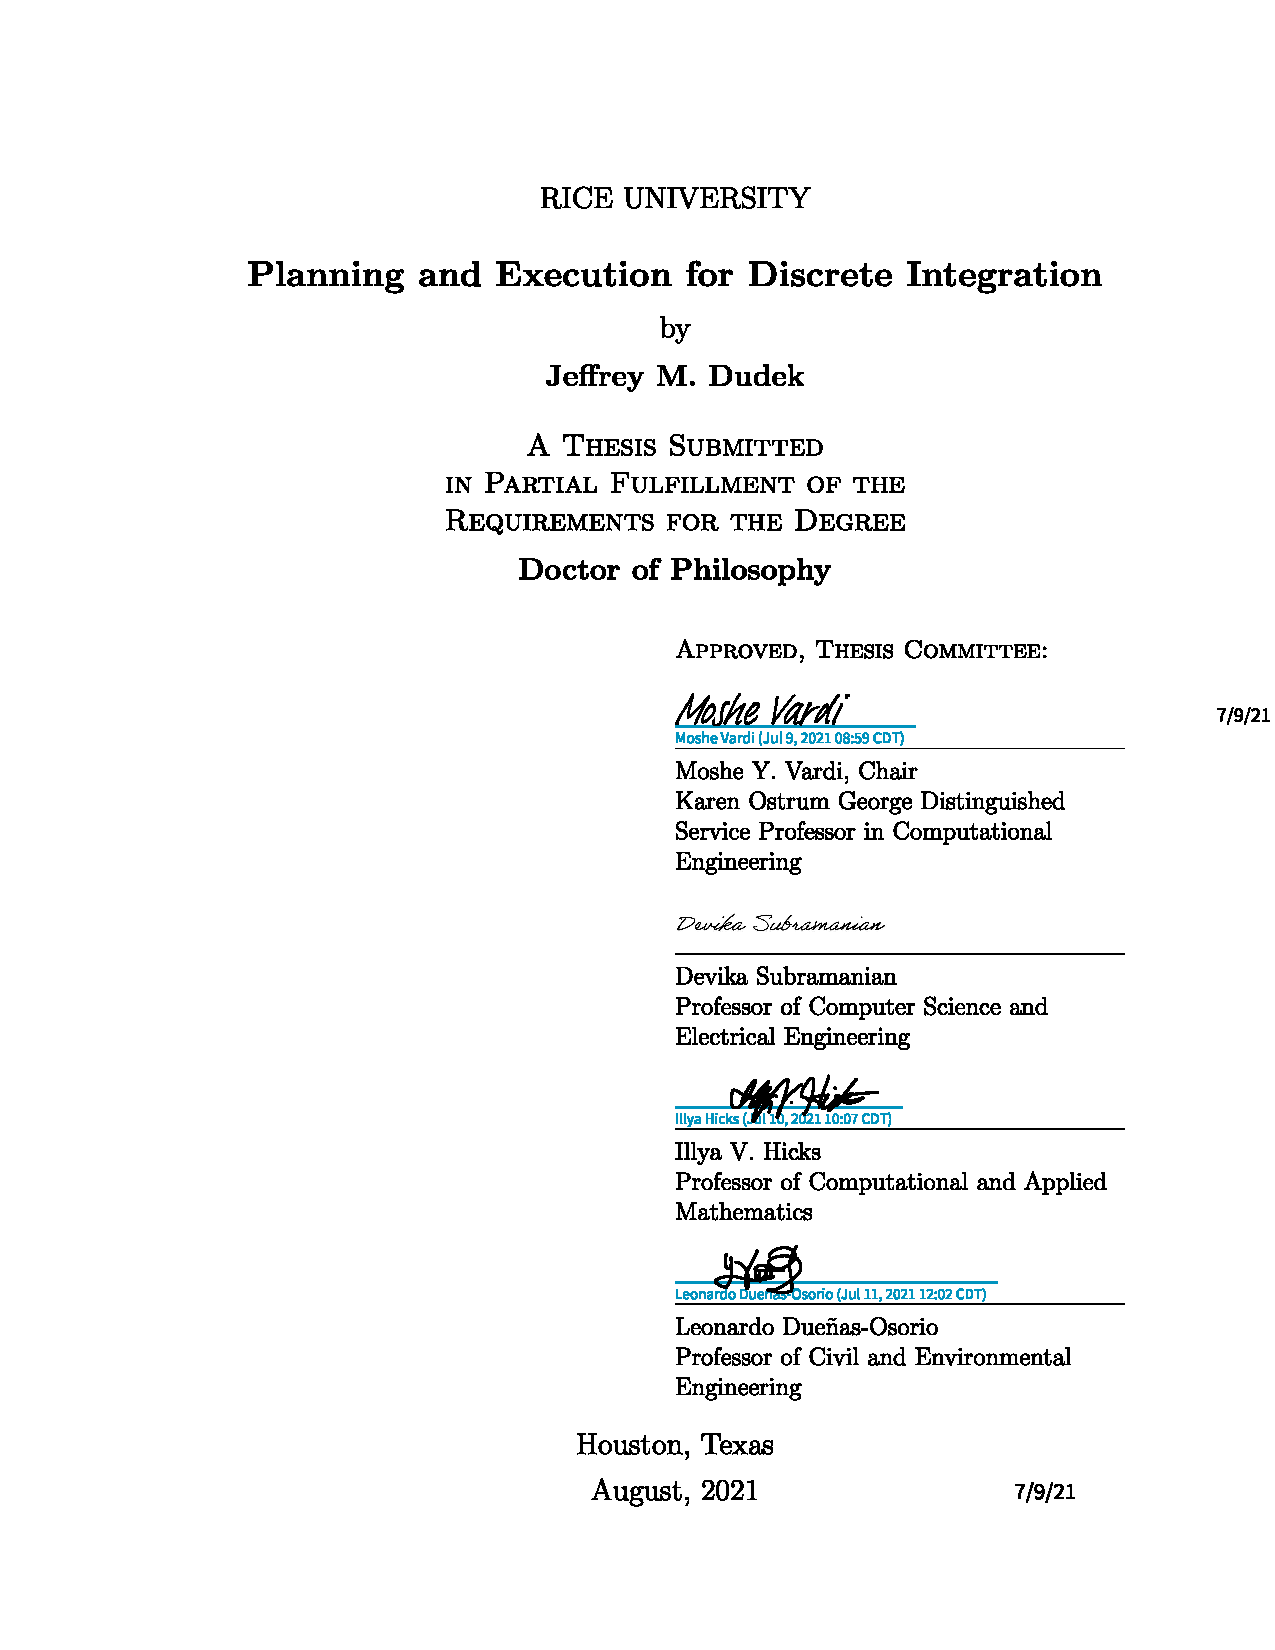
\includegraphics[page=1,clip,trim=110mm 152.8mm 10mm 115mm]{coverpage.pdf}
   \end{textblock}
   \begin{textblock}{80}(104,149)
   	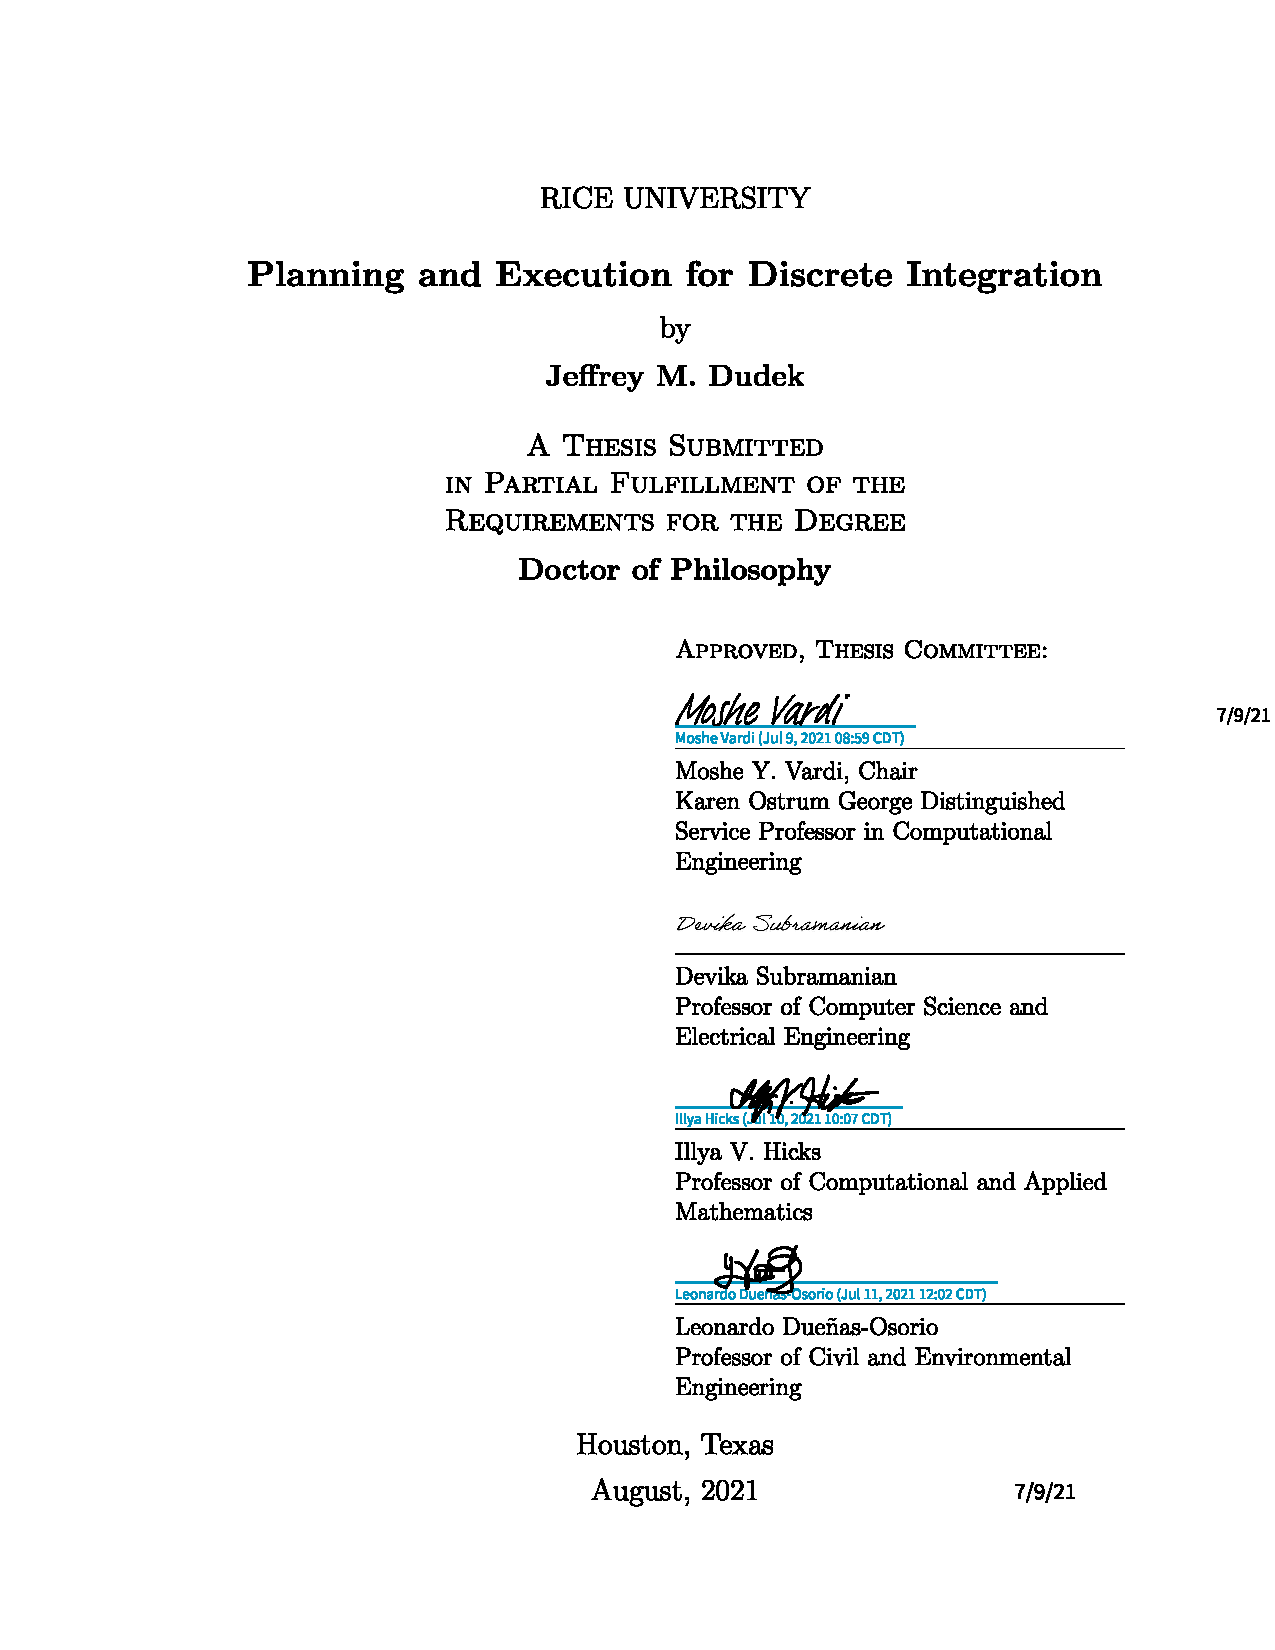
\includegraphics[page=1,clip,trim=110mm 119mm 10mm 149mm]{coverpage.pdf}
   \end{textblock}
   \begin{textblock}{80}(104,180)
   	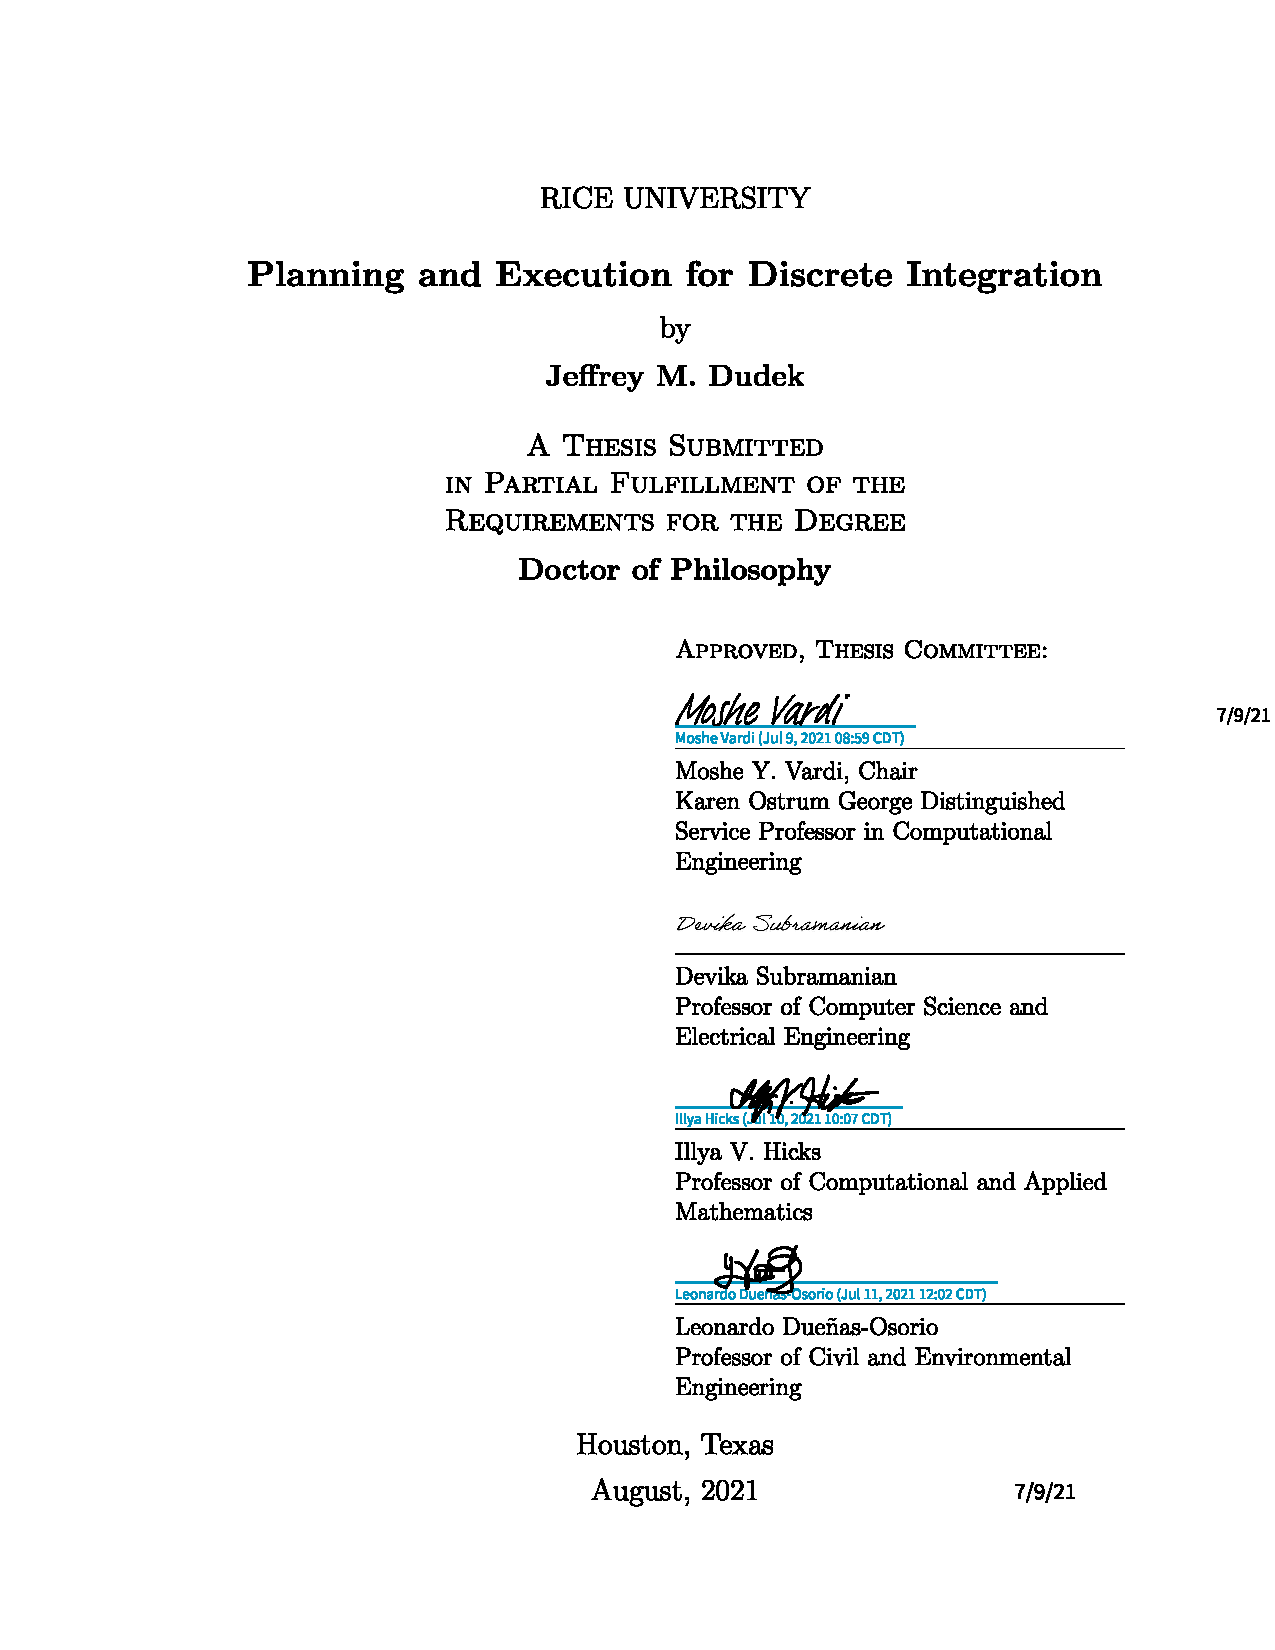
\includegraphics[page=1,clip,trim=110mm 88.4mm 10mm 180mm]{coverpage.pdf}
   \end{textblock}
   \begin{textblock}{80}(104,210)
   	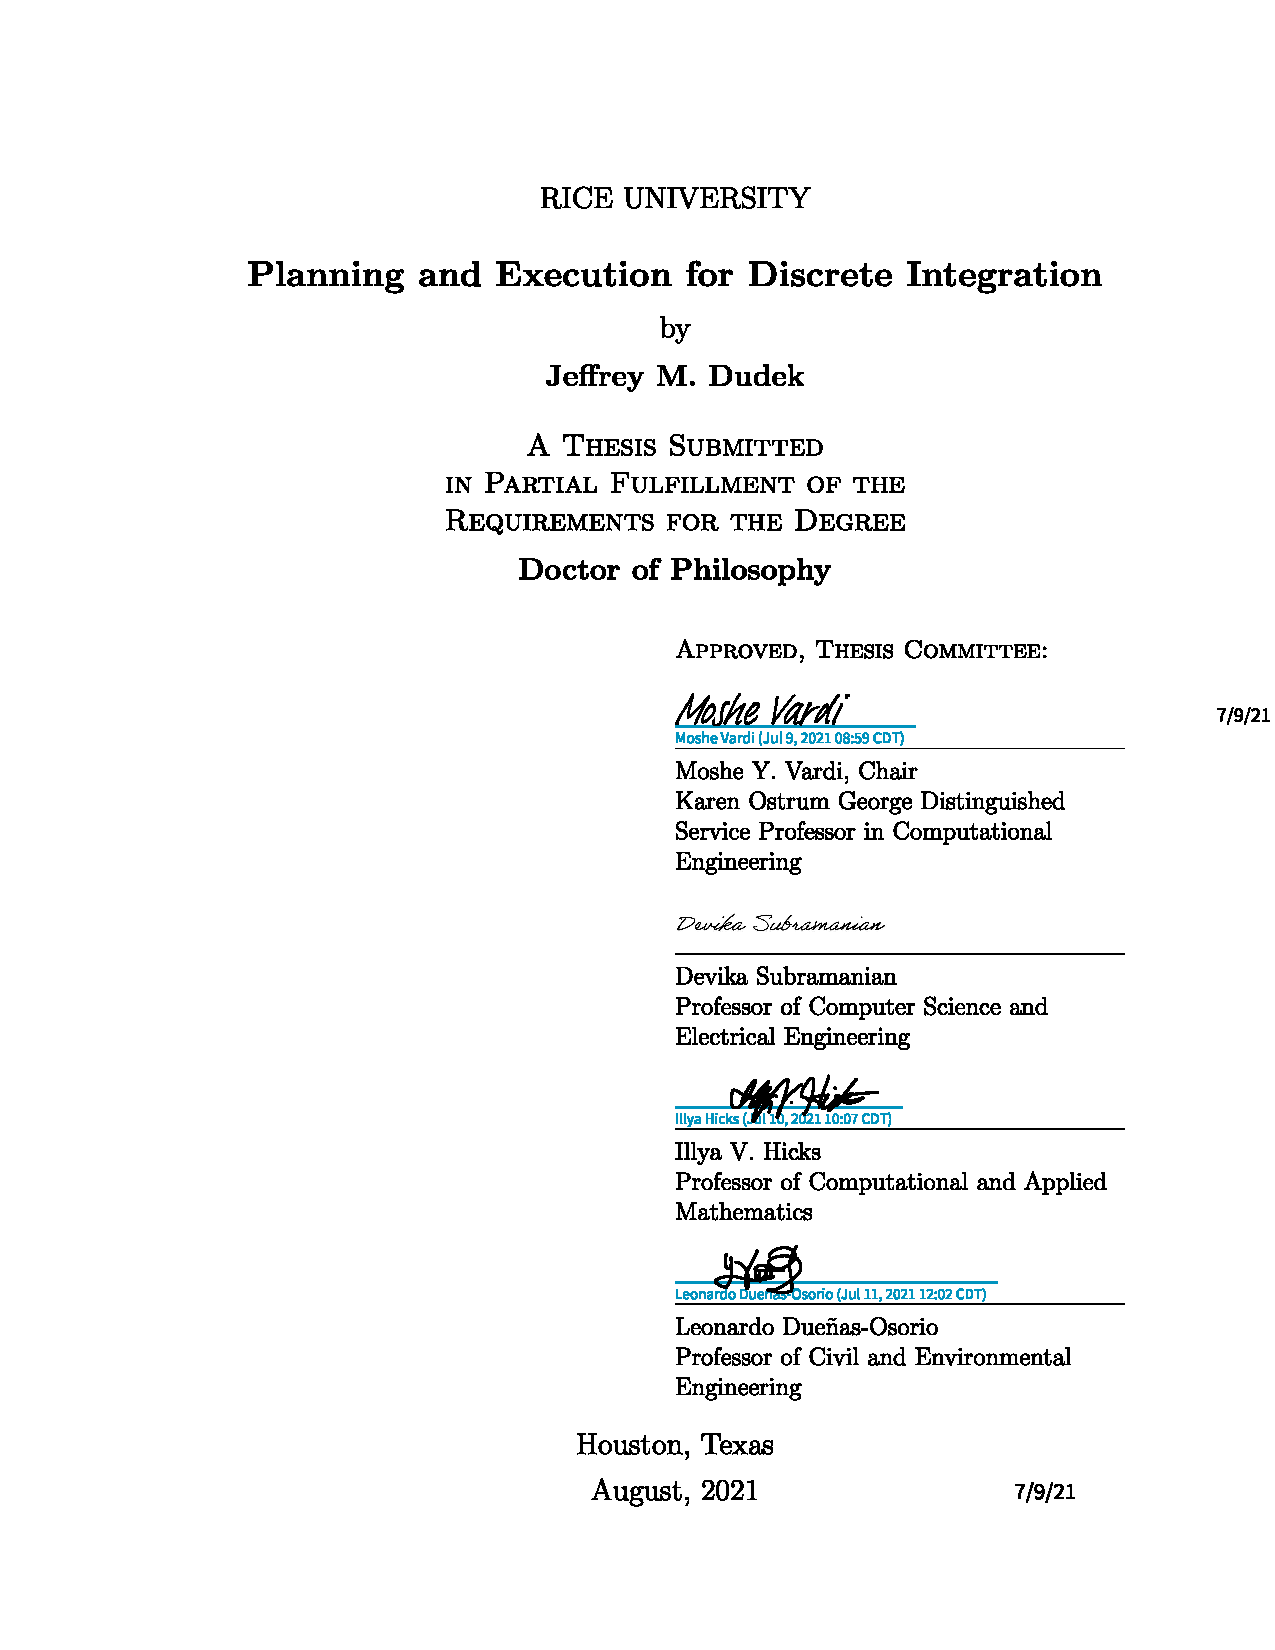
\includegraphics[page=1,clip,trim=110mm 58.7mm 10mm 210mm]{coverpage.pdf}
   \end{textblock}
   
   \maketitle
   
   \thispagestyle{empty}
% The abstract may not exceed 350 words
\begin{abstract}
Discrete integration is a fundamental problem in artificial intelligence with numerous applications, including probabilistic reasoning, planning, inexact computing, engineering reliability, and statistical physics. The task is to count the total weight, subject to a given weight function, of all solutions to given constraints. Developing tools to compute the total weight for applied problems is an area of active research.

Over the last ten years, hundreds of thousands of research hours have been poured into low-level computational tools and compilers for neural network training and inference. Simultaneously, there has been a surge in high-level reasoning tools based on graph decompositions, spurred by several competitions. While some existing discrete integration tools (counters) tightly integrate with these low-level computational or high-level reasoning tools, no existing counter is able to leverage both together.

In this thesis, we demonstrate that a clean separation of high-level reasoning (\emph{planning}) and low-level computation (\emph{execution}) leads to scalable and more flexible counters. Instead of building tightly on any particular tool, we target APIs that can be fulfilled by multiple implementations. This requires novel theoretical and algorithmic techniques to use existing high-level reasoning tools in a way consistent with the options available in popular low-level computational libraries. The resulting counters perform well in many hardware settings (singlecore, multicore, GPU).
\end{abstract}



   \acknowledge
I want to thank my advisor, Moshe Vardi, who took me in as an undergrad that had only the barest sense of how to do research.
He gave me freedom and power to explore my own ideas, yet was always ready with support and guidance when things didn't go as planned.
I couldn't have asked for a better mentor than Moshe.

I also want to thank Devika Subramanian, Illya Hicks, and Leonardo Due{\~n}as-Osorio for serving on my thesis committee and for their many excellent suggestions.

I have been very lucky to collaborate with amazing researchers: Leonardo Due{\~n}as-Osorio, Dror Fried, Kuldeep Meel, Vu Phan, and Moshe Vardi.
Their ideas and drive were fundamental in everything I did in my PhD.
I am also grateful to the entirety of my research group, LAPIS, where I could always find someone to debate an idea, to sharpen endless iterations of presentations, or simply to relax with after work.

I am also grateful to the friends I made along the way-- through the QGSA and GradGames, in Duncan Hall and Valhalla, on campus and off. Rice has been my home for 10 years, and it is the people that I will miss the most.

I am especially grateful to my partner, Karl, who supported me from near and far for many long years. I could not be more excited about the future.

Finally, I want to thank my parents and siblings. Without their constant love, support, and understanding, I would not be where I am today.
   \tableofcontents
   \listoffigures
   \listoftables
  \end{frontmatter}
\pagenumbering{arabic}

\linespacing{1.5} % Was 1.7; must be >= 1.5 in final version

\chapter{Introduction}
\label{ch:intro}
Discrete integration is a fundamental problem in artificial intelligence, with applications in probabilistic reasoning, planning, inexact computing, engineering reliability, and statistical physics \cite{Bacchus2003,DH07,GSS08,naveh2007constraint}. In discrete integration, the task is to count the total weight, subject to a given weight function, of the set of solutions of input constraints \cite{GSS08}. 
If the input constraints are given as a propositional formula, the problem is called \emph{model counting}. 
If existential variables are also allowed in the input constraints, the problem is called \emph{projected model counting}. This thesis primarily focuses on exact techniques for model counting and projected model counting, but other works have considered other classes of discrete integration problems (e.g., allowing constraints with alternating quantifiers \cite{stearns2002exploiting,KNR16}, or allowing continuous variables \cite{BPV15}) or approximate techniques \cite{CMV21}.

As is common, we restrict our attention to discrete integration problems where the weight function is log-linear (i.e., literal-weighted), which captures a wide variety of probabilistic distributions~\cite{KF09}.
% For example, in the context of probabilistic reasoning this corresponds to assuming that all variables are independent.
% Log-linear models can be employed to capture a wide variety of probabilistic distributions that arise from graphical models, conditional random fields, skip-gram models, and the like~\cite{KF09}. %TODO: Check sentence from WMC-reduction paper.
We call a discrete integration problem \emph{weighted} if the weight function is log-linear and \emph{unweighted} if the weight function is a constant function (and thus the task is simply to count the number of solutions to the input constraints).
Note that unweighted discrete integration is a special case of weighted discrete integration.
Unweighted model counting is also called \#SAT, while unweighted projected model counting is also called $\#\exists$SAT.

Even the simplest case of discrete integration, \#SAT, is \#P-Complete \cite{Valiant79}. 
In fact, every problem in the polynomial hierarchy can be answered by a single \#SAT query \cite{toda89}. 
As a simple example, a propositional formula is satisfiable if and only if its unweighted model count is nonzero.
Weighted model counting (with rational, log-linear weights) is \#P-Complete as well, through a reduction to \#SAT that encodes the weights in additional variables \cite{CFMV15,DFM20}.
But projected model counting is thought to be harder: $\#\exists$SAT is not contained in $\#$P unless the polynomial hierarchy collapses to $\Sigma_2^P$ \cite{zawadzki2013generalization}.

Despite the theoretical difficulty of discrete integration, a variety of discrete integration tools (called \emph{counters}) exist that can handle industrial sets of constraints. The earliest counters, e.g. \tool{CDP} \cite{birnbaum1999good}, were based on search.
The key idea is to take an algorithm for exploring the entire solution space of a set of constraints (e.g. DPLL \cite{davis1960computing,davis1962machine}, and later CDCL \cite{biere2009conflict}) and augment it to enumerate the number of partial solutions encountered. 
Modern solvers such as \tool{cachet} \cite{SBK05} and \tool{SharpSAT} \cite{Thurley2006} follow this approach.
Another class of counters (e.g. \tool{miniC2D} \cite{OD15} and \tool{d4} \cite{LM17}) are based on knowledge compilation, where the idea is to compile the set of constraints into an alternative representation on which a discrete integration query may be answered in polynomial time.

A third class of counters \cite{CW16,FHMW17,FHWZ18,FHZ19,DPV20,fichte2020exploiting} are based on dynamic programming. % \cite{BDP09,SS10,jegou2016improving} % TODO: should cite Algorithms \cite{FMR08,SS10}.
Dynamic programming is a powerful technique that has been applied across computer science \cite{bellman1966dynamic}, including to database-query optimization \cite{MPPV04}, satisfiability solving \cite{uribe1994ordered,aguirre2001random,pan2005symbolic}, and QBF evaluation \cite{charwat2016bdd}.
The key idea is to solve a sequence of smaller subproblems, formed by partitioning the input constraints, and then incrementally combine these solutions into the final result.
The techniques developed in this thesis are all based on dynamic programming.

The key idea of this thesis is that dynamic-programming algorithms for discrete integration can be cleanly separated into two phases: a \emph{planning phase} of high-level reasoning to construct subproblems, followed by an \emph{execution phase} of low-level computation which solves subproblems.
Existing dynamic-programming-based counters perform both high-level reasoning and low-level planning, but in an intermixed way that is tightly coupled to a single existing library.
Explicitly separating planning and execution enables us to separately reason about, implement, and optimize each phase.
Instead of building tightly on any particular library, we target APIs that can be fulfilled by multiple planning or execution implementations.
The resulting counters scale to large problem instances and run flexibly in a variety of hardware environments.

% This requires novel theoretical and algorithmic techniques to use existing high-level reasoning tools in a way consistent with the options available in popular low-level computational libraries. 
 
% The requirements, challenges, and opportunities of each phase are often dramatically different, both at an algorithmic and an implementation level.  

% This thesis argues that this separation enables the resulting counters to scale to large problem instances and run flexibly in a variety of hardware environments.


% \tool{cachet} \cite{SBK05} and \tool{SharpSAT} \cite{Thurley2006} are modern solvers that are also based on search.
%In counters based on direct reasoning (e.g., \tool{cachet} \cite{SBK05}), the idea is to reason directly about the CNF representation of $\varphi$. In counters based on knowledge compilation (e.g. \tool{miniC2D} \cite{OD15} and \tool{d4} \cite{LM17}), the idea is to compile $\varphi$ into an alternative representation on which counting is easy. In counters based on dynamic programming (e.g. \tool{ADDMC} \cite{DPV20} and \tool{gpuSAT2} \cite{FHWZ18,FHZ19}), the idea is to traverse the clause structure of $\varphi$. Tensor-network approaches to counting (e.g. \tool{TensorOrder} \cite{DDV19} and this work) are also based on dynamic programming. Dynamic programming approaches often utilize graph decompositions, which we define in the next section. 

% $\#\exists$SAT is complete for the complexity class \#P\textsuperscript{NP[1]}, which is the set of counting problems 
% (solvable by a polynomially bounded counting Turing machine with one query to an NP-complete oracle)
% \cite{zawadzki2013generalization}

% Even when the weight function is a constant function, constrained counting is \#P-Complete \cite{Valiant79}. 

% Nevertheless, a variety of tools exist that can handle industrial sets of constraints, \eg, \cite{sang2004combining,OD15,darwiche2004new,LM17}. 

% Log-linear models are employed to capture a wide variety of distributions that arise from graphical models, conditional random fields, skip-gram models, and the like~\cite{KF09}.


\section{Planning: High-Level Reasoning}
In the planning phase, we aim to leverage graph decompositions as a tool for high-level reasoning. \emph{Graph decompositions} \cite{halin1976s,robertson1984graph,RS91,ST94} aim to decompose a graph into subgraphs in such a way that the decomposition can aid algorithms running on the graph.
% Thus a graph decomposition crystallizes a particular strategy for reasoning on the graph.
For example, a \emph{tree decomposition} \cite{halin1976s,robertson1984graph} decomposes a graph into a tree structure that captures information on graph cycles.
Algorithms based on graph decompositions have been successful across computer science \cite{GLST17,MPPV04}.

The success of graph-decomposition algorithms in practice relies on finding good decompositions of arbitrary graphs.
This has spurred the development of a variety of heuristics and tools for efficiently finding graph decompositions \cite{AMW17,HS18,Tamaki17,hicks02}. 
Moreover, recent competitions \cite{DKTW18} ensured that many graph decomposition tools can be used through a single unified API and thus, with careful design, can be interchanged.

A variety of dynamic-programming algorithms \cite{FMR08,SS10} and counters \cite{CW16,FHMW17,FHWZ18,FHZ19} exist for performing discrete integration using graph decompositions.
These counters are typically closely integrated with a a single graph-decomposition tool.
For example \tool{gpuSAT2} \cite{FHWZ18,FHZ19} is a tool for weighted model counting that is closely integrated with the tree-decomposition solver \pkg{htd} \cite{AMW17}. While \tool{gpuSAT2} also includes some low-level computational optimizations, it uses handwritten GPU kernel calls instead of leveraging low-level computational libraries.


\section{Execution: Low-Level Computation}
\label{sec:intro:execution}
In the execution phase, we aim to leverage two existing classes of low-level computational libraries: tensors and decision diagrams. 

\emph{Tensors} are a tool used across quantum physics and computer science for describing and reasoning about quantum systems, big-data processing, and more \cite{BB17,Cichocki14,Orus19}.
Contraction is a key operation in neural network training and inference \cite{BK07,Hirata03,KKCLA17,VZTGDMVAC18}.
Consequently, there is massive practical work across machine learning and high-performance computing on tensor contraction \cite{BK07,Hirata03,KKCLA17,VZTGDMVAC18} (often with support for GPUs \cite{KSTKPPRS19,NRBHHJN15} or other specialized hardware \cite{JYPPABBBBB17}).
This includes a variety of high-performance libraries that can perform tensor contraction \cite{numpy,ABCCDDDGII16,PGMLJGKLGA19} in a variety of hardware settings with a single unified API. 
% While one work \cite{KCMR18} has applied these libraries towards discrete integration, the high-level reasoning was limited to several heuristics.
% These libraries have only seen limited application towards discrete integration  \cite{KCMR18}.

\emph{Decision diagrams} are a group of data structures used to sparsely represent sets and functions \cite{akers1978binary,bahar1997algebraic,minato1993zero,sanner2005affine}. 
In particular, we aim to use \emph{Algebraic Decision Diagrams (ADDs)} \cite{bahar1997algebraic} for discrete integration, which have been used in stochastic model checking \cite{KNP07} and stochastic planning \cite{HSHB99}. 
An ADD is a compact representation of a real-valued function as a directed acyclic graph. 
% For functions with logical structure, an ADD representation can be exponentially smaller than the explicit representation. 
Moreover, there are several high-performance libraries for efficiently manipulating ADDs \cite{somenzi2015cudd,van2015sylvan}.
ADDs were used for weighted model counting in \addmc{} \cite{DPV20}, which tied for first place of the weighted track of the 2020 Model Counting Competition \cite{fichte2020model}.
While \addmc{} also includes some high-level reasoning, it uses tightly-integrated custom-built heuristics \cite{dechter99,bouquet99,tarjan1984simple,koster2001treewidth} instead of leveraging existing high-level reasoning tools.



% While we do not establish new parameterized complexity results for model counting (as fixed-parameter algorithms for model counting are well-known for a variety of parameters \cite{FMR08,SS10}), we combine these theoretical results with high-performance tensor network libraries and with existing heuristic graph-decomposition tools to produce a competitive tool for weighted model counting.

% The parallelization of neural network training and inference has seen massive research across the machine learning and high-performance computing communities \cite{ABCCDDDGII16,JYPPABBBBB17,PGMLJGKLGA19}. Consequently, GPUs give orders of magnitude of speedup over a single core for neural-network algorithms \cite{KSTKPPRS19,NRBHHJN15}. In this work, we aim to directly leverage advances in multi-core and GPU performance designed for neural-network algorithms in the service of weighted model counting.


% Dynamic programming has also been the basis of several tools for model counting \cite{DPV20,DDV19,dudek2020parallel,fichte2020exploiting}.
% Although each tool uses a different data structure--algebraic decision diagrams (ADDs) \cite{DPV20}, tensors \cite{DDV19,dudek2020parallel}, or database tables \cite{fichte2020exploiting}--the overall algorithms have similar structure.
% % Also, decomposition techniques have seen many applications in model counting, cf.~\cite{jegou2016improving} and the reference therein. %JD: Moved the citation to paragraph 2 instead
% The goal of this work is to unify these approaches into a single conceptual framework: \emph{project-join trees}.
% Project-join trees are not an entirely new idea.
% Similar concepts have been used in constraint programming (as join trees \cite{dechter1989tree}), probabilistic inference (as cluster trees \cite{SAS94}), and database-query optimization (as join-expression trees \cite{MPPV04}).
% Our original contributions include the unification of these concepts into project-join trees and the application of this unifying framework to model counting.



% Over the last ten years, hundreds of thousands of research hours have been poured into low-level computational tools and compilers for neural network training and inference. Simultaneously, there has been a surge in high-level reasoning tools based on graph decompositions, spurred by several competitions. While some existing discrete integration tools (counters) tightly integrate with these low-level computational or high-level reasoning tools, no existing counter is able to leverage both together.

\section{Contributions}

The main contribution of this thesis is a clean separation of dynamic-programming algorithms for discrete integration into a planning phase of high-level reasoning, followed by an execution phase of low-level computation.

We first introduce this separation in a new model counter, \tool{TensorOrder}, which uses graph decompositions for planning and tensors for execution. This includes a new reduction from weighted model counting to tensor network contraction. We consider two planning algorithms-- \textbf{LG} and \textbf{FT}-- based on graph decompositions. While \textbf{LG} is based on existing tensor network (and constraint satisfaction) techniques, we contribute a new analysis that more closely matches the memory usage of existing tensor libraries. \textbf{FT} is a novel planning algorithm, tailored for constrained counting, that factors tensor networks based on tree decompositions.

Next, we show that introducing this separation improves an existing model counter (\tool{ADDMC} \cite{DPV20,phan2019weighted}). We unify a variety of approaches into a single conceptual framework using project-join trees. We show that replacing the existing constraint-satisfaction planner in \tool{ADDMC} with \textbf{LG} (a planner based on graph decompositions) leads to a faster model counter. Moreover, we compare (dense) tensors with (sparse) algebraic decision diagrams in the execution phase and find that algebraic decision diagrams outperform tensors on single CPU cores.

We next apply this approach in order to develop a parallel model counter by separately parallelizing the planning and execution phases in \tool{TensorOrder}. We parallelize the planning phase by introducing an algorithmic portfolio of planners, motivated by success in the SAT community \cite{XHHL08}. We parallelize the execution phase through the use of parallel tensor libraries to run on multiple CPU cores, on a GPU, and even on a TPU (i.e., a Tensor Processing Unit \cite{JYPPABBBBB17}). To handle limited-memory environments as on a GPU, we introduce a novel technique for parallel model counting based on variable marginalization.

Finally, we apply our approach to projected model counting. We present a novel algorithm for performing projected model counting through a planning and execution phase using graded project-join trees. As part of this, we introduce a novel planning algorithm that builds graded project-join trees by using a planner for standard project-join trees as a black-box. The resulting tool \tool{ProCount} makes a significant contribution to a portfolio of exact weighted projected model counters.

\section{Organization}
The remainder of this thesis is organized as follows:

Chapter \ref{ch:background} presents notation and background on model counting, existing high-level planning tools (graph decompositions and heuristics from constraint satisfaction), and existing low-level computational tools (tensors and decision diagrams). 

Chapter \ref{ch:tensors} presents an algorithm for weighted model counting based on tensor networks. The resulting tool \tool{TensorOrder} uses graph decompositions for planning and tensors for execution. Most results in this chapter appear in \cite{DDV19}.

Chapter \ref{ch:dpmc} presents an algorithm for weighted model counting based on project-join trees. The resulting tool \tool{DPMC} uses graph decompositions for planning and decision diagrams for execution. Most results in this chapter appear in \cite{dudek2020dpmc}.

Chapter \ref{ch:parallel} parallelizes the techniques from Chapter \ref{ch:tensors} to run on multiple CPUs, a GPU, and on a TPU. Most results in this chapter appear in \cite{dudek2020parallel}.

Chapter \ref{ch:procount} generalizes the techniques from Chapter \ref{ch:dpmc} to weighted projected model counting. Most results in this chapter appear in \cite{dudek2020procount}.

Finally, Chapter \ref{ch:conclusion} summarizes the main contributions of this thesis and describes several possible future directions.
\chapter{Background}
\label{ch:background}

\section{Discrete Integration}
\label{sec:wmc}

In discrete integration (also called constrained counting) the task is to count the total weight, subject to a given weight function, of the set of solutions of input constraints \cite{GSS08}. We represent weight functions as pseudo-Boolean functions. As is standard, we focus on literal-weight functions: 
\begin{definition}[Literal-Weight Function]
A pseudo-Boolean function $W: 2^X \rightarrow \mathbb{R}$ is \emph{log-linear} or a \emph{literal-weight} function if there exist pseudo-Boolean functions $W_x: 2^{\{x\}} \rightarrow \mathbb{R}$ for all $x \in X$ such that $W = \prod_{x \in X} W_x$. 
\end{definition}
$W_x(\{x\})$ indicates the weight of the positive literal $x$ in $W$ and $W_x(\emptyset)$ indicates the weight of the negative literal $\neg x$ in $W$.

This thesis primarily focuses on two subclasses of discrete integration: model counting and projected model counting.

\subsection{Model Counting}
In (weighted) model counting, the input constraints are given as a propositional formula, typically in CNF. Formally:
\begin{definition}[Weighted Model Count]
  Let $\varphi$ be a formula over Boolean variables $X$ and let $W: 2^X \rightarrow \mathbb{R}$ be a pseudo-Boolean function. We say that $(X, \phi, W)$ is an instance of \emph{weighted model counting}. The \emph{$W$-weighted model count} of $\varphi$ is
  $$W(\varphi) \equiv \sum_{\tau \in 2^X} \varphi(\tau) \cdot W(\tau).$$
\end{definition}

The \emph{unweighted model count} of a Boolean formula $\varphi$ is the number of solutions of $\varphi$, i.e. the $W$-weighted model count of $\varphi$ where $W(\tau) = 1$ for all $\tau \in 2^X$.


We focus in this work on weighted model counting, as opposed to \emph{unweighted model counting} where the weight function $W$ is constant. There are a variety of counters \cite{CW16,FHMW17,Thurley2006} that can perform only unweighted model counting and so we do not compare against them. Of particular note here is \tool{countAntom} \cite{BSB15}, a multi-core unweighted model counter. An interesting direction for future work is to explore the integration of weights into \tool{countAntom} and compare with tensor-network-based approaches to weighted model counting.

Existing approaches to weighted model counting can be split broadly into three categories: \emph{direct reasoning}, \emph{knowledge compilation}, and \emph{dynamic programming}. In counters based on direct reasoning (e.g., \tool{cachet} \cite{SBK05}), the idea is to reason directly about the CNF representation of $\varphi$. In counters based on knowledge compilation (e.g. \tool{miniC2D} \cite{OD15} and \tool{d4} \cite{LM17}), the idea is to compile $\varphi$ into an alternative representation on which counting is easy. In counters based on dynamic programming (e.g. \tool{ADDMC} \cite{DPV20} and \tool{gpuSAT2} \cite{FHWZ18,FHZ19}), the idea is to traverse the clause structure of $\varphi$. Tensor-network approaches to counting (e.g. \tool{TensorOrder} \cite{DDV19} and this work) are also based on dynamic programming. Dynamic programming approaches often utilize graph decompositions, which we define in the next section. 

\subsection{Projected Model Counting}
In (weighted) projected model counting, the input constraints are given as a propositional formula, typically in CNF, and a set of irrelevant, existential variables.
Formally:
\begin{definition}
	Let $\phi$ be a Boolean formula, $\{X, Y\}$ be a partition of $\vars(\phi)$, and $W: 2^X \to \R$ be a pseudo-Boolean function. We say that $(X, Y, \phi, W)$ is an instance of \emph{weighted projected model counting}.
	The \emph{$W$-weighted $Y$-projected model count} of $\phi$ is
	$$\func{WPMC}(\phi, W, Y) \equiv \sum_{\tau \in 2^X} \pars{ W(\tau) \mult \max_{\sigma \in 2^Y} \phi(\tau \cup \sigma) }$$.
\end{definition}

Variables in $X$ are called \emph{relevant} or \emph{additive}, and variables in $Y$ are called \emph{irrelevant} or \emph{disjunctive}. 
Notice that model counting is a special case of projected model counting where all variables are relevant. Thus $W(\varphi) = \func{WPMC}(\phi, W, \emptyset)$ for all Boolean formulas $\varphi$ and weight functions $W: 2^{\vars(\varphi)} \rightarrow \mathbb{R}$. 

\section{Boolean Formulas and Pseudo-Boolean Functions}
Let $X$ be a set of propositional variables and let $\varphi$ be a Boolean formula defined over $X$.
We use $\vars(\varphi)$ to indicate the set of variables of $\varphi$. An \emph{assignment} to $X$ is an element of $2^X$, and further $\tau \in 2^X$ is a \emph{solution} to $\varphi$ if $\varphi$ evaluates to true under $\tau$.

% We are often interested in Boolean formulas in \emph{conjunctive normal form} (CNF).
A \emph{literal} is a variable (e.g., $x$) or the negation of a variable (e.g., $\neg x$).
A Boolean formula is a \emph{(CNF) clause} if it is the disjunction of literals (e.g., $x \lor y \lor \neg z$). % Note that we do not need to define support, since \support = \vars
A Boolean formula is a \emph{CNF formula} (also called \emph{in CNF}) if it is the conjunction of CNF clauses.
For example $(x \lor y) \land (z \lor \neg x)$ is a CNF formula with 2 clauses and 4 solutions ($\{y\}$, $\{y, z\}$, $\{x, z\}$, and $\{x, y, z\}$).
If $\varphi$ is a CNF formula, we often treat $\varphi$ as the set of its clauses and so write $C \in \varphi$ to mean that $C$ is one of the CNF clauses of $\varphi$. Thus $\varphi = \bigwedge_{C \in \varphi} C$.

A generalization of Boolean formulas are pseudo-Boolean functions.
\begin{definition}[Pseudo-Boolean function]
\label{def_pseudoboolean}
Let $X$ be a set of Boolean variables.
A \emph{pseudo-Boolean function} over $X$ is a function $f: 2^X \to \R$.
We use $\vars(f)$ to indicate the set of variables of $f$.
\end{definition}
Pseudo-Boolean functions are also known as \emph{factors}.
A pseudo-Boolean function can naturally represent a Boolean formula. In detail, for a Boolean formula $\phi$ define $[\phi]: 2^{\vars(\varphi)} \rightarrow \R$ to be a pseudo-Boolean function where, for all $\tau \in 2^{\vars(\varphi)}$, if $\tau$ is a solution of $\phi$ then $[\phi](\tau) \equiv 1$ else $[\phi](\tau) \equiv 0$.
As an abuse of notation, we often omit the brackets for simplicity and define $\phi(\tau) \equiv 1$ if $\tau$ is a solution of $\phi$ and $\phi(\tau) \equiv 0$ otherwise.

Operations on pseudo-Boolean functions include \emph{product}, \emph{$\Sigma$-projection} and \emph{$\exists$-projection}.
First, we define product.
\begin{definition}[Product]
\label{def_mult}
    Let $X$ and $Y$ be sets of Boolean variables.
    The \textdef{product} of functions $f: 2^X \to \R$ and $g: 2^Y \to \R$ is the function $f \mult g: 2^{X \cup Y} \to \R$ defined for all $\tau \in 2^{X \cup Y}$ by
    $(f \mult g)(\tau) \equiv f(\tau \cap X) \mult g(\tau \cap Y).$
\end{definition}
Product generalizes conjunction of Boolean formulas: if $\alpha$ and $\beta$ are Boolean formulas, then $[\alpha] \mult [\beta] = [\alpha \land \beta]$. Thus if $\varphi$ is a CNF formula then $[\varphi] = \prod_{C \in \varphi} [C]$.

We next define $\Sigma$-projection.
\begin{definition}[$\Sigma$-projection]
\label{def_sum}
    Let $X$ be a set of Boolean variables, and let $x \in X$.
    The \emph{$\Sigma$-projection} of a function $f: 2^X \to \R$ \wrt{} $x$ is the function $\Sigma_x f: 2^{X \setminus \set{x}} \to \R$ defined for all $\tau \in 2^{X \setminus \set{x}}$ by
    $\pars{\Sigma_x f}(\tau) \equiv f(\tau) + f(\tau \cup \set{x}).$
\end{definition}
$\Sigma$-projection is also known as \emph{additive projection} or 
\emph{marginalization}.
Finally, we define $\exists$-projection.
\begin{definition}[$\exists$-projection]
\label{def_exist}
    Let $X$ be a set of Boolean variables, and let $x \in X$.
    The \emph{$\exists$-projection} of a function $f: 2^X \to \R$ \wrt{} $x$ is the function $\exists_x f: 2^{X \setminus \set{x}} \to \R$ defined for all $\tau \in 2^{X \setminus \set{x}}$ by $\pars{\exists_x f}(\tau) \equiv \max(f(\tau), f(\tau \cup \set{x}))$.
\end{definition}
$\exists$-projection is also called \emph{disjunctive projection} and generalizes existential quantification: if $\alpha$ is a Boolean formula and $x \in \vars(\alpha)$, then $\exists_x [\alpha] = [\exists x ~ \alpha]$.

% If $f: 2^X \to \B$ represents a Boolean formula, then $\exists_x f \equiv f[x \mapsto 0] \lor f[x \mapsto 1]$.


In general, $\Sigma$-projection does not commute with $\exists$-projection. For example, if $f(x, y) = [x \oplus y]$ (XOR), then $\Sigma_x \exists_y f \neq \exists_y \Sigma_x f$.
Nevertheless, $\Sigma$-projection and $\exists$-projection are each independently commutative. 
That is, for all $x, y \in X$ and $f: 2^X \to \R$, we have that $\Sigma_x \Sigma_y f = \Sigma_y \Sigma_x f$ and $\exists_x \exists_y f = \exists_y \exists_x f$. 
Thus, for all $X = \{x_1, \ldots, x_n\}$, define $\Sigma_X f \equiv \Sigma_{x_1} \ldots \Sigma_{x_n} f$ and $\exists_X f \equiv \exists_{x_1} \ldots \exists_{x_n} f$. 
We also take the convention that $\Sigma_\varnothing f \equiv \exists_\varnothing f \equiv f$. 
\section{Graphs}
\label{sec:tensors:prelim}
A \emph{graph} $G$ has a nonempty set of vertices $\V{G}$, a set of (undirected) edges $\E{G}$, a function $\delta_G: \V{G} \rightarrow 2^{\E{G}}$ that gives the set of edges incident to each vertex, and a function $\epsilon_G: \E{G} \rightarrow 2^{\V{G}}$ that gives the set of vertices incident to each edge. Each edge must be incident to exactly two vertices, but multiple edges can exist between two vertices. If $E \subset \E{G}$, let $\eincs{G}{E} = \bigcup_{e \in E} \einc{G}{e}$. Similarly, if $V \subset \V{G}$, let $\vincs{G}{V} = \bigcup_{v \in V} \vinc{G}{v}$.
An \emph{edge clique cover} of a graph $G$ is a set $A \subseteq 2^{\V{G}}$ such that (1) every vertex $v \in \V{G}$ is an element of some set in $A$, and (2) every element of $A$ is a clique in $G$ (that is, for every $C \in A$ and every pair of distinct $v, w \in C$ there is an edge between $v$ and $w$ in $G$).

\subsection{Trees}
A \emph{tree} is a simple, connected, and acyclic graph. A \emph{leaf} of a tree $T$ is a vertex of degree one, and we use $\Lv{T}$ to denote the set of leaves of $T$. For every edge $a$ of $T$, deleting $a$ from $T$ yields exactly two trees, whose leaves define a partition of $\Lv{T}$. Let $C_a \subseteq \Lv{T}$ denote an arbitrary element of this partition. Throughout this work, we often refer to a vertex of a tree as a \emph{node} and an edge as an \emph{arc}, since our proofs will frequently work simultaneously with a graph and an associated tree.

A \emph{rooted tree} is a tree $T$ together with a distinguished node $r \in \V{T}$ called the \emph{root}. 
In a rooted tree $(T, r)$, each node $n \in \V{T}$ has a (possibly empty) set of \emph{children}, denoted $\C{T}{r}{n}$, which contains all nodes $n'$ adjacent to $n$ \st{} all paths from $n'$ to $r$ contain $n$.

A \emph{rooted binary tree} is a rooted tree where either $|\V{T}| = 1$ or the root has degree two and every non-root node has degree three or one. If $|\V{T}| > 1$, the \emph{immediate subtrees of $T$} are the two rooted binary trees that are the connected components of $T$ after the root is removed. 

\subsection{Graph Decompositions}
In this work, we use three decompositions of a graph as a tree: carving decompositions \cite{ST94}, branch decompositions \cite{RS91}, and tree decompositions \cite{RS91}. All decompose the graph into an \emph{unrooted binary tree}, which is a tree where every vertex has degree one or three. First, we describe carving decompositions \cite{ST94}:
\begin{definition}[Carving Decomposition]
\label{def:carving}
	Let $G$ be a graph. A \emph{carving decomposition} for $G$ is an unrooted binary tree $T$ whose leaves are the vertices of $G$, i.e. $\Lv{T} = \V{G}$. 
	
	The \emph{width} of $T$, denoted $width_c(T)$, is the maximum number of edges in $G$ between $C_a$ and $\V{G} \setminus C_a$ for all $a \in \E{T}$, i.e.,
    
	$$width_c(T) = \max_{a \in \E{T}} \left| \left( \bigcup_{v \in C_a} \vinc{G}{v} \right) \cap \left( \bigcup_{v \in \V{G} \setminus C_a} \vinc{G}{v} \right) \right|.$$
	
	% $$width_c(T) = \max_{a \in \E{T}} \left| \{ e \in \E{G}~\text{s.t.}~\einc{G}{e} \cap C_a \neq \emptyset~\text{and}~\epsilon_G(e) \cap (\V{G} \setminus C_a) \neq \emptyset \}\right|.$$
	
	
	% $$width_c(T) = \max_{a \in \E{T}} \left| \vinc{G}{C_a} \cap \vinc{G}{\V{G} \setminus C_a} \right|.$$
	
    The width of a carving decomposition $T$ with no edges is 0.
\end{definition}

%In Definition \ref{def:carving}, $\vinc{G}{V}$ refers to the set of edges of $G$ incident to some vertex in $V \subseteq \V{G}$.
The \emph{carving width} of a graph $G$, denoted $width_c(G)$, is the minimum width across all carving decompositions for $G$. Note that an equivalent definition of carving decompositions allows for degree two vertices within the tree as well. 
Branch decompositions are the dual of carving decompositions and hence can be defined by swapping the role of $\V{G}$ and $\E{G}$ in Definition \ref{def:carving}.

Finally, we define tree decompositions \cite{RS91}:
\begin{definition}[Tree Decomposition]
\label{def:treedecomposition}
	A \emph{tree decomposition} for a graph $G$ is an unrooted binary tree $T$ together with a labeling function $\chi : \V{T} \rightarrow 2^{\V{G}}$ that satisfies the following three properties:
	\begin{enumerate}
		\item Every vertex of $G$ is contained in the label of some node of $T$. That is, $\V{G} = \bigcup_{n \in \V{T}} \chi(n)$.
		\item For every edge $e \in \E{G}$, there is a node $n \in \V{T}$ whose label is a superset of $\einc{G}{e}$, i.e. $\einc{G}{e} \subseteq \chi(n)$.
		\item If $n$ and $o$ are nodes in $T$ and $p$ is a node on the path from $n$ to $o$, then $\chi(n) \cap \chi(o) \subseteq \chi(p)$.
	\end{enumerate}
	The \emph{width} of a tree decomposition, denoted $width_t(T, \chi)$, is the maximum size (minus 1) of the label of every node, i.e.,
	$$width_t(T, \chi) = \max_{n \in \V{T}} | \chi(n) | - 1.$$
\end{definition}

The \emph{treewidth} of a graph $G$, denoted $width_t(G)$, is the minimum width across all tree decompositions for $G$. The treewidth of a tree is $1$. Treewidth is bounded by thrice the carving width \cite{sasak10}. The treewidth (plus 1) of graph is no smaller than the branchwidth and is bounded from above by $3/2$ times the branchwidth \cite{RS91}. 

Given a CNF formula $\varphi$, a variety of associated graphs have been considered. The \emph{incidence graph} of $\varphi$ is the bipartite graph where both variables and clauses are vertices and edges indicate that the variable appears in the connected clause. The \emph{primal graph} of $\varphi$ is the graph where variables are vertices and edges indicate that two variables appear together in a clause. There are fixed-parameter tractable model counting algorithms with respect to the treewidth of the incidence graph and the primal graph \cite{SS10}. If the treewidth of the primal graph of a formula $\varphi$ is $k$, the treewidth of the incidence graph of $\varphi$ is at most $k+1$ \cite{KV00}.

\section{An Introduction to Tensors and Tensor Networks}
\label{sec:tensors:tensors}
In this section, we introduce tensors and tensor networks and discuss prior work on the optimization of tensor-network contraction. To aid in exposition, along the way we build an analogy between the language of databases \cite{SG88}, the language of factor graphs \cite{KFL01,dechter99,darwiche01b}, and the language of tensors: see Table \ref{table:db-tensor-analogy}.

\begin{table}[t]
\centering
\begin{tabular}{c|c|c}
\hline
\textbf{Database Concept} & \textbf{Factor Graph Concept} & \textbf{Tensor Concept}\\ \hline
Attribute & Variable & Index\\
Table & Pseudo-Boolean Function & Tensor\\
Project-Join Query & Factor Graph & Tensor Network\\
Join Tree & Dtree & Contraction Tree\\ 
Width & Largest Cluster Size & Contraction Complexity \\
- & Largest Separator Size & Max Rank \\ \hline
\end{tabular}
\caption{\label{table:db-tensor-analogy} An analogy between the language of databases, the language of factor graphs, and the language of tensors.}
\end{table}

\subsection{Tensors}
\emph{Tensors} are a generalization of vectors and matrices to higher dimensions-- a tensor with $r$ dimensions is a table of values each labeled by $r$ indices. An index is analogous to a variable in constraint satisfaction or an attribute in database theory. 

Fix a set $\Ind$ and define an \emph{index} to be an element of $\Ind$. For each index $i$ fix a finite set $\domain{i}$ called the \emph{domain} of $i$. An index index is analogous to a variable in constraint satisfaction. %For the algorithms in this work it is sufficient for every index to have domain $\{0, 1\}$.

An \emph{assignment} to a set of indices $I \subseteq \Ind$ is a function $\tau$ that maps each index $i \in I$ to an element of $\domain{i}$. Let $\domain{I}$ denote the set of assignments to $I$, i.e., $$\domain{I} = \{\tau: I \rightarrow \bigcup_{i \in I} \domain{i}~\text{s.t.}~\tau(i) \in \domain{i}~\text{for all}~i \in I\}.$$

% Formally, fix a finite set $\Ind$ and finite sets $\domain{i}$ for each $i \in \Ind$. An \emph{index} is an element $i$ of $\Ind$, and the corresponding set $\domain{i}$ is called the \emph{domain} of $i$. 
%Fix a finite set $\Ind$, whose elements we call \emph{indices}, and for each index fix a finite set $\domain{i}$ called the \emph{domain} of $i$. 

We now define tensors as multidimensional arrays of values, indexed by assignments to a set of indices:\footnote{In some works, a tensor is defined as a multilinear map and Definition \ref{def:tensor} would be its representation in a fixed basis.}
\begin{definition}[Tensor] \label{def:tensor}
	A \emph{tensor} $A$ over a finite set of indices (denoted $\tdim{A}$) is a function $A: \domain{\tdim{A}} \rightarrow \mathbb{C}$ (where $\mathbb{C}$ is the set of complex numbers).
\end{definition}

The \emph{rank} of a tensor $A$ is the cardinality of $\tdim{A}$. The memory to store a tensor (in a dense way) is exponential in the rank. For example, a scalar is a rank 0 tensor, a vector is a rank 1 tensor, and a matrix is a rank 2 tensor. An example of a higher-rank tensor is the \emph{copy tensor} on a set of indices $I$, which is the tensor $\copyt_I: \domain{I} \rightarrow \mathbb{C}$ such that, for all $\tau \in \domain{I}$, $\copyt_I(\tau) \equiv 1$ if $\tau$ is a constant function on $I$ and $\copyt_I(\tau) \equiv 0$ otherwise \cite{BCJ11}.
Note that a pseudo-Boolean function can be seen as a special case of a tensor, where each index has a domain of size 2 and every tensor entry lies in $\mathbb{R}$.

It is common to consider sets of tensors closed under contraction (see Section \ref{sec:tensors:tensors:tensor-networks}), e.g. tensors with entries in $\mathbb{R}$ as in Section \ref{sec:tensors:wmc}. Database tables under bag-semantics \cite{CV93}, i.e., multirelations, are tensors with entries in $\mathbb{N}$. Probabilistic database tables \cite{CP87} are tensors with entries in $[0, 1]$ that sum to 1.

Many tools exist (e.g. \pkg{numpy} \cite{numpy}) to efficiently manipulate tensors. In Section \ref{sec:tensors:experiments}, we use these tools to implement tensor-network contraction, defined next.

% We abuse notation and allow for two tensors to be treated as distinct even if they are equal as functions.

%Given two tensors with possibly overlapping sets of indices, a natural operation is the contraction of the two tensors.
%\begin{definition}[Tensor Contraction]
%	Let $A$ and $B$ be tensors. The \emph{contraction} of $A$ and $B$, denoted $A \cdot B$, is the tensor $A \cdot B: \domain{\tdim{A} \oplus \tdim{B}} \rightarrow \mathbb{C}$ defined by
%	$$\tau \mapsto \sum_{\rho \in \domain{\tdim{A} \cap \tdim{B}}} A(\rho \cup \tau\restrict{\tdim{A}}) \cdot B(\rho \cup \tau\restrict{\tdim{B}}).$$
%\end{definition}
% For example, given two matrices represented as rank 2 tensors with a single index in common, the contraction of the two tensors is equivalent to matrix multiplication. The contraction of two copy tensors $\copyt_I$ and $\copyt_J$ (with $I \cap J \neq \emptyset$) is the copy tensor $\copyt_{I \oplus J}$.

\subsection{Tensor Networks}
\label{sec:tensors:tensors:tensor-networks}
A \emph{tensor network} defines a complex tensor by combining a set of simpler tensors in a principled way. This is analogous to how a database query defines a resulting table in terms of a computation across many tables.

\begin{definition}[Tensor Network]
	\label{def:tensor-contraction-network}
	A \emph{tensor network} $N$ is a nonempty set of tensors across which no index appears more than twice.
\end{definition}

\emph{Free indices} of $N$ are indices that appear once, while \emph{bond indices} of $N$ are indices that appear twice. We denote the set of free indices of $N$ by $\tnfree{N}$ and the set of bond indices of $N$ by $\tnbound{N}$. The \emph{bond dimension} of $N$ is the maximum size of $\domain{i}$ for all bond indices $i$ of $N$.

The problem of \emph{tensor-network contraction}, given an input tensor network $N$, is to compute the \emph{contraction} of $N$ by marginalizing all bond indices:
\begin{definition}[Tensor Network Contraction]\label{def:contraction}
The \emph{contraction} of a tensor network $N$ is a tensor $\tntensor{N}$ with indices $\tnfree{N}$ (the set of free indices of $N$), i.e. a function $\tntensor{N} : \domain{\tnfree{N}} \rightarrow \mathbb{C}$, that is defined for all $\tau \in \domain{\tnfree{N}}$ by
		\begin{equation}
        \label{eqn:contraction} 
        \tntensor{N}(\tau) \equiv \sum_{\rho \in \domain{\tnbound{N}}} \prod_{A \in N} A((\rho \cup \tau)\restrict{\tdim{A}}).
        \end{equation}
\end{definition}

For example, the contraction of the tensor network $\{\copyt_I, \copyt_J\}$ with $I \cap J \neq \emptyset$ is the tensor $\copyt_{I \oplus J}$ (where $I \oplus J$ is the symmetric difference of $I$ and $J$). Notice that if a tensor network has no free indices then its contraction is a rank 0 tensor. 

A tensor network $N'$ is a \emph{partial contraction} of a tensor network $N$ if there is a surjective function $f: N \rightarrow N'$ s.t. for every $A \in N'$ we have $\tntensor{f^{-1}(A)} = A$; that is, if every tensor in $N'$ is the contraction of some tensors of $N$. If $N'$ is a partial contraction of $N$, then $\tntensor{N'} = \tntensor{N}$.

Let $A$ and $B$ be tensors. Their \emph{contraction} $A \cdot B$ is the contraction of the tensor network $\{A, B\}$. If $\tdim{A} = \tdim{B}$, their \emph{sum} $A+B$ is the tensor with indices $\tdim{A}$ whose entries are given by the sum of the corresponding entries in $A$ and $B$.

Following our analogy, given a tensor network containing database tables (under bag-semantics) as tensors, its contraction is the join of those tables followed by the projection of all shared attributes. Thus a tensor network is analogous to a project-join query. A tensor network can also be seen as a variant of a factor graph \cite{KFL01} with the additional practical restriction that no variable appears more than twice. The contraction of a tensor network corresponds to the marginalization of a factor graph \cite{RS17}, which is a a special case of the sum-of-products problem \cite{BDP09,dechter99} and the FAQ problem \cite{KNR16}. The restriction on variable appearance is heavily exploited in tools for tensor-network contraction and in this work, since it allows tensor contraction to be implemented as matrix multiplication and so leverage significant work in high-performance computing on matrix multiplication on CPUs \cite{LHKK77} and GPUs \cite{FSH04}.

\chapter{Tensors and Graph Decompositions}
\label{ch:tensors}

Constrained counting can be reduced to the problem of tensor-network contraction \cite{BMT15}. \emph{Tensor networks} are a tool used across quantum physics and computer science for describing and reasoning about quantum systems, big-data processing, and more \cite{BB17,Cichocki14,Orus19}. A tensor network describes a complex tensor as a computation on many simpler tensors, and the problem of tensor-network \emph{contraction} is to perform this computation. Although tensor networks can be seen as a variant of factor graphs \cite{KFL01}, working directly with tensor networks allows us to leverage massive practical work in machine learning and high-performance computing on tensor contraction \cite{BK07,Hirata03,KKCLA17,VZTGDMVAC18} (which also includes GPU support \cite{KSTKPPRS19,NRBHHJN15}) to perform constrained counting. Since tensor networks are relatively unknown in the artificial intelligence community, we give an introduction of relevant material on tensors and tensor networks in Section \ref{sec:tensors:tensors}.

Contracting a tensor network requires determining an order to contract the tensors inside the network, and so efficient contraction requires finding a contraction order that minimizes computational cost. Since the number of possible contraction orders grows exponentially in the number of tensors, cost-based exhaustive algorithms, e.g. \cite{PHV14}, cannot scale to handle the large tensor networks required for the reduction from constrained counting. Instead, recent work \cite{KCMR18} gave heuristics that can sometimes find a ``good-enough'' contraction order through structure-based optimization. Finding efficient contraction orders for tensor networks remains an area of active research \cite{RTPCTSL19}.


The primary contribution of this chapter is the application of heuristic graph-decomposition techniques to find efficient contraction orders for tensor networks. Algorithms based on graph decompositions have been successful across computer science \cite{GLST17,MPPV04}, and their success in practice relies on finding good decompositions of arbitrary graphs. This, along with several recent competitions \cite{DKTW18}, has spurred the development of a variety of heuristics and tools for efficiently finding graph decompositions \cite{AMW17,HS18,Tamaki17}. While we do not establish new parameterized complexity results for model counting (as fixed-parameter algorithms for model counting are well-known for a variety of parameters \cite{FMR08,SS10}), we combine these theoretical results with high-performance tensor network libraries and with existing heuristic graph-decomposition tools to produce a competitive tool for weighted model counting.

We first discuss the \textbf{Line-Graph} method (\textbf{LG}) for finding efficient contraction orders through structure-based graph analysis. First applied to tensor networks by Markov and Shi \cite{MS08}, we contribute a new analysis that more closely matches the memory usage of existing tensor libraries. Our analysis combines two theoretical insights: (1) memory-efficient contraction orders are equivalent to low-width carving decompositions (first observed in \cite{de15}), and (2) tree decompositions can be used to find carving decompositions. \textbf{LG} has previously been implemented using exact tools for finding tree decompositions \cite{DFGHSW18}, but its implementation using heuristic tools for tree decompositions is largely unexplored.
% Moreover, our analysis implies that memory-optimal contraction orders for planar tensor networks can be found in cubic time.

Although \textbf{LG} is a general-purpose method for finding contraction orders, \textbf{LG} cannot handle high-rank tensors and so cannot solve many existing counting benchmarks. We therefore contribute a novel structure-based method for finding efficient contraction orders, tailored for constrained counting: the \textbf{Factor-Tree} method (\textbf{FT}). \textbf{FT} factors high-rank, highly-structured tensors as a preprocessing step, leveraging prior work on Hierarchical Tucker representations \cite{Grasedyck10}.

In order to compare our approaches against other model counters (weighted counters \tool{cachet} \cite{SBK05}, \tool{miniC2D} \cite{OD15}, and \tool{d4} \cite{LM17}, and unweighted counters \tool{dynQBF} \cite{CW16}, \tool{dynasp} \cite{FHMW17}, and \tool{SharpSAT} \cite{Thurley2006}), as well as other tensor-based methods, we implemented \textbf{LG} and \textbf{FT} using three state-of-the-art heuristic tree-decomposition solvers. The resulting new weighted model counter is called \tool{TensorOrder}. \textbf{LG} outperforms other model counters and tensor-based methods on a set of unweighted benchmarks, while \textbf{FT} improves the virtual best solver on 21\% of a standard set of weighted model counting benchmarks. \tool{TensorOrder} is thus useful as part of a portfolio of weighted model counters. All code, benchmarks, and detailed data of benchmark runs are available at \newline \url{https://github.com/vardigroup/TensorOrder}.


The rest of the paper is organized as follows: we provide graph notations and define graph decompositions in Section~\ref{sec:tensors:prelim}. We introduce tensors and tensor networks and discuss prior work on the optimization of tensor-network contraction in Section~\ref{sec:tensors:tensors}. We introduce a framework for solving the problem of weighted model counting with tensor networks in Section~\ref{sec:tensors:wmc}. We discuss the \textbf{Line-Graph} method in Section~\ref{sec:tensors:contraction-theory} and the \textbf{Factor-Tree} method in Section~\ref{sec:tensors:preprocessing}. We present an experimental evaluation of tensor-based approaches to model counting in Section~\ref{sec:tensors:experiments}. Finally, we discuss future work and conclude in Section~\ref{sec:tensors:conclusion}.
\section{Preliminaries: Graph Notations}
\label{sec:tensors:prelim}
A \emph{graph} $G$ has a nonempty set of vertices $\V{G}$, a set of (undirected) edges $\E{G}$, a function $\delta_G: \V{G} \rightarrow 2^{\E{G}}$ that gives the set of edges incident to each vertex, and a function $\epsilon_G: \E{G} \rightarrow 2^{\V{G}}$ that gives the set of vertices incident to each edge. Each edge must be incident to exactly two vertices, but multiple edges can exist between two vertices. An \emph{edge clique cover} of a graph $G$ is a set $A \subseteq 2^{\V{G}}$ such that (1) every vertex $v \in \V{G}$ is an element of some set in $A$, and (2) every element of $A$ is a clique in $G$ (that is, for every $C \in A$ and every pair of distinct $v, w \in C$ there is an edge between $v$ and $w$ in $G$).

A \emph{tree} is a simple, connected, and acyclic graph. A \emph{leaf} of a tree $T$ is a vertex of degree one, and we use $\Lv{T}$ to denote the set of leaves of $T$. A \emph{rooted binary tree} is a tree $T$ where either $T$ consists of a single vertex (called the \emph{root}), or every vertex of $T$ has degree one or three except a single vertex of degree two (called the \emph{root}). If $|\V{T}| > 1$, the \emph{immediate subtrees of $T$} are the two rooted binary trees that are the connected components of $T$ after the root is removed. Throughout this work, we often refer to a vertex of a tree as a \emph{node} and an edge as an \emph{arc} to avoid confusion, since our proofs will frequently work simultaneously with a graph and an associated tree.

In this work, we use two decompositions of a graph as a tree: carving decompositions \cite{ST94} and tree decompositions \cite{RS91}. Both decompose the graph into an \emph{unrooted binary tree}, which is a tree where every vertex has degree one or three. First, we describe carving decompositions \cite{ST94}:
\begin{definition}[Carving Decomposition]
\label{def:carving}
	Let $G$ be a graph. A \emph{carving decomposition} for $G$ is an unrooted binary tree $T$ whose leaves are the vertices of $G$, i.e. $\Lv{T} = \V{G}$. 
	
    For every arc $a$ of $T$, deleting $a$ from $T$ yields exactly two trees, whose leaves define a partition of the vertices of $G$. Let $C_a \subseteq \V{G}$ be an arbitrary element of this partition. The \emph{width} of $T$, denoted $width_c(T)$, is the maximum number of edges in $G$ between $C_a$ and $\V{G} \setminus C_a$ for all $a \in \E{T}$, i.e.,
    
	$$width_c(T) = \max_{a \in \E{T}} \left| \left( \bigcup_{v \in C_a} \vinc{G}{v} \right) \cap \left( \bigcup_{v \in \V{G} \setminus C_a} \vinc{G}{v} \right) \right|.$$
	
	% $$width_c(T) = \max_{a \in \E{T}} \left| \{ e \in \E{G}~\text{s.t.}~\einc{G}{e} \cap C_a \neq \emptyset~\text{and}~\epsilon_G(e) \cap (\V{G} \setminus C_a) \neq \emptyset \}\right|.$$
	
	
	% $$width_c(T) = \max_{a \in \E{T}} \left| \vinc{G}{C_a} \cap \vinc{G}{\V{G} \setminus C_a} \right|.$$
	
    The width of a carving decomposition $T$ with no edges is 0.
\end{definition}

%In Definition \ref{def:carving}, $\vinc{G}{V}$ refers to the set of edges of $G$ incident to some vertex in $V \subseteq \V{G}$.
The \emph{carving width} of a graph $G$, denoted $width_c(G)$, is the minimum width across all carving decompositions for $G$. Note that an equivalent definition of carving decompositions allows for degree two vertices within the tree as well.

Next, we define tree decompositions \cite{RS91}:
\begin{definition}[Tree Decomposition]
	Let $G$ be a graph. A \emph{tree decomposition} for $G$ is an unrooted binary tree $T$ together with a labeling function $\chi : \V{T} \rightarrow 2^{\V{G}}$ that satisfies the following three properties:
	\begin{enumerate}
		\item Every vertex of $G$ is contained in the label of some node of $T$. That is, $\V{G} = \bigcup_{n \in \V{T}} \chi(n)$.
		\item For every edge $e \in \E{G}$, there is a node $n \in \V{T}$ whose label is a superset of $\einc{G}{e}$, i.e. $\einc{G}{e} \subseteq \chi(n)$.
		\item If $n$ and $o$ are nodes in $T$ and $p$ is a node on the path from $n$ to $o$, then $\chi(n) \cap \chi(o) \subseteq \chi(p)$.
	\end{enumerate}
	The \emph{width} of a tree decomposition, denoted $width_t(T, \chi)$, is the maximum size (minus 1) of the label of every node, i.e.,
	$$width_t(T, \chi) = \max_{n \in \V{T}} | \chi(n) | - 1.$$
\end{definition}

The \emph{treewidth} of a graph $G$, denoted $width_t(G)$, is the minimum width across all tree decompositions for $G$. The treewidth of a tree is $1$. Treewidth is bounded by thrice the carving width \cite{sasak10}. Carving decompositions are the dual of branch decompositions, which are closely related to tree decompositions \cite{RS91}.
\section{An Introduction to Tensors and Tensor Networks}
\label{sec:tensors}
In this section, we introduce tensors and tensor networks and discuss prior work on the optimization of tensor-network contraction. To aid in exposition, along the way we build an analogy between the language of databases \cite{SG88}, the language of factor graphs \cite{KFL01,dechter99,darwiche01b}, and the language of tensors: see Table \ref{table:db-tensor-analogy}.

\begin{table}[t]
\centering
\begin{tabular}{c|c|c}
\hline
\textbf{Database Concept} & \textbf{Factor Graph Concept} & \textbf{Tensor Concept}\\ \hline
Attribute & Variable & Index\\
Table & Factor & Tensor\\
Project-Join Query & Factor Graph & Tensor Network\\
Join Tree & Dtree & Contraction Tree\\ 
Width & Largest Cluster Size & Contraction Complexity \\
- & Largest Separator Size & Max Rank \\ \hline
\end{tabular}
\caption{\label{table:db-tensor-analogy} An analogy between the language of databases, the language of factor graphs, and the language of tensors.}
\end{table}

\subsection{Tensors}
\emph{Tensors} are a generalization of vectors and matrices to higher dimensions-- a tensor with $r$ dimensions is a table of values each labeled by $r$ indices. An index is analogous to a variable in constraint satisfaction or an attribute in database theory. 

Fix a set $\Ind$ and define an \emph{index} to be an element of $\Ind$. For each index $i$ fix a finite set $\domain{i}$ called the \emph{domain} of $i$. An \emph{assignment} to a set of indices $I \subseteq \Ind$ is a function $\tau$ that maps each index $i \in I$ to an element of $\domain{i}$. Let $\domain{I}$ denote the set of assignments to $I$, i.e., $$\domain{I} = \{\tau: I \rightarrow \bigcup_{i \in I} \domain{i}~\text{s.t.}~\tau(i) \in \domain{i}~\text{for all}~i \in I\}.$$

% Formally, fix a finite set $\Ind$ and finite sets $\domain{i}$ for each $i \in \Ind$. An \emph{index} is an element $i$ of $\Ind$, and the corresponding set $\domain{i}$ is called the \emph{domain} of $i$. 
%Fix a finite set $\Ind$, whose elements we call \emph{indices}, and for each index fix a finite set $\domain{i}$ called the \emph{domain} of $i$. 

We now define tensors as multidimensional arrays of values, indexed by assignments to a set of indices:\footnote{In some works, a tensor is defined as a multilinear map and Definition \ref{def:tensor} would be its representation in a fixed basis.}
\begin{definition}[Tensor] \label{def:tensor}
	A \emph{tensor} $A$ over a finite set of indices (denoted $\tdim{A}$) is a function $A: \domain{\tdim{A}} \rightarrow \mathbb{C}$ (where $\mathbb{C}$ is the set of complex numbers).
\end{definition}

The \emph{rank} of a tensor $A$ is the cardinality of $\tdim{A}$. The memory to store a tensor (in a dense way) is exponential in the rank. For example, a scalar is a rank 0 tensor, a vector is a rank 1 tensor, and a matrix is a rank 2 tensor. An example of a higher-rank tensor is the \emph{copy tensor} on a set of indices $I$, which is the tensor $\copyt_I: \domain{I} \rightarrow \mathbb{C}$ such that, for all $\tau \in \domain{I}$, $\copyt_I(\tau) \equiv 1$ if $\tau$ is a constant function on $I$ and $\copyt_I(\tau) \equiv 0$ otherwise \cite{BCJ11}.

It is common to consider sets of tensors closed under contraction (see Section \ref{sec:tensors:tensor-networks}), e.g. tensors with entries in $\mathbb{R}$ as in Section \ref{sec:wmc}. Database tables under bag-semantics \cite{CV93}, i.e., multirelations, are tensors with entries in $\mathbb{N}$. Probabilistic database tables \cite{CP87} are tensors with entries in $[0, 1]$ that sum to 1.

Many tools exist (e.g. \pkg{numpy} \cite{numpy}) to efficiently manipulate tensors. In Section \ref{sec:experiments}, we use these tools to implement tensor-network contraction, defined next.

% We abuse notation and allow for two tensors to be treated as distinct even if they are equal as functions.

%Given two tensors with possibly overlapping sets of indices, a natural operation is the contraction of the two tensors.
%\begin{definition}[Tensor Contraction]
%	Let $A$ and $B$ be tensors. The \emph{contraction} of $A$ and $B$, denoted $A \cdot B$, is the tensor $A \cdot B: \domain{\tdim{A} \oplus \tdim{B}} \rightarrow \mathbb{C}$ defined by
%	$$\tau \mapsto \sum_{\rho \in \domain{\tdim{A} \cap \tdim{B}}} A(\rho \cup \tau\restrict{\tdim{A}}) \cdot B(\rho \cup \tau\restrict{\tdim{B}}).$$
%\end{definition}
% For example, given two matrices represented as rank 2 tensors with a single index in common, the contraction of the two tensors is equivalent to matrix multiplication. The contraction of two copy tensors $\copyt_I$ and $\copyt_J$ (with $I \cap J \neq \emptyset$) is the copy tensor $\copyt_{I \oplus J}$.

\subsection{Tensor Networks}
\label{sec:tensors:tensor-networks}
A \emph{tensor network} defines a complex tensor by combining a set of simpler tensors in a principled way. This is analogous to how a database query defines a resulting table in terms of a computation across many tables.

\begin{definition}[Tensor Network]
	\label{def:tensor-contraction-network}
	A \emph{tensor network} $N$ is a nonempty set of tensors across which no index appears more than twice.
\end{definition}

\emph{Free indices} of $N$ are indices that appear once, while \emph{bond indices} of $N$ are indices that appear twice. We denote the set of free indices of $N$ by $\tnfree{N}$ and the set of bond indices of $N$ by $\tnbound{N}$. The \emph{bond dimension} of $N$ is the maximum size of $\domain{i}$ for all bond indices $i$ of $N$.

The problem of \emph{tensor-network contraction}, given an input tensor network $N$, is to compute the \emph{contraction} of $N$ by marginalizing all bond indices:
\begin{definition}[Tensor Network Contraction]\label{def:contraction}
The \emph{contraction} of a tensor network $N$ is a tensor $\tntensor{N}$ with indices $\tnfree{N}$ (the set of free indices of $N$), i.e. a function $\tntensor{N} : \domain{\tnfree{N}} \rightarrow \mathbb{C}$, that is defined for all $\tau \in \domain{\tnfree{N}}$ by
		\begin{equation}
        \label{eqn:contraction} 
        \tntensor{N}(\tau) \equiv \sum_{\rho \in \domain{\tnbound{N}}} \prod_{A \in N} A((\rho \cup \tau)\restrict{\tdim{A}}).
        \end{equation}
\end{definition}

For example, the contraction of the tensor network $\{\copyt_I, \copyt_J\}$ with $I \cap J \neq \emptyset$ is the tensor $\copyt_{I \oplus J}$ (where $I \oplus J$ is the symmetric difference of $I$ and $J$). Notice that if a tensor network has no free indices then its contraction is a rank 0 tensor. We write $A \cdot B$ to mean the contraction of the tensor network containing the two tensors $A$ and $B$. 

Following our analogy, given a tensor network containing database tables (under bag-semantics) as tensors, its contraction is the join of those tables followed by the projection of all shared attributes. Thus a tensor network is analogous to a project-join query. A tensor network can also be seen as a variant of a factor graph \cite{KFL01} with the additional practical restriction that no variable appears more than twice. The contraction of a tensor network corresponds to the marginalization of a factor graph \cite{RS17} and can similarly be seen as a special case of the FAQ problem \cite{KNR16}. The restriction on the appearance of variables is heavily exploited in tools for tensor-network contraction, since it allows tensor contraction to be implemented as matrix multiplication and thus leverage significant work in high-performance computing on matrix multiplication, both on the CPU \cite{LHKK77} and the GPU \cite{FSH04}.

We focus in this work on tensor networks with relatively few (or no) free indices and hundreds or thousands of bond indices. Such tensor networks are obtained in a variety of applications \cite{Cichocki14,DLVR18}, including the reduction from model counting to tensor network contraction \cite{BMT15}. Although the rank of the contraction of the tensor network $N$ is small in this case, computing entries of $\tntensor{N}$ by
directly following Equation \ref{eqn:contraction} requires performing a summation over an exponential number of terms--- one for each assignment in $\domain{\tnbound{N}}$--- and is therefore infeasible.

$\tntensor{N}$ can instead be computed by recursively decomposing the tensor network, as in Algorithm \ref{alg:network-contraction} \cite{EP14}. The choice of rooted binary tree $T$ does not affect the output of Algorithm \ref{alg:network-contraction} but may have a dramatic impact on the running-time and memory usage. We explore this in more detail in the following section.

\begin{algorithm}[t]
	\caption{Recursively contracting a tensor network}\label{alg:network-contraction}
	\hspace*{\algorithmicindent} \textbf{Input:} A tensor network $N$ and a rooted binary tree $T$ whose leaves are the tensors of $N$, i.e. $\Lv{T} = N$. \\
	\hspace*{\algorithmicindent} \textbf{Output:} $\tntensor{N}$, the contraction of $N$ as given in Definition \ref{def:contraction}.
	\begin{algorithmic}[1]
	    \Procedure{Contract}{$N,T$}
		\If {$\left|N\right| = 1$}
		\State \Return the tensor contained in $N$
		\Else
        \State $T_1, T_2 \gets \text{immediate subtrees of}~T$
		\State $A_1 \gets \Call{Contract}{\Lv{T_1}, T_1}$
		\State $A_2 \gets \Call{Contract}{\Lv{T_2}, T_2}$
		\State \Return $A_1 \cdot A_2$
		\EndIf
		\EndProcedure
	\end{algorithmic}
\end{algorithm}

\subsection{Contracting Tensor Networks}
The rooted binary trees used by Algorithm \ref{alg:network-contraction} are called contraction trees:
\begin{definition}[Contraction Tree \cite{EP14}] \label{def:contraction-tree}
	Let $N$ be a tensor network. A \emph{contraction tree} for $N$ is a rooted binary tree $T$ whose leaves are the tensors of $N$. %, i.e. $\Lv{T} = N$.
\end{definition}

In our database analogy, a contraction tree for a tensor network representing a project-join query is a join tree of that query (with projections done as early as possible). In our factor-graph analogy, a contraction tree corresponds to a \emph{dtree} \cite{darwiche01},
%MYV{Hard to parse next sentence fragment.} %JMD: Adjusted
to an elimination order \cite{darwiche01b}, 
and to a binary join tree \cite{shenoy97} where factors are assigned to leaf nodes.

The problem of \emph{tensor-network-contraction optimization}, which we tackle in this paper, is given a tensor network $N$ to find a contraction tree that minimizes the computational cost of Algorithm \ref{alg:network-contraction}. % Prior work can be categorized into two types: \emph{exact} algorithms that focus on finding the best possible contraction tree, and \emph{heuristic} algorithms that aim to find a ``good-enough'' contraction tree. Since the number of possible contraction trees is exponential in the number of tensors, exact algorithms are generally best for tensor networks with few tensors while heuristic algorithms scale to larger tensor networks but offer worse contraction trees.
Several \emph{cost-based} approaches aim for minimizing the total number of floating point operations to perform Algorithm \ref{alg:network-contraction} in step 8, e.g. \cite{PHV14} and the \pkg{einsum} package in \pkg{numpy}.  % A more complex cost-based approach is the Tensor Contraction Engine \cite{Hirata03}, which performs additional optimizations of Algorithm \ref{alg:network-contraction} at the compiler level. 
In this work, we instead focus on \emph{structure-based} approaches to tensor-network-contraction optimization, which analyze the rank of intermediate tensors that appear during Algorithm \ref{alg:network-contraction}. These ranks indicate the amount of memory and computation required at each recursive stage. Moreover, these ranks are more amenable to analysis.

One line of work \cite{MS08,DFGHSW18} uses graph decompositions to analyze the \emph{contraction complexity} of a contraction tree: the maximum over all recursive calls of the sum (minus 1) of the rank of the two tensors contracted in step 8 of Algorithm \ref{alg:network-contraction}. In our factor graph analogy, contraction complexity of a contraction tree corresponds to the \emph{width} of a dtree (i.e., the size of the largest cluster) \cite{darwiche01b}. Contraction complexity measures the memory required when step 8 is computed
by summing over the shared indices separately, i.e., first contracting $A_1$ and $A_2$ as if they have no common indices (producing and storing a rank $|\tdim{A_1}|+|\tdim{A_2}|$ tensor) and then sequentially contracting each pair of shared indices. In this approach, the memory required is exponential in the contraction complexity. Modern tensor packages (e.g. \pkg{numpy}), however, instead sum over all shared indices simultaneously without storing an intermediate result. This alternative approach requires the same number of floating-point operations, but often requires significantly less intermediate memory. Thus contraction complexity overestimates the memory requirements of many contraction trees. 

Instead, another line of structure-based optimization analyzes the maximum rank over all recursive calls of the result of step 8 (and step 3). We call this the \emph{max rank} of a contraction tree. In our factor graph analogy, max rank of a contraction tree corresponds to the size of the largest separator of a dtree \cite{darwiche01b} and is closely connected to the performance of the Shenoy-Shafer algorithm \cite{shenoy97,SS08}. Max rank measures the memory required when step 8 is computed by summing over all shared indices simultaneously without storing an intermediate result: the memory required is exponential in the max rank. Thus, max rank estimates the memory usage of modern tensor packages. While the max rank is no more than linearly smaller than the contraction complexity, both appear in the exponent of the required memory. Therefore even small differences between max rank and contraction complexity result in significantly different memory usage. Recent work \cite{KCMR18} introduced three methods for heuristically minimizing the max rank: a greedy approach (called \textbf{greedy}), an approach using graph partitioning (called \textbf{metis}), and an approach using community-structure detection (called \textbf{GN}). Note that \textbf{metis} is analogous to earlier work on using graph partitioning to construct dtrees with small separators \cite{darwiche01b}.

In this work, we improve on these methods by using graph decompositions to find contraction trees with small max rank.


\section{Reduction Phase: From Weighted Model Counting to Tensor Networks}
\label{sec:tensors:wmc}
Existing reductions from model counting to tensor-network contraction \cite{BMT15,KCMR18} focus on unweighted model counting. Since we are interested in the more general problem of weighted model counting, we prove that the reduction can be easily extended:
\begin{theorem}
\label{thm:wmc-reduction}
Let $\varphi$ be a CNF formula over Boolean variables $X$ and let $W: 2^X \rightarrow \mathbb{R}$ be a literal-weight function. One can construct in polynomial time a tensor network $N_\varphi$ such that $\tnfree{N_\varphi} = \emptyset$ and the contraction of $N_\varphi$ is $W(\varphi)$.
\end{theorem}
\begin{proof}
The key idea is to include in $N_\varphi$ a tensor $A_x$ for each variable $x \in X$ and a tensor $B_C$ for each clause $C \in \varphi$ such that the tensors share an index if and only if the corresponding variable appears in the corresponding clause.

Define $I = \{(x, C) : C \in \varphi, x \in \support{C}\}$ to be a set of indices, each with domain $\{0, 1\}$. That is, $I$ has an index for each appearance of each variable in $\varphi$. We use $I$ as the set of indices in $N_\varphi$.

Next, recall that since $W$ is a literal-weight function there exist pseudo-Boolean functions $W_x: 2^{\{x\}} \rightarrow \mathbb{R}$ for all $x \in X$ such that $W = \prod_{x \in X} W_x$. For each $x \in X$, let $\depend{x}$ be the set of clauses that contain $x$. Define $A_x: [\{x\} \times \depend{x}] \rightarrow \mathbb{R}$ to be the tensor defined by $$A_x(\tau) \equiv \begin{cases}W_x(\{x\})&\text{if}~\tau((x,C)) = 1~\text{for all}~C \in \depend{x}\\W_x(\emptyset)&\text{if}~\tau((x,C)) = 0~\text{for all}~C \in \depend{x}\\0&\text{otherwise.}\end{cases}$$

Next, for each $C \in \varphi$, let $B_C: [\support{C} \times \{C\}] \rightarrow \mathbb{R}$ be the tensor defined by
$$B_C(\tau) \equiv \begin{cases}1& \text{if}~\{x: x \in \support{C}~\text{and}~\tau((x, C)) = 1\}~\text{satisfies}~C\\0&\text{otherwise.}\end{cases}$$

Finally, let $N_\varphi = \{ A_x : x \in X\} \cup \{B_C : C \in \varphi\}$. Each index $(x, C) \in I$ appears exactly twice in $N_\varphi$ (in $A_x$ and $B_C$) and so is a bond index. Thus $N_\varphi$ is a tensor network with $\tnfree{N_\varphi} = \emptyset$. We now compute $\tntensor{N_\varphi}$, the contraction of $N_\varphi$. By Definition 5,
$$\tntensor{N_\varphi}(\emptyset) = \sum_{\rho \in \domain{I}} \prod_{x \in X} A_x(\rho\restrict{\{x\} \times \depend{x}}) \cdot \prod_{C \in \varphi} B_C(\rho\restrict{\support{C} \times \{C\}}).$$

To compute the term of this sum for each $\rho \in \domain{I}$, we examine if there exists some $\tau_\rho \in \domain{X}$ such that $\rho((x, C)) = \tau_\rho(x)$ for all $(x, C) \in I$. If so, then by construction $A_x(\rho\restrict{\{x\} \times \depend{x}}) = W_{x, \tau_\rho(x)}$ (where $W_{x, \tau_\rho(x)} = W_x(\{x\})$ if $\tau_\rho(x)=1$ and $W_x(\emptyset)$ if $\tau_\rho(x)=0$) and $B_C(\rho\restrict{\support{C} \times \{C\}}) = C(\tau_\rho\restrict{\support{C}})$. On the other hand, if no such $\tau_\rho$ exists then there is some $y \in X$ such that $\rho$ is not constant on $\{y\} \times \depend{y}$. Thus by construction $A_y(\rho\restrict{\{y\} \times \depend{y}}) = 0$ and so the term in the sum for $\rho$ is 0. Hence
$$\tntensor{N_\varphi}(\emptyset) = \sum_{\tau \in \domain{X}} \prod_{x \in X} W_{x, \tau(x)} \cdot \prod_{C \in \varphi} C(\tau\restrict{\support{C}}) = W(\varphi).$$
\end{proof}

\begin{figure}[t]
	\centering
	\begin{tikzpicture}
\begin{scope}[every node/.style={circle,thick,draw}]
    \node (C) at (-1,-1) {$C$};
    \node (x) at (-1,0) {$x$};
    \node (A) at (-1,1) {$A$};
    \node (y) at (0,0) {$y$};
    \node (w) at (0,1) {$w$};
    \node (D) at (1,-1) {$D$};
    \node (z) at (1,0) {$z$};
    \node (B) at (1,1) {$B$};
\end{scope}

\begin{scope}[every node/.style={fill=white,circle},
              every edge/.style={draw=black,very thick}]
    \path [-] (A) edge (w);
    \path [-] (A) edge (x);
    \path [-] (A) edge (y);
    \path [-] (B) edge (w);
    \path [-] (B) edge (y);
    \path [-] (B) edge (z);
    \path [-] (C) edge (x);
    \path [-] (C) edge (y);
    \path [-] (D) edge (y);
    \path [-] (D) edge (z);
\end{scope}
\end{tikzpicture}
	\hspace{1cm}
	\begin{tikzpicture}
%\begin{scope}[every node/.style={circle,thick,draw}]
    \node (y) at (-1.5,1) {$y$};
    \node (C) at (-1.5,0.33) {$C$};
    \node (x) at (-1.5,-0.33) {$x$};
    \node (A) at (-1.5,-1) {$A$};
    
    \node (w) at (1.5,1) {$w$};
    \node (B) at (1.5,0.33) {$B$};
    \node (D) at (1.5,-0.33) {$D$};
    \node (z) at (1.5,-1) {$z$};
%\end{scope}
    \node (yC) at (-0.75, 0.67) {};
    \node (xA) at (-0.75, -0.67) {};
    \node (wB) at (0.75, 0.67) {};
    \node (zD) at (0.75, -0.67) {};
    
    \node (yCxA) at (-0.25, 0) {};
    \node (wBzD) at (0.25, 0) {};

\begin{scope}[every node/.style={fill=black,rectangle}]
    \node (root) at (0, 0) {};
\end{scope}
    
\begin{scope}[every node/.style={fill=white,circle},
              every edge/.style={draw=black,very thick}]
    \path [-] (y) edge (yC.center);
    \path [-] (C) edge (yC.center);
    \path [-] (x) edge (xA.center);
    \path [-] (A) edge (xA.center);
    \path [-] (w) edge (wB.center);
    \path [-] (B) edge (wB.center);
    \path [-] (z) edge (zD.center);
    \path [-] (D) edge (zD.center);
    
    \path [-] (yC.center) edge (yCxA.center);
    \path [-] (xA.center) edge (yCxA.center);
    \path [-] (wB.center) edge (wBzD.center);
    \path [-] (zD.center) edge (wBzD.center);
    
    \path [-] (yCxA.center) edge (root);
    \path [-] (wBzD.center) edge (root);
\end{scope}
\end{tikzpicture}
	\caption{\label{fig:wmc-example} The tensor network (left) produced by Theorem \ref{thm:wmc-reduction} on $\varphi = (w \lor x \lor \neg y) \land (w \lor y \lor z) \land (\neg x \lor \neg y) \land (\neg y \lor \neg z)$, consisting of 8 tensors and 10 indices. Vertices in this diagram are tensors, while edges indicate that the tensors share an index. The weight function affects the entries of the tensors for $w$, $x$, $y$, and $z$. This tensor network has a contraction tree (right) of max rank 4, but no contraction trees of smaller max rank.}
\end{figure}

Theorem \ref{thm:wmc-reduction} proves that $\func{Reduce}(\varphi,W) = N_{\varphi, W}$ satisfies Assumption 1 in Theorem \ref{thm:alg-correctness}. See Figure \ref{fig:wmc-example} for an example of the reduction. 
This reduction is closely related to the formulation of model counting as the marginalization of a factor graph representing the constraints. 
Unlike the reduction to factor-graph marginalization, which only assigns factors to clauses, we must also assign a tensor to each variable $x$. 
For example, if $x$ has weights $W(x, 0) = W(x,1) = 1$ then the tensor assigned to $x$ is a copy tensor.
This reduction can also be extended beyond OR clauses to other types of constraints, e.g. parity or cardinality constraints.


\section{The Line-Graph Method for Finding Contraction Trees}
\label{sec:tensors:contraction-theory}
The \textbf{Line-Graph} method for finding contraction trees for a tensor network $N$ applies graph-decomposition techniques to a particular graph constructed from $N$. Prior work \cite{MS08} on tensor networks with no free indices constructed a graph from a tensor network where tensors correspond to vertices and indices shared between tensors correspond to edges. In the context of constraint networks \cite{dechter03}, this is analogous to the dual constraint graph (if multiple edges are drawn between constraints with multiple variables in common).

Although tensor networks constructed from weighted model counting instances do not have free indices, we utilize tensor networks with free indices as part of the preprocessing in Section \ref{sec:tensors:preprocessing} and so we need a more general graph construction that can handle free indices. Other works, e.g. \cite{Ying17}, extend the graph construction of \cite{MS08} to tensor networks with free indices by treating free indices as ``half-edges'' (i.e., edges incident to one vertex), but decompositions of such graphs are not well-studied. In order to cleanly extend our decomposition-based analysis to tensor networks with free indices, in this work we instead add an extra vertex incident to all free indices, which we call the \emph{free vertex}. We call the resulting graph the \emph{structure graph} of a tensor network:
\begin{definition}[Structure Graph]\label{def:structure}
	Let $N$ be a tensor network. The \emph{structure graph} of $N$ is the graph $G$ whose 
    vertices are the tensors of $N$ and a fresh vertex $\fv$ (called the \emph{free vertex}) and whose edges are the indices of $N$. Each tensor is incident to its indices, and $\fv$ is incident to all free indices.
    That is, $\V{G} = N \sqcup \{ \fv \}$, $\E{G} = \tnbound{N} \cup \tnfree{N}$, $\vinc{G}{A} = \tdim{A}$ for all $A \in N$, and $\vinc{G}{\fv} = \tnfree{N}$.
\end{definition}

If $N$ has no free indices, the free vertex has no incident edges and the remaining graph is exactly the graph analyzed in prior work. Intuitively, the structure graph of a tensor network $N$ captures how indices are shared by the tensors of $N$. For example, on a CNF formula $\varphi$ Theorem \ref{thm:wmc-reduction} produces a tensor network $N_\varphi$ whose structure graph is exactly the \emph{incidence graph} of $\varphi$. The structure graph of $N$ contains all information needed to compute the max-rank of a contraction-tree of $N$, as formalized in the following lemma.
\begin{lemma} \label{lemma:tcn-equiv-structure}
	Let $N$ be a tensor network with structure graph $G$. If $N' \subseteq N$ is nonempty, then $N'$ is a tensor network and $\tnfree{N'} = \vinc{G}{N'} \cap \vinc{G}{\V{G} \setminus N'}$.
\end{lemma}
\begin{proof}
	$N'$ is a tensor network since $N$ is. Let $\fv$ be the free vertex of $G$.
	An index $i$ is free in $N'$ if and only if $i$ appears in $N'$ and either $i$ is free in $N$ or $i$ also appears in $N \setminus N'$. Thus
    $$\tnfree{N'} = \bigcup_{A \in N'} \tdim{A} \cap \left( \tnfree{N} \cup \bigcup_{B \in N \setminus N'} \tdim{B} \right).$$
	Since $\tdim{A} = \vinc{G}{A}$ for all $A \in N$ and $\tnfree{N} = \vinc{G}{z}$, we conclude that
	$$\tnfree{N'} = \vinc{G}{N'} \cap (\vinc{G}{\fv} \cup \vinc{G}{N \setminus N'}) =  \vinc{G}{N'} \cap \vinc{G}{\V{G} \setminus N'}.$$
\end{proof}



% If $N'$ is a subset of a tensor network $N$, $N'$ is also a subset of vertices in the structure graph of $N$. In this case, the rank of $N'$ is exactly the number of edges in the structure graph of $N$ incident with both a vertex in $N'$ and a vertex in $(N \sqcup \{f\}) \setminus N'$ (where $\fv$ is the free vertex). Thus the structure graph of $N$ contains all the information necessary to compute the rank of a subset of $N$ and thus to compute the max rank of a contraction-tree of $N$.

\subsection{Finding Contraction Trees from Carving Decompositions}
Contraction trees are closely connected to decompositions of the structure graph. In particular, contraction trees of a tensor network correspond to carving decompositions of its structure graph, where max rank corresponds exactly to carving width. This correspondence was first proven for tensor networks with no free indices by de Oliveira Oliveira \cite{de15}. Theorem \ref{thm:contraction-equiv-carving} extends this correspondence to tensor networks with free indices as well:
\begin{theorem}
	\label{thm:contraction-equiv-carving}
	Let $N$ be a tensor network with structure graph $G$ and let $w \in \mathbb{N}$. Then $N$ has a contraction tree of max rank $w$ if and only if $G$ has a carving decomposition of width $w$. Moreover, given one of these objects the other can be constructed in $O(|N|)$ time.
\end{theorem}
%\begin{lemma} \label{lemma:contraction-to-carving}
%	Let $N$ be a tensor network with structure graph $G$. Let $T$ be a contraction tree of $N$ of max-width $w$. Construct $T'$ from $T$ by adding the free vertex $\fv \in \V{G}$ as a leaf and adding an arc from $\fv$ to the root of $T$. Then $T'$ is a carving decomposition of $G$ and $width_c(T) = w$.
%\end{lemma}
\begin{proof}
Let $\fv$ be the free vertex of $G$. First, let $T$ be a contraction tree of $N$ of max-rank $w$. Construct $T'$ from $T$ by adding $\fv$ as a leaf to the root of $T$. 

$T'$ is a carving decomposition of $G$, since $T'$ is an unrooted binary tree with $\Lv{T'} = \Lv{T} \sqcup \{\fv\} = \V{G}$. 
For each $a \in \E{T'}$, removing $a$ from $T'$ produces two connected components, both trees. Let $T_a$ be the connected component that does not contain $\fv$ and note that $T_a$ is a contraction tree for $\Lv{T_a} \subseteq N$. 

This gives us a bijection between $\E{T'}$ and the set of recursive calls of Algorithm \ref{alg:network-contraction}, where each $a \in \E{T'}$ corresponds to the recursive call where $T_a$ is the input contraction tree and $\tntensor{\Lv{T_a}}$ is the output tensor. Thus
\begin{align*}
&width_c(T') = \max_{a \in \E{T'}} \left| \vinc{G}{\Lv{T_a}} \cap \vinc{G}{\V{G} \setminus \Lv{T_a}} \right| = \max_{a \in \E{T'}} \left| \tnfree{\Lv{T_a}} \right| = w
\end{align*}
where the middle equality is given by applying Lemma \ref{lemma:tcn-equiv-structure} with $N' = \Lv{T_a}$.

Conversely, let $S$ be a carving decomposition of $G$ of width $w$. Construct $S'$ from $S$ by removing the leaf $\fv$ (and its incident arc) from $S$. $S'$ is a contraction tree of $N$, since $S$ is a rooted binary tree (whose root is the node previously attached by an arc to $\fv$) and $\Lv{S'} = \Lv{S} \setminus \{\fv\} = N$. Moreover, applying the construction in the first half of the proof produces $S$ and so the max rank of $S'$ is $width_c(S) = w$.
\end{proof}

One corollary of Theorem \ref{thm:contraction-equiv-carving} is that tensor networks with isomorphic structure graphs have contraction trees of equal max rank. This corollary is closely related to Theorem 1 of \cite{EP14}.

Carving decompositions have been studied in several settings. For example, there is an algorithm to find a carving decomposition of minimal width of a planar graph in time cubic in the number of edges \cite{GT08}. It follows that if the structure graph of a tensor network $N$ is planar, one can construct a contraction tree of $N$ of minimal max rank in time $O(|\tnbound{N} \cup \tnfree{N}|^3)$. This may be of interest in domains where problems can be seen as planar or near-planar, e.g. in circuit analysis or infrastructure reliability \cite{MS08,DLVR18}, but most benchmarks we consider in Section \ref{sec:tensors:experiments} do not result in planar structure graphs.

There is limited work on the heuristic construction of ``good'' carving decompositions for non-planar graphs. Instead, we leverage the work behind finding tree decompositions to find carving decompositions and subsequently find contraction trees of small max rank.

\subsection{Finding Contraction Trees from Tree Decompositions}

%In this work, we aim to find ``good'' choices for the rooted binary tree that minimize the running-time and memory usage of Algorithm \ref{alg:network-contraction} on a given tensor contraction network.
%In this work, we make the additional assumption that all dimensions have domains of the same (or similar) size. Thus the max-size of a contraction-tree is entirely characterized by the max rank, and so to find a contraction-tree of small max-size it is equivalent to find a contraction-tree of small max rank.


One technique for join-query optimization \cite{DKV02,MPPV04} focuses on analysis of the \emph{join graph}. The \emph{join graph} of a project-join query consists of all attributes of a database as vertices and all tables in the join as cliques. In this approach, tree decompositions for the join graph of a query are used to find optimal join trees. The analogous technique on factor graphs analyzes the \emph{primal graph} of a factor graph, which consists of all variables as vertices and all factors as cliques. Similarly, tree decompositions of the primal graph can be used to find variable elimination orders \cite{KDLD05}. The graph analogous to join graphs and primal graphs for tensor networks is the \emph{line graph} of the structure graph:
\begin{definition}[Line Graph]
	\label{def:line-graph}
	The \emph{line graph} of a graph $G$ is a graph $\Line{G}$ whose vertices are the edges of $G$, and where the number of edges between each $e,f \in \E{G}$ is $|\einc{G}{e} \cap \einc{G}{f}|$, the number of endpoints shared between $e$ and $f$.
\end{definition}

This technique was applied in the context of tensor networks by Markov and Shi \cite{MS08}, who proved that tree decompositions for $\Line{G}$ (where $G$ is the structure graph of a tensor network $N$) can be transformed into contraction trees for $N$ of small contraction complexity. Specifically, tree decompositions of optimal width $w$ yield contraction trees of contraction complexity $w+1$.

In the following theorem we analyze the max rank of the resulting contraction trees, which has not previously been studied. We present this result as a new relationship between carving width and treewidth:
\begin{theorem} \label{thm:carving-equiv-tree}
	Let $G$ be a graph with $\E{G} \neq \emptyset$. Given a tree decomposition $T$ for $\Line{G}$ of width $w \in \mathbb{N}$, one can construct in polynomial time a carving decomposition for $G$ of width no more than $w+1$.
\end{theorem}

In order to prove this theorem, it is helpful to first state and prove a lemma on simplifying the internal structure of a tree decomposition. In particular, we show that given an edge clique cover of a graph $G$, it is sufficient to only consider tree decompositions whose leaves are labeled only by elements of the edge clique cover.

\begin{lemma}\label{lemma:tree-simplification}
Let $G$ be a graph, let $(T, \chi)$ be a tree decomposition of $G$, and let $A$ be a finite set. If $f: A \rightarrow 2^{\V{G}}$ is a function whose image is an edge clique cover of $G$, then we can construct in polynomial time a tree decomposition $(S, \psi)$ of $G$ and a bijection $g: A \rightarrow \Lv{S}$ with $width_t(S, \psi) \leq width_t(T, \chi)$ and $\psi \circ g = f$.
\end{lemma}
\begin{proof}
Consider an arbitrary $a \in A$ and define $\chi_a: \V{T} \rightarrow 2^{\V{G}}$ by $\chi_a(n) \equiv \chi(n) \cap f(a)$ for all $n \in \V{T}$. Notice that $(T, \chi_a)$ is a tree decomposition of $G \cap f(a)$. Since $f$ is an edge clique cover, $G \cap f(a)$ is a complete graph with $|f(a)|$ vertices and thus has treewidth $|f(a)|-1$. It follows that $width_t(T, \chi_a) \geq |f(a)|-1$. That is, there is some $n_a \in \V{T}$ such that $|\chi_a(n_a)| \geq |f(a)|$. It follows that $\chi_a(n_a) = f(a)$ and so $f(a) \subseteq \chi(n_a)$. Choose an arbitrary arc $b \in \einc{T}{n_a}$ and construct $T'$ from $T$ by attaching a new leaf $\ell_a$ at $b$ (and introducing a new internal node). We can extend $\chi$ into a labeling $\chi': \V{T'} \rightarrow 2^{\E{G}}$ by labeling the new internal node with $\chi(n_a)$ and labeling the new leaf node with $f(a)$. Note that $(T', \chi')$ is still a tree decomposition of $G$ of width $width_t(T, \chi)$, that all labels of leaves of $(T, \chi)$ are still labels of leaves of $(T', \chi')$, and that the new leaf of $(T' \chi')$, namely $\ell_a$, is labeled by $f(a)$.

By repeating this process for every $a \in A$, by induction we produce in polynomial time a tree decomposition $(T', \chi')$ of width $width_t(T, \chi)$. Moreover, define the function $g: A \rightarrow \Lv{T'}$ for all $a \in A$ by $g(a) = \ell_a$ (the new leaf attached at each step). By construction, $\chi' \circ g = f$ (since each $\ell_a$ was labeled by $f(a)$) and moreover $f$ is an injection (since a new leaf was introduced at each step). It remains to make $f$ a bijection by removing leaves of $T'$.

Since $f$ is an edge clique cover, properties (1) and (2) of a tree decomposition can be satisfied purely looking at the nodes of $T'$ in the range of $g$. Moreover, removing leaves of $T'$ cannot falsify property (3) of a tree decomposition. Thus we can repeatedly remove leaves of $T'$ not in the range of $g$ until we eventually reach a tree decomposition $(S, \psi)$ for $G$ whose leaves are exactly the range of $g$. After this process, $g$ is a bijection as a function onto $\Lv{S}$ and $\psi \circ f = \delta_G$. Moreover, since $\psi(\V{S}) \subseteq \chi'(\V{T'})$ it follows that $width_t(S, \psi) \leq width_t(T', \chi') = width_t(T, \chi)$ as desired.
\end{proof}

We now use this lemma to prove Theorem \ref{thm:carving-equiv-tree}.

\begin{proof}
First, observe that the image of $\vincf{G}: \V{G} \rightarrow \E{G}$ is an edge clique cover of $\Line{G}$. It follows by Lemma \ref{lemma:tree-simplification} that we can construct a tree decomposition $(S, \psi)$ of $\Line{G}$ and a bijection $g: \V{G} \rightarrow \Lv{S}$ such that $\psi \circ g = \vincf{G}$ and $width_t(S, \psi) \leq width_t(T, \chi)$.

Construct $T'$ from $S$ by replacing every leaf $\ell \in \Lv{S}$ with $g^{-1}(\ell)$. Since $g$ is a bijection, $\Lv{T'} = \V{G}$ and so $T'$ is a carving decomposition. In order to compute the carving width of $T'$, consider an arbitrary arc $a \in \E{T'}$ and let $C_a$ be an element of the partition of $\V{G}$ defined by removing $a$. 

For every edge $e \in \vinc{G}{C_a} \cap \vinc{G}{\Lv{T'} \setminus C_a}$, there must be vertices $v \in C_a$ and $w \in \Lv{T'} \setminus C_a$ that are both incident to $e$ and so $e \in \vinc{G}{v} \cap \vinc{G}{w}$. Since $\chi \circ g = \vincf{G}$, it follows that $e \in \chi(g(v)) \cap \chi(g(w))$.  Property 3 of tree decompositions implies that $e$ must also be in the label of every node in the path from $g(v)$ to $g(w)$ in $T$; in particular, $e$ must be in the label of both endpoints of $a$.

Thus every element of $\vinc{G}{C_a} \cap \vinc{G}{\Lv{T'} \setminus C_a}$ must be in the label of both endpoints of $a$. It follows that $|\vinc{G}{C_a} \cap \vinc{G}{\Lv{T'} \setminus C_a}| \leq width_t(T, \chi)+1$. Hence $width_c(T') \leq width_t(T, \chi)+1$ as desired.
\end{proof}

An alternative proof of Theorem \ref{thm:carving-equiv-tree} uses Theorem 2.4 of \cite{HW18} to construct a carving decomposition $T'$ of $G$ from $T$ whose vertex congestion is $w+1$. By Lemma 2 of \cite{ACDJPS07}, it follows that the carving width of $T'$ is no more than $w+1$.

Applying Theorem \ref{thm:carving-equiv-tree} when $G$ is the structure graph of a tensor network (together with Theorem \ref{thm:contraction-equiv-carving}) gives us the \textbf{Line-Graph} method, which finds contraction trees by finding tree decompositions of the corresponding line graph. There are several advantages to our new analysis over the analysis of \cite{MS08}: our analysis holds for tensor networks with free indices, and we analyze the max rank of contraction trees instead of the contraction complexity. Although the contraction complexity (and, for factor graphs, the width of the elimination order) is equal to one plus the width of the used tree decomposition, the max rank is smaller on some graphs; see the appendix for an experimental analysis of this.
\section{The Factor-Tree Method for Finding Contraction Trees}
\label{sec:preprocessing}
Approaches to tensor-network contraction that do not modify the input tensor network (e.g., \textbf{LG}) are inherently limited by the ranks of the input tensors. If a tensor network has a rank $r$ tensor, then all contraction trees have max rank of at least $r$. This is a problem for tensor networks with high-rank tensors. 

One example of tensor networks that may contain high-rank tensors are the networks obtained by the reduction from model counting. The tensor network produced from a formula $\varphi$ contains a tensor representing each variable $x$, where the rank of this tensor is the number of appearances of $x$ in $\varphi$ (e.g., the rank $4$ tensor for $y$ in Figure \ref{fig:wmc-example}). For many benchmarks, where a single variable might appear tens or even hundreds of times, this reduction will therefore produce tensor networks containing tensors of infeasibly-high rank. Reductions exist from model counting on arbitrary formulas to model counting on formulas where the number of appearances of each variables is small. However, existing reductions do not consider the carving width of the resulting incidence graph and so often do not significantly improve the max-rank of available contraction trees. 

We introduce here a novel method \textbf{Factor-Tree} that avoids this barrier by preprocessing the input tensor network. Our insight is that a tree decomposition for the incidence graph of $\varphi$ can be used as a guide to introduce new variables in a principled way, so that the resulting tensor network has good contraction trees. In the language of tensors, introducing new variables corresponds to \emph{factoring}: replacing each high-rank tensor $A$ with a tensor network $N_A$ of low-rank tensors that contracts to $A$. The key idea of \textbf{FT}, then, is to use a tree decomposition for the structure graph to factor high-rank tensors.

We state this new result as Theorem \ref{thm:factorable-tree}. Since not all tensors can be factored in the ways that we require for this theorem and for \textbf{FT}, we first characterize the required property: that every tensor is factorable as an arbitrary tree of tensors:

% In fact, we can generalize this result to a wider class of tensor networks. To use a tree decomposition as a guide to simplify a tensor network we ultimately require that we can identify each tensor with a tensor network whose structure graph (excluding the free vertex) is an arbitrary tree. We call this property \emph{tree factorable}:

% We demonstrate an algorithm to find in polynomial time a tensor network, consisting only of rank 3 tensors, whose contraction is the model count of $F$. Moreover, we prove that the resulting tensor network has a good contraction tree if the guiding tree decomposition has small width.
%Instead of directly proving these claims (which are ultimately a corollary of Theorem \ref{thm:factorable-tree}), we generalize this result to a wider class of tensor networks. 

\begin{definition} \label{def:tree-factorable}
A tensor $A$ is \emph{tree factorable} if, for every tree $T$ whose leaves are $\tdim{A}$ (called a \emph{dimension tree} of $A$), there is a tensor network $N_A$ and a bijection $g_A: \V{T} \rightarrow N_A$ s.t.
\begin{enumerate}
\item $A$ is the contraction of $N_A$,
\item $g_A$ is an isomorphism between $T$ and the structure graph of $N_A$ with the free vertex (and incident edges) removed,
\item for every index $i$ of $A$, $i$ is an index of $g_A(i)$, and
\item for some index $i$ of $A$, the bond dimension of $N_A$ is no bigger than $|\domain{i}|$. % $\max_{i \in \tnbound{N}} |\domain{i}| \leq \max_{i \in \tdim{A}} |\domain{i}|$.
\end{enumerate}
\end{definition}
All tensors in the reduction of Theorem \ref{thm:wmc-reduction} from weighted model counting to tensor networks are tree factorable. A tensor network $N_A$ that satisfies properties 1, 2, and 3 of Definition \ref{def:tree-factorable} for some tree is called a \emph{Hierarchical Tucker representation} of $A$ \cite{Grasedyck10}. Property 4 ensures the result of Theorem \ref{thm:factorable-tree} has small bond dimension.

% In \cite{Grasedyck10}, a tree $T$ as in Definition \ref{def:tree-factorable} is called a \emph{dimension tree} of the tensor $A$, and a tensor network $N$ that satisfies properties 1, 2, and 3 for a given dimension tree of $A$ is called a \emph{Hierarchical Tucker representation} of $A$. For every tensor $A$ and dimension tree, a hierarchical Tucker representation of $A$ trivially exists with bond dimension $|\domain{A}|$, but a representation may not exist with smaller bond dimension. Limiting the bond dimension in property 4 ensures that the tensor networks we produce in Theorem \ref{thm:factorable-tree} also have small bond dimension.

We now state the main result of this section, which allows us to use a tree decomposition for the structure graph of a tensor network (containing only tree factorable tensors) to factor each tensor in the network and find a contraction tree of low max rank for the resulting network:
\begin{figure}[t]
	\centering
	\begin{tikzpicture}
\begin{scope}[every node/.style={circle,thick,draw}]
    \node (C) at (-1,-1) {$C$};
    \node (x) at (-1,0) {$x$};
    \node (A) at (-1,1) {$A$};
    \node (y) at (0,0) {$y$};
    \node (w) at (0,1) {$w$};
    \node (D) at (1,-1) {$D$};
    \node (z) at (1,0) {$z$};
    \node (B) at (1,1) {$B$};
\end{scope}

\begin{scope}[every node/.style={fill=white,circle},
              every edge/.style={draw=black,very thick}]
    \path [-] (A) edge (w);
    \path [-] (A) edge (x);
    \path [-] (A) edge (y);
    \path [-] (B) edge (w);
    \path [-] (B) edge (y);
    \path [-] (B) edge (z);
    \path [-] (C) edge (x);
    \path [-] (C) edge (y);
    \path [-] (D) edge (y);
    \path [-] (D) edge (z);
\end{scope}
\end{tikzpicture}
	\hspace{1cm}
	\begin{tikzpicture}
\begin{scope}[every node/.style={rectangle,thick,draw}]
    \node (1) at (-1,1) {$Awyx$};
    \node (2) at (-1,-1) {$Cxy$};
    \node (3) at (-0.75,0) {$wxy$};
    \node (4) at (0.75,0) {$wyz$};
    
    \node (5) at (1,1) {$Bwyz$};
    \node (6) at (1,-1) {$Dyz$};
\end{scope}

\begin{scope}[every node/.style={fill=white,circle},
              every edge/.style={draw=black,very thick}]
    \path [-] (1) edge (3);
    \path [-] (2) edge (3);
    \path [-] (3) edge (4);
    \path [-] (4) edge (5);
    \path [-] (4) edge (6);
\end{scope}
\end{tikzpicture}
	\hspace{1cm}
	\begin{tikzpicture}
\begin{scope}[every node/.style={circle,thick,draw}]
    \node (C) at (-1.2,-1) {$C$};
    \node (x) at (-1.2,0) {$x$};
    \node (A) at (-1.2,1) {$A$};
    \node (y1) at (-0.4,0) {$y_1$};
    \node (y2) at (0.4,0) {$y_2$};
    \node (w) at (0,1) {$w$};
    \node (D) at (1.2,-1) {$D$};
    \node (z) at (1.2,0) {$z$};
    \node (B) at (1.2,1) {$B$};
\end{scope}

\begin{scope}[every node/.style={fill=white,circle},
              every edge/.style={draw=black,very thick}]
    \path [-] (A) edge (w);
    \path [-] (A) edge (x);
    \path [-] (A) edge (y1);
    \path [-] (B) edge (w);
    \path [-] (B) edge (y2);
    \path [-] (B) edge (z);
    \path [-] (y1) edge (y2);
    \path [-] (C) edge (x);
    \path [-] (C) edge (y1);
    \path [-] (D) edge (y2);
    \path [-] (D) edge (z);
\end{scope}
\end{tikzpicture}
	\caption{\label{fig:factor-example} When FT is run on the shown initial tensor network (left) using the shown tree decomposition (middle), \textbf{FT} produces a factored tensor network (right). Tensors of rank 3 or smaller are unchanged, and the tensor for $y$ is factored into two tensors, $y_1$ and $y_2$, each of rank 3. The factored tensor network has a contraction tree of max rank 3 while the initial tensor network only has contraction trees of max rank 4 or higher.}
\end{figure}

\begin{theorem} \label{thm:factorable-tree}
Let $N$ be a tensor network of tree-factorable tensors such that $|\tnfree{N}| \leq 3$ and the structure graph of $N$ has a tree decomposition of width $w \geq 1$.

Then for each $A \in N$ there is a tensor network $N_A$ whose contraction is $A$ that consists only of rank 3 or smaller tensors. Moreover, the disjoint union of these networks, $M = \cup_{A \in N} N_A$, is a tensor network that contracts to $\tntensor{N}$, has the same bond dimension as $N$, and has a contraction tree of max rank no larger than $\ceil{4(w+1)/3}$.
\end{theorem}
\begin{proof}
The proof proceeds in five steps: (1) compute the factored tensor network $M$, (2) construct a graph $H$ that is a simplified version of the structure graph of $M$, (3) construct a carving decomposition $S$ of $H$, (4) bound the width of $S$, and (5) use $S$ to find a contraction tree for $M$. Working with $H$ instead of directly working with the structure graph of $M$ allows us to cleanly handle tensor networks with free indices.

\textbf{Part 1: Factoring the network.}
Let $G$ be the structure graph of $N$ with all degree 0 vertices removed; $G$ must also have a tree decomposition of width $w$. Moreover, the image of $\eincf{G}: \E{G} \rightarrow 2^{\V{G}}$ is an edge clique cover of $G$. Thus using Lemma \ref{lemma:tree-simplification} we can construct a tree decomposition $(T, \chi)$ of $G$ and a bijection $g: \E{G} \rightarrow \Lv{T}$ such that $\chi \circ g = \eincf{G}$ and $width_t(T, \chi) \leq w$.

Next, for each $v \in \V{G}$, define $T_v$ to be the smallest connected component of $T$ containing $\{g(i) ~:~i \in \vinc{H}{v} \}$. Consider each $A \in N$. If $\tnfree{A} = \emptyset$, let $N_A = \{A\}$; thus $\tntensor{N_A} = A$ and the tensor of $N_A$ has rank 0. Otherwise, observe that $T_A$ is a dimension tree of $A$. We can therefore factor $A$ with $T_A$ using Definition \ref{def:tree-factorable} to get a tensor network $N_A$ whose contraction is $A$ and a bijection $g_A: \V{T_A} \rightarrow N_A$. Moreover, every node of $T_A$ has degree 3 or smaller and so, by Definition \ref{def:tree-factorable}, $N_A$ consists only of rank 3 or smaller tensors.

Define $M = \cup_{A \in N} N_A$ and let $G'$ be the structure graph of $M$ with free vertex $\fv'$. The remainder of the proof is devoted to bounding the carving width of $G'$.

\textbf{Part 2: Constructing a simplified structure graph of $M$.} In order to easily characterize $G'$, we define a new, closely-related graph $H$ by taking a copy of $T_v$ for each $v \in \V{G}$ and connecting these copies where indicated by $g$. Formally, the vertices of $H$ are $\{(v, n) : v \in \V{G}, n \in \V{T_v}\}$. For every $v \in \V{G}$ and every arc in $T$ with endpoints $n, m \in \V{T_v}$, we add an edge between $(v, n)$ and $(v, m)$. Moreover, for each $e \in \E{G}$ incident to $v, w \in \V{G}$, we add an edge between $(v, g(e))$ and $(w, g(e))$. 

We will prove in Part 5 that the carving width of $G'$ is bounded from above by the carving width of $H$. We therefore focus in Part 3 and Part 4 on bounding the carving width of $H$. It is helpful for this to define the two projections $\pi_G : \V{H} \rightarrow \V{G}$ and $\pi_T : \V{H} \rightarrow \V{T}$ that indicate respectively the first or second component of a vertex of $H$. 
% For each $v \in \V{G}$, define $H_v = \pi_G^{-1}(v)$. Thus the sets $H_v$ form a partition of $\V{H}$. 

% This ensures that $H \cap H_v$ is isomorphic to $T_v$ and so $H \cap H_v$ is a tree with $|\vinc{G}{v}|$ leaves.

% The map $f: \E{G} \rightarrow \E{H}$ constructed in this way is an injection and satisfies property 3 above. Moreover, since $g(\vinc{G}{v})$ is exactly the leaves of $T_v$, each leaf $\ell \in \Lv{H \cap H_v}$ is incident to exactly one edge in the range of $f$, namely $f(g^{-1}(\ell))$.

\begin{figure}[t]
	\centering
	%\begin{tikzpicture}
\begin{scope}[every node/.style={fill, circle, inner sep=0pt, outer sep=0, minimum size=5pt}]
    \node[label={[xshift=5pt]$n$}] (n) at (0, 0) {};
\end{scope}

\draw[thick] (n) -- (0, 2) node [midway, left] {$a$};
\draw[thick] (n) -- (-1.73, -1) node [midway, above] {$b$};
\draw[thick] (n) -- (1.73, -1) node [midway, above] {$c$};
\end{tikzpicture}
	%\hspace{1cm}
	\begin{tikzpicture}
% Center node
\node[fill, circle, inner sep=0pt, outer sep=0, minimum size=5pt, label={[xshift=8pt, yshift=-5pt]$y_n$}] (yn) at (0, 0) {};

% Minor nodes
\begin{scope}[every node/.style={fill, circle, inner sep=0pt, outer sep=0, minimum size=3pt}]
    \draw[thick] (yn) -- node[pos=0.75, label=right:{$z_{n,a}$}, minimum size=5pt] (zna) {} 
    node[pos=0.525] (Ina1) {} node[pos=0.375] (Ina2) {} node[pos=0.225] (Ina3) {} (0,2);
    \node[left=0.5 of Ina1] (Hna1) {};
    \node[left=0.5 of Ina2] (Hna2) {};
    \node[left=0.5 of Ina3] (Hna3) {};
    
    \draw[thick] (yn) -- node[pos=0.75, label={[xshift=-5pt,yshift=-5pt]$z_{n,b}$}, minimum size=5pt] (znb) {}
    node[pos=0.525] (Inb1) {} node[pos=0.375] (Inb2) {} node[pos=0.225] (Inb3) {} (-1.73, -1);
    \node[below right=0.25 and 0.1 of Inb1] (Hnb1) {};
    \node[below right=0.25 and 0.1 of Inb2] (Hnb2) {};
    \node[below right=0.25 and 0.1 of Inb3] (Hnb3) {};
    
    \draw[thick] (yn) -- node[pos=0.75, label={[xshift=5pt,yshift=-5pt]$z_{n,c}$}, minimum size=5pt] (znc) {}
    node[pos=0.525] (Inc1) {} node[pos=0.375] (Inc2) {} node[pos=0.225] (Inc3) {} (1.73, -1);
    \node[below left=0.25 and 0.1 of Inc1] (Hnc1) {};
    \node[below left=0.25 and 0.1 of Inc2] (Hnc2) {};
    \node[below left=0.25 and 0.1 of Inc3] (Hnc3) {};
    
    % \node[left=5 of zna, label=right:{$z_{\ell,a}$}, minimum size=5pt] (zla) {};
    % \node[left=5 of Ina1] (Ila1) {};
    % \node[left=5 of Ina2] (Ila2) {};
    % \node[left=5 of Ina3] (Ila3) {};
    % \node[left=5 of Hna1] (Hla1) {};
    % \node[left=5 of Hna2] (Hla2) {};
    % \node[left=5 of Hna3] (Hla3) {};
    
    \draw[thick] (-3, 0.52) -- node[pos=0.6825, label=right:{$z_{\ell,a}$}, minimum size=5pt] (zna) {}
    node[pos=0.39] (Ila1) {} node[pos=0.195] (Ila2) {} node[pos=0] (Ila3) {} (-3,2);
    \node[left=0.5 of Ila1] (Hla1) {};
    \node[left=0.5 of Ila2] (Hla2) {};
    \node[left=0.5 of Ila3] (Hla3) {};
\end{scope}

% \node at (zna) [above right] {$y_n$};
%\draw[thick] (yn) -- (0, 2);
%\draw[thick] (yn) -- (-1.73, -1);
%\draw[thick] (yn) -- (1.73, -1);

\draw[thick] (Ina1) -- (Hna1);
\draw[thick] (Ina2) -- (Hna2);
\draw[thick] (Ina3) -- (Hna3);
\draw[decoration={brace,raise=3pt},decorate] (Ina1) -- node[right=4pt] {$I_{n,a}$} (Ina3);
\draw[decoration={brace,mirror,raise=3pt},decorate] (Hna1) -- node[left=4pt] {$H_{n,a}$} (Hna3);

\draw[thick] (Inb1) -- (Hnb1);
\draw[thick] (Inb2) -- (Hnb2);
\draw[thick] (Inb3) -- (Hnb3);
\draw[decoration={brace,raise=3pt},decorate] (Inb1) -- node[above left=1pt and 1pt] {$I_{n,b}$} (Inb3);
\draw[decoration={brace,mirror,raise=3pt},decorate] (Hnb1) -- node[below=6pt] {$H_{n,b}$} (Hnb3);

\draw[thick] (Inc1) -- (Hnc1);
\draw[thick] (Inc2) -- (Hnc2);
\draw[thick] (Inc3) -- (Hnc3);
\draw[decoration={brace,mirror,raise=3pt},decorate] (Inc1) -- node[above right=1pt and 1pt] {$I_{n,c}$} (Inc3);
\draw[decoration={brace,raise=3pt},decorate] (Hnc1) -- node[below=6pt] {$H_{n,c}$} (Hnc3);


\draw[thick] (Ila1) -- (Hla1);
\draw[thick] (Ila2) -- (Hla2);
\draw[thick] (Ila3) -- (Hla3);
\draw[decoration={brace,raise=3pt},decorate] (Ila1) -- node[right=4pt] {$I_{\ell,a}$} (Ila3);
\draw[decoration={brace,mirror,raise=3pt},decorate] (Hla1) -- node[left=4pt] {$H_{\ell,a}$} (Hla3);
\end{tikzpicture}
	\caption{\label{fig:factor-carving-construction} The central construction in Part 3 of Theorem \ref{thm:factorable-tree} of a carving decomposition $S$ from an input tree decomposition $(T, \chi)$. Each leaf $\ell$ of $T$ (with incident arc $a$) is replaced by the left construction in $S$. Each internal node $n$ of $T$ (with incident arcs $a$, $b$, and $c$) is replaced by the right construction in $S$. If nodes $m$ and $n$ are connected by arc $a$ in $T$, then nodes $z_{m,a}$ and $z_{n,a}$ are connected in $S$.}
\end{figure}

\textbf{Part 3. Constructing a carving decomposition $S$ of $H$.}
The idea of the construction is, for each $n \in \V{T}$, to attach the elements of $\pi_T^{-1}(n)$ as leaves along arcs incident to $n$. See Figure \ref{fig:factor-carving-construction} for an overview of the construction.

Consider an arbitrary node $n \in \V{T}$. If $n$ is a leaf node with incident arc $a \in \vinc{T}{n}$, define $H_{n,a} = \pi_T^{-1}(n)$. If $n$ is an internal node with incident arcs $a,b,c \in \vinc{T}{n}$, arbitrarily partition $\pi_T^{-1}(n)$ into three equally-sized sets $B_1$, $B_2$, and $B_3$ and define $H_{n,a} = B_1$, $H_{n,b} = B_2$, and $H_{n,c} = B_3$ (note that $T$ is a binary tree and so $n$ has exactly three incident arcs). Observe that, in either case, $\{H_{n,a} : n \in \V{T}, a \in \vinc{T}{n}\}$ is a partition of $\pi_T^{-1}(n)$ and thus is a partition of $\V{H}$. 
% To do this, for every leaf node $\ell \in \Lv{T}$ with incident arc $a \in \vinc{T}{\ell}$ define $H_{\ell, a} = \pi_T^{-1}(\ell)$. For every non-leaf node $n \in \V{T} \setminus \Lv{T}$ partition $\pi_T^{-1}(n)$ into three equally-sized sets and denote each set by $H_{n,a}$ for each of the three $a \in \vinc{T}{n}$. Observe that $\{H_{n,a} : n \in \V{T}, a \in \vinc{T}{n}\}$ is a partition of $\V{H}$. 

We use this to construct a carving decomposition $S$ from $T$ by adding each element of $H_{n,a}$ as a leaf along the arc $a$. Formally, let $x_v$ denote a fresh vertex for each $v \in \V{H}$, let $y_n$ denote a fresh vertex for each $n \in \V{T}$, and let $z_{n,a}$ denote a fresh vertex for each $n \in \V{T}$ and $a \in \vinc{T}{n}$. Define $\V{S}$ to be the union of $\V{H}$ with the set of these free vertices. 

We add an arc between $v$ and $x_v$ for every $v \in \V{H}$. Moreover, for every $a \in \E{T}$ with endpoints $o, p \in \einc{T}{a}$ add an arc between $z_{o,a}$ and $z_{p,a}$. For every $n \in \V{T}$ and incident arc $a \in \vinc{T}{n}$, construct an arbitrary sequence $I_{n,a}$ from $\{x_v : v \in H_{n,a}\}$. If $H_{n,a} = \emptyset$ then add an arc between $y_n$ and $z_{n,a}$. Otherwise, add arcs between $y_n$ and the first element of $I$, between consecutive elements of $I_{n,a}$, and between the last element of $I_{n,a}$ and $z_{n,a}$. 

Finally, remove the previous leaves of $T$ from $S$. The resulting tree $S$ is a carving decomposition of $H$, since we have added all vertices of $H$ as leaves and removed the previous leaves of $T$.

\textbf{Part 4: Computing the width of $S$.} In this part, we separately bound the width of the partition induced by each of the three kinds of arcs in $S$.

First, consider an arc $d$ between some $v \in \V{H}$ and $x_v$. Since all vertices of $H$ are degree 3 or smaller, $d$ defines a partition of width at most $3 \leq \ceil{4(w+1)/3}$.

Next, consider an arc $e_a$ between $z_{o,a}$ and $z_{p,a}$ for some arc $a \in \E{T}$ with endpoints $o, p \in \einc{T}{a}$.
Observe that removing $a$ from $T$ defines a partition $\{B_o, B_p\}$ of $\V{T}$, denoted so that $o \in B_o$ and $p \in B_p$. Then removing $e_a$ from $S$ defines the partition $\{ \pi_T^{-1}(B_o), \pi_T^{-1}(B_p) \}$ of $\Lv{S}$. By construction of $H$, all edges between $\pi_T^{-1}(B_o)$ and $\pi_T^{-1}(B_p)$ are between $\pi_T^{-1}(o)$ and $\pi_T^{-1}(p)$. Since $\pi_G(\pi_T^{-1}(o)) \subseteq \chi(o)$, $\pi_G(\pi_T^{-1}(o)) \subseteq \chi(p)$, and $\pi_G$ is an injection on $\pi_T^{-1}(n)$ for all $n \in \V{T}$), it follows that the partition defined by $e_a$ has width no larger than $|\chi(o) \cap \chi(p)| \leq w+1$. 

Finally, consider an arc $f$ added as one of the sequence of $|H_{n,a}|+1$ arcs between $y_n$, $I_{n,a}$, and $z_{n,a}$ for some $n \in \V{T}$ and $a \in \vinc{T}{n}$. Some elements of $H_{n,a}$ have changed blocks from the partition defined by $e_a$. Each vertex of degree 2 that changes blocks does not affect the width of the partition, but each vertex of degree 3 that changes blocks increases the width by 1. There are at most $|H_{n,a}| \leq \ceil{(w+1)/3}$ elements of degree 3 added as leaves between $y_n$ and $z_{n,a}$. Thus the partition defined by $f$ has width at most $w + 1 + \ceil{(w+1)/3} = \ceil{4(w+1)/3}$.

It follows that the width of $S$ is at most $\ceil{4(w+1)/3}$.

\textbf{Part 5: Bounding the max-rank of $M$.} Let $\fv$ be the free vertex of the structure graph of $N$. We first construct a new graph $H'$ from $H$ by, if $\tnfree{N} \neq \emptyset$, contracting all vertices in $\pi_G^{-1}(\fv)$ to a single vertex $\fv$. If $\tnfree{N} = \emptyset$, instead add $\fv$ as a fresh degree 0 vertex to $H'$. Moreover, for all $A \in N$ with $\tdim{A} = \emptyset$ add $A$ as a degree 0 vertex to $H'$. 

Note that adding degree 0 vertices to a graph does not affect the carving width. Moreover, since $|\tnfree{N}| \leq 3$ all vertices (except at most one) of $\pi_G^{-1}(\fv)$ are degree 2 or smaller. It follows that contracting $\pi_G^{-1}(\fv)$ does not increase the carving width. Thus the carving width of $H'$ is at most $\ceil{4(w+1)/3}$.

Moreover, $H'$ and $G'$ are isomorphic. To prove this, define an isomorphism $\phi: \V{H'} \rightarrow \V{G'}$ between $H'$ and $G'$ by, for all $v \in \V{H'}$:
$$\phi(v) \equiv \begin{cases}v&\text{if}~v \in N~\text{and}~\tdim{v}=\emptyset\\\fv'&v=\fv\\g_{\pi_G(v)}(\pi_T(v))&\text{if}~v \in \V{H}~\text{and}~\pi_G(v) \in N\end{cases}$$
$\phi$ is indeed an isomorphism between $H'$ and $G'$ because the functions $g_A$ are all isomorphisms and because an edge exists between $\pi_G^{-1}(v)$ and $\pi_G^{-1}(w)$ for $v, w \in \V{G}$ if and only if there is an edge between $v$ and $w$ in $G$. Thus the carving width of $G'$ is at most $\ceil{4(w+1)/3}$. By Theorem \ref{thm:contraction-equiv-carving}, then, $M$ has a contraction tree of max rank no larger than $\ceil{4(w+1)/3}$.
\hfill$\square$
\end{proof}

The general idea of using a tree decomposition of a graph to split high-degree nodes was previously used by Markov and Shi \cite{MS11} and in the context of constraint satisfaction by Samer and Szeider \cite{SS10_2}. Both of these works focus on minimizing the treewidth of the factored graph instead of the max-rank. Translated to tensor networks (as done in Lemma 3 of \cite{oliveira18}), their constructions produce a factored network $N'$ with structure graph $G$ that satisfies all requirements of Theorem \ref{thm:factorable-tree} except with a bound of $w+1$ on the treewidth of $G$ in place of the bound on max-rank. Since the treewidth of $\Line{G}$ plus 1 is bounded by the product of the maximum degree of $G$ (namely 3) and the treewidth of $G$ plus 1 \cite{MS08}, we can then use \textbf{LG} to produce a contraction tree for $N'$ of max rank no larger than $3(w+2)$. Theorem \ref{thm:factorable-tree} thus gives an improvement on max-rank over these prior works from $3(w+2)$ to $\ceil{4(w+1)/3}$.

% who used tree decompositions of the incidence graph of a CSP to construct an equisatisfiable CSP of identical incidence treewidth in which no variable occurs more than 3 times. Translated to the context of tensor networks and generalized to tree-factorable tensors, their analysis produces a factored tensor network $N'$ that satisfies all requirements of Theorem \ref{thm:factorable-tree} but with a bound of $w$ on the incidence treewidth instead of our bound on max-rank.

%\begin{theorem} \label{thm:factorable-tree}
%Let $N$ be a tensor network of tree-factorable tensors such that $|\tnfree{N}| \leq 3$ and the structure graph of $N$ has a tree decomposition $T$ of width $w$.

%Then for each $A \in N$ there is a tensor network $N_A$ whose contraction is $A$ that consists only of rank 3 or smaller tensors. Moreover, the disjoint union of these networks, $N' = \cup_{A \in N} N_A$, is a tensor network that contracts to $\tntensor{N}$, has the same bond dimension as $N$, and has a structure graph with a tree decomposition of width $w$.
%\end{theorem}


The construction of Theorem \ref{thm:factorable-tree} gives us the \textbf{Factor-Tree} method, which uses tree decompositions of the structure graph to preprocess the tensor network and factor high-rank tensors. See Figure \ref{fig:factor-example} for an example of the preprocessing. We show in Section \ref{sec:experiments:cachet} that \textbf{FT} can significantly improve the quality of the contraction tree on benchmarks with high-rank tensors.
\section{Implementation and Evaluation} \label{sec:tensors:experiments}
We aim to answer the following experimental research questions:
\begin{enumerate}
    \item[(RQ1)] Are tensor-network-based approaches competitive with existing state-of-the-art unweighted model counters?
    \item[(RQ2)] Are tensor-network-based approaches competitive with existing state-of-the-art weighted model counters?
    \item[(RQ3)] What are the structural properties of benchmarks for which the tensor-network-based approaches perform well?
\end{enumerate}

To answer these questions, we implement Algorithm 2 in \tool{TensorOrder}, a new tool for weighted model counting using tensor networks. \tool{TensorOrder} can be configured to find contraction trees using existing planning methods -- \textbf{greedy} (using a greedy algorithm), \textbf{metis} (using graph partitioning), and \textbf{GN} (using community structure detection) \cite{KCMR18}-- or planning methods presented in this paper-- \textbf{LG} (Section \ref{sec:tensors:contraction-theory}) and \textbf{FT} (Section \ref{sec:tensors:preprocessing}). Implementation details appear in Section \ref{sec:tensors:experiments:implementation}.

To answer RQ1, in Section \ref{sec:tensors:experiments:cubic} we compare \tool{TensorOrder} with existing state-of-the-art tools for unweighted model counting (\tool{dynQBF} \cite{CW16}, \tool{dynasp} \cite{FHMW17}, \tool{SharpSAT} \cite{Thurley2006}, \tool{cachet} \cite{SBK05}, \tool{miniC2D} \cite{OD15} and \tool{d4} \cite{LM17}) on formulas that count the number of vertex covers of randomly-generated cubic graphs \cite{KCMR18}. Note \tool{dynQBF} and \tool{dynasp} are solvers from related domains (that can be used as tools for unweighted model counting) that also use tree decompositions.

To answer RQ2, in Section \ref{sec:tensors:experiments:cachet} we compare \tool{TensorOrder} with existing state-of-the-art tools for weighted model counting (\tool{cachet} \cite{SBK05}, \tool{miniC2D} \cite{OD15} and \tool{d4} \cite{LM17}) on formulas whose weighted count corresponds to exact inference on Bayesian networks \cite{SBK05}. Note that the other tools (\tool{dynQBF}, \tool{dynasp}, and \tool{SharpSAT}) cannot perform weighted model counting.

% We use \tool{TensorOrder} to compare tensor-based methods with existing state-of-the-art tools for weighted model counting: \tool{cachet} \cite{SBK05}, \tool{miniC2D} \cite{OD15} and \tool{d4} \cite{LM17}. %Note that \tool{d4} requires a d-DNNF reasoner to perform weighted model counting; we use \cite{CDLL18}. 
% We also compare with \tool{dynQBF} \cite{CW16}, \tool{dynasp} \cite{FHMW17} and \tool{SharpSAT} \cite{Thurley2006} when the benchmarks are unweighted. Note \tool{dynQBF} and \tool{dynasp} are solvers from related domains (that can be used as model counters) that also use tree decompositions.

% We then compare our tensor-based algorithms for weighted model counting against state-of-the-art weighted model counters and against existing tensor-based algorithms. We demonstrate that our tensor-based algorithms are useful as part of a portfolio of weighted model counters. 

% We compare \tool{TensorOrder} on two sets of existing benchmarks. First, in Section \ref{sec:tensors:experiments:cubic} we compare on formulas that count the number of vertex covers of randomly-generated cubic graphs \cite{KCMR18}. Second, in Section \ref{sec:tensors:experiments:cachet} we compare 
To answer RQ3, we compute upper bounds on the treewidth and carving width of these benchmarks. We run each of three heuristic tree decomposition solvers (\pkg{Tamaki} \cite{Tamaki17}, \pkg{FlowCutter} \cite{HS18}, and \pkg{htd} \cite{AMW17}) on each benchmark with a timeout of 1000 seconds: once on the structure graph $G$ corresponding to the benchmark, and once on $\Line{G}$. The minimal width of all produced tree decompositions for $G$ (resp. $\Line{G}$) is an upper bound for the treewidth of $G$ (resp. $\Line{G}$). The minimal max rank of the contraction trees produced by running \textbf{LG} (resp. \textbf{FT}) on each tree decomposition of $\Line{G}$ (resp. $G$) is an upper bound for the carving width of $G$ (resp. $G$ after \text{FT}-preprocessing).

Each experiment was run in a high-performance cluster (Linux kernel 2.6.32) using a single 2.80 GHz core of an Intel Xeon X5660 CPU and 48 GB RAM. We provide all code, benchmarks, and detailed data of benchmark runs at \url{https://github.com/vardigroup/TensorOrder}.

% \paragraph{Experimental Methodology}
% To evaluate runtime performance, we run each tool once on each benchmark with a timeout of 1000 seconds and record the wall-clock time taken. For \tool{TensorOrder}, recorded times include all of Algorithm \ref{alg:wmc} (and, specifically, include the time of the underlying tree-decomposition solver).



% We then use these tree decompositions to compute upper bounds on the treewidth of $G$ (the minimal width of all found tree decompositions for $G$), the treewidth of $\Line{G}$ (the minimal width of all found tree decompositions for $\Line{G}$), the carving width of $G$ (the minimal max rank of all contraction trees produced by running \textbf{LG} on tree decompositions of $\Line{G}$), and the carving width of $G$ after \textbf{FT}-preprocessing (the minimal max rank of all contraction trees produced by running \textbf{FT} on tree decompositions of $\Line{G}$).

% \begin{enumerate}
%     \item the treewidth of $G$ by taking the minimum width amongst all discovered tree decompositions for $G$,
%     \item the treewidth of $\Line{G}$ by taking the minimum width amongst all discovered tree decompositions for $\Line{G}$,
%     \item the carving width of $G$ by taking the minimum width amongst all contraction trees produced by running \textbf{LG} on each tree decomposition of $\Line{G}$, and
%     \item the carving width of $G$ after \textbf{FT}-preprocessing by taking the minimum width amongst all contraction trees produced by running \textbf{FT} on each tree decomposition of $G$.
% \end{enumerate}

% compute an upper bound for the treewidth of $G$ (resp. $\Line{G}$) by taking the minimum width amongst all discovered tree decompositions for $G$ (resp. $\Line{G}$). Similarly, we compute an upper bound for the carving width of $G$ by taking the minimum width amongst all contraction trees produced by running \textbf{LG} on each tree decomposition of $\Line{G}$.


% We then record the width of the best tree decomposition found amongst all tree-decomposition solvers. We also 

% We also evaluate the structural properties of these benchmarks by performing an experimental comparison of treewidth and carving width of the incidence. For each benchmark with corresponding incidence graph $G$, we run each of the three heuristic tree decomposition solvers \tool{Tamaki}, \tool{FlowCutter}, and \tool{htd} for 1000 seconds on $G$ and $\Line{G}$. We then record the width of the best tree decomposition found amongst all tree-decomposition solvers. On each tree decomposition for $\Line{G}$ found by the solvers, we use \textbf{LG} to compute the corresponding carving decomposition of $G$ and recorded the smallest width found amongst all decompositions. Similarly, on each tree decomposition for $G$ found by the solvers, we use \textbf{FT} to compute the corresponding carving decomposition of the preprocessed graph and recorded the smallest width found amongst all decompositions. 

\begin{figure}
	\centering
	%% Creator: Matplotlib, PGF backend
%%
%% To include the figure in your LaTeX document, write
%%   \input{<filename>.pgf}
%%
%% Make sure the required packages are loaded in your preamble
%%   \usepackage{pgf}
%%
%% and, on pdftex
%%   \usepackage[utf8]{inputenc}\DeclareUnicodeCharacter{2212}{-}
%%
%% or, on luatex and xetex
%%   \usepackage{unicode-math}
%%
%% Figures using additional raster images can only be included by \input if
%% they are in the same directory as the main LaTeX file. For loading figures
%% from other directories you can use the `import` package
%%   \usepackage{import}
%%
%% and then include the figures with
%%   \import{<path to file>}{<filename>.pgf}
%%
%% Matplotlib used the following preamble
%%   \usepackage[utf8x]{inputenc}
%%   \usepackage[T1]{fontenc}
%%
\begingroup%
\makeatletter%
\begin{pgfpicture}%
\pgfpathrectangle{\pgfpointorigin}{\pgfqpoint{6.000000in}{3.400000in}}%
\pgfusepath{use as bounding box, clip}%
\begin{pgfscope}%
\pgfsetbuttcap%
\pgfsetmiterjoin%
\definecolor{currentfill}{rgb}{1.000000,1.000000,1.000000}%
\pgfsetfillcolor{currentfill}%
\pgfsetlinewidth{0.000000pt}%
\definecolor{currentstroke}{rgb}{1.000000,1.000000,1.000000}%
\pgfsetstrokecolor{currentstroke}%
\pgfsetdash{}{0pt}%
\pgfpathmoveto{\pgfqpoint{0.000000in}{0.000000in}}%
\pgfpathlineto{\pgfqpoint{6.000000in}{0.000000in}}%
\pgfpathlineto{\pgfqpoint{6.000000in}{3.400000in}}%
\pgfpathlineto{\pgfqpoint{0.000000in}{3.400000in}}%
\pgfpathclose%
\pgfusepath{fill}%
\end{pgfscope}%
\begin{pgfscope}%
\pgfsetbuttcap%
\pgfsetmiterjoin%
\definecolor{currentfill}{rgb}{1.000000,1.000000,1.000000}%
\pgfsetfillcolor{currentfill}%
\pgfsetlinewidth{0.000000pt}%
\definecolor{currentstroke}{rgb}{0.000000,0.000000,0.000000}%
\pgfsetstrokecolor{currentstroke}%
\pgfsetstrokeopacity{0.000000}%
\pgfsetdash{}{0pt}%
\pgfpathmoveto{\pgfqpoint{0.708220in}{0.535823in}}%
\pgfpathlineto{\pgfqpoint{5.850000in}{0.535823in}}%
\pgfpathlineto{\pgfqpoint{5.850000in}{3.205275in}}%
\pgfpathlineto{\pgfqpoint{0.708220in}{3.205275in}}%
\pgfpathclose%
\pgfusepath{fill}%
\end{pgfscope}%
\begin{pgfscope}%
\pgfsetbuttcap%
\pgfsetroundjoin%
\definecolor{currentfill}{rgb}{0.000000,0.000000,0.000000}%
\pgfsetfillcolor{currentfill}%
\pgfsetlinewidth{0.803000pt}%
\definecolor{currentstroke}{rgb}{0.000000,0.000000,0.000000}%
\pgfsetstrokecolor{currentstroke}%
\pgfsetdash{}{0pt}%
\pgfsys@defobject{currentmarker}{\pgfqpoint{0.000000in}{-0.048611in}}{\pgfqpoint{0.000000in}{0.000000in}}{%
\pgfpathmoveto{\pgfqpoint{0.000000in}{0.000000in}}%
\pgfpathlineto{\pgfqpoint{0.000000in}{-0.048611in}}%
\pgfusepath{stroke,fill}%
}%
\begin{pgfscope}%
\pgfsys@transformshift{0.708220in}{0.535823in}%
\pgfsys@useobject{currentmarker}{}%
\end{pgfscope}%
\end{pgfscope}%
\begin{pgfscope}%
\definecolor{textcolor}{rgb}{0.000000,0.000000,0.000000}%
\pgfsetstrokecolor{textcolor}%
\pgfsetfillcolor{textcolor}%
\pgftext[x=0.708220in,y=0.438600in,,top]{\color{textcolor}\rmfamily\fontsize{9.000000}{10.800000}\selectfont \(\displaystyle {0}\)}%
\end{pgfscope}%
\begin{pgfscope}%
\pgfsetbuttcap%
\pgfsetroundjoin%
\definecolor{currentfill}{rgb}{0.000000,0.000000,0.000000}%
\pgfsetfillcolor{currentfill}%
\pgfsetlinewidth{0.803000pt}%
\definecolor{currentstroke}{rgb}{0.000000,0.000000,0.000000}%
\pgfsetstrokecolor{currentstroke}%
\pgfsetdash{}{0pt}%
\pgfsys@defobject{currentmarker}{\pgfqpoint{0.000000in}{-0.048611in}}{\pgfqpoint{0.000000in}{0.000000in}}{%
\pgfpathmoveto{\pgfqpoint{0.000000in}{0.000000in}}%
\pgfpathlineto{\pgfqpoint{0.000000in}{-0.048611in}}%
\pgfusepath{stroke,fill}%
}%
\begin{pgfscope}%
\pgfsys@transformshift{1.833336in}{0.535823in}%
\pgfsys@useobject{currentmarker}{}%
\end{pgfscope}%
\end{pgfscope}%
\begin{pgfscope}%
\definecolor{textcolor}{rgb}{0.000000,0.000000,0.000000}%
\pgfsetstrokecolor{textcolor}%
\pgfsetfillcolor{textcolor}%
\pgftext[x=1.833336in,y=0.438600in,,top]{\color{textcolor}\rmfamily\fontsize{9.000000}{10.800000}\selectfont \(\displaystyle {50}\)}%
\end{pgfscope}%
\begin{pgfscope}%
\pgfsetbuttcap%
\pgfsetroundjoin%
\definecolor{currentfill}{rgb}{0.000000,0.000000,0.000000}%
\pgfsetfillcolor{currentfill}%
\pgfsetlinewidth{0.803000pt}%
\definecolor{currentstroke}{rgb}{0.000000,0.000000,0.000000}%
\pgfsetstrokecolor{currentstroke}%
\pgfsetdash{}{0pt}%
\pgfsys@defobject{currentmarker}{\pgfqpoint{0.000000in}{-0.048611in}}{\pgfqpoint{0.000000in}{0.000000in}}{%
\pgfpathmoveto{\pgfqpoint{0.000000in}{0.000000in}}%
\pgfpathlineto{\pgfqpoint{0.000000in}{-0.048611in}}%
\pgfusepath{stroke,fill}%
}%
\begin{pgfscope}%
\pgfsys@transformshift{2.958452in}{0.535823in}%
\pgfsys@useobject{currentmarker}{}%
\end{pgfscope}%
\end{pgfscope}%
\begin{pgfscope}%
\definecolor{textcolor}{rgb}{0.000000,0.000000,0.000000}%
\pgfsetstrokecolor{textcolor}%
\pgfsetfillcolor{textcolor}%
\pgftext[x=2.958452in,y=0.438600in,,top]{\color{textcolor}\rmfamily\fontsize{9.000000}{10.800000}\selectfont \(\displaystyle {100}\)}%
\end{pgfscope}%
\begin{pgfscope}%
\pgfsetbuttcap%
\pgfsetroundjoin%
\definecolor{currentfill}{rgb}{0.000000,0.000000,0.000000}%
\pgfsetfillcolor{currentfill}%
\pgfsetlinewidth{0.803000pt}%
\definecolor{currentstroke}{rgb}{0.000000,0.000000,0.000000}%
\pgfsetstrokecolor{currentstroke}%
\pgfsetdash{}{0pt}%
\pgfsys@defobject{currentmarker}{\pgfqpoint{0.000000in}{-0.048611in}}{\pgfqpoint{0.000000in}{0.000000in}}{%
\pgfpathmoveto{\pgfqpoint{0.000000in}{0.000000in}}%
\pgfpathlineto{\pgfqpoint{0.000000in}{-0.048611in}}%
\pgfusepath{stroke,fill}%
}%
\begin{pgfscope}%
\pgfsys@transformshift{4.083568in}{0.535823in}%
\pgfsys@useobject{currentmarker}{}%
\end{pgfscope}%
\end{pgfscope}%
\begin{pgfscope}%
\definecolor{textcolor}{rgb}{0.000000,0.000000,0.000000}%
\pgfsetstrokecolor{textcolor}%
\pgfsetfillcolor{textcolor}%
\pgftext[x=4.083568in,y=0.438600in,,top]{\color{textcolor}\rmfamily\fontsize{9.000000}{10.800000}\selectfont \(\displaystyle {150}\)}%
\end{pgfscope}%
\begin{pgfscope}%
\pgfsetbuttcap%
\pgfsetroundjoin%
\definecolor{currentfill}{rgb}{0.000000,0.000000,0.000000}%
\pgfsetfillcolor{currentfill}%
\pgfsetlinewidth{0.803000pt}%
\definecolor{currentstroke}{rgb}{0.000000,0.000000,0.000000}%
\pgfsetstrokecolor{currentstroke}%
\pgfsetdash{}{0pt}%
\pgfsys@defobject{currentmarker}{\pgfqpoint{0.000000in}{-0.048611in}}{\pgfqpoint{0.000000in}{0.000000in}}{%
\pgfpathmoveto{\pgfqpoint{0.000000in}{0.000000in}}%
\pgfpathlineto{\pgfqpoint{0.000000in}{-0.048611in}}%
\pgfusepath{stroke,fill}%
}%
\begin{pgfscope}%
\pgfsys@transformshift{5.208684in}{0.535823in}%
\pgfsys@useobject{currentmarker}{}%
\end{pgfscope}%
\end{pgfscope}%
\begin{pgfscope}%
\definecolor{textcolor}{rgb}{0.000000,0.000000,0.000000}%
\pgfsetstrokecolor{textcolor}%
\pgfsetfillcolor{textcolor}%
\pgftext[x=5.208684in,y=0.438600in,,top]{\color{textcolor}\rmfamily\fontsize{9.000000}{10.800000}\selectfont \(\displaystyle {200}\)}%
\end{pgfscope}%
\begin{pgfscope}%
\definecolor{textcolor}{rgb}{0.000000,0.000000,0.000000}%
\pgfsetstrokecolor{textcolor}%
\pgfsetfillcolor{textcolor}%
\pgftext[x=3.279110in,y=0.272655in,,top]{\color{textcolor}\rmfamily\fontsize{10.000000}{12.000000}\selectfont \(\displaystyle n\): Number of vertices}%
\end{pgfscope}%
\begin{pgfscope}%
\pgfsetbuttcap%
\pgfsetroundjoin%
\definecolor{currentfill}{rgb}{0.000000,0.000000,0.000000}%
\pgfsetfillcolor{currentfill}%
\pgfsetlinewidth{0.803000pt}%
\definecolor{currentstroke}{rgb}{0.000000,0.000000,0.000000}%
\pgfsetstrokecolor{currentstroke}%
\pgfsetdash{}{0pt}%
\pgfsys@defobject{currentmarker}{\pgfqpoint{-0.048611in}{0.000000in}}{\pgfqpoint{-0.000000in}{0.000000in}}{%
\pgfpathmoveto{\pgfqpoint{-0.000000in}{0.000000in}}%
\pgfpathlineto{\pgfqpoint{-0.048611in}{0.000000in}}%
\pgfusepath{stroke,fill}%
}%
\begin{pgfscope}%
\pgfsys@transformshift{0.708220in}{0.535823in}%
\pgfsys@useobject{currentmarker}{}%
\end{pgfscope}%
\end{pgfscope}%
\begin{pgfscope}%
\definecolor{textcolor}{rgb}{0.000000,0.000000,0.000000}%
\pgfsetstrokecolor{textcolor}%
\pgfsetfillcolor{textcolor}%
\pgftext[x=0.344411in, y=0.491098in, left, base]{\color{textcolor}\rmfamily\fontsize{9.000000}{10.800000}\selectfont \(\displaystyle {10^{-1}}\)}%
\end{pgfscope}%
\begin{pgfscope}%
\pgfsetbuttcap%
\pgfsetroundjoin%
\definecolor{currentfill}{rgb}{0.000000,0.000000,0.000000}%
\pgfsetfillcolor{currentfill}%
\pgfsetlinewidth{0.803000pt}%
\definecolor{currentstroke}{rgb}{0.000000,0.000000,0.000000}%
\pgfsetstrokecolor{currentstroke}%
\pgfsetdash{}{0pt}%
\pgfsys@defobject{currentmarker}{\pgfqpoint{-0.048611in}{0.000000in}}{\pgfqpoint{-0.000000in}{0.000000in}}{%
\pgfpathmoveto{\pgfqpoint{-0.000000in}{0.000000in}}%
\pgfpathlineto{\pgfqpoint{-0.048611in}{0.000000in}}%
\pgfusepath{stroke,fill}%
}%
\begin{pgfscope}%
\pgfsys@transformshift{0.708220in}{1.203186in}%
\pgfsys@useobject{currentmarker}{}%
\end{pgfscope}%
\end{pgfscope}%
\begin{pgfscope}%
\definecolor{textcolor}{rgb}{0.000000,0.000000,0.000000}%
\pgfsetstrokecolor{textcolor}%
\pgfsetfillcolor{textcolor}%
\pgftext[x=0.424657in, y=1.158461in, left, base]{\color{textcolor}\rmfamily\fontsize{9.000000}{10.800000}\selectfont \(\displaystyle {10^{0}}\)}%
\end{pgfscope}%
\begin{pgfscope}%
\pgfsetbuttcap%
\pgfsetroundjoin%
\definecolor{currentfill}{rgb}{0.000000,0.000000,0.000000}%
\pgfsetfillcolor{currentfill}%
\pgfsetlinewidth{0.803000pt}%
\definecolor{currentstroke}{rgb}{0.000000,0.000000,0.000000}%
\pgfsetstrokecolor{currentstroke}%
\pgfsetdash{}{0pt}%
\pgfsys@defobject{currentmarker}{\pgfqpoint{-0.048611in}{0.000000in}}{\pgfqpoint{-0.000000in}{0.000000in}}{%
\pgfpathmoveto{\pgfqpoint{-0.000000in}{0.000000in}}%
\pgfpathlineto{\pgfqpoint{-0.048611in}{0.000000in}}%
\pgfusepath{stroke,fill}%
}%
\begin{pgfscope}%
\pgfsys@transformshift{0.708220in}{1.870549in}%
\pgfsys@useobject{currentmarker}{}%
\end{pgfscope}%
\end{pgfscope}%
\begin{pgfscope}%
\definecolor{textcolor}{rgb}{0.000000,0.000000,0.000000}%
\pgfsetstrokecolor{textcolor}%
\pgfsetfillcolor{textcolor}%
\pgftext[x=0.424657in, y=1.825824in, left, base]{\color{textcolor}\rmfamily\fontsize{9.000000}{10.800000}\selectfont \(\displaystyle {10^{1}}\)}%
\end{pgfscope}%
\begin{pgfscope}%
\pgfsetbuttcap%
\pgfsetroundjoin%
\definecolor{currentfill}{rgb}{0.000000,0.000000,0.000000}%
\pgfsetfillcolor{currentfill}%
\pgfsetlinewidth{0.803000pt}%
\definecolor{currentstroke}{rgb}{0.000000,0.000000,0.000000}%
\pgfsetstrokecolor{currentstroke}%
\pgfsetdash{}{0pt}%
\pgfsys@defobject{currentmarker}{\pgfqpoint{-0.048611in}{0.000000in}}{\pgfqpoint{-0.000000in}{0.000000in}}{%
\pgfpathmoveto{\pgfqpoint{-0.000000in}{0.000000in}}%
\pgfpathlineto{\pgfqpoint{-0.048611in}{0.000000in}}%
\pgfusepath{stroke,fill}%
}%
\begin{pgfscope}%
\pgfsys@transformshift{0.708220in}{2.537912in}%
\pgfsys@useobject{currentmarker}{}%
\end{pgfscope}%
\end{pgfscope}%
\begin{pgfscope}%
\definecolor{textcolor}{rgb}{0.000000,0.000000,0.000000}%
\pgfsetstrokecolor{textcolor}%
\pgfsetfillcolor{textcolor}%
\pgftext[x=0.424657in, y=2.493187in, left, base]{\color{textcolor}\rmfamily\fontsize{9.000000}{10.800000}\selectfont \(\displaystyle {10^{2}}\)}%
\end{pgfscope}%
\begin{pgfscope}%
\pgfsetbuttcap%
\pgfsetroundjoin%
\definecolor{currentfill}{rgb}{0.000000,0.000000,0.000000}%
\pgfsetfillcolor{currentfill}%
\pgfsetlinewidth{0.803000pt}%
\definecolor{currentstroke}{rgb}{0.000000,0.000000,0.000000}%
\pgfsetstrokecolor{currentstroke}%
\pgfsetdash{}{0pt}%
\pgfsys@defobject{currentmarker}{\pgfqpoint{-0.048611in}{0.000000in}}{\pgfqpoint{-0.000000in}{0.000000in}}{%
\pgfpathmoveto{\pgfqpoint{-0.000000in}{0.000000in}}%
\pgfpathlineto{\pgfqpoint{-0.048611in}{0.000000in}}%
\pgfusepath{stroke,fill}%
}%
\begin{pgfscope}%
\pgfsys@transformshift{0.708220in}{3.205275in}%
\pgfsys@useobject{currentmarker}{}%
\end{pgfscope}%
\end{pgfscope}%
\begin{pgfscope}%
\definecolor{textcolor}{rgb}{0.000000,0.000000,0.000000}%
\pgfsetstrokecolor{textcolor}%
\pgfsetfillcolor{textcolor}%
\pgftext[x=0.424657in, y=3.160550in, left, base]{\color{textcolor}\rmfamily\fontsize{9.000000}{10.800000}\selectfont \(\displaystyle {10^{3}}\)}%
\end{pgfscope}%
\begin{pgfscope}%
\pgfsetbuttcap%
\pgfsetroundjoin%
\definecolor{currentfill}{rgb}{0.000000,0.000000,0.000000}%
\pgfsetfillcolor{currentfill}%
\pgfsetlinewidth{0.602250pt}%
\definecolor{currentstroke}{rgb}{0.000000,0.000000,0.000000}%
\pgfsetstrokecolor{currentstroke}%
\pgfsetdash{}{0pt}%
\pgfsys@defobject{currentmarker}{\pgfqpoint{-0.027778in}{0.000000in}}{\pgfqpoint{-0.000000in}{0.000000in}}{%
\pgfpathmoveto{\pgfqpoint{-0.000000in}{0.000000in}}%
\pgfpathlineto{\pgfqpoint{-0.027778in}{0.000000in}}%
\pgfusepath{stroke,fill}%
}%
\begin{pgfscope}%
\pgfsys@transformshift{0.708220in}{0.736719in}%
\pgfsys@useobject{currentmarker}{}%
\end{pgfscope}%
\end{pgfscope}%
\begin{pgfscope}%
\pgfsetbuttcap%
\pgfsetroundjoin%
\definecolor{currentfill}{rgb}{0.000000,0.000000,0.000000}%
\pgfsetfillcolor{currentfill}%
\pgfsetlinewidth{0.602250pt}%
\definecolor{currentstroke}{rgb}{0.000000,0.000000,0.000000}%
\pgfsetstrokecolor{currentstroke}%
\pgfsetdash{}{0pt}%
\pgfsys@defobject{currentmarker}{\pgfqpoint{-0.027778in}{0.000000in}}{\pgfqpoint{-0.000000in}{0.000000in}}{%
\pgfpathmoveto{\pgfqpoint{-0.000000in}{0.000000in}}%
\pgfpathlineto{\pgfqpoint{-0.027778in}{0.000000in}}%
\pgfusepath{stroke,fill}%
}%
\begin{pgfscope}%
\pgfsys@transformshift{0.708220in}{0.854236in}%
\pgfsys@useobject{currentmarker}{}%
\end{pgfscope}%
\end{pgfscope}%
\begin{pgfscope}%
\pgfsetbuttcap%
\pgfsetroundjoin%
\definecolor{currentfill}{rgb}{0.000000,0.000000,0.000000}%
\pgfsetfillcolor{currentfill}%
\pgfsetlinewidth{0.602250pt}%
\definecolor{currentstroke}{rgb}{0.000000,0.000000,0.000000}%
\pgfsetstrokecolor{currentstroke}%
\pgfsetdash{}{0pt}%
\pgfsys@defobject{currentmarker}{\pgfqpoint{-0.027778in}{0.000000in}}{\pgfqpoint{-0.000000in}{0.000000in}}{%
\pgfpathmoveto{\pgfqpoint{-0.000000in}{0.000000in}}%
\pgfpathlineto{\pgfqpoint{-0.027778in}{0.000000in}}%
\pgfusepath{stroke,fill}%
}%
\begin{pgfscope}%
\pgfsys@transformshift{0.708220in}{0.937615in}%
\pgfsys@useobject{currentmarker}{}%
\end{pgfscope}%
\end{pgfscope}%
\begin{pgfscope}%
\pgfsetbuttcap%
\pgfsetroundjoin%
\definecolor{currentfill}{rgb}{0.000000,0.000000,0.000000}%
\pgfsetfillcolor{currentfill}%
\pgfsetlinewidth{0.602250pt}%
\definecolor{currentstroke}{rgb}{0.000000,0.000000,0.000000}%
\pgfsetstrokecolor{currentstroke}%
\pgfsetdash{}{0pt}%
\pgfsys@defobject{currentmarker}{\pgfqpoint{-0.027778in}{0.000000in}}{\pgfqpoint{-0.000000in}{0.000000in}}{%
\pgfpathmoveto{\pgfqpoint{-0.000000in}{0.000000in}}%
\pgfpathlineto{\pgfqpoint{-0.027778in}{0.000000in}}%
\pgfusepath{stroke,fill}%
}%
\begin{pgfscope}%
\pgfsys@transformshift{0.708220in}{1.002289in}%
\pgfsys@useobject{currentmarker}{}%
\end{pgfscope}%
\end{pgfscope}%
\begin{pgfscope}%
\pgfsetbuttcap%
\pgfsetroundjoin%
\definecolor{currentfill}{rgb}{0.000000,0.000000,0.000000}%
\pgfsetfillcolor{currentfill}%
\pgfsetlinewidth{0.602250pt}%
\definecolor{currentstroke}{rgb}{0.000000,0.000000,0.000000}%
\pgfsetstrokecolor{currentstroke}%
\pgfsetdash{}{0pt}%
\pgfsys@defobject{currentmarker}{\pgfqpoint{-0.027778in}{0.000000in}}{\pgfqpoint{-0.000000in}{0.000000in}}{%
\pgfpathmoveto{\pgfqpoint{-0.000000in}{0.000000in}}%
\pgfpathlineto{\pgfqpoint{-0.027778in}{0.000000in}}%
\pgfusepath{stroke,fill}%
}%
\begin{pgfscope}%
\pgfsys@transformshift{0.708220in}{1.055132in}%
\pgfsys@useobject{currentmarker}{}%
\end{pgfscope}%
\end{pgfscope}%
\begin{pgfscope}%
\pgfsetbuttcap%
\pgfsetroundjoin%
\definecolor{currentfill}{rgb}{0.000000,0.000000,0.000000}%
\pgfsetfillcolor{currentfill}%
\pgfsetlinewidth{0.602250pt}%
\definecolor{currentstroke}{rgb}{0.000000,0.000000,0.000000}%
\pgfsetstrokecolor{currentstroke}%
\pgfsetdash{}{0pt}%
\pgfsys@defobject{currentmarker}{\pgfqpoint{-0.027778in}{0.000000in}}{\pgfqpoint{-0.000000in}{0.000000in}}{%
\pgfpathmoveto{\pgfqpoint{-0.000000in}{0.000000in}}%
\pgfpathlineto{\pgfqpoint{-0.027778in}{0.000000in}}%
\pgfusepath{stroke,fill}%
}%
\begin{pgfscope}%
\pgfsys@transformshift{0.708220in}{1.099810in}%
\pgfsys@useobject{currentmarker}{}%
\end{pgfscope}%
\end{pgfscope}%
\begin{pgfscope}%
\pgfsetbuttcap%
\pgfsetroundjoin%
\definecolor{currentfill}{rgb}{0.000000,0.000000,0.000000}%
\pgfsetfillcolor{currentfill}%
\pgfsetlinewidth{0.602250pt}%
\definecolor{currentstroke}{rgb}{0.000000,0.000000,0.000000}%
\pgfsetstrokecolor{currentstroke}%
\pgfsetdash{}{0pt}%
\pgfsys@defobject{currentmarker}{\pgfqpoint{-0.027778in}{0.000000in}}{\pgfqpoint{-0.000000in}{0.000000in}}{%
\pgfpathmoveto{\pgfqpoint{-0.000000in}{0.000000in}}%
\pgfpathlineto{\pgfqpoint{-0.027778in}{0.000000in}}%
\pgfusepath{stroke,fill}%
}%
\begin{pgfscope}%
\pgfsys@transformshift{0.708220in}{1.138512in}%
\pgfsys@useobject{currentmarker}{}%
\end{pgfscope}%
\end{pgfscope}%
\begin{pgfscope}%
\pgfsetbuttcap%
\pgfsetroundjoin%
\definecolor{currentfill}{rgb}{0.000000,0.000000,0.000000}%
\pgfsetfillcolor{currentfill}%
\pgfsetlinewidth{0.602250pt}%
\definecolor{currentstroke}{rgb}{0.000000,0.000000,0.000000}%
\pgfsetstrokecolor{currentstroke}%
\pgfsetdash{}{0pt}%
\pgfsys@defobject{currentmarker}{\pgfqpoint{-0.027778in}{0.000000in}}{\pgfqpoint{-0.000000in}{0.000000in}}{%
\pgfpathmoveto{\pgfqpoint{-0.000000in}{0.000000in}}%
\pgfpathlineto{\pgfqpoint{-0.027778in}{0.000000in}}%
\pgfusepath{stroke,fill}%
}%
\begin{pgfscope}%
\pgfsys@transformshift{0.708220in}{1.172649in}%
\pgfsys@useobject{currentmarker}{}%
\end{pgfscope}%
\end{pgfscope}%
\begin{pgfscope}%
\pgfsetbuttcap%
\pgfsetroundjoin%
\definecolor{currentfill}{rgb}{0.000000,0.000000,0.000000}%
\pgfsetfillcolor{currentfill}%
\pgfsetlinewidth{0.602250pt}%
\definecolor{currentstroke}{rgb}{0.000000,0.000000,0.000000}%
\pgfsetstrokecolor{currentstroke}%
\pgfsetdash{}{0pt}%
\pgfsys@defobject{currentmarker}{\pgfqpoint{-0.027778in}{0.000000in}}{\pgfqpoint{-0.000000in}{0.000000in}}{%
\pgfpathmoveto{\pgfqpoint{-0.000000in}{0.000000in}}%
\pgfpathlineto{\pgfqpoint{-0.027778in}{0.000000in}}%
\pgfusepath{stroke,fill}%
}%
\begin{pgfscope}%
\pgfsys@transformshift{0.708220in}{1.404082in}%
\pgfsys@useobject{currentmarker}{}%
\end{pgfscope}%
\end{pgfscope}%
\begin{pgfscope}%
\pgfsetbuttcap%
\pgfsetroundjoin%
\definecolor{currentfill}{rgb}{0.000000,0.000000,0.000000}%
\pgfsetfillcolor{currentfill}%
\pgfsetlinewidth{0.602250pt}%
\definecolor{currentstroke}{rgb}{0.000000,0.000000,0.000000}%
\pgfsetstrokecolor{currentstroke}%
\pgfsetdash{}{0pt}%
\pgfsys@defobject{currentmarker}{\pgfqpoint{-0.027778in}{0.000000in}}{\pgfqpoint{-0.000000in}{0.000000in}}{%
\pgfpathmoveto{\pgfqpoint{-0.000000in}{0.000000in}}%
\pgfpathlineto{\pgfqpoint{-0.027778in}{0.000000in}}%
\pgfusepath{stroke,fill}%
}%
\begin{pgfscope}%
\pgfsys@transformshift{0.708220in}{1.521599in}%
\pgfsys@useobject{currentmarker}{}%
\end{pgfscope}%
\end{pgfscope}%
\begin{pgfscope}%
\pgfsetbuttcap%
\pgfsetroundjoin%
\definecolor{currentfill}{rgb}{0.000000,0.000000,0.000000}%
\pgfsetfillcolor{currentfill}%
\pgfsetlinewidth{0.602250pt}%
\definecolor{currentstroke}{rgb}{0.000000,0.000000,0.000000}%
\pgfsetstrokecolor{currentstroke}%
\pgfsetdash{}{0pt}%
\pgfsys@defobject{currentmarker}{\pgfqpoint{-0.027778in}{0.000000in}}{\pgfqpoint{-0.000000in}{0.000000in}}{%
\pgfpathmoveto{\pgfqpoint{-0.000000in}{0.000000in}}%
\pgfpathlineto{\pgfqpoint{-0.027778in}{0.000000in}}%
\pgfusepath{stroke,fill}%
}%
\begin{pgfscope}%
\pgfsys@transformshift{0.708220in}{1.604978in}%
\pgfsys@useobject{currentmarker}{}%
\end{pgfscope}%
\end{pgfscope}%
\begin{pgfscope}%
\pgfsetbuttcap%
\pgfsetroundjoin%
\definecolor{currentfill}{rgb}{0.000000,0.000000,0.000000}%
\pgfsetfillcolor{currentfill}%
\pgfsetlinewidth{0.602250pt}%
\definecolor{currentstroke}{rgb}{0.000000,0.000000,0.000000}%
\pgfsetstrokecolor{currentstroke}%
\pgfsetdash{}{0pt}%
\pgfsys@defobject{currentmarker}{\pgfqpoint{-0.027778in}{0.000000in}}{\pgfqpoint{-0.000000in}{0.000000in}}{%
\pgfpathmoveto{\pgfqpoint{-0.000000in}{0.000000in}}%
\pgfpathlineto{\pgfqpoint{-0.027778in}{0.000000in}}%
\pgfusepath{stroke,fill}%
}%
\begin{pgfscope}%
\pgfsys@transformshift{0.708220in}{1.669653in}%
\pgfsys@useobject{currentmarker}{}%
\end{pgfscope}%
\end{pgfscope}%
\begin{pgfscope}%
\pgfsetbuttcap%
\pgfsetroundjoin%
\definecolor{currentfill}{rgb}{0.000000,0.000000,0.000000}%
\pgfsetfillcolor{currentfill}%
\pgfsetlinewidth{0.602250pt}%
\definecolor{currentstroke}{rgb}{0.000000,0.000000,0.000000}%
\pgfsetstrokecolor{currentstroke}%
\pgfsetdash{}{0pt}%
\pgfsys@defobject{currentmarker}{\pgfqpoint{-0.027778in}{0.000000in}}{\pgfqpoint{-0.000000in}{0.000000in}}{%
\pgfpathmoveto{\pgfqpoint{-0.000000in}{0.000000in}}%
\pgfpathlineto{\pgfqpoint{-0.027778in}{0.000000in}}%
\pgfusepath{stroke,fill}%
}%
\begin{pgfscope}%
\pgfsys@transformshift{0.708220in}{1.722495in}%
\pgfsys@useobject{currentmarker}{}%
\end{pgfscope}%
\end{pgfscope}%
\begin{pgfscope}%
\pgfsetbuttcap%
\pgfsetroundjoin%
\definecolor{currentfill}{rgb}{0.000000,0.000000,0.000000}%
\pgfsetfillcolor{currentfill}%
\pgfsetlinewidth{0.602250pt}%
\definecolor{currentstroke}{rgb}{0.000000,0.000000,0.000000}%
\pgfsetstrokecolor{currentstroke}%
\pgfsetdash{}{0pt}%
\pgfsys@defobject{currentmarker}{\pgfqpoint{-0.027778in}{0.000000in}}{\pgfqpoint{-0.000000in}{0.000000in}}{%
\pgfpathmoveto{\pgfqpoint{-0.000000in}{0.000000in}}%
\pgfpathlineto{\pgfqpoint{-0.027778in}{0.000000in}}%
\pgfusepath{stroke,fill}%
}%
\begin{pgfscope}%
\pgfsys@transformshift{0.708220in}{1.767173in}%
\pgfsys@useobject{currentmarker}{}%
\end{pgfscope}%
\end{pgfscope}%
\begin{pgfscope}%
\pgfsetbuttcap%
\pgfsetroundjoin%
\definecolor{currentfill}{rgb}{0.000000,0.000000,0.000000}%
\pgfsetfillcolor{currentfill}%
\pgfsetlinewidth{0.602250pt}%
\definecolor{currentstroke}{rgb}{0.000000,0.000000,0.000000}%
\pgfsetstrokecolor{currentstroke}%
\pgfsetdash{}{0pt}%
\pgfsys@defobject{currentmarker}{\pgfqpoint{-0.027778in}{0.000000in}}{\pgfqpoint{-0.000000in}{0.000000in}}{%
\pgfpathmoveto{\pgfqpoint{-0.000000in}{0.000000in}}%
\pgfpathlineto{\pgfqpoint{-0.027778in}{0.000000in}}%
\pgfusepath{stroke,fill}%
}%
\begin{pgfscope}%
\pgfsys@transformshift{0.708220in}{1.805875in}%
\pgfsys@useobject{currentmarker}{}%
\end{pgfscope}%
\end{pgfscope}%
\begin{pgfscope}%
\pgfsetbuttcap%
\pgfsetroundjoin%
\definecolor{currentfill}{rgb}{0.000000,0.000000,0.000000}%
\pgfsetfillcolor{currentfill}%
\pgfsetlinewidth{0.602250pt}%
\definecolor{currentstroke}{rgb}{0.000000,0.000000,0.000000}%
\pgfsetstrokecolor{currentstroke}%
\pgfsetdash{}{0pt}%
\pgfsys@defobject{currentmarker}{\pgfqpoint{-0.027778in}{0.000000in}}{\pgfqpoint{-0.000000in}{0.000000in}}{%
\pgfpathmoveto{\pgfqpoint{-0.000000in}{0.000000in}}%
\pgfpathlineto{\pgfqpoint{-0.027778in}{0.000000in}}%
\pgfusepath{stroke,fill}%
}%
\begin{pgfscope}%
\pgfsys@transformshift{0.708220in}{1.840012in}%
\pgfsys@useobject{currentmarker}{}%
\end{pgfscope}%
\end{pgfscope}%
\begin{pgfscope}%
\pgfsetbuttcap%
\pgfsetroundjoin%
\definecolor{currentfill}{rgb}{0.000000,0.000000,0.000000}%
\pgfsetfillcolor{currentfill}%
\pgfsetlinewidth{0.602250pt}%
\definecolor{currentstroke}{rgb}{0.000000,0.000000,0.000000}%
\pgfsetstrokecolor{currentstroke}%
\pgfsetdash{}{0pt}%
\pgfsys@defobject{currentmarker}{\pgfqpoint{-0.027778in}{0.000000in}}{\pgfqpoint{-0.000000in}{0.000000in}}{%
\pgfpathmoveto{\pgfqpoint{-0.000000in}{0.000000in}}%
\pgfpathlineto{\pgfqpoint{-0.027778in}{0.000000in}}%
\pgfusepath{stroke,fill}%
}%
\begin{pgfscope}%
\pgfsys@transformshift{0.708220in}{2.071445in}%
\pgfsys@useobject{currentmarker}{}%
\end{pgfscope}%
\end{pgfscope}%
\begin{pgfscope}%
\pgfsetbuttcap%
\pgfsetroundjoin%
\definecolor{currentfill}{rgb}{0.000000,0.000000,0.000000}%
\pgfsetfillcolor{currentfill}%
\pgfsetlinewidth{0.602250pt}%
\definecolor{currentstroke}{rgb}{0.000000,0.000000,0.000000}%
\pgfsetstrokecolor{currentstroke}%
\pgfsetdash{}{0pt}%
\pgfsys@defobject{currentmarker}{\pgfqpoint{-0.027778in}{0.000000in}}{\pgfqpoint{-0.000000in}{0.000000in}}{%
\pgfpathmoveto{\pgfqpoint{-0.000000in}{0.000000in}}%
\pgfpathlineto{\pgfqpoint{-0.027778in}{0.000000in}}%
\pgfusepath{stroke,fill}%
}%
\begin{pgfscope}%
\pgfsys@transformshift{0.708220in}{2.188962in}%
\pgfsys@useobject{currentmarker}{}%
\end{pgfscope}%
\end{pgfscope}%
\begin{pgfscope}%
\pgfsetbuttcap%
\pgfsetroundjoin%
\definecolor{currentfill}{rgb}{0.000000,0.000000,0.000000}%
\pgfsetfillcolor{currentfill}%
\pgfsetlinewidth{0.602250pt}%
\definecolor{currentstroke}{rgb}{0.000000,0.000000,0.000000}%
\pgfsetstrokecolor{currentstroke}%
\pgfsetdash{}{0pt}%
\pgfsys@defobject{currentmarker}{\pgfqpoint{-0.027778in}{0.000000in}}{\pgfqpoint{-0.000000in}{0.000000in}}{%
\pgfpathmoveto{\pgfqpoint{-0.000000in}{0.000000in}}%
\pgfpathlineto{\pgfqpoint{-0.027778in}{0.000000in}}%
\pgfusepath{stroke,fill}%
}%
\begin{pgfscope}%
\pgfsys@transformshift{0.708220in}{2.272342in}%
\pgfsys@useobject{currentmarker}{}%
\end{pgfscope}%
\end{pgfscope}%
\begin{pgfscope}%
\pgfsetbuttcap%
\pgfsetroundjoin%
\definecolor{currentfill}{rgb}{0.000000,0.000000,0.000000}%
\pgfsetfillcolor{currentfill}%
\pgfsetlinewidth{0.602250pt}%
\definecolor{currentstroke}{rgb}{0.000000,0.000000,0.000000}%
\pgfsetstrokecolor{currentstroke}%
\pgfsetdash{}{0pt}%
\pgfsys@defobject{currentmarker}{\pgfqpoint{-0.027778in}{0.000000in}}{\pgfqpoint{-0.000000in}{0.000000in}}{%
\pgfpathmoveto{\pgfqpoint{-0.000000in}{0.000000in}}%
\pgfpathlineto{\pgfqpoint{-0.027778in}{0.000000in}}%
\pgfusepath{stroke,fill}%
}%
\begin{pgfscope}%
\pgfsys@transformshift{0.708220in}{2.337016in}%
\pgfsys@useobject{currentmarker}{}%
\end{pgfscope}%
\end{pgfscope}%
\begin{pgfscope}%
\pgfsetbuttcap%
\pgfsetroundjoin%
\definecolor{currentfill}{rgb}{0.000000,0.000000,0.000000}%
\pgfsetfillcolor{currentfill}%
\pgfsetlinewidth{0.602250pt}%
\definecolor{currentstroke}{rgb}{0.000000,0.000000,0.000000}%
\pgfsetstrokecolor{currentstroke}%
\pgfsetdash{}{0pt}%
\pgfsys@defobject{currentmarker}{\pgfqpoint{-0.027778in}{0.000000in}}{\pgfqpoint{-0.000000in}{0.000000in}}{%
\pgfpathmoveto{\pgfqpoint{-0.000000in}{0.000000in}}%
\pgfpathlineto{\pgfqpoint{-0.027778in}{0.000000in}}%
\pgfusepath{stroke,fill}%
}%
\begin{pgfscope}%
\pgfsys@transformshift{0.708220in}{2.389858in}%
\pgfsys@useobject{currentmarker}{}%
\end{pgfscope}%
\end{pgfscope}%
\begin{pgfscope}%
\pgfsetbuttcap%
\pgfsetroundjoin%
\definecolor{currentfill}{rgb}{0.000000,0.000000,0.000000}%
\pgfsetfillcolor{currentfill}%
\pgfsetlinewidth{0.602250pt}%
\definecolor{currentstroke}{rgb}{0.000000,0.000000,0.000000}%
\pgfsetstrokecolor{currentstroke}%
\pgfsetdash{}{0pt}%
\pgfsys@defobject{currentmarker}{\pgfqpoint{-0.027778in}{0.000000in}}{\pgfqpoint{-0.000000in}{0.000000in}}{%
\pgfpathmoveto{\pgfqpoint{-0.000000in}{0.000000in}}%
\pgfpathlineto{\pgfqpoint{-0.027778in}{0.000000in}}%
\pgfusepath{stroke,fill}%
}%
\begin{pgfscope}%
\pgfsys@transformshift{0.708220in}{2.434536in}%
\pgfsys@useobject{currentmarker}{}%
\end{pgfscope}%
\end{pgfscope}%
\begin{pgfscope}%
\pgfsetbuttcap%
\pgfsetroundjoin%
\definecolor{currentfill}{rgb}{0.000000,0.000000,0.000000}%
\pgfsetfillcolor{currentfill}%
\pgfsetlinewidth{0.602250pt}%
\definecolor{currentstroke}{rgb}{0.000000,0.000000,0.000000}%
\pgfsetstrokecolor{currentstroke}%
\pgfsetdash{}{0pt}%
\pgfsys@defobject{currentmarker}{\pgfqpoint{-0.027778in}{0.000000in}}{\pgfqpoint{-0.000000in}{0.000000in}}{%
\pgfpathmoveto{\pgfqpoint{-0.000000in}{0.000000in}}%
\pgfpathlineto{\pgfqpoint{-0.027778in}{0.000000in}}%
\pgfusepath{stroke,fill}%
}%
\begin{pgfscope}%
\pgfsys@transformshift{0.708220in}{2.473238in}%
\pgfsys@useobject{currentmarker}{}%
\end{pgfscope}%
\end{pgfscope}%
\begin{pgfscope}%
\pgfsetbuttcap%
\pgfsetroundjoin%
\definecolor{currentfill}{rgb}{0.000000,0.000000,0.000000}%
\pgfsetfillcolor{currentfill}%
\pgfsetlinewidth{0.602250pt}%
\definecolor{currentstroke}{rgb}{0.000000,0.000000,0.000000}%
\pgfsetstrokecolor{currentstroke}%
\pgfsetdash{}{0pt}%
\pgfsys@defobject{currentmarker}{\pgfqpoint{-0.027778in}{0.000000in}}{\pgfqpoint{-0.000000in}{0.000000in}}{%
\pgfpathmoveto{\pgfqpoint{-0.000000in}{0.000000in}}%
\pgfpathlineto{\pgfqpoint{-0.027778in}{0.000000in}}%
\pgfusepath{stroke,fill}%
}%
\begin{pgfscope}%
\pgfsys@transformshift{0.708220in}{2.507375in}%
\pgfsys@useobject{currentmarker}{}%
\end{pgfscope}%
\end{pgfscope}%
\begin{pgfscope}%
\pgfsetbuttcap%
\pgfsetroundjoin%
\definecolor{currentfill}{rgb}{0.000000,0.000000,0.000000}%
\pgfsetfillcolor{currentfill}%
\pgfsetlinewidth{0.602250pt}%
\definecolor{currentstroke}{rgb}{0.000000,0.000000,0.000000}%
\pgfsetstrokecolor{currentstroke}%
\pgfsetdash{}{0pt}%
\pgfsys@defobject{currentmarker}{\pgfqpoint{-0.027778in}{0.000000in}}{\pgfqpoint{-0.000000in}{0.000000in}}{%
\pgfpathmoveto{\pgfqpoint{-0.000000in}{0.000000in}}%
\pgfpathlineto{\pgfqpoint{-0.027778in}{0.000000in}}%
\pgfusepath{stroke,fill}%
}%
\begin{pgfscope}%
\pgfsys@transformshift{0.708220in}{2.738808in}%
\pgfsys@useobject{currentmarker}{}%
\end{pgfscope}%
\end{pgfscope}%
\begin{pgfscope}%
\pgfsetbuttcap%
\pgfsetroundjoin%
\definecolor{currentfill}{rgb}{0.000000,0.000000,0.000000}%
\pgfsetfillcolor{currentfill}%
\pgfsetlinewidth{0.602250pt}%
\definecolor{currentstroke}{rgb}{0.000000,0.000000,0.000000}%
\pgfsetstrokecolor{currentstroke}%
\pgfsetdash{}{0pt}%
\pgfsys@defobject{currentmarker}{\pgfqpoint{-0.027778in}{0.000000in}}{\pgfqpoint{-0.000000in}{0.000000in}}{%
\pgfpathmoveto{\pgfqpoint{-0.000000in}{0.000000in}}%
\pgfpathlineto{\pgfqpoint{-0.027778in}{0.000000in}}%
\pgfusepath{stroke,fill}%
}%
\begin{pgfscope}%
\pgfsys@transformshift{0.708220in}{2.856325in}%
\pgfsys@useobject{currentmarker}{}%
\end{pgfscope}%
\end{pgfscope}%
\begin{pgfscope}%
\pgfsetbuttcap%
\pgfsetroundjoin%
\definecolor{currentfill}{rgb}{0.000000,0.000000,0.000000}%
\pgfsetfillcolor{currentfill}%
\pgfsetlinewidth{0.602250pt}%
\definecolor{currentstroke}{rgb}{0.000000,0.000000,0.000000}%
\pgfsetstrokecolor{currentstroke}%
\pgfsetdash{}{0pt}%
\pgfsys@defobject{currentmarker}{\pgfqpoint{-0.027778in}{0.000000in}}{\pgfqpoint{-0.000000in}{0.000000in}}{%
\pgfpathmoveto{\pgfqpoint{-0.000000in}{0.000000in}}%
\pgfpathlineto{\pgfqpoint{-0.027778in}{0.000000in}}%
\pgfusepath{stroke,fill}%
}%
\begin{pgfscope}%
\pgfsys@transformshift{0.708220in}{2.939705in}%
\pgfsys@useobject{currentmarker}{}%
\end{pgfscope}%
\end{pgfscope}%
\begin{pgfscope}%
\pgfsetbuttcap%
\pgfsetroundjoin%
\definecolor{currentfill}{rgb}{0.000000,0.000000,0.000000}%
\pgfsetfillcolor{currentfill}%
\pgfsetlinewidth{0.602250pt}%
\definecolor{currentstroke}{rgb}{0.000000,0.000000,0.000000}%
\pgfsetstrokecolor{currentstroke}%
\pgfsetdash{}{0pt}%
\pgfsys@defobject{currentmarker}{\pgfqpoint{-0.027778in}{0.000000in}}{\pgfqpoint{-0.000000in}{0.000000in}}{%
\pgfpathmoveto{\pgfqpoint{-0.000000in}{0.000000in}}%
\pgfpathlineto{\pgfqpoint{-0.027778in}{0.000000in}}%
\pgfusepath{stroke,fill}%
}%
\begin{pgfscope}%
\pgfsys@transformshift{0.708220in}{3.004379in}%
\pgfsys@useobject{currentmarker}{}%
\end{pgfscope}%
\end{pgfscope}%
\begin{pgfscope}%
\pgfsetbuttcap%
\pgfsetroundjoin%
\definecolor{currentfill}{rgb}{0.000000,0.000000,0.000000}%
\pgfsetfillcolor{currentfill}%
\pgfsetlinewidth{0.602250pt}%
\definecolor{currentstroke}{rgb}{0.000000,0.000000,0.000000}%
\pgfsetstrokecolor{currentstroke}%
\pgfsetdash{}{0pt}%
\pgfsys@defobject{currentmarker}{\pgfqpoint{-0.027778in}{0.000000in}}{\pgfqpoint{-0.000000in}{0.000000in}}{%
\pgfpathmoveto{\pgfqpoint{-0.000000in}{0.000000in}}%
\pgfpathlineto{\pgfqpoint{-0.027778in}{0.000000in}}%
\pgfusepath{stroke,fill}%
}%
\begin{pgfscope}%
\pgfsys@transformshift{0.708220in}{3.057222in}%
\pgfsys@useobject{currentmarker}{}%
\end{pgfscope}%
\end{pgfscope}%
\begin{pgfscope}%
\pgfsetbuttcap%
\pgfsetroundjoin%
\definecolor{currentfill}{rgb}{0.000000,0.000000,0.000000}%
\pgfsetfillcolor{currentfill}%
\pgfsetlinewidth{0.602250pt}%
\definecolor{currentstroke}{rgb}{0.000000,0.000000,0.000000}%
\pgfsetstrokecolor{currentstroke}%
\pgfsetdash{}{0pt}%
\pgfsys@defobject{currentmarker}{\pgfqpoint{-0.027778in}{0.000000in}}{\pgfqpoint{-0.000000in}{0.000000in}}{%
\pgfpathmoveto{\pgfqpoint{-0.000000in}{0.000000in}}%
\pgfpathlineto{\pgfqpoint{-0.027778in}{0.000000in}}%
\pgfusepath{stroke,fill}%
}%
\begin{pgfscope}%
\pgfsys@transformshift{0.708220in}{3.101899in}%
\pgfsys@useobject{currentmarker}{}%
\end{pgfscope}%
\end{pgfscope}%
\begin{pgfscope}%
\pgfsetbuttcap%
\pgfsetroundjoin%
\definecolor{currentfill}{rgb}{0.000000,0.000000,0.000000}%
\pgfsetfillcolor{currentfill}%
\pgfsetlinewidth{0.602250pt}%
\definecolor{currentstroke}{rgb}{0.000000,0.000000,0.000000}%
\pgfsetstrokecolor{currentstroke}%
\pgfsetdash{}{0pt}%
\pgfsys@defobject{currentmarker}{\pgfqpoint{-0.027778in}{0.000000in}}{\pgfqpoint{-0.000000in}{0.000000in}}{%
\pgfpathmoveto{\pgfqpoint{-0.000000in}{0.000000in}}%
\pgfpathlineto{\pgfqpoint{-0.027778in}{0.000000in}}%
\pgfusepath{stroke,fill}%
}%
\begin{pgfscope}%
\pgfsys@transformshift{0.708220in}{3.140601in}%
\pgfsys@useobject{currentmarker}{}%
\end{pgfscope}%
\end{pgfscope}%
\begin{pgfscope}%
\pgfsetbuttcap%
\pgfsetroundjoin%
\definecolor{currentfill}{rgb}{0.000000,0.000000,0.000000}%
\pgfsetfillcolor{currentfill}%
\pgfsetlinewidth{0.602250pt}%
\definecolor{currentstroke}{rgb}{0.000000,0.000000,0.000000}%
\pgfsetstrokecolor{currentstroke}%
\pgfsetdash{}{0pt}%
\pgfsys@defobject{currentmarker}{\pgfqpoint{-0.027778in}{0.000000in}}{\pgfqpoint{-0.000000in}{0.000000in}}{%
\pgfpathmoveto{\pgfqpoint{-0.000000in}{0.000000in}}%
\pgfpathlineto{\pgfqpoint{-0.027778in}{0.000000in}}%
\pgfusepath{stroke,fill}%
}%
\begin{pgfscope}%
\pgfsys@transformshift{0.708220in}{3.174738in}%
\pgfsys@useobject{currentmarker}{}%
\end{pgfscope}%
\end{pgfscope}%
\begin{pgfscope}%
\definecolor{textcolor}{rgb}{0.000000,0.000000,0.000000}%
\pgfsetstrokecolor{textcolor}%
\pgfsetfillcolor{textcolor}%
\pgftext[x=0.288855in,y=1.870549in,,bottom,rotate=90.000000]{\color{textcolor}\rmfamily\fontsize{10.000000}{12.000000}\selectfont Median solving time (s)}%
\end{pgfscope}%
\begin{pgfscope}%
\pgfpathrectangle{\pgfqpoint{0.708220in}{0.535823in}}{\pgfqpoint{5.141780in}{2.669453in}}%
\pgfusepath{clip}%
\pgfsetrectcap%
\pgfsetroundjoin%
\pgfsetlinewidth{1.003750pt}%
\definecolor{currentstroke}{rgb}{0.866667,0.058824,0.058824}%
\pgfsetstrokecolor{currentstroke}%
\pgfsetdash{}{0pt}%
\pgfpathmoveto{\pgfqpoint{1.928026in}{0.525823in}}%
\pgfpathlineto{\pgfqpoint{2.058359in}{0.761651in}}%
\pgfpathlineto{\pgfqpoint{2.283382in}{1.194612in}}%
\pgfpathlineto{\pgfqpoint{2.508405in}{1.631965in}}%
\pgfpathlineto{\pgfqpoint{2.733429in}{2.079842in}}%
\pgfpathlineto{\pgfqpoint{2.958452in}{2.526097in}}%
\pgfpathlineto{\pgfqpoint{3.183475in}{3.000213in}}%
\pgfusepath{stroke}%
\end{pgfscope}%
\begin{pgfscope}%
\pgfpathrectangle{\pgfqpoint{0.708220in}{0.535823in}}{\pgfqpoint{5.141780in}{2.669453in}}%
\pgfusepath{clip}%
\pgfsetbuttcap%
\pgfsetmiterjoin%
\definecolor{currentfill}{rgb}{0.866667,0.058824,0.058824}%
\pgfsetfillcolor{currentfill}%
\pgfsetlinewidth{0.501875pt}%
\definecolor{currentstroke}{rgb}{0.000000,0.000000,0.000000}%
\pgfsetstrokecolor{currentstroke}%
\pgfsetdash{}{0pt}%
\pgfsys@defobject{currentmarker}{\pgfqpoint{-0.033023in}{-0.028091in}}{\pgfqpoint{0.033023in}{0.034722in}}{%
\pgfpathmoveto{\pgfqpoint{0.000000in}{0.034722in}}%
\pgfpathlineto{\pgfqpoint{-0.033023in}{0.010730in}}%
\pgfpathlineto{\pgfqpoint{-0.020409in}{-0.028091in}}%
\pgfpathlineto{\pgfqpoint{0.020409in}{-0.028091in}}%
\pgfpathlineto{\pgfqpoint{0.033023in}{0.010730in}}%
\pgfpathclose%
\pgfusepath{stroke,fill}%
}%
\begin{pgfscope}%
\pgfsys@transformshift{1.833336in}{0.354487in}%
\pgfsys@useobject{currentmarker}{}%
\end{pgfscope}%
\begin{pgfscope}%
\pgfsys@transformshift{2.058359in}{0.761651in}%
\pgfsys@useobject{currentmarker}{}%
\end{pgfscope}%
\begin{pgfscope}%
\pgfsys@transformshift{2.283382in}{1.194612in}%
\pgfsys@useobject{currentmarker}{}%
\end{pgfscope}%
\begin{pgfscope}%
\pgfsys@transformshift{2.508405in}{1.631965in}%
\pgfsys@useobject{currentmarker}{}%
\end{pgfscope}%
\begin{pgfscope}%
\pgfsys@transformshift{2.733429in}{2.079842in}%
\pgfsys@useobject{currentmarker}{}%
\end{pgfscope}%
\begin{pgfscope}%
\pgfsys@transformshift{2.958452in}{2.526097in}%
\pgfsys@useobject{currentmarker}{}%
\end{pgfscope}%
\begin{pgfscope}%
\pgfsys@transformshift{3.183475in}{3.000213in}%
\pgfsys@useobject{currentmarker}{}%
\end{pgfscope}%
\end{pgfscope}%
\begin{pgfscope}%
\pgfpathrectangle{\pgfqpoint{0.708220in}{0.535823in}}{\pgfqpoint{5.141780in}{2.669453in}}%
\pgfusepath{clip}%
\pgfsetrectcap%
\pgfsetroundjoin%
\pgfsetlinewidth{1.003750pt}%
\definecolor{currentstroke}{rgb}{0.000000,0.000000,0.200000}%
\pgfsetstrokecolor{currentstroke}%
\pgfsetdash{}{0pt}%
\pgfpathmoveto{\pgfqpoint{1.833336in}{0.676718in}}%
\pgfpathlineto{\pgfqpoint{2.058359in}{0.906415in}}%
\pgfpathlineto{\pgfqpoint{2.283382in}{1.295336in}}%
\pgfpathlineto{\pgfqpoint{2.508405in}{1.701898in}}%
\pgfpathlineto{\pgfqpoint{2.733429in}{1.970334in}}%
\pgfpathlineto{\pgfqpoint{2.958452in}{2.394586in}}%
\pgfpathlineto{\pgfqpoint{3.183475in}{2.793972in}}%
\pgfusepath{stroke}%
\end{pgfscope}%
\begin{pgfscope}%
\pgfpathrectangle{\pgfqpoint{0.708220in}{0.535823in}}{\pgfqpoint{5.141780in}{2.669453in}}%
\pgfusepath{clip}%
\pgfsetbuttcap%
\pgfsetmiterjoin%
\definecolor{currentfill}{rgb}{0.000000,0.000000,0.200000}%
\pgfsetfillcolor{currentfill}%
\pgfsetlinewidth{0.501875pt}%
\definecolor{currentstroke}{rgb}{0.000000,0.000000,0.000000}%
\pgfsetstrokecolor{currentstroke}%
\pgfsetdash{}{0pt}%
\pgfsys@defobject{currentmarker}{\pgfqpoint{-0.034722in}{-0.034722in}}{\pgfqpoint{0.034722in}{0.034722in}}{%
\pgfpathmoveto{\pgfqpoint{-0.011574in}{-0.034722in}}%
\pgfpathlineto{\pgfqpoint{0.011574in}{-0.034722in}}%
\pgfpathlineto{\pgfqpoint{0.011574in}{-0.011574in}}%
\pgfpathlineto{\pgfqpoint{0.034722in}{-0.011574in}}%
\pgfpathlineto{\pgfqpoint{0.034722in}{0.011574in}}%
\pgfpathlineto{\pgfqpoint{0.011574in}{0.011574in}}%
\pgfpathlineto{\pgfqpoint{0.011574in}{0.034722in}}%
\pgfpathlineto{\pgfqpoint{-0.011574in}{0.034722in}}%
\pgfpathlineto{\pgfqpoint{-0.011574in}{0.011574in}}%
\pgfpathlineto{\pgfqpoint{-0.034722in}{0.011574in}}%
\pgfpathlineto{\pgfqpoint{-0.034722in}{-0.011574in}}%
\pgfpathlineto{\pgfqpoint{-0.011574in}{-0.011574in}}%
\pgfpathclose%
\pgfusepath{stroke,fill}%
}%
\begin{pgfscope}%
\pgfsys@transformshift{1.833336in}{0.676718in}%
\pgfsys@useobject{currentmarker}{}%
\end{pgfscope}%
\begin{pgfscope}%
\pgfsys@transformshift{2.058359in}{0.906415in}%
\pgfsys@useobject{currentmarker}{}%
\end{pgfscope}%
\begin{pgfscope}%
\pgfsys@transformshift{2.283382in}{1.295336in}%
\pgfsys@useobject{currentmarker}{}%
\end{pgfscope}%
\begin{pgfscope}%
\pgfsys@transformshift{2.508405in}{1.701898in}%
\pgfsys@useobject{currentmarker}{}%
\end{pgfscope}%
\begin{pgfscope}%
\pgfsys@transformshift{2.733429in}{1.970334in}%
\pgfsys@useobject{currentmarker}{}%
\end{pgfscope}%
\begin{pgfscope}%
\pgfsys@transformshift{2.958452in}{2.394586in}%
\pgfsys@useobject{currentmarker}{}%
\end{pgfscope}%
\begin{pgfscope}%
\pgfsys@transformshift{3.183475in}{2.793972in}%
\pgfsys@useobject{currentmarker}{}%
\end{pgfscope}%
\end{pgfscope}%
\begin{pgfscope}%
\pgfpathrectangle{\pgfqpoint{0.708220in}{0.535823in}}{\pgfqpoint{5.141780in}{2.669453in}}%
\pgfusepath{clip}%
\pgfsetrectcap%
\pgfsetroundjoin%
\pgfsetlinewidth{1.003750pt}%
\definecolor{currentstroke}{rgb}{0.000000,0.000000,0.866667}%
\pgfsetstrokecolor{currentstroke}%
\pgfsetdash{}{0pt}%
\pgfpathmoveto{\pgfqpoint{1.833336in}{0.610115in}}%
\pgfpathlineto{\pgfqpoint{2.058359in}{0.767859in}}%
\pgfpathlineto{\pgfqpoint{2.283382in}{1.115023in}}%
\pgfpathlineto{\pgfqpoint{2.508405in}{1.546157in}}%
\pgfpathlineto{\pgfqpoint{2.733429in}{1.940281in}}%
\pgfpathlineto{\pgfqpoint{2.958452in}{2.294916in}}%
\pgfpathlineto{\pgfqpoint{3.183475in}{2.632491in}}%
\pgfpathlineto{\pgfqpoint{3.408498in}{3.043909in}}%
\pgfusepath{stroke}%
\end{pgfscope}%
\begin{pgfscope}%
\pgfpathrectangle{\pgfqpoint{0.708220in}{0.535823in}}{\pgfqpoint{5.141780in}{2.669453in}}%
\pgfusepath{clip}%
\pgfsetbuttcap%
\pgfsetmiterjoin%
\definecolor{currentfill}{rgb}{0.000000,0.000000,0.866667}%
\pgfsetfillcolor{currentfill}%
\pgfsetlinewidth{0.501875pt}%
\definecolor{currentstroke}{rgb}{0.000000,0.000000,0.000000}%
\pgfsetstrokecolor{currentstroke}%
\pgfsetdash{}{0pt}%
\pgfsys@defobject{currentmarker}{\pgfqpoint{-0.029463in}{-0.049105in}}{\pgfqpoint{0.029463in}{0.049105in}}{%
\pgfpathmoveto{\pgfqpoint{0.000000in}{-0.049105in}}%
\pgfpathlineto{\pgfqpoint{0.029463in}{0.000000in}}%
\pgfpathlineto{\pgfqpoint{0.000000in}{0.049105in}}%
\pgfpathlineto{\pgfqpoint{-0.029463in}{0.000000in}}%
\pgfpathclose%
\pgfusepath{stroke,fill}%
}%
\begin{pgfscope}%
\pgfsys@transformshift{1.833336in}{0.610115in}%
\pgfsys@useobject{currentmarker}{}%
\end{pgfscope}%
\begin{pgfscope}%
\pgfsys@transformshift{2.058359in}{0.767859in}%
\pgfsys@useobject{currentmarker}{}%
\end{pgfscope}%
\begin{pgfscope}%
\pgfsys@transformshift{2.283382in}{1.115023in}%
\pgfsys@useobject{currentmarker}{}%
\end{pgfscope}%
\begin{pgfscope}%
\pgfsys@transformshift{2.508405in}{1.546157in}%
\pgfsys@useobject{currentmarker}{}%
\end{pgfscope}%
\begin{pgfscope}%
\pgfsys@transformshift{2.733429in}{1.940281in}%
\pgfsys@useobject{currentmarker}{}%
\end{pgfscope}%
\begin{pgfscope}%
\pgfsys@transformshift{2.958452in}{2.294916in}%
\pgfsys@useobject{currentmarker}{}%
\end{pgfscope}%
\begin{pgfscope}%
\pgfsys@transformshift{3.183475in}{2.632491in}%
\pgfsys@useobject{currentmarker}{}%
\end{pgfscope}%
\begin{pgfscope}%
\pgfsys@transformshift{3.408498in}{3.043909in}%
\pgfsys@useobject{currentmarker}{}%
\end{pgfscope}%
\end{pgfscope}%
\begin{pgfscope}%
\pgfpathrectangle{\pgfqpoint{0.708220in}{0.535823in}}{\pgfqpoint{5.141780in}{2.669453in}}%
\pgfusepath{clip}%
\pgfsetrectcap%
\pgfsetroundjoin%
\pgfsetlinewidth{1.003750pt}%
\definecolor{currentstroke}{rgb}{0.250980,0.231373,0.796078}%
\pgfsetstrokecolor{currentstroke}%
\pgfsetdash{}{0pt}%
\pgfpathmoveto{\pgfqpoint{2.095649in}{0.525823in}}%
\pgfpathlineto{\pgfqpoint{2.283382in}{0.846558in}}%
\pgfpathlineto{\pgfqpoint{2.508405in}{1.257717in}}%
\pgfpathlineto{\pgfqpoint{2.733429in}{1.657480in}}%
\pgfpathlineto{\pgfqpoint{2.958452in}{2.073652in}}%
\pgfpathlineto{\pgfqpoint{3.183475in}{2.469956in}}%
\pgfpathlineto{\pgfqpoint{3.408498in}{2.885012in}}%
\pgfusepath{stroke}%
\end{pgfscope}%
\begin{pgfscope}%
\pgfpathrectangle{\pgfqpoint{0.708220in}{0.535823in}}{\pgfqpoint{5.141780in}{2.669453in}}%
\pgfusepath{clip}%
\pgfsetbuttcap%
\pgfsetmiterjoin%
\definecolor{currentfill}{rgb}{0.250980,0.231373,0.796078}%
\pgfsetfillcolor{currentfill}%
\pgfsetlinewidth{0.501875pt}%
\definecolor{currentstroke}{rgb}{0.000000,0.000000,0.000000}%
\pgfsetstrokecolor{currentstroke}%
\pgfsetdash{}{0pt}%
\pgfsys@defobject{currentmarker}{\pgfqpoint{-0.034722in}{-0.034722in}}{\pgfqpoint{0.034722in}{0.034722in}}{%
\pgfpathmoveto{\pgfqpoint{-0.034722in}{-0.034722in}}%
\pgfpathlineto{\pgfqpoint{0.034722in}{-0.034722in}}%
\pgfpathlineto{\pgfqpoint{0.034722in}{0.034722in}}%
\pgfpathlineto{\pgfqpoint{-0.034722in}{0.034722in}}%
\pgfpathclose%
\pgfusepath{stroke,fill}%
}%
\begin{pgfscope}%
\pgfsys@transformshift{1.833336in}{0.132041in}%
\pgfsys@useobject{currentmarker}{}%
\end{pgfscope}%
\begin{pgfscope}%
\pgfsys@transformshift{2.058359in}{0.462115in}%
\pgfsys@useobject{currentmarker}{}%
\end{pgfscope}%
\begin{pgfscope}%
\pgfsys@transformshift{2.283382in}{0.846558in}%
\pgfsys@useobject{currentmarker}{}%
\end{pgfscope}%
\begin{pgfscope}%
\pgfsys@transformshift{2.508405in}{1.257717in}%
\pgfsys@useobject{currentmarker}{}%
\end{pgfscope}%
\begin{pgfscope}%
\pgfsys@transformshift{2.733429in}{1.657480in}%
\pgfsys@useobject{currentmarker}{}%
\end{pgfscope}%
\begin{pgfscope}%
\pgfsys@transformshift{2.958452in}{2.073652in}%
\pgfsys@useobject{currentmarker}{}%
\end{pgfscope}%
\begin{pgfscope}%
\pgfsys@transformshift{3.183475in}{2.469956in}%
\pgfsys@useobject{currentmarker}{}%
\end{pgfscope}%
\begin{pgfscope}%
\pgfsys@transformshift{3.408498in}{2.885012in}%
\pgfsys@useobject{currentmarker}{}%
\end{pgfscope}%
\end{pgfscope}%
\begin{pgfscope}%
\pgfpathrectangle{\pgfqpoint{0.708220in}{0.535823in}}{\pgfqpoint{5.141780in}{2.669453in}}%
\pgfusepath{clip}%
\pgfsetrectcap%
\pgfsetroundjoin%
\pgfsetlinewidth{1.003750pt}%
\definecolor{currentstroke}{rgb}{0.615686,0.007843,0.843137}%
\pgfsetstrokecolor{currentstroke}%
\pgfsetdash{}{0pt}%
\pgfpathmoveto{\pgfqpoint{2.027184in}{0.525823in}}%
\pgfpathlineto{\pgfqpoint{2.058359in}{0.571199in}}%
\pgfpathlineto{\pgfqpoint{2.283382in}{0.866486in}}%
\pgfpathlineto{\pgfqpoint{2.508405in}{1.219071in}}%
\pgfpathlineto{\pgfqpoint{2.733429in}{1.535650in}}%
\pgfpathlineto{\pgfqpoint{2.958452in}{1.852695in}}%
\pgfpathlineto{\pgfqpoint{3.183475in}{2.103243in}}%
\pgfpathlineto{\pgfqpoint{3.408498in}{2.465875in}}%
\pgfpathlineto{\pgfqpoint{3.633521in}{2.755438in}}%
\pgfpathlineto{\pgfqpoint{3.858545in}{3.018596in}}%
\pgfusepath{stroke}%
\end{pgfscope}%
\begin{pgfscope}%
\pgfpathrectangle{\pgfqpoint{0.708220in}{0.535823in}}{\pgfqpoint{5.141780in}{2.669453in}}%
\pgfusepath{clip}%
\pgfsetbuttcap%
\pgfsetroundjoin%
\definecolor{currentfill}{rgb}{0.615686,0.007843,0.843137}%
\pgfsetfillcolor{currentfill}%
\pgfsetlinewidth{0.501875pt}%
\definecolor{currentstroke}{rgb}{0.000000,0.000000,0.000000}%
\pgfsetstrokecolor{currentstroke}%
\pgfsetdash{}{0pt}%
\pgfsys@defobject{currentmarker}{\pgfqpoint{-0.034722in}{-0.034722in}}{\pgfqpoint{0.034722in}{0.034722in}}{%
\pgfpathmoveto{\pgfqpoint{0.000000in}{-0.034722in}}%
\pgfpathcurveto{\pgfqpoint{0.009208in}{-0.034722in}}{\pgfqpoint{0.018041in}{-0.031064in}}{\pgfqpoint{0.024552in}{-0.024552in}}%
\pgfpathcurveto{\pgfqpoint{0.031064in}{-0.018041in}}{\pgfqpoint{0.034722in}{-0.009208in}}{\pgfqpoint{0.034722in}{0.000000in}}%
\pgfpathcurveto{\pgfqpoint{0.034722in}{0.009208in}}{\pgfqpoint{0.031064in}{0.018041in}}{\pgfqpoint{0.024552in}{0.024552in}}%
\pgfpathcurveto{\pgfqpoint{0.018041in}{0.031064in}}{\pgfqpoint{0.009208in}{0.034722in}}{\pgfqpoint{0.000000in}{0.034722in}}%
\pgfpathcurveto{\pgfqpoint{-0.009208in}{0.034722in}}{\pgfqpoint{-0.018041in}{0.031064in}}{\pgfqpoint{-0.024552in}{0.024552in}}%
\pgfpathcurveto{\pgfqpoint{-0.031064in}{0.018041in}}{\pgfqpoint{-0.034722in}{0.009208in}}{\pgfqpoint{-0.034722in}{0.000000in}}%
\pgfpathcurveto{\pgfqpoint{-0.034722in}{-0.009208in}}{\pgfqpoint{-0.031064in}{-0.018041in}}{\pgfqpoint{-0.024552in}{-0.024552in}}%
\pgfpathcurveto{\pgfqpoint{-0.018041in}{-0.031064in}}{\pgfqpoint{-0.009208in}{-0.034722in}}{\pgfqpoint{0.000000in}{-0.034722in}}%
\pgfpathclose%
\pgfusepath{stroke,fill}%
}%
\begin{pgfscope}%
\pgfsys@transformshift{1.833336in}{0.243665in}%
\pgfsys@useobject{currentmarker}{}%
\end{pgfscope}%
\begin{pgfscope}%
\pgfsys@transformshift{2.058359in}{0.571199in}%
\pgfsys@useobject{currentmarker}{}%
\end{pgfscope}%
\begin{pgfscope}%
\pgfsys@transformshift{2.283382in}{0.866486in}%
\pgfsys@useobject{currentmarker}{}%
\end{pgfscope}%
\begin{pgfscope}%
\pgfsys@transformshift{2.508405in}{1.219071in}%
\pgfsys@useobject{currentmarker}{}%
\end{pgfscope}%
\begin{pgfscope}%
\pgfsys@transformshift{2.733429in}{1.535650in}%
\pgfsys@useobject{currentmarker}{}%
\end{pgfscope}%
\begin{pgfscope}%
\pgfsys@transformshift{2.958452in}{1.852695in}%
\pgfsys@useobject{currentmarker}{}%
\end{pgfscope}%
\begin{pgfscope}%
\pgfsys@transformshift{3.183475in}{2.103243in}%
\pgfsys@useobject{currentmarker}{}%
\end{pgfscope}%
\begin{pgfscope}%
\pgfsys@transformshift{3.408498in}{2.465875in}%
\pgfsys@useobject{currentmarker}{}%
\end{pgfscope}%
\begin{pgfscope}%
\pgfsys@transformshift{3.633521in}{2.755438in}%
\pgfsys@useobject{currentmarker}{}%
\end{pgfscope}%
\begin{pgfscope}%
\pgfsys@transformshift{3.858545in}{3.018596in}%
\pgfsys@useobject{currentmarker}{}%
\end{pgfscope}%
\end{pgfscope}%
\begin{pgfscope}%
\pgfpathrectangle{\pgfqpoint{0.708220in}{0.535823in}}{\pgfqpoint{5.141780in}{2.669453in}}%
\pgfusepath{clip}%
\pgfsetrectcap%
\pgfsetroundjoin%
\pgfsetlinewidth{1.003750pt}%
\definecolor{currentstroke}{rgb}{0.917647,0.372549,0.580392}%
\pgfsetstrokecolor{currentstroke}%
\pgfsetdash{}{0pt}%
\pgfpathmoveto{\pgfqpoint{2.685237in}{0.525823in}}%
\pgfpathlineto{\pgfqpoint{2.733429in}{0.563447in}}%
\pgfpathlineto{\pgfqpoint{2.958452in}{0.736719in}}%
\pgfpathlineto{\pgfqpoint{3.183475in}{0.978123in}}%
\pgfpathlineto{\pgfqpoint{3.408498in}{1.305836in}}%
\pgfpathlineto{\pgfqpoint{3.633521in}{1.559575in}}%
\pgfpathlineto{\pgfqpoint{3.858545in}{1.866610in}}%
\pgfpathlineto{\pgfqpoint{4.083568in}{2.126813in}}%
\pgfpathlineto{\pgfqpoint{4.308591in}{2.390895in}}%
\pgfpathlineto{\pgfqpoint{4.533614in}{2.643174in}}%
\pgfpathlineto{\pgfqpoint{4.758637in}{3.041851in}}%
\pgfusepath{stroke}%
\end{pgfscope}%
\begin{pgfscope}%
\pgfpathrectangle{\pgfqpoint{0.708220in}{0.535823in}}{\pgfqpoint{5.141780in}{2.669453in}}%
\pgfusepath{clip}%
\pgfsetbuttcap%
\pgfsetmiterjoin%
\definecolor{currentfill}{rgb}{0.917647,0.372549,0.580392}%
\pgfsetfillcolor{currentfill}%
\pgfsetlinewidth{0.501875pt}%
\definecolor{currentstroke}{rgb}{0.000000,0.000000,0.000000}%
\pgfsetstrokecolor{currentstroke}%
\pgfsetdash{}{0pt}%
\pgfsys@defobject{currentmarker}{\pgfqpoint{-0.049105in}{-0.049105in}}{\pgfqpoint{0.049105in}{0.049105in}}{%
\pgfpathmoveto{\pgfqpoint{0.000000in}{-0.049105in}}%
\pgfpathlineto{\pgfqpoint{0.049105in}{0.000000in}}%
\pgfpathlineto{\pgfqpoint{0.000000in}{0.049105in}}%
\pgfpathlineto{\pgfqpoint{-0.049105in}{0.000000in}}%
\pgfpathclose%
\pgfusepath{stroke,fill}%
}%
\begin{pgfscope}%
\pgfsys@transformshift{1.833336in}{0.270252in}%
\pgfsys@useobject{currentmarker}{}%
\end{pgfscope}%
\begin{pgfscope}%
\pgfsys@transformshift{2.058359in}{0.270252in}%
\pgfsys@useobject{currentmarker}{}%
\end{pgfscope}%
\begin{pgfscope}%
\pgfsys@transformshift{2.283382in}{0.270252in}%
\pgfsys@useobject{currentmarker}{}%
\end{pgfscope}%
\begin{pgfscope}%
\pgfsys@transformshift{2.508405in}{0.387769in}%
\pgfsys@useobject{currentmarker}{}%
\end{pgfscope}%
\begin{pgfscope}%
\pgfsys@transformshift{2.733429in}{0.563447in}%
\pgfsys@useobject{currentmarker}{}%
\end{pgfscope}%
\begin{pgfscope}%
\pgfsys@transformshift{2.958452in}{0.736719in}%
\pgfsys@useobject{currentmarker}{}%
\end{pgfscope}%
\begin{pgfscope}%
\pgfsys@transformshift{3.183475in}{0.978123in}%
\pgfsys@useobject{currentmarker}{}%
\end{pgfscope}%
\begin{pgfscope}%
\pgfsys@transformshift{3.408498in}{1.305836in}%
\pgfsys@useobject{currentmarker}{}%
\end{pgfscope}%
\begin{pgfscope}%
\pgfsys@transformshift{3.633521in}{1.559575in}%
\pgfsys@useobject{currentmarker}{}%
\end{pgfscope}%
\begin{pgfscope}%
\pgfsys@transformshift{3.858545in}{1.866610in}%
\pgfsys@useobject{currentmarker}{}%
\end{pgfscope}%
\begin{pgfscope}%
\pgfsys@transformshift{4.083568in}{2.126813in}%
\pgfsys@useobject{currentmarker}{}%
\end{pgfscope}%
\begin{pgfscope}%
\pgfsys@transformshift{4.308591in}{2.390895in}%
\pgfsys@useobject{currentmarker}{}%
\end{pgfscope}%
\begin{pgfscope}%
\pgfsys@transformshift{4.533614in}{2.643174in}%
\pgfsys@useobject{currentmarker}{}%
\end{pgfscope}%
\begin{pgfscope}%
\pgfsys@transformshift{4.758637in}{3.041851in}%
\pgfsys@useobject{currentmarker}{}%
\end{pgfscope}%
\end{pgfscope}%
\begin{pgfscope}%
\pgfpathrectangle{\pgfqpoint{0.708220in}{0.535823in}}{\pgfqpoint{5.141780in}{2.669453in}}%
\pgfusepath{clip}%
\pgfsetrectcap%
\pgfsetroundjoin%
\pgfsetlinewidth{1.003750pt}%
\definecolor{currentstroke}{rgb}{0.529412,0.462745,0.384314}%
\pgfsetstrokecolor{currentstroke}%
\pgfsetdash{}{0pt}%
\pgfpathmoveto{\pgfqpoint{1.920185in}{0.525823in}}%
\pgfpathlineto{\pgfqpoint{2.058359in}{0.573473in}}%
\pgfpathlineto{\pgfqpoint{2.283382in}{0.647919in}}%
\pgfpathlineto{\pgfqpoint{2.508405in}{0.725868in}}%
\pgfpathlineto{\pgfqpoint{2.733429in}{0.798513in}}%
\pgfpathlineto{\pgfqpoint{2.958452in}{0.899271in}}%
\pgfpathlineto{\pgfqpoint{3.183475in}{1.039475in}}%
\pgfpathlineto{\pgfqpoint{3.408498in}{1.399329in}}%
\pgfpathlineto{\pgfqpoint{3.633521in}{1.819793in}}%
\pgfpathlineto{\pgfqpoint{3.858545in}{2.283030in}}%
\pgfpathlineto{\pgfqpoint{4.083568in}{2.802781in}}%
\pgfusepath{stroke}%
\end{pgfscope}%
\begin{pgfscope}%
\pgfpathrectangle{\pgfqpoint{0.708220in}{0.535823in}}{\pgfqpoint{5.141780in}{2.669453in}}%
\pgfusepath{clip}%
\pgfsetbuttcap%
\pgfsetmiterjoin%
\definecolor{currentfill}{rgb}{0.529412,0.462745,0.384314}%
\pgfsetfillcolor{currentfill}%
\pgfsetlinewidth{0.501875pt}%
\definecolor{currentstroke}{rgb}{0.000000,0.000000,0.000000}%
\pgfsetstrokecolor{currentstroke}%
\pgfsetdash{}{0pt}%
\pgfsys@defobject{currentmarker}{\pgfqpoint{-0.034722in}{-0.034722in}}{\pgfqpoint{0.034722in}{0.034722in}}{%
\pgfpathmoveto{\pgfqpoint{-0.000000in}{-0.034722in}}%
\pgfpathlineto{\pgfqpoint{0.034722in}{0.034722in}}%
\pgfpathlineto{\pgfqpoint{-0.034722in}{0.034722in}}%
\pgfpathclose%
\pgfusepath{stroke,fill}%
}%
\begin{pgfscope}%
\pgfsys@transformshift{1.833336in}{0.495872in}%
\pgfsys@useobject{currentmarker}{}%
\end{pgfscope}%
\begin{pgfscope}%
\pgfsys@transformshift{2.058359in}{0.573473in}%
\pgfsys@useobject{currentmarker}{}%
\end{pgfscope}%
\begin{pgfscope}%
\pgfsys@transformshift{2.283382in}{0.647919in}%
\pgfsys@useobject{currentmarker}{}%
\end{pgfscope}%
\begin{pgfscope}%
\pgfsys@transformshift{2.508405in}{0.725868in}%
\pgfsys@useobject{currentmarker}{}%
\end{pgfscope}%
\begin{pgfscope}%
\pgfsys@transformshift{2.733429in}{0.798513in}%
\pgfsys@useobject{currentmarker}{}%
\end{pgfscope}%
\begin{pgfscope}%
\pgfsys@transformshift{2.958452in}{0.899271in}%
\pgfsys@useobject{currentmarker}{}%
\end{pgfscope}%
\begin{pgfscope}%
\pgfsys@transformshift{3.183475in}{1.039475in}%
\pgfsys@useobject{currentmarker}{}%
\end{pgfscope}%
\begin{pgfscope}%
\pgfsys@transformshift{3.408498in}{1.399329in}%
\pgfsys@useobject{currentmarker}{}%
\end{pgfscope}%
\begin{pgfscope}%
\pgfsys@transformshift{3.633521in}{1.819793in}%
\pgfsys@useobject{currentmarker}{}%
\end{pgfscope}%
\begin{pgfscope}%
\pgfsys@transformshift{3.858545in}{2.283030in}%
\pgfsys@useobject{currentmarker}{}%
\end{pgfscope}%
\begin{pgfscope}%
\pgfsys@transformshift{4.083568in}{2.802781in}%
\pgfsys@useobject{currentmarker}{}%
\end{pgfscope}%
\end{pgfscope}%
\begin{pgfscope}%
\pgfpathrectangle{\pgfqpoint{0.708220in}{0.535823in}}{\pgfqpoint{5.141780in}{2.669453in}}%
\pgfusepath{clip}%
\pgfsetrectcap%
\pgfsetroundjoin%
\pgfsetlinewidth{1.003750pt}%
\definecolor{currentstroke}{rgb}{0.611765,0.568627,0.274510}%
\pgfsetstrokecolor{currentstroke}%
\pgfsetdash{}{0pt}%
\pgfpathmoveto{\pgfqpoint{1.833336in}{0.533110in}}%
\pgfpathlineto{\pgfqpoint{2.058359in}{0.600165in}}%
\pgfpathlineto{\pgfqpoint{2.283382in}{0.656378in}}%
\pgfpathlineto{\pgfqpoint{2.508405in}{0.708555in}}%
\pgfpathlineto{\pgfqpoint{2.733429in}{0.755478in}}%
\pgfpathlineto{\pgfqpoint{2.958452in}{0.800865in}}%
\pgfpathlineto{\pgfqpoint{3.183475in}{0.845169in}}%
\pgfpathlineto{\pgfqpoint{3.408498in}{0.901495in}}%
\pgfpathlineto{\pgfqpoint{3.633521in}{0.983805in}}%
\pgfpathlineto{\pgfqpoint{3.858545in}{1.134783in}}%
\pgfpathlineto{\pgfqpoint{4.083568in}{1.319608in}}%
\pgfpathlineto{\pgfqpoint{4.308591in}{1.587480in}}%
\pgfpathlineto{\pgfqpoint{4.533614in}{1.922967in}}%
\pgfpathlineto{\pgfqpoint{4.758637in}{2.377229in}}%
\pgfpathlineto{\pgfqpoint{4.983661in}{2.606679in}}%
\pgfpathlineto{\pgfqpoint{5.208684in}{3.081033in}}%
\pgfusepath{stroke}%
\end{pgfscope}%
\begin{pgfscope}%
\pgfpathrectangle{\pgfqpoint{0.708220in}{0.535823in}}{\pgfqpoint{5.141780in}{2.669453in}}%
\pgfusepath{clip}%
\pgfsetbuttcap%
\pgfsetmiterjoin%
\definecolor{currentfill}{rgb}{0.611765,0.568627,0.274510}%
\pgfsetfillcolor{currentfill}%
\pgfsetlinewidth{0.501875pt}%
\definecolor{currentstroke}{rgb}{0.000000,0.000000,0.000000}%
\pgfsetstrokecolor{currentstroke}%
\pgfsetdash{}{0pt}%
\pgfsys@defobject{currentmarker}{\pgfqpoint{-0.034722in}{-0.034722in}}{\pgfqpoint{0.034722in}{0.034722in}}{%
\pgfpathmoveto{\pgfqpoint{-0.034722in}{0.000000in}}%
\pgfpathlineto{\pgfqpoint{0.034722in}{-0.034722in}}%
\pgfpathlineto{\pgfqpoint{0.034722in}{0.034722in}}%
\pgfpathclose%
\pgfusepath{stroke,fill}%
}%
\begin{pgfscope}%
\pgfsys@transformshift{1.833336in}{0.533110in}%
\pgfsys@useobject{currentmarker}{}%
\end{pgfscope}%
\begin{pgfscope}%
\pgfsys@transformshift{2.058359in}{0.600165in}%
\pgfsys@useobject{currentmarker}{}%
\end{pgfscope}%
\begin{pgfscope}%
\pgfsys@transformshift{2.283382in}{0.656378in}%
\pgfsys@useobject{currentmarker}{}%
\end{pgfscope}%
\begin{pgfscope}%
\pgfsys@transformshift{2.508405in}{0.708555in}%
\pgfsys@useobject{currentmarker}{}%
\end{pgfscope}%
\begin{pgfscope}%
\pgfsys@transformshift{2.733429in}{0.755478in}%
\pgfsys@useobject{currentmarker}{}%
\end{pgfscope}%
\begin{pgfscope}%
\pgfsys@transformshift{2.958452in}{0.800865in}%
\pgfsys@useobject{currentmarker}{}%
\end{pgfscope}%
\begin{pgfscope}%
\pgfsys@transformshift{3.183475in}{0.845169in}%
\pgfsys@useobject{currentmarker}{}%
\end{pgfscope}%
\begin{pgfscope}%
\pgfsys@transformshift{3.408498in}{0.901495in}%
\pgfsys@useobject{currentmarker}{}%
\end{pgfscope}%
\begin{pgfscope}%
\pgfsys@transformshift{3.633521in}{0.983805in}%
\pgfsys@useobject{currentmarker}{}%
\end{pgfscope}%
\begin{pgfscope}%
\pgfsys@transformshift{3.858545in}{1.134783in}%
\pgfsys@useobject{currentmarker}{}%
\end{pgfscope}%
\begin{pgfscope}%
\pgfsys@transformshift{4.083568in}{1.319608in}%
\pgfsys@useobject{currentmarker}{}%
\end{pgfscope}%
\begin{pgfscope}%
\pgfsys@transformshift{4.308591in}{1.587480in}%
\pgfsys@useobject{currentmarker}{}%
\end{pgfscope}%
\begin{pgfscope}%
\pgfsys@transformshift{4.533614in}{1.922967in}%
\pgfsys@useobject{currentmarker}{}%
\end{pgfscope}%
\begin{pgfscope}%
\pgfsys@transformshift{4.758637in}{2.377229in}%
\pgfsys@useobject{currentmarker}{}%
\end{pgfscope}%
\begin{pgfscope}%
\pgfsys@transformshift{4.983661in}{2.606679in}%
\pgfsys@useobject{currentmarker}{}%
\end{pgfscope}%
\begin{pgfscope}%
\pgfsys@transformshift{5.208684in}{3.081033in}%
\pgfsys@useobject{currentmarker}{}%
\end{pgfscope}%
\end{pgfscope}%
\begin{pgfscope}%
\pgfpathrectangle{\pgfqpoint{0.708220in}{0.535823in}}{\pgfqpoint{5.141780in}{2.669453in}}%
\pgfusepath{clip}%
\pgfsetrectcap%
\pgfsetroundjoin%
\pgfsetlinewidth{1.003750pt}%
\definecolor{currentstroke}{rgb}{0.780392,0.643137,0.254902}%
\pgfsetstrokecolor{currentstroke}%
\pgfsetdash{}{0pt}%
\pgfpathmoveto{\pgfqpoint{1.833336in}{0.607768in}}%
\pgfpathlineto{\pgfqpoint{2.058359in}{0.714594in}}%
\pgfpathlineto{\pgfqpoint{2.283382in}{0.810268in}}%
\pgfpathlineto{\pgfqpoint{2.508405in}{0.899028in}}%
\pgfpathlineto{\pgfqpoint{2.733429in}{0.976962in}}%
\pgfpathlineto{\pgfqpoint{2.958452in}{1.048705in}}%
\pgfpathlineto{\pgfqpoint{3.183475in}{1.117476in}}%
\pgfpathlineto{\pgfqpoint{3.408498in}{1.184622in}}%
\pgfpathlineto{\pgfqpoint{3.633521in}{1.247489in}}%
\pgfpathlineto{\pgfqpoint{3.858545in}{1.333602in}}%
\pgfpathlineto{\pgfqpoint{4.083568in}{1.407839in}}%
\pgfpathlineto{\pgfqpoint{4.308591in}{1.554250in}}%
\pgfpathlineto{\pgfqpoint{4.533614in}{1.754038in}}%
\pgfpathlineto{\pgfqpoint{4.758637in}{2.105422in}}%
\pgfpathlineto{\pgfqpoint{4.983661in}{2.186292in}}%
\pgfpathlineto{\pgfqpoint{5.208684in}{2.855359in}}%
\pgfusepath{stroke}%
\end{pgfscope}%
\begin{pgfscope}%
\pgfpathrectangle{\pgfqpoint{0.708220in}{0.535823in}}{\pgfqpoint{5.141780in}{2.669453in}}%
\pgfusepath{clip}%
\pgfsetbuttcap%
\pgfsetmiterjoin%
\definecolor{currentfill}{rgb}{0.780392,0.643137,0.254902}%
\pgfsetfillcolor{currentfill}%
\pgfsetlinewidth{0.501875pt}%
\definecolor{currentstroke}{rgb}{0.000000,0.000000,0.000000}%
\pgfsetstrokecolor{currentstroke}%
\pgfsetdash{}{0pt}%
\pgfsys@defobject{currentmarker}{\pgfqpoint{-0.034722in}{-0.034722in}}{\pgfqpoint{0.034722in}{0.034722in}}{%
\pgfpathmoveto{\pgfqpoint{0.034722in}{-0.000000in}}%
\pgfpathlineto{\pgfqpoint{-0.034722in}{0.034722in}}%
\pgfpathlineto{\pgfqpoint{-0.034722in}{-0.034722in}}%
\pgfpathclose%
\pgfusepath{stroke,fill}%
}%
\begin{pgfscope}%
\pgfsys@transformshift{1.833336in}{0.607768in}%
\pgfsys@useobject{currentmarker}{}%
\end{pgfscope}%
\begin{pgfscope}%
\pgfsys@transformshift{2.058359in}{0.714594in}%
\pgfsys@useobject{currentmarker}{}%
\end{pgfscope}%
\begin{pgfscope}%
\pgfsys@transformshift{2.283382in}{0.810268in}%
\pgfsys@useobject{currentmarker}{}%
\end{pgfscope}%
\begin{pgfscope}%
\pgfsys@transformshift{2.508405in}{0.899028in}%
\pgfsys@useobject{currentmarker}{}%
\end{pgfscope}%
\begin{pgfscope}%
\pgfsys@transformshift{2.733429in}{0.976962in}%
\pgfsys@useobject{currentmarker}{}%
\end{pgfscope}%
\begin{pgfscope}%
\pgfsys@transformshift{2.958452in}{1.048705in}%
\pgfsys@useobject{currentmarker}{}%
\end{pgfscope}%
\begin{pgfscope}%
\pgfsys@transformshift{3.183475in}{1.117476in}%
\pgfsys@useobject{currentmarker}{}%
\end{pgfscope}%
\begin{pgfscope}%
\pgfsys@transformshift{3.408498in}{1.184622in}%
\pgfsys@useobject{currentmarker}{}%
\end{pgfscope}%
\begin{pgfscope}%
\pgfsys@transformshift{3.633521in}{1.247489in}%
\pgfsys@useobject{currentmarker}{}%
\end{pgfscope}%
\begin{pgfscope}%
\pgfsys@transformshift{3.858545in}{1.333602in}%
\pgfsys@useobject{currentmarker}{}%
\end{pgfscope}%
\begin{pgfscope}%
\pgfsys@transformshift{4.083568in}{1.407839in}%
\pgfsys@useobject{currentmarker}{}%
\end{pgfscope}%
\begin{pgfscope}%
\pgfsys@transformshift{4.308591in}{1.554250in}%
\pgfsys@useobject{currentmarker}{}%
\end{pgfscope}%
\begin{pgfscope}%
\pgfsys@transformshift{4.533614in}{1.754038in}%
\pgfsys@useobject{currentmarker}{}%
\end{pgfscope}%
\begin{pgfscope}%
\pgfsys@transformshift{4.758637in}{2.105422in}%
\pgfsys@useobject{currentmarker}{}%
\end{pgfscope}%
\begin{pgfscope}%
\pgfsys@transformshift{4.983661in}{2.186292in}%
\pgfsys@useobject{currentmarker}{}%
\end{pgfscope}%
\begin{pgfscope}%
\pgfsys@transformshift{5.208684in}{2.855359in}%
\pgfsys@useobject{currentmarker}{}%
\end{pgfscope}%
\end{pgfscope}%
\begin{pgfscope}%
\pgfpathrectangle{\pgfqpoint{0.708220in}{0.535823in}}{\pgfqpoint{5.141780in}{2.669453in}}%
\pgfusepath{clip}%
\pgfsetrectcap%
\pgfsetroundjoin%
\pgfsetlinewidth{1.003750pt}%
\definecolor{currentstroke}{rgb}{1.000000,0.694118,0.305882}%
\pgfsetstrokecolor{currentstroke}%
\pgfsetdash{}{0pt}%
\pgfpathmoveto{\pgfqpoint{2.423238in}{0.525823in}}%
\pgfpathlineto{\pgfqpoint{2.508405in}{0.555088in}}%
\pgfpathlineto{\pgfqpoint{2.733429in}{0.713199in}}%
\pgfpathlineto{\pgfqpoint{2.958452in}{0.872472in}}%
\pgfpathlineto{\pgfqpoint{3.183475in}{1.125431in}}%
\pgfpathlineto{\pgfqpoint{3.408498in}{1.272615in}}%
\pgfpathlineto{\pgfqpoint{3.633521in}{1.392305in}}%
\pgfpathlineto{\pgfqpoint{3.858545in}{1.478523in}}%
\pgfpathlineto{\pgfqpoint{4.083568in}{1.557487in}}%
\pgfpathlineto{\pgfqpoint{4.308591in}{1.662572in}}%
\pgfpathlineto{\pgfqpoint{4.533614in}{1.734776in}}%
\pgfpathlineto{\pgfqpoint{4.758637in}{1.924610in}}%
\pgfpathlineto{\pgfqpoint{4.983661in}{2.079869in}}%
\pgfpathlineto{\pgfqpoint{5.208684in}{2.525204in}}%
\pgfpathlineto{\pgfqpoint{5.433707in}{2.672837in}}%
\pgfpathlineto{\pgfqpoint{5.658730in}{3.144706in}}%
\pgfusepath{stroke}%
\end{pgfscope}%
\begin{pgfscope}%
\pgfpathrectangle{\pgfqpoint{0.708220in}{0.535823in}}{\pgfqpoint{5.141780in}{2.669453in}}%
\pgfusepath{clip}%
\pgfsetbuttcap%
\pgfsetbeveljoin%
\definecolor{currentfill}{rgb}{1.000000,0.694118,0.305882}%
\pgfsetfillcolor{currentfill}%
\pgfsetlinewidth{0.501875pt}%
\definecolor{currentstroke}{rgb}{0.000000,0.000000,0.000000}%
\pgfsetstrokecolor{currentstroke}%
\pgfsetdash{}{0pt}%
\pgfsys@defobject{currentmarker}{\pgfqpoint{-0.033023in}{-0.028091in}}{\pgfqpoint{0.033023in}{0.034722in}}{%
\pgfpathmoveto{\pgfqpoint{0.000000in}{0.034722in}}%
\pgfpathlineto{\pgfqpoint{-0.007796in}{0.010730in}}%
\pgfpathlineto{\pgfqpoint{-0.033023in}{0.010730in}}%
\pgfpathlineto{\pgfqpoint{-0.012614in}{-0.004098in}}%
\pgfpathlineto{\pgfqpoint{-0.020409in}{-0.028091in}}%
\pgfpathlineto{\pgfqpoint{-0.000000in}{-0.013263in}}%
\pgfpathlineto{\pgfqpoint{0.020409in}{-0.028091in}}%
\pgfpathlineto{\pgfqpoint{0.012614in}{-0.004098in}}%
\pgfpathlineto{\pgfqpoint{0.033023in}{0.010730in}}%
\pgfpathlineto{\pgfqpoint{0.007796in}{0.010730in}}%
\pgfpathclose%
\pgfusepath{stroke,fill}%
}%
\begin{pgfscope}%
\pgfsys@transformshift{1.833336in}{0.359278in}%
\pgfsys@useobject{currentmarker}{}%
\end{pgfscope}%
\begin{pgfscope}%
\pgfsys@transformshift{2.058359in}{0.431153in}%
\pgfsys@useobject{currentmarker}{}%
\end{pgfscope}%
\begin{pgfscope}%
\pgfsys@transformshift{2.283382in}{0.477766in}%
\pgfsys@useobject{currentmarker}{}%
\end{pgfscope}%
\begin{pgfscope}%
\pgfsys@transformshift{2.508405in}{0.555088in}%
\pgfsys@useobject{currentmarker}{}%
\end{pgfscope}%
\begin{pgfscope}%
\pgfsys@transformshift{2.733429in}{0.713199in}%
\pgfsys@useobject{currentmarker}{}%
\end{pgfscope}%
\begin{pgfscope}%
\pgfsys@transformshift{2.958452in}{0.872472in}%
\pgfsys@useobject{currentmarker}{}%
\end{pgfscope}%
\begin{pgfscope}%
\pgfsys@transformshift{3.183475in}{1.125431in}%
\pgfsys@useobject{currentmarker}{}%
\end{pgfscope}%
\begin{pgfscope}%
\pgfsys@transformshift{3.408498in}{1.272615in}%
\pgfsys@useobject{currentmarker}{}%
\end{pgfscope}%
\begin{pgfscope}%
\pgfsys@transformshift{3.633521in}{1.392305in}%
\pgfsys@useobject{currentmarker}{}%
\end{pgfscope}%
\begin{pgfscope}%
\pgfsys@transformshift{3.858545in}{1.478523in}%
\pgfsys@useobject{currentmarker}{}%
\end{pgfscope}%
\begin{pgfscope}%
\pgfsys@transformshift{4.083568in}{1.557487in}%
\pgfsys@useobject{currentmarker}{}%
\end{pgfscope}%
\begin{pgfscope}%
\pgfsys@transformshift{4.308591in}{1.662572in}%
\pgfsys@useobject{currentmarker}{}%
\end{pgfscope}%
\begin{pgfscope}%
\pgfsys@transformshift{4.533614in}{1.734776in}%
\pgfsys@useobject{currentmarker}{}%
\end{pgfscope}%
\begin{pgfscope}%
\pgfsys@transformshift{4.758637in}{1.924610in}%
\pgfsys@useobject{currentmarker}{}%
\end{pgfscope}%
\begin{pgfscope}%
\pgfsys@transformshift{4.983661in}{2.079869in}%
\pgfsys@useobject{currentmarker}{}%
\end{pgfscope}%
\begin{pgfscope}%
\pgfsys@transformshift{5.208684in}{2.525204in}%
\pgfsys@useobject{currentmarker}{}%
\end{pgfscope}%
\begin{pgfscope}%
\pgfsys@transformshift{5.433707in}{2.672837in}%
\pgfsys@useobject{currentmarker}{}%
\end{pgfscope}%
\begin{pgfscope}%
\pgfsys@transformshift{5.658730in}{3.144706in}%
\pgfsys@useobject{currentmarker}{}%
\end{pgfscope}%
\end{pgfscope}%
\begin{pgfscope}%
\pgfsetrectcap%
\pgfsetmiterjoin%
\pgfsetlinewidth{0.803000pt}%
\definecolor{currentstroke}{rgb}{0.000000,0.000000,0.000000}%
\pgfsetstrokecolor{currentstroke}%
\pgfsetdash{}{0pt}%
\pgfpathmoveto{\pgfqpoint{0.708220in}{0.535823in}}%
\pgfpathlineto{\pgfqpoint{0.708220in}{3.205275in}}%
\pgfusepath{stroke}%
\end{pgfscope}%
\begin{pgfscope}%
\pgfsetrectcap%
\pgfsetmiterjoin%
\pgfsetlinewidth{0.803000pt}%
\definecolor{currentstroke}{rgb}{0.000000,0.000000,0.000000}%
\pgfsetstrokecolor{currentstroke}%
\pgfsetdash{}{0pt}%
\pgfpathmoveto{\pgfqpoint{5.850000in}{0.535823in}}%
\pgfpathlineto{\pgfqpoint{5.850000in}{3.205275in}}%
\pgfusepath{stroke}%
\end{pgfscope}%
\begin{pgfscope}%
\pgfsetrectcap%
\pgfsetmiterjoin%
\pgfsetlinewidth{0.803000pt}%
\definecolor{currentstroke}{rgb}{0.000000,0.000000,0.000000}%
\pgfsetstrokecolor{currentstroke}%
\pgfsetdash{}{0pt}%
\pgfpathmoveto{\pgfqpoint{0.708220in}{0.535823in}}%
\pgfpathlineto{\pgfqpoint{5.850000in}{0.535823in}}%
\pgfusepath{stroke}%
\end{pgfscope}%
\begin{pgfscope}%
\pgfsetrectcap%
\pgfsetmiterjoin%
\pgfsetlinewidth{0.803000pt}%
\definecolor{currentstroke}{rgb}{0.000000,0.000000,0.000000}%
\pgfsetstrokecolor{currentstroke}%
\pgfsetdash{}{0pt}%
\pgfpathmoveto{\pgfqpoint{0.708220in}{3.205275in}}%
\pgfpathlineto{\pgfqpoint{5.850000in}{3.205275in}}%
\pgfusepath{stroke}%
\end{pgfscope}%
\begin{pgfscope}%
\pgfsetrectcap%
\pgfsetroundjoin%
\pgfsetlinewidth{1.003750pt}%
\definecolor{currentstroke}{rgb}{0.866667,0.058824,0.058824}%
\pgfsetstrokecolor{currentstroke}%
\pgfsetdash{}{0pt}%
\pgfpathmoveto{\pgfqpoint{0.758220in}{3.111525in}}%
\pgfpathlineto{\pgfqpoint{1.008220in}{3.111525in}}%
\pgfusepath{stroke}%
\end{pgfscope}%
\begin{pgfscope}%
\pgfsetbuttcap%
\pgfsetmiterjoin%
\definecolor{currentfill}{rgb}{0.866667,0.058824,0.058824}%
\pgfsetfillcolor{currentfill}%
\pgfsetlinewidth{0.501875pt}%
\definecolor{currentstroke}{rgb}{0.000000,0.000000,0.000000}%
\pgfsetstrokecolor{currentstroke}%
\pgfsetdash{}{0pt}%
\pgfsys@defobject{currentmarker}{\pgfqpoint{-0.033023in}{-0.028091in}}{\pgfqpoint{0.033023in}{0.034722in}}{%
\pgfpathmoveto{\pgfqpoint{0.000000in}{0.034722in}}%
\pgfpathlineto{\pgfqpoint{-0.033023in}{0.010730in}}%
\pgfpathlineto{\pgfqpoint{-0.020409in}{-0.028091in}}%
\pgfpathlineto{\pgfqpoint{0.020409in}{-0.028091in}}%
\pgfpathlineto{\pgfqpoint{0.033023in}{0.010730in}}%
\pgfpathclose%
\pgfusepath{stroke,fill}%
}%
\begin{pgfscope}%
\pgfsys@transformshift{0.883220in}{3.111525in}%
\pgfsys@useobject{currentmarker}{}%
\end{pgfscope}%
\end{pgfscope}%
\begin{pgfscope}%
\definecolor{textcolor}{rgb}{0.000000,0.000000,0.000000}%
\pgfsetstrokecolor{textcolor}%
\pgfsetfillcolor{textcolor}%
\pgftext[x=1.033220in,y=3.067775in,left,base]{\color{textcolor}\rmfamily\fontsize{9.000000}{10.800000}\selectfont cachet}%
\end{pgfscope}%
\begin{pgfscope}%
\pgfsetrectcap%
\pgfsetroundjoin%
\pgfsetlinewidth{1.003750pt}%
\definecolor{currentstroke}{rgb}{0.000000,0.000000,0.200000}%
\pgfsetstrokecolor{currentstroke}%
\pgfsetdash{}{0pt}%
\pgfpathmoveto{\pgfqpoint{0.758220in}{2.949726in}}%
\pgfpathlineto{\pgfqpoint{1.008220in}{2.949726in}}%
\pgfusepath{stroke}%
\end{pgfscope}%
\begin{pgfscope}%
\pgfsetbuttcap%
\pgfsetmiterjoin%
\definecolor{currentfill}{rgb}{0.000000,0.000000,0.200000}%
\pgfsetfillcolor{currentfill}%
\pgfsetlinewidth{0.501875pt}%
\definecolor{currentstroke}{rgb}{0.000000,0.000000,0.000000}%
\pgfsetstrokecolor{currentstroke}%
\pgfsetdash{}{0pt}%
\pgfsys@defobject{currentmarker}{\pgfqpoint{-0.034722in}{-0.034722in}}{\pgfqpoint{0.034722in}{0.034722in}}{%
\pgfpathmoveto{\pgfqpoint{-0.011574in}{-0.034722in}}%
\pgfpathlineto{\pgfqpoint{0.011574in}{-0.034722in}}%
\pgfpathlineto{\pgfqpoint{0.011574in}{-0.011574in}}%
\pgfpathlineto{\pgfqpoint{0.034722in}{-0.011574in}}%
\pgfpathlineto{\pgfqpoint{0.034722in}{0.011574in}}%
\pgfpathlineto{\pgfqpoint{0.011574in}{0.011574in}}%
\pgfpathlineto{\pgfqpoint{0.011574in}{0.034722in}}%
\pgfpathlineto{\pgfqpoint{-0.011574in}{0.034722in}}%
\pgfpathlineto{\pgfqpoint{-0.011574in}{0.011574in}}%
\pgfpathlineto{\pgfqpoint{-0.034722in}{0.011574in}}%
\pgfpathlineto{\pgfqpoint{-0.034722in}{-0.011574in}}%
\pgfpathlineto{\pgfqpoint{-0.011574in}{-0.011574in}}%
\pgfpathclose%
\pgfusepath{stroke,fill}%
}%
\begin{pgfscope}%
\pgfsys@transformshift{0.883220in}{2.949726in}%
\pgfsys@useobject{currentmarker}{}%
\end{pgfscope}%
\end{pgfscope}%
\begin{pgfscope}%
\definecolor{textcolor}{rgb}{0.000000,0.000000,0.000000}%
\pgfsetstrokecolor{textcolor}%
\pgfsetfillcolor{textcolor}%
\pgftext[x=1.033220in,y=2.905976in,left,base]{\color{textcolor}\rmfamily\fontsize{9.000000}{10.800000}\selectfont dynQBF}%
\end{pgfscope}%
\begin{pgfscope}%
\pgfsetrectcap%
\pgfsetroundjoin%
\pgfsetlinewidth{1.003750pt}%
\definecolor{currentstroke}{rgb}{0.000000,0.000000,0.866667}%
\pgfsetstrokecolor{currentstroke}%
\pgfsetdash{}{0pt}%
\pgfpathmoveto{\pgfqpoint{0.758220in}{2.787926in}}%
\pgfpathlineto{\pgfqpoint{1.008220in}{2.787926in}}%
\pgfusepath{stroke}%
\end{pgfscope}%
\begin{pgfscope}%
\pgfsetbuttcap%
\pgfsetmiterjoin%
\definecolor{currentfill}{rgb}{0.000000,0.000000,0.866667}%
\pgfsetfillcolor{currentfill}%
\pgfsetlinewidth{0.501875pt}%
\definecolor{currentstroke}{rgb}{0.000000,0.000000,0.000000}%
\pgfsetstrokecolor{currentstroke}%
\pgfsetdash{}{0pt}%
\pgfsys@defobject{currentmarker}{\pgfqpoint{-0.029463in}{-0.049105in}}{\pgfqpoint{0.029463in}{0.049105in}}{%
\pgfpathmoveto{\pgfqpoint{0.000000in}{-0.049105in}}%
\pgfpathlineto{\pgfqpoint{0.029463in}{0.000000in}}%
\pgfpathlineto{\pgfqpoint{0.000000in}{0.049105in}}%
\pgfpathlineto{\pgfqpoint{-0.029463in}{0.000000in}}%
\pgfpathclose%
\pgfusepath{stroke,fill}%
}%
\begin{pgfscope}%
\pgfsys@transformshift{0.883220in}{2.787926in}%
\pgfsys@useobject{currentmarker}{}%
\end{pgfscope}%
\end{pgfscope}%
\begin{pgfscope}%
\definecolor{textcolor}{rgb}{0.000000,0.000000,0.000000}%
\pgfsetstrokecolor{textcolor}%
\pgfsetfillcolor{textcolor}%
\pgftext[x=1.033220in,y=2.744176in,left,base]{\color{textcolor}\rmfamily\fontsize{9.000000}{10.800000}\selectfont dynasp}%
\end{pgfscope}%
\begin{pgfscope}%
\pgfsetrectcap%
\pgfsetroundjoin%
\pgfsetlinewidth{1.003750pt}%
\definecolor{currentstroke}{rgb}{0.250980,0.231373,0.796078}%
\pgfsetstrokecolor{currentstroke}%
\pgfsetdash{}{0pt}%
\pgfpathmoveto{\pgfqpoint{0.758220in}{2.626126in}}%
\pgfpathlineto{\pgfqpoint{1.008220in}{2.626126in}}%
\pgfusepath{stroke}%
\end{pgfscope}%
\begin{pgfscope}%
\pgfsetbuttcap%
\pgfsetmiterjoin%
\definecolor{currentfill}{rgb}{0.250980,0.231373,0.796078}%
\pgfsetfillcolor{currentfill}%
\pgfsetlinewidth{0.501875pt}%
\definecolor{currentstroke}{rgb}{0.000000,0.000000,0.000000}%
\pgfsetstrokecolor{currentstroke}%
\pgfsetdash{}{0pt}%
\pgfsys@defobject{currentmarker}{\pgfqpoint{-0.034722in}{-0.034722in}}{\pgfqpoint{0.034722in}{0.034722in}}{%
\pgfpathmoveto{\pgfqpoint{-0.034722in}{-0.034722in}}%
\pgfpathlineto{\pgfqpoint{0.034722in}{-0.034722in}}%
\pgfpathlineto{\pgfqpoint{0.034722in}{0.034722in}}%
\pgfpathlineto{\pgfqpoint{-0.034722in}{0.034722in}}%
\pgfpathclose%
\pgfusepath{stroke,fill}%
}%
\begin{pgfscope}%
\pgfsys@transformshift{0.883220in}{2.626126in}%
\pgfsys@useobject{currentmarker}{}%
\end{pgfscope}%
\end{pgfscope}%
\begin{pgfscope}%
\definecolor{textcolor}{rgb}{0.000000,0.000000,0.000000}%
\pgfsetstrokecolor{textcolor}%
\pgfsetfillcolor{textcolor}%
\pgftext[x=1.033220in,y=2.582376in,left,base]{\color{textcolor}\rmfamily\fontsize{9.000000}{10.800000}\selectfont sharpSAT}%
\end{pgfscope}%
\begin{pgfscope}%
\pgfsetrectcap%
\pgfsetroundjoin%
\pgfsetlinewidth{1.003750pt}%
\definecolor{currentstroke}{rgb}{0.615686,0.007843,0.843137}%
\pgfsetstrokecolor{currentstroke}%
\pgfsetdash{}{0pt}%
\pgfpathmoveto{\pgfqpoint{0.758220in}{2.464327in}}%
\pgfpathlineto{\pgfqpoint{1.008220in}{2.464327in}}%
\pgfusepath{stroke}%
\end{pgfscope}%
\begin{pgfscope}%
\pgfsetbuttcap%
\pgfsetroundjoin%
\definecolor{currentfill}{rgb}{0.615686,0.007843,0.843137}%
\pgfsetfillcolor{currentfill}%
\pgfsetlinewidth{0.501875pt}%
\definecolor{currentstroke}{rgb}{0.000000,0.000000,0.000000}%
\pgfsetstrokecolor{currentstroke}%
\pgfsetdash{}{0pt}%
\pgfsys@defobject{currentmarker}{\pgfqpoint{-0.034722in}{-0.034722in}}{\pgfqpoint{0.034722in}{0.034722in}}{%
\pgfpathmoveto{\pgfqpoint{0.000000in}{-0.034722in}}%
\pgfpathcurveto{\pgfqpoint{0.009208in}{-0.034722in}}{\pgfqpoint{0.018041in}{-0.031064in}}{\pgfqpoint{0.024552in}{-0.024552in}}%
\pgfpathcurveto{\pgfqpoint{0.031064in}{-0.018041in}}{\pgfqpoint{0.034722in}{-0.009208in}}{\pgfqpoint{0.034722in}{0.000000in}}%
\pgfpathcurveto{\pgfqpoint{0.034722in}{0.009208in}}{\pgfqpoint{0.031064in}{0.018041in}}{\pgfqpoint{0.024552in}{0.024552in}}%
\pgfpathcurveto{\pgfqpoint{0.018041in}{0.031064in}}{\pgfqpoint{0.009208in}{0.034722in}}{\pgfqpoint{0.000000in}{0.034722in}}%
\pgfpathcurveto{\pgfqpoint{-0.009208in}{0.034722in}}{\pgfqpoint{-0.018041in}{0.031064in}}{\pgfqpoint{-0.024552in}{0.024552in}}%
\pgfpathcurveto{\pgfqpoint{-0.031064in}{0.018041in}}{\pgfqpoint{-0.034722in}{0.009208in}}{\pgfqpoint{-0.034722in}{0.000000in}}%
\pgfpathcurveto{\pgfqpoint{-0.034722in}{-0.009208in}}{\pgfqpoint{-0.031064in}{-0.018041in}}{\pgfqpoint{-0.024552in}{-0.024552in}}%
\pgfpathcurveto{\pgfqpoint{-0.018041in}{-0.031064in}}{\pgfqpoint{-0.009208in}{-0.034722in}}{\pgfqpoint{0.000000in}{-0.034722in}}%
\pgfpathclose%
\pgfusepath{stroke,fill}%
}%
\begin{pgfscope}%
\pgfsys@transformshift{0.883220in}{2.464327in}%
\pgfsys@useobject{currentmarker}{}%
\end{pgfscope}%
\end{pgfscope}%
\begin{pgfscope}%
\definecolor{textcolor}{rgb}{0.000000,0.000000,0.000000}%
\pgfsetstrokecolor{textcolor}%
\pgfsetfillcolor{textcolor}%
\pgftext[x=1.033220in,y=2.420577in,left,base]{\color{textcolor}\rmfamily\fontsize{9.000000}{10.800000}\selectfont d4}%
\end{pgfscope}%
\begin{pgfscope}%
\pgfsetrectcap%
\pgfsetroundjoin%
\pgfsetlinewidth{1.003750pt}%
\definecolor{currentstroke}{rgb}{0.917647,0.372549,0.580392}%
\pgfsetstrokecolor{currentstroke}%
\pgfsetdash{}{0pt}%
\pgfpathmoveto{\pgfqpoint{0.758220in}{2.302527in}}%
\pgfpathlineto{\pgfqpoint{1.008220in}{2.302527in}}%
\pgfusepath{stroke}%
\end{pgfscope}%
\begin{pgfscope}%
\pgfsetbuttcap%
\pgfsetmiterjoin%
\definecolor{currentfill}{rgb}{0.917647,0.372549,0.580392}%
\pgfsetfillcolor{currentfill}%
\pgfsetlinewidth{0.501875pt}%
\definecolor{currentstroke}{rgb}{0.000000,0.000000,0.000000}%
\pgfsetstrokecolor{currentstroke}%
\pgfsetdash{}{0pt}%
\pgfsys@defobject{currentmarker}{\pgfqpoint{-0.049105in}{-0.049105in}}{\pgfqpoint{0.049105in}{0.049105in}}{%
\pgfpathmoveto{\pgfqpoint{0.000000in}{-0.049105in}}%
\pgfpathlineto{\pgfqpoint{0.049105in}{0.000000in}}%
\pgfpathlineto{\pgfqpoint{0.000000in}{0.049105in}}%
\pgfpathlineto{\pgfqpoint{-0.049105in}{0.000000in}}%
\pgfpathclose%
\pgfusepath{stroke,fill}%
}%
\begin{pgfscope}%
\pgfsys@transformshift{0.883220in}{2.302527in}%
\pgfsys@useobject{currentmarker}{}%
\end{pgfscope}%
\end{pgfscope}%
\begin{pgfscope}%
\definecolor{textcolor}{rgb}{0.000000,0.000000,0.000000}%
\pgfsetstrokecolor{textcolor}%
\pgfsetfillcolor{textcolor}%
\pgftext[x=1.033220in,y=2.258777in,left,base]{\color{textcolor}\rmfamily\fontsize{9.000000}{10.800000}\selectfont miniC2D}%
\end{pgfscope}%
\begin{pgfscope}%
\pgfsetrectcap%
\pgfsetroundjoin%
\pgfsetlinewidth{1.003750pt}%
\definecolor{currentstroke}{rgb}{0.529412,0.462745,0.384314}%
\pgfsetstrokecolor{currentstroke}%
\pgfsetdash{}{0pt}%
\pgfpathmoveto{\pgfqpoint{0.758220in}{2.140728in}}%
\pgfpathlineto{\pgfqpoint{1.008220in}{2.140728in}}%
\pgfusepath{stroke}%
\end{pgfscope}%
\begin{pgfscope}%
\pgfsetbuttcap%
\pgfsetmiterjoin%
\definecolor{currentfill}{rgb}{0.529412,0.462745,0.384314}%
\pgfsetfillcolor{currentfill}%
\pgfsetlinewidth{0.501875pt}%
\definecolor{currentstroke}{rgb}{0.000000,0.000000,0.000000}%
\pgfsetstrokecolor{currentstroke}%
\pgfsetdash{}{0pt}%
\pgfsys@defobject{currentmarker}{\pgfqpoint{-0.034722in}{-0.034722in}}{\pgfqpoint{0.034722in}{0.034722in}}{%
\pgfpathmoveto{\pgfqpoint{-0.000000in}{-0.034722in}}%
\pgfpathlineto{\pgfqpoint{0.034722in}{0.034722in}}%
\pgfpathlineto{\pgfqpoint{-0.034722in}{0.034722in}}%
\pgfpathclose%
\pgfusepath{stroke,fill}%
}%
\begin{pgfscope}%
\pgfsys@transformshift{0.883220in}{2.140728in}%
\pgfsys@useobject{currentmarker}{}%
\end{pgfscope}%
\end{pgfscope}%
\begin{pgfscope}%
\definecolor{textcolor}{rgb}{0.000000,0.000000,0.000000}%
\pgfsetstrokecolor{textcolor}%
\pgfsetfillcolor{textcolor}%
\pgftext[x=1.033220in,y=2.096978in,left,base]{\color{textcolor}\rmfamily\fontsize{9.000000}{10.800000}\selectfont greedy}%
\end{pgfscope}%
\begin{pgfscope}%
\pgfsetrectcap%
\pgfsetroundjoin%
\pgfsetlinewidth{1.003750pt}%
\definecolor{currentstroke}{rgb}{0.611765,0.568627,0.274510}%
\pgfsetstrokecolor{currentstroke}%
\pgfsetdash{}{0pt}%
\pgfpathmoveto{\pgfqpoint{0.758220in}{1.978928in}}%
\pgfpathlineto{\pgfqpoint{1.008220in}{1.978928in}}%
\pgfusepath{stroke}%
\end{pgfscope}%
\begin{pgfscope}%
\pgfsetbuttcap%
\pgfsetmiterjoin%
\definecolor{currentfill}{rgb}{0.611765,0.568627,0.274510}%
\pgfsetfillcolor{currentfill}%
\pgfsetlinewidth{0.501875pt}%
\definecolor{currentstroke}{rgb}{0.000000,0.000000,0.000000}%
\pgfsetstrokecolor{currentstroke}%
\pgfsetdash{}{0pt}%
\pgfsys@defobject{currentmarker}{\pgfqpoint{-0.034722in}{-0.034722in}}{\pgfqpoint{0.034722in}{0.034722in}}{%
\pgfpathmoveto{\pgfqpoint{-0.034722in}{0.000000in}}%
\pgfpathlineto{\pgfqpoint{0.034722in}{-0.034722in}}%
\pgfpathlineto{\pgfqpoint{0.034722in}{0.034722in}}%
\pgfpathclose%
\pgfusepath{stroke,fill}%
}%
\begin{pgfscope}%
\pgfsys@transformshift{0.883220in}{1.978928in}%
\pgfsys@useobject{currentmarker}{}%
\end{pgfscope}%
\end{pgfscope}%
\begin{pgfscope}%
\definecolor{textcolor}{rgb}{0.000000,0.000000,0.000000}%
\pgfsetstrokecolor{textcolor}%
\pgfsetfillcolor{textcolor}%
\pgftext[x=1.033220in,y=1.935178in,left,base]{\color{textcolor}\rmfamily\fontsize{9.000000}{10.800000}\selectfont metis}%
\end{pgfscope}%
\begin{pgfscope}%
\pgfsetrectcap%
\pgfsetroundjoin%
\pgfsetlinewidth{1.003750pt}%
\definecolor{currentstroke}{rgb}{0.780392,0.643137,0.254902}%
\pgfsetstrokecolor{currentstroke}%
\pgfsetdash{}{0pt}%
\pgfpathmoveto{\pgfqpoint{0.758220in}{1.817129in}}%
\pgfpathlineto{\pgfqpoint{1.008220in}{1.817129in}}%
\pgfusepath{stroke}%
\end{pgfscope}%
\begin{pgfscope}%
\pgfsetbuttcap%
\pgfsetmiterjoin%
\definecolor{currentfill}{rgb}{0.780392,0.643137,0.254902}%
\pgfsetfillcolor{currentfill}%
\pgfsetlinewidth{0.501875pt}%
\definecolor{currentstroke}{rgb}{0.000000,0.000000,0.000000}%
\pgfsetstrokecolor{currentstroke}%
\pgfsetdash{}{0pt}%
\pgfsys@defobject{currentmarker}{\pgfqpoint{-0.034722in}{-0.034722in}}{\pgfqpoint{0.034722in}{0.034722in}}{%
\pgfpathmoveto{\pgfqpoint{0.034722in}{-0.000000in}}%
\pgfpathlineto{\pgfqpoint{-0.034722in}{0.034722in}}%
\pgfpathlineto{\pgfqpoint{-0.034722in}{-0.034722in}}%
\pgfpathclose%
\pgfusepath{stroke,fill}%
}%
\begin{pgfscope}%
\pgfsys@transformshift{0.883220in}{1.817129in}%
\pgfsys@useobject{currentmarker}{}%
\end{pgfscope}%
\end{pgfscope}%
\begin{pgfscope}%
\definecolor{textcolor}{rgb}{0.000000,0.000000,0.000000}%
\pgfsetstrokecolor{textcolor}%
\pgfsetfillcolor{textcolor}%
\pgftext[x=1.033220in,y=1.773379in,left,base]{\color{textcolor}\rmfamily\fontsize{9.000000}{10.800000}\selectfont GN}%
\end{pgfscope}%
\begin{pgfscope}%
\pgfsetrectcap%
\pgfsetroundjoin%
\pgfsetlinewidth{1.003750pt}%
\definecolor{currentstroke}{rgb}{1.000000,0.694118,0.305882}%
\pgfsetstrokecolor{currentstroke}%
\pgfsetdash{}{0pt}%
\pgfpathmoveto{\pgfqpoint{0.758220in}{1.655329in}}%
\pgfpathlineto{\pgfqpoint{1.008220in}{1.655329in}}%
\pgfusepath{stroke}%
\end{pgfscope}%
\begin{pgfscope}%
\pgfsetbuttcap%
\pgfsetbeveljoin%
\definecolor{currentfill}{rgb}{1.000000,0.694118,0.305882}%
\pgfsetfillcolor{currentfill}%
\pgfsetlinewidth{0.501875pt}%
\definecolor{currentstroke}{rgb}{0.000000,0.000000,0.000000}%
\pgfsetstrokecolor{currentstroke}%
\pgfsetdash{}{0pt}%
\pgfsys@defobject{currentmarker}{\pgfqpoint{-0.033023in}{-0.028091in}}{\pgfqpoint{0.033023in}{0.034722in}}{%
\pgfpathmoveto{\pgfqpoint{0.000000in}{0.034722in}}%
\pgfpathlineto{\pgfqpoint{-0.007796in}{0.010730in}}%
\pgfpathlineto{\pgfqpoint{-0.033023in}{0.010730in}}%
\pgfpathlineto{\pgfqpoint{-0.012614in}{-0.004098in}}%
\pgfpathlineto{\pgfqpoint{-0.020409in}{-0.028091in}}%
\pgfpathlineto{\pgfqpoint{-0.000000in}{-0.013263in}}%
\pgfpathlineto{\pgfqpoint{0.020409in}{-0.028091in}}%
\pgfpathlineto{\pgfqpoint{0.012614in}{-0.004098in}}%
\pgfpathlineto{\pgfqpoint{0.033023in}{0.010730in}}%
\pgfpathlineto{\pgfqpoint{0.007796in}{0.010730in}}%
\pgfpathclose%
\pgfusepath{stroke,fill}%
}%
\begin{pgfscope}%
\pgfsys@transformshift{0.883220in}{1.655329in}%
\pgfsys@useobject{currentmarker}{}%
\end{pgfscope}%
\end{pgfscope}%
\begin{pgfscope}%
\definecolor{textcolor}{rgb}{0.000000,0.000000,0.000000}%
\pgfsetstrokecolor{textcolor}%
\pgfsetfillcolor{textcolor}%
\pgftext[x=1.033220in,y=1.611579in,left,base]{\color{textcolor}\rmfamily\fontsize{9.000000}{10.800000}\selectfont LG+Flow}%
\end{pgfscope}%
\end{pgfpicture}%
\makeatother%
\endgroup%

	%% Creator: Matplotlib, PGF backend
%%
%% To include the figure in your LaTeX document, write
%%   \input{<filename>.pgf}
%%
%% Make sure the required packages are loaded in your preamble
%%   \usepackage{pgf}
%%
%% and, on pdftex
%%   \usepackage[utf8]{inputenc}\DeclareUnicodeCharacter{2212}{-}
%%
%% or, on luatex and xetex
%%   \usepackage{unicode-math}
%%
%% Figures using additional raster images can only be included by \input if
%% they are in the same directory as the main LaTeX file. For loading figures
%% from other directories you can use the `import` package
%%   \usepackage{import}
%%
%% and then include the figures with
%%   \import{<path to file>}{<filename>.pgf}
%%
%% Matplotlib used the following preamble
%%   \usepackage[utf8x]{inputenc}
%%   \usepackage[T1]{fontenc}
%%
\begingroup%
\makeatletter%
\begin{pgfpicture}%
\pgfpathrectangle{\pgfpointorigin}{\pgfqpoint{6.000000in}{3.400000in}}%
\pgfusepath{use as bounding box, clip}%
\begin{pgfscope}%
\pgfsetbuttcap%
\pgfsetmiterjoin%
\definecolor{currentfill}{rgb}{1.000000,1.000000,1.000000}%
\pgfsetfillcolor{currentfill}%
\pgfsetlinewidth{0.000000pt}%
\definecolor{currentstroke}{rgb}{1.000000,1.000000,1.000000}%
\pgfsetstrokecolor{currentstroke}%
\pgfsetdash{}{0pt}%
\pgfpathmoveto{\pgfqpoint{0.000000in}{0.000000in}}%
\pgfpathlineto{\pgfqpoint{6.000000in}{0.000000in}}%
\pgfpathlineto{\pgfqpoint{6.000000in}{3.400000in}}%
\pgfpathlineto{\pgfqpoint{0.000000in}{3.400000in}}%
\pgfpathclose%
\pgfusepath{fill}%
\end{pgfscope}%
\begin{pgfscope}%
\pgfsetbuttcap%
\pgfsetmiterjoin%
\definecolor{currentfill}{rgb}{1.000000,1.000000,1.000000}%
\pgfsetfillcolor{currentfill}%
\pgfsetlinewidth{0.000000pt}%
\definecolor{currentstroke}{rgb}{0.000000,0.000000,0.000000}%
\pgfsetstrokecolor{currentstroke}%
\pgfsetstrokeopacity{0.000000}%
\pgfsetdash{}{0pt}%
\pgfpathmoveto{\pgfqpoint{0.553904in}{0.535823in}}%
\pgfpathlineto{\pgfqpoint{5.850000in}{0.535823in}}%
\pgfpathlineto{\pgfqpoint{5.850000in}{3.250000in}}%
\pgfpathlineto{\pgfqpoint{0.553904in}{3.250000in}}%
\pgfpathclose%
\pgfusepath{fill}%
\end{pgfscope}%
\begin{pgfscope}%
\pgfsetbuttcap%
\pgfsetroundjoin%
\definecolor{currentfill}{rgb}{0.000000,0.000000,0.000000}%
\pgfsetfillcolor{currentfill}%
\pgfsetlinewidth{0.803000pt}%
\definecolor{currentstroke}{rgb}{0.000000,0.000000,0.000000}%
\pgfsetstrokecolor{currentstroke}%
\pgfsetdash{}{0pt}%
\pgfsys@defobject{currentmarker}{\pgfqpoint{0.000000in}{-0.048611in}}{\pgfqpoint{0.000000in}{0.000000in}}{%
\pgfpathmoveto{\pgfqpoint{0.000000in}{0.000000in}}%
\pgfpathlineto{\pgfqpoint{0.000000in}{-0.048611in}}%
\pgfusepath{stroke,fill}%
}%
\begin{pgfscope}%
\pgfsys@transformshift{0.794636in}{0.535823in}%
\pgfsys@useobject{currentmarker}{}%
\end{pgfscope}%
\end{pgfscope}%
\begin{pgfscope}%
\definecolor{textcolor}{rgb}{0.000000,0.000000,0.000000}%
\pgfsetstrokecolor{textcolor}%
\pgfsetfillcolor{textcolor}%
\pgftext[x=0.794636in,y=0.438600in,,top]{\color{textcolor}\rmfamily\fontsize{9.000000}{10.800000}\selectfont \(\displaystyle {50}\)}%
\end{pgfscope}%
\begin{pgfscope}%
\pgfsetbuttcap%
\pgfsetroundjoin%
\definecolor{currentfill}{rgb}{0.000000,0.000000,0.000000}%
\pgfsetfillcolor{currentfill}%
\pgfsetlinewidth{0.803000pt}%
\definecolor{currentstroke}{rgb}{0.000000,0.000000,0.000000}%
\pgfsetstrokecolor{currentstroke}%
\pgfsetdash{}{0pt}%
\pgfsys@defobject{currentmarker}{\pgfqpoint{0.000000in}{-0.048611in}}{\pgfqpoint{0.000000in}{0.000000in}}{%
\pgfpathmoveto{\pgfqpoint{0.000000in}{0.000000in}}%
\pgfpathlineto{\pgfqpoint{0.000000in}{-0.048611in}}%
\pgfusepath{stroke,fill}%
}%
\begin{pgfscope}%
\pgfsys@transformshift{1.998294in}{0.535823in}%
\pgfsys@useobject{currentmarker}{}%
\end{pgfscope}%
\end{pgfscope}%
\begin{pgfscope}%
\definecolor{textcolor}{rgb}{0.000000,0.000000,0.000000}%
\pgfsetstrokecolor{textcolor}%
\pgfsetfillcolor{textcolor}%
\pgftext[x=1.998294in,y=0.438600in,,top]{\color{textcolor}\rmfamily\fontsize{9.000000}{10.800000}\selectfont \(\displaystyle {100}\)}%
\end{pgfscope}%
\begin{pgfscope}%
\pgfsetbuttcap%
\pgfsetroundjoin%
\definecolor{currentfill}{rgb}{0.000000,0.000000,0.000000}%
\pgfsetfillcolor{currentfill}%
\pgfsetlinewidth{0.803000pt}%
\definecolor{currentstroke}{rgb}{0.000000,0.000000,0.000000}%
\pgfsetstrokecolor{currentstroke}%
\pgfsetdash{}{0pt}%
\pgfsys@defobject{currentmarker}{\pgfqpoint{0.000000in}{-0.048611in}}{\pgfqpoint{0.000000in}{0.000000in}}{%
\pgfpathmoveto{\pgfqpoint{0.000000in}{0.000000in}}%
\pgfpathlineto{\pgfqpoint{0.000000in}{-0.048611in}}%
\pgfusepath{stroke,fill}%
}%
\begin{pgfscope}%
\pgfsys@transformshift{3.201952in}{0.535823in}%
\pgfsys@useobject{currentmarker}{}%
\end{pgfscope}%
\end{pgfscope}%
\begin{pgfscope}%
\definecolor{textcolor}{rgb}{0.000000,0.000000,0.000000}%
\pgfsetstrokecolor{textcolor}%
\pgfsetfillcolor{textcolor}%
\pgftext[x=3.201952in,y=0.438600in,,top]{\color{textcolor}\rmfamily\fontsize{9.000000}{10.800000}\selectfont \(\displaystyle {150}\)}%
\end{pgfscope}%
\begin{pgfscope}%
\pgfsetbuttcap%
\pgfsetroundjoin%
\definecolor{currentfill}{rgb}{0.000000,0.000000,0.000000}%
\pgfsetfillcolor{currentfill}%
\pgfsetlinewidth{0.803000pt}%
\definecolor{currentstroke}{rgb}{0.000000,0.000000,0.000000}%
\pgfsetstrokecolor{currentstroke}%
\pgfsetdash{}{0pt}%
\pgfsys@defobject{currentmarker}{\pgfqpoint{0.000000in}{-0.048611in}}{\pgfqpoint{0.000000in}{0.000000in}}{%
\pgfpathmoveto{\pgfqpoint{0.000000in}{0.000000in}}%
\pgfpathlineto{\pgfqpoint{0.000000in}{-0.048611in}}%
\pgfusepath{stroke,fill}%
}%
\begin{pgfscope}%
\pgfsys@transformshift{4.405610in}{0.535823in}%
\pgfsys@useobject{currentmarker}{}%
\end{pgfscope}%
\end{pgfscope}%
\begin{pgfscope}%
\definecolor{textcolor}{rgb}{0.000000,0.000000,0.000000}%
\pgfsetstrokecolor{textcolor}%
\pgfsetfillcolor{textcolor}%
\pgftext[x=4.405610in,y=0.438600in,,top]{\color{textcolor}\rmfamily\fontsize{9.000000}{10.800000}\selectfont \(\displaystyle {200}\)}%
\end{pgfscope}%
\begin{pgfscope}%
\pgfsetbuttcap%
\pgfsetroundjoin%
\definecolor{currentfill}{rgb}{0.000000,0.000000,0.000000}%
\pgfsetfillcolor{currentfill}%
\pgfsetlinewidth{0.803000pt}%
\definecolor{currentstroke}{rgb}{0.000000,0.000000,0.000000}%
\pgfsetstrokecolor{currentstroke}%
\pgfsetdash{}{0pt}%
\pgfsys@defobject{currentmarker}{\pgfqpoint{0.000000in}{-0.048611in}}{\pgfqpoint{0.000000in}{0.000000in}}{%
\pgfpathmoveto{\pgfqpoint{0.000000in}{0.000000in}}%
\pgfpathlineto{\pgfqpoint{0.000000in}{-0.048611in}}%
\pgfusepath{stroke,fill}%
}%
\begin{pgfscope}%
\pgfsys@transformshift{5.609268in}{0.535823in}%
\pgfsys@useobject{currentmarker}{}%
\end{pgfscope}%
\end{pgfscope}%
\begin{pgfscope}%
\definecolor{textcolor}{rgb}{0.000000,0.000000,0.000000}%
\pgfsetstrokecolor{textcolor}%
\pgfsetfillcolor{textcolor}%
\pgftext[x=5.609268in,y=0.438600in,,top]{\color{textcolor}\rmfamily\fontsize{9.000000}{10.800000}\selectfont \(\displaystyle {250}\)}%
\end{pgfscope}%
\begin{pgfscope}%
\definecolor{textcolor}{rgb}{0.000000,0.000000,0.000000}%
\pgfsetstrokecolor{textcolor}%
\pgfsetfillcolor{textcolor}%
\pgftext[x=3.201952in,y=0.272655in,,top]{\color{textcolor}\rmfamily\fontsize{10.000000}{12.000000}\selectfont \(\displaystyle n\): Number of vertices}%
\end{pgfscope}%
\begin{pgfscope}%
\pgfsetbuttcap%
\pgfsetroundjoin%
\definecolor{currentfill}{rgb}{0.000000,0.000000,0.000000}%
\pgfsetfillcolor{currentfill}%
\pgfsetlinewidth{0.803000pt}%
\definecolor{currentstroke}{rgb}{0.000000,0.000000,0.000000}%
\pgfsetstrokecolor{currentstroke}%
\pgfsetdash{}{0pt}%
\pgfsys@defobject{currentmarker}{\pgfqpoint{-0.048611in}{0.000000in}}{\pgfqpoint{-0.000000in}{0.000000in}}{%
\pgfpathmoveto{\pgfqpoint{-0.000000in}{0.000000in}}%
\pgfpathlineto{\pgfqpoint{-0.048611in}{0.000000in}}%
\pgfusepath{stroke,fill}%
}%
\begin{pgfscope}%
\pgfsys@transformshift{0.553904in}{0.719376in}%
\pgfsys@useobject{currentmarker}{}%
\end{pgfscope}%
\end{pgfscope}%
\begin{pgfscope}%
\definecolor{textcolor}{rgb}{0.000000,0.000000,0.000000}%
\pgfsetstrokecolor{textcolor}%
\pgfsetfillcolor{textcolor}%
\pgftext[x=0.328211in, y=0.676331in, left, base]{\color{textcolor}\rmfamily\fontsize{9.000000}{10.800000}\selectfont \(\displaystyle {10}\)}%
\end{pgfscope}%
\begin{pgfscope}%
\pgfsetbuttcap%
\pgfsetroundjoin%
\definecolor{currentfill}{rgb}{0.000000,0.000000,0.000000}%
\pgfsetfillcolor{currentfill}%
\pgfsetlinewidth{0.803000pt}%
\definecolor{currentstroke}{rgb}{0.000000,0.000000,0.000000}%
\pgfsetstrokecolor{currentstroke}%
\pgfsetdash{}{0pt}%
\pgfsys@defobject{currentmarker}{\pgfqpoint{-0.048611in}{0.000000in}}{\pgfqpoint{-0.000000in}{0.000000in}}{%
\pgfpathmoveto{\pgfqpoint{-0.000000in}{0.000000in}}%
\pgfpathlineto{\pgfqpoint{-0.048611in}{0.000000in}}%
\pgfusepath{stroke,fill}%
}%
\begin{pgfscope}%
\pgfsys@transformshift{0.553904in}{1.321189in}%
\pgfsys@useobject{currentmarker}{}%
\end{pgfscope}%
\end{pgfscope}%
\begin{pgfscope}%
\definecolor{textcolor}{rgb}{0.000000,0.000000,0.000000}%
\pgfsetstrokecolor{textcolor}%
\pgfsetfillcolor{textcolor}%
\pgftext[x=0.328211in, y=1.278144in, left, base]{\color{textcolor}\rmfamily\fontsize{9.000000}{10.800000}\selectfont \(\displaystyle {20}\)}%
\end{pgfscope}%
\begin{pgfscope}%
\pgfsetbuttcap%
\pgfsetroundjoin%
\definecolor{currentfill}{rgb}{0.000000,0.000000,0.000000}%
\pgfsetfillcolor{currentfill}%
\pgfsetlinewidth{0.803000pt}%
\definecolor{currentstroke}{rgb}{0.000000,0.000000,0.000000}%
\pgfsetstrokecolor{currentstroke}%
\pgfsetdash{}{0pt}%
\pgfsys@defobject{currentmarker}{\pgfqpoint{-0.048611in}{0.000000in}}{\pgfqpoint{-0.000000in}{0.000000in}}{%
\pgfpathmoveto{\pgfqpoint{-0.000000in}{0.000000in}}%
\pgfpathlineto{\pgfqpoint{-0.048611in}{0.000000in}}%
\pgfusepath{stroke,fill}%
}%
\begin{pgfscope}%
\pgfsys@transformshift{0.553904in}{1.923002in}%
\pgfsys@useobject{currentmarker}{}%
\end{pgfscope}%
\end{pgfscope}%
\begin{pgfscope}%
\definecolor{textcolor}{rgb}{0.000000,0.000000,0.000000}%
\pgfsetstrokecolor{textcolor}%
\pgfsetfillcolor{textcolor}%
\pgftext[x=0.328211in, y=1.879957in, left, base]{\color{textcolor}\rmfamily\fontsize{9.000000}{10.800000}\selectfont \(\displaystyle {30}\)}%
\end{pgfscope}%
\begin{pgfscope}%
\pgfsetbuttcap%
\pgfsetroundjoin%
\definecolor{currentfill}{rgb}{0.000000,0.000000,0.000000}%
\pgfsetfillcolor{currentfill}%
\pgfsetlinewidth{0.803000pt}%
\definecolor{currentstroke}{rgb}{0.000000,0.000000,0.000000}%
\pgfsetstrokecolor{currentstroke}%
\pgfsetdash{}{0pt}%
\pgfsys@defobject{currentmarker}{\pgfqpoint{-0.048611in}{0.000000in}}{\pgfqpoint{-0.000000in}{0.000000in}}{%
\pgfpathmoveto{\pgfqpoint{-0.000000in}{0.000000in}}%
\pgfpathlineto{\pgfqpoint{-0.048611in}{0.000000in}}%
\pgfusepath{stroke,fill}%
}%
\begin{pgfscope}%
\pgfsys@transformshift{0.553904in}{2.524815in}%
\pgfsys@useobject{currentmarker}{}%
\end{pgfscope}%
\end{pgfscope}%
\begin{pgfscope}%
\definecolor{textcolor}{rgb}{0.000000,0.000000,0.000000}%
\pgfsetstrokecolor{textcolor}%
\pgfsetfillcolor{textcolor}%
\pgftext[x=0.328211in, y=2.481770in, left, base]{\color{textcolor}\rmfamily\fontsize{9.000000}{10.800000}\selectfont \(\displaystyle {40}\)}%
\end{pgfscope}%
\begin{pgfscope}%
\pgfsetbuttcap%
\pgfsetroundjoin%
\definecolor{currentfill}{rgb}{0.000000,0.000000,0.000000}%
\pgfsetfillcolor{currentfill}%
\pgfsetlinewidth{0.803000pt}%
\definecolor{currentstroke}{rgb}{0.000000,0.000000,0.000000}%
\pgfsetstrokecolor{currentstroke}%
\pgfsetdash{}{0pt}%
\pgfsys@defobject{currentmarker}{\pgfqpoint{-0.048611in}{0.000000in}}{\pgfqpoint{-0.000000in}{0.000000in}}{%
\pgfpathmoveto{\pgfqpoint{-0.000000in}{0.000000in}}%
\pgfpathlineto{\pgfqpoint{-0.048611in}{0.000000in}}%
\pgfusepath{stroke,fill}%
}%
\begin{pgfscope}%
\pgfsys@transformshift{0.553904in}{3.126628in}%
\pgfsys@useobject{currentmarker}{}%
\end{pgfscope}%
\end{pgfscope}%
\begin{pgfscope}%
\definecolor{textcolor}{rgb}{0.000000,0.000000,0.000000}%
\pgfsetstrokecolor{textcolor}%
\pgfsetfillcolor{textcolor}%
\pgftext[x=0.328211in, y=3.083583in, left, base]{\color{textcolor}\rmfamily\fontsize{9.000000}{10.800000}\selectfont \(\displaystyle {50}\)}%
\end{pgfscope}%
\begin{pgfscope}%
\definecolor{textcolor}{rgb}{0.000000,0.000000,0.000000}%
\pgfsetstrokecolor{textcolor}%
\pgfsetfillcolor{textcolor}%
\pgftext[x=0.272655in,y=1.892911in,,bottom,rotate=90.000000]{\color{textcolor}\rmfamily\fontsize{10.000000}{12.000000}\selectfont Median max rank}%
\end{pgfscope}%
\begin{pgfscope}%
\pgfpathrectangle{\pgfqpoint{0.553904in}{0.535823in}}{\pgfqpoint{5.296096in}{2.714177in}}%
\pgfusepath{clip}%
\pgfsetrectcap%
\pgfsetroundjoin%
\pgfsetlinewidth{1.003750pt}%
\definecolor{currentstroke}{rgb}{0.529412,0.462745,0.384314}%
\pgfsetstrokecolor{currentstroke}%
\pgfsetdash{}{0pt}%
\pgfpathmoveto{\pgfqpoint{0.794636in}{0.779557in}}%
\pgfpathlineto{\pgfqpoint{1.035368in}{0.899920in}}%
\pgfpathlineto{\pgfqpoint{1.276099in}{0.960101in}}%
\pgfpathlineto{\pgfqpoint{1.516831in}{1.080464in}}%
\pgfpathlineto{\pgfqpoint{1.757562in}{1.200826in}}%
\pgfpathlineto{\pgfqpoint{1.998294in}{1.321189in}}%
\pgfpathlineto{\pgfqpoint{2.239026in}{1.441551in}}%
\pgfpathlineto{\pgfqpoint{2.479757in}{1.561914in}}%
\pgfpathlineto{\pgfqpoint{2.720489in}{1.682277in}}%
\pgfpathlineto{\pgfqpoint{2.961221in}{1.772549in}}%
\pgfpathlineto{\pgfqpoint{3.201952in}{1.923002in}}%
\pgfpathlineto{\pgfqpoint{3.442684in}{2.013274in}}%
\pgfpathlineto{\pgfqpoint{3.683415in}{2.103546in}}%
\pgfpathlineto{\pgfqpoint{3.924147in}{2.223909in}}%
\pgfpathlineto{\pgfqpoint{4.164879in}{2.344271in}}%
\pgfpathlineto{\pgfqpoint{4.405610in}{2.464634in}}%
\pgfpathlineto{\pgfqpoint{4.646342in}{2.584996in}}%
\pgfpathlineto{\pgfqpoint{4.887074in}{2.705359in}}%
\pgfpathlineto{\pgfqpoint{5.127805in}{2.885903in}}%
\pgfpathlineto{\pgfqpoint{5.368537in}{2.946084in}}%
\pgfpathlineto{\pgfqpoint{5.609268in}{3.126628in}}%
\pgfusepath{stroke}%
\end{pgfscope}%
\begin{pgfscope}%
\pgfpathrectangle{\pgfqpoint{0.553904in}{0.535823in}}{\pgfqpoint{5.296096in}{2.714177in}}%
\pgfusepath{clip}%
\pgfsetbuttcap%
\pgfsetmiterjoin%
\definecolor{currentfill}{rgb}{0.529412,0.462745,0.384314}%
\pgfsetfillcolor{currentfill}%
\pgfsetlinewidth{0.501875pt}%
\definecolor{currentstroke}{rgb}{0.000000,0.000000,0.000000}%
\pgfsetstrokecolor{currentstroke}%
\pgfsetdash{}{0pt}%
\pgfsys@defobject{currentmarker}{\pgfqpoint{-0.034722in}{-0.034722in}}{\pgfqpoint{0.034722in}{0.034722in}}{%
\pgfpathmoveto{\pgfqpoint{-0.000000in}{-0.034722in}}%
\pgfpathlineto{\pgfqpoint{0.034722in}{0.034722in}}%
\pgfpathlineto{\pgfqpoint{-0.034722in}{0.034722in}}%
\pgfpathclose%
\pgfusepath{stroke,fill}%
}%
\begin{pgfscope}%
\pgfsys@transformshift{0.794636in}{0.779557in}%
\pgfsys@useobject{currentmarker}{}%
\end{pgfscope}%
\begin{pgfscope}%
\pgfsys@transformshift{1.035368in}{0.899920in}%
\pgfsys@useobject{currentmarker}{}%
\end{pgfscope}%
\begin{pgfscope}%
\pgfsys@transformshift{1.276099in}{0.960101in}%
\pgfsys@useobject{currentmarker}{}%
\end{pgfscope}%
\begin{pgfscope}%
\pgfsys@transformshift{1.516831in}{1.080464in}%
\pgfsys@useobject{currentmarker}{}%
\end{pgfscope}%
\begin{pgfscope}%
\pgfsys@transformshift{1.757562in}{1.200826in}%
\pgfsys@useobject{currentmarker}{}%
\end{pgfscope}%
\begin{pgfscope}%
\pgfsys@transformshift{1.998294in}{1.321189in}%
\pgfsys@useobject{currentmarker}{}%
\end{pgfscope}%
\begin{pgfscope}%
\pgfsys@transformshift{2.239026in}{1.441551in}%
\pgfsys@useobject{currentmarker}{}%
\end{pgfscope}%
\begin{pgfscope}%
\pgfsys@transformshift{2.479757in}{1.561914in}%
\pgfsys@useobject{currentmarker}{}%
\end{pgfscope}%
\begin{pgfscope}%
\pgfsys@transformshift{2.720489in}{1.682277in}%
\pgfsys@useobject{currentmarker}{}%
\end{pgfscope}%
\begin{pgfscope}%
\pgfsys@transformshift{2.961221in}{1.772549in}%
\pgfsys@useobject{currentmarker}{}%
\end{pgfscope}%
\begin{pgfscope}%
\pgfsys@transformshift{3.201952in}{1.923002in}%
\pgfsys@useobject{currentmarker}{}%
\end{pgfscope}%
\begin{pgfscope}%
\pgfsys@transformshift{3.442684in}{2.013274in}%
\pgfsys@useobject{currentmarker}{}%
\end{pgfscope}%
\begin{pgfscope}%
\pgfsys@transformshift{3.683415in}{2.103546in}%
\pgfsys@useobject{currentmarker}{}%
\end{pgfscope}%
\begin{pgfscope}%
\pgfsys@transformshift{3.924147in}{2.223909in}%
\pgfsys@useobject{currentmarker}{}%
\end{pgfscope}%
\begin{pgfscope}%
\pgfsys@transformshift{4.164879in}{2.344271in}%
\pgfsys@useobject{currentmarker}{}%
\end{pgfscope}%
\begin{pgfscope}%
\pgfsys@transformshift{4.405610in}{2.464634in}%
\pgfsys@useobject{currentmarker}{}%
\end{pgfscope}%
\begin{pgfscope}%
\pgfsys@transformshift{4.646342in}{2.584996in}%
\pgfsys@useobject{currentmarker}{}%
\end{pgfscope}%
\begin{pgfscope}%
\pgfsys@transformshift{4.887074in}{2.705359in}%
\pgfsys@useobject{currentmarker}{}%
\end{pgfscope}%
\begin{pgfscope}%
\pgfsys@transformshift{5.127805in}{2.885903in}%
\pgfsys@useobject{currentmarker}{}%
\end{pgfscope}%
\begin{pgfscope}%
\pgfsys@transformshift{5.368537in}{2.946084in}%
\pgfsys@useobject{currentmarker}{}%
\end{pgfscope}%
\begin{pgfscope}%
\pgfsys@transformshift{5.609268in}{3.126628in}%
\pgfsys@useobject{currentmarker}{}%
\end{pgfscope}%
\end{pgfscope}%
\begin{pgfscope}%
\pgfpathrectangle{\pgfqpoint{0.553904in}{0.535823in}}{\pgfqpoint{5.296096in}{2.714177in}}%
\pgfusepath{clip}%
\pgfsetrectcap%
\pgfsetroundjoin%
\pgfsetlinewidth{1.003750pt}%
\definecolor{currentstroke}{rgb}{0.611765,0.568627,0.274510}%
\pgfsetstrokecolor{currentstroke}%
\pgfsetdash{}{0pt}%
\pgfpathmoveto{\pgfqpoint{0.794636in}{0.719376in}}%
\pgfpathlineto{\pgfqpoint{1.035368in}{0.779557in}}%
\pgfpathlineto{\pgfqpoint{1.276099in}{0.839738in}}%
\pgfpathlineto{\pgfqpoint{1.516831in}{0.899920in}}%
\pgfpathlineto{\pgfqpoint{1.757562in}{1.020282in}}%
\pgfpathlineto{\pgfqpoint{1.998294in}{1.080464in}}%
\pgfpathlineto{\pgfqpoint{2.239026in}{1.140645in}}%
\pgfpathlineto{\pgfqpoint{2.479757in}{1.200826in}}%
\pgfpathlineto{\pgfqpoint{2.720489in}{1.321189in}}%
\pgfpathlineto{\pgfqpoint{2.961221in}{1.411461in}}%
\pgfpathlineto{\pgfqpoint{3.201952in}{1.471642in}}%
\pgfpathlineto{\pgfqpoint{3.442684in}{1.561914in}}%
\pgfpathlineto{\pgfqpoint{3.683415in}{1.622095in}}%
\pgfpathlineto{\pgfqpoint{3.924147in}{1.742458in}}%
\pgfpathlineto{\pgfqpoint{4.164879in}{1.802639in}}%
\pgfpathlineto{\pgfqpoint{4.405610in}{1.862821in}}%
\pgfpathlineto{\pgfqpoint{4.646342in}{1.923002in}}%
\pgfpathlineto{\pgfqpoint{4.887074in}{2.043365in}}%
\pgfpathlineto{\pgfqpoint{5.127805in}{2.163727in}}%
\pgfpathlineto{\pgfqpoint{5.368537in}{2.223909in}}%
\pgfpathlineto{\pgfqpoint{5.609268in}{2.284090in}}%
\pgfusepath{stroke}%
\end{pgfscope}%
\begin{pgfscope}%
\pgfpathrectangle{\pgfqpoint{0.553904in}{0.535823in}}{\pgfqpoint{5.296096in}{2.714177in}}%
\pgfusepath{clip}%
\pgfsetbuttcap%
\pgfsetmiterjoin%
\definecolor{currentfill}{rgb}{0.611765,0.568627,0.274510}%
\pgfsetfillcolor{currentfill}%
\pgfsetlinewidth{0.501875pt}%
\definecolor{currentstroke}{rgb}{0.000000,0.000000,0.000000}%
\pgfsetstrokecolor{currentstroke}%
\pgfsetdash{}{0pt}%
\pgfsys@defobject{currentmarker}{\pgfqpoint{-0.034722in}{-0.034722in}}{\pgfqpoint{0.034722in}{0.034722in}}{%
\pgfpathmoveto{\pgfqpoint{-0.034722in}{0.000000in}}%
\pgfpathlineto{\pgfqpoint{0.034722in}{-0.034722in}}%
\pgfpathlineto{\pgfqpoint{0.034722in}{0.034722in}}%
\pgfpathclose%
\pgfusepath{stroke,fill}%
}%
\begin{pgfscope}%
\pgfsys@transformshift{0.794636in}{0.719376in}%
\pgfsys@useobject{currentmarker}{}%
\end{pgfscope}%
\begin{pgfscope}%
\pgfsys@transformshift{1.035368in}{0.779557in}%
\pgfsys@useobject{currentmarker}{}%
\end{pgfscope}%
\begin{pgfscope}%
\pgfsys@transformshift{1.276099in}{0.839738in}%
\pgfsys@useobject{currentmarker}{}%
\end{pgfscope}%
\begin{pgfscope}%
\pgfsys@transformshift{1.516831in}{0.899920in}%
\pgfsys@useobject{currentmarker}{}%
\end{pgfscope}%
\begin{pgfscope}%
\pgfsys@transformshift{1.757562in}{1.020282in}%
\pgfsys@useobject{currentmarker}{}%
\end{pgfscope}%
\begin{pgfscope}%
\pgfsys@transformshift{1.998294in}{1.080464in}%
\pgfsys@useobject{currentmarker}{}%
\end{pgfscope}%
\begin{pgfscope}%
\pgfsys@transformshift{2.239026in}{1.140645in}%
\pgfsys@useobject{currentmarker}{}%
\end{pgfscope}%
\begin{pgfscope}%
\pgfsys@transformshift{2.479757in}{1.200826in}%
\pgfsys@useobject{currentmarker}{}%
\end{pgfscope}%
\begin{pgfscope}%
\pgfsys@transformshift{2.720489in}{1.321189in}%
\pgfsys@useobject{currentmarker}{}%
\end{pgfscope}%
\begin{pgfscope}%
\pgfsys@transformshift{2.961221in}{1.411461in}%
\pgfsys@useobject{currentmarker}{}%
\end{pgfscope}%
\begin{pgfscope}%
\pgfsys@transformshift{3.201952in}{1.471642in}%
\pgfsys@useobject{currentmarker}{}%
\end{pgfscope}%
\begin{pgfscope}%
\pgfsys@transformshift{3.442684in}{1.561914in}%
\pgfsys@useobject{currentmarker}{}%
\end{pgfscope}%
\begin{pgfscope}%
\pgfsys@transformshift{3.683415in}{1.622095in}%
\pgfsys@useobject{currentmarker}{}%
\end{pgfscope}%
\begin{pgfscope}%
\pgfsys@transformshift{3.924147in}{1.742458in}%
\pgfsys@useobject{currentmarker}{}%
\end{pgfscope}%
\begin{pgfscope}%
\pgfsys@transformshift{4.164879in}{1.802639in}%
\pgfsys@useobject{currentmarker}{}%
\end{pgfscope}%
\begin{pgfscope}%
\pgfsys@transformshift{4.405610in}{1.862821in}%
\pgfsys@useobject{currentmarker}{}%
\end{pgfscope}%
\begin{pgfscope}%
\pgfsys@transformshift{4.646342in}{1.923002in}%
\pgfsys@useobject{currentmarker}{}%
\end{pgfscope}%
\begin{pgfscope}%
\pgfsys@transformshift{4.887074in}{2.043365in}%
\pgfsys@useobject{currentmarker}{}%
\end{pgfscope}%
\begin{pgfscope}%
\pgfsys@transformshift{5.127805in}{2.163727in}%
\pgfsys@useobject{currentmarker}{}%
\end{pgfscope}%
\begin{pgfscope}%
\pgfsys@transformshift{5.368537in}{2.223909in}%
\pgfsys@useobject{currentmarker}{}%
\end{pgfscope}%
\begin{pgfscope}%
\pgfsys@transformshift{5.609268in}{2.284090in}%
\pgfsys@useobject{currentmarker}{}%
\end{pgfscope}%
\end{pgfscope}%
\begin{pgfscope}%
\pgfpathrectangle{\pgfqpoint{0.553904in}{0.535823in}}{\pgfqpoint{5.296096in}{2.714177in}}%
\pgfusepath{clip}%
\pgfsetrectcap%
\pgfsetroundjoin%
\pgfsetlinewidth{1.003750pt}%
\definecolor{currentstroke}{rgb}{0.780392,0.643137,0.254902}%
\pgfsetstrokecolor{currentstroke}%
\pgfsetdash{}{0pt}%
\pgfpathmoveto{\pgfqpoint{0.794636in}{0.659194in}}%
\pgfpathlineto{\pgfqpoint{1.035368in}{0.779557in}}%
\pgfpathlineto{\pgfqpoint{1.276099in}{0.839738in}}%
\pgfpathlineto{\pgfqpoint{1.516831in}{0.899920in}}%
\pgfpathlineto{\pgfqpoint{1.757562in}{1.020282in}}%
\pgfpathlineto{\pgfqpoint{1.998294in}{1.080464in}}%
\pgfpathlineto{\pgfqpoint{2.239026in}{1.140645in}}%
\pgfpathlineto{\pgfqpoint{2.479757in}{1.261007in}}%
\pgfpathlineto{\pgfqpoint{2.720489in}{1.321189in}}%
\pgfpathlineto{\pgfqpoint{2.961221in}{1.441551in}}%
\pgfpathlineto{\pgfqpoint{3.201952in}{1.501733in}}%
\pgfpathlineto{\pgfqpoint{3.442684in}{1.561914in}}%
\pgfpathlineto{\pgfqpoint{3.683415in}{1.622095in}}%
\pgfpathlineto{\pgfqpoint{3.924147in}{1.742458in}}%
\pgfpathlineto{\pgfqpoint{4.164879in}{1.802639in}}%
\pgfpathlineto{\pgfqpoint{4.405610in}{1.923002in}}%
\pgfpathlineto{\pgfqpoint{4.646342in}{1.923002in}}%
\pgfpathlineto{\pgfqpoint{4.887074in}{2.043365in}}%
\pgfpathlineto{\pgfqpoint{5.127805in}{2.103546in}}%
\pgfpathlineto{\pgfqpoint{5.368537in}{2.223909in}}%
\pgfpathlineto{\pgfqpoint{5.609268in}{2.344271in}}%
\pgfusepath{stroke}%
\end{pgfscope}%
\begin{pgfscope}%
\pgfpathrectangle{\pgfqpoint{0.553904in}{0.535823in}}{\pgfqpoint{5.296096in}{2.714177in}}%
\pgfusepath{clip}%
\pgfsetbuttcap%
\pgfsetmiterjoin%
\definecolor{currentfill}{rgb}{0.780392,0.643137,0.254902}%
\pgfsetfillcolor{currentfill}%
\pgfsetlinewidth{0.501875pt}%
\definecolor{currentstroke}{rgb}{0.000000,0.000000,0.000000}%
\pgfsetstrokecolor{currentstroke}%
\pgfsetdash{}{0pt}%
\pgfsys@defobject{currentmarker}{\pgfqpoint{-0.034722in}{-0.034722in}}{\pgfqpoint{0.034722in}{0.034722in}}{%
\pgfpathmoveto{\pgfqpoint{0.034722in}{-0.000000in}}%
\pgfpathlineto{\pgfqpoint{-0.034722in}{0.034722in}}%
\pgfpathlineto{\pgfqpoint{-0.034722in}{-0.034722in}}%
\pgfpathclose%
\pgfusepath{stroke,fill}%
}%
\begin{pgfscope}%
\pgfsys@transformshift{0.794636in}{0.659194in}%
\pgfsys@useobject{currentmarker}{}%
\end{pgfscope}%
\begin{pgfscope}%
\pgfsys@transformshift{1.035368in}{0.779557in}%
\pgfsys@useobject{currentmarker}{}%
\end{pgfscope}%
\begin{pgfscope}%
\pgfsys@transformshift{1.276099in}{0.839738in}%
\pgfsys@useobject{currentmarker}{}%
\end{pgfscope}%
\begin{pgfscope}%
\pgfsys@transformshift{1.516831in}{0.899920in}%
\pgfsys@useobject{currentmarker}{}%
\end{pgfscope}%
\begin{pgfscope}%
\pgfsys@transformshift{1.757562in}{1.020282in}%
\pgfsys@useobject{currentmarker}{}%
\end{pgfscope}%
\begin{pgfscope}%
\pgfsys@transformshift{1.998294in}{1.080464in}%
\pgfsys@useobject{currentmarker}{}%
\end{pgfscope}%
\begin{pgfscope}%
\pgfsys@transformshift{2.239026in}{1.140645in}%
\pgfsys@useobject{currentmarker}{}%
\end{pgfscope}%
\begin{pgfscope}%
\pgfsys@transformshift{2.479757in}{1.261007in}%
\pgfsys@useobject{currentmarker}{}%
\end{pgfscope}%
\begin{pgfscope}%
\pgfsys@transformshift{2.720489in}{1.321189in}%
\pgfsys@useobject{currentmarker}{}%
\end{pgfscope}%
\begin{pgfscope}%
\pgfsys@transformshift{2.961221in}{1.441551in}%
\pgfsys@useobject{currentmarker}{}%
\end{pgfscope}%
\begin{pgfscope}%
\pgfsys@transformshift{3.201952in}{1.501733in}%
\pgfsys@useobject{currentmarker}{}%
\end{pgfscope}%
\begin{pgfscope}%
\pgfsys@transformshift{3.442684in}{1.561914in}%
\pgfsys@useobject{currentmarker}{}%
\end{pgfscope}%
\begin{pgfscope}%
\pgfsys@transformshift{3.683415in}{1.622095in}%
\pgfsys@useobject{currentmarker}{}%
\end{pgfscope}%
\begin{pgfscope}%
\pgfsys@transformshift{3.924147in}{1.742458in}%
\pgfsys@useobject{currentmarker}{}%
\end{pgfscope}%
\begin{pgfscope}%
\pgfsys@transformshift{4.164879in}{1.802639in}%
\pgfsys@useobject{currentmarker}{}%
\end{pgfscope}%
\begin{pgfscope}%
\pgfsys@transformshift{4.405610in}{1.923002in}%
\pgfsys@useobject{currentmarker}{}%
\end{pgfscope}%
\begin{pgfscope}%
\pgfsys@transformshift{4.646342in}{1.923002in}%
\pgfsys@useobject{currentmarker}{}%
\end{pgfscope}%
\begin{pgfscope}%
\pgfsys@transformshift{4.887074in}{2.043365in}%
\pgfsys@useobject{currentmarker}{}%
\end{pgfscope}%
\begin{pgfscope}%
\pgfsys@transformshift{5.127805in}{2.103546in}%
\pgfsys@useobject{currentmarker}{}%
\end{pgfscope}%
\begin{pgfscope}%
\pgfsys@transformshift{5.368537in}{2.223909in}%
\pgfsys@useobject{currentmarker}{}%
\end{pgfscope}%
\begin{pgfscope}%
\pgfsys@transformshift{5.609268in}{2.344271in}%
\pgfsys@useobject{currentmarker}{}%
\end{pgfscope}%
\end{pgfscope}%
\begin{pgfscope}%
\pgfpathrectangle{\pgfqpoint{0.553904in}{0.535823in}}{\pgfqpoint{5.296096in}{2.714177in}}%
\pgfusepath{clip}%
\pgfsetrectcap%
\pgfsetroundjoin%
\pgfsetlinewidth{1.003750pt}%
\definecolor{currentstroke}{rgb}{1.000000,0.694118,0.305882}%
\pgfsetstrokecolor{currentstroke}%
\pgfsetdash{}{0pt}%
\pgfpathmoveto{\pgfqpoint{0.794636in}{0.839738in}}%
\pgfpathlineto{\pgfqpoint{1.035368in}{0.960101in}}%
\pgfpathlineto{\pgfqpoint{1.276099in}{1.080464in}}%
\pgfpathlineto{\pgfqpoint{1.516831in}{1.200826in}}%
\pgfpathlineto{\pgfqpoint{1.757562in}{1.321189in}}%
\pgfpathlineto{\pgfqpoint{1.998294in}{1.381370in}}%
\pgfpathlineto{\pgfqpoint{2.239026in}{1.471642in}}%
\pgfpathlineto{\pgfqpoint{2.479757in}{1.501733in}}%
\pgfpathlineto{\pgfqpoint{2.720489in}{1.561914in}}%
\pgfpathlineto{\pgfqpoint{2.961221in}{1.561914in}}%
\pgfpathlineto{\pgfqpoint{3.201952in}{1.561914in}}%
\pgfpathlineto{\pgfqpoint{3.442684in}{1.561914in}}%
\pgfpathlineto{\pgfqpoint{3.683415in}{1.561914in}}%
\pgfpathlineto{\pgfqpoint{3.924147in}{1.622095in}}%
\pgfpathlineto{\pgfqpoint{4.164879in}{1.622095in}}%
\pgfpathlineto{\pgfqpoint{4.405610in}{1.682277in}}%
\pgfpathlineto{\pgfqpoint{4.646342in}{1.742458in}}%
\pgfpathlineto{\pgfqpoint{4.887074in}{1.802639in}}%
\pgfpathlineto{\pgfqpoint{5.127805in}{1.923002in}}%
\pgfpathlineto{\pgfqpoint{5.368537in}{1.953093in}}%
\pgfpathlineto{\pgfqpoint{5.609268in}{2.043365in}}%
\pgfusepath{stroke}%
\end{pgfscope}%
\begin{pgfscope}%
\pgfpathrectangle{\pgfqpoint{0.553904in}{0.535823in}}{\pgfqpoint{5.296096in}{2.714177in}}%
\pgfusepath{clip}%
\pgfsetbuttcap%
\pgfsetbeveljoin%
\definecolor{currentfill}{rgb}{1.000000,0.694118,0.305882}%
\pgfsetfillcolor{currentfill}%
\pgfsetlinewidth{0.501875pt}%
\definecolor{currentstroke}{rgb}{0.000000,0.000000,0.000000}%
\pgfsetstrokecolor{currentstroke}%
\pgfsetdash{}{0pt}%
\pgfsys@defobject{currentmarker}{\pgfqpoint{-0.033023in}{-0.028091in}}{\pgfqpoint{0.033023in}{0.034722in}}{%
\pgfpathmoveto{\pgfqpoint{0.000000in}{0.034722in}}%
\pgfpathlineto{\pgfqpoint{-0.007796in}{0.010730in}}%
\pgfpathlineto{\pgfqpoint{-0.033023in}{0.010730in}}%
\pgfpathlineto{\pgfqpoint{-0.012614in}{-0.004098in}}%
\pgfpathlineto{\pgfqpoint{-0.020409in}{-0.028091in}}%
\pgfpathlineto{\pgfqpoint{-0.000000in}{-0.013263in}}%
\pgfpathlineto{\pgfqpoint{0.020409in}{-0.028091in}}%
\pgfpathlineto{\pgfqpoint{0.012614in}{-0.004098in}}%
\pgfpathlineto{\pgfqpoint{0.033023in}{0.010730in}}%
\pgfpathlineto{\pgfqpoint{0.007796in}{0.010730in}}%
\pgfpathclose%
\pgfusepath{stroke,fill}%
}%
\begin{pgfscope}%
\pgfsys@transformshift{0.794636in}{0.839738in}%
\pgfsys@useobject{currentmarker}{}%
\end{pgfscope}%
\begin{pgfscope}%
\pgfsys@transformshift{1.035368in}{0.960101in}%
\pgfsys@useobject{currentmarker}{}%
\end{pgfscope}%
\begin{pgfscope}%
\pgfsys@transformshift{1.276099in}{1.080464in}%
\pgfsys@useobject{currentmarker}{}%
\end{pgfscope}%
\begin{pgfscope}%
\pgfsys@transformshift{1.516831in}{1.200826in}%
\pgfsys@useobject{currentmarker}{}%
\end{pgfscope}%
\begin{pgfscope}%
\pgfsys@transformshift{1.757562in}{1.321189in}%
\pgfsys@useobject{currentmarker}{}%
\end{pgfscope}%
\begin{pgfscope}%
\pgfsys@transformshift{1.998294in}{1.381370in}%
\pgfsys@useobject{currentmarker}{}%
\end{pgfscope}%
\begin{pgfscope}%
\pgfsys@transformshift{2.239026in}{1.471642in}%
\pgfsys@useobject{currentmarker}{}%
\end{pgfscope}%
\begin{pgfscope}%
\pgfsys@transformshift{2.479757in}{1.501733in}%
\pgfsys@useobject{currentmarker}{}%
\end{pgfscope}%
\begin{pgfscope}%
\pgfsys@transformshift{2.720489in}{1.561914in}%
\pgfsys@useobject{currentmarker}{}%
\end{pgfscope}%
\begin{pgfscope}%
\pgfsys@transformshift{2.961221in}{1.561914in}%
\pgfsys@useobject{currentmarker}{}%
\end{pgfscope}%
\begin{pgfscope}%
\pgfsys@transformshift{3.201952in}{1.561914in}%
\pgfsys@useobject{currentmarker}{}%
\end{pgfscope}%
\begin{pgfscope}%
\pgfsys@transformshift{3.442684in}{1.561914in}%
\pgfsys@useobject{currentmarker}{}%
\end{pgfscope}%
\begin{pgfscope}%
\pgfsys@transformshift{3.683415in}{1.561914in}%
\pgfsys@useobject{currentmarker}{}%
\end{pgfscope}%
\begin{pgfscope}%
\pgfsys@transformshift{3.924147in}{1.622095in}%
\pgfsys@useobject{currentmarker}{}%
\end{pgfscope}%
\begin{pgfscope}%
\pgfsys@transformshift{4.164879in}{1.622095in}%
\pgfsys@useobject{currentmarker}{}%
\end{pgfscope}%
\begin{pgfscope}%
\pgfsys@transformshift{4.405610in}{1.682277in}%
\pgfsys@useobject{currentmarker}{}%
\end{pgfscope}%
\begin{pgfscope}%
\pgfsys@transformshift{4.646342in}{1.742458in}%
\pgfsys@useobject{currentmarker}{}%
\end{pgfscope}%
\begin{pgfscope}%
\pgfsys@transformshift{4.887074in}{1.802639in}%
\pgfsys@useobject{currentmarker}{}%
\end{pgfscope}%
\begin{pgfscope}%
\pgfsys@transformshift{5.127805in}{1.923002in}%
\pgfsys@useobject{currentmarker}{}%
\end{pgfscope}%
\begin{pgfscope}%
\pgfsys@transformshift{5.368537in}{1.953093in}%
\pgfsys@useobject{currentmarker}{}%
\end{pgfscope}%
\begin{pgfscope}%
\pgfsys@transformshift{5.609268in}{2.043365in}%
\pgfsys@useobject{currentmarker}{}%
\end{pgfscope}%
\end{pgfscope}%
\begin{pgfscope}%
\pgfsetrectcap%
\pgfsetmiterjoin%
\pgfsetlinewidth{0.803000pt}%
\definecolor{currentstroke}{rgb}{0.000000,0.000000,0.000000}%
\pgfsetstrokecolor{currentstroke}%
\pgfsetdash{}{0pt}%
\pgfpathmoveto{\pgfqpoint{0.553904in}{0.535823in}}%
\pgfpathlineto{\pgfqpoint{0.553904in}{3.250000in}}%
\pgfusepath{stroke}%
\end{pgfscope}%
\begin{pgfscope}%
\pgfsetrectcap%
\pgfsetmiterjoin%
\pgfsetlinewidth{0.803000pt}%
\definecolor{currentstroke}{rgb}{0.000000,0.000000,0.000000}%
\pgfsetstrokecolor{currentstroke}%
\pgfsetdash{}{0pt}%
\pgfpathmoveto{\pgfqpoint{5.850000in}{0.535823in}}%
\pgfpathlineto{\pgfqpoint{5.850000in}{3.250000in}}%
\pgfusepath{stroke}%
\end{pgfscope}%
\begin{pgfscope}%
\pgfsetrectcap%
\pgfsetmiterjoin%
\pgfsetlinewidth{0.803000pt}%
\definecolor{currentstroke}{rgb}{0.000000,0.000000,0.000000}%
\pgfsetstrokecolor{currentstroke}%
\pgfsetdash{}{0pt}%
\pgfpathmoveto{\pgfqpoint{0.553904in}{0.535823in}}%
\pgfpathlineto{\pgfqpoint{5.850000in}{0.535823in}}%
\pgfusepath{stroke}%
\end{pgfscope}%
\begin{pgfscope}%
\pgfsetrectcap%
\pgfsetmiterjoin%
\pgfsetlinewidth{0.803000pt}%
\definecolor{currentstroke}{rgb}{0.000000,0.000000,0.000000}%
\pgfsetstrokecolor{currentstroke}%
\pgfsetdash{}{0pt}%
\pgfpathmoveto{\pgfqpoint{0.553904in}{3.250000in}}%
\pgfpathlineto{\pgfqpoint{5.850000in}{3.250000in}}%
\pgfusepath{stroke}%
\end{pgfscope}%
\begin{pgfscope}%
\pgfsetrectcap%
\pgfsetroundjoin%
\pgfsetlinewidth{1.003750pt}%
\definecolor{currentstroke}{rgb}{0.529412,0.462745,0.384314}%
\pgfsetstrokecolor{currentstroke}%
\pgfsetdash{}{0pt}%
\pgfpathmoveto{\pgfqpoint{0.603904in}{3.156250in}}%
\pgfpathlineto{\pgfqpoint{0.853904in}{3.156250in}}%
\pgfusepath{stroke}%
\end{pgfscope}%
\begin{pgfscope}%
\pgfsetbuttcap%
\pgfsetmiterjoin%
\definecolor{currentfill}{rgb}{0.529412,0.462745,0.384314}%
\pgfsetfillcolor{currentfill}%
\pgfsetlinewidth{0.501875pt}%
\definecolor{currentstroke}{rgb}{0.000000,0.000000,0.000000}%
\pgfsetstrokecolor{currentstroke}%
\pgfsetdash{}{0pt}%
\pgfsys@defobject{currentmarker}{\pgfqpoint{-0.034722in}{-0.034722in}}{\pgfqpoint{0.034722in}{0.034722in}}{%
\pgfpathmoveto{\pgfqpoint{-0.000000in}{-0.034722in}}%
\pgfpathlineto{\pgfqpoint{0.034722in}{0.034722in}}%
\pgfpathlineto{\pgfqpoint{-0.034722in}{0.034722in}}%
\pgfpathclose%
\pgfusepath{stroke,fill}%
}%
\begin{pgfscope}%
\pgfsys@transformshift{0.728904in}{3.156250in}%
\pgfsys@useobject{currentmarker}{}%
\end{pgfscope}%
\end{pgfscope}%
\begin{pgfscope}%
\definecolor{textcolor}{rgb}{0.000000,0.000000,0.000000}%
\pgfsetstrokecolor{textcolor}%
\pgfsetfillcolor{textcolor}%
\pgftext[x=0.878904in,y=3.112500in,left,base]{\color{textcolor}\rmfamily\fontsize{9.000000}{10.800000}\selectfont greedy}%
\end{pgfscope}%
\begin{pgfscope}%
\pgfsetrectcap%
\pgfsetroundjoin%
\pgfsetlinewidth{1.003750pt}%
\definecolor{currentstroke}{rgb}{0.611765,0.568627,0.274510}%
\pgfsetstrokecolor{currentstroke}%
\pgfsetdash{}{0pt}%
\pgfpathmoveto{\pgfqpoint{0.603904in}{2.994450in}}%
\pgfpathlineto{\pgfqpoint{0.853904in}{2.994450in}}%
\pgfusepath{stroke}%
\end{pgfscope}%
\begin{pgfscope}%
\pgfsetbuttcap%
\pgfsetmiterjoin%
\definecolor{currentfill}{rgb}{0.611765,0.568627,0.274510}%
\pgfsetfillcolor{currentfill}%
\pgfsetlinewidth{0.501875pt}%
\definecolor{currentstroke}{rgb}{0.000000,0.000000,0.000000}%
\pgfsetstrokecolor{currentstroke}%
\pgfsetdash{}{0pt}%
\pgfsys@defobject{currentmarker}{\pgfqpoint{-0.034722in}{-0.034722in}}{\pgfqpoint{0.034722in}{0.034722in}}{%
\pgfpathmoveto{\pgfqpoint{-0.034722in}{0.000000in}}%
\pgfpathlineto{\pgfqpoint{0.034722in}{-0.034722in}}%
\pgfpathlineto{\pgfqpoint{0.034722in}{0.034722in}}%
\pgfpathclose%
\pgfusepath{stroke,fill}%
}%
\begin{pgfscope}%
\pgfsys@transformshift{0.728904in}{2.994450in}%
\pgfsys@useobject{currentmarker}{}%
\end{pgfscope}%
\end{pgfscope}%
\begin{pgfscope}%
\definecolor{textcolor}{rgb}{0.000000,0.000000,0.000000}%
\pgfsetstrokecolor{textcolor}%
\pgfsetfillcolor{textcolor}%
\pgftext[x=0.878904in,y=2.950700in,left,base]{\color{textcolor}\rmfamily\fontsize{9.000000}{10.800000}\selectfont metis}%
\end{pgfscope}%
\begin{pgfscope}%
\pgfsetrectcap%
\pgfsetroundjoin%
\pgfsetlinewidth{1.003750pt}%
\definecolor{currentstroke}{rgb}{0.780392,0.643137,0.254902}%
\pgfsetstrokecolor{currentstroke}%
\pgfsetdash{}{0pt}%
\pgfpathmoveto{\pgfqpoint{0.603904in}{2.832651in}}%
\pgfpathlineto{\pgfqpoint{0.853904in}{2.832651in}}%
\pgfusepath{stroke}%
\end{pgfscope}%
\begin{pgfscope}%
\pgfsetbuttcap%
\pgfsetmiterjoin%
\definecolor{currentfill}{rgb}{0.780392,0.643137,0.254902}%
\pgfsetfillcolor{currentfill}%
\pgfsetlinewidth{0.501875pt}%
\definecolor{currentstroke}{rgb}{0.000000,0.000000,0.000000}%
\pgfsetstrokecolor{currentstroke}%
\pgfsetdash{}{0pt}%
\pgfsys@defobject{currentmarker}{\pgfqpoint{-0.034722in}{-0.034722in}}{\pgfqpoint{0.034722in}{0.034722in}}{%
\pgfpathmoveto{\pgfqpoint{0.034722in}{-0.000000in}}%
\pgfpathlineto{\pgfqpoint{-0.034722in}{0.034722in}}%
\pgfpathlineto{\pgfqpoint{-0.034722in}{-0.034722in}}%
\pgfpathclose%
\pgfusepath{stroke,fill}%
}%
\begin{pgfscope}%
\pgfsys@transformshift{0.728904in}{2.832651in}%
\pgfsys@useobject{currentmarker}{}%
\end{pgfscope}%
\end{pgfscope}%
\begin{pgfscope}%
\definecolor{textcolor}{rgb}{0.000000,0.000000,0.000000}%
\pgfsetstrokecolor{textcolor}%
\pgfsetfillcolor{textcolor}%
\pgftext[x=0.878904in,y=2.788901in,left,base]{\color{textcolor}\rmfamily\fontsize{9.000000}{10.800000}\selectfont GN}%
\end{pgfscope}%
\begin{pgfscope}%
\pgfsetrectcap%
\pgfsetroundjoin%
\pgfsetlinewidth{1.003750pt}%
\definecolor{currentstroke}{rgb}{1.000000,0.694118,0.305882}%
\pgfsetstrokecolor{currentstroke}%
\pgfsetdash{}{0pt}%
\pgfpathmoveto{\pgfqpoint{0.603904in}{2.670851in}}%
\pgfpathlineto{\pgfqpoint{0.853904in}{2.670851in}}%
\pgfusepath{stroke}%
\end{pgfscope}%
\begin{pgfscope}%
\pgfsetbuttcap%
\pgfsetbeveljoin%
\definecolor{currentfill}{rgb}{1.000000,0.694118,0.305882}%
\pgfsetfillcolor{currentfill}%
\pgfsetlinewidth{0.501875pt}%
\definecolor{currentstroke}{rgb}{0.000000,0.000000,0.000000}%
\pgfsetstrokecolor{currentstroke}%
\pgfsetdash{}{0pt}%
\pgfsys@defobject{currentmarker}{\pgfqpoint{-0.033023in}{-0.028091in}}{\pgfqpoint{0.033023in}{0.034722in}}{%
\pgfpathmoveto{\pgfqpoint{0.000000in}{0.034722in}}%
\pgfpathlineto{\pgfqpoint{-0.007796in}{0.010730in}}%
\pgfpathlineto{\pgfqpoint{-0.033023in}{0.010730in}}%
\pgfpathlineto{\pgfqpoint{-0.012614in}{-0.004098in}}%
\pgfpathlineto{\pgfqpoint{-0.020409in}{-0.028091in}}%
\pgfpathlineto{\pgfqpoint{-0.000000in}{-0.013263in}}%
\pgfpathlineto{\pgfqpoint{0.020409in}{-0.028091in}}%
\pgfpathlineto{\pgfqpoint{0.012614in}{-0.004098in}}%
\pgfpathlineto{\pgfqpoint{0.033023in}{0.010730in}}%
\pgfpathlineto{\pgfqpoint{0.007796in}{0.010730in}}%
\pgfpathclose%
\pgfusepath{stroke,fill}%
}%
\begin{pgfscope}%
\pgfsys@transformshift{0.728904in}{2.670851in}%
\pgfsys@useobject{currentmarker}{}%
\end{pgfscope}%
\end{pgfscope}%
\begin{pgfscope}%
\definecolor{textcolor}{rgb}{0.000000,0.000000,0.000000}%
\pgfsetstrokecolor{textcolor}%
\pgfsetfillcolor{textcolor}%
\pgftext[x=0.878904in,y=2.627101in,left,base]{\color{textcolor}\rmfamily\fontsize{9.000000}{10.800000}\selectfont LG+Flow}%
\end{pgfscope}%
\end{pgfpicture}%
\makeatother%
\endgroup%

	\caption{\label{fig:cubic-time} Median solving time (top) and max rank of the computed contraction tree (bottom) of various counters and tensor-based methods, run on benchmarks counting the number of vertex covers of 100 cubic graphs with $n$ vertices. Solving time of datapoints that ran out of time ($1000$ seconds) or memory (48 GB) are not shown. When $n \geq 170$, our contribution \textbf{LG+Flow} is faster than all other methods and finds contraction trees of lower max rank than all other tensor-based methods.}
\end{figure}

\subsection{Implementation Details of \tool{TensorOrder}}
\label{sec:tensors:experiments:implementation}
\tool{TensorOrder} is implemented in Python 3.6. All tensor contractions are performed using \pkg{numpy} 1.15 and 64-bit double precision floats. \tool{TensorOrder} also supports infinite-precision integer arithmetic, but the performance is significantly degraded by limited \pkg{numpy} support. Note that \pkg{numpy} is able to leverage SIMD parallelism for tensor contraction.

Both \textbf{LG} and \textbf{FT} require first finding a tree decomposition. To do this, we leverage three heuristic tree-decomposition solvers: \pkg{Tamaki} \cite{Tamaki17}, \pkg{FlowCutter} \cite{HS18}, and \pkg{htd} \cite{AMW17}. \tool{TensorOrder} therefore has three implementations of \textbf{LG} (using \textbf{LG+Tamaki}, \textbf{LG+Flow}, and \textbf{LG+htd}) and three implementations of \textbf{FT} (using \textbf{FT+Tamaki}, \textbf{FT+Flow}, and \textbf{FT+htd}) for different choices of solver.

All the tree-decomposition solvers we consider are anytime solvers and so each implementation must decide how long to run the solver (this time is included in the measured running time). 
In Algorithm \ref{alg:wmc}, this is governed by the parameter $\alpha$.
\tool{TensorOrder} estimates the time to contract each potential contraction tree (using techniques from the \pkg{einsum} package of \pkg{numpy}) and configures $\alpha$ so that it continues to look for better tree decompositions until it expects to have spent more than half of the running time on finding a tree decomposition.  This strikes a balance between improving and using the contraction trees.
% Note that we determine $\alpha$ empirically in Chapter \ref{ch:parallel}.

\begin{figure}
	\centering
	%% Creator: Matplotlib, PGF backend
%%
%% To include the figure in your LaTeX document, write
%%   \input{<filename>.pgf}
%%
%% Make sure the required packages are loaded in your preamble
%%   \usepackage{pgf}
%%
%% Figures using additional raster images can only be included by \input if
%% they are in the same directory as the main LaTeX file. For loading figures
%% from other directories you can use the `import` package
%%   \usepackage{import}
%% and then include the figures with
%%   \import{<path to file>}{<filename>.pgf}
%%
%% Matplotlib used the following preamble
%%   \usepackage[utf8x]{inputenc}
%%   \usepackage[T1]{fontenc}
%%
\begingroup%
\makeatletter%
\begin{pgfpicture}%
\pgfpathrectangle{\pgfpointorigin}{\pgfqpoint{4.497025in}{2.798215in}}%
\pgfusepath{use as bounding box, clip}%
\begin{pgfscope}%
\pgfsetbuttcap%
\pgfsetmiterjoin%
\definecolor{currentfill}{rgb}{1.000000,1.000000,1.000000}%
\pgfsetfillcolor{currentfill}%
\pgfsetlinewidth{0.000000pt}%
\definecolor{currentstroke}{rgb}{1.000000,1.000000,1.000000}%
\pgfsetstrokecolor{currentstroke}%
\pgfsetdash{}{0pt}%
\pgfpathmoveto{\pgfqpoint{0.000000in}{0.000000in}}%
\pgfpathlineto{\pgfqpoint{4.497025in}{0.000000in}}%
\pgfpathlineto{\pgfqpoint{4.497025in}{2.798215in}}%
\pgfpathlineto{\pgfqpoint{0.000000in}{2.798215in}}%
\pgfpathclose%
\pgfusepath{fill}%
\end{pgfscope}%
\begin{pgfscope}%
\pgfsetbuttcap%
\pgfsetmiterjoin%
\definecolor{currentfill}{rgb}{1.000000,1.000000,1.000000}%
\pgfsetfillcolor{currentfill}%
\pgfsetlinewidth{0.000000pt}%
\definecolor{currentstroke}{rgb}{0.000000,0.000000,0.000000}%
\pgfsetstrokecolor{currentstroke}%
\pgfsetstrokeopacity{0.000000}%
\pgfsetdash{}{0pt}%
\pgfpathmoveto{\pgfqpoint{0.553904in}{0.535823in}}%
\pgfpathlineto{\pgfqpoint{4.312025in}{0.535823in}}%
\pgfpathlineto{\pgfqpoint{4.312025in}{2.613215in}}%
\pgfpathlineto{\pgfqpoint{0.553904in}{2.613215in}}%
\pgfpathclose%
\pgfusepath{fill}%
\end{pgfscope}%
\begin{pgfscope}%
\pgfsetbuttcap%
\pgfsetroundjoin%
\definecolor{currentfill}{rgb}{0.000000,0.000000,0.000000}%
\pgfsetfillcolor{currentfill}%
\pgfsetlinewidth{0.803000pt}%
\definecolor{currentstroke}{rgb}{0.000000,0.000000,0.000000}%
\pgfsetstrokecolor{currentstroke}%
\pgfsetdash{}{0pt}%
\pgfsys@defobject{currentmarker}{\pgfqpoint{0.000000in}{-0.048611in}}{\pgfqpoint{0.000000in}{0.000000in}}{%
\pgfpathmoveto{\pgfqpoint{0.000000in}{0.000000in}}%
\pgfpathlineto{\pgfqpoint{0.000000in}{-0.048611in}}%
\pgfusepath{stroke,fill}%
}%
\begin{pgfscope}%
\pgfsys@transformshift{0.724728in}{0.535823in}%
\pgfsys@useobject{currentmarker}{}%
\end{pgfscope}%
\end{pgfscope}%
\begin{pgfscope}%
\definecolor{textcolor}{rgb}{0.000000,0.000000,0.000000}%
\pgfsetstrokecolor{textcolor}%
\pgfsetfillcolor{textcolor}%
\pgftext[x=0.724728in,y=0.438600in,,top]{\color{textcolor}\rmfamily\fontsize{9.000000}{10.800000}\selectfont \(\displaystyle 50\)}%
\end{pgfscope}%
\begin{pgfscope}%
\pgfsetbuttcap%
\pgfsetroundjoin%
\definecolor{currentfill}{rgb}{0.000000,0.000000,0.000000}%
\pgfsetfillcolor{currentfill}%
\pgfsetlinewidth{0.803000pt}%
\definecolor{currentstroke}{rgb}{0.000000,0.000000,0.000000}%
\pgfsetstrokecolor{currentstroke}%
\pgfsetdash{}{0pt}%
\pgfsys@defobject{currentmarker}{\pgfqpoint{0.000000in}{-0.048611in}}{\pgfqpoint{0.000000in}{0.000000in}}{%
\pgfpathmoveto{\pgfqpoint{0.000000in}{0.000000in}}%
\pgfpathlineto{\pgfqpoint{0.000000in}{-0.048611in}}%
\pgfusepath{stroke,fill}%
}%
\begin{pgfscope}%
\pgfsys@transformshift{1.578846in}{0.535823in}%
\pgfsys@useobject{currentmarker}{}%
\end{pgfscope}%
\end{pgfscope}%
\begin{pgfscope}%
\definecolor{textcolor}{rgb}{0.000000,0.000000,0.000000}%
\pgfsetstrokecolor{textcolor}%
\pgfsetfillcolor{textcolor}%
\pgftext[x=1.578846in,y=0.438600in,,top]{\color{textcolor}\rmfamily\fontsize{9.000000}{10.800000}\selectfont \(\displaystyle 100\)}%
\end{pgfscope}%
\begin{pgfscope}%
\pgfsetbuttcap%
\pgfsetroundjoin%
\definecolor{currentfill}{rgb}{0.000000,0.000000,0.000000}%
\pgfsetfillcolor{currentfill}%
\pgfsetlinewidth{0.803000pt}%
\definecolor{currentstroke}{rgb}{0.000000,0.000000,0.000000}%
\pgfsetstrokecolor{currentstroke}%
\pgfsetdash{}{0pt}%
\pgfsys@defobject{currentmarker}{\pgfqpoint{0.000000in}{-0.048611in}}{\pgfqpoint{0.000000in}{0.000000in}}{%
\pgfpathmoveto{\pgfqpoint{0.000000in}{0.000000in}}%
\pgfpathlineto{\pgfqpoint{0.000000in}{-0.048611in}}%
\pgfusepath{stroke,fill}%
}%
\begin{pgfscope}%
\pgfsys@transformshift{2.432965in}{0.535823in}%
\pgfsys@useobject{currentmarker}{}%
\end{pgfscope}%
\end{pgfscope}%
\begin{pgfscope}%
\definecolor{textcolor}{rgb}{0.000000,0.000000,0.000000}%
\pgfsetstrokecolor{textcolor}%
\pgfsetfillcolor{textcolor}%
\pgftext[x=2.432965in,y=0.438600in,,top]{\color{textcolor}\rmfamily\fontsize{9.000000}{10.800000}\selectfont \(\displaystyle 150\)}%
\end{pgfscope}%
\begin{pgfscope}%
\pgfsetbuttcap%
\pgfsetroundjoin%
\definecolor{currentfill}{rgb}{0.000000,0.000000,0.000000}%
\pgfsetfillcolor{currentfill}%
\pgfsetlinewidth{0.803000pt}%
\definecolor{currentstroke}{rgb}{0.000000,0.000000,0.000000}%
\pgfsetstrokecolor{currentstroke}%
\pgfsetdash{}{0pt}%
\pgfsys@defobject{currentmarker}{\pgfqpoint{0.000000in}{-0.048611in}}{\pgfqpoint{0.000000in}{0.000000in}}{%
\pgfpathmoveto{\pgfqpoint{0.000000in}{0.000000in}}%
\pgfpathlineto{\pgfqpoint{0.000000in}{-0.048611in}}%
\pgfusepath{stroke,fill}%
}%
\begin{pgfscope}%
\pgfsys@transformshift{3.287083in}{0.535823in}%
\pgfsys@useobject{currentmarker}{}%
\end{pgfscope}%
\end{pgfscope}%
\begin{pgfscope}%
\definecolor{textcolor}{rgb}{0.000000,0.000000,0.000000}%
\pgfsetstrokecolor{textcolor}%
\pgfsetfillcolor{textcolor}%
\pgftext[x=3.287083in,y=0.438600in,,top]{\color{textcolor}\rmfamily\fontsize{9.000000}{10.800000}\selectfont \(\displaystyle 200\)}%
\end{pgfscope}%
\begin{pgfscope}%
\pgfsetbuttcap%
\pgfsetroundjoin%
\definecolor{currentfill}{rgb}{0.000000,0.000000,0.000000}%
\pgfsetfillcolor{currentfill}%
\pgfsetlinewidth{0.803000pt}%
\definecolor{currentstroke}{rgb}{0.000000,0.000000,0.000000}%
\pgfsetstrokecolor{currentstroke}%
\pgfsetdash{}{0pt}%
\pgfsys@defobject{currentmarker}{\pgfqpoint{0.000000in}{-0.048611in}}{\pgfqpoint{0.000000in}{0.000000in}}{%
\pgfpathmoveto{\pgfqpoint{0.000000in}{0.000000in}}%
\pgfpathlineto{\pgfqpoint{0.000000in}{-0.048611in}}%
\pgfusepath{stroke,fill}%
}%
\begin{pgfscope}%
\pgfsys@transformshift{4.141201in}{0.535823in}%
\pgfsys@useobject{currentmarker}{}%
\end{pgfscope}%
\end{pgfscope}%
\begin{pgfscope}%
\definecolor{textcolor}{rgb}{0.000000,0.000000,0.000000}%
\pgfsetstrokecolor{textcolor}%
\pgfsetfillcolor{textcolor}%
\pgftext[x=4.141201in,y=0.438600in,,top]{\color{textcolor}\rmfamily\fontsize{9.000000}{10.800000}\selectfont \(\displaystyle 250\)}%
\end{pgfscope}%
\begin{pgfscope}%
\definecolor{textcolor}{rgb}{0.000000,0.000000,0.000000}%
\pgfsetstrokecolor{textcolor}%
\pgfsetfillcolor{textcolor}%
\pgftext[x=2.432965in,y=0.272655in,,top]{\color{textcolor}\rmfamily\fontsize{10.000000}{12.000000}\selectfont \(\displaystyle n\): Number of vertices}%
\end{pgfscope}%
\begin{pgfscope}%
\pgfsetbuttcap%
\pgfsetroundjoin%
\definecolor{currentfill}{rgb}{0.000000,0.000000,0.000000}%
\pgfsetfillcolor{currentfill}%
\pgfsetlinewidth{0.803000pt}%
\definecolor{currentstroke}{rgb}{0.000000,0.000000,0.000000}%
\pgfsetstrokecolor{currentstroke}%
\pgfsetdash{}{0pt}%
\pgfsys@defobject{currentmarker}{\pgfqpoint{-0.048611in}{0.000000in}}{\pgfqpoint{0.000000in}{0.000000in}}{%
\pgfpathmoveto{\pgfqpoint{0.000000in}{0.000000in}}%
\pgfpathlineto{\pgfqpoint{-0.048611in}{0.000000in}}%
\pgfusepath{stroke,fill}%
}%
\begin{pgfscope}%
\pgfsys@transformshift{0.553904in}{0.762779in}%
\pgfsys@useobject{currentmarker}{}%
\end{pgfscope}%
\end{pgfscope}%
\begin{pgfscope}%
\definecolor{textcolor}{rgb}{0.000000,0.000000,0.000000}%
\pgfsetstrokecolor{textcolor}%
\pgfsetfillcolor{textcolor}%
\pgftext[x=0.328211in,y=0.719734in,left,base]{\color{textcolor}\rmfamily\fontsize{9.000000}{10.800000}\selectfont \(\displaystyle 10\)}%
\end{pgfscope}%
\begin{pgfscope}%
\pgfsetbuttcap%
\pgfsetroundjoin%
\definecolor{currentfill}{rgb}{0.000000,0.000000,0.000000}%
\pgfsetfillcolor{currentfill}%
\pgfsetlinewidth{0.803000pt}%
\definecolor{currentstroke}{rgb}{0.000000,0.000000,0.000000}%
\pgfsetstrokecolor{currentstroke}%
\pgfsetdash{}{0pt}%
\pgfsys@defobject{currentmarker}{\pgfqpoint{-0.048611in}{0.000000in}}{\pgfqpoint{0.000000in}{0.000000in}}{%
\pgfpathmoveto{\pgfqpoint{0.000000in}{0.000000in}}%
\pgfpathlineto{\pgfqpoint{-0.048611in}{0.000000in}}%
\pgfusepath{stroke,fill}%
}%
\begin{pgfscope}%
\pgfsys@transformshift{0.553904in}{1.094101in}%
\pgfsys@useobject{currentmarker}{}%
\end{pgfscope}%
\end{pgfscope}%
\begin{pgfscope}%
\definecolor{textcolor}{rgb}{0.000000,0.000000,0.000000}%
\pgfsetstrokecolor{textcolor}%
\pgfsetfillcolor{textcolor}%
\pgftext[x=0.328211in,y=1.051056in,left,base]{\color{textcolor}\rmfamily\fontsize{9.000000}{10.800000}\selectfont \(\displaystyle 15\)}%
\end{pgfscope}%
\begin{pgfscope}%
\pgfsetbuttcap%
\pgfsetroundjoin%
\definecolor{currentfill}{rgb}{0.000000,0.000000,0.000000}%
\pgfsetfillcolor{currentfill}%
\pgfsetlinewidth{0.803000pt}%
\definecolor{currentstroke}{rgb}{0.000000,0.000000,0.000000}%
\pgfsetstrokecolor{currentstroke}%
\pgfsetdash{}{0pt}%
\pgfsys@defobject{currentmarker}{\pgfqpoint{-0.048611in}{0.000000in}}{\pgfqpoint{0.000000in}{0.000000in}}{%
\pgfpathmoveto{\pgfqpoint{0.000000in}{0.000000in}}%
\pgfpathlineto{\pgfqpoint{-0.048611in}{0.000000in}}%
\pgfusepath{stroke,fill}%
}%
\begin{pgfscope}%
\pgfsys@transformshift{0.553904in}{1.425424in}%
\pgfsys@useobject{currentmarker}{}%
\end{pgfscope}%
\end{pgfscope}%
\begin{pgfscope}%
\definecolor{textcolor}{rgb}{0.000000,0.000000,0.000000}%
\pgfsetstrokecolor{textcolor}%
\pgfsetfillcolor{textcolor}%
\pgftext[x=0.328211in,y=1.382379in,left,base]{\color{textcolor}\rmfamily\fontsize{9.000000}{10.800000}\selectfont \(\displaystyle 20\)}%
\end{pgfscope}%
\begin{pgfscope}%
\pgfsetbuttcap%
\pgfsetroundjoin%
\definecolor{currentfill}{rgb}{0.000000,0.000000,0.000000}%
\pgfsetfillcolor{currentfill}%
\pgfsetlinewidth{0.803000pt}%
\definecolor{currentstroke}{rgb}{0.000000,0.000000,0.000000}%
\pgfsetstrokecolor{currentstroke}%
\pgfsetdash{}{0pt}%
\pgfsys@defobject{currentmarker}{\pgfqpoint{-0.048611in}{0.000000in}}{\pgfqpoint{0.000000in}{0.000000in}}{%
\pgfpathmoveto{\pgfqpoint{0.000000in}{0.000000in}}%
\pgfpathlineto{\pgfqpoint{-0.048611in}{0.000000in}}%
\pgfusepath{stroke,fill}%
}%
\begin{pgfscope}%
\pgfsys@transformshift{0.553904in}{1.756746in}%
\pgfsys@useobject{currentmarker}{}%
\end{pgfscope}%
\end{pgfscope}%
\begin{pgfscope}%
\definecolor{textcolor}{rgb}{0.000000,0.000000,0.000000}%
\pgfsetstrokecolor{textcolor}%
\pgfsetfillcolor{textcolor}%
\pgftext[x=0.328211in,y=1.713701in,left,base]{\color{textcolor}\rmfamily\fontsize{9.000000}{10.800000}\selectfont \(\displaystyle 25\)}%
\end{pgfscope}%
\begin{pgfscope}%
\pgfsetbuttcap%
\pgfsetroundjoin%
\definecolor{currentfill}{rgb}{0.000000,0.000000,0.000000}%
\pgfsetfillcolor{currentfill}%
\pgfsetlinewidth{0.803000pt}%
\definecolor{currentstroke}{rgb}{0.000000,0.000000,0.000000}%
\pgfsetstrokecolor{currentstroke}%
\pgfsetdash{}{0pt}%
\pgfsys@defobject{currentmarker}{\pgfqpoint{-0.048611in}{0.000000in}}{\pgfqpoint{0.000000in}{0.000000in}}{%
\pgfpathmoveto{\pgfqpoint{0.000000in}{0.000000in}}%
\pgfpathlineto{\pgfqpoint{-0.048611in}{0.000000in}}%
\pgfusepath{stroke,fill}%
}%
\begin{pgfscope}%
\pgfsys@transformshift{0.553904in}{2.088069in}%
\pgfsys@useobject{currentmarker}{}%
\end{pgfscope}%
\end{pgfscope}%
\begin{pgfscope}%
\definecolor{textcolor}{rgb}{0.000000,0.000000,0.000000}%
\pgfsetstrokecolor{textcolor}%
\pgfsetfillcolor{textcolor}%
\pgftext[x=0.328211in,y=2.045024in,left,base]{\color{textcolor}\rmfamily\fontsize{9.000000}{10.800000}\selectfont \(\displaystyle 30\)}%
\end{pgfscope}%
\begin{pgfscope}%
\pgfsetbuttcap%
\pgfsetroundjoin%
\definecolor{currentfill}{rgb}{0.000000,0.000000,0.000000}%
\pgfsetfillcolor{currentfill}%
\pgfsetlinewidth{0.803000pt}%
\definecolor{currentstroke}{rgb}{0.000000,0.000000,0.000000}%
\pgfsetstrokecolor{currentstroke}%
\pgfsetdash{}{0pt}%
\pgfsys@defobject{currentmarker}{\pgfqpoint{-0.048611in}{0.000000in}}{\pgfqpoint{0.000000in}{0.000000in}}{%
\pgfpathmoveto{\pgfqpoint{0.000000in}{0.000000in}}%
\pgfpathlineto{\pgfqpoint{-0.048611in}{0.000000in}}%
\pgfusepath{stroke,fill}%
}%
\begin{pgfscope}%
\pgfsys@transformshift{0.553904in}{2.419391in}%
\pgfsys@useobject{currentmarker}{}%
\end{pgfscope}%
\end{pgfscope}%
\begin{pgfscope}%
\definecolor{textcolor}{rgb}{0.000000,0.000000,0.000000}%
\pgfsetstrokecolor{textcolor}%
\pgfsetfillcolor{textcolor}%
\pgftext[x=0.328211in,y=2.376346in,left,base]{\color{textcolor}\rmfamily\fontsize{9.000000}{10.800000}\selectfont \(\displaystyle 35\)}%
\end{pgfscope}%
\begin{pgfscope}%
\definecolor{textcolor}{rgb}{0.000000,0.000000,0.000000}%
\pgfsetstrokecolor{textcolor}%
\pgfsetfillcolor{textcolor}%
\pgftext[x=0.272655in,y=1.574519in,,bottom,rotate=90.000000]{\color{textcolor}\rmfamily\fontsize{10.000000}{12.000000}\selectfont Width of decomposition}%
\end{pgfscope}%
\begin{pgfscope}%
\pgfpathrectangle{\pgfqpoint{0.553904in}{0.535823in}}{\pgfqpoint{3.758121in}{2.077392in}}%
\pgfusepath{clip}%
\pgfsetrectcap%
\pgfsetroundjoin%
\pgfsetlinewidth{1.003750pt}%
\definecolor{currentstroke}{rgb}{0.756863,0.117647,0.588235}%
\pgfsetstrokecolor{currentstroke}%
\pgfsetdash{}{0pt}%
\pgfpathmoveto{\pgfqpoint{0.724728in}{0.762779in}}%
\pgfpathlineto{\pgfqpoint{0.895552in}{0.829043in}}%
\pgfpathlineto{\pgfqpoint{1.066375in}{0.895308in}}%
\pgfpathlineto{\pgfqpoint{1.237199in}{0.961572in}}%
\pgfpathlineto{\pgfqpoint{1.408023in}{1.094101in}}%
\pgfpathlineto{\pgfqpoint{1.578846in}{1.160366in}}%
\pgfpathlineto{\pgfqpoint{1.749670in}{1.226630in}}%
\pgfpathlineto{\pgfqpoint{1.920494in}{1.359159in}}%
\pgfpathlineto{\pgfqpoint{2.091317in}{1.425424in}}%
\pgfpathlineto{\pgfqpoint{2.262141in}{1.557953in}}%
\pgfpathlineto{\pgfqpoint{2.432965in}{1.624217in}}%
\pgfpathlineto{\pgfqpoint{2.603788in}{1.690482in}}%
\pgfpathlineto{\pgfqpoint{2.774612in}{1.756746in}}%
\pgfpathlineto{\pgfqpoint{2.945436in}{1.889275in}}%
\pgfpathlineto{\pgfqpoint{3.116259in}{1.955540in}}%
\pgfpathlineto{\pgfqpoint{3.287083in}{2.088069in}}%
\pgfpathlineto{\pgfqpoint{3.457907in}{2.154333in}}%
\pgfpathlineto{\pgfqpoint{3.628730in}{2.220598in}}%
\pgfpathlineto{\pgfqpoint{3.799554in}{2.353127in}}%
\pgfpathlineto{\pgfqpoint{3.970378in}{2.419391in}}%
\pgfpathlineto{\pgfqpoint{4.141201in}{2.518788in}}%
\pgfusepath{stroke}%
\end{pgfscope}%
\begin{pgfscope}%
\pgfpathrectangle{\pgfqpoint{0.553904in}{0.535823in}}{\pgfqpoint{3.758121in}{2.077392in}}%
\pgfusepath{clip}%
\pgfsetbuttcap%
\pgfsetroundjoin%
\definecolor{currentfill}{rgb}{0.756863,0.117647,0.588235}%
\pgfsetfillcolor{currentfill}%
\pgfsetlinewidth{0.501875pt}%
\definecolor{currentstroke}{rgb}{0.000000,0.000000,0.000000}%
\pgfsetstrokecolor{currentstroke}%
\pgfsetdash{}{0pt}%
\pgfsys@defobject{currentmarker}{\pgfqpoint{-0.034722in}{-0.034722in}}{\pgfqpoint{0.034722in}{0.034722in}}{%
\pgfpathmoveto{\pgfqpoint{0.000000in}{-0.034722in}}%
\pgfpathcurveto{\pgfqpoint{0.009208in}{-0.034722in}}{\pgfqpoint{0.018041in}{-0.031064in}}{\pgfqpoint{0.024552in}{-0.024552in}}%
\pgfpathcurveto{\pgfqpoint{0.031064in}{-0.018041in}}{\pgfqpoint{0.034722in}{-0.009208in}}{\pgfqpoint{0.034722in}{0.000000in}}%
\pgfpathcurveto{\pgfqpoint{0.034722in}{0.009208in}}{\pgfqpoint{0.031064in}{0.018041in}}{\pgfqpoint{0.024552in}{0.024552in}}%
\pgfpathcurveto{\pgfqpoint{0.018041in}{0.031064in}}{\pgfqpoint{0.009208in}{0.034722in}}{\pgfqpoint{0.000000in}{0.034722in}}%
\pgfpathcurveto{\pgfqpoint{-0.009208in}{0.034722in}}{\pgfqpoint{-0.018041in}{0.031064in}}{\pgfqpoint{-0.024552in}{0.024552in}}%
\pgfpathcurveto{\pgfqpoint{-0.031064in}{0.018041in}}{\pgfqpoint{-0.034722in}{0.009208in}}{\pgfqpoint{-0.034722in}{0.000000in}}%
\pgfpathcurveto{\pgfqpoint{-0.034722in}{-0.009208in}}{\pgfqpoint{-0.031064in}{-0.018041in}}{\pgfqpoint{-0.024552in}{-0.024552in}}%
\pgfpathcurveto{\pgfqpoint{-0.018041in}{-0.031064in}}{\pgfqpoint{-0.009208in}{-0.034722in}}{\pgfqpoint{0.000000in}{-0.034722in}}%
\pgfpathclose%
\pgfusepath{stroke,fill}%
}%
\begin{pgfscope}%
\pgfsys@transformshift{0.724728in}{0.762779in}%
\pgfsys@useobject{currentmarker}{}%
\end{pgfscope}%
\begin{pgfscope}%
\pgfsys@transformshift{0.895552in}{0.829043in}%
\pgfsys@useobject{currentmarker}{}%
\end{pgfscope}%
\begin{pgfscope}%
\pgfsys@transformshift{1.066375in}{0.895308in}%
\pgfsys@useobject{currentmarker}{}%
\end{pgfscope}%
\begin{pgfscope}%
\pgfsys@transformshift{1.237199in}{0.961572in}%
\pgfsys@useobject{currentmarker}{}%
\end{pgfscope}%
\begin{pgfscope}%
\pgfsys@transformshift{1.408023in}{1.094101in}%
\pgfsys@useobject{currentmarker}{}%
\end{pgfscope}%
\begin{pgfscope}%
\pgfsys@transformshift{1.578846in}{1.160366in}%
\pgfsys@useobject{currentmarker}{}%
\end{pgfscope}%
\begin{pgfscope}%
\pgfsys@transformshift{1.749670in}{1.226630in}%
\pgfsys@useobject{currentmarker}{}%
\end{pgfscope}%
\begin{pgfscope}%
\pgfsys@transformshift{1.920494in}{1.359159in}%
\pgfsys@useobject{currentmarker}{}%
\end{pgfscope}%
\begin{pgfscope}%
\pgfsys@transformshift{2.091317in}{1.425424in}%
\pgfsys@useobject{currentmarker}{}%
\end{pgfscope}%
\begin{pgfscope}%
\pgfsys@transformshift{2.262141in}{1.557953in}%
\pgfsys@useobject{currentmarker}{}%
\end{pgfscope}%
\begin{pgfscope}%
\pgfsys@transformshift{2.432965in}{1.624217in}%
\pgfsys@useobject{currentmarker}{}%
\end{pgfscope}%
\begin{pgfscope}%
\pgfsys@transformshift{2.603788in}{1.690482in}%
\pgfsys@useobject{currentmarker}{}%
\end{pgfscope}%
\begin{pgfscope}%
\pgfsys@transformshift{2.774612in}{1.756746in}%
\pgfsys@useobject{currentmarker}{}%
\end{pgfscope}%
\begin{pgfscope}%
\pgfsys@transformshift{2.945436in}{1.889275in}%
\pgfsys@useobject{currentmarker}{}%
\end{pgfscope}%
\begin{pgfscope}%
\pgfsys@transformshift{3.116259in}{1.955540in}%
\pgfsys@useobject{currentmarker}{}%
\end{pgfscope}%
\begin{pgfscope}%
\pgfsys@transformshift{3.287083in}{2.088069in}%
\pgfsys@useobject{currentmarker}{}%
\end{pgfscope}%
\begin{pgfscope}%
\pgfsys@transformshift{3.457907in}{2.154333in}%
\pgfsys@useobject{currentmarker}{}%
\end{pgfscope}%
\begin{pgfscope}%
\pgfsys@transformshift{3.628730in}{2.220598in}%
\pgfsys@useobject{currentmarker}{}%
\end{pgfscope}%
\begin{pgfscope}%
\pgfsys@transformshift{3.799554in}{2.353127in}%
\pgfsys@useobject{currentmarker}{}%
\end{pgfscope}%
\begin{pgfscope}%
\pgfsys@transformshift{3.970378in}{2.419391in}%
\pgfsys@useobject{currentmarker}{}%
\end{pgfscope}%
\begin{pgfscope}%
\pgfsys@transformshift{4.141201in}{2.518788in}%
\pgfsys@useobject{currentmarker}{}%
\end{pgfscope}%
\end{pgfscope}%
\begin{pgfscope}%
\pgfpathrectangle{\pgfqpoint{0.553904in}{0.535823in}}{\pgfqpoint{3.758121in}{2.077392in}}%
\pgfusepath{clip}%
\pgfsetrectcap%
\pgfsetroundjoin%
\pgfsetlinewidth{1.003750pt}%
\definecolor{currentstroke}{rgb}{0.007843,0.219608,0.501961}%
\pgfsetstrokecolor{currentstroke}%
\pgfsetdash{}{0pt}%
\pgfpathmoveto{\pgfqpoint{0.724728in}{0.630250in}}%
\pgfpathlineto{\pgfqpoint{0.895552in}{0.696514in}}%
\pgfpathlineto{\pgfqpoint{1.066375in}{0.829043in}}%
\pgfpathlineto{\pgfqpoint{1.237199in}{0.895308in}}%
\pgfpathlineto{\pgfqpoint{1.408023in}{0.961572in}}%
\pgfpathlineto{\pgfqpoint{1.578846in}{1.027837in}}%
\pgfpathlineto{\pgfqpoint{1.749670in}{1.094101in}}%
\pgfpathlineto{\pgfqpoint{1.920494in}{1.226630in}}%
\pgfpathlineto{\pgfqpoint{2.091317in}{1.292895in}}%
\pgfpathlineto{\pgfqpoint{2.262141in}{1.425424in}}%
\pgfpathlineto{\pgfqpoint{2.432965in}{1.491688in}}%
\pgfpathlineto{\pgfqpoint{2.603788in}{1.557953in}}%
\pgfpathlineto{\pgfqpoint{2.774612in}{1.624217in}}%
\pgfpathlineto{\pgfqpoint{2.945436in}{1.756746in}}%
\pgfpathlineto{\pgfqpoint{3.116259in}{1.823011in}}%
\pgfpathlineto{\pgfqpoint{3.287083in}{1.955540in}}%
\pgfpathlineto{\pgfqpoint{3.457907in}{1.955540in}}%
\pgfpathlineto{\pgfqpoint{3.628730in}{2.088069in}}%
\pgfpathlineto{\pgfqpoint{3.799554in}{2.154333in}}%
\pgfpathlineto{\pgfqpoint{3.970378in}{2.220598in}}%
\pgfpathlineto{\pgfqpoint{4.141201in}{2.353127in}}%
\pgfusepath{stroke}%
\end{pgfscope}%
\begin{pgfscope}%
\pgfpathrectangle{\pgfqpoint{0.553904in}{0.535823in}}{\pgfqpoint{3.758121in}{2.077392in}}%
\pgfusepath{clip}%
\pgfsetbuttcap%
\pgfsetmiterjoin%
\definecolor{currentfill}{rgb}{0.007843,0.219608,0.501961}%
\pgfsetfillcolor{currentfill}%
\pgfsetlinewidth{0.501875pt}%
\definecolor{currentstroke}{rgb}{0.000000,0.000000,0.000000}%
\pgfsetstrokecolor{currentstroke}%
\pgfsetdash{}{0pt}%
\pgfsys@defobject{currentmarker}{\pgfqpoint{-0.034722in}{-0.034722in}}{\pgfqpoint{0.034722in}{0.034722in}}{%
\pgfpathmoveto{\pgfqpoint{-0.000000in}{-0.034722in}}%
\pgfpathlineto{\pgfqpoint{0.034722in}{0.034722in}}%
\pgfpathlineto{\pgfqpoint{-0.034722in}{0.034722in}}%
\pgfpathclose%
\pgfusepath{stroke,fill}%
}%
\begin{pgfscope}%
\pgfsys@transformshift{0.724728in}{0.630250in}%
\pgfsys@useobject{currentmarker}{}%
\end{pgfscope}%
\begin{pgfscope}%
\pgfsys@transformshift{0.895552in}{0.696514in}%
\pgfsys@useobject{currentmarker}{}%
\end{pgfscope}%
\begin{pgfscope}%
\pgfsys@transformshift{1.066375in}{0.829043in}%
\pgfsys@useobject{currentmarker}{}%
\end{pgfscope}%
\begin{pgfscope}%
\pgfsys@transformshift{1.237199in}{0.895308in}%
\pgfsys@useobject{currentmarker}{}%
\end{pgfscope}%
\begin{pgfscope}%
\pgfsys@transformshift{1.408023in}{0.961572in}%
\pgfsys@useobject{currentmarker}{}%
\end{pgfscope}%
\begin{pgfscope}%
\pgfsys@transformshift{1.578846in}{1.027837in}%
\pgfsys@useobject{currentmarker}{}%
\end{pgfscope}%
\begin{pgfscope}%
\pgfsys@transformshift{1.749670in}{1.094101in}%
\pgfsys@useobject{currentmarker}{}%
\end{pgfscope}%
\begin{pgfscope}%
\pgfsys@transformshift{1.920494in}{1.226630in}%
\pgfsys@useobject{currentmarker}{}%
\end{pgfscope}%
\begin{pgfscope}%
\pgfsys@transformshift{2.091317in}{1.292895in}%
\pgfsys@useobject{currentmarker}{}%
\end{pgfscope}%
\begin{pgfscope}%
\pgfsys@transformshift{2.262141in}{1.425424in}%
\pgfsys@useobject{currentmarker}{}%
\end{pgfscope}%
\begin{pgfscope}%
\pgfsys@transformshift{2.432965in}{1.491688in}%
\pgfsys@useobject{currentmarker}{}%
\end{pgfscope}%
\begin{pgfscope}%
\pgfsys@transformshift{2.603788in}{1.557953in}%
\pgfsys@useobject{currentmarker}{}%
\end{pgfscope}%
\begin{pgfscope}%
\pgfsys@transformshift{2.774612in}{1.624217in}%
\pgfsys@useobject{currentmarker}{}%
\end{pgfscope}%
\begin{pgfscope}%
\pgfsys@transformshift{2.945436in}{1.756746in}%
\pgfsys@useobject{currentmarker}{}%
\end{pgfscope}%
\begin{pgfscope}%
\pgfsys@transformshift{3.116259in}{1.823011in}%
\pgfsys@useobject{currentmarker}{}%
\end{pgfscope}%
\begin{pgfscope}%
\pgfsys@transformshift{3.287083in}{1.955540in}%
\pgfsys@useobject{currentmarker}{}%
\end{pgfscope}%
\begin{pgfscope}%
\pgfsys@transformshift{3.457907in}{1.955540in}%
\pgfsys@useobject{currentmarker}{}%
\end{pgfscope}%
\begin{pgfscope}%
\pgfsys@transformshift{3.628730in}{2.088069in}%
\pgfsys@useobject{currentmarker}{}%
\end{pgfscope}%
\begin{pgfscope}%
\pgfsys@transformshift{3.799554in}{2.154333in}%
\pgfsys@useobject{currentmarker}{}%
\end{pgfscope}%
\begin{pgfscope}%
\pgfsys@transformshift{3.970378in}{2.220598in}%
\pgfsys@useobject{currentmarker}{}%
\end{pgfscope}%
\begin{pgfscope}%
\pgfsys@transformshift{4.141201in}{2.353127in}%
\pgfsys@useobject{currentmarker}{}%
\end{pgfscope}%
\end{pgfscope}%
\begin{pgfscope}%
\pgfpathrectangle{\pgfqpoint{0.553904in}{0.535823in}}{\pgfqpoint{3.758121in}{2.077392in}}%
\pgfusepath{clip}%
\pgfsetrectcap%
\pgfsetroundjoin%
\pgfsetlinewidth{1.003750pt}%
\definecolor{currentstroke}{rgb}{0.654902,0.909804,0.192157}%
\pgfsetstrokecolor{currentstroke}%
\pgfsetdash{}{0pt}%
\pgfpathmoveto{\pgfqpoint{0.724728in}{0.630250in}}%
\pgfpathlineto{\pgfqpoint{0.895552in}{0.762779in}}%
\pgfpathlineto{\pgfqpoint{1.066375in}{0.829043in}}%
\pgfpathlineto{\pgfqpoint{1.237199in}{0.895308in}}%
\pgfpathlineto{\pgfqpoint{1.408023in}{0.961572in}}%
\pgfpathlineto{\pgfqpoint{1.578846in}{1.027837in}}%
\pgfpathlineto{\pgfqpoint{1.749670in}{1.160366in}}%
\pgfpathlineto{\pgfqpoint{1.920494in}{1.226630in}}%
\pgfpathlineto{\pgfqpoint{2.091317in}{1.292895in}}%
\pgfpathlineto{\pgfqpoint{2.262141in}{1.425424in}}%
\pgfpathlineto{\pgfqpoint{2.432965in}{1.491688in}}%
\pgfpathlineto{\pgfqpoint{2.603788in}{1.557953in}}%
\pgfpathlineto{\pgfqpoint{2.774612in}{1.624217in}}%
\pgfpathlineto{\pgfqpoint{2.945436in}{1.723614in}}%
\pgfpathlineto{\pgfqpoint{3.116259in}{1.823011in}}%
\pgfpathlineto{\pgfqpoint{3.287083in}{1.889275in}}%
\pgfpathlineto{\pgfqpoint{3.457907in}{1.955540in}}%
\pgfpathlineto{\pgfqpoint{3.628730in}{2.021804in}}%
\pgfpathlineto{\pgfqpoint{3.799554in}{2.154333in}}%
\pgfpathlineto{\pgfqpoint{3.970378in}{2.220598in}}%
\pgfpathlineto{\pgfqpoint{4.141201in}{2.319995in}}%
\pgfusepath{stroke}%
\end{pgfscope}%
\begin{pgfscope}%
\pgfpathrectangle{\pgfqpoint{0.553904in}{0.535823in}}{\pgfqpoint{3.758121in}{2.077392in}}%
\pgfusepath{clip}%
\pgfsetbuttcap%
\pgfsetmiterjoin%
\definecolor{currentfill}{rgb}{0.654902,0.909804,0.192157}%
\pgfsetfillcolor{currentfill}%
\pgfsetlinewidth{0.501875pt}%
\definecolor{currentstroke}{rgb}{0.000000,0.000000,0.000000}%
\pgfsetstrokecolor{currentstroke}%
\pgfsetdash{}{0pt}%
\pgfsys@defobject{currentmarker}{\pgfqpoint{-0.034722in}{-0.034722in}}{\pgfqpoint{0.034722in}{0.034722in}}{%
\pgfpathmoveto{\pgfqpoint{-0.034722in}{-0.034722in}}%
\pgfpathlineto{\pgfqpoint{0.034722in}{-0.034722in}}%
\pgfpathlineto{\pgfqpoint{0.034722in}{0.034722in}}%
\pgfpathlineto{\pgfqpoint{-0.034722in}{0.034722in}}%
\pgfpathclose%
\pgfusepath{stroke,fill}%
}%
\begin{pgfscope}%
\pgfsys@transformshift{0.724728in}{0.630250in}%
\pgfsys@useobject{currentmarker}{}%
\end{pgfscope}%
\begin{pgfscope}%
\pgfsys@transformshift{0.895552in}{0.762779in}%
\pgfsys@useobject{currentmarker}{}%
\end{pgfscope}%
\begin{pgfscope}%
\pgfsys@transformshift{1.066375in}{0.829043in}%
\pgfsys@useobject{currentmarker}{}%
\end{pgfscope}%
\begin{pgfscope}%
\pgfsys@transformshift{1.237199in}{0.895308in}%
\pgfsys@useobject{currentmarker}{}%
\end{pgfscope}%
\begin{pgfscope}%
\pgfsys@transformshift{1.408023in}{0.961572in}%
\pgfsys@useobject{currentmarker}{}%
\end{pgfscope}%
\begin{pgfscope}%
\pgfsys@transformshift{1.578846in}{1.027837in}%
\pgfsys@useobject{currentmarker}{}%
\end{pgfscope}%
\begin{pgfscope}%
\pgfsys@transformshift{1.749670in}{1.160366in}%
\pgfsys@useobject{currentmarker}{}%
\end{pgfscope}%
\begin{pgfscope}%
\pgfsys@transformshift{1.920494in}{1.226630in}%
\pgfsys@useobject{currentmarker}{}%
\end{pgfscope}%
\begin{pgfscope}%
\pgfsys@transformshift{2.091317in}{1.292895in}%
\pgfsys@useobject{currentmarker}{}%
\end{pgfscope}%
\begin{pgfscope}%
\pgfsys@transformshift{2.262141in}{1.425424in}%
\pgfsys@useobject{currentmarker}{}%
\end{pgfscope}%
\begin{pgfscope}%
\pgfsys@transformshift{2.432965in}{1.491688in}%
\pgfsys@useobject{currentmarker}{}%
\end{pgfscope}%
\begin{pgfscope}%
\pgfsys@transformshift{2.603788in}{1.557953in}%
\pgfsys@useobject{currentmarker}{}%
\end{pgfscope}%
\begin{pgfscope}%
\pgfsys@transformshift{2.774612in}{1.624217in}%
\pgfsys@useobject{currentmarker}{}%
\end{pgfscope}%
\begin{pgfscope}%
\pgfsys@transformshift{2.945436in}{1.723614in}%
\pgfsys@useobject{currentmarker}{}%
\end{pgfscope}%
\begin{pgfscope}%
\pgfsys@transformshift{3.116259in}{1.823011in}%
\pgfsys@useobject{currentmarker}{}%
\end{pgfscope}%
\begin{pgfscope}%
\pgfsys@transformshift{3.287083in}{1.889275in}%
\pgfsys@useobject{currentmarker}{}%
\end{pgfscope}%
\begin{pgfscope}%
\pgfsys@transformshift{3.457907in}{1.955540in}%
\pgfsys@useobject{currentmarker}{}%
\end{pgfscope}%
\begin{pgfscope}%
\pgfsys@transformshift{3.628730in}{2.021804in}%
\pgfsys@useobject{currentmarker}{}%
\end{pgfscope}%
\begin{pgfscope}%
\pgfsys@transformshift{3.799554in}{2.154333in}%
\pgfsys@useobject{currentmarker}{}%
\end{pgfscope}%
\begin{pgfscope}%
\pgfsys@transformshift{3.970378in}{2.220598in}%
\pgfsys@useobject{currentmarker}{}%
\end{pgfscope}%
\begin{pgfscope}%
\pgfsys@transformshift{4.141201in}{2.319995in}%
\pgfsys@useobject{currentmarker}{}%
\end{pgfscope}%
\end{pgfscope}%
\begin{pgfscope}%
\pgfpathrectangle{\pgfqpoint{0.553904in}{0.535823in}}{\pgfqpoint{3.758121in}{2.077392in}}%
\pgfusepath{clip}%
\pgfsetrectcap%
\pgfsetroundjoin%
\pgfsetlinewidth{1.003750pt}%
\definecolor{currentstroke}{rgb}{0.525490,0.843137,0.662745}%
\pgfsetstrokecolor{currentstroke}%
\pgfsetdash{}{0pt}%
\pgfpathmoveto{\pgfqpoint{0.724728in}{0.696514in}}%
\pgfpathlineto{\pgfqpoint{0.895552in}{0.762779in}}%
\pgfpathlineto{\pgfqpoint{1.066375in}{0.829043in}}%
\pgfpathlineto{\pgfqpoint{1.237199in}{0.895308in}}%
\pgfpathlineto{\pgfqpoint{1.408023in}{1.027837in}}%
\pgfpathlineto{\pgfqpoint{1.578846in}{1.094101in}}%
\pgfpathlineto{\pgfqpoint{1.749670in}{1.160366in}}%
\pgfpathlineto{\pgfqpoint{1.920494in}{1.226630in}}%
\pgfpathlineto{\pgfqpoint{2.091317in}{1.292895in}}%
\pgfpathlineto{\pgfqpoint{2.262141in}{1.359159in}}%
\pgfpathlineto{\pgfqpoint{2.432965in}{1.425424in}}%
\pgfpathlineto{\pgfqpoint{2.603788in}{1.524820in}}%
\pgfpathlineto{\pgfqpoint{2.774612in}{1.624217in}}%
\pgfpathlineto{\pgfqpoint{2.945436in}{1.690482in}}%
\pgfpathlineto{\pgfqpoint{3.116259in}{1.756746in}}%
\pgfpathlineto{\pgfqpoint{3.287083in}{1.823011in}}%
\pgfpathlineto{\pgfqpoint{3.457907in}{1.889275in}}%
\pgfpathlineto{\pgfqpoint{3.628730in}{1.955540in}}%
\pgfpathlineto{\pgfqpoint{3.799554in}{2.088069in}}%
\pgfpathlineto{\pgfqpoint{3.970378in}{2.121201in}}%
\pgfpathlineto{\pgfqpoint{4.141201in}{2.220598in}}%
\pgfusepath{stroke}%
\end{pgfscope}%
\begin{pgfscope}%
\pgfpathrectangle{\pgfqpoint{0.553904in}{0.535823in}}{\pgfqpoint{3.758121in}{2.077392in}}%
\pgfusepath{clip}%
\pgfsetbuttcap%
\pgfsetbeveljoin%
\definecolor{currentfill}{rgb}{0.525490,0.843137,0.662745}%
\pgfsetfillcolor{currentfill}%
\pgfsetlinewidth{0.501875pt}%
\definecolor{currentstroke}{rgb}{0.000000,0.000000,0.000000}%
\pgfsetstrokecolor{currentstroke}%
\pgfsetdash{}{0pt}%
\pgfsys@defobject{currentmarker}{\pgfqpoint{-0.033023in}{-0.028091in}}{\pgfqpoint{0.033023in}{0.034722in}}{%
\pgfpathmoveto{\pgfqpoint{0.000000in}{0.034722in}}%
\pgfpathlineto{\pgfqpoint{-0.007796in}{0.010730in}}%
\pgfpathlineto{\pgfqpoint{-0.033023in}{0.010730in}}%
\pgfpathlineto{\pgfqpoint{-0.012614in}{-0.004098in}}%
\pgfpathlineto{\pgfqpoint{-0.020409in}{-0.028091in}}%
\pgfpathlineto{\pgfqpoint{-0.000000in}{-0.013263in}}%
\pgfpathlineto{\pgfqpoint{0.020409in}{-0.028091in}}%
\pgfpathlineto{\pgfqpoint{0.012614in}{-0.004098in}}%
\pgfpathlineto{\pgfqpoint{0.033023in}{0.010730in}}%
\pgfpathlineto{\pgfqpoint{0.007796in}{0.010730in}}%
\pgfpathclose%
\pgfusepath{stroke,fill}%
}%
\begin{pgfscope}%
\pgfsys@transformshift{0.724728in}{0.696514in}%
\pgfsys@useobject{currentmarker}{}%
\end{pgfscope}%
\begin{pgfscope}%
\pgfsys@transformshift{0.895552in}{0.762779in}%
\pgfsys@useobject{currentmarker}{}%
\end{pgfscope}%
\begin{pgfscope}%
\pgfsys@transformshift{1.066375in}{0.829043in}%
\pgfsys@useobject{currentmarker}{}%
\end{pgfscope}%
\begin{pgfscope}%
\pgfsys@transformshift{1.237199in}{0.895308in}%
\pgfsys@useobject{currentmarker}{}%
\end{pgfscope}%
\begin{pgfscope}%
\pgfsys@transformshift{1.408023in}{1.027837in}%
\pgfsys@useobject{currentmarker}{}%
\end{pgfscope}%
\begin{pgfscope}%
\pgfsys@transformshift{1.578846in}{1.094101in}%
\pgfsys@useobject{currentmarker}{}%
\end{pgfscope}%
\begin{pgfscope}%
\pgfsys@transformshift{1.749670in}{1.160366in}%
\pgfsys@useobject{currentmarker}{}%
\end{pgfscope}%
\begin{pgfscope}%
\pgfsys@transformshift{1.920494in}{1.226630in}%
\pgfsys@useobject{currentmarker}{}%
\end{pgfscope}%
\begin{pgfscope}%
\pgfsys@transformshift{2.091317in}{1.292895in}%
\pgfsys@useobject{currentmarker}{}%
\end{pgfscope}%
\begin{pgfscope}%
\pgfsys@transformshift{2.262141in}{1.359159in}%
\pgfsys@useobject{currentmarker}{}%
\end{pgfscope}%
\begin{pgfscope}%
\pgfsys@transformshift{2.432965in}{1.425424in}%
\pgfsys@useobject{currentmarker}{}%
\end{pgfscope}%
\begin{pgfscope}%
\pgfsys@transformshift{2.603788in}{1.524820in}%
\pgfsys@useobject{currentmarker}{}%
\end{pgfscope}%
\begin{pgfscope}%
\pgfsys@transformshift{2.774612in}{1.624217in}%
\pgfsys@useobject{currentmarker}{}%
\end{pgfscope}%
\begin{pgfscope}%
\pgfsys@transformshift{2.945436in}{1.690482in}%
\pgfsys@useobject{currentmarker}{}%
\end{pgfscope}%
\begin{pgfscope}%
\pgfsys@transformshift{3.116259in}{1.756746in}%
\pgfsys@useobject{currentmarker}{}%
\end{pgfscope}%
\begin{pgfscope}%
\pgfsys@transformshift{3.287083in}{1.823011in}%
\pgfsys@useobject{currentmarker}{}%
\end{pgfscope}%
\begin{pgfscope}%
\pgfsys@transformshift{3.457907in}{1.889275in}%
\pgfsys@useobject{currentmarker}{}%
\end{pgfscope}%
\begin{pgfscope}%
\pgfsys@transformshift{3.628730in}{1.955540in}%
\pgfsys@useobject{currentmarker}{}%
\end{pgfscope}%
\begin{pgfscope}%
\pgfsys@transformshift{3.799554in}{2.088069in}%
\pgfsys@useobject{currentmarker}{}%
\end{pgfscope}%
\begin{pgfscope}%
\pgfsys@transformshift{3.970378in}{2.121201in}%
\pgfsys@useobject{currentmarker}{}%
\end{pgfscope}%
\begin{pgfscope}%
\pgfsys@transformshift{4.141201in}{2.220598in}%
\pgfsys@useobject{currentmarker}{}%
\end{pgfscope}%
\end{pgfscope}%
\begin{pgfscope}%
\pgfsetrectcap%
\pgfsetmiterjoin%
\pgfsetlinewidth{0.803000pt}%
\definecolor{currentstroke}{rgb}{0.000000,0.000000,0.000000}%
\pgfsetstrokecolor{currentstroke}%
\pgfsetdash{}{0pt}%
\pgfpathmoveto{\pgfqpoint{0.553904in}{0.535823in}}%
\pgfpathlineto{\pgfqpoint{0.553904in}{2.613215in}}%
\pgfusepath{stroke}%
\end{pgfscope}%
\begin{pgfscope}%
\pgfsetrectcap%
\pgfsetmiterjoin%
\pgfsetlinewidth{0.803000pt}%
\definecolor{currentstroke}{rgb}{0.000000,0.000000,0.000000}%
\pgfsetstrokecolor{currentstroke}%
\pgfsetdash{}{0pt}%
\pgfpathmoveto{\pgfqpoint{4.312025in}{0.535823in}}%
\pgfpathlineto{\pgfqpoint{4.312025in}{2.613215in}}%
\pgfusepath{stroke}%
\end{pgfscope}%
\begin{pgfscope}%
\pgfsetrectcap%
\pgfsetmiterjoin%
\pgfsetlinewidth{0.803000pt}%
\definecolor{currentstroke}{rgb}{0.000000,0.000000,0.000000}%
\pgfsetstrokecolor{currentstroke}%
\pgfsetdash{}{0pt}%
\pgfpathmoveto{\pgfqpoint{0.553904in}{0.535823in}}%
\pgfpathlineto{\pgfqpoint{4.312025in}{0.535823in}}%
\pgfusepath{stroke}%
\end{pgfscope}%
\begin{pgfscope}%
\pgfsetrectcap%
\pgfsetmiterjoin%
\pgfsetlinewidth{0.803000pt}%
\definecolor{currentstroke}{rgb}{0.000000,0.000000,0.000000}%
\pgfsetstrokecolor{currentstroke}%
\pgfsetdash{}{0pt}%
\pgfpathmoveto{\pgfqpoint{0.553904in}{2.613215in}}%
\pgfpathlineto{\pgfqpoint{4.312025in}{2.613215in}}%
\pgfusepath{stroke}%
\end{pgfscope}%
\begin{pgfscope}%
\pgfsetrectcap%
\pgfsetroundjoin%
\pgfsetlinewidth{1.003750pt}%
\definecolor{currentstroke}{rgb}{0.756863,0.117647,0.588235}%
\pgfsetstrokecolor{currentstroke}%
\pgfsetdash{}{0pt}%
\pgfpathmoveto{\pgfqpoint{0.603904in}{2.513215in}}%
\pgfpathlineto{\pgfqpoint{0.853904in}{2.513215in}}%
\pgfusepath{stroke}%
\end{pgfscope}%
\begin{pgfscope}%
\pgfsetbuttcap%
\pgfsetroundjoin%
\definecolor{currentfill}{rgb}{0.756863,0.117647,0.588235}%
\pgfsetfillcolor{currentfill}%
\pgfsetlinewidth{0.501875pt}%
\definecolor{currentstroke}{rgb}{0.000000,0.000000,0.000000}%
\pgfsetstrokecolor{currentstroke}%
\pgfsetdash{}{0pt}%
\pgfsys@defobject{currentmarker}{\pgfqpoint{-0.034722in}{-0.034722in}}{\pgfqpoint{0.034722in}{0.034722in}}{%
\pgfpathmoveto{\pgfqpoint{0.000000in}{-0.034722in}}%
\pgfpathcurveto{\pgfqpoint{0.009208in}{-0.034722in}}{\pgfqpoint{0.018041in}{-0.031064in}}{\pgfqpoint{0.024552in}{-0.024552in}}%
\pgfpathcurveto{\pgfqpoint{0.031064in}{-0.018041in}}{\pgfqpoint{0.034722in}{-0.009208in}}{\pgfqpoint{0.034722in}{0.000000in}}%
\pgfpathcurveto{\pgfqpoint{0.034722in}{0.009208in}}{\pgfqpoint{0.031064in}{0.018041in}}{\pgfqpoint{0.024552in}{0.024552in}}%
\pgfpathcurveto{\pgfqpoint{0.018041in}{0.031064in}}{\pgfqpoint{0.009208in}{0.034722in}}{\pgfqpoint{0.000000in}{0.034722in}}%
\pgfpathcurveto{\pgfqpoint{-0.009208in}{0.034722in}}{\pgfqpoint{-0.018041in}{0.031064in}}{\pgfqpoint{-0.024552in}{0.024552in}}%
\pgfpathcurveto{\pgfqpoint{-0.031064in}{0.018041in}}{\pgfqpoint{-0.034722in}{0.009208in}}{\pgfqpoint{-0.034722in}{0.000000in}}%
\pgfpathcurveto{\pgfqpoint{-0.034722in}{-0.009208in}}{\pgfqpoint{-0.031064in}{-0.018041in}}{\pgfqpoint{-0.024552in}{-0.024552in}}%
\pgfpathcurveto{\pgfqpoint{-0.018041in}{-0.031064in}}{\pgfqpoint{-0.009208in}{-0.034722in}}{\pgfqpoint{0.000000in}{-0.034722in}}%
\pgfpathclose%
\pgfusepath{stroke,fill}%
}%
\begin{pgfscope}%
\pgfsys@transformshift{0.728904in}{2.513215in}%
\pgfsys@useobject{currentmarker}{}%
\end{pgfscope}%
\end{pgfscope}%
\begin{pgfscope}%
\definecolor{textcolor}{rgb}{0.000000,0.000000,0.000000}%
\pgfsetstrokecolor{textcolor}%
\pgfsetfillcolor{textcolor}%
\pgftext[x=0.878904in,y=2.469465in,left,base]{\color{textcolor}\rmfamily\fontsize{9.000000}{10.800000}\selectfont Treewidth of \(\displaystyle Line(G)\)}%
\end{pgfscope}%
\begin{pgfscope}%
\pgfsetrectcap%
\pgfsetroundjoin%
\pgfsetlinewidth{1.003750pt}%
\definecolor{currentstroke}{rgb}{0.007843,0.219608,0.501961}%
\pgfsetstrokecolor{currentstroke}%
\pgfsetdash{}{0pt}%
\pgfpathmoveto{\pgfqpoint{0.603904in}{2.344465in}}%
\pgfpathlineto{\pgfqpoint{0.853904in}{2.344465in}}%
\pgfusepath{stroke}%
\end{pgfscope}%
\begin{pgfscope}%
\pgfsetbuttcap%
\pgfsetmiterjoin%
\definecolor{currentfill}{rgb}{0.007843,0.219608,0.501961}%
\pgfsetfillcolor{currentfill}%
\pgfsetlinewidth{0.501875pt}%
\definecolor{currentstroke}{rgb}{0.000000,0.000000,0.000000}%
\pgfsetstrokecolor{currentstroke}%
\pgfsetdash{}{0pt}%
\pgfsys@defobject{currentmarker}{\pgfqpoint{-0.034722in}{-0.034722in}}{\pgfqpoint{0.034722in}{0.034722in}}{%
\pgfpathmoveto{\pgfqpoint{-0.000000in}{-0.034722in}}%
\pgfpathlineto{\pgfqpoint{0.034722in}{0.034722in}}%
\pgfpathlineto{\pgfqpoint{-0.034722in}{0.034722in}}%
\pgfpathclose%
\pgfusepath{stroke,fill}%
}%
\begin{pgfscope}%
\pgfsys@transformshift{0.728904in}{2.344465in}%
\pgfsys@useobject{currentmarker}{}%
\end{pgfscope}%
\end{pgfscope}%
\begin{pgfscope}%
\definecolor{textcolor}{rgb}{0.000000,0.000000,0.000000}%
\pgfsetstrokecolor{textcolor}%
\pgfsetfillcolor{textcolor}%
\pgftext[x=0.878904in,y=2.300715in,left,base]{\color{textcolor}\rmfamily\fontsize{9.000000}{10.800000}\selectfont Treewidth of \(\displaystyle G\)}%
\end{pgfscope}%
\begin{pgfscope}%
\pgfsetrectcap%
\pgfsetroundjoin%
\pgfsetlinewidth{1.003750pt}%
\definecolor{currentstroke}{rgb}{0.654902,0.909804,0.192157}%
\pgfsetstrokecolor{currentstroke}%
\pgfsetdash{}{0pt}%
\pgfpathmoveto{\pgfqpoint{0.603904in}{2.182665in}}%
\pgfpathlineto{\pgfqpoint{0.853904in}{2.182665in}}%
\pgfusepath{stroke}%
\end{pgfscope}%
\begin{pgfscope}%
\pgfsetbuttcap%
\pgfsetmiterjoin%
\definecolor{currentfill}{rgb}{0.654902,0.909804,0.192157}%
\pgfsetfillcolor{currentfill}%
\pgfsetlinewidth{0.501875pt}%
\definecolor{currentstroke}{rgb}{0.000000,0.000000,0.000000}%
\pgfsetstrokecolor{currentstroke}%
\pgfsetdash{}{0pt}%
\pgfsys@defobject{currentmarker}{\pgfqpoint{-0.034722in}{-0.034722in}}{\pgfqpoint{0.034722in}{0.034722in}}{%
\pgfpathmoveto{\pgfqpoint{-0.034722in}{-0.034722in}}%
\pgfpathlineto{\pgfqpoint{0.034722in}{-0.034722in}}%
\pgfpathlineto{\pgfqpoint{0.034722in}{0.034722in}}%
\pgfpathlineto{\pgfqpoint{-0.034722in}{0.034722in}}%
\pgfpathclose%
\pgfusepath{stroke,fill}%
}%
\begin{pgfscope}%
\pgfsys@transformshift{0.728904in}{2.182665in}%
\pgfsys@useobject{currentmarker}{}%
\end{pgfscope}%
\end{pgfscope}%
\begin{pgfscope}%
\definecolor{textcolor}{rgb}{0.000000,0.000000,0.000000}%
\pgfsetstrokecolor{textcolor}%
\pgfsetfillcolor{textcolor}%
\pgftext[x=0.878904in,y=2.138915in,left,base]{\color{textcolor}\rmfamily\fontsize{9.000000}{10.800000}\selectfont Carving width of \(\displaystyle G\) using \textbf{FT}}%
\end{pgfscope}%
\begin{pgfscope}%
\pgfsetrectcap%
\pgfsetroundjoin%
\pgfsetlinewidth{1.003750pt}%
\definecolor{currentstroke}{rgb}{0.525490,0.843137,0.662745}%
\pgfsetstrokecolor{currentstroke}%
\pgfsetdash{}{0pt}%
\pgfpathmoveto{\pgfqpoint{0.603904in}{2.020866in}}%
\pgfpathlineto{\pgfqpoint{0.853904in}{2.020866in}}%
\pgfusepath{stroke}%
\end{pgfscope}%
\begin{pgfscope}%
\pgfsetbuttcap%
\pgfsetbeveljoin%
\definecolor{currentfill}{rgb}{0.525490,0.843137,0.662745}%
\pgfsetfillcolor{currentfill}%
\pgfsetlinewidth{0.501875pt}%
\definecolor{currentstroke}{rgb}{0.000000,0.000000,0.000000}%
\pgfsetstrokecolor{currentstroke}%
\pgfsetdash{}{0pt}%
\pgfsys@defobject{currentmarker}{\pgfqpoint{-0.033023in}{-0.028091in}}{\pgfqpoint{0.033023in}{0.034722in}}{%
\pgfpathmoveto{\pgfqpoint{0.000000in}{0.034722in}}%
\pgfpathlineto{\pgfqpoint{-0.007796in}{0.010730in}}%
\pgfpathlineto{\pgfqpoint{-0.033023in}{0.010730in}}%
\pgfpathlineto{\pgfqpoint{-0.012614in}{-0.004098in}}%
\pgfpathlineto{\pgfqpoint{-0.020409in}{-0.028091in}}%
\pgfpathlineto{\pgfqpoint{-0.000000in}{-0.013263in}}%
\pgfpathlineto{\pgfqpoint{0.020409in}{-0.028091in}}%
\pgfpathlineto{\pgfqpoint{0.012614in}{-0.004098in}}%
\pgfpathlineto{\pgfqpoint{0.033023in}{0.010730in}}%
\pgfpathlineto{\pgfqpoint{0.007796in}{0.010730in}}%
\pgfpathclose%
\pgfusepath{stroke,fill}%
}%
\begin{pgfscope}%
\pgfsys@transformshift{0.728904in}{2.020866in}%
\pgfsys@useobject{currentmarker}{}%
\end{pgfscope}%
\end{pgfscope}%
\begin{pgfscope}%
\definecolor{textcolor}{rgb}{0.000000,0.000000,0.000000}%
\pgfsetstrokecolor{textcolor}%
\pgfsetfillcolor{textcolor}%
\pgftext[x=0.878904in,y=1.977116in,left,base]{\color{textcolor}\rmfamily\fontsize{9.000000}{10.800000}\selectfont Carving width of \(\displaystyle G\) using \textbf{LG}}%
\end{pgfscope}%
\end{pgfpicture}%
\makeatother%
\endgroup%

	\caption{\label{fig:vertex-cover-width} Median of the best upper bound found for treewidth and carving width of 100 cubic graphs with $n$ vertices. For most large graphs, the carving width of $G$ is smaller than the treewidth of $G$, which is smaller that the treewidth of $\Line{G}$.}
\end{figure}

%\begin{figure}
%	\centering
%	%% Creator: Matplotlib, PGF backend
%%
%% To include the figure in your LaTeX document, write
%%   \input{<filename>.pgf}
%%
%% Make sure the required packages are loaded in your preamble
%%   \usepackage{pgf}
%%
%% and, on pdftex
%%   \usepackage[utf8]{inputenc}\DeclareUnicodeCharacter{2212}{-}
%%
%% or, on luatex and xetex
%%   \usepackage{unicode-math}
%%
%% Figures using additional raster images can only be included by \input if
%% they are in the same directory as the main LaTeX file. For loading figures
%% from other directories you can use the `import` package
%%   \usepackage{import}
%%
%% and then include the figures with
%%   \import{<path to file>}{<filename>.pgf}
%%
%% Matplotlib used the following preamble
%%   \usepackage[utf8x]{inputenc}
%%   \usepackage[T1]{fontenc}
%%
\begingroup%
\makeatletter%
\begin{pgfpicture}%
\pgfpathrectangle{\pgfpointorigin}{\pgfqpoint{6.000000in}{3.400000in}}%
\pgfusepath{use as bounding box, clip}%
\begin{pgfscope}%
\pgfsetbuttcap%
\pgfsetmiterjoin%
\definecolor{currentfill}{rgb}{1.000000,1.000000,1.000000}%
\pgfsetfillcolor{currentfill}%
\pgfsetlinewidth{0.000000pt}%
\definecolor{currentstroke}{rgb}{1.000000,1.000000,1.000000}%
\pgfsetstrokecolor{currentstroke}%
\pgfsetdash{}{0pt}%
\pgfpathmoveto{\pgfqpoint{0.000000in}{0.000000in}}%
\pgfpathlineto{\pgfqpoint{6.000000in}{0.000000in}}%
\pgfpathlineto{\pgfqpoint{6.000000in}{3.400000in}}%
\pgfpathlineto{\pgfqpoint{0.000000in}{3.400000in}}%
\pgfpathclose%
\pgfusepath{fill}%
\end{pgfscope}%
\begin{pgfscope}%
\pgfsetbuttcap%
\pgfsetmiterjoin%
\definecolor{currentfill}{rgb}{1.000000,1.000000,1.000000}%
\pgfsetfillcolor{currentfill}%
\pgfsetlinewidth{0.000000pt}%
\definecolor{currentstroke}{rgb}{0.000000,0.000000,0.000000}%
\pgfsetstrokecolor{currentstroke}%
\pgfsetstrokeopacity{0.000000}%
\pgfsetdash{}{0pt}%
\pgfpathmoveto{\pgfqpoint{0.708220in}{0.535823in}}%
\pgfpathlineto{\pgfqpoint{5.850000in}{0.535823in}}%
\pgfpathlineto{\pgfqpoint{5.850000in}{3.205275in}}%
\pgfpathlineto{\pgfqpoint{0.708220in}{3.205275in}}%
\pgfpathclose%
\pgfusepath{fill}%
\end{pgfscope}%
\begin{pgfscope}%
\pgfsetbuttcap%
\pgfsetroundjoin%
\definecolor{currentfill}{rgb}{0.000000,0.000000,0.000000}%
\pgfsetfillcolor{currentfill}%
\pgfsetlinewidth{0.803000pt}%
\definecolor{currentstroke}{rgb}{0.000000,0.000000,0.000000}%
\pgfsetstrokecolor{currentstroke}%
\pgfsetdash{}{0pt}%
\pgfsys@defobject{currentmarker}{\pgfqpoint{0.000000in}{-0.048611in}}{\pgfqpoint{0.000000in}{0.000000in}}{%
\pgfpathmoveto{\pgfqpoint{0.000000in}{0.000000in}}%
\pgfpathlineto{\pgfqpoint{0.000000in}{-0.048611in}}%
\pgfusepath{stroke,fill}%
}%
\begin{pgfscope}%
\pgfsys@transformshift{0.708220in}{0.535823in}%
\pgfsys@useobject{currentmarker}{}%
\end{pgfscope}%
\end{pgfscope}%
\begin{pgfscope}%
\definecolor{textcolor}{rgb}{0.000000,0.000000,0.000000}%
\pgfsetstrokecolor{textcolor}%
\pgfsetfillcolor{textcolor}%
\pgftext[x=0.708220in,y=0.438600in,,top]{\color{textcolor}\rmfamily\fontsize{9.000000}{10.800000}\selectfont \(\displaystyle {0}\)}%
\end{pgfscope}%
\begin{pgfscope}%
\pgfsetbuttcap%
\pgfsetroundjoin%
\definecolor{currentfill}{rgb}{0.000000,0.000000,0.000000}%
\pgfsetfillcolor{currentfill}%
\pgfsetlinewidth{0.803000pt}%
\definecolor{currentstroke}{rgb}{0.000000,0.000000,0.000000}%
\pgfsetstrokecolor{currentstroke}%
\pgfsetdash{}{0pt}%
\pgfsys@defobject{currentmarker}{\pgfqpoint{0.000000in}{-0.048611in}}{\pgfqpoint{0.000000in}{0.000000in}}{%
\pgfpathmoveto{\pgfqpoint{0.000000in}{0.000000in}}%
\pgfpathlineto{\pgfqpoint{0.000000in}{-0.048611in}}%
\pgfusepath{stroke,fill}%
}%
\begin{pgfscope}%
\pgfsys@transformshift{1.833336in}{0.535823in}%
\pgfsys@useobject{currentmarker}{}%
\end{pgfscope}%
\end{pgfscope}%
\begin{pgfscope}%
\definecolor{textcolor}{rgb}{0.000000,0.000000,0.000000}%
\pgfsetstrokecolor{textcolor}%
\pgfsetfillcolor{textcolor}%
\pgftext[x=1.833336in,y=0.438600in,,top]{\color{textcolor}\rmfamily\fontsize{9.000000}{10.800000}\selectfont \(\displaystyle {50}\)}%
\end{pgfscope}%
\begin{pgfscope}%
\pgfsetbuttcap%
\pgfsetroundjoin%
\definecolor{currentfill}{rgb}{0.000000,0.000000,0.000000}%
\pgfsetfillcolor{currentfill}%
\pgfsetlinewidth{0.803000pt}%
\definecolor{currentstroke}{rgb}{0.000000,0.000000,0.000000}%
\pgfsetstrokecolor{currentstroke}%
\pgfsetdash{}{0pt}%
\pgfsys@defobject{currentmarker}{\pgfqpoint{0.000000in}{-0.048611in}}{\pgfqpoint{0.000000in}{0.000000in}}{%
\pgfpathmoveto{\pgfqpoint{0.000000in}{0.000000in}}%
\pgfpathlineto{\pgfqpoint{0.000000in}{-0.048611in}}%
\pgfusepath{stroke,fill}%
}%
\begin{pgfscope}%
\pgfsys@transformshift{2.958452in}{0.535823in}%
\pgfsys@useobject{currentmarker}{}%
\end{pgfscope}%
\end{pgfscope}%
\begin{pgfscope}%
\definecolor{textcolor}{rgb}{0.000000,0.000000,0.000000}%
\pgfsetstrokecolor{textcolor}%
\pgfsetfillcolor{textcolor}%
\pgftext[x=2.958452in,y=0.438600in,,top]{\color{textcolor}\rmfamily\fontsize{9.000000}{10.800000}\selectfont \(\displaystyle {100}\)}%
\end{pgfscope}%
\begin{pgfscope}%
\pgfsetbuttcap%
\pgfsetroundjoin%
\definecolor{currentfill}{rgb}{0.000000,0.000000,0.000000}%
\pgfsetfillcolor{currentfill}%
\pgfsetlinewidth{0.803000pt}%
\definecolor{currentstroke}{rgb}{0.000000,0.000000,0.000000}%
\pgfsetstrokecolor{currentstroke}%
\pgfsetdash{}{0pt}%
\pgfsys@defobject{currentmarker}{\pgfqpoint{0.000000in}{-0.048611in}}{\pgfqpoint{0.000000in}{0.000000in}}{%
\pgfpathmoveto{\pgfqpoint{0.000000in}{0.000000in}}%
\pgfpathlineto{\pgfqpoint{0.000000in}{-0.048611in}}%
\pgfusepath{stroke,fill}%
}%
\begin{pgfscope}%
\pgfsys@transformshift{4.083568in}{0.535823in}%
\pgfsys@useobject{currentmarker}{}%
\end{pgfscope}%
\end{pgfscope}%
\begin{pgfscope}%
\definecolor{textcolor}{rgb}{0.000000,0.000000,0.000000}%
\pgfsetstrokecolor{textcolor}%
\pgfsetfillcolor{textcolor}%
\pgftext[x=4.083568in,y=0.438600in,,top]{\color{textcolor}\rmfamily\fontsize{9.000000}{10.800000}\selectfont \(\displaystyle {150}\)}%
\end{pgfscope}%
\begin{pgfscope}%
\pgfsetbuttcap%
\pgfsetroundjoin%
\definecolor{currentfill}{rgb}{0.000000,0.000000,0.000000}%
\pgfsetfillcolor{currentfill}%
\pgfsetlinewidth{0.803000pt}%
\definecolor{currentstroke}{rgb}{0.000000,0.000000,0.000000}%
\pgfsetstrokecolor{currentstroke}%
\pgfsetdash{}{0pt}%
\pgfsys@defobject{currentmarker}{\pgfqpoint{0.000000in}{-0.048611in}}{\pgfqpoint{0.000000in}{0.000000in}}{%
\pgfpathmoveto{\pgfqpoint{0.000000in}{0.000000in}}%
\pgfpathlineto{\pgfqpoint{0.000000in}{-0.048611in}}%
\pgfusepath{stroke,fill}%
}%
\begin{pgfscope}%
\pgfsys@transformshift{5.208684in}{0.535823in}%
\pgfsys@useobject{currentmarker}{}%
\end{pgfscope}%
\end{pgfscope}%
\begin{pgfscope}%
\definecolor{textcolor}{rgb}{0.000000,0.000000,0.000000}%
\pgfsetstrokecolor{textcolor}%
\pgfsetfillcolor{textcolor}%
\pgftext[x=5.208684in,y=0.438600in,,top]{\color{textcolor}\rmfamily\fontsize{9.000000}{10.800000}\selectfont \(\displaystyle {200}\)}%
\end{pgfscope}%
\begin{pgfscope}%
\definecolor{textcolor}{rgb}{0.000000,0.000000,0.000000}%
\pgfsetstrokecolor{textcolor}%
\pgfsetfillcolor{textcolor}%
\pgftext[x=3.279110in,y=0.272655in,,top]{\color{textcolor}\rmfamily\fontsize{10.000000}{12.000000}\selectfont \(\displaystyle n\): Number of vertices}%
\end{pgfscope}%
\begin{pgfscope}%
\pgfsetbuttcap%
\pgfsetroundjoin%
\definecolor{currentfill}{rgb}{0.000000,0.000000,0.000000}%
\pgfsetfillcolor{currentfill}%
\pgfsetlinewidth{0.803000pt}%
\definecolor{currentstroke}{rgb}{0.000000,0.000000,0.000000}%
\pgfsetstrokecolor{currentstroke}%
\pgfsetdash{}{0pt}%
\pgfsys@defobject{currentmarker}{\pgfqpoint{-0.048611in}{0.000000in}}{\pgfqpoint{-0.000000in}{0.000000in}}{%
\pgfpathmoveto{\pgfqpoint{-0.000000in}{0.000000in}}%
\pgfpathlineto{\pgfqpoint{-0.048611in}{0.000000in}}%
\pgfusepath{stroke,fill}%
}%
\begin{pgfscope}%
\pgfsys@transformshift{0.708220in}{0.535823in}%
\pgfsys@useobject{currentmarker}{}%
\end{pgfscope}%
\end{pgfscope}%
\begin{pgfscope}%
\definecolor{textcolor}{rgb}{0.000000,0.000000,0.000000}%
\pgfsetstrokecolor{textcolor}%
\pgfsetfillcolor{textcolor}%
\pgftext[x=0.344411in, y=0.491098in, left, base]{\color{textcolor}\rmfamily\fontsize{9.000000}{10.800000}\selectfont \(\displaystyle {10^{-1}}\)}%
\end{pgfscope}%
\begin{pgfscope}%
\pgfsetbuttcap%
\pgfsetroundjoin%
\definecolor{currentfill}{rgb}{0.000000,0.000000,0.000000}%
\pgfsetfillcolor{currentfill}%
\pgfsetlinewidth{0.803000pt}%
\definecolor{currentstroke}{rgb}{0.000000,0.000000,0.000000}%
\pgfsetstrokecolor{currentstroke}%
\pgfsetdash{}{0pt}%
\pgfsys@defobject{currentmarker}{\pgfqpoint{-0.048611in}{0.000000in}}{\pgfqpoint{-0.000000in}{0.000000in}}{%
\pgfpathmoveto{\pgfqpoint{-0.000000in}{0.000000in}}%
\pgfpathlineto{\pgfqpoint{-0.048611in}{0.000000in}}%
\pgfusepath{stroke,fill}%
}%
\begin{pgfscope}%
\pgfsys@transformshift{0.708220in}{1.203186in}%
\pgfsys@useobject{currentmarker}{}%
\end{pgfscope}%
\end{pgfscope}%
\begin{pgfscope}%
\definecolor{textcolor}{rgb}{0.000000,0.000000,0.000000}%
\pgfsetstrokecolor{textcolor}%
\pgfsetfillcolor{textcolor}%
\pgftext[x=0.424657in, y=1.158461in, left, base]{\color{textcolor}\rmfamily\fontsize{9.000000}{10.800000}\selectfont \(\displaystyle {10^{0}}\)}%
\end{pgfscope}%
\begin{pgfscope}%
\pgfsetbuttcap%
\pgfsetroundjoin%
\definecolor{currentfill}{rgb}{0.000000,0.000000,0.000000}%
\pgfsetfillcolor{currentfill}%
\pgfsetlinewidth{0.803000pt}%
\definecolor{currentstroke}{rgb}{0.000000,0.000000,0.000000}%
\pgfsetstrokecolor{currentstroke}%
\pgfsetdash{}{0pt}%
\pgfsys@defobject{currentmarker}{\pgfqpoint{-0.048611in}{0.000000in}}{\pgfqpoint{-0.000000in}{0.000000in}}{%
\pgfpathmoveto{\pgfqpoint{-0.000000in}{0.000000in}}%
\pgfpathlineto{\pgfqpoint{-0.048611in}{0.000000in}}%
\pgfusepath{stroke,fill}%
}%
\begin{pgfscope}%
\pgfsys@transformshift{0.708220in}{1.870549in}%
\pgfsys@useobject{currentmarker}{}%
\end{pgfscope}%
\end{pgfscope}%
\begin{pgfscope}%
\definecolor{textcolor}{rgb}{0.000000,0.000000,0.000000}%
\pgfsetstrokecolor{textcolor}%
\pgfsetfillcolor{textcolor}%
\pgftext[x=0.424657in, y=1.825824in, left, base]{\color{textcolor}\rmfamily\fontsize{9.000000}{10.800000}\selectfont \(\displaystyle {10^{1}}\)}%
\end{pgfscope}%
\begin{pgfscope}%
\pgfsetbuttcap%
\pgfsetroundjoin%
\definecolor{currentfill}{rgb}{0.000000,0.000000,0.000000}%
\pgfsetfillcolor{currentfill}%
\pgfsetlinewidth{0.803000pt}%
\definecolor{currentstroke}{rgb}{0.000000,0.000000,0.000000}%
\pgfsetstrokecolor{currentstroke}%
\pgfsetdash{}{0pt}%
\pgfsys@defobject{currentmarker}{\pgfqpoint{-0.048611in}{0.000000in}}{\pgfqpoint{-0.000000in}{0.000000in}}{%
\pgfpathmoveto{\pgfqpoint{-0.000000in}{0.000000in}}%
\pgfpathlineto{\pgfqpoint{-0.048611in}{0.000000in}}%
\pgfusepath{stroke,fill}%
}%
\begin{pgfscope}%
\pgfsys@transformshift{0.708220in}{2.537912in}%
\pgfsys@useobject{currentmarker}{}%
\end{pgfscope}%
\end{pgfscope}%
\begin{pgfscope}%
\definecolor{textcolor}{rgb}{0.000000,0.000000,0.000000}%
\pgfsetstrokecolor{textcolor}%
\pgfsetfillcolor{textcolor}%
\pgftext[x=0.424657in, y=2.493187in, left, base]{\color{textcolor}\rmfamily\fontsize{9.000000}{10.800000}\selectfont \(\displaystyle {10^{2}}\)}%
\end{pgfscope}%
\begin{pgfscope}%
\pgfsetbuttcap%
\pgfsetroundjoin%
\definecolor{currentfill}{rgb}{0.000000,0.000000,0.000000}%
\pgfsetfillcolor{currentfill}%
\pgfsetlinewidth{0.803000pt}%
\definecolor{currentstroke}{rgb}{0.000000,0.000000,0.000000}%
\pgfsetstrokecolor{currentstroke}%
\pgfsetdash{}{0pt}%
\pgfsys@defobject{currentmarker}{\pgfqpoint{-0.048611in}{0.000000in}}{\pgfqpoint{-0.000000in}{0.000000in}}{%
\pgfpathmoveto{\pgfqpoint{-0.000000in}{0.000000in}}%
\pgfpathlineto{\pgfqpoint{-0.048611in}{0.000000in}}%
\pgfusepath{stroke,fill}%
}%
\begin{pgfscope}%
\pgfsys@transformshift{0.708220in}{3.205275in}%
\pgfsys@useobject{currentmarker}{}%
\end{pgfscope}%
\end{pgfscope}%
\begin{pgfscope}%
\definecolor{textcolor}{rgb}{0.000000,0.000000,0.000000}%
\pgfsetstrokecolor{textcolor}%
\pgfsetfillcolor{textcolor}%
\pgftext[x=0.424657in, y=3.160550in, left, base]{\color{textcolor}\rmfamily\fontsize{9.000000}{10.800000}\selectfont \(\displaystyle {10^{3}}\)}%
\end{pgfscope}%
\begin{pgfscope}%
\pgfsetbuttcap%
\pgfsetroundjoin%
\definecolor{currentfill}{rgb}{0.000000,0.000000,0.000000}%
\pgfsetfillcolor{currentfill}%
\pgfsetlinewidth{0.602250pt}%
\definecolor{currentstroke}{rgb}{0.000000,0.000000,0.000000}%
\pgfsetstrokecolor{currentstroke}%
\pgfsetdash{}{0pt}%
\pgfsys@defobject{currentmarker}{\pgfqpoint{-0.027778in}{0.000000in}}{\pgfqpoint{-0.000000in}{0.000000in}}{%
\pgfpathmoveto{\pgfqpoint{-0.000000in}{0.000000in}}%
\pgfpathlineto{\pgfqpoint{-0.027778in}{0.000000in}}%
\pgfusepath{stroke,fill}%
}%
\begin{pgfscope}%
\pgfsys@transformshift{0.708220in}{0.736719in}%
\pgfsys@useobject{currentmarker}{}%
\end{pgfscope}%
\end{pgfscope}%
\begin{pgfscope}%
\pgfsetbuttcap%
\pgfsetroundjoin%
\definecolor{currentfill}{rgb}{0.000000,0.000000,0.000000}%
\pgfsetfillcolor{currentfill}%
\pgfsetlinewidth{0.602250pt}%
\definecolor{currentstroke}{rgb}{0.000000,0.000000,0.000000}%
\pgfsetstrokecolor{currentstroke}%
\pgfsetdash{}{0pt}%
\pgfsys@defobject{currentmarker}{\pgfqpoint{-0.027778in}{0.000000in}}{\pgfqpoint{-0.000000in}{0.000000in}}{%
\pgfpathmoveto{\pgfqpoint{-0.000000in}{0.000000in}}%
\pgfpathlineto{\pgfqpoint{-0.027778in}{0.000000in}}%
\pgfusepath{stroke,fill}%
}%
\begin{pgfscope}%
\pgfsys@transformshift{0.708220in}{0.854236in}%
\pgfsys@useobject{currentmarker}{}%
\end{pgfscope}%
\end{pgfscope}%
\begin{pgfscope}%
\pgfsetbuttcap%
\pgfsetroundjoin%
\definecolor{currentfill}{rgb}{0.000000,0.000000,0.000000}%
\pgfsetfillcolor{currentfill}%
\pgfsetlinewidth{0.602250pt}%
\definecolor{currentstroke}{rgb}{0.000000,0.000000,0.000000}%
\pgfsetstrokecolor{currentstroke}%
\pgfsetdash{}{0pt}%
\pgfsys@defobject{currentmarker}{\pgfqpoint{-0.027778in}{0.000000in}}{\pgfqpoint{-0.000000in}{0.000000in}}{%
\pgfpathmoveto{\pgfqpoint{-0.000000in}{0.000000in}}%
\pgfpathlineto{\pgfqpoint{-0.027778in}{0.000000in}}%
\pgfusepath{stroke,fill}%
}%
\begin{pgfscope}%
\pgfsys@transformshift{0.708220in}{0.937615in}%
\pgfsys@useobject{currentmarker}{}%
\end{pgfscope}%
\end{pgfscope}%
\begin{pgfscope}%
\pgfsetbuttcap%
\pgfsetroundjoin%
\definecolor{currentfill}{rgb}{0.000000,0.000000,0.000000}%
\pgfsetfillcolor{currentfill}%
\pgfsetlinewidth{0.602250pt}%
\definecolor{currentstroke}{rgb}{0.000000,0.000000,0.000000}%
\pgfsetstrokecolor{currentstroke}%
\pgfsetdash{}{0pt}%
\pgfsys@defobject{currentmarker}{\pgfqpoint{-0.027778in}{0.000000in}}{\pgfqpoint{-0.000000in}{0.000000in}}{%
\pgfpathmoveto{\pgfqpoint{-0.000000in}{0.000000in}}%
\pgfpathlineto{\pgfqpoint{-0.027778in}{0.000000in}}%
\pgfusepath{stroke,fill}%
}%
\begin{pgfscope}%
\pgfsys@transformshift{0.708220in}{1.002289in}%
\pgfsys@useobject{currentmarker}{}%
\end{pgfscope}%
\end{pgfscope}%
\begin{pgfscope}%
\pgfsetbuttcap%
\pgfsetroundjoin%
\definecolor{currentfill}{rgb}{0.000000,0.000000,0.000000}%
\pgfsetfillcolor{currentfill}%
\pgfsetlinewidth{0.602250pt}%
\definecolor{currentstroke}{rgb}{0.000000,0.000000,0.000000}%
\pgfsetstrokecolor{currentstroke}%
\pgfsetdash{}{0pt}%
\pgfsys@defobject{currentmarker}{\pgfqpoint{-0.027778in}{0.000000in}}{\pgfqpoint{-0.000000in}{0.000000in}}{%
\pgfpathmoveto{\pgfqpoint{-0.000000in}{0.000000in}}%
\pgfpathlineto{\pgfqpoint{-0.027778in}{0.000000in}}%
\pgfusepath{stroke,fill}%
}%
\begin{pgfscope}%
\pgfsys@transformshift{0.708220in}{1.055132in}%
\pgfsys@useobject{currentmarker}{}%
\end{pgfscope}%
\end{pgfscope}%
\begin{pgfscope}%
\pgfsetbuttcap%
\pgfsetroundjoin%
\definecolor{currentfill}{rgb}{0.000000,0.000000,0.000000}%
\pgfsetfillcolor{currentfill}%
\pgfsetlinewidth{0.602250pt}%
\definecolor{currentstroke}{rgb}{0.000000,0.000000,0.000000}%
\pgfsetstrokecolor{currentstroke}%
\pgfsetdash{}{0pt}%
\pgfsys@defobject{currentmarker}{\pgfqpoint{-0.027778in}{0.000000in}}{\pgfqpoint{-0.000000in}{0.000000in}}{%
\pgfpathmoveto{\pgfqpoint{-0.000000in}{0.000000in}}%
\pgfpathlineto{\pgfqpoint{-0.027778in}{0.000000in}}%
\pgfusepath{stroke,fill}%
}%
\begin{pgfscope}%
\pgfsys@transformshift{0.708220in}{1.099810in}%
\pgfsys@useobject{currentmarker}{}%
\end{pgfscope}%
\end{pgfscope}%
\begin{pgfscope}%
\pgfsetbuttcap%
\pgfsetroundjoin%
\definecolor{currentfill}{rgb}{0.000000,0.000000,0.000000}%
\pgfsetfillcolor{currentfill}%
\pgfsetlinewidth{0.602250pt}%
\definecolor{currentstroke}{rgb}{0.000000,0.000000,0.000000}%
\pgfsetstrokecolor{currentstroke}%
\pgfsetdash{}{0pt}%
\pgfsys@defobject{currentmarker}{\pgfqpoint{-0.027778in}{0.000000in}}{\pgfqpoint{-0.000000in}{0.000000in}}{%
\pgfpathmoveto{\pgfqpoint{-0.000000in}{0.000000in}}%
\pgfpathlineto{\pgfqpoint{-0.027778in}{0.000000in}}%
\pgfusepath{stroke,fill}%
}%
\begin{pgfscope}%
\pgfsys@transformshift{0.708220in}{1.138512in}%
\pgfsys@useobject{currentmarker}{}%
\end{pgfscope}%
\end{pgfscope}%
\begin{pgfscope}%
\pgfsetbuttcap%
\pgfsetroundjoin%
\definecolor{currentfill}{rgb}{0.000000,0.000000,0.000000}%
\pgfsetfillcolor{currentfill}%
\pgfsetlinewidth{0.602250pt}%
\definecolor{currentstroke}{rgb}{0.000000,0.000000,0.000000}%
\pgfsetstrokecolor{currentstroke}%
\pgfsetdash{}{0pt}%
\pgfsys@defobject{currentmarker}{\pgfqpoint{-0.027778in}{0.000000in}}{\pgfqpoint{-0.000000in}{0.000000in}}{%
\pgfpathmoveto{\pgfqpoint{-0.000000in}{0.000000in}}%
\pgfpathlineto{\pgfqpoint{-0.027778in}{0.000000in}}%
\pgfusepath{stroke,fill}%
}%
\begin{pgfscope}%
\pgfsys@transformshift{0.708220in}{1.172649in}%
\pgfsys@useobject{currentmarker}{}%
\end{pgfscope}%
\end{pgfscope}%
\begin{pgfscope}%
\pgfsetbuttcap%
\pgfsetroundjoin%
\definecolor{currentfill}{rgb}{0.000000,0.000000,0.000000}%
\pgfsetfillcolor{currentfill}%
\pgfsetlinewidth{0.602250pt}%
\definecolor{currentstroke}{rgb}{0.000000,0.000000,0.000000}%
\pgfsetstrokecolor{currentstroke}%
\pgfsetdash{}{0pt}%
\pgfsys@defobject{currentmarker}{\pgfqpoint{-0.027778in}{0.000000in}}{\pgfqpoint{-0.000000in}{0.000000in}}{%
\pgfpathmoveto{\pgfqpoint{-0.000000in}{0.000000in}}%
\pgfpathlineto{\pgfqpoint{-0.027778in}{0.000000in}}%
\pgfusepath{stroke,fill}%
}%
\begin{pgfscope}%
\pgfsys@transformshift{0.708220in}{1.404082in}%
\pgfsys@useobject{currentmarker}{}%
\end{pgfscope}%
\end{pgfscope}%
\begin{pgfscope}%
\pgfsetbuttcap%
\pgfsetroundjoin%
\definecolor{currentfill}{rgb}{0.000000,0.000000,0.000000}%
\pgfsetfillcolor{currentfill}%
\pgfsetlinewidth{0.602250pt}%
\definecolor{currentstroke}{rgb}{0.000000,0.000000,0.000000}%
\pgfsetstrokecolor{currentstroke}%
\pgfsetdash{}{0pt}%
\pgfsys@defobject{currentmarker}{\pgfqpoint{-0.027778in}{0.000000in}}{\pgfqpoint{-0.000000in}{0.000000in}}{%
\pgfpathmoveto{\pgfqpoint{-0.000000in}{0.000000in}}%
\pgfpathlineto{\pgfqpoint{-0.027778in}{0.000000in}}%
\pgfusepath{stroke,fill}%
}%
\begin{pgfscope}%
\pgfsys@transformshift{0.708220in}{1.521599in}%
\pgfsys@useobject{currentmarker}{}%
\end{pgfscope}%
\end{pgfscope}%
\begin{pgfscope}%
\pgfsetbuttcap%
\pgfsetroundjoin%
\definecolor{currentfill}{rgb}{0.000000,0.000000,0.000000}%
\pgfsetfillcolor{currentfill}%
\pgfsetlinewidth{0.602250pt}%
\definecolor{currentstroke}{rgb}{0.000000,0.000000,0.000000}%
\pgfsetstrokecolor{currentstroke}%
\pgfsetdash{}{0pt}%
\pgfsys@defobject{currentmarker}{\pgfqpoint{-0.027778in}{0.000000in}}{\pgfqpoint{-0.000000in}{0.000000in}}{%
\pgfpathmoveto{\pgfqpoint{-0.000000in}{0.000000in}}%
\pgfpathlineto{\pgfqpoint{-0.027778in}{0.000000in}}%
\pgfusepath{stroke,fill}%
}%
\begin{pgfscope}%
\pgfsys@transformshift{0.708220in}{1.604978in}%
\pgfsys@useobject{currentmarker}{}%
\end{pgfscope}%
\end{pgfscope}%
\begin{pgfscope}%
\pgfsetbuttcap%
\pgfsetroundjoin%
\definecolor{currentfill}{rgb}{0.000000,0.000000,0.000000}%
\pgfsetfillcolor{currentfill}%
\pgfsetlinewidth{0.602250pt}%
\definecolor{currentstroke}{rgb}{0.000000,0.000000,0.000000}%
\pgfsetstrokecolor{currentstroke}%
\pgfsetdash{}{0pt}%
\pgfsys@defobject{currentmarker}{\pgfqpoint{-0.027778in}{0.000000in}}{\pgfqpoint{-0.000000in}{0.000000in}}{%
\pgfpathmoveto{\pgfqpoint{-0.000000in}{0.000000in}}%
\pgfpathlineto{\pgfqpoint{-0.027778in}{0.000000in}}%
\pgfusepath{stroke,fill}%
}%
\begin{pgfscope}%
\pgfsys@transformshift{0.708220in}{1.669653in}%
\pgfsys@useobject{currentmarker}{}%
\end{pgfscope}%
\end{pgfscope}%
\begin{pgfscope}%
\pgfsetbuttcap%
\pgfsetroundjoin%
\definecolor{currentfill}{rgb}{0.000000,0.000000,0.000000}%
\pgfsetfillcolor{currentfill}%
\pgfsetlinewidth{0.602250pt}%
\definecolor{currentstroke}{rgb}{0.000000,0.000000,0.000000}%
\pgfsetstrokecolor{currentstroke}%
\pgfsetdash{}{0pt}%
\pgfsys@defobject{currentmarker}{\pgfqpoint{-0.027778in}{0.000000in}}{\pgfqpoint{-0.000000in}{0.000000in}}{%
\pgfpathmoveto{\pgfqpoint{-0.000000in}{0.000000in}}%
\pgfpathlineto{\pgfqpoint{-0.027778in}{0.000000in}}%
\pgfusepath{stroke,fill}%
}%
\begin{pgfscope}%
\pgfsys@transformshift{0.708220in}{1.722495in}%
\pgfsys@useobject{currentmarker}{}%
\end{pgfscope}%
\end{pgfscope}%
\begin{pgfscope}%
\pgfsetbuttcap%
\pgfsetroundjoin%
\definecolor{currentfill}{rgb}{0.000000,0.000000,0.000000}%
\pgfsetfillcolor{currentfill}%
\pgfsetlinewidth{0.602250pt}%
\definecolor{currentstroke}{rgb}{0.000000,0.000000,0.000000}%
\pgfsetstrokecolor{currentstroke}%
\pgfsetdash{}{0pt}%
\pgfsys@defobject{currentmarker}{\pgfqpoint{-0.027778in}{0.000000in}}{\pgfqpoint{-0.000000in}{0.000000in}}{%
\pgfpathmoveto{\pgfqpoint{-0.000000in}{0.000000in}}%
\pgfpathlineto{\pgfqpoint{-0.027778in}{0.000000in}}%
\pgfusepath{stroke,fill}%
}%
\begin{pgfscope}%
\pgfsys@transformshift{0.708220in}{1.767173in}%
\pgfsys@useobject{currentmarker}{}%
\end{pgfscope}%
\end{pgfscope}%
\begin{pgfscope}%
\pgfsetbuttcap%
\pgfsetroundjoin%
\definecolor{currentfill}{rgb}{0.000000,0.000000,0.000000}%
\pgfsetfillcolor{currentfill}%
\pgfsetlinewidth{0.602250pt}%
\definecolor{currentstroke}{rgb}{0.000000,0.000000,0.000000}%
\pgfsetstrokecolor{currentstroke}%
\pgfsetdash{}{0pt}%
\pgfsys@defobject{currentmarker}{\pgfqpoint{-0.027778in}{0.000000in}}{\pgfqpoint{-0.000000in}{0.000000in}}{%
\pgfpathmoveto{\pgfqpoint{-0.000000in}{0.000000in}}%
\pgfpathlineto{\pgfqpoint{-0.027778in}{0.000000in}}%
\pgfusepath{stroke,fill}%
}%
\begin{pgfscope}%
\pgfsys@transformshift{0.708220in}{1.805875in}%
\pgfsys@useobject{currentmarker}{}%
\end{pgfscope}%
\end{pgfscope}%
\begin{pgfscope}%
\pgfsetbuttcap%
\pgfsetroundjoin%
\definecolor{currentfill}{rgb}{0.000000,0.000000,0.000000}%
\pgfsetfillcolor{currentfill}%
\pgfsetlinewidth{0.602250pt}%
\definecolor{currentstroke}{rgb}{0.000000,0.000000,0.000000}%
\pgfsetstrokecolor{currentstroke}%
\pgfsetdash{}{0pt}%
\pgfsys@defobject{currentmarker}{\pgfqpoint{-0.027778in}{0.000000in}}{\pgfqpoint{-0.000000in}{0.000000in}}{%
\pgfpathmoveto{\pgfqpoint{-0.000000in}{0.000000in}}%
\pgfpathlineto{\pgfqpoint{-0.027778in}{0.000000in}}%
\pgfusepath{stroke,fill}%
}%
\begin{pgfscope}%
\pgfsys@transformshift{0.708220in}{1.840012in}%
\pgfsys@useobject{currentmarker}{}%
\end{pgfscope}%
\end{pgfscope}%
\begin{pgfscope}%
\pgfsetbuttcap%
\pgfsetroundjoin%
\definecolor{currentfill}{rgb}{0.000000,0.000000,0.000000}%
\pgfsetfillcolor{currentfill}%
\pgfsetlinewidth{0.602250pt}%
\definecolor{currentstroke}{rgb}{0.000000,0.000000,0.000000}%
\pgfsetstrokecolor{currentstroke}%
\pgfsetdash{}{0pt}%
\pgfsys@defobject{currentmarker}{\pgfqpoint{-0.027778in}{0.000000in}}{\pgfqpoint{-0.000000in}{0.000000in}}{%
\pgfpathmoveto{\pgfqpoint{-0.000000in}{0.000000in}}%
\pgfpathlineto{\pgfqpoint{-0.027778in}{0.000000in}}%
\pgfusepath{stroke,fill}%
}%
\begin{pgfscope}%
\pgfsys@transformshift{0.708220in}{2.071445in}%
\pgfsys@useobject{currentmarker}{}%
\end{pgfscope}%
\end{pgfscope}%
\begin{pgfscope}%
\pgfsetbuttcap%
\pgfsetroundjoin%
\definecolor{currentfill}{rgb}{0.000000,0.000000,0.000000}%
\pgfsetfillcolor{currentfill}%
\pgfsetlinewidth{0.602250pt}%
\definecolor{currentstroke}{rgb}{0.000000,0.000000,0.000000}%
\pgfsetstrokecolor{currentstroke}%
\pgfsetdash{}{0pt}%
\pgfsys@defobject{currentmarker}{\pgfqpoint{-0.027778in}{0.000000in}}{\pgfqpoint{-0.000000in}{0.000000in}}{%
\pgfpathmoveto{\pgfqpoint{-0.000000in}{0.000000in}}%
\pgfpathlineto{\pgfqpoint{-0.027778in}{0.000000in}}%
\pgfusepath{stroke,fill}%
}%
\begin{pgfscope}%
\pgfsys@transformshift{0.708220in}{2.188962in}%
\pgfsys@useobject{currentmarker}{}%
\end{pgfscope}%
\end{pgfscope}%
\begin{pgfscope}%
\pgfsetbuttcap%
\pgfsetroundjoin%
\definecolor{currentfill}{rgb}{0.000000,0.000000,0.000000}%
\pgfsetfillcolor{currentfill}%
\pgfsetlinewidth{0.602250pt}%
\definecolor{currentstroke}{rgb}{0.000000,0.000000,0.000000}%
\pgfsetstrokecolor{currentstroke}%
\pgfsetdash{}{0pt}%
\pgfsys@defobject{currentmarker}{\pgfqpoint{-0.027778in}{0.000000in}}{\pgfqpoint{-0.000000in}{0.000000in}}{%
\pgfpathmoveto{\pgfqpoint{-0.000000in}{0.000000in}}%
\pgfpathlineto{\pgfqpoint{-0.027778in}{0.000000in}}%
\pgfusepath{stroke,fill}%
}%
\begin{pgfscope}%
\pgfsys@transformshift{0.708220in}{2.272342in}%
\pgfsys@useobject{currentmarker}{}%
\end{pgfscope}%
\end{pgfscope}%
\begin{pgfscope}%
\pgfsetbuttcap%
\pgfsetroundjoin%
\definecolor{currentfill}{rgb}{0.000000,0.000000,0.000000}%
\pgfsetfillcolor{currentfill}%
\pgfsetlinewidth{0.602250pt}%
\definecolor{currentstroke}{rgb}{0.000000,0.000000,0.000000}%
\pgfsetstrokecolor{currentstroke}%
\pgfsetdash{}{0pt}%
\pgfsys@defobject{currentmarker}{\pgfqpoint{-0.027778in}{0.000000in}}{\pgfqpoint{-0.000000in}{0.000000in}}{%
\pgfpathmoveto{\pgfqpoint{-0.000000in}{0.000000in}}%
\pgfpathlineto{\pgfqpoint{-0.027778in}{0.000000in}}%
\pgfusepath{stroke,fill}%
}%
\begin{pgfscope}%
\pgfsys@transformshift{0.708220in}{2.337016in}%
\pgfsys@useobject{currentmarker}{}%
\end{pgfscope}%
\end{pgfscope}%
\begin{pgfscope}%
\pgfsetbuttcap%
\pgfsetroundjoin%
\definecolor{currentfill}{rgb}{0.000000,0.000000,0.000000}%
\pgfsetfillcolor{currentfill}%
\pgfsetlinewidth{0.602250pt}%
\definecolor{currentstroke}{rgb}{0.000000,0.000000,0.000000}%
\pgfsetstrokecolor{currentstroke}%
\pgfsetdash{}{0pt}%
\pgfsys@defobject{currentmarker}{\pgfqpoint{-0.027778in}{0.000000in}}{\pgfqpoint{-0.000000in}{0.000000in}}{%
\pgfpathmoveto{\pgfqpoint{-0.000000in}{0.000000in}}%
\pgfpathlineto{\pgfqpoint{-0.027778in}{0.000000in}}%
\pgfusepath{stroke,fill}%
}%
\begin{pgfscope}%
\pgfsys@transformshift{0.708220in}{2.389858in}%
\pgfsys@useobject{currentmarker}{}%
\end{pgfscope}%
\end{pgfscope}%
\begin{pgfscope}%
\pgfsetbuttcap%
\pgfsetroundjoin%
\definecolor{currentfill}{rgb}{0.000000,0.000000,0.000000}%
\pgfsetfillcolor{currentfill}%
\pgfsetlinewidth{0.602250pt}%
\definecolor{currentstroke}{rgb}{0.000000,0.000000,0.000000}%
\pgfsetstrokecolor{currentstroke}%
\pgfsetdash{}{0pt}%
\pgfsys@defobject{currentmarker}{\pgfqpoint{-0.027778in}{0.000000in}}{\pgfqpoint{-0.000000in}{0.000000in}}{%
\pgfpathmoveto{\pgfqpoint{-0.000000in}{0.000000in}}%
\pgfpathlineto{\pgfqpoint{-0.027778in}{0.000000in}}%
\pgfusepath{stroke,fill}%
}%
\begin{pgfscope}%
\pgfsys@transformshift{0.708220in}{2.434536in}%
\pgfsys@useobject{currentmarker}{}%
\end{pgfscope}%
\end{pgfscope}%
\begin{pgfscope}%
\pgfsetbuttcap%
\pgfsetroundjoin%
\definecolor{currentfill}{rgb}{0.000000,0.000000,0.000000}%
\pgfsetfillcolor{currentfill}%
\pgfsetlinewidth{0.602250pt}%
\definecolor{currentstroke}{rgb}{0.000000,0.000000,0.000000}%
\pgfsetstrokecolor{currentstroke}%
\pgfsetdash{}{0pt}%
\pgfsys@defobject{currentmarker}{\pgfqpoint{-0.027778in}{0.000000in}}{\pgfqpoint{-0.000000in}{0.000000in}}{%
\pgfpathmoveto{\pgfqpoint{-0.000000in}{0.000000in}}%
\pgfpathlineto{\pgfqpoint{-0.027778in}{0.000000in}}%
\pgfusepath{stroke,fill}%
}%
\begin{pgfscope}%
\pgfsys@transformshift{0.708220in}{2.473238in}%
\pgfsys@useobject{currentmarker}{}%
\end{pgfscope}%
\end{pgfscope}%
\begin{pgfscope}%
\pgfsetbuttcap%
\pgfsetroundjoin%
\definecolor{currentfill}{rgb}{0.000000,0.000000,0.000000}%
\pgfsetfillcolor{currentfill}%
\pgfsetlinewidth{0.602250pt}%
\definecolor{currentstroke}{rgb}{0.000000,0.000000,0.000000}%
\pgfsetstrokecolor{currentstroke}%
\pgfsetdash{}{0pt}%
\pgfsys@defobject{currentmarker}{\pgfqpoint{-0.027778in}{0.000000in}}{\pgfqpoint{-0.000000in}{0.000000in}}{%
\pgfpathmoveto{\pgfqpoint{-0.000000in}{0.000000in}}%
\pgfpathlineto{\pgfqpoint{-0.027778in}{0.000000in}}%
\pgfusepath{stroke,fill}%
}%
\begin{pgfscope}%
\pgfsys@transformshift{0.708220in}{2.507375in}%
\pgfsys@useobject{currentmarker}{}%
\end{pgfscope}%
\end{pgfscope}%
\begin{pgfscope}%
\pgfsetbuttcap%
\pgfsetroundjoin%
\definecolor{currentfill}{rgb}{0.000000,0.000000,0.000000}%
\pgfsetfillcolor{currentfill}%
\pgfsetlinewidth{0.602250pt}%
\definecolor{currentstroke}{rgb}{0.000000,0.000000,0.000000}%
\pgfsetstrokecolor{currentstroke}%
\pgfsetdash{}{0pt}%
\pgfsys@defobject{currentmarker}{\pgfqpoint{-0.027778in}{0.000000in}}{\pgfqpoint{-0.000000in}{0.000000in}}{%
\pgfpathmoveto{\pgfqpoint{-0.000000in}{0.000000in}}%
\pgfpathlineto{\pgfqpoint{-0.027778in}{0.000000in}}%
\pgfusepath{stroke,fill}%
}%
\begin{pgfscope}%
\pgfsys@transformshift{0.708220in}{2.738808in}%
\pgfsys@useobject{currentmarker}{}%
\end{pgfscope}%
\end{pgfscope}%
\begin{pgfscope}%
\pgfsetbuttcap%
\pgfsetroundjoin%
\definecolor{currentfill}{rgb}{0.000000,0.000000,0.000000}%
\pgfsetfillcolor{currentfill}%
\pgfsetlinewidth{0.602250pt}%
\definecolor{currentstroke}{rgb}{0.000000,0.000000,0.000000}%
\pgfsetstrokecolor{currentstroke}%
\pgfsetdash{}{0pt}%
\pgfsys@defobject{currentmarker}{\pgfqpoint{-0.027778in}{0.000000in}}{\pgfqpoint{-0.000000in}{0.000000in}}{%
\pgfpathmoveto{\pgfqpoint{-0.000000in}{0.000000in}}%
\pgfpathlineto{\pgfqpoint{-0.027778in}{0.000000in}}%
\pgfusepath{stroke,fill}%
}%
\begin{pgfscope}%
\pgfsys@transformshift{0.708220in}{2.856325in}%
\pgfsys@useobject{currentmarker}{}%
\end{pgfscope}%
\end{pgfscope}%
\begin{pgfscope}%
\pgfsetbuttcap%
\pgfsetroundjoin%
\definecolor{currentfill}{rgb}{0.000000,0.000000,0.000000}%
\pgfsetfillcolor{currentfill}%
\pgfsetlinewidth{0.602250pt}%
\definecolor{currentstroke}{rgb}{0.000000,0.000000,0.000000}%
\pgfsetstrokecolor{currentstroke}%
\pgfsetdash{}{0pt}%
\pgfsys@defobject{currentmarker}{\pgfqpoint{-0.027778in}{0.000000in}}{\pgfqpoint{-0.000000in}{0.000000in}}{%
\pgfpathmoveto{\pgfqpoint{-0.000000in}{0.000000in}}%
\pgfpathlineto{\pgfqpoint{-0.027778in}{0.000000in}}%
\pgfusepath{stroke,fill}%
}%
\begin{pgfscope}%
\pgfsys@transformshift{0.708220in}{2.939705in}%
\pgfsys@useobject{currentmarker}{}%
\end{pgfscope}%
\end{pgfscope}%
\begin{pgfscope}%
\pgfsetbuttcap%
\pgfsetroundjoin%
\definecolor{currentfill}{rgb}{0.000000,0.000000,0.000000}%
\pgfsetfillcolor{currentfill}%
\pgfsetlinewidth{0.602250pt}%
\definecolor{currentstroke}{rgb}{0.000000,0.000000,0.000000}%
\pgfsetstrokecolor{currentstroke}%
\pgfsetdash{}{0pt}%
\pgfsys@defobject{currentmarker}{\pgfqpoint{-0.027778in}{0.000000in}}{\pgfqpoint{-0.000000in}{0.000000in}}{%
\pgfpathmoveto{\pgfqpoint{-0.000000in}{0.000000in}}%
\pgfpathlineto{\pgfqpoint{-0.027778in}{0.000000in}}%
\pgfusepath{stroke,fill}%
}%
\begin{pgfscope}%
\pgfsys@transformshift{0.708220in}{3.004379in}%
\pgfsys@useobject{currentmarker}{}%
\end{pgfscope}%
\end{pgfscope}%
\begin{pgfscope}%
\pgfsetbuttcap%
\pgfsetroundjoin%
\definecolor{currentfill}{rgb}{0.000000,0.000000,0.000000}%
\pgfsetfillcolor{currentfill}%
\pgfsetlinewidth{0.602250pt}%
\definecolor{currentstroke}{rgb}{0.000000,0.000000,0.000000}%
\pgfsetstrokecolor{currentstroke}%
\pgfsetdash{}{0pt}%
\pgfsys@defobject{currentmarker}{\pgfqpoint{-0.027778in}{0.000000in}}{\pgfqpoint{-0.000000in}{0.000000in}}{%
\pgfpathmoveto{\pgfqpoint{-0.000000in}{0.000000in}}%
\pgfpathlineto{\pgfqpoint{-0.027778in}{0.000000in}}%
\pgfusepath{stroke,fill}%
}%
\begin{pgfscope}%
\pgfsys@transformshift{0.708220in}{3.057222in}%
\pgfsys@useobject{currentmarker}{}%
\end{pgfscope}%
\end{pgfscope}%
\begin{pgfscope}%
\pgfsetbuttcap%
\pgfsetroundjoin%
\definecolor{currentfill}{rgb}{0.000000,0.000000,0.000000}%
\pgfsetfillcolor{currentfill}%
\pgfsetlinewidth{0.602250pt}%
\definecolor{currentstroke}{rgb}{0.000000,0.000000,0.000000}%
\pgfsetstrokecolor{currentstroke}%
\pgfsetdash{}{0pt}%
\pgfsys@defobject{currentmarker}{\pgfqpoint{-0.027778in}{0.000000in}}{\pgfqpoint{-0.000000in}{0.000000in}}{%
\pgfpathmoveto{\pgfqpoint{-0.000000in}{0.000000in}}%
\pgfpathlineto{\pgfqpoint{-0.027778in}{0.000000in}}%
\pgfusepath{stroke,fill}%
}%
\begin{pgfscope}%
\pgfsys@transformshift{0.708220in}{3.101899in}%
\pgfsys@useobject{currentmarker}{}%
\end{pgfscope}%
\end{pgfscope}%
\begin{pgfscope}%
\pgfsetbuttcap%
\pgfsetroundjoin%
\definecolor{currentfill}{rgb}{0.000000,0.000000,0.000000}%
\pgfsetfillcolor{currentfill}%
\pgfsetlinewidth{0.602250pt}%
\definecolor{currentstroke}{rgb}{0.000000,0.000000,0.000000}%
\pgfsetstrokecolor{currentstroke}%
\pgfsetdash{}{0pt}%
\pgfsys@defobject{currentmarker}{\pgfqpoint{-0.027778in}{0.000000in}}{\pgfqpoint{-0.000000in}{0.000000in}}{%
\pgfpathmoveto{\pgfqpoint{-0.000000in}{0.000000in}}%
\pgfpathlineto{\pgfqpoint{-0.027778in}{0.000000in}}%
\pgfusepath{stroke,fill}%
}%
\begin{pgfscope}%
\pgfsys@transformshift{0.708220in}{3.140601in}%
\pgfsys@useobject{currentmarker}{}%
\end{pgfscope}%
\end{pgfscope}%
\begin{pgfscope}%
\pgfsetbuttcap%
\pgfsetroundjoin%
\definecolor{currentfill}{rgb}{0.000000,0.000000,0.000000}%
\pgfsetfillcolor{currentfill}%
\pgfsetlinewidth{0.602250pt}%
\definecolor{currentstroke}{rgb}{0.000000,0.000000,0.000000}%
\pgfsetstrokecolor{currentstroke}%
\pgfsetdash{}{0pt}%
\pgfsys@defobject{currentmarker}{\pgfqpoint{-0.027778in}{0.000000in}}{\pgfqpoint{-0.000000in}{0.000000in}}{%
\pgfpathmoveto{\pgfqpoint{-0.000000in}{0.000000in}}%
\pgfpathlineto{\pgfqpoint{-0.027778in}{0.000000in}}%
\pgfusepath{stroke,fill}%
}%
\begin{pgfscope}%
\pgfsys@transformshift{0.708220in}{3.174738in}%
\pgfsys@useobject{currentmarker}{}%
\end{pgfscope}%
\end{pgfscope}%
\begin{pgfscope}%
\definecolor{textcolor}{rgb}{0.000000,0.000000,0.000000}%
\pgfsetstrokecolor{textcolor}%
\pgfsetfillcolor{textcolor}%
\pgftext[x=0.288855in,y=1.870549in,,bottom,rotate=90.000000]{\color{textcolor}\rmfamily\fontsize{10.000000}{12.000000}\selectfont Median solving time (s)}%
\end{pgfscope}%
\begin{pgfscope}%
\pgfpathrectangle{\pgfqpoint{0.708220in}{0.535823in}}{\pgfqpoint{5.141780in}{2.669453in}}%
\pgfusepath{clip}%
\pgfsetrectcap%
\pgfsetroundjoin%
\pgfsetlinewidth{1.003750pt}%
\definecolor{currentstroke}{rgb}{0.866667,0.058824,0.058824}%
\pgfsetstrokecolor{currentstroke}%
\pgfsetdash{}{0pt}%
\pgfpathmoveto{\pgfqpoint{1.928026in}{0.525823in}}%
\pgfpathlineto{\pgfqpoint{2.058359in}{0.761651in}}%
\pgfpathlineto{\pgfqpoint{2.283382in}{1.194612in}}%
\pgfpathlineto{\pgfqpoint{2.508405in}{1.631965in}}%
\pgfpathlineto{\pgfqpoint{2.733429in}{2.079842in}}%
\pgfpathlineto{\pgfqpoint{2.958452in}{2.526097in}}%
\pgfpathlineto{\pgfqpoint{3.183475in}{3.000213in}}%
\pgfusepath{stroke}%
\end{pgfscope}%
\begin{pgfscope}%
\pgfpathrectangle{\pgfqpoint{0.708220in}{0.535823in}}{\pgfqpoint{5.141780in}{2.669453in}}%
\pgfusepath{clip}%
\pgfsetbuttcap%
\pgfsetmiterjoin%
\definecolor{currentfill}{rgb}{0.866667,0.058824,0.058824}%
\pgfsetfillcolor{currentfill}%
\pgfsetlinewidth{0.501875pt}%
\definecolor{currentstroke}{rgb}{0.000000,0.000000,0.000000}%
\pgfsetstrokecolor{currentstroke}%
\pgfsetdash{}{0pt}%
\pgfsys@defobject{currentmarker}{\pgfqpoint{-0.033023in}{-0.028091in}}{\pgfqpoint{0.033023in}{0.034722in}}{%
\pgfpathmoveto{\pgfqpoint{0.000000in}{0.034722in}}%
\pgfpathlineto{\pgfqpoint{-0.033023in}{0.010730in}}%
\pgfpathlineto{\pgfqpoint{-0.020409in}{-0.028091in}}%
\pgfpathlineto{\pgfqpoint{0.020409in}{-0.028091in}}%
\pgfpathlineto{\pgfqpoint{0.033023in}{0.010730in}}%
\pgfpathclose%
\pgfusepath{stroke,fill}%
}%
\begin{pgfscope}%
\pgfsys@transformshift{1.833336in}{0.354487in}%
\pgfsys@useobject{currentmarker}{}%
\end{pgfscope}%
\begin{pgfscope}%
\pgfsys@transformshift{2.058359in}{0.761651in}%
\pgfsys@useobject{currentmarker}{}%
\end{pgfscope}%
\begin{pgfscope}%
\pgfsys@transformshift{2.283382in}{1.194612in}%
\pgfsys@useobject{currentmarker}{}%
\end{pgfscope}%
\begin{pgfscope}%
\pgfsys@transformshift{2.508405in}{1.631965in}%
\pgfsys@useobject{currentmarker}{}%
\end{pgfscope}%
\begin{pgfscope}%
\pgfsys@transformshift{2.733429in}{2.079842in}%
\pgfsys@useobject{currentmarker}{}%
\end{pgfscope}%
\begin{pgfscope}%
\pgfsys@transformshift{2.958452in}{2.526097in}%
\pgfsys@useobject{currentmarker}{}%
\end{pgfscope}%
\begin{pgfscope}%
\pgfsys@transformshift{3.183475in}{3.000213in}%
\pgfsys@useobject{currentmarker}{}%
\end{pgfscope}%
\end{pgfscope}%
\begin{pgfscope}%
\pgfpathrectangle{\pgfqpoint{0.708220in}{0.535823in}}{\pgfqpoint{5.141780in}{2.669453in}}%
\pgfusepath{clip}%
\pgfsetrectcap%
\pgfsetroundjoin%
\pgfsetlinewidth{1.003750pt}%
\definecolor{currentstroke}{rgb}{0.000000,0.000000,0.200000}%
\pgfsetstrokecolor{currentstroke}%
\pgfsetdash{}{0pt}%
\pgfpathmoveto{\pgfqpoint{1.833336in}{0.676718in}}%
\pgfpathlineto{\pgfqpoint{2.058359in}{0.906415in}}%
\pgfpathlineto{\pgfqpoint{2.283382in}{1.295336in}}%
\pgfpathlineto{\pgfqpoint{2.508405in}{1.701898in}}%
\pgfpathlineto{\pgfqpoint{2.733429in}{1.970334in}}%
\pgfpathlineto{\pgfqpoint{2.958452in}{2.394586in}}%
\pgfpathlineto{\pgfqpoint{3.183475in}{2.793972in}}%
\pgfusepath{stroke}%
\end{pgfscope}%
\begin{pgfscope}%
\pgfpathrectangle{\pgfqpoint{0.708220in}{0.535823in}}{\pgfqpoint{5.141780in}{2.669453in}}%
\pgfusepath{clip}%
\pgfsetbuttcap%
\pgfsetmiterjoin%
\definecolor{currentfill}{rgb}{0.000000,0.000000,0.200000}%
\pgfsetfillcolor{currentfill}%
\pgfsetlinewidth{0.501875pt}%
\definecolor{currentstroke}{rgb}{0.000000,0.000000,0.000000}%
\pgfsetstrokecolor{currentstroke}%
\pgfsetdash{}{0pt}%
\pgfsys@defobject{currentmarker}{\pgfqpoint{-0.034722in}{-0.034722in}}{\pgfqpoint{0.034722in}{0.034722in}}{%
\pgfpathmoveto{\pgfqpoint{-0.011574in}{-0.034722in}}%
\pgfpathlineto{\pgfqpoint{0.011574in}{-0.034722in}}%
\pgfpathlineto{\pgfqpoint{0.011574in}{-0.011574in}}%
\pgfpathlineto{\pgfqpoint{0.034722in}{-0.011574in}}%
\pgfpathlineto{\pgfqpoint{0.034722in}{0.011574in}}%
\pgfpathlineto{\pgfqpoint{0.011574in}{0.011574in}}%
\pgfpathlineto{\pgfqpoint{0.011574in}{0.034722in}}%
\pgfpathlineto{\pgfqpoint{-0.011574in}{0.034722in}}%
\pgfpathlineto{\pgfqpoint{-0.011574in}{0.011574in}}%
\pgfpathlineto{\pgfqpoint{-0.034722in}{0.011574in}}%
\pgfpathlineto{\pgfqpoint{-0.034722in}{-0.011574in}}%
\pgfpathlineto{\pgfqpoint{-0.011574in}{-0.011574in}}%
\pgfpathclose%
\pgfusepath{stroke,fill}%
}%
\begin{pgfscope}%
\pgfsys@transformshift{1.833336in}{0.676718in}%
\pgfsys@useobject{currentmarker}{}%
\end{pgfscope}%
\begin{pgfscope}%
\pgfsys@transformshift{2.058359in}{0.906415in}%
\pgfsys@useobject{currentmarker}{}%
\end{pgfscope}%
\begin{pgfscope}%
\pgfsys@transformshift{2.283382in}{1.295336in}%
\pgfsys@useobject{currentmarker}{}%
\end{pgfscope}%
\begin{pgfscope}%
\pgfsys@transformshift{2.508405in}{1.701898in}%
\pgfsys@useobject{currentmarker}{}%
\end{pgfscope}%
\begin{pgfscope}%
\pgfsys@transformshift{2.733429in}{1.970334in}%
\pgfsys@useobject{currentmarker}{}%
\end{pgfscope}%
\begin{pgfscope}%
\pgfsys@transformshift{2.958452in}{2.394586in}%
\pgfsys@useobject{currentmarker}{}%
\end{pgfscope}%
\begin{pgfscope}%
\pgfsys@transformshift{3.183475in}{2.793972in}%
\pgfsys@useobject{currentmarker}{}%
\end{pgfscope}%
\end{pgfscope}%
\begin{pgfscope}%
\pgfpathrectangle{\pgfqpoint{0.708220in}{0.535823in}}{\pgfqpoint{5.141780in}{2.669453in}}%
\pgfusepath{clip}%
\pgfsetrectcap%
\pgfsetroundjoin%
\pgfsetlinewidth{1.003750pt}%
\definecolor{currentstroke}{rgb}{0.000000,0.000000,0.866667}%
\pgfsetstrokecolor{currentstroke}%
\pgfsetdash{}{0pt}%
\pgfpathmoveto{\pgfqpoint{1.833336in}{0.610115in}}%
\pgfpathlineto{\pgfqpoint{2.058359in}{0.767859in}}%
\pgfpathlineto{\pgfqpoint{2.283382in}{1.115023in}}%
\pgfpathlineto{\pgfqpoint{2.508405in}{1.546157in}}%
\pgfpathlineto{\pgfqpoint{2.733429in}{1.940281in}}%
\pgfpathlineto{\pgfqpoint{2.958452in}{2.294916in}}%
\pgfpathlineto{\pgfqpoint{3.183475in}{2.632491in}}%
\pgfpathlineto{\pgfqpoint{3.408498in}{3.043909in}}%
\pgfusepath{stroke}%
\end{pgfscope}%
\begin{pgfscope}%
\pgfpathrectangle{\pgfqpoint{0.708220in}{0.535823in}}{\pgfqpoint{5.141780in}{2.669453in}}%
\pgfusepath{clip}%
\pgfsetbuttcap%
\pgfsetmiterjoin%
\definecolor{currentfill}{rgb}{0.000000,0.000000,0.866667}%
\pgfsetfillcolor{currentfill}%
\pgfsetlinewidth{0.501875pt}%
\definecolor{currentstroke}{rgb}{0.000000,0.000000,0.000000}%
\pgfsetstrokecolor{currentstroke}%
\pgfsetdash{}{0pt}%
\pgfsys@defobject{currentmarker}{\pgfqpoint{-0.029463in}{-0.049105in}}{\pgfqpoint{0.029463in}{0.049105in}}{%
\pgfpathmoveto{\pgfqpoint{0.000000in}{-0.049105in}}%
\pgfpathlineto{\pgfqpoint{0.029463in}{0.000000in}}%
\pgfpathlineto{\pgfqpoint{0.000000in}{0.049105in}}%
\pgfpathlineto{\pgfqpoint{-0.029463in}{0.000000in}}%
\pgfpathclose%
\pgfusepath{stroke,fill}%
}%
\begin{pgfscope}%
\pgfsys@transformshift{1.833336in}{0.610115in}%
\pgfsys@useobject{currentmarker}{}%
\end{pgfscope}%
\begin{pgfscope}%
\pgfsys@transformshift{2.058359in}{0.767859in}%
\pgfsys@useobject{currentmarker}{}%
\end{pgfscope}%
\begin{pgfscope}%
\pgfsys@transformshift{2.283382in}{1.115023in}%
\pgfsys@useobject{currentmarker}{}%
\end{pgfscope}%
\begin{pgfscope}%
\pgfsys@transformshift{2.508405in}{1.546157in}%
\pgfsys@useobject{currentmarker}{}%
\end{pgfscope}%
\begin{pgfscope}%
\pgfsys@transformshift{2.733429in}{1.940281in}%
\pgfsys@useobject{currentmarker}{}%
\end{pgfscope}%
\begin{pgfscope}%
\pgfsys@transformshift{2.958452in}{2.294916in}%
\pgfsys@useobject{currentmarker}{}%
\end{pgfscope}%
\begin{pgfscope}%
\pgfsys@transformshift{3.183475in}{2.632491in}%
\pgfsys@useobject{currentmarker}{}%
\end{pgfscope}%
\begin{pgfscope}%
\pgfsys@transformshift{3.408498in}{3.043909in}%
\pgfsys@useobject{currentmarker}{}%
\end{pgfscope}%
\end{pgfscope}%
\begin{pgfscope}%
\pgfpathrectangle{\pgfqpoint{0.708220in}{0.535823in}}{\pgfqpoint{5.141780in}{2.669453in}}%
\pgfusepath{clip}%
\pgfsetrectcap%
\pgfsetroundjoin%
\pgfsetlinewidth{1.003750pt}%
\definecolor{currentstroke}{rgb}{0.250980,0.231373,0.796078}%
\pgfsetstrokecolor{currentstroke}%
\pgfsetdash{}{0pt}%
\pgfpathmoveto{\pgfqpoint{2.095649in}{0.525823in}}%
\pgfpathlineto{\pgfqpoint{2.283382in}{0.846558in}}%
\pgfpathlineto{\pgfqpoint{2.508405in}{1.257717in}}%
\pgfpathlineto{\pgfqpoint{2.733429in}{1.657480in}}%
\pgfpathlineto{\pgfqpoint{2.958452in}{2.073652in}}%
\pgfpathlineto{\pgfqpoint{3.183475in}{2.469956in}}%
\pgfpathlineto{\pgfqpoint{3.408498in}{2.885012in}}%
\pgfusepath{stroke}%
\end{pgfscope}%
\begin{pgfscope}%
\pgfpathrectangle{\pgfqpoint{0.708220in}{0.535823in}}{\pgfqpoint{5.141780in}{2.669453in}}%
\pgfusepath{clip}%
\pgfsetbuttcap%
\pgfsetmiterjoin%
\definecolor{currentfill}{rgb}{0.250980,0.231373,0.796078}%
\pgfsetfillcolor{currentfill}%
\pgfsetlinewidth{0.501875pt}%
\definecolor{currentstroke}{rgb}{0.000000,0.000000,0.000000}%
\pgfsetstrokecolor{currentstroke}%
\pgfsetdash{}{0pt}%
\pgfsys@defobject{currentmarker}{\pgfqpoint{-0.034722in}{-0.034722in}}{\pgfqpoint{0.034722in}{0.034722in}}{%
\pgfpathmoveto{\pgfqpoint{-0.034722in}{-0.034722in}}%
\pgfpathlineto{\pgfqpoint{0.034722in}{-0.034722in}}%
\pgfpathlineto{\pgfqpoint{0.034722in}{0.034722in}}%
\pgfpathlineto{\pgfqpoint{-0.034722in}{0.034722in}}%
\pgfpathclose%
\pgfusepath{stroke,fill}%
}%
\begin{pgfscope}%
\pgfsys@transformshift{1.833336in}{0.132041in}%
\pgfsys@useobject{currentmarker}{}%
\end{pgfscope}%
\begin{pgfscope}%
\pgfsys@transformshift{2.058359in}{0.462115in}%
\pgfsys@useobject{currentmarker}{}%
\end{pgfscope}%
\begin{pgfscope}%
\pgfsys@transformshift{2.283382in}{0.846558in}%
\pgfsys@useobject{currentmarker}{}%
\end{pgfscope}%
\begin{pgfscope}%
\pgfsys@transformshift{2.508405in}{1.257717in}%
\pgfsys@useobject{currentmarker}{}%
\end{pgfscope}%
\begin{pgfscope}%
\pgfsys@transformshift{2.733429in}{1.657480in}%
\pgfsys@useobject{currentmarker}{}%
\end{pgfscope}%
\begin{pgfscope}%
\pgfsys@transformshift{2.958452in}{2.073652in}%
\pgfsys@useobject{currentmarker}{}%
\end{pgfscope}%
\begin{pgfscope}%
\pgfsys@transformshift{3.183475in}{2.469956in}%
\pgfsys@useobject{currentmarker}{}%
\end{pgfscope}%
\begin{pgfscope}%
\pgfsys@transformshift{3.408498in}{2.885012in}%
\pgfsys@useobject{currentmarker}{}%
\end{pgfscope}%
\end{pgfscope}%
\begin{pgfscope}%
\pgfpathrectangle{\pgfqpoint{0.708220in}{0.535823in}}{\pgfqpoint{5.141780in}{2.669453in}}%
\pgfusepath{clip}%
\pgfsetrectcap%
\pgfsetroundjoin%
\pgfsetlinewidth{1.003750pt}%
\definecolor{currentstroke}{rgb}{0.615686,0.007843,0.843137}%
\pgfsetstrokecolor{currentstroke}%
\pgfsetdash{}{0pt}%
\pgfpathmoveto{\pgfqpoint{2.027184in}{0.525823in}}%
\pgfpathlineto{\pgfqpoint{2.058359in}{0.571199in}}%
\pgfpathlineto{\pgfqpoint{2.283382in}{0.866486in}}%
\pgfpathlineto{\pgfqpoint{2.508405in}{1.219071in}}%
\pgfpathlineto{\pgfqpoint{2.733429in}{1.535650in}}%
\pgfpathlineto{\pgfqpoint{2.958452in}{1.852695in}}%
\pgfpathlineto{\pgfqpoint{3.183475in}{2.103243in}}%
\pgfpathlineto{\pgfqpoint{3.408498in}{2.465875in}}%
\pgfpathlineto{\pgfqpoint{3.633521in}{2.755438in}}%
\pgfpathlineto{\pgfqpoint{3.858545in}{3.018596in}}%
\pgfusepath{stroke}%
\end{pgfscope}%
\begin{pgfscope}%
\pgfpathrectangle{\pgfqpoint{0.708220in}{0.535823in}}{\pgfqpoint{5.141780in}{2.669453in}}%
\pgfusepath{clip}%
\pgfsetbuttcap%
\pgfsetroundjoin%
\definecolor{currentfill}{rgb}{0.615686,0.007843,0.843137}%
\pgfsetfillcolor{currentfill}%
\pgfsetlinewidth{0.501875pt}%
\definecolor{currentstroke}{rgb}{0.000000,0.000000,0.000000}%
\pgfsetstrokecolor{currentstroke}%
\pgfsetdash{}{0pt}%
\pgfsys@defobject{currentmarker}{\pgfqpoint{-0.034722in}{-0.034722in}}{\pgfqpoint{0.034722in}{0.034722in}}{%
\pgfpathmoveto{\pgfqpoint{0.000000in}{-0.034722in}}%
\pgfpathcurveto{\pgfqpoint{0.009208in}{-0.034722in}}{\pgfqpoint{0.018041in}{-0.031064in}}{\pgfqpoint{0.024552in}{-0.024552in}}%
\pgfpathcurveto{\pgfqpoint{0.031064in}{-0.018041in}}{\pgfqpoint{0.034722in}{-0.009208in}}{\pgfqpoint{0.034722in}{0.000000in}}%
\pgfpathcurveto{\pgfqpoint{0.034722in}{0.009208in}}{\pgfqpoint{0.031064in}{0.018041in}}{\pgfqpoint{0.024552in}{0.024552in}}%
\pgfpathcurveto{\pgfqpoint{0.018041in}{0.031064in}}{\pgfqpoint{0.009208in}{0.034722in}}{\pgfqpoint{0.000000in}{0.034722in}}%
\pgfpathcurveto{\pgfqpoint{-0.009208in}{0.034722in}}{\pgfqpoint{-0.018041in}{0.031064in}}{\pgfqpoint{-0.024552in}{0.024552in}}%
\pgfpathcurveto{\pgfqpoint{-0.031064in}{0.018041in}}{\pgfqpoint{-0.034722in}{0.009208in}}{\pgfqpoint{-0.034722in}{0.000000in}}%
\pgfpathcurveto{\pgfqpoint{-0.034722in}{-0.009208in}}{\pgfqpoint{-0.031064in}{-0.018041in}}{\pgfqpoint{-0.024552in}{-0.024552in}}%
\pgfpathcurveto{\pgfqpoint{-0.018041in}{-0.031064in}}{\pgfqpoint{-0.009208in}{-0.034722in}}{\pgfqpoint{0.000000in}{-0.034722in}}%
\pgfpathclose%
\pgfusepath{stroke,fill}%
}%
\begin{pgfscope}%
\pgfsys@transformshift{1.833336in}{0.243665in}%
\pgfsys@useobject{currentmarker}{}%
\end{pgfscope}%
\begin{pgfscope}%
\pgfsys@transformshift{2.058359in}{0.571199in}%
\pgfsys@useobject{currentmarker}{}%
\end{pgfscope}%
\begin{pgfscope}%
\pgfsys@transformshift{2.283382in}{0.866486in}%
\pgfsys@useobject{currentmarker}{}%
\end{pgfscope}%
\begin{pgfscope}%
\pgfsys@transformshift{2.508405in}{1.219071in}%
\pgfsys@useobject{currentmarker}{}%
\end{pgfscope}%
\begin{pgfscope}%
\pgfsys@transformshift{2.733429in}{1.535650in}%
\pgfsys@useobject{currentmarker}{}%
\end{pgfscope}%
\begin{pgfscope}%
\pgfsys@transformshift{2.958452in}{1.852695in}%
\pgfsys@useobject{currentmarker}{}%
\end{pgfscope}%
\begin{pgfscope}%
\pgfsys@transformshift{3.183475in}{2.103243in}%
\pgfsys@useobject{currentmarker}{}%
\end{pgfscope}%
\begin{pgfscope}%
\pgfsys@transformshift{3.408498in}{2.465875in}%
\pgfsys@useobject{currentmarker}{}%
\end{pgfscope}%
\begin{pgfscope}%
\pgfsys@transformshift{3.633521in}{2.755438in}%
\pgfsys@useobject{currentmarker}{}%
\end{pgfscope}%
\begin{pgfscope}%
\pgfsys@transformshift{3.858545in}{3.018596in}%
\pgfsys@useobject{currentmarker}{}%
\end{pgfscope}%
\end{pgfscope}%
\begin{pgfscope}%
\pgfpathrectangle{\pgfqpoint{0.708220in}{0.535823in}}{\pgfqpoint{5.141780in}{2.669453in}}%
\pgfusepath{clip}%
\pgfsetrectcap%
\pgfsetroundjoin%
\pgfsetlinewidth{1.003750pt}%
\definecolor{currentstroke}{rgb}{0.917647,0.372549,0.580392}%
\pgfsetstrokecolor{currentstroke}%
\pgfsetdash{}{0pt}%
\pgfpathmoveto{\pgfqpoint{2.685237in}{0.525823in}}%
\pgfpathlineto{\pgfqpoint{2.733429in}{0.563447in}}%
\pgfpathlineto{\pgfqpoint{2.958452in}{0.736719in}}%
\pgfpathlineto{\pgfqpoint{3.183475in}{0.978123in}}%
\pgfpathlineto{\pgfqpoint{3.408498in}{1.305836in}}%
\pgfpathlineto{\pgfqpoint{3.633521in}{1.559575in}}%
\pgfpathlineto{\pgfqpoint{3.858545in}{1.866610in}}%
\pgfpathlineto{\pgfqpoint{4.083568in}{2.126813in}}%
\pgfpathlineto{\pgfqpoint{4.308591in}{2.390895in}}%
\pgfpathlineto{\pgfqpoint{4.533614in}{2.643174in}}%
\pgfpathlineto{\pgfqpoint{4.758637in}{3.041851in}}%
\pgfusepath{stroke}%
\end{pgfscope}%
\begin{pgfscope}%
\pgfpathrectangle{\pgfqpoint{0.708220in}{0.535823in}}{\pgfqpoint{5.141780in}{2.669453in}}%
\pgfusepath{clip}%
\pgfsetbuttcap%
\pgfsetmiterjoin%
\definecolor{currentfill}{rgb}{0.917647,0.372549,0.580392}%
\pgfsetfillcolor{currentfill}%
\pgfsetlinewidth{0.501875pt}%
\definecolor{currentstroke}{rgb}{0.000000,0.000000,0.000000}%
\pgfsetstrokecolor{currentstroke}%
\pgfsetdash{}{0pt}%
\pgfsys@defobject{currentmarker}{\pgfqpoint{-0.049105in}{-0.049105in}}{\pgfqpoint{0.049105in}{0.049105in}}{%
\pgfpathmoveto{\pgfqpoint{0.000000in}{-0.049105in}}%
\pgfpathlineto{\pgfqpoint{0.049105in}{0.000000in}}%
\pgfpathlineto{\pgfqpoint{0.000000in}{0.049105in}}%
\pgfpathlineto{\pgfqpoint{-0.049105in}{0.000000in}}%
\pgfpathclose%
\pgfusepath{stroke,fill}%
}%
\begin{pgfscope}%
\pgfsys@transformshift{1.833336in}{0.270252in}%
\pgfsys@useobject{currentmarker}{}%
\end{pgfscope}%
\begin{pgfscope}%
\pgfsys@transformshift{2.058359in}{0.270252in}%
\pgfsys@useobject{currentmarker}{}%
\end{pgfscope}%
\begin{pgfscope}%
\pgfsys@transformshift{2.283382in}{0.270252in}%
\pgfsys@useobject{currentmarker}{}%
\end{pgfscope}%
\begin{pgfscope}%
\pgfsys@transformshift{2.508405in}{0.387769in}%
\pgfsys@useobject{currentmarker}{}%
\end{pgfscope}%
\begin{pgfscope}%
\pgfsys@transformshift{2.733429in}{0.563447in}%
\pgfsys@useobject{currentmarker}{}%
\end{pgfscope}%
\begin{pgfscope}%
\pgfsys@transformshift{2.958452in}{0.736719in}%
\pgfsys@useobject{currentmarker}{}%
\end{pgfscope}%
\begin{pgfscope}%
\pgfsys@transformshift{3.183475in}{0.978123in}%
\pgfsys@useobject{currentmarker}{}%
\end{pgfscope}%
\begin{pgfscope}%
\pgfsys@transformshift{3.408498in}{1.305836in}%
\pgfsys@useobject{currentmarker}{}%
\end{pgfscope}%
\begin{pgfscope}%
\pgfsys@transformshift{3.633521in}{1.559575in}%
\pgfsys@useobject{currentmarker}{}%
\end{pgfscope}%
\begin{pgfscope}%
\pgfsys@transformshift{3.858545in}{1.866610in}%
\pgfsys@useobject{currentmarker}{}%
\end{pgfscope}%
\begin{pgfscope}%
\pgfsys@transformshift{4.083568in}{2.126813in}%
\pgfsys@useobject{currentmarker}{}%
\end{pgfscope}%
\begin{pgfscope}%
\pgfsys@transformshift{4.308591in}{2.390895in}%
\pgfsys@useobject{currentmarker}{}%
\end{pgfscope}%
\begin{pgfscope}%
\pgfsys@transformshift{4.533614in}{2.643174in}%
\pgfsys@useobject{currentmarker}{}%
\end{pgfscope}%
\begin{pgfscope}%
\pgfsys@transformshift{4.758637in}{3.041851in}%
\pgfsys@useobject{currentmarker}{}%
\end{pgfscope}%
\end{pgfscope}%
\begin{pgfscope}%
\pgfpathrectangle{\pgfqpoint{0.708220in}{0.535823in}}{\pgfqpoint{5.141780in}{2.669453in}}%
\pgfusepath{clip}%
\pgfsetrectcap%
\pgfsetroundjoin%
\pgfsetlinewidth{1.003750pt}%
\definecolor{currentstroke}{rgb}{0.529412,0.462745,0.384314}%
\pgfsetstrokecolor{currentstroke}%
\pgfsetdash{}{0pt}%
\pgfpathmoveto{\pgfqpoint{1.920185in}{0.525823in}}%
\pgfpathlineto{\pgfqpoint{2.058359in}{0.573473in}}%
\pgfpathlineto{\pgfqpoint{2.283382in}{0.647919in}}%
\pgfpathlineto{\pgfqpoint{2.508405in}{0.725868in}}%
\pgfpathlineto{\pgfqpoint{2.733429in}{0.798513in}}%
\pgfpathlineto{\pgfqpoint{2.958452in}{0.899271in}}%
\pgfpathlineto{\pgfqpoint{3.183475in}{1.039475in}}%
\pgfpathlineto{\pgfqpoint{3.408498in}{1.399329in}}%
\pgfpathlineto{\pgfqpoint{3.633521in}{1.819793in}}%
\pgfpathlineto{\pgfqpoint{3.858545in}{2.283030in}}%
\pgfpathlineto{\pgfqpoint{4.083568in}{2.802781in}}%
\pgfusepath{stroke}%
\end{pgfscope}%
\begin{pgfscope}%
\pgfpathrectangle{\pgfqpoint{0.708220in}{0.535823in}}{\pgfqpoint{5.141780in}{2.669453in}}%
\pgfusepath{clip}%
\pgfsetbuttcap%
\pgfsetmiterjoin%
\definecolor{currentfill}{rgb}{0.529412,0.462745,0.384314}%
\pgfsetfillcolor{currentfill}%
\pgfsetlinewidth{0.501875pt}%
\definecolor{currentstroke}{rgb}{0.000000,0.000000,0.000000}%
\pgfsetstrokecolor{currentstroke}%
\pgfsetdash{}{0pt}%
\pgfsys@defobject{currentmarker}{\pgfqpoint{-0.034722in}{-0.034722in}}{\pgfqpoint{0.034722in}{0.034722in}}{%
\pgfpathmoveto{\pgfqpoint{-0.000000in}{-0.034722in}}%
\pgfpathlineto{\pgfqpoint{0.034722in}{0.034722in}}%
\pgfpathlineto{\pgfqpoint{-0.034722in}{0.034722in}}%
\pgfpathclose%
\pgfusepath{stroke,fill}%
}%
\begin{pgfscope}%
\pgfsys@transformshift{1.833336in}{0.495872in}%
\pgfsys@useobject{currentmarker}{}%
\end{pgfscope}%
\begin{pgfscope}%
\pgfsys@transformshift{2.058359in}{0.573473in}%
\pgfsys@useobject{currentmarker}{}%
\end{pgfscope}%
\begin{pgfscope}%
\pgfsys@transformshift{2.283382in}{0.647919in}%
\pgfsys@useobject{currentmarker}{}%
\end{pgfscope}%
\begin{pgfscope}%
\pgfsys@transformshift{2.508405in}{0.725868in}%
\pgfsys@useobject{currentmarker}{}%
\end{pgfscope}%
\begin{pgfscope}%
\pgfsys@transformshift{2.733429in}{0.798513in}%
\pgfsys@useobject{currentmarker}{}%
\end{pgfscope}%
\begin{pgfscope}%
\pgfsys@transformshift{2.958452in}{0.899271in}%
\pgfsys@useobject{currentmarker}{}%
\end{pgfscope}%
\begin{pgfscope}%
\pgfsys@transformshift{3.183475in}{1.039475in}%
\pgfsys@useobject{currentmarker}{}%
\end{pgfscope}%
\begin{pgfscope}%
\pgfsys@transformshift{3.408498in}{1.399329in}%
\pgfsys@useobject{currentmarker}{}%
\end{pgfscope}%
\begin{pgfscope}%
\pgfsys@transformshift{3.633521in}{1.819793in}%
\pgfsys@useobject{currentmarker}{}%
\end{pgfscope}%
\begin{pgfscope}%
\pgfsys@transformshift{3.858545in}{2.283030in}%
\pgfsys@useobject{currentmarker}{}%
\end{pgfscope}%
\begin{pgfscope}%
\pgfsys@transformshift{4.083568in}{2.802781in}%
\pgfsys@useobject{currentmarker}{}%
\end{pgfscope}%
\end{pgfscope}%
\begin{pgfscope}%
\pgfpathrectangle{\pgfqpoint{0.708220in}{0.535823in}}{\pgfqpoint{5.141780in}{2.669453in}}%
\pgfusepath{clip}%
\pgfsetrectcap%
\pgfsetroundjoin%
\pgfsetlinewidth{1.003750pt}%
\definecolor{currentstroke}{rgb}{0.611765,0.568627,0.274510}%
\pgfsetstrokecolor{currentstroke}%
\pgfsetdash{}{0pt}%
\pgfpathmoveto{\pgfqpoint{1.833336in}{0.533110in}}%
\pgfpathlineto{\pgfqpoint{2.058359in}{0.600165in}}%
\pgfpathlineto{\pgfqpoint{2.283382in}{0.656378in}}%
\pgfpathlineto{\pgfqpoint{2.508405in}{0.708555in}}%
\pgfpathlineto{\pgfqpoint{2.733429in}{0.755478in}}%
\pgfpathlineto{\pgfqpoint{2.958452in}{0.800865in}}%
\pgfpathlineto{\pgfqpoint{3.183475in}{0.845169in}}%
\pgfpathlineto{\pgfqpoint{3.408498in}{0.901495in}}%
\pgfpathlineto{\pgfqpoint{3.633521in}{0.983805in}}%
\pgfpathlineto{\pgfqpoint{3.858545in}{1.134783in}}%
\pgfpathlineto{\pgfqpoint{4.083568in}{1.319608in}}%
\pgfpathlineto{\pgfqpoint{4.308591in}{1.587480in}}%
\pgfpathlineto{\pgfqpoint{4.533614in}{1.922967in}}%
\pgfpathlineto{\pgfqpoint{4.758637in}{2.377229in}}%
\pgfpathlineto{\pgfqpoint{4.983661in}{2.606679in}}%
\pgfpathlineto{\pgfqpoint{5.208684in}{3.081033in}}%
\pgfusepath{stroke}%
\end{pgfscope}%
\begin{pgfscope}%
\pgfpathrectangle{\pgfqpoint{0.708220in}{0.535823in}}{\pgfqpoint{5.141780in}{2.669453in}}%
\pgfusepath{clip}%
\pgfsetbuttcap%
\pgfsetmiterjoin%
\definecolor{currentfill}{rgb}{0.611765,0.568627,0.274510}%
\pgfsetfillcolor{currentfill}%
\pgfsetlinewidth{0.501875pt}%
\definecolor{currentstroke}{rgb}{0.000000,0.000000,0.000000}%
\pgfsetstrokecolor{currentstroke}%
\pgfsetdash{}{0pt}%
\pgfsys@defobject{currentmarker}{\pgfqpoint{-0.034722in}{-0.034722in}}{\pgfqpoint{0.034722in}{0.034722in}}{%
\pgfpathmoveto{\pgfqpoint{-0.034722in}{0.000000in}}%
\pgfpathlineto{\pgfqpoint{0.034722in}{-0.034722in}}%
\pgfpathlineto{\pgfqpoint{0.034722in}{0.034722in}}%
\pgfpathclose%
\pgfusepath{stroke,fill}%
}%
\begin{pgfscope}%
\pgfsys@transformshift{1.833336in}{0.533110in}%
\pgfsys@useobject{currentmarker}{}%
\end{pgfscope}%
\begin{pgfscope}%
\pgfsys@transformshift{2.058359in}{0.600165in}%
\pgfsys@useobject{currentmarker}{}%
\end{pgfscope}%
\begin{pgfscope}%
\pgfsys@transformshift{2.283382in}{0.656378in}%
\pgfsys@useobject{currentmarker}{}%
\end{pgfscope}%
\begin{pgfscope}%
\pgfsys@transformshift{2.508405in}{0.708555in}%
\pgfsys@useobject{currentmarker}{}%
\end{pgfscope}%
\begin{pgfscope}%
\pgfsys@transformshift{2.733429in}{0.755478in}%
\pgfsys@useobject{currentmarker}{}%
\end{pgfscope}%
\begin{pgfscope}%
\pgfsys@transformshift{2.958452in}{0.800865in}%
\pgfsys@useobject{currentmarker}{}%
\end{pgfscope}%
\begin{pgfscope}%
\pgfsys@transformshift{3.183475in}{0.845169in}%
\pgfsys@useobject{currentmarker}{}%
\end{pgfscope}%
\begin{pgfscope}%
\pgfsys@transformshift{3.408498in}{0.901495in}%
\pgfsys@useobject{currentmarker}{}%
\end{pgfscope}%
\begin{pgfscope}%
\pgfsys@transformshift{3.633521in}{0.983805in}%
\pgfsys@useobject{currentmarker}{}%
\end{pgfscope}%
\begin{pgfscope}%
\pgfsys@transformshift{3.858545in}{1.134783in}%
\pgfsys@useobject{currentmarker}{}%
\end{pgfscope}%
\begin{pgfscope}%
\pgfsys@transformshift{4.083568in}{1.319608in}%
\pgfsys@useobject{currentmarker}{}%
\end{pgfscope}%
\begin{pgfscope}%
\pgfsys@transformshift{4.308591in}{1.587480in}%
\pgfsys@useobject{currentmarker}{}%
\end{pgfscope}%
\begin{pgfscope}%
\pgfsys@transformshift{4.533614in}{1.922967in}%
\pgfsys@useobject{currentmarker}{}%
\end{pgfscope}%
\begin{pgfscope}%
\pgfsys@transformshift{4.758637in}{2.377229in}%
\pgfsys@useobject{currentmarker}{}%
\end{pgfscope}%
\begin{pgfscope}%
\pgfsys@transformshift{4.983661in}{2.606679in}%
\pgfsys@useobject{currentmarker}{}%
\end{pgfscope}%
\begin{pgfscope}%
\pgfsys@transformshift{5.208684in}{3.081033in}%
\pgfsys@useobject{currentmarker}{}%
\end{pgfscope}%
\end{pgfscope}%
\begin{pgfscope}%
\pgfpathrectangle{\pgfqpoint{0.708220in}{0.535823in}}{\pgfqpoint{5.141780in}{2.669453in}}%
\pgfusepath{clip}%
\pgfsetrectcap%
\pgfsetroundjoin%
\pgfsetlinewidth{1.003750pt}%
\definecolor{currentstroke}{rgb}{0.780392,0.643137,0.254902}%
\pgfsetstrokecolor{currentstroke}%
\pgfsetdash{}{0pt}%
\pgfpathmoveto{\pgfqpoint{1.833336in}{0.607768in}}%
\pgfpathlineto{\pgfqpoint{2.058359in}{0.714594in}}%
\pgfpathlineto{\pgfqpoint{2.283382in}{0.810268in}}%
\pgfpathlineto{\pgfqpoint{2.508405in}{0.899028in}}%
\pgfpathlineto{\pgfqpoint{2.733429in}{0.976962in}}%
\pgfpathlineto{\pgfqpoint{2.958452in}{1.048705in}}%
\pgfpathlineto{\pgfqpoint{3.183475in}{1.117476in}}%
\pgfpathlineto{\pgfqpoint{3.408498in}{1.184622in}}%
\pgfpathlineto{\pgfqpoint{3.633521in}{1.247489in}}%
\pgfpathlineto{\pgfqpoint{3.858545in}{1.333602in}}%
\pgfpathlineto{\pgfqpoint{4.083568in}{1.407839in}}%
\pgfpathlineto{\pgfqpoint{4.308591in}{1.554250in}}%
\pgfpathlineto{\pgfqpoint{4.533614in}{1.754038in}}%
\pgfpathlineto{\pgfqpoint{4.758637in}{2.105422in}}%
\pgfpathlineto{\pgfqpoint{4.983661in}{2.186292in}}%
\pgfpathlineto{\pgfqpoint{5.208684in}{2.855359in}}%
\pgfusepath{stroke}%
\end{pgfscope}%
\begin{pgfscope}%
\pgfpathrectangle{\pgfqpoint{0.708220in}{0.535823in}}{\pgfqpoint{5.141780in}{2.669453in}}%
\pgfusepath{clip}%
\pgfsetbuttcap%
\pgfsetmiterjoin%
\definecolor{currentfill}{rgb}{0.780392,0.643137,0.254902}%
\pgfsetfillcolor{currentfill}%
\pgfsetlinewidth{0.501875pt}%
\definecolor{currentstroke}{rgb}{0.000000,0.000000,0.000000}%
\pgfsetstrokecolor{currentstroke}%
\pgfsetdash{}{0pt}%
\pgfsys@defobject{currentmarker}{\pgfqpoint{-0.034722in}{-0.034722in}}{\pgfqpoint{0.034722in}{0.034722in}}{%
\pgfpathmoveto{\pgfqpoint{0.034722in}{-0.000000in}}%
\pgfpathlineto{\pgfqpoint{-0.034722in}{0.034722in}}%
\pgfpathlineto{\pgfqpoint{-0.034722in}{-0.034722in}}%
\pgfpathclose%
\pgfusepath{stroke,fill}%
}%
\begin{pgfscope}%
\pgfsys@transformshift{1.833336in}{0.607768in}%
\pgfsys@useobject{currentmarker}{}%
\end{pgfscope}%
\begin{pgfscope}%
\pgfsys@transformshift{2.058359in}{0.714594in}%
\pgfsys@useobject{currentmarker}{}%
\end{pgfscope}%
\begin{pgfscope}%
\pgfsys@transformshift{2.283382in}{0.810268in}%
\pgfsys@useobject{currentmarker}{}%
\end{pgfscope}%
\begin{pgfscope}%
\pgfsys@transformshift{2.508405in}{0.899028in}%
\pgfsys@useobject{currentmarker}{}%
\end{pgfscope}%
\begin{pgfscope}%
\pgfsys@transformshift{2.733429in}{0.976962in}%
\pgfsys@useobject{currentmarker}{}%
\end{pgfscope}%
\begin{pgfscope}%
\pgfsys@transformshift{2.958452in}{1.048705in}%
\pgfsys@useobject{currentmarker}{}%
\end{pgfscope}%
\begin{pgfscope}%
\pgfsys@transformshift{3.183475in}{1.117476in}%
\pgfsys@useobject{currentmarker}{}%
\end{pgfscope}%
\begin{pgfscope}%
\pgfsys@transformshift{3.408498in}{1.184622in}%
\pgfsys@useobject{currentmarker}{}%
\end{pgfscope}%
\begin{pgfscope}%
\pgfsys@transformshift{3.633521in}{1.247489in}%
\pgfsys@useobject{currentmarker}{}%
\end{pgfscope}%
\begin{pgfscope}%
\pgfsys@transformshift{3.858545in}{1.333602in}%
\pgfsys@useobject{currentmarker}{}%
\end{pgfscope}%
\begin{pgfscope}%
\pgfsys@transformshift{4.083568in}{1.407839in}%
\pgfsys@useobject{currentmarker}{}%
\end{pgfscope}%
\begin{pgfscope}%
\pgfsys@transformshift{4.308591in}{1.554250in}%
\pgfsys@useobject{currentmarker}{}%
\end{pgfscope}%
\begin{pgfscope}%
\pgfsys@transformshift{4.533614in}{1.754038in}%
\pgfsys@useobject{currentmarker}{}%
\end{pgfscope}%
\begin{pgfscope}%
\pgfsys@transformshift{4.758637in}{2.105422in}%
\pgfsys@useobject{currentmarker}{}%
\end{pgfscope}%
\begin{pgfscope}%
\pgfsys@transformshift{4.983661in}{2.186292in}%
\pgfsys@useobject{currentmarker}{}%
\end{pgfscope}%
\begin{pgfscope}%
\pgfsys@transformshift{5.208684in}{2.855359in}%
\pgfsys@useobject{currentmarker}{}%
\end{pgfscope}%
\end{pgfscope}%
\begin{pgfscope}%
\pgfpathrectangle{\pgfqpoint{0.708220in}{0.535823in}}{\pgfqpoint{5.141780in}{2.669453in}}%
\pgfusepath{clip}%
\pgfsetrectcap%
\pgfsetroundjoin%
\pgfsetlinewidth{1.003750pt}%
\definecolor{currentstroke}{rgb}{1.000000,0.694118,0.305882}%
\pgfsetstrokecolor{currentstroke}%
\pgfsetdash{}{0pt}%
\pgfpathmoveto{\pgfqpoint{2.423238in}{0.525823in}}%
\pgfpathlineto{\pgfqpoint{2.508405in}{0.555088in}}%
\pgfpathlineto{\pgfqpoint{2.733429in}{0.713199in}}%
\pgfpathlineto{\pgfqpoint{2.958452in}{0.872472in}}%
\pgfpathlineto{\pgfqpoint{3.183475in}{1.125431in}}%
\pgfpathlineto{\pgfqpoint{3.408498in}{1.272615in}}%
\pgfpathlineto{\pgfqpoint{3.633521in}{1.392305in}}%
\pgfpathlineto{\pgfqpoint{3.858545in}{1.478523in}}%
\pgfpathlineto{\pgfqpoint{4.083568in}{1.557487in}}%
\pgfpathlineto{\pgfqpoint{4.308591in}{1.662572in}}%
\pgfpathlineto{\pgfqpoint{4.533614in}{1.734776in}}%
\pgfpathlineto{\pgfqpoint{4.758637in}{1.924610in}}%
\pgfpathlineto{\pgfqpoint{4.983661in}{2.079869in}}%
\pgfpathlineto{\pgfqpoint{5.208684in}{2.525204in}}%
\pgfpathlineto{\pgfqpoint{5.433707in}{2.672837in}}%
\pgfpathlineto{\pgfqpoint{5.658730in}{3.144706in}}%
\pgfusepath{stroke}%
\end{pgfscope}%
\begin{pgfscope}%
\pgfpathrectangle{\pgfqpoint{0.708220in}{0.535823in}}{\pgfqpoint{5.141780in}{2.669453in}}%
\pgfusepath{clip}%
\pgfsetbuttcap%
\pgfsetbeveljoin%
\definecolor{currentfill}{rgb}{1.000000,0.694118,0.305882}%
\pgfsetfillcolor{currentfill}%
\pgfsetlinewidth{0.501875pt}%
\definecolor{currentstroke}{rgb}{0.000000,0.000000,0.000000}%
\pgfsetstrokecolor{currentstroke}%
\pgfsetdash{}{0pt}%
\pgfsys@defobject{currentmarker}{\pgfqpoint{-0.033023in}{-0.028091in}}{\pgfqpoint{0.033023in}{0.034722in}}{%
\pgfpathmoveto{\pgfqpoint{0.000000in}{0.034722in}}%
\pgfpathlineto{\pgfqpoint{-0.007796in}{0.010730in}}%
\pgfpathlineto{\pgfqpoint{-0.033023in}{0.010730in}}%
\pgfpathlineto{\pgfqpoint{-0.012614in}{-0.004098in}}%
\pgfpathlineto{\pgfqpoint{-0.020409in}{-0.028091in}}%
\pgfpathlineto{\pgfqpoint{-0.000000in}{-0.013263in}}%
\pgfpathlineto{\pgfqpoint{0.020409in}{-0.028091in}}%
\pgfpathlineto{\pgfqpoint{0.012614in}{-0.004098in}}%
\pgfpathlineto{\pgfqpoint{0.033023in}{0.010730in}}%
\pgfpathlineto{\pgfqpoint{0.007796in}{0.010730in}}%
\pgfpathclose%
\pgfusepath{stroke,fill}%
}%
\begin{pgfscope}%
\pgfsys@transformshift{1.833336in}{0.359278in}%
\pgfsys@useobject{currentmarker}{}%
\end{pgfscope}%
\begin{pgfscope}%
\pgfsys@transformshift{2.058359in}{0.431153in}%
\pgfsys@useobject{currentmarker}{}%
\end{pgfscope}%
\begin{pgfscope}%
\pgfsys@transformshift{2.283382in}{0.477766in}%
\pgfsys@useobject{currentmarker}{}%
\end{pgfscope}%
\begin{pgfscope}%
\pgfsys@transformshift{2.508405in}{0.555088in}%
\pgfsys@useobject{currentmarker}{}%
\end{pgfscope}%
\begin{pgfscope}%
\pgfsys@transformshift{2.733429in}{0.713199in}%
\pgfsys@useobject{currentmarker}{}%
\end{pgfscope}%
\begin{pgfscope}%
\pgfsys@transformshift{2.958452in}{0.872472in}%
\pgfsys@useobject{currentmarker}{}%
\end{pgfscope}%
\begin{pgfscope}%
\pgfsys@transformshift{3.183475in}{1.125431in}%
\pgfsys@useobject{currentmarker}{}%
\end{pgfscope}%
\begin{pgfscope}%
\pgfsys@transformshift{3.408498in}{1.272615in}%
\pgfsys@useobject{currentmarker}{}%
\end{pgfscope}%
\begin{pgfscope}%
\pgfsys@transformshift{3.633521in}{1.392305in}%
\pgfsys@useobject{currentmarker}{}%
\end{pgfscope}%
\begin{pgfscope}%
\pgfsys@transformshift{3.858545in}{1.478523in}%
\pgfsys@useobject{currentmarker}{}%
\end{pgfscope}%
\begin{pgfscope}%
\pgfsys@transformshift{4.083568in}{1.557487in}%
\pgfsys@useobject{currentmarker}{}%
\end{pgfscope}%
\begin{pgfscope}%
\pgfsys@transformshift{4.308591in}{1.662572in}%
\pgfsys@useobject{currentmarker}{}%
\end{pgfscope}%
\begin{pgfscope}%
\pgfsys@transformshift{4.533614in}{1.734776in}%
\pgfsys@useobject{currentmarker}{}%
\end{pgfscope}%
\begin{pgfscope}%
\pgfsys@transformshift{4.758637in}{1.924610in}%
\pgfsys@useobject{currentmarker}{}%
\end{pgfscope}%
\begin{pgfscope}%
\pgfsys@transformshift{4.983661in}{2.079869in}%
\pgfsys@useobject{currentmarker}{}%
\end{pgfscope}%
\begin{pgfscope}%
\pgfsys@transformshift{5.208684in}{2.525204in}%
\pgfsys@useobject{currentmarker}{}%
\end{pgfscope}%
\begin{pgfscope}%
\pgfsys@transformshift{5.433707in}{2.672837in}%
\pgfsys@useobject{currentmarker}{}%
\end{pgfscope}%
\begin{pgfscope}%
\pgfsys@transformshift{5.658730in}{3.144706in}%
\pgfsys@useobject{currentmarker}{}%
\end{pgfscope}%
\end{pgfscope}%
\begin{pgfscope}%
\pgfsetrectcap%
\pgfsetmiterjoin%
\pgfsetlinewidth{0.803000pt}%
\definecolor{currentstroke}{rgb}{0.000000,0.000000,0.000000}%
\pgfsetstrokecolor{currentstroke}%
\pgfsetdash{}{0pt}%
\pgfpathmoveto{\pgfqpoint{0.708220in}{0.535823in}}%
\pgfpathlineto{\pgfqpoint{0.708220in}{3.205275in}}%
\pgfusepath{stroke}%
\end{pgfscope}%
\begin{pgfscope}%
\pgfsetrectcap%
\pgfsetmiterjoin%
\pgfsetlinewidth{0.803000pt}%
\definecolor{currentstroke}{rgb}{0.000000,0.000000,0.000000}%
\pgfsetstrokecolor{currentstroke}%
\pgfsetdash{}{0pt}%
\pgfpathmoveto{\pgfqpoint{5.850000in}{0.535823in}}%
\pgfpathlineto{\pgfqpoint{5.850000in}{3.205275in}}%
\pgfusepath{stroke}%
\end{pgfscope}%
\begin{pgfscope}%
\pgfsetrectcap%
\pgfsetmiterjoin%
\pgfsetlinewidth{0.803000pt}%
\definecolor{currentstroke}{rgb}{0.000000,0.000000,0.000000}%
\pgfsetstrokecolor{currentstroke}%
\pgfsetdash{}{0pt}%
\pgfpathmoveto{\pgfqpoint{0.708220in}{0.535823in}}%
\pgfpathlineto{\pgfqpoint{5.850000in}{0.535823in}}%
\pgfusepath{stroke}%
\end{pgfscope}%
\begin{pgfscope}%
\pgfsetrectcap%
\pgfsetmiterjoin%
\pgfsetlinewidth{0.803000pt}%
\definecolor{currentstroke}{rgb}{0.000000,0.000000,0.000000}%
\pgfsetstrokecolor{currentstroke}%
\pgfsetdash{}{0pt}%
\pgfpathmoveto{\pgfqpoint{0.708220in}{3.205275in}}%
\pgfpathlineto{\pgfqpoint{5.850000in}{3.205275in}}%
\pgfusepath{stroke}%
\end{pgfscope}%
\begin{pgfscope}%
\pgfsetrectcap%
\pgfsetroundjoin%
\pgfsetlinewidth{1.003750pt}%
\definecolor{currentstroke}{rgb}{0.866667,0.058824,0.058824}%
\pgfsetstrokecolor{currentstroke}%
\pgfsetdash{}{0pt}%
\pgfpathmoveto{\pgfqpoint{0.758220in}{3.111525in}}%
\pgfpathlineto{\pgfqpoint{1.008220in}{3.111525in}}%
\pgfusepath{stroke}%
\end{pgfscope}%
\begin{pgfscope}%
\pgfsetbuttcap%
\pgfsetmiterjoin%
\definecolor{currentfill}{rgb}{0.866667,0.058824,0.058824}%
\pgfsetfillcolor{currentfill}%
\pgfsetlinewidth{0.501875pt}%
\definecolor{currentstroke}{rgb}{0.000000,0.000000,0.000000}%
\pgfsetstrokecolor{currentstroke}%
\pgfsetdash{}{0pt}%
\pgfsys@defobject{currentmarker}{\pgfqpoint{-0.033023in}{-0.028091in}}{\pgfqpoint{0.033023in}{0.034722in}}{%
\pgfpathmoveto{\pgfqpoint{0.000000in}{0.034722in}}%
\pgfpathlineto{\pgfqpoint{-0.033023in}{0.010730in}}%
\pgfpathlineto{\pgfqpoint{-0.020409in}{-0.028091in}}%
\pgfpathlineto{\pgfqpoint{0.020409in}{-0.028091in}}%
\pgfpathlineto{\pgfqpoint{0.033023in}{0.010730in}}%
\pgfpathclose%
\pgfusepath{stroke,fill}%
}%
\begin{pgfscope}%
\pgfsys@transformshift{0.883220in}{3.111525in}%
\pgfsys@useobject{currentmarker}{}%
\end{pgfscope}%
\end{pgfscope}%
\begin{pgfscope}%
\definecolor{textcolor}{rgb}{0.000000,0.000000,0.000000}%
\pgfsetstrokecolor{textcolor}%
\pgfsetfillcolor{textcolor}%
\pgftext[x=1.033220in,y=3.067775in,left,base]{\color{textcolor}\rmfamily\fontsize{9.000000}{10.800000}\selectfont cachet}%
\end{pgfscope}%
\begin{pgfscope}%
\pgfsetrectcap%
\pgfsetroundjoin%
\pgfsetlinewidth{1.003750pt}%
\definecolor{currentstroke}{rgb}{0.000000,0.000000,0.200000}%
\pgfsetstrokecolor{currentstroke}%
\pgfsetdash{}{0pt}%
\pgfpathmoveto{\pgfqpoint{0.758220in}{2.949726in}}%
\pgfpathlineto{\pgfqpoint{1.008220in}{2.949726in}}%
\pgfusepath{stroke}%
\end{pgfscope}%
\begin{pgfscope}%
\pgfsetbuttcap%
\pgfsetmiterjoin%
\definecolor{currentfill}{rgb}{0.000000,0.000000,0.200000}%
\pgfsetfillcolor{currentfill}%
\pgfsetlinewidth{0.501875pt}%
\definecolor{currentstroke}{rgb}{0.000000,0.000000,0.000000}%
\pgfsetstrokecolor{currentstroke}%
\pgfsetdash{}{0pt}%
\pgfsys@defobject{currentmarker}{\pgfqpoint{-0.034722in}{-0.034722in}}{\pgfqpoint{0.034722in}{0.034722in}}{%
\pgfpathmoveto{\pgfqpoint{-0.011574in}{-0.034722in}}%
\pgfpathlineto{\pgfqpoint{0.011574in}{-0.034722in}}%
\pgfpathlineto{\pgfqpoint{0.011574in}{-0.011574in}}%
\pgfpathlineto{\pgfqpoint{0.034722in}{-0.011574in}}%
\pgfpathlineto{\pgfqpoint{0.034722in}{0.011574in}}%
\pgfpathlineto{\pgfqpoint{0.011574in}{0.011574in}}%
\pgfpathlineto{\pgfqpoint{0.011574in}{0.034722in}}%
\pgfpathlineto{\pgfqpoint{-0.011574in}{0.034722in}}%
\pgfpathlineto{\pgfqpoint{-0.011574in}{0.011574in}}%
\pgfpathlineto{\pgfqpoint{-0.034722in}{0.011574in}}%
\pgfpathlineto{\pgfqpoint{-0.034722in}{-0.011574in}}%
\pgfpathlineto{\pgfqpoint{-0.011574in}{-0.011574in}}%
\pgfpathclose%
\pgfusepath{stroke,fill}%
}%
\begin{pgfscope}%
\pgfsys@transformshift{0.883220in}{2.949726in}%
\pgfsys@useobject{currentmarker}{}%
\end{pgfscope}%
\end{pgfscope}%
\begin{pgfscope}%
\definecolor{textcolor}{rgb}{0.000000,0.000000,0.000000}%
\pgfsetstrokecolor{textcolor}%
\pgfsetfillcolor{textcolor}%
\pgftext[x=1.033220in,y=2.905976in,left,base]{\color{textcolor}\rmfamily\fontsize{9.000000}{10.800000}\selectfont dynQBF}%
\end{pgfscope}%
\begin{pgfscope}%
\pgfsetrectcap%
\pgfsetroundjoin%
\pgfsetlinewidth{1.003750pt}%
\definecolor{currentstroke}{rgb}{0.000000,0.000000,0.866667}%
\pgfsetstrokecolor{currentstroke}%
\pgfsetdash{}{0pt}%
\pgfpathmoveto{\pgfqpoint{0.758220in}{2.787926in}}%
\pgfpathlineto{\pgfqpoint{1.008220in}{2.787926in}}%
\pgfusepath{stroke}%
\end{pgfscope}%
\begin{pgfscope}%
\pgfsetbuttcap%
\pgfsetmiterjoin%
\definecolor{currentfill}{rgb}{0.000000,0.000000,0.866667}%
\pgfsetfillcolor{currentfill}%
\pgfsetlinewidth{0.501875pt}%
\definecolor{currentstroke}{rgb}{0.000000,0.000000,0.000000}%
\pgfsetstrokecolor{currentstroke}%
\pgfsetdash{}{0pt}%
\pgfsys@defobject{currentmarker}{\pgfqpoint{-0.029463in}{-0.049105in}}{\pgfqpoint{0.029463in}{0.049105in}}{%
\pgfpathmoveto{\pgfqpoint{0.000000in}{-0.049105in}}%
\pgfpathlineto{\pgfqpoint{0.029463in}{0.000000in}}%
\pgfpathlineto{\pgfqpoint{0.000000in}{0.049105in}}%
\pgfpathlineto{\pgfqpoint{-0.029463in}{0.000000in}}%
\pgfpathclose%
\pgfusepath{stroke,fill}%
}%
\begin{pgfscope}%
\pgfsys@transformshift{0.883220in}{2.787926in}%
\pgfsys@useobject{currentmarker}{}%
\end{pgfscope}%
\end{pgfscope}%
\begin{pgfscope}%
\definecolor{textcolor}{rgb}{0.000000,0.000000,0.000000}%
\pgfsetstrokecolor{textcolor}%
\pgfsetfillcolor{textcolor}%
\pgftext[x=1.033220in,y=2.744176in,left,base]{\color{textcolor}\rmfamily\fontsize{9.000000}{10.800000}\selectfont dynasp}%
\end{pgfscope}%
\begin{pgfscope}%
\pgfsetrectcap%
\pgfsetroundjoin%
\pgfsetlinewidth{1.003750pt}%
\definecolor{currentstroke}{rgb}{0.250980,0.231373,0.796078}%
\pgfsetstrokecolor{currentstroke}%
\pgfsetdash{}{0pt}%
\pgfpathmoveto{\pgfqpoint{0.758220in}{2.626126in}}%
\pgfpathlineto{\pgfqpoint{1.008220in}{2.626126in}}%
\pgfusepath{stroke}%
\end{pgfscope}%
\begin{pgfscope}%
\pgfsetbuttcap%
\pgfsetmiterjoin%
\definecolor{currentfill}{rgb}{0.250980,0.231373,0.796078}%
\pgfsetfillcolor{currentfill}%
\pgfsetlinewidth{0.501875pt}%
\definecolor{currentstroke}{rgb}{0.000000,0.000000,0.000000}%
\pgfsetstrokecolor{currentstroke}%
\pgfsetdash{}{0pt}%
\pgfsys@defobject{currentmarker}{\pgfqpoint{-0.034722in}{-0.034722in}}{\pgfqpoint{0.034722in}{0.034722in}}{%
\pgfpathmoveto{\pgfqpoint{-0.034722in}{-0.034722in}}%
\pgfpathlineto{\pgfqpoint{0.034722in}{-0.034722in}}%
\pgfpathlineto{\pgfqpoint{0.034722in}{0.034722in}}%
\pgfpathlineto{\pgfqpoint{-0.034722in}{0.034722in}}%
\pgfpathclose%
\pgfusepath{stroke,fill}%
}%
\begin{pgfscope}%
\pgfsys@transformshift{0.883220in}{2.626126in}%
\pgfsys@useobject{currentmarker}{}%
\end{pgfscope}%
\end{pgfscope}%
\begin{pgfscope}%
\definecolor{textcolor}{rgb}{0.000000,0.000000,0.000000}%
\pgfsetstrokecolor{textcolor}%
\pgfsetfillcolor{textcolor}%
\pgftext[x=1.033220in,y=2.582376in,left,base]{\color{textcolor}\rmfamily\fontsize{9.000000}{10.800000}\selectfont sharpSAT}%
\end{pgfscope}%
\begin{pgfscope}%
\pgfsetrectcap%
\pgfsetroundjoin%
\pgfsetlinewidth{1.003750pt}%
\definecolor{currentstroke}{rgb}{0.615686,0.007843,0.843137}%
\pgfsetstrokecolor{currentstroke}%
\pgfsetdash{}{0pt}%
\pgfpathmoveto{\pgfqpoint{0.758220in}{2.464327in}}%
\pgfpathlineto{\pgfqpoint{1.008220in}{2.464327in}}%
\pgfusepath{stroke}%
\end{pgfscope}%
\begin{pgfscope}%
\pgfsetbuttcap%
\pgfsetroundjoin%
\definecolor{currentfill}{rgb}{0.615686,0.007843,0.843137}%
\pgfsetfillcolor{currentfill}%
\pgfsetlinewidth{0.501875pt}%
\definecolor{currentstroke}{rgb}{0.000000,0.000000,0.000000}%
\pgfsetstrokecolor{currentstroke}%
\pgfsetdash{}{0pt}%
\pgfsys@defobject{currentmarker}{\pgfqpoint{-0.034722in}{-0.034722in}}{\pgfqpoint{0.034722in}{0.034722in}}{%
\pgfpathmoveto{\pgfqpoint{0.000000in}{-0.034722in}}%
\pgfpathcurveto{\pgfqpoint{0.009208in}{-0.034722in}}{\pgfqpoint{0.018041in}{-0.031064in}}{\pgfqpoint{0.024552in}{-0.024552in}}%
\pgfpathcurveto{\pgfqpoint{0.031064in}{-0.018041in}}{\pgfqpoint{0.034722in}{-0.009208in}}{\pgfqpoint{0.034722in}{0.000000in}}%
\pgfpathcurveto{\pgfqpoint{0.034722in}{0.009208in}}{\pgfqpoint{0.031064in}{0.018041in}}{\pgfqpoint{0.024552in}{0.024552in}}%
\pgfpathcurveto{\pgfqpoint{0.018041in}{0.031064in}}{\pgfqpoint{0.009208in}{0.034722in}}{\pgfqpoint{0.000000in}{0.034722in}}%
\pgfpathcurveto{\pgfqpoint{-0.009208in}{0.034722in}}{\pgfqpoint{-0.018041in}{0.031064in}}{\pgfqpoint{-0.024552in}{0.024552in}}%
\pgfpathcurveto{\pgfqpoint{-0.031064in}{0.018041in}}{\pgfqpoint{-0.034722in}{0.009208in}}{\pgfqpoint{-0.034722in}{0.000000in}}%
\pgfpathcurveto{\pgfqpoint{-0.034722in}{-0.009208in}}{\pgfqpoint{-0.031064in}{-0.018041in}}{\pgfqpoint{-0.024552in}{-0.024552in}}%
\pgfpathcurveto{\pgfqpoint{-0.018041in}{-0.031064in}}{\pgfqpoint{-0.009208in}{-0.034722in}}{\pgfqpoint{0.000000in}{-0.034722in}}%
\pgfpathclose%
\pgfusepath{stroke,fill}%
}%
\begin{pgfscope}%
\pgfsys@transformshift{0.883220in}{2.464327in}%
\pgfsys@useobject{currentmarker}{}%
\end{pgfscope}%
\end{pgfscope}%
\begin{pgfscope}%
\definecolor{textcolor}{rgb}{0.000000,0.000000,0.000000}%
\pgfsetstrokecolor{textcolor}%
\pgfsetfillcolor{textcolor}%
\pgftext[x=1.033220in,y=2.420577in,left,base]{\color{textcolor}\rmfamily\fontsize{9.000000}{10.800000}\selectfont d4}%
\end{pgfscope}%
\begin{pgfscope}%
\pgfsetrectcap%
\pgfsetroundjoin%
\pgfsetlinewidth{1.003750pt}%
\definecolor{currentstroke}{rgb}{0.917647,0.372549,0.580392}%
\pgfsetstrokecolor{currentstroke}%
\pgfsetdash{}{0pt}%
\pgfpathmoveto{\pgfqpoint{0.758220in}{2.302527in}}%
\pgfpathlineto{\pgfqpoint{1.008220in}{2.302527in}}%
\pgfusepath{stroke}%
\end{pgfscope}%
\begin{pgfscope}%
\pgfsetbuttcap%
\pgfsetmiterjoin%
\definecolor{currentfill}{rgb}{0.917647,0.372549,0.580392}%
\pgfsetfillcolor{currentfill}%
\pgfsetlinewidth{0.501875pt}%
\definecolor{currentstroke}{rgb}{0.000000,0.000000,0.000000}%
\pgfsetstrokecolor{currentstroke}%
\pgfsetdash{}{0pt}%
\pgfsys@defobject{currentmarker}{\pgfqpoint{-0.049105in}{-0.049105in}}{\pgfqpoint{0.049105in}{0.049105in}}{%
\pgfpathmoveto{\pgfqpoint{0.000000in}{-0.049105in}}%
\pgfpathlineto{\pgfqpoint{0.049105in}{0.000000in}}%
\pgfpathlineto{\pgfqpoint{0.000000in}{0.049105in}}%
\pgfpathlineto{\pgfqpoint{-0.049105in}{0.000000in}}%
\pgfpathclose%
\pgfusepath{stroke,fill}%
}%
\begin{pgfscope}%
\pgfsys@transformshift{0.883220in}{2.302527in}%
\pgfsys@useobject{currentmarker}{}%
\end{pgfscope}%
\end{pgfscope}%
\begin{pgfscope}%
\definecolor{textcolor}{rgb}{0.000000,0.000000,0.000000}%
\pgfsetstrokecolor{textcolor}%
\pgfsetfillcolor{textcolor}%
\pgftext[x=1.033220in,y=2.258777in,left,base]{\color{textcolor}\rmfamily\fontsize{9.000000}{10.800000}\selectfont miniC2D}%
\end{pgfscope}%
\begin{pgfscope}%
\pgfsetrectcap%
\pgfsetroundjoin%
\pgfsetlinewidth{1.003750pt}%
\definecolor{currentstroke}{rgb}{0.529412,0.462745,0.384314}%
\pgfsetstrokecolor{currentstroke}%
\pgfsetdash{}{0pt}%
\pgfpathmoveto{\pgfqpoint{0.758220in}{2.140728in}}%
\pgfpathlineto{\pgfqpoint{1.008220in}{2.140728in}}%
\pgfusepath{stroke}%
\end{pgfscope}%
\begin{pgfscope}%
\pgfsetbuttcap%
\pgfsetmiterjoin%
\definecolor{currentfill}{rgb}{0.529412,0.462745,0.384314}%
\pgfsetfillcolor{currentfill}%
\pgfsetlinewidth{0.501875pt}%
\definecolor{currentstroke}{rgb}{0.000000,0.000000,0.000000}%
\pgfsetstrokecolor{currentstroke}%
\pgfsetdash{}{0pt}%
\pgfsys@defobject{currentmarker}{\pgfqpoint{-0.034722in}{-0.034722in}}{\pgfqpoint{0.034722in}{0.034722in}}{%
\pgfpathmoveto{\pgfqpoint{-0.000000in}{-0.034722in}}%
\pgfpathlineto{\pgfqpoint{0.034722in}{0.034722in}}%
\pgfpathlineto{\pgfqpoint{-0.034722in}{0.034722in}}%
\pgfpathclose%
\pgfusepath{stroke,fill}%
}%
\begin{pgfscope}%
\pgfsys@transformshift{0.883220in}{2.140728in}%
\pgfsys@useobject{currentmarker}{}%
\end{pgfscope}%
\end{pgfscope}%
\begin{pgfscope}%
\definecolor{textcolor}{rgb}{0.000000,0.000000,0.000000}%
\pgfsetstrokecolor{textcolor}%
\pgfsetfillcolor{textcolor}%
\pgftext[x=1.033220in,y=2.096978in,left,base]{\color{textcolor}\rmfamily\fontsize{9.000000}{10.800000}\selectfont greedy}%
\end{pgfscope}%
\begin{pgfscope}%
\pgfsetrectcap%
\pgfsetroundjoin%
\pgfsetlinewidth{1.003750pt}%
\definecolor{currentstroke}{rgb}{0.611765,0.568627,0.274510}%
\pgfsetstrokecolor{currentstroke}%
\pgfsetdash{}{0pt}%
\pgfpathmoveto{\pgfqpoint{0.758220in}{1.978928in}}%
\pgfpathlineto{\pgfqpoint{1.008220in}{1.978928in}}%
\pgfusepath{stroke}%
\end{pgfscope}%
\begin{pgfscope}%
\pgfsetbuttcap%
\pgfsetmiterjoin%
\definecolor{currentfill}{rgb}{0.611765,0.568627,0.274510}%
\pgfsetfillcolor{currentfill}%
\pgfsetlinewidth{0.501875pt}%
\definecolor{currentstroke}{rgb}{0.000000,0.000000,0.000000}%
\pgfsetstrokecolor{currentstroke}%
\pgfsetdash{}{0pt}%
\pgfsys@defobject{currentmarker}{\pgfqpoint{-0.034722in}{-0.034722in}}{\pgfqpoint{0.034722in}{0.034722in}}{%
\pgfpathmoveto{\pgfqpoint{-0.034722in}{0.000000in}}%
\pgfpathlineto{\pgfqpoint{0.034722in}{-0.034722in}}%
\pgfpathlineto{\pgfqpoint{0.034722in}{0.034722in}}%
\pgfpathclose%
\pgfusepath{stroke,fill}%
}%
\begin{pgfscope}%
\pgfsys@transformshift{0.883220in}{1.978928in}%
\pgfsys@useobject{currentmarker}{}%
\end{pgfscope}%
\end{pgfscope}%
\begin{pgfscope}%
\definecolor{textcolor}{rgb}{0.000000,0.000000,0.000000}%
\pgfsetstrokecolor{textcolor}%
\pgfsetfillcolor{textcolor}%
\pgftext[x=1.033220in,y=1.935178in,left,base]{\color{textcolor}\rmfamily\fontsize{9.000000}{10.800000}\selectfont metis}%
\end{pgfscope}%
\begin{pgfscope}%
\pgfsetrectcap%
\pgfsetroundjoin%
\pgfsetlinewidth{1.003750pt}%
\definecolor{currentstroke}{rgb}{0.780392,0.643137,0.254902}%
\pgfsetstrokecolor{currentstroke}%
\pgfsetdash{}{0pt}%
\pgfpathmoveto{\pgfqpoint{0.758220in}{1.817129in}}%
\pgfpathlineto{\pgfqpoint{1.008220in}{1.817129in}}%
\pgfusepath{stroke}%
\end{pgfscope}%
\begin{pgfscope}%
\pgfsetbuttcap%
\pgfsetmiterjoin%
\definecolor{currentfill}{rgb}{0.780392,0.643137,0.254902}%
\pgfsetfillcolor{currentfill}%
\pgfsetlinewidth{0.501875pt}%
\definecolor{currentstroke}{rgb}{0.000000,0.000000,0.000000}%
\pgfsetstrokecolor{currentstroke}%
\pgfsetdash{}{0pt}%
\pgfsys@defobject{currentmarker}{\pgfqpoint{-0.034722in}{-0.034722in}}{\pgfqpoint{0.034722in}{0.034722in}}{%
\pgfpathmoveto{\pgfqpoint{0.034722in}{-0.000000in}}%
\pgfpathlineto{\pgfqpoint{-0.034722in}{0.034722in}}%
\pgfpathlineto{\pgfqpoint{-0.034722in}{-0.034722in}}%
\pgfpathclose%
\pgfusepath{stroke,fill}%
}%
\begin{pgfscope}%
\pgfsys@transformshift{0.883220in}{1.817129in}%
\pgfsys@useobject{currentmarker}{}%
\end{pgfscope}%
\end{pgfscope}%
\begin{pgfscope}%
\definecolor{textcolor}{rgb}{0.000000,0.000000,0.000000}%
\pgfsetstrokecolor{textcolor}%
\pgfsetfillcolor{textcolor}%
\pgftext[x=1.033220in,y=1.773379in,left,base]{\color{textcolor}\rmfamily\fontsize{9.000000}{10.800000}\selectfont GN}%
\end{pgfscope}%
\begin{pgfscope}%
\pgfsetrectcap%
\pgfsetroundjoin%
\pgfsetlinewidth{1.003750pt}%
\definecolor{currentstroke}{rgb}{1.000000,0.694118,0.305882}%
\pgfsetstrokecolor{currentstroke}%
\pgfsetdash{}{0pt}%
\pgfpathmoveto{\pgfqpoint{0.758220in}{1.655329in}}%
\pgfpathlineto{\pgfqpoint{1.008220in}{1.655329in}}%
\pgfusepath{stroke}%
\end{pgfscope}%
\begin{pgfscope}%
\pgfsetbuttcap%
\pgfsetbeveljoin%
\definecolor{currentfill}{rgb}{1.000000,0.694118,0.305882}%
\pgfsetfillcolor{currentfill}%
\pgfsetlinewidth{0.501875pt}%
\definecolor{currentstroke}{rgb}{0.000000,0.000000,0.000000}%
\pgfsetstrokecolor{currentstroke}%
\pgfsetdash{}{0pt}%
\pgfsys@defobject{currentmarker}{\pgfqpoint{-0.033023in}{-0.028091in}}{\pgfqpoint{0.033023in}{0.034722in}}{%
\pgfpathmoveto{\pgfqpoint{0.000000in}{0.034722in}}%
\pgfpathlineto{\pgfqpoint{-0.007796in}{0.010730in}}%
\pgfpathlineto{\pgfqpoint{-0.033023in}{0.010730in}}%
\pgfpathlineto{\pgfqpoint{-0.012614in}{-0.004098in}}%
\pgfpathlineto{\pgfqpoint{-0.020409in}{-0.028091in}}%
\pgfpathlineto{\pgfqpoint{-0.000000in}{-0.013263in}}%
\pgfpathlineto{\pgfqpoint{0.020409in}{-0.028091in}}%
\pgfpathlineto{\pgfqpoint{0.012614in}{-0.004098in}}%
\pgfpathlineto{\pgfqpoint{0.033023in}{0.010730in}}%
\pgfpathlineto{\pgfqpoint{0.007796in}{0.010730in}}%
\pgfpathclose%
\pgfusepath{stroke,fill}%
}%
\begin{pgfscope}%
\pgfsys@transformshift{0.883220in}{1.655329in}%
\pgfsys@useobject{currentmarker}{}%
\end{pgfscope}%
\end{pgfscope}%
\begin{pgfscope}%
\definecolor{textcolor}{rgb}{0.000000,0.000000,0.000000}%
\pgfsetstrokecolor{textcolor}%
\pgfsetfillcolor{textcolor}%
\pgftext[x=1.033220in,y=1.611579in,left,base]{\color{textcolor}\rmfamily\fontsize{9.000000}{10.800000}\selectfont LG+Flow}%
\end{pgfscope}%
\end{pgfpicture}%
\makeatother%
\endgroup%

%	\caption{\label{fig:cubic-time} Median runtime of various methods on counting the number of vertex covers of 100 randomly-sampled cubic graphs with $n$ vertices. Datapoints that ran out of time ($1000$ seconds) or memory (48 GB) are not shown. Our contribution \textbf{Line+Flow} is faster than the other methods on formulas counting vertex covers of large graphs.}
%\end{figure}

%\begin{figure}
%	\centering
%	%% Creator: Matplotlib, PGF backend
%%
%% To include the figure in your LaTeX document, write
%%   \input{<filename>.pgf}
%%
%% Make sure the required packages are loaded in your preamble
%%   \usepackage{pgf}
%%
%% and, on pdftex
%%   \usepackage[utf8]{inputenc}\DeclareUnicodeCharacter{2212}{-}
%%
%% or, on luatex and xetex
%%   \usepackage{unicode-math}
%%
%% Figures using additional raster images can only be included by \input if
%% they are in the same directory as the main LaTeX file. For loading figures
%% from other directories you can use the `import` package
%%   \usepackage{import}
%%
%% and then include the figures with
%%   \import{<path to file>}{<filename>.pgf}
%%
%% Matplotlib used the following preamble
%%   \usepackage[utf8x]{inputenc}
%%   \usepackage[T1]{fontenc}
%%
\begingroup%
\makeatletter%
\begin{pgfpicture}%
\pgfpathrectangle{\pgfpointorigin}{\pgfqpoint{6.000000in}{3.400000in}}%
\pgfusepath{use as bounding box, clip}%
\begin{pgfscope}%
\pgfsetbuttcap%
\pgfsetmiterjoin%
\definecolor{currentfill}{rgb}{1.000000,1.000000,1.000000}%
\pgfsetfillcolor{currentfill}%
\pgfsetlinewidth{0.000000pt}%
\definecolor{currentstroke}{rgb}{1.000000,1.000000,1.000000}%
\pgfsetstrokecolor{currentstroke}%
\pgfsetdash{}{0pt}%
\pgfpathmoveto{\pgfqpoint{0.000000in}{0.000000in}}%
\pgfpathlineto{\pgfqpoint{6.000000in}{0.000000in}}%
\pgfpathlineto{\pgfqpoint{6.000000in}{3.400000in}}%
\pgfpathlineto{\pgfqpoint{0.000000in}{3.400000in}}%
\pgfpathclose%
\pgfusepath{fill}%
\end{pgfscope}%
\begin{pgfscope}%
\pgfsetbuttcap%
\pgfsetmiterjoin%
\definecolor{currentfill}{rgb}{1.000000,1.000000,1.000000}%
\pgfsetfillcolor{currentfill}%
\pgfsetlinewidth{0.000000pt}%
\definecolor{currentstroke}{rgb}{0.000000,0.000000,0.000000}%
\pgfsetstrokecolor{currentstroke}%
\pgfsetstrokeopacity{0.000000}%
\pgfsetdash{}{0pt}%
\pgfpathmoveto{\pgfqpoint{0.553904in}{0.535823in}}%
\pgfpathlineto{\pgfqpoint{5.850000in}{0.535823in}}%
\pgfpathlineto{\pgfqpoint{5.850000in}{3.250000in}}%
\pgfpathlineto{\pgfqpoint{0.553904in}{3.250000in}}%
\pgfpathclose%
\pgfusepath{fill}%
\end{pgfscope}%
\begin{pgfscope}%
\pgfsetbuttcap%
\pgfsetroundjoin%
\definecolor{currentfill}{rgb}{0.000000,0.000000,0.000000}%
\pgfsetfillcolor{currentfill}%
\pgfsetlinewidth{0.803000pt}%
\definecolor{currentstroke}{rgb}{0.000000,0.000000,0.000000}%
\pgfsetstrokecolor{currentstroke}%
\pgfsetdash{}{0pt}%
\pgfsys@defobject{currentmarker}{\pgfqpoint{0.000000in}{-0.048611in}}{\pgfqpoint{0.000000in}{0.000000in}}{%
\pgfpathmoveto{\pgfqpoint{0.000000in}{0.000000in}}%
\pgfpathlineto{\pgfqpoint{0.000000in}{-0.048611in}}%
\pgfusepath{stroke,fill}%
}%
\begin{pgfscope}%
\pgfsys@transformshift{0.794636in}{0.535823in}%
\pgfsys@useobject{currentmarker}{}%
\end{pgfscope}%
\end{pgfscope}%
\begin{pgfscope}%
\definecolor{textcolor}{rgb}{0.000000,0.000000,0.000000}%
\pgfsetstrokecolor{textcolor}%
\pgfsetfillcolor{textcolor}%
\pgftext[x=0.794636in,y=0.438600in,,top]{\color{textcolor}\rmfamily\fontsize{9.000000}{10.800000}\selectfont \(\displaystyle {50}\)}%
\end{pgfscope}%
\begin{pgfscope}%
\pgfsetbuttcap%
\pgfsetroundjoin%
\definecolor{currentfill}{rgb}{0.000000,0.000000,0.000000}%
\pgfsetfillcolor{currentfill}%
\pgfsetlinewidth{0.803000pt}%
\definecolor{currentstroke}{rgb}{0.000000,0.000000,0.000000}%
\pgfsetstrokecolor{currentstroke}%
\pgfsetdash{}{0pt}%
\pgfsys@defobject{currentmarker}{\pgfqpoint{0.000000in}{-0.048611in}}{\pgfqpoint{0.000000in}{0.000000in}}{%
\pgfpathmoveto{\pgfqpoint{0.000000in}{0.000000in}}%
\pgfpathlineto{\pgfqpoint{0.000000in}{-0.048611in}}%
\pgfusepath{stroke,fill}%
}%
\begin{pgfscope}%
\pgfsys@transformshift{1.998294in}{0.535823in}%
\pgfsys@useobject{currentmarker}{}%
\end{pgfscope}%
\end{pgfscope}%
\begin{pgfscope}%
\definecolor{textcolor}{rgb}{0.000000,0.000000,0.000000}%
\pgfsetstrokecolor{textcolor}%
\pgfsetfillcolor{textcolor}%
\pgftext[x=1.998294in,y=0.438600in,,top]{\color{textcolor}\rmfamily\fontsize{9.000000}{10.800000}\selectfont \(\displaystyle {100}\)}%
\end{pgfscope}%
\begin{pgfscope}%
\pgfsetbuttcap%
\pgfsetroundjoin%
\definecolor{currentfill}{rgb}{0.000000,0.000000,0.000000}%
\pgfsetfillcolor{currentfill}%
\pgfsetlinewidth{0.803000pt}%
\definecolor{currentstroke}{rgb}{0.000000,0.000000,0.000000}%
\pgfsetstrokecolor{currentstroke}%
\pgfsetdash{}{0pt}%
\pgfsys@defobject{currentmarker}{\pgfqpoint{0.000000in}{-0.048611in}}{\pgfqpoint{0.000000in}{0.000000in}}{%
\pgfpathmoveto{\pgfqpoint{0.000000in}{0.000000in}}%
\pgfpathlineto{\pgfqpoint{0.000000in}{-0.048611in}}%
\pgfusepath{stroke,fill}%
}%
\begin{pgfscope}%
\pgfsys@transformshift{3.201952in}{0.535823in}%
\pgfsys@useobject{currentmarker}{}%
\end{pgfscope}%
\end{pgfscope}%
\begin{pgfscope}%
\definecolor{textcolor}{rgb}{0.000000,0.000000,0.000000}%
\pgfsetstrokecolor{textcolor}%
\pgfsetfillcolor{textcolor}%
\pgftext[x=3.201952in,y=0.438600in,,top]{\color{textcolor}\rmfamily\fontsize{9.000000}{10.800000}\selectfont \(\displaystyle {150}\)}%
\end{pgfscope}%
\begin{pgfscope}%
\pgfsetbuttcap%
\pgfsetroundjoin%
\definecolor{currentfill}{rgb}{0.000000,0.000000,0.000000}%
\pgfsetfillcolor{currentfill}%
\pgfsetlinewidth{0.803000pt}%
\definecolor{currentstroke}{rgb}{0.000000,0.000000,0.000000}%
\pgfsetstrokecolor{currentstroke}%
\pgfsetdash{}{0pt}%
\pgfsys@defobject{currentmarker}{\pgfqpoint{0.000000in}{-0.048611in}}{\pgfqpoint{0.000000in}{0.000000in}}{%
\pgfpathmoveto{\pgfqpoint{0.000000in}{0.000000in}}%
\pgfpathlineto{\pgfqpoint{0.000000in}{-0.048611in}}%
\pgfusepath{stroke,fill}%
}%
\begin{pgfscope}%
\pgfsys@transformshift{4.405610in}{0.535823in}%
\pgfsys@useobject{currentmarker}{}%
\end{pgfscope}%
\end{pgfscope}%
\begin{pgfscope}%
\definecolor{textcolor}{rgb}{0.000000,0.000000,0.000000}%
\pgfsetstrokecolor{textcolor}%
\pgfsetfillcolor{textcolor}%
\pgftext[x=4.405610in,y=0.438600in,,top]{\color{textcolor}\rmfamily\fontsize{9.000000}{10.800000}\selectfont \(\displaystyle {200}\)}%
\end{pgfscope}%
\begin{pgfscope}%
\pgfsetbuttcap%
\pgfsetroundjoin%
\definecolor{currentfill}{rgb}{0.000000,0.000000,0.000000}%
\pgfsetfillcolor{currentfill}%
\pgfsetlinewidth{0.803000pt}%
\definecolor{currentstroke}{rgb}{0.000000,0.000000,0.000000}%
\pgfsetstrokecolor{currentstroke}%
\pgfsetdash{}{0pt}%
\pgfsys@defobject{currentmarker}{\pgfqpoint{0.000000in}{-0.048611in}}{\pgfqpoint{0.000000in}{0.000000in}}{%
\pgfpathmoveto{\pgfqpoint{0.000000in}{0.000000in}}%
\pgfpathlineto{\pgfqpoint{0.000000in}{-0.048611in}}%
\pgfusepath{stroke,fill}%
}%
\begin{pgfscope}%
\pgfsys@transformshift{5.609268in}{0.535823in}%
\pgfsys@useobject{currentmarker}{}%
\end{pgfscope}%
\end{pgfscope}%
\begin{pgfscope}%
\definecolor{textcolor}{rgb}{0.000000,0.000000,0.000000}%
\pgfsetstrokecolor{textcolor}%
\pgfsetfillcolor{textcolor}%
\pgftext[x=5.609268in,y=0.438600in,,top]{\color{textcolor}\rmfamily\fontsize{9.000000}{10.800000}\selectfont \(\displaystyle {250}\)}%
\end{pgfscope}%
\begin{pgfscope}%
\definecolor{textcolor}{rgb}{0.000000,0.000000,0.000000}%
\pgfsetstrokecolor{textcolor}%
\pgfsetfillcolor{textcolor}%
\pgftext[x=3.201952in,y=0.272655in,,top]{\color{textcolor}\rmfamily\fontsize{10.000000}{12.000000}\selectfont \(\displaystyle n\): Number of vertices}%
\end{pgfscope}%
\begin{pgfscope}%
\pgfsetbuttcap%
\pgfsetroundjoin%
\definecolor{currentfill}{rgb}{0.000000,0.000000,0.000000}%
\pgfsetfillcolor{currentfill}%
\pgfsetlinewidth{0.803000pt}%
\definecolor{currentstroke}{rgb}{0.000000,0.000000,0.000000}%
\pgfsetstrokecolor{currentstroke}%
\pgfsetdash{}{0pt}%
\pgfsys@defobject{currentmarker}{\pgfqpoint{-0.048611in}{0.000000in}}{\pgfqpoint{-0.000000in}{0.000000in}}{%
\pgfpathmoveto{\pgfqpoint{-0.000000in}{0.000000in}}%
\pgfpathlineto{\pgfqpoint{-0.048611in}{0.000000in}}%
\pgfusepath{stroke,fill}%
}%
\begin{pgfscope}%
\pgfsys@transformshift{0.553904in}{0.719376in}%
\pgfsys@useobject{currentmarker}{}%
\end{pgfscope}%
\end{pgfscope}%
\begin{pgfscope}%
\definecolor{textcolor}{rgb}{0.000000,0.000000,0.000000}%
\pgfsetstrokecolor{textcolor}%
\pgfsetfillcolor{textcolor}%
\pgftext[x=0.328211in, y=0.676331in, left, base]{\color{textcolor}\rmfamily\fontsize{9.000000}{10.800000}\selectfont \(\displaystyle {10}\)}%
\end{pgfscope}%
\begin{pgfscope}%
\pgfsetbuttcap%
\pgfsetroundjoin%
\definecolor{currentfill}{rgb}{0.000000,0.000000,0.000000}%
\pgfsetfillcolor{currentfill}%
\pgfsetlinewidth{0.803000pt}%
\definecolor{currentstroke}{rgb}{0.000000,0.000000,0.000000}%
\pgfsetstrokecolor{currentstroke}%
\pgfsetdash{}{0pt}%
\pgfsys@defobject{currentmarker}{\pgfqpoint{-0.048611in}{0.000000in}}{\pgfqpoint{-0.000000in}{0.000000in}}{%
\pgfpathmoveto{\pgfqpoint{-0.000000in}{0.000000in}}%
\pgfpathlineto{\pgfqpoint{-0.048611in}{0.000000in}}%
\pgfusepath{stroke,fill}%
}%
\begin{pgfscope}%
\pgfsys@transformshift{0.553904in}{1.321189in}%
\pgfsys@useobject{currentmarker}{}%
\end{pgfscope}%
\end{pgfscope}%
\begin{pgfscope}%
\definecolor{textcolor}{rgb}{0.000000,0.000000,0.000000}%
\pgfsetstrokecolor{textcolor}%
\pgfsetfillcolor{textcolor}%
\pgftext[x=0.328211in, y=1.278144in, left, base]{\color{textcolor}\rmfamily\fontsize{9.000000}{10.800000}\selectfont \(\displaystyle {20}\)}%
\end{pgfscope}%
\begin{pgfscope}%
\pgfsetbuttcap%
\pgfsetroundjoin%
\definecolor{currentfill}{rgb}{0.000000,0.000000,0.000000}%
\pgfsetfillcolor{currentfill}%
\pgfsetlinewidth{0.803000pt}%
\definecolor{currentstroke}{rgb}{0.000000,0.000000,0.000000}%
\pgfsetstrokecolor{currentstroke}%
\pgfsetdash{}{0pt}%
\pgfsys@defobject{currentmarker}{\pgfqpoint{-0.048611in}{0.000000in}}{\pgfqpoint{-0.000000in}{0.000000in}}{%
\pgfpathmoveto{\pgfqpoint{-0.000000in}{0.000000in}}%
\pgfpathlineto{\pgfqpoint{-0.048611in}{0.000000in}}%
\pgfusepath{stroke,fill}%
}%
\begin{pgfscope}%
\pgfsys@transformshift{0.553904in}{1.923002in}%
\pgfsys@useobject{currentmarker}{}%
\end{pgfscope}%
\end{pgfscope}%
\begin{pgfscope}%
\definecolor{textcolor}{rgb}{0.000000,0.000000,0.000000}%
\pgfsetstrokecolor{textcolor}%
\pgfsetfillcolor{textcolor}%
\pgftext[x=0.328211in, y=1.879957in, left, base]{\color{textcolor}\rmfamily\fontsize{9.000000}{10.800000}\selectfont \(\displaystyle {30}\)}%
\end{pgfscope}%
\begin{pgfscope}%
\pgfsetbuttcap%
\pgfsetroundjoin%
\definecolor{currentfill}{rgb}{0.000000,0.000000,0.000000}%
\pgfsetfillcolor{currentfill}%
\pgfsetlinewidth{0.803000pt}%
\definecolor{currentstroke}{rgb}{0.000000,0.000000,0.000000}%
\pgfsetstrokecolor{currentstroke}%
\pgfsetdash{}{0pt}%
\pgfsys@defobject{currentmarker}{\pgfqpoint{-0.048611in}{0.000000in}}{\pgfqpoint{-0.000000in}{0.000000in}}{%
\pgfpathmoveto{\pgfqpoint{-0.000000in}{0.000000in}}%
\pgfpathlineto{\pgfqpoint{-0.048611in}{0.000000in}}%
\pgfusepath{stroke,fill}%
}%
\begin{pgfscope}%
\pgfsys@transformshift{0.553904in}{2.524815in}%
\pgfsys@useobject{currentmarker}{}%
\end{pgfscope}%
\end{pgfscope}%
\begin{pgfscope}%
\definecolor{textcolor}{rgb}{0.000000,0.000000,0.000000}%
\pgfsetstrokecolor{textcolor}%
\pgfsetfillcolor{textcolor}%
\pgftext[x=0.328211in, y=2.481770in, left, base]{\color{textcolor}\rmfamily\fontsize{9.000000}{10.800000}\selectfont \(\displaystyle {40}\)}%
\end{pgfscope}%
\begin{pgfscope}%
\pgfsetbuttcap%
\pgfsetroundjoin%
\definecolor{currentfill}{rgb}{0.000000,0.000000,0.000000}%
\pgfsetfillcolor{currentfill}%
\pgfsetlinewidth{0.803000pt}%
\definecolor{currentstroke}{rgb}{0.000000,0.000000,0.000000}%
\pgfsetstrokecolor{currentstroke}%
\pgfsetdash{}{0pt}%
\pgfsys@defobject{currentmarker}{\pgfqpoint{-0.048611in}{0.000000in}}{\pgfqpoint{-0.000000in}{0.000000in}}{%
\pgfpathmoveto{\pgfqpoint{-0.000000in}{0.000000in}}%
\pgfpathlineto{\pgfqpoint{-0.048611in}{0.000000in}}%
\pgfusepath{stroke,fill}%
}%
\begin{pgfscope}%
\pgfsys@transformshift{0.553904in}{3.126628in}%
\pgfsys@useobject{currentmarker}{}%
\end{pgfscope}%
\end{pgfscope}%
\begin{pgfscope}%
\definecolor{textcolor}{rgb}{0.000000,0.000000,0.000000}%
\pgfsetstrokecolor{textcolor}%
\pgfsetfillcolor{textcolor}%
\pgftext[x=0.328211in, y=3.083583in, left, base]{\color{textcolor}\rmfamily\fontsize{9.000000}{10.800000}\selectfont \(\displaystyle {50}\)}%
\end{pgfscope}%
\begin{pgfscope}%
\definecolor{textcolor}{rgb}{0.000000,0.000000,0.000000}%
\pgfsetstrokecolor{textcolor}%
\pgfsetfillcolor{textcolor}%
\pgftext[x=0.272655in,y=1.892911in,,bottom,rotate=90.000000]{\color{textcolor}\rmfamily\fontsize{10.000000}{12.000000}\selectfont Median max rank}%
\end{pgfscope}%
\begin{pgfscope}%
\pgfpathrectangle{\pgfqpoint{0.553904in}{0.535823in}}{\pgfqpoint{5.296096in}{2.714177in}}%
\pgfusepath{clip}%
\pgfsetrectcap%
\pgfsetroundjoin%
\pgfsetlinewidth{1.003750pt}%
\definecolor{currentstroke}{rgb}{0.529412,0.462745,0.384314}%
\pgfsetstrokecolor{currentstroke}%
\pgfsetdash{}{0pt}%
\pgfpathmoveto{\pgfqpoint{0.794636in}{0.779557in}}%
\pgfpathlineto{\pgfqpoint{1.035368in}{0.899920in}}%
\pgfpathlineto{\pgfqpoint{1.276099in}{0.960101in}}%
\pgfpathlineto{\pgfqpoint{1.516831in}{1.080464in}}%
\pgfpathlineto{\pgfqpoint{1.757562in}{1.200826in}}%
\pgfpathlineto{\pgfqpoint{1.998294in}{1.321189in}}%
\pgfpathlineto{\pgfqpoint{2.239026in}{1.441551in}}%
\pgfpathlineto{\pgfqpoint{2.479757in}{1.561914in}}%
\pgfpathlineto{\pgfqpoint{2.720489in}{1.682277in}}%
\pgfpathlineto{\pgfqpoint{2.961221in}{1.772549in}}%
\pgfpathlineto{\pgfqpoint{3.201952in}{1.923002in}}%
\pgfpathlineto{\pgfqpoint{3.442684in}{2.013274in}}%
\pgfpathlineto{\pgfqpoint{3.683415in}{2.103546in}}%
\pgfpathlineto{\pgfqpoint{3.924147in}{2.223909in}}%
\pgfpathlineto{\pgfqpoint{4.164879in}{2.344271in}}%
\pgfpathlineto{\pgfqpoint{4.405610in}{2.464634in}}%
\pgfpathlineto{\pgfqpoint{4.646342in}{2.584996in}}%
\pgfpathlineto{\pgfqpoint{4.887074in}{2.705359in}}%
\pgfpathlineto{\pgfqpoint{5.127805in}{2.885903in}}%
\pgfpathlineto{\pgfqpoint{5.368537in}{2.946084in}}%
\pgfpathlineto{\pgfqpoint{5.609268in}{3.126628in}}%
\pgfusepath{stroke}%
\end{pgfscope}%
\begin{pgfscope}%
\pgfpathrectangle{\pgfqpoint{0.553904in}{0.535823in}}{\pgfqpoint{5.296096in}{2.714177in}}%
\pgfusepath{clip}%
\pgfsetbuttcap%
\pgfsetmiterjoin%
\definecolor{currentfill}{rgb}{0.529412,0.462745,0.384314}%
\pgfsetfillcolor{currentfill}%
\pgfsetlinewidth{0.501875pt}%
\definecolor{currentstroke}{rgb}{0.000000,0.000000,0.000000}%
\pgfsetstrokecolor{currentstroke}%
\pgfsetdash{}{0pt}%
\pgfsys@defobject{currentmarker}{\pgfqpoint{-0.034722in}{-0.034722in}}{\pgfqpoint{0.034722in}{0.034722in}}{%
\pgfpathmoveto{\pgfqpoint{-0.000000in}{-0.034722in}}%
\pgfpathlineto{\pgfqpoint{0.034722in}{0.034722in}}%
\pgfpathlineto{\pgfqpoint{-0.034722in}{0.034722in}}%
\pgfpathclose%
\pgfusepath{stroke,fill}%
}%
\begin{pgfscope}%
\pgfsys@transformshift{0.794636in}{0.779557in}%
\pgfsys@useobject{currentmarker}{}%
\end{pgfscope}%
\begin{pgfscope}%
\pgfsys@transformshift{1.035368in}{0.899920in}%
\pgfsys@useobject{currentmarker}{}%
\end{pgfscope}%
\begin{pgfscope}%
\pgfsys@transformshift{1.276099in}{0.960101in}%
\pgfsys@useobject{currentmarker}{}%
\end{pgfscope}%
\begin{pgfscope}%
\pgfsys@transformshift{1.516831in}{1.080464in}%
\pgfsys@useobject{currentmarker}{}%
\end{pgfscope}%
\begin{pgfscope}%
\pgfsys@transformshift{1.757562in}{1.200826in}%
\pgfsys@useobject{currentmarker}{}%
\end{pgfscope}%
\begin{pgfscope}%
\pgfsys@transformshift{1.998294in}{1.321189in}%
\pgfsys@useobject{currentmarker}{}%
\end{pgfscope}%
\begin{pgfscope}%
\pgfsys@transformshift{2.239026in}{1.441551in}%
\pgfsys@useobject{currentmarker}{}%
\end{pgfscope}%
\begin{pgfscope}%
\pgfsys@transformshift{2.479757in}{1.561914in}%
\pgfsys@useobject{currentmarker}{}%
\end{pgfscope}%
\begin{pgfscope}%
\pgfsys@transformshift{2.720489in}{1.682277in}%
\pgfsys@useobject{currentmarker}{}%
\end{pgfscope}%
\begin{pgfscope}%
\pgfsys@transformshift{2.961221in}{1.772549in}%
\pgfsys@useobject{currentmarker}{}%
\end{pgfscope}%
\begin{pgfscope}%
\pgfsys@transformshift{3.201952in}{1.923002in}%
\pgfsys@useobject{currentmarker}{}%
\end{pgfscope}%
\begin{pgfscope}%
\pgfsys@transformshift{3.442684in}{2.013274in}%
\pgfsys@useobject{currentmarker}{}%
\end{pgfscope}%
\begin{pgfscope}%
\pgfsys@transformshift{3.683415in}{2.103546in}%
\pgfsys@useobject{currentmarker}{}%
\end{pgfscope}%
\begin{pgfscope}%
\pgfsys@transformshift{3.924147in}{2.223909in}%
\pgfsys@useobject{currentmarker}{}%
\end{pgfscope}%
\begin{pgfscope}%
\pgfsys@transformshift{4.164879in}{2.344271in}%
\pgfsys@useobject{currentmarker}{}%
\end{pgfscope}%
\begin{pgfscope}%
\pgfsys@transformshift{4.405610in}{2.464634in}%
\pgfsys@useobject{currentmarker}{}%
\end{pgfscope}%
\begin{pgfscope}%
\pgfsys@transformshift{4.646342in}{2.584996in}%
\pgfsys@useobject{currentmarker}{}%
\end{pgfscope}%
\begin{pgfscope}%
\pgfsys@transformshift{4.887074in}{2.705359in}%
\pgfsys@useobject{currentmarker}{}%
\end{pgfscope}%
\begin{pgfscope}%
\pgfsys@transformshift{5.127805in}{2.885903in}%
\pgfsys@useobject{currentmarker}{}%
\end{pgfscope}%
\begin{pgfscope}%
\pgfsys@transformshift{5.368537in}{2.946084in}%
\pgfsys@useobject{currentmarker}{}%
\end{pgfscope}%
\begin{pgfscope}%
\pgfsys@transformshift{5.609268in}{3.126628in}%
\pgfsys@useobject{currentmarker}{}%
\end{pgfscope}%
\end{pgfscope}%
\begin{pgfscope}%
\pgfpathrectangle{\pgfqpoint{0.553904in}{0.535823in}}{\pgfqpoint{5.296096in}{2.714177in}}%
\pgfusepath{clip}%
\pgfsetrectcap%
\pgfsetroundjoin%
\pgfsetlinewidth{1.003750pt}%
\definecolor{currentstroke}{rgb}{0.611765,0.568627,0.274510}%
\pgfsetstrokecolor{currentstroke}%
\pgfsetdash{}{0pt}%
\pgfpathmoveto{\pgfqpoint{0.794636in}{0.719376in}}%
\pgfpathlineto{\pgfqpoint{1.035368in}{0.779557in}}%
\pgfpathlineto{\pgfqpoint{1.276099in}{0.839738in}}%
\pgfpathlineto{\pgfqpoint{1.516831in}{0.899920in}}%
\pgfpathlineto{\pgfqpoint{1.757562in}{1.020282in}}%
\pgfpathlineto{\pgfqpoint{1.998294in}{1.080464in}}%
\pgfpathlineto{\pgfqpoint{2.239026in}{1.140645in}}%
\pgfpathlineto{\pgfqpoint{2.479757in}{1.200826in}}%
\pgfpathlineto{\pgfqpoint{2.720489in}{1.321189in}}%
\pgfpathlineto{\pgfqpoint{2.961221in}{1.411461in}}%
\pgfpathlineto{\pgfqpoint{3.201952in}{1.471642in}}%
\pgfpathlineto{\pgfqpoint{3.442684in}{1.561914in}}%
\pgfpathlineto{\pgfqpoint{3.683415in}{1.622095in}}%
\pgfpathlineto{\pgfqpoint{3.924147in}{1.742458in}}%
\pgfpathlineto{\pgfqpoint{4.164879in}{1.802639in}}%
\pgfpathlineto{\pgfqpoint{4.405610in}{1.862821in}}%
\pgfpathlineto{\pgfqpoint{4.646342in}{1.923002in}}%
\pgfpathlineto{\pgfqpoint{4.887074in}{2.043365in}}%
\pgfpathlineto{\pgfqpoint{5.127805in}{2.163727in}}%
\pgfpathlineto{\pgfqpoint{5.368537in}{2.223909in}}%
\pgfpathlineto{\pgfqpoint{5.609268in}{2.284090in}}%
\pgfusepath{stroke}%
\end{pgfscope}%
\begin{pgfscope}%
\pgfpathrectangle{\pgfqpoint{0.553904in}{0.535823in}}{\pgfqpoint{5.296096in}{2.714177in}}%
\pgfusepath{clip}%
\pgfsetbuttcap%
\pgfsetmiterjoin%
\definecolor{currentfill}{rgb}{0.611765,0.568627,0.274510}%
\pgfsetfillcolor{currentfill}%
\pgfsetlinewidth{0.501875pt}%
\definecolor{currentstroke}{rgb}{0.000000,0.000000,0.000000}%
\pgfsetstrokecolor{currentstroke}%
\pgfsetdash{}{0pt}%
\pgfsys@defobject{currentmarker}{\pgfqpoint{-0.034722in}{-0.034722in}}{\pgfqpoint{0.034722in}{0.034722in}}{%
\pgfpathmoveto{\pgfqpoint{-0.034722in}{0.000000in}}%
\pgfpathlineto{\pgfqpoint{0.034722in}{-0.034722in}}%
\pgfpathlineto{\pgfqpoint{0.034722in}{0.034722in}}%
\pgfpathclose%
\pgfusepath{stroke,fill}%
}%
\begin{pgfscope}%
\pgfsys@transformshift{0.794636in}{0.719376in}%
\pgfsys@useobject{currentmarker}{}%
\end{pgfscope}%
\begin{pgfscope}%
\pgfsys@transformshift{1.035368in}{0.779557in}%
\pgfsys@useobject{currentmarker}{}%
\end{pgfscope}%
\begin{pgfscope}%
\pgfsys@transformshift{1.276099in}{0.839738in}%
\pgfsys@useobject{currentmarker}{}%
\end{pgfscope}%
\begin{pgfscope}%
\pgfsys@transformshift{1.516831in}{0.899920in}%
\pgfsys@useobject{currentmarker}{}%
\end{pgfscope}%
\begin{pgfscope}%
\pgfsys@transformshift{1.757562in}{1.020282in}%
\pgfsys@useobject{currentmarker}{}%
\end{pgfscope}%
\begin{pgfscope}%
\pgfsys@transformshift{1.998294in}{1.080464in}%
\pgfsys@useobject{currentmarker}{}%
\end{pgfscope}%
\begin{pgfscope}%
\pgfsys@transformshift{2.239026in}{1.140645in}%
\pgfsys@useobject{currentmarker}{}%
\end{pgfscope}%
\begin{pgfscope}%
\pgfsys@transformshift{2.479757in}{1.200826in}%
\pgfsys@useobject{currentmarker}{}%
\end{pgfscope}%
\begin{pgfscope}%
\pgfsys@transformshift{2.720489in}{1.321189in}%
\pgfsys@useobject{currentmarker}{}%
\end{pgfscope}%
\begin{pgfscope}%
\pgfsys@transformshift{2.961221in}{1.411461in}%
\pgfsys@useobject{currentmarker}{}%
\end{pgfscope}%
\begin{pgfscope}%
\pgfsys@transformshift{3.201952in}{1.471642in}%
\pgfsys@useobject{currentmarker}{}%
\end{pgfscope}%
\begin{pgfscope}%
\pgfsys@transformshift{3.442684in}{1.561914in}%
\pgfsys@useobject{currentmarker}{}%
\end{pgfscope}%
\begin{pgfscope}%
\pgfsys@transformshift{3.683415in}{1.622095in}%
\pgfsys@useobject{currentmarker}{}%
\end{pgfscope}%
\begin{pgfscope}%
\pgfsys@transformshift{3.924147in}{1.742458in}%
\pgfsys@useobject{currentmarker}{}%
\end{pgfscope}%
\begin{pgfscope}%
\pgfsys@transformshift{4.164879in}{1.802639in}%
\pgfsys@useobject{currentmarker}{}%
\end{pgfscope}%
\begin{pgfscope}%
\pgfsys@transformshift{4.405610in}{1.862821in}%
\pgfsys@useobject{currentmarker}{}%
\end{pgfscope}%
\begin{pgfscope}%
\pgfsys@transformshift{4.646342in}{1.923002in}%
\pgfsys@useobject{currentmarker}{}%
\end{pgfscope}%
\begin{pgfscope}%
\pgfsys@transformshift{4.887074in}{2.043365in}%
\pgfsys@useobject{currentmarker}{}%
\end{pgfscope}%
\begin{pgfscope}%
\pgfsys@transformshift{5.127805in}{2.163727in}%
\pgfsys@useobject{currentmarker}{}%
\end{pgfscope}%
\begin{pgfscope}%
\pgfsys@transformshift{5.368537in}{2.223909in}%
\pgfsys@useobject{currentmarker}{}%
\end{pgfscope}%
\begin{pgfscope}%
\pgfsys@transformshift{5.609268in}{2.284090in}%
\pgfsys@useobject{currentmarker}{}%
\end{pgfscope}%
\end{pgfscope}%
\begin{pgfscope}%
\pgfpathrectangle{\pgfqpoint{0.553904in}{0.535823in}}{\pgfqpoint{5.296096in}{2.714177in}}%
\pgfusepath{clip}%
\pgfsetrectcap%
\pgfsetroundjoin%
\pgfsetlinewidth{1.003750pt}%
\definecolor{currentstroke}{rgb}{0.780392,0.643137,0.254902}%
\pgfsetstrokecolor{currentstroke}%
\pgfsetdash{}{0pt}%
\pgfpathmoveto{\pgfqpoint{0.794636in}{0.659194in}}%
\pgfpathlineto{\pgfqpoint{1.035368in}{0.779557in}}%
\pgfpathlineto{\pgfqpoint{1.276099in}{0.839738in}}%
\pgfpathlineto{\pgfqpoint{1.516831in}{0.899920in}}%
\pgfpathlineto{\pgfqpoint{1.757562in}{1.020282in}}%
\pgfpathlineto{\pgfqpoint{1.998294in}{1.080464in}}%
\pgfpathlineto{\pgfqpoint{2.239026in}{1.140645in}}%
\pgfpathlineto{\pgfqpoint{2.479757in}{1.261007in}}%
\pgfpathlineto{\pgfqpoint{2.720489in}{1.321189in}}%
\pgfpathlineto{\pgfqpoint{2.961221in}{1.441551in}}%
\pgfpathlineto{\pgfqpoint{3.201952in}{1.501733in}}%
\pgfpathlineto{\pgfqpoint{3.442684in}{1.561914in}}%
\pgfpathlineto{\pgfqpoint{3.683415in}{1.622095in}}%
\pgfpathlineto{\pgfqpoint{3.924147in}{1.742458in}}%
\pgfpathlineto{\pgfqpoint{4.164879in}{1.802639in}}%
\pgfpathlineto{\pgfqpoint{4.405610in}{1.923002in}}%
\pgfpathlineto{\pgfqpoint{4.646342in}{1.923002in}}%
\pgfpathlineto{\pgfqpoint{4.887074in}{2.043365in}}%
\pgfpathlineto{\pgfqpoint{5.127805in}{2.103546in}}%
\pgfpathlineto{\pgfqpoint{5.368537in}{2.223909in}}%
\pgfpathlineto{\pgfqpoint{5.609268in}{2.344271in}}%
\pgfusepath{stroke}%
\end{pgfscope}%
\begin{pgfscope}%
\pgfpathrectangle{\pgfqpoint{0.553904in}{0.535823in}}{\pgfqpoint{5.296096in}{2.714177in}}%
\pgfusepath{clip}%
\pgfsetbuttcap%
\pgfsetmiterjoin%
\definecolor{currentfill}{rgb}{0.780392,0.643137,0.254902}%
\pgfsetfillcolor{currentfill}%
\pgfsetlinewidth{0.501875pt}%
\definecolor{currentstroke}{rgb}{0.000000,0.000000,0.000000}%
\pgfsetstrokecolor{currentstroke}%
\pgfsetdash{}{0pt}%
\pgfsys@defobject{currentmarker}{\pgfqpoint{-0.034722in}{-0.034722in}}{\pgfqpoint{0.034722in}{0.034722in}}{%
\pgfpathmoveto{\pgfqpoint{0.034722in}{-0.000000in}}%
\pgfpathlineto{\pgfqpoint{-0.034722in}{0.034722in}}%
\pgfpathlineto{\pgfqpoint{-0.034722in}{-0.034722in}}%
\pgfpathclose%
\pgfusepath{stroke,fill}%
}%
\begin{pgfscope}%
\pgfsys@transformshift{0.794636in}{0.659194in}%
\pgfsys@useobject{currentmarker}{}%
\end{pgfscope}%
\begin{pgfscope}%
\pgfsys@transformshift{1.035368in}{0.779557in}%
\pgfsys@useobject{currentmarker}{}%
\end{pgfscope}%
\begin{pgfscope}%
\pgfsys@transformshift{1.276099in}{0.839738in}%
\pgfsys@useobject{currentmarker}{}%
\end{pgfscope}%
\begin{pgfscope}%
\pgfsys@transformshift{1.516831in}{0.899920in}%
\pgfsys@useobject{currentmarker}{}%
\end{pgfscope}%
\begin{pgfscope}%
\pgfsys@transformshift{1.757562in}{1.020282in}%
\pgfsys@useobject{currentmarker}{}%
\end{pgfscope}%
\begin{pgfscope}%
\pgfsys@transformshift{1.998294in}{1.080464in}%
\pgfsys@useobject{currentmarker}{}%
\end{pgfscope}%
\begin{pgfscope}%
\pgfsys@transformshift{2.239026in}{1.140645in}%
\pgfsys@useobject{currentmarker}{}%
\end{pgfscope}%
\begin{pgfscope}%
\pgfsys@transformshift{2.479757in}{1.261007in}%
\pgfsys@useobject{currentmarker}{}%
\end{pgfscope}%
\begin{pgfscope}%
\pgfsys@transformshift{2.720489in}{1.321189in}%
\pgfsys@useobject{currentmarker}{}%
\end{pgfscope}%
\begin{pgfscope}%
\pgfsys@transformshift{2.961221in}{1.441551in}%
\pgfsys@useobject{currentmarker}{}%
\end{pgfscope}%
\begin{pgfscope}%
\pgfsys@transformshift{3.201952in}{1.501733in}%
\pgfsys@useobject{currentmarker}{}%
\end{pgfscope}%
\begin{pgfscope}%
\pgfsys@transformshift{3.442684in}{1.561914in}%
\pgfsys@useobject{currentmarker}{}%
\end{pgfscope}%
\begin{pgfscope}%
\pgfsys@transformshift{3.683415in}{1.622095in}%
\pgfsys@useobject{currentmarker}{}%
\end{pgfscope}%
\begin{pgfscope}%
\pgfsys@transformshift{3.924147in}{1.742458in}%
\pgfsys@useobject{currentmarker}{}%
\end{pgfscope}%
\begin{pgfscope}%
\pgfsys@transformshift{4.164879in}{1.802639in}%
\pgfsys@useobject{currentmarker}{}%
\end{pgfscope}%
\begin{pgfscope}%
\pgfsys@transformshift{4.405610in}{1.923002in}%
\pgfsys@useobject{currentmarker}{}%
\end{pgfscope}%
\begin{pgfscope}%
\pgfsys@transformshift{4.646342in}{1.923002in}%
\pgfsys@useobject{currentmarker}{}%
\end{pgfscope}%
\begin{pgfscope}%
\pgfsys@transformshift{4.887074in}{2.043365in}%
\pgfsys@useobject{currentmarker}{}%
\end{pgfscope}%
\begin{pgfscope}%
\pgfsys@transformshift{5.127805in}{2.103546in}%
\pgfsys@useobject{currentmarker}{}%
\end{pgfscope}%
\begin{pgfscope}%
\pgfsys@transformshift{5.368537in}{2.223909in}%
\pgfsys@useobject{currentmarker}{}%
\end{pgfscope}%
\begin{pgfscope}%
\pgfsys@transformshift{5.609268in}{2.344271in}%
\pgfsys@useobject{currentmarker}{}%
\end{pgfscope}%
\end{pgfscope}%
\begin{pgfscope}%
\pgfpathrectangle{\pgfqpoint{0.553904in}{0.535823in}}{\pgfqpoint{5.296096in}{2.714177in}}%
\pgfusepath{clip}%
\pgfsetrectcap%
\pgfsetroundjoin%
\pgfsetlinewidth{1.003750pt}%
\definecolor{currentstroke}{rgb}{1.000000,0.694118,0.305882}%
\pgfsetstrokecolor{currentstroke}%
\pgfsetdash{}{0pt}%
\pgfpathmoveto{\pgfqpoint{0.794636in}{0.839738in}}%
\pgfpathlineto{\pgfqpoint{1.035368in}{0.960101in}}%
\pgfpathlineto{\pgfqpoint{1.276099in}{1.080464in}}%
\pgfpathlineto{\pgfqpoint{1.516831in}{1.200826in}}%
\pgfpathlineto{\pgfqpoint{1.757562in}{1.321189in}}%
\pgfpathlineto{\pgfqpoint{1.998294in}{1.381370in}}%
\pgfpathlineto{\pgfqpoint{2.239026in}{1.471642in}}%
\pgfpathlineto{\pgfqpoint{2.479757in}{1.501733in}}%
\pgfpathlineto{\pgfqpoint{2.720489in}{1.561914in}}%
\pgfpathlineto{\pgfqpoint{2.961221in}{1.561914in}}%
\pgfpathlineto{\pgfqpoint{3.201952in}{1.561914in}}%
\pgfpathlineto{\pgfqpoint{3.442684in}{1.561914in}}%
\pgfpathlineto{\pgfqpoint{3.683415in}{1.561914in}}%
\pgfpathlineto{\pgfqpoint{3.924147in}{1.622095in}}%
\pgfpathlineto{\pgfqpoint{4.164879in}{1.622095in}}%
\pgfpathlineto{\pgfqpoint{4.405610in}{1.682277in}}%
\pgfpathlineto{\pgfqpoint{4.646342in}{1.742458in}}%
\pgfpathlineto{\pgfqpoint{4.887074in}{1.802639in}}%
\pgfpathlineto{\pgfqpoint{5.127805in}{1.923002in}}%
\pgfpathlineto{\pgfqpoint{5.368537in}{1.953093in}}%
\pgfpathlineto{\pgfqpoint{5.609268in}{2.043365in}}%
\pgfusepath{stroke}%
\end{pgfscope}%
\begin{pgfscope}%
\pgfpathrectangle{\pgfqpoint{0.553904in}{0.535823in}}{\pgfqpoint{5.296096in}{2.714177in}}%
\pgfusepath{clip}%
\pgfsetbuttcap%
\pgfsetbeveljoin%
\definecolor{currentfill}{rgb}{1.000000,0.694118,0.305882}%
\pgfsetfillcolor{currentfill}%
\pgfsetlinewidth{0.501875pt}%
\definecolor{currentstroke}{rgb}{0.000000,0.000000,0.000000}%
\pgfsetstrokecolor{currentstroke}%
\pgfsetdash{}{0pt}%
\pgfsys@defobject{currentmarker}{\pgfqpoint{-0.033023in}{-0.028091in}}{\pgfqpoint{0.033023in}{0.034722in}}{%
\pgfpathmoveto{\pgfqpoint{0.000000in}{0.034722in}}%
\pgfpathlineto{\pgfqpoint{-0.007796in}{0.010730in}}%
\pgfpathlineto{\pgfqpoint{-0.033023in}{0.010730in}}%
\pgfpathlineto{\pgfqpoint{-0.012614in}{-0.004098in}}%
\pgfpathlineto{\pgfqpoint{-0.020409in}{-0.028091in}}%
\pgfpathlineto{\pgfqpoint{-0.000000in}{-0.013263in}}%
\pgfpathlineto{\pgfqpoint{0.020409in}{-0.028091in}}%
\pgfpathlineto{\pgfqpoint{0.012614in}{-0.004098in}}%
\pgfpathlineto{\pgfqpoint{0.033023in}{0.010730in}}%
\pgfpathlineto{\pgfqpoint{0.007796in}{0.010730in}}%
\pgfpathclose%
\pgfusepath{stroke,fill}%
}%
\begin{pgfscope}%
\pgfsys@transformshift{0.794636in}{0.839738in}%
\pgfsys@useobject{currentmarker}{}%
\end{pgfscope}%
\begin{pgfscope}%
\pgfsys@transformshift{1.035368in}{0.960101in}%
\pgfsys@useobject{currentmarker}{}%
\end{pgfscope}%
\begin{pgfscope}%
\pgfsys@transformshift{1.276099in}{1.080464in}%
\pgfsys@useobject{currentmarker}{}%
\end{pgfscope}%
\begin{pgfscope}%
\pgfsys@transformshift{1.516831in}{1.200826in}%
\pgfsys@useobject{currentmarker}{}%
\end{pgfscope}%
\begin{pgfscope}%
\pgfsys@transformshift{1.757562in}{1.321189in}%
\pgfsys@useobject{currentmarker}{}%
\end{pgfscope}%
\begin{pgfscope}%
\pgfsys@transformshift{1.998294in}{1.381370in}%
\pgfsys@useobject{currentmarker}{}%
\end{pgfscope}%
\begin{pgfscope}%
\pgfsys@transformshift{2.239026in}{1.471642in}%
\pgfsys@useobject{currentmarker}{}%
\end{pgfscope}%
\begin{pgfscope}%
\pgfsys@transformshift{2.479757in}{1.501733in}%
\pgfsys@useobject{currentmarker}{}%
\end{pgfscope}%
\begin{pgfscope}%
\pgfsys@transformshift{2.720489in}{1.561914in}%
\pgfsys@useobject{currentmarker}{}%
\end{pgfscope}%
\begin{pgfscope}%
\pgfsys@transformshift{2.961221in}{1.561914in}%
\pgfsys@useobject{currentmarker}{}%
\end{pgfscope}%
\begin{pgfscope}%
\pgfsys@transformshift{3.201952in}{1.561914in}%
\pgfsys@useobject{currentmarker}{}%
\end{pgfscope}%
\begin{pgfscope}%
\pgfsys@transformshift{3.442684in}{1.561914in}%
\pgfsys@useobject{currentmarker}{}%
\end{pgfscope}%
\begin{pgfscope}%
\pgfsys@transformshift{3.683415in}{1.561914in}%
\pgfsys@useobject{currentmarker}{}%
\end{pgfscope}%
\begin{pgfscope}%
\pgfsys@transformshift{3.924147in}{1.622095in}%
\pgfsys@useobject{currentmarker}{}%
\end{pgfscope}%
\begin{pgfscope}%
\pgfsys@transformshift{4.164879in}{1.622095in}%
\pgfsys@useobject{currentmarker}{}%
\end{pgfscope}%
\begin{pgfscope}%
\pgfsys@transformshift{4.405610in}{1.682277in}%
\pgfsys@useobject{currentmarker}{}%
\end{pgfscope}%
\begin{pgfscope}%
\pgfsys@transformshift{4.646342in}{1.742458in}%
\pgfsys@useobject{currentmarker}{}%
\end{pgfscope}%
\begin{pgfscope}%
\pgfsys@transformshift{4.887074in}{1.802639in}%
\pgfsys@useobject{currentmarker}{}%
\end{pgfscope}%
\begin{pgfscope}%
\pgfsys@transformshift{5.127805in}{1.923002in}%
\pgfsys@useobject{currentmarker}{}%
\end{pgfscope}%
\begin{pgfscope}%
\pgfsys@transformshift{5.368537in}{1.953093in}%
\pgfsys@useobject{currentmarker}{}%
\end{pgfscope}%
\begin{pgfscope}%
\pgfsys@transformshift{5.609268in}{2.043365in}%
\pgfsys@useobject{currentmarker}{}%
\end{pgfscope}%
\end{pgfscope}%
\begin{pgfscope}%
\pgfsetrectcap%
\pgfsetmiterjoin%
\pgfsetlinewidth{0.803000pt}%
\definecolor{currentstroke}{rgb}{0.000000,0.000000,0.000000}%
\pgfsetstrokecolor{currentstroke}%
\pgfsetdash{}{0pt}%
\pgfpathmoveto{\pgfqpoint{0.553904in}{0.535823in}}%
\pgfpathlineto{\pgfqpoint{0.553904in}{3.250000in}}%
\pgfusepath{stroke}%
\end{pgfscope}%
\begin{pgfscope}%
\pgfsetrectcap%
\pgfsetmiterjoin%
\pgfsetlinewidth{0.803000pt}%
\definecolor{currentstroke}{rgb}{0.000000,0.000000,0.000000}%
\pgfsetstrokecolor{currentstroke}%
\pgfsetdash{}{0pt}%
\pgfpathmoveto{\pgfqpoint{5.850000in}{0.535823in}}%
\pgfpathlineto{\pgfqpoint{5.850000in}{3.250000in}}%
\pgfusepath{stroke}%
\end{pgfscope}%
\begin{pgfscope}%
\pgfsetrectcap%
\pgfsetmiterjoin%
\pgfsetlinewidth{0.803000pt}%
\definecolor{currentstroke}{rgb}{0.000000,0.000000,0.000000}%
\pgfsetstrokecolor{currentstroke}%
\pgfsetdash{}{0pt}%
\pgfpathmoveto{\pgfqpoint{0.553904in}{0.535823in}}%
\pgfpathlineto{\pgfqpoint{5.850000in}{0.535823in}}%
\pgfusepath{stroke}%
\end{pgfscope}%
\begin{pgfscope}%
\pgfsetrectcap%
\pgfsetmiterjoin%
\pgfsetlinewidth{0.803000pt}%
\definecolor{currentstroke}{rgb}{0.000000,0.000000,0.000000}%
\pgfsetstrokecolor{currentstroke}%
\pgfsetdash{}{0pt}%
\pgfpathmoveto{\pgfqpoint{0.553904in}{3.250000in}}%
\pgfpathlineto{\pgfqpoint{5.850000in}{3.250000in}}%
\pgfusepath{stroke}%
\end{pgfscope}%
\begin{pgfscope}%
\pgfsetrectcap%
\pgfsetroundjoin%
\pgfsetlinewidth{1.003750pt}%
\definecolor{currentstroke}{rgb}{0.529412,0.462745,0.384314}%
\pgfsetstrokecolor{currentstroke}%
\pgfsetdash{}{0pt}%
\pgfpathmoveto{\pgfqpoint{0.603904in}{3.156250in}}%
\pgfpathlineto{\pgfqpoint{0.853904in}{3.156250in}}%
\pgfusepath{stroke}%
\end{pgfscope}%
\begin{pgfscope}%
\pgfsetbuttcap%
\pgfsetmiterjoin%
\definecolor{currentfill}{rgb}{0.529412,0.462745,0.384314}%
\pgfsetfillcolor{currentfill}%
\pgfsetlinewidth{0.501875pt}%
\definecolor{currentstroke}{rgb}{0.000000,0.000000,0.000000}%
\pgfsetstrokecolor{currentstroke}%
\pgfsetdash{}{0pt}%
\pgfsys@defobject{currentmarker}{\pgfqpoint{-0.034722in}{-0.034722in}}{\pgfqpoint{0.034722in}{0.034722in}}{%
\pgfpathmoveto{\pgfqpoint{-0.000000in}{-0.034722in}}%
\pgfpathlineto{\pgfqpoint{0.034722in}{0.034722in}}%
\pgfpathlineto{\pgfqpoint{-0.034722in}{0.034722in}}%
\pgfpathclose%
\pgfusepath{stroke,fill}%
}%
\begin{pgfscope}%
\pgfsys@transformshift{0.728904in}{3.156250in}%
\pgfsys@useobject{currentmarker}{}%
\end{pgfscope}%
\end{pgfscope}%
\begin{pgfscope}%
\definecolor{textcolor}{rgb}{0.000000,0.000000,0.000000}%
\pgfsetstrokecolor{textcolor}%
\pgfsetfillcolor{textcolor}%
\pgftext[x=0.878904in,y=3.112500in,left,base]{\color{textcolor}\rmfamily\fontsize{9.000000}{10.800000}\selectfont greedy}%
\end{pgfscope}%
\begin{pgfscope}%
\pgfsetrectcap%
\pgfsetroundjoin%
\pgfsetlinewidth{1.003750pt}%
\definecolor{currentstroke}{rgb}{0.611765,0.568627,0.274510}%
\pgfsetstrokecolor{currentstroke}%
\pgfsetdash{}{0pt}%
\pgfpathmoveto{\pgfqpoint{0.603904in}{2.994450in}}%
\pgfpathlineto{\pgfqpoint{0.853904in}{2.994450in}}%
\pgfusepath{stroke}%
\end{pgfscope}%
\begin{pgfscope}%
\pgfsetbuttcap%
\pgfsetmiterjoin%
\definecolor{currentfill}{rgb}{0.611765,0.568627,0.274510}%
\pgfsetfillcolor{currentfill}%
\pgfsetlinewidth{0.501875pt}%
\definecolor{currentstroke}{rgb}{0.000000,0.000000,0.000000}%
\pgfsetstrokecolor{currentstroke}%
\pgfsetdash{}{0pt}%
\pgfsys@defobject{currentmarker}{\pgfqpoint{-0.034722in}{-0.034722in}}{\pgfqpoint{0.034722in}{0.034722in}}{%
\pgfpathmoveto{\pgfqpoint{-0.034722in}{0.000000in}}%
\pgfpathlineto{\pgfqpoint{0.034722in}{-0.034722in}}%
\pgfpathlineto{\pgfqpoint{0.034722in}{0.034722in}}%
\pgfpathclose%
\pgfusepath{stroke,fill}%
}%
\begin{pgfscope}%
\pgfsys@transformshift{0.728904in}{2.994450in}%
\pgfsys@useobject{currentmarker}{}%
\end{pgfscope}%
\end{pgfscope}%
\begin{pgfscope}%
\definecolor{textcolor}{rgb}{0.000000,0.000000,0.000000}%
\pgfsetstrokecolor{textcolor}%
\pgfsetfillcolor{textcolor}%
\pgftext[x=0.878904in,y=2.950700in,left,base]{\color{textcolor}\rmfamily\fontsize{9.000000}{10.800000}\selectfont metis}%
\end{pgfscope}%
\begin{pgfscope}%
\pgfsetrectcap%
\pgfsetroundjoin%
\pgfsetlinewidth{1.003750pt}%
\definecolor{currentstroke}{rgb}{0.780392,0.643137,0.254902}%
\pgfsetstrokecolor{currentstroke}%
\pgfsetdash{}{0pt}%
\pgfpathmoveto{\pgfqpoint{0.603904in}{2.832651in}}%
\pgfpathlineto{\pgfqpoint{0.853904in}{2.832651in}}%
\pgfusepath{stroke}%
\end{pgfscope}%
\begin{pgfscope}%
\pgfsetbuttcap%
\pgfsetmiterjoin%
\definecolor{currentfill}{rgb}{0.780392,0.643137,0.254902}%
\pgfsetfillcolor{currentfill}%
\pgfsetlinewidth{0.501875pt}%
\definecolor{currentstroke}{rgb}{0.000000,0.000000,0.000000}%
\pgfsetstrokecolor{currentstroke}%
\pgfsetdash{}{0pt}%
\pgfsys@defobject{currentmarker}{\pgfqpoint{-0.034722in}{-0.034722in}}{\pgfqpoint{0.034722in}{0.034722in}}{%
\pgfpathmoveto{\pgfqpoint{0.034722in}{-0.000000in}}%
\pgfpathlineto{\pgfqpoint{-0.034722in}{0.034722in}}%
\pgfpathlineto{\pgfqpoint{-0.034722in}{-0.034722in}}%
\pgfpathclose%
\pgfusepath{stroke,fill}%
}%
\begin{pgfscope}%
\pgfsys@transformshift{0.728904in}{2.832651in}%
\pgfsys@useobject{currentmarker}{}%
\end{pgfscope}%
\end{pgfscope}%
\begin{pgfscope}%
\definecolor{textcolor}{rgb}{0.000000,0.000000,0.000000}%
\pgfsetstrokecolor{textcolor}%
\pgfsetfillcolor{textcolor}%
\pgftext[x=0.878904in,y=2.788901in,left,base]{\color{textcolor}\rmfamily\fontsize{9.000000}{10.800000}\selectfont GN}%
\end{pgfscope}%
\begin{pgfscope}%
\pgfsetrectcap%
\pgfsetroundjoin%
\pgfsetlinewidth{1.003750pt}%
\definecolor{currentstroke}{rgb}{1.000000,0.694118,0.305882}%
\pgfsetstrokecolor{currentstroke}%
\pgfsetdash{}{0pt}%
\pgfpathmoveto{\pgfqpoint{0.603904in}{2.670851in}}%
\pgfpathlineto{\pgfqpoint{0.853904in}{2.670851in}}%
\pgfusepath{stroke}%
\end{pgfscope}%
\begin{pgfscope}%
\pgfsetbuttcap%
\pgfsetbeveljoin%
\definecolor{currentfill}{rgb}{1.000000,0.694118,0.305882}%
\pgfsetfillcolor{currentfill}%
\pgfsetlinewidth{0.501875pt}%
\definecolor{currentstroke}{rgb}{0.000000,0.000000,0.000000}%
\pgfsetstrokecolor{currentstroke}%
\pgfsetdash{}{0pt}%
\pgfsys@defobject{currentmarker}{\pgfqpoint{-0.033023in}{-0.028091in}}{\pgfqpoint{0.033023in}{0.034722in}}{%
\pgfpathmoveto{\pgfqpoint{0.000000in}{0.034722in}}%
\pgfpathlineto{\pgfqpoint{-0.007796in}{0.010730in}}%
\pgfpathlineto{\pgfqpoint{-0.033023in}{0.010730in}}%
\pgfpathlineto{\pgfqpoint{-0.012614in}{-0.004098in}}%
\pgfpathlineto{\pgfqpoint{-0.020409in}{-0.028091in}}%
\pgfpathlineto{\pgfqpoint{-0.000000in}{-0.013263in}}%
\pgfpathlineto{\pgfqpoint{0.020409in}{-0.028091in}}%
\pgfpathlineto{\pgfqpoint{0.012614in}{-0.004098in}}%
\pgfpathlineto{\pgfqpoint{0.033023in}{0.010730in}}%
\pgfpathlineto{\pgfqpoint{0.007796in}{0.010730in}}%
\pgfpathclose%
\pgfusepath{stroke,fill}%
}%
\begin{pgfscope}%
\pgfsys@transformshift{0.728904in}{2.670851in}%
\pgfsys@useobject{currentmarker}{}%
\end{pgfscope}%
\end{pgfscope}%
\begin{pgfscope}%
\definecolor{textcolor}{rgb}{0.000000,0.000000,0.000000}%
\pgfsetstrokecolor{textcolor}%
\pgfsetfillcolor{textcolor}%
\pgftext[x=0.878904in,y=2.627101in,left,base]{\color{textcolor}\rmfamily\fontsize{9.000000}{10.800000}\selectfont LG+Flow}%
\end{pgfscope}%
\end{pgfpicture}%
\makeatother%
\endgroup%

%	\caption{\label{fig:cubic-rank} Median max rank of the contraction tree found by various tensor-based methods, on tensor networks that count the number of vertex covers of 100 randomly-sampled cubic graphs with $n$ vertices. Our contribution \textbf{Line+Flow} finds lower max rank contraction trees than other methods when $n \geq 170$.}
%\end{figure}

\subsection{Unweighted Model Counting: Vertex Covers of Cubic Graphs}
\label{sec:tensors:experiments:cubic}

% (i.e., the number of sets of vertices where every edge of the graph is incident to at least one vertex) 
We first compare on benchmarks that count the number of vertex covers of randomly-generated cubic graphs \cite{KCMR18}. For each number of vertices $n \in \{50, 60, 70, \cdots, 250\}$ we randomly sample 100 connected cubic graphs using a Monte Carlo procedure \cite{VL05}. These benchmarks are monotone 2-CNF formulas in which every variable appears 3 times. We run each tool once on each benchmark with a timeout of 1000 seconds and record the wall-clock time taken.

Results on the runtime performance for these benchmarks are summarized in Figure \ref{fig:cubic-time}. For ease of presentation, we display only the best-performing of the \textbf{LG} and \textbf{FT} implementations: \textbf{LG+Flow}. We observe that tensor-based methods are fastest when $n \geq 110$. On large graphs ($n \geq 170$) our contribution \textbf{LG+Flow} is fastest and able to find the lowest max rank contraction trees. \textbf{LG+Flow} is the only implementation able to solve at least 50 benchmarks within 1000 seconds when $n$ is $220$. We conclude that tensor-network-based approaches outperform state-of-the-art unweighted model counters on these benchmarks.

Results on the structural properties of these benchmarks are summarized in Figure \ref{fig:vertex-cover-width}. 
% Note that both \textbf{LG} and \textbf{FT} can be used to find carving decompositions on these benchmarks; although \textbf{FT} requires preprocessing to factor all tensors of order 4 or higher, each vertex in each cubic graph has exactly three incident edges and so there is no factoring required. 
For most large graphs $G$, we observe that the carving width of $G$ is smaller than the treewidth of $G$ which is smaller that the treewidth of $\Line{G}$. 
% Note that the carving width of $G$ is indeed smaller than the upper bound guaranteed by Theorem \ref{thm:carving-equiv-tree} of $width_t(\Line{G})+1$. In fact, the carving width of $G$ is smaller than the treewidth of $G$.

% width of the carving decompositions of $G$ found by \textbf{LG} are indeed smaller than the upper bound guaranteed by Theorem \ref{thm:carving-equiv-tree} of the tree decomposition width plus 1.

% In Figure \ref{fig:cubic-rank}, we present the median max rank of the contraction tree ultimately returned by each tensor-based method when counting each benchmark. We observe that \textbf{line-Flow} is consistently able to find better contraction trees than the other methods when $n \geq 180$. The flat performance of \textbf{line-Flow} when $n$ is between $100$ and $200$ is a result of the algorithm halting the online search for a contraction tree to immediately perform the contraction. % If \textbf{line-Flow} continues to improve a contraction tree for the full 5 minutes, we see (from the points labeled \textbf{line-Flow} [5 min]) that it consistently finds better contraction trees.

\begin{figure}[t]
	\centering
	%% Creator: Matplotlib, PGF backend
%%
%% To include the figure in your LaTeX document, write
%%   \input{<filename>.pgf}
%%
%% Make sure the required packages are loaded in your preamble
%%   \usepackage{pgf}
%%
%% Figures using additional raster images can only be included by \input if
%% they are in the same directory as the main LaTeX file. For loading figures
%% from other directories you can use the `import` package
%%   \usepackage{import}
%% and then include the figures with
%%   \import{<path to file>}{<filename>.pgf}
%%
%% Matplotlib used the following preamble
%%   \usepackage[utf8x]{inputenc}
%%   \usepackage[T1]{fontenc}
%%
\begingroup%
\makeatletter%
\begin{pgfpicture}%
\pgfpathrectangle{\pgfpointorigin}{\pgfqpoint{4.497025in}{2.798215in}}%
\pgfusepath{use as bounding box, clip}%
\begin{pgfscope}%
\pgfsetbuttcap%
\pgfsetmiterjoin%
\definecolor{currentfill}{rgb}{1.000000,1.000000,1.000000}%
\pgfsetfillcolor{currentfill}%
\pgfsetlinewidth{0.000000pt}%
\definecolor{currentstroke}{rgb}{1.000000,1.000000,1.000000}%
\pgfsetstrokecolor{currentstroke}%
\pgfsetdash{}{0pt}%
\pgfpathmoveto{\pgfqpoint{0.000000in}{0.000000in}}%
\pgfpathlineto{\pgfqpoint{4.497025in}{0.000000in}}%
\pgfpathlineto{\pgfqpoint{4.497025in}{2.798215in}}%
\pgfpathlineto{\pgfqpoint{0.000000in}{2.798215in}}%
\pgfpathclose%
\pgfusepath{fill}%
\end{pgfscope}%
\begin{pgfscope}%
\pgfsetbuttcap%
\pgfsetmiterjoin%
\definecolor{currentfill}{rgb}{1.000000,1.000000,1.000000}%
\pgfsetfillcolor{currentfill}%
\pgfsetlinewidth{0.000000pt}%
\definecolor{currentstroke}{rgb}{0.000000,0.000000,0.000000}%
\pgfsetstrokecolor{currentstroke}%
\pgfsetstrokeopacity{0.000000}%
\pgfsetdash{}{0pt}%
\pgfpathmoveto{\pgfqpoint{0.698576in}{0.535823in}}%
\pgfpathlineto{\pgfqpoint{4.312025in}{0.535823in}}%
\pgfpathlineto{\pgfqpoint{4.312025in}{2.605170in}}%
\pgfpathlineto{\pgfqpoint{0.698576in}{2.605170in}}%
\pgfpathclose%
\pgfusepath{fill}%
\end{pgfscope}%
\begin{pgfscope}%
\pgfsetbuttcap%
\pgfsetroundjoin%
\definecolor{currentfill}{rgb}{0.000000,0.000000,0.000000}%
\pgfsetfillcolor{currentfill}%
\pgfsetlinewidth{0.803000pt}%
\definecolor{currentstroke}{rgb}{0.000000,0.000000,0.000000}%
\pgfsetstrokecolor{currentstroke}%
\pgfsetdash{}{0pt}%
\pgfsys@defobject{currentmarker}{\pgfqpoint{0.000000in}{-0.048611in}}{\pgfqpoint{0.000000in}{0.000000in}}{%
\pgfpathmoveto{\pgfqpoint{0.000000in}{0.000000in}}%
\pgfpathlineto{\pgfqpoint{0.000000in}{-0.048611in}}%
\pgfusepath{stroke,fill}%
}%
\begin{pgfscope}%
\pgfsys@transformshift{0.698576in}{0.535823in}%
\pgfsys@useobject{currentmarker}{}%
\end{pgfscope}%
\end{pgfscope}%
\begin{pgfscope}%
\definecolor{textcolor}{rgb}{0.000000,0.000000,0.000000}%
\pgfsetstrokecolor{textcolor}%
\pgfsetfillcolor{textcolor}%
\pgftext[x=0.698576in,y=0.438600in,,top]{\color{textcolor}\rmfamily\fontsize{9.000000}{10.800000}\selectfont \(\displaystyle 0\)}%
\end{pgfscope}%
\begin{pgfscope}%
\pgfsetbuttcap%
\pgfsetroundjoin%
\definecolor{currentfill}{rgb}{0.000000,0.000000,0.000000}%
\pgfsetfillcolor{currentfill}%
\pgfsetlinewidth{0.803000pt}%
\definecolor{currentstroke}{rgb}{0.000000,0.000000,0.000000}%
\pgfsetstrokecolor{currentstroke}%
\pgfsetdash{}{0pt}%
\pgfsys@defobject{currentmarker}{\pgfqpoint{0.000000in}{-0.048611in}}{\pgfqpoint{0.000000in}{0.000000in}}{%
\pgfpathmoveto{\pgfqpoint{0.000000in}{0.000000in}}%
\pgfpathlineto{\pgfqpoint{0.000000in}{-0.048611in}}%
\pgfusepath{stroke,fill}%
}%
\begin{pgfscope}%
\pgfsys@transformshift{1.355566in}{0.535823in}%
\pgfsys@useobject{currentmarker}{}%
\end{pgfscope}%
\end{pgfscope}%
\begin{pgfscope}%
\definecolor{textcolor}{rgb}{0.000000,0.000000,0.000000}%
\pgfsetstrokecolor{textcolor}%
\pgfsetfillcolor{textcolor}%
\pgftext[x=1.355566in,y=0.438600in,,top]{\color{textcolor}\rmfamily\fontsize{9.000000}{10.800000}\selectfont \(\displaystyle 200\)}%
\end{pgfscope}%
\begin{pgfscope}%
\pgfsetbuttcap%
\pgfsetroundjoin%
\definecolor{currentfill}{rgb}{0.000000,0.000000,0.000000}%
\pgfsetfillcolor{currentfill}%
\pgfsetlinewidth{0.803000pt}%
\definecolor{currentstroke}{rgb}{0.000000,0.000000,0.000000}%
\pgfsetstrokecolor{currentstroke}%
\pgfsetdash{}{0pt}%
\pgfsys@defobject{currentmarker}{\pgfqpoint{0.000000in}{-0.048611in}}{\pgfqpoint{0.000000in}{0.000000in}}{%
\pgfpathmoveto{\pgfqpoint{0.000000in}{0.000000in}}%
\pgfpathlineto{\pgfqpoint{0.000000in}{-0.048611in}}%
\pgfusepath{stroke,fill}%
}%
\begin{pgfscope}%
\pgfsys@transformshift{2.012557in}{0.535823in}%
\pgfsys@useobject{currentmarker}{}%
\end{pgfscope}%
\end{pgfscope}%
\begin{pgfscope}%
\definecolor{textcolor}{rgb}{0.000000,0.000000,0.000000}%
\pgfsetstrokecolor{textcolor}%
\pgfsetfillcolor{textcolor}%
\pgftext[x=2.012557in,y=0.438600in,,top]{\color{textcolor}\rmfamily\fontsize{9.000000}{10.800000}\selectfont \(\displaystyle 400\)}%
\end{pgfscope}%
\begin{pgfscope}%
\pgfsetbuttcap%
\pgfsetroundjoin%
\definecolor{currentfill}{rgb}{0.000000,0.000000,0.000000}%
\pgfsetfillcolor{currentfill}%
\pgfsetlinewidth{0.803000pt}%
\definecolor{currentstroke}{rgb}{0.000000,0.000000,0.000000}%
\pgfsetstrokecolor{currentstroke}%
\pgfsetdash{}{0pt}%
\pgfsys@defobject{currentmarker}{\pgfqpoint{0.000000in}{-0.048611in}}{\pgfqpoint{0.000000in}{0.000000in}}{%
\pgfpathmoveto{\pgfqpoint{0.000000in}{0.000000in}}%
\pgfpathlineto{\pgfqpoint{0.000000in}{-0.048611in}}%
\pgfusepath{stroke,fill}%
}%
\begin{pgfscope}%
\pgfsys@transformshift{2.669548in}{0.535823in}%
\pgfsys@useobject{currentmarker}{}%
\end{pgfscope}%
\end{pgfscope}%
\begin{pgfscope}%
\definecolor{textcolor}{rgb}{0.000000,0.000000,0.000000}%
\pgfsetstrokecolor{textcolor}%
\pgfsetfillcolor{textcolor}%
\pgftext[x=2.669548in,y=0.438600in,,top]{\color{textcolor}\rmfamily\fontsize{9.000000}{10.800000}\selectfont \(\displaystyle 600\)}%
\end{pgfscope}%
\begin{pgfscope}%
\pgfsetbuttcap%
\pgfsetroundjoin%
\definecolor{currentfill}{rgb}{0.000000,0.000000,0.000000}%
\pgfsetfillcolor{currentfill}%
\pgfsetlinewidth{0.803000pt}%
\definecolor{currentstroke}{rgb}{0.000000,0.000000,0.000000}%
\pgfsetstrokecolor{currentstroke}%
\pgfsetdash{}{0pt}%
\pgfsys@defobject{currentmarker}{\pgfqpoint{0.000000in}{-0.048611in}}{\pgfqpoint{0.000000in}{0.000000in}}{%
\pgfpathmoveto{\pgfqpoint{0.000000in}{0.000000in}}%
\pgfpathlineto{\pgfqpoint{0.000000in}{-0.048611in}}%
\pgfusepath{stroke,fill}%
}%
\begin{pgfscope}%
\pgfsys@transformshift{3.326539in}{0.535823in}%
\pgfsys@useobject{currentmarker}{}%
\end{pgfscope}%
\end{pgfscope}%
\begin{pgfscope}%
\definecolor{textcolor}{rgb}{0.000000,0.000000,0.000000}%
\pgfsetstrokecolor{textcolor}%
\pgfsetfillcolor{textcolor}%
\pgftext[x=3.326539in,y=0.438600in,,top]{\color{textcolor}\rmfamily\fontsize{9.000000}{10.800000}\selectfont \(\displaystyle 800\)}%
\end{pgfscope}%
\begin{pgfscope}%
\pgfsetbuttcap%
\pgfsetroundjoin%
\definecolor{currentfill}{rgb}{0.000000,0.000000,0.000000}%
\pgfsetfillcolor{currentfill}%
\pgfsetlinewidth{0.803000pt}%
\definecolor{currentstroke}{rgb}{0.000000,0.000000,0.000000}%
\pgfsetstrokecolor{currentstroke}%
\pgfsetdash{}{0pt}%
\pgfsys@defobject{currentmarker}{\pgfqpoint{0.000000in}{-0.048611in}}{\pgfqpoint{0.000000in}{0.000000in}}{%
\pgfpathmoveto{\pgfqpoint{0.000000in}{0.000000in}}%
\pgfpathlineto{\pgfqpoint{0.000000in}{-0.048611in}}%
\pgfusepath{stroke,fill}%
}%
\begin{pgfscope}%
\pgfsys@transformshift{3.983530in}{0.535823in}%
\pgfsys@useobject{currentmarker}{}%
\end{pgfscope}%
\end{pgfscope}%
\begin{pgfscope}%
\definecolor{textcolor}{rgb}{0.000000,0.000000,0.000000}%
\pgfsetstrokecolor{textcolor}%
\pgfsetfillcolor{textcolor}%
\pgftext[x=3.983530in,y=0.438600in,,top]{\color{textcolor}\rmfamily\fontsize{9.000000}{10.800000}\selectfont \(\displaystyle 1000\)}%
\end{pgfscope}%
\begin{pgfscope}%
\definecolor{textcolor}{rgb}{0.000000,0.000000,0.000000}%
\pgfsetstrokecolor{textcolor}%
\pgfsetfillcolor{textcolor}%
\pgftext[x=2.505300in,y=0.272655in,,top]{\color{textcolor}\rmfamily\fontsize{10.000000}{12.000000}\selectfont Solved instance}%
\end{pgfscope}%
\begin{pgfscope}%
\pgfsetbuttcap%
\pgfsetroundjoin%
\definecolor{currentfill}{rgb}{0.000000,0.000000,0.000000}%
\pgfsetfillcolor{currentfill}%
\pgfsetlinewidth{0.803000pt}%
\definecolor{currentstroke}{rgb}{0.000000,0.000000,0.000000}%
\pgfsetstrokecolor{currentstroke}%
\pgfsetdash{}{0pt}%
\pgfsys@defobject{currentmarker}{\pgfqpoint{-0.048611in}{0.000000in}}{\pgfqpoint{0.000000in}{0.000000in}}{%
\pgfpathmoveto{\pgfqpoint{0.000000in}{0.000000in}}%
\pgfpathlineto{\pgfqpoint{-0.048611in}{0.000000in}}%
\pgfusepath{stroke,fill}%
}%
\begin{pgfscope}%
\pgfsys@transformshift{0.698576in}{0.535823in}%
\pgfsys@useobject{currentmarker}{}%
\end{pgfscope}%
\end{pgfscope}%
\begin{pgfscope}%
\definecolor{textcolor}{rgb}{0.000000,0.000000,0.000000}%
\pgfsetstrokecolor{textcolor}%
\pgfsetfillcolor{textcolor}%
\pgftext[x=0.537118in,y=0.492778in,left,base]{\color{textcolor}\rmfamily\fontsize{9.000000}{10.800000}\selectfont \(\displaystyle 0\)}%
\end{pgfscope}%
\begin{pgfscope}%
\pgfsetbuttcap%
\pgfsetroundjoin%
\definecolor{currentfill}{rgb}{0.000000,0.000000,0.000000}%
\pgfsetfillcolor{currentfill}%
\pgfsetlinewidth{0.803000pt}%
\definecolor{currentstroke}{rgb}{0.000000,0.000000,0.000000}%
\pgfsetstrokecolor{currentstroke}%
\pgfsetdash{}{0pt}%
\pgfsys@defobject{currentmarker}{\pgfqpoint{-0.048611in}{0.000000in}}{\pgfqpoint{0.000000in}{0.000000in}}{%
\pgfpathmoveto{\pgfqpoint{0.000000in}{0.000000in}}%
\pgfpathlineto{\pgfqpoint{-0.048611in}{0.000000in}}%
\pgfusepath{stroke,fill}%
}%
\begin{pgfscope}%
\pgfsys@transformshift{0.698576in}{0.949692in}%
\pgfsys@useobject{currentmarker}{}%
\end{pgfscope}%
\end{pgfscope}%
\begin{pgfscope}%
\definecolor{textcolor}{rgb}{0.000000,0.000000,0.000000}%
\pgfsetstrokecolor{textcolor}%
\pgfsetfillcolor{textcolor}%
\pgftext[x=0.408646in,y=0.906647in,left,base]{\color{textcolor}\rmfamily\fontsize{9.000000}{10.800000}\selectfont \(\displaystyle 200\)}%
\end{pgfscope}%
\begin{pgfscope}%
\pgfsetbuttcap%
\pgfsetroundjoin%
\definecolor{currentfill}{rgb}{0.000000,0.000000,0.000000}%
\pgfsetfillcolor{currentfill}%
\pgfsetlinewidth{0.803000pt}%
\definecolor{currentstroke}{rgb}{0.000000,0.000000,0.000000}%
\pgfsetstrokecolor{currentstroke}%
\pgfsetdash{}{0pt}%
\pgfsys@defobject{currentmarker}{\pgfqpoint{-0.048611in}{0.000000in}}{\pgfqpoint{0.000000in}{0.000000in}}{%
\pgfpathmoveto{\pgfqpoint{0.000000in}{0.000000in}}%
\pgfpathlineto{\pgfqpoint{-0.048611in}{0.000000in}}%
\pgfusepath{stroke,fill}%
}%
\begin{pgfscope}%
\pgfsys@transformshift{0.698576in}{1.363562in}%
\pgfsys@useobject{currentmarker}{}%
\end{pgfscope}%
\end{pgfscope}%
\begin{pgfscope}%
\definecolor{textcolor}{rgb}{0.000000,0.000000,0.000000}%
\pgfsetstrokecolor{textcolor}%
\pgfsetfillcolor{textcolor}%
\pgftext[x=0.408646in,y=1.320516in,left,base]{\color{textcolor}\rmfamily\fontsize{9.000000}{10.800000}\selectfont \(\displaystyle 400\)}%
\end{pgfscope}%
\begin{pgfscope}%
\pgfsetbuttcap%
\pgfsetroundjoin%
\definecolor{currentfill}{rgb}{0.000000,0.000000,0.000000}%
\pgfsetfillcolor{currentfill}%
\pgfsetlinewidth{0.803000pt}%
\definecolor{currentstroke}{rgb}{0.000000,0.000000,0.000000}%
\pgfsetstrokecolor{currentstroke}%
\pgfsetdash{}{0pt}%
\pgfsys@defobject{currentmarker}{\pgfqpoint{-0.048611in}{0.000000in}}{\pgfqpoint{0.000000in}{0.000000in}}{%
\pgfpathmoveto{\pgfqpoint{0.000000in}{0.000000in}}%
\pgfpathlineto{\pgfqpoint{-0.048611in}{0.000000in}}%
\pgfusepath{stroke,fill}%
}%
\begin{pgfscope}%
\pgfsys@transformshift{0.698576in}{1.777431in}%
\pgfsys@useobject{currentmarker}{}%
\end{pgfscope}%
\end{pgfscope}%
\begin{pgfscope}%
\definecolor{textcolor}{rgb}{0.000000,0.000000,0.000000}%
\pgfsetstrokecolor{textcolor}%
\pgfsetfillcolor{textcolor}%
\pgftext[x=0.408646in,y=1.734386in,left,base]{\color{textcolor}\rmfamily\fontsize{9.000000}{10.800000}\selectfont \(\displaystyle 600\)}%
\end{pgfscope}%
\begin{pgfscope}%
\pgfsetbuttcap%
\pgfsetroundjoin%
\definecolor{currentfill}{rgb}{0.000000,0.000000,0.000000}%
\pgfsetfillcolor{currentfill}%
\pgfsetlinewidth{0.803000pt}%
\definecolor{currentstroke}{rgb}{0.000000,0.000000,0.000000}%
\pgfsetstrokecolor{currentstroke}%
\pgfsetdash{}{0pt}%
\pgfsys@defobject{currentmarker}{\pgfqpoint{-0.048611in}{0.000000in}}{\pgfqpoint{0.000000in}{0.000000in}}{%
\pgfpathmoveto{\pgfqpoint{0.000000in}{0.000000in}}%
\pgfpathlineto{\pgfqpoint{-0.048611in}{0.000000in}}%
\pgfusepath{stroke,fill}%
}%
\begin{pgfscope}%
\pgfsys@transformshift{0.698576in}{2.191300in}%
\pgfsys@useobject{currentmarker}{}%
\end{pgfscope}%
\end{pgfscope}%
\begin{pgfscope}%
\definecolor{textcolor}{rgb}{0.000000,0.000000,0.000000}%
\pgfsetstrokecolor{textcolor}%
\pgfsetfillcolor{textcolor}%
\pgftext[x=0.408646in,y=2.148255in,left,base]{\color{textcolor}\rmfamily\fontsize{9.000000}{10.800000}\selectfont \(\displaystyle 800\)}%
\end{pgfscope}%
\begin{pgfscope}%
\pgfsetbuttcap%
\pgfsetroundjoin%
\definecolor{currentfill}{rgb}{0.000000,0.000000,0.000000}%
\pgfsetfillcolor{currentfill}%
\pgfsetlinewidth{0.803000pt}%
\definecolor{currentstroke}{rgb}{0.000000,0.000000,0.000000}%
\pgfsetstrokecolor{currentstroke}%
\pgfsetdash{}{0pt}%
\pgfsys@defobject{currentmarker}{\pgfqpoint{-0.048611in}{0.000000in}}{\pgfqpoint{0.000000in}{0.000000in}}{%
\pgfpathmoveto{\pgfqpoint{0.000000in}{0.000000in}}%
\pgfpathlineto{\pgfqpoint{-0.048611in}{0.000000in}}%
\pgfusepath{stroke,fill}%
}%
\begin{pgfscope}%
\pgfsys@transformshift{0.698576in}{2.605170in}%
\pgfsys@useobject{currentmarker}{}%
\end{pgfscope}%
\end{pgfscope}%
\begin{pgfscope}%
\definecolor{textcolor}{rgb}{0.000000,0.000000,0.000000}%
\pgfsetstrokecolor{textcolor}%
\pgfsetfillcolor{textcolor}%
\pgftext[x=0.344411in,y=2.562125in,left,base]{\color{textcolor}\rmfamily\fontsize{9.000000}{10.800000}\selectfont \(\displaystyle 1000\)}%
\end{pgfscope}%
\begin{pgfscope}%
\definecolor{textcolor}{rgb}{0.000000,0.000000,0.000000}%
\pgfsetstrokecolor{textcolor}%
\pgfsetfillcolor{textcolor}%
\pgftext[x=0.288855in,y=1.570496in,,bottom,rotate=90.000000]{\color{textcolor}\rmfamily\fontsize{10.000000}{12.000000}\selectfont Solving time (s)}%
\end{pgfscope}%
\begin{pgfscope}%
\pgfpathrectangle{\pgfqpoint{0.698576in}{0.535823in}}{\pgfqpoint{3.613449in}{2.069347in}}%
\pgfusepath{clip}%
\pgfsetbuttcap%
\pgfsetroundjoin%
\pgfsetlinewidth{2.007500pt}%
\definecolor{currentstroke}{rgb}{1.000000,0.843137,0.000000}%
\pgfsetstrokecolor{currentstroke}%
\pgfsetdash{{7.400000pt}{3.200000pt}}{0.000000pt}%
\pgfpathmoveto{\pgfqpoint{0.698576in}{0.537668in}}%
\pgfpathlineto{\pgfqpoint{0.961372in}{0.541093in}}%
\pgfpathlineto{\pgfqpoint{1.158469in}{0.546604in}}%
\pgfpathlineto{\pgfqpoint{1.181464in}{0.547412in}}%
\pgfpathlineto{\pgfqpoint{1.197889in}{0.548113in}}%
\pgfpathlineto{\pgfqpoint{1.211028in}{0.549234in}}%
\pgfpathlineto{\pgfqpoint{1.240593in}{0.550602in}}%
\pgfpathlineto{\pgfqpoint{1.250448in}{0.552595in}}%
\pgfpathlineto{\pgfqpoint{1.312862in}{0.554870in}}%
\pgfpathlineto{\pgfqpoint{1.358851in}{0.555992in}}%
\pgfpathlineto{\pgfqpoint{1.378561in}{0.557016in}}%
\pgfpathlineto{\pgfqpoint{1.414696in}{0.561978in}}%
\pgfpathlineto{\pgfqpoint{1.421265in}{0.562413in}}%
\pgfpathlineto{\pgfqpoint{1.431120in}{0.565305in}}%
\pgfpathlineto{\pgfqpoint{1.434405in}{0.569289in}}%
\pgfpathlineto{\pgfqpoint{1.450830in}{0.570332in}}%
\pgfpathlineto{\pgfqpoint{1.467255in}{0.573733in}}%
\pgfpathlineto{\pgfqpoint{1.473825in}{0.573821in}}%
\pgfpathlineto{\pgfqpoint{1.480395in}{0.577167in}}%
\pgfpathlineto{\pgfqpoint{1.486965in}{0.578404in}}%
\pgfpathlineto{\pgfqpoint{1.509959in}{0.584111in}}%
\pgfpathlineto{\pgfqpoint{1.539524in}{0.587548in}}%
\pgfpathlineto{\pgfqpoint{1.546094in}{0.588365in}}%
\pgfpathlineto{\pgfqpoint{1.552664in}{0.589781in}}%
\pgfpathlineto{\pgfqpoint{1.569088in}{0.591374in}}%
\pgfpathlineto{\pgfqpoint{1.572373in}{0.592769in}}%
\pgfpathlineto{\pgfqpoint{1.575658in}{0.595435in}}%
\pgfpathlineto{\pgfqpoint{1.592083in}{0.598511in}}%
\pgfpathlineto{\pgfqpoint{1.595368in}{0.600374in}}%
\pgfpathlineto{\pgfqpoint{1.601938in}{0.600532in}}%
\pgfpathlineto{\pgfqpoint{1.608508in}{0.603538in}}%
\pgfpathlineto{\pgfqpoint{1.624933in}{0.609140in}}%
\pgfpathlineto{\pgfqpoint{1.631503in}{0.610770in}}%
\pgfpathlineto{\pgfqpoint{1.634787in}{0.620640in}}%
\pgfpathlineto{\pgfqpoint{1.644642in}{0.622524in}}%
\pgfpathlineto{\pgfqpoint{1.654497in}{0.624170in}}%
\pgfpathlineto{\pgfqpoint{1.661067in}{0.625610in}}%
\pgfpathlineto{\pgfqpoint{1.674207in}{0.628844in}}%
\pgfpathlineto{\pgfqpoint{1.693917in}{0.631040in}}%
\pgfpathlineto{\pgfqpoint{1.700487in}{0.632886in}}%
\pgfpathlineto{\pgfqpoint{1.703772in}{0.633185in}}%
\pgfpathlineto{\pgfqpoint{1.710341in}{0.636314in}}%
\pgfpathlineto{\pgfqpoint{1.720196in}{0.638145in}}%
\pgfpathlineto{\pgfqpoint{1.723481in}{0.640078in}}%
\pgfpathlineto{\pgfqpoint{1.726766in}{0.645391in}}%
\pgfpathlineto{\pgfqpoint{1.730051in}{0.654089in}}%
\pgfpathlineto{\pgfqpoint{1.733336in}{0.657001in}}%
\pgfpathlineto{\pgfqpoint{1.736621in}{0.661647in}}%
\pgfpathlineto{\pgfqpoint{1.749761in}{0.665369in}}%
\pgfpathlineto{\pgfqpoint{1.753046in}{0.667048in}}%
\pgfpathlineto{\pgfqpoint{1.759616in}{0.667491in}}%
\pgfpathlineto{\pgfqpoint{1.762901in}{0.672354in}}%
\pgfpathlineto{\pgfqpoint{1.766186in}{0.672416in}}%
\pgfpathlineto{\pgfqpoint{1.769471in}{0.673697in}}%
\pgfpathlineto{\pgfqpoint{1.772756in}{0.673740in}}%
\pgfpathlineto{\pgfqpoint{1.779325in}{0.683259in}}%
\pgfpathlineto{\pgfqpoint{1.782610in}{0.694339in}}%
\pgfpathlineto{\pgfqpoint{1.785895in}{0.701125in}}%
\pgfpathlineto{\pgfqpoint{1.812175in}{0.703918in}}%
\pgfpathlineto{\pgfqpoint{1.822030in}{0.705995in}}%
\pgfpathlineto{\pgfqpoint{1.828600in}{0.706830in}}%
\pgfpathlineto{\pgfqpoint{1.831885in}{0.709619in}}%
\pgfpathlineto{\pgfqpoint{1.848309in}{0.714912in}}%
\pgfpathlineto{\pgfqpoint{1.851594in}{0.725435in}}%
\pgfpathlineto{\pgfqpoint{1.858164in}{0.728313in}}%
\pgfpathlineto{\pgfqpoint{1.864734in}{0.729527in}}%
\pgfpathlineto{\pgfqpoint{1.868019in}{0.732725in}}%
\pgfpathlineto{\pgfqpoint{1.871304in}{0.733397in}}%
\pgfpathlineto{\pgfqpoint{1.874589in}{0.735462in}}%
\pgfpathlineto{\pgfqpoint{1.881159in}{0.736830in}}%
\pgfpathlineto{\pgfqpoint{1.887729in}{0.739861in}}%
\pgfpathlineto{\pgfqpoint{1.894299in}{0.740549in}}%
\pgfpathlineto{\pgfqpoint{1.897584in}{0.745866in}}%
\pgfpathlineto{\pgfqpoint{1.907439in}{0.749599in}}%
\pgfpathlineto{\pgfqpoint{1.917294in}{0.750613in}}%
\pgfpathlineto{\pgfqpoint{1.920578in}{0.753845in}}%
\pgfpathlineto{\pgfqpoint{1.923863in}{0.755195in}}%
\pgfpathlineto{\pgfqpoint{1.927148in}{0.759242in}}%
\pgfpathlineto{\pgfqpoint{1.937003in}{0.761365in}}%
\pgfpathlineto{\pgfqpoint{1.940288in}{0.782237in}}%
\pgfpathlineto{\pgfqpoint{1.943573in}{0.784533in}}%
\pgfpathlineto{\pgfqpoint{1.953428in}{0.786286in}}%
\pgfpathlineto{\pgfqpoint{1.956713in}{0.786936in}}%
\pgfpathlineto{\pgfqpoint{1.959998in}{0.790188in}}%
\pgfpathlineto{\pgfqpoint{1.966568in}{0.800289in}}%
\pgfpathlineto{\pgfqpoint{1.969853in}{0.838644in}}%
\pgfpathlineto{\pgfqpoint{1.973138in}{0.843170in}}%
\pgfpathlineto{\pgfqpoint{1.976423in}{0.845466in}}%
\pgfpathlineto{\pgfqpoint{1.982993in}{0.846335in}}%
\pgfpathlineto{\pgfqpoint{1.986278in}{0.854333in}}%
\pgfpathlineto{\pgfqpoint{1.992847in}{0.854731in}}%
\pgfpathlineto{\pgfqpoint{1.996132in}{0.855630in}}%
\pgfpathlineto{\pgfqpoint{1.999417in}{0.872223in}}%
\pgfpathlineto{\pgfqpoint{2.002702in}{0.873516in}}%
\pgfpathlineto{\pgfqpoint{2.005987in}{0.890213in}}%
\pgfpathlineto{\pgfqpoint{2.009272in}{0.942044in}}%
\pgfpathlineto{\pgfqpoint{2.015842in}{0.960102in}}%
\pgfpathlineto{\pgfqpoint{2.022412in}{0.964577in}}%
\pgfpathlineto{\pgfqpoint{2.025697in}{0.981003in}}%
\pgfpathlineto{\pgfqpoint{2.035552in}{0.985860in}}%
\pgfpathlineto{\pgfqpoint{2.038837in}{0.987535in}}%
\pgfpathlineto{\pgfqpoint{2.045407in}{0.994918in}}%
\pgfpathlineto{\pgfqpoint{2.051977in}{0.995693in}}%
\pgfpathlineto{\pgfqpoint{2.058547in}{1.010195in}}%
\pgfpathlineto{\pgfqpoint{2.061831in}{1.010860in}}%
\pgfpathlineto{\pgfqpoint{2.065116in}{1.016058in}}%
\pgfpathlineto{\pgfqpoint{2.068401in}{1.023383in}}%
\pgfpathlineto{\pgfqpoint{2.071686in}{1.024985in}}%
\pgfpathlineto{\pgfqpoint{2.074971in}{1.032116in}}%
\pgfpathlineto{\pgfqpoint{2.078256in}{1.036102in}}%
\pgfpathlineto{\pgfqpoint{2.081541in}{1.037372in}}%
\pgfpathlineto{\pgfqpoint{2.084826in}{1.042979in}}%
\pgfpathlineto{\pgfqpoint{2.094681in}{1.067544in}}%
\pgfpathlineto{\pgfqpoint{2.097966in}{1.106364in}}%
\pgfpathlineto{\pgfqpoint{2.101251in}{1.123468in}}%
\pgfpathlineto{\pgfqpoint{2.104536in}{1.130259in}}%
\pgfpathlineto{\pgfqpoint{2.107821in}{1.132940in}}%
\pgfpathlineto{\pgfqpoint{2.111106in}{1.198645in}}%
\pgfpathlineto{\pgfqpoint{2.117676in}{1.231660in}}%
\pgfpathlineto{\pgfqpoint{2.120961in}{1.239423in}}%
\pgfpathlineto{\pgfqpoint{2.124246in}{1.250831in}}%
\pgfpathlineto{\pgfqpoint{2.127531in}{1.251808in}}%
\pgfpathlineto{\pgfqpoint{2.130816in}{1.258906in}}%
\pgfpathlineto{\pgfqpoint{2.134100in}{1.284129in}}%
\pgfpathlineto{\pgfqpoint{2.137385in}{1.291674in}}%
\pgfpathlineto{\pgfqpoint{2.140670in}{1.310900in}}%
\pgfpathlineto{\pgfqpoint{2.143955in}{1.517067in}}%
\pgfpathlineto{\pgfqpoint{2.150525in}{1.548318in}}%
\pgfpathlineto{\pgfqpoint{2.153810in}{1.550571in}}%
\pgfpathlineto{\pgfqpoint{2.160380in}{1.573741in}}%
\pgfpathlineto{\pgfqpoint{2.163665in}{1.578423in}}%
\pgfpathlineto{\pgfqpoint{2.166950in}{1.579869in}}%
\pgfpathlineto{\pgfqpoint{2.173520in}{1.606732in}}%
\pgfpathlineto{\pgfqpoint{2.180090in}{1.618736in}}%
\pgfpathlineto{\pgfqpoint{2.183375in}{1.618961in}}%
\pgfpathlineto{\pgfqpoint{2.186660in}{1.622537in}}%
\pgfpathlineto{\pgfqpoint{2.189945in}{1.623284in}}%
\pgfpathlineto{\pgfqpoint{2.193230in}{1.627727in}}%
\pgfpathlineto{\pgfqpoint{2.199800in}{1.641141in}}%
\pgfpathlineto{\pgfqpoint{2.203085in}{1.642772in}}%
\pgfpathlineto{\pgfqpoint{2.206369in}{1.666024in}}%
\pgfpathlineto{\pgfqpoint{2.209654in}{1.700584in}}%
\pgfpathlineto{\pgfqpoint{2.212939in}{1.701754in}}%
\pgfpathlineto{\pgfqpoint{2.216224in}{1.771561in}}%
\pgfpathlineto{\pgfqpoint{2.222794in}{1.777309in}}%
\pgfpathlineto{\pgfqpoint{2.226079in}{1.778834in}}%
\pgfpathlineto{\pgfqpoint{2.235934in}{1.808568in}}%
\pgfpathlineto{\pgfqpoint{2.239219in}{1.828596in}}%
\pgfpathlineto{\pgfqpoint{2.245789in}{1.936226in}}%
\pgfpathlineto{\pgfqpoint{2.249074in}{1.944218in}}%
\pgfpathlineto{\pgfqpoint{2.252359in}{1.944657in}}%
\pgfpathlineto{\pgfqpoint{2.258929in}{1.998212in}}%
\pgfpathlineto{\pgfqpoint{2.262214in}{2.002732in}}%
\pgfpathlineto{\pgfqpoint{2.265499in}{2.014670in}}%
\pgfpathlineto{\pgfqpoint{2.268784in}{2.047186in}}%
\pgfpathlineto{\pgfqpoint{2.272069in}{2.048333in}}%
\pgfpathlineto{\pgfqpoint{2.275354in}{2.062019in}}%
\pgfpathlineto{\pgfqpoint{2.278638in}{2.067812in}}%
\pgfpathlineto{\pgfqpoint{2.281923in}{2.100283in}}%
\pgfpathlineto{\pgfqpoint{2.285208in}{2.100403in}}%
\pgfpathlineto{\pgfqpoint{2.288493in}{2.107847in}}%
\pgfpathlineto{\pgfqpoint{2.291778in}{2.133257in}}%
\pgfpathlineto{\pgfqpoint{2.295063in}{2.169319in}}%
\pgfpathlineto{\pgfqpoint{2.301633in}{2.193763in}}%
\pgfpathlineto{\pgfqpoint{2.311488in}{2.198494in}}%
\pgfpathlineto{\pgfqpoint{2.318058in}{2.333175in}}%
\pgfpathlineto{\pgfqpoint{2.318058in}{2.333175in}}%
\pgfusepath{stroke}%
\end{pgfscope}%
\begin{pgfscope}%
\pgfpathrectangle{\pgfqpoint{0.698576in}{0.535823in}}{\pgfqpoint{3.613449in}{2.069347in}}%
\pgfusepath{clip}%
\pgfsetbuttcap%
\pgfsetroundjoin%
\pgfsetlinewidth{2.007500pt}%
\definecolor{currentstroke}{rgb}{1.000000,0.694118,0.305882}%
\pgfsetstrokecolor{currentstroke}%
\pgfsetdash{{2.000000pt}{3.300000pt}}{0.000000pt}%
\pgfpathmoveto{\pgfqpoint{0.698576in}{0.536449in}}%
\pgfpathlineto{\pgfqpoint{0.718285in}{0.536718in}}%
\pgfpathlineto{\pgfqpoint{0.977797in}{0.537895in}}%
\pgfpathlineto{\pgfqpoint{1.326002in}{0.540476in}}%
\pgfpathlineto{\pgfqpoint{1.670922in}{0.550637in}}%
\pgfpathlineto{\pgfqpoint{1.891014in}{0.562822in}}%
\pgfpathlineto{\pgfqpoint{1.914009in}{0.567840in}}%
\pgfpathlineto{\pgfqpoint{1.930433in}{0.572481in}}%
\pgfpathlineto{\pgfqpoint{1.953428in}{0.574805in}}%
\pgfpathlineto{\pgfqpoint{1.966568in}{0.576111in}}%
\pgfpathlineto{\pgfqpoint{1.979708in}{0.577320in}}%
\pgfpathlineto{\pgfqpoint{1.986278in}{0.580278in}}%
\pgfpathlineto{\pgfqpoint{2.002702in}{0.581488in}}%
\pgfpathlineto{\pgfqpoint{2.005987in}{0.582960in}}%
\pgfpathlineto{\pgfqpoint{2.012557in}{0.584260in}}%
\pgfpathlineto{\pgfqpoint{2.022412in}{0.585966in}}%
\pgfpathlineto{\pgfqpoint{2.042122in}{0.593808in}}%
\pgfpathlineto{\pgfqpoint{2.048692in}{0.594381in}}%
\pgfpathlineto{\pgfqpoint{2.051977in}{0.598390in}}%
\pgfpathlineto{\pgfqpoint{2.068401in}{0.601344in}}%
\pgfpathlineto{\pgfqpoint{2.071686in}{0.607281in}}%
\pgfpathlineto{\pgfqpoint{2.074971in}{0.608048in}}%
\pgfpathlineto{\pgfqpoint{2.078256in}{0.613117in}}%
\pgfpathlineto{\pgfqpoint{2.084826in}{0.616768in}}%
\pgfpathlineto{\pgfqpoint{2.088111in}{0.617470in}}%
\pgfpathlineto{\pgfqpoint{2.091396in}{0.619854in}}%
\pgfpathlineto{\pgfqpoint{2.107821in}{0.622523in}}%
\pgfpathlineto{\pgfqpoint{2.114391in}{0.623408in}}%
\pgfpathlineto{\pgfqpoint{2.120961in}{0.624392in}}%
\pgfpathlineto{\pgfqpoint{2.124246in}{0.624871in}}%
\pgfpathlineto{\pgfqpoint{2.127531in}{0.629152in}}%
\pgfpathlineto{\pgfqpoint{2.140670in}{0.632681in}}%
\pgfpathlineto{\pgfqpoint{2.143955in}{0.635738in}}%
\pgfpathlineto{\pgfqpoint{2.147240in}{0.635975in}}%
\pgfpathlineto{\pgfqpoint{2.157095in}{0.644389in}}%
\pgfpathlineto{\pgfqpoint{2.170235in}{0.648346in}}%
\pgfpathlineto{\pgfqpoint{2.173520in}{0.655432in}}%
\pgfpathlineto{\pgfqpoint{2.180090in}{0.658702in}}%
\pgfpathlineto{\pgfqpoint{2.183375in}{0.663350in}}%
\pgfpathlineto{\pgfqpoint{2.199800in}{0.666617in}}%
\pgfpathlineto{\pgfqpoint{2.206369in}{0.674241in}}%
\pgfpathlineto{\pgfqpoint{2.209654in}{0.677225in}}%
\pgfpathlineto{\pgfqpoint{2.212939in}{0.682064in}}%
\pgfpathlineto{\pgfqpoint{2.216224in}{0.684737in}}%
\pgfpathlineto{\pgfqpoint{2.219509in}{0.689188in}}%
\pgfpathlineto{\pgfqpoint{2.226079in}{0.691266in}}%
\pgfpathlineto{\pgfqpoint{2.229364in}{0.702365in}}%
\pgfpathlineto{\pgfqpoint{2.235934in}{0.705779in}}%
\pgfpathlineto{\pgfqpoint{2.242504in}{0.706498in}}%
\pgfpathlineto{\pgfqpoint{2.249074in}{0.709163in}}%
\pgfpathlineto{\pgfqpoint{2.255644in}{0.710037in}}%
\pgfpathlineto{\pgfqpoint{2.262214in}{0.711042in}}%
\pgfpathlineto{\pgfqpoint{2.265499in}{0.711466in}}%
\pgfpathlineto{\pgfqpoint{2.272069in}{0.715540in}}%
\pgfpathlineto{\pgfqpoint{2.285208in}{0.719892in}}%
\pgfpathlineto{\pgfqpoint{2.288493in}{0.720245in}}%
\pgfpathlineto{\pgfqpoint{2.291778in}{0.730862in}}%
\pgfpathlineto{\pgfqpoint{2.295063in}{0.731234in}}%
\pgfpathlineto{\pgfqpoint{2.298348in}{0.736519in}}%
\pgfpathlineto{\pgfqpoint{2.301633in}{0.745724in}}%
\pgfpathlineto{\pgfqpoint{2.304918in}{0.746382in}}%
\pgfpathlineto{\pgfqpoint{2.308203in}{0.782099in}}%
\pgfpathlineto{\pgfqpoint{2.314773in}{0.792602in}}%
\pgfpathlineto{\pgfqpoint{2.321343in}{0.798999in}}%
\pgfpathlineto{\pgfqpoint{2.327913in}{0.807457in}}%
\pgfpathlineto{\pgfqpoint{2.334483in}{0.808930in}}%
\pgfpathlineto{\pgfqpoint{2.344338in}{0.809933in}}%
\pgfpathlineto{\pgfqpoint{2.347623in}{0.815846in}}%
\pgfpathlineto{\pgfqpoint{2.350907in}{0.818785in}}%
\pgfpathlineto{\pgfqpoint{2.360762in}{0.821125in}}%
\pgfpathlineto{\pgfqpoint{2.373902in}{0.843090in}}%
\pgfpathlineto{\pgfqpoint{2.380472in}{0.860347in}}%
\pgfpathlineto{\pgfqpoint{2.383757in}{0.860529in}}%
\pgfpathlineto{\pgfqpoint{2.387042in}{0.867381in}}%
\pgfpathlineto{\pgfqpoint{2.390327in}{0.885598in}}%
\pgfpathlineto{\pgfqpoint{2.393612in}{0.892111in}}%
\pgfpathlineto{\pgfqpoint{2.396897in}{0.893559in}}%
\pgfpathlineto{\pgfqpoint{2.403467in}{0.908990in}}%
\pgfpathlineto{\pgfqpoint{2.406752in}{0.914968in}}%
\pgfpathlineto{\pgfqpoint{2.410037in}{0.946837in}}%
\pgfpathlineto{\pgfqpoint{2.413322in}{0.957997in}}%
\pgfpathlineto{\pgfqpoint{2.423176in}{0.970101in}}%
\pgfpathlineto{\pgfqpoint{2.429746in}{0.971469in}}%
\pgfpathlineto{\pgfqpoint{2.433031in}{0.978079in}}%
\pgfpathlineto{\pgfqpoint{2.439601in}{0.980144in}}%
\pgfpathlineto{\pgfqpoint{2.449456in}{0.997991in}}%
\pgfpathlineto{\pgfqpoint{2.456026in}{0.999071in}}%
\pgfpathlineto{\pgfqpoint{2.462596in}{1.005399in}}%
\pgfpathlineto{\pgfqpoint{2.465881in}{1.005671in}}%
\pgfpathlineto{\pgfqpoint{2.469166in}{1.018185in}}%
\pgfpathlineto{\pgfqpoint{2.472451in}{1.037607in}}%
\pgfpathlineto{\pgfqpoint{2.475736in}{1.044467in}}%
\pgfpathlineto{\pgfqpoint{2.479021in}{1.047447in}}%
\pgfpathlineto{\pgfqpoint{2.482306in}{1.047677in}}%
\pgfpathlineto{\pgfqpoint{2.485591in}{1.062233in}}%
\pgfpathlineto{\pgfqpoint{2.488876in}{1.067161in}}%
\pgfpathlineto{\pgfqpoint{2.492160in}{1.067820in}}%
\pgfpathlineto{\pgfqpoint{2.495445in}{1.078831in}}%
\pgfpathlineto{\pgfqpoint{2.498730in}{1.118738in}}%
\pgfpathlineto{\pgfqpoint{2.502015in}{1.126418in}}%
\pgfpathlineto{\pgfqpoint{2.505300in}{1.130361in}}%
\pgfpathlineto{\pgfqpoint{2.511870in}{1.146294in}}%
\pgfpathlineto{\pgfqpoint{2.515155in}{1.150935in}}%
\pgfpathlineto{\pgfqpoint{2.518440in}{1.160982in}}%
\pgfpathlineto{\pgfqpoint{2.521725in}{1.164391in}}%
\pgfpathlineto{\pgfqpoint{2.528295in}{1.196190in}}%
\pgfpathlineto{\pgfqpoint{2.531580in}{1.203752in}}%
\pgfpathlineto{\pgfqpoint{2.534865in}{1.204284in}}%
\pgfpathlineto{\pgfqpoint{2.541435in}{1.283925in}}%
\pgfpathlineto{\pgfqpoint{2.544720in}{1.302630in}}%
\pgfpathlineto{\pgfqpoint{2.548005in}{1.310875in}}%
\pgfpathlineto{\pgfqpoint{2.551290in}{1.314157in}}%
\pgfpathlineto{\pgfqpoint{2.557860in}{1.387648in}}%
\pgfpathlineto{\pgfqpoint{2.561145in}{1.390921in}}%
\pgfpathlineto{\pgfqpoint{2.567714in}{1.551511in}}%
\pgfpathlineto{\pgfqpoint{2.577569in}{1.600592in}}%
\pgfpathlineto{\pgfqpoint{2.584139in}{1.706682in}}%
\pgfpathlineto{\pgfqpoint{2.587424in}{1.731460in}}%
\pgfpathlineto{\pgfqpoint{2.590709in}{1.772042in}}%
\pgfpathlineto{\pgfqpoint{2.593994in}{1.777819in}}%
\pgfpathlineto{\pgfqpoint{2.600564in}{1.782945in}}%
\pgfpathlineto{\pgfqpoint{2.603849in}{1.789794in}}%
\pgfpathlineto{\pgfqpoint{2.607134in}{1.793022in}}%
\pgfpathlineto{\pgfqpoint{2.616989in}{1.808792in}}%
\pgfpathlineto{\pgfqpoint{2.623559in}{1.811453in}}%
\pgfpathlineto{\pgfqpoint{2.630129in}{1.813616in}}%
\pgfpathlineto{\pgfqpoint{2.633414in}{1.815089in}}%
\pgfpathlineto{\pgfqpoint{2.636698in}{1.840129in}}%
\pgfpathlineto{\pgfqpoint{2.639983in}{1.841764in}}%
\pgfpathlineto{\pgfqpoint{2.643268in}{1.847311in}}%
\pgfpathlineto{\pgfqpoint{2.646553in}{1.859225in}}%
\pgfpathlineto{\pgfqpoint{2.649838in}{1.864223in}}%
\pgfpathlineto{\pgfqpoint{2.653123in}{1.872150in}}%
\pgfpathlineto{\pgfqpoint{2.656408in}{1.873488in}}%
\pgfpathlineto{\pgfqpoint{2.659693in}{1.877744in}}%
\pgfpathlineto{\pgfqpoint{2.666263in}{1.942907in}}%
\pgfpathlineto{\pgfqpoint{2.669548in}{1.943714in}}%
\pgfpathlineto{\pgfqpoint{2.679403in}{2.194692in}}%
\pgfpathlineto{\pgfqpoint{2.685973in}{2.208995in}}%
\pgfpathlineto{\pgfqpoint{2.689258in}{2.209287in}}%
\pgfpathlineto{\pgfqpoint{2.692543in}{2.228239in}}%
\pgfpathlineto{\pgfqpoint{2.695828in}{2.274790in}}%
\pgfpathlineto{\pgfqpoint{2.699113in}{2.429676in}}%
\pgfpathlineto{\pgfqpoint{2.702398in}{2.434256in}}%
\pgfpathlineto{\pgfqpoint{2.705682in}{2.450839in}}%
\pgfpathlineto{\pgfqpoint{2.705682in}{2.450839in}}%
\pgfusepath{stroke}%
\end{pgfscope}%
\begin{pgfscope}%
\pgfpathrectangle{\pgfqpoint{0.698576in}{0.535823in}}{\pgfqpoint{3.613449in}{2.069347in}}%
\pgfusepath{clip}%
\pgfsetrectcap%
\pgfsetroundjoin%
\pgfsetlinewidth{2.007500pt}%
\definecolor{currentstroke}{rgb}{0.980392,0.529412,0.458824}%
\pgfsetstrokecolor{currentstroke}%
\pgfsetdash{}{0pt}%
\pgfpathmoveto{\pgfqpoint{0.698576in}{0.537625in}}%
\pgfpathlineto{\pgfqpoint{0.708430in}{0.538095in}}%
\pgfpathlineto{\pgfqpoint{0.879248in}{0.540368in}}%
\pgfpathlineto{\pgfqpoint{0.885818in}{0.541159in}}%
\pgfpathlineto{\pgfqpoint{0.981082in}{0.543666in}}%
\pgfpathlineto{\pgfqpoint{0.990936in}{0.544310in}}%
\pgfpathlineto{\pgfqpoint{1.066490in}{0.546376in}}%
\pgfpathlineto{\pgfqpoint{1.089485in}{0.547195in}}%
\pgfpathlineto{\pgfqpoint{1.105910in}{0.548422in}}%
\pgfpathlineto{\pgfqpoint{1.424550in}{0.559813in}}%
\pgfpathlineto{\pgfqpoint{1.431120in}{0.560749in}}%
\pgfpathlineto{\pgfqpoint{1.483680in}{0.562979in}}%
\pgfpathlineto{\pgfqpoint{1.493534in}{0.563669in}}%
\pgfpathlineto{\pgfqpoint{1.500104in}{0.564593in}}%
\pgfpathlineto{\pgfqpoint{1.552664in}{0.566769in}}%
\pgfpathlineto{\pgfqpoint{1.569088in}{0.569162in}}%
\pgfpathlineto{\pgfqpoint{1.572373in}{0.572184in}}%
\pgfpathlineto{\pgfqpoint{1.624933in}{0.576708in}}%
\pgfpathlineto{\pgfqpoint{1.638072in}{0.578968in}}%
\pgfpathlineto{\pgfqpoint{1.667637in}{0.580000in}}%
\pgfpathlineto{\pgfqpoint{1.677492in}{0.581639in}}%
\pgfpathlineto{\pgfqpoint{1.700487in}{0.584648in}}%
\pgfpathlineto{\pgfqpoint{1.703772in}{0.586208in}}%
\pgfpathlineto{\pgfqpoint{1.713626in}{0.587678in}}%
\pgfpathlineto{\pgfqpoint{1.730051in}{0.589066in}}%
\pgfpathlineto{\pgfqpoint{1.749761in}{0.591542in}}%
\pgfpathlineto{\pgfqpoint{1.762901in}{0.593376in}}%
\pgfpathlineto{\pgfqpoint{1.782610in}{0.594723in}}%
\pgfpathlineto{\pgfqpoint{1.789180in}{0.595562in}}%
\pgfpathlineto{\pgfqpoint{1.792465in}{0.595704in}}%
\pgfpathlineto{\pgfqpoint{1.795750in}{0.597029in}}%
\pgfpathlineto{\pgfqpoint{1.825315in}{0.598398in}}%
\pgfpathlineto{\pgfqpoint{1.838455in}{0.600332in}}%
\pgfpathlineto{\pgfqpoint{1.854879in}{0.603204in}}%
\pgfpathlineto{\pgfqpoint{1.864734in}{0.604140in}}%
\pgfpathlineto{\pgfqpoint{1.871304in}{0.605421in}}%
\pgfpathlineto{\pgfqpoint{1.884444in}{0.606467in}}%
\pgfpathlineto{\pgfqpoint{1.894299in}{0.608001in}}%
\pgfpathlineto{\pgfqpoint{1.907439in}{0.609555in}}%
\pgfpathlineto{\pgfqpoint{1.930433in}{0.612152in}}%
\pgfpathlineto{\pgfqpoint{1.937003in}{0.616814in}}%
\pgfpathlineto{\pgfqpoint{1.943573in}{0.618137in}}%
\pgfpathlineto{\pgfqpoint{1.953428in}{0.618865in}}%
\pgfpathlineto{\pgfqpoint{1.966568in}{0.620170in}}%
\pgfpathlineto{\pgfqpoint{1.982993in}{0.621176in}}%
\pgfpathlineto{\pgfqpoint{1.992847in}{0.623344in}}%
\pgfpathlineto{\pgfqpoint{2.032267in}{0.625955in}}%
\pgfpathlineto{\pgfqpoint{2.042122in}{0.631006in}}%
\pgfpathlineto{\pgfqpoint{2.071686in}{0.634161in}}%
\pgfpathlineto{\pgfqpoint{2.074971in}{0.634244in}}%
\pgfpathlineto{\pgfqpoint{2.084826in}{0.640993in}}%
\pgfpathlineto{\pgfqpoint{2.091396in}{0.641637in}}%
\pgfpathlineto{\pgfqpoint{2.097966in}{0.643803in}}%
\pgfpathlineto{\pgfqpoint{2.101251in}{0.644184in}}%
\pgfpathlineto{\pgfqpoint{2.104536in}{0.646623in}}%
\pgfpathlineto{\pgfqpoint{2.130816in}{0.653901in}}%
\pgfpathlineto{\pgfqpoint{2.147240in}{0.655056in}}%
\pgfpathlineto{\pgfqpoint{2.173520in}{0.657063in}}%
\pgfpathlineto{\pgfqpoint{2.176805in}{0.659324in}}%
\pgfpathlineto{\pgfqpoint{2.222794in}{0.668854in}}%
\pgfpathlineto{\pgfqpoint{2.226079in}{0.672242in}}%
\pgfpathlineto{\pgfqpoint{2.229364in}{0.684663in}}%
\pgfpathlineto{\pgfqpoint{2.232649in}{0.685408in}}%
\pgfpathlineto{\pgfqpoint{2.235934in}{0.687731in}}%
\pgfpathlineto{\pgfqpoint{2.239219in}{0.688367in}}%
\pgfpathlineto{\pgfqpoint{2.242504in}{0.691989in}}%
\pgfpathlineto{\pgfqpoint{2.245789in}{0.693097in}}%
\pgfpathlineto{\pgfqpoint{2.249074in}{0.698168in}}%
\pgfpathlineto{\pgfqpoint{2.252359in}{0.698976in}}%
\pgfpathlineto{\pgfqpoint{2.262214in}{0.705639in}}%
\pgfpathlineto{\pgfqpoint{2.265499in}{0.710814in}}%
\pgfpathlineto{\pgfqpoint{2.285208in}{0.713336in}}%
\pgfpathlineto{\pgfqpoint{2.288493in}{0.720650in}}%
\pgfpathlineto{\pgfqpoint{2.291778in}{0.725059in}}%
\pgfpathlineto{\pgfqpoint{2.301633in}{0.726344in}}%
\pgfpathlineto{\pgfqpoint{2.308203in}{0.730190in}}%
\pgfpathlineto{\pgfqpoint{2.314773in}{0.733191in}}%
\pgfpathlineto{\pgfqpoint{2.318058in}{0.738124in}}%
\pgfpathlineto{\pgfqpoint{2.334483in}{0.742449in}}%
\pgfpathlineto{\pgfqpoint{2.347623in}{0.747460in}}%
\pgfpathlineto{\pgfqpoint{2.350907in}{0.747587in}}%
\pgfpathlineto{\pgfqpoint{2.354192in}{0.753157in}}%
\pgfpathlineto{\pgfqpoint{2.357477in}{0.756017in}}%
\pgfpathlineto{\pgfqpoint{2.380472in}{0.762029in}}%
\pgfpathlineto{\pgfqpoint{2.393612in}{0.763601in}}%
\pgfpathlineto{\pgfqpoint{2.396897in}{0.765324in}}%
\pgfpathlineto{\pgfqpoint{2.400182in}{0.768797in}}%
\pgfpathlineto{\pgfqpoint{2.410037in}{0.773636in}}%
\pgfpathlineto{\pgfqpoint{2.416607in}{0.774661in}}%
\pgfpathlineto{\pgfqpoint{2.419891in}{0.776361in}}%
\pgfpathlineto{\pgfqpoint{2.426461in}{0.777469in}}%
\pgfpathlineto{\pgfqpoint{2.436316in}{0.785416in}}%
\pgfpathlineto{\pgfqpoint{2.439601in}{0.791437in}}%
\pgfpathlineto{\pgfqpoint{2.442886in}{0.793857in}}%
\pgfpathlineto{\pgfqpoint{2.446171in}{0.802212in}}%
\pgfpathlineto{\pgfqpoint{2.456026in}{0.806748in}}%
\pgfpathlineto{\pgfqpoint{2.459311in}{0.811290in}}%
\pgfpathlineto{\pgfqpoint{2.465881in}{0.812333in}}%
\pgfpathlineto{\pgfqpoint{2.469166in}{0.815855in}}%
\pgfpathlineto{\pgfqpoint{2.472451in}{0.816890in}}%
\pgfpathlineto{\pgfqpoint{2.475736in}{0.819994in}}%
\pgfpathlineto{\pgfqpoint{2.482306in}{0.822099in}}%
\pgfpathlineto{\pgfqpoint{2.492160in}{0.824302in}}%
\pgfpathlineto{\pgfqpoint{2.495445in}{0.827346in}}%
\pgfpathlineto{\pgfqpoint{2.498730in}{0.828134in}}%
\pgfpathlineto{\pgfqpoint{2.505300in}{0.831431in}}%
\pgfpathlineto{\pgfqpoint{2.508585in}{0.836515in}}%
\pgfpathlineto{\pgfqpoint{2.511870in}{0.837372in}}%
\pgfpathlineto{\pgfqpoint{2.515155in}{0.842755in}}%
\pgfpathlineto{\pgfqpoint{2.521725in}{0.843833in}}%
\pgfpathlineto{\pgfqpoint{2.525010in}{0.848617in}}%
\pgfpathlineto{\pgfqpoint{2.528295in}{0.857819in}}%
\pgfpathlineto{\pgfqpoint{2.534865in}{0.865070in}}%
\pgfpathlineto{\pgfqpoint{2.538150in}{0.865767in}}%
\pgfpathlineto{\pgfqpoint{2.541435in}{0.870430in}}%
\pgfpathlineto{\pgfqpoint{2.548005in}{0.871473in}}%
\pgfpathlineto{\pgfqpoint{2.551290in}{0.872249in}}%
\pgfpathlineto{\pgfqpoint{2.557860in}{0.886898in}}%
\pgfpathlineto{\pgfqpoint{2.561145in}{0.888867in}}%
\pgfpathlineto{\pgfqpoint{2.564429in}{0.892279in}}%
\pgfpathlineto{\pgfqpoint{2.567714in}{0.899827in}}%
\pgfpathlineto{\pgfqpoint{2.570999in}{0.903824in}}%
\pgfpathlineto{\pgfqpoint{2.574284in}{0.911072in}}%
\pgfpathlineto{\pgfqpoint{2.577569in}{0.911476in}}%
\pgfpathlineto{\pgfqpoint{2.580854in}{0.925661in}}%
\pgfpathlineto{\pgfqpoint{2.587424in}{0.940947in}}%
\pgfpathlineto{\pgfqpoint{2.590709in}{0.944411in}}%
\pgfpathlineto{\pgfqpoint{2.593994in}{0.944434in}}%
\pgfpathlineto{\pgfqpoint{2.597279in}{0.951646in}}%
\pgfpathlineto{\pgfqpoint{2.600564in}{0.952301in}}%
\pgfpathlineto{\pgfqpoint{2.603849in}{0.956311in}}%
\pgfpathlineto{\pgfqpoint{2.607134in}{0.957020in}}%
\pgfpathlineto{\pgfqpoint{2.613704in}{0.969227in}}%
\pgfpathlineto{\pgfqpoint{2.616989in}{0.969894in}}%
\pgfpathlineto{\pgfqpoint{2.620274in}{0.974683in}}%
\pgfpathlineto{\pgfqpoint{2.623559in}{0.983207in}}%
\pgfpathlineto{\pgfqpoint{2.626844in}{0.987006in}}%
\pgfpathlineto{\pgfqpoint{2.633414in}{0.991765in}}%
\pgfpathlineto{\pgfqpoint{2.636698in}{1.001397in}}%
\pgfpathlineto{\pgfqpoint{2.639983in}{1.003745in}}%
\pgfpathlineto{\pgfqpoint{2.643268in}{1.024940in}}%
\pgfpathlineto{\pgfqpoint{2.646553in}{1.038071in}}%
\pgfpathlineto{\pgfqpoint{2.653123in}{1.047453in}}%
\pgfpathlineto{\pgfqpoint{2.656408in}{1.050870in}}%
\pgfpathlineto{\pgfqpoint{2.659693in}{1.058912in}}%
\pgfpathlineto{\pgfqpoint{2.662978in}{1.060055in}}%
\pgfpathlineto{\pgfqpoint{2.669548in}{1.070668in}}%
\pgfpathlineto{\pgfqpoint{2.672833in}{1.072605in}}%
\pgfpathlineto{\pgfqpoint{2.676118in}{1.077382in}}%
\pgfpathlineto{\pgfqpoint{2.682688in}{1.082799in}}%
\pgfpathlineto{\pgfqpoint{2.685973in}{1.085619in}}%
\pgfpathlineto{\pgfqpoint{2.689258in}{1.094169in}}%
\pgfpathlineto{\pgfqpoint{2.692543in}{1.118106in}}%
\pgfpathlineto{\pgfqpoint{2.695828in}{1.129139in}}%
\pgfpathlineto{\pgfqpoint{2.702398in}{1.134331in}}%
\pgfpathlineto{\pgfqpoint{2.705682in}{1.142287in}}%
\pgfpathlineto{\pgfqpoint{2.708967in}{1.154111in}}%
\pgfpathlineto{\pgfqpoint{2.712252in}{1.158011in}}%
\pgfpathlineto{\pgfqpoint{2.715537in}{1.167565in}}%
\pgfpathlineto{\pgfqpoint{2.718822in}{1.169129in}}%
\pgfpathlineto{\pgfqpoint{2.722107in}{1.172913in}}%
\pgfpathlineto{\pgfqpoint{2.725392in}{1.173347in}}%
\pgfpathlineto{\pgfqpoint{2.731962in}{1.176081in}}%
\pgfpathlineto{\pgfqpoint{2.735247in}{1.187216in}}%
\pgfpathlineto{\pgfqpoint{2.738532in}{1.190593in}}%
\pgfpathlineto{\pgfqpoint{2.741817in}{1.203527in}}%
\pgfpathlineto{\pgfqpoint{2.745102in}{1.204059in}}%
\pgfpathlineto{\pgfqpoint{2.748387in}{1.207083in}}%
\pgfpathlineto{\pgfqpoint{2.751672in}{1.213227in}}%
\pgfpathlineto{\pgfqpoint{2.754957in}{1.248742in}}%
\pgfpathlineto{\pgfqpoint{2.761527in}{1.355785in}}%
\pgfpathlineto{\pgfqpoint{2.768097in}{1.419768in}}%
\pgfpathlineto{\pgfqpoint{2.771382in}{1.427202in}}%
\pgfpathlineto{\pgfqpoint{2.777951in}{1.436947in}}%
\pgfpathlineto{\pgfqpoint{2.781236in}{1.504367in}}%
\pgfpathlineto{\pgfqpoint{2.787806in}{1.506168in}}%
\pgfpathlineto{\pgfqpoint{2.794376in}{1.517841in}}%
\pgfpathlineto{\pgfqpoint{2.797661in}{1.519529in}}%
\pgfpathlineto{\pgfqpoint{2.800946in}{1.543544in}}%
\pgfpathlineto{\pgfqpoint{2.804231in}{1.543628in}}%
\pgfpathlineto{\pgfqpoint{2.807516in}{1.547703in}}%
\pgfpathlineto{\pgfqpoint{2.810801in}{1.564421in}}%
\pgfpathlineto{\pgfqpoint{2.814086in}{1.619422in}}%
\pgfpathlineto{\pgfqpoint{2.823941in}{1.644559in}}%
\pgfpathlineto{\pgfqpoint{2.830511in}{1.667041in}}%
\pgfpathlineto{\pgfqpoint{2.833796in}{1.669741in}}%
\pgfpathlineto{\pgfqpoint{2.837081in}{1.670183in}}%
\pgfpathlineto{\pgfqpoint{2.843651in}{1.681558in}}%
\pgfpathlineto{\pgfqpoint{2.846936in}{1.695107in}}%
\pgfpathlineto{\pgfqpoint{2.850220in}{1.699693in}}%
\pgfpathlineto{\pgfqpoint{2.853505in}{1.702162in}}%
\pgfpathlineto{\pgfqpoint{2.856790in}{1.776321in}}%
\pgfpathlineto{\pgfqpoint{2.860075in}{1.784962in}}%
\pgfpathlineto{\pgfqpoint{2.863360in}{1.787074in}}%
\pgfpathlineto{\pgfqpoint{2.866645in}{1.787140in}}%
\pgfpathlineto{\pgfqpoint{2.869930in}{1.797272in}}%
\pgfpathlineto{\pgfqpoint{2.873215in}{1.816856in}}%
\pgfpathlineto{\pgfqpoint{2.879785in}{1.836330in}}%
\pgfpathlineto{\pgfqpoint{2.883070in}{1.839881in}}%
\pgfpathlineto{\pgfqpoint{2.886355in}{1.863472in}}%
\pgfpathlineto{\pgfqpoint{2.892925in}{1.893260in}}%
\pgfpathlineto{\pgfqpoint{2.896210in}{1.919636in}}%
\pgfpathlineto{\pgfqpoint{2.902780in}{1.940708in}}%
\pgfpathlineto{\pgfqpoint{2.906065in}{1.941169in}}%
\pgfpathlineto{\pgfqpoint{2.909350in}{1.947121in}}%
\pgfpathlineto{\pgfqpoint{2.912635in}{1.950242in}}%
\pgfpathlineto{\pgfqpoint{2.915920in}{1.962222in}}%
\pgfpathlineto{\pgfqpoint{2.919205in}{1.969566in}}%
\pgfpathlineto{\pgfqpoint{2.922489in}{1.981871in}}%
\pgfpathlineto{\pgfqpoint{2.925774in}{2.010711in}}%
\pgfpathlineto{\pgfqpoint{2.929059in}{2.014768in}}%
\pgfpathlineto{\pgfqpoint{2.935629in}{2.054192in}}%
\pgfpathlineto{\pgfqpoint{2.942199in}{2.060096in}}%
\pgfpathlineto{\pgfqpoint{2.945484in}{2.098312in}}%
\pgfpathlineto{\pgfqpoint{2.948769in}{2.116269in}}%
\pgfpathlineto{\pgfqpoint{2.952054in}{2.143161in}}%
\pgfpathlineto{\pgfqpoint{2.955339in}{2.193863in}}%
\pgfpathlineto{\pgfqpoint{2.958624in}{2.205337in}}%
\pgfpathlineto{\pgfqpoint{2.961909in}{2.211471in}}%
\pgfpathlineto{\pgfqpoint{2.965194in}{2.228683in}}%
\pgfpathlineto{\pgfqpoint{2.968479in}{2.273661in}}%
\pgfpathlineto{\pgfqpoint{2.971764in}{2.285526in}}%
\pgfpathlineto{\pgfqpoint{2.975049in}{2.285715in}}%
\pgfpathlineto{\pgfqpoint{2.978334in}{2.292146in}}%
\pgfpathlineto{\pgfqpoint{2.981619in}{2.292389in}}%
\pgfpathlineto{\pgfqpoint{2.984904in}{2.304290in}}%
\pgfpathlineto{\pgfqpoint{2.988189in}{2.345824in}}%
\pgfpathlineto{\pgfqpoint{2.991474in}{2.505452in}}%
\pgfpathlineto{\pgfqpoint{2.991474in}{2.505452in}}%
\pgfusepath{stroke}%
\end{pgfscope}%
\begin{pgfscope}%
\pgfpathrectangle{\pgfqpoint{0.698576in}{0.535823in}}{\pgfqpoint{3.613449in}{2.069347in}}%
\pgfusepath{clip}%
\pgfsetbuttcap%
\pgfsetroundjoin%
\pgfsetlinewidth{2.007500pt}%
\definecolor{currentstroke}{rgb}{0.866667,0.058824,0.058824}%
\pgfsetstrokecolor{currentstroke}%
\pgfsetdash{{7.400000pt}{3.200000pt}}{0.000000pt}%
\pgfpathmoveto{\pgfqpoint{0.698576in}{0.535841in}}%
\pgfpathlineto{\pgfqpoint{2.242504in}{0.536950in}}%
\pgfpathlineto{\pgfqpoint{2.390327in}{0.538581in}}%
\pgfpathlineto{\pgfqpoint{2.492160in}{0.542092in}}%
\pgfpathlineto{\pgfqpoint{2.597279in}{0.549304in}}%
\pgfpathlineto{\pgfqpoint{2.616989in}{0.550848in}}%
\pgfpathlineto{\pgfqpoint{2.679403in}{0.557016in}}%
\pgfpathlineto{\pgfqpoint{2.689258in}{0.558385in}}%
\pgfpathlineto{\pgfqpoint{2.722107in}{0.561971in}}%
\pgfpathlineto{\pgfqpoint{2.738532in}{0.563606in}}%
\pgfpathlineto{\pgfqpoint{2.754957in}{0.566333in}}%
\pgfpathlineto{\pgfqpoint{2.774667in}{0.570787in}}%
\pgfpathlineto{\pgfqpoint{2.781236in}{0.571793in}}%
\pgfpathlineto{\pgfqpoint{2.784521in}{0.574454in}}%
\pgfpathlineto{\pgfqpoint{2.794376in}{0.576409in}}%
\pgfpathlineto{\pgfqpoint{2.800946in}{0.583973in}}%
\pgfpathlineto{\pgfqpoint{2.817371in}{0.587975in}}%
\pgfpathlineto{\pgfqpoint{2.820656in}{0.592758in}}%
\pgfpathlineto{\pgfqpoint{2.823941in}{0.595326in}}%
\pgfpathlineto{\pgfqpoint{2.833796in}{0.596251in}}%
\pgfpathlineto{\pgfqpoint{2.840366in}{0.604544in}}%
\pgfpathlineto{\pgfqpoint{2.843651in}{0.607953in}}%
\pgfpathlineto{\pgfqpoint{2.850220in}{0.611127in}}%
\pgfpathlineto{\pgfqpoint{2.853505in}{0.612636in}}%
\pgfpathlineto{\pgfqpoint{2.856790in}{0.624551in}}%
\pgfpathlineto{\pgfqpoint{2.860075in}{0.627336in}}%
\pgfpathlineto{\pgfqpoint{2.866645in}{0.628348in}}%
\pgfpathlineto{\pgfqpoint{2.869930in}{0.633479in}}%
\pgfpathlineto{\pgfqpoint{2.873215in}{0.634307in}}%
\pgfpathlineto{\pgfqpoint{2.876500in}{0.638209in}}%
\pgfpathlineto{\pgfqpoint{2.879785in}{0.638507in}}%
\pgfpathlineto{\pgfqpoint{2.883070in}{0.651184in}}%
\pgfpathlineto{\pgfqpoint{2.896210in}{0.662472in}}%
\pgfpathlineto{\pgfqpoint{2.902780in}{0.664719in}}%
\pgfpathlineto{\pgfqpoint{2.906065in}{0.667260in}}%
\pgfpathlineto{\pgfqpoint{2.909350in}{0.667322in}}%
\pgfpathlineto{\pgfqpoint{2.912635in}{0.676703in}}%
\pgfpathlineto{\pgfqpoint{2.915920in}{0.689945in}}%
\pgfpathlineto{\pgfqpoint{2.919205in}{0.695169in}}%
\pgfpathlineto{\pgfqpoint{2.929059in}{0.702926in}}%
\pgfpathlineto{\pgfqpoint{2.942199in}{0.706698in}}%
\pgfpathlineto{\pgfqpoint{2.945484in}{0.722596in}}%
\pgfpathlineto{\pgfqpoint{2.948769in}{0.729780in}}%
\pgfpathlineto{\pgfqpoint{2.952054in}{0.730221in}}%
\pgfpathlineto{\pgfqpoint{2.955339in}{0.736641in}}%
\pgfpathlineto{\pgfqpoint{2.958624in}{0.748432in}}%
\pgfpathlineto{\pgfqpoint{2.961909in}{0.749245in}}%
\pgfpathlineto{\pgfqpoint{2.965194in}{0.759832in}}%
\pgfpathlineto{\pgfqpoint{2.968479in}{0.764177in}}%
\pgfpathlineto{\pgfqpoint{2.971764in}{0.776150in}}%
\pgfpathlineto{\pgfqpoint{2.978334in}{0.780049in}}%
\pgfpathlineto{\pgfqpoint{2.981619in}{0.789212in}}%
\pgfpathlineto{\pgfqpoint{2.984904in}{0.790063in}}%
\pgfpathlineto{\pgfqpoint{2.988189in}{0.796817in}}%
\pgfpathlineto{\pgfqpoint{2.991474in}{0.799033in}}%
\pgfpathlineto{\pgfqpoint{2.998043in}{0.817455in}}%
\pgfpathlineto{\pgfqpoint{3.001328in}{0.818580in}}%
\pgfpathlineto{\pgfqpoint{3.004613in}{0.821583in}}%
\pgfpathlineto{\pgfqpoint{3.007898in}{0.837569in}}%
\pgfpathlineto{\pgfqpoint{3.011183in}{0.839833in}}%
\pgfpathlineto{\pgfqpoint{3.014468in}{0.843806in}}%
\pgfpathlineto{\pgfqpoint{3.024323in}{0.846372in}}%
\pgfpathlineto{\pgfqpoint{3.027608in}{0.852656in}}%
\pgfpathlineto{\pgfqpoint{3.030893in}{0.856251in}}%
\pgfpathlineto{\pgfqpoint{3.034178in}{0.880102in}}%
\pgfpathlineto{\pgfqpoint{3.037463in}{0.890745in}}%
\pgfpathlineto{\pgfqpoint{3.040748in}{0.896690in}}%
\pgfpathlineto{\pgfqpoint{3.044033in}{0.908094in}}%
\pgfpathlineto{\pgfqpoint{3.047318in}{0.915316in}}%
\pgfpathlineto{\pgfqpoint{3.060458in}{0.962874in}}%
\pgfpathlineto{\pgfqpoint{3.063742in}{1.003044in}}%
\pgfpathlineto{\pgfqpoint{3.067027in}{1.017981in}}%
\pgfpathlineto{\pgfqpoint{3.070312in}{1.045865in}}%
\pgfpathlineto{\pgfqpoint{3.073597in}{1.102991in}}%
\pgfpathlineto{\pgfqpoint{3.076882in}{1.128084in}}%
\pgfpathlineto{\pgfqpoint{3.080167in}{1.130118in}}%
\pgfpathlineto{\pgfqpoint{3.083452in}{1.138290in}}%
\pgfpathlineto{\pgfqpoint{3.090022in}{1.244435in}}%
\pgfpathlineto{\pgfqpoint{3.093307in}{1.248998in}}%
\pgfpathlineto{\pgfqpoint{3.096592in}{1.261955in}}%
\pgfpathlineto{\pgfqpoint{3.099877in}{1.353409in}}%
\pgfpathlineto{\pgfqpoint{3.103162in}{1.371301in}}%
\pgfpathlineto{\pgfqpoint{3.106447in}{1.379876in}}%
\pgfpathlineto{\pgfqpoint{3.109732in}{1.428392in}}%
\pgfpathlineto{\pgfqpoint{3.113017in}{1.569383in}}%
\pgfpathlineto{\pgfqpoint{3.116302in}{1.583529in}}%
\pgfpathlineto{\pgfqpoint{3.119587in}{1.609332in}}%
\pgfpathlineto{\pgfqpoint{3.122872in}{1.685438in}}%
\pgfpathlineto{\pgfqpoint{3.129442in}{1.782919in}}%
\pgfpathlineto{\pgfqpoint{3.132727in}{1.860611in}}%
\pgfpathlineto{\pgfqpoint{3.136011in}{1.878767in}}%
\pgfpathlineto{\pgfqpoint{3.142581in}{2.019543in}}%
\pgfpathlineto{\pgfqpoint{3.145866in}{2.044809in}}%
\pgfpathlineto{\pgfqpoint{3.152436in}{2.065652in}}%
\pgfpathlineto{\pgfqpoint{3.155721in}{2.069577in}}%
\pgfpathlineto{\pgfqpoint{3.159006in}{2.183253in}}%
\pgfpathlineto{\pgfqpoint{3.162291in}{2.198924in}}%
\pgfpathlineto{\pgfqpoint{3.165576in}{2.324519in}}%
\pgfpathlineto{\pgfqpoint{3.168861in}{2.332347in}}%
\pgfpathlineto{\pgfqpoint{3.172146in}{2.433836in}}%
\pgfpathlineto{\pgfqpoint{3.178716in}{2.474896in}}%
\pgfpathlineto{\pgfqpoint{3.182001in}{2.565176in}}%
\pgfpathlineto{\pgfqpoint{3.182001in}{2.565176in}}%
\pgfusepath{stroke}%
\end{pgfscope}%
\begin{pgfscope}%
\pgfpathrectangle{\pgfqpoint{0.698576in}{0.535823in}}{\pgfqpoint{3.613449in}{2.069347in}}%
\pgfusepath{clip}%
\pgfsetbuttcap%
\pgfsetroundjoin%
\pgfsetlinewidth{2.007500pt}%
\definecolor{currentstroke}{rgb}{0.917647,0.372549,0.580392}%
\pgfsetstrokecolor{currentstroke}%
\pgfsetdash{{2.000000pt}{3.300000pt}}{0.000000pt}%
\pgfpathmoveto{\pgfqpoint{0.698576in}{0.535885in}}%
\pgfpathlineto{\pgfqpoint{2.275354in}{0.536961in}}%
\pgfpathlineto{\pgfqpoint{2.656408in}{0.542714in}}%
\pgfpathlineto{\pgfqpoint{2.676118in}{0.543914in}}%
\pgfpathlineto{\pgfqpoint{2.899495in}{0.555937in}}%
\pgfpathlineto{\pgfqpoint{2.915920in}{0.559496in}}%
\pgfpathlineto{\pgfqpoint{2.925774in}{0.560469in}}%
\pgfpathlineto{\pgfqpoint{2.942199in}{0.565063in}}%
\pgfpathlineto{\pgfqpoint{2.955339in}{0.566366in}}%
\pgfpathlineto{\pgfqpoint{2.958624in}{0.566470in}}%
\pgfpathlineto{\pgfqpoint{2.961909in}{0.567815in}}%
\pgfpathlineto{\pgfqpoint{2.975049in}{0.568456in}}%
\pgfpathlineto{\pgfqpoint{2.994758in}{0.574043in}}%
\pgfpathlineto{\pgfqpoint{3.001328in}{0.580003in}}%
\pgfpathlineto{\pgfqpoint{3.037463in}{0.587349in}}%
\pgfpathlineto{\pgfqpoint{3.047318in}{0.587991in}}%
\pgfpathlineto{\pgfqpoint{3.057173in}{0.596724in}}%
\pgfpathlineto{\pgfqpoint{3.070312in}{0.598917in}}%
\pgfpathlineto{\pgfqpoint{3.073597in}{0.600614in}}%
\pgfpathlineto{\pgfqpoint{3.076882in}{0.600676in}}%
\pgfpathlineto{\pgfqpoint{3.080167in}{0.605353in}}%
\pgfpathlineto{\pgfqpoint{3.083452in}{0.606077in}}%
\pgfpathlineto{\pgfqpoint{3.086737in}{0.607960in}}%
\pgfpathlineto{\pgfqpoint{3.096592in}{0.608664in}}%
\pgfpathlineto{\pgfqpoint{3.099877in}{0.611105in}}%
\pgfpathlineto{\pgfqpoint{3.139296in}{0.621018in}}%
\pgfpathlineto{\pgfqpoint{3.145866in}{0.622073in}}%
\pgfpathlineto{\pgfqpoint{3.168861in}{0.626460in}}%
\pgfpathlineto{\pgfqpoint{3.178716in}{0.632585in}}%
\pgfpathlineto{\pgfqpoint{3.185286in}{0.634551in}}%
\pgfpathlineto{\pgfqpoint{3.188571in}{0.637159in}}%
\pgfpathlineto{\pgfqpoint{3.191856in}{0.643925in}}%
\pgfpathlineto{\pgfqpoint{3.195141in}{0.646222in}}%
\pgfpathlineto{\pgfqpoint{3.208280in}{0.649016in}}%
\pgfpathlineto{\pgfqpoint{3.221420in}{0.657666in}}%
\pgfpathlineto{\pgfqpoint{3.224705in}{0.658349in}}%
\pgfpathlineto{\pgfqpoint{3.227990in}{0.661535in}}%
\pgfpathlineto{\pgfqpoint{3.234560in}{0.664019in}}%
\pgfpathlineto{\pgfqpoint{3.237845in}{0.667909in}}%
\pgfpathlineto{\pgfqpoint{3.241130in}{0.677552in}}%
\pgfpathlineto{\pgfqpoint{3.244415in}{0.681091in}}%
\pgfpathlineto{\pgfqpoint{3.247700in}{0.681670in}}%
\pgfpathlineto{\pgfqpoint{3.250985in}{0.684050in}}%
\pgfpathlineto{\pgfqpoint{3.257555in}{0.685188in}}%
\pgfpathlineto{\pgfqpoint{3.260840in}{0.691334in}}%
\pgfpathlineto{\pgfqpoint{3.264125in}{0.692369in}}%
\pgfpathlineto{\pgfqpoint{3.267410in}{0.695473in}}%
\pgfpathlineto{\pgfqpoint{3.270695in}{0.695825in}}%
\pgfpathlineto{\pgfqpoint{3.273980in}{0.697439in}}%
\pgfpathlineto{\pgfqpoint{3.277265in}{0.712379in}}%
\pgfpathlineto{\pgfqpoint{3.280549in}{0.715670in}}%
\pgfpathlineto{\pgfqpoint{3.283834in}{0.716083in}}%
\pgfpathlineto{\pgfqpoint{3.290404in}{0.724651in}}%
\pgfpathlineto{\pgfqpoint{3.293689in}{0.724733in}}%
\pgfpathlineto{\pgfqpoint{3.296974in}{0.735184in}}%
\pgfpathlineto{\pgfqpoint{3.300259in}{0.735949in}}%
\pgfpathlineto{\pgfqpoint{3.303544in}{0.739612in}}%
\pgfpathlineto{\pgfqpoint{3.306829in}{0.740274in}}%
\pgfpathlineto{\pgfqpoint{3.310114in}{0.753352in}}%
\pgfpathlineto{\pgfqpoint{3.316684in}{0.757905in}}%
\pgfpathlineto{\pgfqpoint{3.319969in}{0.779178in}}%
\pgfpathlineto{\pgfqpoint{3.323254in}{0.789856in}}%
\pgfpathlineto{\pgfqpoint{3.326539in}{0.789938in}}%
\pgfpathlineto{\pgfqpoint{3.329824in}{0.793187in}}%
\pgfpathlineto{\pgfqpoint{3.333109in}{0.798588in}}%
\pgfpathlineto{\pgfqpoint{3.336394in}{0.799251in}}%
\pgfpathlineto{\pgfqpoint{3.339679in}{0.825821in}}%
\pgfpathlineto{\pgfqpoint{3.346249in}{0.845211in}}%
\pgfpathlineto{\pgfqpoint{3.349533in}{0.851170in}}%
\pgfpathlineto{\pgfqpoint{3.352818in}{0.874968in}}%
\pgfpathlineto{\pgfqpoint{3.356103in}{0.921197in}}%
\pgfpathlineto{\pgfqpoint{3.359388in}{0.921570in}}%
\pgfpathlineto{\pgfqpoint{3.362673in}{0.940649in}}%
\pgfpathlineto{\pgfqpoint{3.372528in}{0.973345in}}%
\pgfpathlineto{\pgfqpoint{3.375813in}{0.974152in}}%
\pgfpathlineto{\pgfqpoint{3.379098in}{0.978766in}}%
\pgfpathlineto{\pgfqpoint{3.382383in}{0.979801in}}%
\pgfpathlineto{\pgfqpoint{3.385668in}{0.986071in}}%
\pgfpathlineto{\pgfqpoint{3.392238in}{1.003123in}}%
\pgfpathlineto{\pgfqpoint{3.395523in}{1.023237in}}%
\pgfpathlineto{\pgfqpoint{3.398808in}{1.023837in}}%
\pgfpathlineto{\pgfqpoint{3.402093in}{1.031928in}}%
\pgfpathlineto{\pgfqpoint{3.405378in}{1.081510in}}%
\pgfpathlineto{\pgfqpoint{3.408663in}{1.088980in}}%
\pgfpathlineto{\pgfqpoint{3.411948in}{1.092974in}}%
\pgfpathlineto{\pgfqpoint{3.415233in}{1.107707in}}%
\pgfpathlineto{\pgfqpoint{3.418518in}{1.110439in}}%
\pgfpathlineto{\pgfqpoint{3.421802in}{1.120351in}}%
\pgfpathlineto{\pgfqpoint{3.425087in}{1.149922in}}%
\pgfpathlineto{\pgfqpoint{3.428372in}{1.160559in}}%
\pgfpathlineto{\pgfqpoint{3.431657in}{1.162152in}}%
\pgfpathlineto{\pgfqpoint{3.434942in}{1.204677in}}%
\pgfpathlineto{\pgfqpoint{3.441512in}{1.237704in}}%
\pgfpathlineto{\pgfqpoint{3.444797in}{1.242712in}}%
\pgfpathlineto{\pgfqpoint{3.448082in}{1.244553in}}%
\pgfpathlineto{\pgfqpoint{3.461222in}{1.344772in}}%
\pgfpathlineto{\pgfqpoint{3.464507in}{1.402403in}}%
\pgfpathlineto{\pgfqpoint{3.467792in}{1.429036in}}%
\pgfpathlineto{\pgfqpoint{3.471077in}{1.432533in}}%
\pgfpathlineto{\pgfqpoint{3.474362in}{1.569648in}}%
\pgfpathlineto{\pgfqpoint{3.477647in}{1.585892in}}%
\pgfpathlineto{\pgfqpoint{3.480932in}{1.628893in}}%
\pgfpathlineto{\pgfqpoint{3.484217in}{1.635908in}}%
\pgfpathlineto{\pgfqpoint{3.487502in}{1.692629in}}%
\pgfpathlineto{\pgfqpoint{3.490787in}{1.722759in}}%
\pgfpathlineto{\pgfqpoint{3.494071in}{1.727311in}}%
\pgfpathlineto{\pgfqpoint{3.497356in}{1.728491in}}%
\pgfpathlineto{\pgfqpoint{3.500641in}{1.763649in}}%
\pgfpathlineto{\pgfqpoint{3.503926in}{1.829061in}}%
\pgfpathlineto{\pgfqpoint{3.507211in}{1.840877in}}%
\pgfpathlineto{\pgfqpoint{3.510496in}{1.842781in}}%
\pgfpathlineto{\pgfqpoint{3.513781in}{1.901033in}}%
\pgfpathlineto{\pgfqpoint{3.517066in}{1.931246in}}%
\pgfpathlineto{\pgfqpoint{3.520351in}{1.935074in}}%
\pgfpathlineto{\pgfqpoint{3.523636in}{1.951173in}}%
\pgfpathlineto{\pgfqpoint{3.526921in}{1.974102in}}%
\pgfpathlineto{\pgfqpoint{3.530206in}{2.046529in}}%
\pgfpathlineto{\pgfqpoint{3.533491in}{2.083053in}}%
\pgfpathlineto{\pgfqpoint{3.536776in}{2.106623in}}%
\pgfpathlineto{\pgfqpoint{3.540061in}{2.115418in}}%
\pgfpathlineto{\pgfqpoint{3.543346in}{2.129820in}}%
\pgfpathlineto{\pgfqpoint{3.546631in}{2.174994in}}%
\pgfpathlineto{\pgfqpoint{3.549916in}{2.187100in}}%
\pgfpathlineto{\pgfqpoint{3.553201in}{2.274447in}}%
\pgfpathlineto{\pgfqpoint{3.556486in}{2.298948in}}%
\pgfpathlineto{\pgfqpoint{3.559771in}{2.305632in}}%
\pgfpathlineto{\pgfqpoint{3.563056in}{2.409141in}}%
\pgfpathlineto{\pgfqpoint{3.569625in}{2.494667in}}%
\pgfpathlineto{\pgfqpoint{3.569625in}{2.494667in}}%
\pgfusepath{stroke}%
\end{pgfscope}%
\begin{pgfscope}%
\pgfpathrectangle{\pgfqpoint{0.698576in}{0.535823in}}{\pgfqpoint{3.613449in}{2.069347in}}%
\pgfusepath{clip}%
\pgfsetrectcap%
\pgfsetroundjoin%
\pgfsetlinewidth{2.007500pt}%
\definecolor{currentstroke}{rgb}{0.615686,0.007843,0.843137}%
\pgfsetstrokecolor{currentstroke}%
\pgfsetdash{}{0pt}%
\pgfpathmoveto{\pgfqpoint{0.698576in}{0.535826in}}%
\pgfpathlineto{\pgfqpoint{2.344338in}{0.537080in}}%
\pgfpathlineto{\pgfqpoint{2.564429in}{0.539205in}}%
\pgfpathlineto{\pgfqpoint{2.653123in}{0.541082in}}%
\pgfpathlineto{\pgfqpoint{2.669548in}{0.541805in}}%
\pgfpathlineto{\pgfqpoint{2.708967in}{0.543063in}}%
\pgfpathlineto{\pgfqpoint{2.754957in}{0.545322in}}%
\pgfpathlineto{\pgfqpoint{2.817371in}{0.549678in}}%
\pgfpathlineto{\pgfqpoint{2.840366in}{0.551293in}}%
\pgfpathlineto{\pgfqpoint{2.850220in}{0.552071in}}%
\pgfpathlineto{\pgfqpoint{2.892925in}{0.554776in}}%
\pgfpathlineto{\pgfqpoint{2.932344in}{0.559057in}}%
\pgfpathlineto{\pgfqpoint{2.955339in}{0.561851in}}%
\pgfpathlineto{\pgfqpoint{2.965194in}{0.562975in}}%
\pgfpathlineto{\pgfqpoint{2.978334in}{0.564277in}}%
\pgfpathlineto{\pgfqpoint{2.994758in}{0.565420in}}%
\pgfpathlineto{\pgfqpoint{3.004613in}{0.566084in}}%
\pgfpathlineto{\pgfqpoint{3.021038in}{0.568748in}}%
\pgfpathlineto{\pgfqpoint{3.034178in}{0.569670in}}%
\pgfpathlineto{\pgfqpoint{3.047318in}{0.571765in}}%
\pgfpathlineto{\pgfqpoint{3.067027in}{0.574719in}}%
\pgfpathlineto{\pgfqpoint{3.070312in}{0.577102in}}%
\pgfpathlineto{\pgfqpoint{3.073597in}{0.577153in}}%
\pgfpathlineto{\pgfqpoint{3.080167in}{0.578396in}}%
\pgfpathlineto{\pgfqpoint{3.093307in}{0.579409in}}%
\pgfpathlineto{\pgfqpoint{3.109732in}{0.583263in}}%
\pgfpathlineto{\pgfqpoint{3.119587in}{0.584477in}}%
\pgfpathlineto{\pgfqpoint{3.122872in}{0.586690in}}%
\pgfpathlineto{\pgfqpoint{3.172146in}{0.593093in}}%
\pgfpathlineto{\pgfqpoint{3.175431in}{0.596758in}}%
\pgfpathlineto{\pgfqpoint{3.178716in}{0.597999in}}%
\pgfpathlineto{\pgfqpoint{3.185286in}{0.606234in}}%
\pgfpathlineto{\pgfqpoint{3.191856in}{0.607299in}}%
\pgfpathlineto{\pgfqpoint{3.195141in}{0.611843in}}%
\pgfpathlineto{\pgfqpoint{3.204996in}{0.614301in}}%
\pgfpathlineto{\pgfqpoint{3.208280in}{0.617132in}}%
\pgfpathlineto{\pgfqpoint{3.218135in}{0.619636in}}%
\pgfpathlineto{\pgfqpoint{3.221420in}{0.623148in}}%
\pgfpathlineto{\pgfqpoint{3.234560in}{0.626738in}}%
\pgfpathlineto{\pgfqpoint{3.237845in}{0.636430in}}%
\pgfpathlineto{\pgfqpoint{3.241130in}{0.637740in}}%
\pgfpathlineto{\pgfqpoint{3.244415in}{0.641845in}}%
\pgfpathlineto{\pgfqpoint{3.247700in}{0.641941in}}%
\pgfpathlineto{\pgfqpoint{3.254270in}{0.645556in}}%
\pgfpathlineto{\pgfqpoint{3.257555in}{0.649057in}}%
\pgfpathlineto{\pgfqpoint{3.264125in}{0.649551in}}%
\pgfpathlineto{\pgfqpoint{3.267410in}{0.650514in}}%
\pgfpathlineto{\pgfqpoint{3.270695in}{0.653604in}}%
\pgfpathlineto{\pgfqpoint{3.273980in}{0.659248in}}%
\pgfpathlineto{\pgfqpoint{3.280549in}{0.662390in}}%
\pgfpathlineto{\pgfqpoint{3.283834in}{0.665260in}}%
\pgfpathlineto{\pgfqpoint{3.287119in}{0.665873in}}%
\pgfpathlineto{\pgfqpoint{3.290404in}{0.670349in}}%
\pgfpathlineto{\pgfqpoint{3.300259in}{0.677169in}}%
\pgfpathlineto{\pgfqpoint{3.310114in}{0.679666in}}%
\pgfpathlineto{\pgfqpoint{3.316684in}{0.680459in}}%
\pgfpathlineto{\pgfqpoint{3.319969in}{0.685938in}}%
\pgfpathlineto{\pgfqpoint{3.326539in}{0.688587in}}%
\pgfpathlineto{\pgfqpoint{3.333109in}{0.691256in}}%
\pgfpathlineto{\pgfqpoint{3.336394in}{0.694579in}}%
\pgfpathlineto{\pgfqpoint{3.339679in}{0.700559in}}%
\pgfpathlineto{\pgfqpoint{3.342964in}{0.702466in}}%
\pgfpathlineto{\pgfqpoint{3.346249in}{0.707267in}}%
\pgfpathlineto{\pgfqpoint{3.349533in}{0.707462in}}%
\pgfpathlineto{\pgfqpoint{3.352818in}{0.714938in}}%
\pgfpathlineto{\pgfqpoint{3.362673in}{0.720589in}}%
\pgfpathlineto{\pgfqpoint{3.365958in}{0.722371in}}%
\pgfpathlineto{\pgfqpoint{3.372528in}{0.729731in}}%
\pgfpathlineto{\pgfqpoint{3.375813in}{0.735575in}}%
\pgfpathlineto{\pgfqpoint{3.379098in}{0.737251in}}%
\pgfpathlineto{\pgfqpoint{3.385668in}{0.738608in}}%
\pgfpathlineto{\pgfqpoint{3.388953in}{0.743557in}}%
\pgfpathlineto{\pgfqpoint{3.392238in}{0.744410in}}%
\pgfpathlineto{\pgfqpoint{3.405378in}{0.772584in}}%
\pgfpathlineto{\pgfqpoint{3.408663in}{0.773916in}}%
\pgfpathlineto{\pgfqpoint{3.411948in}{0.778355in}}%
\pgfpathlineto{\pgfqpoint{3.415233in}{0.786845in}}%
\pgfpathlineto{\pgfqpoint{3.421802in}{0.790671in}}%
\pgfpathlineto{\pgfqpoint{3.425087in}{0.795894in}}%
\pgfpathlineto{\pgfqpoint{3.428372in}{0.805204in}}%
\pgfpathlineto{\pgfqpoint{3.431657in}{0.809559in}}%
\pgfpathlineto{\pgfqpoint{3.434942in}{0.811133in}}%
\pgfpathlineto{\pgfqpoint{3.438227in}{0.813957in}}%
\pgfpathlineto{\pgfqpoint{3.444797in}{0.841339in}}%
\pgfpathlineto{\pgfqpoint{3.451367in}{0.860986in}}%
\pgfpathlineto{\pgfqpoint{3.457937in}{0.869042in}}%
\pgfpathlineto{\pgfqpoint{3.461222in}{0.875986in}}%
\pgfpathlineto{\pgfqpoint{3.464507in}{0.878302in}}%
\pgfpathlineto{\pgfqpoint{3.471077in}{0.902915in}}%
\pgfpathlineto{\pgfqpoint{3.480932in}{0.907670in}}%
\pgfpathlineto{\pgfqpoint{3.484217in}{0.917350in}}%
\pgfpathlineto{\pgfqpoint{3.487502in}{0.958467in}}%
\pgfpathlineto{\pgfqpoint{3.494071in}{0.964859in}}%
\pgfpathlineto{\pgfqpoint{3.500641in}{0.973964in}}%
\pgfpathlineto{\pgfqpoint{3.507211in}{0.978802in}}%
\pgfpathlineto{\pgfqpoint{3.510496in}{0.979622in}}%
\pgfpathlineto{\pgfqpoint{3.513781in}{0.984170in}}%
\pgfpathlineto{\pgfqpoint{3.517066in}{0.985281in}}%
\pgfpathlineto{\pgfqpoint{3.520351in}{0.998791in}}%
\pgfpathlineto{\pgfqpoint{3.523636in}{1.033901in}}%
\pgfpathlineto{\pgfqpoint{3.526921in}{1.035664in}}%
\pgfpathlineto{\pgfqpoint{3.533491in}{1.062250in}}%
\pgfpathlineto{\pgfqpoint{3.536776in}{1.085170in}}%
\pgfpathlineto{\pgfqpoint{3.540061in}{1.086249in}}%
\pgfpathlineto{\pgfqpoint{3.543346in}{1.090699in}}%
\pgfpathlineto{\pgfqpoint{3.549916in}{1.106916in}}%
\pgfpathlineto{\pgfqpoint{3.553201in}{1.107489in}}%
\pgfpathlineto{\pgfqpoint{3.556486in}{1.147273in}}%
\pgfpathlineto{\pgfqpoint{3.563056in}{1.158713in}}%
\pgfpathlineto{\pgfqpoint{3.566340in}{1.200687in}}%
\pgfpathlineto{\pgfqpoint{3.569625in}{1.210826in}}%
\pgfpathlineto{\pgfqpoint{3.572910in}{1.246004in}}%
\pgfpathlineto{\pgfqpoint{3.576195in}{1.330685in}}%
\pgfpathlineto{\pgfqpoint{3.579480in}{1.331973in}}%
\pgfpathlineto{\pgfqpoint{3.582765in}{1.335408in}}%
\pgfpathlineto{\pgfqpoint{3.586050in}{1.344731in}}%
\pgfpathlineto{\pgfqpoint{3.589335in}{1.365997in}}%
\pgfpathlineto{\pgfqpoint{3.595905in}{1.377610in}}%
\pgfpathlineto{\pgfqpoint{3.599190in}{1.377861in}}%
\pgfpathlineto{\pgfqpoint{3.602475in}{1.387144in}}%
\pgfpathlineto{\pgfqpoint{3.605760in}{1.407874in}}%
\pgfpathlineto{\pgfqpoint{3.609045in}{1.418263in}}%
\pgfpathlineto{\pgfqpoint{3.618900in}{1.468032in}}%
\pgfpathlineto{\pgfqpoint{3.622185in}{1.469002in}}%
\pgfpathlineto{\pgfqpoint{3.625470in}{1.484242in}}%
\pgfpathlineto{\pgfqpoint{3.638609in}{1.590656in}}%
\pgfpathlineto{\pgfqpoint{3.641894in}{1.591417in}}%
\pgfpathlineto{\pgfqpoint{3.645179in}{1.598402in}}%
\pgfpathlineto{\pgfqpoint{3.648464in}{1.609385in}}%
\pgfpathlineto{\pgfqpoint{3.651749in}{1.641089in}}%
\pgfpathlineto{\pgfqpoint{3.658319in}{1.643741in}}%
\pgfpathlineto{\pgfqpoint{3.661604in}{1.686677in}}%
\pgfpathlineto{\pgfqpoint{3.664889in}{1.698656in}}%
\pgfpathlineto{\pgfqpoint{3.674744in}{1.747674in}}%
\pgfpathlineto{\pgfqpoint{3.678029in}{1.784623in}}%
\pgfpathlineto{\pgfqpoint{3.684599in}{1.813609in}}%
\pgfpathlineto{\pgfqpoint{3.687884in}{1.823837in}}%
\pgfpathlineto{\pgfqpoint{3.691169in}{1.861177in}}%
\pgfpathlineto{\pgfqpoint{3.694454in}{1.964044in}}%
\pgfpathlineto{\pgfqpoint{3.697739in}{1.978098in}}%
\pgfpathlineto{\pgfqpoint{3.704309in}{1.996612in}}%
\pgfpathlineto{\pgfqpoint{3.707593in}{2.084430in}}%
\pgfpathlineto{\pgfqpoint{3.710878in}{2.086161in}}%
\pgfpathlineto{\pgfqpoint{3.714163in}{2.161393in}}%
\pgfpathlineto{\pgfqpoint{3.727303in}{2.348341in}}%
\pgfpathlineto{\pgfqpoint{3.730588in}{2.356909in}}%
\pgfpathlineto{\pgfqpoint{3.733873in}{2.370484in}}%
\pgfpathlineto{\pgfqpoint{3.737158in}{2.390364in}}%
\pgfpathlineto{\pgfqpoint{3.743728in}{2.397431in}}%
\pgfpathlineto{\pgfqpoint{3.747013in}{2.454427in}}%
\pgfpathlineto{\pgfqpoint{3.750298in}{2.461339in}}%
\pgfpathlineto{\pgfqpoint{3.753583in}{2.500572in}}%
\pgfpathlineto{\pgfqpoint{3.756868in}{2.568464in}}%
\pgfpathlineto{\pgfqpoint{3.760153in}{2.570521in}}%
\pgfpathlineto{\pgfqpoint{3.763438in}{2.594678in}}%
\pgfpathlineto{\pgfqpoint{3.763438in}{2.594678in}}%
\pgfusepath{stroke}%
\end{pgfscope}%
\begin{pgfscope}%
\pgfpathrectangle{\pgfqpoint{0.698576in}{0.535823in}}{\pgfqpoint{3.613449in}{2.069347in}}%
\pgfusepath{clip}%
\pgfsetbuttcap%
\pgfsetroundjoin%
\pgfsetlinewidth{2.007500pt}%
\definecolor{currentstroke}{rgb}{0.000000,0.000000,1.000000}%
\pgfsetstrokecolor{currentstroke}%
\pgfsetdash{{7.400000pt}{3.200000pt}}{0.000000pt}%
\pgfpathmoveto{\pgfqpoint{0.698576in}{0.535826in}}%
\pgfpathlineto{\pgfqpoint{2.462596in}{0.537085in}}%
\pgfpathlineto{\pgfqpoint{3.011183in}{0.541658in}}%
\pgfpathlineto{\pgfqpoint{3.053888in}{0.542593in}}%
\pgfpathlineto{\pgfqpoint{3.076882in}{0.543686in}}%
\pgfpathlineto{\pgfqpoint{3.132727in}{0.545308in}}%
\pgfpathlineto{\pgfqpoint{3.142581in}{0.546045in}}%
\pgfpathlineto{\pgfqpoint{3.185286in}{0.547289in}}%
\pgfpathlineto{\pgfqpoint{3.221420in}{0.549189in}}%
\pgfpathlineto{\pgfqpoint{3.313399in}{0.554259in}}%
\pgfpathlineto{\pgfqpoint{3.339679in}{0.555491in}}%
\pgfpathlineto{\pgfqpoint{3.359388in}{0.556869in}}%
\pgfpathlineto{\pgfqpoint{3.375813in}{0.557834in}}%
\pgfpathlineto{\pgfqpoint{3.382383in}{0.559574in}}%
\pgfpathlineto{\pgfqpoint{3.405378in}{0.560469in}}%
\pgfpathlineto{\pgfqpoint{3.411948in}{0.562547in}}%
\pgfpathlineto{\pgfqpoint{3.418518in}{0.563409in}}%
\pgfpathlineto{\pgfqpoint{3.441512in}{0.568920in}}%
\pgfpathlineto{\pgfqpoint{3.444797in}{0.568925in}}%
\pgfpathlineto{\pgfqpoint{3.454652in}{0.572671in}}%
\pgfpathlineto{\pgfqpoint{3.464507in}{0.574454in}}%
\pgfpathlineto{\pgfqpoint{3.467792in}{0.576217in}}%
\pgfpathlineto{\pgfqpoint{3.480932in}{0.577102in}}%
\pgfpathlineto{\pgfqpoint{3.484217in}{0.579409in}}%
\pgfpathlineto{\pgfqpoint{3.543346in}{0.589175in}}%
\pgfpathlineto{\pgfqpoint{3.546631in}{0.594381in}}%
\pgfpathlineto{\pgfqpoint{3.549916in}{0.596724in}}%
\pgfpathlineto{\pgfqpoint{3.559771in}{0.597800in}}%
\pgfpathlineto{\pgfqpoint{3.566340in}{0.598871in}}%
\pgfpathlineto{\pgfqpoint{3.569625in}{0.603204in}}%
\pgfpathlineto{\pgfqpoint{3.572910in}{0.605353in}}%
\pgfpathlineto{\pgfqpoint{3.576195in}{0.608998in}}%
\pgfpathlineto{\pgfqpoint{3.589335in}{0.612636in}}%
\pgfpathlineto{\pgfqpoint{3.602475in}{0.615408in}}%
\pgfpathlineto{\pgfqpoint{3.605760in}{0.616814in}}%
\pgfpathlineto{\pgfqpoint{3.609045in}{0.621121in}}%
\pgfpathlineto{\pgfqpoint{3.612330in}{0.621179in}}%
\pgfpathlineto{\pgfqpoint{3.615615in}{0.625361in}}%
\pgfpathlineto{\pgfqpoint{3.632040in}{0.631670in}}%
\pgfpathlineto{\pgfqpoint{3.638609in}{0.643222in}}%
\pgfpathlineto{\pgfqpoint{3.661604in}{0.651313in}}%
\pgfpathlineto{\pgfqpoint{3.668174in}{0.655684in}}%
\pgfpathlineto{\pgfqpoint{3.681314in}{0.658702in}}%
\pgfpathlineto{\pgfqpoint{3.684599in}{0.663550in}}%
\pgfpathlineto{\pgfqpoint{3.687884in}{0.677552in}}%
\pgfpathlineto{\pgfqpoint{3.691169in}{0.678150in}}%
\pgfpathlineto{\pgfqpoint{3.694454in}{0.681670in}}%
\pgfpathlineto{\pgfqpoint{3.697739in}{0.682064in}}%
\pgfpathlineto{\pgfqpoint{3.701024in}{0.691256in}}%
\pgfpathlineto{\pgfqpoint{3.704309in}{0.692369in}}%
\pgfpathlineto{\pgfqpoint{3.707593in}{0.695169in}}%
\pgfpathlineto{\pgfqpoint{3.710878in}{0.695473in}}%
\pgfpathlineto{\pgfqpoint{3.714163in}{0.704275in}}%
\pgfpathlineto{\pgfqpoint{3.717448in}{0.707462in}}%
\pgfpathlineto{\pgfqpoint{3.720733in}{0.717132in}}%
\pgfpathlineto{\pgfqpoint{3.730588in}{0.724733in}}%
\pgfpathlineto{\pgfqpoint{3.733873in}{0.749245in}}%
\pgfpathlineto{\pgfqpoint{3.737158in}{0.759832in}}%
\pgfpathlineto{\pgfqpoint{3.740443in}{0.778355in}}%
\pgfpathlineto{\pgfqpoint{3.743728in}{0.782099in}}%
\pgfpathlineto{\pgfqpoint{3.747013in}{0.788101in}}%
\pgfpathlineto{\pgfqpoint{3.750298in}{0.798588in}}%
\pgfpathlineto{\pgfqpoint{3.756868in}{0.806102in}}%
\pgfpathlineto{\pgfqpoint{3.766723in}{0.809559in}}%
\pgfpathlineto{\pgfqpoint{3.770008in}{0.829923in}}%
\pgfpathlineto{\pgfqpoint{3.773293in}{0.837372in}}%
\pgfpathlineto{\pgfqpoint{3.779862in}{0.843090in}}%
\pgfpathlineto{\pgfqpoint{3.786432in}{0.880102in}}%
\pgfpathlineto{\pgfqpoint{3.789717in}{0.885598in}}%
\pgfpathlineto{\pgfqpoint{3.793002in}{0.902915in}}%
\pgfpathlineto{\pgfqpoint{3.796287in}{0.907670in}}%
\pgfpathlineto{\pgfqpoint{3.802857in}{0.911476in}}%
\pgfpathlineto{\pgfqpoint{3.806142in}{0.933604in}}%
\pgfpathlineto{\pgfqpoint{3.809427in}{0.944411in}}%
\pgfpathlineto{\pgfqpoint{3.812712in}{0.964859in}}%
\pgfpathlineto{\pgfqpoint{3.815997in}{0.969562in}}%
\pgfpathlineto{\pgfqpoint{3.819282in}{0.984170in}}%
\pgfpathlineto{\pgfqpoint{3.825852in}{0.988860in}}%
\pgfpathlineto{\pgfqpoint{3.832422in}{0.996128in}}%
\pgfpathlineto{\pgfqpoint{3.835707in}{0.999071in}}%
\pgfpathlineto{\pgfqpoint{3.842277in}{1.081510in}}%
\pgfpathlineto{\pgfqpoint{3.848847in}{1.088980in}}%
\pgfpathlineto{\pgfqpoint{3.852131in}{1.102991in}}%
\pgfpathlineto{\pgfqpoint{3.855416in}{1.131839in}}%
\pgfpathlineto{\pgfqpoint{3.861986in}{1.154111in}}%
\pgfpathlineto{\pgfqpoint{3.865271in}{1.158011in}}%
\pgfpathlineto{\pgfqpoint{3.868556in}{1.169129in}}%
\pgfpathlineto{\pgfqpoint{3.871841in}{1.173347in}}%
\pgfpathlineto{\pgfqpoint{3.875126in}{1.203527in}}%
\pgfpathlineto{\pgfqpoint{3.878411in}{1.204677in}}%
\pgfpathlineto{\pgfqpoint{3.881696in}{1.314157in}}%
\pgfpathlineto{\pgfqpoint{3.884981in}{1.330685in}}%
\pgfpathlineto{\pgfqpoint{3.888266in}{1.331973in}}%
\pgfpathlineto{\pgfqpoint{3.891551in}{1.335408in}}%
\pgfpathlineto{\pgfqpoint{3.898121in}{1.372864in}}%
\pgfpathlineto{\pgfqpoint{3.901406in}{1.432533in}}%
\pgfpathlineto{\pgfqpoint{3.904691in}{1.468032in}}%
\pgfpathlineto{\pgfqpoint{3.907976in}{1.547703in}}%
\pgfpathlineto{\pgfqpoint{3.911261in}{1.551511in}}%
\pgfpathlineto{\pgfqpoint{3.917831in}{1.590656in}}%
\pgfpathlineto{\pgfqpoint{3.921116in}{1.591417in}}%
\pgfpathlineto{\pgfqpoint{3.924400in}{1.598402in}}%
\pgfpathlineto{\pgfqpoint{3.927685in}{1.656159in}}%
\pgfpathlineto{\pgfqpoint{3.930970in}{1.667041in}}%
\pgfpathlineto{\pgfqpoint{3.934255in}{1.669741in}}%
\pgfpathlineto{\pgfqpoint{3.937540in}{1.670183in}}%
\pgfpathlineto{\pgfqpoint{3.944110in}{1.681558in}}%
\pgfpathlineto{\pgfqpoint{3.953965in}{1.695107in}}%
\pgfpathlineto{\pgfqpoint{3.957250in}{1.699693in}}%
\pgfpathlineto{\pgfqpoint{3.967105in}{1.782919in}}%
\pgfpathlineto{\pgfqpoint{3.970390in}{1.823837in}}%
\pgfpathlineto{\pgfqpoint{3.973675in}{1.840877in}}%
\pgfpathlineto{\pgfqpoint{3.976960in}{1.878767in}}%
\pgfpathlineto{\pgfqpoint{3.993384in}{2.193863in}}%
\pgfpathlineto{\pgfqpoint{3.999954in}{2.228683in}}%
\pgfpathlineto{\pgfqpoint{4.003239in}{2.274447in}}%
\pgfpathlineto{\pgfqpoint{4.006524in}{2.285526in}}%
\pgfpathlineto{\pgfqpoint{4.009809in}{2.285715in}}%
\pgfpathlineto{\pgfqpoint{4.013094in}{2.292146in}}%
\pgfpathlineto{\pgfqpoint{4.016379in}{2.292389in}}%
\pgfpathlineto{\pgfqpoint{4.019664in}{2.304290in}}%
\pgfpathlineto{\pgfqpoint{4.022949in}{2.305092in}}%
\pgfpathlineto{\pgfqpoint{4.026234in}{2.324519in}}%
\pgfpathlineto{\pgfqpoint{4.029519in}{2.332347in}}%
\pgfpathlineto{\pgfqpoint{4.032804in}{2.345824in}}%
\pgfpathlineto{\pgfqpoint{4.036089in}{2.390364in}}%
\pgfpathlineto{\pgfqpoint{4.039374in}{2.461339in}}%
\pgfpathlineto{\pgfqpoint{4.042659in}{2.570521in}}%
\pgfpathlineto{\pgfqpoint{4.042659in}{2.570521in}}%
\pgfusepath{stroke}%
\end{pgfscope}%
\begin{pgfscope}%
\pgfsetrectcap%
\pgfsetmiterjoin%
\pgfsetlinewidth{0.803000pt}%
\definecolor{currentstroke}{rgb}{0.000000,0.000000,0.000000}%
\pgfsetstrokecolor{currentstroke}%
\pgfsetdash{}{0pt}%
\pgfpathmoveto{\pgfqpoint{0.698576in}{0.535823in}}%
\pgfpathlineto{\pgfqpoint{0.698576in}{2.605170in}}%
\pgfusepath{stroke}%
\end{pgfscope}%
\begin{pgfscope}%
\pgfsetrectcap%
\pgfsetmiterjoin%
\pgfsetlinewidth{0.803000pt}%
\definecolor{currentstroke}{rgb}{0.000000,0.000000,0.000000}%
\pgfsetstrokecolor{currentstroke}%
\pgfsetdash{}{0pt}%
\pgfpathmoveto{\pgfqpoint{4.312025in}{0.535823in}}%
\pgfpathlineto{\pgfqpoint{4.312025in}{2.605170in}}%
\pgfusepath{stroke}%
\end{pgfscope}%
\begin{pgfscope}%
\pgfsetrectcap%
\pgfsetmiterjoin%
\pgfsetlinewidth{0.803000pt}%
\definecolor{currentstroke}{rgb}{0.000000,0.000000,0.000000}%
\pgfsetstrokecolor{currentstroke}%
\pgfsetdash{}{0pt}%
\pgfpathmoveto{\pgfqpoint{0.698576in}{0.535823in}}%
\pgfpathlineto{\pgfqpoint{4.312025in}{0.535823in}}%
\pgfusepath{stroke}%
\end{pgfscope}%
\begin{pgfscope}%
\pgfsetrectcap%
\pgfsetmiterjoin%
\pgfsetlinewidth{0.803000pt}%
\definecolor{currentstroke}{rgb}{0.000000,0.000000,0.000000}%
\pgfsetstrokecolor{currentstroke}%
\pgfsetdash{}{0pt}%
\pgfpathmoveto{\pgfqpoint{0.698576in}{2.605170in}}%
\pgfpathlineto{\pgfqpoint{4.312025in}{2.605170in}}%
\pgfusepath{stroke}%
\end{pgfscope}%
\begin{pgfscope}%
\pgfsetbuttcap%
\pgfsetroundjoin%
\pgfsetlinewidth{2.007500pt}%
\definecolor{currentstroke}{rgb}{1.000000,0.843137,0.000000}%
\pgfsetstrokecolor{currentstroke}%
\pgfsetdash{{7.400000pt}{3.200000pt}}{0.000000pt}%
\pgfpathmoveto{\pgfqpoint{0.748576in}{2.511420in}}%
\pgfpathlineto{\pgfqpoint{0.998576in}{2.511420in}}%
\pgfusepath{stroke}%
\end{pgfscope}%
\begin{pgfscope}%
\definecolor{textcolor}{rgb}{0.000000,0.000000,0.000000}%
\pgfsetstrokecolor{textcolor}%
\pgfsetfillcolor{textcolor}%
\pgftext[x=1.023576in,y=2.467670in,left,base]{\color{textcolor}\rmfamily\fontsize{9.000000}{10.800000}\selectfont FT+htd}%
\end{pgfscope}%
\begin{pgfscope}%
\pgfsetbuttcap%
\pgfsetroundjoin%
\pgfsetlinewidth{2.007500pt}%
\definecolor{currentstroke}{rgb}{1.000000,0.694118,0.305882}%
\pgfsetstrokecolor{currentstroke}%
\pgfsetdash{{2.000000pt}{3.300000pt}}{0.000000pt}%
\pgfpathmoveto{\pgfqpoint{0.748576in}{2.349620in}}%
\pgfpathlineto{\pgfqpoint{0.998576in}{2.349620in}}%
\pgfusepath{stroke}%
\end{pgfscope}%
\begin{pgfscope}%
\definecolor{textcolor}{rgb}{0.000000,0.000000,0.000000}%
\pgfsetstrokecolor{textcolor}%
\pgfsetfillcolor{textcolor}%
\pgftext[x=1.023576in,y=2.305870in,left,base]{\color{textcolor}\rmfamily\fontsize{9.000000}{10.800000}\selectfont FT+Flow}%
\end{pgfscope}%
\begin{pgfscope}%
\pgfsetrectcap%
\pgfsetroundjoin%
\pgfsetlinewidth{2.007500pt}%
\definecolor{currentstroke}{rgb}{0.980392,0.529412,0.458824}%
\pgfsetstrokecolor{currentstroke}%
\pgfsetdash{}{0pt}%
\pgfpathmoveto{\pgfqpoint{0.748576in}{2.187821in}}%
\pgfpathlineto{\pgfqpoint{0.998576in}{2.187821in}}%
\pgfusepath{stroke}%
\end{pgfscope}%
\begin{pgfscope}%
\definecolor{textcolor}{rgb}{0.000000,0.000000,0.000000}%
\pgfsetstrokecolor{textcolor}%
\pgfsetfillcolor{textcolor}%
\pgftext[x=1.023576in,y=2.144071in,left,base]{\color{textcolor}\rmfamily\fontsize{9.000000}{10.800000}\selectfont FT+Tamaki}%
\end{pgfscope}%
\begin{pgfscope}%
\pgfsetbuttcap%
\pgfsetroundjoin%
\pgfsetlinewidth{2.007500pt}%
\definecolor{currentstroke}{rgb}{0.866667,0.058824,0.058824}%
\pgfsetstrokecolor{currentstroke}%
\pgfsetdash{{7.400000pt}{3.200000pt}}{0.000000pt}%
\pgfpathmoveto{\pgfqpoint{0.748576in}{2.026021in}}%
\pgfpathlineto{\pgfqpoint{0.998576in}{2.026021in}}%
\pgfusepath{stroke}%
\end{pgfscope}%
\begin{pgfscope}%
\definecolor{textcolor}{rgb}{0.000000,0.000000,0.000000}%
\pgfsetstrokecolor{textcolor}%
\pgfsetfillcolor{textcolor}%
\pgftext[x=1.023576in,y=1.982271in,left,base]{\color{textcolor}\rmfamily\fontsize{9.000000}{10.800000}\selectfont cachet}%
\end{pgfscope}%
\begin{pgfscope}%
\pgfsetbuttcap%
\pgfsetroundjoin%
\pgfsetlinewidth{2.007500pt}%
\definecolor{currentstroke}{rgb}{0.917647,0.372549,0.580392}%
\pgfsetstrokecolor{currentstroke}%
\pgfsetdash{{2.000000pt}{3.300000pt}}{0.000000pt}%
\pgfpathmoveto{\pgfqpoint{0.748576in}{1.864222in}}%
\pgfpathlineto{\pgfqpoint{0.998576in}{1.864222in}}%
\pgfusepath{stroke}%
\end{pgfscope}%
\begin{pgfscope}%
\definecolor{textcolor}{rgb}{0.000000,0.000000,0.000000}%
\pgfsetstrokecolor{textcolor}%
\pgfsetfillcolor{textcolor}%
\pgftext[x=1.023576in,y=1.820472in,left,base]{\color{textcolor}\rmfamily\fontsize{9.000000}{10.800000}\selectfont miniC2D}%
\end{pgfscope}%
\begin{pgfscope}%
\pgfsetrectcap%
\pgfsetroundjoin%
\pgfsetlinewidth{2.007500pt}%
\definecolor{currentstroke}{rgb}{0.615686,0.007843,0.843137}%
\pgfsetstrokecolor{currentstroke}%
\pgfsetdash{}{0pt}%
\pgfpathmoveto{\pgfqpoint{0.748576in}{1.702422in}}%
\pgfpathlineto{\pgfqpoint{0.998576in}{1.702422in}}%
\pgfusepath{stroke}%
\end{pgfscope}%
\begin{pgfscope}%
\definecolor{textcolor}{rgb}{0.000000,0.000000,0.000000}%
\pgfsetstrokecolor{textcolor}%
\pgfsetfillcolor{textcolor}%
\pgftext[x=1.023576in,y=1.658672in,left,base]{\color{textcolor}\rmfamily\fontsize{9.000000}{10.800000}\selectfont d4}%
\end{pgfscope}%
\begin{pgfscope}%
\pgfsetbuttcap%
\pgfsetroundjoin%
\pgfsetlinewidth{2.007500pt}%
\definecolor{currentstroke}{rgb}{0.000000,0.000000,1.000000}%
\pgfsetstrokecolor{currentstroke}%
\pgfsetdash{{7.400000pt}{3.200000pt}}{0.000000pt}%
\pgfpathmoveto{\pgfqpoint{0.748576in}{1.540622in}}%
\pgfpathlineto{\pgfqpoint{0.998576in}{1.540622in}}%
\pgfusepath{stroke}%
\end{pgfscope}%
\begin{pgfscope}%
\definecolor{textcolor}{rgb}{0.000000,0.000000,0.000000}%
\pgfsetstrokecolor{textcolor}%
\pgfsetfillcolor{textcolor}%
\pgftext[x=1.023576in,y=1.496872in,left,base]{\color{textcolor}\rmfamily\fontsize{9.000000}{10.800000}\selectfont VBS}%
\end{pgfscope}%
\end{pgfpicture}%
\makeatother%
\endgroup%

	\caption{\label{fig:cachet-cactus} A cactus plot of the number of benchmarks solved by various methods out of 1091 probabilistic inference benchmarks. Although our contributions \textbf{FT+*} solve fewer benchmarks than the existing weighted model counters \tool{cachet}, \tool{miniC2D}, and \tool{d4}, they improve the virtual best solver on 231 benchmarks. Note that \tool{dynQBF}, \tool{dynasp}, and \tool{SharpSAT} are unweighted model counters and so cannot solve these weighted benchmarks.}
\end{figure}

\begin{figure}[t]
	\centering
	%% Creator: Matplotlib, PGF backend
%%
%% To include the figure in your LaTeX document, write
%%   \input{<filename>.pgf}
%%
%% Make sure the required packages are loaded in your preamble
%%   \usepackage{pgf}
%%
%% and, on pdftex
%%   \usepackage[utf8]{inputenc}\DeclareUnicodeCharacter{2212}{-}
%%
%% or, on luatex and xetex
%%   \usepackage{unicode-math}
%%
%% Figures using additional raster images can only be included by \input if
%% they are in the same directory as the main LaTeX file. For loading figures
%% from other directories you can use the `import` package
%%   \usepackage{import}
%%
%% and then include the figures with
%%   \import{<path to file>}{<filename>.pgf}
%%
%% Matplotlib used the following preamble
%%   \usepackage[utf8x]{inputenc}
%%   \usepackage[T1]{fontenc}
%%
\begingroup%
\makeatletter%
\begin{pgfpicture}%
\pgfpathrectangle{\pgfpointorigin}{\pgfqpoint{6.000000in}{3.400000in}}%
\pgfusepath{use as bounding box, clip}%
\begin{pgfscope}%
\pgfsetbuttcap%
\pgfsetmiterjoin%
\definecolor{currentfill}{rgb}{1.000000,1.000000,1.000000}%
\pgfsetfillcolor{currentfill}%
\pgfsetlinewidth{0.000000pt}%
\definecolor{currentstroke}{rgb}{1.000000,1.000000,1.000000}%
\pgfsetstrokecolor{currentstroke}%
\pgfsetdash{}{0pt}%
\pgfpathmoveto{\pgfqpoint{0.000000in}{0.000000in}}%
\pgfpathlineto{\pgfqpoint{6.000000in}{0.000000in}}%
\pgfpathlineto{\pgfqpoint{6.000000in}{3.400000in}}%
\pgfpathlineto{\pgfqpoint{0.000000in}{3.400000in}}%
\pgfpathclose%
\pgfusepath{fill}%
\end{pgfscope}%
\begin{pgfscope}%
\pgfsetbuttcap%
\pgfsetmiterjoin%
\definecolor{currentfill}{rgb}{1.000000,1.000000,1.000000}%
\pgfsetfillcolor{currentfill}%
\pgfsetlinewidth{0.000000pt}%
\definecolor{currentstroke}{rgb}{0.000000,0.000000,0.000000}%
\pgfsetstrokecolor{currentstroke}%
\pgfsetstrokeopacity{0.000000}%
\pgfsetdash{}{0pt}%
\pgfpathmoveto{\pgfqpoint{0.682376in}{0.535823in}}%
\pgfpathlineto{\pgfqpoint{5.785764in}{0.535823in}}%
\pgfpathlineto{\pgfqpoint{5.785764in}{3.250000in}}%
\pgfpathlineto{\pgfqpoint{0.682376in}{3.250000in}}%
\pgfpathclose%
\pgfusepath{fill}%
\end{pgfscope}%
\begin{pgfscope}%
\pgfsetbuttcap%
\pgfsetroundjoin%
\definecolor{currentfill}{rgb}{0.000000,0.000000,0.000000}%
\pgfsetfillcolor{currentfill}%
\pgfsetlinewidth{0.803000pt}%
\definecolor{currentstroke}{rgb}{0.000000,0.000000,0.000000}%
\pgfsetstrokecolor{currentstroke}%
\pgfsetdash{}{0pt}%
\pgfsys@defobject{currentmarker}{\pgfqpoint{0.000000in}{-0.048611in}}{\pgfqpoint{0.000000in}{0.000000in}}{%
\pgfpathmoveto{\pgfqpoint{0.000000in}{0.000000in}}%
\pgfpathlineto{\pgfqpoint{0.000000in}{-0.048611in}}%
\pgfusepath{stroke,fill}%
}%
\begin{pgfscope}%
\pgfsys@transformshift{0.806849in}{0.535823in}%
\pgfsys@useobject{currentmarker}{}%
\end{pgfscope}%
\end{pgfscope}%
\begin{pgfscope}%
\definecolor{textcolor}{rgb}{0.000000,0.000000,0.000000}%
\pgfsetstrokecolor{textcolor}%
\pgfsetfillcolor{textcolor}%
\pgftext[x=0.806849in,y=0.438600in,,top]{\color{textcolor}\rmfamily\fontsize{9.000000}{10.800000}\selectfont \(\displaystyle {10}\)}%
\end{pgfscope}%
\begin{pgfscope}%
\pgfsetbuttcap%
\pgfsetroundjoin%
\definecolor{currentfill}{rgb}{0.000000,0.000000,0.000000}%
\pgfsetfillcolor{currentfill}%
\pgfsetlinewidth{0.803000pt}%
\definecolor{currentstroke}{rgb}{0.000000,0.000000,0.000000}%
\pgfsetstrokecolor{currentstroke}%
\pgfsetdash{}{0pt}%
\pgfsys@defobject{currentmarker}{\pgfqpoint{0.000000in}{-0.048611in}}{\pgfqpoint{0.000000in}{0.000000in}}{%
\pgfpathmoveto{\pgfqpoint{0.000000in}{0.000000in}}%
\pgfpathlineto{\pgfqpoint{0.000000in}{-0.048611in}}%
\pgfusepath{stroke,fill}%
}%
\begin{pgfscope}%
\pgfsys@transformshift{1.429213in}{0.535823in}%
\pgfsys@useobject{currentmarker}{}%
\end{pgfscope}%
\end{pgfscope}%
\begin{pgfscope}%
\definecolor{textcolor}{rgb}{0.000000,0.000000,0.000000}%
\pgfsetstrokecolor{textcolor}%
\pgfsetfillcolor{textcolor}%
\pgftext[x=1.429213in,y=0.438600in,,top]{\color{textcolor}\rmfamily\fontsize{9.000000}{10.800000}\selectfont \(\displaystyle {15}\)}%
\end{pgfscope}%
\begin{pgfscope}%
\pgfsetbuttcap%
\pgfsetroundjoin%
\definecolor{currentfill}{rgb}{0.000000,0.000000,0.000000}%
\pgfsetfillcolor{currentfill}%
\pgfsetlinewidth{0.803000pt}%
\definecolor{currentstroke}{rgb}{0.000000,0.000000,0.000000}%
\pgfsetstrokecolor{currentstroke}%
\pgfsetdash{}{0pt}%
\pgfsys@defobject{currentmarker}{\pgfqpoint{0.000000in}{-0.048611in}}{\pgfqpoint{0.000000in}{0.000000in}}{%
\pgfpathmoveto{\pgfqpoint{0.000000in}{0.000000in}}%
\pgfpathlineto{\pgfqpoint{0.000000in}{-0.048611in}}%
\pgfusepath{stroke,fill}%
}%
\begin{pgfscope}%
\pgfsys@transformshift{2.051578in}{0.535823in}%
\pgfsys@useobject{currentmarker}{}%
\end{pgfscope}%
\end{pgfscope}%
\begin{pgfscope}%
\definecolor{textcolor}{rgb}{0.000000,0.000000,0.000000}%
\pgfsetstrokecolor{textcolor}%
\pgfsetfillcolor{textcolor}%
\pgftext[x=2.051578in,y=0.438600in,,top]{\color{textcolor}\rmfamily\fontsize{9.000000}{10.800000}\selectfont \(\displaystyle {20}\)}%
\end{pgfscope}%
\begin{pgfscope}%
\pgfsetbuttcap%
\pgfsetroundjoin%
\definecolor{currentfill}{rgb}{0.000000,0.000000,0.000000}%
\pgfsetfillcolor{currentfill}%
\pgfsetlinewidth{0.803000pt}%
\definecolor{currentstroke}{rgb}{0.000000,0.000000,0.000000}%
\pgfsetstrokecolor{currentstroke}%
\pgfsetdash{}{0pt}%
\pgfsys@defobject{currentmarker}{\pgfqpoint{0.000000in}{-0.048611in}}{\pgfqpoint{0.000000in}{0.000000in}}{%
\pgfpathmoveto{\pgfqpoint{0.000000in}{0.000000in}}%
\pgfpathlineto{\pgfqpoint{0.000000in}{-0.048611in}}%
\pgfusepath{stroke,fill}%
}%
\begin{pgfscope}%
\pgfsys@transformshift{2.673942in}{0.535823in}%
\pgfsys@useobject{currentmarker}{}%
\end{pgfscope}%
\end{pgfscope}%
\begin{pgfscope}%
\definecolor{textcolor}{rgb}{0.000000,0.000000,0.000000}%
\pgfsetstrokecolor{textcolor}%
\pgfsetfillcolor{textcolor}%
\pgftext[x=2.673942in,y=0.438600in,,top]{\color{textcolor}\rmfamily\fontsize{9.000000}{10.800000}\selectfont \(\displaystyle {25}\)}%
\end{pgfscope}%
\begin{pgfscope}%
\pgfsetbuttcap%
\pgfsetroundjoin%
\definecolor{currentfill}{rgb}{0.000000,0.000000,0.000000}%
\pgfsetfillcolor{currentfill}%
\pgfsetlinewidth{0.803000pt}%
\definecolor{currentstroke}{rgb}{0.000000,0.000000,0.000000}%
\pgfsetstrokecolor{currentstroke}%
\pgfsetdash{}{0pt}%
\pgfsys@defobject{currentmarker}{\pgfqpoint{0.000000in}{-0.048611in}}{\pgfqpoint{0.000000in}{0.000000in}}{%
\pgfpathmoveto{\pgfqpoint{0.000000in}{0.000000in}}%
\pgfpathlineto{\pgfqpoint{0.000000in}{-0.048611in}}%
\pgfusepath{stroke,fill}%
}%
\begin{pgfscope}%
\pgfsys@transformshift{3.296306in}{0.535823in}%
\pgfsys@useobject{currentmarker}{}%
\end{pgfscope}%
\end{pgfscope}%
\begin{pgfscope}%
\definecolor{textcolor}{rgb}{0.000000,0.000000,0.000000}%
\pgfsetstrokecolor{textcolor}%
\pgfsetfillcolor{textcolor}%
\pgftext[x=3.296306in,y=0.438600in,,top]{\color{textcolor}\rmfamily\fontsize{9.000000}{10.800000}\selectfont \(\displaystyle {30}\)}%
\end{pgfscope}%
\begin{pgfscope}%
\pgfsetbuttcap%
\pgfsetroundjoin%
\definecolor{currentfill}{rgb}{0.000000,0.000000,0.000000}%
\pgfsetfillcolor{currentfill}%
\pgfsetlinewidth{0.803000pt}%
\definecolor{currentstroke}{rgb}{0.000000,0.000000,0.000000}%
\pgfsetstrokecolor{currentstroke}%
\pgfsetdash{}{0pt}%
\pgfsys@defobject{currentmarker}{\pgfqpoint{0.000000in}{-0.048611in}}{\pgfqpoint{0.000000in}{0.000000in}}{%
\pgfpathmoveto{\pgfqpoint{0.000000in}{0.000000in}}%
\pgfpathlineto{\pgfqpoint{0.000000in}{-0.048611in}}%
\pgfusepath{stroke,fill}%
}%
\begin{pgfscope}%
\pgfsys@transformshift{3.918671in}{0.535823in}%
\pgfsys@useobject{currentmarker}{}%
\end{pgfscope}%
\end{pgfscope}%
\begin{pgfscope}%
\definecolor{textcolor}{rgb}{0.000000,0.000000,0.000000}%
\pgfsetstrokecolor{textcolor}%
\pgfsetfillcolor{textcolor}%
\pgftext[x=3.918671in,y=0.438600in,,top]{\color{textcolor}\rmfamily\fontsize{9.000000}{10.800000}\selectfont \(\displaystyle {35}\)}%
\end{pgfscope}%
\begin{pgfscope}%
\pgfsetbuttcap%
\pgfsetroundjoin%
\definecolor{currentfill}{rgb}{0.000000,0.000000,0.000000}%
\pgfsetfillcolor{currentfill}%
\pgfsetlinewidth{0.803000pt}%
\definecolor{currentstroke}{rgb}{0.000000,0.000000,0.000000}%
\pgfsetstrokecolor{currentstroke}%
\pgfsetdash{}{0pt}%
\pgfsys@defobject{currentmarker}{\pgfqpoint{0.000000in}{-0.048611in}}{\pgfqpoint{0.000000in}{0.000000in}}{%
\pgfpathmoveto{\pgfqpoint{0.000000in}{0.000000in}}%
\pgfpathlineto{\pgfqpoint{0.000000in}{-0.048611in}}%
\pgfusepath{stroke,fill}%
}%
\begin{pgfscope}%
\pgfsys@transformshift{4.541035in}{0.535823in}%
\pgfsys@useobject{currentmarker}{}%
\end{pgfscope}%
\end{pgfscope}%
\begin{pgfscope}%
\definecolor{textcolor}{rgb}{0.000000,0.000000,0.000000}%
\pgfsetstrokecolor{textcolor}%
\pgfsetfillcolor{textcolor}%
\pgftext[x=4.541035in,y=0.438600in,,top]{\color{textcolor}\rmfamily\fontsize{9.000000}{10.800000}\selectfont \(\displaystyle {40}\)}%
\end{pgfscope}%
\begin{pgfscope}%
\pgfsetbuttcap%
\pgfsetroundjoin%
\definecolor{currentfill}{rgb}{0.000000,0.000000,0.000000}%
\pgfsetfillcolor{currentfill}%
\pgfsetlinewidth{0.803000pt}%
\definecolor{currentstroke}{rgb}{0.000000,0.000000,0.000000}%
\pgfsetstrokecolor{currentstroke}%
\pgfsetdash{}{0pt}%
\pgfsys@defobject{currentmarker}{\pgfqpoint{0.000000in}{-0.048611in}}{\pgfqpoint{0.000000in}{0.000000in}}{%
\pgfpathmoveto{\pgfqpoint{0.000000in}{0.000000in}}%
\pgfpathlineto{\pgfqpoint{0.000000in}{-0.048611in}}%
\pgfusepath{stroke,fill}%
}%
\begin{pgfscope}%
\pgfsys@transformshift{5.163400in}{0.535823in}%
\pgfsys@useobject{currentmarker}{}%
\end{pgfscope}%
\end{pgfscope}%
\begin{pgfscope}%
\definecolor{textcolor}{rgb}{0.000000,0.000000,0.000000}%
\pgfsetstrokecolor{textcolor}%
\pgfsetfillcolor{textcolor}%
\pgftext[x=5.163400in,y=0.438600in,,top]{\color{textcolor}\rmfamily\fontsize{9.000000}{10.800000}\selectfont \(\displaystyle {45}\)}%
\end{pgfscope}%
\begin{pgfscope}%
\pgfsetbuttcap%
\pgfsetroundjoin%
\definecolor{currentfill}{rgb}{0.000000,0.000000,0.000000}%
\pgfsetfillcolor{currentfill}%
\pgfsetlinewidth{0.803000pt}%
\definecolor{currentstroke}{rgb}{0.000000,0.000000,0.000000}%
\pgfsetstrokecolor{currentstroke}%
\pgfsetdash{}{0pt}%
\pgfsys@defobject{currentmarker}{\pgfqpoint{0.000000in}{-0.048611in}}{\pgfqpoint{0.000000in}{0.000000in}}{%
\pgfpathmoveto{\pgfqpoint{0.000000in}{0.000000in}}%
\pgfpathlineto{\pgfqpoint{0.000000in}{-0.048611in}}%
\pgfusepath{stroke,fill}%
}%
\begin{pgfscope}%
\pgfsys@transformshift{5.785764in}{0.535823in}%
\pgfsys@useobject{currentmarker}{}%
\end{pgfscope}%
\end{pgfscope}%
\begin{pgfscope}%
\definecolor{textcolor}{rgb}{0.000000,0.000000,0.000000}%
\pgfsetstrokecolor{textcolor}%
\pgfsetfillcolor{textcolor}%
\pgftext[x=5.785764in,y=0.438600in,,top]{\color{textcolor}\rmfamily\fontsize{9.000000}{10.800000}\selectfont \(\displaystyle {50}\)}%
\end{pgfscope}%
\begin{pgfscope}%
\definecolor{textcolor}{rgb}{0.000000,0.000000,0.000000}%
\pgfsetstrokecolor{textcolor}%
\pgfsetfillcolor{textcolor}%
\pgftext[x=3.234070in,y=0.272655in,,top]{\color{textcolor}\rmfamily\fontsize{10.000000}{12.000000}\selectfont Upper bound on carving width}%
\end{pgfscope}%
\begin{pgfscope}%
\pgfsetbuttcap%
\pgfsetroundjoin%
\definecolor{currentfill}{rgb}{0.000000,0.000000,0.000000}%
\pgfsetfillcolor{currentfill}%
\pgfsetlinewidth{0.803000pt}%
\definecolor{currentstroke}{rgb}{0.000000,0.000000,0.000000}%
\pgfsetstrokecolor{currentstroke}%
\pgfsetdash{}{0pt}%
\pgfsys@defobject{currentmarker}{\pgfqpoint{-0.048611in}{0.000000in}}{\pgfqpoint{-0.000000in}{0.000000in}}{%
\pgfpathmoveto{\pgfqpoint{-0.000000in}{0.000000in}}%
\pgfpathlineto{\pgfqpoint{-0.048611in}{0.000000in}}%
\pgfusepath{stroke,fill}%
}%
\begin{pgfscope}%
\pgfsys@transformshift{0.682376in}{0.535823in}%
\pgfsys@useobject{currentmarker}{}%
\end{pgfscope}%
\end{pgfscope}%
\begin{pgfscope}%
\definecolor{textcolor}{rgb}{0.000000,0.000000,0.000000}%
\pgfsetstrokecolor{textcolor}%
\pgfsetfillcolor{textcolor}%
\pgftext[x=0.520918in, y=0.492778in, left, base]{\color{textcolor}\rmfamily\fontsize{9.000000}{10.800000}\selectfont \(\displaystyle {0}\)}%
\end{pgfscope}%
\begin{pgfscope}%
\pgfsetbuttcap%
\pgfsetroundjoin%
\definecolor{currentfill}{rgb}{0.000000,0.000000,0.000000}%
\pgfsetfillcolor{currentfill}%
\pgfsetlinewidth{0.803000pt}%
\definecolor{currentstroke}{rgb}{0.000000,0.000000,0.000000}%
\pgfsetstrokecolor{currentstroke}%
\pgfsetdash{}{0pt}%
\pgfsys@defobject{currentmarker}{\pgfqpoint{-0.048611in}{0.000000in}}{\pgfqpoint{-0.000000in}{0.000000in}}{%
\pgfpathmoveto{\pgfqpoint{-0.000000in}{0.000000in}}%
\pgfpathlineto{\pgfqpoint{-0.048611in}{0.000000in}}%
\pgfusepath{stroke,fill}%
}%
\begin{pgfscope}%
\pgfsys@transformshift{0.682376in}{1.029309in}%
\pgfsys@useobject{currentmarker}{}%
\end{pgfscope}%
\end{pgfscope}%
\begin{pgfscope}%
\definecolor{textcolor}{rgb}{0.000000,0.000000,0.000000}%
\pgfsetstrokecolor{textcolor}%
\pgfsetfillcolor{textcolor}%
\pgftext[x=0.392446in, y=0.986264in, left, base]{\color{textcolor}\rmfamily\fontsize{9.000000}{10.800000}\selectfont \(\displaystyle {200}\)}%
\end{pgfscope}%
\begin{pgfscope}%
\pgfsetbuttcap%
\pgfsetroundjoin%
\definecolor{currentfill}{rgb}{0.000000,0.000000,0.000000}%
\pgfsetfillcolor{currentfill}%
\pgfsetlinewidth{0.803000pt}%
\definecolor{currentstroke}{rgb}{0.000000,0.000000,0.000000}%
\pgfsetstrokecolor{currentstroke}%
\pgfsetdash{}{0pt}%
\pgfsys@defobject{currentmarker}{\pgfqpoint{-0.048611in}{0.000000in}}{\pgfqpoint{-0.000000in}{0.000000in}}{%
\pgfpathmoveto{\pgfqpoint{-0.000000in}{0.000000in}}%
\pgfpathlineto{\pgfqpoint{-0.048611in}{0.000000in}}%
\pgfusepath{stroke,fill}%
}%
\begin{pgfscope}%
\pgfsys@transformshift{0.682376in}{1.522796in}%
\pgfsys@useobject{currentmarker}{}%
\end{pgfscope}%
\end{pgfscope}%
\begin{pgfscope}%
\definecolor{textcolor}{rgb}{0.000000,0.000000,0.000000}%
\pgfsetstrokecolor{textcolor}%
\pgfsetfillcolor{textcolor}%
\pgftext[x=0.392446in, y=1.479751in, left, base]{\color{textcolor}\rmfamily\fontsize{9.000000}{10.800000}\selectfont \(\displaystyle {400}\)}%
\end{pgfscope}%
\begin{pgfscope}%
\pgfsetbuttcap%
\pgfsetroundjoin%
\definecolor{currentfill}{rgb}{0.000000,0.000000,0.000000}%
\pgfsetfillcolor{currentfill}%
\pgfsetlinewidth{0.803000pt}%
\definecolor{currentstroke}{rgb}{0.000000,0.000000,0.000000}%
\pgfsetstrokecolor{currentstroke}%
\pgfsetdash{}{0pt}%
\pgfsys@defobject{currentmarker}{\pgfqpoint{-0.048611in}{0.000000in}}{\pgfqpoint{-0.000000in}{0.000000in}}{%
\pgfpathmoveto{\pgfqpoint{-0.000000in}{0.000000in}}%
\pgfpathlineto{\pgfqpoint{-0.048611in}{0.000000in}}%
\pgfusepath{stroke,fill}%
}%
\begin{pgfscope}%
\pgfsys@transformshift{0.682376in}{2.016283in}%
\pgfsys@useobject{currentmarker}{}%
\end{pgfscope}%
\end{pgfscope}%
\begin{pgfscope}%
\definecolor{textcolor}{rgb}{0.000000,0.000000,0.000000}%
\pgfsetstrokecolor{textcolor}%
\pgfsetfillcolor{textcolor}%
\pgftext[x=0.392446in, y=1.973238in, left, base]{\color{textcolor}\rmfamily\fontsize{9.000000}{10.800000}\selectfont \(\displaystyle {600}\)}%
\end{pgfscope}%
\begin{pgfscope}%
\pgfsetbuttcap%
\pgfsetroundjoin%
\definecolor{currentfill}{rgb}{0.000000,0.000000,0.000000}%
\pgfsetfillcolor{currentfill}%
\pgfsetlinewidth{0.803000pt}%
\definecolor{currentstroke}{rgb}{0.000000,0.000000,0.000000}%
\pgfsetstrokecolor{currentstroke}%
\pgfsetdash{}{0pt}%
\pgfsys@defobject{currentmarker}{\pgfqpoint{-0.048611in}{0.000000in}}{\pgfqpoint{-0.000000in}{0.000000in}}{%
\pgfpathmoveto{\pgfqpoint{-0.000000in}{0.000000in}}%
\pgfpathlineto{\pgfqpoint{-0.048611in}{0.000000in}}%
\pgfusepath{stroke,fill}%
}%
\begin{pgfscope}%
\pgfsys@transformshift{0.682376in}{2.509770in}%
\pgfsys@useobject{currentmarker}{}%
\end{pgfscope}%
\end{pgfscope}%
\begin{pgfscope}%
\definecolor{textcolor}{rgb}{0.000000,0.000000,0.000000}%
\pgfsetstrokecolor{textcolor}%
\pgfsetfillcolor{textcolor}%
\pgftext[x=0.392446in, y=2.466725in, left, base]{\color{textcolor}\rmfamily\fontsize{9.000000}{10.800000}\selectfont \(\displaystyle {800}\)}%
\end{pgfscope}%
\begin{pgfscope}%
\pgfsetbuttcap%
\pgfsetroundjoin%
\definecolor{currentfill}{rgb}{0.000000,0.000000,0.000000}%
\pgfsetfillcolor{currentfill}%
\pgfsetlinewidth{0.803000pt}%
\definecolor{currentstroke}{rgb}{0.000000,0.000000,0.000000}%
\pgfsetstrokecolor{currentstroke}%
\pgfsetdash{}{0pt}%
\pgfsys@defobject{currentmarker}{\pgfqpoint{-0.048611in}{0.000000in}}{\pgfqpoint{-0.000000in}{0.000000in}}{%
\pgfpathmoveto{\pgfqpoint{-0.000000in}{0.000000in}}%
\pgfpathlineto{\pgfqpoint{-0.048611in}{0.000000in}}%
\pgfusepath{stroke,fill}%
}%
\begin{pgfscope}%
\pgfsys@transformshift{0.682376in}{3.003257in}%
\pgfsys@useobject{currentmarker}{}%
\end{pgfscope}%
\end{pgfscope}%
\begin{pgfscope}%
\definecolor{textcolor}{rgb}{0.000000,0.000000,0.000000}%
\pgfsetstrokecolor{textcolor}%
\pgfsetfillcolor{textcolor}%
\pgftext[x=0.328211in, y=2.960212in, left, base]{\color{textcolor}\rmfamily\fontsize{9.000000}{10.800000}\selectfont \(\displaystyle {1000}\)}%
\end{pgfscope}%
\begin{pgfscope}%
\definecolor{textcolor}{rgb}{0.000000,0.000000,0.000000}%
\pgfsetstrokecolor{textcolor}%
\pgfsetfillcolor{textcolor}%
\pgftext[x=0.272655in,y=1.892911in,,bottom,rotate=90.000000]{\color{textcolor}\rmfamily\fontsize{10.000000}{12.000000}\selectfont Number of solved benchmarks}%
\end{pgfscope}%
\begin{pgfscope}%
\pgfpathrectangle{\pgfqpoint{0.682376in}{0.535823in}}{\pgfqpoint{5.103389in}{2.714177in}}%
\pgfusepath{clip}%
\pgfsetbuttcap%
\pgfsetroundjoin%
\pgfsetlinewidth{2.007500pt}%
\definecolor{currentstroke}{rgb}{0.000000,0.000000,0.000000}%
\pgfsetstrokecolor{currentstroke}%
\pgfsetdash{{2.000000pt}{3.300000pt}}{0.000000pt}%
\pgfpathmoveto{\pgfqpoint{0.806849in}{0.595041in}}%
\pgfpathlineto{\pgfqpoint{0.931321in}{0.607378in}}%
\pgfpathlineto{\pgfqpoint{1.055794in}{0.632053in}}%
\pgfpathlineto{\pgfqpoint{1.180267in}{0.681401in}}%
\pgfpathlineto{\pgfqpoint{1.304740in}{0.698673in}}%
\pgfpathlineto{\pgfqpoint{1.429213in}{0.757892in}}%
\pgfpathlineto{\pgfqpoint{1.553686in}{0.829447in}}%
\pgfpathlineto{\pgfqpoint{1.678159in}{0.881263in}}%
\pgfpathlineto{\pgfqpoint{1.802632in}{0.972558in}}%
\pgfpathlineto{\pgfqpoint{1.927105in}{1.049049in}}%
\pgfpathlineto{\pgfqpoint{2.051578in}{1.199562in}}%
\pgfpathlineto{\pgfqpoint{2.176050in}{1.342674in}}%
\pgfpathlineto{\pgfqpoint{2.300523in}{1.505524in}}%
\pgfpathlineto{\pgfqpoint{2.424996in}{1.643700in}}%
\pgfpathlineto{\pgfqpoint{2.549469in}{1.813953in}}%
\pgfpathlineto{\pgfqpoint{2.673942in}{1.971869in}}%
\pgfpathlineto{\pgfqpoint{2.798415in}{2.147057in}}%
\pgfpathlineto{\pgfqpoint{2.922888in}{2.235885in}}%
\pgfpathlineto{\pgfqpoint{3.047361in}{2.381463in}}%
\pgfpathlineto{\pgfqpoint{3.171834in}{2.445617in}}%
\pgfpathlineto{\pgfqpoint{3.296306in}{2.494965in}}%
\pgfpathlineto{\pgfqpoint{3.420779in}{2.531977in}}%
\pgfpathlineto{\pgfqpoint{3.545252in}{2.546781in}}%
\pgfpathlineto{\pgfqpoint{3.669725in}{2.564053in}}%
\pgfpathlineto{\pgfqpoint{4.167617in}{2.633142in}}%
\pgfpathlineto{\pgfqpoint{4.292090in}{2.729371in}}%
\pgfpathlineto{\pgfqpoint{4.416562in}{2.833004in}}%
\pgfpathlineto{\pgfqpoint{4.541035in}{2.973647in}}%
\pgfpathlineto{\pgfqpoint{4.665508in}{3.060008in}}%
\pgfpathlineto{\pgfqpoint{4.789981in}{3.114291in}}%
\pgfpathlineto{\pgfqpoint{4.914454in}{3.134031in}}%
\pgfpathlineto{\pgfqpoint{5.038927in}{3.138965in}}%
\pgfpathlineto{\pgfqpoint{5.163400in}{3.163640in}}%
\pgfpathlineto{\pgfqpoint{5.795764in}{3.169338in}}%
\pgfusepath{stroke}%
\end{pgfscope}%
\begin{pgfscope}%
\pgfpathrectangle{\pgfqpoint{0.682376in}{0.535823in}}{\pgfqpoint{5.103389in}{2.714177in}}%
\pgfusepath{clip}%
\pgfsetbuttcap%
\pgfsetroundjoin%
\pgfsetlinewidth{2.007500pt}%
\definecolor{currentstroke}{rgb}{1.000000,0.843137,0.000000}%
\pgfsetstrokecolor{currentstroke}%
\pgfsetdash{{7.400000pt}{3.200000pt}}{0.000000pt}%
\pgfpathmoveto{\pgfqpoint{0.806849in}{0.595041in}}%
\pgfpathlineto{\pgfqpoint{0.931321in}{0.607378in}}%
\pgfpathlineto{\pgfqpoint{1.055794in}{0.632053in}}%
\pgfpathlineto{\pgfqpoint{1.180267in}{0.681401in}}%
\pgfpathlineto{\pgfqpoint{1.304740in}{0.698673in}}%
\pgfpathlineto{\pgfqpoint{1.429213in}{0.757892in}}%
\pgfpathlineto{\pgfqpoint{1.553686in}{0.829447in}}%
\pgfpathlineto{\pgfqpoint{1.678159in}{0.881263in}}%
\pgfpathlineto{\pgfqpoint{1.802632in}{0.972558in}}%
\pgfpathlineto{\pgfqpoint{1.927105in}{1.049049in}}%
\pgfpathlineto{\pgfqpoint{2.051578in}{1.199562in}}%
\pgfpathlineto{\pgfqpoint{2.176050in}{1.342674in}}%
\pgfpathlineto{\pgfqpoint{2.300523in}{1.463578in}}%
\pgfpathlineto{\pgfqpoint{2.424996in}{1.535133in}}%
\pgfpathlineto{\pgfqpoint{2.549469in}{1.638766in}}%
\pgfpathlineto{\pgfqpoint{2.673942in}{1.705386in}}%
\pgfpathlineto{\pgfqpoint{2.798415in}{1.734996in}}%
\pgfpathlineto{\pgfqpoint{2.922888in}{1.752268in}}%
\pgfusepath{stroke}%
\end{pgfscope}%
\begin{pgfscope}%
\pgfpathrectangle{\pgfqpoint{0.682376in}{0.535823in}}{\pgfqpoint{5.103389in}{2.714177in}}%
\pgfusepath{clip}%
\pgfsetbuttcap%
\pgfsetroundjoin%
\pgfsetlinewidth{2.007500pt}%
\definecolor{currentstroke}{rgb}{1.000000,0.694118,0.305882}%
\pgfsetstrokecolor{currentstroke}%
\pgfsetdash{{2.000000pt}{3.300000pt}}{0.000000pt}%
\pgfpathmoveto{\pgfqpoint{0.806849in}{0.595041in}}%
\pgfpathlineto{\pgfqpoint{0.931321in}{0.607378in}}%
\pgfpathlineto{\pgfqpoint{1.055794in}{0.632053in}}%
\pgfpathlineto{\pgfqpoint{1.180267in}{0.681401in}}%
\pgfpathlineto{\pgfqpoint{1.304740in}{0.698673in}}%
\pgfpathlineto{\pgfqpoint{1.429213in}{0.757892in}}%
\pgfpathlineto{\pgfqpoint{1.553686in}{0.829447in}}%
\pgfpathlineto{\pgfqpoint{1.678159in}{0.881263in}}%
\pgfpathlineto{\pgfqpoint{1.802632in}{0.972558in}}%
\pgfpathlineto{\pgfqpoint{1.927105in}{1.049049in}}%
\pgfpathlineto{\pgfqpoint{2.051578in}{1.199562in}}%
\pgfpathlineto{\pgfqpoint{2.176050in}{1.342674in}}%
\pgfpathlineto{\pgfqpoint{2.300523in}{1.505524in}}%
\pgfpathlineto{\pgfqpoint{2.424996in}{1.638766in}}%
\pgfpathlineto{\pgfqpoint{2.549469in}{1.796681in}}%
\pgfpathlineto{\pgfqpoint{2.673942in}{1.905248in}}%
\pgfpathlineto{\pgfqpoint{2.798415in}{1.976804in}}%
\pgfpathlineto{\pgfqpoint{2.922888in}{2.003946in}}%
\pgfpathlineto{\pgfqpoint{3.047361in}{2.031088in}}%
\pgfpathlineto{\pgfqpoint{3.171834in}{2.043425in}}%
\pgfusepath{stroke}%
\end{pgfscope}%
\begin{pgfscope}%
\pgfpathrectangle{\pgfqpoint{0.682376in}{0.535823in}}{\pgfqpoint{5.103389in}{2.714177in}}%
\pgfusepath{clip}%
\pgfsetrectcap%
\pgfsetroundjoin%
\pgfsetlinewidth{2.007500pt}%
\definecolor{currentstroke}{rgb}{0.980392,0.529412,0.458824}%
\pgfsetstrokecolor{currentstroke}%
\pgfsetdash{}{0pt}%
\pgfpathmoveto{\pgfqpoint{0.806849in}{0.595041in}}%
\pgfpathlineto{\pgfqpoint{0.931321in}{0.607378in}}%
\pgfpathlineto{\pgfqpoint{1.055794in}{0.632053in}}%
\pgfpathlineto{\pgfqpoint{1.180267in}{0.681401in}}%
\pgfpathlineto{\pgfqpoint{1.304740in}{0.698673in}}%
\pgfpathlineto{\pgfqpoint{1.429213in}{0.757892in}}%
\pgfpathlineto{\pgfqpoint{1.553686in}{0.829447in}}%
\pgfpathlineto{\pgfqpoint{1.678159in}{0.881263in}}%
\pgfpathlineto{\pgfqpoint{1.802632in}{0.972558in}}%
\pgfpathlineto{\pgfqpoint{1.927105in}{1.049049in}}%
\pgfpathlineto{\pgfqpoint{2.051578in}{1.199562in}}%
\pgfpathlineto{\pgfqpoint{2.176050in}{1.342674in}}%
\pgfpathlineto{\pgfqpoint{2.300523in}{1.505524in}}%
\pgfpathlineto{\pgfqpoint{2.424996in}{1.643700in}}%
\pgfpathlineto{\pgfqpoint{2.549469in}{1.809019in}}%
\pgfpathlineto{\pgfqpoint{2.673942in}{1.961999in}}%
\pgfpathlineto{\pgfqpoint{2.798415in}{2.129785in}}%
\pgfpathlineto{\pgfqpoint{2.922888in}{2.213678in}}%
\pgfpathlineto{\pgfqpoint{3.047361in}{2.243287in}}%
\pgfpathlineto{\pgfqpoint{3.171834in}{2.255624in}}%
\pgfpathlineto{\pgfqpoint{3.296306in}{2.258092in}}%
\pgfusepath{stroke}%
\end{pgfscope}%
\begin{pgfscope}%
\pgfpathrectangle{\pgfqpoint{0.682376in}{0.535823in}}{\pgfqpoint{5.103389in}{2.714177in}}%
\pgfusepath{clip}%
\pgfsetbuttcap%
\pgfsetroundjoin%
\pgfsetlinewidth{2.007500pt}%
\definecolor{currentstroke}{rgb}{0.866667,0.058824,0.058824}%
\pgfsetstrokecolor{currentstroke}%
\pgfsetdash{{7.400000pt}{3.200000pt}}{0.000000pt}%
\pgfpathmoveto{\pgfqpoint{0.806849in}{0.577769in}}%
\pgfpathlineto{\pgfqpoint{0.931321in}{0.585171in}}%
\pgfpathlineto{\pgfqpoint{1.055794in}{0.599976in}}%
\pgfpathlineto{\pgfqpoint{1.180267in}{0.634520in}}%
\pgfpathlineto{\pgfqpoint{1.304740in}{0.649325in}}%
\pgfpathlineto{\pgfqpoint{1.429213in}{0.671532in}}%
\pgfpathlineto{\pgfqpoint{1.553686in}{0.703608in}}%
\pgfpathlineto{\pgfqpoint{1.678159in}{0.728282in}}%
\pgfpathlineto{\pgfqpoint{1.802632in}{0.755424in}}%
\pgfpathlineto{\pgfqpoint{1.927105in}{0.799838in}}%
\pgfpathlineto{\pgfqpoint{2.051578in}{0.918275in}}%
\pgfpathlineto{\pgfqpoint{2.176050in}{1.024375in}}%
\pgfpathlineto{\pgfqpoint{2.300523in}{1.150214in}}%
\pgfpathlineto{\pgfqpoint{2.424996in}{1.253846in}}%
\pgfpathlineto{\pgfqpoint{2.549469in}{1.394490in}}%
\pgfpathlineto{\pgfqpoint{2.673942in}{1.532666in}}%
\pgfpathlineto{\pgfqpoint{2.798415in}{1.636298in}}%
\pgfpathlineto{\pgfqpoint{2.922888in}{1.717724in}}%
\pgfpathlineto{\pgfqpoint{3.047361in}{1.850965in}}%
\pgfpathlineto{\pgfqpoint{3.171834in}{1.910183in}}%
\pgfpathlineto{\pgfqpoint{3.296306in}{1.954597in}}%
\pgfpathlineto{\pgfqpoint{3.420779in}{1.986674in}}%
\pgfpathlineto{\pgfqpoint{3.545252in}{1.991609in}}%
\pgfpathlineto{\pgfqpoint{4.167617in}{2.028620in}}%
\pgfpathlineto{\pgfqpoint{4.292090in}{2.102643in}}%
\pgfpathlineto{\pgfqpoint{4.416562in}{2.184069in}}%
\pgfpathlineto{\pgfqpoint{4.541035in}{2.280298in}}%
\pgfpathlineto{\pgfqpoint{4.665508in}{2.329647in}}%
\pgfpathlineto{\pgfqpoint{4.789981in}{2.371594in}}%
\pgfpathlineto{\pgfqpoint{4.914454in}{2.388866in}}%
\pgfpathlineto{\pgfqpoint{5.038927in}{2.391333in}}%
\pgfpathlineto{\pgfqpoint{5.795764in}{2.392583in}}%
\pgfusepath{stroke}%
\end{pgfscope}%
\begin{pgfscope}%
\pgfpathrectangle{\pgfqpoint{0.682376in}{0.535823in}}{\pgfqpoint{5.103389in}{2.714177in}}%
\pgfusepath{clip}%
\pgfsetbuttcap%
\pgfsetroundjoin%
\pgfsetlinewidth{2.007500pt}%
\definecolor{currentstroke}{rgb}{0.917647,0.372549,0.580392}%
\pgfsetstrokecolor{currentstroke}%
\pgfsetdash{{2.000000pt}{3.300000pt}}{0.000000pt}%
\pgfpathmoveto{\pgfqpoint{0.806849in}{0.595041in}}%
\pgfpathlineto{\pgfqpoint{0.931321in}{0.607378in}}%
\pgfpathlineto{\pgfqpoint{1.055794in}{0.632053in}}%
\pgfpathlineto{\pgfqpoint{1.180267in}{0.681401in}}%
\pgfpathlineto{\pgfqpoint{1.304740in}{0.698673in}}%
\pgfpathlineto{\pgfqpoint{1.429213in}{0.755424in}}%
\pgfpathlineto{\pgfqpoint{1.553686in}{0.817110in}}%
\pgfpathlineto{\pgfqpoint{1.678159in}{0.866459in}}%
\pgfpathlineto{\pgfqpoint{1.802632in}{0.938014in}}%
\pgfpathlineto{\pgfqpoint{1.927105in}{0.997233in}}%
\pgfpathlineto{\pgfqpoint{2.051578in}{1.125539in}}%
\pgfpathlineto{\pgfqpoint{2.176050in}{1.251378in}}%
\pgfpathlineto{\pgfqpoint{2.300523in}{1.392022in}}%
\pgfpathlineto{\pgfqpoint{2.424996in}{1.505524in}}%
\pgfpathlineto{\pgfqpoint{2.549469in}{1.660973in}}%
\pgfpathlineto{\pgfqpoint{2.673942in}{1.801616in}}%
\pgfpathlineto{\pgfqpoint{2.798415in}{1.929923in}}%
\pgfpathlineto{\pgfqpoint{2.922888in}{2.013816in}}%
\pgfpathlineto{\pgfqpoint{3.047361in}{2.154459in}}%
\pgfpathlineto{\pgfqpoint{3.171834in}{2.211210in}}%
\pgfpathlineto{\pgfqpoint{3.296306in}{2.250689in}}%
\pgfpathlineto{\pgfqpoint{3.420779in}{2.282766in}}%
\pgfpathlineto{\pgfqpoint{3.545252in}{2.287701in}}%
\pgfpathlineto{\pgfqpoint{3.669725in}{2.295103in}}%
\pgfpathlineto{\pgfqpoint{4.167617in}{2.334582in}}%
\pgfpathlineto{\pgfqpoint{4.292090in}{2.408605in}}%
\pgfpathlineto{\pgfqpoint{4.416562in}{2.487563in}}%
\pgfpathlineto{\pgfqpoint{4.541035in}{2.581325in}}%
\pgfpathlineto{\pgfqpoint{4.665508in}{2.625739in}}%
\pgfpathlineto{\pgfqpoint{4.789981in}{2.662751in}}%
\pgfpathlineto{\pgfqpoint{4.914454in}{2.680023in}}%
\pgfpathlineto{\pgfqpoint{5.038927in}{2.682490in}}%
\pgfpathlineto{\pgfqpoint{5.795764in}{2.683740in}}%
\pgfusepath{stroke}%
\end{pgfscope}%
\begin{pgfscope}%
\pgfpathrectangle{\pgfqpoint{0.682376in}{0.535823in}}{\pgfqpoint{5.103389in}{2.714177in}}%
\pgfusepath{clip}%
\pgfsetrectcap%
\pgfsetroundjoin%
\pgfsetlinewidth{2.007500pt}%
\definecolor{currentstroke}{rgb}{0.615686,0.007843,0.843137}%
\pgfsetstrokecolor{currentstroke}%
\pgfsetdash{}{0pt}%
\pgfpathmoveto{\pgfqpoint{0.806849in}{0.595041in}}%
\pgfpathlineto{\pgfqpoint{0.931321in}{0.607378in}}%
\pgfpathlineto{\pgfqpoint{1.055794in}{0.632053in}}%
\pgfpathlineto{\pgfqpoint{1.180267in}{0.681401in}}%
\pgfpathlineto{\pgfqpoint{1.304740in}{0.698673in}}%
\pgfpathlineto{\pgfqpoint{1.429213in}{0.755424in}}%
\pgfpathlineto{\pgfqpoint{1.553686in}{0.812175in}}%
\pgfpathlineto{\pgfqpoint{1.678159in}{0.856589in}}%
\pgfpathlineto{\pgfqpoint{1.802632in}{0.928145in}}%
\pgfpathlineto{\pgfqpoint{1.927105in}{0.997233in}}%
\pgfpathlineto{\pgfqpoint{2.051578in}{1.130474in}}%
\pgfpathlineto{\pgfqpoint{2.176050in}{1.258781in}}%
\pgfpathlineto{\pgfqpoint{2.300523in}{1.404359in}}%
\pgfpathlineto{\pgfqpoint{2.424996in}{1.530199in}}%
\pgfpathlineto{\pgfqpoint{2.549469in}{1.693049in}}%
\pgfpathlineto{\pgfqpoint{2.673942in}{1.838628in}}%
\pgfpathlineto{\pgfqpoint{2.798415in}{1.974337in}}%
\pgfpathlineto{\pgfqpoint{2.922888in}{2.055762in}}%
\pgfpathlineto{\pgfqpoint{3.047361in}{2.191471in}}%
\pgfpathlineto{\pgfqpoint{3.171834in}{2.245754in}}%
\pgfpathlineto{\pgfqpoint{3.296306in}{2.287701in}}%
\pgfpathlineto{\pgfqpoint{3.420779in}{2.319777in}}%
\pgfpathlineto{\pgfqpoint{3.545252in}{2.332115in}}%
\pgfpathlineto{\pgfqpoint{3.669725in}{2.349387in}}%
\pgfpathlineto{\pgfqpoint{4.167617in}{2.408605in}}%
\pgfpathlineto{\pgfqpoint{4.292090in}{2.485095in}}%
\pgfpathlineto{\pgfqpoint{4.416562in}{2.564053in}}%
\pgfpathlineto{\pgfqpoint{4.541035in}{2.660283in}}%
\pgfpathlineto{\pgfqpoint{4.665508in}{2.729371in}}%
\pgfpathlineto{\pgfqpoint{4.789981in}{2.768850in}}%
\pgfpathlineto{\pgfqpoint{4.914454in}{2.786122in}}%
\pgfpathlineto{\pgfqpoint{5.038927in}{2.788590in}}%
\pgfpathlineto{\pgfqpoint{5.163400in}{2.805862in}}%
\pgfpathlineto{\pgfqpoint{5.795764in}{2.808141in}}%
\pgfusepath{stroke}%
\end{pgfscope}%
\begin{pgfscope}%
\pgfsetrectcap%
\pgfsetmiterjoin%
\pgfsetlinewidth{0.803000pt}%
\definecolor{currentstroke}{rgb}{0.000000,0.000000,0.000000}%
\pgfsetstrokecolor{currentstroke}%
\pgfsetdash{}{0pt}%
\pgfpathmoveto{\pgfqpoint{0.682376in}{0.535823in}}%
\pgfpathlineto{\pgfqpoint{0.682376in}{3.250000in}}%
\pgfusepath{stroke}%
\end{pgfscope}%
\begin{pgfscope}%
\pgfsetrectcap%
\pgfsetmiterjoin%
\pgfsetlinewidth{0.803000pt}%
\definecolor{currentstroke}{rgb}{0.000000,0.000000,0.000000}%
\pgfsetstrokecolor{currentstroke}%
\pgfsetdash{}{0pt}%
\pgfpathmoveto{\pgfqpoint{5.785764in}{0.535823in}}%
\pgfpathlineto{\pgfqpoint{5.785764in}{3.250000in}}%
\pgfusepath{stroke}%
\end{pgfscope}%
\begin{pgfscope}%
\pgfsetrectcap%
\pgfsetmiterjoin%
\pgfsetlinewidth{0.803000pt}%
\definecolor{currentstroke}{rgb}{0.000000,0.000000,0.000000}%
\pgfsetstrokecolor{currentstroke}%
\pgfsetdash{}{0pt}%
\pgfpathmoveto{\pgfqpoint{0.682376in}{0.535823in}}%
\pgfpathlineto{\pgfqpoint{5.785764in}{0.535823in}}%
\pgfusepath{stroke}%
\end{pgfscope}%
\begin{pgfscope}%
\pgfsetrectcap%
\pgfsetmiterjoin%
\pgfsetlinewidth{0.803000pt}%
\definecolor{currentstroke}{rgb}{0.000000,0.000000,0.000000}%
\pgfsetstrokecolor{currentstroke}%
\pgfsetdash{}{0pt}%
\pgfpathmoveto{\pgfqpoint{0.682376in}{3.250000in}}%
\pgfpathlineto{\pgfqpoint{5.785764in}{3.250000in}}%
\pgfusepath{stroke}%
\end{pgfscope}%
\begin{pgfscope}%
\pgfsetbuttcap%
\pgfsetroundjoin%
\pgfsetlinewidth{2.007500pt}%
\definecolor{currentstroke}{rgb}{0.000000,0.000000,0.000000}%
\pgfsetstrokecolor{currentstroke}%
\pgfsetdash{{2.000000pt}{3.300000pt}}{0.000000pt}%
\pgfpathmoveto{\pgfqpoint{4.582054in}{1.624670in}}%
\pgfpathlineto{\pgfqpoint{4.832054in}{1.624670in}}%
\pgfusepath{stroke}%
\end{pgfscope}%
\begin{pgfscope}%
\definecolor{textcolor}{rgb}{0.000000,0.000000,0.000000}%
\pgfsetstrokecolor{textcolor}%
\pgfsetfillcolor{textcolor}%
\pgftext[x=4.857054in,y=1.580920in,left,base]{\color{textcolor}\rmfamily\fontsize{9.000000}{10.800000}\selectfont All benchmarks}%
\end{pgfscope}%
\begin{pgfscope}%
\pgfsetbuttcap%
\pgfsetroundjoin%
\pgfsetlinewidth{2.007500pt}%
\definecolor{currentstroke}{rgb}{1.000000,0.843137,0.000000}%
\pgfsetstrokecolor{currentstroke}%
\pgfsetdash{{7.400000pt}{3.200000pt}}{0.000000pt}%
\pgfpathmoveto{\pgfqpoint{4.582054in}{1.462870in}}%
\pgfpathlineto{\pgfqpoint{4.832054in}{1.462870in}}%
\pgfusepath{stroke}%
\end{pgfscope}%
\begin{pgfscope}%
\definecolor{textcolor}{rgb}{0.000000,0.000000,0.000000}%
\pgfsetstrokecolor{textcolor}%
\pgfsetfillcolor{textcolor}%
\pgftext[x=4.857054in,y=1.419120in,left,base]{\color{textcolor}\rmfamily\fontsize{9.000000}{10.800000}\selectfont FT+htd}%
\end{pgfscope}%
\begin{pgfscope}%
\pgfsetbuttcap%
\pgfsetroundjoin%
\pgfsetlinewidth{2.007500pt}%
\definecolor{currentstroke}{rgb}{1.000000,0.694118,0.305882}%
\pgfsetstrokecolor{currentstroke}%
\pgfsetdash{{2.000000pt}{3.300000pt}}{0.000000pt}%
\pgfpathmoveto{\pgfqpoint{4.582054in}{1.301071in}}%
\pgfpathlineto{\pgfqpoint{4.832054in}{1.301071in}}%
\pgfusepath{stroke}%
\end{pgfscope}%
\begin{pgfscope}%
\definecolor{textcolor}{rgb}{0.000000,0.000000,0.000000}%
\pgfsetstrokecolor{textcolor}%
\pgfsetfillcolor{textcolor}%
\pgftext[x=4.857054in,y=1.257321in,left,base]{\color{textcolor}\rmfamily\fontsize{9.000000}{10.800000}\selectfont FT+Flow}%
\end{pgfscope}%
\begin{pgfscope}%
\pgfsetrectcap%
\pgfsetroundjoin%
\pgfsetlinewidth{2.007500pt}%
\definecolor{currentstroke}{rgb}{0.980392,0.529412,0.458824}%
\pgfsetstrokecolor{currentstroke}%
\pgfsetdash{}{0pt}%
\pgfpathmoveto{\pgfqpoint{4.582054in}{1.139271in}}%
\pgfpathlineto{\pgfqpoint{4.832054in}{1.139271in}}%
\pgfusepath{stroke}%
\end{pgfscope}%
\begin{pgfscope}%
\definecolor{textcolor}{rgb}{0.000000,0.000000,0.000000}%
\pgfsetstrokecolor{textcolor}%
\pgfsetfillcolor{textcolor}%
\pgftext[x=4.857054in,y=1.095521in,left,base]{\color{textcolor}\rmfamily\fontsize{9.000000}{10.800000}\selectfont FT+Tamaki}%
\end{pgfscope}%
\begin{pgfscope}%
\pgfsetbuttcap%
\pgfsetroundjoin%
\pgfsetlinewidth{2.007500pt}%
\definecolor{currentstroke}{rgb}{0.866667,0.058824,0.058824}%
\pgfsetstrokecolor{currentstroke}%
\pgfsetdash{{7.400000pt}{3.200000pt}}{0.000000pt}%
\pgfpathmoveto{\pgfqpoint{4.582054in}{0.977471in}}%
\pgfpathlineto{\pgfqpoint{4.832054in}{0.977471in}}%
\pgfusepath{stroke}%
\end{pgfscope}%
\begin{pgfscope}%
\definecolor{textcolor}{rgb}{0.000000,0.000000,0.000000}%
\pgfsetstrokecolor{textcolor}%
\pgfsetfillcolor{textcolor}%
\pgftext[x=4.857054in,y=0.933721in,left,base]{\color{textcolor}\rmfamily\fontsize{9.000000}{10.800000}\selectfont cachet}%
\end{pgfscope}%
\begin{pgfscope}%
\pgfsetbuttcap%
\pgfsetroundjoin%
\pgfsetlinewidth{2.007500pt}%
\definecolor{currentstroke}{rgb}{0.917647,0.372549,0.580392}%
\pgfsetstrokecolor{currentstroke}%
\pgfsetdash{{2.000000pt}{3.300000pt}}{0.000000pt}%
\pgfpathmoveto{\pgfqpoint{4.582054in}{0.815672in}}%
\pgfpathlineto{\pgfqpoint{4.832054in}{0.815672in}}%
\pgfusepath{stroke}%
\end{pgfscope}%
\begin{pgfscope}%
\definecolor{textcolor}{rgb}{0.000000,0.000000,0.000000}%
\pgfsetstrokecolor{textcolor}%
\pgfsetfillcolor{textcolor}%
\pgftext[x=4.857054in,y=0.771922in,left,base]{\color{textcolor}\rmfamily\fontsize{9.000000}{10.800000}\selectfont miniC2D}%
\end{pgfscope}%
\begin{pgfscope}%
\pgfsetrectcap%
\pgfsetroundjoin%
\pgfsetlinewidth{2.007500pt}%
\definecolor{currentstroke}{rgb}{0.615686,0.007843,0.843137}%
\pgfsetstrokecolor{currentstroke}%
\pgfsetdash{}{0pt}%
\pgfpathmoveto{\pgfqpoint{4.582054in}{0.653872in}}%
\pgfpathlineto{\pgfqpoint{4.832054in}{0.653872in}}%
\pgfusepath{stroke}%
\end{pgfscope}%
\begin{pgfscope}%
\definecolor{textcolor}{rgb}{0.000000,0.000000,0.000000}%
\pgfsetstrokecolor{textcolor}%
\pgfsetfillcolor{textcolor}%
\pgftext[x=4.857054in,y=0.610122in,left,base]{\color{textcolor}\rmfamily\fontsize{9.000000}{10.800000}\selectfont d4}%
\end{pgfscope}%
\end{pgfpicture}%
\makeatother%
\endgroup%

	\caption{\label{fig:cachet-carving-cactus} A plot of the number of benchmarks solved by various methods organized by carving width. Each $(x,y)$ data point indicates that the corresponding tool was able to solve $y$ benchmarks whose carving width (after \textbf{FT}-preprocessing) was at most $x$. Our approach \textbf{FT+Tamaki} can solve almost all benchmarks with carving width below 27 (unlike existing model counters, which fail on many benchmarks with small carving width) and no benchmarks with carving width above 30.}
\end{figure}

\subsection{Weighted Model Counting: Exact Inference}
\label{sec:tensors:experiments:cachet}
We next compare on a set of weighted model counting benchmarks from Sang, Beame, and Kautz \shortcite{SBK05}. These 1091 benchmarks are formulas whose weighted model count corresponds to exact inference on Bayesian networks. We compare against the weighted model counters \tool{cachet} \cite{SBK05}, \tool{miniC2D} \cite{OD15} and \tool{d4} \cite{LM17}. Since these benchmarks are weighted, we cannot compare against tools that can only perform unweighted model counting (\tool{dynQBF} \cite{CW16}, \tool{dynasp} \cite{FHMW17} and \tool{SharpSAT} \cite{Thurley2006}). We run each tool once on each benchmark with a timeout of 1000 seconds and record the wall-clock time taken.

We first evaluate numerical accuracy, since our approach uses 64-bit double precision floats: on all benchmarks that \tool{miniC2D} also finishes, the weighted model count returned by our approaches agrees within $10^{-3}$.

We next evaluate runtime performance. Results on these benchmarks are summarized in Figure \ref{fig:cachet-cactus}. \textbf{FT+Tamaki} is able to solve the most benchmarks of all tensor-based methods. Our implementations of \textbf{FT} each solve fewer benchmarks than \tool{cachet}, \tool{miniC2D}, and \tool{d4}. Nevertheless, \textbf{FT+*} are together able to solve 231 benchmarks faster than existing counters (\textbf{FT+Tamaki} is fastest on 50, \textbf{FT+Flow} is fastest on 175, and \textbf{FT+htd} is fastest on 6), including 62 benchmarks on which \tool{cachet}, \tool{miniC2D}, and \tool{d4} all time out. This significantly improves the virtual best solver (VBS) when \textbf{FT+*} are included. We conclude that \textbf{FT} is useful as part of a portfolio of weighted model counters.

% A more detailed analysis is available in the appendix.

\begin{figure}
	\centering
	%% Creator: Matplotlib, PGF backend
%%
%% To include the figure in your LaTeX document, write
%%   \input{<filename>.pgf}
%%
%% Make sure the required packages are loaded in your preamble
%%   \usepackage{pgf}
%%
%% and, on pdftex
%%   \usepackage[utf8]{inputenc}\DeclareUnicodeCharacter{2212}{-}
%%
%% or, on luatex and xetex
%%   \usepackage{unicode-math}
%%
%% Figures using additional raster images can only be included by \input if
%% they are in the same directory as the main LaTeX file. For loading figures
%% from other directories you can use the `import` package
%%   \usepackage{import}
%%
%% and then include the figures with
%%   \import{<path to file>}{<filename>.pgf}
%%
%% Matplotlib used the following preamble
%%   \usepackage[utf8x]{inputenc}
%%   \usepackage[T1]{fontenc}
%%
\begingroup%
\makeatletter%
\begin{pgfpicture}%
\pgfpathrectangle{\pgfpointorigin}{\pgfqpoint{6.000000in}{6.100000in}}%
\pgfusepath{use as bounding box, clip}%
\begin{pgfscope}%
\pgfsetbuttcap%
\pgfsetmiterjoin%
\definecolor{currentfill}{rgb}{1.000000,1.000000,1.000000}%
\pgfsetfillcolor{currentfill}%
\pgfsetlinewidth{0.000000pt}%
\definecolor{currentstroke}{rgb}{1.000000,1.000000,1.000000}%
\pgfsetstrokecolor{currentstroke}%
\pgfsetdash{}{0pt}%
\pgfpathmoveto{\pgfqpoint{0.000000in}{0.000000in}}%
\pgfpathlineto{\pgfqpoint{6.000000in}{0.000000in}}%
\pgfpathlineto{\pgfqpoint{6.000000in}{6.100000in}}%
\pgfpathlineto{\pgfqpoint{0.000000in}{6.100000in}}%
\pgfpathclose%
\pgfusepath{fill}%
\end{pgfscope}%
\begin{pgfscope}%
\pgfsetbuttcap%
\pgfsetmiterjoin%
\definecolor{currentfill}{rgb}{1.000000,1.000000,1.000000}%
\pgfsetfillcolor{currentfill}%
\pgfsetlinewidth{0.000000pt}%
\definecolor{currentstroke}{rgb}{0.000000,0.000000,0.000000}%
\pgfsetstrokecolor{currentstroke}%
\pgfsetstrokeopacity{0.000000}%
\pgfsetdash{}{0pt}%
\pgfpathmoveto{\pgfqpoint{0.708220in}{4.502489in}}%
\pgfpathlineto{\pgfqpoint{5.850000in}{4.502489in}}%
\pgfpathlineto{\pgfqpoint{5.850000in}{5.905275in}}%
\pgfpathlineto{\pgfqpoint{0.708220in}{5.905275in}}%
\pgfpathclose%
\pgfusepath{fill}%
\end{pgfscope}%
\begin{pgfscope}%
\pgfsetbuttcap%
\pgfsetroundjoin%
\definecolor{currentfill}{rgb}{0.000000,0.000000,0.000000}%
\pgfsetfillcolor{currentfill}%
\pgfsetlinewidth{0.803000pt}%
\definecolor{currentstroke}{rgb}{0.000000,0.000000,0.000000}%
\pgfsetstrokecolor{currentstroke}%
\pgfsetdash{}{0pt}%
\pgfsys@defobject{currentmarker}{\pgfqpoint{0.000000in}{-0.048611in}}{\pgfqpoint{0.000000in}{0.000000in}}{%
\pgfpathmoveto{\pgfqpoint{0.000000in}{0.000000in}}%
\pgfpathlineto{\pgfqpoint{0.000000in}{-0.048611in}}%
\pgfusepath{stroke,fill}%
}%
\begin{pgfscope}%
\pgfsys@transformshift{0.708220in}{4.502489in}%
\pgfsys@useobject{currentmarker}{}%
\end{pgfscope}%
\end{pgfscope}%
\begin{pgfscope}%
\definecolor{textcolor}{rgb}{0.000000,0.000000,0.000000}%
\pgfsetstrokecolor{textcolor}%
\pgfsetfillcolor{textcolor}%
\pgftext[x=0.708220in,y=4.405267in,,top]{\color{textcolor}\rmfamily\fontsize{9.000000}{10.800000}\selectfont \(\displaystyle {0}\)}%
\end{pgfscope}%
\begin{pgfscope}%
\pgfsetbuttcap%
\pgfsetroundjoin%
\definecolor{currentfill}{rgb}{0.000000,0.000000,0.000000}%
\pgfsetfillcolor{currentfill}%
\pgfsetlinewidth{0.803000pt}%
\definecolor{currentstroke}{rgb}{0.000000,0.000000,0.000000}%
\pgfsetstrokecolor{currentstroke}%
\pgfsetdash{}{0pt}%
\pgfsys@defobject{currentmarker}{\pgfqpoint{0.000000in}{-0.048611in}}{\pgfqpoint{0.000000in}{0.000000in}}{%
\pgfpathmoveto{\pgfqpoint{0.000000in}{0.000000in}}%
\pgfpathlineto{\pgfqpoint{0.000000in}{-0.048611in}}%
\pgfusepath{stroke,fill}%
}%
\begin{pgfscope}%
\pgfsys@transformshift{1.650801in}{4.502489in}%
\pgfsys@useobject{currentmarker}{}%
\end{pgfscope}%
\end{pgfscope}%
\begin{pgfscope}%
\definecolor{textcolor}{rgb}{0.000000,0.000000,0.000000}%
\pgfsetstrokecolor{textcolor}%
\pgfsetfillcolor{textcolor}%
\pgftext[x=1.650801in,y=4.405267in,,top]{\color{textcolor}\rmfamily\fontsize{9.000000}{10.800000}\selectfont \(\displaystyle {200}\)}%
\end{pgfscope}%
\begin{pgfscope}%
\pgfsetbuttcap%
\pgfsetroundjoin%
\definecolor{currentfill}{rgb}{0.000000,0.000000,0.000000}%
\pgfsetfillcolor{currentfill}%
\pgfsetlinewidth{0.803000pt}%
\definecolor{currentstroke}{rgb}{0.000000,0.000000,0.000000}%
\pgfsetstrokecolor{currentstroke}%
\pgfsetdash{}{0pt}%
\pgfsys@defobject{currentmarker}{\pgfqpoint{0.000000in}{-0.048611in}}{\pgfqpoint{0.000000in}{0.000000in}}{%
\pgfpathmoveto{\pgfqpoint{0.000000in}{0.000000in}}%
\pgfpathlineto{\pgfqpoint{0.000000in}{-0.048611in}}%
\pgfusepath{stroke,fill}%
}%
\begin{pgfscope}%
\pgfsys@transformshift{2.593382in}{4.502489in}%
\pgfsys@useobject{currentmarker}{}%
\end{pgfscope}%
\end{pgfscope}%
\begin{pgfscope}%
\definecolor{textcolor}{rgb}{0.000000,0.000000,0.000000}%
\pgfsetstrokecolor{textcolor}%
\pgfsetfillcolor{textcolor}%
\pgftext[x=2.593382in,y=4.405267in,,top]{\color{textcolor}\rmfamily\fontsize{9.000000}{10.800000}\selectfont \(\displaystyle {400}\)}%
\end{pgfscope}%
\begin{pgfscope}%
\pgfsetbuttcap%
\pgfsetroundjoin%
\definecolor{currentfill}{rgb}{0.000000,0.000000,0.000000}%
\pgfsetfillcolor{currentfill}%
\pgfsetlinewidth{0.803000pt}%
\definecolor{currentstroke}{rgb}{0.000000,0.000000,0.000000}%
\pgfsetstrokecolor{currentstroke}%
\pgfsetdash{}{0pt}%
\pgfsys@defobject{currentmarker}{\pgfqpoint{0.000000in}{-0.048611in}}{\pgfqpoint{0.000000in}{0.000000in}}{%
\pgfpathmoveto{\pgfqpoint{0.000000in}{0.000000in}}%
\pgfpathlineto{\pgfqpoint{0.000000in}{-0.048611in}}%
\pgfusepath{stroke,fill}%
}%
\begin{pgfscope}%
\pgfsys@transformshift{3.535963in}{4.502489in}%
\pgfsys@useobject{currentmarker}{}%
\end{pgfscope}%
\end{pgfscope}%
\begin{pgfscope}%
\definecolor{textcolor}{rgb}{0.000000,0.000000,0.000000}%
\pgfsetstrokecolor{textcolor}%
\pgfsetfillcolor{textcolor}%
\pgftext[x=3.535963in,y=4.405267in,,top]{\color{textcolor}\rmfamily\fontsize{9.000000}{10.800000}\selectfont \(\displaystyle {600}\)}%
\end{pgfscope}%
\begin{pgfscope}%
\pgfsetbuttcap%
\pgfsetroundjoin%
\definecolor{currentfill}{rgb}{0.000000,0.000000,0.000000}%
\pgfsetfillcolor{currentfill}%
\pgfsetlinewidth{0.803000pt}%
\definecolor{currentstroke}{rgb}{0.000000,0.000000,0.000000}%
\pgfsetstrokecolor{currentstroke}%
\pgfsetdash{}{0pt}%
\pgfsys@defobject{currentmarker}{\pgfqpoint{0.000000in}{-0.048611in}}{\pgfqpoint{0.000000in}{0.000000in}}{%
\pgfpathmoveto{\pgfqpoint{0.000000in}{0.000000in}}%
\pgfpathlineto{\pgfqpoint{0.000000in}{-0.048611in}}%
\pgfusepath{stroke,fill}%
}%
\begin{pgfscope}%
\pgfsys@transformshift{4.478544in}{4.502489in}%
\pgfsys@useobject{currentmarker}{}%
\end{pgfscope}%
\end{pgfscope}%
\begin{pgfscope}%
\definecolor{textcolor}{rgb}{0.000000,0.000000,0.000000}%
\pgfsetstrokecolor{textcolor}%
\pgfsetfillcolor{textcolor}%
\pgftext[x=4.478544in,y=4.405267in,,top]{\color{textcolor}\rmfamily\fontsize{9.000000}{10.800000}\selectfont \(\displaystyle {800}\)}%
\end{pgfscope}%
\begin{pgfscope}%
\pgfsetbuttcap%
\pgfsetroundjoin%
\definecolor{currentfill}{rgb}{0.000000,0.000000,0.000000}%
\pgfsetfillcolor{currentfill}%
\pgfsetlinewidth{0.803000pt}%
\definecolor{currentstroke}{rgb}{0.000000,0.000000,0.000000}%
\pgfsetstrokecolor{currentstroke}%
\pgfsetdash{}{0pt}%
\pgfsys@defobject{currentmarker}{\pgfqpoint{0.000000in}{-0.048611in}}{\pgfqpoint{0.000000in}{0.000000in}}{%
\pgfpathmoveto{\pgfqpoint{0.000000in}{0.000000in}}%
\pgfpathlineto{\pgfqpoint{0.000000in}{-0.048611in}}%
\pgfusepath{stroke,fill}%
}%
\begin{pgfscope}%
\pgfsys@transformshift{5.421126in}{4.502489in}%
\pgfsys@useobject{currentmarker}{}%
\end{pgfscope}%
\end{pgfscope}%
\begin{pgfscope}%
\definecolor{textcolor}{rgb}{0.000000,0.000000,0.000000}%
\pgfsetstrokecolor{textcolor}%
\pgfsetfillcolor{textcolor}%
\pgftext[x=5.421126in,y=4.405267in,,top]{\color{textcolor}\rmfamily\fontsize{9.000000}{10.800000}\selectfont \(\displaystyle {1000}\)}%
\end{pgfscope}%
\begin{pgfscope}%
\definecolor{textcolor}{rgb}{0.000000,0.000000,0.000000}%
\pgfsetstrokecolor{textcolor}%
\pgfsetfillcolor{textcolor}%
\pgftext[x=3.279110in,y=4.239322in,,top]{\color{textcolor}\rmfamily\fontsize{10.000000}{12.000000}\selectfont Number of benchmarks solved}%
\end{pgfscope}%
\begin{pgfscope}%
\pgfsetbuttcap%
\pgfsetroundjoin%
\definecolor{currentfill}{rgb}{0.000000,0.000000,0.000000}%
\pgfsetfillcolor{currentfill}%
\pgfsetlinewidth{0.803000pt}%
\definecolor{currentstroke}{rgb}{0.000000,0.000000,0.000000}%
\pgfsetstrokecolor{currentstroke}%
\pgfsetdash{}{0pt}%
\pgfsys@defobject{currentmarker}{\pgfqpoint{-0.048611in}{0.000000in}}{\pgfqpoint{-0.000000in}{0.000000in}}{%
\pgfpathmoveto{\pgfqpoint{-0.000000in}{0.000000in}}%
\pgfpathlineto{\pgfqpoint{-0.048611in}{0.000000in}}%
\pgfusepath{stroke,fill}%
}%
\begin{pgfscope}%
\pgfsys@transformshift{0.708220in}{4.502489in}%
\pgfsys@useobject{currentmarker}{}%
\end{pgfscope}%
\end{pgfscope}%
\begin{pgfscope}%
\definecolor{textcolor}{rgb}{0.000000,0.000000,0.000000}%
\pgfsetstrokecolor{textcolor}%
\pgfsetfillcolor{textcolor}%
\pgftext[x=0.344411in, y=4.457765in, left, base]{\color{textcolor}\rmfamily\fontsize{9.000000}{10.800000}\selectfont \(\displaystyle {10^{-1}}\)}%
\end{pgfscope}%
\begin{pgfscope}%
\pgfsetbuttcap%
\pgfsetroundjoin%
\definecolor{currentfill}{rgb}{0.000000,0.000000,0.000000}%
\pgfsetfillcolor{currentfill}%
\pgfsetlinewidth{0.803000pt}%
\definecolor{currentstroke}{rgb}{0.000000,0.000000,0.000000}%
\pgfsetstrokecolor{currentstroke}%
\pgfsetdash{}{0pt}%
\pgfsys@defobject{currentmarker}{\pgfqpoint{-0.048611in}{0.000000in}}{\pgfqpoint{-0.000000in}{0.000000in}}{%
\pgfpathmoveto{\pgfqpoint{-0.000000in}{0.000000in}}%
\pgfpathlineto{\pgfqpoint{-0.048611in}{0.000000in}}%
\pgfusepath{stroke,fill}%
}%
\begin{pgfscope}%
\pgfsys@transformshift{0.708220in}{4.853186in}%
\pgfsys@useobject{currentmarker}{}%
\end{pgfscope}%
\end{pgfscope}%
\begin{pgfscope}%
\definecolor{textcolor}{rgb}{0.000000,0.000000,0.000000}%
\pgfsetstrokecolor{textcolor}%
\pgfsetfillcolor{textcolor}%
\pgftext[x=0.424657in, y=4.808461in, left, base]{\color{textcolor}\rmfamily\fontsize{9.000000}{10.800000}\selectfont \(\displaystyle {10^{0}}\)}%
\end{pgfscope}%
\begin{pgfscope}%
\pgfsetbuttcap%
\pgfsetroundjoin%
\definecolor{currentfill}{rgb}{0.000000,0.000000,0.000000}%
\pgfsetfillcolor{currentfill}%
\pgfsetlinewidth{0.803000pt}%
\definecolor{currentstroke}{rgb}{0.000000,0.000000,0.000000}%
\pgfsetstrokecolor{currentstroke}%
\pgfsetdash{}{0pt}%
\pgfsys@defobject{currentmarker}{\pgfqpoint{-0.048611in}{0.000000in}}{\pgfqpoint{-0.000000in}{0.000000in}}{%
\pgfpathmoveto{\pgfqpoint{-0.000000in}{0.000000in}}%
\pgfpathlineto{\pgfqpoint{-0.048611in}{0.000000in}}%
\pgfusepath{stroke,fill}%
}%
\begin{pgfscope}%
\pgfsys@transformshift{0.708220in}{5.203882in}%
\pgfsys@useobject{currentmarker}{}%
\end{pgfscope}%
\end{pgfscope}%
\begin{pgfscope}%
\definecolor{textcolor}{rgb}{0.000000,0.000000,0.000000}%
\pgfsetstrokecolor{textcolor}%
\pgfsetfillcolor{textcolor}%
\pgftext[x=0.424657in, y=5.159157in, left, base]{\color{textcolor}\rmfamily\fontsize{9.000000}{10.800000}\selectfont \(\displaystyle {10^{1}}\)}%
\end{pgfscope}%
\begin{pgfscope}%
\pgfsetbuttcap%
\pgfsetroundjoin%
\definecolor{currentfill}{rgb}{0.000000,0.000000,0.000000}%
\pgfsetfillcolor{currentfill}%
\pgfsetlinewidth{0.803000pt}%
\definecolor{currentstroke}{rgb}{0.000000,0.000000,0.000000}%
\pgfsetstrokecolor{currentstroke}%
\pgfsetdash{}{0pt}%
\pgfsys@defobject{currentmarker}{\pgfqpoint{-0.048611in}{0.000000in}}{\pgfqpoint{-0.000000in}{0.000000in}}{%
\pgfpathmoveto{\pgfqpoint{-0.000000in}{0.000000in}}%
\pgfpathlineto{\pgfqpoint{-0.048611in}{0.000000in}}%
\pgfusepath{stroke,fill}%
}%
\begin{pgfscope}%
\pgfsys@transformshift{0.708220in}{5.554579in}%
\pgfsys@useobject{currentmarker}{}%
\end{pgfscope}%
\end{pgfscope}%
\begin{pgfscope}%
\definecolor{textcolor}{rgb}{0.000000,0.000000,0.000000}%
\pgfsetstrokecolor{textcolor}%
\pgfsetfillcolor{textcolor}%
\pgftext[x=0.424657in, y=5.509854in, left, base]{\color{textcolor}\rmfamily\fontsize{9.000000}{10.800000}\selectfont \(\displaystyle {10^{2}}\)}%
\end{pgfscope}%
\begin{pgfscope}%
\pgfsetbuttcap%
\pgfsetroundjoin%
\definecolor{currentfill}{rgb}{0.000000,0.000000,0.000000}%
\pgfsetfillcolor{currentfill}%
\pgfsetlinewidth{0.803000pt}%
\definecolor{currentstroke}{rgb}{0.000000,0.000000,0.000000}%
\pgfsetstrokecolor{currentstroke}%
\pgfsetdash{}{0pt}%
\pgfsys@defobject{currentmarker}{\pgfqpoint{-0.048611in}{0.000000in}}{\pgfqpoint{-0.000000in}{0.000000in}}{%
\pgfpathmoveto{\pgfqpoint{-0.000000in}{0.000000in}}%
\pgfpathlineto{\pgfqpoint{-0.048611in}{0.000000in}}%
\pgfusepath{stroke,fill}%
}%
\begin{pgfscope}%
\pgfsys@transformshift{0.708220in}{5.905275in}%
\pgfsys@useobject{currentmarker}{}%
\end{pgfscope}%
\end{pgfscope}%
\begin{pgfscope}%
\definecolor{textcolor}{rgb}{0.000000,0.000000,0.000000}%
\pgfsetstrokecolor{textcolor}%
\pgfsetfillcolor{textcolor}%
\pgftext[x=0.424657in, y=5.860550in, left, base]{\color{textcolor}\rmfamily\fontsize{9.000000}{10.800000}\selectfont \(\displaystyle {10^{3}}\)}%
\end{pgfscope}%
\begin{pgfscope}%
\pgfsetbuttcap%
\pgfsetroundjoin%
\definecolor{currentfill}{rgb}{0.000000,0.000000,0.000000}%
\pgfsetfillcolor{currentfill}%
\pgfsetlinewidth{0.602250pt}%
\definecolor{currentstroke}{rgb}{0.000000,0.000000,0.000000}%
\pgfsetstrokecolor{currentstroke}%
\pgfsetdash{}{0pt}%
\pgfsys@defobject{currentmarker}{\pgfqpoint{-0.027778in}{0.000000in}}{\pgfqpoint{-0.000000in}{0.000000in}}{%
\pgfpathmoveto{\pgfqpoint{-0.000000in}{0.000000in}}%
\pgfpathlineto{\pgfqpoint{-0.027778in}{0.000000in}}%
\pgfusepath{stroke,fill}%
}%
\begin{pgfscope}%
\pgfsys@transformshift{0.708220in}{4.608059in}%
\pgfsys@useobject{currentmarker}{}%
\end{pgfscope}%
\end{pgfscope}%
\begin{pgfscope}%
\pgfsetbuttcap%
\pgfsetroundjoin%
\definecolor{currentfill}{rgb}{0.000000,0.000000,0.000000}%
\pgfsetfillcolor{currentfill}%
\pgfsetlinewidth{0.602250pt}%
\definecolor{currentstroke}{rgb}{0.000000,0.000000,0.000000}%
\pgfsetstrokecolor{currentstroke}%
\pgfsetdash{}{0pt}%
\pgfsys@defobject{currentmarker}{\pgfqpoint{-0.027778in}{0.000000in}}{\pgfqpoint{-0.000000in}{0.000000in}}{%
\pgfpathmoveto{\pgfqpoint{-0.000000in}{0.000000in}}%
\pgfpathlineto{\pgfqpoint{-0.027778in}{0.000000in}}%
\pgfusepath{stroke,fill}%
}%
\begin{pgfscope}%
\pgfsys@transformshift{0.708220in}{4.669814in}%
\pgfsys@useobject{currentmarker}{}%
\end{pgfscope}%
\end{pgfscope}%
\begin{pgfscope}%
\pgfsetbuttcap%
\pgfsetroundjoin%
\definecolor{currentfill}{rgb}{0.000000,0.000000,0.000000}%
\pgfsetfillcolor{currentfill}%
\pgfsetlinewidth{0.602250pt}%
\definecolor{currentstroke}{rgb}{0.000000,0.000000,0.000000}%
\pgfsetstrokecolor{currentstroke}%
\pgfsetdash{}{0pt}%
\pgfsys@defobject{currentmarker}{\pgfqpoint{-0.027778in}{0.000000in}}{\pgfqpoint{-0.000000in}{0.000000in}}{%
\pgfpathmoveto{\pgfqpoint{-0.000000in}{0.000000in}}%
\pgfpathlineto{\pgfqpoint{-0.027778in}{0.000000in}}%
\pgfusepath{stroke,fill}%
}%
\begin{pgfscope}%
\pgfsys@transformshift{0.708220in}{4.713630in}%
\pgfsys@useobject{currentmarker}{}%
\end{pgfscope}%
\end{pgfscope}%
\begin{pgfscope}%
\pgfsetbuttcap%
\pgfsetroundjoin%
\definecolor{currentfill}{rgb}{0.000000,0.000000,0.000000}%
\pgfsetfillcolor{currentfill}%
\pgfsetlinewidth{0.602250pt}%
\definecolor{currentstroke}{rgb}{0.000000,0.000000,0.000000}%
\pgfsetstrokecolor{currentstroke}%
\pgfsetdash{}{0pt}%
\pgfsys@defobject{currentmarker}{\pgfqpoint{-0.027778in}{0.000000in}}{\pgfqpoint{-0.000000in}{0.000000in}}{%
\pgfpathmoveto{\pgfqpoint{-0.000000in}{0.000000in}}%
\pgfpathlineto{\pgfqpoint{-0.027778in}{0.000000in}}%
\pgfusepath{stroke,fill}%
}%
\begin{pgfscope}%
\pgfsys@transformshift{0.708220in}{4.747616in}%
\pgfsys@useobject{currentmarker}{}%
\end{pgfscope}%
\end{pgfscope}%
\begin{pgfscope}%
\pgfsetbuttcap%
\pgfsetroundjoin%
\definecolor{currentfill}{rgb}{0.000000,0.000000,0.000000}%
\pgfsetfillcolor{currentfill}%
\pgfsetlinewidth{0.602250pt}%
\definecolor{currentstroke}{rgb}{0.000000,0.000000,0.000000}%
\pgfsetstrokecolor{currentstroke}%
\pgfsetdash{}{0pt}%
\pgfsys@defobject{currentmarker}{\pgfqpoint{-0.027778in}{0.000000in}}{\pgfqpoint{-0.000000in}{0.000000in}}{%
\pgfpathmoveto{\pgfqpoint{-0.000000in}{0.000000in}}%
\pgfpathlineto{\pgfqpoint{-0.027778in}{0.000000in}}%
\pgfusepath{stroke,fill}%
}%
\begin{pgfscope}%
\pgfsys@transformshift{0.708220in}{4.775384in}%
\pgfsys@useobject{currentmarker}{}%
\end{pgfscope}%
\end{pgfscope}%
\begin{pgfscope}%
\pgfsetbuttcap%
\pgfsetroundjoin%
\definecolor{currentfill}{rgb}{0.000000,0.000000,0.000000}%
\pgfsetfillcolor{currentfill}%
\pgfsetlinewidth{0.602250pt}%
\definecolor{currentstroke}{rgb}{0.000000,0.000000,0.000000}%
\pgfsetstrokecolor{currentstroke}%
\pgfsetdash{}{0pt}%
\pgfsys@defobject{currentmarker}{\pgfqpoint{-0.027778in}{0.000000in}}{\pgfqpoint{-0.000000in}{0.000000in}}{%
\pgfpathmoveto{\pgfqpoint{-0.000000in}{0.000000in}}%
\pgfpathlineto{\pgfqpoint{-0.027778in}{0.000000in}}%
\pgfusepath{stroke,fill}%
}%
\begin{pgfscope}%
\pgfsys@transformshift{0.708220in}{4.798862in}%
\pgfsys@useobject{currentmarker}{}%
\end{pgfscope}%
\end{pgfscope}%
\begin{pgfscope}%
\pgfsetbuttcap%
\pgfsetroundjoin%
\definecolor{currentfill}{rgb}{0.000000,0.000000,0.000000}%
\pgfsetfillcolor{currentfill}%
\pgfsetlinewidth{0.602250pt}%
\definecolor{currentstroke}{rgb}{0.000000,0.000000,0.000000}%
\pgfsetstrokecolor{currentstroke}%
\pgfsetdash{}{0pt}%
\pgfsys@defobject{currentmarker}{\pgfqpoint{-0.027778in}{0.000000in}}{\pgfqpoint{-0.000000in}{0.000000in}}{%
\pgfpathmoveto{\pgfqpoint{-0.000000in}{0.000000in}}%
\pgfpathlineto{\pgfqpoint{-0.027778in}{0.000000in}}%
\pgfusepath{stroke,fill}%
}%
\begin{pgfscope}%
\pgfsys@transformshift{0.708220in}{4.819200in}%
\pgfsys@useobject{currentmarker}{}%
\end{pgfscope}%
\end{pgfscope}%
\begin{pgfscope}%
\pgfsetbuttcap%
\pgfsetroundjoin%
\definecolor{currentfill}{rgb}{0.000000,0.000000,0.000000}%
\pgfsetfillcolor{currentfill}%
\pgfsetlinewidth{0.602250pt}%
\definecolor{currentstroke}{rgb}{0.000000,0.000000,0.000000}%
\pgfsetstrokecolor{currentstroke}%
\pgfsetdash{}{0pt}%
\pgfsys@defobject{currentmarker}{\pgfqpoint{-0.027778in}{0.000000in}}{\pgfqpoint{-0.000000in}{0.000000in}}{%
\pgfpathmoveto{\pgfqpoint{-0.000000in}{0.000000in}}%
\pgfpathlineto{\pgfqpoint{-0.027778in}{0.000000in}}%
\pgfusepath{stroke,fill}%
}%
\begin{pgfscope}%
\pgfsys@transformshift{0.708220in}{4.837139in}%
\pgfsys@useobject{currentmarker}{}%
\end{pgfscope}%
\end{pgfscope}%
\begin{pgfscope}%
\pgfsetbuttcap%
\pgfsetroundjoin%
\definecolor{currentfill}{rgb}{0.000000,0.000000,0.000000}%
\pgfsetfillcolor{currentfill}%
\pgfsetlinewidth{0.602250pt}%
\definecolor{currentstroke}{rgb}{0.000000,0.000000,0.000000}%
\pgfsetstrokecolor{currentstroke}%
\pgfsetdash{}{0pt}%
\pgfsys@defobject{currentmarker}{\pgfqpoint{-0.027778in}{0.000000in}}{\pgfqpoint{-0.000000in}{0.000000in}}{%
\pgfpathmoveto{\pgfqpoint{-0.000000in}{0.000000in}}%
\pgfpathlineto{\pgfqpoint{-0.027778in}{0.000000in}}%
\pgfusepath{stroke,fill}%
}%
\begin{pgfscope}%
\pgfsys@transformshift{0.708220in}{4.958756in}%
\pgfsys@useobject{currentmarker}{}%
\end{pgfscope}%
\end{pgfscope}%
\begin{pgfscope}%
\pgfsetbuttcap%
\pgfsetroundjoin%
\definecolor{currentfill}{rgb}{0.000000,0.000000,0.000000}%
\pgfsetfillcolor{currentfill}%
\pgfsetlinewidth{0.602250pt}%
\definecolor{currentstroke}{rgb}{0.000000,0.000000,0.000000}%
\pgfsetstrokecolor{currentstroke}%
\pgfsetdash{}{0pt}%
\pgfsys@defobject{currentmarker}{\pgfqpoint{-0.027778in}{0.000000in}}{\pgfqpoint{-0.000000in}{0.000000in}}{%
\pgfpathmoveto{\pgfqpoint{-0.000000in}{0.000000in}}%
\pgfpathlineto{\pgfqpoint{-0.027778in}{0.000000in}}%
\pgfusepath{stroke,fill}%
}%
\begin{pgfscope}%
\pgfsys@transformshift{0.708220in}{5.020511in}%
\pgfsys@useobject{currentmarker}{}%
\end{pgfscope}%
\end{pgfscope}%
\begin{pgfscope}%
\pgfsetbuttcap%
\pgfsetroundjoin%
\definecolor{currentfill}{rgb}{0.000000,0.000000,0.000000}%
\pgfsetfillcolor{currentfill}%
\pgfsetlinewidth{0.602250pt}%
\definecolor{currentstroke}{rgb}{0.000000,0.000000,0.000000}%
\pgfsetstrokecolor{currentstroke}%
\pgfsetdash{}{0pt}%
\pgfsys@defobject{currentmarker}{\pgfqpoint{-0.027778in}{0.000000in}}{\pgfqpoint{-0.000000in}{0.000000in}}{%
\pgfpathmoveto{\pgfqpoint{-0.000000in}{0.000000in}}%
\pgfpathlineto{\pgfqpoint{-0.027778in}{0.000000in}}%
\pgfusepath{stroke,fill}%
}%
\begin{pgfscope}%
\pgfsys@transformshift{0.708220in}{5.064326in}%
\pgfsys@useobject{currentmarker}{}%
\end{pgfscope}%
\end{pgfscope}%
\begin{pgfscope}%
\pgfsetbuttcap%
\pgfsetroundjoin%
\definecolor{currentfill}{rgb}{0.000000,0.000000,0.000000}%
\pgfsetfillcolor{currentfill}%
\pgfsetlinewidth{0.602250pt}%
\definecolor{currentstroke}{rgb}{0.000000,0.000000,0.000000}%
\pgfsetstrokecolor{currentstroke}%
\pgfsetdash{}{0pt}%
\pgfsys@defobject{currentmarker}{\pgfqpoint{-0.027778in}{0.000000in}}{\pgfqpoint{-0.000000in}{0.000000in}}{%
\pgfpathmoveto{\pgfqpoint{-0.000000in}{0.000000in}}%
\pgfpathlineto{\pgfqpoint{-0.027778in}{0.000000in}}%
\pgfusepath{stroke,fill}%
}%
\begin{pgfscope}%
\pgfsys@transformshift{0.708220in}{5.098312in}%
\pgfsys@useobject{currentmarker}{}%
\end{pgfscope}%
\end{pgfscope}%
\begin{pgfscope}%
\pgfsetbuttcap%
\pgfsetroundjoin%
\definecolor{currentfill}{rgb}{0.000000,0.000000,0.000000}%
\pgfsetfillcolor{currentfill}%
\pgfsetlinewidth{0.602250pt}%
\definecolor{currentstroke}{rgb}{0.000000,0.000000,0.000000}%
\pgfsetstrokecolor{currentstroke}%
\pgfsetdash{}{0pt}%
\pgfsys@defobject{currentmarker}{\pgfqpoint{-0.027778in}{0.000000in}}{\pgfqpoint{-0.000000in}{0.000000in}}{%
\pgfpathmoveto{\pgfqpoint{-0.000000in}{0.000000in}}%
\pgfpathlineto{\pgfqpoint{-0.027778in}{0.000000in}}%
\pgfusepath{stroke,fill}%
}%
\begin{pgfscope}%
\pgfsys@transformshift{0.708220in}{5.126081in}%
\pgfsys@useobject{currentmarker}{}%
\end{pgfscope}%
\end{pgfscope}%
\begin{pgfscope}%
\pgfsetbuttcap%
\pgfsetroundjoin%
\definecolor{currentfill}{rgb}{0.000000,0.000000,0.000000}%
\pgfsetfillcolor{currentfill}%
\pgfsetlinewidth{0.602250pt}%
\definecolor{currentstroke}{rgb}{0.000000,0.000000,0.000000}%
\pgfsetstrokecolor{currentstroke}%
\pgfsetdash{}{0pt}%
\pgfsys@defobject{currentmarker}{\pgfqpoint{-0.027778in}{0.000000in}}{\pgfqpoint{-0.000000in}{0.000000in}}{%
\pgfpathmoveto{\pgfqpoint{-0.000000in}{0.000000in}}%
\pgfpathlineto{\pgfqpoint{-0.027778in}{0.000000in}}%
\pgfusepath{stroke,fill}%
}%
\begin{pgfscope}%
\pgfsys@transformshift{0.708220in}{5.149559in}%
\pgfsys@useobject{currentmarker}{}%
\end{pgfscope}%
\end{pgfscope}%
\begin{pgfscope}%
\pgfsetbuttcap%
\pgfsetroundjoin%
\definecolor{currentfill}{rgb}{0.000000,0.000000,0.000000}%
\pgfsetfillcolor{currentfill}%
\pgfsetlinewidth{0.602250pt}%
\definecolor{currentstroke}{rgb}{0.000000,0.000000,0.000000}%
\pgfsetstrokecolor{currentstroke}%
\pgfsetdash{}{0pt}%
\pgfsys@defobject{currentmarker}{\pgfqpoint{-0.027778in}{0.000000in}}{\pgfqpoint{-0.000000in}{0.000000in}}{%
\pgfpathmoveto{\pgfqpoint{-0.000000in}{0.000000in}}%
\pgfpathlineto{\pgfqpoint{-0.027778in}{0.000000in}}%
\pgfusepath{stroke,fill}%
}%
\begin{pgfscope}%
\pgfsys@transformshift{0.708220in}{5.169896in}%
\pgfsys@useobject{currentmarker}{}%
\end{pgfscope}%
\end{pgfscope}%
\begin{pgfscope}%
\pgfsetbuttcap%
\pgfsetroundjoin%
\definecolor{currentfill}{rgb}{0.000000,0.000000,0.000000}%
\pgfsetfillcolor{currentfill}%
\pgfsetlinewidth{0.602250pt}%
\definecolor{currentstroke}{rgb}{0.000000,0.000000,0.000000}%
\pgfsetstrokecolor{currentstroke}%
\pgfsetdash{}{0pt}%
\pgfsys@defobject{currentmarker}{\pgfqpoint{-0.027778in}{0.000000in}}{\pgfqpoint{-0.000000in}{0.000000in}}{%
\pgfpathmoveto{\pgfqpoint{-0.000000in}{0.000000in}}%
\pgfpathlineto{\pgfqpoint{-0.027778in}{0.000000in}}%
\pgfusepath{stroke,fill}%
}%
\begin{pgfscope}%
\pgfsys@transformshift{0.708220in}{5.187835in}%
\pgfsys@useobject{currentmarker}{}%
\end{pgfscope}%
\end{pgfscope}%
\begin{pgfscope}%
\pgfsetbuttcap%
\pgfsetroundjoin%
\definecolor{currentfill}{rgb}{0.000000,0.000000,0.000000}%
\pgfsetfillcolor{currentfill}%
\pgfsetlinewidth{0.602250pt}%
\definecolor{currentstroke}{rgb}{0.000000,0.000000,0.000000}%
\pgfsetstrokecolor{currentstroke}%
\pgfsetdash{}{0pt}%
\pgfsys@defobject{currentmarker}{\pgfqpoint{-0.027778in}{0.000000in}}{\pgfqpoint{-0.000000in}{0.000000in}}{%
\pgfpathmoveto{\pgfqpoint{-0.000000in}{0.000000in}}%
\pgfpathlineto{\pgfqpoint{-0.027778in}{0.000000in}}%
\pgfusepath{stroke,fill}%
}%
\begin{pgfscope}%
\pgfsys@transformshift{0.708220in}{5.309452in}%
\pgfsys@useobject{currentmarker}{}%
\end{pgfscope}%
\end{pgfscope}%
\begin{pgfscope}%
\pgfsetbuttcap%
\pgfsetroundjoin%
\definecolor{currentfill}{rgb}{0.000000,0.000000,0.000000}%
\pgfsetfillcolor{currentfill}%
\pgfsetlinewidth{0.602250pt}%
\definecolor{currentstroke}{rgb}{0.000000,0.000000,0.000000}%
\pgfsetstrokecolor{currentstroke}%
\pgfsetdash{}{0pt}%
\pgfsys@defobject{currentmarker}{\pgfqpoint{-0.027778in}{0.000000in}}{\pgfqpoint{-0.000000in}{0.000000in}}{%
\pgfpathmoveto{\pgfqpoint{-0.000000in}{0.000000in}}%
\pgfpathlineto{\pgfqpoint{-0.027778in}{0.000000in}}%
\pgfusepath{stroke,fill}%
}%
\begin{pgfscope}%
\pgfsys@transformshift{0.708220in}{5.371207in}%
\pgfsys@useobject{currentmarker}{}%
\end{pgfscope}%
\end{pgfscope}%
\begin{pgfscope}%
\pgfsetbuttcap%
\pgfsetroundjoin%
\definecolor{currentfill}{rgb}{0.000000,0.000000,0.000000}%
\pgfsetfillcolor{currentfill}%
\pgfsetlinewidth{0.602250pt}%
\definecolor{currentstroke}{rgb}{0.000000,0.000000,0.000000}%
\pgfsetstrokecolor{currentstroke}%
\pgfsetdash{}{0pt}%
\pgfsys@defobject{currentmarker}{\pgfqpoint{-0.027778in}{0.000000in}}{\pgfqpoint{-0.000000in}{0.000000in}}{%
\pgfpathmoveto{\pgfqpoint{-0.000000in}{0.000000in}}%
\pgfpathlineto{\pgfqpoint{-0.027778in}{0.000000in}}%
\pgfusepath{stroke,fill}%
}%
\begin{pgfscope}%
\pgfsys@transformshift{0.708220in}{5.415023in}%
\pgfsys@useobject{currentmarker}{}%
\end{pgfscope}%
\end{pgfscope}%
\begin{pgfscope}%
\pgfsetbuttcap%
\pgfsetroundjoin%
\definecolor{currentfill}{rgb}{0.000000,0.000000,0.000000}%
\pgfsetfillcolor{currentfill}%
\pgfsetlinewidth{0.602250pt}%
\definecolor{currentstroke}{rgb}{0.000000,0.000000,0.000000}%
\pgfsetstrokecolor{currentstroke}%
\pgfsetdash{}{0pt}%
\pgfsys@defobject{currentmarker}{\pgfqpoint{-0.027778in}{0.000000in}}{\pgfqpoint{-0.000000in}{0.000000in}}{%
\pgfpathmoveto{\pgfqpoint{-0.000000in}{0.000000in}}%
\pgfpathlineto{\pgfqpoint{-0.027778in}{0.000000in}}%
\pgfusepath{stroke,fill}%
}%
\begin{pgfscope}%
\pgfsys@transformshift{0.708220in}{5.449009in}%
\pgfsys@useobject{currentmarker}{}%
\end{pgfscope}%
\end{pgfscope}%
\begin{pgfscope}%
\pgfsetbuttcap%
\pgfsetroundjoin%
\definecolor{currentfill}{rgb}{0.000000,0.000000,0.000000}%
\pgfsetfillcolor{currentfill}%
\pgfsetlinewidth{0.602250pt}%
\definecolor{currentstroke}{rgb}{0.000000,0.000000,0.000000}%
\pgfsetstrokecolor{currentstroke}%
\pgfsetdash{}{0pt}%
\pgfsys@defobject{currentmarker}{\pgfqpoint{-0.027778in}{0.000000in}}{\pgfqpoint{-0.000000in}{0.000000in}}{%
\pgfpathmoveto{\pgfqpoint{-0.000000in}{0.000000in}}%
\pgfpathlineto{\pgfqpoint{-0.027778in}{0.000000in}}%
\pgfusepath{stroke,fill}%
}%
\begin{pgfscope}%
\pgfsys@transformshift{0.708220in}{5.476777in}%
\pgfsys@useobject{currentmarker}{}%
\end{pgfscope}%
\end{pgfscope}%
\begin{pgfscope}%
\pgfsetbuttcap%
\pgfsetroundjoin%
\definecolor{currentfill}{rgb}{0.000000,0.000000,0.000000}%
\pgfsetfillcolor{currentfill}%
\pgfsetlinewidth{0.602250pt}%
\definecolor{currentstroke}{rgb}{0.000000,0.000000,0.000000}%
\pgfsetstrokecolor{currentstroke}%
\pgfsetdash{}{0pt}%
\pgfsys@defobject{currentmarker}{\pgfqpoint{-0.027778in}{0.000000in}}{\pgfqpoint{-0.000000in}{0.000000in}}{%
\pgfpathmoveto{\pgfqpoint{-0.000000in}{0.000000in}}%
\pgfpathlineto{\pgfqpoint{-0.027778in}{0.000000in}}%
\pgfusepath{stroke,fill}%
}%
\begin{pgfscope}%
\pgfsys@transformshift{0.708220in}{5.500255in}%
\pgfsys@useobject{currentmarker}{}%
\end{pgfscope}%
\end{pgfscope}%
\begin{pgfscope}%
\pgfsetbuttcap%
\pgfsetroundjoin%
\definecolor{currentfill}{rgb}{0.000000,0.000000,0.000000}%
\pgfsetfillcolor{currentfill}%
\pgfsetlinewidth{0.602250pt}%
\definecolor{currentstroke}{rgb}{0.000000,0.000000,0.000000}%
\pgfsetstrokecolor{currentstroke}%
\pgfsetdash{}{0pt}%
\pgfsys@defobject{currentmarker}{\pgfqpoint{-0.027778in}{0.000000in}}{\pgfqpoint{-0.000000in}{0.000000in}}{%
\pgfpathmoveto{\pgfqpoint{-0.000000in}{0.000000in}}%
\pgfpathlineto{\pgfqpoint{-0.027778in}{0.000000in}}%
\pgfusepath{stroke,fill}%
}%
\begin{pgfscope}%
\pgfsys@transformshift{0.708220in}{5.520593in}%
\pgfsys@useobject{currentmarker}{}%
\end{pgfscope}%
\end{pgfscope}%
\begin{pgfscope}%
\pgfsetbuttcap%
\pgfsetroundjoin%
\definecolor{currentfill}{rgb}{0.000000,0.000000,0.000000}%
\pgfsetfillcolor{currentfill}%
\pgfsetlinewidth{0.602250pt}%
\definecolor{currentstroke}{rgb}{0.000000,0.000000,0.000000}%
\pgfsetstrokecolor{currentstroke}%
\pgfsetdash{}{0pt}%
\pgfsys@defobject{currentmarker}{\pgfqpoint{-0.027778in}{0.000000in}}{\pgfqpoint{-0.000000in}{0.000000in}}{%
\pgfpathmoveto{\pgfqpoint{-0.000000in}{0.000000in}}%
\pgfpathlineto{\pgfqpoint{-0.027778in}{0.000000in}}%
\pgfusepath{stroke,fill}%
}%
\begin{pgfscope}%
\pgfsys@transformshift{0.708220in}{5.538532in}%
\pgfsys@useobject{currentmarker}{}%
\end{pgfscope}%
\end{pgfscope}%
\begin{pgfscope}%
\pgfsetbuttcap%
\pgfsetroundjoin%
\definecolor{currentfill}{rgb}{0.000000,0.000000,0.000000}%
\pgfsetfillcolor{currentfill}%
\pgfsetlinewidth{0.602250pt}%
\definecolor{currentstroke}{rgb}{0.000000,0.000000,0.000000}%
\pgfsetstrokecolor{currentstroke}%
\pgfsetdash{}{0pt}%
\pgfsys@defobject{currentmarker}{\pgfqpoint{-0.027778in}{0.000000in}}{\pgfqpoint{-0.000000in}{0.000000in}}{%
\pgfpathmoveto{\pgfqpoint{-0.000000in}{0.000000in}}%
\pgfpathlineto{\pgfqpoint{-0.027778in}{0.000000in}}%
\pgfusepath{stroke,fill}%
}%
\begin{pgfscope}%
\pgfsys@transformshift{0.708220in}{5.660149in}%
\pgfsys@useobject{currentmarker}{}%
\end{pgfscope}%
\end{pgfscope}%
\begin{pgfscope}%
\pgfsetbuttcap%
\pgfsetroundjoin%
\definecolor{currentfill}{rgb}{0.000000,0.000000,0.000000}%
\pgfsetfillcolor{currentfill}%
\pgfsetlinewidth{0.602250pt}%
\definecolor{currentstroke}{rgb}{0.000000,0.000000,0.000000}%
\pgfsetstrokecolor{currentstroke}%
\pgfsetdash{}{0pt}%
\pgfsys@defobject{currentmarker}{\pgfqpoint{-0.027778in}{0.000000in}}{\pgfqpoint{-0.000000in}{0.000000in}}{%
\pgfpathmoveto{\pgfqpoint{-0.000000in}{0.000000in}}%
\pgfpathlineto{\pgfqpoint{-0.027778in}{0.000000in}}%
\pgfusepath{stroke,fill}%
}%
\begin{pgfscope}%
\pgfsys@transformshift{0.708220in}{5.721903in}%
\pgfsys@useobject{currentmarker}{}%
\end{pgfscope}%
\end{pgfscope}%
\begin{pgfscope}%
\pgfsetbuttcap%
\pgfsetroundjoin%
\definecolor{currentfill}{rgb}{0.000000,0.000000,0.000000}%
\pgfsetfillcolor{currentfill}%
\pgfsetlinewidth{0.602250pt}%
\definecolor{currentstroke}{rgb}{0.000000,0.000000,0.000000}%
\pgfsetstrokecolor{currentstroke}%
\pgfsetdash{}{0pt}%
\pgfsys@defobject{currentmarker}{\pgfqpoint{-0.027778in}{0.000000in}}{\pgfqpoint{-0.000000in}{0.000000in}}{%
\pgfpathmoveto{\pgfqpoint{-0.000000in}{0.000000in}}%
\pgfpathlineto{\pgfqpoint{-0.027778in}{0.000000in}}%
\pgfusepath{stroke,fill}%
}%
\begin{pgfscope}%
\pgfsys@transformshift{0.708220in}{5.765719in}%
\pgfsys@useobject{currentmarker}{}%
\end{pgfscope}%
\end{pgfscope}%
\begin{pgfscope}%
\pgfsetbuttcap%
\pgfsetroundjoin%
\definecolor{currentfill}{rgb}{0.000000,0.000000,0.000000}%
\pgfsetfillcolor{currentfill}%
\pgfsetlinewidth{0.602250pt}%
\definecolor{currentstroke}{rgb}{0.000000,0.000000,0.000000}%
\pgfsetstrokecolor{currentstroke}%
\pgfsetdash{}{0pt}%
\pgfsys@defobject{currentmarker}{\pgfqpoint{-0.027778in}{0.000000in}}{\pgfqpoint{-0.000000in}{0.000000in}}{%
\pgfpathmoveto{\pgfqpoint{-0.000000in}{0.000000in}}%
\pgfpathlineto{\pgfqpoint{-0.027778in}{0.000000in}}%
\pgfusepath{stroke,fill}%
}%
\begin{pgfscope}%
\pgfsys@transformshift{0.708220in}{5.799705in}%
\pgfsys@useobject{currentmarker}{}%
\end{pgfscope}%
\end{pgfscope}%
\begin{pgfscope}%
\pgfsetbuttcap%
\pgfsetroundjoin%
\definecolor{currentfill}{rgb}{0.000000,0.000000,0.000000}%
\pgfsetfillcolor{currentfill}%
\pgfsetlinewidth{0.602250pt}%
\definecolor{currentstroke}{rgb}{0.000000,0.000000,0.000000}%
\pgfsetstrokecolor{currentstroke}%
\pgfsetdash{}{0pt}%
\pgfsys@defobject{currentmarker}{\pgfqpoint{-0.027778in}{0.000000in}}{\pgfqpoint{-0.000000in}{0.000000in}}{%
\pgfpathmoveto{\pgfqpoint{-0.000000in}{0.000000in}}%
\pgfpathlineto{\pgfqpoint{-0.027778in}{0.000000in}}%
\pgfusepath{stroke,fill}%
}%
\begin{pgfscope}%
\pgfsys@transformshift{0.708220in}{5.827474in}%
\pgfsys@useobject{currentmarker}{}%
\end{pgfscope}%
\end{pgfscope}%
\begin{pgfscope}%
\pgfsetbuttcap%
\pgfsetroundjoin%
\definecolor{currentfill}{rgb}{0.000000,0.000000,0.000000}%
\pgfsetfillcolor{currentfill}%
\pgfsetlinewidth{0.602250pt}%
\definecolor{currentstroke}{rgb}{0.000000,0.000000,0.000000}%
\pgfsetstrokecolor{currentstroke}%
\pgfsetdash{}{0pt}%
\pgfsys@defobject{currentmarker}{\pgfqpoint{-0.027778in}{0.000000in}}{\pgfqpoint{-0.000000in}{0.000000in}}{%
\pgfpathmoveto{\pgfqpoint{-0.000000in}{0.000000in}}%
\pgfpathlineto{\pgfqpoint{-0.027778in}{0.000000in}}%
\pgfusepath{stroke,fill}%
}%
\begin{pgfscope}%
\pgfsys@transformshift{0.708220in}{5.850952in}%
\pgfsys@useobject{currentmarker}{}%
\end{pgfscope}%
\end{pgfscope}%
\begin{pgfscope}%
\pgfsetbuttcap%
\pgfsetroundjoin%
\definecolor{currentfill}{rgb}{0.000000,0.000000,0.000000}%
\pgfsetfillcolor{currentfill}%
\pgfsetlinewidth{0.602250pt}%
\definecolor{currentstroke}{rgb}{0.000000,0.000000,0.000000}%
\pgfsetstrokecolor{currentstroke}%
\pgfsetdash{}{0pt}%
\pgfsys@defobject{currentmarker}{\pgfqpoint{-0.027778in}{0.000000in}}{\pgfqpoint{-0.000000in}{0.000000in}}{%
\pgfpathmoveto{\pgfqpoint{-0.000000in}{0.000000in}}%
\pgfpathlineto{\pgfqpoint{-0.027778in}{0.000000in}}%
\pgfusepath{stroke,fill}%
}%
\begin{pgfscope}%
\pgfsys@transformshift{0.708220in}{5.871289in}%
\pgfsys@useobject{currentmarker}{}%
\end{pgfscope}%
\end{pgfscope}%
\begin{pgfscope}%
\pgfsetbuttcap%
\pgfsetroundjoin%
\definecolor{currentfill}{rgb}{0.000000,0.000000,0.000000}%
\pgfsetfillcolor{currentfill}%
\pgfsetlinewidth{0.602250pt}%
\definecolor{currentstroke}{rgb}{0.000000,0.000000,0.000000}%
\pgfsetstrokecolor{currentstroke}%
\pgfsetdash{}{0pt}%
\pgfsys@defobject{currentmarker}{\pgfqpoint{-0.027778in}{0.000000in}}{\pgfqpoint{-0.000000in}{0.000000in}}{%
\pgfpathmoveto{\pgfqpoint{-0.000000in}{0.000000in}}%
\pgfpathlineto{\pgfqpoint{-0.027778in}{0.000000in}}%
\pgfusepath{stroke,fill}%
}%
\begin{pgfscope}%
\pgfsys@transformshift{0.708220in}{5.889228in}%
\pgfsys@useobject{currentmarker}{}%
\end{pgfscope}%
\end{pgfscope}%
\begin{pgfscope}%
\definecolor{textcolor}{rgb}{0.000000,0.000000,0.000000}%
\pgfsetstrokecolor{textcolor}%
\pgfsetfillcolor{textcolor}%
\pgftext[x=0.288855in,y=5.203882in,,bottom,rotate=90.000000]{\color{textcolor}\rmfamily\fontsize{10.000000}{12.000000}\selectfont Longest solving time (s)}%
\end{pgfscope}%
\begin{pgfscope}%
\pgfpathrectangle{\pgfqpoint{0.708220in}{4.502489in}}{\pgfqpoint{5.141780in}{1.402786in}}%
\pgfusepath{clip}%
\pgfsetbuttcap%
\pgfsetroundjoin%
\pgfsetlinewidth{2.007500pt}%
\definecolor{currentstroke}{rgb}{1.000000,0.843137,0.000000}%
\pgfsetstrokecolor{currentstroke}%
\pgfsetdash{{7.400000pt}{3.200000pt}}{0.000000pt}%
\pgfpathmoveto{\pgfqpoint{0.708220in}{4.728093in}}%
\pgfpathlineto{\pgfqpoint{0.840181in}{4.730743in}}%
\pgfpathlineto{\pgfqpoint{1.028697in}{4.733603in}}%
\pgfpathlineto{\pgfqpoint{1.047549in}{4.734714in}}%
\pgfpathlineto{\pgfqpoint{1.052262in}{4.736246in}}%
\pgfpathlineto{\pgfqpoint{1.056975in}{4.741986in}}%
\pgfpathlineto{\pgfqpoint{1.075827in}{4.743023in}}%
\pgfpathlineto{\pgfqpoint{1.080539in}{4.744282in}}%
\pgfpathlineto{\pgfqpoint{1.287907in}{4.746791in}}%
\pgfpathlineto{\pgfqpoint{1.391591in}{4.749779in}}%
\pgfpathlineto{\pgfqpoint{1.396304in}{4.750497in}}%
\pgfpathlineto{\pgfqpoint{1.401017in}{4.752957in}}%
\pgfpathlineto{\pgfqpoint{1.410443in}{4.753751in}}%
\pgfpathlineto{\pgfqpoint{1.415156in}{4.779399in}}%
\pgfpathlineto{\pgfqpoint{1.825179in}{4.787107in}}%
\pgfpathlineto{\pgfqpoint{1.829891in}{4.789497in}}%
\pgfpathlineto{\pgfqpoint{2.008982in}{4.794406in}}%
\pgfpathlineto{\pgfqpoint{2.013695in}{4.798304in}}%
\pgfpathlineto{\pgfqpoint{2.023121in}{4.800954in}}%
\pgfpathlineto{\pgfqpoint{2.027833in}{4.803733in}}%
\pgfpathlineto{\pgfqpoint{2.032546in}{4.803797in}}%
\pgfpathlineto{\pgfqpoint{2.037259in}{4.806875in}}%
\pgfpathlineto{\pgfqpoint{2.056111in}{4.810233in}}%
\pgfpathlineto{\pgfqpoint{2.093814in}{4.812058in}}%
\pgfpathlineto{\pgfqpoint{2.112666in}{4.815764in}}%
\pgfpathlineto{\pgfqpoint{2.131517in}{4.817141in}}%
\pgfpathlineto{\pgfqpoint{2.155082in}{4.818294in}}%
\pgfpathlineto{\pgfqpoint{2.183359in}{4.819316in}}%
\pgfpathlineto{\pgfqpoint{2.197498in}{4.819959in}}%
\pgfpathlineto{\pgfqpoint{2.202211in}{4.823680in}}%
\pgfpathlineto{\pgfqpoint{2.216350in}{4.828305in}}%
\pgfpathlineto{\pgfqpoint{2.230488in}{4.832002in}}%
\pgfpathlineto{\pgfqpoint{2.235201in}{4.841129in}}%
\pgfpathlineto{\pgfqpoint{2.244627in}{4.842570in}}%
\pgfpathlineto{\pgfqpoint{2.287043in}{4.844250in}}%
\pgfpathlineto{\pgfqpoint{2.315321in}{4.845354in}}%
\pgfpathlineto{\pgfqpoint{2.348311in}{4.846367in}}%
\pgfpathlineto{\pgfqpoint{2.362450in}{4.847399in}}%
\pgfpathlineto{\pgfqpoint{2.381301in}{4.850163in}}%
\pgfpathlineto{\pgfqpoint{2.442569in}{4.854016in}}%
\pgfpathlineto{\pgfqpoint{2.480272in}{4.855327in}}%
\pgfpathlineto{\pgfqpoint{2.489698in}{4.856251in}}%
\pgfpathlineto{\pgfqpoint{2.499124in}{4.857776in}}%
\pgfpathlineto{\pgfqpoint{2.503837in}{4.865914in}}%
\pgfpathlineto{\pgfqpoint{2.508550in}{4.866521in}}%
\pgfpathlineto{\pgfqpoint{2.522689in}{4.872495in}}%
\pgfpathlineto{\pgfqpoint{2.536827in}{4.884964in}}%
\pgfpathlineto{\pgfqpoint{2.541540in}{4.887568in}}%
\pgfpathlineto{\pgfqpoint{2.546253in}{4.899982in}}%
\pgfpathlineto{\pgfqpoint{2.555679in}{4.905137in}}%
\pgfpathlineto{\pgfqpoint{2.579243in}{4.909524in}}%
\pgfpathlineto{\pgfqpoint{2.583956in}{4.910189in}}%
\pgfpathlineto{\pgfqpoint{2.598095in}{4.918885in}}%
\pgfpathlineto{\pgfqpoint{2.602808in}{4.924026in}}%
\pgfpathlineto{\pgfqpoint{2.607521in}{4.924348in}}%
\pgfpathlineto{\pgfqpoint{2.612234in}{4.930718in}}%
\pgfpathlineto{\pgfqpoint{2.616947in}{4.934489in}}%
\pgfpathlineto{\pgfqpoint{2.621660in}{4.935886in}}%
\pgfpathlineto{\pgfqpoint{2.626372in}{4.941875in}}%
\pgfpathlineto{\pgfqpoint{2.631085in}{4.944295in}}%
\pgfpathlineto{\pgfqpoint{2.649937in}{4.948507in}}%
\pgfpathlineto{\pgfqpoint{2.659363in}{4.954463in}}%
\pgfpathlineto{\pgfqpoint{2.664076in}{4.966451in}}%
\pgfpathlineto{\pgfqpoint{2.668789in}{4.969696in}}%
\pgfpathlineto{\pgfqpoint{2.673502in}{4.970547in}}%
\pgfpathlineto{\pgfqpoint{2.678214in}{4.977131in}}%
\pgfpathlineto{\pgfqpoint{2.692353in}{4.978196in}}%
\pgfpathlineto{\pgfqpoint{2.697066in}{4.979358in}}%
\pgfpathlineto{\pgfqpoint{2.701779in}{4.982506in}}%
\pgfpathlineto{\pgfqpoint{2.711205in}{4.996799in}}%
\pgfpathlineto{\pgfqpoint{2.734769in}{5.003732in}}%
\pgfpathlineto{\pgfqpoint{2.739482in}{5.010823in}}%
\pgfpathlineto{\pgfqpoint{2.744195in}{5.012004in}}%
\pgfpathlineto{\pgfqpoint{2.748908in}{5.014470in}}%
\pgfpathlineto{\pgfqpoint{2.758334in}{5.016505in}}%
\pgfpathlineto{\pgfqpoint{2.772473in}{5.017695in}}%
\pgfpathlineto{\pgfqpoint{2.777185in}{5.018364in}}%
\pgfpathlineto{\pgfqpoint{2.781898in}{5.030951in}}%
\pgfpathlineto{\pgfqpoint{2.791324in}{5.031892in}}%
\pgfpathlineto{\pgfqpoint{2.800750in}{5.032096in}}%
\pgfpathlineto{\pgfqpoint{2.810176in}{5.033993in}}%
\pgfpathlineto{\pgfqpoint{2.824315in}{5.035463in}}%
\pgfpathlineto{\pgfqpoint{2.833740in}{5.037040in}}%
\pgfpathlineto{\pgfqpoint{2.862018in}{5.047038in}}%
\pgfpathlineto{\pgfqpoint{2.866731in}{5.047976in}}%
\pgfpathlineto{\pgfqpoint{2.871444in}{5.061184in}}%
\pgfpathlineto{\pgfqpoint{2.899721in}{5.063773in}}%
\pgfpathlineto{\pgfqpoint{2.909147in}{5.065832in}}%
\pgfpathlineto{\pgfqpoint{2.913860in}{5.068138in}}%
\pgfpathlineto{\pgfqpoint{2.927998in}{5.070539in}}%
\pgfpathlineto{\pgfqpoint{2.932711in}{5.072630in}}%
\pgfpathlineto{\pgfqpoint{2.956276in}{5.075468in}}%
\pgfpathlineto{\pgfqpoint{2.960989in}{5.077471in}}%
\pgfpathlineto{\pgfqpoint{2.965702in}{5.078108in}}%
\pgfpathlineto{\pgfqpoint{2.970415in}{5.087551in}}%
\pgfpathlineto{\pgfqpoint{2.975128in}{5.089559in}}%
\pgfpathlineto{\pgfqpoint{2.979840in}{5.095771in}}%
\pgfpathlineto{\pgfqpoint{2.989266in}{5.096192in}}%
\pgfpathlineto{\pgfqpoint{2.998692in}{5.097585in}}%
\pgfpathlineto{\pgfqpoint{3.003405in}{5.097884in}}%
\pgfpathlineto{\pgfqpoint{3.008118in}{5.100699in}}%
\pgfpathlineto{\pgfqpoint{3.022257in}{5.103300in}}%
\pgfpathlineto{\pgfqpoint{3.026969in}{5.103714in}}%
\pgfpathlineto{\pgfqpoint{3.031682in}{5.109335in}}%
\pgfpathlineto{\pgfqpoint{3.055247in}{5.111412in}}%
\pgfpathlineto{\pgfqpoint{3.064673in}{5.112052in}}%
\pgfpathlineto{\pgfqpoint{3.078811in}{5.112871in}}%
\pgfpathlineto{\pgfqpoint{3.083524in}{5.113355in}}%
\pgfpathlineto{\pgfqpoint{3.088237in}{5.127018in}}%
\pgfpathlineto{\pgfqpoint{3.102376in}{5.128712in}}%
\pgfpathlineto{\pgfqpoint{3.130653in}{5.130606in}}%
\pgfpathlineto{\pgfqpoint{3.149505in}{5.133991in}}%
\pgfpathlineto{\pgfqpoint{3.154218in}{5.134624in}}%
\pgfpathlineto{\pgfqpoint{3.168357in}{5.139708in}}%
\pgfpathlineto{\pgfqpoint{3.173070in}{5.140310in}}%
\pgfpathlineto{\pgfqpoint{3.182495in}{5.144101in}}%
\pgfpathlineto{\pgfqpoint{3.187208in}{5.153376in}}%
\pgfpathlineto{\pgfqpoint{3.215486in}{5.158673in}}%
\pgfpathlineto{\pgfqpoint{3.220199in}{5.158929in}}%
\pgfpathlineto{\pgfqpoint{3.224912in}{5.161465in}}%
\pgfpathlineto{\pgfqpoint{3.239050in}{5.163633in}}%
\pgfpathlineto{\pgfqpoint{3.243763in}{5.167473in}}%
\pgfpathlineto{\pgfqpoint{3.272041in}{5.170108in}}%
\pgfpathlineto{\pgfqpoint{3.276753in}{5.172136in}}%
\pgfpathlineto{\pgfqpoint{3.295605in}{5.174024in}}%
\pgfpathlineto{\pgfqpoint{3.305031in}{5.176195in}}%
\pgfpathlineto{\pgfqpoint{3.309744in}{5.185076in}}%
\pgfpathlineto{\pgfqpoint{3.323883in}{5.187135in}}%
\pgfpathlineto{\pgfqpoint{3.375724in}{5.192222in}}%
\pgfpathlineto{\pgfqpoint{3.380437in}{5.196896in}}%
\pgfpathlineto{\pgfqpoint{3.399289in}{5.205656in}}%
\pgfpathlineto{\pgfqpoint{3.418141in}{5.207271in}}%
\pgfpathlineto{\pgfqpoint{3.427566in}{5.209342in}}%
\pgfpathlineto{\pgfqpoint{3.432279in}{5.220026in}}%
\pgfpathlineto{\pgfqpoint{3.436992in}{5.221898in}}%
\pgfpathlineto{\pgfqpoint{3.451131in}{5.222209in}}%
\pgfpathlineto{\pgfqpoint{3.465270in}{5.225683in}}%
\pgfpathlineto{\pgfqpoint{3.484121in}{5.229624in}}%
\pgfpathlineto{\pgfqpoint{3.488834in}{5.233686in}}%
\pgfpathlineto{\pgfqpoint{3.512399in}{5.234915in}}%
\pgfpathlineto{\pgfqpoint{3.545389in}{5.236403in}}%
\pgfpathlineto{\pgfqpoint{3.568954in}{5.237799in}}%
\pgfpathlineto{\pgfqpoint{3.578379in}{5.251450in}}%
\pgfpathlineto{\pgfqpoint{3.592518in}{5.252691in}}%
\pgfpathlineto{\pgfqpoint{3.597231in}{5.255469in}}%
\pgfpathlineto{\pgfqpoint{3.700915in}{5.267026in}}%
\pgfpathlineto{\pgfqpoint{3.705628in}{5.281272in}}%
\pgfpathlineto{\pgfqpoint{3.710341in}{5.281523in}}%
\pgfpathlineto{\pgfqpoint{3.724480in}{5.287589in}}%
\pgfpathlineto{\pgfqpoint{3.743331in}{5.289402in}}%
\pgfpathlineto{\pgfqpoint{3.762183in}{5.291591in}}%
\pgfpathlineto{\pgfqpoint{3.790460in}{5.294110in}}%
\pgfpathlineto{\pgfqpoint{3.795173in}{5.294187in}}%
\pgfpathlineto{\pgfqpoint{3.799886in}{5.302941in}}%
\pgfpathlineto{\pgfqpoint{3.818738in}{5.304320in}}%
\pgfpathlineto{\pgfqpoint{3.828163in}{5.316469in}}%
\pgfpathlineto{\pgfqpoint{3.837589in}{5.319308in}}%
\pgfpathlineto{\pgfqpoint{3.936560in}{5.326424in}}%
\pgfpathlineto{\pgfqpoint{3.945986in}{5.331410in}}%
\pgfpathlineto{\pgfqpoint{3.960125in}{5.331856in}}%
\pgfpathlineto{\pgfqpoint{3.964838in}{5.334060in}}%
\pgfpathlineto{\pgfqpoint{3.978976in}{5.335049in}}%
\pgfpathlineto{\pgfqpoint{3.993115in}{5.338146in}}%
\pgfpathlineto{\pgfqpoint{3.997828in}{5.341903in}}%
\pgfpathlineto{\pgfqpoint{4.002541in}{5.348261in}}%
\pgfpathlineto{\pgfqpoint{4.035531in}{5.352773in}}%
\pgfpathlineto{\pgfqpoint{4.040244in}{5.355705in}}%
\pgfpathlineto{\pgfqpoint{4.049670in}{5.365359in}}%
\pgfpathlineto{\pgfqpoint{4.054383in}{5.374613in}}%
\pgfpathlineto{\pgfqpoint{4.063809in}{5.376621in}}%
\pgfpathlineto{\pgfqpoint{4.096799in}{5.383236in}}%
\pgfpathlineto{\pgfqpoint{4.101512in}{5.386951in}}%
\pgfpathlineto{\pgfqpoint{4.110938in}{5.387581in}}%
\pgfpathlineto{\pgfqpoint{4.120364in}{5.391786in}}%
\pgfpathlineto{\pgfqpoint{4.129789in}{5.392886in}}%
\pgfpathlineto{\pgfqpoint{4.134502in}{5.407725in}}%
\pgfpathlineto{\pgfqpoint{4.143928in}{5.905275in}}%
\pgfpathlineto{\pgfqpoint{5.845287in}{5.905275in}}%
\pgfpathlineto{\pgfqpoint{5.845287in}{5.905275in}}%
\pgfusepath{stroke}%
\end{pgfscope}%
\begin{pgfscope}%
\pgfpathrectangle{\pgfqpoint{0.708220in}{4.502489in}}{\pgfqpoint{5.141780in}{1.402786in}}%
\pgfusepath{clip}%
\pgfsetbuttcap%
\pgfsetroundjoin%
\pgfsetlinewidth{2.007500pt}%
\definecolor{currentstroke}{rgb}{1.000000,0.694118,0.305882}%
\pgfsetstrokecolor{currentstroke}%
\pgfsetdash{{2.000000pt}{3.300000pt}}{0.000000pt}%
\pgfpathmoveto{\pgfqpoint{0.708220in}{4.575686in}}%
\pgfpathlineto{\pgfqpoint{0.722359in}{4.577027in}}%
\pgfpathlineto{\pgfqpoint{1.372740in}{4.583679in}}%
\pgfpathlineto{\pgfqpoint{1.386878in}{4.584619in}}%
\pgfpathlineto{\pgfqpoint{1.391591in}{4.584630in}}%
\pgfpathlineto{\pgfqpoint{1.396304in}{4.586758in}}%
\pgfpathlineto{\pgfqpoint{1.401017in}{4.594530in}}%
\pgfpathlineto{\pgfqpoint{1.405730in}{4.596867in}}%
\pgfpathlineto{\pgfqpoint{1.419869in}{4.599099in}}%
\pgfpathlineto{\pgfqpoint{1.443433in}{4.599687in}}%
\pgfpathlineto{\pgfqpoint{1.716782in}{4.602148in}}%
\pgfpathlineto{\pgfqpoint{1.839317in}{4.603322in}}%
\pgfpathlineto{\pgfqpoint{1.886446in}{4.603649in}}%
\pgfpathlineto{\pgfqpoint{1.975991in}{4.604887in}}%
\pgfpathlineto{\pgfqpoint{1.990130in}{4.605564in}}%
\pgfpathlineto{\pgfqpoint{1.999556in}{4.608550in}}%
\pgfpathlineto{\pgfqpoint{2.013695in}{4.618676in}}%
\pgfpathlineto{\pgfqpoint{2.070250in}{4.620492in}}%
\pgfpathlineto{\pgfqpoint{2.183359in}{4.623892in}}%
\pgfpathlineto{\pgfqpoint{2.206924in}{4.626010in}}%
\pgfpathlineto{\pgfqpoint{2.211637in}{4.629424in}}%
\pgfpathlineto{\pgfqpoint{2.216350in}{4.647832in}}%
\pgfpathlineto{\pgfqpoint{2.230488in}{4.650708in}}%
\pgfpathlineto{\pgfqpoint{2.239914in}{4.653906in}}%
\pgfpathlineto{\pgfqpoint{2.258766in}{4.658518in}}%
\pgfpathlineto{\pgfqpoint{2.263479in}{4.671626in}}%
\pgfpathlineto{\pgfqpoint{2.268192in}{4.674134in}}%
\pgfpathlineto{\pgfqpoint{2.277617in}{4.674964in}}%
\pgfpathlineto{\pgfqpoint{2.291756in}{4.680857in}}%
\pgfpathlineto{\pgfqpoint{2.310608in}{4.681963in}}%
\pgfpathlineto{\pgfqpoint{2.315321in}{4.683356in}}%
\pgfpathlineto{\pgfqpoint{2.348311in}{4.685825in}}%
\pgfpathlineto{\pgfqpoint{2.357737in}{4.688192in}}%
\pgfpathlineto{\pgfqpoint{2.362450in}{4.696546in}}%
\pgfpathlineto{\pgfqpoint{2.371876in}{4.701279in}}%
\pgfpathlineto{\pgfqpoint{2.381301in}{4.702312in}}%
\pgfpathlineto{\pgfqpoint{2.489698in}{4.705440in}}%
\pgfpathlineto{\pgfqpoint{2.565105in}{4.707508in}}%
\pgfpathlineto{\pgfqpoint{2.593382in}{4.708585in}}%
\pgfpathlineto{\pgfqpoint{2.635798in}{4.710876in}}%
\pgfpathlineto{\pgfqpoint{2.659363in}{4.715253in}}%
\pgfpathlineto{\pgfqpoint{2.664076in}{4.716954in}}%
\pgfpathlineto{\pgfqpoint{2.668789in}{4.717077in}}%
\pgfpathlineto{\pgfqpoint{2.682927in}{4.720175in}}%
\pgfpathlineto{\pgfqpoint{2.687640in}{4.726657in}}%
\pgfpathlineto{\pgfqpoint{2.697066in}{4.727461in}}%
\pgfpathlineto{\pgfqpoint{2.706492in}{4.729110in}}%
\pgfpathlineto{\pgfqpoint{2.711205in}{4.729173in}}%
\pgfpathlineto{\pgfqpoint{2.715918in}{4.731567in}}%
\pgfpathlineto{\pgfqpoint{2.725344in}{4.733241in}}%
\pgfpathlineto{\pgfqpoint{2.730056in}{4.738342in}}%
\pgfpathlineto{\pgfqpoint{2.739482in}{4.739897in}}%
\pgfpathlineto{\pgfqpoint{2.744195in}{4.758295in}}%
\pgfpathlineto{\pgfqpoint{2.753621in}{4.761653in}}%
\pgfpathlineto{\pgfqpoint{2.772473in}{4.762463in}}%
\pgfpathlineto{\pgfqpoint{2.777185in}{4.764980in}}%
\pgfpathlineto{\pgfqpoint{2.781898in}{4.765126in}}%
\pgfpathlineto{\pgfqpoint{2.786611in}{4.767501in}}%
\pgfpathlineto{\pgfqpoint{2.796037in}{4.767627in}}%
\pgfpathlineto{\pgfqpoint{2.810176in}{4.772374in}}%
\pgfpathlineto{\pgfqpoint{2.819602in}{4.773276in}}%
\pgfpathlineto{\pgfqpoint{2.843166in}{4.775744in}}%
\pgfpathlineto{\pgfqpoint{2.847879in}{4.777443in}}%
\pgfpathlineto{\pgfqpoint{2.857305in}{4.778405in}}%
\pgfpathlineto{\pgfqpoint{2.862018in}{4.780090in}}%
\pgfpathlineto{\pgfqpoint{2.904434in}{4.783203in}}%
\pgfpathlineto{\pgfqpoint{2.909147in}{4.786076in}}%
\pgfpathlineto{\pgfqpoint{2.923286in}{4.787254in}}%
\pgfpathlineto{\pgfqpoint{2.927998in}{4.788671in}}%
\pgfpathlineto{\pgfqpoint{2.932711in}{4.791749in}}%
\pgfpathlineto{\pgfqpoint{2.942137in}{4.793884in}}%
\pgfpathlineto{\pgfqpoint{2.951563in}{4.794105in}}%
\pgfpathlineto{\pgfqpoint{2.960989in}{4.796525in}}%
\pgfpathlineto{\pgfqpoint{2.975128in}{4.797634in}}%
\pgfpathlineto{\pgfqpoint{2.979840in}{4.799422in}}%
\pgfpathlineto{\pgfqpoint{2.993979in}{4.801065in}}%
\pgfpathlineto{\pgfqpoint{2.998692in}{4.803094in}}%
\pgfpathlineto{\pgfqpoint{3.003405in}{4.803538in}}%
\pgfpathlineto{\pgfqpoint{3.008118in}{4.805437in}}%
\pgfpathlineto{\pgfqpoint{3.036395in}{4.809773in}}%
\pgfpathlineto{\pgfqpoint{3.045821in}{4.812528in}}%
\pgfpathlineto{\pgfqpoint{3.055247in}{4.814006in}}%
\pgfpathlineto{\pgfqpoint{3.064673in}{4.814702in}}%
\pgfpathlineto{\pgfqpoint{3.097663in}{4.820512in}}%
\pgfpathlineto{\pgfqpoint{3.130653in}{4.822504in}}%
\pgfpathlineto{\pgfqpoint{3.140079in}{4.824887in}}%
\pgfpathlineto{\pgfqpoint{3.163644in}{4.826436in}}%
\pgfpathlineto{\pgfqpoint{3.177782in}{4.827325in}}%
\pgfpathlineto{\pgfqpoint{3.182495in}{4.829725in}}%
\pgfpathlineto{\pgfqpoint{3.187208in}{4.839898in}}%
\pgfpathlineto{\pgfqpoint{3.201347in}{4.840718in}}%
\pgfpathlineto{\pgfqpoint{3.210773in}{4.842516in}}%
\pgfpathlineto{\pgfqpoint{3.215486in}{4.842704in}}%
\pgfpathlineto{\pgfqpoint{3.220199in}{4.844139in}}%
\pgfpathlineto{\pgfqpoint{3.229624in}{4.845618in}}%
\pgfpathlineto{\pgfqpoint{3.239050in}{4.847691in}}%
\pgfpathlineto{\pgfqpoint{3.243763in}{4.849798in}}%
\pgfpathlineto{\pgfqpoint{3.267328in}{4.851319in}}%
\pgfpathlineto{\pgfqpoint{3.276753in}{4.852407in}}%
\pgfpathlineto{\pgfqpoint{3.281466in}{4.854128in}}%
\pgfpathlineto{\pgfqpoint{3.286179in}{4.854661in}}%
\pgfpathlineto{\pgfqpoint{3.290892in}{4.856700in}}%
\pgfpathlineto{\pgfqpoint{3.323883in}{4.861520in}}%
\pgfpathlineto{\pgfqpoint{3.333308in}{4.863837in}}%
\pgfpathlineto{\pgfqpoint{3.352160in}{4.864811in}}%
\pgfpathlineto{\pgfqpoint{3.380437in}{4.866933in}}%
\pgfpathlineto{\pgfqpoint{3.436992in}{4.871169in}}%
\pgfpathlineto{\pgfqpoint{3.441705in}{4.872127in}}%
\pgfpathlineto{\pgfqpoint{3.446418in}{4.875000in}}%
\pgfpathlineto{\pgfqpoint{3.469983in}{4.880187in}}%
\pgfpathlineto{\pgfqpoint{3.498260in}{4.882437in}}%
\pgfpathlineto{\pgfqpoint{3.512399in}{4.883546in}}%
\pgfpathlineto{\pgfqpoint{3.526537in}{4.885272in}}%
\pgfpathlineto{\pgfqpoint{3.531250in}{4.897268in}}%
\pgfpathlineto{\pgfqpoint{3.568954in}{4.903702in}}%
\pgfpathlineto{\pgfqpoint{3.583092in}{4.904901in}}%
\pgfpathlineto{\pgfqpoint{3.611370in}{4.906567in}}%
\pgfpathlineto{\pgfqpoint{3.634934in}{4.907689in}}%
\pgfpathlineto{\pgfqpoint{3.649073in}{4.909217in}}%
\pgfpathlineto{\pgfqpoint{3.653786in}{4.909617in}}%
\pgfpathlineto{\pgfqpoint{3.658499in}{4.913111in}}%
\pgfpathlineto{\pgfqpoint{3.667925in}{4.914023in}}%
\pgfpathlineto{\pgfqpoint{3.677350in}{4.915221in}}%
\pgfpathlineto{\pgfqpoint{3.700915in}{4.917629in}}%
\pgfpathlineto{\pgfqpoint{3.719767in}{4.920669in}}%
\pgfpathlineto{\pgfqpoint{3.724480in}{4.926393in}}%
\pgfpathlineto{\pgfqpoint{3.729192in}{4.927383in}}%
\pgfpathlineto{\pgfqpoint{3.733905in}{4.930561in}}%
\pgfpathlineto{\pgfqpoint{3.738618in}{4.940078in}}%
\pgfpathlineto{\pgfqpoint{3.762183in}{4.941663in}}%
\pgfpathlineto{\pgfqpoint{3.781034in}{4.943376in}}%
\pgfpathlineto{\pgfqpoint{3.790460in}{4.944487in}}%
\pgfpathlineto{\pgfqpoint{3.799886in}{4.945672in}}%
\pgfpathlineto{\pgfqpoint{3.823451in}{4.947287in}}%
\pgfpathlineto{\pgfqpoint{3.828163in}{4.949276in}}%
\pgfpathlineto{\pgfqpoint{3.832876in}{4.955403in}}%
\pgfpathlineto{\pgfqpoint{3.837589in}{4.959151in}}%
\pgfpathlineto{\pgfqpoint{3.842302in}{4.960205in}}%
\pgfpathlineto{\pgfqpoint{3.847015in}{4.974420in}}%
\pgfpathlineto{\pgfqpoint{3.851728in}{4.982712in}}%
\pgfpathlineto{\pgfqpoint{3.856441in}{4.984178in}}%
\pgfpathlineto{\pgfqpoint{3.861154in}{4.991753in}}%
\pgfpathlineto{\pgfqpoint{3.865867in}{4.993084in}}%
\pgfpathlineto{\pgfqpoint{3.870580in}{5.005690in}}%
\pgfpathlineto{\pgfqpoint{3.880005in}{5.008592in}}%
\pgfpathlineto{\pgfqpoint{3.884718in}{5.021462in}}%
\pgfpathlineto{\pgfqpoint{3.889431in}{5.026788in}}%
\pgfpathlineto{\pgfqpoint{3.912996in}{5.029357in}}%
\pgfpathlineto{\pgfqpoint{3.922422in}{5.032609in}}%
\pgfpathlineto{\pgfqpoint{3.927134in}{5.036632in}}%
\pgfpathlineto{\pgfqpoint{3.941273in}{5.037816in}}%
\pgfpathlineto{\pgfqpoint{3.945986in}{5.039755in}}%
\pgfpathlineto{\pgfqpoint{3.955412in}{5.040048in}}%
\pgfpathlineto{\pgfqpoint{3.960125in}{5.046514in}}%
\pgfpathlineto{\pgfqpoint{3.964838in}{5.048731in}}%
\pgfpathlineto{\pgfqpoint{3.978976in}{5.048916in}}%
\pgfpathlineto{\pgfqpoint{3.988402in}{5.050454in}}%
\pgfpathlineto{\pgfqpoint{3.997828in}{5.058586in}}%
\pgfpathlineto{\pgfqpoint{4.002541in}{5.059113in}}%
\pgfpathlineto{\pgfqpoint{4.007254in}{5.061944in}}%
\pgfpathlineto{\pgfqpoint{4.030818in}{5.066156in}}%
\pgfpathlineto{\pgfqpoint{4.044957in}{5.072083in}}%
\pgfpathlineto{\pgfqpoint{4.049670in}{5.076490in}}%
\pgfpathlineto{\pgfqpoint{4.054383in}{5.076807in}}%
\pgfpathlineto{\pgfqpoint{4.059096in}{5.078407in}}%
\pgfpathlineto{\pgfqpoint{4.073235in}{5.089313in}}%
\pgfpathlineto{\pgfqpoint{4.077947in}{5.091116in}}%
\pgfpathlineto{\pgfqpoint{4.082660in}{5.144930in}}%
\pgfpathlineto{\pgfqpoint{4.087373in}{5.154558in}}%
\pgfpathlineto{\pgfqpoint{4.092086in}{5.157608in}}%
\pgfpathlineto{\pgfqpoint{4.096799in}{5.165826in}}%
\pgfpathlineto{\pgfqpoint{4.106225in}{5.203822in}}%
\pgfpathlineto{\pgfqpoint{4.110938in}{5.203848in}}%
\pgfpathlineto{\pgfqpoint{4.115651in}{5.209878in}}%
\pgfpathlineto{\pgfqpoint{4.120364in}{5.228144in}}%
\pgfpathlineto{\pgfqpoint{4.125077in}{5.230046in}}%
\pgfpathlineto{\pgfqpoint{4.129789in}{5.244814in}}%
\pgfpathlineto{\pgfqpoint{4.134502in}{5.306157in}}%
\pgfpathlineto{\pgfqpoint{4.139215in}{5.451029in}}%
\pgfpathlineto{\pgfqpoint{4.143928in}{5.467669in}}%
\pgfpathlineto{\pgfqpoint{4.148641in}{5.514647in}}%
\pgfpathlineto{\pgfqpoint{4.153354in}{5.770257in}}%
\pgfpathlineto{\pgfqpoint{4.158067in}{5.779182in}}%
\pgfpathlineto{\pgfqpoint{4.167493in}{5.905275in}}%
\pgfpathlineto{\pgfqpoint{5.845287in}{5.905275in}}%
\pgfpathlineto{\pgfqpoint{5.845287in}{5.905275in}}%
\pgfusepath{stroke}%
\end{pgfscope}%
\begin{pgfscope}%
\pgfpathrectangle{\pgfqpoint{0.708220in}{4.502489in}}{\pgfqpoint{5.141780in}{1.402786in}}%
\pgfusepath{clip}%
\pgfsetrectcap%
\pgfsetroundjoin%
\pgfsetlinewidth{2.007500pt}%
\definecolor{currentstroke}{rgb}{0.980392,0.529412,0.458824}%
\pgfsetstrokecolor{currentstroke}%
\pgfsetdash{}{0pt}%
\pgfpathmoveto{\pgfqpoint{0.708220in}{4.782864in}}%
\pgfpathlineto{\pgfqpoint{0.717646in}{4.784557in}}%
\pgfpathlineto{\pgfqpoint{0.727071in}{4.785703in}}%
\pgfpathlineto{\pgfqpoint{0.821330in}{4.788240in}}%
\pgfpathlineto{\pgfqpoint{0.849607in}{4.789212in}}%
\pgfpathlineto{\pgfqpoint{0.906162in}{4.790401in}}%
\pgfpathlineto{\pgfqpoint{0.939152in}{4.791266in}}%
\pgfpathlineto{\pgfqpoint{0.990994in}{4.792296in}}%
\pgfpathlineto{\pgfqpoint{1.000420in}{4.793180in}}%
\pgfpathlineto{\pgfqpoint{1.221927in}{4.797417in}}%
\pgfpathlineto{\pgfqpoint{1.302046in}{4.799714in}}%
\pgfpathlineto{\pgfqpoint{1.320898in}{4.800566in}}%
\pgfpathlineto{\pgfqpoint{1.358601in}{4.801713in}}%
\pgfpathlineto{\pgfqpoint{1.405730in}{4.805834in}}%
\pgfpathlineto{\pgfqpoint{1.410443in}{4.808929in}}%
\pgfpathlineto{\pgfqpoint{1.495275in}{4.813067in}}%
\pgfpathlineto{\pgfqpoint{1.740346in}{4.816720in}}%
\pgfpathlineto{\pgfqpoint{1.811040in}{4.817949in}}%
\pgfpathlineto{\pgfqpoint{1.858169in}{4.818976in}}%
\pgfpathlineto{\pgfqpoint{1.924150in}{4.820525in}}%
\pgfpathlineto{\pgfqpoint{1.975991in}{4.822050in}}%
\pgfpathlineto{\pgfqpoint{2.018408in}{4.823531in}}%
\pgfpathlineto{\pgfqpoint{2.023121in}{4.823635in}}%
\pgfpathlineto{\pgfqpoint{2.032546in}{4.825882in}}%
\pgfpathlineto{\pgfqpoint{2.065537in}{4.827575in}}%
\pgfpathlineto{\pgfqpoint{2.070250in}{4.838260in}}%
\pgfpathlineto{\pgfqpoint{2.098527in}{4.840163in}}%
\pgfpathlineto{\pgfqpoint{2.206924in}{4.841781in}}%
\pgfpathlineto{\pgfqpoint{2.239914in}{4.842815in}}%
\pgfpathlineto{\pgfqpoint{2.348311in}{4.844648in}}%
\pgfpathlineto{\pgfqpoint{2.357737in}{4.846244in}}%
\pgfpathlineto{\pgfqpoint{2.390727in}{4.849211in}}%
\pgfpathlineto{\pgfqpoint{2.395440in}{4.868461in}}%
\pgfpathlineto{\pgfqpoint{2.400153in}{4.878142in}}%
\pgfpathlineto{\pgfqpoint{2.409579in}{4.880398in}}%
\pgfpathlineto{\pgfqpoint{2.414292in}{4.883980in}}%
\pgfpathlineto{\pgfqpoint{2.423718in}{4.885284in}}%
\pgfpathlineto{\pgfqpoint{2.428430in}{4.885538in}}%
\pgfpathlineto{\pgfqpoint{2.433143in}{4.891260in}}%
\pgfpathlineto{\pgfqpoint{2.437856in}{4.891946in}}%
\pgfpathlineto{\pgfqpoint{2.442569in}{4.902909in}}%
\pgfpathlineto{\pgfqpoint{2.461421in}{4.907644in}}%
\pgfpathlineto{\pgfqpoint{2.466134in}{4.915293in}}%
\pgfpathlineto{\pgfqpoint{2.470847in}{4.919742in}}%
\pgfpathlineto{\pgfqpoint{2.489698in}{4.925709in}}%
\pgfpathlineto{\pgfqpoint{2.499124in}{4.934684in}}%
\pgfpathlineto{\pgfqpoint{2.508550in}{4.937375in}}%
\pgfpathlineto{\pgfqpoint{2.522689in}{4.952833in}}%
\pgfpathlineto{\pgfqpoint{2.527401in}{4.953445in}}%
\pgfpathlineto{\pgfqpoint{2.532114in}{4.959200in}}%
\pgfpathlineto{\pgfqpoint{2.536827in}{4.959723in}}%
\pgfpathlineto{\pgfqpoint{2.541540in}{4.978508in}}%
\pgfpathlineto{\pgfqpoint{2.546253in}{4.984614in}}%
\pgfpathlineto{\pgfqpoint{2.560392in}{4.985964in}}%
\pgfpathlineto{\pgfqpoint{2.565105in}{4.988989in}}%
\pgfpathlineto{\pgfqpoint{2.569818in}{5.001477in}}%
\pgfpathlineto{\pgfqpoint{2.574531in}{5.006797in}}%
\pgfpathlineto{\pgfqpoint{2.579243in}{5.007296in}}%
\pgfpathlineto{\pgfqpoint{2.583956in}{5.011990in}}%
\pgfpathlineto{\pgfqpoint{2.593382in}{5.014442in}}%
\pgfpathlineto{\pgfqpoint{2.602808in}{5.018340in}}%
\pgfpathlineto{\pgfqpoint{2.607521in}{5.018908in}}%
\pgfpathlineto{\pgfqpoint{2.616947in}{5.022120in}}%
\pgfpathlineto{\pgfqpoint{2.626372in}{5.022806in}}%
\pgfpathlineto{\pgfqpoint{2.640511in}{5.027057in}}%
\pgfpathlineto{\pgfqpoint{2.645224in}{5.027171in}}%
\pgfpathlineto{\pgfqpoint{2.654650in}{5.033352in}}%
\pgfpathlineto{\pgfqpoint{2.659363in}{5.034056in}}%
\pgfpathlineto{\pgfqpoint{2.664076in}{5.041378in}}%
\pgfpathlineto{\pgfqpoint{2.673502in}{5.042804in}}%
\pgfpathlineto{\pgfqpoint{2.687640in}{5.044519in}}%
\pgfpathlineto{\pgfqpoint{2.697066in}{5.046568in}}%
\pgfpathlineto{\pgfqpoint{2.701779in}{5.052607in}}%
\pgfpathlineto{\pgfqpoint{2.715918in}{5.055986in}}%
\pgfpathlineto{\pgfqpoint{2.725344in}{5.058585in}}%
\pgfpathlineto{\pgfqpoint{2.753621in}{5.060806in}}%
\pgfpathlineto{\pgfqpoint{2.772473in}{5.064228in}}%
\pgfpathlineto{\pgfqpoint{2.781898in}{5.065799in}}%
\pgfpathlineto{\pgfqpoint{2.786611in}{5.069207in}}%
\pgfpathlineto{\pgfqpoint{2.800750in}{5.071568in}}%
\pgfpathlineto{\pgfqpoint{2.805463in}{5.080531in}}%
\pgfpathlineto{\pgfqpoint{2.810176in}{5.081175in}}%
\pgfpathlineto{\pgfqpoint{2.814889in}{5.087024in}}%
\pgfpathlineto{\pgfqpoint{2.829027in}{5.089740in}}%
\pgfpathlineto{\pgfqpoint{2.833740in}{5.094182in}}%
\pgfpathlineto{\pgfqpoint{2.847879in}{5.101269in}}%
\pgfpathlineto{\pgfqpoint{2.852592in}{5.108880in}}%
\pgfpathlineto{\pgfqpoint{2.857305in}{5.112251in}}%
\pgfpathlineto{\pgfqpoint{2.866731in}{5.114486in}}%
\pgfpathlineto{\pgfqpoint{2.871444in}{5.118678in}}%
\pgfpathlineto{\pgfqpoint{2.880869in}{5.121465in}}%
\pgfpathlineto{\pgfqpoint{2.885582in}{5.127137in}}%
\pgfpathlineto{\pgfqpoint{2.895008in}{5.127963in}}%
\pgfpathlineto{\pgfqpoint{2.904434in}{5.137468in}}%
\pgfpathlineto{\pgfqpoint{2.909147in}{5.138078in}}%
\pgfpathlineto{\pgfqpoint{2.913860in}{5.140653in}}%
\pgfpathlineto{\pgfqpoint{2.918573in}{5.144521in}}%
\pgfpathlineto{\pgfqpoint{2.937424in}{5.150046in}}%
\pgfpathlineto{\pgfqpoint{2.951563in}{5.160917in}}%
\pgfpathlineto{\pgfqpoint{2.956276in}{5.160931in}}%
\pgfpathlineto{\pgfqpoint{2.960989in}{5.169021in}}%
\pgfpathlineto{\pgfqpoint{2.965702in}{5.169775in}}%
\pgfpathlineto{\pgfqpoint{2.970415in}{5.173472in}}%
\pgfpathlineto{\pgfqpoint{2.975128in}{5.175751in}}%
\pgfpathlineto{\pgfqpoint{2.984553in}{5.176842in}}%
\pgfpathlineto{\pgfqpoint{2.989266in}{5.181123in}}%
\pgfpathlineto{\pgfqpoint{2.993979in}{5.181536in}}%
\pgfpathlineto{\pgfqpoint{3.003405in}{5.190928in}}%
\pgfpathlineto{\pgfqpoint{3.012831in}{5.193292in}}%
\pgfpathlineto{\pgfqpoint{3.022257in}{5.199180in}}%
\pgfpathlineto{\pgfqpoint{3.026969in}{5.206216in}}%
\pgfpathlineto{\pgfqpoint{3.045821in}{5.208564in}}%
\pgfpathlineto{\pgfqpoint{3.055247in}{5.209872in}}%
\pgfpathlineto{\pgfqpoint{3.059960in}{5.215031in}}%
\pgfpathlineto{\pgfqpoint{3.069386in}{5.229936in}}%
\pgfpathlineto{\pgfqpoint{3.078811in}{5.231748in}}%
\pgfpathlineto{\pgfqpoint{3.083524in}{5.234361in}}%
\pgfpathlineto{\pgfqpoint{3.088237in}{5.235454in}}%
\pgfpathlineto{\pgfqpoint{3.092950in}{5.239846in}}%
\pgfpathlineto{\pgfqpoint{3.111802in}{5.241679in}}%
\pgfpathlineto{\pgfqpoint{3.121228in}{5.243354in}}%
\pgfpathlineto{\pgfqpoint{3.125940in}{5.247499in}}%
\pgfpathlineto{\pgfqpoint{3.182495in}{5.255927in}}%
\pgfpathlineto{\pgfqpoint{3.196634in}{5.256969in}}%
\pgfpathlineto{\pgfqpoint{3.201347in}{5.265553in}}%
\pgfpathlineto{\pgfqpoint{3.206060in}{5.270108in}}%
\pgfpathlineto{\pgfqpoint{3.210773in}{5.285113in}}%
\pgfpathlineto{\pgfqpoint{3.220199in}{5.289499in}}%
\pgfpathlineto{\pgfqpoint{3.224912in}{5.289920in}}%
\pgfpathlineto{\pgfqpoint{3.229624in}{5.292237in}}%
\pgfpathlineto{\pgfqpoint{3.234337in}{5.298023in}}%
\pgfpathlineto{\pgfqpoint{3.239050in}{5.299223in}}%
\pgfpathlineto{\pgfqpoint{3.243763in}{5.299246in}}%
\pgfpathlineto{\pgfqpoint{3.253189in}{5.304047in}}%
\pgfpathlineto{\pgfqpoint{3.257902in}{5.304406in}}%
\pgfpathlineto{\pgfqpoint{3.262615in}{5.305881in}}%
\pgfpathlineto{\pgfqpoint{3.267328in}{5.310073in}}%
\pgfpathlineto{\pgfqpoint{3.290892in}{5.312052in}}%
\pgfpathlineto{\pgfqpoint{3.305031in}{5.317707in}}%
\pgfpathlineto{\pgfqpoint{3.309744in}{5.318149in}}%
\pgfpathlineto{\pgfqpoint{3.314457in}{5.321515in}}%
\pgfpathlineto{\pgfqpoint{3.323883in}{5.322919in}}%
\pgfpathlineto{\pgfqpoint{3.328595in}{5.332500in}}%
\pgfpathlineto{\pgfqpoint{3.333308in}{5.338982in}}%
\pgfpathlineto{\pgfqpoint{3.352160in}{5.343563in}}%
\pgfpathlineto{\pgfqpoint{3.356873in}{5.343773in}}%
\pgfpathlineto{\pgfqpoint{3.371012in}{5.350171in}}%
\pgfpathlineto{\pgfqpoint{3.375724in}{5.350292in}}%
\pgfpathlineto{\pgfqpoint{3.385150in}{5.352359in}}%
\pgfpathlineto{\pgfqpoint{3.418141in}{5.356872in}}%
\pgfpathlineto{\pgfqpoint{3.427566in}{5.357624in}}%
\pgfpathlineto{\pgfqpoint{3.432279in}{5.359442in}}%
\pgfpathlineto{\pgfqpoint{3.441705in}{5.360211in}}%
\pgfpathlineto{\pgfqpoint{3.451131in}{5.364862in}}%
\pgfpathlineto{\pgfqpoint{3.465270in}{5.367127in}}%
\pgfpathlineto{\pgfqpoint{3.469983in}{5.378033in}}%
\pgfpathlineto{\pgfqpoint{3.484121in}{5.390601in}}%
\pgfpathlineto{\pgfqpoint{3.488834in}{5.390962in}}%
\pgfpathlineto{\pgfqpoint{3.493547in}{5.394073in}}%
\pgfpathlineto{\pgfqpoint{3.498260in}{5.394826in}}%
\pgfpathlineto{\pgfqpoint{3.502973in}{5.397158in}}%
\pgfpathlineto{\pgfqpoint{3.507686in}{5.397300in}}%
\pgfpathlineto{\pgfqpoint{3.517112in}{5.407208in}}%
\pgfpathlineto{\pgfqpoint{3.521825in}{5.407661in}}%
\pgfpathlineto{\pgfqpoint{3.526537in}{5.410083in}}%
\pgfpathlineto{\pgfqpoint{3.535963in}{5.411620in}}%
\pgfpathlineto{\pgfqpoint{3.545389in}{5.413550in}}%
\pgfpathlineto{\pgfqpoint{3.550102in}{5.417132in}}%
\pgfpathlineto{\pgfqpoint{3.554815in}{5.418925in}}%
\pgfpathlineto{\pgfqpoint{3.568954in}{5.420351in}}%
\pgfpathlineto{\pgfqpoint{3.583092in}{5.427734in}}%
\pgfpathlineto{\pgfqpoint{3.587805in}{5.442225in}}%
\pgfpathlineto{\pgfqpoint{3.592518in}{5.447128in}}%
\pgfpathlineto{\pgfqpoint{3.630221in}{5.455121in}}%
\pgfpathlineto{\pgfqpoint{3.634934in}{5.458362in}}%
\pgfpathlineto{\pgfqpoint{3.677350in}{5.462222in}}%
\pgfpathlineto{\pgfqpoint{3.682063in}{5.463075in}}%
\pgfpathlineto{\pgfqpoint{3.686776in}{5.468746in}}%
\pgfpathlineto{\pgfqpoint{3.691489in}{5.469064in}}%
\pgfpathlineto{\pgfqpoint{3.696202in}{5.471304in}}%
\pgfpathlineto{\pgfqpoint{3.719767in}{5.472976in}}%
\pgfpathlineto{\pgfqpoint{3.724480in}{5.478201in}}%
\pgfpathlineto{\pgfqpoint{3.729192in}{5.479731in}}%
\pgfpathlineto{\pgfqpoint{3.733905in}{5.487667in}}%
\pgfpathlineto{\pgfqpoint{3.738618in}{5.492955in}}%
\pgfpathlineto{\pgfqpoint{3.743331in}{5.494997in}}%
\pgfpathlineto{\pgfqpoint{3.752757in}{5.500871in}}%
\pgfpathlineto{\pgfqpoint{3.757470in}{5.501279in}}%
\pgfpathlineto{\pgfqpoint{3.762183in}{5.503357in}}%
\pgfpathlineto{\pgfqpoint{3.766896in}{5.503841in}}%
\pgfpathlineto{\pgfqpoint{3.771609in}{5.505590in}}%
\pgfpathlineto{\pgfqpoint{3.776321in}{5.505598in}}%
\pgfpathlineto{\pgfqpoint{3.781034in}{5.510552in}}%
\pgfpathlineto{\pgfqpoint{3.795173in}{5.512266in}}%
\pgfpathlineto{\pgfqpoint{3.799886in}{5.514675in}}%
\pgfpathlineto{\pgfqpoint{3.809312in}{5.515917in}}%
\pgfpathlineto{\pgfqpoint{3.814025in}{5.519111in}}%
\pgfpathlineto{\pgfqpoint{3.818738in}{5.520602in}}%
\pgfpathlineto{\pgfqpoint{3.823451in}{5.528692in}}%
\pgfpathlineto{\pgfqpoint{3.828163in}{5.529032in}}%
\pgfpathlineto{\pgfqpoint{3.832876in}{5.537438in}}%
\pgfpathlineto{\pgfqpoint{3.842302in}{5.545872in}}%
\pgfpathlineto{\pgfqpoint{3.870580in}{5.549601in}}%
\pgfpathlineto{\pgfqpoint{3.875293in}{5.552425in}}%
\pgfpathlineto{\pgfqpoint{3.903570in}{5.556148in}}%
\pgfpathlineto{\pgfqpoint{3.908283in}{5.558193in}}%
\pgfpathlineto{\pgfqpoint{3.917709in}{5.559687in}}%
\pgfpathlineto{\pgfqpoint{3.922422in}{5.561107in}}%
\pgfpathlineto{\pgfqpoint{3.931847in}{5.565982in}}%
\pgfpathlineto{\pgfqpoint{3.945986in}{5.568091in}}%
\pgfpathlineto{\pgfqpoint{3.950699in}{5.569725in}}%
\pgfpathlineto{\pgfqpoint{3.955412in}{5.569938in}}%
\pgfpathlineto{\pgfqpoint{3.964838in}{5.572827in}}%
\pgfpathlineto{\pgfqpoint{3.969551in}{5.574072in}}%
\pgfpathlineto{\pgfqpoint{3.978976in}{5.583038in}}%
\pgfpathlineto{\pgfqpoint{3.993115in}{5.585451in}}%
\pgfpathlineto{\pgfqpoint{3.997828in}{5.588475in}}%
\pgfpathlineto{\pgfqpoint{4.040244in}{5.593912in}}%
\pgfpathlineto{\pgfqpoint{4.044957in}{5.598248in}}%
\pgfpathlineto{\pgfqpoint{4.054383in}{5.599291in}}%
\pgfpathlineto{\pgfqpoint{4.059096in}{5.599574in}}%
\pgfpathlineto{\pgfqpoint{4.068522in}{5.603776in}}%
\pgfpathlineto{\pgfqpoint{4.077947in}{5.605228in}}%
\pgfpathlineto{\pgfqpoint{4.082660in}{5.616673in}}%
\pgfpathlineto{\pgfqpoint{4.096799in}{5.623299in}}%
\pgfpathlineto{\pgfqpoint{4.101512in}{5.623587in}}%
\pgfpathlineto{\pgfqpoint{4.110938in}{5.627149in}}%
\pgfpathlineto{\pgfqpoint{4.125077in}{5.629305in}}%
\pgfpathlineto{\pgfqpoint{4.129789in}{5.632533in}}%
\pgfpathlineto{\pgfqpoint{4.139215in}{5.634912in}}%
\pgfpathlineto{\pgfqpoint{4.143928in}{5.638689in}}%
\pgfpathlineto{\pgfqpoint{4.153354in}{5.640046in}}%
\pgfpathlineto{\pgfqpoint{4.162780in}{5.642504in}}%
\pgfpathlineto{\pgfqpoint{4.167493in}{5.642527in}}%
\pgfpathlineto{\pgfqpoint{4.172206in}{5.654851in}}%
\pgfpathlineto{\pgfqpoint{4.186344in}{5.659429in}}%
\pgfpathlineto{\pgfqpoint{4.195770in}{5.661319in}}%
\pgfpathlineto{\pgfqpoint{4.209909in}{5.662819in}}%
\pgfpathlineto{\pgfqpoint{4.224048in}{5.663800in}}%
\pgfpathlineto{\pgfqpoint{4.228760in}{5.664012in}}%
\pgfpathlineto{\pgfqpoint{4.233473in}{5.667883in}}%
\pgfpathlineto{\pgfqpoint{4.247612in}{5.670380in}}%
\pgfpathlineto{\pgfqpoint{4.252325in}{5.676552in}}%
\pgfpathlineto{\pgfqpoint{4.261751in}{5.679536in}}%
\pgfpathlineto{\pgfqpoint{4.266464in}{5.683464in}}%
\pgfpathlineto{\pgfqpoint{4.271177in}{5.691831in}}%
\pgfpathlineto{\pgfqpoint{4.275889in}{5.693992in}}%
\pgfpathlineto{\pgfqpoint{4.280602in}{5.694141in}}%
\pgfpathlineto{\pgfqpoint{4.285315in}{5.698921in}}%
\pgfpathlineto{\pgfqpoint{4.299454in}{5.700812in}}%
\pgfpathlineto{\pgfqpoint{4.304167in}{5.700978in}}%
\pgfpathlineto{\pgfqpoint{4.308880in}{5.702832in}}%
\pgfpathlineto{\pgfqpoint{4.313593in}{5.703061in}}%
\pgfpathlineto{\pgfqpoint{4.318306in}{5.708475in}}%
\pgfpathlineto{\pgfqpoint{4.327731in}{5.710915in}}%
\pgfpathlineto{\pgfqpoint{4.332444in}{5.710991in}}%
\pgfpathlineto{\pgfqpoint{4.337157in}{5.712733in}}%
\pgfpathlineto{\pgfqpoint{4.356009in}{5.715359in}}%
\pgfpathlineto{\pgfqpoint{4.370148in}{5.730409in}}%
\pgfpathlineto{\pgfqpoint{4.379573in}{5.736077in}}%
\pgfpathlineto{\pgfqpoint{4.384286in}{5.742667in}}%
\pgfpathlineto{\pgfqpoint{4.388999in}{5.742709in}}%
\pgfpathlineto{\pgfqpoint{4.393712in}{5.744583in}}%
\pgfpathlineto{\pgfqpoint{4.398425in}{5.744848in}}%
\pgfpathlineto{\pgfqpoint{4.403138in}{5.752797in}}%
\pgfpathlineto{\pgfqpoint{4.407851in}{5.753141in}}%
\pgfpathlineto{\pgfqpoint{4.412564in}{5.757406in}}%
\pgfpathlineto{\pgfqpoint{4.417277in}{5.770061in}}%
\pgfpathlineto{\pgfqpoint{4.421990in}{5.870479in}}%
\pgfpathlineto{\pgfqpoint{4.426702in}{5.905275in}}%
\pgfpathlineto{\pgfqpoint{5.845287in}{5.905275in}}%
\pgfpathlineto{\pgfqpoint{5.845287in}{5.905275in}}%
\pgfusepath{stroke}%
\end{pgfscope}%
\begin{pgfscope}%
\pgfsetrectcap%
\pgfsetmiterjoin%
\pgfsetlinewidth{0.803000pt}%
\definecolor{currentstroke}{rgb}{0.000000,0.000000,0.000000}%
\pgfsetstrokecolor{currentstroke}%
\pgfsetdash{}{0pt}%
\pgfpathmoveto{\pgfqpoint{0.708220in}{4.502489in}}%
\pgfpathlineto{\pgfqpoint{0.708220in}{5.905275in}}%
\pgfusepath{stroke}%
\end{pgfscope}%
\begin{pgfscope}%
\pgfsetrectcap%
\pgfsetmiterjoin%
\pgfsetlinewidth{0.803000pt}%
\definecolor{currentstroke}{rgb}{0.000000,0.000000,0.000000}%
\pgfsetstrokecolor{currentstroke}%
\pgfsetdash{}{0pt}%
\pgfpathmoveto{\pgfqpoint{5.850000in}{4.502489in}}%
\pgfpathlineto{\pgfqpoint{5.850000in}{5.905275in}}%
\pgfusepath{stroke}%
\end{pgfscope}%
\begin{pgfscope}%
\pgfsetrectcap%
\pgfsetmiterjoin%
\pgfsetlinewidth{0.803000pt}%
\definecolor{currentstroke}{rgb}{0.000000,0.000000,0.000000}%
\pgfsetstrokecolor{currentstroke}%
\pgfsetdash{}{0pt}%
\pgfpathmoveto{\pgfqpoint{0.708220in}{4.502489in}}%
\pgfpathlineto{\pgfqpoint{5.850000in}{4.502489in}}%
\pgfusepath{stroke}%
\end{pgfscope}%
\begin{pgfscope}%
\pgfsetrectcap%
\pgfsetmiterjoin%
\pgfsetlinewidth{0.803000pt}%
\definecolor{currentstroke}{rgb}{0.000000,0.000000,0.000000}%
\pgfsetstrokecolor{currentstroke}%
\pgfsetdash{}{0pt}%
\pgfpathmoveto{\pgfqpoint{0.708220in}{5.905275in}}%
\pgfpathlineto{\pgfqpoint{5.850000in}{5.905275in}}%
\pgfusepath{stroke}%
\end{pgfscope}%
\begin{pgfscope}%
\pgfsetbuttcap%
\pgfsetroundjoin%
\pgfsetlinewidth{2.007500pt}%
\definecolor{currentstroke}{rgb}{1.000000,0.843137,0.000000}%
\pgfsetstrokecolor{currentstroke}%
\pgfsetdash{{7.400000pt}{3.200000pt}}{0.000000pt}%
\pgfpathmoveto{\pgfqpoint{4.827505in}{4.944138in}}%
\pgfpathlineto{\pgfqpoint{5.077505in}{4.944138in}}%
\pgfusepath{stroke}%
\end{pgfscope}%
\begin{pgfscope}%
\definecolor{textcolor}{rgb}{0.000000,0.000000,0.000000}%
\pgfsetstrokecolor{textcolor}%
\pgfsetfillcolor{textcolor}%
\pgftext[x=5.102505in,y=4.900388in,left,base]{\color{textcolor}\rmfamily\fontsize{9.000000}{10.800000}\selectfont FT+htd}%
\end{pgfscope}%
\begin{pgfscope}%
\pgfsetbuttcap%
\pgfsetroundjoin%
\pgfsetlinewidth{2.007500pt}%
\definecolor{currentstroke}{rgb}{1.000000,0.694118,0.305882}%
\pgfsetstrokecolor{currentstroke}%
\pgfsetdash{{2.000000pt}{3.300000pt}}{0.000000pt}%
\pgfpathmoveto{\pgfqpoint{4.827505in}{4.782338in}}%
\pgfpathlineto{\pgfqpoint{5.077505in}{4.782338in}}%
\pgfusepath{stroke}%
\end{pgfscope}%
\begin{pgfscope}%
\definecolor{textcolor}{rgb}{0.000000,0.000000,0.000000}%
\pgfsetstrokecolor{textcolor}%
\pgfsetfillcolor{textcolor}%
\pgftext[x=5.102505in,y=4.738588in,left,base]{\color{textcolor}\rmfamily\fontsize{9.000000}{10.800000}\selectfont FT+Flow}%
\end{pgfscope}%
\begin{pgfscope}%
\pgfsetrectcap%
\pgfsetroundjoin%
\pgfsetlinewidth{2.007500pt}%
\definecolor{currentstroke}{rgb}{0.980392,0.529412,0.458824}%
\pgfsetstrokecolor{currentstroke}%
\pgfsetdash{}{0pt}%
\pgfpathmoveto{\pgfqpoint{4.827505in}{4.620539in}}%
\pgfpathlineto{\pgfqpoint{5.077505in}{4.620539in}}%
\pgfusepath{stroke}%
\end{pgfscope}%
\begin{pgfscope}%
\definecolor{textcolor}{rgb}{0.000000,0.000000,0.000000}%
\pgfsetstrokecolor{textcolor}%
\pgfsetfillcolor{textcolor}%
\pgftext[x=5.102505in,y=4.576789in,left,base]{\color{textcolor}\rmfamily\fontsize{9.000000}{10.800000}\selectfont FT+Tamaki}%
\end{pgfscope}%
\begin{pgfscope}%
\pgfsetbuttcap%
\pgfsetmiterjoin%
\definecolor{currentfill}{rgb}{1.000000,1.000000,1.000000}%
\pgfsetfillcolor{currentfill}%
\pgfsetlinewidth{0.000000pt}%
\definecolor{currentstroke}{rgb}{0.000000,0.000000,0.000000}%
\pgfsetstrokecolor{currentstroke}%
\pgfsetstrokeopacity{0.000000}%
\pgfsetdash{}{0pt}%
\pgfpathmoveto{\pgfqpoint{0.708220in}{2.519156in}}%
\pgfpathlineto{\pgfqpoint{5.850000in}{2.519156in}}%
\pgfpathlineto{\pgfqpoint{5.850000in}{3.921942in}}%
\pgfpathlineto{\pgfqpoint{0.708220in}{3.921942in}}%
\pgfpathclose%
\pgfusepath{fill}%
\end{pgfscope}%
\begin{pgfscope}%
\pgfsetbuttcap%
\pgfsetroundjoin%
\definecolor{currentfill}{rgb}{0.000000,0.000000,0.000000}%
\pgfsetfillcolor{currentfill}%
\pgfsetlinewidth{0.803000pt}%
\definecolor{currentstroke}{rgb}{0.000000,0.000000,0.000000}%
\pgfsetstrokecolor{currentstroke}%
\pgfsetdash{}{0pt}%
\pgfsys@defobject{currentmarker}{\pgfqpoint{0.000000in}{-0.048611in}}{\pgfqpoint{0.000000in}{0.000000in}}{%
\pgfpathmoveto{\pgfqpoint{0.000000in}{0.000000in}}%
\pgfpathlineto{\pgfqpoint{0.000000in}{-0.048611in}}%
\pgfusepath{stroke,fill}%
}%
\begin{pgfscope}%
\pgfsys@transformshift{0.708220in}{2.519156in}%
\pgfsys@useobject{currentmarker}{}%
\end{pgfscope}%
\end{pgfscope}%
\begin{pgfscope}%
\definecolor{textcolor}{rgb}{0.000000,0.000000,0.000000}%
\pgfsetstrokecolor{textcolor}%
\pgfsetfillcolor{textcolor}%
\pgftext[x=0.708220in,y=2.421934in,,top]{\color{textcolor}\rmfamily\fontsize{9.000000}{10.800000}\selectfont \(\displaystyle {0}\)}%
\end{pgfscope}%
\begin{pgfscope}%
\pgfsetbuttcap%
\pgfsetroundjoin%
\definecolor{currentfill}{rgb}{0.000000,0.000000,0.000000}%
\pgfsetfillcolor{currentfill}%
\pgfsetlinewidth{0.803000pt}%
\definecolor{currentstroke}{rgb}{0.000000,0.000000,0.000000}%
\pgfsetstrokecolor{currentstroke}%
\pgfsetdash{}{0pt}%
\pgfsys@defobject{currentmarker}{\pgfqpoint{0.000000in}{-0.048611in}}{\pgfqpoint{0.000000in}{0.000000in}}{%
\pgfpathmoveto{\pgfqpoint{0.000000in}{0.000000in}}%
\pgfpathlineto{\pgfqpoint{0.000000in}{-0.048611in}}%
\pgfusepath{stroke,fill}%
}%
\begin{pgfscope}%
\pgfsys@transformshift{1.650801in}{2.519156in}%
\pgfsys@useobject{currentmarker}{}%
\end{pgfscope}%
\end{pgfscope}%
\begin{pgfscope}%
\definecolor{textcolor}{rgb}{0.000000,0.000000,0.000000}%
\pgfsetstrokecolor{textcolor}%
\pgfsetfillcolor{textcolor}%
\pgftext[x=1.650801in,y=2.421934in,,top]{\color{textcolor}\rmfamily\fontsize{9.000000}{10.800000}\selectfont \(\displaystyle {200}\)}%
\end{pgfscope}%
\begin{pgfscope}%
\pgfsetbuttcap%
\pgfsetroundjoin%
\definecolor{currentfill}{rgb}{0.000000,0.000000,0.000000}%
\pgfsetfillcolor{currentfill}%
\pgfsetlinewidth{0.803000pt}%
\definecolor{currentstroke}{rgb}{0.000000,0.000000,0.000000}%
\pgfsetstrokecolor{currentstroke}%
\pgfsetdash{}{0pt}%
\pgfsys@defobject{currentmarker}{\pgfqpoint{0.000000in}{-0.048611in}}{\pgfqpoint{0.000000in}{0.000000in}}{%
\pgfpathmoveto{\pgfqpoint{0.000000in}{0.000000in}}%
\pgfpathlineto{\pgfqpoint{0.000000in}{-0.048611in}}%
\pgfusepath{stroke,fill}%
}%
\begin{pgfscope}%
\pgfsys@transformshift{2.593382in}{2.519156in}%
\pgfsys@useobject{currentmarker}{}%
\end{pgfscope}%
\end{pgfscope}%
\begin{pgfscope}%
\definecolor{textcolor}{rgb}{0.000000,0.000000,0.000000}%
\pgfsetstrokecolor{textcolor}%
\pgfsetfillcolor{textcolor}%
\pgftext[x=2.593382in,y=2.421934in,,top]{\color{textcolor}\rmfamily\fontsize{9.000000}{10.800000}\selectfont \(\displaystyle {400}\)}%
\end{pgfscope}%
\begin{pgfscope}%
\pgfsetbuttcap%
\pgfsetroundjoin%
\definecolor{currentfill}{rgb}{0.000000,0.000000,0.000000}%
\pgfsetfillcolor{currentfill}%
\pgfsetlinewidth{0.803000pt}%
\definecolor{currentstroke}{rgb}{0.000000,0.000000,0.000000}%
\pgfsetstrokecolor{currentstroke}%
\pgfsetdash{}{0pt}%
\pgfsys@defobject{currentmarker}{\pgfqpoint{0.000000in}{-0.048611in}}{\pgfqpoint{0.000000in}{0.000000in}}{%
\pgfpathmoveto{\pgfqpoint{0.000000in}{0.000000in}}%
\pgfpathlineto{\pgfqpoint{0.000000in}{-0.048611in}}%
\pgfusepath{stroke,fill}%
}%
\begin{pgfscope}%
\pgfsys@transformshift{3.535963in}{2.519156in}%
\pgfsys@useobject{currentmarker}{}%
\end{pgfscope}%
\end{pgfscope}%
\begin{pgfscope}%
\definecolor{textcolor}{rgb}{0.000000,0.000000,0.000000}%
\pgfsetstrokecolor{textcolor}%
\pgfsetfillcolor{textcolor}%
\pgftext[x=3.535963in,y=2.421934in,,top]{\color{textcolor}\rmfamily\fontsize{9.000000}{10.800000}\selectfont \(\displaystyle {600}\)}%
\end{pgfscope}%
\begin{pgfscope}%
\pgfsetbuttcap%
\pgfsetroundjoin%
\definecolor{currentfill}{rgb}{0.000000,0.000000,0.000000}%
\pgfsetfillcolor{currentfill}%
\pgfsetlinewidth{0.803000pt}%
\definecolor{currentstroke}{rgb}{0.000000,0.000000,0.000000}%
\pgfsetstrokecolor{currentstroke}%
\pgfsetdash{}{0pt}%
\pgfsys@defobject{currentmarker}{\pgfqpoint{0.000000in}{-0.048611in}}{\pgfqpoint{0.000000in}{0.000000in}}{%
\pgfpathmoveto{\pgfqpoint{0.000000in}{0.000000in}}%
\pgfpathlineto{\pgfqpoint{0.000000in}{-0.048611in}}%
\pgfusepath{stroke,fill}%
}%
\begin{pgfscope}%
\pgfsys@transformshift{4.478544in}{2.519156in}%
\pgfsys@useobject{currentmarker}{}%
\end{pgfscope}%
\end{pgfscope}%
\begin{pgfscope}%
\definecolor{textcolor}{rgb}{0.000000,0.000000,0.000000}%
\pgfsetstrokecolor{textcolor}%
\pgfsetfillcolor{textcolor}%
\pgftext[x=4.478544in,y=2.421934in,,top]{\color{textcolor}\rmfamily\fontsize{9.000000}{10.800000}\selectfont \(\displaystyle {800}\)}%
\end{pgfscope}%
\begin{pgfscope}%
\pgfsetbuttcap%
\pgfsetroundjoin%
\definecolor{currentfill}{rgb}{0.000000,0.000000,0.000000}%
\pgfsetfillcolor{currentfill}%
\pgfsetlinewidth{0.803000pt}%
\definecolor{currentstroke}{rgb}{0.000000,0.000000,0.000000}%
\pgfsetstrokecolor{currentstroke}%
\pgfsetdash{}{0pt}%
\pgfsys@defobject{currentmarker}{\pgfqpoint{0.000000in}{-0.048611in}}{\pgfqpoint{0.000000in}{0.000000in}}{%
\pgfpathmoveto{\pgfqpoint{0.000000in}{0.000000in}}%
\pgfpathlineto{\pgfqpoint{0.000000in}{-0.048611in}}%
\pgfusepath{stroke,fill}%
}%
\begin{pgfscope}%
\pgfsys@transformshift{5.421126in}{2.519156in}%
\pgfsys@useobject{currentmarker}{}%
\end{pgfscope}%
\end{pgfscope}%
\begin{pgfscope}%
\definecolor{textcolor}{rgb}{0.000000,0.000000,0.000000}%
\pgfsetstrokecolor{textcolor}%
\pgfsetfillcolor{textcolor}%
\pgftext[x=5.421126in,y=2.421934in,,top]{\color{textcolor}\rmfamily\fontsize{9.000000}{10.800000}\selectfont \(\displaystyle {1000}\)}%
\end{pgfscope}%
\begin{pgfscope}%
\definecolor{textcolor}{rgb}{0.000000,0.000000,0.000000}%
\pgfsetstrokecolor{textcolor}%
\pgfsetfillcolor{textcolor}%
\pgftext[x=3.279110in,y=2.255988in,,top]{\color{textcolor}\rmfamily\fontsize{10.000000}{12.000000}\selectfont Number of benchmarks solved}%
\end{pgfscope}%
\begin{pgfscope}%
\pgfsetbuttcap%
\pgfsetroundjoin%
\definecolor{currentfill}{rgb}{0.000000,0.000000,0.000000}%
\pgfsetfillcolor{currentfill}%
\pgfsetlinewidth{0.803000pt}%
\definecolor{currentstroke}{rgb}{0.000000,0.000000,0.000000}%
\pgfsetstrokecolor{currentstroke}%
\pgfsetdash{}{0pt}%
\pgfsys@defobject{currentmarker}{\pgfqpoint{-0.048611in}{0.000000in}}{\pgfqpoint{-0.000000in}{0.000000in}}{%
\pgfpathmoveto{\pgfqpoint{-0.000000in}{0.000000in}}%
\pgfpathlineto{\pgfqpoint{-0.048611in}{0.000000in}}%
\pgfusepath{stroke,fill}%
}%
\begin{pgfscope}%
\pgfsys@transformshift{0.708220in}{2.519156in}%
\pgfsys@useobject{currentmarker}{}%
\end{pgfscope}%
\end{pgfscope}%
\begin{pgfscope}%
\definecolor{textcolor}{rgb}{0.000000,0.000000,0.000000}%
\pgfsetstrokecolor{textcolor}%
\pgfsetfillcolor{textcolor}%
\pgftext[x=0.344411in, y=2.474431in, left, base]{\color{textcolor}\rmfamily\fontsize{9.000000}{10.800000}\selectfont \(\displaystyle {10^{-1}}\)}%
\end{pgfscope}%
\begin{pgfscope}%
\pgfsetbuttcap%
\pgfsetroundjoin%
\definecolor{currentfill}{rgb}{0.000000,0.000000,0.000000}%
\pgfsetfillcolor{currentfill}%
\pgfsetlinewidth{0.803000pt}%
\definecolor{currentstroke}{rgb}{0.000000,0.000000,0.000000}%
\pgfsetstrokecolor{currentstroke}%
\pgfsetdash{}{0pt}%
\pgfsys@defobject{currentmarker}{\pgfqpoint{-0.048611in}{0.000000in}}{\pgfqpoint{-0.000000in}{0.000000in}}{%
\pgfpathmoveto{\pgfqpoint{-0.000000in}{0.000000in}}%
\pgfpathlineto{\pgfqpoint{-0.048611in}{0.000000in}}%
\pgfusepath{stroke,fill}%
}%
\begin{pgfscope}%
\pgfsys@transformshift{0.708220in}{2.869852in}%
\pgfsys@useobject{currentmarker}{}%
\end{pgfscope}%
\end{pgfscope}%
\begin{pgfscope}%
\definecolor{textcolor}{rgb}{0.000000,0.000000,0.000000}%
\pgfsetstrokecolor{textcolor}%
\pgfsetfillcolor{textcolor}%
\pgftext[x=0.424657in, y=2.825128in, left, base]{\color{textcolor}\rmfamily\fontsize{9.000000}{10.800000}\selectfont \(\displaystyle {10^{0}}\)}%
\end{pgfscope}%
\begin{pgfscope}%
\pgfsetbuttcap%
\pgfsetroundjoin%
\definecolor{currentfill}{rgb}{0.000000,0.000000,0.000000}%
\pgfsetfillcolor{currentfill}%
\pgfsetlinewidth{0.803000pt}%
\definecolor{currentstroke}{rgb}{0.000000,0.000000,0.000000}%
\pgfsetstrokecolor{currentstroke}%
\pgfsetdash{}{0pt}%
\pgfsys@defobject{currentmarker}{\pgfqpoint{-0.048611in}{0.000000in}}{\pgfqpoint{-0.000000in}{0.000000in}}{%
\pgfpathmoveto{\pgfqpoint{-0.000000in}{0.000000in}}%
\pgfpathlineto{\pgfqpoint{-0.048611in}{0.000000in}}%
\pgfusepath{stroke,fill}%
}%
\begin{pgfscope}%
\pgfsys@transformshift{0.708220in}{3.220549in}%
\pgfsys@useobject{currentmarker}{}%
\end{pgfscope}%
\end{pgfscope}%
\begin{pgfscope}%
\definecolor{textcolor}{rgb}{0.000000,0.000000,0.000000}%
\pgfsetstrokecolor{textcolor}%
\pgfsetfillcolor{textcolor}%
\pgftext[x=0.424657in, y=3.175824in, left, base]{\color{textcolor}\rmfamily\fontsize{9.000000}{10.800000}\selectfont \(\displaystyle {10^{1}}\)}%
\end{pgfscope}%
\begin{pgfscope}%
\pgfsetbuttcap%
\pgfsetroundjoin%
\definecolor{currentfill}{rgb}{0.000000,0.000000,0.000000}%
\pgfsetfillcolor{currentfill}%
\pgfsetlinewidth{0.803000pt}%
\definecolor{currentstroke}{rgb}{0.000000,0.000000,0.000000}%
\pgfsetstrokecolor{currentstroke}%
\pgfsetdash{}{0pt}%
\pgfsys@defobject{currentmarker}{\pgfqpoint{-0.048611in}{0.000000in}}{\pgfqpoint{-0.000000in}{0.000000in}}{%
\pgfpathmoveto{\pgfqpoint{-0.000000in}{0.000000in}}%
\pgfpathlineto{\pgfqpoint{-0.048611in}{0.000000in}}%
\pgfusepath{stroke,fill}%
}%
\begin{pgfscope}%
\pgfsys@transformshift{0.708220in}{3.571245in}%
\pgfsys@useobject{currentmarker}{}%
\end{pgfscope}%
\end{pgfscope}%
\begin{pgfscope}%
\definecolor{textcolor}{rgb}{0.000000,0.000000,0.000000}%
\pgfsetstrokecolor{textcolor}%
\pgfsetfillcolor{textcolor}%
\pgftext[x=0.424657in, y=3.526521in, left, base]{\color{textcolor}\rmfamily\fontsize{9.000000}{10.800000}\selectfont \(\displaystyle {10^{2}}\)}%
\end{pgfscope}%
\begin{pgfscope}%
\pgfsetbuttcap%
\pgfsetroundjoin%
\definecolor{currentfill}{rgb}{0.000000,0.000000,0.000000}%
\pgfsetfillcolor{currentfill}%
\pgfsetlinewidth{0.803000pt}%
\definecolor{currentstroke}{rgb}{0.000000,0.000000,0.000000}%
\pgfsetstrokecolor{currentstroke}%
\pgfsetdash{}{0pt}%
\pgfsys@defobject{currentmarker}{\pgfqpoint{-0.048611in}{0.000000in}}{\pgfqpoint{-0.000000in}{0.000000in}}{%
\pgfpathmoveto{\pgfqpoint{-0.000000in}{0.000000in}}%
\pgfpathlineto{\pgfqpoint{-0.048611in}{0.000000in}}%
\pgfusepath{stroke,fill}%
}%
\begin{pgfscope}%
\pgfsys@transformshift{0.708220in}{3.921942in}%
\pgfsys@useobject{currentmarker}{}%
\end{pgfscope}%
\end{pgfscope}%
\begin{pgfscope}%
\definecolor{textcolor}{rgb}{0.000000,0.000000,0.000000}%
\pgfsetstrokecolor{textcolor}%
\pgfsetfillcolor{textcolor}%
\pgftext[x=0.424657in, y=3.877217in, left, base]{\color{textcolor}\rmfamily\fontsize{9.000000}{10.800000}\selectfont \(\displaystyle {10^{3}}\)}%
\end{pgfscope}%
\begin{pgfscope}%
\pgfsetbuttcap%
\pgfsetroundjoin%
\definecolor{currentfill}{rgb}{0.000000,0.000000,0.000000}%
\pgfsetfillcolor{currentfill}%
\pgfsetlinewidth{0.602250pt}%
\definecolor{currentstroke}{rgb}{0.000000,0.000000,0.000000}%
\pgfsetstrokecolor{currentstroke}%
\pgfsetdash{}{0pt}%
\pgfsys@defobject{currentmarker}{\pgfqpoint{-0.027778in}{0.000000in}}{\pgfqpoint{-0.000000in}{0.000000in}}{%
\pgfpathmoveto{\pgfqpoint{-0.000000in}{0.000000in}}%
\pgfpathlineto{\pgfqpoint{-0.027778in}{0.000000in}}%
\pgfusepath{stroke,fill}%
}%
\begin{pgfscope}%
\pgfsys@transformshift{0.708220in}{2.624726in}%
\pgfsys@useobject{currentmarker}{}%
\end{pgfscope}%
\end{pgfscope}%
\begin{pgfscope}%
\pgfsetbuttcap%
\pgfsetroundjoin%
\definecolor{currentfill}{rgb}{0.000000,0.000000,0.000000}%
\pgfsetfillcolor{currentfill}%
\pgfsetlinewidth{0.602250pt}%
\definecolor{currentstroke}{rgb}{0.000000,0.000000,0.000000}%
\pgfsetstrokecolor{currentstroke}%
\pgfsetdash{}{0pt}%
\pgfsys@defobject{currentmarker}{\pgfqpoint{-0.027778in}{0.000000in}}{\pgfqpoint{-0.000000in}{0.000000in}}{%
\pgfpathmoveto{\pgfqpoint{-0.000000in}{0.000000in}}%
\pgfpathlineto{\pgfqpoint{-0.027778in}{0.000000in}}%
\pgfusepath{stroke,fill}%
}%
\begin{pgfscope}%
\pgfsys@transformshift{0.708220in}{2.686481in}%
\pgfsys@useobject{currentmarker}{}%
\end{pgfscope}%
\end{pgfscope}%
\begin{pgfscope}%
\pgfsetbuttcap%
\pgfsetroundjoin%
\definecolor{currentfill}{rgb}{0.000000,0.000000,0.000000}%
\pgfsetfillcolor{currentfill}%
\pgfsetlinewidth{0.602250pt}%
\definecolor{currentstroke}{rgb}{0.000000,0.000000,0.000000}%
\pgfsetstrokecolor{currentstroke}%
\pgfsetdash{}{0pt}%
\pgfsys@defobject{currentmarker}{\pgfqpoint{-0.027778in}{0.000000in}}{\pgfqpoint{-0.000000in}{0.000000in}}{%
\pgfpathmoveto{\pgfqpoint{-0.000000in}{0.000000in}}%
\pgfpathlineto{\pgfqpoint{-0.027778in}{0.000000in}}%
\pgfusepath{stroke,fill}%
}%
\begin{pgfscope}%
\pgfsys@transformshift{0.708220in}{2.730296in}%
\pgfsys@useobject{currentmarker}{}%
\end{pgfscope}%
\end{pgfscope}%
\begin{pgfscope}%
\pgfsetbuttcap%
\pgfsetroundjoin%
\definecolor{currentfill}{rgb}{0.000000,0.000000,0.000000}%
\pgfsetfillcolor{currentfill}%
\pgfsetlinewidth{0.602250pt}%
\definecolor{currentstroke}{rgb}{0.000000,0.000000,0.000000}%
\pgfsetstrokecolor{currentstroke}%
\pgfsetdash{}{0pt}%
\pgfsys@defobject{currentmarker}{\pgfqpoint{-0.027778in}{0.000000in}}{\pgfqpoint{-0.000000in}{0.000000in}}{%
\pgfpathmoveto{\pgfqpoint{-0.000000in}{0.000000in}}%
\pgfpathlineto{\pgfqpoint{-0.027778in}{0.000000in}}%
\pgfusepath{stroke,fill}%
}%
\begin{pgfscope}%
\pgfsys@transformshift{0.708220in}{2.764282in}%
\pgfsys@useobject{currentmarker}{}%
\end{pgfscope}%
\end{pgfscope}%
\begin{pgfscope}%
\pgfsetbuttcap%
\pgfsetroundjoin%
\definecolor{currentfill}{rgb}{0.000000,0.000000,0.000000}%
\pgfsetfillcolor{currentfill}%
\pgfsetlinewidth{0.602250pt}%
\definecolor{currentstroke}{rgb}{0.000000,0.000000,0.000000}%
\pgfsetstrokecolor{currentstroke}%
\pgfsetdash{}{0pt}%
\pgfsys@defobject{currentmarker}{\pgfqpoint{-0.027778in}{0.000000in}}{\pgfqpoint{-0.000000in}{0.000000in}}{%
\pgfpathmoveto{\pgfqpoint{-0.000000in}{0.000000in}}%
\pgfpathlineto{\pgfqpoint{-0.027778in}{0.000000in}}%
\pgfusepath{stroke,fill}%
}%
\begin{pgfscope}%
\pgfsys@transformshift{0.708220in}{2.792051in}%
\pgfsys@useobject{currentmarker}{}%
\end{pgfscope}%
\end{pgfscope}%
\begin{pgfscope}%
\pgfsetbuttcap%
\pgfsetroundjoin%
\definecolor{currentfill}{rgb}{0.000000,0.000000,0.000000}%
\pgfsetfillcolor{currentfill}%
\pgfsetlinewidth{0.602250pt}%
\definecolor{currentstroke}{rgb}{0.000000,0.000000,0.000000}%
\pgfsetstrokecolor{currentstroke}%
\pgfsetdash{}{0pt}%
\pgfsys@defobject{currentmarker}{\pgfqpoint{-0.027778in}{0.000000in}}{\pgfqpoint{-0.000000in}{0.000000in}}{%
\pgfpathmoveto{\pgfqpoint{-0.000000in}{0.000000in}}%
\pgfpathlineto{\pgfqpoint{-0.027778in}{0.000000in}}%
\pgfusepath{stroke,fill}%
}%
\begin{pgfscope}%
\pgfsys@transformshift{0.708220in}{2.815529in}%
\pgfsys@useobject{currentmarker}{}%
\end{pgfscope}%
\end{pgfscope}%
\begin{pgfscope}%
\pgfsetbuttcap%
\pgfsetroundjoin%
\definecolor{currentfill}{rgb}{0.000000,0.000000,0.000000}%
\pgfsetfillcolor{currentfill}%
\pgfsetlinewidth{0.602250pt}%
\definecolor{currentstroke}{rgb}{0.000000,0.000000,0.000000}%
\pgfsetstrokecolor{currentstroke}%
\pgfsetdash{}{0pt}%
\pgfsys@defobject{currentmarker}{\pgfqpoint{-0.027778in}{0.000000in}}{\pgfqpoint{-0.000000in}{0.000000in}}{%
\pgfpathmoveto{\pgfqpoint{-0.000000in}{0.000000in}}%
\pgfpathlineto{\pgfqpoint{-0.027778in}{0.000000in}}%
\pgfusepath{stroke,fill}%
}%
\begin{pgfscope}%
\pgfsys@transformshift{0.708220in}{2.835866in}%
\pgfsys@useobject{currentmarker}{}%
\end{pgfscope}%
\end{pgfscope}%
\begin{pgfscope}%
\pgfsetbuttcap%
\pgfsetroundjoin%
\definecolor{currentfill}{rgb}{0.000000,0.000000,0.000000}%
\pgfsetfillcolor{currentfill}%
\pgfsetlinewidth{0.602250pt}%
\definecolor{currentstroke}{rgb}{0.000000,0.000000,0.000000}%
\pgfsetstrokecolor{currentstroke}%
\pgfsetdash{}{0pt}%
\pgfsys@defobject{currentmarker}{\pgfqpoint{-0.027778in}{0.000000in}}{\pgfqpoint{-0.000000in}{0.000000in}}{%
\pgfpathmoveto{\pgfqpoint{-0.000000in}{0.000000in}}%
\pgfpathlineto{\pgfqpoint{-0.027778in}{0.000000in}}%
\pgfusepath{stroke,fill}%
}%
\begin{pgfscope}%
\pgfsys@transformshift{0.708220in}{2.853805in}%
\pgfsys@useobject{currentmarker}{}%
\end{pgfscope}%
\end{pgfscope}%
\begin{pgfscope}%
\pgfsetbuttcap%
\pgfsetroundjoin%
\definecolor{currentfill}{rgb}{0.000000,0.000000,0.000000}%
\pgfsetfillcolor{currentfill}%
\pgfsetlinewidth{0.602250pt}%
\definecolor{currentstroke}{rgb}{0.000000,0.000000,0.000000}%
\pgfsetstrokecolor{currentstroke}%
\pgfsetdash{}{0pt}%
\pgfsys@defobject{currentmarker}{\pgfqpoint{-0.027778in}{0.000000in}}{\pgfqpoint{-0.000000in}{0.000000in}}{%
\pgfpathmoveto{\pgfqpoint{-0.000000in}{0.000000in}}%
\pgfpathlineto{\pgfqpoint{-0.027778in}{0.000000in}}%
\pgfusepath{stroke,fill}%
}%
\begin{pgfscope}%
\pgfsys@transformshift{0.708220in}{2.975423in}%
\pgfsys@useobject{currentmarker}{}%
\end{pgfscope}%
\end{pgfscope}%
\begin{pgfscope}%
\pgfsetbuttcap%
\pgfsetroundjoin%
\definecolor{currentfill}{rgb}{0.000000,0.000000,0.000000}%
\pgfsetfillcolor{currentfill}%
\pgfsetlinewidth{0.602250pt}%
\definecolor{currentstroke}{rgb}{0.000000,0.000000,0.000000}%
\pgfsetstrokecolor{currentstroke}%
\pgfsetdash{}{0pt}%
\pgfsys@defobject{currentmarker}{\pgfqpoint{-0.027778in}{0.000000in}}{\pgfqpoint{-0.000000in}{0.000000in}}{%
\pgfpathmoveto{\pgfqpoint{-0.000000in}{0.000000in}}%
\pgfpathlineto{\pgfqpoint{-0.027778in}{0.000000in}}%
\pgfusepath{stroke,fill}%
}%
\begin{pgfscope}%
\pgfsys@transformshift{0.708220in}{3.037177in}%
\pgfsys@useobject{currentmarker}{}%
\end{pgfscope}%
\end{pgfscope}%
\begin{pgfscope}%
\pgfsetbuttcap%
\pgfsetroundjoin%
\definecolor{currentfill}{rgb}{0.000000,0.000000,0.000000}%
\pgfsetfillcolor{currentfill}%
\pgfsetlinewidth{0.602250pt}%
\definecolor{currentstroke}{rgb}{0.000000,0.000000,0.000000}%
\pgfsetstrokecolor{currentstroke}%
\pgfsetdash{}{0pt}%
\pgfsys@defobject{currentmarker}{\pgfqpoint{-0.027778in}{0.000000in}}{\pgfqpoint{-0.000000in}{0.000000in}}{%
\pgfpathmoveto{\pgfqpoint{-0.000000in}{0.000000in}}%
\pgfpathlineto{\pgfqpoint{-0.027778in}{0.000000in}}%
\pgfusepath{stroke,fill}%
}%
\begin{pgfscope}%
\pgfsys@transformshift{0.708220in}{3.080993in}%
\pgfsys@useobject{currentmarker}{}%
\end{pgfscope}%
\end{pgfscope}%
\begin{pgfscope}%
\pgfsetbuttcap%
\pgfsetroundjoin%
\definecolor{currentfill}{rgb}{0.000000,0.000000,0.000000}%
\pgfsetfillcolor{currentfill}%
\pgfsetlinewidth{0.602250pt}%
\definecolor{currentstroke}{rgb}{0.000000,0.000000,0.000000}%
\pgfsetstrokecolor{currentstroke}%
\pgfsetdash{}{0pt}%
\pgfsys@defobject{currentmarker}{\pgfqpoint{-0.027778in}{0.000000in}}{\pgfqpoint{-0.000000in}{0.000000in}}{%
\pgfpathmoveto{\pgfqpoint{-0.000000in}{0.000000in}}%
\pgfpathlineto{\pgfqpoint{-0.027778in}{0.000000in}}%
\pgfusepath{stroke,fill}%
}%
\begin{pgfscope}%
\pgfsys@transformshift{0.708220in}{3.114979in}%
\pgfsys@useobject{currentmarker}{}%
\end{pgfscope}%
\end{pgfscope}%
\begin{pgfscope}%
\pgfsetbuttcap%
\pgfsetroundjoin%
\definecolor{currentfill}{rgb}{0.000000,0.000000,0.000000}%
\pgfsetfillcolor{currentfill}%
\pgfsetlinewidth{0.602250pt}%
\definecolor{currentstroke}{rgb}{0.000000,0.000000,0.000000}%
\pgfsetstrokecolor{currentstroke}%
\pgfsetdash{}{0pt}%
\pgfsys@defobject{currentmarker}{\pgfqpoint{-0.027778in}{0.000000in}}{\pgfqpoint{-0.000000in}{0.000000in}}{%
\pgfpathmoveto{\pgfqpoint{-0.000000in}{0.000000in}}%
\pgfpathlineto{\pgfqpoint{-0.027778in}{0.000000in}}%
\pgfusepath{stroke,fill}%
}%
\begin{pgfscope}%
\pgfsys@transformshift{0.708220in}{3.142747in}%
\pgfsys@useobject{currentmarker}{}%
\end{pgfscope}%
\end{pgfscope}%
\begin{pgfscope}%
\pgfsetbuttcap%
\pgfsetroundjoin%
\definecolor{currentfill}{rgb}{0.000000,0.000000,0.000000}%
\pgfsetfillcolor{currentfill}%
\pgfsetlinewidth{0.602250pt}%
\definecolor{currentstroke}{rgb}{0.000000,0.000000,0.000000}%
\pgfsetstrokecolor{currentstroke}%
\pgfsetdash{}{0pt}%
\pgfsys@defobject{currentmarker}{\pgfqpoint{-0.027778in}{0.000000in}}{\pgfqpoint{-0.000000in}{0.000000in}}{%
\pgfpathmoveto{\pgfqpoint{-0.000000in}{0.000000in}}%
\pgfpathlineto{\pgfqpoint{-0.027778in}{0.000000in}}%
\pgfusepath{stroke,fill}%
}%
\begin{pgfscope}%
\pgfsys@transformshift{0.708220in}{3.166225in}%
\pgfsys@useobject{currentmarker}{}%
\end{pgfscope}%
\end{pgfscope}%
\begin{pgfscope}%
\pgfsetbuttcap%
\pgfsetroundjoin%
\definecolor{currentfill}{rgb}{0.000000,0.000000,0.000000}%
\pgfsetfillcolor{currentfill}%
\pgfsetlinewidth{0.602250pt}%
\definecolor{currentstroke}{rgb}{0.000000,0.000000,0.000000}%
\pgfsetstrokecolor{currentstroke}%
\pgfsetdash{}{0pt}%
\pgfsys@defobject{currentmarker}{\pgfqpoint{-0.027778in}{0.000000in}}{\pgfqpoint{-0.000000in}{0.000000in}}{%
\pgfpathmoveto{\pgfqpoint{-0.000000in}{0.000000in}}%
\pgfpathlineto{\pgfqpoint{-0.027778in}{0.000000in}}%
\pgfusepath{stroke,fill}%
}%
\begin{pgfscope}%
\pgfsys@transformshift{0.708220in}{3.186563in}%
\pgfsys@useobject{currentmarker}{}%
\end{pgfscope}%
\end{pgfscope}%
\begin{pgfscope}%
\pgfsetbuttcap%
\pgfsetroundjoin%
\definecolor{currentfill}{rgb}{0.000000,0.000000,0.000000}%
\pgfsetfillcolor{currentfill}%
\pgfsetlinewidth{0.602250pt}%
\definecolor{currentstroke}{rgb}{0.000000,0.000000,0.000000}%
\pgfsetstrokecolor{currentstroke}%
\pgfsetdash{}{0pt}%
\pgfsys@defobject{currentmarker}{\pgfqpoint{-0.027778in}{0.000000in}}{\pgfqpoint{-0.000000in}{0.000000in}}{%
\pgfpathmoveto{\pgfqpoint{-0.000000in}{0.000000in}}%
\pgfpathlineto{\pgfqpoint{-0.027778in}{0.000000in}}%
\pgfusepath{stroke,fill}%
}%
\begin{pgfscope}%
\pgfsys@transformshift{0.708220in}{3.204502in}%
\pgfsys@useobject{currentmarker}{}%
\end{pgfscope}%
\end{pgfscope}%
\begin{pgfscope}%
\pgfsetbuttcap%
\pgfsetroundjoin%
\definecolor{currentfill}{rgb}{0.000000,0.000000,0.000000}%
\pgfsetfillcolor{currentfill}%
\pgfsetlinewidth{0.602250pt}%
\definecolor{currentstroke}{rgb}{0.000000,0.000000,0.000000}%
\pgfsetstrokecolor{currentstroke}%
\pgfsetdash{}{0pt}%
\pgfsys@defobject{currentmarker}{\pgfqpoint{-0.027778in}{0.000000in}}{\pgfqpoint{-0.000000in}{0.000000in}}{%
\pgfpathmoveto{\pgfqpoint{-0.000000in}{0.000000in}}%
\pgfpathlineto{\pgfqpoint{-0.027778in}{0.000000in}}%
\pgfusepath{stroke,fill}%
}%
\begin{pgfscope}%
\pgfsys@transformshift{0.708220in}{3.326119in}%
\pgfsys@useobject{currentmarker}{}%
\end{pgfscope}%
\end{pgfscope}%
\begin{pgfscope}%
\pgfsetbuttcap%
\pgfsetroundjoin%
\definecolor{currentfill}{rgb}{0.000000,0.000000,0.000000}%
\pgfsetfillcolor{currentfill}%
\pgfsetlinewidth{0.602250pt}%
\definecolor{currentstroke}{rgb}{0.000000,0.000000,0.000000}%
\pgfsetstrokecolor{currentstroke}%
\pgfsetdash{}{0pt}%
\pgfsys@defobject{currentmarker}{\pgfqpoint{-0.027778in}{0.000000in}}{\pgfqpoint{-0.000000in}{0.000000in}}{%
\pgfpathmoveto{\pgfqpoint{-0.000000in}{0.000000in}}%
\pgfpathlineto{\pgfqpoint{-0.027778in}{0.000000in}}%
\pgfusepath{stroke,fill}%
}%
\begin{pgfscope}%
\pgfsys@transformshift{0.708220in}{3.387874in}%
\pgfsys@useobject{currentmarker}{}%
\end{pgfscope}%
\end{pgfscope}%
\begin{pgfscope}%
\pgfsetbuttcap%
\pgfsetroundjoin%
\definecolor{currentfill}{rgb}{0.000000,0.000000,0.000000}%
\pgfsetfillcolor{currentfill}%
\pgfsetlinewidth{0.602250pt}%
\definecolor{currentstroke}{rgb}{0.000000,0.000000,0.000000}%
\pgfsetstrokecolor{currentstroke}%
\pgfsetdash{}{0pt}%
\pgfsys@defobject{currentmarker}{\pgfqpoint{-0.027778in}{0.000000in}}{\pgfqpoint{-0.000000in}{0.000000in}}{%
\pgfpathmoveto{\pgfqpoint{-0.000000in}{0.000000in}}%
\pgfpathlineto{\pgfqpoint{-0.027778in}{0.000000in}}%
\pgfusepath{stroke,fill}%
}%
\begin{pgfscope}%
\pgfsys@transformshift{0.708220in}{3.431689in}%
\pgfsys@useobject{currentmarker}{}%
\end{pgfscope}%
\end{pgfscope}%
\begin{pgfscope}%
\pgfsetbuttcap%
\pgfsetroundjoin%
\definecolor{currentfill}{rgb}{0.000000,0.000000,0.000000}%
\pgfsetfillcolor{currentfill}%
\pgfsetlinewidth{0.602250pt}%
\definecolor{currentstroke}{rgb}{0.000000,0.000000,0.000000}%
\pgfsetstrokecolor{currentstroke}%
\pgfsetdash{}{0pt}%
\pgfsys@defobject{currentmarker}{\pgfqpoint{-0.027778in}{0.000000in}}{\pgfqpoint{-0.000000in}{0.000000in}}{%
\pgfpathmoveto{\pgfqpoint{-0.000000in}{0.000000in}}%
\pgfpathlineto{\pgfqpoint{-0.027778in}{0.000000in}}%
\pgfusepath{stroke,fill}%
}%
\begin{pgfscope}%
\pgfsys@transformshift{0.708220in}{3.465675in}%
\pgfsys@useobject{currentmarker}{}%
\end{pgfscope}%
\end{pgfscope}%
\begin{pgfscope}%
\pgfsetbuttcap%
\pgfsetroundjoin%
\definecolor{currentfill}{rgb}{0.000000,0.000000,0.000000}%
\pgfsetfillcolor{currentfill}%
\pgfsetlinewidth{0.602250pt}%
\definecolor{currentstroke}{rgb}{0.000000,0.000000,0.000000}%
\pgfsetstrokecolor{currentstroke}%
\pgfsetdash{}{0pt}%
\pgfsys@defobject{currentmarker}{\pgfqpoint{-0.027778in}{0.000000in}}{\pgfqpoint{-0.000000in}{0.000000in}}{%
\pgfpathmoveto{\pgfqpoint{-0.000000in}{0.000000in}}%
\pgfpathlineto{\pgfqpoint{-0.027778in}{0.000000in}}%
\pgfusepath{stroke,fill}%
}%
\begin{pgfscope}%
\pgfsys@transformshift{0.708220in}{3.493444in}%
\pgfsys@useobject{currentmarker}{}%
\end{pgfscope}%
\end{pgfscope}%
\begin{pgfscope}%
\pgfsetbuttcap%
\pgfsetroundjoin%
\definecolor{currentfill}{rgb}{0.000000,0.000000,0.000000}%
\pgfsetfillcolor{currentfill}%
\pgfsetlinewidth{0.602250pt}%
\definecolor{currentstroke}{rgb}{0.000000,0.000000,0.000000}%
\pgfsetstrokecolor{currentstroke}%
\pgfsetdash{}{0pt}%
\pgfsys@defobject{currentmarker}{\pgfqpoint{-0.027778in}{0.000000in}}{\pgfqpoint{-0.000000in}{0.000000in}}{%
\pgfpathmoveto{\pgfqpoint{-0.000000in}{0.000000in}}%
\pgfpathlineto{\pgfqpoint{-0.027778in}{0.000000in}}%
\pgfusepath{stroke,fill}%
}%
\begin{pgfscope}%
\pgfsys@transformshift{0.708220in}{3.516922in}%
\pgfsys@useobject{currentmarker}{}%
\end{pgfscope}%
\end{pgfscope}%
\begin{pgfscope}%
\pgfsetbuttcap%
\pgfsetroundjoin%
\definecolor{currentfill}{rgb}{0.000000,0.000000,0.000000}%
\pgfsetfillcolor{currentfill}%
\pgfsetlinewidth{0.602250pt}%
\definecolor{currentstroke}{rgb}{0.000000,0.000000,0.000000}%
\pgfsetstrokecolor{currentstroke}%
\pgfsetdash{}{0pt}%
\pgfsys@defobject{currentmarker}{\pgfqpoint{-0.027778in}{0.000000in}}{\pgfqpoint{-0.000000in}{0.000000in}}{%
\pgfpathmoveto{\pgfqpoint{-0.000000in}{0.000000in}}%
\pgfpathlineto{\pgfqpoint{-0.027778in}{0.000000in}}%
\pgfusepath{stroke,fill}%
}%
\begin{pgfscope}%
\pgfsys@transformshift{0.708220in}{3.537259in}%
\pgfsys@useobject{currentmarker}{}%
\end{pgfscope}%
\end{pgfscope}%
\begin{pgfscope}%
\pgfsetbuttcap%
\pgfsetroundjoin%
\definecolor{currentfill}{rgb}{0.000000,0.000000,0.000000}%
\pgfsetfillcolor{currentfill}%
\pgfsetlinewidth{0.602250pt}%
\definecolor{currentstroke}{rgb}{0.000000,0.000000,0.000000}%
\pgfsetstrokecolor{currentstroke}%
\pgfsetdash{}{0pt}%
\pgfsys@defobject{currentmarker}{\pgfqpoint{-0.027778in}{0.000000in}}{\pgfqpoint{-0.000000in}{0.000000in}}{%
\pgfpathmoveto{\pgfqpoint{-0.000000in}{0.000000in}}%
\pgfpathlineto{\pgfqpoint{-0.027778in}{0.000000in}}%
\pgfusepath{stroke,fill}%
}%
\begin{pgfscope}%
\pgfsys@transformshift{0.708220in}{3.555198in}%
\pgfsys@useobject{currentmarker}{}%
\end{pgfscope}%
\end{pgfscope}%
\begin{pgfscope}%
\pgfsetbuttcap%
\pgfsetroundjoin%
\definecolor{currentfill}{rgb}{0.000000,0.000000,0.000000}%
\pgfsetfillcolor{currentfill}%
\pgfsetlinewidth{0.602250pt}%
\definecolor{currentstroke}{rgb}{0.000000,0.000000,0.000000}%
\pgfsetstrokecolor{currentstroke}%
\pgfsetdash{}{0pt}%
\pgfsys@defobject{currentmarker}{\pgfqpoint{-0.027778in}{0.000000in}}{\pgfqpoint{-0.000000in}{0.000000in}}{%
\pgfpathmoveto{\pgfqpoint{-0.000000in}{0.000000in}}%
\pgfpathlineto{\pgfqpoint{-0.027778in}{0.000000in}}%
\pgfusepath{stroke,fill}%
}%
\begin{pgfscope}%
\pgfsys@transformshift{0.708220in}{3.676816in}%
\pgfsys@useobject{currentmarker}{}%
\end{pgfscope}%
\end{pgfscope}%
\begin{pgfscope}%
\pgfsetbuttcap%
\pgfsetroundjoin%
\definecolor{currentfill}{rgb}{0.000000,0.000000,0.000000}%
\pgfsetfillcolor{currentfill}%
\pgfsetlinewidth{0.602250pt}%
\definecolor{currentstroke}{rgb}{0.000000,0.000000,0.000000}%
\pgfsetstrokecolor{currentstroke}%
\pgfsetdash{}{0pt}%
\pgfsys@defobject{currentmarker}{\pgfqpoint{-0.027778in}{0.000000in}}{\pgfqpoint{-0.000000in}{0.000000in}}{%
\pgfpathmoveto{\pgfqpoint{-0.000000in}{0.000000in}}%
\pgfpathlineto{\pgfqpoint{-0.027778in}{0.000000in}}%
\pgfusepath{stroke,fill}%
}%
\begin{pgfscope}%
\pgfsys@transformshift{0.708220in}{3.738570in}%
\pgfsys@useobject{currentmarker}{}%
\end{pgfscope}%
\end{pgfscope}%
\begin{pgfscope}%
\pgfsetbuttcap%
\pgfsetroundjoin%
\definecolor{currentfill}{rgb}{0.000000,0.000000,0.000000}%
\pgfsetfillcolor{currentfill}%
\pgfsetlinewidth{0.602250pt}%
\definecolor{currentstroke}{rgb}{0.000000,0.000000,0.000000}%
\pgfsetstrokecolor{currentstroke}%
\pgfsetdash{}{0pt}%
\pgfsys@defobject{currentmarker}{\pgfqpoint{-0.027778in}{0.000000in}}{\pgfqpoint{-0.000000in}{0.000000in}}{%
\pgfpathmoveto{\pgfqpoint{-0.000000in}{0.000000in}}%
\pgfpathlineto{\pgfqpoint{-0.027778in}{0.000000in}}%
\pgfusepath{stroke,fill}%
}%
\begin{pgfscope}%
\pgfsys@transformshift{0.708220in}{3.782386in}%
\pgfsys@useobject{currentmarker}{}%
\end{pgfscope}%
\end{pgfscope}%
\begin{pgfscope}%
\pgfsetbuttcap%
\pgfsetroundjoin%
\definecolor{currentfill}{rgb}{0.000000,0.000000,0.000000}%
\pgfsetfillcolor{currentfill}%
\pgfsetlinewidth{0.602250pt}%
\definecolor{currentstroke}{rgb}{0.000000,0.000000,0.000000}%
\pgfsetstrokecolor{currentstroke}%
\pgfsetdash{}{0pt}%
\pgfsys@defobject{currentmarker}{\pgfqpoint{-0.027778in}{0.000000in}}{\pgfqpoint{-0.000000in}{0.000000in}}{%
\pgfpathmoveto{\pgfqpoint{-0.000000in}{0.000000in}}%
\pgfpathlineto{\pgfqpoint{-0.027778in}{0.000000in}}%
\pgfusepath{stroke,fill}%
}%
\begin{pgfscope}%
\pgfsys@transformshift{0.708220in}{3.816372in}%
\pgfsys@useobject{currentmarker}{}%
\end{pgfscope}%
\end{pgfscope}%
\begin{pgfscope}%
\pgfsetbuttcap%
\pgfsetroundjoin%
\definecolor{currentfill}{rgb}{0.000000,0.000000,0.000000}%
\pgfsetfillcolor{currentfill}%
\pgfsetlinewidth{0.602250pt}%
\definecolor{currentstroke}{rgb}{0.000000,0.000000,0.000000}%
\pgfsetstrokecolor{currentstroke}%
\pgfsetdash{}{0pt}%
\pgfsys@defobject{currentmarker}{\pgfqpoint{-0.027778in}{0.000000in}}{\pgfqpoint{-0.000000in}{0.000000in}}{%
\pgfpathmoveto{\pgfqpoint{-0.000000in}{0.000000in}}%
\pgfpathlineto{\pgfqpoint{-0.027778in}{0.000000in}}%
\pgfusepath{stroke,fill}%
}%
\begin{pgfscope}%
\pgfsys@transformshift{0.708220in}{3.844140in}%
\pgfsys@useobject{currentmarker}{}%
\end{pgfscope}%
\end{pgfscope}%
\begin{pgfscope}%
\pgfsetbuttcap%
\pgfsetroundjoin%
\definecolor{currentfill}{rgb}{0.000000,0.000000,0.000000}%
\pgfsetfillcolor{currentfill}%
\pgfsetlinewidth{0.602250pt}%
\definecolor{currentstroke}{rgb}{0.000000,0.000000,0.000000}%
\pgfsetstrokecolor{currentstroke}%
\pgfsetdash{}{0pt}%
\pgfsys@defobject{currentmarker}{\pgfqpoint{-0.027778in}{0.000000in}}{\pgfqpoint{-0.000000in}{0.000000in}}{%
\pgfpathmoveto{\pgfqpoint{-0.000000in}{0.000000in}}%
\pgfpathlineto{\pgfqpoint{-0.027778in}{0.000000in}}%
\pgfusepath{stroke,fill}%
}%
\begin{pgfscope}%
\pgfsys@transformshift{0.708220in}{3.867618in}%
\pgfsys@useobject{currentmarker}{}%
\end{pgfscope}%
\end{pgfscope}%
\begin{pgfscope}%
\pgfsetbuttcap%
\pgfsetroundjoin%
\definecolor{currentfill}{rgb}{0.000000,0.000000,0.000000}%
\pgfsetfillcolor{currentfill}%
\pgfsetlinewidth{0.602250pt}%
\definecolor{currentstroke}{rgb}{0.000000,0.000000,0.000000}%
\pgfsetstrokecolor{currentstroke}%
\pgfsetdash{}{0pt}%
\pgfsys@defobject{currentmarker}{\pgfqpoint{-0.027778in}{0.000000in}}{\pgfqpoint{-0.000000in}{0.000000in}}{%
\pgfpathmoveto{\pgfqpoint{-0.000000in}{0.000000in}}%
\pgfpathlineto{\pgfqpoint{-0.027778in}{0.000000in}}%
\pgfusepath{stroke,fill}%
}%
\begin{pgfscope}%
\pgfsys@transformshift{0.708220in}{3.887956in}%
\pgfsys@useobject{currentmarker}{}%
\end{pgfscope}%
\end{pgfscope}%
\begin{pgfscope}%
\pgfsetbuttcap%
\pgfsetroundjoin%
\definecolor{currentfill}{rgb}{0.000000,0.000000,0.000000}%
\pgfsetfillcolor{currentfill}%
\pgfsetlinewidth{0.602250pt}%
\definecolor{currentstroke}{rgb}{0.000000,0.000000,0.000000}%
\pgfsetstrokecolor{currentstroke}%
\pgfsetdash{}{0pt}%
\pgfsys@defobject{currentmarker}{\pgfqpoint{-0.027778in}{0.000000in}}{\pgfqpoint{-0.000000in}{0.000000in}}{%
\pgfpathmoveto{\pgfqpoint{-0.000000in}{0.000000in}}%
\pgfpathlineto{\pgfqpoint{-0.027778in}{0.000000in}}%
\pgfusepath{stroke,fill}%
}%
\begin{pgfscope}%
\pgfsys@transformshift{0.708220in}{3.905895in}%
\pgfsys@useobject{currentmarker}{}%
\end{pgfscope}%
\end{pgfscope}%
\begin{pgfscope}%
\definecolor{textcolor}{rgb}{0.000000,0.000000,0.000000}%
\pgfsetstrokecolor{textcolor}%
\pgfsetfillcolor{textcolor}%
\pgftext[x=0.288855in,y=3.220549in,,bottom,rotate=90.000000]{\color{textcolor}\rmfamily\fontsize{10.000000}{12.000000}\selectfont Longest solving time (s)}%
\end{pgfscope}%
\begin{pgfscope}%
\pgfpathrectangle{\pgfqpoint{0.708220in}{2.519156in}}{\pgfqpoint{5.141780in}{1.402786in}}%
\pgfusepath{clip}%
\pgfsetbuttcap%
\pgfsetroundjoin%
\pgfsetlinewidth{2.007500pt}%
\definecolor{currentstroke}{rgb}{1.000000,0.843137,0.000000}%
\pgfsetstrokecolor{currentstroke}%
\pgfsetdash{{7.400000pt}{3.200000pt}}{0.000000pt}%
\pgfpathmoveto{\pgfqpoint{0.708220in}{2.744893in}}%
\pgfpathlineto{\pgfqpoint{0.712933in}{2.746168in}}%
\pgfpathlineto{\pgfqpoint{0.783626in}{2.747478in}}%
\pgfpathlineto{\pgfqpoint{0.826043in}{2.748628in}}%
\pgfpathlineto{\pgfqpoint{0.877884in}{2.750430in}}%
\pgfpathlineto{\pgfqpoint{0.882597in}{2.752913in}}%
\pgfpathlineto{\pgfqpoint{0.887310in}{2.758652in}}%
\pgfpathlineto{\pgfqpoint{0.892023in}{2.760981in}}%
\pgfpathlineto{\pgfqpoint{0.934439in}{2.762072in}}%
\pgfpathlineto{\pgfqpoint{1.023985in}{2.765622in}}%
\pgfpathlineto{\pgfqpoint{1.038123in}{2.770291in}}%
\pgfpathlineto{\pgfqpoint{1.042836in}{2.770418in}}%
\pgfpathlineto{\pgfqpoint{1.047549in}{2.787417in}}%
\pgfpathlineto{\pgfqpoint{1.127668in}{2.790471in}}%
\pgfpathlineto{\pgfqpoint{1.207788in}{2.798015in}}%
\pgfpathlineto{\pgfqpoint{1.212501in}{2.800565in}}%
\pgfpathlineto{\pgfqpoint{1.217214in}{2.810008in}}%
\pgfpathlineto{\pgfqpoint{1.221927in}{2.814623in}}%
\pgfpathlineto{\pgfqpoint{1.236065in}{2.816190in}}%
\pgfpathlineto{\pgfqpoint{1.240778in}{2.817620in}}%
\pgfpathlineto{\pgfqpoint{1.245491in}{2.820400in}}%
\pgfpathlineto{\pgfqpoint{1.283194in}{2.826859in}}%
\pgfpathlineto{\pgfqpoint{1.386878in}{2.832008in}}%
\pgfpathlineto{\pgfqpoint{1.405730in}{2.835870in}}%
\pgfpathlineto{\pgfqpoint{1.438720in}{2.838138in}}%
\pgfpathlineto{\pgfqpoint{1.443433in}{2.839645in}}%
\pgfpathlineto{\pgfqpoint{1.452859in}{2.857796in}}%
\pgfpathlineto{\pgfqpoint{1.457572in}{2.858965in}}%
\pgfpathlineto{\pgfqpoint{1.466998in}{2.862806in}}%
\pgfpathlineto{\pgfqpoint{1.471711in}{2.868488in}}%
\pgfpathlineto{\pgfqpoint{1.485849in}{2.869178in}}%
\pgfpathlineto{\pgfqpoint{1.490562in}{2.873739in}}%
\pgfpathlineto{\pgfqpoint{1.499988in}{2.899054in}}%
\pgfpathlineto{\pgfqpoint{1.509414in}{2.904235in}}%
\pgfpathlineto{\pgfqpoint{1.514127in}{2.916648in}}%
\pgfpathlineto{\pgfqpoint{1.523553in}{2.921804in}}%
\pgfpathlineto{\pgfqpoint{1.547117in}{2.926191in}}%
\pgfpathlineto{\pgfqpoint{1.551830in}{2.926855in}}%
\pgfpathlineto{\pgfqpoint{1.565969in}{2.935551in}}%
\pgfpathlineto{\pgfqpoint{1.570682in}{2.940693in}}%
\pgfpathlineto{\pgfqpoint{1.575395in}{2.941014in}}%
\pgfpathlineto{\pgfqpoint{1.580107in}{2.947385in}}%
\pgfpathlineto{\pgfqpoint{1.584820in}{2.951156in}}%
\pgfpathlineto{\pgfqpoint{1.589533in}{2.952553in}}%
\pgfpathlineto{\pgfqpoint{1.594246in}{2.958542in}}%
\pgfpathlineto{\pgfqpoint{1.598959in}{2.960962in}}%
\pgfpathlineto{\pgfqpoint{1.617811in}{2.965174in}}%
\pgfpathlineto{\pgfqpoint{1.627236in}{2.971130in}}%
\pgfpathlineto{\pgfqpoint{1.631949in}{2.983117in}}%
\pgfpathlineto{\pgfqpoint{1.636662in}{2.986363in}}%
\pgfpathlineto{\pgfqpoint{1.641375in}{2.987213in}}%
\pgfpathlineto{\pgfqpoint{1.646088in}{2.993798in}}%
\pgfpathlineto{\pgfqpoint{1.660227in}{2.994863in}}%
\pgfpathlineto{\pgfqpoint{1.664940in}{2.996024in}}%
\pgfpathlineto{\pgfqpoint{1.669653in}{2.999173in}}%
\pgfpathlineto{\pgfqpoint{1.679078in}{3.013466in}}%
\pgfpathlineto{\pgfqpoint{1.702643in}{3.020399in}}%
\pgfpathlineto{\pgfqpoint{1.707356in}{3.027490in}}%
\pgfpathlineto{\pgfqpoint{1.712069in}{3.028671in}}%
\pgfpathlineto{\pgfqpoint{1.716782in}{3.031137in}}%
\pgfpathlineto{\pgfqpoint{1.726207in}{3.033171in}}%
\pgfpathlineto{\pgfqpoint{1.740346in}{3.034362in}}%
\pgfpathlineto{\pgfqpoint{1.745059in}{3.035031in}}%
\pgfpathlineto{\pgfqpoint{1.749772in}{3.047618in}}%
\pgfpathlineto{\pgfqpoint{1.759198in}{3.048559in}}%
\pgfpathlineto{\pgfqpoint{1.768624in}{3.048763in}}%
\pgfpathlineto{\pgfqpoint{1.778049in}{3.050660in}}%
\pgfpathlineto{\pgfqpoint{1.792188in}{3.052130in}}%
\pgfpathlineto{\pgfqpoint{1.801614in}{3.053706in}}%
\pgfpathlineto{\pgfqpoint{1.829891in}{3.063705in}}%
\pgfpathlineto{\pgfqpoint{1.834604in}{3.064642in}}%
\pgfpathlineto{\pgfqpoint{1.839317in}{3.077851in}}%
\pgfpathlineto{\pgfqpoint{1.867595in}{3.080439in}}%
\pgfpathlineto{\pgfqpoint{1.877020in}{3.082499in}}%
\pgfpathlineto{\pgfqpoint{1.881733in}{3.084805in}}%
\pgfpathlineto{\pgfqpoint{1.895872in}{3.087206in}}%
\pgfpathlineto{\pgfqpoint{1.900585in}{3.089297in}}%
\pgfpathlineto{\pgfqpoint{1.924150in}{3.092135in}}%
\pgfpathlineto{\pgfqpoint{1.928862in}{3.094138in}}%
\pgfpathlineto{\pgfqpoint{1.933575in}{3.094774in}}%
\pgfpathlineto{\pgfqpoint{1.938288in}{3.104218in}}%
\pgfpathlineto{\pgfqpoint{1.943001in}{3.106226in}}%
\pgfpathlineto{\pgfqpoint{1.947714in}{3.112438in}}%
\pgfpathlineto{\pgfqpoint{1.957140in}{3.112858in}}%
\pgfpathlineto{\pgfqpoint{1.966566in}{3.114252in}}%
\pgfpathlineto{\pgfqpoint{1.971279in}{3.114551in}}%
\pgfpathlineto{\pgfqpoint{1.975991in}{3.117366in}}%
\pgfpathlineto{\pgfqpoint{1.990130in}{3.119966in}}%
\pgfpathlineto{\pgfqpoint{1.994843in}{3.120380in}}%
\pgfpathlineto{\pgfqpoint{1.999556in}{3.126002in}}%
\pgfpathlineto{\pgfqpoint{2.023121in}{3.128078in}}%
\pgfpathlineto{\pgfqpoint{2.032546in}{3.128718in}}%
\pgfpathlineto{\pgfqpoint{2.046685in}{3.129538in}}%
\pgfpathlineto{\pgfqpoint{2.051398in}{3.130022in}}%
\pgfpathlineto{\pgfqpoint{2.056111in}{3.143684in}}%
\pgfpathlineto{\pgfqpoint{2.070250in}{3.145379in}}%
\pgfpathlineto{\pgfqpoint{2.098527in}{3.147273in}}%
\pgfpathlineto{\pgfqpoint{2.117379in}{3.150657in}}%
\pgfpathlineto{\pgfqpoint{2.122092in}{3.151291in}}%
\pgfpathlineto{\pgfqpoint{2.136230in}{3.156374in}}%
\pgfpathlineto{\pgfqpoint{2.140943in}{3.156976in}}%
\pgfpathlineto{\pgfqpoint{2.150369in}{3.160767in}}%
\pgfpathlineto{\pgfqpoint{2.155082in}{3.170042in}}%
\pgfpathlineto{\pgfqpoint{2.183359in}{3.175340in}}%
\pgfpathlineto{\pgfqpoint{2.188072in}{3.175595in}}%
\pgfpathlineto{\pgfqpoint{2.192785in}{3.178132in}}%
\pgfpathlineto{\pgfqpoint{2.206924in}{3.180300in}}%
\pgfpathlineto{\pgfqpoint{2.211637in}{3.184140in}}%
\pgfpathlineto{\pgfqpoint{2.239914in}{3.186775in}}%
\pgfpathlineto{\pgfqpoint{2.244627in}{3.188803in}}%
\pgfpathlineto{\pgfqpoint{2.263479in}{3.190690in}}%
\pgfpathlineto{\pgfqpoint{2.272905in}{3.192862in}}%
\pgfpathlineto{\pgfqpoint{2.277617in}{3.201743in}}%
\pgfpathlineto{\pgfqpoint{2.291756in}{3.203801in}}%
\pgfpathlineto{\pgfqpoint{2.343598in}{3.208889in}}%
\pgfpathlineto{\pgfqpoint{2.348311in}{3.213562in}}%
\pgfpathlineto{\pgfqpoint{2.367163in}{3.222322in}}%
\pgfpathlineto{\pgfqpoint{2.386014in}{3.223938in}}%
\pgfpathlineto{\pgfqpoint{2.395440in}{3.226009in}}%
\pgfpathlineto{\pgfqpoint{2.400153in}{3.236693in}}%
\pgfpathlineto{\pgfqpoint{2.404866in}{3.238565in}}%
\pgfpathlineto{\pgfqpoint{2.419005in}{3.238876in}}%
\pgfpathlineto{\pgfqpoint{2.433143in}{3.242349in}}%
\pgfpathlineto{\pgfqpoint{2.451995in}{3.246291in}}%
\pgfpathlineto{\pgfqpoint{2.456708in}{3.250352in}}%
\pgfpathlineto{\pgfqpoint{2.480272in}{3.251581in}}%
\pgfpathlineto{\pgfqpoint{2.513263in}{3.253070in}}%
\pgfpathlineto{\pgfqpoint{2.536827in}{3.254465in}}%
\pgfpathlineto{\pgfqpoint{2.546253in}{3.268117in}}%
\pgfpathlineto{\pgfqpoint{2.560392in}{3.269357in}}%
\pgfpathlineto{\pgfqpoint{2.565105in}{3.272136in}}%
\pgfpathlineto{\pgfqpoint{2.579243in}{3.274752in}}%
\pgfpathlineto{\pgfqpoint{2.583956in}{3.277687in}}%
\pgfpathlineto{\pgfqpoint{2.593382in}{3.278920in}}%
\pgfpathlineto{\pgfqpoint{2.626372in}{3.283692in}}%
\pgfpathlineto{\pgfqpoint{2.631085in}{3.297938in}}%
\pgfpathlineto{\pgfqpoint{2.635798in}{3.305261in}}%
\pgfpathlineto{\pgfqpoint{2.640511in}{3.307958in}}%
\pgfpathlineto{\pgfqpoint{2.659363in}{3.310469in}}%
\pgfpathlineto{\pgfqpoint{2.668789in}{3.310853in}}%
\pgfpathlineto{\pgfqpoint{2.673502in}{3.319608in}}%
\pgfpathlineto{\pgfqpoint{2.687640in}{3.320966in}}%
\pgfpathlineto{\pgfqpoint{2.692353in}{3.320987in}}%
\pgfpathlineto{\pgfqpoint{2.701779in}{3.326503in}}%
\pgfpathlineto{\pgfqpoint{2.706492in}{3.336797in}}%
\pgfpathlineto{\pgfqpoint{2.711205in}{3.338097in}}%
\pgfpathlineto{\pgfqpoint{2.715918in}{3.338177in}}%
\pgfpathlineto{\pgfqpoint{2.720631in}{3.339825in}}%
\pgfpathlineto{\pgfqpoint{2.730056in}{3.341323in}}%
\pgfpathlineto{\pgfqpoint{2.734769in}{3.342830in}}%
\pgfpathlineto{\pgfqpoint{2.739482in}{3.372605in}}%
\pgfpathlineto{\pgfqpoint{2.744195in}{3.390170in}}%
\pgfpathlineto{\pgfqpoint{2.748908in}{3.392738in}}%
\pgfpathlineto{\pgfqpoint{2.758334in}{3.404249in}}%
\pgfpathlineto{\pgfqpoint{2.763047in}{3.420772in}}%
\pgfpathlineto{\pgfqpoint{2.767760in}{3.424416in}}%
\pgfpathlineto{\pgfqpoint{2.772473in}{3.433537in}}%
\pgfpathlineto{\pgfqpoint{2.777185in}{3.438334in}}%
\pgfpathlineto{\pgfqpoint{2.786611in}{3.686124in}}%
\pgfpathlineto{\pgfqpoint{2.791324in}{3.921942in}}%
\pgfpathlineto{\pgfqpoint{5.845287in}{3.921942in}}%
\pgfpathlineto{\pgfqpoint{5.845287in}{3.921942in}}%
\pgfusepath{stroke}%
\end{pgfscope}%
\begin{pgfscope}%
\pgfpathrectangle{\pgfqpoint{0.708220in}{2.519156in}}{\pgfqpoint{5.141780in}{1.402786in}}%
\pgfusepath{clip}%
\pgfsetbuttcap%
\pgfsetroundjoin%
\pgfsetlinewidth{2.007500pt}%
\definecolor{currentstroke}{rgb}{1.000000,0.694118,0.305882}%
\pgfsetstrokecolor{currentstroke}%
\pgfsetdash{{2.000000pt}{3.300000pt}}{0.000000pt}%
\pgfpathmoveto{\pgfqpoint{0.708220in}{2.592353in}}%
\pgfpathlineto{\pgfqpoint{0.727071in}{2.593926in}}%
\pgfpathlineto{\pgfqpoint{0.920301in}{2.596598in}}%
\pgfpathlineto{\pgfqpoint{1.052262in}{2.598148in}}%
\pgfpathlineto{\pgfqpoint{1.085252in}{2.598719in}}%
\pgfpathlineto{\pgfqpoint{1.165372in}{2.601297in}}%
\pgfpathlineto{\pgfqpoint{1.170085in}{2.613533in}}%
\pgfpathlineto{\pgfqpoint{1.184223in}{2.616267in}}%
\pgfpathlineto{\pgfqpoint{1.198362in}{2.617419in}}%
\pgfpathlineto{\pgfqpoint{1.203075in}{2.619027in}}%
\pgfpathlineto{\pgfqpoint{1.207788in}{2.619161in}}%
\pgfpathlineto{\pgfqpoint{1.212501in}{2.621495in}}%
\pgfpathlineto{\pgfqpoint{1.217214in}{2.621554in}}%
\pgfpathlineto{\pgfqpoint{1.221927in}{2.635583in}}%
\pgfpathlineto{\pgfqpoint{1.226639in}{2.646090in}}%
\pgfpathlineto{\pgfqpoint{1.231352in}{2.664498in}}%
\pgfpathlineto{\pgfqpoint{1.245491in}{2.667375in}}%
\pgfpathlineto{\pgfqpoint{1.254917in}{2.670572in}}%
\pgfpathlineto{\pgfqpoint{1.264343in}{2.672651in}}%
\pgfpathlineto{\pgfqpoint{1.283194in}{2.673548in}}%
\pgfpathlineto{\pgfqpoint{1.306759in}{2.674710in}}%
\pgfpathlineto{\pgfqpoint{1.358601in}{2.675758in}}%
\pgfpathlineto{\pgfqpoint{1.372740in}{2.676974in}}%
\pgfpathlineto{\pgfqpoint{1.401017in}{2.678175in}}%
\pgfpathlineto{\pgfqpoint{1.410443in}{2.680894in}}%
\pgfpathlineto{\pgfqpoint{1.415156in}{2.688293in}}%
\pgfpathlineto{\pgfqpoint{1.419869in}{2.690800in}}%
\pgfpathlineto{\pgfqpoint{1.429294in}{2.691630in}}%
\pgfpathlineto{\pgfqpoint{1.443433in}{2.697524in}}%
\pgfpathlineto{\pgfqpoint{1.528265in}{2.700470in}}%
\pgfpathlineto{\pgfqpoint{1.570682in}{2.702026in}}%
\pgfpathlineto{\pgfqpoint{1.580107in}{2.702830in}}%
\pgfpathlineto{\pgfqpoint{1.598959in}{2.703133in}}%
\pgfpathlineto{\pgfqpoint{1.603672in}{2.704829in}}%
\pgfpathlineto{\pgfqpoint{1.608385in}{2.704859in}}%
\pgfpathlineto{\pgfqpoint{1.613098in}{2.712685in}}%
\pgfpathlineto{\pgfqpoint{1.617811in}{2.713213in}}%
\pgfpathlineto{\pgfqpoint{1.622524in}{2.715653in}}%
\pgfpathlineto{\pgfqpoint{1.627236in}{2.720339in}}%
\pgfpathlineto{\pgfqpoint{1.646088in}{2.722003in}}%
\pgfpathlineto{\pgfqpoint{1.660227in}{2.725044in}}%
\pgfpathlineto{\pgfqpoint{1.669653in}{2.726384in}}%
\pgfpathlineto{\pgfqpoint{1.679078in}{2.728261in}}%
\pgfpathlineto{\pgfqpoint{1.688504in}{2.729377in}}%
\pgfpathlineto{\pgfqpoint{1.693217in}{2.730087in}}%
\pgfpathlineto{\pgfqpoint{1.697930in}{2.733621in}}%
\pgfpathlineto{\pgfqpoint{1.702643in}{2.733744in}}%
\pgfpathlineto{\pgfqpoint{1.712069in}{2.735734in}}%
\pgfpathlineto{\pgfqpoint{1.716782in}{2.743323in}}%
\pgfpathlineto{\pgfqpoint{1.726207in}{2.744128in}}%
\pgfpathlineto{\pgfqpoint{1.735633in}{2.745777in}}%
\pgfpathlineto{\pgfqpoint{1.740346in}{2.745839in}}%
\pgfpathlineto{\pgfqpoint{1.745059in}{2.748233in}}%
\pgfpathlineto{\pgfqpoint{1.754485in}{2.749908in}}%
\pgfpathlineto{\pgfqpoint{1.759198in}{2.755009in}}%
\pgfpathlineto{\pgfqpoint{1.768624in}{2.756564in}}%
\pgfpathlineto{\pgfqpoint{1.773337in}{2.774962in}}%
\pgfpathlineto{\pgfqpoint{1.782762in}{2.778320in}}%
\pgfpathlineto{\pgfqpoint{1.801614in}{2.779130in}}%
\pgfpathlineto{\pgfqpoint{1.806327in}{2.781647in}}%
\pgfpathlineto{\pgfqpoint{1.811040in}{2.781793in}}%
\pgfpathlineto{\pgfqpoint{1.815753in}{2.784167in}}%
\pgfpathlineto{\pgfqpoint{1.825179in}{2.784294in}}%
\pgfpathlineto{\pgfqpoint{1.839317in}{2.789040in}}%
\pgfpathlineto{\pgfqpoint{1.848743in}{2.789943in}}%
\pgfpathlineto{\pgfqpoint{1.872308in}{2.792411in}}%
\pgfpathlineto{\pgfqpoint{1.877020in}{2.794109in}}%
\pgfpathlineto{\pgfqpoint{1.886446in}{2.795072in}}%
\pgfpathlineto{\pgfqpoint{1.891159in}{2.796757in}}%
\pgfpathlineto{\pgfqpoint{1.933575in}{2.799870in}}%
\pgfpathlineto{\pgfqpoint{1.938288in}{2.802743in}}%
\pgfpathlineto{\pgfqpoint{1.952427in}{2.803920in}}%
\pgfpathlineto{\pgfqpoint{1.957140in}{2.805337in}}%
\pgfpathlineto{\pgfqpoint{1.961853in}{2.808416in}}%
\pgfpathlineto{\pgfqpoint{1.971279in}{2.810551in}}%
\pgfpathlineto{\pgfqpoint{1.980704in}{2.810772in}}%
\pgfpathlineto{\pgfqpoint{1.990130in}{2.813192in}}%
\pgfpathlineto{\pgfqpoint{2.004269in}{2.814301in}}%
\pgfpathlineto{\pgfqpoint{2.008982in}{2.816089in}}%
\pgfpathlineto{\pgfqpoint{2.023121in}{2.817732in}}%
\pgfpathlineto{\pgfqpoint{2.027833in}{2.819761in}}%
\pgfpathlineto{\pgfqpoint{2.032546in}{2.820204in}}%
\pgfpathlineto{\pgfqpoint{2.037259in}{2.822104in}}%
\pgfpathlineto{\pgfqpoint{2.065537in}{2.826440in}}%
\pgfpathlineto{\pgfqpoint{2.074963in}{2.829195in}}%
\pgfpathlineto{\pgfqpoint{2.084388in}{2.830672in}}%
\pgfpathlineto{\pgfqpoint{2.093814in}{2.831368in}}%
\pgfpathlineto{\pgfqpoint{2.126804in}{2.837179in}}%
\pgfpathlineto{\pgfqpoint{2.159795in}{2.839170in}}%
\pgfpathlineto{\pgfqpoint{2.169221in}{2.841554in}}%
\pgfpathlineto{\pgfqpoint{2.183359in}{2.842902in}}%
\pgfpathlineto{\pgfqpoint{2.202211in}{2.843992in}}%
\pgfpathlineto{\pgfqpoint{2.206924in}{2.846392in}}%
\pgfpathlineto{\pgfqpoint{2.211637in}{2.856565in}}%
\pgfpathlineto{\pgfqpoint{2.225776in}{2.857385in}}%
\pgfpathlineto{\pgfqpoint{2.239914in}{2.859183in}}%
\pgfpathlineto{\pgfqpoint{2.244627in}{2.859371in}}%
\pgfpathlineto{\pgfqpoint{2.249340in}{2.860806in}}%
\pgfpathlineto{\pgfqpoint{2.254053in}{2.861018in}}%
\pgfpathlineto{\pgfqpoint{2.268192in}{2.866464in}}%
\pgfpathlineto{\pgfqpoint{2.291756in}{2.869074in}}%
\pgfpathlineto{\pgfqpoint{2.301182in}{2.873367in}}%
\pgfpathlineto{\pgfqpoint{2.310608in}{2.877176in}}%
\pgfpathlineto{\pgfqpoint{2.338885in}{2.881297in}}%
\pgfpathlineto{\pgfqpoint{2.353024in}{2.882213in}}%
\pgfpathlineto{\pgfqpoint{2.367163in}{2.884807in}}%
\pgfpathlineto{\pgfqpoint{2.386014in}{2.885776in}}%
\pgfpathlineto{\pgfqpoint{2.414292in}{2.897052in}}%
\pgfpathlineto{\pgfqpoint{2.433143in}{2.900213in}}%
\pgfpathlineto{\pgfqpoint{2.437856in}{2.917345in}}%
\pgfpathlineto{\pgfqpoint{2.447282in}{2.920368in}}%
\pgfpathlineto{\pgfqpoint{2.456708in}{2.921568in}}%
\pgfpathlineto{\pgfqpoint{2.480272in}{2.924356in}}%
\pgfpathlineto{\pgfqpoint{2.484985in}{2.925368in}}%
\pgfpathlineto{\pgfqpoint{2.489698in}{2.929984in}}%
\pgfpathlineto{\pgfqpoint{2.499124in}{2.931888in}}%
\pgfpathlineto{\pgfqpoint{2.503837in}{2.936804in}}%
\pgfpathlineto{\pgfqpoint{2.508550in}{2.958373in}}%
\pgfpathlineto{\pgfqpoint{2.513263in}{2.958633in}}%
\pgfpathlineto{\pgfqpoint{2.517976in}{2.961500in}}%
\pgfpathlineto{\pgfqpoint{2.527401in}{2.962629in}}%
\pgfpathlineto{\pgfqpoint{2.532114in}{2.972866in}}%
\pgfpathlineto{\pgfqpoint{2.546253in}{2.979112in}}%
\pgfpathlineto{\pgfqpoint{2.550966in}{2.984915in}}%
\pgfpathlineto{\pgfqpoint{2.569818in}{2.987540in}}%
\pgfpathlineto{\pgfqpoint{2.579243in}{2.990192in}}%
\pgfpathlineto{\pgfqpoint{2.588669in}{2.997912in}}%
\pgfpathlineto{\pgfqpoint{2.598095in}{3.002249in}}%
\pgfpathlineto{\pgfqpoint{2.602808in}{3.003749in}}%
\pgfpathlineto{\pgfqpoint{2.607521in}{3.009751in}}%
\pgfpathlineto{\pgfqpoint{2.612234in}{3.009805in}}%
\pgfpathlineto{\pgfqpoint{2.616947in}{3.015238in}}%
\pgfpathlineto{\pgfqpoint{2.626372in}{3.016769in}}%
\pgfpathlineto{\pgfqpoint{2.631085in}{3.019931in}}%
\pgfpathlineto{\pgfqpoint{2.635798in}{3.019979in}}%
\pgfpathlineto{\pgfqpoint{2.649937in}{3.026986in}}%
\pgfpathlineto{\pgfqpoint{2.654650in}{3.027014in}}%
\pgfpathlineto{\pgfqpoint{2.659363in}{3.040612in}}%
\pgfpathlineto{\pgfqpoint{2.668789in}{3.041631in}}%
\pgfpathlineto{\pgfqpoint{2.673502in}{3.043602in}}%
\pgfpathlineto{\pgfqpoint{2.678214in}{3.056398in}}%
\pgfpathlineto{\pgfqpoint{2.687640in}{3.058187in}}%
\pgfpathlineto{\pgfqpoint{2.697066in}{3.061157in}}%
\pgfpathlineto{\pgfqpoint{2.706492in}{3.062147in}}%
\pgfpathlineto{\pgfqpoint{2.715918in}{3.065397in}}%
\pgfpathlineto{\pgfqpoint{2.720631in}{3.065586in}}%
\pgfpathlineto{\pgfqpoint{2.725344in}{3.107786in}}%
\pgfpathlineto{\pgfqpoint{2.730056in}{3.120491in}}%
\pgfpathlineto{\pgfqpoint{2.734769in}{3.171049in}}%
\pgfpathlineto{\pgfqpoint{2.739482in}{3.180100in}}%
\pgfpathlineto{\pgfqpoint{2.744195in}{3.194991in}}%
\pgfpathlineto{\pgfqpoint{2.748908in}{3.250082in}}%
\pgfpathlineto{\pgfqpoint{2.753621in}{3.256391in}}%
\pgfpathlineto{\pgfqpoint{2.758334in}{3.257889in}}%
\pgfpathlineto{\pgfqpoint{2.763047in}{3.842887in}}%
\pgfpathlineto{\pgfqpoint{2.767760in}{3.843284in}}%
\pgfpathlineto{\pgfqpoint{2.772473in}{3.921942in}}%
\pgfpathlineto{\pgfqpoint{5.845287in}{3.921942in}}%
\pgfpathlineto{\pgfqpoint{5.845287in}{3.921942in}}%
\pgfusepath{stroke}%
\end{pgfscope}%
\begin{pgfscope}%
\pgfpathrectangle{\pgfqpoint{0.708220in}{2.519156in}}{\pgfqpoint{5.141780in}{1.402786in}}%
\pgfusepath{clip}%
\pgfsetrectcap%
\pgfsetroundjoin%
\pgfsetlinewidth{2.007500pt}%
\definecolor{currentstroke}{rgb}{0.980392,0.529412,0.458824}%
\pgfsetstrokecolor{currentstroke}%
\pgfsetdash{}{0pt}%
\pgfpathmoveto{\pgfqpoint{0.708220in}{2.799531in}}%
\pgfpathlineto{\pgfqpoint{0.717646in}{2.801224in}}%
\pgfpathlineto{\pgfqpoint{0.727071in}{2.802450in}}%
\pgfpathlineto{\pgfqpoint{0.764775in}{2.804251in}}%
\pgfpathlineto{\pgfqpoint{0.802478in}{2.805358in}}%
\pgfpathlineto{\pgfqpoint{0.830755in}{2.806539in}}%
\pgfpathlineto{\pgfqpoint{0.901449in}{2.808963in}}%
\pgfpathlineto{\pgfqpoint{0.910875in}{2.810009in}}%
\pgfpathlineto{\pgfqpoint{0.929726in}{2.810729in}}%
\pgfpathlineto{\pgfqpoint{1.198362in}{2.817891in}}%
\pgfpathlineto{\pgfqpoint{1.250204in}{2.821982in}}%
\pgfpathlineto{\pgfqpoint{1.254917in}{2.825596in}}%
\pgfpathlineto{\pgfqpoint{1.264343in}{2.826258in}}%
\pgfpathlineto{\pgfqpoint{1.269056in}{2.828461in}}%
\pgfpathlineto{\pgfqpoint{1.278481in}{2.829481in}}%
\pgfpathlineto{\pgfqpoint{1.306759in}{2.830881in}}%
\pgfpathlineto{\pgfqpoint{1.316185in}{2.832100in}}%
\pgfpathlineto{\pgfqpoint{1.349175in}{2.833966in}}%
\pgfpathlineto{\pgfqpoint{1.443433in}{2.840302in}}%
\pgfpathlineto{\pgfqpoint{1.448146in}{2.842888in}}%
\pgfpathlineto{\pgfqpoint{1.452859in}{2.858564in}}%
\pgfpathlineto{\pgfqpoint{1.462285in}{2.860840in}}%
\pgfpathlineto{\pgfqpoint{1.466998in}{2.861199in}}%
\pgfpathlineto{\pgfqpoint{1.471711in}{2.865041in}}%
\pgfpathlineto{\pgfqpoint{1.485849in}{2.869370in}}%
\pgfpathlineto{\pgfqpoint{1.490562in}{2.869656in}}%
\pgfpathlineto{\pgfqpoint{1.495275in}{2.873604in}}%
\pgfpathlineto{\pgfqpoint{1.499988in}{2.880314in}}%
\pgfpathlineto{\pgfqpoint{1.504701in}{2.889409in}}%
\pgfpathlineto{\pgfqpoint{1.509414in}{2.890450in}}%
\pgfpathlineto{\pgfqpoint{1.514127in}{2.896020in}}%
\pgfpathlineto{\pgfqpoint{1.523553in}{2.898600in}}%
\pgfpathlineto{\pgfqpoint{1.528265in}{2.900707in}}%
\pgfpathlineto{\pgfqpoint{1.532978in}{2.915405in}}%
\pgfpathlineto{\pgfqpoint{1.537691in}{2.919575in}}%
\pgfpathlineto{\pgfqpoint{1.556543in}{2.924310in}}%
\pgfpathlineto{\pgfqpoint{1.561256in}{2.931959in}}%
\pgfpathlineto{\pgfqpoint{1.565969in}{2.936408in}}%
\pgfpathlineto{\pgfqpoint{1.570682in}{2.937871in}}%
\pgfpathlineto{\pgfqpoint{1.575395in}{2.938003in}}%
\pgfpathlineto{\pgfqpoint{1.589533in}{2.944198in}}%
\pgfpathlineto{\pgfqpoint{1.598959in}{2.951351in}}%
\pgfpathlineto{\pgfqpoint{1.608385in}{2.954042in}}%
\pgfpathlineto{\pgfqpoint{1.613098in}{2.959569in}}%
\pgfpathlineto{\pgfqpoint{1.617811in}{2.959801in}}%
\pgfpathlineto{\pgfqpoint{1.627236in}{2.969500in}}%
\pgfpathlineto{\pgfqpoint{1.631949in}{2.970112in}}%
\pgfpathlineto{\pgfqpoint{1.636662in}{2.975867in}}%
\pgfpathlineto{\pgfqpoint{1.641375in}{2.976390in}}%
\pgfpathlineto{\pgfqpoint{1.646088in}{2.995175in}}%
\pgfpathlineto{\pgfqpoint{1.650801in}{2.999802in}}%
\pgfpathlineto{\pgfqpoint{1.664940in}{3.001818in}}%
\pgfpathlineto{\pgfqpoint{1.721495in}{3.007781in}}%
\pgfpathlineto{\pgfqpoint{1.726207in}{3.009975in}}%
\pgfpathlineto{\pgfqpoint{1.735633in}{3.018126in}}%
\pgfpathlineto{\pgfqpoint{1.745059in}{3.019043in}}%
\pgfpathlineto{\pgfqpoint{1.749772in}{3.022071in}}%
\pgfpathlineto{\pgfqpoint{1.759198in}{3.023963in}}%
\pgfpathlineto{\pgfqpoint{1.763911in}{3.028657in}}%
\pgfpathlineto{\pgfqpoint{1.782762in}{3.032311in}}%
\pgfpathlineto{\pgfqpoint{1.792188in}{3.036649in}}%
\pgfpathlineto{\pgfqpoint{1.829891in}{3.043838in}}%
\pgfpathlineto{\pgfqpoint{1.834604in}{3.045982in}}%
\pgfpathlineto{\pgfqpoint{1.839317in}{3.046280in}}%
\pgfpathlineto{\pgfqpoint{1.844030in}{3.049752in}}%
\pgfpathlineto{\pgfqpoint{1.853456in}{3.050723in}}%
\pgfpathlineto{\pgfqpoint{1.862882in}{3.055020in}}%
\pgfpathlineto{\pgfqpoint{1.867595in}{3.060232in}}%
\pgfpathlineto{\pgfqpoint{1.872308in}{3.062762in}}%
\pgfpathlineto{\pgfqpoint{1.886446in}{3.064460in}}%
\pgfpathlineto{\pgfqpoint{1.891159in}{3.071220in}}%
\pgfpathlineto{\pgfqpoint{1.895872in}{3.074025in}}%
\pgfpathlineto{\pgfqpoint{1.900585in}{3.080070in}}%
\pgfpathlineto{\pgfqpoint{1.910011in}{3.083853in}}%
\pgfpathlineto{\pgfqpoint{1.919437in}{3.086819in}}%
\pgfpathlineto{\pgfqpoint{1.924150in}{3.097841in}}%
\pgfpathlineto{\pgfqpoint{1.928862in}{3.102963in}}%
\pgfpathlineto{\pgfqpoint{1.933575in}{3.104762in}}%
\pgfpathlineto{\pgfqpoint{1.938288in}{3.110849in}}%
\pgfpathlineto{\pgfqpoint{1.943001in}{3.125379in}}%
\pgfpathlineto{\pgfqpoint{1.947714in}{3.130487in}}%
\pgfpathlineto{\pgfqpoint{1.952427in}{3.131153in}}%
\pgfpathlineto{\pgfqpoint{1.957140in}{3.135345in}}%
\pgfpathlineto{\pgfqpoint{1.966566in}{3.138132in}}%
\pgfpathlineto{\pgfqpoint{1.971279in}{3.143803in}}%
\pgfpathlineto{\pgfqpoint{1.980704in}{3.144630in}}%
\pgfpathlineto{\pgfqpoint{1.990130in}{3.149243in}}%
\pgfpathlineto{\pgfqpoint{1.994843in}{3.154135in}}%
\pgfpathlineto{\pgfqpoint{2.008982in}{3.162396in}}%
\pgfpathlineto{\pgfqpoint{2.013695in}{3.164475in}}%
\pgfpathlineto{\pgfqpoint{2.018408in}{3.165215in}}%
\pgfpathlineto{\pgfqpoint{2.023121in}{3.170262in}}%
\pgfpathlineto{\pgfqpoint{2.027833in}{3.173116in}}%
\pgfpathlineto{\pgfqpoint{2.032546in}{3.177584in}}%
\pgfpathlineto{\pgfqpoint{2.037259in}{3.177598in}}%
\pgfpathlineto{\pgfqpoint{2.041972in}{3.185688in}}%
\pgfpathlineto{\pgfqpoint{2.046685in}{3.186442in}}%
\pgfpathlineto{\pgfqpoint{2.060824in}{3.197790in}}%
\pgfpathlineto{\pgfqpoint{2.070250in}{3.207595in}}%
\pgfpathlineto{\pgfqpoint{2.079675in}{3.209959in}}%
\pgfpathlineto{\pgfqpoint{2.089101in}{3.215847in}}%
\pgfpathlineto{\pgfqpoint{2.093814in}{3.222882in}}%
\pgfpathlineto{\pgfqpoint{2.112666in}{3.225230in}}%
\pgfpathlineto{\pgfqpoint{2.122092in}{3.226539in}}%
\pgfpathlineto{\pgfqpoint{2.126804in}{3.231698in}}%
\pgfpathlineto{\pgfqpoint{2.136230in}{3.246602in}}%
\pgfpathlineto{\pgfqpoint{2.145656in}{3.248415in}}%
\pgfpathlineto{\pgfqpoint{2.150369in}{3.251028in}}%
\pgfpathlineto{\pgfqpoint{2.155082in}{3.252121in}}%
\pgfpathlineto{\pgfqpoint{2.159795in}{3.256512in}}%
\pgfpathlineto{\pgfqpoint{2.178646in}{3.258346in}}%
\pgfpathlineto{\pgfqpoint{2.188072in}{3.260021in}}%
\pgfpathlineto{\pgfqpoint{2.192785in}{3.264165in}}%
\pgfpathlineto{\pgfqpoint{2.249340in}{3.272445in}}%
\pgfpathlineto{\pgfqpoint{2.268192in}{3.273636in}}%
\pgfpathlineto{\pgfqpoint{2.277617in}{3.275265in}}%
\pgfpathlineto{\pgfqpoint{2.287043in}{3.282220in}}%
\pgfpathlineto{\pgfqpoint{2.291756in}{3.287656in}}%
\pgfpathlineto{\pgfqpoint{2.305895in}{3.289127in}}%
\pgfpathlineto{\pgfqpoint{2.310608in}{3.291384in}}%
\pgfpathlineto{\pgfqpoint{2.315321in}{3.292029in}}%
\pgfpathlineto{\pgfqpoint{2.320034in}{3.304041in}}%
\pgfpathlineto{\pgfqpoint{2.324747in}{3.306165in}}%
\pgfpathlineto{\pgfqpoint{2.329459in}{3.306587in}}%
\pgfpathlineto{\pgfqpoint{2.348311in}{3.315890in}}%
\pgfpathlineto{\pgfqpoint{2.353024in}{3.315913in}}%
\pgfpathlineto{\pgfqpoint{2.357737in}{3.317831in}}%
\pgfpathlineto{\pgfqpoint{2.362450in}{3.318341in}}%
\pgfpathlineto{\pgfqpoint{2.371876in}{3.322547in}}%
\pgfpathlineto{\pgfqpoint{2.376588in}{3.322557in}}%
\pgfpathlineto{\pgfqpoint{2.381301in}{3.326739in}}%
\pgfpathlineto{\pgfqpoint{2.404866in}{3.328719in}}%
\pgfpathlineto{\pgfqpoint{2.414292in}{3.332071in}}%
\pgfpathlineto{\pgfqpoint{2.419005in}{3.338182in}}%
\pgfpathlineto{\pgfqpoint{2.428430in}{3.341350in}}%
\pgfpathlineto{\pgfqpoint{2.437856in}{3.355648in}}%
\pgfpathlineto{\pgfqpoint{2.456708in}{3.360229in}}%
\pgfpathlineto{\pgfqpoint{2.466134in}{3.361444in}}%
\pgfpathlineto{\pgfqpoint{2.470847in}{3.362900in}}%
\pgfpathlineto{\pgfqpoint{2.475560in}{3.365754in}}%
\pgfpathlineto{\pgfqpoint{2.494411in}{3.369790in}}%
\pgfpathlineto{\pgfqpoint{2.499124in}{3.369912in}}%
\pgfpathlineto{\pgfqpoint{2.503837in}{3.371507in}}%
\pgfpathlineto{\pgfqpoint{2.532114in}{3.374291in}}%
\pgfpathlineto{\pgfqpoint{2.536827in}{3.376108in}}%
\pgfpathlineto{\pgfqpoint{2.550966in}{3.376878in}}%
\pgfpathlineto{\pgfqpoint{2.560392in}{3.381529in}}%
\pgfpathlineto{\pgfqpoint{2.574531in}{3.383794in}}%
\pgfpathlineto{\pgfqpoint{2.579243in}{3.386895in}}%
\pgfpathlineto{\pgfqpoint{2.583956in}{3.394700in}}%
\pgfpathlineto{\pgfqpoint{2.588669in}{3.398430in}}%
\pgfpathlineto{\pgfqpoint{2.593382in}{3.407268in}}%
\pgfpathlineto{\pgfqpoint{2.598095in}{3.407628in}}%
\pgfpathlineto{\pgfqpoint{2.602808in}{3.410740in}}%
\pgfpathlineto{\pgfqpoint{2.607521in}{3.411492in}}%
\pgfpathlineto{\pgfqpoint{2.612234in}{3.413824in}}%
\pgfpathlineto{\pgfqpoint{2.616947in}{3.418434in}}%
\pgfpathlineto{\pgfqpoint{2.626372in}{3.423874in}}%
\pgfpathlineto{\pgfqpoint{2.635798in}{3.424719in}}%
\pgfpathlineto{\pgfqpoint{2.640511in}{3.426749in}}%
\pgfpathlineto{\pgfqpoint{2.649937in}{3.428287in}}%
\pgfpathlineto{\pgfqpoint{2.668789in}{3.433799in}}%
\pgfpathlineto{\pgfqpoint{2.673502in}{3.436128in}}%
\pgfpathlineto{\pgfqpoint{2.682927in}{3.437017in}}%
\pgfpathlineto{\pgfqpoint{2.687640in}{3.443821in}}%
\pgfpathlineto{\pgfqpoint{2.697066in}{3.445924in}}%
\pgfpathlineto{\pgfqpoint{2.701779in}{3.455072in}}%
\pgfpathlineto{\pgfqpoint{2.706492in}{3.458872in}}%
\pgfpathlineto{\pgfqpoint{2.715918in}{3.459825in}}%
\pgfpathlineto{\pgfqpoint{2.720631in}{3.463794in}}%
\pgfpathlineto{\pgfqpoint{2.734769in}{3.465608in}}%
\pgfpathlineto{\pgfqpoint{2.744195in}{3.466921in}}%
\pgfpathlineto{\pgfqpoint{2.767760in}{3.471788in}}%
\pgfpathlineto{\pgfqpoint{2.772473in}{3.475029in}}%
\pgfpathlineto{\pgfqpoint{2.814889in}{3.478888in}}%
\pgfpathlineto{\pgfqpoint{2.819602in}{3.479742in}}%
\pgfpathlineto{\pgfqpoint{2.824315in}{3.485412in}}%
\pgfpathlineto{\pgfqpoint{2.829027in}{3.485731in}}%
\pgfpathlineto{\pgfqpoint{2.833740in}{3.487971in}}%
\pgfpathlineto{\pgfqpoint{2.857305in}{3.489643in}}%
\pgfpathlineto{\pgfqpoint{2.862018in}{3.494868in}}%
\pgfpathlineto{\pgfqpoint{2.866731in}{3.496397in}}%
\pgfpathlineto{\pgfqpoint{2.876156in}{3.512173in}}%
\pgfpathlineto{\pgfqpoint{2.880869in}{3.514594in}}%
\pgfpathlineto{\pgfqpoint{2.885582in}{3.514997in}}%
\pgfpathlineto{\pgfqpoint{2.895008in}{3.520024in}}%
\pgfpathlineto{\pgfqpoint{2.899721in}{3.520036in}}%
\pgfpathlineto{\pgfqpoint{2.913860in}{3.524886in}}%
\pgfpathlineto{\pgfqpoint{2.918573in}{3.524888in}}%
\pgfpathlineto{\pgfqpoint{2.923286in}{3.527219in}}%
\pgfpathlineto{\pgfqpoint{2.927998in}{3.531342in}}%
\pgfpathlineto{\pgfqpoint{2.951563in}{3.533182in}}%
\pgfpathlineto{\pgfqpoint{2.956276in}{3.537269in}}%
\pgfpathlineto{\pgfqpoint{2.960989in}{3.538000in}}%
\pgfpathlineto{\pgfqpoint{2.965702in}{3.545359in}}%
\pgfpathlineto{\pgfqpoint{2.970415in}{3.545699in}}%
\pgfpathlineto{\pgfqpoint{2.975128in}{3.554105in}}%
\pgfpathlineto{\pgfqpoint{2.984553in}{3.562539in}}%
\pgfpathlineto{\pgfqpoint{2.989266in}{3.563111in}}%
\pgfpathlineto{\pgfqpoint{2.993979in}{3.565085in}}%
\pgfpathlineto{\pgfqpoint{3.017544in}{3.568362in}}%
\pgfpathlineto{\pgfqpoint{3.022257in}{3.572322in}}%
\pgfpathlineto{\pgfqpoint{3.064673in}{3.577774in}}%
\pgfpathlineto{\pgfqpoint{3.078811in}{3.582911in}}%
\pgfpathlineto{\pgfqpoint{3.083524in}{3.583073in}}%
\pgfpathlineto{\pgfqpoint{3.107089in}{3.589494in}}%
\pgfpathlineto{\pgfqpoint{3.111802in}{3.599705in}}%
\pgfpathlineto{\pgfqpoint{3.125940in}{3.602118in}}%
\pgfpathlineto{\pgfqpoint{3.130653in}{3.607615in}}%
\pgfpathlineto{\pgfqpoint{3.140079in}{3.608068in}}%
\pgfpathlineto{\pgfqpoint{3.144792in}{3.610528in}}%
\pgfpathlineto{\pgfqpoint{3.149505in}{3.615913in}}%
\pgfpathlineto{\pgfqpoint{3.154218in}{3.616241in}}%
\pgfpathlineto{\pgfqpoint{3.158931in}{3.620774in}}%
\pgfpathlineto{\pgfqpoint{3.163644in}{3.621894in}}%
\pgfpathlineto{\pgfqpoint{3.168357in}{3.698200in}}%
\pgfpathlineto{\pgfqpoint{3.173070in}{3.706196in}}%
\pgfpathlineto{\pgfqpoint{3.177782in}{3.710821in}}%
\pgfpathlineto{\pgfqpoint{3.182495in}{3.713305in}}%
\pgfpathlineto{\pgfqpoint{3.187208in}{3.714091in}}%
\pgfpathlineto{\pgfqpoint{3.191921in}{3.718637in}}%
\pgfpathlineto{\pgfqpoint{3.201347in}{3.719025in}}%
\pgfpathlineto{\pgfqpoint{3.210773in}{3.723886in}}%
\pgfpathlineto{\pgfqpoint{3.215486in}{3.728542in}}%
\pgfpathlineto{\pgfqpoint{3.224912in}{3.730545in}}%
\pgfpathlineto{\pgfqpoint{3.248476in}{3.735665in}}%
\pgfpathlineto{\pgfqpoint{3.253189in}{3.738164in}}%
\pgfpathlineto{\pgfqpoint{3.262615in}{3.750773in}}%
\pgfpathlineto{\pgfqpoint{3.267328in}{3.752714in}}%
\pgfpathlineto{\pgfqpoint{3.272041in}{3.758843in}}%
\pgfpathlineto{\pgfqpoint{3.276753in}{3.760407in}}%
\pgfpathlineto{\pgfqpoint{3.281466in}{3.767709in}}%
\pgfpathlineto{\pgfqpoint{3.295605in}{3.773576in}}%
\pgfpathlineto{\pgfqpoint{3.300318in}{3.780746in}}%
\pgfpathlineto{\pgfqpoint{3.309744in}{3.785079in}}%
\pgfpathlineto{\pgfqpoint{3.319170in}{3.791712in}}%
\pgfpathlineto{\pgfqpoint{3.323883in}{3.793397in}}%
\pgfpathlineto{\pgfqpoint{3.338021in}{3.794941in}}%
\pgfpathlineto{\pgfqpoint{3.347447in}{3.799615in}}%
\pgfpathlineto{\pgfqpoint{3.352160in}{3.799873in}}%
\pgfpathlineto{\pgfqpoint{3.361586in}{3.803581in}}%
\pgfpathlineto{\pgfqpoint{3.366299in}{3.814802in}}%
\pgfpathlineto{\pgfqpoint{3.371012in}{3.849600in}}%
\pgfpathlineto{\pgfqpoint{3.375724in}{3.849904in}}%
\pgfpathlineto{\pgfqpoint{3.380437in}{3.852897in}}%
\pgfpathlineto{\pgfqpoint{3.385150in}{3.862535in}}%
\pgfpathlineto{\pgfqpoint{3.389863in}{3.876768in}}%
\pgfpathlineto{\pgfqpoint{3.394576in}{3.878420in}}%
\pgfpathlineto{\pgfqpoint{3.399289in}{3.921942in}}%
\pgfpathlineto{\pgfqpoint{5.845287in}{3.921942in}}%
\pgfpathlineto{\pgfqpoint{5.845287in}{3.921942in}}%
\pgfusepath{stroke}%
\end{pgfscope}%
\begin{pgfscope}%
\pgfsetrectcap%
\pgfsetmiterjoin%
\pgfsetlinewidth{0.803000pt}%
\definecolor{currentstroke}{rgb}{0.000000,0.000000,0.000000}%
\pgfsetstrokecolor{currentstroke}%
\pgfsetdash{}{0pt}%
\pgfpathmoveto{\pgfqpoint{0.708220in}{2.519156in}}%
\pgfpathlineto{\pgfqpoint{0.708220in}{3.921942in}}%
\pgfusepath{stroke}%
\end{pgfscope}%
\begin{pgfscope}%
\pgfsetrectcap%
\pgfsetmiterjoin%
\pgfsetlinewidth{0.803000pt}%
\definecolor{currentstroke}{rgb}{0.000000,0.000000,0.000000}%
\pgfsetstrokecolor{currentstroke}%
\pgfsetdash{}{0pt}%
\pgfpathmoveto{\pgfqpoint{5.850000in}{2.519156in}}%
\pgfpathlineto{\pgfqpoint{5.850000in}{3.921942in}}%
\pgfusepath{stroke}%
\end{pgfscope}%
\begin{pgfscope}%
\pgfsetrectcap%
\pgfsetmiterjoin%
\pgfsetlinewidth{0.803000pt}%
\definecolor{currentstroke}{rgb}{0.000000,0.000000,0.000000}%
\pgfsetstrokecolor{currentstroke}%
\pgfsetdash{}{0pt}%
\pgfpathmoveto{\pgfqpoint{0.708220in}{2.519156in}}%
\pgfpathlineto{\pgfqpoint{5.850000in}{2.519156in}}%
\pgfusepath{stroke}%
\end{pgfscope}%
\begin{pgfscope}%
\pgfsetrectcap%
\pgfsetmiterjoin%
\pgfsetlinewidth{0.803000pt}%
\definecolor{currentstroke}{rgb}{0.000000,0.000000,0.000000}%
\pgfsetstrokecolor{currentstroke}%
\pgfsetdash{}{0pt}%
\pgfpathmoveto{\pgfqpoint{0.708220in}{3.921942in}}%
\pgfpathlineto{\pgfqpoint{5.850000in}{3.921942in}}%
\pgfusepath{stroke}%
\end{pgfscope}%
\begin{pgfscope}%
\pgfsetbuttcap%
\pgfsetroundjoin%
\pgfsetlinewidth{2.007500pt}%
\definecolor{currentstroke}{rgb}{1.000000,0.843137,0.000000}%
\pgfsetstrokecolor{currentstroke}%
\pgfsetdash{{7.400000pt}{3.200000pt}}{0.000000pt}%
\pgfpathmoveto{\pgfqpoint{4.827505in}{2.960805in}}%
\pgfpathlineto{\pgfqpoint{5.077505in}{2.960805in}}%
\pgfusepath{stroke}%
\end{pgfscope}%
\begin{pgfscope}%
\definecolor{textcolor}{rgb}{0.000000,0.000000,0.000000}%
\pgfsetstrokecolor{textcolor}%
\pgfsetfillcolor{textcolor}%
\pgftext[x=5.102505in,y=2.917055in,left,base]{\color{textcolor}\rmfamily\fontsize{9.000000}{10.800000}\selectfont FT+htd}%
\end{pgfscope}%
\begin{pgfscope}%
\pgfsetbuttcap%
\pgfsetroundjoin%
\pgfsetlinewidth{2.007500pt}%
\definecolor{currentstroke}{rgb}{1.000000,0.694118,0.305882}%
\pgfsetstrokecolor{currentstroke}%
\pgfsetdash{{2.000000pt}{3.300000pt}}{0.000000pt}%
\pgfpathmoveto{\pgfqpoint{4.827505in}{2.799005in}}%
\pgfpathlineto{\pgfqpoint{5.077505in}{2.799005in}}%
\pgfusepath{stroke}%
\end{pgfscope}%
\begin{pgfscope}%
\definecolor{textcolor}{rgb}{0.000000,0.000000,0.000000}%
\pgfsetstrokecolor{textcolor}%
\pgfsetfillcolor{textcolor}%
\pgftext[x=5.102505in,y=2.755255in,left,base]{\color{textcolor}\rmfamily\fontsize{9.000000}{10.800000}\selectfont FT+Flow}%
\end{pgfscope}%
\begin{pgfscope}%
\pgfsetrectcap%
\pgfsetroundjoin%
\pgfsetlinewidth{2.007500pt}%
\definecolor{currentstroke}{rgb}{0.980392,0.529412,0.458824}%
\pgfsetstrokecolor{currentstroke}%
\pgfsetdash{}{0pt}%
\pgfpathmoveto{\pgfqpoint{4.827505in}{2.637206in}}%
\pgfpathlineto{\pgfqpoint{5.077505in}{2.637206in}}%
\pgfusepath{stroke}%
\end{pgfscope}%
\begin{pgfscope}%
\definecolor{textcolor}{rgb}{0.000000,0.000000,0.000000}%
\pgfsetstrokecolor{textcolor}%
\pgfsetfillcolor{textcolor}%
\pgftext[x=5.102505in,y=2.593456in,left,base]{\color{textcolor}\rmfamily\fontsize{9.000000}{10.800000}\selectfont FT+Tamaki}%
\end{pgfscope}%
\begin{pgfscope}%
\pgfsetbuttcap%
\pgfsetmiterjoin%
\definecolor{currentfill}{rgb}{1.000000,1.000000,1.000000}%
\pgfsetfillcolor{currentfill}%
\pgfsetlinewidth{0.000000pt}%
\definecolor{currentstroke}{rgb}{0.000000,0.000000,0.000000}%
\pgfsetstrokecolor{currentstroke}%
\pgfsetstrokeopacity{0.000000}%
\pgfsetdash{}{0pt}%
\pgfpathmoveto{\pgfqpoint{0.708220in}{0.535823in}}%
\pgfpathlineto{\pgfqpoint{5.850000in}{0.535823in}}%
\pgfpathlineto{\pgfqpoint{5.850000in}{1.938609in}}%
\pgfpathlineto{\pgfqpoint{0.708220in}{1.938609in}}%
\pgfpathclose%
\pgfusepath{fill}%
\end{pgfscope}%
\begin{pgfscope}%
\pgfsetbuttcap%
\pgfsetroundjoin%
\definecolor{currentfill}{rgb}{0.000000,0.000000,0.000000}%
\pgfsetfillcolor{currentfill}%
\pgfsetlinewidth{0.803000pt}%
\definecolor{currentstroke}{rgb}{0.000000,0.000000,0.000000}%
\pgfsetstrokecolor{currentstroke}%
\pgfsetdash{}{0pt}%
\pgfsys@defobject{currentmarker}{\pgfqpoint{0.000000in}{-0.048611in}}{\pgfqpoint{0.000000in}{0.000000in}}{%
\pgfpathmoveto{\pgfqpoint{0.000000in}{0.000000in}}%
\pgfpathlineto{\pgfqpoint{0.000000in}{-0.048611in}}%
\pgfusepath{stroke,fill}%
}%
\begin{pgfscope}%
\pgfsys@transformshift{0.708220in}{0.535823in}%
\pgfsys@useobject{currentmarker}{}%
\end{pgfscope}%
\end{pgfscope}%
\begin{pgfscope}%
\definecolor{textcolor}{rgb}{0.000000,0.000000,0.000000}%
\pgfsetstrokecolor{textcolor}%
\pgfsetfillcolor{textcolor}%
\pgftext[x=0.708220in,y=0.438600in,,top]{\color{textcolor}\rmfamily\fontsize{9.000000}{10.800000}\selectfont \(\displaystyle {0}\)}%
\end{pgfscope}%
\begin{pgfscope}%
\pgfsetbuttcap%
\pgfsetroundjoin%
\definecolor{currentfill}{rgb}{0.000000,0.000000,0.000000}%
\pgfsetfillcolor{currentfill}%
\pgfsetlinewidth{0.803000pt}%
\definecolor{currentstroke}{rgb}{0.000000,0.000000,0.000000}%
\pgfsetstrokecolor{currentstroke}%
\pgfsetdash{}{0pt}%
\pgfsys@defobject{currentmarker}{\pgfqpoint{0.000000in}{-0.048611in}}{\pgfqpoint{0.000000in}{0.000000in}}{%
\pgfpathmoveto{\pgfqpoint{0.000000in}{0.000000in}}%
\pgfpathlineto{\pgfqpoint{0.000000in}{-0.048611in}}%
\pgfusepath{stroke,fill}%
}%
\begin{pgfscope}%
\pgfsys@transformshift{1.650801in}{0.535823in}%
\pgfsys@useobject{currentmarker}{}%
\end{pgfscope}%
\end{pgfscope}%
\begin{pgfscope}%
\definecolor{textcolor}{rgb}{0.000000,0.000000,0.000000}%
\pgfsetstrokecolor{textcolor}%
\pgfsetfillcolor{textcolor}%
\pgftext[x=1.650801in,y=0.438600in,,top]{\color{textcolor}\rmfamily\fontsize{9.000000}{10.800000}\selectfont \(\displaystyle {200}\)}%
\end{pgfscope}%
\begin{pgfscope}%
\pgfsetbuttcap%
\pgfsetroundjoin%
\definecolor{currentfill}{rgb}{0.000000,0.000000,0.000000}%
\pgfsetfillcolor{currentfill}%
\pgfsetlinewidth{0.803000pt}%
\definecolor{currentstroke}{rgb}{0.000000,0.000000,0.000000}%
\pgfsetstrokecolor{currentstroke}%
\pgfsetdash{}{0pt}%
\pgfsys@defobject{currentmarker}{\pgfqpoint{0.000000in}{-0.048611in}}{\pgfqpoint{0.000000in}{0.000000in}}{%
\pgfpathmoveto{\pgfqpoint{0.000000in}{0.000000in}}%
\pgfpathlineto{\pgfqpoint{0.000000in}{-0.048611in}}%
\pgfusepath{stroke,fill}%
}%
\begin{pgfscope}%
\pgfsys@transformshift{2.593382in}{0.535823in}%
\pgfsys@useobject{currentmarker}{}%
\end{pgfscope}%
\end{pgfscope}%
\begin{pgfscope}%
\definecolor{textcolor}{rgb}{0.000000,0.000000,0.000000}%
\pgfsetstrokecolor{textcolor}%
\pgfsetfillcolor{textcolor}%
\pgftext[x=2.593382in,y=0.438600in,,top]{\color{textcolor}\rmfamily\fontsize{9.000000}{10.800000}\selectfont \(\displaystyle {400}\)}%
\end{pgfscope}%
\begin{pgfscope}%
\pgfsetbuttcap%
\pgfsetroundjoin%
\definecolor{currentfill}{rgb}{0.000000,0.000000,0.000000}%
\pgfsetfillcolor{currentfill}%
\pgfsetlinewidth{0.803000pt}%
\definecolor{currentstroke}{rgb}{0.000000,0.000000,0.000000}%
\pgfsetstrokecolor{currentstroke}%
\pgfsetdash{}{0pt}%
\pgfsys@defobject{currentmarker}{\pgfqpoint{0.000000in}{-0.048611in}}{\pgfqpoint{0.000000in}{0.000000in}}{%
\pgfpathmoveto{\pgfqpoint{0.000000in}{0.000000in}}%
\pgfpathlineto{\pgfqpoint{0.000000in}{-0.048611in}}%
\pgfusepath{stroke,fill}%
}%
\begin{pgfscope}%
\pgfsys@transformshift{3.535963in}{0.535823in}%
\pgfsys@useobject{currentmarker}{}%
\end{pgfscope}%
\end{pgfscope}%
\begin{pgfscope}%
\definecolor{textcolor}{rgb}{0.000000,0.000000,0.000000}%
\pgfsetstrokecolor{textcolor}%
\pgfsetfillcolor{textcolor}%
\pgftext[x=3.535963in,y=0.438600in,,top]{\color{textcolor}\rmfamily\fontsize{9.000000}{10.800000}\selectfont \(\displaystyle {600}\)}%
\end{pgfscope}%
\begin{pgfscope}%
\pgfsetbuttcap%
\pgfsetroundjoin%
\definecolor{currentfill}{rgb}{0.000000,0.000000,0.000000}%
\pgfsetfillcolor{currentfill}%
\pgfsetlinewidth{0.803000pt}%
\definecolor{currentstroke}{rgb}{0.000000,0.000000,0.000000}%
\pgfsetstrokecolor{currentstroke}%
\pgfsetdash{}{0pt}%
\pgfsys@defobject{currentmarker}{\pgfqpoint{0.000000in}{-0.048611in}}{\pgfqpoint{0.000000in}{0.000000in}}{%
\pgfpathmoveto{\pgfqpoint{0.000000in}{0.000000in}}%
\pgfpathlineto{\pgfqpoint{0.000000in}{-0.048611in}}%
\pgfusepath{stroke,fill}%
}%
\begin{pgfscope}%
\pgfsys@transformshift{4.478544in}{0.535823in}%
\pgfsys@useobject{currentmarker}{}%
\end{pgfscope}%
\end{pgfscope}%
\begin{pgfscope}%
\definecolor{textcolor}{rgb}{0.000000,0.000000,0.000000}%
\pgfsetstrokecolor{textcolor}%
\pgfsetfillcolor{textcolor}%
\pgftext[x=4.478544in,y=0.438600in,,top]{\color{textcolor}\rmfamily\fontsize{9.000000}{10.800000}\selectfont \(\displaystyle {800}\)}%
\end{pgfscope}%
\begin{pgfscope}%
\pgfsetbuttcap%
\pgfsetroundjoin%
\definecolor{currentfill}{rgb}{0.000000,0.000000,0.000000}%
\pgfsetfillcolor{currentfill}%
\pgfsetlinewidth{0.803000pt}%
\definecolor{currentstroke}{rgb}{0.000000,0.000000,0.000000}%
\pgfsetstrokecolor{currentstroke}%
\pgfsetdash{}{0pt}%
\pgfsys@defobject{currentmarker}{\pgfqpoint{0.000000in}{-0.048611in}}{\pgfqpoint{0.000000in}{0.000000in}}{%
\pgfpathmoveto{\pgfqpoint{0.000000in}{0.000000in}}%
\pgfpathlineto{\pgfqpoint{0.000000in}{-0.048611in}}%
\pgfusepath{stroke,fill}%
}%
\begin{pgfscope}%
\pgfsys@transformshift{5.421126in}{0.535823in}%
\pgfsys@useobject{currentmarker}{}%
\end{pgfscope}%
\end{pgfscope}%
\begin{pgfscope}%
\definecolor{textcolor}{rgb}{0.000000,0.000000,0.000000}%
\pgfsetstrokecolor{textcolor}%
\pgfsetfillcolor{textcolor}%
\pgftext[x=5.421126in,y=0.438600in,,top]{\color{textcolor}\rmfamily\fontsize{9.000000}{10.800000}\selectfont \(\displaystyle {1000}\)}%
\end{pgfscope}%
\begin{pgfscope}%
\definecolor{textcolor}{rgb}{0.000000,0.000000,0.000000}%
\pgfsetstrokecolor{textcolor}%
\pgfsetfillcolor{textcolor}%
\pgftext[x=3.279110in,y=0.272655in,,top]{\color{textcolor}\rmfamily\fontsize{10.000000}{12.000000}\selectfont Number of benchmarks solved}%
\end{pgfscope}%
\begin{pgfscope}%
\pgfsetbuttcap%
\pgfsetroundjoin%
\definecolor{currentfill}{rgb}{0.000000,0.000000,0.000000}%
\pgfsetfillcolor{currentfill}%
\pgfsetlinewidth{0.803000pt}%
\definecolor{currentstroke}{rgb}{0.000000,0.000000,0.000000}%
\pgfsetstrokecolor{currentstroke}%
\pgfsetdash{}{0pt}%
\pgfsys@defobject{currentmarker}{\pgfqpoint{-0.048611in}{0.000000in}}{\pgfqpoint{-0.000000in}{0.000000in}}{%
\pgfpathmoveto{\pgfqpoint{-0.000000in}{0.000000in}}%
\pgfpathlineto{\pgfqpoint{-0.048611in}{0.000000in}}%
\pgfusepath{stroke,fill}%
}%
\begin{pgfscope}%
\pgfsys@transformshift{0.708220in}{0.535823in}%
\pgfsys@useobject{currentmarker}{}%
\end{pgfscope}%
\end{pgfscope}%
\begin{pgfscope}%
\definecolor{textcolor}{rgb}{0.000000,0.000000,0.000000}%
\pgfsetstrokecolor{textcolor}%
\pgfsetfillcolor{textcolor}%
\pgftext[x=0.344411in, y=0.491098in, left, base]{\color{textcolor}\rmfamily\fontsize{9.000000}{10.800000}\selectfont \(\displaystyle {10^{-1}}\)}%
\end{pgfscope}%
\begin{pgfscope}%
\pgfsetbuttcap%
\pgfsetroundjoin%
\definecolor{currentfill}{rgb}{0.000000,0.000000,0.000000}%
\pgfsetfillcolor{currentfill}%
\pgfsetlinewidth{0.803000pt}%
\definecolor{currentstroke}{rgb}{0.000000,0.000000,0.000000}%
\pgfsetstrokecolor{currentstroke}%
\pgfsetdash{}{0pt}%
\pgfsys@defobject{currentmarker}{\pgfqpoint{-0.048611in}{0.000000in}}{\pgfqpoint{-0.000000in}{0.000000in}}{%
\pgfpathmoveto{\pgfqpoint{-0.000000in}{0.000000in}}%
\pgfpathlineto{\pgfqpoint{-0.048611in}{0.000000in}}%
\pgfusepath{stroke,fill}%
}%
\begin{pgfscope}%
\pgfsys@transformshift{0.708220in}{0.886519in}%
\pgfsys@useobject{currentmarker}{}%
\end{pgfscope}%
\end{pgfscope}%
\begin{pgfscope}%
\definecolor{textcolor}{rgb}{0.000000,0.000000,0.000000}%
\pgfsetstrokecolor{textcolor}%
\pgfsetfillcolor{textcolor}%
\pgftext[x=0.424657in, y=0.841794in, left, base]{\color{textcolor}\rmfamily\fontsize{9.000000}{10.800000}\selectfont \(\displaystyle {10^{0}}\)}%
\end{pgfscope}%
\begin{pgfscope}%
\pgfsetbuttcap%
\pgfsetroundjoin%
\definecolor{currentfill}{rgb}{0.000000,0.000000,0.000000}%
\pgfsetfillcolor{currentfill}%
\pgfsetlinewidth{0.803000pt}%
\definecolor{currentstroke}{rgb}{0.000000,0.000000,0.000000}%
\pgfsetstrokecolor{currentstroke}%
\pgfsetdash{}{0pt}%
\pgfsys@defobject{currentmarker}{\pgfqpoint{-0.048611in}{0.000000in}}{\pgfqpoint{-0.000000in}{0.000000in}}{%
\pgfpathmoveto{\pgfqpoint{-0.000000in}{0.000000in}}%
\pgfpathlineto{\pgfqpoint{-0.048611in}{0.000000in}}%
\pgfusepath{stroke,fill}%
}%
\begin{pgfscope}%
\pgfsys@transformshift{0.708220in}{1.237216in}%
\pgfsys@useobject{currentmarker}{}%
\end{pgfscope}%
\end{pgfscope}%
\begin{pgfscope}%
\definecolor{textcolor}{rgb}{0.000000,0.000000,0.000000}%
\pgfsetstrokecolor{textcolor}%
\pgfsetfillcolor{textcolor}%
\pgftext[x=0.424657in, y=1.192491in, left, base]{\color{textcolor}\rmfamily\fontsize{9.000000}{10.800000}\selectfont \(\displaystyle {10^{1}}\)}%
\end{pgfscope}%
\begin{pgfscope}%
\pgfsetbuttcap%
\pgfsetroundjoin%
\definecolor{currentfill}{rgb}{0.000000,0.000000,0.000000}%
\pgfsetfillcolor{currentfill}%
\pgfsetlinewidth{0.803000pt}%
\definecolor{currentstroke}{rgb}{0.000000,0.000000,0.000000}%
\pgfsetstrokecolor{currentstroke}%
\pgfsetdash{}{0pt}%
\pgfsys@defobject{currentmarker}{\pgfqpoint{-0.048611in}{0.000000in}}{\pgfqpoint{-0.000000in}{0.000000in}}{%
\pgfpathmoveto{\pgfqpoint{-0.000000in}{0.000000in}}%
\pgfpathlineto{\pgfqpoint{-0.048611in}{0.000000in}}%
\pgfusepath{stroke,fill}%
}%
\begin{pgfscope}%
\pgfsys@transformshift{0.708220in}{1.587912in}%
\pgfsys@useobject{currentmarker}{}%
\end{pgfscope}%
\end{pgfscope}%
\begin{pgfscope}%
\definecolor{textcolor}{rgb}{0.000000,0.000000,0.000000}%
\pgfsetstrokecolor{textcolor}%
\pgfsetfillcolor{textcolor}%
\pgftext[x=0.424657in, y=1.543187in, left, base]{\color{textcolor}\rmfamily\fontsize{9.000000}{10.800000}\selectfont \(\displaystyle {10^{2}}\)}%
\end{pgfscope}%
\begin{pgfscope}%
\pgfsetbuttcap%
\pgfsetroundjoin%
\definecolor{currentfill}{rgb}{0.000000,0.000000,0.000000}%
\pgfsetfillcolor{currentfill}%
\pgfsetlinewidth{0.803000pt}%
\definecolor{currentstroke}{rgb}{0.000000,0.000000,0.000000}%
\pgfsetstrokecolor{currentstroke}%
\pgfsetdash{}{0pt}%
\pgfsys@defobject{currentmarker}{\pgfqpoint{-0.048611in}{0.000000in}}{\pgfqpoint{-0.000000in}{0.000000in}}{%
\pgfpathmoveto{\pgfqpoint{-0.000000in}{0.000000in}}%
\pgfpathlineto{\pgfqpoint{-0.048611in}{0.000000in}}%
\pgfusepath{stroke,fill}%
}%
\begin{pgfscope}%
\pgfsys@transformshift{0.708220in}{1.938609in}%
\pgfsys@useobject{currentmarker}{}%
\end{pgfscope}%
\end{pgfscope}%
\begin{pgfscope}%
\definecolor{textcolor}{rgb}{0.000000,0.000000,0.000000}%
\pgfsetstrokecolor{textcolor}%
\pgfsetfillcolor{textcolor}%
\pgftext[x=0.424657in, y=1.893884in, left, base]{\color{textcolor}\rmfamily\fontsize{9.000000}{10.800000}\selectfont \(\displaystyle {10^{3}}\)}%
\end{pgfscope}%
\begin{pgfscope}%
\pgfsetbuttcap%
\pgfsetroundjoin%
\definecolor{currentfill}{rgb}{0.000000,0.000000,0.000000}%
\pgfsetfillcolor{currentfill}%
\pgfsetlinewidth{0.602250pt}%
\definecolor{currentstroke}{rgb}{0.000000,0.000000,0.000000}%
\pgfsetstrokecolor{currentstroke}%
\pgfsetdash{}{0pt}%
\pgfsys@defobject{currentmarker}{\pgfqpoint{-0.027778in}{0.000000in}}{\pgfqpoint{-0.000000in}{0.000000in}}{%
\pgfpathmoveto{\pgfqpoint{-0.000000in}{0.000000in}}%
\pgfpathlineto{\pgfqpoint{-0.027778in}{0.000000in}}%
\pgfusepath{stroke,fill}%
}%
\begin{pgfscope}%
\pgfsys@transformshift{0.708220in}{0.641393in}%
\pgfsys@useobject{currentmarker}{}%
\end{pgfscope}%
\end{pgfscope}%
\begin{pgfscope}%
\pgfsetbuttcap%
\pgfsetroundjoin%
\definecolor{currentfill}{rgb}{0.000000,0.000000,0.000000}%
\pgfsetfillcolor{currentfill}%
\pgfsetlinewidth{0.602250pt}%
\definecolor{currentstroke}{rgb}{0.000000,0.000000,0.000000}%
\pgfsetstrokecolor{currentstroke}%
\pgfsetdash{}{0pt}%
\pgfsys@defobject{currentmarker}{\pgfqpoint{-0.027778in}{0.000000in}}{\pgfqpoint{-0.000000in}{0.000000in}}{%
\pgfpathmoveto{\pgfqpoint{-0.000000in}{0.000000in}}%
\pgfpathlineto{\pgfqpoint{-0.027778in}{0.000000in}}%
\pgfusepath{stroke,fill}%
}%
\begin{pgfscope}%
\pgfsys@transformshift{0.708220in}{0.703147in}%
\pgfsys@useobject{currentmarker}{}%
\end{pgfscope}%
\end{pgfscope}%
\begin{pgfscope}%
\pgfsetbuttcap%
\pgfsetroundjoin%
\definecolor{currentfill}{rgb}{0.000000,0.000000,0.000000}%
\pgfsetfillcolor{currentfill}%
\pgfsetlinewidth{0.602250pt}%
\definecolor{currentstroke}{rgb}{0.000000,0.000000,0.000000}%
\pgfsetstrokecolor{currentstroke}%
\pgfsetdash{}{0pt}%
\pgfsys@defobject{currentmarker}{\pgfqpoint{-0.027778in}{0.000000in}}{\pgfqpoint{-0.000000in}{0.000000in}}{%
\pgfpathmoveto{\pgfqpoint{-0.000000in}{0.000000in}}%
\pgfpathlineto{\pgfqpoint{-0.027778in}{0.000000in}}%
\pgfusepath{stroke,fill}%
}%
\begin{pgfscope}%
\pgfsys@transformshift{0.708220in}{0.746963in}%
\pgfsys@useobject{currentmarker}{}%
\end{pgfscope}%
\end{pgfscope}%
\begin{pgfscope}%
\pgfsetbuttcap%
\pgfsetroundjoin%
\definecolor{currentfill}{rgb}{0.000000,0.000000,0.000000}%
\pgfsetfillcolor{currentfill}%
\pgfsetlinewidth{0.602250pt}%
\definecolor{currentstroke}{rgb}{0.000000,0.000000,0.000000}%
\pgfsetstrokecolor{currentstroke}%
\pgfsetdash{}{0pt}%
\pgfsys@defobject{currentmarker}{\pgfqpoint{-0.027778in}{0.000000in}}{\pgfqpoint{-0.000000in}{0.000000in}}{%
\pgfpathmoveto{\pgfqpoint{-0.000000in}{0.000000in}}%
\pgfpathlineto{\pgfqpoint{-0.027778in}{0.000000in}}%
\pgfusepath{stroke,fill}%
}%
\begin{pgfscope}%
\pgfsys@transformshift{0.708220in}{0.780949in}%
\pgfsys@useobject{currentmarker}{}%
\end{pgfscope}%
\end{pgfscope}%
\begin{pgfscope}%
\pgfsetbuttcap%
\pgfsetroundjoin%
\definecolor{currentfill}{rgb}{0.000000,0.000000,0.000000}%
\pgfsetfillcolor{currentfill}%
\pgfsetlinewidth{0.602250pt}%
\definecolor{currentstroke}{rgb}{0.000000,0.000000,0.000000}%
\pgfsetstrokecolor{currentstroke}%
\pgfsetdash{}{0pt}%
\pgfsys@defobject{currentmarker}{\pgfqpoint{-0.027778in}{0.000000in}}{\pgfqpoint{-0.000000in}{0.000000in}}{%
\pgfpathmoveto{\pgfqpoint{-0.000000in}{0.000000in}}%
\pgfpathlineto{\pgfqpoint{-0.027778in}{0.000000in}}%
\pgfusepath{stroke,fill}%
}%
\begin{pgfscope}%
\pgfsys@transformshift{0.708220in}{0.808718in}%
\pgfsys@useobject{currentmarker}{}%
\end{pgfscope}%
\end{pgfscope}%
\begin{pgfscope}%
\pgfsetbuttcap%
\pgfsetroundjoin%
\definecolor{currentfill}{rgb}{0.000000,0.000000,0.000000}%
\pgfsetfillcolor{currentfill}%
\pgfsetlinewidth{0.602250pt}%
\definecolor{currentstroke}{rgb}{0.000000,0.000000,0.000000}%
\pgfsetstrokecolor{currentstroke}%
\pgfsetdash{}{0pt}%
\pgfsys@defobject{currentmarker}{\pgfqpoint{-0.027778in}{0.000000in}}{\pgfqpoint{-0.000000in}{0.000000in}}{%
\pgfpathmoveto{\pgfqpoint{-0.000000in}{0.000000in}}%
\pgfpathlineto{\pgfqpoint{-0.027778in}{0.000000in}}%
\pgfusepath{stroke,fill}%
}%
\begin{pgfscope}%
\pgfsys@transformshift{0.708220in}{0.832196in}%
\pgfsys@useobject{currentmarker}{}%
\end{pgfscope}%
\end{pgfscope}%
\begin{pgfscope}%
\pgfsetbuttcap%
\pgfsetroundjoin%
\definecolor{currentfill}{rgb}{0.000000,0.000000,0.000000}%
\pgfsetfillcolor{currentfill}%
\pgfsetlinewidth{0.602250pt}%
\definecolor{currentstroke}{rgb}{0.000000,0.000000,0.000000}%
\pgfsetstrokecolor{currentstroke}%
\pgfsetdash{}{0pt}%
\pgfsys@defobject{currentmarker}{\pgfqpoint{-0.027778in}{0.000000in}}{\pgfqpoint{-0.000000in}{0.000000in}}{%
\pgfpathmoveto{\pgfqpoint{-0.000000in}{0.000000in}}%
\pgfpathlineto{\pgfqpoint{-0.027778in}{0.000000in}}%
\pgfusepath{stroke,fill}%
}%
\begin{pgfscope}%
\pgfsys@transformshift{0.708220in}{0.852533in}%
\pgfsys@useobject{currentmarker}{}%
\end{pgfscope}%
\end{pgfscope}%
\begin{pgfscope}%
\pgfsetbuttcap%
\pgfsetroundjoin%
\definecolor{currentfill}{rgb}{0.000000,0.000000,0.000000}%
\pgfsetfillcolor{currentfill}%
\pgfsetlinewidth{0.602250pt}%
\definecolor{currentstroke}{rgb}{0.000000,0.000000,0.000000}%
\pgfsetstrokecolor{currentstroke}%
\pgfsetdash{}{0pt}%
\pgfsys@defobject{currentmarker}{\pgfqpoint{-0.027778in}{0.000000in}}{\pgfqpoint{-0.000000in}{0.000000in}}{%
\pgfpathmoveto{\pgfqpoint{-0.000000in}{0.000000in}}%
\pgfpathlineto{\pgfqpoint{-0.027778in}{0.000000in}}%
\pgfusepath{stroke,fill}%
}%
\begin{pgfscope}%
\pgfsys@transformshift{0.708220in}{0.870472in}%
\pgfsys@useobject{currentmarker}{}%
\end{pgfscope}%
\end{pgfscope}%
\begin{pgfscope}%
\pgfsetbuttcap%
\pgfsetroundjoin%
\definecolor{currentfill}{rgb}{0.000000,0.000000,0.000000}%
\pgfsetfillcolor{currentfill}%
\pgfsetlinewidth{0.602250pt}%
\definecolor{currentstroke}{rgb}{0.000000,0.000000,0.000000}%
\pgfsetstrokecolor{currentstroke}%
\pgfsetdash{}{0pt}%
\pgfsys@defobject{currentmarker}{\pgfqpoint{-0.027778in}{0.000000in}}{\pgfqpoint{-0.000000in}{0.000000in}}{%
\pgfpathmoveto{\pgfqpoint{-0.000000in}{0.000000in}}%
\pgfpathlineto{\pgfqpoint{-0.027778in}{0.000000in}}%
\pgfusepath{stroke,fill}%
}%
\begin{pgfscope}%
\pgfsys@transformshift{0.708220in}{0.992089in}%
\pgfsys@useobject{currentmarker}{}%
\end{pgfscope}%
\end{pgfscope}%
\begin{pgfscope}%
\pgfsetbuttcap%
\pgfsetroundjoin%
\definecolor{currentfill}{rgb}{0.000000,0.000000,0.000000}%
\pgfsetfillcolor{currentfill}%
\pgfsetlinewidth{0.602250pt}%
\definecolor{currentstroke}{rgb}{0.000000,0.000000,0.000000}%
\pgfsetstrokecolor{currentstroke}%
\pgfsetdash{}{0pt}%
\pgfsys@defobject{currentmarker}{\pgfqpoint{-0.027778in}{0.000000in}}{\pgfqpoint{-0.000000in}{0.000000in}}{%
\pgfpathmoveto{\pgfqpoint{-0.000000in}{0.000000in}}%
\pgfpathlineto{\pgfqpoint{-0.027778in}{0.000000in}}%
\pgfusepath{stroke,fill}%
}%
\begin{pgfscope}%
\pgfsys@transformshift{0.708220in}{1.053844in}%
\pgfsys@useobject{currentmarker}{}%
\end{pgfscope}%
\end{pgfscope}%
\begin{pgfscope}%
\pgfsetbuttcap%
\pgfsetroundjoin%
\definecolor{currentfill}{rgb}{0.000000,0.000000,0.000000}%
\pgfsetfillcolor{currentfill}%
\pgfsetlinewidth{0.602250pt}%
\definecolor{currentstroke}{rgb}{0.000000,0.000000,0.000000}%
\pgfsetstrokecolor{currentstroke}%
\pgfsetdash{}{0pt}%
\pgfsys@defobject{currentmarker}{\pgfqpoint{-0.027778in}{0.000000in}}{\pgfqpoint{-0.000000in}{0.000000in}}{%
\pgfpathmoveto{\pgfqpoint{-0.000000in}{0.000000in}}%
\pgfpathlineto{\pgfqpoint{-0.027778in}{0.000000in}}%
\pgfusepath{stroke,fill}%
}%
\begin{pgfscope}%
\pgfsys@transformshift{0.708220in}{1.097659in}%
\pgfsys@useobject{currentmarker}{}%
\end{pgfscope}%
\end{pgfscope}%
\begin{pgfscope}%
\pgfsetbuttcap%
\pgfsetroundjoin%
\definecolor{currentfill}{rgb}{0.000000,0.000000,0.000000}%
\pgfsetfillcolor{currentfill}%
\pgfsetlinewidth{0.602250pt}%
\definecolor{currentstroke}{rgb}{0.000000,0.000000,0.000000}%
\pgfsetstrokecolor{currentstroke}%
\pgfsetdash{}{0pt}%
\pgfsys@defobject{currentmarker}{\pgfqpoint{-0.027778in}{0.000000in}}{\pgfqpoint{-0.000000in}{0.000000in}}{%
\pgfpathmoveto{\pgfqpoint{-0.000000in}{0.000000in}}%
\pgfpathlineto{\pgfqpoint{-0.027778in}{0.000000in}}%
\pgfusepath{stroke,fill}%
}%
\begin{pgfscope}%
\pgfsys@transformshift{0.708220in}{1.131645in}%
\pgfsys@useobject{currentmarker}{}%
\end{pgfscope}%
\end{pgfscope}%
\begin{pgfscope}%
\pgfsetbuttcap%
\pgfsetroundjoin%
\definecolor{currentfill}{rgb}{0.000000,0.000000,0.000000}%
\pgfsetfillcolor{currentfill}%
\pgfsetlinewidth{0.602250pt}%
\definecolor{currentstroke}{rgb}{0.000000,0.000000,0.000000}%
\pgfsetstrokecolor{currentstroke}%
\pgfsetdash{}{0pt}%
\pgfsys@defobject{currentmarker}{\pgfqpoint{-0.027778in}{0.000000in}}{\pgfqpoint{-0.000000in}{0.000000in}}{%
\pgfpathmoveto{\pgfqpoint{-0.000000in}{0.000000in}}%
\pgfpathlineto{\pgfqpoint{-0.027778in}{0.000000in}}%
\pgfusepath{stroke,fill}%
}%
\begin{pgfscope}%
\pgfsys@transformshift{0.708220in}{1.159414in}%
\pgfsys@useobject{currentmarker}{}%
\end{pgfscope}%
\end{pgfscope}%
\begin{pgfscope}%
\pgfsetbuttcap%
\pgfsetroundjoin%
\definecolor{currentfill}{rgb}{0.000000,0.000000,0.000000}%
\pgfsetfillcolor{currentfill}%
\pgfsetlinewidth{0.602250pt}%
\definecolor{currentstroke}{rgb}{0.000000,0.000000,0.000000}%
\pgfsetstrokecolor{currentstroke}%
\pgfsetdash{}{0pt}%
\pgfsys@defobject{currentmarker}{\pgfqpoint{-0.027778in}{0.000000in}}{\pgfqpoint{-0.000000in}{0.000000in}}{%
\pgfpathmoveto{\pgfqpoint{-0.000000in}{0.000000in}}%
\pgfpathlineto{\pgfqpoint{-0.027778in}{0.000000in}}%
\pgfusepath{stroke,fill}%
}%
\begin{pgfscope}%
\pgfsys@transformshift{0.708220in}{1.182892in}%
\pgfsys@useobject{currentmarker}{}%
\end{pgfscope}%
\end{pgfscope}%
\begin{pgfscope}%
\pgfsetbuttcap%
\pgfsetroundjoin%
\definecolor{currentfill}{rgb}{0.000000,0.000000,0.000000}%
\pgfsetfillcolor{currentfill}%
\pgfsetlinewidth{0.602250pt}%
\definecolor{currentstroke}{rgb}{0.000000,0.000000,0.000000}%
\pgfsetstrokecolor{currentstroke}%
\pgfsetdash{}{0pt}%
\pgfsys@defobject{currentmarker}{\pgfqpoint{-0.027778in}{0.000000in}}{\pgfqpoint{-0.000000in}{0.000000in}}{%
\pgfpathmoveto{\pgfqpoint{-0.000000in}{0.000000in}}%
\pgfpathlineto{\pgfqpoint{-0.027778in}{0.000000in}}%
\pgfusepath{stroke,fill}%
}%
\begin{pgfscope}%
\pgfsys@transformshift{0.708220in}{1.203230in}%
\pgfsys@useobject{currentmarker}{}%
\end{pgfscope}%
\end{pgfscope}%
\begin{pgfscope}%
\pgfsetbuttcap%
\pgfsetroundjoin%
\definecolor{currentfill}{rgb}{0.000000,0.000000,0.000000}%
\pgfsetfillcolor{currentfill}%
\pgfsetlinewidth{0.602250pt}%
\definecolor{currentstroke}{rgb}{0.000000,0.000000,0.000000}%
\pgfsetstrokecolor{currentstroke}%
\pgfsetdash{}{0pt}%
\pgfsys@defobject{currentmarker}{\pgfqpoint{-0.027778in}{0.000000in}}{\pgfqpoint{-0.000000in}{0.000000in}}{%
\pgfpathmoveto{\pgfqpoint{-0.000000in}{0.000000in}}%
\pgfpathlineto{\pgfqpoint{-0.027778in}{0.000000in}}%
\pgfusepath{stroke,fill}%
}%
\begin{pgfscope}%
\pgfsys@transformshift{0.708220in}{1.221169in}%
\pgfsys@useobject{currentmarker}{}%
\end{pgfscope}%
\end{pgfscope}%
\begin{pgfscope}%
\pgfsetbuttcap%
\pgfsetroundjoin%
\definecolor{currentfill}{rgb}{0.000000,0.000000,0.000000}%
\pgfsetfillcolor{currentfill}%
\pgfsetlinewidth{0.602250pt}%
\definecolor{currentstroke}{rgb}{0.000000,0.000000,0.000000}%
\pgfsetstrokecolor{currentstroke}%
\pgfsetdash{}{0pt}%
\pgfsys@defobject{currentmarker}{\pgfqpoint{-0.027778in}{0.000000in}}{\pgfqpoint{-0.000000in}{0.000000in}}{%
\pgfpathmoveto{\pgfqpoint{-0.000000in}{0.000000in}}%
\pgfpathlineto{\pgfqpoint{-0.027778in}{0.000000in}}%
\pgfusepath{stroke,fill}%
}%
\begin{pgfscope}%
\pgfsys@transformshift{0.708220in}{1.342786in}%
\pgfsys@useobject{currentmarker}{}%
\end{pgfscope}%
\end{pgfscope}%
\begin{pgfscope}%
\pgfsetbuttcap%
\pgfsetroundjoin%
\definecolor{currentfill}{rgb}{0.000000,0.000000,0.000000}%
\pgfsetfillcolor{currentfill}%
\pgfsetlinewidth{0.602250pt}%
\definecolor{currentstroke}{rgb}{0.000000,0.000000,0.000000}%
\pgfsetstrokecolor{currentstroke}%
\pgfsetdash{}{0pt}%
\pgfsys@defobject{currentmarker}{\pgfqpoint{-0.027778in}{0.000000in}}{\pgfqpoint{-0.000000in}{0.000000in}}{%
\pgfpathmoveto{\pgfqpoint{-0.000000in}{0.000000in}}%
\pgfpathlineto{\pgfqpoint{-0.027778in}{0.000000in}}%
\pgfusepath{stroke,fill}%
}%
\begin{pgfscope}%
\pgfsys@transformshift{0.708220in}{1.404540in}%
\pgfsys@useobject{currentmarker}{}%
\end{pgfscope}%
\end{pgfscope}%
\begin{pgfscope}%
\pgfsetbuttcap%
\pgfsetroundjoin%
\definecolor{currentfill}{rgb}{0.000000,0.000000,0.000000}%
\pgfsetfillcolor{currentfill}%
\pgfsetlinewidth{0.602250pt}%
\definecolor{currentstroke}{rgb}{0.000000,0.000000,0.000000}%
\pgfsetstrokecolor{currentstroke}%
\pgfsetdash{}{0pt}%
\pgfsys@defobject{currentmarker}{\pgfqpoint{-0.027778in}{0.000000in}}{\pgfqpoint{-0.000000in}{0.000000in}}{%
\pgfpathmoveto{\pgfqpoint{-0.000000in}{0.000000in}}%
\pgfpathlineto{\pgfqpoint{-0.027778in}{0.000000in}}%
\pgfusepath{stroke,fill}%
}%
\begin{pgfscope}%
\pgfsys@transformshift{0.708220in}{1.448356in}%
\pgfsys@useobject{currentmarker}{}%
\end{pgfscope}%
\end{pgfscope}%
\begin{pgfscope}%
\pgfsetbuttcap%
\pgfsetroundjoin%
\definecolor{currentfill}{rgb}{0.000000,0.000000,0.000000}%
\pgfsetfillcolor{currentfill}%
\pgfsetlinewidth{0.602250pt}%
\definecolor{currentstroke}{rgb}{0.000000,0.000000,0.000000}%
\pgfsetstrokecolor{currentstroke}%
\pgfsetdash{}{0pt}%
\pgfsys@defobject{currentmarker}{\pgfqpoint{-0.027778in}{0.000000in}}{\pgfqpoint{-0.000000in}{0.000000in}}{%
\pgfpathmoveto{\pgfqpoint{-0.000000in}{0.000000in}}%
\pgfpathlineto{\pgfqpoint{-0.027778in}{0.000000in}}%
\pgfusepath{stroke,fill}%
}%
\begin{pgfscope}%
\pgfsys@transformshift{0.708220in}{1.482342in}%
\pgfsys@useobject{currentmarker}{}%
\end{pgfscope}%
\end{pgfscope}%
\begin{pgfscope}%
\pgfsetbuttcap%
\pgfsetroundjoin%
\definecolor{currentfill}{rgb}{0.000000,0.000000,0.000000}%
\pgfsetfillcolor{currentfill}%
\pgfsetlinewidth{0.602250pt}%
\definecolor{currentstroke}{rgb}{0.000000,0.000000,0.000000}%
\pgfsetstrokecolor{currentstroke}%
\pgfsetdash{}{0pt}%
\pgfsys@defobject{currentmarker}{\pgfqpoint{-0.027778in}{0.000000in}}{\pgfqpoint{-0.000000in}{0.000000in}}{%
\pgfpathmoveto{\pgfqpoint{-0.000000in}{0.000000in}}%
\pgfpathlineto{\pgfqpoint{-0.027778in}{0.000000in}}%
\pgfusepath{stroke,fill}%
}%
\begin{pgfscope}%
\pgfsys@transformshift{0.708220in}{1.510110in}%
\pgfsys@useobject{currentmarker}{}%
\end{pgfscope}%
\end{pgfscope}%
\begin{pgfscope}%
\pgfsetbuttcap%
\pgfsetroundjoin%
\definecolor{currentfill}{rgb}{0.000000,0.000000,0.000000}%
\pgfsetfillcolor{currentfill}%
\pgfsetlinewidth{0.602250pt}%
\definecolor{currentstroke}{rgb}{0.000000,0.000000,0.000000}%
\pgfsetstrokecolor{currentstroke}%
\pgfsetdash{}{0pt}%
\pgfsys@defobject{currentmarker}{\pgfqpoint{-0.027778in}{0.000000in}}{\pgfqpoint{-0.000000in}{0.000000in}}{%
\pgfpathmoveto{\pgfqpoint{-0.000000in}{0.000000in}}%
\pgfpathlineto{\pgfqpoint{-0.027778in}{0.000000in}}%
\pgfusepath{stroke,fill}%
}%
\begin{pgfscope}%
\pgfsys@transformshift{0.708220in}{1.533588in}%
\pgfsys@useobject{currentmarker}{}%
\end{pgfscope}%
\end{pgfscope}%
\begin{pgfscope}%
\pgfsetbuttcap%
\pgfsetroundjoin%
\definecolor{currentfill}{rgb}{0.000000,0.000000,0.000000}%
\pgfsetfillcolor{currentfill}%
\pgfsetlinewidth{0.602250pt}%
\definecolor{currentstroke}{rgb}{0.000000,0.000000,0.000000}%
\pgfsetstrokecolor{currentstroke}%
\pgfsetdash{}{0pt}%
\pgfsys@defobject{currentmarker}{\pgfqpoint{-0.027778in}{0.000000in}}{\pgfqpoint{-0.000000in}{0.000000in}}{%
\pgfpathmoveto{\pgfqpoint{-0.000000in}{0.000000in}}%
\pgfpathlineto{\pgfqpoint{-0.027778in}{0.000000in}}%
\pgfusepath{stroke,fill}%
}%
\begin{pgfscope}%
\pgfsys@transformshift{0.708220in}{1.553926in}%
\pgfsys@useobject{currentmarker}{}%
\end{pgfscope}%
\end{pgfscope}%
\begin{pgfscope}%
\pgfsetbuttcap%
\pgfsetroundjoin%
\definecolor{currentfill}{rgb}{0.000000,0.000000,0.000000}%
\pgfsetfillcolor{currentfill}%
\pgfsetlinewidth{0.602250pt}%
\definecolor{currentstroke}{rgb}{0.000000,0.000000,0.000000}%
\pgfsetstrokecolor{currentstroke}%
\pgfsetdash{}{0pt}%
\pgfsys@defobject{currentmarker}{\pgfqpoint{-0.027778in}{0.000000in}}{\pgfqpoint{-0.000000in}{0.000000in}}{%
\pgfpathmoveto{\pgfqpoint{-0.000000in}{0.000000in}}%
\pgfpathlineto{\pgfqpoint{-0.027778in}{0.000000in}}%
\pgfusepath{stroke,fill}%
}%
\begin{pgfscope}%
\pgfsys@transformshift{0.708220in}{1.571865in}%
\pgfsys@useobject{currentmarker}{}%
\end{pgfscope}%
\end{pgfscope}%
\begin{pgfscope}%
\pgfsetbuttcap%
\pgfsetroundjoin%
\definecolor{currentfill}{rgb}{0.000000,0.000000,0.000000}%
\pgfsetfillcolor{currentfill}%
\pgfsetlinewidth{0.602250pt}%
\definecolor{currentstroke}{rgb}{0.000000,0.000000,0.000000}%
\pgfsetstrokecolor{currentstroke}%
\pgfsetdash{}{0pt}%
\pgfsys@defobject{currentmarker}{\pgfqpoint{-0.027778in}{0.000000in}}{\pgfqpoint{-0.000000in}{0.000000in}}{%
\pgfpathmoveto{\pgfqpoint{-0.000000in}{0.000000in}}%
\pgfpathlineto{\pgfqpoint{-0.027778in}{0.000000in}}%
\pgfusepath{stroke,fill}%
}%
\begin{pgfscope}%
\pgfsys@transformshift{0.708220in}{1.693482in}%
\pgfsys@useobject{currentmarker}{}%
\end{pgfscope}%
\end{pgfscope}%
\begin{pgfscope}%
\pgfsetbuttcap%
\pgfsetroundjoin%
\definecolor{currentfill}{rgb}{0.000000,0.000000,0.000000}%
\pgfsetfillcolor{currentfill}%
\pgfsetlinewidth{0.602250pt}%
\definecolor{currentstroke}{rgb}{0.000000,0.000000,0.000000}%
\pgfsetstrokecolor{currentstroke}%
\pgfsetdash{}{0pt}%
\pgfsys@defobject{currentmarker}{\pgfqpoint{-0.027778in}{0.000000in}}{\pgfqpoint{-0.000000in}{0.000000in}}{%
\pgfpathmoveto{\pgfqpoint{-0.000000in}{0.000000in}}%
\pgfpathlineto{\pgfqpoint{-0.027778in}{0.000000in}}%
\pgfusepath{stroke,fill}%
}%
\begin{pgfscope}%
\pgfsys@transformshift{0.708220in}{1.755237in}%
\pgfsys@useobject{currentmarker}{}%
\end{pgfscope}%
\end{pgfscope}%
\begin{pgfscope}%
\pgfsetbuttcap%
\pgfsetroundjoin%
\definecolor{currentfill}{rgb}{0.000000,0.000000,0.000000}%
\pgfsetfillcolor{currentfill}%
\pgfsetlinewidth{0.602250pt}%
\definecolor{currentstroke}{rgb}{0.000000,0.000000,0.000000}%
\pgfsetstrokecolor{currentstroke}%
\pgfsetdash{}{0pt}%
\pgfsys@defobject{currentmarker}{\pgfqpoint{-0.027778in}{0.000000in}}{\pgfqpoint{-0.000000in}{0.000000in}}{%
\pgfpathmoveto{\pgfqpoint{-0.000000in}{0.000000in}}%
\pgfpathlineto{\pgfqpoint{-0.027778in}{0.000000in}}%
\pgfusepath{stroke,fill}%
}%
\begin{pgfscope}%
\pgfsys@transformshift{0.708220in}{1.799052in}%
\pgfsys@useobject{currentmarker}{}%
\end{pgfscope}%
\end{pgfscope}%
\begin{pgfscope}%
\pgfsetbuttcap%
\pgfsetroundjoin%
\definecolor{currentfill}{rgb}{0.000000,0.000000,0.000000}%
\pgfsetfillcolor{currentfill}%
\pgfsetlinewidth{0.602250pt}%
\definecolor{currentstroke}{rgb}{0.000000,0.000000,0.000000}%
\pgfsetstrokecolor{currentstroke}%
\pgfsetdash{}{0pt}%
\pgfsys@defobject{currentmarker}{\pgfqpoint{-0.027778in}{0.000000in}}{\pgfqpoint{-0.000000in}{0.000000in}}{%
\pgfpathmoveto{\pgfqpoint{-0.000000in}{0.000000in}}%
\pgfpathlineto{\pgfqpoint{-0.027778in}{0.000000in}}%
\pgfusepath{stroke,fill}%
}%
\begin{pgfscope}%
\pgfsys@transformshift{0.708220in}{1.833038in}%
\pgfsys@useobject{currentmarker}{}%
\end{pgfscope}%
\end{pgfscope}%
\begin{pgfscope}%
\pgfsetbuttcap%
\pgfsetroundjoin%
\definecolor{currentfill}{rgb}{0.000000,0.000000,0.000000}%
\pgfsetfillcolor{currentfill}%
\pgfsetlinewidth{0.602250pt}%
\definecolor{currentstroke}{rgb}{0.000000,0.000000,0.000000}%
\pgfsetstrokecolor{currentstroke}%
\pgfsetdash{}{0pt}%
\pgfsys@defobject{currentmarker}{\pgfqpoint{-0.027778in}{0.000000in}}{\pgfqpoint{-0.000000in}{0.000000in}}{%
\pgfpathmoveto{\pgfqpoint{-0.000000in}{0.000000in}}%
\pgfpathlineto{\pgfqpoint{-0.027778in}{0.000000in}}%
\pgfusepath{stroke,fill}%
}%
\begin{pgfscope}%
\pgfsys@transformshift{0.708220in}{1.860807in}%
\pgfsys@useobject{currentmarker}{}%
\end{pgfscope}%
\end{pgfscope}%
\begin{pgfscope}%
\pgfsetbuttcap%
\pgfsetroundjoin%
\definecolor{currentfill}{rgb}{0.000000,0.000000,0.000000}%
\pgfsetfillcolor{currentfill}%
\pgfsetlinewidth{0.602250pt}%
\definecolor{currentstroke}{rgb}{0.000000,0.000000,0.000000}%
\pgfsetstrokecolor{currentstroke}%
\pgfsetdash{}{0pt}%
\pgfsys@defobject{currentmarker}{\pgfqpoint{-0.027778in}{0.000000in}}{\pgfqpoint{-0.000000in}{0.000000in}}{%
\pgfpathmoveto{\pgfqpoint{-0.000000in}{0.000000in}}%
\pgfpathlineto{\pgfqpoint{-0.027778in}{0.000000in}}%
\pgfusepath{stroke,fill}%
}%
\begin{pgfscope}%
\pgfsys@transformshift{0.708220in}{1.884285in}%
\pgfsys@useobject{currentmarker}{}%
\end{pgfscope}%
\end{pgfscope}%
\begin{pgfscope}%
\pgfsetbuttcap%
\pgfsetroundjoin%
\definecolor{currentfill}{rgb}{0.000000,0.000000,0.000000}%
\pgfsetfillcolor{currentfill}%
\pgfsetlinewidth{0.602250pt}%
\definecolor{currentstroke}{rgb}{0.000000,0.000000,0.000000}%
\pgfsetstrokecolor{currentstroke}%
\pgfsetdash{}{0pt}%
\pgfsys@defobject{currentmarker}{\pgfqpoint{-0.027778in}{0.000000in}}{\pgfqpoint{-0.000000in}{0.000000in}}{%
\pgfpathmoveto{\pgfqpoint{-0.000000in}{0.000000in}}%
\pgfpathlineto{\pgfqpoint{-0.027778in}{0.000000in}}%
\pgfusepath{stroke,fill}%
}%
\begin{pgfscope}%
\pgfsys@transformshift{0.708220in}{1.904623in}%
\pgfsys@useobject{currentmarker}{}%
\end{pgfscope}%
\end{pgfscope}%
\begin{pgfscope}%
\pgfsetbuttcap%
\pgfsetroundjoin%
\definecolor{currentfill}{rgb}{0.000000,0.000000,0.000000}%
\pgfsetfillcolor{currentfill}%
\pgfsetlinewidth{0.602250pt}%
\definecolor{currentstroke}{rgb}{0.000000,0.000000,0.000000}%
\pgfsetstrokecolor{currentstroke}%
\pgfsetdash{}{0pt}%
\pgfsys@defobject{currentmarker}{\pgfqpoint{-0.027778in}{0.000000in}}{\pgfqpoint{-0.000000in}{0.000000in}}{%
\pgfpathmoveto{\pgfqpoint{-0.000000in}{0.000000in}}%
\pgfpathlineto{\pgfqpoint{-0.027778in}{0.000000in}}%
\pgfusepath{stroke,fill}%
}%
\begin{pgfscope}%
\pgfsys@transformshift{0.708220in}{1.922562in}%
\pgfsys@useobject{currentmarker}{}%
\end{pgfscope}%
\end{pgfscope}%
\begin{pgfscope}%
\definecolor{textcolor}{rgb}{0.000000,0.000000,0.000000}%
\pgfsetstrokecolor{textcolor}%
\pgfsetfillcolor{textcolor}%
\pgftext[x=0.288855in,y=1.237216in,,bottom,rotate=90.000000]{\color{textcolor}\rmfamily\fontsize{10.000000}{12.000000}\selectfont Longest solving time (s)}%
\end{pgfscope}%
\begin{pgfscope}%
\pgfpathrectangle{\pgfqpoint{0.708220in}{0.535823in}}{\pgfqpoint{5.141780in}{1.402786in}}%
\pgfusepath{clip}%
\pgfsetbuttcap%
\pgfsetroundjoin%
\pgfsetlinewidth{2.007500pt}%
\definecolor{currentstroke}{rgb}{1.000000,0.843137,0.000000}%
\pgfsetstrokecolor{currentstroke}%
\pgfsetdash{{7.400000pt}{3.200000pt}}{0.000000pt}%
\pgfpathmoveto{\pgfqpoint{0.708220in}{0.804867in}}%
\pgfpathlineto{\pgfqpoint{0.712933in}{0.811364in}}%
\pgfpathlineto{\pgfqpoint{0.717646in}{0.831637in}}%
\pgfpathlineto{\pgfqpoint{0.727071in}{0.834287in}}%
\pgfpathlineto{\pgfqpoint{0.736497in}{0.840208in}}%
\pgfpathlineto{\pgfqpoint{0.745923in}{0.841367in}}%
\pgfpathlineto{\pgfqpoint{0.750636in}{0.844515in}}%
\pgfpathlineto{\pgfqpoint{0.760062in}{0.845068in}}%
\pgfpathlineto{\pgfqpoint{0.764775in}{0.865336in}}%
\pgfpathlineto{\pgfqpoint{0.769488in}{0.874462in}}%
\pgfpathlineto{\pgfqpoint{0.774201in}{0.875631in}}%
\pgfpathlineto{\pgfqpoint{0.783626in}{0.879473in}}%
\pgfpathlineto{\pgfqpoint{0.788339in}{0.885155in}}%
\pgfpathlineto{\pgfqpoint{0.802478in}{0.885844in}}%
\pgfpathlineto{\pgfqpoint{0.807191in}{0.890406in}}%
\pgfpathlineto{\pgfqpoint{0.816617in}{0.915721in}}%
\pgfpathlineto{\pgfqpoint{0.821330in}{0.918298in}}%
\pgfpathlineto{\pgfqpoint{0.826043in}{0.933315in}}%
\pgfpathlineto{\pgfqpoint{0.835468in}{0.938470in}}%
\pgfpathlineto{\pgfqpoint{0.859033in}{0.942858in}}%
\pgfpathlineto{\pgfqpoint{0.863746in}{0.943522in}}%
\pgfpathlineto{\pgfqpoint{0.877884in}{0.952218in}}%
\pgfpathlineto{\pgfqpoint{0.882597in}{0.957360in}}%
\pgfpathlineto{\pgfqpoint{0.887310in}{0.957681in}}%
\pgfpathlineto{\pgfqpoint{0.892023in}{0.964052in}}%
\pgfpathlineto{\pgfqpoint{0.896736in}{0.967822in}}%
\pgfpathlineto{\pgfqpoint{0.901449in}{0.969220in}}%
\pgfpathlineto{\pgfqpoint{0.906162in}{0.975209in}}%
\pgfpathlineto{\pgfqpoint{0.910875in}{0.977628in}}%
\pgfpathlineto{\pgfqpoint{0.929726in}{0.981840in}}%
\pgfpathlineto{\pgfqpoint{0.939152in}{0.987797in}}%
\pgfpathlineto{\pgfqpoint{0.943865in}{0.999784in}}%
\pgfpathlineto{\pgfqpoint{0.948578in}{1.003030in}}%
\pgfpathlineto{\pgfqpoint{0.953291in}{1.003880in}}%
\pgfpathlineto{\pgfqpoint{0.958004in}{1.010464in}}%
\pgfpathlineto{\pgfqpoint{0.972143in}{1.011530in}}%
\pgfpathlineto{\pgfqpoint{0.976855in}{1.012691in}}%
\pgfpathlineto{\pgfqpoint{0.981568in}{1.015839in}}%
\pgfpathlineto{\pgfqpoint{0.990994in}{1.030132in}}%
\pgfpathlineto{\pgfqpoint{1.014559in}{1.037065in}}%
\pgfpathlineto{\pgfqpoint{1.019272in}{1.044156in}}%
\pgfpathlineto{\pgfqpoint{1.023985in}{1.045337in}}%
\pgfpathlineto{\pgfqpoint{1.028697in}{1.047803in}}%
\pgfpathlineto{\pgfqpoint{1.038123in}{1.049838in}}%
\pgfpathlineto{\pgfqpoint{1.052262in}{1.051029in}}%
\pgfpathlineto{\pgfqpoint{1.056975in}{1.051698in}}%
\pgfpathlineto{\pgfqpoint{1.061688in}{1.064284in}}%
\pgfpathlineto{\pgfqpoint{1.071114in}{1.065226in}}%
\pgfpathlineto{\pgfqpoint{1.080539in}{1.065429in}}%
\pgfpathlineto{\pgfqpoint{1.089965in}{1.067327in}}%
\pgfpathlineto{\pgfqpoint{1.104104in}{1.068796in}}%
\pgfpathlineto{\pgfqpoint{1.113530in}{1.070373in}}%
\pgfpathlineto{\pgfqpoint{1.141807in}{1.080372in}}%
\pgfpathlineto{\pgfqpoint{1.146520in}{1.081309in}}%
\pgfpathlineto{\pgfqpoint{1.151233in}{1.094518in}}%
\pgfpathlineto{\pgfqpoint{1.179510in}{1.097106in}}%
\pgfpathlineto{\pgfqpoint{1.188936in}{1.099165in}}%
\pgfpathlineto{\pgfqpoint{1.193649in}{1.101471in}}%
\pgfpathlineto{\pgfqpoint{1.207788in}{1.103872in}}%
\pgfpathlineto{\pgfqpoint{1.212501in}{1.105964in}}%
\pgfpathlineto{\pgfqpoint{1.236065in}{1.108802in}}%
\pgfpathlineto{\pgfqpoint{1.240778in}{1.110804in}}%
\pgfpathlineto{\pgfqpoint{1.245491in}{1.111441in}}%
\pgfpathlineto{\pgfqpoint{1.250204in}{1.120884in}}%
\pgfpathlineto{\pgfqpoint{1.254917in}{1.122892in}}%
\pgfpathlineto{\pgfqpoint{1.259630in}{1.129104in}}%
\pgfpathlineto{\pgfqpoint{1.269056in}{1.129525in}}%
\pgfpathlineto{\pgfqpoint{1.278481in}{1.130919in}}%
\pgfpathlineto{\pgfqpoint{1.283194in}{1.131218in}}%
\pgfpathlineto{\pgfqpoint{1.287907in}{1.134033in}}%
\pgfpathlineto{\pgfqpoint{1.302046in}{1.136633in}}%
\pgfpathlineto{\pgfqpoint{1.306759in}{1.137047in}}%
\pgfpathlineto{\pgfqpoint{1.311472in}{1.142669in}}%
\pgfpathlineto{\pgfqpoint{1.335036in}{1.144745in}}%
\pgfpathlineto{\pgfqpoint{1.344462in}{1.145385in}}%
\pgfpathlineto{\pgfqpoint{1.353888in}{1.146205in}}%
\pgfpathlineto{\pgfqpoint{1.358601in}{1.146689in}}%
\pgfpathlineto{\pgfqpoint{1.363314in}{1.163240in}}%
\pgfpathlineto{\pgfqpoint{1.368027in}{1.163521in}}%
\pgfpathlineto{\pgfqpoint{1.382165in}{1.167324in}}%
\pgfpathlineto{\pgfqpoint{1.386878in}{1.167958in}}%
\pgfpathlineto{\pgfqpoint{1.410443in}{1.177434in}}%
\pgfpathlineto{\pgfqpoint{1.415156in}{1.185222in}}%
\pgfpathlineto{\pgfqpoint{1.419869in}{1.189278in}}%
\pgfpathlineto{\pgfqpoint{1.424582in}{1.189326in}}%
\pgfpathlineto{\pgfqpoint{1.438720in}{1.195905in}}%
\pgfpathlineto{\pgfqpoint{1.443433in}{1.201637in}}%
\pgfpathlineto{\pgfqpoint{1.457572in}{1.206980in}}%
\pgfpathlineto{\pgfqpoint{1.471711in}{1.209000in}}%
\pgfpathlineto{\pgfqpoint{1.476423in}{1.210578in}}%
\pgfpathlineto{\pgfqpoint{1.481136in}{1.222256in}}%
\pgfpathlineto{\pgfqpoint{1.490562in}{1.225555in}}%
\pgfpathlineto{\pgfqpoint{1.495275in}{1.227079in}}%
\pgfpathlineto{\pgfqpoint{1.499988in}{1.232578in}}%
\pgfpathlineto{\pgfqpoint{1.504701in}{1.234960in}}%
\pgfpathlineto{\pgfqpoint{1.509414in}{1.244768in}}%
\pgfpathlineto{\pgfqpoint{1.514127in}{1.247995in}}%
\pgfpathlineto{\pgfqpoint{1.518840in}{1.248179in}}%
\pgfpathlineto{\pgfqpoint{1.528265in}{1.253981in}}%
\pgfpathlineto{\pgfqpoint{1.532978in}{1.254664in}}%
\pgfpathlineto{\pgfqpoint{1.537691in}{1.266334in}}%
\pgfpathlineto{\pgfqpoint{1.542404in}{1.270138in}}%
\pgfpathlineto{\pgfqpoint{1.547117in}{1.279001in}}%
\pgfpathlineto{\pgfqpoint{1.551830in}{1.305786in}}%
\pgfpathlineto{\pgfqpoint{1.556543in}{1.310741in}}%
\pgfpathlineto{\pgfqpoint{1.565969in}{1.316493in}}%
\pgfpathlineto{\pgfqpoint{1.570682in}{1.321949in}}%
\pgfpathlineto{\pgfqpoint{1.575395in}{1.343219in}}%
\pgfpathlineto{\pgfqpoint{1.580107in}{1.346888in}}%
\pgfpathlineto{\pgfqpoint{1.584820in}{1.353518in}}%
\pgfpathlineto{\pgfqpoint{1.594246in}{1.377254in}}%
\pgfpathlineto{\pgfqpoint{1.603672in}{1.481793in}}%
\pgfpathlineto{\pgfqpoint{1.608385in}{1.926740in}}%
\pgfpathlineto{\pgfqpoint{1.613098in}{1.938609in}}%
\pgfpathlineto{\pgfqpoint{5.845287in}{1.938609in}}%
\pgfpathlineto{\pgfqpoint{5.845287in}{1.938609in}}%
\pgfusepath{stroke}%
\end{pgfscope}%
\begin{pgfscope}%
\pgfpathrectangle{\pgfqpoint{0.708220in}{0.535823in}}{\pgfqpoint{5.141780in}{1.402786in}}%
\pgfusepath{clip}%
\pgfsetbuttcap%
\pgfsetroundjoin%
\pgfsetlinewidth{2.007500pt}%
\definecolor{currentstroke}{rgb}{1.000000,0.694118,0.305882}%
\pgfsetstrokecolor{currentstroke}%
\pgfsetdash{{2.000000pt}{3.300000pt}}{0.000000pt}%
\pgfpathmoveto{\pgfqpoint{0.708220in}{0.638220in}}%
\pgfpathlineto{\pgfqpoint{0.712933in}{0.681165in}}%
\pgfpathlineto{\pgfqpoint{0.727071in}{0.684042in}}%
\pgfpathlineto{\pgfqpoint{0.736497in}{0.687239in}}%
\pgfpathlineto{\pgfqpoint{0.745923in}{0.688772in}}%
\pgfpathlineto{\pgfqpoint{0.755349in}{0.689831in}}%
\pgfpathlineto{\pgfqpoint{0.807191in}{0.691885in}}%
\pgfpathlineto{\pgfqpoint{0.826043in}{0.695171in}}%
\pgfpathlineto{\pgfqpoint{0.830755in}{0.695494in}}%
\pgfpathlineto{\pgfqpoint{0.835468in}{0.704959in}}%
\pgfpathlineto{\pgfqpoint{0.840181in}{0.707467in}}%
\pgfpathlineto{\pgfqpoint{0.849607in}{0.708297in}}%
\pgfpathlineto{\pgfqpoint{0.863746in}{0.714191in}}%
\pgfpathlineto{\pgfqpoint{0.868459in}{0.714922in}}%
\pgfpathlineto{\pgfqpoint{0.873172in}{0.716896in}}%
\pgfpathlineto{\pgfqpoint{0.877884in}{0.721525in}}%
\pgfpathlineto{\pgfqpoint{0.882597in}{0.729879in}}%
\pgfpathlineto{\pgfqpoint{0.887310in}{0.732319in}}%
\pgfpathlineto{\pgfqpoint{0.892023in}{0.737005in}}%
\pgfpathlineto{\pgfqpoint{0.906162in}{0.738670in}}%
\pgfpathlineto{\pgfqpoint{0.910875in}{0.741710in}}%
\pgfpathlineto{\pgfqpoint{0.920301in}{0.743051in}}%
\pgfpathlineto{\pgfqpoint{0.929726in}{0.744927in}}%
\pgfpathlineto{\pgfqpoint{0.939152in}{0.746044in}}%
\pgfpathlineto{\pgfqpoint{0.943865in}{0.746754in}}%
\pgfpathlineto{\pgfqpoint{0.948578in}{0.750288in}}%
\pgfpathlineto{\pgfqpoint{0.953291in}{0.750410in}}%
\pgfpathlineto{\pgfqpoint{0.962717in}{0.752401in}}%
\pgfpathlineto{\pgfqpoint{0.967430in}{0.759990in}}%
\pgfpathlineto{\pgfqpoint{0.976855in}{0.760794in}}%
\pgfpathlineto{\pgfqpoint{0.986281in}{0.762443in}}%
\pgfpathlineto{\pgfqpoint{0.990994in}{0.762506in}}%
\pgfpathlineto{\pgfqpoint{0.995707in}{0.764900in}}%
\pgfpathlineto{\pgfqpoint{1.005133in}{0.766574in}}%
\pgfpathlineto{\pgfqpoint{1.009846in}{0.771675in}}%
\pgfpathlineto{\pgfqpoint{1.019272in}{0.773230in}}%
\pgfpathlineto{\pgfqpoint{1.023985in}{0.791628in}}%
\pgfpathlineto{\pgfqpoint{1.033410in}{0.794987in}}%
\pgfpathlineto{\pgfqpoint{1.047549in}{0.795796in}}%
\pgfpathlineto{\pgfqpoint{1.052262in}{0.798314in}}%
\pgfpathlineto{\pgfqpoint{1.056975in}{0.798459in}}%
\pgfpathlineto{\pgfqpoint{1.061688in}{0.800834in}}%
\pgfpathlineto{\pgfqpoint{1.071114in}{0.800961in}}%
\pgfpathlineto{\pgfqpoint{1.085252in}{0.805707in}}%
\pgfpathlineto{\pgfqpoint{1.094678in}{0.806609in}}%
\pgfpathlineto{\pgfqpoint{1.099391in}{0.808268in}}%
\pgfpathlineto{\pgfqpoint{1.113530in}{0.809077in}}%
\pgfpathlineto{\pgfqpoint{1.127668in}{0.813423in}}%
\pgfpathlineto{\pgfqpoint{1.170085in}{0.816536in}}%
\pgfpathlineto{\pgfqpoint{1.174798in}{0.819410in}}%
\pgfpathlineto{\pgfqpoint{1.188936in}{0.820587in}}%
\pgfpathlineto{\pgfqpoint{1.193649in}{0.822004in}}%
\pgfpathlineto{\pgfqpoint{1.203075in}{0.829858in}}%
\pgfpathlineto{\pgfqpoint{1.217214in}{0.830967in}}%
\pgfpathlineto{\pgfqpoint{1.221927in}{0.832756in}}%
\pgfpathlineto{\pgfqpoint{1.236065in}{0.834398in}}%
\pgfpathlineto{\pgfqpoint{1.240778in}{0.839396in}}%
\pgfpathlineto{\pgfqpoint{1.250204in}{0.840337in}}%
\pgfpathlineto{\pgfqpoint{1.259630in}{0.844791in}}%
\pgfpathlineto{\pgfqpoint{1.283194in}{0.850383in}}%
\pgfpathlineto{\pgfqpoint{1.287907in}{0.852429in}}%
\pgfpathlineto{\pgfqpoint{1.292620in}{0.852559in}}%
\pgfpathlineto{\pgfqpoint{1.302046in}{0.854419in}}%
\pgfpathlineto{\pgfqpoint{1.311472in}{0.854720in}}%
\pgfpathlineto{\pgfqpoint{1.320898in}{0.858220in}}%
\pgfpathlineto{\pgfqpoint{1.325611in}{0.858309in}}%
\pgfpathlineto{\pgfqpoint{1.330323in}{0.860659in}}%
\pgfpathlineto{\pgfqpoint{1.335036in}{0.882956in}}%
\pgfpathlineto{\pgfqpoint{1.339749in}{0.883520in}}%
\pgfpathlineto{\pgfqpoint{1.344462in}{0.897238in}}%
\pgfpathlineto{\pgfqpoint{1.349175in}{0.901563in}}%
\pgfpathlineto{\pgfqpoint{1.353888in}{0.902090in}}%
\pgfpathlineto{\pgfqpoint{1.368027in}{0.908334in}}%
\pgfpathlineto{\pgfqpoint{1.372740in}{0.910264in}}%
\pgfpathlineto{\pgfqpoint{1.377452in}{0.923929in}}%
\pgfpathlineto{\pgfqpoint{1.396304in}{0.928247in}}%
\pgfpathlineto{\pgfqpoint{1.401017in}{0.935495in}}%
\pgfpathlineto{\pgfqpoint{1.405730in}{0.935501in}}%
\pgfpathlineto{\pgfqpoint{1.410443in}{0.937769in}}%
\pgfpathlineto{\pgfqpoint{1.415156in}{0.938478in}}%
\pgfpathlineto{\pgfqpoint{1.419869in}{0.956348in}}%
\pgfpathlineto{\pgfqpoint{1.429294in}{0.961320in}}%
\pgfpathlineto{\pgfqpoint{1.438720in}{0.962580in}}%
\pgfpathlineto{\pgfqpoint{1.443433in}{0.962834in}}%
\pgfpathlineto{\pgfqpoint{1.452859in}{0.968993in}}%
\pgfpathlineto{\pgfqpoint{1.457572in}{0.969268in}}%
\pgfpathlineto{\pgfqpoint{1.462285in}{0.972491in}}%
\pgfpathlineto{\pgfqpoint{1.466998in}{0.979480in}}%
\pgfpathlineto{\pgfqpoint{1.476423in}{0.981802in}}%
\pgfpathlineto{\pgfqpoint{1.481136in}{0.999351in}}%
\pgfpathlineto{\pgfqpoint{1.485849in}{1.001244in}}%
\pgfpathlineto{\pgfqpoint{1.499988in}{1.002736in}}%
\pgfpathlineto{\pgfqpoint{1.504701in}{1.005996in}}%
\pgfpathlineto{\pgfqpoint{1.509414in}{1.013311in}}%
\pgfpathlineto{\pgfqpoint{1.514127in}{1.041239in}}%
\pgfpathlineto{\pgfqpoint{1.518840in}{1.049146in}}%
\pgfpathlineto{\pgfqpoint{1.523553in}{1.060231in}}%
\pgfpathlineto{\pgfqpoint{1.528265in}{1.938609in}}%
\pgfpathlineto{\pgfqpoint{5.845287in}{1.938609in}}%
\pgfpathlineto{\pgfqpoint{5.845287in}{1.938609in}}%
\pgfusepath{stroke}%
\end{pgfscope}%
\begin{pgfscope}%
\pgfpathrectangle{\pgfqpoint{0.708220in}{0.535823in}}{\pgfqpoint{5.141780in}{1.402786in}}%
\pgfusepath{clip}%
\pgfsetrectcap%
\pgfsetroundjoin%
\pgfsetlinewidth{2.007500pt}%
\definecolor{currentstroke}{rgb}{0.980392,0.529412,0.458824}%
\pgfsetstrokecolor{currentstroke}%
\pgfsetdash{}{0pt}%
\pgfpathmoveto{\pgfqpoint{0.708220in}{0.830704in}}%
\pgfpathlineto{\pgfqpoint{0.712933in}{0.832616in}}%
\pgfpathlineto{\pgfqpoint{0.717646in}{0.832715in}}%
\pgfpathlineto{\pgfqpoint{0.727071in}{0.842924in}}%
\pgfpathlineto{\pgfqpoint{0.731784in}{0.913732in}}%
\pgfpathlineto{\pgfqpoint{0.736497in}{0.936242in}}%
\pgfpathlineto{\pgfqpoint{0.755349in}{0.940977in}}%
\pgfpathlineto{\pgfqpoint{0.760062in}{0.948626in}}%
\pgfpathlineto{\pgfqpoint{0.764775in}{0.953075in}}%
\pgfpathlineto{\pgfqpoint{0.774201in}{0.956554in}}%
\pgfpathlineto{\pgfqpoint{0.778913in}{0.959043in}}%
\pgfpathlineto{\pgfqpoint{0.788339in}{0.968018in}}%
\pgfpathlineto{\pgfqpoint{0.802478in}{0.971514in}}%
\pgfpathlineto{\pgfqpoint{0.816617in}{0.986167in}}%
\pgfpathlineto{\pgfqpoint{0.821330in}{0.986778in}}%
\pgfpathlineto{\pgfqpoint{0.826043in}{0.990653in}}%
\pgfpathlineto{\pgfqpoint{0.830755in}{0.992533in}}%
\pgfpathlineto{\pgfqpoint{0.849607in}{0.995729in}}%
\pgfpathlineto{\pgfqpoint{0.854320in}{0.998778in}}%
\pgfpathlineto{\pgfqpoint{0.859033in}{1.010459in}}%
\pgfpathlineto{\pgfqpoint{0.868459in}{1.011842in}}%
\pgfpathlineto{\pgfqpoint{0.873172in}{1.015972in}}%
\pgfpathlineto{\pgfqpoint{0.877884in}{1.017948in}}%
\pgfpathlineto{\pgfqpoint{0.892023in}{1.019297in}}%
\pgfpathlineto{\pgfqpoint{0.896736in}{1.022322in}}%
\pgfpathlineto{\pgfqpoint{0.901449in}{1.034811in}}%
\pgfpathlineto{\pgfqpoint{0.906162in}{1.040130in}}%
\pgfpathlineto{\pgfqpoint{0.910875in}{1.040630in}}%
\pgfpathlineto{\pgfqpoint{0.915588in}{1.045324in}}%
\pgfpathlineto{\pgfqpoint{0.925014in}{1.047775in}}%
\pgfpathlineto{\pgfqpoint{0.929726in}{1.051674in}}%
\pgfpathlineto{\pgfqpoint{0.939152in}{1.055453in}}%
\pgfpathlineto{\pgfqpoint{0.948578in}{1.055821in}}%
\pgfpathlineto{\pgfqpoint{0.958004in}{1.060504in}}%
\pgfpathlineto{\pgfqpoint{0.962717in}{1.066685in}}%
\pgfpathlineto{\pgfqpoint{0.967430in}{1.067390in}}%
\pgfpathlineto{\pgfqpoint{0.972143in}{1.076898in}}%
\pgfpathlineto{\pgfqpoint{0.976855in}{1.079429in}}%
\pgfpathlineto{\pgfqpoint{0.981568in}{1.079901in}}%
\pgfpathlineto{\pgfqpoint{0.986281in}{1.087887in}}%
\pgfpathlineto{\pgfqpoint{0.990994in}{1.090691in}}%
\pgfpathlineto{\pgfqpoint{0.995707in}{1.096737in}}%
\pgfpathlineto{\pgfqpoint{1.009846in}{1.103486in}}%
\pgfpathlineto{\pgfqpoint{1.014559in}{1.114508in}}%
\pgfpathlineto{\pgfqpoint{1.023985in}{1.127516in}}%
\pgfpathlineto{\pgfqpoint{1.028697in}{1.147153in}}%
\pgfpathlineto{\pgfqpoint{1.033410in}{1.147820in}}%
\pgfpathlineto{\pgfqpoint{1.038123in}{1.152011in}}%
\pgfpathlineto{\pgfqpoint{1.047549in}{1.154799in}}%
\pgfpathlineto{\pgfqpoint{1.052262in}{1.160470in}}%
\pgfpathlineto{\pgfqpoint{1.061688in}{1.161297in}}%
\pgfpathlineto{\pgfqpoint{1.075827in}{1.173987in}}%
\pgfpathlineto{\pgfqpoint{1.080539in}{1.177854in}}%
\pgfpathlineto{\pgfqpoint{1.094678in}{1.181882in}}%
\pgfpathlineto{\pgfqpoint{1.099391in}{1.186928in}}%
\pgfpathlineto{\pgfqpoint{1.104104in}{1.189783in}}%
\pgfpathlineto{\pgfqpoint{1.108817in}{1.194251in}}%
\pgfpathlineto{\pgfqpoint{1.113530in}{1.194264in}}%
\pgfpathlineto{\pgfqpoint{1.118243in}{1.202355in}}%
\pgfpathlineto{\pgfqpoint{1.122956in}{1.203109in}}%
\pgfpathlineto{\pgfqpoint{1.137094in}{1.214456in}}%
\pgfpathlineto{\pgfqpoint{1.146520in}{1.224262in}}%
\pgfpathlineto{\pgfqpoint{1.155946in}{1.226626in}}%
\pgfpathlineto{\pgfqpoint{1.165372in}{1.232513in}}%
\pgfpathlineto{\pgfqpoint{1.170085in}{1.239549in}}%
\pgfpathlineto{\pgfqpoint{1.188936in}{1.241897in}}%
\pgfpathlineto{\pgfqpoint{1.198362in}{1.243205in}}%
\pgfpathlineto{\pgfqpoint{1.203075in}{1.248364in}}%
\pgfpathlineto{\pgfqpoint{1.212501in}{1.263269in}}%
\pgfpathlineto{\pgfqpoint{1.221927in}{1.265081in}}%
\pgfpathlineto{\pgfqpoint{1.226639in}{1.267695in}}%
\pgfpathlineto{\pgfqpoint{1.231352in}{1.268787in}}%
\pgfpathlineto{\pgfqpoint{1.236065in}{1.272479in}}%
\pgfpathlineto{\pgfqpoint{1.245491in}{1.273370in}}%
\pgfpathlineto{\pgfqpoint{1.254917in}{1.274016in}}%
\pgfpathlineto{\pgfqpoint{1.269056in}{1.276687in}}%
\pgfpathlineto{\pgfqpoint{1.273769in}{1.280832in}}%
\pgfpathlineto{\pgfqpoint{1.297333in}{1.283768in}}%
\pgfpathlineto{\pgfqpoint{1.311472in}{1.285198in}}%
\pgfpathlineto{\pgfqpoint{1.316185in}{1.286576in}}%
\pgfpathlineto{\pgfqpoint{1.330323in}{1.287702in}}%
\pgfpathlineto{\pgfqpoint{1.344462in}{1.289261in}}%
\pgfpathlineto{\pgfqpoint{1.358601in}{1.290302in}}%
\pgfpathlineto{\pgfqpoint{1.363314in}{1.296241in}}%
\pgfpathlineto{\pgfqpoint{1.368027in}{1.298886in}}%
\pgfpathlineto{\pgfqpoint{1.372740in}{1.307492in}}%
\pgfpathlineto{\pgfqpoint{1.377452in}{1.309365in}}%
\pgfpathlineto{\pgfqpoint{1.382165in}{1.320708in}}%
\pgfpathlineto{\pgfqpoint{1.386878in}{1.322832in}}%
\pgfpathlineto{\pgfqpoint{1.391591in}{1.323253in}}%
\pgfpathlineto{\pgfqpoint{1.396304in}{1.332556in}}%
\pgfpathlineto{\pgfqpoint{1.401017in}{1.332580in}}%
\pgfpathlineto{\pgfqpoint{1.415156in}{1.339214in}}%
\pgfpathlineto{\pgfqpoint{1.419869in}{1.339438in}}%
\pgfpathlineto{\pgfqpoint{1.424582in}{1.343874in}}%
\pgfpathlineto{\pgfqpoint{1.429294in}{1.345386in}}%
\pgfpathlineto{\pgfqpoint{1.434007in}{1.345489in}}%
\pgfpathlineto{\pgfqpoint{1.438720in}{1.351082in}}%
\pgfpathlineto{\pgfqpoint{1.443433in}{1.351107in}}%
\pgfpathlineto{\pgfqpoint{1.452859in}{1.354848in}}%
\pgfpathlineto{\pgfqpoint{1.462285in}{1.364014in}}%
\pgfpathlineto{\pgfqpoint{1.466998in}{1.372170in}}%
\pgfpathlineto{\pgfqpoint{1.471711in}{1.372315in}}%
\pgfpathlineto{\pgfqpoint{1.476423in}{1.373680in}}%
\pgfpathlineto{\pgfqpoint{1.485849in}{1.380603in}}%
\pgfpathlineto{\pgfqpoint{1.499988in}{1.383626in}}%
\pgfpathlineto{\pgfqpoint{1.528265in}{1.387852in}}%
\pgfpathlineto{\pgfqpoint{1.532978in}{1.388478in}}%
\pgfpathlineto{\pgfqpoint{1.537691in}{1.392775in}}%
\pgfpathlineto{\pgfqpoint{1.542404in}{1.393263in}}%
\pgfpathlineto{\pgfqpoint{1.556543in}{1.398844in}}%
\pgfpathlineto{\pgfqpoint{1.575395in}{1.400460in}}%
\pgfpathlineto{\pgfqpoint{1.580107in}{1.407076in}}%
\pgfpathlineto{\pgfqpoint{1.589533in}{1.415097in}}%
\pgfpathlineto{\pgfqpoint{1.594246in}{1.442562in}}%
\pgfpathlineto{\pgfqpoint{1.598959in}{1.443416in}}%
\pgfpathlineto{\pgfqpoint{1.603672in}{1.462719in}}%
\pgfpathlineto{\pgfqpoint{1.608385in}{1.471789in}}%
\pgfpathlineto{\pgfqpoint{1.613098in}{1.472395in}}%
\pgfpathlineto{\pgfqpoint{1.617811in}{1.474125in}}%
\pgfpathlineto{\pgfqpoint{1.622524in}{1.480461in}}%
\pgfpathlineto{\pgfqpoint{1.627236in}{1.481424in}}%
\pgfpathlineto{\pgfqpoint{1.631949in}{1.485127in}}%
\pgfpathlineto{\pgfqpoint{1.636662in}{1.486268in}}%
\pgfpathlineto{\pgfqpoint{1.641375in}{1.488800in}}%
\pgfpathlineto{\pgfqpoint{1.650801in}{1.490896in}}%
\pgfpathlineto{\pgfqpoint{1.655514in}{1.495220in}}%
\pgfpathlineto{\pgfqpoint{1.660227in}{1.504927in}}%
\pgfpathlineto{\pgfqpoint{1.664940in}{1.511535in}}%
\pgfpathlineto{\pgfqpoint{1.669653in}{1.520159in}}%
\pgfpathlineto{\pgfqpoint{1.679078in}{1.522618in}}%
\pgfpathlineto{\pgfqpoint{1.683791in}{1.526075in}}%
\pgfpathlineto{\pgfqpoint{1.688504in}{1.526682in}}%
\pgfpathlineto{\pgfqpoint{1.693217in}{1.528945in}}%
\pgfpathlineto{\pgfqpoint{1.702643in}{1.529871in}}%
\pgfpathlineto{\pgfqpoint{1.707356in}{1.534511in}}%
\pgfpathlineto{\pgfqpoint{1.712069in}{1.546864in}}%
\pgfpathlineto{\pgfqpoint{1.716782in}{1.549193in}}%
\pgfpathlineto{\pgfqpoint{1.721495in}{1.575044in}}%
\pgfpathlineto{\pgfqpoint{1.726207in}{1.584319in}}%
\pgfpathlineto{\pgfqpoint{1.730920in}{1.589049in}}%
\pgfpathlineto{\pgfqpoint{1.735633in}{1.597536in}}%
\pgfpathlineto{\pgfqpoint{1.740346in}{1.599955in}}%
\pgfpathlineto{\pgfqpoint{1.745059in}{1.606194in}}%
\pgfpathlineto{\pgfqpoint{1.754485in}{1.606866in}}%
\pgfpathlineto{\pgfqpoint{1.763911in}{1.610345in}}%
\pgfpathlineto{\pgfqpoint{1.773337in}{1.610999in}}%
\pgfpathlineto{\pgfqpoint{1.782762in}{1.613770in}}%
\pgfpathlineto{\pgfqpoint{1.787475in}{1.616015in}}%
\pgfpathlineto{\pgfqpoint{1.811040in}{1.619074in}}%
\pgfpathlineto{\pgfqpoint{1.825179in}{1.631734in}}%
\pgfpathlineto{\pgfqpoint{1.829891in}{1.640946in}}%
\pgfpathlineto{\pgfqpoint{1.839317in}{1.642891in}}%
\pgfpathlineto{\pgfqpoint{1.844030in}{1.658513in}}%
\pgfpathlineto{\pgfqpoint{1.848743in}{1.662369in}}%
\pgfpathlineto{\pgfqpoint{1.853456in}{1.671113in}}%
\pgfpathlineto{\pgfqpoint{1.858169in}{1.673373in}}%
\pgfpathlineto{\pgfqpoint{1.862882in}{1.673390in}}%
\pgfpathlineto{\pgfqpoint{1.867595in}{1.677757in}}%
\pgfpathlineto{\pgfqpoint{1.891159in}{1.681358in}}%
\pgfpathlineto{\pgfqpoint{1.895872in}{1.685101in}}%
\pgfpathlineto{\pgfqpoint{1.900585in}{1.696887in}}%
\pgfpathlineto{\pgfqpoint{1.905298in}{1.698460in}}%
\pgfpathlineto{\pgfqpoint{1.914724in}{1.703558in}}%
\pgfpathlineto{\pgfqpoint{1.919437in}{1.706482in}}%
\pgfpathlineto{\pgfqpoint{1.924150in}{1.724729in}}%
\pgfpathlineto{\pgfqpoint{1.928862in}{1.799534in}}%
\pgfpathlineto{\pgfqpoint{1.933575in}{1.938609in}}%
\pgfpathlineto{\pgfqpoint{5.845287in}{1.938609in}}%
\pgfpathlineto{\pgfqpoint{5.845287in}{1.938609in}}%
\pgfusepath{stroke}%
\end{pgfscope}%
\begin{pgfscope}%
\pgfsetrectcap%
\pgfsetmiterjoin%
\pgfsetlinewidth{0.803000pt}%
\definecolor{currentstroke}{rgb}{0.000000,0.000000,0.000000}%
\pgfsetstrokecolor{currentstroke}%
\pgfsetdash{}{0pt}%
\pgfpathmoveto{\pgfqpoint{0.708220in}{0.535823in}}%
\pgfpathlineto{\pgfqpoint{0.708220in}{1.938609in}}%
\pgfusepath{stroke}%
\end{pgfscope}%
\begin{pgfscope}%
\pgfsetrectcap%
\pgfsetmiterjoin%
\pgfsetlinewidth{0.803000pt}%
\definecolor{currentstroke}{rgb}{0.000000,0.000000,0.000000}%
\pgfsetstrokecolor{currentstroke}%
\pgfsetdash{}{0pt}%
\pgfpathmoveto{\pgfqpoint{5.850000in}{0.535823in}}%
\pgfpathlineto{\pgfqpoint{5.850000in}{1.938609in}}%
\pgfusepath{stroke}%
\end{pgfscope}%
\begin{pgfscope}%
\pgfsetrectcap%
\pgfsetmiterjoin%
\pgfsetlinewidth{0.803000pt}%
\definecolor{currentstroke}{rgb}{0.000000,0.000000,0.000000}%
\pgfsetstrokecolor{currentstroke}%
\pgfsetdash{}{0pt}%
\pgfpathmoveto{\pgfqpoint{0.708220in}{0.535823in}}%
\pgfpathlineto{\pgfqpoint{5.850000in}{0.535823in}}%
\pgfusepath{stroke}%
\end{pgfscope}%
\begin{pgfscope}%
\pgfsetrectcap%
\pgfsetmiterjoin%
\pgfsetlinewidth{0.803000pt}%
\definecolor{currentstroke}{rgb}{0.000000,0.000000,0.000000}%
\pgfsetstrokecolor{currentstroke}%
\pgfsetdash{}{0pt}%
\pgfpathmoveto{\pgfqpoint{0.708220in}{1.938609in}}%
\pgfpathlineto{\pgfqpoint{5.850000in}{1.938609in}}%
\pgfusepath{stroke}%
\end{pgfscope}%
\begin{pgfscope}%
\pgfsetbuttcap%
\pgfsetroundjoin%
\pgfsetlinewidth{2.007500pt}%
\definecolor{currentstroke}{rgb}{1.000000,0.843137,0.000000}%
\pgfsetstrokecolor{currentstroke}%
\pgfsetdash{{7.400000pt}{3.200000pt}}{0.000000pt}%
\pgfpathmoveto{\pgfqpoint{4.827505in}{0.977471in}}%
\pgfpathlineto{\pgfqpoint{5.077505in}{0.977471in}}%
\pgfusepath{stroke}%
\end{pgfscope}%
\begin{pgfscope}%
\definecolor{textcolor}{rgb}{0.000000,0.000000,0.000000}%
\pgfsetstrokecolor{textcolor}%
\pgfsetfillcolor{textcolor}%
\pgftext[x=5.102505in,y=0.933721in,left,base]{\color{textcolor}\rmfamily\fontsize{9.000000}{10.800000}\selectfont FT+htd}%
\end{pgfscope}%
\begin{pgfscope}%
\pgfsetbuttcap%
\pgfsetroundjoin%
\pgfsetlinewidth{2.007500pt}%
\definecolor{currentstroke}{rgb}{1.000000,0.694118,0.305882}%
\pgfsetstrokecolor{currentstroke}%
\pgfsetdash{{2.000000pt}{3.300000pt}}{0.000000pt}%
\pgfpathmoveto{\pgfqpoint{4.827505in}{0.815672in}}%
\pgfpathlineto{\pgfqpoint{5.077505in}{0.815672in}}%
\pgfusepath{stroke}%
\end{pgfscope}%
\begin{pgfscope}%
\definecolor{textcolor}{rgb}{0.000000,0.000000,0.000000}%
\pgfsetstrokecolor{textcolor}%
\pgfsetfillcolor{textcolor}%
\pgftext[x=5.102505in,y=0.771922in,left,base]{\color{textcolor}\rmfamily\fontsize{9.000000}{10.800000}\selectfont FT+Flow}%
\end{pgfscope}%
\begin{pgfscope}%
\pgfsetrectcap%
\pgfsetroundjoin%
\pgfsetlinewidth{2.007500pt}%
\definecolor{currentstroke}{rgb}{0.980392,0.529412,0.458824}%
\pgfsetstrokecolor{currentstroke}%
\pgfsetdash{}{0pt}%
\pgfpathmoveto{\pgfqpoint{4.827505in}{0.653872in}}%
\pgfpathlineto{\pgfqpoint{5.077505in}{0.653872in}}%
\pgfusepath{stroke}%
\end{pgfscope}%
\begin{pgfscope}%
\definecolor{textcolor}{rgb}{0.000000,0.000000,0.000000}%
\pgfsetstrokecolor{textcolor}%
\pgfsetfillcolor{textcolor}%
\pgftext[x=5.102505in,y=0.610122in,left,base]{\color{textcolor}\rmfamily\fontsize{9.000000}{10.800000}\selectfont FT+Tamaki}%
\end{pgfscope}%
\end{pgfpicture}%
\makeatother%
\endgroup%

	\caption{\label{fig:solver-analysis} The number of probabilistic-inference benchmarks (out of 1091) for which \textbf{FT+Tamaki}, \textbf{FT+Flow}, and \textbf{FT+htd} were able to find a contraction tree whose max rank was no larger than (top) 30, (middle) 25, or (bottom) 20 within the indicated time.}
\end{figure}

The existing tensor-based methods (\textbf{LG}, \textbf{greedy}, \textbf{metis}, and \textbf{GN}) that do not perform factoring were only able to count a single benchmark from this set within 1000 seconds. We observe that most of these benchmarks have a variable that appears many times, which significantly hinders tensor-based methods that do not perform factoring. This justifies our motivation for \textbf{FT} in Section \ref{sec:tensors:preprocessing}.

We next evaluate the structural properties of benchmarks for which \textbf{FT} outperforms other approaches. In Figure \ref{fig:cachet-carving-cactus}, we organize the number of benchmarks completed for each tool by carving width after \textbf{FT}-preprocessing. We observe that all tensor-based methods perform best on benchmarks with small carving width. In particular, \textbf{FT+Tamaki} was able to solve almost all benchmarks whose width is below 27. On the other hand, existing tools do not heavily rely on structural properties and so solve fewer low-width benchmarks than \textbf{FT+Tamaki} but significantly more high-width benchmarks. We conclude that tensor-network-based approaches perform well on benchmark instances of low carving width (after  \textbf{FT}-preprocessing).

Finally, we are interested in explaining the relative performance of the tensor-based methods \textbf{FT+Tamaki}, \textbf{FT+Flow}, and \textbf{FT+htd} on these benchmarks. To do this, we analyze the quality of the contraction trees they produce over time. Specifically, we rerun each implementation of \textbf{FT} for 1000 seconds with the contraction step disabled (i.e. remove step 3 of Algorithm \ref{alg:wmc}). Each implementation of \textbf{FT} is an online solver and so produces a sequence of contraction trees over time. For each contraction tree produced on each benchmark, we record the max rank and time of production.

Results of this experiment are summarized in Figure \ref{fig:solver-analysis}. 
\textbf{FT+Flow} is able to find more contraction trees of small max rank within 10 seconds than the other methods, while \textbf{FT+Tamaki} is able to find more contraction trees of small max rank within 1000 seconds than the other methods. This matches our previous observations that, among the tensor-based methods, \textbf{FT+Flow} was the fastest method on the most benchmarks while \textbf{FT+Tamaki} was able to solve the most benchmarks after 1000 seconds.

% Moreover, we observe that the quality of the discovered contraction trees does not significantly improve on most benchmarks after 4 seconds for \textbf{FT+Flow}, 20 seconds for \textbf{FT+htd}, and 500 seconds for \textbf{FT+Tamaki}. This suggests that these methods are not likely to discover significantly better contract

We conclude from the experiments in Section \ref{sec:tensors:experiments:cubic} and Section \ref{sec:tensors:experiments:cachet} that both \textbf{LG} and \textbf{FT} are useful as part of a portfolio of model counters.

% Although \pkg{Tamaki} placed above \pkg{FlowCutter} in the PACE 2017 competition, our implementations based on \pkg{FlowCutter} outperformed our implementations based on \pkg{Tamaki} on both sets of benchmarks. This suggests that tensor-based methods might be improved by developing specialized decomposition solvers.
\section{Chapter Summary} \label{sec:tensors:conclusion}
We presented a 3-phase algorithm to perform weighted model counting. First, in the reduction phase, a weighted model counting instance is reduced to a tensor-network problem using a novel reduction. Second, in the planning phase, an order to contract tensors in the network is determined. We presented two planning techniques, \textbf{LG} and \textbf{FT}, for using graph decompositions to find contraction trees of small max rank of tensor networks. \textbf{LG} is a general-purpose method for finding contraction orders. \textbf{FT} is a novel method tailored for constrained counting to handle high-rank, highly-structured tensors. Finally, in the execution phase, tensors in the network are contracted with state-of-the-art tensor libraries using the determined order.
We implemented our algorithm in \tool{TensorOrder}, a new tool for weighted model counting through tensor network contraction, and evaluated \tool{TensorOrder} empirically in the context of model counting.

{ \color{blue}
The primary finding of this chapter is that tensor-network approaches, including our \tool{TensorOrder} using the \textbf{LG} planner, outperform a variety of other counters on a set of unweighted model counting benchmarks.
We further found that our new \textbf{FT} planner significantly outperforms existing planning approaches on exact inference benchmarks, where variables can appear many times, by finding contraction trees that have significantly smaller max-rank and so require significantly less memory to execute.
The demonstrates the value of factoring for real-world benchmarks.
Overall, \tool{TensorOrder} is able to solve many benchmarks solved by no other (exact) counter, and in particular \tool{TensorOrder} is the best tool on large benchmarks of limited carving width.
Thus \tool{TensorOrder} is useful as part of a portfolio of weighted model counters.
} % diff
% We proved in Corollary \ref{cor:planar-carving} that contraction trees of minimal max rank can be found in cubic time for planar tensor networks. One direction for future work is to implement and evaluate this algorithm in practice on benchmarks of planar tensor networks.

% Projected model counting 
% Bayesian inference problems are often projected
\chapter{DPMC: ADDs and Graph Decompositions with Project-Join Trees}
\label{ch:dpmc}

\section{Introduction}
\label{sec_intro}
\textdef{Model counting} is a fundamental problem in artificial intelligence, with applications in machine learning, probabilistic reasoning, and verification \cite{DH07,GSS08,naveh2007constraint}.
Given an input set of constraints, with the focus in this paper on Boolean constraints, the model-counting problem is to count the number of satisfying assignments.
Although this problem is \#P-Complete \cite{Valiant79}, a variety of tools exist that can handle industrial sets of constraints, \eg, \cite{sang2004combining,OD15,darwiche2004new,LM17}.

Dynamic programming is a powerful technique that has been applied across computer science \cite{bellman1966dynamic}, including to model counting \cite{BDP09,SS10,jegou2016improving}.
The key idea is to solve a large problem by solving a sequence of smaller subproblems and then incrementally combining these solutions into the final result.
Dynamic programming provides a natural framework to solve a variety of problems defined on sets of constraints: subproblems can be formed by partitioning the constraints.
This framework has been instantiated into algorithms for database-query optimization \cite{MPPV04}, satisfiability solving \cite{uribe1994ordered,aguirre2001random,pan2005symbolic}, and QBF evaluation \cite{charwat2016bdd}.

Dynamic programming has also been the basis of several tools for model counting \cite{DPV20,DDV19,dudek2020parallel,fichte2020exploiting}.
Although each tool uses a different data structure--algebraic decision diagrams (ADDs) \cite{DPV20}, tensors \cite{DDV19,dudek2020parallel}, or database tables \cite{fichte2020exploiting}--the overall algorithms have similar structure.
% Also, decomposition techniques have seen many applications in model counting, cf.~\cite{jegou2016improving} and the reference therein. %JD: Moved the citation to paragraph 2 instead
The goal of this work is to unify these approaches into a single conceptual framework: \emph{project-join trees}.
Project-join trees are not an entirely new idea.
Similar concepts have been used in constraint programming (as join trees \cite{dechter1989tree}), probabilistic inference (as cluster trees \cite{SAS94}), and database-query optimization (as join-expression trees \cite{MPPV04}).
Our original contributions include the unification of these concepts into project-join trees and the application of this unifying framework to model counting.

We argue that project-join trees provide the natural formalism to describe execution plans for dynamic-programming algorithms for model counting.
In particular, considering project-join trees as \emph{execution plans} enables us to decompose dynamic-programming algorithms such as the one in \cite{DPV20} into two phases, following the breakdown in \cite{dudek2020parallel}: a \emph{planning} phase and an \emph{execution} phase.
This enables us to study and compare different planning algorithms, different execution environments, and the interplay between planning and execution.
Such a study is the main focus of this work.
While the focus here is on model counting, our framework is of broader interest.
For example, in \cite{tabajara2017factored}, Tabajara and Vardi described a dynamic-programming, binary-decision-diagram-based framework for functional Boolean synthesis.
Refactoring the algorithm into a planning phase followed by an execution phase is also of interest in that context.

The primary contribution of the work here is a dynamic-programming framework for weighted model counting based on project-join trees.
In particular:
\begin{enumerate}
    \item We show that several recent algorithms for weighted model counting \cite{DPV20,DDV19,fichte2020exploiting} can be unified into a single framework using project-join trees.
    \item We compare the one-shot%
    \footnote{A \emph{one-shot} algorithm outputs exactly one solution and then terminates immediately.}
    constraint-satisfaction heuristics used in \cite{DPV20} with the anytime%
    \footnote{An \emph{anytime} algorithm outputs better and better solutions the longer it runs.} tree-decomposition tools used in \cite{DDV19} and find     tree-decomposition tools to outperform
    constraint-satisfaction heuristics.
    \item We compare (sparse) ADDs \cite{bahar1997algebraic} with (dense) tensors \cite{KKCLA17} and find that ADDs outperform tensors on single CPU cores.
    \item We find that project-join-tree-based algorithms contribute to a portfolio of model counters containing \cachet{} \cite{sang2004combining}, \ctd{} \cite{darwiche2004new}, \df{} \cite{LM17}, and \minictd{} \cite{OD15}.
\end{enumerate}
These conclusions have significance beyond model counting.
The superiority of anytime tree-decomposition tools over classical one-shot constraint-satisfaction heuristics can have broad applicability.
Similarly, the advantage of compact data structures for dynamic programming may apply to other optimization problems.

%%MYV: Cut paragraph to save space
% In Section \ref{sec_jointree}, we show how project-join trees can be used for weighted model counting.
% In Section \ref{sec_planning}, we present a variety of existing heuristics that can be rephrased to generate project-join trees.
% In Section \ref{sec_experiments_planning}, we compare various methods for generating project-join trees.
% In Section \ref{sec_experiments_execution}, we compare various execution environments for utilizing project-join trees.
% In Section \ref{sec_experiments_wmc}, we compare our project-join tree framework against state-of-the-art weighted model counters.
% Finally, we conclude in Section \ref{sec_discussion} with a discussion of the broader implications of our results.

\section{Using Project-Join Trees for Weighted Model Counting}
\label{sec_jointree}

% In model counting, a Boolean formula is often given in conjunctive normal form (CNF), \ie, as a set $\phi$ of clauses.
% For each clause $c \in \phi$, define $\vars(c)$ to be the set of variables appearing in $c$.
% Then $c$ represents a Boolean function over $\vars(c)$. Similarly, $\phi$ represents a Boolean function over $\vars(\phi) \equiv \bigcup_{c \in \phi} \vars(c)$. 

It is well-known that weighted model counting can be performed through a sequence of projections and joins on pseudo-Boolean functions \cite{DPV20}.
Given a CNF formula $\phi$ and a literal-weight function $W$ over a set $X$ of variables, observe that 
$[\varphi] = \prod_{c \in \phi} [c]$ (since $\varphi$ is in CNF) and $W = \prod_{x \in X} W_x$ (where $\{W_x : x \in X\}$ is the set of pseudo-Boolean function guaranteed by Definition \ref{def:literal-weight}). The $W$-weighted model count of $\phi$ can therefore be computed as follows:
\begin{equation}
\label{eq_factored_wmc}
    W(\phi) = \pars{
        % \proj_{x_1} \cdots \proj_{x_n}
        \proj_X
        \pars{\prod_{[c] \in \phi} c \mult \prod_{x \in X} W_x}
    }(\emptyset)
\end{equation}

It was shown in \cite{DPV20} that the computational cost of Equation \ref{eq_factored_wmc} can be significantly reduced using \emph{early projection} \cite{MPPV04}. The key idea is that, when performing a product followed by a projection, it is sometimes possible to perform the projection first. Formally:
\begin{theorem}[Early Projection]
\label{thm_early_proj}
    Let $X$ and $Y$ be sets of variables.
    For all functions $f: 2^X \to \R$ and $g: 2^Y \to \R$, if $x \in X \setminus Y$, then $\proj_x (f \mult g) = \pars{\proj_x f} \mult g.$
\end{theorem}
\begin{proof}
    By Definition \ref{def_mult} and Definition \ref{def_sum}. See \textbf{Theorem 2} of \cite{DPV20} for details.
\end{proof}

Early projection is a key technique in symbolic computation in a variety of settings, including database-query optimization \cite{KV00}, symbolic model checking \cite{burch1991symbolic}, satisfiability solving \cite{pan2005symbolic}, and model counting \cite{DPV20}.

By taking advantage of the associative and commutative properties of multiplication as well as the commutative property of $\Sigma$-projection, \cite{DPV20} rearranged Equation \eqref{eq_factored_wmc} to apply early projection.
There are a variety of possible rearrangements of Equation \eqref{eq_factored_wmc} of varying computational cost.
Although \cite{DPV20} considered several heuristics for performing this rearrangement (using bucket elimination \cite{dechter99} and Bouquet's Method \cite{bouquet1999gestion}), they did not attempt to analyze rearrangements.

In this chapter, we aim to analyze the quality of the rearrangement, in isolation from the underlying implementation and data structure used for Equation \eqref{eq_factored_wmc}.
This approach has been highly successful for database-query optimization \cite{MPPV04}, where the central object of theoretical reasoning is the \emph{query plan}.
The approach has also seen similar success in Bayesian network inference \cite{darwiche1998dynamic}.

We model a rearrangement of Equation \eqref{eq_factored_wmc} as a \emph{project-join tree}:
\begin{definition}[Project-Join Tree]
\label{def_jointree}
    Let $\phi$ be a CNF formula.
    A \emph{project-join tree} of $\phi$ is a tuple $(T, r, \gamma, \pi)$ where:
    \begin{itemize}
        \item $T$ is a tree with root $r \in \V{T}$,
        \item $\gamma: \Lv{T} \to \phi$ is a bijection between the leaves of $T$ and the clauses of $\phi$, and
        \item $\pi: \V{T} \setminus \Lv{T} \to 2^{\vars(\phi)}$ is a labeling function on internal nodes.
    \end{itemize}
    Moreover, $(T, r, \gamma, \pi)$ must satisfy the following two properties:
    \begin{enumerate}[ref=\arabic*]
        \item $\{\pi(n) : n \in \V{T} \setminus \Lv{T} \}$ is a partition of $\vars(\phi)$, and \label{prop1}
        \item for each internal node $n \in \V{T} \setminus \Lv{T}$, variable $x \in \pi(n)$, and clause $c \in \phi$ \st{} $x$ appears in $c$, the leaf node $\gamma^{-1}(c)$ must be a descendant of $n$ in $T$. \label{prop2}
    \end{enumerate}
\end{definition}
See Figure \ref{fig_join_tree} for a graphical example of a project-join tree.
\begin{figure}%[H]
    \centering
    \begin{tikzpicture}[grow=right] % use '~' for space; ' ' would crash
        \tikzset{level distance=80pt,sibling distance=-6pt}
        \tikzset{execute at begin node=\strut}
        \tikzset{every tree node/.style={anchor=base west}}
        \Tree [ .$n_{8}\piMap\emptyset$
            [ .$n_{7}\piMap\set{x_3, x_4}$
                [ .$n_{6}\piMap\set{x_1}$
                    [ .$n_4\gammaMap{x_1 \vee x_3 \vee \neg x_4}$ ]
                    [ .$n_3\gammaMap{\neg x_1 \vee \neg x_3}$ ]
                ]
                [ .$n_2\gammaMap{x_3 \vee x_4}$ ]
            ]
            [ .$n_{5}\piMap\set{x_2}$ [ .$n_1\gammaMap{\neg x_2}$ ] ]
        ]
    \end{tikzpicture}
\caption{
    A project-join tree $(T, n_{8}, \gamma, \pi)$ of a CNF formula $\phi$.
    Each leaf node is labeled by $\gamma$ with a clause of $\phi$.
    Each internal node is labeled by $\pi$ with a set of variables of $\phi$.
}
\label{fig_join_tree}
\end{figure}
Project-join trees have previously been studied in the context of database-query optimization \cite{MPPV04}.
Project-join trees are also closely related to contraction trees in the context of tensor networks \cite{EP14}.

Project-join trees model a rearrangement of Equation \eqref{eq_factored_wmc}.
In detail, if $n$ is a leaf node, then $n$ corresponds to a clause $c = \gamma(n)$ in Equation \eqref{eq_factored_wmc}.
If $n$ is an internal node, then $n$'s children $\C{T}{r}{n}$ are to be multiplied before the projections of variables in $\pi(n)$ are performed.
The two properties in Defintition \ref{def_jointree} ensure that the resulting expression is equivalent to Equation \eqref{eq_factored_wmc} using early projection.

Given a project-join tree, we can model the computation process according to the rearrangement specified by the tree.
In particular, given a literal-weight function $W = \prod_{x \in X} W_x$, we define the $W$-\emph{valuation} of each node $n \in \V{T}$ as a pseudo-Boolean function associated with $n$.
The $W$-valuation of a node $n \in \V{T}$ is denoted $f^W_n$ and defined as follows:
\begin{equation}
\label{eq_valuation}
    f^W_n \equiv
    \begin{cases}
       [\gamma(n)] & \text{if}~n \in \Lv{T} \\
        \sum_{\pi(n)} \pars{ \prod_{o \in \C{T}{r}{n}} f^W_o \cdot \prod_{x \in \pi(n)} W_x } & \text{if}~n \notin \Lv{T}
    \end{cases}
\end{equation}

Recall that $[\gamma(n)]$ is a pseudo-Boolean function $[\gamma(n)] : 2^{\vars(\gamma(n))} \rightarrow \mathbb{R}$ where $[\gamma(n)](\tau) = 1$ if and only if the assignment $\tau$ satisfies $\gamma(n)$ (and 0 otherwise).  

The main idea is that the $W$-valuation at each node of $T$ is a pseudo-Boolean function computed as a subexpression of Equation \eqref{eq_factored_wmc}. The $W$-valuation of the root is exactly the result of Equation \eqref{eq_factored_wmc}, \ie, the $W$-weighted model count of $\phi$:
\begin{theorem}
\label{thm_valuation_wmc}
    Let $\phi$ be a CNF formula, $(T, r, \gamma, \pi)$ be a project-join tree of $\phi$, and let $W$ be a literal-weight function over $\vars(\phi)$.
    Then $f^W_r(\emptyset) = W(\phi)$.
\end{theorem}

In order to prove this theorem, it is helpful to first state and prove a lemma that limits the appearance of variables in different subexpressions of Equation \ref{eq_valuation}. We also refer to this lemma in Chapter \ref{ch:procount} in the case of projected model counting.
\begin{lemma}
\label{lemma:projections_branch_disjoint}
Let $\phi$ be a CNF formula, $(T, r, \gamma, \pi)$ be a project-join tree of $\phi$, and let $W$ be a literal-weight function over $\vars(\phi)$. For each $n \in \V{T}$, denote by $S(n)$ the subtree of $T$ rooted at $n$ and further define:
\begin{align*}
    \Phi(n) &\equiv \prod_{n \in S(n) \cap \Lv{T}} [\gamma(n)] \\
    P(n) &\equiv \bigcup_{n \in S(n) \setminus \Lv{T}} \pi(n).
\end{align*}
For all $n \in \V{T} \setminus \Lv{T}$ and $o, o' \in \C{T}{r}{n}$, if $o \neq o'$ then $P(o) \cap \vars(\Phi(o')) = \emptyset$.
\end{lemma}
\begin{proof}
For each $x \in P(o)$, $x$ is projected out at some node below $o$ in $T$. It follows by Property 2 of Definition \ref{def_jointree} that $x$ appears in no descendent of $o'$, since $o'$ is not a descendent of $o$. Thus $P(o)$ and $\vars(\Phi(o'))$ are disjoint.
\end{proof}

We now use this lemma to prove Theorem \ref{thm_valuation_wmc}.
\begin{proof}[Proof of Theorem \ref{thm_valuation_wmc}]
Consider each $n \in \V{T}$ and define $S(n)$, $\Phi(n)$, and $P(n)$ as in Lemma \ref{lemma:projections_branch_disjoint}. The key idea is to prove for all $n \in \V{T}$ that 
$$f^W_n = \proj_{P(n)} \pars{ \Phi(n) \mult \prod_{x \in P(n)} W_x } \label{eqn:valuation:correctness}.$$
We proceed by induction on $n$ over the tree structure of $T$. In the base case, $n$ is a leaf and so $\Phi(n) = [\gamma(n)]$ and $P(n) = \emptyset$. So $f^W_n = \proj_{\emptyset} \pars{ [\gamma(n)] \mult \prod_{x \in \emptyset} W_x } = [\gamma(n)]$ as desired. In the inductive case, consider an internal node $n$ of $T$. By Equation \ref{eq_valuation}, $$f^W_n = \proj_{\pi(n)} \pars{\prod_{o \in \C{T}{r}{n}} f^W_o \mult \prod_{x \in \pi(n)} W_x}.$$
Plugging in the inductive hypothesis for each $f^W_o$, it follows that
$$f^W_n = \proj_{\pi(n)} \pars{\prod_{o \in \C{T}{r}{n}} \pars{\proj_{P(o)} \pars{ \Phi(o) \mult \prod_{x \in P(o)} W_{x} } } \mult \prod_{x \in \pi(n)} W_{x}}.$$
If $o, o' \in \C{T}{r}{n}$ are distinct, by Lemma \ref{lemma:projections_branch_disjoint} we know $P(o) \cap \vars(\Phi(o')) = \emptyset$. We can therefore apply Theorem \ref{thm_early_proj} to get that
$$f^W_n = \proj_{\pi(n)} \proj_{A} \pars{ \prod_{o \in \C{T}{r}{n}} \Phi(o) \mult \prod_{x \in A} W_{x} \mult \prod_{x \in \pi(n)} W_{x} }$$
where $A = \bigcup_{o \in \C{T}{r}{n}} P(o)$. Moreover, observe that $P(n) = \pi(n) \cup A$ and $\Phi(n) = \prod_{o \in \C{T}{r}{n}} \Phi(o)$. This completes the induction.

Finally, to complete the proof we observe that $P(r) = X$ and $\Phi(r) = [\varphi]$. It follows that $f^W_r(\emptyset) = \proj_X \pars{ [\varphi] \mult \prod_{x \in X} W_x } = W(\varphi)$, as desired.
\end{proof}

This gives us a two-phase algorithm for computing the $W$-weighted model count of a formula $\phi$.
First, in the \emph{planning} phase, we construct a project-join tree $(T, r, \gamma, \pi)$ of $\phi$.
We discuss algorithms for constructing project-join trees in Section \ref{sec_planning}.
Second, in the \emph{execution} phase, we compute $f^W_r$ by following Equation \eqref{eq_valuation}.
We discuss data structures for computing Equation \eqref{eq_valuation} in Section \ref{sec_execution}.

When computing a $W$-valuation, the number of variables that appear in each intermediate pseudo-Boolean function has a significant impact on the runtime.
The set of variables that appear in the $W$-valuation of a node is actually independent of $W$.
In particular, for each node $n \in \V{T}$, define $\vars(n)$ as follows:
\begin{equation}
    \vars(n) \equiv
    \begin{cases}
        \vars(\gamma(n)) & \text{if}~n \in \Lv{T} \\
        \pars{\bigcup_{o \in \C{T}{r}{n}} \vars(o)} \setminus \pi(n) & \text{if}~n \notin \Lv{T}
    \end{cases}
\end{equation}
For every literal-weight function $W$, the domain of the function $f^W_n$ is exactly $2^{\vars(n)}$.

The number of variables that appear in each intermediate pseudo-Boolean function has a significant impact on the runtime.
To characterize the difficulty of $W$-valuation, we define the \emph{size} of a node $n$, $\func{size}(n)$, to be $\size{\vars(n)}$ for leaf nodes and $\size{\vars(n) \cup \pi(n)}$ for internal nodes.
The \emph{width} of a project-join tree $(T, r, \gamma, \pi)$ is $\func{width}(T) \equiv \max_{n \in \V T} \func{size}(n)$.
The width of a project-join tree is analogous to the contraction complexity of a contraction tree in the context of tensor networks (see Section \ref{sec:tensors:planning:quality}).
We see in Section \ref{sec_experiments} how the width impacts the computation of $W$-valuations.

% Project-join trees are related to \emph{variable elimination} on factor graphs \cite{KDLD05,BDP09}, which uses tree decompositions of the primal graph of a factor graph.

% To do this, we separate the algorithm of \cite{DPV20} into two phases.
% First, in the \emph{planning} phase, we produce a rearrangement of Equation \eqref{eq_factored_wmc}.
% Second, we construct a project-join tree $(T, r, \gamma, \pi)$ of $\phi$.
% We discuss algorithms for constructing project-join trees in Section \ref{sec_planning}.
% Second, in the \emph{execution} phase, compute $f^W_r$ by following Equation \eqref{eq_valuation}.

% Although \cite{DPV20} considered various heuristics for performing this rearrangement (using bucket elimination \cite{dechter99} and Bouquet's Method \cite{bouquet1999gestion}), they did not specifically analyze the quality of the rearrangement is isolation from the underlying data structures.

% As noted in Section \ref{sec_prelim}, if $\phi: 2^X \to \{0,1\}$ is a Boolean formula and $W: 2^X \to \R$ is a pseudo-Boolean function, then $W(\phi) = \left(\sum_X (\phi \mult W) \right)(\emptyset)$.
% Moreover, \cite{DPV20} observed that, $\phi$ and $W$ can both be given in factored forms $\phi = \prod_{C_i} C_i$ (\ie, as a set of clauses) and $W = \prod_{x \in X}$ (\ie, as a literal-weight function).

% In this section, we define a project-join tree.
% We then show how a project-join tree can be used to perform weighted model counting.

% Given a CNF formula, we can construct a project-join tree, which specifies an order to apply projection and multiplication operations for model counting.

% For a project-join tree $(T, r, \gamma, \pi)$, the structure of $T$ indicates the order that multiplication should occur between the clauses at each leaf, while $\pi$ indicates the variable projections that should occur after each multiplication.

\section{Planning Phase: Building a Project-Join Tree}
\label{sec_planning}

In the planning phase, we are given a CNF formula $\phi$ over Boolean variables $X$.
The goal is to construct a project-join tree of $\phi$.
In this section, we present two classes of planning techniques that have been applied to model counting:
using constraint-satisfaction heuristics (as in \cite{DPV20}) and using tree decompositions (as in Chapter \ref{ch:tensors}, and \cite{CW16,FHMW17,FHWZ18,FHZ19,fichte2020exploiting}).

%%%%%%%%%%%%%%%%%%%%%%%%%%%%%%%%%%%%%%%%%%%%%%%%%%%%%%%%%%%%%%%%%%%%%%%%%%%%%%%%

\subsection{Planning with One-Shot Constraint-Satisfaction Heuristics}
\label{sec_csp}

A variety of constraint-satisfaction heuristics for model counting were presented in a single algorithmic framework by \cite{DPV20}.
These heuristics have a long history in constraint programming \cite{dechter03}, database-query optimization \cite{MPPV04}, and propositional reasoning \cite{pan2005symbolic}.
In this section, we adapt the algorithmic framework of \cite{DPV20} to produce project-join trees.
This adaption was done by Vu H. N. Phan and is not a contribution of this thesis. We outline it briefly here and refer the reader to \cite{dudek2020dpmc} for the complete details.

This algorithm is presented as Algorithm \ref{alg_csp_jt}, which constructs a project-join tree of a CNF formula using constraint-satisfaction heuristics.
Each of the functions $\clusterVarOrder$, $\clauseRank$, and $\chosenCluster$ represent heuristics for fine-tuning the specifics of the algorithm.
Before discussing the various heuristics, we assert the correctness of Algorithm \ref{alg_csp_jt} in the following theorem.
\begin{theorem}
\label{thm_csp_jt}
    Let $X$ be a set of variables and $\phi$ be a CNF formula over $X$.
    Assume that $\clusterVarOrder$ returns an injection $X \to \N$.
    Furthermore, assume that all $\clauseRank$ and $\chosenCluster$ calls satisfy the following conditions:
    \begin{enumerate}[ref=\arabic*]
        \item $1 \le \clauseRank(c, \rho) \le m$, \label{cond1}
        \item $i < \chosenCluster(n_i) \le m$, and \label{cond2}
        \item $X_s \cap \vars(n_i) = \emptyset$ for all integers $s$ where $i < s < \chosenCluster(n_i)$. \label{cond3}
    \end{enumerate}
    Then Algorithm \ref{alg_csp_jt} returns a project-join tree of $\phi$.
\end{theorem}
% \begin{proof}
% Let $\mathcal{T} = (T, n_m, \gamma, \pi)$ be the object returned by Algorithm \ref{alg_csp_jt}. To prove that $\mathcal{T}$ is a project-join tree we must verify that $T$ is a tree, that $\gamma$ is a bijection and that both properties from Definition \ref{def_jointree} hold.

% \paragraph{Part 1: $(T, n_m)$ is a rooted tree containing every node created by Algorithm \ref{alg_csp_jt}.}
% After the loop at Line \ref{line_creation_loop}, every leaf node created by Algorithm \ref{alg_csp_jt} in contained in some element of $\{ \kappa_j : 1 \leq j \leq m\}$. One can prove by induction that, after iteration $i < m$ of the loop on Line \ref{line_construction_loop}, because of Condition \ref{cond2} every node created by Algorithm \ref{alg_csp_jt} so far is the descendent of exactly one node of one element of $\{ \kappa_j : i < j \leq m\}$. Thus before the final iteration (with $i = m$) every node created by Algorithm \ref{alg_csp_jt} so far is the descendent of exactly one node in $\kappa_m$. It follows that $(T, n_m)$ is indeed a rooted tree containing every node created by Algorithm \ref{alg_csp_jt}.

% \paragraph{Part 2: $\gamma$ is a bijection.}
% By condition \ref{cond1}, $\{ \Gamma_i : 1 \leq i \leq m\}$ is a partition of the clauses of $\varphi$. Moreover, observe that after Line \ref{line_kappa} $\{ \kappa_i : 1 \leq i \leq m\}$ is a partition of $\Lv{T}$. Finally, by construction $\gamma$ is a bijection between $\kappa_i$ and $\Gamma_i$ for each $1 \leq i \leq m$. Thus $\gamma$ is a bijection between $\Lv{T}$ and the clauses of $\varphi$.

% \paragraph{Part 3: Property 1 of Definition \ref{def_jointree}.} 
% That is, we must verify that $P = \{\pi(a) : a \in \V{T} \setminus \Lv{T} \}$ is a partition of $X$.
% For each $i = 1, 2, \ldots, m$, Algorithm \ref{alg_csp_jt} constructs an internal node $n_i$ with $\pi(n_i) = X_i$.
% Since $\set{X_i}_{i = 1}^m$ is a partition of $X$, so is $P = \set{\pi(n_i)}_{i = 1}^m$.

% \paragraph{Part 4: Property 2 of Definition \ref{def_jointree}.}
% That is, consider an an internal node $n_i \in \V{T} \setminus \Lv{T}$ (created on Line \ref{line_internal_node} at iteration $i$), variable $x \in \pi(n_i)$, and clause $c \in \phi$ \st{} $x$ appears in $c$. We must verify that $\ell = \gamma^{-1}(c)$ is a descendant of $n_i$ in $T$.

% Define a sequence $p_0, p_1, \cdots, p_L$ of integers by $p_0 = p$, $p_{k+1} = \func{ChosenCluster}(n_{p_k})$ if $p_k < m$, and $p_L = m$.
% Condition \ref{cond2} implies that this sequence is indeed finite and strictly increasing.
% The loop on Line \ref{line_construction_loop} ensures that $\ell$ is a child of $n_{p_0}$ and that, for each $0 \leq k < L$, the internal node $n_{p_k}$ is a child of $n_{p_{k+1}}$.
% Eventually we reach $n_{p_L} = n_m$, the root of $\mathcal{T}$.
% So $n_{p_0}, n_{p_1}, \cdots, n_{p_L}$ are exactly the ancestors of $\ell$ in $T$.

% Assume for the sake of a contradiction that $i$ is not an ancestor of $\ell$.
% Thus $i$ does not appear in the sequence $p_0, p_1, \cdots, p_L$. 
% Since $x \in \pi(n_i) = X_i$, we know by Line \ref{line_varsets} of Algorithm \ref{alg_csp_jt} that $p \leq i$.
% Therefore $p_0, p_1, \cdots, p_L$ is an increasing sequence of integers from $p_0 = p \leq i$ to $p_L = m \geq i$.
% Hence there exists some $k'$ s.t. $p_{k'} < i < p_{k'+1}$. 
% Condition \ref{cond3} then implies that $X_i \cap \vars(n_{p_{k'}}) = \emptyset$.
% In particular, since $x \in X_i$ this means that $x \not\in \vars(n_{p_{k'}})$.

% On the other hand, since $\set{X_i}_{i = 1}^m$ is a partition of $X$ and $x \in \pi(n_i) = X_i$, we know that $x \not\in X_{i_k}$ for all $0 \leq k \leq L$.
% Because $\ell$ is a child of $n_{p_0}$ and $x \in \vars(\ell)$, this implies that $x \in \vars(n_k)$ for all $0 \leq k \leq L$.
% In particular, $x \in \vars(n_{p_{k'}})$.
% This is a contradiction.
% \end{proof}

\begin{algorithm*}[t]
\caption{Using combined constraint-satisfaction heuristics to build a project-join tree}
\label{alg_csp_jt}
    \DontPrintSemicolon
    \KwIn{$X$: set of $m \ge 1$ Boolean variables}
    \KwIn{$\phi$: CNF formula over $X$}
    \KwOut{$(T, r, \gamma, \pi)$: project-join tree of $\phi$}
    $(T, \nil, \gamma, \pi) \gets \text{empty project-join tree}$\;
    $\rho \gets \clusterVarOrder(\phi)$
        \tcc*{injection $\rho : X \to \N$}
    \For{$i = m, m - 1, \ldots, 1$}{\label{line_creation_loop}
        $\Gamma_i \gets \set{c \in \phi : \clauseRank(c, \rho) = i}$ \label{line_kappa}
            \tcc*{$1 \le \clauseRank(c, \rho) \le m$}
        $\kappa_i \gets \set{\leaf(T, c) : c \in \Gamma_i}$\;
            \tcc*{for each $c$, a leaf $l$ with $\gamma(l) = c$ is constructed and put in cluster $\kappa_i$}
        $X_i \gets \vars(\Gamma_i) \setminus \bigcup_{j = i + 1}^m \vars(\Gamma_j)$ \label{line_varsets}
            \tcc*{$\set{X_i}_{i = 1}^m$ is a partition of $X$}
    }
    \For{$i = 1, 2, \ldots, m$}{\label{line_construction_loop}
        \If{$\kappa_i \ne \emptyset$}{
            $n_i \gets \internal(T, \kappa_i, X_i)$
                \tcc*{$\C{T}{r}{n_i} = \kappa_i$ and $\pi(n_i) = X_i$}
                \label{line_internal_node}
            \If{$i < m$}{
                $j \gets \chosenCluster(n_i)$ \label{line_chosen_cluster}
                    \tcc*{$i < j \le m$}
                $\kappa_j \gets \kappa_j \cup \set{n_i}$ \label{line_cluster_union}
            }
        }
    }
    \Return{$(T, n_m, \gamma, \pi)$}
\end{algorithm*}

% By Condition \ref{cond1}, we know that $\set{\Gamma_i}_{i = 1}^m$ is a partition of the clauses of $\phi$.
% Condition \ref{cond2} ensures that Lines \ref{line_chosen_cluster}-\ref{line_cluster_union} place a new internal node $n_i$ in a cluster that has not yet been processed.
% Also on Lines \ref{line_chosen_cluster}-\ref{line_cluster_union}, Condition \ref{cond3} prevents the node $n_i$ from skipping a cluster $\kappa_s$ if there exists some $x \in X_s \cap \vars(n_i)$, since $x$ is projected in iteration $s$, \ie, $x$ is added to $\pi(n_s)$.
% These invariants are sufficient to prove that Algorithm \ref{alg_csp_jt} indeed returns a project-join tree of $\phi$.
% All heuristics we use in this work satisfy the conditions of Theorem \ref{thm_csp_jt}.

There are a variety of heuristics to fine-tune Algorithm \ref{alg_csp_jt} that satisfy the conditions of Theorem \ref{thm_csp_jt}.
For the function $\clusterVarOrder$, we consider the heuristics \Random, \Mcs{} (\textdef{maximum-cardinality search} \cite{tarjan1984simple}), \Lexp/\Lexm{} (\textdef{lexicographic search for perfect/minimal orders} \cite{koster2001treewidth}), and \Minfill{} (\textdef{minimal fill-in} \cite{dechter03}) as well as their inverses (\Invmcs, \Invlexp, \Invlexm, and \Invminfill).
Heuristics for $\clauseRank$ include \Be{} (\textdef{bucket elimination} \cite{dechter99}) and \Bm{} (\textdef{Bouquet's Method} \cite{bouquet1999gestion}).
For $\chosenCluster$, the heuristics we use are \ListH{} and \TreeH{} \cite{DPV20}.
We combine $\clauseRank$ and $\chosenCluster$ as \textdef{clustering heuristics}: $\Be-\ListH$, $\Be-\TreeH$, $\Bm-\ListH$, and $\Bm-\TreeH$. See \cite{dudek2020dpmc} for a full description of all heuristics.

% The only heuristic we consider that does not appear in \cite{DPV20} is the \Minfill{} heuristic for variable order \cite{dechter03}. 
% This heuristic operates on the Gaifman graph of $\varphi$ and chooses variables one-by-one.
% Whenever a variable $v$ is chosen, we add \textdef{fill-in} edges to connect all of $v$'s neighbors in the Gaifman graph.
% At each step of the \Minfill{} heuristic, the next variable chosen is the variable that minimizes the number of fill-in edges.
% All other heuristics are described in \cite{DPV20}.


%%%%%%%%%%%%%%%%%%%%%%%%%%%%%%%%%%%%%%%%%%%%%%%%%%%%%%%%%%%%%%%%%%%%%%%%%%%%%%%%

\subsection{Planning with Anytime Tree-Decomposition Tools}
\label{sec_td}

In join-query optimization, tree decompositions \cite{RS91} of the \emph{join graph} are used to find optimal join trees \cite{DKV02,MPPV04}.
The \emph{join graph} of a project-join query consists of all attributes of a database as vertices and all tables as cliques.
In this approach, tree decompositions of the join graph of a query are used to find optimal project-join trees; see Algorithm 3 of \cite{MPPV04}.
Similarly, tree decompositions of the \emph{primal graph} of a factor graph, which consists of all variables as vertices and all factors as cliques, can be used to find variable elimination orders \cite{KDLD05}.
Section \ref{sec:tensors:contraction-theory} discussed this technique in the context of tensor networks.

Translated to our project-join-tree framework, this technique allows us to use tree decompositions of the \textdef{Gaifman graph} of a CNF formula to compute project-join trees.
The Gaifman graph of a CNF formula $\phi$, denoted $\gaifman(\phi)$, has a vertex for each variable of $\phi$, and two vertices are adjacent if the corresponding variables appear together in some clause of $\phi$.
We present this tree-decomposition-based technique as Algorithm \ref{alg_td_to_join}.
The key idea is that each clause $c$ of $\phi$ forms a clique in $\gaifman(\phi)$ between the variables of $c$.
Thus all variables of $c$ must appear together in the label of some node of the tree decomposition.
We identify that node with $c$ in the resulting project-join tree.
\begin{algorithm*}
\caption{Using a tree decomposition to build a project-join tree}
\label{alg_td_to_join}
    \DontPrintSemicolon
    \KwIn{$X$: set of Boolean variables}
    \KwIn{$\phi$: CNF formula over $X$}
    \KwIn{$(S, \chi)$: tree decomposition of the Gaifman graph of $\phi$}
    \KwOut{$(T, r, \gamma, \pi)$: project-join tree of $\phi$}
    $(T, \nil, \gamma, \pi) \gets \text{empty project-join tree}$\;
    $found \gets \emptyset$\tcc*{clauses of $\phi$ that have been added to $T$}
    $s \gets$ arbitrary node of $S$ \label{line_arbitrary_node}
        \tcc*{fixing $s$ as root of $S$}
    \Function{\upshape $\func{Process}(n, \ell)$}{
        \KwIn{$n \in \V{S}$: node of $S$ to process}
        \KwIn{$\ell \subseteq X$: variables that must not be projected out here}
        \KwOut{$N \subseteq \V{T}$}
        $clauses \gets \{ c \in \phi : c \notin found~\text{and}~\vars(c) \subseteq \chi(n)\}$\; \label{line_clauses}
        $found \gets found \cup clauses$\; \label{line_found}
        $children \gets \{\leaf(T, c) : c \in clauses\} \cup \bigcup_{o \in \C{S}{s}{n}} \func{Process}(o, \chi(n))$\; \label{line_recur}
            \tcc*{new leaf nodes $p \in \V T$ with $\gamma(p) = c$}
        \If{$children = \emptyset$~\text{\upshape or}~$\chi(n) \subseteq \ell$}{
            \Return{children}
        }
        \Else{
            \Return{\upshape $\{\internal(T, children, \chi(n) \setminus \ell)\}$}\; \label{line_return_singleton}
                \tcc*{new internal node $o \in \V T$ with label $\pi(o) = \chi(n) \setminus \ell$}
        }
    }
    $r \gets \text{only element of}~\func{Process}(s, \emptyset)$\;
    \Return{$(T, r, \gamma, \pi)$}
\end{algorithm*}

We first prove in the following theorem that Algorithm \ref{alg_td_to_join} is correct, i.e. that it indeed returns a project-join tree. 
\begin{theorem}
\label{thm_td_to_join_correct}
	Let $\phi$ be a CNF formula over a set $X$ of variables and $(S, \chi)$ be a tree decomposition of $\gaifman(\phi)$.
    Then Algorithm \ref{alg_td_to_join} returns a project-join tree of $\phi$.
\end{theorem}
\begin{proof}
Let $\mathcal{T} = (T, r, \gamma, \pi)$ be the object returned by Algorithm \ref{alg_td_to_join}. For each node $a \in \V{T}$, let $O(a) \in \V{S}$ denote the node in $\V{S}$ \st{} $a$ was created in the $\func{Process}(O(a), \ell)$ call for some $\ell \subseteq X$. Moreover, let $s$ denote the value obtained on Line \ref{line_arbitrary_node} of Algorithm \ref{alg_td_to_join}.

We first observe that $T$ is indeed a tree with root $r$. To prove that $\mathcal{T}$ is a project-join tree we must additionally verify that $\gamma$ is a bijection and that both properties from Definition \ref{def_jointree} hold.  

\paragraph{Part 1: $\gamma$ is a bijection.}
    Note that $\gamma$ is an injection since $found$ on Line \ref{line_found} of Algorithm \ref{alg_td_to_join} ensures that we generate at most one leaf node for each clause.
    To show that $\gamma$ is a surjection, consider $c \in \phi$.
    Then $\vars(c)$ forms a clique in the Gaifman graph of $\phi$.
    It follows (since the treewidth of a complete graph on $k$ vertices is $k-1$) that $\vars(c) \subseteq \chi(n)$ for some $n \in \V{S}$.
    Thus $\gamma$ is a surjection as well.
    
\paragraph{Part 2: Property 1 of Definition \ref{def_jointree}.} 
    That is, we must verify that $P = \{\pi(a) : a \in \V{T} \setminus \Lv{T} \}$ is a partition of $X$.
    First, let $x \in X$.
    Then $x \in \vars(c)$ for some $c \in \phi$. 
    Let $n_0 = O(\gamma^{-1}(c)) \in \V{S}$ and observe that $x \in \chi(n_0)$.
    Consider the sequence of nodes $n_0, n_1, n_2, \cdots, n_k = s \in \V{S}$ on the unique shortest path from $n_0$ to $s$ in $S$.
    Observe that, by Property 3 of tree decompositions in Definition \ref{def:treedecomposition}, there is some $0 \leq k' \leq k$ s.t. $x \in \chi(n_i)$ for all $0 \leq i \leq k'$ and $x \not \in \chi(n_i)$ for all $k' < i \leq k$.
    If $k' = k$, then $x \in \chi(s)$ and so $x \in \pi(r)$.
    Otherwise,  $x \in \chi(n_{k'})$ but $x \not\in \chi(n_{k'+1})$.
    Consider the call on Line \ref{line_recur} to $\func{Process}(o, \chi(n))$ when $o = n_{k'}$ and $n = n_{k'+1}$.
    Within this call, $\chi(n_{k'} \not\subseteq \ell = \chi(n_{k'+1}))$ and so Line \ref{line_return_singleton} will return an internal node $a \in \V{T}$ with $O(a) = n_{k'}$ and $x \in \pi(a)$.

    On the other hand, consider distinct $a, b \in \V{T}$. Since $S$ is a tree, there is some node $p \in \V{S}$ on the path between $O(a)$ and $O(b)$ \st{} $p$ is the parent of either $O(a)$ or $O(b)$. By Line \ref{line_recur} and Line \ref{line_return_singleton}, this means that $\chi(p)$ is disjoint from either $\pi(a)$ or $\pi(b)$. In either case, $\chi(p)$ is disjoint from $\pi(a) \cap \pi(b)$. By Line \ref{line_return_singleton} of Algorithm \ref{alg_td_to_join}, we also know that $\pi(a) \cap \pi(b) \subseteq \chi(O(a)) \cap \chi(O(b))$. By Property 3 of tree decompositions in Definition \ref{def:treedecomposition}, $\chi(O(a)) \cap \chi(O(b))$ (and thus $\pi(a) \cap \pi(b)$) must be contained in $\chi(p)$. It follows that $\pi(a) \cap \pi(b) = \emptyset$.

\paragraph{Part 3: Property 2 of Definition \ref{def_jointree}.}
    That is, we must verify that, for each internal node $a \in \V{T} \setminus \Lv{T}$, variable $x \in \pi(a)$, and clause $c \in \phi$ \st{} $x$ appears in $c$, the leaf node $\gamma^{-1}(c)$ is a descendant of $a$ in $T$.
    If $O(a) = s$, then $a$ is the root of $T$, so all leaf nodes are descendants.
    Otherwise, assume for the sake of contradiction that $\gamma^{-1}(c)$ is not a descendant of $a$ in $T$.
    Then $O(\gamma^{-1}(c))$ is not a descendant of $O(a)$ in $S$.
    This means that the parent $p \in \V{S}$ of $O(a)$ is on the path between $O(a)$ and $O(\gamma^{-1}(c))$. 
    By Property 3 of tree decompositions in Definition \ref{def:treedecomposition}, $x \in \chi(p)$.
    But Line \ref{line_recur} and Line \ref{line_return_singleton} then implies that $x \not\in \pi(a)$, a contradiction.
    Thus $\gamma^{-1}(c)$ is a descendant of $a$ in $T$.
    
\paragraph{} It follows that $\mathcal{T}$ is a project-join tree of $\phi$.
\end{proof}

The width of the resulting project-join tree is closely connected to the width of the original tree decomposition.
We formalize this in the following theorem.
\begin{theorem}
\label{thm_td_to_join}
	Let $\phi$ be a CNF formula over a set $X$ of variables and $(S, \chi)$ be a tree decomposition of $\gaifman(\phi)$ of width $w$. Then the project-join tree $\mathcal{T}$ of $\varphi$ returned by Algorithm \ref{alg_td_to_join} has width at most $w+1$.
\end{theorem}
\begin{proof}
The key idea is that for all $n \in \V{S}$ and $\ell \subseteq X$, every node $i \in \func{Process}(n, \ell)$ has $\vars(i) \subseteq \ell$. We prove this by induction on the tree structure of $S$.

Let $A$ denote the set $children$ after Line \ref{line_recur} occurs. 
We begin by proving that $\vars(a) \subseteq \chi(n)$ for each $a \in A$.
First, assume that $a$ is a leaf node of $\mathcal{T}$ corresponding to some $c \in clauses$.
In this case, $\vars(a) = \vars(c) \subseteq \chi(n)$ by Line \ref{line_clauses}.
Otherwise $a \in \func{Process}(o, \chi(n))$ for some $o \in C(n)$.
In this case, notice that $n$ is an internal node, so by the inductive hypothesis, $\vars(a) \subseteq \chi(n)$.

If $A = \emptyset$, then $\func{Process}(n, \ell)$ returns $\emptyset$, so the lemma is vacuously true.
If $\chi(n) \subseteq \ell$, then $A$ is returned by $\func{Process}(n, \ell)$.
So for every $i \in A$, we have $\vars(i) \subseteq \chi(n) \subseteq \ell$.
Otherwise, $A \neq \emptyset$ and $\chi(n) \not\subseteq \ell$.
In this case, $\func{Process}(n, \ell)$ returns a single node $i$ with $\vars(i) = \cup_{a \in A} \vars(a) \setminus (\chi(n) \setminus \ell) \subseteq \chi(n) \setminus (\chi(n) \setminus \ell) \subseteq \ell$.

This completes the induction. To complete the proof, notice that every internal node of $\mathcal{T}$ is returned by some call of 
$\func{Process}$ in Algorithm \ref{alg_td_to_join}. Since every call Algorithm \ref{alg_td_to_join} makes to $\func{Process}$ has $\ell \in \{\emptyset\} \cup \{ \chi(n) : n \in \V{S}\}$, it follows that, for every internal node $i$ of $\mathcal{T}$, $| \vars(i) | \leq w+1$. Moreover, for every leaf node $i$ of $\mathcal{T}$ there is a corresponding clauses $c \in \varphi$ with $\vars(i) = \vars(c)$. Thus there is a clique in $\gaifman(\varphi)$ of $|\vars(i)|$ vertices, which implies that $w \geq |\vars(i)| - 1$. Thus the width of $\mathcal{T}$ is at most $w+1$.
\end{proof}

Theorem \ref{thm_td_to_join} allows us to leverage state-of-the-art tools for finding tree decompositions \cite{Tamaki17,strasser2017computing,AMW17} to construct project-join trees, which we do in Section \ref{sec_experiments_planning}.

On the theoretical front, it is well-known that tree decompositions of the Gaifman graph are actually equivalent to project-join trees \cite{MPPV04}.
That is, one can go in the other direction as well: given a project-join tree of $\phi$, one can construct a tree decomposition of $\gaifman(\phi)$ of equivalent width.
Formally:
\begin{theorem}
\label{thm_join_to_td}
    Let $\phi$ be a CNF formula and $(T, r, \gamma, \pi)$ be a project-join tree of $\phi$ of width $w$.
    Then there is a tree decomposition of $\gaifman(\phi)$ of width $w-1$.
\end{theorem}
\begin{proof}
    Define $\chi: \V{T} \to 2^\vars(\phi)$ by, for all $n \in \V{T}$,
    % $\chi(n) \equiv \vars(f_n)$%
    $\chi(n) \equiv\vars(n)$ if $n \in \Lv{T}$ and $\chi(n) \equiv \vars(n) \cup \pi(n)$ otherwise.
    Then $(T, \chi)$ is a tree decomposition of the Gaifman graph of $\phi$.
    Moreover, the width of $(T, \chi)$ is $\max_{n \in \V{T}} \size{\chi (n)}  - 1 = \max_{n \in \V T} \func{size}(n) - 1 = w - 1$.
\end{proof}
Theorem \ref{thm_join_to_td} is Lemma 1 of \cite{MPPV04} and can be seen as the inverse of Theorem \ref{thm_td_to_join}.

% TODO: compare to max-rank?
% Notice the difference between Algorithm \ref{alg_td_to_join}, which uses tree decompositions to construct project-join trees, and Theorem \ref{thm:carving-equiv-tree}, which uses tree decompositions to construct carving decompositions. 
% This is because the width of a project-join tree is analogous to the contraction complexity of a contraction tree, while (by Theorem \ref{thm:contraction-equiv-carving}) the width of a carving decomposition is exactly the max-rank of the corresponding contraction tree.

\section{Execution Phase: Performing the Valuation}
\label{sec_execution}

The execution phase involves a CNF formula $\phi$ over variables $X$, a project-join tree $(T, r, \gamma, \pi)$ of $\phi$, and a literal-weight function $W$ over $X$.
The goal is to compute the valuation $f^W_r$ using Equation \eqref{eq_valuation}.
Several data structures can be used for the pseudo-Boolean functions that occur while using Equation \eqref{eq_valuation}.
In this work, we consider two data structures that have been applied to weighted model counting: ADDs (as in \cite{DPV20}) and tensors (as in \cite{DDV19}).

% Algorithm \ref{alg_jt_wmc} computes the model count of a CNF formula, employing dynamic programming as guided by a project-join tree.
% \begin{algorithm*}[H]
% \label{alg_jt_wmc}
% \caption{Model counting with a project-join tree of a CNF formula}
%     \DontPrintSemicolon
%     \KwIn{$X$: set of Boolean variables}
%     \KwIn{$\phi$: CNF formula over $X$}
%     \KwIn{$(T, r, \pi, \gamma)$: project-join tree of $\phi$}
%     \KwIn{$W$: literal-weight function over $X$}
%     \KwOut{$W(\phi)$: literal-weighted model count of $\phi$ \wrt{} $W$}
%     % \Begin{
%         \Function{\upshape $\nodeValuation(n)$}{
%             \KwIn{$n \in \V{T}$: node of project-join tree}
%             \KwOut{$f^W_n$: $W$-valuation of $n$}
%             % \Begin{
%                 \If{$n \in \Lv{T}$}{
%                     \Return{\upshape corresponding clause $\gamma(n) \in \phi$}
%                 }
%                 \Else{
%                     $P \gets \pi(n)$
%                         \tcc*{variables to project}
%                     \Return{$\sum_{P} \pars{ \prod_{o \in \C(n)} f^W_o \mult \prod_{x \in P} W_x }$}\;
%                 }
%             % }
%         }
%         \Return{\upshape $\nodeValuation(r)(\emptyset)$}
%             \tcc*{$\nodeValuation(r) : 2^\emptyset \to \R$}
%     % }
% \end{algorithm*}
% Note that Algorithm \ref{alg_jt_wmc} can be implemented with different data structures.
% For example, the pseudo-Boolean functions $\gamma(n)$, $f^W_n$, and $W_x$ can be represented by algebraic decision diagrams or tensors.

%%%%%%%%%%%%%%%%%%%%%%%%%%%%%%%%%%%%%%%%%%%%%%%%%%%%%%%%%%%%%%%%%%%%%%%%%%%%%%%%







\subsection{Algebraic Decision Diagrams}

An \emph{algebraic decision diagram (ADD)} is a compact representation of a pseudo-Boolean function as a directed acyclic graph \cite{bahar1997algebraic}.
For functions with logical structure, an ADD representation can be exponentially smaller than the explicit representation.
Originally designed for matrix multiplication and shortest path algorithms, ADDs have also been used for Bayesian inference \cite{chavira2007compiling,gogate2011approximation}, stochastic planning \cite{hoey1999spudd}, model checking \cite{kwiatkowska2007stochastic}, and model counting \cite{fargier2014knowledge,dudek2020addmc}.

Formally, an ADD is a tuple $(X, S, \sigma, G)$, where $X$ is a set of Boolean variables, $S$ is an arbitrary set (called the \textdef{carrier set}), $\sigma: X \to \N$ is an injection (called the \textdef{diagram variable order}), and $G$ is a rooted directed acyclic graph satisfying the following three properties.
First, every leaf node of $G$ is labeled with an element of $S$.
Second, every internal node of $G$ is labeled with an element of $X$ and has two outgoing edges, labeled 0 and 1.
Finally, for every path in $G$, the labels of internal nodes must occur in increasing order under $\sigma$.
In this work, we only need to consider ADDs with the carrier set $S = \mathbb{R}$.

An ADD $(X, S, \sigma, G)$ is a compact representation of a function $f: 2^X \to S$.
Although there are many ADDs representing $f$, for each injection $\sigma: X \to \N$, there is a unique minimal ADD that represents $f$ with $\sigma$ as the diagram variable order, called the \textdef{canonical ADD}.
ADDs can be minimized in polynomial time, so it is typical to only work with canonical ADDs.

Several packages exist for efficiently manipulating ADDs.
For example, \cudd{} \cite{somenzi2015cudd} implements both product and projection on ADDs in polynomial time (in the size of the ADD representation).
\cudd{} was used as the primary data structure for weighted model counting in \cite{dudek2020addmc}.
In this work, we also use ADDs with \cudd{} to compute $W$-valuations.

\Mcs{} was the best diagram variable order on a set of standard weighted model counting benchmarks in \cite{dudek2020addmc}.
So we use \Mcs{} as the diagram variable order in this work.
Note that all other heuristics discussed in Section \ref{sec_csp} for cluster variable order could also be used as heuristics for diagram variable order.
% JD: We only consider MCS in Section 6, so this paragraph is not really needed
% One challenge in using ADDs is choosing the diagram variable order.
% The choice of diagram variable order can have a dramatic impact on the size of the ADD; some variable orders may produce ADDs that are exponentially smaller than others for the same real-valued function.
% A variety of techniques exist in prior work to heuristically find diagram variable orders \cite{tarjan1984simple,koster2001treewidth,dechter2003constraint}.
% Moreover, since binary decision diagrams (BDDs) \cite{bryant1986graph} can be seen as ADDs with carrier set $S = \set{0, 1}$, there is significant overlap with the techniques to find variable orders for BDDs.
% All cluster-variable-order heuristics discussed in Section \ref{sec_csp} (\Random, \Mcs, \Invmcs, \Lexp, \Invlexp, \Lexm, \Invlexm, \Minfill, and \Invminfill) can also be used as diagram-variable-order heuristics.
% In \cite{dudek2020addmc}, \Mcs{} was the best diagram variable order on a set of standard weighted model counting benchmarks.

% ADDs were explored for weighted model counting in a dynamic-programming framework in \cite{dudek2020addmc}.
% In detail, their model-counting algorithm essentially combines Algorithm \ref{alg_csp_jt} and Algorithm \ref{alg_jt_wmc}, using ADDs as the primary data structure.
% Their two best heuristic configurations have \Mcs{} as the diagram variable order.
% The other diagram variable orders they investigated were \Invmcs, \Lexp, \Invlexp, \Lexm, \Invlexm, and \Random.


%%%%%%%%%%%%%%%%%%%%%%%%%%%%%%%%%%%%%%%%%%%%%%%%%%%%%%%%%%%%%%%%%%%%%%%%%%%%%%%%

\subsection{Tensors}
% A \emph{tensor} is a multi-dimensional generalization of a matrix.
% Tensor are widely used in data analysis \cite{Cichocki14}, signal and image processing \cite{cichocki2015tensor}, quantum physics \cite{arad2010quantum}, quantum chemistry \cite{smilde2005multi}, and many other areas of science.
% Given the diverse applications of tensors and tensor networks, a variety of tools \cite{baumgartner2005synthesis,KKCLA17} exist to manipulate them efficiently on a variety of hardware architectures, including multi-core and GPU-enhanced architectures.

A \emph{tensor} is a multi-dimensional generalization of a matrix and can be used to represent pseudo-Boolean functions in a dense way.
Tensors are particularly efficient at computing the contraction of two pseudo-Boolean functions: given two functions $f: 2^X \to \mathbb{R}$ and $g: 2^Y \to \mathbb{R}$, their \emph{contraction} $f \contract g$ is the pseudo-Boolean function $\proj_{X \cap Y} f \cdot g$.
The contraction of two tensors can be implemented as matrix multiplication and so leverage significant work in high-performance computing on matrix multiplication on CPUs \cite{LHKK77} and GPUs \cite{FSH04}.
To efficiently use tensors to compute $W$-valuations, we implement projection and product using tensor contraction.

First, we must compute the weighted projection of a function $f: 2^X \to \mathbb{R}$, \ie, we must compute $\proj_x f \cdot W_x$ for some $x \in X$.
This is exactly equivalent to $f \contract W_x$.
Second, we must compute the product of two functions $f: 2^X \to \mathbb{R}$ and $g: 2^Y \to \mathbb{R}$.
The central challenge is that tensor contraction implicitly projects all variables in $X \cap Y$, but we often need to maintain some shared variables in the result of $f \cdot g$.
In Chapter \ref{ch:tensors}, this problem was solved using a reduction from weighted model counting to tensor networks.
After the reduction, all indices appear exactly twice, so one never needs to perform a product without also projecting all shared indices.
Moreover, the additional overhead incurred by this reduction was lessened through the \textbf{FT} planner (see Section \ref{sec:tensors:preprocessing}).

In order to incorporate tensors in our project-join-tree-based framework, we take a different strategy that uses copy tensors.
The \emph{copy tensor} for a set $X$ represents the pseudo-Boolean function $\blacksquare_X: 2^X \to \mathbb{R}$ \st{} $\blacksquare_X(\tau)$ is $1$ if $\tau \in \{ \emptyset, X \}$ and $0$ otherwise.
We can simulate product using contraction by including additional copy tensors.
In detail, for each $z \in X \cap Y$ make two fresh variables $z'$ and $z''$.
Replace each $z$ in $f$ with $z'$ to produce $f'$, and replace each $z$ in $g$ with $z''$ to produce $g'$.
Then one can check that $f \cdot g = f' \contract g' \contract \bigcontract_{z \in X \cap Y} \blacksquare_{\{z, z', z''\}}$.

When a product is immediately followed by the projection of shared variables (\ie, we are computing $\proj_Z f \cdot g$ for some $Z \subseteq X \cap Y$), we can optimize this procedure.
In particular, we skip creating copy tensors for the variables in $Z$ and instead eliminate them directly as we perform $f' \contract g'$.
In this case, we do not ever fully compute $f \cdot g$, so the maximum number of variables needed in each intermediate tensor may be lower than the width of the project-join tree.
In the context of tensor networks and contraction trees, the maximum number of variables needed after accounting for this optimization is exactly the \emph{max-rank} of the contraction tree \cite{KCMR18}.
The max-rank is often lower than the width of the corresponding project-joint tree.
On the other hand, the intermediate terms in the computation of $f \cdot g$ with contractions may have more variables than either $f$, $g$, or $f \cdot g$.
Thus the number of variables in each intermediate tensor may be higher than the width of the project-join tree (by at most a factor of 1.5).


\section{Empirical Evaluation}
\label{sec_experiments}

We are interested in the following experimental research questions, where we aim to answer each research question with an experiment.
\begin{itemize}
    \item[(RQ1)] In the planning phase, how do constraint-satisfaction heuristics compare to tree-decomposition solvers?
    \item[(RQ2)] In the execution phase, how do ADDs compare to tensors as the underlying data structure?
    \item[(RQ3)] Are project-join-tree-based weighted model counters competitive with state-of-the-art tools?
\end{itemize}

To answer RQ1, we build two implementations of the planning phase: \Htb{} (for Heuristic Tree Builder, based on \cite{dudek2020addmc}) and \Lg{} (for Line Graph, based on \cite{dudek2019efficient}).
\Htb{} implements Algorithm \ref{alg_csp_jt} and so is representative of the constraint-satisfaction approach.
\Htb{} contains implementations of four clustering heuristics (\Be-\ListH, \Be-\TreeH, \Bm-\ListH, and \Bm-\TreeH) and nine cluster-variable-order heuristics (\Random, \Mcs, \Invmcs, \Lexp, \Invlexp, \Lexm, \Invlexm, \Minfill, and \Invminfill).
\Lg{} implements Algorithm \ref{alg_td_to_join} and so is representative of the tree-decomposition approach.
In order to find tree decompositions, \Lg{} leverages three state-of-the-art heuristic tree-decomposition solvers: \Flowcutter{} \cite{strasser2017computing}, \Htd{} \cite{abseher2017htd}, and \Tamaki{} \cite{tamaki2019positive}.
These solvers are all \emph{anytime}, meaning that \Lg{} never halts but continues to produce better and better project-join trees when given additional time.
On the other hand, \Htb{} produces a single project-join tree.
We compare these implementations on the planning phase in Section \ref{sec_experiments_planning}.

To answer RQ2, we build two implementations of the execution phase: \Dmc{} (for Diagram Model Counter, based on \cite{dudek2020addmc}) and \Tensor{} (based on \cite{dudek2019efficient}).
\Dmc{} uses ADDs as the underlying data structure with \cudd{} \cite{somenzi2015cudd}.
\Tensor{} uses tensors as the underlying data structure with \Numpy{} \cite{numpy}.
We compare these implementations on the execution phase in Section \ref{sec_experiments_execution}.
Since \Lg{} is an anytime tool, each execution tool must additionally determine the best time to terminate \Lg{} and begin performing the valuation.
We explore options for this in Section \ref{sec_experiments_execution}.

To answer RQ3, we combine each implementation of the planning phase and each implementation of the execution phase to produce model counters that use project-join trees.
We then compare these model counters with the state-of-the-art tools \cachet{} \cite{sang2004combining}, \ctd{} \cite{darwiche2004new}, \df{} \cite{lagniez2017improved}, and \minictd{} \cite{oztok2015top} in Section \ref{sec_experiments_wmc}.

We use a set of \benchmarkCountAltogether{} literal-weighted model counting benchmarks from \cite{dudek2020addmc}.
These benchmarks were gathered from two sources.
First, the \classBayes{} class%
\footnote{\urlBenchmarksBayes}
consists of \benchmarkCountBayes{} CNF benchmarks%
\footnote{excluding 11 benchmarks double-counted by \cite{dudek2020addmc}}
that encode Bayesian inference problems \cite{sang2005performing}.
% This benchmark class is subdivided into three families: \famDqmr, \famGrid, and \famPlanRec.
All literal weights in this class are between 0 and 1. % JD: [0, 1] looks like references; let's avoid it
Second, the \classOther{} class%
\footnote{\urlBenchmarksOther}
consists of \benchmarkCountOther{} CNF benchmarks%
\footnote{including 73 benchmarks missed by \cite{dudek2020addmc}}
that are divided into eight families: \famBmc, \famCircuit, \famConfig, \famHandmade, \famPlanning, \famQif, \famRandom, and \famSchedule{} \cite{clarke2001bounded,sinz2003formal,palacios2009compiling,klebanov2013sat}.
All \classOther{} benchmarks are originally unweighted.
As we focus in this work on weighted model counting, we generate weights for these benchmarks.
Each variable $x$ is randomly assigned literal weights: either $W_x(\set{x}) = 0.5$ and $W_x(\emptyset) = 1.5$, or $W_x(\set{x}) = 1.5$ and $W_x(\emptyset) = 0.5$.
% \footnote{
%   For each variable $x$, \cachet{} requires $W(\set{x}) + W(\emptyset) = 1$ unless $W(\set{x}) = W(\emptyset) = 1$.
%   So we use weights 0.25 and 0.75 for \cachet{} and multiply the model count produced by \cachet{} on a formula $\phi$ by $2^{\size{\vars(\phi)}}$ as a postprocessing step.
% }
Generating weights in this particular fashion results in a reasonably low amount of floating-point underflow and overflow for all model counters.

We ran all experiments on single CPU cores of a Linux cluster with Xeon E5-2650v2 processors (2.60-GHz) and 30 GB of memory.
All code, benchmarks, and experimental data are available at \url{https://github.com/vardigroup/DPMC}.

%%%%%%%%%%%%%%%%%%%%%%%%%%%%%%%%%%%%%%%%%%%%%%%%%%%%%%%%%%%%%%%%%%%%%%%%%%%%%%%%

\subsection{Experiment 1: Comparing Project-Join Planners}
\label{sec_experiments_planning}

\begin{figure}[t]
	\centering
	%% Creator: Matplotlib, PGF backend
%%
%% To include the figure in your LaTeX document, write
%%   \input{<filename>.pgf}
%%
%% Make sure the required packages are loaded in your preamble
%%   \usepackage{pgf}
%%
%% and, on pdftex
%%   \usepackage[utf8]{inputenc}\DeclareUnicodeCharacter{2212}{-}
%%
%% or, on luatex and xetex
%%   \usepackage{unicode-math}
%%
%% Figures using additional raster images can only be included by \input if
%% they are in the same directory as the main LaTeX file. For loading figures
%% from other directories you can use the `import` package
%%   \usepackage{import}
%%
%% and then include the figures with
%%   \import{<path to file>}{<filename>.pgf}
%%
%% Matplotlib used the following preamble
%%   \usepackage[utf8x]{inputenc}
%%   \usepackage[T1]{fontenc}
%%
\begingroup%
\makeatletter%
\begin{pgfpicture}%
\pgfpathrectangle{\pgfpointorigin}{\pgfqpoint{4.803148in}{2.021259in}}%
\pgfusepath{use as bounding box, clip}%
\begin{pgfscope}%
\pgfsetbuttcap%
\pgfsetmiterjoin%
\definecolor{currentfill}{rgb}{1.000000,1.000000,1.000000}%
\pgfsetfillcolor{currentfill}%
\pgfsetlinewidth{0.000000pt}%
\definecolor{currentstroke}{rgb}{1.000000,1.000000,1.000000}%
\pgfsetstrokecolor{currentstroke}%
\pgfsetdash{}{0pt}%
\pgfpathmoveto{\pgfqpoint{0.000000in}{0.000000in}}%
\pgfpathlineto{\pgfqpoint{4.803148in}{0.000000in}}%
\pgfpathlineto{\pgfqpoint{4.803148in}{2.021259in}}%
\pgfpathlineto{\pgfqpoint{0.000000in}{2.021259in}}%
\pgfpathclose%
\pgfusepath{fill}%
\end{pgfscope}%
\begin{pgfscope}%
\pgfsetbuttcap%
\pgfsetmiterjoin%
\definecolor{currentfill}{rgb}{1.000000,1.000000,1.000000}%
\pgfsetfillcolor{currentfill}%
\pgfsetlinewidth{0.000000pt}%
\definecolor{currentstroke}{rgb}{0.000000,0.000000,0.000000}%
\pgfsetstrokecolor{currentstroke}%
\pgfsetstrokeopacity{0.000000}%
\pgfsetdash{}{0pt}%
\pgfpathmoveto{\pgfqpoint{0.694334in}{0.523557in}}%
\pgfpathlineto{\pgfqpoint{4.524677in}{0.523557in}}%
\pgfpathlineto{\pgfqpoint{4.524677in}{1.826535in}}%
\pgfpathlineto{\pgfqpoint{0.694334in}{1.826535in}}%
\pgfpathclose%
\pgfusepath{fill}%
\end{pgfscope}%
\begin{pgfscope}%
\pgfsetbuttcap%
\pgfsetroundjoin%
\definecolor{currentfill}{rgb}{0.000000,0.000000,0.000000}%
\pgfsetfillcolor{currentfill}%
\pgfsetlinewidth{0.803000pt}%
\definecolor{currentstroke}{rgb}{0.000000,0.000000,0.000000}%
\pgfsetstrokecolor{currentstroke}%
\pgfsetdash{}{0pt}%
\pgfsys@defobject{currentmarker}{\pgfqpoint{0.000000in}{-0.048611in}}{\pgfqpoint{0.000000in}{0.000000in}}{%
\pgfpathmoveto{\pgfqpoint{0.000000in}{0.000000in}}%
\pgfpathlineto{\pgfqpoint{0.000000in}{-0.048611in}}%
\pgfusepath{stroke,fill}%
}%
\begin{pgfscope}%
\pgfsys@transformshift{0.694334in}{0.523557in}%
\pgfsys@useobject{currentmarker}{}%
\end{pgfscope}%
\end{pgfscope}%
\begin{pgfscope}%
\definecolor{textcolor}{rgb}{0.000000,0.000000,0.000000}%
\pgfsetstrokecolor{textcolor}%
\pgfsetfillcolor{textcolor}%
\pgftext[x=0.694334in,y=0.426335in,,top]{\color{textcolor}\rmfamily\fontsize{9.000000}{10.800000}\selectfont \(\displaystyle 0\)}%
\end{pgfscope}%
\begin{pgfscope}%
\pgfsetbuttcap%
\pgfsetroundjoin%
\definecolor{currentfill}{rgb}{0.000000,0.000000,0.000000}%
\pgfsetfillcolor{currentfill}%
\pgfsetlinewidth{0.803000pt}%
\definecolor{currentstroke}{rgb}{0.000000,0.000000,0.000000}%
\pgfsetstrokecolor{currentstroke}%
\pgfsetdash{}{0pt}%
\pgfsys@defobject{currentmarker}{\pgfqpoint{0.000000in}{-0.048611in}}{\pgfqpoint{0.000000in}{0.000000in}}{%
\pgfpathmoveto{\pgfqpoint{0.000000in}{0.000000in}}%
\pgfpathlineto{\pgfqpoint{0.000000in}{-0.048611in}}%
\pgfusepath{stroke,fill}%
}%
\begin{pgfscope}%
\pgfsys@transformshift{1.173127in}{0.523557in}%
\pgfsys@useobject{currentmarker}{}%
\end{pgfscope}%
\end{pgfscope}%
\begin{pgfscope}%
\definecolor{textcolor}{rgb}{0.000000,0.000000,0.000000}%
\pgfsetstrokecolor{textcolor}%
\pgfsetfillcolor{textcolor}%
\pgftext[x=1.173127in,y=0.426335in,,top]{\color{textcolor}\rmfamily\fontsize{9.000000}{10.800000}\selectfont \(\displaystyle 250\)}%
\end{pgfscope}%
\begin{pgfscope}%
\pgfsetbuttcap%
\pgfsetroundjoin%
\definecolor{currentfill}{rgb}{0.000000,0.000000,0.000000}%
\pgfsetfillcolor{currentfill}%
\pgfsetlinewidth{0.803000pt}%
\definecolor{currentstroke}{rgb}{0.000000,0.000000,0.000000}%
\pgfsetstrokecolor{currentstroke}%
\pgfsetdash{}{0pt}%
\pgfsys@defobject{currentmarker}{\pgfqpoint{0.000000in}{-0.048611in}}{\pgfqpoint{0.000000in}{0.000000in}}{%
\pgfpathmoveto{\pgfqpoint{0.000000in}{0.000000in}}%
\pgfpathlineto{\pgfqpoint{0.000000in}{-0.048611in}}%
\pgfusepath{stroke,fill}%
}%
\begin{pgfscope}%
\pgfsys@transformshift{1.651920in}{0.523557in}%
\pgfsys@useobject{currentmarker}{}%
\end{pgfscope}%
\end{pgfscope}%
\begin{pgfscope}%
\definecolor{textcolor}{rgb}{0.000000,0.000000,0.000000}%
\pgfsetstrokecolor{textcolor}%
\pgfsetfillcolor{textcolor}%
\pgftext[x=1.651920in,y=0.426335in,,top]{\color{textcolor}\rmfamily\fontsize{9.000000}{10.800000}\selectfont \(\displaystyle 500\)}%
\end{pgfscope}%
\begin{pgfscope}%
\pgfsetbuttcap%
\pgfsetroundjoin%
\definecolor{currentfill}{rgb}{0.000000,0.000000,0.000000}%
\pgfsetfillcolor{currentfill}%
\pgfsetlinewidth{0.803000pt}%
\definecolor{currentstroke}{rgb}{0.000000,0.000000,0.000000}%
\pgfsetstrokecolor{currentstroke}%
\pgfsetdash{}{0pt}%
\pgfsys@defobject{currentmarker}{\pgfqpoint{0.000000in}{-0.048611in}}{\pgfqpoint{0.000000in}{0.000000in}}{%
\pgfpathmoveto{\pgfqpoint{0.000000in}{0.000000in}}%
\pgfpathlineto{\pgfqpoint{0.000000in}{-0.048611in}}%
\pgfusepath{stroke,fill}%
}%
\begin{pgfscope}%
\pgfsys@transformshift{2.130713in}{0.523557in}%
\pgfsys@useobject{currentmarker}{}%
\end{pgfscope}%
\end{pgfscope}%
\begin{pgfscope}%
\definecolor{textcolor}{rgb}{0.000000,0.000000,0.000000}%
\pgfsetstrokecolor{textcolor}%
\pgfsetfillcolor{textcolor}%
\pgftext[x=2.130713in,y=0.426335in,,top]{\color{textcolor}\rmfamily\fontsize{9.000000}{10.800000}\selectfont \(\displaystyle 750\)}%
\end{pgfscope}%
\begin{pgfscope}%
\pgfsetbuttcap%
\pgfsetroundjoin%
\definecolor{currentfill}{rgb}{0.000000,0.000000,0.000000}%
\pgfsetfillcolor{currentfill}%
\pgfsetlinewidth{0.803000pt}%
\definecolor{currentstroke}{rgb}{0.000000,0.000000,0.000000}%
\pgfsetstrokecolor{currentstroke}%
\pgfsetdash{}{0pt}%
\pgfsys@defobject{currentmarker}{\pgfqpoint{0.000000in}{-0.048611in}}{\pgfqpoint{0.000000in}{0.000000in}}{%
\pgfpathmoveto{\pgfqpoint{0.000000in}{0.000000in}}%
\pgfpathlineto{\pgfqpoint{0.000000in}{-0.048611in}}%
\pgfusepath{stroke,fill}%
}%
\begin{pgfscope}%
\pgfsys@transformshift{2.609506in}{0.523557in}%
\pgfsys@useobject{currentmarker}{}%
\end{pgfscope}%
\end{pgfscope}%
\begin{pgfscope}%
\definecolor{textcolor}{rgb}{0.000000,0.000000,0.000000}%
\pgfsetstrokecolor{textcolor}%
\pgfsetfillcolor{textcolor}%
\pgftext[x=2.609506in,y=0.426335in,,top]{\color{textcolor}\rmfamily\fontsize{9.000000}{10.800000}\selectfont \(\displaystyle 1000\)}%
\end{pgfscope}%
\begin{pgfscope}%
\pgfsetbuttcap%
\pgfsetroundjoin%
\definecolor{currentfill}{rgb}{0.000000,0.000000,0.000000}%
\pgfsetfillcolor{currentfill}%
\pgfsetlinewidth{0.803000pt}%
\definecolor{currentstroke}{rgb}{0.000000,0.000000,0.000000}%
\pgfsetstrokecolor{currentstroke}%
\pgfsetdash{}{0pt}%
\pgfsys@defobject{currentmarker}{\pgfqpoint{0.000000in}{-0.048611in}}{\pgfqpoint{0.000000in}{0.000000in}}{%
\pgfpathmoveto{\pgfqpoint{0.000000in}{0.000000in}}%
\pgfpathlineto{\pgfqpoint{0.000000in}{-0.048611in}}%
\pgfusepath{stroke,fill}%
}%
\begin{pgfscope}%
\pgfsys@transformshift{3.088299in}{0.523557in}%
\pgfsys@useobject{currentmarker}{}%
\end{pgfscope}%
\end{pgfscope}%
\begin{pgfscope}%
\definecolor{textcolor}{rgb}{0.000000,0.000000,0.000000}%
\pgfsetstrokecolor{textcolor}%
\pgfsetfillcolor{textcolor}%
\pgftext[x=3.088299in,y=0.426335in,,top]{\color{textcolor}\rmfamily\fontsize{9.000000}{10.800000}\selectfont \(\displaystyle 1250\)}%
\end{pgfscope}%
\begin{pgfscope}%
\pgfsetbuttcap%
\pgfsetroundjoin%
\definecolor{currentfill}{rgb}{0.000000,0.000000,0.000000}%
\pgfsetfillcolor{currentfill}%
\pgfsetlinewidth{0.803000pt}%
\definecolor{currentstroke}{rgb}{0.000000,0.000000,0.000000}%
\pgfsetstrokecolor{currentstroke}%
\pgfsetdash{}{0pt}%
\pgfsys@defobject{currentmarker}{\pgfqpoint{0.000000in}{-0.048611in}}{\pgfqpoint{0.000000in}{0.000000in}}{%
\pgfpathmoveto{\pgfqpoint{0.000000in}{0.000000in}}%
\pgfpathlineto{\pgfqpoint{0.000000in}{-0.048611in}}%
\pgfusepath{stroke,fill}%
}%
\begin{pgfscope}%
\pgfsys@transformshift{3.567091in}{0.523557in}%
\pgfsys@useobject{currentmarker}{}%
\end{pgfscope}%
\end{pgfscope}%
\begin{pgfscope}%
\definecolor{textcolor}{rgb}{0.000000,0.000000,0.000000}%
\pgfsetstrokecolor{textcolor}%
\pgfsetfillcolor{textcolor}%
\pgftext[x=3.567091in,y=0.426335in,,top]{\color{textcolor}\rmfamily\fontsize{9.000000}{10.800000}\selectfont \(\displaystyle 1500\)}%
\end{pgfscope}%
\begin{pgfscope}%
\pgfsetbuttcap%
\pgfsetroundjoin%
\definecolor{currentfill}{rgb}{0.000000,0.000000,0.000000}%
\pgfsetfillcolor{currentfill}%
\pgfsetlinewidth{0.803000pt}%
\definecolor{currentstroke}{rgb}{0.000000,0.000000,0.000000}%
\pgfsetstrokecolor{currentstroke}%
\pgfsetdash{}{0pt}%
\pgfsys@defobject{currentmarker}{\pgfqpoint{0.000000in}{-0.048611in}}{\pgfqpoint{0.000000in}{0.000000in}}{%
\pgfpathmoveto{\pgfqpoint{0.000000in}{0.000000in}}%
\pgfpathlineto{\pgfqpoint{0.000000in}{-0.048611in}}%
\pgfusepath{stroke,fill}%
}%
\begin{pgfscope}%
\pgfsys@transformshift{4.045884in}{0.523557in}%
\pgfsys@useobject{currentmarker}{}%
\end{pgfscope}%
\end{pgfscope}%
\begin{pgfscope}%
\definecolor{textcolor}{rgb}{0.000000,0.000000,0.000000}%
\pgfsetstrokecolor{textcolor}%
\pgfsetfillcolor{textcolor}%
\pgftext[x=4.045884in,y=0.426335in,,top]{\color{textcolor}\rmfamily\fontsize{9.000000}{10.800000}\selectfont \(\displaystyle 1750\)}%
\end{pgfscope}%
\begin{pgfscope}%
\pgfsetbuttcap%
\pgfsetroundjoin%
\definecolor{currentfill}{rgb}{0.000000,0.000000,0.000000}%
\pgfsetfillcolor{currentfill}%
\pgfsetlinewidth{0.803000pt}%
\definecolor{currentstroke}{rgb}{0.000000,0.000000,0.000000}%
\pgfsetstrokecolor{currentstroke}%
\pgfsetdash{}{0pt}%
\pgfsys@defobject{currentmarker}{\pgfqpoint{0.000000in}{-0.048611in}}{\pgfqpoint{0.000000in}{0.000000in}}{%
\pgfpathmoveto{\pgfqpoint{0.000000in}{0.000000in}}%
\pgfpathlineto{\pgfqpoint{0.000000in}{-0.048611in}}%
\pgfusepath{stroke,fill}%
}%
\begin{pgfscope}%
\pgfsys@transformshift{4.524677in}{0.523557in}%
\pgfsys@useobject{currentmarker}{}%
\end{pgfscope}%
\end{pgfscope}%
\begin{pgfscope}%
\definecolor{textcolor}{rgb}{0.000000,0.000000,0.000000}%
\pgfsetstrokecolor{textcolor}%
\pgfsetfillcolor{textcolor}%
\pgftext[x=4.524677in,y=0.426335in,,top]{\color{textcolor}\rmfamily\fontsize{9.000000}{10.800000}\selectfont \(\displaystyle 2000\)}%
\end{pgfscope}%
\begin{pgfscope}%
\definecolor{textcolor}{rgb}{0.000000,0.000000,0.000000}%
\pgfsetstrokecolor{textcolor}%
\pgfsetfillcolor{textcolor}%
\pgftext[x=2.609506in,y=0.260390in,,top]{\color{textcolor}\rmfamily\fontsize{9.000000}{10.800000}\selectfont Number of benchmarks solved}%
\end{pgfscope}%
\begin{pgfscope}%
\pgfsetbuttcap%
\pgfsetroundjoin%
\definecolor{currentfill}{rgb}{0.000000,0.000000,0.000000}%
\pgfsetfillcolor{currentfill}%
\pgfsetlinewidth{0.803000pt}%
\definecolor{currentstroke}{rgb}{0.000000,0.000000,0.000000}%
\pgfsetstrokecolor{currentstroke}%
\pgfsetdash{}{0pt}%
\pgfsys@defobject{currentmarker}{\pgfqpoint{-0.048611in}{0.000000in}}{\pgfqpoint{0.000000in}{0.000000in}}{%
\pgfpathmoveto{\pgfqpoint{0.000000in}{0.000000in}}%
\pgfpathlineto{\pgfqpoint{-0.048611in}{0.000000in}}%
\pgfusepath{stroke,fill}%
}%
\begin{pgfscope}%
\pgfsys@transformshift{0.694334in}{0.793606in}%
\pgfsys@useobject{currentmarker}{}%
\end{pgfscope}%
\end{pgfscope}%
\begin{pgfscope}%
\definecolor{textcolor}{rgb}{0.000000,0.000000,0.000000}%
\pgfsetstrokecolor{textcolor}%
\pgfsetfillcolor{textcolor}%
\pgftext[x=0.330525in, y=0.748881in, left, base]{\color{textcolor}\rmfamily\fontsize{9.000000}{10.800000}\selectfont \(\displaystyle 10^{-2}\)}%
\end{pgfscope}%
\begin{pgfscope}%
\pgfsetbuttcap%
\pgfsetroundjoin%
\definecolor{currentfill}{rgb}{0.000000,0.000000,0.000000}%
\pgfsetfillcolor{currentfill}%
\pgfsetlinewidth{0.803000pt}%
\definecolor{currentstroke}{rgb}{0.000000,0.000000,0.000000}%
\pgfsetstrokecolor{currentstroke}%
\pgfsetdash{}{0pt}%
\pgfsys@defobject{currentmarker}{\pgfqpoint{-0.048611in}{0.000000in}}{\pgfqpoint{0.000000in}{0.000000in}}{%
\pgfpathmoveto{\pgfqpoint{0.000000in}{0.000000in}}%
\pgfpathlineto{\pgfqpoint{-0.048611in}{0.000000in}}%
\pgfusepath{stroke,fill}%
}%
\begin{pgfscope}%
\pgfsys@transformshift{0.694334in}{1.310070in}%
\pgfsys@useobject{currentmarker}{}%
\end{pgfscope}%
\end{pgfscope}%
\begin{pgfscope}%
\definecolor{textcolor}{rgb}{0.000000,0.000000,0.000000}%
\pgfsetstrokecolor{textcolor}%
\pgfsetfillcolor{textcolor}%
\pgftext[x=0.410771in, y=1.265345in, left, base]{\color{textcolor}\rmfamily\fontsize{9.000000}{10.800000}\selectfont \(\displaystyle 10^{0}\)}%
\end{pgfscope}%
\begin{pgfscope}%
\pgfsetbuttcap%
\pgfsetroundjoin%
\definecolor{currentfill}{rgb}{0.000000,0.000000,0.000000}%
\pgfsetfillcolor{currentfill}%
\pgfsetlinewidth{0.803000pt}%
\definecolor{currentstroke}{rgb}{0.000000,0.000000,0.000000}%
\pgfsetstrokecolor{currentstroke}%
\pgfsetdash{}{0pt}%
\pgfsys@defobject{currentmarker}{\pgfqpoint{-0.048611in}{0.000000in}}{\pgfqpoint{0.000000in}{0.000000in}}{%
\pgfpathmoveto{\pgfqpoint{0.000000in}{0.000000in}}%
\pgfpathlineto{\pgfqpoint{-0.048611in}{0.000000in}}%
\pgfusepath{stroke,fill}%
}%
\begin{pgfscope}%
\pgfsys@transformshift{0.694334in}{1.826535in}%
\pgfsys@useobject{currentmarker}{}%
\end{pgfscope}%
\end{pgfscope}%
\begin{pgfscope}%
\definecolor{textcolor}{rgb}{0.000000,0.000000,0.000000}%
\pgfsetstrokecolor{textcolor}%
\pgfsetfillcolor{textcolor}%
\pgftext[x=0.410771in, y=1.781810in, left, base]{\color{textcolor}\rmfamily\fontsize{9.000000}{10.800000}\selectfont \(\displaystyle 10^{2}\)}%
\end{pgfscope}%
\begin{pgfscope}%
\definecolor{textcolor}{rgb}{0.000000,0.000000,0.000000}%
\pgfsetstrokecolor{textcolor}%
\pgfsetfillcolor{textcolor}%
\pgftext[x=0.274969in,y=1.175046in,,bottom,rotate=90.000000]{\color{textcolor}\rmfamily\fontsize{9.000000}{10.800000}\selectfont Longest solving time (s)}%
\end{pgfscope}%
\begin{pgfscope}%
\pgfpathrectangle{\pgfqpoint{0.694334in}{0.523557in}}{\pgfqpoint{3.830343in}{1.302977in}}%
\pgfusepath{clip}%
\pgfsetrectcap%
\pgfsetroundjoin%
\pgfsetlinewidth{1.003750pt}%
\definecolor{currentstroke}{rgb}{0.752941,0.752941,1.000000}%
\pgfsetstrokecolor{currentstroke}%
\pgfsetdash{}{0pt}%
\pgfpathmoveto{\pgfqpoint{0.694334in}{0.736317in}}%
\pgfpathlineto{\pgfqpoint{0.696249in}{0.753605in}}%
\pgfpathlineto{\pgfqpoint{0.698165in}{0.753605in}}%
\pgfpathlineto{\pgfqpoint{0.700080in}{0.753605in}}%
\pgfpathlineto{\pgfqpoint{0.701995in}{0.753605in}}%
\pgfpathlineto{\pgfqpoint{0.703910in}{0.753605in}}%
\pgfpathlineto{\pgfqpoint{0.705825in}{0.753605in}}%
\pgfpathlineto{\pgfqpoint{0.707741in}{0.753605in}}%
\pgfpathlineto{\pgfqpoint{0.709656in}{0.753605in}}%
\pgfpathlineto{\pgfqpoint{0.711571in}{0.753605in}}%
\pgfpathlineto{\pgfqpoint{0.713486in}{0.753605in}}%
\pgfpathlineto{\pgfqpoint{0.715401in}{0.753605in}}%
\pgfpathlineto{\pgfqpoint{0.717316in}{0.753605in}}%
\pgfpathlineto{\pgfqpoint{0.719232in}{0.753605in}}%
\pgfpathlineto{\pgfqpoint{0.721147in}{0.753605in}}%
\pgfpathlineto{\pgfqpoint{0.723062in}{0.753605in}}%
\pgfpathlineto{\pgfqpoint{0.724977in}{0.753605in}}%
\pgfpathlineto{\pgfqpoint{0.726892in}{0.753605in}}%
\pgfpathlineto{\pgfqpoint{0.728807in}{0.753605in}}%
\pgfpathlineto{\pgfqpoint{0.730723in}{0.753605in}}%
\pgfpathlineto{\pgfqpoint{0.732638in}{0.768580in}}%
\pgfpathlineto{\pgfqpoint{0.734553in}{0.768580in}}%
\pgfpathlineto{\pgfqpoint{0.736468in}{0.768580in}}%
\pgfpathlineto{\pgfqpoint{0.738383in}{0.768580in}}%
\pgfpathlineto{\pgfqpoint{0.740298in}{0.768580in}}%
\pgfpathlineto{\pgfqpoint{0.742214in}{0.768580in}}%
\pgfpathlineto{\pgfqpoint{0.744129in}{0.768580in}}%
\pgfpathlineto{\pgfqpoint{0.746044in}{0.768580in}}%
\pgfpathlineto{\pgfqpoint{0.747959in}{0.853115in}}%
\pgfpathlineto{\pgfqpoint{0.749874in}{0.882030in}}%
\pgfpathlineto{\pgfqpoint{0.751789in}{0.887015in}}%
\pgfpathlineto{\pgfqpoint{0.753705in}{1.826535in}}%
\pgfusepath{stroke}%
\end{pgfscope}%
\begin{pgfscope}%
\pgfpathrectangle{\pgfqpoint{0.694334in}{0.523557in}}{\pgfqpoint{3.830343in}{1.302977in}}%
\pgfusepath{clip}%
\pgfsetrectcap%
\pgfsetroundjoin%
\pgfsetlinewidth{1.003750pt}%
\definecolor{currentstroke}{rgb}{0.752941,0.752941,1.000000}%
\pgfsetstrokecolor{currentstroke}%
\pgfsetdash{}{0pt}%
\pgfpathmoveto{\pgfqpoint{0.694334in}{0.753605in}}%
\pgfpathlineto{\pgfqpoint{0.709656in}{0.753605in}}%
\pgfpathlineto{\pgfqpoint{0.711571in}{0.768580in}}%
\pgfpathlineto{\pgfqpoint{0.723062in}{0.768580in}}%
\pgfpathlineto{\pgfqpoint{0.724977in}{0.781789in}}%
\pgfpathlineto{\pgfqpoint{0.734553in}{0.781789in}}%
\pgfpathlineto{\pgfqpoint{0.738383in}{0.804294in}}%
\pgfpathlineto{\pgfqpoint{0.740298in}{0.804294in}}%
\pgfpathlineto{\pgfqpoint{0.742214in}{0.814053in}}%
\pgfpathlineto{\pgfqpoint{0.746044in}{0.814053in}}%
\pgfpathlineto{\pgfqpoint{0.747959in}{0.823029in}}%
\pgfpathlineto{\pgfqpoint{0.749874in}{0.823029in}}%
\pgfpathlineto{\pgfqpoint{0.751789in}{0.831341in}}%
\pgfpathlineto{\pgfqpoint{0.757535in}{0.831341in}}%
\pgfpathlineto{\pgfqpoint{0.759450in}{0.839078in}}%
\pgfpathlineto{\pgfqpoint{0.763280in}{0.839078in}}%
\pgfpathlineto{\pgfqpoint{0.765196in}{0.846316in}}%
\pgfpathlineto{\pgfqpoint{0.780517in}{0.846316in}}%
\pgfpathlineto{\pgfqpoint{0.782432in}{0.853115in}}%
\pgfpathlineto{\pgfqpoint{0.799669in}{0.853115in}}%
\pgfpathlineto{\pgfqpoint{0.801584in}{0.859525in}}%
\pgfpathlineto{\pgfqpoint{0.824566in}{0.859525in}}%
\pgfpathlineto{\pgfqpoint{0.826481in}{0.865589in}}%
\pgfpathlineto{\pgfqpoint{0.832227in}{0.865589in}}%
\pgfpathlineto{\pgfqpoint{0.834142in}{0.871341in}}%
\pgfpathlineto{\pgfqpoint{0.839887in}{0.871341in}}%
\pgfpathlineto{\pgfqpoint{0.841803in}{0.876813in}}%
\pgfpathlineto{\pgfqpoint{0.853294in}{0.876813in}}%
\pgfpathlineto{\pgfqpoint{0.855209in}{0.882030in}}%
\pgfpathlineto{\pgfqpoint{0.880106in}{0.882030in}}%
\pgfpathlineto{\pgfqpoint{0.882021in}{0.887015in}}%
\pgfpathlineto{\pgfqpoint{0.903088in}{0.887015in}}%
\pgfpathlineto{\pgfqpoint{0.905003in}{0.891788in}}%
\pgfpathlineto{\pgfqpoint{0.918409in}{0.891788in}}%
\pgfpathlineto{\pgfqpoint{0.920325in}{0.896366in}}%
\pgfpathlineto{\pgfqpoint{0.947137in}{0.896366in}}%
\pgfpathlineto{\pgfqpoint{0.949052in}{0.900765in}}%
\pgfpathlineto{\pgfqpoint{0.962458in}{0.900765in}}%
\pgfpathlineto{\pgfqpoint{0.964373in}{0.904998in}}%
\pgfpathlineto{\pgfqpoint{0.981610in}{0.904998in}}%
\pgfpathlineto{\pgfqpoint{0.983525in}{0.909076in}}%
\pgfpathlineto{\pgfqpoint{1.014168in}{0.909076in}}%
\pgfpathlineto{\pgfqpoint{1.016083in}{0.913012in}}%
\pgfpathlineto{\pgfqpoint{1.033320in}{0.913012in}}%
\pgfpathlineto{\pgfqpoint{1.035235in}{0.916814in}}%
\pgfpathlineto{\pgfqpoint{1.052471in}{0.916814in}}%
\pgfpathlineto{\pgfqpoint{1.054387in}{0.920491in}}%
\pgfpathlineto{\pgfqpoint{1.079284in}{0.920491in}}%
\pgfpathlineto{\pgfqpoint{1.081199in}{0.924052in}}%
\pgfpathlineto{\pgfqpoint{1.083114in}{0.924052in}}%
\pgfpathlineto{\pgfqpoint{1.085029in}{0.927503in}}%
\pgfpathlineto{\pgfqpoint{1.088860in}{0.927503in}}%
\pgfpathlineto{\pgfqpoint{1.090775in}{0.930851in}}%
\pgfpathlineto{\pgfqpoint{1.102266in}{0.930851in}}%
\pgfpathlineto{\pgfqpoint{1.104181in}{0.934101in}}%
\pgfpathlineto{\pgfqpoint{1.108011in}{0.934101in}}%
\pgfpathlineto{\pgfqpoint{1.109926in}{0.937261in}}%
\pgfpathlineto{\pgfqpoint{1.113757in}{0.937261in}}%
\pgfpathlineto{\pgfqpoint{1.115672in}{0.940334in}}%
\pgfpathlineto{\pgfqpoint{1.129078in}{0.940334in}}%
\pgfpathlineto{\pgfqpoint{1.130993in}{0.943324in}}%
\pgfpathlineto{\pgfqpoint{1.142484in}{0.943324in}}%
\pgfpathlineto{\pgfqpoint{1.144400in}{0.946237in}}%
\pgfpathlineto{\pgfqpoint{1.150145in}{0.946237in}}%
\pgfpathlineto{\pgfqpoint{1.152060in}{0.949077in}}%
\pgfpathlineto{\pgfqpoint{1.159721in}{0.949077in}}%
\pgfpathlineto{\pgfqpoint{1.161636in}{0.951846in}}%
\pgfpathlineto{\pgfqpoint{1.165466in}{0.962286in}}%
\pgfpathlineto{\pgfqpoint{1.167382in}{1.003526in}}%
\pgfpathlineto{\pgfqpoint{1.169297in}{1.016543in}}%
\pgfpathlineto{\pgfqpoint{1.171212in}{1.826535in}}%
\pgfpathlineto{\pgfqpoint{1.171212in}{1.826535in}}%
\pgfusepath{stroke}%
\end{pgfscope}%
\begin{pgfscope}%
\pgfpathrectangle{\pgfqpoint{0.694334in}{0.523557in}}{\pgfqpoint{3.830343in}{1.302977in}}%
\pgfusepath{clip}%
\pgfsetrectcap%
\pgfsetroundjoin%
\pgfsetlinewidth{1.003750pt}%
\definecolor{currentstroke}{rgb}{0.752941,0.752941,1.000000}%
\pgfsetstrokecolor{currentstroke}%
\pgfsetdash{}{0pt}%
\pgfpathmoveto{\pgfqpoint{0.694334in}{0.736317in}}%
\pgfpathlineto{\pgfqpoint{0.696249in}{0.753605in}}%
\pgfpathlineto{\pgfqpoint{0.736468in}{0.753605in}}%
\pgfpathlineto{\pgfqpoint{0.738383in}{0.768580in}}%
\pgfpathlineto{\pgfqpoint{0.765196in}{0.768580in}}%
\pgfpathlineto{\pgfqpoint{0.767111in}{0.781789in}}%
\pgfpathlineto{\pgfqpoint{0.784347in}{0.781789in}}%
\pgfpathlineto{\pgfqpoint{0.786263in}{0.793606in}}%
\pgfpathlineto{\pgfqpoint{0.807329in}{0.793606in}}%
\pgfpathlineto{\pgfqpoint{0.809245in}{0.804294in}}%
\pgfpathlineto{\pgfqpoint{0.828396in}{0.804294in}}%
\pgfpathlineto{\pgfqpoint{0.830311in}{0.814053in}}%
\pgfpathlineto{\pgfqpoint{0.853294in}{0.814053in}}%
\pgfpathlineto{\pgfqpoint{0.855209in}{0.823029in}}%
\pgfpathlineto{\pgfqpoint{0.878191in}{0.823029in}}%
\pgfpathlineto{\pgfqpoint{0.880106in}{0.831341in}}%
\pgfpathlineto{\pgfqpoint{0.893512in}{0.831341in}}%
\pgfpathlineto{\pgfqpoint{0.895427in}{0.839078in}}%
\pgfpathlineto{\pgfqpoint{0.924155in}{0.839078in}}%
\pgfpathlineto{\pgfqpoint{0.926070in}{0.846316in}}%
\pgfpathlineto{\pgfqpoint{0.960543in}{0.846316in}}%
\pgfpathlineto{\pgfqpoint{0.962458in}{0.853115in}}%
\pgfpathlineto{\pgfqpoint{0.993101in}{0.853115in}}%
\pgfpathlineto{\pgfqpoint{0.995016in}{0.859525in}}%
\pgfpathlineto{\pgfqpoint{1.014168in}{0.859525in}}%
\pgfpathlineto{\pgfqpoint{1.016083in}{0.865589in}}%
\pgfpathlineto{\pgfqpoint{1.046726in}{0.865589in}}%
\pgfpathlineto{\pgfqpoint{1.048641in}{0.871341in}}%
\pgfpathlineto{\pgfqpoint{1.065878in}{0.871341in}}%
\pgfpathlineto{\pgfqpoint{1.067793in}{0.876813in}}%
\pgfpathlineto{\pgfqpoint{1.085029in}{0.876813in}}%
\pgfpathlineto{\pgfqpoint{1.086944in}{0.882030in}}%
\pgfpathlineto{\pgfqpoint{1.115672in}{0.882030in}}%
\pgfpathlineto{\pgfqpoint{1.117587in}{0.887015in}}%
\pgfpathlineto{\pgfqpoint{1.142484in}{0.887015in}}%
\pgfpathlineto{\pgfqpoint{1.144400in}{0.891788in}}%
\pgfpathlineto{\pgfqpoint{1.155891in}{0.891788in}}%
\pgfpathlineto{\pgfqpoint{1.157806in}{0.896366in}}%
\pgfpathlineto{\pgfqpoint{1.171212in}{0.896366in}}%
\pgfpathlineto{\pgfqpoint{1.173127in}{0.900765in}}%
\pgfpathlineto{\pgfqpoint{1.186533in}{0.900765in}}%
\pgfpathlineto{\pgfqpoint{1.188449in}{0.904998in}}%
\pgfpathlineto{\pgfqpoint{1.199940in}{0.904998in}}%
\pgfpathlineto{\pgfqpoint{1.201855in}{0.909076in}}%
\pgfpathlineto{\pgfqpoint{1.222922in}{0.909076in}}%
\pgfpathlineto{\pgfqpoint{1.224837in}{0.913012in}}%
\pgfpathlineto{\pgfqpoint{1.236328in}{0.913012in}}%
\pgfpathlineto{\pgfqpoint{1.238243in}{0.916814in}}%
\pgfpathlineto{\pgfqpoint{1.261225in}{0.916814in}}%
\pgfpathlineto{\pgfqpoint{1.263140in}{0.920491in}}%
\pgfpathlineto{\pgfqpoint{1.282292in}{0.920491in}}%
\pgfpathlineto{\pgfqpoint{1.284207in}{0.924052in}}%
\pgfpathlineto{\pgfqpoint{1.305274in}{0.924052in}}%
\pgfpathlineto{\pgfqpoint{1.307189in}{0.927503in}}%
\pgfpathlineto{\pgfqpoint{1.322511in}{0.927503in}}%
\pgfpathlineto{\pgfqpoint{1.324426in}{0.930851in}}%
\pgfpathlineto{\pgfqpoint{1.335917in}{0.930851in}}%
\pgfpathlineto{\pgfqpoint{1.337832in}{0.934101in}}%
\pgfpathlineto{\pgfqpoint{1.341662in}{0.934101in}}%
\pgfpathlineto{\pgfqpoint{1.343577in}{0.937261in}}%
\pgfpathlineto{\pgfqpoint{1.351238in}{0.937261in}}%
\pgfpathlineto{\pgfqpoint{1.353153in}{0.940334in}}%
\pgfpathlineto{\pgfqpoint{1.360814in}{0.940334in}}%
\pgfpathlineto{\pgfqpoint{1.362729in}{0.943324in}}%
\pgfpathlineto{\pgfqpoint{1.370390in}{0.943324in}}%
\pgfpathlineto{\pgfqpoint{1.372305in}{0.946237in}}%
\pgfpathlineto{\pgfqpoint{1.378050in}{0.946237in}}%
\pgfpathlineto{\pgfqpoint{1.379966in}{0.949077in}}%
\pgfpathlineto{\pgfqpoint{1.383796in}{0.949077in}}%
\pgfpathlineto{\pgfqpoint{1.385711in}{0.951846in}}%
\pgfpathlineto{\pgfqpoint{1.391457in}{0.951846in}}%
\pgfpathlineto{\pgfqpoint{1.393372in}{0.954549in}}%
\pgfpathlineto{\pgfqpoint{1.395287in}{0.954549in}}%
\pgfpathlineto{\pgfqpoint{1.397202in}{0.957188in}}%
\pgfpathlineto{\pgfqpoint{1.401033in}{0.957188in}}%
\pgfpathlineto{\pgfqpoint{1.402948in}{0.959766in}}%
\pgfpathlineto{\pgfqpoint{1.404863in}{0.959766in}}%
\pgfpathlineto{\pgfqpoint{1.406778in}{0.962286in}}%
\pgfpathlineto{\pgfqpoint{1.418269in}{0.962286in}}%
\pgfpathlineto{\pgfqpoint{1.420184in}{0.964751in}}%
\pgfpathlineto{\pgfqpoint{1.422099in}{0.971836in}}%
\pgfpathlineto{\pgfqpoint{1.424015in}{0.971836in}}%
\pgfpathlineto{\pgfqpoint{1.425930in}{0.974102in}}%
\pgfpathlineto{\pgfqpoint{1.427845in}{0.974102in}}%
\pgfpathlineto{\pgfqpoint{1.429760in}{0.980637in}}%
\pgfpathlineto{\pgfqpoint{1.431675in}{1.826535in}}%
\pgfpathlineto{\pgfqpoint{1.431675in}{1.826535in}}%
\pgfusepath{stroke}%
\end{pgfscope}%
\begin{pgfscope}%
\pgfpathrectangle{\pgfqpoint{0.694334in}{0.523557in}}{\pgfqpoint{3.830343in}{1.302977in}}%
\pgfusepath{clip}%
\pgfsetrectcap%
\pgfsetroundjoin%
\pgfsetlinewidth{1.003750pt}%
\definecolor{currentstroke}{rgb}{0.752941,0.752941,1.000000}%
\pgfsetstrokecolor{currentstroke}%
\pgfsetdash{}{0pt}%
\pgfpathmoveto{\pgfqpoint{0.694334in}{0.753605in}}%
\pgfpathlineto{\pgfqpoint{0.696249in}{0.753605in}}%
\pgfpathlineto{\pgfqpoint{0.698165in}{0.753605in}}%
\pgfpathlineto{\pgfqpoint{0.700080in}{0.753605in}}%
\pgfpathlineto{\pgfqpoint{0.701995in}{0.753605in}}%
\pgfpathlineto{\pgfqpoint{0.703910in}{0.753605in}}%
\pgfpathlineto{\pgfqpoint{0.705825in}{0.768580in}}%
\pgfpathlineto{\pgfqpoint{0.707741in}{0.768580in}}%
\pgfpathlineto{\pgfqpoint{0.709656in}{0.768580in}}%
\pgfpathlineto{\pgfqpoint{0.711571in}{0.768580in}}%
\pgfpathlineto{\pgfqpoint{0.713486in}{0.768580in}}%
\pgfpathlineto{\pgfqpoint{0.715401in}{0.768580in}}%
\pgfpathlineto{\pgfqpoint{0.717316in}{0.781789in}}%
\pgfpathlineto{\pgfqpoint{0.719232in}{0.781789in}}%
\pgfpathlineto{\pgfqpoint{0.721147in}{0.781789in}}%
\pgfpathlineto{\pgfqpoint{0.723062in}{0.781789in}}%
\pgfpathlineto{\pgfqpoint{0.724977in}{0.781789in}}%
\pgfpathlineto{\pgfqpoint{0.726892in}{0.781789in}}%
\pgfpathlineto{\pgfqpoint{0.728807in}{0.793606in}}%
\pgfpathlineto{\pgfqpoint{0.730723in}{0.793606in}}%
\pgfpathlineto{\pgfqpoint{0.732638in}{0.793606in}}%
\pgfpathlineto{\pgfqpoint{0.734553in}{0.804294in}}%
\pgfpathlineto{\pgfqpoint{0.736468in}{0.804294in}}%
\pgfpathlineto{\pgfqpoint{0.738383in}{0.804294in}}%
\pgfpathlineto{\pgfqpoint{0.740298in}{0.804294in}}%
\pgfpathlineto{\pgfqpoint{0.742214in}{0.804294in}}%
\pgfpathlineto{\pgfqpoint{0.744129in}{0.814053in}}%
\pgfpathlineto{\pgfqpoint{0.746044in}{0.814053in}}%
\pgfpathlineto{\pgfqpoint{0.747959in}{0.823029in}}%
\pgfpathlineto{\pgfqpoint{0.749874in}{0.839078in}}%
\pgfpathlineto{\pgfqpoint{0.751789in}{0.846316in}}%
\pgfpathlineto{\pgfqpoint{0.753705in}{0.853115in}}%
\pgfpathlineto{\pgfqpoint{0.755620in}{0.853115in}}%
\pgfpathlineto{\pgfqpoint{0.757535in}{0.859525in}}%
\pgfpathlineto{\pgfqpoint{0.759450in}{0.871341in}}%
\pgfpathlineto{\pgfqpoint{0.761365in}{0.876813in}}%
\pgfpathlineto{\pgfqpoint{0.763280in}{0.876813in}}%
\pgfpathlineto{\pgfqpoint{0.765196in}{0.887015in}}%
\pgfpathlineto{\pgfqpoint{0.767111in}{0.896366in}}%
\pgfpathlineto{\pgfqpoint{0.769026in}{0.896366in}}%
\pgfpathlineto{\pgfqpoint{0.770941in}{1.826535in}}%
\pgfusepath{stroke}%
\end{pgfscope}%
\begin{pgfscope}%
\pgfpathrectangle{\pgfqpoint{0.694334in}{0.523557in}}{\pgfqpoint{3.830343in}{1.302977in}}%
\pgfusepath{clip}%
\pgfsetrectcap%
\pgfsetroundjoin%
\pgfsetlinewidth{1.003750pt}%
\definecolor{currentstroke}{rgb}{0.752941,0.752941,1.000000}%
\pgfsetstrokecolor{currentstroke}%
\pgfsetdash{}{0pt}%
\pgfpathmoveto{\pgfqpoint{0.694334in}{0.753605in}}%
\pgfpathlineto{\pgfqpoint{0.696249in}{0.753605in}}%
\pgfpathlineto{\pgfqpoint{0.698165in}{0.753605in}}%
\pgfpathlineto{\pgfqpoint{0.700080in}{0.753605in}}%
\pgfpathlineto{\pgfqpoint{0.701995in}{0.753605in}}%
\pgfpathlineto{\pgfqpoint{0.703910in}{0.753605in}}%
\pgfpathlineto{\pgfqpoint{0.705825in}{0.753605in}}%
\pgfpathlineto{\pgfqpoint{0.707741in}{0.768580in}}%
\pgfpathlineto{\pgfqpoint{0.709656in}{0.768580in}}%
\pgfpathlineto{\pgfqpoint{0.711571in}{0.768580in}}%
\pgfpathlineto{\pgfqpoint{0.713486in}{0.768580in}}%
\pgfpathlineto{\pgfqpoint{0.715401in}{0.768580in}}%
\pgfpathlineto{\pgfqpoint{0.717316in}{0.768580in}}%
\pgfpathlineto{\pgfqpoint{0.719232in}{0.768580in}}%
\pgfpathlineto{\pgfqpoint{0.721147in}{0.768580in}}%
\pgfpathlineto{\pgfqpoint{0.723062in}{0.768580in}}%
\pgfpathlineto{\pgfqpoint{0.724977in}{0.768580in}}%
\pgfpathlineto{\pgfqpoint{0.726892in}{0.781789in}}%
\pgfpathlineto{\pgfqpoint{0.728807in}{0.793606in}}%
\pgfpathlineto{\pgfqpoint{0.730723in}{0.793606in}}%
\pgfpathlineto{\pgfqpoint{0.732638in}{0.793606in}}%
\pgfpathlineto{\pgfqpoint{0.734553in}{0.793606in}}%
\pgfpathlineto{\pgfqpoint{0.736468in}{0.804294in}}%
\pgfpathlineto{\pgfqpoint{0.738383in}{0.804294in}}%
\pgfpathlineto{\pgfqpoint{0.740298in}{0.804294in}}%
\pgfpathlineto{\pgfqpoint{0.742214in}{0.814053in}}%
\pgfpathlineto{\pgfqpoint{0.744129in}{0.823029in}}%
\pgfpathlineto{\pgfqpoint{0.746044in}{0.823029in}}%
\pgfpathlineto{\pgfqpoint{0.747959in}{0.831341in}}%
\pgfpathlineto{\pgfqpoint{0.749874in}{0.853115in}}%
\pgfpathlineto{\pgfqpoint{0.751789in}{0.913012in}}%
\pgfpathlineto{\pgfqpoint{0.753705in}{0.943324in}}%
\pgfpathlineto{\pgfqpoint{0.755620in}{0.954549in}}%
\pgfpathlineto{\pgfqpoint{0.757535in}{0.954549in}}%
\pgfpathlineto{\pgfqpoint{0.759450in}{0.988797in}}%
\pgfpathlineto{\pgfqpoint{0.761365in}{0.988797in}}%
\pgfpathlineto{\pgfqpoint{0.763280in}{1.826535in}}%
\pgfusepath{stroke}%
\end{pgfscope}%
\begin{pgfscope}%
\pgfpathrectangle{\pgfqpoint{0.694334in}{0.523557in}}{\pgfqpoint{3.830343in}{1.302977in}}%
\pgfusepath{clip}%
\pgfsetrectcap%
\pgfsetroundjoin%
\pgfsetlinewidth{1.003750pt}%
\definecolor{currentstroke}{rgb}{0.752941,0.752941,1.000000}%
\pgfsetstrokecolor{currentstroke}%
\pgfsetdash{}{0pt}%
\pgfpathmoveto{\pgfqpoint{0.694334in}{0.753605in}}%
\pgfpathlineto{\pgfqpoint{0.724977in}{0.753605in}}%
\pgfpathlineto{\pgfqpoint{0.726892in}{0.768580in}}%
\pgfpathlineto{\pgfqpoint{0.772856in}{0.768580in}}%
\pgfpathlineto{\pgfqpoint{0.774772in}{0.781789in}}%
\pgfpathlineto{\pgfqpoint{0.807329in}{0.781789in}}%
\pgfpathlineto{\pgfqpoint{0.809245in}{0.793606in}}%
\pgfpathlineto{\pgfqpoint{0.837972in}{0.793606in}}%
\pgfpathlineto{\pgfqpoint{0.839887in}{0.804294in}}%
\pgfpathlineto{\pgfqpoint{0.876276in}{0.804294in}}%
\pgfpathlineto{\pgfqpoint{0.878191in}{0.814053in}}%
\pgfpathlineto{\pgfqpoint{0.901173in}{0.814053in}}%
\pgfpathlineto{\pgfqpoint{0.903088in}{0.823029in}}%
\pgfpathlineto{\pgfqpoint{0.937561in}{0.823029in}}%
\pgfpathlineto{\pgfqpoint{0.939476in}{0.831341in}}%
\pgfpathlineto{\pgfqpoint{0.968204in}{0.831341in}}%
\pgfpathlineto{\pgfqpoint{0.970119in}{0.839078in}}%
\pgfpathlineto{\pgfqpoint{0.998847in}{0.839078in}}%
\pgfpathlineto{\pgfqpoint{1.000762in}{0.846316in}}%
\pgfpathlineto{\pgfqpoint{1.040980in}{0.846316in}}%
\pgfpathlineto{\pgfqpoint{1.042895in}{0.853115in}}%
\pgfpathlineto{\pgfqpoint{1.069708in}{0.853115in}}%
\pgfpathlineto{\pgfqpoint{1.071623in}{0.859525in}}%
\pgfpathlineto{\pgfqpoint{1.098435in}{0.859525in}}%
\pgfpathlineto{\pgfqpoint{1.100351in}{0.865589in}}%
\pgfpathlineto{\pgfqpoint{1.136739in}{0.865589in}}%
\pgfpathlineto{\pgfqpoint{1.138654in}{0.871341in}}%
\pgfpathlineto{\pgfqpoint{1.159721in}{0.871341in}}%
\pgfpathlineto{\pgfqpoint{1.161636in}{0.876813in}}%
\pgfpathlineto{\pgfqpoint{1.182703in}{0.876813in}}%
\pgfpathlineto{\pgfqpoint{1.184618in}{0.882030in}}%
\pgfpathlineto{\pgfqpoint{1.192279in}{0.882030in}}%
\pgfpathlineto{\pgfqpoint{1.194194in}{0.887015in}}%
\pgfpathlineto{\pgfqpoint{1.207600in}{0.887015in}}%
\pgfpathlineto{\pgfqpoint{1.209515in}{0.891788in}}%
\pgfpathlineto{\pgfqpoint{1.222922in}{0.891788in}}%
\pgfpathlineto{\pgfqpoint{1.224837in}{0.896366in}}%
\pgfpathlineto{\pgfqpoint{1.238243in}{0.896366in}}%
\pgfpathlineto{\pgfqpoint{1.240158in}{0.900765in}}%
\pgfpathlineto{\pgfqpoint{1.251649in}{0.900765in}}%
\pgfpathlineto{\pgfqpoint{1.253564in}{0.904998in}}%
\pgfpathlineto{\pgfqpoint{1.268886in}{0.904998in}}%
\pgfpathlineto{\pgfqpoint{1.270801in}{0.909076in}}%
\pgfpathlineto{\pgfqpoint{1.284207in}{0.909076in}}%
\pgfpathlineto{\pgfqpoint{1.286122in}{0.913012in}}%
\pgfpathlineto{\pgfqpoint{1.293783in}{0.913012in}}%
\pgfpathlineto{\pgfqpoint{1.297613in}{0.927503in}}%
\pgfpathlineto{\pgfqpoint{1.299528in}{0.927503in}}%
\pgfpathlineto{\pgfqpoint{1.303359in}{0.976323in}}%
\pgfpathlineto{\pgfqpoint{1.305274in}{0.978501in}}%
\pgfpathlineto{\pgfqpoint{1.307189in}{0.986812in}}%
\pgfpathlineto{\pgfqpoint{1.309104in}{1.076863in}}%
\pgfpathlineto{\pgfqpoint{1.311019in}{1.078643in}}%
\pgfpathlineto{\pgfqpoint{1.312935in}{1.078643in}}%
\pgfpathlineto{\pgfqpoint{1.314850in}{1.082121in}}%
\pgfpathlineto{\pgfqpoint{1.316765in}{1.095805in}}%
\pgfpathlineto{\pgfqpoint{1.320595in}{1.103137in}}%
\pgfpathlineto{\pgfqpoint{1.322511in}{1.150951in}}%
\pgfpathlineto{\pgfqpoint{1.324426in}{1.163644in}}%
\pgfpathlineto{\pgfqpoint{1.326341in}{1.189412in}}%
\pgfpathlineto{\pgfqpoint{1.328256in}{1.826535in}}%
\pgfpathlineto{\pgfqpoint{1.328256in}{1.826535in}}%
\pgfusepath{stroke}%
\end{pgfscope}%
\begin{pgfscope}%
\pgfpathrectangle{\pgfqpoint{0.694334in}{0.523557in}}{\pgfqpoint{3.830343in}{1.302977in}}%
\pgfusepath{clip}%
\pgfsetrectcap%
\pgfsetroundjoin%
\pgfsetlinewidth{1.003750pt}%
\definecolor{currentstroke}{rgb}{0.752941,0.752941,1.000000}%
\pgfsetstrokecolor{currentstroke}%
\pgfsetdash{}{0pt}%
\pgfpathmoveto{\pgfqpoint{0.694334in}{0.736317in}}%
\pgfpathlineto{\pgfqpoint{0.696249in}{0.753605in}}%
\pgfpathlineto{\pgfqpoint{0.698165in}{0.753605in}}%
\pgfpathlineto{\pgfqpoint{0.700080in}{0.753605in}}%
\pgfpathlineto{\pgfqpoint{0.701995in}{0.753605in}}%
\pgfpathlineto{\pgfqpoint{0.703910in}{0.768580in}}%
\pgfpathlineto{\pgfqpoint{0.705825in}{0.768580in}}%
\pgfpathlineto{\pgfqpoint{0.707741in}{0.768580in}}%
\pgfpathlineto{\pgfqpoint{0.709656in}{0.768580in}}%
\pgfpathlineto{\pgfqpoint{0.711571in}{0.768580in}}%
\pgfpathlineto{\pgfqpoint{0.713486in}{0.768580in}}%
\pgfpathlineto{\pgfqpoint{0.715401in}{0.768580in}}%
\pgfpathlineto{\pgfqpoint{0.717316in}{0.781789in}}%
\pgfpathlineto{\pgfqpoint{0.719232in}{0.781789in}}%
\pgfpathlineto{\pgfqpoint{0.721147in}{0.781789in}}%
\pgfpathlineto{\pgfqpoint{0.723062in}{0.781789in}}%
\pgfpathlineto{\pgfqpoint{0.724977in}{0.781789in}}%
\pgfpathlineto{\pgfqpoint{0.726892in}{0.781789in}}%
\pgfpathlineto{\pgfqpoint{0.728807in}{0.781789in}}%
\pgfpathlineto{\pgfqpoint{0.730723in}{0.793606in}}%
\pgfpathlineto{\pgfqpoint{0.732638in}{0.793606in}}%
\pgfpathlineto{\pgfqpoint{0.734553in}{0.793606in}}%
\pgfpathlineto{\pgfqpoint{0.736468in}{0.804294in}}%
\pgfpathlineto{\pgfqpoint{0.738383in}{0.804294in}}%
\pgfpathlineto{\pgfqpoint{0.740298in}{0.804294in}}%
\pgfpathlineto{\pgfqpoint{0.742214in}{0.804294in}}%
\pgfpathlineto{\pgfqpoint{0.744129in}{0.804294in}}%
\pgfpathlineto{\pgfqpoint{0.746044in}{0.804294in}}%
\pgfpathlineto{\pgfqpoint{0.747959in}{0.823029in}}%
\pgfpathlineto{\pgfqpoint{0.749874in}{0.823029in}}%
\pgfpathlineto{\pgfqpoint{0.751789in}{0.823029in}}%
\pgfpathlineto{\pgfqpoint{0.753705in}{0.823029in}}%
\pgfpathlineto{\pgfqpoint{0.755620in}{0.859525in}}%
\pgfpathlineto{\pgfqpoint{0.757535in}{0.871341in}}%
\pgfpathlineto{\pgfqpoint{0.759450in}{0.871341in}}%
\pgfpathlineto{\pgfqpoint{0.761365in}{0.876813in}}%
\pgfpathlineto{\pgfqpoint{0.763280in}{1.032284in}}%
\pgfpathlineto{\pgfqpoint{0.765196in}{1.054059in}}%
\pgfpathlineto{\pgfqpoint{0.767111in}{1.826535in}}%
\pgfusepath{stroke}%
\end{pgfscope}%
\begin{pgfscope}%
\pgfpathrectangle{\pgfqpoint{0.694334in}{0.523557in}}{\pgfqpoint{3.830343in}{1.302977in}}%
\pgfusepath{clip}%
\pgfsetrectcap%
\pgfsetroundjoin%
\pgfsetlinewidth{1.003750pt}%
\definecolor{currentstroke}{rgb}{0.752941,0.752941,1.000000}%
\pgfsetstrokecolor{currentstroke}%
\pgfsetdash{}{0pt}%
\pgfpathmoveto{\pgfqpoint{0.694334in}{0.753605in}}%
\pgfpathlineto{\pgfqpoint{0.696249in}{0.753605in}}%
\pgfpathlineto{\pgfqpoint{0.698165in}{0.753605in}}%
\pgfpathlineto{\pgfqpoint{0.700080in}{0.753605in}}%
\pgfpathlineto{\pgfqpoint{0.701995in}{0.753605in}}%
\pgfpathlineto{\pgfqpoint{0.703910in}{0.753605in}}%
\pgfpathlineto{\pgfqpoint{0.705825in}{0.753605in}}%
\pgfpathlineto{\pgfqpoint{0.707741in}{0.753605in}}%
\pgfpathlineto{\pgfqpoint{0.709656in}{0.753605in}}%
\pgfpathlineto{\pgfqpoint{0.711571in}{0.753605in}}%
\pgfpathlineto{\pgfqpoint{0.713486in}{0.768580in}}%
\pgfpathlineto{\pgfqpoint{0.715401in}{0.768580in}}%
\pgfpathlineto{\pgfqpoint{0.717316in}{0.768580in}}%
\pgfpathlineto{\pgfqpoint{0.719232in}{0.831341in}}%
\pgfpathlineto{\pgfqpoint{0.721147in}{0.831341in}}%
\pgfpathlineto{\pgfqpoint{0.723062in}{0.853115in}}%
\pgfpathlineto{\pgfqpoint{0.724977in}{0.853115in}}%
\pgfpathlineto{\pgfqpoint{0.726892in}{0.853115in}}%
\pgfpathlineto{\pgfqpoint{0.728807in}{0.853115in}}%
\pgfpathlineto{\pgfqpoint{0.730723in}{0.876813in}}%
\pgfpathlineto{\pgfqpoint{0.732638in}{0.887015in}}%
\pgfpathlineto{\pgfqpoint{0.734553in}{0.891788in}}%
\pgfpathlineto{\pgfqpoint{0.736468in}{0.896366in}}%
\pgfpathlineto{\pgfqpoint{0.738383in}{0.904998in}}%
\pgfpathlineto{\pgfqpoint{0.740298in}{0.920491in}}%
\pgfpathlineto{\pgfqpoint{0.742214in}{1.826535in}}%
\pgfusepath{stroke}%
\end{pgfscope}%
\begin{pgfscope}%
\pgfpathrectangle{\pgfqpoint{0.694334in}{0.523557in}}{\pgfqpoint{3.830343in}{1.302977in}}%
\pgfusepath{clip}%
\pgfsetrectcap%
\pgfsetroundjoin%
\pgfsetlinewidth{1.003750pt}%
\definecolor{currentstroke}{rgb}{0.752941,0.752941,1.000000}%
\pgfsetstrokecolor{currentstroke}%
\pgfsetdash{}{0pt}%
\pgfpathmoveto{\pgfqpoint{0.694334in}{0.753605in}}%
\pgfpathlineto{\pgfqpoint{0.726892in}{0.753605in}}%
\pgfpathlineto{\pgfqpoint{0.728807in}{0.768580in}}%
\pgfpathlineto{\pgfqpoint{0.776687in}{0.768580in}}%
\pgfpathlineto{\pgfqpoint{0.778602in}{0.781789in}}%
\pgfpathlineto{\pgfqpoint{0.813075in}{0.781789in}}%
\pgfpathlineto{\pgfqpoint{0.814990in}{0.793606in}}%
\pgfpathlineto{\pgfqpoint{0.845633in}{0.793606in}}%
\pgfpathlineto{\pgfqpoint{0.847548in}{0.804294in}}%
\pgfpathlineto{\pgfqpoint{0.885851in}{0.804294in}}%
\pgfpathlineto{\pgfqpoint{0.887767in}{0.814053in}}%
\pgfpathlineto{\pgfqpoint{0.918409in}{0.814053in}}%
\pgfpathlineto{\pgfqpoint{0.920325in}{0.823029in}}%
\pgfpathlineto{\pgfqpoint{0.943307in}{0.823029in}}%
\pgfpathlineto{\pgfqpoint{0.945222in}{0.831341in}}%
\pgfpathlineto{\pgfqpoint{0.975864in}{0.831341in}}%
\pgfpathlineto{\pgfqpoint{0.977780in}{0.839078in}}%
\pgfpathlineto{\pgfqpoint{1.006507in}{0.839078in}}%
\pgfpathlineto{\pgfqpoint{1.008422in}{0.846316in}}%
\pgfpathlineto{\pgfqpoint{1.033320in}{0.846316in}}%
\pgfpathlineto{\pgfqpoint{1.035235in}{0.853115in}}%
\pgfpathlineto{\pgfqpoint{1.067793in}{0.853115in}}%
\pgfpathlineto{\pgfqpoint{1.069708in}{0.859525in}}%
\pgfpathlineto{\pgfqpoint{1.090775in}{0.859525in}}%
\pgfpathlineto{\pgfqpoint{1.092690in}{0.865589in}}%
\pgfpathlineto{\pgfqpoint{1.119502in}{0.865589in}}%
\pgfpathlineto{\pgfqpoint{1.121418in}{0.871341in}}%
\pgfpathlineto{\pgfqpoint{1.146315in}{0.871341in}}%
\pgfpathlineto{\pgfqpoint{1.148230in}{0.876813in}}%
\pgfpathlineto{\pgfqpoint{1.167382in}{0.876813in}}%
\pgfpathlineto{\pgfqpoint{1.169297in}{0.882030in}}%
\pgfpathlineto{\pgfqpoint{1.188449in}{0.882030in}}%
\pgfpathlineto{\pgfqpoint{1.190364in}{0.887015in}}%
\pgfpathlineto{\pgfqpoint{1.213346in}{0.887015in}}%
\pgfpathlineto{\pgfqpoint{1.215261in}{0.891788in}}%
\pgfpathlineto{\pgfqpoint{1.234413in}{0.891788in}}%
\pgfpathlineto{\pgfqpoint{1.236328in}{0.896366in}}%
\pgfpathlineto{\pgfqpoint{1.255480in}{0.896366in}}%
\pgfpathlineto{\pgfqpoint{1.257395in}{0.900765in}}%
\pgfpathlineto{\pgfqpoint{1.276546in}{0.900765in}}%
\pgfpathlineto{\pgfqpoint{1.278462in}{0.904998in}}%
\pgfpathlineto{\pgfqpoint{1.288037in}{0.904998in}}%
\pgfpathlineto{\pgfqpoint{1.289953in}{0.909076in}}%
\pgfpathlineto{\pgfqpoint{1.299528in}{0.909076in}}%
\pgfpathlineto{\pgfqpoint{1.301444in}{0.913012in}}%
\pgfpathlineto{\pgfqpoint{1.324426in}{0.913012in}}%
\pgfpathlineto{\pgfqpoint{1.326341in}{0.916814in}}%
\pgfpathlineto{\pgfqpoint{1.335917in}{0.916814in}}%
\pgfpathlineto{\pgfqpoint{1.337832in}{0.920491in}}%
\pgfpathlineto{\pgfqpoint{1.347408in}{0.920491in}}%
\pgfpathlineto{\pgfqpoint{1.349323in}{0.924052in}}%
\pgfpathlineto{\pgfqpoint{1.358899in}{0.924052in}}%
\pgfpathlineto{\pgfqpoint{1.360814in}{0.927503in}}%
\pgfpathlineto{\pgfqpoint{1.376135in}{0.927503in}}%
\pgfpathlineto{\pgfqpoint{1.378050in}{0.930851in}}%
\pgfpathlineto{\pgfqpoint{1.395287in}{0.930851in}}%
\pgfpathlineto{\pgfqpoint{1.397202in}{0.934101in}}%
\pgfpathlineto{\pgfqpoint{1.414439in}{0.934101in}}%
\pgfpathlineto{\pgfqpoint{1.416354in}{0.937261in}}%
\pgfpathlineto{\pgfqpoint{1.424015in}{0.937261in}}%
\pgfpathlineto{\pgfqpoint{1.425930in}{0.940334in}}%
\pgfpathlineto{\pgfqpoint{1.437421in}{0.940334in}}%
\pgfpathlineto{\pgfqpoint{1.439336in}{0.943324in}}%
\pgfpathlineto{\pgfqpoint{1.452742in}{0.943324in}}%
\pgfpathlineto{\pgfqpoint{1.454657in}{0.946237in}}%
\pgfpathlineto{\pgfqpoint{1.464233in}{0.946237in}}%
\pgfpathlineto{\pgfqpoint{1.468064in}{0.951846in}}%
\pgfpathlineto{\pgfqpoint{1.489130in}{0.951846in}}%
\pgfpathlineto{\pgfqpoint{1.491046in}{0.954549in}}%
\pgfpathlineto{\pgfqpoint{1.498706in}{0.954549in}}%
\pgfpathlineto{\pgfqpoint{1.500621in}{0.957188in}}%
\pgfpathlineto{\pgfqpoint{1.508282in}{0.957188in}}%
\pgfpathlineto{\pgfqpoint{1.510197in}{0.959766in}}%
\pgfpathlineto{\pgfqpoint{1.521688in}{0.959766in}}%
\pgfpathlineto{\pgfqpoint{1.523604in}{0.962286in}}%
\pgfpathlineto{\pgfqpoint{1.527434in}{0.962286in}}%
\pgfpathlineto{\pgfqpoint{1.529349in}{0.964751in}}%
\pgfpathlineto{\pgfqpoint{1.535095in}{0.964751in}}%
\pgfpathlineto{\pgfqpoint{1.537010in}{0.967163in}}%
\pgfpathlineto{\pgfqpoint{1.542755in}{0.967163in}}%
\pgfpathlineto{\pgfqpoint{1.544670in}{0.969524in}}%
\pgfpathlineto{\pgfqpoint{1.554246in}{0.969524in}}%
\pgfpathlineto{\pgfqpoint{1.556161in}{0.971836in}}%
\pgfpathlineto{\pgfqpoint{1.558077in}{0.971836in}}%
\pgfpathlineto{\pgfqpoint{1.559992in}{0.974102in}}%
\pgfpathlineto{\pgfqpoint{1.563822in}{0.974102in}}%
\pgfpathlineto{\pgfqpoint{1.565737in}{0.976323in}}%
\pgfpathlineto{\pgfqpoint{1.567652in}{0.976323in}}%
\pgfpathlineto{\pgfqpoint{1.569568in}{0.978501in}}%
\pgfpathlineto{\pgfqpoint{1.573398in}{0.978501in}}%
\pgfpathlineto{\pgfqpoint{1.575313in}{0.980637in}}%
\pgfpathlineto{\pgfqpoint{1.577228in}{0.984791in}}%
\pgfpathlineto{\pgfqpoint{1.582974in}{0.984791in}}%
\pgfpathlineto{\pgfqpoint{1.584889in}{0.988797in}}%
\pgfpathlineto{\pgfqpoint{1.592550in}{0.988797in}}%
\pgfpathlineto{\pgfqpoint{1.594465in}{0.990747in}}%
\pgfpathlineto{\pgfqpoint{1.598295in}{0.990747in}}%
\pgfpathlineto{\pgfqpoint{1.600210in}{0.992664in}}%
\pgfpathlineto{\pgfqpoint{1.604041in}{0.992664in}}%
\pgfpathlineto{\pgfqpoint{1.605956in}{0.994549in}}%
\pgfpathlineto{\pgfqpoint{1.607871in}{0.994549in}}%
\pgfpathlineto{\pgfqpoint{1.611701in}{1.000021in}}%
\pgfpathlineto{\pgfqpoint{1.613617in}{1.001787in}}%
\pgfpathlineto{\pgfqpoint{1.615532in}{1.005238in}}%
\pgfpathlineto{\pgfqpoint{1.617447in}{1.005238in}}%
\pgfpathlineto{\pgfqpoint{1.625108in}{1.016543in}}%
\pgfpathlineto{\pgfqpoint{1.627023in}{1.025402in}}%
\pgfpathlineto{\pgfqpoint{1.628938in}{1.025402in}}%
\pgfpathlineto{\pgfqpoint{1.630853in}{1.064547in}}%
\pgfpathlineto{\pgfqpoint{1.634683in}{1.068483in}}%
\pgfpathlineto{\pgfqpoint{1.636599in}{1.074139in}}%
\pgfpathlineto{\pgfqpoint{1.638514in}{1.087143in}}%
\pgfpathlineto{\pgfqpoint{1.640429in}{1.110686in}}%
\pgfpathlineto{\pgfqpoint{1.642344in}{1.169686in}}%
\pgfpathlineto{\pgfqpoint{1.646174in}{1.203023in}}%
\pgfpathlineto{\pgfqpoint{1.650005in}{1.220767in}}%
\pgfpathlineto{\pgfqpoint{1.651920in}{1.826535in}}%
\pgfpathlineto{\pgfqpoint{1.651920in}{1.826535in}}%
\pgfusepath{stroke}%
\end{pgfscope}%
\begin{pgfscope}%
\pgfpathrectangle{\pgfqpoint{0.694334in}{0.523557in}}{\pgfqpoint{3.830343in}{1.302977in}}%
\pgfusepath{clip}%
\pgfsetrectcap%
\pgfsetroundjoin%
\pgfsetlinewidth{1.003750pt}%
\definecolor{currentstroke}{rgb}{0.752941,0.752941,1.000000}%
\pgfsetstrokecolor{currentstroke}%
\pgfsetdash{}{0pt}%
\pgfpathmoveto{\pgfqpoint{0.694334in}{0.753605in}}%
\pgfpathlineto{\pgfqpoint{0.696249in}{0.753605in}}%
\pgfpathlineto{\pgfqpoint{0.698165in}{0.753605in}}%
\pgfpathlineto{\pgfqpoint{0.700080in}{0.753605in}}%
\pgfpathlineto{\pgfqpoint{0.701995in}{0.753605in}}%
\pgfpathlineto{\pgfqpoint{0.703910in}{0.753605in}}%
\pgfpathlineto{\pgfqpoint{0.705825in}{0.753605in}}%
\pgfpathlineto{\pgfqpoint{0.707741in}{0.753605in}}%
\pgfpathlineto{\pgfqpoint{0.709656in}{0.753605in}}%
\pgfpathlineto{\pgfqpoint{0.711571in}{0.753605in}}%
\pgfpathlineto{\pgfqpoint{0.713486in}{0.753605in}}%
\pgfpathlineto{\pgfqpoint{0.715401in}{0.753605in}}%
\pgfpathlineto{\pgfqpoint{0.717316in}{0.753605in}}%
\pgfpathlineto{\pgfqpoint{0.719232in}{0.753605in}}%
\pgfpathlineto{\pgfqpoint{0.721147in}{0.753605in}}%
\pgfpathlineto{\pgfqpoint{0.723062in}{0.753605in}}%
\pgfpathlineto{\pgfqpoint{0.724977in}{0.753605in}}%
\pgfpathlineto{\pgfqpoint{0.726892in}{0.753605in}}%
\pgfpathlineto{\pgfqpoint{0.728807in}{0.753605in}}%
\pgfpathlineto{\pgfqpoint{0.730723in}{0.753605in}}%
\pgfpathlineto{\pgfqpoint{0.732638in}{0.753605in}}%
\pgfpathlineto{\pgfqpoint{0.734553in}{0.753605in}}%
\pgfpathlineto{\pgfqpoint{0.736468in}{0.768580in}}%
\pgfpathlineto{\pgfqpoint{0.738383in}{0.768580in}}%
\pgfpathlineto{\pgfqpoint{0.740298in}{0.768580in}}%
\pgfpathlineto{\pgfqpoint{0.742214in}{0.768580in}}%
\pgfpathlineto{\pgfqpoint{0.744129in}{0.768580in}}%
\pgfpathlineto{\pgfqpoint{0.746044in}{0.768580in}}%
\pgfpathlineto{\pgfqpoint{0.747959in}{0.768580in}}%
\pgfpathlineto{\pgfqpoint{0.749874in}{0.768580in}}%
\pgfpathlineto{\pgfqpoint{0.751789in}{1.826535in}}%
\pgfusepath{stroke}%
\end{pgfscope}%
\begin{pgfscope}%
\pgfpathrectangle{\pgfqpoint{0.694334in}{0.523557in}}{\pgfqpoint{3.830343in}{1.302977in}}%
\pgfusepath{clip}%
\pgfsetrectcap%
\pgfsetroundjoin%
\pgfsetlinewidth{1.003750pt}%
\definecolor{currentstroke}{rgb}{0.752941,0.752941,1.000000}%
\pgfsetstrokecolor{currentstroke}%
\pgfsetdash{}{0pt}%
\pgfpathmoveto{\pgfqpoint{0.694334in}{0.736317in}}%
\pgfpathlineto{\pgfqpoint{0.696249in}{0.753605in}}%
\pgfpathlineto{\pgfqpoint{0.730723in}{0.753605in}}%
\pgfpathlineto{\pgfqpoint{0.732638in}{0.768580in}}%
\pgfpathlineto{\pgfqpoint{0.782432in}{0.768580in}}%
\pgfpathlineto{\pgfqpoint{0.784347in}{0.781789in}}%
\pgfpathlineto{\pgfqpoint{0.814990in}{0.781789in}}%
\pgfpathlineto{\pgfqpoint{0.816905in}{0.793606in}}%
\pgfpathlineto{\pgfqpoint{0.837972in}{0.793606in}}%
\pgfpathlineto{\pgfqpoint{0.839887in}{0.804294in}}%
\pgfpathlineto{\pgfqpoint{0.880106in}{0.804294in}}%
\pgfpathlineto{\pgfqpoint{0.882021in}{0.814053in}}%
\pgfpathlineto{\pgfqpoint{0.908834in}{0.814053in}}%
\pgfpathlineto{\pgfqpoint{0.910749in}{0.823029in}}%
\pgfpathlineto{\pgfqpoint{0.939476in}{0.823029in}}%
\pgfpathlineto{\pgfqpoint{0.941391in}{0.831341in}}%
\pgfpathlineto{\pgfqpoint{0.972034in}{0.831341in}}%
\pgfpathlineto{\pgfqpoint{0.973949in}{0.839078in}}%
\pgfpathlineto{\pgfqpoint{1.012253in}{0.839078in}}%
\pgfpathlineto{\pgfqpoint{1.014168in}{0.846316in}}%
\pgfpathlineto{\pgfqpoint{1.056302in}{0.846316in}}%
\pgfpathlineto{\pgfqpoint{1.058217in}{0.853115in}}%
\pgfpathlineto{\pgfqpoint{1.083114in}{0.853115in}}%
\pgfpathlineto{\pgfqpoint{1.085029in}{0.859525in}}%
\pgfpathlineto{\pgfqpoint{1.108011in}{0.859525in}}%
\pgfpathlineto{\pgfqpoint{1.109926in}{0.865589in}}%
\pgfpathlineto{\pgfqpoint{1.148230in}{0.865589in}}%
\pgfpathlineto{\pgfqpoint{1.150145in}{0.871341in}}%
\pgfpathlineto{\pgfqpoint{1.175042in}{0.871341in}}%
\pgfpathlineto{\pgfqpoint{1.176957in}{0.876813in}}%
\pgfpathlineto{\pgfqpoint{1.194194in}{0.876813in}}%
\pgfpathlineto{\pgfqpoint{1.196109in}{0.882030in}}%
\pgfpathlineto{\pgfqpoint{1.205685in}{0.882030in}}%
\pgfpathlineto{\pgfqpoint{1.207600in}{0.887015in}}%
\pgfpathlineto{\pgfqpoint{1.215261in}{0.887015in}}%
\pgfpathlineto{\pgfqpoint{1.217176in}{0.891788in}}%
\pgfpathlineto{\pgfqpoint{1.228667in}{0.891788in}}%
\pgfpathlineto{\pgfqpoint{1.230582in}{0.896366in}}%
\pgfpathlineto{\pgfqpoint{1.249734in}{0.896366in}}%
\pgfpathlineto{\pgfqpoint{1.251649in}{0.900765in}}%
\pgfpathlineto{\pgfqpoint{1.261225in}{0.900765in}}%
\pgfpathlineto{\pgfqpoint{1.263140in}{0.904998in}}%
\pgfpathlineto{\pgfqpoint{1.278462in}{0.904998in}}%
\pgfpathlineto{\pgfqpoint{1.282292in}{0.913012in}}%
\pgfpathlineto{\pgfqpoint{1.288037in}{0.913012in}}%
\pgfpathlineto{\pgfqpoint{1.291868in}{0.920491in}}%
\pgfpathlineto{\pgfqpoint{1.295698in}{0.930851in}}%
\pgfpathlineto{\pgfqpoint{1.297613in}{0.934101in}}%
\pgfpathlineto{\pgfqpoint{1.299528in}{0.940334in}}%
\pgfpathlineto{\pgfqpoint{1.307189in}{0.990747in}}%
\pgfpathlineto{\pgfqpoint{1.309104in}{1.091164in}}%
\pgfpathlineto{\pgfqpoint{1.311019in}{1.092732in}}%
\pgfpathlineto{\pgfqpoint{1.314850in}{1.100262in}}%
\pgfpathlineto{\pgfqpoint{1.318680in}{1.105941in}}%
\pgfpathlineto{\pgfqpoint{1.320595in}{1.112659in}}%
\pgfpathlineto{\pgfqpoint{1.326341in}{1.186750in}}%
\pgfpathlineto{\pgfqpoint{1.328256in}{1.826535in}}%
\pgfpathlineto{\pgfqpoint{1.328256in}{1.826535in}}%
\pgfusepath{stroke}%
\end{pgfscope}%
\begin{pgfscope}%
\pgfpathrectangle{\pgfqpoint{0.694334in}{0.523557in}}{\pgfqpoint{3.830343in}{1.302977in}}%
\pgfusepath{clip}%
\pgfsetrectcap%
\pgfsetroundjoin%
\pgfsetlinewidth{1.003750pt}%
\definecolor{currentstroke}{rgb}{0.752941,0.752941,1.000000}%
\pgfsetstrokecolor{currentstroke}%
\pgfsetdash{}{0pt}%
\pgfpathmoveto{\pgfqpoint{0.694334in}{0.736317in}}%
\pgfpathlineto{\pgfqpoint{0.696249in}{0.736317in}}%
\pgfpathlineto{\pgfqpoint{0.698165in}{0.753605in}}%
\pgfpathlineto{\pgfqpoint{0.728807in}{0.753605in}}%
\pgfpathlineto{\pgfqpoint{0.730723in}{0.768580in}}%
\pgfpathlineto{\pgfqpoint{0.772856in}{0.768580in}}%
\pgfpathlineto{\pgfqpoint{0.774772in}{0.781789in}}%
\pgfpathlineto{\pgfqpoint{0.824566in}{0.781789in}}%
\pgfpathlineto{\pgfqpoint{0.826481in}{0.793606in}}%
\pgfpathlineto{\pgfqpoint{0.853294in}{0.793606in}}%
\pgfpathlineto{\pgfqpoint{0.855209in}{0.804294in}}%
\pgfpathlineto{\pgfqpoint{0.883936in}{0.804294in}}%
\pgfpathlineto{\pgfqpoint{0.885851in}{0.814053in}}%
\pgfpathlineto{\pgfqpoint{0.924155in}{0.814053in}}%
\pgfpathlineto{\pgfqpoint{0.926070in}{0.823029in}}%
\pgfpathlineto{\pgfqpoint{0.947137in}{0.823029in}}%
\pgfpathlineto{\pgfqpoint{0.949052in}{0.831341in}}%
\pgfpathlineto{\pgfqpoint{0.979695in}{0.831341in}}%
\pgfpathlineto{\pgfqpoint{0.981610in}{0.839078in}}%
\pgfpathlineto{\pgfqpoint{1.006507in}{0.839078in}}%
\pgfpathlineto{\pgfqpoint{1.008422in}{0.846316in}}%
\pgfpathlineto{\pgfqpoint{1.027574in}{0.846316in}}%
\pgfpathlineto{\pgfqpoint{1.029489in}{0.853115in}}%
\pgfpathlineto{\pgfqpoint{1.060132in}{0.853115in}}%
\pgfpathlineto{\pgfqpoint{1.062047in}{0.859525in}}%
\pgfpathlineto{\pgfqpoint{1.086944in}{0.859525in}}%
\pgfpathlineto{\pgfqpoint{1.088860in}{0.865589in}}%
\pgfpathlineto{\pgfqpoint{1.113757in}{0.865589in}}%
\pgfpathlineto{\pgfqpoint{1.115672in}{0.871341in}}%
\pgfpathlineto{\pgfqpoint{1.140569in}{0.871341in}}%
\pgfpathlineto{\pgfqpoint{1.142484in}{0.876813in}}%
\pgfpathlineto{\pgfqpoint{1.157806in}{0.876813in}}%
\pgfpathlineto{\pgfqpoint{1.159721in}{0.882030in}}%
\pgfpathlineto{\pgfqpoint{1.178873in}{0.882030in}}%
\pgfpathlineto{\pgfqpoint{1.180788in}{0.887015in}}%
\pgfpathlineto{\pgfqpoint{1.198024in}{0.887015in}}%
\pgfpathlineto{\pgfqpoint{1.199940in}{0.891788in}}%
\pgfpathlineto{\pgfqpoint{1.228667in}{0.891788in}}%
\pgfpathlineto{\pgfqpoint{1.230582in}{0.896366in}}%
\pgfpathlineto{\pgfqpoint{1.243988in}{0.896366in}}%
\pgfpathlineto{\pgfqpoint{1.245904in}{0.900765in}}%
\pgfpathlineto{\pgfqpoint{1.259310in}{0.900765in}}%
\pgfpathlineto{\pgfqpoint{1.261225in}{0.904998in}}%
\pgfpathlineto{\pgfqpoint{1.274631in}{0.904998in}}%
\pgfpathlineto{\pgfqpoint{1.276546in}{0.909076in}}%
\pgfpathlineto{\pgfqpoint{1.286122in}{0.909076in}}%
\pgfpathlineto{\pgfqpoint{1.288037in}{0.913012in}}%
\pgfpathlineto{\pgfqpoint{1.293783in}{0.913012in}}%
\pgfpathlineto{\pgfqpoint{1.295698in}{0.916814in}}%
\pgfpathlineto{\pgfqpoint{1.305274in}{0.916814in}}%
\pgfpathlineto{\pgfqpoint{1.307189in}{0.920491in}}%
\pgfpathlineto{\pgfqpoint{1.332086in}{0.920491in}}%
\pgfpathlineto{\pgfqpoint{1.334002in}{0.924052in}}%
\pgfpathlineto{\pgfqpoint{1.345493in}{0.924052in}}%
\pgfpathlineto{\pgfqpoint{1.347408in}{0.927503in}}%
\pgfpathlineto{\pgfqpoint{1.358899in}{0.927503in}}%
\pgfpathlineto{\pgfqpoint{1.360814in}{0.930851in}}%
\pgfpathlineto{\pgfqpoint{1.368475in}{0.930851in}}%
\pgfpathlineto{\pgfqpoint{1.370390in}{0.934101in}}%
\pgfpathlineto{\pgfqpoint{1.381881in}{0.934101in}}%
\pgfpathlineto{\pgfqpoint{1.383796in}{0.937261in}}%
\pgfpathlineto{\pgfqpoint{1.395287in}{0.937261in}}%
\pgfpathlineto{\pgfqpoint{1.397202in}{0.940334in}}%
\pgfpathlineto{\pgfqpoint{1.410608in}{0.940334in}}%
\pgfpathlineto{\pgfqpoint{1.412524in}{0.943324in}}%
\pgfpathlineto{\pgfqpoint{1.418269in}{0.943324in}}%
\pgfpathlineto{\pgfqpoint{1.420184in}{0.946237in}}%
\pgfpathlineto{\pgfqpoint{1.433590in}{0.946237in}}%
\pgfpathlineto{\pgfqpoint{1.435506in}{0.949077in}}%
\pgfpathlineto{\pgfqpoint{1.446997in}{0.949077in}}%
\pgfpathlineto{\pgfqpoint{1.448912in}{0.951846in}}%
\pgfpathlineto{\pgfqpoint{1.454657in}{0.951846in}}%
\pgfpathlineto{\pgfqpoint{1.456573in}{0.954549in}}%
\pgfpathlineto{\pgfqpoint{1.462318in}{0.954549in}}%
\pgfpathlineto{\pgfqpoint{1.464233in}{0.957188in}}%
\pgfpathlineto{\pgfqpoint{1.468064in}{0.957188in}}%
\pgfpathlineto{\pgfqpoint{1.469979in}{0.959766in}}%
\pgfpathlineto{\pgfqpoint{1.477639in}{0.959766in}}%
\pgfpathlineto{\pgfqpoint{1.479555in}{0.962286in}}%
\pgfpathlineto{\pgfqpoint{1.491046in}{0.962286in}}%
\pgfpathlineto{\pgfqpoint{1.492961in}{0.964751in}}%
\pgfpathlineto{\pgfqpoint{1.502537in}{0.964751in}}%
\pgfpathlineto{\pgfqpoint{1.504452in}{0.967163in}}%
\pgfpathlineto{\pgfqpoint{1.512112in}{0.967163in}}%
\pgfpathlineto{\pgfqpoint{1.514028in}{0.969524in}}%
\pgfpathlineto{\pgfqpoint{1.523604in}{0.969524in}}%
\pgfpathlineto{\pgfqpoint{1.525519in}{0.971836in}}%
\pgfpathlineto{\pgfqpoint{1.529349in}{0.971836in}}%
\pgfpathlineto{\pgfqpoint{1.531264in}{0.974102in}}%
\pgfpathlineto{\pgfqpoint{1.535095in}{0.974102in}}%
\pgfpathlineto{\pgfqpoint{1.537010in}{0.976323in}}%
\pgfpathlineto{\pgfqpoint{1.540840in}{0.976323in}}%
\pgfpathlineto{\pgfqpoint{1.542755in}{0.978501in}}%
\pgfpathlineto{\pgfqpoint{1.544670in}{0.978501in}}%
\pgfpathlineto{\pgfqpoint{1.546586in}{0.980637in}}%
\pgfpathlineto{\pgfqpoint{1.548501in}{0.980637in}}%
\pgfpathlineto{\pgfqpoint{1.550416in}{0.982733in}}%
\pgfpathlineto{\pgfqpoint{1.558077in}{0.982733in}}%
\pgfpathlineto{\pgfqpoint{1.559992in}{0.984791in}}%
\pgfpathlineto{\pgfqpoint{1.563822in}{0.984791in}}%
\pgfpathlineto{\pgfqpoint{1.565737in}{0.986812in}}%
\pgfpathlineto{\pgfqpoint{1.571483in}{0.986812in}}%
\pgfpathlineto{\pgfqpoint{1.575313in}{0.990747in}}%
\pgfpathlineto{\pgfqpoint{1.577228in}{0.990747in}}%
\pgfpathlineto{\pgfqpoint{1.581059in}{0.994549in}}%
\pgfpathlineto{\pgfqpoint{1.584889in}{0.994549in}}%
\pgfpathlineto{\pgfqpoint{1.586804in}{0.996403in}}%
\pgfpathlineto{\pgfqpoint{1.588719in}{0.996403in}}%
\pgfpathlineto{\pgfqpoint{1.594465in}{1.001787in}}%
\pgfpathlineto{\pgfqpoint{1.598295in}{1.001787in}}%
\pgfpathlineto{\pgfqpoint{1.602126in}{1.005238in}}%
\pgfpathlineto{\pgfqpoint{1.604041in}{1.005238in}}%
\pgfpathlineto{\pgfqpoint{1.607871in}{1.008586in}}%
\pgfpathlineto{\pgfqpoint{1.609786in}{1.008586in}}%
\pgfpathlineto{\pgfqpoint{1.611701in}{1.010223in}}%
\pgfpathlineto{\pgfqpoint{1.613617in}{1.010223in}}%
\pgfpathlineto{\pgfqpoint{1.615532in}{1.011837in}}%
\pgfpathlineto{\pgfqpoint{1.617447in}{1.011837in}}%
\pgfpathlineto{\pgfqpoint{1.619362in}{1.013428in}}%
\pgfpathlineto{\pgfqpoint{1.623192in}{1.022526in}}%
\pgfpathlineto{\pgfqpoint{1.627023in}{1.032284in}}%
\pgfpathlineto{\pgfqpoint{1.632768in}{1.087959in}}%
\pgfpathlineto{\pgfqpoint{1.636599in}{1.092732in}}%
\pgfpathlineto{\pgfqpoint{1.638514in}{1.105941in}}%
\pgfpathlineto{\pgfqpoint{1.650005in}{1.258963in}}%
\pgfpathlineto{\pgfqpoint{1.651920in}{1.826535in}}%
\pgfpathlineto{\pgfqpoint{1.651920in}{1.826535in}}%
\pgfusepath{stroke}%
\end{pgfscope}%
\begin{pgfscope}%
\pgfpathrectangle{\pgfqpoint{0.694334in}{0.523557in}}{\pgfqpoint{3.830343in}{1.302977in}}%
\pgfusepath{clip}%
\pgfsetrectcap%
\pgfsetroundjoin%
\pgfsetlinewidth{1.003750pt}%
\definecolor{currentstroke}{rgb}{0.752941,0.752941,1.000000}%
\pgfsetstrokecolor{currentstroke}%
\pgfsetdash{}{0pt}%
\pgfpathmoveto{\pgfqpoint{0.694334in}{0.753605in}}%
\pgfpathlineto{\pgfqpoint{0.696249in}{0.753605in}}%
\pgfpathlineto{\pgfqpoint{0.698165in}{0.753605in}}%
\pgfpathlineto{\pgfqpoint{0.700080in}{0.753605in}}%
\pgfpathlineto{\pgfqpoint{0.701995in}{0.768580in}}%
\pgfpathlineto{\pgfqpoint{0.703910in}{0.768580in}}%
\pgfpathlineto{\pgfqpoint{0.705825in}{0.768580in}}%
\pgfpathlineto{\pgfqpoint{0.707741in}{0.768580in}}%
\pgfpathlineto{\pgfqpoint{0.709656in}{0.768580in}}%
\pgfpathlineto{\pgfqpoint{0.711571in}{0.768580in}}%
\pgfpathlineto{\pgfqpoint{0.713486in}{0.768580in}}%
\pgfpathlineto{\pgfqpoint{0.715401in}{0.768580in}}%
\pgfpathlineto{\pgfqpoint{0.717316in}{0.768580in}}%
\pgfpathlineto{\pgfqpoint{0.719232in}{0.768580in}}%
\pgfpathlineto{\pgfqpoint{0.721147in}{0.768580in}}%
\pgfpathlineto{\pgfqpoint{0.723062in}{0.781789in}}%
\pgfpathlineto{\pgfqpoint{0.724977in}{0.781789in}}%
\pgfpathlineto{\pgfqpoint{0.726892in}{0.793606in}}%
\pgfpathlineto{\pgfqpoint{0.728807in}{0.793606in}}%
\pgfpathlineto{\pgfqpoint{0.730723in}{0.793606in}}%
\pgfpathlineto{\pgfqpoint{0.732638in}{0.793606in}}%
\pgfpathlineto{\pgfqpoint{0.734553in}{0.793606in}}%
\pgfpathlineto{\pgfqpoint{0.736468in}{0.804294in}}%
\pgfpathlineto{\pgfqpoint{0.738383in}{0.804294in}}%
\pgfpathlineto{\pgfqpoint{0.740298in}{0.804294in}}%
\pgfpathlineto{\pgfqpoint{0.742214in}{0.804294in}}%
\pgfpathlineto{\pgfqpoint{0.744129in}{0.814053in}}%
\pgfpathlineto{\pgfqpoint{0.746044in}{0.814053in}}%
\pgfpathlineto{\pgfqpoint{0.747959in}{0.823029in}}%
\pgfpathlineto{\pgfqpoint{0.749874in}{0.823029in}}%
\pgfpathlineto{\pgfqpoint{0.751789in}{0.831341in}}%
\pgfpathlineto{\pgfqpoint{0.753705in}{0.831341in}}%
\pgfpathlineto{\pgfqpoint{0.755620in}{0.865589in}}%
\pgfpathlineto{\pgfqpoint{0.757535in}{0.865589in}}%
\pgfpathlineto{\pgfqpoint{0.759450in}{0.882030in}}%
\pgfpathlineto{\pgfqpoint{0.761365in}{0.896366in}}%
\pgfpathlineto{\pgfqpoint{0.763280in}{1.023973in}}%
\pgfpathlineto{\pgfqpoint{0.765196in}{1.062527in}}%
\pgfpathlineto{\pgfqpoint{0.767111in}{1.826535in}}%
\pgfusepath{stroke}%
\end{pgfscope}%
\begin{pgfscope}%
\pgfpathrectangle{\pgfqpoint{0.694334in}{0.523557in}}{\pgfqpoint{3.830343in}{1.302977in}}%
\pgfusepath{clip}%
\pgfsetrectcap%
\pgfsetroundjoin%
\pgfsetlinewidth{1.003750pt}%
\definecolor{currentstroke}{rgb}{0.752941,0.752941,1.000000}%
\pgfsetstrokecolor{currentstroke}%
\pgfsetdash{}{0pt}%
\pgfpathmoveto{\pgfqpoint{0.694334in}{0.823029in}}%
\pgfpathlineto{\pgfqpoint{0.696249in}{0.831341in}}%
\pgfpathlineto{\pgfqpoint{0.698165in}{0.839078in}}%
\pgfpathlineto{\pgfqpoint{0.700080in}{0.846316in}}%
\pgfpathlineto{\pgfqpoint{0.701995in}{0.846316in}}%
\pgfpathlineto{\pgfqpoint{0.703910in}{0.846316in}}%
\pgfpathlineto{\pgfqpoint{0.705825in}{0.853115in}}%
\pgfpathlineto{\pgfqpoint{0.707741in}{0.853115in}}%
\pgfpathlineto{\pgfqpoint{0.709656in}{0.853115in}}%
\pgfpathlineto{\pgfqpoint{0.711571in}{0.859525in}}%
\pgfpathlineto{\pgfqpoint{0.713486in}{0.859525in}}%
\pgfpathlineto{\pgfqpoint{0.715401in}{0.859525in}}%
\pgfpathlineto{\pgfqpoint{0.717316in}{0.859525in}}%
\pgfpathlineto{\pgfqpoint{0.719232in}{0.859525in}}%
\pgfpathlineto{\pgfqpoint{0.721147in}{0.865589in}}%
\pgfpathlineto{\pgfqpoint{0.723062in}{0.865589in}}%
\pgfpathlineto{\pgfqpoint{0.724977in}{0.871341in}}%
\pgfpathlineto{\pgfqpoint{0.726892in}{0.887015in}}%
\pgfpathlineto{\pgfqpoint{0.728807in}{0.891788in}}%
\pgfpathlineto{\pgfqpoint{0.730723in}{0.896366in}}%
\pgfpathlineto{\pgfqpoint{0.732638in}{0.896366in}}%
\pgfpathlineto{\pgfqpoint{0.734553in}{0.896366in}}%
\pgfpathlineto{\pgfqpoint{0.736468in}{0.900765in}}%
\pgfpathlineto{\pgfqpoint{0.738383in}{0.904998in}}%
\pgfpathlineto{\pgfqpoint{0.740298in}{1.826535in}}%
\pgfusepath{stroke}%
\end{pgfscope}%
\begin{pgfscope}%
\pgfpathrectangle{\pgfqpoint{0.694334in}{0.523557in}}{\pgfqpoint{3.830343in}{1.302977in}}%
\pgfusepath{clip}%
\pgfsetrectcap%
\pgfsetroundjoin%
\pgfsetlinewidth{1.003750pt}%
\definecolor{currentstroke}{rgb}{0.752941,0.752941,1.000000}%
\pgfsetstrokecolor{currentstroke}%
\pgfsetdash{}{0pt}%
\pgfpathmoveto{\pgfqpoint{0.694334in}{0.736317in}}%
\pgfpathlineto{\pgfqpoint{0.696249in}{0.753605in}}%
\pgfpathlineto{\pgfqpoint{0.740298in}{0.753605in}}%
\pgfpathlineto{\pgfqpoint{0.742214in}{0.768580in}}%
\pgfpathlineto{\pgfqpoint{0.770941in}{0.768580in}}%
\pgfpathlineto{\pgfqpoint{0.772856in}{0.781789in}}%
\pgfpathlineto{\pgfqpoint{0.776687in}{0.781789in}}%
\pgfpathlineto{\pgfqpoint{0.778602in}{0.793606in}}%
\pgfpathlineto{\pgfqpoint{0.813075in}{0.793606in}}%
\pgfpathlineto{\pgfqpoint{0.814990in}{0.804294in}}%
\pgfpathlineto{\pgfqpoint{0.857124in}{0.804294in}}%
\pgfpathlineto{\pgfqpoint{0.859039in}{0.814053in}}%
\pgfpathlineto{\pgfqpoint{0.885851in}{0.814053in}}%
\pgfpathlineto{\pgfqpoint{0.887767in}{0.823029in}}%
\pgfpathlineto{\pgfqpoint{0.908834in}{0.823029in}}%
\pgfpathlineto{\pgfqpoint{0.910749in}{0.831341in}}%
\pgfpathlineto{\pgfqpoint{0.954798in}{0.831341in}}%
\pgfpathlineto{\pgfqpoint{0.956713in}{0.839078in}}%
\pgfpathlineto{\pgfqpoint{0.989271in}{0.839078in}}%
\pgfpathlineto{\pgfqpoint{0.991186in}{0.846316in}}%
\pgfpathlineto{\pgfqpoint{1.027574in}{0.846316in}}%
\pgfpathlineto{\pgfqpoint{1.029489in}{0.853115in}}%
\pgfpathlineto{\pgfqpoint{1.056302in}{0.853115in}}%
\pgfpathlineto{\pgfqpoint{1.058217in}{0.859525in}}%
\pgfpathlineto{\pgfqpoint{1.069708in}{0.859525in}}%
\pgfpathlineto{\pgfqpoint{1.071623in}{0.865589in}}%
\pgfpathlineto{\pgfqpoint{1.086944in}{0.865589in}}%
\pgfpathlineto{\pgfqpoint{1.088860in}{0.871341in}}%
\pgfpathlineto{\pgfqpoint{1.096520in}{0.871341in}}%
\pgfpathlineto{\pgfqpoint{1.098435in}{0.876813in}}%
\pgfpathlineto{\pgfqpoint{1.104181in}{0.876813in}}%
\pgfpathlineto{\pgfqpoint{1.106096in}{0.882030in}}%
\pgfpathlineto{\pgfqpoint{1.109926in}{0.882030in}}%
\pgfpathlineto{\pgfqpoint{1.111842in}{0.887015in}}%
\pgfpathlineto{\pgfqpoint{1.127163in}{0.887015in}}%
\pgfpathlineto{\pgfqpoint{1.129078in}{0.891788in}}%
\pgfpathlineto{\pgfqpoint{1.140569in}{0.891788in}}%
\pgfpathlineto{\pgfqpoint{1.142484in}{0.896366in}}%
\pgfpathlineto{\pgfqpoint{1.152060in}{0.896366in}}%
\pgfpathlineto{\pgfqpoint{1.153975in}{0.900765in}}%
\pgfpathlineto{\pgfqpoint{1.157806in}{0.900765in}}%
\pgfpathlineto{\pgfqpoint{1.159721in}{0.904998in}}%
\pgfpathlineto{\pgfqpoint{1.161636in}{0.904998in}}%
\pgfpathlineto{\pgfqpoint{1.163551in}{0.916814in}}%
\pgfpathlineto{\pgfqpoint{1.165466in}{0.916814in}}%
\pgfpathlineto{\pgfqpoint{1.167382in}{1.826535in}}%
\pgfpathlineto{\pgfqpoint{1.167382in}{1.826535in}}%
\pgfusepath{stroke}%
\end{pgfscope}%
\begin{pgfscope}%
\pgfpathrectangle{\pgfqpoint{0.694334in}{0.523557in}}{\pgfqpoint{3.830343in}{1.302977in}}%
\pgfusepath{clip}%
\pgfsetrectcap%
\pgfsetroundjoin%
\pgfsetlinewidth{1.003750pt}%
\definecolor{currentstroke}{rgb}{0.752941,0.752941,1.000000}%
\pgfsetstrokecolor{currentstroke}%
\pgfsetdash{}{0pt}%
\pgfpathmoveto{\pgfqpoint{0.694334in}{0.753605in}}%
\pgfpathlineto{\pgfqpoint{0.696249in}{0.753605in}}%
\pgfpathlineto{\pgfqpoint{0.698165in}{0.753605in}}%
\pgfpathlineto{\pgfqpoint{0.700080in}{0.768580in}}%
\pgfpathlineto{\pgfqpoint{0.701995in}{0.768580in}}%
\pgfpathlineto{\pgfqpoint{0.703910in}{0.768580in}}%
\pgfpathlineto{\pgfqpoint{0.705825in}{0.768580in}}%
\pgfpathlineto{\pgfqpoint{0.707741in}{0.768580in}}%
\pgfpathlineto{\pgfqpoint{0.709656in}{0.768580in}}%
\pgfpathlineto{\pgfqpoint{0.711571in}{0.768580in}}%
\pgfpathlineto{\pgfqpoint{0.713486in}{0.768580in}}%
\pgfpathlineto{\pgfqpoint{0.715401in}{0.768580in}}%
\pgfpathlineto{\pgfqpoint{0.717316in}{0.768580in}}%
\pgfpathlineto{\pgfqpoint{0.719232in}{0.781789in}}%
\pgfpathlineto{\pgfqpoint{0.721147in}{0.781789in}}%
\pgfpathlineto{\pgfqpoint{0.723062in}{0.781789in}}%
\pgfpathlineto{\pgfqpoint{0.724977in}{0.793606in}}%
\pgfpathlineto{\pgfqpoint{0.726892in}{0.793606in}}%
\pgfpathlineto{\pgfqpoint{0.728807in}{0.793606in}}%
\pgfpathlineto{\pgfqpoint{0.730723in}{0.793606in}}%
\pgfpathlineto{\pgfqpoint{0.732638in}{0.793606in}}%
\pgfpathlineto{\pgfqpoint{0.734553in}{0.804294in}}%
\pgfpathlineto{\pgfqpoint{0.736468in}{0.804294in}}%
\pgfpathlineto{\pgfqpoint{0.738383in}{0.804294in}}%
\pgfpathlineto{\pgfqpoint{0.740298in}{0.804294in}}%
\pgfpathlineto{\pgfqpoint{0.742214in}{0.804294in}}%
\pgfpathlineto{\pgfqpoint{0.744129in}{0.814053in}}%
\pgfpathlineto{\pgfqpoint{0.746044in}{0.814053in}}%
\pgfpathlineto{\pgfqpoint{0.747959in}{0.823029in}}%
\pgfpathlineto{\pgfqpoint{0.749874in}{0.831341in}}%
\pgfpathlineto{\pgfqpoint{0.751789in}{0.846316in}}%
\pgfpathlineto{\pgfqpoint{0.753705in}{0.859525in}}%
\pgfpathlineto{\pgfqpoint{0.755620in}{0.865589in}}%
\pgfpathlineto{\pgfqpoint{0.757535in}{0.865589in}}%
\pgfpathlineto{\pgfqpoint{0.759450in}{0.876813in}}%
\pgfpathlineto{\pgfqpoint{0.761365in}{0.876813in}}%
\pgfpathlineto{\pgfqpoint{0.763280in}{0.876813in}}%
\pgfpathlineto{\pgfqpoint{0.765196in}{0.882030in}}%
\pgfpathlineto{\pgfqpoint{0.767111in}{0.891788in}}%
\pgfpathlineto{\pgfqpoint{0.769026in}{0.896366in}}%
\pgfpathlineto{\pgfqpoint{0.770941in}{1.826535in}}%
\pgfusepath{stroke}%
\end{pgfscope}%
\begin{pgfscope}%
\pgfpathrectangle{\pgfqpoint{0.694334in}{0.523557in}}{\pgfqpoint{3.830343in}{1.302977in}}%
\pgfusepath{clip}%
\pgfsetrectcap%
\pgfsetroundjoin%
\pgfsetlinewidth{1.003750pt}%
\definecolor{currentstroke}{rgb}{0.752941,0.752941,1.000000}%
\pgfsetstrokecolor{currentstroke}%
\pgfsetdash{}{0pt}%
\pgfpathmoveto{\pgfqpoint{0.694334in}{0.804294in}}%
\pgfpathlineto{\pgfqpoint{0.696249in}{0.823029in}}%
\pgfpathlineto{\pgfqpoint{0.698165in}{0.823029in}}%
\pgfpathlineto{\pgfqpoint{0.700080in}{0.823029in}}%
\pgfpathlineto{\pgfqpoint{0.701995in}{0.823029in}}%
\pgfpathlineto{\pgfqpoint{0.703910in}{0.831341in}}%
\pgfpathlineto{\pgfqpoint{0.705825in}{0.831341in}}%
\pgfpathlineto{\pgfqpoint{0.707741in}{0.839078in}}%
\pgfpathlineto{\pgfqpoint{0.709656in}{0.839078in}}%
\pgfpathlineto{\pgfqpoint{0.711571in}{0.846316in}}%
\pgfpathlineto{\pgfqpoint{0.713486in}{0.846316in}}%
\pgfpathlineto{\pgfqpoint{0.715401in}{0.846316in}}%
\pgfpathlineto{\pgfqpoint{0.717316in}{0.853115in}}%
\pgfpathlineto{\pgfqpoint{0.719232in}{0.853115in}}%
\pgfpathlineto{\pgfqpoint{0.721147in}{0.859525in}}%
\pgfpathlineto{\pgfqpoint{0.723062in}{0.859525in}}%
\pgfpathlineto{\pgfqpoint{0.724977in}{0.859525in}}%
\pgfpathlineto{\pgfqpoint{0.726892in}{0.865589in}}%
\pgfpathlineto{\pgfqpoint{0.728807in}{0.865589in}}%
\pgfpathlineto{\pgfqpoint{0.730723in}{0.865589in}}%
\pgfpathlineto{\pgfqpoint{0.732638in}{0.865589in}}%
\pgfpathlineto{\pgfqpoint{0.734553in}{0.865589in}}%
\pgfpathlineto{\pgfqpoint{0.736468in}{0.865589in}}%
\pgfpathlineto{\pgfqpoint{0.738383in}{0.871341in}}%
\pgfpathlineto{\pgfqpoint{0.740298in}{0.871341in}}%
\pgfpathlineto{\pgfqpoint{0.742214in}{0.882030in}}%
\pgfpathlineto{\pgfqpoint{0.744129in}{0.887015in}}%
\pgfpathlineto{\pgfqpoint{0.746044in}{0.887015in}}%
\pgfpathlineto{\pgfqpoint{0.747959in}{0.891788in}}%
\pgfpathlineto{\pgfqpoint{0.749874in}{0.896366in}}%
\pgfpathlineto{\pgfqpoint{0.751789in}{0.904998in}}%
\pgfpathlineto{\pgfqpoint{0.753705in}{0.916814in}}%
\pgfpathlineto{\pgfqpoint{0.755620in}{0.927503in}}%
\pgfpathlineto{\pgfqpoint{0.757535in}{0.937261in}}%
\pgfpathlineto{\pgfqpoint{0.759450in}{0.959766in}}%
\pgfpathlineto{\pgfqpoint{0.761365in}{0.988797in}}%
\pgfpathlineto{\pgfqpoint{0.763280in}{1.003526in}}%
\pgfpathlineto{\pgfqpoint{0.765196in}{1.022526in}}%
\pgfpathlineto{\pgfqpoint{0.767111in}{1.826535in}}%
\pgfusepath{stroke}%
\end{pgfscope}%
\begin{pgfscope}%
\pgfpathrectangle{\pgfqpoint{0.694334in}{0.523557in}}{\pgfqpoint{3.830343in}{1.302977in}}%
\pgfusepath{clip}%
\pgfsetrectcap%
\pgfsetroundjoin%
\pgfsetlinewidth{1.003750pt}%
\definecolor{currentstroke}{rgb}{0.752941,0.752941,1.000000}%
\pgfsetstrokecolor{currentstroke}%
\pgfsetdash{}{0pt}%
\pgfpathmoveto{\pgfqpoint{0.694334in}{0.753605in}}%
\pgfpathlineto{\pgfqpoint{0.709656in}{0.753605in}}%
\pgfpathlineto{\pgfqpoint{0.711571in}{0.768580in}}%
\pgfpathlineto{\pgfqpoint{0.749874in}{0.768580in}}%
\pgfpathlineto{\pgfqpoint{0.751789in}{0.781789in}}%
\pgfpathlineto{\pgfqpoint{0.776687in}{0.781789in}}%
\pgfpathlineto{\pgfqpoint{0.778602in}{0.793606in}}%
\pgfpathlineto{\pgfqpoint{0.795838in}{0.793606in}}%
\pgfpathlineto{\pgfqpoint{0.797754in}{0.804294in}}%
\pgfpathlineto{\pgfqpoint{0.820736in}{0.804294in}}%
\pgfpathlineto{\pgfqpoint{0.822651in}{0.814053in}}%
\pgfpathlineto{\pgfqpoint{0.859039in}{0.814053in}}%
\pgfpathlineto{\pgfqpoint{0.860954in}{0.823029in}}%
\pgfpathlineto{\pgfqpoint{0.870530in}{0.823029in}}%
\pgfpathlineto{\pgfqpoint{0.872445in}{0.831341in}}%
\pgfpathlineto{\pgfqpoint{0.895427in}{0.831341in}}%
\pgfpathlineto{\pgfqpoint{0.897342in}{0.839078in}}%
\pgfpathlineto{\pgfqpoint{0.926070in}{0.839078in}}%
\pgfpathlineto{\pgfqpoint{0.927985in}{0.846316in}}%
\pgfpathlineto{\pgfqpoint{0.960543in}{0.846316in}}%
\pgfpathlineto{\pgfqpoint{0.962458in}{0.853115in}}%
\pgfpathlineto{\pgfqpoint{0.983525in}{0.853115in}}%
\pgfpathlineto{\pgfqpoint{0.985440in}{0.859525in}}%
\pgfpathlineto{\pgfqpoint{1.008422in}{0.859525in}}%
\pgfpathlineto{\pgfqpoint{1.010338in}{0.865589in}}%
\pgfpathlineto{\pgfqpoint{1.039065in}{0.865589in}}%
\pgfpathlineto{\pgfqpoint{1.040980in}{0.871341in}}%
\pgfpathlineto{\pgfqpoint{1.065878in}{0.871341in}}%
\pgfpathlineto{\pgfqpoint{1.067793in}{0.876813in}}%
\pgfpathlineto{\pgfqpoint{1.086944in}{0.876813in}}%
\pgfpathlineto{\pgfqpoint{1.088860in}{0.882030in}}%
\pgfpathlineto{\pgfqpoint{1.106096in}{0.882030in}}%
\pgfpathlineto{\pgfqpoint{1.108011in}{0.887015in}}%
\pgfpathlineto{\pgfqpoint{1.130993in}{0.887015in}}%
\pgfpathlineto{\pgfqpoint{1.132909in}{0.891788in}}%
\pgfpathlineto{\pgfqpoint{1.142484in}{0.891788in}}%
\pgfpathlineto{\pgfqpoint{1.144400in}{0.896366in}}%
\pgfpathlineto{\pgfqpoint{1.161636in}{0.896366in}}%
\pgfpathlineto{\pgfqpoint{1.163551in}{0.900765in}}%
\pgfpathlineto{\pgfqpoint{1.176957in}{0.900765in}}%
\pgfpathlineto{\pgfqpoint{1.178873in}{0.904998in}}%
\pgfpathlineto{\pgfqpoint{1.192279in}{0.904998in}}%
\pgfpathlineto{\pgfqpoint{1.194194in}{0.909076in}}%
\pgfpathlineto{\pgfqpoint{1.211431in}{0.909076in}}%
\pgfpathlineto{\pgfqpoint{1.213346in}{0.913012in}}%
\pgfpathlineto{\pgfqpoint{1.226752in}{0.913012in}}%
\pgfpathlineto{\pgfqpoint{1.228667in}{0.916814in}}%
\pgfpathlineto{\pgfqpoint{1.245904in}{0.916814in}}%
\pgfpathlineto{\pgfqpoint{1.247819in}{0.920491in}}%
\pgfpathlineto{\pgfqpoint{1.257395in}{0.920491in}}%
\pgfpathlineto{\pgfqpoint{1.259310in}{0.924052in}}%
\pgfpathlineto{\pgfqpoint{1.274631in}{0.924052in}}%
\pgfpathlineto{\pgfqpoint{1.276546in}{0.927503in}}%
\pgfpathlineto{\pgfqpoint{1.295698in}{0.927503in}}%
\pgfpathlineto{\pgfqpoint{1.297613in}{0.930851in}}%
\pgfpathlineto{\pgfqpoint{1.303359in}{0.930851in}}%
\pgfpathlineto{\pgfqpoint{1.305274in}{0.934101in}}%
\pgfpathlineto{\pgfqpoint{1.320595in}{0.934101in}}%
\pgfpathlineto{\pgfqpoint{1.322511in}{0.937261in}}%
\pgfpathlineto{\pgfqpoint{1.328256in}{0.937261in}}%
\pgfpathlineto{\pgfqpoint{1.330171in}{0.940334in}}%
\pgfpathlineto{\pgfqpoint{1.335917in}{0.940334in}}%
\pgfpathlineto{\pgfqpoint{1.337832in}{0.943324in}}%
\pgfpathlineto{\pgfqpoint{1.341662in}{0.943324in}}%
\pgfpathlineto{\pgfqpoint{1.343577in}{0.946237in}}%
\pgfpathlineto{\pgfqpoint{1.351238in}{0.946237in}}%
\pgfpathlineto{\pgfqpoint{1.353153in}{0.949077in}}%
\pgfpathlineto{\pgfqpoint{1.356984in}{0.949077in}}%
\pgfpathlineto{\pgfqpoint{1.358899in}{0.951846in}}%
\pgfpathlineto{\pgfqpoint{1.364644in}{0.951846in}}%
\pgfpathlineto{\pgfqpoint{1.366559in}{0.954549in}}%
\pgfpathlineto{\pgfqpoint{1.374220in}{0.954549in}}%
\pgfpathlineto{\pgfqpoint{1.376135in}{0.957188in}}%
\pgfpathlineto{\pgfqpoint{1.379966in}{0.957188in}}%
\pgfpathlineto{\pgfqpoint{1.381881in}{0.959766in}}%
\pgfpathlineto{\pgfqpoint{1.393372in}{0.959766in}}%
\pgfpathlineto{\pgfqpoint{1.395287in}{0.962286in}}%
\pgfpathlineto{\pgfqpoint{1.397202in}{0.962286in}}%
\pgfpathlineto{\pgfqpoint{1.401033in}{0.967163in}}%
\pgfpathlineto{\pgfqpoint{1.402948in}{0.967163in}}%
\pgfpathlineto{\pgfqpoint{1.404863in}{0.969524in}}%
\pgfpathlineto{\pgfqpoint{1.406778in}{0.976323in}}%
\pgfpathlineto{\pgfqpoint{1.408693in}{0.976323in}}%
\pgfpathlineto{\pgfqpoint{1.410608in}{0.980637in}}%
\pgfpathlineto{\pgfqpoint{1.412524in}{0.988797in}}%
\pgfpathlineto{\pgfqpoint{1.414439in}{1.826535in}}%
\pgfpathlineto{\pgfqpoint{1.414439in}{1.826535in}}%
\pgfusepath{stroke}%
\end{pgfscope}%
\begin{pgfscope}%
\pgfpathrectangle{\pgfqpoint{0.694334in}{0.523557in}}{\pgfqpoint{3.830343in}{1.302977in}}%
\pgfusepath{clip}%
\pgfsetrectcap%
\pgfsetroundjoin%
\pgfsetlinewidth{1.003750pt}%
\definecolor{currentstroke}{rgb}{0.752941,0.752941,1.000000}%
\pgfsetstrokecolor{currentstroke}%
\pgfsetdash{}{0pt}%
\pgfpathmoveto{\pgfqpoint{0.694334in}{0.753605in}}%
\pgfpathlineto{\pgfqpoint{0.696249in}{0.753605in}}%
\pgfpathlineto{\pgfqpoint{0.698165in}{0.753605in}}%
\pgfpathlineto{\pgfqpoint{0.700080in}{0.753605in}}%
\pgfpathlineto{\pgfqpoint{0.701995in}{0.753605in}}%
\pgfpathlineto{\pgfqpoint{0.703910in}{0.753605in}}%
\pgfpathlineto{\pgfqpoint{0.705825in}{0.753605in}}%
\pgfpathlineto{\pgfqpoint{0.707741in}{0.753605in}}%
\pgfpathlineto{\pgfqpoint{0.709656in}{0.753605in}}%
\pgfpathlineto{\pgfqpoint{0.711571in}{0.753605in}}%
\pgfpathlineto{\pgfqpoint{0.713486in}{0.753605in}}%
\pgfpathlineto{\pgfqpoint{0.715401in}{0.753605in}}%
\pgfpathlineto{\pgfqpoint{0.717316in}{0.753605in}}%
\pgfpathlineto{\pgfqpoint{0.719232in}{0.753605in}}%
\pgfpathlineto{\pgfqpoint{0.721147in}{0.753605in}}%
\pgfpathlineto{\pgfqpoint{0.723062in}{0.753605in}}%
\pgfpathlineto{\pgfqpoint{0.724977in}{0.753605in}}%
\pgfpathlineto{\pgfqpoint{0.726892in}{0.753605in}}%
\pgfpathlineto{\pgfqpoint{0.728807in}{0.753605in}}%
\pgfpathlineto{\pgfqpoint{0.730723in}{0.753605in}}%
\pgfpathlineto{\pgfqpoint{0.732638in}{0.753605in}}%
\pgfpathlineto{\pgfqpoint{0.734553in}{0.753605in}}%
\pgfpathlineto{\pgfqpoint{0.736468in}{0.768580in}}%
\pgfpathlineto{\pgfqpoint{0.738383in}{0.768580in}}%
\pgfpathlineto{\pgfqpoint{0.740298in}{0.768580in}}%
\pgfpathlineto{\pgfqpoint{0.742214in}{0.768580in}}%
\pgfpathlineto{\pgfqpoint{0.744129in}{0.768580in}}%
\pgfpathlineto{\pgfqpoint{0.746044in}{0.768580in}}%
\pgfpathlineto{\pgfqpoint{0.747959in}{0.768580in}}%
\pgfpathlineto{\pgfqpoint{0.749874in}{0.768580in}}%
\pgfpathlineto{\pgfqpoint{0.751789in}{0.768580in}}%
\pgfpathlineto{\pgfqpoint{0.753705in}{0.768580in}}%
\pgfpathlineto{\pgfqpoint{0.755620in}{0.768580in}}%
\pgfpathlineto{\pgfqpoint{0.757535in}{0.768580in}}%
\pgfpathlineto{\pgfqpoint{0.759450in}{0.781789in}}%
\pgfpathlineto{\pgfqpoint{0.761365in}{0.804294in}}%
\pgfpathlineto{\pgfqpoint{0.763280in}{1.826535in}}%
\pgfusepath{stroke}%
\end{pgfscope}%
\begin{pgfscope}%
\pgfpathrectangle{\pgfqpoint{0.694334in}{0.523557in}}{\pgfqpoint{3.830343in}{1.302977in}}%
\pgfusepath{clip}%
\pgfsetrectcap%
\pgfsetroundjoin%
\pgfsetlinewidth{1.003750pt}%
\definecolor{currentstroke}{rgb}{0.752941,0.752941,1.000000}%
\pgfsetstrokecolor{currentstroke}%
\pgfsetdash{}{0pt}%
\pgfpathmoveto{\pgfqpoint{0.694334in}{0.753605in}}%
\pgfpathlineto{\pgfqpoint{0.730723in}{0.753605in}}%
\pgfpathlineto{\pgfqpoint{0.732638in}{0.768580in}}%
\pgfpathlineto{\pgfqpoint{0.767111in}{0.768580in}}%
\pgfpathlineto{\pgfqpoint{0.769026in}{0.781789in}}%
\pgfpathlineto{\pgfqpoint{0.805414in}{0.781789in}}%
\pgfpathlineto{\pgfqpoint{0.807329in}{0.793606in}}%
\pgfpathlineto{\pgfqpoint{0.836057in}{0.793606in}}%
\pgfpathlineto{\pgfqpoint{0.837972in}{0.804294in}}%
\pgfpathlineto{\pgfqpoint{0.870530in}{0.804294in}}%
\pgfpathlineto{\pgfqpoint{0.872445in}{0.814053in}}%
\pgfpathlineto{\pgfqpoint{0.893512in}{0.814053in}}%
\pgfpathlineto{\pgfqpoint{0.895427in}{0.823029in}}%
\pgfpathlineto{\pgfqpoint{0.918409in}{0.823029in}}%
\pgfpathlineto{\pgfqpoint{0.920325in}{0.831341in}}%
\pgfpathlineto{\pgfqpoint{0.958628in}{0.831341in}}%
\pgfpathlineto{\pgfqpoint{0.960543in}{0.839078in}}%
\pgfpathlineto{\pgfqpoint{0.972034in}{0.839078in}}%
\pgfpathlineto{\pgfqpoint{0.973949in}{0.846316in}}%
\pgfpathlineto{\pgfqpoint{1.014168in}{0.846316in}}%
\pgfpathlineto{\pgfqpoint{1.016083in}{0.853115in}}%
\pgfpathlineto{\pgfqpoint{1.039065in}{0.853115in}}%
\pgfpathlineto{\pgfqpoint{1.040980in}{0.859525in}}%
\pgfpathlineto{\pgfqpoint{1.065878in}{0.859525in}}%
\pgfpathlineto{\pgfqpoint{1.067793in}{0.865589in}}%
\pgfpathlineto{\pgfqpoint{1.094605in}{0.865589in}}%
\pgfpathlineto{\pgfqpoint{1.096520in}{0.871341in}}%
\pgfpathlineto{\pgfqpoint{1.123333in}{0.871341in}}%
\pgfpathlineto{\pgfqpoint{1.125248in}{0.876813in}}%
\pgfpathlineto{\pgfqpoint{1.142484in}{0.876813in}}%
\pgfpathlineto{\pgfqpoint{1.144400in}{0.882030in}}%
\pgfpathlineto{\pgfqpoint{1.171212in}{0.882030in}}%
\pgfpathlineto{\pgfqpoint{1.173127in}{0.887015in}}%
\pgfpathlineto{\pgfqpoint{1.198024in}{0.887015in}}%
\pgfpathlineto{\pgfqpoint{1.199940in}{0.891788in}}%
\pgfpathlineto{\pgfqpoint{1.205685in}{0.891788in}}%
\pgfpathlineto{\pgfqpoint{1.207600in}{0.896366in}}%
\pgfpathlineto{\pgfqpoint{1.213346in}{0.896366in}}%
\pgfpathlineto{\pgfqpoint{1.215261in}{0.900765in}}%
\pgfpathlineto{\pgfqpoint{1.226752in}{0.900765in}}%
\pgfpathlineto{\pgfqpoint{1.228667in}{0.904998in}}%
\pgfpathlineto{\pgfqpoint{1.238243in}{0.904998in}}%
\pgfpathlineto{\pgfqpoint{1.240158in}{0.909076in}}%
\pgfpathlineto{\pgfqpoint{1.257395in}{0.909076in}}%
\pgfpathlineto{\pgfqpoint{1.259310in}{0.913012in}}%
\pgfpathlineto{\pgfqpoint{1.266971in}{0.913012in}}%
\pgfpathlineto{\pgfqpoint{1.268886in}{0.916814in}}%
\pgfpathlineto{\pgfqpoint{1.274631in}{0.916814in}}%
\pgfpathlineto{\pgfqpoint{1.276546in}{0.920491in}}%
\pgfpathlineto{\pgfqpoint{1.286122in}{0.920491in}}%
\pgfpathlineto{\pgfqpoint{1.288037in}{0.924052in}}%
\pgfpathlineto{\pgfqpoint{1.291868in}{0.924052in}}%
\pgfpathlineto{\pgfqpoint{1.293783in}{0.927503in}}%
\pgfpathlineto{\pgfqpoint{1.297613in}{0.937261in}}%
\pgfpathlineto{\pgfqpoint{1.299528in}{0.940334in}}%
\pgfpathlineto{\pgfqpoint{1.301444in}{0.951846in}}%
\pgfpathlineto{\pgfqpoint{1.303359in}{0.980637in}}%
\pgfpathlineto{\pgfqpoint{1.307189in}{0.992664in}}%
\pgfpathlineto{\pgfqpoint{1.309104in}{1.092732in}}%
\pgfpathlineto{\pgfqpoint{1.311019in}{1.093508in}}%
\pgfpathlineto{\pgfqpoint{1.312935in}{1.098796in}}%
\pgfpathlineto{\pgfqpoint{1.318680in}{1.129573in}}%
\pgfpathlineto{\pgfqpoint{1.322511in}{1.143280in}}%
\pgfpathlineto{\pgfqpoint{1.326341in}{1.195181in}}%
\pgfpathlineto{\pgfqpoint{1.328256in}{1.826535in}}%
\pgfpathlineto{\pgfqpoint{1.328256in}{1.826535in}}%
\pgfusepath{stroke}%
\end{pgfscope}%
\begin{pgfscope}%
\pgfpathrectangle{\pgfqpoint{0.694334in}{0.523557in}}{\pgfqpoint{3.830343in}{1.302977in}}%
\pgfusepath{clip}%
\pgfsetrectcap%
\pgfsetroundjoin%
\pgfsetlinewidth{1.003750pt}%
\definecolor{currentstroke}{rgb}{0.752941,0.752941,1.000000}%
\pgfsetstrokecolor{currentstroke}%
\pgfsetdash{}{0pt}%
\pgfpathmoveto{\pgfqpoint{0.694334in}{0.753605in}}%
\pgfpathlineto{\pgfqpoint{0.728807in}{0.753605in}}%
\pgfpathlineto{\pgfqpoint{0.730723in}{0.768580in}}%
\pgfpathlineto{\pgfqpoint{0.770941in}{0.768580in}}%
\pgfpathlineto{\pgfqpoint{0.772856in}{0.781789in}}%
\pgfpathlineto{\pgfqpoint{0.813075in}{0.781789in}}%
\pgfpathlineto{\pgfqpoint{0.814990in}{0.793606in}}%
\pgfpathlineto{\pgfqpoint{0.839887in}{0.793606in}}%
\pgfpathlineto{\pgfqpoint{0.841803in}{0.804294in}}%
\pgfpathlineto{\pgfqpoint{0.878191in}{0.804294in}}%
\pgfpathlineto{\pgfqpoint{0.880106in}{0.814053in}}%
\pgfpathlineto{\pgfqpoint{0.914579in}{0.814053in}}%
\pgfpathlineto{\pgfqpoint{0.916494in}{0.823029in}}%
\pgfpathlineto{\pgfqpoint{0.939476in}{0.823029in}}%
\pgfpathlineto{\pgfqpoint{0.941391in}{0.831341in}}%
\pgfpathlineto{\pgfqpoint{0.968204in}{0.831341in}}%
\pgfpathlineto{\pgfqpoint{0.970119in}{0.839078in}}%
\pgfpathlineto{\pgfqpoint{1.000762in}{0.839078in}}%
\pgfpathlineto{\pgfqpoint{1.002677in}{0.846316in}}%
\pgfpathlineto{\pgfqpoint{1.025659in}{0.846316in}}%
\pgfpathlineto{\pgfqpoint{1.027574in}{0.853115in}}%
\pgfpathlineto{\pgfqpoint{1.044811in}{0.853115in}}%
\pgfpathlineto{\pgfqpoint{1.046726in}{0.859525in}}%
\pgfpathlineto{\pgfqpoint{1.073538in}{0.859525in}}%
\pgfpathlineto{\pgfqpoint{1.075453in}{0.865589in}}%
\pgfpathlineto{\pgfqpoint{1.092690in}{0.865589in}}%
\pgfpathlineto{\pgfqpoint{1.094605in}{0.871341in}}%
\pgfpathlineto{\pgfqpoint{1.119502in}{0.871341in}}%
\pgfpathlineto{\pgfqpoint{1.121418in}{0.876813in}}%
\pgfpathlineto{\pgfqpoint{1.142484in}{0.876813in}}%
\pgfpathlineto{\pgfqpoint{1.144400in}{0.882030in}}%
\pgfpathlineto{\pgfqpoint{1.157806in}{0.882030in}}%
\pgfpathlineto{\pgfqpoint{1.159721in}{0.887015in}}%
\pgfpathlineto{\pgfqpoint{1.184618in}{0.887015in}}%
\pgfpathlineto{\pgfqpoint{1.186533in}{0.891788in}}%
\pgfpathlineto{\pgfqpoint{1.196109in}{0.891788in}}%
\pgfpathlineto{\pgfqpoint{1.198024in}{0.896366in}}%
\pgfpathlineto{\pgfqpoint{1.215261in}{0.896366in}}%
\pgfpathlineto{\pgfqpoint{1.217176in}{0.900765in}}%
\pgfpathlineto{\pgfqpoint{1.234413in}{0.900765in}}%
\pgfpathlineto{\pgfqpoint{1.236328in}{0.904998in}}%
\pgfpathlineto{\pgfqpoint{1.257395in}{0.904998in}}%
\pgfpathlineto{\pgfqpoint{1.259310in}{0.909076in}}%
\pgfpathlineto{\pgfqpoint{1.274631in}{0.909076in}}%
\pgfpathlineto{\pgfqpoint{1.276546in}{0.913012in}}%
\pgfpathlineto{\pgfqpoint{1.278462in}{0.913012in}}%
\pgfpathlineto{\pgfqpoint{1.280377in}{0.916814in}}%
\pgfpathlineto{\pgfqpoint{1.295698in}{0.916814in}}%
\pgfpathlineto{\pgfqpoint{1.297613in}{0.920491in}}%
\pgfpathlineto{\pgfqpoint{1.307189in}{0.920491in}}%
\pgfpathlineto{\pgfqpoint{1.309104in}{0.924052in}}%
\pgfpathlineto{\pgfqpoint{1.314850in}{0.924052in}}%
\pgfpathlineto{\pgfqpoint{1.316765in}{0.927503in}}%
\pgfpathlineto{\pgfqpoint{1.328256in}{0.927503in}}%
\pgfpathlineto{\pgfqpoint{1.330171in}{0.930851in}}%
\pgfpathlineto{\pgfqpoint{1.347408in}{0.930851in}}%
\pgfpathlineto{\pgfqpoint{1.349323in}{0.934101in}}%
\pgfpathlineto{\pgfqpoint{1.355068in}{0.934101in}}%
\pgfpathlineto{\pgfqpoint{1.356984in}{0.937261in}}%
\pgfpathlineto{\pgfqpoint{1.370390in}{0.937261in}}%
\pgfpathlineto{\pgfqpoint{1.372305in}{0.940334in}}%
\pgfpathlineto{\pgfqpoint{1.379966in}{0.940334in}}%
\pgfpathlineto{\pgfqpoint{1.381881in}{0.943324in}}%
\pgfpathlineto{\pgfqpoint{1.391457in}{0.943324in}}%
\pgfpathlineto{\pgfqpoint{1.393372in}{0.946237in}}%
\pgfpathlineto{\pgfqpoint{1.401033in}{0.946237in}}%
\pgfpathlineto{\pgfqpoint{1.402948in}{0.949077in}}%
\pgfpathlineto{\pgfqpoint{1.412524in}{0.949077in}}%
\pgfpathlineto{\pgfqpoint{1.414439in}{0.951846in}}%
\pgfpathlineto{\pgfqpoint{1.425930in}{0.951846in}}%
\pgfpathlineto{\pgfqpoint{1.427845in}{0.954549in}}%
\pgfpathlineto{\pgfqpoint{1.433590in}{0.954549in}}%
\pgfpathlineto{\pgfqpoint{1.435506in}{0.957188in}}%
\pgfpathlineto{\pgfqpoint{1.445081in}{0.957188in}}%
\pgfpathlineto{\pgfqpoint{1.446997in}{0.959766in}}%
\pgfpathlineto{\pgfqpoint{1.452742in}{0.959766in}}%
\pgfpathlineto{\pgfqpoint{1.454657in}{0.962286in}}%
\pgfpathlineto{\pgfqpoint{1.466148in}{0.962286in}}%
\pgfpathlineto{\pgfqpoint{1.468064in}{0.964751in}}%
\pgfpathlineto{\pgfqpoint{1.471894in}{0.964751in}}%
\pgfpathlineto{\pgfqpoint{1.473809in}{0.967163in}}%
\pgfpathlineto{\pgfqpoint{1.489130in}{0.967163in}}%
\pgfpathlineto{\pgfqpoint{1.491046in}{0.969524in}}%
\pgfpathlineto{\pgfqpoint{1.498706in}{0.969524in}}%
\pgfpathlineto{\pgfqpoint{1.500621in}{0.971836in}}%
\pgfpathlineto{\pgfqpoint{1.506367in}{0.971836in}}%
\pgfpathlineto{\pgfqpoint{1.508282in}{0.974102in}}%
\pgfpathlineto{\pgfqpoint{1.515943in}{0.974102in}}%
\pgfpathlineto{\pgfqpoint{1.517858in}{0.976323in}}%
\pgfpathlineto{\pgfqpoint{1.527434in}{0.976323in}}%
\pgfpathlineto{\pgfqpoint{1.529349in}{0.978501in}}%
\pgfpathlineto{\pgfqpoint{1.533179in}{0.978501in}}%
\pgfpathlineto{\pgfqpoint{1.535095in}{0.980637in}}%
\pgfpathlineto{\pgfqpoint{1.537010in}{0.980637in}}%
\pgfpathlineto{\pgfqpoint{1.538925in}{0.982733in}}%
\pgfpathlineto{\pgfqpoint{1.540840in}{0.982733in}}%
\pgfpathlineto{\pgfqpoint{1.544670in}{0.986812in}}%
\pgfpathlineto{\pgfqpoint{1.550416in}{0.986812in}}%
\pgfpathlineto{\pgfqpoint{1.552331in}{0.992664in}}%
\pgfpathlineto{\pgfqpoint{1.559992in}{0.992664in}}%
\pgfpathlineto{\pgfqpoint{1.561907in}{0.994549in}}%
\pgfpathlineto{\pgfqpoint{1.563822in}{0.994549in}}%
\pgfpathlineto{\pgfqpoint{1.565737in}{0.996403in}}%
\pgfpathlineto{\pgfqpoint{1.571483in}{0.996403in}}%
\pgfpathlineto{\pgfqpoint{1.573398in}{0.998227in}}%
\pgfpathlineto{\pgfqpoint{1.575313in}{0.998227in}}%
\pgfpathlineto{\pgfqpoint{1.579143in}{1.001787in}}%
\pgfpathlineto{\pgfqpoint{1.584889in}{1.001787in}}%
\pgfpathlineto{\pgfqpoint{1.586804in}{1.003526in}}%
\pgfpathlineto{\pgfqpoint{1.588719in}{1.003526in}}%
\pgfpathlineto{\pgfqpoint{1.592550in}{1.006925in}}%
\pgfpathlineto{\pgfqpoint{1.594465in}{1.006925in}}%
\pgfpathlineto{\pgfqpoint{1.596380in}{1.008586in}}%
\pgfpathlineto{\pgfqpoint{1.600210in}{1.008586in}}%
\pgfpathlineto{\pgfqpoint{1.602126in}{1.010223in}}%
\pgfpathlineto{\pgfqpoint{1.604041in}{1.010223in}}%
\pgfpathlineto{\pgfqpoint{1.605956in}{1.011837in}}%
\pgfpathlineto{\pgfqpoint{1.607871in}{1.011837in}}%
\pgfpathlineto{\pgfqpoint{1.613617in}{1.016543in}}%
\pgfpathlineto{\pgfqpoint{1.615532in}{1.016543in}}%
\pgfpathlineto{\pgfqpoint{1.621277in}{1.021060in}}%
\pgfpathlineto{\pgfqpoint{1.623192in}{1.025402in}}%
\pgfpathlineto{\pgfqpoint{1.625108in}{1.025402in}}%
\pgfpathlineto{\pgfqpoint{1.628938in}{1.050711in}}%
\pgfpathlineto{\pgfqpoint{1.630853in}{1.087959in}}%
\pgfpathlineto{\pgfqpoint{1.634683in}{1.092732in}}%
\pgfpathlineto{\pgfqpoint{1.638514in}{1.120830in}}%
\pgfpathlineto{\pgfqpoint{1.640429in}{1.125578in}}%
\pgfpathlineto{\pgfqpoint{1.644259in}{1.192013in}}%
\pgfpathlineto{\pgfqpoint{1.646174in}{1.217231in}}%
\pgfpathlineto{\pgfqpoint{1.648090in}{1.266488in}}%
\pgfpathlineto{\pgfqpoint{1.650005in}{1.269265in}}%
\pgfpathlineto{\pgfqpoint{1.651920in}{1.826535in}}%
\pgfpathlineto{\pgfqpoint{1.651920in}{1.826535in}}%
\pgfusepath{stroke}%
\end{pgfscope}%
\begin{pgfscope}%
\pgfpathrectangle{\pgfqpoint{0.694334in}{0.523557in}}{\pgfqpoint{3.830343in}{1.302977in}}%
\pgfusepath{clip}%
\pgfsetrectcap%
\pgfsetroundjoin%
\pgfsetlinewidth{1.003750pt}%
\definecolor{currentstroke}{rgb}{0.752941,0.752941,1.000000}%
\pgfsetstrokecolor{currentstroke}%
\pgfsetdash{}{0pt}%
\pgfpathmoveto{\pgfqpoint{0.694334in}{0.753605in}}%
\pgfpathlineto{\pgfqpoint{0.696249in}{0.753605in}}%
\pgfpathlineto{\pgfqpoint{0.698165in}{0.753605in}}%
\pgfpathlineto{\pgfqpoint{0.700080in}{0.768580in}}%
\pgfpathlineto{\pgfqpoint{0.701995in}{0.768580in}}%
\pgfpathlineto{\pgfqpoint{0.703910in}{0.768580in}}%
\pgfpathlineto{\pgfqpoint{0.705825in}{0.768580in}}%
\pgfpathlineto{\pgfqpoint{0.707741in}{0.768580in}}%
\pgfpathlineto{\pgfqpoint{0.709656in}{0.768580in}}%
\pgfpathlineto{\pgfqpoint{0.711571in}{0.768580in}}%
\pgfpathlineto{\pgfqpoint{0.713486in}{0.768580in}}%
\pgfpathlineto{\pgfqpoint{0.715401in}{0.768580in}}%
\pgfpathlineto{\pgfqpoint{0.717316in}{0.768580in}}%
\pgfpathlineto{\pgfqpoint{0.719232in}{0.781789in}}%
\pgfpathlineto{\pgfqpoint{0.721147in}{0.781789in}}%
\pgfpathlineto{\pgfqpoint{0.723062in}{0.781789in}}%
\pgfpathlineto{\pgfqpoint{0.724977in}{0.793606in}}%
\pgfpathlineto{\pgfqpoint{0.726892in}{0.793606in}}%
\pgfpathlineto{\pgfqpoint{0.728807in}{0.793606in}}%
\pgfpathlineto{\pgfqpoint{0.730723in}{0.793606in}}%
\pgfpathlineto{\pgfqpoint{0.732638in}{0.804294in}}%
\pgfpathlineto{\pgfqpoint{0.734553in}{0.804294in}}%
\pgfpathlineto{\pgfqpoint{0.736468in}{0.804294in}}%
\pgfpathlineto{\pgfqpoint{0.738383in}{0.804294in}}%
\pgfpathlineto{\pgfqpoint{0.740298in}{0.804294in}}%
\pgfpathlineto{\pgfqpoint{0.742214in}{0.804294in}}%
\pgfpathlineto{\pgfqpoint{0.744129in}{0.814053in}}%
\pgfpathlineto{\pgfqpoint{0.746044in}{0.814053in}}%
\pgfpathlineto{\pgfqpoint{0.747959in}{0.823029in}}%
\pgfpathlineto{\pgfqpoint{0.749874in}{0.831341in}}%
\pgfpathlineto{\pgfqpoint{0.751789in}{0.831341in}}%
\pgfpathlineto{\pgfqpoint{0.753705in}{0.831341in}}%
\pgfpathlineto{\pgfqpoint{0.755620in}{0.865589in}}%
\pgfpathlineto{\pgfqpoint{0.757535in}{0.871341in}}%
\pgfpathlineto{\pgfqpoint{0.759450in}{0.882030in}}%
\pgfpathlineto{\pgfqpoint{0.761365in}{0.900765in}}%
\pgfpathlineto{\pgfqpoint{0.763280in}{0.913012in}}%
\pgfpathlineto{\pgfqpoint{0.765196in}{0.957188in}}%
\pgfpathlineto{\pgfqpoint{0.767111in}{1.032284in}}%
\pgfpathlineto{\pgfqpoint{0.769026in}{1.033611in}}%
\pgfpathlineto{\pgfqpoint{0.770941in}{1.036220in}}%
\pgfpathlineto{\pgfqpoint{0.772856in}{1.041261in}}%
\pgfpathlineto{\pgfqpoint{0.774772in}{1.049572in}}%
\pgfpathlineto{\pgfqpoint{0.776687in}{1.052954in}}%
\pgfpathlineto{\pgfqpoint{0.778602in}{1.066532in}}%
\pgfpathlineto{\pgfqpoint{0.780517in}{1.068483in}}%
\pgfpathlineto{\pgfqpoint{0.782432in}{1.069446in}}%
\pgfpathlineto{\pgfqpoint{0.784347in}{1.075054in}}%
\pgfpathlineto{\pgfqpoint{0.786263in}{1.154149in}}%
\pgfpathlineto{\pgfqpoint{0.788178in}{1.158131in}}%
\pgfpathlineto{\pgfqpoint{0.790093in}{1.186074in}}%
\pgfpathlineto{\pgfqpoint{0.792008in}{1.206182in}}%
\pgfpathlineto{\pgfqpoint{0.793923in}{1.246635in}}%
\pgfpathlineto{\pgfqpoint{0.795838in}{1.260369in}}%
\pgfpathlineto{\pgfqpoint{0.797754in}{1.265324in}}%
\pgfpathlineto{\pgfqpoint{0.799669in}{1.276453in}}%
\pgfpathlineto{\pgfqpoint{0.801584in}{1.323479in}}%
\pgfpathlineto{\pgfqpoint{0.803499in}{1.410931in}}%
\pgfpathlineto{\pgfqpoint{0.805414in}{1.826535in}}%
\pgfusepath{stroke}%
\end{pgfscope}%
\begin{pgfscope}%
\pgfpathrectangle{\pgfqpoint{0.694334in}{0.523557in}}{\pgfqpoint{3.830343in}{1.302977in}}%
\pgfusepath{clip}%
\pgfsetrectcap%
\pgfsetroundjoin%
\pgfsetlinewidth{1.003750pt}%
\definecolor{currentstroke}{rgb}{0.752941,0.752941,1.000000}%
\pgfsetstrokecolor{currentstroke}%
\pgfsetdash{}{0pt}%
\pgfpathmoveto{\pgfqpoint{0.694334in}{0.736317in}}%
\pgfpathlineto{\pgfqpoint{0.696249in}{0.753605in}}%
\pgfpathlineto{\pgfqpoint{0.698165in}{0.753605in}}%
\pgfpathlineto{\pgfqpoint{0.700080in}{0.753605in}}%
\pgfpathlineto{\pgfqpoint{0.701995in}{0.753605in}}%
\pgfpathlineto{\pgfqpoint{0.703910in}{0.753605in}}%
\pgfpathlineto{\pgfqpoint{0.705825in}{0.753605in}}%
\pgfpathlineto{\pgfqpoint{0.707741in}{0.753605in}}%
\pgfpathlineto{\pgfqpoint{0.709656in}{0.753605in}}%
\pgfpathlineto{\pgfqpoint{0.711571in}{0.753605in}}%
\pgfpathlineto{\pgfqpoint{0.713486in}{0.753605in}}%
\pgfpathlineto{\pgfqpoint{0.715401in}{0.753605in}}%
\pgfpathlineto{\pgfqpoint{0.717316in}{0.768580in}}%
\pgfpathlineto{\pgfqpoint{0.719232in}{0.768580in}}%
\pgfpathlineto{\pgfqpoint{0.721147in}{0.768580in}}%
\pgfpathlineto{\pgfqpoint{0.723062in}{0.768580in}}%
\pgfpathlineto{\pgfqpoint{0.724977in}{0.768580in}}%
\pgfpathlineto{\pgfqpoint{0.726892in}{0.768580in}}%
\pgfpathlineto{\pgfqpoint{0.728807in}{0.768580in}}%
\pgfpathlineto{\pgfqpoint{0.730723in}{0.781789in}}%
\pgfpathlineto{\pgfqpoint{0.732638in}{0.781789in}}%
\pgfpathlineto{\pgfqpoint{0.734553in}{0.781789in}}%
\pgfpathlineto{\pgfqpoint{0.736468in}{0.781789in}}%
\pgfpathlineto{\pgfqpoint{0.738383in}{0.793606in}}%
\pgfpathlineto{\pgfqpoint{0.740298in}{0.793606in}}%
\pgfpathlineto{\pgfqpoint{0.742214in}{0.804294in}}%
\pgfpathlineto{\pgfqpoint{0.744129in}{0.814053in}}%
\pgfpathlineto{\pgfqpoint{0.746044in}{0.823029in}}%
\pgfpathlineto{\pgfqpoint{0.747959in}{0.823029in}}%
\pgfpathlineto{\pgfqpoint{0.749874in}{0.823029in}}%
\pgfpathlineto{\pgfqpoint{0.751789in}{0.831341in}}%
\pgfpathlineto{\pgfqpoint{0.753705in}{0.865589in}}%
\pgfpathlineto{\pgfqpoint{0.755620in}{0.871341in}}%
\pgfpathlineto{\pgfqpoint{0.757535in}{0.964751in}}%
\pgfpathlineto{\pgfqpoint{0.759450in}{0.967163in}}%
\pgfpathlineto{\pgfqpoint{0.761365in}{1.049572in}}%
\pgfpathlineto{\pgfqpoint{0.763280in}{1.055153in}}%
\pgfpathlineto{\pgfqpoint{0.765196in}{1.122634in}}%
\pgfpathlineto{\pgfqpoint{0.767111in}{1.213314in}}%
\pgfpathlineto{\pgfqpoint{0.769026in}{1.256820in}}%
\pgfpathlineto{\pgfqpoint{0.770941in}{1.259493in}}%
\pgfpathlineto{\pgfqpoint{0.772856in}{1.275694in}}%
\pgfpathlineto{\pgfqpoint{0.774772in}{1.291976in}}%
\pgfpathlineto{\pgfqpoint{0.776687in}{1.293676in}}%
\pgfpathlineto{\pgfqpoint{0.778602in}{1.308716in}}%
\pgfpathlineto{\pgfqpoint{0.780517in}{1.309056in}}%
\pgfpathlineto{\pgfqpoint{0.782432in}{1.318285in}}%
\pgfpathlineto{\pgfqpoint{0.784347in}{1.345376in}}%
\pgfpathlineto{\pgfqpoint{0.786263in}{1.396385in}}%
\pgfpathlineto{\pgfqpoint{0.788178in}{1.397058in}}%
\pgfpathlineto{\pgfqpoint{0.790093in}{1.423520in}}%
\pgfpathlineto{\pgfqpoint{0.792008in}{1.428466in}}%
\pgfpathlineto{\pgfqpoint{0.793923in}{1.432641in}}%
\pgfpathlineto{\pgfqpoint{0.795838in}{1.454563in}}%
\pgfpathlineto{\pgfqpoint{0.797754in}{1.457583in}}%
\pgfpathlineto{\pgfqpoint{0.799669in}{1.458004in}}%
\pgfpathlineto{\pgfqpoint{0.801584in}{1.484056in}}%
\pgfpathlineto{\pgfqpoint{0.803499in}{1.491549in}}%
\pgfpathlineto{\pgfqpoint{0.805414in}{1.515088in}}%
\pgfpathlineto{\pgfqpoint{0.807329in}{1.535214in}}%
\pgfpathlineto{\pgfqpoint{0.809245in}{1.560549in}}%
\pgfpathlineto{\pgfqpoint{0.811160in}{1.561816in}}%
\pgfpathlineto{\pgfqpoint{0.813075in}{1.576569in}}%
\pgfpathlineto{\pgfqpoint{0.814990in}{1.592282in}}%
\pgfpathlineto{\pgfqpoint{0.816905in}{1.826535in}}%
\pgfusepath{stroke}%
\end{pgfscope}%
\begin{pgfscope}%
\pgfpathrectangle{\pgfqpoint{0.694334in}{0.523557in}}{\pgfqpoint{3.830343in}{1.302977in}}%
\pgfusepath{clip}%
\pgfsetrectcap%
\pgfsetroundjoin%
\pgfsetlinewidth{1.003750pt}%
\definecolor{currentstroke}{rgb}{0.752941,0.752941,1.000000}%
\pgfsetstrokecolor{currentstroke}%
\pgfsetdash{}{0pt}%
\pgfpathmoveto{\pgfqpoint{0.694334in}{0.753605in}}%
\pgfpathlineto{\pgfqpoint{0.730723in}{0.753605in}}%
\pgfpathlineto{\pgfqpoint{0.732638in}{0.768580in}}%
\pgfpathlineto{\pgfqpoint{0.767111in}{0.768580in}}%
\pgfpathlineto{\pgfqpoint{0.769026in}{0.781789in}}%
\pgfpathlineto{\pgfqpoint{0.776687in}{0.781789in}}%
\pgfpathlineto{\pgfqpoint{0.778602in}{0.793606in}}%
\pgfpathlineto{\pgfqpoint{0.807329in}{0.793606in}}%
\pgfpathlineto{\pgfqpoint{0.809245in}{0.804294in}}%
\pgfpathlineto{\pgfqpoint{0.839887in}{0.804294in}}%
\pgfpathlineto{\pgfqpoint{0.841803in}{0.814053in}}%
\pgfpathlineto{\pgfqpoint{0.868615in}{0.814053in}}%
\pgfpathlineto{\pgfqpoint{0.870530in}{0.823029in}}%
\pgfpathlineto{\pgfqpoint{0.899258in}{0.823029in}}%
\pgfpathlineto{\pgfqpoint{0.901173in}{0.831341in}}%
\pgfpathlineto{\pgfqpoint{0.929900in}{0.831341in}}%
\pgfpathlineto{\pgfqpoint{0.931816in}{0.839078in}}%
\pgfpathlineto{\pgfqpoint{0.972034in}{0.839078in}}%
\pgfpathlineto{\pgfqpoint{0.973949in}{0.846316in}}%
\pgfpathlineto{\pgfqpoint{1.000762in}{0.846316in}}%
\pgfpathlineto{\pgfqpoint{1.002677in}{0.853115in}}%
\pgfpathlineto{\pgfqpoint{1.037150in}{0.853115in}}%
\pgfpathlineto{\pgfqpoint{1.039065in}{0.859525in}}%
\pgfpathlineto{\pgfqpoint{1.058217in}{0.859525in}}%
\pgfpathlineto{\pgfqpoint{1.060132in}{0.865589in}}%
\pgfpathlineto{\pgfqpoint{1.073538in}{0.865589in}}%
\pgfpathlineto{\pgfqpoint{1.075453in}{0.871341in}}%
\pgfpathlineto{\pgfqpoint{1.100351in}{0.871341in}}%
\pgfpathlineto{\pgfqpoint{1.102266in}{0.876813in}}%
\pgfpathlineto{\pgfqpoint{1.111842in}{0.876813in}}%
\pgfpathlineto{\pgfqpoint{1.113757in}{0.882030in}}%
\pgfpathlineto{\pgfqpoint{1.115672in}{0.882030in}}%
\pgfpathlineto{\pgfqpoint{1.117587in}{0.887015in}}%
\pgfpathlineto{\pgfqpoint{1.119502in}{0.887015in}}%
\pgfpathlineto{\pgfqpoint{1.121418in}{0.891788in}}%
\pgfpathlineto{\pgfqpoint{1.134824in}{0.891788in}}%
\pgfpathlineto{\pgfqpoint{1.136739in}{0.896366in}}%
\pgfpathlineto{\pgfqpoint{1.146315in}{0.896366in}}%
\pgfpathlineto{\pgfqpoint{1.148230in}{0.900765in}}%
\pgfpathlineto{\pgfqpoint{1.169297in}{0.900765in}}%
\pgfpathlineto{\pgfqpoint{1.171212in}{0.904998in}}%
\pgfpathlineto{\pgfqpoint{1.178873in}{0.904998in}}%
\pgfpathlineto{\pgfqpoint{1.180788in}{0.909076in}}%
\pgfpathlineto{\pgfqpoint{1.184618in}{0.909076in}}%
\pgfpathlineto{\pgfqpoint{1.186533in}{0.916814in}}%
\pgfpathlineto{\pgfqpoint{1.188449in}{0.916814in}}%
\pgfpathlineto{\pgfqpoint{1.190364in}{0.920491in}}%
\pgfpathlineto{\pgfqpoint{1.192279in}{1.826535in}}%
\pgfpathlineto{\pgfqpoint{1.192279in}{1.826535in}}%
\pgfusepath{stroke}%
\end{pgfscope}%
\begin{pgfscope}%
\pgfpathrectangle{\pgfqpoint{0.694334in}{0.523557in}}{\pgfqpoint{3.830343in}{1.302977in}}%
\pgfusepath{clip}%
\pgfsetrectcap%
\pgfsetroundjoin%
\pgfsetlinewidth{1.003750pt}%
\definecolor{currentstroke}{rgb}{0.752941,0.752941,1.000000}%
\pgfsetstrokecolor{currentstroke}%
\pgfsetdash{}{0pt}%
\pgfpathmoveto{\pgfqpoint{0.694334in}{0.753605in}}%
\pgfpathlineto{\pgfqpoint{0.696249in}{0.753605in}}%
\pgfpathlineto{\pgfqpoint{0.698165in}{0.753605in}}%
\pgfpathlineto{\pgfqpoint{0.700080in}{0.753605in}}%
\pgfpathlineto{\pgfqpoint{0.701995in}{0.753605in}}%
\pgfpathlineto{\pgfqpoint{0.703910in}{0.768580in}}%
\pgfpathlineto{\pgfqpoint{0.705825in}{0.768580in}}%
\pgfpathlineto{\pgfqpoint{0.707741in}{0.768580in}}%
\pgfpathlineto{\pgfqpoint{0.709656in}{0.768580in}}%
\pgfpathlineto{\pgfqpoint{0.711571in}{0.768580in}}%
\pgfpathlineto{\pgfqpoint{0.713486in}{0.768580in}}%
\pgfpathlineto{\pgfqpoint{0.715401in}{0.768580in}}%
\pgfpathlineto{\pgfqpoint{0.717316in}{0.768580in}}%
\pgfpathlineto{\pgfqpoint{0.719232in}{0.781789in}}%
\pgfpathlineto{\pgfqpoint{0.721147in}{0.781789in}}%
\pgfpathlineto{\pgfqpoint{0.723062in}{0.781789in}}%
\pgfpathlineto{\pgfqpoint{0.724977in}{0.793606in}}%
\pgfpathlineto{\pgfqpoint{0.726892in}{0.793606in}}%
\pgfpathlineto{\pgfqpoint{0.728807in}{0.793606in}}%
\pgfpathlineto{\pgfqpoint{0.730723in}{0.793606in}}%
\pgfpathlineto{\pgfqpoint{0.732638in}{0.793606in}}%
\pgfpathlineto{\pgfqpoint{0.734553in}{0.793606in}}%
\pgfpathlineto{\pgfqpoint{0.736468in}{0.793606in}}%
\pgfpathlineto{\pgfqpoint{0.738383in}{0.804294in}}%
\pgfpathlineto{\pgfqpoint{0.740298in}{0.804294in}}%
\pgfpathlineto{\pgfqpoint{0.742214in}{0.804294in}}%
\pgfpathlineto{\pgfqpoint{0.744129in}{0.814053in}}%
\pgfpathlineto{\pgfqpoint{0.746044in}{0.814053in}}%
\pgfpathlineto{\pgfqpoint{0.747959in}{0.823029in}}%
\pgfpathlineto{\pgfqpoint{0.749874in}{0.831341in}}%
\pgfpathlineto{\pgfqpoint{0.751789in}{0.846316in}}%
\pgfpathlineto{\pgfqpoint{0.753705in}{0.859525in}}%
\pgfpathlineto{\pgfqpoint{0.755620in}{0.865589in}}%
\pgfpathlineto{\pgfqpoint{0.757535in}{0.871341in}}%
\pgfpathlineto{\pgfqpoint{0.759450in}{0.876813in}}%
\pgfpathlineto{\pgfqpoint{0.761365in}{0.882030in}}%
\pgfpathlineto{\pgfqpoint{0.763280in}{0.882030in}}%
\pgfpathlineto{\pgfqpoint{0.765196in}{0.882030in}}%
\pgfpathlineto{\pgfqpoint{0.767111in}{0.891788in}}%
\pgfpathlineto{\pgfqpoint{0.769026in}{0.896366in}}%
\pgfpathlineto{\pgfqpoint{0.770941in}{1.026813in}}%
\pgfpathlineto{\pgfqpoint{0.772856in}{1.095045in}}%
\pgfpathlineto{\pgfqpoint{0.774772in}{1.209805in}}%
\pgfpathlineto{\pgfqpoint{0.776687in}{1.273695in}}%
\pgfpathlineto{\pgfqpoint{0.778602in}{1.324863in}}%
\pgfpathlineto{\pgfqpoint{0.780517in}{1.410244in}}%
\pgfpathlineto{\pgfqpoint{0.782432in}{1.477195in}}%
\pgfpathlineto{\pgfqpoint{0.784347in}{1.497355in}}%
\pgfpathlineto{\pgfqpoint{0.786263in}{1.826535in}}%
\pgfusepath{stroke}%
\end{pgfscope}%
\begin{pgfscope}%
\pgfpathrectangle{\pgfqpoint{0.694334in}{0.523557in}}{\pgfqpoint{3.830343in}{1.302977in}}%
\pgfusepath{clip}%
\pgfsetrectcap%
\pgfsetroundjoin%
\pgfsetlinewidth{1.003750pt}%
\definecolor{currentstroke}{rgb}{0.752941,0.752941,1.000000}%
\pgfsetstrokecolor{currentstroke}%
\pgfsetdash{}{0pt}%
\pgfpathmoveto{\pgfqpoint{0.694334in}{0.736317in}}%
\pgfpathlineto{\pgfqpoint{0.696249in}{0.753605in}}%
\pgfpathlineto{\pgfqpoint{0.698165in}{0.753605in}}%
\pgfpathlineto{\pgfqpoint{0.700080in}{0.753605in}}%
\pgfpathlineto{\pgfqpoint{0.701995in}{0.753605in}}%
\pgfpathlineto{\pgfqpoint{0.703910in}{0.753605in}}%
\pgfpathlineto{\pgfqpoint{0.705825in}{0.753605in}}%
\pgfpathlineto{\pgfqpoint{0.707741in}{0.753605in}}%
\pgfpathlineto{\pgfqpoint{0.709656in}{0.753605in}}%
\pgfpathlineto{\pgfqpoint{0.711571in}{0.768580in}}%
\pgfpathlineto{\pgfqpoint{0.713486in}{0.768580in}}%
\pgfpathlineto{\pgfqpoint{0.715401in}{0.768580in}}%
\pgfpathlineto{\pgfqpoint{0.717316in}{0.768580in}}%
\pgfpathlineto{\pgfqpoint{0.719232in}{0.768580in}}%
\pgfpathlineto{\pgfqpoint{0.721147in}{0.768580in}}%
\pgfpathlineto{\pgfqpoint{0.723062in}{0.768580in}}%
\pgfpathlineto{\pgfqpoint{0.724977in}{0.768580in}}%
\pgfpathlineto{\pgfqpoint{0.726892in}{0.768580in}}%
\pgfpathlineto{\pgfqpoint{0.728807in}{0.768580in}}%
\pgfpathlineto{\pgfqpoint{0.730723in}{0.768580in}}%
\pgfpathlineto{\pgfqpoint{0.732638in}{0.793606in}}%
\pgfpathlineto{\pgfqpoint{0.734553in}{0.793606in}}%
\pgfpathlineto{\pgfqpoint{0.736468in}{0.793606in}}%
\pgfpathlineto{\pgfqpoint{0.738383in}{0.793606in}}%
\pgfpathlineto{\pgfqpoint{0.740298in}{0.793606in}}%
\pgfpathlineto{\pgfqpoint{0.742214in}{0.804294in}}%
\pgfpathlineto{\pgfqpoint{0.744129in}{0.804294in}}%
\pgfpathlineto{\pgfqpoint{0.746044in}{0.814053in}}%
\pgfpathlineto{\pgfqpoint{0.747959in}{0.823029in}}%
\pgfpathlineto{\pgfqpoint{0.749874in}{0.823029in}}%
\pgfpathlineto{\pgfqpoint{0.751789in}{0.831341in}}%
\pgfpathlineto{\pgfqpoint{0.753705in}{0.846316in}}%
\pgfpathlineto{\pgfqpoint{0.755620in}{0.859525in}}%
\pgfpathlineto{\pgfqpoint{0.757535in}{0.865589in}}%
\pgfpathlineto{\pgfqpoint{0.759450in}{0.896366in}}%
\pgfpathlineto{\pgfqpoint{0.761365in}{0.904998in}}%
\pgfpathlineto{\pgfqpoint{0.763280in}{0.930851in}}%
\pgfpathlineto{\pgfqpoint{0.765196in}{0.946237in}}%
\pgfpathlineto{\pgfqpoint{0.767111in}{0.951846in}}%
\pgfpathlineto{\pgfqpoint{0.769026in}{0.962286in}}%
\pgfpathlineto{\pgfqpoint{0.770941in}{0.971836in}}%
\pgfpathlineto{\pgfqpoint{0.772856in}{0.986812in}}%
\pgfpathlineto{\pgfqpoint{0.774772in}{0.988797in}}%
\pgfpathlineto{\pgfqpoint{0.776687in}{1.051838in}}%
\pgfpathlineto{\pgfqpoint{0.778602in}{1.060469in}}%
\pgfpathlineto{\pgfqpoint{0.780517in}{1.084660in}}%
\pgfpathlineto{\pgfqpoint{0.782432in}{1.119611in}}%
\pgfpathlineto{\pgfqpoint{0.784347in}{1.224917in}}%
\pgfpathlineto{\pgfqpoint{0.786263in}{1.281917in}}%
\pgfpathlineto{\pgfqpoint{0.788178in}{1.826535in}}%
\pgfusepath{stroke}%
\end{pgfscope}%
\begin{pgfscope}%
\pgfpathrectangle{\pgfqpoint{0.694334in}{0.523557in}}{\pgfqpoint{3.830343in}{1.302977in}}%
\pgfusepath{clip}%
\pgfsetrectcap%
\pgfsetroundjoin%
\pgfsetlinewidth{1.003750pt}%
\definecolor{currentstroke}{rgb}{0.752941,0.752941,1.000000}%
\pgfsetstrokecolor{currentstroke}%
\pgfsetdash{}{0pt}%
\pgfpathmoveto{\pgfqpoint{0.694334in}{0.753605in}}%
\pgfpathlineto{\pgfqpoint{0.726892in}{0.753605in}}%
\pgfpathlineto{\pgfqpoint{0.728807in}{0.768580in}}%
\pgfpathlineto{\pgfqpoint{0.763280in}{0.768580in}}%
\pgfpathlineto{\pgfqpoint{0.765196in}{0.781789in}}%
\pgfpathlineto{\pgfqpoint{0.780517in}{0.781789in}}%
\pgfpathlineto{\pgfqpoint{0.782432in}{0.793606in}}%
\pgfpathlineto{\pgfqpoint{0.803499in}{0.793606in}}%
\pgfpathlineto{\pgfqpoint{0.805414in}{0.804294in}}%
\pgfpathlineto{\pgfqpoint{0.826481in}{0.804294in}}%
\pgfpathlineto{\pgfqpoint{0.828396in}{0.814053in}}%
\pgfpathlineto{\pgfqpoint{0.843718in}{0.814053in}}%
\pgfpathlineto{\pgfqpoint{0.845633in}{0.823029in}}%
\pgfpathlineto{\pgfqpoint{0.868615in}{0.823029in}}%
\pgfpathlineto{\pgfqpoint{0.870530in}{0.831341in}}%
\pgfpathlineto{\pgfqpoint{0.891597in}{0.831341in}}%
\pgfpathlineto{\pgfqpoint{0.893512in}{0.839078in}}%
\pgfpathlineto{\pgfqpoint{0.914579in}{0.839078in}}%
\pgfpathlineto{\pgfqpoint{0.916494in}{0.846316in}}%
\pgfpathlineto{\pgfqpoint{0.939476in}{0.846316in}}%
\pgfpathlineto{\pgfqpoint{0.941391in}{0.853115in}}%
\pgfpathlineto{\pgfqpoint{0.970119in}{0.853115in}}%
\pgfpathlineto{\pgfqpoint{0.972034in}{0.859525in}}%
\pgfpathlineto{\pgfqpoint{0.995016in}{0.859525in}}%
\pgfpathlineto{\pgfqpoint{0.996931in}{0.865589in}}%
\pgfpathlineto{\pgfqpoint{1.016083in}{0.865589in}}%
\pgfpathlineto{\pgfqpoint{1.017998in}{0.871341in}}%
\pgfpathlineto{\pgfqpoint{1.033320in}{0.871341in}}%
\pgfpathlineto{\pgfqpoint{1.035235in}{0.876813in}}%
\pgfpathlineto{\pgfqpoint{1.067793in}{0.876813in}}%
\pgfpathlineto{\pgfqpoint{1.069708in}{0.882030in}}%
\pgfpathlineto{\pgfqpoint{1.085029in}{0.882030in}}%
\pgfpathlineto{\pgfqpoint{1.086944in}{0.887015in}}%
\pgfpathlineto{\pgfqpoint{1.104181in}{0.887015in}}%
\pgfpathlineto{\pgfqpoint{1.106096in}{0.891788in}}%
\pgfpathlineto{\pgfqpoint{1.129078in}{0.891788in}}%
\pgfpathlineto{\pgfqpoint{1.130993in}{0.896366in}}%
\pgfpathlineto{\pgfqpoint{1.138654in}{0.896366in}}%
\pgfpathlineto{\pgfqpoint{1.140569in}{0.900765in}}%
\pgfpathlineto{\pgfqpoint{1.155891in}{0.900765in}}%
\pgfpathlineto{\pgfqpoint{1.157806in}{0.904998in}}%
\pgfpathlineto{\pgfqpoint{1.169297in}{0.904998in}}%
\pgfpathlineto{\pgfqpoint{1.171212in}{0.909076in}}%
\pgfpathlineto{\pgfqpoint{1.188449in}{0.909076in}}%
\pgfpathlineto{\pgfqpoint{1.190364in}{0.913012in}}%
\pgfpathlineto{\pgfqpoint{1.199940in}{0.913012in}}%
\pgfpathlineto{\pgfqpoint{1.201855in}{0.916814in}}%
\pgfpathlineto{\pgfqpoint{1.213346in}{0.916814in}}%
\pgfpathlineto{\pgfqpoint{1.215261in}{0.920491in}}%
\pgfpathlineto{\pgfqpoint{1.224837in}{0.920491in}}%
\pgfpathlineto{\pgfqpoint{1.226752in}{0.924052in}}%
\pgfpathlineto{\pgfqpoint{1.240158in}{0.924052in}}%
\pgfpathlineto{\pgfqpoint{1.242073in}{0.927503in}}%
\pgfpathlineto{\pgfqpoint{1.245904in}{0.927503in}}%
\pgfpathlineto{\pgfqpoint{1.247819in}{0.930851in}}%
\pgfpathlineto{\pgfqpoint{1.263140in}{0.930851in}}%
\pgfpathlineto{\pgfqpoint{1.265055in}{0.934101in}}%
\pgfpathlineto{\pgfqpoint{1.276546in}{0.934101in}}%
\pgfpathlineto{\pgfqpoint{1.278462in}{0.937261in}}%
\pgfpathlineto{\pgfqpoint{1.289953in}{0.937261in}}%
\pgfpathlineto{\pgfqpoint{1.291868in}{0.940334in}}%
\pgfpathlineto{\pgfqpoint{1.305274in}{0.940334in}}%
\pgfpathlineto{\pgfqpoint{1.307189in}{0.943324in}}%
\pgfpathlineto{\pgfqpoint{1.322511in}{0.943324in}}%
\pgfpathlineto{\pgfqpoint{1.324426in}{0.946237in}}%
\pgfpathlineto{\pgfqpoint{1.337832in}{0.946237in}}%
\pgfpathlineto{\pgfqpoint{1.339747in}{0.949077in}}%
\pgfpathlineto{\pgfqpoint{1.343577in}{0.949077in}}%
\pgfpathlineto{\pgfqpoint{1.345493in}{0.951846in}}%
\pgfpathlineto{\pgfqpoint{1.351238in}{0.951846in}}%
\pgfpathlineto{\pgfqpoint{1.353153in}{0.954549in}}%
\pgfpathlineto{\pgfqpoint{1.355068in}{0.954549in}}%
\pgfpathlineto{\pgfqpoint{1.356984in}{0.959766in}}%
\pgfpathlineto{\pgfqpoint{1.358899in}{0.959766in}}%
\pgfpathlineto{\pgfqpoint{1.360814in}{0.962286in}}%
\pgfpathlineto{\pgfqpoint{1.368475in}{0.962286in}}%
\pgfpathlineto{\pgfqpoint{1.370390in}{0.964751in}}%
\pgfpathlineto{\pgfqpoint{1.374220in}{0.964751in}}%
\pgfpathlineto{\pgfqpoint{1.376135in}{0.967163in}}%
\pgfpathlineto{\pgfqpoint{1.381881in}{0.967163in}}%
\pgfpathlineto{\pgfqpoint{1.383796in}{0.969524in}}%
\pgfpathlineto{\pgfqpoint{1.387626in}{0.969524in}}%
\pgfpathlineto{\pgfqpoint{1.391457in}{0.974102in}}%
\pgfpathlineto{\pgfqpoint{1.397202in}{0.974102in}}%
\pgfpathlineto{\pgfqpoint{1.399117in}{0.976323in}}%
\pgfpathlineto{\pgfqpoint{1.401033in}{0.976323in}}%
\pgfpathlineto{\pgfqpoint{1.402948in}{0.978501in}}%
\pgfpathlineto{\pgfqpoint{1.408693in}{0.978501in}}%
\pgfpathlineto{\pgfqpoint{1.410608in}{0.980637in}}%
\pgfpathlineto{\pgfqpoint{1.412524in}{0.980637in}}%
\pgfpathlineto{\pgfqpoint{1.414439in}{0.982733in}}%
\pgfpathlineto{\pgfqpoint{1.420184in}{0.982733in}}%
\pgfpathlineto{\pgfqpoint{1.424015in}{0.994549in}}%
\pgfpathlineto{\pgfqpoint{1.425930in}{1.090371in}}%
\pgfpathlineto{\pgfqpoint{1.427845in}{1.826535in}}%
\pgfpathlineto{\pgfqpoint{1.427845in}{1.826535in}}%
\pgfusepath{stroke}%
\end{pgfscope}%
\begin{pgfscope}%
\pgfpathrectangle{\pgfqpoint{0.694334in}{0.523557in}}{\pgfqpoint{3.830343in}{1.302977in}}%
\pgfusepath{clip}%
\pgfsetrectcap%
\pgfsetroundjoin%
\pgfsetlinewidth{1.003750pt}%
\definecolor{currentstroke}{rgb}{0.752941,0.752941,1.000000}%
\pgfsetstrokecolor{currentstroke}%
\pgfsetdash{}{0pt}%
\pgfpathmoveto{\pgfqpoint{0.694334in}{0.715870in}}%
\pgfpathlineto{\pgfqpoint{0.696249in}{0.753605in}}%
\pgfpathlineto{\pgfqpoint{0.698165in}{0.753605in}}%
\pgfpathlineto{\pgfqpoint{0.700080in}{0.753605in}}%
\pgfpathlineto{\pgfqpoint{0.701995in}{0.753605in}}%
\pgfpathlineto{\pgfqpoint{0.703910in}{0.753605in}}%
\pgfpathlineto{\pgfqpoint{0.705825in}{0.753605in}}%
\pgfpathlineto{\pgfqpoint{0.707741in}{0.753605in}}%
\pgfpathlineto{\pgfqpoint{0.709656in}{0.753605in}}%
\pgfpathlineto{\pgfqpoint{0.711571in}{0.753605in}}%
\pgfpathlineto{\pgfqpoint{0.713486in}{0.753605in}}%
\pgfpathlineto{\pgfqpoint{0.715401in}{0.753605in}}%
\pgfpathlineto{\pgfqpoint{0.717316in}{0.753605in}}%
\pgfpathlineto{\pgfqpoint{0.719232in}{0.768580in}}%
\pgfpathlineto{\pgfqpoint{0.721147in}{0.768580in}}%
\pgfpathlineto{\pgfqpoint{0.723062in}{0.768580in}}%
\pgfpathlineto{\pgfqpoint{0.724977in}{0.768580in}}%
\pgfpathlineto{\pgfqpoint{0.726892in}{0.768580in}}%
\pgfpathlineto{\pgfqpoint{0.728807in}{0.768580in}}%
\pgfpathlineto{\pgfqpoint{0.730723in}{0.768580in}}%
\pgfpathlineto{\pgfqpoint{0.732638in}{0.768580in}}%
\pgfpathlineto{\pgfqpoint{0.734553in}{0.768580in}}%
\pgfpathlineto{\pgfqpoint{0.736468in}{0.768580in}}%
\pgfpathlineto{\pgfqpoint{0.738383in}{0.768580in}}%
\pgfpathlineto{\pgfqpoint{0.740298in}{0.768580in}}%
\pgfpathlineto{\pgfqpoint{0.742214in}{0.768580in}}%
\pgfpathlineto{\pgfqpoint{0.744129in}{0.781789in}}%
\pgfpathlineto{\pgfqpoint{0.746044in}{0.793606in}}%
\pgfpathlineto{\pgfqpoint{0.747959in}{0.804294in}}%
\pgfpathlineto{\pgfqpoint{0.749874in}{0.804294in}}%
\pgfpathlineto{\pgfqpoint{0.751789in}{0.814053in}}%
\pgfpathlineto{\pgfqpoint{0.753705in}{0.814053in}}%
\pgfpathlineto{\pgfqpoint{0.755620in}{0.814053in}}%
\pgfpathlineto{\pgfqpoint{0.757535in}{0.823029in}}%
\pgfpathlineto{\pgfqpoint{0.759450in}{0.831341in}}%
\pgfpathlineto{\pgfqpoint{0.761365in}{0.865589in}}%
\pgfpathlineto{\pgfqpoint{0.763280in}{1.826535in}}%
\pgfusepath{stroke}%
\end{pgfscope}%
\begin{pgfscope}%
\pgfpathrectangle{\pgfqpoint{0.694334in}{0.523557in}}{\pgfqpoint{3.830343in}{1.302977in}}%
\pgfusepath{clip}%
\pgfsetrectcap%
\pgfsetroundjoin%
\pgfsetlinewidth{1.003750pt}%
\definecolor{currentstroke}{rgb}{0.752941,0.752941,1.000000}%
\pgfsetstrokecolor{currentstroke}%
\pgfsetdash{}{0pt}%
\pgfpathmoveto{\pgfqpoint{0.694334in}{0.753605in}}%
\pgfpathlineto{\pgfqpoint{0.705825in}{0.753605in}}%
\pgfpathlineto{\pgfqpoint{0.707741in}{0.768580in}}%
\pgfpathlineto{\pgfqpoint{0.715401in}{0.768580in}}%
\pgfpathlineto{\pgfqpoint{0.717316in}{0.781789in}}%
\pgfpathlineto{\pgfqpoint{0.723062in}{0.781789in}}%
\pgfpathlineto{\pgfqpoint{0.724977in}{0.793606in}}%
\pgfpathlineto{\pgfqpoint{0.732638in}{0.793606in}}%
\pgfpathlineto{\pgfqpoint{0.734553in}{0.804294in}}%
\pgfpathlineto{\pgfqpoint{0.751789in}{0.804294in}}%
\pgfpathlineto{\pgfqpoint{0.753705in}{0.814053in}}%
\pgfpathlineto{\pgfqpoint{0.761365in}{0.814053in}}%
\pgfpathlineto{\pgfqpoint{0.763280in}{0.823029in}}%
\pgfpathlineto{\pgfqpoint{0.772856in}{0.823029in}}%
\pgfpathlineto{\pgfqpoint{0.774772in}{0.831341in}}%
\pgfpathlineto{\pgfqpoint{0.792008in}{0.831341in}}%
\pgfpathlineto{\pgfqpoint{0.793923in}{0.839078in}}%
\pgfpathlineto{\pgfqpoint{0.816905in}{0.839078in}}%
\pgfpathlineto{\pgfqpoint{0.818820in}{0.846316in}}%
\pgfpathlineto{\pgfqpoint{0.839887in}{0.846316in}}%
\pgfpathlineto{\pgfqpoint{0.841803in}{0.853115in}}%
\pgfpathlineto{\pgfqpoint{0.866700in}{0.853115in}}%
\pgfpathlineto{\pgfqpoint{0.868615in}{0.859525in}}%
\pgfpathlineto{\pgfqpoint{0.905003in}{0.859525in}}%
\pgfpathlineto{\pgfqpoint{0.906918in}{0.865589in}}%
\pgfpathlineto{\pgfqpoint{0.929900in}{0.865589in}}%
\pgfpathlineto{\pgfqpoint{0.931816in}{0.871341in}}%
\pgfpathlineto{\pgfqpoint{0.960543in}{0.871341in}}%
\pgfpathlineto{\pgfqpoint{0.962458in}{0.876813in}}%
\pgfpathlineto{\pgfqpoint{0.968204in}{0.876813in}}%
\pgfpathlineto{\pgfqpoint{0.970119in}{0.882030in}}%
\pgfpathlineto{\pgfqpoint{0.989271in}{0.882030in}}%
\pgfpathlineto{\pgfqpoint{0.991186in}{0.887015in}}%
\pgfpathlineto{\pgfqpoint{0.998847in}{0.887015in}}%
\pgfpathlineto{\pgfqpoint{1.000762in}{0.891788in}}%
\pgfpathlineto{\pgfqpoint{1.014168in}{0.891788in}}%
\pgfpathlineto{\pgfqpoint{1.016083in}{0.896366in}}%
\pgfpathlineto{\pgfqpoint{1.037150in}{0.896366in}}%
\pgfpathlineto{\pgfqpoint{1.039065in}{0.900765in}}%
\pgfpathlineto{\pgfqpoint{1.046726in}{0.900765in}}%
\pgfpathlineto{\pgfqpoint{1.048641in}{0.904998in}}%
\pgfpathlineto{\pgfqpoint{1.058217in}{0.904998in}}%
\pgfpathlineto{\pgfqpoint{1.060132in}{0.909076in}}%
\pgfpathlineto{\pgfqpoint{1.071623in}{0.909076in}}%
\pgfpathlineto{\pgfqpoint{1.073538in}{0.913012in}}%
\pgfpathlineto{\pgfqpoint{1.083114in}{0.913012in}}%
\pgfpathlineto{\pgfqpoint{1.085029in}{0.916814in}}%
\pgfpathlineto{\pgfqpoint{1.092690in}{0.916814in}}%
\pgfpathlineto{\pgfqpoint{1.094605in}{0.920491in}}%
\pgfpathlineto{\pgfqpoint{1.100351in}{0.920491in}}%
\pgfpathlineto{\pgfqpoint{1.102266in}{0.924052in}}%
\pgfpathlineto{\pgfqpoint{1.117587in}{0.924052in}}%
\pgfpathlineto{\pgfqpoint{1.119502in}{0.927503in}}%
\pgfpathlineto{\pgfqpoint{1.130993in}{0.927503in}}%
\pgfpathlineto{\pgfqpoint{1.132909in}{0.930851in}}%
\pgfpathlineto{\pgfqpoint{1.140569in}{0.930851in}}%
\pgfpathlineto{\pgfqpoint{1.142484in}{0.934101in}}%
\pgfpathlineto{\pgfqpoint{1.153975in}{0.934101in}}%
\pgfpathlineto{\pgfqpoint{1.159721in}{0.943324in}}%
\pgfpathlineto{\pgfqpoint{1.161636in}{0.943324in}}%
\pgfpathlineto{\pgfqpoint{1.163551in}{0.946237in}}%
\pgfpathlineto{\pgfqpoint{1.167382in}{0.946237in}}%
\pgfpathlineto{\pgfqpoint{1.173127in}{0.962286in}}%
\pgfpathlineto{\pgfqpoint{1.175042in}{0.964751in}}%
\pgfpathlineto{\pgfqpoint{1.176957in}{0.978501in}}%
\pgfpathlineto{\pgfqpoint{1.178873in}{1.826535in}}%
\pgfpathlineto{\pgfqpoint{1.178873in}{1.826535in}}%
\pgfusepath{stroke}%
\end{pgfscope}%
\begin{pgfscope}%
\pgfpathrectangle{\pgfqpoint{0.694334in}{0.523557in}}{\pgfqpoint{3.830343in}{1.302977in}}%
\pgfusepath{clip}%
\pgfsetrectcap%
\pgfsetroundjoin%
\pgfsetlinewidth{1.003750pt}%
\definecolor{currentstroke}{rgb}{0.752941,0.752941,1.000000}%
\pgfsetstrokecolor{currentstroke}%
\pgfsetdash{}{0pt}%
\pgfpathmoveto{\pgfqpoint{0.694334in}{0.753605in}}%
\pgfpathlineto{\pgfqpoint{0.717316in}{0.753605in}}%
\pgfpathlineto{\pgfqpoint{0.719232in}{0.768580in}}%
\pgfpathlineto{\pgfqpoint{0.740298in}{0.768580in}}%
\pgfpathlineto{\pgfqpoint{0.742214in}{0.781789in}}%
\pgfpathlineto{\pgfqpoint{0.755620in}{0.781789in}}%
\pgfpathlineto{\pgfqpoint{0.757535in}{0.793606in}}%
\pgfpathlineto{\pgfqpoint{0.767111in}{0.793606in}}%
\pgfpathlineto{\pgfqpoint{0.769026in}{0.804294in}}%
\pgfpathlineto{\pgfqpoint{0.790093in}{0.804294in}}%
\pgfpathlineto{\pgfqpoint{0.792008in}{0.814053in}}%
\pgfpathlineto{\pgfqpoint{0.814990in}{0.814053in}}%
\pgfpathlineto{\pgfqpoint{0.816905in}{0.823029in}}%
\pgfpathlineto{\pgfqpoint{0.834142in}{0.823029in}}%
\pgfpathlineto{\pgfqpoint{0.836057in}{0.831341in}}%
\pgfpathlineto{\pgfqpoint{0.851378in}{0.831341in}}%
\pgfpathlineto{\pgfqpoint{0.853294in}{0.839078in}}%
\pgfpathlineto{\pgfqpoint{0.876276in}{0.839078in}}%
\pgfpathlineto{\pgfqpoint{0.878191in}{0.846316in}}%
\pgfpathlineto{\pgfqpoint{0.897342in}{0.846316in}}%
\pgfpathlineto{\pgfqpoint{0.899258in}{0.853115in}}%
\pgfpathlineto{\pgfqpoint{0.920325in}{0.853115in}}%
\pgfpathlineto{\pgfqpoint{0.922240in}{0.859525in}}%
\pgfpathlineto{\pgfqpoint{0.950967in}{0.859525in}}%
\pgfpathlineto{\pgfqpoint{0.952882in}{0.865589in}}%
\pgfpathlineto{\pgfqpoint{0.968204in}{0.865589in}}%
\pgfpathlineto{\pgfqpoint{0.970119in}{0.871341in}}%
\pgfpathlineto{\pgfqpoint{0.989271in}{0.871341in}}%
\pgfpathlineto{\pgfqpoint{0.991186in}{0.876813in}}%
\pgfpathlineto{\pgfqpoint{1.017998in}{0.876813in}}%
\pgfpathlineto{\pgfqpoint{1.019913in}{0.882030in}}%
\pgfpathlineto{\pgfqpoint{1.040980in}{0.882030in}}%
\pgfpathlineto{\pgfqpoint{1.042895in}{0.887015in}}%
\pgfpathlineto{\pgfqpoint{1.056302in}{0.887015in}}%
\pgfpathlineto{\pgfqpoint{1.058217in}{0.891788in}}%
\pgfpathlineto{\pgfqpoint{1.073538in}{0.891788in}}%
\pgfpathlineto{\pgfqpoint{1.075453in}{0.896366in}}%
\pgfpathlineto{\pgfqpoint{1.094605in}{0.896366in}}%
\pgfpathlineto{\pgfqpoint{1.096520in}{0.900765in}}%
\pgfpathlineto{\pgfqpoint{1.113757in}{0.900765in}}%
\pgfpathlineto{\pgfqpoint{1.115672in}{0.904998in}}%
\pgfpathlineto{\pgfqpoint{1.132909in}{0.904998in}}%
\pgfpathlineto{\pgfqpoint{1.134824in}{0.909076in}}%
\pgfpathlineto{\pgfqpoint{1.152060in}{0.909076in}}%
\pgfpathlineto{\pgfqpoint{1.153975in}{0.913012in}}%
\pgfpathlineto{\pgfqpoint{1.175042in}{0.913012in}}%
\pgfpathlineto{\pgfqpoint{1.176957in}{0.916814in}}%
\pgfpathlineto{\pgfqpoint{1.196109in}{0.916814in}}%
\pgfpathlineto{\pgfqpoint{1.198024in}{0.920491in}}%
\pgfpathlineto{\pgfqpoint{1.207600in}{0.920491in}}%
\pgfpathlineto{\pgfqpoint{1.209515in}{0.924052in}}%
\pgfpathlineto{\pgfqpoint{1.224837in}{0.924052in}}%
\pgfpathlineto{\pgfqpoint{1.226752in}{0.927503in}}%
\pgfpathlineto{\pgfqpoint{1.243988in}{0.927503in}}%
\pgfpathlineto{\pgfqpoint{1.245904in}{0.930851in}}%
\pgfpathlineto{\pgfqpoint{1.255480in}{0.930851in}}%
\pgfpathlineto{\pgfqpoint{1.257395in}{0.934101in}}%
\pgfpathlineto{\pgfqpoint{1.265055in}{0.934101in}}%
\pgfpathlineto{\pgfqpoint{1.266971in}{0.937261in}}%
\pgfpathlineto{\pgfqpoint{1.280377in}{0.937261in}}%
\pgfpathlineto{\pgfqpoint{1.282292in}{0.940334in}}%
\pgfpathlineto{\pgfqpoint{1.291868in}{0.940334in}}%
\pgfpathlineto{\pgfqpoint{1.293783in}{0.943324in}}%
\pgfpathlineto{\pgfqpoint{1.303359in}{0.943324in}}%
\pgfpathlineto{\pgfqpoint{1.305274in}{0.946237in}}%
\pgfpathlineto{\pgfqpoint{1.316765in}{0.946237in}}%
\pgfpathlineto{\pgfqpoint{1.318680in}{0.949077in}}%
\pgfpathlineto{\pgfqpoint{1.324426in}{0.949077in}}%
\pgfpathlineto{\pgfqpoint{1.326341in}{0.951846in}}%
\pgfpathlineto{\pgfqpoint{1.332086in}{0.951846in}}%
\pgfpathlineto{\pgfqpoint{1.334002in}{0.954549in}}%
\pgfpathlineto{\pgfqpoint{1.345493in}{0.954549in}}%
\pgfpathlineto{\pgfqpoint{1.347408in}{0.957188in}}%
\pgfpathlineto{\pgfqpoint{1.349323in}{0.957188in}}%
\pgfpathlineto{\pgfqpoint{1.351238in}{0.959766in}}%
\pgfpathlineto{\pgfqpoint{1.360814in}{0.959766in}}%
\pgfpathlineto{\pgfqpoint{1.362729in}{0.962286in}}%
\pgfpathlineto{\pgfqpoint{1.364644in}{0.962286in}}%
\pgfpathlineto{\pgfqpoint{1.366559in}{0.964751in}}%
\pgfpathlineto{\pgfqpoint{1.368475in}{0.964751in}}%
\pgfpathlineto{\pgfqpoint{1.370390in}{0.967163in}}%
\pgfpathlineto{\pgfqpoint{1.374220in}{0.967163in}}%
\pgfpathlineto{\pgfqpoint{1.376135in}{0.969524in}}%
\pgfpathlineto{\pgfqpoint{1.381881in}{0.969524in}}%
\pgfpathlineto{\pgfqpoint{1.383796in}{0.971836in}}%
\pgfpathlineto{\pgfqpoint{1.385711in}{0.971836in}}%
\pgfpathlineto{\pgfqpoint{1.387626in}{0.974102in}}%
\pgfpathlineto{\pgfqpoint{1.391457in}{0.974102in}}%
\pgfpathlineto{\pgfqpoint{1.393372in}{0.976323in}}%
\pgfpathlineto{\pgfqpoint{1.395287in}{0.976323in}}%
\pgfpathlineto{\pgfqpoint{1.399117in}{0.980637in}}%
\pgfpathlineto{\pgfqpoint{1.401033in}{0.980637in}}%
\pgfpathlineto{\pgfqpoint{1.402948in}{0.982733in}}%
\pgfpathlineto{\pgfqpoint{1.404863in}{0.982733in}}%
\pgfpathlineto{\pgfqpoint{1.406778in}{0.984791in}}%
\pgfpathlineto{\pgfqpoint{1.412524in}{0.984791in}}%
\pgfpathlineto{\pgfqpoint{1.414439in}{0.986812in}}%
\pgfpathlineto{\pgfqpoint{1.418269in}{0.986812in}}%
\pgfpathlineto{\pgfqpoint{1.422099in}{0.992664in}}%
\pgfpathlineto{\pgfqpoint{1.424015in}{0.992664in}}%
\pgfpathlineto{\pgfqpoint{1.425930in}{0.994549in}}%
\pgfpathlineto{\pgfqpoint{1.427845in}{0.994549in}}%
\pgfpathlineto{\pgfqpoint{1.429760in}{0.998227in}}%
\pgfpathlineto{\pgfqpoint{1.431675in}{1.826535in}}%
\pgfpathlineto{\pgfqpoint{1.431675in}{1.826535in}}%
\pgfusepath{stroke}%
\end{pgfscope}%
\begin{pgfscope}%
\pgfpathrectangle{\pgfqpoint{0.694334in}{0.523557in}}{\pgfqpoint{3.830343in}{1.302977in}}%
\pgfusepath{clip}%
\pgfsetrectcap%
\pgfsetroundjoin%
\pgfsetlinewidth{1.003750pt}%
\definecolor{currentstroke}{rgb}{0.752941,0.752941,1.000000}%
\pgfsetstrokecolor{currentstroke}%
\pgfsetdash{}{0pt}%
\pgfpathmoveto{\pgfqpoint{0.694334in}{0.753605in}}%
\pgfpathlineto{\pgfqpoint{0.696249in}{0.753605in}}%
\pgfpathlineto{\pgfqpoint{0.698165in}{0.753605in}}%
\pgfpathlineto{\pgfqpoint{0.700080in}{0.753605in}}%
\pgfpathlineto{\pgfqpoint{0.701995in}{0.768580in}}%
\pgfpathlineto{\pgfqpoint{0.703910in}{0.768580in}}%
\pgfpathlineto{\pgfqpoint{0.705825in}{0.768580in}}%
\pgfpathlineto{\pgfqpoint{0.707741in}{0.768580in}}%
\pgfpathlineto{\pgfqpoint{0.709656in}{0.768580in}}%
\pgfpathlineto{\pgfqpoint{0.711571in}{0.781789in}}%
\pgfpathlineto{\pgfqpoint{0.713486in}{0.781789in}}%
\pgfpathlineto{\pgfqpoint{0.715401in}{0.781789in}}%
\pgfpathlineto{\pgfqpoint{0.717316in}{0.781789in}}%
\pgfpathlineto{\pgfqpoint{0.719232in}{0.781789in}}%
\pgfpathlineto{\pgfqpoint{0.721147in}{0.793606in}}%
\pgfpathlineto{\pgfqpoint{0.723062in}{0.793606in}}%
\pgfpathlineto{\pgfqpoint{0.724977in}{0.793606in}}%
\pgfpathlineto{\pgfqpoint{0.726892in}{0.793606in}}%
\pgfpathlineto{\pgfqpoint{0.728807in}{0.793606in}}%
\pgfpathlineto{\pgfqpoint{0.730723in}{0.793606in}}%
\pgfpathlineto{\pgfqpoint{0.732638in}{0.793606in}}%
\pgfpathlineto{\pgfqpoint{0.734553in}{0.804294in}}%
\pgfpathlineto{\pgfqpoint{0.736468in}{0.804294in}}%
\pgfpathlineto{\pgfqpoint{0.738383in}{0.804294in}}%
\pgfpathlineto{\pgfqpoint{0.740298in}{0.814053in}}%
\pgfpathlineto{\pgfqpoint{0.742214in}{0.814053in}}%
\pgfpathlineto{\pgfqpoint{0.744129in}{0.814053in}}%
\pgfpathlineto{\pgfqpoint{0.746044in}{0.814053in}}%
\pgfpathlineto{\pgfqpoint{0.747959in}{0.823029in}}%
\pgfpathlineto{\pgfqpoint{0.749874in}{0.831341in}}%
\pgfpathlineto{\pgfqpoint{0.751789in}{0.853115in}}%
\pgfpathlineto{\pgfqpoint{0.753705in}{0.865589in}}%
\pgfpathlineto{\pgfqpoint{0.755620in}{0.865589in}}%
\pgfpathlineto{\pgfqpoint{0.757535in}{0.871341in}}%
\pgfpathlineto{\pgfqpoint{0.759450in}{0.871341in}}%
\pgfpathlineto{\pgfqpoint{0.761365in}{0.871341in}}%
\pgfpathlineto{\pgfqpoint{0.763280in}{0.876813in}}%
\pgfpathlineto{\pgfqpoint{0.765196in}{0.882030in}}%
\pgfpathlineto{\pgfqpoint{0.767111in}{0.896366in}}%
\pgfpathlineto{\pgfqpoint{0.769026in}{0.900765in}}%
\pgfpathlineto{\pgfqpoint{0.770941in}{1.022526in}}%
\pgfpathlineto{\pgfqpoint{0.772856in}{1.034923in}}%
\pgfpathlineto{\pgfqpoint{0.774772in}{1.060469in}}%
\pgfpathlineto{\pgfqpoint{0.776687in}{1.062527in}}%
\pgfpathlineto{\pgfqpoint{0.778602in}{1.063542in}}%
\pgfpathlineto{\pgfqpoint{0.780517in}{1.063542in}}%
\pgfpathlineto{\pgfqpoint{0.782432in}{1.130689in}}%
\pgfpathlineto{\pgfqpoint{0.784347in}{1.139751in}}%
\pgfpathlineto{\pgfqpoint{0.786263in}{1.204182in}}%
\pgfpathlineto{\pgfqpoint{0.788178in}{1.237163in}}%
\pgfpathlineto{\pgfqpoint{0.790093in}{1.261066in}}%
\pgfpathlineto{\pgfqpoint{0.792008in}{1.264654in}}%
\pgfpathlineto{\pgfqpoint{0.793923in}{1.270389in}}%
\pgfpathlineto{\pgfqpoint{0.795838in}{1.275541in}}%
\pgfpathlineto{\pgfqpoint{0.797754in}{1.284342in}}%
\pgfpathlineto{\pgfqpoint{0.799669in}{1.477245in}}%
\pgfpathlineto{\pgfqpoint{0.801584in}{1.497355in}}%
\pgfpathlineto{\pgfqpoint{0.803499in}{1.826535in}}%
\pgfusepath{stroke}%
\end{pgfscope}%
\begin{pgfscope}%
\pgfpathrectangle{\pgfqpoint{0.694334in}{0.523557in}}{\pgfqpoint{3.830343in}{1.302977in}}%
\pgfusepath{clip}%
\pgfsetrectcap%
\pgfsetroundjoin%
\pgfsetlinewidth{1.003750pt}%
\definecolor{currentstroke}{rgb}{0.752941,0.752941,1.000000}%
\pgfsetstrokecolor{currentstroke}%
\pgfsetdash{}{0pt}%
\pgfpathmoveto{\pgfqpoint{0.694334in}{0.753605in}}%
\pgfpathlineto{\pgfqpoint{0.696249in}{0.753605in}}%
\pgfpathlineto{\pgfqpoint{0.698165in}{0.753605in}}%
\pgfpathlineto{\pgfqpoint{0.700080in}{0.753605in}}%
\pgfpathlineto{\pgfqpoint{0.701995in}{0.753605in}}%
\pgfpathlineto{\pgfqpoint{0.703910in}{0.753605in}}%
\pgfpathlineto{\pgfqpoint{0.705825in}{0.753605in}}%
\pgfpathlineto{\pgfqpoint{0.707741in}{0.768580in}}%
\pgfpathlineto{\pgfqpoint{0.709656in}{0.768580in}}%
\pgfpathlineto{\pgfqpoint{0.711571in}{0.768580in}}%
\pgfpathlineto{\pgfqpoint{0.713486in}{0.768580in}}%
\pgfpathlineto{\pgfqpoint{0.715401in}{0.768580in}}%
\pgfpathlineto{\pgfqpoint{0.717316in}{0.768580in}}%
\pgfpathlineto{\pgfqpoint{0.719232in}{0.768580in}}%
\pgfpathlineto{\pgfqpoint{0.721147in}{0.768580in}}%
\pgfpathlineto{\pgfqpoint{0.723062in}{0.768580in}}%
\pgfpathlineto{\pgfqpoint{0.724977in}{0.781789in}}%
\pgfpathlineto{\pgfqpoint{0.726892in}{0.781789in}}%
\pgfpathlineto{\pgfqpoint{0.728807in}{0.781789in}}%
\pgfpathlineto{\pgfqpoint{0.730723in}{0.793606in}}%
\pgfpathlineto{\pgfqpoint{0.732638in}{0.793606in}}%
\pgfpathlineto{\pgfqpoint{0.734553in}{0.793606in}}%
\pgfpathlineto{\pgfqpoint{0.736468in}{0.793606in}}%
\pgfpathlineto{\pgfqpoint{0.738383in}{0.804294in}}%
\pgfpathlineto{\pgfqpoint{0.740298in}{0.804294in}}%
\pgfpathlineto{\pgfqpoint{0.742214in}{0.814053in}}%
\pgfpathlineto{\pgfqpoint{0.744129in}{0.814053in}}%
\pgfpathlineto{\pgfqpoint{0.746044in}{0.823029in}}%
\pgfpathlineto{\pgfqpoint{0.747959in}{0.823029in}}%
\pgfpathlineto{\pgfqpoint{0.749874in}{0.831341in}}%
\pgfpathlineto{\pgfqpoint{0.751789in}{0.839078in}}%
\pgfpathlineto{\pgfqpoint{0.753705in}{0.846316in}}%
\pgfpathlineto{\pgfqpoint{0.755620in}{0.853115in}}%
\pgfpathlineto{\pgfqpoint{0.757535in}{0.853115in}}%
\pgfpathlineto{\pgfqpoint{0.759450in}{0.871341in}}%
\pgfpathlineto{\pgfqpoint{0.761365in}{0.871341in}}%
\pgfpathlineto{\pgfqpoint{0.763280in}{0.871341in}}%
\pgfpathlineto{\pgfqpoint{0.765196in}{0.913012in}}%
\pgfpathlineto{\pgfqpoint{0.767111in}{0.930851in}}%
\pgfpathlineto{\pgfqpoint{0.769026in}{0.934101in}}%
\pgfpathlineto{\pgfqpoint{0.770941in}{0.951846in}}%
\pgfpathlineto{\pgfqpoint{0.772856in}{0.951846in}}%
\pgfpathlineto{\pgfqpoint{0.774772in}{0.964751in}}%
\pgfpathlineto{\pgfqpoint{0.776687in}{0.969524in}}%
\pgfpathlineto{\pgfqpoint{0.778602in}{0.988797in}}%
\pgfpathlineto{\pgfqpoint{0.780517in}{0.990747in}}%
\pgfpathlineto{\pgfqpoint{0.782432in}{1.055153in}}%
\pgfpathlineto{\pgfqpoint{0.784347in}{1.057310in}}%
\pgfpathlineto{\pgfqpoint{0.786263in}{1.083820in}}%
\pgfpathlineto{\pgfqpoint{0.788178in}{1.119611in}}%
\pgfpathlineto{\pgfqpoint{0.790093in}{1.224677in}}%
\pgfpathlineto{\pgfqpoint{0.792008in}{1.283776in}}%
\pgfpathlineto{\pgfqpoint{0.793923in}{1.826535in}}%
\pgfusepath{stroke}%
\end{pgfscope}%
\begin{pgfscope}%
\pgfpathrectangle{\pgfqpoint{0.694334in}{0.523557in}}{\pgfqpoint{3.830343in}{1.302977in}}%
\pgfusepath{clip}%
\pgfsetrectcap%
\pgfsetroundjoin%
\pgfsetlinewidth{1.003750pt}%
\definecolor{currentstroke}{rgb}{0.752941,0.752941,1.000000}%
\pgfsetstrokecolor{currentstroke}%
\pgfsetdash{}{0pt}%
\pgfpathmoveto{\pgfqpoint{0.694334in}{0.753605in}}%
\pgfpathlineto{\pgfqpoint{0.724977in}{0.753605in}}%
\pgfpathlineto{\pgfqpoint{0.726892in}{0.768580in}}%
\pgfpathlineto{\pgfqpoint{0.772856in}{0.768580in}}%
\pgfpathlineto{\pgfqpoint{0.774772in}{0.781789in}}%
\pgfpathlineto{\pgfqpoint{0.809245in}{0.781789in}}%
\pgfpathlineto{\pgfqpoint{0.811160in}{0.793606in}}%
\pgfpathlineto{\pgfqpoint{0.830311in}{0.793606in}}%
\pgfpathlineto{\pgfqpoint{0.832227in}{0.804294in}}%
\pgfpathlineto{\pgfqpoint{0.870530in}{0.804294in}}%
\pgfpathlineto{\pgfqpoint{0.872445in}{0.814053in}}%
\pgfpathlineto{\pgfqpoint{0.901173in}{0.814053in}}%
\pgfpathlineto{\pgfqpoint{0.903088in}{0.823029in}}%
\pgfpathlineto{\pgfqpoint{0.920325in}{0.823029in}}%
\pgfpathlineto{\pgfqpoint{0.922240in}{0.831341in}}%
\pgfpathlineto{\pgfqpoint{0.945222in}{0.831341in}}%
\pgfpathlineto{\pgfqpoint{0.947137in}{0.839078in}}%
\pgfpathlineto{\pgfqpoint{0.972034in}{0.839078in}}%
\pgfpathlineto{\pgfqpoint{0.973949in}{0.846316in}}%
\pgfpathlineto{\pgfqpoint{0.993101in}{0.846316in}}%
\pgfpathlineto{\pgfqpoint{0.995016in}{0.853115in}}%
\pgfpathlineto{\pgfqpoint{1.033320in}{0.853115in}}%
\pgfpathlineto{\pgfqpoint{1.035235in}{0.859525in}}%
\pgfpathlineto{\pgfqpoint{1.056302in}{0.859525in}}%
\pgfpathlineto{\pgfqpoint{1.058217in}{0.865589in}}%
\pgfpathlineto{\pgfqpoint{1.085029in}{0.865589in}}%
\pgfpathlineto{\pgfqpoint{1.086944in}{0.871341in}}%
\pgfpathlineto{\pgfqpoint{1.111842in}{0.871341in}}%
\pgfpathlineto{\pgfqpoint{1.113757in}{0.876813in}}%
\pgfpathlineto{\pgfqpoint{1.132909in}{0.876813in}}%
\pgfpathlineto{\pgfqpoint{1.134824in}{0.882030in}}%
\pgfpathlineto{\pgfqpoint{1.153975in}{0.882030in}}%
\pgfpathlineto{\pgfqpoint{1.155891in}{0.887015in}}%
\pgfpathlineto{\pgfqpoint{1.173127in}{0.887015in}}%
\pgfpathlineto{\pgfqpoint{1.175042in}{0.891788in}}%
\pgfpathlineto{\pgfqpoint{1.199940in}{0.891788in}}%
\pgfpathlineto{\pgfqpoint{1.201855in}{0.896366in}}%
\pgfpathlineto{\pgfqpoint{1.207600in}{0.896366in}}%
\pgfpathlineto{\pgfqpoint{1.209515in}{0.900765in}}%
\pgfpathlineto{\pgfqpoint{1.221006in}{0.900765in}}%
\pgfpathlineto{\pgfqpoint{1.222922in}{0.904998in}}%
\pgfpathlineto{\pgfqpoint{1.234413in}{0.904998in}}%
\pgfpathlineto{\pgfqpoint{1.236328in}{0.909076in}}%
\pgfpathlineto{\pgfqpoint{1.257395in}{0.909076in}}%
\pgfpathlineto{\pgfqpoint{1.259310in}{0.913012in}}%
\pgfpathlineto{\pgfqpoint{1.274631in}{0.913012in}}%
\pgfpathlineto{\pgfqpoint{1.276546in}{0.916814in}}%
\pgfpathlineto{\pgfqpoint{1.284207in}{0.916814in}}%
\pgfpathlineto{\pgfqpoint{1.286122in}{0.920491in}}%
\pgfpathlineto{\pgfqpoint{1.299528in}{0.920491in}}%
\pgfpathlineto{\pgfqpoint{1.301444in}{0.924052in}}%
\pgfpathlineto{\pgfqpoint{1.322511in}{0.924052in}}%
\pgfpathlineto{\pgfqpoint{1.324426in}{0.927503in}}%
\pgfpathlineto{\pgfqpoint{1.328256in}{0.927503in}}%
\pgfpathlineto{\pgfqpoint{1.330171in}{0.930851in}}%
\pgfpathlineto{\pgfqpoint{1.347408in}{0.930851in}}%
\pgfpathlineto{\pgfqpoint{1.349323in}{0.934101in}}%
\pgfpathlineto{\pgfqpoint{1.356984in}{0.934101in}}%
\pgfpathlineto{\pgfqpoint{1.358899in}{0.937261in}}%
\pgfpathlineto{\pgfqpoint{1.360814in}{0.937261in}}%
\pgfpathlineto{\pgfqpoint{1.362729in}{0.940334in}}%
\pgfpathlineto{\pgfqpoint{1.364644in}{0.940334in}}%
\pgfpathlineto{\pgfqpoint{1.366559in}{0.943324in}}%
\pgfpathlineto{\pgfqpoint{1.370390in}{0.943324in}}%
\pgfpathlineto{\pgfqpoint{1.372305in}{0.946237in}}%
\pgfpathlineto{\pgfqpoint{1.374220in}{0.951846in}}%
\pgfpathlineto{\pgfqpoint{1.376135in}{0.951846in}}%
\pgfpathlineto{\pgfqpoint{1.378050in}{0.954549in}}%
\pgfpathlineto{\pgfqpoint{1.381881in}{0.954549in}}%
\pgfpathlineto{\pgfqpoint{1.383796in}{0.957188in}}%
\pgfpathlineto{\pgfqpoint{1.385711in}{0.962286in}}%
\pgfpathlineto{\pgfqpoint{1.387626in}{0.962286in}}%
\pgfpathlineto{\pgfqpoint{1.389542in}{0.964751in}}%
\pgfpathlineto{\pgfqpoint{1.397202in}{1.021060in}}%
\pgfpathlineto{\pgfqpoint{1.399117in}{1.087143in}}%
\pgfpathlineto{\pgfqpoint{1.401033in}{1.091164in}}%
\pgfpathlineto{\pgfqpoint{1.402948in}{1.099531in}}%
\pgfpathlineto{\pgfqpoint{1.404863in}{1.100262in}}%
\pgfpathlineto{\pgfqpoint{1.406778in}{1.107317in}}%
\pgfpathlineto{\pgfqpoint{1.408693in}{1.109350in}}%
\pgfpathlineto{\pgfqpoint{1.410608in}{1.119611in}}%
\pgfpathlineto{\pgfqpoint{1.416354in}{1.198566in}}%
\pgfpathlineto{\pgfqpoint{1.418269in}{1.826535in}}%
\pgfpathlineto{\pgfqpoint{1.418269in}{1.826535in}}%
\pgfusepath{stroke}%
\end{pgfscope}%
\begin{pgfscope}%
\pgfpathrectangle{\pgfqpoint{0.694334in}{0.523557in}}{\pgfqpoint{3.830343in}{1.302977in}}%
\pgfusepath{clip}%
\pgfsetrectcap%
\pgfsetroundjoin%
\pgfsetlinewidth{1.003750pt}%
\definecolor{currentstroke}{rgb}{0.752941,0.752941,1.000000}%
\pgfsetstrokecolor{currentstroke}%
\pgfsetdash{}{0pt}%
\pgfpathmoveto{\pgfqpoint{0.694334in}{0.753605in}}%
\pgfpathlineto{\pgfqpoint{0.696249in}{0.753605in}}%
\pgfpathlineto{\pgfqpoint{0.698165in}{0.753605in}}%
\pgfpathlineto{\pgfqpoint{0.700080in}{0.753605in}}%
\pgfpathlineto{\pgfqpoint{0.701995in}{0.753605in}}%
\pgfpathlineto{\pgfqpoint{0.703910in}{0.768580in}}%
\pgfpathlineto{\pgfqpoint{0.705825in}{0.768580in}}%
\pgfpathlineto{\pgfqpoint{0.707741in}{0.768580in}}%
\pgfpathlineto{\pgfqpoint{0.709656in}{0.768580in}}%
\pgfpathlineto{\pgfqpoint{0.711571in}{0.768580in}}%
\pgfpathlineto{\pgfqpoint{0.713486in}{0.768580in}}%
\pgfpathlineto{\pgfqpoint{0.715401in}{0.768580in}}%
\pgfpathlineto{\pgfqpoint{0.717316in}{0.768580in}}%
\pgfpathlineto{\pgfqpoint{0.719232in}{0.768580in}}%
\pgfpathlineto{\pgfqpoint{0.721147in}{0.781789in}}%
\pgfpathlineto{\pgfqpoint{0.723062in}{0.781789in}}%
\pgfpathlineto{\pgfqpoint{0.724977in}{0.793606in}}%
\pgfpathlineto{\pgfqpoint{0.726892in}{0.793606in}}%
\pgfpathlineto{\pgfqpoint{0.728807in}{0.793606in}}%
\pgfpathlineto{\pgfqpoint{0.730723in}{0.793606in}}%
\pgfpathlineto{\pgfqpoint{0.732638in}{0.793606in}}%
\pgfpathlineto{\pgfqpoint{0.734553in}{0.804294in}}%
\pgfpathlineto{\pgfqpoint{0.736468in}{0.804294in}}%
\pgfpathlineto{\pgfqpoint{0.738383in}{0.804294in}}%
\pgfpathlineto{\pgfqpoint{0.740298in}{0.804294in}}%
\pgfpathlineto{\pgfqpoint{0.742214in}{0.814053in}}%
\pgfpathlineto{\pgfqpoint{0.744129in}{0.814053in}}%
\pgfpathlineto{\pgfqpoint{0.746044in}{0.814053in}}%
\pgfpathlineto{\pgfqpoint{0.747959in}{0.823029in}}%
\pgfpathlineto{\pgfqpoint{0.749874in}{0.823029in}}%
\pgfpathlineto{\pgfqpoint{0.751789in}{0.831341in}}%
\pgfpathlineto{\pgfqpoint{0.753705in}{0.831341in}}%
\pgfpathlineto{\pgfqpoint{0.755620in}{0.865589in}}%
\pgfpathlineto{\pgfqpoint{0.757535in}{0.871341in}}%
\pgfpathlineto{\pgfqpoint{0.759450in}{0.882030in}}%
\pgfpathlineto{\pgfqpoint{0.761365in}{0.896366in}}%
\pgfpathlineto{\pgfqpoint{0.763280in}{0.913012in}}%
\pgfpathlineto{\pgfqpoint{0.765196in}{0.949077in}}%
\pgfpathlineto{\pgfqpoint{0.767111in}{1.022526in}}%
\pgfpathlineto{\pgfqpoint{0.769026in}{1.043699in}}%
\pgfpathlineto{\pgfqpoint{0.770941in}{1.054059in}}%
\pgfpathlineto{\pgfqpoint{0.772856in}{1.061503in}}%
\pgfpathlineto{\pgfqpoint{0.774772in}{1.062527in}}%
\pgfpathlineto{\pgfqpoint{0.776687in}{1.063542in}}%
\pgfpathlineto{\pgfqpoint{0.778602in}{1.075054in}}%
\pgfpathlineto{\pgfqpoint{0.780517in}{1.126734in}}%
\pgfpathlineto{\pgfqpoint{0.782432in}{1.208702in}}%
\pgfpathlineto{\pgfqpoint{0.784347in}{1.325158in}}%
\pgfpathlineto{\pgfqpoint{0.786263in}{1.826535in}}%
\pgfusepath{stroke}%
\end{pgfscope}%
\begin{pgfscope}%
\pgfpathrectangle{\pgfqpoint{0.694334in}{0.523557in}}{\pgfqpoint{3.830343in}{1.302977in}}%
\pgfusepath{clip}%
\pgfsetrectcap%
\pgfsetroundjoin%
\pgfsetlinewidth{1.003750pt}%
\definecolor{currentstroke}{rgb}{0.752941,0.752941,1.000000}%
\pgfsetstrokecolor{currentstroke}%
\pgfsetdash{}{0pt}%
\pgfpathmoveto{\pgfqpoint{0.694334in}{0.736317in}}%
\pgfpathlineto{\pgfqpoint{0.696249in}{0.753605in}}%
\pgfpathlineto{\pgfqpoint{0.698165in}{0.753605in}}%
\pgfpathlineto{\pgfqpoint{0.700080in}{0.753605in}}%
\pgfpathlineto{\pgfqpoint{0.701995in}{0.753605in}}%
\pgfpathlineto{\pgfqpoint{0.703910in}{0.753605in}}%
\pgfpathlineto{\pgfqpoint{0.705825in}{0.753605in}}%
\pgfpathlineto{\pgfqpoint{0.707741in}{0.753605in}}%
\pgfpathlineto{\pgfqpoint{0.709656in}{0.753605in}}%
\pgfpathlineto{\pgfqpoint{0.711571in}{0.753605in}}%
\pgfpathlineto{\pgfqpoint{0.713486in}{0.753605in}}%
\pgfpathlineto{\pgfqpoint{0.715401in}{0.753605in}}%
\pgfpathlineto{\pgfqpoint{0.717316in}{0.768580in}}%
\pgfpathlineto{\pgfqpoint{0.719232in}{0.768580in}}%
\pgfpathlineto{\pgfqpoint{0.721147in}{0.768580in}}%
\pgfpathlineto{\pgfqpoint{0.723062in}{0.768580in}}%
\pgfpathlineto{\pgfqpoint{0.724977in}{0.768580in}}%
\pgfpathlineto{\pgfqpoint{0.726892in}{0.793606in}}%
\pgfpathlineto{\pgfqpoint{0.728807in}{0.793606in}}%
\pgfpathlineto{\pgfqpoint{0.730723in}{0.793606in}}%
\pgfpathlineto{\pgfqpoint{0.732638in}{0.793606in}}%
\pgfpathlineto{\pgfqpoint{0.734553in}{0.814053in}}%
\pgfpathlineto{\pgfqpoint{0.736468in}{0.823029in}}%
\pgfpathlineto{\pgfqpoint{0.738383in}{0.823029in}}%
\pgfpathlineto{\pgfqpoint{0.740298in}{0.831341in}}%
\pgfpathlineto{\pgfqpoint{0.742214in}{0.839078in}}%
\pgfpathlineto{\pgfqpoint{0.744129in}{0.962286in}}%
\pgfpathlineto{\pgfqpoint{0.746044in}{1.051838in}}%
\pgfpathlineto{\pgfqpoint{0.747959in}{1.826535in}}%
\pgfusepath{stroke}%
\end{pgfscope}%
\begin{pgfscope}%
\pgfpathrectangle{\pgfqpoint{0.694334in}{0.523557in}}{\pgfqpoint{3.830343in}{1.302977in}}%
\pgfusepath{clip}%
\pgfsetrectcap%
\pgfsetroundjoin%
\pgfsetlinewidth{1.003750pt}%
\definecolor{currentstroke}{rgb}{0.125490,0.662745,0.705882}%
\pgfsetstrokecolor{currentstroke}%
\pgfsetdash{}{0pt}%
\pgfpathmoveto{\pgfqpoint{0.694334in}{0.753605in}}%
\pgfpathlineto{\pgfqpoint{0.728807in}{0.753605in}}%
\pgfpathlineto{\pgfqpoint{0.730723in}{0.768580in}}%
\pgfpathlineto{\pgfqpoint{0.767111in}{0.768580in}}%
\pgfpathlineto{\pgfqpoint{0.769026in}{0.781789in}}%
\pgfpathlineto{\pgfqpoint{0.816905in}{0.781789in}}%
\pgfpathlineto{\pgfqpoint{0.818820in}{0.793606in}}%
\pgfpathlineto{\pgfqpoint{0.834142in}{0.793606in}}%
\pgfpathlineto{\pgfqpoint{0.836057in}{0.804294in}}%
\pgfpathlineto{\pgfqpoint{0.880106in}{0.804294in}}%
\pgfpathlineto{\pgfqpoint{0.882021in}{0.814053in}}%
\pgfpathlineto{\pgfqpoint{0.926070in}{0.814053in}}%
\pgfpathlineto{\pgfqpoint{0.927985in}{0.823029in}}%
\pgfpathlineto{\pgfqpoint{0.954798in}{0.823029in}}%
\pgfpathlineto{\pgfqpoint{0.956713in}{0.831341in}}%
\pgfpathlineto{\pgfqpoint{0.987356in}{0.831341in}}%
\pgfpathlineto{\pgfqpoint{0.989271in}{0.839078in}}%
\pgfpathlineto{\pgfqpoint{1.021829in}{0.839078in}}%
\pgfpathlineto{\pgfqpoint{1.023744in}{0.846316in}}%
\pgfpathlineto{\pgfqpoint{1.052471in}{0.846316in}}%
\pgfpathlineto{\pgfqpoint{1.054387in}{0.853115in}}%
\pgfpathlineto{\pgfqpoint{1.077369in}{0.853115in}}%
\pgfpathlineto{\pgfqpoint{1.079284in}{0.859525in}}%
\pgfpathlineto{\pgfqpoint{1.104181in}{0.859525in}}%
\pgfpathlineto{\pgfqpoint{1.106096in}{0.865589in}}%
\pgfpathlineto{\pgfqpoint{1.138654in}{0.865589in}}%
\pgfpathlineto{\pgfqpoint{1.140569in}{0.871341in}}%
\pgfpathlineto{\pgfqpoint{1.171212in}{0.871341in}}%
\pgfpathlineto{\pgfqpoint{1.173127in}{0.876813in}}%
\pgfpathlineto{\pgfqpoint{1.180788in}{0.876813in}}%
\pgfpathlineto{\pgfqpoint{1.182703in}{0.882030in}}%
\pgfpathlineto{\pgfqpoint{1.207600in}{0.882030in}}%
\pgfpathlineto{\pgfqpoint{1.209515in}{0.887015in}}%
\pgfpathlineto{\pgfqpoint{1.224837in}{0.887015in}}%
\pgfpathlineto{\pgfqpoint{1.226752in}{0.891788in}}%
\pgfpathlineto{\pgfqpoint{1.253564in}{0.891788in}}%
\pgfpathlineto{\pgfqpoint{1.255480in}{0.896366in}}%
\pgfpathlineto{\pgfqpoint{1.280377in}{0.896366in}}%
\pgfpathlineto{\pgfqpoint{1.282292in}{0.900765in}}%
\pgfpathlineto{\pgfqpoint{1.303359in}{0.900765in}}%
\pgfpathlineto{\pgfqpoint{1.305274in}{0.904998in}}%
\pgfpathlineto{\pgfqpoint{1.312935in}{0.904998in}}%
\pgfpathlineto{\pgfqpoint{1.314850in}{0.909076in}}%
\pgfpathlineto{\pgfqpoint{1.322511in}{0.909076in}}%
\pgfpathlineto{\pgfqpoint{1.324426in}{0.913012in}}%
\pgfpathlineto{\pgfqpoint{1.334002in}{0.913012in}}%
\pgfpathlineto{\pgfqpoint{1.335917in}{0.916814in}}%
\pgfpathlineto{\pgfqpoint{1.347408in}{0.916814in}}%
\pgfpathlineto{\pgfqpoint{1.349323in}{0.920491in}}%
\pgfpathlineto{\pgfqpoint{1.362729in}{0.920491in}}%
\pgfpathlineto{\pgfqpoint{1.364644in}{0.924052in}}%
\pgfpathlineto{\pgfqpoint{1.387626in}{0.924052in}}%
\pgfpathlineto{\pgfqpoint{1.389542in}{0.927503in}}%
\pgfpathlineto{\pgfqpoint{1.401033in}{0.927503in}}%
\pgfpathlineto{\pgfqpoint{1.402948in}{0.930851in}}%
\pgfpathlineto{\pgfqpoint{1.422099in}{0.930851in}}%
\pgfpathlineto{\pgfqpoint{1.424015in}{0.934101in}}%
\pgfpathlineto{\pgfqpoint{1.435506in}{0.934101in}}%
\pgfpathlineto{\pgfqpoint{1.437421in}{0.937261in}}%
\pgfpathlineto{\pgfqpoint{1.443166in}{0.937261in}}%
\pgfpathlineto{\pgfqpoint{1.445081in}{0.940334in}}%
\pgfpathlineto{\pgfqpoint{1.456573in}{0.940334in}}%
\pgfpathlineto{\pgfqpoint{1.458488in}{0.943324in}}%
\pgfpathlineto{\pgfqpoint{1.469979in}{0.943324in}}%
\pgfpathlineto{\pgfqpoint{1.471894in}{0.946237in}}%
\pgfpathlineto{\pgfqpoint{1.492961in}{0.946237in}}%
\pgfpathlineto{\pgfqpoint{1.494876in}{0.949077in}}%
\pgfpathlineto{\pgfqpoint{1.498706in}{0.949077in}}%
\pgfpathlineto{\pgfqpoint{1.500621in}{0.951846in}}%
\pgfpathlineto{\pgfqpoint{1.508282in}{0.951846in}}%
\pgfpathlineto{\pgfqpoint{1.510197in}{0.954549in}}%
\pgfpathlineto{\pgfqpoint{1.512112in}{0.954549in}}%
\pgfpathlineto{\pgfqpoint{1.514028in}{0.957188in}}%
\pgfpathlineto{\pgfqpoint{1.523604in}{0.957188in}}%
\pgfpathlineto{\pgfqpoint{1.525519in}{0.959766in}}%
\pgfpathlineto{\pgfqpoint{1.537010in}{0.959766in}}%
\pgfpathlineto{\pgfqpoint{1.538925in}{0.962286in}}%
\pgfpathlineto{\pgfqpoint{1.552331in}{0.962286in}}%
\pgfpathlineto{\pgfqpoint{1.554246in}{0.964751in}}%
\pgfpathlineto{\pgfqpoint{1.561907in}{0.964751in}}%
\pgfpathlineto{\pgfqpoint{1.563822in}{0.967163in}}%
\pgfpathlineto{\pgfqpoint{1.567652in}{0.967163in}}%
\pgfpathlineto{\pgfqpoint{1.569568in}{0.969524in}}%
\pgfpathlineto{\pgfqpoint{1.575313in}{0.969524in}}%
\pgfpathlineto{\pgfqpoint{1.577228in}{0.971836in}}%
\pgfpathlineto{\pgfqpoint{1.581059in}{0.971836in}}%
\pgfpathlineto{\pgfqpoint{1.582974in}{0.974102in}}%
\pgfpathlineto{\pgfqpoint{1.590635in}{0.974102in}}%
\pgfpathlineto{\pgfqpoint{1.592550in}{0.976323in}}%
\pgfpathlineto{\pgfqpoint{1.598295in}{0.976323in}}%
\pgfpathlineto{\pgfqpoint{1.600210in}{0.978501in}}%
\pgfpathlineto{\pgfqpoint{1.613617in}{0.978501in}}%
\pgfpathlineto{\pgfqpoint{1.619362in}{0.984791in}}%
\pgfpathlineto{\pgfqpoint{1.625108in}{0.984791in}}%
\pgfpathlineto{\pgfqpoint{1.627023in}{0.986812in}}%
\pgfpathlineto{\pgfqpoint{1.632768in}{0.986812in}}%
\pgfpathlineto{\pgfqpoint{1.636599in}{0.994549in}}%
\pgfpathlineto{\pgfqpoint{1.644259in}{0.994549in}}%
\pgfpathlineto{\pgfqpoint{1.646174in}{0.996403in}}%
\pgfpathlineto{\pgfqpoint{1.648090in}{0.996403in}}%
\pgfpathlineto{\pgfqpoint{1.657666in}{1.005238in}}%
\pgfpathlineto{\pgfqpoint{1.659581in}{1.005238in}}%
\pgfpathlineto{\pgfqpoint{1.661496in}{1.006925in}}%
\pgfpathlineto{\pgfqpoint{1.663411in}{1.006925in}}%
\pgfpathlineto{\pgfqpoint{1.667241in}{1.011837in}}%
\pgfpathlineto{\pgfqpoint{1.669157in}{1.011837in}}%
\pgfpathlineto{\pgfqpoint{1.671072in}{1.016543in}}%
\pgfpathlineto{\pgfqpoint{1.672987in}{1.018069in}}%
\pgfpathlineto{\pgfqpoint{1.674902in}{1.025402in}}%
\pgfpathlineto{\pgfqpoint{1.676817in}{1.057310in}}%
\pgfpathlineto{\pgfqpoint{1.678732in}{1.065544in}}%
\pgfpathlineto{\pgfqpoint{1.680648in}{1.068483in}}%
\pgfpathlineto{\pgfqpoint{1.684478in}{1.069446in}}%
\pgfpathlineto{\pgfqpoint{1.686393in}{1.070400in}}%
\pgfpathlineto{\pgfqpoint{1.690223in}{1.095045in}}%
\pgfpathlineto{\pgfqpoint{1.694054in}{1.157696in}}%
\pgfpathlineto{\pgfqpoint{1.699799in}{1.222495in}}%
\pgfpathlineto{\pgfqpoint{1.701714in}{1.826535in}}%
\pgfpathlineto{\pgfqpoint{1.701714in}{1.826535in}}%
\pgfusepath{stroke}%
\end{pgfscope}%
\begin{pgfscope}%
\pgfpathrectangle{\pgfqpoint{0.694334in}{0.523557in}}{\pgfqpoint{3.830343in}{1.302977in}}%
\pgfusepath{clip}%
\pgfsetbuttcap%
\pgfsetroundjoin%
\pgfsetlinewidth{1.003750pt}%
\definecolor{currentstroke}{rgb}{1.000000,0.843137,0.000000}%
\pgfsetstrokecolor{currentstroke}%
\pgfsetdash{{3.700000pt}{1.600000pt}}{0.000000pt}%
\pgfpathmoveto{\pgfqpoint{0.694334in}{0.882028in}}%
\pgfpathlineto{\pgfqpoint{0.703910in}{0.884212in}}%
\pgfpathlineto{\pgfqpoint{0.713486in}{0.885735in}}%
\pgfpathlineto{\pgfqpoint{0.717316in}{0.887046in}}%
\pgfpathlineto{\pgfqpoint{0.818820in}{0.892097in}}%
\pgfpathlineto{\pgfqpoint{0.891597in}{0.894605in}}%
\pgfpathlineto{\pgfqpoint{0.937561in}{0.896013in}}%
\pgfpathlineto{\pgfqpoint{1.129078in}{0.903525in}}%
\pgfpathlineto{\pgfqpoint{1.146315in}{0.904460in}}%
\pgfpathlineto{\pgfqpoint{1.236328in}{0.908844in}}%
\pgfpathlineto{\pgfqpoint{1.249734in}{0.910171in}}%
\pgfpathlineto{\pgfqpoint{1.266971in}{0.911130in}}%
\pgfpathlineto{\pgfqpoint{1.278462in}{0.911911in}}%
\pgfpathlineto{\pgfqpoint{1.303359in}{0.913041in}}%
\pgfpathlineto{\pgfqpoint{1.334002in}{0.914483in}}%
\pgfpathlineto{\pgfqpoint{1.364644in}{0.916374in}}%
\pgfpathlineto{\pgfqpoint{1.389542in}{0.918116in}}%
\pgfpathlineto{\pgfqpoint{1.399117in}{0.919774in}}%
\pgfpathlineto{\pgfqpoint{1.441251in}{0.922543in}}%
\pgfpathlineto{\pgfqpoint{1.491046in}{0.927948in}}%
\pgfpathlineto{\pgfqpoint{1.496791in}{0.928841in}}%
\pgfpathlineto{\pgfqpoint{1.517858in}{0.930345in}}%
\pgfpathlineto{\pgfqpoint{1.558077in}{0.933711in}}%
\pgfpathlineto{\pgfqpoint{1.563822in}{0.934483in}}%
\pgfpathlineto{\pgfqpoint{1.596380in}{0.936587in}}%
\pgfpathlineto{\pgfqpoint{1.621277in}{0.938492in}}%
\pgfpathlineto{\pgfqpoint{1.636599in}{0.939654in}}%
\pgfpathlineto{\pgfqpoint{1.648090in}{0.940783in}}%
\pgfpathlineto{\pgfqpoint{1.728527in}{0.947627in}}%
\pgfpathlineto{\pgfqpoint{1.732357in}{0.949008in}}%
\pgfpathlineto{\pgfqpoint{1.747679in}{0.950929in}}%
\pgfpathlineto{\pgfqpoint{1.778321in}{0.955106in}}%
\pgfpathlineto{\pgfqpoint{1.789812in}{0.956718in}}%
\pgfpathlineto{\pgfqpoint{1.801303in}{0.957989in}}%
\pgfpathlineto{\pgfqpoint{1.805134in}{0.958897in}}%
\pgfpathlineto{\pgfqpoint{1.820455in}{0.961406in}}%
\pgfpathlineto{\pgfqpoint{1.826201in}{0.963438in}}%
\pgfpathlineto{\pgfqpoint{1.835776in}{0.964287in}}%
\pgfpathlineto{\pgfqpoint{1.839607in}{0.966225in}}%
\pgfpathlineto{\pgfqpoint{1.849183in}{0.967849in}}%
\pgfpathlineto{\pgfqpoint{1.851098in}{0.970103in}}%
\pgfpathlineto{\pgfqpoint{1.856843in}{0.971845in}}%
\pgfpathlineto{\pgfqpoint{1.862589in}{0.973543in}}%
\pgfpathlineto{\pgfqpoint{1.866419in}{0.974095in}}%
\pgfpathlineto{\pgfqpoint{1.870250in}{0.977298in}}%
\pgfpathlineto{\pgfqpoint{1.875995in}{0.978811in}}%
\pgfpathlineto{\pgfqpoint{1.883656in}{0.979792in}}%
\pgfpathlineto{\pgfqpoint{1.889401in}{0.983198in}}%
\pgfpathlineto{\pgfqpoint{1.898977in}{0.985122in}}%
\pgfpathlineto{\pgfqpoint{1.902807in}{0.986897in}}%
\pgfpathlineto{\pgfqpoint{1.908553in}{0.987987in}}%
\pgfpathlineto{\pgfqpoint{1.912383in}{0.989557in}}%
\pgfpathlineto{\pgfqpoint{1.914298in}{0.993236in}}%
\pgfpathlineto{\pgfqpoint{1.925790in}{0.995706in}}%
\pgfpathlineto{\pgfqpoint{1.931535in}{1.001037in}}%
\pgfpathlineto{\pgfqpoint{1.954517in}{1.010821in}}%
\pgfpathlineto{\pgfqpoint{1.962178in}{1.018685in}}%
\pgfpathlineto{\pgfqpoint{1.966008in}{1.019784in}}%
\pgfpathlineto{\pgfqpoint{1.977499in}{1.027197in}}%
\pgfpathlineto{\pgfqpoint{1.979414in}{1.027415in}}%
\pgfpathlineto{\pgfqpoint{1.983245in}{1.038273in}}%
\pgfpathlineto{\pgfqpoint{1.985160in}{1.047583in}}%
\pgfpathlineto{\pgfqpoint{1.987075in}{1.048916in}}%
\pgfpathlineto{\pgfqpoint{1.988990in}{1.051786in}}%
\pgfpathlineto{\pgfqpoint{1.990905in}{1.052177in}}%
\pgfpathlineto{\pgfqpoint{1.992821in}{1.053955in}}%
\pgfpathlineto{\pgfqpoint{1.994736in}{1.062425in}}%
\pgfpathlineto{\pgfqpoint{1.996651in}{1.076216in}}%
\pgfpathlineto{\pgfqpoint{2.000481in}{1.079092in}}%
\pgfpathlineto{\pgfqpoint{2.010057in}{1.082878in}}%
\pgfpathlineto{\pgfqpoint{2.044530in}{1.090249in}}%
\pgfpathlineto{\pgfqpoint{2.069427in}{1.094336in}}%
\pgfpathlineto{\pgfqpoint{2.073258in}{1.098161in}}%
\pgfpathlineto{\pgfqpoint{2.077088in}{1.100425in}}%
\pgfpathlineto{\pgfqpoint{2.082834in}{1.104769in}}%
\pgfpathlineto{\pgfqpoint{2.084749in}{1.104850in}}%
\pgfpathlineto{\pgfqpoint{2.090494in}{1.108439in}}%
\pgfpathlineto{\pgfqpoint{2.096240in}{1.110306in}}%
\pgfpathlineto{\pgfqpoint{2.100070in}{1.111998in}}%
\pgfpathlineto{\pgfqpoint{2.109646in}{1.114417in}}%
\pgfpathlineto{\pgfqpoint{2.111561in}{1.115560in}}%
\pgfpathlineto{\pgfqpoint{2.113476in}{1.121529in}}%
\pgfpathlineto{\pgfqpoint{2.115391in}{1.121602in}}%
\pgfpathlineto{\pgfqpoint{2.121137in}{1.126257in}}%
\pgfpathlineto{\pgfqpoint{2.128798in}{1.144421in}}%
\pgfpathlineto{\pgfqpoint{2.134543in}{1.146307in}}%
\pgfpathlineto{\pgfqpoint{2.136458in}{1.152987in}}%
\pgfpathlineto{\pgfqpoint{2.142204in}{1.159914in}}%
\pgfpathlineto{\pgfqpoint{2.146034in}{1.160839in}}%
\pgfpathlineto{\pgfqpoint{2.147949in}{1.163439in}}%
\pgfpathlineto{\pgfqpoint{2.149865in}{1.163845in}}%
\pgfpathlineto{\pgfqpoint{2.165186in}{1.210971in}}%
\pgfpathlineto{\pgfqpoint{2.167101in}{1.227547in}}%
\pgfpathlineto{\pgfqpoint{2.172847in}{1.231472in}}%
\pgfpathlineto{\pgfqpoint{2.174762in}{1.245158in}}%
\pgfpathlineto{\pgfqpoint{2.180507in}{1.259827in}}%
\pgfpathlineto{\pgfqpoint{2.182422in}{1.283880in}}%
\pgfpathlineto{\pgfqpoint{2.184338in}{1.287156in}}%
\pgfpathlineto{\pgfqpoint{2.186253in}{1.312284in}}%
\pgfpathlineto{\pgfqpoint{2.188168in}{1.313245in}}%
\pgfpathlineto{\pgfqpoint{2.191998in}{1.326712in}}%
\pgfpathlineto{\pgfqpoint{2.193914in}{1.406715in}}%
\pgfpathlineto{\pgfqpoint{2.197744in}{1.410779in}}%
\pgfpathlineto{\pgfqpoint{2.199659in}{1.425334in}}%
\pgfpathlineto{\pgfqpoint{2.203489in}{1.477665in}}%
\pgfpathlineto{\pgfqpoint{2.209235in}{1.520093in}}%
\pgfpathlineto{\pgfqpoint{2.214980in}{1.521665in}}%
\pgfpathlineto{\pgfqpoint{2.220726in}{1.606227in}}%
\pgfpathlineto{\pgfqpoint{2.224556in}{1.607179in}}%
\pgfpathlineto{\pgfqpoint{2.228387in}{1.826535in}}%
\pgfpathlineto{\pgfqpoint{2.228387in}{1.826535in}}%
\pgfusepath{stroke}%
\end{pgfscope}%
\begin{pgfscope}%
\pgfpathrectangle{\pgfqpoint{0.694334in}{0.523557in}}{\pgfqpoint{3.830343in}{1.302977in}}%
\pgfusepath{clip}%
\pgfsetbuttcap%
\pgfsetroundjoin%
\pgfsetlinewidth{1.003750pt}%
\definecolor{currentstroke}{rgb}{1.000000,0.694118,0.305882}%
\pgfsetstrokecolor{currentstroke}%
\pgfsetdash{{1.000000pt}{1.650000pt}}{0.000000pt}%
\pgfpathmoveto{\pgfqpoint{0.694334in}{0.552252in}}%
\pgfpathlineto{\pgfqpoint{0.698165in}{0.562855in}}%
\pgfpathlineto{\pgfqpoint{0.700080in}{0.571642in}}%
\pgfpathlineto{\pgfqpoint{0.703910in}{0.576494in}}%
\pgfpathlineto{\pgfqpoint{0.707741in}{0.576733in}}%
\pgfpathlineto{\pgfqpoint{0.721147in}{0.585015in}}%
\pgfpathlineto{\pgfqpoint{0.723062in}{0.594821in}}%
\pgfpathlineto{\pgfqpoint{0.734553in}{0.603763in}}%
\pgfpathlineto{\pgfqpoint{0.738383in}{0.608804in}}%
\pgfpathlineto{\pgfqpoint{0.740298in}{0.610772in}}%
\pgfpathlineto{\pgfqpoint{0.742214in}{0.610929in}}%
\pgfpathlineto{\pgfqpoint{0.747959in}{0.614894in}}%
\pgfpathlineto{\pgfqpoint{0.751789in}{0.615883in}}%
\pgfpathlineto{\pgfqpoint{0.753705in}{0.619214in}}%
\pgfpathlineto{\pgfqpoint{0.755620in}{0.619334in}}%
\pgfpathlineto{\pgfqpoint{0.759450in}{0.630416in}}%
\pgfpathlineto{\pgfqpoint{0.763280in}{0.631656in}}%
\pgfpathlineto{\pgfqpoint{0.769026in}{0.640025in}}%
\pgfpathlineto{\pgfqpoint{0.770941in}{0.641192in}}%
\pgfpathlineto{\pgfqpoint{0.772856in}{0.646082in}}%
\pgfpathlineto{\pgfqpoint{0.774772in}{0.646285in}}%
\pgfpathlineto{\pgfqpoint{0.776687in}{0.649454in}}%
\pgfpathlineto{\pgfqpoint{0.784347in}{0.652255in}}%
\pgfpathlineto{\pgfqpoint{0.786263in}{0.652902in}}%
\pgfpathlineto{\pgfqpoint{0.788178in}{0.659116in}}%
\pgfpathlineto{\pgfqpoint{0.793923in}{0.663099in}}%
\pgfpathlineto{\pgfqpoint{0.797754in}{0.666749in}}%
\pgfpathlineto{\pgfqpoint{0.814990in}{0.671268in}}%
\pgfpathlineto{\pgfqpoint{0.822651in}{0.672369in}}%
\pgfpathlineto{\pgfqpoint{0.837972in}{0.673935in}}%
\pgfpathlineto{\pgfqpoint{0.859039in}{0.674812in}}%
\pgfpathlineto{\pgfqpoint{0.864785in}{0.675803in}}%
\pgfpathlineto{\pgfqpoint{0.922240in}{0.677797in}}%
\pgfpathlineto{\pgfqpoint{0.956713in}{0.679532in}}%
\pgfpathlineto{\pgfqpoint{0.981610in}{0.680811in}}%
\pgfpathlineto{\pgfqpoint{1.014168in}{0.681984in}}%
\pgfpathlineto{\pgfqpoint{1.046726in}{0.683221in}}%
\pgfpathlineto{\pgfqpoint{1.067793in}{0.684391in}}%
\pgfpathlineto{\pgfqpoint{1.081199in}{0.685498in}}%
\pgfpathlineto{\pgfqpoint{1.161636in}{0.696139in}}%
\pgfpathlineto{\pgfqpoint{1.286122in}{0.702811in}}%
\pgfpathlineto{\pgfqpoint{1.297613in}{0.705081in}}%
\pgfpathlineto{\pgfqpoint{1.314850in}{0.706613in}}%
\pgfpathlineto{\pgfqpoint{1.328256in}{0.711818in}}%
\pgfpathlineto{\pgfqpoint{1.332086in}{0.712916in}}%
\pgfpathlineto{\pgfqpoint{1.337832in}{0.717717in}}%
\pgfpathlineto{\pgfqpoint{1.341662in}{0.718455in}}%
\pgfpathlineto{\pgfqpoint{1.343577in}{0.722831in}}%
\pgfpathlineto{\pgfqpoint{1.349323in}{0.724656in}}%
\pgfpathlineto{\pgfqpoint{1.356984in}{0.729778in}}%
\pgfpathlineto{\pgfqpoint{1.358899in}{0.729946in}}%
\pgfpathlineto{\pgfqpoint{1.360814in}{0.733112in}}%
\pgfpathlineto{\pgfqpoint{1.362729in}{0.733400in}}%
\pgfpathlineto{\pgfqpoint{1.364644in}{0.736119in}}%
\pgfpathlineto{\pgfqpoint{1.376135in}{0.739866in}}%
\pgfpathlineto{\pgfqpoint{1.383796in}{0.740642in}}%
\pgfpathlineto{\pgfqpoint{1.385711in}{0.743134in}}%
\pgfpathlineto{\pgfqpoint{1.389542in}{0.743816in}}%
\pgfpathlineto{\pgfqpoint{1.391457in}{0.745532in}}%
\pgfpathlineto{\pgfqpoint{1.395287in}{0.746418in}}%
\pgfpathlineto{\pgfqpoint{1.401033in}{0.752134in}}%
\pgfpathlineto{\pgfqpoint{1.404863in}{0.753147in}}%
\pgfpathlineto{\pgfqpoint{1.408693in}{0.756746in}}%
\pgfpathlineto{\pgfqpoint{1.412524in}{0.758303in}}%
\pgfpathlineto{\pgfqpoint{1.414439in}{0.760941in}}%
\pgfpathlineto{\pgfqpoint{1.422099in}{0.762711in}}%
\pgfpathlineto{\pgfqpoint{1.437421in}{0.768111in}}%
\pgfpathlineto{\pgfqpoint{1.439336in}{0.774566in}}%
\pgfpathlineto{\pgfqpoint{1.443166in}{0.775346in}}%
\pgfpathlineto{\pgfqpoint{1.445081in}{0.777703in}}%
\pgfpathlineto{\pgfqpoint{1.450827in}{0.778814in}}%
\pgfpathlineto{\pgfqpoint{1.456573in}{0.780437in}}%
\pgfpathlineto{\pgfqpoint{1.466148in}{0.782045in}}%
\pgfpathlineto{\pgfqpoint{1.468064in}{0.783586in}}%
\pgfpathlineto{\pgfqpoint{1.475724in}{0.784884in}}%
\pgfpathlineto{\pgfqpoint{1.485300in}{0.786112in}}%
\pgfpathlineto{\pgfqpoint{1.489130in}{0.787649in}}%
\pgfpathlineto{\pgfqpoint{1.502537in}{0.792016in}}%
\pgfpathlineto{\pgfqpoint{1.506367in}{0.793213in}}%
\pgfpathlineto{\pgfqpoint{1.508282in}{0.793741in}}%
\pgfpathlineto{\pgfqpoint{1.510197in}{0.796560in}}%
\pgfpathlineto{\pgfqpoint{1.531264in}{0.802024in}}%
\pgfpathlineto{\pgfqpoint{1.538925in}{0.803039in}}%
\pgfpathlineto{\pgfqpoint{1.552331in}{0.805905in}}%
\pgfpathlineto{\pgfqpoint{1.556161in}{0.810747in}}%
\pgfpathlineto{\pgfqpoint{1.561907in}{0.812245in}}%
\pgfpathlineto{\pgfqpoint{1.573398in}{0.816787in}}%
\pgfpathlineto{\pgfqpoint{1.577228in}{0.816807in}}%
\pgfpathlineto{\pgfqpoint{1.581059in}{0.818287in}}%
\pgfpathlineto{\pgfqpoint{1.594465in}{0.822272in}}%
\pgfpathlineto{\pgfqpoint{1.598295in}{0.824669in}}%
\pgfpathlineto{\pgfqpoint{1.600210in}{0.826752in}}%
\pgfpathlineto{\pgfqpoint{1.607871in}{0.827995in}}%
\pgfpathlineto{\pgfqpoint{1.613617in}{0.828779in}}%
\pgfpathlineto{\pgfqpoint{1.617447in}{0.831236in}}%
\pgfpathlineto{\pgfqpoint{1.625108in}{0.832523in}}%
\pgfpathlineto{\pgfqpoint{1.628938in}{0.834777in}}%
\pgfpathlineto{\pgfqpoint{1.632768in}{0.835505in}}%
\pgfpathlineto{\pgfqpoint{1.636599in}{0.837340in}}%
\pgfpathlineto{\pgfqpoint{1.661496in}{0.842613in}}%
\pgfpathlineto{\pgfqpoint{1.667241in}{0.842807in}}%
\pgfpathlineto{\pgfqpoint{1.671072in}{0.844404in}}%
\pgfpathlineto{\pgfqpoint{1.674902in}{0.845259in}}%
\pgfpathlineto{\pgfqpoint{1.692139in}{0.847124in}}%
\pgfpathlineto{\pgfqpoint{1.697884in}{0.848213in}}%
\pgfpathlineto{\pgfqpoint{1.709375in}{0.849867in}}%
\pgfpathlineto{\pgfqpoint{1.713205in}{0.850536in}}%
\pgfpathlineto{\pgfqpoint{1.718951in}{0.853526in}}%
\pgfpathlineto{\pgfqpoint{1.732357in}{0.855114in}}%
\pgfpathlineto{\pgfqpoint{1.743848in}{0.860327in}}%
\pgfpathlineto{\pgfqpoint{1.751509in}{0.861398in}}%
\pgfpathlineto{\pgfqpoint{1.757254in}{0.862643in}}%
\pgfpathlineto{\pgfqpoint{1.759170in}{0.862925in}}%
\pgfpathlineto{\pgfqpoint{1.761085in}{0.865868in}}%
\pgfpathlineto{\pgfqpoint{1.774491in}{0.868403in}}%
\pgfpathlineto{\pgfqpoint{1.789812in}{0.871377in}}%
\pgfpathlineto{\pgfqpoint{1.795558in}{0.874037in}}%
\pgfpathlineto{\pgfqpoint{1.856843in}{0.883408in}}%
\pgfpathlineto{\pgfqpoint{1.864504in}{0.885938in}}%
\pgfpathlineto{\pgfqpoint{1.879825in}{0.889184in}}%
\pgfpathlineto{\pgfqpoint{1.895147in}{0.890384in}}%
\pgfpathlineto{\pgfqpoint{1.918129in}{0.895598in}}%
\pgfpathlineto{\pgfqpoint{1.923874in}{0.901014in}}%
\pgfpathlineto{\pgfqpoint{1.925790in}{0.904030in}}%
\pgfpathlineto{\pgfqpoint{1.931535in}{0.904831in}}%
\pgfpathlineto{\pgfqpoint{1.935365in}{0.905195in}}%
\pgfpathlineto{\pgfqpoint{1.937281in}{0.907698in}}%
\pgfpathlineto{\pgfqpoint{1.941111in}{0.908317in}}%
\pgfpathlineto{\pgfqpoint{1.950687in}{0.911931in}}%
\pgfpathlineto{\pgfqpoint{1.954517in}{0.912443in}}%
\pgfpathlineto{\pgfqpoint{1.958347in}{0.913855in}}%
\pgfpathlineto{\pgfqpoint{1.960263in}{0.913921in}}%
\pgfpathlineto{\pgfqpoint{1.964093in}{0.916764in}}%
\pgfpathlineto{\pgfqpoint{1.969838in}{0.918159in}}%
\pgfpathlineto{\pgfqpoint{1.975584in}{0.921266in}}%
\pgfpathlineto{\pgfqpoint{1.977499in}{0.924901in}}%
\pgfpathlineto{\pgfqpoint{1.979414in}{0.925692in}}%
\pgfpathlineto{\pgfqpoint{1.981329in}{0.931105in}}%
\pgfpathlineto{\pgfqpoint{1.983245in}{0.931557in}}%
\pgfpathlineto{\pgfqpoint{1.987075in}{0.942243in}}%
\pgfpathlineto{\pgfqpoint{1.990905in}{0.943554in}}%
\pgfpathlineto{\pgfqpoint{1.994736in}{0.944384in}}%
\pgfpathlineto{\pgfqpoint{1.996651in}{0.948260in}}%
\pgfpathlineto{\pgfqpoint{1.998566in}{0.948622in}}%
\pgfpathlineto{\pgfqpoint{2.004312in}{0.953228in}}%
\pgfpathlineto{\pgfqpoint{2.006227in}{0.957442in}}%
\pgfpathlineto{\pgfqpoint{2.008142in}{0.958369in}}%
\pgfpathlineto{\pgfqpoint{2.011972in}{0.967476in}}%
\pgfpathlineto{\pgfqpoint{2.019633in}{0.977553in}}%
\pgfpathlineto{\pgfqpoint{2.025378in}{0.977929in}}%
\pgfpathlineto{\pgfqpoint{2.029209in}{0.985736in}}%
\pgfpathlineto{\pgfqpoint{2.031124in}{0.987240in}}%
\pgfpathlineto{\pgfqpoint{2.033039in}{0.991900in}}%
\pgfpathlineto{\pgfqpoint{2.038785in}{0.992909in}}%
\pgfpathlineto{\pgfqpoint{2.042615in}{0.996392in}}%
\pgfpathlineto{\pgfqpoint{2.044530in}{1.002336in}}%
\pgfpathlineto{\pgfqpoint{2.048360in}{1.003895in}}%
\pgfpathlineto{\pgfqpoint{2.050276in}{1.006786in}}%
\pgfpathlineto{\pgfqpoint{2.052191in}{1.006877in}}%
\pgfpathlineto{\pgfqpoint{2.054106in}{1.012262in}}%
\pgfpathlineto{\pgfqpoint{2.056021in}{1.031235in}}%
\pgfpathlineto{\pgfqpoint{2.057936in}{1.036547in}}%
\pgfpathlineto{\pgfqpoint{2.059852in}{1.046677in}}%
\pgfpathlineto{\pgfqpoint{2.061767in}{1.047326in}}%
\pgfpathlineto{\pgfqpoint{2.063682in}{1.065524in}}%
\pgfpathlineto{\pgfqpoint{2.065597in}{1.066270in}}%
\pgfpathlineto{\pgfqpoint{2.067512in}{1.069560in}}%
\pgfpathlineto{\pgfqpoint{2.069427in}{1.069958in}}%
\pgfpathlineto{\pgfqpoint{2.079003in}{1.081430in}}%
\pgfpathlineto{\pgfqpoint{2.080918in}{1.090634in}}%
\pgfpathlineto{\pgfqpoint{2.090494in}{1.092429in}}%
\pgfpathlineto{\pgfqpoint{2.092409in}{1.094737in}}%
\pgfpathlineto{\pgfqpoint{2.094325in}{1.100361in}}%
\pgfpathlineto{\pgfqpoint{2.098155in}{1.101341in}}%
\pgfpathlineto{\pgfqpoint{2.100070in}{1.107397in}}%
\pgfpathlineto{\pgfqpoint{2.103900in}{1.110461in}}%
\pgfpathlineto{\pgfqpoint{2.113476in}{1.112977in}}%
\pgfpathlineto{\pgfqpoint{2.117307in}{1.122379in}}%
\pgfpathlineto{\pgfqpoint{2.119222in}{1.123239in}}%
\pgfpathlineto{\pgfqpoint{2.121137in}{1.127200in}}%
\pgfpathlineto{\pgfqpoint{2.126883in}{1.128962in}}%
\pgfpathlineto{\pgfqpoint{2.128798in}{1.136597in}}%
\pgfpathlineto{\pgfqpoint{2.132628in}{1.137673in}}%
\pgfpathlineto{\pgfqpoint{2.149865in}{1.163392in}}%
\pgfpathlineto{\pgfqpoint{2.151780in}{1.165269in}}%
\pgfpathlineto{\pgfqpoint{2.153695in}{1.177814in}}%
\pgfpathlineto{\pgfqpoint{2.157525in}{1.185281in}}%
\pgfpathlineto{\pgfqpoint{2.161356in}{1.202387in}}%
\pgfpathlineto{\pgfqpoint{2.165186in}{1.206804in}}%
\pgfpathlineto{\pgfqpoint{2.167101in}{1.207327in}}%
\pgfpathlineto{\pgfqpoint{2.170931in}{1.212004in}}%
\pgfpathlineto{\pgfqpoint{2.172847in}{1.213238in}}%
\pgfpathlineto{\pgfqpoint{2.174762in}{1.218024in}}%
\pgfpathlineto{\pgfqpoint{2.176677in}{1.226466in}}%
\pgfpathlineto{\pgfqpoint{2.178592in}{1.227689in}}%
\pgfpathlineto{\pgfqpoint{2.186253in}{1.242292in}}%
\pgfpathlineto{\pgfqpoint{2.188168in}{1.243114in}}%
\pgfpathlineto{\pgfqpoint{2.190083in}{1.246235in}}%
\pgfpathlineto{\pgfqpoint{2.193914in}{1.248122in}}%
\pgfpathlineto{\pgfqpoint{2.197744in}{1.251938in}}%
\pgfpathlineto{\pgfqpoint{2.199659in}{1.263409in}}%
\pgfpathlineto{\pgfqpoint{2.203489in}{1.264934in}}%
\pgfpathlineto{\pgfqpoint{2.207320in}{1.279467in}}%
\pgfpathlineto{\pgfqpoint{2.209235in}{1.282216in}}%
\pgfpathlineto{\pgfqpoint{2.220726in}{1.312953in}}%
\pgfpathlineto{\pgfqpoint{2.224556in}{1.325838in}}%
\pgfpathlineto{\pgfqpoint{2.226471in}{1.330466in}}%
\pgfpathlineto{\pgfqpoint{2.230302in}{1.333134in}}%
\pgfpathlineto{\pgfqpoint{2.232217in}{1.337532in}}%
\pgfpathlineto{\pgfqpoint{2.234132in}{1.346652in}}%
\pgfpathlineto{\pgfqpoint{2.237962in}{1.436806in}}%
\pgfpathlineto{\pgfqpoint{2.239878in}{1.474914in}}%
\pgfpathlineto{\pgfqpoint{2.241793in}{1.485545in}}%
\pgfpathlineto{\pgfqpoint{2.243708in}{1.489341in}}%
\pgfpathlineto{\pgfqpoint{2.245623in}{1.498307in}}%
\pgfpathlineto{\pgfqpoint{2.253284in}{1.570475in}}%
\pgfpathlineto{\pgfqpoint{2.255199in}{1.571964in}}%
\pgfpathlineto{\pgfqpoint{2.259029in}{1.614520in}}%
\pgfpathlineto{\pgfqpoint{2.262860in}{1.651116in}}%
\pgfpathlineto{\pgfqpoint{2.266690in}{1.826535in}}%
\pgfpathlineto{\pgfqpoint{2.266690in}{1.826535in}}%
\pgfusepath{stroke}%
\end{pgfscope}%
\begin{pgfscope}%
\pgfpathrectangle{\pgfqpoint{0.694334in}{0.523557in}}{\pgfqpoint{3.830343in}{1.302977in}}%
\pgfusepath{clip}%
\pgfsetrectcap%
\pgfsetroundjoin%
\pgfsetlinewidth{1.003750pt}%
\definecolor{currentstroke}{rgb}{0.917647,0.372549,0.580392}%
\pgfsetstrokecolor{currentstroke}%
\pgfsetdash{}{0pt}%
\pgfpathmoveto{\pgfqpoint{0.694334in}{1.195055in}}%
\pgfpathlineto{\pgfqpoint{0.696249in}{1.197705in}}%
\pgfpathlineto{\pgfqpoint{0.715401in}{1.200155in}}%
\pgfpathlineto{\pgfqpoint{0.724977in}{1.203581in}}%
\pgfpathlineto{\pgfqpoint{0.738383in}{1.206387in}}%
\pgfpathlineto{\pgfqpoint{0.740298in}{1.206450in}}%
\pgfpathlineto{\pgfqpoint{0.744129in}{1.208421in}}%
\pgfpathlineto{\pgfqpoint{0.746044in}{1.208589in}}%
\pgfpathlineto{\pgfqpoint{0.747959in}{1.211340in}}%
\pgfpathlineto{\pgfqpoint{0.749874in}{1.211345in}}%
\pgfpathlineto{\pgfqpoint{0.751789in}{1.214079in}}%
\pgfpathlineto{\pgfqpoint{0.765196in}{1.217706in}}%
\pgfpathlineto{\pgfqpoint{0.772856in}{1.219156in}}%
\pgfpathlineto{\pgfqpoint{0.774772in}{1.219431in}}%
\pgfpathlineto{\pgfqpoint{0.776687in}{1.221373in}}%
\pgfpathlineto{\pgfqpoint{0.837972in}{1.224335in}}%
\pgfpathlineto{\pgfqpoint{0.927985in}{1.226461in}}%
\pgfpathlineto{\pgfqpoint{1.016083in}{1.230414in}}%
\pgfpathlineto{\pgfqpoint{1.025659in}{1.231067in}}%
\pgfpathlineto{\pgfqpoint{1.033320in}{1.232451in}}%
\pgfpathlineto{\pgfqpoint{1.050556in}{1.233804in}}%
\pgfpathlineto{\pgfqpoint{1.090775in}{1.235918in}}%
\pgfpathlineto{\pgfqpoint{1.270801in}{1.252818in}}%
\pgfpathlineto{\pgfqpoint{1.276546in}{1.253533in}}%
\pgfpathlineto{\pgfqpoint{1.293783in}{1.255034in}}%
\pgfpathlineto{\pgfqpoint{1.462318in}{1.270940in}}%
\pgfpathlineto{\pgfqpoint{1.471894in}{1.272025in}}%
\pgfpathlineto{\pgfqpoint{1.483385in}{1.273414in}}%
\pgfpathlineto{\pgfqpoint{1.491046in}{1.275019in}}%
\pgfpathlineto{\pgfqpoint{1.494876in}{1.276556in}}%
\pgfpathlineto{\pgfqpoint{1.502537in}{1.278999in}}%
\pgfpathlineto{\pgfqpoint{1.537010in}{1.282257in}}%
\pgfpathlineto{\pgfqpoint{1.558077in}{1.283564in}}%
\pgfpathlineto{\pgfqpoint{1.575313in}{1.284786in}}%
\pgfpathlineto{\pgfqpoint{1.579143in}{1.285764in}}%
\pgfpathlineto{\pgfqpoint{1.594465in}{1.287291in}}%
\pgfpathlineto{\pgfqpoint{1.604041in}{1.289240in}}%
\pgfpathlineto{\pgfqpoint{1.607871in}{1.290324in}}%
\pgfpathlineto{\pgfqpoint{1.623192in}{1.293321in}}%
\pgfpathlineto{\pgfqpoint{1.630853in}{1.294901in}}%
\pgfpathlineto{\pgfqpoint{1.648090in}{1.296826in}}%
\pgfpathlineto{\pgfqpoint{1.661496in}{1.300628in}}%
\pgfpathlineto{\pgfqpoint{1.671072in}{1.301832in}}%
\pgfpathlineto{\pgfqpoint{1.684478in}{1.303336in}}%
\pgfpathlineto{\pgfqpoint{1.699799in}{1.304607in}}%
\pgfpathlineto{\pgfqpoint{1.715121in}{1.307975in}}%
\pgfpathlineto{\pgfqpoint{1.740018in}{1.311880in}}%
\pgfpathlineto{\pgfqpoint{1.743848in}{1.313828in}}%
\pgfpathlineto{\pgfqpoint{1.749594in}{1.316971in}}%
\pgfpathlineto{\pgfqpoint{1.755339in}{1.322149in}}%
\pgfpathlineto{\pgfqpoint{1.759170in}{1.323558in}}%
\pgfpathlineto{\pgfqpoint{1.768745in}{1.324538in}}%
\pgfpathlineto{\pgfqpoint{1.774491in}{1.326468in}}%
\pgfpathlineto{\pgfqpoint{1.782152in}{1.327961in}}%
\pgfpathlineto{\pgfqpoint{1.791728in}{1.330843in}}%
\pgfpathlineto{\pgfqpoint{1.797473in}{1.333205in}}%
\pgfpathlineto{\pgfqpoint{1.803219in}{1.335420in}}%
\pgfpathlineto{\pgfqpoint{1.807049in}{1.336170in}}%
\pgfpathlineto{\pgfqpoint{1.808964in}{1.340543in}}%
\pgfpathlineto{\pgfqpoint{1.824285in}{1.343062in}}%
\pgfpathlineto{\pgfqpoint{1.831946in}{1.344244in}}%
\pgfpathlineto{\pgfqpoint{1.843437in}{1.351022in}}%
\pgfpathlineto{\pgfqpoint{1.856843in}{1.353266in}}%
\pgfpathlineto{\pgfqpoint{1.860674in}{1.355311in}}%
\pgfpathlineto{\pgfqpoint{1.868334in}{1.356197in}}%
\pgfpathlineto{\pgfqpoint{1.875995in}{1.358003in}}%
\pgfpathlineto{\pgfqpoint{1.881741in}{1.359114in}}%
\pgfpathlineto{\pgfqpoint{1.898977in}{1.362084in}}%
\pgfpathlineto{\pgfqpoint{1.906638in}{1.364194in}}%
\pgfpathlineto{\pgfqpoint{1.908553in}{1.367435in}}%
\pgfpathlineto{\pgfqpoint{1.920044in}{1.369591in}}%
\pgfpathlineto{\pgfqpoint{1.943026in}{1.377823in}}%
\pgfpathlineto{\pgfqpoint{1.952602in}{1.379297in}}%
\pgfpathlineto{\pgfqpoint{1.973669in}{1.385414in}}%
\pgfpathlineto{\pgfqpoint{1.975584in}{1.388690in}}%
\pgfpathlineto{\pgfqpoint{1.979414in}{1.390188in}}%
\pgfpathlineto{\pgfqpoint{1.987075in}{1.391978in}}%
\pgfpathlineto{\pgfqpoint{1.988990in}{1.393523in}}%
\pgfpathlineto{\pgfqpoint{1.990905in}{1.397591in}}%
\pgfpathlineto{\pgfqpoint{1.996651in}{1.400255in}}%
\pgfpathlineto{\pgfqpoint{1.998566in}{1.401797in}}%
\pgfpathlineto{\pgfqpoint{2.002396in}{1.402765in}}%
\pgfpathlineto{\pgfqpoint{2.006227in}{1.404106in}}%
\pgfpathlineto{\pgfqpoint{2.013887in}{1.407482in}}%
\pgfpathlineto{\pgfqpoint{2.017718in}{1.412427in}}%
\pgfpathlineto{\pgfqpoint{2.021548in}{1.412739in}}%
\pgfpathlineto{\pgfqpoint{2.023463in}{1.415211in}}%
\pgfpathlineto{\pgfqpoint{2.027294in}{1.415683in}}%
\pgfpathlineto{\pgfqpoint{2.029209in}{1.418506in}}%
\pgfpathlineto{\pgfqpoint{2.034954in}{1.419221in}}%
\pgfpathlineto{\pgfqpoint{2.036869in}{1.419990in}}%
\pgfpathlineto{\pgfqpoint{2.040700in}{1.422827in}}%
\pgfpathlineto{\pgfqpoint{2.044530in}{1.424988in}}%
\pgfpathlineto{\pgfqpoint{2.048360in}{1.428281in}}%
\pgfpathlineto{\pgfqpoint{2.052191in}{1.429040in}}%
\pgfpathlineto{\pgfqpoint{2.054106in}{1.436249in}}%
\pgfpathlineto{\pgfqpoint{2.057936in}{1.437096in}}%
\pgfpathlineto{\pgfqpoint{2.061767in}{1.437734in}}%
\pgfpathlineto{\pgfqpoint{2.065597in}{1.439421in}}%
\pgfpathlineto{\pgfqpoint{2.075173in}{1.451462in}}%
\pgfpathlineto{\pgfqpoint{2.077088in}{1.452035in}}%
\pgfpathlineto{\pgfqpoint{2.079003in}{1.459892in}}%
\pgfpathlineto{\pgfqpoint{2.082834in}{1.461317in}}%
\pgfpathlineto{\pgfqpoint{2.084749in}{1.470957in}}%
\pgfpathlineto{\pgfqpoint{2.086664in}{1.471310in}}%
\pgfpathlineto{\pgfqpoint{2.088579in}{1.479453in}}%
\pgfpathlineto{\pgfqpoint{2.092409in}{1.481516in}}%
\pgfpathlineto{\pgfqpoint{2.098155in}{1.487379in}}%
\pgfpathlineto{\pgfqpoint{2.100070in}{1.493951in}}%
\pgfpathlineto{\pgfqpoint{2.107731in}{1.497051in}}%
\pgfpathlineto{\pgfqpoint{2.111561in}{1.502227in}}%
\pgfpathlineto{\pgfqpoint{2.113476in}{1.507295in}}%
\pgfpathlineto{\pgfqpoint{2.117307in}{1.508090in}}%
\pgfpathlineto{\pgfqpoint{2.121137in}{1.510253in}}%
\pgfpathlineto{\pgfqpoint{2.123052in}{1.518337in}}%
\pgfpathlineto{\pgfqpoint{2.124967in}{1.519550in}}%
\pgfpathlineto{\pgfqpoint{2.130713in}{1.530636in}}%
\pgfpathlineto{\pgfqpoint{2.151780in}{1.546147in}}%
\pgfpathlineto{\pgfqpoint{2.155610in}{1.547742in}}%
\pgfpathlineto{\pgfqpoint{2.157525in}{1.548744in}}%
\pgfpathlineto{\pgfqpoint{2.159440in}{1.553957in}}%
\pgfpathlineto{\pgfqpoint{2.165186in}{1.556432in}}%
\pgfpathlineto{\pgfqpoint{2.170931in}{1.560348in}}%
\pgfpathlineto{\pgfqpoint{2.174762in}{1.565710in}}%
\pgfpathlineto{\pgfqpoint{2.178592in}{1.582376in}}%
\pgfpathlineto{\pgfqpoint{2.182422in}{1.583808in}}%
\pgfpathlineto{\pgfqpoint{2.188168in}{1.586606in}}%
\pgfpathlineto{\pgfqpoint{2.190083in}{1.591262in}}%
\pgfpathlineto{\pgfqpoint{2.191998in}{1.591599in}}%
\pgfpathlineto{\pgfqpoint{2.195829in}{1.608375in}}%
\pgfpathlineto{\pgfqpoint{2.197744in}{1.624503in}}%
\pgfpathlineto{\pgfqpoint{2.201574in}{1.628559in}}%
\pgfpathlineto{\pgfqpoint{2.203489in}{1.646610in}}%
\pgfpathlineto{\pgfqpoint{2.205405in}{1.649403in}}%
\pgfpathlineto{\pgfqpoint{2.209235in}{1.669327in}}%
\pgfpathlineto{\pgfqpoint{2.213065in}{1.680243in}}%
\pgfpathlineto{\pgfqpoint{2.222641in}{1.687698in}}%
\pgfpathlineto{\pgfqpoint{2.226471in}{1.691013in}}%
\pgfpathlineto{\pgfqpoint{2.228387in}{1.693230in}}%
\pgfpathlineto{\pgfqpoint{2.230302in}{1.693514in}}%
\pgfpathlineto{\pgfqpoint{2.232217in}{1.696116in}}%
\pgfpathlineto{\pgfqpoint{2.236047in}{1.697231in}}%
\pgfpathlineto{\pgfqpoint{2.241793in}{1.700835in}}%
\pgfpathlineto{\pgfqpoint{2.243708in}{1.704929in}}%
\pgfpathlineto{\pgfqpoint{2.245623in}{1.704992in}}%
\pgfpathlineto{\pgfqpoint{2.247538in}{1.707394in}}%
\pgfpathlineto{\pgfqpoint{2.249453in}{1.722035in}}%
\pgfpathlineto{\pgfqpoint{2.253284in}{1.723348in}}%
\pgfpathlineto{\pgfqpoint{2.255199in}{1.726623in}}%
\pgfpathlineto{\pgfqpoint{2.257114in}{1.727001in}}%
\pgfpathlineto{\pgfqpoint{2.264775in}{1.742296in}}%
\pgfpathlineto{\pgfqpoint{2.266690in}{1.743453in}}%
\pgfpathlineto{\pgfqpoint{2.268605in}{1.748524in}}%
\pgfpathlineto{\pgfqpoint{2.285842in}{1.752811in}}%
\pgfpathlineto{\pgfqpoint{2.293502in}{1.754020in}}%
\pgfpathlineto{\pgfqpoint{2.297333in}{1.759564in}}%
\pgfpathlineto{\pgfqpoint{2.299248in}{1.760116in}}%
\pgfpathlineto{\pgfqpoint{2.301163in}{1.762866in}}%
\pgfpathlineto{\pgfqpoint{2.303078in}{1.770227in}}%
\pgfpathlineto{\pgfqpoint{2.306909in}{1.772620in}}%
\pgfpathlineto{\pgfqpoint{2.310739in}{1.778454in}}%
\pgfpathlineto{\pgfqpoint{2.316484in}{1.786908in}}%
\pgfpathlineto{\pgfqpoint{2.322230in}{1.789890in}}%
\pgfpathlineto{\pgfqpoint{2.326060in}{1.793868in}}%
\pgfpathlineto{\pgfqpoint{2.339467in}{1.814021in}}%
\pgfpathlineto{\pgfqpoint{2.343297in}{1.816231in}}%
\pgfpathlineto{\pgfqpoint{2.347127in}{1.826535in}}%
\pgfpathlineto{\pgfqpoint{2.347127in}{1.826535in}}%
\pgfusepath{stroke}%
\end{pgfscope}%
\begin{pgfscope}%
\pgfsetrectcap%
\pgfsetmiterjoin%
\pgfsetlinewidth{0.803000pt}%
\definecolor{currentstroke}{rgb}{0.000000,0.000000,0.000000}%
\pgfsetstrokecolor{currentstroke}%
\pgfsetdash{}{0pt}%
\pgfpathmoveto{\pgfqpoint{0.694334in}{0.523557in}}%
\pgfpathlineto{\pgfqpoint{0.694334in}{1.826535in}}%
\pgfusepath{stroke}%
\end{pgfscope}%
\begin{pgfscope}%
\pgfsetrectcap%
\pgfsetmiterjoin%
\pgfsetlinewidth{0.803000pt}%
\definecolor{currentstroke}{rgb}{0.000000,0.000000,0.000000}%
\pgfsetstrokecolor{currentstroke}%
\pgfsetdash{}{0pt}%
\pgfpathmoveto{\pgfqpoint{4.524677in}{0.523557in}}%
\pgfpathlineto{\pgfqpoint{4.524677in}{1.826535in}}%
\pgfusepath{stroke}%
\end{pgfscope}%
\begin{pgfscope}%
\pgfsetrectcap%
\pgfsetmiterjoin%
\pgfsetlinewidth{0.803000pt}%
\definecolor{currentstroke}{rgb}{0.000000,0.000000,0.000000}%
\pgfsetstrokecolor{currentstroke}%
\pgfsetdash{}{0pt}%
\pgfpathmoveto{\pgfqpoint{0.694334in}{0.523557in}}%
\pgfpathlineto{\pgfqpoint{4.524677in}{0.523557in}}%
\pgfusepath{stroke}%
\end{pgfscope}%
\begin{pgfscope}%
\pgfsetrectcap%
\pgfsetmiterjoin%
\pgfsetlinewidth{0.803000pt}%
\definecolor{currentstroke}{rgb}{0.000000,0.000000,0.000000}%
\pgfsetstrokecolor{currentstroke}%
\pgfsetdash{}{0pt}%
\pgfpathmoveto{\pgfqpoint{0.694334in}{1.826535in}}%
\pgfpathlineto{\pgfqpoint{4.524677in}{1.826535in}}%
\pgfusepath{stroke}%
\end{pgfscope}%
\begin{pgfscope}%
\pgfsetrectcap%
\pgfsetroundjoin%
\pgfsetlinewidth{1.003750pt}%
\definecolor{currentstroke}{rgb}{0.752941,0.752941,1.000000}%
\pgfsetstrokecolor{currentstroke}%
\pgfsetdash{}{0pt}%
\pgfpathmoveto{\pgfqpoint{3.385880in}{1.070445in}}%
\pgfpathlineto{\pgfqpoint{3.608102in}{1.070445in}}%
\pgfusepath{stroke}%
\end{pgfscope}%
\begin{pgfscope}%
\definecolor{textcolor}{rgb}{0.000000,0.000000,0.000000}%
\pgfsetstrokecolor{textcolor}%
\pgfsetfillcolor{textcolor}%
\pgftext[x=3.630324in,y=1.031556in,left,base]{\color{textcolor}\rmfamily\fontsize{8.000000}{9.600000}\selectfont Non-best HTB}%
\end{pgfscope}%
\begin{pgfscope}%
\pgfsetrectcap%
\pgfsetroundjoin%
\pgfsetlinewidth{1.003750pt}%
\definecolor{currentstroke}{rgb}{0.125490,0.662745,0.705882}%
\pgfsetstrokecolor{currentstroke}%
\pgfsetdash{}{0pt}%
\pgfpathmoveto{\pgfqpoint{3.385880in}{0.959956in}}%
\pgfpathlineto{\pgfqpoint{3.608102in}{0.959956in}}%
\pgfusepath{stroke}%
\end{pgfscope}%
\begin{pgfscope}%
\definecolor{textcolor}{rgb}{0.000000,0.000000,0.000000}%
\pgfsetstrokecolor{textcolor}%
\pgfsetfillcolor{textcolor}%
\pgftext[x=3.630324in,y=0.921067in,left,base]{\color{textcolor}\rmfamily\fontsize{8.000000}{9.600000}\selectfont Best HTB}%
\end{pgfscope}%
\begin{pgfscope}%
\pgfsetbuttcap%
\pgfsetroundjoin%
\pgfsetlinewidth{1.003750pt}%
\definecolor{currentstroke}{rgb}{1.000000,0.843137,0.000000}%
\pgfsetstrokecolor{currentstroke}%
\pgfsetdash{{3.700000pt}{1.600000pt}}{0.000000pt}%
\pgfpathmoveto{\pgfqpoint{3.385880in}{0.849467in}}%
\pgfpathlineto{\pgfqpoint{3.608102in}{0.849467in}}%
\pgfusepath{stroke}%
\end{pgfscope}%
\begin{pgfscope}%
\definecolor{textcolor}{rgb}{0.000000,0.000000,0.000000}%
\pgfsetstrokecolor{textcolor}%
\pgfsetfillcolor{textcolor}%
\pgftext[x=3.630324in,y=0.810579in,left,base]{\color{textcolor}\rmfamily\fontsize{8.000000}{9.600000}\selectfont LG+htd}%
\end{pgfscope}%
\begin{pgfscope}%
\pgfsetbuttcap%
\pgfsetroundjoin%
\pgfsetlinewidth{1.003750pt}%
\definecolor{currentstroke}{rgb}{1.000000,0.694118,0.305882}%
\pgfsetstrokecolor{currentstroke}%
\pgfsetdash{{1.000000pt}{1.650000pt}}{0.000000pt}%
\pgfpathmoveto{\pgfqpoint{3.385880in}{0.738979in}}%
\pgfpathlineto{\pgfqpoint{3.608102in}{0.738979in}}%
\pgfusepath{stroke}%
\end{pgfscope}%
\begin{pgfscope}%
\definecolor{textcolor}{rgb}{0.000000,0.000000,0.000000}%
\pgfsetstrokecolor{textcolor}%
\pgfsetfillcolor{textcolor}%
\pgftext[x=3.630324in,y=0.700090in,left,base]{\color{textcolor}\rmfamily\fontsize{8.000000}{9.600000}\selectfont LG+FlowCutter}%
\end{pgfscope}%
\begin{pgfscope}%
\pgfsetrectcap%
\pgfsetroundjoin%
\pgfsetlinewidth{1.003750pt}%
\definecolor{currentstroke}{rgb}{0.917647,0.372549,0.580392}%
\pgfsetstrokecolor{currentstroke}%
\pgfsetdash{}{0pt}%
\pgfpathmoveto{\pgfqpoint{3.385880in}{0.628490in}}%
\pgfpathlineto{\pgfqpoint{3.608102in}{0.628490in}}%
\pgfusepath{stroke}%
\end{pgfscope}%
\begin{pgfscope}%
\definecolor{textcolor}{rgb}{0.000000,0.000000,0.000000}%
\pgfsetstrokecolor{textcolor}%
\pgfsetfillcolor{textcolor}%
\pgftext[x=3.630324in,y=0.589601in,left,base]{\color{textcolor}\rmfamily\fontsize{8.000000}{9.600000}\selectfont LG+Tamaki}%
\end{pgfscope}%
\end{pgfpicture}%
\makeatother%
\endgroup%

    \vspace*{-1cm}
	\caption{\label{fig:planning} A cactus plot of the performance of various planners.
	A planner ``solves'' a benchmark when it finds a project-join tree of width 30 or lower.}
\end{figure}

We first compare constraint-satisfaction heuristics (\Htb) and tree-decomposition tools (\Lg) at building project-join trees of CNF formulas.
To do this, we ran all 36 configurations of \Htb{} (combining four clustering heuristics with nine cluster-variable-order heuristics) and all three configurations of \Lg{} (choosing a tree-decomposition solver) once on each benchmark with a 100-second timeout.
In Figure \ref{fig:planning}, we compare how long it takes various methods to find a high-quality (meaning width at most 30) project-join tree of each benchmark.
We chose 30 for Figure \ref{fig:planning} since \cite{dudek2019efficient} observed that tensor-based approaches were unable to handle trees whose widths are above 30, but Figure \ref{fig:planning} is qualitatively similar for other choices of widths.
We observe that \Lg{} is generally able to find project-join trees of lower widths than those \Htb{} is able to find.
We therefore conclude that tree-decomposition solvers outperform constraint-satisfaction heuristics in this case.
We observe that \Be-\TreeH{} as the clustering heuristic and \Invlexp{} as the cluster-variable-order heuristic make up the best-performing heuristic configuration from \Htb.
This was previously observed to be the second-best heuristic configuration for weighted model counting in \cite{dudek2020addmc}.
We therefore choose \Be-\TreeH{} with \Invlexp{} as the representative heuristic configuration for \Htb{} in the remaining experiments.
For \Lg{}, we choose \Flowcutter{} as the representative tree-decomposition tool in the remaining experiments.

%%%%%%%%%%%%%%%%%%%%%%%%%%%%%%%%%%%%%%%%%%%%%%%%%%%%%%%%%%%%%%%%%%%%%%%%%%%%%%%%

\subsection{Experiment 2: Comparing Execution Environments}
\label{sec_experiments_execution}

\begin{figure}[t]
	\centering
	%% Creator: Matplotlib, PGF backend
%%
%% To include the figure in your LaTeX document, write
%%   \input{<filename>.pgf}
%%
%% Make sure the required packages are loaded in your preamble
%%   \usepackage{pgf}
%%
%% and, on pdftex
%%   \usepackage[utf8]{inputenc}\DeclareUnicodeCharacter{2212}{-}
%%
%% or, on luatex and xetex
%%   \usepackage{unicode-math}
%%
%% Figures using additional raster images can only be included by \input if
%% they are in the same directory as the main LaTeX file. For loading figures
%% from other directories you can use the `import` package
%%   \usepackage{import}
%%
%% and then include the figures with
%%   \import{<path to file>}{<filename>.pgf}
%%
%% Matplotlib used the following preamble
%%   \usepackage[utf8x]{inputenc}
%%   \usepackage[T1]{fontenc}
%%
\begingroup%
\makeatletter%
\begin{pgfpicture}%
\pgfpathrectangle{\pgfpointorigin}{\pgfqpoint{6.000000in}{2.500000in}}%
\pgfusepath{use as bounding box, clip}%
\begin{pgfscope}%
\pgfsetbuttcap%
\pgfsetmiterjoin%
\definecolor{currentfill}{rgb}{1.000000,1.000000,1.000000}%
\pgfsetfillcolor{currentfill}%
\pgfsetlinewidth{0.000000pt}%
\definecolor{currentstroke}{rgb}{1.000000,1.000000,1.000000}%
\pgfsetstrokecolor{currentstroke}%
\pgfsetdash{}{0pt}%
\pgfpathmoveto{\pgfqpoint{0.000000in}{0.000000in}}%
\pgfpathlineto{\pgfqpoint{6.000000in}{0.000000in}}%
\pgfpathlineto{\pgfqpoint{6.000000in}{2.500000in}}%
\pgfpathlineto{\pgfqpoint{0.000000in}{2.500000in}}%
\pgfpathclose%
\pgfusepath{fill}%
\end{pgfscope}%
\begin{pgfscope}%
\pgfsetbuttcap%
\pgfsetmiterjoin%
\definecolor{currentfill}{rgb}{1.000000,1.000000,1.000000}%
\pgfsetfillcolor{currentfill}%
\pgfsetlinewidth{0.000000pt}%
\definecolor{currentstroke}{rgb}{0.000000,0.000000,0.000000}%
\pgfsetstrokecolor{currentstroke}%
\pgfsetstrokeopacity{0.000000}%
\pgfsetdash{}{0pt}%
\pgfpathmoveto{\pgfqpoint{0.708220in}{0.535823in}}%
\pgfpathlineto{\pgfqpoint{5.721529in}{0.535823in}}%
\pgfpathlineto{\pgfqpoint{5.721529in}{2.305275in}}%
\pgfpathlineto{\pgfqpoint{0.708220in}{2.305275in}}%
\pgfpathclose%
\pgfusepath{fill}%
\end{pgfscope}%
\begin{pgfscope}%
\pgfsetbuttcap%
\pgfsetroundjoin%
\definecolor{currentfill}{rgb}{0.000000,0.000000,0.000000}%
\pgfsetfillcolor{currentfill}%
\pgfsetlinewidth{0.803000pt}%
\definecolor{currentstroke}{rgb}{0.000000,0.000000,0.000000}%
\pgfsetstrokecolor{currentstroke}%
\pgfsetdash{}{0pt}%
\pgfsys@defobject{currentmarker}{\pgfqpoint{0.000000in}{-0.048611in}}{\pgfqpoint{0.000000in}{0.000000in}}{%
\pgfpathmoveto{\pgfqpoint{0.000000in}{0.000000in}}%
\pgfpathlineto{\pgfqpoint{0.000000in}{-0.048611in}}%
\pgfusepath{stroke,fill}%
}%
\begin{pgfscope}%
\pgfsys@transformshift{0.708220in}{0.535823in}%
\pgfsys@useobject{currentmarker}{}%
\end{pgfscope}%
\end{pgfscope}%
\begin{pgfscope}%
\definecolor{textcolor}{rgb}{0.000000,0.000000,0.000000}%
\pgfsetstrokecolor{textcolor}%
\pgfsetfillcolor{textcolor}%
\pgftext[x=0.708220in,y=0.438600in,,top]{\color{textcolor}\rmfamily\fontsize{9.000000}{10.800000}\selectfont \(\displaystyle {0}\)}%
\end{pgfscope}%
\begin{pgfscope}%
\pgfsetbuttcap%
\pgfsetroundjoin%
\definecolor{currentfill}{rgb}{0.000000,0.000000,0.000000}%
\pgfsetfillcolor{currentfill}%
\pgfsetlinewidth{0.803000pt}%
\definecolor{currentstroke}{rgb}{0.000000,0.000000,0.000000}%
\pgfsetstrokecolor{currentstroke}%
\pgfsetdash{}{0pt}%
\pgfsys@defobject{currentmarker}{\pgfqpoint{0.000000in}{-0.048611in}}{\pgfqpoint{0.000000in}{0.000000in}}{%
\pgfpathmoveto{\pgfqpoint{0.000000in}{0.000000in}}%
\pgfpathlineto{\pgfqpoint{0.000000in}{-0.048611in}}%
\pgfusepath{stroke,fill}%
}%
\begin{pgfscope}%
\pgfsys@transformshift{1.334883in}{0.535823in}%
\pgfsys@useobject{currentmarker}{}%
\end{pgfscope}%
\end{pgfscope}%
\begin{pgfscope}%
\definecolor{textcolor}{rgb}{0.000000,0.000000,0.000000}%
\pgfsetstrokecolor{textcolor}%
\pgfsetfillcolor{textcolor}%
\pgftext[x=1.334883in,y=0.438600in,,top]{\color{textcolor}\rmfamily\fontsize{9.000000}{10.800000}\selectfont \(\displaystyle {250}\)}%
\end{pgfscope}%
\begin{pgfscope}%
\pgfsetbuttcap%
\pgfsetroundjoin%
\definecolor{currentfill}{rgb}{0.000000,0.000000,0.000000}%
\pgfsetfillcolor{currentfill}%
\pgfsetlinewidth{0.803000pt}%
\definecolor{currentstroke}{rgb}{0.000000,0.000000,0.000000}%
\pgfsetstrokecolor{currentstroke}%
\pgfsetdash{}{0pt}%
\pgfsys@defobject{currentmarker}{\pgfqpoint{0.000000in}{-0.048611in}}{\pgfqpoint{0.000000in}{0.000000in}}{%
\pgfpathmoveto{\pgfqpoint{0.000000in}{0.000000in}}%
\pgfpathlineto{\pgfqpoint{0.000000in}{-0.048611in}}%
\pgfusepath{stroke,fill}%
}%
\begin{pgfscope}%
\pgfsys@transformshift{1.961547in}{0.535823in}%
\pgfsys@useobject{currentmarker}{}%
\end{pgfscope}%
\end{pgfscope}%
\begin{pgfscope}%
\definecolor{textcolor}{rgb}{0.000000,0.000000,0.000000}%
\pgfsetstrokecolor{textcolor}%
\pgfsetfillcolor{textcolor}%
\pgftext[x=1.961547in,y=0.438600in,,top]{\color{textcolor}\rmfamily\fontsize{9.000000}{10.800000}\selectfont \(\displaystyle {500}\)}%
\end{pgfscope}%
\begin{pgfscope}%
\pgfsetbuttcap%
\pgfsetroundjoin%
\definecolor{currentfill}{rgb}{0.000000,0.000000,0.000000}%
\pgfsetfillcolor{currentfill}%
\pgfsetlinewidth{0.803000pt}%
\definecolor{currentstroke}{rgb}{0.000000,0.000000,0.000000}%
\pgfsetstrokecolor{currentstroke}%
\pgfsetdash{}{0pt}%
\pgfsys@defobject{currentmarker}{\pgfqpoint{0.000000in}{-0.048611in}}{\pgfqpoint{0.000000in}{0.000000in}}{%
\pgfpathmoveto{\pgfqpoint{0.000000in}{0.000000in}}%
\pgfpathlineto{\pgfqpoint{0.000000in}{-0.048611in}}%
\pgfusepath{stroke,fill}%
}%
\begin{pgfscope}%
\pgfsys@transformshift{2.588211in}{0.535823in}%
\pgfsys@useobject{currentmarker}{}%
\end{pgfscope}%
\end{pgfscope}%
\begin{pgfscope}%
\definecolor{textcolor}{rgb}{0.000000,0.000000,0.000000}%
\pgfsetstrokecolor{textcolor}%
\pgfsetfillcolor{textcolor}%
\pgftext[x=2.588211in,y=0.438600in,,top]{\color{textcolor}\rmfamily\fontsize{9.000000}{10.800000}\selectfont \(\displaystyle {750}\)}%
\end{pgfscope}%
\begin{pgfscope}%
\pgfsetbuttcap%
\pgfsetroundjoin%
\definecolor{currentfill}{rgb}{0.000000,0.000000,0.000000}%
\pgfsetfillcolor{currentfill}%
\pgfsetlinewidth{0.803000pt}%
\definecolor{currentstroke}{rgb}{0.000000,0.000000,0.000000}%
\pgfsetstrokecolor{currentstroke}%
\pgfsetdash{}{0pt}%
\pgfsys@defobject{currentmarker}{\pgfqpoint{0.000000in}{-0.048611in}}{\pgfqpoint{0.000000in}{0.000000in}}{%
\pgfpathmoveto{\pgfqpoint{0.000000in}{0.000000in}}%
\pgfpathlineto{\pgfqpoint{0.000000in}{-0.048611in}}%
\pgfusepath{stroke,fill}%
}%
\begin{pgfscope}%
\pgfsys@transformshift{3.214874in}{0.535823in}%
\pgfsys@useobject{currentmarker}{}%
\end{pgfscope}%
\end{pgfscope}%
\begin{pgfscope}%
\definecolor{textcolor}{rgb}{0.000000,0.000000,0.000000}%
\pgfsetstrokecolor{textcolor}%
\pgfsetfillcolor{textcolor}%
\pgftext[x=3.214874in,y=0.438600in,,top]{\color{textcolor}\rmfamily\fontsize{9.000000}{10.800000}\selectfont \(\displaystyle {1000}\)}%
\end{pgfscope}%
\begin{pgfscope}%
\pgfsetbuttcap%
\pgfsetroundjoin%
\definecolor{currentfill}{rgb}{0.000000,0.000000,0.000000}%
\pgfsetfillcolor{currentfill}%
\pgfsetlinewidth{0.803000pt}%
\definecolor{currentstroke}{rgb}{0.000000,0.000000,0.000000}%
\pgfsetstrokecolor{currentstroke}%
\pgfsetdash{}{0pt}%
\pgfsys@defobject{currentmarker}{\pgfqpoint{0.000000in}{-0.048611in}}{\pgfqpoint{0.000000in}{0.000000in}}{%
\pgfpathmoveto{\pgfqpoint{0.000000in}{0.000000in}}%
\pgfpathlineto{\pgfqpoint{0.000000in}{-0.048611in}}%
\pgfusepath{stroke,fill}%
}%
\begin{pgfscope}%
\pgfsys@transformshift{3.841538in}{0.535823in}%
\pgfsys@useobject{currentmarker}{}%
\end{pgfscope}%
\end{pgfscope}%
\begin{pgfscope}%
\definecolor{textcolor}{rgb}{0.000000,0.000000,0.000000}%
\pgfsetstrokecolor{textcolor}%
\pgfsetfillcolor{textcolor}%
\pgftext[x=3.841538in,y=0.438600in,,top]{\color{textcolor}\rmfamily\fontsize{9.000000}{10.800000}\selectfont \(\displaystyle {1250}\)}%
\end{pgfscope}%
\begin{pgfscope}%
\pgfsetbuttcap%
\pgfsetroundjoin%
\definecolor{currentfill}{rgb}{0.000000,0.000000,0.000000}%
\pgfsetfillcolor{currentfill}%
\pgfsetlinewidth{0.803000pt}%
\definecolor{currentstroke}{rgb}{0.000000,0.000000,0.000000}%
\pgfsetstrokecolor{currentstroke}%
\pgfsetdash{}{0pt}%
\pgfsys@defobject{currentmarker}{\pgfqpoint{0.000000in}{-0.048611in}}{\pgfqpoint{0.000000in}{0.000000in}}{%
\pgfpathmoveto{\pgfqpoint{0.000000in}{0.000000in}}%
\pgfpathlineto{\pgfqpoint{0.000000in}{-0.048611in}}%
\pgfusepath{stroke,fill}%
}%
\begin{pgfscope}%
\pgfsys@transformshift{4.468201in}{0.535823in}%
\pgfsys@useobject{currentmarker}{}%
\end{pgfscope}%
\end{pgfscope}%
\begin{pgfscope}%
\definecolor{textcolor}{rgb}{0.000000,0.000000,0.000000}%
\pgfsetstrokecolor{textcolor}%
\pgfsetfillcolor{textcolor}%
\pgftext[x=4.468201in,y=0.438600in,,top]{\color{textcolor}\rmfamily\fontsize{9.000000}{10.800000}\selectfont \(\displaystyle {1500}\)}%
\end{pgfscope}%
\begin{pgfscope}%
\pgfsetbuttcap%
\pgfsetroundjoin%
\definecolor{currentfill}{rgb}{0.000000,0.000000,0.000000}%
\pgfsetfillcolor{currentfill}%
\pgfsetlinewidth{0.803000pt}%
\definecolor{currentstroke}{rgb}{0.000000,0.000000,0.000000}%
\pgfsetstrokecolor{currentstroke}%
\pgfsetdash{}{0pt}%
\pgfsys@defobject{currentmarker}{\pgfqpoint{0.000000in}{-0.048611in}}{\pgfqpoint{0.000000in}{0.000000in}}{%
\pgfpathmoveto{\pgfqpoint{0.000000in}{0.000000in}}%
\pgfpathlineto{\pgfqpoint{0.000000in}{-0.048611in}}%
\pgfusepath{stroke,fill}%
}%
\begin{pgfscope}%
\pgfsys@transformshift{5.094865in}{0.535823in}%
\pgfsys@useobject{currentmarker}{}%
\end{pgfscope}%
\end{pgfscope}%
\begin{pgfscope}%
\definecolor{textcolor}{rgb}{0.000000,0.000000,0.000000}%
\pgfsetstrokecolor{textcolor}%
\pgfsetfillcolor{textcolor}%
\pgftext[x=5.094865in,y=0.438600in,,top]{\color{textcolor}\rmfamily\fontsize{9.000000}{10.800000}\selectfont \(\displaystyle {1750}\)}%
\end{pgfscope}%
\begin{pgfscope}%
\pgfsetbuttcap%
\pgfsetroundjoin%
\definecolor{currentfill}{rgb}{0.000000,0.000000,0.000000}%
\pgfsetfillcolor{currentfill}%
\pgfsetlinewidth{0.803000pt}%
\definecolor{currentstroke}{rgb}{0.000000,0.000000,0.000000}%
\pgfsetstrokecolor{currentstroke}%
\pgfsetdash{}{0pt}%
\pgfsys@defobject{currentmarker}{\pgfqpoint{0.000000in}{-0.048611in}}{\pgfqpoint{0.000000in}{0.000000in}}{%
\pgfpathmoveto{\pgfqpoint{0.000000in}{0.000000in}}%
\pgfpathlineto{\pgfqpoint{0.000000in}{-0.048611in}}%
\pgfusepath{stroke,fill}%
}%
\begin{pgfscope}%
\pgfsys@transformshift{5.721529in}{0.535823in}%
\pgfsys@useobject{currentmarker}{}%
\end{pgfscope}%
\end{pgfscope}%
\begin{pgfscope}%
\definecolor{textcolor}{rgb}{0.000000,0.000000,0.000000}%
\pgfsetstrokecolor{textcolor}%
\pgfsetfillcolor{textcolor}%
\pgftext[x=5.721529in,y=0.438600in,,top]{\color{textcolor}\rmfamily\fontsize{9.000000}{10.800000}\selectfont \(\displaystyle {2000}\)}%
\end{pgfscope}%
\begin{pgfscope}%
\definecolor{textcolor}{rgb}{0.000000,0.000000,0.000000}%
\pgfsetstrokecolor{textcolor}%
\pgfsetfillcolor{textcolor}%
\pgftext[x=3.214874in,y=0.272655in,,top]{\color{textcolor}\rmfamily\fontsize{10.000000}{12.000000}\selectfont Number of benchmarks solved}%
\end{pgfscope}%
\begin{pgfscope}%
\pgfsetbuttcap%
\pgfsetroundjoin%
\definecolor{currentfill}{rgb}{0.000000,0.000000,0.000000}%
\pgfsetfillcolor{currentfill}%
\pgfsetlinewidth{0.803000pt}%
\definecolor{currentstroke}{rgb}{0.000000,0.000000,0.000000}%
\pgfsetstrokecolor{currentstroke}%
\pgfsetdash{}{0pt}%
\pgfsys@defobject{currentmarker}{\pgfqpoint{-0.048611in}{0.000000in}}{\pgfqpoint{-0.000000in}{0.000000in}}{%
\pgfpathmoveto{\pgfqpoint{-0.000000in}{0.000000in}}%
\pgfpathlineto{\pgfqpoint{-0.048611in}{0.000000in}}%
\pgfusepath{stroke,fill}%
}%
\begin{pgfscope}%
\pgfsys@transformshift{0.708220in}{0.659667in}%
\pgfsys@useobject{currentmarker}{}%
\end{pgfscope}%
\end{pgfscope}%
\begin{pgfscope}%
\definecolor{textcolor}{rgb}{0.000000,0.000000,0.000000}%
\pgfsetstrokecolor{textcolor}%
\pgfsetfillcolor{textcolor}%
\pgftext[x=0.344411in, y=0.614942in, left, base]{\color{textcolor}\rmfamily\fontsize{9.000000}{10.800000}\selectfont \(\displaystyle {10^{-2}}\)}%
\end{pgfscope}%
\begin{pgfscope}%
\pgfsetbuttcap%
\pgfsetroundjoin%
\definecolor{currentfill}{rgb}{0.000000,0.000000,0.000000}%
\pgfsetfillcolor{currentfill}%
\pgfsetlinewidth{0.803000pt}%
\definecolor{currentstroke}{rgb}{0.000000,0.000000,0.000000}%
\pgfsetstrokecolor{currentstroke}%
\pgfsetdash{}{0pt}%
\pgfsys@defobject{currentmarker}{\pgfqpoint{-0.048611in}{0.000000in}}{\pgfqpoint{-0.000000in}{0.000000in}}{%
\pgfpathmoveto{\pgfqpoint{-0.000000in}{0.000000in}}%
\pgfpathlineto{\pgfqpoint{-0.048611in}{0.000000in}}%
\pgfusepath{stroke,fill}%
}%
\begin{pgfscope}%
\pgfsys@transformshift{0.708220in}{1.071069in}%
\pgfsys@useobject{currentmarker}{}%
\end{pgfscope}%
\end{pgfscope}%
\begin{pgfscope}%
\definecolor{textcolor}{rgb}{0.000000,0.000000,0.000000}%
\pgfsetstrokecolor{textcolor}%
\pgfsetfillcolor{textcolor}%
\pgftext[x=0.344411in, y=1.026344in, left, base]{\color{textcolor}\rmfamily\fontsize{9.000000}{10.800000}\selectfont \(\displaystyle {10^{-1}}\)}%
\end{pgfscope}%
\begin{pgfscope}%
\pgfsetbuttcap%
\pgfsetroundjoin%
\definecolor{currentfill}{rgb}{0.000000,0.000000,0.000000}%
\pgfsetfillcolor{currentfill}%
\pgfsetlinewidth{0.803000pt}%
\definecolor{currentstroke}{rgb}{0.000000,0.000000,0.000000}%
\pgfsetstrokecolor{currentstroke}%
\pgfsetdash{}{0pt}%
\pgfsys@defobject{currentmarker}{\pgfqpoint{-0.048611in}{0.000000in}}{\pgfqpoint{-0.000000in}{0.000000in}}{%
\pgfpathmoveto{\pgfqpoint{-0.000000in}{0.000000in}}%
\pgfpathlineto{\pgfqpoint{-0.048611in}{0.000000in}}%
\pgfusepath{stroke,fill}%
}%
\begin{pgfscope}%
\pgfsys@transformshift{0.708220in}{1.482471in}%
\pgfsys@useobject{currentmarker}{}%
\end{pgfscope}%
\end{pgfscope}%
\begin{pgfscope}%
\definecolor{textcolor}{rgb}{0.000000,0.000000,0.000000}%
\pgfsetstrokecolor{textcolor}%
\pgfsetfillcolor{textcolor}%
\pgftext[x=0.424657in, y=1.437746in, left, base]{\color{textcolor}\rmfamily\fontsize{9.000000}{10.800000}\selectfont \(\displaystyle {10^{0}}\)}%
\end{pgfscope}%
\begin{pgfscope}%
\pgfsetbuttcap%
\pgfsetroundjoin%
\definecolor{currentfill}{rgb}{0.000000,0.000000,0.000000}%
\pgfsetfillcolor{currentfill}%
\pgfsetlinewidth{0.803000pt}%
\definecolor{currentstroke}{rgb}{0.000000,0.000000,0.000000}%
\pgfsetstrokecolor{currentstroke}%
\pgfsetdash{}{0pt}%
\pgfsys@defobject{currentmarker}{\pgfqpoint{-0.048611in}{0.000000in}}{\pgfqpoint{-0.000000in}{0.000000in}}{%
\pgfpathmoveto{\pgfqpoint{-0.000000in}{0.000000in}}%
\pgfpathlineto{\pgfqpoint{-0.048611in}{0.000000in}}%
\pgfusepath{stroke,fill}%
}%
\begin{pgfscope}%
\pgfsys@transformshift{0.708220in}{1.893873in}%
\pgfsys@useobject{currentmarker}{}%
\end{pgfscope}%
\end{pgfscope}%
\begin{pgfscope}%
\definecolor{textcolor}{rgb}{0.000000,0.000000,0.000000}%
\pgfsetstrokecolor{textcolor}%
\pgfsetfillcolor{textcolor}%
\pgftext[x=0.424657in, y=1.849148in, left, base]{\color{textcolor}\rmfamily\fontsize{9.000000}{10.800000}\selectfont \(\displaystyle {10^{1}}\)}%
\end{pgfscope}%
\begin{pgfscope}%
\pgfsetbuttcap%
\pgfsetroundjoin%
\definecolor{currentfill}{rgb}{0.000000,0.000000,0.000000}%
\pgfsetfillcolor{currentfill}%
\pgfsetlinewidth{0.803000pt}%
\definecolor{currentstroke}{rgb}{0.000000,0.000000,0.000000}%
\pgfsetstrokecolor{currentstroke}%
\pgfsetdash{}{0pt}%
\pgfsys@defobject{currentmarker}{\pgfqpoint{-0.048611in}{0.000000in}}{\pgfqpoint{-0.000000in}{0.000000in}}{%
\pgfpathmoveto{\pgfqpoint{-0.000000in}{0.000000in}}%
\pgfpathlineto{\pgfqpoint{-0.048611in}{0.000000in}}%
\pgfusepath{stroke,fill}%
}%
\begin{pgfscope}%
\pgfsys@transformshift{0.708220in}{2.305275in}%
\pgfsys@useobject{currentmarker}{}%
\end{pgfscope}%
\end{pgfscope}%
\begin{pgfscope}%
\definecolor{textcolor}{rgb}{0.000000,0.000000,0.000000}%
\pgfsetstrokecolor{textcolor}%
\pgfsetfillcolor{textcolor}%
\pgftext[x=0.424657in, y=2.260550in, left, base]{\color{textcolor}\rmfamily\fontsize{9.000000}{10.800000}\selectfont \(\displaystyle {10^{2}}\)}%
\end{pgfscope}%
\begin{pgfscope}%
\pgfsetbuttcap%
\pgfsetroundjoin%
\definecolor{currentfill}{rgb}{0.000000,0.000000,0.000000}%
\pgfsetfillcolor{currentfill}%
\pgfsetlinewidth{0.602250pt}%
\definecolor{currentstroke}{rgb}{0.000000,0.000000,0.000000}%
\pgfsetstrokecolor{currentstroke}%
\pgfsetdash{}{0pt}%
\pgfsys@defobject{currentmarker}{\pgfqpoint{-0.027778in}{0.000000in}}{\pgfqpoint{-0.000000in}{0.000000in}}{%
\pgfpathmoveto{\pgfqpoint{-0.000000in}{0.000000in}}%
\pgfpathlineto{\pgfqpoint{-0.027778in}{0.000000in}}%
\pgfusepath{stroke,fill}%
}%
\begin{pgfscope}%
\pgfsys@transformshift{0.708220in}{0.535823in}%
\pgfsys@useobject{currentmarker}{}%
\end{pgfscope}%
\end{pgfscope}%
\begin{pgfscope}%
\pgfsetbuttcap%
\pgfsetroundjoin%
\definecolor{currentfill}{rgb}{0.000000,0.000000,0.000000}%
\pgfsetfillcolor{currentfill}%
\pgfsetlinewidth{0.602250pt}%
\definecolor{currentstroke}{rgb}{0.000000,0.000000,0.000000}%
\pgfsetstrokecolor{currentstroke}%
\pgfsetdash{}{0pt}%
\pgfsys@defobject{currentmarker}{\pgfqpoint{-0.027778in}{0.000000in}}{\pgfqpoint{-0.000000in}{0.000000in}}{%
\pgfpathmoveto{\pgfqpoint{-0.000000in}{0.000000in}}%
\pgfpathlineto{\pgfqpoint{-0.027778in}{0.000000in}}%
\pgfusepath{stroke,fill}%
}%
\begin{pgfscope}%
\pgfsys@transformshift{0.708220in}{0.568398in}%
\pgfsys@useobject{currentmarker}{}%
\end{pgfscope}%
\end{pgfscope}%
\begin{pgfscope}%
\pgfsetbuttcap%
\pgfsetroundjoin%
\definecolor{currentfill}{rgb}{0.000000,0.000000,0.000000}%
\pgfsetfillcolor{currentfill}%
\pgfsetlinewidth{0.602250pt}%
\definecolor{currentstroke}{rgb}{0.000000,0.000000,0.000000}%
\pgfsetstrokecolor{currentstroke}%
\pgfsetdash{}{0pt}%
\pgfsys@defobject{currentmarker}{\pgfqpoint{-0.027778in}{0.000000in}}{\pgfqpoint{-0.000000in}{0.000000in}}{%
\pgfpathmoveto{\pgfqpoint{-0.000000in}{0.000000in}}%
\pgfpathlineto{\pgfqpoint{-0.027778in}{0.000000in}}%
\pgfusepath{stroke,fill}%
}%
\begin{pgfscope}%
\pgfsys@transformshift{0.708220in}{0.595940in}%
\pgfsys@useobject{currentmarker}{}%
\end{pgfscope}%
\end{pgfscope}%
\begin{pgfscope}%
\pgfsetbuttcap%
\pgfsetroundjoin%
\definecolor{currentfill}{rgb}{0.000000,0.000000,0.000000}%
\pgfsetfillcolor{currentfill}%
\pgfsetlinewidth{0.602250pt}%
\definecolor{currentstroke}{rgb}{0.000000,0.000000,0.000000}%
\pgfsetstrokecolor{currentstroke}%
\pgfsetdash{}{0pt}%
\pgfsys@defobject{currentmarker}{\pgfqpoint{-0.027778in}{0.000000in}}{\pgfqpoint{-0.000000in}{0.000000in}}{%
\pgfpathmoveto{\pgfqpoint{-0.000000in}{0.000000in}}%
\pgfpathlineto{\pgfqpoint{-0.027778in}{0.000000in}}%
\pgfusepath{stroke,fill}%
}%
\begin{pgfscope}%
\pgfsys@transformshift{0.708220in}{0.619798in}%
\pgfsys@useobject{currentmarker}{}%
\end{pgfscope}%
\end{pgfscope}%
\begin{pgfscope}%
\pgfsetbuttcap%
\pgfsetroundjoin%
\definecolor{currentfill}{rgb}{0.000000,0.000000,0.000000}%
\pgfsetfillcolor{currentfill}%
\pgfsetlinewidth{0.602250pt}%
\definecolor{currentstroke}{rgb}{0.000000,0.000000,0.000000}%
\pgfsetstrokecolor{currentstroke}%
\pgfsetdash{}{0pt}%
\pgfsys@defobject{currentmarker}{\pgfqpoint{-0.027778in}{0.000000in}}{\pgfqpoint{-0.000000in}{0.000000in}}{%
\pgfpathmoveto{\pgfqpoint{-0.000000in}{0.000000in}}%
\pgfpathlineto{\pgfqpoint{-0.027778in}{0.000000in}}%
\pgfusepath{stroke,fill}%
}%
\begin{pgfscope}%
\pgfsys@transformshift{0.708220in}{0.640842in}%
\pgfsys@useobject{currentmarker}{}%
\end{pgfscope}%
\end{pgfscope}%
\begin{pgfscope}%
\pgfsetbuttcap%
\pgfsetroundjoin%
\definecolor{currentfill}{rgb}{0.000000,0.000000,0.000000}%
\pgfsetfillcolor{currentfill}%
\pgfsetlinewidth{0.602250pt}%
\definecolor{currentstroke}{rgb}{0.000000,0.000000,0.000000}%
\pgfsetstrokecolor{currentstroke}%
\pgfsetdash{}{0pt}%
\pgfsys@defobject{currentmarker}{\pgfqpoint{-0.027778in}{0.000000in}}{\pgfqpoint{-0.000000in}{0.000000in}}{%
\pgfpathmoveto{\pgfqpoint{-0.000000in}{0.000000in}}%
\pgfpathlineto{\pgfqpoint{-0.027778in}{0.000000in}}%
\pgfusepath{stroke,fill}%
}%
\begin{pgfscope}%
\pgfsys@transformshift{0.708220in}{0.783511in}%
\pgfsys@useobject{currentmarker}{}%
\end{pgfscope}%
\end{pgfscope}%
\begin{pgfscope}%
\pgfsetbuttcap%
\pgfsetroundjoin%
\definecolor{currentfill}{rgb}{0.000000,0.000000,0.000000}%
\pgfsetfillcolor{currentfill}%
\pgfsetlinewidth{0.602250pt}%
\definecolor{currentstroke}{rgb}{0.000000,0.000000,0.000000}%
\pgfsetstrokecolor{currentstroke}%
\pgfsetdash{}{0pt}%
\pgfsys@defobject{currentmarker}{\pgfqpoint{-0.027778in}{0.000000in}}{\pgfqpoint{-0.000000in}{0.000000in}}{%
\pgfpathmoveto{\pgfqpoint{-0.000000in}{0.000000in}}%
\pgfpathlineto{\pgfqpoint{-0.027778in}{0.000000in}}%
\pgfusepath{stroke,fill}%
}%
\begin{pgfscope}%
\pgfsys@transformshift{0.708220in}{0.855956in}%
\pgfsys@useobject{currentmarker}{}%
\end{pgfscope}%
\end{pgfscope}%
\begin{pgfscope}%
\pgfsetbuttcap%
\pgfsetroundjoin%
\definecolor{currentfill}{rgb}{0.000000,0.000000,0.000000}%
\pgfsetfillcolor{currentfill}%
\pgfsetlinewidth{0.602250pt}%
\definecolor{currentstroke}{rgb}{0.000000,0.000000,0.000000}%
\pgfsetstrokecolor{currentstroke}%
\pgfsetdash{}{0pt}%
\pgfsys@defobject{currentmarker}{\pgfqpoint{-0.027778in}{0.000000in}}{\pgfqpoint{-0.000000in}{0.000000in}}{%
\pgfpathmoveto{\pgfqpoint{-0.000000in}{0.000000in}}%
\pgfpathlineto{\pgfqpoint{-0.027778in}{0.000000in}}%
\pgfusepath{stroke,fill}%
}%
\begin{pgfscope}%
\pgfsys@transformshift{0.708220in}{0.907356in}%
\pgfsys@useobject{currentmarker}{}%
\end{pgfscope}%
\end{pgfscope}%
\begin{pgfscope}%
\pgfsetbuttcap%
\pgfsetroundjoin%
\definecolor{currentfill}{rgb}{0.000000,0.000000,0.000000}%
\pgfsetfillcolor{currentfill}%
\pgfsetlinewidth{0.602250pt}%
\definecolor{currentstroke}{rgb}{0.000000,0.000000,0.000000}%
\pgfsetstrokecolor{currentstroke}%
\pgfsetdash{}{0pt}%
\pgfsys@defobject{currentmarker}{\pgfqpoint{-0.027778in}{0.000000in}}{\pgfqpoint{-0.000000in}{0.000000in}}{%
\pgfpathmoveto{\pgfqpoint{-0.000000in}{0.000000in}}%
\pgfpathlineto{\pgfqpoint{-0.027778in}{0.000000in}}%
\pgfusepath{stroke,fill}%
}%
\begin{pgfscope}%
\pgfsys@transformshift{0.708220in}{0.947225in}%
\pgfsys@useobject{currentmarker}{}%
\end{pgfscope}%
\end{pgfscope}%
\begin{pgfscope}%
\pgfsetbuttcap%
\pgfsetroundjoin%
\definecolor{currentfill}{rgb}{0.000000,0.000000,0.000000}%
\pgfsetfillcolor{currentfill}%
\pgfsetlinewidth{0.602250pt}%
\definecolor{currentstroke}{rgb}{0.000000,0.000000,0.000000}%
\pgfsetstrokecolor{currentstroke}%
\pgfsetdash{}{0pt}%
\pgfsys@defobject{currentmarker}{\pgfqpoint{-0.027778in}{0.000000in}}{\pgfqpoint{-0.000000in}{0.000000in}}{%
\pgfpathmoveto{\pgfqpoint{-0.000000in}{0.000000in}}%
\pgfpathlineto{\pgfqpoint{-0.027778in}{0.000000in}}%
\pgfusepath{stroke,fill}%
}%
\begin{pgfscope}%
\pgfsys@transformshift{0.708220in}{0.979800in}%
\pgfsys@useobject{currentmarker}{}%
\end{pgfscope}%
\end{pgfscope}%
\begin{pgfscope}%
\pgfsetbuttcap%
\pgfsetroundjoin%
\definecolor{currentfill}{rgb}{0.000000,0.000000,0.000000}%
\pgfsetfillcolor{currentfill}%
\pgfsetlinewidth{0.602250pt}%
\definecolor{currentstroke}{rgb}{0.000000,0.000000,0.000000}%
\pgfsetstrokecolor{currentstroke}%
\pgfsetdash{}{0pt}%
\pgfsys@defobject{currentmarker}{\pgfqpoint{-0.027778in}{0.000000in}}{\pgfqpoint{-0.000000in}{0.000000in}}{%
\pgfpathmoveto{\pgfqpoint{-0.000000in}{0.000000in}}%
\pgfpathlineto{\pgfqpoint{-0.027778in}{0.000000in}}%
\pgfusepath{stroke,fill}%
}%
\begin{pgfscope}%
\pgfsys@transformshift{0.708220in}{1.007342in}%
\pgfsys@useobject{currentmarker}{}%
\end{pgfscope}%
\end{pgfscope}%
\begin{pgfscope}%
\pgfsetbuttcap%
\pgfsetroundjoin%
\definecolor{currentfill}{rgb}{0.000000,0.000000,0.000000}%
\pgfsetfillcolor{currentfill}%
\pgfsetlinewidth{0.602250pt}%
\definecolor{currentstroke}{rgb}{0.000000,0.000000,0.000000}%
\pgfsetstrokecolor{currentstroke}%
\pgfsetdash{}{0pt}%
\pgfsys@defobject{currentmarker}{\pgfqpoint{-0.027778in}{0.000000in}}{\pgfqpoint{-0.000000in}{0.000000in}}{%
\pgfpathmoveto{\pgfqpoint{-0.000000in}{0.000000in}}%
\pgfpathlineto{\pgfqpoint{-0.027778in}{0.000000in}}%
\pgfusepath{stroke,fill}%
}%
\begin{pgfscope}%
\pgfsys@transformshift{0.708220in}{1.031200in}%
\pgfsys@useobject{currentmarker}{}%
\end{pgfscope}%
\end{pgfscope}%
\begin{pgfscope}%
\pgfsetbuttcap%
\pgfsetroundjoin%
\definecolor{currentfill}{rgb}{0.000000,0.000000,0.000000}%
\pgfsetfillcolor{currentfill}%
\pgfsetlinewidth{0.602250pt}%
\definecolor{currentstroke}{rgb}{0.000000,0.000000,0.000000}%
\pgfsetstrokecolor{currentstroke}%
\pgfsetdash{}{0pt}%
\pgfsys@defobject{currentmarker}{\pgfqpoint{-0.027778in}{0.000000in}}{\pgfqpoint{-0.000000in}{0.000000in}}{%
\pgfpathmoveto{\pgfqpoint{-0.000000in}{0.000000in}}%
\pgfpathlineto{\pgfqpoint{-0.027778in}{0.000000in}}%
\pgfusepath{stroke,fill}%
}%
\begin{pgfscope}%
\pgfsys@transformshift{0.708220in}{1.052244in}%
\pgfsys@useobject{currentmarker}{}%
\end{pgfscope}%
\end{pgfscope}%
\begin{pgfscope}%
\pgfsetbuttcap%
\pgfsetroundjoin%
\definecolor{currentfill}{rgb}{0.000000,0.000000,0.000000}%
\pgfsetfillcolor{currentfill}%
\pgfsetlinewidth{0.602250pt}%
\definecolor{currentstroke}{rgb}{0.000000,0.000000,0.000000}%
\pgfsetstrokecolor{currentstroke}%
\pgfsetdash{}{0pt}%
\pgfsys@defobject{currentmarker}{\pgfqpoint{-0.027778in}{0.000000in}}{\pgfqpoint{-0.000000in}{0.000000in}}{%
\pgfpathmoveto{\pgfqpoint{-0.000000in}{0.000000in}}%
\pgfpathlineto{\pgfqpoint{-0.027778in}{0.000000in}}%
\pgfusepath{stroke,fill}%
}%
\begin{pgfscope}%
\pgfsys@transformshift{0.708220in}{1.194913in}%
\pgfsys@useobject{currentmarker}{}%
\end{pgfscope}%
\end{pgfscope}%
\begin{pgfscope}%
\pgfsetbuttcap%
\pgfsetroundjoin%
\definecolor{currentfill}{rgb}{0.000000,0.000000,0.000000}%
\pgfsetfillcolor{currentfill}%
\pgfsetlinewidth{0.602250pt}%
\definecolor{currentstroke}{rgb}{0.000000,0.000000,0.000000}%
\pgfsetstrokecolor{currentstroke}%
\pgfsetdash{}{0pt}%
\pgfsys@defobject{currentmarker}{\pgfqpoint{-0.027778in}{0.000000in}}{\pgfqpoint{-0.000000in}{0.000000in}}{%
\pgfpathmoveto{\pgfqpoint{-0.000000in}{0.000000in}}%
\pgfpathlineto{\pgfqpoint{-0.027778in}{0.000000in}}%
\pgfusepath{stroke,fill}%
}%
\begin{pgfscope}%
\pgfsys@transformshift{0.708220in}{1.267358in}%
\pgfsys@useobject{currentmarker}{}%
\end{pgfscope}%
\end{pgfscope}%
\begin{pgfscope}%
\pgfsetbuttcap%
\pgfsetroundjoin%
\definecolor{currentfill}{rgb}{0.000000,0.000000,0.000000}%
\pgfsetfillcolor{currentfill}%
\pgfsetlinewidth{0.602250pt}%
\definecolor{currentstroke}{rgb}{0.000000,0.000000,0.000000}%
\pgfsetstrokecolor{currentstroke}%
\pgfsetdash{}{0pt}%
\pgfsys@defobject{currentmarker}{\pgfqpoint{-0.027778in}{0.000000in}}{\pgfqpoint{-0.000000in}{0.000000in}}{%
\pgfpathmoveto{\pgfqpoint{-0.000000in}{0.000000in}}%
\pgfpathlineto{\pgfqpoint{-0.027778in}{0.000000in}}%
\pgfusepath{stroke,fill}%
}%
\begin{pgfscope}%
\pgfsys@transformshift{0.708220in}{1.318758in}%
\pgfsys@useobject{currentmarker}{}%
\end{pgfscope}%
\end{pgfscope}%
\begin{pgfscope}%
\pgfsetbuttcap%
\pgfsetroundjoin%
\definecolor{currentfill}{rgb}{0.000000,0.000000,0.000000}%
\pgfsetfillcolor{currentfill}%
\pgfsetlinewidth{0.602250pt}%
\definecolor{currentstroke}{rgb}{0.000000,0.000000,0.000000}%
\pgfsetstrokecolor{currentstroke}%
\pgfsetdash{}{0pt}%
\pgfsys@defobject{currentmarker}{\pgfqpoint{-0.027778in}{0.000000in}}{\pgfqpoint{-0.000000in}{0.000000in}}{%
\pgfpathmoveto{\pgfqpoint{-0.000000in}{0.000000in}}%
\pgfpathlineto{\pgfqpoint{-0.027778in}{0.000000in}}%
\pgfusepath{stroke,fill}%
}%
\begin{pgfscope}%
\pgfsys@transformshift{0.708220in}{1.358627in}%
\pgfsys@useobject{currentmarker}{}%
\end{pgfscope}%
\end{pgfscope}%
\begin{pgfscope}%
\pgfsetbuttcap%
\pgfsetroundjoin%
\definecolor{currentfill}{rgb}{0.000000,0.000000,0.000000}%
\pgfsetfillcolor{currentfill}%
\pgfsetlinewidth{0.602250pt}%
\definecolor{currentstroke}{rgb}{0.000000,0.000000,0.000000}%
\pgfsetstrokecolor{currentstroke}%
\pgfsetdash{}{0pt}%
\pgfsys@defobject{currentmarker}{\pgfqpoint{-0.027778in}{0.000000in}}{\pgfqpoint{-0.000000in}{0.000000in}}{%
\pgfpathmoveto{\pgfqpoint{-0.000000in}{0.000000in}}%
\pgfpathlineto{\pgfqpoint{-0.027778in}{0.000000in}}%
\pgfusepath{stroke,fill}%
}%
\begin{pgfscope}%
\pgfsys@transformshift{0.708220in}{1.391202in}%
\pgfsys@useobject{currentmarker}{}%
\end{pgfscope}%
\end{pgfscope}%
\begin{pgfscope}%
\pgfsetbuttcap%
\pgfsetroundjoin%
\definecolor{currentfill}{rgb}{0.000000,0.000000,0.000000}%
\pgfsetfillcolor{currentfill}%
\pgfsetlinewidth{0.602250pt}%
\definecolor{currentstroke}{rgb}{0.000000,0.000000,0.000000}%
\pgfsetstrokecolor{currentstroke}%
\pgfsetdash{}{0pt}%
\pgfsys@defobject{currentmarker}{\pgfqpoint{-0.027778in}{0.000000in}}{\pgfqpoint{-0.000000in}{0.000000in}}{%
\pgfpathmoveto{\pgfqpoint{-0.000000in}{0.000000in}}%
\pgfpathlineto{\pgfqpoint{-0.027778in}{0.000000in}}%
\pgfusepath{stroke,fill}%
}%
\begin{pgfscope}%
\pgfsys@transformshift{0.708220in}{1.418744in}%
\pgfsys@useobject{currentmarker}{}%
\end{pgfscope}%
\end{pgfscope}%
\begin{pgfscope}%
\pgfsetbuttcap%
\pgfsetroundjoin%
\definecolor{currentfill}{rgb}{0.000000,0.000000,0.000000}%
\pgfsetfillcolor{currentfill}%
\pgfsetlinewidth{0.602250pt}%
\definecolor{currentstroke}{rgb}{0.000000,0.000000,0.000000}%
\pgfsetstrokecolor{currentstroke}%
\pgfsetdash{}{0pt}%
\pgfsys@defobject{currentmarker}{\pgfqpoint{-0.027778in}{0.000000in}}{\pgfqpoint{-0.000000in}{0.000000in}}{%
\pgfpathmoveto{\pgfqpoint{-0.000000in}{0.000000in}}%
\pgfpathlineto{\pgfqpoint{-0.027778in}{0.000000in}}%
\pgfusepath{stroke,fill}%
}%
\begin{pgfscope}%
\pgfsys@transformshift{0.708220in}{1.442602in}%
\pgfsys@useobject{currentmarker}{}%
\end{pgfscope}%
\end{pgfscope}%
\begin{pgfscope}%
\pgfsetbuttcap%
\pgfsetroundjoin%
\definecolor{currentfill}{rgb}{0.000000,0.000000,0.000000}%
\pgfsetfillcolor{currentfill}%
\pgfsetlinewidth{0.602250pt}%
\definecolor{currentstroke}{rgb}{0.000000,0.000000,0.000000}%
\pgfsetstrokecolor{currentstroke}%
\pgfsetdash{}{0pt}%
\pgfsys@defobject{currentmarker}{\pgfqpoint{-0.027778in}{0.000000in}}{\pgfqpoint{-0.000000in}{0.000000in}}{%
\pgfpathmoveto{\pgfqpoint{-0.000000in}{0.000000in}}%
\pgfpathlineto{\pgfqpoint{-0.027778in}{0.000000in}}%
\pgfusepath{stroke,fill}%
}%
\begin{pgfscope}%
\pgfsys@transformshift{0.708220in}{1.463646in}%
\pgfsys@useobject{currentmarker}{}%
\end{pgfscope}%
\end{pgfscope}%
\begin{pgfscope}%
\pgfsetbuttcap%
\pgfsetroundjoin%
\definecolor{currentfill}{rgb}{0.000000,0.000000,0.000000}%
\pgfsetfillcolor{currentfill}%
\pgfsetlinewidth{0.602250pt}%
\definecolor{currentstroke}{rgb}{0.000000,0.000000,0.000000}%
\pgfsetstrokecolor{currentstroke}%
\pgfsetdash{}{0pt}%
\pgfsys@defobject{currentmarker}{\pgfqpoint{-0.027778in}{0.000000in}}{\pgfqpoint{-0.000000in}{0.000000in}}{%
\pgfpathmoveto{\pgfqpoint{-0.000000in}{0.000000in}}%
\pgfpathlineto{\pgfqpoint{-0.027778in}{0.000000in}}%
\pgfusepath{stroke,fill}%
}%
\begin{pgfscope}%
\pgfsys@transformshift{0.708220in}{1.606315in}%
\pgfsys@useobject{currentmarker}{}%
\end{pgfscope}%
\end{pgfscope}%
\begin{pgfscope}%
\pgfsetbuttcap%
\pgfsetroundjoin%
\definecolor{currentfill}{rgb}{0.000000,0.000000,0.000000}%
\pgfsetfillcolor{currentfill}%
\pgfsetlinewidth{0.602250pt}%
\definecolor{currentstroke}{rgb}{0.000000,0.000000,0.000000}%
\pgfsetstrokecolor{currentstroke}%
\pgfsetdash{}{0pt}%
\pgfsys@defobject{currentmarker}{\pgfqpoint{-0.027778in}{0.000000in}}{\pgfqpoint{-0.000000in}{0.000000in}}{%
\pgfpathmoveto{\pgfqpoint{-0.000000in}{0.000000in}}%
\pgfpathlineto{\pgfqpoint{-0.027778in}{0.000000in}}%
\pgfusepath{stroke,fill}%
}%
\begin{pgfscope}%
\pgfsys@transformshift{0.708220in}{1.678760in}%
\pgfsys@useobject{currentmarker}{}%
\end{pgfscope}%
\end{pgfscope}%
\begin{pgfscope}%
\pgfsetbuttcap%
\pgfsetroundjoin%
\definecolor{currentfill}{rgb}{0.000000,0.000000,0.000000}%
\pgfsetfillcolor{currentfill}%
\pgfsetlinewidth{0.602250pt}%
\definecolor{currentstroke}{rgb}{0.000000,0.000000,0.000000}%
\pgfsetstrokecolor{currentstroke}%
\pgfsetdash{}{0pt}%
\pgfsys@defobject{currentmarker}{\pgfqpoint{-0.027778in}{0.000000in}}{\pgfqpoint{-0.000000in}{0.000000in}}{%
\pgfpathmoveto{\pgfqpoint{-0.000000in}{0.000000in}}%
\pgfpathlineto{\pgfqpoint{-0.027778in}{0.000000in}}%
\pgfusepath{stroke,fill}%
}%
\begin{pgfscope}%
\pgfsys@transformshift{0.708220in}{1.730160in}%
\pgfsys@useobject{currentmarker}{}%
\end{pgfscope}%
\end{pgfscope}%
\begin{pgfscope}%
\pgfsetbuttcap%
\pgfsetroundjoin%
\definecolor{currentfill}{rgb}{0.000000,0.000000,0.000000}%
\pgfsetfillcolor{currentfill}%
\pgfsetlinewidth{0.602250pt}%
\definecolor{currentstroke}{rgb}{0.000000,0.000000,0.000000}%
\pgfsetstrokecolor{currentstroke}%
\pgfsetdash{}{0pt}%
\pgfsys@defobject{currentmarker}{\pgfqpoint{-0.027778in}{0.000000in}}{\pgfqpoint{-0.000000in}{0.000000in}}{%
\pgfpathmoveto{\pgfqpoint{-0.000000in}{0.000000in}}%
\pgfpathlineto{\pgfqpoint{-0.027778in}{0.000000in}}%
\pgfusepath{stroke,fill}%
}%
\begin{pgfscope}%
\pgfsys@transformshift{0.708220in}{1.770029in}%
\pgfsys@useobject{currentmarker}{}%
\end{pgfscope}%
\end{pgfscope}%
\begin{pgfscope}%
\pgfsetbuttcap%
\pgfsetroundjoin%
\definecolor{currentfill}{rgb}{0.000000,0.000000,0.000000}%
\pgfsetfillcolor{currentfill}%
\pgfsetlinewidth{0.602250pt}%
\definecolor{currentstroke}{rgb}{0.000000,0.000000,0.000000}%
\pgfsetstrokecolor{currentstroke}%
\pgfsetdash{}{0pt}%
\pgfsys@defobject{currentmarker}{\pgfqpoint{-0.027778in}{0.000000in}}{\pgfqpoint{-0.000000in}{0.000000in}}{%
\pgfpathmoveto{\pgfqpoint{-0.000000in}{0.000000in}}%
\pgfpathlineto{\pgfqpoint{-0.027778in}{0.000000in}}%
\pgfusepath{stroke,fill}%
}%
\begin{pgfscope}%
\pgfsys@transformshift{0.708220in}{1.802604in}%
\pgfsys@useobject{currentmarker}{}%
\end{pgfscope}%
\end{pgfscope}%
\begin{pgfscope}%
\pgfsetbuttcap%
\pgfsetroundjoin%
\definecolor{currentfill}{rgb}{0.000000,0.000000,0.000000}%
\pgfsetfillcolor{currentfill}%
\pgfsetlinewidth{0.602250pt}%
\definecolor{currentstroke}{rgb}{0.000000,0.000000,0.000000}%
\pgfsetstrokecolor{currentstroke}%
\pgfsetdash{}{0pt}%
\pgfsys@defobject{currentmarker}{\pgfqpoint{-0.027778in}{0.000000in}}{\pgfqpoint{-0.000000in}{0.000000in}}{%
\pgfpathmoveto{\pgfqpoint{-0.000000in}{0.000000in}}%
\pgfpathlineto{\pgfqpoint{-0.027778in}{0.000000in}}%
\pgfusepath{stroke,fill}%
}%
\begin{pgfscope}%
\pgfsys@transformshift{0.708220in}{1.830146in}%
\pgfsys@useobject{currentmarker}{}%
\end{pgfscope}%
\end{pgfscope}%
\begin{pgfscope}%
\pgfsetbuttcap%
\pgfsetroundjoin%
\definecolor{currentfill}{rgb}{0.000000,0.000000,0.000000}%
\pgfsetfillcolor{currentfill}%
\pgfsetlinewidth{0.602250pt}%
\definecolor{currentstroke}{rgb}{0.000000,0.000000,0.000000}%
\pgfsetstrokecolor{currentstroke}%
\pgfsetdash{}{0pt}%
\pgfsys@defobject{currentmarker}{\pgfqpoint{-0.027778in}{0.000000in}}{\pgfqpoint{-0.000000in}{0.000000in}}{%
\pgfpathmoveto{\pgfqpoint{-0.000000in}{0.000000in}}%
\pgfpathlineto{\pgfqpoint{-0.027778in}{0.000000in}}%
\pgfusepath{stroke,fill}%
}%
\begin{pgfscope}%
\pgfsys@transformshift{0.708220in}{1.854004in}%
\pgfsys@useobject{currentmarker}{}%
\end{pgfscope}%
\end{pgfscope}%
\begin{pgfscope}%
\pgfsetbuttcap%
\pgfsetroundjoin%
\definecolor{currentfill}{rgb}{0.000000,0.000000,0.000000}%
\pgfsetfillcolor{currentfill}%
\pgfsetlinewidth{0.602250pt}%
\definecolor{currentstroke}{rgb}{0.000000,0.000000,0.000000}%
\pgfsetstrokecolor{currentstroke}%
\pgfsetdash{}{0pt}%
\pgfsys@defobject{currentmarker}{\pgfqpoint{-0.027778in}{0.000000in}}{\pgfqpoint{-0.000000in}{0.000000in}}{%
\pgfpathmoveto{\pgfqpoint{-0.000000in}{0.000000in}}%
\pgfpathlineto{\pgfqpoint{-0.027778in}{0.000000in}}%
\pgfusepath{stroke,fill}%
}%
\begin{pgfscope}%
\pgfsys@transformshift{0.708220in}{1.875048in}%
\pgfsys@useobject{currentmarker}{}%
\end{pgfscope}%
\end{pgfscope}%
\begin{pgfscope}%
\pgfsetbuttcap%
\pgfsetroundjoin%
\definecolor{currentfill}{rgb}{0.000000,0.000000,0.000000}%
\pgfsetfillcolor{currentfill}%
\pgfsetlinewidth{0.602250pt}%
\definecolor{currentstroke}{rgb}{0.000000,0.000000,0.000000}%
\pgfsetstrokecolor{currentstroke}%
\pgfsetdash{}{0pt}%
\pgfsys@defobject{currentmarker}{\pgfqpoint{-0.027778in}{0.000000in}}{\pgfqpoint{-0.000000in}{0.000000in}}{%
\pgfpathmoveto{\pgfqpoint{-0.000000in}{0.000000in}}%
\pgfpathlineto{\pgfqpoint{-0.027778in}{0.000000in}}%
\pgfusepath{stroke,fill}%
}%
\begin{pgfscope}%
\pgfsys@transformshift{0.708220in}{2.017718in}%
\pgfsys@useobject{currentmarker}{}%
\end{pgfscope}%
\end{pgfscope}%
\begin{pgfscope}%
\pgfsetbuttcap%
\pgfsetroundjoin%
\definecolor{currentfill}{rgb}{0.000000,0.000000,0.000000}%
\pgfsetfillcolor{currentfill}%
\pgfsetlinewidth{0.602250pt}%
\definecolor{currentstroke}{rgb}{0.000000,0.000000,0.000000}%
\pgfsetstrokecolor{currentstroke}%
\pgfsetdash{}{0pt}%
\pgfsys@defobject{currentmarker}{\pgfqpoint{-0.027778in}{0.000000in}}{\pgfqpoint{-0.000000in}{0.000000in}}{%
\pgfpathmoveto{\pgfqpoint{-0.000000in}{0.000000in}}%
\pgfpathlineto{\pgfqpoint{-0.027778in}{0.000000in}}%
\pgfusepath{stroke,fill}%
}%
\begin{pgfscope}%
\pgfsys@transformshift{0.708220in}{2.090162in}%
\pgfsys@useobject{currentmarker}{}%
\end{pgfscope}%
\end{pgfscope}%
\begin{pgfscope}%
\pgfsetbuttcap%
\pgfsetroundjoin%
\definecolor{currentfill}{rgb}{0.000000,0.000000,0.000000}%
\pgfsetfillcolor{currentfill}%
\pgfsetlinewidth{0.602250pt}%
\definecolor{currentstroke}{rgb}{0.000000,0.000000,0.000000}%
\pgfsetstrokecolor{currentstroke}%
\pgfsetdash{}{0pt}%
\pgfsys@defobject{currentmarker}{\pgfqpoint{-0.027778in}{0.000000in}}{\pgfqpoint{-0.000000in}{0.000000in}}{%
\pgfpathmoveto{\pgfqpoint{-0.000000in}{0.000000in}}%
\pgfpathlineto{\pgfqpoint{-0.027778in}{0.000000in}}%
\pgfusepath{stroke,fill}%
}%
\begin{pgfscope}%
\pgfsys@transformshift{0.708220in}{2.141562in}%
\pgfsys@useobject{currentmarker}{}%
\end{pgfscope}%
\end{pgfscope}%
\begin{pgfscope}%
\pgfsetbuttcap%
\pgfsetroundjoin%
\definecolor{currentfill}{rgb}{0.000000,0.000000,0.000000}%
\pgfsetfillcolor{currentfill}%
\pgfsetlinewidth{0.602250pt}%
\definecolor{currentstroke}{rgb}{0.000000,0.000000,0.000000}%
\pgfsetstrokecolor{currentstroke}%
\pgfsetdash{}{0pt}%
\pgfsys@defobject{currentmarker}{\pgfqpoint{-0.027778in}{0.000000in}}{\pgfqpoint{-0.000000in}{0.000000in}}{%
\pgfpathmoveto{\pgfqpoint{-0.000000in}{0.000000in}}%
\pgfpathlineto{\pgfqpoint{-0.027778in}{0.000000in}}%
\pgfusepath{stroke,fill}%
}%
\begin{pgfscope}%
\pgfsys@transformshift{0.708220in}{2.181431in}%
\pgfsys@useobject{currentmarker}{}%
\end{pgfscope}%
\end{pgfscope}%
\begin{pgfscope}%
\pgfsetbuttcap%
\pgfsetroundjoin%
\definecolor{currentfill}{rgb}{0.000000,0.000000,0.000000}%
\pgfsetfillcolor{currentfill}%
\pgfsetlinewidth{0.602250pt}%
\definecolor{currentstroke}{rgb}{0.000000,0.000000,0.000000}%
\pgfsetstrokecolor{currentstroke}%
\pgfsetdash{}{0pt}%
\pgfsys@defobject{currentmarker}{\pgfqpoint{-0.027778in}{0.000000in}}{\pgfqpoint{-0.000000in}{0.000000in}}{%
\pgfpathmoveto{\pgfqpoint{-0.000000in}{0.000000in}}%
\pgfpathlineto{\pgfqpoint{-0.027778in}{0.000000in}}%
\pgfusepath{stroke,fill}%
}%
\begin{pgfscope}%
\pgfsys@transformshift{0.708220in}{2.214006in}%
\pgfsys@useobject{currentmarker}{}%
\end{pgfscope}%
\end{pgfscope}%
\begin{pgfscope}%
\pgfsetbuttcap%
\pgfsetroundjoin%
\definecolor{currentfill}{rgb}{0.000000,0.000000,0.000000}%
\pgfsetfillcolor{currentfill}%
\pgfsetlinewidth{0.602250pt}%
\definecolor{currentstroke}{rgb}{0.000000,0.000000,0.000000}%
\pgfsetstrokecolor{currentstroke}%
\pgfsetdash{}{0pt}%
\pgfsys@defobject{currentmarker}{\pgfqpoint{-0.027778in}{0.000000in}}{\pgfqpoint{-0.000000in}{0.000000in}}{%
\pgfpathmoveto{\pgfqpoint{-0.000000in}{0.000000in}}%
\pgfpathlineto{\pgfqpoint{-0.027778in}{0.000000in}}%
\pgfusepath{stroke,fill}%
}%
\begin{pgfscope}%
\pgfsys@transformshift{0.708220in}{2.241548in}%
\pgfsys@useobject{currentmarker}{}%
\end{pgfscope}%
\end{pgfscope}%
\begin{pgfscope}%
\pgfsetbuttcap%
\pgfsetroundjoin%
\definecolor{currentfill}{rgb}{0.000000,0.000000,0.000000}%
\pgfsetfillcolor{currentfill}%
\pgfsetlinewidth{0.602250pt}%
\definecolor{currentstroke}{rgb}{0.000000,0.000000,0.000000}%
\pgfsetstrokecolor{currentstroke}%
\pgfsetdash{}{0pt}%
\pgfsys@defobject{currentmarker}{\pgfqpoint{-0.027778in}{0.000000in}}{\pgfqpoint{-0.000000in}{0.000000in}}{%
\pgfpathmoveto{\pgfqpoint{-0.000000in}{0.000000in}}%
\pgfpathlineto{\pgfqpoint{-0.027778in}{0.000000in}}%
\pgfusepath{stroke,fill}%
}%
\begin{pgfscope}%
\pgfsys@transformshift{0.708220in}{2.265406in}%
\pgfsys@useobject{currentmarker}{}%
\end{pgfscope}%
\end{pgfscope}%
\begin{pgfscope}%
\pgfsetbuttcap%
\pgfsetroundjoin%
\definecolor{currentfill}{rgb}{0.000000,0.000000,0.000000}%
\pgfsetfillcolor{currentfill}%
\pgfsetlinewidth{0.602250pt}%
\definecolor{currentstroke}{rgb}{0.000000,0.000000,0.000000}%
\pgfsetstrokecolor{currentstroke}%
\pgfsetdash{}{0pt}%
\pgfsys@defobject{currentmarker}{\pgfqpoint{-0.027778in}{0.000000in}}{\pgfqpoint{-0.000000in}{0.000000in}}{%
\pgfpathmoveto{\pgfqpoint{-0.000000in}{0.000000in}}%
\pgfpathlineto{\pgfqpoint{-0.027778in}{0.000000in}}%
\pgfusepath{stroke,fill}%
}%
\begin{pgfscope}%
\pgfsys@transformshift{0.708220in}{2.286450in}%
\pgfsys@useobject{currentmarker}{}%
\end{pgfscope}%
\end{pgfscope}%
\begin{pgfscope}%
\definecolor{textcolor}{rgb}{0.000000,0.000000,0.000000}%
\pgfsetstrokecolor{textcolor}%
\pgfsetfillcolor{textcolor}%
\pgftext[x=0.288855in,y=1.420549in,,bottom,rotate=90.000000]{\color{textcolor}\rmfamily\fontsize{10.000000}{12.000000}\selectfont Longest solving time (s)}%
\end{pgfscope}%
\begin{pgfscope}%
\pgfpathrectangle{\pgfqpoint{0.708220in}{0.535823in}}{\pgfqpoint{5.013309in}{1.769453in}}%
\pgfusepath{clip}%
\pgfsetrectcap%
\pgfsetroundjoin%
\pgfsetlinewidth{1.003750pt}%
\definecolor{currentstroke}{rgb}{0.000000,0.000000,1.000000}%
\pgfsetstrokecolor{currentstroke}%
\pgfsetdash{}{0pt}%
\pgfpathmoveto{\pgfqpoint{0.708220in}{0.726221in}}%
\pgfpathlineto{\pgfqpoint{0.710727in}{0.742915in}}%
\pgfpathlineto{\pgfqpoint{0.715740in}{0.755474in}}%
\pgfpathlineto{\pgfqpoint{0.718246in}{0.786804in}}%
\pgfpathlineto{\pgfqpoint{0.720753in}{0.792526in}}%
\pgfpathlineto{\pgfqpoint{0.723260in}{0.819427in}}%
\pgfpathlineto{\pgfqpoint{0.725766in}{0.819906in}}%
\pgfpathlineto{\pgfqpoint{0.728273in}{0.827456in}}%
\pgfpathlineto{\pgfqpoint{0.730780in}{0.828939in}}%
\pgfpathlineto{\pgfqpoint{0.738300in}{0.858407in}}%
\pgfpathlineto{\pgfqpoint{0.740806in}{0.861493in}}%
\pgfpathlineto{\pgfqpoint{0.743313in}{0.862721in}}%
\pgfpathlineto{\pgfqpoint{0.745820in}{0.868685in}}%
\pgfpathlineto{\pgfqpoint{0.755846in}{0.872674in}}%
\pgfpathlineto{\pgfqpoint{0.758353in}{0.876274in}}%
\pgfpathlineto{\pgfqpoint{0.760860in}{0.877160in}}%
\pgfpathlineto{\pgfqpoint{0.763366in}{0.879541in}}%
\pgfpathlineto{\pgfqpoint{0.765873in}{0.890272in}}%
\pgfpathlineto{\pgfqpoint{0.773393in}{0.894401in}}%
\pgfpathlineto{\pgfqpoint{0.775900in}{0.896340in}}%
\pgfpathlineto{\pgfqpoint{0.778406in}{0.904942in}}%
\pgfpathlineto{\pgfqpoint{0.780913in}{0.905222in}}%
\pgfpathlineto{\pgfqpoint{0.783419in}{0.913961in}}%
\pgfpathlineto{\pgfqpoint{0.788433in}{0.915647in}}%
\pgfpathlineto{\pgfqpoint{0.793446in}{0.925391in}}%
\pgfpathlineto{\pgfqpoint{0.795953in}{0.927659in}}%
\pgfpathlineto{\pgfqpoint{0.798459in}{0.936507in}}%
\pgfpathlineto{\pgfqpoint{0.803473in}{0.939881in}}%
\pgfpathlineto{\pgfqpoint{0.805979in}{0.946513in}}%
\pgfpathlineto{\pgfqpoint{0.821019in}{0.958043in}}%
\pgfpathlineto{\pgfqpoint{0.823526in}{0.962119in}}%
\pgfpathlineto{\pgfqpoint{0.826033in}{0.962951in}}%
\pgfpathlineto{\pgfqpoint{0.828539in}{0.968860in}}%
\pgfpathlineto{\pgfqpoint{0.831046in}{0.968975in}}%
\pgfpathlineto{\pgfqpoint{0.836059in}{0.980264in}}%
\pgfpathlineto{\pgfqpoint{0.841073in}{0.981798in}}%
\pgfpathlineto{\pgfqpoint{0.846086in}{0.994781in}}%
\pgfpathlineto{\pgfqpoint{0.856112in}{0.998734in}}%
\pgfpathlineto{\pgfqpoint{0.861126in}{1.017070in}}%
\pgfpathlineto{\pgfqpoint{0.866139in}{1.017164in}}%
\pgfpathlineto{\pgfqpoint{0.873659in}{1.024123in}}%
\pgfpathlineto{\pgfqpoint{0.878672in}{1.025013in}}%
\pgfpathlineto{\pgfqpoint{0.881179in}{1.025707in}}%
\pgfpathlineto{\pgfqpoint{0.886192in}{1.032331in}}%
\pgfpathlineto{\pgfqpoint{0.891206in}{1.033839in}}%
\pgfpathlineto{\pgfqpoint{0.898726in}{1.039200in}}%
\pgfpathlineto{\pgfqpoint{0.901232in}{1.039720in}}%
\pgfpathlineto{\pgfqpoint{0.906246in}{1.049565in}}%
\pgfpathlineto{\pgfqpoint{0.911259in}{1.053770in}}%
\pgfpathlineto{\pgfqpoint{0.913766in}{1.061056in}}%
\pgfpathlineto{\pgfqpoint{0.918779in}{1.061861in}}%
\pgfpathlineto{\pgfqpoint{0.926299in}{1.064413in}}%
\pgfpathlineto{\pgfqpoint{0.928805in}{1.064425in}}%
\pgfpathlineto{\pgfqpoint{0.931312in}{1.069690in}}%
\pgfpathlineto{\pgfqpoint{0.933819in}{1.070007in}}%
\pgfpathlineto{\pgfqpoint{0.941339in}{1.076758in}}%
\pgfpathlineto{\pgfqpoint{0.943845in}{1.076877in}}%
\pgfpathlineto{\pgfqpoint{0.948859in}{1.078616in}}%
\pgfpathlineto{\pgfqpoint{0.953872in}{1.088230in}}%
\pgfpathlineto{\pgfqpoint{0.956379in}{1.088900in}}%
\pgfpathlineto{\pgfqpoint{0.963899in}{1.103397in}}%
\pgfpathlineto{\pgfqpoint{0.966405in}{1.114994in}}%
\pgfpathlineto{\pgfqpoint{0.971419in}{1.115663in}}%
\pgfpathlineto{\pgfqpoint{0.976432in}{1.118592in}}%
\pgfpathlineto{\pgfqpoint{0.986458in}{1.122553in}}%
\pgfpathlineto{\pgfqpoint{0.988965in}{1.125989in}}%
\pgfpathlineto{\pgfqpoint{0.991472in}{1.126042in}}%
\pgfpathlineto{\pgfqpoint{0.993978in}{1.133787in}}%
\pgfpathlineto{\pgfqpoint{1.001498in}{1.138204in}}%
\pgfpathlineto{\pgfqpoint{1.004005in}{1.143847in}}%
\pgfpathlineto{\pgfqpoint{1.009018in}{1.148391in}}%
\pgfpathlineto{\pgfqpoint{1.011525in}{1.148625in}}%
\pgfpathlineto{\pgfqpoint{1.014032in}{1.158270in}}%
\pgfpathlineto{\pgfqpoint{1.021552in}{1.159843in}}%
\pgfpathlineto{\pgfqpoint{1.026565in}{1.162576in}}%
\pgfpathlineto{\pgfqpoint{1.029072in}{1.162773in}}%
\pgfpathlineto{\pgfqpoint{1.036592in}{1.167128in}}%
\pgfpathlineto{\pgfqpoint{1.041605in}{1.167657in}}%
\pgfpathlineto{\pgfqpoint{1.049125in}{1.173741in}}%
\pgfpathlineto{\pgfqpoint{1.051632in}{1.174061in}}%
\pgfpathlineto{\pgfqpoint{1.064165in}{1.182833in}}%
\pgfpathlineto{\pgfqpoint{1.066671in}{1.183363in}}%
\pgfpathlineto{\pgfqpoint{1.074191in}{1.188597in}}%
\pgfpathlineto{\pgfqpoint{1.079205in}{1.191484in}}%
\pgfpathlineto{\pgfqpoint{1.081711in}{1.194148in}}%
\pgfpathlineto{\pgfqpoint{1.086725in}{1.195226in}}%
\pgfpathlineto{\pgfqpoint{1.091738in}{1.197483in}}%
\pgfpathlineto{\pgfqpoint{1.106778in}{1.201469in}}%
\pgfpathlineto{\pgfqpoint{1.111791in}{1.203527in}}%
\pgfpathlineto{\pgfqpoint{1.114298in}{1.207950in}}%
\pgfpathlineto{\pgfqpoint{1.119311in}{1.210396in}}%
\pgfpathlineto{\pgfqpoint{1.124324in}{1.212034in}}%
\pgfpathlineto{\pgfqpoint{1.136858in}{1.225497in}}%
\pgfpathlineto{\pgfqpoint{1.139364in}{1.231466in}}%
\pgfpathlineto{\pgfqpoint{1.141871in}{1.232761in}}%
\pgfpathlineto{\pgfqpoint{1.144378in}{1.236787in}}%
\pgfpathlineto{\pgfqpoint{1.156911in}{1.243735in}}%
\pgfpathlineto{\pgfqpoint{1.159418in}{1.243857in}}%
\pgfpathlineto{\pgfqpoint{1.161924in}{1.248516in}}%
\pgfpathlineto{\pgfqpoint{1.166938in}{1.249079in}}%
\pgfpathlineto{\pgfqpoint{1.179471in}{1.254675in}}%
\pgfpathlineto{\pgfqpoint{1.181978in}{1.255397in}}%
\pgfpathlineto{\pgfqpoint{1.184484in}{1.259747in}}%
\pgfpathlineto{\pgfqpoint{1.186991in}{1.260194in}}%
\pgfpathlineto{\pgfqpoint{1.189498in}{1.268521in}}%
\pgfpathlineto{\pgfqpoint{1.194511in}{1.271054in}}%
\pgfpathlineto{\pgfqpoint{1.199524in}{1.272320in}}%
\pgfpathlineto{\pgfqpoint{1.204537in}{1.275996in}}%
\pgfpathlineto{\pgfqpoint{1.212057in}{1.279913in}}%
\pgfpathlineto{\pgfqpoint{1.214564in}{1.282391in}}%
\pgfpathlineto{\pgfqpoint{1.222084in}{1.294994in}}%
\pgfpathlineto{\pgfqpoint{1.224591in}{1.296664in}}%
\pgfpathlineto{\pgfqpoint{1.229604in}{1.307309in}}%
\pgfpathlineto{\pgfqpoint{1.237124in}{1.309811in}}%
\pgfpathlineto{\pgfqpoint{1.239631in}{1.317088in}}%
\pgfpathlineto{\pgfqpoint{1.247151in}{1.323369in}}%
\pgfpathlineto{\pgfqpoint{1.249657in}{1.326865in}}%
\pgfpathlineto{\pgfqpoint{1.252164in}{1.327204in}}%
\pgfpathlineto{\pgfqpoint{1.254671in}{1.330877in}}%
\pgfpathlineto{\pgfqpoint{1.257177in}{1.332311in}}%
\pgfpathlineto{\pgfqpoint{1.259684in}{1.340555in}}%
\pgfpathlineto{\pgfqpoint{1.262190in}{1.342067in}}%
\pgfpathlineto{\pgfqpoint{1.264697in}{1.342148in}}%
\pgfpathlineto{\pgfqpoint{1.267204in}{1.347855in}}%
\pgfpathlineto{\pgfqpoint{1.277230in}{1.356859in}}%
\pgfpathlineto{\pgfqpoint{1.279737in}{1.360735in}}%
\pgfpathlineto{\pgfqpoint{1.287257in}{1.362291in}}%
\pgfpathlineto{\pgfqpoint{1.292270in}{1.368190in}}%
\pgfpathlineto{\pgfqpoint{1.294777in}{1.369146in}}%
\pgfpathlineto{\pgfqpoint{1.299790in}{1.379586in}}%
\pgfpathlineto{\pgfqpoint{1.302297in}{1.379697in}}%
\pgfpathlineto{\pgfqpoint{1.309817in}{1.384561in}}%
\pgfpathlineto{\pgfqpoint{1.314830in}{1.390231in}}%
\pgfpathlineto{\pgfqpoint{1.317337in}{1.396125in}}%
\pgfpathlineto{\pgfqpoint{1.322350in}{1.398827in}}%
\pgfpathlineto{\pgfqpoint{1.327363in}{1.400201in}}%
\pgfpathlineto{\pgfqpoint{1.332377in}{1.402497in}}%
\pgfpathlineto{\pgfqpoint{1.337390in}{1.409348in}}%
\pgfpathlineto{\pgfqpoint{1.339897in}{1.410724in}}%
\pgfpathlineto{\pgfqpoint{1.342403in}{1.413910in}}%
\pgfpathlineto{\pgfqpoint{1.349923in}{1.414764in}}%
\pgfpathlineto{\pgfqpoint{1.359950in}{1.420044in}}%
\pgfpathlineto{\pgfqpoint{1.362457in}{1.433925in}}%
\pgfpathlineto{\pgfqpoint{1.364963in}{1.436193in}}%
\pgfpathlineto{\pgfqpoint{1.367470in}{1.443883in}}%
\pgfpathlineto{\pgfqpoint{1.369977in}{1.446244in}}%
\pgfpathlineto{\pgfqpoint{1.372483in}{1.446690in}}%
\pgfpathlineto{\pgfqpoint{1.380003in}{1.462397in}}%
\pgfpathlineto{\pgfqpoint{1.382510in}{1.463200in}}%
\pgfpathlineto{\pgfqpoint{1.387523in}{1.468714in}}%
\pgfpathlineto{\pgfqpoint{1.395043in}{1.487137in}}%
\pgfpathlineto{\pgfqpoint{1.397550in}{1.487165in}}%
\pgfpathlineto{\pgfqpoint{1.400056in}{1.489278in}}%
\pgfpathlineto{\pgfqpoint{1.405070in}{1.490113in}}%
\pgfpathlineto{\pgfqpoint{1.412590in}{1.498568in}}%
\pgfpathlineto{\pgfqpoint{1.415096in}{1.511098in}}%
\pgfpathlineto{\pgfqpoint{1.417603in}{1.512319in}}%
\pgfpathlineto{\pgfqpoint{1.420110in}{1.522039in}}%
\pgfpathlineto{\pgfqpoint{1.425123in}{1.531117in}}%
\pgfpathlineto{\pgfqpoint{1.427630in}{1.532084in}}%
\pgfpathlineto{\pgfqpoint{1.435150in}{1.546312in}}%
\pgfpathlineto{\pgfqpoint{1.437656in}{1.549440in}}%
\pgfpathlineto{\pgfqpoint{1.440163in}{1.557901in}}%
\pgfpathlineto{\pgfqpoint{1.442670in}{1.559280in}}%
\pgfpathlineto{\pgfqpoint{1.445176in}{1.562880in}}%
\pgfpathlineto{\pgfqpoint{1.450190in}{1.564109in}}%
\pgfpathlineto{\pgfqpoint{1.452696in}{1.568290in}}%
\pgfpathlineto{\pgfqpoint{1.455203in}{1.568886in}}%
\pgfpathlineto{\pgfqpoint{1.460216in}{1.574664in}}%
\pgfpathlineto{\pgfqpoint{1.462723in}{1.575270in}}%
\pgfpathlineto{\pgfqpoint{1.470243in}{1.584434in}}%
\pgfpathlineto{\pgfqpoint{1.472749in}{1.585551in}}%
\pgfpathlineto{\pgfqpoint{1.477763in}{1.590785in}}%
\pgfpathlineto{\pgfqpoint{1.480269in}{1.596329in}}%
\pgfpathlineto{\pgfqpoint{1.482776in}{1.597691in}}%
\pgfpathlineto{\pgfqpoint{1.485283in}{1.600336in}}%
\pgfpathlineto{\pgfqpoint{1.487789in}{1.606812in}}%
\pgfpathlineto{\pgfqpoint{1.490296in}{1.607061in}}%
\pgfpathlineto{\pgfqpoint{1.495309in}{1.610719in}}%
\pgfpathlineto{\pgfqpoint{1.505336in}{1.619278in}}%
\pgfpathlineto{\pgfqpoint{1.507843in}{1.619344in}}%
\pgfpathlineto{\pgfqpoint{1.510349in}{1.622423in}}%
\pgfpathlineto{\pgfqpoint{1.512856in}{1.623658in}}%
\pgfpathlineto{\pgfqpoint{1.520376in}{1.646680in}}%
\pgfpathlineto{\pgfqpoint{1.525389in}{1.649956in}}%
\pgfpathlineto{\pgfqpoint{1.527896in}{1.655487in}}%
\pgfpathlineto{\pgfqpoint{1.530402in}{1.670733in}}%
\pgfpathlineto{\pgfqpoint{1.532909in}{1.672782in}}%
\pgfpathlineto{\pgfqpoint{1.535416in}{1.677972in}}%
\pgfpathlineto{\pgfqpoint{1.537922in}{1.679383in}}%
\pgfpathlineto{\pgfqpoint{1.540429in}{1.691150in}}%
\pgfpathlineto{\pgfqpoint{1.542936in}{1.693977in}}%
\pgfpathlineto{\pgfqpoint{1.547949in}{1.694751in}}%
\pgfpathlineto{\pgfqpoint{1.550456in}{1.696404in}}%
\pgfpathlineto{\pgfqpoint{1.552962in}{1.704652in}}%
\pgfpathlineto{\pgfqpoint{1.555469in}{1.705207in}}%
\pgfpathlineto{\pgfqpoint{1.557976in}{1.717169in}}%
\pgfpathlineto{\pgfqpoint{1.562989in}{1.720046in}}%
\pgfpathlineto{\pgfqpoint{1.568002in}{1.736233in}}%
\pgfpathlineto{\pgfqpoint{1.575522in}{1.739745in}}%
\pgfpathlineto{\pgfqpoint{1.578029in}{1.748218in}}%
\pgfpathlineto{\pgfqpoint{1.588056in}{1.758339in}}%
\pgfpathlineto{\pgfqpoint{1.590562in}{1.759523in}}%
\pgfpathlineto{\pgfqpoint{1.593069in}{1.762584in}}%
\pgfpathlineto{\pgfqpoint{1.595576in}{1.773352in}}%
\pgfpathlineto{\pgfqpoint{1.598082in}{1.774989in}}%
\pgfpathlineto{\pgfqpoint{1.600589in}{1.786907in}}%
\pgfpathlineto{\pgfqpoint{1.603095in}{1.793364in}}%
\pgfpathlineto{\pgfqpoint{1.608109in}{1.810075in}}%
\pgfpathlineto{\pgfqpoint{1.610615in}{1.810520in}}%
\pgfpathlineto{\pgfqpoint{1.613122in}{1.818667in}}%
\pgfpathlineto{\pgfqpoint{1.618135in}{1.822790in}}%
\pgfpathlineto{\pgfqpoint{1.623149in}{1.824207in}}%
\pgfpathlineto{\pgfqpoint{1.625655in}{1.839257in}}%
\pgfpathlineto{\pgfqpoint{1.628162in}{1.840394in}}%
\pgfpathlineto{\pgfqpoint{1.633175in}{1.845476in}}%
\pgfpathlineto{\pgfqpoint{1.638189in}{1.848359in}}%
\pgfpathlineto{\pgfqpoint{1.640695in}{1.856033in}}%
\pgfpathlineto{\pgfqpoint{1.643202in}{1.857552in}}%
\pgfpathlineto{\pgfqpoint{1.645709in}{1.868785in}}%
\pgfpathlineto{\pgfqpoint{1.648215in}{1.869193in}}%
\pgfpathlineto{\pgfqpoint{1.655735in}{1.876794in}}%
\pgfpathlineto{\pgfqpoint{1.658242in}{1.876979in}}%
\pgfpathlineto{\pgfqpoint{1.660749in}{1.887606in}}%
\pgfpathlineto{\pgfqpoint{1.663255in}{1.890237in}}%
\pgfpathlineto{\pgfqpoint{1.668268in}{1.908169in}}%
\pgfpathlineto{\pgfqpoint{1.675788in}{1.912667in}}%
\pgfpathlineto{\pgfqpoint{1.683308in}{1.943752in}}%
\pgfpathlineto{\pgfqpoint{1.685815in}{1.946038in}}%
\pgfpathlineto{\pgfqpoint{1.688322in}{1.961567in}}%
\pgfpathlineto{\pgfqpoint{1.695842in}{1.980273in}}%
\pgfpathlineto{\pgfqpoint{1.700855in}{1.983096in}}%
\pgfpathlineto{\pgfqpoint{1.713388in}{1.987084in}}%
\pgfpathlineto{\pgfqpoint{1.720908in}{1.992341in}}%
\pgfpathlineto{\pgfqpoint{1.723415in}{2.000954in}}%
\pgfpathlineto{\pgfqpoint{1.725922in}{2.001082in}}%
\pgfpathlineto{\pgfqpoint{1.728428in}{2.002445in}}%
\pgfpathlineto{\pgfqpoint{1.730935in}{2.006385in}}%
\pgfpathlineto{\pgfqpoint{1.738455in}{2.008678in}}%
\pgfpathlineto{\pgfqpoint{1.740961in}{2.009919in}}%
\pgfpathlineto{\pgfqpoint{1.745975in}{2.013937in}}%
\pgfpathlineto{\pgfqpoint{1.748481in}{2.014409in}}%
\pgfpathlineto{\pgfqpoint{1.753495in}{2.018616in}}%
\pgfpathlineto{\pgfqpoint{1.756001in}{2.025689in}}%
\pgfpathlineto{\pgfqpoint{1.761015in}{2.028397in}}%
\pgfpathlineto{\pgfqpoint{1.766028in}{2.036388in}}%
\pgfpathlineto{\pgfqpoint{1.768535in}{2.039336in}}%
\pgfpathlineto{\pgfqpoint{1.771041in}{2.047599in}}%
\pgfpathlineto{\pgfqpoint{1.776055in}{2.086075in}}%
\pgfpathlineto{\pgfqpoint{1.778561in}{2.090856in}}%
\pgfpathlineto{\pgfqpoint{1.781068in}{2.091598in}}%
\pgfpathlineto{\pgfqpoint{1.783575in}{2.093836in}}%
\pgfpathlineto{\pgfqpoint{1.786081in}{2.098487in}}%
\pgfpathlineto{\pgfqpoint{1.791095in}{2.111862in}}%
\pgfpathlineto{\pgfqpoint{1.793601in}{2.113436in}}%
\pgfpathlineto{\pgfqpoint{1.796108in}{2.117260in}}%
\pgfpathlineto{\pgfqpoint{1.798615in}{2.128638in}}%
\pgfpathlineto{\pgfqpoint{1.801121in}{2.129021in}}%
\pgfpathlineto{\pgfqpoint{1.803628in}{2.131090in}}%
\pgfpathlineto{\pgfqpoint{1.806134in}{2.138060in}}%
\pgfpathlineto{\pgfqpoint{1.808641in}{2.148600in}}%
\pgfpathlineto{\pgfqpoint{1.811148in}{2.151916in}}%
\pgfpathlineto{\pgfqpoint{1.816161in}{2.163361in}}%
\pgfpathlineto{\pgfqpoint{1.818668in}{2.167445in}}%
\pgfpathlineto{\pgfqpoint{1.821174in}{2.181416in}}%
\pgfpathlineto{\pgfqpoint{1.823681in}{2.182857in}}%
\pgfpathlineto{\pgfqpoint{1.826188in}{2.186594in}}%
\pgfpathlineto{\pgfqpoint{1.833708in}{2.189371in}}%
\pgfpathlineto{\pgfqpoint{1.841228in}{2.202307in}}%
\pgfpathlineto{\pgfqpoint{1.846241in}{2.217176in}}%
\pgfpathlineto{\pgfqpoint{1.856268in}{2.218711in}}%
\pgfpathlineto{\pgfqpoint{1.858774in}{2.218996in}}%
\pgfpathlineto{\pgfqpoint{1.861281in}{2.225442in}}%
\pgfpathlineto{\pgfqpoint{1.863788in}{2.226384in}}%
\pgfpathlineto{\pgfqpoint{1.871307in}{2.237413in}}%
\pgfpathlineto{\pgfqpoint{1.873814in}{2.237888in}}%
\pgfpathlineto{\pgfqpoint{1.876321in}{2.245028in}}%
\pgfpathlineto{\pgfqpoint{1.883841in}{2.246728in}}%
\pgfpathlineto{\pgfqpoint{1.886347in}{2.253066in}}%
\pgfpathlineto{\pgfqpoint{1.888854in}{2.255580in}}%
\pgfpathlineto{\pgfqpoint{1.891361in}{2.256288in}}%
\pgfpathlineto{\pgfqpoint{1.893867in}{2.259014in}}%
\pgfpathlineto{\pgfqpoint{1.896374in}{2.266646in}}%
\pgfpathlineto{\pgfqpoint{1.898881in}{2.266685in}}%
\pgfpathlineto{\pgfqpoint{1.901387in}{2.271904in}}%
\pgfpathlineto{\pgfqpoint{1.906401in}{2.275193in}}%
\pgfpathlineto{\pgfqpoint{1.908907in}{2.291911in}}%
\pgfpathlineto{\pgfqpoint{1.911414in}{2.295595in}}%
\pgfpathlineto{\pgfqpoint{1.913921in}{2.302175in}}%
\pgfpathlineto{\pgfqpoint{1.916427in}{2.304511in}}%
\pgfpathlineto{\pgfqpoint{1.928961in}{2.305275in}}%
\pgfpathlineto{\pgfqpoint{5.400677in}{2.306381in}}%
\pgfpathlineto{\pgfqpoint{5.495930in}{2.307743in}}%
\pgfpathlineto{\pgfqpoint{5.571129in}{2.310756in}}%
\pgfpathlineto{\pgfqpoint{5.583663in}{2.313640in}}%
\pgfpathlineto{\pgfqpoint{5.588676in}{2.314242in}}%
\pgfpathlineto{\pgfqpoint{5.593313in}{2.315275in}}%
\pgfpathlineto{\pgfqpoint{5.593313in}{2.315275in}}%
\pgfusepath{stroke}%
\end{pgfscope}%
\begin{pgfscope}%
\pgfpathrectangle{\pgfqpoint{0.708220in}{0.535823in}}{\pgfqpoint{5.013309in}{1.769453in}}%
\pgfusepath{clip}%
\pgfsetbuttcap%
\pgfsetroundjoin%
\pgfsetlinewidth{1.003750pt}%
\definecolor{currentstroke}{rgb}{0.000000,0.501961,0.000000}%
\pgfsetstrokecolor{currentstroke}%
\pgfsetdash{{3.700000pt}{1.600000pt}}{0.000000pt}%
\pgfpathmoveto{\pgfqpoint{0.708220in}{0.633641in}}%
\pgfpathlineto{\pgfqpoint{0.713233in}{0.663878in}}%
\pgfpathlineto{\pgfqpoint{0.715740in}{0.710153in}}%
\pgfpathlineto{\pgfqpoint{0.718246in}{0.717904in}}%
\pgfpathlineto{\pgfqpoint{0.720753in}{0.729608in}}%
\pgfpathlineto{\pgfqpoint{0.723260in}{0.759376in}}%
\pgfpathlineto{\pgfqpoint{0.728273in}{0.771595in}}%
\pgfpathlineto{\pgfqpoint{0.730780in}{0.772358in}}%
\pgfpathlineto{\pgfqpoint{0.733286in}{0.777053in}}%
\pgfpathlineto{\pgfqpoint{0.738300in}{0.779288in}}%
\pgfpathlineto{\pgfqpoint{0.740806in}{0.786929in}}%
\pgfpathlineto{\pgfqpoint{0.743313in}{0.787435in}}%
\pgfpathlineto{\pgfqpoint{0.748326in}{0.795380in}}%
\pgfpathlineto{\pgfqpoint{0.750833in}{0.795572in}}%
\pgfpathlineto{\pgfqpoint{0.753340in}{0.796956in}}%
\pgfpathlineto{\pgfqpoint{0.755846in}{0.800236in}}%
\pgfpathlineto{\pgfqpoint{0.758353in}{0.810851in}}%
\pgfpathlineto{\pgfqpoint{0.760860in}{0.811014in}}%
\pgfpathlineto{\pgfqpoint{0.768380in}{0.825995in}}%
\pgfpathlineto{\pgfqpoint{0.770886in}{0.826424in}}%
\pgfpathlineto{\pgfqpoint{0.773393in}{0.830131in}}%
\pgfpathlineto{\pgfqpoint{0.775900in}{0.835905in}}%
\pgfpathlineto{\pgfqpoint{0.783419in}{0.843517in}}%
\pgfpathlineto{\pgfqpoint{0.788433in}{0.849619in}}%
\pgfpathlineto{\pgfqpoint{0.790939in}{0.849861in}}%
\pgfpathlineto{\pgfqpoint{0.795953in}{0.853868in}}%
\pgfpathlineto{\pgfqpoint{0.798459in}{0.854337in}}%
\pgfpathlineto{\pgfqpoint{0.800966in}{0.860058in}}%
\pgfpathlineto{\pgfqpoint{0.803473in}{0.861684in}}%
\pgfpathlineto{\pgfqpoint{0.805979in}{0.864798in}}%
\pgfpathlineto{\pgfqpoint{0.821019in}{0.872164in}}%
\pgfpathlineto{\pgfqpoint{0.826033in}{0.876649in}}%
\pgfpathlineto{\pgfqpoint{0.828539in}{0.883782in}}%
\pgfpathlineto{\pgfqpoint{0.831046in}{0.884960in}}%
\pgfpathlineto{\pgfqpoint{0.838566in}{0.894577in}}%
\pgfpathlineto{\pgfqpoint{0.846086in}{0.897696in}}%
\pgfpathlineto{\pgfqpoint{0.848593in}{0.900186in}}%
\pgfpathlineto{\pgfqpoint{0.851099in}{0.905653in}}%
\pgfpathlineto{\pgfqpoint{0.856112in}{0.907111in}}%
\pgfpathlineto{\pgfqpoint{0.858619in}{0.913184in}}%
\pgfpathlineto{\pgfqpoint{0.861126in}{0.915920in}}%
\pgfpathlineto{\pgfqpoint{0.863632in}{0.921263in}}%
\pgfpathlineto{\pgfqpoint{0.866139in}{0.922728in}}%
\pgfpathlineto{\pgfqpoint{0.868646in}{0.927229in}}%
\pgfpathlineto{\pgfqpoint{0.871152in}{0.928658in}}%
\pgfpathlineto{\pgfqpoint{0.873659in}{0.928781in}}%
\pgfpathlineto{\pgfqpoint{0.876166in}{0.933329in}}%
\pgfpathlineto{\pgfqpoint{0.883686in}{0.938424in}}%
\pgfpathlineto{\pgfqpoint{0.888699in}{0.945966in}}%
\pgfpathlineto{\pgfqpoint{0.891206in}{0.946976in}}%
\pgfpathlineto{\pgfqpoint{0.896219in}{0.953389in}}%
\pgfpathlineto{\pgfqpoint{0.901232in}{0.954976in}}%
\pgfpathlineto{\pgfqpoint{0.903739in}{0.959098in}}%
\pgfpathlineto{\pgfqpoint{0.906246in}{0.959500in}}%
\pgfpathlineto{\pgfqpoint{0.908752in}{0.963676in}}%
\pgfpathlineto{\pgfqpoint{0.913766in}{0.964509in}}%
\pgfpathlineto{\pgfqpoint{0.918779in}{0.971297in}}%
\pgfpathlineto{\pgfqpoint{0.933819in}{0.976278in}}%
\pgfpathlineto{\pgfqpoint{0.936325in}{0.979983in}}%
\pgfpathlineto{\pgfqpoint{0.938832in}{0.980856in}}%
\pgfpathlineto{\pgfqpoint{0.943845in}{0.985585in}}%
\pgfpathlineto{\pgfqpoint{0.946352in}{0.986501in}}%
\pgfpathlineto{\pgfqpoint{0.948859in}{0.991060in}}%
\pgfpathlineto{\pgfqpoint{0.951365in}{1.000286in}}%
\pgfpathlineto{\pgfqpoint{0.953872in}{1.001069in}}%
\pgfpathlineto{\pgfqpoint{0.956379in}{1.003774in}}%
\pgfpathlineto{\pgfqpoint{0.961392in}{1.005230in}}%
\pgfpathlineto{\pgfqpoint{0.966405in}{1.006684in}}%
\pgfpathlineto{\pgfqpoint{0.968912in}{1.010576in}}%
\pgfpathlineto{\pgfqpoint{0.971419in}{1.010837in}}%
\pgfpathlineto{\pgfqpoint{0.973925in}{1.012665in}}%
\pgfpathlineto{\pgfqpoint{0.976432in}{1.012676in}}%
\pgfpathlineto{\pgfqpoint{0.978939in}{1.018670in}}%
\pgfpathlineto{\pgfqpoint{0.981445in}{1.018957in}}%
\pgfpathlineto{\pgfqpoint{0.988965in}{1.024644in}}%
\pgfpathlineto{\pgfqpoint{0.993978in}{1.025457in}}%
\pgfpathlineto{\pgfqpoint{0.998992in}{1.028746in}}%
\pgfpathlineto{\pgfqpoint{1.004005in}{1.031422in}}%
\pgfpathlineto{\pgfqpoint{1.014032in}{1.041335in}}%
\pgfpathlineto{\pgfqpoint{1.021552in}{1.043329in}}%
\pgfpathlineto{\pgfqpoint{1.024058in}{1.045429in}}%
\pgfpathlineto{\pgfqpoint{1.026565in}{1.045803in}}%
\pgfpathlineto{\pgfqpoint{1.031578in}{1.049982in}}%
\pgfpathlineto{\pgfqpoint{1.036592in}{1.052321in}}%
\pgfpathlineto{\pgfqpoint{1.039098in}{1.056761in}}%
\pgfpathlineto{\pgfqpoint{1.044112in}{1.059645in}}%
\pgfpathlineto{\pgfqpoint{1.046618in}{1.059854in}}%
\pgfpathlineto{\pgfqpoint{1.049125in}{1.064503in}}%
\pgfpathlineto{\pgfqpoint{1.051632in}{1.065319in}}%
\pgfpathlineto{\pgfqpoint{1.054138in}{1.070549in}}%
\pgfpathlineto{\pgfqpoint{1.059151in}{1.072413in}}%
\pgfpathlineto{\pgfqpoint{1.061658in}{1.072872in}}%
\pgfpathlineto{\pgfqpoint{1.064165in}{1.081669in}}%
\pgfpathlineto{\pgfqpoint{1.066671in}{1.082064in}}%
\pgfpathlineto{\pgfqpoint{1.069178in}{1.091493in}}%
\pgfpathlineto{\pgfqpoint{1.076698in}{1.098563in}}%
\pgfpathlineto{\pgfqpoint{1.081711in}{1.100701in}}%
\pgfpathlineto{\pgfqpoint{1.084218in}{1.106537in}}%
\pgfpathlineto{\pgfqpoint{1.086725in}{1.106549in}}%
\pgfpathlineto{\pgfqpoint{1.089231in}{1.109874in}}%
\pgfpathlineto{\pgfqpoint{1.094245in}{1.111842in}}%
\pgfpathlineto{\pgfqpoint{1.096751in}{1.114554in}}%
\pgfpathlineto{\pgfqpoint{1.101765in}{1.115421in}}%
\pgfpathlineto{\pgfqpoint{1.104271in}{1.117062in}}%
\pgfpathlineto{\pgfqpoint{1.111791in}{1.126625in}}%
\pgfpathlineto{\pgfqpoint{1.116805in}{1.127540in}}%
\pgfpathlineto{\pgfqpoint{1.119311in}{1.134012in}}%
\pgfpathlineto{\pgfqpoint{1.121818in}{1.136436in}}%
\pgfpathlineto{\pgfqpoint{1.124324in}{1.141749in}}%
\pgfpathlineto{\pgfqpoint{1.126831in}{1.142392in}}%
\pgfpathlineto{\pgfqpoint{1.136858in}{1.154282in}}%
\pgfpathlineto{\pgfqpoint{1.141871in}{1.156659in}}%
\pgfpathlineto{\pgfqpoint{1.154404in}{1.168854in}}%
\pgfpathlineto{\pgfqpoint{1.156911in}{1.177667in}}%
\pgfpathlineto{\pgfqpoint{1.164431in}{1.180382in}}%
\pgfpathlineto{\pgfqpoint{1.171951in}{1.181284in}}%
\pgfpathlineto{\pgfqpoint{1.176964in}{1.184475in}}%
\pgfpathlineto{\pgfqpoint{1.179471in}{1.185518in}}%
\pgfpathlineto{\pgfqpoint{1.181978in}{1.192882in}}%
\pgfpathlineto{\pgfqpoint{1.186991in}{1.194271in}}%
\pgfpathlineto{\pgfqpoint{1.192004in}{1.195829in}}%
\pgfpathlineto{\pgfqpoint{1.194511in}{1.199438in}}%
\pgfpathlineto{\pgfqpoint{1.202031in}{1.201473in}}%
\pgfpathlineto{\pgfqpoint{1.204537in}{1.211809in}}%
\pgfpathlineto{\pgfqpoint{1.209551in}{1.216272in}}%
\pgfpathlineto{\pgfqpoint{1.219577in}{1.219742in}}%
\pgfpathlineto{\pgfqpoint{1.222084in}{1.222944in}}%
\pgfpathlineto{\pgfqpoint{1.224591in}{1.230924in}}%
\pgfpathlineto{\pgfqpoint{1.227097in}{1.231038in}}%
\pgfpathlineto{\pgfqpoint{1.229604in}{1.232741in}}%
\pgfpathlineto{\pgfqpoint{1.232111in}{1.232966in}}%
\pgfpathlineto{\pgfqpoint{1.234617in}{1.240527in}}%
\pgfpathlineto{\pgfqpoint{1.237124in}{1.242534in}}%
\pgfpathlineto{\pgfqpoint{1.239631in}{1.243038in}}%
\pgfpathlineto{\pgfqpoint{1.242137in}{1.245247in}}%
\pgfpathlineto{\pgfqpoint{1.252164in}{1.248125in}}%
\pgfpathlineto{\pgfqpoint{1.254671in}{1.251939in}}%
\pgfpathlineto{\pgfqpoint{1.262190in}{1.254334in}}%
\pgfpathlineto{\pgfqpoint{1.267204in}{1.260066in}}%
\pgfpathlineto{\pgfqpoint{1.269710in}{1.262275in}}%
\pgfpathlineto{\pgfqpoint{1.274724in}{1.276237in}}%
\pgfpathlineto{\pgfqpoint{1.277230in}{1.276419in}}%
\pgfpathlineto{\pgfqpoint{1.282244in}{1.291562in}}%
\pgfpathlineto{\pgfqpoint{1.289764in}{1.293453in}}%
\pgfpathlineto{\pgfqpoint{1.292270in}{1.305140in}}%
\pgfpathlineto{\pgfqpoint{1.294777in}{1.310490in}}%
\pgfpathlineto{\pgfqpoint{1.302297in}{1.316907in}}%
\pgfpathlineto{\pgfqpoint{1.304804in}{1.316929in}}%
\pgfpathlineto{\pgfqpoint{1.309817in}{1.318936in}}%
\pgfpathlineto{\pgfqpoint{1.314830in}{1.320624in}}%
\pgfpathlineto{\pgfqpoint{1.319844in}{1.326455in}}%
\pgfpathlineto{\pgfqpoint{1.322350in}{1.330987in}}%
\pgfpathlineto{\pgfqpoint{1.324857in}{1.332404in}}%
\pgfpathlineto{\pgfqpoint{1.327363in}{1.345867in}}%
\pgfpathlineto{\pgfqpoint{1.329870in}{1.351247in}}%
\pgfpathlineto{\pgfqpoint{1.337390in}{1.354186in}}%
\pgfpathlineto{\pgfqpoint{1.342403in}{1.354980in}}%
\pgfpathlineto{\pgfqpoint{1.344910in}{1.356947in}}%
\pgfpathlineto{\pgfqpoint{1.349923in}{1.357653in}}%
\pgfpathlineto{\pgfqpoint{1.352430in}{1.360458in}}%
\pgfpathlineto{\pgfqpoint{1.354937in}{1.361043in}}%
\pgfpathlineto{\pgfqpoint{1.357443in}{1.367259in}}%
\pgfpathlineto{\pgfqpoint{1.369977in}{1.377631in}}%
\pgfpathlineto{\pgfqpoint{1.380003in}{1.379223in}}%
\pgfpathlineto{\pgfqpoint{1.382510in}{1.379792in}}%
\pgfpathlineto{\pgfqpoint{1.387523in}{1.393855in}}%
\pgfpathlineto{\pgfqpoint{1.392537in}{1.394952in}}%
\pgfpathlineto{\pgfqpoint{1.395043in}{1.399001in}}%
\pgfpathlineto{\pgfqpoint{1.402563in}{1.402245in}}%
\pgfpathlineto{\pgfqpoint{1.405070in}{1.407863in}}%
\pgfpathlineto{\pgfqpoint{1.410083in}{1.408274in}}%
\pgfpathlineto{\pgfqpoint{1.412590in}{1.410117in}}%
\pgfpathlineto{\pgfqpoint{1.415096in}{1.421159in}}%
\pgfpathlineto{\pgfqpoint{1.417603in}{1.422756in}}%
\pgfpathlineto{\pgfqpoint{1.420110in}{1.426230in}}%
\pgfpathlineto{\pgfqpoint{1.427630in}{1.429035in}}%
\pgfpathlineto{\pgfqpoint{1.430136in}{1.429553in}}%
\pgfpathlineto{\pgfqpoint{1.447683in}{1.448840in}}%
\pgfpathlineto{\pgfqpoint{1.455203in}{1.453613in}}%
\pgfpathlineto{\pgfqpoint{1.460216in}{1.466736in}}%
\pgfpathlineto{\pgfqpoint{1.462723in}{1.467103in}}%
\pgfpathlineto{\pgfqpoint{1.467736in}{1.470494in}}%
\pgfpathlineto{\pgfqpoint{1.475256in}{1.484762in}}%
\pgfpathlineto{\pgfqpoint{1.480269in}{1.487832in}}%
\pgfpathlineto{\pgfqpoint{1.482776in}{1.492677in}}%
\pgfpathlineto{\pgfqpoint{1.487789in}{1.495105in}}%
\pgfpathlineto{\pgfqpoint{1.492803in}{1.517496in}}%
\pgfpathlineto{\pgfqpoint{1.495309in}{1.518406in}}%
\pgfpathlineto{\pgfqpoint{1.497816in}{1.526777in}}%
\pgfpathlineto{\pgfqpoint{1.500323in}{1.527865in}}%
\pgfpathlineto{\pgfqpoint{1.502829in}{1.530657in}}%
\pgfpathlineto{\pgfqpoint{1.507843in}{1.532679in}}%
\pgfpathlineto{\pgfqpoint{1.510349in}{1.544689in}}%
\pgfpathlineto{\pgfqpoint{1.512856in}{1.548745in}}%
\pgfpathlineto{\pgfqpoint{1.515363in}{1.560635in}}%
\pgfpathlineto{\pgfqpoint{1.517869in}{1.565934in}}%
\pgfpathlineto{\pgfqpoint{1.522883in}{1.566489in}}%
\pgfpathlineto{\pgfqpoint{1.525389in}{1.570415in}}%
\pgfpathlineto{\pgfqpoint{1.527896in}{1.577585in}}%
\pgfpathlineto{\pgfqpoint{1.530402in}{1.581177in}}%
\pgfpathlineto{\pgfqpoint{1.535416in}{1.597643in}}%
\pgfpathlineto{\pgfqpoint{1.537922in}{1.597692in}}%
\pgfpathlineto{\pgfqpoint{1.550456in}{1.611544in}}%
\pgfpathlineto{\pgfqpoint{1.555469in}{1.614875in}}%
\pgfpathlineto{\pgfqpoint{1.557976in}{1.619386in}}%
\pgfpathlineto{\pgfqpoint{1.562989in}{1.621592in}}%
\pgfpathlineto{\pgfqpoint{1.565496in}{1.621607in}}%
\pgfpathlineto{\pgfqpoint{1.568002in}{1.623512in}}%
\pgfpathlineto{\pgfqpoint{1.583042in}{1.627027in}}%
\pgfpathlineto{\pgfqpoint{1.590562in}{1.628857in}}%
\pgfpathlineto{\pgfqpoint{1.593069in}{1.628943in}}%
\pgfpathlineto{\pgfqpoint{1.595576in}{1.631070in}}%
\pgfpathlineto{\pgfqpoint{1.598082in}{1.631708in}}%
\pgfpathlineto{\pgfqpoint{1.600589in}{1.634252in}}%
\pgfpathlineto{\pgfqpoint{1.603095in}{1.640406in}}%
\pgfpathlineto{\pgfqpoint{1.605602in}{1.640630in}}%
\pgfpathlineto{\pgfqpoint{1.608109in}{1.644887in}}%
\pgfpathlineto{\pgfqpoint{1.615629in}{1.645857in}}%
\pgfpathlineto{\pgfqpoint{1.618135in}{1.647783in}}%
\pgfpathlineto{\pgfqpoint{1.620642in}{1.652127in}}%
\pgfpathlineto{\pgfqpoint{1.638189in}{1.656450in}}%
\pgfpathlineto{\pgfqpoint{1.643202in}{1.662163in}}%
\pgfpathlineto{\pgfqpoint{1.645709in}{1.666515in}}%
\pgfpathlineto{\pgfqpoint{1.650722in}{1.667192in}}%
\pgfpathlineto{\pgfqpoint{1.663255in}{1.670855in}}%
\pgfpathlineto{\pgfqpoint{1.668268in}{1.676208in}}%
\pgfpathlineto{\pgfqpoint{1.673282in}{1.677505in}}%
\pgfpathlineto{\pgfqpoint{1.678295in}{1.680943in}}%
\pgfpathlineto{\pgfqpoint{1.680802in}{1.687881in}}%
\pgfpathlineto{\pgfqpoint{1.685815in}{1.692942in}}%
\pgfpathlineto{\pgfqpoint{1.688322in}{1.693092in}}%
\pgfpathlineto{\pgfqpoint{1.690828in}{1.694960in}}%
\pgfpathlineto{\pgfqpoint{1.695842in}{1.700569in}}%
\pgfpathlineto{\pgfqpoint{1.700855in}{1.701112in}}%
\pgfpathlineto{\pgfqpoint{1.703362in}{1.704115in}}%
\pgfpathlineto{\pgfqpoint{1.713388in}{1.706715in}}%
\pgfpathlineto{\pgfqpoint{1.715895in}{1.711130in}}%
\pgfpathlineto{\pgfqpoint{1.718402in}{1.713050in}}%
\pgfpathlineto{\pgfqpoint{1.720908in}{1.713450in}}%
\pgfpathlineto{\pgfqpoint{1.728428in}{1.724579in}}%
\pgfpathlineto{\pgfqpoint{1.730935in}{1.733898in}}%
\pgfpathlineto{\pgfqpoint{1.733442in}{1.735378in}}%
\pgfpathlineto{\pgfqpoint{1.735948in}{1.739893in}}%
\pgfpathlineto{\pgfqpoint{1.738455in}{1.748389in}}%
\pgfpathlineto{\pgfqpoint{1.740961in}{1.749839in}}%
\pgfpathlineto{\pgfqpoint{1.745975in}{1.762602in}}%
\pgfpathlineto{\pgfqpoint{1.748481in}{1.764431in}}%
\pgfpathlineto{\pgfqpoint{1.750988in}{1.764804in}}%
\pgfpathlineto{\pgfqpoint{1.756001in}{1.768816in}}%
\pgfpathlineto{\pgfqpoint{1.758508in}{1.777677in}}%
\pgfpathlineto{\pgfqpoint{1.761015in}{1.778348in}}%
\pgfpathlineto{\pgfqpoint{1.766028in}{1.784987in}}%
\pgfpathlineto{\pgfqpoint{1.768535in}{1.786237in}}%
\pgfpathlineto{\pgfqpoint{1.776055in}{1.799256in}}%
\pgfpathlineto{\pgfqpoint{1.778561in}{1.801596in}}%
\pgfpathlineto{\pgfqpoint{1.781068in}{1.801918in}}%
\pgfpathlineto{\pgfqpoint{1.786081in}{1.817037in}}%
\pgfpathlineto{\pgfqpoint{1.788588in}{1.819693in}}%
\pgfpathlineto{\pgfqpoint{1.793601in}{1.820911in}}%
\pgfpathlineto{\pgfqpoint{1.796108in}{1.826570in}}%
\pgfpathlineto{\pgfqpoint{1.798615in}{1.828554in}}%
\pgfpathlineto{\pgfqpoint{1.803628in}{1.829557in}}%
\pgfpathlineto{\pgfqpoint{1.806134in}{1.831478in}}%
\pgfpathlineto{\pgfqpoint{1.811148in}{1.838983in}}%
\pgfpathlineto{\pgfqpoint{1.813654in}{1.839070in}}%
\pgfpathlineto{\pgfqpoint{1.816161in}{1.842594in}}%
\pgfpathlineto{\pgfqpoint{1.821174in}{1.843652in}}%
\pgfpathlineto{\pgfqpoint{1.823681in}{1.845398in}}%
\pgfpathlineto{\pgfqpoint{1.826188in}{1.853883in}}%
\pgfpathlineto{\pgfqpoint{1.831201in}{1.857884in}}%
\pgfpathlineto{\pgfqpoint{1.833708in}{1.858864in}}%
\pgfpathlineto{\pgfqpoint{1.836214in}{1.861181in}}%
\pgfpathlineto{\pgfqpoint{1.838721in}{1.870165in}}%
\pgfpathlineto{\pgfqpoint{1.841228in}{1.873838in}}%
\pgfpathlineto{\pgfqpoint{1.856268in}{1.881552in}}%
\pgfpathlineto{\pgfqpoint{1.868801in}{1.894994in}}%
\pgfpathlineto{\pgfqpoint{1.873814in}{1.896655in}}%
\pgfpathlineto{\pgfqpoint{1.876321in}{1.897376in}}%
\pgfpathlineto{\pgfqpoint{1.881334in}{1.906622in}}%
\pgfpathlineto{\pgfqpoint{1.883841in}{1.907992in}}%
\pgfpathlineto{\pgfqpoint{1.891361in}{1.908712in}}%
\pgfpathlineto{\pgfqpoint{1.893867in}{1.913809in}}%
\pgfpathlineto{\pgfqpoint{1.896374in}{1.913993in}}%
\pgfpathlineto{\pgfqpoint{1.898881in}{1.916146in}}%
\pgfpathlineto{\pgfqpoint{1.901387in}{1.916592in}}%
\pgfpathlineto{\pgfqpoint{1.903894in}{1.918248in}}%
\pgfpathlineto{\pgfqpoint{1.906401in}{1.922503in}}%
\pgfpathlineto{\pgfqpoint{1.913921in}{1.926615in}}%
\pgfpathlineto{\pgfqpoint{1.916427in}{1.932171in}}%
\pgfpathlineto{\pgfqpoint{1.926454in}{1.940861in}}%
\pgfpathlineto{\pgfqpoint{1.933974in}{1.941291in}}%
\pgfpathlineto{\pgfqpoint{1.936481in}{1.942869in}}%
\pgfpathlineto{\pgfqpoint{1.941494in}{1.949030in}}%
\pgfpathlineto{\pgfqpoint{1.954027in}{1.953215in}}%
\pgfpathlineto{\pgfqpoint{1.956534in}{1.958628in}}%
\pgfpathlineto{\pgfqpoint{1.959040in}{1.959255in}}%
\pgfpathlineto{\pgfqpoint{1.961547in}{1.968523in}}%
\pgfpathlineto{\pgfqpoint{1.964054in}{1.969999in}}%
\pgfpathlineto{\pgfqpoint{1.966560in}{1.977539in}}%
\pgfpathlineto{\pgfqpoint{1.971574in}{1.979291in}}%
\pgfpathlineto{\pgfqpoint{1.979094in}{1.990788in}}%
\pgfpathlineto{\pgfqpoint{1.984107in}{1.992121in}}%
\pgfpathlineto{\pgfqpoint{1.989120in}{1.992550in}}%
\pgfpathlineto{\pgfqpoint{2.001654in}{1.998436in}}%
\pgfpathlineto{\pgfqpoint{2.004160in}{2.002438in}}%
\pgfpathlineto{\pgfqpoint{2.009173in}{2.003684in}}%
\pgfpathlineto{\pgfqpoint{2.014187in}{2.015927in}}%
\pgfpathlineto{\pgfqpoint{2.016693in}{2.019124in}}%
\pgfpathlineto{\pgfqpoint{2.019200in}{2.030374in}}%
\pgfpathlineto{\pgfqpoint{2.021707in}{2.032115in}}%
\pgfpathlineto{\pgfqpoint{2.024213in}{2.038484in}}%
\pgfpathlineto{\pgfqpoint{2.031733in}{2.040284in}}%
\pgfpathlineto{\pgfqpoint{2.034240in}{2.043925in}}%
\pgfpathlineto{\pgfqpoint{2.036747in}{2.044585in}}%
\pgfpathlineto{\pgfqpoint{2.044267in}{2.052034in}}%
\pgfpathlineto{\pgfqpoint{2.046773in}{2.053418in}}%
\pgfpathlineto{\pgfqpoint{2.051787in}{2.064583in}}%
\pgfpathlineto{\pgfqpoint{2.054293in}{2.076998in}}%
\pgfpathlineto{\pgfqpoint{2.069333in}{2.086381in}}%
\pgfpathlineto{\pgfqpoint{2.071840in}{2.101455in}}%
\pgfpathlineto{\pgfqpoint{2.076853in}{2.103181in}}%
\pgfpathlineto{\pgfqpoint{2.079360in}{2.107014in}}%
\pgfpathlineto{\pgfqpoint{2.081866in}{2.107975in}}%
\pgfpathlineto{\pgfqpoint{2.084373in}{2.116026in}}%
\pgfpathlineto{\pgfqpoint{2.086880in}{2.130011in}}%
\pgfpathlineto{\pgfqpoint{2.089386in}{2.133989in}}%
\pgfpathlineto{\pgfqpoint{2.091893in}{2.142287in}}%
\pgfpathlineto{\pgfqpoint{2.096906in}{2.146390in}}%
\pgfpathlineto{\pgfqpoint{2.101920in}{2.146876in}}%
\pgfpathlineto{\pgfqpoint{2.104426in}{2.148965in}}%
\pgfpathlineto{\pgfqpoint{2.109440in}{2.149894in}}%
\pgfpathlineto{\pgfqpoint{2.111946in}{2.157208in}}%
\pgfpathlineto{\pgfqpoint{2.114453in}{2.157887in}}%
\pgfpathlineto{\pgfqpoint{2.116960in}{2.160799in}}%
\pgfpathlineto{\pgfqpoint{2.126986in}{2.163571in}}%
\pgfpathlineto{\pgfqpoint{2.129493in}{2.169561in}}%
\pgfpathlineto{\pgfqpoint{2.132000in}{2.172247in}}%
\pgfpathlineto{\pgfqpoint{2.134506in}{2.172638in}}%
\pgfpathlineto{\pgfqpoint{2.139520in}{2.176192in}}%
\pgfpathlineto{\pgfqpoint{2.142026in}{2.186689in}}%
\pgfpathlineto{\pgfqpoint{2.147039in}{2.191746in}}%
\pgfpathlineto{\pgfqpoint{2.152053in}{2.195785in}}%
\pgfpathlineto{\pgfqpoint{2.154559in}{2.198361in}}%
\pgfpathlineto{\pgfqpoint{2.157066in}{2.198541in}}%
\pgfpathlineto{\pgfqpoint{2.159573in}{2.201998in}}%
\pgfpathlineto{\pgfqpoint{2.164586in}{2.204086in}}%
\pgfpathlineto{\pgfqpoint{2.169599in}{2.206594in}}%
\pgfpathlineto{\pgfqpoint{2.172106in}{2.210461in}}%
\pgfpathlineto{\pgfqpoint{2.174613in}{2.220490in}}%
\pgfpathlineto{\pgfqpoint{2.179626in}{2.222669in}}%
\pgfpathlineto{\pgfqpoint{2.182133in}{2.230952in}}%
\pgfpathlineto{\pgfqpoint{2.184639in}{2.231903in}}%
\pgfpathlineto{\pgfqpoint{2.187146in}{2.234940in}}%
\pgfpathlineto{\pgfqpoint{2.194666in}{2.236710in}}%
\pgfpathlineto{\pgfqpoint{2.197173in}{2.244181in}}%
\pgfpathlineto{\pgfqpoint{2.199679in}{2.247748in}}%
\pgfpathlineto{\pgfqpoint{2.204693in}{2.249700in}}%
\pgfpathlineto{\pgfqpoint{2.209706in}{2.254780in}}%
\pgfpathlineto{\pgfqpoint{2.212212in}{2.256778in}}%
\pgfpathlineto{\pgfqpoint{2.214719in}{2.257187in}}%
\pgfpathlineto{\pgfqpoint{2.232266in}{2.276157in}}%
\pgfpathlineto{\pgfqpoint{2.234772in}{2.281499in}}%
\pgfpathlineto{\pgfqpoint{2.244799in}{2.283535in}}%
\pgfpathlineto{\pgfqpoint{2.247306in}{2.289452in}}%
\pgfpathlineto{\pgfqpoint{2.249812in}{2.290445in}}%
\pgfpathlineto{\pgfqpoint{2.252319in}{2.303613in}}%
\pgfpathlineto{\pgfqpoint{2.257332in}{2.305275in}}%
\pgfpathlineto{\pgfqpoint{5.536036in}{2.306326in}}%
\pgfpathlineto{\pgfqpoint{5.618756in}{2.309247in}}%
\pgfpathlineto{\pgfqpoint{5.626276in}{2.310928in}}%
\pgfpathlineto{\pgfqpoint{5.627232in}{2.315275in}}%
\pgfpathlineto{\pgfqpoint{5.627232in}{2.315275in}}%
\pgfusepath{stroke}%
\end{pgfscope}%
\begin{pgfscope}%
\pgfpathrectangle{\pgfqpoint{0.708220in}{0.535823in}}{\pgfqpoint{5.013309in}{1.769453in}}%
\pgfusepath{clip}%
\pgfsetrectcap%
\pgfsetroundjoin%
\pgfsetlinewidth{1.003750pt}%
\definecolor{currentstroke}{rgb}{0.000000,0.501961,0.000000}%
\pgfsetstrokecolor{currentstroke}%
\pgfsetdash{}{0pt}%
\pgfpathmoveto{\pgfqpoint{0.708220in}{0.633641in}}%
\pgfpathlineto{\pgfqpoint{0.713233in}{0.663878in}}%
\pgfpathlineto{\pgfqpoint{0.715740in}{0.710153in}}%
\pgfpathlineto{\pgfqpoint{0.718246in}{0.717904in}}%
\pgfpathlineto{\pgfqpoint{0.720753in}{0.729608in}}%
\pgfpathlineto{\pgfqpoint{0.723260in}{0.759376in}}%
\pgfpathlineto{\pgfqpoint{0.728273in}{0.771595in}}%
\pgfpathlineto{\pgfqpoint{0.730780in}{0.772358in}}%
\pgfpathlineto{\pgfqpoint{0.733286in}{0.777053in}}%
\pgfpathlineto{\pgfqpoint{0.738300in}{0.779288in}}%
\pgfpathlineto{\pgfqpoint{0.740806in}{0.786929in}}%
\pgfpathlineto{\pgfqpoint{0.743313in}{0.787435in}}%
\pgfpathlineto{\pgfqpoint{0.748326in}{0.795380in}}%
\pgfpathlineto{\pgfqpoint{0.750833in}{0.795572in}}%
\pgfpathlineto{\pgfqpoint{0.753340in}{0.796956in}}%
\pgfpathlineto{\pgfqpoint{0.755846in}{0.800236in}}%
\pgfpathlineto{\pgfqpoint{0.758353in}{0.810851in}}%
\pgfpathlineto{\pgfqpoint{0.760860in}{0.811014in}}%
\pgfpathlineto{\pgfqpoint{0.768380in}{0.825995in}}%
\pgfpathlineto{\pgfqpoint{0.770886in}{0.826424in}}%
\pgfpathlineto{\pgfqpoint{0.773393in}{0.830131in}}%
\pgfpathlineto{\pgfqpoint{0.775900in}{0.835905in}}%
\pgfpathlineto{\pgfqpoint{0.783419in}{0.843517in}}%
\pgfpathlineto{\pgfqpoint{0.788433in}{0.849619in}}%
\pgfpathlineto{\pgfqpoint{0.790939in}{0.849861in}}%
\pgfpathlineto{\pgfqpoint{0.795953in}{0.853868in}}%
\pgfpathlineto{\pgfqpoint{0.798459in}{0.854337in}}%
\pgfpathlineto{\pgfqpoint{0.800966in}{0.860058in}}%
\pgfpathlineto{\pgfqpoint{0.803473in}{0.861684in}}%
\pgfpathlineto{\pgfqpoint{0.805979in}{0.864798in}}%
\pgfpathlineto{\pgfqpoint{0.821019in}{0.872164in}}%
\pgfpathlineto{\pgfqpoint{0.826033in}{0.876649in}}%
\pgfpathlineto{\pgfqpoint{0.828539in}{0.883782in}}%
\pgfpathlineto{\pgfqpoint{0.831046in}{0.884960in}}%
\pgfpathlineto{\pgfqpoint{0.838566in}{0.894577in}}%
\pgfpathlineto{\pgfqpoint{0.846086in}{0.897696in}}%
\pgfpathlineto{\pgfqpoint{0.848593in}{0.900186in}}%
\pgfpathlineto{\pgfqpoint{0.851099in}{0.905653in}}%
\pgfpathlineto{\pgfqpoint{0.856112in}{0.907111in}}%
\pgfpathlineto{\pgfqpoint{0.858619in}{0.913184in}}%
\pgfpathlineto{\pgfqpoint{0.861126in}{0.915920in}}%
\pgfpathlineto{\pgfqpoint{0.863632in}{0.921263in}}%
\pgfpathlineto{\pgfqpoint{0.866139in}{0.922728in}}%
\pgfpathlineto{\pgfqpoint{0.868646in}{0.927229in}}%
\pgfpathlineto{\pgfqpoint{0.871152in}{0.928658in}}%
\pgfpathlineto{\pgfqpoint{0.873659in}{0.928781in}}%
\pgfpathlineto{\pgfqpoint{0.876166in}{0.933329in}}%
\pgfpathlineto{\pgfqpoint{0.883686in}{0.938424in}}%
\pgfpathlineto{\pgfqpoint{0.888699in}{0.945966in}}%
\pgfpathlineto{\pgfqpoint{0.891206in}{0.946976in}}%
\pgfpathlineto{\pgfqpoint{0.896219in}{0.953389in}}%
\pgfpathlineto{\pgfqpoint{0.901232in}{0.954976in}}%
\pgfpathlineto{\pgfqpoint{0.903739in}{0.959098in}}%
\pgfpathlineto{\pgfqpoint{0.906246in}{0.959500in}}%
\pgfpathlineto{\pgfqpoint{0.908752in}{0.963676in}}%
\pgfpathlineto{\pgfqpoint{0.913766in}{0.964509in}}%
\pgfpathlineto{\pgfqpoint{0.918779in}{0.971297in}}%
\pgfpathlineto{\pgfqpoint{0.933819in}{0.976278in}}%
\pgfpathlineto{\pgfqpoint{0.936325in}{0.979983in}}%
\pgfpathlineto{\pgfqpoint{0.938832in}{0.980856in}}%
\pgfpathlineto{\pgfqpoint{0.943845in}{0.985585in}}%
\pgfpathlineto{\pgfqpoint{0.946352in}{0.986501in}}%
\pgfpathlineto{\pgfqpoint{0.948859in}{0.991060in}}%
\pgfpathlineto{\pgfqpoint{0.951365in}{1.000286in}}%
\pgfpathlineto{\pgfqpoint{0.953872in}{1.001069in}}%
\pgfpathlineto{\pgfqpoint{0.956379in}{1.003774in}}%
\pgfpathlineto{\pgfqpoint{0.961392in}{1.005230in}}%
\pgfpathlineto{\pgfqpoint{0.966405in}{1.006684in}}%
\pgfpathlineto{\pgfqpoint{0.968912in}{1.010576in}}%
\pgfpathlineto{\pgfqpoint{0.971419in}{1.010837in}}%
\pgfpathlineto{\pgfqpoint{0.973925in}{1.012665in}}%
\pgfpathlineto{\pgfqpoint{0.976432in}{1.012676in}}%
\pgfpathlineto{\pgfqpoint{0.978939in}{1.018670in}}%
\pgfpathlineto{\pgfqpoint{0.981445in}{1.018957in}}%
\pgfpathlineto{\pgfqpoint{0.988965in}{1.024644in}}%
\pgfpathlineto{\pgfqpoint{0.993978in}{1.025457in}}%
\pgfpathlineto{\pgfqpoint{0.998992in}{1.028746in}}%
\pgfpathlineto{\pgfqpoint{1.004005in}{1.031422in}}%
\pgfpathlineto{\pgfqpoint{1.014032in}{1.041335in}}%
\pgfpathlineto{\pgfqpoint{1.021552in}{1.043329in}}%
\pgfpathlineto{\pgfqpoint{1.024058in}{1.045429in}}%
\pgfpathlineto{\pgfqpoint{1.026565in}{1.045803in}}%
\pgfpathlineto{\pgfqpoint{1.031578in}{1.049982in}}%
\pgfpathlineto{\pgfqpoint{1.036592in}{1.052321in}}%
\pgfpathlineto{\pgfqpoint{1.039098in}{1.056761in}}%
\pgfpathlineto{\pgfqpoint{1.044112in}{1.059645in}}%
\pgfpathlineto{\pgfqpoint{1.046618in}{1.059854in}}%
\pgfpathlineto{\pgfqpoint{1.049125in}{1.064503in}}%
\pgfpathlineto{\pgfqpoint{1.051632in}{1.065319in}}%
\pgfpathlineto{\pgfqpoint{1.054138in}{1.070549in}}%
\pgfpathlineto{\pgfqpoint{1.059151in}{1.072413in}}%
\pgfpathlineto{\pgfqpoint{1.061658in}{1.072872in}}%
\pgfpathlineto{\pgfqpoint{1.064165in}{1.081669in}}%
\pgfpathlineto{\pgfqpoint{1.066671in}{1.082064in}}%
\pgfpathlineto{\pgfqpoint{1.069178in}{1.091493in}}%
\pgfpathlineto{\pgfqpoint{1.076698in}{1.098563in}}%
\pgfpathlineto{\pgfqpoint{1.081711in}{1.100701in}}%
\pgfpathlineto{\pgfqpoint{1.084218in}{1.106537in}}%
\pgfpathlineto{\pgfqpoint{1.086725in}{1.106549in}}%
\pgfpathlineto{\pgfqpoint{1.089231in}{1.109874in}}%
\pgfpathlineto{\pgfqpoint{1.094245in}{1.111842in}}%
\pgfpathlineto{\pgfqpoint{1.096751in}{1.114554in}}%
\pgfpathlineto{\pgfqpoint{1.101765in}{1.115421in}}%
\pgfpathlineto{\pgfqpoint{1.104271in}{1.117062in}}%
\pgfpathlineto{\pgfqpoint{1.106778in}{1.120097in}}%
\pgfpathlineto{\pgfqpoint{1.111791in}{1.122250in}}%
\pgfpathlineto{\pgfqpoint{1.114298in}{1.126625in}}%
\pgfpathlineto{\pgfqpoint{1.119311in}{1.127540in}}%
\pgfpathlineto{\pgfqpoint{1.121818in}{1.132804in}}%
\pgfpathlineto{\pgfqpoint{1.126831in}{1.136436in}}%
\pgfpathlineto{\pgfqpoint{1.129338in}{1.141749in}}%
\pgfpathlineto{\pgfqpoint{1.134351in}{1.142932in}}%
\pgfpathlineto{\pgfqpoint{1.136858in}{1.145675in}}%
\pgfpathlineto{\pgfqpoint{1.139364in}{1.150456in}}%
\pgfpathlineto{\pgfqpoint{1.151898in}{1.159368in}}%
\pgfpathlineto{\pgfqpoint{1.156911in}{1.165629in}}%
\pgfpathlineto{\pgfqpoint{1.161924in}{1.166519in}}%
\pgfpathlineto{\pgfqpoint{1.164431in}{1.168854in}}%
\pgfpathlineto{\pgfqpoint{1.166938in}{1.177667in}}%
\pgfpathlineto{\pgfqpoint{1.174458in}{1.180382in}}%
\pgfpathlineto{\pgfqpoint{1.184484in}{1.181284in}}%
\pgfpathlineto{\pgfqpoint{1.189498in}{1.184475in}}%
\pgfpathlineto{\pgfqpoint{1.192004in}{1.185518in}}%
\pgfpathlineto{\pgfqpoint{1.194511in}{1.192882in}}%
\pgfpathlineto{\pgfqpoint{1.199524in}{1.194271in}}%
\pgfpathlineto{\pgfqpoint{1.204537in}{1.195829in}}%
\pgfpathlineto{\pgfqpoint{1.209551in}{1.199438in}}%
\pgfpathlineto{\pgfqpoint{1.217071in}{1.201473in}}%
\pgfpathlineto{\pgfqpoint{1.219577in}{1.211809in}}%
\pgfpathlineto{\pgfqpoint{1.224591in}{1.216272in}}%
\pgfpathlineto{\pgfqpoint{1.234617in}{1.219742in}}%
\pgfpathlineto{\pgfqpoint{1.237124in}{1.222944in}}%
\pgfpathlineto{\pgfqpoint{1.239631in}{1.230924in}}%
\pgfpathlineto{\pgfqpoint{1.242137in}{1.231038in}}%
\pgfpathlineto{\pgfqpoint{1.244644in}{1.232741in}}%
\pgfpathlineto{\pgfqpoint{1.247151in}{1.232966in}}%
\pgfpathlineto{\pgfqpoint{1.249657in}{1.240527in}}%
\pgfpathlineto{\pgfqpoint{1.252164in}{1.242534in}}%
\pgfpathlineto{\pgfqpoint{1.254671in}{1.243038in}}%
\pgfpathlineto{\pgfqpoint{1.257177in}{1.245247in}}%
\pgfpathlineto{\pgfqpoint{1.269710in}{1.248125in}}%
\pgfpathlineto{\pgfqpoint{1.272217in}{1.251939in}}%
\pgfpathlineto{\pgfqpoint{1.279737in}{1.254334in}}%
\pgfpathlineto{\pgfqpoint{1.282244in}{1.257990in}}%
\pgfpathlineto{\pgfqpoint{1.289764in}{1.260066in}}%
\pgfpathlineto{\pgfqpoint{1.292270in}{1.262275in}}%
\pgfpathlineto{\pgfqpoint{1.294777in}{1.269337in}}%
\pgfpathlineto{\pgfqpoint{1.297284in}{1.270455in}}%
\pgfpathlineto{\pgfqpoint{1.299790in}{1.276237in}}%
\pgfpathlineto{\pgfqpoint{1.302297in}{1.276419in}}%
\pgfpathlineto{\pgfqpoint{1.307310in}{1.291562in}}%
\pgfpathlineto{\pgfqpoint{1.317337in}{1.294463in}}%
\pgfpathlineto{\pgfqpoint{1.322350in}{1.295782in}}%
\pgfpathlineto{\pgfqpoint{1.327363in}{1.299247in}}%
\pgfpathlineto{\pgfqpoint{1.332377in}{1.310490in}}%
\pgfpathlineto{\pgfqpoint{1.334883in}{1.312889in}}%
\pgfpathlineto{\pgfqpoint{1.337390in}{1.316907in}}%
\pgfpathlineto{\pgfqpoint{1.339897in}{1.316929in}}%
\pgfpathlineto{\pgfqpoint{1.344910in}{1.318936in}}%
\pgfpathlineto{\pgfqpoint{1.349923in}{1.320624in}}%
\pgfpathlineto{\pgfqpoint{1.352430in}{1.321833in}}%
\pgfpathlineto{\pgfqpoint{1.354937in}{1.325298in}}%
\pgfpathlineto{\pgfqpoint{1.364963in}{1.330987in}}%
\pgfpathlineto{\pgfqpoint{1.367470in}{1.332404in}}%
\pgfpathlineto{\pgfqpoint{1.369977in}{1.341588in}}%
\pgfpathlineto{\pgfqpoint{1.372483in}{1.344919in}}%
\pgfpathlineto{\pgfqpoint{1.380003in}{1.346971in}}%
\pgfpathlineto{\pgfqpoint{1.385017in}{1.354164in}}%
\pgfpathlineto{\pgfqpoint{1.390030in}{1.354414in}}%
\pgfpathlineto{\pgfqpoint{1.392537in}{1.356947in}}%
\pgfpathlineto{\pgfqpoint{1.397550in}{1.357784in}}%
\pgfpathlineto{\pgfqpoint{1.400056in}{1.360039in}}%
\pgfpathlineto{\pgfqpoint{1.405070in}{1.361043in}}%
\pgfpathlineto{\pgfqpoint{1.412590in}{1.369553in}}%
\pgfpathlineto{\pgfqpoint{1.422616in}{1.373805in}}%
\pgfpathlineto{\pgfqpoint{1.427630in}{1.374810in}}%
\pgfpathlineto{\pgfqpoint{1.432643in}{1.377660in}}%
\pgfpathlineto{\pgfqpoint{1.445176in}{1.379792in}}%
\pgfpathlineto{\pgfqpoint{1.452696in}{1.393855in}}%
\pgfpathlineto{\pgfqpoint{1.457710in}{1.394952in}}%
\pgfpathlineto{\pgfqpoint{1.460216in}{1.399001in}}%
\pgfpathlineto{\pgfqpoint{1.467736in}{1.403354in}}%
\pgfpathlineto{\pgfqpoint{1.470243in}{1.408274in}}%
\pgfpathlineto{\pgfqpoint{1.472749in}{1.408365in}}%
\pgfpathlineto{\pgfqpoint{1.475256in}{1.412972in}}%
\pgfpathlineto{\pgfqpoint{1.477763in}{1.420141in}}%
\pgfpathlineto{\pgfqpoint{1.485283in}{1.422756in}}%
\pgfpathlineto{\pgfqpoint{1.487789in}{1.425444in}}%
\pgfpathlineto{\pgfqpoint{1.497816in}{1.429035in}}%
\pgfpathlineto{\pgfqpoint{1.500323in}{1.434339in}}%
\pgfpathlineto{\pgfqpoint{1.502829in}{1.435758in}}%
\pgfpathlineto{\pgfqpoint{1.507843in}{1.442503in}}%
\pgfpathlineto{\pgfqpoint{1.512856in}{1.444121in}}%
\pgfpathlineto{\pgfqpoint{1.515363in}{1.448840in}}%
\pgfpathlineto{\pgfqpoint{1.520376in}{1.450218in}}%
\pgfpathlineto{\pgfqpoint{1.522883in}{1.450683in}}%
\pgfpathlineto{\pgfqpoint{1.525389in}{1.453613in}}%
\pgfpathlineto{\pgfqpoint{1.527896in}{1.459503in}}%
\pgfpathlineto{\pgfqpoint{1.530402in}{1.461051in}}%
\pgfpathlineto{\pgfqpoint{1.535416in}{1.461933in}}%
\pgfpathlineto{\pgfqpoint{1.540429in}{1.466731in}}%
\pgfpathlineto{\pgfqpoint{1.542936in}{1.467103in}}%
\pgfpathlineto{\pgfqpoint{1.547949in}{1.470494in}}%
\pgfpathlineto{\pgfqpoint{1.552962in}{1.479771in}}%
\pgfpathlineto{\pgfqpoint{1.557976in}{1.480845in}}%
\pgfpathlineto{\pgfqpoint{1.562989in}{1.487090in}}%
\pgfpathlineto{\pgfqpoint{1.565496in}{1.488522in}}%
\pgfpathlineto{\pgfqpoint{1.570509in}{1.493316in}}%
\pgfpathlineto{\pgfqpoint{1.578029in}{1.495743in}}%
\pgfpathlineto{\pgfqpoint{1.580536in}{1.498748in}}%
\pgfpathlineto{\pgfqpoint{1.583042in}{1.499634in}}%
\pgfpathlineto{\pgfqpoint{1.585549in}{1.509725in}}%
\pgfpathlineto{\pgfqpoint{1.590562in}{1.516767in}}%
\pgfpathlineto{\pgfqpoint{1.593069in}{1.517496in}}%
\pgfpathlineto{\pgfqpoint{1.598082in}{1.526777in}}%
\pgfpathlineto{\pgfqpoint{1.600589in}{1.531606in}}%
\pgfpathlineto{\pgfqpoint{1.603095in}{1.531856in}}%
\pgfpathlineto{\pgfqpoint{1.605602in}{1.534760in}}%
\pgfpathlineto{\pgfqpoint{1.608109in}{1.535713in}}%
\pgfpathlineto{\pgfqpoint{1.615629in}{1.547853in}}%
\pgfpathlineto{\pgfqpoint{1.618135in}{1.548006in}}%
\pgfpathlineto{\pgfqpoint{1.625655in}{1.560635in}}%
\pgfpathlineto{\pgfqpoint{1.628162in}{1.562914in}}%
\pgfpathlineto{\pgfqpoint{1.630669in}{1.562925in}}%
\pgfpathlineto{\pgfqpoint{1.640695in}{1.577585in}}%
\pgfpathlineto{\pgfqpoint{1.643202in}{1.577963in}}%
\pgfpathlineto{\pgfqpoint{1.650722in}{1.582849in}}%
\pgfpathlineto{\pgfqpoint{1.653229in}{1.588610in}}%
\pgfpathlineto{\pgfqpoint{1.660749in}{1.590127in}}%
\pgfpathlineto{\pgfqpoint{1.670775in}{1.592172in}}%
\pgfpathlineto{\pgfqpoint{1.685815in}{1.597705in}}%
\pgfpathlineto{\pgfqpoint{1.693335in}{1.598589in}}%
\pgfpathlineto{\pgfqpoint{1.695842in}{1.598616in}}%
\pgfpathlineto{\pgfqpoint{1.698348in}{1.603123in}}%
\pgfpathlineto{\pgfqpoint{1.700855in}{1.603906in}}%
\pgfpathlineto{\pgfqpoint{1.708375in}{1.614135in}}%
\pgfpathlineto{\pgfqpoint{1.713388in}{1.615414in}}%
\pgfpathlineto{\pgfqpoint{1.715895in}{1.616161in}}%
\pgfpathlineto{\pgfqpoint{1.718402in}{1.618906in}}%
\pgfpathlineto{\pgfqpoint{1.720908in}{1.619386in}}%
\pgfpathlineto{\pgfqpoint{1.723415in}{1.622394in}}%
\pgfpathlineto{\pgfqpoint{1.728428in}{1.624023in}}%
\pgfpathlineto{\pgfqpoint{1.733442in}{1.626563in}}%
\pgfpathlineto{\pgfqpoint{1.753495in}{1.629360in}}%
\pgfpathlineto{\pgfqpoint{1.768535in}{1.633192in}}%
\pgfpathlineto{\pgfqpoint{1.773548in}{1.633652in}}%
\pgfpathlineto{\pgfqpoint{1.776055in}{1.634942in}}%
\pgfpathlineto{\pgfqpoint{1.778561in}{1.645857in}}%
\pgfpathlineto{\pgfqpoint{1.781068in}{1.646020in}}%
\pgfpathlineto{\pgfqpoint{1.783575in}{1.650274in}}%
\pgfpathlineto{\pgfqpoint{1.821174in}{1.657851in}}%
\pgfpathlineto{\pgfqpoint{1.823681in}{1.666646in}}%
\pgfpathlineto{\pgfqpoint{1.833708in}{1.668516in}}%
\pgfpathlineto{\pgfqpoint{1.836214in}{1.671561in}}%
\pgfpathlineto{\pgfqpoint{1.846241in}{1.672331in}}%
\pgfpathlineto{\pgfqpoint{1.851254in}{1.674874in}}%
\pgfpathlineto{\pgfqpoint{1.853761in}{1.675059in}}%
\pgfpathlineto{\pgfqpoint{1.858774in}{1.687880in}}%
\pgfpathlineto{\pgfqpoint{1.868801in}{1.689863in}}%
\pgfpathlineto{\pgfqpoint{1.871307in}{1.694144in}}%
\pgfpathlineto{\pgfqpoint{1.878827in}{1.694998in}}%
\pgfpathlineto{\pgfqpoint{1.883841in}{1.698851in}}%
\pgfpathlineto{\pgfqpoint{1.886347in}{1.701237in}}%
\pgfpathlineto{\pgfqpoint{1.891361in}{1.701921in}}%
\pgfpathlineto{\pgfqpoint{1.896374in}{1.705375in}}%
\pgfpathlineto{\pgfqpoint{1.901387in}{1.705664in}}%
\pgfpathlineto{\pgfqpoint{1.906401in}{1.707572in}}%
\pgfpathlineto{\pgfqpoint{1.911414in}{1.716639in}}%
\pgfpathlineto{\pgfqpoint{1.913921in}{1.719017in}}%
\pgfpathlineto{\pgfqpoint{1.916427in}{1.719686in}}%
\pgfpathlineto{\pgfqpoint{1.921441in}{1.730660in}}%
\pgfpathlineto{\pgfqpoint{1.931467in}{1.734017in}}%
\pgfpathlineto{\pgfqpoint{1.936481in}{1.735518in}}%
\pgfpathlineto{\pgfqpoint{1.938987in}{1.738435in}}%
\pgfpathlineto{\pgfqpoint{1.941494in}{1.738485in}}%
\pgfpathlineto{\pgfqpoint{1.944000in}{1.742574in}}%
\pgfpathlineto{\pgfqpoint{1.949014in}{1.743067in}}%
\pgfpathlineto{\pgfqpoint{1.956534in}{1.748762in}}%
\pgfpathlineto{\pgfqpoint{1.961547in}{1.751132in}}%
\pgfpathlineto{\pgfqpoint{1.966560in}{1.756976in}}%
\pgfpathlineto{\pgfqpoint{1.969067in}{1.758997in}}%
\pgfpathlineto{\pgfqpoint{1.971574in}{1.764290in}}%
\pgfpathlineto{\pgfqpoint{1.979094in}{1.765591in}}%
\pgfpathlineto{\pgfqpoint{1.984107in}{1.766510in}}%
\pgfpathlineto{\pgfqpoint{1.986614in}{1.766523in}}%
\pgfpathlineto{\pgfqpoint{1.991627in}{1.772317in}}%
\pgfpathlineto{\pgfqpoint{1.996640in}{1.774504in}}%
\pgfpathlineto{\pgfqpoint{1.999147in}{1.779271in}}%
\pgfpathlineto{\pgfqpoint{2.006667in}{1.780227in}}%
\pgfpathlineto{\pgfqpoint{2.011680in}{1.781907in}}%
\pgfpathlineto{\pgfqpoint{2.019200in}{1.782939in}}%
\pgfpathlineto{\pgfqpoint{2.026720in}{1.795030in}}%
\pgfpathlineto{\pgfqpoint{2.034240in}{1.795816in}}%
\pgfpathlineto{\pgfqpoint{2.039253in}{1.800092in}}%
\pgfpathlineto{\pgfqpoint{2.044267in}{1.801466in}}%
\pgfpathlineto{\pgfqpoint{2.049280in}{1.802001in}}%
\pgfpathlineto{\pgfqpoint{2.051787in}{1.806537in}}%
\pgfpathlineto{\pgfqpoint{2.054293in}{1.814224in}}%
\pgfpathlineto{\pgfqpoint{2.064320in}{1.821067in}}%
\pgfpathlineto{\pgfqpoint{2.081866in}{1.825220in}}%
\pgfpathlineto{\pgfqpoint{2.084373in}{1.827041in}}%
\pgfpathlineto{\pgfqpoint{2.089386in}{1.834028in}}%
\pgfpathlineto{\pgfqpoint{2.094400in}{1.836199in}}%
\pgfpathlineto{\pgfqpoint{2.101920in}{1.839655in}}%
\pgfpathlineto{\pgfqpoint{2.104426in}{1.846837in}}%
\pgfpathlineto{\pgfqpoint{2.106933in}{1.846854in}}%
\pgfpathlineto{\pgfqpoint{2.109440in}{1.851814in}}%
\pgfpathlineto{\pgfqpoint{2.111946in}{1.859620in}}%
\pgfpathlineto{\pgfqpoint{2.119466in}{1.865528in}}%
\pgfpathlineto{\pgfqpoint{2.121973in}{1.869023in}}%
\pgfpathlineto{\pgfqpoint{2.124480in}{1.875060in}}%
\pgfpathlineto{\pgfqpoint{2.126986in}{1.875211in}}%
\pgfpathlineto{\pgfqpoint{2.137013in}{1.879715in}}%
\pgfpathlineto{\pgfqpoint{2.139520in}{1.880030in}}%
\pgfpathlineto{\pgfqpoint{2.142026in}{1.881624in}}%
\pgfpathlineto{\pgfqpoint{2.149546in}{1.895155in}}%
\pgfpathlineto{\pgfqpoint{2.159573in}{1.902269in}}%
\pgfpathlineto{\pgfqpoint{2.162079in}{1.906587in}}%
\pgfpathlineto{\pgfqpoint{2.164586in}{1.907518in}}%
\pgfpathlineto{\pgfqpoint{2.167093in}{1.916564in}}%
\pgfpathlineto{\pgfqpoint{2.169599in}{1.918424in}}%
\pgfpathlineto{\pgfqpoint{2.177119in}{1.920061in}}%
\pgfpathlineto{\pgfqpoint{2.187146in}{1.925422in}}%
\pgfpathlineto{\pgfqpoint{2.189653in}{1.927020in}}%
\pgfpathlineto{\pgfqpoint{2.194666in}{1.928016in}}%
\pgfpathlineto{\pgfqpoint{2.197173in}{1.932915in}}%
\pgfpathlineto{\pgfqpoint{2.209706in}{1.934971in}}%
\pgfpathlineto{\pgfqpoint{2.212212in}{1.935561in}}%
\pgfpathlineto{\pgfqpoint{2.219732in}{1.941733in}}%
\pgfpathlineto{\pgfqpoint{2.222239in}{1.942022in}}%
\pgfpathlineto{\pgfqpoint{2.224746in}{1.949368in}}%
\pgfpathlineto{\pgfqpoint{2.227252in}{1.950592in}}%
\pgfpathlineto{\pgfqpoint{2.229759in}{1.953292in}}%
\pgfpathlineto{\pgfqpoint{2.232266in}{1.953724in}}%
\pgfpathlineto{\pgfqpoint{2.237279in}{1.960613in}}%
\pgfpathlineto{\pgfqpoint{2.242292in}{1.961817in}}%
\pgfpathlineto{\pgfqpoint{2.247306in}{1.979325in}}%
\pgfpathlineto{\pgfqpoint{2.252319in}{1.986143in}}%
\pgfpathlineto{\pgfqpoint{2.254826in}{1.986214in}}%
\pgfpathlineto{\pgfqpoint{2.257332in}{1.991081in}}%
\pgfpathlineto{\pgfqpoint{2.259839in}{1.993310in}}%
\pgfpathlineto{\pgfqpoint{2.267359in}{1.994342in}}%
\pgfpathlineto{\pgfqpoint{2.277385in}{1.996183in}}%
\pgfpathlineto{\pgfqpoint{2.287412in}{2.000450in}}%
\pgfpathlineto{\pgfqpoint{2.294932in}{2.002653in}}%
\pgfpathlineto{\pgfqpoint{2.297439in}{2.005431in}}%
\pgfpathlineto{\pgfqpoint{2.299945in}{2.005494in}}%
\pgfpathlineto{\pgfqpoint{2.307465in}{2.009484in}}%
\pgfpathlineto{\pgfqpoint{2.309972in}{2.011579in}}%
\pgfpathlineto{\pgfqpoint{2.312479in}{2.016696in}}%
\pgfpathlineto{\pgfqpoint{2.314985in}{2.017208in}}%
\pgfpathlineto{\pgfqpoint{2.317492in}{2.020279in}}%
\pgfpathlineto{\pgfqpoint{2.319999in}{2.021111in}}%
\pgfpathlineto{\pgfqpoint{2.322505in}{2.032989in}}%
\pgfpathlineto{\pgfqpoint{2.325012in}{2.033251in}}%
\pgfpathlineto{\pgfqpoint{2.327519in}{2.034707in}}%
\pgfpathlineto{\pgfqpoint{2.330025in}{2.042544in}}%
\pgfpathlineto{\pgfqpoint{2.342559in}{2.047236in}}%
\pgfpathlineto{\pgfqpoint{2.345065in}{2.047751in}}%
\pgfpathlineto{\pgfqpoint{2.352585in}{2.054220in}}%
\pgfpathlineto{\pgfqpoint{2.355092in}{2.060447in}}%
\pgfpathlineto{\pgfqpoint{2.357598in}{2.062932in}}%
\pgfpathlineto{\pgfqpoint{2.362612in}{2.064859in}}%
\pgfpathlineto{\pgfqpoint{2.365118in}{2.069975in}}%
\pgfpathlineto{\pgfqpoint{2.367625in}{2.078419in}}%
\pgfpathlineto{\pgfqpoint{2.370132in}{2.078489in}}%
\pgfpathlineto{\pgfqpoint{2.377652in}{2.082714in}}%
\pgfpathlineto{\pgfqpoint{2.390185in}{2.088274in}}%
\pgfpathlineto{\pgfqpoint{2.392692in}{2.095207in}}%
\pgfpathlineto{\pgfqpoint{2.395198in}{2.098613in}}%
\pgfpathlineto{\pgfqpoint{2.400212in}{2.099587in}}%
\pgfpathlineto{\pgfqpoint{2.402718in}{2.102833in}}%
\pgfpathlineto{\pgfqpoint{2.405225in}{2.103198in}}%
\pgfpathlineto{\pgfqpoint{2.407732in}{2.104782in}}%
\pgfpathlineto{\pgfqpoint{2.410238in}{2.108704in}}%
\pgfpathlineto{\pgfqpoint{2.412745in}{2.116709in}}%
\pgfpathlineto{\pgfqpoint{2.415251in}{2.119029in}}%
\pgfpathlineto{\pgfqpoint{2.420265in}{2.120870in}}%
\pgfpathlineto{\pgfqpoint{2.422771in}{2.133156in}}%
\pgfpathlineto{\pgfqpoint{2.425278in}{2.137142in}}%
\pgfpathlineto{\pgfqpoint{2.427785in}{2.138752in}}%
\pgfpathlineto{\pgfqpoint{2.430291in}{2.138840in}}%
\pgfpathlineto{\pgfqpoint{2.432798in}{2.142155in}}%
\pgfpathlineto{\pgfqpoint{2.437811in}{2.143564in}}%
\pgfpathlineto{\pgfqpoint{2.440318in}{2.148830in}}%
\pgfpathlineto{\pgfqpoint{2.447838in}{2.151255in}}%
\pgfpathlineto{\pgfqpoint{2.450345in}{2.153324in}}%
\pgfpathlineto{\pgfqpoint{2.455358in}{2.154093in}}%
\pgfpathlineto{\pgfqpoint{2.465385in}{2.162079in}}%
\pgfpathlineto{\pgfqpoint{2.467891in}{2.164831in}}%
\pgfpathlineto{\pgfqpoint{2.472905in}{2.184686in}}%
\pgfpathlineto{\pgfqpoint{2.477918in}{2.188399in}}%
\pgfpathlineto{\pgfqpoint{2.480425in}{2.188738in}}%
\pgfpathlineto{\pgfqpoint{2.482931in}{2.191576in}}%
\pgfpathlineto{\pgfqpoint{2.485438in}{2.198853in}}%
\pgfpathlineto{\pgfqpoint{2.495464in}{2.209493in}}%
\pgfpathlineto{\pgfqpoint{2.497971in}{2.237690in}}%
\pgfpathlineto{\pgfqpoint{2.500478in}{2.244352in}}%
\pgfpathlineto{\pgfqpoint{2.502984in}{2.247393in}}%
\pgfpathlineto{\pgfqpoint{2.505491in}{2.253235in}}%
\pgfpathlineto{\pgfqpoint{2.507998in}{2.253988in}}%
\pgfpathlineto{\pgfqpoint{2.513011in}{2.260258in}}%
\pgfpathlineto{\pgfqpoint{2.518024in}{2.266140in}}%
\pgfpathlineto{\pgfqpoint{2.520531in}{2.285994in}}%
\pgfpathlineto{\pgfqpoint{2.528051in}{2.287527in}}%
\pgfpathlineto{\pgfqpoint{2.530558in}{2.305275in}}%
\pgfpathlineto{\pgfqpoint{3.292581in}{2.306372in}}%
\pgfpathlineto{\pgfqpoint{3.322660in}{2.306694in}}%
\pgfpathlineto{\pgfqpoint{3.397860in}{2.307778in}}%
\pgfpathlineto{\pgfqpoint{3.488100in}{2.311573in}}%
\pgfpathlineto{\pgfqpoint{3.513166in}{2.314030in}}%
\pgfpathlineto{\pgfqpoint{3.576921in}{2.315275in}}%
\pgfpathlineto{\pgfqpoint{3.576921in}{2.315275in}}%
\pgfusepath{stroke}%
\end{pgfscope}%
\begin{pgfscope}%
\pgfpathrectangle{\pgfqpoint{0.708220in}{0.535823in}}{\pgfqpoint{5.013309in}{1.769453in}}%
\pgfusepath{clip}%
\pgfsetbuttcap%
\pgfsetroundjoin%
\pgfsetlinewidth{1.003750pt}%
\definecolor{currentstroke}{rgb}{0.000000,0.501961,0.000000}%
\pgfsetstrokecolor{currentstroke}%
\pgfsetdash{{1.000000pt}{1.650000pt}}{0.000000pt}%
\pgfpathmoveto{\pgfqpoint{0.708220in}{0.633641in}}%
\pgfpathlineto{\pgfqpoint{0.713233in}{0.663878in}}%
\pgfpathlineto{\pgfqpoint{0.715740in}{0.710153in}}%
\pgfpathlineto{\pgfqpoint{0.718246in}{0.717904in}}%
\pgfpathlineto{\pgfqpoint{0.720753in}{0.729608in}}%
\pgfpathlineto{\pgfqpoint{0.723260in}{0.759376in}}%
\pgfpathlineto{\pgfqpoint{0.728273in}{0.771595in}}%
\pgfpathlineto{\pgfqpoint{0.730780in}{0.772358in}}%
\pgfpathlineto{\pgfqpoint{0.733286in}{0.777053in}}%
\pgfpathlineto{\pgfqpoint{0.738300in}{0.779288in}}%
\pgfpathlineto{\pgfqpoint{0.740806in}{0.786929in}}%
\pgfpathlineto{\pgfqpoint{0.743313in}{0.787435in}}%
\pgfpathlineto{\pgfqpoint{0.748326in}{0.795380in}}%
\pgfpathlineto{\pgfqpoint{0.750833in}{0.795572in}}%
\pgfpathlineto{\pgfqpoint{0.753340in}{0.796956in}}%
\pgfpathlineto{\pgfqpoint{0.755846in}{0.800236in}}%
\pgfpathlineto{\pgfqpoint{0.758353in}{0.810851in}}%
\pgfpathlineto{\pgfqpoint{0.760860in}{0.811014in}}%
\pgfpathlineto{\pgfqpoint{0.765873in}{0.816470in}}%
\pgfpathlineto{\pgfqpoint{0.768380in}{0.823976in}}%
\pgfpathlineto{\pgfqpoint{0.770886in}{0.825995in}}%
\pgfpathlineto{\pgfqpoint{0.773393in}{0.826424in}}%
\pgfpathlineto{\pgfqpoint{0.775900in}{0.830131in}}%
\pgfpathlineto{\pgfqpoint{0.778406in}{0.835905in}}%
\pgfpathlineto{\pgfqpoint{0.785926in}{0.843517in}}%
\pgfpathlineto{\pgfqpoint{0.790939in}{0.849619in}}%
\pgfpathlineto{\pgfqpoint{0.793446in}{0.849861in}}%
\pgfpathlineto{\pgfqpoint{0.798459in}{0.853868in}}%
\pgfpathlineto{\pgfqpoint{0.800966in}{0.854337in}}%
\pgfpathlineto{\pgfqpoint{0.803473in}{0.860058in}}%
\pgfpathlineto{\pgfqpoint{0.805979in}{0.861684in}}%
\pgfpathlineto{\pgfqpoint{0.808486in}{0.864798in}}%
\pgfpathlineto{\pgfqpoint{0.818513in}{0.869903in}}%
\pgfpathlineto{\pgfqpoint{0.826033in}{0.876649in}}%
\pgfpathlineto{\pgfqpoint{0.828539in}{0.881623in}}%
\pgfpathlineto{\pgfqpoint{0.833553in}{0.884960in}}%
\pgfpathlineto{\pgfqpoint{0.836059in}{0.885640in}}%
\pgfpathlineto{\pgfqpoint{0.843579in}{0.892788in}}%
\pgfpathlineto{\pgfqpoint{0.851099in}{0.897571in}}%
\pgfpathlineto{\pgfqpoint{0.853606in}{0.897696in}}%
\pgfpathlineto{\pgfqpoint{0.856112in}{0.900186in}}%
\pgfpathlineto{\pgfqpoint{0.858619in}{0.905653in}}%
\pgfpathlineto{\pgfqpoint{0.863632in}{0.907111in}}%
\pgfpathlineto{\pgfqpoint{0.866139in}{0.914570in}}%
\pgfpathlineto{\pgfqpoint{0.871152in}{0.918014in}}%
\pgfpathlineto{\pgfqpoint{0.873659in}{0.920875in}}%
\pgfpathlineto{\pgfqpoint{0.876166in}{0.921263in}}%
\pgfpathlineto{\pgfqpoint{0.878672in}{0.928658in}}%
\pgfpathlineto{\pgfqpoint{0.883686in}{0.929193in}}%
\pgfpathlineto{\pgfqpoint{0.886192in}{0.933329in}}%
\pgfpathlineto{\pgfqpoint{0.891206in}{0.937977in}}%
\pgfpathlineto{\pgfqpoint{0.896219in}{0.945966in}}%
\pgfpathlineto{\pgfqpoint{0.898726in}{0.946976in}}%
\pgfpathlineto{\pgfqpoint{0.903739in}{0.953389in}}%
\pgfpathlineto{\pgfqpoint{0.906246in}{0.954480in}}%
\pgfpathlineto{\pgfqpoint{0.908752in}{0.958220in}}%
\pgfpathlineto{\pgfqpoint{0.913766in}{0.959500in}}%
\pgfpathlineto{\pgfqpoint{0.916272in}{0.963676in}}%
\pgfpathlineto{\pgfqpoint{0.918779in}{0.964164in}}%
\pgfpathlineto{\pgfqpoint{0.921285in}{0.971297in}}%
\pgfpathlineto{\pgfqpoint{0.936325in}{0.976278in}}%
\pgfpathlineto{\pgfqpoint{0.938832in}{0.978973in}}%
\pgfpathlineto{\pgfqpoint{0.943845in}{0.980856in}}%
\pgfpathlineto{\pgfqpoint{0.946352in}{0.983819in}}%
\pgfpathlineto{\pgfqpoint{0.948859in}{0.983853in}}%
\pgfpathlineto{\pgfqpoint{0.951365in}{0.986501in}}%
\pgfpathlineto{\pgfqpoint{0.953872in}{0.991060in}}%
\pgfpathlineto{\pgfqpoint{0.956379in}{1.000286in}}%
\pgfpathlineto{\pgfqpoint{0.958885in}{1.001069in}}%
\pgfpathlineto{\pgfqpoint{0.961392in}{1.003774in}}%
\pgfpathlineto{\pgfqpoint{0.966405in}{1.005230in}}%
\pgfpathlineto{\pgfqpoint{0.973925in}{1.007482in}}%
\pgfpathlineto{\pgfqpoint{0.978939in}{1.012665in}}%
\pgfpathlineto{\pgfqpoint{0.981445in}{1.012676in}}%
\pgfpathlineto{\pgfqpoint{0.983952in}{1.018670in}}%
\pgfpathlineto{\pgfqpoint{0.986458in}{1.018957in}}%
\pgfpathlineto{\pgfqpoint{0.988965in}{1.020866in}}%
\pgfpathlineto{\pgfqpoint{0.991472in}{1.024644in}}%
\pgfpathlineto{\pgfqpoint{0.996485in}{1.025457in}}%
\pgfpathlineto{\pgfqpoint{1.001498in}{1.028746in}}%
\pgfpathlineto{\pgfqpoint{1.006512in}{1.031422in}}%
\pgfpathlineto{\pgfqpoint{1.016538in}{1.040329in}}%
\pgfpathlineto{\pgfqpoint{1.024058in}{1.042883in}}%
\pgfpathlineto{\pgfqpoint{1.029072in}{1.043329in}}%
\pgfpathlineto{\pgfqpoint{1.036592in}{1.049982in}}%
\pgfpathlineto{\pgfqpoint{1.041605in}{1.052321in}}%
\pgfpathlineto{\pgfqpoint{1.044112in}{1.058451in}}%
\pgfpathlineto{\pgfqpoint{1.049125in}{1.059854in}}%
\pgfpathlineto{\pgfqpoint{1.051632in}{1.064503in}}%
\pgfpathlineto{\pgfqpoint{1.054138in}{1.065319in}}%
\pgfpathlineto{\pgfqpoint{1.061658in}{1.071964in}}%
\pgfpathlineto{\pgfqpoint{1.066671in}{1.072872in}}%
\pgfpathlineto{\pgfqpoint{1.069178in}{1.074828in}}%
\pgfpathlineto{\pgfqpoint{1.074191in}{1.087119in}}%
\pgfpathlineto{\pgfqpoint{1.076698in}{1.087994in}}%
\pgfpathlineto{\pgfqpoint{1.084218in}{1.097332in}}%
\pgfpathlineto{\pgfqpoint{1.091738in}{1.100701in}}%
\pgfpathlineto{\pgfqpoint{1.096751in}{1.109874in}}%
\pgfpathlineto{\pgfqpoint{1.101765in}{1.111842in}}%
\pgfpathlineto{\pgfqpoint{1.104271in}{1.114554in}}%
\pgfpathlineto{\pgfqpoint{1.109285in}{1.115421in}}%
\pgfpathlineto{\pgfqpoint{1.114298in}{1.117062in}}%
\pgfpathlineto{\pgfqpoint{1.116805in}{1.120966in}}%
\pgfpathlineto{\pgfqpoint{1.119311in}{1.122250in}}%
\pgfpathlineto{\pgfqpoint{1.121818in}{1.126625in}}%
\pgfpathlineto{\pgfqpoint{1.126831in}{1.127540in}}%
\pgfpathlineto{\pgfqpoint{1.129338in}{1.132804in}}%
\pgfpathlineto{\pgfqpoint{1.134351in}{1.136436in}}%
\pgfpathlineto{\pgfqpoint{1.136858in}{1.141749in}}%
\pgfpathlineto{\pgfqpoint{1.141871in}{1.142932in}}%
\pgfpathlineto{\pgfqpoint{1.144378in}{1.145675in}}%
\pgfpathlineto{\pgfqpoint{1.146884in}{1.150456in}}%
\pgfpathlineto{\pgfqpoint{1.159418in}{1.159368in}}%
\pgfpathlineto{\pgfqpoint{1.164431in}{1.165892in}}%
\pgfpathlineto{\pgfqpoint{1.166938in}{1.166519in}}%
\pgfpathlineto{\pgfqpoint{1.169444in}{1.168854in}}%
\pgfpathlineto{\pgfqpoint{1.171951in}{1.177667in}}%
\pgfpathlineto{\pgfqpoint{1.179471in}{1.180382in}}%
\pgfpathlineto{\pgfqpoint{1.192004in}{1.182009in}}%
\pgfpathlineto{\pgfqpoint{1.199524in}{1.185518in}}%
\pgfpathlineto{\pgfqpoint{1.202031in}{1.194271in}}%
\pgfpathlineto{\pgfqpoint{1.207044in}{1.194843in}}%
\pgfpathlineto{\pgfqpoint{1.209551in}{1.195829in}}%
\pgfpathlineto{\pgfqpoint{1.212057in}{1.198065in}}%
\pgfpathlineto{\pgfqpoint{1.227097in}{1.201473in}}%
\pgfpathlineto{\pgfqpoint{1.229604in}{1.211809in}}%
\pgfpathlineto{\pgfqpoint{1.244644in}{1.218594in}}%
\pgfpathlineto{\pgfqpoint{1.249657in}{1.219742in}}%
\pgfpathlineto{\pgfqpoint{1.252164in}{1.222944in}}%
\pgfpathlineto{\pgfqpoint{1.254671in}{1.229459in}}%
\pgfpathlineto{\pgfqpoint{1.257177in}{1.229606in}}%
\pgfpathlineto{\pgfqpoint{1.264697in}{1.232706in}}%
\pgfpathlineto{\pgfqpoint{1.267204in}{1.232966in}}%
\pgfpathlineto{\pgfqpoint{1.269710in}{1.240527in}}%
\pgfpathlineto{\pgfqpoint{1.272217in}{1.242267in}}%
\pgfpathlineto{\pgfqpoint{1.279737in}{1.243038in}}%
\pgfpathlineto{\pgfqpoint{1.284750in}{1.245247in}}%
\pgfpathlineto{\pgfqpoint{1.294777in}{1.248125in}}%
\pgfpathlineto{\pgfqpoint{1.297284in}{1.251939in}}%
\pgfpathlineto{\pgfqpoint{1.304804in}{1.254334in}}%
\pgfpathlineto{\pgfqpoint{1.307310in}{1.257990in}}%
\pgfpathlineto{\pgfqpoint{1.314830in}{1.260066in}}%
\pgfpathlineto{\pgfqpoint{1.317337in}{1.262275in}}%
\pgfpathlineto{\pgfqpoint{1.319844in}{1.269337in}}%
\pgfpathlineto{\pgfqpoint{1.322350in}{1.270455in}}%
\pgfpathlineto{\pgfqpoint{1.324857in}{1.276419in}}%
\pgfpathlineto{\pgfqpoint{1.332377in}{1.285216in}}%
\pgfpathlineto{\pgfqpoint{1.334883in}{1.291562in}}%
\pgfpathlineto{\pgfqpoint{1.339897in}{1.293018in}}%
\pgfpathlineto{\pgfqpoint{1.344910in}{1.293453in}}%
\pgfpathlineto{\pgfqpoint{1.359950in}{1.300051in}}%
\pgfpathlineto{\pgfqpoint{1.362457in}{1.304104in}}%
\pgfpathlineto{\pgfqpoint{1.367470in}{1.307150in}}%
\pgfpathlineto{\pgfqpoint{1.372483in}{1.312889in}}%
\pgfpathlineto{\pgfqpoint{1.395043in}{1.327620in}}%
\pgfpathlineto{\pgfqpoint{1.397550in}{1.330987in}}%
\pgfpathlineto{\pgfqpoint{1.400056in}{1.332404in}}%
\pgfpathlineto{\pgfqpoint{1.402563in}{1.341588in}}%
\pgfpathlineto{\pgfqpoint{1.405070in}{1.345397in}}%
\pgfpathlineto{\pgfqpoint{1.410083in}{1.346971in}}%
\pgfpathlineto{\pgfqpoint{1.412590in}{1.350331in}}%
\pgfpathlineto{\pgfqpoint{1.440163in}{1.361043in}}%
\pgfpathlineto{\pgfqpoint{1.442670in}{1.366573in}}%
\pgfpathlineto{\pgfqpoint{1.462723in}{1.371198in}}%
\pgfpathlineto{\pgfqpoint{1.470243in}{1.372311in}}%
\pgfpathlineto{\pgfqpoint{1.472749in}{1.373805in}}%
\pgfpathlineto{\pgfqpoint{1.477763in}{1.374810in}}%
\pgfpathlineto{\pgfqpoint{1.485283in}{1.377631in}}%
\pgfpathlineto{\pgfqpoint{1.492803in}{1.378773in}}%
\pgfpathlineto{\pgfqpoint{1.497816in}{1.379792in}}%
\pgfpathlineto{\pgfqpoint{1.500323in}{1.384896in}}%
\pgfpathlineto{\pgfqpoint{1.502829in}{1.385704in}}%
\pgfpathlineto{\pgfqpoint{1.510349in}{1.393855in}}%
\pgfpathlineto{\pgfqpoint{1.515363in}{1.394952in}}%
\pgfpathlineto{\pgfqpoint{1.517869in}{1.399001in}}%
\pgfpathlineto{\pgfqpoint{1.527896in}{1.403354in}}%
\pgfpathlineto{\pgfqpoint{1.532909in}{1.407863in}}%
\pgfpathlineto{\pgfqpoint{1.535416in}{1.407864in}}%
\pgfpathlineto{\pgfqpoint{1.540429in}{1.412644in}}%
\pgfpathlineto{\pgfqpoint{1.542936in}{1.412972in}}%
\pgfpathlineto{\pgfqpoint{1.545442in}{1.418310in}}%
\pgfpathlineto{\pgfqpoint{1.550456in}{1.421159in}}%
\pgfpathlineto{\pgfqpoint{1.555469in}{1.422756in}}%
\pgfpathlineto{\pgfqpoint{1.557976in}{1.427441in}}%
\pgfpathlineto{\pgfqpoint{1.562989in}{1.429035in}}%
\pgfpathlineto{\pgfqpoint{1.565496in}{1.429553in}}%
\pgfpathlineto{\pgfqpoint{1.570509in}{1.434339in}}%
\pgfpathlineto{\pgfqpoint{1.588056in}{1.444121in}}%
\pgfpathlineto{\pgfqpoint{1.590562in}{1.448840in}}%
\pgfpathlineto{\pgfqpoint{1.593069in}{1.450218in}}%
\pgfpathlineto{\pgfqpoint{1.600589in}{1.460927in}}%
\pgfpathlineto{\pgfqpoint{1.605602in}{1.461933in}}%
\pgfpathlineto{\pgfqpoint{1.608109in}{1.464776in}}%
\pgfpathlineto{\pgfqpoint{1.610615in}{1.465133in}}%
\pgfpathlineto{\pgfqpoint{1.613122in}{1.466731in}}%
\pgfpathlineto{\pgfqpoint{1.615629in}{1.466736in}}%
\pgfpathlineto{\pgfqpoint{1.620642in}{1.470610in}}%
\pgfpathlineto{\pgfqpoint{1.623149in}{1.474778in}}%
\pgfpathlineto{\pgfqpoint{1.628162in}{1.475677in}}%
\pgfpathlineto{\pgfqpoint{1.630669in}{1.479771in}}%
\pgfpathlineto{\pgfqpoint{1.633175in}{1.491666in}}%
\pgfpathlineto{\pgfqpoint{1.640695in}{1.499634in}}%
\pgfpathlineto{\pgfqpoint{1.643202in}{1.507692in}}%
\pgfpathlineto{\pgfqpoint{1.648215in}{1.509725in}}%
\pgfpathlineto{\pgfqpoint{1.650722in}{1.510372in}}%
\pgfpathlineto{\pgfqpoint{1.653229in}{1.516767in}}%
\pgfpathlineto{\pgfqpoint{1.658242in}{1.519114in}}%
\pgfpathlineto{\pgfqpoint{1.668268in}{1.535716in}}%
\pgfpathlineto{\pgfqpoint{1.670775in}{1.536872in}}%
\pgfpathlineto{\pgfqpoint{1.673282in}{1.544695in}}%
\pgfpathlineto{\pgfqpoint{1.675788in}{1.547853in}}%
\pgfpathlineto{\pgfqpoint{1.680802in}{1.548661in}}%
\pgfpathlineto{\pgfqpoint{1.685815in}{1.555814in}}%
\pgfpathlineto{\pgfqpoint{1.688322in}{1.562914in}}%
\pgfpathlineto{\pgfqpoint{1.690828in}{1.562925in}}%
\pgfpathlineto{\pgfqpoint{1.693335in}{1.566788in}}%
\pgfpathlineto{\pgfqpoint{1.698348in}{1.569895in}}%
\pgfpathlineto{\pgfqpoint{1.703362in}{1.577882in}}%
\pgfpathlineto{\pgfqpoint{1.705868in}{1.577963in}}%
\pgfpathlineto{\pgfqpoint{1.713388in}{1.584950in}}%
\pgfpathlineto{\pgfqpoint{1.715895in}{1.588610in}}%
\pgfpathlineto{\pgfqpoint{1.723415in}{1.590127in}}%
\pgfpathlineto{\pgfqpoint{1.733442in}{1.592172in}}%
\pgfpathlineto{\pgfqpoint{1.748481in}{1.597616in}}%
\pgfpathlineto{\pgfqpoint{1.758508in}{1.598457in}}%
\pgfpathlineto{\pgfqpoint{1.763521in}{1.602199in}}%
\pgfpathlineto{\pgfqpoint{1.768535in}{1.612501in}}%
\pgfpathlineto{\pgfqpoint{1.771041in}{1.614135in}}%
\pgfpathlineto{\pgfqpoint{1.778561in}{1.614875in}}%
\pgfpathlineto{\pgfqpoint{1.798615in}{1.623919in}}%
\pgfpathlineto{\pgfqpoint{1.808641in}{1.626104in}}%
\pgfpathlineto{\pgfqpoint{1.816161in}{1.627914in}}%
\pgfpathlineto{\pgfqpoint{1.826188in}{1.629044in}}%
\pgfpathlineto{\pgfqpoint{1.828694in}{1.631022in}}%
\pgfpathlineto{\pgfqpoint{1.831201in}{1.631070in}}%
\pgfpathlineto{\pgfqpoint{1.833708in}{1.633192in}}%
\pgfpathlineto{\pgfqpoint{1.843734in}{1.635397in}}%
\pgfpathlineto{\pgfqpoint{1.848748in}{1.640406in}}%
\pgfpathlineto{\pgfqpoint{1.851254in}{1.641235in}}%
\pgfpathlineto{\pgfqpoint{1.856268in}{1.649863in}}%
\pgfpathlineto{\pgfqpoint{1.858774in}{1.650274in}}%
\pgfpathlineto{\pgfqpoint{1.861281in}{1.651988in}}%
\pgfpathlineto{\pgfqpoint{1.866294in}{1.653447in}}%
\pgfpathlineto{\pgfqpoint{1.871307in}{1.654979in}}%
\pgfpathlineto{\pgfqpoint{1.881334in}{1.655903in}}%
\pgfpathlineto{\pgfqpoint{1.888854in}{1.657851in}}%
\pgfpathlineto{\pgfqpoint{1.896374in}{1.666588in}}%
\pgfpathlineto{\pgfqpoint{1.903894in}{1.667192in}}%
\pgfpathlineto{\pgfqpoint{1.916427in}{1.670855in}}%
\pgfpathlineto{\pgfqpoint{1.923947in}{1.671805in}}%
\pgfpathlineto{\pgfqpoint{1.928961in}{1.674294in}}%
\pgfpathlineto{\pgfqpoint{1.933974in}{1.674522in}}%
\pgfpathlineto{\pgfqpoint{1.938987in}{1.676627in}}%
\pgfpathlineto{\pgfqpoint{1.941494in}{1.677505in}}%
\pgfpathlineto{\pgfqpoint{1.946507in}{1.682522in}}%
\pgfpathlineto{\pgfqpoint{1.949014in}{1.687880in}}%
\pgfpathlineto{\pgfqpoint{1.954027in}{1.688211in}}%
\pgfpathlineto{\pgfqpoint{1.969067in}{1.694960in}}%
\pgfpathlineto{\pgfqpoint{1.971574in}{1.694998in}}%
\pgfpathlineto{\pgfqpoint{1.974080in}{1.700569in}}%
\pgfpathlineto{\pgfqpoint{1.981600in}{1.702102in}}%
\pgfpathlineto{\pgfqpoint{1.984107in}{1.704115in}}%
\pgfpathlineto{\pgfqpoint{1.991627in}{1.705375in}}%
\pgfpathlineto{\pgfqpoint{1.996640in}{1.707572in}}%
\pgfpathlineto{\pgfqpoint{2.004160in}{1.716639in}}%
\pgfpathlineto{\pgfqpoint{2.011680in}{1.723602in}}%
\pgfpathlineto{\pgfqpoint{2.014187in}{1.724579in}}%
\pgfpathlineto{\pgfqpoint{2.016693in}{1.730660in}}%
\pgfpathlineto{\pgfqpoint{2.026720in}{1.734737in}}%
\pgfpathlineto{\pgfqpoint{2.029227in}{1.738435in}}%
\pgfpathlineto{\pgfqpoint{2.031733in}{1.738485in}}%
\pgfpathlineto{\pgfqpoint{2.034240in}{1.742574in}}%
\pgfpathlineto{\pgfqpoint{2.039253in}{1.743067in}}%
\pgfpathlineto{\pgfqpoint{2.041760in}{1.744950in}}%
\pgfpathlineto{\pgfqpoint{2.044267in}{1.745353in}}%
\pgfpathlineto{\pgfqpoint{2.046773in}{1.748145in}}%
\pgfpathlineto{\pgfqpoint{2.051787in}{1.748762in}}%
\pgfpathlineto{\pgfqpoint{2.054293in}{1.754628in}}%
\pgfpathlineto{\pgfqpoint{2.056800in}{1.756976in}}%
\pgfpathlineto{\pgfqpoint{2.061813in}{1.758359in}}%
\pgfpathlineto{\pgfqpoint{2.064320in}{1.759566in}}%
\pgfpathlineto{\pgfqpoint{2.066827in}{1.762602in}}%
\pgfpathlineto{\pgfqpoint{2.074346in}{1.764804in}}%
\pgfpathlineto{\pgfqpoint{2.076853in}{1.765057in}}%
\pgfpathlineto{\pgfqpoint{2.081866in}{1.768816in}}%
\pgfpathlineto{\pgfqpoint{2.084373in}{1.772317in}}%
\pgfpathlineto{\pgfqpoint{2.089386in}{1.774504in}}%
\pgfpathlineto{\pgfqpoint{2.091893in}{1.777677in}}%
\pgfpathlineto{\pgfqpoint{2.109440in}{1.782939in}}%
\pgfpathlineto{\pgfqpoint{2.111946in}{1.794226in}}%
\pgfpathlineto{\pgfqpoint{2.116960in}{1.795461in}}%
\pgfpathlineto{\pgfqpoint{2.119466in}{1.795816in}}%
\pgfpathlineto{\pgfqpoint{2.121973in}{1.798775in}}%
\pgfpathlineto{\pgfqpoint{2.137013in}{1.801596in}}%
\pgfpathlineto{\pgfqpoint{2.139520in}{1.814224in}}%
\pgfpathlineto{\pgfqpoint{2.147039in}{1.819582in}}%
\pgfpathlineto{\pgfqpoint{2.154559in}{1.820911in}}%
\pgfpathlineto{\pgfqpoint{2.169599in}{1.825220in}}%
\pgfpathlineto{\pgfqpoint{2.174613in}{1.827041in}}%
\pgfpathlineto{\pgfqpoint{2.177119in}{1.827657in}}%
\pgfpathlineto{\pgfqpoint{2.187146in}{1.837557in}}%
\pgfpathlineto{\pgfqpoint{2.197173in}{1.843652in}}%
\pgfpathlineto{\pgfqpoint{2.209706in}{1.857884in}}%
\pgfpathlineto{\pgfqpoint{2.212212in}{1.864690in}}%
\pgfpathlineto{\pgfqpoint{2.217226in}{1.868218in}}%
\pgfpathlineto{\pgfqpoint{2.219732in}{1.875211in}}%
\pgfpathlineto{\pgfqpoint{2.222239in}{1.875505in}}%
\pgfpathlineto{\pgfqpoint{2.224746in}{1.879715in}}%
\pgfpathlineto{\pgfqpoint{2.229759in}{1.880324in}}%
\pgfpathlineto{\pgfqpoint{2.232266in}{1.886798in}}%
\pgfpathlineto{\pgfqpoint{2.244799in}{1.896353in}}%
\pgfpathlineto{\pgfqpoint{2.247306in}{1.896655in}}%
\pgfpathlineto{\pgfqpoint{2.249812in}{1.906587in}}%
\pgfpathlineto{\pgfqpoint{2.252319in}{1.906622in}}%
\pgfpathlineto{\pgfqpoint{2.254826in}{1.918048in}}%
\pgfpathlineto{\pgfqpoint{2.262346in}{1.920061in}}%
\pgfpathlineto{\pgfqpoint{2.269866in}{1.922503in}}%
\pgfpathlineto{\pgfqpoint{2.272372in}{1.925633in}}%
\pgfpathlineto{\pgfqpoint{2.274879in}{1.932171in}}%
\pgfpathlineto{\pgfqpoint{2.282399in}{1.937763in}}%
\pgfpathlineto{\pgfqpoint{2.284905in}{1.938054in}}%
\pgfpathlineto{\pgfqpoint{2.287412in}{1.941733in}}%
\pgfpathlineto{\pgfqpoint{2.289919in}{1.949543in}}%
\pgfpathlineto{\pgfqpoint{2.292425in}{1.952260in}}%
\pgfpathlineto{\pgfqpoint{2.294932in}{1.952697in}}%
\pgfpathlineto{\pgfqpoint{2.299945in}{1.958628in}}%
\pgfpathlineto{\pgfqpoint{2.304959in}{1.960827in}}%
\pgfpathlineto{\pgfqpoint{2.307465in}{1.971907in}}%
\pgfpathlineto{\pgfqpoint{2.312479in}{1.983214in}}%
\pgfpathlineto{\pgfqpoint{2.317492in}{1.983828in}}%
\pgfpathlineto{\pgfqpoint{2.319999in}{1.990788in}}%
\pgfpathlineto{\pgfqpoint{2.345065in}{2.000450in}}%
\pgfpathlineto{\pgfqpoint{2.350078in}{2.000986in}}%
\pgfpathlineto{\pgfqpoint{2.355092in}{2.003655in}}%
\pgfpathlineto{\pgfqpoint{2.357598in}{2.003684in}}%
\pgfpathlineto{\pgfqpoint{2.360105in}{2.009484in}}%
\pgfpathlineto{\pgfqpoint{2.362612in}{2.010089in}}%
\pgfpathlineto{\pgfqpoint{2.367625in}{2.020279in}}%
\pgfpathlineto{\pgfqpoint{2.370132in}{2.020327in}}%
\pgfpathlineto{\pgfqpoint{2.372638in}{2.030374in}}%
\pgfpathlineto{\pgfqpoint{2.377652in}{2.033251in}}%
\pgfpathlineto{\pgfqpoint{2.380158in}{2.038484in}}%
\pgfpathlineto{\pgfqpoint{2.387678in}{2.040284in}}%
\pgfpathlineto{\pgfqpoint{2.390185in}{2.043925in}}%
\pgfpathlineto{\pgfqpoint{2.397705in}{2.045135in}}%
\pgfpathlineto{\pgfqpoint{2.400212in}{2.050396in}}%
\pgfpathlineto{\pgfqpoint{2.407732in}{2.053418in}}%
\pgfpathlineto{\pgfqpoint{2.412745in}{2.061353in}}%
\pgfpathlineto{\pgfqpoint{2.415251in}{2.063751in}}%
\pgfpathlineto{\pgfqpoint{2.420265in}{2.077515in}}%
\pgfpathlineto{\pgfqpoint{2.425278in}{2.078489in}}%
\pgfpathlineto{\pgfqpoint{2.427785in}{2.078531in}}%
\pgfpathlineto{\pgfqpoint{2.435305in}{2.083467in}}%
\pgfpathlineto{\pgfqpoint{2.440318in}{2.086381in}}%
\pgfpathlineto{\pgfqpoint{2.445331in}{2.095832in}}%
\pgfpathlineto{\pgfqpoint{2.447838in}{2.096043in}}%
\pgfpathlineto{\pgfqpoint{2.450345in}{2.097724in}}%
\pgfpathlineto{\pgfqpoint{2.457865in}{2.098708in}}%
\pgfpathlineto{\pgfqpoint{2.460371in}{2.101023in}}%
\pgfpathlineto{\pgfqpoint{2.467891in}{2.103181in}}%
\pgfpathlineto{\pgfqpoint{2.475411in}{2.107975in}}%
\pgfpathlineto{\pgfqpoint{2.477918in}{2.113505in}}%
\pgfpathlineto{\pgfqpoint{2.485438in}{2.120167in}}%
\pgfpathlineto{\pgfqpoint{2.487944in}{2.130011in}}%
\pgfpathlineto{\pgfqpoint{2.490451in}{2.130904in}}%
\pgfpathlineto{\pgfqpoint{2.492958in}{2.136828in}}%
\pgfpathlineto{\pgfqpoint{2.495464in}{2.138437in}}%
\pgfpathlineto{\pgfqpoint{2.500478in}{2.139376in}}%
\pgfpathlineto{\pgfqpoint{2.502984in}{2.140896in}}%
\pgfpathlineto{\pgfqpoint{2.505491in}{2.146155in}}%
\pgfpathlineto{\pgfqpoint{2.510504in}{2.146876in}}%
\pgfpathlineto{\pgfqpoint{2.515518in}{2.149894in}}%
\pgfpathlineto{\pgfqpoint{2.518024in}{2.150981in}}%
\pgfpathlineto{\pgfqpoint{2.520531in}{2.153324in}}%
\pgfpathlineto{\pgfqpoint{2.525544in}{2.154416in}}%
\pgfpathlineto{\pgfqpoint{2.535571in}{2.165251in}}%
\pgfpathlineto{\pgfqpoint{2.538078in}{2.184686in}}%
\pgfpathlineto{\pgfqpoint{2.543091in}{2.188227in}}%
\pgfpathlineto{\pgfqpoint{2.545598in}{2.188258in}}%
\pgfpathlineto{\pgfqpoint{2.548104in}{2.191102in}}%
\pgfpathlineto{\pgfqpoint{2.553117in}{2.193312in}}%
\pgfpathlineto{\pgfqpoint{2.558131in}{2.198361in}}%
\pgfpathlineto{\pgfqpoint{2.560637in}{2.198626in}}%
\pgfpathlineto{\pgfqpoint{2.563144in}{2.203163in}}%
\pgfpathlineto{\pgfqpoint{2.565651in}{2.205401in}}%
\pgfpathlineto{\pgfqpoint{2.568157in}{2.237690in}}%
\pgfpathlineto{\pgfqpoint{2.570664in}{2.243895in}}%
\pgfpathlineto{\pgfqpoint{2.573171in}{2.244181in}}%
\pgfpathlineto{\pgfqpoint{2.580691in}{2.254780in}}%
\pgfpathlineto{\pgfqpoint{2.585704in}{2.258572in}}%
\pgfpathlineto{\pgfqpoint{2.588211in}{2.259702in}}%
\pgfpathlineto{\pgfqpoint{2.590717in}{2.262641in}}%
\pgfpathlineto{\pgfqpoint{2.593224in}{2.263169in}}%
\pgfpathlineto{\pgfqpoint{2.595731in}{2.265694in}}%
\pgfpathlineto{\pgfqpoint{2.598237in}{2.278780in}}%
\pgfpathlineto{\pgfqpoint{2.600744in}{2.281968in}}%
\pgfpathlineto{\pgfqpoint{2.608264in}{2.283535in}}%
\pgfpathlineto{\pgfqpoint{2.610771in}{2.289417in}}%
\pgfpathlineto{\pgfqpoint{2.613277in}{2.303613in}}%
\pgfpathlineto{\pgfqpoint{2.618290in}{2.304668in}}%
\pgfpathlineto{\pgfqpoint{2.623304in}{2.305275in}}%
\pgfpathlineto{\pgfqpoint{5.658862in}{2.305275in}}%
\pgfpathlineto{\pgfqpoint{5.658862in}{2.305275in}}%
\pgfusepath{stroke}%
\end{pgfscope}%
\begin{pgfscope}%
\pgfpathrectangle{\pgfqpoint{0.708220in}{0.535823in}}{\pgfqpoint{5.013309in}{1.769453in}}%
\pgfusepath{clip}%
\pgfsetrectcap%
\pgfsetroundjoin%
\pgfsetlinewidth{1.003750pt}%
\definecolor{currentstroke}{rgb}{0.000000,0.000000,0.000000}%
\pgfsetstrokecolor{currentstroke}%
\pgfsetdash{}{0pt}%
\pgfpathmoveto{\pgfqpoint{0.708220in}{0.719784in}}%
\pgfpathlineto{\pgfqpoint{0.713233in}{0.719784in}}%
\pgfpathlineto{\pgfqpoint{0.715740in}{0.732111in}}%
\pgfpathlineto{\pgfqpoint{0.723260in}{0.732111in}}%
\pgfpathlineto{\pgfqpoint{0.725766in}{0.743642in}}%
\pgfpathlineto{\pgfqpoint{0.740806in}{0.743642in}}%
\pgfpathlineto{\pgfqpoint{0.743313in}{0.754474in}}%
\pgfpathlineto{\pgfqpoint{0.755846in}{0.754474in}}%
\pgfpathlineto{\pgfqpoint{0.760860in}{0.774347in}}%
\pgfpathlineto{\pgfqpoint{0.763366in}{0.774347in}}%
\pgfpathlineto{\pgfqpoint{0.765873in}{0.783511in}}%
\pgfpathlineto{\pgfqpoint{0.780913in}{0.783511in}}%
\pgfpathlineto{\pgfqpoint{0.783419in}{0.792229in}}%
\pgfpathlineto{\pgfqpoint{0.795953in}{0.792229in}}%
\pgfpathlineto{\pgfqpoint{0.798459in}{0.800540in}}%
\pgfpathlineto{\pgfqpoint{0.803473in}{0.800540in}}%
\pgfpathlineto{\pgfqpoint{0.805979in}{0.808483in}}%
\pgfpathlineto{\pgfqpoint{0.836059in}{0.808483in}}%
\pgfpathlineto{\pgfqpoint{0.838566in}{0.816087in}}%
\pgfpathlineto{\pgfqpoint{0.898726in}{0.816087in}}%
\pgfpathlineto{\pgfqpoint{0.901232in}{0.823380in}}%
\pgfpathlineto{\pgfqpoint{0.941339in}{0.823380in}}%
\pgfpathlineto{\pgfqpoint{0.943845in}{0.830388in}}%
\pgfpathlineto{\pgfqpoint{1.021552in}{0.830388in}}%
\pgfpathlineto{\pgfqpoint{1.024058in}{0.837131in}}%
\pgfpathlineto{\pgfqpoint{1.096751in}{0.837131in}}%
\pgfpathlineto{\pgfqpoint{1.099258in}{0.843629in}}%
\pgfpathlineto{\pgfqpoint{1.179471in}{0.843629in}}%
\pgfpathlineto{\pgfqpoint{1.181978in}{0.849898in}}%
\pgfpathlineto{\pgfqpoint{1.257177in}{0.849898in}}%
\pgfpathlineto{\pgfqpoint{1.259684in}{0.855956in}}%
\pgfpathlineto{\pgfqpoint{1.405070in}{0.855956in}}%
\pgfpathlineto{\pgfqpoint{1.407576in}{0.861814in}}%
\pgfpathlineto{\pgfqpoint{1.527896in}{0.861814in}}%
\pgfpathlineto{\pgfqpoint{1.530402in}{0.867487in}}%
\pgfpathlineto{\pgfqpoint{1.630669in}{0.867487in}}%
\pgfpathlineto{\pgfqpoint{1.633175in}{0.872985in}}%
\pgfpathlineto{\pgfqpoint{1.653229in}{0.872985in}}%
\pgfpathlineto{\pgfqpoint{1.655735in}{0.878319in}}%
\pgfpathlineto{\pgfqpoint{1.730935in}{0.878319in}}%
\pgfpathlineto{\pgfqpoint{1.733442in}{0.883498in}}%
\pgfpathlineto{\pgfqpoint{1.788588in}{0.883498in}}%
\pgfpathlineto{\pgfqpoint{1.791095in}{0.888531in}}%
\pgfpathlineto{\pgfqpoint{1.838721in}{0.888531in}}%
\pgfpathlineto{\pgfqpoint{1.841228in}{0.893426in}}%
\pgfpathlineto{\pgfqpoint{1.878827in}{0.893426in}}%
\pgfpathlineto{\pgfqpoint{1.881334in}{0.898191in}}%
\pgfpathlineto{\pgfqpoint{1.906401in}{0.898191in}}%
\pgfpathlineto{\pgfqpoint{1.908907in}{0.902832in}}%
\pgfpathlineto{\pgfqpoint{1.926454in}{0.902832in}}%
\pgfpathlineto{\pgfqpoint{1.931467in}{0.911768in}}%
\pgfpathlineto{\pgfqpoint{1.946507in}{0.911768in}}%
\pgfpathlineto{\pgfqpoint{1.949014in}{0.916073in}}%
\pgfpathlineto{\pgfqpoint{1.951520in}{0.916073in}}%
\pgfpathlineto{\pgfqpoint{1.956534in}{0.924385in}}%
\pgfpathlineto{\pgfqpoint{1.966560in}{0.924385in}}%
\pgfpathlineto{\pgfqpoint{1.969067in}{0.928400in}}%
\pgfpathlineto{\pgfqpoint{1.986614in}{0.928400in}}%
\pgfpathlineto{\pgfqpoint{1.989120in}{0.932327in}}%
\pgfpathlineto{\pgfqpoint{2.006667in}{0.932327in}}%
\pgfpathlineto{\pgfqpoint{2.009173in}{0.936169in}}%
\pgfpathlineto{\pgfqpoint{2.024213in}{0.936169in}}%
\pgfpathlineto{\pgfqpoint{2.026720in}{0.939931in}}%
\pgfpathlineto{\pgfqpoint{2.039253in}{0.939931in}}%
\pgfpathlineto{\pgfqpoint{2.041760in}{0.943615in}}%
\pgfpathlineto{\pgfqpoint{2.059307in}{0.943615in}}%
\pgfpathlineto{\pgfqpoint{2.061813in}{0.947225in}}%
\pgfpathlineto{\pgfqpoint{2.121973in}{0.947225in}}%
\pgfpathlineto{\pgfqpoint{2.124480in}{0.950763in}}%
\pgfpathlineto{\pgfqpoint{2.169599in}{0.950763in}}%
\pgfpathlineto{\pgfqpoint{2.172106in}{0.954232in}}%
\pgfpathlineto{\pgfqpoint{2.214719in}{0.954232in}}%
\pgfpathlineto{\pgfqpoint{2.217226in}{0.957636in}}%
\pgfpathlineto{\pgfqpoint{2.249812in}{0.957636in}}%
\pgfpathlineto{\pgfqpoint{2.252319in}{0.960975in}}%
\pgfpathlineto{\pgfqpoint{2.272372in}{0.960975in}}%
\pgfpathlineto{\pgfqpoint{2.274879in}{0.964254in}}%
\pgfpathlineto{\pgfqpoint{2.294932in}{0.964254in}}%
\pgfpathlineto{\pgfqpoint{2.297439in}{0.967473in}}%
\pgfpathlineto{\pgfqpoint{2.314985in}{0.967473in}}%
\pgfpathlineto{\pgfqpoint{2.317492in}{0.970635in}}%
\pgfpathlineto{\pgfqpoint{2.332532in}{0.970635in}}%
\pgfpathlineto{\pgfqpoint{2.335039in}{0.973743in}}%
\pgfpathlineto{\pgfqpoint{2.347572in}{0.973743in}}%
\pgfpathlineto{\pgfqpoint{2.350078in}{0.976797in}}%
\pgfpathlineto{\pgfqpoint{2.362612in}{0.976797in}}%
\pgfpathlineto{\pgfqpoint{2.365118in}{0.979800in}}%
\pgfpathlineto{\pgfqpoint{2.377652in}{0.979800in}}%
\pgfpathlineto{\pgfqpoint{2.380158in}{0.982753in}}%
\pgfpathlineto{\pgfqpoint{2.382665in}{0.982753in}}%
\pgfpathlineto{\pgfqpoint{2.385172in}{0.988517in}}%
\pgfpathlineto{\pgfqpoint{2.402718in}{0.988517in}}%
\pgfpathlineto{\pgfqpoint{2.405225in}{0.991331in}}%
\pgfpathlineto{\pgfqpoint{2.412745in}{0.991331in}}%
\pgfpathlineto{\pgfqpoint{2.415251in}{0.994101in}}%
\pgfpathlineto{\pgfqpoint{2.420265in}{0.994101in}}%
\pgfpathlineto{\pgfqpoint{2.422771in}{0.996829in}}%
\pgfpathlineto{\pgfqpoint{2.425278in}{0.996829in}}%
\pgfpathlineto{\pgfqpoint{2.427785in}{0.999516in}}%
\pgfpathlineto{\pgfqpoint{2.432798in}{0.999516in}}%
\pgfpathlineto{\pgfqpoint{2.435305in}{1.002163in}}%
\pgfpathlineto{\pgfqpoint{2.440318in}{1.002163in}}%
\pgfpathlineto{\pgfqpoint{2.445331in}{1.007342in}}%
\pgfpathlineto{\pgfqpoint{2.450345in}{1.007342in}}%
\pgfpathlineto{\pgfqpoint{2.452851in}{1.009876in}}%
\pgfpathlineto{\pgfqpoint{2.457865in}{1.009876in}}%
\pgfpathlineto{\pgfqpoint{2.462878in}{1.014840in}}%
\pgfpathlineto{\pgfqpoint{2.465385in}{1.014840in}}%
\pgfpathlineto{\pgfqpoint{2.467891in}{1.019669in}}%
\pgfpathlineto{\pgfqpoint{2.472905in}{1.024371in}}%
\pgfpathlineto{\pgfqpoint{2.475411in}{1.024371in}}%
\pgfpathlineto{\pgfqpoint{2.477918in}{1.028953in}}%
\pgfpathlineto{\pgfqpoint{2.480425in}{1.031200in}}%
\pgfpathlineto{\pgfqpoint{2.482931in}{1.031200in}}%
\pgfpathlineto{\pgfqpoint{2.487944in}{1.035612in}}%
\pgfpathlineto{\pgfqpoint{2.495464in}{1.035612in}}%
\pgfpathlineto{\pgfqpoint{2.497971in}{1.039917in}}%
\pgfpathlineto{\pgfqpoint{2.502984in}{1.039917in}}%
\pgfpathlineto{\pgfqpoint{2.505491in}{1.042032in}}%
\pgfpathlineto{\pgfqpoint{2.510504in}{1.042032in}}%
\pgfpathlineto{\pgfqpoint{2.513011in}{1.054219in}}%
\pgfpathlineto{\pgfqpoint{2.518024in}{1.060014in}}%
\pgfpathlineto{\pgfqpoint{2.520531in}{1.060014in}}%
\pgfpathlineto{\pgfqpoint{2.523038in}{1.061904in}}%
\pgfpathlineto{\pgfqpoint{2.525544in}{1.067459in}}%
\pgfpathlineto{\pgfqpoint{2.528051in}{1.069273in}}%
\pgfpathlineto{\pgfqpoint{2.535571in}{1.083158in}}%
\pgfpathlineto{\pgfqpoint{2.538078in}{1.084820in}}%
\pgfpathlineto{\pgfqpoint{2.543091in}{1.089715in}}%
\pgfpathlineto{\pgfqpoint{2.545598in}{1.091317in}}%
\pgfpathlineto{\pgfqpoint{2.548104in}{1.091317in}}%
\pgfpathlineto{\pgfqpoint{2.550611in}{1.092906in}}%
\pgfpathlineto{\pgfqpoint{2.553117in}{1.096040in}}%
\pgfpathlineto{\pgfqpoint{2.558131in}{1.096040in}}%
\pgfpathlineto{\pgfqpoint{2.563144in}{1.106598in}}%
\pgfpathlineto{\pgfqpoint{2.568157in}{1.117946in}}%
\pgfpathlineto{\pgfqpoint{2.570664in}{1.117946in}}%
\pgfpathlineto{\pgfqpoint{2.573171in}{1.120673in}}%
\pgfpathlineto{\pgfqpoint{2.575677in}{1.127316in}}%
\pgfpathlineto{\pgfqpoint{2.578184in}{1.128616in}}%
\pgfpathlineto{\pgfqpoint{2.583197in}{1.128616in}}%
\pgfpathlineto{\pgfqpoint{2.590717in}{1.133721in}}%
\pgfpathlineto{\pgfqpoint{2.593224in}{1.136220in}}%
\pgfpathlineto{\pgfqpoint{2.598237in}{1.136220in}}%
\pgfpathlineto{\pgfqpoint{2.600744in}{1.138684in}}%
\pgfpathlineto{\pgfqpoint{2.603251in}{1.138684in}}%
\pgfpathlineto{\pgfqpoint{2.613277in}{1.147051in}}%
\pgfpathlineto{\pgfqpoint{2.625810in}{1.151663in}}%
\pgfpathlineto{\pgfqpoint{2.633330in}{1.153924in}}%
\pgfpathlineto{\pgfqpoint{2.635837in}{1.153924in}}%
\pgfpathlineto{\pgfqpoint{2.643357in}{1.163762in}}%
\pgfpathlineto{\pgfqpoint{2.645864in}{1.164822in}}%
\pgfpathlineto{\pgfqpoint{2.648370in}{1.169002in}}%
\pgfpathlineto{\pgfqpoint{2.653384in}{1.172073in}}%
\pgfpathlineto{\pgfqpoint{2.655890in}{1.177079in}}%
\pgfpathlineto{\pgfqpoint{2.658397in}{1.177079in}}%
\pgfpathlineto{\pgfqpoint{2.660904in}{1.179042in}}%
\pgfpathlineto{\pgfqpoint{2.665917in}{1.180016in}}%
\pgfpathlineto{\pgfqpoint{2.670930in}{1.185749in}}%
\pgfpathlineto{\pgfqpoint{2.675944in}{1.188548in}}%
\pgfpathlineto{\pgfqpoint{2.680957in}{1.191304in}}%
\pgfpathlineto{\pgfqpoint{2.683464in}{1.191304in}}%
\pgfpathlineto{\pgfqpoint{2.688477in}{1.195805in}}%
\pgfpathlineto{\pgfqpoint{2.693490in}{1.201060in}}%
\pgfpathlineto{\pgfqpoint{2.695997in}{1.201060in}}%
\pgfpathlineto{\pgfqpoint{2.698503in}{1.204480in}}%
\pgfpathlineto{\pgfqpoint{2.701010in}{1.204480in}}%
\pgfpathlineto{\pgfqpoint{2.703517in}{1.206165in}}%
\pgfpathlineto{\pgfqpoint{2.706023in}{1.209489in}}%
\pgfpathlineto{\pgfqpoint{2.718557in}{1.212753in}}%
\pgfpathlineto{\pgfqpoint{2.721063in}{1.212753in}}%
\pgfpathlineto{\pgfqpoint{2.723570in}{1.216750in}}%
\pgfpathlineto{\pgfqpoint{2.726077in}{1.216750in}}%
\pgfpathlineto{\pgfqpoint{2.728583in}{1.222965in}}%
\pgfpathlineto{\pgfqpoint{2.733597in}{1.225241in}}%
\pgfpathlineto{\pgfqpoint{2.736103in}{1.225994in}}%
\pgfpathlineto{\pgfqpoint{2.743623in}{1.236914in}}%
\pgfpathlineto{\pgfqpoint{2.746130in}{1.236914in}}%
\pgfpathlineto{\pgfqpoint{2.753650in}{1.244518in}}%
\pgfpathlineto{\pgfqpoint{2.756156in}{1.245866in}}%
\pgfpathlineto{\pgfqpoint{2.758663in}{1.245866in}}%
\pgfpathlineto{\pgfqpoint{2.763676in}{1.248533in}}%
\pgfpathlineto{\pgfqpoint{2.766183in}{1.252460in}}%
\pgfpathlineto{\pgfqpoint{2.768690in}{1.252460in}}%
\pgfpathlineto{\pgfqpoint{2.776210in}{1.256935in}}%
\pgfpathlineto{\pgfqpoint{2.781223in}{1.257565in}}%
\pgfpathlineto{\pgfqpoint{2.783730in}{1.259443in}}%
\pgfpathlineto{\pgfqpoint{2.793756in}{1.283845in}}%
\pgfpathlineto{\pgfqpoint{2.798770in}{1.290245in}}%
\pgfpathlineto{\pgfqpoint{2.801276in}{1.300429in}}%
\pgfpathlineto{\pgfqpoint{2.803783in}{1.304345in}}%
\pgfpathlineto{\pgfqpoint{2.806290in}{1.304345in}}%
\pgfpathlineto{\pgfqpoint{2.808796in}{1.309122in}}%
\pgfpathlineto{\pgfqpoint{2.823836in}{1.319204in}}%
\pgfpathlineto{\pgfqpoint{2.826343in}{1.320536in}}%
\pgfpathlineto{\pgfqpoint{2.831356in}{1.321418in}}%
\pgfpathlineto{\pgfqpoint{2.833863in}{1.323605in}}%
\pgfpathlineto{\pgfqpoint{2.836369in}{1.324039in}}%
\pgfpathlineto{\pgfqpoint{2.838876in}{1.326622in}}%
\pgfpathlineto{\pgfqpoint{2.841383in}{1.327049in}}%
\pgfpathlineto{\pgfqpoint{2.843889in}{1.329169in}}%
\pgfpathlineto{\pgfqpoint{2.846396in}{1.329590in}}%
\pgfpathlineto{\pgfqpoint{2.851409in}{1.335787in}}%
\pgfpathlineto{\pgfqpoint{2.853916in}{1.335787in}}%
\pgfpathlineto{\pgfqpoint{2.858929in}{1.337806in}}%
\pgfpathlineto{\pgfqpoint{2.861436in}{1.338607in}}%
\pgfpathlineto{\pgfqpoint{2.863943in}{1.347951in}}%
\pgfpathlineto{\pgfqpoint{2.873969in}{1.352076in}}%
\pgfpathlineto{\pgfqpoint{2.876476in}{1.353553in}}%
\pgfpathlineto{\pgfqpoint{2.881489in}{1.360405in}}%
\pgfpathlineto{\pgfqpoint{2.883996in}{1.365634in}}%
\pgfpathlineto{\pgfqpoint{2.886503in}{1.367003in}}%
\pgfpathlineto{\pgfqpoint{2.889009in}{1.369711in}}%
\pgfpathlineto{\pgfqpoint{2.891516in}{1.370046in}}%
\pgfpathlineto{\pgfqpoint{2.894022in}{1.376950in}}%
\pgfpathlineto{\pgfqpoint{2.899036in}{1.377594in}}%
\pgfpathlineto{\pgfqpoint{2.901542in}{1.380463in}}%
\pgfpathlineto{\pgfqpoint{2.904049in}{1.381410in}}%
\pgfpathlineto{\pgfqpoint{2.906556in}{1.384218in}}%
\pgfpathlineto{\pgfqpoint{2.909062in}{1.384218in}}%
\pgfpathlineto{\pgfqpoint{2.919089in}{1.388199in}}%
\pgfpathlineto{\pgfqpoint{2.929116in}{1.390904in}}%
\pgfpathlineto{\pgfqpoint{2.931622in}{1.393274in}}%
\pgfpathlineto{\pgfqpoint{2.934129in}{1.397923in}}%
\pgfpathlineto{\pgfqpoint{2.936636in}{1.398781in}}%
\pgfpathlineto{\pgfqpoint{2.939142in}{1.401050in}}%
\pgfpathlineto{\pgfqpoint{2.944156in}{1.406872in}}%
\pgfpathlineto{\pgfqpoint{2.946662in}{1.409580in}}%
\pgfpathlineto{\pgfqpoint{2.949169in}{1.419508in}}%
\pgfpathlineto{\pgfqpoint{2.951676in}{1.420016in}}%
\pgfpathlineto{\pgfqpoint{2.954182in}{1.425014in}}%
\pgfpathlineto{\pgfqpoint{2.959195in}{1.425997in}}%
\pgfpathlineto{\pgfqpoint{2.964209in}{1.430116in}}%
\pgfpathlineto{\pgfqpoint{2.969222in}{1.435773in}}%
\pgfpathlineto{\pgfqpoint{2.976742in}{1.437160in}}%
\pgfpathlineto{\pgfqpoint{2.979249in}{1.437390in}}%
\pgfpathlineto{\pgfqpoint{2.981755in}{1.439902in}}%
\pgfpathlineto{\pgfqpoint{2.984262in}{1.440128in}}%
\pgfpathlineto{\pgfqpoint{2.994289in}{1.448533in}}%
\pgfpathlineto{\pgfqpoint{2.999302in}{1.451107in}}%
\pgfpathlineto{\pgfqpoint{3.004315in}{1.451744in}}%
\pgfpathlineto{\pgfqpoint{3.006822in}{1.455731in}}%
\pgfpathlineto{\pgfqpoint{3.011835in}{1.459428in}}%
\pgfpathlineto{\pgfqpoint{3.014342in}{1.467379in}}%
\pgfpathlineto{\pgfqpoint{3.021862in}{1.472741in}}%
\pgfpathlineto{\pgfqpoint{3.024369in}{1.475735in}}%
\pgfpathlineto{\pgfqpoint{3.026875in}{1.487405in}}%
\pgfpathlineto{\pgfqpoint{3.029382in}{1.488445in}}%
\pgfpathlineto{\pgfqpoint{3.034395in}{1.492882in}}%
\pgfpathlineto{\pgfqpoint{3.039408in}{1.497376in}}%
\pgfpathlineto{\pgfqpoint{3.044422in}{1.499338in}}%
\pgfpathlineto{\pgfqpoint{3.046928in}{1.505097in}}%
\pgfpathlineto{\pgfqpoint{3.059462in}{1.518730in}}%
\pgfpathlineto{\pgfqpoint{3.061968in}{1.520038in}}%
\pgfpathlineto{\pgfqpoint{3.064475in}{1.525598in}}%
\pgfpathlineto{\pgfqpoint{3.074502in}{1.527691in}}%
\pgfpathlineto{\pgfqpoint{3.077008in}{1.530034in}}%
\pgfpathlineto{\pgfqpoint{3.082022in}{1.530989in}}%
\pgfpathlineto{\pgfqpoint{3.084528in}{1.535693in}}%
\pgfpathlineto{\pgfqpoint{3.089542in}{1.536487in}}%
\pgfpathlineto{\pgfqpoint{3.092048in}{1.543733in}}%
\pgfpathlineto{\pgfqpoint{3.097061in}{1.548735in}}%
\pgfpathlineto{\pgfqpoint{3.102075in}{1.551427in}}%
\pgfpathlineto{\pgfqpoint{3.104581in}{1.557399in}}%
\pgfpathlineto{\pgfqpoint{3.119621in}{1.562951in}}%
\pgfpathlineto{\pgfqpoint{3.122128in}{1.565775in}}%
\pgfpathlineto{\pgfqpoint{3.127141in}{1.567004in}}%
\pgfpathlineto{\pgfqpoint{3.129648in}{1.570422in}}%
\pgfpathlineto{\pgfqpoint{3.139675in}{1.571511in}}%
\pgfpathlineto{\pgfqpoint{3.142181in}{1.572161in}}%
\pgfpathlineto{\pgfqpoint{3.149701in}{1.579056in}}%
\pgfpathlineto{\pgfqpoint{3.152208in}{1.584589in}}%
\pgfpathlineto{\pgfqpoint{3.154715in}{1.584790in}}%
\pgfpathlineto{\pgfqpoint{3.157221in}{1.588776in}}%
\pgfpathlineto{\pgfqpoint{3.159728in}{1.589465in}}%
\pgfpathlineto{\pgfqpoint{3.164741in}{1.594689in}}%
\pgfpathlineto{\pgfqpoint{3.167248in}{1.599301in}}%
\pgfpathlineto{\pgfqpoint{3.169754in}{1.599672in}}%
\pgfpathlineto{\pgfqpoint{3.172261in}{1.604339in}}%
\pgfpathlineto{\pgfqpoint{3.174768in}{1.604880in}}%
\pgfpathlineto{\pgfqpoint{3.177274in}{1.613151in}}%
\pgfpathlineto{\pgfqpoint{3.182288in}{1.614436in}}%
\pgfpathlineto{\pgfqpoint{3.184794in}{1.623019in}}%
\pgfpathlineto{\pgfqpoint{3.187301in}{1.639485in}}%
\pgfpathlineto{\pgfqpoint{3.189808in}{1.640963in}}%
\pgfpathlineto{\pgfqpoint{3.192314in}{1.644677in}}%
\pgfpathlineto{\pgfqpoint{3.194821in}{1.646256in}}%
\pgfpathlineto{\pgfqpoint{3.199834in}{1.654356in}}%
\pgfpathlineto{\pgfqpoint{3.204848in}{1.657067in}}%
\pgfpathlineto{\pgfqpoint{3.207354in}{1.660661in}}%
\pgfpathlineto{\pgfqpoint{3.209861in}{1.668337in}}%
\pgfpathlineto{\pgfqpoint{3.217381in}{1.673686in}}%
\pgfpathlineto{\pgfqpoint{3.219888in}{1.677084in}}%
\pgfpathlineto{\pgfqpoint{3.224901in}{1.677804in}}%
\pgfpathlineto{\pgfqpoint{3.227408in}{1.682006in}}%
\pgfpathlineto{\pgfqpoint{3.229914in}{1.682473in}}%
\pgfpathlineto{\pgfqpoint{3.232421in}{1.686567in}}%
\pgfpathlineto{\pgfqpoint{3.234927in}{1.686909in}}%
\pgfpathlineto{\pgfqpoint{3.237434in}{1.688664in}}%
\pgfpathlineto{\pgfqpoint{3.242447in}{1.689114in}}%
\pgfpathlineto{\pgfqpoint{3.247461in}{1.704918in}}%
\pgfpathlineto{\pgfqpoint{3.249967in}{1.705175in}}%
\pgfpathlineto{\pgfqpoint{3.254981in}{1.714435in}}%
\pgfpathlineto{\pgfqpoint{3.259994in}{1.716424in}}%
\pgfpathlineto{\pgfqpoint{3.262501in}{1.720194in}}%
\pgfpathlineto{\pgfqpoint{3.265007in}{1.733084in}}%
\pgfpathlineto{\pgfqpoint{3.267514in}{1.738494in}}%
\pgfpathlineto{\pgfqpoint{3.270021in}{1.758631in}}%
\pgfpathlineto{\pgfqpoint{3.272527in}{1.764476in}}%
\pgfpathlineto{\pgfqpoint{3.275034in}{1.766492in}}%
\pgfpathlineto{\pgfqpoint{3.277541in}{1.766893in}}%
\pgfpathlineto{\pgfqpoint{3.280047in}{1.769778in}}%
\pgfpathlineto{\pgfqpoint{3.282554in}{1.774371in}}%
\pgfpathlineto{\pgfqpoint{3.285061in}{1.775206in}}%
\pgfpathlineto{\pgfqpoint{3.287567in}{1.779188in}}%
\pgfpathlineto{\pgfqpoint{3.290074in}{1.790437in}}%
\pgfpathlineto{\pgfqpoint{3.295087in}{1.800959in}}%
\pgfpathlineto{\pgfqpoint{3.297594in}{1.811350in}}%
\pgfpathlineto{\pgfqpoint{3.300100in}{1.814553in}}%
\pgfpathlineto{\pgfqpoint{3.302607in}{1.821223in}}%
\pgfpathlineto{\pgfqpoint{3.307620in}{1.822533in}}%
\pgfpathlineto{\pgfqpoint{3.310127in}{1.833809in}}%
\pgfpathlineto{\pgfqpoint{3.315140in}{1.840027in}}%
\pgfpathlineto{\pgfqpoint{3.317647in}{1.851621in}}%
\pgfpathlineto{\pgfqpoint{3.320154in}{1.851825in}}%
\pgfpathlineto{\pgfqpoint{3.322660in}{1.855073in}}%
\pgfpathlineto{\pgfqpoint{3.325167in}{1.862381in}}%
\pgfpathlineto{\pgfqpoint{3.327674in}{1.883766in}}%
\pgfpathlineto{\pgfqpoint{3.332687in}{1.886673in}}%
\pgfpathlineto{\pgfqpoint{3.335194in}{1.887600in}}%
\pgfpathlineto{\pgfqpoint{3.347727in}{1.906529in}}%
\pgfpathlineto{\pgfqpoint{3.350234in}{1.906811in}}%
\pgfpathlineto{\pgfqpoint{3.355247in}{1.913098in}}%
\pgfpathlineto{\pgfqpoint{3.357754in}{1.920714in}}%
\pgfpathlineto{\pgfqpoint{3.362767in}{1.925702in}}%
\pgfpathlineto{\pgfqpoint{3.365273in}{1.926270in}}%
\pgfpathlineto{\pgfqpoint{3.367780in}{1.929841in}}%
\pgfpathlineto{\pgfqpoint{3.370287in}{1.930030in}}%
\pgfpathlineto{\pgfqpoint{3.372793in}{1.940997in}}%
\pgfpathlineto{\pgfqpoint{3.377807in}{1.949585in}}%
\pgfpathlineto{\pgfqpoint{3.382820in}{1.950810in}}%
\pgfpathlineto{\pgfqpoint{3.385327in}{1.958166in}}%
\pgfpathlineto{\pgfqpoint{3.392847in}{1.963992in}}%
\pgfpathlineto{\pgfqpoint{3.397860in}{1.965110in}}%
\pgfpathlineto{\pgfqpoint{3.400367in}{1.965685in}}%
\pgfpathlineto{\pgfqpoint{3.402873in}{1.968731in}}%
\pgfpathlineto{\pgfqpoint{3.405380in}{1.975748in}}%
\pgfpathlineto{\pgfqpoint{3.407887in}{1.977647in}}%
\pgfpathlineto{\pgfqpoint{3.410393in}{1.977782in}}%
\pgfpathlineto{\pgfqpoint{3.412900in}{1.981003in}}%
\pgfpathlineto{\pgfqpoint{3.417913in}{1.984200in}}%
\pgfpathlineto{\pgfqpoint{3.422927in}{1.993113in}}%
\pgfpathlineto{\pgfqpoint{3.425433in}{1.995060in}}%
\pgfpathlineto{\pgfqpoint{3.427940in}{2.005308in}}%
\pgfpathlineto{\pgfqpoint{3.430447in}{2.007023in}}%
\pgfpathlineto{\pgfqpoint{3.432953in}{2.015949in}}%
\pgfpathlineto{\pgfqpoint{3.437966in}{2.018226in}}%
\pgfpathlineto{\pgfqpoint{3.440473in}{2.021588in}}%
\pgfpathlineto{\pgfqpoint{3.442980in}{2.036765in}}%
\pgfpathlineto{\pgfqpoint{3.445486in}{2.039522in}}%
\pgfpathlineto{\pgfqpoint{3.447993in}{2.045364in}}%
\pgfpathlineto{\pgfqpoint{3.450500in}{2.046036in}}%
\pgfpathlineto{\pgfqpoint{3.455513in}{2.059088in}}%
\pgfpathlineto{\pgfqpoint{3.458020in}{2.072498in}}%
\pgfpathlineto{\pgfqpoint{3.460526in}{2.078897in}}%
\pgfpathlineto{\pgfqpoint{3.463033in}{2.080577in}}%
\pgfpathlineto{\pgfqpoint{3.465540in}{2.092511in}}%
\pgfpathlineto{\pgfqpoint{3.468046in}{2.094620in}}%
\pgfpathlineto{\pgfqpoint{3.470553in}{2.094736in}}%
\pgfpathlineto{\pgfqpoint{3.473060in}{2.099174in}}%
\pgfpathlineto{\pgfqpoint{3.475566in}{2.106828in}}%
\pgfpathlineto{\pgfqpoint{3.478073in}{2.109872in}}%
\pgfpathlineto{\pgfqpoint{3.483086in}{2.111386in}}%
\pgfpathlineto{\pgfqpoint{3.485593in}{2.114318in}}%
\pgfpathlineto{\pgfqpoint{3.490606in}{2.127115in}}%
\pgfpathlineto{\pgfqpoint{3.493113in}{2.128533in}}%
\pgfpathlineto{\pgfqpoint{3.495620in}{2.133363in}}%
\pgfpathlineto{\pgfqpoint{3.500633in}{2.150713in}}%
\pgfpathlineto{\pgfqpoint{3.508153in}{2.159337in}}%
\pgfpathlineto{\pgfqpoint{3.515673in}{2.160409in}}%
\pgfpathlineto{\pgfqpoint{3.518179in}{2.161519in}}%
\pgfpathlineto{\pgfqpoint{3.520686in}{2.164749in}}%
\pgfpathlineto{\pgfqpoint{3.525699in}{2.166214in}}%
\pgfpathlineto{\pgfqpoint{3.533219in}{2.187498in}}%
\pgfpathlineto{\pgfqpoint{3.535726in}{2.188015in}}%
\pgfpathlineto{\pgfqpoint{3.543246in}{2.203309in}}%
\pgfpathlineto{\pgfqpoint{3.548259in}{2.207835in}}%
\pgfpathlineto{\pgfqpoint{3.553273in}{2.225361in}}%
\pgfpathlineto{\pgfqpoint{3.555779in}{2.225660in}}%
\pgfpathlineto{\pgfqpoint{3.563299in}{2.242373in}}%
\pgfpathlineto{\pgfqpoint{3.565806in}{2.242924in}}%
\pgfpathlineto{\pgfqpoint{3.575832in}{2.252349in}}%
\pgfpathlineto{\pgfqpoint{3.578339in}{2.254550in}}%
\pgfpathlineto{\pgfqpoint{3.580846in}{2.259754in}}%
\pgfpathlineto{\pgfqpoint{3.583352in}{2.260965in}}%
\pgfpathlineto{\pgfqpoint{3.585859in}{2.263615in}}%
\pgfpathlineto{\pgfqpoint{3.590872in}{2.272255in}}%
\pgfpathlineto{\pgfqpoint{3.593379in}{2.281098in}}%
\pgfpathlineto{\pgfqpoint{3.598392in}{2.283758in}}%
\pgfpathlineto{\pgfqpoint{3.600899in}{2.284747in}}%
\pgfpathlineto{\pgfqpoint{3.603406in}{2.296848in}}%
\pgfpathlineto{\pgfqpoint{3.605912in}{2.299341in}}%
\pgfpathlineto{\pgfqpoint{3.608419in}{2.303997in}}%
\pgfpathlineto{\pgfqpoint{3.610926in}{2.305275in}}%
\pgfpathlineto{\pgfqpoint{5.400677in}{2.306381in}}%
\pgfpathlineto{\pgfqpoint{5.495930in}{2.307743in}}%
\pgfpathlineto{\pgfqpoint{5.571129in}{2.310756in}}%
\pgfpathlineto{\pgfqpoint{5.583663in}{2.313640in}}%
\pgfpathlineto{\pgfqpoint{5.588676in}{2.314242in}}%
\pgfpathlineto{\pgfqpoint{5.593313in}{2.315275in}}%
\pgfpathlineto{\pgfqpoint{5.593313in}{2.315275in}}%
\pgfusepath{stroke}%
\end{pgfscope}%
\begin{pgfscope}%
\pgfpathrectangle{\pgfqpoint{0.708220in}{0.535823in}}{\pgfqpoint{5.013309in}{1.769453in}}%
\pgfusepath{clip}%
\pgfsetbuttcap%
\pgfsetroundjoin%
\pgfsetlinewidth{1.003750pt}%
\definecolor{currentstroke}{rgb}{1.000000,0.647059,0.000000}%
\pgfsetstrokecolor{currentstroke}%
\pgfsetdash{{3.700000pt}{1.600000pt}}{0.000000pt}%
\pgfpathmoveto{\pgfqpoint{0.708220in}{0.606902in}}%
\pgfpathlineto{\pgfqpoint{0.710727in}{0.606909in}}%
\pgfpathlineto{\pgfqpoint{0.713233in}{0.623389in}}%
\pgfpathlineto{\pgfqpoint{0.718246in}{0.625894in}}%
\pgfpathlineto{\pgfqpoint{0.720753in}{0.628848in}}%
\pgfpathlineto{\pgfqpoint{0.723260in}{0.629962in}}%
\pgfpathlineto{\pgfqpoint{0.725766in}{0.634766in}}%
\pgfpathlineto{\pgfqpoint{0.728273in}{0.635676in}}%
\pgfpathlineto{\pgfqpoint{0.730780in}{0.649484in}}%
\pgfpathlineto{\pgfqpoint{0.735793in}{0.651568in}}%
\pgfpathlineto{\pgfqpoint{0.740806in}{0.666362in}}%
\pgfpathlineto{\pgfqpoint{0.743313in}{0.667704in}}%
\pgfpathlineto{\pgfqpoint{0.745820in}{0.672109in}}%
\pgfpathlineto{\pgfqpoint{0.750833in}{0.673462in}}%
\pgfpathlineto{\pgfqpoint{0.753340in}{0.684636in}}%
\pgfpathlineto{\pgfqpoint{0.755846in}{0.684678in}}%
\pgfpathlineto{\pgfqpoint{0.758353in}{0.689845in}}%
\pgfpathlineto{\pgfqpoint{0.763366in}{0.695312in}}%
\pgfpathlineto{\pgfqpoint{0.765873in}{0.700207in}}%
\pgfpathlineto{\pgfqpoint{0.768380in}{0.700521in}}%
\pgfpathlineto{\pgfqpoint{0.770886in}{0.705081in}}%
\pgfpathlineto{\pgfqpoint{0.780913in}{0.708075in}}%
\pgfpathlineto{\pgfqpoint{0.783419in}{0.708106in}}%
\pgfpathlineto{\pgfqpoint{0.788433in}{0.729832in}}%
\pgfpathlineto{\pgfqpoint{0.790939in}{0.732282in}}%
\pgfpathlineto{\pgfqpoint{0.793446in}{0.732707in}}%
\pgfpathlineto{\pgfqpoint{0.795953in}{0.735926in}}%
\pgfpathlineto{\pgfqpoint{0.798459in}{0.736115in}}%
\pgfpathlineto{\pgfqpoint{0.800966in}{0.738305in}}%
\pgfpathlineto{\pgfqpoint{0.803473in}{0.738459in}}%
\pgfpathlineto{\pgfqpoint{0.810993in}{0.747331in}}%
\pgfpathlineto{\pgfqpoint{0.816006in}{0.748383in}}%
\pgfpathlineto{\pgfqpoint{0.818513in}{0.755766in}}%
\pgfpathlineto{\pgfqpoint{0.821019in}{0.758654in}}%
\pgfpathlineto{\pgfqpoint{0.831046in}{0.760097in}}%
\pgfpathlineto{\pgfqpoint{0.838566in}{0.761299in}}%
\pgfpathlineto{\pgfqpoint{0.863632in}{0.762483in}}%
\pgfpathlineto{\pgfqpoint{0.871152in}{0.765658in}}%
\pgfpathlineto{\pgfqpoint{0.873659in}{0.767678in}}%
\pgfpathlineto{\pgfqpoint{0.938832in}{0.772826in}}%
\pgfpathlineto{\pgfqpoint{0.948859in}{0.776772in}}%
\pgfpathlineto{\pgfqpoint{1.076698in}{0.786923in}}%
\pgfpathlineto{\pgfqpoint{1.106778in}{0.788155in}}%
\pgfpathlineto{\pgfqpoint{1.164431in}{0.790977in}}%
\pgfpathlineto{\pgfqpoint{1.171951in}{0.793695in}}%
\pgfpathlineto{\pgfqpoint{1.214564in}{0.795350in}}%
\pgfpathlineto{\pgfqpoint{1.237124in}{0.796477in}}%
\pgfpathlineto{\pgfqpoint{1.269710in}{0.797400in}}%
\pgfpathlineto{\pgfqpoint{1.282244in}{0.798785in}}%
\pgfpathlineto{\pgfqpoint{1.287257in}{0.798855in}}%
\pgfpathlineto{\pgfqpoint{1.289764in}{0.800419in}}%
\pgfpathlineto{\pgfqpoint{1.294777in}{0.801123in}}%
\pgfpathlineto{\pgfqpoint{1.299790in}{0.802657in}}%
\pgfpathlineto{\pgfqpoint{1.312324in}{0.803438in}}%
\pgfpathlineto{\pgfqpoint{1.374990in}{0.807104in}}%
\pgfpathlineto{\pgfqpoint{1.390030in}{0.808679in}}%
\pgfpathlineto{\pgfqpoint{1.412590in}{0.809712in}}%
\pgfpathlineto{\pgfqpoint{1.480269in}{0.811762in}}%
\pgfpathlineto{\pgfqpoint{1.495309in}{0.813161in}}%
\pgfpathlineto{\pgfqpoint{1.502829in}{0.814422in}}%
\pgfpathlineto{\pgfqpoint{1.573016in}{0.817704in}}%
\pgfpathlineto{\pgfqpoint{1.618135in}{0.818989in}}%
\pgfpathlineto{\pgfqpoint{1.700855in}{0.824968in}}%
\pgfpathlineto{\pgfqpoint{1.708375in}{0.826512in}}%
\pgfpathlineto{\pgfqpoint{1.718402in}{0.827303in}}%
\pgfpathlineto{\pgfqpoint{1.720908in}{0.830188in}}%
\pgfpathlineto{\pgfqpoint{1.730935in}{0.831369in}}%
\pgfpathlineto{\pgfqpoint{1.733442in}{0.831758in}}%
\pgfpathlineto{\pgfqpoint{1.735948in}{0.834437in}}%
\pgfpathlineto{\pgfqpoint{1.745975in}{0.836267in}}%
\pgfpathlineto{\pgfqpoint{1.768535in}{0.837878in}}%
\pgfpathlineto{\pgfqpoint{1.786081in}{0.840893in}}%
\pgfpathlineto{\pgfqpoint{1.896374in}{0.844206in}}%
\pgfpathlineto{\pgfqpoint{1.903894in}{0.845030in}}%
\pgfpathlineto{\pgfqpoint{1.913921in}{0.846116in}}%
\pgfpathlineto{\pgfqpoint{1.918934in}{0.847616in}}%
\pgfpathlineto{\pgfqpoint{1.936481in}{0.848968in}}%
\pgfpathlineto{\pgfqpoint{1.964054in}{0.851392in}}%
\pgfpathlineto{\pgfqpoint{1.976587in}{0.854872in}}%
\pgfpathlineto{\pgfqpoint{1.991627in}{0.855780in}}%
\pgfpathlineto{\pgfqpoint{2.009173in}{0.861813in}}%
\pgfpathlineto{\pgfqpoint{2.021707in}{0.871676in}}%
\pgfpathlineto{\pgfqpoint{2.024213in}{0.872123in}}%
\pgfpathlineto{\pgfqpoint{2.029227in}{0.875762in}}%
\pgfpathlineto{\pgfqpoint{2.034240in}{0.878426in}}%
\pgfpathlineto{\pgfqpoint{2.039253in}{0.878652in}}%
\pgfpathlineto{\pgfqpoint{2.041760in}{0.884097in}}%
\pgfpathlineto{\pgfqpoint{2.046773in}{0.884449in}}%
\pgfpathlineto{\pgfqpoint{2.051787in}{0.886785in}}%
\pgfpathlineto{\pgfqpoint{2.056800in}{0.887370in}}%
\pgfpathlineto{\pgfqpoint{2.059307in}{0.888922in}}%
\pgfpathlineto{\pgfqpoint{2.094400in}{0.891261in}}%
\pgfpathlineto{\pgfqpoint{2.111946in}{0.892459in}}%
\pgfpathlineto{\pgfqpoint{2.119466in}{0.894182in}}%
\pgfpathlineto{\pgfqpoint{2.159573in}{0.897190in}}%
\pgfpathlineto{\pgfqpoint{2.164586in}{0.898667in}}%
\pgfpathlineto{\pgfqpoint{2.172106in}{0.900630in}}%
\pgfpathlineto{\pgfqpoint{2.192159in}{0.901691in}}%
\pgfpathlineto{\pgfqpoint{2.204693in}{0.903592in}}%
\pgfpathlineto{\pgfqpoint{2.219732in}{0.906363in}}%
\pgfpathlineto{\pgfqpoint{2.224746in}{0.907700in}}%
\pgfpathlineto{\pgfqpoint{2.229759in}{0.910115in}}%
\pgfpathlineto{\pgfqpoint{2.234772in}{0.913313in}}%
\pgfpathlineto{\pgfqpoint{2.237279in}{0.913336in}}%
\pgfpathlineto{\pgfqpoint{2.242292in}{0.915705in}}%
\pgfpathlineto{\pgfqpoint{2.252319in}{0.916695in}}%
\pgfpathlineto{\pgfqpoint{2.264852in}{0.917996in}}%
\pgfpathlineto{\pgfqpoint{2.284905in}{0.918832in}}%
\pgfpathlineto{\pgfqpoint{2.294932in}{0.919705in}}%
\pgfpathlineto{\pgfqpoint{2.322505in}{0.921625in}}%
\pgfpathlineto{\pgfqpoint{2.385172in}{0.924357in}}%
\pgfpathlineto{\pgfqpoint{2.405225in}{0.925795in}}%
\pgfpathlineto{\pgfqpoint{2.442825in}{0.927859in}}%
\pgfpathlineto{\pgfqpoint{2.447838in}{0.928864in}}%
\pgfpathlineto{\pgfqpoint{2.470398in}{0.930185in}}%
\pgfpathlineto{\pgfqpoint{2.513011in}{0.936767in}}%
\pgfpathlineto{\pgfqpoint{2.523038in}{0.938551in}}%
\pgfpathlineto{\pgfqpoint{2.530558in}{0.940691in}}%
\pgfpathlineto{\pgfqpoint{2.543091in}{0.949277in}}%
\pgfpathlineto{\pgfqpoint{2.555624in}{0.950307in}}%
\pgfpathlineto{\pgfqpoint{2.560637in}{0.955989in}}%
\pgfpathlineto{\pgfqpoint{2.563144in}{0.963035in}}%
\pgfpathlineto{\pgfqpoint{2.570664in}{0.966167in}}%
\pgfpathlineto{\pgfqpoint{2.578184in}{0.971319in}}%
\pgfpathlineto{\pgfqpoint{2.580691in}{0.971994in}}%
\pgfpathlineto{\pgfqpoint{2.583197in}{0.975704in}}%
\pgfpathlineto{\pgfqpoint{2.588211in}{0.977702in}}%
\pgfpathlineto{\pgfqpoint{2.590717in}{0.981972in}}%
\pgfpathlineto{\pgfqpoint{2.593224in}{0.982082in}}%
\pgfpathlineto{\pgfqpoint{2.595731in}{0.986214in}}%
\pgfpathlineto{\pgfqpoint{2.600744in}{0.987280in}}%
\pgfpathlineto{\pgfqpoint{2.603251in}{0.989854in}}%
\pgfpathlineto{\pgfqpoint{2.605757in}{0.990509in}}%
\pgfpathlineto{\pgfqpoint{2.613277in}{0.996470in}}%
\pgfpathlineto{\pgfqpoint{2.620797in}{1.001474in}}%
\pgfpathlineto{\pgfqpoint{2.625810in}{1.002805in}}%
\pgfpathlineto{\pgfqpoint{2.630824in}{1.004169in}}%
\pgfpathlineto{\pgfqpoint{2.633330in}{1.004505in}}%
\pgfpathlineto{\pgfqpoint{2.638344in}{1.006732in}}%
\pgfpathlineto{\pgfqpoint{2.640850in}{1.006982in}}%
\pgfpathlineto{\pgfqpoint{2.658397in}{1.019427in}}%
\pgfpathlineto{\pgfqpoint{2.663410in}{1.024413in}}%
\pgfpathlineto{\pgfqpoint{2.670930in}{1.029560in}}%
\pgfpathlineto{\pgfqpoint{2.673437in}{1.033079in}}%
\pgfpathlineto{\pgfqpoint{2.680957in}{1.036603in}}%
\pgfpathlineto{\pgfqpoint{2.685970in}{1.038812in}}%
\pgfpathlineto{\pgfqpoint{2.695997in}{1.049706in}}%
\pgfpathlineto{\pgfqpoint{2.698503in}{1.050485in}}%
\pgfpathlineto{\pgfqpoint{2.701010in}{1.054153in}}%
\pgfpathlineto{\pgfqpoint{2.703517in}{1.055007in}}%
\pgfpathlineto{\pgfqpoint{2.706023in}{1.061587in}}%
\pgfpathlineto{\pgfqpoint{2.708530in}{1.063162in}}%
\pgfpathlineto{\pgfqpoint{2.711037in}{1.067308in}}%
\pgfpathlineto{\pgfqpoint{2.713543in}{1.074221in}}%
\pgfpathlineto{\pgfqpoint{2.723570in}{1.080742in}}%
\pgfpathlineto{\pgfqpoint{2.733597in}{1.083439in}}%
\pgfpathlineto{\pgfqpoint{2.746130in}{1.089748in}}%
\pgfpathlineto{\pgfqpoint{2.748637in}{1.105850in}}%
\pgfpathlineto{\pgfqpoint{2.751143in}{1.107111in}}%
\pgfpathlineto{\pgfqpoint{2.753650in}{1.111284in}}%
\pgfpathlineto{\pgfqpoint{2.756156in}{1.112633in}}%
\pgfpathlineto{\pgfqpoint{2.758663in}{1.116855in}}%
\pgfpathlineto{\pgfqpoint{2.766183in}{1.119921in}}%
\pgfpathlineto{\pgfqpoint{2.768690in}{1.123483in}}%
\pgfpathlineto{\pgfqpoint{2.773703in}{1.124121in}}%
\pgfpathlineto{\pgfqpoint{2.776210in}{1.127324in}}%
\pgfpathlineto{\pgfqpoint{2.778716in}{1.127360in}}%
\pgfpathlineto{\pgfqpoint{2.783730in}{1.130248in}}%
\pgfpathlineto{\pgfqpoint{2.786236in}{1.130496in}}%
\pgfpathlineto{\pgfqpoint{2.788743in}{1.134242in}}%
\pgfpathlineto{\pgfqpoint{2.791250in}{1.135853in}}%
\pgfpathlineto{\pgfqpoint{2.793756in}{1.140941in}}%
\pgfpathlineto{\pgfqpoint{2.798770in}{1.144363in}}%
\pgfpathlineto{\pgfqpoint{2.803783in}{1.153777in}}%
\pgfpathlineto{\pgfqpoint{2.806290in}{1.154689in}}%
\pgfpathlineto{\pgfqpoint{2.811303in}{1.158268in}}%
\pgfpathlineto{\pgfqpoint{2.826343in}{1.165359in}}%
\pgfpathlineto{\pgfqpoint{2.831356in}{1.173471in}}%
\pgfpathlineto{\pgfqpoint{2.833863in}{1.176434in}}%
\pgfpathlineto{\pgfqpoint{2.836369in}{1.186028in}}%
\pgfpathlineto{\pgfqpoint{2.843889in}{1.191436in}}%
\pgfpathlineto{\pgfqpoint{2.846396in}{1.193920in}}%
\pgfpathlineto{\pgfqpoint{2.848903in}{1.194453in}}%
\pgfpathlineto{\pgfqpoint{2.853916in}{1.199497in}}%
\pgfpathlineto{\pgfqpoint{2.856423in}{1.199960in}}%
\pgfpathlineto{\pgfqpoint{2.858929in}{1.201786in}}%
\pgfpathlineto{\pgfqpoint{2.863943in}{1.201979in}}%
\pgfpathlineto{\pgfqpoint{2.866449in}{1.204028in}}%
\pgfpathlineto{\pgfqpoint{2.873969in}{1.205730in}}%
\pgfpathlineto{\pgfqpoint{2.878983in}{1.213597in}}%
\pgfpathlineto{\pgfqpoint{2.881489in}{1.214455in}}%
\pgfpathlineto{\pgfqpoint{2.886503in}{1.217824in}}%
\pgfpathlineto{\pgfqpoint{2.891516in}{1.220204in}}%
\pgfpathlineto{\pgfqpoint{2.894022in}{1.223956in}}%
\pgfpathlineto{\pgfqpoint{2.899036in}{1.225419in}}%
\pgfpathlineto{\pgfqpoint{2.901542in}{1.227871in}}%
\pgfpathlineto{\pgfqpoint{2.904049in}{1.228509in}}%
\pgfpathlineto{\pgfqpoint{2.909062in}{1.234004in}}%
\pgfpathlineto{\pgfqpoint{2.911569in}{1.235270in}}%
\pgfpathlineto{\pgfqpoint{2.914076in}{1.239231in}}%
\pgfpathlineto{\pgfqpoint{2.919089in}{1.240781in}}%
\pgfpathlineto{\pgfqpoint{2.921596in}{1.248672in}}%
\pgfpathlineto{\pgfqpoint{2.924102in}{1.249039in}}%
\pgfpathlineto{\pgfqpoint{2.934129in}{1.257240in}}%
\pgfpathlineto{\pgfqpoint{2.939142in}{1.257748in}}%
\pgfpathlineto{\pgfqpoint{2.944156in}{1.266031in}}%
\pgfpathlineto{\pgfqpoint{2.949169in}{1.268757in}}%
\pgfpathlineto{\pgfqpoint{2.954182in}{1.278450in}}%
\pgfpathlineto{\pgfqpoint{2.956689in}{1.279516in}}%
\pgfpathlineto{\pgfqpoint{2.961702in}{1.283587in}}%
\pgfpathlineto{\pgfqpoint{2.966715in}{1.286276in}}%
\pgfpathlineto{\pgfqpoint{2.974235in}{1.294391in}}%
\pgfpathlineto{\pgfqpoint{2.976742in}{1.294656in}}%
\pgfpathlineto{\pgfqpoint{2.986769in}{1.299659in}}%
\pgfpathlineto{\pgfqpoint{2.991782in}{1.302285in}}%
\pgfpathlineto{\pgfqpoint{2.994289in}{1.305040in}}%
\pgfpathlineto{\pgfqpoint{2.996795in}{1.305673in}}%
\pgfpathlineto{\pgfqpoint{2.999302in}{1.308077in}}%
\pgfpathlineto{\pgfqpoint{3.001809in}{1.308156in}}%
\pgfpathlineto{\pgfqpoint{3.004315in}{1.310311in}}%
\pgfpathlineto{\pgfqpoint{3.006822in}{1.310591in}}%
\pgfpathlineto{\pgfqpoint{3.014342in}{1.316923in}}%
\pgfpathlineto{\pgfqpoint{3.016849in}{1.317219in}}%
\pgfpathlineto{\pgfqpoint{3.019355in}{1.319142in}}%
\pgfpathlineto{\pgfqpoint{3.021862in}{1.324504in}}%
\pgfpathlineto{\pgfqpoint{3.026875in}{1.327436in}}%
\pgfpathlineto{\pgfqpoint{3.031888in}{1.328490in}}%
\pgfpathlineto{\pgfqpoint{3.039408in}{1.330195in}}%
\pgfpathlineto{\pgfqpoint{3.044422in}{1.343448in}}%
\pgfpathlineto{\pgfqpoint{3.049435in}{1.345149in}}%
\pgfpathlineto{\pgfqpoint{3.051942in}{1.345272in}}%
\pgfpathlineto{\pgfqpoint{3.059462in}{1.350051in}}%
\pgfpathlineto{\pgfqpoint{3.064475in}{1.361325in}}%
\pgfpathlineto{\pgfqpoint{3.071995in}{1.364369in}}%
\pgfpathlineto{\pgfqpoint{3.077008in}{1.368083in}}%
\pgfpathlineto{\pgfqpoint{3.079515in}{1.383517in}}%
\pgfpathlineto{\pgfqpoint{3.087035in}{1.385118in}}%
\pgfpathlineto{\pgfqpoint{3.089542in}{1.387049in}}%
\pgfpathlineto{\pgfqpoint{3.092048in}{1.387308in}}%
\pgfpathlineto{\pgfqpoint{3.094555in}{1.391124in}}%
\pgfpathlineto{\pgfqpoint{3.112101in}{1.397304in}}%
\pgfpathlineto{\pgfqpoint{3.114608in}{1.403113in}}%
\pgfpathlineto{\pgfqpoint{3.119621in}{1.403528in}}%
\pgfpathlineto{\pgfqpoint{3.127141in}{1.406804in}}%
\pgfpathlineto{\pgfqpoint{3.134661in}{1.417952in}}%
\pgfpathlineto{\pgfqpoint{3.137168in}{1.418165in}}%
\pgfpathlineto{\pgfqpoint{3.139675in}{1.420347in}}%
\pgfpathlineto{\pgfqpoint{3.142181in}{1.427682in}}%
\pgfpathlineto{\pgfqpoint{3.144688in}{1.427951in}}%
\pgfpathlineto{\pgfqpoint{3.147195in}{1.431343in}}%
\pgfpathlineto{\pgfqpoint{3.149701in}{1.438917in}}%
\pgfpathlineto{\pgfqpoint{3.157221in}{1.440082in}}%
\pgfpathlineto{\pgfqpoint{3.159728in}{1.445789in}}%
\pgfpathlineto{\pgfqpoint{3.167248in}{1.447890in}}%
\pgfpathlineto{\pgfqpoint{3.172261in}{1.456473in}}%
\pgfpathlineto{\pgfqpoint{3.174768in}{1.456887in}}%
\pgfpathlineto{\pgfqpoint{3.177274in}{1.460044in}}%
\pgfpathlineto{\pgfqpoint{3.179781in}{1.468980in}}%
\pgfpathlineto{\pgfqpoint{3.194821in}{1.477520in}}%
\pgfpathlineto{\pgfqpoint{3.197328in}{1.483046in}}%
\pgfpathlineto{\pgfqpoint{3.199834in}{1.496745in}}%
\pgfpathlineto{\pgfqpoint{3.202341in}{1.497302in}}%
\pgfpathlineto{\pgfqpoint{3.204848in}{1.501145in}}%
\pgfpathlineto{\pgfqpoint{3.207354in}{1.501698in}}%
\pgfpathlineto{\pgfqpoint{3.209861in}{1.506115in}}%
\pgfpathlineto{\pgfqpoint{3.214874in}{1.509898in}}%
\pgfpathlineto{\pgfqpoint{3.222394in}{1.518104in}}%
\pgfpathlineto{\pgfqpoint{3.224901in}{1.523608in}}%
\pgfpathlineto{\pgfqpoint{3.227408in}{1.524923in}}%
\pgfpathlineto{\pgfqpoint{3.229914in}{1.533622in}}%
\pgfpathlineto{\pgfqpoint{3.234927in}{1.535342in}}%
\pgfpathlineto{\pgfqpoint{3.237434in}{1.535812in}}%
\pgfpathlineto{\pgfqpoint{3.239941in}{1.539156in}}%
\pgfpathlineto{\pgfqpoint{3.244954in}{1.540341in}}%
\pgfpathlineto{\pgfqpoint{3.249967in}{1.541527in}}%
\pgfpathlineto{\pgfqpoint{3.257487in}{1.546267in}}%
\pgfpathlineto{\pgfqpoint{3.259994in}{1.546660in}}%
\pgfpathlineto{\pgfqpoint{3.262501in}{1.551703in}}%
\pgfpathlineto{\pgfqpoint{3.265007in}{1.551892in}}%
\pgfpathlineto{\pgfqpoint{3.272527in}{1.558392in}}%
\pgfpathlineto{\pgfqpoint{3.275034in}{1.563761in}}%
\pgfpathlineto{\pgfqpoint{3.277541in}{1.563770in}}%
\pgfpathlineto{\pgfqpoint{3.287567in}{1.570445in}}%
\pgfpathlineto{\pgfqpoint{3.290074in}{1.575855in}}%
\pgfpathlineto{\pgfqpoint{3.297594in}{1.577923in}}%
\pgfpathlineto{\pgfqpoint{3.300100in}{1.578594in}}%
\pgfpathlineto{\pgfqpoint{3.302607in}{1.581242in}}%
\pgfpathlineto{\pgfqpoint{3.305114in}{1.587577in}}%
\pgfpathlineto{\pgfqpoint{3.307620in}{1.590414in}}%
\pgfpathlineto{\pgfqpoint{3.312634in}{1.611414in}}%
\pgfpathlineto{\pgfqpoint{3.315140in}{1.612427in}}%
\pgfpathlineto{\pgfqpoint{3.317647in}{1.615207in}}%
\pgfpathlineto{\pgfqpoint{3.320154in}{1.623116in}}%
\pgfpathlineto{\pgfqpoint{3.322660in}{1.625214in}}%
\pgfpathlineto{\pgfqpoint{3.325167in}{1.635283in}}%
\pgfpathlineto{\pgfqpoint{3.327674in}{1.637206in}}%
\pgfpathlineto{\pgfqpoint{3.330180in}{1.646379in}}%
\pgfpathlineto{\pgfqpoint{3.337700in}{1.652315in}}%
\pgfpathlineto{\pgfqpoint{3.340207in}{1.664933in}}%
\pgfpathlineto{\pgfqpoint{3.342714in}{1.671129in}}%
\pgfpathlineto{\pgfqpoint{3.347727in}{1.674493in}}%
\pgfpathlineto{\pgfqpoint{3.357754in}{1.686468in}}%
\pgfpathlineto{\pgfqpoint{3.360260in}{1.686968in}}%
\pgfpathlineto{\pgfqpoint{3.365273in}{1.690671in}}%
\pgfpathlineto{\pgfqpoint{3.367780in}{1.696529in}}%
\pgfpathlineto{\pgfqpoint{3.370287in}{1.699035in}}%
\pgfpathlineto{\pgfqpoint{3.372793in}{1.711430in}}%
\pgfpathlineto{\pgfqpoint{3.375300in}{1.713682in}}%
\pgfpathlineto{\pgfqpoint{3.382820in}{1.727748in}}%
\pgfpathlineto{\pgfqpoint{3.385327in}{1.727819in}}%
\pgfpathlineto{\pgfqpoint{3.387833in}{1.730885in}}%
\pgfpathlineto{\pgfqpoint{3.390340in}{1.739475in}}%
\pgfpathlineto{\pgfqpoint{3.395353in}{1.746675in}}%
\pgfpathlineto{\pgfqpoint{3.402873in}{1.748233in}}%
\pgfpathlineto{\pgfqpoint{3.415407in}{1.754713in}}%
\pgfpathlineto{\pgfqpoint{3.420420in}{1.759154in}}%
\pgfpathlineto{\pgfqpoint{3.422927in}{1.760686in}}%
\pgfpathlineto{\pgfqpoint{3.425433in}{1.760762in}}%
\pgfpathlineto{\pgfqpoint{3.427940in}{1.770908in}}%
\pgfpathlineto{\pgfqpoint{3.432953in}{1.773925in}}%
\pgfpathlineto{\pgfqpoint{3.435460in}{1.776579in}}%
\pgfpathlineto{\pgfqpoint{3.437966in}{1.781034in}}%
\pgfpathlineto{\pgfqpoint{3.442980in}{1.784661in}}%
\pgfpathlineto{\pgfqpoint{3.445486in}{1.787402in}}%
\pgfpathlineto{\pgfqpoint{3.455513in}{1.819570in}}%
\pgfpathlineto{\pgfqpoint{3.463033in}{1.827194in}}%
\pgfpathlineto{\pgfqpoint{3.465540in}{1.832921in}}%
\pgfpathlineto{\pgfqpoint{3.470553in}{1.834019in}}%
\pgfpathlineto{\pgfqpoint{3.473060in}{1.840662in}}%
\pgfpathlineto{\pgfqpoint{3.475566in}{1.868170in}}%
\pgfpathlineto{\pgfqpoint{3.480580in}{1.876227in}}%
\pgfpathlineto{\pgfqpoint{3.483086in}{1.889862in}}%
\pgfpathlineto{\pgfqpoint{3.485593in}{1.893734in}}%
\pgfpathlineto{\pgfqpoint{3.488100in}{1.894724in}}%
\pgfpathlineto{\pgfqpoint{3.490606in}{1.899501in}}%
\pgfpathlineto{\pgfqpoint{3.498126in}{1.906979in}}%
\pgfpathlineto{\pgfqpoint{3.500633in}{1.912130in}}%
\pgfpathlineto{\pgfqpoint{3.503139in}{1.928372in}}%
\pgfpathlineto{\pgfqpoint{3.505646in}{1.929975in}}%
\pgfpathlineto{\pgfqpoint{3.508153in}{1.930083in}}%
\pgfpathlineto{\pgfqpoint{3.510659in}{1.939935in}}%
\pgfpathlineto{\pgfqpoint{3.513166in}{1.944103in}}%
\pgfpathlineto{\pgfqpoint{3.518179in}{1.945438in}}%
\pgfpathlineto{\pgfqpoint{3.520686in}{1.949316in}}%
\pgfpathlineto{\pgfqpoint{3.523193in}{1.950979in}}%
\pgfpathlineto{\pgfqpoint{3.525699in}{1.956086in}}%
\pgfpathlineto{\pgfqpoint{3.528206in}{1.957016in}}%
\pgfpathlineto{\pgfqpoint{3.533219in}{1.975024in}}%
\pgfpathlineto{\pgfqpoint{3.538233in}{1.976067in}}%
\pgfpathlineto{\pgfqpoint{3.543246in}{1.982485in}}%
\pgfpathlineto{\pgfqpoint{3.545753in}{1.983875in}}%
\pgfpathlineto{\pgfqpoint{3.548259in}{1.986544in}}%
\pgfpathlineto{\pgfqpoint{3.550766in}{1.992480in}}%
\pgfpathlineto{\pgfqpoint{3.555779in}{1.996282in}}%
\pgfpathlineto{\pgfqpoint{3.558286in}{2.001655in}}%
\pgfpathlineto{\pgfqpoint{3.560793in}{2.004047in}}%
\pgfpathlineto{\pgfqpoint{3.563299in}{2.012774in}}%
\pgfpathlineto{\pgfqpoint{3.568313in}{2.015416in}}%
\pgfpathlineto{\pgfqpoint{3.573326in}{2.022415in}}%
\pgfpathlineto{\pgfqpoint{3.575832in}{2.029682in}}%
\pgfpathlineto{\pgfqpoint{3.583352in}{2.035383in}}%
\pgfpathlineto{\pgfqpoint{3.585859in}{2.045072in}}%
\pgfpathlineto{\pgfqpoint{3.590872in}{2.047654in}}%
\pgfpathlineto{\pgfqpoint{3.593379in}{2.051799in}}%
\pgfpathlineto{\pgfqpoint{3.595886in}{2.061275in}}%
\pgfpathlineto{\pgfqpoint{3.598392in}{2.062852in}}%
\pgfpathlineto{\pgfqpoint{3.603406in}{2.075086in}}%
\pgfpathlineto{\pgfqpoint{3.608419in}{2.075719in}}%
\pgfpathlineto{\pgfqpoint{3.613432in}{2.082420in}}%
\pgfpathlineto{\pgfqpoint{3.623459in}{2.086586in}}%
\pgfpathlineto{\pgfqpoint{3.625966in}{2.093362in}}%
\pgfpathlineto{\pgfqpoint{3.628472in}{2.094047in}}%
\pgfpathlineto{\pgfqpoint{3.635992in}{2.102309in}}%
\pgfpathlineto{\pgfqpoint{3.641005in}{2.107130in}}%
\pgfpathlineto{\pgfqpoint{3.643512in}{2.109395in}}%
\pgfpathlineto{\pgfqpoint{3.648525in}{2.118889in}}%
\pgfpathlineto{\pgfqpoint{3.653539in}{2.124013in}}%
\pgfpathlineto{\pgfqpoint{3.656045in}{2.124934in}}%
\pgfpathlineto{\pgfqpoint{3.661059in}{2.141591in}}%
\pgfpathlineto{\pgfqpoint{3.671085in}{2.149464in}}%
\pgfpathlineto{\pgfqpoint{3.673592in}{2.154987in}}%
\pgfpathlineto{\pgfqpoint{3.676099in}{2.157512in}}%
\pgfpathlineto{\pgfqpoint{3.678605in}{2.157521in}}%
\pgfpathlineto{\pgfqpoint{3.683619in}{2.163370in}}%
\pgfpathlineto{\pgfqpoint{3.688632in}{2.166070in}}%
\pgfpathlineto{\pgfqpoint{3.691139in}{2.170255in}}%
\pgfpathlineto{\pgfqpoint{3.693645in}{2.172107in}}%
\pgfpathlineto{\pgfqpoint{3.696152in}{2.172335in}}%
\pgfpathlineto{\pgfqpoint{3.698659in}{2.181933in}}%
\pgfpathlineto{\pgfqpoint{3.701165in}{2.181953in}}%
\pgfpathlineto{\pgfqpoint{3.703672in}{2.186088in}}%
\pgfpathlineto{\pgfqpoint{3.706178in}{2.198963in}}%
\pgfpathlineto{\pgfqpoint{3.711192in}{2.201464in}}%
\pgfpathlineto{\pgfqpoint{3.713698in}{2.204152in}}%
\pgfpathlineto{\pgfqpoint{3.716205in}{2.210423in}}%
\pgfpathlineto{\pgfqpoint{3.718712in}{2.221988in}}%
\pgfpathlineto{\pgfqpoint{3.721218in}{2.226623in}}%
\pgfpathlineto{\pgfqpoint{3.723725in}{2.235836in}}%
\pgfpathlineto{\pgfqpoint{3.726232in}{2.235892in}}%
\pgfpathlineto{\pgfqpoint{3.728738in}{2.239751in}}%
\pgfpathlineto{\pgfqpoint{3.731245in}{2.247495in}}%
\pgfpathlineto{\pgfqpoint{3.736258in}{2.267193in}}%
\pgfpathlineto{\pgfqpoint{3.746285in}{2.305275in}}%
\pgfpathlineto{\pgfqpoint{5.541049in}{2.306325in}}%
\pgfpathlineto{\pgfqpoint{5.618756in}{2.309247in}}%
\pgfpathlineto{\pgfqpoint{5.626276in}{2.310928in}}%
\pgfpathlineto{\pgfqpoint{5.627232in}{2.315275in}}%
\pgfpathlineto{\pgfqpoint{5.627232in}{2.315275in}}%
\pgfusepath{stroke}%
\end{pgfscope}%
\begin{pgfscope}%
\pgfpathrectangle{\pgfqpoint{0.708220in}{0.535823in}}{\pgfqpoint{5.013309in}{1.769453in}}%
\pgfusepath{clip}%
\pgfsetrectcap%
\pgfsetroundjoin%
\pgfsetlinewidth{1.003750pt}%
\definecolor{currentstroke}{rgb}{1.000000,0.647059,0.000000}%
\pgfsetstrokecolor{currentstroke}%
\pgfsetdash{}{0pt}%
\pgfpathmoveto{\pgfqpoint{0.708220in}{0.606902in}}%
\pgfpathlineto{\pgfqpoint{0.710727in}{0.606909in}}%
\pgfpathlineto{\pgfqpoint{0.713233in}{0.623389in}}%
\pgfpathlineto{\pgfqpoint{0.718246in}{0.625894in}}%
\pgfpathlineto{\pgfqpoint{0.720753in}{0.628848in}}%
\pgfpathlineto{\pgfqpoint{0.723260in}{0.629962in}}%
\pgfpathlineto{\pgfqpoint{0.725766in}{0.634766in}}%
\pgfpathlineto{\pgfqpoint{0.728273in}{0.635676in}}%
\pgfpathlineto{\pgfqpoint{0.730780in}{0.649484in}}%
\pgfpathlineto{\pgfqpoint{0.735793in}{0.651568in}}%
\pgfpathlineto{\pgfqpoint{0.740806in}{0.666362in}}%
\pgfpathlineto{\pgfqpoint{0.743313in}{0.667704in}}%
\pgfpathlineto{\pgfqpoint{0.745820in}{0.672109in}}%
\pgfpathlineto{\pgfqpoint{0.750833in}{0.673462in}}%
\pgfpathlineto{\pgfqpoint{0.753340in}{0.684636in}}%
\pgfpathlineto{\pgfqpoint{0.755846in}{0.684678in}}%
\pgfpathlineto{\pgfqpoint{0.758353in}{0.689845in}}%
\pgfpathlineto{\pgfqpoint{0.763366in}{0.695312in}}%
\pgfpathlineto{\pgfqpoint{0.765873in}{0.700207in}}%
\pgfpathlineto{\pgfqpoint{0.768380in}{0.700521in}}%
\pgfpathlineto{\pgfqpoint{0.770886in}{0.705081in}}%
\pgfpathlineto{\pgfqpoint{0.780913in}{0.708075in}}%
\pgfpathlineto{\pgfqpoint{0.783419in}{0.708106in}}%
\pgfpathlineto{\pgfqpoint{0.788433in}{0.729832in}}%
\pgfpathlineto{\pgfqpoint{0.790939in}{0.732282in}}%
\pgfpathlineto{\pgfqpoint{0.793446in}{0.732707in}}%
\pgfpathlineto{\pgfqpoint{0.795953in}{0.735926in}}%
\pgfpathlineto{\pgfqpoint{0.798459in}{0.736115in}}%
\pgfpathlineto{\pgfqpoint{0.800966in}{0.738305in}}%
\pgfpathlineto{\pgfqpoint{0.803473in}{0.738459in}}%
\pgfpathlineto{\pgfqpoint{0.810993in}{0.747331in}}%
\pgfpathlineto{\pgfqpoint{0.816006in}{0.748383in}}%
\pgfpathlineto{\pgfqpoint{0.818513in}{0.755766in}}%
\pgfpathlineto{\pgfqpoint{0.821019in}{0.758654in}}%
\pgfpathlineto{\pgfqpoint{0.831046in}{0.760097in}}%
\pgfpathlineto{\pgfqpoint{0.838566in}{0.761299in}}%
\pgfpathlineto{\pgfqpoint{0.863632in}{0.762483in}}%
\pgfpathlineto{\pgfqpoint{0.871152in}{0.765658in}}%
\pgfpathlineto{\pgfqpoint{0.873659in}{0.767678in}}%
\pgfpathlineto{\pgfqpoint{0.938832in}{0.772826in}}%
\pgfpathlineto{\pgfqpoint{0.948859in}{0.776772in}}%
\pgfpathlineto{\pgfqpoint{1.076698in}{0.786923in}}%
\pgfpathlineto{\pgfqpoint{1.106778in}{0.788155in}}%
\pgfpathlineto{\pgfqpoint{1.164431in}{0.790977in}}%
\pgfpathlineto{\pgfqpoint{1.171951in}{0.793695in}}%
\pgfpathlineto{\pgfqpoint{1.214564in}{0.795350in}}%
\pgfpathlineto{\pgfqpoint{1.237124in}{0.796477in}}%
\pgfpathlineto{\pgfqpoint{1.269710in}{0.797400in}}%
\pgfpathlineto{\pgfqpoint{1.282244in}{0.798785in}}%
\pgfpathlineto{\pgfqpoint{1.287257in}{0.798855in}}%
\pgfpathlineto{\pgfqpoint{1.289764in}{0.800419in}}%
\pgfpathlineto{\pgfqpoint{1.294777in}{0.801123in}}%
\pgfpathlineto{\pgfqpoint{1.299790in}{0.802657in}}%
\pgfpathlineto{\pgfqpoint{1.312324in}{0.803438in}}%
\pgfpathlineto{\pgfqpoint{1.374990in}{0.807104in}}%
\pgfpathlineto{\pgfqpoint{1.390030in}{0.808679in}}%
\pgfpathlineto{\pgfqpoint{1.412590in}{0.809712in}}%
\pgfpathlineto{\pgfqpoint{1.480269in}{0.811762in}}%
\pgfpathlineto{\pgfqpoint{1.495309in}{0.813161in}}%
\pgfpathlineto{\pgfqpoint{1.502829in}{0.814422in}}%
\pgfpathlineto{\pgfqpoint{1.573016in}{0.817704in}}%
\pgfpathlineto{\pgfqpoint{1.618135in}{0.818989in}}%
\pgfpathlineto{\pgfqpoint{1.700855in}{0.824968in}}%
\pgfpathlineto{\pgfqpoint{1.708375in}{0.826512in}}%
\pgfpathlineto{\pgfqpoint{1.718402in}{0.827303in}}%
\pgfpathlineto{\pgfqpoint{1.720908in}{0.830188in}}%
\pgfpathlineto{\pgfqpoint{1.730935in}{0.831369in}}%
\pgfpathlineto{\pgfqpoint{1.733442in}{0.831758in}}%
\pgfpathlineto{\pgfqpoint{1.735948in}{0.834437in}}%
\pgfpathlineto{\pgfqpoint{1.745975in}{0.836267in}}%
\pgfpathlineto{\pgfqpoint{1.768535in}{0.837878in}}%
\pgfpathlineto{\pgfqpoint{1.786081in}{0.840893in}}%
\pgfpathlineto{\pgfqpoint{1.896374in}{0.844206in}}%
\pgfpathlineto{\pgfqpoint{1.903894in}{0.845030in}}%
\pgfpathlineto{\pgfqpoint{1.913921in}{0.846116in}}%
\pgfpathlineto{\pgfqpoint{1.918934in}{0.847616in}}%
\pgfpathlineto{\pgfqpoint{1.936481in}{0.848968in}}%
\pgfpathlineto{\pgfqpoint{1.964054in}{0.851392in}}%
\pgfpathlineto{\pgfqpoint{1.976587in}{0.854872in}}%
\pgfpathlineto{\pgfqpoint{1.991627in}{0.855780in}}%
\pgfpathlineto{\pgfqpoint{2.009173in}{0.861813in}}%
\pgfpathlineto{\pgfqpoint{2.021707in}{0.871676in}}%
\pgfpathlineto{\pgfqpoint{2.024213in}{0.872123in}}%
\pgfpathlineto{\pgfqpoint{2.029227in}{0.875762in}}%
\pgfpathlineto{\pgfqpoint{2.034240in}{0.878426in}}%
\pgfpathlineto{\pgfqpoint{2.039253in}{0.878652in}}%
\pgfpathlineto{\pgfqpoint{2.041760in}{0.884163in}}%
\pgfpathlineto{\pgfqpoint{2.044267in}{0.884449in}}%
\pgfpathlineto{\pgfqpoint{2.054293in}{0.889875in}}%
\pgfpathlineto{\pgfqpoint{2.076853in}{0.891575in}}%
\pgfpathlineto{\pgfqpoint{2.099413in}{0.896842in}}%
\pgfpathlineto{\pgfqpoint{2.101920in}{0.898414in}}%
\pgfpathlineto{\pgfqpoint{2.106933in}{0.898667in}}%
\pgfpathlineto{\pgfqpoint{2.109440in}{0.900634in}}%
\pgfpathlineto{\pgfqpoint{2.129493in}{0.904179in}}%
\pgfpathlineto{\pgfqpoint{2.139520in}{0.907678in}}%
\pgfpathlineto{\pgfqpoint{2.144533in}{0.907678in}}%
\pgfpathlineto{\pgfqpoint{2.149546in}{0.912064in}}%
\pgfpathlineto{\pgfqpoint{2.152053in}{0.912082in}}%
\pgfpathlineto{\pgfqpoint{2.157066in}{0.915705in}}%
\pgfpathlineto{\pgfqpoint{2.159573in}{0.917996in}}%
\pgfpathlineto{\pgfqpoint{2.169599in}{0.918832in}}%
\pgfpathlineto{\pgfqpoint{2.219732in}{0.929019in}}%
\pgfpathlineto{\pgfqpoint{2.232266in}{0.931189in}}%
\pgfpathlineto{\pgfqpoint{2.237279in}{0.932607in}}%
\pgfpathlineto{\pgfqpoint{2.247306in}{0.933156in}}%
\pgfpathlineto{\pgfqpoint{2.262346in}{0.936718in}}%
\pgfpathlineto{\pgfqpoint{2.267359in}{0.936963in}}%
\pgfpathlineto{\pgfqpoint{2.269866in}{0.940468in}}%
\pgfpathlineto{\pgfqpoint{2.274879in}{0.940691in}}%
\pgfpathlineto{\pgfqpoint{2.279892in}{0.943878in}}%
\pgfpathlineto{\pgfqpoint{2.294932in}{0.945338in}}%
\pgfpathlineto{\pgfqpoint{2.302452in}{0.949308in}}%
\pgfpathlineto{\pgfqpoint{2.307465in}{0.950307in}}%
\pgfpathlineto{\pgfqpoint{2.309972in}{0.954728in}}%
\pgfpathlineto{\pgfqpoint{2.317492in}{0.958122in}}%
\pgfpathlineto{\pgfqpoint{2.319999in}{0.958122in}}%
\pgfpathlineto{\pgfqpoint{2.322505in}{0.961452in}}%
\pgfpathlineto{\pgfqpoint{2.347572in}{0.961452in}}%
\pgfpathlineto{\pgfqpoint{2.352585in}{0.964722in}}%
\pgfpathlineto{\pgfqpoint{2.382665in}{0.964722in}}%
\pgfpathlineto{\pgfqpoint{2.390185in}{0.967933in}}%
\pgfpathlineto{\pgfqpoint{2.397705in}{0.968106in}}%
\pgfpathlineto{\pgfqpoint{2.400212in}{0.970862in}}%
\pgfpathlineto{\pgfqpoint{2.402718in}{0.971088in}}%
\pgfpathlineto{\pgfqpoint{2.405225in}{0.974187in}}%
\pgfpathlineto{\pgfqpoint{2.412745in}{0.974187in}}%
\pgfpathlineto{\pgfqpoint{2.417758in}{0.976648in}}%
\pgfpathlineto{\pgfqpoint{2.422771in}{0.977702in}}%
\pgfpathlineto{\pgfqpoint{2.425278in}{0.981972in}}%
\pgfpathlineto{\pgfqpoint{2.430291in}{0.983176in}}%
\pgfpathlineto{\pgfqpoint{2.435305in}{0.989854in}}%
\pgfpathlineto{\pgfqpoint{2.440318in}{0.992136in}}%
\pgfpathlineto{\pgfqpoint{2.442825in}{0.994893in}}%
\pgfpathlineto{\pgfqpoint{2.450345in}{0.994893in}}%
\pgfpathlineto{\pgfqpoint{2.462878in}{1.000284in}}%
\pgfpathlineto{\pgfqpoint{2.465385in}{1.000284in}}%
\pgfpathlineto{\pgfqpoint{2.470398in}{1.002352in}}%
\pgfpathlineto{\pgfqpoint{2.485438in}{1.006159in}}%
\pgfpathlineto{\pgfqpoint{2.507998in}{1.010602in}}%
\pgfpathlineto{\pgfqpoint{2.513011in}{1.010602in}}%
\pgfpathlineto{\pgfqpoint{2.515518in}{1.013067in}}%
\pgfpathlineto{\pgfqpoint{2.530558in}{1.013307in}}%
\pgfpathlineto{\pgfqpoint{2.533064in}{1.015310in}}%
\pgfpathlineto{\pgfqpoint{2.540584in}{1.016406in}}%
\pgfpathlineto{\pgfqpoint{2.543091in}{1.017967in}}%
\pgfpathlineto{\pgfqpoint{2.545598in}{1.017967in}}%
\pgfpathlineto{\pgfqpoint{2.565651in}{1.029560in}}%
\pgfpathlineto{\pgfqpoint{2.568157in}{1.033079in}}%
\pgfpathlineto{\pgfqpoint{2.575677in}{1.036603in}}%
\pgfpathlineto{\pgfqpoint{2.578184in}{1.037702in}}%
\pgfpathlineto{\pgfqpoint{2.583197in}{1.045563in}}%
\pgfpathlineto{\pgfqpoint{2.585704in}{1.046600in}}%
\pgfpathlineto{\pgfqpoint{2.588211in}{1.049706in}}%
\pgfpathlineto{\pgfqpoint{2.590717in}{1.050485in}}%
\pgfpathlineto{\pgfqpoint{2.593224in}{1.054153in}}%
\pgfpathlineto{\pgfqpoint{2.595731in}{1.055007in}}%
\pgfpathlineto{\pgfqpoint{2.598237in}{1.061587in}}%
\pgfpathlineto{\pgfqpoint{2.600744in}{1.061599in}}%
\pgfpathlineto{\pgfqpoint{2.605757in}{1.063162in}}%
\pgfpathlineto{\pgfqpoint{2.608264in}{1.067308in}}%
\pgfpathlineto{\pgfqpoint{2.615784in}{1.068445in}}%
\pgfpathlineto{\pgfqpoint{2.618290in}{1.071560in}}%
\pgfpathlineto{\pgfqpoint{2.625810in}{1.074033in}}%
\pgfpathlineto{\pgfqpoint{2.630824in}{1.074221in}}%
\pgfpathlineto{\pgfqpoint{2.633330in}{1.075913in}}%
\pgfpathlineto{\pgfqpoint{2.663410in}{1.078809in}}%
\pgfpathlineto{\pgfqpoint{2.683464in}{1.082242in}}%
\pgfpathlineto{\pgfqpoint{2.698503in}{1.088592in}}%
\pgfpathlineto{\pgfqpoint{2.706023in}{1.089748in}}%
\pgfpathlineto{\pgfqpoint{2.708530in}{1.090170in}}%
\pgfpathlineto{\pgfqpoint{2.711037in}{1.095288in}}%
\pgfpathlineto{\pgfqpoint{2.713543in}{1.095383in}}%
\pgfpathlineto{\pgfqpoint{2.716050in}{1.100262in}}%
\pgfpathlineto{\pgfqpoint{2.718557in}{1.100333in}}%
\pgfpathlineto{\pgfqpoint{2.721063in}{1.105850in}}%
\pgfpathlineto{\pgfqpoint{2.723570in}{1.107111in}}%
\pgfpathlineto{\pgfqpoint{2.726077in}{1.111284in}}%
\pgfpathlineto{\pgfqpoint{2.728583in}{1.112633in}}%
\pgfpathlineto{\pgfqpoint{2.731090in}{1.116855in}}%
\pgfpathlineto{\pgfqpoint{2.738610in}{1.119921in}}%
\pgfpathlineto{\pgfqpoint{2.741117in}{1.123483in}}%
\pgfpathlineto{\pgfqpoint{2.746130in}{1.124121in}}%
\pgfpathlineto{\pgfqpoint{2.751143in}{1.129477in}}%
\pgfpathlineto{\pgfqpoint{2.756156in}{1.130496in}}%
\pgfpathlineto{\pgfqpoint{2.758663in}{1.134242in}}%
\pgfpathlineto{\pgfqpoint{2.761170in}{1.135853in}}%
\pgfpathlineto{\pgfqpoint{2.763676in}{1.140941in}}%
\pgfpathlineto{\pgfqpoint{2.768690in}{1.144363in}}%
\pgfpathlineto{\pgfqpoint{2.773703in}{1.152192in}}%
\pgfpathlineto{\pgfqpoint{2.788743in}{1.160552in}}%
\pgfpathlineto{\pgfqpoint{2.796263in}{1.163824in}}%
\pgfpathlineto{\pgfqpoint{2.798770in}{1.165359in}}%
\pgfpathlineto{\pgfqpoint{2.801276in}{1.170727in}}%
\pgfpathlineto{\pgfqpoint{2.803783in}{1.171026in}}%
\pgfpathlineto{\pgfqpoint{2.808796in}{1.176434in}}%
\pgfpathlineto{\pgfqpoint{2.813810in}{1.186028in}}%
\pgfpathlineto{\pgfqpoint{2.821329in}{1.191436in}}%
\pgfpathlineto{\pgfqpoint{2.823836in}{1.193920in}}%
\pgfpathlineto{\pgfqpoint{2.826343in}{1.194453in}}%
\pgfpathlineto{\pgfqpoint{2.831356in}{1.199497in}}%
\pgfpathlineto{\pgfqpoint{2.833863in}{1.199960in}}%
\pgfpathlineto{\pgfqpoint{2.836369in}{1.201786in}}%
\pgfpathlineto{\pgfqpoint{2.841383in}{1.201979in}}%
\pgfpathlineto{\pgfqpoint{2.843889in}{1.204028in}}%
\pgfpathlineto{\pgfqpoint{2.851409in}{1.205730in}}%
\pgfpathlineto{\pgfqpoint{2.856423in}{1.212429in}}%
\pgfpathlineto{\pgfqpoint{2.861436in}{1.214455in}}%
\pgfpathlineto{\pgfqpoint{2.863943in}{1.217824in}}%
\pgfpathlineto{\pgfqpoint{2.868956in}{1.220204in}}%
\pgfpathlineto{\pgfqpoint{2.871463in}{1.223956in}}%
\pgfpathlineto{\pgfqpoint{2.876476in}{1.225419in}}%
\pgfpathlineto{\pgfqpoint{2.878983in}{1.227871in}}%
\pgfpathlineto{\pgfqpoint{2.881489in}{1.228509in}}%
\pgfpathlineto{\pgfqpoint{2.886503in}{1.234004in}}%
\pgfpathlineto{\pgfqpoint{2.889009in}{1.235270in}}%
\pgfpathlineto{\pgfqpoint{2.891516in}{1.239231in}}%
\pgfpathlineto{\pgfqpoint{2.894022in}{1.240781in}}%
\pgfpathlineto{\pgfqpoint{2.896529in}{1.248672in}}%
\pgfpathlineto{\pgfqpoint{2.899036in}{1.249039in}}%
\pgfpathlineto{\pgfqpoint{2.909062in}{1.257240in}}%
\pgfpathlineto{\pgfqpoint{2.914076in}{1.257748in}}%
\pgfpathlineto{\pgfqpoint{2.919089in}{1.266031in}}%
\pgfpathlineto{\pgfqpoint{2.924102in}{1.268757in}}%
\pgfpathlineto{\pgfqpoint{2.929116in}{1.277943in}}%
\pgfpathlineto{\pgfqpoint{2.939142in}{1.279062in}}%
\pgfpathlineto{\pgfqpoint{2.944156in}{1.279516in}}%
\pgfpathlineto{\pgfqpoint{2.949169in}{1.283470in}}%
\pgfpathlineto{\pgfqpoint{2.954182in}{1.283587in}}%
\pgfpathlineto{\pgfqpoint{2.959195in}{1.286276in}}%
\pgfpathlineto{\pgfqpoint{2.966715in}{1.294391in}}%
\pgfpathlineto{\pgfqpoint{2.969222in}{1.294656in}}%
\pgfpathlineto{\pgfqpoint{2.979249in}{1.299659in}}%
\pgfpathlineto{\pgfqpoint{2.984262in}{1.302285in}}%
\pgfpathlineto{\pgfqpoint{2.986769in}{1.305040in}}%
\pgfpathlineto{\pgfqpoint{2.989275in}{1.305673in}}%
\pgfpathlineto{\pgfqpoint{2.991782in}{1.308077in}}%
\pgfpathlineto{\pgfqpoint{2.994289in}{1.308156in}}%
\pgfpathlineto{\pgfqpoint{2.996795in}{1.310311in}}%
\pgfpathlineto{\pgfqpoint{2.999302in}{1.310591in}}%
\pgfpathlineto{\pgfqpoint{3.006822in}{1.316923in}}%
\pgfpathlineto{\pgfqpoint{3.009329in}{1.317219in}}%
\pgfpathlineto{\pgfqpoint{3.011835in}{1.319142in}}%
\pgfpathlineto{\pgfqpoint{3.014342in}{1.324504in}}%
\pgfpathlineto{\pgfqpoint{3.019355in}{1.327436in}}%
\pgfpathlineto{\pgfqpoint{3.024369in}{1.328490in}}%
\pgfpathlineto{\pgfqpoint{3.031888in}{1.330195in}}%
\pgfpathlineto{\pgfqpoint{3.036902in}{1.343448in}}%
\pgfpathlineto{\pgfqpoint{3.041915in}{1.345149in}}%
\pgfpathlineto{\pgfqpoint{3.044422in}{1.345272in}}%
\pgfpathlineto{\pgfqpoint{3.051942in}{1.350051in}}%
\pgfpathlineto{\pgfqpoint{3.056955in}{1.361325in}}%
\pgfpathlineto{\pgfqpoint{3.064475in}{1.364369in}}%
\pgfpathlineto{\pgfqpoint{3.069488in}{1.368083in}}%
\pgfpathlineto{\pgfqpoint{3.071995in}{1.383517in}}%
\pgfpathlineto{\pgfqpoint{3.079515in}{1.385118in}}%
\pgfpathlineto{\pgfqpoint{3.082022in}{1.387049in}}%
\pgfpathlineto{\pgfqpoint{3.084528in}{1.387308in}}%
\pgfpathlineto{\pgfqpoint{3.087035in}{1.391124in}}%
\pgfpathlineto{\pgfqpoint{3.104581in}{1.397304in}}%
\pgfpathlineto{\pgfqpoint{3.107088in}{1.403113in}}%
\pgfpathlineto{\pgfqpoint{3.112101in}{1.403528in}}%
\pgfpathlineto{\pgfqpoint{3.119621in}{1.406804in}}%
\pgfpathlineto{\pgfqpoint{3.127141in}{1.417952in}}%
\pgfpathlineto{\pgfqpoint{3.129648in}{1.418165in}}%
\pgfpathlineto{\pgfqpoint{3.132155in}{1.420347in}}%
\pgfpathlineto{\pgfqpoint{3.134661in}{1.427682in}}%
\pgfpathlineto{\pgfqpoint{3.137168in}{1.427951in}}%
\pgfpathlineto{\pgfqpoint{3.139675in}{1.431343in}}%
\pgfpathlineto{\pgfqpoint{3.142181in}{1.438917in}}%
\pgfpathlineto{\pgfqpoint{3.149701in}{1.440082in}}%
\pgfpathlineto{\pgfqpoint{3.152208in}{1.445789in}}%
\pgfpathlineto{\pgfqpoint{3.159728in}{1.447890in}}%
\pgfpathlineto{\pgfqpoint{3.162234in}{1.456473in}}%
\pgfpathlineto{\pgfqpoint{3.164741in}{1.456887in}}%
\pgfpathlineto{\pgfqpoint{3.167248in}{1.460044in}}%
\pgfpathlineto{\pgfqpoint{3.169754in}{1.468980in}}%
\pgfpathlineto{\pgfqpoint{3.184794in}{1.477520in}}%
\pgfpathlineto{\pgfqpoint{3.187301in}{1.483046in}}%
\pgfpathlineto{\pgfqpoint{3.189808in}{1.496745in}}%
\pgfpathlineto{\pgfqpoint{3.194821in}{1.506115in}}%
\pgfpathlineto{\pgfqpoint{3.197328in}{1.507384in}}%
\pgfpathlineto{\pgfqpoint{3.202341in}{1.516441in}}%
\pgfpathlineto{\pgfqpoint{3.204848in}{1.518104in}}%
\pgfpathlineto{\pgfqpoint{3.207354in}{1.523608in}}%
\pgfpathlineto{\pgfqpoint{3.209861in}{1.524923in}}%
\pgfpathlineto{\pgfqpoint{3.212368in}{1.533622in}}%
\pgfpathlineto{\pgfqpoint{3.217381in}{1.535342in}}%
\pgfpathlineto{\pgfqpoint{3.219888in}{1.535812in}}%
\pgfpathlineto{\pgfqpoint{3.222394in}{1.539156in}}%
\pgfpathlineto{\pgfqpoint{3.227408in}{1.540341in}}%
\pgfpathlineto{\pgfqpoint{3.232421in}{1.541527in}}%
\pgfpathlineto{\pgfqpoint{3.239941in}{1.546267in}}%
\pgfpathlineto{\pgfqpoint{3.242447in}{1.546660in}}%
\pgfpathlineto{\pgfqpoint{3.244954in}{1.551703in}}%
\pgfpathlineto{\pgfqpoint{3.247461in}{1.551892in}}%
\pgfpathlineto{\pgfqpoint{3.254981in}{1.558392in}}%
\pgfpathlineto{\pgfqpoint{3.257487in}{1.563761in}}%
\pgfpathlineto{\pgfqpoint{3.259994in}{1.565489in}}%
\pgfpathlineto{\pgfqpoint{3.265007in}{1.566197in}}%
\pgfpathlineto{\pgfqpoint{3.267514in}{1.568955in}}%
\pgfpathlineto{\pgfqpoint{3.272527in}{1.570445in}}%
\pgfpathlineto{\pgfqpoint{3.275034in}{1.576852in}}%
\pgfpathlineto{\pgfqpoint{3.280047in}{1.577923in}}%
\pgfpathlineto{\pgfqpoint{3.282554in}{1.578594in}}%
\pgfpathlineto{\pgfqpoint{3.292581in}{1.590414in}}%
\pgfpathlineto{\pgfqpoint{3.295087in}{1.611414in}}%
\pgfpathlineto{\pgfqpoint{3.297594in}{1.612427in}}%
\pgfpathlineto{\pgfqpoint{3.300100in}{1.615207in}}%
\pgfpathlineto{\pgfqpoint{3.302607in}{1.623116in}}%
\pgfpathlineto{\pgfqpoint{3.305114in}{1.625214in}}%
\pgfpathlineto{\pgfqpoint{3.307620in}{1.635283in}}%
\pgfpathlineto{\pgfqpoint{3.310127in}{1.637206in}}%
\pgfpathlineto{\pgfqpoint{3.315140in}{1.646379in}}%
\pgfpathlineto{\pgfqpoint{3.320154in}{1.650634in}}%
\pgfpathlineto{\pgfqpoint{3.322660in}{1.664933in}}%
\pgfpathlineto{\pgfqpoint{3.325167in}{1.671129in}}%
\pgfpathlineto{\pgfqpoint{3.327674in}{1.672359in}}%
\pgfpathlineto{\pgfqpoint{3.342714in}{1.688901in}}%
\pgfpathlineto{\pgfqpoint{3.345220in}{1.690671in}}%
\pgfpathlineto{\pgfqpoint{3.347727in}{1.696529in}}%
\pgfpathlineto{\pgfqpoint{3.350234in}{1.699035in}}%
\pgfpathlineto{\pgfqpoint{3.355247in}{1.709010in}}%
\pgfpathlineto{\pgfqpoint{3.362767in}{1.716229in}}%
\pgfpathlineto{\pgfqpoint{3.365273in}{1.716344in}}%
\pgfpathlineto{\pgfqpoint{3.367780in}{1.718658in}}%
\pgfpathlineto{\pgfqpoint{3.370287in}{1.719155in}}%
\pgfpathlineto{\pgfqpoint{3.372793in}{1.722704in}}%
\pgfpathlineto{\pgfqpoint{3.375300in}{1.723865in}}%
\pgfpathlineto{\pgfqpoint{3.377807in}{1.727748in}}%
\pgfpathlineto{\pgfqpoint{3.380313in}{1.727819in}}%
\pgfpathlineto{\pgfqpoint{3.382820in}{1.730885in}}%
\pgfpathlineto{\pgfqpoint{3.385327in}{1.740384in}}%
\pgfpathlineto{\pgfqpoint{3.392847in}{1.746879in}}%
\pgfpathlineto{\pgfqpoint{3.397860in}{1.748233in}}%
\pgfpathlineto{\pgfqpoint{3.405380in}{1.751907in}}%
\pgfpathlineto{\pgfqpoint{3.407887in}{1.754713in}}%
\pgfpathlineto{\pgfqpoint{3.410393in}{1.755192in}}%
\pgfpathlineto{\pgfqpoint{3.412900in}{1.759154in}}%
\pgfpathlineto{\pgfqpoint{3.415407in}{1.760686in}}%
\pgfpathlineto{\pgfqpoint{3.417913in}{1.760762in}}%
\pgfpathlineto{\pgfqpoint{3.420420in}{1.770908in}}%
\pgfpathlineto{\pgfqpoint{3.425433in}{1.773925in}}%
\pgfpathlineto{\pgfqpoint{3.427940in}{1.779408in}}%
\pgfpathlineto{\pgfqpoint{3.430447in}{1.781034in}}%
\pgfpathlineto{\pgfqpoint{3.432953in}{1.784661in}}%
\pgfpathlineto{\pgfqpoint{3.435460in}{1.784714in}}%
\pgfpathlineto{\pgfqpoint{3.437966in}{1.787402in}}%
\pgfpathlineto{\pgfqpoint{3.440473in}{1.787511in}}%
\pgfpathlineto{\pgfqpoint{3.442980in}{1.790096in}}%
\pgfpathlineto{\pgfqpoint{3.455513in}{1.819570in}}%
\pgfpathlineto{\pgfqpoint{3.458020in}{1.824313in}}%
\pgfpathlineto{\pgfqpoint{3.460526in}{1.825823in}}%
\pgfpathlineto{\pgfqpoint{3.465540in}{1.839623in}}%
\pgfpathlineto{\pgfqpoint{3.468046in}{1.840662in}}%
\pgfpathlineto{\pgfqpoint{3.470553in}{1.868170in}}%
\pgfpathlineto{\pgfqpoint{3.478073in}{1.879677in}}%
\pgfpathlineto{\pgfqpoint{3.480580in}{1.881326in}}%
\pgfpathlineto{\pgfqpoint{3.483086in}{1.889862in}}%
\pgfpathlineto{\pgfqpoint{3.485593in}{1.893734in}}%
\pgfpathlineto{\pgfqpoint{3.488100in}{1.894724in}}%
\pgfpathlineto{\pgfqpoint{3.490606in}{1.905931in}}%
\pgfpathlineto{\pgfqpoint{3.495620in}{1.907778in}}%
\pgfpathlineto{\pgfqpoint{3.498126in}{1.910910in}}%
\pgfpathlineto{\pgfqpoint{3.500633in}{1.928372in}}%
\pgfpathlineto{\pgfqpoint{3.503139in}{1.930083in}}%
\pgfpathlineto{\pgfqpoint{3.505646in}{1.944999in}}%
\pgfpathlineto{\pgfqpoint{3.513166in}{1.950979in}}%
\pgfpathlineto{\pgfqpoint{3.515673in}{1.957016in}}%
\pgfpathlineto{\pgfqpoint{3.518179in}{1.960113in}}%
\pgfpathlineto{\pgfqpoint{3.520686in}{1.966126in}}%
\pgfpathlineto{\pgfqpoint{3.525699in}{1.968936in}}%
\pgfpathlineto{\pgfqpoint{3.528206in}{1.975024in}}%
\pgfpathlineto{\pgfqpoint{3.530713in}{1.976067in}}%
\pgfpathlineto{\pgfqpoint{3.548259in}{2.001655in}}%
\pgfpathlineto{\pgfqpoint{3.550766in}{2.003555in}}%
\pgfpathlineto{\pgfqpoint{3.553273in}{2.004047in}}%
\pgfpathlineto{\pgfqpoint{3.555779in}{2.012774in}}%
\pgfpathlineto{\pgfqpoint{3.560793in}{2.018596in}}%
\pgfpathlineto{\pgfqpoint{3.563299in}{2.022415in}}%
\pgfpathlineto{\pgfqpoint{3.565806in}{2.029682in}}%
\pgfpathlineto{\pgfqpoint{3.570819in}{2.032768in}}%
\pgfpathlineto{\pgfqpoint{3.573326in}{2.033485in}}%
\pgfpathlineto{\pgfqpoint{3.578339in}{2.045072in}}%
\pgfpathlineto{\pgfqpoint{3.580846in}{2.048744in}}%
\pgfpathlineto{\pgfqpoint{3.583352in}{2.049347in}}%
\pgfpathlineto{\pgfqpoint{3.588366in}{2.053380in}}%
\pgfpathlineto{\pgfqpoint{3.593379in}{2.068845in}}%
\pgfpathlineto{\pgfqpoint{3.595886in}{2.070009in}}%
\pgfpathlineto{\pgfqpoint{3.598392in}{2.075086in}}%
\pgfpathlineto{\pgfqpoint{3.605912in}{2.076634in}}%
\pgfpathlineto{\pgfqpoint{3.613432in}{2.083334in}}%
\pgfpathlineto{\pgfqpoint{3.620952in}{2.086586in}}%
\pgfpathlineto{\pgfqpoint{3.623459in}{2.091566in}}%
\pgfpathlineto{\pgfqpoint{3.628472in}{2.094047in}}%
\pgfpathlineto{\pgfqpoint{3.630979in}{2.102004in}}%
\pgfpathlineto{\pgfqpoint{3.633486in}{2.102309in}}%
\pgfpathlineto{\pgfqpoint{3.638499in}{2.107130in}}%
\pgfpathlineto{\pgfqpoint{3.641005in}{2.109395in}}%
\pgfpathlineto{\pgfqpoint{3.643512in}{2.118889in}}%
\pgfpathlineto{\pgfqpoint{3.648525in}{2.121624in}}%
\pgfpathlineto{\pgfqpoint{3.653539in}{2.124934in}}%
\pgfpathlineto{\pgfqpoint{3.656045in}{2.135601in}}%
\pgfpathlineto{\pgfqpoint{3.658552in}{2.135617in}}%
\pgfpathlineto{\pgfqpoint{3.661059in}{2.141591in}}%
\pgfpathlineto{\pgfqpoint{3.663565in}{2.143873in}}%
\pgfpathlineto{\pgfqpoint{3.668579in}{2.144908in}}%
\pgfpathlineto{\pgfqpoint{3.671085in}{2.149405in}}%
\pgfpathlineto{\pgfqpoint{3.673592in}{2.150425in}}%
\pgfpathlineto{\pgfqpoint{3.676099in}{2.157224in}}%
\pgfpathlineto{\pgfqpoint{3.681112in}{2.157521in}}%
\pgfpathlineto{\pgfqpoint{3.686125in}{2.162566in}}%
\pgfpathlineto{\pgfqpoint{3.698659in}{2.167539in}}%
\pgfpathlineto{\pgfqpoint{3.703672in}{2.172107in}}%
\pgfpathlineto{\pgfqpoint{3.706178in}{2.180807in}}%
\pgfpathlineto{\pgfqpoint{3.708685in}{2.197677in}}%
\pgfpathlineto{\pgfqpoint{3.713698in}{2.200203in}}%
\pgfpathlineto{\pgfqpoint{3.716205in}{2.204152in}}%
\pgfpathlineto{\pgfqpoint{3.718712in}{2.205024in}}%
\pgfpathlineto{\pgfqpoint{3.721218in}{2.209046in}}%
\pgfpathlineto{\pgfqpoint{3.723725in}{2.210423in}}%
\pgfpathlineto{\pgfqpoint{3.726232in}{2.221988in}}%
\pgfpathlineto{\pgfqpoint{3.728738in}{2.226623in}}%
\pgfpathlineto{\pgfqpoint{3.731245in}{2.227043in}}%
\pgfpathlineto{\pgfqpoint{3.733752in}{2.229226in}}%
\pgfpathlineto{\pgfqpoint{3.736258in}{2.229682in}}%
\pgfpathlineto{\pgfqpoint{3.738765in}{2.235836in}}%
\pgfpathlineto{\pgfqpoint{3.741272in}{2.235892in}}%
\pgfpathlineto{\pgfqpoint{3.748792in}{2.247495in}}%
\pgfpathlineto{\pgfqpoint{3.751298in}{2.256492in}}%
\pgfpathlineto{\pgfqpoint{3.753805in}{2.277171in}}%
\pgfpathlineto{\pgfqpoint{3.756312in}{2.277918in}}%
\pgfpathlineto{\pgfqpoint{3.763832in}{2.305275in}}%
\pgfpathlineto{\pgfqpoint{5.134971in}{2.306310in}}%
\pgfpathlineto{\pgfqpoint{5.237744in}{2.310784in}}%
\pgfpathlineto{\pgfqpoint{5.272837in}{2.313563in}}%
\pgfpathlineto{\pgfqpoint{5.277851in}{2.314990in}}%
\pgfpathlineto{\pgfqpoint{5.279490in}{2.315275in}}%
\pgfpathlineto{\pgfqpoint{5.279490in}{2.315275in}}%
\pgfusepath{stroke}%
\end{pgfscope}%
\begin{pgfscope}%
\pgfpathrectangle{\pgfqpoint{0.708220in}{0.535823in}}{\pgfqpoint{5.013309in}{1.769453in}}%
\pgfusepath{clip}%
\pgfsetbuttcap%
\pgfsetroundjoin%
\pgfsetlinewidth{1.003750pt}%
\definecolor{currentstroke}{rgb}{1.000000,0.647059,0.000000}%
\pgfsetstrokecolor{currentstroke}%
\pgfsetdash{{1.000000pt}{1.650000pt}}{0.000000pt}%
\pgfpathmoveto{\pgfqpoint{0.708220in}{0.606902in}}%
\pgfpathlineto{\pgfqpoint{0.710727in}{0.606909in}}%
\pgfpathlineto{\pgfqpoint{0.713233in}{0.623389in}}%
\pgfpathlineto{\pgfqpoint{0.718246in}{0.625894in}}%
\pgfpathlineto{\pgfqpoint{0.720753in}{0.628848in}}%
\pgfpathlineto{\pgfqpoint{0.723260in}{0.629962in}}%
\pgfpathlineto{\pgfqpoint{0.725766in}{0.634766in}}%
\pgfpathlineto{\pgfqpoint{0.728273in}{0.635676in}}%
\pgfpathlineto{\pgfqpoint{0.730780in}{0.649484in}}%
\pgfpathlineto{\pgfqpoint{0.735793in}{0.651568in}}%
\pgfpathlineto{\pgfqpoint{0.740806in}{0.666362in}}%
\pgfpathlineto{\pgfqpoint{0.743313in}{0.667704in}}%
\pgfpathlineto{\pgfqpoint{0.745820in}{0.672109in}}%
\pgfpathlineto{\pgfqpoint{0.750833in}{0.673462in}}%
\pgfpathlineto{\pgfqpoint{0.753340in}{0.684636in}}%
\pgfpathlineto{\pgfqpoint{0.755846in}{0.684678in}}%
\pgfpathlineto{\pgfqpoint{0.758353in}{0.689845in}}%
\pgfpathlineto{\pgfqpoint{0.763366in}{0.695312in}}%
\pgfpathlineto{\pgfqpoint{0.765873in}{0.700207in}}%
\pgfpathlineto{\pgfqpoint{0.770886in}{0.700887in}}%
\pgfpathlineto{\pgfqpoint{0.773393in}{0.702709in}}%
\pgfpathlineto{\pgfqpoint{0.775900in}{0.702958in}}%
\pgfpathlineto{\pgfqpoint{0.778406in}{0.706984in}}%
\pgfpathlineto{\pgfqpoint{0.783419in}{0.708075in}}%
\pgfpathlineto{\pgfqpoint{0.788433in}{0.729832in}}%
\pgfpathlineto{\pgfqpoint{0.790939in}{0.732282in}}%
\pgfpathlineto{\pgfqpoint{0.793446in}{0.732707in}}%
\pgfpathlineto{\pgfqpoint{0.795953in}{0.735926in}}%
\pgfpathlineto{\pgfqpoint{0.798459in}{0.736115in}}%
\pgfpathlineto{\pgfqpoint{0.800966in}{0.738305in}}%
\pgfpathlineto{\pgfqpoint{0.803473in}{0.738459in}}%
\pgfpathlineto{\pgfqpoint{0.810993in}{0.747331in}}%
\pgfpathlineto{\pgfqpoint{0.816006in}{0.748383in}}%
\pgfpathlineto{\pgfqpoint{0.818513in}{0.755766in}}%
\pgfpathlineto{\pgfqpoint{0.821019in}{0.758654in}}%
\pgfpathlineto{\pgfqpoint{0.831046in}{0.760097in}}%
\pgfpathlineto{\pgfqpoint{0.838566in}{0.761299in}}%
\pgfpathlineto{\pgfqpoint{0.863632in}{0.762483in}}%
\pgfpathlineto{\pgfqpoint{0.871152in}{0.765658in}}%
\pgfpathlineto{\pgfqpoint{0.873659in}{0.767678in}}%
\pgfpathlineto{\pgfqpoint{0.938832in}{0.772826in}}%
\pgfpathlineto{\pgfqpoint{0.948859in}{0.776772in}}%
\pgfpathlineto{\pgfqpoint{1.076698in}{0.786923in}}%
\pgfpathlineto{\pgfqpoint{1.106778in}{0.788155in}}%
\pgfpathlineto{\pgfqpoint{1.164431in}{0.790977in}}%
\pgfpathlineto{\pgfqpoint{1.171951in}{0.793695in}}%
\pgfpathlineto{\pgfqpoint{1.214564in}{0.795350in}}%
\pgfpathlineto{\pgfqpoint{1.237124in}{0.796477in}}%
\pgfpathlineto{\pgfqpoint{1.269710in}{0.797400in}}%
\pgfpathlineto{\pgfqpoint{1.282244in}{0.798785in}}%
\pgfpathlineto{\pgfqpoint{1.287257in}{0.798855in}}%
\pgfpathlineto{\pgfqpoint{1.289764in}{0.800419in}}%
\pgfpathlineto{\pgfqpoint{1.294777in}{0.801123in}}%
\pgfpathlineto{\pgfqpoint{1.299790in}{0.802657in}}%
\pgfpathlineto{\pgfqpoint{1.312324in}{0.803438in}}%
\pgfpathlineto{\pgfqpoint{1.374990in}{0.807104in}}%
\pgfpathlineto{\pgfqpoint{1.390030in}{0.808679in}}%
\pgfpathlineto{\pgfqpoint{1.412590in}{0.809712in}}%
\pgfpathlineto{\pgfqpoint{1.480269in}{0.811762in}}%
\pgfpathlineto{\pgfqpoint{1.495309in}{0.813161in}}%
\pgfpathlineto{\pgfqpoint{1.502829in}{0.814422in}}%
\pgfpathlineto{\pgfqpoint{1.573016in}{0.817704in}}%
\pgfpathlineto{\pgfqpoint{1.618135in}{0.818989in}}%
\pgfpathlineto{\pgfqpoint{1.700855in}{0.824968in}}%
\pgfpathlineto{\pgfqpoint{1.708375in}{0.826512in}}%
\pgfpathlineto{\pgfqpoint{1.718402in}{0.827303in}}%
\pgfpathlineto{\pgfqpoint{1.720908in}{0.830188in}}%
\pgfpathlineto{\pgfqpoint{1.730935in}{0.831369in}}%
\pgfpathlineto{\pgfqpoint{1.733442in}{0.831758in}}%
\pgfpathlineto{\pgfqpoint{1.735948in}{0.834437in}}%
\pgfpathlineto{\pgfqpoint{1.745975in}{0.836267in}}%
\pgfpathlineto{\pgfqpoint{1.768535in}{0.837878in}}%
\pgfpathlineto{\pgfqpoint{1.786081in}{0.840893in}}%
\pgfpathlineto{\pgfqpoint{1.896374in}{0.844206in}}%
\pgfpathlineto{\pgfqpoint{1.926454in}{0.847695in}}%
\pgfpathlineto{\pgfqpoint{1.931467in}{0.848821in}}%
\pgfpathlineto{\pgfqpoint{1.961547in}{0.850374in}}%
\pgfpathlineto{\pgfqpoint{1.966560in}{0.851392in}}%
\pgfpathlineto{\pgfqpoint{1.979094in}{0.854872in}}%
\pgfpathlineto{\pgfqpoint{1.994134in}{0.855780in}}%
\pgfpathlineto{\pgfqpoint{2.009173in}{0.861813in}}%
\pgfpathlineto{\pgfqpoint{2.021707in}{0.871676in}}%
\pgfpathlineto{\pgfqpoint{2.024213in}{0.872123in}}%
\pgfpathlineto{\pgfqpoint{2.029227in}{0.875145in}}%
\pgfpathlineto{\pgfqpoint{2.034240in}{0.877384in}}%
\pgfpathlineto{\pgfqpoint{2.039253in}{0.878600in}}%
\pgfpathlineto{\pgfqpoint{2.041760in}{0.878652in}}%
\pgfpathlineto{\pgfqpoint{2.044267in}{0.884097in}}%
\pgfpathlineto{\pgfqpoint{2.049280in}{0.884449in}}%
\pgfpathlineto{\pgfqpoint{2.054293in}{0.886785in}}%
\pgfpathlineto{\pgfqpoint{2.061813in}{0.887370in}}%
\pgfpathlineto{\pgfqpoint{2.064320in}{0.888922in}}%
\pgfpathlineto{\pgfqpoint{2.111946in}{0.892309in}}%
\pgfpathlineto{\pgfqpoint{2.119466in}{0.893827in}}%
\pgfpathlineto{\pgfqpoint{2.142026in}{0.896133in}}%
\pgfpathlineto{\pgfqpoint{2.159573in}{0.897190in}}%
\pgfpathlineto{\pgfqpoint{2.164586in}{0.898667in}}%
\pgfpathlineto{\pgfqpoint{2.172106in}{0.900630in}}%
\pgfpathlineto{\pgfqpoint{2.192159in}{0.901691in}}%
\pgfpathlineto{\pgfqpoint{2.204693in}{0.903592in}}%
\pgfpathlineto{\pgfqpoint{2.219732in}{0.906363in}}%
\pgfpathlineto{\pgfqpoint{2.224746in}{0.907700in}}%
\pgfpathlineto{\pgfqpoint{2.229759in}{0.910115in}}%
\pgfpathlineto{\pgfqpoint{2.234772in}{0.913313in}}%
\pgfpathlineto{\pgfqpoint{2.237279in}{0.913336in}}%
\pgfpathlineto{\pgfqpoint{2.242292in}{0.915705in}}%
\pgfpathlineto{\pgfqpoint{2.252319in}{0.916695in}}%
\pgfpathlineto{\pgfqpoint{2.264852in}{0.917996in}}%
\pgfpathlineto{\pgfqpoint{2.284905in}{0.918832in}}%
\pgfpathlineto{\pgfqpoint{2.294932in}{0.919705in}}%
\pgfpathlineto{\pgfqpoint{2.322505in}{0.921625in}}%
\pgfpathlineto{\pgfqpoint{2.385172in}{0.924357in}}%
\pgfpathlineto{\pgfqpoint{2.405225in}{0.925795in}}%
\pgfpathlineto{\pgfqpoint{2.442825in}{0.927859in}}%
\pgfpathlineto{\pgfqpoint{2.447838in}{0.928864in}}%
\pgfpathlineto{\pgfqpoint{2.470398in}{0.930185in}}%
\pgfpathlineto{\pgfqpoint{2.513011in}{0.936767in}}%
\pgfpathlineto{\pgfqpoint{2.530558in}{0.939086in}}%
\pgfpathlineto{\pgfqpoint{2.535571in}{0.942403in}}%
\pgfpathlineto{\pgfqpoint{2.538078in}{0.945338in}}%
\pgfpathlineto{\pgfqpoint{2.540584in}{0.945726in}}%
\pgfpathlineto{\pgfqpoint{2.543091in}{0.949277in}}%
\pgfpathlineto{\pgfqpoint{2.555624in}{0.950307in}}%
\pgfpathlineto{\pgfqpoint{2.560637in}{0.955989in}}%
\pgfpathlineto{\pgfqpoint{2.563144in}{0.963035in}}%
\pgfpathlineto{\pgfqpoint{2.575677in}{0.968106in}}%
\pgfpathlineto{\pgfqpoint{2.590717in}{0.977702in}}%
\pgfpathlineto{\pgfqpoint{2.593224in}{0.981972in}}%
\pgfpathlineto{\pgfqpoint{2.595731in}{0.982082in}}%
\pgfpathlineto{\pgfqpoint{2.598237in}{0.986214in}}%
\pgfpathlineto{\pgfqpoint{2.603251in}{0.987280in}}%
\pgfpathlineto{\pgfqpoint{2.605757in}{0.989854in}}%
\pgfpathlineto{\pgfqpoint{2.608264in}{0.990509in}}%
\pgfpathlineto{\pgfqpoint{2.610771in}{0.992795in}}%
\pgfpathlineto{\pgfqpoint{2.613277in}{0.992858in}}%
\pgfpathlineto{\pgfqpoint{2.615784in}{0.996160in}}%
\pgfpathlineto{\pgfqpoint{2.618290in}{0.996470in}}%
\pgfpathlineto{\pgfqpoint{2.625810in}{1.001474in}}%
\pgfpathlineto{\pgfqpoint{2.630824in}{1.002805in}}%
\pgfpathlineto{\pgfqpoint{2.635837in}{1.004169in}}%
\pgfpathlineto{\pgfqpoint{2.638344in}{1.004505in}}%
\pgfpathlineto{\pgfqpoint{2.643357in}{1.006732in}}%
\pgfpathlineto{\pgfqpoint{2.645864in}{1.006982in}}%
\pgfpathlineto{\pgfqpoint{2.658397in}{1.015310in}}%
\pgfpathlineto{\pgfqpoint{2.663410in}{1.022626in}}%
\pgfpathlineto{\pgfqpoint{2.673437in}{1.029560in}}%
\pgfpathlineto{\pgfqpoint{2.675944in}{1.033079in}}%
\pgfpathlineto{\pgfqpoint{2.683464in}{1.036603in}}%
\pgfpathlineto{\pgfqpoint{2.688477in}{1.038812in}}%
\pgfpathlineto{\pgfqpoint{2.698503in}{1.049706in}}%
\pgfpathlineto{\pgfqpoint{2.701010in}{1.050485in}}%
\pgfpathlineto{\pgfqpoint{2.703517in}{1.054153in}}%
\pgfpathlineto{\pgfqpoint{2.708530in}{1.055007in}}%
\pgfpathlineto{\pgfqpoint{2.711037in}{1.061549in}}%
\pgfpathlineto{\pgfqpoint{2.713543in}{1.061587in}}%
\pgfpathlineto{\pgfqpoint{2.716050in}{1.063162in}}%
\pgfpathlineto{\pgfqpoint{2.718557in}{1.067308in}}%
\pgfpathlineto{\pgfqpoint{2.721063in}{1.074221in}}%
\pgfpathlineto{\pgfqpoint{2.731090in}{1.080742in}}%
\pgfpathlineto{\pgfqpoint{2.741117in}{1.083439in}}%
\pgfpathlineto{\pgfqpoint{2.746130in}{1.088096in}}%
\pgfpathlineto{\pgfqpoint{2.748637in}{1.089748in}}%
\pgfpathlineto{\pgfqpoint{2.751143in}{1.093141in}}%
\pgfpathlineto{\pgfqpoint{2.753650in}{1.107111in}}%
\pgfpathlineto{\pgfqpoint{2.756156in}{1.111284in}}%
\pgfpathlineto{\pgfqpoint{2.758663in}{1.112633in}}%
\pgfpathlineto{\pgfqpoint{2.761170in}{1.116855in}}%
\pgfpathlineto{\pgfqpoint{2.766183in}{1.118117in}}%
\pgfpathlineto{\pgfqpoint{2.768690in}{1.118181in}}%
\pgfpathlineto{\pgfqpoint{2.771196in}{1.119921in}}%
\pgfpathlineto{\pgfqpoint{2.773703in}{1.123483in}}%
\pgfpathlineto{\pgfqpoint{2.778716in}{1.124121in}}%
\pgfpathlineto{\pgfqpoint{2.781223in}{1.127324in}}%
\pgfpathlineto{\pgfqpoint{2.783730in}{1.127360in}}%
\pgfpathlineto{\pgfqpoint{2.788743in}{1.130248in}}%
\pgfpathlineto{\pgfqpoint{2.791250in}{1.130496in}}%
\pgfpathlineto{\pgfqpoint{2.793756in}{1.134242in}}%
\pgfpathlineto{\pgfqpoint{2.796263in}{1.135853in}}%
\pgfpathlineto{\pgfqpoint{2.798770in}{1.140941in}}%
\pgfpathlineto{\pgfqpoint{2.803783in}{1.144363in}}%
\pgfpathlineto{\pgfqpoint{2.808796in}{1.153777in}}%
\pgfpathlineto{\pgfqpoint{2.811303in}{1.154689in}}%
\pgfpathlineto{\pgfqpoint{2.813810in}{1.157212in}}%
\pgfpathlineto{\pgfqpoint{2.818823in}{1.158268in}}%
\pgfpathlineto{\pgfqpoint{2.821329in}{1.160552in}}%
\pgfpathlineto{\pgfqpoint{2.828849in}{1.163824in}}%
\pgfpathlineto{\pgfqpoint{2.831356in}{1.165359in}}%
\pgfpathlineto{\pgfqpoint{2.836369in}{1.173471in}}%
\pgfpathlineto{\pgfqpoint{2.838876in}{1.176434in}}%
\pgfpathlineto{\pgfqpoint{2.841383in}{1.176949in}}%
\pgfpathlineto{\pgfqpoint{2.843889in}{1.187606in}}%
\pgfpathlineto{\pgfqpoint{2.846396in}{1.188751in}}%
\pgfpathlineto{\pgfqpoint{2.851409in}{1.193920in}}%
\pgfpathlineto{\pgfqpoint{2.853916in}{1.194453in}}%
\pgfpathlineto{\pgfqpoint{2.858929in}{1.199240in}}%
\pgfpathlineto{\pgfqpoint{2.863943in}{1.199960in}}%
\pgfpathlineto{\pgfqpoint{2.866449in}{1.201786in}}%
\pgfpathlineto{\pgfqpoint{2.876476in}{1.203121in}}%
\pgfpathlineto{\pgfqpoint{2.886503in}{1.205730in}}%
\pgfpathlineto{\pgfqpoint{2.889009in}{1.206277in}}%
\pgfpathlineto{\pgfqpoint{2.894022in}{1.211179in}}%
\pgfpathlineto{\pgfqpoint{2.896529in}{1.213597in}}%
\pgfpathlineto{\pgfqpoint{2.899036in}{1.214455in}}%
\pgfpathlineto{\pgfqpoint{2.904049in}{1.217824in}}%
\pgfpathlineto{\pgfqpoint{2.911569in}{1.220204in}}%
\pgfpathlineto{\pgfqpoint{2.914076in}{1.223956in}}%
\pgfpathlineto{\pgfqpoint{2.926609in}{1.228509in}}%
\pgfpathlineto{\pgfqpoint{2.929116in}{1.231948in}}%
\pgfpathlineto{\pgfqpoint{2.931622in}{1.232155in}}%
\pgfpathlineto{\pgfqpoint{2.936636in}{1.235270in}}%
\pgfpathlineto{\pgfqpoint{2.939142in}{1.239231in}}%
\pgfpathlineto{\pgfqpoint{2.944156in}{1.240781in}}%
\pgfpathlineto{\pgfqpoint{2.946662in}{1.246250in}}%
\pgfpathlineto{\pgfqpoint{2.949169in}{1.248672in}}%
\pgfpathlineto{\pgfqpoint{2.951676in}{1.249039in}}%
\pgfpathlineto{\pgfqpoint{2.961702in}{1.257240in}}%
\pgfpathlineto{\pgfqpoint{2.964209in}{1.263131in}}%
\pgfpathlineto{\pgfqpoint{2.969222in}{1.268757in}}%
\pgfpathlineto{\pgfqpoint{2.971729in}{1.269391in}}%
\pgfpathlineto{\pgfqpoint{2.974235in}{1.278450in}}%
\pgfpathlineto{\pgfqpoint{2.994289in}{1.286276in}}%
\pgfpathlineto{\pgfqpoint{2.996795in}{1.292243in}}%
\pgfpathlineto{\pgfqpoint{3.001809in}{1.296165in}}%
\pgfpathlineto{\pgfqpoint{3.009329in}{1.298203in}}%
\pgfpathlineto{\pgfqpoint{3.014342in}{1.300502in}}%
\pgfpathlineto{\pgfqpoint{3.019355in}{1.302285in}}%
\pgfpathlineto{\pgfqpoint{3.021862in}{1.305040in}}%
\pgfpathlineto{\pgfqpoint{3.031888in}{1.308156in}}%
\pgfpathlineto{\pgfqpoint{3.034395in}{1.310311in}}%
\pgfpathlineto{\pgfqpoint{3.036902in}{1.310591in}}%
\pgfpathlineto{\pgfqpoint{3.039408in}{1.315936in}}%
\pgfpathlineto{\pgfqpoint{3.044422in}{1.317219in}}%
\pgfpathlineto{\pgfqpoint{3.049435in}{1.324504in}}%
\pgfpathlineto{\pgfqpoint{3.056955in}{1.328479in}}%
\pgfpathlineto{\pgfqpoint{3.061968in}{1.328820in}}%
\pgfpathlineto{\pgfqpoint{3.064475in}{1.329905in}}%
\pgfpathlineto{\pgfqpoint{3.066982in}{1.332410in}}%
\pgfpathlineto{\pgfqpoint{3.069488in}{1.337842in}}%
\pgfpathlineto{\pgfqpoint{3.071995in}{1.339441in}}%
\pgfpathlineto{\pgfqpoint{3.074502in}{1.343448in}}%
\pgfpathlineto{\pgfqpoint{3.079515in}{1.345149in}}%
\pgfpathlineto{\pgfqpoint{3.084528in}{1.345609in}}%
\pgfpathlineto{\pgfqpoint{3.094555in}{1.350051in}}%
\pgfpathlineto{\pgfqpoint{3.099568in}{1.361325in}}%
\pgfpathlineto{\pgfqpoint{3.112101in}{1.367008in}}%
\pgfpathlineto{\pgfqpoint{3.114608in}{1.368083in}}%
\pgfpathlineto{\pgfqpoint{3.119621in}{1.383517in}}%
\pgfpathlineto{\pgfqpoint{3.127141in}{1.385118in}}%
\pgfpathlineto{\pgfqpoint{3.129648in}{1.387049in}}%
\pgfpathlineto{\pgfqpoint{3.132155in}{1.392034in}}%
\pgfpathlineto{\pgfqpoint{3.139675in}{1.396513in}}%
\pgfpathlineto{\pgfqpoint{3.144688in}{1.398758in}}%
\pgfpathlineto{\pgfqpoint{3.147195in}{1.399885in}}%
\pgfpathlineto{\pgfqpoint{3.149701in}{1.403113in}}%
\pgfpathlineto{\pgfqpoint{3.152208in}{1.403128in}}%
\pgfpathlineto{\pgfqpoint{3.159728in}{1.406804in}}%
\pgfpathlineto{\pgfqpoint{3.167248in}{1.417952in}}%
\pgfpathlineto{\pgfqpoint{3.169754in}{1.418165in}}%
\pgfpathlineto{\pgfqpoint{3.172261in}{1.420347in}}%
\pgfpathlineto{\pgfqpoint{3.174768in}{1.420572in}}%
\pgfpathlineto{\pgfqpoint{3.177274in}{1.422296in}}%
\pgfpathlineto{\pgfqpoint{3.179781in}{1.422572in}}%
\pgfpathlineto{\pgfqpoint{3.182288in}{1.427682in}}%
\pgfpathlineto{\pgfqpoint{3.187301in}{1.428826in}}%
\pgfpathlineto{\pgfqpoint{3.192314in}{1.434887in}}%
\pgfpathlineto{\pgfqpoint{3.197328in}{1.443137in}}%
\pgfpathlineto{\pgfqpoint{3.199834in}{1.445789in}}%
\pgfpathlineto{\pgfqpoint{3.204848in}{1.447890in}}%
\pgfpathlineto{\pgfqpoint{3.207354in}{1.450680in}}%
\pgfpathlineto{\pgfqpoint{3.212368in}{1.452234in}}%
\pgfpathlineto{\pgfqpoint{3.214874in}{1.455605in}}%
\pgfpathlineto{\pgfqpoint{3.219888in}{1.458109in}}%
\pgfpathlineto{\pgfqpoint{3.227408in}{1.463010in}}%
\pgfpathlineto{\pgfqpoint{3.229914in}{1.468980in}}%
\pgfpathlineto{\pgfqpoint{3.247461in}{1.478645in}}%
\pgfpathlineto{\pgfqpoint{3.249967in}{1.482790in}}%
\pgfpathlineto{\pgfqpoint{3.252474in}{1.483046in}}%
\pgfpathlineto{\pgfqpoint{3.254981in}{1.493071in}}%
\pgfpathlineto{\pgfqpoint{3.257487in}{1.496745in}}%
\pgfpathlineto{\pgfqpoint{3.259994in}{1.497302in}}%
\pgfpathlineto{\pgfqpoint{3.262501in}{1.501145in}}%
\pgfpathlineto{\pgfqpoint{3.265007in}{1.501698in}}%
\pgfpathlineto{\pgfqpoint{3.267514in}{1.506115in}}%
\pgfpathlineto{\pgfqpoint{3.272527in}{1.509898in}}%
\pgfpathlineto{\pgfqpoint{3.277541in}{1.516441in}}%
\pgfpathlineto{\pgfqpoint{3.280047in}{1.518104in}}%
\pgfpathlineto{\pgfqpoint{3.282554in}{1.523608in}}%
\pgfpathlineto{\pgfqpoint{3.285061in}{1.524923in}}%
\pgfpathlineto{\pgfqpoint{3.287567in}{1.533622in}}%
\pgfpathlineto{\pgfqpoint{3.297594in}{1.535982in}}%
\pgfpathlineto{\pgfqpoint{3.300100in}{1.539156in}}%
\pgfpathlineto{\pgfqpoint{3.305114in}{1.540341in}}%
\pgfpathlineto{\pgfqpoint{3.310127in}{1.541527in}}%
\pgfpathlineto{\pgfqpoint{3.312634in}{1.546173in}}%
\pgfpathlineto{\pgfqpoint{3.322660in}{1.547396in}}%
\pgfpathlineto{\pgfqpoint{3.327674in}{1.549471in}}%
\pgfpathlineto{\pgfqpoint{3.335194in}{1.549794in}}%
\pgfpathlineto{\pgfqpoint{3.345220in}{1.557741in}}%
\pgfpathlineto{\pgfqpoint{3.350234in}{1.560007in}}%
\pgfpathlineto{\pgfqpoint{3.362767in}{1.566197in}}%
\pgfpathlineto{\pgfqpoint{3.365273in}{1.569370in}}%
\pgfpathlineto{\pgfqpoint{3.367780in}{1.570445in}}%
\pgfpathlineto{\pgfqpoint{3.372793in}{1.575855in}}%
\pgfpathlineto{\pgfqpoint{3.377807in}{1.576939in}}%
\pgfpathlineto{\pgfqpoint{3.380313in}{1.577057in}}%
\pgfpathlineto{\pgfqpoint{3.395353in}{1.587577in}}%
\pgfpathlineto{\pgfqpoint{3.402873in}{1.596071in}}%
\pgfpathlineto{\pgfqpoint{3.405380in}{1.596452in}}%
\pgfpathlineto{\pgfqpoint{3.407887in}{1.600344in}}%
\pgfpathlineto{\pgfqpoint{3.410393in}{1.611414in}}%
\pgfpathlineto{\pgfqpoint{3.415407in}{1.613024in}}%
\pgfpathlineto{\pgfqpoint{3.417913in}{1.618231in}}%
\pgfpathlineto{\pgfqpoint{3.420420in}{1.619263in}}%
\pgfpathlineto{\pgfqpoint{3.425433in}{1.623116in}}%
\pgfpathlineto{\pgfqpoint{3.427940in}{1.624930in}}%
\pgfpathlineto{\pgfqpoint{3.432953in}{1.631315in}}%
\pgfpathlineto{\pgfqpoint{3.435460in}{1.632202in}}%
\pgfpathlineto{\pgfqpoint{3.437966in}{1.635079in}}%
\pgfpathlineto{\pgfqpoint{3.440473in}{1.635469in}}%
\pgfpathlineto{\pgfqpoint{3.445486in}{1.637614in}}%
\pgfpathlineto{\pgfqpoint{3.447993in}{1.648451in}}%
\pgfpathlineto{\pgfqpoint{3.453006in}{1.649559in}}%
\pgfpathlineto{\pgfqpoint{3.458020in}{1.650855in}}%
\pgfpathlineto{\pgfqpoint{3.468046in}{1.653919in}}%
\pgfpathlineto{\pgfqpoint{3.475566in}{1.664727in}}%
\pgfpathlineto{\pgfqpoint{3.480580in}{1.664933in}}%
\pgfpathlineto{\pgfqpoint{3.493113in}{1.674493in}}%
\pgfpathlineto{\pgfqpoint{3.495620in}{1.680875in}}%
\pgfpathlineto{\pgfqpoint{3.498126in}{1.681747in}}%
\pgfpathlineto{\pgfqpoint{3.500633in}{1.685484in}}%
\pgfpathlineto{\pgfqpoint{3.505646in}{1.687882in}}%
\pgfpathlineto{\pgfqpoint{3.508153in}{1.689927in}}%
\pgfpathlineto{\pgfqpoint{3.515673in}{1.691417in}}%
\pgfpathlineto{\pgfqpoint{3.518179in}{1.694354in}}%
\pgfpathlineto{\pgfqpoint{3.520686in}{1.699471in}}%
\pgfpathlineto{\pgfqpoint{3.523193in}{1.700057in}}%
\pgfpathlineto{\pgfqpoint{3.528206in}{1.709010in}}%
\pgfpathlineto{\pgfqpoint{3.530713in}{1.711430in}}%
\pgfpathlineto{\pgfqpoint{3.533219in}{1.716229in}}%
\pgfpathlineto{\pgfqpoint{3.538233in}{1.719155in}}%
\pgfpathlineto{\pgfqpoint{3.540739in}{1.719236in}}%
\pgfpathlineto{\pgfqpoint{3.543246in}{1.722204in}}%
\pgfpathlineto{\pgfqpoint{3.545753in}{1.722704in}}%
\pgfpathlineto{\pgfqpoint{3.548259in}{1.727740in}}%
\pgfpathlineto{\pgfqpoint{3.550766in}{1.727748in}}%
\pgfpathlineto{\pgfqpoint{3.553273in}{1.731307in}}%
\pgfpathlineto{\pgfqpoint{3.558286in}{1.746675in}}%
\pgfpathlineto{\pgfqpoint{3.560793in}{1.746677in}}%
\pgfpathlineto{\pgfqpoint{3.565806in}{1.753190in}}%
\pgfpathlineto{\pgfqpoint{3.570819in}{1.760686in}}%
\pgfpathlineto{\pgfqpoint{3.573326in}{1.760762in}}%
\pgfpathlineto{\pgfqpoint{3.575832in}{1.764333in}}%
\pgfpathlineto{\pgfqpoint{3.578339in}{1.779408in}}%
\pgfpathlineto{\pgfqpoint{3.580846in}{1.787402in}}%
\pgfpathlineto{\pgfqpoint{3.583352in}{1.803297in}}%
\pgfpathlineto{\pgfqpoint{3.590872in}{1.806421in}}%
\pgfpathlineto{\pgfqpoint{3.593379in}{1.810900in}}%
\pgfpathlineto{\pgfqpoint{3.598392in}{1.822076in}}%
\pgfpathlineto{\pgfqpoint{3.600899in}{1.825823in}}%
\pgfpathlineto{\pgfqpoint{3.605912in}{1.836748in}}%
\pgfpathlineto{\pgfqpoint{3.608419in}{1.838636in}}%
\pgfpathlineto{\pgfqpoint{3.610926in}{1.838959in}}%
\pgfpathlineto{\pgfqpoint{3.613432in}{1.840662in}}%
\pgfpathlineto{\pgfqpoint{3.615939in}{1.854455in}}%
\pgfpathlineto{\pgfqpoint{3.618446in}{1.858870in}}%
\pgfpathlineto{\pgfqpoint{3.623459in}{1.876097in}}%
\pgfpathlineto{\pgfqpoint{3.625966in}{1.876227in}}%
\pgfpathlineto{\pgfqpoint{3.630979in}{1.881326in}}%
\pgfpathlineto{\pgfqpoint{3.633486in}{1.893734in}}%
\pgfpathlineto{\pgfqpoint{3.635992in}{1.894724in}}%
\pgfpathlineto{\pgfqpoint{3.643512in}{1.906979in}}%
\pgfpathlineto{\pgfqpoint{3.651032in}{1.908257in}}%
\pgfpathlineto{\pgfqpoint{3.653539in}{1.910910in}}%
\pgfpathlineto{\pgfqpoint{3.658552in}{1.920457in}}%
\pgfpathlineto{\pgfqpoint{3.661059in}{1.921341in}}%
\pgfpathlineto{\pgfqpoint{3.663565in}{1.928372in}}%
\pgfpathlineto{\pgfqpoint{3.666072in}{1.931399in}}%
\pgfpathlineto{\pgfqpoint{3.668579in}{1.939935in}}%
\pgfpathlineto{\pgfqpoint{3.671085in}{1.944103in}}%
\pgfpathlineto{\pgfqpoint{3.673592in}{1.945438in}}%
\pgfpathlineto{\pgfqpoint{3.676099in}{1.956075in}}%
\pgfpathlineto{\pgfqpoint{3.678605in}{1.957143in}}%
\pgfpathlineto{\pgfqpoint{3.681112in}{1.960113in}}%
\pgfpathlineto{\pgfqpoint{3.683619in}{1.970448in}}%
\pgfpathlineto{\pgfqpoint{3.688632in}{1.975091in}}%
\pgfpathlineto{\pgfqpoint{3.696152in}{1.978396in}}%
\pgfpathlineto{\pgfqpoint{3.698659in}{1.986544in}}%
\pgfpathlineto{\pgfqpoint{3.706178in}{1.992480in}}%
\pgfpathlineto{\pgfqpoint{3.708685in}{1.996282in}}%
\pgfpathlineto{\pgfqpoint{3.711192in}{1.997521in}}%
\pgfpathlineto{\pgfqpoint{3.713698in}{2.001655in}}%
\pgfpathlineto{\pgfqpoint{3.716205in}{2.009988in}}%
\pgfpathlineto{\pgfqpoint{3.721218in}{2.013981in}}%
\pgfpathlineto{\pgfqpoint{3.726232in}{2.016427in}}%
\pgfpathlineto{\pgfqpoint{3.731245in}{2.023844in}}%
\pgfpathlineto{\pgfqpoint{3.733752in}{2.024042in}}%
\pgfpathlineto{\pgfqpoint{3.736258in}{2.026604in}}%
\pgfpathlineto{\pgfqpoint{3.738765in}{2.033485in}}%
\pgfpathlineto{\pgfqpoint{3.741272in}{2.036068in}}%
\pgfpathlineto{\pgfqpoint{3.748792in}{2.048744in}}%
\pgfpathlineto{\pgfqpoint{3.751298in}{2.060429in}}%
\pgfpathlineto{\pgfqpoint{3.753805in}{2.061275in}}%
\pgfpathlineto{\pgfqpoint{3.756312in}{2.084424in}}%
\pgfpathlineto{\pgfqpoint{3.758818in}{2.085845in}}%
\pgfpathlineto{\pgfqpoint{3.763832in}{2.091566in}}%
\pgfpathlineto{\pgfqpoint{3.766338in}{2.109799in}}%
\pgfpathlineto{\pgfqpoint{3.768845in}{2.114413in}}%
\pgfpathlineto{\pgfqpoint{3.773858in}{2.116543in}}%
\pgfpathlineto{\pgfqpoint{3.776365in}{2.118780in}}%
\pgfpathlineto{\pgfqpoint{3.781378in}{2.119993in}}%
\pgfpathlineto{\pgfqpoint{3.783885in}{2.123038in}}%
\pgfpathlineto{\pgfqpoint{3.788898in}{2.124013in}}%
\pgfpathlineto{\pgfqpoint{3.793911in}{2.144520in}}%
\pgfpathlineto{\pgfqpoint{3.796418in}{2.149072in}}%
\pgfpathlineto{\pgfqpoint{3.798925in}{2.149821in}}%
\pgfpathlineto{\pgfqpoint{3.803938in}{2.162247in}}%
\pgfpathlineto{\pgfqpoint{3.808951in}{2.170255in}}%
\pgfpathlineto{\pgfqpoint{3.813965in}{2.171420in}}%
\pgfpathlineto{\pgfqpoint{3.816471in}{2.178739in}}%
\pgfpathlineto{\pgfqpoint{3.821485in}{2.180807in}}%
\pgfpathlineto{\pgfqpoint{3.823991in}{2.184106in}}%
\pgfpathlineto{\pgfqpoint{3.829005in}{2.197677in}}%
\pgfpathlineto{\pgfqpoint{3.834018in}{2.203297in}}%
\pgfpathlineto{\pgfqpoint{3.836525in}{2.203409in}}%
\pgfpathlineto{\pgfqpoint{3.839031in}{2.209046in}}%
\pgfpathlineto{\pgfqpoint{3.841538in}{2.210423in}}%
\pgfpathlineto{\pgfqpoint{3.844044in}{2.223173in}}%
\pgfpathlineto{\pgfqpoint{3.849058in}{2.225826in}}%
\pgfpathlineto{\pgfqpoint{3.851564in}{2.228564in}}%
\pgfpathlineto{\pgfqpoint{3.854071in}{2.229226in}}%
\pgfpathlineto{\pgfqpoint{3.859084in}{2.239751in}}%
\pgfpathlineto{\pgfqpoint{3.861591in}{2.241258in}}%
\pgfpathlineto{\pgfqpoint{3.864098in}{2.246472in}}%
\pgfpathlineto{\pgfqpoint{3.866604in}{2.256492in}}%
\pgfpathlineto{\pgfqpoint{3.869111in}{2.258735in}}%
\pgfpathlineto{\pgfqpoint{3.871618in}{2.258951in}}%
\pgfpathlineto{\pgfqpoint{3.874124in}{2.261109in}}%
\pgfpathlineto{\pgfqpoint{3.876631in}{2.266981in}}%
\pgfpathlineto{\pgfqpoint{3.879138in}{2.267193in}}%
\pgfpathlineto{\pgfqpoint{3.881644in}{2.272121in}}%
\pgfpathlineto{\pgfqpoint{3.884151in}{2.273422in}}%
\pgfpathlineto{\pgfqpoint{3.886658in}{2.284287in}}%
\pgfpathlineto{\pgfqpoint{3.889164in}{2.285026in}}%
\pgfpathlineto{\pgfqpoint{3.891671in}{2.290691in}}%
\pgfpathlineto{\pgfqpoint{3.894178in}{2.292378in}}%
\pgfpathlineto{\pgfqpoint{3.896684in}{2.295688in}}%
\pgfpathlineto{\pgfqpoint{3.899191in}{2.305275in}}%
\pgfpathlineto{\pgfqpoint{5.658862in}{2.305275in}}%
\pgfpathlineto{\pgfqpoint{5.658862in}{2.305275in}}%
\pgfusepath{stroke}%
\end{pgfscope}%
\begin{pgfscope}%
\pgfpathrectangle{\pgfqpoint{0.708220in}{0.535823in}}{\pgfqpoint{5.013309in}{1.769453in}}%
\pgfusepath{clip}%
\pgfsetbuttcap%
\pgfsetroundjoin%
\pgfsetlinewidth{1.003750pt}%
\definecolor{currentstroke}{rgb}{0.000000,0.000000,0.000000}%
\pgfsetstrokecolor{currentstroke}%
\pgfsetdash{{3.700000pt}{1.600000pt}}{0.000000pt}%
\pgfpathmoveto{\pgfqpoint{0.708220in}{0.606902in}}%
\pgfpathlineto{\pgfqpoint{0.710727in}{0.606909in}}%
\pgfpathlineto{\pgfqpoint{0.713233in}{0.623389in}}%
\pgfpathlineto{\pgfqpoint{0.718246in}{0.625894in}}%
\pgfpathlineto{\pgfqpoint{0.720753in}{0.628848in}}%
\pgfpathlineto{\pgfqpoint{0.723260in}{0.629962in}}%
\pgfpathlineto{\pgfqpoint{0.725766in}{0.634766in}}%
\pgfpathlineto{\pgfqpoint{0.728273in}{0.635676in}}%
\pgfpathlineto{\pgfqpoint{0.730780in}{0.649484in}}%
\pgfpathlineto{\pgfqpoint{0.735793in}{0.651568in}}%
\pgfpathlineto{\pgfqpoint{0.740806in}{0.666362in}}%
\pgfpathlineto{\pgfqpoint{0.743313in}{0.667704in}}%
\pgfpathlineto{\pgfqpoint{0.745820in}{0.672109in}}%
\pgfpathlineto{\pgfqpoint{0.750833in}{0.673462in}}%
\pgfpathlineto{\pgfqpoint{0.753340in}{0.684636in}}%
\pgfpathlineto{\pgfqpoint{0.755846in}{0.684678in}}%
\pgfpathlineto{\pgfqpoint{0.758353in}{0.689845in}}%
\pgfpathlineto{\pgfqpoint{0.763366in}{0.695312in}}%
\pgfpathlineto{\pgfqpoint{0.765873in}{0.700207in}}%
\pgfpathlineto{\pgfqpoint{0.768380in}{0.700521in}}%
\pgfpathlineto{\pgfqpoint{0.770886in}{0.705081in}}%
\pgfpathlineto{\pgfqpoint{0.780913in}{0.708075in}}%
\pgfpathlineto{\pgfqpoint{0.783419in}{0.708106in}}%
\pgfpathlineto{\pgfqpoint{0.788433in}{0.729832in}}%
\pgfpathlineto{\pgfqpoint{0.790939in}{0.732282in}}%
\pgfpathlineto{\pgfqpoint{0.793446in}{0.732707in}}%
\pgfpathlineto{\pgfqpoint{0.795953in}{0.735926in}}%
\pgfpathlineto{\pgfqpoint{0.798459in}{0.736115in}}%
\pgfpathlineto{\pgfqpoint{0.800966in}{0.738305in}}%
\pgfpathlineto{\pgfqpoint{0.803473in}{0.738459in}}%
\pgfpathlineto{\pgfqpoint{0.810993in}{0.747331in}}%
\pgfpathlineto{\pgfqpoint{0.816006in}{0.748383in}}%
\pgfpathlineto{\pgfqpoint{0.818513in}{0.755766in}}%
\pgfpathlineto{\pgfqpoint{0.821019in}{0.758654in}}%
\pgfpathlineto{\pgfqpoint{0.831046in}{0.760097in}}%
\pgfpathlineto{\pgfqpoint{0.838566in}{0.761299in}}%
\pgfpathlineto{\pgfqpoint{0.863632in}{0.762483in}}%
\pgfpathlineto{\pgfqpoint{0.871152in}{0.765658in}}%
\pgfpathlineto{\pgfqpoint{0.873659in}{0.767678in}}%
\pgfpathlineto{\pgfqpoint{0.938832in}{0.772826in}}%
\pgfpathlineto{\pgfqpoint{0.948859in}{0.776772in}}%
\pgfpathlineto{\pgfqpoint{1.076698in}{0.786913in}}%
\pgfpathlineto{\pgfqpoint{1.109285in}{0.788155in}}%
\pgfpathlineto{\pgfqpoint{1.166938in}{0.790977in}}%
\pgfpathlineto{\pgfqpoint{1.174458in}{0.793695in}}%
\pgfpathlineto{\pgfqpoint{1.217071in}{0.795350in}}%
\pgfpathlineto{\pgfqpoint{1.239631in}{0.796477in}}%
\pgfpathlineto{\pgfqpoint{1.272217in}{0.797400in}}%
\pgfpathlineto{\pgfqpoint{1.284750in}{0.798785in}}%
\pgfpathlineto{\pgfqpoint{1.289764in}{0.798855in}}%
\pgfpathlineto{\pgfqpoint{1.292270in}{0.800419in}}%
\pgfpathlineto{\pgfqpoint{1.297284in}{0.801123in}}%
\pgfpathlineto{\pgfqpoint{1.302297in}{0.802657in}}%
\pgfpathlineto{\pgfqpoint{1.314830in}{0.803438in}}%
\pgfpathlineto{\pgfqpoint{1.377497in}{0.807104in}}%
\pgfpathlineto{\pgfqpoint{1.392537in}{0.808679in}}%
\pgfpathlineto{\pgfqpoint{1.415096in}{0.809712in}}%
\pgfpathlineto{\pgfqpoint{1.482776in}{0.811762in}}%
\pgfpathlineto{\pgfqpoint{1.497816in}{0.813161in}}%
\pgfpathlineto{\pgfqpoint{1.505336in}{0.814422in}}%
\pgfpathlineto{\pgfqpoint{1.573016in}{0.817565in}}%
\pgfpathlineto{\pgfqpoint{1.618135in}{0.818463in}}%
\pgfpathlineto{\pgfqpoint{1.628162in}{0.819192in}}%
\pgfpathlineto{\pgfqpoint{1.650722in}{0.820452in}}%
\pgfpathlineto{\pgfqpoint{1.665762in}{0.822106in}}%
\pgfpathlineto{\pgfqpoint{1.720908in}{0.827303in}}%
\pgfpathlineto{\pgfqpoint{1.723415in}{0.830188in}}%
\pgfpathlineto{\pgfqpoint{1.733442in}{0.831369in}}%
\pgfpathlineto{\pgfqpoint{1.735948in}{0.831758in}}%
\pgfpathlineto{\pgfqpoint{1.738455in}{0.834437in}}%
\pgfpathlineto{\pgfqpoint{1.748481in}{0.836267in}}%
\pgfpathlineto{\pgfqpoint{1.771041in}{0.837878in}}%
\pgfpathlineto{\pgfqpoint{1.788588in}{0.840893in}}%
\pgfpathlineto{\pgfqpoint{1.898881in}{0.844206in}}%
\pgfpathlineto{\pgfqpoint{1.906401in}{0.845030in}}%
\pgfpathlineto{\pgfqpoint{1.916427in}{0.846116in}}%
\pgfpathlineto{\pgfqpoint{1.921441in}{0.847616in}}%
\pgfpathlineto{\pgfqpoint{1.938987in}{0.848968in}}%
\pgfpathlineto{\pgfqpoint{1.966560in}{0.851392in}}%
\pgfpathlineto{\pgfqpoint{1.979094in}{0.854872in}}%
\pgfpathlineto{\pgfqpoint{1.994134in}{0.855780in}}%
\pgfpathlineto{\pgfqpoint{2.011680in}{0.861813in}}%
\pgfpathlineto{\pgfqpoint{2.024213in}{0.871676in}}%
\pgfpathlineto{\pgfqpoint{2.026720in}{0.872123in}}%
\pgfpathlineto{\pgfqpoint{2.031733in}{0.875762in}}%
\pgfpathlineto{\pgfqpoint{2.036747in}{0.878426in}}%
\pgfpathlineto{\pgfqpoint{2.041760in}{0.878652in}}%
\pgfpathlineto{\pgfqpoint{2.044267in}{0.884163in}}%
\pgfpathlineto{\pgfqpoint{2.046773in}{0.884449in}}%
\pgfpathlineto{\pgfqpoint{2.056800in}{0.889875in}}%
\pgfpathlineto{\pgfqpoint{2.079360in}{0.891575in}}%
\pgfpathlineto{\pgfqpoint{2.101920in}{0.896842in}}%
\pgfpathlineto{\pgfqpoint{2.104426in}{0.898414in}}%
\pgfpathlineto{\pgfqpoint{2.109440in}{0.898667in}}%
\pgfpathlineto{\pgfqpoint{2.111946in}{0.900634in}}%
\pgfpathlineto{\pgfqpoint{2.132000in}{0.904179in}}%
\pgfpathlineto{\pgfqpoint{2.142026in}{0.907678in}}%
\pgfpathlineto{\pgfqpoint{2.147039in}{0.907678in}}%
\pgfpathlineto{\pgfqpoint{2.152053in}{0.912064in}}%
\pgfpathlineto{\pgfqpoint{2.154559in}{0.912082in}}%
\pgfpathlineto{\pgfqpoint{2.159573in}{0.915705in}}%
\pgfpathlineto{\pgfqpoint{2.162079in}{0.917996in}}%
\pgfpathlineto{\pgfqpoint{2.172106in}{0.918832in}}%
\pgfpathlineto{\pgfqpoint{2.202186in}{0.924385in}}%
\pgfpathlineto{\pgfqpoint{2.212212in}{0.926340in}}%
\pgfpathlineto{\pgfqpoint{2.214719in}{0.928400in}}%
\pgfpathlineto{\pgfqpoint{2.242292in}{0.929334in}}%
\pgfpathlineto{\pgfqpoint{2.247306in}{0.930631in}}%
\pgfpathlineto{\pgfqpoint{2.259839in}{0.932327in}}%
\pgfpathlineto{\pgfqpoint{2.274879in}{0.933156in}}%
\pgfpathlineto{\pgfqpoint{2.287412in}{0.936169in}}%
\pgfpathlineto{\pgfqpoint{2.304959in}{0.936963in}}%
\pgfpathlineto{\pgfqpoint{2.307465in}{0.939931in}}%
\pgfpathlineto{\pgfqpoint{2.319999in}{0.940691in}}%
\pgfpathlineto{\pgfqpoint{2.325012in}{0.943615in}}%
\pgfpathlineto{\pgfqpoint{2.345065in}{0.944141in}}%
\pgfpathlineto{\pgfqpoint{2.352585in}{0.947225in}}%
\pgfpathlineto{\pgfqpoint{2.382665in}{0.947740in}}%
\pgfpathlineto{\pgfqpoint{2.387678in}{0.950082in}}%
\pgfpathlineto{\pgfqpoint{2.405225in}{0.950763in}}%
\pgfpathlineto{\pgfqpoint{2.422771in}{0.950763in}}%
\pgfpathlineto{\pgfqpoint{2.425278in}{0.954232in}}%
\pgfpathlineto{\pgfqpoint{2.442825in}{0.954728in}}%
\pgfpathlineto{\pgfqpoint{2.450345in}{0.957636in}}%
\pgfpathlineto{\pgfqpoint{2.462878in}{0.958122in}}%
\pgfpathlineto{\pgfqpoint{2.465385in}{0.960975in}}%
\pgfpathlineto{\pgfqpoint{2.482931in}{0.961452in}}%
\pgfpathlineto{\pgfqpoint{2.485438in}{0.963854in}}%
\pgfpathlineto{\pgfqpoint{2.495464in}{0.964722in}}%
\pgfpathlineto{\pgfqpoint{2.500478in}{0.964722in}}%
\pgfpathlineto{\pgfqpoint{2.507998in}{0.967933in}}%
\pgfpathlineto{\pgfqpoint{2.510504in}{0.968106in}}%
\pgfpathlineto{\pgfqpoint{2.513011in}{0.970635in}}%
\pgfpathlineto{\pgfqpoint{2.523038in}{0.970862in}}%
\pgfpathlineto{\pgfqpoint{2.525544in}{0.973743in}}%
\pgfpathlineto{\pgfqpoint{2.538078in}{0.974187in}}%
\pgfpathlineto{\pgfqpoint{2.543091in}{0.976648in}}%
\pgfpathlineto{\pgfqpoint{2.550611in}{0.977702in}}%
\pgfpathlineto{\pgfqpoint{2.555624in}{0.981972in}}%
\pgfpathlineto{\pgfqpoint{2.560637in}{0.983176in}}%
\pgfpathlineto{\pgfqpoint{2.565651in}{0.988517in}}%
\pgfpathlineto{\pgfqpoint{2.568157in}{0.988517in}}%
\pgfpathlineto{\pgfqpoint{2.575677in}{0.991331in}}%
\pgfpathlineto{\pgfqpoint{2.578184in}{0.991331in}}%
\pgfpathlineto{\pgfqpoint{2.580691in}{0.994101in}}%
\pgfpathlineto{\pgfqpoint{2.583197in}{0.994101in}}%
\pgfpathlineto{\pgfqpoint{2.585704in}{0.996160in}}%
\pgfpathlineto{\pgfqpoint{2.590717in}{1.001648in}}%
\pgfpathlineto{\pgfqpoint{2.628317in}{1.009876in}}%
\pgfpathlineto{\pgfqpoint{2.630824in}{1.013067in}}%
\pgfpathlineto{\pgfqpoint{2.633330in}{1.013307in}}%
\pgfpathlineto{\pgfqpoint{2.638344in}{1.016406in}}%
\pgfpathlineto{\pgfqpoint{2.640850in}{1.022375in}}%
\pgfpathlineto{\pgfqpoint{2.643357in}{1.022626in}}%
\pgfpathlineto{\pgfqpoint{2.650877in}{1.027007in}}%
\pgfpathlineto{\pgfqpoint{2.658397in}{1.029560in}}%
\pgfpathlineto{\pgfqpoint{2.660904in}{1.033079in}}%
\pgfpathlineto{\pgfqpoint{2.665917in}{1.035612in}}%
\pgfpathlineto{\pgfqpoint{2.670930in}{1.036603in}}%
\pgfpathlineto{\pgfqpoint{2.675944in}{1.039917in}}%
\pgfpathlineto{\pgfqpoint{2.678450in}{1.041871in}}%
\pgfpathlineto{\pgfqpoint{2.683464in}{1.042032in}}%
\pgfpathlineto{\pgfqpoint{2.685970in}{1.045563in}}%
\pgfpathlineto{\pgfqpoint{2.688477in}{1.046600in}}%
\pgfpathlineto{\pgfqpoint{2.690983in}{1.049706in}}%
\pgfpathlineto{\pgfqpoint{2.695997in}{1.060014in}}%
\pgfpathlineto{\pgfqpoint{2.698503in}{1.060014in}}%
\pgfpathlineto{\pgfqpoint{2.703517in}{1.067308in}}%
\pgfpathlineto{\pgfqpoint{2.706023in}{1.074221in}}%
\pgfpathlineto{\pgfqpoint{2.711037in}{1.076960in}}%
\pgfpathlineto{\pgfqpoint{2.728583in}{1.083439in}}%
\pgfpathlineto{\pgfqpoint{2.733597in}{1.088096in}}%
\pgfpathlineto{\pgfqpoint{2.746130in}{1.091317in}}%
\pgfpathlineto{\pgfqpoint{2.748637in}{1.092906in}}%
\pgfpathlineto{\pgfqpoint{2.753650in}{1.100333in}}%
\pgfpathlineto{\pgfqpoint{2.756156in}{1.105850in}}%
\pgfpathlineto{\pgfqpoint{2.758663in}{1.107111in}}%
\pgfpathlineto{\pgfqpoint{2.761170in}{1.111284in}}%
\pgfpathlineto{\pgfqpoint{2.763676in}{1.112633in}}%
\pgfpathlineto{\pgfqpoint{2.766183in}{1.116855in}}%
\pgfpathlineto{\pgfqpoint{2.776210in}{1.120673in}}%
\pgfpathlineto{\pgfqpoint{2.778716in}{1.123483in}}%
\pgfpathlineto{\pgfqpoint{2.783730in}{1.124121in}}%
\pgfpathlineto{\pgfqpoint{2.786236in}{1.127316in}}%
\pgfpathlineto{\pgfqpoint{2.788743in}{1.127360in}}%
\pgfpathlineto{\pgfqpoint{2.793756in}{1.130248in}}%
\pgfpathlineto{\pgfqpoint{2.796263in}{1.130496in}}%
\pgfpathlineto{\pgfqpoint{2.803783in}{1.140941in}}%
\pgfpathlineto{\pgfqpoint{2.811303in}{1.145880in}}%
\pgfpathlineto{\pgfqpoint{2.821329in}{1.153777in}}%
\pgfpathlineto{\pgfqpoint{2.823836in}{1.154689in}}%
\pgfpathlineto{\pgfqpoint{2.826343in}{1.157212in}}%
\pgfpathlineto{\pgfqpoint{2.831356in}{1.158268in}}%
\pgfpathlineto{\pgfqpoint{2.846396in}{1.165359in}}%
\pgfpathlineto{\pgfqpoint{2.851409in}{1.170727in}}%
\pgfpathlineto{\pgfqpoint{2.853916in}{1.171026in}}%
\pgfpathlineto{\pgfqpoint{2.863943in}{1.181276in}}%
\pgfpathlineto{\pgfqpoint{2.866449in}{1.186028in}}%
\pgfpathlineto{\pgfqpoint{2.871463in}{1.187606in}}%
\pgfpathlineto{\pgfqpoint{2.873969in}{1.190390in}}%
\pgfpathlineto{\pgfqpoint{2.878983in}{1.191436in}}%
\pgfpathlineto{\pgfqpoint{2.889009in}{1.201786in}}%
\pgfpathlineto{\pgfqpoint{2.891516in}{1.201923in}}%
\pgfpathlineto{\pgfqpoint{2.894022in}{1.204028in}}%
\pgfpathlineto{\pgfqpoint{2.899036in}{1.205730in}}%
\pgfpathlineto{\pgfqpoint{2.904049in}{1.211128in}}%
\pgfpathlineto{\pgfqpoint{2.916582in}{1.220204in}}%
\pgfpathlineto{\pgfqpoint{2.919089in}{1.222965in}}%
\pgfpathlineto{\pgfqpoint{2.929116in}{1.225994in}}%
\pgfpathlineto{\pgfqpoint{2.934129in}{1.239231in}}%
\pgfpathlineto{\pgfqpoint{2.939142in}{1.240781in}}%
\pgfpathlineto{\pgfqpoint{2.941649in}{1.248533in}}%
\pgfpathlineto{\pgfqpoint{2.946662in}{1.249039in}}%
\pgfpathlineto{\pgfqpoint{2.949169in}{1.251456in}}%
\pgfpathlineto{\pgfqpoint{2.951676in}{1.256032in}}%
\pgfpathlineto{\pgfqpoint{2.956689in}{1.257565in}}%
\pgfpathlineto{\pgfqpoint{2.961702in}{1.257748in}}%
\pgfpathlineto{\pgfqpoint{2.966715in}{1.266031in}}%
\pgfpathlineto{\pgfqpoint{2.971729in}{1.268757in}}%
\pgfpathlineto{\pgfqpoint{2.976742in}{1.278450in}}%
\pgfpathlineto{\pgfqpoint{2.979249in}{1.279516in}}%
\pgfpathlineto{\pgfqpoint{2.986769in}{1.286276in}}%
\pgfpathlineto{\pgfqpoint{2.991782in}{1.288910in}}%
\pgfpathlineto{\pgfqpoint{2.996795in}{1.292243in}}%
\pgfpathlineto{\pgfqpoint{2.999302in}{1.294391in}}%
\pgfpathlineto{\pgfqpoint{3.001809in}{1.294656in}}%
\pgfpathlineto{\pgfqpoint{3.011835in}{1.299659in}}%
\pgfpathlineto{\pgfqpoint{3.019355in}{1.302285in}}%
\pgfpathlineto{\pgfqpoint{3.021862in}{1.305040in}}%
\pgfpathlineto{\pgfqpoint{3.024369in}{1.305673in}}%
\pgfpathlineto{\pgfqpoint{3.029382in}{1.310311in}}%
\pgfpathlineto{\pgfqpoint{3.034395in}{1.312652in}}%
\pgfpathlineto{\pgfqpoint{3.054448in}{1.321418in}}%
\pgfpathlineto{\pgfqpoint{3.056955in}{1.324039in}}%
\pgfpathlineto{\pgfqpoint{3.059462in}{1.324504in}}%
\pgfpathlineto{\pgfqpoint{3.061968in}{1.326605in}}%
\pgfpathlineto{\pgfqpoint{3.077008in}{1.330195in}}%
\pgfpathlineto{\pgfqpoint{3.079515in}{1.337404in}}%
\pgfpathlineto{\pgfqpoint{3.082022in}{1.337842in}}%
\pgfpathlineto{\pgfqpoint{3.084528in}{1.344687in}}%
\pgfpathlineto{\pgfqpoint{3.092048in}{1.346832in}}%
\pgfpathlineto{\pgfqpoint{3.094555in}{1.347940in}}%
\pgfpathlineto{\pgfqpoint{3.097061in}{1.355531in}}%
\pgfpathlineto{\pgfqpoint{3.099568in}{1.356831in}}%
\pgfpathlineto{\pgfqpoint{3.102075in}{1.362227in}}%
\pgfpathlineto{\pgfqpoint{3.107088in}{1.365634in}}%
\pgfpathlineto{\pgfqpoint{3.112101in}{1.368083in}}%
\pgfpathlineto{\pgfqpoint{3.114608in}{1.377594in}}%
\pgfpathlineto{\pgfqpoint{3.117115in}{1.380463in}}%
\pgfpathlineto{\pgfqpoint{3.137168in}{1.388199in}}%
\pgfpathlineto{\pgfqpoint{3.139675in}{1.392034in}}%
\pgfpathlineto{\pgfqpoint{3.154715in}{1.397923in}}%
\pgfpathlineto{\pgfqpoint{3.157221in}{1.403113in}}%
\pgfpathlineto{\pgfqpoint{3.162234in}{1.403528in}}%
\pgfpathlineto{\pgfqpoint{3.164741in}{1.404429in}}%
\pgfpathlineto{\pgfqpoint{3.167248in}{1.406804in}}%
\pgfpathlineto{\pgfqpoint{3.174768in}{1.417952in}}%
\pgfpathlineto{\pgfqpoint{3.177274in}{1.418165in}}%
\pgfpathlineto{\pgfqpoint{3.182288in}{1.420347in}}%
\pgfpathlineto{\pgfqpoint{3.184794in}{1.425997in}}%
\pgfpathlineto{\pgfqpoint{3.187301in}{1.427682in}}%
\pgfpathlineto{\pgfqpoint{3.192314in}{1.427951in}}%
\pgfpathlineto{\pgfqpoint{3.199834in}{1.436468in}}%
\pgfpathlineto{\pgfqpoint{3.202341in}{1.436930in}}%
\pgfpathlineto{\pgfqpoint{3.204848in}{1.439267in}}%
\pgfpathlineto{\pgfqpoint{3.212368in}{1.442602in}}%
\pgfpathlineto{\pgfqpoint{3.214874in}{1.445789in}}%
\pgfpathlineto{\pgfqpoint{3.222394in}{1.447890in}}%
\pgfpathlineto{\pgfqpoint{3.224901in}{1.456473in}}%
\pgfpathlineto{\pgfqpoint{3.227408in}{1.460044in}}%
\pgfpathlineto{\pgfqpoint{3.229914in}{1.467379in}}%
\pgfpathlineto{\pgfqpoint{3.242447in}{1.475360in}}%
\pgfpathlineto{\pgfqpoint{3.244954in}{1.491528in}}%
\pgfpathlineto{\pgfqpoint{3.247461in}{1.495559in}}%
\pgfpathlineto{\pgfqpoint{3.252474in}{1.498686in}}%
\pgfpathlineto{\pgfqpoint{3.259994in}{1.507384in}}%
\pgfpathlineto{\pgfqpoint{3.262501in}{1.507908in}}%
\pgfpathlineto{\pgfqpoint{3.265007in}{1.516441in}}%
\pgfpathlineto{\pgfqpoint{3.270021in}{1.520038in}}%
\pgfpathlineto{\pgfqpoint{3.272527in}{1.523608in}}%
\pgfpathlineto{\pgfqpoint{3.280047in}{1.527274in}}%
\pgfpathlineto{\pgfqpoint{3.282554in}{1.527552in}}%
\pgfpathlineto{\pgfqpoint{3.285061in}{1.530034in}}%
\pgfpathlineto{\pgfqpoint{3.287567in}{1.535342in}}%
\pgfpathlineto{\pgfqpoint{3.292581in}{1.535812in}}%
\pgfpathlineto{\pgfqpoint{3.295087in}{1.539156in}}%
\pgfpathlineto{\pgfqpoint{3.302607in}{1.541527in}}%
\pgfpathlineto{\pgfqpoint{3.305114in}{1.546267in}}%
\pgfpathlineto{\pgfqpoint{3.307620in}{1.546876in}}%
\pgfpathlineto{\pgfqpoint{3.315140in}{1.551427in}}%
\pgfpathlineto{\pgfqpoint{3.320154in}{1.551892in}}%
\pgfpathlineto{\pgfqpoint{3.325167in}{1.557399in}}%
\pgfpathlineto{\pgfqpoint{3.332687in}{1.559036in}}%
\pgfpathlineto{\pgfqpoint{3.337700in}{1.561923in}}%
\pgfpathlineto{\pgfqpoint{3.342714in}{1.565489in}}%
\pgfpathlineto{\pgfqpoint{3.347727in}{1.565775in}}%
\pgfpathlineto{\pgfqpoint{3.362767in}{1.572161in}}%
\pgfpathlineto{\pgfqpoint{3.365273in}{1.576939in}}%
\pgfpathlineto{\pgfqpoint{3.367780in}{1.578326in}}%
\pgfpathlineto{\pgfqpoint{3.377807in}{1.590414in}}%
\pgfpathlineto{\pgfqpoint{3.382820in}{1.599301in}}%
\pgfpathlineto{\pgfqpoint{3.385327in}{1.599672in}}%
\pgfpathlineto{\pgfqpoint{3.387833in}{1.604339in}}%
\pgfpathlineto{\pgfqpoint{3.390340in}{1.611414in}}%
\pgfpathlineto{\pgfqpoint{3.400367in}{1.615207in}}%
\pgfpathlineto{\pgfqpoint{3.402873in}{1.623019in}}%
\pgfpathlineto{\pgfqpoint{3.405380in}{1.623116in}}%
\pgfpathlineto{\pgfqpoint{3.407887in}{1.635283in}}%
\pgfpathlineto{\pgfqpoint{3.410393in}{1.637206in}}%
\pgfpathlineto{\pgfqpoint{3.412900in}{1.646379in}}%
\pgfpathlineto{\pgfqpoint{3.422927in}{1.664933in}}%
\pgfpathlineto{\pgfqpoint{3.425433in}{1.671129in}}%
\pgfpathlineto{\pgfqpoint{3.427940in}{1.671156in}}%
\pgfpathlineto{\pgfqpoint{3.432953in}{1.675367in}}%
\pgfpathlineto{\pgfqpoint{3.442980in}{1.682006in}}%
\pgfpathlineto{\pgfqpoint{3.445486in}{1.685484in}}%
\pgfpathlineto{\pgfqpoint{3.458020in}{1.690671in}}%
\pgfpathlineto{\pgfqpoint{3.463033in}{1.704722in}}%
\pgfpathlineto{\pgfqpoint{3.465540in}{1.705175in}}%
\pgfpathlineto{\pgfqpoint{3.468046in}{1.709010in}}%
\pgfpathlineto{\pgfqpoint{3.473060in}{1.711430in}}%
\pgfpathlineto{\pgfqpoint{3.475566in}{1.716229in}}%
\pgfpathlineto{\pgfqpoint{3.478073in}{1.716424in}}%
\pgfpathlineto{\pgfqpoint{3.480580in}{1.718658in}}%
\pgfpathlineto{\pgfqpoint{3.483086in}{1.719155in}}%
\pgfpathlineto{\pgfqpoint{3.488100in}{1.727819in}}%
\pgfpathlineto{\pgfqpoint{3.498126in}{1.746879in}}%
\pgfpathlineto{\pgfqpoint{3.505646in}{1.751907in}}%
\pgfpathlineto{\pgfqpoint{3.513166in}{1.760762in}}%
\pgfpathlineto{\pgfqpoint{3.518179in}{1.770908in}}%
\pgfpathlineto{\pgfqpoint{3.525699in}{1.774371in}}%
\pgfpathlineto{\pgfqpoint{3.528206in}{1.779408in}}%
\pgfpathlineto{\pgfqpoint{3.530713in}{1.781034in}}%
\pgfpathlineto{\pgfqpoint{3.535726in}{1.787402in}}%
\pgfpathlineto{\pgfqpoint{3.538233in}{1.787511in}}%
\pgfpathlineto{\pgfqpoint{3.540739in}{1.790437in}}%
\pgfpathlineto{\pgfqpoint{3.548259in}{1.803297in}}%
\pgfpathlineto{\pgfqpoint{3.550766in}{1.806421in}}%
\pgfpathlineto{\pgfqpoint{3.555779in}{1.814553in}}%
\pgfpathlineto{\pgfqpoint{3.560793in}{1.819570in}}%
\pgfpathlineto{\pgfqpoint{3.565806in}{1.824313in}}%
\pgfpathlineto{\pgfqpoint{3.568313in}{1.839623in}}%
\pgfpathlineto{\pgfqpoint{3.573326in}{1.840662in}}%
\pgfpathlineto{\pgfqpoint{3.575832in}{1.851621in}}%
\pgfpathlineto{\pgfqpoint{3.578339in}{1.851825in}}%
\pgfpathlineto{\pgfqpoint{3.580846in}{1.855073in}}%
\pgfpathlineto{\pgfqpoint{3.585859in}{1.876424in}}%
\pgfpathlineto{\pgfqpoint{3.590872in}{1.881326in}}%
\pgfpathlineto{\pgfqpoint{3.595886in}{1.885777in}}%
\pgfpathlineto{\pgfqpoint{3.598392in}{1.886673in}}%
\pgfpathlineto{\pgfqpoint{3.603406in}{1.893734in}}%
\pgfpathlineto{\pgfqpoint{3.608419in}{1.895137in}}%
\pgfpathlineto{\pgfqpoint{3.610926in}{1.897971in}}%
\pgfpathlineto{\pgfqpoint{3.613432in}{1.903507in}}%
\pgfpathlineto{\pgfqpoint{3.618446in}{1.906811in}}%
\pgfpathlineto{\pgfqpoint{3.620952in}{1.906979in}}%
\pgfpathlineto{\pgfqpoint{3.628472in}{1.913098in}}%
\pgfpathlineto{\pgfqpoint{3.633486in}{1.925702in}}%
\pgfpathlineto{\pgfqpoint{3.638499in}{1.929841in}}%
\pgfpathlineto{\pgfqpoint{3.641005in}{1.930030in}}%
\pgfpathlineto{\pgfqpoint{3.643512in}{1.940997in}}%
\pgfpathlineto{\pgfqpoint{3.646019in}{1.944999in}}%
\pgfpathlineto{\pgfqpoint{3.648525in}{1.945296in}}%
\pgfpathlineto{\pgfqpoint{3.651032in}{1.949872in}}%
\pgfpathlineto{\pgfqpoint{3.656045in}{1.950979in}}%
\pgfpathlineto{\pgfqpoint{3.658552in}{1.960113in}}%
\pgfpathlineto{\pgfqpoint{3.661059in}{1.963980in}}%
\pgfpathlineto{\pgfqpoint{3.666072in}{1.964112in}}%
\pgfpathlineto{\pgfqpoint{3.668579in}{1.965685in}}%
\pgfpathlineto{\pgfqpoint{3.671085in}{1.968936in}}%
\pgfpathlineto{\pgfqpoint{3.673592in}{1.975024in}}%
\pgfpathlineto{\pgfqpoint{3.678605in}{1.977782in}}%
\pgfpathlineto{\pgfqpoint{3.686125in}{1.984200in}}%
\pgfpathlineto{\pgfqpoint{3.691139in}{1.992480in}}%
\pgfpathlineto{\pgfqpoint{3.696152in}{1.997521in}}%
\pgfpathlineto{\pgfqpoint{3.698659in}{2.001655in}}%
\pgfpathlineto{\pgfqpoint{3.701165in}{2.003555in}}%
\pgfpathlineto{\pgfqpoint{3.703672in}{2.004047in}}%
\pgfpathlineto{\pgfqpoint{3.706178in}{2.017369in}}%
\pgfpathlineto{\pgfqpoint{3.711192in}{2.018596in}}%
\pgfpathlineto{\pgfqpoint{3.713698in}{2.022415in}}%
\pgfpathlineto{\pgfqpoint{3.716205in}{2.031710in}}%
\pgfpathlineto{\pgfqpoint{3.721218in}{2.033485in}}%
\pgfpathlineto{\pgfqpoint{3.726232in}{2.039522in}}%
\pgfpathlineto{\pgfqpoint{3.728738in}{2.040614in}}%
\pgfpathlineto{\pgfqpoint{3.731245in}{2.046036in}}%
\pgfpathlineto{\pgfqpoint{3.733752in}{2.048744in}}%
\pgfpathlineto{\pgfqpoint{3.738765in}{2.059088in}}%
\pgfpathlineto{\pgfqpoint{3.741272in}{2.068845in}}%
\pgfpathlineto{\pgfqpoint{3.743778in}{2.070009in}}%
\pgfpathlineto{\pgfqpoint{3.746285in}{2.075086in}}%
\pgfpathlineto{\pgfqpoint{3.751298in}{2.076634in}}%
\pgfpathlineto{\pgfqpoint{3.758818in}{2.085845in}}%
\pgfpathlineto{\pgfqpoint{3.761325in}{2.091566in}}%
\pgfpathlineto{\pgfqpoint{3.771352in}{2.094620in}}%
\pgfpathlineto{\pgfqpoint{3.773858in}{2.094736in}}%
\pgfpathlineto{\pgfqpoint{3.778871in}{2.106828in}}%
\pgfpathlineto{\pgfqpoint{3.781378in}{2.109395in}}%
\pgfpathlineto{\pgfqpoint{3.788898in}{2.111386in}}%
\pgfpathlineto{\pgfqpoint{3.798925in}{2.121624in}}%
\pgfpathlineto{\pgfqpoint{3.806445in}{2.128533in}}%
\pgfpathlineto{\pgfqpoint{3.808951in}{2.135601in}}%
\pgfpathlineto{\pgfqpoint{3.811458in}{2.135617in}}%
\pgfpathlineto{\pgfqpoint{3.813965in}{2.141591in}}%
\pgfpathlineto{\pgfqpoint{3.816471in}{2.143873in}}%
\pgfpathlineto{\pgfqpoint{3.821485in}{2.144908in}}%
\pgfpathlineto{\pgfqpoint{3.829005in}{2.157224in}}%
\pgfpathlineto{\pgfqpoint{3.831511in}{2.157521in}}%
\pgfpathlineto{\pgfqpoint{3.836525in}{2.160349in}}%
\pgfpathlineto{\pgfqpoint{3.841538in}{2.161519in}}%
\pgfpathlineto{\pgfqpoint{3.844044in}{2.165023in}}%
\pgfpathlineto{\pgfqpoint{3.851564in}{2.166070in}}%
\pgfpathlineto{\pgfqpoint{3.856578in}{2.170255in}}%
\pgfpathlineto{\pgfqpoint{3.861591in}{2.187498in}}%
\pgfpathlineto{\pgfqpoint{3.864098in}{2.188015in}}%
\pgfpathlineto{\pgfqpoint{3.871618in}{2.203309in}}%
\pgfpathlineto{\pgfqpoint{3.881644in}{2.210423in}}%
\pgfpathlineto{\pgfqpoint{3.884151in}{2.221988in}}%
\pgfpathlineto{\pgfqpoint{3.889164in}{2.229226in}}%
\pgfpathlineto{\pgfqpoint{3.891671in}{2.229682in}}%
\pgfpathlineto{\pgfqpoint{3.894178in}{2.235836in}}%
\pgfpathlineto{\pgfqpoint{3.896684in}{2.235892in}}%
\pgfpathlineto{\pgfqpoint{3.899191in}{2.239265in}}%
\pgfpathlineto{\pgfqpoint{3.901698in}{2.239751in}}%
\pgfpathlineto{\pgfqpoint{3.904204in}{2.242373in}}%
\pgfpathlineto{\pgfqpoint{3.906711in}{2.242924in}}%
\pgfpathlineto{\pgfqpoint{3.909217in}{2.244934in}}%
\pgfpathlineto{\pgfqpoint{3.914231in}{2.254550in}}%
\pgfpathlineto{\pgfqpoint{3.916737in}{2.256492in}}%
\pgfpathlineto{\pgfqpoint{3.921751in}{2.263615in}}%
\pgfpathlineto{\pgfqpoint{3.926764in}{2.277171in}}%
\pgfpathlineto{\pgfqpoint{3.931777in}{2.284747in}}%
\pgfpathlineto{\pgfqpoint{3.934284in}{2.296848in}}%
\pgfpathlineto{\pgfqpoint{3.936791in}{2.299341in}}%
\pgfpathlineto{\pgfqpoint{3.939297in}{2.303997in}}%
\pgfpathlineto{\pgfqpoint{3.941804in}{2.305275in}}%
\pgfpathlineto{\pgfqpoint{5.583663in}{2.306381in}}%
\pgfpathlineto{\pgfqpoint{5.633796in}{2.307602in}}%
\pgfpathlineto{\pgfqpoint{5.643822in}{2.310180in}}%
\pgfpathlineto{\pgfqpoint{5.653730in}{2.315275in}}%
\pgfpathlineto{\pgfqpoint{5.653730in}{2.315275in}}%
\pgfusepath{stroke}%
\end{pgfscope}%
\begin{pgfscope}%
\pgfpathrectangle{\pgfqpoint{0.708220in}{0.535823in}}{\pgfqpoint{5.013309in}{1.769453in}}%
\pgfusepath{clip}%
\pgfsetbuttcap%
\pgfsetroundjoin%
\pgfsetlinewidth{1.003750pt}%
\definecolor{currentstroke}{rgb}{0.000000,0.000000,0.000000}%
\pgfsetstrokecolor{currentstroke}%
\pgfsetdash{{1.000000pt}{1.650000pt}}{0.000000pt}%
\pgfpathmoveto{\pgfqpoint{0.708220in}{0.606902in}}%
\pgfpathlineto{\pgfqpoint{0.710727in}{0.606909in}}%
\pgfpathlineto{\pgfqpoint{0.713233in}{0.623389in}}%
\pgfpathlineto{\pgfqpoint{0.718246in}{0.625894in}}%
\pgfpathlineto{\pgfqpoint{0.720753in}{0.628848in}}%
\pgfpathlineto{\pgfqpoint{0.723260in}{0.629962in}}%
\pgfpathlineto{\pgfqpoint{0.725766in}{0.633641in}}%
\pgfpathlineto{\pgfqpoint{0.730780in}{0.635676in}}%
\pgfpathlineto{\pgfqpoint{0.733286in}{0.647111in}}%
\pgfpathlineto{\pgfqpoint{0.738300in}{0.650451in}}%
\pgfpathlineto{\pgfqpoint{0.740806in}{0.651568in}}%
\pgfpathlineto{\pgfqpoint{0.745820in}{0.666362in}}%
\pgfpathlineto{\pgfqpoint{0.748326in}{0.667704in}}%
\pgfpathlineto{\pgfqpoint{0.750833in}{0.672109in}}%
\pgfpathlineto{\pgfqpoint{0.755846in}{0.673462in}}%
\pgfpathlineto{\pgfqpoint{0.758353in}{0.684636in}}%
\pgfpathlineto{\pgfqpoint{0.760860in}{0.684678in}}%
\pgfpathlineto{\pgfqpoint{0.763366in}{0.689845in}}%
\pgfpathlineto{\pgfqpoint{0.768380in}{0.695312in}}%
\pgfpathlineto{\pgfqpoint{0.770886in}{0.700207in}}%
\pgfpathlineto{\pgfqpoint{0.773393in}{0.700521in}}%
\pgfpathlineto{\pgfqpoint{0.775900in}{0.705081in}}%
\pgfpathlineto{\pgfqpoint{0.785926in}{0.708075in}}%
\pgfpathlineto{\pgfqpoint{0.788433in}{0.708106in}}%
\pgfpathlineto{\pgfqpoint{0.793446in}{0.729832in}}%
\pgfpathlineto{\pgfqpoint{0.795953in}{0.732282in}}%
\pgfpathlineto{\pgfqpoint{0.798459in}{0.732707in}}%
\pgfpathlineto{\pgfqpoint{0.800966in}{0.735926in}}%
\pgfpathlineto{\pgfqpoint{0.803473in}{0.736115in}}%
\pgfpathlineto{\pgfqpoint{0.805979in}{0.738305in}}%
\pgfpathlineto{\pgfqpoint{0.808486in}{0.738459in}}%
\pgfpathlineto{\pgfqpoint{0.816006in}{0.747331in}}%
\pgfpathlineto{\pgfqpoint{0.821019in}{0.748383in}}%
\pgfpathlineto{\pgfqpoint{0.823526in}{0.755766in}}%
\pgfpathlineto{\pgfqpoint{0.826033in}{0.758654in}}%
\pgfpathlineto{\pgfqpoint{0.836059in}{0.760097in}}%
\pgfpathlineto{\pgfqpoint{0.843579in}{0.761299in}}%
\pgfpathlineto{\pgfqpoint{0.868646in}{0.762483in}}%
\pgfpathlineto{\pgfqpoint{0.886192in}{0.768868in}}%
\pgfpathlineto{\pgfqpoint{0.923792in}{0.771499in}}%
\pgfpathlineto{\pgfqpoint{0.948859in}{0.772826in}}%
\pgfpathlineto{\pgfqpoint{0.958885in}{0.776772in}}%
\pgfpathlineto{\pgfqpoint{1.086725in}{0.786923in}}%
\pgfpathlineto{\pgfqpoint{1.111791in}{0.788011in}}%
\pgfpathlineto{\pgfqpoint{1.179471in}{0.792117in}}%
\pgfpathlineto{\pgfqpoint{1.192004in}{0.793866in}}%
\pgfpathlineto{\pgfqpoint{1.229604in}{0.795585in}}%
\pgfpathlineto{\pgfqpoint{1.257177in}{0.796690in}}%
\pgfpathlineto{\pgfqpoint{1.299790in}{0.798855in}}%
\pgfpathlineto{\pgfqpoint{1.302297in}{0.800419in}}%
\pgfpathlineto{\pgfqpoint{1.307310in}{0.801123in}}%
\pgfpathlineto{\pgfqpoint{1.312324in}{0.802657in}}%
\pgfpathlineto{\pgfqpoint{1.324857in}{0.803438in}}%
\pgfpathlineto{\pgfqpoint{1.387523in}{0.807104in}}%
\pgfpathlineto{\pgfqpoint{1.402563in}{0.808679in}}%
\pgfpathlineto{\pgfqpoint{1.425123in}{0.809712in}}%
\pgfpathlineto{\pgfqpoint{1.492803in}{0.811762in}}%
\pgfpathlineto{\pgfqpoint{1.507843in}{0.813161in}}%
\pgfpathlineto{\pgfqpoint{1.515363in}{0.814422in}}%
\pgfpathlineto{\pgfqpoint{1.583042in}{0.817558in}}%
\pgfpathlineto{\pgfqpoint{1.630669in}{0.818463in}}%
\pgfpathlineto{\pgfqpoint{1.640695in}{0.819192in}}%
\pgfpathlineto{\pgfqpoint{1.663255in}{0.820452in}}%
\pgfpathlineto{\pgfqpoint{1.678295in}{0.822106in}}%
\pgfpathlineto{\pgfqpoint{1.733442in}{0.827303in}}%
\pgfpathlineto{\pgfqpoint{1.735948in}{0.830131in}}%
\pgfpathlineto{\pgfqpoint{1.748481in}{0.831369in}}%
\pgfpathlineto{\pgfqpoint{1.750988in}{0.831758in}}%
\pgfpathlineto{\pgfqpoint{1.753495in}{0.834437in}}%
\pgfpathlineto{\pgfqpoint{1.763521in}{0.836267in}}%
\pgfpathlineto{\pgfqpoint{1.786081in}{0.837878in}}%
\pgfpathlineto{\pgfqpoint{1.803628in}{0.840893in}}%
\pgfpathlineto{\pgfqpoint{1.913921in}{0.844206in}}%
\pgfpathlineto{\pgfqpoint{1.921441in}{0.845030in}}%
\pgfpathlineto{\pgfqpoint{1.931467in}{0.846116in}}%
\pgfpathlineto{\pgfqpoint{1.936481in}{0.847616in}}%
\pgfpathlineto{\pgfqpoint{1.954027in}{0.848968in}}%
\pgfpathlineto{\pgfqpoint{1.989120in}{0.852459in}}%
\pgfpathlineto{\pgfqpoint{1.994134in}{0.853520in}}%
\pgfpathlineto{\pgfqpoint{2.021707in}{0.857179in}}%
\pgfpathlineto{\pgfqpoint{2.024213in}{0.859502in}}%
\pgfpathlineto{\pgfqpoint{2.026720in}{0.859516in}}%
\pgfpathlineto{\pgfqpoint{2.039253in}{0.869596in}}%
\pgfpathlineto{\pgfqpoint{2.046773in}{0.872123in}}%
\pgfpathlineto{\pgfqpoint{2.049280in}{0.872164in}}%
\pgfpathlineto{\pgfqpoint{2.056800in}{0.877384in}}%
\pgfpathlineto{\pgfqpoint{2.061813in}{0.878600in}}%
\pgfpathlineto{\pgfqpoint{2.064320in}{0.878652in}}%
\pgfpathlineto{\pgfqpoint{2.066827in}{0.883782in}}%
\pgfpathlineto{\pgfqpoint{2.076853in}{0.885945in}}%
\pgfpathlineto{\pgfqpoint{2.084373in}{0.889875in}}%
\pgfpathlineto{\pgfqpoint{2.106933in}{0.891575in}}%
\pgfpathlineto{\pgfqpoint{2.129493in}{0.896842in}}%
\pgfpathlineto{\pgfqpoint{2.132000in}{0.898414in}}%
\pgfpathlineto{\pgfqpoint{2.137013in}{0.898667in}}%
\pgfpathlineto{\pgfqpoint{2.139520in}{0.900634in}}%
\pgfpathlineto{\pgfqpoint{2.159573in}{0.904179in}}%
\pgfpathlineto{\pgfqpoint{2.164586in}{0.905653in}}%
\pgfpathlineto{\pgfqpoint{2.167093in}{0.905743in}}%
\pgfpathlineto{\pgfqpoint{2.169599in}{0.907613in}}%
\pgfpathlineto{\pgfqpoint{2.177119in}{0.907678in}}%
\pgfpathlineto{\pgfqpoint{2.182133in}{0.912064in}}%
\pgfpathlineto{\pgfqpoint{2.184639in}{0.912082in}}%
\pgfpathlineto{\pgfqpoint{2.189653in}{0.915705in}}%
\pgfpathlineto{\pgfqpoint{2.192159in}{0.917996in}}%
\pgfpathlineto{\pgfqpoint{2.202186in}{0.918832in}}%
\pgfpathlineto{\pgfqpoint{2.232266in}{0.924385in}}%
\pgfpathlineto{\pgfqpoint{2.242292in}{0.926340in}}%
\pgfpathlineto{\pgfqpoint{2.244799in}{0.928400in}}%
\pgfpathlineto{\pgfqpoint{2.269866in}{0.929334in}}%
\pgfpathlineto{\pgfqpoint{2.274879in}{0.930631in}}%
\pgfpathlineto{\pgfqpoint{2.287412in}{0.932327in}}%
\pgfpathlineto{\pgfqpoint{2.302452in}{0.933156in}}%
\pgfpathlineto{\pgfqpoint{2.314985in}{0.936169in}}%
\pgfpathlineto{\pgfqpoint{2.332532in}{0.936963in}}%
\pgfpathlineto{\pgfqpoint{2.335039in}{0.939931in}}%
\pgfpathlineto{\pgfqpoint{2.347572in}{0.940691in}}%
\pgfpathlineto{\pgfqpoint{2.352585in}{0.943615in}}%
\pgfpathlineto{\pgfqpoint{2.372638in}{0.944141in}}%
\pgfpathlineto{\pgfqpoint{2.380158in}{0.947072in}}%
\pgfpathlineto{\pgfqpoint{2.400212in}{0.947225in}}%
\pgfpathlineto{\pgfqpoint{2.412745in}{0.947740in}}%
\pgfpathlineto{\pgfqpoint{2.417758in}{0.950082in}}%
\pgfpathlineto{\pgfqpoint{2.435305in}{0.950763in}}%
\pgfpathlineto{\pgfqpoint{2.452851in}{0.950763in}}%
\pgfpathlineto{\pgfqpoint{2.455358in}{0.953389in}}%
\pgfpathlineto{\pgfqpoint{2.460371in}{0.954232in}}%
\pgfpathlineto{\pgfqpoint{2.477918in}{0.955128in}}%
\pgfpathlineto{\pgfqpoint{2.487944in}{0.957636in}}%
\pgfpathlineto{\pgfqpoint{2.497971in}{0.958122in}}%
\pgfpathlineto{\pgfqpoint{2.500478in}{0.960975in}}%
\pgfpathlineto{\pgfqpoint{2.518024in}{0.961452in}}%
\pgfpathlineto{\pgfqpoint{2.520531in}{0.963854in}}%
\pgfpathlineto{\pgfqpoint{2.530558in}{0.964722in}}%
\pgfpathlineto{\pgfqpoint{2.535571in}{0.964722in}}%
\pgfpathlineto{\pgfqpoint{2.543091in}{0.967933in}}%
\pgfpathlineto{\pgfqpoint{2.553117in}{0.970635in}}%
\pgfpathlineto{\pgfqpoint{2.560637in}{0.971297in}}%
\pgfpathlineto{\pgfqpoint{2.573171in}{0.974187in}}%
\pgfpathlineto{\pgfqpoint{2.578184in}{0.974187in}}%
\pgfpathlineto{\pgfqpoint{2.583197in}{0.976648in}}%
\pgfpathlineto{\pgfqpoint{2.588211in}{0.977016in}}%
\pgfpathlineto{\pgfqpoint{2.590717in}{0.979800in}}%
\pgfpathlineto{\pgfqpoint{2.598237in}{0.981098in}}%
\pgfpathlineto{\pgfqpoint{2.605757in}{0.983176in}}%
\pgfpathlineto{\pgfqpoint{2.608264in}{0.986214in}}%
\pgfpathlineto{\pgfqpoint{2.610771in}{0.986501in}}%
\pgfpathlineto{\pgfqpoint{2.613277in}{0.988517in}}%
\pgfpathlineto{\pgfqpoint{2.615784in}{0.988517in}}%
\pgfpathlineto{\pgfqpoint{2.623304in}{0.991331in}}%
\pgfpathlineto{\pgfqpoint{2.625810in}{0.991331in}}%
\pgfpathlineto{\pgfqpoint{2.633330in}{0.999901in}}%
\pgfpathlineto{\pgfqpoint{2.635837in}{1.000286in}}%
\pgfpathlineto{\pgfqpoint{2.638344in}{1.002163in}}%
\pgfpathlineto{\pgfqpoint{2.645864in}{1.002805in}}%
\pgfpathlineto{\pgfqpoint{2.650877in}{1.004169in}}%
\pgfpathlineto{\pgfqpoint{2.663410in}{1.006982in}}%
\pgfpathlineto{\pgfqpoint{2.678450in}{1.010576in}}%
\pgfpathlineto{\pgfqpoint{2.680957in}{1.013067in}}%
\pgfpathlineto{\pgfqpoint{2.683464in}{1.013307in}}%
\pgfpathlineto{\pgfqpoint{2.688477in}{1.016406in}}%
\pgfpathlineto{\pgfqpoint{2.690983in}{1.017164in}}%
\pgfpathlineto{\pgfqpoint{2.693490in}{1.022375in}}%
\pgfpathlineto{\pgfqpoint{2.695997in}{1.022626in}}%
\pgfpathlineto{\pgfqpoint{2.701010in}{1.024854in}}%
\pgfpathlineto{\pgfqpoint{2.706023in}{1.026136in}}%
\pgfpathlineto{\pgfqpoint{2.716050in}{1.028953in}}%
\pgfpathlineto{\pgfqpoint{2.718557in}{1.032940in}}%
\pgfpathlineto{\pgfqpoint{2.723570in}{1.035612in}}%
\pgfpathlineto{\pgfqpoint{2.728583in}{1.036603in}}%
\pgfpathlineto{\pgfqpoint{2.736103in}{1.039720in}}%
\pgfpathlineto{\pgfqpoint{2.741117in}{1.041871in}}%
\pgfpathlineto{\pgfqpoint{2.746130in}{1.042032in}}%
\pgfpathlineto{\pgfqpoint{2.748637in}{1.045563in}}%
\pgfpathlineto{\pgfqpoint{2.753650in}{1.046600in}}%
\pgfpathlineto{\pgfqpoint{2.758663in}{1.049565in}}%
\pgfpathlineto{\pgfqpoint{2.761170in}{1.049982in}}%
\pgfpathlineto{\pgfqpoint{2.763676in}{1.053770in}}%
\pgfpathlineto{\pgfqpoint{2.766183in}{1.055007in}}%
\pgfpathlineto{\pgfqpoint{2.768690in}{1.060014in}}%
\pgfpathlineto{\pgfqpoint{2.778716in}{1.064413in}}%
\pgfpathlineto{\pgfqpoint{2.781223in}{1.069690in}}%
\pgfpathlineto{\pgfqpoint{2.791250in}{1.074221in}}%
\pgfpathlineto{\pgfqpoint{2.796263in}{1.076960in}}%
\pgfpathlineto{\pgfqpoint{2.801276in}{1.078174in}}%
\pgfpathlineto{\pgfqpoint{2.806290in}{1.078809in}}%
\pgfpathlineto{\pgfqpoint{2.808796in}{1.081192in}}%
\pgfpathlineto{\pgfqpoint{2.811303in}{1.081323in}}%
\pgfpathlineto{\pgfqpoint{2.813810in}{1.088096in}}%
\pgfpathlineto{\pgfqpoint{2.818823in}{1.089676in}}%
\pgfpathlineto{\pgfqpoint{2.821329in}{1.092906in}}%
\pgfpathlineto{\pgfqpoint{2.823836in}{1.099693in}}%
\pgfpathlineto{\pgfqpoint{2.828849in}{1.100333in}}%
\pgfpathlineto{\pgfqpoint{2.833863in}{1.111284in}}%
\pgfpathlineto{\pgfqpoint{2.836369in}{1.112633in}}%
\pgfpathlineto{\pgfqpoint{2.843889in}{1.119921in}}%
\pgfpathlineto{\pgfqpoint{2.851409in}{1.121181in}}%
\pgfpathlineto{\pgfqpoint{2.866449in}{1.127316in}}%
\pgfpathlineto{\pgfqpoint{2.871463in}{1.127540in}}%
\pgfpathlineto{\pgfqpoint{2.876476in}{1.130496in}}%
\pgfpathlineto{\pgfqpoint{2.878983in}{1.135023in}}%
\pgfpathlineto{\pgfqpoint{2.881489in}{1.135655in}}%
\pgfpathlineto{\pgfqpoint{2.883996in}{1.140941in}}%
\pgfpathlineto{\pgfqpoint{2.894022in}{1.144363in}}%
\pgfpathlineto{\pgfqpoint{2.896529in}{1.148215in}}%
\pgfpathlineto{\pgfqpoint{2.899036in}{1.148391in}}%
\pgfpathlineto{\pgfqpoint{2.904049in}{1.152797in}}%
\pgfpathlineto{\pgfqpoint{2.906556in}{1.157212in}}%
\pgfpathlineto{\pgfqpoint{2.921596in}{1.162576in}}%
\pgfpathlineto{\pgfqpoint{2.929116in}{1.163824in}}%
\pgfpathlineto{\pgfqpoint{2.946662in}{1.169002in}}%
\pgfpathlineto{\pgfqpoint{2.954182in}{1.173741in}}%
\pgfpathlineto{\pgfqpoint{2.956689in}{1.174061in}}%
\pgfpathlineto{\pgfqpoint{2.966715in}{1.181129in}}%
\pgfpathlineto{\pgfqpoint{2.971729in}{1.182141in}}%
\pgfpathlineto{\pgfqpoint{2.974235in}{1.188597in}}%
\pgfpathlineto{\pgfqpoint{2.979249in}{1.191304in}}%
\pgfpathlineto{\pgfqpoint{2.981755in}{1.191484in}}%
\pgfpathlineto{\pgfqpoint{2.984262in}{1.194148in}}%
\pgfpathlineto{\pgfqpoint{2.991782in}{1.194843in}}%
\pgfpathlineto{\pgfqpoint{2.996795in}{1.197998in}}%
\pgfpathlineto{\pgfqpoint{3.004315in}{1.201786in}}%
\pgfpathlineto{\pgfqpoint{3.009329in}{1.202803in}}%
\pgfpathlineto{\pgfqpoint{3.016849in}{1.204420in}}%
\pgfpathlineto{\pgfqpoint{3.019355in}{1.209582in}}%
\pgfpathlineto{\pgfqpoint{3.034395in}{1.213597in}}%
\pgfpathlineto{\pgfqpoint{3.036902in}{1.216750in}}%
\pgfpathlineto{\pgfqpoint{3.041915in}{1.218703in}}%
\pgfpathlineto{\pgfqpoint{3.046928in}{1.223956in}}%
\pgfpathlineto{\pgfqpoint{3.051942in}{1.224707in}}%
\pgfpathlineto{\pgfqpoint{3.056955in}{1.225497in}}%
\pgfpathlineto{\pgfqpoint{3.059462in}{1.230924in}}%
\pgfpathlineto{\pgfqpoint{3.061968in}{1.231466in}}%
\pgfpathlineto{\pgfqpoint{3.064475in}{1.236787in}}%
\pgfpathlineto{\pgfqpoint{3.069488in}{1.240527in}}%
\pgfpathlineto{\pgfqpoint{3.074502in}{1.240781in}}%
\pgfpathlineto{\pgfqpoint{3.084528in}{1.248516in}}%
\pgfpathlineto{\pgfqpoint{3.092048in}{1.249079in}}%
\pgfpathlineto{\pgfqpoint{3.097061in}{1.251446in}}%
\pgfpathlineto{\pgfqpoint{3.099568in}{1.251456in}}%
\pgfpathlineto{\pgfqpoint{3.102075in}{1.254675in}}%
\pgfpathlineto{\pgfqpoint{3.112101in}{1.257748in}}%
\pgfpathlineto{\pgfqpoint{3.114608in}{1.259747in}}%
\pgfpathlineto{\pgfqpoint{3.117115in}{1.260194in}}%
\pgfpathlineto{\pgfqpoint{3.119621in}{1.262275in}}%
\pgfpathlineto{\pgfqpoint{3.124635in}{1.268521in}}%
\pgfpathlineto{\pgfqpoint{3.129648in}{1.269337in}}%
\pgfpathlineto{\pgfqpoint{3.132155in}{1.271238in}}%
\pgfpathlineto{\pgfqpoint{3.134661in}{1.274604in}}%
\pgfpathlineto{\pgfqpoint{3.152208in}{1.285216in}}%
\pgfpathlineto{\pgfqpoint{3.159728in}{1.294994in}}%
\pgfpathlineto{\pgfqpoint{3.179781in}{1.308077in}}%
\pgfpathlineto{\pgfqpoint{3.182288in}{1.308328in}}%
\pgfpathlineto{\pgfqpoint{3.184794in}{1.309811in}}%
\pgfpathlineto{\pgfqpoint{3.192314in}{1.316907in}}%
\pgfpathlineto{\pgfqpoint{3.199834in}{1.317219in}}%
\pgfpathlineto{\pgfqpoint{3.204848in}{1.324504in}}%
\pgfpathlineto{\pgfqpoint{3.222394in}{1.330195in}}%
\pgfpathlineto{\pgfqpoint{3.224901in}{1.337404in}}%
\pgfpathlineto{\pgfqpoint{3.227408in}{1.337842in}}%
\pgfpathlineto{\pgfqpoint{3.229914in}{1.342067in}}%
\pgfpathlineto{\pgfqpoint{3.232421in}{1.342148in}}%
\pgfpathlineto{\pgfqpoint{3.234927in}{1.345149in}}%
\pgfpathlineto{\pgfqpoint{3.239941in}{1.345867in}}%
\pgfpathlineto{\pgfqpoint{3.247461in}{1.347940in}}%
\pgfpathlineto{\pgfqpoint{3.249967in}{1.354597in}}%
\pgfpathlineto{\pgfqpoint{3.265007in}{1.367008in}}%
\pgfpathlineto{\pgfqpoint{3.272527in}{1.368190in}}%
\pgfpathlineto{\pgfqpoint{3.277541in}{1.371809in}}%
\pgfpathlineto{\pgfqpoint{3.287567in}{1.379586in}}%
\pgfpathlineto{\pgfqpoint{3.315140in}{1.388634in}}%
\pgfpathlineto{\pgfqpoint{3.317647in}{1.392034in}}%
\pgfpathlineto{\pgfqpoint{3.322660in}{1.393652in}}%
\pgfpathlineto{\pgfqpoint{3.325167in}{1.396125in}}%
\pgfpathlineto{\pgfqpoint{3.332687in}{1.397925in}}%
\pgfpathlineto{\pgfqpoint{3.350234in}{1.404429in}}%
\pgfpathlineto{\pgfqpoint{3.352740in}{1.406550in}}%
\pgfpathlineto{\pgfqpoint{3.355247in}{1.406804in}}%
\pgfpathlineto{\pgfqpoint{3.362767in}{1.413913in}}%
\pgfpathlineto{\pgfqpoint{3.372793in}{1.417952in}}%
\pgfpathlineto{\pgfqpoint{3.375300in}{1.420044in}}%
\pgfpathlineto{\pgfqpoint{3.380313in}{1.420347in}}%
\pgfpathlineto{\pgfqpoint{3.382820in}{1.425997in}}%
\pgfpathlineto{\pgfqpoint{3.387833in}{1.427704in}}%
\pgfpathlineto{\pgfqpoint{3.390340in}{1.427951in}}%
\pgfpathlineto{\pgfqpoint{3.395353in}{1.434339in}}%
\pgfpathlineto{\pgfqpoint{3.397860in}{1.436193in}}%
\pgfpathlineto{\pgfqpoint{3.402873in}{1.436930in}}%
\pgfpathlineto{\pgfqpoint{3.405380in}{1.440055in}}%
\pgfpathlineto{\pgfqpoint{3.407887in}{1.440082in}}%
\pgfpathlineto{\pgfqpoint{3.410393in}{1.442602in}}%
\pgfpathlineto{\pgfqpoint{3.412900in}{1.446773in}}%
\pgfpathlineto{\pgfqpoint{3.417913in}{1.447890in}}%
\pgfpathlineto{\pgfqpoint{3.420420in}{1.450683in}}%
\pgfpathlineto{\pgfqpoint{3.425433in}{1.460044in}}%
\pgfpathlineto{\pgfqpoint{3.437966in}{1.465133in}}%
\pgfpathlineto{\pgfqpoint{3.440473in}{1.468714in}}%
\pgfpathlineto{\pgfqpoint{3.445486in}{1.468980in}}%
\pgfpathlineto{\pgfqpoint{3.447993in}{1.471606in}}%
\pgfpathlineto{\pgfqpoint{3.453006in}{1.472741in}}%
\pgfpathlineto{\pgfqpoint{3.460526in}{1.480368in}}%
\pgfpathlineto{\pgfqpoint{3.465540in}{1.491528in}}%
\pgfpathlineto{\pgfqpoint{3.468046in}{1.496745in}}%
\pgfpathlineto{\pgfqpoint{3.470553in}{1.498568in}}%
\pgfpathlineto{\pgfqpoint{3.473060in}{1.498686in}}%
\pgfpathlineto{\pgfqpoint{3.483086in}{1.509725in}}%
\pgfpathlineto{\pgfqpoint{3.485593in}{1.516441in}}%
\pgfpathlineto{\pgfqpoint{3.490606in}{1.518104in}}%
\pgfpathlineto{\pgfqpoint{3.493113in}{1.520038in}}%
\pgfpathlineto{\pgfqpoint{3.495620in}{1.523541in}}%
\pgfpathlineto{\pgfqpoint{3.503139in}{1.527552in}}%
\pgfpathlineto{\pgfqpoint{3.505646in}{1.531117in}}%
\pgfpathlineto{\pgfqpoint{3.513166in}{1.532084in}}%
\pgfpathlineto{\pgfqpoint{3.515673in}{1.534760in}}%
\pgfpathlineto{\pgfqpoint{3.520686in}{1.537585in}}%
\pgfpathlineto{\pgfqpoint{3.523193in}{1.540341in}}%
\pgfpathlineto{\pgfqpoint{3.525699in}{1.540616in}}%
\pgfpathlineto{\pgfqpoint{3.528206in}{1.544695in}}%
\pgfpathlineto{\pgfqpoint{3.540739in}{1.548006in}}%
\pgfpathlineto{\pgfqpoint{3.545753in}{1.551427in}}%
\pgfpathlineto{\pgfqpoint{3.550766in}{1.551892in}}%
\pgfpathlineto{\pgfqpoint{3.558286in}{1.558392in}}%
\pgfpathlineto{\pgfqpoint{3.560793in}{1.559280in}}%
\pgfpathlineto{\pgfqpoint{3.563299in}{1.561923in}}%
\pgfpathlineto{\pgfqpoint{3.575832in}{1.565775in}}%
\pgfpathlineto{\pgfqpoint{3.578339in}{1.568955in}}%
\pgfpathlineto{\pgfqpoint{3.580846in}{1.569370in}}%
\pgfpathlineto{\pgfqpoint{3.583352in}{1.571511in}}%
\pgfpathlineto{\pgfqpoint{3.588366in}{1.572161in}}%
\pgfpathlineto{\pgfqpoint{3.590872in}{1.574664in}}%
\pgfpathlineto{\pgfqpoint{3.595886in}{1.576939in}}%
\pgfpathlineto{\pgfqpoint{3.603406in}{1.578832in}}%
\pgfpathlineto{\pgfqpoint{3.605912in}{1.583399in}}%
\pgfpathlineto{\pgfqpoint{3.613432in}{1.587577in}}%
\pgfpathlineto{\pgfqpoint{3.615939in}{1.590007in}}%
\pgfpathlineto{\pgfqpoint{3.618446in}{1.590414in}}%
\pgfpathlineto{\pgfqpoint{3.620952in}{1.594689in}}%
\pgfpathlineto{\pgfqpoint{3.630979in}{1.600336in}}%
\pgfpathlineto{\pgfqpoint{3.635992in}{1.606812in}}%
\pgfpathlineto{\pgfqpoint{3.638499in}{1.607061in}}%
\pgfpathlineto{\pgfqpoint{3.648525in}{1.612427in}}%
\pgfpathlineto{\pgfqpoint{3.658552in}{1.616161in}}%
\pgfpathlineto{\pgfqpoint{3.661059in}{1.623116in}}%
\pgfpathlineto{\pgfqpoint{3.663565in}{1.623658in}}%
\pgfpathlineto{\pgfqpoint{3.666072in}{1.628394in}}%
\pgfpathlineto{\pgfqpoint{3.668579in}{1.629044in}}%
\pgfpathlineto{\pgfqpoint{3.676099in}{1.634942in}}%
\pgfpathlineto{\pgfqpoint{3.678605in}{1.635283in}}%
\pgfpathlineto{\pgfqpoint{3.681112in}{1.643855in}}%
\pgfpathlineto{\pgfqpoint{3.683619in}{1.646379in}}%
\pgfpathlineto{\pgfqpoint{3.691139in}{1.666646in}}%
\pgfpathlineto{\pgfqpoint{3.693645in}{1.667061in}}%
\pgfpathlineto{\pgfqpoint{3.696152in}{1.672782in}}%
\pgfpathlineto{\pgfqpoint{3.698659in}{1.675367in}}%
\pgfpathlineto{\pgfqpoint{3.703672in}{1.685484in}}%
\pgfpathlineto{\pgfqpoint{3.723725in}{1.694998in}}%
\pgfpathlineto{\pgfqpoint{3.731245in}{1.705207in}}%
\pgfpathlineto{\pgfqpoint{3.733752in}{1.705375in}}%
\pgfpathlineto{\pgfqpoint{3.738765in}{1.709010in}}%
\pgfpathlineto{\pgfqpoint{3.741272in}{1.716229in}}%
\pgfpathlineto{\pgfqpoint{3.746285in}{1.719155in}}%
\pgfpathlineto{\pgfqpoint{3.748792in}{1.720046in}}%
\pgfpathlineto{\pgfqpoint{3.751298in}{1.722704in}}%
\pgfpathlineto{\pgfqpoint{3.753805in}{1.732986in}}%
\pgfpathlineto{\pgfqpoint{3.758818in}{1.733084in}}%
\pgfpathlineto{\pgfqpoint{3.766338in}{1.737778in}}%
\pgfpathlineto{\pgfqpoint{3.771352in}{1.739745in}}%
\pgfpathlineto{\pgfqpoint{3.773858in}{1.742968in}}%
\pgfpathlineto{\pgfqpoint{3.776365in}{1.748145in}}%
\pgfpathlineto{\pgfqpoint{3.781378in}{1.748762in}}%
\pgfpathlineto{\pgfqpoint{3.786391in}{1.754628in}}%
\pgfpathlineto{\pgfqpoint{3.791405in}{1.758631in}}%
\pgfpathlineto{\pgfqpoint{3.793911in}{1.759523in}}%
\pgfpathlineto{\pgfqpoint{3.796418in}{1.765057in}}%
\pgfpathlineto{\pgfqpoint{3.798925in}{1.766510in}}%
\pgfpathlineto{\pgfqpoint{3.801431in}{1.766523in}}%
\pgfpathlineto{\pgfqpoint{3.803938in}{1.772317in}}%
\pgfpathlineto{\pgfqpoint{3.808951in}{1.774371in}}%
\pgfpathlineto{\pgfqpoint{3.813965in}{1.774989in}}%
\pgfpathlineto{\pgfqpoint{3.821485in}{1.786907in}}%
\pgfpathlineto{\pgfqpoint{3.826498in}{1.787511in}}%
\pgfpathlineto{\pgfqpoint{3.831511in}{1.795347in}}%
\pgfpathlineto{\pgfqpoint{3.834018in}{1.795816in}}%
\pgfpathlineto{\pgfqpoint{3.839031in}{1.800092in}}%
\pgfpathlineto{\pgfqpoint{3.844044in}{1.803297in}}%
\pgfpathlineto{\pgfqpoint{3.849058in}{1.810520in}}%
\pgfpathlineto{\pgfqpoint{3.851564in}{1.817907in}}%
\pgfpathlineto{\pgfqpoint{3.854071in}{1.821216in}}%
\pgfpathlineto{\pgfqpoint{3.864098in}{1.823747in}}%
\pgfpathlineto{\pgfqpoint{3.871618in}{1.825220in}}%
\pgfpathlineto{\pgfqpoint{3.874124in}{1.827041in}}%
\pgfpathlineto{\pgfqpoint{3.876631in}{1.831703in}}%
\pgfpathlineto{\pgfqpoint{3.879138in}{1.839257in}}%
\pgfpathlineto{\pgfqpoint{3.886658in}{1.840662in}}%
\pgfpathlineto{\pgfqpoint{3.891671in}{1.845476in}}%
\pgfpathlineto{\pgfqpoint{3.894178in}{1.846854in}}%
\pgfpathlineto{\pgfqpoint{3.896684in}{1.846955in}}%
\pgfpathlineto{\pgfqpoint{3.901698in}{1.868170in}}%
\pgfpathlineto{\pgfqpoint{3.904204in}{1.869193in}}%
\pgfpathlineto{\pgfqpoint{3.906711in}{1.871647in}}%
\pgfpathlineto{\pgfqpoint{3.909217in}{1.876424in}}%
\pgfpathlineto{\pgfqpoint{3.914231in}{1.876979in}}%
\pgfpathlineto{\pgfqpoint{3.919244in}{1.881326in}}%
\pgfpathlineto{\pgfqpoint{3.921751in}{1.886798in}}%
\pgfpathlineto{\pgfqpoint{3.924257in}{1.887606in}}%
\pgfpathlineto{\pgfqpoint{3.926764in}{1.890237in}}%
\pgfpathlineto{\pgfqpoint{3.929271in}{1.891209in}}%
\pgfpathlineto{\pgfqpoint{3.931777in}{1.893734in}}%
\pgfpathlineto{\pgfqpoint{3.934284in}{1.894498in}}%
\pgfpathlineto{\pgfqpoint{3.939297in}{1.905931in}}%
\pgfpathlineto{\pgfqpoint{3.941804in}{1.906587in}}%
\pgfpathlineto{\pgfqpoint{3.944311in}{1.910910in}}%
\pgfpathlineto{\pgfqpoint{3.946817in}{1.911334in}}%
\pgfpathlineto{\pgfqpoint{3.949324in}{1.913098in}}%
\pgfpathlineto{\pgfqpoint{3.954337in}{1.928372in}}%
\pgfpathlineto{\pgfqpoint{3.956844in}{1.933133in}}%
\pgfpathlineto{\pgfqpoint{3.959351in}{1.934154in}}%
\pgfpathlineto{\pgfqpoint{3.964364in}{1.960113in}}%
\pgfpathlineto{\pgfqpoint{3.966871in}{1.963980in}}%
\pgfpathlineto{\pgfqpoint{3.969377in}{1.964112in}}%
\pgfpathlineto{\pgfqpoint{3.974391in}{1.976067in}}%
\pgfpathlineto{\pgfqpoint{3.976897in}{1.981972in}}%
\pgfpathlineto{\pgfqpoint{3.984417in}{1.988492in}}%
\pgfpathlineto{\pgfqpoint{3.989430in}{1.995400in}}%
\pgfpathlineto{\pgfqpoint{3.991937in}{1.997503in}}%
\pgfpathlineto{\pgfqpoint{3.994444in}{1.997521in}}%
\pgfpathlineto{\pgfqpoint{3.996950in}{2.000954in}}%
\pgfpathlineto{\pgfqpoint{4.001964in}{2.001655in}}%
\pgfpathlineto{\pgfqpoint{4.009484in}{2.007102in}}%
\pgfpathlineto{\pgfqpoint{4.011990in}{2.012703in}}%
\pgfpathlineto{\pgfqpoint{4.017004in}{2.014409in}}%
\pgfpathlineto{\pgfqpoint{4.019510in}{2.018616in}}%
\pgfpathlineto{\pgfqpoint{4.022017in}{2.028397in}}%
\pgfpathlineto{\pgfqpoint{4.027030in}{2.036388in}}%
\pgfpathlineto{\pgfqpoint{4.029537in}{2.039522in}}%
\pgfpathlineto{\pgfqpoint{4.032044in}{2.040614in}}%
\pgfpathlineto{\pgfqpoint{4.034550in}{2.046537in}}%
\pgfpathlineto{\pgfqpoint{4.044577in}{2.054209in}}%
\pgfpathlineto{\pgfqpoint{4.052097in}{2.068845in}}%
\pgfpathlineto{\pgfqpoint{4.054603in}{2.076634in}}%
\pgfpathlineto{\pgfqpoint{4.062123in}{2.082335in}}%
\pgfpathlineto{\pgfqpoint{4.064630in}{2.091566in}}%
\pgfpathlineto{\pgfqpoint{4.069643in}{2.098487in}}%
\pgfpathlineto{\pgfqpoint{4.072150in}{2.104782in}}%
\pgfpathlineto{\pgfqpoint{4.082177in}{2.111862in}}%
\pgfpathlineto{\pgfqpoint{4.084683in}{2.113436in}}%
\pgfpathlineto{\pgfqpoint{4.089697in}{2.119993in}}%
\pgfpathlineto{\pgfqpoint{4.092203in}{2.128533in}}%
\pgfpathlineto{\pgfqpoint{4.094710in}{2.131090in}}%
\pgfpathlineto{\pgfqpoint{4.097217in}{2.135601in}}%
\pgfpathlineto{\pgfqpoint{4.102230in}{2.151916in}}%
\pgfpathlineto{\pgfqpoint{4.104737in}{2.153324in}}%
\pgfpathlineto{\pgfqpoint{4.107243in}{2.157224in}}%
\pgfpathlineto{\pgfqpoint{4.112257in}{2.159337in}}%
\pgfpathlineto{\pgfqpoint{4.117270in}{2.165636in}}%
\pgfpathlineto{\pgfqpoint{4.119776in}{2.167539in}}%
\pgfpathlineto{\pgfqpoint{4.122283in}{2.180807in}}%
\pgfpathlineto{\pgfqpoint{4.124790in}{2.187520in}}%
\pgfpathlineto{\pgfqpoint{4.129803in}{2.203309in}}%
\pgfpathlineto{\pgfqpoint{4.132310in}{2.205024in}}%
\pgfpathlineto{\pgfqpoint{4.134816in}{2.209046in}}%
\pgfpathlineto{\pgfqpoint{4.139830in}{2.211083in}}%
\pgfpathlineto{\pgfqpoint{4.144843in}{2.225361in}}%
\pgfpathlineto{\pgfqpoint{4.147350in}{2.225442in}}%
\pgfpathlineto{\pgfqpoint{4.149856in}{2.229226in}}%
\pgfpathlineto{\pgfqpoint{4.152363in}{2.229682in}}%
\pgfpathlineto{\pgfqpoint{4.157376in}{2.242373in}}%
\pgfpathlineto{\pgfqpoint{4.159883in}{2.242924in}}%
\pgfpathlineto{\pgfqpoint{4.164896in}{2.266646in}}%
\pgfpathlineto{\pgfqpoint{4.167403in}{2.271904in}}%
\pgfpathlineto{\pgfqpoint{4.172416in}{2.273047in}}%
\pgfpathlineto{\pgfqpoint{4.174923in}{2.277171in}}%
\pgfpathlineto{\pgfqpoint{4.177430in}{2.291911in}}%
\pgfpathlineto{\pgfqpoint{4.187456in}{2.304876in}}%
\pgfpathlineto{\pgfqpoint{4.194976in}{2.305275in}}%
\pgfpathlineto{\pgfqpoint{5.583663in}{2.306381in}}%
\pgfpathlineto{\pgfqpoint{5.633796in}{2.307602in}}%
\pgfpathlineto{\pgfqpoint{5.643822in}{2.310180in}}%
\pgfpathlineto{\pgfqpoint{5.653730in}{2.315275in}}%
\pgfpathlineto{\pgfqpoint{5.653730in}{2.315275in}}%
\pgfusepath{stroke}%
\end{pgfscope}%
\begin{pgfscope}%
\pgfsetrectcap%
\pgfsetmiterjoin%
\pgfsetlinewidth{0.803000pt}%
\definecolor{currentstroke}{rgb}{0.000000,0.000000,0.000000}%
\pgfsetstrokecolor{currentstroke}%
\pgfsetdash{}{0pt}%
\pgfpathmoveto{\pgfqpoint{0.708220in}{0.535823in}}%
\pgfpathlineto{\pgfqpoint{0.708220in}{2.305275in}}%
\pgfusepath{stroke}%
\end{pgfscope}%
\begin{pgfscope}%
\pgfsetrectcap%
\pgfsetmiterjoin%
\pgfsetlinewidth{0.803000pt}%
\definecolor{currentstroke}{rgb}{0.000000,0.000000,0.000000}%
\pgfsetstrokecolor{currentstroke}%
\pgfsetdash{}{0pt}%
\pgfpathmoveto{\pgfqpoint{5.721529in}{0.535823in}}%
\pgfpathlineto{\pgfqpoint{5.721529in}{2.305275in}}%
\pgfusepath{stroke}%
\end{pgfscope}%
\begin{pgfscope}%
\pgfsetrectcap%
\pgfsetmiterjoin%
\pgfsetlinewidth{0.803000pt}%
\definecolor{currentstroke}{rgb}{0.000000,0.000000,0.000000}%
\pgfsetstrokecolor{currentstroke}%
\pgfsetdash{}{0pt}%
\pgfpathmoveto{\pgfqpoint{0.708220in}{0.535823in}}%
\pgfpathlineto{\pgfqpoint{5.721529in}{0.535823in}}%
\pgfusepath{stroke}%
\end{pgfscope}%
\begin{pgfscope}%
\pgfsetrectcap%
\pgfsetmiterjoin%
\pgfsetlinewidth{0.803000pt}%
\definecolor{currentstroke}{rgb}{0.000000,0.000000,0.000000}%
\pgfsetstrokecolor{currentstroke}%
\pgfsetdash{}{0pt}%
\pgfpathmoveto{\pgfqpoint{0.708220in}{2.305275in}}%
\pgfpathlineto{\pgfqpoint{5.721529in}{2.305275in}}%
\pgfusepath{stroke}%
\end{pgfscope}%
\begin{pgfscope}%
\pgfsetrectcap%
\pgfsetroundjoin%
\pgfsetlinewidth{1.003750pt}%
\definecolor{currentstroke}{rgb}{0.000000,0.000000,1.000000}%
\pgfsetstrokecolor{currentstroke}%
\pgfsetdash{}{0pt}%
\pgfpathmoveto{\pgfqpoint{4.396639in}{2.189088in}}%
\pgfpathlineto{\pgfqpoint{4.646639in}{2.189088in}}%
\pgfusepath{stroke}%
\end{pgfscope}%
\begin{pgfscope}%
\definecolor{textcolor}{rgb}{0.000000,0.000000,0.000000}%
\pgfsetstrokecolor{textcolor}%
\pgfsetfillcolor{textcolor}%
\pgftext[x=4.671639in,y=2.145338in,left,base]{\color{textcolor}\rmfamily\fontsize{9.000000}{10.800000}\selectfont tensor+HTB}%
\end{pgfscope}%
\begin{pgfscope}%
\pgfsetbuttcap%
\pgfsetroundjoin%
\pgfsetlinewidth{1.003750pt}%
\definecolor{currentstroke}{rgb}{0.000000,0.501961,0.000000}%
\pgfsetstrokecolor{currentstroke}%
\pgfsetdash{{3.700000pt}{1.600000pt}}{0.000000pt}%
\pgfpathmoveto{\pgfqpoint{4.396639in}{2.021061in}}%
\pgfpathlineto{\pgfqpoint{4.646639in}{2.021061in}}%
\pgfusepath{stroke}%
\end{pgfscope}%
\begin{pgfscope}%
\definecolor{textcolor}{rgb}{0.000000,0.000000,0.000000}%
\pgfsetstrokecolor{textcolor}%
\pgfsetfillcolor{textcolor}%
\pgftext[x=4.671639in,y=1.977311in,left,base]{\color{textcolor}\rmfamily\fontsize{9.000000}{10.800000}\selectfont tensor+LG (first)}%
\end{pgfscope}%
\begin{pgfscope}%
\pgfsetrectcap%
\pgfsetroundjoin%
\pgfsetlinewidth{1.003750pt}%
\definecolor{currentstroke}{rgb}{0.000000,0.501961,0.000000}%
\pgfsetstrokecolor{currentstroke}%
\pgfsetdash{}{0pt}%
\pgfpathmoveto{\pgfqpoint{4.396639in}{1.846092in}}%
\pgfpathlineto{\pgfqpoint{4.646639in}{1.846092in}}%
\pgfusepath{stroke}%
\end{pgfscope}%
\begin{pgfscope}%
\definecolor{textcolor}{rgb}{0.000000,0.000000,0.000000}%
\pgfsetstrokecolor{textcolor}%
\pgfsetfillcolor{textcolor}%
\pgftext[x=4.671639in,y=1.802342in,left,base]{\color{textcolor}\rmfamily\fontsize{9.000000}{10.800000}\selectfont tensor+LG (cost)}%
\end{pgfscope}%
\begin{pgfscope}%
\pgfsetbuttcap%
\pgfsetroundjoin%
\pgfsetlinewidth{1.003750pt}%
\definecolor{currentstroke}{rgb}{0.000000,0.501961,0.000000}%
\pgfsetstrokecolor{currentstroke}%
\pgfsetdash{{1.000000pt}{1.650000pt}}{0.000000pt}%
\pgfpathmoveto{\pgfqpoint{4.396639in}{1.671122in}}%
\pgfpathlineto{\pgfqpoint{4.646639in}{1.671122in}}%
\pgfusepath{stroke}%
\end{pgfscope}%
\begin{pgfscope}%
\definecolor{textcolor}{rgb}{0.000000,0.000000,0.000000}%
\pgfsetstrokecolor{textcolor}%
\pgfsetfillcolor{textcolor}%
\pgftext[x=4.671639in,y=1.627372in,left,base]{\color{textcolor}\rmfamily\fontsize{9.000000}{10.800000}\selectfont tensor+LG (best)}%
\end{pgfscope}%
\begin{pgfscope}%
\pgfsetrectcap%
\pgfsetroundjoin%
\pgfsetlinewidth{1.003750pt}%
\definecolor{currentstroke}{rgb}{0.000000,0.000000,0.000000}%
\pgfsetstrokecolor{currentstroke}%
\pgfsetdash{}{0pt}%
\pgfpathmoveto{\pgfqpoint{4.396639in}{1.502380in}}%
\pgfpathlineto{\pgfqpoint{4.646639in}{1.502380in}}%
\pgfusepath{stroke}%
\end{pgfscope}%
\begin{pgfscope}%
\definecolor{textcolor}{rgb}{0.000000,0.000000,0.000000}%
\pgfsetstrokecolor{textcolor}%
\pgfsetfillcolor{textcolor}%
\pgftext[x=4.671639in,y=1.458630in,left,base]{\color{textcolor}\rmfamily\fontsize{9.000000}{10.800000}\selectfont DMC+HTB}%
\end{pgfscope}%
\begin{pgfscope}%
\pgfsetbuttcap%
\pgfsetroundjoin%
\pgfsetlinewidth{1.003750pt}%
\definecolor{currentstroke}{rgb}{1.000000,0.647059,0.000000}%
\pgfsetstrokecolor{currentstroke}%
\pgfsetdash{{3.700000pt}{1.600000pt}}{0.000000pt}%
\pgfpathmoveto{\pgfqpoint{4.396639in}{1.334353in}}%
\pgfpathlineto{\pgfqpoint{4.646639in}{1.334353in}}%
\pgfusepath{stroke}%
\end{pgfscope}%
\begin{pgfscope}%
\definecolor{textcolor}{rgb}{0.000000,0.000000,0.000000}%
\pgfsetstrokecolor{textcolor}%
\pgfsetfillcolor{textcolor}%
\pgftext[x=4.671639in,y=1.290603in,left,base]{\color{textcolor}\rmfamily\fontsize{9.000000}{10.800000}\selectfont DMC+LG (first)}%
\end{pgfscope}%
\begin{pgfscope}%
\pgfsetrectcap%
\pgfsetroundjoin%
\pgfsetlinewidth{1.003750pt}%
\definecolor{currentstroke}{rgb}{1.000000,0.647059,0.000000}%
\pgfsetstrokecolor{currentstroke}%
\pgfsetdash{}{0pt}%
\pgfpathmoveto{\pgfqpoint{4.396639in}{1.159384in}}%
\pgfpathlineto{\pgfqpoint{4.646639in}{1.159384in}}%
\pgfusepath{stroke}%
\end{pgfscope}%
\begin{pgfscope}%
\definecolor{textcolor}{rgb}{0.000000,0.000000,0.000000}%
\pgfsetstrokecolor{textcolor}%
\pgfsetfillcolor{textcolor}%
\pgftext[x=4.671639in,y=1.115634in,left,base]{\color{textcolor}\rmfamily\fontsize{9.000000}{10.800000}\selectfont DMC+LG (cost)}%
\end{pgfscope}%
\begin{pgfscope}%
\pgfsetbuttcap%
\pgfsetroundjoin%
\pgfsetlinewidth{1.003750pt}%
\definecolor{currentstroke}{rgb}{1.000000,0.647059,0.000000}%
\pgfsetstrokecolor{currentstroke}%
\pgfsetdash{{1.000000pt}{1.650000pt}}{0.000000pt}%
\pgfpathmoveto{\pgfqpoint{4.396639in}{0.984414in}}%
\pgfpathlineto{\pgfqpoint{4.646639in}{0.984414in}}%
\pgfusepath{stroke}%
\end{pgfscope}%
\begin{pgfscope}%
\definecolor{textcolor}{rgb}{0.000000,0.000000,0.000000}%
\pgfsetstrokecolor{textcolor}%
\pgfsetfillcolor{textcolor}%
\pgftext[x=4.671639in,y=0.940664in,left,base]{\color{textcolor}\rmfamily\fontsize{9.000000}{10.800000}\selectfont DMC+LG (best)}%
\end{pgfscope}%
\begin{pgfscope}%
\pgfsetbuttcap%
\pgfsetroundjoin%
\pgfsetlinewidth{1.003750pt}%
\definecolor{currentstroke}{rgb}{0.000000,0.000000,0.000000}%
\pgfsetstrokecolor{currentstroke}%
\pgfsetdash{{3.700000pt}{1.600000pt}}{0.000000pt}%
\pgfpathmoveto{\pgfqpoint{4.396639in}{0.815672in}}%
\pgfpathlineto{\pgfqpoint{4.646639in}{0.815672in}}%
\pgfusepath{stroke}%
\end{pgfscope}%
\begin{pgfscope}%
\definecolor{textcolor}{rgb}{0.000000,0.000000,0.000000}%
\pgfsetstrokecolor{textcolor}%
\pgfsetfillcolor{textcolor}%
\pgftext[x=4.671639in,y=0.771922in,left,base]{\color{textcolor}\rmfamily\fontsize{9.000000}{10.800000}\selectfont VBS*}%
\end{pgfscope}%
\begin{pgfscope}%
\pgfsetbuttcap%
\pgfsetroundjoin%
\pgfsetlinewidth{1.003750pt}%
\definecolor{currentstroke}{rgb}{0.000000,0.000000,0.000000}%
\pgfsetstrokecolor{currentstroke}%
\pgfsetdash{{1.000000pt}{1.650000pt}}{0.000000pt}%
\pgfpathmoveto{\pgfqpoint{4.396639in}{0.653872in}}%
\pgfpathlineto{\pgfqpoint{4.646639in}{0.653872in}}%
\pgfusepath{stroke}%
\end{pgfscope}%
\begin{pgfscope}%
\definecolor{textcolor}{rgb}{0.000000,0.000000,0.000000}%
\pgfsetstrokecolor{textcolor}%
\pgfsetfillcolor{textcolor}%
\pgftext[x=4.671639in,y=0.610122in,left,base]{\color{textcolor}\rmfamily\fontsize{9.000000}{10.800000}\selectfont VBS}%
\end{pgfscope}%
\end{pgfpicture}%
\makeatother%
\endgroup%

    \vspace*{-1cm}
	\caption{
	A cactus plot of the performance of various planners and executors for weighted model counting.
    Different strategies for stopping \Lg{} are considered.
    ``(first)'' indicates that \Lg{} was stopped after it produced the first project-join tree.
    ``(cost)'' indicates that the executor attempted to predict the cost of computing each project-join tree.
    ``(best)'' indicates a simulated case where the executor has perfect information on all project-join trees generated by \Lg{} and valuates the tree with the shortest total time.
    \tool{VBS*} is the virtual best solver of \Dmc{}+\Htb{} and \Dmc{}+\Lg{} (cost).
	\tool{VBS} is the virtual best solver of \Dmc{}+\Htb{}, \Dmc{}+\Lg{} (cost), \Tensor{}+\Htb{}, and \Tensor{}+\Lg{} (cost).}
	\label{fig:execution}
\end{figure}

Next, we compare ADDs (\Dmc) and tensors (\Tensor) as a data structure for valuating project-join trees.
To do this, we ran both \Dmc{} and \Tensor{} on all project-join trees generated by \Htb{} and \Lg{} (with their representative configurations) in Experiment 1, each with a 100-second timeout.
The total times recorded include both the planning stage and the execution stage.

Since \Lg{} is an anytime tool, it may have produced more than one project-join tree of each benchmark in Experiment 1.
We follow \cite{dudek2019efficient} by allowing \Tensor{} and \Dmc{} to stop \Lg{} at a time proportional to the estimated cost to valuate the best-seen project-join tree.
The constant of proportionality is chosen to minimize the PAR-2 score (\ie, the sum of the running times of all completed benchmarks plus twice the timeout for every uncompleted benchmark) of each executor.
\Tensor{} and \Dmc{} use different methods for estimating cost.
Tensors are a dense data structure, so the number of floating-point operations to valuate a project-join tree can be computed exactly as in \cite{dudek2019efficient}.
We use this as the cost estimator for \Tensor{}.
ADDs are a sparse data structure, and estimating the amount of sparsity is difficult.
It is thus hard to find a good cost estimator for \Dmc{}.
As a first step, we use $2^w$ as an estimate of the cost for \Dmc{} to valuate a project-join tree of width $w$.

We present results from this experiment in Figure \ref{fig:execution}.
We observe that the benefit of \Lg{} over \Htb{} seen in Experiment 1 is maintained once the full weighted model count is computed.
We also observe that \Dmc{} is able to solve significantly more benchmarks than \Tensor{}, even when using identical project-join trees.
We attribute this difference to the sparsity of ADDs over tensors.
Nevertheless, we observe that \Tensor{} still outperforms \Dmc{} on some benchmarks; compare \tool{VBS*} (which excludes \Tensor{}) with \tool{VBS} (which includes \Tensor{}).

Moreover, we observe significant differences based on the strategy used to stop \Lg{}.
The executor \Tensor{} performs significantly better when cost estimation is used than when only the first project-join tree of \Lg{} is used.
In fact, the performance of \Tensor{} is almost as good as the hypothetical performance if \Tensor{} is able to predict the planning and valuation times of all trees produced by \Lg{}.
On the other hand, \Dmc{} is not significantly improved by cost estimation.
It would be interesting in the future to find better cost estimators for \Dmc{}.

%%%%%%%%%%%%%%%%%%%%%%%%%%%%%%%%%%%%%%%%%%%%%%%%%%%%%%%%%%%%%%%%%%%%%%%%%%%%%%%%

\subsection{Experiment 3: Comparing Exact Weighted Model Counters}
\label{sec_experiments_wmc}

\begin{figure}[t]
	\centering
	%% Creator: Matplotlib, PGF backend
%%
%% To include the figure in your LaTeX document, write
%%   \input{<filename>.pgf}
%%
%% Make sure the required packages are loaded in your preamble
%%   \usepackage{pgf}
%%
%% and, on pdftex
%%   \usepackage[utf8]{inputenc}\DeclareUnicodeCharacter{2212}{-}
%%
%% or, on luatex and xetex
%%   \usepackage{unicode-math}
%%
%% Figures using additional raster images can only be included by \input if
%% they are in the same directory as the main LaTeX file. For loading figures
%% from other directories you can use the `import` package
%%   \usepackage{import}
%%
%% and then include the figures with
%%   \import{<path to file>}{<filename>.pgf}
%%
%% Matplotlib used the following preamble
%%   \usepackage[utf8x]{inputenc}
%%   \usepackage[T1]{fontenc}
%%
\begingroup%
\makeatletter%
\begin{pgfpicture}%
\pgfpathrectangle{\pgfpointorigin}{\pgfqpoint{6.000000in}{3.100000in}}%
\pgfusepath{use as bounding box, clip}%
\begin{pgfscope}%
\pgfsetbuttcap%
\pgfsetmiterjoin%
\definecolor{currentfill}{rgb}{1.000000,1.000000,1.000000}%
\pgfsetfillcolor{currentfill}%
\pgfsetlinewidth{0.000000pt}%
\definecolor{currentstroke}{rgb}{1.000000,1.000000,1.000000}%
\pgfsetstrokecolor{currentstroke}%
\pgfsetdash{}{0pt}%
\pgfpathmoveto{\pgfqpoint{0.000000in}{0.000000in}}%
\pgfpathlineto{\pgfqpoint{6.000000in}{0.000000in}}%
\pgfpathlineto{\pgfqpoint{6.000000in}{3.100000in}}%
\pgfpathlineto{\pgfqpoint{0.000000in}{3.100000in}}%
\pgfpathclose%
\pgfusepath{fill}%
\end{pgfscope}%
\begin{pgfscope}%
\pgfsetbuttcap%
\pgfsetmiterjoin%
\definecolor{currentfill}{rgb}{1.000000,1.000000,1.000000}%
\pgfsetfillcolor{currentfill}%
\pgfsetlinewidth{0.000000pt}%
\definecolor{currentstroke}{rgb}{0.000000,0.000000,0.000000}%
\pgfsetstrokecolor{currentstroke}%
\pgfsetstrokeopacity{0.000000}%
\pgfsetdash{}{0pt}%
\pgfpathmoveto{\pgfqpoint{0.708220in}{0.535823in}}%
\pgfpathlineto{\pgfqpoint{5.721529in}{0.535823in}}%
\pgfpathlineto{\pgfqpoint{5.721529in}{2.905275in}}%
\pgfpathlineto{\pgfqpoint{0.708220in}{2.905275in}}%
\pgfpathclose%
\pgfusepath{fill}%
\end{pgfscope}%
\begin{pgfscope}%
\pgfsetbuttcap%
\pgfsetroundjoin%
\definecolor{currentfill}{rgb}{0.000000,0.000000,0.000000}%
\pgfsetfillcolor{currentfill}%
\pgfsetlinewidth{0.803000pt}%
\definecolor{currentstroke}{rgb}{0.000000,0.000000,0.000000}%
\pgfsetstrokecolor{currentstroke}%
\pgfsetdash{}{0pt}%
\pgfsys@defobject{currentmarker}{\pgfqpoint{0.000000in}{-0.048611in}}{\pgfqpoint{0.000000in}{0.000000in}}{%
\pgfpathmoveto{\pgfqpoint{0.000000in}{0.000000in}}%
\pgfpathlineto{\pgfqpoint{0.000000in}{-0.048611in}}%
\pgfusepath{stroke,fill}%
}%
\begin{pgfscope}%
\pgfsys@transformshift{0.708220in}{0.535823in}%
\pgfsys@useobject{currentmarker}{}%
\end{pgfscope}%
\end{pgfscope}%
\begin{pgfscope}%
\definecolor{textcolor}{rgb}{0.000000,0.000000,0.000000}%
\pgfsetstrokecolor{textcolor}%
\pgfsetfillcolor{textcolor}%
\pgftext[x=0.708220in,y=0.438600in,,top]{\color{textcolor}\rmfamily\fontsize{9.000000}{10.800000}\selectfont \(\displaystyle {0}\)}%
\end{pgfscope}%
\begin{pgfscope}%
\pgfsetbuttcap%
\pgfsetroundjoin%
\definecolor{currentfill}{rgb}{0.000000,0.000000,0.000000}%
\pgfsetfillcolor{currentfill}%
\pgfsetlinewidth{0.803000pt}%
\definecolor{currentstroke}{rgb}{0.000000,0.000000,0.000000}%
\pgfsetstrokecolor{currentstroke}%
\pgfsetdash{}{0pt}%
\pgfsys@defobject{currentmarker}{\pgfqpoint{0.000000in}{-0.048611in}}{\pgfqpoint{0.000000in}{0.000000in}}{%
\pgfpathmoveto{\pgfqpoint{0.000000in}{0.000000in}}%
\pgfpathlineto{\pgfqpoint{0.000000in}{-0.048611in}}%
\pgfusepath{stroke,fill}%
}%
\begin{pgfscope}%
\pgfsys@transformshift{1.334883in}{0.535823in}%
\pgfsys@useobject{currentmarker}{}%
\end{pgfscope}%
\end{pgfscope}%
\begin{pgfscope}%
\definecolor{textcolor}{rgb}{0.000000,0.000000,0.000000}%
\pgfsetstrokecolor{textcolor}%
\pgfsetfillcolor{textcolor}%
\pgftext[x=1.334883in,y=0.438600in,,top]{\color{textcolor}\rmfamily\fontsize{9.000000}{10.800000}\selectfont \(\displaystyle {250}\)}%
\end{pgfscope}%
\begin{pgfscope}%
\pgfsetbuttcap%
\pgfsetroundjoin%
\definecolor{currentfill}{rgb}{0.000000,0.000000,0.000000}%
\pgfsetfillcolor{currentfill}%
\pgfsetlinewidth{0.803000pt}%
\definecolor{currentstroke}{rgb}{0.000000,0.000000,0.000000}%
\pgfsetstrokecolor{currentstroke}%
\pgfsetdash{}{0pt}%
\pgfsys@defobject{currentmarker}{\pgfqpoint{0.000000in}{-0.048611in}}{\pgfqpoint{0.000000in}{0.000000in}}{%
\pgfpathmoveto{\pgfqpoint{0.000000in}{0.000000in}}%
\pgfpathlineto{\pgfqpoint{0.000000in}{-0.048611in}}%
\pgfusepath{stroke,fill}%
}%
\begin{pgfscope}%
\pgfsys@transformshift{1.961547in}{0.535823in}%
\pgfsys@useobject{currentmarker}{}%
\end{pgfscope}%
\end{pgfscope}%
\begin{pgfscope}%
\definecolor{textcolor}{rgb}{0.000000,0.000000,0.000000}%
\pgfsetstrokecolor{textcolor}%
\pgfsetfillcolor{textcolor}%
\pgftext[x=1.961547in,y=0.438600in,,top]{\color{textcolor}\rmfamily\fontsize{9.000000}{10.800000}\selectfont \(\displaystyle {500}\)}%
\end{pgfscope}%
\begin{pgfscope}%
\pgfsetbuttcap%
\pgfsetroundjoin%
\definecolor{currentfill}{rgb}{0.000000,0.000000,0.000000}%
\pgfsetfillcolor{currentfill}%
\pgfsetlinewidth{0.803000pt}%
\definecolor{currentstroke}{rgb}{0.000000,0.000000,0.000000}%
\pgfsetstrokecolor{currentstroke}%
\pgfsetdash{}{0pt}%
\pgfsys@defobject{currentmarker}{\pgfqpoint{0.000000in}{-0.048611in}}{\pgfqpoint{0.000000in}{0.000000in}}{%
\pgfpathmoveto{\pgfqpoint{0.000000in}{0.000000in}}%
\pgfpathlineto{\pgfqpoint{0.000000in}{-0.048611in}}%
\pgfusepath{stroke,fill}%
}%
\begin{pgfscope}%
\pgfsys@transformshift{2.588211in}{0.535823in}%
\pgfsys@useobject{currentmarker}{}%
\end{pgfscope}%
\end{pgfscope}%
\begin{pgfscope}%
\definecolor{textcolor}{rgb}{0.000000,0.000000,0.000000}%
\pgfsetstrokecolor{textcolor}%
\pgfsetfillcolor{textcolor}%
\pgftext[x=2.588211in,y=0.438600in,,top]{\color{textcolor}\rmfamily\fontsize{9.000000}{10.800000}\selectfont \(\displaystyle {750}\)}%
\end{pgfscope}%
\begin{pgfscope}%
\pgfsetbuttcap%
\pgfsetroundjoin%
\definecolor{currentfill}{rgb}{0.000000,0.000000,0.000000}%
\pgfsetfillcolor{currentfill}%
\pgfsetlinewidth{0.803000pt}%
\definecolor{currentstroke}{rgb}{0.000000,0.000000,0.000000}%
\pgfsetstrokecolor{currentstroke}%
\pgfsetdash{}{0pt}%
\pgfsys@defobject{currentmarker}{\pgfqpoint{0.000000in}{-0.048611in}}{\pgfqpoint{0.000000in}{0.000000in}}{%
\pgfpathmoveto{\pgfqpoint{0.000000in}{0.000000in}}%
\pgfpathlineto{\pgfqpoint{0.000000in}{-0.048611in}}%
\pgfusepath{stroke,fill}%
}%
\begin{pgfscope}%
\pgfsys@transformshift{3.214874in}{0.535823in}%
\pgfsys@useobject{currentmarker}{}%
\end{pgfscope}%
\end{pgfscope}%
\begin{pgfscope}%
\definecolor{textcolor}{rgb}{0.000000,0.000000,0.000000}%
\pgfsetstrokecolor{textcolor}%
\pgfsetfillcolor{textcolor}%
\pgftext[x=3.214874in,y=0.438600in,,top]{\color{textcolor}\rmfamily\fontsize{9.000000}{10.800000}\selectfont \(\displaystyle {1000}\)}%
\end{pgfscope}%
\begin{pgfscope}%
\pgfsetbuttcap%
\pgfsetroundjoin%
\definecolor{currentfill}{rgb}{0.000000,0.000000,0.000000}%
\pgfsetfillcolor{currentfill}%
\pgfsetlinewidth{0.803000pt}%
\definecolor{currentstroke}{rgb}{0.000000,0.000000,0.000000}%
\pgfsetstrokecolor{currentstroke}%
\pgfsetdash{}{0pt}%
\pgfsys@defobject{currentmarker}{\pgfqpoint{0.000000in}{-0.048611in}}{\pgfqpoint{0.000000in}{0.000000in}}{%
\pgfpathmoveto{\pgfqpoint{0.000000in}{0.000000in}}%
\pgfpathlineto{\pgfqpoint{0.000000in}{-0.048611in}}%
\pgfusepath{stroke,fill}%
}%
\begin{pgfscope}%
\pgfsys@transformshift{3.841538in}{0.535823in}%
\pgfsys@useobject{currentmarker}{}%
\end{pgfscope}%
\end{pgfscope}%
\begin{pgfscope}%
\definecolor{textcolor}{rgb}{0.000000,0.000000,0.000000}%
\pgfsetstrokecolor{textcolor}%
\pgfsetfillcolor{textcolor}%
\pgftext[x=3.841538in,y=0.438600in,,top]{\color{textcolor}\rmfamily\fontsize{9.000000}{10.800000}\selectfont \(\displaystyle {1250}\)}%
\end{pgfscope}%
\begin{pgfscope}%
\pgfsetbuttcap%
\pgfsetroundjoin%
\definecolor{currentfill}{rgb}{0.000000,0.000000,0.000000}%
\pgfsetfillcolor{currentfill}%
\pgfsetlinewidth{0.803000pt}%
\definecolor{currentstroke}{rgb}{0.000000,0.000000,0.000000}%
\pgfsetstrokecolor{currentstroke}%
\pgfsetdash{}{0pt}%
\pgfsys@defobject{currentmarker}{\pgfqpoint{0.000000in}{-0.048611in}}{\pgfqpoint{0.000000in}{0.000000in}}{%
\pgfpathmoveto{\pgfqpoint{0.000000in}{0.000000in}}%
\pgfpathlineto{\pgfqpoint{0.000000in}{-0.048611in}}%
\pgfusepath{stroke,fill}%
}%
\begin{pgfscope}%
\pgfsys@transformshift{4.468201in}{0.535823in}%
\pgfsys@useobject{currentmarker}{}%
\end{pgfscope}%
\end{pgfscope}%
\begin{pgfscope}%
\definecolor{textcolor}{rgb}{0.000000,0.000000,0.000000}%
\pgfsetstrokecolor{textcolor}%
\pgfsetfillcolor{textcolor}%
\pgftext[x=4.468201in,y=0.438600in,,top]{\color{textcolor}\rmfamily\fontsize{9.000000}{10.800000}\selectfont \(\displaystyle {1500}\)}%
\end{pgfscope}%
\begin{pgfscope}%
\pgfsetbuttcap%
\pgfsetroundjoin%
\definecolor{currentfill}{rgb}{0.000000,0.000000,0.000000}%
\pgfsetfillcolor{currentfill}%
\pgfsetlinewidth{0.803000pt}%
\definecolor{currentstroke}{rgb}{0.000000,0.000000,0.000000}%
\pgfsetstrokecolor{currentstroke}%
\pgfsetdash{}{0pt}%
\pgfsys@defobject{currentmarker}{\pgfqpoint{0.000000in}{-0.048611in}}{\pgfqpoint{0.000000in}{0.000000in}}{%
\pgfpathmoveto{\pgfqpoint{0.000000in}{0.000000in}}%
\pgfpathlineto{\pgfqpoint{0.000000in}{-0.048611in}}%
\pgfusepath{stroke,fill}%
}%
\begin{pgfscope}%
\pgfsys@transformshift{5.094865in}{0.535823in}%
\pgfsys@useobject{currentmarker}{}%
\end{pgfscope}%
\end{pgfscope}%
\begin{pgfscope}%
\definecolor{textcolor}{rgb}{0.000000,0.000000,0.000000}%
\pgfsetstrokecolor{textcolor}%
\pgfsetfillcolor{textcolor}%
\pgftext[x=5.094865in,y=0.438600in,,top]{\color{textcolor}\rmfamily\fontsize{9.000000}{10.800000}\selectfont \(\displaystyle {1750}\)}%
\end{pgfscope}%
\begin{pgfscope}%
\pgfsetbuttcap%
\pgfsetroundjoin%
\definecolor{currentfill}{rgb}{0.000000,0.000000,0.000000}%
\pgfsetfillcolor{currentfill}%
\pgfsetlinewidth{0.803000pt}%
\definecolor{currentstroke}{rgb}{0.000000,0.000000,0.000000}%
\pgfsetstrokecolor{currentstroke}%
\pgfsetdash{}{0pt}%
\pgfsys@defobject{currentmarker}{\pgfqpoint{0.000000in}{-0.048611in}}{\pgfqpoint{0.000000in}{0.000000in}}{%
\pgfpathmoveto{\pgfqpoint{0.000000in}{0.000000in}}%
\pgfpathlineto{\pgfqpoint{0.000000in}{-0.048611in}}%
\pgfusepath{stroke,fill}%
}%
\begin{pgfscope}%
\pgfsys@transformshift{5.721529in}{0.535823in}%
\pgfsys@useobject{currentmarker}{}%
\end{pgfscope}%
\end{pgfscope}%
\begin{pgfscope}%
\definecolor{textcolor}{rgb}{0.000000,0.000000,0.000000}%
\pgfsetstrokecolor{textcolor}%
\pgfsetfillcolor{textcolor}%
\pgftext[x=5.721529in,y=0.438600in,,top]{\color{textcolor}\rmfamily\fontsize{9.000000}{10.800000}\selectfont \(\displaystyle {2000}\)}%
\end{pgfscope}%
\begin{pgfscope}%
\definecolor{textcolor}{rgb}{0.000000,0.000000,0.000000}%
\pgfsetstrokecolor{textcolor}%
\pgfsetfillcolor{textcolor}%
\pgftext[x=3.214874in,y=0.272655in,,top]{\color{textcolor}\rmfamily\fontsize{10.000000}{12.000000}\selectfont Number of benchmarks solved}%
\end{pgfscope}%
\begin{pgfscope}%
\pgfsetbuttcap%
\pgfsetroundjoin%
\definecolor{currentfill}{rgb}{0.000000,0.000000,0.000000}%
\pgfsetfillcolor{currentfill}%
\pgfsetlinewidth{0.803000pt}%
\definecolor{currentstroke}{rgb}{0.000000,0.000000,0.000000}%
\pgfsetstrokecolor{currentstroke}%
\pgfsetdash{}{0pt}%
\pgfsys@defobject{currentmarker}{\pgfqpoint{-0.048611in}{0.000000in}}{\pgfqpoint{-0.000000in}{0.000000in}}{%
\pgfpathmoveto{\pgfqpoint{-0.000000in}{0.000000in}}%
\pgfpathlineto{\pgfqpoint{-0.048611in}{0.000000in}}%
\pgfusepath{stroke,fill}%
}%
\begin{pgfscope}%
\pgfsys@transformshift{0.708220in}{0.535823in}%
\pgfsys@useobject{currentmarker}{}%
\end{pgfscope}%
\end{pgfscope}%
\begin{pgfscope}%
\definecolor{textcolor}{rgb}{0.000000,0.000000,0.000000}%
\pgfsetstrokecolor{textcolor}%
\pgfsetfillcolor{textcolor}%
\pgftext[x=0.344411in, y=0.491098in, left, base]{\color{textcolor}\rmfamily\fontsize{9.000000}{10.800000}\selectfont \(\displaystyle {10^{-3}}\)}%
\end{pgfscope}%
\begin{pgfscope}%
\pgfsetbuttcap%
\pgfsetroundjoin%
\definecolor{currentfill}{rgb}{0.000000,0.000000,0.000000}%
\pgfsetfillcolor{currentfill}%
\pgfsetlinewidth{0.803000pt}%
\definecolor{currentstroke}{rgb}{0.000000,0.000000,0.000000}%
\pgfsetstrokecolor{currentstroke}%
\pgfsetdash{}{0pt}%
\pgfsys@defobject{currentmarker}{\pgfqpoint{-0.048611in}{0.000000in}}{\pgfqpoint{-0.000000in}{0.000000in}}{%
\pgfpathmoveto{\pgfqpoint{-0.000000in}{0.000000in}}%
\pgfpathlineto{\pgfqpoint{-0.048611in}{0.000000in}}%
\pgfusepath{stroke,fill}%
}%
\begin{pgfscope}%
\pgfsys@transformshift{0.708220in}{0.930731in}%
\pgfsys@useobject{currentmarker}{}%
\end{pgfscope}%
\end{pgfscope}%
\begin{pgfscope}%
\definecolor{textcolor}{rgb}{0.000000,0.000000,0.000000}%
\pgfsetstrokecolor{textcolor}%
\pgfsetfillcolor{textcolor}%
\pgftext[x=0.344411in, y=0.886007in, left, base]{\color{textcolor}\rmfamily\fontsize{9.000000}{10.800000}\selectfont \(\displaystyle {10^{-2}}\)}%
\end{pgfscope}%
\begin{pgfscope}%
\pgfsetbuttcap%
\pgfsetroundjoin%
\definecolor{currentfill}{rgb}{0.000000,0.000000,0.000000}%
\pgfsetfillcolor{currentfill}%
\pgfsetlinewidth{0.803000pt}%
\definecolor{currentstroke}{rgb}{0.000000,0.000000,0.000000}%
\pgfsetstrokecolor{currentstroke}%
\pgfsetdash{}{0pt}%
\pgfsys@defobject{currentmarker}{\pgfqpoint{-0.048611in}{0.000000in}}{\pgfqpoint{-0.000000in}{0.000000in}}{%
\pgfpathmoveto{\pgfqpoint{-0.000000in}{0.000000in}}%
\pgfpathlineto{\pgfqpoint{-0.048611in}{0.000000in}}%
\pgfusepath{stroke,fill}%
}%
\begin{pgfscope}%
\pgfsys@transformshift{0.708220in}{1.325640in}%
\pgfsys@useobject{currentmarker}{}%
\end{pgfscope}%
\end{pgfscope}%
\begin{pgfscope}%
\definecolor{textcolor}{rgb}{0.000000,0.000000,0.000000}%
\pgfsetstrokecolor{textcolor}%
\pgfsetfillcolor{textcolor}%
\pgftext[x=0.344411in, y=1.280915in, left, base]{\color{textcolor}\rmfamily\fontsize{9.000000}{10.800000}\selectfont \(\displaystyle {10^{-1}}\)}%
\end{pgfscope}%
\begin{pgfscope}%
\pgfsetbuttcap%
\pgfsetroundjoin%
\definecolor{currentfill}{rgb}{0.000000,0.000000,0.000000}%
\pgfsetfillcolor{currentfill}%
\pgfsetlinewidth{0.803000pt}%
\definecolor{currentstroke}{rgb}{0.000000,0.000000,0.000000}%
\pgfsetstrokecolor{currentstroke}%
\pgfsetdash{}{0pt}%
\pgfsys@defobject{currentmarker}{\pgfqpoint{-0.048611in}{0.000000in}}{\pgfqpoint{-0.000000in}{0.000000in}}{%
\pgfpathmoveto{\pgfqpoint{-0.000000in}{0.000000in}}%
\pgfpathlineto{\pgfqpoint{-0.048611in}{0.000000in}}%
\pgfusepath{stroke,fill}%
}%
\begin{pgfscope}%
\pgfsys@transformshift{0.708220in}{1.720549in}%
\pgfsys@useobject{currentmarker}{}%
\end{pgfscope}%
\end{pgfscope}%
\begin{pgfscope}%
\definecolor{textcolor}{rgb}{0.000000,0.000000,0.000000}%
\pgfsetstrokecolor{textcolor}%
\pgfsetfillcolor{textcolor}%
\pgftext[x=0.424657in, y=1.675824in, left, base]{\color{textcolor}\rmfamily\fontsize{9.000000}{10.800000}\selectfont \(\displaystyle {10^{0}}\)}%
\end{pgfscope}%
\begin{pgfscope}%
\pgfsetbuttcap%
\pgfsetroundjoin%
\definecolor{currentfill}{rgb}{0.000000,0.000000,0.000000}%
\pgfsetfillcolor{currentfill}%
\pgfsetlinewidth{0.803000pt}%
\definecolor{currentstroke}{rgb}{0.000000,0.000000,0.000000}%
\pgfsetstrokecolor{currentstroke}%
\pgfsetdash{}{0pt}%
\pgfsys@defobject{currentmarker}{\pgfqpoint{-0.048611in}{0.000000in}}{\pgfqpoint{-0.000000in}{0.000000in}}{%
\pgfpathmoveto{\pgfqpoint{-0.000000in}{0.000000in}}%
\pgfpathlineto{\pgfqpoint{-0.048611in}{0.000000in}}%
\pgfusepath{stroke,fill}%
}%
\begin{pgfscope}%
\pgfsys@transformshift{0.708220in}{2.115458in}%
\pgfsys@useobject{currentmarker}{}%
\end{pgfscope}%
\end{pgfscope}%
\begin{pgfscope}%
\definecolor{textcolor}{rgb}{0.000000,0.000000,0.000000}%
\pgfsetstrokecolor{textcolor}%
\pgfsetfillcolor{textcolor}%
\pgftext[x=0.424657in, y=2.070733in, left, base]{\color{textcolor}\rmfamily\fontsize{9.000000}{10.800000}\selectfont \(\displaystyle {10^{1}}\)}%
\end{pgfscope}%
\begin{pgfscope}%
\pgfsetbuttcap%
\pgfsetroundjoin%
\definecolor{currentfill}{rgb}{0.000000,0.000000,0.000000}%
\pgfsetfillcolor{currentfill}%
\pgfsetlinewidth{0.803000pt}%
\definecolor{currentstroke}{rgb}{0.000000,0.000000,0.000000}%
\pgfsetstrokecolor{currentstroke}%
\pgfsetdash{}{0pt}%
\pgfsys@defobject{currentmarker}{\pgfqpoint{-0.048611in}{0.000000in}}{\pgfqpoint{-0.000000in}{0.000000in}}{%
\pgfpathmoveto{\pgfqpoint{-0.000000in}{0.000000in}}%
\pgfpathlineto{\pgfqpoint{-0.048611in}{0.000000in}}%
\pgfusepath{stroke,fill}%
}%
\begin{pgfscope}%
\pgfsys@transformshift{0.708220in}{2.510366in}%
\pgfsys@useobject{currentmarker}{}%
\end{pgfscope}%
\end{pgfscope}%
\begin{pgfscope}%
\definecolor{textcolor}{rgb}{0.000000,0.000000,0.000000}%
\pgfsetstrokecolor{textcolor}%
\pgfsetfillcolor{textcolor}%
\pgftext[x=0.424657in, y=2.465642in, left, base]{\color{textcolor}\rmfamily\fontsize{9.000000}{10.800000}\selectfont \(\displaystyle {10^{2}}\)}%
\end{pgfscope}%
\begin{pgfscope}%
\pgfsetbuttcap%
\pgfsetroundjoin%
\definecolor{currentfill}{rgb}{0.000000,0.000000,0.000000}%
\pgfsetfillcolor{currentfill}%
\pgfsetlinewidth{0.803000pt}%
\definecolor{currentstroke}{rgb}{0.000000,0.000000,0.000000}%
\pgfsetstrokecolor{currentstroke}%
\pgfsetdash{}{0pt}%
\pgfsys@defobject{currentmarker}{\pgfqpoint{-0.048611in}{0.000000in}}{\pgfqpoint{-0.000000in}{0.000000in}}{%
\pgfpathmoveto{\pgfqpoint{-0.000000in}{0.000000in}}%
\pgfpathlineto{\pgfqpoint{-0.048611in}{0.000000in}}%
\pgfusepath{stroke,fill}%
}%
\begin{pgfscope}%
\pgfsys@transformshift{0.708220in}{2.905275in}%
\pgfsys@useobject{currentmarker}{}%
\end{pgfscope}%
\end{pgfscope}%
\begin{pgfscope}%
\definecolor{textcolor}{rgb}{0.000000,0.000000,0.000000}%
\pgfsetstrokecolor{textcolor}%
\pgfsetfillcolor{textcolor}%
\pgftext[x=0.424657in, y=2.860550in, left, base]{\color{textcolor}\rmfamily\fontsize{9.000000}{10.800000}\selectfont \(\displaystyle {10^{3}}\)}%
\end{pgfscope}%
\begin{pgfscope}%
\pgfsetbuttcap%
\pgfsetroundjoin%
\definecolor{currentfill}{rgb}{0.000000,0.000000,0.000000}%
\pgfsetfillcolor{currentfill}%
\pgfsetlinewidth{0.602250pt}%
\definecolor{currentstroke}{rgb}{0.000000,0.000000,0.000000}%
\pgfsetstrokecolor{currentstroke}%
\pgfsetdash{}{0pt}%
\pgfsys@defobject{currentmarker}{\pgfqpoint{-0.027778in}{0.000000in}}{\pgfqpoint{-0.000000in}{0.000000in}}{%
\pgfpathmoveto{\pgfqpoint{-0.000000in}{0.000000in}}%
\pgfpathlineto{\pgfqpoint{-0.027778in}{0.000000in}}%
\pgfusepath{stroke,fill}%
}%
\begin{pgfscope}%
\pgfsys@transformshift{0.708220in}{0.654702in}%
\pgfsys@useobject{currentmarker}{}%
\end{pgfscope}%
\end{pgfscope}%
\begin{pgfscope}%
\pgfsetbuttcap%
\pgfsetroundjoin%
\definecolor{currentfill}{rgb}{0.000000,0.000000,0.000000}%
\pgfsetfillcolor{currentfill}%
\pgfsetlinewidth{0.602250pt}%
\definecolor{currentstroke}{rgb}{0.000000,0.000000,0.000000}%
\pgfsetstrokecolor{currentstroke}%
\pgfsetdash{}{0pt}%
\pgfsys@defobject{currentmarker}{\pgfqpoint{-0.027778in}{0.000000in}}{\pgfqpoint{-0.000000in}{0.000000in}}{%
\pgfpathmoveto{\pgfqpoint{-0.000000in}{0.000000in}}%
\pgfpathlineto{\pgfqpoint{-0.027778in}{0.000000in}}%
\pgfusepath{stroke,fill}%
}%
\begin{pgfscope}%
\pgfsys@transformshift{0.708220in}{0.724242in}%
\pgfsys@useobject{currentmarker}{}%
\end{pgfscope}%
\end{pgfscope}%
\begin{pgfscope}%
\pgfsetbuttcap%
\pgfsetroundjoin%
\definecolor{currentfill}{rgb}{0.000000,0.000000,0.000000}%
\pgfsetfillcolor{currentfill}%
\pgfsetlinewidth{0.602250pt}%
\definecolor{currentstroke}{rgb}{0.000000,0.000000,0.000000}%
\pgfsetstrokecolor{currentstroke}%
\pgfsetdash{}{0pt}%
\pgfsys@defobject{currentmarker}{\pgfqpoint{-0.027778in}{0.000000in}}{\pgfqpoint{-0.000000in}{0.000000in}}{%
\pgfpathmoveto{\pgfqpoint{-0.000000in}{0.000000in}}%
\pgfpathlineto{\pgfqpoint{-0.027778in}{0.000000in}}%
\pgfusepath{stroke,fill}%
}%
\begin{pgfscope}%
\pgfsys@transformshift{0.708220in}{0.773581in}%
\pgfsys@useobject{currentmarker}{}%
\end{pgfscope}%
\end{pgfscope}%
\begin{pgfscope}%
\pgfsetbuttcap%
\pgfsetroundjoin%
\definecolor{currentfill}{rgb}{0.000000,0.000000,0.000000}%
\pgfsetfillcolor{currentfill}%
\pgfsetlinewidth{0.602250pt}%
\definecolor{currentstroke}{rgb}{0.000000,0.000000,0.000000}%
\pgfsetstrokecolor{currentstroke}%
\pgfsetdash{}{0pt}%
\pgfsys@defobject{currentmarker}{\pgfqpoint{-0.027778in}{0.000000in}}{\pgfqpoint{-0.000000in}{0.000000in}}{%
\pgfpathmoveto{\pgfqpoint{-0.000000in}{0.000000in}}%
\pgfpathlineto{\pgfqpoint{-0.027778in}{0.000000in}}%
\pgfusepath{stroke,fill}%
}%
\begin{pgfscope}%
\pgfsys@transformshift{0.708220in}{0.811852in}%
\pgfsys@useobject{currentmarker}{}%
\end{pgfscope}%
\end{pgfscope}%
\begin{pgfscope}%
\pgfsetbuttcap%
\pgfsetroundjoin%
\definecolor{currentfill}{rgb}{0.000000,0.000000,0.000000}%
\pgfsetfillcolor{currentfill}%
\pgfsetlinewidth{0.602250pt}%
\definecolor{currentstroke}{rgb}{0.000000,0.000000,0.000000}%
\pgfsetstrokecolor{currentstroke}%
\pgfsetdash{}{0pt}%
\pgfsys@defobject{currentmarker}{\pgfqpoint{-0.027778in}{0.000000in}}{\pgfqpoint{-0.000000in}{0.000000in}}{%
\pgfpathmoveto{\pgfqpoint{-0.000000in}{0.000000in}}%
\pgfpathlineto{\pgfqpoint{-0.027778in}{0.000000in}}%
\pgfusepath{stroke,fill}%
}%
\begin{pgfscope}%
\pgfsys@transformshift{0.708220in}{0.843121in}%
\pgfsys@useobject{currentmarker}{}%
\end{pgfscope}%
\end{pgfscope}%
\begin{pgfscope}%
\pgfsetbuttcap%
\pgfsetroundjoin%
\definecolor{currentfill}{rgb}{0.000000,0.000000,0.000000}%
\pgfsetfillcolor{currentfill}%
\pgfsetlinewidth{0.602250pt}%
\definecolor{currentstroke}{rgb}{0.000000,0.000000,0.000000}%
\pgfsetstrokecolor{currentstroke}%
\pgfsetdash{}{0pt}%
\pgfsys@defobject{currentmarker}{\pgfqpoint{-0.027778in}{0.000000in}}{\pgfqpoint{-0.000000in}{0.000000in}}{%
\pgfpathmoveto{\pgfqpoint{-0.000000in}{0.000000in}}%
\pgfpathlineto{\pgfqpoint{-0.027778in}{0.000000in}}%
\pgfusepath{stroke,fill}%
}%
\begin{pgfscope}%
\pgfsys@transformshift{0.708220in}{0.869559in}%
\pgfsys@useobject{currentmarker}{}%
\end{pgfscope}%
\end{pgfscope}%
\begin{pgfscope}%
\pgfsetbuttcap%
\pgfsetroundjoin%
\definecolor{currentfill}{rgb}{0.000000,0.000000,0.000000}%
\pgfsetfillcolor{currentfill}%
\pgfsetlinewidth{0.602250pt}%
\definecolor{currentstroke}{rgb}{0.000000,0.000000,0.000000}%
\pgfsetstrokecolor{currentstroke}%
\pgfsetdash{}{0pt}%
\pgfsys@defobject{currentmarker}{\pgfqpoint{-0.027778in}{0.000000in}}{\pgfqpoint{-0.000000in}{0.000000in}}{%
\pgfpathmoveto{\pgfqpoint{-0.000000in}{0.000000in}}%
\pgfpathlineto{\pgfqpoint{-0.027778in}{0.000000in}}%
\pgfusepath{stroke,fill}%
}%
\begin{pgfscope}%
\pgfsys@transformshift{0.708220in}{0.892461in}%
\pgfsys@useobject{currentmarker}{}%
\end{pgfscope}%
\end{pgfscope}%
\begin{pgfscope}%
\pgfsetbuttcap%
\pgfsetroundjoin%
\definecolor{currentfill}{rgb}{0.000000,0.000000,0.000000}%
\pgfsetfillcolor{currentfill}%
\pgfsetlinewidth{0.602250pt}%
\definecolor{currentstroke}{rgb}{0.000000,0.000000,0.000000}%
\pgfsetstrokecolor{currentstroke}%
\pgfsetdash{}{0pt}%
\pgfsys@defobject{currentmarker}{\pgfqpoint{-0.027778in}{0.000000in}}{\pgfqpoint{-0.000000in}{0.000000in}}{%
\pgfpathmoveto{\pgfqpoint{-0.000000in}{0.000000in}}%
\pgfpathlineto{\pgfqpoint{-0.027778in}{0.000000in}}%
\pgfusepath{stroke,fill}%
}%
\begin{pgfscope}%
\pgfsys@transformshift{0.708220in}{0.912661in}%
\pgfsys@useobject{currentmarker}{}%
\end{pgfscope}%
\end{pgfscope}%
\begin{pgfscope}%
\pgfsetbuttcap%
\pgfsetroundjoin%
\definecolor{currentfill}{rgb}{0.000000,0.000000,0.000000}%
\pgfsetfillcolor{currentfill}%
\pgfsetlinewidth{0.602250pt}%
\definecolor{currentstroke}{rgb}{0.000000,0.000000,0.000000}%
\pgfsetstrokecolor{currentstroke}%
\pgfsetdash{}{0pt}%
\pgfsys@defobject{currentmarker}{\pgfqpoint{-0.027778in}{0.000000in}}{\pgfqpoint{-0.000000in}{0.000000in}}{%
\pgfpathmoveto{\pgfqpoint{-0.000000in}{0.000000in}}%
\pgfpathlineto{\pgfqpoint{-0.027778in}{0.000000in}}%
\pgfusepath{stroke,fill}%
}%
\begin{pgfscope}%
\pgfsys@transformshift{0.708220in}{1.049611in}%
\pgfsys@useobject{currentmarker}{}%
\end{pgfscope}%
\end{pgfscope}%
\begin{pgfscope}%
\pgfsetbuttcap%
\pgfsetroundjoin%
\definecolor{currentfill}{rgb}{0.000000,0.000000,0.000000}%
\pgfsetfillcolor{currentfill}%
\pgfsetlinewidth{0.602250pt}%
\definecolor{currentstroke}{rgb}{0.000000,0.000000,0.000000}%
\pgfsetstrokecolor{currentstroke}%
\pgfsetdash{}{0pt}%
\pgfsys@defobject{currentmarker}{\pgfqpoint{-0.027778in}{0.000000in}}{\pgfqpoint{-0.000000in}{0.000000in}}{%
\pgfpathmoveto{\pgfqpoint{-0.000000in}{0.000000in}}%
\pgfpathlineto{\pgfqpoint{-0.027778in}{0.000000in}}%
\pgfusepath{stroke,fill}%
}%
\begin{pgfscope}%
\pgfsys@transformshift{0.708220in}{1.119151in}%
\pgfsys@useobject{currentmarker}{}%
\end{pgfscope}%
\end{pgfscope}%
\begin{pgfscope}%
\pgfsetbuttcap%
\pgfsetroundjoin%
\definecolor{currentfill}{rgb}{0.000000,0.000000,0.000000}%
\pgfsetfillcolor{currentfill}%
\pgfsetlinewidth{0.602250pt}%
\definecolor{currentstroke}{rgb}{0.000000,0.000000,0.000000}%
\pgfsetstrokecolor{currentstroke}%
\pgfsetdash{}{0pt}%
\pgfsys@defobject{currentmarker}{\pgfqpoint{-0.027778in}{0.000000in}}{\pgfqpoint{-0.000000in}{0.000000in}}{%
\pgfpathmoveto{\pgfqpoint{-0.000000in}{0.000000in}}%
\pgfpathlineto{\pgfqpoint{-0.027778in}{0.000000in}}%
\pgfusepath{stroke,fill}%
}%
\begin{pgfscope}%
\pgfsys@transformshift{0.708220in}{1.168490in}%
\pgfsys@useobject{currentmarker}{}%
\end{pgfscope}%
\end{pgfscope}%
\begin{pgfscope}%
\pgfsetbuttcap%
\pgfsetroundjoin%
\definecolor{currentfill}{rgb}{0.000000,0.000000,0.000000}%
\pgfsetfillcolor{currentfill}%
\pgfsetlinewidth{0.602250pt}%
\definecolor{currentstroke}{rgb}{0.000000,0.000000,0.000000}%
\pgfsetstrokecolor{currentstroke}%
\pgfsetdash{}{0pt}%
\pgfsys@defobject{currentmarker}{\pgfqpoint{-0.027778in}{0.000000in}}{\pgfqpoint{-0.000000in}{0.000000in}}{%
\pgfpathmoveto{\pgfqpoint{-0.000000in}{0.000000in}}%
\pgfpathlineto{\pgfqpoint{-0.027778in}{0.000000in}}%
\pgfusepath{stroke,fill}%
}%
\begin{pgfscope}%
\pgfsys@transformshift{0.708220in}{1.206761in}%
\pgfsys@useobject{currentmarker}{}%
\end{pgfscope}%
\end{pgfscope}%
\begin{pgfscope}%
\pgfsetbuttcap%
\pgfsetroundjoin%
\definecolor{currentfill}{rgb}{0.000000,0.000000,0.000000}%
\pgfsetfillcolor{currentfill}%
\pgfsetlinewidth{0.602250pt}%
\definecolor{currentstroke}{rgb}{0.000000,0.000000,0.000000}%
\pgfsetstrokecolor{currentstroke}%
\pgfsetdash{}{0pt}%
\pgfsys@defobject{currentmarker}{\pgfqpoint{-0.027778in}{0.000000in}}{\pgfqpoint{-0.000000in}{0.000000in}}{%
\pgfpathmoveto{\pgfqpoint{-0.000000in}{0.000000in}}%
\pgfpathlineto{\pgfqpoint{-0.027778in}{0.000000in}}%
\pgfusepath{stroke,fill}%
}%
\begin{pgfscope}%
\pgfsys@transformshift{0.708220in}{1.238030in}%
\pgfsys@useobject{currentmarker}{}%
\end{pgfscope}%
\end{pgfscope}%
\begin{pgfscope}%
\pgfsetbuttcap%
\pgfsetroundjoin%
\definecolor{currentfill}{rgb}{0.000000,0.000000,0.000000}%
\pgfsetfillcolor{currentfill}%
\pgfsetlinewidth{0.602250pt}%
\definecolor{currentstroke}{rgb}{0.000000,0.000000,0.000000}%
\pgfsetstrokecolor{currentstroke}%
\pgfsetdash{}{0pt}%
\pgfsys@defobject{currentmarker}{\pgfqpoint{-0.027778in}{0.000000in}}{\pgfqpoint{-0.000000in}{0.000000in}}{%
\pgfpathmoveto{\pgfqpoint{-0.000000in}{0.000000in}}%
\pgfpathlineto{\pgfqpoint{-0.027778in}{0.000000in}}%
\pgfusepath{stroke,fill}%
}%
\begin{pgfscope}%
\pgfsys@transformshift{0.708220in}{1.264468in}%
\pgfsys@useobject{currentmarker}{}%
\end{pgfscope}%
\end{pgfscope}%
\begin{pgfscope}%
\pgfsetbuttcap%
\pgfsetroundjoin%
\definecolor{currentfill}{rgb}{0.000000,0.000000,0.000000}%
\pgfsetfillcolor{currentfill}%
\pgfsetlinewidth{0.602250pt}%
\definecolor{currentstroke}{rgb}{0.000000,0.000000,0.000000}%
\pgfsetstrokecolor{currentstroke}%
\pgfsetdash{}{0pt}%
\pgfsys@defobject{currentmarker}{\pgfqpoint{-0.027778in}{0.000000in}}{\pgfqpoint{-0.000000in}{0.000000in}}{%
\pgfpathmoveto{\pgfqpoint{-0.000000in}{0.000000in}}%
\pgfpathlineto{\pgfqpoint{-0.027778in}{0.000000in}}%
\pgfusepath{stroke,fill}%
}%
\begin{pgfscope}%
\pgfsys@transformshift{0.708220in}{1.287370in}%
\pgfsys@useobject{currentmarker}{}%
\end{pgfscope}%
\end{pgfscope}%
\begin{pgfscope}%
\pgfsetbuttcap%
\pgfsetroundjoin%
\definecolor{currentfill}{rgb}{0.000000,0.000000,0.000000}%
\pgfsetfillcolor{currentfill}%
\pgfsetlinewidth{0.602250pt}%
\definecolor{currentstroke}{rgb}{0.000000,0.000000,0.000000}%
\pgfsetstrokecolor{currentstroke}%
\pgfsetdash{}{0pt}%
\pgfsys@defobject{currentmarker}{\pgfqpoint{-0.027778in}{0.000000in}}{\pgfqpoint{-0.000000in}{0.000000in}}{%
\pgfpathmoveto{\pgfqpoint{-0.000000in}{0.000000in}}%
\pgfpathlineto{\pgfqpoint{-0.027778in}{0.000000in}}%
\pgfusepath{stroke,fill}%
}%
\begin{pgfscope}%
\pgfsys@transformshift{0.708220in}{1.307570in}%
\pgfsys@useobject{currentmarker}{}%
\end{pgfscope}%
\end{pgfscope}%
\begin{pgfscope}%
\pgfsetbuttcap%
\pgfsetroundjoin%
\definecolor{currentfill}{rgb}{0.000000,0.000000,0.000000}%
\pgfsetfillcolor{currentfill}%
\pgfsetlinewidth{0.602250pt}%
\definecolor{currentstroke}{rgb}{0.000000,0.000000,0.000000}%
\pgfsetstrokecolor{currentstroke}%
\pgfsetdash{}{0pt}%
\pgfsys@defobject{currentmarker}{\pgfqpoint{-0.027778in}{0.000000in}}{\pgfqpoint{-0.000000in}{0.000000in}}{%
\pgfpathmoveto{\pgfqpoint{-0.000000in}{0.000000in}}%
\pgfpathlineto{\pgfqpoint{-0.027778in}{0.000000in}}%
\pgfusepath{stroke,fill}%
}%
\begin{pgfscope}%
\pgfsys@transformshift{0.708220in}{1.444520in}%
\pgfsys@useobject{currentmarker}{}%
\end{pgfscope}%
\end{pgfscope}%
\begin{pgfscope}%
\pgfsetbuttcap%
\pgfsetroundjoin%
\definecolor{currentfill}{rgb}{0.000000,0.000000,0.000000}%
\pgfsetfillcolor{currentfill}%
\pgfsetlinewidth{0.602250pt}%
\definecolor{currentstroke}{rgb}{0.000000,0.000000,0.000000}%
\pgfsetstrokecolor{currentstroke}%
\pgfsetdash{}{0pt}%
\pgfsys@defobject{currentmarker}{\pgfqpoint{-0.027778in}{0.000000in}}{\pgfqpoint{-0.000000in}{0.000000in}}{%
\pgfpathmoveto{\pgfqpoint{-0.000000in}{0.000000in}}%
\pgfpathlineto{\pgfqpoint{-0.027778in}{0.000000in}}%
\pgfusepath{stroke,fill}%
}%
\begin{pgfscope}%
\pgfsys@transformshift{0.708220in}{1.514060in}%
\pgfsys@useobject{currentmarker}{}%
\end{pgfscope}%
\end{pgfscope}%
\begin{pgfscope}%
\pgfsetbuttcap%
\pgfsetroundjoin%
\definecolor{currentfill}{rgb}{0.000000,0.000000,0.000000}%
\pgfsetfillcolor{currentfill}%
\pgfsetlinewidth{0.602250pt}%
\definecolor{currentstroke}{rgb}{0.000000,0.000000,0.000000}%
\pgfsetstrokecolor{currentstroke}%
\pgfsetdash{}{0pt}%
\pgfsys@defobject{currentmarker}{\pgfqpoint{-0.027778in}{0.000000in}}{\pgfqpoint{-0.000000in}{0.000000in}}{%
\pgfpathmoveto{\pgfqpoint{-0.000000in}{0.000000in}}%
\pgfpathlineto{\pgfqpoint{-0.027778in}{0.000000in}}%
\pgfusepath{stroke,fill}%
}%
\begin{pgfscope}%
\pgfsys@transformshift{0.708220in}{1.563399in}%
\pgfsys@useobject{currentmarker}{}%
\end{pgfscope}%
\end{pgfscope}%
\begin{pgfscope}%
\pgfsetbuttcap%
\pgfsetroundjoin%
\definecolor{currentfill}{rgb}{0.000000,0.000000,0.000000}%
\pgfsetfillcolor{currentfill}%
\pgfsetlinewidth{0.602250pt}%
\definecolor{currentstroke}{rgb}{0.000000,0.000000,0.000000}%
\pgfsetstrokecolor{currentstroke}%
\pgfsetdash{}{0pt}%
\pgfsys@defobject{currentmarker}{\pgfqpoint{-0.027778in}{0.000000in}}{\pgfqpoint{-0.000000in}{0.000000in}}{%
\pgfpathmoveto{\pgfqpoint{-0.000000in}{0.000000in}}%
\pgfpathlineto{\pgfqpoint{-0.027778in}{0.000000in}}%
\pgfusepath{stroke,fill}%
}%
\begin{pgfscope}%
\pgfsys@transformshift{0.708220in}{1.601670in}%
\pgfsys@useobject{currentmarker}{}%
\end{pgfscope}%
\end{pgfscope}%
\begin{pgfscope}%
\pgfsetbuttcap%
\pgfsetroundjoin%
\definecolor{currentfill}{rgb}{0.000000,0.000000,0.000000}%
\pgfsetfillcolor{currentfill}%
\pgfsetlinewidth{0.602250pt}%
\definecolor{currentstroke}{rgb}{0.000000,0.000000,0.000000}%
\pgfsetstrokecolor{currentstroke}%
\pgfsetdash{}{0pt}%
\pgfsys@defobject{currentmarker}{\pgfqpoint{-0.027778in}{0.000000in}}{\pgfqpoint{-0.000000in}{0.000000in}}{%
\pgfpathmoveto{\pgfqpoint{-0.000000in}{0.000000in}}%
\pgfpathlineto{\pgfqpoint{-0.027778in}{0.000000in}}%
\pgfusepath{stroke,fill}%
}%
\begin{pgfscope}%
\pgfsys@transformshift{0.708220in}{1.632939in}%
\pgfsys@useobject{currentmarker}{}%
\end{pgfscope}%
\end{pgfscope}%
\begin{pgfscope}%
\pgfsetbuttcap%
\pgfsetroundjoin%
\definecolor{currentfill}{rgb}{0.000000,0.000000,0.000000}%
\pgfsetfillcolor{currentfill}%
\pgfsetlinewidth{0.602250pt}%
\definecolor{currentstroke}{rgb}{0.000000,0.000000,0.000000}%
\pgfsetstrokecolor{currentstroke}%
\pgfsetdash{}{0pt}%
\pgfsys@defobject{currentmarker}{\pgfqpoint{-0.027778in}{0.000000in}}{\pgfqpoint{-0.000000in}{0.000000in}}{%
\pgfpathmoveto{\pgfqpoint{-0.000000in}{0.000000in}}%
\pgfpathlineto{\pgfqpoint{-0.027778in}{0.000000in}}%
\pgfusepath{stroke,fill}%
}%
\begin{pgfscope}%
\pgfsys@transformshift{0.708220in}{1.659377in}%
\pgfsys@useobject{currentmarker}{}%
\end{pgfscope}%
\end{pgfscope}%
\begin{pgfscope}%
\pgfsetbuttcap%
\pgfsetroundjoin%
\definecolor{currentfill}{rgb}{0.000000,0.000000,0.000000}%
\pgfsetfillcolor{currentfill}%
\pgfsetlinewidth{0.602250pt}%
\definecolor{currentstroke}{rgb}{0.000000,0.000000,0.000000}%
\pgfsetstrokecolor{currentstroke}%
\pgfsetdash{}{0pt}%
\pgfsys@defobject{currentmarker}{\pgfqpoint{-0.027778in}{0.000000in}}{\pgfqpoint{-0.000000in}{0.000000in}}{%
\pgfpathmoveto{\pgfqpoint{-0.000000in}{0.000000in}}%
\pgfpathlineto{\pgfqpoint{-0.027778in}{0.000000in}}%
\pgfusepath{stroke,fill}%
}%
\begin{pgfscope}%
\pgfsys@transformshift{0.708220in}{1.682278in}%
\pgfsys@useobject{currentmarker}{}%
\end{pgfscope}%
\end{pgfscope}%
\begin{pgfscope}%
\pgfsetbuttcap%
\pgfsetroundjoin%
\definecolor{currentfill}{rgb}{0.000000,0.000000,0.000000}%
\pgfsetfillcolor{currentfill}%
\pgfsetlinewidth{0.602250pt}%
\definecolor{currentstroke}{rgb}{0.000000,0.000000,0.000000}%
\pgfsetstrokecolor{currentstroke}%
\pgfsetdash{}{0pt}%
\pgfsys@defobject{currentmarker}{\pgfqpoint{-0.027778in}{0.000000in}}{\pgfqpoint{-0.000000in}{0.000000in}}{%
\pgfpathmoveto{\pgfqpoint{-0.000000in}{0.000000in}}%
\pgfpathlineto{\pgfqpoint{-0.027778in}{0.000000in}}%
\pgfusepath{stroke,fill}%
}%
\begin{pgfscope}%
\pgfsys@transformshift{0.708220in}{1.702479in}%
\pgfsys@useobject{currentmarker}{}%
\end{pgfscope}%
\end{pgfscope}%
\begin{pgfscope}%
\pgfsetbuttcap%
\pgfsetroundjoin%
\definecolor{currentfill}{rgb}{0.000000,0.000000,0.000000}%
\pgfsetfillcolor{currentfill}%
\pgfsetlinewidth{0.602250pt}%
\definecolor{currentstroke}{rgb}{0.000000,0.000000,0.000000}%
\pgfsetstrokecolor{currentstroke}%
\pgfsetdash{}{0pt}%
\pgfsys@defobject{currentmarker}{\pgfqpoint{-0.027778in}{0.000000in}}{\pgfqpoint{-0.000000in}{0.000000in}}{%
\pgfpathmoveto{\pgfqpoint{-0.000000in}{0.000000in}}%
\pgfpathlineto{\pgfqpoint{-0.027778in}{0.000000in}}%
\pgfusepath{stroke,fill}%
}%
\begin{pgfscope}%
\pgfsys@transformshift{0.708220in}{1.839428in}%
\pgfsys@useobject{currentmarker}{}%
\end{pgfscope}%
\end{pgfscope}%
\begin{pgfscope}%
\pgfsetbuttcap%
\pgfsetroundjoin%
\definecolor{currentfill}{rgb}{0.000000,0.000000,0.000000}%
\pgfsetfillcolor{currentfill}%
\pgfsetlinewidth{0.602250pt}%
\definecolor{currentstroke}{rgb}{0.000000,0.000000,0.000000}%
\pgfsetstrokecolor{currentstroke}%
\pgfsetdash{}{0pt}%
\pgfsys@defobject{currentmarker}{\pgfqpoint{-0.027778in}{0.000000in}}{\pgfqpoint{-0.000000in}{0.000000in}}{%
\pgfpathmoveto{\pgfqpoint{-0.000000in}{0.000000in}}%
\pgfpathlineto{\pgfqpoint{-0.027778in}{0.000000in}}%
\pgfusepath{stroke,fill}%
}%
\begin{pgfscope}%
\pgfsys@transformshift{0.708220in}{1.908968in}%
\pgfsys@useobject{currentmarker}{}%
\end{pgfscope}%
\end{pgfscope}%
\begin{pgfscope}%
\pgfsetbuttcap%
\pgfsetroundjoin%
\definecolor{currentfill}{rgb}{0.000000,0.000000,0.000000}%
\pgfsetfillcolor{currentfill}%
\pgfsetlinewidth{0.602250pt}%
\definecolor{currentstroke}{rgb}{0.000000,0.000000,0.000000}%
\pgfsetstrokecolor{currentstroke}%
\pgfsetdash{}{0pt}%
\pgfsys@defobject{currentmarker}{\pgfqpoint{-0.027778in}{0.000000in}}{\pgfqpoint{-0.000000in}{0.000000in}}{%
\pgfpathmoveto{\pgfqpoint{-0.000000in}{0.000000in}}%
\pgfpathlineto{\pgfqpoint{-0.027778in}{0.000000in}}%
\pgfusepath{stroke,fill}%
}%
\begin{pgfscope}%
\pgfsys@transformshift{0.708220in}{1.958308in}%
\pgfsys@useobject{currentmarker}{}%
\end{pgfscope}%
\end{pgfscope}%
\begin{pgfscope}%
\pgfsetbuttcap%
\pgfsetroundjoin%
\definecolor{currentfill}{rgb}{0.000000,0.000000,0.000000}%
\pgfsetfillcolor{currentfill}%
\pgfsetlinewidth{0.602250pt}%
\definecolor{currentstroke}{rgb}{0.000000,0.000000,0.000000}%
\pgfsetstrokecolor{currentstroke}%
\pgfsetdash{}{0pt}%
\pgfsys@defobject{currentmarker}{\pgfqpoint{-0.027778in}{0.000000in}}{\pgfqpoint{-0.000000in}{0.000000in}}{%
\pgfpathmoveto{\pgfqpoint{-0.000000in}{0.000000in}}%
\pgfpathlineto{\pgfqpoint{-0.027778in}{0.000000in}}%
\pgfusepath{stroke,fill}%
}%
\begin{pgfscope}%
\pgfsys@transformshift{0.708220in}{1.996578in}%
\pgfsys@useobject{currentmarker}{}%
\end{pgfscope}%
\end{pgfscope}%
\begin{pgfscope}%
\pgfsetbuttcap%
\pgfsetroundjoin%
\definecolor{currentfill}{rgb}{0.000000,0.000000,0.000000}%
\pgfsetfillcolor{currentfill}%
\pgfsetlinewidth{0.602250pt}%
\definecolor{currentstroke}{rgb}{0.000000,0.000000,0.000000}%
\pgfsetstrokecolor{currentstroke}%
\pgfsetdash{}{0pt}%
\pgfsys@defobject{currentmarker}{\pgfqpoint{-0.027778in}{0.000000in}}{\pgfqpoint{-0.000000in}{0.000000in}}{%
\pgfpathmoveto{\pgfqpoint{-0.000000in}{0.000000in}}%
\pgfpathlineto{\pgfqpoint{-0.027778in}{0.000000in}}%
\pgfusepath{stroke,fill}%
}%
\begin{pgfscope}%
\pgfsys@transformshift{0.708220in}{2.027848in}%
\pgfsys@useobject{currentmarker}{}%
\end{pgfscope}%
\end{pgfscope}%
\begin{pgfscope}%
\pgfsetbuttcap%
\pgfsetroundjoin%
\definecolor{currentfill}{rgb}{0.000000,0.000000,0.000000}%
\pgfsetfillcolor{currentfill}%
\pgfsetlinewidth{0.602250pt}%
\definecolor{currentstroke}{rgb}{0.000000,0.000000,0.000000}%
\pgfsetstrokecolor{currentstroke}%
\pgfsetdash{}{0pt}%
\pgfsys@defobject{currentmarker}{\pgfqpoint{-0.027778in}{0.000000in}}{\pgfqpoint{-0.000000in}{0.000000in}}{%
\pgfpathmoveto{\pgfqpoint{-0.000000in}{0.000000in}}%
\pgfpathlineto{\pgfqpoint{-0.027778in}{0.000000in}}%
\pgfusepath{stroke,fill}%
}%
\begin{pgfscope}%
\pgfsys@transformshift{0.708220in}{2.054286in}%
\pgfsys@useobject{currentmarker}{}%
\end{pgfscope}%
\end{pgfscope}%
\begin{pgfscope}%
\pgfsetbuttcap%
\pgfsetroundjoin%
\definecolor{currentfill}{rgb}{0.000000,0.000000,0.000000}%
\pgfsetfillcolor{currentfill}%
\pgfsetlinewidth{0.602250pt}%
\definecolor{currentstroke}{rgb}{0.000000,0.000000,0.000000}%
\pgfsetstrokecolor{currentstroke}%
\pgfsetdash{}{0pt}%
\pgfsys@defobject{currentmarker}{\pgfqpoint{-0.027778in}{0.000000in}}{\pgfqpoint{-0.000000in}{0.000000in}}{%
\pgfpathmoveto{\pgfqpoint{-0.000000in}{0.000000in}}%
\pgfpathlineto{\pgfqpoint{-0.027778in}{0.000000in}}%
\pgfusepath{stroke,fill}%
}%
\begin{pgfscope}%
\pgfsys@transformshift{0.708220in}{2.077187in}%
\pgfsys@useobject{currentmarker}{}%
\end{pgfscope}%
\end{pgfscope}%
\begin{pgfscope}%
\pgfsetbuttcap%
\pgfsetroundjoin%
\definecolor{currentfill}{rgb}{0.000000,0.000000,0.000000}%
\pgfsetfillcolor{currentfill}%
\pgfsetlinewidth{0.602250pt}%
\definecolor{currentstroke}{rgb}{0.000000,0.000000,0.000000}%
\pgfsetstrokecolor{currentstroke}%
\pgfsetdash{}{0pt}%
\pgfsys@defobject{currentmarker}{\pgfqpoint{-0.027778in}{0.000000in}}{\pgfqpoint{-0.000000in}{0.000000in}}{%
\pgfpathmoveto{\pgfqpoint{-0.000000in}{0.000000in}}%
\pgfpathlineto{\pgfqpoint{-0.027778in}{0.000000in}}%
\pgfusepath{stroke,fill}%
}%
\begin{pgfscope}%
\pgfsys@transformshift{0.708220in}{2.097388in}%
\pgfsys@useobject{currentmarker}{}%
\end{pgfscope}%
\end{pgfscope}%
\begin{pgfscope}%
\pgfsetbuttcap%
\pgfsetroundjoin%
\definecolor{currentfill}{rgb}{0.000000,0.000000,0.000000}%
\pgfsetfillcolor{currentfill}%
\pgfsetlinewidth{0.602250pt}%
\definecolor{currentstroke}{rgb}{0.000000,0.000000,0.000000}%
\pgfsetstrokecolor{currentstroke}%
\pgfsetdash{}{0pt}%
\pgfsys@defobject{currentmarker}{\pgfqpoint{-0.027778in}{0.000000in}}{\pgfqpoint{-0.000000in}{0.000000in}}{%
\pgfpathmoveto{\pgfqpoint{-0.000000in}{0.000000in}}%
\pgfpathlineto{\pgfqpoint{-0.027778in}{0.000000in}}%
\pgfusepath{stroke,fill}%
}%
\begin{pgfscope}%
\pgfsys@transformshift{0.708220in}{2.234337in}%
\pgfsys@useobject{currentmarker}{}%
\end{pgfscope}%
\end{pgfscope}%
\begin{pgfscope}%
\pgfsetbuttcap%
\pgfsetroundjoin%
\definecolor{currentfill}{rgb}{0.000000,0.000000,0.000000}%
\pgfsetfillcolor{currentfill}%
\pgfsetlinewidth{0.602250pt}%
\definecolor{currentstroke}{rgb}{0.000000,0.000000,0.000000}%
\pgfsetstrokecolor{currentstroke}%
\pgfsetdash{}{0pt}%
\pgfsys@defobject{currentmarker}{\pgfqpoint{-0.027778in}{0.000000in}}{\pgfqpoint{-0.000000in}{0.000000in}}{%
\pgfpathmoveto{\pgfqpoint{-0.000000in}{0.000000in}}%
\pgfpathlineto{\pgfqpoint{-0.027778in}{0.000000in}}%
\pgfusepath{stroke,fill}%
}%
\begin{pgfscope}%
\pgfsys@transformshift{0.708220in}{2.303877in}%
\pgfsys@useobject{currentmarker}{}%
\end{pgfscope}%
\end{pgfscope}%
\begin{pgfscope}%
\pgfsetbuttcap%
\pgfsetroundjoin%
\definecolor{currentfill}{rgb}{0.000000,0.000000,0.000000}%
\pgfsetfillcolor{currentfill}%
\pgfsetlinewidth{0.602250pt}%
\definecolor{currentstroke}{rgb}{0.000000,0.000000,0.000000}%
\pgfsetstrokecolor{currentstroke}%
\pgfsetdash{}{0pt}%
\pgfsys@defobject{currentmarker}{\pgfqpoint{-0.027778in}{0.000000in}}{\pgfqpoint{-0.000000in}{0.000000in}}{%
\pgfpathmoveto{\pgfqpoint{-0.000000in}{0.000000in}}%
\pgfpathlineto{\pgfqpoint{-0.027778in}{0.000000in}}%
\pgfusepath{stroke,fill}%
}%
\begin{pgfscope}%
\pgfsys@transformshift{0.708220in}{2.353216in}%
\pgfsys@useobject{currentmarker}{}%
\end{pgfscope}%
\end{pgfscope}%
\begin{pgfscope}%
\pgfsetbuttcap%
\pgfsetroundjoin%
\definecolor{currentfill}{rgb}{0.000000,0.000000,0.000000}%
\pgfsetfillcolor{currentfill}%
\pgfsetlinewidth{0.602250pt}%
\definecolor{currentstroke}{rgb}{0.000000,0.000000,0.000000}%
\pgfsetstrokecolor{currentstroke}%
\pgfsetdash{}{0pt}%
\pgfsys@defobject{currentmarker}{\pgfqpoint{-0.027778in}{0.000000in}}{\pgfqpoint{-0.000000in}{0.000000in}}{%
\pgfpathmoveto{\pgfqpoint{-0.000000in}{0.000000in}}%
\pgfpathlineto{\pgfqpoint{-0.027778in}{0.000000in}}%
\pgfusepath{stroke,fill}%
}%
\begin{pgfscope}%
\pgfsys@transformshift{0.708220in}{2.391487in}%
\pgfsys@useobject{currentmarker}{}%
\end{pgfscope}%
\end{pgfscope}%
\begin{pgfscope}%
\pgfsetbuttcap%
\pgfsetroundjoin%
\definecolor{currentfill}{rgb}{0.000000,0.000000,0.000000}%
\pgfsetfillcolor{currentfill}%
\pgfsetlinewidth{0.602250pt}%
\definecolor{currentstroke}{rgb}{0.000000,0.000000,0.000000}%
\pgfsetstrokecolor{currentstroke}%
\pgfsetdash{}{0pt}%
\pgfsys@defobject{currentmarker}{\pgfqpoint{-0.027778in}{0.000000in}}{\pgfqpoint{-0.000000in}{0.000000in}}{%
\pgfpathmoveto{\pgfqpoint{-0.000000in}{0.000000in}}%
\pgfpathlineto{\pgfqpoint{-0.027778in}{0.000000in}}%
\pgfusepath{stroke,fill}%
}%
\begin{pgfscope}%
\pgfsys@transformshift{0.708220in}{2.422756in}%
\pgfsys@useobject{currentmarker}{}%
\end{pgfscope}%
\end{pgfscope}%
\begin{pgfscope}%
\pgfsetbuttcap%
\pgfsetroundjoin%
\definecolor{currentfill}{rgb}{0.000000,0.000000,0.000000}%
\pgfsetfillcolor{currentfill}%
\pgfsetlinewidth{0.602250pt}%
\definecolor{currentstroke}{rgb}{0.000000,0.000000,0.000000}%
\pgfsetstrokecolor{currentstroke}%
\pgfsetdash{}{0pt}%
\pgfsys@defobject{currentmarker}{\pgfqpoint{-0.027778in}{0.000000in}}{\pgfqpoint{-0.000000in}{0.000000in}}{%
\pgfpathmoveto{\pgfqpoint{-0.000000in}{0.000000in}}%
\pgfpathlineto{\pgfqpoint{-0.027778in}{0.000000in}}%
\pgfusepath{stroke,fill}%
}%
\begin{pgfscope}%
\pgfsys@transformshift{0.708220in}{2.449194in}%
\pgfsys@useobject{currentmarker}{}%
\end{pgfscope}%
\end{pgfscope}%
\begin{pgfscope}%
\pgfsetbuttcap%
\pgfsetroundjoin%
\definecolor{currentfill}{rgb}{0.000000,0.000000,0.000000}%
\pgfsetfillcolor{currentfill}%
\pgfsetlinewidth{0.602250pt}%
\definecolor{currentstroke}{rgb}{0.000000,0.000000,0.000000}%
\pgfsetstrokecolor{currentstroke}%
\pgfsetdash{}{0pt}%
\pgfsys@defobject{currentmarker}{\pgfqpoint{-0.027778in}{0.000000in}}{\pgfqpoint{-0.000000in}{0.000000in}}{%
\pgfpathmoveto{\pgfqpoint{-0.000000in}{0.000000in}}%
\pgfpathlineto{\pgfqpoint{-0.027778in}{0.000000in}}%
\pgfusepath{stroke,fill}%
}%
\begin{pgfscope}%
\pgfsys@transformshift{0.708220in}{2.472096in}%
\pgfsys@useobject{currentmarker}{}%
\end{pgfscope}%
\end{pgfscope}%
\begin{pgfscope}%
\pgfsetbuttcap%
\pgfsetroundjoin%
\definecolor{currentfill}{rgb}{0.000000,0.000000,0.000000}%
\pgfsetfillcolor{currentfill}%
\pgfsetlinewidth{0.602250pt}%
\definecolor{currentstroke}{rgb}{0.000000,0.000000,0.000000}%
\pgfsetstrokecolor{currentstroke}%
\pgfsetdash{}{0pt}%
\pgfsys@defobject{currentmarker}{\pgfqpoint{-0.027778in}{0.000000in}}{\pgfqpoint{-0.000000in}{0.000000in}}{%
\pgfpathmoveto{\pgfqpoint{-0.000000in}{0.000000in}}%
\pgfpathlineto{\pgfqpoint{-0.027778in}{0.000000in}}%
\pgfusepath{stroke,fill}%
}%
\begin{pgfscope}%
\pgfsys@transformshift{0.708220in}{2.492296in}%
\pgfsys@useobject{currentmarker}{}%
\end{pgfscope}%
\end{pgfscope}%
\begin{pgfscope}%
\pgfsetbuttcap%
\pgfsetroundjoin%
\definecolor{currentfill}{rgb}{0.000000,0.000000,0.000000}%
\pgfsetfillcolor{currentfill}%
\pgfsetlinewidth{0.602250pt}%
\definecolor{currentstroke}{rgb}{0.000000,0.000000,0.000000}%
\pgfsetstrokecolor{currentstroke}%
\pgfsetdash{}{0pt}%
\pgfsys@defobject{currentmarker}{\pgfqpoint{-0.027778in}{0.000000in}}{\pgfqpoint{-0.000000in}{0.000000in}}{%
\pgfpathmoveto{\pgfqpoint{-0.000000in}{0.000000in}}%
\pgfpathlineto{\pgfqpoint{-0.027778in}{0.000000in}}%
\pgfusepath{stroke,fill}%
}%
\begin{pgfscope}%
\pgfsys@transformshift{0.708220in}{2.629246in}%
\pgfsys@useobject{currentmarker}{}%
\end{pgfscope}%
\end{pgfscope}%
\begin{pgfscope}%
\pgfsetbuttcap%
\pgfsetroundjoin%
\definecolor{currentfill}{rgb}{0.000000,0.000000,0.000000}%
\pgfsetfillcolor{currentfill}%
\pgfsetlinewidth{0.602250pt}%
\definecolor{currentstroke}{rgb}{0.000000,0.000000,0.000000}%
\pgfsetstrokecolor{currentstroke}%
\pgfsetdash{}{0pt}%
\pgfsys@defobject{currentmarker}{\pgfqpoint{-0.027778in}{0.000000in}}{\pgfqpoint{-0.000000in}{0.000000in}}{%
\pgfpathmoveto{\pgfqpoint{-0.000000in}{0.000000in}}%
\pgfpathlineto{\pgfqpoint{-0.027778in}{0.000000in}}%
\pgfusepath{stroke,fill}%
}%
\begin{pgfscope}%
\pgfsys@transformshift{0.708220in}{2.698786in}%
\pgfsys@useobject{currentmarker}{}%
\end{pgfscope}%
\end{pgfscope}%
\begin{pgfscope}%
\pgfsetbuttcap%
\pgfsetroundjoin%
\definecolor{currentfill}{rgb}{0.000000,0.000000,0.000000}%
\pgfsetfillcolor{currentfill}%
\pgfsetlinewidth{0.602250pt}%
\definecolor{currentstroke}{rgb}{0.000000,0.000000,0.000000}%
\pgfsetstrokecolor{currentstroke}%
\pgfsetdash{}{0pt}%
\pgfsys@defobject{currentmarker}{\pgfqpoint{-0.027778in}{0.000000in}}{\pgfqpoint{-0.000000in}{0.000000in}}{%
\pgfpathmoveto{\pgfqpoint{-0.000000in}{0.000000in}}%
\pgfpathlineto{\pgfqpoint{-0.027778in}{0.000000in}}%
\pgfusepath{stroke,fill}%
}%
\begin{pgfscope}%
\pgfsys@transformshift{0.708220in}{2.748125in}%
\pgfsys@useobject{currentmarker}{}%
\end{pgfscope}%
\end{pgfscope}%
\begin{pgfscope}%
\pgfsetbuttcap%
\pgfsetroundjoin%
\definecolor{currentfill}{rgb}{0.000000,0.000000,0.000000}%
\pgfsetfillcolor{currentfill}%
\pgfsetlinewidth{0.602250pt}%
\definecolor{currentstroke}{rgb}{0.000000,0.000000,0.000000}%
\pgfsetstrokecolor{currentstroke}%
\pgfsetdash{}{0pt}%
\pgfsys@defobject{currentmarker}{\pgfqpoint{-0.027778in}{0.000000in}}{\pgfqpoint{-0.000000in}{0.000000in}}{%
\pgfpathmoveto{\pgfqpoint{-0.000000in}{0.000000in}}%
\pgfpathlineto{\pgfqpoint{-0.027778in}{0.000000in}}%
\pgfusepath{stroke,fill}%
}%
\begin{pgfscope}%
\pgfsys@transformshift{0.708220in}{2.786396in}%
\pgfsys@useobject{currentmarker}{}%
\end{pgfscope}%
\end{pgfscope}%
\begin{pgfscope}%
\pgfsetbuttcap%
\pgfsetroundjoin%
\definecolor{currentfill}{rgb}{0.000000,0.000000,0.000000}%
\pgfsetfillcolor{currentfill}%
\pgfsetlinewidth{0.602250pt}%
\definecolor{currentstroke}{rgb}{0.000000,0.000000,0.000000}%
\pgfsetstrokecolor{currentstroke}%
\pgfsetdash{}{0pt}%
\pgfsys@defobject{currentmarker}{\pgfqpoint{-0.027778in}{0.000000in}}{\pgfqpoint{-0.000000in}{0.000000in}}{%
\pgfpathmoveto{\pgfqpoint{-0.000000in}{0.000000in}}%
\pgfpathlineto{\pgfqpoint{-0.027778in}{0.000000in}}%
\pgfusepath{stroke,fill}%
}%
\begin{pgfscope}%
\pgfsys@transformshift{0.708220in}{2.817665in}%
\pgfsys@useobject{currentmarker}{}%
\end{pgfscope}%
\end{pgfscope}%
\begin{pgfscope}%
\pgfsetbuttcap%
\pgfsetroundjoin%
\definecolor{currentfill}{rgb}{0.000000,0.000000,0.000000}%
\pgfsetfillcolor{currentfill}%
\pgfsetlinewidth{0.602250pt}%
\definecolor{currentstroke}{rgb}{0.000000,0.000000,0.000000}%
\pgfsetstrokecolor{currentstroke}%
\pgfsetdash{}{0pt}%
\pgfsys@defobject{currentmarker}{\pgfqpoint{-0.027778in}{0.000000in}}{\pgfqpoint{-0.000000in}{0.000000in}}{%
\pgfpathmoveto{\pgfqpoint{-0.000000in}{0.000000in}}%
\pgfpathlineto{\pgfqpoint{-0.027778in}{0.000000in}}%
\pgfusepath{stroke,fill}%
}%
\begin{pgfscope}%
\pgfsys@transformshift{0.708220in}{2.844103in}%
\pgfsys@useobject{currentmarker}{}%
\end{pgfscope}%
\end{pgfscope}%
\begin{pgfscope}%
\pgfsetbuttcap%
\pgfsetroundjoin%
\definecolor{currentfill}{rgb}{0.000000,0.000000,0.000000}%
\pgfsetfillcolor{currentfill}%
\pgfsetlinewidth{0.602250pt}%
\definecolor{currentstroke}{rgb}{0.000000,0.000000,0.000000}%
\pgfsetstrokecolor{currentstroke}%
\pgfsetdash{}{0pt}%
\pgfsys@defobject{currentmarker}{\pgfqpoint{-0.027778in}{0.000000in}}{\pgfqpoint{-0.000000in}{0.000000in}}{%
\pgfpathmoveto{\pgfqpoint{-0.000000in}{0.000000in}}%
\pgfpathlineto{\pgfqpoint{-0.027778in}{0.000000in}}%
\pgfusepath{stroke,fill}%
}%
\begin{pgfscope}%
\pgfsys@transformshift{0.708220in}{2.867005in}%
\pgfsys@useobject{currentmarker}{}%
\end{pgfscope}%
\end{pgfscope}%
\begin{pgfscope}%
\pgfsetbuttcap%
\pgfsetroundjoin%
\definecolor{currentfill}{rgb}{0.000000,0.000000,0.000000}%
\pgfsetfillcolor{currentfill}%
\pgfsetlinewidth{0.602250pt}%
\definecolor{currentstroke}{rgb}{0.000000,0.000000,0.000000}%
\pgfsetstrokecolor{currentstroke}%
\pgfsetdash{}{0pt}%
\pgfsys@defobject{currentmarker}{\pgfqpoint{-0.027778in}{0.000000in}}{\pgfqpoint{-0.000000in}{0.000000in}}{%
\pgfpathmoveto{\pgfqpoint{-0.000000in}{0.000000in}}%
\pgfpathlineto{\pgfqpoint{-0.027778in}{0.000000in}}%
\pgfusepath{stroke,fill}%
}%
\begin{pgfscope}%
\pgfsys@transformshift{0.708220in}{2.887205in}%
\pgfsys@useobject{currentmarker}{}%
\end{pgfscope}%
\end{pgfscope}%
\begin{pgfscope}%
\definecolor{textcolor}{rgb}{0.000000,0.000000,0.000000}%
\pgfsetstrokecolor{textcolor}%
\pgfsetfillcolor{textcolor}%
\pgftext[x=0.288855in,y=1.720549in,,bottom,rotate=90.000000]{\color{textcolor}\rmfamily\fontsize{10.000000}{12.000000}\selectfont Longest solving time (s)}%
\end{pgfscope}%
\begin{pgfscope}%
\pgfpathrectangle{\pgfqpoint{0.708220in}{0.535823in}}{\pgfqpoint{5.013309in}{2.369453in}}%
\pgfusepath{clip}%
\pgfsetrectcap%
\pgfsetroundjoin%
\pgfsetlinewidth{1.003750pt}%
\definecolor{currentstroke}{rgb}{0.000000,0.000000,1.000000}%
\pgfsetstrokecolor{currentstroke}%
\pgfsetdash{}{0pt}%
\pgfpathmoveto{\pgfqpoint{0.708220in}{0.847768in}}%
\pgfpathlineto{\pgfqpoint{0.710727in}{0.859025in}}%
\pgfpathlineto{\pgfqpoint{0.713233in}{0.879918in}}%
\pgfpathlineto{\pgfqpoint{0.715740in}{0.921430in}}%
\pgfpathlineto{\pgfqpoint{0.718246in}{0.923652in}}%
\pgfpathlineto{\pgfqpoint{0.720753in}{0.935139in}}%
\pgfpathlineto{\pgfqpoint{0.725766in}{0.943360in}}%
\pgfpathlineto{\pgfqpoint{0.728273in}{0.948892in}}%
\pgfpathlineto{\pgfqpoint{0.733286in}{0.973965in}}%
\pgfpathlineto{\pgfqpoint{0.735793in}{0.985055in}}%
\pgfpathlineto{\pgfqpoint{0.738300in}{1.001644in}}%
\pgfpathlineto{\pgfqpoint{0.740806in}{1.002238in}}%
\pgfpathlineto{\pgfqpoint{0.748326in}{1.007876in}}%
\pgfpathlineto{\pgfqpoint{0.750833in}{1.013895in}}%
\pgfpathlineto{\pgfqpoint{0.753340in}{1.024263in}}%
\pgfpathlineto{\pgfqpoint{0.755846in}{1.028551in}}%
\pgfpathlineto{\pgfqpoint{0.765873in}{1.069512in}}%
\pgfpathlineto{\pgfqpoint{0.768380in}{1.084654in}}%
\pgfpathlineto{\pgfqpoint{0.770886in}{1.084671in}}%
\pgfpathlineto{\pgfqpoint{0.775900in}{1.090761in}}%
\pgfpathlineto{\pgfqpoint{0.778406in}{1.092868in}}%
\pgfpathlineto{\pgfqpoint{0.780913in}{1.119046in}}%
\pgfpathlineto{\pgfqpoint{0.783419in}{1.119859in}}%
\pgfpathlineto{\pgfqpoint{0.788433in}{1.125307in}}%
\pgfpathlineto{\pgfqpoint{0.790939in}{1.137370in}}%
\pgfpathlineto{\pgfqpoint{0.800966in}{1.154620in}}%
\pgfpathlineto{\pgfqpoint{0.803473in}{1.163398in}}%
\pgfpathlineto{\pgfqpoint{0.805979in}{1.167217in}}%
\pgfpathlineto{\pgfqpoint{0.808486in}{1.168455in}}%
\pgfpathlineto{\pgfqpoint{0.813499in}{1.182374in}}%
\pgfpathlineto{\pgfqpoint{0.818513in}{1.186224in}}%
\pgfpathlineto{\pgfqpoint{0.826033in}{1.205304in}}%
\pgfpathlineto{\pgfqpoint{0.828539in}{1.206726in}}%
\pgfpathlineto{\pgfqpoint{0.833553in}{1.221594in}}%
\pgfpathlineto{\pgfqpoint{0.836059in}{1.248796in}}%
\pgfpathlineto{\pgfqpoint{0.838566in}{1.251959in}}%
\pgfpathlineto{\pgfqpoint{0.851099in}{1.256701in}}%
\pgfpathlineto{\pgfqpoint{0.853606in}{1.261021in}}%
\pgfpathlineto{\pgfqpoint{0.858619in}{1.265116in}}%
\pgfpathlineto{\pgfqpoint{0.863632in}{1.265663in}}%
\pgfpathlineto{\pgfqpoint{0.866139in}{1.277119in}}%
\pgfpathlineto{\pgfqpoint{0.871152in}{1.281681in}}%
\pgfpathlineto{\pgfqpoint{0.873659in}{1.287815in}}%
\pgfpathlineto{\pgfqpoint{0.878672in}{1.290741in}}%
\pgfpathlineto{\pgfqpoint{0.888699in}{1.294546in}}%
\pgfpathlineto{\pgfqpoint{0.891206in}{1.305330in}}%
\pgfpathlineto{\pgfqpoint{0.893712in}{1.305761in}}%
\pgfpathlineto{\pgfqpoint{0.896219in}{1.309024in}}%
\pgfpathlineto{\pgfqpoint{0.901232in}{1.328126in}}%
\pgfpathlineto{\pgfqpoint{0.906246in}{1.328946in}}%
\pgfpathlineto{\pgfqpoint{0.913766in}{1.333023in}}%
\pgfpathlineto{\pgfqpoint{0.918779in}{1.342277in}}%
\pgfpathlineto{\pgfqpoint{0.921285in}{1.342374in}}%
\pgfpathlineto{\pgfqpoint{0.923792in}{1.347458in}}%
\pgfpathlineto{\pgfqpoint{0.926299in}{1.348299in}}%
\pgfpathlineto{\pgfqpoint{0.928805in}{1.350395in}}%
\pgfpathlineto{\pgfqpoint{0.943845in}{1.354366in}}%
\pgfpathlineto{\pgfqpoint{0.951365in}{1.357687in}}%
\pgfpathlineto{\pgfqpoint{0.953872in}{1.358207in}}%
\pgfpathlineto{\pgfqpoint{0.956379in}{1.362489in}}%
\pgfpathlineto{\pgfqpoint{0.958885in}{1.363857in}}%
\pgfpathlineto{\pgfqpoint{0.961392in}{1.370655in}}%
\pgfpathlineto{\pgfqpoint{0.963899in}{1.373466in}}%
\pgfpathlineto{\pgfqpoint{0.966405in}{1.378428in}}%
\pgfpathlineto{\pgfqpoint{0.968912in}{1.378476in}}%
\pgfpathlineto{\pgfqpoint{0.976432in}{1.383889in}}%
\pgfpathlineto{\pgfqpoint{0.978939in}{1.384445in}}%
\pgfpathlineto{\pgfqpoint{0.981445in}{1.392797in}}%
\pgfpathlineto{\pgfqpoint{0.986458in}{1.394120in}}%
\pgfpathlineto{\pgfqpoint{0.991472in}{1.399287in}}%
\pgfpathlineto{\pgfqpoint{0.996485in}{1.404345in}}%
\pgfpathlineto{\pgfqpoint{1.004005in}{1.424631in}}%
\pgfpathlineto{\pgfqpoint{1.006512in}{1.424965in}}%
\pgfpathlineto{\pgfqpoint{1.009018in}{1.427822in}}%
\pgfpathlineto{\pgfqpoint{1.019045in}{1.429943in}}%
\pgfpathlineto{\pgfqpoint{1.021552in}{1.433562in}}%
\pgfpathlineto{\pgfqpoint{1.026565in}{1.434059in}}%
\pgfpathlineto{\pgfqpoint{1.029072in}{1.437825in}}%
\pgfpathlineto{\pgfqpoint{1.034085in}{1.438985in}}%
\pgfpathlineto{\pgfqpoint{1.039098in}{1.442832in}}%
\pgfpathlineto{\pgfqpoint{1.046618in}{1.448038in}}%
\pgfpathlineto{\pgfqpoint{1.064165in}{1.456171in}}%
\pgfpathlineto{\pgfqpoint{1.066671in}{1.456272in}}%
\pgfpathlineto{\pgfqpoint{1.069178in}{1.457734in}}%
\pgfpathlineto{\pgfqpoint{1.076698in}{1.458695in}}%
\pgfpathlineto{\pgfqpoint{1.079205in}{1.461369in}}%
\pgfpathlineto{\pgfqpoint{1.089231in}{1.462923in}}%
\pgfpathlineto{\pgfqpoint{1.094245in}{1.468295in}}%
\pgfpathlineto{\pgfqpoint{1.101765in}{1.469018in}}%
\pgfpathlineto{\pgfqpoint{1.114298in}{1.479791in}}%
\pgfpathlineto{\pgfqpoint{1.116805in}{1.481072in}}%
\pgfpathlineto{\pgfqpoint{1.119311in}{1.487488in}}%
\pgfpathlineto{\pgfqpoint{1.121818in}{1.488799in}}%
\pgfpathlineto{\pgfqpoint{1.124324in}{1.492062in}}%
\pgfpathlineto{\pgfqpoint{1.126831in}{1.492909in}}%
\pgfpathlineto{\pgfqpoint{1.131844in}{1.500901in}}%
\pgfpathlineto{\pgfqpoint{1.134351in}{1.501107in}}%
\pgfpathlineto{\pgfqpoint{1.136858in}{1.506981in}}%
\pgfpathlineto{\pgfqpoint{1.141871in}{1.507348in}}%
\pgfpathlineto{\pgfqpoint{1.146884in}{1.517020in}}%
\pgfpathlineto{\pgfqpoint{1.156911in}{1.521461in}}%
\pgfpathlineto{\pgfqpoint{1.159418in}{1.522980in}}%
\pgfpathlineto{\pgfqpoint{1.164431in}{1.523713in}}%
\pgfpathlineto{\pgfqpoint{1.171951in}{1.526195in}}%
\pgfpathlineto{\pgfqpoint{1.174458in}{1.526311in}}%
\pgfpathlineto{\pgfqpoint{1.184484in}{1.531649in}}%
\pgfpathlineto{\pgfqpoint{1.186991in}{1.535660in}}%
\pgfpathlineto{\pgfqpoint{1.189498in}{1.535699in}}%
\pgfpathlineto{\pgfqpoint{1.214564in}{1.549654in}}%
\pgfpathlineto{\pgfqpoint{1.219577in}{1.555290in}}%
\pgfpathlineto{\pgfqpoint{1.222084in}{1.556622in}}%
\pgfpathlineto{\pgfqpoint{1.227097in}{1.562768in}}%
\pgfpathlineto{\pgfqpoint{1.232111in}{1.565473in}}%
\pgfpathlineto{\pgfqpoint{1.234617in}{1.570108in}}%
\pgfpathlineto{\pgfqpoint{1.242137in}{1.575076in}}%
\pgfpathlineto{\pgfqpoint{1.244644in}{1.579017in}}%
\pgfpathlineto{\pgfqpoint{1.247151in}{1.589099in}}%
\pgfpathlineto{\pgfqpoint{1.252164in}{1.589976in}}%
\pgfpathlineto{\pgfqpoint{1.257177in}{1.594285in}}%
\pgfpathlineto{\pgfqpoint{1.289764in}{1.620060in}}%
\pgfpathlineto{\pgfqpoint{1.292270in}{1.620780in}}%
\pgfpathlineto{\pgfqpoint{1.297284in}{1.626687in}}%
\pgfpathlineto{\pgfqpoint{1.304804in}{1.629397in}}%
\pgfpathlineto{\pgfqpoint{1.307310in}{1.633812in}}%
\pgfpathlineto{\pgfqpoint{1.309817in}{1.641834in}}%
\pgfpathlineto{\pgfqpoint{1.317337in}{1.643724in}}%
\pgfpathlineto{\pgfqpoint{1.322350in}{1.649358in}}%
\pgfpathlineto{\pgfqpoint{1.327363in}{1.650960in}}%
\pgfpathlineto{\pgfqpoint{1.332377in}{1.652036in}}%
\pgfpathlineto{\pgfqpoint{1.352430in}{1.663298in}}%
\pgfpathlineto{\pgfqpoint{1.357443in}{1.674892in}}%
\pgfpathlineto{\pgfqpoint{1.359950in}{1.675295in}}%
\pgfpathlineto{\pgfqpoint{1.364963in}{1.681509in}}%
\pgfpathlineto{\pgfqpoint{1.367470in}{1.685976in}}%
\pgfpathlineto{\pgfqpoint{1.369977in}{1.705596in}}%
\pgfpathlineto{\pgfqpoint{1.372483in}{1.706001in}}%
\pgfpathlineto{\pgfqpoint{1.374990in}{1.707705in}}%
\pgfpathlineto{\pgfqpoint{1.377497in}{1.711266in}}%
\pgfpathlineto{\pgfqpoint{1.382510in}{1.712135in}}%
\pgfpathlineto{\pgfqpoint{1.385017in}{1.716986in}}%
\pgfpathlineto{\pgfqpoint{1.387523in}{1.725486in}}%
\pgfpathlineto{\pgfqpoint{1.390030in}{1.726501in}}%
\pgfpathlineto{\pgfqpoint{1.392537in}{1.730780in}}%
\pgfpathlineto{\pgfqpoint{1.400056in}{1.732738in}}%
\pgfpathlineto{\pgfqpoint{1.410083in}{1.740241in}}%
\pgfpathlineto{\pgfqpoint{1.415096in}{1.752174in}}%
\pgfpathlineto{\pgfqpoint{1.417603in}{1.752911in}}%
\pgfpathlineto{\pgfqpoint{1.420110in}{1.754907in}}%
\pgfpathlineto{\pgfqpoint{1.422616in}{1.759665in}}%
\pgfpathlineto{\pgfqpoint{1.425123in}{1.760030in}}%
\pgfpathlineto{\pgfqpoint{1.427630in}{1.774519in}}%
\pgfpathlineto{\pgfqpoint{1.432643in}{1.777431in}}%
\pgfpathlineto{\pgfqpoint{1.435150in}{1.789616in}}%
\pgfpathlineto{\pgfqpoint{1.440163in}{1.792710in}}%
\pgfpathlineto{\pgfqpoint{1.442670in}{1.802282in}}%
\pgfpathlineto{\pgfqpoint{1.452696in}{1.806195in}}%
\pgfpathlineto{\pgfqpoint{1.455203in}{1.810710in}}%
\pgfpathlineto{\pgfqpoint{1.460216in}{1.813781in}}%
\pgfpathlineto{\pgfqpoint{1.470243in}{1.832696in}}%
\pgfpathlineto{\pgfqpoint{1.472749in}{1.833099in}}%
\pgfpathlineto{\pgfqpoint{1.480269in}{1.838668in}}%
\pgfpathlineto{\pgfqpoint{1.482776in}{1.839007in}}%
\pgfpathlineto{\pgfqpoint{1.487789in}{1.842281in}}%
\pgfpathlineto{\pgfqpoint{1.490296in}{1.842528in}}%
\pgfpathlineto{\pgfqpoint{1.492803in}{1.847774in}}%
\pgfpathlineto{\pgfqpoint{1.497816in}{1.851756in}}%
\pgfpathlineto{\pgfqpoint{1.500323in}{1.851845in}}%
\pgfpathlineto{\pgfqpoint{1.502829in}{1.854022in}}%
\pgfpathlineto{\pgfqpoint{1.505336in}{1.861322in}}%
\pgfpathlineto{\pgfqpoint{1.507843in}{1.861840in}}%
\pgfpathlineto{\pgfqpoint{1.517869in}{1.869276in}}%
\pgfpathlineto{\pgfqpoint{1.520376in}{1.869824in}}%
\pgfpathlineto{\pgfqpoint{1.522883in}{1.879362in}}%
\pgfpathlineto{\pgfqpoint{1.525389in}{1.896863in}}%
\pgfpathlineto{\pgfqpoint{1.532909in}{1.902133in}}%
\pgfpathlineto{\pgfqpoint{1.535416in}{1.920111in}}%
\pgfpathlineto{\pgfqpoint{1.540429in}{1.922717in}}%
\pgfpathlineto{\pgfqpoint{1.545442in}{1.932675in}}%
\pgfpathlineto{\pgfqpoint{1.547949in}{1.933070in}}%
\pgfpathlineto{\pgfqpoint{1.550456in}{1.946596in}}%
\pgfpathlineto{\pgfqpoint{1.557976in}{1.948282in}}%
\pgfpathlineto{\pgfqpoint{1.562989in}{1.952251in}}%
\pgfpathlineto{\pgfqpoint{1.568002in}{1.956350in}}%
\pgfpathlineto{\pgfqpoint{1.570509in}{1.974252in}}%
\pgfpathlineto{\pgfqpoint{1.575522in}{1.979515in}}%
\pgfpathlineto{\pgfqpoint{1.580536in}{1.980252in}}%
\pgfpathlineto{\pgfqpoint{1.588056in}{1.993135in}}%
\pgfpathlineto{\pgfqpoint{1.595576in}{1.997028in}}%
\pgfpathlineto{\pgfqpoint{1.598082in}{2.004256in}}%
\pgfpathlineto{\pgfqpoint{1.603095in}{2.031426in}}%
\pgfpathlineto{\pgfqpoint{1.608109in}{2.040070in}}%
\pgfpathlineto{\pgfqpoint{1.610615in}{2.053127in}}%
\pgfpathlineto{\pgfqpoint{1.613122in}{2.059788in}}%
\pgfpathlineto{\pgfqpoint{1.615629in}{2.062586in}}%
\pgfpathlineto{\pgfqpoint{1.625655in}{2.066047in}}%
\pgfpathlineto{\pgfqpoint{1.630669in}{2.078862in}}%
\pgfpathlineto{\pgfqpoint{1.635682in}{2.086294in}}%
\pgfpathlineto{\pgfqpoint{1.638189in}{2.086806in}}%
\pgfpathlineto{\pgfqpoint{1.643202in}{2.093283in}}%
\pgfpathlineto{\pgfqpoint{1.648215in}{2.104973in}}%
\pgfpathlineto{\pgfqpoint{1.653229in}{2.112180in}}%
\pgfpathlineto{\pgfqpoint{1.660749in}{2.114552in}}%
\pgfpathlineto{\pgfqpoint{1.663255in}{2.125687in}}%
\pgfpathlineto{\pgfqpoint{1.665762in}{2.130117in}}%
\pgfpathlineto{\pgfqpoint{1.668268in}{2.138060in}}%
\pgfpathlineto{\pgfqpoint{1.670775in}{2.151399in}}%
\pgfpathlineto{\pgfqpoint{1.673282in}{2.153275in}}%
\pgfpathlineto{\pgfqpoint{1.675788in}{2.153473in}}%
\pgfpathlineto{\pgfqpoint{1.678295in}{2.159054in}}%
\pgfpathlineto{\pgfqpoint{1.680802in}{2.160424in}}%
\pgfpathlineto{\pgfqpoint{1.685815in}{2.168312in}}%
\pgfpathlineto{\pgfqpoint{1.690828in}{2.179685in}}%
\pgfpathlineto{\pgfqpoint{1.693335in}{2.202569in}}%
\pgfpathlineto{\pgfqpoint{1.695842in}{2.215160in}}%
\pgfpathlineto{\pgfqpoint{1.703362in}{2.222181in}}%
\pgfpathlineto{\pgfqpoint{1.708375in}{2.222656in}}%
\pgfpathlineto{\pgfqpoint{1.710882in}{2.223458in}}%
\pgfpathlineto{\pgfqpoint{1.713388in}{2.227025in}}%
\pgfpathlineto{\pgfqpoint{1.715895in}{2.227245in}}%
\pgfpathlineto{\pgfqpoint{1.718402in}{2.230216in}}%
\pgfpathlineto{\pgfqpoint{1.720908in}{2.230798in}}%
\pgfpathlineto{\pgfqpoint{1.723415in}{2.233058in}}%
\pgfpathlineto{\pgfqpoint{1.730935in}{2.235771in}}%
\pgfpathlineto{\pgfqpoint{1.733442in}{2.238718in}}%
\pgfpathlineto{\pgfqpoint{1.735948in}{2.238970in}}%
\pgfpathlineto{\pgfqpoint{1.740961in}{2.242771in}}%
\pgfpathlineto{\pgfqpoint{1.745975in}{2.251373in}}%
\pgfpathlineto{\pgfqpoint{1.763521in}{2.256845in}}%
\pgfpathlineto{\pgfqpoint{1.771041in}{2.269062in}}%
\pgfpathlineto{\pgfqpoint{1.786081in}{2.318129in}}%
\pgfpathlineto{\pgfqpoint{1.793601in}{2.334114in}}%
\pgfpathlineto{\pgfqpoint{1.796108in}{2.339344in}}%
\pgfpathlineto{\pgfqpoint{1.798615in}{2.348952in}}%
\pgfpathlineto{\pgfqpoint{1.803628in}{2.352847in}}%
\pgfpathlineto{\pgfqpoint{1.806134in}{2.359272in}}%
\pgfpathlineto{\pgfqpoint{1.813654in}{2.367691in}}%
\pgfpathlineto{\pgfqpoint{1.816161in}{2.388561in}}%
\pgfpathlineto{\pgfqpoint{1.821174in}{2.402009in}}%
\pgfpathlineto{\pgfqpoint{1.826188in}{2.406737in}}%
\pgfpathlineto{\pgfqpoint{1.831201in}{2.430493in}}%
\pgfpathlineto{\pgfqpoint{1.836214in}{2.445869in}}%
\pgfpathlineto{\pgfqpoint{1.841228in}{2.447910in}}%
\pgfpathlineto{\pgfqpoint{1.843734in}{2.449111in}}%
\pgfpathlineto{\pgfqpoint{1.853761in}{2.464962in}}%
\pgfpathlineto{\pgfqpoint{1.856268in}{2.467474in}}%
\pgfpathlineto{\pgfqpoint{1.858774in}{2.467830in}}%
\pgfpathlineto{\pgfqpoint{1.861281in}{2.471891in}}%
\pgfpathlineto{\pgfqpoint{1.868801in}{2.475058in}}%
\pgfpathlineto{\pgfqpoint{1.873814in}{2.486651in}}%
\pgfpathlineto{\pgfqpoint{1.878827in}{2.487233in}}%
\pgfpathlineto{\pgfqpoint{1.881334in}{2.490927in}}%
\pgfpathlineto{\pgfqpoint{1.891361in}{2.495737in}}%
\pgfpathlineto{\pgfqpoint{1.893867in}{2.499855in}}%
\pgfpathlineto{\pgfqpoint{1.903894in}{2.503868in}}%
\pgfpathlineto{\pgfqpoint{1.906401in}{2.511899in}}%
\pgfpathlineto{\pgfqpoint{1.911414in}{2.513097in}}%
\pgfpathlineto{\pgfqpoint{1.918934in}{2.516707in}}%
\pgfpathlineto{\pgfqpoint{1.921441in}{2.532266in}}%
\pgfpathlineto{\pgfqpoint{1.923947in}{2.533797in}}%
\pgfpathlineto{\pgfqpoint{1.926454in}{2.539142in}}%
\pgfpathlineto{\pgfqpoint{1.928961in}{2.548540in}}%
\pgfpathlineto{\pgfqpoint{1.931467in}{2.570034in}}%
\pgfpathlineto{\pgfqpoint{1.933974in}{2.570440in}}%
\pgfpathlineto{\pgfqpoint{1.936481in}{2.594434in}}%
\pgfpathlineto{\pgfqpoint{1.938987in}{2.595104in}}%
\pgfpathlineto{\pgfqpoint{1.944000in}{2.608519in}}%
\pgfpathlineto{\pgfqpoint{1.946507in}{2.623749in}}%
\pgfpathlineto{\pgfqpoint{1.949014in}{2.627332in}}%
\pgfpathlineto{\pgfqpoint{1.951520in}{2.628429in}}%
\pgfpathlineto{\pgfqpoint{1.954027in}{2.631220in}}%
\pgfpathlineto{\pgfqpoint{1.956534in}{2.631228in}}%
\pgfpathlineto{\pgfqpoint{1.959040in}{2.633945in}}%
\pgfpathlineto{\pgfqpoint{1.964054in}{2.651827in}}%
\pgfpathlineto{\pgfqpoint{1.969067in}{2.653282in}}%
\pgfpathlineto{\pgfqpoint{1.971574in}{2.653948in}}%
\pgfpathlineto{\pgfqpoint{1.974080in}{2.661230in}}%
\pgfpathlineto{\pgfqpoint{1.976587in}{2.662284in}}%
\pgfpathlineto{\pgfqpoint{1.979094in}{2.675758in}}%
\pgfpathlineto{\pgfqpoint{1.981600in}{2.678473in}}%
\pgfpathlineto{\pgfqpoint{1.984107in}{2.714381in}}%
\pgfpathlineto{\pgfqpoint{1.989120in}{2.716416in}}%
\pgfpathlineto{\pgfqpoint{1.991627in}{2.721500in}}%
\pgfpathlineto{\pgfqpoint{1.994134in}{2.736778in}}%
\pgfpathlineto{\pgfqpoint{1.996640in}{2.744736in}}%
\pgfpathlineto{\pgfqpoint{1.999147in}{2.744869in}}%
\pgfpathlineto{\pgfqpoint{2.004160in}{2.762064in}}%
\pgfpathlineto{\pgfqpoint{2.006667in}{2.765827in}}%
\pgfpathlineto{\pgfqpoint{2.009173in}{2.766511in}}%
\pgfpathlineto{\pgfqpoint{2.011680in}{2.776054in}}%
\pgfpathlineto{\pgfqpoint{2.014187in}{2.905275in}}%
\pgfpathlineto{\pgfqpoint{2.014187in}{2.905275in}}%
\pgfusepath{stroke}%
\end{pgfscope}%
\begin{pgfscope}%
\pgfpathrectangle{\pgfqpoint{0.708220in}{0.535823in}}{\pgfqpoint{5.013309in}{2.369453in}}%
\pgfusepath{clip}%
\pgfsetrectcap%
\pgfsetroundjoin%
\pgfsetlinewidth{1.003750pt}%
\definecolor{currentstroke}{rgb}{0.000000,0.501961,0.000000}%
\pgfsetstrokecolor{currentstroke}%
\pgfsetdash{}{0pt}%
\pgfpathmoveto{\pgfqpoint{0.708220in}{0.869067in}}%
\pgfpathlineto{\pgfqpoint{0.710727in}{0.874997in}}%
\pgfpathlineto{\pgfqpoint{0.713233in}{0.893452in}}%
\pgfpathlineto{\pgfqpoint{0.715740in}{0.896565in}}%
\pgfpathlineto{\pgfqpoint{0.720753in}{0.910371in}}%
\pgfpathlineto{\pgfqpoint{0.723260in}{0.912321in}}%
\pgfpathlineto{\pgfqpoint{0.725766in}{0.916264in}}%
\pgfpathlineto{\pgfqpoint{0.728273in}{0.924663in}}%
\pgfpathlineto{\pgfqpoint{0.730780in}{0.926261in}}%
\pgfpathlineto{\pgfqpoint{0.733286in}{0.930437in}}%
\pgfpathlineto{\pgfqpoint{0.738300in}{0.944771in}}%
\pgfpathlineto{\pgfqpoint{0.743313in}{0.946876in}}%
\pgfpathlineto{\pgfqpoint{0.758353in}{0.960874in}}%
\pgfpathlineto{\pgfqpoint{0.760860in}{0.974953in}}%
\pgfpathlineto{\pgfqpoint{0.763366in}{0.980307in}}%
\pgfpathlineto{\pgfqpoint{0.765873in}{0.989666in}}%
\pgfpathlineto{\pgfqpoint{0.768380in}{0.991759in}}%
\pgfpathlineto{\pgfqpoint{0.773393in}{1.006859in}}%
\pgfpathlineto{\pgfqpoint{0.775900in}{1.012072in}}%
\pgfpathlineto{\pgfqpoint{0.778406in}{1.030889in}}%
\pgfpathlineto{\pgfqpoint{0.783419in}{1.042250in}}%
\pgfpathlineto{\pgfqpoint{0.785926in}{1.043159in}}%
\pgfpathlineto{\pgfqpoint{0.788433in}{1.049338in}}%
\pgfpathlineto{\pgfqpoint{0.790939in}{1.049962in}}%
\pgfpathlineto{\pgfqpoint{0.793446in}{1.058141in}}%
\pgfpathlineto{\pgfqpoint{0.798459in}{1.061867in}}%
\pgfpathlineto{\pgfqpoint{0.803473in}{1.063786in}}%
\pgfpathlineto{\pgfqpoint{0.805979in}{1.068109in}}%
\pgfpathlineto{\pgfqpoint{0.808486in}{1.069153in}}%
\pgfpathlineto{\pgfqpoint{0.810993in}{1.071738in}}%
\pgfpathlineto{\pgfqpoint{0.816006in}{1.079808in}}%
\pgfpathlineto{\pgfqpoint{0.823526in}{1.082041in}}%
\pgfpathlineto{\pgfqpoint{0.826033in}{1.084422in}}%
\pgfpathlineto{\pgfqpoint{0.828539in}{1.093120in}}%
\pgfpathlineto{\pgfqpoint{0.831046in}{1.096627in}}%
\pgfpathlineto{\pgfqpoint{0.833553in}{1.097600in}}%
\pgfpathlineto{\pgfqpoint{0.836059in}{1.100105in}}%
\pgfpathlineto{\pgfqpoint{0.838566in}{1.104478in}}%
\pgfpathlineto{\pgfqpoint{0.841073in}{1.118036in}}%
\pgfpathlineto{\pgfqpoint{0.843579in}{1.118232in}}%
\pgfpathlineto{\pgfqpoint{0.846086in}{1.119854in}}%
\pgfpathlineto{\pgfqpoint{0.851099in}{1.135212in}}%
\pgfpathlineto{\pgfqpoint{0.853606in}{1.142912in}}%
\pgfpathlineto{\pgfqpoint{0.858619in}{1.145337in}}%
\pgfpathlineto{\pgfqpoint{0.861126in}{1.153271in}}%
\pgfpathlineto{\pgfqpoint{0.863632in}{1.155284in}}%
\pgfpathlineto{\pgfqpoint{0.866139in}{1.155476in}}%
\pgfpathlineto{\pgfqpoint{0.873659in}{1.167226in}}%
\pgfpathlineto{\pgfqpoint{0.878672in}{1.172732in}}%
\pgfpathlineto{\pgfqpoint{0.881179in}{1.179161in}}%
\pgfpathlineto{\pgfqpoint{0.886192in}{1.180712in}}%
\pgfpathlineto{\pgfqpoint{0.888699in}{1.181625in}}%
\pgfpathlineto{\pgfqpoint{0.891206in}{1.186049in}}%
\pgfpathlineto{\pgfqpoint{0.893712in}{1.186600in}}%
\pgfpathlineto{\pgfqpoint{0.898726in}{1.193088in}}%
\pgfpathlineto{\pgfqpoint{0.901232in}{1.195838in}}%
\pgfpathlineto{\pgfqpoint{0.906246in}{1.204113in}}%
\pgfpathlineto{\pgfqpoint{0.908752in}{1.207774in}}%
\pgfpathlineto{\pgfqpoint{0.911259in}{1.214061in}}%
\pgfpathlineto{\pgfqpoint{0.916272in}{1.217766in}}%
\pgfpathlineto{\pgfqpoint{0.918779in}{1.223298in}}%
\pgfpathlineto{\pgfqpoint{0.921285in}{1.224991in}}%
\pgfpathlineto{\pgfqpoint{0.923792in}{1.236166in}}%
\pgfpathlineto{\pgfqpoint{0.926299in}{1.236684in}}%
\pgfpathlineto{\pgfqpoint{0.928805in}{1.245265in}}%
\pgfpathlineto{\pgfqpoint{0.941339in}{1.256502in}}%
\pgfpathlineto{\pgfqpoint{0.946352in}{1.267532in}}%
\pgfpathlineto{\pgfqpoint{0.948859in}{1.270636in}}%
\pgfpathlineto{\pgfqpoint{0.953872in}{1.271169in}}%
\pgfpathlineto{\pgfqpoint{0.958885in}{1.277881in}}%
\pgfpathlineto{\pgfqpoint{0.961392in}{1.279268in}}%
\pgfpathlineto{\pgfqpoint{0.963899in}{1.283096in}}%
\pgfpathlineto{\pgfqpoint{0.968912in}{1.285341in}}%
\pgfpathlineto{\pgfqpoint{0.971419in}{1.288807in}}%
\pgfpathlineto{\pgfqpoint{0.973925in}{1.290320in}}%
\pgfpathlineto{\pgfqpoint{0.976432in}{1.290352in}}%
\pgfpathlineto{\pgfqpoint{0.978939in}{1.293022in}}%
\pgfpathlineto{\pgfqpoint{0.983952in}{1.294090in}}%
\pgfpathlineto{\pgfqpoint{0.986458in}{1.295900in}}%
\pgfpathlineto{\pgfqpoint{0.988965in}{1.295995in}}%
\pgfpathlineto{\pgfqpoint{0.993978in}{1.299106in}}%
\pgfpathlineto{\pgfqpoint{0.996485in}{1.304381in}}%
\pgfpathlineto{\pgfqpoint{1.006512in}{1.307796in}}%
\pgfpathlineto{\pgfqpoint{1.009018in}{1.310907in}}%
\pgfpathlineto{\pgfqpoint{1.011525in}{1.311193in}}%
\pgfpathlineto{\pgfqpoint{1.014032in}{1.315163in}}%
\pgfpathlineto{\pgfqpoint{1.016538in}{1.316136in}}%
\pgfpathlineto{\pgfqpoint{1.021552in}{1.323800in}}%
\pgfpathlineto{\pgfqpoint{1.031578in}{1.331397in}}%
\pgfpathlineto{\pgfqpoint{1.034085in}{1.332116in}}%
\pgfpathlineto{\pgfqpoint{1.036592in}{1.336788in}}%
\pgfpathlineto{\pgfqpoint{1.039098in}{1.337331in}}%
\pgfpathlineto{\pgfqpoint{1.046618in}{1.343556in}}%
\pgfpathlineto{\pgfqpoint{1.049125in}{1.343567in}}%
\pgfpathlineto{\pgfqpoint{1.051632in}{1.347684in}}%
\pgfpathlineto{\pgfqpoint{1.056645in}{1.350584in}}%
\pgfpathlineto{\pgfqpoint{1.061658in}{1.351532in}}%
\pgfpathlineto{\pgfqpoint{1.066671in}{1.357187in}}%
\pgfpathlineto{\pgfqpoint{1.069178in}{1.361316in}}%
\pgfpathlineto{\pgfqpoint{1.071685in}{1.361804in}}%
\pgfpathlineto{\pgfqpoint{1.074191in}{1.366668in}}%
\pgfpathlineto{\pgfqpoint{1.081711in}{1.368280in}}%
\pgfpathlineto{\pgfqpoint{1.086725in}{1.373265in}}%
\pgfpathlineto{\pgfqpoint{1.089231in}{1.373391in}}%
\pgfpathlineto{\pgfqpoint{1.091738in}{1.380072in}}%
\pgfpathlineto{\pgfqpoint{1.094245in}{1.382734in}}%
\pgfpathlineto{\pgfqpoint{1.099258in}{1.383237in}}%
\pgfpathlineto{\pgfqpoint{1.104271in}{1.385597in}}%
\pgfpathlineto{\pgfqpoint{1.109285in}{1.386521in}}%
\pgfpathlineto{\pgfqpoint{1.111791in}{1.389446in}}%
\pgfpathlineto{\pgfqpoint{1.114298in}{1.395269in}}%
\pgfpathlineto{\pgfqpoint{1.116805in}{1.395300in}}%
\pgfpathlineto{\pgfqpoint{1.119311in}{1.397599in}}%
\pgfpathlineto{\pgfqpoint{1.121818in}{1.398234in}}%
\pgfpathlineto{\pgfqpoint{1.124324in}{1.403045in}}%
\pgfpathlineto{\pgfqpoint{1.129338in}{1.403832in}}%
\pgfpathlineto{\pgfqpoint{1.134351in}{1.411791in}}%
\pgfpathlineto{\pgfqpoint{1.136858in}{1.413412in}}%
\pgfpathlineto{\pgfqpoint{1.139364in}{1.416435in}}%
\pgfpathlineto{\pgfqpoint{1.141871in}{1.416470in}}%
\pgfpathlineto{\pgfqpoint{1.149391in}{1.423271in}}%
\pgfpathlineto{\pgfqpoint{1.164431in}{1.426351in}}%
\pgfpathlineto{\pgfqpoint{1.169444in}{1.430758in}}%
\pgfpathlineto{\pgfqpoint{1.171951in}{1.432120in}}%
\pgfpathlineto{\pgfqpoint{1.179471in}{1.442873in}}%
\pgfpathlineto{\pgfqpoint{1.192004in}{1.446207in}}%
\pgfpathlineto{\pgfqpoint{1.199524in}{1.449723in}}%
\pgfpathlineto{\pgfqpoint{1.202031in}{1.457232in}}%
\pgfpathlineto{\pgfqpoint{1.207044in}{1.459542in}}%
\pgfpathlineto{\pgfqpoint{1.209551in}{1.463355in}}%
\pgfpathlineto{\pgfqpoint{1.212057in}{1.463380in}}%
\pgfpathlineto{\pgfqpoint{1.214564in}{1.468703in}}%
\pgfpathlineto{\pgfqpoint{1.217071in}{1.470698in}}%
\pgfpathlineto{\pgfqpoint{1.219577in}{1.470994in}}%
\pgfpathlineto{\pgfqpoint{1.222084in}{1.473044in}}%
\pgfpathlineto{\pgfqpoint{1.224591in}{1.473344in}}%
\pgfpathlineto{\pgfqpoint{1.227097in}{1.477361in}}%
\pgfpathlineto{\pgfqpoint{1.229604in}{1.478078in}}%
\pgfpathlineto{\pgfqpoint{1.232111in}{1.486980in}}%
\pgfpathlineto{\pgfqpoint{1.234617in}{1.487079in}}%
\pgfpathlineto{\pgfqpoint{1.239631in}{1.492632in}}%
\pgfpathlineto{\pgfqpoint{1.249657in}{1.495144in}}%
\pgfpathlineto{\pgfqpoint{1.254671in}{1.499696in}}%
\pgfpathlineto{\pgfqpoint{1.262190in}{1.502625in}}%
\pgfpathlineto{\pgfqpoint{1.269710in}{1.504836in}}%
\pgfpathlineto{\pgfqpoint{1.274724in}{1.506810in}}%
\pgfpathlineto{\pgfqpoint{1.279737in}{1.507945in}}%
\pgfpathlineto{\pgfqpoint{1.282244in}{1.509860in}}%
\pgfpathlineto{\pgfqpoint{1.287257in}{1.511628in}}%
\pgfpathlineto{\pgfqpoint{1.292270in}{1.517040in}}%
\pgfpathlineto{\pgfqpoint{1.294777in}{1.521579in}}%
\pgfpathlineto{\pgfqpoint{1.304804in}{1.525064in}}%
\pgfpathlineto{\pgfqpoint{1.307310in}{1.529426in}}%
\pgfpathlineto{\pgfqpoint{1.309817in}{1.531205in}}%
\pgfpathlineto{\pgfqpoint{1.312324in}{1.531242in}}%
\pgfpathlineto{\pgfqpoint{1.314830in}{1.533943in}}%
\pgfpathlineto{\pgfqpoint{1.317337in}{1.534033in}}%
\pgfpathlineto{\pgfqpoint{1.322350in}{1.538570in}}%
\pgfpathlineto{\pgfqpoint{1.327363in}{1.546887in}}%
\pgfpathlineto{\pgfqpoint{1.332377in}{1.551309in}}%
\pgfpathlineto{\pgfqpoint{1.334883in}{1.551746in}}%
\pgfpathlineto{\pgfqpoint{1.339897in}{1.556063in}}%
\pgfpathlineto{\pgfqpoint{1.342403in}{1.561822in}}%
\pgfpathlineto{\pgfqpoint{1.357443in}{1.571538in}}%
\pgfpathlineto{\pgfqpoint{1.359950in}{1.574504in}}%
\pgfpathlineto{\pgfqpoint{1.369977in}{1.578208in}}%
\pgfpathlineto{\pgfqpoint{1.372483in}{1.581309in}}%
\pgfpathlineto{\pgfqpoint{1.387523in}{1.587045in}}%
\pgfpathlineto{\pgfqpoint{1.392537in}{1.589821in}}%
\pgfpathlineto{\pgfqpoint{1.395043in}{1.591073in}}%
\pgfpathlineto{\pgfqpoint{1.397550in}{1.594014in}}%
\pgfpathlineto{\pgfqpoint{1.400056in}{1.594375in}}%
\pgfpathlineto{\pgfqpoint{1.402563in}{1.597741in}}%
\pgfpathlineto{\pgfqpoint{1.407576in}{1.607609in}}%
\pgfpathlineto{\pgfqpoint{1.410083in}{1.612145in}}%
\pgfpathlineto{\pgfqpoint{1.432643in}{1.617360in}}%
\pgfpathlineto{\pgfqpoint{1.437656in}{1.619283in}}%
\pgfpathlineto{\pgfqpoint{1.442670in}{1.621209in}}%
\pgfpathlineto{\pgfqpoint{1.445176in}{1.621297in}}%
\pgfpathlineto{\pgfqpoint{1.450190in}{1.625592in}}%
\pgfpathlineto{\pgfqpoint{1.457710in}{1.630992in}}%
\pgfpathlineto{\pgfqpoint{1.462723in}{1.631893in}}%
\pgfpathlineto{\pgfqpoint{1.475256in}{1.637009in}}%
\pgfpathlineto{\pgfqpoint{1.477763in}{1.643268in}}%
\pgfpathlineto{\pgfqpoint{1.482776in}{1.645459in}}%
\pgfpathlineto{\pgfqpoint{1.487789in}{1.660672in}}%
\pgfpathlineto{\pgfqpoint{1.490296in}{1.660760in}}%
\pgfpathlineto{\pgfqpoint{1.492803in}{1.663629in}}%
\pgfpathlineto{\pgfqpoint{1.500323in}{1.666072in}}%
\pgfpathlineto{\pgfqpoint{1.502829in}{1.670132in}}%
\pgfpathlineto{\pgfqpoint{1.505336in}{1.670398in}}%
\pgfpathlineto{\pgfqpoint{1.507843in}{1.672456in}}%
\pgfpathlineto{\pgfqpoint{1.517869in}{1.673142in}}%
\pgfpathlineto{\pgfqpoint{1.522883in}{1.679381in}}%
\pgfpathlineto{\pgfqpoint{1.530402in}{1.685577in}}%
\pgfpathlineto{\pgfqpoint{1.540429in}{1.690805in}}%
\pgfpathlineto{\pgfqpoint{1.542936in}{1.694974in}}%
\pgfpathlineto{\pgfqpoint{1.547949in}{1.705907in}}%
\pgfpathlineto{\pgfqpoint{1.552962in}{1.710529in}}%
\pgfpathlineto{\pgfqpoint{1.557976in}{1.712537in}}%
\pgfpathlineto{\pgfqpoint{1.560482in}{1.714419in}}%
\pgfpathlineto{\pgfqpoint{1.562989in}{1.714518in}}%
\pgfpathlineto{\pgfqpoint{1.565496in}{1.720369in}}%
\pgfpathlineto{\pgfqpoint{1.568002in}{1.721325in}}%
\pgfpathlineto{\pgfqpoint{1.570509in}{1.724840in}}%
\pgfpathlineto{\pgfqpoint{1.580536in}{1.730252in}}%
\pgfpathlineto{\pgfqpoint{1.590562in}{1.732111in}}%
\pgfpathlineto{\pgfqpoint{1.593069in}{1.734569in}}%
\pgfpathlineto{\pgfqpoint{1.605602in}{1.738410in}}%
\pgfpathlineto{\pgfqpoint{1.608109in}{1.750951in}}%
\pgfpathlineto{\pgfqpoint{1.610615in}{1.753290in}}%
\pgfpathlineto{\pgfqpoint{1.613122in}{1.753891in}}%
\pgfpathlineto{\pgfqpoint{1.615629in}{1.757145in}}%
\pgfpathlineto{\pgfqpoint{1.618135in}{1.762507in}}%
\pgfpathlineto{\pgfqpoint{1.620642in}{1.762519in}}%
\pgfpathlineto{\pgfqpoint{1.623149in}{1.770595in}}%
\pgfpathlineto{\pgfqpoint{1.635682in}{1.775683in}}%
\pgfpathlineto{\pgfqpoint{1.638189in}{1.780630in}}%
\pgfpathlineto{\pgfqpoint{1.648215in}{1.782095in}}%
\pgfpathlineto{\pgfqpoint{1.650722in}{1.795075in}}%
\pgfpathlineto{\pgfqpoint{1.653229in}{1.795929in}}%
\pgfpathlineto{\pgfqpoint{1.658242in}{1.810597in}}%
\pgfpathlineto{\pgfqpoint{1.660749in}{1.812025in}}%
\pgfpathlineto{\pgfqpoint{1.663255in}{1.815064in}}%
\pgfpathlineto{\pgfqpoint{1.665762in}{1.820887in}}%
\pgfpathlineto{\pgfqpoint{1.668268in}{1.821260in}}%
\pgfpathlineto{\pgfqpoint{1.675788in}{1.825606in}}%
\pgfpathlineto{\pgfqpoint{1.678295in}{1.825845in}}%
\pgfpathlineto{\pgfqpoint{1.680802in}{1.828704in}}%
\pgfpathlineto{\pgfqpoint{1.685815in}{1.829839in}}%
\pgfpathlineto{\pgfqpoint{1.688322in}{1.838138in}}%
\pgfpathlineto{\pgfqpoint{1.695842in}{1.843489in}}%
\pgfpathlineto{\pgfqpoint{1.703362in}{1.846978in}}%
\pgfpathlineto{\pgfqpoint{1.710882in}{1.848247in}}%
\pgfpathlineto{\pgfqpoint{1.713388in}{1.851228in}}%
\pgfpathlineto{\pgfqpoint{1.715895in}{1.851623in}}%
\pgfpathlineto{\pgfqpoint{1.720908in}{1.854645in}}%
\pgfpathlineto{\pgfqpoint{1.725922in}{1.856017in}}%
\pgfpathlineto{\pgfqpoint{1.728428in}{1.859594in}}%
\pgfpathlineto{\pgfqpoint{1.730935in}{1.859648in}}%
\pgfpathlineto{\pgfqpoint{1.735948in}{1.861769in}}%
\pgfpathlineto{\pgfqpoint{1.738455in}{1.862082in}}%
\pgfpathlineto{\pgfqpoint{1.740961in}{1.864281in}}%
\pgfpathlineto{\pgfqpoint{1.745975in}{1.864535in}}%
\pgfpathlineto{\pgfqpoint{1.753495in}{1.868289in}}%
\pgfpathlineto{\pgfqpoint{1.761015in}{1.869872in}}%
\pgfpathlineto{\pgfqpoint{1.781068in}{1.874001in}}%
\pgfpathlineto{\pgfqpoint{1.783575in}{1.876470in}}%
\pgfpathlineto{\pgfqpoint{1.796108in}{1.878003in}}%
\pgfpathlineto{\pgfqpoint{1.813654in}{1.882462in}}%
\pgfpathlineto{\pgfqpoint{1.816161in}{1.896960in}}%
\pgfpathlineto{\pgfqpoint{1.823681in}{1.900139in}}%
\pgfpathlineto{\pgfqpoint{1.828694in}{1.900683in}}%
\pgfpathlineto{\pgfqpoint{1.838721in}{1.904371in}}%
\pgfpathlineto{\pgfqpoint{1.841228in}{1.904731in}}%
\pgfpathlineto{\pgfqpoint{1.843734in}{1.906401in}}%
\pgfpathlineto{\pgfqpoint{1.848748in}{1.906615in}}%
\pgfpathlineto{\pgfqpoint{1.851254in}{1.910249in}}%
\pgfpathlineto{\pgfqpoint{1.856268in}{1.911216in}}%
\pgfpathlineto{\pgfqpoint{1.863788in}{1.912083in}}%
\pgfpathlineto{\pgfqpoint{1.868801in}{1.913925in}}%
\pgfpathlineto{\pgfqpoint{1.876321in}{1.915371in}}%
\pgfpathlineto{\pgfqpoint{1.878827in}{1.917734in}}%
\pgfpathlineto{\pgfqpoint{1.886347in}{1.918954in}}%
\pgfpathlineto{\pgfqpoint{1.893867in}{1.920869in}}%
\pgfpathlineto{\pgfqpoint{1.901387in}{1.922084in}}%
\pgfpathlineto{\pgfqpoint{1.908907in}{1.926305in}}%
\pgfpathlineto{\pgfqpoint{1.911414in}{1.926748in}}%
\pgfpathlineto{\pgfqpoint{1.918934in}{1.933039in}}%
\pgfpathlineto{\pgfqpoint{1.923947in}{1.933574in}}%
\pgfpathlineto{\pgfqpoint{1.933974in}{1.937123in}}%
\pgfpathlineto{\pgfqpoint{1.936481in}{1.937308in}}%
\pgfpathlineto{\pgfqpoint{1.938987in}{1.938668in}}%
\pgfpathlineto{\pgfqpoint{1.941494in}{1.942087in}}%
\pgfpathlineto{\pgfqpoint{1.944000in}{1.949059in}}%
\pgfpathlineto{\pgfqpoint{1.951520in}{1.951923in}}%
\pgfpathlineto{\pgfqpoint{1.966560in}{1.957751in}}%
\pgfpathlineto{\pgfqpoint{1.969067in}{1.961504in}}%
\pgfpathlineto{\pgfqpoint{1.971574in}{1.961582in}}%
\pgfpathlineto{\pgfqpoint{1.981600in}{1.968676in}}%
\pgfpathlineto{\pgfqpoint{1.984107in}{1.981976in}}%
\pgfpathlineto{\pgfqpoint{1.986614in}{1.985786in}}%
\pgfpathlineto{\pgfqpoint{1.989120in}{1.985819in}}%
\pgfpathlineto{\pgfqpoint{1.994134in}{1.989228in}}%
\pgfpathlineto{\pgfqpoint{2.016693in}{1.995786in}}%
\pgfpathlineto{\pgfqpoint{2.021707in}{2.000299in}}%
\pgfpathlineto{\pgfqpoint{2.029227in}{2.005747in}}%
\pgfpathlineto{\pgfqpoint{2.036747in}{2.007584in}}%
\pgfpathlineto{\pgfqpoint{2.044267in}{2.008901in}}%
\pgfpathlineto{\pgfqpoint{2.054293in}{2.010458in}}%
\pgfpathlineto{\pgfqpoint{2.056800in}{2.011445in}}%
\pgfpathlineto{\pgfqpoint{2.059307in}{2.015936in}}%
\pgfpathlineto{\pgfqpoint{2.064320in}{2.017075in}}%
\pgfpathlineto{\pgfqpoint{2.066827in}{2.020332in}}%
\pgfpathlineto{\pgfqpoint{2.069333in}{2.021077in}}%
\pgfpathlineto{\pgfqpoint{2.071840in}{2.023206in}}%
\pgfpathlineto{\pgfqpoint{2.074346in}{2.028200in}}%
\pgfpathlineto{\pgfqpoint{2.079360in}{2.028755in}}%
\pgfpathlineto{\pgfqpoint{2.081866in}{2.030894in}}%
\pgfpathlineto{\pgfqpoint{2.086880in}{2.038609in}}%
\pgfpathlineto{\pgfqpoint{2.091893in}{2.041450in}}%
\pgfpathlineto{\pgfqpoint{2.096906in}{2.043445in}}%
\pgfpathlineto{\pgfqpoint{2.099413in}{2.044730in}}%
\pgfpathlineto{\pgfqpoint{2.106933in}{2.051784in}}%
\pgfpathlineto{\pgfqpoint{2.111946in}{2.052561in}}%
\pgfpathlineto{\pgfqpoint{2.116960in}{2.058127in}}%
\pgfpathlineto{\pgfqpoint{2.119466in}{2.058500in}}%
\pgfpathlineto{\pgfqpoint{2.121973in}{2.060444in}}%
\pgfpathlineto{\pgfqpoint{2.124480in}{2.060764in}}%
\pgfpathlineto{\pgfqpoint{2.126986in}{2.062499in}}%
\pgfpathlineto{\pgfqpoint{2.129493in}{2.067672in}}%
\pgfpathlineto{\pgfqpoint{2.134506in}{2.073237in}}%
\pgfpathlineto{\pgfqpoint{2.137013in}{2.079967in}}%
\pgfpathlineto{\pgfqpoint{2.139520in}{2.080004in}}%
\pgfpathlineto{\pgfqpoint{2.142026in}{2.085935in}}%
\pgfpathlineto{\pgfqpoint{2.144533in}{2.086154in}}%
\pgfpathlineto{\pgfqpoint{2.147039in}{2.088373in}}%
\pgfpathlineto{\pgfqpoint{2.149546in}{2.095235in}}%
\pgfpathlineto{\pgfqpoint{2.164586in}{2.107960in}}%
\pgfpathlineto{\pgfqpoint{2.167093in}{2.107970in}}%
\pgfpathlineto{\pgfqpoint{2.172106in}{2.115657in}}%
\pgfpathlineto{\pgfqpoint{2.174613in}{2.116645in}}%
\pgfpathlineto{\pgfqpoint{2.182133in}{2.123577in}}%
\pgfpathlineto{\pgfqpoint{2.184639in}{2.125294in}}%
\pgfpathlineto{\pgfqpoint{2.187146in}{2.134459in}}%
\pgfpathlineto{\pgfqpoint{2.189653in}{2.137728in}}%
\pgfpathlineto{\pgfqpoint{2.202186in}{2.141917in}}%
\pgfpathlineto{\pgfqpoint{2.204693in}{2.146167in}}%
\pgfpathlineto{\pgfqpoint{2.209706in}{2.147921in}}%
\pgfpathlineto{\pgfqpoint{2.217226in}{2.149694in}}%
\pgfpathlineto{\pgfqpoint{2.219732in}{2.154639in}}%
\pgfpathlineto{\pgfqpoint{2.222239in}{2.154692in}}%
\pgfpathlineto{\pgfqpoint{2.227252in}{2.159212in}}%
\pgfpathlineto{\pgfqpoint{2.229759in}{2.159608in}}%
\pgfpathlineto{\pgfqpoint{2.232266in}{2.162329in}}%
\pgfpathlineto{\pgfqpoint{2.234772in}{2.173325in}}%
\pgfpathlineto{\pgfqpoint{2.242292in}{2.180182in}}%
\pgfpathlineto{\pgfqpoint{2.244799in}{2.184166in}}%
\pgfpathlineto{\pgfqpoint{2.249812in}{2.185161in}}%
\pgfpathlineto{\pgfqpoint{2.257332in}{2.192847in}}%
\pgfpathlineto{\pgfqpoint{2.259839in}{2.193104in}}%
\pgfpathlineto{\pgfqpoint{2.262346in}{2.196018in}}%
\pgfpathlineto{\pgfqpoint{2.267359in}{2.197384in}}%
\pgfpathlineto{\pgfqpoint{2.269866in}{2.199815in}}%
\pgfpathlineto{\pgfqpoint{2.272372in}{2.199898in}}%
\pgfpathlineto{\pgfqpoint{2.274879in}{2.202270in}}%
\pgfpathlineto{\pgfqpoint{2.277385in}{2.202500in}}%
\pgfpathlineto{\pgfqpoint{2.282399in}{2.207172in}}%
\pgfpathlineto{\pgfqpoint{2.284905in}{2.214069in}}%
\pgfpathlineto{\pgfqpoint{2.287412in}{2.216474in}}%
\pgfpathlineto{\pgfqpoint{2.289919in}{2.217144in}}%
\pgfpathlineto{\pgfqpoint{2.292425in}{2.219644in}}%
\pgfpathlineto{\pgfqpoint{2.294932in}{2.228552in}}%
\pgfpathlineto{\pgfqpoint{2.297439in}{2.229736in}}%
\pgfpathlineto{\pgfqpoint{2.299945in}{2.232201in}}%
\pgfpathlineto{\pgfqpoint{2.302452in}{2.233046in}}%
\pgfpathlineto{\pgfqpoint{2.309972in}{2.243379in}}%
\pgfpathlineto{\pgfqpoint{2.317492in}{2.244228in}}%
\pgfpathlineto{\pgfqpoint{2.327519in}{2.251602in}}%
\pgfpathlineto{\pgfqpoint{2.330025in}{2.255174in}}%
\pgfpathlineto{\pgfqpoint{2.335039in}{2.256299in}}%
\pgfpathlineto{\pgfqpoint{2.340052in}{2.264727in}}%
\pgfpathlineto{\pgfqpoint{2.342559in}{2.265641in}}%
\pgfpathlineto{\pgfqpoint{2.345065in}{2.270409in}}%
\pgfpathlineto{\pgfqpoint{2.347572in}{2.270620in}}%
\pgfpathlineto{\pgfqpoint{2.350078in}{2.272256in}}%
\pgfpathlineto{\pgfqpoint{2.355092in}{2.287851in}}%
\pgfpathlineto{\pgfqpoint{2.357598in}{2.287885in}}%
\pgfpathlineto{\pgfqpoint{2.362612in}{2.289915in}}%
\pgfpathlineto{\pgfqpoint{2.365118in}{2.290081in}}%
\pgfpathlineto{\pgfqpoint{2.367625in}{2.297557in}}%
\pgfpathlineto{\pgfqpoint{2.375145in}{2.302936in}}%
\pgfpathlineto{\pgfqpoint{2.380158in}{2.305142in}}%
\pgfpathlineto{\pgfqpoint{2.382665in}{2.310523in}}%
\pgfpathlineto{\pgfqpoint{2.387678in}{2.311651in}}%
\pgfpathlineto{\pgfqpoint{2.390185in}{2.314545in}}%
\pgfpathlineto{\pgfqpoint{2.392692in}{2.319671in}}%
\pgfpathlineto{\pgfqpoint{2.397705in}{2.320867in}}%
\pgfpathlineto{\pgfqpoint{2.400212in}{2.329192in}}%
\pgfpathlineto{\pgfqpoint{2.407732in}{2.338144in}}%
\pgfpathlineto{\pgfqpoint{2.412745in}{2.340104in}}%
\pgfpathlineto{\pgfqpoint{2.415251in}{2.341828in}}%
\pgfpathlineto{\pgfqpoint{2.420265in}{2.348547in}}%
\pgfpathlineto{\pgfqpoint{2.422771in}{2.348726in}}%
\pgfpathlineto{\pgfqpoint{2.425278in}{2.350231in}}%
\pgfpathlineto{\pgfqpoint{2.427785in}{2.354038in}}%
\pgfpathlineto{\pgfqpoint{2.430291in}{2.355630in}}%
\pgfpathlineto{\pgfqpoint{2.432798in}{2.361826in}}%
\pgfpathlineto{\pgfqpoint{2.437811in}{2.362315in}}%
\pgfpathlineto{\pgfqpoint{2.440318in}{2.364449in}}%
\pgfpathlineto{\pgfqpoint{2.445331in}{2.366102in}}%
\pgfpathlineto{\pgfqpoint{2.450345in}{2.368344in}}%
\pgfpathlineto{\pgfqpoint{2.452851in}{2.368425in}}%
\pgfpathlineto{\pgfqpoint{2.460371in}{2.372008in}}%
\pgfpathlineto{\pgfqpoint{2.462878in}{2.372812in}}%
\pgfpathlineto{\pgfqpoint{2.467891in}{2.391113in}}%
\pgfpathlineto{\pgfqpoint{2.470398in}{2.391981in}}%
\pgfpathlineto{\pgfqpoint{2.472905in}{2.394310in}}%
\pgfpathlineto{\pgfqpoint{2.485438in}{2.396280in}}%
\pgfpathlineto{\pgfqpoint{2.487944in}{2.397247in}}%
\pgfpathlineto{\pgfqpoint{2.495464in}{2.403239in}}%
\pgfpathlineto{\pgfqpoint{2.497971in}{2.403579in}}%
\pgfpathlineto{\pgfqpoint{2.500478in}{2.409311in}}%
\pgfpathlineto{\pgfqpoint{2.502984in}{2.409899in}}%
\pgfpathlineto{\pgfqpoint{2.505491in}{2.415567in}}%
\pgfpathlineto{\pgfqpoint{2.507998in}{2.415594in}}%
\pgfpathlineto{\pgfqpoint{2.510504in}{2.417552in}}%
\pgfpathlineto{\pgfqpoint{2.515518in}{2.427335in}}%
\pgfpathlineto{\pgfqpoint{2.530558in}{2.433669in}}%
\pgfpathlineto{\pgfqpoint{2.533064in}{2.434077in}}%
\pgfpathlineto{\pgfqpoint{2.535571in}{2.437040in}}%
\pgfpathlineto{\pgfqpoint{2.538078in}{2.438280in}}%
\pgfpathlineto{\pgfqpoint{2.540584in}{2.445436in}}%
\pgfpathlineto{\pgfqpoint{2.545598in}{2.446788in}}%
\pgfpathlineto{\pgfqpoint{2.548104in}{2.457904in}}%
\pgfpathlineto{\pgfqpoint{2.550611in}{2.459081in}}%
\pgfpathlineto{\pgfqpoint{2.553117in}{2.473310in}}%
\pgfpathlineto{\pgfqpoint{2.560637in}{2.486574in}}%
\pgfpathlineto{\pgfqpoint{2.568157in}{2.489188in}}%
\pgfpathlineto{\pgfqpoint{2.570664in}{2.505697in}}%
\pgfpathlineto{\pgfqpoint{2.575677in}{2.510659in}}%
\pgfpathlineto{\pgfqpoint{2.580691in}{2.526295in}}%
\pgfpathlineto{\pgfqpoint{2.583197in}{2.533537in}}%
\pgfpathlineto{\pgfqpoint{2.585704in}{2.534044in}}%
\pgfpathlineto{\pgfqpoint{2.588211in}{2.561298in}}%
\pgfpathlineto{\pgfqpoint{2.590717in}{2.564550in}}%
\pgfpathlineto{\pgfqpoint{2.595731in}{2.565752in}}%
\pgfpathlineto{\pgfqpoint{2.600744in}{2.577498in}}%
\pgfpathlineto{\pgfqpoint{2.603251in}{2.577673in}}%
\pgfpathlineto{\pgfqpoint{2.605757in}{2.583529in}}%
\pgfpathlineto{\pgfqpoint{2.610771in}{2.584214in}}%
\pgfpathlineto{\pgfqpoint{2.615784in}{2.596206in}}%
\pgfpathlineto{\pgfqpoint{2.618290in}{2.603113in}}%
\pgfpathlineto{\pgfqpoint{2.620797in}{2.603609in}}%
\pgfpathlineto{\pgfqpoint{2.623304in}{2.613384in}}%
\pgfpathlineto{\pgfqpoint{2.625810in}{2.630363in}}%
\pgfpathlineto{\pgfqpoint{2.630824in}{2.634996in}}%
\pgfpathlineto{\pgfqpoint{2.638344in}{2.650243in}}%
\pgfpathlineto{\pgfqpoint{2.640850in}{2.651348in}}%
\pgfpathlineto{\pgfqpoint{2.645864in}{2.658237in}}%
\pgfpathlineto{\pgfqpoint{2.648370in}{2.661745in}}%
\pgfpathlineto{\pgfqpoint{2.650877in}{2.679879in}}%
\pgfpathlineto{\pgfqpoint{2.655890in}{2.691743in}}%
\pgfpathlineto{\pgfqpoint{2.658397in}{2.699832in}}%
\pgfpathlineto{\pgfqpoint{2.660904in}{2.704101in}}%
\pgfpathlineto{\pgfqpoint{2.663410in}{2.704940in}}%
\pgfpathlineto{\pgfqpoint{2.665917in}{2.708887in}}%
\pgfpathlineto{\pgfqpoint{2.668424in}{2.751254in}}%
\pgfpathlineto{\pgfqpoint{2.670930in}{2.772456in}}%
\pgfpathlineto{\pgfqpoint{2.678450in}{2.794979in}}%
\pgfpathlineto{\pgfqpoint{2.680957in}{2.821403in}}%
\pgfpathlineto{\pgfqpoint{2.685970in}{2.839959in}}%
\pgfpathlineto{\pgfqpoint{2.693490in}{2.905275in}}%
\pgfpathlineto{\pgfqpoint{2.693490in}{2.905275in}}%
\pgfusepath{stroke}%
\end{pgfscope}%
\begin{pgfscope}%
\pgfpathrectangle{\pgfqpoint{0.708220in}{0.535823in}}{\pgfqpoint{5.013309in}{2.369453in}}%
\pgfusepath{clip}%
\pgfsetrectcap%
\pgfsetroundjoin%
\pgfsetlinewidth{1.003750pt}%
\definecolor{currentstroke}{rgb}{0.000000,0.000000,0.000000}%
\pgfsetstrokecolor{currentstroke}%
\pgfsetdash{}{0pt}%
\pgfpathmoveto{\pgfqpoint{0.708220in}{0.869559in}}%
\pgfpathlineto{\pgfqpoint{0.710727in}{0.892461in}}%
\pgfpathlineto{\pgfqpoint{0.715740in}{0.892461in}}%
\pgfpathlineto{\pgfqpoint{0.718246in}{0.912661in}}%
\pgfpathlineto{\pgfqpoint{0.720753in}{0.912661in}}%
\pgfpathlineto{\pgfqpoint{0.725766in}{0.947078in}}%
\pgfpathlineto{\pgfqpoint{0.730780in}{0.947078in}}%
\pgfpathlineto{\pgfqpoint{0.733286in}{0.962001in}}%
\pgfpathlineto{\pgfqpoint{0.735793in}{0.962001in}}%
\pgfpathlineto{\pgfqpoint{0.738300in}{0.988439in}}%
\pgfpathlineto{\pgfqpoint{0.740806in}{0.988439in}}%
\pgfpathlineto{\pgfqpoint{0.745820in}{1.011340in}}%
\pgfpathlineto{\pgfqpoint{0.753340in}{1.011340in}}%
\pgfpathlineto{\pgfqpoint{0.755846in}{1.021738in}}%
\pgfpathlineto{\pgfqpoint{0.790939in}{1.021738in}}%
\pgfpathlineto{\pgfqpoint{0.793446in}{1.031541in}}%
\pgfpathlineto{\pgfqpoint{0.853606in}{1.031541in}}%
\pgfpathlineto{\pgfqpoint{0.856112in}{1.040814in}}%
\pgfpathlineto{\pgfqpoint{0.878672in}{1.040814in}}%
\pgfpathlineto{\pgfqpoint{0.881179in}{1.049611in}}%
\pgfpathlineto{\pgfqpoint{0.911259in}{1.049611in}}%
\pgfpathlineto{\pgfqpoint{0.913766in}{1.057979in}}%
\pgfpathlineto{\pgfqpoint{0.981445in}{1.057979in}}%
\pgfpathlineto{\pgfqpoint{0.983952in}{1.065957in}}%
\pgfpathlineto{\pgfqpoint{1.051632in}{1.065957in}}%
\pgfpathlineto{\pgfqpoint{1.054138in}{1.073581in}}%
\pgfpathlineto{\pgfqpoint{1.091738in}{1.073581in}}%
\pgfpathlineto{\pgfqpoint{1.094245in}{1.080880in}}%
\pgfpathlineto{\pgfqpoint{1.156911in}{1.080880in}}%
\pgfpathlineto{\pgfqpoint{1.159418in}{1.087881in}}%
\pgfpathlineto{\pgfqpoint{1.244644in}{1.087881in}}%
\pgfpathlineto{\pgfqpoint{1.247151in}{1.094608in}}%
\pgfpathlineto{\pgfqpoint{1.309817in}{1.094608in}}%
\pgfpathlineto{\pgfqpoint{1.312324in}{1.101081in}}%
\pgfpathlineto{\pgfqpoint{1.377497in}{1.101081in}}%
\pgfpathlineto{\pgfqpoint{1.380003in}{1.107318in}}%
\pgfpathlineto{\pgfqpoint{1.397550in}{1.107318in}}%
\pgfpathlineto{\pgfqpoint{1.400056in}{1.113336in}}%
\pgfpathlineto{\pgfqpoint{1.427630in}{1.113336in}}%
\pgfpathlineto{\pgfqpoint{1.430136in}{1.119151in}}%
\pgfpathlineto{\pgfqpoint{1.500323in}{1.119151in}}%
\pgfpathlineto{\pgfqpoint{1.502829in}{1.124774in}}%
\pgfpathlineto{\pgfqpoint{1.547949in}{1.124774in}}%
\pgfpathlineto{\pgfqpoint{1.550456in}{1.130220in}}%
\pgfpathlineto{\pgfqpoint{1.578029in}{1.130220in}}%
\pgfpathlineto{\pgfqpoint{1.580536in}{1.135497in}}%
\pgfpathlineto{\pgfqpoint{1.618135in}{1.135497in}}%
\pgfpathlineto{\pgfqpoint{1.620642in}{1.140617in}}%
\pgfpathlineto{\pgfqpoint{1.628162in}{1.140617in}}%
\pgfpathlineto{\pgfqpoint{1.630669in}{1.145589in}}%
\pgfpathlineto{\pgfqpoint{1.653229in}{1.145589in}}%
\pgfpathlineto{\pgfqpoint{1.655735in}{1.150420in}}%
\pgfpathlineto{\pgfqpoint{1.703362in}{1.150420in}}%
\pgfpathlineto{\pgfqpoint{1.705868in}{1.155119in}}%
\pgfpathlineto{\pgfqpoint{1.733442in}{1.155119in}}%
\pgfpathlineto{\pgfqpoint{1.735948in}{1.159693in}}%
\pgfpathlineto{\pgfqpoint{1.771041in}{1.159693in}}%
\pgfpathlineto{\pgfqpoint{1.773548in}{1.164148in}}%
\pgfpathlineto{\pgfqpoint{1.828694in}{1.164148in}}%
\pgfpathlineto{\pgfqpoint{1.831201in}{1.168490in}}%
\pgfpathlineto{\pgfqpoint{1.881334in}{1.168490in}}%
\pgfpathlineto{\pgfqpoint{1.883841in}{1.172725in}}%
\pgfpathlineto{\pgfqpoint{1.926454in}{1.172725in}}%
\pgfpathlineto{\pgfqpoint{1.928961in}{1.176858in}}%
\pgfpathlineto{\pgfqpoint{1.964054in}{1.176858in}}%
\pgfpathlineto{\pgfqpoint{1.966560in}{1.180894in}}%
\pgfpathlineto{\pgfqpoint{1.994134in}{1.180894in}}%
\pgfpathlineto{\pgfqpoint{1.996640in}{1.184837in}}%
\pgfpathlineto{\pgfqpoint{2.014187in}{1.184837in}}%
\pgfpathlineto{\pgfqpoint{2.016693in}{1.188691in}}%
\pgfpathlineto{\pgfqpoint{2.036747in}{1.188691in}}%
\pgfpathlineto{\pgfqpoint{2.039253in}{1.192460in}}%
\pgfpathlineto{\pgfqpoint{2.059307in}{1.192460in}}%
\pgfpathlineto{\pgfqpoint{2.061813in}{1.196149in}}%
\pgfpathlineto{\pgfqpoint{2.081866in}{1.196149in}}%
\pgfpathlineto{\pgfqpoint{2.084373in}{1.199760in}}%
\pgfpathlineto{\pgfqpoint{2.114453in}{1.199760in}}%
\pgfpathlineto{\pgfqpoint{2.116960in}{1.203296in}}%
\pgfpathlineto{\pgfqpoint{2.129493in}{1.203296in}}%
\pgfpathlineto{\pgfqpoint{2.132000in}{1.206761in}}%
\pgfpathlineto{\pgfqpoint{2.149546in}{1.206761in}}%
\pgfpathlineto{\pgfqpoint{2.152053in}{1.210157in}}%
\pgfpathlineto{\pgfqpoint{2.172106in}{1.210157in}}%
\pgfpathlineto{\pgfqpoint{2.174613in}{1.213487in}}%
\pgfpathlineto{\pgfqpoint{2.207199in}{1.213487in}}%
\pgfpathlineto{\pgfqpoint{2.209706in}{1.216754in}}%
\pgfpathlineto{\pgfqpoint{2.227252in}{1.216754in}}%
\pgfpathlineto{\pgfqpoint{2.229759in}{1.219960in}}%
\pgfpathlineto{\pgfqpoint{2.242292in}{1.219960in}}%
\pgfpathlineto{\pgfqpoint{2.244799in}{1.223107in}}%
\pgfpathlineto{\pgfqpoint{2.257332in}{1.223107in}}%
\pgfpathlineto{\pgfqpoint{2.259839in}{1.226197in}}%
\pgfpathlineto{\pgfqpoint{2.272372in}{1.226197in}}%
\pgfpathlineto{\pgfqpoint{2.274879in}{1.229233in}}%
\pgfpathlineto{\pgfqpoint{2.282399in}{1.229233in}}%
\pgfpathlineto{\pgfqpoint{2.284905in}{1.232216in}}%
\pgfpathlineto{\pgfqpoint{2.297439in}{1.232216in}}%
\pgfpathlineto{\pgfqpoint{2.299945in}{1.235148in}}%
\pgfpathlineto{\pgfqpoint{2.319999in}{1.235148in}}%
\pgfpathlineto{\pgfqpoint{2.322505in}{1.238030in}}%
\pgfpathlineto{\pgfqpoint{2.332532in}{1.238030in}}%
\pgfpathlineto{\pgfqpoint{2.335039in}{1.240865in}}%
\pgfpathlineto{\pgfqpoint{2.340052in}{1.240865in}}%
\pgfpathlineto{\pgfqpoint{2.342559in}{1.243654in}}%
\pgfpathlineto{\pgfqpoint{2.355092in}{1.243654in}}%
\pgfpathlineto{\pgfqpoint{2.357598in}{1.246398in}}%
\pgfpathlineto{\pgfqpoint{2.377652in}{1.246398in}}%
\pgfpathlineto{\pgfqpoint{2.380158in}{1.249099in}}%
\pgfpathlineto{\pgfqpoint{2.390185in}{1.249099in}}%
\pgfpathlineto{\pgfqpoint{2.392692in}{1.251758in}}%
\pgfpathlineto{\pgfqpoint{2.395198in}{1.251758in}}%
\pgfpathlineto{\pgfqpoint{2.397705in}{1.254376in}}%
\pgfpathlineto{\pgfqpoint{2.405225in}{1.254376in}}%
\pgfpathlineto{\pgfqpoint{2.407732in}{1.256956in}}%
\pgfpathlineto{\pgfqpoint{2.410238in}{1.256956in}}%
\pgfpathlineto{\pgfqpoint{2.412745in}{1.259496in}}%
\pgfpathlineto{\pgfqpoint{2.415251in}{1.259496in}}%
\pgfpathlineto{\pgfqpoint{2.417758in}{1.262000in}}%
\pgfpathlineto{\pgfqpoint{2.430291in}{1.262000in}}%
\pgfpathlineto{\pgfqpoint{2.432798in}{1.264468in}}%
\pgfpathlineto{\pgfqpoint{2.440318in}{1.264468in}}%
\pgfpathlineto{\pgfqpoint{2.442825in}{1.266901in}}%
\pgfpathlineto{\pgfqpoint{2.445331in}{1.271665in}}%
\pgfpathlineto{\pgfqpoint{2.447838in}{1.273999in}}%
\pgfpathlineto{\pgfqpoint{2.450345in}{1.273999in}}%
\pgfpathlineto{\pgfqpoint{2.460371in}{1.283027in}}%
\pgfpathlineto{\pgfqpoint{2.462878in}{1.283027in}}%
\pgfpathlineto{\pgfqpoint{2.465385in}{1.285212in}}%
\pgfpathlineto{\pgfqpoint{2.467891in}{1.285212in}}%
\pgfpathlineto{\pgfqpoint{2.470398in}{1.287370in}}%
\pgfpathlineto{\pgfqpoint{2.472905in}{1.287370in}}%
\pgfpathlineto{\pgfqpoint{2.480425in}{1.293683in}}%
\pgfpathlineto{\pgfqpoint{2.487944in}{1.293683in}}%
\pgfpathlineto{\pgfqpoint{2.490451in}{1.295737in}}%
\pgfpathlineto{\pgfqpoint{2.495464in}{1.301756in}}%
\pgfpathlineto{\pgfqpoint{2.497971in}{1.303716in}}%
\pgfpathlineto{\pgfqpoint{2.500478in}{1.303716in}}%
\pgfpathlineto{\pgfqpoint{2.502984in}{1.309465in}}%
\pgfpathlineto{\pgfqpoint{2.505491in}{1.309465in}}%
\pgfpathlineto{\pgfqpoint{2.520531in}{1.320416in}}%
\pgfpathlineto{\pgfqpoint{2.523038in}{1.320416in}}%
\pgfpathlineto{\pgfqpoint{2.525544in}{1.322175in}}%
\pgfpathlineto{\pgfqpoint{2.530558in}{1.322175in}}%
\pgfpathlineto{\pgfqpoint{2.535571in}{1.325640in}}%
\pgfpathlineto{\pgfqpoint{2.540584in}{1.325640in}}%
\pgfpathlineto{\pgfqpoint{2.543091in}{1.327347in}}%
\pgfpathlineto{\pgfqpoint{2.545598in}{1.327347in}}%
\pgfpathlineto{\pgfqpoint{2.548104in}{1.329036in}}%
\pgfpathlineto{\pgfqpoint{2.550611in}{1.329036in}}%
\pgfpathlineto{\pgfqpoint{2.558131in}{1.334008in}}%
\pgfpathlineto{\pgfqpoint{2.560637in}{1.334008in}}%
\pgfpathlineto{\pgfqpoint{2.565651in}{1.346601in}}%
\pgfpathlineto{\pgfqpoint{2.568157in}{1.346601in}}%
\pgfpathlineto{\pgfqpoint{2.573171in}{1.351095in}}%
\pgfpathlineto{\pgfqpoint{2.575677in}{1.351095in}}%
\pgfpathlineto{\pgfqpoint{2.578184in}{1.365277in}}%
\pgfpathlineto{\pgfqpoint{2.580691in}{1.366633in}}%
\pgfpathlineto{\pgfqpoint{2.583197in}{1.369313in}}%
\pgfpathlineto{\pgfqpoint{2.585704in}{1.378376in}}%
\pgfpathlineto{\pgfqpoint{2.588211in}{1.378376in}}%
\pgfpathlineto{\pgfqpoint{2.593224in}{1.382118in}}%
\pgfpathlineto{\pgfqpoint{2.598237in}{1.382118in}}%
\pgfpathlineto{\pgfqpoint{2.608264in}{1.386984in}}%
\pgfpathlineto{\pgfqpoint{2.610771in}{1.390545in}}%
\pgfpathlineto{\pgfqpoint{2.623304in}{1.395180in}}%
\pgfpathlineto{\pgfqpoint{2.640850in}{1.403003in}}%
\pgfpathlineto{\pgfqpoint{2.643357in}{1.406249in}}%
\pgfpathlineto{\pgfqpoint{2.648370in}{1.408379in}}%
\pgfpathlineto{\pgfqpoint{2.650877in}{1.411526in}}%
\pgfpathlineto{\pgfqpoint{2.660904in}{1.415635in}}%
\pgfpathlineto{\pgfqpoint{2.663410in}{1.418652in}}%
\pgfpathlineto{\pgfqpoint{2.668424in}{1.419647in}}%
\pgfpathlineto{\pgfqpoint{2.673437in}{1.422595in}}%
\pgfpathlineto{\pgfqpoint{2.675944in}{1.425494in}}%
\pgfpathlineto{\pgfqpoint{2.683464in}{1.426450in}}%
\pgfpathlineto{\pgfqpoint{2.690983in}{1.430219in}}%
\pgfpathlineto{\pgfqpoint{2.693490in}{1.432073in}}%
\pgfpathlineto{\pgfqpoint{2.695997in}{1.432073in}}%
\pgfpathlineto{\pgfqpoint{2.698503in}{1.434817in}}%
\pgfpathlineto{\pgfqpoint{2.703517in}{1.435722in}}%
\pgfpathlineto{\pgfqpoint{2.711037in}{1.436623in}}%
\pgfpathlineto{\pgfqpoint{2.716050in}{1.440177in}}%
\pgfpathlineto{\pgfqpoint{2.718557in}{1.445375in}}%
\pgfpathlineto{\pgfqpoint{2.721063in}{1.447073in}}%
\pgfpathlineto{\pgfqpoint{2.723570in}{1.450420in}}%
\pgfpathlineto{\pgfqpoint{2.728583in}{1.451246in}}%
\pgfpathlineto{\pgfqpoint{2.731090in}{1.451246in}}%
\pgfpathlineto{\pgfqpoint{2.733597in}{1.453702in}}%
\pgfpathlineto{\pgfqpoint{2.738610in}{1.454513in}}%
\pgfpathlineto{\pgfqpoint{2.741117in}{1.457719in}}%
\pgfpathlineto{\pgfqpoint{2.743623in}{1.463189in}}%
\pgfpathlineto{\pgfqpoint{2.751143in}{1.465481in}}%
\pgfpathlineto{\pgfqpoint{2.753650in}{1.469975in}}%
\pgfpathlineto{\pgfqpoint{2.761170in}{1.474354in}}%
\pgfpathlineto{\pgfqpoint{2.766183in}{1.480024in}}%
\pgfpathlineto{\pgfqpoint{2.771196in}{1.480720in}}%
\pgfpathlineto{\pgfqpoint{2.776210in}{1.481413in}}%
\pgfpathlineto{\pgfqpoint{2.778716in}{1.481413in}}%
\pgfpathlineto{\pgfqpoint{2.781223in}{1.484836in}}%
\pgfpathlineto{\pgfqpoint{2.786236in}{1.486186in}}%
\pgfpathlineto{\pgfqpoint{2.791250in}{1.488856in}}%
\pgfpathlineto{\pgfqpoint{2.793756in}{1.490175in}}%
\pgfpathlineto{\pgfqpoint{2.796263in}{1.490175in}}%
\pgfpathlineto{\pgfqpoint{2.798770in}{1.492784in}}%
\pgfpathlineto{\pgfqpoint{2.801276in}{1.492784in}}%
\pgfpathlineto{\pgfqpoint{2.803783in}{1.496624in}}%
\pgfpathlineto{\pgfqpoint{2.813810in}{1.499759in}}%
\pgfpathlineto{\pgfqpoint{2.816316in}{1.505863in}}%
\pgfpathlineto{\pgfqpoint{2.818823in}{1.505863in}}%
\pgfpathlineto{\pgfqpoint{2.823836in}{1.508836in}}%
\pgfpathlineto{\pgfqpoint{2.826343in}{1.512912in}}%
\pgfpathlineto{\pgfqpoint{2.831356in}{1.514630in}}%
\pgfpathlineto{\pgfqpoint{2.833863in}{1.521882in}}%
\pgfpathlineto{\pgfqpoint{2.841383in}{1.527787in}}%
\pgfpathlineto{\pgfqpoint{2.843889in}{1.528840in}}%
\pgfpathlineto{\pgfqpoint{2.846396in}{1.540987in}}%
\pgfpathlineto{\pgfqpoint{2.848903in}{1.541475in}}%
\pgfpathlineto{\pgfqpoint{2.851409in}{1.543894in}}%
\pgfpathlineto{\pgfqpoint{2.853916in}{1.543894in}}%
\pgfpathlineto{\pgfqpoint{2.858929in}{1.547224in}}%
\pgfpathlineto{\pgfqpoint{2.883996in}{1.557289in}}%
\pgfpathlineto{\pgfqpoint{2.886503in}{1.560371in}}%
\pgfpathlineto{\pgfqpoint{2.891516in}{1.562539in}}%
\pgfpathlineto{\pgfqpoint{2.894022in}{1.566795in}}%
\pgfpathlineto{\pgfqpoint{2.899036in}{1.567634in}}%
\pgfpathlineto{\pgfqpoint{2.904049in}{1.569299in}}%
\pgfpathlineto{\pgfqpoint{2.909062in}{1.574200in}}%
\pgfpathlineto{\pgfqpoint{2.911569in}{1.575003in}}%
\pgfpathlineto{\pgfqpoint{2.914076in}{1.578179in}}%
\pgfpathlineto{\pgfqpoint{2.916582in}{1.578572in}}%
\pgfpathlineto{\pgfqpoint{2.919089in}{1.581297in}}%
\pgfpathlineto{\pgfqpoint{2.926609in}{1.583600in}}%
\pgfpathlineto{\pgfqpoint{2.931622in}{1.592149in}}%
\pgfpathlineto{\pgfqpoint{2.939142in}{1.602354in}}%
\pgfpathlineto{\pgfqpoint{2.944156in}{1.602696in}}%
\pgfpathlineto{\pgfqpoint{2.946662in}{1.606739in}}%
\pgfpathlineto{\pgfqpoint{2.951676in}{1.607072in}}%
\pgfpathlineto{\pgfqpoint{2.954182in}{1.610689in}}%
\pgfpathlineto{\pgfqpoint{2.956689in}{1.611986in}}%
\pgfpathlineto{\pgfqpoint{2.959195in}{1.615186in}}%
\pgfpathlineto{\pgfqpoint{2.964209in}{1.615819in}}%
\pgfpathlineto{\pgfqpoint{2.969222in}{1.616764in}}%
\pgfpathlineto{\pgfqpoint{2.974235in}{1.617078in}}%
\pgfpathlineto{\pgfqpoint{2.981755in}{1.622631in}}%
\pgfpathlineto{\pgfqpoint{2.994289in}{1.625042in}}%
\pgfpathlineto{\pgfqpoint{3.001809in}{1.632653in}}%
\pgfpathlineto{\pgfqpoint{3.009329in}{1.636335in}}%
\pgfpathlineto{\pgfqpoint{3.011835in}{1.638286in}}%
\pgfpathlineto{\pgfqpoint{3.014342in}{1.638286in}}%
\pgfpathlineto{\pgfqpoint{3.016849in}{1.641307in}}%
\pgfpathlineto{\pgfqpoint{3.019355in}{1.641850in}}%
\pgfpathlineto{\pgfqpoint{3.021862in}{1.645076in}}%
\pgfpathlineto{\pgfqpoint{3.024369in}{1.652885in}}%
\pgfpathlineto{\pgfqpoint{3.034395in}{1.654909in}}%
\pgfpathlineto{\pgfqpoint{3.036902in}{1.655160in}}%
\pgfpathlineto{\pgfqpoint{3.056955in}{1.666574in}}%
\pgfpathlineto{\pgfqpoint{3.059462in}{1.670752in}}%
\pgfpathlineto{\pgfqpoint{3.061968in}{1.670981in}}%
\pgfpathlineto{\pgfqpoint{3.074502in}{1.678813in}}%
\pgfpathlineto{\pgfqpoint{3.079515in}{1.687556in}}%
\pgfpathlineto{\pgfqpoint{3.084528in}{1.688592in}}%
\pgfpathlineto{\pgfqpoint{3.092048in}{1.691461in}}%
\pgfpathlineto{\pgfqpoint{3.094555in}{1.693682in}}%
\pgfpathlineto{\pgfqpoint{3.099568in}{1.694881in}}%
\pgfpathlineto{\pgfqpoint{3.117115in}{1.706248in}}%
\pgfpathlineto{\pgfqpoint{3.119621in}{1.706435in}}%
\pgfpathlineto{\pgfqpoint{3.122128in}{1.710665in}}%
\pgfpathlineto{\pgfqpoint{3.134661in}{1.716909in}}%
\pgfpathlineto{\pgfqpoint{3.137168in}{1.719517in}}%
\pgfpathlineto{\pgfqpoint{3.139675in}{1.720034in}}%
\pgfpathlineto{\pgfqpoint{3.144688in}{1.725285in}}%
\pgfpathlineto{\pgfqpoint{3.149701in}{1.727276in}}%
\pgfpathlineto{\pgfqpoint{3.152208in}{1.733112in}}%
\pgfpathlineto{\pgfqpoint{3.154715in}{1.735486in}}%
\pgfpathlineto{\pgfqpoint{3.157221in}{1.748207in}}%
\pgfpathlineto{\pgfqpoint{3.162234in}{1.748645in}}%
\pgfpathlineto{\pgfqpoint{3.172261in}{1.757580in}}%
\pgfpathlineto{\pgfqpoint{3.179781in}{1.760322in}}%
\pgfpathlineto{\pgfqpoint{3.202341in}{1.766729in}}%
\pgfpathlineto{\pgfqpoint{3.217381in}{1.770359in}}%
\pgfpathlineto{\pgfqpoint{3.219888in}{1.774541in}}%
\pgfpathlineto{\pgfqpoint{3.227408in}{1.777150in}}%
\pgfpathlineto{\pgfqpoint{3.229914in}{1.781652in}}%
\pgfpathlineto{\pgfqpoint{3.232421in}{1.782252in}}%
\pgfpathlineto{\pgfqpoint{3.234927in}{1.785453in}}%
\pgfpathlineto{\pgfqpoint{3.247461in}{1.791001in}}%
\pgfpathlineto{\pgfqpoint{3.252474in}{1.792811in}}%
\pgfpathlineto{\pgfqpoint{3.254981in}{1.793036in}}%
\pgfpathlineto{\pgfqpoint{3.259994in}{1.797802in}}%
\pgfpathlineto{\pgfqpoint{3.262501in}{1.797802in}}%
\pgfpathlineto{\pgfqpoint{3.270021in}{1.805810in}}%
\pgfpathlineto{\pgfqpoint{3.272527in}{1.806539in}}%
\pgfpathlineto{\pgfqpoint{3.275034in}{1.809933in}}%
\pgfpathlineto{\pgfqpoint{3.277541in}{1.810645in}}%
\pgfpathlineto{\pgfqpoint{3.282554in}{1.817893in}}%
\pgfpathlineto{\pgfqpoint{3.297594in}{1.824755in}}%
\pgfpathlineto{\pgfqpoint{3.307620in}{1.835262in}}%
\pgfpathlineto{\pgfqpoint{3.317647in}{1.839085in}}%
\pgfpathlineto{\pgfqpoint{3.320154in}{1.843998in}}%
\pgfpathlineto{\pgfqpoint{3.322660in}{1.844164in}}%
\pgfpathlineto{\pgfqpoint{3.325167in}{1.849987in}}%
\pgfpathlineto{\pgfqpoint{3.330180in}{1.855150in}}%
\pgfpathlineto{\pgfqpoint{3.332687in}{1.859171in}}%
\pgfpathlineto{\pgfqpoint{3.335194in}{1.860314in}}%
\pgfpathlineto{\pgfqpoint{3.337700in}{1.868033in}}%
\pgfpathlineto{\pgfqpoint{3.340207in}{1.871268in}}%
\pgfpathlineto{\pgfqpoint{3.342714in}{1.880421in}}%
\pgfpathlineto{\pgfqpoint{3.345220in}{1.881297in}}%
\pgfpathlineto{\pgfqpoint{3.350234in}{1.893170in}}%
\pgfpathlineto{\pgfqpoint{3.355247in}{1.896522in}}%
\pgfpathlineto{\pgfqpoint{3.360260in}{1.901191in}}%
\pgfpathlineto{\pgfqpoint{3.362767in}{1.904860in}}%
\pgfpathlineto{\pgfqpoint{3.367780in}{1.906202in}}%
\pgfpathlineto{\pgfqpoint{3.372793in}{1.909710in}}%
\pgfpathlineto{\pgfqpoint{3.377807in}{1.910845in}}%
\pgfpathlineto{\pgfqpoint{3.380313in}{1.914481in}}%
\pgfpathlineto{\pgfqpoint{3.382820in}{1.920144in}}%
\pgfpathlineto{\pgfqpoint{3.385327in}{1.920679in}}%
\pgfpathlineto{\pgfqpoint{3.390340in}{1.930435in}}%
\pgfpathlineto{\pgfqpoint{3.392847in}{1.930989in}}%
\pgfpathlineto{\pgfqpoint{3.395353in}{1.932938in}}%
\pgfpathlineto{\pgfqpoint{3.397860in}{1.932988in}}%
\pgfpathlineto{\pgfqpoint{3.400367in}{1.935112in}}%
\pgfpathlineto{\pgfqpoint{3.407887in}{1.936578in}}%
\pgfpathlineto{\pgfqpoint{3.410393in}{1.938418in}}%
\pgfpathlineto{\pgfqpoint{3.412900in}{1.942791in}}%
\pgfpathlineto{\pgfqpoint{3.415407in}{1.943260in}}%
\pgfpathlineto{\pgfqpoint{3.417913in}{1.951217in}}%
\pgfpathlineto{\pgfqpoint{3.420420in}{1.952951in}}%
\pgfpathlineto{\pgfqpoint{3.422927in}{1.976090in}}%
\pgfpathlineto{\pgfqpoint{3.427940in}{1.982687in}}%
\pgfpathlineto{\pgfqpoint{3.430447in}{1.987781in}}%
\pgfpathlineto{\pgfqpoint{3.432953in}{1.989756in}}%
\pgfpathlineto{\pgfqpoint{3.437966in}{1.997024in}}%
\pgfpathlineto{\pgfqpoint{3.442980in}{2.020697in}}%
\pgfpathlineto{\pgfqpoint{3.447993in}{2.028589in}}%
\pgfpathlineto{\pgfqpoint{3.458020in}{2.036134in}}%
\pgfpathlineto{\pgfqpoint{3.460526in}{2.042076in}}%
\pgfpathlineto{\pgfqpoint{3.470553in}{2.051445in}}%
\pgfpathlineto{\pgfqpoint{3.475566in}{2.052413in}}%
\pgfpathlineto{\pgfqpoint{3.480580in}{2.057826in}}%
\pgfpathlineto{\pgfqpoint{3.485593in}{2.069716in}}%
\pgfpathlineto{\pgfqpoint{3.490606in}{2.070810in}}%
\pgfpathlineto{\pgfqpoint{3.495620in}{2.074399in}}%
\pgfpathlineto{\pgfqpoint{3.498126in}{2.082423in}}%
\pgfpathlineto{\pgfqpoint{3.500633in}{2.083976in}}%
\pgfpathlineto{\pgfqpoint{3.505646in}{2.090367in}}%
\pgfpathlineto{\pgfqpoint{3.508153in}{2.092576in}}%
\pgfpathlineto{\pgfqpoint{3.510659in}{2.101585in}}%
\pgfpathlineto{\pgfqpoint{3.513166in}{2.104004in}}%
\pgfpathlineto{\pgfqpoint{3.515673in}{2.114977in}}%
\pgfpathlineto{\pgfqpoint{3.518179in}{2.115937in}}%
\pgfpathlineto{\pgfqpoint{3.520686in}{2.124152in}}%
\pgfpathlineto{\pgfqpoint{3.525699in}{2.129797in}}%
\pgfpathlineto{\pgfqpoint{3.528206in}{2.129860in}}%
\pgfpathlineto{\pgfqpoint{3.530713in}{2.131429in}}%
\pgfpathlineto{\pgfqpoint{3.533219in}{2.139040in}}%
\pgfpathlineto{\pgfqpoint{3.548259in}{2.144888in}}%
\pgfpathlineto{\pgfqpoint{3.553273in}{2.146111in}}%
\pgfpathlineto{\pgfqpoint{3.558286in}{2.150137in}}%
\pgfpathlineto{\pgfqpoint{3.563299in}{2.150823in}}%
\pgfpathlineto{\pgfqpoint{3.568313in}{2.156977in}}%
\pgfpathlineto{\pgfqpoint{3.570819in}{2.159423in}}%
\pgfpathlineto{\pgfqpoint{3.575832in}{2.168571in}}%
\pgfpathlineto{\pgfqpoint{3.580846in}{2.172478in}}%
\pgfpathlineto{\pgfqpoint{3.583352in}{2.179313in}}%
\pgfpathlineto{\pgfqpoint{3.588366in}{2.185546in}}%
\pgfpathlineto{\pgfqpoint{3.605912in}{2.194808in}}%
\pgfpathlineto{\pgfqpoint{3.608419in}{2.196591in}}%
\pgfpathlineto{\pgfqpoint{3.610926in}{2.200260in}}%
\pgfpathlineto{\pgfqpoint{3.618446in}{2.202762in}}%
\pgfpathlineto{\pgfqpoint{3.620952in}{2.202968in}}%
\pgfpathlineto{\pgfqpoint{3.623459in}{2.205198in}}%
\pgfpathlineto{\pgfqpoint{3.625966in}{2.216267in}}%
\pgfpathlineto{\pgfqpoint{3.630979in}{2.218651in}}%
\pgfpathlineto{\pgfqpoint{3.633486in}{2.220929in}}%
\pgfpathlineto{\pgfqpoint{3.638499in}{2.228040in}}%
\pgfpathlineto{\pgfqpoint{3.643512in}{2.228865in}}%
\pgfpathlineto{\pgfqpoint{3.648525in}{2.234697in}}%
\pgfpathlineto{\pgfqpoint{3.653539in}{2.242018in}}%
\pgfpathlineto{\pgfqpoint{3.658552in}{2.249267in}}%
\pgfpathlineto{\pgfqpoint{3.661059in}{2.252429in}}%
\pgfpathlineto{\pgfqpoint{3.666072in}{2.262418in}}%
\pgfpathlineto{\pgfqpoint{3.668579in}{2.263702in}}%
\pgfpathlineto{\pgfqpoint{3.671085in}{2.266256in}}%
\pgfpathlineto{\pgfqpoint{3.673592in}{2.276461in}}%
\pgfpathlineto{\pgfqpoint{3.676099in}{2.279999in}}%
\pgfpathlineto{\pgfqpoint{3.678605in}{2.280779in}}%
\pgfpathlineto{\pgfqpoint{3.681112in}{2.282957in}}%
\pgfpathlineto{\pgfqpoint{3.688632in}{2.301395in}}%
\pgfpathlineto{\pgfqpoint{3.691139in}{2.301511in}}%
\pgfpathlineto{\pgfqpoint{3.696152in}{2.303184in}}%
\pgfpathlineto{\pgfqpoint{3.698659in}{2.303247in}}%
\pgfpathlineto{\pgfqpoint{3.701165in}{2.306363in}}%
\pgfpathlineto{\pgfqpoint{3.703672in}{2.307637in}}%
\pgfpathlineto{\pgfqpoint{3.708685in}{2.313228in}}%
\pgfpathlineto{\pgfqpoint{3.711192in}{2.315433in}}%
\pgfpathlineto{\pgfqpoint{3.718712in}{2.337371in}}%
\pgfpathlineto{\pgfqpoint{3.721218in}{2.337432in}}%
\pgfpathlineto{\pgfqpoint{3.726232in}{2.349843in}}%
\pgfpathlineto{\pgfqpoint{3.728738in}{2.356793in}}%
\pgfpathlineto{\pgfqpoint{3.733752in}{2.360634in}}%
\pgfpathlineto{\pgfqpoint{3.736258in}{2.360647in}}%
\pgfpathlineto{\pgfqpoint{3.741272in}{2.364130in}}%
\pgfpathlineto{\pgfqpoint{3.743778in}{2.364218in}}%
\pgfpathlineto{\pgfqpoint{3.746285in}{2.366301in}}%
\pgfpathlineto{\pgfqpoint{3.753805in}{2.368012in}}%
\pgfpathlineto{\pgfqpoint{3.756312in}{2.370732in}}%
\pgfpathlineto{\pgfqpoint{3.758818in}{2.370933in}}%
\pgfpathlineto{\pgfqpoint{3.766338in}{2.390624in}}%
\pgfpathlineto{\pgfqpoint{3.768845in}{2.391604in}}%
\pgfpathlineto{\pgfqpoint{3.776365in}{2.402918in}}%
\pgfpathlineto{\pgfqpoint{3.781378in}{2.404499in}}%
\pgfpathlineto{\pgfqpoint{3.783885in}{2.414248in}}%
\pgfpathlineto{\pgfqpoint{3.786391in}{2.415227in}}%
\pgfpathlineto{\pgfqpoint{3.788898in}{2.421010in}}%
\pgfpathlineto{\pgfqpoint{3.791405in}{2.430797in}}%
\pgfpathlineto{\pgfqpoint{3.796418in}{2.436461in}}%
\pgfpathlineto{\pgfqpoint{3.801431in}{2.441889in}}%
\pgfpathlineto{\pgfqpoint{3.803938in}{2.442160in}}%
\pgfpathlineto{\pgfqpoint{3.811458in}{2.452687in}}%
\pgfpathlineto{\pgfqpoint{3.816471in}{2.453787in}}%
\pgfpathlineto{\pgfqpoint{3.818978in}{2.454687in}}%
\pgfpathlineto{\pgfqpoint{3.821485in}{2.457499in}}%
\pgfpathlineto{\pgfqpoint{3.826498in}{2.459239in}}%
\pgfpathlineto{\pgfqpoint{3.829005in}{2.469077in}}%
\pgfpathlineto{\pgfqpoint{3.831511in}{2.470958in}}%
\pgfpathlineto{\pgfqpoint{3.834018in}{2.471376in}}%
\pgfpathlineto{\pgfqpoint{3.836525in}{2.473669in}}%
\pgfpathlineto{\pgfqpoint{3.839031in}{2.473796in}}%
\pgfpathlineto{\pgfqpoint{3.844044in}{2.476046in}}%
\pgfpathlineto{\pgfqpoint{3.846551in}{2.476182in}}%
\pgfpathlineto{\pgfqpoint{3.851564in}{2.479526in}}%
\pgfpathlineto{\pgfqpoint{3.866604in}{2.484056in}}%
\pgfpathlineto{\pgfqpoint{3.869111in}{2.488171in}}%
\pgfpathlineto{\pgfqpoint{3.874124in}{2.489168in}}%
\pgfpathlineto{\pgfqpoint{3.876631in}{2.495090in}}%
\pgfpathlineto{\pgfqpoint{3.881644in}{2.500124in}}%
\pgfpathlineto{\pgfqpoint{3.884151in}{2.501072in}}%
\pgfpathlineto{\pgfqpoint{3.886658in}{2.504562in}}%
\pgfpathlineto{\pgfqpoint{3.891671in}{2.506581in}}%
\pgfpathlineto{\pgfqpoint{3.896684in}{2.509791in}}%
\pgfpathlineto{\pgfqpoint{3.899191in}{2.511167in}}%
\pgfpathlineto{\pgfqpoint{3.901698in}{2.514735in}}%
\pgfpathlineto{\pgfqpoint{3.904204in}{2.530658in}}%
\pgfpathlineto{\pgfqpoint{3.906711in}{2.533019in}}%
\pgfpathlineto{\pgfqpoint{3.909217in}{2.533672in}}%
\pgfpathlineto{\pgfqpoint{3.919244in}{2.547674in}}%
\pgfpathlineto{\pgfqpoint{3.921751in}{2.547772in}}%
\pgfpathlineto{\pgfqpoint{3.929271in}{2.560830in}}%
\pgfpathlineto{\pgfqpoint{3.931777in}{2.560882in}}%
\pgfpathlineto{\pgfqpoint{3.934284in}{2.584828in}}%
\pgfpathlineto{\pgfqpoint{3.936791in}{2.586079in}}%
\pgfpathlineto{\pgfqpoint{3.939297in}{2.605569in}}%
\pgfpathlineto{\pgfqpoint{3.944311in}{2.609074in}}%
\pgfpathlineto{\pgfqpoint{3.946817in}{2.619082in}}%
\pgfpathlineto{\pgfqpoint{3.949324in}{2.619848in}}%
\pgfpathlineto{\pgfqpoint{3.956844in}{2.630937in}}%
\pgfpathlineto{\pgfqpoint{3.959351in}{2.639640in}}%
\pgfpathlineto{\pgfqpoint{3.961857in}{2.640076in}}%
\pgfpathlineto{\pgfqpoint{3.966871in}{2.645495in}}%
\pgfpathlineto{\pgfqpoint{3.969377in}{2.652225in}}%
\pgfpathlineto{\pgfqpoint{3.971884in}{2.664379in}}%
\pgfpathlineto{\pgfqpoint{3.984417in}{2.672227in}}%
\pgfpathlineto{\pgfqpoint{3.989430in}{2.678692in}}%
\pgfpathlineto{\pgfqpoint{3.991937in}{2.684683in}}%
\pgfpathlineto{\pgfqpoint{3.994444in}{2.686420in}}%
\pgfpathlineto{\pgfqpoint{3.996950in}{2.690481in}}%
\pgfpathlineto{\pgfqpoint{4.001964in}{2.691442in}}%
\pgfpathlineto{\pgfqpoint{4.004470in}{2.693622in}}%
\pgfpathlineto{\pgfqpoint{4.006977in}{2.693884in}}%
\pgfpathlineto{\pgfqpoint{4.011990in}{2.698637in}}%
\pgfpathlineto{\pgfqpoint{4.014497in}{2.700350in}}%
\pgfpathlineto{\pgfqpoint{4.022017in}{2.713668in}}%
\pgfpathlineto{\pgfqpoint{4.024524in}{2.715629in}}%
\pgfpathlineto{\pgfqpoint{4.027030in}{2.719790in}}%
\pgfpathlineto{\pgfqpoint{4.029537in}{2.720419in}}%
\pgfpathlineto{\pgfqpoint{4.032044in}{2.729812in}}%
\pgfpathlineto{\pgfqpoint{4.034550in}{2.729963in}}%
\pgfpathlineto{\pgfqpoint{4.044577in}{2.750516in}}%
\pgfpathlineto{\pgfqpoint{4.049590in}{2.754879in}}%
\pgfpathlineto{\pgfqpoint{4.054603in}{2.756477in}}%
\pgfpathlineto{\pgfqpoint{4.057110in}{2.757285in}}%
\pgfpathlineto{\pgfqpoint{4.059617in}{2.763435in}}%
\pgfpathlineto{\pgfqpoint{4.062123in}{2.766232in}}%
\pgfpathlineto{\pgfqpoint{4.067137in}{2.767844in}}%
\pgfpathlineto{\pgfqpoint{4.069643in}{2.768806in}}%
\pgfpathlineto{\pgfqpoint{4.074657in}{2.782796in}}%
\pgfpathlineto{\pgfqpoint{4.077163in}{2.786488in}}%
\pgfpathlineto{\pgfqpoint{4.084683in}{2.814498in}}%
\pgfpathlineto{\pgfqpoint{4.087190in}{2.822193in}}%
\pgfpathlineto{\pgfqpoint{4.089697in}{2.822619in}}%
\pgfpathlineto{\pgfqpoint{4.092203in}{2.834331in}}%
\pgfpathlineto{\pgfqpoint{4.094710in}{2.836176in}}%
\pgfpathlineto{\pgfqpoint{4.104737in}{2.852580in}}%
\pgfpathlineto{\pgfqpoint{4.107243in}{2.856974in}}%
\pgfpathlineto{\pgfqpoint{4.109750in}{2.857114in}}%
\pgfpathlineto{\pgfqpoint{4.114763in}{2.863527in}}%
\pgfpathlineto{\pgfqpoint{4.117270in}{2.864323in}}%
\pgfpathlineto{\pgfqpoint{4.119776in}{2.868448in}}%
\pgfpathlineto{\pgfqpoint{4.122283in}{2.880460in}}%
\pgfpathlineto{\pgfqpoint{4.127296in}{2.887045in}}%
\pgfpathlineto{\pgfqpoint{4.129803in}{2.888246in}}%
\pgfpathlineto{\pgfqpoint{4.134816in}{2.903514in}}%
\pgfpathlineto{\pgfqpoint{4.137323in}{2.905275in}}%
\pgfpathlineto{\pgfqpoint{4.137323in}{2.905275in}}%
\pgfusepath{stroke}%
\end{pgfscope}%
\begin{pgfscope}%
\pgfpathrectangle{\pgfqpoint{0.708220in}{0.535823in}}{\pgfqpoint{5.013309in}{2.369453in}}%
\pgfusepath{clip}%
\pgfsetrectcap%
\pgfsetroundjoin%
\pgfsetlinewidth{1.003750pt}%
\definecolor{currentstroke}{rgb}{1.000000,0.647059,0.000000}%
\pgfsetstrokecolor{currentstroke}%
\pgfsetdash{}{0pt}%
\pgfpathmoveto{\pgfqpoint{0.708220in}{0.947078in}}%
\pgfpathlineto{\pgfqpoint{0.710727in}{0.947078in}}%
\pgfpathlineto{\pgfqpoint{0.713233in}{0.962001in}}%
\pgfpathlineto{\pgfqpoint{0.718246in}{0.962001in}}%
\pgfpathlineto{\pgfqpoint{0.720753in}{0.975729in}}%
\pgfpathlineto{\pgfqpoint{0.728273in}{0.975729in}}%
\pgfpathlineto{\pgfqpoint{0.730780in}{0.988439in}}%
\pgfpathlineto{\pgfqpoint{0.740806in}{0.988439in}}%
\pgfpathlineto{\pgfqpoint{0.743313in}{1.000271in}}%
\pgfpathlineto{\pgfqpoint{0.755846in}{1.000271in}}%
\pgfpathlineto{\pgfqpoint{0.758353in}{1.011340in}}%
\pgfpathlineto{\pgfqpoint{0.803473in}{1.011340in}}%
\pgfpathlineto{\pgfqpoint{0.805979in}{1.021738in}}%
\pgfpathlineto{\pgfqpoint{0.898726in}{1.021738in}}%
\pgfpathlineto{\pgfqpoint{0.901232in}{1.031541in}}%
\pgfpathlineto{\pgfqpoint{0.986458in}{1.031541in}}%
\pgfpathlineto{\pgfqpoint{0.988965in}{1.040814in}}%
\pgfpathlineto{\pgfqpoint{1.084218in}{1.040814in}}%
\pgfpathlineto{\pgfqpoint{1.086725in}{1.049611in}}%
\pgfpathlineto{\pgfqpoint{1.239631in}{1.049611in}}%
\pgfpathlineto{\pgfqpoint{1.242137in}{1.057979in}}%
\pgfpathlineto{\pgfqpoint{1.400056in}{1.057979in}}%
\pgfpathlineto{\pgfqpoint{1.402563in}{1.065957in}}%
\pgfpathlineto{\pgfqpoint{1.598082in}{1.065957in}}%
\pgfpathlineto{\pgfqpoint{1.600589in}{1.073581in}}%
\pgfpathlineto{\pgfqpoint{1.713388in}{1.073581in}}%
\pgfpathlineto{\pgfqpoint{1.715895in}{1.080880in}}%
\pgfpathlineto{\pgfqpoint{1.756001in}{1.080880in}}%
\pgfpathlineto{\pgfqpoint{1.758508in}{1.087881in}}%
\pgfpathlineto{\pgfqpoint{1.803628in}{1.087881in}}%
\pgfpathlineto{\pgfqpoint{1.806134in}{1.094608in}}%
\pgfpathlineto{\pgfqpoint{1.826188in}{1.094608in}}%
\pgfpathlineto{\pgfqpoint{1.828694in}{1.101081in}}%
\pgfpathlineto{\pgfqpoint{1.866294in}{1.101081in}}%
\pgfpathlineto{\pgfqpoint{1.868801in}{1.107318in}}%
\pgfpathlineto{\pgfqpoint{1.896374in}{1.107318in}}%
\pgfpathlineto{\pgfqpoint{1.898881in}{1.113336in}}%
\pgfpathlineto{\pgfqpoint{1.931467in}{1.113336in}}%
\pgfpathlineto{\pgfqpoint{1.933974in}{1.119151in}}%
\pgfpathlineto{\pgfqpoint{1.959040in}{1.119151in}}%
\pgfpathlineto{\pgfqpoint{1.961547in}{1.124774in}}%
\pgfpathlineto{\pgfqpoint{1.979094in}{1.124774in}}%
\pgfpathlineto{\pgfqpoint{1.981600in}{1.130220in}}%
\pgfpathlineto{\pgfqpoint{2.009173in}{1.130220in}}%
\pgfpathlineto{\pgfqpoint{2.011680in}{1.135497in}}%
\pgfpathlineto{\pgfqpoint{2.056800in}{1.135497in}}%
\pgfpathlineto{\pgfqpoint{2.059307in}{1.140617in}}%
\pgfpathlineto{\pgfqpoint{2.064320in}{1.140617in}}%
\pgfpathlineto{\pgfqpoint{2.066827in}{1.145589in}}%
\pgfpathlineto{\pgfqpoint{2.081866in}{1.145589in}}%
\pgfpathlineto{\pgfqpoint{2.084373in}{1.150420in}}%
\pgfpathlineto{\pgfqpoint{2.111946in}{1.150420in}}%
\pgfpathlineto{\pgfqpoint{2.114453in}{1.155119in}}%
\pgfpathlineto{\pgfqpoint{2.134506in}{1.155119in}}%
\pgfpathlineto{\pgfqpoint{2.137013in}{1.159693in}}%
\pgfpathlineto{\pgfqpoint{2.164586in}{1.159693in}}%
\pgfpathlineto{\pgfqpoint{2.167093in}{1.164148in}}%
\pgfpathlineto{\pgfqpoint{2.184639in}{1.164148in}}%
\pgfpathlineto{\pgfqpoint{2.187146in}{1.168490in}}%
\pgfpathlineto{\pgfqpoint{2.199679in}{1.168490in}}%
\pgfpathlineto{\pgfqpoint{2.202186in}{1.172725in}}%
\pgfpathlineto{\pgfqpoint{2.224746in}{1.172725in}}%
\pgfpathlineto{\pgfqpoint{2.227252in}{1.176858in}}%
\pgfpathlineto{\pgfqpoint{2.242292in}{1.176858in}}%
\pgfpathlineto{\pgfqpoint{2.244799in}{1.180894in}}%
\pgfpathlineto{\pgfqpoint{2.282399in}{1.180894in}}%
\pgfpathlineto{\pgfqpoint{2.284905in}{1.184837in}}%
\pgfpathlineto{\pgfqpoint{2.319999in}{1.184837in}}%
\pgfpathlineto{\pgfqpoint{2.322505in}{1.188691in}}%
\pgfpathlineto{\pgfqpoint{2.335039in}{1.188691in}}%
\pgfpathlineto{\pgfqpoint{2.337545in}{1.192460in}}%
\pgfpathlineto{\pgfqpoint{2.367625in}{1.192460in}}%
\pgfpathlineto{\pgfqpoint{2.370132in}{1.196149in}}%
\pgfpathlineto{\pgfqpoint{2.382665in}{1.196149in}}%
\pgfpathlineto{\pgfqpoint{2.385172in}{1.199760in}}%
\pgfpathlineto{\pgfqpoint{2.412745in}{1.199760in}}%
\pgfpathlineto{\pgfqpoint{2.415251in}{1.203296in}}%
\pgfpathlineto{\pgfqpoint{2.452851in}{1.203296in}}%
\pgfpathlineto{\pgfqpoint{2.455358in}{1.206761in}}%
\pgfpathlineto{\pgfqpoint{2.482931in}{1.206761in}}%
\pgfpathlineto{\pgfqpoint{2.485438in}{1.210157in}}%
\pgfpathlineto{\pgfqpoint{2.495464in}{1.210157in}}%
\pgfpathlineto{\pgfqpoint{2.497971in}{1.213487in}}%
\pgfpathlineto{\pgfqpoint{2.505491in}{1.213487in}}%
\pgfpathlineto{\pgfqpoint{2.507998in}{1.216754in}}%
\pgfpathlineto{\pgfqpoint{2.510504in}{1.216754in}}%
\pgfpathlineto{\pgfqpoint{2.513011in}{1.219960in}}%
\pgfpathlineto{\pgfqpoint{2.518024in}{1.219960in}}%
\pgfpathlineto{\pgfqpoint{2.520531in}{1.223107in}}%
\pgfpathlineto{\pgfqpoint{2.533064in}{1.223107in}}%
\pgfpathlineto{\pgfqpoint{2.538078in}{1.229233in}}%
\pgfpathlineto{\pgfqpoint{2.550611in}{1.229233in}}%
\pgfpathlineto{\pgfqpoint{2.553117in}{1.232216in}}%
\pgfpathlineto{\pgfqpoint{2.563144in}{1.232216in}}%
\pgfpathlineto{\pgfqpoint{2.568157in}{1.238030in}}%
\pgfpathlineto{\pgfqpoint{2.580691in}{1.238030in}}%
\pgfpathlineto{\pgfqpoint{2.583197in}{1.240865in}}%
\pgfpathlineto{\pgfqpoint{2.608264in}{1.240865in}}%
\pgfpathlineto{\pgfqpoint{2.610771in}{1.243654in}}%
\pgfpathlineto{\pgfqpoint{2.623304in}{1.243654in}}%
\pgfpathlineto{\pgfqpoint{2.625810in}{1.246398in}}%
\pgfpathlineto{\pgfqpoint{2.640850in}{1.246398in}}%
\pgfpathlineto{\pgfqpoint{2.643357in}{1.249099in}}%
\pgfpathlineto{\pgfqpoint{2.645864in}{1.249099in}}%
\pgfpathlineto{\pgfqpoint{2.648370in}{1.251758in}}%
\pgfpathlineto{\pgfqpoint{2.658397in}{1.251758in}}%
\pgfpathlineto{\pgfqpoint{2.660904in}{1.254376in}}%
\pgfpathlineto{\pgfqpoint{2.673437in}{1.254376in}}%
\pgfpathlineto{\pgfqpoint{2.675944in}{1.259496in}}%
\pgfpathlineto{\pgfqpoint{2.685970in}{1.259496in}}%
\pgfpathlineto{\pgfqpoint{2.688477in}{1.262000in}}%
\pgfpathlineto{\pgfqpoint{2.693490in}{1.262000in}}%
\pgfpathlineto{\pgfqpoint{2.695997in}{1.264468in}}%
\pgfpathlineto{\pgfqpoint{2.701010in}{1.264468in}}%
\pgfpathlineto{\pgfqpoint{2.703517in}{1.266901in}}%
\pgfpathlineto{\pgfqpoint{2.708530in}{1.266901in}}%
\pgfpathlineto{\pgfqpoint{2.713543in}{1.271665in}}%
\pgfpathlineto{\pgfqpoint{2.718557in}{1.271665in}}%
\pgfpathlineto{\pgfqpoint{2.721063in}{1.273999in}}%
\pgfpathlineto{\pgfqpoint{2.723570in}{1.273999in}}%
\pgfpathlineto{\pgfqpoint{2.726077in}{1.276301in}}%
\pgfpathlineto{\pgfqpoint{2.733597in}{1.276301in}}%
\pgfpathlineto{\pgfqpoint{2.736103in}{1.278572in}}%
\pgfpathlineto{\pgfqpoint{2.738610in}{1.278572in}}%
\pgfpathlineto{\pgfqpoint{2.741117in}{1.283027in}}%
\pgfpathlineto{\pgfqpoint{2.746130in}{1.283027in}}%
\pgfpathlineto{\pgfqpoint{2.751143in}{1.287370in}}%
\pgfpathlineto{\pgfqpoint{2.753650in}{1.287370in}}%
\pgfpathlineto{\pgfqpoint{2.756156in}{1.289500in}}%
\pgfpathlineto{\pgfqpoint{2.761170in}{1.289500in}}%
\pgfpathlineto{\pgfqpoint{2.763676in}{1.291604in}}%
\pgfpathlineto{\pgfqpoint{2.768690in}{1.291604in}}%
\pgfpathlineto{\pgfqpoint{2.771196in}{1.293683in}}%
\pgfpathlineto{\pgfqpoint{2.773703in}{1.293683in}}%
\pgfpathlineto{\pgfqpoint{2.776210in}{1.295737in}}%
\pgfpathlineto{\pgfqpoint{2.783730in}{1.295737in}}%
\pgfpathlineto{\pgfqpoint{2.786236in}{1.297767in}}%
\pgfpathlineto{\pgfqpoint{2.791250in}{1.297767in}}%
\pgfpathlineto{\pgfqpoint{2.793756in}{1.299773in}}%
\pgfpathlineto{\pgfqpoint{2.796263in}{1.299773in}}%
\pgfpathlineto{\pgfqpoint{2.801276in}{1.303716in}}%
\pgfpathlineto{\pgfqpoint{2.803783in}{1.303716in}}%
\pgfpathlineto{\pgfqpoint{2.806290in}{1.305654in}}%
\pgfpathlineto{\pgfqpoint{2.808796in}{1.305654in}}%
\pgfpathlineto{\pgfqpoint{2.811303in}{1.307570in}}%
\pgfpathlineto{\pgfqpoint{2.816316in}{1.307570in}}%
\pgfpathlineto{\pgfqpoint{2.818823in}{1.309465in}}%
\pgfpathlineto{\pgfqpoint{2.823836in}{1.309465in}}%
\pgfpathlineto{\pgfqpoint{2.826343in}{1.311340in}}%
\pgfpathlineto{\pgfqpoint{2.828849in}{1.311340in}}%
\pgfpathlineto{\pgfqpoint{2.836369in}{1.316843in}}%
\pgfpathlineto{\pgfqpoint{2.838876in}{1.316843in}}%
\pgfpathlineto{\pgfqpoint{2.841383in}{1.318639in}}%
\pgfpathlineto{\pgfqpoint{2.843889in}{1.318639in}}%
\pgfpathlineto{\pgfqpoint{2.846396in}{1.322175in}}%
\pgfpathlineto{\pgfqpoint{2.848903in}{1.322175in}}%
\pgfpathlineto{\pgfqpoint{2.851409in}{1.323916in}}%
\pgfpathlineto{\pgfqpoint{2.856423in}{1.323916in}}%
\pgfpathlineto{\pgfqpoint{2.863943in}{1.332367in}}%
\pgfpathlineto{\pgfqpoint{2.866449in}{1.334008in}}%
\pgfpathlineto{\pgfqpoint{2.868956in}{1.334008in}}%
\pgfpathlineto{\pgfqpoint{2.871463in}{1.335634in}}%
\pgfpathlineto{\pgfqpoint{2.881489in}{1.335634in}}%
\pgfpathlineto{\pgfqpoint{2.883996in}{1.337244in}}%
\pgfpathlineto{\pgfqpoint{2.886503in}{1.337244in}}%
\pgfpathlineto{\pgfqpoint{2.889009in}{1.338839in}}%
\pgfpathlineto{\pgfqpoint{2.891516in}{1.338839in}}%
\pgfpathlineto{\pgfqpoint{2.896529in}{1.343539in}}%
\pgfpathlineto{\pgfqpoint{2.904049in}{1.343539in}}%
\pgfpathlineto{\pgfqpoint{2.906556in}{1.345077in}}%
\pgfpathlineto{\pgfqpoint{2.911569in}{1.345077in}}%
\pgfpathlineto{\pgfqpoint{2.914076in}{1.346601in}}%
\pgfpathlineto{\pgfqpoint{2.916582in}{1.346601in}}%
\pgfpathlineto{\pgfqpoint{2.919089in}{1.348112in}}%
\pgfpathlineto{\pgfqpoint{2.921596in}{1.348112in}}%
\pgfpathlineto{\pgfqpoint{2.924102in}{1.349610in}}%
\pgfpathlineto{\pgfqpoint{2.926609in}{1.349610in}}%
\pgfpathlineto{\pgfqpoint{2.929116in}{1.352567in}}%
\pgfpathlineto{\pgfqpoint{2.939142in}{1.352567in}}%
\pgfpathlineto{\pgfqpoint{2.941649in}{1.354027in}}%
\pgfpathlineto{\pgfqpoint{2.949169in}{1.354027in}}%
\pgfpathlineto{\pgfqpoint{2.951676in}{1.358333in}}%
\pgfpathlineto{\pgfqpoint{2.954182in}{1.359744in}}%
\pgfpathlineto{\pgfqpoint{2.961702in}{1.359744in}}%
\pgfpathlineto{\pgfqpoint{2.964209in}{1.361144in}}%
\pgfpathlineto{\pgfqpoint{2.969222in}{1.366633in}}%
\pgfpathlineto{\pgfqpoint{2.971729in}{1.366633in}}%
\pgfpathlineto{\pgfqpoint{2.974235in}{1.367978in}}%
\pgfpathlineto{\pgfqpoint{2.976742in}{1.367978in}}%
\pgfpathlineto{\pgfqpoint{2.979249in}{1.369313in}}%
\pgfpathlineto{\pgfqpoint{2.981755in}{1.374550in}}%
\pgfpathlineto{\pgfqpoint{2.984262in}{1.375835in}}%
\pgfpathlineto{\pgfqpoint{2.986769in}{1.378376in}}%
\pgfpathlineto{\pgfqpoint{2.989275in}{1.378376in}}%
\pgfpathlineto{\pgfqpoint{2.991782in}{1.382118in}}%
\pgfpathlineto{\pgfqpoint{2.996795in}{1.383347in}}%
\pgfpathlineto{\pgfqpoint{2.999302in}{1.397452in}}%
\pgfpathlineto{\pgfqpoint{3.001809in}{1.398576in}}%
\pgfpathlineto{\pgfqpoint{3.004315in}{1.401907in}}%
\pgfpathlineto{\pgfqpoint{3.011835in}{1.406249in}}%
\pgfpathlineto{\pgfqpoint{3.016849in}{1.410484in}}%
\pgfpathlineto{\pgfqpoint{3.021862in}{1.410484in}}%
\pgfpathlineto{\pgfqpoint{3.024369in}{1.412563in}}%
\pgfpathlineto{\pgfqpoint{3.026875in}{1.412563in}}%
\pgfpathlineto{\pgfqpoint{3.029382in}{1.417652in}}%
\pgfpathlineto{\pgfqpoint{3.031888in}{1.418652in}}%
\pgfpathlineto{\pgfqpoint{3.034395in}{1.421618in}}%
\pgfpathlineto{\pgfqpoint{3.036902in}{1.421618in}}%
\pgfpathlineto{\pgfqpoint{3.041915in}{1.426450in}}%
\pgfpathlineto{\pgfqpoint{3.049435in}{1.428345in}}%
\pgfpathlineto{\pgfqpoint{3.051942in}{1.433907in}}%
\pgfpathlineto{\pgfqpoint{3.056955in}{1.434817in}}%
\pgfpathlineto{\pgfqpoint{3.059462in}{1.437518in}}%
\pgfpathlineto{\pgfqpoint{3.066982in}{1.438409in}}%
\pgfpathlineto{\pgfqpoint{3.069488in}{1.439296in}}%
\pgfpathlineto{\pgfqpoint{3.071995in}{1.442796in}}%
\pgfpathlineto{\pgfqpoint{3.079515in}{1.446226in}}%
\pgfpathlineto{\pgfqpoint{3.082022in}{1.448754in}}%
\pgfpathlineto{\pgfqpoint{3.087035in}{1.449589in}}%
\pgfpathlineto{\pgfqpoint{3.089542in}{1.455320in}}%
\pgfpathlineto{\pgfqpoint{3.097061in}{1.456123in}}%
\pgfpathlineto{\pgfqpoint{3.099568in}{1.457719in}}%
\pgfpathlineto{\pgfqpoint{3.104581in}{1.457719in}}%
\pgfpathlineto{\pgfqpoint{3.109595in}{1.462418in}}%
\pgfpathlineto{\pgfqpoint{3.114608in}{1.463189in}}%
\pgfpathlineto{\pgfqpoint{3.127141in}{1.463956in}}%
\pgfpathlineto{\pgfqpoint{3.132155in}{1.468490in}}%
\pgfpathlineto{\pgfqpoint{3.134661in}{1.469234in}}%
\pgfpathlineto{\pgfqpoint{3.139675in}{1.472906in}}%
\pgfpathlineto{\pgfqpoint{3.142181in}{1.474354in}}%
\pgfpathlineto{\pgfqpoint{3.149701in}{1.475073in}}%
\pgfpathlineto{\pgfqpoint{3.159728in}{1.484836in}}%
\pgfpathlineto{\pgfqpoint{3.162234in}{1.484836in}}%
\pgfpathlineto{\pgfqpoint{3.164741in}{1.486186in}}%
\pgfpathlineto{\pgfqpoint{3.167248in}{1.486186in}}%
\pgfpathlineto{\pgfqpoint{3.169754in}{1.490175in}}%
\pgfpathlineto{\pgfqpoint{3.174768in}{1.492135in}}%
\pgfpathlineto{\pgfqpoint{3.182288in}{1.492784in}}%
\pgfpathlineto{\pgfqpoint{3.187301in}{1.494714in}}%
\pgfpathlineto{\pgfqpoint{3.189808in}{1.497885in}}%
\pgfpathlineto{\pgfqpoint{3.202341in}{1.501613in}}%
\pgfpathlineto{\pgfqpoint{3.207354in}{1.506462in}}%
\pgfpathlineto{\pgfqpoint{3.212368in}{1.508245in}}%
\pgfpathlineto{\pgfqpoint{3.214874in}{1.513487in}}%
\pgfpathlineto{\pgfqpoint{3.217381in}{1.515766in}}%
\pgfpathlineto{\pgfqpoint{3.232421in}{1.519683in}}%
\pgfpathlineto{\pgfqpoint{3.237434in}{1.527787in}}%
\pgfpathlineto{\pgfqpoint{3.252474in}{1.528840in}}%
\pgfpathlineto{\pgfqpoint{3.257487in}{1.530925in}}%
\pgfpathlineto{\pgfqpoint{3.259994in}{1.535021in}}%
\pgfpathlineto{\pgfqpoint{3.262501in}{1.536532in}}%
\pgfpathlineto{\pgfqpoint{3.267514in}{1.541961in}}%
\pgfpathlineto{\pgfqpoint{3.277541in}{1.547695in}}%
\pgfpathlineto{\pgfqpoint{3.280047in}{1.547695in}}%
\pgfpathlineto{\pgfqpoint{3.285061in}{1.556398in}}%
\pgfpathlineto{\pgfqpoint{3.295087in}{1.562108in}}%
\pgfpathlineto{\pgfqpoint{3.297594in}{1.571358in}}%
\pgfpathlineto{\pgfqpoint{3.300100in}{1.571767in}}%
\pgfpathlineto{\pgfqpoint{3.302607in}{1.576995in}}%
\pgfpathlineto{\pgfqpoint{3.305114in}{1.579355in}}%
\pgfpathlineto{\pgfqpoint{3.307620in}{1.579355in}}%
\pgfpathlineto{\pgfqpoint{3.312634in}{1.587741in}}%
\pgfpathlineto{\pgfqpoint{3.315140in}{1.588113in}}%
\pgfpathlineto{\pgfqpoint{3.322660in}{1.600982in}}%
\pgfpathlineto{\pgfqpoint{3.325167in}{1.602696in}}%
\pgfpathlineto{\pgfqpoint{3.327674in}{1.613913in}}%
\pgfpathlineto{\pgfqpoint{3.330180in}{1.614232in}}%
\pgfpathlineto{\pgfqpoint{3.332687in}{1.617391in}}%
\pgfpathlineto{\pgfqpoint{3.335194in}{1.618016in}}%
\pgfpathlineto{\pgfqpoint{3.340207in}{1.621106in}}%
\pgfpathlineto{\pgfqpoint{3.345220in}{1.622934in}}%
\pgfpathlineto{\pgfqpoint{3.350234in}{1.623841in}}%
\pgfpathlineto{\pgfqpoint{3.352740in}{1.627125in}}%
\pgfpathlineto{\pgfqpoint{3.362767in}{1.630347in}}%
\pgfpathlineto{\pgfqpoint{3.367780in}{1.631504in}}%
\pgfpathlineto{\pgfqpoint{3.370287in}{1.635774in}}%
\pgfpathlineto{\pgfqpoint{3.372793in}{1.637174in}}%
\pgfpathlineto{\pgfqpoint{3.375300in}{1.648765in}}%
\pgfpathlineto{\pgfqpoint{3.377807in}{1.650063in}}%
\pgfpathlineto{\pgfqpoint{3.382820in}{1.656411in}}%
\pgfpathlineto{\pgfqpoint{3.385327in}{1.657405in}}%
\pgfpathlineto{\pgfqpoint{3.392847in}{1.670522in}}%
\pgfpathlineto{\pgfqpoint{3.395353in}{1.673932in}}%
\pgfpathlineto{\pgfqpoint{3.400367in}{1.676833in}}%
\pgfpathlineto{\pgfqpoint{3.407887in}{1.680121in}}%
\pgfpathlineto{\pgfqpoint{3.410393in}{1.680555in}}%
\pgfpathlineto{\pgfqpoint{3.412900in}{1.683985in}}%
\pgfpathlineto{\pgfqpoint{3.415407in}{1.698430in}}%
\pgfpathlineto{\pgfqpoint{3.422927in}{1.703997in}}%
\pgfpathlineto{\pgfqpoint{3.427940in}{1.711571in}}%
\pgfpathlineto{\pgfqpoint{3.437966in}{1.723440in}}%
\pgfpathlineto{\pgfqpoint{3.440473in}{1.736739in}}%
\pgfpathlineto{\pgfqpoint{3.447993in}{1.740292in}}%
\pgfpathlineto{\pgfqpoint{3.450500in}{1.741813in}}%
\pgfpathlineto{\pgfqpoint{3.453006in}{1.745263in}}%
\pgfpathlineto{\pgfqpoint{3.455513in}{1.750959in}}%
\pgfpathlineto{\pgfqpoint{3.458020in}{1.750959in}}%
\pgfpathlineto{\pgfqpoint{3.463033in}{1.763689in}}%
\pgfpathlineto{\pgfqpoint{3.473060in}{1.769201in}}%
\pgfpathlineto{\pgfqpoint{3.475566in}{1.773914in}}%
\pgfpathlineto{\pgfqpoint{3.478073in}{1.774416in}}%
\pgfpathlineto{\pgfqpoint{3.480580in}{1.778745in}}%
\pgfpathlineto{\pgfqpoint{3.483086in}{1.779477in}}%
\pgfpathlineto{\pgfqpoint{3.485593in}{1.784156in}}%
\pgfpathlineto{\pgfqpoint{3.490606in}{1.788134in}}%
\pgfpathlineto{\pgfqpoint{3.498126in}{1.795269in}}%
\pgfpathlineto{\pgfqpoint{3.505646in}{1.802013in}}%
\pgfpathlineto{\pgfqpoint{3.513166in}{1.806227in}}%
\pgfpathlineto{\pgfqpoint{3.515673in}{1.814357in}}%
\pgfpathlineto{\pgfqpoint{3.520686in}{1.818573in}}%
\pgfpathlineto{\pgfqpoint{3.530713in}{1.832159in}}%
\pgfpathlineto{\pgfqpoint{3.533219in}{1.834116in}}%
\pgfpathlineto{\pgfqpoint{3.535726in}{1.838741in}}%
\pgfpathlineto{\pgfqpoint{3.538233in}{1.839857in}}%
\pgfpathlineto{\pgfqpoint{3.540739in}{1.851592in}}%
\pgfpathlineto{\pgfqpoint{3.543246in}{1.855072in}}%
\pgfpathlineto{\pgfqpoint{3.550766in}{1.858328in}}%
\pgfpathlineto{\pgfqpoint{3.553273in}{1.874444in}}%
\pgfpathlineto{\pgfqpoint{3.558286in}{1.880759in}}%
\pgfpathlineto{\pgfqpoint{3.563299in}{1.895040in}}%
\pgfpathlineto{\pgfqpoint{3.565806in}{1.896952in}}%
\pgfpathlineto{\pgfqpoint{3.568313in}{1.897319in}}%
\pgfpathlineto{\pgfqpoint{3.570819in}{1.899749in}}%
\pgfpathlineto{\pgfqpoint{3.573326in}{1.904860in}}%
\pgfpathlineto{\pgfqpoint{3.578339in}{1.905853in}}%
\pgfpathlineto{\pgfqpoint{3.583352in}{1.916079in}}%
\pgfpathlineto{\pgfqpoint{3.585859in}{1.920091in}}%
\pgfpathlineto{\pgfqpoint{3.595886in}{1.921637in}}%
\pgfpathlineto{\pgfqpoint{3.598392in}{1.928558in}}%
\pgfpathlineto{\pgfqpoint{3.605912in}{1.933979in}}%
\pgfpathlineto{\pgfqpoint{3.608419in}{1.939952in}}%
\pgfpathlineto{\pgfqpoint{3.615939in}{1.947147in}}%
\pgfpathlineto{\pgfqpoint{3.618446in}{1.947604in}}%
\pgfpathlineto{\pgfqpoint{3.620952in}{1.957964in}}%
\pgfpathlineto{\pgfqpoint{3.623459in}{1.958393in}}%
\pgfpathlineto{\pgfqpoint{3.625966in}{1.961114in}}%
\pgfpathlineto{\pgfqpoint{3.628472in}{1.961157in}}%
\pgfpathlineto{\pgfqpoint{3.630979in}{1.964952in}}%
\pgfpathlineto{\pgfqpoint{3.635992in}{1.965364in}}%
\pgfpathlineto{\pgfqpoint{3.638499in}{1.968423in}}%
\pgfpathlineto{\pgfqpoint{3.663565in}{1.975315in}}%
\pgfpathlineto{\pgfqpoint{3.666072in}{1.980818in}}%
\pgfpathlineto{\pgfqpoint{3.668579in}{1.981792in}}%
\pgfpathlineto{\pgfqpoint{3.671085in}{1.985784in}}%
\pgfpathlineto{\pgfqpoint{3.673592in}{1.986003in}}%
\pgfpathlineto{\pgfqpoint{3.678605in}{1.988106in}}%
\pgfpathlineto{\pgfqpoint{3.683619in}{1.989541in}}%
\pgfpathlineto{\pgfqpoint{3.691139in}{1.996852in}}%
\pgfpathlineto{\pgfqpoint{3.696152in}{1.997809in}}%
\pgfpathlineto{\pgfqpoint{3.706178in}{2.001548in}}%
\pgfpathlineto{\pgfqpoint{3.708685in}{2.008822in}}%
\pgfpathlineto{\pgfqpoint{3.711192in}{2.009109in}}%
\pgfpathlineto{\pgfqpoint{3.721218in}{2.018719in}}%
\pgfpathlineto{\pgfqpoint{3.726232in}{2.028732in}}%
\pgfpathlineto{\pgfqpoint{3.733752in}{2.032945in}}%
\pgfpathlineto{\pgfqpoint{3.736258in}{2.044350in}}%
\pgfpathlineto{\pgfqpoint{3.738765in}{2.045592in}}%
\pgfpathlineto{\pgfqpoint{3.741272in}{2.050295in}}%
\pgfpathlineto{\pgfqpoint{3.743778in}{2.051095in}}%
\pgfpathlineto{\pgfqpoint{3.748792in}{2.069716in}}%
\pgfpathlineto{\pgfqpoint{3.758818in}{2.080247in}}%
\pgfpathlineto{\pgfqpoint{3.761325in}{2.100522in}}%
\pgfpathlineto{\pgfqpoint{3.766338in}{2.104627in}}%
\pgfpathlineto{\pgfqpoint{3.768845in}{2.128752in}}%
\pgfpathlineto{\pgfqpoint{3.771352in}{2.129307in}}%
\pgfpathlineto{\pgfqpoint{3.773858in}{2.131820in}}%
\pgfpathlineto{\pgfqpoint{3.776365in}{2.132178in}}%
\pgfpathlineto{\pgfqpoint{3.781378in}{2.134710in}}%
\pgfpathlineto{\pgfqpoint{3.783885in}{2.134833in}}%
\pgfpathlineto{\pgfqpoint{3.786391in}{2.141046in}}%
\pgfpathlineto{\pgfqpoint{3.788898in}{2.141223in}}%
\pgfpathlineto{\pgfqpoint{3.791405in}{2.144077in}}%
\pgfpathlineto{\pgfqpoint{3.793911in}{2.148773in}}%
\pgfpathlineto{\pgfqpoint{3.796418in}{2.150823in}}%
\pgfpathlineto{\pgfqpoint{3.798925in}{2.150878in}}%
\pgfpathlineto{\pgfqpoint{3.803938in}{2.154044in}}%
\pgfpathlineto{\pgfqpoint{3.806445in}{2.154863in}}%
\pgfpathlineto{\pgfqpoint{3.808951in}{2.158705in}}%
\pgfpathlineto{\pgfqpoint{3.811458in}{2.159715in}}%
\pgfpathlineto{\pgfqpoint{3.816471in}{2.163294in}}%
\pgfpathlineto{\pgfqpoint{3.818978in}{2.168408in}}%
\pgfpathlineto{\pgfqpoint{3.821485in}{2.169036in}}%
\pgfpathlineto{\pgfqpoint{3.829005in}{2.176489in}}%
\pgfpathlineto{\pgfqpoint{3.831511in}{2.184586in}}%
\pgfpathlineto{\pgfqpoint{3.836525in}{2.185921in}}%
\pgfpathlineto{\pgfqpoint{3.839031in}{2.186239in}}%
\pgfpathlineto{\pgfqpoint{3.844044in}{2.193529in}}%
\pgfpathlineto{\pgfqpoint{3.846551in}{2.195906in}}%
\pgfpathlineto{\pgfqpoint{3.851564in}{2.198123in}}%
\pgfpathlineto{\pgfqpoint{3.854071in}{2.200186in}}%
\pgfpathlineto{\pgfqpoint{3.856578in}{2.205076in}}%
\pgfpathlineto{\pgfqpoint{3.861591in}{2.208011in}}%
\pgfpathlineto{\pgfqpoint{3.864098in}{2.208530in}}%
\pgfpathlineto{\pgfqpoint{3.866604in}{2.210226in}}%
\pgfpathlineto{\pgfqpoint{3.869111in}{2.220130in}}%
\pgfpathlineto{\pgfqpoint{3.871618in}{2.220920in}}%
\pgfpathlineto{\pgfqpoint{3.874124in}{2.227933in}}%
\pgfpathlineto{\pgfqpoint{3.881644in}{2.235916in}}%
\pgfpathlineto{\pgfqpoint{3.884151in}{2.236171in}}%
\pgfpathlineto{\pgfqpoint{3.889164in}{2.239914in}}%
\pgfpathlineto{\pgfqpoint{3.896684in}{2.240816in}}%
\pgfpathlineto{\pgfqpoint{3.901698in}{2.244848in}}%
\pgfpathlineto{\pgfqpoint{3.906711in}{2.254545in}}%
\pgfpathlineto{\pgfqpoint{3.911724in}{2.259910in}}%
\pgfpathlineto{\pgfqpoint{3.914231in}{2.259925in}}%
\pgfpathlineto{\pgfqpoint{3.916737in}{2.262608in}}%
\pgfpathlineto{\pgfqpoint{3.919244in}{2.269248in}}%
\pgfpathlineto{\pgfqpoint{3.921751in}{2.269744in}}%
\pgfpathlineto{\pgfqpoint{3.924257in}{2.273497in}}%
\pgfpathlineto{\pgfqpoint{3.929271in}{2.274056in}}%
\pgfpathlineto{\pgfqpoint{3.939297in}{2.283505in}}%
\pgfpathlineto{\pgfqpoint{3.946817in}{2.284935in}}%
\pgfpathlineto{\pgfqpoint{3.949324in}{2.297120in}}%
\pgfpathlineto{\pgfqpoint{3.954337in}{2.297814in}}%
\pgfpathlineto{\pgfqpoint{3.964364in}{2.302430in}}%
\pgfpathlineto{\pgfqpoint{3.969377in}{2.309606in}}%
\pgfpathlineto{\pgfqpoint{3.974391in}{2.310114in}}%
\pgfpathlineto{\pgfqpoint{3.979404in}{2.312234in}}%
\pgfpathlineto{\pgfqpoint{3.981910in}{2.312267in}}%
\pgfpathlineto{\pgfqpoint{3.984417in}{2.323828in}}%
\pgfpathlineto{\pgfqpoint{3.991937in}{2.328715in}}%
\pgfpathlineto{\pgfqpoint{3.996950in}{2.331297in}}%
\pgfpathlineto{\pgfqpoint{3.999457in}{2.334133in}}%
\pgfpathlineto{\pgfqpoint{4.001964in}{2.334253in}}%
\pgfpathlineto{\pgfqpoint{4.004470in}{2.345225in}}%
\pgfpathlineto{\pgfqpoint{4.006977in}{2.345804in}}%
\pgfpathlineto{\pgfqpoint{4.009484in}{2.348416in}}%
\pgfpathlineto{\pgfqpoint{4.011990in}{2.349243in}}%
\pgfpathlineto{\pgfqpoint{4.014497in}{2.356714in}}%
\pgfpathlineto{\pgfqpoint{4.017004in}{2.359030in}}%
\pgfpathlineto{\pgfqpoint{4.022017in}{2.361012in}}%
\pgfpathlineto{\pgfqpoint{4.024524in}{2.363392in}}%
\pgfpathlineto{\pgfqpoint{4.032044in}{2.365480in}}%
\pgfpathlineto{\pgfqpoint{4.034550in}{2.366098in}}%
\pgfpathlineto{\pgfqpoint{4.037057in}{2.370368in}}%
\pgfpathlineto{\pgfqpoint{4.054603in}{2.380714in}}%
\pgfpathlineto{\pgfqpoint{4.059617in}{2.391518in}}%
\pgfpathlineto{\pgfqpoint{4.062123in}{2.392179in}}%
\pgfpathlineto{\pgfqpoint{4.064630in}{2.397936in}}%
\pgfpathlineto{\pgfqpoint{4.067137in}{2.398967in}}%
\pgfpathlineto{\pgfqpoint{4.069643in}{2.402725in}}%
\pgfpathlineto{\pgfqpoint{4.072150in}{2.412557in}}%
\pgfpathlineto{\pgfqpoint{4.074657in}{2.413069in}}%
\pgfpathlineto{\pgfqpoint{4.087190in}{2.435834in}}%
\pgfpathlineto{\pgfqpoint{4.089697in}{2.437214in}}%
\pgfpathlineto{\pgfqpoint{4.092203in}{2.442295in}}%
\pgfpathlineto{\pgfqpoint{4.094710in}{2.444359in}}%
\pgfpathlineto{\pgfqpoint{4.097217in}{2.452165in}}%
\pgfpathlineto{\pgfqpoint{4.099723in}{2.453549in}}%
\pgfpathlineto{\pgfqpoint{4.102230in}{2.456959in}}%
\pgfpathlineto{\pgfqpoint{4.104737in}{2.457151in}}%
\pgfpathlineto{\pgfqpoint{4.109750in}{2.460988in}}%
\pgfpathlineto{\pgfqpoint{4.112257in}{2.470857in}}%
\pgfpathlineto{\pgfqpoint{4.117270in}{2.478527in}}%
\pgfpathlineto{\pgfqpoint{4.127296in}{2.484006in}}%
\pgfpathlineto{\pgfqpoint{4.134816in}{2.508515in}}%
\pgfpathlineto{\pgfqpoint{4.137323in}{2.515283in}}%
\pgfpathlineto{\pgfqpoint{4.139830in}{2.517781in}}%
\pgfpathlineto{\pgfqpoint{4.142336in}{2.529576in}}%
\pgfpathlineto{\pgfqpoint{4.147350in}{2.533139in}}%
\pgfpathlineto{\pgfqpoint{4.149856in}{2.548633in}}%
\pgfpathlineto{\pgfqpoint{4.157376in}{2.552817in}}%
\pgfpathlineto{\pgfqpoint{4.159883in}{2.555323in}}%
\pgfpathlineto{\pgfqpoint{4.162390in}{2.559593in}}%
\pgfpathlineto{\pgfqpoint{4.167403in}{2.562783in}}%
\pgfpathlineto{\pgfqpoint{4.169910in}{2.568180in}}%
\pgfpathlineto{\pgfqpoint{4.172416in}{2.570650in}}%
\pgfpathlineto{\pgfqpoint{4.174923in}{2.590977in}}%
\pgfpathlineto{\pgfqpoint{4.177430in}{2.594080in}}%
\pgfpathlineto{\pgfqpoint{4.179936in}{2.594686in}}%
\pgfpathlineto{\pgfqpoint{4.182443in}{2.599163in}}%
\pgfpathlineto{\pgfqpoint{4.184949in}{2.608249in}}%
\pgfpathlineto{\pgfqpoint{4.192469in}{2.617042in}}%
\pgfpathlineto{\pgfqpoint{4.194976in}{2.620994in}}%
\pgfpathlineto{\pgfqpoint{4.197483in}{2.621530in}}%
\pgfpathlineto{\pgfqpoint{4.199989in}{2.637508in}}%
\pgfpathlineto{\pgfqpoint{4.205003in}{2.639913in}}%
\pgfpathlineto{\pgfqpoint{4.207509in}{2.647267in}}%
\pgfpathlineto{\pgfqpoint{4.210016in}{2.647283in}}%
\pgfpathlineto{\pgfqpoint{4.215029in}{2.660669in}}%
\pgfpathlineto{\pgfqpoint{4.217536in}{2.665217in}}%
\pgfpathlineto{\pgfqpoint{4.220043in}{2.674503in}}%
\pgfpathlineto{\pgfqpoint{4.227563in}{2.681839in}}%
\pgfpathlineto{\pgfqpoint{4.230069in}{2.687145in}}%
\pgfpathlineto{\pgfqpoint{4.232576in}{2.707655in}}%
\pgfpathlineto{\pgfqpoint{4.235083in}{2.713455in}}%
\pgfpathlineto{\pgfqpoint{4.237589in}{2.714926in}}%
\pgfpathlineto{\pgfqpoint{4.240096in}{2.723043in}}%
\pgfpathlineto{\pgfqpoint{4.242603in}{2.725836in}}%
\pgfpathlineto{\pgfqpoint{4.252629in}{2.744281in}}%
\pgfpathlineto{\pgfqpoint{4.255136in}{2.744312in}}%
\pgfpathlineto{\pgfqpoint{4.257642in}{2.746505in}}%
\pgfpathlineto{\pgfqpoint{4.260149in}{2.746977in}}%
\pgfpathlineto{\pgfqpoint{4.262656in}{2.757430in}}%
\pgfpathlineto{\pgfqpoint{4.265162in}{2.762164in}}%
\pgfpathlineto{\pgfqpoint{4.267669in}{2.781996in}}%
\pgfpathlineto{\pgfqpoint{4.270176in}{2.787137in}}%
\pgfpathlineto{\pgfqpoint{4.272682in}{2.789302in}}%
\pgfpathlineto{\pgfqpoint{4.280202in}{2.800156in}}%
\pgfpathlineto{\pgfqpoint{4.285216in}{2.806979in}}%
\pgfpathlineto{\pgfqpoint{4.287722in}{2.809387in}}%
\pgfpathlineto{\pgfqpoint{4.290229in}{2.824568in}}%
\pgfpathlineto{\pgfqpoint{4.295242in}{2.829113in}}%
\pgfpathlineto{\pgfqpoint{4.297749in}{2.846058in}}%
\pgfpathlineto{\pgfqpoint{4.302762in}{2.846891in}}%
\pgfpathlineto{\pgfqpoint{4.307776in}{2.856064in}}%
\pgfpathlineto{\pgfqpoint{4.312789in}{2.858427in}}%
\pgfpathlineto{\pgfqpoint{4.315296in}{2.860524in}}%
\pgfpathlineto{\pgfqpoint{4.320309in}{2.860810in}}%
\pgfpathlineto{\pgfqpoint{4.322815in}{2.867237in}}%
\pgfpathlineto{\pgfqpoint{4.325322in}{2.877158in}}%
\pgfpathlineto{\pgfqpoint{4.330335in}{2.879351in}}%
\pgfpathlineto{\pgfqpoint{4.332842in}{2.894248in}}%
\pgfpathlineto{\pgfqpoint{4.342869in}{2.899596in}}%
\pgfpathlineto{\pgfqpoint{4.345375in}{2.905275in}}%
\pgfpathlineto{\pgfqpoint{4.345375in}{2.905275in}}%
\pgfusepath{stroke}%
\end{pgfscope}%
\begin{pgfscope}%
\pgfpathrectangle{\pgfqpoint{0.708220in}{0.535823in}}{\pgfqpoint{5.013309in}{2.369453in}}%
\pgfusepath{clip}%
\pgfsetbuttcap%
\pgfsetroundjoin%
\pgfsetlinewidth{1.003750pt}%
\definecolor{currentstroke}{rgb}{0.000000,0.000000,1.000000}%
\pgfsetstrokecolor{currentstroke}%
\pgfsetdash{{3.700000pt}{1.600000pt}}{0.000000pt}%
\pgfpathmoveto{\pgfqpoint{0.713233in}{0.531304in}}%
\pgfpathlineto{\pgfqpoint{0.720753in}{0.532358in}}%
\pgfpathlineto{\pgfqpoint{0.735793in}{0.536678in}}%
\pgfpathlineto{\pgfqpoint{0.738300in}{0.536849in}}%
\pgfpathlineto{\pgfqpoint{0.740806in}{0.538545in}}%
\pgfpathlineto{\pgfqpoint{0.745820in}{0.538882in}}%
\pgfpathlineto{\pgfqpoint{0.753340in}{0.540559in}}%
\pgfpathlineto{\pgfqpoint{0.755846in}{0.544027in}}%
\pgfpathlineto{\pgfqpoint{0.758353in}{0.647790in}}%
\pgfpathlineto{\pgfqpoint{0.760860in}{0.648592in}}%
\pgfpathlineto{\pgfqpoint{0.763366in}{0.650711in}}%
\pgfpathlineto{\pgfqpoint{0.785926in}{0.652978in}}%
\pgfpathlineto{\pgfqpoint{0.795953in}{0.653928in}}%
\pgfpathlineto{\pgfqpoint{0.826033in}{0.658182in}}%
\pgfpathlineto{\pgfqpoint{0.841073in}{0.660021in}}%
\pgfpathlineto{\pgfqpoint{0.851099in}{0.664453in}}%
\pgfpathlineto{\pgfqpoint{0.853606in}{0.669953in}}%
\pgfpathlineto{\pgfqpoint{0.856112in}{0.715565in}}%
\pgfpathlineto{\pgfqpoint{0.858619in}{0.718664in}}%
\pgfpathlineto{\pgfqpoint{0.861126in}{0.719371in}}%
\pgfpathlineto{\pgfqpoint{0.866139in}{0.722461in}}%
\pgfpathlineto{\pgfqpoint{0.878672in}{0.724242in}}%
\pgfpathlineto{\pgfqpoint{0.911259in}{0.730638in}}%
\pgfpathlineto{\pgfqpoint{0.913766in}{0.731955in}}%
\pgfpathlineto{\pgfqpoint{0.916272in}{0.738865in}}%
\pgfpathlineto{\pgfqpoint{0.918779in}{0.767471in}}%
\pgfpathlineto{\pgfqpoint{0.966405in}{0.774095in}}%
\pgfpathlineto{\pgfqpoint{0.988965in}{0.775585in}}%
\pgfpathlineto{\pgfqpoint{0.996485in}{0.776852in}}%
\pgfpathlineto{\pgfqpoint{1.006512in}{0.777900in}}%
\pgfpathlineto{\pgfqpoint{1.014032in}{0.780432in}}%
\pgfpathlineto{\pgfqpoint{1.029072in}{0.783008in}}%
\pgfpathlineto{\pgfqpoint{1.031578in}{0.806487in}}%
\pgfpathlineto{\pgfqpoint{1.046618in}{0.808562in}}%
\pgfpathlineto{\pgfqpoint{1.071685in}{0.811302in}}%
\pgfpathlineto{\pgfqpoint{1.101765in}{0.813116in}}%
\pgfpathlineto{\pgfqpoint{1.114298in}{0.814169in}}%
\pgfpathlineto{\pgfqpoint{1.134351in}{0.815752in}}%
\pgfpathlineto{\pgfqpoint{1.139364in}{0.815953in}}%
\pgfpathlineto{\pgfqpoint{1.146884in}{0.819368in}}%
\pgfpathlineto{\pgfqpoint{1.154404in}{0.820644in}}%
\pgfpathlineto{\pgfqpoint{1.156911in}{0.824892in}}%
\pgfpathlineto{\pgfqpoint{1.159418in}{0.826915in}}%
\pgfpathlineto{\pgfqpoint{1.161924in}{0.835882in}}%
\pgfpathlineto{\pgfqpoint{1.164431in}{0.837956in}}%
\pgfpathlineto{\pgfqpoint{1.174458in}{0.839423in}}%
\pgfpathlineto{\pgfqpoint{1.202031in}{0.841224in}}%
\pgfpathlineto{\pgfqpoint{1.217071in}{0.842520in}}%
\pgfpathlineto{\pgfqpoint{1.294777in}{0.850040in}}%
\pgfpathlineto{\pgfqpoint{1.299790in}{0.853707in}}%
\pgfpathlineto{\pgfqpoint{1.302297in}{0.863169in}}%
\pgfpathlineto{\pgfqpoint{1.307310in}{0.864386in}}%
\pgfpathlineto{\pgfqpoint{1.317337in}{0.867390in}}%
\pgfpathlineto{\pgfqpoint{1.342403in}{0.869682in}}%
\pgfpathlineto{\pgfqpoint{1.352430in}{0.870195in}}%
\pgfpathlineto{\pgfqpoint{1.374990in}{0.871750in}}%
\pgfpathlineto{\pgfqpoint{1.397550in}{0.874510in}}%
\pgfpathlineto{\pgfqpoint{1.400056in}{0.878602in}}%
\pgfpathlineto{\pgfqpoint{1.402563in}{0.887082in}}%
\pgfpathlineto{\pgfqpoint{1.437656in}{0.898485in}}%
\pgfpathlineto{\pgfqpoint{1.440163in}{0.909158in}}%
\pgfpathlineto{\pgfqpoint{1.447683in}{0.910205in}}%
\pgfpathlineto{\pgfqpoint{1.450190in}{0.910494in}}%
\pgfpathlineto{\pgfqpoint{1.452696in}{0.913175in}}%
\pgfpathlineto{\pgfqpoint{1.457710in}{0.913327in}}%
\pgfpathlineto{\pgfqpoint{1.462723in}{0.915665in}}%
\pgfpathlineto{\pgfqpoint{1.467736in}{0.916132in}}%
\pgfpathlineto{\pgfqpoint{1.470243in}{0.918948in}}%
\pgfpathlineto{\pgfqpoint{1.475256in}{0.919717in}}%
\pgfpathlineto{\pgfqpoint{1.477763in}{0.920957in}}%
\pgfpathlineto{\pgfqpoint{1.480269in}{0.926196in}}%
\pgfpathlineto{\pgfqpoint{1.510349in}{0.931638in}}%
\pgfpathlineto{\pgfqpoint{1.512856in}{0.931894in}}%
\pgfpathlineto{\pgfqpoint{1.517869in}{0.933504in}}%
\pgfpathlineto{\pgfqpoint{1.525389in}{0.934111in}}%
\pgfpathlineto{\pgfqpoint{1.527896in}{0.943071in}}%
\pgfpathlineto{\pgfqpoint{1.532909in}{0.944991in}}%
\pgfpathlineto{\pgfqpoint{1.535416in}{0.948321in}}%
\pgfpathlineto{\pgfqpoint{1.542936in}{0.949139in}}%
\pgfpathlineto{\pgfqpoint{1.547949in}{0.952948in}}%
\pgfpathlineto{\pgfqpoint{1.550456in}{0.958973in}}%
\pgfpathlineto{\pgfqpoint{1.555469in}{0.960190in}}%
\pgfpathlineto{\pgfqpoint{1.562989in}{0.962913in}}%
\pgfpathlineto{\pgfqpoint{1.580536in}{0.964723in}}%
\pgfpathlineto{\pgfqpoint{1.583042in}{0.974005in}}%
\pgfpathlineto{\pgfqpoint{1.590562in}{0.975253in}}%
\pgfpathlineto{\pgfqpoint{1.598082in}{0.976990in}}%
\pgfpathlineto{\pgfqpoint{1.600589in}{0.979422in}}%
\pgfpathlineto{\pgfqpoint{1.603095in}{0.985946in}}%
\pgfpathlineto{\pgfqpoint{1.608109in}{0.987209in}}%
\pgfpathlineto{\pgfqpoint{1.615629in}{0.989805in}}%
\pgfpathlineto{\pgfqpoint{1.620642in}{0.992590in}}%
\pgfpathlineto{\pgfqpoint{1.623149in}{0.997098in}}%
\pgfpathlineto{\pgfqpoint{1.628162in}{0.997505in}}%
\pgfpathlineto{\pgfqpoint{1.633175in}{1.000979in}}%
\pgfpathlineto{\pgfqpoint{1.638189in}{1.002701in}}%
\pgfpathlineto{\pgfqpoint{1.640695in}{1.007240in}}%
\pgfpathlineto{\pgfqpoint{1.643202in}{1.007273in}}%
\pgfpathlineto{\pgfqpoint{1.645709in}{1.009984in}}%
\pgfpathlineto{\pgfqpoint{1.658242in}{1.014126in}}%
\pgfpathlineto{\pgfqpoint{1.660749in}{1.018499in}}%
\pgfpathlineto{\pgfqpoint{1.665762in}{1.019146in}}%
\pgfpathlineto{\pgfqpoint{1.668268in}{1.020675in}}%
\pgfpathlineto{\pgfqpoint{1.673282in}{1.021949in}}%
\pgfpathlineto{\pgfqpoint{1.675788in}{1.023684in}}%
\pgfpathlineto{\pgfqpoint{1.678295in}{1.029692in}}%
\pgfpathlineto{\pgfqpoint{1.683308in}{1.031064in}}%
\pgfpathlineto{\pgfqpoint{1.685815in}{1.031455in}}%
\pgfpathlineto{\pgfqpoint{1.690828in}{1.033596in}}%
\pgfpathlineto{\pgfqpoint{1.693335in}{1.033624in}}%
\pgfpathlineto{\pgfqpoint{1.698348in}{1.038825in}}%
\pgfpathlineto{\pgfqpoint{1.705868in}{1.040054in}}%
\pgfpathlineto{\pgfqpoint{1.710882in}{1.040787in}}%
\pgfpathlineto{\pgfqpoint{1.715895in}{1.041012in}}%
\pgfpathlineto{\pgfqpoint{1.720908in}{1.044130in}}%
\pgfpathlineto{\pgfqpoint{1.723415in}{1.048380in}}%
\pgfpathlineto{\pgfqpoint{1.728428in}{1.049679in}}%
\pgfpathlineto{\pgfqpoint{1.740961in}{1.056922in}}%
\pgfpathlineto{\pgfqpoint{1.743468in}{1.057299in}}%
\pgfpathlineto{\pgfqpoint{1.745975in}{1.065590in}}%
\pgfpathlineto{\pgfqpoint{1.750988in}{1.067764in}}%
\pgfpathlineto{\pgfqpoint{1.753495in}{1.075494in}}%
\pgfpathlineto{\pgfqpoint{1.771041in}{1.081835in}}%
\pgfpathlineto{\pgfqpoint{1.773548in}{1.084633in}}%
\pgfpathlineto{\pgfqpoint{1.778561in}{1.086165in}}%
\pgfpathlineto{\pgfqpoint{1.786081in}{1.089411in}}%
\pgfpathlineto{\pgfqpoint{1.788588in}{1.094370in}}%
\pgfpathlineto{\pgfqpoint{1.796108in}{1.095700in}}%
\pgfpathlineto{\pgfqpoint{1.798615in}{1.096491in}}%
\pgfpathlineto{\pgfqpoint{1.801121in}{1.100023in}}%
\pgfpathlineto{\pgfqpoint{1.806134in}{1.100629in}}%
\pgfpathlineto{\pgfqpoint{1.808641in}{1.102995in}}%
\pgfpathlineto{\pgfqpoint{1.811148in}{1.103334in}}%
\pgfpathlineto{\pgfqpoint{1.813654in}{1.106864in}}%
\pgfpathlineto{\pgfqpoint{1.821174in}{1.107868in}}%
\pgfpathlineto{\pgfqpoint{1.823681in}{1.111248in}}%
\pgfpathlineto{\pgfqpoint{1.831201in}{1.114215in}}%
\pgfpathlineto{\pgfqpoint{1.836214in}{1.116988in}}%
\pgfpathlineto{\pgfqpoint{1.838721in}{1.118032in}}%
\pgfpathlineto{\pgfqpoint{1.841228in}{1.123603in}}%
\pgfpathlineto{\pgfqpoint{1.846241in}{1.125387in}}%
\pgfpathlineto{\pgfqpoint{1.848748in}{1.130482in}}%
\pgfpathlineto{\pgfqpoint{1.863788in}{1.140233in}}%
\pgfpathlineto{\pgfqpoint{1.868801in}{1.140698in}}%
\pgfpathlineto{\pgfqpoint{1.873814in}{1.144734in}}%
\pgfpathlineto{\pgfqpoint{1.878827in}{1.144896in}}%
\pgfpathlineto{\pgfqpoint{1.883841in}{1.147789in}}%
\pgfpathlineto{\pgfqpoint{1.886347in}{1.149460in}}%
\pgfpathlineto{\pgfqpoint{1.888854in}{1.149757in}}%
\pgfpathlineto{\pgfqpoint{1.891361in}{1.153756in}}%
\pgfpathlineto{\pgfqpoint{1.901387in}{1.156573in}}%
\pgfpathlineto{\pgfqpoint{1.906401in}{1.162091in}}%
\pgfpathlineto{\pgfqpoint{1.933974in}{1.169818in}}%
\pgfpathlineto{\pgfqpoint{1.938987in}{1.172687in}}%
\pgfpathlineto{\pgfqpoint{1.941494in}{1.172738in}}%
\pgfpathlineto{\pgfqpoint{1.949014in}{1.177217in}}%
\pgfpathlineto{\pgfqpoint{1.951520in}{1.177815in}}%
\pgfpathlineto{\pgfqpoint{1.956534in}{1.180358in}}%
\pgfpathlineto{\pgfqpoint{1.961547in}{1.182213in}}%
\pgfpathlineto{\pgfqpoint{1.964054in}{1.185148in}}%
\pgfpathlineto{\pgfqpoint{1.969067in}{1.185715in}}%
\pgfpathlineto{\pgfqpoint{1.974080in}{1.190767in}}%
\pgfpathlineto{\pgfqpoint{1.984107in}{1.191799in}}%
\pgfpathlineto{\pgfqpoint{1.986614in}{1.192121in}}%
\pgfpathlineto{\pgfqpoint{1.991627in}{1.199015in}}%
\pgfpathlineto{\pgfqpoint{2.001654in}{1.203040in}}%
\pgfpathlineto{\pgfqpoint{2.006667in}{1.204572in}}%
\pgfpathlineto{\pgfqpoint{2.011680in}{1.213299in}}%
\pgfpathlineto{\pgfqpoint{2.019200in}{1.214349in}}%
\pgfpathlineto{\pgfqpoint{2.024213in}{1.216151in}}%
\pgfpathlineto{\pgfqpoint{2.031733in}{1.217097in}}%
\pgfpathlineto{\pgfqpoint{2.034240in}{1.219311in}}%
\pgfpathlineto{\pgfqpoint{2.039253in}{1.220913in}}%
\pgfpathlineto{\pgfqpoint{2.054293in}{1.226084in}}%
\pgfpathlineto{\pgfqpoint{2.061813in}{1.229076in}}%
\pgfpathlineto{\pgfqpoint{2.064320in}{1.232629in}}%
\pgfpathlineto{\pgfqpoint{2.069333in}{1.234381in}}%
\pgfpathlineto{\pgfqpoint{2.074346in}{1.235081in}}%
\pgfpathlineto{\pgfqpoint{2.079360in}{1.236892in}}%
\pgfpathlineto{\pgfqpoint{2.084373in}{1.237595in}}%
\pgfpathlineto{\pgfqpoint{2.086880in}{1.240355in}}%
\pgfpathlineto{\pgfqpoint{2.091893in}{1.241743in}}%
\pgfpathlineto{\pgfqpoint{2.104426in}{1.252311in}}%
\pgfpathlineto{\pgfqpoint{2.106933in}{1.252387in}}%
\pgfpathlineto{\pgfqpoint{2.109440in}{1.255692in}}%
\pgfpathlineto{\pgfqpoint{2.111946in}{1.255766in}}%
\pgfpathlineto{\pgfqpoint{2.114453in}{1.258834in}}%
\pgfpathlineto{\pgfqpoint{2.124480in}{1.262628in}}%
\pgfpathlineto{\pgfqpoint{2.129493in}{1.264992in}}%
\pgfpathlineto{\pgfqpoint{2.132000in}{1.265053in}}%
\pgfpathlineto{\pgfqpoint{2.134506in}{1.266371in}}%
\pgfpathlineto{\pgfqpoint{2.139520in}{1.273911in}}%
\pgfpathlineto{\pgfqpoint{2.149546in}{1.277345in}}%
\pgfpathlineto{\pgfqpoint{2.167093in}{1.288240in}}%
\pgfpathlineto{\pgfqpoint{2.174613in}{1.289661in}}%
\pgfpathlineto{\pgfqpoint{2.177119in}{1.292125in}}%
\pgfpathlineto{\pgfqpoint{2.179626in}{1.292610in}}%
\pgfpathlineto{\pgfqpoint{2.187146in}{1.300227in}}%
\pgfpathlineto{\pgfqpoint{2.192159in}{1.302270in}}%
\pgfpathlineto{\pgfqpoint{2.194666in}{1.302395in}}%
\pgfpathlineto{\pgfqpoint{2.199679in}{1.308257in}}%
\pgfpathlineto{\pgfqpoint{2.204693in}{1.309588in}}%
\pgfpathlineto{\pgfqpoint{2.207199in}{1.314798in}}%
\pgfpathlineto{\pgfqpoint{2.209706in}{1.315167in}}%
\pgfpathlineto{\pgfqpoint{2.214719in}{1.318124in}}%
\pgfpathlineto{\pgfqpoint{2.227252in}{1.320593in}}%
\pgfpathlineto{\pgfqpoint{2.229759in}{1.323081in}}%
\pgfpathlineto{\pgfqpoint{2.232266in}{1.323825in}}%
\pgfpathlineto{\pgfqpoint{2.237279in}{1.331442in}}%
\pgfpathlineto{\pgfqpoint{2.239786in}{1.332946in}}%
\pgfpathlineto{\pgfqpoint{2.244799in}{1.333491in}}%
\pgfpathlineto{\pgfqpoint{2.249812in}{1.339152in}}%
\pgfpathlineto{\pgfqpoint{2.257332in}{1.347482in}}%
\pgfpathlineto{\pgfqpoint{2.259839in}{1.349574in}}%
\pgfpathlineto{\pgfqpoint{2.267359in}{1.350069in}}%
\pgfpathlineto{\pgfqpoint{2.269866in}{1.353039in}}%
\pgfpathlineto{\pgfqpoint{2.272372in}{1.353950in}}%
\pgfpathlineto{\pgfqpoint{2.274879in}{1.358100in}}%
\pgfpathlineto{\pgfqpoint{2.284905in}{1.358610in}}%
\pgfpathlineto{\pgfqpoint{2.297439in}{1.367576in}}%
\pgfpathlineto{\pgfqpoint{2.299945in}{1.367651in}}%
\pgfpathlineto{\pgfqpoint{2.304959in}{1.374403in}}%
\pgfpathlineto{\pgfqpoint{2.307465in}{1.375589in}}%
\pgfpathlineto{\pgfqpoint{2.309972in}{1.379800in}}%
\pgfpathlineto{\pgfqpoint{2.312479in}{1.380508in}}%
\pgfpathlineto{\pgfqpoint{2.314985in}{1.382442in}}%
\pgfpathlineto{\pgfqpoint{2.317492in}{1.382747in}}%
\pgfpathlineto{\pgfqpoint{2.325012in}{1.387246in}}%
\pgfpathlineto{\pgfqpoint{2.327519in}{1.387530in}}%
\pgfpathlineto{\pgfqpoint{2.330025in}{1.390495in}}%
\pgfpathlineto{\pgfqpoint{2.332532in}{1.390710in}}%
\pgfpathlineto{\pgfqpoint{2.337545in}{1.393508in}}%
\pgfpathlineto{\pgfqpoint{2.342559in}{1.395941in}}%
\pgfpathlineto{\pgfqpoint{2.347572in}{1.398316in}}%
\pgfpathlineto{\pgfqpoint{2.355092in}{1.399586in}}%
\pgfpathlineto{\pgfqpoint{2.357598in}{1.402204in}}%
\pgfpathlineto{\pgfqpoint{2.387678in}{1.410845in}}%
\pgfpathlineto{\pgfqpoint{2.390185in}{1.414193in}}%
\pgfpathlineto{\pgfqpoint{2.395198in}{1.416686in}}%
\pgfpathlineto{\pgfqpoint{2.397705in}{1.418782in}}%
\pgfpathlineto{\pgfqpoint{2.402718in}{1.419532in}}%
\pgfpathlineto{\pgfqpoint{2.405225in}{1.422686in}}%
\pgfpathlineto{\pgfqpoint{2.415251in}{1.427022in}}%
\pgfpathlineto{\pgfqpoint{2.417758in}{1.432543in}}%
\pgfpathlineto{\pgfqpoint{2.425278in}{1.435962in}}%
\pgfpathlineto{\pgfqpoint{2.430291in}{1.437777in}}%
\pgfpathlineto{\pgfqpoint{2.432798in}{1.440887in}}%
\pgfpathlineto{\pgfqpoint{2.435305in}{1.441846in}}%
\pgfpathlineto{\pgfqpoint{2.437811in}{1.448321in}}%
\pgfpathlineto{\pgfqpoint{2.440318in}{1.448803in}}%
\pgfpathlineto{\pgfqpoint{2.442825in}{1.452807in}}%
\pgfpathlineto{\pgfqpoint{2.457865in}{1.458104in}}%
\pgfpathlineto{\pgfqpoint{2.460371in}{1.469593in}}%
\pgfpathlineto{\pgfqpoint{2.462878in}{1.470845in}}%
\pgfpathlineto{\pgfqpoint{2.465385in}{1.475155in}}%
\pgfpathlineto{\pgfqpoint{2.477918in}{1.480142in}}%
\pgfpathlineto{\pgfqpoint{2.490451in}{1.486256in}}%
\pgfpathlineto{\pgfqpoint{2.495464in}{1.488179in}}%
\pgfpathlineto{\pgfqpoint{2.500478in}{1.495811in}}%
\pgfpathlineto{\pgfqpoint{2.502984in}{1.502271in}}%
\pgfpathlineto{\pgfqpoint{2.505491in}{1.505190in}}%
\pgfpathlineto{\pgfqpoint{2.533064in}{1.511648in}}%
\pgfpathlineto{\pgfqpoint{2.538078in}{1.513382in}}%
\pgfpathlineto{\pgfqpoint{2.540584in}{1.513623in}}%
\pgfpathlineto{\pgfqpoint{2.543091in}{1.515678in}}%
\pgfpathlineto{\pgfqpoint{2.548104in}{1.522480in}}%
\pgfpathlineto{\pgfqpoint{2.553117in}{1.525354in}}%
\pgfpathlineto{\pgfqpoint{2.560637in}{1.527481in}}%
\pgfpathlineto{\pgfqpoint{2.565651in}{1.531701in}}%
\pgfpathlineto{\pgfqpoint{2.568157in}{1.535022in}}%
\pgfpathlineto{\pgfqpoint{2.575677in}{1.535677in}}%
\pgfpathlineto{\pgfqpoint{2.578184in}{1.539398in}}%
\pgfpathlineto{\pgfqpoint{2.583197in}{1.542350in}}%
\pgfpathlineto{\pgfqpoint{2.588211in}{1.546444in}}%
\pgfpathlineto{\pgfqpoint{2.590717in}{1.546624in}}%
\pgfpathlineto{\pgfqpoint{2.598237in}{1.550717in}}%
\pgfpathlineto{\pgfqpoint{2.600744in}{1.556553in}}%
\pgfpathlineto{\pgfqpoint{2.608264in}{1.558923in}}%
\pgfpathlineto{\pgfqpoint{2.610771in}{1.560680in}}%
\pgfpathlineto{\pgfqpoint{2.615784in}{1.560935in}}%
\pgfpathlineto{\pgfqpoint{2.618290in}{1.562193in}}%
\pgfpathlineto{\pgfqpoint{2.620797in}{1.564927in}}%
\pgfpathlineto{\pgfqpoint{2.623304in}{1.565765in}}%
\pgfpathlineto{\pgfqpoint{2.628317in}{1.571186in}}%
\pgfpathlineto{\pgfqpoint{2.630824in}{1.571245in}}%
\pgfpathlineto{\pgfqpoint{2.633330in}{1.575050in}}%
\pgfpathlineto{\pgfqpoint{2.640850in}{1.575571in}}%
\pgfpathlineto{\pgfqpoint{2.643357in}{1.578120in}}%
\pgfpathlineto{\pgfqpoint{2.655890in}{1.579862in}}%
\pgfpathlineto{\pgfqpoint{2.668424in}{1.586042in}}%
\pgfpathlineto{\pgfqpoint{2.685970in}{1.601467in}}%
\pgfpathlineto{\pgfqpoint{2.688477in}{1.606808in}}%
\pgfpathlineto{\pgfqpoint{2.690983in}{1.607234in}}%
\pgfpathlineto{\pgfqpoint{2.693490in}{1.610342in}}%
\pgfpathlineto{\pgfqpoint{2.703517in}{1.611920in}}%
\pgfpathlineto{\pgfqpoint{2.708530in}{1.613996in}}%
\pgfpathlineto{\pgfqpoint{2.711037in}{1.614727in}}%
\pgfpathlineto{\pgfqpoint{2.716050in}{1.618500in}}%
\pgfpathlineto{\pgfqpoint{2.718557in}{1.619550in}}%
\pgfpathlineto{\pgfqpoint{2.721063in}{1.622465in}}%
\pgfpathlineto{\pgfqpoint{2.723570in}{1.623157in}}%
\pgfpathlineto{\pgfqpoint{2.726077in}{1.633234in}}%
\pgfpathlineto{\pgfqpoint{2.741117in}{1.636216in}}%
\pgfpathlineto{\pgfqpoint{2.746130in}{1.637490in}}%
\pgfpathlineto{\pgfqpoint{2.748637in}{1.639928in}}%
\pgfpathlineto{\pgfqpoint{2.751143in}{1.640262in}}%
\pgfpathlineto{\pgfqpoint{2.753650in}{1.644624in}}%
\pgfpathlineto{\pgfqpoint{2.756156in}{1.645231in}}%
\pgfpathlineto{\pgfqpoint{2.758663in}{1.647748in}}%
\pgfpathlineto{\pgfqpoint{2.766183in}{1.649784in}}%
\pgfpathlineto{\pgfqpoint{2.776210in}{1.652405in}}%
\pgfpathlineto{\pgfqpoint{2.783730in}{1.653516in}}%
\pgfpathlineto{\pgfqpoint{2.786236in}{1.660356in}}%
\pgfpathlineto{\pgfqpoint{2.788743in}{1.660548in}}%
\pgfpathlineto{\pgfqpoint{2.793756in}{1.662058in}}%
\pgfpathlineto{\pgfqpoint{2.798770in}{1.663608in}}%
\pgfpathlineto{\pgfqpoint{2.803783in}{1.664981in}}%
\pgfpathlineto{\pgfqpoint{2.806290in}{1.670233in}}%
\pgfpathlineto{\pgfqpoint{2.811303in}{1.674370in}}%
\pgfpathlineto{\pgfqpoint{2.816316in}{1.678106in}}%
\pgfpathlineto{\pgfqpoint{2.821329in}{1.683629in}}%
\pgfpathlineto{\pgfqpoint{2.823836in}{1.685397in}}%
\pgfpathlineto{\pgfqpoint{2.826343in}{1.691652in}}%
\pgfpathlineto{\pgfqpoint{2.828849in}{1.692650in}}%
\pgfpathlineto{\pgfqpoint{2.833863in}{1.697262in}}%
\pgfpathlineto{\pgfqpoint{2.836369in}{1.697672in}}%
\pgfpathlineto{\pgfqpoint{2.838876in}{1.700518in}}%
\pgfpathlineto{\pgfqpoint{2.841383in}{1.700841in}}%
\pgfpathlineto{\pgfqpoint{2.846396in}{1.704243in}}%
\pgfpathlineto{\pgfqpoint{2.848903in}{1.704628in}}%
\pgfpathlineto{\pgfqpoint{2.851409in}{1.713181in}}%
\pgfpathlineto{\pgfqpoint{2.853916in}{1.717221in}}%
\pgfpathlineto{\pgfqpoint{2.856423in}{1.718753in}}%
\pgfpathlineto{\pgfqpoint{2.861436in}{1.719702in}}%
\pgfpathlineto{\pgfqpoint{2.866449in}{1.721528in}}%
\pgfpathlineto{\pgfqpoint{2.868956in}{1.725606in}}%
\pgfpathlineto{\pgfqpoint{2.871463in}{1.726329in}}%
\pgfpathlineto{\pgfqpoint{2.876476in}{1.730773in}}%
\pgfpathlineto{\pgfqpoint{2.883996in}{1.733350in}}%
\pgfpathlineto{\pgfqpoint{2.886503in}{1.737081in}}%
\pgfpathlineto{\pgfqpoint{2.889009in}{1.737850in}}%
\pgfpathlineto{\pgfqpoint{2.891516in}{1.741674in}}%
\pgfpathlineto{\pgfqpoint{2.894022in}{1.749010in}}%
\pgfpathlineto{\pgfqpoint{2.901542in}{1.755017in}}%
\pgfpathlineto{\pgfqpoint{2.904049in}{1.756539in}}%
\pgfpathlineto{\pgfqpoint{2.906556in}{1.756622in}}%
\pgfpathlineto{\pgfqpoint{2.914076in}{1.759319in}}%
\pgfpathlineto{\pgfqpoint{2.916582in}{1.760308in}}%
\pgfpathlineto{\pgfqpoint{2.919089in}{1.763835in}}%
\pgfpathlineto{\pgfqpoint{2.926609in}{1.765681in}}%
\pgfpathlineto{\pgfqpoint{2.929116in}{1.768125in}}%
\pgfpathlineto{\pgfqpoint{2.931622in}{1.768783in}}%
\pgfpathlineto{\pgfqpoint{2.934129in}{1.771074in}}%
\pgfpathlineto{\pgfqpoint{2.941649in}{1.771636in}}%
\pgfpathlineto{\pgfqpoint{2.946662in}{1.780209in}}%
\pgfpathlineto{\pgfqpoint{2.951676in}{1.781462in}}%
\pgfpathlineto{\pgfqpoint{2.954182in}{1.784500in}}%
\pgfpathlineto{\pgfqpoint{2.956689in}{1.784774in}}%
\pgfpathlineto{\pgfqpoint{2.961702in}{1.787630in}}%
\pgfpathlineto{\pgfqpoint{2.964209in}{1.788665in}}%
\pgfpathlineto{\pgfqpoint{2.969222in}{1.792858in}}%
\pgfpathlineto{\pgfqpoint{2.971729in}{1.793296in}}%
\pgfpathlineto{\pgfqpoint{2.974235in}{1.795972in}}%
\pgfpathlineto{\pgfqpoint{2.979249in}{1.796467in}}%
\pgfpathlineto{\pgfqpoint{2.981755in}{1.798881in}}%
\pgfpathlineto{\pgfqpoint{2.984262in}{1.799689in}}%
\pgfpathlineto{\pgfqpoint{2.986769in}{1.802912in}}%
\pgfpathlineto{\pgfqpoint{2.989275in}{1.803096in}}%
\pgfpathlineto{\pgfqpoint{2.991782in}{1.805728in}}%
\pgfpathlineto{\pgfqpoint{2.996795in}{1.806780in}}%
\pgfpathlineto{\pgfqpoint{3.004315in}{1.818018in}}%
\pgfpathlineto{\pgfqpoint{3.009329in}{1.819035in}}%
\pgfpathlineto{\pgfqpoint{3.011835in}{1.825173in}}%
\pgfpathlineto{\pgfqpoint{3.014342in}{1.825596in}}%
\pgfpathlineto{\pgfqpoint{3.016849in}{1.827975in}}%
\pgfpathlineto{\pgfqpoint{3.019355in}{1.833689in}}%
\pgfpathlineto{\pgfqpoint{3.029382in}{1.839167in}}%
\pgfpathlineto{\pgfqpoint{3.031888in}{1.839508in}}%
\pgfpathlineto{\pgfqpoint{3.046928in}{1.848176in}}%
\pgfpathlineto{\pgfqpoint{3.051942in}{1.849326in}}%
\pgfpathlineto{\pgfqpoint{3.054448in}{1.850071in}}%
\pgfpathlineto{\pgfqpoint{3.056955in}{1.853127in}}%
\pgfpathlineto{\pgfqpoint{3.071995in}{1.856528in}}%
\pgfpathlineto{\pgfqpoint{3.077008in}{1.863330in}}%
\pgfpathlineto{\pgfqpoint{3.094555in}{1.869641in}}%
\pgfpathlineto{\pgfqpoint{3.097061in}{1.874532in}}%
\pgfpathlineto{\pgfqpoint{3.104581in}{1.878598in}}%
\pgfpathlineto{\pgfqpoint{3.119621in}{1.885201in}}%
\pgfpathlineto{\pgfqpoint{3.127141in}{1.890876in}}%
\pgfpathlineto{\pgfqpoint{3.134661in}{1.892440in}}%
\pgfpathlineto{\pgfqpoint{3.142181in}{1.895764in}}%
\pgfpathlineto{\pgfqpoint{3.159728in}{1.905058in}}%
\pgfpathlineto{\pgfqpoint{3.162234in}{1.908033in}}%
\pgfpathlineto{\pgfqpoint{3.167248in}{1.909565in}}%
\pgfpathlineto{\pgfqpoint{3.172261in}{1.911185in}}%
\pgfpathlineto{\pgfqpoint{3.174768in}{1.911361in}}%
\pgfpathlineto{\pgfqpoint{3.177274in}{1.914213in}}%
\pgfpathlineto{\pgfqpoint{3.179781in}{1.919623in}}%
\pgfpathlineto{\pgfqpoint{3.184794in}{1.920487in}}%
\pgfpathlineto{\pgfqpoint{3.189808in}{1.922640in}}%
\pgfpathlineto{\pgfqpoint{3.202341in}{1.923702in}}%
\pgfpathlineto{\pgfqpoint{3.209861in}{1.924758in}}%
\pgfpathlineto{\pgfqpoint{3.217381in}{1.926096in}}%
\pgfpathlineto{\pgfqpoint{3.229914in}{1.933177in}}%
\pgfpathlineto{\pgfqpoint{3.232421in}{1.936004in}}%
\pgfpathlineto{\pgfqpoint{3.234927in}{1.937069in}}%
\pgfpathlineto{\pgfqpoint{3.237434in}{1.943101in}}%
\pgfpathlineto{\pgfqpoint{3.244954in}{1.944364in}}%
\pgfpathlineto{\pgfqpoint{3.247461in}{1.947863in}}%
\pgfpathlineto{\pgfqpoint{3.252474in}{1.949384in}}%
\pgfpathlineto{\pgfqpoint{3.257487in}{1.949902in}}%
\pgfpathlineto{\pgfqpoint{3.262501in}{1.951775in}}%
\pgfpathlineto{\pgfqpoint{3.267514in}{1.952869in}}%
\pgfpathlineto{\pgfqpoint{3.272527in}{1.955687in}}%
\pgfpathlineto{\pgfqpoint{3.275034in}{1.959529in}}%
\pgfpathlineto{\pgfqpoint{3.285061in}{1.962485in}}%
\pgfpathlineto{\pgfqpoint{3.287567in}{1.968198in}}%
\pgfpathlineto{\pgfqpoint{3.307620in}{1.977405in}}%
\pgfpathlineto{\pgfqpoint{3.310127in}{1.978752in}}%
\pgfpathlineto{\pgfqpoint{3.312634in}{1.981909in}}%
\pgfpathlineto{\pgfqpoint{3.317647in}{1.982662in}}%
\pgfpathlineto{\pgfqpoint{3.322660in}{1.985321in}}%
\pgfpathlineto{\pgfqpoint{3.325167in}{1.987516in}}%
\pgfpathlineto{\pgfqpoint{3.337700in}{1.989213in}}%
\pgfpathlineto{\pgfqpoint{3.340207in}{1.989265in}}%
\pgfpathlineto{\pgfqpoint{3.345220in}{1.993104in}}%
\pgfpathlineto{\pgfqpoint{3.367780in}{1.998830in}}%
\pgfpathlineto{\pgfqpoint{3.375300in}{2.000428in}}%
\pgfpathlineto{\pgfqpoint{3.377807in}{2.000479in}}%
\pgfpathlineto{\pgfqpoint{3.382820in}{2.002102in}}%
\pgfpathlineto{\pgfqpoint{3.385327in}{2.002534in}}%
\pgfpathlineto{\pgfqpoint{3.387833in}{2.008283in}}%
\pgfpathlineto{\pgfqpoint{3.390340in}{2.008796in}}%
\pgfpathlineto{\pgfqpoint{3.395353in}{2.015091in}}%
\pgfpathlineto{\pgfqpoint{3.405380in}{2.016507in}}%
\pgfpathlineto{\pgfqpoint{3.407887in}{2.019182in}}%
\pgfpathlineto{\pgfqpoint{3.412900in}{2.020514in}}%
\pgfpathlineto{\pgfqpoint{3.417913in}{2.021502in}}%
\pgfpathlineto{\pgfqpoint{3.422927in}{2.024767in}}%
\pgfpathlineto{\pgfqpoint{3.435460in}{2.027202in}}%
\pgfpathlineto{\pgfqpoint{3.445486in}{2.033848in}}%
\pgfpathlineto{\pgfqpoint{3.447993in}{2.034293in}}%
\pgfpathlineto{\pgfqpoint{3.453006in}{2.037353in}}%
\pgfpathlineto{\pgfqpoint{3.455513in}{2.037738in}}%
\pgfpathlineto{\pgfqpoint{3.463033in}{2.044277in}}%
\pgfpathlineto{\pgfqpoint{3.468046in}{2.044489in}}%
\pgfpathlineto{\pgfqpoint{3.473060in}{2.047146in}}%
\pgfpathlineto{\pgfqpoint{3.475566in}{2.047843in}}%
\pgfpathlineto{\pgfqpoint{3.480580in}{2.052810in}}%
\pgfpathlineto{\pgfqpoint{3.483086in}{2.052865in}}%
\pgfpathlineto{\pgfqpoint{3.488100in}{2.054256in}}%
\pgfpathlineto{\pgfqpoint{3.493113in}{2.055884in}}%
\pgfpathlineto{\pgfqpoint{3.500633in}{2.059448in}}%
\pgfpathlineto{\pgfqpoint{3.508153in}{2.060752in}}%
\pgfpathlineto{\pgfqpoint{3.515673in}{2.062524in}}%
\pgfpathlineto{\pgfqpoint{3.523193in}{2.064699in}}%
\pgfpathlineto{\pgfqpoint{3.530713in}{2.071714in}}%
\pgfpathlineto{\pgfqpoint{3.560793in}{2.080507in}}%
\pgfpathlineto{\pgfqpoint{3.563299in}{2.080524in}}%
\pgfpathlineto{\pgfqpoint{3.573326in}{2.087408in}}%
\pgfpathlineto{\pgfqpoint{3.590872in}{2.092929in}}%
\pgfpathlineto{\pgfqpoint{3.593379in}{2.094983in}}%
\pgfpathlineto{\pgfqpoint{3.598392in}{2.096193in}}%
\pgfpathlineto{\pgfqpoint{3.600899in}{2.098935in}}%
\pgfpathlineto{\pgfqpoint{3.603406in}{2.099641in}}%
\pgfpathlineto{\pgfqpoint{3.605912in}{2.104439in}}%
\pgfpathlineto{\pgfqpoint{3.613432in}{2.106323in}}%
\pgfpathlineto{\pgfqpoint{3.615939in}{2.109593in}}%
\pgfpathlineto{\pgfqpoint{3.625966in}{2.110570in}}%
\pgfpathlineto{\pgfqpoint{3.630979in}{2.112069in}}%
\pgfpathlineto{\pgfqpoint{3.638499in}{2.116132in}}%
\pgfpathlineto{\pgfqpoint{3.641005in}{2.118626in}}%
\pgfpathlineto{\pgfqpoint{3.648525in}{2.119714in}}%
\pgfpathlineto{\pgfqpoint{3.651032in}{2.123861in}}%
\pgfpathlineto{\pgfqpoint{3.658552in}{2.127203in}}%
\pgfpathlineto{\pgfqpoint{3.663565in}{2.128902in}}%
\pgfpathlineto{\pgfqpoint{3.666072in}{2.131217in}}%
\pgfpathlineto{\pgfqpoint{3.668579in}{2.131434in}}%
\pgfpathlineto{\pgfqpoint{3.673592in}{2.133241in}}%
\pgfpathlineto{\pgfqpoint{3.676099in}{2.141683in}}%
\pgfpathlineto{\pgfqpoint{3.686125in}{2.143488in}}%
\pgfpathlineto{\pgfqpoint{3.696152in}{2.149969in}}%
\pgfpathlineto{\pgfqpoint{3.698659in}{2.153488in}}%
\pgfpathlineto{\pgfqpoint{3.701165in}{2.154860in}}%
\pgfpathlineto{\pgfqpoint{3.703672in}{2.158062in}}%
\pgfpathlineto{\pgfqpoint{3.708685in}{2.159869in}}%
\pgfpathlineto{\pgfqpoint{3.711192in}{2.161992in}}%
\pgfpathlineto{\pgfqpoint{3.738765in}{2.168255in}}%
\pgfpathlineto{\pgfqpoint{3.741272in}{2.173637in}}%
\pgfpathlineto{\pgfqpoint{3.746285in}{2.174925in}}%
\pgfpathlineto{\pgfqpoint{3.758818in}{2.178711in}}%
\pgfpathlineto{\pgfqpoint{3.761325in}{2.184037in}}%
\pgfpathlineto{\pgfqpoint{3.763832in}{2.184176in}}%
\pgfpathlineto{\pgfqpoint{3.766338in}{2.189888in}}%
\pgfpathlineto{\pgfqpoint{3.768845in}{2.191580in}}%
\pgfpathlineto{\pgfqpoint{3.771352in}{2.191708in}}%
\pgfpathlineto{\pgfqpoint{3.773858in}{2.193346in}}%
\pgfpathlineto{\pgfqpoint{3.776365in}{2.198611in}}%
\pgfpathlineto{\pgfqpoint{3.781378in}{2.199498in}}%
\pgfpathlineto{\pgfqpoint{3.788898in}{2.207724in}}%
\pgfpathlineto{\pgfqpoint{3.791405in}{2.208688in}}%
\pgfpathlineto{\pgfqpoint{3.793911in}{2.211793in}}%
\pgfpathlineto{\pgfqpoint{3.798925in}{2.212669in}}%
\pgfpathlineto{\pgfqpoint{3.801431in}{2.213838in}}%
\pgfpathlineto{\pgfqpoint{3.803938in}{2.217712in}}%
\pgfpathlineto{\pgfqpoint{3.811458in}{2.220156in}}%
\pgfpathlineto{\pgfqpoint{3.813965in}{2.220635in}}%
\pgfpathlineto{\pgfqpoint{3.816471in}{2.224034in}}%
\pgfpathlineto{\pgfqpoint{3.823991in}{2.226023in}}%
\pgfpathlineto{\pgfqpoint{3.834018in}{2.227062in}}%
\pgfpathlineto{\pgfqpoint{3.836525in}{2.231601in}}%
\pgfpathlineto{\pgfqpoint{3.844044in}{2.235684in}}%
\pgfpathlineto{\pgfqpoint{3.859084in}{2.245120in}}%
\pgfpathlineto{\pgfqpoint{3.864098in}{2.246856in}}%
\pgfpathlineto{\pgfqpoint{3.869111in}{2.250289in}}%
\pgfpathlineto{\pgfqpoint{3.871618in}{2.263457in}}%
\pgfpathlineto{\pgfqpoint{3.874124in}{2.264377in}}%
\pgfpathlineto{\pgfqpoint{3.876631in}{2.267263in}}%
\pgfpathlineto{\pgfqpoint{3.879138in}{2.267489in}}%
\pgfpathlineto{\pgfqpoint{3.884151in}{2.270839in}}%
\pgfpathlineto{\pgfqpoint{3.886658in}{2.272180in}}%
\pgfpathlineto{\pgfqpoint{3.889164in}{2.274799in}}%
\pgfpathlineto{\pgfqpoint{3.896684in}{2.275390in}}%
\pgfpathlineto{\pgfqpoint{3.899191in}{2.277732in}}%
\pgfpathlineto{\pgfqpoint{3.901698in}{2.282068in}}%
\pgfpathlineto{\pgfqpoint{3.906711in}{2.284005in}}%
\pgfpathlineto{\pgfqpoint{3.909217in}{2.288919in}}%
\pgfpathlineto{\pgfqpoint{3.914231in}{2.289625in}}%
\pgfpathlineto{\pgfqpoint{3.916737in}{2.295292in}}%
\pgfpathlineto{\pgfqpoint{3.929271in}{2.305363in}}%
\pgfpathlineto{\pgfqpoint{3.931777in}{2.310164in}}%
\pgfpathlineto{\pgfqpoint{3.936791in}{2.311598in}}%
\pgfpathlineto{\pgfqpoint{3.939297in}{2.315659in}}%
\pgfpathlineto{\pgfqpoint{3.949324in}{2.318098in}}%
\pgfpathlineto{\pgfqpoint{3.954337in}{2.318241in}}%
\pgfpathlineto{\pgfqpoint{3.956844in}{2.321503in}}%
\pgfpathlineto{\pgfqpoint{3.964364in}{2.324973in}}%
\pgfpathlineto{\pgfqpoint{3.979404in}{2.328021in}}%
\pgfpathlineto{\pgfqpoint{3.981910in}{2.332334in}}%
\pgfpathlineto{\pgfqpoint{3.986924in}{2.335737in}}%
\pgfpathlineto{\pgfqpoint{3.989430in}{2.338711in}}%
\pgfpathlineto{\pgfqpoint{3.996950in}{2.340354in}}%
\pgfpathlineto{\pgfqpoint{4.001964in}{2.341411in}}%
\pgfpathlineto{\pgfqpoint{4.004470in}{2.345372in}}%
\pgfpathlineto{\pgfqpoint{4.009484in}{2.348093in}}%
\pgfpathlineto{\pgfqpoint{4.011990in}{2.355209in}}%
\pgfpathlineto{\pgfqpoint{4.017004in}{2.359749in}}%
\pgfpathlineto{\pgfqpoint{4.019510in}{2.360192in}}%
\pgfpathlineto{\pgfqpoint{4.029537in}{2.371671in}}%
\pgfpathlineto{\pgfqpoint{4.034550in}{2.372229in}}%
\pgfpathlineto{\pgfqpoint{4.039564in}{2.379550in}}%
\pgfpathlineto{\pgfqpoint{4.052097in}{2.384639in}}%
\pgfpathlineto{\pgfqpoint{4.054603in}{2.388291in}}%
\pgfpathlineto{\pgfqpoint{4.057110in}{2.389769in}}%
\pgfpathlineto{\pgfqpoint{4.062123in}{2.390181in}}%
\pgfpathlineto{\pgfqpoint{4.064630in}{2.396259in}}%
\pgfpathlineto{\pgfqpoint{4.067137in}{2.398485in}}%
\pgfpathlineto{\pgfqpoint{4.074657in}{2.399255in}}%
\pgfpathlineto{\pgfqpoint{4.079670in}{2.403703in}}%
\pgfpathlineto{\pgfqpoint{4.082177in}{2.405147in}}%
\pgfpathlineto{\pgfqpoint{4.084683in}{2.410736in}}%
\pgfpathlineto{\pgfqpoint{4.092203in}{2.414103in}}%
\pgfpathlineto{\pgfqpoint{4.094710in}{2.414399in}}%
\pgfpathlineto{\pgfqpoint{4.097217in}{2.417777in}}%
\pgfpathlineto{\pgfqpoint{4.099723in}{2.417799in}}%
\pgfpathlineto{\pgfqpoint{4.104737in}{2.424203in}}%
\pgfpathlineto{\pgfqpoint{4.107243in}{2.424312in}}%
\pgfpathlineto{\pgfqpoint{4.109750in}{2.427123in}}%
\pgfpathlineto{\pgfqpoint{4.112257in}{2.427733in}}%
\pgfpathlineto{\pgfqpoint{4.114763in}{2.429578in}}%
\pgfpathlineto{\pgfqpoint{4.117270in}{2.430029in}}%
\pgfpathlineto{\pgfqpoint{4.119776in}{2.436742in}}%
\pgfpathlineto{\pgfqpoint{4.122283in}{2.437800in}}%
\pgfpathlineto{\pgfqpoint{4.124790in}{2.440523in}}%
\pgfpathlineto{\pgfqpoint{4.127296in}{2.440961in}}%
\pgfpathlineto{\pgfqpoint{4.134816in}{2.447141in}}%
\pgfpathlineto{\pgfqpoint{4.144843in}{2.453952in}}%
\pgfpathlineto{\pgfqpoint{4.152363in}{2.455951in}}%
\pgfpathlineto{\pgfqpoint{4.157376in}{2.458632in}}%
\pgfpathlineto{\pgfqpoint{4.159883in}{2.463867in}}%
\pgfpathlineto{\pgfqpoint{4.174923in}{2.467606in}}%
\pgfpathlineto{\pgfqpoint{4.184949in}{2.475305in}}%
\pgfpathlineto{\pgfqpoint{4.187456in}{2.478450in}}%
\pgfpathlineto{\pgfqpoint{4.189963in}{2.479519in}}%
\pgfpathlineto{\pgfqpoint{4.192469in}{2.487999in}}%
\pgfpathlineto{\pgfqpoint{4.194976in}{2.488401in}}%
\pgfpathlineto{\pgfqpoint{4.197483in}{2.495003in}}%
\pgfpathlineto{\pgfqpoint{4.202496in}{2.495656in}}%
\pgfpathlineto{\pgfqpoint{4.205003in}{2.497932in}}%
\pgfpathlineto{\pgfqpoint{4.207509in}{2.506688in}}%
\pgfpathlineto{\pgfqpoint{4.215029in}{2.510791in}}%
\pgfpathlineto{\pgfqpoint{4.220043in}{2.511375in}}%
\pgfpathlineto{\pgfqpoint{4.222549in}{2.512991in}}%
\pgfpathlineto{\pgfqpoint{4.225056in}{2.520640in}}%
\pgfpathlineto{\pgfqpoint{4.232576in}{2.530037in}}%
\pgfpathlineto{\pgfqpoint{4.237589in}{2.530950in}}%
\pgfpathlineto{\pgfqpoint{4.247616in}{2.549327in}}%
\pgfpathlineto{\pgfqpoint{4.252629in}{2.550587in}}%
\pgfpathlineto{\pgfqpoint{4.255136in}{2.551585in}}%
\pgfpathlineto{\pgfqpoint{4.260149in}{2.558434in}}%
\pgfpathlineto{\pgfqpoint{4.262656in}{2.559062in}}%
\pgfpathlineto{\pgfqpoint{4.265162in}{2.561264in}}%
\pgfpathlineto{\pgfqpoint{4.267669in}{2.561478in}}%
\pgfpathlineto{\pgfqpoint{4.270176in}{2.563601in}}%
\pgfpathlineto{\pgfqpoint{4.272682in}{2.571198in}}%
\pgfpathlineto{\pgfqpoint{4.275189in}{2.575008in}}%
\pgfpathlineto{\pgfqpoint{4.290229in}{2.582039in}}%
\pgfpathlineto{\pgfqpoint{4.292736in}{2.582336in}}%
\pgfpathlineto{\pgfqpoint{4.302762in}{2.597871in}}%
\pgfpathlineto{\pgfqpoint{4.305269in}{2.599869in}}%
\pgfpathlineto{\pgfqpoint{4.307776in}{2.604128in}}%
\pgfpathlineto{\pgfqpoint{4.310282in}{2.611903in}}%
\pgfpathlineto{\pgfqpoint{4.312789in}{2.612414in}}%
\pgfpathlineto{\pgfqpoint{4.317802in}{2.616056in}}%
\pgfpathlineto{\pgfqpoint{4.320309in}{2.616137in}}%
\pgfpathlineto{\pgfqpoint{4.322815in}{2.618083in}}%
\pgfpathlineto{\pgfqpoint{4.327829in}{2.619060in}}%
\pgfpathlineto{\pgfqpoint{4.342869in}{2.626079in}}%
\pgfpathlineto{\pgfqpoint{4.345375in}{2.626474in}}%
\pgfpathlineto{\pgfqpoint{4.347882in}{2.628945in}}%
\pgfpathlineto{\pgfqpoint{4.352895in}{2.629868in}}%
\pgfpathlineto{\pgfqpoint{4.355402in}{2.637548in}}%
\pgfpathlineto{\pgfqpoint{4.357909in}{2.638992in}}%
\pgfpathlineto{\pgfqpoint{4.360415in}{2.639013in}}%
\pgfpathlineto{\pgfqpoint{4.362922in}{2.643136in}}%
\pgfpathlineto{\pgfqpoint{4.367935in}{2.645521in}}%
\pgfpathlineto{\pgfqpoint{4.370442in}{2.651122in}}%
\pgfpathlineto{\pgfqpoint{4.377962in}{2.652105in}}%
\pgfpathlineto{\pgfqpoint{4.380469in}{2.654031in}}%
\pgfpathlineto{\pgfqpoint{4.385482in}{2.654689in}}%
\pgfpathlineto{\pgfqpoint{4.390495in}{2.657189in}}%
\pgfpathlineto{\pgfqpoint{4.395508in}{2.661290in}}%
\pgfpathlineto{\pgfqpoint{4.398015in}{2.667700in}}%
\pgfpathlineto{\pgfqpoint{4.400522in}{2.668069in}}%
\pgfpathlineto{\pgfqpoint{4.403028in}{2.671867in}}%
\pgfpathlineto{\pgfqpoint{4.408042in}{2.673050in}}%
\pgfpathlineto{\pgfqpoint{4.410548in}{2.681309in}}%
\pgfpathlineto{\pgfqpoint{4.413055in}{2.682748in}}%
\pgfpathlineto{\pgfqpoint{4.418068in}{2.694173in}}%
\pgfpathlineto{\pgfqpoint{4.423082in}{2.697286in}}%
\pgfpathlineto{\pgfqpoint{4.425588in}{2.701234in}}%
\pgfpathlineto{\pgfqpoint{4.435615in}{2.704475in}}%
\pgfpathlineto{\pgfqpoint{4.438122in}{2.704575in}}%
\pgfpathlineto{\pgfqpoint{4.440628in}{2.709553in}}%
\pgfpathlineto{\pgfqpoint{4.453161in}{2.713623in}}%
\pgfpathlineto{\pgfqpoint{4.458175in}{2.721867in}}%
\pgfpathlineto{\pgfqpoint{4.465695in}{2.726047in}}%
\pgfpathlineto{\pgfqpoint{4.468201in}{2.732562in}}%
\pgfpathlineto{\pgfqpoint{4.473215in}{2.734246in}}%
\pgfpathlineto{\pgfqpoint{4.475721in}{2.737535in}}%
\pgfpathlineto{\pgfqpoint{4.485748in}{2.739269in}}%
\pgfpathlineto{\pgfqpoint{4.488255in}{2.742553in}}%
\pgfpathlineto{\pgfqpoint{4.490761in}{2.742933in}}%
\pgfpathlineto{\pgfqpoint{4.493268in}{2.745145in}}%
\pgfpathlineto{\pgfqpoint{4.495775in}{2.749090in}}%
\pgfpathlineto{\pgfqpoint{4.503295in}{2.751584in}}%
\pgfpathlineto{\pgfqpoint{4.505801in}{2.751673in}}%
\pgfpathlineto{\pgfqpoint{4.508308in}{2.757246in}}%
\pgfpathlineto{\pgfqpoint{4.510815in}{2.757682in}}%
\pgfpathlineto{\pgfqpoint{4.513321in}{2.760409in}}%
\pgfpathlineto{\pgfqpoint{4.515828in}{2.768128in}}%
\pgfpathlineto{\pgfqpoint{4.518335in}{2.768750in}}%
\pgfpathlineto{\pgfqpoint{4.523348in}{2.772696in}}%
\pgfpathlineto{\pgfqpoint{4.530868in}{2.781791in}}%
\pgfpathlineto{\pgfqpoint{4.533374in}{2.790004in}}%
\pgfpathlineto{\pgfqpoint{4.538388in}{2.791892in}}%
\pgfpathlineto{\pgfqpoint{4.543401in}{2.791972in}}%
\pgfpathlineto{\pgfqpoint{4.548414in}{2.794645in}}%
\pgfpathlineto{\pgfqpoint{4.558441in}{2.798479in}}%
\pgfpathlineto{\pgfqpoint{4.563454in}{2.802411in}}%
\pgfpathlineto{\pgfqpoint{4.565961in}{2.803008in}}%
\pgfpathlineto{\pgfqpoint{4.568468in}{2.809782in}}%
\pgfpathlineto{\pgfqpoint{4.573481in}{2.817111in}}%
\pgfpathlineto{\pgfqpoint{4.575988in}{2.817909in}}%
\pgfpathlineto{\pgfqpoint{4.578494in}{2.823067in}}%
\pgfpathlineto{\pgfqpoint{4.581001in}{2.823168in}}%
\pgfpathlineto{\pgfqpoint{4.583508in}{2.829282in}}%
\pgfpathlineto{\pgfqpoint{4.588521in}{2.831614in}}%
\pgfpathlineto{\pgfqpoint{4.591027in}{2.836565in}}%
\pgfpathlineto{\pgfqpoint{4.598547in}{2.837206in}}%
\pgfpathlineto{\pgfqpoint{4.606067in}{2.840722in}}%
\pgfpathlineto{\pgfqpoint{4.611081in}{2.841616in}}%
\pgfpathlineto{\pgfqpoint{4.621107in}{2.853050in}}%
\pgfpathlineto{\pgfqpoint{4.623614in}{2.855359in}}%
\pgfpathlineto{\pgfqpoint{4.626121in}{2.862072in}}%
\pgfpathlineto{\pgfqpoint{4.628627in}{2.862170in}}%
\pgfpathlineto{\pgfqpoint{4.631134in}{2.866418in}}%
\pgfpathlineto{\pgfqpoint{4.633641in}{2.866687in}}%
\pgfpathlineto{\pgfqpoint{4.636147in}{2.875892in}}%
\pgfpathlineto{\pgfqpoint{4.641161in}{2.878417in}}%
\pgfpathlineto{\pgfqpoint{4.648681in}{2.891065in}}%
\pgfpathlineto{\pgfqpoint{4.651187in}{2.893014in}}%
\pgfpathlineto{\pgfqpoint{4.653694in}{2.897256in}}%
\pgfpathlineto{\pgfqpoint{4.656201in}{2.905275in}}%
\pgfpathlineto{\pgfqpoint{4.656201in}{2.905275in}}%
\pgfusepath{stroke}%
\end{pgfscope}%
\begin{pgfscope}%
\pgfpathrectangle{\pgfqpoint{0.708220in}{0.535823in}}{\pgfqpoint{5.013309in}{2.369453in}}%
\pgfusepath{clip}%
\pgfsetbuttcap%
\pgfsetroundjoin%
\pgfsetlinewidth{1.003750pt}%
\definecolor{currentstroke}{rgb}{0.000000,0.501961,0.000000}%
\pgfsetstrokecolor{currentstroke}%
\pgfsetdash{{3.700000pt}{1.600000pt}}{0.000000pt}%
\pgfpathmoveto{\pgfqpoint{0.708220in}{1.000271in}}%
\pgfpathlineto{\pgfqpoint{0.723260in}{1.000271in}}%
\pgfpathlineto{\pgfqpoint{0.725766in}{1.011340in}}%
\pgfpathlineto{\pgfqpoint{0.730780in}{1.011340in}}%
\pgfpathlineto{\pgfqpoint{0.733286in}{1.021738in}}%
\pgfpathlineto{\pgfqpoint{0.740806in}{1.021738in}}%
\pgfpathlineto{\pgfqpoint{0.743313in}{1.031541in}}%
\pgfpathlineto{\pgfqpoint{0.745820in}{1.031541in}}%
\pgfpathlineto{\pgfqpoint{0.748326in}{1.040814in}}%
\pgfpathlineto{\pgfqpoint{0.765873in}{1.040814in}}%
\pgfpathlineto{\pgfqpoint{0.768380in}{1.049611in}}%
\pgfpathlineto{\pgfqpoint{0.778406in}{1.049611in}}%
\pgfpathlineto{\pgfqpoint{0.780913in}{1.057979in}}%
\pgfpathlineto{\pgfqpoint{0.788433in}{1.057979in}}%
\pgfpathlineto{\pgfqpoint{0.790939in}{1.065957in}}%
\pgfpathlineto{\pgfqpoint{0.810993in}{1.065957in}}%
\pgfpathlineto{\pgfqpoint{0.813499in}{1.073581in}}%
\pgfpathlineto{\pgfqpoint{0.833553in}{1.073581in}}%
\pgfpathlineto{\pgfqpoint{0.836059in}{1.080880in}}%
\pgfpathlineto{\pgfqpoint{0.853606in}{1.080880in}}%
\pgfpathlineto{\pgfqpoint{0.856112in}{1.087881in}}%
\pgfpathlineto{\pgfqpoint{0.873659in}{1.087881in}}%
\pgfpathlineto{\pgfqpoint{0.876166in}{1.094608in}}%
\pgfpathlineto{\pgfqpoint{0.896219in}{1.094608in}}%
\pgfpathlineto{\pgfqpoint{0.898726in}{1.101081in}}%
\pgfpathlineto{\pgfqpoint{0.923792in}{1.101081in}}%
\pgfpathlineto{\pgfqpoint{0.926299in}{1.107318in}}%
\pgfpathlineto{\pgfqpoint{0.933819in}{1.107318in}}%
\pgfpathlineto{\pgfqpoint{0.936325in}{1.113336in}}%
\pgfpathlineto{\pgfqpoint{0.946352in}{1.113336in}}%
\pgfpathlineto{\pgfqpoint{0.948859in}{1.119151in}}%
\pgfpathlineto{\pgfqpoint{0.958885in}{1.119151in}}%
\pgfpathlineto{\pgfqpoint{0.961392in}{1.124774in}}%
\pgfpathlineto{\pgfqpoint{0.983952in}{1.124774in}}%
\pgfpathlineto{\pgfqpoint{0.986458in}{1.130220in}}%
\pgfpathlineto{\pgfqpoint{1.014032in}{1.130220in}}%
\pgfpathlineto{\pgfqpoint{1.016538in}{1.135497in}}%
\pgfpathlineto{\pgfqpoint{1.039098in}{1.135497in}}%
\pgfpathlineto{\pgfqpoint{1.041605in}{1.140617in}}%
\pgfpathlineto{\pgfqpoint{1.059151in}{1.140617in}}%
\pgfpathlineto{\pgfqpoint{1.061658in}{1.145589in}}%
\pgfpathlineto{\pgfqpoint{1.079205in}{1.145589in}}%
\pgfpathlineto{\pgfqpoint{1.081711in}{1.150420in}}%
\pgfpathlineto{\pgfqpoint{1.114298in}{1.150420in}}%
\pgfpathlineto{\pgfqpoint{1.116805in}{1.155119in}}%
\pgfpathlineto{\pgfqpoint{1.139364in}{1.155119in}}%
\pgfpathlineto{\pgfqpoint{1.141871in}{1.159693in}}%
\pgfpathlineto{\pgfqpoint{1.166938in}{1.159693in}}%
\pgfpathlineto{\pgfqpoint{1.169444in}{1.164148in}}%
\pgfpathlineto{\pgfqpoint{1.197017in}{1.164148in}}%
\pgfpathlineto{\pgfqpoint{1.199524in}{1.168490in}}%
\pgfpathlineto{\pgfqpoint{1.214564in}{1.168490in}}%
\pgfpathlineto{\pgfqpoint{1.217071in}{1.172725in}}%
\pgfpathlineto{\pgfqpoint{1.234617in}{1.172725in}}%
\pgfpathlineto{\pgfqpoint{1.237124in}{1.176858in}}%
\pgfpathlineto{\pgfqpoint{1.252164in}{1.176858in}}%
\pgfpathlineto{\pgfqpoint{1.254671in}{1.180894in}}%
\pgfpathlineto{\pgfqpoint{1.279737in}{1.180894in}}%
\pgfpathlineto{\pgfqpoint{1.282244in}{1.184837in}}%
\pgfpathlineto{\pgfqpoint{1.289764in}{1.184837in}}%
\pgfpathlineto{\pgfqpoint{1.292270in}{1.188691in}}%
\pgfpathlineto{\pgfqpoint{1.299790in}{1.188691in}}%
\pgfpathlineto{\pgfqpoint{1.302297in}{1.192460in}}%
\pgfpathlineto{\pgfqpoint{1.327363in}{1.192460in}}%
\pgfpathlineto{\pgfqpoint{1.329870in}{1.196149in}}%
\pgfpathlineto{\pgfqpoint{1.337390in}{1.196149in}}%
\pgfpathlineto{\pgfqpoint{1.339897in}{1.199760in}}%
\pgfpathlineto{\pgfqpoint{1.349923in}{1.199760in}}%
\pgfpathlineto{\pgfqpoint{1.352430in}{1.203296in}}%
\pgfpathlineto{\pgfqpoint{1.382510in}{1.203296in}}%
\pgfpathlineto{\pgfqpoint{1.385017in}{1.206761in}}%
\pgfpathlineto{\pgfqpoint{1.407576in}{1.206761in}}%
\pgfpathlineto{\pgfqpoint{1.410083in}{1.210157in}}%
\pgfpathlineto{\pgfqpoint{1.422616in}{1.210157in}}%
\pgfpathlineto{\pgfqpoint{1.425123in}{1.213487in}}%
\pgfpathlineto{\pgfqpoint{1.447683in}{1.213487in}}%
\pgfpathlineto{\pgfqpoint{1.450190in}{1.216754in}}%
\pgfpathlineto{\pgfqpoint{1.460216in}{1.216754in}}%
\pgfpathlineto{\pgfqpoint{1.462723in}{1.219960in}}%
\pgfpathlineto{\pgfqpoint{1.495309in}{1.219960in}}%
\pgfpathlineto{\pgfqpoint{1.497816in}{1.223107in}}%
\pgfpathlineto{\pgfqpoint{1.527896in}{1.223107in}}%
\pgfpathlineto{\pgfqpoint{1.530402in}{1.226197in}}%
\pgfpathlineto{\pgfqpoint{1.545442in}{1.226197in}}%
\pgfpathlineto{\pgfqpoint{1.547949in}{1.229233in}}%
\pgfpathlineto{\pgfqpoint{1.570509in}{1.229233in}}%
\pgfpathlineto{\pgfqpoint{1.573016in}{1.232216in}}%
\pgfpathlineto{\pgfqpoint{1.600589in}{1.232216in}}%
\pgfpathlineto{\pgfqpoint{1.603095in}{1.235148in}}%
\pgfpathlineto{\pgfqpoint{1.618135in}{1.235148in}}%
\pgfpathlineto{\pgfqpoint{1.620642in}{1.238030in}}%
\pgfpathlineto{\pgfqpoint{1.638189in}{1.238030in}}%
\pgfpathlineto{\pgfqpoint{1.640695in}{1.240865in}}%
\pgfpathlineto{\pgfqpoint{1.663255in}{1.240865in}}%
\pgfpathlineto{\pgfqpoint{1.665762in}{1.243654in}}%
\pgfpathlineto{\pgfqpoint{1.700855in}{1.243654in}}%
\pgfpathlineto{\pgfqpoint{1.703362in}{1.246398in}}%
\pgfpathlineto{\pgfqpoint{1.718402in}{1.246398in}}%
\pgfpathlineto{\pgfqpoint{1.720908in}{1.249099in}}%
\pgfpathlineto{\pgfqpoint{1.740961in}{1.249099in}}%
\pgfpathlineto{\pgfqpoint{1.743468in}{1.251758in}}%
\pgfpathlineto{\pgfqpoint{1.771041in}{1.251758in}}%
\pgfpathlineto{\pgfqpoint{1.773548in}{1.254376in}}%
\pgfpathlineto{\pgfqpoint{1.783575in}{1.254376in}}%
\pgfpathlineto{\pgfqpoint{1.786081in}{1.256956in}}%
\pgfpathlineto{\pgfqpoint{1.803628in}{1.256956in}}%
\pgfpathlineto{\pgfqpoint{1.806134in}{1.259496in}}%
\pgfpathlineto{\pgfqpoint{1.813654in}{1.259496in}}%
\pgfpathlineto{\pgfqpoint{1.816161in}{1.262000in}}%
\pgfpathlineto{\pgfqpoint{1.836214in}{1.262000in}}%
\pgfpathlineto{\pgfqpoint{1.838721in}{1.264468in}}%
\pgfpathlineto{\pgfqpoint{1.843734in}{1.264468in}}%
\pgfpathlineto{\pgfqpoint{1.846241in}{1.266901in}}%
\pgfpathlineto{\pgfqpoint{1.858774in}{1.266901in}}%
\pgfpathlineto{\pgfqpoint{1.861281in}{1.269300in}}%
\pgfpathlineto{\pgfqpoint{1.871307in}{1.269300in}}%
\pgfpathlineto{\pgfqpoint{1.873814in}{1.271665in}}%
\pgfpathlineto{\pgfqpoint{1.886347in}{1.271665in}}%
\pgfpathlineto{\pgfqpoint{1.888854in}{1.273999in}}%
\pgfpathlineto{\pgfqpoint{1.901387in}{1.273999in}}%
\pgfpathlineto{\pgfqpoint{1.903894in}{1.276301in}}%
\pgfpathlineto{\pgfqpoint{1.911414in}{1.276301in}}%
\pgfpathlineto{\pgfqpoint{1.913921in}{1.278572in}}%
\pgfpathlineto{\pgfqpoint{1.923947in}{1.278572in}}%
\pgfpathlineto{\pgfqpoint{1.926454in}{1.280814in}}%
\pgfpathlineto{\pgfqpoint{1.933974in}{1.280814in}}%
\pgfpathlineto{\pgfqpoint{1.936481in}{1.283027in}}%
\pgfpathlineto{\pgfqpoint{1.941494in}{1.283027in}}%
\pgfpathlineto{\pgfqpoint{1.944000in}{1.285212in}}%
\pgfpathlineto{\pgfqpoint{1.949014in}{1.285212in}}%
\pgfpathlineto{\pgfqpoint{1.951520in}{1.287370in}}%
\pgfpathlineto{\pgfqpoint{1.954027in}{1.287370in}}%
\pgfpathlineto{\pgfqpoint{1.956534in}{1.289500in}}%
\pgfpathlineto{\pgfqpoint{1.959040in}{1.289500in}}%
\pgfpathlineto{\pgfqpoint{1.961547in}{1.291604in}}%
\pgfpathlineto{\pgfqpoint{1.971574in}{1.291604in}}%
\pgfpathlineto{\pgfqpoint{1.974080in}{1.293683in}}%
\pgfpathlineto{\pgfqpoint{1.979094in}{1.293683in}}%
\pgfpathlineto{\pgfqpoint{1.981600in}{1.295737in}}%
\pgfpathlineto{\pgfqpoint{1.984107in}{1.295737in}}%
\pgfpathlineto{\pgfqpoint{1.986614in}{1.297767in}}%
\pgfpathlineto{\pgfqpoint{1.996640in}{1.297767in}}%
\pgfpathlineto{\pgfqpoint{1.999147in}{1.299773in}}%
\pgfpathlineto{\pgfqpoint{2.006667in}{1.299773in}}%
\pgfpathlineto{\pgfqpoint{2.009173in}{1.301756in}}%
\pgfpathlineto{\pgfqpoint{2.019200in}{1.301756in}}%
\pgfpathlineto{\pgfqpoint{2.024213in}{1.305654in}}%
\pgfpathlineto{\pgfqpoint{2.029227in}{1.305654in}}%
\pgfpathlineto{\pgfqpoint{2.031733in}{1.307570in}}%
\pgfpathlineto{\pgfqpoint{2.039253in}{1.307570in}}%
\pgfpathlineto{\pgfqpoint{2.044267in}{1.311340in}}%
\pgfpathlineto{\pgfqpoint{2.049280in}{1.311340in}}%
\pgfpathlineto{\pgfqpoint{2.051787in}{1.313194in}}%
\pgfpathlineto{\pgfqpoint{2.056800in}{1.313194in}}%
\pgfpathlineto{\pgfqpoint{2.059307in}{1.315028in}}%
\pgfpathlineto{\pgfqpoint{2.061813in}{1.315028in}}%
\pgfpathlineto{\pgfqpoint{2.064320in}{1.316843in}}%
\pgfpathlineto{\pgfqpoint{2.066827in}{1.316843in}}%
\pgfpathlineto{\pgfqpoint{2.069333in}{1.318639in}}%
\pgfpathlineto{\pgfqpoint{2.074346in}{1.318639in}}%
\pgfpathlineto{\pgfqpoint{2.076853in}{1.320416in}}%
\pgfpathlineto{\pgfqpoint{2.079360in}{1.320416in}}%
\pgfpathlineto{\pgfqpoint{2.081866in}{1.322175in}}%
\pgfpathlineto{\pgfqpoint{2.089386in}{1.322175in}}%
\pgfpathlineto{\pgfqpoint{2.091893in}{1.323916in}}%
\pgfpathlineto{\pgfqpoint{2.094400in}{1.323916in}}%
\pgfpathlineto{\pgfqpoint{2.096906in}{1.325640in}}%
\pgfpathlineto{\pgfqpoint{2.099413in}{1.325640in}}%
\pgfpathlineto{\pgfqpoint{2.101920in}{1.327347in}}%
\pgfpathlineto{\pgfqpoint{2.104426in}{1.327347in}}%
\pgfpathlineto{\pgfqpoint{2.106933in}{1.329036in}}%
\pgfpathlineto{\pgfqpoint{2.111946in}{1.329036in}}%
\pgfpathlineto{\pgfqpoint{2.114453in}{1.330710in}}%
\pgfpathlineto{\pgfqpoint{2.119466in}{1.330710in}}%
\pgfpathlineto{\pgfqpoint{2.121973in}{1.332367in}}%
\pgfpathlineto{\pgfqpoint{2.124480in}{1.335634in}}%
\pgfpathlineto{\pgfqpoint{2.132000in}{1.335634in}}%
\pgfpathlineto{\pgfqpoint{2.134506in}{1.337244in}}%
\pgfpathlineto{\pgfqpoint{2.139520in}{1.337244in}}%
\pgfpathlineto{\pgfqpoint{2.142026in}{1.338839in}}%
\pgfpathlineto{\pgfqpoint{2.144533in}{1.338839in}}%
\pgfpathlineto{\pgfqpoint{2.147039in}{1.340420in}}%
\pgfpathlineto{\pgfqpoint{2.149546in}{1.340420in}}%
\pgfpathlineto{\pgfqpoint{2.152053in}{1.341986in}}%
\pgfpathlineto{\pgfqpoint{2.157066in}{1.341986in}}%
\pgfpathlineto{\pgfqpoint{2.159573in}{1.343539in}}%
\pgfpathlineto{\pgfqpoint{2.164586in}{1.343539in}}%
\pgfpathlineto{\pgfqpoint{2.167093in}{1.345077in}}%
\pgfpathlineto{\pgfqpoint{2.174613in}{1.345077in}}%
\pgfpathlineto{\pgfqpoint{2.179626in}{1.348112in}}%
\pgfpathlineto{\pgfqpoint{2.182133in}{1.348112in}}%
\pgfpathlineto{\pgfqpoint{2.184639in}{1.349610in}}%
\pgfpathlineto{\pgfqpoint{2.187146in}{1.349610in}}%
\pgfpathlineto{\pgfqpoint{2.189653in}{1.351095in}}%
\pgfpathlineto{\pgfqpoint{2.192159in}{1.351095in}}%
\pgfpathlineto{\pgfqpoint{2.197173in}{1.355474in}}%
\pgfpathlineto{\pgfqpoint{2.202186in}{1.355474in}}%
\pgfpathlineto{\pgfqpoint{2.204693in}{1.356910in}}%
\pgfpathlineto{\pgfqpoint{2.209706in}{1.356910in}}%
\pgfpathlineto{\pgfqpoint{2.214719in}{1.361144in}}%
\pgfpathlineto{\pgfqpoint{2.224746in}{1.366633in}}%
\pgfpathlineto{\pgfqpoint{2.227252in}{1.371952in}}%
\pgfpathlineto{\pgfqpoint{2.229759in}{1.373256in}}%
\pgfpathlineto{\pgfqpoint{2.232266in}{1.373256in}}%
\pgfpathlineto{\pgfqpoint{2.234772in}{1.377110in}}%
\pgfpathlineto{\pgfqpoint{2.237279in}{1.378376in}}%
\pgfpathlineto{\pgfqpoint{2.244799in}{1.378376in}}%
\pgfpathlineto{\pgfqpoint{2.247306in}{1.379632in}}%
\pgfpathlineto{\pgfqpoint{2.249812in}{1.379632in}}%
\pgfpathlineto{\pgfqpoint{2.252319in}{1.380880in}}%
\pgfpathlineto{\pgfqpoint{2.257332in}{1.380880in}}%
\pgfpathlineto{\pgfqpoint{2.262346in}{1.383347in}}%
\pgfpathlineto{\pgfqpoint{2.264852in}{1.383347in}}%
\pgfpathlineto{\pgfqpoint{2.267359in}{1.386984in}}%
\pgfpathlineto{\pgfqpoint{2.272372in}{1.386984in}}%
\pgfpathlineto{\pgfqpoint{2.277385in}{1.390545in}}%
\pgfpathlineto{\pgfqpoint{2.282399in}{1.398576in}}%
\pgfpathlineto{\pgfqpoint{2.287412in}{1.399694in}}%
\pgfpathlineto{\pgfqpoint{2.292425in}{1.400804in}}%
\pgfpathlineto{\pgfqpoint{2.294932in}{1.403003in}}%
\pgfpathlineto{\pgfqpoint{2.297439in}{1.403003in}}%
\pgfpathlineto{\pgfqpoint{2.302452in}{1.406249in}}%
\pgfpathlineto{\pgfqpoint{2.314985in}{1.412563in}}%
\pgfpathlineto{\pgfqpoint{2.322505in}{1.420635in}}%
\pgfpathlineto{\pgfqpoint{2.330025in}{1.425494in}}%
\pgfpathlineto{\pgfqpoint{2.350078in}{1.433907in}}%
\pgfpathlineto{\pgfqpoint{2.352585in}{1.436623in}}%
\pgfpathlineto{\pgfqpoint{2.367625in}{1.441055in}}%
\pgfpathlineto{\pgfqpoint{2.370132in}{1.441055in}}%
\pgfpathlineto{\pgfqpoint{2.385172in}{1.450420in}}%
\pgfpathlineto{\pgfqpoint{2.390185in}{1.451246in}}%
\pgfpathlineto{\pgfqpoint{2.392692in}{1.455320in}}%
\pgfpathlineto{\pgfqpoint{2.395198in}{1.455320in}}%
\pgfpathlineto{\pgfqpoint{2.397705in}{1.457719in}}%
\pgfpathlineto{\pgfqpoint{2.400212in}{1.457719in}}%
\pgfpathlineto{\pgfqpoint{2.402718in}{1.460085in}}%
\pgfpathlineto{\pgfqpoint{2.415251in}{1.463189in}}%
\pgfpathlineto{\pgfqpoint{2.417758in}{1.466238in}}%
\pgfpathlineto{\pgfqpoint{2.422771in}{1.468490in}}%
\pgfpathlineto{\pgfqpoint{2.425278in}{1.469975in}}%
\pgfpathlineto{\pgfqpoint{2.430291in}{1.470712in}}%
\pgfpathlineto{\pgfqpoint{2.437811in}{1.472906in}}%
\pgfpathlineto{\pgfqpoint{2.442825in}{1.476502in}}%
\pgfpathlineto{\pgfqpoint{2.445331in}{1.477212in}}%
\pgfpathlineto{\pgfqpoint{2.447838in}{1.482103in}}%
\pgfpathlineto{\pgfqpoint{2.455358in}{1.482790in}}%
\pgfpathlineto{\pgfqpoint{2.460371in}{1.483475in}}%
\pgfpathlineto{\pgfqpoint{2.462878in}{1.488192in}}%
\pgfpathlineto{\pgfqpoint{2.467891in}{1.488856in}}%
\pgfpathlineto{\pgfqpoint{2.487944in}{1.494714in}}%
\pgfpathlineto{\pgfqpoint{2.495464in}{1.505863in}}%
\pgfpathlineto{\pgfqpoint{2.497971in}{1.505863in}}%
\pgfpathlineto{\pgfqpoint{2.500478in}{1.509424in}}%
\pgfpathlineto{\pgfqpoint{2.507998in}{1.510010in}}%
\pgfpathlineto{\pgfqpoint{2.510504in}{1.510595in}}%
\pgfpathlineto{\pgfqpoint{2.513011in}{1.512912in}}%
\pgfpathlineto{\pgfqpoint{2.518024in}{1.514630in}}%
\pgfpathlineto{\pgfqpoint{2.528051in}{1.522427in}}%
\pgfpathlineto{\pgfqpoint{2.540584in}{1.529885in}}%
\pgfpathlineto{\pgfqpoint{2.553117in}{1.533496in}}%
\pgfpathlineto{\pgfqpoint{2.563144in}{1.536532in}}%
\pgfpathlineto{\pgfqpoint{2.565651in}{1.540007in}}%
\pgfpathlineto{\pgfqpoint{2.575677in}{1.544373in}}%
\pgfpathlineto{\pgfqpoint{2.588211in}{1.553242in}}%
\pgfpathlineto{\pgfqpoint{2.590717in}{1.559057in}}%
\pgfpathlineto{\pgfqpoint{2.598237in}{1.560807in}}%
\pgfpathlineto{\pgfqpoint{2.603251in}{1.564680in}}%
\pgfpathlineto{\pgfqpoint{2.605757in}{1.569713in}}%
\pgfpathlineto{\pgfqpoint{2.618290in}{1.575003in}}%
\pgfpathlineto{\pgfqpoint{2.623304in}{1.575802in}}%
\pgfpathlineto{\pgfqpoint{2.628317in}{1.585495in}}%
\pgfpathlineto{\pgfqpoint{2.630824in}{1.588113in}}%
\pgfpathlineto{\pgfqpoint{2.638344in}{1.590326in}}%
\pgfpathlineto{\pgfqpoint{2.645864in}{1.595025in}}%
\pgfpathlineto{\pgfqpoint{2.655890in}{1.599251in}}%
\pgfpathlineto{\pgfqpoint{2.663410in}{1.609055in}}%
\pgfpathlineto{\pgfqpoint{2.665917in}{1.609710in}}%
\pgfpathlineto{\pgfqpoint{2.668424in}{1.611663in}}%
\pgfpathlineto{\pgfqpoint{2.670930in}{1.611986in}}%
\pgfpathlineto{\pgfqpoint{2.678450in}{1.619259in}}%
\pgfpathlineto{\pgfqpoint{2.683464in}{1.619877in}}%
\pgfpathlineto{\pgfqpoint{2.688477in}{1.626235in}}%
\pgfpathlineto{\pgfqpoint{2.690983in}{1.628890in}}%
\pgfpathlineto{\pgfqpoint{2.701010in}{1.629474in}}%
\pgfpathlineto{\pgfqpoint{2.703517in}{1.632366in}}%
\pgfpathlineto{\pgfqpoint{2.721063in}{1.636615in}}%
\pgfpathlineto{\pgfqpoint{2.723570in}{1.641850in}}%
\pgfpathlineto{\pgfqpoint{2.726077in}{1.643202in}}%
\pgfpathlineto{\pgfqpoint{2.733597in}{1.644008in}}%
\pgfpathlineto{\pgfqpoint{2.736103in}{1.644810in}}%
\pgfpathlineto{\pgfqpoint{2.741117in}{1.650580in}}%
\pgfpathlineto{\pgfqpoint{2.746130in}{1.651095in}}%
\pgfpathlineto{\pgfqpoint{2.751143in}{1.654657in}}%
\pgfpathlineto{\pgfqpoint{2.756156in}{1.661083in}}%
\pgfpathlineto{\pgfqpoint{2.758663in}{1.661810in}}%
\pgfpathlineto{\pgfqpoint{2.761170in}{1.664684in}}%
\pgfpathlineto{\pgfqpoint{2.766183in}{1.665868in}}%
\pgfpathlineto{\pgfqpoint{2.768690in}{1.666574in}}%
\pgfpathlineto{\pgfqpoint{2.773703in}{1.670062in}}%
\pgfpathlineto{\pgfqpoint{2.786236in}{1.674381in}}%
\pgfpathlineto{\pgfqpoint{2.791250in}{1.678813in}}%
\pgfpathlineto{\pgfqpoint{2.793756in}{1.684409in}}%
\pgfpathlineto{\pgfqpoint{2.798770in}{1.687971in}}%
\pgfpathlineto{\pgfqpoint{2.803783in}{1.689417in}}%
\pgfpathlineto{\pgfqpoint{2.808796in}{1.692474in}}%
\pgfpathlineto{\pgfqpoint{2.813810in}{1.695279in}}%
\pgfpathlineto{\pgfqpoint{2.816316in}{1.699596in}}%
\pgfpathlineto{\pgfqpoint{2.826343in}{1.703429in}}%
\pgfpathlineto{\pgfqpoint{2.833863in}{1.707178in}}%
\pgfpathlineto{\pgfqpoint{2.836369in}{1.711028in}}%
\pgfpathlineto{\pgfqpoint{2.838876in}{1.711752in}}%
\pgfpathlineto{\pgfqpoint{2.841383in}{1.714083in}}%
\pgfpathlineto{\pgfqpoint{2.843889in}{1.718478in}}%
\pgfpathlineto{\pgfqpoint{2.846396in}{1.719862in}}%
\pgfpathlineto{\pgfqpoint{2.851409in}{1.724449in}}%
\pgfpathlineto{\pgfqpoint{2.856423in}{1.728917in}}%
\pgfpathlineto{\pgfqpoint{2.858929in}{1.728917in}}%
\pgfpathlineto{\pgfqpoint{2.861436in}{1.730704in}}%
\pgfpathlineto{\pgfqpoint{2.871463in}{1.731510in}}%
\pgfpathlineto{\pgfqpoint{2.878983in}{1.732952in}}%
\pgfpathlineto{\pgfqpoint{2.883996in}{1.733589in}}%
\pgfpathlineto{\pgfqpoint{2.889009in}{1.736583in}}%
\pgfpathlineto{\pgfqpoint{2.891516in}{1.736895in}}%
\pgfpathlineto{\pgfqpoint{2.894022in}{1.740292in}}%
\pgfpathlineto{\pgfqpoint{2.899036in}{1.741510in}}%
\pgfpathlineto{\pgfqpoint{2.904049in}{1.746889in}}%
\pgfpathlineto{\pgfqpoint{2.909062in}{1.748207in}}%
\pgfpathlineto{\pgfqpoint{2.914076in}{1.751675in}}%
\pgfpathlineto{\pgfqpoint{2.919089in}{1.752674in}}%
\pgfpathlineto{\pgfqpoint{2.921596in}{1.754653in}}%
\pgfpathlineto{\pgfqpoint{2.924102in}{1.755215in}}%
\pgfpathlineto{\pgfqpoint{2.926609in}{1.759777in}}%
\pgfpathlineto{\pgfqpoint{2.931622in}{1.761407in}}%
\pgfpathlineto{\pgfqpoint{2.934129in}{1.761542in}}%
\pgfpathlineto{\pgfqpoint{2.936636in}{1.765282in}}%
\pgfpathlineto{\pgfqpoint{2.941649in}{1.765941in}}%
\pgfpathlineto{\pgfqpoint{2.946662in}{1.768295in}}%
\pgfpathlineto{\pgfqpoint{2.951676in}{1.769459in}}%
\pgfpathlineto{\pgfqpoint{2.961702in}{1.783445in}}%
\pgfpathlineto{\pgfqpoint{2.964209in}{1.784038in}}%
\pgfpathlineto{\pgfqpoint{2.969222in}{1.790887in}}%
\pgfpathlineto{\pgfqpoint{2.971729in}{1.791115in}}%
\pgfpathlineto{\pgfqpoint{2.976742in}{1.793933in}}%
\pgfpathlineto{\pgfqpoint{2.979249in}{1.794045in}}%
\pgfpathlineto{\pgfqpoint{2.999302in}{1.804659in}}%
\pgfpathlineto{\pgfqpoint{3.001809in}{1.808090in}}%
\pgfpathlineto{\pgfqpoint{3.004315in}{1.809117in}}%
\pgfpathlineto{\pgfqpoint{3.011835in}{1.818282in}}%
\pgfpathlineto{\pgfqpoint{3.019355in}{1.820019in}}%
\pgfpathlineto{\pgfqpoint{3.021862in}{1.821072in}}%
\pgfpathlineto{\pgfqpoint{3.024369in}{1.825872in}}%
\pgfpathlineto{\pgfqpoint{3.026875in}{1.827534in}}%
\pgfpathlineto{\pgfqpoint{3.029382in}{1.831262in}}%
\pgfpathlineto{\pgfqpoint{3.034395in}{1.831980in}}%
\pgfpathlineto{\pgfqpoint{3.039408in}{1.839685in}}%
\pgfpathlineto{\pgfqpoint{3.041915in}{1.839771in}}%
\pgfpathlineto{\pgfqpoint{3.046928in}{1.844081in}}%
\pgfpathlineto{\pgfqpoint{3.051942in}{1.844664in}}%
\pgfpathlineto{\pgfqpoint{3.054448in}{1.848285in}}%
\pgfpathlineto{\pgfqpoint{3.056955in}{1.848692in}}%
\pgfpathlineto{\pgfqpoint{3.059462in}{1.853657in}}%
\pgfpathlineto{\pgfqpoint{3.061968in}{1.853657in}}%
\pgfpathlineto{\pgfqpoint{3.064475in}{1.856086in}}%
\pgfpathlineto{\pgfqpoint{3.071995in}{1.858712in}}%
\pgfpathlineto{\pgfqpoint{3.077008in}{1.865768in}}%
\pgfpathlineto{\pgfqpoint{3.082022in}{1.867306in}}%
\pgfpathlineto{\pgfqpoint{3.092048in}{1.874234in}}%
\pgfpathlineto{\pgfqpoint{3.094555in}{1.874304in}}%
\pgfpathlineto{\pgfqpoint{3.102075in}{1.879473in}}%
\pgfpathlineto{\pgfqpoint{3.107088in}{1.884161in}}%
\pgfpathlineto{\pgfqpoint{3.112101in}{1.884623in}}%
\pgfpathlineto{\pgfqpoint{3.114608in}{1.885871in}}%
\pgfpathlineto{\pgfqpoint{3.117115in}{1.889559in}}%
\pgfpathlineto{\pgfqpoint{3.119621in}{1.889559in}}%
\pgfpathlineto{\pgfqpoint{3.122128in}{1.894916in}}%
\pgfpathlineto{\pgfqpoint{3.127141in}{1.895721in}}%
\pgfpathlineto{\pgfqpoint{3.132155in}{1.896645in}}%
\pgfpathlineto{\pgfqpoint{3.134661in}{1.904919in}}%
\pgfpathlineto{\pgfqpoint{3.139675in}{1.906376in}}%
\pgfpathlineto{\pgfqpoint{3.142181in}{1.906434in}}%
\pgfpathlineto{\pgfqpoint{3.144688in}{1.916244in}}%
\pgfpathlineto{\pgfqpoint{3.147195in}{1.919285in}}%
\pgfpathlineto{\pgfqpoint{3.149701in}{1.924585in}}%
\pgfpathlineto{\pgfqpoint{3.154715in}{1.926970in}}%
\pgfpathlineto{\pgfqpoint{3.162234in}{1.928201in}}%
\pgfpathlineto{\pgfqpoint{3.172261in}{1.936188in}}%
\pgfpathlineto{\pgfqpoint{3.179781in}{1.950186in}}%
\pgfpathlineto{\pgfqpoint{3.182288in}{1.950231in}}%
\pgfpathlineto{\pgfqpoint{3.184794in}{1.954229in}}%
\pgfpathlineto{\pgfqpoint{3.192314in}{1.958265in}}%
\pgfpathlineto{\pgfqpoint{3.194821in}{1.966226in}}%
\pgfpathlineto{\pgfqpoint{3.197328in}{1.966839in}}%
\pgfpathlineto{\pgfqpoint{3.199834in}{1.971189in}}%
\pgfpathlineto{\pgfqpoint{3.202341in}{1.971308in}}%
\pgfpathlineto{\pgfqpoint{3.207354in}{1.973873in}}%
\pgfpathlineto{\pgfqpoint{3.209861in}{1.980742in}}%
\pgfpathlineto{\pgfqpoint{3.212368in}{1.980818in}}%
\pgfpathlineto{\pgfqpoint{3.214874in}{1.984905in}}%
\pgfpathlineto{\pgfqpoint{3.222394in}{1.988070in}}%
\pgfpathlineto{\pgfqpoint{3.227408in}{1.996613in}}%
\pgfpathlineto{\pgfqpoint{3.234927in}{1.998895in}}%
\pgfpathlineto{\pgfqpoint{3.247461in}{2.005044in}}%
\pgfpathlineto{\pgfqpoint{3.249967in}{2.007572in}}%
\pgfpathlineto{\pgfqpoint{3.252474in}{2.007636in}}%
\pgfpathlineto{\pgfqpoint{3.262501in}{2.017509in}}%
\pgfpathlineto{\pgfqpoint{3.265007in}{2.017691in}}%
\pgfpathlineto{\pgfqpoint{3.267514in}{2.020339in}}%
\pgfpathlineto{\pgfqpoint{3.272527in}{2.021025in}}%
\pgfpathlineto{\pgfqpoint{3.277541in}{2.025575in}}%
\pgfpathlineto{\pgfqpoint{3.280047in}{2.027103in}}%
\pgfpathlineto{\pgfqpoint{3.282554in}{2.031020in}}%
\pgfpathlineto{\pgfqpoint{3.287567in}{2.032528in}}%
\pgfpathlineto{\pgfqpoint{3.292581in}{2.038353in}}%
\pgfpathlineto{\pgfqpoint{3.295087in}{2.038782in}}%
\pgfpathlineto{\pgfqpoint{3.297594in}{2.043726in}}%
\pgfpathlineto{\pgfqpoint{3.300100in}{2.043830in}}%
\pgfpathlineto{\pgfqpoint{3.302607in}{2.045049in}}%
\pgfpathlineto{\pgfqpoint{3.305114in}{2.051718in}}%
\pgfpathlineto{\pgfqpoint{3.310127in}{2.052364in}}%
\pgfpathlineto{\pgfqpoint{3.312634in}{2.053031in}}%
\pgfpathlineto{\pgfqpoint{3.315140in}{2.054995in}}%
\pgfpathlineto{\pgfqpoint{3.320154in}{2.056235in}}%
\pgfpathlineto{\pgfqpoint{3.327674in}{2.060328in}}%
\pgfpathlineto{\pgfqpoint{3.330180in}{2.060611in}}%
\pgfpathlineto{\pgfqpoint{3.332687in}{2.063236in}}%
\pgfpathlineto{\pgfqpoint{3.347727in}{2.068548in}}%
\pgfpathlineto{\pgfqpoint{3.352740in}{2.072603in}}%
\pgfpathlineto{\pgfqpoint{3.357754in}{2.073853in}}%
\pgfpathlineto{\pgfqpoint{3.362767in}{2.088189in}}%
\pgfpathlineto{\pgfqpoint{3.377807in}{2.101194in}}%
\pgfpathlineto{\pgfqpoint{3.382820in}{2.101827in}}%
\pgfpathlineto{\pgfqpoint{3.392847in}{2.107399in}}%
\pgfpathlineto{\pgfqpoint{3.397860in}{2.109507in}}%
\pgfpathlineto{\pgfqpoint{3.400367in}{2.109951in}}%
\pgfpathlineto{\pgfqpoint{3.405380in}{2.115097in}}%
\pgfpathlineto{\pgfqpoint{3.407887in}{2.115526in}}%
\pgfpathlineto{\pgfqpoint{3.410393in}{2.117504in}}%
\pgfpathlineto{\pgfqpoint{3.415407in}{2.124608in}}%
\pgfpathlineto{\pgfqpoint{3.417913in}{2.126516in}}%
\pgfpathlineto{\pgfqpoint{3.420420in}{2.126596in}}%
\pgfpathlineto{\pgfqpoint{3.422927in}{2.131195in}}%
\pgfpathlineto{\pgfqpoint{3.425433in}{2.133016in}}%
\pgfpathlineto{\pgfqpoint{3.430447in}{2.140602in}}%
\pgfpathlineto{\pgfqpoint{3.432953in}{2.144613in}}%
\pgfpathlineto{\pgfqpoint{3.440473in}{2.145982in}}%
\pgfpathlineto{\pgfqpoint{3.447993in}{2.149520in}}%
\pgfpathlineto{\pgfqpoint{3.453006in}{2.155122in}}%
\pgfpathlineto{\pgfqpoint{3.455513in}{2.156289in}}%
\pgfpathlineto{\pgfqpoint{3.458020in}{2.161599in}}%
\pgfpathlineto{\pgfqpoint{3.460526in}{2.164239in}}%
\pgfpathlineto{\pgfqpoint{3.463033in}{2.164458in}}%
\pgfpathlineto{\pgfqpoint{3.465540in}{2.170797in}}%
\pgfpathlineto{\pgfqpoint{3.475566in}{2.178080in}}%
\pgfpathlineto{\pgfqpoint{3.478073in}{2.183424in}}%
\pgfpathlineto{\pgfqpoint{3.485593in}{2.186194in}}%
\pgfpathlineto{\pgfqpoint{3.488100in}{2.189277in}}%
\pgfpathlineto{\pgfqpoint{3.490606in}{2.198726in}}%
\pgfpathlineto{\pgfqpoint{3.493113in}{2.198852in}}%
\pgfpathlineto{\pgfqpoint{3.500633in}{2.206474in}}%
\pgfpathlineto{\pgfqpoint{3.503139in}{2.211288in}}%
\pgfpathlineto{\pgfqpoint{3.513166in}{2.213103in}}%
\pgfpathlineto{\pgfqpoint{3.520686in}{2.218830in}}%
\pgfpathlineto{\pgfqpoint{3.525699in}{2.220938in}}%
\pgfpathlineto{\pgfqpoint{3.533219in}{2.221651in}}%
\pgfpathlineto{\pgfqpoint{3.535726in}{2.224671in}}%
\pgfpathlineto{\pgfqpoint{3.538233in}{2.225648in}}%
\pgfpathlineto{\pgfqpoint{3.540739in}{2.227978in}}%
\pgfpathlineto{\pgfqpoint{3.548259in}{2.229210in}}%
\pgfpathlineto{\pgfqpoint{3.550766in}{2.229537in}}%
\pgfpathlineto{\pgfqpoint{3.553273in}{2.232084in}}%
\pgfpathlineto{\pgfqpoint{3.558286in}{2.232232in}}%
\pgfpathlineto{\pgfqpoint{3.565806in}{2.238379in}}%
\pgfpathlineto{\pgfqpoint{3.568313in}{2.240535in}}%
\pgfpathlineto{\pgfqpoint{3.570819in}{2.244694in}}%
\pgfpathlineto{\pgfqpoint{3.578339in}{2.248423in}}%
\pgfpathlineto{\pgfqpoint{3.580846in}{2.248431in}}%
\pgfpathlineto{\pgfqpoint{3.585859in}{2.257986in}}%
\pgfpathlineto{\pgfqpoint{3.588366in}{2.258635in}}%
\pgfpathlineto{\pgfqpoint{3.590872in}{2.263369in}}%
\pgfpathlineto{\pgfqpoint{3.603406in}{2.272464in}}%
\pgfpathlineto{\pgfqpoint{3.605912in}{2.272909in}}%
\pgfpathlineto{\pgfqpoint{3.608419in}{2.275283in}}%
\pgfpathlineto{\pgfqpoint{3.610926in}{2.280190in}}%
\pgfpathlineto{\pgfqpoint{3.615939in}{2.280773in}}%
\pgfpathlineto{\pgfqpoint{3.618446in}{2.281393in}}%
\pgfpathlineto{\pgfqpoint{3.623459in}{2.285432in}}%
\pgfpathlineto{\pgfqpoint{3.625966in}{2.292210in}}%
\pgfpathlineto{\pgfqpoint{3.635992in}{2.293739in}}%
\pgfpathlineto{\pgfqpoint{3.638499in}{2.300803in}}%
\pgfpathlineto{\pgfqpoint{3.643512in}{2.301209in}}%
\pgfpathlineto{\pgfqpoint{3.646019in}{2.313390in}}%
\pgfpathlineto{\pgfqpoint{3.648525in}{2.318489in}}%
\pgfpathlineto{\pgfqpoint{3.653539in}{2.321564in}}%
\pgfpathlineto{\pgfqpoint{3.661059in}{2.324296in}}%
\pgfpathlineto{\pgfqpoint{3.666072in}{2.325323in}}%
\pgfpathlineto{\pgfqpoint{3.671085in}{2.330359in}}%
\pgfpathlineto{\pgfqpoint{3.676099in}{2.338533in}}%
\pgfpathlineto{\pgfqpoint{3.683619in}{2.340996in}}%
\pgfpathlineto{\pgfqpoint{3.691139in}{2.342317in}}%
\pgfpathlineto{\pgfqpoint{3.693645in}{2.347984in}}%
\pgfpathlineto{\pgfqpoint{3.698659in}{2.350276in}}%
\pgfpathlineto{\pgfqpoint{3.711192in}{2.353807in}}%
\pgfpathlineto{\pgfqpoint{3.718712in}{2.358806in}}%
\pgfpathlineto{\pgfqpoint{3.723725in}{2.359514in}}%
\pgfpathlineto{\pgfqpoint{3.726232in}{2.362094in}}%
\pgfpathlineto{\pgfqpoint{3.728738in}{2.362995in}}%
\pgfpathlineto{\pgfqpoint{3.731245in}{2.366348in}}%
\pgfpathlineto{\pgfqpoint{3.738765in}{2.368032in}}%
\pgfpathlineto{\pgfqpoint{3.741272in}{2.369859in}}%
\pgfpathlineto{\pgfqpoint{3.743778in}{2.373444in}}%
\pgfpathlineto{\pgfqpoint{3.751298in}{2.375312in}}%
\pgfpathlineto{\pgfqpoint{3.753805in}{2.376469in}}%
\pgfpathlineto{\pgfqpoint{3.761325in}{2.386655in}}%
\pgfpathlineto{\pgfqpoint{3.771352in}{2.389573in}}%
\pgfpathlineto{\pgfqpoint{3.773858in}{2.393139in}}%
\pgfpathlineto{\pgfqpoint{3.783885in}{2.397085in}}%
\pgfpathlineto{\pgfqpoint{3.786391in}{2.401079in}}%
\pgfpathlineto{\pgfqpoint{3.791405in}{2.403683in}}%
\pgfpathlineto{\pgfqpoint{3.793911in}{2.404861in}}%
\pgfpathlineto{\pgfqpoint{3.796418in}{2.407977in}}%
\pgfpathlineto{\pgfqpoint{3.798925in}{2.414527in}}%
\pgfpathlineto{\pgfqpoint{3.803938in}{2.415281in}}%
\pgfpathlineto{\pgfqpoint{3.808951in}{2.419219in}}%
\pgfpathlineto{\pgfqpoint{3.813965in}{2.420790in}}%
\pgfpathlineto{\pgfqpoint{3.821485in}{2.422086in}}%
\pgfpathlineto{\pgfqpoint{3.823991in}{2.423811in}}%
\pgfpathlineto{\pgfqpoint{3.826498in}{2.430680in}}%
\pgfpathlineto{\pgfqpoint{3.834018in}{2.440732in}}%
\pgfpathlineto{\pgfqpoint{3.836525in}{2.441069in}}%
\pgfpathlineto{\pgfqpoint{3.839031in}{2.445046in}}%
\pgfpathlineto{\pgfqpoint{3.841538in}{2.445712in}}%
\pgfpathlineto{\pgfqpoint{3.844044in}{2.447819in}}%
\pgfpathlineto{\pgfqpoint{3.849058in}{2.448839in}}%
\pgfpathlineto{\pgfqpoint{3.851564in}{2.452410in}}%
\pgfpathlineto{\pgfqpoint{3.856578in}{2.454616in}}%
\pgfpathlineto{\pgfqpoint{3.859084in}{2.455196in}}%
\pgfpathlineto{\pgfqpoint{3.864098in}{2.464571in}}%
\pgfpathlineto{\pgfqpoint{3.866604in}{2.467721in}}%
\pgfpathlineto{\pgfqpoint{3.869111in}{2.468950in}}%
\pgfpathlineto{\pgfqpoint{3.874124in}{2.473460in}}%
\pgfpathlineto{\pgfqpoint{3.876631in}{2.479534in}}%
\pgfpathlineto{\pgfqpoint{3.891671in}{2.483990in}}%
\pgfpathlineto{\pgfqpoint{3.896684in}{2.502653in}}%
\pgfpathlineto{\pgfqpoint{3.899191in}{2.502975in}}%
\pgfpathlineto{\pgfqpoint{3.901698in}{2.504590in}}%
\pgfpathlineto{\pgfqpoint{3.904204in}{2.504673in}}%
\pgfpathlineto{\pgfqpoint{3.906711in}{2.508221in}}%
\pgfpathlineto{\pgfqpoint{3.909217in}{2.508991in}}%
\pgfpathlineto{\pgfqpoint{3.911724in}{2.515491in}}%
\pgfpathlineto{\pgfqpoint{3.916737in}{2.517809in}}%
\pgfpathlineto{\pgfqpoint{3.921751in}{2.519095in}}%
\pgfpathlineto{\pgfqpoint{3.924257in}{2.524639in}}%
\pgfpathlineto{\pgfqpoint{3.929271in}{2.526046in}}%
\pgfpathlineto{\pgfqpoint{3.931777in}{2.531151in}}%
\pgfpathlineto{\pgfqpoint{3.934284in}{2.531291in}}%
\pgfpathlineto{\pgfqpoint{3.939297in}{2.534281in}}%
\pgfpathlineto{\pgfqpoint{3.949324in}{2.546180in}}%
\pgfpathlineto{\pgfqpoint{3.954337in}{2.550325in}}%
\pgfpathlineto{\pgfqpoint{3.961857in}{2.565279in}}%
\pgfpathlineto{\pgfqpoint{3.964364in}{2.565462in}}%
\pgfpathlineto{\pgfqpoint{3.969377in}{2.567365in}}%
\pgfpathlineto{\pgfqpoint{3.974391in}{2.568381in}}%
\pgfpathlineto{\pgfqpoint{3.984417in}{2.574556in}}%
\pgfpathlineto{\pgfqpoint{3.986924in}{2.574603in}}%
\pgfpathlineto{\pgfqpoint{3.989430in}{2.580029in}}%
\pgfpathlineto{\pgfqpoint{3.996950in}{2.582569in}}%
\pgfpathlineto{\pgfqpoint{3.999457in}{2.586189in}}%
\pgfpathlineto{\pgfqpoint{4.001964in}{2.591855in}}%
\pgfpathlineto{\pgfqpoint{4.009484in}{2.596650in}}%
\pgfpathlineto{\pgfqpoint{4.011990in}{2.604855in}}%
\pgfpathlineto{\pgfqpoint{4.027030in}{2.615135in}}%
\pgfpathlineto{\pgfqpoint{4.029537in}{2.615270in}}%
\pgfpathlineto{\pgfqpoint{4.032044in}{2.616536in}}%
\pgfpathlineto{\pgfqpoint{4.037057in}{2.620472in}}%
\pgfpathlineto{\pgfqpoint{4.042070in}{2.625405in}}%
\pgfpathlineto{\pgfqpoint{4.044577in}{2.633024in}}%
\pgfpathlineto{\pgfqpoint{4.047083in}{2.635005in}}%
\pgfpathlineto{\pgfqpoint{4.049590in}{2.639323in}}%
\pgfpathlineto{\pgfqpoint{4.052097in}{2.640205in}}%
\pgfpathlineto{\pgfqpoint{4.054603in}{2.646984in}}%
\pgfpathlineto{\pgfqpoint{4.057110in}{2.649412in}}%
\pgfpathlineto{\pgfqpoint{4.059617in}{2.656695in}}%
\pgfpathlineto{\pgfqpoint{4.062123in}{2.657652in}}%
\pgfpathlineto{\pgfqpoint{4.074657in}{2.693799in}}%
\pgfpathlineto{\pgfqpoint{4.077163in}{2.694699in}}%
\pgfpathlineto{\pgfqpoint{4.079670in}{2.698428in}}%
\pgfpathlineto{\pgfqpoint{4.082177in}{2.699363in}}%
\pgfpathlineto{\pgfqpoint{4.084683in}{2.702506in}}%
\pgfpathlineto{\pgfqpoint{4.087190in}{2.702874in}}%
\pgfpathlineto{\pgfqpoint{4.089697in}{2.706220in}}%
\pgfpathlineto{\pgfqpoint{4.102230in}{2.712655in}}%
\pgfpathlineto{\pgfqpoint{4.104737in}{2.715618in}}%
\pgfpathlineto{\pgfqpoint{4.107243in}{2.723519in}}%
\pgfpathlineto{\pgfqpoint{4.109750in}{2.723925in}}%
\pgfpathlineto{\pgfqpoint{4.117270in}{2.731344in}}%
\pgfpathlineto{\pgfqpoint{4.119776in}{2.732273in}}%
\pgfpathlineto{\pgfqpoint{4.122283in}{2.744056in}}%
\pgfpathlineto{\pgfqpoint{4.127296in}{2.751820in}}%
\pgfpathlineto{\pgfqpoint{4.129803in}{2.752205in}}%
\pgfpathlineto{\pgfqpoint{4.137323in}{2.757898in}}%
\pgfpathlineto{\pgfqpoint{4.139830in}{2.760792in}}%
\pgfpathlineto{\pgfqpoint{4.142336in}{2.766208in}}%
\pgfpathlineto{\pgfqpoint{4.144843in}{2.768920in}}%
\pgfpathlineto{\pgfqpoint{4.147350in}{2.769616in}}%
\pgfpathlineto{\pgfqpoint{4.154870in}{2.797722in}}%
\pgfpathlineto{\pgfqpoint{4.157376in}{2.800184in}}%
\pgfpathlineto{\pgfqpoint{4.159883in}{2.800374in}}%
\pgfpathlineto{\pgfqpoint{4.167403in}{2.807127in}}%
\pgfpathlineto{\pgfqpoint{4.172416in}{2.807406in}}%
\pgfpathlineto{\pgfqpoint{4.177430in}{2.812025in}}%
\pgfpathlineto{\pgfqpoint{4.179936in}{2.815651in}}%
\pgfpathlineto{\pgfqpoint{4.182443in}{2.821501in}}%
\pgfpathlineto{\pgfqpoint{4.184949in}{2.824433in}}%
\pgfpathlineto{\pgfqpoint{4.192469in}{2.827879in}}%
\pgfpathlineto{\pgfqpoint{4.194976in}{2.831444in}}%
\pgfpathlineto{\pgfqpoint{4.202496in}{2.852035in}}%
\pgfpathlineto{\pgfqpoint{4.207509in}{2.852755in}}%
\pgfpathlineto{\pgfqpoint{4.212523in}{2.856223in}}%
\pgfpathlineto{\pgfqpoint{4.215029in}{2.856457in}}%
\pgfpathlineto{\pgfqpoint{4.217536in}{2.867713in}}%
\pgfpathlineto{\pgfqpoint{4.220043in}{2.871830in}}%
\pgfpathlineto{\pgfqpoint{4.222549in}{2.872254in}}%
\pgfpathlineto{\pgfqpoint{4.227563in}{2.879374in}}%
\pgfpathlineto{\pgfqpoint{4.230069in}{2.886067in}}%
\pgfpathlineto{\pgfqpoint{4.232576in}{2.886290in}}%
\pgfpathlineto{\pgfqpoint{4.235083in}{2.887739in}}%
\pgfpathlineto{\pgfqpoint{4.237589in}{2.894110in}}%
\pgfpathlineto{\pgfqpoint{4.240096in}{2.895741in}}%
\pgfpathlineto{\pgfqpoint{4.242603in}{2.905275in}}%
\pgfpathlineto{\pgfqpoint{4.242603in}{2.905275in}}%
\pgfusepath{stroke}%
\end{pgfscope}%
\begin{pgfscope}%
\pgfpathrectangle{\pgfqpoint{0.708220in}{0.535823in}}{\pgfqpoint{5.013309in}{2.369453in}}%
\pgfusepath{clip}%
\pgfsetbuttcap%
\pgfsetroundjoin%
\pgfsetlinewidth{1.003750pt}%
\definecolor{currentstroke}{rgb}{0.000000,0.000000,0.000000}%
\pgfsetstrokecolor{currentstroke}%
\pgfsetdash{{3.700000pt}{1.600000pt}}{0.000000pt}%
\pgfpathmoveto{\pgfqpoint{0.708220in}{0.937573in}}%
\pgfpathlineto{\pgfqpoint{0.718246in}{0.940174in}}%
\pgfpathlineto{\pgfqpoint{0.755846in}{0.942959in}}%
\pgfpathlineto{\pgfqpoint{0.851099in}{0.950459in}}%
\pgfpathlineto{\pgfqpoint{0.858619in}{0.951541in}}%
\pgfpathlineto{\pgfqpoint{0.993978in}{0.956186in}}%
\pgfpathlineto{\pgfqpoint{1.039098in}{0.957204in}}%
\pgfpathlineto{\pgfqpoint{1.054138in}{0.957600in}}%
\pgfpathlineto{\pgfqpoint{1.104271in}{0.958900in}}%
\pgfpathlineto{\pgfqpoint{1.141871in}{0.960190in}}%
\pgfpathlineto{\pgfqpoint{1.212057in}{0.962813in}}%
\pgfpathlineto{\pgfqpoint{1.224591in}{0.963296in}}%
\pgfpathlineto{\pgfqpoint{1.254671in}{0.964639in}}%
\pgfpathlineto{\pgfqpoint{1.272217in}{0.965901in}}%
\pgfpathlineto{\pgfqpoint{1.342403in}{0.969194in}}%
\pgfpathlineto{\pgfqpoint{1.357443in}{0.971183in}}%
\pgfpathlineto{\pgfqpoint{1.372483in}{0.972761in}}%
\pgfpathlineto{\pgfqpoint{1.392537in}{0.975478in}}%
\pgfpathlineto{\pgfqpoint{1.407576in}{0.978126in}}%
\pgfpathlineto{\pgfqpoint{1.417603in}{0.979047in}}%
\pgfpathlineto{\pgfqpoint{1.442670in}{0.982671in}}%
\pgfpathlineto{\pgfqpoint{1.455203in}{0.983795in}}%
\pgfpathlineto{\pgfqpoint{1.462723in}{0.985386in}}%
\pgfpathlineto{\pgfqpoint{1.472749in}{0.986987in}}%
\pgfpathlineto{\pgfqpoint{1.490296in}{0.988034in}}%
\pgfpathlineto{\pgfqpoint{1.497816in}{0.989452in}}%
\pgfpathlineto{\pgfqpoint{1.505336in}{0.990315in}}%
\pgfpathlineto{\pgfqpoint{1.512856in}{0.991402in}}%
\pgfpathlineto{\pgfqpoint{1.517869in}{0.991655in}}%
\pgfpathlineto{\pgfqpoint{1.522883in}{0.993758in}}%
\pgfpathlineto{\pgfqpoint{1.530402in}{0.994977in}}%
\pgfpathlineto{\pgfqpoint{1.545442in}{0.997075in}}%
\pgfpathlineto{\pgfqpoint{1.557976in}{0.999572in}}%
\pgfpathlineto{\pgfqpoint{1.562989in}{1.001036in}}%
\pgfpathlineto{\pgfqpoint{1.568002in}{1.002068in}}%
\pgfpathlineto{\pgfqpoint{1.575522in}{1.003746in}}%
\pgfpathlineto{\pgfqpoint{1.583042in}{1.005607in}}%
\pgfpathlineto{\pgfqpoint{1.635682in}{1.015491in}}%
\pgfpathlineto{\pgfqpoint{1.638189in}{1.018468in}}%
\pgfpathlineto{\pgfqpoint{1.643202in}{1.019320in}}%
\pgfpathlineto{\pgfqpoint{1.648215in}{1.021354in}}%
\pgfpathlineto{\pgfqpoint{1.658242in}{1.021990in}}%
\pgfpathlineto{\pgfqpoint{1.678295in}{1.026012in}}%
\pgfpathlineto{\pgfqpoint{1.685815in}{1.026827in}}%
\pgfpathlineto{\pgfqpoint{1.720908in}{1.036416in}}%
\pgfpathlineto{\pgfqpoint{1.725922in}{1.038971in}}%
\pgfpathlineto{\pgfqpoint{1.730935in}{1.041273in}}%
\pgfpathlineto{\pgfqpoint{1.733442in}{1.042859in}}%
\pgfpathlineto{\pgfqpoint{1.738455in}{1.043162in}}%
\pgfpathlineto{\pgfqpoint{1.753495in}{1.048268in}}%
\pgfpathlineto{\pgfqpoint{1.758508in}{1.049405in}}%
\pgfpathlineto{\pgfqpoint{1.763521in}{1.051453in}}%
\pgfpathlineto{\pgfqpoint{1.771041in}{1.052485in}}%
\pgfpathlineto{\pgfqpoint{1.788588in}{1.060564in}}%
\pgfpathlineto{\pgfqpoint{1.793601in}{1.062897in}}%
\pgfpathlineto{\pgfqpoint{1.801121in}{1.064477in}}%
\pgfpathlineto{\pgfqpoint{1.806134in}{1.064666in}}%
\pgfpathlineto{\pgfqpoint{1.816161in}{1.069132in}}%
\pgfpathlineto{\pgfqpoint{1.826188in}{1.070192in}}%
\pgfpathlineto{\pgfqpoint{1.828694in}{1.070928in}}%
\pgfpathlineto{\pgfqpoint{1.833708in}{1.073439in}}%
\pgfpathlineto{\pgfqpoint{1.838721in}{1.075073in}}%
\pgfpathlineto{\pgfqpoint{1.841228in}{1.077707in}}%
\pgfpathlineto{\pgfqpoint{1.848748in}{1.080293in}}%
\pgfpathlineto{\pgfqpoint{1.851254in}{1.082700in}}%
\pgfpathlineto{\pgfqpoint{1.861281in}{1.085408in}}%
\pgfpathlineto{\pgfqpoint{1.866294in}{1.087476in}}%
\pgfpathlineto{\pgfqpoint{1.871307in}{1.089091in}}%
\pgfpathlineto{\pgfqpoint{1.873814in}{1.089173in}}%
\pgfpathlineto{\pgfqpoint{1.881334in}{1.091989in}}%
\pgfpathlineto{\pgfqpoint{1.891361in}{1.093264in}}%
\pgfpathlineto{\pgfqpoint{1.898881in}{1.095378in}}%
\pgfpathlineto{\pgfqpoint{1.901387in}{1.095831in}}%
\pgfpathlineto{\pgfqpoint{1.906401in}{1.100208in}}%
\pgfpathlineto{\pgfqpoint{1.911414in}{1.103553in}}%
\pgfpathlineto{\pgfqpoint{1.916427in}{1.104751in}}%
\pgfpathlineto{\pgfqpoint{1.918934in}{1.107177in}}%
\pgfpathlineto{\pgfqpoint{1.923947in}{1.108301in}}%
\pgfpathlineto{\pgfqpoint{1.926454in}{1.111356in}}%
\pgfpathlineto{\pgfqpoint{1.928961in}{1.111499in}}%
\pgfpathlineto{\pgfqpoint{1.933974in}{1.113094in}}%
\pgfpathlineto{\pgfqpoint{1.941494in}{1.114286in}}%
\pgfpathlineto{\pgfqpoint{1.946507in}{1.115511in}}%
\pgfpathlineto{\pgfqpoint{1.949014in}{1.116460in}}%
\pgfpathlineto{\pgfqpoint{1.954027in}{1.120931in}}%
\pgfpathlineto{\pgfqpoint{1.984107in}{1.139519in}}%
\pgfpathlineto{\pgfqpoint{1.989120in}{1.140990in}}%
\pgfpathlineto{\pgfqpoint{1.991627in}{1.141287in}}%
\pgfpathlineto{\pgfqpoint{1.994134in}{1.144931in}}%
\pgfpathlineto{\pgfqpoint{2.001654in}{1.146181in}}%
\pgfpathlineto{\pgfqpoint{2.004160in}{1.147465in}}%
\pgfpathlineto{\pgfqpoint{2.006667in}{1.150034in}}%
\pgfpathlineto{\pgfqpoint{2.011680in}{1.150725in}}%
\pgfpathlineto{\pgfqpoint{2.016693in}{1.153025in}}%
\pgfpathlineto{\pgfqpoint{2.019200in}{1.154697in}}%
\pgfpathlineto{\pgfqpoint{2.021707in}{1.154715in}}%
\pgfpathlineto{\pgfqpoint{2.024213in}{1.159155in}}%
\pgfpathlineto{\pgfqpoint{2.034240in}{1.161641in}}%
\pgfpathlineto{\pgfqpoint{2.036747in}{1.163690in}}%
\pgfpathlineto{\pgfqpoint{2.039253in}{1.163862in}}%
\pgfpathlineto{\pgfqpoint{2.041760in}{1.165353in}}%
\pgfpathlineto{\pgfqpoint{2.051787in}{1.167121in}}%
\pgfpathlineto{\pgfqpoint{2.054293in}{1.171373in}}%
\pgfpathlineto{\pgfqpoint{2.059307in}{1.173926in}}%
\pgfpathlineto{\pgfqpoint{2.071840in}{1.178338in}}%
\pgfpathlineto{\pgfqpoint{2.076853in}{1.182959in}}%
\pgfpathlineto{\pgfqpoint{2.079360in}{1.186925in}}%
\pgfpathlineto{\pgfqpoint{2.089386in}{1.188458in}}%
\pgfpathlineto{\pgfqpoint{2.091893in}{1.192617in}}%
\pgfpathlineto{\pgfqpoint{2.096906in}{1.193089in}}%
\pgfpathlineto{\pgfqpoint{2.109440in}{1.200704in}}%
\pgfpathlineto{\pgfqpoint{2.142026in}{1.209763in}}%
\pgfpathlineto{\pgfqpoint{2.152053in}{1.216641in}}%
\pgfpathlineto{\pgfqpoint{2.154559in}{1.218675in}}%
\pgfpathlineto{\pgfqpoint{2.159573in}{1.219081in}}%
\pgfpathlineto{\pgfqpoint{2.162079in}{1.221601in}}%
\pgfpathlineto{\pgfqpoint{2.167093in}{1.222942in}}%
\pgfpathlineto{\pgfqpoint{2.169599in}{1.226161in}}%
\pgfpathlineto{\pgfqpoint{2.179626in}{1.228452in}}%
\pgfpathlineto{\pgfqpoint{2.184639in}{1.231047in}}%
\pgfpathlineto{\pgfqpoint{2.187146in}{1.231202in}}%
\pgfpathlineto{\pgfqpoint{2.189653in}{1.237959in}}%
\pgfpathlineto{\pgfqpoint{2.192159in}{1.238578in}}%
\pgfpathlineto{\pgfqpoint{2.204693in}{1.247099in}}%
\pgfpathlineto{\pgfqpoint{2.207199in}{1.247956in}}%
\pgfpathlineto{\pgfqpoint{2.209706in}{1.250253in}}%
\pgfpathlineto{\pgfqpoint{2.212212in}{1.250282in}}%
\pgfpathlineto{\pgfqpoint{2.229759in}{1.259955in}}%
\pgfpathlineto{\pgfqpoint{2.239786in}{1.264179in}}%
\pgfpathlineto{\pgfqpoint{2.242292in}{1.266533in}}%
\pgfpathlineto{\pgfqpoint{2.249812in}{1.268677in}}%
\pgfpathlineto{\pgfqpoint{2.254826in}{1.273857in}}%
\pgfpathlineto{\pgfqpoint{2.259839in}{1.279093in}}%
\pgfpathlineto{\pgfqpoint{2.277385in}{1.280997in}}%
\pgfpathlineto{\pgfqpoint{2.287412in}{1.284250in}}%
\pgfpathlineto{\pgfqpoint{2.297439in}{1.292934in}}%
\pgfpathlineto{\pgfqpoint{2.299945in}{1.293723in}}%
\pgfpathlineto{\pgfqpoint{2.307465in}{1.299386in}}%
\pgfpathlineto{\pgfqpoint{2.314985in}{1.302183in}}%
\pgfpathlineto{\pgfqpoint{2.319999in}{1.303251in}}%
\pgfpathlineto{\pgfqpoint{2.325012in}{1.312529in}}%
\pgfpathlineto{\pgfqpoint{2.330025in}{1.312812in}}%
\pgfpathlineto{\pgfqpoint{2.345065in}{1.321074in}}%
\pgfpathlineto{\pgfqpoint{2.347572in}{1.321704in}}%
\pgfpathlineto{\pgfqpoint{2.350078in}{1.325445in}}%
\pgfpathlineto{\pgfqpoint{2.352585in}{1.326449in}}%
\pgfpathlineto{\pgfqpoint{2.355092in}{1.329994in}}%
\pgfpathlineto{\pgfqpoint{2.357598in}{1.330213in}}%
\pgfpathlineto{\pgfqpoint{2.360105in}{1.334178in}}%
\pgfpathlineto{\pgfqpoint{2.365118in}{1.334766in}}%
\pgfpathlineto{\pgfqpoint{2.367625in}{1.339891in}}%
\pgfpathlineto{\pgfqpoint{2.370132in}{1.340028in}}%
\pgfpathlineto{\pgfqpoint{2.375145in}{1.343692in}}%
\pgfpathlineto{\pgfqpoint{2.382665in}{1.345970in}}%
\pgfpathlineto{\pgfqpoint{2.385172in}{1.348120in}}%
\pgfpathlineto{\pgfqpoint{2.390185in}{1.348956in}}%
\pgfpathlineto{\pgfqpoint{2.395198in}{1.349962in}}%
\pgfpathlineto{\pgfqpoint{2.402718in}{1.351630in}}%
\pgfpathlineto{\pgfqpoint{2.410238in}{1.353350in}}%
\pgfpathlineto{\pgfqpoint{2.420265in}{1.354403in}}%
\pgfpathlineto{\pgfqpoint{2.427785in}{1.360909in}}%
\pgfpathlineto{\pgfqpoint{2.435305in}{1.364425in}}%
\pgfpathlineto{\pgfqpoint{2.437811in}{1.364849in}}%
\pgfpathlineto{\pgfqpoint{2.440318in}{1.366430in}}%
\pgfpathlineto{\pgfqpoint{2.442825in}{1.369817in}}%
\pgfpathlineto{\pgfqpoint{2.450345in}{1.371569in}}%
\pgfpathlineto{\pgfqpoint{2.452851in}{1.374993in}}%
\pgfpathlineto{\pgfqpoint{2.462878in}{1.377285in}}%
\pgfpathlineto{\pgfqpoint{2.467891in}{1.379451in}}%
\pgfpathlineto{\pgfqpoint{2.470398in}{1.384667in}}%
\pgfpathlineto{\pgfqpoint{2.480425in}{1.388199in}}%
\pgfpathlineto{\pgfqpoint{2.487944in}{1.389640in}}%
\pgfpathlineto{\pgfqpoint{2.490451in}{1.395246in}}%
\pgfpathlineto{\pgfqpoint{2.492958in}{1.396537in}}%
\pgfpathlineto{\pgfqpoint{2.495464in}{1.401085in}}%
\pgfpathlineto{\pgfqpoint{2.500478in}{1.401323in}}%
\pgfpathlineto{\pgfqpoint{2.502984in}{1.403930in}}%
\pgfpathlineto{\pgfqpoint{2.507998in}{1.404629in}}%
\pgfpathlineto{\pgfqpoint{2.510504in}{1.407208in}}%
\pgfpathlineto{\pgfqpoint{2.518024in}{1.408478in}}%
\pgfpathlineto{\pgfqpoint{2.520531in}{1.414285in}}%
\pgfpathlineto{\pgfqpoint{2.528051in}{1.419347in}}%
\pgfpathlineto{\pgfqpoint{2.530558in}{1.424446in}}%
\pgfpathlineto{\pgfqpoint{2.533064in}{1.434652in}}%
\pgfpathlineto{\pgfqpoint{2.535571in}{1.434712in}}%
\pgfpathlineto{\pgfqpoint{2.538078in}{1.438882in}}%
\pgfpathlineto{\pgfqpoint{2.540584in}{1.439335in}}%
\pgfpathlineto{\pgfqpoint{2.543091in}{1.442400in}}%
\pgfpathlineto{\pgfqpoint{2.553117in}{1.443169in}}%
\pgfpathlineto{\pgfqpoint{2.578184in}{1.452620in}}%
\pgfpathlineto{\pgfqpoint{2.580691in}{1.455929in}}%
\pgfpathlineto{\pgfqpoint{2.585704in}{1.456265in}}%
\pgfpathlineto{\pgfqpoint{2.588211in}{1.461634in}}%
\pgfpathlineto{\pgfqpoint{2.593224in}{1.462224in}}%
\pgfpathlineto{\pgfqpoint{2.600744in}{1.474109in}}%
\pgfpathlineto{\pgfqpoint{2.603251in}{1.474558in}}%
\pgfpathlineto{\pgfqpoint{2.608264in}{1.478251in}}%
\pgfpathlineto{\pgfqpoint{2.610771in}{1.482507in}}%
\pgfpathlineto{\pgfqpoint{2.615784in}{1.484276in}}%
\pgfpathlineto{\pgfqpoint{2.620797in}{1.484797in}}%
\pgfpathlineto{\pgfqpoint{2.623304in}{1.487816in}}%
\pgfpathlineto{\pgfqpoint{2.625810in}{1.488667in}}%
\pgfpathlineto{\pgfqpoint{2.628317in}{1.492058in}}%
\pgfpathlineto{\pgfqpoint{2.633330in}{1.492608in}}%
\pgfpathlineto{\pgfqpoint{2.635837in}{1.496418in}}%
\pgfpathlineto{\pgfqpoint{2.638344in}{1.496541in}}%
\pgfpathlineto{\pgfqpoint{2.643357in}{1.499479in}}%
\pgfpathlineto{\pgfqpoint{2.650877in}{1.514456in}}%
\pgfpathlineto{\pgfqpoint{2.658397in}{1.522106in}}%
\pgfpathlineto{\pgfqpoint{2.660904in}{1.528836in}}%
\pgfpathlineto{\pgfqpoint{2.665917in}{1.530750in}}%
\pgfpathlineto{\pgfqpoint{2.668424in}{1.532354in}}%
\pgfpathlineto{\pgfqpoint{2.670930in}{1.532512in}}%
\pgfpathlineto{\pgfqpoint{2.673437in}{1.536727in}}%
\pgfpathlineto{\pgfqpoint{2.675944in}{1.537168in}}%
\pgfpathlineto{\pgfqpoint{2.680957in}{1.548220in}}%
\pgfpathlineto{\pgfqpoint{2.685970in}{1.550220in}}%
\pgfpathlineto{\pgfqpoint{2.690983in}{1.554262in}}%
\pgfpathlineto{\pgfqpoint{2.693490in}{1.558758in}}%
\pgfpathlineto{\pgfqpoint{2.695997in}{1.558783in}}%
\pgfpathlineto{\pgfqpoint{2.718557in}{1.570864in}}%
\pgfpathlineto{\pgfqpoint{2.721063in}{1.572722in}}%
\pgfpathlineto{\pgfqpoint{2.723570in}{1.573103in}}%
\pgfpathlineto{\pgfqpoint{2.728583in}{1.577101in}}%
\pgfpathlineto{\pgfqpoint{2.731090in}{1.577123in}}%
\pgfpathlineto{\pgfqpoint{2.733597in}{1.580360in}}%
\pgfpathlineto{\pgfqpoint{2.738610in}{1.581558in}}%
\pgfpathlineto{\pgfqpoint{2.741117in}{1.586348in}}%
\pgfpathlineto{\pgfqpoint{2.746130in}{1.587460in}}%
\pgfpathlineto{\pgfqpoint{2.751143in}{1.591471in}}%
\pgfpathlineto{\pgfqpoint{2.753650in}{1.591613in}}%
\pgfpathlineto{\pgfqpoint{2.756156in}{1.592888in}}%
\pgfpathlineto{\pgfqpoint{2.758663in}{1.596115in}}%
\pgfpathlineto{\pgfqpoint{2.768690in}{1.598693in}}%
\pgfpathlineto{\pgfqpoint{2.771196in}{1.604083in}}%
\pgfpathlineto{\pgfqpoint{2.776210in}{1.605212in}}%
\pgfpathlineto{\pgfqpoint{2.778716in}{1.611845in}}%
\pgfpathlineto{\pgfqpoint{2.781223in}{1.612012in}}%
\pgfpathlineto{\pgfqpoint{2.783730in}{1.615517in}}%
\pgfpathlineto{\pgfqpoint{2.788743in}{1.616110in}}%
\pgfpathlineto{\pgfqpoint{2.791250in}{1.618842in}}%
\pgfpathlineto{\pgfqpoint{2.793756in}{1.624318in}}%
\pgfpathlineto{\pgfqpoint{2.803783in}{1.629128in}}%
\pgfpathlineto{\pgfqpoint{2.808796in}{1.635125in}}%
\pgfpathlineto{\pgfqpoint{2.811303in}{1.635776in}}%
\pgfpathlineto{\pgfqpoint{2.818823in}{1.641465in}}%
\pgfpathlineto{\pgfqpoint{2.821329in}{1.641710in}}%
\pgfpathlineto{\pgfqpoint{2.823836in}{1.646673in}}%
\pgfpathlineto{\pgfqpoint{2.828849in}{1.648122in}}%
\pgfpathlineto{\pgfqpoint{2.833863in}{1.662270in}}%
\pgfpathlineto{\pgfqpoint{2.836369in}{1.662320in}}%
\pgfpathlineto{\pgfqpoint{2.838876in}{1.663657in}}%
\pgfpathlineto{\pgfqpoint{2.841383in}{1.666754in}}%
\pgfpathlineto{\pgfqpoint{2.846396in}{1.667437in}}%
\pgfpathlineto{\pgfqpoint{2.848903in}{1.673870in}}%
\pgfpathlineto{\pgfqpoint{2.853916in}{1.674922in}}%
\pgfpathlineto{\pgfqpoint{2.856423in}{1.679525in}}%
\pgfpathlineto{\pgfqpoint{2.863943in}{1.681481in}}%
\pgfpathlineto{\pgfqpoint{2.868956in}{1.685235in}}%
\pgfpathlineto{\pgfqpoint{2.878983in}{1.689768in}}%
\pgfpathlineto{\pgfqpoint{2.881489in}{1.693976in}}%
\pgfpathlineto{\pgfqpoint{2.886503in}{1.695558in}}%
\pgfpathlineto{\pgfqpoint{2.889009in}{1.697955in}}%
\pgfpathlineto{\pgfqpoint{2.894022in}{1.699661in}}%
\pgfpathlineto{\pgfqpoint{2.896529in}{1.705318in}}%
\pgfpathlineto{\pgfqpoint{2.901542in}{1.706230in}}%
\pgfpathlineto{\pgfqpoint{2.904049in}{1.709958in}}%
\pgfpathlineto{\pgfqpoint{2.906556in}{1.711084in}}%
\pgfpathlineto{\pgfqpoint{2.911569in}{1.715546in}}%
\pgfpathlineto{\pgfqpoint{2.914076in}{1.715801in}}%
\pgfpathlineto{\pgfqpoint{2.921596in}{1.722823in}}%
\pgfpathlineto{\pgfqpoint{2.924102in}{1.729447in}}%
\pgfpathlineto{\pgfqpoint{2.926609in}{1.731472in}}%
\pgfpathlineto{\pgfqpoint{2.929116in}{1.738225in}}%
\pgfpathlineto{\pgfqpoint{2.936636in}{1.741113in}}%
\pgfpathlineto{\pgfqpoint{2.939142in}{1.744801in}}%
\pgfpathlineto{\pgfqpoint{2.949169in}{1.746855in}}%
\pgfpathlineto{\pgfqpoint{2.951676in}{1.749681in}}%
\pgfpathlineto{\pgfqpoint{2.954182in}{1.754203in}}%
\pgfpathlineto{\pgfqpoint{2.956689in}{1.755967in}}%
\pgfpathlineto{\pgfqpoint{2.959195in}{1.763413in}}%
\pgfpathlineto{\pgfqpoint{2.964209in}{1.764424in}}%
\pgfpathlineto{\pgfqpoint{2.966715in}{1.768052in}}%
\pgfpathlineto{\pgfqpoint{2.969222in}{1.768144in}}%
\pgfpathlineto{\pgfqpoint{2.974235in}{1.781525in}}%
\pgfpathlineto{\pgfqpoint{2.981755in}{1.784670in}}%
\pgfpathlineto{\pgfqpoint{2.989275in}{1.793314in}}%
\pgfpathlineto{\pgfqpoint{2.991782in}{1.800430in}}%
\pgfpathlineto{\pgfqpoint{2.994289in}{1.803689in}}%
\pgfpathlineto{\pgfqpoint{2.996795in}{1.804286in}}%
\pgfpathlineto{\pgfqpoint{3.001809in}{1.808708in}}%
\pgfpathlineto{\pgfqpoint{3.004315in}{1.813344in}}%
\pgfpathlineto{\pgfqpoint{3.011835in}{1.813700in}}%
\pgfpathlineto{\pgfqpoint{3.014342in}{1.819851in}}%
\pgfpathlineto{\pgfqpoint{3.016849in}{1.820261in}}%
\pgfpathlineto{\pgfqpoint{3.019355in}{1.823104in}}%
\pgfpathlineto{\pgfqpoint{3.021862in}{1.823728in}}%
\pgfpathlineto{\pgfqpoint{3.024369in}{1.825688in}}%
\pgfpathlineto{\pgfqpoint{3.031888in}{1.826786in}}%
\pgfpathlineto{\pgfqpoint{3.051942in}{1.846448in}}%
\pgfpathlineto{\pgfqpoint{3.056955in}{1.853643in}}%
\pgfpathlineto{\pgfqpoint{3.059462in}{1.856274in}}%
\pgfpathlineto{\pgfqpoint{3.061968in}{1.856625in}}%
\pgfpathlineto{\pgfqpoint{3.064475in}{1.859354in}}%
\pgfpathlineto{\pgfqpoint{3.071995in}{1.861701in}}%
\pgfpathlineto{\pgfqpoint{3.074502in}{1.863631in}}%
\pgfpathlineto{\pgfqpoint{3.079515in}{1.876829in}}%
\pgfpathlineto{\pgfqpoint{3.082022in}{1.879128in}}%
\pgfpathlineto{\pgfqpoint{3.087035in}{1.880044in}}%
\pgfpathlineto{\pgfqpoint{3.089542in}{1.887311in}}%
\pgfpathlineto{\pgfqpoint{3.094555in}{1.888243in}}%
\pgfpathlineto{\pgfqpoint{3.107088in}{1.889391in}}%
\pgfpathlineto{\pgfqpoint{3.109595in}{1.890097in}}%
\pgfpathlineto{\pgfqpoint{3.112101in}{1.896081in}}%
\pgfpathlineto{\pgfqpoint{3.114608in}{1.898351in}}%
\pgfpathlineto{\pgfqpoint{3.119621in}{1.908748in}}%
\pgfpathlineto{\pgfqpoint{3.122128in}{1.917814in}}%
\pgfpathlineto{\pgfqpoint{3.124635in}{1.919946in}}%
\pgfpathlineto{\pgfqpoint{3.127141in}{1.920446in}}%
\pgfpathlineto{\pgfqpoint{3.134661in}{1.930394in}}%
\pgfpathlineto{\pgfqpoint{3.139675in}{1.931396in}}%
\pgfpathlineto{\pgfqpoint{3.147195in}{1.937307in}}%
\pgfpathlineto{\pgfqpoint{3.149701in}{1.949493in}}%
\pgfpathlineto{\pgfqpoint{3.152208in}{1.952078in}}%
\pgfpathlineto{\pgfqpoint{3.167248in}{1.957435in}}%
\pgfpathlineto{\pgfqpoint{3.174768in}{1.969512in}}%
\pgfpathlineto{\pgfqpoint{3.177274in}{1.970385in}}%
\pgfpathlineto{\pgfqpoint{3.182288in}{1.982150in}}%
\pgfpathlineto{\pgfqpoint{3.192314in}{1.983935in}}%
\pgfpathlineto{\pgfqpoint{3.202341in}{1.985838in}}%
\pgfpathlineto{\pgfqpoint{3.207354in}{1.989393in}}%
\pgfpathlineto{\pgfqpoint{3.214874in}{2.003950in}}%
\pgfpathlineto{\pgfqpoint{3.222394in}{2.008657in}}%
\pgfpathlineto{\pgfqpoint{3.227408in}{2.011169in}}%
\pgfpathlineto{\pgfqpoint{3.229914in}{2.015734in}}%
\pgfpathlineto{\pgfqpoint{3.232421in}{2.015870in}}%
\pgfpathlineto{\pgfqpoint{3.234927in}{2.019278in}}%
\pgfpathlineto{\pgfqpoint{3.237434in}{2.025595in}}%
\pgfpathlineto{\pgfqpoint{3.242447in}{2.026405in}}%
\pgfpathlineto{\pgfqpoint{3.244954in}{2.030282in}}%
\pgfpathlineto{\pgfqpoint{3.249967in}{2.031196in}}%
\pgfpathlineto{\pgfqpoint{3.252474in}{2.035670in}}%
\pgfpathlineto{\pgfqpoint{3.254981in}{2.037621in}}%
\pgfpathlineto{\pgfqpoint{3.267514in}{2.041167in}}%
\pgfpathlineto{\pgfqpoint{3.270021in}{2.043494in}}%
\pgfpathlineto{\pgfqpoint{3.272527in}{2.043697in}}%
\pgfpathlineto{\pgfqpoint{3.280047in}{2.054642in}}%
\pgfpathlineto{\pgfqpoint{3.285061in}{2.055741in}}%
\pgfpathlineto{\pgfqpoint{3.287567in}{2.058520in}}%
\pgfpathlineto{\pgfqpoint{3.292581in}{2.059906in}}%
\pgfpathlineto{\pgfqpoint{3.300100in}{2.064571in}}%
\pgfpathlineto{\pgfqpoint{3.302607in}{2.076555in}}%
\pgfpathlineto{\pgfqpoint{3.305114in}{2.079751in}}%
\pgfpathlineto{\pgfqpoint{3.307620in}{2.080721in}}%
\pgfpathlineto{\pgfqpoint{3.312634in}{2.085615in}}%
\pgfpathlineto{\pgfqpoint{3.330180in}{2.094743in}}%
\pgfpathlineto{\pgfqpoint{3.332687in}{2.095541in}}%
\pgfpathlineto{\pgfqpoint{3.335194in}{2.099163in}}%
\pgfpathlineto{\pgfqpoint{3.340207in}{2.101097in}}%
\pgfpathlineto{\pgfqpoint{3.347727in}{2.103621in}}%
\pgfpathlineto{\pgfqpoint{3.350234in}{2.105860in}}%
\pgfpathlineto{\pgfqpoint{3.352740in}{2.105981in}}%
\pgfpathlineto{\pgfqpoint{3.357754in}{2.110869in}}%
\pgfpathlineto{\pgfqpoint{3.360260in}{2.113973in}}%
\pgfpathlineto{\pgfqpoint{3.365273in}{2.115068in}}%
\pgfpathlineto{\pgfqpoint{3.370287in}{2.118507in}}%
\pgfpathlineto{\pgfqpoint{3.372793in}{2.118687in}}%
\pgfpathlineto{\pgfqpoint{3.375300in}{2.120105in}}%
\pgfpathlineto{\pgfqpoint{3.377807in}{2.128108in}}%
\pgfpathlineto{\pgfqpoint{3.387833in}{2.132849in}}%
\pgfpathlineto{\pgfqpoint{3.390340in}{2.138169in}}%
\pgfpathlineto{\pgfqpoint{3.395353in}{2.138884in}}%
\pgfpathlineto{\pgfqpoint{3.407887in}{2.143449in}}%
\pgfpathlineto{\pgfqpoint{3.410393in}{2.145925in}}%
\pgfpathlineto{\pgfqpoint{3.420420in}{2.150312in}}%
\pgfpathlineto{\pgfqpoint{3.430447in}{2.162242in}}%
\pgfpathlineto{\pgfqpoint{3.432953in}{2.162515in}}%
\pgfpathlineto{\pgfqpoint{3.435460in}{2.164142in}}%
\pgfpathlineto{\pgfqpoint{3.437966in}{2.167340in}}%
\pgfpathlineto{\pgfqpoint{3.440473in}{2.167778in}}%
\pgfpathlineto{\pgfqpoint{3.442980in}{2.172682in}}%
\pgfpathlineto{\pgfqpoint{3.447993in}{2.174417in}}%
\pgfpathlineto{\pgfqpoint{3.453006in}{2.176336in}}%
\pgfpathlineto{\pgfqpoint{3.455513in}{2.179785in}}%
\pgfpathlineto{\pgfqpoint{3.458020in}{2.187186in}}%
\pgfpathlineto{\pgfqpoint{3.460526in}{2.187552in}}%
\pgfpathlineto{\pgfqpoint{3.465540in}{2.192257in}}%
\pgfpathlineto{\pgfqpoint{3.470553in}{2.194542in}}%
\pgfpathlineto{\pgfqpoint{3.473060in}{2.201091in}}%
\pgfpathlineto{\pgfqpoint{3.475566in}{2.201398in}}%
\pgfpathlineto{\pgfqpoint{3.480580in}{2.209073in}}%
\pgfpathlineto{\pgfqpoint{3.483086in}{2.210737in}}%
\pgfpathlineto{\pgfqpoint{3.493113in}{2.211772in}}%
\pgfpathlineto{\pgfqpoint{3.500633in}{2.213083in}}%
\pgfpathlineto{\pgfqpoint{3.505646in}{2.216249in}}%
\pgfpathlineto{\pgfqpoint{3.513166in}{2.220024in}}%
\pgfpathlineto{\pgfqpoint{3.520686in}{2.225628in}}%
\pgfpathlineto{\pgfqpoint{3.523193in}{2.225634in}}%
\pgfpathlineto{\pgfqpoint{3.528206in}{2.226976in}}%
\pgfpathlineto{\pgfqpoint{3.535726in}{2.228481in}}%
\pgfpathlineto{\pgfqpoint{3.553273in}{2.234551in}}%
\pgfpathlineto{\pgfqpoint{3.563299in}{2.236474in}}%
\pgfpathlineto{\pgfqpoint{3.570819in}{2.242831in}}%
\pgfpathlineto{\pgfqpoint{3.593379in}{2.249127in}}%
\pgfpathlineto{\pgfqpoint{3.595886in}{2.255440in}}%
\pgfpathlineto{\pgfqpoint{3.600899in}{2.256652in}}%
\pgfpathlineto{\pgfqpoint{3.603406in}{2.260554in}}%
\pgfpathlineto{\pgfqpoint{3.605912in}{2.260850in}}%
\pgfpathlineto{\pgfqpoint{3.610926in}{2.264901in}}%
\pgfpathlineto{\pgfqpoint{3.615939in}{2.265694in}}%
\pgfpathlineto{\pgfqpoint{3.618446in}{2.265731in}}%
\pgfpathlineto{\pgfqpoint{3.625966in}{2.272437in}}%
\pgfpathlineto{\pgfqpoint{3.630979in}{2.273268in}}%
\pgfpathlineto{\pgfqpoint{3.643512in}{2.278810in}}%
\pgfpathlineto{\pgfqpoint{3.656045in}{2.283576in}}%
\pgfpathlineto{\pgfqpoint{3.663565in}{2.286287in}}%
\pgfpathlineto{\pgfqpoint{3.671085in}{2.293580in}}%
\pgfpathlineto{\pgfqpoint{3.676099in}{2.294903in}}%
\pgfpathlineto{\pgfqpoint{3.678605in}{2.297889in}}%
\pgfpathlineto{\pgfqpoint{3.681112in}{2.298400in}}%
\pgfpathlineto{\pgfqpoint{3.686125in}{2.300965in}}%
\pgfpathlineto{\pgfqpoint{3.691139in}{2.301236in}}%
\pgfpathlineto{\pgfqpoint{3.693645in}{2.306192in}}%
\pgfpathlineto{\pgfqpoint{3.706178in}{2.311011in}}%
\pgfpathlineto{\pgfqpoint{3.713698in}{2.315629in}}%
\pgfpathlineto{\pgfqpoint{3.716205in}{2.316418in}}%
\pgfpathlineto{\pgfqpoint{3.721218in}{2.320238in}}%
\pgfpathlineto{\pgfqpoint{3.723725in}{2.320535in}}%
\pgfpathlineto{\pgfqpoint{3.726232in}{2.322870in}}%
\pgfpathlineto{\pgfqpoint{3.731245in}{2.324860in}}%
\pgfpathlineto{\pgfqpoint{3.736258in}{2.327145in}}%
\pgfpathlineto{\pgfqpoint{3.738765in}{2.333366in}}%
\pgfpathlineto{\pgfqpoint{3.746285in}{2.334355in}}%
\pgfpathlineto{\pgfqpoint{3.751298in}{2.336909in}}%
\pgfpathlineto{\pgfqpoint{3.756312in}{2.341039in}}%
\pgfpathlineto{\pgfqpoint{3.758818in}{2.341223in}}%
\pgfpathlineto{\pgfqpoint{3.761325in}{2.344390in}}%
\pgfpathlineto{\pgfqpoint{3.763832in}{2.344831in}}%
\pgfpathlineto{\pgfqpoint{3.771352in}{2.349879in}}%
\pgfpathlineto{\pgfqpoint{3.778871in}{2.352760in}}%
\pgfpathlineto{\pgfqpoint{3.788898in}{2.356686in}}%
\pgfpathlineto{\pgfqpoint{3.791405in}{2.357072in}}%
\pgfpathlineto{\pgfqpoint{3.798925in}{2.362450in}}%
\pgfpathlineto{\pgfqpoint{3.803938in}{2.364212in}}%
\pgfpathlineto{\pgfqpoint{3.806445in}{2.365915in}}%
\pgfpathlineto{\pgfqpoint{3.808951in}{2.369696in}}%
\pgfpathlineto{\pgfqpoint{3.811458in}{2.369805in}}%
\pgfpathlineto{\pgfqpoint{3.813965in}{2.371482in}}%
\pgfpathlineto{\pgfqpoint{3.818978in}{2.372087in}}%
\pgfpathlineto{\pgfqpoint{3.821485in}{2.374245in}}%
\pgfpathlineto{\pgfqpoint{3.823991in}{2.374609in}}%
\pgfpathlineto{\pgfqpoint{3.826498in}{2.378268in}}%
\pgfpathlineto{\pgfqpoint{3.831511in}{2.380413in}}%
\pgfpathlineto{\pgfqpoint{3.834018in}{2.381138in}}%
\pgfpathlineto{\pgfqpoint{3.836525in}{2.383452in}}%
\pgfpathlineto{\pgfqpoint{3.839031in}{2.383960in}}%
\pgfpathlineto{\pgfqpoint{3.841538in}{2.391255in}}%
\pgfpathlineto{\pgfqpoint{3.846551in}{2.396629in}}%
\pgfpathlineto{\pgfqpoint{3.849058in}{2.402563in}}%
\pgfpathlineto{\pgfqpoint{3.856578in}{2.404944in}}%
\pgfpathlineto{\pgfqpoint{3.859084in}{2.406267in}}%
\pgfpathlineto{\pgfqpoint{3.861591in}{2.406293in}}%
\pgfpathlineto{\pgfqpoint{3.866604in}{2.410470in}}%
\pgfpathlineto{\pgfqpoint{3.869111in}{2.412766in}}%
\pgfpathlineto{\pgfqpoint{3.871618in}{2.412814in}}%
\pgfpathlineto{\pgfqpoint{3.874124in}{2.417277in}}%
\pgfpathlineto{\pgfqpoint{3.884151in}{2.421950in}}%
\pgfpathlineto{\pgfqpoint{3.886658in}{2.424831in}}%
\pgfpathlineto{\pgfqpoint{3.894178in}{2.426428in}}%
\pgfpathlineto{\pgfqpoint{3.896684in}{2.430514in}}%
\pgfpathlineto{\pgfqpoint{3.901698in}{2.433145in}}%
\pgfpathlineto{\pgfqpoint{3.904204in}{2.434023in}}%
\pgfpathlineto{\pgfqpoint{3.906711in}{2.437643in}}%
\pgfpathlineto{\pgfqpoint{3.909217in}{2.438375in}}%
\pgfpathlineto{\pgfqpoint{3.914231in}{2.445386in}}%
\pgfpathlineto{\pgfqpoint{3.916737in}{2.449925in}}%
\pgfpathlineto{\pgfqpoint{3.921751in}{2.450073in}}%
\pgfpathlineto{\pgfqpoint{3.926764in}{2.453922in}}%
\pgfpathlineto{\pgfqpoint{3.929271in}{2.454193in}}%
\pgfpathlineto{\pgfqpoint{3.931777in}{2.460276in}}%
\pgfpathlineto{\pgfqpoint{3.934284in}{2.460712in}}%
\pgfpathlineto{\pgfqpoint{3.936791in}{2.463148in}}%
\pgfpathlineto{\pgfqpoint{3.941804in}{2.463527in}}%
\pgfpathlineto{\pgfqpoint{3.944311in}{2.472772in}}%
\pgfpathlineto{\pgfqpoint{3.956844in}{2.478313in}}%
\pgfpathlineto{\pgfqpoint{3.959351in}{2.481690in}}%
\pgfpathlineto{\pgfqpoint{3.964364in}{2.492142in}}%
\pgfpathlineto{\pgfqpoint{3.966871in}{2.492603in}}%
\pgfpathlineto{\pgfqpoint{3.971884in}{2.495255in}}%
\pgfpathlineto{\pgfqpoint{3.976897in}{2.496679in}}%
\pgfpathlineto{\pgfqpoint{3.994444in}{2.511888in}}%
\pgfpathlineto{\pgfqpoint{3.996950in}{2.511980in}}%
\pgfpathlineto{\pgfqpoint{3.999457in}{2.521212in}}%
\pgfpathlineto{\pgfqpoint{4.009484in}{2.525688in}}%
\pgfpathlineto{\pgfqpoint{4.011990in}{2.530462in}}%
\pgfpathlineto{\pgfqpoint{4.027030in}{2.533758in}}%
\pgfpathlineto{\pgfqpoint{4.037057in}{2.547697in}}%
\pgfpathlineto{\pgfqpoint{4.039564in}{2.557488in}}%
\pgfpathlineto{\pgfqpoint{4.042070in}{2.557509in}}%
\pgfpathlineto{\pgfqpoint{4.044577in}{2.560587in}}%
\pgfpathlineto{\pgfqpoint{4.049590in}{2.561909in}}%
\pgfpathlineto{\pgfqpoint{4.052097in}{2.567385in}}%
\pgfpathlineto{\pgfqpoint{4.062123in}{2.569935in}}%
\pgfpathlineto{\pgfqpoint{4.064630in}{2.575189in}}%
\pgfpathlineto{\pgfqpoint{4.067137in}{2.575453in}}%
\pgfpathlineto{\pgfqpoint{4.072150in}{2.580839in}}%
\pgfpathlineto{\pgfqpoint{4.074657in}{2.581646in}}%
\pgfpathlineto{\pgfqpoint{4.077163in}{2.585816in}}%
\pgfpathlineto{\pgfqpoint{4.082177in}{2.588582in}}%
\pgfpathlineto{\pgfqpoint{4.084683in}{2.591596in}}%
\pgfpathlineto{\pgfqpoint{4.087190in}{2.591912in}}%
\pgfpathlineto{\pgfqpoint{4.089697in}{2.603844in}}%
\pgfpathlineto{\pgfqpoint{4.092203in}{2.604906in}}%
\pgfpathlineto{\pgfqpoint{4.097217in}{2.611295in}}%
\pgfpathlineto{\pgfqpoint{4.102230in}{2.621147in}}%
\pgfpathlineto{\pgfqpoint{4.104737in}{2.621288in}}%
\pgfpathlineto{\pgfqpoint{4.107243in}{2.631346in}}%
\pgfpathlineto{\pgfqpoint{4.112257in}{2.634943in}}%
\pgfpathlineto{\pgfqpoint{4.114763in}{2.647212in}}%
\pgfpathlineto{\pgfqpoint{4.117270in}{2.652568in}}%
\pgfpathlineto{\pgfqpoint{4.119776in}{2.653214in}}%
\pgfpathlineto{\pgfqpoint{4.122283in}{2.657633in}}%
\pgfpathlineto{\pgfqpoint{4.124790in}{2.659195in}}%
\pgfpathlineto{\pgfqpoint{4.127296in}{2.659251in}}%
\pgfpathlineto{\pgfqpoint{4.129803in}{2.661220in}}%
\pgfpathlineto{\pgfqpoint{4.132310in}{2.672107in}}%
\pgfpathlineto{\pgfqpoint{4.134816in}{2.674829in}}%
\pgfpathlineto{\pgfqpoint{4.137323in}{2.685981in}}%
\pgfpathlineto{\pgfqpoint{4.139830in}{2.687545in}}%
\pgfpathlineto{\pgfqpoint{4.142336in}{2.694532in}}%
\pgfpathlineto{\pgfqpoint{4.149856in}{2.696396in}}%
\pgfpathlineto{\pgfqpoint{4.154870in}{2.699769in}}%
\pgfpathlineto{\pgfqpoint{4.159883in}{2.718195in}}%
\pgfpathlineto{\pgfqpoint{4.162390in}{2.719611in}}%
\pgfpathlineto{\pgfqpoint{4.164896in}{2.723140in}}%
\pgfpathlineto{\pgfqpoint{4.167403in}{2.730890in}}%
\pgfpathlineto{\pgfqpoint{4.172416in}{2.732795in}}%
\pgfpathlineto{\pgfqpoint{4.174923in}{2.741563in}}%
\pgfpathlineto{\pgfqpoint{4.179936in}{2.746557in}}%
\pgfpathlineto{\pgfqpoint{4.182443in}{2.756168in}}%
\pgfpathlineto{\pgfqpoint{4.184949in}{2.756476in}}%
\pgfpathlineto{\pgfqpoint{4.187456in}{2.761521in}}%
\pgfpathlineto{\pgfqpoint{4.189963in}{2.762386in}}%
\pgfpathlineto{\pgfqpoint{4.192469in}{2.767765in}}%
\pgfpathlineto{\pgfqpoint{4.207509in}{2.780016in}}%
\pgfpathlineto{\pgfqpoint{4.212523in}{2.780554in}}%
\pgfpathlineto{\pgfqpoint{4.215029in}{2.785910in}}%
\pgfpathlineto{\pgfqpoint{4.225056in}{2.793559in}}%
\pgfpathlineto{\pgfqpoint{4.230069in}{2.806723in}}%
\pgfpathlineto{\pgfqpoint{4.235083in}{2.809742in}}%
\pgfpathlineto{\pgfqpoint{4.237589in}{2.822411in}}%
\pgfpathlineto{\pgfqpoint{4.240096in}{2.823260in}}%
\pgfpathlineto{\pgfqpoint{4.242603in}{2.828247in}}%
\pgfpathlineto{\pgfqpoint{4.245109in}{2.828744in}}%
\pgfpathlineto{\pgfqpoint{4.247616in}{2.836311in}}%
\pgfpathlineto{\pgfqpoint{4.250122in}{2.850940in}}%
\pgfpathlineto{\pgfqpoint{4.255136in}{2.856043in}}%
\pgfpathlineto{\pgfqpoint{4.257642in}{2.857356in}}%
\pgfpathlineto{\pgfqpoint{4.260149in}{2.860134in}}%
\pgfpathlineto{\pgfqpoint{4.262656in}{2.866101in}}%
\pgfpathlineto{\pgfqpoint{4.267669in}{2.870956in}}%
\pgfpathlineto{\pgfqpoint{4.270176in}{2.874213in}}%
\pgfpathlineto{\pgfqpoint{4.275189in}{2.887961in}}%
\pgfpathlineto{\pgfqpoint{4.277696in}{2.888318in}}%
\pgfpathlineto{\pgfqpoint{4.280202in}{2.895440in}}%
\pgfpathlineto{\pgfqpoint{4.282709in}{2.898096in}}%
\pgfpathlineto{\pgfqpoint{4.285216in}{2.904151in}}%
\pgfpathlineto{\pgfqpoint{4.287722in}{2.905275in}}%
\pgfpathlineto{\pgfqpoint{4.287722in}{2.905275in}}%
\pgfusepath{stroke}%
\end{pgfscope}%
\begin{pgfscope}%
\pgfpathrectangle{\pgfqpoint{0.708220in}{0.535823in}}{\pgfqpoint{5.013309in}{2.369453in}}%
\pgfusepath{clip}%
\pgfsetbuttcap%
\pgfsetroundjoin%
\pgfsetlinewidth{1.003750pt}%
\definecolor{currentstroke}{rgb}{1.000000,0.647059,0.000000}%
\pgfsetstrokecolor{currentstroke}%
\pgfsetdash{{3.700000pt}{1.600000pt}}{0.000000pt}%
\pgfpathmoveto{\pgfqpoint{0.708220in}{1.429487in}}%
\pgfpathlineto{\pgfqpoint{0.710727in}{1.491428in}}%
\pgfpathlineto{\pgfqpoint{0.713233in}{1.507782in}}%
\pgfpathlineto{\pgfqpoint{0.715740in}{1.531610in}}%
\pgfpathlineto{\pgfqpoint{0.718246in}{1.535054in}}%
\pgfpathlineto{\pgfqpoint{0.720753in}{1.536256in}}%
\pgfpathlineto{\pgfqpoint{0.723260in}{1.539233in}}%
\pgfpathlineto{\pgfqpoint{0.725766in}{1.546604in}}%
\pgfpathlineto{\pgfqpoint{0.728273in}{1.548180in}}%
\pgfpathlineto{\pgfqpoint{0.738300in}{1.584463in}}%
\pgfpathlineto{\pgfqpoint{0.740806in}{1.584911in}}%
\pgfpathlineto{\pgfqpoint{0.743313in}{1.601110in}}%
\pgfpathlineto{\pgfqpoint{0.748326in}{1.605560in}}%
\pgfpathlineto{\pgfqpoint{0.750833in}{1.605715in}}%
\pgfpathlineto{\pgfqpoint{0.753340in}{1.608049in}}%
\pgfpathlineto{\pgfqpoint{0.755846in}{1.612764in}}%
\pgfpathlineto{\pgfqpoint{0.760860in}{1.627208in}}%
\pgfpathlineto{\pgfqpoint{0.765873in}{1.634400in}}%
\pgfpathlineto{\pgfqpoint{0.768380in}{1.637992in}}%
\pgfpathlineto{\pgfqpoint{0.773393in}{1.640040in}}%
\pgfpathlineto{\pgfqpoint{0.775900in}{1.641615in}}%
\pgfpathlineto{\pgfqpoint{0.778406in}{1.650347in}}%
\pgfpathlineto{\pgfqpoint{0.788433in}{1.655714in}}%
\pgfpathlineto{\pgfqpoint{0.793446in}{1.655825in}}%
\pgfpathlineto{\pgfqpoint{0.803473in}{1.661857in}}%
\pgfpathlineto{\pgfqpoint{0.805979in}{1.661927in}}%
\pgfpathlineto{\pgfqpoint{0.808486in}{1.663529in}}%
\pgfpathlineto{\pgfqpoint{0.816006in}{1.664486in}}%
\pgfpathlineto{\pgfqpoint{0.826033in}{1.667195in}}%
\pgfpathlineto{\pgfqpoint{0.836059in}{1.669320in}}%
\pgfpathlineto{\pgfqpoint{0.851099in}{1.674617in}}%
\pgfpathlineto{\pgfqpoint{0.863632in}{1.676644in}}%
\pgfpathlineto{\pgfqpoint{0.868646in}{1.681209in}}%
\pgfpathlineto{\pgfqpoint{0.913766in}{1.688801in}}%
\pgfpathlineto{\pgfqpoint{0.921285in}{1.689159in}}%
\pgfpathlineto{\pgfqpoint{0.926299in}{1.691116in}}%
\pgfpathlineto{\pgfqpoint{0.941339in}{1.693288in}}%
\pgfpathlineto{\pgfqpoint{0.946352in}{1.695351in}}%
\pgfpathlineto{\pgfqpoint{0.953872in}{1.696397in}}%
\pgfpathlineto{\pgfqpoint{0.961392in}{1.698120in}}%
\pgfpathlineto{\pgfqpoint{0.968912in}{1.699074in}}%
\pgfpathlineto{\pgfqpoint{0.981445in}{1.702621in}}%
\pgfpathlineto{\pgfqpoint{0.991472in}{1.704047in}}%
\pgfpathlineto{\pgfqpoint{0.998992in}{1.704567in}}%
\pgfpathlineto{\pgfqpoint{1.004005in}{1.706138in}}%
\pgfpathlineto{\pgfqpoint{1.036592in}{1.709403in}}%
\pgfpathlineto{\pgfqpoint{1.039098in}{1.710903in}}%
\pgfpathlineto{\pgfqpoint{1.066671in}{1.713032in}}%
\pgfpathlineto{\pgfqpoint{1.069178in}{1.714572in}}%
\pgfpathlineto{\pgfqpoint{1.096751in}{1.716999in}}%
\pgfpathlineto{\pgfqpoint{1.111791in}{1.718283in}}%
\pgfpathlineto{\pgfqpoint{1.124324in}{1.720052in}}%
\pgfpathlineto{\pgfqpoint{1.131844in}{1.721508in}}%
\pgfpathlineto{\pgfqpoint{1.149391in}{1.723503in}}%
\pgfpathlineto{\pgfqpoint{1.164431in}{1.724988in}}%
\pgfpathlineto{\pgfqpoint{1.186991in}{1.730136in}}%
\pgfpathlineto{\pgfqpoint{1.194511in}{1.730900in}}%
\pgfpathlineto{\pgfqpoint{1.197017in}{1.732194in}}%
\pgfpathlineto{\pgfqpoint{1.202031in}{1.732464in}}%
\pgfpathlineto{\pgfqpoint{1.209551in}{1.734698in}}%
\pgfpathlineto{\pgfqpoint{1.282244in}{1.743654in}}%
\pgfpathlineto{\pgfqpoint{1.287257in}{1.745659in}}%
\pgfpathlineto{\pgfqpoint{1.312324in}{1.748423in}}%
\pgfpathlineto{\pgfqpoint{1.349923in}{1.751183in}}%
\pgfpathlineto{\pgfqpoint{1.357443in}{1.752239in}}%
\pgfpathlineto{\pgfqpoint{1.402563in}{1.759452in}}%
\pgfpathlineto{\pgfqpoint{1.412590in}{1.760443in}}%
\pgfpathlineto{\pgfqpoint{1.420110in}{1.761250in}}%
\pgfpathlineto{\pgfqpoint{1.435150in}{1.762287in}}%
\pgfpathlineto{\pgfqpoint{1.467736in}{1.766502in}}%
\pgfpathlineto{\pgfqpoint{1.475256in}{1.767564in}}%
\pgfpathlineto{\pgfqpoint{1.477763in}{1.767907in}}%
\pgfpathlineto{\pgfqpoint{1.480269in}{1.769542in}}%
\pgfpathlineto{\pgfqpoint{1.490296in}{1.770719in}}%
\pgfpathlineto{\pgfqpoint{1.510349in}{1.773181in}}%
\pgfpathlineto{\pgfqpoint{1.520376in}{1.774863in}}%
\pgfpathlineto{\pgfqpoint{1.535416in}{1.776331in}}%
\pgfpathlineto{\pgfqpoint{1.557976in}{1.777440in}}%
\pgfpathlineto{\pgfqpoint{1.573016in}{1.780268in}}%
\pgfpathlineto{\pgfqpoint{1.600589in}{1.782052in}}%
\pgfpathlineto{\pgfqpoint{1.613122in}{1.782790in}}%
\pgfpathlineto{\pgfqpoint{1.630669in}{1.783824in}}%
\pgfpathlineto{\pgfqpoint{1.635682in}{1.785120in}}%
\pgfpathlineto{\pgfqpoint{1.650722in}{1.786487in}}%
\pgfpathlineto{\pgfqpoint{1.665762in}{1.788524in}}%
\pgfpathlineto{\pgfqpoint{1.670775in}{1.789905in}}%
\pgfpathlineto{\pgfqpoint{1.678295in}{1.791098in}}%
\pgfpathlineto{\pgfqpoint{1.690828in}{1.792742in}}%
\pgfpathlineto{\pgfqpoint{1.710882in}{1.793798in}}%
\pgfpathlineto{\pgfqpoint{1.730935in}{1.797042in}}%
\pgfpathlineto{\pgfqpoint{1.748481in}{1.798206in}}%
\pgfpathlineto{\pgfqpoint{1.753495in}{1.799497in}}%
\pgfpathlineto{\pgfqpoint{1.788588in}{1.800526in}}%
\pgfpathlineto{\pgfqpoint{1.831201in}{1.808169in}}%
\pgfpathlineto{\pgfqpoint{1.838721in}{1.808814in}}%
\pgfpathlineto{\pgfqpoint{1.871307in}{1.815271in}}%
\pgfpathlineto{\pgfqpoint{1.886347in}{1.815907in}}%
\pgfpathlineto{\pgfqpoint{1.891361in}{1.817523in}}%
\pgfpathlineto{\pgfqpoint{1.901387in}{1.819231in}}%
\pgfpathlineto{\pgfqpoint{1.911414in}{1.820535in}}%
\pgfpathlineto{\pgfqpoint{1.936481in}{1.822319in}}%
\pgfpathlineto{\pgfqpoint{1.949014in}{1.825304in}}%
\pgfpathlineto{\pgfqpoint{1.954027in}{1.826478in}}%
\pgfpathlineto{\pgfqpoint{1.966560in}{1.827698in}}%
\pgfpathlineto{\pgfqpoint{1.981600in}{1.830840in}}%
\pgfpathlineto{\pgfqpoint{1.986614in}{1.831534in}}%
\pgfpathlineto{\pgfqpoint{1.994134in}{1.833742in}}%
\pgfpathlineto{\pgfqpoint{2.011680in}{1.838542in}}%
\pgfpathlineto{\pgfqpoint{2.024213in}{1.839710in}}%
\pgfpathlineto{\pgfqpoint{2.026720in}{1.841856in}}%
\pgfpathlineto{\pgfqpoint{2.039253in}{1.842990in}}%
\pgfpathlineto{\pgfqpoint{2.044267in}{1.844877in}}%
\pgfpathlineto{\pgfqpoint{2.061813in}{1.846145in}}%
\pgfpathlineto{\pgfqpoint{2.106933in}{1.853887in}}%
\pgfpathlineto{\pgfqpoint{2.114453in}{1.856910in}}%
\pgfpathlineto{\pgfqpoint{2.121973in}{1.857633in}}%
\pgfpathlineto{\pgfqpoint{2.126986in}{1.859651in}}%
\pgfpathlineto{\pgfqpoint{2.134506in}{1.862030in}}%
\pgfpathlineto{\pgfqpoint{2.144533in}{1.862706in}}%
\pgfpathlineto{\pgfqpoint{2.149546in}{1.863727in}}%
\pgfpathlineto{\pgfqpoint{2.152053in}{1.863759in}}%
\pgfpathlineto{\pgfqpoint{2.154559in}{1.866133in}}%
\pgfpathlineto{\pgfqpoint{2.184639in}{1.869788in}}%
\pgfpathlineto{\pgfqpoint{2.194666in}{1.872253in}}%
\pgfpathlineto{\pgfqpoint{2.209706in}{1.873650in}}%
\pgfpathlineto{\pgfqpoint{2.224746in}{1.876033in}}%
\pgfpathlineto{\pgfqpoint{2.227252in}{1.878060in}}%
\pgfpathlineto{\pgfqpoint{2.237279in}{1.879668in}}%
\pgfpathlineto{\pgfqpoint{2.249812in}{1.882486in}}%
\pgfpathlineto{\pgfqpoint{2.267359in}{1.883403in}}%
\pgfpathlineto{\pgfqpoint{2.272372in}{1.884566in}}%
\pgfpathlineto{\pgfqpoint{2.294932in}{1.887909in}}%
\pgfpathlineto{\pgfqpoint{2.299945in}{1.888873in}}%
\pgfpathlineto{\pgfqpoint{2.302452in}{1.889020in}}%
\pgfpathlineto{\pgfqpoint{2.307465in}{1.890429in}}%
\pgfpathlineto{\pgfqpoint{2.314985in}{1.891649in}}%
\pgfpathlineto{\pgfqpoint{2.317492in}{1.892146in}}%
\pgfpathlineto{\pgfqpoint{2.319999in}{1.894394in}}%
\pgfpathlineto{\pgfqpoint{2.360105in}{1.900778in}}%
\pgfpathlineto{\pgfqpoint{2.370132in}{1.902338in}}%
\pgfpathlineto{\pgfqpoint{2.382665in}{1.904782in}}%
\pgfpathlineto{\pgfqpoint{2.395198in}{1.906394in}}%
\pgfpathlineto{\pgfqpoint{2.422771in}{1.912391in}}%
\pgfpathlineto{\pgfqpoint{2.427785in}{1.912812in}}%
\pgfpathlineto{\pgfqpoint{2.435305in}{1.916835in}}%
\pgfpathlineto{\pgfqpoint{2.465385in}{1.921115in}}%
\pgfpathlineto{\pgfqpoint{2.472905in}{1.924244in}}%
\pgfpathlineto{\pgfqpoint{2.477918in}{1.925570in}}%
\pgfpathlineto{\pgfqpoint{2.502984in}{1.930508in}}%
\pgfpathlineto{\pgfqpoint{2.510504in}{1.932984in}}%
\pgfpathlineto{\pgfqpoint{2.513011in}{1.933480in}}%
\pgfpathlineto{\pgfqpoint{2.515518in}{1.935315in}}%
\pgfpathlineto{\pgfqpoint{2.520531in}{1.936793in}}%
\pgfpathlineto{\pgfqpoint{2.530558in}{1.937396in}}%
\pgfpathlineto{\pgfqpoint{2.533064in}{1.939364in}}%
\pgfpathlineto{\pgfqpoint{2.545598in}{1.942605in}}%
\pgfpathlineto{\pgfqpoint{2.550611in}{1.944651in}}%
\pgfpathlineto{\pgfqpoint{2.555624in}{1.945726in}}%
\pgfpathlineto{\pgfqpoint{2.560637in}{1.947698in}}%
\pgfpathlineto{\pgfqpoint{2.583197in}{1.952311in}}%
\pgfpathlineto{\pgfqpoint{2.588211in}{1.954395in}}%
\pgfpathlineto{\pgfqpoint{2.590717in}{1.954961in}}%
\pgfpathlineto{\pgfqpoint{2.593224in}{1.957765in}}%
\pgfpathlineto{\pgfqpoint{2.605757in}{1.959355in}}%
\pgfpathlineto{\pgfqpoint{2.618290in}{1.962367in}}%
\pgfpathlineto{\pgfqpoint{2.620797in}{1.963215in}}%
\pgfpathlineto{\pgfqpoint{2.623304in}{1.965533in}}%
\pgfpathlineto{\pgfqpoint{2.630824in}{1.966630in}}%
\pgfpathlineto{\pgfqpoint{2.633330in}{1.968012in}}%
\pgfpathlineto{\pgfqpoint{2.643357in}{1.968885in}}%
\pgfpathlineto{\pgfqpoint{2.648370in}{1.971292in}}%
\pgfpathlineto{\pgfqpoint{2.655890in}{1.971982in}}%
\pgfpathlineto{\pgfqpoint{2.660904in}{1.972766in}}%
\pgfpathlineto{\pgfqpoint{2.668424in}{1.973440in}}%
\pgfpathlineto{\pgfqpoint{2.670930in}{1.975767in}}%
\pgfpathlineto{\pgfqpoint{2.698503in}{1.980796in}}%
\pgfpathlineto{\pgfqpoint{2.711037in}{1.985388in}}%
\pgfpathlineto{\pgfqpoint{2.713543in}{1.985399in}}%
\pgfpathlineto{\pgfqpoint{2.716050in}{1.987131in}}%
\pgfpathlineto{\pgfqpoint{2.718557in}{1.987252in}}%
\pgfpathlineto{\pgfqpoint{2.723570in}{1.988871in}}%
\pgfpathlineto{\pgfqpoint{2.731090in}{1.991061in}}%
\pgfpathlineto{\pgfqpoint{2.733597in}{1.992096in}}%
\pgfpathlineto{\pgfqpoint{2.736103in}{1.995315in}}%
\pgfpathlineto{\pgfqpoint{2.738610in}{1.995946in}}%
\pgfpathlineto{\pgfqpoint{2.741117in}{1.997819in}}%
\pgfpathlineto{\pgfqpoint{2.748637in}{1.998841in}}%
\pgfpathlineto{\pgfqpoint{2.753650in}{2.001360in}}%
\pgfpathlineto{\pgfqpoint{2.761170in}{2.003109in}}%
\pgfpathlineto{\pgfqpoint{2.763676in}{2.005719in}}%
\pgfpathlineto{\pgfqpoint{2.778716in}{2.009484in}}%
\pgfpathlineto{\pgfqpoint{2.786236in}{2.010204in}}%
\pgfpathlineto{\pgfqpoint{2.793756in}{2.012706in}}%
\pgfpathlineto{\pgfqpoint{2.798770in}{2.014425in}}%
\pgfpathlineto{\pgfqpoint{2.803783in}{2.016489in}}%
\pgfpathlineto{\pgfqpoint{2.808796in}{2.017690in}}%
\pgfpathlineto{\pgfqpoint{2.816316in}{2.018874in}}%
\pgfpathlineto{\pgfqpoint{2.823836in}{2.020946in}}%
\pgfpathlineto{\pgfqpoint{2.828849in}{2.026852in}}%
\pgfpathlineto{\pgfqpoint{2.841383in}{2.028036in}}%
\pgfpathlineto{\pgfqpoint{2.843889in}{2.029635in}}%
\pgfpathlineto{\pgfqpoint{2.848903in}{2.029912in}}%
\pgfpathlineto{\pgfqpoint{2.861436in}{2.033681in}}%
\pgfpathlineto{\pgfqpoint{2.871463in}{2.034782in}}%
\pgfpathlineto{\pgfqpoint{2.876476in}{2.037221in}}%
\pgfpathlineto{\pgfqpoint{2.886503in}{2.041425in}}%
\pgfpathlineto{\pgfqpoint{2.896529in}{2.044692in}}%
\pgfpathlineto{\pgfqpoint{2.901542in}{2.045007in}}%
\pgfpathlineto{\pgfqpoint{2.904049in}{2.046496in}}%
\pgfpathlineto{\pgfqpoint{2.911569in}{2.047350in}}%
\pgfpathlineto{\pgfqpoint{2.916582in}{2.048332in}}%
\pgfpathlineto{\pgfqpoint{2.924102in}{2.049112in}}%
\pgfpathlineto{\pgfqpoint{2.926609in}{2.049127in}}%
\pgfpathlineto{\pgfqpoint{2.929116in}{2.052891in}}%
\pgfpathlineto{\pgfqpoint{2.941649in}{2.054653in}}%
\pgfpathlineto{\pgfqpoint{2.949169in}{2.058781in}}%
\pgfpathlineto{\pgfqpoint{2.951676in}{2.059010in}}%
\pgfpathlineto{\pgfqpoint{2.956689in}{2.060778in}}%
\pgfpathlineto{\pgfqpoint{2.959195in}{2.060860in}}%
\pgfpathlineto{\pgfqpoint{2.961702in}{2.062158in}}%
\pgfpathlineto{\pgfqpoint{2.971729in}{2.062693in}}%
\pgfpathlineto{\pgfqpoint{2.974235in}{2.066461in}}%
\pgfpathlineto{\pgfqpoint{2.989275in}{2.071082in}}%
\pgfpathlineto{\pgfqpoint{2.991782in}{2.074160in}}%
\pgfpathlineto{\pgfqpoint{2.994289in}{2.075253in}}%
\pgfpathlineto{\pgfqpoint{2.996795in}{2.077994in}}%
\pgfpathlineto{\pgfqpoint{3.006822in}{2.079151in}}%
\pgfpathlineto{\pgfqpoint{3.011835in}{2.082183in}}%
\pgfpathlineto{\pgfqpoint{3.014342in}{2.082254in}}%
\pgfpathlineto{\pgfqpoint{3.019355in}{2.084804in}}%
\pgfpathlineto{\pgfqpoint{3.024369in}{2.085933in}}%
\pgfpathlineto{\pgfqpoint{3.026875in}{2.086220in}}%
\pgfpathlineto{\pgfqpoint{3.029382in}{2.088619in}}%
\pgfpathlineto{\pgfqpoint{3.036902in}{2.090187in}}%
\pgfpathlineto{\pgfqpoint{3.051942in}{2.093986in}}%
\pgfpathlineto{\pgfqpoint{3.084528in}{2.101583in}}%
\pgfpathlineto{\pgfqpoint{3.087035in}{2.104023in}}%
\pgfpathlineto{\pgfqpoint{3.097061in}{2.104673in}}%
\pgfpathlineto{\pgfqpoint{3.102075in}{2.108331in}}%
\pgfpathlineto{\pgfqpoint{3.114608in}{2.110853in}}%
\pgfpathlineto{\pgfqpoint{3.117115in}{2.112919in}}%
\pgfpathlineto{\pgfqpoint{3.119621in}{2.113293in}}%
\pgfpathlineto{\pgfqpoint{3.122128in}{2.115675in}}%
\pgfpathlineto{\pgfqpoint{3.127141in}{2.115805in}}%
\pgfpathlineto{\pgfqpoint{3.129648in}{2.123605in}}%
\pgfpathlineto{\pgfqpoint{3.137168in}{2.127134in}}%
\pgfpathlineto{\pgfqpoint{3.142181in}{2.127254in}}%
\pgfpathlineto{\pgfqpoint{3.147195in}{2.129205in}}%
\pgfpathlineto{\pgfqpoint{3.157221in}{2.129939in}}%
\pgfpathlineto{\pgfqpoint{3.162234in}{2.134044in}}%
\pgfpathlineto{\pgfqpoint{3.169754in}{2.135267in}}%
\pgfpathlineto{\pgfqpoint{3.184794in}{2.145534in}}%
\pgfpathlineto{\pgfqpoint{3.187301in}{2.146968in}}%
\pgfpathlineto{\pgfqpoint{3.189808in}{2.151923in}}%
\pgfpathlineto{\pgfqpoint{3.194821in}{2.153590in}}%
\pgfpathlineto{\pgfqpoint{3.197328in}{2.155392in}}%
\pgfpathlineto{\pgfqpoint{3.199834in}{2.155620in}}%
\pgfpathlineto{\pgfqpoint{3.204848in}{2.158177in}}%
\pgfpathlineto{\pgfqpoint{3.217381in}{2.159138in}}%
\pgfpathlineto{\pgfqpoint{3.234927in}{2.165827in}}%
\pgfpathlineto{\pgfqpoint{3.244954in}{2.167774in}}%
\pgfpathlineto{\pgfqpoint{3.247461in}{2.169935in}}%
\pgfpathlineto{\pgfqpoint{3.257487in}{2.172787in}}%
\pgfpathlineto{\pgfqpoint{3.259994in}{2.174818in}}%
\pgfpathlineto{\pgfqpoint{3.262501in}{2.174912in}}%
\pgfpathlineto{\pgfqpoint{3.267514in}{2.177635in}}%
\pgfpathlineto{\pgfqpoint{3.280047in}{2.179833in}}%
\pgfpathlineto{\pgfqpoint{3.287567in}{2.182843in}}%
\pgfpathlineto{\pgfqpoint{3.292581in}{2.184045in}}%
\pgfpathlineto{\pgfqpoint{3.297594in}{2.187662in}}%
\pgfpathlineto{\pgfqpoint{3.312634in}{2.190887in}}%
\pgfpathlineto{\pgfqpoint{3.317647in}{2.195712in}}%
\pgfpathlineto{\pgfqpoint{3.320154in}{2.195939in}}%
\pgfpathlineto{\pgfqpoint{3.327674in}{2.206897in}}%
\pgfpathlineto{\pgfqpoint{3.332687in}{2.209010in}}%
\pgfpathlineto{\pgfqpoint{3.340207in}{2.209610in}}%
\pgfpathlineto{\pgfqpoint{3.342714in}{2.211836in}}%
\pgfpathlineto{\pgfqpoint{3.345220in}{2.212478in}}%
\pgfpathlineto{\pgfqpoint{3.350234in}{2.216563in}}%
\pgfpathlineto{\pgfqpoint{3.352740in}{2.216645in}}%
\pgfpathlineto{\pgfqpoint{3.355247in}{2.219216in}}%
\pgfpathlineto{\pgfqpoint{3.362767in}{2.221206in}}%
\pgfpathlineto{\pgfqpoint{3.367780in}{2.222367in}}%
\pgfpathlineto{\pgfqpoint{3.370287in}{2.224630in}}%
\pgfpathlineto{\pgfqpoint{3.372793in}{2.224878in}}%
\pgfpathlineto{\pgfqpoint{3.377807in}{2.227363in}}%
\pgfpathlineto{\pgfqpoint{3.382820in}{2.229615in}}%
\pgfpathlineto{\pgfqpoint{3.400367in}{2.236969in}}%
\pgfpathlineto{\pgfqpoint{3.412900in}{2.240093in}}%
\pgfpathlineto{\pgfqpoint{3.417913in}{2.242416in}}%
\pgfpathlineto{\pgfqpoint{3.420420in}{2.242475in}}%
\pgfpathlineto{\pgfqpoint{3.425433in}{2.244179in}}%
\pgfpathlineto{\pgfqpoint{3.427940in}{2.244223in}}%
\pgfpathlineto{\pgfqpoint{3.430447in}{2.250836in}}%
\pgfpathlineto{\pgfqpoint{3.432953in}{2.253793in}}%
\pgfpathlineto{\pgfqpoint{3.435460in}{2.254454in}}%
\pgfpathlineto{\pgfqpoint{3.437966in}{2.258838in}}%
\pgfpathlineto{\pgfqpoint{3.440473in}{2.258936in}}%
\pgfpathlineto{\pgfqpoint{3.442980in}{2.262448in}}%
\pgfpathlineto{\pgfqpoint{3.447993in}{2.263927in}}%
\pgfpathlineto{\pgfqpoint{3.453006in}{2.265544in}}%
\pgfpathlineto{\pgfqpoint{3.455513in}{2.267924in}}%
\pgfpathlineto{\pgfqpoint{3.470553in}{2.271431in}}%
\pgfpathlineto{\pgfqpoint{3.473060in}{2.274384in}}%
\pgfpathlineto{\pgfqpoint{3.480580in}{2.278117in}}%
\pgfpathlineto{\pgfqpoint{3.483086in}{2.281057in}}%
\pgfpathlineto{\pgfqpoint{3.488100in}{2.282266in}}%
\pgfpathlineto{\pgfqpoint{3.490606in}{2.284611in}}%
\pgfpathlineto{\pgfqpoint{3.495620in}{2.287022in}}%
\pgfpathlineto{\pgfqpoint{3.500633in}{2.289273in}}%
\pgfpathlineto{\pgfqpoint{3.505646in}{2.290585in}}%
\pgfpathlineto{\pgfqpoint{3.510659in}{2.292518in}}%
\pgfpathlineto{\pgfqpoint{3.530713in}{2.300249in}}%
\pgfpathlineto{\pgfqpoint{3.535726in}{2.302302in}}%
\pgfpathlineto{\pgfqpoint{3.543246in}{2.303461in}}%
\pgfpathlineto{\pgfqpoint{3.548259in}{2.311391in}}%
\pgfpathlineto{\pgfqpoint{3.563299in}{2.314175in}}%
\pgfpathlineto{\pgfqpoint{3.565806in}{2.321126in}}%
\pgfpathlineto{\pgfqpoint{3.570819in}{2.322016in}}%
\pgfpathlineto{\pgfqpoint{3.573326in}{2.325207in}}%
\pgfpathlineto{\pgfqpoint{3.578339in}{2.326258in}}%
\pgfpathlineto{\pgfqpoint{3.580846in}{2.329540in}}%
\pgfpathlineto{\pgfqpoint{3.588366in}{2.332448in}}%
\pgfpathlineto{\pgfqpoint{3.593379in}{2.333321in}}%
\pgfpathlineto{\pgfqpoint{3.595886in}{2.335589in}}%
\pgfpathlineto{\pgfqpoint{3.605912in}{2.336634in}}%
\pgfpathlineto{\pgfqpoint{3.610926in}{2.338340in}}%
\pgfpathlineto{\pgfqpoint{3.615939in}{2.347855in}}%
\pgfpathlineto{\pgfqpoint{3.625966in}{2.349894in}}%
\pgfpathlineto{\pgfqpoint{3.628472in}{2.352598in}}%
\pgfpathlineto{\pgfqpoint{3.630979in}{2.353166in}}%
\pgfpathlineto{\pgfqpoint{3.635992in}{2.356063in}}%
\pgfpathlineto{\pgfqpoint{3.638499in}{2.356231in}}%
\pgfpathlineto{\pgfqpoint{3.651032in}{2.363271in}}%
\pgfpathlineto{\pgfqpoint{3.656045in}{2.364687in}}%
\pgfpathlineto{\pgfqpoint{3.666072in}{2.367044in}}%
\pgfpathlineto{\pgfqpoint{3.673592in}{2.370065in}}%
\pgfpathlineto{\pgfqpoint{3.678605in}{2.370871in}}%
\pgfpathlineto{\pgfqpoint{3.688632in}{2.372930in}}%
\pgfpathlineto{\pgfqpoint{3.691139in}{2.377712in}}%
\pgfpathlineto{\pgfqpoint{3.696152in}{2.378835in}}%
\pgfpathlineto{\pgfqpoint{3.706178in}{2.380518in}}%
\pgfpathlineto{\pgfqpoint{3.708685in}{2.382215in}}%
\pgfpathlineto{\pgfqpoint{3.711192in}{2.382338in}}%
\pgfpathlineto{\pgfqpoint{3.713698in}{2.385464in}}%
\pgfpathlineto{\pgfqpoint{3.718712in}{2.389199in}}%
\pgfpathlineto{\pgfqpoint{3.721218in}{2.392386in}}%
\pgfpathlineto{\pgfqpoint{3.723725in}{2.392637in}}%
\pgfpathlineto{\pgfqpoint{3.728738in}{2.395025in}}%
\pgfpathlineto{\pgfqpoint{3.738765in}{2.396387in}}%
\pgfpathlineto{\pgfqpoint{3.748792in}{2.399648in}}%
\pgfpathlineto{\pgfqpoint{3.753805in}{2.401023in}}%
\pgfpathlineto{\pgfqpoint{3.756312in}{2.403457in}}%
\pgfpathlineto{\pgfqpoint{3.758818in}{2.404215in}}%
\pgfpathlineto{\pgfqpoint{3.761325in}{2.411761in}}%
\pgfpathlineto{\pgfqpoint{3.763832in}{2.413291in}}%
\pgfpathlineto{\pgfqpoint{3.773858in}{2.414484in}}%
\pgfpathlineto{\pgfqpoint{3.778871in}{2.415492in}}%
\pgfpathlineto{\pgfqpoint{3.781378in}{2.418173in}}%
\pgfpathlineto{\pgfqpoint{3.786391in}{2.418390in}}%
\pgfpathlineto{\pgfqpoint{3.791405in}{2.424718in}}%
\pgfpathlineto{\pgfqpoint{3.793911in}{2.433576in}}%
\pgfpathlineto{\pgfqpoint{3.796418in}{2.437085in}}%
\pgfpathlineto{\pgfqpoint{3.801431in}{2.437434in}}%
\pgfpathlineto{\pgfqpoint{3.803938in}{2.440519in}}%
\pgfpathlineto{\pgfqpoint{3.808951in}{2.440840in}}%
\pgfpathlineto{\pgfqpoint{3.811458in}{2.445438in}}%
\pgfpathlineto{\pgfqpoint{3.818978in}{2.449347in}}%
\pgfpathlineto{\pgfqpoint{3.823991in}{2.449858in}}%
\pgfpathlineto{\pgfqpoint{3.829005in}{2.453474in}}%
\pgfpathlineto{\pgfqpoint{3.841538in}{2.459448in}}%
\pgfpathlineto{\pgfqpoint{3.849058in}{2.463832in}}%
\pgfpathlineto{\pgfqpoint{3.854071in}{2.464283in}}%
\pgfpathlineto{\pgfqpoint{3.864098in}{2.470969in}}%
\pgfpathlineto{\pgfqpoint{3.876631in}{2.478720in}}%
\pgfpathlineto{\pgfqpoint{3.879138in}{2.478808in}}%
\pgfpathlineto{\pgfqpoint{3.881644in}{2.481085in}}%
\pgfpathlineto{\pgfqpoint{3.886658in}{2.483045in}}%
\pgfpathlineto{\pgfqpoint{3.896684in}{2.486319in}}%
\pgfpathlineto{\pgfqpoint{3.899191in}{2.486834in}}%
\pgfpathlineto{\pgfqpoint{3.901698in}{2.489611in}}%
\pgfpathlineto{\pgfqpoint{3.906711in}{2.490501in}}%
\pgfpathlineto{\pgfqpoint{3.909217in}{2.492891in}}%
\pgfpathlineto{\pgfqpoint{3.931777in}{2.496529in}}%
\pgfpathlineto{\pgfqpoint{3.934284in}{2.499718in}}%
\pgfpathlineto{\pgfqpoint{3.949324in}{2.504516in}}%
\pgfpathlineto{\pgfqpoint{3.951831in}{2.508119in}}%
\pgfpathlineto{\pgfqpoint{3.969377in}{2.512630in}}%
\pgfpathlineto{\pgfqpoint{3.974391in}{2.514027in}}%
\pgfpathlineto{\pgfqpoint{3.976897in}{2.517335in}}%
\pgfpathlineto{\pgfqpoint{3.989430in}{2.518488in}}%
\pgfpathlineto{\pgfqpoint{3.994444in}{2.523128in}}%
\pgfpathlineto{\pgfqpoint{4.004470in}{2.525698in}}%
\pgfpathlineto{\pgfqpoint{4.006977in}{2.526826in}}%
\pgfpathlineto{\pgfqpoint{4.009484in}{2.531421in}}%
\pgfpathlineto{\pgfqpoint{4.011990in}{2.533472in}}%
\pgfpathlineto{\pgfqpoint{4.017004in}{2.534065in}}%
\pgfpathlineto{\pgfqpoint{4.019510in}{2.538461in}}%
\pgfpathlineto{\pgfqpoint{4.027030in}{2.539286in}}%
\pgfpathlineto{\pgfqpoint{4.034550in}{2.542516in}}%
\pgfpathlineto{\pgfqpoint{4.039564in}{2.543170in}}%
\pgfpathlineto{\pgfqpoint{4.044577in}{2.544479in}}%
\pgfpathlineto{\pgfqpoint{4.047083in}{2.549035in}}%
\pgfpathlineto{\pgfqpoint{4.052097in}{2.550316in}}%
\pgfpathlineto{\pgfqpoint{4.059617in}{2.551410in}}%
\pgfpathlineto{\pgfqpoint{4.067137in}{2.554656in}}%
\pgfpathlineto{\pgfqpoint{4.069643in}{2.557013in}}%
\pgfpathlineto{\pgfqpoint{4.074657in}{2.557611in}}%
\pgfpathlineto{\pgfqpoint{4.079670in}{2.560624in}}%
\pgfpathlineto{\pgfqpoint{4.082177in}{2.564207in}}%
\pgfpathlineto{\pgfqpoint{4.084683in}{2.564541in}}%
\pgfpathlineto{\pgfqpoint{4.087190in}{2.566897in}}%
\pgfpathlineto{\pgfqpoint{4.089697in}{2.567254in}}%
\pgfpathlineto{\pgfqpoint{4.094710in}{2.571985in}}%
\pgfpathlineto{\pgfqpoint{4.099723in}{2.573992in}}%
\pgfpathlineto{\pgfqpoint{4.104737in}{2.580784in}}%
\pgfpathlineto{\pgfqpoint{4.107243in}{2.581453in}}%
\pgfpathlineto{\pgfqpoint{4.109750in}{2.584637in}}%
\pgfpathlineto{\pgfqpoint{4.134816in}{2.592817in}}%
\pgfpathlineto{\pgfqpoint{4.139830in}{2.594442in}}%
\pgfpathlineto{\pgfqpoint{4.142336in}{2.595132in}}%
\pgfpathlineto{\pgfqpoint{4.144843in}{2.597110in}}%
\pgfpathlineto{\pgfqpoint{4.154870in}{2.598542in}}%
\pgfpathlineto{\pgfqpoint{4.159883in}{2.600937in}}%
\pgfpathlineto{\pgfqpoint{4.164896in}{2.603600in}}%
\pgfpathlineto{\pgfqpoint{4.169910in}{2.604396in}}%
\pgfpathlineto{\pgfqpoint{4.179936in}{2.605803in}}%
\pgfpathlineto{\pgfqpoint{4.184949in}{2.609037in}}%
\pgfpathlineto{\pgfqpoint{4.189963in}{2.610214in}}%
\pgfpathlineto{\pgfqpoint{4.192469in}{2.612576in}}%
\pgfpathlineto{\pgfqpoint{4.194976in}{2.612738in}}%
\pgfpathlineto{\pgfqpoint{4.199989in}{2.621908in}}%
\pgfpathlineto{\pgfqpoint{4.202496in}{2.622247in}}%
\pgfpathlineto{\pgfqpoint{4.205003in}{2.624796in}}%
\pgfpathlineto{\pgfqpoint{4.207509in}{2.628965in}}%
\pgfpathlineto{\pgfqpoint{4.212523in}{2.629509in}}%
\pgfpathlineto{\pgfqpoint{4.220043in}{2.634440in}}%
\pgfpathlineto{\pgfqpoint{4.227563in}{2.637473in}}%
\pgfpathlineto{\pgfqpoint{4.232576in}{2.639024in}}%
\pgfpathlineto{\pgfqpoint{4.235083in}{2.640182in}}%
\pgfpathlineto{\pgfqpoint{4.240096in}{2.647417in}}%
\pgfpathlineto{\pgfqpoint{4.245109in}{2.650060in}}%
\pgfpathlineto{\pgfqpoint{4.257642in}{2.653486in}}%
\pgfpathlineto{\pgfqpoint{4.260149in}{2.657985in}}%
\pgfpathlineto{\pgfqpoint{4.262656in}{2.658401in}}%
\pgfpathlineto{\pgfqpoint{4.265162in}{2.660857in}}%
\pgfpathlineto{\pgfqpoint{4.272682in}{2.664065in}}%
\pgfpathlineto{\pgfqpoint{4.285216in}{2.669605in}}%
\pgfpathlineto{\pgfqpoint{4.290229in}{2.674740in}}%
\pgfpathlineto{\pgfqpoint{4.292736in}{2.676562in}}%
\pgfpathlineto{\pgfqpoint{4.295242in}{2.680458in}}%
\pgfpathlineto{\pgfqpoint{4.297749in}{2.680603in}}%
\pgfpathlineto{\pgfqpoint{4.300256in}{2.684434in}}%
\pgfpathlineto{\pgfqpoint{4.305269in}{2.686357in}}%
\pgfpathlineto{\pgfqpoint{4.307776in}{2.687116in}}%
\pgfpathlineto{\pgfqpoint{4.315296in}{2.700495in}}%
\pgfpathlineto{\pgfqpoint{4.325322in}{2.705426in}}%
\pgfpathlineto{\pgfqpoint{4.327829in}{2.707879in}}%
\pgfpathlineto{\pgfqpoint{4.330335in}{2.708244in}}%
\pgfpathlineto{\pgfqpoint{4.335349in}{2.711380in}}%
\pgfpathlineto{\pgfqpoint{4.337855in}{2.719019in}}%
\pgfpathlineto{\pgfqpoint{4.340362in}{2.722984in}}%
\pgfpathlineto{\pgfqpoint{4.342869in}{2.723065in}}%
\pgfpathlineto{\pgfqpoint{4.347882in}{2.728732in}}%
\pgfpathlineto{\pgfqpoint{4.350389in}{2.735791in}}%
\pgfpathlineto{\pgfqpoint{4.352895in}{2.736643in}}%
\pgfpathlineto{\pgfqpoint{4.355402in}{2.742961in}}%
\pgfpathlineto{\pgfqpoint{4.357909in}{2.744004in}}%
\pgfpathlineto{\pgfqpoint{4.360415in}{2.746930in}}%
\pgfpathlineto{\pgfqpoint{4.362922in}{2.758600in}}%
\pgfpathlineto{\pgfqpoint{4.365429in}{2.759327in}}%
\pgfpathlineto{\pgfqpoint{4.367935in}{2.761621in}}%
\pgfpathlineto{\pgfqpoint{4.370442in}{2.783764in}}%
\pgfpathlineto{\pgfqpoint{4.375455in}{2.790157in}}%
\pgfpathlineto{\pgfqpoint{4.377962in}{2.800605in}}%
\pgfpathlineto{\pgfqpoint{4.380469in}{2.802388in}}%
\pgfpathlineto{\pgfqpoint{4.382975in}{2.805850in}}%
\pgfpathlineto{\pgfqpoint{4.385482in}{2.854621in}}%
\pgfpathlineto{\pgfqpoint{4.393002in}{2.878479in}}%
\pgfpathlineto{\pgfqpoint{4.395508in}{2.897577in}}%
\pgfpathlineto{\pgfqpoint{4.398015in}{2.905275in}}%
\pgfpathlineto{\pgfqpoint{4.398015in}{2.905275in}}%
\pgfusepath{stroke}%
\end{pgfscope}%
\begin{pgfscope}%
\pgfpathrectangle{\pgfqpoint{0.708220in}{0.535823in}}{\pgfqpoint{5.013309in}{2.369453in}}%
\pgfusepath{clip}%
\pgfsetbuttcap%
\pgfsetroundjoin%
\pgfsetlinewidth{1.003750pt}%
\definecolor{currentstroke}{rgb}{1.000000,0.000000,0.000000}%
\pgfsetstrokecolor{currentstroke}%
\pgfsetdash{{1.000000pt}{1.650000pt}}{0.000000pt}%
\pgfpathmoveto{\pgfqpoint{0.713233in}{0.531304in}}%
\pgfpathlineto{\pgfqpoint{0.720753in}{0.532358in}}%
\pgfpathlineto{\pgfqpoint{0.735793in}{0.536678in}}%
\pgfpathlineto{\pgfqpoint{0.738300in}{0.536849in}}%
\pgfpathlineto{\pgfqpoint{0.740806in}{0.538545in}}%
\pgfpathlineto{\pgfqpoint{0.745820in}{0.538882in}}%
\pgfpathlineto{\pgfqpoint{0.753340in}{0.540559in}}%
\pgfpathlineto{\pgfqpoint{0.755846in}{0.544027in}}%
\pgfpathlineto{\pgfqpoint{0.758353in}{0.647790in}}%
\pgfpathlineto{\pgfqpoint{0.760860in}{0.648592in}}%
\pgfpathlineto{\pgfqpoint{0.763366in}{0.650711in}}%
\pgfpathlineto{\pgfqpoint{0.785926in}{0.652978in}}%
\pgfpathlineto{\pgfqpoint{0.795953in}{0.653928in}}%
\pgfpathlineto{\pgfqpoint{0.826033in}{0.658182in}}%
\pgfpathlineto{\pgfqpoint{0.841073in}{0.660021in}}%
\pgfpathlineto{\pgfqpoint{0.851099in}{0.664453in}}%
\pgfpathlineto{\pgfqpoint{0.853606in}{0.669953in}}%
\pgfpathlineto{\pgfqpoint{0.856112in}{0.715565in}}%
\pgfpathlineto{\pgfqpoint{0.858619in}{0.718664in}}%
\pgfpathlineto{\pgfqpoint{0.861126in}{0.719371in}}%
\pgfpathlineto{\pgfqpoint{0.866139in}{0.722461in}}%
\pgfpathlineto{\pgfqpoint{0.878672in}{0.724242in}}%
\pgfpathlineto{\pgfqpoint{0.911259in}{0.730638in}}%
\pgfpathlineto{\pgfqpoint{0.913766in}{0.731955in}}%
\pgfpathlineto{\pgfqpoint{0.916272in}{0.738865in}}%
\pgfpathlineto{\pgfqpoint{0.918779in}{0.767471in}}%
\pgfpathlineto{\pgfqpoint{0.966405in}{0.774095in}}%
\pgfpathlineto{\pgfqpoint{0.988965in}{0.775585in}}%
\pgfpathlineto{\pgfqpoint{0.996485in}{0.776852in}}%
\pgfpathlineto{\pgfqpoint{1.006512in}{0.777900in}}%
\pgfpathlineto{\pgfqpoint{1.014032in}{0.780432in}}%
\pgfpathlineto{\pgfqpoint{1.029072in}{0.783008in}}%
\pgfpathlineto{\pgfqpoint{1.031578in}{0.806487in}}%
\pgfpathlineto{\pgfqpoint{1.046618in}{0.808562in}}%
\pgfpathlineto{\pgfqpoint{1.071685in}{0.811302in}}%
\pgfpathlineto{\pgfqpoint{1.101765in}{0.813116in}}%
\pgfpathlineto{\pgfqpoint{1.114298in}{0.814169in}}%
\pgfpathlineto{\pgfqpoint{1.134351in}{0.815752in}}%
\pgfpathlineto{\pgfqpoint{1.139364in}{0.815953in}}%
\pgfpathlineto{\pgfqpoint{1.146884in}{0.819368in}}%
\pgfpathlineto{\pgfqpoint{1.154404in}{0.820644in}}%
\pgfpathlineto{\pgfqpoint{1.156911in}{0.824892in}}%
\pgfpathlineto{\pgfqpoint{1.159418in}{0.826915in}}%
\pgfpathlineto{\pgfqpoint{1.161924in}{0.835882in}}%
\pgfpathlineto{\pgfqpoint{1.164431in}{0.837956in}}%
\pgfpathlineto{\pgfqpoint{1.174458in}{0.839423in}}%
\pgfpathlineto{\pgfqpoint{1.202031in}{0.841224in}}%
\pgfpathlineto{\pgfqpoint{1.217071in}{0.842520in}}%
\pgfpathlineto{\pgfqpoint{1.294777in}{0.850040in}}%
\pgfpathlineto{\pgfqpoint{1.299790in}{0.853707in}}%
\pgfpathlineto{\pgfqpoint{1.302297in}{0.863169in}}%
\pgfpathlineto{\pgfqpoint{1.307310in}{0.864386in}}%
\pgfpathlineto{\pgfqpoint{1.317337in}{0.867390in}}%
\pgfpathlineto{\pgfqpoint{1.342403in}{0.869682in}}%
\pgfpathlineto{\pgfqpoint{1.352430in}{0.870195in}}%
\pgfpathlineto{\pgfqpoint{1.374990in}{0.871750in}}%
\pgfpathlineto{\pgfqpoint{1.397550in}{0.874510in}}%
\pgfpathlineto{\pgfqpoint{1.400056in}{0.878602in}}%
\pgfpathlineto{\pgfqpoint{1.402563in}{0.887082in}}%
\pgfpathlineto{\pgfqpoint{1.437656in}{0.898485in}}%
\pgfpathlineto{\pgfqpoint{1.440163in}{0.909158in}}%
\pgfpathlineto{\pgfqpoint{1.447683in}{0.910205in}}%
\pgfpathlineto{\pgfqpoint{1.450190in}{0.910494in}}%
\pgfpathlineto{\pgfqpoint{1.452696in}{0.913175in}}%
\pgfpathlineto{\pgfqpoint{1.457710in}{0.913327in}}%
\pgfpathlineto{\pgfqpoint{1.462723in}{0.915665in}}%
\pgfpathlineto{\pgfqpoint{1.467736in}{0.916132in}}%
\pgfpathlineto{\pgfqpoint{1.470243in}{0.918948in}}%
\pgfpathlineto{\pgfqpoint{1.475256in}{0.919717in}}%
\pgfpathlineto{\pgfqpoint{1.477763in}{0.920957in}}%
\pgfpathlineto{\pgfqpoint{1.480269in}{0.926196in}}%
\pgfpathlineto{\pgfqpoint{1.510349in}{0.931638in}}%
\pgfpathlineto{\pgfqpoint{1.512856in}{0.931894in}}%
\pgfpathlineto{\pgfqpoint{1.517869in}{0.933504in}}%
\pgfpathlineto{\pgfqpoint{1.525389in}{0.934111in}}%
\pgfpathlineto{\pgfqpoint{1.527896in}{0.943071in}}%
\pgfpathlineto{\pgfqpoint{1.532909in}{0.944991in}}%
\pgfpathlineto{\pgfqpoint{1.535416in}{0.948321in}}%
\pgfpathlineto{\pgfqpoint{1.542936in}{0.949139in}}%
\pgfpathlineto{\pgfqpoint{1.552962in}{0.958973in}}%
\pgfpathlineto{\pgfqpoint{1.557976in}{0.960190in}}%
\pgfpathlineto{\pgfqpoint{1.562989in}{0.961686in}}%
\pgfpathlineto{\pgfqpoint{1.583042in}{0.964723in}}%
\pgfpathlineto{\pgfqpoint{1.585549in}{0.974005in}}%
\pgfpathlineto{\pgfqpoint{1.595576in}{0.975253in}}%
\pgfpathlineto{\pgfqpoint{1.600589in}{0.976990in}}%
\pgfpathlineto{\pgfqpoint{1.603095in}{0.979422in}}%
\pgfpathlineto{\pgfqpoint{1.605602in}{0.979989in}}%
\pgfpathlineto{\pgfqpoint{1.613122in}{0.984711in}}%
\pgfpathlineto{\pgfqpoint{1.618135in}{0.985946in}}%
\pgfpathlineto{\pgfqpoint{1.623149in}{0.987024in}}%
\pgfpathlineto{\pgfqpoint{1.635682in}{0.987813in}}%
\pgfpathlineto{\pgfqpoint{1.640695in}{0.989440in}}%
\pgfpathlineto{\pgfqpoint{1.645709in}{0.990315in}}%
\pgfpathlineto{\pgfqpoint{1.650722in}{0.991655in}}%
\pgfpathlineto{\pgfqpoint{1.653229in}{0.992590in}}%
\pgfpathlineto{\pgfqpoint{1.658242in}{0.996082in}}%
\pgfpathlineto{\pgfqpoint{1.665762in}{0.997505in}}%
\pgfpathlineto{\pgfqpoint{1.670775in}{1.000979in}}%
\pgfpathlineto{\pgfqpoint{1.675788in}{1.001400in}}%
\pgfpathlineto{\pgfqpoint{1.678295in}{1.004629in}}%
\pgfpathlineto{\pgfqpoint{1.683308in}{1.006039in}}%
\pgfpathlineto{\pgfqpoint{1.688322in}{1.007240in}}%
\pgfpathlineto{\pgfqpoint{1.693335in}{1.009129in}}%
\pgfpathlineto{\pgfqpoint{1.705868in}{1.013079in}}%
\pgfpathlineto{\pgfqpoint{1.708375in}{1.014126in}}%
\pgfpathlineto{\pgfqpoint{1.710882in}{1.018468in}}%
\pgfpathlineto{\pgfqpoint{1.723415in}{1.019320in}}%
\pgfpathlineto{\pgfqpoint{1.728428in}{1.020898in}}%
\pgfpathlineto{\pgfqpoint{1.738455in}{1.021990in}}%
\pgfpathlineto{\pgfqpoint{1.791095in}{1.036416in}}%
\pgfpathlineto{\pgfqpoint{1.796108in}{1.038825in}}%
\pgfpathlineto{\pgfqpoint{1.803628in}{1.040787in}}%
\pgfpathlineto{\pgfqpoint{1.806134in}{1.042868in}}%
\pgfpathlineto{\pgfqpoint{1.811148in}{1.044157in}}%
\pgfpathlineto{\pgfqpoint{1.816161in}{1.047097in}}%
\pgfpathlineto{\pgfqpoint{1.826188in}{1.049405in}}%
\pgfpathlineto{\pgfqpoint{1.831201in}{1.053502in}}%
\pgfpathlineto{\pgfqpoint{1.833708in}{1.055536in}}%
\pgfpathlineto{\pgfqpoint{1.841228in}{1.056897in}}%
\pgfpathlineto{\pgfqpoint{1.843734in}{1.057529in}}%
\pgfpathlineto{\pgfqpoint{1.846241in}{1.062174in}}%
\pgfpathlineto{\pgfqpoint{1.848748in}{1.063681in}}%
\pgfpathlineto{\pgfqpoint{1.858774in}{1.064666in}}%
\pgfpathlineto{\pgfqpoint{1.863788in}{1.066253in}}%
\pgfpathlineto{\pgfqpoint{1.883841in}{1.070928in}}%
\pgfpathlineto{\pgfqpoint{1.886347in}{1.074451in}}%
\pgfpathlineto{\pgfqpoint{1.893867in}{1.078600in}}%
\pgfpathlineto{\pgfqpoint{1.896374in}{1.080128in}}%
\pgfpathlineto{\pgfqpoint{1.898881in}{1.084304in}}%
\pgfpathlineto{\pgfqpoint{1.918934in}{1.089173in}}%
\pgfpathlineto{\pgfqpoint{1.921441in}{1.089411in}}%
\pgfpathlineto{\pgfqpoint{1.923947in}{1.091620in}}%
\pgfpathlineto{\pgfqpoint{1.946507in}{1.095831in}}%
\pgfpathlineto{\pgfqpoint{1.951520in}{1.100208in}}%
\pgfpathlineto{\pgfqpoint{1.954027in}{1.100629in}}%
\pgfpathlineto{\pgfqpoint{1.959040in}{1.103334in}}%
\pgfpathlineto{\pgfqpoint{1.964054in}{1.104751in}}%
\pgfpathlineto{\pgfqpoint{1.966560in}{1.107465in}}%
\pgfpathlineto{\pgfqpoint{1.971574in}{1.108301in}}%
\pgfpathlineto{\pgfqpoint{1.974080in}{1.111248in}}%
\pgfpathlineto{\pgfqpoint{1.976587in}{1.111356in}}%
\pgfpathlineto{\pgfqpoint{1.981600in}{1.113206in}}%
\pgfpathlineto{\pgfqpoint{1.986614in}{1.114286in}}%
\pgfpathlineto{\pgfqpoint{1.996640in}{1.118032in}}%
\pgfpathlineto{\pgfqpoint{2.009173in}{1.125387in}}%
\pgfpathlineto{\pgfqpoint{2.011680in}{1.128647in}}%
\pgfpathlineto{\pgfqpoint{2.016693in}{1.130327in}}%
\pgfpathlineto{\pgfqpoint{2.019200in}{1.132884in}}%
\pgfpathlineto{\pgfqpoint{2.021707in}{1.133011in}}%
\pgfpathlineto{\pgfqpoint{2.024213in}{1.135907in}}%
\pgfpathlineto{\pgfqpoint{2.026720in}{1.136817in}}%
\pgfpathlineto{\pgfqpoint{2.029227in}{1.139519in}}%
\pgfpathlineto{\pgfqpoint{2.039253in}{1.141287in}}%
\pgfpathlineto{\pgfqpoint{2.041760in}{1.144896in}}%
\pgfpathlineto{\pgfqpoint{2.046773in}{1.145995in}}%
\pgfpathlineto{\pgfqpoint{2.054293in}{1.147465in}}%
\pgfpathlineto{\pgfqpoint{2.056800in}{1.147789in}}%
\pgfpathlineto{\pgfqpoint{2.059307in}{1.150034in}}%
\pgfpathlineto{\pgfqpoint{2.064320in}{1.150725in}}%
\pgfpathlineto{\pgfqpoint{2.069333in}{1.153756in}}%
\pgfpathlineto{\pgfqpoint{2.071840in}{1.154697in}}%
\pgfpathlineto{\pgfqpoint{2.074346in}{1.159155in}}%
\pgfpathlineto{\pgfqpoint{2.089386in}{1.162091in}}%
\pgfpathlineto{\pgfqpoint{2.091893in}{1.163690in}}%
\pgfpathlineto{\pgfqpoint{2.094400in}{1.163862in}}%
\pgfpathlineto{\pgfqpoint{2.096906in}{1.165353in}}%
\pgfpathlineto{\pgfqpoint{2.106933in}{1.166545in}}%
\pgfpathlineto{\pgfqpoint{2.111946in}{1.168039in}}%
\pgfpathlineto{\pgfqpoint{2.114453in}{1.168580in}}%
\pgfpathlineto{\pgfqpoint{2.119466in}{1.172687in}}%
\pgfpathlineto{\pgfqpoint{2.126986in}{1.173926in}}%
\pgfpathlineto{\pgfqpoint{2.132000in}{1.175056in}}%
\pgfpathlineto{\pgfqpoint{2.134506in}{1.176858in}}%
\pgfpathlineto{\pgfqpoint{2.142026in}{1.178338in}}%
\pgfpathlineto{\pgfqpoint{2.144533in}{1.180374in}}%
\pgfpathlineto{\pgfqpoint{2.149546in}{1.182213in}}%
\pgfpathlineto{\pgfqpoint{2.152053in}{1.182959in}}%
\pgfpathlineto{\pgfqpoint{2.162079in}{1.191642in}}%
\pgfpathlineto{\pgfqpoint{2.172106in}{1.193089in}}%
\pgfpathlineto{\pgfqpoint{2.174613in}{1.195304in}}%
\pgfpathlineto{\pgfqpoint{2.177119in}{1.199398in}}%
\pgfpathlineto{\pgfqpoint{2.187146in}{1.201335in}}%
\pgfpathlineto{\pgfqpoint{2.197173in}{1.204572in}}%
\pgfpathlineto{\pgfqpoint{2.204693in}{1.205860in}}%
\pgfpathlineto{\pgfqpoint{2.207199in}{1.208087in}}%
\pgfpathlineto{\pgfqpoint{2.214719in}{1.209763in}}%
\pgfpathlineto{\pgfqpoint{2.227252in}{1.216576in}}%
\pgfpathlineto{\pgfqpoint{2.232266in}{1.217097in}}%
\pgfpathlineto{\pgfqpoint{2.237279in}{1.219677in}}%
\pgfpathlineto{\pgfqpoint{2.239786in}{1.221601in}}%
\pgfpathlineto{\pgfqpoint{2.244799in}{1.221899in}}%
\pgfpathlineto{\pgfqpoint{2.247306in}{1.222942in}}%
\pgfpathlineto{\pgfqpoint{2.249812in}{1.226161in}}%
\pgfpathlineto{\pgfqpoint{2.264852in}{1.229948in}}%
\pgfpathlineto{\pgfqpoint{2.267359in}{1.232629in}}%
\pgfpathlineto{\pgfqpoint{2.269866in}{1.233615in}}%
\pgfpathlineto{\pgfqpoint{2.272372in}{1.237463in}}%
\pgfpathlineto{\pgfqpoint{2.277385in}{1.238578in}}%
\pgfpathlineto{\pgfqpoint{2.287412in}{1.245989in}}%
\pgfpathlineto{\pgfqpoint{2.297439in}{1.247956in}}%
\pgfpathlineto{\pgfqpoint{2.302452in}{1.251758in}}%
\pgfpathlineto{\pgfqpoint{2.309972in}{1.252734in}}%
\pgfpathlineto{\pgfqpoint{2.312479in}{1.256248in}}%
\pgfpathlineto{\pgfqpoint{2.360105in}{1.270770in}}%
\pgfpathlineto{\pgfqpoint{2.362612in}{1.273911in}}%
\pgfpathlineto{\pgfqpoint{2.370132in}{1.276890in}}%
\pgfpathlineto{\pgfqpoint{2.372638in}{1.279093in}}%
\pgfpathlineto{\pgfqpoint{2.390185in}{1.280997in}}%
\pgfpathlineto{\pgfqpoint{2.410238in}{1.287179in}}%
\pgfpathlineto{\pgfqpoint{2.412745in}{1.289661in}}%
\pgfpathlineto{\pgfqpoint{2.425278in}{1.292610in}}%
\pgfpathlineto{\pgfqpoint{2.427785in}{1.299050in}}%
\pgfpathlineto{\pgfqpoint{2.450345in}{1.307570in}}%
\pgfpathlineto{\pgfqpoint{2.452851in}{1.307570in}}%
\pgfpathlineto{\pgfqpoint{2.460371in}{1.311340in}}%
\pgfpathlineto{\pgfqpoint{2.462878in}{1.311340in}}%
\pgfpathlineto{\pgfqpoint{2.467891in}{1.312599in}}%
\pgfpathlineto{\pgfqpoint{2.497971in}{1.320593in}}%
\pgfpathlineto{\pgfqpoint{2.500478in}{1.323081in}}%
\pgfpathlineto{\pgfqpoint{2.513011in}{1.327655in}}%
\pgfpathlineto{\pgfqpoint{2.515518in}{1.329994in}}%
\pgfpathlineto{\pgfqpoint{2.520531in}{1.330710in}}%
\pgfpathlineto{\pgfqpoint{2.528051in}{1.334740in}}%
\pgfpathlineto{\pgfqpoint{2.533064in}{1.335634in}}%
\pgfpathlineto{\pgfqpoint{2.535571in}{1.335634in}}%
\pgfpathlineto{\pgfqpoint{2.538078in}{1.338839in}}%
\pgfpathlineto{\pgfqpoint{2.543091in}{1.339891in}}%
\pgfpathlineto{\pgfqpoint{2.548104in}{1.340420in}}%
\pgfpathlineto{\pgfqpoint{2.550611in}{1.341986in}}%
\pgfpathlineto{\pgfqpoint{2.558131in}{1.342423in}}%
\pgfpathlineto{\pgfqpoint{2.563144in}{1.343692in}}%
\pgfpathlineto{\pgfqpoint{2.570664in}{1.345077in}}%
\pgfpathlineto{\pgfqpoint{2.573171in}{1.348112in}}%
\pgfpathlineto{\pgfqpoint{2.578184in}{1.348300in}}%
\pgfpathlineto{\pgfqpoint{2.580691in}{1.349610in}}%
\pgfpathlineto{\pgfqpoint{2.590717in}{1.350002in}}%
\pgfpathlineto{\pgfqpoint{2.600744in}{1.353950in}}%
\pgfpathlineto{\pgfqpoint{2.605757in}{1.354072in}}%
\pgfpathlineto{\pgfqpoint{2.608264in}{1.355474in}}%
\pgfpathlineto{\pgfqpoint{2.610771in}{1.355474in}}%
\pgfpathlineto{\pgfqpoint{2.613277in}{1.356910in}}%
\pgfpathlineto{\pgfqpoint{2.618290in}{1.357001in}}%
\pgfpathlineto{\pgfqpoint{2.635837in}{1.365277in}}%
\pgfpathlineto{\pgfqpoint{2.640850in}{1.366430in}}%
\pgfpathlineto{\pgfqpoint{2.643357in}{1.367651in}}%
\pgfpathlineto{\pgfqpoint{2.645864in}{1.371310in}}%
\pgfpathlineto{\pgfqpoint{2.648370in}{1.371569in}}%
\pgfpathlineto{\pgfqpoint{2.658397in}{1.377285in}}%
\pgfpathlineto{\pgfqpoint{2.660904in}{1.378376in}}%
\pgfpathlineto{\pgfqpoint{2.665917in}{1.382442in}}%
\pgfpathlineto{\pgfqpoint{2.668424in}{1.382747in}}%
\pgfpathlineto{\pgfqpoint{2.675944in}{1.387246in}}%
\pgfpathlineto{\pgfqpoint{2.683464in}{1.389206in}}%
\pgfpathlineto{\pgfqpoint{2.688477in}{1.393508in}}%
\pgfpathlineto{\pgfqpoint{2.695997in}{1.397663in}}%
\pgfpathlineto{\pgfqpoint{2.701010in}{1.399694in}}%
\pgfpathlineto{\pgfqpoint{2.703517in}{1.402943in}}%
\pgfpathlineto{\pgfqpoint{2.711037in}{1.403460in}}%
\pgfpathlineto{\pgfqpoint{2.721063in}{1.410484in}}%
\pgfpathlineto{\pgfqpoint{2.723570in}{1.410504in}}%
\pgfpathlineto{\pgfqpoint{2.726077in}{1.415232in}}%
\pgfpathlineto{\pgfqpoint{2.736103in}{1.420635in}}%
\pgfpathlineto{\pgfqpoint{2.738610in}{1.422595in}}%
\pgfpathlineto{\pgfqpoint{2.743623in}{1.423567in}}%
\pgfpathlineto{\pgfqpoint{2.746130in}{1.429284in}}%
\pgfpathlineto{\pgfqpoint{2.748637in}{1.432073in}}%
\pgfpathlineto{\pgfqpoint{2.761170in}{1.435049in}}%
\pgfpathlineto{\pgfqpoint{2.768690in}{1.438882in}}%
\pgfpathlineto{\pgfqpoint{2.771196in}{1.439335in}}%
\pgfpathlineto{\pgfqpoint{2.773703in}{1.441055in}}%
\pgfpathlineto{\pgfqpoint{2.778716in}{1.441846in}}%
\pgfpathlineto{\pgfqpoint{2.786236in}{1.445375in}}%
\pgfpathlineto{\pgfqpoint{2.788743in}{1.445571in}}%
\pgfpathlineto{\pgfqpoint{2.793756in}{1.448754in}}%
\pgfpathlineto{\pgfqpoint{2.798770in}{1.448983in}}%
\pgfpathlineto{\pgfqpoint{2.806290in}{1.453744in}}%
\pgfpathlineto{\pgfqpoint{2.808796in}{1.456265in}}%
\pgfpathlineto{\pgfqpoint{2.811303in}{1.456353in}}%
\pgfpathlineto{\pgfqpoint{2.813810in}{1.463189in}}%
\pgfpathlineto{\pgfqpoint{2.816316in}{1.463189in}}%
\pgfpathlineto{\pgfqpoint{2.821329in}{1.469607in}}%
\pgfpathlineto{\pgfqpoint{2.823836in}{1.470712in}}%
\pgfpathlineto{\pgfqpoint{2.831356in}{1.480142in}}%
\pgfpathlineto{\pgfqpoint{2.836369in}{1.482103in}}%
\pgfpathlineto{\pgfqpoint{2.843889in}{1.482507in}}%
\pgfpathlineto{\pgfqpoint{2.848903in}{1.483475in}}%
\pgfpathlineto{\pgfqpoint{2.851409in}{1.484019in}}%
\pgfpathlineto{\pgfqpoint{2.856423in}{1.487816in}}%
\pgfpathlineto{\pgfqpoint{2.863943in}{1.489517in}}%
\pgfpathlineto{\pgfqpoint{2.866449in}{1.491215in}}%
\pgfpathlineto{\pgfqpoint{2.873969in}{1.492784in}}%
\pgfpathlineto{\pgfqpoint{2.878983in}{1.496541in}}%
\pgfpathlineto{\pgfqpoint{2.881489in}{1.502271in}}%
\pgfpathlineto{\pgfqpoint{2.883996in}{1.505190in}}%
\pgfpathlineto{\pgfqpoint{2.894022in}{1.506190in}}%
\pgfpathlineto{\pgfqpoint{2.896529in}{1.507782in}}%
\pgfpathlineto{\pgfqpoint{2.899036in}{1.512912in}}%
\pgfpathlineto{\pgfqpoint{2.904049in}{1.513114in}}%
\pgfpathlineto{\pgfqpoint{2.909062in}{1.519671in}}%
\pgfpathlineto{\pgfqpoint{2.911569in}{1.519683in}}%
\pgfpathlineto{\pgfqpoint{2.916582in}{1.524053in}}%
\pgfpathlineto{\pgfqpoint{2.921596in}{1.525354in}}%
\pgfpathlineto{\pgfqpoint{2.924102in}{1.526729in}}%
\pgfpathlineto{\pgfqpoint{2.929116in}{1.531610in}}%
\pgfpathlineto{\pgfqpoint{2.949169in}{1.539233in}}%
\pgfpathlineto{\pgfqpoint{2.951676in}{1.541994in}}%
\pgfpathlineto{\pgfqpoint{2.954182in}{1.542350in}}%
\pgfpathlineto{\pgfqpoint{2.964209in}{1.547224in}}%
\pgfpathlineto{\pgfqpoint{2.979249in}{1.553242in}}%
\pgfpathlineto{\pgfqpoint{2.981755in}{1.557034in}}%
\pgfpathlineto{\pgfqpoint{2.984262in}{1.558636in}}%
\pgfpathlineto{\pgfqpoint{2.991782in}{1.559496in}}%
\pgfpathlineto{\pgfqpoint{2.994289in}{1.560792in}}%
\pgfpathlineto{\pgfqpoint{2.996795in}{1.560807in}}%
\pgfpathlineto{\pgfqpoint{2.999302in}{1.562970in}}%
\pgfpathlineto{\pgfqpoint{3.001809in}{1.568778in}}%
\pgfpathlineto{\pgfqpoint{3.004315in}{1.570948in}}%
\pgfpathlineto{\pgfqpoint{3.011835in}{1.572722in}}%
\pgfpathlineto{\pgfqpoint{3.019355in}{1.579862in}}%
\pgfpathlineto{\pgfqpoint{3.021862in}{1.580993in}}%
\pgfpathlineto{\pgfqpoint{3.026875in}{1.584911in}}%
\pgfpathlineto{\pgfqpoint{3.051942in}{1.596092in}}%
\pgfpathlineto{\pgfqpoint{3.054448in}{1.596115in}}%
\pgfpathlineto{\pgfqpoint{3.059462in}{1.599251in}}%
\pgfpathlineto{\pgfqpoint{3.069488in}{1.609055in}}%
\pgfpathlineto{\pgfqpoint{3.071995in}{1.611845in}}%
\pgfpathlineto{\pgfqpoint{3.077008in}{1.612012in}}%
\pgfpathlineto{\pgfqpoint{3.084528in}{1.616764in}}%
\pgfpathlineto{\pgfqpoint{3.089542in}{1.618500in}}%
\pgfpathlineto{\pgfqpoint{3.094555in}{1.622465in}}%
\pgfpathlineto{\pgfqpoint{3.097061in}{1.626086in}}%
\pgfpathlineto{\pgfqpoint{3.099568in}{1.626235in}}%
\pgfpathlineto{\pgfqpoint{3.102075in}{1.628890in}}%
\pgfpathlineto{\pgfqpoint{3.104581in}{1.629474in}}%
\pgfpathlineto{\pgfqpoint{3.107088in}{1.631990in}}%
\pgfpathlineto{\pgfqpoint{3.112101in}{1.632939in}}%
\pgfpathlineto{\pgfqpoint{3.114608in}{1.635125in}}%
\pgfpathlineto{\pgfqpoint{3.132155in}{1.640138in}}%
\pgfpathlineto{\pgfqpoint{3.134661in}{1.641710in}}%
\pgfpathlineto{\pgfqpoint{3.137168in}{1.641850in}}%
\pgfpathlineto{\pgfqpoint{3.154715in}{1.650580in}}%
\pgfpathlineto{\pgfqpoint{3.162234in}{1.652405in}}%
\pgfpathlineto{\pgfqpoint{3.169754in}{1.654657in}}%
\pgfpathlineto{\pgfqpoint{3.174768in}{1.655795in}}%
\pgfpathlineto{\pgfqpoint{3.177274in}{1.655825in}}%
\pgfpathlineto{\pgfqpoint{3.184794in}{1.659215in}}%
\pgfpathlineto{\pgfqpoint{3.189808in}{1.661810in}}%
\pgfpathlineto{\pgfqpoint{3.194821in}{1.661927in}}%
\pgfpathlineto{\pgfqpoint{3.197328in}{1.663529in}}%
\pgfpathlineto{\pgfqpoint{3.202341in}{1.664684in}}%
\pgfpathlineto{\pgfqpoint{3.207354in}{1.666248in}}%
\pgfpathlineto{\pgfqpoint{3.214874in}{1.667108in}}%
\pgfpathlineto{\pgfqpoint{3.217381in}{1.670062in}}%
\pgfpathlineto{\pgfqpoint{3.224901in}{1.670752in}}%
\pgfpathlineto{\pgfqpoint{3.234927in}{1.674358in}}%
\pgfpathlineto{\pgfqpoint{3.237434in}{1.674381in}}%
\pgfpathlineto{\pgfqpoint{3.239941in}{1.678106in}}%
\pgfpathlineto{\pgfqpoint{3.247461in}{1.680950in}}%
\pgfpathlineto{\pgfqpoint{3.252474in}{1.681481in}}%
\pgfpathlineto{\pgfqpoint{3.254981in}{1.683791in}}%
\pgfpathlineto{\pgfqpoint{3.265007in}{1.685397in}}%
\pgfpathlineto{\pgfqpoint{3.267514in}{1.687681in}}%
\pgfpathlineto{\pgfqpoint{3.275034in}{1.689211in}}%
\pgfpathlineto{\pgfqpoint{3.282554in}{1.692255in}}%
\pgfpathlineto{\pgfqpoint{3.297594in}{1.694619in}}%
\pgfpathlineto{\pgfqpoint{3.302607in}{1.695558in}}%
\pgfpathlineto{\pgfqpoint{3.307620in}{1.696397in}}%
\pgfpathlineto{\pgfqpoint{3.312634in}{1.698983in}}%
\pgfpathlineto{\pgfqpoint{3.315140in}{1.699074in}}%
\pgfpathlineto{\pgfqpoint{3.317647in}{1.700755in}}%
\pgfpathlineto{\pgfqpoint{3.322660in}{1.701502in}}%
\pgfpathlineto{\pgfqpoint{3.327674in}{1.703238in}}%
\pgfpathlineto{\pgfqpoint{3.335194in}{1.704327in}}%
\pgfpathlineto{\pgfqpoint{3.347727in}{1.706343in}}%
\pgfpathlineto{\pgfqpoint{3.352740in}{1.708031in}}%
\pgfpathlineto{\pgfqpoint{3.357754in}{1.709275in}}%
\pgfpathlineto{\pgfqpoint{3.360260in}{1.709311in}}%
\pgfpathlineto{\pgfqpoint{3.362767in}{1.710903in}}%
\pgfpathlineto{\pgfqpoint{3.372793in}{1.712479in}}%
\pgfpathlineto{\pgfqpoint{3.377807in}{1.714572in}}%
\pgfpathlineto{\pgfqpoint{3.380313in}{1.714705in}}%
\pgfpathlineto{\pgfqpoint{3.385327in}{1.716868in}}%
\pgfpathlineto{\pgfqpoint{3.400367in}{1.720052in}}%
\pgfpathlineto{\pgfqpoint{3.407887in}{1.722406in}}%
\pgfpathlineto{\pgfqpoint{3.427940in}{1.726615in}}%
\pgfpathlineto{\pgfqpoint{3.432953in}{1.728917in}}%
\pgfpathlineto{\pgfqpoint{3.440473in}{1.731357in}}%
\pgfpathlineto{\pgfqpoint{3.458020in}{1.732952in}}%
\pgfpathlineto{\pgfqpoint{3.460526in}{1.734663in}}%
\pgfpathlineto{\pgfqpoint{3.468046in}{1.735765in}}%
\pgfpathlineto{\pgfqpoint{3.473060in}{1.736625in}}%
\pgfpathlineto{\pgfqpoint{3.478073in}{1.736895in}}%
\pgfpathlineto{\pgfqpoint{3.483086in}{1.738206in}}%
\pgfpathlineto{\pgfqpoint{3.488100in}{1.739323in}}%
\pgfpathlineto{\pgfqpoint{3.500633in}{1.741510in}}%
\pgfpathlineto{\pgfqpoint{3.505646in}{1.744801in}}%
\pgfpathlineto{\pgfqpoint{3.515673in}{1.746206in}}%
\pgfpathlineto{\pgfqpoint{3.525699in}{1.748423in}}%
\pgfpathlineto{\pgfqpoint{3.540739in}{1.750291in}}%
\pgfpathlineto{\pgfqpoint{3.563299in}{1.756929in}}%
\pgfpathlineto{\pgfqpoint{3.568313in}{1.760389in}}%
\pgfpathlineto{\pgfqpoint{3.600899in}{1.770524in}}%
\pgfpathlineto{\pgfqpoint{3.603406in}{1.771511in}}%
\pgfpathlineto{\pgfqpoint{3.605912in}{1.775267in}}%
\pgfpathlineto{\pgfqpoint{3.613432in}{1.776331in}}%
\pgfpathlineto{\pgfqpoint{3.623459in}{1.777098in}}%
\pgfpathlineto{\pgfqpoint{3.635992in}{1.780931in}}%
\pgfpathlineto{\pgfqpoint{3.643512in}{1.781710in}}%
\pgfpathlineto{\pgfqpoint{3.653539in}{1.783605in}}%
\pgfpathlineto{\pgfqpoint{3.658552in}{1.784774in}}%
\pgfpathlineto{\pgfqpoint{3.666072in}{1.787717in}}%
\pgfpathlineto{\pgfqpoint{3.668579in}{1.787813in}}%
\pgfpathlineto{\pgfqpoint{3.673592in}{1.791098in}}%
\pgfpathlineto{\pgfqpoint{3.678605in}{1.791781in}}%
\pgfpathlineto{\pgfqpoint{3.686125in}{1.793713in}}%
\pgfpathlineto{\pgfqpoint{3.691139in}{1.794045in}}%
\pgfpathlineto{\pgfqpoint{3.696152in}{1.796306in}}%
\pgfpathlineto{\pgfqpoint{3.701165in}{1.797694in}}%
\pgfpathlineto{\pgfqpoint{3.718712in}{1.800150in}}%
\pgfpathlineto{\pgfqpoint{3.728738in}{1.800465in}}%
\pgfpathlineto{\pgfqpoint{3.731245in}{1.802912in}}%
\pgfpathlineto{\pgfqpoint{3.748792in}{1.808090in}}%
\pgfpathlineto{\pgfqpoint{3.751298in}{1.810626in}}%
\pgfpathlineto{\pgfqpoint{3.753805in}{1.810875in}}%
\pgfpathlineto{\pgfqpoint{3.756312in}{1.812637in}}%
\pgfpathlineto{\pgfqpoint{3.761325in}{1.813391in}}%
\pgfpathlineto{\pgfqpoint{3.766338in}{1.814754in}}%
\pgfpathlineto{\pgfqpoint{3.776365in}{1.817523in}}%
\pgfpathlineto{\pgfqpoint{3.783885in}{1.821661in}}%
\pgfpathlineto{\pgfqpoint{3.788898in}{1.825173in}}%
\pgfpathlineto{\pgfqpoint{3.808951in}{1.827698in}}%
\pgfpathlineto{\pgfqpoint{3.811458in}{1.830228in}}%
\pgfpathlineto{\pgfqpoint{3.816471in}{1.831262in}}%
\pgfpathlineto{\pgfqpoint{3.818978in}{1.833689in}}%
\pgfpathlineto{\pgfqpoint{3.839031in}{1.839512in}}%
\pgfpathlineto{\pgfqpoint{3.849058in}{1.841144in}}%
\pgfpathlineto{\pgfqpoint{3.861591in}{1.844081in}}%
\pgfpathlineto{\pgfqpoint{3.881644in}{1.846658in}}%
\pgfpathlineto{\pgfqpoint{3.884151in}{1.848176in}}%
\pgfpathlineto{\pgfqpoint{3.891671in}{1.848650in}}%
\pgfpathlineto{\pgfqpoint{3.899191in}{1.853127in}}%
\pgfpathlineto{\pgfqpoint{3.914231in}{1.857030in}}%
\pgfpathlineto{\pgfqpoint{3.919244in}{1.859354in}}%
\pgfpathlineto{\pgfqpoint{3.924257in}{1.860141in}}%
\pgfpathlineto{\pgfqpoint{3.929271in}{1.863606in}}%
\pgfpathlineto{\pgfqpoint{3.931777in}{1.865768in}}%
\pgfpathlineto{\pgfqpoint{3.939297in}{1.867660in}}%
\pgfpathlineto{\pgfqpoint{3.941804in}{1.869463in}}%
\pgfpathlineto{\pgfqpoint{3.944311in}{1.869515in}}%
\pgfpathlineto{\pgfqpoint{3.946817in}{1.871144in}}%
\pgfpathlineto{\pgfqpoint{3.949324in}{1.871149in}}%
\pgfpathlineto{\pgfqpoint{3.956844in}{1.874532in}}%
\pgfpathlineto{\pgfqpoint{3.959351in}{1.874563in}}%
\pgfpathlineto{\pgfqpoint{3.964364in}{1.876668in}}%
\pgfpathlineto{\pgfqpoint{3.969377in}{1.878227in}}%
\pgfpathlineto{\pgfqpoint{3.991937in}{1.880896in}}%
\pgfpathlineto{\pgfqpoint{4.039564in}{1.894785in}}%
\pgfpathlineto{\pgfqpoint{4.052097in}{1.897871in}}%
\pgfpathlineto{\pgfqpoint{4.054603in}{1.898351in}}%
\pgfpathlineto{\pgfqpoint{4.059617in}{1.900628in}}%
\pgfpathlineto{\pgfqpoint{4.062123in}{1.901090in}}%
\pgfpathlineto{\pgfqpoint{4.064630in}{1.903033in}}%
\pgfpathlineto{\pgfqpoint{4.069643in}{1.903268in}}%
\pgfpathlineto{\pgfqpoint{4.074657in}{1.905313in}}%
\pgfpathlineto{\pgfqpoint{4.089697in}{1.911185in}}%
\pgfpathlineto{\pgfqpoint{4.099723in}{1.914275in}}%
\pgfpathlineto{\pgfqpoint{4.107243in}{1.918812in}}%
\pgfpathlineto{\pgfqpoint{4.117270in}{1.920487in}}%
\pgfpathlineto{\pgfqpoint{4.119776in}{1.922654in}}%
\pgfpathlineto{\pgfqpoint{4.127296in}{1.924096in}}%
\pgfpathlineto{\pgfqpoint{4.132310in}{1.925382in}}%
\pgfpathlineto{\pgfqpoint{4.139830in}{1.926804in}}%
\pgfpathlineto{\pgfqpoint{4.147350in}{1.927444in}}%
\pgfpathlineto{\pgfqpoint{4.149856in}{1.928977in}}%
\pgfpathlineto{\pgfqpoint{4.152363in}{1.929152in}}%
\pgfpathlineto{\pgfqpoint{4.159883in}{1.932868in}}%
\pgfpathlineto{\pgfqpoint{4.172416in}{1.935506in}}%
\pgfpathlineto{\pgfqpoint{4.174923in}{1.936004in}}%
\pgfpathlineto{\pgfqpoint{4.177430in}{1.943511in}}%
\pgfpathlineto{\pgfqpoint{4.187456in}{1.948477in}}%
\pgfpathlineto{\pgfqpoint{4.194976in}{1.950361in}}%
\pgfpathlineto{\pgfqpoint{4.202496in}{1.956924in}}%
\pgfpathlineto{\pgfqpoint{4.215029in}{1.961449in}}%
\pgfpathlineto{\pgfqpoint{4.217536in}{1.965826in}}%
\pgfpathlineto{\pgfqpoint{4.230069in}{1.969890in}}%
\pgfpathlineto{\pgfqpoint{4.232576in}{1.972688in}}%
\pgfpathlineto{\pgfqpoint{4.237589in}{1.972828in}}%
\pgfpathlineto{\pgfqpoint{4.250122in}{1.978752in}}%
\pgfpathlineto{\pgfqpoint{4.252629in}{1.978948in}}%
\pgfpathlineto{\pgfqpoint{4.255136in}{1.981909in}}%
\pgfpathlineto{\pgfqpoint{4.265162in}{1.983439in}}%
\pgfpathlineto{\pgfqpoint{4.267669in}{1.985321in}}%
\pgfpathlineto{\pgfqpoint{4.270176in}{1.985382in}}%
\pgfpathlineto{\pgfqpoint{4.272682in}{1.987252in}}%
\pgfpathlineto{\pgfqpoint{4.280202in}{1.989086in}}%
\pgfpathlineto{\pgfqpoint{4.282709in}{1.991979in}}%
\pgfpathlineto{\pgfqpoint{4.287722in}{1.993104in}}%
\pgfpathlineto{\pgfqpoint{4.310282in}{1.998760in}}%
\pgfpathlineto{\pgfqpoint{4.315296in}{2.000400in}}%
\pgfpathlineto{\pgfqpoint{4.322815in}{2.001713in}}%
\pgfpathlineto{\pgfqpoint{4.325322in}{2.002102in}}%
\pgfpathlineto{\pgfqpoint{4.332842in}{2.008012in}}%
\pgfpathlineto{\pgfqpoint{4.342869in}{2.010145in}}%
\pgfpathlineto{\pgfqpoint{4.347882in}{2.014909in}}%
\pgfpathlineto{\pgfqpoint{4.355402in}{2.015922in}}%
\pgfpathlineto{\pgfqpoint{4.357909in}{2.017690in}}%
\pgfpathlineto{\pgfqpoint{4.362922in}{2.018859in}}%
\pgfpathlineto{\pgfqpoint{4.367935in}{2.020519in}}%
\pgfpathlineto{\pgfqpoint{4.372949in}{2.021502in}}%
\pgfpathlineto{\pgfqpoint{4.377962in}{2.024767in}}%
\pgfpathlineto{\pgfqpoint{4.387988in}{2.027103in}}%
\pgfpathlineto{\pgfqpoint{4.393002in}{2.028015in}}%
\pgfpathlineto{\pgfqpoint{4.403028in}{2.031449in}}%
\pgfpathlineto{\pgfqpoint{4.405535in}{2.033681in}}%
\pgfpathlineto{\pgfqpoint{4.408042in}{2.033848in}}%
\pgfpathlineto{\pgfqpoint{4.415562in}{2.038448in}}%
\pgfpathlineto{\pgfqpoint{4.423082in}{2.040496in}}%
\pgfpathlineto{\pgfqpoint{4.428095in}{2.044277in}}%
\pgfpathlineto{\pgfqpoint{4.430602in}{2.044692in}}%
\pgfpathlineto{\pgfqpoint{4.433108in}{2.046496in}}%
\pgfpathlineto{\pgfqpoint{4.435615in}{2.046498in}}%
\pgfpathlineto{\pgfqpoint{4.438122in}{2.047843in}}%
\pgfpathlineto{\pgfqpoint{4.440628in}{2.054156in}}%
\pgfpathlineto{\pgfqpoint{4.445642in}{2.054653in}}%
\pgfpathlineto{\pgfqpoint{4.448148in}{2.056226in}}%
\pgfpathlineto{\pgfqpoint{4.450655in}{2.060860in}}%
\pgfpathlineto{\pgfqpoint{4.455668in}{2.062163in}}%
\pgfpathlineto{\pgfqpoint{4.460681in}{2.062908in}}%
\pgfpathlineto{\pgfqpoint{4.463188in}{2.066461in}}%
\pgfpathlineto{\pgfqpoint{4.465695in}{2.067757in}}%
\pgfpathlineto{\pgfqpoint{4.468201in}{2.072530in}}%
\pgfpathlineto{\pgfqpoint{4.473215in}{2.073330in}}%
\pgfpathlineto{\pgfqpoint{4.475721in}{2.077994in}}%
\pgfpathlineto{\pgfqpoint{4.493268in}{2.082183in}}%
\pgfpathlineto{\pgfqpoint{4.510815in}{2.090978in}}%
\pgfpathlineto{\pgfqpoint{4.518335in}{2.094505in}}%
\pgfpathlineto{\pgfqpoint{4.525854in}{2.096653in}}%
\pgfpathlineto{\pgfqpoint{4.528361in}{2.097189in}}%
\pgfpathlineto{\pgfqpoint{4.530868in}{2.099641in}}%
\pgfpathlineto{\pgfqpoint{4.535881in}{2.100654in}}%
\pgfpathlineto{\pgfqpoint{4.545908in}{2.104023in}}%
\pgfpathlineto{\pgfqpoint{4.550921in}{2.104439in}}%
\pgfpathlineto{\pgfqpoint{4.555934in}{2.109507in}}%
\pgfpathlineto{\pgfqpoint{4.581001in}{2.116132in}}%
\pgfpathlineto{\pgfqpoint{4.583508in}{2.125291in}}%
\pgfpathlineto{\pgfqpoint{4.588521in}{2.126516in}}%
\pgfpathlineto{\pgfqpoint{4.593534in}{2.127140in}}%
\pgfpathlineto{\pgfqpoint{4.601054in}{2.134401in}}%
\pgfpathlineto{\pgfqpoint{4.606067in}{2.135267in}}%
\pgfpathlineto{\pgfqpoint{4.608574in}{2.141953in}}%
\pgfpathlineto{\pgfqpoint{4.618601in}{2.145534in}}%
\pgfpathlineto{\pgfqpoint{4.621107in}{2.146968in}}%
\pgfpathlineto{\pgfqpoint{4.626121in}{2.157121in}}%
\pgfpathlineto{\pgfqpoint{4.631134in}{2.158238in}}%
\pgfpathlineto{\pgfqpoint{4.636147in}{2.158929in}}%
\pgfpathlineto{\pgfqpoint{4.638654in}{2.161992in}}%
\pgfpathlineto{\pgfqpoint{4.643667in}{2.163374in}}%
\pgfpathlineto{\pgfqpoint{4.646174in}{2.167144in}}%
\pgfpathlineto{\pgfqpoint{4.648681in}{2.173852in}}%
\pgfpathlineto{\pgfqpoint{4.666227in}{2.181244in}}%
\pgfpathlineto{\pgfqpoint{4.668734in}{2.189981in}}%
\pgfpathlineto{\pgfqpoint{4.676254in}{2.195712in}}%
\pgfpathlineto{\pgfqpoint{4.678760in}{2.198852in}}%
\pgfpathlineto{\pgfqpoint{4.681267in}{2.199498in}}%
\pgfpathlineto{\pgfqpoint{4.686280in}{2.206474in}}%
\pgfpathlineto{\pgfqpoint{4.691294in}{2.207724in}}%
\pgfpathlineto{\pgfqpoint{4.696307in}{2.209200in}}%
\pgfpathlineto{\pgfqpoint{4.698814in}{2.209483in}}%
\pgfpathlineto{\pgfqpoint{4.703827in}{2.212478in}}%
\pgfpathlineto{\pgfqpoint{4.708840in}{2.213103in}}%
\pgfpathlineto{\pgfqpoint{4.711347in}{2.218830in}}%
\pgfpathlineto{\pgfqpoint{4.713854in}{2.219216in}}%
\pgfpathlineto{\pgfqpoint{4.716360in}{2.220938in}}%
\pgfpathlineto{\pgfqpoint{4.721374in}{2.222367in}}%
\pgfpathlineto{\pgfqpoint{4.723880in}{2.225453in}}%
\pgfpathlineto{\pgfqpoint{4.726387in}{2.225648in}}%
\pgfpathlineto{\pgfqpoint{4.728893in}{2.230817in}}%
\pgfpathlineto{\pgfqpoint{4.731400in}{2.231601in}}%
\pgfpathlineto{\pgfqpoint{4.738920in}{2.236745in}}%
\pgfpathlineto{\pgfqpoint{4.746440in}{2.237414in}}%
\pgfpathlineto{\pgfqpoint{4.751453in}{2.241435in}}%
\pgfpathlineto{\pgfqpoint{4.771507in}{2.262692in}}%
\pgfpathlineto{\pgfqpoint{4.791560in}{2.269946in}}%
\pgfpathlineto{\pgfqpoint{4.794066in}{2.274799in}}%
\pgfpathlineto{\pgfqpoint{4.801586in}{2.275557in}}%
\pgfpathlineto{\pgfqpoint{4.804093in}{2.282266in}}%
\pgfpathlineto{\pgfqpoint{4.811613in}{2.285432in}}%
\pgfpathlineto{\pgfqpoint{4.816626in}{2.287022in}}%
\pgfpathlineto{\pgfqpoint{4.824146in}{2.292735in}}%
\pgfpathlineto{\pgfqpoint{4.831666in}{2.308563in}}%
\pgfpathlineto{\pgfqpoint{4.834173in}{2.311134in}}%
\pgfpathlineto{\pgfqpoint{4.841693in}{2.313390in}}%
\pgfpathlineto{\pgfqpoint{4.844200in}{2.314175in}}%
\pgfpathlineto{\pgfqpoint{4.846706in}{2.316492in}}%
\pgfpathlineto{\pgfqpoint{4.849213in}{2.317156in}}%
\pgfpathlineto{\pgfqpoint{4.854226in}{2.324296in}}%
\pgfpathlineto{\pgfqpoint{4.856733in}{2.325323in}}%
\pgfpathlineto{\pgfqpoint{4.859240in}{2.327872in}}%
\pgfpathlineto{\pgfqpoint{4.861746in}{2.328021in}}%
\pgfpathlineto{\pgfqpoint{4.864253in}{2.332448in}}%
\pgfpathlineto{\pgfqpoint{4.869266in}{2.333321in}}%
\pgfpathlineto{\pgfqpoint{4.881799in}{2.346620in}}%
\pgfpathlineto{\pgfqpoint{4.884306in}{2.346647in}}%
\pgfpathlineto{\pgfqpoint{4.896839in}{2.352426in}}%
\pgfpathlineto{\pgfqpoint{4.904359in}{2.362995in}}%
\pgfpathlineto{\pgfqpoint{4.911879in}{2.364687in}}%
\pgfpathlineto{\pgfqpoint{4.924413in}{2.372463in}}%
\pgfpathlineto{\pgfqpoint{4.929426in}{2.379018in}}%
\pgfpathlineto{\pgfqpoint{4.931932in}{2.379554in}}%
\pgfpathlineto{\pgfqpoint{4.936946in}{2.388595in}}%
\pgfpathlineto{\pgfqpoint{4.946972in}{2.391255in}}%
\pgfpathlineto{\pgfqpoint{4.951986in}{2.395940in}}%
\pgfpathlineto{\pgfqpoint{4.954492in}{2.396006in}}%
\pgfpathlineto{\pgfqpoint{4.956999in}{2.398485in}}%
\pgfpathlineto{\pgfqpoint{4.969532in}{2.401852in}}%
\pgfpathlineto{\pgfqpoint{4.972039in}{2.403703in}}%
\pgfpathlineto{\pgfqpoint{4.977052in}{2.410470in}}%
\pgfpathlineto{\pgfqpoint{4.979559in}{2.413442in}}%
\pgfpathlineto{\pgfqpoint{4.982066in}{2.414399in}}%
\pgfpathlineto{\pgfqpoint{4.984572in}{2.420790in}}%
\pgfpathlineto{\pgfqpoint{4.987079in}{2.422086in}}%
\pgfpathlineto{\pgfqpoint{4.989586in}{2.424718in}}%
\pgfpathlineto{\pgfqpoint{4.992092in}{2.424831in}}%
\pgfpathlineto{\pgfqpoint{4.997105in}{2.429578in}}%
\pgfpathlineto{\pgfqpoint{4.999612in}{2.430680in}}%
\pgfpathlineto{\pgfqpoint{5.004625in}{2.437224in}}%
\pgfpathlineto{\pgfqpoint{5.007132in}{2.437434in}}%
\pgfpathlineto{\pgfqpoint{5.012145in}{2.445046in}}%
\pgfpathlineto{\pgfqpoint{5.014652in}{2.448608in}}%
\pgfpathlineto{\pgfqpoint{5.017159in}{2.448839in}}%
\pgfpathlineto{\pgfqpoint{5.019665in}{2.452410in}}%
\pgfpathlineto{\pgfqpoint{5.027185in}{2.455951in}}%
\pgfpathlineto{\pgfqpoint{5.029692in}{2.456342in}}%
\pgfpathlineto{\pgfqpoint{5.042225in}{2.466303in}}%
\pgfpathlineto{\pgfqpoint{5.044732in}{2.472230in}}%
\pgfpathlineto{\pgfqpoint{5.047239in}{2.472674in}}%
\pgfpathlineto{\pgfqpoint{5.049745in}{2.478720in}}%
\pgfpathlineto{\pgfqpoint{5.054759in}{2.481085in}}%
\pgfpathlineto{\pgfqpoint{5.062279in}{2.508221in}}%
\pgfpathlineto{\pgfqpoint{5.064785in}{2.511046in}}%
\pgfpathlineto{\pgfqpoint{5.072305in}{2.530302in}}%
\pgfpathlineto{\pgfqpoint{5.077318in}{2.531291in}}%
\pgfpathlineto{\pgfqpoint{5.087345in}{2.542890in}}%
\pgfpathlineto{\pgfqpoint{5.089852in}{2.549327in}}%
\pgfpathlineto{\pgfqpoint{5.099878in}{2.552251in}}%
\pgfpathlineto{\pgfqpoint{5.104892in}{2.556140in}}%
\pgfpathlineto{\pgfqpoint{5.107398in}{2.557611in}}%
\pgfpathlineto{\pgfqpoint{5.109905in}{2.560991in}}%
\pgfpathlineto{\pgfqpoint{5.112412in}{2.561478in}}%
\pgfpathlineto{\pgfqpoint{5.119932in}{2.577856in}}%
\pgfpathlineto{\pgfqpoint{5.122438in}{2.580029in}}%
\pgfpathlineto{\pgfqpoint{5.129958in}{2.612282in}}%
\pgfpathlineto{\pgfqpoint{5.134971in}{2.618083in}}%
\pgfpathlineto{\pgfqpoint{5.139985in}{2.620472in}}%
\pgfpathlineto{\pgfqpoint{5.142491in}{2.624230in}}%
\pgfpathlineto{\pgfqpoint{5.147505in}{2.626079in}}%
\pgfpathlineto{\pgfqpoint{5.150011in}{2.628945in}}%
\pgfpathlineto{\pgfqpoint{5.157531in}{2.651122in}}%
\pgfpathlineto{\pgfqpoint{5.160038in}{2.651219in}}%
\pgfpathlineto{\pgfqpoint{5.162545in}{2.654031in}}%
\pgfpathlineto{\pgfqpoint{5.167558in}{2.654689in}}%
\pgfpathlineto{\pgfqpoint{5.170065in}{2.657652in}}%
\pgfpathlineto{\pgfqpoint{5.172571in}{2.657985in}}%
\pgfpathlineto{\pgfqpoint{5.175078in}{2.659534in}}%
\pgfpathlineto{\pgfqpoint{5.177585in}{2.666649in}}%
\pgfpathlineto{\pgfqpoint{5.180091in}{2.669605in}}%
\pgfpathlineto{\pgfqpoint{5.182598in}{2.686827in}}%
\pgfpathlineto{\pgfqpoint{5.185105in}{2.694173in}}%
\pgfpathlineto{\pgfqpoint{5.187611in}{2.697286in}}%
\pgfpathlineto{\pgfqpoint{5.190118in}{2.703155in}}%
\pgfpathlineto{\pgfqpoint{5.192625in}{2.705426in}}%
\pgfpathlineto{\pgfqpoint{5.195131in}{2.721867in}}%
\pgfpathlineto{\pgfqpoint{5.197638in}{2.723482in}}%
\pgfpathlineto{\pgfqpoint{5.202651in}{2.749028in}}%
\pgfpathlineto{\pgfqpoint{5.205158in}{2.752205in}}%
\pgfpathlineto{\pgfqpoint{5.207664in}{2.768750in}}%
\pgfpathlineto{\pgfqpoint{5.210171in}{2.769852in}}%
\pgfpathlineto{\pgfqpoint{5.212678in}{2.776110in}}%
\pgfpathlineto{\pgfqpoint{5.217691in}{2.781791in}}%
\pgfpathlineto{\pgfqpoint{5.222704in}{2.801004in}}%
\pgfpathlineto{\pgfqpoint{5.225211in}{2.803008in}}%
\pgfpathlineto{\pgfqpoint{5.230224in}{2.809742in}}%
\pgfpathlineto{\pgfqpoint{5.232731in}{2.809782in}}%
\pgfpathlineto{\pgfqpoint{5.235238in}{2.821501in}}%
\pgfpathlineto{\pgfqpoint{5.237744in}{2.822411in}}%
\pgfpathlineto{\pgfqpoint{5.240251in}{2.837206in}}%
\pgfpathlineto{\pgfqpoint{5.245264in}{2.844916in}}%
\pgfpathlineto{\pgfqpoint{5.247771in}{2.846976in}}%
\pgfpathlineto{\pgfqpoint{5.250278in}{2.852035in}}%
\pgfpathlineto{\pgfqpoint{5.255291in}{2.856223in}}%
\pgfpathlineto{\pgfqpoint{5.257798in}{2.856457in}}%
\pgfpathlineto{\pgfqpoint{5.262811in}{2.886290in}}%
\pgfpathlineto{\pgfqpoint{5.275344in}{2.894110in}}%
\pgfpathlineto{\pgfqpoint{5.277851in}{2.905275in}}%
\pgfpathlineto{\pgfqpoint{5.277851in}{2.905275in}}%
\pgfusepath{stroke}%
\end{pgfscope}%
\begin{pgfscope}%
\pgfpathrectangle{\pgfqpoint{0.708220in}{0.535823in}}{\pgfqpoint{5.013309in}{2.369453in}}%
\pgfusepath{clip}%
\pgfsetbuttcap%
\pgfsetroundjoin%
\pgfsetlinewidth{1.003750pt}%
\definecolor{currentstroke}{rgb}{0.000000,0.000000,0.000000}%
\pgfsetstrokecolor{currentstroke}%
\pgfsetdash{{1.000000pt}{1.650000pt}}{0.000000pt}%
\pgfpathmoveto{\pgfqpoint{0.713233in}{0.531304in}}%
\pgfpathlineto{\pgfqpoint{0.720753in}{0.532358in}}%
\pgfpathlineto{\pgfqpoint{0.735793in}{0.536678in}}%
\pgfpathlineto{\pgfqpoint{0.738300in}{0.536849in}}%
\pgfpathlineto{\pgfqpoint{0.740806in}{0.538545in}}%
\pgfpathlineto{\pgfqpoint{0.745820in}{0.538882in}}%
\pgfpathlineto{\pgfqpoint{0.753340in}{0.540559in}}%
\pgfpathlineto{\pgfqpoint{0.755846in}{0.544027in}}%
\pgfpathlineto{\pgfqpoint{0.758353in}{0.647790in}}%
\pgfpathlineto{\pgfqpoint{0.760860in}{0.648592in}}%
\pgfpathlineto{\pgfqpoint{0.763366in}{0.650711in}}%
\pgfpathlineto{\pgfqpoint{0.785926in}{0.652978in}}%
\pgfpathlineto{\pgfqpoint{0.795953in}{0.653928in}}%
\pgfpathlineto{\pgfqpoint{0.826033in}{0.658182in}}%
\pgfpathlineto{\pgfqpoint{0.841073in}{0.660021in}}%
\pgfpathlineto{\pgfqpoint{0.851099in}{0.664453in}}%
\pgfpathlineto{\pgfqpoint{0.853606in}{0.669953in}}%
\pgfpathlineto{\pgfqpoint{0.856112in}{0.715565in}}%
\pgfpathlineto{\pgfqpoint{0.858619in}{0.718664in}}%
\pgfpathlineto{\pgfqpoint{0.861126in}{0.719371in}}%
\pgfpathlineto{\pgfqpoint{0.866139in}{0.722461in}}%
\pgfpathlineto{\pgfqpoint{0.878672in}{0.724242in}}%
\pgfpathlineto{\pgfqpoint{0.911259in}{0.730638in}}%
\pgfpathlineto{\pgfqpoint{0.913766in}{0.731955in}}%
\pgfpathlineto{\pgfqpoint{0.916272in}{0.738865in}}%
\pgfpathlineto{\pgfqpoint{0.918779in}{0.767471in}}%
\pgfpathlineto{\pgfqpoint{0.966405in}{0.774095in}}%
\pgfpathlineto{\pgfqpoint{0.988965in}{0.775585in}}%
\pgfpathlineto{\pgfqpoint{0.996485in}{0.776852in}}%
\pgfpathlineto{\pgfqpoint{1.006512in}{0.777900in}}%
\pgfpathlineto{\pgfqpoint{1.014032in}{0.780432in}}%
\pgfpathlineto{\pgfqpoint{1.029072in}{0.783008in}}%
\pgfpathlineto{\pgfqpoint{1.031578in}{0.806487in}}%
\pgfpathlineto{\pgfqpoint{1.046618in}{0.808562in}}%
\pgfpathlineto{\pgfqpoint{1.071685in}{0.811302in}}%
\pgfpathlineto{\pgfqpoint{1.101765in}{0.813116in}}%
\pgfpathlineto{\pgfqpoint{1.114298in}{0.814169in}}%
\pgfpathlineto{\pgfqpoint{1.134351in}{0.815752in}}%
\pgfpathlineto{\pgfqpoint{1.139364in}{0.815953in}}%
\pgfpathlineto{\pgfqpoint{1.146884in}{0.819368in}}%
\pgfpathlineto{\pgfqpoint{1.154404in}{0.820644in}}%
\pgfpathlineto{\pgfqpoint{1.156911in}{0.824892in}}%
\pgfpathlineto{\pgfqpoint{1.159418in}{0.826915in}}%
\pgfpathlineto{\pgfqpoint{1.161924in}{0.835882in}}%
\pgfpathlineto{\pgfqpoint{1.164431in}{0.837956in}}%
\pgfpathlineto{\pgfqpoint{1.174458in}{0.839423in}}%
\pgfpathlineto{\pgfqpoint{1.202031in}{0.841224in}}%
\pgfpathlineto{\pgfqpoint{1.217071in}{0.842520in}}%
\pgfpathlineto{\pgfqpoint{1.294777in}{0.850040in}}%
\pgfpathlineto{\pgfqpoint{1.299790in}{0.853707in}}%
\pgfpathlineto{\pgfqpoint{1.302297in}{0.863169in}}%
\pgfpathlineto{\pgfqpoint{1.307310in}{0.864386in}}%
\pgfpathlineto{\pgfqpoint{1.317337in}{0.867390in}}%
\pgfpathlineto{\pgfqpoint{1.342403in}{0.869682in}}%
\pgfpathlineto{\pgfqpoint{1.352430in}{0.870195in}}%
\pgfpathlineto{\pgfqpoint{1.374990in}{0.871750in}}%
\pgfpathlineto{\pgfqpoint{1.397550in}{0.874510in}}%
\pgfpathlineto{\pgfqpoint{1.400056in}{0.878602in}}%
\pgfpathlineto{\pgfqpoint{1.402563in}{0.887082in}}%
\pgfpathlineto{\pgfqpoint{1.427630in}{0.893976in}}%
\pgfpathlineto{\pgfqpoint{1.432643in}{0.895331in}}%
\pgfpathlineto{\pgfqpoint{1.437656in}{0.896565in}}%
\pgfpathlineto{\pgfqpoint{1.442670in}{0.898485in}}%
\pgfpathlineto{\pgfqpoint{1.445176in}{0.909158in}}%
\pgfpathlineto{\pgfqpoint{1.452696in}{0.910205in}}%
\pgfpathlineto{\pgfqpoint{1.455203in}{0.910494in}}%
\pgfpathlineto{\pgfqpoint{1.460216in}{0.913175in}}%
\pgfpathlineto{\pgfqpoint{1.465229in}{0.913327in}}%
\pgfpathlineto{\pgfqpoint{1.470243in}{0.915665in}}%
\pgfpathlineto{\pgfqpoint{1.477763in}{0.916264in}}%
\pgfpathlineto{\pgfqpoint{1.480269in}{0.918948in}}%
\pgfpathlineto{\pgfqpoint{1.485283in}{0.919717in}}%
\pgfpathlineto{\pgfqpoint{1.487789in}{0.920957in}}%
\pgfpathlineto{\pgfqpoint{1.490296in}{0.926196in}}%
\pgfpathlineto{\pgfqpoint{1.515363in}{0.930628in}}%
\pgfpathlineto{\pgfqpoint{1.525389in}{0.931894in}}%
\pgfpathlineto{\pgfqpoint{1.530402in}{0.933504in}}%
\pgfpathlineto{\pgfqpoint{1.537922in}{0.934111in}}%
\pgfpathlineto{\pgfqpoint{1.540429in}{0.943071in}}%
\pgfpathlineto{\pgfqpoint{1.545442in}{0.944991in}}%
\pgfpathlineto{\pgfqpoint{1.550456in}{0.946876in}}%
\pgfpathlineto{\pgfqpoint{1.552962in}{0.948321in}}%
\pgfpathlineto{\pgfqpoint{1.560482in}{0.949139in}}%
\pgfpathlineto{\pgfqpoint{1.562989in}{0.951415in}}%
\pgfpathlineto{\pgfqpoint{1.568002in}{0.952948in}}%
\pgfpathlineto{\pgfqpoint{1.570509in}{0.958332in}}%
\pgfpathlineto{\pgfqpoint{1.593069in}{0.963041in}}%
\pgfpathlineto{\pgfqpoint{1.605602in}{0.964723in}}%
\pgfpathlineto{\pgfqpoint{1.608109in}{0.974005in}}%
\pgfpathlineto{\pgfqpoint{1.620642in}{0.975253in}}%
\pgfpathlineto{\pgfqpoint{1.625655in}{0.976990in}}%
\pgfpathlineto{\pgfqpoint{1.628162in}{0.979422in}}%
\pgfpathlineto{\pgfqpoint{1.630669in}{0.979989in}}%
\pgfpathlineto{\pgfqpoint{1.638189in}{0.984711in}}%
\pgfpathlineto{\pgfqpoint{1.643202in}{0.985946in}}%
\pgfpathlineto{\pgfqpoint{1.648215in}{0.987024in}}%
\pgfpathlineto{\pgfqpoint{1.660749in}{0.987813in}}%
\pgfpathlineto{\pgfqpoint{1.665762in}{0.989440in}}%
\pgfpathlineto{\pgfqpoint{1.670775in}{0.990315in}}%
\pgfpathlineto{\pgfqpoint{1.675788in}{0.991655in}}%
\pgfpathlineto{\pgfqpoint{1.678295in}{0.992590in}}%
\pgfpathlineto{\pgfqpoint{1.683308in}{0.996082in}}%
\pgfpathlineto{\pgfqpoint{1.690828in}{0.997505in}}%
\pgfpathlineto{\pgfqpoint{1.693335in}{0.999882in}}%
\pgfpathlineto{\pgfqpoint{1.705868in}{1.001400in}}%
\pgfpathlineto{\pgfqpoint{1.708375in}{1.004629in}}%
\pgfpathlineto{\pgfqpoint{1.713388in}{1.006039in}}%
\pgfpathlineto{\pgfqpoint{1.718402in}{1.007240in}}%
\pgfpathlineto{\pgfqpoint{1.723415in}{1.009129in}}%
\pgfpathlineto{\pgfqpoint{1.735948in}{1.011340in}}%
\pgfpathlineto{\pgfqpoint{1.748481in}{1.012072in}}%
\pgfpathlineto{\pgfqpoint{1.753495in}{1.014126in}}%
\pgfpathlineto{\pgfqpoint{1.756001in}{1.018468in}}%
\pgfpathlineto{\pgfqpoint{1.768535in}{1.019320in}}%
\pgfpathlineto{\pgfqpoint{1.773548in}{1.020898in}}%
\pgfpathlineto{\pgfqpoint{1.841228in}{1.021738in}}%
\pgfpathlineto{\pgfqpoint{1.848748in}{1.022623in}}%
\pgfpathlineto{\pgfqpoint{1.853761in}{1.023684in}}%
\pgfpathlineto{\pgfqpoint{1.858774in}{1.025421in}}%
\pgfpathlineto{\pgfqpoint{1.888854in}{1.031541in}}%
\pgfpathlineto{\pgfqpoint{1.936481in}{1.032614in}}%
\pgfpathlineto{\pgfqpoint{1.944000in}{1.033906in}}%
\pgfpathlineto{\pgfqpoint{1.949014in}{1.038286in}}%
\pgfpathlineto{\pgfqpoint{1.964054in}{1.040814in}}%
\pgfpathlineto{\pgfqpoint{1.996640in}{1.040814in}}%
\pgfpathlineto{\pgfqpoint{1.999147in}{1.043159in}}%
\pgfpathlineto{\pgfqpoint{2.004160in}{1.044157in}}%
\pgfpathlineto{\pgfqpoint{2.009173in}{1.047097in}}%
\pgfpathlineto{\pgfqpoint{2.029227in}{1.049611in}}%
\pgfpathlineto{\pgfqpoint{2.109440in}{1.049962in}}%
\pgfpathlineto{\pgfqpoint{2.111946in}{1.050875in}}%
\pgfpathlineto{\pgfqpoint{2.116960in}{1.055536in}}%
\pgfpathlineto{\pgfqpoint{2.121973in}{1.056897in}}%
\pgfpathlineto{\pgfqpoint{2.129493in}{1.057979in}}%
\pgfpathlineto{\pgfqpoint{2.239786in}{1.057979in}}%
\pgfpathlineto{\pgfqpoint{2.242292in}{1.061867in}}%
\pgfpathlineto{\pgfqpoint{2.259839in}{1.064666in}}%
\pgfpathlineto{\pgfqpoint{2.264852in}{1.065957in}}%
\pgfpathlineto{\pgfqpoint{2.387678in}{1.066882in}}%
\pgfpathlineto{\pgfqpoint{2.400212in}{1.070124in}}%
\pgfpathlineto{\pgfqpoint{2.405225in}{1.070928in}}%
\pgfpathlineto{\pgfqpoint{2.407732in}{1.073581in}}%
\pgfpathlineto{\pgfqpoint{2.465385in}{1.073581in}}%
\pgfpathlineto{\pgfqpoint{2.475411in}{1.080128in}}%
\pgfpathlineto{\pgfqpoint{2.480425in}{1.080880in}}%
\pgfpathlineto{\pgfqpoint{2.500478in}{1.080880in}}%
\pgfpathlineto{\pgfqpoint{2.518024in}{1.087881in}}%
\pgfpathlineto{\pgfqpoint{2.535571in}{1.088484in}}%
\pgfpathlineto{\pgfqpoint{2.540584in}{1.089411in}}%
\pgfpathlineto{\pgfqpoint{2.543091in}{1.091989in}}%
\pgfpathlineto{\pgfqpoint{2.553117in}{1.093264in}}%
\pgfpathlineto{\pgfqpoint{2.558131in}{1.094608in}}%
\pgfpathlineto{\pgfqpoint{2.570664in}{1.095378in}}%
\pgfpathlineto{\pgfqpoint{2.573171in}{1.095831in}}%
\pgfpathlineto{\pgfqpoint{2.578184in}{1.100208in}}%
\pgfpathlineto{\pgfqpoint{2.583197in}{1.101081in}}%
\pgfpathlineto{\pgfqpoint{2.595731in}{1.101081in}}%
\pgfpathlineto{\pgfqpoint{2.598237in}{1.103334in}}%
\pgfpathlineto{\pgfqpoint{2.605757in}{1.104751in}}%
\pgfpathlineto{\pgfqpoint{2.608264in}{1.107318in}}%
\pgfpathlineto{\pgfqpoint{2.620797in}{1.108301in}}%
\pgfpathlineto{\pgfqpoint{2.623304in}{1.111248in}}%
\pgfpathlineto{\pgfqpoint{2.625810in}{1.111356in}}%
\pgfpathlineto{\pgfqpoint{2.628317in}{1.113336in}}%
\pgfpathlineto{\pgfqpoint{2.645864in}{1.114286in}}%
\pgfpathlineto{\pgfqpoint{2.650877in}{1.116460in}}%
\pgfpathlineto{\pgfqpoint{2.653384in}{1.119151in}}%
\pgfpathlineto{\pgfqpoint{2.665917in}{1.119854in}}%
\pgfpathlineto{\pgfqpoint{2.668424in}{1.124774in}}%
\pgfpathlineto{\pgfqpoint{2.678450in}{1.124774in}}%
\pgfpathlineto{\pgfqpoint{2.680957in}{1.128647in}}%
\pgfpathlineto{\pgfqpoint{2.685970in}{1.130220in}}%
\pgfpathlineto{\pgfqpoint{2.690983in}{1.135497in}}%
\pgfpathlineto{\pgfqpoint{2.693490in}{1.135497in}}%
\pgfpathlineto{\pgfqpoint{2.695997in}{1.136817in}}%
\pgfpathlineto{\pgfqpoint{2.698503in}{1.140233in}}%
\pgfpathlineto{\pgfqpoint{2.708530in}{1.141287in}}%
\pgfpathlineto{\pgfqpoint{2.711037in}{1.144896in}}%
\pgfpathlineto{\pgfqpoint{2.716050in}{1.145995in}}%
\pgfpathlineto{\pgfqpoint{2.721063in}{1.147465in}}%
\pgfpathlineto{\pgfqpoint{2.723570in}{1.147789in}}%
\pgfpathlineto{\pgfqpoint{2.726077in}{1.150320in}}%
\pgfpathlineto{\pgfqpoint{2.738610in}{1.150725in}}%
\pgfpathlineto{\pgfqpoint{2.746130in}{1.155119in}}%
\pgfpathlineto{\pgfqpoint{2.758663in}{1.155119in}}%
\pgfpathlineto{\pgfqpoint{2.761170in}{1.159521in}}%
\pgfpathlineto{\pgfqpoint{2.778716in}{1.159693in}}%
\pgfpathlineto{\pgfqpoint{2.793756in}{1.159878in}}%
\pgfpathlineto{\pgfqpoint{2.798770in}{1.161641in}}%
\pgfpathlineto{\pgfqpoint{2.801276in}{1.162091in}}%
\pgfpathlineto{\pgfqpoint{2.803783in}{1.164148in}}%
\pgfpathlineto{\pgfqpoint{2.833863in}{1.164148in}}%
\pgfpathlineto{\pgfqpoint{2.838876in}{1.165545in}}%
\pgfpathlineto{\pgfqpoint{2.861436in}{1.168580in}}%
\pgfpathlineto{\pgfqpoint{2.863943in}{1.172687in}}%
\pgfpathlineto{\pgfqpoint{2.883996in}{1.173926in}}%
\pgfpathlineto{\pgfqpoint{2.889009in}{1.175056in}}%
\pgfpathlineto{\pgfqpoint{2.891516in}{1.176858in}}%
\pgfpathlineto{\pgfqpoint{2.906556in}{1.177217in}}%
\pgfpathlineto{\pgfqpoint{2.909062in}{1.180374in}}%
\pgfpathlineto{\pgfqpoint{2.919089in}{1.180894in}}%
\pgfpathlineto{\pgfqpoint{2.929116in}{1.180894in}}%
\pgfpathlineto{\pgfqpoint{2.936636in}{1.184837in}}%
\pgfpathlineto{\pgfqpoint{2.956689in}{1.184837in}}%
\pgfpathlineto{\pgfqpoint{2.961702in}{1.188691in}}%
\pgfpathlineto{\pgfqpoint{2.964209in}{1.188691in}}%
\pgfpathlineto{\pgfqpoint{2.966715in}{1.191642in}}%
\pgfpathlineto{\pgfqpoint{2.989275in}{1.192933in}}%
\pgfpathlineto{\pgfqpoint{2.994289in}{1.196149in}}%
\pgfpathlineto{\pgfqpoint{3.001809in}{1.196149in}}%
\pgfpathlineto{\pgfqpoint{3.004315in}{1.199760in}}%
\pgfpathlineto{\pgfqpoint{3.014342in}{1.199760in}}%
\pgfpathlineto{\pgfqpoint{3.021862in}{1.203296in}}%
\pgfpathlineto{\pgfqpoint{3.031888in}{1.204113in}}%
\pgfpathlineto{\pgfqpoint{3.069488in}{1.211180in}}%
\pgfpathlineto{\pgfqpoint{3.071995in}{1.213487in}}%
\pgfpathlineto{\pgfqpoint{3.079515in}{1.214349in}}%
\pgfpathlineto{\pgfqpoint{3.082022in}{1.216576in}}%
\pgfpathlineto{\pgfqpoint{3.089542in}{1.217766in}}%
\pgfpathlineto{\pgfqpoint{3.094555in}{1.221601in}}%
\pgfpathlineto{\pgfqpoint{3.107088in}{1.223298in}}%
\pgfpathlineto{\pgfqpoint{3.109595in}{1.226197in}}%
\pgfpathlineto{\pgfqpoint{3.112101in}{1.226971in}}%
\pgfpathlineto{\pgfqpoint{3.114608in}{1.228971in}}%
\pgfpathlineto{\pgfqpoint{3.127141in}{1.229948in}}%
\pgfpathlineto{\pgfqpoint{3.129648in}{1.232216in}}%
\pgfpathlineto{\pgfqpoint{3.134661in}{1.233615in}}%
\pgfpathlineto{\pgfqpoint{3.142181in}{1.237959in}}%
\pgfpathlineto{\pgfqpoint{3.152208in}{1.238578in}}%
\pgfpathlineto{\pgfqpoint{3.154715in}{1.240747in}}%
\pgfpathlineto{\pgfqpoint{3.164741in}{1.242114in}}%
\pgfpathlineto{\pgfqpoint{3.167248in}{1.243654in}}%
\pgfpathlineto{\pgfqpoint{3.172261in}{1.243723in}}%
\pgfpathlineto{\pgfqpoint{3.174768in}{1.245989in}}%
\pgfpathlineto{\pgfqpoint{3.182288in}{1.246398in}}%
\pgfpathlineto{\pgfqpoint{3.189808in}{1.247099in}}%
\pgfpathlineto{\pgfqpoint{3.199834in}{1.254376in}}%
\pgfpathlineto{\pgfqpoint{3.202341in}{1.254376in}}%
\pgfpathlineto{\pgfqpoint{3.207354in}{1.256956in}}%
\pgfpathlineto{\pgfqpoint{3.239941in}{1.266901in}}%
\pgfpathlineto{\pgfqpoint{3.242447in}{1.266901in}}%
\pgfpathlineto{\pgfqpoint{3.257487in}{1.276301in}}%
\pgfpathlineto{\pgfqpoint{3.265007in}{1.276890in}}%
\pgfpathlineto{\pgfqpoint{3.267514in}{1.279093in}}%
\pgfpathlineto{\pgfqpoint{3.277541in}{1.280710in}}%
\pgfpathlineto{\pgfqpoint{3.282554in}{1.281807in}}%
\pgfpathlineto{\pgfqpoint{3.287567in}{1.283027in}}%
\pgfpathlineto{\pgfqpoint{3.300100in}{1.287179in}}%
\pgfpathlineto{\pgfqpoint{3.302607in}{1.289500in}}%
\pgfpathlineto{\pgfqpoint{3.305114in}{1.289661in}}%
\pgfpathlineto{\pgfqpoint{3.310127in}{1.291604in}}%
\pgfpathlineto{\pgfqpoint{3.317647in}{1.292610in}}%
\pgfpathlineto{\pgfqpoint{3.322660in}{1.297767in}}%
\pgfpathlineto{\pgfqpoint{3.325167in}{1.297767in}}%
\pgfpathlineto{\pgfqpoint{3.332687in}{1.303251in}}%
\pgfpathlineto{\pgfqpoint{3.335194in}{1.305339in}}%
\pgfpathlineto{\pgfqpoint{3.337700in}{1.305654in}}%
\pgfpathlineto{\pgfqpoint{3.345220in}{1.309465in}}%
\pgfpathlineto{\pgfqpoint{3.347727in}{1.309465in}}%
\pgfpathlineto{\pgfqpoint{3.352740in}{1.314339in}}%
\pgfpathlineto{\pgfqpoint{3.382820in}{1.320593in}}%
\pgfpathlineto{\pgfqpoint{3.387833in}{1.325445in}}%
\pgfpathlineto{\pgfqpoint{3.390340in}{1.325640in}}%
\pgfpathlineto{\pgfqpoint{3.392847in}{1.327151in}}%
\pgfpathlineto{\pgfqpoint{3.400367in}{1.327655in}}%
\pgfpathlineto{\pgfqpoint{3.402873in}{1.329632in}}%
\pgfpathlineto{\pgfqpoint{3.415407in}{1.332367in}}%
\pgfpathlineto{\pgfqpoint{3.422927in}{1.338839in}}%
\pgfpathlineto{\pgfqpoint{3.432953in}{1.342374in}}%
\pgfpathlineto{\pgfqpoint{3.437966in}{1.343539in}}%
\pgfpathlineto{\pgfqpoint{3.440473in}{1.343692in}}%
\pgfpathlineto{\pgfqpoint{3.442980in}{1.345077in}}%
\pgfpathlineto{\pgfqpoint{3.445486in}{1.349610in}}%
\pgfpathlineto{\pgfqpoint{3.450500in}{1.349962in}}%
\pgfpathlineto{\pgfqpoint{3.455513in}{1.353950in}}%
\pgfpathlineto{\pgfqpoint{3.460526in}{1.354072in}}%
\pgfpathlineto{\pgfqpoint{3.465540in}{1.358275in}}%
\pgfpathlineto{\pgfqpoint{3.473060in}{1.359744in}}%
\pgfpathlineto{\pgfqpoint{3.485593in}{1.365277in}}%
\pgfpathlineto{\pgfqpoint{3.490606in}{1.366430in}}%
\pgfpathlineto{\pgfqpoint{3.500633in}{1.371569in}}%
\pgfpathlineto{\pgfqpoint{3.503139in}{1.374550in}}%
\pgfpathlineto{\pgfqpoint{3.508153in}{1.375589in}}%
\pgfpathlineto{\pgfqpoint{3.515673in}{1.382442in}}%
\pgfpathlineto{\pgfqpoint{3.523193in}{1.388199in}}%
\pgfpathlineto{\pgfqpoint{3.525699in}{1.389206in}}%
\pgfpathlineto{\pgfqpoint{3.530713in}{1.396537in}}%
\pgfpathlineto{\pgfqpoint{3.535726in}{1.398316in}}%
\pgfpathlineto{\pgfqpoint{3.538233in}{1.398576in}}%
\pgfpathlineto{\pgfqpoint{3.540739in}{1.401907in}}%
\pgfpathlineto{\pgfqpoint{3.545753in}{1.403003in}}%
\pgfpathlineto{\pgfqpoint{3.548259in}{1.403460in}}%
\pgfpathlineto{\pgfqpoint{3.550766in}{1.409081in}}%
\pgfpathlineto{\pgfqpoint{3.553273in}{1.410504in}}%
\pgfpathlineto{\pgfqpoint{3.558286in}{1.417652in}}%
\pgfpathlineto{\pgfqpoint{3.560793in}{1.420635in}}%
\pgfpathlineto{\pgfqpoint{3.583352in}{1.428345in}}%
\pgfpathlineto{\pgfqpoint{3.588366in}{1.429943in}}%
\pgfpathlineto{\pgfqpoint{3.600899in}{1.441846in}}%
\pgfpathlineto{\pgfqpoint{3.608419in}{1.446226in}}%
\pgfpathlineto{\pgfqpoint{3.615939in}{1.448983in}}%
\pgfpathlineto{\pgfqpoint{3.623459in}{1.450420in}}%
\pgfpathlineto{\pgfqpoint{3.625966in}{1.452620in}}%
\pgfpathlineto{\pgfqpoint{3.630979in}{1.453935in}}%
\pgfpathlineto{\pgfqpoint{3.633486in}{1.456123in}}%
\pgfpathlineto{\pgfqpoint{3.638499in}{1.456353in}}%
\pgfpathlineto{\pgfqpoint{3.646019in}{1.460866in}}%
\pgfpathlineto{\pgfqpoint{3.648525in}{1.463189in}}%
\pgfpathlineto{\pgfqpoint{3.653539in}{1.463189in}}%
\pgfpathlineto{\pgfqpoint{3.656045in}{1.468295in}}%
\pgfpathlineto{\pgfqpoint{3.663565in}{1.469607in}}%
\pgfpathlineto{\pgfqpoint{3.666072in}{1.473829in}}%
\pgfpathlineto{\pgfqpoint{3.676099in}{1.474354in}}%
\pgfpathlineto{\pgfqpoint{3.678605in}{1.477354in}}%
\pgfpathlineto{\pgfqpoint{3.681112in}{1.477467in}}%
\pgfpathlineto{\pgfqpoint{3.686125in}{1.481603in}}%
\pgfpathlineto{\pgfqpoint{3.698659in}{1.484019in}}%
\pgfpathlineto{\pgfqpoint{3.701165in}{1.486186in}}%
\pgfpathlineto{\pgfqpoint{3.708685in}{1.486980in}}%
\pgfpathlineto{\pgfqpoint{3.721218in}{1.492784in}}%
\pgfpathlineto{\pgfqpoint{3.723725in}{1.496541in}}%
\pgfpathlineto{\pgfqpoint{3.728738in}{1.498512in}}%
\pgfpathlineto{\pgfqpoint{3.736258in}{1.505190in}}%
\pgfpathlineto{\pgfqpoint{3.748792in}{1.507348in}}%
\pgfpathlineto{\pgfqpoint{3.751298in}{1.513052in}}%
\pgfpathlineto{\pgfqpoint{3.753805in}{1.513114in}}%
\pgfpathlineto{\pgfqpoint{3.756312in}{1.516894in}}%
\pgfpathlineto{\pgfqpoint{3.758818in}{1.517456in}}%
\pgfpathlineto{\pgfqpoint{3.761325in}{1.519671in}}%
\pgfpathlineto{\pgfqpoint{3.763832in}{1.519683in}}%
\pgfpathlineto{\pgfqpoint{3.766338in}{1.522359in}}%
\pgfpathlineto{\pgfqpoint{3.773858in}{1.524287in}}%
\pgfpathlineto{\pgfqpoint{3.776365in}{1.527787in}}%
\pgfpathlineto{\pgfqpoint{3.778871in}{1.527787in}}%
\pgfpathlineto{\pgfqpoint{3.781378in}{1.529363in}}%
\pgfpathlineto{\pgfqpoint{3.783885in}{1.529426in}}%
\pgfpathlineto{\pgfqpoint{3.793911in}{1.535021in}}%
\pgfpathlineto{\pgfqpoint{3.798925in}{1.535660in}}%
\pgfpathlineto{\pgfqpoint{3.801431in}{1.539322in}}%
\pgfpathlineto{\pgfqpoint{3.829005in}{1.549654in}}%
\pgfpathlineto{\pgfqpoint{3.831511in}{1.556398in}}%
\pgfpathlineto{\pgfqpoint{3.836525in}{1.558636in}}%
\pgfpathlineto{\pgfqpoint{3.839031in}{1.559496in}}%
\pgfpathlineto{\pgfqpoint{3.841538in}{1.568778in}}%
\pgfpathlineto{\pgfqpoint{3.846551in}{1.571517in}}%
\pgfpathlineto{\pgfqpoint{3.849058in}{1.575076in}}%
\pgfpathlineto{\pgfqpoint{3.851564in}{1.575403in}}%
\pgfpathlineto{\pgfqpoint{3.856578in}{1.583352in}}%
\pgfpathlineto{\pgfqpoint{3.864098in}{1.589913in}}%
\pgfpathlineto{\pgfqpoint{3.866604in}{1.590326in}}%
\pgfpathlineto{\pgfqpoint{3.869111in}{1.592663in}}%
\pgfpathlineto{\pgfqpoint{3.879138in}{1.594511in}}%
\pgfpathlineto{\pgfqpoint{3.884151in}{1.599120in}}%
\pgfpathlineto{\pgfqpoint{3.886658in}{1.601467in}}%
\pgfpathlineto{\pgfqpoint{3.889164in}{1.601962in}}%
\pgfpathlineto{\pgfqpoint{3.901698in}{1.612012in}}%
\pgfpathlineto{\pgfqpoint{3.911724in}{1.616028in}}%
\pgfpathlineto{\pgfqpoint{3.919244in}{1.622465in}}%
\pgfpathlineto{\pgfqpoint{3.929271in}{1.627628in}}%
\pgfpathlineto{\pgfqpoint{3.934284in}{1.628299in}}%
\pgfpathlineto{\pgfqpoint{3.939297in}{1.630347in}}%
\pgfpathlineto{\pgfqpoint{3.941804in}{1.635125in}}%
\pgfpathlineto{\pgfqpoint{3.949324in}{1.636794in}}%
\pgfpathlineto{\pgfqpoint{3.954337in}{1.641710in}}%
\pgfpathlineto{\pgfqpoint{3.959351in}{1.643724in}}%
\pgfpathlineto{\pgfqpoint{3.966871in}{1.647252in}}%
\pgfpathlineto{\pgfqpoint{3.969377in}{1.649784in}}%
\pgfpathlineto{\pgfqpoint{3.981910in}{1.652036in}}%
\pgfpathlineto{\pgfqpoint{3.994444in}{1.655940in}}%
\pgfpathlineto{\pgfqpoint{3.996950in}{1.658640in}}%
\pgfpathlineto{\pgfqpoint{4.004470in}{1.660760in}}%
\pgfpathlineto{\pgfqpoint{4.009484in}{1.663298in}}%
\pgfpathlineto{\pgfqpoint{4.017004in}{1.664684in}}%
\pgfpathlineto{\pgfqpoint{4.027030in}{1.670264in}}%
\pgfpathlineto{\pgfqpoint{4.029537in}{1.670322in}}%
\pgfpathlineto{\pgfqpoint{4.037057in}{1.674358in}}%
\pgfpathlineto{\pgfqpoint{4.039564in}{1.674892in}}%
\pgfpathlineto{\pgfqpoint{4.042070in}{1.678106in}}%
\pgfpathlineto{\pgfqpoint{4.049590in}{1.681237in}}%
\pgfpathlineto{\pgfqpoint{4.052097in}{1.681481in}}%
\pgfpathlineto{\pgfqpoint{4.054603in}{1.683791in}}%
\pgfpathlineto{\pgfqpoint{4.062123in}{1.684628in}}%
\pgfpathlineto{\pgfqpoint{4.064630in}{1.687978in}}%
\pgfpathlineto{\pgfqpoint{4.067137in}{1.688436in}}%
\pgfpathlineto{\pgfqpoint{4.069643in}{1.690535in}}%
\pgfpathlineto{\pgfqpoint{4.094710in}{1.696397in}}%
\pgfpathlineto{\pgfqpoint{4.099723in}{1.699074in}}%
\pgfpathlineto{\pgfqpoint{4.104737in}{1.701502in}}%
\pgfpathlineto{\pgfqpoint{4.107243in}{1.703238in}}%
\pgfpathlineto{\pgfqpoint{4.114763in}{1.704327in}}%
\pgfpathlineto{\pgfqpoint{4.124790in}{1.706343in}}%
\pgfpathlineto{\pgfqpoint{4.129803in}{1.707705in}}%
\pgfpathlineto{\pgfqpoint{4.132310in}{1.709249in}}%
\pgfpathlineto{\pgfqpoint{4.137323in}{1.709311in}}%
\pgfpathlineto{\pgfqpoint{4.139830in}{1.710903in}}%
\pgfpathlineto{\pgfqpoint{4.149856in}{1.712479in}}%
\pgfpathlineto{\pgfqpoint{4.154870in}{1.714518in}}%
\pgfpathlineto{\pgfqpoint{4.157376in}{1.714572in}}%
\pgfpathlineto{\pgfqpoint{4.162390in}{1.716868in}}%
\pgfpathlineto{\pgfqpoint{4.172416in}{1.718283in}}%
\pgfpathlineto{\pgfqpoint{4.197483in}{1.724988in}}%
\pgfpathlineto{\pgfqpoint{4.210016in}{1.731357in}}%
\pgfpathlineto{\pgfqpoint{4.220043in}{1.732313in}}%
\pgfpathlineto{\pgfqpoint{4.222549in}{1.734663in}}%
\pgfpathlineto{\pgfqpoint{4.227563in}{1.735765in}}%
\pgfpathlineto{\pgfqpoint{4.232576in}{1.736625in}}%
\pgfpathlineto{\pgfqpoint{4.235083in}{1.736657in}}%
\pgfpathlineto{\pgfqpoint{4.237589in}{1.738206in}}%
\pgfpathlineto{\pgfqpoint{4.242603in}{1.739323in}}%
\pgfpathlineto{\pgfqpoint{4.252629in}{1.741510in}}%
\pgfpathlineto{\pgfqpoint{4.257642in}{1.745627in}}%
\pgfpathlineto{\pgfqpoint{4.280202in}{1.749318in}}%
\pgfpathlineto{\pgfqpoint{4.287722in}{1.753149in}}%
\pgfpathlineto{\pgfqpoint{4.297749in}{1.756929in}}%
\pgfpathlineto{\pgfqpoint{4.300256in}{1.759350in}}%
\pgfpathlineto{\pgfqpoint{4.317802in}{1.764534in}}%
\pgfpathlineto{\pgfqpoint{4.320309in}{1.766061in}}%
\pgfpathlineto{\pgfqpoint{4.322815in}{1.766251in}}%
\pgfpathlineto{\pgfqpoint{4.327829in}{1.770524in}}%
\pgfpathlineto{\pgfqpoint{4.330335in}{1.771511in}}%
\pgfpathlineto{\pgfqpoint{4.332842in}{1.774519in}}%
\pgfpathlineto{\pgfqpoint{4.340362in}{1.775998in}}%
\pgfpathlineto{\pgfqpoint{4.347882in}{1.777098in}}%
\pgfpathlineto{\pgfqpoint{4.350389in}{1.780100in}}%
\pgfpathlineto{\pgfqpoint{4.365429in}{1.782396in}}%
\pgfpathlineto{\pgfqpoint{4.385482in}{1.787813in}}%
\pgfpathlineto{\pgfqpoint{4.387988in}{1.791098in}}%
\pgfpathlineto{\pgfqpoint{4.420575in}{1.800234in}}%
\pgfpathlineto{\pgfqpoint{4.423082in}{1.802912in}}%
\pgfpathlineto{\pgfqpoint{4.428095in}{1.803663in}}%
\pgfpathlineto{\pgfqpoint{4.430602in}{1.806195in}}%
\pgfpathlineto{\pgfqpoint{4.433108in}{1.806669in}}%
\pgfpathlineto{\pgfqpoint{4.438122in}{1.812661in}}%
\pgfpathlineto{\pgfqpoint{4.455668in}{1.821661in}}%
\pgfpathlineto{\pgfqpoint{4.460681in}{1.825173in}}%
\pgfpathlineto{\pgfqpoint{4.463188in}{1.825596in}}%
\pgfpathlineto{\pgfqpoint{4.465695in}{1.827517in}}%
\pgfpathlineto{\pgfqpoint{4.473215in}{1.827821in}}%
\pgfpathlineto{\pgfqpoint{4.475721in}{1.830228in}}%
\pgfpathlineto{\pgfqpoint{4.478228in}{1.830864in}}%
\pgfpathlineto{\pgfqpoint{4.480735in}{1.832696in}}%
\pgfpathlineto{\pgfqpoint{4.485748in}{1.834116in}}%
\pgfpathlineto{\pgfqpoint{4.495775in}{1.838092in}}%
\pgfpathlineto{\pgfqpoint{4.505801in}{1.839508in}}%
\pgfpathlineto{\pgfqpoint{4.508308in}{1.839512in}}%
\pgfpathlineto{\pgfqpoint{4.513321in}{1.842281in}}%
\pgfpathlineto{\pgfqpoint{4.518335in}{1.842826in}}%
\pgfpathlineto{\pgfqpoint{4.523348in}{1.844629in}}%
\pgfpathlineto{\pgfqpoint{4.528361in}{1.845780in}}%
\pgfpathlineto{\pgfqpoint{4.538388in}{1.848370in}}%
\pgfpathlineto{\pgfqpoint{4.540894in}{1.851756in}}%
\pgfpathlineto{\pgfqpoint{4.545908in}{1.853725in}}%
\pgfpathlineto{\pgfqpoint{4.560948in}{1.856528in}}%
\pgfpathlineto{\pgfqpoint{4.563454in}{1.857030in}}%
\pgfpathlineto{\pgfqpoint{4.565961in}{1.859354in}}%
\pgfpathlineto{\pgfqpoint{4.583508in}{1.863768in}}%
\pgfpathlineto{\pgfqpoint{4.586014in}{1.866439in}}%
\pgfpathlineto{\pgfqpoint{4.596041in}{1.869515in}}%
\pgfpathlineto{\pgfqpoint{4.598547in}{1.871144in}}%
\pgfpathlineto{\pgfqpoint{4.603561in}{1.878227in}}%
\pgfpathlineto{\pgfqpoint{4.611081in}{1.879674in}}%
\pgfpathlineto{\pgfqpoint{4.636147in}{1.891965in}}%
\pgfpathlineto{\pgfqpoint{4.638654in}{1.894785in}}%
\pgfpathlineto{\pgfqpoint{4.641161in}{1.895040in}}%
\pgfpathlineto{\pgfqpoint{4.648681in}{1.900084in}}%
\pgfpathlineto{\pgfqpoint{4.653694in}{1.902690in}}%
\pgfpathlineto{\pgfqpoint{4.656201in}{1.908033in}}%
\pgfpathlineto{\pgfqpoint{4.661214in}{1.910972in}}%
\pgfpathlineto{\pgfqpoint{4.663720in}{1.911185in}}%
\pgfpathlineto{\pgfqpoint{4.666227in}{1.912812in}}%
\pgfpathlineto{\pgfqpoint{4.668734in}{1.919887in}}%
\pgfpathlineto{\pgfqpoint{4.706334in}{1.929152in}}%
\pgfpathlineto{\pgfqpoint{4.708840in}{1.932077in}}%
\pgfpathlineto{\pgfqpoint{4.713854in}{1.933177in}}%
\pgfpathlineto{\pgfqpoint{4.716360in}{1.936004in}}%
\pgfpathlineto{\pgfqpoint{4.721374in}{1.947863in}}%
\pgfpathlineto{\pgfqpoint{4.723880in}{1.950361in}}%
\pgfpathlineto{\pgfqpoint{4.738920in}{1.956350in}}%
\pgfpathlineto{\pgfqpoint{4.746440in}{1.961449in}}%
\pgfpathlineto{\pgfqpoint{4.748947in}{1.968198in}}%
\pgfpathlineto{\pgfqpoint{4.769000in}{1.974266in}}%
\pgfpathlineto{\pgfqpoint{4.771507in}{1.978752in}}%
\pgfpathlineto{\pgfqpoint{4.781533in}{1.980252in}}%
\pgfpathlineto{\pgfqpoint{4.784040in}{1.981909in}}%
\pgfpathlineto{\pgfqpoint{4.789053in}{1.982909in}}%
\pgfpathlineto{\pgfqpoint{4.791560in}{1.983439in}}%
\pgfpathlineto{\pgfqpoint{4.794066in}{1.985112in}}%
\pgfpathlineto{\pgfqpoint{4.799080in}{1.985382in}}%
\pgfpathlineto{\pgfqpoint{4.801586in}{1.987516in}}%
\pgfpathlineto{\pgfqpoint{4.809106in}{1.989086in}}%
\pgfpathlineto{\pgfqpoint{4.824146in}{1.993621in}}%
\pgfpathlineto{\pgfqpoint{4.831666in}{1.994802in}}%
\pgfpathlineto{\pgfqpoint{4.834173in}{1.997267in}}%
\pgfpathlineto{\pgfqpoint{4.836680in}{1.998171in}}%
\pgfpathlineto{\pgfqpoint{4.839186in}{2.000400in}}%
\pgfpathlineto{\pgfqpoint{4.841693in}{2.000479in}}%
\pgfpathlineto{\pgfqpoint{4.849213in}{2.004256in}}%
\pgfpathlineto{\pgfqpoint{4.851720in}{2.008283in}}%
\pgfpathlineto{\pgfqpoint{4.854226in}{2.008657in}}%
\pgfpathlineto{\pgfqpoint{4.856733in}{2.014925in}}%
\pgfpathlineto{\pgfqpoint{4.866759in}{2.017075in}}%
\pgfpathlineto{\pgfqpoint{4.869266in}{2.020332in}}%
\pgfpathlineto{\pgfqpoint{4.879293in}{2.021502in}}%
\pgfpathlineto{\pgfqpoint{4.884306in}{2.023882in}}%
\pgfpathlineto{\pgfqpoint{4.909373in}{2.033848in}}%
\pgfpathlineto{\pgfqpoint{4.914386in}{2.037621in}}%
\pgfpathlineto{\pgfqpoint{4.921906in}{2.040496in}}%
\pgfpathlineto{\pgfqpoint{4.924413in}{2.044277in}}%
\pgfpathlineto{\pgfqpoint{4.931932in}{2.047843in}}%
\pgfpathlineto{\pgfqpoint{4.934439in}{2.054156in}}%
\pgfpathlineto{\pgfqpoint{4.936946in}{2.055092in}}%
\pgfpathlineto{\pgfqpoint{4.939452in}{2.060860in}}%
\pgfpathlineto{\pgfqpoint{4.954492in}{2.066461in}}%
\pgfpathlineto{\pgfqpoint{4.959506in}{2.072530in}}%
\pgfpathlineto{\pgfqpoint{4.964519in}{2.074237in}}%
\pgfpathlineto{\pgfqpoint{4.967026in}{2.078538in}}%
\pgfpathlineto{\pgfqpoint{4.977052in}{2.080299in}}%
\pgfpathlineto{\pgfqpoint{4.979559in}{2.082183in}}%
\pgfpathlineto{\pgfqpoint{4.984572in}{2.083590in}}%
\pgfpathlineto{\pgfqpoint{4.997105in}{2.090417in}}%
\pgfpathlineto{\pgfqpoint{5.002119in}{2.094505in}}%
\pgfpathlineto{\pgfqpoint{5.017159in}{2.104439in}}%
\pgfpathlineto{\pgfqpoint{5.019665in}{2.104973in}}%
\pgfpathlineto{\pgfqpoint{5.022172in}{2.108376in}}%
\pgfpathlineto{\pgfqpoint{5.032199in}{2.112069in}}%
\pgfpathlineto{\pgfqpoint{5.037212in}{2.113030in}}%
\pgfpathlineto{\pgfqpoint{5.049745in}{2.116132in}}%
\pgfpathlineto{\pgfqpoint{5.052252in}{2.124152in}}%
\pgfpathlineto{\pgfqpoint{5.064785in}{2.130117in}}%
\pgfpathlineto{\pgfqpoint{5.067292in}{2.133241in}}%
\pgfpathlineto{\pgfqpoint{5.072305in}{2.135267in}}%
\pgfpathlineto{\pgfqpoint{5.077318in}{2.140187in}}%
\pgfpathlineto{\pgfqpoint{5.082332in}{2.150823in}}%
\pgfpathlineto{\pgfqpoint{5.084838in}{2.151399in}}%
\pgfpathlineto{\pgfqpoint{5.087345in}{2.158318in}}%
\pgfpathlineto{\pgfqpoint{5.094865in}{2.160424in}}%
\pgfpathlineto{\pgfqpoint{5.097372in}{2.162515in}}%
\pgfpathlineto{\pgfqpoint{5.102385in}{2.173581in}}%
\pgfpathlineto{\pgfqpoint{5.104892in}{2.173852in}}%
\pgfpathlineto{\pgfqpoint{5.107398in}{2.177859in}}%
\pgfpathlineto{\pgfqpoint{5.112412in}{2.178711in}}%
\pgfpathlineto{\pgfqpoint{5.114918in}{2.195712in}}%
\pgfpathlineto{\pgfqpoint{5.117425in}{2.198852in}}%
\pgfpathlineto{\pgfqpoint{5.119932in}{2.199498in}}%
\pgfpathlineto{\pgfqpoint{5.122438in}{2.207149in}}%
\pgfpathlineto{\pgfqpoint{5.124945in}{2.207724in}}%
\pgfpathlineto{\pgfqpoint{5.127452in}{2.212478in}}%
\pgfpathlineto{\pgfqpoint{5.129958in}{2.212669in}}%
\pgfpathlineto{\pgfqpoint{5.132465in}{2.215160in}}%
\pgfpathlineto{\pgfqpoint{5.134971in}{2.222367in}}%
\pgfpathlineto{\pgfqpoint{5.139985in}{2.223458in}}%
\pgfpathlineto{\pgfqpoint{5.144998in}{2.227025in}}%
\pgfpathlineto{\pgfqpoint{5.147505in}{2.231601in}}%
\pgfpathlineto{\pgfqpoint{5.157531in}{2.238718in}}%
\pgfpathlineto{\pgfqpoint{5.165051in}{2.241435in}}%
\pgfpathlineto{\pgfqpoint{5.172571in}{2.245481in}}%
\pgfpathlineto{\pgfqpoint{5.175078in}{2.252715in}}%
\pgfpathlineto{\pgfqpoint{5.180091in}{2.256507in}}%
\pgfpathlineto{\pgfqpoint{5.182598in}{2.257388in}}%
\pgfpathlineto{\pgfqpoint{5.187611in}{2.262692in}}%
\pgfpathlineto{\pgfqpoint{5.190118in}{2.263457in}}%
\pgfpathlineto{\pgfqpoint{5.195131in}{2.274799in}}%
\pgfpathlineto{\pgfqpoint{5.200145in}{2.275557in}}%
\pgfpathlineto{\pgfqpoint{5.205158in}{2.277355in}}%
\pgfpathlineto{\pgfqpoint{5.210171in}{2.286287in}}%
\pgfpathlineto{\pgfqpoint{5.212678in}{2.298891in}}%
\pgfpathlineto{\pgfqpoint{5.220198in}{2.311134in}}%
\pgfpathlineto{\pgfqpoint{5.222704in}{2.311598in}}%
\pgfpathlineto{\pgfqpoint{5.230224in}{2.317156in}}%
\pgfpathlineto{\pgfqpoint{5.232731in}{2.327872in}}%
\pgfpathlineto{\pgfqpoint{5.235238in}{2.328021in}}%
\pgfpathlineto{\pgfqpoint{5.237744in}{2.333321in}}%
\pgfpathlineto{\pgfqpoint{5.242758in}{2.334253in}}%
\pgfpathlineto{\pgfqpoint{5.245264in}{2.346620in}}%
\pgfpathlineto{\pgfqpoint{5.247771in}{2.346647in}}%
\pgfpathlineto{\pgfqpoint{5.257798in}{2.354038in}}%
\pgfpathlineto{\pgfqpoint{5.260304in}{2.359749in}}%
\pgfpathlineto{\pgfqpoint{5.267824in}{2.364212in}}%
\pgfpathlineto{\pgfqpoint{5.275344in}{2.369696in}}%
\pgfpathlineto{\pgfqpoint{5.277851in}{2.369805in}}%
\pgfpathlineto{\pgfqpoint{5.280357in}{2.388561in}}%
\pgfpathlineto{\pgfqpoint{5.285371in}{2.391518in}}%
\pgfpathlineto{\pgfqpoint{5.287877in}{2.396783in}}%
\pgfpathlineto{\pgfqpoint{5.292891in}{2.401852in}}%
\pgfpathlineto{\pgfqpoint{5.295397in}{2.402009in}}%
\pgfpathlineto{\pgfqpoint{5.300411in}{2.422086in}}%
\pgfpathlineto{\pgfqpoint{5.302917in}{2.424718in}}%
\pgfpathlineto{\pgfqpoint{5.305424in}{2.424831in}}%
\pgfpathlineto{\pgfqpoint{5.310437in}{2.429578in}}%
\pgfpathlineto{\pgfqpoint{5.317957in}{2.453549in}}%
\pgfpathlineto{\pgfqpoint{5.320464in}{2.454495in}}%
\pgfpathlineto{\pgfqpoint{5.322971in}{2.457499in}}%
\pgfpathlineto{\pgfqpoint{5.327984in}{2.458138in}}%
\pgfpathlineto{\pgfqpoint{5.330491in}{2.461113in}}%
\pgfpathlineto{\pgfqpoint{5.332997in}{2.467474in}}%
\pgfpathlineto{\pgfqpoint{5.335504in}{2.467830in}}%
\pgfpathlineto{\pgfqpoint{5.338010in}{2.472230in}}%
\pgfpathlineto{\pgfqpoint{5.343024in}{2.473796in}}%
\pgfpathlineto{\pgfqpoint{5.345530in}{2.481085in}}%
\pgfpathlineto{\pgfqpoint{5.350544in}{2.515201in}}%
\pgfpathlineto{\pgfqpoint{5.353050in}{2.518156in}}%
\pgfpathlineto{\pgfqpoint{5.355557in}{2.532058in}}%
\pgfpathlineto{\pgfqpoint{5.358064in}{2.532266in}}%
\pgfpathlineto{\pgfqpoint{5.360570in}{2.533797in}}%
\pgfpathlineto{\pgfqpoint{5.363077in}{2.537652in}}%
\pgfpathlineto{\pgfqpoint{5.365584in}{2.549327in}}%
\pgfpathlineto{\pgfqpoint{5.368090in}{2.551410in}}%
\pgfpathlineto{\pgfqpoint{5.373104in}{2.567385in}}%
\pgfpathlineto{\pgfqpoint{5.375610in}{2.570034in}}%
\pgfpathlineto{\pgfqpoint{5.383130in}{2.599869in}}%
\pgfpathlineto{\pgfqpoint{5.385637in}{2.623749in}}%
\pgfpathlineto{\pgfqpoint{5.388144in}{2.624230in}}%
\pgfpathlineto{\pgfqpoint{5.390650in}{2.628429in}}%
\pgfpathlineto{\pgfqpoint{5.393157in}{2.628945in}}%
\pgfpathlineto{\pgfqpoint{5.395664in}{2.645495in}}%
\pgfpathlineto{\pgfqpoint{5.398170in}{2.651122in}}%
\pgfpathlineto{\pgfqpoint{5.403184in}{2.651827in}}%
\pgfpathlineto{\pgfqpoint{5.408197in}{2.654115in}}%
\pgfpathlineto{\pgfqpoint{5.410703in}{2.657985in}}%
\pgfpathlineto{\pgfqpoint{5.413210in}{2.675758in}}%
\pgfpathlineto{\pgfqpoint{5.415717in}{2.678473in}}%
\pgfpathlineto{\pgfqpoint{5.418223in}{2.678692in}}%
\pgfpathlineto{\pgfqpoint{5.420730in}{2.691442in}}%
\pgfpathlineto{\pgfqpoint{5.423237in}{2.694173in}}%
\pgfpathlineto{\pgfqpoint{5.425743in}{2.704769in}}%
\pgfpathlineto{\pgfqpoint{5.430757in}{2.735580in}}%
\pgfpathlineto{\pgfqpoint{5.433263in}{2.737535in}}%
\pgfpathlineto{\pgfqpoint{5.435770in}{2.765827in}}%
\pgfpathlineto{\pgfqpoint{5.438277in}{2.766511in}}%
\pgfpathlineto{\pgfqpoint{5.440783in}{2.776054in}}%
\pgfpathlineto{\pgfqpoint{5.443290in}{2.776110in}}%
\pgfpathlineto{\pgfqpoint{5.450810in}{2.803008in}}%
\pgfpathlineto{\pgfqpoint{5.453317in}{2.841237in}}%
\pgfpathlineto{\pgfqpoint{5.458330in}{2.846976in}}%
\pgfpathlineto{\pgfqpoint{5.460837in}{2.856974in}}%
\pgfpathlineto{\pgfqpoint{5.465850in}{2.888246in}}%
\pgfpathlineto{\pgfqpoint{5.468357in}{2.888671in}}%
\pgfpathlineto{\pgfqpoint{5.470863in}{2.891065in}}%
\pgfpathlineto{\pgfqpoint{5.473370in}{2.905275in}}%
\pgfpathlineto{\pgfqpoint{5.473370in}{2.905275in}}%
\pgfusepath{stroke}%
\end{pgfscope}%
\begin{pgfscope}%
\pgfsetrectcap%
\pgfsetmiterjoin%
\pgfsetlinewidth{0.803000pt}%
\definecolor{currentstroke}{rgb}{0.000000,0.000000,0.000000}%
\pgfsetstrokecolor{currentstroke}%
\pgfsetdash{}{0pt}%
\pgfpathmoveto{\pgfqpoint{0.708220in}{0.535823in}}%
\pgfpathlineto{\pgfqpoint{0.708220in}{2.905275in}}%
\pgfusepath{stroke}%
\end{pgfscope}%
\begin{pgfscope}%
\pgfsetrectcap%
\pgfsetmiterjoin%
\pgfsetlinewidth{0.803000pt}%
\definecolor{currentstroke}{rgb}{0.000000,0.000000,0.000000}%
\pgfsetstrokecolor{currentstroke}%
\pgfsetdash{}{0pt}%
\pgfpathmoveto{\pgfqpoint{5.721529in}{0.535823in}}%
\pgfpathlineto{\pgfqpoint{5.721529in}{2.905275in}}%
\pgfusepath{stroke}%
\end{pgfscope}%
\begin{pgfscope}%
\pgfsetrectcap%
\pgfsetmiterjoin%
\pgfsetlinewidth{0.803000pt}%
\definecolor{currentstroke}{rgb}{0.000000,0.000000,0.000000}%
\pgfsetstrokecolor{currentstroke}%
\pgfsetdash{}{0pt}%
\pgfpathmoveto{\pgfqpoint{0.708220in}{0.535823in}}%
\pgfpathlineto{\pgfqpoint{5.721529in}{0.535823in}}%
\pgfusepath{stroke}%
\end{pgfscope}%
\begin{pgfscope}%
\pgfsetrectcap%
\pgfsetmiterjoin%
\pgfsetlinewidth{0.803000pt}%
\definecolor{currentstroke}{rgb}{0.000000,0.000000,0.000000}%
\pgfsetstrokecolor{currentstroke}%
\pgfsetdash{}{0pt}%
\pgfpathmoveto{\pgfqpoint{0.708220in}{2.905275in}}%
\pgfpathlineto{\pgfqpoint{5.721529in}{2.905275in}}%
\pgfusepath{stroke}%
\end{pgfscope}%
\begin{pgfscope}%
\pgfsetrectcap%
\pgfsetroundjoin%
\pgfsetlinewidth{1.003750pt}%
\definecolor{currentstroke}{rgb}{0.000000,0.000000,1.000000}%
\pgfsetstrokecolor{currentstroke}%
\pgfsetdash{}{0pt}%
\pgfpathmoveto{\pgfqpoint{3.643194in}{1.301071in}}%
\pgfpathlineto{\pgfqpoint{3.893194in}{1.301071in}}%
\pgfusepath{stroke}%
\end{pgfscope}%
\begin{pgfscope}%
\definecolor{textcolor}{rgb}{0.000000,0.000000,0.000000}%
\pgfsetstrokecolor{textcolor}%
\pgfsetfillcolor{textcolor}%
\pgftext[x=3.918194in,y=1.257321in,left,base]{\color{textcolor}\rmfamily\fontsize{9.000000}{10.800000}\selectfont tensor+HTB}%
\end{pgfscope}%
\begin{pgfscope}%
\pgfsetrectcap%
\pgfsetroundjoin%
\pgfsetlinewidth{1.003750pt}%
\definecolor{currentstroke}{rgb}{0.000000,0.501961,0.000000}%
\pgfsetstrokecolor{currentstroke}%
\pgfsetdash{}{0pt}%
\pgfpathmoveto{\pgfqpoint{3.643194in}{1.139271in}}%
\pgfpathlineto{\pgfqpoint{3.893194in}{1.139271in}}%
\pgfusepath{stroke}%
\end{pgfscope}%
\begin{pgfscope}%
\definecolor{textcolor}{rgb}{0.000000,0.000000,0.000000}%
\pgfsetstrokecolor{textcolor}%
\pgfsetfillcolor{textcolor}%
\pgftext[x=3.918194in,y=1.095521in,left,base]{\color{textcolor}\rmfamily\fontsize{9.000000}{10.800000}\selectfont tensor+LG}%
\end{pgfscope}%
\begin{pgfscope}%
\pgfsetrectcap%
\pgfsetroundjoin%
\pgfsetlinewidth{1.003750pt}%
\definecolor{currentstroke}{rgb}{0.000000,0.000000,0.000000}%
\pgfsetstrokecolor{currentstroke}%
\pgfsetdash{}{0pt}%
\pgfpathmoveto{\pgfqpoint{3.643194in}{0.977471in}}%
\pgfpathlineto{\pgfqpoint{3.893194in}{0.977471in}}%
\pgfusepath{stroke}%
\end{pgfscope}%
\begin{pgfscope}%
\definecolor{textcolor}{rgb}{0.000000,0.000000,0.000000}%
\pgfsetstrokecolor{textcolor}%
\pgfsetfillcolor{textcolor}%
\pgftext[x=3.918194in,y=0.933721in,left,base]{\color{textcolor}\rmfamily\fontsize{9.000000}{10.800000}\selectfont DMC+HTB}%
\end{pgfscope}%
\begin{pgfscope}%
\pgfsetrectcap%
\pgfsetroundjoin%
\pgfsetlinewidth{1.003750pt}%
\definecolor{currentstroke}{rgb}{1.000000,0.647059,0.000000}%
\pgfsetstrokecolor{currentstroke}%
\pgfsetdash{}{0pt}%
\pgfpathmoveto{\pgfqpoint{3.643194in}{0.815672in}}%
\pgfpathlineto{\pgfqpoint{3.893194in}{0.815672in}}%
\pgfusepath{stroke}%
\end{pgfscope}%
\begin{pgfscope}%
\definecolor{textcolor}{rgb}{0.000000,0.000000,0.000000}%
\pgfsetstrokecolor{textcolor}%
\pgfsetfillcolor{textcolor}%
\pgftext[x=3.918194in,y=0.771922in,left,base]{\color{textcolor}\rmfamily\fontsize{9.000000}{10.800000}\selectfont DMC+LG}%
\end{pgfscope}%
\begin{pgfscope}%
\pgfsetbuttcap%
\pgfsetroundjoin%
\pgfsetlinewidth{1.003750pt}%
\definecolor{currentstroke}{rgb}{0.000000,0.000000,1.000000}%
\pgfsetstrokecolor{currentstroke}%
\pgfsetdash{{3.700000pt}{1.600000pt}}{0.000000pt}%
\pgfpathmoveto{\pgfqpoint{3.643194in}{0.653872in}}%
\pgfpathlineto{\pgfqpoint{3.893194in}{0.653872in}}%
\pgfusepath{stroke}%
\end{pgfscope}%
\begin{pgfscope}%
\definecolor{textcolor}{rgb}{0.000000,0.000000,0.000000}%
\pgfsetstrokecolor{textcolor}%
\pgfsetfillcolor{textcolor}%
\pgftext[x=3.918194in,y=0.610122in,left,base]{\color{textcolor}\rmfamily\fontsize{9.000000}{10.800000}\selectfont d4}%
\end{pgfscope}%
\begin{pgfscope}%
\pgfsetbuttcap%
\pgfsetroundjoin%
\pgfsetlinewidth{1.003750pt}%
\definecolor{currentstroke}{rgb}{0.000000,0.501961,0.000000}%
\pgfsetstrokecolor{currentstroke}%
\pgfsetdash{{3.700000pt}{1.600000pt}}{0.000000pt}%
\pgfpathmoveto{\pgfqpoint{4.891695in}{1.301071in}}%
\pgfpathlineto{\pgfqpoint{5.141695in}{1.301071in}}%
\pgfusepath{stroke}%
\end{pgfscope}%
\begin{pgfscope}%
\definecolor{textcolor}{rgb}{0.000000,0.000000,0.000000}%
\pgfsetstrokecolor{textcolor}%
\pgfsetfillcolor{textcolor}%
\pgftext[x=5.166695in,y=1.257321in,left,base]{\color{textcolor}\rmfamily\fontsize{9.000000}{10.800000}\selectfont miniC2D}%
\end{pgfscope}%
\begin{pgfscope}%
\pgfsetbuttcap%
\pgfsetroundjoin%
\pgfsetlinewidth{1.003750pt}%
\definecolor{currentstroke}{rgb}{0.000000,0.000000,0.000000}%
\pgfsetstrokecolor{currentstroke}%
\pgfsetdash{{3.700000pt}{1.600000pt}}{0.000000pt}%
\pgfpathmoveto{\pgfqpoint{4.891695in}{1.139271in}}%
\pgfpathlineto{\pgfqpoint{5.141695in}{1.139271in}}%
\pgfusepath{stroke}%
\end{pgfscope}%
\begin{pgfscope}%
\definecolor{textcolor}{rgb}{0.000000,0.000000,0.000000}%
\pgfsetstrokecolor{textcolor}%
\pgfsetfillcolor{textcolor}%
\pgftext[x=5.166695in,y=1.095521in,left,base]{\color{textcolor}\rmfamily\fontsize{9.000000}{10.800000}\selectfont cachet}%
\end{pgfscope}%
\begin{pgfscope}%
\pgfsetbuttcap%
\pgfsetroundjoin%
\pgfsetlinewidth{1.003750pt}%
\definecolor{currentstroke}{rgb}{1.000000,0.647059,0.000000}%
\pgfsetstrokecolor{currentstroke}%
\pgfsetdash{{3.700000pt}{1.600000pt}}{0.000000pt}%
\pgfpathmoveto{\pgfqpoint{4.891695in}{0.977471in}}%
\pgfpathlineto{\pgfqpoint{5.141695in}{0.977471in}}%
\pgfusepath{stroke}%
\end{pgfscope}%
\begin{pgfscope}%
\definecolor{textcolor}{rgb}{0.000000,0.000000,0.000000}%
\pgfsetstrokecolor{textcolor}%
\pgfsetfillcolor{textcolor}%
\pgftext[x=5.166695in,y=0.933721in,left,base]{\color{textcolor}\rmfamily\fontsize{9.000000}{10.800000}\selectfont c2d}%
\end{pgfscope}%
\begin{pgfscope}%
\pgfsetbuttcap%
\pgfsetroundjoin%
\pgfsetlinewidth{1.003750pt}%
\definecolor{currentstroke}{rgb}{1.000000,0.000000,0.000000}%
\pgfsetstrokecolor{currentstroke}%
\pgfsetdash{{1.000000pt}{1.650000pt}}{0.000000pt}%
\pgfpathmoveto{\pgfqpoint{4.891695in}{0.815672in}}%
\pgfpathlineto{\pgfqpoint{5.141695in}{0.815672in}}%
\pgfusepath{stroke}%
\end{pgfscope}%
\begin{pgfscope}%
\definecolor{textcolor}{rgb}{0.000000,0.000000,0.000000}%
\pgfsetstrokecolor{textcolor}%
\pgfsetfillcolor{textcolor}%
\pgftext[x=5.166695in,y=0.771922in,left,base]{\color{textcolor}\rmfamily\fontsize{9.000000}{10.800000}\selectfont VBS*}%
\end{pgfscope}%
\begin{pgfscope}%
\pgfsetbuttcap%
\pgfsetroundjoin%
\pgfsetlinewidth{1.003750pt}%
\definecolor{currentstroke}{rgb}{0.000000,0.000000,0.000000}%
\pgfsetstrokecolor{currentstroke}%
\pgfsetdash{{1.000000pt}{1.650000pt}}{0.000000pt}%
\pgfpathmoveto{\pgfqpoint{4.891695in}{0.653872in}}%
\pgfpathlineto{\pgfqpoint{5.141695in}{0.653872in}}%
\pgfusepath{stroke}%
\end{pgfscope}%
\begin{pgfscope}%
\definecolor{textcolor}{rgb}{0.000000,0.000000,0.000000}%
\pgfsetstrokecolor{textcolor}%
\pgfsetfillcolor{textcolor}%
\pgftext[x=5.166695in,y=0.610122in,left,base]{\color{textcolor}\rmfamily\fontsize{9.000000}{10.800000}\selectfont VBS}%
\end{pgfscope}%
\end{pgfpicture}%
\makeatother%
\endgroup%

    \vspace*{-1cm}
	\caption{\label{fig:comparison} A cactus plot of the performance of four project-join-tree-based model counters, two state-of-the-art model counters, and two virtual best solvers: \tool{VBS*} (without project-join-tree-based counters) and \tool{VBS} (with project-join-tree-based counters).}
\end{figure}

Finally, we compare project-join-tree-based model counters with state-of-the-art tools for weighted model counting.
We construct four project-join-tree-based model counters by combining \Htb{} and \Lg{} (using the representative configurations from Experiment 1) with \Dmc{} and \Tensor{} (using the cost estimators for \Lg{} from Experiment 2).
Note that \Dmc{}+\Htb{} is equivalent to \tool{ADDMC} \cite{dudek2020addmc}, and \Tensor{}+\Lg{} is equivalent to \tool{TensorOrder} \cite{dudek2019efficient}.
We compare against the state-of-the-art model counters \cachet{} \cite{sang2004combining}, \ctd{} \cite{darwiche2004new}, \df{} \cite{lagniez2017improved}, and \minictd{} \cite{oztok2015top}.
We ran each benchmark once with each model counter with a 1000-second timeout and recorded the total time taken.
For the project-join-tree-based model counters, time taken includes both the planning stage and the execution stage.

We present results from this experiment in Figure \ref{fig:comparison}.
For each benchmark, the solving time of \tool{VBS*} is the shortest solving time among all pre-existing model counters (\cachet, \ctd, \df, and \minictd).
Similarly, the time of \tool{VBS} is the shortest time among all model counters, including those based on project-join trees.
We observe that \tool{VBS} performs significantly better than \tool{VBS*}.
In fact, \Dmc{}+\Lg{} is the fastest model counter on 471
of \benchmarkCountAltogether{}
benchmarks.
Thus project-join-tree-based tools are valuable for portfolios of weighted model counters.

\section{Chapter Summary}
\label{sec_discussion}

In this work, we introduced the concept of project-join trees for weighted model counting.
These trees are at the center of a dynamic-programming framework that unifies and generalizes several model counting algorithms, including those based on ADDs \cite{DPV20}, tensors \cite{DDV19}, and database management systems \cite{fichte2020exploiting}.
This framework performs model counting in two phases.
First, the planning phase produces a project-join tree from a CNF formula.
Second, the execution phase uses the project-join tree to guide the dynamic-programming computation of the model count of the formula \wrt{} a literal-weight function.
The current implementation of our dynamic-programming model-counting framework \Dpmc{} includes two planners (\Htb{} and \Lg) and two executors (\Dmc{} and \Tensor{}).

For the planning phase, we implemented \Htb{} based on constraint-satisfaction heuristics
\cite{tarjan1984simple,koster2001treewidth,dechter03,dechter99,bouquet1999gestion}
and \Lg{} based on tree-decomposition tools \cite{strasser2017computing,Tamaki17,AMW17}.
Our empirical work indicates that tree-decomposition tools tend to produce project-join trees of lower widths in shorter times.
This is a significant finding with applications beyond model counting, \eg, in Boolean functional synthesis \cite{tabajara2017factored}.

For the execution phase, we implemented \Dmc{} based on ADDs \cite{DPV20,somenzi2015cudd} and \Tensor{} based on tensors \cite{DDV19,numpy}.
Empirically, we observed that (sparse) ADDs outperform (dense) tensors on single CPU cores.
Whether this holds for richer architectures as well is a subject for future work.
We will also consider adding to our framework an executor based on databases (\eg, \cite{fichte2020exploiting}).

We showed that our dynamic-programming model-counting framework \Dpmc{} is competitive with state-of-the-art tools (\cachet{} \cite{sang2004combining}, \ctd{} \cite{darwiche2004new}, \df{} \cite{LM17}, and \minictd{} \cite{OD15}).
Although no single model counter dominates,
\Dpmc{} considerably improves the virtual best solver and thus is valuable as part of the portfolio.

\chapter{Parallelizing TensorOrder}
\label{ch:parallel}

Most tools for discrete integration focus on single-core performance. There have been only a few parallel model counters, notably the multi-core (unweighted) model counter \tool{countAntom} \cite{BSB15} and the GPU-based weighted model counter \tool{gpuSAT2} \cite{FHWZ18,FHZ19}.
% TODO: say parallelizing model counting is hard

% In \emph{weighted model counting}, the task is to count the total weight, subject to a given weight function, of the set of solutions of input constraints. This fundamental task has applications in probabilistic reasoning, planning, inexact computing, engineering reliability, and statistical physics \cite{Bacchus2003,DH07,GSS08}. The development of model counters that can successfully compute the total weight on large industrial formulas is an area of active research \cite{OD15,Thurley2006}. Although most model counters focus on single-core performance, there have been several parallel model counters, notably the multi-core (unweighted) model counter \tool{countAntom} \cite{BSB15} and the GPU-based weighted model counter \tool{gpuSAT2} \cite{FHWZ18,FHZ19}. 

The parallelization of neural network training and inference has seen massive research across the machine learning and high-performance computing communities \cite{ABCCDDDGII16,JYPPABBBBB17,PGMLJGKLGA19}. Consequently, GPUs give orders of magnitude of speedup over a single core for neural-network algorithms \cite{KSTKPPRS19,NRBHHJN15}. In this work, we aim to directly leverage advances in multi-core and GPU performance designed for neural-network algorithms in the service of weighted model counting. % We leave as future work leveraging advances in specialized hardware (e.g., using TPUs--Tensor Processing Units \cite{JYPPABBBBB17}).

\emph{Tensor networks} provide a natural bridge between high-performance computing and weighted model counting. Tensor networks are a tool used across computer science for reasoning about big-data processing, quantum systems, and more \cite{BB17,Cichocki14,Orus14}. A tensor network describes a complex tensor as a computation on many simpler tensors, and the problem of tensor-network \emph{contraction} is to perform this computation. Contraction is a key operation in neural network training and inference \cite{BK07,Hirata03,KKCLA17,VZTGDMVAC18}, and, as such, many of the optimizations for neural networks also apply to tensor-network contraction \cite{KSTKPPRS19,NRBHHJN15,RMGZFZHVL19}.

Chapter \ref{ch:tensors} demonstrated that tensor-network contraction can be used to perform weighted model counting using a 3-stage algorithm. First, in the \emph{reduction} stage, a counting instance is reduced to a tensor-network problem. Second, in the \emph{planning} stage, an order to contract tensors in the network is determined. Finally, in the \emph{execution} stage, tensors in the network are contracted according to the best discovered order. The resulting weighted model counter is useful as part of a portfolio of existing model counters when evaluated on a single core. In this chapter, we explore the impact of multiple-core and GPU use on tensor network contraction for weighted model counting. 

The planning stage in Chapter \ref{ch:tensors} was done using a choice of several single-core heuristic tree-decomposition solvers \cite{AMW17,HS18,Tamaki17}. There is little recent work on parallelizing heuristic tree-decomposition solvers. Instead, we implement a parallel portfolio of single-core tree-decomposition solvers and find that this portfolio significantly improves planning on multiple cores. Similar portfolio approaches have been well-studied and shown to be beneficial in the context of SAT solvers \cite{BSS15,XHHL08}. As a theoretical contribution, we prove that branch-decomposition solvers can also be included in this portfolio. Unfortunately, we find that a current branch-decomposition solver does not significantly improve the portfolio.

The execution stage in Chapter \ref{ch:tensors} was done using \tool{numpy} \cite{numpy} and evaluated on a single core. In this chapter, we add an implementation of the execution stage that uses \tool{TensorFlow} \cite{ABCCDDDGII16} to leverage a GPU for large contractions. Since GPU memory is significantly more limited than CPU memory, we add an implementation of \emph{index slicing}. Index slicing is a recent technique from the tensor-network community \cite{CZHNS18,GK20,VBNHRBM19}, analogous to the classic technique of conditioning in Bayesian Network reasoning \cite{darwiche01,dechter99,pearl86,SAS94}, that allows memory to be significantly reduced at the cost of additional time. We find that, while multiple cores do not significantly improve the contraction stage, a GPU provides significant speedup, especially when augmented with index slicing.

We implement our techniques in \tool{TensorOrder2}, a new parallel weighted model counter. We compare \tool{TensorOrder2} to a variety of state-of-the-art counters. We show that the improved \tool{TensorOrder2} is the fastest counter on 11\% of benchmarks after preprocessing \cite{LM14}, outperforming the GPU-based counter \tool{gpuSAT2} \cite{FHZ19}. Thus \tool{TensorOrder2} is useful as part of a portfolio of counters. All code and data are available at  \url{https://github.com/vardigroup/TensorOrder}.

The rest of the paper is organized as follows. 
% In Section~\ref{sec:prelim}, we give background information on weighted model counting, graph decompositions, and tensor networks. 
% In Section~\ref{sec:algorithm}, we discuss the algorithm for performing weighted model counting using tensor networks as outlined by \cite{DDV19}.
In Section~\ref{sec:parallel}, we describe parallelization of this algorithm and two related theoretical improvements: planning with branch decompositions, and index slicing. 
In Section~\ref{sec:experiments}, we implement this parallelization in \tool{TensorOrder2} and analyze its performance experimentally.

%both the machine learning and the high-performance computing communities.
% Many problems in artificial intelligence have significantly benefited from parallelization. 

%In this work, we aim to leverage the massive practical work in machine learning and high-performance computing on the parallelization of neural network inference 


%for weighted model counting, leveraging both multiple CPUs \cite{BSB15} and GPUs \cite{FHWZ18}.
% Most counting tools focus on single-core performance. Moreover, parallelizing such tools directly is challenging. For example, CDCL is known to be difficult to parallelize well. Instead, recent work designed a weighted model counting solver for a GPU from the ground up. 
%Even when the weight function is a constant function, constrained counting is \#P-Complete \cite{Valiant79}. Nevertheless, the development of tools that can successfully compute the total weight on large industrial formulas is an area of active research \cite{OD15,Thurley2006}. 

% Paragraph about work in TensorFlow

% A natural algorithmic framework to use is tensor networks \cite{google TN paper}. Tensor networks are great. Prior work showed they are promising for model counting.

% Constrained counting can be reduced to the problem of tensor-network contraction \cite{BMT15}. \emph{Tensor networks} are a tool used across quantum physics and computer science for describing and reasoning about quantum systems, big-data processing, and more \cite{BB17,Cichocki14,Orus14}. A tensor network describes a complex tensor as a computation on many simpler tensors, and the problem of tensor-network \emph{contraction} is to perform this computation. Although tensor networks can be seen as a variant of factor graphs \cite{KFL01}, working directly with tensor networks allows us to leverage massive practical work in machine learning and high-performance computing on tensor contraction \cite{BK07,Hirata03,KKCLA17,VZTGDMVAC18} (which also includes GPU support \cite{KSTKPPRS19,NRBHHJN15}) to perform constrained counting. Since tensor networks are relatively unknown in the artificial intelligence community, we give an introduction of relevant material on tensors and tensor networks in Section \ref{sec:tensors}.

% Contracting a tensor network requires determining an order to contract the tensors inside the network, and so efficient contraction requires finding a contraction order that minimizes computational cost. Since the number of possible contraction orders grows exponentially in the number of tensors, exhaustive algorithms, e.g. \cite{PHV14}, cannot scale to handle the large tensor networks required for the reduction from constrained counting. Instead, recent work \cite{KCMR18} gave heuristics that can sometimes find a ``good-enough'' contraction order. Finding efficient contraction orders for tensor networks remains an area of active research \cite{RTPCTSL19}.

% and discuss prior work on the optimization of tensor-network contraction in Section~\ref{sec:tensors}. We introduce a framework for solving the problem of weighted model counting with tensor networks in Section~\ref{sec:wmc}. We use branch decompositions to factor tensor networks in Section~\ref{sec:branch-preprocessing}. We present an experimental evaluation of tensor-based approaches to model counting in Section~\ref{sec:experiments}. Finally, we discuss future work and conclude in Section~\ref{sec:conclusion}.
\section{Parallelizing the Planning Stage with a Portfolio}
\label{sec:parallel:planning}
As discussed in Section \ref{sec:tensors:preprocessing}, $\func{FactorTree}(N)$ first computes a tree decomposition of $\struct{N}$ and then applies Theorem \ref{thm:factorable-tree}. In \cite{DDV19}, most time in the planning stage was spent finding low-width tree decompositions with a choice of single-core heuristic tree-decomposition solvers \cite{AMW17,HS18,Tamaki17}. Finding low-width tree decompositions is thus a valuable target for parallelization.

We were unable to find state-of-the-art parallel heuristic tools for tree decompositions. There are several classic algorithms for parallel tree-decomposition construction \cite{Lagergren90,SWG13}, but no recent implementations. There is also an exact tree-decomposition solver that leverages a GPU \cite{VB17}, but exact tools are not able to scale to handle our benchmarks. Existing single-core heuristic tree-decomposition solvers are highly optimized and so parallelizing them is nontrivial.

Instead, we take inspiration from the SAT solving community. One competitive approach to building a parallel SAT solver is to run a variety of SAT solvers in parallel across multiple cores \cite{BSS15,MSSS13,XHHL08}. The portfolio SAT solver \tool{CSHCpar} \cite{MSSS13} won the open parallel track in the 2013 SAT Competition with this technique, and such portfolio solvers are now banned from most tracks due to their effectiveness relative to their ease of implementation. Similar parallel portfolios are thus promising for integration into the planning stage.

We apply this technique to heuristic tree-decomposition solvers by running a variety of single-core heuristic tree-decomposition solvers in parallel on multiple cores and collating their outputs into a single stream. We analyze the performance of this technique in Section \ref{sec:experiments}.

While Theorem \ref{thm:factorable-tree} lets us integrate tree-decomposition solvers into the portfolio, the portfolio might also be improved by integrating solvers of other graph decompositions. The following theorem shows that branch-decomposition solvers may also be used for $\func{FactorTree}(N)$:
\begin{theorem} \label{thm:factorable-branch}
Let $N$ be a tensor network of tree-factorable tensors s.t. $|\tnfree{N}| \leq 3$ and $G=\struct{N}$ has a branch decomposition $T$ of width $w \geq 1$. Then we can construct in polynomial time a tensor network $M$ and a contraction tree $S$ for $M$ s.t. $\text{max-rank}(S) \leq \ceil{4w/3}$ and $N$ is a partial contraction of $M$.
\end{theorem}
\begin{proof}
This proof differs from the proof of Theorem \ref{thm:factorable-tree} in \cite{DDV19} only in Part 1 and Part 4 (and in the definition of $\rho$ in Part 3).

The proof proceeds in five steps: (1) compute the factored tensor network $M$, (2) construct a graph $H$ that is a simplified version of the structure graph of $M$, (3) construct a carving decomposition $S$ of $H$, (4) bound the width of $S$, and (5) use $S$ to find a contraction tree for $M$. Working with $H$ instead of directly working with the structure graph of $M$ allows us to cleanly handle tensor networks with free indices.

\textbf{Part 1: Factoring the network.}
Next, for each $v \in \V{G}$, define $T_v$ to be the smallest connected component of $T$ containing $\vinc{G}{v} \subseteq \Lv{T}$. Consider each $A \in N$. If $\tnfree{A} = \emptyset$, let $N_A = \{N_A\}$. Otherwise, observe that $T_A$ is a dimension tree of $A$ and so we can factor $A$ with $T_A$ using Definition \ref{def:tree-factorable} to get a tensor network $N_A$ and a bijection $g_A: \V{T_A} \rightarrow N_A$. Define $M = \cup_{A \in N} N_A$ and let $G'$ be the structure graph of $M$ with free vertex $\fv'$. The remainder of the proof is devoted to bounding the carving width of $G'$. To do this, it is helpful to define $\rho: \V{T} \rightarrow \V{G}$ by $\rho(n) = \{ v \in \V{G} : n \in \V{T_v}, |\vinc{T_v}{n}| = 3\}$. Note that $|\rho(n)| \leq w$ for all $n \in \V{T}$.

\textbf{Part 2: Constructing a simplified structure graph of $M$.} In order to easily characterize $G'$, we define a new, closely-related graph $H$ by taking a copy of $T_v$ for each $v \in \V{G}$ and connecting these copies where indicated by $g$. Formally, the vertices of $H$ are $\{(v, n) : v \in \V{G}, n \in \V{T_v}\}$. For every $v \in \V{G}$ and every arc in $T$ with endpoints $n, m \in \V{T_v}$, we add an edge between $(v, n)$ and $(v, m)$. Moreover, for each $e \in \E{G}$ incident to $v, w \in \V{G}$, we add an edge between $(v, g(e))$ and $(w, g(e))$. 

We will prove in Part 5 that the carving width of $G'$ is bounded from above by the carving width of $H$. We therefore focus in Part 3 and Part 4 on bounding the carving width of $H$. It is helpful for this to define the two projections $\pi_G : \V{H} \rightarrow \V{G}$ and $\pi_T : \V{H} \rightarrow \V{T}$ that indicate respectively the first or second component of a vertex of $H$. 
% For each $v \in \V{G}$, define $H_v = \pi_G^{-1}(v)$. Thus the sets $H_v$ form a partition of $\V{H}$. 

% This ensures that $H \cap H_v$ is isomorphic to $T_v$ and so $H \cap H_v$ is a tree with $|\vinc{G}{v}|$ leaves.

% The map $f: \E{G} \rightarrow \E{H}$ constructed in this way is an injection and satisfies property 3 above. Moreover, since $g(\vinc{G}{v})$ is exactly the leaves of $T_v$, each leaf $\ell \in \Lv{H \cap H_v}$ is incident to exactly one edge in the range of $f$, namely $f(g^{-1}(\ell))$.

\textbf{Part 3. Constructing a carving decomposition $S$ of $H$.}
The idea of the construction is, for each $n \in \V{T}$, to attach the elements of $\pi_T^{-1}(n)$ as leaves along the arcs incident to $n$. To do this, for every leaf node $\ell \in \Lv{T}$ with incident arc $a \in \vinc{T}{\ell}$ define $H_{\ell, a} = \pi_T^{-1}(\ell)$. For every non-leaf node $n \in \V{T} \setminus \Lv{T}$ partition $\pi_T^{-1}(n)$ into three sets $\{H_{n,a} : a \in \vinc{T}{n}\}$, ensuring that the degree 3 vertices are divided evenly (the degree 1 and 2 vertices can be placed arbitrarily). Observe that $\{H_{n,a} : n \in \V{T}, a \in \vinc{T}{n}\}$ is a partition of $\V{H}$, and there are at most $\ceil{|\rho(n)|/3}$ vertices of degree 3 in each $H_{n,a}$, since there are exactly $|\rho(n)|$ vertices of degree 3 in $\pi_T^{-1}(n)$. 

We use this to construct a carving decomposition $S$ from $T$ by adding each element of $H_{n,a}$ as a leaf along the arc $a$. Formally, let $x_v$ denote a fresh vertex for each $v \in \V{H}$, let $y_n$ denote a fresh vertex for each $n \in \V{T}$, and let $z_{n,a}$ denote a fresh vertex for each $n \in \V{T}$ and $a \in \vinc{T}{n}$. Define $\V{S}$ to be the union of $\V{H}$ with the set of these free vertices. 

We add an arc between $v$ and $x_v$ for every $v \in \V{H}$. Moreover, for every $a \in \E{T}$ with endpoints $o, p \in \einc{T}{a}$ add an arc between $y_{o,a}$ and $y_{p,a}$. For every $n \in \V{T}$ and incident arc $a \in \vinc{T}{n}$, construct an arbitrary sequence $I_{n,a}$ from $\{x_v : v \in H_{n,a}\}$. If $H_{n,a} = \emptyset$ then add an arc between $y_n$ and $z_{n,a}$. Otherwise, add arcs between $y_n$ and the first element of $I$, between consecutive elements of $I_{n,a}$, and between the last element of $I_{n,a}$ and $z_{n,a}$. 

Finally, remove the previous leaves of $T$ from $S$. The resulting tree $S$ is a carving decomposition of $H$, since we have added all vertices of $H$ as leaves and removed the previous leaves of $T$.

\textbf{Part 4: Computing the width of $S$.} In this part, we separately bound the width of the partition induced by each of the three kinds of arcs in $S$.

First, consider an arc $b$ between some $v \in \V{H}$ and $x_v$. Since all vertices of $H$ are degree 3 or smaller, $b$ defines a partition of width at most $3 \leq \ceil{4w/3}$.

Next, consider an arc $c_a$ between $z_{o,a}$ and $z_{p,a}$ for some arc $a \in \E{T}$ with endpoints $o, p \in \einc{T}{a}$.
Observe that removing $a$ from $T$ defines a partition $\{B_o, B_p\}$ of $\V{T}$, denoted so that $o \in B_o$ and $p \in B_p$. 

Then removing $c_a$ from $S$ defines the partition $\{ \pi_T^{-1}(B_o), \pi_T^{-1}(B_p) \}$ of $\Lv{S}$. By construction of $H$, all edges between $\pi_T^{-1}(B_o)$ and $\pi_T^{-1}(B_p)$ are between $\pi_T^{-1}(o)$ and $\pi_T^{-1}(p)$. Observe that every edge $e \in \E{H}$ between $\pi_T^{-1}(o)$ and $\pi_T^{-1}(p)$ corresponds under $g_v$ to $a$ in $T_v$ for some $v$. It follows that the number of edges between $\pi_T^{-1}(o)$ and $\pi_T^{-1}(o)$ is exactly the number of vertices in $G$ that are endpoints of edges in both $C_a$ and $\E{G} \setminus C_a$, which is bounded by $w$. Thus the partition defined by $c_a$ has width no larger than $w$. 

Finally, consider an arc $d$ added as one of the sequence of $|H_{n,a}|+1$ arcs between $y_n$, $I_{n,a}$, and $z_{n,a}$ for some $n \in \V{T}$ and $a \in \vinc{T}{n}$. Some elements of $H_{n,a}$ have changed blocks from the partition defined by $c_a$. Each vertex of degree 2 that changes blocks does not affect the width of the partition, but each vertex of degree 3 that changes blocks increases the width by 1. There are at most $\ceil{w/3}$ elements of degree 3 added as leaves between $y_n$ and $z_{n,a}$. Thus the partition defined by $d$ has width at most $w + \ceil{w/3} = \ceil{4w/3}$.

It follows that the width of $S$ is at most $\ceil{4w/3}$.

\textbf{Part 5: Bounding the max-rank of $M$.} Let $\fv$ be the free vertex of the structure graph of $N$. We first construct a new graph $H'$ from $H$ by, if $\tnfree{N} \neq \emptyset$, contracting all vertices in $\pi_G^{-1}(\fv)$ to a single vertex $\fv$. If $\tnfree{N} = \emptyset$, instead add $\fv$ as a fresh degree 0 vertex to $H'$. Moreover, for all $A \in N$ with $\tdim{A} = \emptyset$ add $A$ as a degree 0 vertex to $H'$. 

Note that adding degree 0 vertices to a graph does not affect the carving width. Moreover, since $|\tnfree{N}| \leq 3$ all vertices (except at most one) of $\pi_G^{-1}(\fv)$ are degree 2 or smaller. It follows that contracting $\pi_G^{-1}(\fv)$ does not increase the carving width. Thus the carving width of $H'$ is at most $\ceil{4w/3}$.

Moreover, $H'$ and $G'$ are isomorphic. To prove this, define an isomorphism $\phi: \V{H'} \rightarrow \V{G'}$ between $H'$ and $G'$ by, for all $v \in \V{H'}$:
$$\phi(v) \equiv \begin{cases}v&\text{if}~v \in N~\text{and}~\tdim{v}=\emptyset\\\fv'&v=\fv\\g_{\pi_G(v)}(\pi_T(v))&\text{if}~v \in \V{H}~\text{and}~\pi_G(v) \in N\end{cases}$$
$\phi$ is indeed an isomorphism between $H'$ and $G'$ because the functions $g_A$ are all isomorphisms and because an edge exists between $\pi_G^{-1}(v)$ and $\pi_G^{-1}(w)$ for $v, w \in \V{G}$ if and only if there is an edge between $v$ and $w$ in $G$. Thus the carving width of $G'$ is at most $\ceil{4w/3}$. By Theorem \ref{thm:contraction-equiv-carving}, then, $M$ has a contraction tree of max rank no larger than $\ceil{4w/3}$.
\end{proof}

Theorem \ref{thm:factorable-branch} subsumes Theorem \ref{thm:factorable-tree}, since given a graph $G$ and a tree decomposition for $G$ of width $w+1$ one can construct in polynomial time a branch decomposition for $G$ of width $w$ \cite{RS91}. Moreover, on many graphs there are branch decompositions whose width is smaller than all tree decompositions. We explore this potential in practice in Section \ref{sec:experiments}.

It was previously known that branch decompositions can also be used in variable elimination \cite{BDP09}, but Theorem \ref{thm:factorable-branch} considers branch decompositions of a different graph. For example, consider again computing the model count of $\psi = \left(\lor_{i=1}^n x_i\right) \land \left(\lor_{i=1}^n \neg x_i\right)$. Theorem \ref{thm:factorable-branch} uses branch decompositions of the incidence graph of $\psi$, which has branchwidth 2. Variable elimination uses branch decompositions of the primal graph of $\psi$, which has branchwidth $n-1$. 
\section{Parallelizing the Execution Stage with TensorFlow and Slicing}
\label{sec:parallel:execution}
As discussed in Chapter \ref{ch:background}, each contraction in Algorithm \ref{alg:network-contraction} can be implemented as a matrix multiplication.
This was done in Chapter \ref{ch:tensors} using \tool{numpy} \cite{numpy}, and it is straightforward to adjust the implementation to leverage multiple cores with \tool{numpy} and a GPU with \tool{TensorFlow} \cite{ABCCDDDGII16}.

The primary challenge that emerges when using a GPU is dealing with the small onboard memory. For example, the \tool{NVIDIA Tesla-V100} (which we use in Section \ref{sec:experiments}) has just 16GB of onboard memory. This limits the size of tensors that can be easily manipulated. One solution is to perform a single contraction of two tensors cross multiple GPU kernel calls \cite{RRBSKH08}. This is similar to the technique implemented in \tool{gpusat2} \cite{FHZ19}. This solution, however, require parts of the input tensors to be copied into and out of GPU memory multiple times for each contraction, which incurs significant slowdown.

Instead, we use \emph{index slicing} \cite{CZHNS18,GK20,VBNHRBM19} of a tensor network $N$. This technique is analogous to \emph{conditioning} on Bayesian networks \cite{darwiche01,dechter99,pearl86,SAS94}. The idea is to represent $\tntensor{N}$ as the sum of contractions of smaller tensor networks. Each smaller network contains tensor slices:

%The main it is to contract a tensor network $N$ by choosing a subset of bond indices $I \subseteq \tnbound{N}$ and representing $\tntensor{N}$ into the sum of $|\domain{I}|$ contractions of smaller tensor networks. % This corresponds to moving the marginalization of the indices in $I$ to the outside of Equation \ref{eqn:contraction}.
%These smaller tensor networks contain tensor slices:
\begin{definition}
Let $A$ be a tensor, $I \subseteq \textbf{Ind}$, and $\eta \in \domain{I}$. Then the \emph{$\eta$-slice} of $A$ is the tensor $A[\eta]$ with indices $\tdim{A} \setminus I$ defined for all $\tau \in \domain{\tdim{A} \setminus I}$ by $A[\eta](\tau) \equiv A((\tau \cup \eta)\restrict{\tdim{A}}).$
\end{definition}

These are called slices because every value in $A$ appears in exactly one tensor in $\{ A[\eta] : \eta \in \domain{I} \}$. We now define and prove the correctness of index slicing: 
\begin{theorem}
Let $N$ be a tensor network and let $I \subseteq \tnbound{N}$. For each $\eta \in \domain{I}$, let $N[\eta] = \{ A[\eta] : A \in N\}$. Then $\tntensor{N} = \sum_{\eta \in \domain{I}} \tntensor{N[\eta]}.$
\end{theorem}
\begin{proof}
Move the summation over $\eta \in \domain{I}$ to the outside of Equation \ref{eqn:contraction}, then apply the definition of tensor slices and recombine terms.
\end{proof}

\begin{algorithm*}[t]
    \label{alg:tn-sliced}
    \caption{Sliced contraction of a tensor network}
    \DontPrintSemicolon
    \KwIn{$N$: a tensor network}
    \KwIn{$T$: a contraction tree for $N$}
    \KwIn{$m$: a memory bound}
    \KwOut{$\tntensor{N}$, the contraction of $N$, performed using at most $m$ memory.}
    \Function{\upshape $\func{ExecuteSliced}(N, T, m)$}{
        $I \gets \emptyset$\;
        \While{$\func{MemCost}(N, T, I) > m$}{
            $I \gets I \cup \{\func{ChooseSliceIndex}(N, T, I)\}$\;
        }
        \Return{$\sum_{\eta \in [I]} \func{Execute}(N[\eta], T[\eta])$}
    }
\end{algorithm*}

By choosing $I$ carefully, computing each $\tntensor{N[\eta]}$ uses less intermediate memory (compared to computing $\tntensor{N}$) while using the same contraction tree. In exchange, the number of floating point operations to compute all $\tntensor{N[\eta]}$ terms increases. 

Choosing $I$ is itself a difficult problem. Our goal is to choose the smallest $I$ so that contracting each network slice $N[\eta]$ can be done in onboard memory. We first consider adapting Bayesian network conditioning heuristics to the context of tensor networks. Two popular conditioning heuristics are (1) \emph{cutset conditioning} \cite{pearl86}, which chooses $I$ so that each network slice is a tree, and (2) \emph{recursive conditioning} \cite{darwiche01}, which chooses $I$ so that each network slice is disconnected\footnote{The full recursive conditioning procedure then recurses on each connected component. While recursive conditioning is an any-space algorithm, the partial caching required for this is difficult to implement on a GPU.}. Both of these heuristics result in a choice of $I$ far larger than our goal requires. 
% Cutset conditioning chooses $I$ much larger than needed for our purpose, while recursive conditioning scales in memory using an explicit 


Instead, in this work as a first step we use a heuristic from \cite{CZHNS18,GK20}: choose $I$ incrementally, greedily minimizing the memory cost of contracting $N[\eta]$ until the memory usage fits in onboard memory. Unlike cutset and recursive conditioning, the resulting networks $N[\eta]$ are typically still highly connected. One direction for future work is to compare other heuristics for choosing $I$ (e.g., see the discussion in Section 10 of \cite{dechter99}).

This gives us Algorithm \ref{alg:tn-sliced}, which performs the execution stage with limited memory at the cost of additional time. $T[\eta]$ is the contraction tree obtained by computing the $\eta$-slice of every tensor in $T$. $\func{MemCost}(N, T, I)$ computes the memory for one $\func{Execute}(N[\eta], T[\eta])$ call. $\func{ChooseSliceIndex}(N,T,I)$ chooses the next slice index greedily to minimize memory cost.

%\begin{align*}
%    \tntensor{N}(\tau) =& \sum_{\rho \in \domain{\tnbound{N}}} \prod_{A \in N} A((\rho \cup \tau)\restrict{\tdim{A}}) \\
%    =& \sum_{\eta \in \domain{I}} \sum_{\rho \in \domain{\tnbound{N} \setminus I}} \prod_{A \in N} A((\eta \cup \rho \cup \tau)\restrict{\tdim{A}}) \\
%    =& \sum_{\eta \in \domain{I}} \left( \sum_{\rho \in \domain{\tnbound{N} \setminus I}} \prod_{A \in N} A[\eta]((\rho \cup \tau)\restrict{\tdim{A}}) \right) \\
%    =& \sum_{\eta \in \domain{I}} \tntensor{\{A[\eta] : A \in N\}}.
%\end{align*}

\section{Implementation and Evaluation}
\label{sec:experiments}

We aim to answer the following experimental research questions:
\begin{enumerate}\itemsep0em 
    \item[(RQ1)] Is the planning phase improved by a parallel portfolio of decomposition tools?
    
    \item[(RQ2)] Is the planning phase improved by adding a branch-decomposition tool?
    
    \item[(RQ3)] When should Algorithm \ref{alg:wmc} transition from the planning phase to the execution phase (i.e., what should be the value of the performance factor $\alpha$)?
    
    \item[(RQ4)] Is the execution phase improved by leveraging multiple cores and a GPU?
    
    \item[(RQ5)] Is the execution phase improved by leveraging a TPU in graph execution mode?
    
    \item[(RQ6)] Do parallel tensor network approaches improve a portfolio of state-of-the-art weighted model counters (\tool{cachet}, \tool{miniC2D}, \tool{d4}, \tool{ADDMC}, and \tool{gpuSAT2})?
\end{enumerate}

We implement our changes on top of \tool{TensorOrder} (which implements Algorithm \ref{alg:wmc}; see Section \ref{sec:tensors:experiments:implementation}) to produce \tool{TensorOrder2}, a new parallel weighted model counter. Implementation details are described in Section \ref{sec:experiments:impl}. All code is available at  \url{https://github.com/vardigroup/TensorOrder}.

%\paragraph{Benchmarks.} 
We use a standard set\footnote{\url{https://github.com/vardigroup/ADDMC/releases/tag/v1.0.0}} of 1914 weighted model counting benchmarks \cite{DPV20}. Of these, 1091 benchmarks\footnote{\url{https://www.cs.rochester.edu/u/kautz/Cachet/}} are from Bayesian inference problems \cite{SBK05} and 823 benchmarks\footnote{\url{http://www.cril.univ-artois.fr/KC/benchmarks.html}} are unweighted benchmarks (from various domains) that were artificially weighted by \cite{DPV20}. For weighted model counters that cannot handle real weights larger than 1 (\tool{cachet} and \tool{gpusat2}), we rescale the weights of benchmarks with larger weights. In Experiment 3, we also consider preprocessing these 1914 benchmarks by applying $\pkg{pmc-eq}$ \cite{LM14} (which preserves weighted model count). % We apply to each benchmark, with a timeout of 1000 seconds. We remove 61 benchmarks that were fully solved by $\pkg{pmc-eq}$ (either UNSAT., or with a single solution) and 11 benchmarks that timed out, resulting in 1842 preprocessed benchmarks.
We evaluate the performance of each tool using the PAR-2 score, which is the sum of of the wall-clock times for each completed benchmark, plus twice the timeout for each uncompleted benchmark.

%\paragraph{Experimental Setup.}
All counters are run in Docker images (one for each counter) with Docker 19.03.5. All experiments are run on Google Cloud \tool{n1-standard-8} machines with 8 cores (Intel Haswell, 2.3 GHz) and 30 GB RAM. GPU-based counters are provided an \tool{NVIDIA Tesla V100} GPU (16 GB of onboard RAM) using NVIDIA driver 418.67 and CUDA 10.1.243. TPU-based counters are provided a v2-8 TPUs, which contains 8 TPU cores and 8 GB of onboard RAM per core.

\subsection{Implementation Details of \tool{TensorOrder2}}
\label{sec:experiments:impl}
\tool{TensorOrder2} is primarily implemented in Python 3 as a modified version of the tool \tool{TensorOrder} from Chapter \ref{ch:tensors}. We replace portions of the Python code with C++ (\tool{g++} v7.4.0) using Cython 0.29.15 for general speedup, especially in the implementation of the \textbf{FT} planner.

\paragraph{Planning.} 
\tool{TensorOrder} contains an implementation of the planning phase using the \textbf{FT} planner together with a choice of three single-core tree-decomposition solvers: \pkg{Tamaki} \cite{Tamaki17}, \pkg{FlowCutter} \cite{HS18}, and \pkg{htd} \cite{AMW17}. We add to \tool{TensorOrder2} an implementation of Theorem \ref{thm:factorable-branch} and use it to add a branch-decomposition solver \pkg{Hicks} \cite{hicks02}.
We implement a parallel portfolio of graph-decomposition solvers in C++ and give \tool{TensorOrder2} access to two portfolios, each with access to all cores: \pkg{P3} (which combines \pkg{Tamaki},  \pkg{FlowCutter}, and \pkg{htd}) and \pkg{P4} (which includes \pkg{Hicks} as well).

\paragraph{Execution.} 
\tool{TensorOrder} is able to perform the execution phase on a single core and on multiple cores using \pkg{numpy} v1.18.1 and \pkg{OpenBLAS} v0.2.20. 

In \tool{TensorOrder2}, we add the ability to contract tensors on a GPU with \pkg{TensorFlow} v2.1.0 \cite{ABCCDDDGII16}. To avoid GPU kernel calls for small contractions, \tool{TensorOrder2} uses a GPU only for contractions where one of the tensors involved has rank $\geq 20$, and reverts back to using multi-core \pkg{numpy} otherwise. We also add an implementation of Algorithm \ref{alg:tn-sliced}.

We also add the ability to contract tensors on a TPU with \pkg{jax} v0.2.13 \cite{jax2018github} in graph execution mode. 
We execute each slice (i.e., each call to \func{Execute} on Line \ref{line:tn-sliced:execute} of Algorithm \ref{alg:tn-sliced}) on a separate TPU core. 
Thus on v2-8 TPUs we execute 8 slices in parallel. 
For comparison, we also add support for contracting tensors on multiple-CPUs with \pkg{jax} in graph execution mode.

Overall, \tool{TensorOrder2} runs the execution phase in three possible configurations in eager execution mode-- \pkg{CPU1} (restricted to a single CPU core), \pkg{CPU8} (allowed to use all 8 CPU cores), \pkg{GPU} (allowed to use all 8 CPU cores and use a GPU)-- and two possible configurations in graph execution mode-- \pkg{TPU-graph} (allowed to use all 8 CPU cores, and a TPU), and \pkg{CPU8-graph} (allowed to use all 8 CPU cores).

Finally, note that \tool{TensorOrder2} supports 64-bit floats for all execution configurations except for \pkg{TPU-graph}, which supports only 32-bit floats due to TPU hardware limitations. We therefore output 64-bit floats in Experiments 1, 2, and 3, and output 32-bit floats for Experiment 4.

\begin{figure}
	\centering
	%% Creator: Matplotlib, PGF backend
%%
%% To include the figure in your LaTeX document, write
%%   \input{<filename>.pgf}
%%
%% Make sure the required packages are loaded in your preamble
%%   \usepackage{pgf}
%%
%% and, on pdftex
%%   \usepackage[utf8]{inputenc}\DeclareUnicodeCharacter{2212}{-}
%%
%% or, on luatex and xetex
%%   \usepackage{unicode-math}
%%
%% Figures using additional raster images can only be included by \input if
%% they are in the same directory as the main LaTeX file. For loading figures
%% from other directories you can use the `import` package
%%   \usepackage{import}
%%
%% and then include the figures with
%%   \import{<path to file>}{<filename>.pgf}
%%
%% Matplotlib used the following preamble
%%   \usepackage[utf8x]{inputenc}
%%   \usepackage[T1]{fontenc}
%%
\begingroup%
\makeatletter%
\begin{pgfpicture}%
\pgfpathrectangle{\pgfpointorigin}{\pgfqpoint{4.803148in}{2.021259in}}%
\pgfusepath{use as bounding box, clip}%
\begin{pgfscope}%
\pgfsetbuttcap%
\pgfsetmiterjoin%
\definecolor{currentfill}{rgb}{1.000000,1.000000,1.000000}%
\pgfsetfillcolor{currentfill}%
\pgfsetlinewidth{0.000000pt}%
\definecolor{currentstroke}{rgb}{1.000000,1.000000,1.000000}%
\pgfsetstrokecolor{currentstroke}%
\pgfsetdash{}{0pt}%
\pgfpathmoveto{\pgfqpoint{0.000000in}{0.000000in}}%
\pgfpathlineto{\pgfqpoint{4.803148in}{0.000000in}}%
\pgfpathlineto{\pgfqpoint{4.803148in}{2.021259in}}%
\pgfpathlineto{\pgfqpoint{0.000000in}{2.021259in}}%
\pgfpathclose%
\pgfusepath{fill}%
\end{pgfscope}%
\begin{pgfscope}%
\pgfsetbuttcap%
\pgfsetmiterjoin%
\definecolor{currentfill}{rgb}{1.000000,1.000000,1.000000}%
\pgfsetfillcolor{currentfill}%
\pgfsetlinewidth{0.000000pt}%
\definecolor{currentstroke}{rgb}{0.000000,0.000000,0.000000}%
\pgfsetstrokecolor{currentstroke}%
\pgfsetstrokeopacity{0.000000}%
\pgfsetdash{}{0pt}%
\pgfpathmoveto{\pgfqpoint{0.694334in}{0.523557in}}%
\pgfpathlineto{\pgfqpoint{4.524677in}{0.523557in}}%
\pgfpathlineto{\pgfqpoint{4.524677in}{1.826535in}}%
\pgfpathlineto{\pgfqpoint{0.694334in}{1.826535in}}%
\pgfpathclose%
\pgfusepath{fill}%
\end{pgfscope}%
\begin{pgfscope}%
\pgfsetbuttcap%
\pgfsetroundjoin%
\definecolor{currentfill}{rgb}{0.000000,0.000000,0.000000}%
\pgfsetfillcolor{currentfill}%
\pgfsetlinewidth{0.803000pt}%
\definecolor{currentstroke}{rgb}{0.000000,0.000000,0.000000}%
\pgfsetstrokecolor{currentstroke}%
\pgfsetdash{}{0pt}%
\pgfsys@defobject{currentmarker}{\pgfqpoint{0.000000in}{-0.048611in}}{\pgfqpoint{0.000000in}{0.000000in}}{%
\pgfpathmoveto{\pgfqpoint{0.000000in}{0.000000in}}%
\pgfpathlineto{\pgfqpoint{0.000000in}{-0.048611in}}%
\pgfusepath{stroke,fill}%
}%
\begin{pgfscope}%
\pgfsys@transformshift{0.694334in}{0.523557in}%
\pgfsys@useobject{currentmarker}{}%
\end{pgfscope}%
\end{pgfscope}%
\begin{pgfscope}%
\definecolor{textcolor}{rgb}{0.000000,0.000000,0.000000}%
\pgfsetstrokecolor{textcolor}%
\pgfsetfillcolor{textcolor}%
\pgftext[x=0.694334in,y=0.426335in,,top]{\color{textcolor}\rmfamily\fontsize{9.000000}{10.800000}\selectfont \(\displaystyle 0\)}%
\end{pgfscope}%
\begin{pgfscope}%
\pgfsetbuttcap%
\pgfsetroundjoin%
\definecolor{currentfill}{rgb}{0.000000,0.000000,0.000000}%
\pgfsetfillcolor{currentfill}%
\pgfsetlinewidth{0.803000pt}%
\definecolor{currentstroke}{rgb}{0.000000,0.000000,0.000000}%
\pgfsetstrokecolor{currentstroke}%
\pgfsetdash{}{0pt}%
\pgfsys@defobject{currentmarker}{\pgfqpoint{0.000000in}{-0.048611in}}{\pgfqpoint{0.000000in}{0.000000in}}{%
\pgfpathmoveto{\pgfqpoint{0.000000in}{0.000000in}}%
\pgfpathlineto{\pgfqpoint{0.000000in}{-0.048611in}}%
\pgfusepath{stroke,fill}%
}%
\begin{pgfscope}%
\pgfsys@transformshift{1.173127in}{0.523557in}%
\pgfsys@useobject{currentmarker}{}%
\end{pgfscope}%
\end{pgfscope}%
\begin{pgfscope}%
\definecolor{textcolor}{rgb}{0.000000,0.000000,0.000000}%
\pgfsetstrokecolor{textcolor}%
\pgfsetfillcolor{textcolor}%
\pgftext[x=1.173127in,y=0.426335in,,top]{\color{textcolor}\rmfamily\fontsize{9.000000}{10.800000}\selectfont \(\displaystyle 250\)}%
\end{pgfscope}%
\begin{pgfscope}%
\pgfsetbuttcap%
\pgfsetroundjoin%
\definecolor{currentfill}{rgb}{0.000000,0.000000,0.000000}%
\pgfsetfillcolor{currentfill}%
\pgfsetlinewidth{0.803000pt}%
\definecolor{currentstroke}{rgb}{0.000000,0.000000,0.000000}%
\pgfsetstrokecolor{currentstroke}%
\pgfsetdash{}{0pt}%
\pgfsys@defobject{currentmarker}{\pgfqpoint{0.000000in}{-0.048611in}}{\pgfqpoint{0.000000in}{0.000000in}}{%
\pgfpathmoveto{\pgfqpoint{0.000000in}{0.000000in}}%
\pgfpathlineto{\pgfqpoint{0.000000in}{-0.048611in}}%
\pgfusepath{stroke,fill}%
}%
\begin{pgfscope}%
\pgfsys@transformshift{1.651920in}{0.523557in}%
\pgfsys@useobject{currentmarker}{}%
\end{pgfscope}%
\end{pgfscope}%
\begin{pgfscope}%
\definecolor{textcolor}{rgb}{0.000000,0.000000,0.000000}%
\pgfsetstrokecolor{textcolor}%
\pgfsetfillcolor{textcolor}%
\pgftext[x=1.651920in,y=0.426335in,,top]{\color{textcolor}\rmfamily\fontsize{9.000000}{10.800000}\selectfont \(\displaystyle 500\)}%
\end{pgfscope}%
\begin{pgfscope}%
\pgfsetbuttcap%
\pgfsetroundjoin%
\definecolor{currentfill}{rgb}{0.000000,0.000000,0.000000}%
\pgfsetfillcolor{currentfill}%
\pgfsetlinewidth{0.803000pt}%
\definecolor{currentstroke}{rgb}{0.000000,0.000000,0.000000}%
\pgfsetstrokecolor{currentstroke}%
\pgfsetdash{}{0pt}%
\pgfsys@defobject{currentmarker}{\pgfqpoint{0.000000in}{-0.048611in}}{\pgfqpoint{0.000000in}{0.000000in}}{%
\pgfpathmoveto{\pgfqpoint{0.000000in}{0.000000in}}%
\pgfpathlineto{\pgfqpoint{0.000000in}{-0.048611in}}%
\pgfusepath{stroke,fill}%
}%
\begin{pgfscope}%
\pgfsys@transformshift{2.130713in}{0.523557in}%
\pgfsys@useobject{currentmarker}{}%
\end{pgfscope}%
\end{pgfscope}%
\begin{pgfscope}%
\definecolor{textcolor}{rgb}{0.000000,0.000000,0.000000}%
\pgfsetstrokecolor{textcolor}%
\pgfsetfillcolor{textcolor}%
\pgftext[x=2.130713in,y=0.426335in,,top]{\color{textcolor}\rmfamily\fontsize{9.000000}{10.800000}\selectfont \(\displaystyle 750\)}%
\end{pgfscope}%
\begin{pgfscope}%
\pgfsetbuttcap%
\pgfsetroundjoin%
\definecolor{currentfill}{rgb}{0.000000,0.000000,0.000000}%
\pgfsetfillcolor{currentfill}%
\pgfsetlinewidth{0.803000pt}%
\definecolor{currentstroke}{rgb}{0.000000,0.000000,0.000000}%
\pgfsetstrokecolor{currentstroke}%
\pgfsetdash{}{0pt}%
\pgfsys@defobject{currentmarker}{\pgfqpoint{0.000000in}{-0.048611in}}{\pgfqpoint{0.000000in}{0.000000in}}{%
\pgfpathmoveto{\pgfqpoint{0.000000in}{0.000000in}}%
\pgfpathlineto{\pgfqpoint{0.000000in}{-0.048611in}}%
\pgfusepath{stroke,fill}%
}%
\begin{pgfscope}%
\pgfsys@transformshift{2.609506in}{0.523557in}%
\pgfsys@useobject{currentmarker}{}%
\end{pgfscope}%
\end{pgfscope}%
\begin{pgfscope}%
\definecolor{textcolor}{rgb}{0.000000,0.000000,0.000000}%
\pgfsetstrokecolor{textcolor}%
\pgfsetfillcolor{textcolor}%
\pgftext[x=2.609506in,y=0.426335in,,top]{\color{textcolor}\rmfamily\fontsize{9.000000}{10.800000}\selectfont \(\displaystyle 1000\)}%
\end{pgfscope}%
\begin{pgfscope}%
\pgfsetbuttcap%
\pgfsetroundjoin%
\definecolor{currentfill}{rgb}{0.000000,0.000000,0.000000}%
\pgfsetfillcolor{currentfill}%
\pgfsetlinewidth{0.803000pt}%
\definecolor{currentstroke}{rgb}{0.000000,0.000000,0.000000}%
\pgfsetstrokecolor{currentstroke}%
\pgfsetdash{}{0pt}%
\pgfsys@defobject{currentmarker}{\pgfqpoint{0.000000in}{-0.048611in}}{\pgfqpoint{0.000000in}{0.000000in}}{%
\pgfpathmoveto{\pgfqpoint{0.000000in}{0.000000in}}%
\pgfpathlineto{\pgfqpoint{0.000000in}{-0.048611in}}%
\pgfusepath{stroke,fill}%
}%
\begin{pgfscope}%
\pgfsys@transformshift{3.088299in}{0.523557in}%
\pgfsys@useobject{currentmarker}{}%
\end{pgfscope}%
\end{pgfscope}%
\begin{pgfscope}%
\definecolor{textcolor}{rgb}{0.000000,0.000000,0.000000}%
\pgfsetstrokecolor{textcolor}%
\pgfsetfillcolor{textcolor}%
\pgftext[x=3.088299in,y=0.426335in,,top]{\color{textcolor}\rmfamily\fontsize{9.000000}{10.800000}\selectfont \(\displaystyle 1250\)}%
\end{pgfscope}%
\begin{pgfscope}%
\pgfsetbuttcap%
\pgfsetroundjoin%
\definecolor{currentfill}{rgb}{0.000000,0.000000,0.000000}%
\pgfsetfillcolor{currentfill}%
\pgfsetlinewidth{0.803000pt}%
\definecolor{currentstroke}{rgb}{0.000000,0.000000,0.000000}%
\pgfsetstrokecolor{currentstroke}%
\pgfsetdash{}{0pt}%
\pgfsys@defobject{currentmarker}{\pgfqpoint{0.000000in}{-0.048611in}}{\pgfqpoint{0.000000in}{0.000000in}}{%
\pgfpathmoveto{\pgfqpoint{0.000000in}{0.000000in}}%
\pgfpathlineto{\pgfqpoint{0.000000in}{-0.048611in}}%
\pgfusepath{stroke,fill}%
}%
\begin{pgfscope}%
\pgfsys@transformshift{3.567091in}{0.523557in}%
\pgfsys@useobject{currentmarker}{}%
\end{pgfscope}%
\end{pgfscope}%
\begin{pgfscope}%
\definecolor{textcolor}{rgb}{0.000000,0.000000,0.000000}%
\pgfsetstrokecolor{textcolor}%
\pgfsetfillcolor{textcolor}%
\pgftext[x=3.567091in,y=0.426335in,,top]{\color{textcolor}\rmfamily\fontsize{9.000000}{10.800000}\selectfont \(\displaystyle 1500\)}%
\end{pgfscope}%
\begin{pgfscope}%
\pgfsetbuttcap%
\pgfsetroundjoin%
\definecolor{currentfill}{rgb}{0.000000,0.000000,0.000000}%
\pgfsetfillcolor{currentfill}%
\pgfsetlinewidth{0.803000pt}%
\definecolor{currentstroke}{rgb}{0.000000,0.000000,0.000000}%
\pgfsetstrokecolor{currentstroke}%
\pgfsetdash{}{0pt}%
\pgfsys@defobject{currentmarker}{\pgfqpoint{0.000000in}{-0.048611in}}{\pgfqpoint{0.000000in}{0.000000in}}{%
\pgfpathmoveto{\pgfqpoint{0.000000in}{0.000000in}}%
\pgfpathlineto{\pgfqpoint{0.000000in}{-0.048611in}}%
\pgfusepath{stroke,fill}%
}%
\begin{pgfscope}%
\pgfsys@transformshift{4.045884in}{0.523557in}%
\pgfsys@useobject{currentmarker}{}%
\end{pgfscope}%
\end{pgfscope}%
\begin{pgfscope}%
\definecolor{textcolor}{rgb}{0.000000,0.000000,0.000000}%
\pgfsetstrokecolor{textcolor}%
\pgfsetfillcolor{textcolor}%
\pgftext[x=4.045884in,y=0.426335in,,top]{\color{textcolor}\rmfamily\fontsize{9.000000}{10.800000}\selectfont \(\displaystyle 1750\)}%
\end{pgfscope}%
\begin{pgfscope}%
\pgfsetbuttcap%
\pgfsetroundjoin%
\definecolor{currentfill}{rgb}{0.000000,0.000000,0.000000}%
\pgfsetfillcolor{currentfill}%
\pgfsetlinewidth{0.803000pt}%
\definecolor{currentstroke}{rgb}{0.000000,0.000000,0.000000}%
\pgfsetstrokecolor{currentstroke}%
\pgfsetdash{}{0pt}%
\pgfsys@defobject{currentmarker}{\pgfqpoint{0.000000in}{-0.048611in}}{\pgfqpoint{0.000000in}{0.000000in}}{%
\pgfpathmoveto{\pgfqpoint{0.000000in}{0.000000in}}%
\pgfpathlineto{\pgfqpoint{0.000000in}{-0.048611in}}%
\pgfusepath{stroke,fill}%
}%
\begin{pgfscope}%
\pgfsys@transformshift{4.524677in}{0.523557in}%
\pgfsys@useobject{currentmarker}{}%
\end{pgfscope}%
\end{pgfscope}%
\begin{pgfscope}%
\definecolor{textcolor}{rgb}{0.000000,0.000000,0.000000}%
\pgfsetstrokecolor{textcolor}%
\pgfsetfillcolor{textcolor}%
\pgftext[x=4.524677in,y=0.426335in,,top]{\color{textcolor}\rmfamily\fontsize{9.000000}{10.800000}\selectfont \(\displaystyle 2000\)}%
\end{pgfscope}%
\begin{pgfscope}%
\definecolor{textcolor}{rgb}{0.000000,0.000000,0.000000}%
\pgfsetstrokecolor{textcolor}%
\pgfsetfillcolor{textcolor}%
\pgftext[x=2.609506in,y=0.260390in,,top]{\color{textcolor}\rmfamily\fontsize{9.000000}{10.800000}\selectfont Number of benchmarks solved}%
\end{pgfscope}%
\begin{pgfscope}%
\pgfsetbuttcap%
\pgfsetroundjoin%
\definecolor{currentfill}{rgb}{0.000000,0.000000,0.000000}%
\pgfsetfillcolor{currentfill}%
\pgfsetlinewidth{0.803000pt}%
\definecolor{currentstroke}{rgb}{0.000000,0.000000,0.000000}%
\pgfsetstrokecolor{currentstroke}%
\pgfsetdash{}{0pt}%
\pgfsys@defobject{currentmarker}{\pgfqpoint{-0.048611in}{0.000000in}}{\pgfqpoint{0.000000in}{0.000000in}}{%
\pgfpathmoveto{\pgfqpoint{0.000000in}{0.000000in}}%
\pgfpathlineto{\pgfqpoint{-0.048611in}{0.000000in}}%
\pgfusepath{stroke,fill}%
}%
\begin{pgfscope}%
\pgfsys@transformshift{0.694334in}{0.843347in}%
\pgfsys@useobject{currentmarker}{}%
\end{pgfscope}%
\end{pgfscope}%
\begin{pgfscope}%
\definecolor{textcolor}{rgb}{0.000000,0.000000,0.000000}%
\pgfsetstrokecolor{textcolor}%
\pgfsetfillcolor{textcolor}%
\pgftext[x=0.330525in, y=0.798622in, left, base]{\color{textcolor}\rmfamily\fontsize{9.000000}{10.800000}\selectfont \(\displaystyle 10^{-1}\)}%
\end{pgfscope}%
\begin{pgfscope}%
\pgfsetbuttcap%
\pgfsetroundjoin%
\definecolor{currentfill}{rgb}{0.000000,0.000000,0.000000}%
\pgfsetfillcolor{currentfill}%
\pgfsetlinewidth{0.803000pt}%
\definecolor{currentstroke}{rgb}{0.000000,0.000000,0.000000}%
\pgfsetstrokecolor{currentstroke}%
\pgfsetdash{}{0pt}%
\pgfsys@defobject{currentmarker}{\pgfqpoint{-0.048611in}{0.000000in}}{\pgfqpoint{0.000000in}{0.000000in}}{%
\pgfpathmoveto{\pgfqpoint{0.000000in}{0.000000in}}%
\pgfpathlineto{\pgfqpoint{-0.048611in}{0.000000in}}%
\pgfusepath{stroke,fill}%
}%
\begin{pgfscope}%
\pgfsys@transformshift{0.694334in}{1.334941in}%
\pgfsys@useobject{currentmarker}{}%
\end{pgfscope}%
\end{pgfscope}%
\begin{pgfscope}%
\definecolor{textcolor}{rgb}{0.000000,0.000000,0.000000}%
\pgfsetstrokecolor{textcolor}%
\pgfsetfillcolor{textcolor}%
\pgftext[x=0.410771in, y=1.290216in, left, base]{\color{textcolor}\rmfamily\fontsize{9.000000}{10.800000}\selectfont \(\displaystyle 10^{1}\)}%
\end{pgfscope}%
\begin{pgfscope}%
\pgfsetbuttcap%
\pgfsetroundjoin%
\definecolor{currentfill}{rgb}{0.000000,0.000000,0.000000}%
\pgfsetfillcolor{currentfill}%
\pgfsetlinewidth{0.803000pt}%
\definecolor{currentstroke}{rgb}{0.000000,0.000000,0.000000}%
\pgfsetstrokecolor{currentstroke}%
\pgfsetdash{}{0pt}%
\pgfsys@defobject{currentmarker}{\pgfqpoint{-0.048611in}{0.000000in}}{\pgfqpoint{0.000000in}{0.000000in}}{%
\pgfpathmoveto{\pgfqpoint{0.000000in}{0.000000in}}%
\pgfpathlineto{\pgfqpoint{-0.048611in}{0.000000in}}%
\pgfusepath{stroke,fill}%
}%
\begin{pgfscope}%
\pgfsys@transformshift{0.694334in}{1.826535in}%
\pgfsys@useobject{currentmarker}{}%
\end{pgfscope}%
\end{pgfscope}%
\begin{pgfscope}%
\definecolor{textcolor}{rgb}{0.000000,0.000000,0.000000}%
\pgfsetstrokecolor{textcolor}%
\pgfsetfillcolor{textcolor}%
\pgftext[x=0.410771in, y=1.781810in, left, base]{\color{textcolor}\rmfamily\fontsize{9.000000}{10.800000}\selectfont \(\displaystyle 10^{3}\)}%
\end{pgfscope}%
\begin{pgfscope}%
\definecolor{textcolor}{rgb}{0.000000,0.000000,0.000000}%
\pgfsetstrokecolor{textcolor}%
\pgfsetfillcolor{textcolor}%
\pgftext[x=0.274969in,y=1.175046in,,bottom,rotate=90.000000]{\color{textcolor}\rmfamily\fontsize{9.000000}{10.800000}\selectfont Longest solving time (s)}%
\end{pgfscope}%
\begin{pgfscope}%
\pgfpathrectangle{\pgfqpoint{0.694334in}{0.523557in}}{\pgfqpoint{3.830343in}{1.302977in}}%
\pgfusepath{clip}%
\pgfsetrectcap%
\pgfsetroundjoin%
\pgfsetlinewidth{1.003750pt}%
\definecolor{currentstroke}{rgb}{0.878431,0.878431,0.815686}%
\pgfsetstrokecolor{currentstroke}%
\pgfsetdash{}{0pt}%
\pgfpathmoveto{\pgfqpoint{0.694334in}{0.948144in}}%
\pgfpathlineto{\pgfqpoint{0.696249in}{0.955934in}}%
\pgfpathlineto{\pgfqpoint{0.701995in}{0.961880in}}%
\pgfpathlineto{\pgfqpoint{0.703910in}{0.964864in}}%
\pgfpathlineto{\pgfqpoint{0.705825in}{0.965524in}}%
\pgfpathlineto{\pgfqpoint{0.709656in}{0.973680in}}%
\pgfpathlineto{\pgfqpoint{0.711571in}{0.974495in}}%
\pgfpathlineto{\pgfqpoint{0.713486in}{0.976961in}}%
\pgfpathlineto{\pgfqpoint{0.719232in}{0.978816in}}%
\pgfpathlineto{\pgfqpoint{0.721147in}{0.980178in}}%
\pgfpathlineto{\pgfqpoint{0.724977in}{1.000991in}}%
\pgfpathlineto{\pgfqpoint{0.728807in}{1.015379in}}%
\pgfpathlineto{\pgfqpoint{0.730723in}{1.015482in}}%
\pgfpathlineto{\pgfqpoint{0.732638in}{1.022216in}}%
\pgfpathlineto{\pgfqpoint{0.734553in}{1.022392in}}%
\pgfpathlineto{\pgfqpoint{0.736468in}{1.024621in}}%
\pgfpathlineto{\pgfqpoint{0.738383in}{1.024629in}}%
\pgfpathlineto{\pgfqpoint{0.742214in}{1.030245in}}%
\pgfpathlineto{\pgfqpoint{0.744129in}{1.030409in}}%
\pgfpathlineto{\pgfqpoint{0.746044in}{1.033013in}}%
\pgfpathlineto{\pgfqpoint{0.747959in}{1.039599in}}%
\pgfpathlineto{\pgfqpoint{0.749874in}{1.040605in}}%
\pgfpathlineto{\pgfqpoint{0.755620in}{1.049992in}}%
\pgfpathlineto{\pgfqpoint{0.772856in}{1.056340in}}%
\pgfpathlineto{\pgfqpoint{0.786263in}{1.061350in}}%
\pgfpathlineto{\pgfqpoint{0.801584in}{1.062980in}}%
\pgfpathlineto{\pgfqpoint{0.805414in}{1.063733in}}%
\pgfpathlineto{\pgfqpoint{0.814990in}{1.065163in}}%
\pgfpathlineto{\pgfqpoint{0.882021in}{1.076339in}}%
\pgfpathlineto{\pgfqpoint{0.885851in}{1.077456in}}%
\pgfpathlineto{\pgfqpoint{0.895427in}{1.078655in}}%
\pgfpathlineto{\pgfqpoint{0.906918in}{1.080409in}}%
\pgfpathlineto{\pgfqpoint{0.987356in}{1.089407in}}%
\pgfpathlineto{\pgfqpoint{1.008422in}{1.090894in}}%
\pgfpathlineto{\pgfqpoint{1.052471in}{1.095137in}}%
\pgfpathlineto{\pgfqpoint{1.056302in}{1.095792in}}%
\pgfpathlineto{\pgfqpoint{1.077369in}{1.097817in}}%
\pgfpathlineto{\pgfqpoint{1.081199in}{1.099401in}}%
\pgfpathlineto{\pgfqpoint{1.096520in}{1.100833in}}%
\pgfpathlineto{\pgfqpoint{1.106096in}{1.102076in}}%
\pgfpathlineto{\pgfqpoint{1.159721in}{1.107209in}}%
\pgfpathlineto{\pgfqpoint{1.163551in}{1.109041in}}%
\pgfpathlineto{\pgfqpoint{1.173127in}{1.110874in}}%
\pgfpathlineto{\pgfqpoint{1.180788in}{1.111938in}}%
\pgfpathlineto{\pgfqpoint{1.186533in}{1.112998in}}%
\pgfpathlineto{\pgfqpoint{1.194194in}{1.114050in}}%
\pgfpathlineto{\pgfqpoint{1.213346in}{1.115660in}}%
\pgfpathlineto{\pgfqpoint{1.221006in}{1.118786in}}%
\pgfpathlineto{\pgfqpoint{1.228667in}{1.120114in}}%
\pgfpathlineto{\pgfqpoint{1.255480in}{1.127277in}}%
\pgfpathlineto{\pgfqpoint{1.265055in}{1.131122in}}%
\pgfpathlineto{\pgfqpoint{1.274631in}{1.132047in}}%
\pgfpathlineto{\pgfqpoint{1.278462in}{1.133795in}}%
\pgfpathlineto{\pgfqpoint{1.295698in}{1.138666in}}%
\pgfpathlineto{\pgfqpoint{1.299528in}{1.139717in}}%
\pgfpathlineto{\pgfqpoint{1.301444in}{1.139860in}}%
\pgfpathlineto{\pgfqpoint{1.303359in}{1.142985in}}%
\pgfpathlineto{\pgfqpoint{1.309104in}{1.143567in}}%
\pgfpathlineto{\pgfqpoint{1.311019in}{1.145858in}}%
\pgfpathlineto{\pgfqpoint{1.316765in}{1.146442in}}%
\pgfpathlineto{\pgfqpoint{1.320595in}{1.149572in}}%
\pgfpathlineto{\pgfqpoint{1.326341in}{1.150947in}}%
\pgfpathlineto{\pgfqpoint{1.334002in}{1.152019in}}%
\pgfpathlineto{\pgfqpoint{1.349323in}{1.155558in}}%
\pgfpathlineto{\pgfqpoint{1.351238in}{1.157653in}}%
\pgfpathlineto{\pgfqpoint{1.353153in}{1.157732in}}%
\pgfpathlineto{\pgfqpoint{1.356984in}{1.160260in}}%
\pgfpathlineto{\pgfqpoint{1.360814in}{1.160544in}}%
\pgfpathlineto{\pgfqpoint{1.368475in}{1.163791in}}%
\pgfpathlineto{\pgfqpoint{1.372305in}{1.164419in}}%
\pgfpathlineto{\pgfqpoint{1.381881in}{1.167150in}}%
\pgfpathlineto{\pgfqpoint{1.395287in}{1.168617in}}%
\pgfpathlineto{\pgfqpoint{1.402948in}{1.170470in}}%
\pgfpathlineto{\pgfqpoint{1.410608in}{1.171407in}}%
\pgfpathlineto{\pgfqpoint{1.420184in}{1.176099in}}%
\pgfpathlineto{\pgfqpoint{1.441251in}{1.178997in}}%
\pgfpathlineto{\pgfqpoint{1.446997in}{1.180239in}}%
\pgfpathlineto{\pgfqpoint{1.458488in}{1.181758in}}%
\pgfpathlineto{\pgfqpoint{1.466148in}{1.183530in}}%
\pgfpathlineto{\pgfqpoint{1.475724in}{1.184325in}}%
\pgfpathlineto{\pgfqpoint{1.485300in}{1.185970in}}%
\pgfpathlineto{\pgfqpoint{1.496791in}{1.186897in}}%
\pgfpathlineto{\pgfqpoint{1.500621in}{1.188076in}}%
\pgfpathlineto{\pgfqpoint{1.510197in}{1.189051in}}%
\pgfpathlineto{\pgfqpoint{1.517858in}{1.191555in}}%
\pgfpathlineto{\pgfqpoint{1.529349in}{1.192277in}}%
\pgfpathlineto{\pgfqpoint{1.542755in}{1.193417in}}%
\pgfpathlineto{\pgfqpoint{1.556161in}{1.195160in}}%
\pgfpathlineto{\pgfqpoint{1.569568in}{1.196028in}}%
\pgfpathlineto{\pgfqpoint{1.573398in}{1.197232in}}%
\pgfpathlineto{\pgfqpoint{1.590635in}{1.200437in}}%
\pgfpathlineto{\pgfqpoint{1.592550in}{1.202315in}}%
\pgfpathlineto{\pgfqpoint{1.598295in}{1.203693in}}%
\pgfpathlineto{\pgfqpoint{1.627023in}{1.210857in}}%
\pgfpathlineto{\pgfqpoint{1.630853in}{1.211879in}}%
\pgfpathlineto{\pgfqpoint{1.632768in}{1.212608in}}%
\pgfpathlineto{\pgfqpoint{1.634683in}{1.214894in}}%
\pgfpathlineto{\pgfqpoint{1.650005in}{1.216939in}}%
\pgfpathlineto{\pgfqpoint{1.653835in}{1.217843in}}%
\pgfpathlineto{\pgfqpoint{1.667241in}{1.220406in}}%
\pgfpathlineto{\pgfqpoint{1.671072in}{1.222320in}}%
\pgfpathlineto{\pgfqpoint{1.678732in}{1.223561in}}%
\pgfpathlineto{\pgfqpoint{1.682563in}{1.225762in}}%
\pgfpathlineto{\pgfqpoint{1.690223in}{1.227473in}}%
\pgfpathlineto{\pgfqpoint{1.694054in}{1.228995in}}%
\pgfpathlineto{\pgfqpoint{1.695969in}{1.229430in}}%
\pgfpathlineto{\pgfqpoint{1.697884in}{1.231143in}}%
\pgfpathlineto{\pgfqpoint{1.701714in}{1.232314in}}%
\pgfpathlineto{\pgfqpoint{1.709375in}{1.233737in}}%
\pgfpathlineto{\pgfqpoint{1.713205in}{1.235570in}}%
\pgfpathlineto{\pgfqpoint{1.728527in}{1.241910in}}%
\pgfpathlineto{\pgfqpoint{1.736188in}{1.243184in}}%
\pgfpathlineto{\pgfqpoint{1.745763in}{1.246246in}}%
\pgfpathlineto{\pgfqpoint{1.757254in}{1.248056in}}%
\pgfpathlineto{\pgfqpoint{1.761085in}{1.248943in}}%
\pgfpathlineto{\pgfqpoint{1.764915in}{1.249471in}}%
\pgfpathlineto{\pgfqpoint{1.774491in}{1.251515in}}%
\pgfpathlineto{\pgfqpoint{1.785982in}{1.252902in}}%
\pgfpathlineto{\pgfqpoint{1.789812in}{1.254325in}}%
\pgfpathlineto{\pgfqpoint{1.793643in}{1.254431in}}%
\pgfpathlineto{\pgfqpoint{1.797473in}{1.256010in}}%
\pgfpathlineto{\pgfqpoint{1.803219in}{1.257885in}}%
\pgfpathlineto{\pgfqpoint{1.835776in}{1.262884in}}%
\pgfpathlineto{\pgfqpoint{1.887486in}{1.270353in}}%
\pgfpathlineto{\pgfqpoint{1.893232in}{1.271230in}}%
\pgfpathlineto{\pgfqpoint{1.902807in}{1.275463in}}%
\pgfpathlineto{\pgfqpoint{1.906638in}{1.276300in}}%
\pgfpathlineto{\pgfqpoint{1.908553in}{1.280411in}}%
\pgfpathlineto{\pgfqpoint{1.916214in}{1.282545in}}%
\pgfpathlineto{\pgfqpoint{1.927705in}{1.284625in}}%
\pgfpathlineto{\pgfqpoint{1.929620in}{1.286283in}}%
\pgfpathlineto{\pgfqpoint{1.937281in}{1.287696in}}%
\pgfpathlineto{\pgfqpoint{1.956432in}{1.296836in}}%
\pgfpathlineto{\pgfqpoint{1.960263in}{1.301263in}}%
\pgfpathlineto{\pgfqpoint{1.964093in}{1.302226in}}%
\pgfpathlineto{\pgfqpoint{1.971754in}{1.304660in}}%
\pgfpathlineto{\pgfqpoint{1.973669in}{1.306666in}}%
\pgfpathlineto{\pgfqpoint{1.981329in}{1.307451in}}%
\pgfpathlineto{\pgfqpoint{1.988990in}{1.309458in}}%
\pgfpathlineto{\pgfqpoint{2.000481in}{1.310640in}}%
\pgfpathlineto{\pgfqpoint{2.002396in}{1.310865in}}%
\pgfpathlineto{\pgfqpoint{2.004312in}{1.313052in}}%
\pgfpathlineto{\pgfqpoint{2.006227in}{1.313203in}}%
\pgfpathlineto{\pgfqpoint{2.010057in}{1.315514in}}%
\pgfpathlineto{\pgfqpoint{2.017718in}{1.316843in}}%
\pgfpathlineto{\pgfqpoint{2.021548in}{1.318677in}}%
\pgfpathlineto{\pgfqpoint{2.031124in}{1.321009in}}%
\pgfpathlineto{\pgfqpoint{2.036869in}{1.325537in}}%
\pgfpathlineto{\pgfqpoint{2.046445in}{1.327598in}}%
\pgfpathlineto{\pgfqpoint{2.048360in}{1.329940in}}%
\pgfpathlineto{\pgfqpoint{2.056021in}{1.331163in}}%
\pgfpathlineto{\pgfqpoint{2.059852in}{1.331423in}}%
\pgfpathlineto{\pgfqpoint{2.063682in}{1.333203in}}%
\pgfpathlineto{\pgfqpoint{2.077088in}{1.334794in}}%
\pgfpathlineto{\pgfqpoint{2.082834in}{1.335836in}}%
\pgfpathlineto{\pgfqpoint{2.086664in}{1.337222in}}%
\pgfpathlineto{\pgfqpoint{2.088579in}{1.339358in}}%
\pgfpathlineto{\pgfqpoint{2.100070in}{1.340897in}}%
\pgfpathlineto{\pgfqpoint{2.103900in}{1.341009in}}%
\pgfpathlineto{\pgfqpoint{2.107731in}{1.345043in}}%
\pgfpathlineto{\pgfqpoint{2.111561in}{1.346544in}}%
\pgfpathlineto{\pgfqpoint{2.132628in}{1.353093in}}%
\pgfpathlineto{\pgfqpoint{2.134543in}{1.354830in}}%
\pgfpathlineto{\pgfqpoint{2.140289in}{1.355716in}}%
\pgfpathlineto{\pgfqpoint{2.144119in}{1.357213in}}%
\pgfpathlineto{\pgfqpoint{2.151780in}{1.358472in}}%
\pgfpathlineto{\pgfqpoint{2.155610in}{1.359652in}}%
\pgfpathlineto{\pgfqpoint{2.157525in}{1.359983in}}%
\pgfpathlineto{\pgfqpoint{2.159440in}{1.362600in}}%
\pgfpathlineto{\pgfqpoint{2.207320in}{1.374146in}}%
\pgfpathlineto{\pgfqpoint{2.216896in}{1.377913in}}%
\pgfpathlineto{\pgfqpoint{2.220726in}{1.378002in}}%
\pgfpathlineto{\pgfqpoint{2.222641in}{1.380086in}}%
\pgfpathlineto{\pgfqpoint{2.236047in}{1.382030in}}%
\pgfpathlineto{\pgfqpoint{2.241793in}{1.384763in}}%
\pgfpathlineto{\pgfqpoint{2.243708in}{1.387612in}}%
\pgfpathlineto{\pgfqpoint{2.249453in}{1.389313in}}%
\pgfpathlineto{\pgfqpoint{2.253284in}{1.390935in}}%
\pgfpathlineto{\pgfqpoint{2.260945in}{1.395304in}}%
\pgfpathlineto{\pgfqpoint{2.262860in}{1.398980in}}%
\pgfpathlineto{\pgfqpoint{2.266690in}{1.400113in}}%
\pgfpathlineto{\pgfqpoint{2.268605in}{1.400377in}}%
\pgfpathlineto{\pgfqpoint{2.272436in}{1.403796in}}%
\pgfpathlineto{\pgfqpoint{2.274351in}{1.403902in}}%
\pgfpathlineto{\pgfqpoint{2.276266in}{1.407289in}}%
\pgfpathlineto{\pgfqpoint{2.287757in}{1.409395in}}%
\pgfpathlineto{\pgfqpoint{2.289672in}{1.410866in}}%
\pgfpathlineto{\pgfqpoint{2.291587in}{1.410933in}}%
\pgfpathlineto{\pgfqpoint{2.293502in}{1.413835in}}%
\pgfpathlineto{\pgfqpoint{2.299248in}{1.414269in}}%
\pgfpathlineto{\pgfqpoint{2.304993in}{1.418648in}}%
\pgfpathlineto{\pgfqpoint{2.310739in}{1.419236in}}%
\pgfpathlineto{\pgfqpoint{2.312654in}{1.421411in}}%
\pgfpathlineto{\pgfqpoint{2.316484in}{1.422608in}}%
\pgfpathlineto{\pgfqpoint{2.320315in}{1.424557in}}%
\pgfpathlineto{\pgfqpoint{2.329891in}{1.429193in}}%
\pgfpathlineto{\pgfqpoint{2.331806in}{1.432102in}}%
\pgfpathlineto{\pgfqpoint{2.335636in}{1.433470in}}%
\pgfpathlineto{\pgfqpoint{2.339467in}{1.437411in}}%
\pgfpathlineto{\pgfqpoint{2.358618in}{1.441416in}}%
\pgfpathlineto{\pgfqpoint{2.362449in}{1.444526in}}%
\pgfpathlineto{\pgfqpoint{2.366279in}{1.447267in}}%
\pgfpathlineto{\pgfqpoint{2.370109in}{1.448358in}}%
\pgfpathlineto{\pgfqpoint{2.373940in}{1.449298in}}%
\pgfpathlineto{\pgfqpoint{2.379685in}{1.450516in}}%
\pgfpathlineto{\pgfqpoint{2.395006in}{1.452221in}}%
\pgfpathlineto{\pgfqpoint{2.410328in}{1.458475in}}%
\pgfpathlineto{\pgfqpoint{2.414158in}{1.459391in}}%
\pgfpathlineto{\pgfqpoint{2.427564in}{1.465748in}}%
\pgfpathlineto{\pgfqpoint{2.433310in}{1.466424in}}%
\pgfpathlineto{\pgfqpoint{2.437140in}{1.471209in}}%
\pgfpathlineto{\pgfqpoint{2.444801in}{1.478878in}}%
\pgfpathlineto{\pgfqpoint{2.448631in}{1.479727in}}%
\pgfpathlineto{\pgfqpoint{2.454377in}{1.483926in}}%
\pgfpathlineto{\pgfqpoint{2.458207in}{1.485287in}}%
\pgfpathlineto{\pgfqpoint{2.463953in}{1.486920in}}%
\pgfpathlineto{\pgfqpoint{2.467783in}{1.488548in}}%
\pgfpathlineto{\pgfqpoint{2.481189in}{1.497385in}}%
\pgfpathlineto{\pgfqpoint{2.483104in}{1.499642in}}%
\pgfpathlineto{\pgfqpoint{2.488850in}{1.501012in}}%
\pgfpathlineto{\pgfqpoint{2.500341in}{1.504464in}}%
\pgfpathlineto{\pgfqpoint{2.504171in}{1.506477in}}%
\pgfpathlineto{\pgfqpoint{2.506086in}{1.512215in}}%
\pgfpathlineto{\pgfqpoint{2.509917in}{1.513305in}}%
\pgfpathlineto{\pgfqpoint{2.511832in}{1.513716in}}%
\pgfpathlineto{\pgfqpoint{2.513747in}{1.517236in}}%
\pgfpathlineto{\pgfqpoint{2.517577in}{1.518534in}}%
\pgfpathlineto{\pgfqpoint{2.519493in}{1.521075in}}%
\pgfpathlineto{\pgfqpoint{2.521408in}{1.521471in}}%
\pgfpathlineto{\pgfqpoint{2.525238in}{1.523827in}}%
\pgfpathlineto{\pgfqpoint{2.542475in}{1.527227in}}%
\pgfpathlineto{\pgfqpoint{2.550135in}{1.531370in}}%
\pgfpathlineto{\pgfqpoint{2.557796in}{1.534325in}}%
\pgfpathlineto{\pgfqpoint{2.561626in}{1.535827in}}%
\pgfpathlineto{\pgfqpoint{2.567372in}{1.539053in}}%
\pgfpathlineto{\pgfqpoint{2.569287in}{1.542904in}}%
\pgfpathlineto{\pgfqpoint{2.575033in}{1.544833in}}%
\pgfpathlineto{\pgfqpoint{2.580778in}{1.546787in}}%
\pgfpathlineto{\pgfqpoint{2.592269in}{1.551344in}}%
\pgfpathlineto{\pgfqpoint{2.594184in}{1.553310in}}%
\pgfpathlineto{\pgfqpoint{2.596099in}{1.553663in}}%
\pgfpathlineto{\pgfqpoint{2.598015in}{1.555244in}}%
\pgfpathlineto{\pgfqpoint{2.601845in}{1.560810in}}%
\pgfpathlineto{\pgfqpoint{2.603760in}{1.562633in}}%
\pgfpathlineto{\pgfqpoint{2.605675in}{1.562837in}}%
\pgfpathlineto{\pgfqpoint{2.611421in}{1.566155in}}%
\pgfpathlineto{\pgfqpoint{2.626742in}{1.570817in}}%
\pgfpathlineto{\pgfqpoint{2.630573in}{1.571164in}}%
\pgfpathlineto{\pgfqpoint{2.638233in}{1.574685in}}%
\pgfpathlineto{\pgfqpoint{2.642064in}{1.579641in}}%
\pgfpathlineto{\pgfqpoint{2.647809in}{1.581096in}}%
\pgfpathlineto{\pgfqpoint{2.649724in}{1.581447in}}%
\pgfpathlineto{\pgfqpoint{2.653555in}{1.584317in}}%
\pgfpathlineto{\pgfqpoint{2.663130in}{1.586069in}}%
\pgfpathlineto{\pgfqpoint{2.666961in}{1.587435in}}%
\pgfpathlineto{\pgfqpoint{2.676537in}{1.590321in}}%
\pgfpathlineto{\pgfqpoint{2.678452in}{1.593693in}}%
\pgfpathlineto{\pgfqpoint{2.682282in}{1.594974in}}%
\pgfpathlineto{\pgfqpoint{2.691858in}{1.597882in}}%
\pgfpathlineto{\pgfqpoint{2.701434in}{1.600655in}}%
\pgfpathlineto{\pgfqpoint{2.703349in}{1.600878in}}%
\pgfpathlineto{\pgfqpoint{2.707179in}{1.602882in}}%
\pgfpathlineto{\pgfqpoint{2.714840in}{1.606766in}}%
\pgfpathlineto{\pgfqpoint{2.716755in}{1.610526in}}%
\pgfpathlineto{\pgfqpoint{2.724416in}{1.612056in}}%
\pgfpathlineto{\pgfqpoint{2.726331in}{1.612349in}}%
\pgfpathlineto{\pgfqpoint{2.728246in}{1.614897in}}%
\pgfpathlineto{\pgfqpoint{2.739737in}{1.616467in}}%
\pgfpathlineto{\pgfqpoint{2.741653in}{1.618264in}}%
\pgfpathlineto{\pgfqpoint{2.749313in}{1.619465in}}%
\pgfpathlineto{\pgfqpoint{2.755059in}{1.621218in}}%
\pgfpathlineto{\pgfqpoint{2.758889in}{1.622390in}}%
\pgfpathlineto{\pgfqpoint{2.762719in}{1.623297in}}%
\pgfpathlineto{\pgfqpoint{2.764635in}{1.625681in}}%
\pgfpathlineto{\pgfqpoint{2.774210in}{1.626737in}}%
\pgfpathlineto{\pgfqpoint{2.781871in}{1.628336in}}%
\pgfpathlineto{\pgfqpoint{2.785701in}{1.630408in}}%
\pgfpathlineto{\pgfqpoint{2.789532in}{1.634811in}}%
\pgfpathlineto{\pgfqpoint{2.793362in}{1.635914in}}%
\pgfpathlineto{\pgfqpoint{2.804853in}{1.639762in}}%
\pgfpathlineto{\pgfqpoint{2.806768in}{1.642283in}}%
\pgfpathlineto{\pgfqpoint{2.810599in}{1.643193in}}%
\pgfpathlineto{\pgfqpoint{2.818259in}{1.645990in}}%
\pgfpathlineto{\pgfqpoint{2.824005in}{1.647253in}}%
\pgfpathlineto{\pgfqpoint{2.825920in}{1.647678in}}%
\pgfpathlineto{\pgfqpoint{2.827835in}{1.651306in}}%
\pgfpathlineto{\pgfqpoint{2.843157in}{1.658318in}}%
\pgfpathlineto{\pgfqpoint{2.846987in}{1.662826in}}%
\pgfpathlineto{\pgfqpoint{2.852732in}{1.665312in}}%
\pgfpathlineto{\pgfqpoint{2.856563in}{1.666470in}}%
\pgfpathlineto{\pgfqpoint{2.862308in}{1.668568in}}%
\pgfpathlineto{\pgfqpoint{2.864223in}{1.669565in}}%
\pgfpathlineto{\pgfqpoint{2.868054in}{1.673167in}}%
\pgfpathlineto{\pgfqpoint{2.875715in}{1.674294in}}%
\pgfpathlineto{\pgfqpoint{2.877630in}{1.676224in}}%
\pgfpathlineto{\pgfqpoint{2.881460in}{1.676644in}}%
\pgfpathlineto{\pgfqpoint{2.898697in}{1.684935in}}%
\pgfpathlineto{\pgfqpoint{2.904442in}{1.692800in}}%
\pgfpathlineto{\pgfqpoint{2.912103in}{1.693895in}}%
\pgfpathlineto{\pgfqpoint{2.921679in}{1.696221in}}%
\pgfpathlineto{\pgfqpoint{2.927424in}{1.697790in}}%
\pgfpathlineto{\pgfqpoint{2.929339in}{1.702518in}}%
\pgfpathlineto{\pgfqpoint{2.942746in}{1.712964in}}%
\pgfpathlineto{\pgfqpoint{2.946576in}{1.714324in}}%
\pgfpathlineto{\pgfqpoint{2.950406in}{1.716044in}}%
\pgfpathlineto{\pgfqpoint{2.958067in}{1.717145in}}%
\pgfpathlineto{\pgfqpoint{2.961897in}{1.722932in}}%
\pgfpathlineto{\pgfqpoint{2.971473in}{1.725541in}}%
\pgfpathlineto{\pgfqpoint{2.975303in}{1.730058in}}%
\pgfpathlineto{\pgfqpoint{2.986794in}{1.737420in}}%
\pgfpathlineto{\pgfqpoint{2.992540in}{1.744238in}}%
\pgfpathlineto{\pgfqpoint{2.998285in}{1.760158in}}%
\pgfpathlineto{\pgfqpoint{3.000201in}{1.763486in}}%
\pgfpathlineto{\pgfqpoint{3.002116in}{1.763574in}}%
\pgfpathlineto{\pgfqpoint{3.013607in}{1.800754in}}%
\pgfpathlineto{\pgfqpoint{3.015522in}{1.819575in}}%
\pgfpathlineto{\pgfqpoint{3.017437in}{1.826535in}}%
\pgfpathlineto{\pgfqpoint{3.017437in}{1.826535in}}%
\pgfusepath{stroke}%
\end{pgfscope}%
\begin{pgfscope}%
\pgfpathrectangle{\pgfqpoint{0.694334in}{0.523557in}}{\pgfqpoint{3.830343in}{1.302977in}}%
\pgfusepath{clip}%
\pgfsetbuttcap%
\pgfsetroundjoin%
\pgfsetlinewidth{1.003750pt}%
\definecolor{currentstroke}{rgb}{0.941176,0.627451,0.188235}%
\pgfsetstrokecolor{currentstroke}%
\pgfsetdash{{1.000000pt}{1.650000pt}}{0.000000pt}%
\pgfpathmoveto{\pgfqpoint{0.694334in}{0.567141in}}%
\pgfpathlineto{\pgfqpoint{0.696249in}{0.582562in}}%
\pgfpathlineto{\pgfqpoint{0.698165in}{0.582755in}}%
\pgfpathlineto{\pgfqpoint{0.701995in}{0.599148in}}%
\pgfpathlineto{\pgfqpoint{0.703910in}{0.606735in}}%
\pgfpathlineto{\pgfqpoint{0.711571in}{0.615604in}}%
\pgfpathlineto{\pgfqpoint{0.713486in}{0.616358in}}%
\pgfpathlineto{\pgfqpoint{0.715401in}{0.627746in}}%
\pgfpathlineto{\pgfqpoint{0.719232in}{0.630247in}}%
\pgfpathlineto{\pgfqpoint{0.721147in}{0.632363in}}%
\pgfpathlineto{\pgfqpoint{0.724977in}{0.633447in}}%
\pgfpathlineto{\pgfqpoint{0.726892in}{0.635337in}}%
\pgfpathlineto{\pgfqpoint{0.732638in}{0.646877in}}%
\pgfpathlineto{\pgfqpoint{0.736468in}{0.649507in}}%
\pgfpathlineto{\pgfqpoint{0.738383in}{0.655445in}}%
\pgfpathlineto{\pgfqpoint{0.740298in}{0.655930in}}%
\pgfpathlineto{\pgfqpoint{0.747959in}{0.671221in}}%
\pgfpathlineto{\pgfqpoint{0.749874in}{0.675620in}}%
\pgfpathlineto{\pgfqpoint{0.751789in}{0.675686in}}%
\pgfpathlineto{\pgfqpoint{0.753705in}{0.678423in}}%
\pgfpathlineto{\pgfqpoint{0.759450in}{0.690456in}}%
\pgfpathlineto{\pgfqpoint{0.770941in}{0.700710in}}%
\pgfpathlineto{\pgfqpoint{0.774772in}{0.703735in}}%
\pgfpathlineto{\pgfqpoint{0.801584in}{0.709532in}}%
\pgfpathlineto{\pgfqpoint{0.805414in}{0.711596in}}%
\pgfpathlineto{\pgfqpoint{0.814990in}{0.713390in}}%
\pgfpathlineto{\pgfqpoint{0.820736in}{0.714546in}}%
\pgfpathlineto{\pgfqpoint{0.836057in}{0.716555in}}%
\pgfpathlineto{\pgfqpoint{0.843718in}{0.719765in}}%
\pgfpathlineto{\pgfqpoint{0.855209in}{0.720566in}}%
\pgfpathlineto{\pgfqpoint{0.857124in}{0.720645in}}%
\pgfpathlineto{\pgfqpoint{0.860954in}{0.722678in}}%
\pgfpathlineto{\pgfqpoint{0.870530in}{0.723679in}}%
\pgfpathlineto{\pgfqpoint{0.878191in}{0.724279in}}%
\pgfpathlineto{\pgfqpoint{0.908834in}{0.725460in}}%
\pgfpathlineto{\pgfqpoint{0.920325in}{0.726063in}}%
\pgfpathlineto{\pgfqpoint{0.945222in}{0.727385in}}%
\pgfpathlineto{\pgfqpoint{0.972034in}{0.728886in}}%
\pgfpathlineto{\pgfqpoint{1.044811in}{0.732918in}}%
\pgfpathlineto{\pgfqpoint{1.083114in}{0.735423in}}%
\pgfpathlineto{\pgfqpoint{1.100351in}{0.737113in}}%
\pgfpathlineto{\pgfqpoint{1.192279in}{0.741689in}}%
\pgfpathlineto{\pgfqpoint{1.213346in}{0.742889in}}%
\pgfpathlineto{\pgfqpoint{1.236328in}{0.744723in}}%
\pgfpathlineto{\pgfqpoint{1.240158in}{0.745473in}}%
\pgfpathlineto{\pgfqpoint{1.284207in}{0.747171in}}%
\pgfpathlineto{\pgfqpoint{1.414439in}{0.759272in}}%
\pgfpathlineto{\pgfqpoint{1.420184in}{0.760773in}}%
\pgfpathlineto{\pgfqpoint{1.431675in}{0.762508in}}%
\pgfpathlineto{\pgfqpoint{1.441251in}{0.763654in}}%
\pgfpathlineto{\pgfqpoint{1.445081in}{0.765852in}}%
\pgfpathlineto{\pgfqpoint{1.450827in}{0.766734in}}%
\pgfpathlineto{\pgfqpoint{1.462318in}{0.771921in}}%
\pgfpathlineto{\pgfqpoint{1.466148in}{0.772684in}}%
\pgfpathlineto{\pgfqpoint{1.475724in}{0.780723in}}%
\pgfpathlineto{\pgfqpoint{1.477639in}{0.784911in}}%
\pgfpathlineto{\pgfqpoint{1.481470in}{0.785898in}}%
\pgfpathlineto{\pgfqpoint{1.483385in}{0.788811in}}%
\pgfpathlineto{\pgfqpoint{1.492961in}{0.790671in}}%
\pgfpathlineto{\pgfqpoint{1.510197in}{0.798592in}}%
\pgfpathlineto{\pgfqpoint{1.521688in}{0.799587in}}%
\pgfpathlineto{\pgfqpoint{1.527434in}{0.802172in}}%
\pgfpathlineto{\pgfqpoint{1.540840in}{0.804764in}}%
\pgfpathlineto{\pgfqpoint{1.544670in}{0.806461in}}%
\pgfpathlineto{\pgfqpoint{1.550416in}{0.807943in}}%
\pgfpathlineto{\pgfqpoint{1.579143in}{0.812868in}}%
\pgfpathlineto{\pgfqpoint{1.582974in}{0.815132in}}%
\pgfpathlineto{\pgfqpoint{1.584889in}{0.815211in}}%
\pgfpathlineto{\pgfqpoint{1.588719in}{0.816491in}}%
\pgfpathlineto{\pgfqpoint{1.596380in}{0.818241in}}%
\pgfpathlineto{\pgfqpoint{1.615532in}{0.820945in}}%
\pgfpathlineto{\pgfqpoint{1.623192in}{0.822119in}}%
\pgfpathlineto{\pgfqpoint{1.634683in}{0.824956in}}%
\pgfpathlineto{\pgfqpoint{1.650005in}{0.827186in}}%
\pgfpathlineto{\pgfqpoint{1.661496in}{0.828179in}}%
\pgfpathlineto{\pgfqpoint{1.680648in}{0.832850in}}%
\pgfpathlineto{\pgfqpoint{1.695969in}{0.834803in}}%
\pgfpathlineto{\pgfqpoint{1.701714in}{0.836460in}}%
\pgfpathlineto{\pgfqpoint{1.718951in}{0.838267in}}%
\pgfpathlineto{\pgfqpoint{1.724697in}{0.841013in}}%
\pgfpathlineto{\pgfqpoint{1.730442in}{0.841765in}}%
\pgfpathlineto{\pgfqpoint{1.738103in}{0.843347in}}%
\pgfpathlineto{\pgfqpoint{1.766830in}{0.847835in}}%
\pgfpathlineto{\pgfqpoint{1.768745in}{0.848125in}}%
\pgfpathlineto{\pgfqpoint{1.772576in}{0.850816in}}%
\pgfpathlineto{\pgfqpoint{1.778321in}{0.852136in}}%
\pgfpathlineto{\pgfqpoint{1.789812in}{0.855151in}}%
\pgfpathlineto{\pgfqpoint{1.793643in}{0.858744in}}%
\pgfpathlineto{\pgfqpoint{1.799388in}{0.860410in}}%
\pgfpathlineto{\pgfqpoint{1.808964in}{0.861690in}}%
\pgfpathlineto{\pgfqpoint{1.897062in}{0.876194in}}%
\pgfpathlineto{\pgfqpoint{1.902807in}{0.879436in}}%
\pgfpathlineto{\pgfqpoint{1.962178in}{0.889986in}}%
\pgfpathlineto{\pgfqpoint{1.998566in}{0.895279in}}%
\pgfpathlineto{\pgfqpoint{2.002396in}{0.897136in}}%
\pgfpathlineto{\pgfqpoint{2.019633in}{0.899457in}}%
\pgfpathlineto{\pgfqpoint{2.023463in}{0.900421in}}%
\pgfpathlineto{\pgfqpoint{2.046445in}{0.903270in}}%
\pgfpathlineto{\pgfqpoint{2.063682in}{0.905826in}}%
\pgfpathlineto{\pgfqpoint{2.077088in}{0.907498in}}%
\pgfpathlineto{\pgfqpoint{2.092409in}{0.909303in}}%
\pgfpathlineto{\pgfqpoint{2.121137in}{0.912436in}}%
\pgfpathlineto{\pgfqpoint{2.124967in}{0.913570in}}%
\pgfpathlineto{\pgfqpoint{2.136458in}{0.915106in}}%
\pgfpathlineto{\pgfqpoint{2.138374in}{0.916643in}}%
\pgfpathlineto{\pgfqpoint{2.144119in}{0.917605in}}%
\pgfpathlineto{\pgfqpoint{2.149865in}{0.918496in}}%
\pgfpathlineto{\pgfqpoint{2.151780in}{0.918737in}}%
\pgfpathlineto{\pgfqpoint{2.153695in}{0.920150in}}%
\pgfpathlineto{\pgfqpoint{2.163271in}{0.920991in}}%
\pgfpathlineto{\pgfqpoint{2.214980in}{0.931176in}}%
\pgfpathlineto{\pgfqpoint{2.224556in}{0.931968in}}%
\pgfpathlineto{\pgfqpoint{2.236047in}{0.935912in}}%
\pgfpathlineto{\pgfqpoint{2.243708in}{0.936754in}}%
\pgfpathlineto{\pgfqpoint{2.280096in}{0.941676in}}%
\pgfpathlineto{\pgfqpoint{2.289672in}{0.942902in}}%
\pgfpathlineto{\pgfqpoint{2.316484in}{0.945052in}}%
\pgfpathlineto{\pgfqpoint{2.329891in}{0.945964in}}%
\pgfpathlineto{\pgfqpoint{2.335636in}{0.947179in}}%
\pgfpathlineto{\pgfqpoint{2.358618in}{0.948809in}}%
\pgfpathlineto{\pgfqpoint{2.366279in}{0.950171in}}%
\pgfpathlineto{\pgfqpoint{2.373940in}{0.951947in}}%
\pgfpathlineto{\pgfqpoint{2.377770in}{0.954446in}}%
\pgfpathlineto{\pgfqpoint{2.389261in}{0.956433in}}%
\pgfpathlineto{\pgfqpoint{2.391176in}{0.957190in}}%
\pgfpathlineto{\pgfqpoint{2.395006in}{0.960086in}}%
\pgfpathlineto{\pgfqpoint{2.406498in}{0.961412in}}%
\pgfpathlineto{\pgfqpoint{2.410328in}{0.963197in}}%
\pgfpathlineto{\pgfqpoint{2.419904in}{0.964791in}}%
\pgfpathlineto{\pgfqpoint{2.423734in}{0.967067in}}%
\pgfpathlineto{\pgfqpoint{2.439055in}{0.974701in}}%
\pgfpathlineto{\pgfqpoint{2.450546in}{0.980023in}}%
\pgfpathlineto{\pgfqpoint{2.458207in}{0.982179in}}%
\pgfpathlineto{\pgfqpoint{2.460122in}{0.986058in}}%
\pgfpathlineto{\pgfqpoint{2.465868in}{0.988210in}}%
\pgfpathlineto{\pgfqpoint{2.471613in}{0.989814in}}%
\pgfpathlineto{\pgfqpoint{2.477359in}{0.992420in}}%
\pgfpathlineto{\pgfqpoint{2.486935in}{0.993619in}}%
\pgfpathlineto{\pgfqpoint{2.498426in}{0.997123in}}%
\pgfpathlineto{\pgfqpoint{2.500341in}{0.999870in}}%
\pgfpathlineto{\pgfqpoint{2.509917in}{1.001205in}}%
\pgfpathlineto{\pgfqpoint{2.513747in}{1.003966in}}%
\pgfpathlineto{\pgfqpoint{2.523323in}{1.005179in}}%
\pgfpathlineto{\pgfqpoint{2.529068in}{1.006342in}}%
\pgfpathlineto{\pgfqpoint{2.532899in}{1.007849in}}%
\pgfpathlineto{\pgfqpoint{2.536729in}{1.008569in}}%
\pgfpathlineto{\pgfqpoint{2.557796in}{1.012606in}}%
\pgfpathlineto{\pgfqpoint{2.561626in}{1.012872in}}%
\pgfpathlineto{\pgfqpoint{2.565457in}{1.015743in}}%
\pgfpathlineto{\pgfqpoint{2.569287in}{1.016717in}}%
\pgfpathlineto{\pgfqpoint{2.573117in}{1.018092in}}%
\pgfpathlineto{\pgfqpoint{2.575033in}{1.018320in}}%
\pgfpathlineto{\pgfqpoint{2.576948in}{1.020656in}}%
\pgfpathlineto{\pgfqpoint{2.580778in}{1.021639in}}%
\pgfpathlineto{\pgfqpoint{2.584608in}{1.023294in}}%
\pgfpathlineto{\pgfqpoint{2.590354in}{1.024158in}}%
\pgfpathlineto{\pgfqpoint{2.592269in}{1.026817in}}%
\pgfpathlineto{\pgfqpoint{2.594184in}{1.027094in}}%
\pgfpathlineto{\pgfqpoint{2.596099in}{1.029692in}}%
\pgfpathlineto{\pgfqpoint{2.598015in}{1.029857in}}%
\pgfpathlineto{\pgfqpoint{2.599930in}{1.032096in}}%
\pgfpathlineto{\pgfqpoint{2.605675in}{1.034423in}}%
\pgfpathlineto{\pgfqpoint{2.611421in}{1.039133in}}%
\pgfpathlineto{\pgfqpoint{2.626742in}{1.043293in}}%
\pgfpathlineto{\pgfqpoint{2.628657in}{1.044111in}}%
\pgfpathlineto{\pgfqpoint{2.630573in}{1.046152in}}%
\pgfpathlineto{\pgfqpoint{2.632488in}{1.051263in}}%
\pgfpathlineto{\pgfqpoint{2.642064in}{1.053898in}}%
\pgfpathlineto{\pgfqpoint{2.645894in}{1.058431in}}%
\pgfpathlineto{\pgfqpoint{2.647809in}{1.059291in}}%
\pgfpathlineto{\pgfqpoint{2.651639in}{1.062244in}}%
\pgfpathlineto{\pgfqpoint{2.659300in}{1.066143in}}%
\pgfpathlineto{\pgfqpoint{2.682282in}{1.071259in}}%
\pgfpathlineto{\pgfqpoint{2.684197in}{1.073698in}}%
\pgfpathlineto{\pgfqpoint{2.686113in}{1.074109in}}%
\pgfpathlineto{\pgfqpoint{2.688028in}{1.077390in}}%
\pgfpathlineto{\pgfqpoint{2.691858in}{1.078985in}}%
\pgfpathlineto{\pgfqpoint{2.695688in}{1.081315in}}%
\pgfpathlineto{\pgfqpoint{2.697604in}{1.081341in}}%
\pgfpathlineto{\pgfqpoint{2.699519in}{1.084661in}}%
\pgfpathlineto{\pgfqpoint{2.703349in}{1.086777in}}%
\pgfpathlineto{\pgfqpoint{2.709095in}{1.092806in}}%
\pgfpathlineto{\pgfqpoint{2.712925in}{1.094980in}}%
\pgfpathlineto{\pgfqpoint{2.718670in}{1.108459in}}%
\pgfpathlineto{\pgfqpoint{2.722501in}{1.116280in}}%
\pgfpathlineto{\pgfqpoint{2.724416in}{1.118961in}}%
\pgfpathlineto{\pgfqpoint{2.726331in}{1.119126in}}%
\pgfpathlineto{\pgfqpoint{2.732077in}{1.121740in}}%
\pgfpathlineto{\pgfqpoint{2.737822in}{1.122041in}}%
\pgfpathlineto{\pgfqpoint{2.739737in}{1.128837in}}%
\pgfpathlineto{\pgfqpoint{2.741653in}{1.131149in}}%
\pgfpathlineto{\pgfqpoint{2.743568in}{1.142341in}}%
\pgfpathlineto{\pgfqpoint{2.747398in}{1.143926in}}%
\pgfpathlineto{\pgfqpoint{2.749313in}{1.152235in}}%
\pgfpathlineto{\pgfqpoint{2.753144in}{1.152754in}}%
\pgfpathlineto{\pgfqpoint{2.755059in}{1.163088in}}%
\pgfpathlineto{\pgfqpoint{2.756974in}{1.164581in}}%
\pgfpathlineto{\pgfqpoint{2.760804in}{1.170521in}}%
\pgfpathlineto{\pgfqpoint{2.762719in}{1.178607in}}%
\pgfpathlineto{\pgfqpoint{2.764635in}{1.180313in}}%
\pgfpathlineto{\pgfqpoint{2.768465in}{1.189905in}}%
\pgfpathlineto{\pgfqpoint{2.770380in}{1.191539in}}%
\pgfpathlineto{\pgfqpoint{2.776126in}{1.202914in}}%
\pgfpathlineto{\pgfqpoint{2.779956in}{1.219104in}}%
\pgfpathlineto{\pgfqpoint{2.781871in}{1.223605in}}%
\pgfpathlineto{\pgfqpoint{2.785701in}{1.240588in}}%
\pgfpathlineto{\pgfqpoint{2.787617in}{1.240613in}}%
\pgfpathlineto{\pgfqpoint{2.791447in}{1.244129in}}%
\pgfpathlineto{\pgfqpoint{2.793362in}{1.248530in}}%
\pgfpathlineto{\pgfqpoint{2.795277in}{1.258087in}}%
\pgfpathlineto{\pgfqpoint{2.797192in}{1.276958in}}%
\pgfpathlineto{\pgfqpoint{2.799108in}{1.278513in}}%
\pgfpathlineto{\pgfqpoint{2.802938in}{1.290776in}}%
\pgfpathlineto{\pgfqpoint{2.806768in}{1.339754in}}%
\pgfpathlineto{\pgfqpoint{2.808684in}{1.379698in}}%
\pgfpathlineto{\pgfqpoint{2.810599in}{1.381391in}}%
\pgfpathlineto{\pgfqpoint{2.812514in}{1.385237in}}%
\pgfpathlineto{\pgfqpoint{2.822090in}{1.589779in}}%
\pgfpathlineto{\pgfqpoint{2.825920in}{1.796014in}}%
\pgfpathlineto{\pgfqpoint{2.827835in}{1.826535in}}%
\pgfpathlineto{\pgfqpoint{2.827835in}{1.826535in}}%
\pgfusepath{stroke}%
\end{pgfscope}%
\begin{pgfscope}%
\pgfpathrectangle{\pgfqpoint{0.694334in}{0.523557in}}{\pgfqpoint{3.830343in}{1.302977in}}%
\pgfusepath{clip}%
\pgfsetbuttcap%
\pgfsetroundjoin%
\pgfsetlinewidth{1.003750pt}%
\definecolor{currentstroke}{rgb}{0.062745,0.000000,0.062745}%
\pgfsetstrokecolor{currentstroke}%
\pgfsetdash{{3.700000pt}{1.600000pt}}{0.000000pt}%
\pgfpathmoveto{\pgfqpoint{0.694334in}{0.613292in}}%
\pgfpathlineto{\pgfqpoint{0.696249in}{0.621949in}}%
\pgfpathlineto{\pgfqpoint{0.698165in}{0.622951in}}%
\pgfpathlineto{\pgfqpoint{0.700080in}{0.636570in}}%
\pgfpathlineto{\pgfqpoint{0.703910in}{0.641552in}}%
\pgfpathlineto{\pgfqpoint{0.705825in}{0.649251in}}%
\pgfpathlineto{\pgfqpoint{0.711571in}{0.652708in}}%
\pgfpathlineto{\pgfqpoint{0.713486in}{0.652973in}}%
\pgfpathlineto{\pgfqpoint{0.715401in}{0.660913in}}%
\pgfpathlineto{\pgfqpoint{0.721147in}{0.664229in}}%
\pgfpathlineto{\pgfqpoint{0.723062in}{0.668212in}}%
\pgfpathlineto{\pgfqpoint{0.724977in}{0.668256in}}%
\pgfpathlineto{\pgfqpoint{0.730723in}{0.673020in}}%
\pgfpathlineto{\pgfqpoint{0.734553in}{0.683462in}}%
\pgfpathlineto{\pgfqpoint{0.742214in}{0.687870in}}%
\pgfpathlineto{\pgfqpoint{0.744129in}{0.690797in}}%
\pgfpathlineto{\pgfqpoint{0.753705in}{0.693659in}}%
\pgfpathlineto{\pgfqpoint{0.755620in}{0.697917in}}%
\pgfpathlineto{\pgfqpoint{0.757535in}{0.699322in}}%
\pgfpathlineto{\pgfqpoint{0.759450in}{0.711299in}}%
\pgfpathlineto{\pgfqpoint{0.774772in}{0.714803in}}%
\pgfpathlineto{\pgfqpoint{0.782432in}{0.715851in}}%
\pgfpathlineto{\pgfqpoint{0.803499in}{0.718816in}}%
\pgfpathlineto{\pgfqpoint{0.813075in}{0.719973in}}%
\pgfpathlineto{\pgfqpoint{0.836057in}{0.724418in}}%
\pgfpathlineto{\pgfqpoint{0.843718in}{0.725105in}}%
\pgfpathlineto{\pgfqpoint{0.864785in}{0.726369in}}%
\pgfpathlineto{\pgfqpoint{0.870530in}{0.728363in}}%
\pgfpathlineto{\pgfqpoint{0.885851in}{0.729985in}}%
\pgfpathlineto{\pgfqpoint{0.935646in}{0.733917in}}%
\pgfpathlineto{\pgfqpoint{0.966289in}{0.735553in}}%
\pgfpathlineto{\pgfqpoint{0.970119in}{0.736329in}}%
\pgfpathlineto{\pgfqpoint{1.002677in}{0.738756in}}%
\pgfpathlineto{\pgfqpoint{1.027574in}{0.739852in}}%
\pgfpathlineto{\pgfqpoint{1.040980in}{0.740505in}}%
\pgfpathlineto{\pgfqpoint{1.104181in}{0.744093in}}%
\pgfpathlineto{\pgfqpoint{1.303359in}{0.758814in}}%
\pgfpathlineto{\pgfqpoint{1.332086in}{0.760504in}}%
\pgfpathlineto{\pgfqpoint{1.347408in}{0.761997in}}%
\pgfpathlineto{\pgfqpoint{1.358899in}{0.762976in}}%
\pgfpathlineto{\pgfqpoint{1.410608in}{0.769284in}}%
\pgfpathlineto{\pgfqpoint{1.420184in}{0.773766in}}%
\pgfpathlineto{\pgfqpoint{1.424015in}{0.775241in}}%
\pgfpathlineto{\pgfqpoint{1.431675in}{0.776193in}}%
\pgfpathlineto{\pgfqpoint{1.435506in}{0.777845in}}%
\pgfpathlineto{\pgfqpoint{1.439336in}{0.778714in}}%
\pgfpathlineto{\pgfqpoint{1.441251in}{0.781600in}}%
\pgfpathlineto{\pgfqpoint{1.443166in}{0.781687in}}%
\pgfpathlineto{\pgfqpoint{1.445081in}{0.783849in}}%
\pgfpathlineto{\pgfqpoint{1.446997in}{0.784167in}}%
\pgfpathlineto{\pgfqpoint{1.448912in}{0.786177in}}%
\pgfpathlineto{\pgfqpoint{1.462318in}{0.789214in}}%
\pgfpathlineto{\pgfqpoint{1.468064in}{0.790727in}}%
\pgfpathlineto{\pgfqpoint{1.471894in}{0.791007in}}%
\pgfpathlineto{\pgfqpoint{1.473809in}{0.793216in}}%
\pgfpathlineto{\pgfqpoint{1.477639in}{0.795139in}}%
\pgfpathlineto{\pgfqpoint{1.479555in}{0.803461in}}%
\pgfpathlineto{\pgfqpoint{1.483385in}{0.806286in}}%
\pgfpathlineto{\pgfqpoint{1.498706in}{0.812237in}}%
\pgfpathlineto{\pgfqpoint{1.502537in}{0.812525in}}%
\pgfpathlineto{\pgfqpoint{1.506367in}{0.814271in}}%
\pgfpathlineto{\pgfqpoint{1.512112in}{0.814900in}}%
\pgfpathlineto{\pgfqpoint{1.517858in}{0.816308in}}%
\pgfpathlineto{\pgfqpoint{1.523604in}{0.817857in}}%
\pgfpathlineto{\pgfqpoint{1.525519in}{0.820031in}}%
\pgfpathlineto{\pgfqpoint{1.542755in}{0.823617in}}%
\pgfpathlineto{\pgfqpoint{1.586804in}{0.833309in}}%
\pgfpathlineto{\pgfqpoint{1.602126in}{0.834527in}}%
\pgfpathlineto{\pgfqpoint{1.619362in}{0.837079in}}%
\pgfpathlineto{\pgfqpoint{1.650005in}{0.842212in}}%
\pgfpathlineto{\pgfqpoint{1.657666in}{0.843519in}}%
\pgfpathlineto{\pgfqpoint{1.665326in}{0.845086in}}%
\pgfpathlineto{\pgfqpoint{1.672987in}{0.845492in}}%
\pgfpathlineto{\pgfqpoint{1.676817in}{0.846960in}}%
\pgfpathlineto{\pgfqpoint{1.690223in}{0.848621in}}%
\pgfpathlineto{\pgfqpoint{1.699799in}{0.850941in}}%
\pgfpathlineto{\pgfqpoint{1.711290in}{0.852917in}}%
\pgfpathlineto{\pgfqpoint{1.720866in}{0.855801in}}%
\pgfpathlineto{\pgfqpoint{1.730442in}{0.856953in}}%
\pgfpathlineto{\pgfqpoint{1.768745in}{0.864715in}}%
\pgfpathlineto{\pgfqpoint{1.776406in}{0.866159in}}%
\pgfpathlineto{\pgfqpoint{1.822370in}{0.871388in}}%
\pgfpathlineto{\pgfqpoint{1.824285in}{0.873073in}}%
\pgfpathlineto{\pgfqpoint{1.830031in}{0.874370in}}%
\pgfpathlineto{\pgfqpoint{1.833861in}{0.876147in}}%
\pgfpathlineto{\pgfqpoint{1.877910in}{0.882911in}}%
\pgfpathlineto{\pgfqpoint{1.883656in}{0.885176in}}%
\pgfpathlineto{\pgfqpoint{1.895147in}{0.887468in}}%
\pgfpathlineto{\pgfqpoint{1.900892in}{0.888286in}}%
\pgfpathlineto{\pgfqpoint{1.923874in}{0.892108in}}%
\pgfpathlineto{\pgfqpoint{1.927705in}{0.893412in}}%
\pgfpathlineto{\pgfqpoint{1.937281in}{0.894443in}}%
\pgfpathlineto{\pgfqpoint{1.950687in}{0.895245in}}%
\pgfpathlineto{\pgfqpoint{1.954517in}{0.896470in}}%
\pgfpathlineto{\pgfqpoint{1.958347in}{0.897567in}}%
\pgfpathlineto{\pgfqpoint{1.966008in}{0.899326in}}%
\pgfpathlineto{\pgfqpoint{1.994736in}{0.904957in}}%
\pgfpathlineto{\pgfqpoint{2.006227in}{0.906883in}}%
\pgfpathlineto{\pgfqpoint{2.011972in}{0.907787in}}%
\pgfpathlineto{\pgfqpoint{2.021548in}{0.909620in}}%
\pgfpathlineto{\pgfqpoint{2.025378in}{0.910426in}}%
\pgfpathlineto{\pgfqpoint{2.040700in}{0.911965in}}%
\pgfpathlineto{\pgfqpoint{2.088579in}{0.921193in}}%
\pgfpathlineto{\pgfqpoint{2.094325in}{0.923094in}}%
\pgfpathlineto{\pgfqpoint{2.107731in}{0.924941in}}%
\pgfpathlineto{\pgfqpoint{2.115391in}{0.925691in}}%
\pgfpathlineto{\pgfqpoint{2.121137in}{0.926982in}}%
\pgfpathlineto{\pgfqpoint{2.123052in}{0.927051in}}%
\pgfpathlineto{\pgfqpoint{2.126883in}{0.928355in}}%
\pgfpathlineto{\pgfqpoint{2.165186in}{0.934156in}}%
\pgfpathlineto{\pgfqpoint{2.169016in}{0.935670in}}%
\pgfpathlineto{\pgfqpoint{2.209235in}{0.943307in}}%
\pgfpathlineto{\pgfqpoint{2.213065in}{0.944656in}}%
\pgfpathlineto{\pgfqpoint{2.283927in}{0.953096in}}%
\pgfpathlineto{\pgfqpoint{2.295418in}{0.956536in}}%
\pgfpathlineto{\pgfqpoint{2.312654in}{0.959066in}}%
\pgfpathlineto{\pgfqpoint{2.318400in}{0.960021in}}%
\pgfpathlineto{\pgfqpoint{2.322230in}{0.961899in}}%
\pgfpathlineto{\pgfqpoint{2.326060in}{0.962330in}}%
\pgfpathlineto{\pgfqpoint{2.327975in}{0.964487in}}%
\pgfpathlineto{\pgfqpoint{2.343297in}{0.967160in}}%
\pgfpathlineto{\pgfqpoint{2.352873in}{0.970888in}}%
\pgfpathlineto{\pgfqpoint{2.354788in}{0.971079in}}%
\pgfpathlineto{\pgfqpoint{2.356703in}{0.972769in}}%
\pgfpathlineto{\pgfqpoint{2.360533in}{0.973870in}}%
\pgfpathlineto{\pgfqpoint{2.368194in}{0.975749in}}%
\pgfpathlineto{\pgfqpoint{2.373940in}{0.978564in}}%
\pgfpathlineto{\pgfqpoint{2.385431in}{0.981230in}}%
\pgfpathlineto{\pgfqpoint{2.389261in}{0.982244in}}%
\pgfpathlineto{\pgfqpoint{2.400752in}{0.987375in}}%
\pgfpathlineto{\pgfqpoint{2.406498in}{0.989127in}}%
\pgfpathlineto{\pgfqpoint{2.435225in}{0.998211in}}%
\pgfpathlineto{\pgfqpoint{2.442886in}{0.999568in}}%
\pgfpathlineto{\pgfqpoint{2.446716in}{1.000610in}}%
\pgfpathlineto{\pgfqpoint{2.454377in}{1.001857in}}%
\pgfpathlineto{\pgfqpoint{2.467783in}{1.008305in}}%
\pgfpathlineto{\pgfqpoint{2.473529in}{1.008820in}}%
\pgfpathlineto{\pgfqpoint{2.479274in}{1.011252in}}%
\pgfpathlineto{\pgfqpoint{2.486935in}{1.011900in}}%
\pgfpathlineto{\pgfqpoint{2.490765in}{1.013914in}}%
\pgfpathlineto{\pgfqpoint{2.496511in}{1.014687in}}%
\pgfpathlineto{\pgfqpoint{2.500341in}{1.015832in}}%
\pgfpathlineto{\pgfqpoint{2.515662in}{1.018394in}}%
\pgfpathlineto{\pgfqpoint{2.517577in}{1.018503in}}%
\pgfpathlineto{\pgfqpoint{2.523323in}{1.021593in}}%
\pgfpathlineto{\pgfqpoint{2.529068in}{1.022097in}}%
\pgfpathlineto{\pgfqpoint{2.530984in}{1.024576in}}%
\pgfpathlineto{\pgfqpoint{2.534814in}{1.026401in}}%
\pgfpathlineto{\pgfqpoint{2.536729in}{1.029089in}}%
\pgfpathlineto{\pgfqpoint{2.542475in}{1.029334in}}%
\pgfpathlineto{\pgfqpoint{2.546305in}{1.031708in}}%
\pgfpathlineto{\pgfqpoint{2.553966in}{1.034094in}}%
\pgfpathlineto{\pgfqpoint{2.557796in}{1.034626in}}%
\pgfpathlineto{\pgfqpoint{2.561626in}{1.036665in}}%
\pgfpathlineto{\pgfqpoint{2.569287in}{1.039114in}}%
\pgfpathlineto{\pgfqpoint{2.571202in}{1.039116in}}%
\pgfpathlineto{\pgfqpoint{2.575033in}{1.043055in}}%
\pgfpathlineto{\pgfqpoint{2.594184in}{1.046713in}}%
\pgfpathlineto{\pgfqpoint{2.596099in}{1.048649in}}%
\pgfpathlineto{\pgfqpoint{2.601845in}{1.049867in}}%
\pgfpathlineto{\pgfqpoint{2.603760in}{1.052652in}}%
\pgfpathlineto{\pgfqpoint{2.609506in}{1.054760in}}%
\pgfpathlineto{\pgfqpoint{2.611421in}{1.056654in}}%
\pgfpathlineto{\pgfqpoint{2.615251in}{1.056941in}}%
\pgfpathlineto{\pgfqpoint{2.619082in}{1.058611in}}%
\pgfpathlineto{\pgfqpoint{2.620997in}{1.058659in}}%
\pgfpathlineto{\pgfqpoint{2.626742in}{1.063202in}}%
\pgfpathlineto{\pgfqpoint{2.632488in}{1.068559in}}%
\pgfpathlineto{\pgfqpoint{2.638233in}{1.070863in}}%
\pgfpathlineto{\pgfqpoint{2.640148in}{1.073210in}}%
\pgfpathlineto{\pgfqpoint{2.642064in}{1.073376in}}%
\pgfpathlineto{\pgfqpoint{2.653555in}{1.079961in}}%
\pgfpathlineto{\pgfqpoint{2.659300in}{1.081531in}}%
\pgfpathlineto{\pgfqpoint{2.665046in}{1.083021in}}%
\pgfpathlineto{\pgfqpoint{2.668876in}{1.086147in}}%
\pgfpathlineto{\pgfqpoint{2.672706in}{1.089786in}}%
\pgfpathlineto{\pgfqpoint{2.674622in}{1.092776in}}%
\pgfpathlineto{\pgfqpoint{2.676537in}{1.093057in}}%
\pgfpathlineto{\pgfqpoint{2.680367in}{1.095473in}}%
\pgfpathlineto{\pgfqpoint{2.684197in}{1.096841in}}%
\pgfpathlineto{\pgfqpoint{2.693773in}{1.098690in}}%
\pgfpathlineto{\pgfqpoint{2.697604in}{1.100264in}}%
\pgfpathlineto{\pgfqpoint{2.705264in}{1.104803in}}%
\pgfpathlineto{\pgfqpoint{2.707179in}{1.108273in}}%
\pgfpathlineto{\pgfqpoint{2.720586in}{1.115609in}}%
\pgfpathlineto{\pgfqpoint{2.726331in}{1.125363in}}%
\pgfpathlineto{\pgfqpoint{2.728246in}{1.129427in}}%
\pgfpathlineto{\pgfqpoint{2.730161in}{1.129533in}}%
\pgfpathlineto{\pgfqpoint{2.737822in}{1.135682in}}%
\pgfpathlineto{\pgfqpoint{2.741653in}{1.139500in}}%
\pgfpathlineto{\pgfqpoint{2.743568in}{1.139923in}}%
\pgfpathlineto{\pgfqpoint{2.745483in}{1.149433in}}%
\pgfpathlineto{\pgfqpoint{2.747398in}{1.150761in}}%
\pgfpathlineto{\pgfqpoint{2.749313in}{1.159555in}}%
\pgfpathlineto{\pgfqpoint{2.753144in}{1.163879in}}%
\pgfpathlineto{\pgfqpoint{2.758889in}{1.169167in}}%
\pgfpathlineto{\pgfqpoint{2.760804in}{1.176447in}}%
\pgfpathlineto{\pgfqpoint{2.764635in}{1.179226in}}%
\pgfpathlineto{\pgfqpoint{2.774210in}{1.200352in}}%
\pgfpathlineto{\pgfqpoint{2.776126in}{1.200960in}}%
\pgfpathlineto{\pgfqpoint{2.779956in}{1.211885in}}%
\pgfpathlineto{\pgfqpoint{2.781871in}{1.223561in}}%
\pgfpathlineto{\pgfqpoint{2.787617in}{1.233278in}}%
\pgfpathlineto{\pgfqpoint{2.791447in}{1.235612in}}%
\pgfpathlineto{\pgfqpoint{2.793362in}{1.239034in}}%
\pgfpathlineto{\pgfqpoint{2.795277in}{1.239183in}}%
\pgfpathlineto{\pgfqpoint{2.797192in}{1.241743in}}%
\pgfpathlineto{\pgfqpoint{2.802938in}{1.258053in}}%
\pgfpathlineto{\pgfqpoint{2.804853in}{1.259950in}}%
\pgfpathlineto{\pgfqpoint{2.806768in}{1.260051in}}%
\pgfpathlineto{\pgfqpoint{2.808684in}{1.265087in}}%
\pgfpathlineto{\pgfqpoint{2.810599in}{1.266597in}}%
\pgfpathlineto{\pgfqpoint{2.812514in}{1.266653in}}%
\pgfpathlineto{\pgfqpoint{2.814429in}{1.294932in}}%
\pgfpathlineto{\pgfqpoint{2.816344in}{1.296020in}}%
\pgfpathlineto{\pgfqpoint{2.820175in}{1.422730in}}%
\pgfpathlineto{\pgfqpoint{2.822090in}{1.516447in}}%
\pgfpathlineto{\pgfqpoint{2.824005in}{1.826535in}}%
\pgfpathlineto{\pgfqpoint{2.824005in}{1.826535in}}%
\pgfusepath{stroke}%
\end{pgfscope}%
\begin{pgfscope}%
\pgfpathrectangle{\pgfqpoint{0.694334in}{0.523557in}}{\pgfqpoint{3.830343in}{1.302977in}}%
\pgfusepath{clip}%
\pgfsetbuttcap%
\pgfsetroundjoin%
\pgfsetlinewidth{1.003750pt}%
\definecolor{currentstroke}{rgb}{0.811765,0.125490,0.125490}%
\pgfsetstrokecolor{currentstroke}%
\pgfsetdash{{1.000000pt}{1.650000pt}}{0.000000pt}%
\pgfpathmoveto{\pgfqpoint{0.694334in}{1.092842in}}%
\pgfpathlineto{\pgfqpoint{0.700080in}{1.095601in}}%
\pgfpathlineto{\pgfqpoint{0.713486in}{1.097828in}}%
\pgfpathlineto{\pgfqpoint{0.715401in}{1.099365in}}%
\pgfpathlineto{\pgfqpoint{0.723062in}{1.100590in}}%
\pgfpathlineto{\pgfqpoint{0.738383in}{1.104836in}}%
\pgfpathlineto{\pgfqpoint{0.740298in}{1.108199in}}%
\pgfpathlineto{\pgfqpoint{0.744129in}{1.109019in}}%
\pgfpathlineto{\pgfqpoint{0.747959in}{1.109596in}}%
\pgfpathlineto{\pgfqpoint{0.749874in}{1.118682in}}%
\pgfpathlineto{\pgfqpoint{0.751789in}{1.118957in}}%
\pgfpathlineto{\pgfqpoint{0.755620in}{1.131559in}}%
\pgfpathlineto{\pgfqpoint{0.757535in}{1.132092in}}%
\pgfpathlineto{\pgfqpoint{0.759450in}{1.137051in}}%
\pgfpathlineto{\pgfqpoint{0.761365in}{1.138654in}}%
\pgfpathlineto{\pgfqpoint{0.765196in}{1.145963in}}%
\pgfpathlineto{\pgfqpoint{0.767111in}{1.146688in}}%
\pgfpathlineto{\pgfqpoint{0.769026in}{1.150685in}}%
\pgfpathlineto{\pgfqpoint{0.772856in}{1.152392in}}%
\pgfpathlineto{\pgfqpoint{0.776687in}{1.160254in}}%
\pgfpathlineto{\pgfqpoint{0.784347in}{1.161935in}}%
\pgfpathlineto{\pgfqpoint{0.788178in}{1.173187in}}%
\pgfpathlineto{\pgfqpoint{0.792008in}{1.176899in}}%
\pgfpathlineto{\pgfqpoint{0.795838in}{1.177668in}}%
\pgfpathlineto{\pgfqpoint{0.797754in}{1.180982in}}%
\pgfpathlineto{\pgfqpoint{0.799669in}{1.187098in}}%
\pgfpathlineto{\pgfqpoint{0.805414in}{1.190346in}}%
\pgfpathlineto{\pgfqpoint{0.811160in}{1.192110in}}%
\pgfpathlineto{\pgfqpoint{0.814990in}{1.195951in}}%
\pgfpathlineto{\pgfqpoint{0.818820in}{1.196792in}}%
\pgfpathlineto{\pgfqpoint{0.860954in}{1.207986in}}%
\pgfpathlineto{\pgfqpoint{0.870530in}{1.209480in}}%
\pgfpathlineto{\pgfqpoint{0.883936in}{1.212655in}}%
\pgfpathlineto{\pgfqpoint{0.899258in}{1.214008in}}%
\pgfpathlineto{\pgfqpoint{0.908834in}{1.214543in}}%
\pgfpathlineto{\pgfqpoint{0.914579in}{1.215715in}}%
\pgfpathlineto{\pgfqpoint{0.941391in}{1.218454in}}%
\pgfpathlineto{\pgfqpoint{0.956713in}{1.219640in}}%
\pgfpathlineto{\pgfqpoint{0.964373in}{1.220722in}}%
\pgfpathlineto{\pgfqpoint{0.995016in}{1.223496in}}%
\pgfpathlineto{\pgfqpoint{1.010338in}{1.225303in}}%
\pgfpathlineto{\pgfqpoint{1.276546in}{1.260355in}}%
\pgfpathlineto{\pgfqpoint{1.301444in}{1.262781in}}%
\pgfpathlineto{\pgfqpoint{1.309104in}{1.263265in}}%
\pgfpathlineto{\pgfqpoint{1.314850in}{1.263874in}}%
\pgfpathlineto{\pgfqpoint{1.318680in}{1.265400in}}%
\pgfpathlineto{\pgfqpoint{1.326341in}{1.266687in}}%
\pgfpathlineto{\pgfqpoint{1.347408in}{1.271336in}}%
\pgfpathlineto{\pgfqpoint{1.353153in}{1.272187in}}%
\pgfpathlineto{\pgfqpoint{1.356984in}{1.273188in}}%
\pgfpathlineto{\pgfqpoint{1.368475in}{1.275324in}}%
\pgfpathlineto{\pgfqpoint{1.379966in}{1.276812in}}%
\pgfpathlineto{\pgfqpoint{1.391457in}{1.278655in}}%
\pgfpathlineto{\pgfqpoint{1.406778in}{1.281795in}}%
\pgfpathlineto{\pgfqpoint{1.416354in}{1.282600in}}%
\pgfpathlineto{\pgfqpoint{1.420184in}{1.284273in}}%
\pgfpathlineto{\pgfqpoint{1.431675in}{1.286989in}}%
\pgfpathlineto{\pgfqpoint{1.454657in}{1.290085in}}%
\pgfpathlineto{\pgfqpoint{1.456573in}{1.291995in}}%
\pgfpathlineto{\pgfqpoint{1.462318in}{1.292473in}}%
\pgfpathlineto{\pgfqpoint{1.466148in}{1.293576in}}%
\pgfpathlineto{\pgfqpoint{1.475724in}{1.295512in}}%
\pgfpathlineto{\pgfqpoint{1.485300in}{1.297704in}}%
\pgfpathlineto{\pgfqpoint{1.491046in}{1.298449in}}%
\pgfpathlineto{\pgfqpoint{1.502537in}{1.304469in}}%
\pgfpathlineto{\pgfqpoint{1.515943in}{1.308966in}}%
\pgfpathlineto{\pgfqpoint{1.521688in}{1.311486in}}%
\pgfpathlineto{\pgfqpoint{1.550416in}{1.319829in}}%
\pgfpathlineto{\pgfqpoint{1.556161in}{1.322115in}}%
\pgfpathlineto{\pgfqpoint{1.561907in}{1.323577in}}%
\pgfpathlineto{\pgfqpoint{1.565737in}{1.325470in}}%
\pgfpathlineto{\pgfqpoint{1.567652in}{1.326031in}}%
\pgfpathlineto{\pgfqpoint{1.569568in}{1.327861in}}%
\pgfpathlineto{\pgfqpoint{1.577228in}{1.328459in}}%
\pgfpathlineto{\pgfqpoint{1.581059in}{1.330616in}}%
\pgfpathlineto{\pgfqpoint{1.586804in}{1.330921in}}%
\pgfpathlineto{\pgfqpoint{1.588719in}{1.332514in}}%
\pgfpathlineto{\pgfqpoint{1.590635in}{1.332541in}}%
\pgfpathlineto{\pgfqpoint{1.594465in}{1.336745in}}%
\pgfpathlineto{\pgfqpoint{1.598295in}{1.339926in}}%
\pgfpathlineto{\pgfqpoint{1.604041in}{1.342014in}}%
\pgfpathlineto{\pgfqpoint{1.605956in}{1.343043in}}%
\pgfpathlineto{\pgfqpoint{1.607871in}{1.346368in}}%
\pgfpathlineto{\pgfqpoint{1.617447in}{1.348989in}}%
\pgfpathlineto{\pgfqpoint{1.621277in}{1.351011in}}%
\pgfpathlineto{\pgfqpoint{1.623192in}{1.351528in}}%
\pgfpathlineto{\pgfqpoint{1.628938in}{1.355828in}}%
\pgfpathlineto{\pgfqpoint{1.630853in}{1.356072in}}%
\pgfpathlineto{\pgfqpoint{1.632768in}{1.359363in}}%
\pgfpathlineto{\pgfqpoint{1.638514in}{1.361024in}}%
\pgfpathlineto{\pgfqpoint{1.640429in}{1.366651in}}%
\pgfpathlineto{\pgfqpoint{1.646174in}{1.369896in}}%
\pgfpathlineto{\pgfqpoint{1.653835in}{1.371709in}}%
\pgfpathlineto{\pgfqpoint{1.655750in}{1.372445in}}%
\pgfpathlineto{\pgfqpoint{1.659581in}{1.376545in}}%
\pgfpathlineto{\pgfqpoint{1.661496in}{1.376664in}}%
\pgfpathlineto{\pgfqpoint{1.663411in}{1.378528in}}%
\pgfpathlineto{\pgfqpoint{1.665326in}{1.382384in}}%
\pgfpathlineto{\pgfqpoint{1.671072in}{1.385381in}}%
\pgfpathlineto{\pgfqpoint{1.672987in}{1.385605in}}%
\pgfpathlineto{\pgfqpoint{1.676817in}{1.388631in}}%
\pgfpathlineto{\pgfqpoint{1.678732in}{1.389252in}}%
\pgfpathlineto{\pgfqpoint{1.684478in}{1.394453in}}%
\pgfpathlineto{\pgfqpoint{1.686393in}{1.394889in}}%
\pgfpathlineto{\pgfqpoint{1.690223in}{1.398688in}}%
\pgfpathlineto{\pgfqpoint{1.697884in}{1.403132in}}%
\pgfpathlineto{\pgfqpoint{1.701714in}{1.409587in}}%
\pgfpathlineto{\pgfqpoint{1.713205in}{1.415145in}}%
\pgfpathlineto{\pgfqpoint{1.715121in}{1.416608in}}%
\pgfpathlineto{\pgfqpoint{1.717036in}{1.421963in}}%
\pgfpathlineto{\pgfqpoint{1.726612in}{1.424488in}}%
\pgfpathlineto{\pgfqpoint{1.730442in}{1.427041in}}%
\pgfpathlineto{\pgfqpoint{1.734272in}{1.428226in}}%
\pgfpathlineto{\pgfqpoint{1.738103in}{1.434547in}}%
\pgfpathlineto{\pgfqpoint{1.757254in}{1.441305in}}%
\pgfpathlineto{\pgfqpoint{1.761085in}{1.442517in}}%
\pgfpathlineto{\pgfqpoint{1.764915in}{1.443902in}}%
\pgfpathlineto{\pgfqpoint{1.768745in}{1.444849in}}%
\pgfpathlineto{\pgfqpoint{1.772576in}{1.449568in}}%
\pgfpathlineto{\pgfqpoint{1.782152in}{1.453292in}}%
\pgfpathlineto{\pgfqpoint{1.785982in}{1.456892in}}%
\pgfpathlineto{\pgfqpoint{1.791728in}{1.458672in}}%
\pgfpathlineto{\pgfqpoint{1.793643in}{1.460292in}}%
\pgfpathlineto{\pgfqpoint{1.797473in}{1.460309in}}%
\pgfpathlineto{\pgfqpoint{1.799388in}{1.463854in}}%
\pgfpathlineto{\pgfqpoint{1.803219in}{1.464567in}}%
\pgfpathlineto{\pgfqpoint{1.807049in}{1.464956in}}%
\pgfpathlineto{\pgfqpoint{1.810879in}{1.467354in}}%
\pgfpathlineto{\pgfqpoint{1.814710in}{1.475400in}}%
\pgfpathlineto{\pgfqpoint{1.818540in}{1.476345in}}%
\pgfpathlineto{\pgfqpoint{1.820455in}{1.479490in}}%
\pgfpathlineto{\pgfqpoint{1.831946in}{1.483182in}}%
\pgfpathlineto{\pgfqpoint{1.835776in}{1.486299in}}%
\pgfpathlineto{\pgfqpoint{1.837692in}{1.486766in}}%
\pgfpathlineto{\pgfqpoint{1.841522in}{1.489589in}}%
\pgfpathlineto{\pgfqpoint{1.843437in}{1.489910in}}%
\pgfpathlineto{\pgfqpoint{1.847267in}{1.493070in}}%
\pgfpathlineto{\pgfqpoint{1.860674in}{1.493814in}}%
\pgfpathlineto{\pgfqpoint{1.862589in}{1.495401in}}%
\pgfpathlineto{\pgfqpoint{1.868334in}{1.495891in}}%
\pgfpathlineto{\pgfqpoint{1.872165in}{1.497930in}}%
\pgfpathlineto{\pgfqpoint{1.875995in}{1.499961in}}%
\pgfpathlineto{\pgfqpoint{1.877910in}{1.505456in}}%
\pgfpathlineto{\pgfqpoint{1.885571in}{1.507597in}}%
\pgfpathlineto{\pgfqpoint{1.889401in}{1.511675in}}%
\pgfpathlineto{\pgfqpoint{1.904723in}{1.522836in}}%
\pgfpathlineto{\pgfqpoint{1.910468in}{1.531346in}}%
\pgfpathlineto{\pgfqpoint{1.914298in}{1.531408in}}%
\pgfpathlineto{\pgfqpoint{1.923874in}{1.537233in}}%
\pgfpathlineto{\pgfqpoint{1.925790in}{1.540900in}}%
\pgfpathlineto{\pgfqpoint{1.931535in}{1.543587in}}%
\pgfpathlineto{\pgfqpoint{1.935365in}{1.544622in}}%
\pgfpathlineto{\pgfqpoint{1.944941in}{1.549946in}}%
\pgfpathlineto{\pgfqpoint{1.948772in}{1.550939in}}%
\pgfpathlineto{\pgfqpoint{1.952602in}{1.551894in}}%
\pgfpathlineto{\pgfqpoint{1.956432in}{1.553405in}}%
\pgfpathlineto{\pgfqpoint{1.966008in}{1.557216in}}%
\pgfpathlineto{\pgfqpoint{1.969838in}{1.568010in}}%
\pgfpathlineto{\pgfqpoint{1.973669in}{1.573545in}}%
\pgfpathlineto{\pgfqpoint{1.977499in}{1.573994in}}%
\pgfpathlineto{\pgfqpoint{1.983245in}{1.575787in}}%
\pgfpathlineto{\pgfqpoint{1.985160in}{1.575964in}}%
\pgfpathlineto{\pgfqpoint{1.988990in}{1.578691in}}%
\pgfpathlineto{\pgfqpoint{1.996651in}{1.580364in}}%
\pgfpathlineto{\pgfqpoint{2.010057in}{1.585292in}}%
\pgfpathlineto{\pgfqpoint{2.013887in}{1.595369in}}%
\pgfpathlineto{\pgfqpoint{2.019633in}{1.598076in}}%
\pgfpathlineto{\pgfqpoint{2.025378in}{1.601973in}}%
\pgfpathlineto{\pgfqpoint{2.031124in}{1.603684in}}%
\pgfpathlineto{\pgfqpoint{2.040700in}{1.607022in}}%
\pgfpathlineto{\pgfqpoint{2.050276in}{1.620180in}}%
\pgfpathlineto{\pgfqpoint{2.054106in}{1.621879in}}%
\pgfpathlineto{\pgfqpoint{2.061767in}{1.622929in}}%
\pgfpathlineto{\pgfqpoint{2.065597in}{1.626878in}}%
\pgfpathlineto{\pgfqpoint{2.082834in}{1.631262in}}%
\pgfpathlineto{\pgfqpoint{2.086664in}{1.633537in}}%
\pgfpathlineto{\pgfqpoint{2.088579in}{1.633905in}}%
\pgfpathlineto{\pgfqpoint{2.090494in}{1.636687in}}%
\pgfpathlineto{\pgfqpoint{2.092409in}{1.641522in}}%
\pgfpathlineto{\pgfqpoint{2.098155in}{1.643104in}}%
\pgfpathlineto{\pgfqpoint{2.103900in}{1.647931in}}%
\pgfpathlineto{\pgfqpoint{2.105816in}{1.648707in}}%
\pgfpathlineto{\pgfqpoint{2.107731in}{1.652064in}}%
\pgfpathlineto{\pgfqpoint{2.113476in}{1.653067in}}%
\pgfpathlineto{\pgfqpoint{2.124967in}{1.657318in}}%
\pgfpathlineto{\pgfqpoint{2.126883in}{1.660554in}}%
\pgfpathlineto{\pgfqpoint{2.132628in}{1.663152in}}%
\pgfpathlineto{\pgfqpoint{2.136458in}{1.667398in}}%
\pgfpathlineto{\pgfqpoint{2.146034in}{1.672284in}}%
\pgfpathlineto{\pgfqpoint{2.153695in}{1.677501in}}%
\pgfpathlineto{\pgfqpoint{2.165186in}{1.681182in}}%
\pgfpathlineto{\pgfqpoint{2.174762in}{1.687722in}}%
\pgfpathlineto{\pgfqpoint{2.182422in}{1.698022in}}%
\pgfpathlineto{\pgfqpoint{2.186253in}{1.699619in}}%
\pgfpathlineto{\pgfqpoint{2.188168in}{1.702234in}}%
\pgfpathlineto{\pgfqpoint{2.191998in}{1.702478in}}%
\pgfpathlineto{\pgfqpoint{2.203489in}{1.713686in}}%
\pgfpathlineto{\pgfqpoint{2.207320in}{1.714462in}}%
\pgfpathlineto{\pgfqpoint{2.209235in}{1.719630in}}%
\pgfpathlineto{\pgfqpoint{2.216896in}{1.722760in}}%
\pgfpathlineto{\pgfqpoint{2.220726in}{1.726786in}}%
\pgfpathlineto{\pgfqpoint{2.222641in}{1.727246in}}%
\pgfpathlineto{\pgfqpoint{2.226471in}{1.730974in}}%
\pgfpathlineto{\pgfqpoint{2.230302in}{1.731978in}}%
\pgfpathlineto{\pgfqpoint{2.237962in}{1.734587in}}%
\pgfpathlineto{\pgfqpoint{2.241793in}{1.736091in}}%
\pgfpathlineto{\pgfqpoint{2.247538in}{1.739614in}}%
\pgfpathlineto{\pgfqpoint{2.253284in}{1.741282in}}%
\pgfpathlineto{\pgfqpoint{2.262860in}{1.746025in}}%
\pgfpathlineto{\pgfqpoint{2.268605in}{1.747129in}}%
\pgfpathlineto{\pgfqpoint{2.272436in}{1.749142in}}%
\pgfpathlineto{\pgfqpoint{2.278181in}{1.759746in}}%
\pgfpathlineto{\pgfqpoint{2.285842in}{1.765681in}}%
\pgfpathlineto{\pgfqpoint{2.291587in}{1.766759in}}%
\pgfpathlineto{\pgfqpoint{2.293502in}{1.767371in}}%
\pgfpathlineto{\pgfqpoint{2.295418in}{1.772118in}}%
\pgfpathlineto{\pgfqpoint{2.301163in}{1.775959in}}%
\pgfpathlineto{\pgfqpoint{2.303078in}{1.776410in}}%
\pgfpathlineto{\pgfqpoint{2.306909in}{1.778441in}}%
\pgfpathlineto{\pgfqpoint{2.312654in}{1.780935in}}%
\pgfpathlineto{\pgfqpoint{2.320315in}{1.782097in}}%
\pgfpathlineto{\pgfqpoint{2.327975in}{1.786705in}}%
\pgfpathlineto{\pgfqpoint{2.331806in}{1.788304in}}%
\pgfpathlineto{\pgfqpoint{2.333721in}{1.789322in}}%
\pgfpathlineto{\pgfqpoint{2.335636in}{1.791670in}}%
\pgfpathlineto{\pgfqpoint{2.337551in}{1.792129in}}%
\pgfpathlineto{\pgfqpoint{2.339467in}{1.796183in}}%
\pgfpathlineto{\pgfqpoint{2.343297in}{1.797173in}}%
\pgfpathlineto{\pgfqpoint{2.345212in}{1.799983in}}%
\pgfpathlineto{\pgfqpoint{2.347127in}{1.800002in}}%
\pgfpathlineto{\pgfqpoint{2.349042in}{1.803257in}}%
\pgfpathlineto{\pgfqpoint{2.358618in}{1.807884in}}%
\pgfpathlineto{\pgfqpoint{2.360533in}{1.809997in}}%
\pgfpathlineto{\pgfqpoint{2.362449in}{1.810025in}}%
\pgfpathlineto{\pgfqpoint{2.366279in}{1.815338in}}%
\pgfpathlineto{\pgfqpoint{2.373940in}{1.816209in}}%
\pgfpathlineto{\pgfqpoint{2.377770in}{1.818488in}}%
\pgfpathlineto{\pgfqpoint{2.381600in}{1.823308in}}%
\pgfpathlineto{\pgfqpoint{2.385431in}{1.823974in}}%
\pgfpathlineto{\pgfqpoint{2.387346in}{1.826535in}}%
\pgfpathlineto{\pgfqpoint{2.387346in}{1.826535in}}%
\pgfusepath{stroke}%
\end{pgfscope}%
\begin{pgfscope}%
\pgfpathrectangle{\pgfqpoint{0.694334in}{0.523557in}}{\pgfqpoint{3.830343in}{1.302977in}}%
\pgfusepath{clip}%
\pgfsetrectcap%
\pgfsetroundjoin%
\pgfsetlinewidth{1.003750pt}%
\definecolor{currentstroke}{rgb}{0.000000,0.000000,0.376471}%
\pgfsetstrokecolor{currentstroke}%
\pgfsetdash{}{0pt}%
\pgfpathmoveto{\pgfqpoint{0.694334in}{0.599366in}}%
\pgfpathlineto{\pgfqpoint{0.696249in}{0.616722in}}%
\pgfpathlineto{\pgfqpoint{0.698165in}{0.623343in}}%
\pgfpathlineto{\pgfqpoint{0.700080in}{0.624942in}}%
\pgfpathlineto{\pgfqpoint{0.701995in}{0.628627in}}%
\pgfpathlineto{\pgfqpoint{0.707741in}{0.675393in}}%
\pgfpathlineto{\pgfqpoint{0.709656in}{0.679304in}}%
\pgfpathlineto{\pgfqpoint{0.713486in}{0.680868in}}%
\pgfpathlineto{\pgfqpoint{0.715401in}{0.684930in}}%
\pgfpathlineto{\pgfqpoint{0.717316in}{0.685863in}}%
\pgfpathlineto{\pgfqpoint{0.721147in}{0.699237in}}%
\pgfpathlineto{\pgfqpoint{0.724977in}{0.724415in}}%
\pgfpathlineto{\pgfqpoint{0.728807in}{0.731356in}}%
\pgfpathlineto{\pgfqpoint{0.730723in}{0.731663in}}%
\pgfpathlineto{\pgfqpoint{0.732638in}{0.733313in}}%
\pgfpathlineto{\pgfqpoint{0.736468in}{0.745375in}}%
\pgfpathlineto{\pgfqpoint{0.749874in}{0.754558in}}%
\pgfpathlineto{\pgfqpoint{0.757535in}{0.755842in}}%
\pgfpathlineto{\pgfqpoint{0.765196in}{0.759516in}}%
\pgfpathlineto{\pgfqpoint{0.769026in}{0.761092in}}%
\pgfpathlineto{\pgfqpoint{0.778602in}{0.763699in}}%
\pgfpathlineto{\pgfqpoint{0.780517in}{0.765949in}}%
\pgfpathlineto{\pgfqpoint{0.782432in}{0.766314in}}%
\pgfpathlineto{\pgfqpoint{0.784347in}{0.770570in}}%
\pgfpathlineto{\pgfqpoint{0.795838in}{0.772555in}}%
\pgfpathlineto{\pgfqpoint{0.834142in}{0.780708in}}%
\pgfpathlineto{\pgfqpoint{0.837972in}{0.781987in}}%
\pgfpathlineto{\pgfqpoint{0.841803in}{0.783419in}}%
\pgfpathlineto{\pgfqpoint{0.843718in}{0.784883in}}%
\pgfpathlineto{\pgfqpoint{0.847548in}{0.785885in}}%
\pgfpathlineto{\pgfqpoint{0.853294in}{0.788128in}}%
\pgfpathlineto{\pgfqpoint{0.855209in}{0.791418in}}%
\pgfpathlineto{\pgfqpoint{0.857124in}{0.791448in}}%
\pgfpathlineto{\pgfqpoint{0.860954in}{0.793652in}}%
\pgfpathlineto{\pgfqpoint{0.866700in}{0.795597in}}%
\pgfpathlineto{\pgfqpoint{0.870530in}{0.798359in}}%
\pgfpathlineto{\pgfqpoint{0.872445in}{0.798803in}}%
\pgfpathlineto{\pgfqpoint{0.876276in}{0.802324in}}%
\pgfpathlineto{\pgfqpoint{0.885851in}{0.804749in}}%
\pgfpathlineto{\pgfqpoint{0.903088in}{0.810705in}}%
\pgfpathlineto{\pgfqpoint{0.905003in}{0.813318in}}%
\pgfpathlineto{\pgfqpoint{0.912664in}{0.815343in}}%
\pgfpathlineto{\pgfqpoint{0.914579in}{0.817710in}}%
\pgfpathlineto{\pgfqpoint{0.918409in}{0.818198in}}%
\pgfpathlineto{\pgfqpoint{0.920325in}{0.820676in}}%
\pgfpathlineto{\pgfqpoint{0.926070in}{0.821629in}}%
\pgfpathlineto{\pgfqpoint{0.929900in}{0.823259in}}%
\pgfpathlineto{\pgfqpoint{0.939476in}{0.826427in}}%
\pgfpathlineto{\pgfqpoint{0.943307in}{0.830369in}}%
\pgfpathlineto{\pgfqpoint{0.952882in}{0.834160in}}%
\pgfpathlineto{\pgfqpoint{0.964373in}{0.836130in}}%
\pgfpathlineto{\pgfqpoint{0.966289in}{0.837963in}}%
\pgfpathlineto{\pgfqpoint{0.972034in}{0.838534in}}%
\pgfpathlineto{\pgfqpoint{0.975864in}{0.841301in}}%
\pgfpathlineto{\pgfqpoint{0.977780in}{0.841407in}}%
\pgfpathlineto{\pgfqpoint{0.979695in}{0.843140in}}%
\pgfpathlineto{\pgfqpoint{0.985440in}{0.844131in}}%
\pgfpathlineto{\pgfqpoint{0.989271in}{0.845658in}}%
\pgfpathlineto{\pgfqpoint{1.008422in}{0.852766in}}%
\pgfpathlineto{\pgfqpoint{1.021829in}{0.854652in}}%
\pgfpathlineto{\pgfqpoint{1.025659in}{0.856194in}}%
\pgfpathlineto{\pgfqpoint{1.042895in}{0.858909in}}%
\pgfpathlineto{\pgfqpoint{1.056302in}{0.860634in}}%
\pgfpathlineto{\pgfqpoint{1.060132in}{0.862067in}}%
\pgfpathlineto{\pgfqpoint{1.088860in}{0.868666in}}%
\pgfpathlineto{\pgfqpoint{1.100351in}{0.871832in}}%
\pgfpathlineto{\pgfqpoint{1.108011in}{0.873189in}}%
\pgfpathlineto{\pgfqpoint{1.111842in}{0.873923in}}%
\pgfpathlineto{\pgfqpoint{1.121418in}{0.875284in}}%
\pgfpathlineto{\pgfqpoint{1.130993in}{0.877922in}}%
\pgfpathlineto{\pgfqpoint{1.140569in}{0.879026in}}%
\pgfpathlineto{\pgfqpoint{1.146315in}{0.880442in}}%
\pgfpathlineto{\pgfqpoint{1.152060in}{0.881287in}}%
\pgfpathlineto{\pgfqpoint{1.159721in}{0.883155in}}%
\pgfpathlineto{\pgfqpoint{1.199940in}{0.889064in}}%
\pgfpathlineto{\pgfqpoint{1.213346in}{0.889892in}}%
\pgfpathlineto{\pgfqpoint{1.217176in}{0.891013in}}%
\pgfpathlineto{\pgfqpoint{1.228667in}{0.892147in}}%
\pgfpathlineto{\pgfqpoint{1.266971in}{0.897178in}}%
\pgfpathlineto{\pgfqpoint{1.280377in}{0.898879in}}%
\pgfpathlineto{\pgfqpoint{1.286122in}{0.899993in}}%
\pgfpathlineto{\pgfqpoint{1.299528in}{0.902931in}}%
\pgfpathlineto{\pgfqpoint{1.312935in}{0.905879in}}%
\pgfpathlineto{\pgfqpoint{1.316765in}{0.906863in}}%
\pgfpathlineto{\pgfqpoint{1.322511in}{0.908110in}}%
\pgfpathlineto{\pgfqpoint{1.349323in}{0.911752in}}%
\pgfpathlineto{\pgfqpoint{1.355068in}{0.912981in}}%
\pgfpathlineto{\pgfqpoint{1.387626in}{0.917568in}}%
\pgfpathlineto{\pgfqpoint{1.454657in}{0.922597in}}%
\pgfpathlineto{\pgfqpoint{1.550416in}{0.933264in}}%
\pgfpathlineto{\pgfqpoint{1.565737in}{0.935599in}}%
\pgfpathlineto{\pgfqpoint{1.575313in}{0.936435in}}%
\pgfpathlineto{\pgfqpoint{1.579143in}{0.937425in}}%
\pgfpathlineto{\pgfqpoint{1.588719in}{0.938693in}}%
\pgfpathlineto{\pgfqpoint{1.607871in}{0.940878in}}%
\pgfpathlineto{\pgfqpoint{1.625108in}{0.944931in}}%
\pgfpathlineto{\pgfqpoint{1.646174in}{0.947189in}}%
\pgfpathlineto{\pgfqpoint{1.650005in}{0.948491in}}%
\pgfpathlineto{\pgfqpoint{1.653835in}{0.950144in}}%
\pgfpathlineto{\pgfqpoint{1.674902in}{0.953346in}}%
\pgfpathlineto{\pgfqpoint{1.686393in}{0.954526in}}%
\pgfpathlineto{\pgfqpoint{1.695969in}{0.955641in}}%
\pgfpathlineto{\pgfqpoint{1.703630in}{0.956799in}}%
\pgfpathlineto{\pgfqpoint{1.722781in}{0.959828in}}%
\pgfpathlineto{\pgfqpoint{1.740018in}{0.964303in}}%
\pgfpathlineto{\pgfqpoint{1.741933in}{0.964532in}}%
\pgfpathlineto{\pgfqpoint{1.743848in}{0.967466in}}%
\pgfpathlineto{\pgfqpoint{1.755339in}{0.969525in}}%
\pgfpathlineto{\pgfqpoint{1.774491in}{0.971453in}}%
\pgfpathlineto{\pgfqpoint{1.778321in}{0.973937in}}%
\pgfpathlineto{\pgfqpoint{1.780236in}{0.974197in}}%
\pgfpathlineto{\pgfqpoint{1.785982in}{0.977752in}}%
\pgfpathlineto{\pgfqpoint{1.797473in}{0.980035in}}%
\pgfpathlineto{\pgfqpoint{1.820455in}{0.983071in}}%
\pgfpathlineto{\pgfqpoint{1.824285in}{0.983797in}}%
\pgfpathlineto{\pgfqpoint{1.833861in}{0.984717in}}%
\pgfpathlineto{\pgfqpoint{1.837692in}{0.986598in}}%
\pgfpathlineto{\pgfqpoint{1.860674in}{0.989409in}}%
\pgfpathlineto{\pgfqpoint{1.868334in}{0.991345in}}%
\pgfpathlineto{\pgfqpoint{1.877910in}{0.992458in}}%
\pgfpathlineto{\pgfqpoint{1.900892in}{0.997358in}}%
\pgfpathlineto{\pgfqpoint{1.904723in}{0.998557in}}%
\pgfpathlineto{\pgfqpoint{1.918129in}{1.001810in}}%
\pgfpathlineto{\pgfqpoint{1.929620in}{1.003261in}}%
\pgfpathlineto{\pgfqpoint{1.941111in}{1.004191in}}%
\pgfpathlineto{\pgfqpoint{1.954517in}{1.006170in}}%
\pgfpathlineto{\pgfqpoint{1.960263in}{1.007225in}}%
\pgfpathlineto{\pgfqpoint{1.964093in}{1.009090in}}%
\pgfpathlineto{\pgfqpoint{1.992821in}{1.012236in}}%
\pgfpathlineto{\pgfqpoint{1.996651in}{1.013673in}}%
\pgfpathlineto{\pgfqpoint{2.021548in}{1.017232in}}%
\pgfpathlineto{\pgfqpoint{2.027294in}{1.018388in}}%
\pgfpathlineto{\pgfqpoint{2.036869in}{1.019759in}}%
\pgfpathlineto{\pgfqpoint{2.038785in}{1.022034in}}%
\pgfpathlineto{\pgfqpoint{2.140289in}{1.034822in}}%
\pgfpathlineto{\pgfqpoint{2.149865in}{1.036153in}}%
\pgfpathlineto{\pgfqpoint{2.155610in}{1.036768in}}%
\pgfpathlineto{\pgfqpoint{2.161356in}{1.038141in}}%
\pgfpathlineto{\pgfqpoint{2.172847in}{1.039984in}}%
\pgfpathlineto{\pgfqpoint{2.188168in}{1.042432in}}%
\pgfpathlineto{\pgfqpoint{2.193914in}{1.044353in}}%
\pgfpathlineto{\pgfqpoint{2.203489in}{1.045628in}}%
\pgfpathlineto{\pgfqpoint{2.222641in}{1.049509in}}%
\pgfpathlineto{\pgfqpoint{2.228387in}{1.050142in}}%
\pgfpathlineto{\pgfqpoint{2.297333in}{1.061340in}}%
\pgfpathlineto{\pgfqpoint{2.301163in}{1.062700in}}%
\pgfpathlineto{\pgfqpoint{2.303078in}{1.062824in}}%
\pgfpathlineto{\pgfqpoint{2.304993in}{1.064582in}}%
\pgfpathlineto{\pgfqpoint{2.314569in}{1.065431in}}%
\pgfpathlineto{\pgfqpoint{2.318400in}{1.066746in}}%
\pgfpathlineto{\pgfqpoint{2.324145in}{1.067012in}}%
\pgfpathlineto{\pgfqpoint{2.327975in}{1.068510in}}%
\pgfpathlineto{\pgfqpoint{2.339467in}{1.069371in}}%
\pgfpathlineto{\pgfqpoint{2.358618in}{1.073888in}}%
\pgfpathlineto{\pgfqpoint{2.387346in}{1.079643in}}%
\pgfpathlineto{\pgfqpoint{2.393091in}{1.080477in}}%
\pgfpathlineto{\pgfqpoint{2.398837in}{1.082285in}}%
\pgfpathlineto{\pgfqpoint{2.402667in}{1.083946in}}%
\pgfpathlineto{\pgfqpoint{2.406498in}{1.084690in}}%
\pgfpathlineto{\pgfqpoint{2.416073in}{1.086223in}}%
\pgfpathlineto{\pgfqpoint{2.431395in}{1.089847in}}%
\pgfpathlineto{\pgfqpoint{2.433310in}{1.089886in}}%
\pgfpathlineto{\pgfqpoint{2.435225in}{1.091309in}}%
\pgfpathlineto{\pgfqpoint{2.439055in}{1.091773in}}%
\pgfpathlineto{\pgfqpoint{2.442886in}{1.092888in}}%
\pgfpathlineto{\pgfqpoint{2.450546in}{1.093513in}}%
\pgfpathlineto{\pgfqpoint{2.456292in}{1.095811in}}%
\pgfpathlineto{\pgfqpoint{2.465868in}{1.099734in}}%
\pgfpathlineto{\pgfqpoint{2.483104in}{1.104601in}}%
\pgfpathlineto{\pgfqpoint{2.496511in}{1.107612in}}%
\pgfpathlineto{\pgfqpoint{2.500341in}{1.112103in}}%
\pgfpathlineto{\pgfqpoint{2.527153in}{1.117385in}}%
\pgfpathlineto{\pgfqpoint{2.546305in}{1.123202in}}%
\pgfpathlineto{\pgfqpoint{2.553966in}{1.124777in}}%
\pgfpathlineto{\pgfqpoint{2.559711in}{1.127149in}}%
\pgfpathlineto{\pgfqpoint{2.567372in}{1.128651in}}%
\pgfpathlineto{\pgfqpoint{2.569287in}{1.132174in}}%
\pgfpathlineto{\pgfqpoint{2.571202in}{1.132231in}}%
\pgfpathlineto{\pgfqpoint{2.575033in}{1.133807in}}%
\pgfpathlineto{\pgfqpoint{2.582693in}{1.135698in}}%
\pgfpathlineto{\pgfqpoint{2.584608in}{1.136519in}}%
\pgfpathlineto{\pgfqpoint{2.586524in}{1.139103in}}%
\pgfpathlineto{\pgfqpoint{2.598015in}{1.141933in}}%
\pgfpathlineto{\pgfqpoint{2.599930in}{1.145281in}}%
\pgfpathlineto{\pgfqpoint{2.609506in}{1.148967in}}%
\pgfpathlineto{\pgfqpoint{2.615251in}{1.151012in}}%
\pgfpathlineto{\pgfqpoint{2.632488in}{1.160730in}}%
\pgfpathlineto{\pgfqpoint{2.634403in}{1.162259in}}%
\pgfpathlineto{\pgfqpoint{2.636318in}{1.162292in}}%
\pgfpathlineto{\pgfqpoint{2.640148in}{1.164127in}}%
\pgfpathlineto{\pgfqpoint{2.642064in}{1.164768in}}%
\pgfpathlineto{\pgfqpoint{2.645894in}{1.171670in}}%
\pgfpathlineto{\pgfqpoint{2.649724in}{1.173699in}}%
\pgfpathlineto{\pgfqpoint{2.651639in}{1.177104in}}%
\pgfpathlineto{\pgfqpoint{2.655470in}{1.178221in}}%
\pgfpathlineto{\pgfqpoint{2.661215in}{1.181616in}}%
\pgfpathlineto{\pgfqpoint{2.665046in}{1.182529in}}%
\pgfpathlineto{\pgfqpoint{2.668876in}{1.183959in}}%
\pgfpathlineto{\pgfqpoint{2.672706in}{1.185299in}}%
\pgfpathlineto{\pgfqpoint{2.674622in}{1.189981in}}%
\pgfpathlineto{\pgfqpoint{2.678452in}{1.191422in}}%
\pgfpathlineto{\pgfqpoint{2.693773in}{1.196168in}}%
\pgfpathlineto{\pgfqpoint{2.697604in}{1.201777in}}%
\pgfpathlineto{\pgfqpoint{2.699519in}{1.203232in}}%
\pgfpathlineto{\pgfqpoint{2.709095in}{1.204549in}}%
\pgfpathlineto{\pgfqpoint{2.716755in}{1.206028in}}%
\pgfpathlineto{\pgfqpoint{2.720586in}{1.207480in}}%
\pgfpathlineto{\pgfqpoint{2.724416in}{1.207804in}}%
\pgfpathlineto{\pgfqpoint{2.737822in}{1.216964in}}%
\pgfpathlineto{\pgfqpoint{2.741653in}{1.217531in}}%
\pgfpathlineto{\pgfqpoint{2.743568in}{1.220838in}}%
\pgfpathlineto{\pgfqpoint{2.745483in}{1.221483in}}%
\pgfpathlineto{\pgfqpoint{2.747398in}{1.224490in}}%
\pgfpathlineto{\pgfqpoint{2.755059in}{1.226493in}}%
\pgfpathlineto{\pgfqpoint{2.756974in}{1.228797in}}%
\pgfpathlineto{\pgfqpoint{2.758889in}{1.233639in}}%
\pgfpathlineto{\pgfqpoint{2.762719in}{1.234828in}}%
\pgfpathlineto{\pgfqpoint{2.766550in}{1.236943in}}%
\pgfpathlineto{\pgfqpoint{2.770380in}{1.237936in}}%
\pgfpathlineto{\pgfqpoint{2.772295in}{1.239920in}}%
\pgfpathlineto{\pgfqpoint{2.774210in}{1.239988in}}%
\pgfpathlineto{\pgfqpoint{2.776126in}{1.242697in}}%
\pgfpathlineto{\pgfqpoint{2.778041in}{1.242864in}}%
\pgfpathlineto{\pgfqpoint{2.785701in}{1.248064in}}%
\pgfpathlineto{\pgfqpoint{2.797192in}{1.252870in}}%
\pgfpathlineto{\pgfqpoint{2.806768in}{1.254761in}}%
\pgfpathlineto{\pgfqpoint{2.808684in}{1.258943in}}%
\pgfpathlineto{\pgfqpoint{2.812514in}{1.260611in}}%
\pgfpathlineto{\pgfqpoint{2.820175in}{1.268660in}}%
\pgfpathlineto{\pgfqpoint{2.822090in}{1.275625in}}%
\pgfpathlineto{\pgfqpoint{2.831666in}{1.277604in}}%
\pgfpathlineto{\pgfqpoint{2.833581in}{1.282838in}}%
\pgfpathlineto{\pgfqpoint{2.839326in}{1.286615in}}%
\pgfpathlineto{\pgfqpoint{2.843157in}{1.288602in}}%
\pgfpathlineto{\pgfqpoint{2.845072in}{1.289591in}}%
\pgfpathlineto{\pgfqpoint{2.850817in}{1.297029in}}%
\pgfpathlineto{\pgfqpoint{2.854648in}{1.299721in}}%
\pgfpathlineto{\pgfqpoint{2.856563in}{1.300402in}}%
\pgfpathlineto{\pgfqpoint{2.862308in}{1.305160in}}%
\pgfpathlineto{\pgfqpoint{2.866139in}{1.306455in}}%
\pgfpathlineto{\pgfqpoint{2.871884in}{1.310414in}}%
\pgfpathlineto{\pgfqpoint{2.875715in}{1.314566in}}%
\pgfpathlineto{\pgfqpoint{2.877630in}{1.315000in}}%
\pgfpathlineto{\pgfqpoint{2.885290in}{1.327105in}}%
\pgfpathlineto{\pgfqpoint{2.889121in}{1.327696in}}%
\pgfpathlineto{\pgfqpoint{2.891036in}{1.332498in}}%
\pgfpathlineto{\pgfqpoint{2.892951in}{1.333169in}}%
\pgfpathlineto{\pgfqpoint{2.896781in}{1.335924in}}%
\pgfpathlineto{\pgfqpoint{2.898697in}{1.341167in}}%
\pgfpathlineto{\pgfqpoint{2.906357in}{1.344628in}}%
\pgfpathlineto{\pgfqpoint{2.908272in}{1.351538in}}%
\pgfpathlineto{\pgfqpoint{2.910188in}{1.352266in}}%
\pgfpathlineto{\pgfqpoint{2.915933in}{1.363609in}}%
\pgfpathlineto{\pgfqpoint{2.919763in}{1.365061in}}%
\pgfpathlineto{\pgfqpoint{2.921679in}{1.373283in}}%
\pgfpathlineto{\pgfqpoint{2.929339in}{1.380897in}}%
\pgfpathlineto{\pgfqpoint{2.931254in}{1.381325in}}%
\pgfpathlineto{\pgfqpoint{2.933170in}{1.387435in}}%
\pgfpathlineto{\pgfqpoint{2.935085in}{1.387793in}}%
\pgfpathlineto{\pgfqpoint{2.937000in}{1.393773in}}%
\pgfpathlineto{\pgfqpoint{2.938915in}{1.394062in}}%
\pgfpathlineto{\pgfqpoint{2.940830in}{1.401763in}}%
\pgfpathlineto{\pgfqpoint{2.942746in}{1.402862in}}%
\pgfpathlineto{\pgfqpoint{2.944661in}{1.419801in}}%
\pgfpathlineto{\pgfqpoint{2.948491in}{1.431082in}}%
\pgfpathlineto{\pgfqpoint{2.954237in}{1.443016in}}%
\pgfpathlineto{\pgfqpoint{2.956152in}{1.450338in}}%
\pgfpathlineto{\pgfqpoint{2.958067in}{1.471589in}}%
\pgfpathlineto{\pgfqpoint{2.963812in}{1.493713in}}%
\pgfpathlineto{\pgfqpoint{2.967643in}{1.504276in}}%
\pgfpathlineto{\pgfqpoint{2.971473in}{1.540108in}}%
\pgfpathlineto{\pgfqpoint{2.973388in}{1.541925in}}%
\pgfpathlineto{\pgfqpoint{2.975303in}{1.546393in}}%
\pgfpathlineto{\pgfqpoint{2.977219in}{1.558329in}}%
\pgfpathlineto{\pgfqpoint{2.979134in}{1.561688in}}%
\pgfpathlineto{\pgfqpoint{2.981049in}{1.569034in}}%
\pgfpathlineto{\pgfqpoint{2.982964in}{1.597494in}}%
\pgfpathlineto{\pgfqpoint{2.984879in}{1.602936in}}%
\pgfpathlineto{\pgfqpoint{2.986794in}{1.622419in}}%
\pgfpathlineto{\pgfqpoint{2.992540in}{1.641153in}}%
\pgfpathlineto{\pgfqpoint{2.996370in}{1.651511in}}%
\pgfpathlineto{\pgfqpoint{3.000201in}{1.657346in}}%
\pgfpathlineto{\pgfqpoint{3.004031in}{1.665559in}}%
\pgfpathlineto{\pgfqpoint{3.005946in}{1.668235in}}%
\pgfpathlineto{\pgfqpoint{3.009777in}{1.700837in}}%
\pgfpathlineto{\pgfqpoint{3.013607in}{1.713141in}}%
\pgfpathlineto{\pgfqpoint{3.017437in}{1.723441in}}%
\pgfpathlineto{\pgfqpoint{3.019352in}{1.728682in}}%
\pgfpathlineto{\pgfqpoint{3.021268in}{1.730441in}}%
\pgfpathlineto{\pgfqpoint{3.025098in}{1.753429in}}%
\pgfpathlineto{\pgfqpoint{3.027013in}{1.794188in}}%
\pgfpathlineto{\pgfqpoint{3.028928in}{1.794719in}}%
\pgfpathlineto{\pgfqpoint{3.030843in}{1.797123in}}%
\pgfpathlineto{\pgfqpoint{3.032759in}{1.826535in}}%
\pgfpathlineto{\pgfqpoint{3.032759in}{1.826535in}}%
\pgfusepath{stroke}%
\end{pgfscope}%
\begin{pgfscope}%
\pgfpathrectangle{\pgfqpoint{0.694334in}{0.523557in}}{\pgfqpoint{3.830343in}{1.302977in}}%
\pgfusepath{clip}%
\pgfsetrectcap%
\pgfsetroundjoin%
\pgfsetlinewidth{1.003750pt}%
\definecolor{currentstroke}{rgb}{0.564706,0.564706,1.000000}%
\pgfsetstrokecolor{currentstroke}%
\pgfsetdash{}{0pt}%
\pgfpathmoveto{\pgfqpoint{0.694334in}{0.703806in}}%
\pgfpathlineto{\pgfqpoint{0.696249in}{0.737312in}}%
\pgfpathlineto{\pgfqpoint{0.698165in}{0.740239in}}%
\pgfpathlineto{\pgfqpoint{0.700080in}{0.745465in}}%
\pgfpathlineto{\pgfqpoint{0.703910in}{0.746981in}}%
\pgfpathlineto{\pgfqpoint{0.705825in}{0.754666in}}%
\pgfpathlineto{\pgfqpoint{0.713486in}{0.757532in}}%
\pgfpathlineto{\pgfqpoint{0.719232in}{0.759770in}}%
\pgfpathlineto{\pgfqpoint{0.724977in}{0.761277in}}%
\pgfpathlineto{\pgfqpoint{0.728807in}{0.761602in}}%
\pgfpathlineto{\pgfqpoint{0.732638in}{0.762857in}}%
\pgfpathlineto{\pgfqpoint{0.736468in}{0.763733in}}%
\pgfpathlineto{\pgfqpoint{0.740298in}{0.766512in}}%
\pgfpathlineto{\pgfqpoint{0.744129in}{0.768190in}}%
\pgfpathlineto{\pgfqpoint{0.747959in}{0.768811in}}%
\pgfpathlineto{\pgfqpoint{0.757535in}{0.769539in}}%
\pgfpathlineto{\pgfqpoint{0.763280in}{0.771747in}}%
\pgfpathlineto{\pgfqpoint{0.769026in}{0.774631in}}%
\pgfpathlineto{\pgfqpoint{0.770941in}{0.774736in}}%
\pgfpathlineto{\pgfqpoint{0.772856in}{0.777195in}}%
\pgfpathlineto{\pgfqpoint{0.780517in}{0.779321in}}%
\pgfpathlineto{\pgfqpoint{0.790093in}{0.782434in}}%
\pgfpathlineto{\pgfqpoint{0.793923in}{0.784767in}}%
\pgfpathlineto{\pgfqpoint{0.795838in}{0.784811in}}%
\pgfpathlineto{\pgfqpoint{0.799669in}{0.788278in}}%
\pgfpathlineto{\pgfqpoint{0.805414in}{0.789452in}}%
\pgfpathlineto{\pgfqpoint{0.809245in}{0.791820in}}%
\pgfpathlineto{\pgfqpoint{0.816905in}{0.793698in}}%
\pgfpathlineto{\pgfqpoint{0.818820in}{0.795425in}}%
\pgfpathlineto{\pgfqpoint{0.824566in}{0.796047in}}%
\pgfpathlineto{\pgfqpoint{0.832227in}{0.799687in}}%
\pgfpathlineto{\pgfqpoint{0.841803in}{0.802601in}}%
\pgfpathlineto{\pgfqpoint{0.845633in}{0.803979in}}%
\pgfpathlineto{\pgfqpoint{0.847548in}{0.803993in}}%
\pgfpathlineto{\pgfqpoint{0.851378in}{0.807098in}}%
\pgfpathlineto{\pgfqpoint{0.862869in}{0.808678in}}%
\pgfpathlineto{\pgfqpoint{0.866700in}{0.810160in}}%
\pgfpathlineto{\pgfqpoint{0.874360in}{0.812265in}}%
\pgfpathlineto{\pgfqpoint{0.880106in}{0.813507in}}%
\pgfpathlineto{\pgfqpoint{0.882021in}{0.813875in}}%
\pgfpathlineto{\pgfqpoint{0.887767in}{0.818447in}}%
\pgfpathlineto{\pgfqpoint{0.891597in}{0.819748in}}%
\pgfpathlineto{\pgfqpoint{0.906918in}{0.828475in}}%
\pgfpathlineto{\pgfqpoint{0.908834in}{0.828597in}}%
\pgfpathlineto{\pgfqpoint{0.914579in}{0.834186in}}%
\pgfpathlineto{\pgfqpoint{0.920325in}{0.837295in}}%
\pgfpathlineto{\pgfqpoint{0.924155in}{0.839796in}}%
\pgfpathlineto{\pgfqpoint{0.927985in}{0.840826in}}%
\pgfpathlineto{\pgfqpoint{0.929900in}{0.842079in}}%
\pgfpathlineto{\pgfqpoint{0.935646in}{0.849780in}}%
\pgfpathlineto{\pgfqpoint{0.949052in}{0.854951in}}%
\pgfpathlineto{\pgfqpoint{0.954798in}{0.855791in}}%
\pgfpathlineto{\pgfqpoint{0.962458in}{0.861168in}}%
\pgfpathlineto{\pgfqpoint{0.966289in}{0.861769in}}%
\pgfpathlineto{\pgfqpoint{0.968204in}{0.864003in}}%
\pgfpathlineto{\pgfqpoint{0.973949in}{0.866159in}}%
\pgfpathlineto{\pgfqpoint{0.979695in}{0.867453in}}%
\pgfpathlineto{\pgfqpoint{0.985440in}{0.869988in}}%
\pgfpathlineto{\pgfqpoint{0.987356in}{0.873680in}}%
\pgfpathlineto{\pgfqpoint{0.989271in}{0.873771in}}%
\pgfpathlineto{\pgfqpoint{0.993101in}{0.875298in}}%
\pgfpathlineto{\pgfqpoint{1.023744in}{0.880894in}}%
\pgfpathlineto{\pgfqpoint{1.029489in}{0.883667in}}%
\pgfpathlineto{\pgfqpoint{1.033320in}{0.884552in}}%
\pgfpathlineto{\pgfqpoint{1.037150in}{0.885936in}}%
\pgfpathlineto{\pgfqpoint{1.040980in}{0.887013in}}%
\pgfpathlineto{\pgfqpoint{1.044811in}{0.887763in}}%
\pgfpathlineto{\pgfqpoint{1.050556in}{0.889467in}}%
\pgfpathlineto{\pgfqpoint{1.054387in}{0.889942in}}%
\pgfpathlineto{\pgfqpoint{1.058217in}{0.891196in}}%
\pgfpathlineto{\pgfqpoint{1.065878in}{0.892859in}}%
\pgfpathlineto{\pgfqpoint{1.088860in}{0.896070in}}%
\pgfpathlineto{\pgfqpoint{1.090775in}{0.897788in}}%
\pgfpathlineto{\pgfqpoint{1.094605in}{0.898895in}}%
\pgfpathlineto{\pgfqpoint{1.098435in}{0.900369in}}%
\pgfpathlineto{\pgfqpoint{1.106096in}{0.901823in}}%
\pgfpathlineto{\pgfqpoint{1.113757in}{0.903021in}}%
\pgfpathlineto{\pgfqpoint{1.153975in}{0.909369in}}%
\pgfpathlineto{\pgfqpoint{1.157806in}{0.911192in}}%
\pgfpathlineto{\pgfqpoint{1.167382in}{0.912204in}}%
\pgfpathlineto{\pgfqpoint{1.173127in}{0.912697in}}%
\pgfpathlineto{\pgfqpoint{1.178873in}{0.913300in}}%
\pgfpathlineto{\pgfqpoint{1.184618in}{0.914770in}}%
\pgfpathlineto{\pgfqpoint{1.205685in}{0.916886in}}%
\pgfpathlineto{\pgfqpoint{1.215261in}{0.918381in}}%
\pgfpathlineto{\pgfqpoint{1.284207in}{0.927502in}}%
\pgfpathlineto{\pgfqpoint{1.301444in}{0.929047in}}%
\pgfpathlineto{\pgfqpoint{1.307189in}{0.930186in}}%
\pgfpathlineto{\pgfqpoint{1.312935in}{0.931042in}}%
\pgfpathlineto{\pgfqpoint{1.374220in}{0.937970in}}%
\pgfpathlineto{\pgfqpoint{1.378050in}{0.938874in}}%
\pgfpathlineto{\pgfqpoint{1.393372in}{0.940231in}}%
\pgfpathlineto{\pgfqpoint{1.437421in}{0.945512in}}%
\pgfpathlineto{\pgfqpoint{1.445081in}{0.946576in}}%
\pgfpathlineto{\pgfqpoint{1.517858in}{0.952724in}}%
\pgfpathlineto{\pgfqpoint{1.521688in}{0.954409in}}%
\pgfpathlineto{\pgfqpoint{1.554246in}{0.957380in}}%
\pgfpathlineto{\pgfqpoint{1.582974in}{0.959969in}}%
\pgfpathlineto{\pgfqpoint{1.590635in}{0.960756in}}%
\pgfpathlineto{\pgfqpoint{1.623192in}{0.964336in}}%
\pgfpathlineto{\pgfqpoint{1.628938in}{0.965136in}}%
\pgfpathlineto{\pgfqpoint{1.636599in}{0.966438in}}%
\pgfpathlineto{\pgfqpoint{1.642344in}{0.967911in}}%
\pgfpathlineto{\pgfqpoint{1.686393in}{0.974032in}}%
\pgfpathlineto{\pgfqpoint{1.690223in}{0.975041in}}%
\pgfpathlineto{\pgfqpoint{1.734272in}{0.981467in}}%
\pgfpathlineto{\pgfqpoint{1.740018in}{0.983447in}}%
\pgfpathlineto{\pgfqpoint{1.745763in}{0.984686in}}%
\pgfpathlineto{\pgfqpoint{1.755339in}{0.986555in}}%
\pgfpathlineto{\pgfqpoint{1.761085in}{0.987270in}}%
\pgfpathlineto{\pgfqpoint{1.772576in}{0.988294in}}%
\pgfpathlineto{\pgfqpoint{1.785982in}{0.991567in}}%
\pgfpathlineto{\pgfqpoint{1.816625in}{0.997086in}}%
\pgfpathlineto{\pgfqpoint{1.820455in}{0.997821in}}%
\pgfpathlineto{\pgfqpoint{1.826201in}{0.998985in}}%
\pgfpathlineto{\pgfqpoint{1.921959in}{1.013104in}}%
\pgfpathlineto{\pgfqpoint{1.935365in}{1.014109in}}%
\pgfpathlineto{\pgfqpoint{1.990905in}{1.021609in}}%
\pgfpathlineto{\pgfqpoint{1.994736in}{1.023228in}}%
\pgfpathlineto{\pgfqpoint{2.004312in}{1.023816in}}%
\pgfpathlineto{\pgfqpoint{2.008142in}{1.025233in}}%
\pgfpathlineto{\pgfqpoint{2.023463in}{1.027506in}}%
\pgfpathlineto{\pgfqpoint{2.046445in}{1.029353in}}%
\pgfpathlineto{\pgfqpoint{2.071343in}{1.032582in}}%
\pgfpathlineto{\pgfqpoint{2.082834in}{1.034329in}}%
\pgfpathlineto{\pgfqpoint{2.142204in}{1.042093in}}%
\pgfpathlineto{\pgfqpoint{2.147949in}{1.043497in}}%
\pgfpathlineto{\pgfqpoint{2.163271in}{1.045316in}}%
\pgfpathlineto{\pgfqpoint{2.176677in}{1.047736in}}%
\pgfpathlineto{\pgfqpoint{2.182422in}{1.048601in}}%
\pgfpathlineto{\pgfqpoint{2.197744in}{1.049935in}}%
\pgfpathlineto{\pgfqpoint{2.214980in}{1.053074in}}%
\pgfpathlineto{\pgfqpoint{2.237962in}{1.055008in}}%
\pgfpathlineto{\pgfqpoint{2.262860in}{1.056430in}}%
\pgfpathlineto{\pgfqpoint{2.268605in}{1.057931in}}%
\pgfpathlineto{\pgfqpoint{2.289672in}{1.060641in}}%
\pgfpathlineto{\pgfqpoint{2.308824in}{1.064654in}}%
\pgfpathlineto{\pgfqpoint{2.396922in}{1.078320in}}%
\pgfpathlineto{\pgfqpoint{2.400752in}{1.079652in}}%
\pgfpathlineto{\pgfqpoint{2.417989in}{1.081793in}}%
\pgfpathlineto{\pgfqpoint{2.419904in}{1.084435in}}%
\pgfpathlineto{\pgfqpoint{2.439055in}{1.089532in}}%
\pgfpathlineto{\pgfqpoint{2.442886in}{1.091604in}}%
\pgfpathlineto{\pgfqpoint{2.446716in}{1.092017in}}%
\pgfpathlineto{\pgfqpoint{2.448631in}{1.094610in}}%
\pgfpathlineto{\pgfqpoint{2.454377in}{1.095374in}}%
\pgfpathlineto{\pgfqpoint{2.469698in}{1.105210in}}%
\pgfpathlineto{\pgfqpoint{2.523323in}{1.120572in}}%
\pgfpathlineto{\pgfqpoint{2.540560in}{1.129362in}}%
\pgfpathlineto{\pgfqpoint{2.544390in}{1.130803in}}%
\pgfpathlineto{\pgfqpoint{2.546305in}{1.131678in}}%
\pgfpathlineto{\pgfqpoint{2.548220in}{1.135472in}}%
\pgfpathlineto{\pgfqpoint{2.550135in}{1.135501in}}%
\pgfpathlineto{\pgfqpoint{2.552051in}{1.138245in}}%
\pgfpathlineto{\pgfqpoint{2.569287in}{1.140683in}}%
\pgfpathlineto{\pgfqpoint{2.584608in}{1.145341in}}%
\pgfpathlineto{\pgfqpoint{2.599930in}{1.150057in}}%
\pgfpathlineto{\pgfqpoint{2.603760in}{1.153358in}}%
\pgfpathlineto{\pgfqpoint{2.613336in}{1.154237in}}%
\pgfpathlineto{\pgfqpoint{2.620997in}{1.157395in}}%
\pgfpathlineto{\pgfqpoint{2.624827in}{1.158424in}}%
\pgfpathlineto{\pgfqpoint{2.628657in}{1.161592in}}%
\pgfpathlineto{\pgfqpoint{2.634403in}{1.162027in}}%
\pgfpathlineto{\pgfqpoint{2.638233in}{1.164186in}}%
\pgfpathlineto{\pgfqpoint{2.643979in}{1.165551in}}%
\pgfpathlineto{\pgfqpoint{2.647809in}{1.168084in}}%
\pgfpathlineto{\pgfqpoint{2.655470in}{1.170708in}}%
\pgfpathlineto{\pgfqpoint{2.659300in}{1.174661in}}%
\pgfpathlineto{\pgfqpoint{2.663130in}{1.176342in}}%
\pgfpathlineto{\pgfqpoint{2.672706in}{1.178980in}}%
\pgfpathlineto{\pgfqpoint{2.674622in}{1.184777in}}%
\pgfpathlineto{\pgfqpoint{2.680367in}{1.188055in}}%
\pgfpathlineto{\pgfqpoint{2.684197in}{1.189445in}}%
\pgfpathlineto{\pgfqpoint{2.688028in}{1.190641in}}%
\pgfpathlineto{\pgfqpoint{2.693773in}{1.194410in}}%
\pgfpathlineto{\pgfqpoint{2.705264in}{1.206707in}}%
\pgfpathlineto{\pgfqpoint{2.707179in}{1.207159in}}%
\pgfpathlineto{\pgfqpoint{2.709095in}{1.208957in}}%
\pgfpathlineto{\pgfqpoint{2.718670in}{1.210562in}}%
\pgfpathlineto{\pgfqpoint{2.720586in}{1.212025in}}%
\pgfpathlineto{\pgfqpoint{2.722501in}{1.217560in}}%
\pgfpathlineto{\pgfqpoint{2.733992in}{1.219462in}}%
\pgfpathlineto{\pgfqpoint{2.753144in}{1.226461in}}%
\pgfpathlineto{\pgfqpoint{2.756974in}{1.229147in}}%
\pgfpathlineto{\pgfqpoint{2.766550in}{1.231501in}}%
\pgfpathlineto{\pgfqpoint{2.768465in}{1.232466in}}%
\pgfpathlineto{\pgfqpoint{2.772295in}{1.235922in}}%
\pgfpathlineto{\pgfqpoint{2.779956in}{1.237844in}}%
\pgfpathlineto{\pgfqpoint{2.785701in}{1.243512in}}%
\pgfpathlineto{\pgfqpoint{2.789532in}{1.248620in}}%
\pgfpathlineto{\pgfqpoint{2.795277in}{1.250336in}}%
\pgfpathlineto{\pgfqpoint{2.797192in}{1.254998in}}%
\pgfpathlineto{\pgfqpoint{2.799108in}{1.255714in}}%
\pgfpathlineto{\pgfqpoint{2.808684in}{1.266275in}}%
\pgfpathlineto{\pgfqpoint{2.814429in}{1.267728in}}%
\pgfpathlineto{\pgfqpoint{2.816344in}{1.270971in}}%
\pgfpathlineto{\pgfqpoint{2.818259in}{1.271617in}}%
\pgfpathlineto{\pgfqpoint{2.820175in}{1.274300in}}%
\pgfpathlineto{\pgfqpoint{2.822090in}{1.274873in}}%
\pgfpathlineto{\pgfqpoint{2.846987in}{1.297343in}}%
\pgfpathlineto{\pgfqpoint{2.848902in}{1.298045in}}%
\pgfpathlineto{\pgfqpoint{2.850817in}{1.301241in}}%
\pgfpathlineto{\pgfqpoint{2.852732in}{1.301421in}}%
\pgfpathlineto{\pgfqpoint{2.858478in}{1.306625in}}%
\pgfpathlineto{\pgfqpoint{2.860393in}{1.306735in}}%
\pgfpathlineto{\pgfqpoint{2.866139in}{1.314238in}}%
\pgfpathlineto{\pgfqpoint{2.868054in}{1.314547in}}%
\pgfpathlineto{\pgfqpoint{2.869969in}{1.316651in}}%
\pgfpathlineto{\pgfqpoint{2.879545in}{1.318419in}}%
\pgfpathlineto{\pgfqpoint{2.881460in}{1.323457in}}%
\pgfpathlineto{\pgfqpoint{2.883375in}{1.325154in}}%
\pgfpathlineto{\pgfqpoint{2.891036in}{1.338332in}}%
\pgfpathlineto{\pgfqpoint{2.892951in}{1.339528in}}%
\pgfpathlineto{\pgfqpoint{2.896781in}{1.348804in}}%
\pgfpathlineto{\pgfqpoint{2.900612in}{1.349348in}}%
\pgfpathlineto{\pgfqpoint{2.904442in}{1.352064in}}%
\pgfpathlineto{\pgfqpoint{2.906357in}{1.352728in}}%
\pgfpathlineto{\pgfqpoint{2.910188in}{1.362177in}}%
\pgfpathlineto{\pgfqpoint{2.912103in}{1.362651in}}%
\pgfpathlineto{\pgfqpoint{2.915933in}{1.368245in}}%
\pgfpathlineto{\pgfqpoint{2.917848in}{1.368411in}}%
\pgfpathlineto{\pgfqpoint{2.919763in}{1.372686in}}%
\pgfpathlineto{\pgfqpoint{2.921679in}{1.383317in}}%
\pgfpathlineto{\pgfqpoint{2.923594in}{1.383544in}}%
\pgfpathlineto{\pgfqpoint{2.925509in}{1.385876in}}%
\pgfpathlineto{\pgfqpoint{2.927424in}{1.390546in}}%
\pgfpathlineto{\pgfqpoint{2.929339in}{1.392253in}}%
\pgfpathlineto{\pgfqpoint{2.931254in}{1.400743in}}%
\pgfpathlineto{\pgfqpoint{2.935085in}{1.402566in}}%
\pgfpathlineto{\pgfqpoint{2.937000in}{1.426236in}}%
\pgfpathlineto{\pgfqpoint{2.938915in}{1.434149in}}%
\pgfpathlineto{\pgfqpoint{2.940830in}{1.449912in}}%
\pgfpathlineto{\pgfqpoint{2.942746in}{1.453522in}}%
\pgfpathlineto{\pgfqpoint{2.944661in}{1.453739in}}%
\pgfpathlineto{\pgfqpoint{2.946576in}{1.460477in}}%
\pgfpathlineto{\pgfqpoint{2.948491in}{1.463050in}}%
\pgfpathlineto{\pgfqpoint{2.950406in}{1.477048in}}%
\pgfpathlineto{\pgfqpoint{2.952321in}{1.479890in}}%
\pgfpathlineto{\pgfqpoint{2.954237in}{1.500516in}}%
\pgfpathlineto{\pgfqpoint{2.956152in}{1.502706in}}%
\pgfpathlineto{\pgfqpoint{2.958067in}{1.514112in}}%
\pgfpathlineto{\pgfqpoint{2.959982in}{1.514813in}}%
\pgfpathlineto{\pgfqpoint{2.963812in}{1.551074in}}%
\pgfpathlineto{\pgfqpoint{2.967643in}{1.554889in}}%
\pgfpathlineto{\pgfqpoint{2.977219in}{1.604232in}}%
\pgfpathlineto{\pgfqpoint{2.979134in}{1.604287in}}%
\pgfpathlineto{\pgfqpoint{2.981049in}{1.609002in}}%
\pgfpathlineto{\pgfqpoint{2.982964in}{1.610477in}}%
\pgfpathlineto{\pgfqpoint{2.984879in}{1.615768in}}%
\pgfpathlineto{\pgfqpoint{2.986794in}{1.616285in}}%
\pgfpathlineto{\pgfqpoint{2.988710in}{1.627537in}}%
\pgfpathlineto{\pgfqpoint{2.990625in}{1.627787in}}%
\pgfpathlineto{\pgfqpoint{2.992540in}{1.636913in}}%
\pgfpathlineto{\pgfqpoint{2.994455in}{1.653743in}}%
\pgfpathlineto{\pgfqpoint{2.996370in}{1.655288in}}%
\pgfpathlineto{\pgfqpoint{2.998285in}{1.671393in}}%
\pgfpathlineto{\pgfqpoint{3.000201in}{1.675089in}}%
\pgfpathlineto{\pgfqpoint{3.002116in}{1.699109in}}%
\pgfpathlineto{\pgfqpoint{3.004031in}{1.703650in}}%
\pgfpathlineto{\pgfqpoint{3.007861in}{1.726928in}}%
\pgfpathlineto{\pgfqpoint{3.009777in}{1.727205in}}%
\pgfpathlineto{\pgfqpoint{3.011692in}{1.738607in}}%
\pgfpathlineto{\pgfqpoint{3.017437in}{1.747913in}}%
\pgfpathlineto{\pgfqpoint{3.021268in}{1.758869in}}%
\pgfpathlineto{\pgfqpoint{3.025098in}{1.766004in}}%
\pgfpathlineto{\pgfqpoint{3.027013in}{1.786911in}}%
\pgfpathlineto{\pgfqpoint{3.032759in}{1.799776in}}%
\pgfpathlineto{\pgfqpoint{3.034674in}{1.801144in}}%
\pgfpathlineto{\pgfqpoint{3.036589in}{1.826535in}}%
\pgfpathlineto{\pgfqpoint{3.036589in}{1.826535in}}%
\pgfusepath{stroke}%
\end{pgfscope}%
\begin{pgfscope}%
\pgfpathrectangle{\pgfqpoint{0.694334in}{0.523557in}}{\pgfqpoint{3.830343in}{1.302977in}}%
\pgfusepath{clip}%
\pgfsetbuttcap%
\pgfsetroundjoin%
\pgfsetlinewidth{1.003750pt}%
\definecolor{currentstroke}{rgb}{0.000000,0.000000,0.000000}%
\pgfsetstrokecolor{currentstroke}%
\pgfsetdash{{1.000000pt}{1.650000pt}}{0.000000pt}%
\pgfpathmoveto{\pgfqpoint{0.694334in}{0.567141in}}%
\pgfpathlineto{\pgfqpoint{0.696249in}{0.582562in}}%
\pgfpathlineto{\pgfqpoint{0.698165in}{0.582755in}}%
\pgfpathlineto{\pgfqpoint{0.701995in}{0.599148in}}%
\pgfpathlineto{\pgfqpoint{0.703910in}{0.606735in}}%
\pgfpathlineto{\pgfqpoint{0.711571in}{0.615604in}}%
\pgfpathlineto{\pgfqpoint{0.713486in}{0.616358in}}%
\pgfpathlineto{\pgfqpoint{0.715401in}{0.627746in}}%
\pgfpathlineto{\pgfqpoint{0.719232in}{0.630247in}}%
\pgfpathlineto{\pgfqpoint{0.721147in}{0.632363in}}%
\pgfpathlineto{\pgfqpoint{0.724977in}{0.633447in}}%
\pgfpathlineto{\pgfqpoint{0.726892in}{0.635337in}}%
\pgfpathlineto{\pgfqpoint{0.732638in}{0.646877in}}%
\pgfpathlineto{\pgfqpoint{0.736468in}{0.649507in}}%
\pgfpathlineto{\pgfqpoint{0.738383in}{0.655445in}}%
\pgfpathlineto{\pgfqpoint{0.740298in}{0.655930in}}%
\pgfpathlineto{\pgfqpoint{0.747959in}{0.671221in}}%
\pgfpathlineto{\pgfqpoint{0.749874in}{0.675620in}}%
\pgfpathlineto{\pgfqpoint{0.751789in}{0.675686in}}%
\pgfpathlineto{\pgfqpoint{0.753705in}{0.678423in}}%
\pgfpathlineto{\pgfqpoint{0.755620in}{0.683416in}}%
\pgfpathlineto{\pgfqpoint{0.759450in}{0.685036in}}%
\pgfpathlineto{\pgfqpoint{0.761365in}{0.690456in}}%
\pgfpathlineto{\pgfqpoint{0.770941in}{0.697917in}}%
\pgfpathlineto{\pgfqpoint{0.772856in}{0.698286in}}%
\pgfpathlineto{\pgfqpoint{0.778602in}{0.704153in}}%
\pgfpathlineto{\pgfqpoint{0.793923in}{0.708539in}}%
\pgfpathlineto{\pgfqpoint{0.801584in}{0.709532in}}%
\pgfpathlineto{\pgfqpoint{0.803499in}{0.711186in}}%
\pgfpathlineto{\pgfqpoint{0.811160in}{0.712162in}}%
\pgfpathlineto{\pgfqpoint{0.814990in}{0.713108in}}%
\pgfpathlineto{\pgfqpoint{0.837972in}{0.715177in}}%
\pgfpathlineto{\pgfqpoint{0.853294in}{0.716555in}}%
\pgfpathlineto{\pgfqpoint{0.859039in}{0.717527in}}%
\pgfpathlineto{\pgfqpoint{0.864785in}{0.718514in}}%
\pgfpathlineto{\pgfqpoint{0.889682in}{0.720470in}}%
\pgfpathlineto{\pgfqpoint{0.903088in}{0.721801in}}%
\pgfpathlineto{\pgfqpoint{0.920325in}{0.724066in}}%
\pgfpathlineto{\pgfqpoint{0.947137in}{0.725055in}}%
\pgfpathlineto{\pgfqpoint{1.010338in}{0.726970in}}%
\pgfpathlineto{\pgfqpoint{1.027574in}{0.727996in}}%
\pgfpathlineto{\pgfqpoint{1.067793in}{0.730388in}}%
\pgfpathlineto{\pgfqpoint{1.075453in}{0.730995in}}%
\pgfpathlineto{\pgfqpoint{1.299528in}{0.744595in}}%
\pgfpathlineto{\pgfqpoint{1.303359in}{0.745473in}}%
\pgfpathlineto{\pgfqpoint{1.328256in}{0.746903in}}%
\pgfpathlineto{\pgfqpoint{1.370390in}{0.750858in}}%
\pgfpathlineto{\pgfqpoint{1.385711in}{0.751900in}}%
\pgfpathlineto{\pgfqpoint{1.404863in}{0.753175in}}%
\pgfpathlineto{\pgfqpoint{1.416354in}{0.754161in}}%
\pgfpathlineto{\pgfqpoint{1.422099in}{0.755207in}}%
\pgfpathlineto{\pgfqpoint{1.433590in}{0.756474in}}%
\pgfpathlineto{\pgfqpoint{1.437421in}{0.757393in}}%
\pgfpathlineto{\pgfqpoint{1.452742in}{0.758832in}}%
\pgfpathlineto{\pgfqpoint{1.491046in}{0.765101in}}%
\pgfpathlineto{\pgfqpoint{1.498706in}{0.765845in}}%
\pgfpathlineto{\pgfqpoint{1.508282in}{0.766470in}}%
\pgfpathlineto{\pgfqpoint{1.519773in}{0.771921in}}%
\pgfpathlineto{\pgfqpoint{1.523604in}{0.772598in}}%
\pgfpathlineto{\pgfqpoint{1.531264in}{0.777376in}}%
\pgfpathlineto{\pgfqpoint{1.535095in}{0.778714in}}%
\pgfpathlineto{\pgfqpoint{1.537010in}{0.783849in}}%
\pgfpathlineto{\pgfqpoint{1.538925in}{0.784911in}}%
\pgfpathlineto{\pgfqpoint{1.540840in}{0.788811in}}%
\pgfpathlineto{\pgfqpoint{1.552331in}{0.791007in}}%
\pgfpathlineto{\pgfqpoint{1.554246in}{0.791602in}}%
\pgfpathlineto{\pgfqpoint{1.561907in}{0.798592in}}%
\pgfpathlineto{\pgfqpoint{1.569568in}{0.799587in}}%
\pgfpathlineto{\pgfqpoint{1.573398in}{0.802172in}}%
\pgfpathlineto{\pgfqpoint{1.577228in}{0.802534in}}%
\pgfpathlineto{\pgfqpoint{1.582974in}{0.806461in}}%
\pgfpathlineto{\pgfqpoint{1.590635in}{0.808069in}}%
\pgfpathlineto{\pgfqpoint{1.607871in}{0.810257in}}%
\pgfpathlineto{\pgfqpoint{1.613617in}{0.811082in}}%
\pgfpathlineto{\pgfqpoint{1.623192in}{0.811795in}}%
\pgfpathlineto{\pgfqpoint{1.636599in}{0.816468in}}%
\pgfpathlineto{\pgfqpoint{1.642344in}{0.816816in}}%
\pgfpathlineto{\pgfqpoint{1.646174in}{0.817868in}}%
\pgfpathlineto{\pgfqpoint{1.703630in}{0.828093in}}%
\pgfpathlineto{\pgfqpoint{1.715121in}{0.829443in}}%
\pgfpathlineto{\pgfqpoint{1.722781in}{0.831705in}}%
\pgfpathlineto{\pgfqpoint{1.730442in}{0.832697in}}%
\pgfpathlineto{\pgfqpoint{1.759170in}{0.835613in}}%
\pgfpathlineto{\pgfqpoint{1.763000in}{0.836460in}}%
\pgfpathlineto{\pgfqpoint{1.778321in}{0.838136in}}%
\pgfpathlineto{\pgfqpoint{1.782152in}{0.839452in}}%
\pgfpathlineto{\pgfqpoint{1.803219in}{0.843519in}}%
\pgfpathlineto{\pgfqpoint{1.818540in}{0.845975in}}%
\pgfpathlineto{\pgfqpoint{1.822370in}{0.846987in}}%
\pgfpathlineto{\pgfqpoint{1.826201in}{0.847835in}}%
\pgfpathlineto{\pgfqpoint{1.831946in}{0.849615in}}%
\pgfpathlineto{\pgfqpoint{1.835776in}{0.851432in}}%
\pgfpathlineto{\pgfqpoint{1.839607in}{0.852136in}}%
\pgfpathlineto{\pgfqpoint{1.843437in}{0.854187in}}%
\pgfpathlineto{\pgfqpoint{1.847267in}{0.855217in}}%
\pgfpathlineto{\pgfqpoint{1.864504in}{0.859580in}}%
\pgfpathlineto{\pgfqpoint{1.879825in}{0.860892in}}%
\pgfpathlineto{\pgfqpoint{1.891316in}{0.863940in}}%
\pgfpathlineto{\pgfqpoint{1.908553in}{0.865804in}}%
\pgfpathlineto{\pgfqpoint{1.944941in}{0.870873in}}%
\pgfpathlineto{\pgfqpoint{1.950687in}{0.872051in}}%
\pgfpathlineto{\pgfqpoint{2.002396in}{0.880407in}}%
\pgfpathlineto{\pgfqpoint{2.006227in}{0.881360in}}%
\pgfpathlineto{\pgfqpoint{2.013887in}{0.882640in}}%
\pgfpathlineto{\pgfqpoint{2.019633in}{0.882946in}}%
\pgfpathlineto{\pgfqpoint{2.023463in}{0.885084in}}%
\pgfpathlineto{\pgfqpoint{2.027294in}{0.885827in}}%
\pgfpathlineto{\pgfqpoint{2.031124in}{0.887468in}}%
\pgfpathlineto{\pgfqpoint{2.046445in}{0.889403in}}%
\pgfpathlineto{\pgfqpoint{2.113476in}{0.897402in}}%
\pgfpathlineto{\pgfqpoint{2.117307in}{0.898536in}}%
\pgfpathlineto{\pgfqpoint{2.130713in}{0.900570in}}%
\pgfpathlineto{\pgfqpoint{2.134543in}{0.901537in}}%
\pgfpathlineto{\pgfqpoint{2.142204in}{0.902500in}}%
\pgfpathlineto{\pgfqpoint{2.147949in}{0.903786in}}%
\pgfpathlineto{\pgfqpoint{2.193914in}{0.910651in}}%
\pgfpathlineto{\pgfqpoint{2.207320in}{0.911405in}}%
\pgfpathlineto{\pgfqpoint{2.213065in}{0.913407in}}%
\pgfpathlineto{\pgfqpoint{2.218811in}{0.914494in}}%
\pgfpathlineto{\pgfqpoint{2.222641in}{0.915106in}}%
\pgfpathlineto{\pgfqpoint{2.230302in}{0.917520in}}%
\pgfpathlineto{\pgfqpoint{2.239878in}{0.918703in}}%
\pgfpathlineto{\pgfqpoint{2.243708in}{0.920150in}}%
\pgfpathlineto{\pgfqpoint{2.264775in}{0.923191in}}%
\pgfpathlineto{\pgfqpoint{2.326060in}{0.934156in}}%
\pgfpathlineto{\pgfqpoint{2.329891in}{0.935857in}}%
\pgfpathlineto{\pgfqpoint{2.343297in}{0.937293in}}%
\pgfpathlineto{\pgfqpoint{2.350958in}{0.938427in}}%
\pgfpathlineto{\pgfqpoint{2.366279in}{0.939420in}}%
\pgfpathlineto{\pgfqpoint{2.372024in}{0.941202in}}%
\pgfpathlineto{\pgfqpoint{2.383515in}{0.942902in}}%
\pgfpathlineto{\pgfqpoint{2.410328in}{0.945045in}}%
\pgfpathlineto{\pgfqpoint{2.423734in}{0.945656in}}%
\pgfpathlineto{\pgfqpoint{2.429480in}{0.946929in}}%
\pgfpathlineto{\pgfqpoint{2.444801in}{0.947880in}}%
\pgfpathlineto{\pgfqpoint{2.467783in}{0.950815in}}%
\pgfpathlineto{\pgfqpoint{2.479274in}{0.954592in}}%
\pgfpathlineto{\pgfqpoint{2.511832in}{0.964688in}}%
\pgfpathlineto{\pgfqpoint{2.517577in}{0.970839in}}%
\pgfpathlineto{\pgfqpoint{2.519493in}{0.970888in}}%
\pgfpathlineto{\pgfqpoint{2.521408in}{0.972769in}}%
\pgfpathlineto{\pgfqpoint{2.527153in}{0.973870in}}%
\pgfpathlineto{\pgfqpoint{2.530984in}{0.975766in}}%
\pgfpathlineto{\pgfqpoint{2.534814in}{0.980023in}}%
\pgfpathlineto{\pgfqpoint{2.548220in}{0.982244in}}%
\pgfpathlineto{\pgfqpoint{2.555881in}{0.987072in}}%
\pgfpathlineto{\pgfqpoint{2.559711in}{0.987375in}}%
\pgfpathlineto{\pgfqpoint{2.561626in}{0.989794in}}%
\pgfpathlineto{\pgfqpoint{2.565457in}{0.990829in}}%
\pgfpathlineto{\pgfqpoint{2.575033in}{0.992834in}}%
\pgfpathlineto{\pgfqpoint{2.580778in}{0.995368in}}%
\pgfpathlineto{\pgfqpoint{2.584608in}{0.996058in}}%
\pgfpathlineto{\pgfqpoint{2.586524in}{0.999027in}}%
\pgfpathlineto{\pgfqpoint{2.592269in}{1.000545in}}%
\pgfpathlineto{\pgfqpoint{2.601845in}{1.001857in}}%
\pgfpathlineto{\pgfqpoint{2.607591in}{1.004198in}}%
\pgfpathlineto{\pgfqpoint{2.615251in}{1.006342in}}%
\pgfpathlineto{\pgfqpoint{2.617166in}{1.007769in}}%
\pgfpathlineto{\pgfqpoint{2.624827in}{1.008569in}}%
\pgfpathlineto{\pgfqpoint{2.647809in}{1.015743in}}%
\pgfpathlineto{\pgfqpoint{2.653555in}{1.017738in}}%
\pgfpathlineto{\pgfqpoint{2.661215in}{1.018503in}}%
\pgfpathlineto{\pgfqpoint{2.666961in}{1.021593in}}%
\pgfpathlineto{\pgfqpoint{2.668876in}{1.021639in}}%
\pgfpathlineto{\pgfqpoint{2.676537in}{1.029089in}}%
\pgfpathlineto{\pgfqpoint{2.682282in}{1.029692in}}%
\pgfpathlineto{\pgfqpoint{2.684197in}{1.032096in}}%
\pgfpathlineto{\pgfqpoint{2.688028in}{1.032551in}}%
\pgfpathlineto{\pgfqpoint{2.689943in}{1.036236in}}%
\pgfpathlineto{\pgfqpoint{2.693773in}{1.037453in}}%
\pgfpathlineto{\pgfqpoint{2.699519in}{1.041072in}}%
\pgfpathlineto{\pgfqpoint{2.705264in}{1.041844in}}%
\pgfpathlineto{\pgfqpoint{2.711010in}{1.046404in}}%
\pgfpathlineto{\pgfqpoint{2.712925in}{1.046713in}}%
\pgfpathlineto{\pgfqpoint{2.714840in}{1.048649in}}%
\pgfpathlineto{\pgfqpoint{2.718670in}{1.048973in}}%
\pgfpathlineto{\pgfqpoint{2.722501in}{1.051883in}}%
\pgfpathlineto{\pgfqpoint{2.730161in}{1.053131in}}%
\pgfpathlineto{\pgfqpoint{2.733992in}{1.058431in}}%
\pgfpathlineto{\pgfqpoint{2.737822in}{1.060002in}}%
\pgfpathlineto{\pgfqpoint{2.739737in}{1.062244in}}%
\pgfpathlineto{\pgfqpoint{2.745483in}{1.063362in}}%
\pgfpathlineto{\pgfqpoint{2.749313in}{1.066143in}}%
\pgfpathlineto{\pgfqpoint{2.756974in}{1.068559in}}%
\pgfpathlineto{\pgfqpoint{2.758889in}{1.070863in}}%
\pgfpathlineto{\pgfqpoint{2.760804in}{1.071197in}}%
\pgfpathlineto{\pgfqpoint{2.762719in}{1.073376in}}%
\pgfpathlineto{\pgfqpoint{2.764635in}{1.073698in}}%
\pgfpathlineto{\pgfqpoint{2.766550in}{1.076698in}}%
\pgfpathlineto{\pgfqpoint{2.781871in}{1.081531in}}%
\pgfpathlineto{\pgfqpoint{2.789532in}{1.091942in}}%
\pgfpathlineto{\pgfqpoint{2.802938in}{1.097733in}}%
\pgfpathlineto{\pgfqpoint{2.816344in}{1.113734in}}%
\pgfpathlineto{\pgfqpoint{2.820175in}{1.115461in}}%
\pgfpathlineto{\pgfqpoint{2.822090in}{1.118249in}}%
\pgfpathlineto{\pgfqpoint{2.824005in}{1.118961in}}%
\pgfpathlineto{\pgfqpoint{2.825920in}{1.121740in}}%
\pgfpathlineto{\pgfqpoint{2.827835in}{1.121876in}}%
\pgfpathlineto{\pgfqpoint{2.831666in}{1.128837in}}%
\pgfpathlineto{\pgfqpoint{2.841241in}{1.132505in}}%
\pgfpathlineto{\pgfqpoint{2.843157in}{1.135682in}}%
\pgfpathlineto{\pgfqpoint{2.845072in}{1.142341in}}%
\pgfpathlineto{\pgfqpoint{2.846987in}{1.143000in}}%
\pgfpathlineto{\pgfqpoint{2.848902in}{1.150761in}}%
\pgfpathlineto{\pgfqpoint{2.850817in}{1.152351in}}%
\pgfpathlineto{\pgfqpoint{2.852732in}{1.162566in}}%
\pgfpathlineto{\pgfqpoint{2.858478in}{1.165194in}}%
\pgfpathlineto{\pgfqpoint{2.860393in}{1.166312in}}%
\pgfpathlineto{\pgfqpoint{2.862308in}{1.176447in}}%
\pgfpathlineto{\pgfqpoint{2.875715in}{1.189905in}}%
\pgfpathlineto{\pgfqpoint{2.877630in}{1.200352in}}%
\pgfpathlineto{\pgfqpoint{2.879545in}{1.200960in}}%
\pgfpathlineto{\pgfqpoint{2.883375in}{1.214235in}}%
\pgfpathlineto{\pgfqpoint{2.885290in}{1.223561in}}%
\pgfpathlineto{\pgfqpoint{2.887206in}{1.223605in}}%
\pgfpathlineto{\pgfqpoint{2.892951in}{1.233278in}}%
\pgfpathlineto{\pgfqpoint{2.896781in}{1.235146in}}%
\pgfpathlineto{\pgfqpoint{2.898697in}{1.235612in}}%
\pgfpathlineto{\pgfqpoint{2.902527in}{1.240602in}}%
\pgfpathlineto{\pgfqpoint{2.908272in}{1.241978in}}%
\pgfpathlineto{\pgfqpoint{2.910188in}{1.245462in}}%
\pgfpathlineto{\pgfqpoint{2.914018in}{1.258053in}}%
\pgfpathlineto{\pgfqpoint{2.915933in}{1.258087in}}%
\pgfpathlineto{\pgfqpoint{2.917848in}{1.259950in}}%
\pgfpathlineto{\pgfqpoint{2.919763in}{1.265087in}}%
\pgfpathlineto{\pgfqpoint{2.929339in}{1.266600in}}%
\pgfpathlineto{\pgfqpoint{2.931254in}{1.269136in}}%
\pgfpathlineto{\pgfqpoint{2.933170in}{1.274322in}}%
\pgfpathlineto{\pgfqpoint{2.935085in}{1.275324in}}%
\pgfpathlineto{\pgfqpoint{2.937000in}{1.286711in}}%
\pgfpathlineto{\pgfqpoint{2.942746in}{1.296020in}}%
\pgfpathlineto{\pgfqpoint{2.950406in}{1.339754in}}%
\pgfpathlineto{\pgfqpoint{2.954237in}{1.353078in}}%
\pgfpathlineto{\pgfqpoint{2.956152in}{1.366320in}}%
\pgfpathlineto{\pgfqpoint{2.958067in}{1.367354in}}%
\pgfpathlineto{\pgfqpoint{2.961897in}{1.375775in}}%
\pgfpathlineto{\pgfqpoint{2.963812in}{1.401096in}}%
\pgfpathlineto{\pgfqpoint{2.965728in}{1.402566in}}%
\pgfpathlineto{\pgfqpoint{2.967643in}{1.422730in}}%
\pgfpathlineto{\pgfqpoint{2.969558in}{1.427997in}}%
\pgfpathlineto{\pgfqpoint{2.971473in}{1.438897in}}%
\pgfpathlineto{\pgfqpoint{2.973388in}{1.463050in}}%
\pgfpathlineto{\pgfqpoint{2.977219in}{1.472723in}}%
\pgfpathlineto{\pgfqpoint{2.979134in}{1.500516in}}%
\pgfpathlineto{\pgfqpoint{2.982964in}{1.515955in}}%
\pgfpathlineto{\pgfqpoint{2.994455in}{1.564788in}}%
\pgfpathlineto{\pgfqpoint{2.996370in}{1.566155in}}%
\pgfpathlineto{\pgfqpoint{2.998285in}{1.571164in}}%
\pgfpathlineto{\pgfqpoint{3.000201in}{1.572768in}}%
\pgfpathlineto{\pgfqpoint{3.002116in}{1.579641in}}%
\pgfpathlineto{\pgfqpoint{3.005946in}{1.602936in}}%
\pgfpathlineto{\pgfqpoint{3.007861in}{1.606766in}}%
\pgfpathlineto{\pgfqpoint{3.009777in}{1.616119in}}%
\pgfpathlineto{\pgfqpoint{3.011692in}{1.616285in}}%
\pgfpathlineto{\pgfqpoint{3.013607in}{1.623297in}}%
\pgfpathlineto{\pgfqpoint{3.017437in}{1.627683in}}%
\pgfpathlineto{\pgfqpoint{3.019352in}{1.627787in}}%
\pgfpathlineto{\pgfqpoint{3.025098in}{1.654026in}}%
\pgfpathlineto{\pgfqpoint{3.027013in}{1.673286in}}%
\pgfpathlineto{\pgfqpoint{3.028928in}{1.679975in}}%
\pgfpathlineto{\pgfqpoint{3.032759in}{1.703650in}}%
\pgfpathlineto{\pgfqpoint{3.034674in}{1.709293in}}%
\pgfpathlineto{\pgfqpoint{3.036589in}{1.709480in}}%
\pgfpathlineto{\pgfqpoint{3.044250in}{1.716044in}}%
\pgfpathlineto{\pgfqpoint{3.046165in}{1.741674in}}%
\pgfpathlineto{\pgfqpoint{3.048080in}{1.742266in}}%
\pgfpathlineto{\pgfqpoint{3.051910in}{1.791670in}}%
\pgfpathlineto{\pgfqpoint{3.053825in}{1.826535in}}%
\pgfpathlineto{\pgfqpoint{3.053825in}{1.826535in}}%
\pgfusepath{stroke}%
\end{pgfscope}%
\begin{pgfscope}%
\pgfsetrectcap%
\pgfsetmiterjoin%
\pgfsetlinewidth{0.803000pt}%
\definecolor{currentstroke}{rgb}{0.000000,0.000000,0.000000}%
\pgfsetstrokecolor{currentstroke}%
\pgfsetdash{}{0pt}%
\pgfpathmoveto{\pgfqpoint{0.694334in}{0.523557in}}%
\pgfpathlineto{\pgfqpoint{0.694334in}{1.826535in}}%
\pgfusepath{stroke}%
\end{pgfscope}%
\begin{pgfscope}%
\pgfsetrectcap%
\pgfsetmiterjoin%
\pgfsetlinewidth{0.803000pt}%
\definecolor{currentstroke}{rgb}{0.000000,0.000000,0.000000}%
\pgfsetstrokecolor{currentstroke}%
\pgfsetdash{}{0pt}%
\pgfpathmoveto{\pgfqpoint{4.524677in}{0.523557in}}%
\pgfpathlineto{\pgfqpoint{4.524677in}{1.826535in}}%
\pgfusepath{stroke}%
\end{pgfscope}%
\begin{pgfscope}%
\pgfsetrectcap%
\pgfsetmiterjoin%
\pgfsetlinewidth{0.803000pt}%
\definecolor{currentstroke}{rgb}{0.000000,0.000000,0.000000}%
\pgfsetstrokecolor{currentstroke}%
\pgfsetdash{}{0pt}%
\pgfpathmoveto{\pgfqpoint{0.694334in}{0.523557in}}%
\pgfpathlineto{\pgfqpoint{4.524677in}{0.523557in}}%
\pgfusepath{stroke}%
\end{pgfscope}%
\begin{pgfscope}%
\pgfsetrectcap%
\pgfsetmiterjoin%
\pgfsetlinewidth{0.803000pt}%
\definecolor{currentstroke}{rgb}{0.000000,0.000000,0.000000}%
\pgfsetstrokecolor{currentstroke}%
\pgfsetdash{}{0pt}%
\pgfpathmoveto{\pgfqpoint{0.694334in}{1.826535in}}%
\pgfpathlineto{\pgfqpoint{4.524677in}{1.826535in}}%
\pgfusepath{stroke}%
\end{pgfscope}%
\begin{pgfscope}%
\pgfsetrectcap%
\pgfsetroundjoin%
\pgfsetlinewidth{1.003750pt}%
\definecolor{currentstroke}{rgb}{0.878431,0.878431,0.815686}%
\pgfsetstrokecolor{currentstroke}%
\pgfsetdash{}{0pt}%
\pgfpathmoveto{\pgfqpoint{3.867012in}{1.491422in}}%
\pgfpathlineto{\pgfqpoint{4.089235in}{1.491422in}}%
\pgfusepath{stroke}%
\end{pgfscope}%
\begin{pgfscope}%
\definecolor{textcolor}{rgb}{0.000000,0.000000,0.000000}%
\pgfsetstrokecolor{textcolor}%
\pgfsetfillcolor{textcolor}%
\pgftext[x=4.111457in,y=1.452533in,left,base]{\color{textcolor}\rmfamily\fontsize{8.000000}{9.600000}\selectfont T.}%
\end{pgfscope}%
\begin{pgfscope}%
\pgfsetbuttcap%
\pgfsetroundjoin%
\pgfsetlinewidth{1.003750pt}%
\definecolor{currentstroke}{rgb}{0.941176,0.627451,0.188235}%
\pgfsetstrokecolor{currentstroke}%
\pgfsetdash{{1.000000pt}{1.650000pt}}{0.000000pt}%
\pgfpathmoveto{\pgfqpoint{3.867012in}{1.347600in}}%
\pgfpathlineto{\pgfqpoint{4.089235in}{1.347600in}}%
\pgfusepath{stroke}%
\end{pgfscope}%
\begin{pgfscope}%
\definecolor{textcolor}{rgb}{0.000000,0.000000,0.000000}%
\pgfsetstrokecolor{textcolor}%
\pgfsetfillcolor{textcolor}%
\pgftext[x=4.111457in,y=1.308711in,left,base]{\color{textcolor}\rmfamily\fontsize{8.000000}{9.600000}\selectfont FlowC.}%
\end{pgfscope}%
\begin{pgfscope}%
\pgfsetbuttcap%
\pgfsetroundjoin%
\pgfsetlinewidth{1.003750pt}%
\definecolor{currentstroke}{rgb}{0.062745,0.000000,0.062745}%
\pgfsetstrokecolor{currentstroke}%
\pgfsetdash{{3.700000pt}{1.600000pt}}{0.000000pt}%
\pgfpathmoveto{\pgfqpoint{3.867012in}{1.203778in}}%
\pgfpathlineto{\pgfqpoint{4.089235in}{1.203778in}}%
\pgfusepath{stroke}%
\end{pgfscope}%
\begin{pgfscope}%
\definecolor{textcolor}{rgb}{0.000000,0.000000,0.000000}%
\pgfsetstrokecolor{textcolor}%
\pgfsetfillcolor{textcolor}%
\pgftext[x=4.111457in,y=1.164889in,left,base]{\color{textcolor}\rmfamily\fontsize{8.000000}{9.600000}\selectfont htd}%
\end{pgfscope}%
\begin{pgfscope}%
\pgfsetbuttcap%
\pgfsetroundjoin%
\pgfsetlinewidth{1.003750pt}%
\definecolor{currentstroke}{rgb}{0.811765,0.125490,0.125490}%
\pgfsetstrokecolor{currentstroke}%
\pgfsetdash{{1.000000pt}{1.650000pt}}{0.000000pt}%
\pgfpathmoveto{\pgfqpoint{3.867012in}{1.059956in}}%
\pgfpathlineto{\pgfqpoint{4.089235in}{1.059956in}}%
\pgfusepath{stroke}%
\end{pgfscope}%
\begin{pgfscope}%
\definecolor{textcolor}{rgb}{0.000000,0.000000,0.000000}%
\pgfsetstrokecolor{textcolor}%
\pgfsetfillcolor{textcolor}%
\pgftext[x=4.111457in,y=1.021067in,left,base]{\color{textcolor}\rmfamily\fontsize{8.000000}{9.600000}\selectfont Hicks}%
\end{pgfscope}%
\begin{pgfscope}%
\pgfsetrectcap%
\pgfsetroundjoin%
\pgfsetlinewidth{1.003750pt}%
\definecolor{currentstroke}{rgb}{0.000000,0.000000,0.376471}%
\pgfsetstrokecolor{currentstroke}%
\pgfsetdash{}{0pt}%
\pgfpathmoveto{\pgfqpoint{3.867012in}{0.916134in}}%
\pgfpathlineto{\pgfqpoint{4.089235in}{0.916134in}}%
\pgfusepath{stroke}%
\end{pgfscope}%
\begin{pgfscope}%
\definecolor{textcolor}{rgb}{0.000000,0.000000,0.000000}%
\pgfsetstrokecolor{textcolor}%
\pgfsetfillcolor{textcolor}%
\pgftext[x=4.111457in,y=0.877245in,left,base]{\color{textcolor}\rmfamily\fontsize{8.000000}{9.600000}\selectfont P3}%
\end{pgfscope}%
\begin{pgfscope}%
\pgfsetrectcap%
\pgfsetroundjoin%
\pgfsetlinewidth{1.003750pt}%
\definecolor{currentstroke}{rgb}{0.564706,0.564706,1.000000}%
\pgfsetstrokecolor{currentstroke}%
\pgfsetdash{}{0pt}%
\pgfpathmoveto{\pgfqpoint{3.867012in}{0.772312in}}%
\pgfpathlineto{\pgfqpoint{4.089235in}{0.772312in}}%
\pgfusepath{stroke}%
\end{pgfscope}%
\begin{pgfscope}%
\definecolor{textcolor}{rgb}{0.000000,0.000000,0.000000}%
\pgfsetstrokecolor{textcolor}%
\pgfsetfillcolor{textcolor}%
\pgftext[x=4.111457in,y=0.733423in,left,base]{\color{textcolor}\rmfamily\fontsize{8.000000}{9.600000}\selectfont P4}%
\end{pgfscope}%
\begin{pgfscope}%
\pgfsetbuttcap%
\pgfsetroundjoin%
\pgfsetlinewidth{1.003750pt}%
\definecolor{currentstroke}{rgb}{0.000000,0.000000,0.000000}%
\pgfsetstrokecolor{currentstroke}%
\pgfsetdash{{1.000000pt}{1.650000pt}}{0.000000pt}%
\pgfpathmoveto{\pgfqpoint{3.867012in}{0.628490in}}%
\pgfpathlineto{\pgfqpoint{4.089235in}{0.628490in}}%
\pgfusepath{stroke}%
\end{pgfscope}%
\begin{pgfscope}%
\definecolor{textcolor}{rgb}{0.000000,0.000000,0.000000}%
\pgfsetstrokecolor{textcolor}%
\pgfsetfillcolor{textcolor}%
\pgftext[x=4.111457in,y=0.589601in,left,base]{\color{textcolor}\rmfamily\fontsize{8.000000}{9.600000}\selectfont VBS}%
\end{pgfscope}%
\end{pgfpicture}%
\makeatother%
\endgroup%

    \vspace*{-0.7cm}
	\caption{\label{fig:parallel:planning} A cactus plot of the performance of various planners. A planner ``solves'' a benchmark when it finds a contraction tree of max rank 30 or smaller.}
\end{figure}

\subsection{Experiment 1: The Planning Phase (RQ1 and RQ2)}
We run each planning implementation (\pkg{FlowCutter}, \pkg{htd}, \pkg{Tamaki}, \pkg{Hicks}, \pkg{P3}, and \pkg{P4}) once on each of our 1914 benchmarks and save all contraction trees found within 1000 seconds (without executing the contractions). Results are summarized in Figure \ref{fig:parallel:planning}. 

% In this figure, we consider a benchmark to be solved by a planning implementation when the planner is able to find contraction tree whose max-rank is 30 or smaller.

%\begin{figure}[t]
%\begin{center}
%%% Creator: Matplotlib, PGF backend
%%
%% To include the figure in your LaTeX document, write
%%   \input{<filename>.pgf}
%%
%% Make sure the required packages are loaded in your preamble
%%   \usepackage{pgf}
%%
%% and, on pdftex
%%   \usepackage[utf8]{inputenc}\DeclareUnicodeCharacter{2212}{-}
%%
%% or, on luatex and xetex
%%   \usepackage{unicode-math}
%%
%% Figures using additional raster images can only be included by \input if
%% they are in the same directory as the main LaTeX file. For loading figures
%% from other directories you can use the `import` package
%%   \usepackage{import}
%%
%% and then include the figures with
%%   \import{<path to file>}{<filename>.pgf}
%%
%% Matplotlib used the following preamble
%%   \usepackage[utf8x]{inputenc}
%%   \usepackage[T1]{fontenc}
%%
\begingroup%
\makeatletter%
\begin{pgfpicture}%
\pgfpathrectangle{\pgfpointorigin}{\pgfqpoint{4.803148in}{2.021259in}}%
\pgfusepath{use as bounding box, clip}%
\begin{pgfscope}%
\pgfsetbuttcap%
\pgfsetmiterjoin%
\definecolor{currentfill}{rgb}{1.000000,1.000000,1.000000}%
\pgfsetfillcolor{currentfill}%
\pgfsetlinewidth{0.000000pt}%
\definecolor{currentstroke}{rgb}{1.000000,1.000000,1.000000}%
\pgfsetstrokecolor{currentstroke}%
\pgfsetdash{}{0pt}%
\pgfpathmoveto{\pgfqpoint{0.000000in}{0.000000in}}%
\pgfpathlineto{\pgfqpoint{4.803148in}{0.000000in}}%
\pgfpathlineto{\pgfqpoint{4.803148in}{2.021259in}}%
\pgfpathlineto{\pgfqpoint{0.000000in}{2.021259in}}%
\pgfpathclose%
\pgfusepath{fill}%
\end{pgfscope}%
\begin{pgfscope}%
\pgfsetbuttcap%
\pgfsetmiterjoin%
\definecolor{currentfill}{rgb}{1.000000,1.000000,1.000000}%
\pgfsetfillcolor{currentfill}%
\pgfsetlinewidth{0.000000pt}%
\definecolor{currentstroke}{rgb}{0.000000,0.000000,0.000000}%
\pgfsetstrokecolor{currentstroke}%
\pgfsetstrokeopacity{0.000000}%
\pgfsetdash{}{0pt}%
\pgfpathmoveto{\pgfqpoint{0.694334in}{0.523557in}}%
\pgfpathlineto{\pgfqpoint{4.524677in}{0.523557in}}%
\pgfpathlineto{\pgfqpoint{4.524677in}{1.826535in}}%
\pgfpathlineto{\pgfqpoint{0.694334in}{1.826535in}}%
\pgfpathclose%
\pgfusepath{fill}%
\end{pgfscope}%
\begin{pgfscope}%
\pgfsetbuttcap%
\pgfsetroundjoin%
\definecolor{currentfill}{rgb}{0.000000,0.000000,0.000000}%
\pgfsetfillcolor{currentfill}%
\pgfsetlinewidth{0.803000pt}%
\definecolor{currentstroke}{rgb}{0.000000,0.000000,0.000000}%
\pgfsetstrokecolor{currentstroke}%
\pgfsetdash{}{0pt}%
\pgfsys@defobject{currentmarker}{\pgfqpoint{0.000000in}{-0.048611in}}{\pgfqpoint{0.000000in}{0.000000in}}{%
\pgfpathmoveto{\pgfqpoint{0.000000in}{0.000000in}}%
\pgfpathlineto{\pgfqpoint{0.000000in}{-0.048611in}}%
\pgfusepath{stroke,fill}%
}%
\begin{pgfscope}%
\pgfsys@transformshift{0.694334in}{0.523557in}%
\pgfsys@useobject{currentmarker}{}%
\end{pgfscope}%
\end{pgfscope}%
\begin{pgfscope}%
\definecolor{textcolor}{rgb}{0.000000,0.000000,0.000000}%
\pgfsetstrokecolor{textcolor}%
\pgfsetfillcolor{textcolor}%
\pgftext[x=0.694334in,y=0.426335in,,top]{\color{textcolor}\rmfamily\fontsize{9.000000}{10.800000}\selectfont \(\displaystyle 0\)}%
\end{pgfscope}%
\begin{pgfscope}%
\pgfsetbuttcap%
\pgfsetroundjoin%
\definecolor{currentfill}{rgb}{0.000000,0.000000,0.000000}%
\pgfsetfillcolor{currentfill}%
\pgfsetlinewidth{0.803000pt}%
\definecolor{currentstroke}{rgb}{0.000000,0.000000,0.000000}%
\pgfsetstrokecolor{currentstroke}%
\pgfsetdash{}{0pt}%
\pgfsys@defobject{currentmarker}{\pgfqpoint{0.000000in}{-0.048611in}}{\pgfqpoint{0.000000in}{0.000000in}}{%
\pgfpathmoveto{\pgfqpoint{0.000000in}{0.000000in}}%
\pgfpathlineto{\pgfqpoint{0.000000in}{-0.048611in}}%
\pgfusepath{stroke,fill}%
}%
\begin{pgfscope}%
\pgfsys@transformshift{1.173127in}{0.523557in}%
\pgfsys@useobject{currentmarker}{}%
\end{pgfscope}%
\end{pgfscope}%
\begin{pgfscope}%
\definecolor{textcolor}{rgb}{0.000000,0.000000,0.000000}%
\pgfsetstrokecolor{textcolor}%
\pgfsetfillcolor{textcolor}%
\pgftext[x=1.173127in,y=0.426335in,,top]{\color{textcolor}\rmfamily\fontsize{9.000000}{10.800000}\selectfont \(\displaystyle 250\)}%
\end{pgfscope}%
\begin{pgfscope}%
\pgfsetbuttcap%
\pgfsetroundjoin%
\definecolor{currentfill}{rgb}{0.000000,0.000000,0.000000}%
\pgfsetfillcolor{currentfill}%
\pgfsetlinewidth{0.803000pt}%
\definecolor{currentstroke}{rgb}{0.000000,0.000000,0.000000}%
\pgfsetstrokecolor{currentstroke}%
\pgfsetdash{}{0pt}%
\pgfsys@defobject{currentmarker}{\pgfqpoint{0.000000in}{-0.048611in}}{\pgfqpoint{0.000000in}{0.000000in}}{%
\pgfpathmoveto{\pgfqpoint{0.000000in}{0.000000in}}%
\pgfpathlineto{\pgfqpoint{0.000000in}{-0.048611in}}%
\pgfusepath{stroke,fill}%
}%
\begin{pgfscope}%
\pgfsys@transformshift{1.651920in}{0.523557in}%
\pgfsys@useobject{currentmarker}{}%
\end{pgfscope}%
\end{pgfscope}%
\begin{pgfscope}%
\definecolor{textcolor}{rgb}{0.000000,0.000000,0.000000}%
\pgfsetstrokecolor{textcolor}%
\pgfsetfillcolor{textcolor}%
\pgftext[x=1.651920in,y=0.426335in,,top]{\color{textcolor}\rmfamily\fontsize{9.000000}{10.800000}\selectfont \(\displaystyle 500\)}%
\end{pgfscope}%
\begin{pgfscope}%
\pgfsetbuttcap%
\pgfsetroundjoin%
\definecolor{currentfill}{rgb}{0.000000,0.000000,0.000000}%
\pgfsetfillcolor{currentfill}%
\pgfsetlinewidth{0.803000pt}%
\definecolor{currentstroke}{rgb}{0.000000,0.000000,0.000000}%
\pgfsetstrokecolor{currentstroke}%
\pgfsetdash{}{0pt}%
\pgfsys@defobject{currentmarker}{\pgfqpoint{0.000000in}{-0.048611in}}{\pgfqpoint{0.000000in}{0.000000in}}{%
\pgfpathmoveto{\pgfqpoint{0.000000in}{0.000000in}}%
\pgfpathlineto{\pgfqpoint{0.000000in}{-0.048611in}}%
\pgfusepath{stroke,fill}%
}%
\begin{pgfscope}%
\pgfsys@transformshift{2.130713in}{0.523557in}%
\pgfsys@useobject{currentmarker}{}%
\end{pgfscope}%
\end{pgfscope}%
\begin{pgfscope}%
\definecolor{textcolor}{rgb}{0.000000,0.000000,0.000000}%
\pgfsetstrokecolor{textcolor}%
\pgfsetfillcolor{textcolor}%
\pgftext[x=2.130713in,y=0.426335in,,top]{\color{textcolor}\rmfamily\fontsize{9.000000}{10.800000}\selectfont \(\displaystyle 750\)}%
\end{pgfscope}%
\begin{pgfscope}%
\pgfsetbuttcap%
\pgfsetroundjoin%
\definecolor{currentfill}{rgb}{0.000000,0.000000,0.000000}%
\pgfsetfillcolor{currentfill}%
\pgfsetlinewidth{0.803000pt}%
\definecolor{currentstroke}{rgb}{0.000000,0.000000,0.000000}%
\pgfsetstrokecolor{currentstroke}%
\pgfsetdash{}{0pt}%
\pgfsys@defobject{currentmarker}{\pgfqpoint{0.000000in}{-0.048611in}}{\pgfqpoint{0.000000in}{0.000000in}}{%
\pgfpathmoveto{\pgfqpoint{0.000000in}{0.000000in}}%
\pgfpathlineto{\pgfqpoint{0.000000in}{-0.048611in}}%
\pgfusepath{stroke,fill}%
}%
\begin{pgfscope}%
\pgfsys@transformshift{2.609506in}{0.523557in}%
\pgfsys@useobject{currentmarker}{}%
\end{pgfscope}%
\end{pgfscope}%
\begin{pgfscope}%
\definecolor{textcolor}{rgb}{0.000000,0.000000,0.000000}%
\pgfsetstrokecolor{textcolor}%
\pgfsetfillcolor{textcolor}%
\pgftext[x=2.609506in,y=0.426335in,,top]{\color{textcolor}\rmfamily\fontsize{9.000000}{10.800000}\selectfont \(\displaystyle 1000\)}%
\end{pgfscope}%
\begin{pgfscope}%
\pgfsetbuttcap%
\pgfsetroundjoin%
\definecolor{currentfill}{rgb}{0.000000,0.000000,0.000000}%
\pgfsetfillcolor{currentfill}%
\pgfsetlinewidth{0.803000pt}%
\definecolor{currentstroke}{rgb}{0.000000,0.000000,0.000000}%
\pgfsetstrokecolor{currentstroke}%
\pgfsetdash{}{0pt}%
\pgfsys@defobject{currentmarker}{\pgfqpoint{0.000000in}{-0.048611in}}{\pgfqpoint{0.000000in}{0.000000in}}{%
\pgfpathmoveto{\pgfqpoint{0.000000in}{0.000000in}}%
\pgfpathlineto{\pgfqpoint{0.000000in}{-0.048611in}}%
\pgfusepath{stroke,fill}%
}%
\begin{pgfscope}%
\pgfsys@transformshift{3.088299in}{0.523557in}%
\pgfsys@useobject{currentmarker}{}%
\end{pgfscope}%
\end{pgfscope}%
\begin{pgfscope}%
\definecolor{textcolor}{rgb}{0.000000,0.000000,0.000000}%
\pgfsetstrokecolor{textcolor}%
\pgfsetfillcolor{textcolor}%
\pgftext[x=3.088299in,y=0.426335in,,top]{\color{textcolor}\rmfamily\fontsize{9.000000}{10.800000}\selectfont \(\displaystyle 1250\)}%
\end{pgfscope}%
\begin{pgfscope}%
\pgfsetbuttcap%
\pgfsetroundjoin%
\definecolor{currentfill}{rgb}{0.000000,0.000000,0.000000}%
\pgfsetfillcolor{currentfill}%
\pgfsetlinewidth{0.803000pt}%
\definecolor{currentstroke}{rgb}{0.000000,0.000000,0.000000}%
\pgfsetstrokecolor{currentstroke}%
\pgfsetdash{}{0pt}%
\pgfsys@defobject{currentmarker}{\pgfqpoint{0.000000in}{-0.048611in}}{\pgfqpoint{0.000000in}{0.000000in}}{%
\pgfpathmoveto{\pgfqpoint{0.000000in}{0.000000in}}%
\pgfpathlineto{\pgfqpoint{0.000000in}{-0.048611in}}%
\pgfusepath{stroke,fill}%
}%
\begin{pgfscope}%
\pgfsys@transformshift{3.567091in}{0.523557in}%
\pgfsys@useobject{currentmarker}{}%
\end{pgfscope}%
\end{pgfscope}%
\begin{pgfscope}%
\definecolor{textcolor}{rgb}{0.000000,0.000000,0.000000}%
\pgfsetstrokecolor{textcolor}%
\pgfsetfillcolor{textcolor}%
\pgftext[x=3.567091in,y=0.426335in,,top]{\color{textcolor}\rmfamily\fontsize{9.000000}{10.800000}\selectfont \(\displaystyle 1500\)}%
\end{pgfscope}%
\begin{pgfscope}%
\pgfsetbuttcap%
\pgfsetroundjoin%
\definecolor{currentfill}{rgb}{0.000000,0.000000,0.000000}%
\pgfsetfillcolor{currentfill}%
\pgfsetlinewidth{0.803000pt}%
\definecolor{currentstroke}{rgb}{0.000000,0.000000,0.000000}%
\pgfsetstrokecolor{currentstroke}%
\pgfsetdash{}{0pt}%
\pgfsys@defobject{currentmarker}{\pgfqpoint{0.000000in}{-0.048611in}}{\pgfqpoint{0.000000in}{0.000000in}}{%
\pgfpathmoveto{\pgfqpoint{0.000000in}{0.000000in}}%
\pgfpathlineto{\pgfqpoint{0.000000in}{-0.048611in}}%
\pgfusepath{stroke,fill}%
}%
\begin{pgfscope}%
\pgfsys@transformshift{4.045884in}{0.523557in}%
\pgfsys@useobject{currentmarker}{}%
\end{pgfscope}%
\end{pgfscope}%
\begin{pgfscope}%
\definecolor{textcolor}{rgb}{0.000000,0.000000,0.000000}%
\pgfsetstrokecolor{textcolor}%
\pgfsetfillcolor{textcolor}%
\pgftext[x=4.045884in,y=0.426335in,,top]{\color{textcolor}\rmfamily\fontsize{9.000000}{10.800000}\selectfont \(\displaystyle 1750\)}%
\end{pgfscope}%
\begin{pgfscope}%
\pgfsetbuttcap%
\pgfsetroundjoin%
\definecolor{currentfill}{rgb}{0.000000,0.000000,0.000000}%
\pgfsetfillcolor{currentfill}%
\pgfsetlinewidth{0.803000pt}%
\definecolor{currentstroke}{rgb}{0.000000,0.000000,0.000000}%
\pgfsetstrokecolor{currentstroke}%
\pgfsetdash{}{0pt}%
\pgfsys@defobject{currentmarker}{\pgfqpoint{0.000000in}{-0.048611in}}{\pgfqpoint{0.000000in}{0.000000in}}{%
\pgfpathmoveto{\pgfqpoint{0.000000in}{0.000000in}}%
\pgfpathlineto{\pgfqpoint{0.000000in}{-0.048611in}}%
\pgfusepath{stroke,fill}%
}%
\begin{pgfscope}%
\pgfsys@transformshift{4.524677in}{0.523557in}%
\pgfsys@useobject{currentmarker}{}%
\end{pgfscope}%
\end{pgfscope}%
\begin{pgfscope}%
\definecolor{textcolor}{rgb}{0.000000,0.000000,0.000000}%
\pgfsetstrokecolor{textcolor}%
\pgfsetfillcolor{textcolor}%
\pgftext[x=4.524677in,y=0.426335in,,top]{\color{textcolor}\rmfamily\fontsize{9.000000}{10.800000}\selectfont \(\displaystyle 2000\)}%
\end{pgfscope}%
\begin{pgfscope}%
\definecolor{textcolor}{rgb}{0.000000,0.000000,0.000000}%
\pgfsetstrokecolor{textcolor}%
\pgfsetfillcolor{textcolor}%
\pgftext[x=2.609506in,y=0.260390in,,top]{\color{textcolor}\rmfamily\fontsize{9.000000}{10.800000}\selectfont Number of benchmarks solved}%
\end{pgfscope}%
\begin{pgfscope}%
\pgfsetbuttcap%
\pgfsetroundjoin%
\definecolor{currentfill}{rgb}{0.000000,0.000000,0.000000}%
\pgfsetfillcolor{currentfill}%
\pgfsetlinewidth{0.803000pt}%
\definecolor{currentstroke}{rgb}{0.000000,0.000000,0.000000}%
\pgfsetstrokecolor{currentstroke}%
\pgfsetdash{}{0pt}%
\pgfsys@defobject{currentmarker}{\pgfqpoint{-0.048611in}{0.000000in}}{\pgfqpoint{0.000000in}{0.000000in}}{%
\pgfpathmoveto{\pgfqpoint{0.000000in}{0.000000in}}%
\pgfpathlineto{\pgfqpoint{-0.048611in}{0.000000in}}%
\pgfusepath{stroke,fill}%
}%
\begin{pgfscope}%
\pgfsys@transformshift{0.694334in}{0.843347in}%
\pgfsys@useobject{currentmarker}{}%
\end{pgfscope}%
\end{pgfscope}%
\begin{pgfscope}%
\definecolor{textcolor}{rgb}{0.000000,0.000000,0.000000}%
\pgfsetstrokecolor{textcolor}%
\pgfsetfillcolor{textcolor}%
\pgftext[x=0.330525in, y=0.798622in, left, base]{\color{textcolor}\rmfamily\fontsize{9.000000}{10.800000}\selectfont \(\displaystyle 10^{-1}\)}%
\end{pgfscope}%
\begin{pgfscope}%
\pgfsetbuttcap%
\pgfsetroundjoin%
\definecolor{currentfill}{rgb}{0.000000,0.000000,0.000000}%
\pgfsetfillcolor{currentfill}%
\pgfsetlinewidth{0.803000pt}%
\definecolor{currentstroke}{rgb}{0.000000,0.000000,0.000000}%
\pgfsetstrokecolor{currentstroke}%
\pgfsetdash{}{0pt}%
\pgfsys@defobject{currentmarker}{\pgfqpoint{-0.048611in}{0.000000in}}{\pgfqpoint{0.000000in}{0.000000in}}{%
\pgfpathmoveto{\pgfqpoint{0.000000in}{0.000000in}}%
\pgfpathlineto{\pgfqpoint{-0.048611in}{0.000000in}}%
\pgfusepath{stroke,fill}%
}%
\begin{pgfscope}%
\pgfsys@transformshift{0.694334in}{1.334941in}%
\pgfsys@useobject{currentmarker}{}%
\end{pgfscope}%
\end{pgfscope}%
\begin{pgfscope}%
\definecolor{textcolor}{rgb}{0.000000,0.000000,0.000000}%
\pgfsetstrokecolor{textcolor}%
\pgfsetfillcolor{textcolor}%
\pgftext[x=0.410771in, y=1.290216in, left, base]{\color{textcolor}\rmfamily\fontsize{9.000000}{10.800000}\selectfont \(\displaystyle 10^{1}\)}%
\end{pgfscope}%
\begin{pgfscope}%
\pgfsetbuttcap%
\pgfsetroundjoin%
\definecolor{currentfill}{rgb}{0.000000,0.000000,0.000000}%
\pgfsetfillcolor{currentfill}%
\pgfsetlinewidth{0.803000pt}%
\definecolor{currentstroke}{rgb}{0.000000,0.000000,0.000000}%
\pgfsetstrokecolor{currentstroke}%
\pgfsetdash{}{0pt}%
\pgfsys@defobject{currentmarker}{\pgfqpoint{-0.048611in}{0.000000in}}{\pgfqpoint{0.000000in}{0.000000in}}{%
\pgfpathmoveto{\pgfqpoint{0.000000in}{0.000000in}}%
\pgfpathlineto{\pgfqpoint{-0.048611in}{0.000000in}}%
\pgfusepath{stroke,fill}%
}%
\begin{pgfscope}%
\pgfsys@transformshift{0.694334in}{1.826535in}%
\pgfsys@useobject{currentmarker}{}%
\end{pgfscope}%
\end{pgfscope}%
\begin{pgfscope}%
\definecolor{textcolor}{rgb}{0.000000,0.000000,0.000000}%
\pgfsetstrokecolor{textcolor}%
\pgfsetfillcolor{textcolor}%
\pgftext[x=0.410771in, y=1.781810in, left, base]{\color{textcolor}\rmfamily\fontsize{9.000000}{10.800000}\selectfont \(\displaystyle 10^{3}\)}%
\end{pgfscope}%
\begin{pgfscope}%
\definecolor{textcolor}{rgb}{0.000000,0.000000,0.000000}%
\pgfsetstrokecolor{textcolor}%
\pgfsetfillcolor{textcolor}%
\pgftext[x=0.274969in,y=1.175046in,,bottom,rotate=90.000000]{\color{textcolor}\rmfamily\fontsize{9.000000}{10.800000}\selectfont Longest solving time (s)}%
\end{pgfscope}%
\begin{pgfscope}%
\pgfpathrectangle{\pgfqpoint{0.694334in}{0.523557in}}{\pgfqpoint{3.830343in}{1.302977in}}%
\pgfusepath{clip}%
\pgfsetrectcap%
\pgfsetroundjoin%
\pgfsetlinewidth{1.003750pt}%
\definecolor{currentstroke}{rgb}{0.878431,0.878431,0.815686}%
\pgfsetstrokecolor{currentstroke}%
\pgfsetdash{}{0pt}%
\pgfpathmoveto{\pgfqpoint{0.694334in}{0.948144in}}%
\pgfpathlineto{\pgfqpoint{0.696249in}{0.955934in}}%
\pgfpathlineto{\pgfqpoint{0.701995in}{0.961880in}}%
\pgfpathlineto{\pgfqpoint{0.703910in}{0.964864in}}%
\pgfpathlineto{\pgfqpoint{0.705825in}{0.965524in}}%
\pgfpathlineto{\pgfqpoint{0.709656in}{0.973680in}}%
\pgfpathlineto{\pgfqpoint{0.711571in}{0.974495in}}%
\pgfpathlineto{\pgfqpoint{0.713486in}{0.976961in}}%
\pgfpathlineto{\pgfqpoint{0.719232in}{0.978816in}}%
\pgfpathlineto{\pgfqpoint{0.721147in}{0.980178in}}%
\pgfpathlineto{\pgfqpoint{0.724977in}{1.000991in}}%
\pgfpathlineto{\pgfqpoint{0.728807in}{1.015379in}}%
\pgfpathlineto{\pgfqpoint{0.730723in}{1.015482in}}%
\pgfpathlineto{\pgfqpoint{0.732638in}{1.022216in}}%
\pgfpathlineto{\pgfqpoint{0.734553in}{1.022392in}}%
\pgfpathlineto{\pgfqpoint{0.736468in}{1.024621in}}%
\pgfpathlineto{\pgfqpoint{0.738383in}{1.024629in}}%
\pgfpathlineto{\pgfqpoint{0.742214in}{1.030245in}}%
\pgfpathlineto{\pgfqpoint{0.744129in}{1.030409in}}%
\pgfpathlineto{\pgfqpoint{0.746044in}{1.033013in}}%
\pgfpathlineto{\pgfqpoint{0.747959in}{1.039599in}}%
\pgfpathlineto{\pgfqpoint{0.749874in}{1.040605in}}%
\pgfpathlineto{\pgfqpoint{0.755620in}{1.049992in}}%
\pgfpathlineto{\pgfqpoint{0.772856in}{1.056340in}}%
\pgfpathlineto{\pgfqpoint{0.786263in}{1.061350in}}%
\pgfpathlineto{\pgfqpoint{0.801584in}{1.062980in}}%
\pgfpathlineto{\pgfqpoint{0.805414in}{1.063733in}}%
\pgfpathlineto{\pgfqpoint{0.814990in}{1.065163in}}%
\pgfpathlineto{\pgfqpoint{0.882021in}{1.076339in}}%
\pgfpathlineto{\pgfqpoint{0.885851in}{1.077456in}}%
\pgfpathlineto{\pgfqpoint{0.895427in}{1.078655in}}%
\pgfpathlineto{\pgfqpoint{0.906918in}{1.080409in}}%
\pgfpathlineto{\pgfqpoint{0.987356in}{1.089407in}}%
\pgfpathlineto{\pgfqpoint{1.008422in}{1.090894in}}%
\pgfpathlineto{\pgfqpoint{1.052471in}{1.095137in}}%
\pgfpathlineto{\pgfqpoint{1.056302in}{1.095792in}}%
\pgfpathlineto{\pgfqpoint{1.077369in}{1.097817in}}%
\pgfpathlineto{\pgfqpoint{1.081199in}{1.099401in}}%
\pgfpathlineto{\pgfqpoint{1.096520in}{1.100833in}}%
\pgfpathlineto{\pgfqpoint{1.106096in}{1.102076in}}%
\pgfpathlineto{\pgfqpoint{1.159721in}{1.107209in}}%
\pgfpathlineto{\pgfqpoint{1.163551in}{1.109041in}}%
\pgfpathlineto{\pgfqpoint{1.173127in}{1.110874in}}%
\pgfpathlineto{\pgfqpoint{1.180788in}{1.111938in}}%
\pgfpathlineto{\pgfqpoint{1.186533in}{1.112998in}}%
\pgfpathlineto{\pgfqpoint{1.194194in}{1.114050in}}%
\pgfpathlineto{\pgfqpoint{1.213346in}{1.115660in}}%
\pgfpathlineto{\pgfqpoint{1.221006in}{1.118786in}}%
\pgfpathlineto{\pgfqpoint{1.228667in}{1.120114in}}%
\pgfpathlineto{\pgfqpoint{1.255480in}{1.127277in}}%
\pgfpathlineto{\pgfqpoint{1.265055in}{1.131122in}}%
\pgfpathlineto{\pgfqpoint{1.274631in}{1.132047in}}%
\pgfpathlineto{\pgfqpoint{1.278462in}{1.133795in}}%
\pgfpathlineto{\pgfqpoint{1.295698in}{1.138666in}}%
\pgfpathlineto{\pgfqpoint{1.299528in}{1.139717in}}%
\pgfpathlineto{\pgfqpoint{1.301444in}{1.139860in}}%
\pgfpathlineto{\pgfqpoint{1.303359in}{1.142985in}}%
\pgfpathlineto{\pgfqpoint{1.309104in}{1.143567in}}%
\pgfpathlineto{\pgfqpoint{1.311019in}{1.145858in}}%
\pgfpathlineto{\pgfqpoint{1.316765in}{1.146442in}}%
\pgfpathlineto{\pgfqpoint{1.320595in}{1.149572in}}%
\pgfpathlineto{\pgfqpoint{1.326341in}{1.150947in}}%
\pgfpathlineto{\pgfqpoint{1.334002in}{1.152019in}}%
\pgfpathlineto{\pgfqpoint{1.349323in}{1.155558in}}%
\pgfpathlineto{\pgfqpoint{1.351238in}{1.157653in}}%
\pgfpathlineto{\pgfqpoint{1.353153in}{1.157732in}}%
\pgfpathlineto{\pgfqpoint{1.356984in}{1.160260in}}%
\pgfpathlineto{\pgfqpoint{1.360814in}{1.160544in}}%
\pgfpathlineto{\pgfqpoint{1.368475in}{1.163791in}}%
\pgfpathlineto{\pgfqpoint{1.372305in}{1.164419in}}%
\pgfpathlineto{\pgfqpoint{1.381881in}{1.167150in}}%
\pgfpathlineto{\pgfqpoint{1.395287in}{1.168617in}}%
\pgfpathlineto{\pgfqpoint{1.402948in}{1.170470in}}%
\pgfpathlineto{\pgfqpoint{1.410608in}{1.171407in}}%
\pgfpathlineto{\pgfqpoint{1.420184in}{1.176099in}}%
\pgfpathlineto{\pgfqpoint{1.441251in}{1.178997in}}%
\pgfpathlineto{\pgfqpoint{1.446997in}{1.180239in}}%
\pgfpathlineto{\pgfqpoint{1.458488in}{1.181758in}}%
\pgfpathlineto{\pgfqpoint{1.466148in}{1.183530in}}%
\pgfpathlineto{\pgfqpoint{1.475724in}{1.184325in}}%
\pgfpathlineto{\pgfqpoint{1.485300in}{1.185970in}}%
\pgfpathlineto{\pgfqpoint{1.496791in}{1.186897in}}%
\pgfpathlineto{\pgfqpoint{1.500621in}{1.188076in}}%
\pgfpathlineto{\pgfqpoint{1.510197in}{1.189051in}}%
\pgfpathlineto{\pgfqpoint{1.517858in}{1.191555in}}%
\pgfpathlineto{\pgfqpoint{1.529349in}{1.192277in}}%
\pgfpathlineto{\pgfqpoint{1.542755in}{1.193417in}}%
\pgfpathlineto{\pgfqpoint{1.556161in}{1.195160in}}%
\pgfpathlineto{\pgfqpoint{1.569568in}{1.196028in}}%
\pgfpathlineto{\pgfqpoint{1.573398in}{1.197232in}}%
\pgfpathlineto{\pgfqpoint{1.590635in}{1.200437in}}%
\pgfpathlineto{\pgfqpoint{1.592550in}{1.202315in}}%
\pgfpathlineto{\pgfqpoint{1.598295in}{1.203693in}}%
\pgfpathlineto{\pgfqpoint{1.627023in}{1.210857in}}%
\pgfpathlineto{\pgfqpoint{1.630853in}{1.211879in}}%
\pgfpathlineto{\pgfqpoint{1.632768in}{1.212608in}}%
\pgfpathlineto{\pgfqpoint{1.634683in}{1.214894in}}%
\pgfpathlineto{\pgfqpoint{1.650005in}{1.216939in}}%
\pgfpathlineto{\pgfqpoint{1.653835in}{1.217843in}}%
\pgfpathlineto{\pgfqpoint{1.667241in}{1.220406in}}%
\pgfpathlineto{\pgfqpoint{1.671072in}{1.222320in}}%
\pgfpathlineto{\pgfqpoint{1.678732in}{1.223561in}}%
\pgfpathlineto{\pgfqpoint{1.682563in}{1.225762in}}%
\pgfpathlineto{\pgfqpoint{1.690223in}{1.227473in}}%
\pgfpathlineto{\pgfqpoint{1.694054in}{1.228995in}}%
\pgfpathlineto{\pgfqpoint{1.695969in}{1.229430in}}%
\pgfpathlineto{\pgfqpoint{1.697884in}{1.231143in}}%
\pgfpathlineto{\pgfqpoint{1.701714in}{1.232314in}}%
\pgfpathlineto{\pgfqpoint{1.709375in}{1.233737in}}%
\pgfpathlineto{\pgfqpoint{1.713205in}{1.235570in}}%
\pgfpathlineto{\pgfqpoint{1.728527in}{1.241910in}}%
\pgfpathlineto{\pgfqpoint{1.736188in}{1.243184in}}%
\pgfpathlineto{\pgfqpoint{1.745763in}{1.246246in}}%
\pgfpathlineto{\pgfqpoint{1.757254in}{1.248056in}}%
\pgfpathlineto{\pgfqpoint{1.761085in}{1.248943in}}%
\pgfpathlineto{\pgfqpoint{1.764915in}{1.249471in}}%
\pgfpathlineto{\pgfqpoint{1.774491in}{1.251515in}}%
\pgfpathlineto{\pgfqpoint{1.785982in}{1.252902in}}%
\pgfpathlineto{\pgfqpoint{1.789812in}{1.254325in}}%
\pgfpathlineto{\pgfqpoint{1.793643in}{1.254431in}}%
\pgfpathlineto{\pgfqpoint{1.797473in}{1.256010in}}%
\pgfpathlineto{\pgfqpoint{1.803219in}{1.257885in}}%
\pgfpathlineto{\pgfqpoint{1.835776in}{1.262884in}}%
\pgfpathlineto{\pgfqpoint{1.887486in}{1.270353in}}%
\pgfpathlineto{\pgfqpoint{1.893232in}{1.271230in}}%
\pgfpathlineto{\pgfqpoint{1.902807in}{1.275463in}}%
\pgfpathlineto{\pgfqpoint{1.906638in}{1.276300in}}%
\pgfpathlineto{\pgfqpoint{1.908553in}{1.280411in}}%
\pgfpathlineto{\pgfqpoint{1.916214in}{1.282545in}}%
\pgfpathlineto{\pgfqpoint{1.927705in}{1.284625in}}%
\pgfpathlineto{\pgfqpoint{1.929620in}{1.286283in}}%
\pgfpathlineto{\pgfqpoint{1.937281in}{1.287696in}}%
\pgfpathlineto{\pgfqpoint{1.956432in}{1.296836in}}%
\pgfpathlineto{\pgfqpoint{1.960263in}{1.301263in}}%
\pgfpathlineto{\pgfqpoint{1.964093in}{1.302226in}}%
\pgfpathlineto{\pgfqpoint{1.971754in}{1.304660in}}%
\pgfpathlineto{\pgfqpoint{1.973669in}{1.306666in}}%
\pgfpathlineto{\pgfqpoint{1.981329in}{1.307451in}}%
\pgfpathlineto{\pgfqpoint{1.988990in}{1.309458in}}%
\pgfpathlineto{\pgfqpoint{2.000481in}{1.310640in}}%
\pgfpathlineto{\pgfqpoint{2.002396in}{1.310865in}}%
\pgfpathlineto{\pgfqpoint{2.004312in}{1.313052in}}%
\pgfpathlineto{\pgfqpoint{2.006227in}{1.313203in}}%
\pgfpathlineto{\pgfqpoint{2.010057in}{1.315514in}}%
\pgfpathlineto{\pgfqpoint{2.017718in}{1.316843in}}%
\pgfpathlineto{\pgfqpoint{2.021548in}{1.318677in}}%
\pgfpathlineto{\pgfqpoint{2.031124in}{1.321009in}}%
\pgfpathlineto{\pgfqpoint{2.036869in}{1.325537in}}%
\pgfpathlineto{\pgfqpoint{2.046445in}{1.327598in}}%
\pgfpathlineto{\pgfqpoint{2.048360in}{1.329940in}}%
\pgfpathlineto{\pgfqpoint{2.056021in}{1.331163in}}%
\pgfpathlineto{\pgfqpoint{2.059852in}{1.331423in}}%
\pgfpathlineto{\pgfqpoint{2.063682in}{1.333203in}}%
\pgfpathlineto{\pgfqpoint{2.077088in}{1.334794in}}%
\pgfpathlineto{\pgfqpoint{2.082834in}{1.335836in}}%
\pgfpathlineto{\pgfqpoint{2.086664in}{1.337222in}}%
\pgfpathlineto{\pgfqpoint{2.088579in}{1.339358in}}%
\pgfpathlineto{\pgfqpoint{2.100070in}{1.340897in}}%
\pgfpathlineto{\pgfqpoint{2.103900in}{1.341009in}}%
\pgfpathlineto{\pgfqpoint{2.107731in}{1.345043in}}%
\pgfpathlineto{\pgfqpoint{2.111561in}{1.346544in}}%
\pgfpathlineto{\pgfqpoint{2.132628in}{1.353093in}}%
\pgfpathlineto{\pgfqpoint{2.134543in}{1.354830in}}%
\pgfpathlineto{\pgfqpoint{2.140289in}{1.355716in}}%
\pgfpathlineto{\pgfqpoint{2.144119in}{1.357213in}}%
\pgfpathlineto{\pgfqpoint{2.151780in}{1.358472in}}%
\pgfpathlineto{\pgfqpoint{2.155610in}{1.359652in}}%
\pgfpathlineto{\pgfqpoint{2.157525in}{1.359983in}}%
\pgfpathlineto{\pgfqpoint{2.159440in}{1.362600in}}%
\pgfpathlineto{\pgfqpoint{2.207320in}{1.374146in}}%
\pgfpathlineto{\pgfqpoint{2.216896in}{1.377913in}}%
\pgfpathlineto{\pgfqpoint{2.220726in}{1.378002in}}%
\pgfpathlineto{\pgfqpoint{2.222641in}{1.380086in}}%
\pgfpathlineto{\pgfqpoint{2.236047in}{1.382030in}}%
\pgfpathlineto{\pgfqpoint{2.241793in}{1.384763in}}%
\pgfpathlineto{\pgfqpoint{2.243708in}{1.387612in}}%
\pgfpathlineto{\pgfqpoint{2.249453in}{1.389313in}}%
\pgfpathlineto{\pgfqpoint{2.253284in}{1.390935in}}%
\pgfpathlineto{\pgfqpoint{2.260945in}{1.395304in}}%
\pgfpathlineto{\pgfqpoint{2.262860in}{1.398980in}}%
\pgfpathlineto{\pgfqpoint{2.266690in}{1.400113in}}%
\pgfpathlineto{\pgfqpoint{2.268605in}{1.400377in}}%
\pgfpathlineto{\pgfqpoint{2.272436in}{1.403796in}}%
\pgfpathlineto{\pgfqpoint{2.274351in}{1.403902in}}%
\pgfpathlineto{\pgfqpoint{2.276266in}{1.407289in}}%
\pgfpathlineto{\pgfqpoint{2.287757in}{1.409395in}}%
\pgfpathlineto{\pgfqpoint{2.289672in}{1.410866in}}%
\pgfpathlineto{\pgfqpoint{2.291587in}{1.410933in}}%
\pgfpathlineto{\pgfqpoint{2.293502in}{1.413835in}}%
\pgfpathlineto{\pgfqpoint{2.299248in}{1.414269in}}%
\pgfpathlineto{\pgfqpoint{2.304993in}{1.418648in}}%
\pgfpathlineto{\pgfqpoint{2.310739in}{1.419236in}}%
\pgfpathlineto{\pgfqpoint{2.312654in}{1.421411in}}%
\pgfpathlineto{\pgfqpoint{2.316484in}{1.422608in}}%
\pgfpathlineto{\pgfqpoint{2.320315in}{1.424557in}}%
\pgfpathlineto{\pgfqpoint{2.329891in}{1.429193in}}%
\pgfpathlineto{\pgfqpoint{2.331806in}{1.432102in}}%
\pgfpathlineto{\pgfqpoint{2.335636in}{1.433470in}}%
\pgfpathlineto{\pgfqpoint{2.339467in}{1.437411in}}%
\pgfpathlineto{\pgfqpoint{2.358618in}{1.441416in}}%
\pgfpathlineto{\pgfqpoint{2.362449in}{1.444526in}}%
\pgfpathlineto{\pgfqpoint{2.366279in}{1.447267in}}%
\pgfpathlineto{\pgfqpoint{2.370109in}{1.448358in}}%
\pgfpathlineto{\pgfqpoint{2.373940in}{1.449298in}}%
\pgfpathlineto{\pgfqpoint{2.379685in}{1.450516in}}%
\pgfpathlineto{\pgfqpoint{2.395006in}{1.452221in}}%
\pgfpathlineto{\pgfqpoint{2.410328in}{1.458475in}}%
\pgfpathlineto{\pgfqpoint{2.414158in}{1.459391in}}%
\pgfpathlineto{\pgfqpoint{2.427564in}{1.465748in}}%
\pgfpathlineto{\pgfqpoint{2.433310in}{1.466424in}}%
\pgfpathlineto{\pgfqpoint{2.437140in}{1.471209in}}%
\pgfpathlineto{\pgfqpoint{2.444801in}{1.478878in}}%
\pgfpathlineto{\pgfqpoint{2.448631in}{1.479727in}}%
\pgfpathlineto{\pgfqpoint{2.454377in}{1.483926in}}%
\pgfpathlineto{\pgfqpoint{2.458207in}{1.485287in}}%
\pgfpathlineto{\pgfqpoint{2.463953in}{1.486920in}}%
\pgfpathlineto{\pgfqpoint{2.467783in}{1.488548in}}%
\pgfpathlineto{\pgfqpoint{2.481189in}{1.497385in}}%
\pgfpathlineto{\pgfqpoint{2.483104in}{1.499642in}}%
\pgfpathlineto{\pgfqpoint{2.488850in}{1.501012in}}%
\pgfpathlineto{\pgfqpoint{2.500341in}{1.504464in}}%
\pgfpathlineto{\pgfqpoint{2.504171in}{1.506477in}}%
\pgfpathlineto{\pgfqpoint{2.506086in}{1.512215in}}%
\pgfpathlineto{\pgfqpoint{2.509917in}{1.513305in}}%
\pgfpathlineto{\pgfqpoint{2.511832in}{1.513716in}}%
\pgfpathlineto{\pgfqpoint{2.513747in}{1.517236in}}%
\pgfpathlineto{\pgfqpoint{2.517577in}{1.518534in}}%
\pgfpathlineto{\pgfqpoint{2.519493in}{1.521075in}}%
\pgfpathlineto{\pgfqpoint{2.521408in}{1.521471in}}%
\pgfpathlineto{\pgfqpoint{2.525238in}{1.523827in}}%
\pgfpathlineto{\pgfqpoint{2.542475in}{1.527227in}}%
\pgfpathlineto{\pgfqpoint{2.550135in}{1.531370in}}%
\pgfpathlineto{\pgfqpoint{2.557796in}{1.534325in}}%
\pgfpathlineto{\pgfqpoint{2.561626in}{1.535827in}}%
\pgfpathlineto{\pgfqpoint{2.567372in}{1.539053in}}%
\pgfpathlineto{\pgfqpoint{2.569287in}{1.542904in}}%
\pgfpathlineto{\pgfqpoint{2.575033in}{1.544833in}}%
\pgfpathlineto{\pgfqpoint{2.580778in}{1.546787in}}%
\pgfpathlineto{\pgfqpoint{2.592269in}{1.551344in}}%
\pgfpathlineto{\pgfqpoint{2.594184in}{1.553310in}}%
\pgfpathlineto{\pgfqpoint{2.596099in}{1.553663in}}%
\pgfpathlineto{\pgfqpoint{2.598015in}{1.555244in}}%
\pgfpathlineto{\pgfqpoint{2.601845in}{1.560810in}}%
\pgfpathlineto{\pgfqpoint{2.603760in}{1.562633in}}%
\pgfpathlineto{\pgfqpoint{2.605675in}{1.562837in}}%
\pgfpathlineto{\pgfqpoint{2.611421in}{1.566155in}}%
\pgfpathlineto{\pgfqpoint{2.626742in}{1.570817in}}%
\pgfpathlineto{\pgfqpoint{2.630573in}{1.571164in}}%
\pgfpathlineto{\pgfqpoint{2.638233in}{1.574685in}}%
\pgfpathlineto{\pgfqpoint{2.642064in}{1.579641in}}%
\pgfpathlineto{\pgfqpoint{2.647809in}{1.581096in}}%
\pgfpathlineto{\pgfqpoint{2.649724in}{1.581447in}}%
\pgfpathlineto{\pgfqpoint{2.653555in}{1.584317in}}%
\pgfpathlineto{\pgfqpoint{2.663130in}{1.586069in}}%
\pgfpathlineto{\pgfqpoint{2.666961in}{1.587435in}}%
\pgfpathlineto{\pgfqpoint{2.676537in}{1.590321in}}%
\pgfpathlineto{\pgfqpoint{2.678452in}{1.593693in}}%
\pgfpathlineto{\pgfqpoint{2.682282in}{1.594974in}}%
\pgfpathlineto{\pgfqpoint{2.691858in}{1.597882in}}%
\pgfpathlineto{\pgfqpoint{2.701434in}{1.600655in}}%
\pgfpathlineto{\pgfqpoint{2.703349in}{1.600878in}}%
\pgfpathlineto{\pgfqpoint{2.707179in}{1.602882in}}%
\pgfpathlineto{\pgfqpoint{2.714840in}{1.606766in}}%
\pgfpathlineto{\pgfqpoint{2.716755in}{1.610526in}}%
\pgfpathlineto{\pgfqpoint{2.724416in}{1.612056in}}%
\pgfpathlineto{\pgfqpoint{2.726331in}{1.612349in}}%
\pgfpathlineto{\pgfqpoint{2.728246in}{1.614897in}}%
\pgfpathlineto{\pgfqpoint{2.739737in}{1.616467in}}%
\pgfpathlineto{\pgfqpoint{2.741653in}{1.618264in}}%
\pgfpathlineto{\pgfqpoint{2.749313in}{1.619465in}}%
\pgfpathlineto{\pgfqpoint{2.755059in}{1.621218in}}%
\pgfpathlineto{\pgfqpoint{2.758889in}{1.622390in}}%
\pgfpathlineto{\pgfqpoint{2.762719in}{1.623297in}}%
\pgfpathlineto{\pgfqpoint{2.764635in}{1.625681in}}%
\pgfpathlineto{\pgfqpoint{2.774210in}{1.626737in}}%
\pgfpathlineto{\pgfqpoint{2.781871in}{1.628336in}}%
\pgfpathlineto{\pgfqpoint{2.785701in}{1.630408in}}%
\pgfpathlineto{\pgfqpoint{2.789532in}{1.634811in}}%
\pgfpathlineto{\pgfqpoint{2.793362in}{1.635914in}}%
\pgfpathlineto{\pgfqpoint{2.804853in}{1.639762in}}%
\pgfpathlineto{\pgfqpoint{2.806768in}{1.642283in}}%
\pgfpathlineto{\pgfqpoint{2.810599in}{1.643193in}}%
\pgfpathlineto{\pgfqpoint{2.818259in}{1.645990in}}%
\pgfpathlineto{\pgfqpoint{2.824005in}{1.647253in}}%
\pgfpathlineto{\pgfqpoint{2.825920in}{1.647678in}}%
\pgfpathlineto{\pgfqpoint{2.827835in}{1.651306in}}%
\pgfpathlineto{\pgfqpoint{2.843157in}{1.658318in}}%
\pgfpathlineto{\pgfqpoint{2.846987in}{1.662826in}}%
\pgfpathlineto{\pgfqpoint{2.852732in}{1.665312in}}%
\pgfpathlineto{\pgfqpoint{2.856563in}{1.666470in}}%
\pgfpathlineto{\pgfqpoint{2.862308in}{1.668568in}}%
\pgfpathlineto{\pgfqpoint{2.864223in}{1.669565in}}%
\pgfpathlineto{\pgfqpoint{2.868054in}{1.673167in}}%
\pgfpathlineto{\pgfqpoint{2.875715in}{1.674294in}}%
\pgfpathlineto{\pgfqpoint{2.877630in}{1.676224in}}%
\pgfpathlineto{\pgfqpoint{2.881460in}{1.676644in}}%
\pgfpathlineto{\pgfqpoint{2.898697in}{1.684935in}}%
\pgfpathlineto{\pgfqpoint{2.904442in}{1.692800in}}%
\pgfpathlineto{\pgfqpoint{2.912103in}{1.693895in}}%
\pgfpathlineto{\pgfqpoint{2.921679in}{1.696221in}}%
\pgfpathlineto{\pgfqpoint{2.927424in}{1.697790in}}%
\pgfpathlineto{\pgfqpoint{2.929339in}{1.702518in}}%
\pgfpathlineto{\pgfqpoint{2.942746in}{1.712964in}}%
\pgfpathlineto{\pgfqpoint{2.946576in}{1.714324in}}%
\pgfpathlineto{\pgfqpoint{2.950406in}{1.716044in}}%
\pgfpathlineto{\pgfqpoint{2.958067in}{1.717145in}}%
\pgfpathlineto{\pgfqpoint{2.961897in}{1.722932in}}%
\pgfpathlineto{\pgfqpoint{2.971473in}{1.725541in}}%
\pgfpathlineto{\pgfqpoint{2.975303in}{1.730058in}}%
\pgfpathlineto{\pgfqpoint{2.986794in}{1.737420in}}%
\pgfpathlineto{\pgfqpoint{2.992540in}{1.744238in}}%
\pgfpathlineto{\pgfqpoint{2.998285in}{1.760158in}}%
\pgfpathlineto{\pgfqpoint{3.000201in}{1.763486in}}%
\pgfpathlineto{\pgfqpoint{3.002116in}{1.763574in}}%
\pgfpathlineto{\pgfqpoint{3.013607in}{1.800754in}}%
\pgfpathlineto{\pgfqpoint{3.015522in}{1.819575in}}%
\pgfpathlineto{\pgfqpoint{3.017437in}{1.826535in}}%
\pgfpathlineto{\pgfqpoint{3.017437in}{1.826535in}}%
\pgfusepath{stroke}%
\end{pgfscope}%
\begin{pgfscope}%
\pgfpathrectangle{\pgfqpoint{0.694334in}{0.523557in}}{\pgfqpoint{3.830343in}{1.302977in}}%
\pgfusepath{clip}%
\pgfsetbuttcap%
\pgfsetroundjoin%
\pgfsetlinewidth{1.003750pt}%
\definecolor{currentstroke}{rgb}{0.941176,0.627451,0.188235}%
\pgfsetstrokecolor{currentstroke}%
\pgfsetdash{{1.000000pt}{1.650000pt}}{0.000000pt}%
\pgfpathmoveto{\pgfqpoint{0.694334in}{0.567141in}}%
\pgfpathlineto{\pgfqpoint{0.696249in}{0.582562in}}%
\pgfpathlineto{\pgfqpoint{0.698165in}{0.582755in}}%
\pgfpathlineto{\pgfqpoint{0.701995in}{0.599148in}}%
\pgfpathlineto{\pgfqpoint{0.703910in}{0.606735in}}%
\pgfpathlineto{\pgfqpoint{0.711571in}{0.615604in}}%
\pgfpathlineto{\pgfqpoint{0.713486in}{0.616358in}}%
\pgfpathlineto{\pgfqpoint{0.715401in}{0.627746in}}%
\pgfpathlineto{\pgfqpoint{0.719232in}{0.630247in}}%
\pgfpathlineto{\pgfqpoint{0.721147in}{0.632363in}}%
\pgfpathlineto{\pgfqpoint{0.724977in}{0.633447in}}%
\pgfpathlineto{\pgfqpoint{0.726892in}{0.635337in}}%
\pgfpathlineto{\pgfqpoint{0.732638in}{0.646877in}}%
\pgfpathlineto{\pgfqpoint{0.736468in}{0.649507in}}%
\pgfpathlineto{\pgfqpoint{0.738383in}{0.655445in}}%
\pgfpathlineto{\pgfqpoint{0.740298in}{0.655930in}}%
\pgfpathlineto{\pgfqpoint{0.747959in}{0.671221in}}%
\pgfpathlineto{\pgfqpoint{0.749874in}{0.675620in}}%
\pgfpathlineto{\pgfqpoint{0.751789in}{0.675686in}}%
\pgfpathlineto{\pgfqpoint{0.753705in}{0.678423in}}%
\pgfpathlineto{\pgfqpoint{0.759450in}{0.690456in}}%
\pgfpathlineto{\pgfqpoint{0.770941in}{0.700710in}}%
\pgfpathlineto{\pgfqpoint{0.774772in}{0.703735in}}%
\pgfpathlineto{\pgfqpoint{0.801584in}{0.709532in}}%
\pgfpathlineto{\pgfqpoint{0.805414in}{0.711596in}}%
\pgfpathlineto{\pgfqpoint{0.814990in}{0.713390in}}%
\pgfpathlineto{\pgfqpoint{0.820736in}{0.714546in}}%
\pgfpathlineto{\pgfqpoint{0.836057in}{0.716555in}}%
\pgfpathlineto{\pgfqpoint{0.843718in}{0.719765in}}%
\pgfpathlineto{\pgfqpoint{0.855209in}{0.720566in}}%
\pgfpathlineto{\pgfqpoint{0.857124in}{0.720645in}}%
\pgfpathlineto{\pgfqpoint{0.860954in}{0.722678in}}%
\pgfpathlineto{\pgfqpoint{0.870530in}{0.723679in}}%
\pgfpathlineto{\pgfqpoint{0.878191in}{0.724279in}}%
\pgfpathlineto{\pgfqpoint{0.908834in}{0.725460in}}%
\pgfpathlineto{\pgfqpoint{0.920325in}{0.726063in}}%
\pgfpathlineto{\pgfqpoint{0.945222in}{0.727385in}}%
\pgfpathlineto{\pgfqpoint{0.972034in}{0.728886in}}%
\pgfpathlineto{\pgfqpoint{1.044811in}{0.732918in}}%
\pgfpathlineto{\pgfqpoint{1.083114in}{0.735423in}}%
\pgfpathlineto{\pgfqpoint{1.100351in}{0.737113in}}%
\pgfpathlineto{\pgfqpoint{1.192279in}{0.741689in}}%
\pgfpathlineto{\pgfqpoint{1.213346in}{0.742889in}}%
\pgfpathlineto{\pgfqpoint{1.236328in}{0.744723in}}%
\pgfpathlineto{\pgfqpoint{1.240158in}{0.745473in}}%
\pgfpathlineto{\pgfqpoint{1.284207in}{0.747171in}}%
\pgfpathlineto{\pgfqpoint{1.414439in}{0.759272in}}%
\pgfpathlineto{\pgfqpoint{1.420184in}{0.760773in}}%
\pgfpathlineto{\pgfqpoint{1.431675in}{0.762508in}}%
\pgfpathlineto{\pgfqpoint{1.441251in}{0.763654in}}%
\pgfpathlineto{\pgfqpoint{1.445081in}{0.765852in}}%
\pgfpathlineto{\pgfqpoint{1.450827in}{0.766734in}}%
\pgfpathlineto{\pgfqpoint{1.462318in}{0.771921in}}%
\pgfpathlineto{\pgfqpoint{1.466148in}{0.772684in}}%
\pgfpathlineto{\pgfqpoint{1.475724in}{0.780723in}}%
\pgfpathlineto{\pgfqpoint{1.477639in}{0.784911in}}%
\pgfpathlineto{\pgfqpoint{1.481470in}{0.785898in}}%
\pgfpathlineto{\pgfqpoint{1.483385in}{0.788811in}}%
\pgfpathlineto{\pgfqpoint{1.492961in}{0.790671in}}%
\pgfpathlineto{\pgfqpoint{1.510197in}{0.798592in}}%
\pgfpathlineto{\pgfqpoint{1.521688in}{0.799587in}}%
\pgfpathlineto{\pgfqpoint{1.527434in}{0.802172in}}%
\pgfpathlineto{\pgfqpoint{1.540840in}{0.804764in}}%
\pgfpathlineto{\pgfqpoint{1.544670in}{0.806461in}}%
\pgfpathlineto{\pgfqpoint{1.550416in}{0.807943in}}%
\pgfpathlineto{\pgfqpoint{1.579143in}{0.812868in}}%
\pgfpathlineto{\pgfqpoint{1.582974in}{0.815132in}}%
\pgfpathlineto{\pgfqpoint{1.584889in}{0.815211in}}%
\pgfpathlineto{\pgfqpoint{1.588719in}{0.816491in}}%
\pgfpathlineto{\pgfqpoint{1.596380in}{0.818241in}}%
\pgfpathlineto{\pgfqpoint{1.615532in}{0.820945in}}%
\pgfpathlineto{\pgfqpoint{1.623192in}{0.822119in}}%
\pgfpathlineto{\pgfqpoint{1.634683in}{0.824956in}}%
\pgfpathlineto{\pgfqpoint{1.650005in}{0.827186in}}%
\pgfpathlineto{\pgfqpoint{1.661496in}{0.828179in}}%
\pgfpathlineto{\pgfqpoint{1.680648in}{0.832850in}}%
\pgfpathlineto{\pgfqpoint{1.695969in}{0.834803in}}%
\pgfpathlineto{\pgfqpoint{1.701714in}{0.836460in}}%
\pgfpathlineto{\pgfqpoint{1.718951in}{0.838267in}}%
\pgfpathlineto{\pgfqpoint{1.724697in}{0.841013in}}%
\pgfpathlineto{\pgfqpoint{1.730442in}{0.841765in}}%
\pgfpathlineto{\pgfqpoint{1.738103in}{0.843347in}}%
\pgfpathlineto{\pgfqpoint{1.766830in}{0.847835in}}%
\pgfpathlineto{\pgfqpoint{1.768745in}{0.848125in}}%
\pgfpathlineto{\pgfqpoint{1.772576in}{0.850816in}}%
\pgfpathlineto{\pgfqpoint{1.778321in}{0.852136in}}%
\pgfpathlineto{\pgfqpoint{1.789812in}{0.855151in}}%
\pgfpathlineto{\pgfqpoint{1.793643in}{0.858744in}}%
\pgfpathlineto{\pgfqpoint{1.799388in}{0.860410in}}%
\pgfpathlineto{\pgfqpoint{1.808964in}{0.861690in}}%
\pgfpathlineto{\pgfqpoint{1.897062in}{0.876194in}}%
\pgfpathlineto{\pgfqpoint{1.902807in}{0.879436in}}%
\pgfpathlineto{\pgfqpoint{1.962178in}{0.889986in}}%
\pgfpathlineto{\pgfqpoint{1.998566in}{0.895279in}}%
\pgfpathlineto{\pgfqpoint{2.002396in}{0.897136in}}%
\pgfpathlineto{\pgfqpoint{2.019633in}{0.899457in}}%
\pgfpathlineto{\pgfqpoint{2.023463in}{0.900421in}}%
\pgfpathlineto{\pgfqpoint{2.046445in}{0.903270in}}%
\pgfpathlineto{\pgfqpoint{2.063682in}{0.905826in}}%
\pgfpathlineto{\pgfqpoint{2.077088in}{0.907498in}}%
\pgfpathlineto{\pgfqpoint{2.092409in}{0.909303in}}%
\pgfpathlineto{\pgfqpoint{2.121137in}{0.912436in}}%
\pgfpathlineto{\pgfqpoint{2.124967in}{0.913570in}}%
\pgfpathlineto{\pgfqpoint{2.136458in}{0.915106in}}%
\pgfpathlineto{\pgfqpoint{2.138374in}{0.916643in}}%
\pgfpathlineto{\pgfqpoint{2.144119in}{0.917605in}}%
\pgfpathlineto{\pgfqpoint{2.149865in}{0.918496in}}%
\pgfpathlineto{\pgfqpoint{2.151780in}{0.918737in}}%
\pgfpathlineto{\pgfqpoint{2.153695in}{0.920150in}}%
\pgfpathlineto{\pgfqpoint{2.163271in}{0.920991in}}%
\pgfpathlineto{\pgfqpoint{2.214980in}{0.931176in}}%
\pgfpathlineto{\pgfqpoint{2.224556in}{0.931968in}}%
\pgfpathlineto{\pgfqpoint{2.236047in}{0.935912in}}%
\pgfpathlineto{\pgfqpoint{2.243708in}{0.936754in}}%
\pgfpathlineto{\pgfqpoint{2.280096in}{0.941676in}}%
\pgfpathlineto{\pgfqpoint{2.289672in}{0.942902in}}%
\pgfpathlineto{\pgfqpoint{2.316484in}{0.945052in}}%
\pgfpathlineto{\pgfqpoint{2.329891in}{0.945964in}}%
\pgfpathlineto{\pgfqpoint{2.335636in}{0.947179in}}%
\pgfpathlineto{\pgfqpoint{2.358618in}{0.948809in}}%
\pgfpathlineto{\pgfqpoint{2.366279in}{0.950171in}}%
\pgfpathlineto{\pgfqpoint{2.373940in}{0.951947in}}%
\pgfpathlineto{\pgfqpoint{2.377770in}{0.954446in}}%
\pgfpathlineto{\pgfqpoint{2.389261in}{0.956433in}}%
\pgfpathlineto{\pgfqpoint{2.391176in}{0.957190in}}%
\pgfpathlineto{\pgfqpoint{2.395006in}{0.960086in}}%
\pgfpathlineto{\pgfqpoint{2.406498in}{0.961412in}}%
\pgfpathlineto{\pgfqpoint{2.410328in}{0.963197in}}%
\pgfpathlineto{\pgfqpoint{2.419904in}{0.964791in}}%
\pgfpathlineto{\pgfqpoint{2.423734in}{0.967067in}}%
\pgfpathlineto{\pgfqpoint{2.439055in}{0.974701in}}%
\pgfpathlineto{\pgfqpoint{2.450546in}{0.980023in}}%
\pgfpathlineto{\pgfqpoint{2.458207in}{0.982179in}}%
\pgfpathlineto{\pgfqpoint{2.460122in}{0.986058in}}%
\pgfpathlineto{\pgfqpoint{2.465868in}{0.988210in}}%
\pgfpathlineto{\pgfqpoint{2.471613in}{0.989814in}}%
\pgfpathlineto{\pgfqpoint{2.477359in}{0.992420in}}%
\pgfpathlineto{\pgfqpoint{2.486935in}{0.993619in}}%
\pgfpathlineto{\pgfqpoint{2.498426in}{0.997123in}}%
\pgfpathlineto{\pgfqpoint{2.500341in}{0.999870in}}%
\pgfpathlineto{\pgfqpoint{2.509917in}{1.001205in}}%
\pgfpathlineto{\pgfqpoint{2.513747in}{1.003966in}}%
\pgfpathlineto{\pgfqpoint{2.523323in}{1.005179in}}%
\pgfpathlineto{\pgfqpoint{2.529068in}{1.006342in}}%
\pgfpathlineto{\pgfqpoint{2.532899in}{1.007849in}}%
\pgfpathlineto{\pgfqpoint{2.536729in}{1.008569in}}%
\pgfpathlineto{\pgfqpoint{2.557796in}{1.012606in}}%
\pgfpathlineto{\pgfqpoint{2.561626in}{1.012872in}}%
\pgfpathlineto{\pgfqpoint{2.565457in}{1.015743in}}%
\pgfpathlineto{\pgfqpoint{2.569287in}{1.016717in}}%
\pgfpathlineto{\pgfqpoint{2.573117in}{1.018092in}}%
\pgfpathlineto{\pgfqpoint{2.575033in}{1.018320in}}%
\pgfpathlineto{\pgfqpoint{2.576948in}{1.020656in}}%
\pgfpathlineto{\pgfqpoint{2.580778in}{1.021639in}}%
\pgfpathlineto{\pgfqpoint{2.584608in}{1.023294in}}%
\pgfpathlineto{\pgfqpoint{2.590354in}{1.024158in}}%
\pgfpathlineto{\pgfqpoint{2.592269in}{1.026817in}}%
\pgfpathlineto{\pgfqpoint{2.594184in}{1.027094in}}%
\pgfpathlineto{\pgfqpoint{2.596099in}{1.029692in}}%
\pgfpathlineto{\pgfqpoint{2.598015in}{1.029857in}}%
\pgfpathlineto{\pgfqpoint{2.599930in}{1.032096in}}%
\pgfpathlineto{\pgfqpoint{2.605675in}{1.034423in}}%
\pgfpathlineto{\pgfqpoint{2.611421in}{1.039133in}}%
\pgfpathlineto{\pgfqpoint{2.626742in}{1.043293in}}%
\pgfpathlineto{\pgfqpoint{2.628657in}{1.044111in}}%
\pgfpathlineto{\pgfqpoint{2.630573in}{1.046152in}}%
\pgfpathlineto{\pgfqpoint{2.632488in}{1.051263in}}%
\pgfpathlineto{\pgfqpoint{2.642064in}{1.053898in}}%
\pgfpathlineto{\pgfqpoint{2.645894in}{1.058431in}}%
\pgfpathlineto{\pgfqpoint{2.647809in}{1.059291in}}%
\pgfpathlineto{\pgfqpoint{2.651639in}{1.062244in}}%
\pgfpathlineto{\pgfqpoint{2.659300in}{1.066143in}}%
\pgfpathlineto{\pgfqpoint{2.682282in}{1.071259in}}%
\pgfpathlineto{\pgfqpoint{2.684197in}{1.073698in}}%
\pgfpathlineto{\pgfqpoint{2.686113in}{1.074109in}}%
\pgfpathlineto{\pgfqpoint{2.688028in}{1.077390in}}%
\pgfpathlineto{\pgfqpoint{2.691858in}{1.078985in}}%
\pgfpathlineto{\pgfqpoint{2.695688in}{1.081315in}}%
\pgfpathlineto{\pgfqpoint{2.697604in}{1.081341in}}%
\pgfpathlineto{\pgfqpoint{2.699519in}{1.084661in}}%
\pgfpathlineto{\pgfqpoint{2.703349in}{1.086777in}}%
\pgfpathlineto{\pgfqpoint{2.709095in}{1.092806in}}%
\pgfpathlineto{\pgfqpoint{2.712925in}{1.094980in}}%
\pgfpathlineto{\pgfqpoint{2.718670in}{1.108459in}}%
\pgfpathlineto{\pgfqpoint{2.722501in}{1.116280in}}%
\pgfpathlineto{\pgfqpoint{2.724416in}{1.118961in}}%
\pgfpathlineto{\pgfqpoint{2.726331in}{1.119126in}}%
\pgfpathlineto{\pgfqpoint{2.732077in}{1.121740in}}%
\pgfpathlineto{\pgfqpoint{2.737822in}{1.122041in}}%
\pgfpathlineto{\pgfqpoint{2.739737in}{1.128837in}}%
\pgfpathlineto{\pgfqpoint{2.741653in}{1.131149in}}%
\pgfpathlineto{\pgfqpoint{2.743568in}{1.142341in}}%
\pgfpathlineto{\pgfqpoint{2.747398in}{1.143926in}}%
\pgfpathlineto{\pgfqpoint{2.749313in}{1.152235in}}%
\pgfpathlineto{\pgfqpoint{2.753144in}{1.152754in}}%
\pgfpathlineto{\pgfqpoint{2.755059in}{1.163088in}}%
\pgfpathlineto{\pgfqpoint{2.756974in}{1.164581in}}%
\pgfpathlineto{\pgfqpoint{2.760804in}{1.170521in}}%
\pgfpathlineto{\pgfqpoint{2.762719in}{1.178607in}}%
\pgfpathlineto{\pgfqpoint{2.764635in}{1.180313in}}%
\pgfpathlineto{\pgfqpoint{2.768465in}{1.189905in}}%
\pgfpathlineto{\pgfqpoint{2.770380in}{1.191539in}}%
\pgfpathlineto{\pgfqpoint{2.776126in}{1.202914in}}%
\pgfpathlineto{\pgfqpoint{2.779956in}{1.219104in}}%
\pgfpathlineto{\pgfqpoint{2.781871in}{1.223605in}}%
\pgfpathlineto{\pgfqpoint{2.785701in}{1.240588in}}%
\pgfpathlineto{\pgfqpoint{2.787617in}{1.240613in}}%
\pgfpathlineto{\pgfqpoint{2.791447in}{1.244129in}}%
\pgfpathlineto{\pgfqpoint{2.793362in}{1.248530in}}%
\pgfpathlineto{\pgfqpoint{2.795277in}{1.258087in}}%
\pgfpathlineto{\pgfqpoint{2.797192in}{1.276958in}}%
\pgfpathlineto{\pgfqpoint{2.799108in}{1.278513in}}%
\pgfpathlineto{\pgfqpoint{2.802938in}{1.290776in}}%
\pgfpathlineto{\pgfqpoint{2.806768in}{1.339754in}}%
\pgfpathlineto{\pgfqpoint{2.808684in}{1.379698in}}%
\pgfpathlineto{\pgfqpoint{2.810599in}{1.381391in}}%
\pgfpathlineto{\pgfqpoint{2.812514in}{1.385237in}}%
\pgfpathlineto{\pgfqpoint{2.822090in}{1.589779in}}%
\pgfpathlineto{\pgfqpoint{2.825920in}{1.796014in}}%
\pgfpathlineto{\pgfqpoint{2.827835in}{1.826535in}}%
\pgfpathlineto{\pgfqpoint{2.827835in}{1.826535in}}%
\pgfusepath{stroke}%
\end{pgfscope}%
\begin{pgfscope}%
\pgfpathrectangle{\pgfqpoint{0.694334in}{0.523557in}}{\pgfqpoint{3.830343in}{1.302977in}}%
\pgfusepath{clip}%
\pgfsetbuttcap%
\pgfsetroundjoin%
\pgfsetlinewidth{1.003750pt}%
\definecolor{currentstroke}{rgb}{0.062745,0.000000,0.062745}%
\pgfsetstrokecolor{currentstroke}%
\pgfsetdash{{3.700000pt}{1.600000pt}}{0.000000pt}%
\pgfpathmoveto{\pgfqpoint{0.694334in}{0.613292in}}%
\pgfpathlineto{\pgfqpoint{0.696249in}{0.621949in}}%
\pgfpathlineto{\pgfqpoint{0.698165in}{0.622951in}}%
\pgfpathlineto{\pgfqpoint{0.700080in}{0.636570in}}%
\pgfpathlineto{\pgfqpoint{0.703910in}{0.641552in}}%
\pgfpathlineto{\pgfqpoint{0.705825in}{0.649251in}}%
\pgfpathlineto{\pgfqpoint{0.711571in}{0.652708in}}%
\pgfpathlineto{\pgfqpoint{0.713486in}{0.652973in}}%
\pgfpathlineto{\pgfqpoint{0.715401in}{0.660913in}}%
\pgfpathlineto{\pgfqpoint{0.721147in}{0.664229in}}%
\pgfpathlineto{\pgfqpoint{0.723062in}{0.668212in}}%
\pgfpathlineto{\pgfqpoint{0.724977in}{0.668256in}}%
\pgfpathlineto{\pgfqpoint{0.730723in}{0.673020in}}%
\pgfpathlineto{\pgfqpoint{0.734553in}{0.683462in}}%
\pgfpathlineto{\pgfqpoint{0.742214in}{0.687870in}}%
\pgfpathlineto{\pgfqpoint{0.744129in}{0.690797in}}%
\pgfpathlineto{\pgfqpoint{0.753705in}{0.693659in}}%
\pgfpathlineto{\pgfqpoint{0.755620in}{0.697917in}}%
\pgfpathlineto{\pgfqpoint{0.757535in}{0.699322in}}%
\pgfpathlineto{\pgfqpoint{0.759450in}{0.711299in}}%
\pgfpathlineto{\pgfqpoint{0.774772in}{0.714803in}}%
\pgfpathlineto{\pgfqpoint{0.782432in}{0.715851in}}%
\pgfpathlineto{\pgfqpoint{0.803499in}{0.718816in}}%
\pgfpathlineto{\pgfqpoint{0.813075in}{0.719973in}}%
\pgfpathlineto{\pgfqpoint{0.836057in}{0.724418in}}%
\pgfpathlineto{\pgfqpoint{0.843718in}{0.725105in}}%
\pgfpathlineto{\pgfqpoint{0.864785in}{0.726369in}}%
\pgfpathlineto{\pgfqpoint{0.870530in}{0.728363in}}%
\pgfpathlineto{\pgfqpoint{0.885851in}{0.729985in}}%
\pgfpathlineto{\pgfqpoint{0.935646in}{0.733917in}}%
\pgfpathlineto{\pgfqpoint{0.966289in}{0.735553in}}%
\pgfpathlineto{\pgfqpoint{0.970119in}{0.736329in}}%
\pgfpathlineto{\pgfqpoint{1.002677in}{0.738756in}}%
\pgfpathlineto{\pgfqpoint{1.027574in}{0.739852in}}%
\pgfpathlineto{\pgfqpoint{1.040980in}{0.740505in}}%
\pgfpathlineto{\pgfqpoint{1.104181in}{0.744093in}}%
\pgfpathlineto{\pgfqpoint{1.303359in}{0.758814in}}%
\pgfpathlineto{\pgfqpoint{1.332086in}{0.760504in}}%
\pgfpathlineto{\pgfqpoint{1.347408in}{0.761997in}}%
\pgfpathlineto{\pgfqpoint{1.358899in}{0.762976in}}%
\pgfpathlineto{\pgfqpoint{1.410608in}{0.769284in}}%
\pgfpathlineto{\pgfqpoint{1.420184in}{0.773766in}}%
\pgfpathlineto{\pgfqpoint{1.424015in}{0.775241in}}%
\pgfpathlineto{\pgfqpoint{1.431675in}{0.776193in}}%
\pgfpathlineto{\pgfqpoint{1.435506in}{0.777845in}}%
\pgfpathlineto{\pgfqpoint{1.439336in}{0.778714in}}%
\pgfpathlineto{\pgfqpoint{1.441251in}{0.781600in}}%
\pgfpathlineto{\pgfqpoint{1.443166in}{0.781687in}}%
\pgfpathlineto{\pgfqpoint{1.445081in}{0.783849in}}%
\pgfpathlineto{\pgfqpoint{1.446997in}{0.784167in}}%
\pgfpathlineto{\pgfqpoint{1.448912in}{0.786177in}}%
\pgfpathlineto{\pgfqpoint{1.462318in}{0.789214in}}%
\pgfpathlineto{\pgfqpoint{1.468064in}{0.790727in}}%
\pgfpathlineto{\pgfqpoint{1.471894in}{0.791007in}}%
\pgfpathlineto{\pgfqpoint{1.473809in}{0.793216in}}%
\pgfpathlineto{\pgfqpoint{1.477639in}{0.795139in}}%
\pgfpathlineto{\pgfqpoint{1.479555in}{0.803461in}}%
\pgfpathlineto{\pgfqpoint{1.483385in}{0.806286in}}%
\pgfpathlineto{\pgfqpoint{1.498706in}{0.812237in}}%
\pgfpathlineto{\pgfqpoint{1.502537in}{0.812525in}}%
\pgfpathlineto{\pgfqpoint{1.506367in}{0.814271in}}%
\pgfpathlineto{\pgfqpoint{1.512112in}{0.814900in}}%
\pgfpathlineto{\pgfqpoint{1.517858in}{0.816308in}}%
\pgfpathlineto{\pgfqpoint{1.523604in}{0.817857in}}%
\pgfpathlineto{\pgfqpoint{1.525519in}{0.820031in}}%
\pgfpathlineto{\pgfqpoint{1.542755in}{0.823617in}}%
\pgfpathlineto{\pgfqpoint{1.586804in}{0.833309in}}%
\pgfpathlineto{\pgfqpoint{1.602126in}{0.834527in}}%
\pgfpathlineto{\pgfqpoint{1.619362in}{0.837079in}}%
\pgfpathlineto{\pgfqpoint{1.650005in}{0.842212in}}%
\pgfpathlineto{\pgfqpoint{1.657666in}{0.843519in}}%
\pgfpathlineto{\pgfqpoint{1.665326in}{0.845086in}}%
\pgfpathlineto{\pgfqpoint{1.672987in}{0.845492in}}%
\pgfpathlineto{\pgfqpoint{1.676817in}{0.846960in}}%
\pgfpathlineto{\pgfqpoint{1.690223in}{0.848621in}}%
\pgfpathlineto{\pgfqpoint{1.699799in}{0.850941in}}%
\pgfpathlineto{\pgfqpoint{1.711290in}{0.852917in}}%
\pgfpathlineto{\pgfqpoint{1.720866in}{0.855801in}}%
\pgfpathlineto{\pgfqpoint{1.730442in}{0.856953in}}%
\pgfpathlineto{\pgfqpoint{1.768745in}{0.864715in}}%
\pgfpathlineto{\pgfqpoint{1.776406in}{0.866159in}}%
\pgfpathlineto{\pgfqpoint{1.822370in}{0.871388in}}%
\pgfpathlineto{\pgfqpoint{1.824285in}{0.873073in}}%
\pgfpathlineto{\pgfqpoint{1.830031in}{0.874370in}}%
\pgfpathlineto{\pgfqpoint{1.833861in}{0.876147in}}%
\pgfpathlineto{\pgfqpoint{1.877910in}{0.882911in}}%
\pgfpathlineto{\pgfqpoint{1.883656in}{0.885176in}}%
\pgfpathlineto{\pgfqpoint{1.895147in}{0.887468in}}%
\pgfpathlineto{\pgfqpoint{1.900892in}{0.888286in}}%
\pgfpathlineto{\pgfqpoint{1.923874in}{0.892108in}}%
\pgfpathlineto{\pgfqpoint{1.927705in}{0.893412in}}%
\pgfpathlineto{\pgfqpoint{1.937281in}{0.894443in}}%
\pgfpathlineto{\pgfqpoint{1.950687in}{0.895245in}}%
\pgfpathlineto{\pgfqpoint{1.954517in}{0.896470in}}%
\pgfpathlineto{\pgfqpoint{1.958347in}{0.897567in}}%
\pgfpathlineto{\pgfqpoint{1.966008in}{0.899326in}}%
\pgfpathlineto{\pgfqpoint{1.994736in}{0.904957in}}%
\pgfpathlineto{\pgfqpoint{2.006227in}{0.906883in}}%
\pgfpathlineto{\pgfqpoint{2.011972in}{0.907787in}}%
\pgfpathlineto{\pgfqpoint{2.021548in}{0.909620in}}%
\pgfpathlineto{\pgfqpoint{2.025378in}{0.910426in}}%
\pgfpathlineto{\pgfqpoint{2.040700in}{0.911965in}}%
\pgfpathlineto{\pgfqpoint{2.088579in}{0.921193in}}%
\pgfpathlineto{\pgfqpoint{2.094325in}{0.923094in}}%
\pgfpathlineto{\pgfqpoint{2.107731in}{0.924941in}}%
\pgfpathlineto{\pgfqpoint{2.115391in}{0.925691in}}%
\pgfpathlineto{\pgfqpoint{2.121137in}{0.926982in}}%
\pgfpathlineto{\pgfqpoint{2.123052in}{0.927051in}}%
\pgfpathlineto{\pgfqpoint{2.126883in}{0.928355in}}%
\pgfpathlineto{\pgfqpoint{2.165186in}{0.934156in}}%
\pgfpathlineto{\pgfqpoint{2.169016in}{0.935670in}}%
\pgfpathlineto{\pgfqpoint{2.209235in}{0.943307in}}%
\pgfpathlineto{\pgfqpoint{2.213065in}{0.944656in}}%
\pgfpathlineto{\pgfqpoint{2.283927in}{0.953096in}}%
\pgfpathlineto{\pgfqpoint{2.295418in}{0.956536in}}%
\pgfpathlineto{\pgfqpoint{2.312654in}{0.959066in}}%
\pgfpathlineto{\pgfqpoint{2.318400in}{0.960021in}}%
\pgfpathlineto{\pgfqpoint{2.322230in}{0.961899in}}%
\pgfpathlineto{\pgfqpoint{2.326060in}{0.962330in}}%
\pgfpathlineto{\pgfqpoint{2.327975in}{0.964487in}}%
\pgfpathlineto{\pgfqpoint{2.343297in}{0.967160in}}%
\pgfpathlineto{\pgfqpoint{2.352873in}{0.970888in}}%
\pgfpathlineto{\pgfqpoint{2.354788in}{0.971079in}}%
\pgfpathlineto{\pgfqpoint{2.356703in}{0.972769in}}%
\pgfpathlineto{\pgfqpoint{2.360533in}{0.973870in}}%
\pgfpathlineto{\pgfqpoint{2.368194in}{0.975749in}}%
\pgfpathlineto{\pgfqpoint{2.373940in}{0.978564in}}%
\pgfpathlineto{\pgfqpoint{2.385431in}{0.981230in}}%
\pgfpathlineto{\pgfqpoint{2.389261in}{0.982244in}}%
\pgfpathlineto{\pgfqpoint{2.400752in}{0.987375in}}%
\pgfpathlineto{\pgfqpoint{2.406498in}{0.989127in}}%
\pgfpathlineto{\pgfqpoint{2.435225in}{0.998211in}}%
\pgfpathlineto{\pgfqpoint{2.442886in}{0.999568in}}%
\pgfpathlineto{\pgfqpoint{2.446716in}{1.000610in}}%
\pgfpathlineto{\pgfqpoint{2.454377in}{1.001857in}}%
\pgfpathlineto{\pgfqpoint{2.467783in}{1.008305in}}%
\pgfpathlineto{\pgfqpoint{2.473529in}{1.008820in}}%
\pgfpathlineto{\pgfqpoint{2.479274in}{1.011252in}}%
\pgfpathlineto{\pgfqpoint{2.486935in}{1.011900in}}%
\pgfpathlineto{\pgfqpoint{2.490765in}{1.013914in}}%
\pgfpathlineto{\pgfqpoint{2.496511in}{1.014687in}}%
\pgfpathlineto{\pgfqpoint{2.500341in}{1.015832in}}%
\pgfpathlineto{\pgfqpoint{2.515662in}{1.018394in}}%
\pgfpathlineto{\pgfqpoint{2.517577in}{1.018503in}}%
\pgfpathlineto{\pgfqpoint{2.523323in}{1.021593in}}%
\pgfpathlineto{\pgfqpoint{2.529068in}{1.022097in}}%
\pgfpathlineto{\pgfqpoint{2.530984in}{1.024576in}}%
\pgfpathlineto{\pgfqpoint{2.534814in}{1.026401in}}%
\pgfpathlineto{\pgfqpoint{2.536729in}{1.029089in}}%
\pgfpathlineto{\pgfqpoint{2.542475in}{1.029334in}}%
\pgfpathlineto{\pgfqpoint{2.546305in}{1.031708in}}%
\pgfpathlineto{\pgfqpoint{2.553966in}{1.034094in}}%
\pgfpathlineto{\pgfqpoint{2.557796in}{1.034626in}}%
\pgfpathlineto{\pgfqpoint{2.561626in}{1.036665in}}%
\pgfpathlineto{\pgfqpoint{2.569287in}{1.039114in}}%
\pgfpathlineto{\pgfqpoint{2.571202in}{1.039116in}}%
\pgfpathlineto{\pgfqpoint{2.575033in}{1.043055in}}%
\pgfpathlineto{\pgfqpoint{2.594184in}{1.046713in}}%
\pgfpathlineto{\pgfqpoint{2.596099in}{1.048649in}}%
\pgfpathlineto{\pgfqpoint{2.601845in}{1.049867in}}%
\pgfpathlineto{\pgfqpoint{2.603760in}{1.052652in}}%
\pgfpathlineto{\pgfqpoint{2.609506in}{1.054760in}}%
\pgfpathlineto{\pgfqpoint{2.611421in}{1.056654in}}%
\pgfpathlineto{\pgfqpoint{2.615251in}{1.056941in}}%
\pgfpathlineto{\pgfqpoint{2.619082in}{1.058611in}}%
\pgfpathlineto{\pgfqpoint{2.620997in}{1.058659in}}%
\pgfpathlineto{\pgfqpoint{2.626742in}{1.063202in}}%
\pgfpathlineto{\pgfqpoint{2.632488in}{1.068559in}}%
\pgfpathlineto{\pgfqpoint{2.638233in}{1.070863in}}%
\pgfpathlineto{\pgfqpoint{2.640148in}{1.073210in}}%
\pgfpathlineto{\pgfqpoint{2.642064in}{1.073376in}}%
\pgfpathlineto{\pgfqpoint{2.653555in}{1.079961in}}%
\pgfpathlineto{\pgfqpoint{2.659300in}{1.081531in}}%
\pgfpathlineto{\pgfqpoint{2.665046in}{1.083021in}}%
\pgfpathlineto{\pgfqpoint{2.668876in}{1.086147in}}%
\pgfpathlineto{\pgfqpoint{2.672706in}{1.089786in}}%
\pgfpathlineto{\pgfqpoint{2.674622in}{1.092776in}}%
\pgfpathlineto{\pgfqpoint{2.676537in}{1.093057in}}%
\pgfpathlineto{\pgfqpoint{2.680367in}{1.095473in}}%
\pgfpathlineto{\pgfqpoint{2.684197in}{1.096841in}}%
\pgfpathlineto{\pgfqpoint{2.693773in}{1.098690in}}%
\pgfpathlineto{\pgfqpoint{2.697604in}{1.100264in}}%
\pgfpathlineto{\pgfqpoint{2.705264in}{1.104803in}}%
\pgfpathlineto{\pgfqpoint{2.707179in}{1.108273in}}%
\pgfpathlineto{\pgfqpoint{2.720586in}{1.115609in}}%
\pgfpathlineto{\pgfqpoint{2.726331in}{1.125363in}}%
\pgfpathlineto{\pgfqpoint{2.728246in}{1.129427in}}%
\pgfpathlineto{\pgfqpoint{2.730161in}{1.129533in}}%
\pgfpathlineto{\pgfqpoint{2.737822in}{1.135682in}}%
\pgfpathlineto{\pgfqpoint{2.741653in}{1.139500in}}%
\pgfpathlineto{\pgfqpoint{2.743568in}{1.139923in}}%
\pgfpathlineto{\pgfqpoint{2.745483in}{1.149433in}}%
\pgfpathlineto{\pgfqpoint{2.747398in}{1.150761in}}%
\pgfpathlineto{\pgfqpoint{2.749313in}{1.159555in}}%
\pgfpathlineto{\pgfqpoint{2.753144in}{1.163879in}}%
\pgfpathlineto{\pgfqpoint{2.758889in}{1.169167in}}%
\pgfpathlineto{\pgfqpoint{2.760804in}{1.176447in}}%
\pgfpathlineto{\pgfqpoint{2.764635in}{1.179226in}}%
\pgfpathlineto{\pgfqpoint{2.774210in}{1.200352in}}%
\pgfpathlineto{\pgfqpoint{2.776126in}{1.200960in}}%
\pgfpathlineto{\pgfqpoint{2.779956in}{1.211885in}}%
\pgfpathlineto{\pgfqpoint{2.781871in}{1.223561in}}%
\pgfpathlineto{\pgfqpoint{2.787617in}{1.233278in}}%
\pgfpathlineto{\pgfqpoint{2.791447in}{1.235612in}}%
\pgfpathlineto{\pgfqpoint{2.793362in}{1.239034in}}%
\pgfpathlineto{\pgfqpoint{2.795277in}{1.239183in}}%
\pgfpathlineto{\pgfqpoint{2.797192in}{1.241743in}}%
\pgfpathlineto{\pgfqpoint{2.802938in}{1.258053in}}%
\pgfpathlineto{\pgfqpoint{2.804853in}{1.259950in}}%
\pgfpathlineto{\pgfqpoint{2.806768in}{1.260051in}}%
\pgfpathlineto{\pgfqpoint{2.808684in}{1.265087in}}%
\pgfpathlineto{\pgfqpoint{2.810599in}{1.266597in}}%
\pgfpathlineto{\pgfqpoint{2.812514in}{1.266653in}}%
\pgfpathlineto{\pgfqpoint{2.814429in}{1.294932in}}%
\pgfpathlineto{\pgfqpoint{2.816344in}{1.296020in}}%
\pgfpathlineto{\pgfqpoint{2.820175in}{1.422730in}}%
\pgfpathlineto{\pgfqpoint{2.822090in}{1.516447in}}%
\pgfpathlineto{\pgfqpoint{2.824005in}{1.826535in}}%
\pgfpathlineto{\pgfqpoint{2.824005in}{1.826535in}}%
\pgfusepath{stroke}%
\end{pgfscope}%
\begin{pgfscope}%
\pgfpathrectangle{\pgfqpoint{0.694334in}{0.523557in}}{\pgfqpoint{3.830343in}{1.302977in}}%
\pgfusepath{clip}%
\pgfsetbuttcap%
\pgfsetroundjoin%
\pgfsetlinewidth{1.003750pt}%
\definecolor{currentstroke}{rgb}{0.811765,0.125490,0.125490}%
\pgfsetstrokecolor{currentstroke}%
\pgfsetdash{{1.000000pt}{1.650000pt}}{0.000000pt}%
\pgfpathmoveto{\pgfqpoint{0.694334in}{1.092842in}}%
\pgfpathlineto{\pgfqpoint{0.700080in}{1.095601in}}%
\pgfpathlineto{\pgfqpoint{0.713486in}{1.097828in}}%
\pgfpathlineto{\pgfqpoint{0.715401in}{1.099365in}}%
\pgfpathlineto{\pgfqpoint{0.723062in}{1.100590in}}%
\pgfpathlineto{\pgfqpoint{0.738383in}{1.104836in}}%
\pgfpathlineto{\pgfqpoint{0.740298in}{1.108199in}}%
\pgfpathlineto{\pgfqpoint{0.744129in}{1.109019in}}%
\pgfpathlineto{\pgfqpoint{0.747959in}{1.109596in}}%
\pgfpathlineto{\pgfqpoint{0.749874in}{1.118682in}}%
\pgfpathlineto{\pgfqpoint{0.751789in}{1.118957in}}%
\pgfpathlineto{\pgfqpoint{0.755620in}{1.131559in}}%
\pgfpathlineto{\pgfqpoint{0.757535in}{1.132092in}}%
\pgfpathlineto{\pgfqpoint{0.759450in}{1.137051in}}%
\pgfpathlineto{\pgfqpoint{0.761365in}{1.138654in}}%
\pgfpathlineto{\pgfqpoint{0.765196in}{1.145963in}}%
\pgfpathlineto{\pgfqpoint{0.767111in}{1.146688in}}%
\pgfpathlineto{\pgfqpoint{0.769026in}{1.150685in}}%
\pgfpathlineto{\pgfqpoint{0.772856in}{1.152392in}}%
\pgfpathlineto{\pgfqpoint{0.776687in}{1.160254in}}%
\pgfpathlineto{\pgfqpoint{0.784347in}{1.161935in}}%
\pgfpathlineto{\pgfqpoint{0.788178in}{1.173187in}}%
\pgfpathlineto{\pgfqpoint{0.792008in}{1.176899in}}%
\pgfpathlineto{\pgfqpoint{0.795838in}{1.177668in}}%
\pgfpathlineto{\pgfqpoint{0.797754in}{1.180982in}}%
\pgfpathlineto{\pgfqpoint{0.799669in}{1.187098in}}%
\pgfpathlineto{\pgfqpoint{0.805414in}{1.190346in}}%
\pgfpathlineto{\pgfqpoint{0.811160in}{1.192110in}}%
\pgfpathlineto{\pgfqpoint{0.814990in}{1.195951in}}%
\pgfpathlineto{\pgfqpoint{0.818820in}{1.196792in}}%
\pgfpathlineto{\pgfqpoint{0.860954in}{1.207986in}}%
\pgfpathlineto{\pgfqpoint{0.870530in}{1.209480in}}%
\pgfpathlineto{\pgfqpoint{0.883936in}{1.212655in}}%
\pgfpathlineto{\pgfqpoint{0.899258in}{1.214008in}}%
\pgfpathlineto{\pgfqpoint{0.908834in}{1.214543in}}%
\pgfpathlineto{\pgfqpoint{0.914579in}{1.215715in}}%
\pgfpathlineto{\pgfqpoint{0.941391in}{1.218454in}}%
\pgfpathlineto{\pgfqpoint{0.956713in}{1.219640in}}%
\pgfpathlineto{\pgfqpoint{0.964373in}{1.220722in}}%
\pgfpathlineto{\pgfqpoint{0.995016in}{1.223496in}}%
\pgfpathlineto{\pgfqpoint{1.010338in}{1.225303in}}%
\pgfpathlineto{\pgfqpoint{1.276546in}{1.260355in}}%
\pgfpathlineto{\pgfqpoint{1.301444in}{1.262781in}}%
\pgfpathlineto{\pgfqpoint{1.309104in}{1.263265in}}%
\pgfpathlineto{\pgfqpoint{1.314850in}{1.263874in}}%
\pgfpathlineto{\pgfqpoint{1.318680in}{1.265400in}}%
\pgfpathlineto{\pgfqpoint{1.326341in}{1.266687in}}%
\pgfpathlineto{\pgfqpoint{1.347408in}{1.271336in}}%
\pgfpathlineto{\pgfqpoint{1.353153in}{1.272187in}}%
\pgfpathlineto{\pgfqpoint{1.356984in}{1.273188in}}%
\pgfpathlineto{\pgfqpoint{1.368475in}{1.275324in}}%
\pgfpathlineto{\pgfqpoint{1.379966in}{1.276812in}}%
\pgfpathlineto{\pgfqpoint{1.391457in}{1.278655in}}%
\pgfpathlineto{\pgfqpoint{1.406778in}{1.281795in}}%
\pgfpathlineto{\pgfqpoint{1.416354in}{1.282600in}}%
\pgfpathlineto{\pgfqpoint{1.420184in}{1.284273in}}%
\pgfpathlineto{\pgfqpoint{1.431675in}{1.286989in}}%
\pgfpathlineto{\pgfqpoint{1.454657in}{1.290085in}}%
\pgfpathlineto{\pgfqpoint{1.456573in}{1.291995in}}%
\pgfpathlineto{\pgfqpoint{1.462318in}{1.292473in}}%
\pgfpathlineto{\pgfqpoint{1.466148in}{1.293576in}}%
\pgfpathlineto{\pgfqpoint{1.475724in}{1.295512in}}%
\pgfpathlineto{\pgfqpoint{1.485300in}{1.297704in}}%
\pgfpathlineto{\pgfqpoint{1.491046in}{1.298449in}}%
\pgfpathlineto{\pgfqpoint{1.502537in}{1.304469in}}%
\pgfpathlineto{\pgfqpoint{1.515943in}{1.308966in}}%
\pgfpathlineto{\pgfqpoint{1.521688in}{1.311486in}}%
\pgfpathlineto{\pgfqpoint{1.550416in}{1.319829in}}%
\pgfpathlineto{\pgfqpoint{1.556161in}{1.322115in}}%
\pgfpathlineto{\pgfqpoint{1.561907in}{1.323577in}}%
\pgfpathlineto{\pgfqpoint{1.565737in}{1.325470in}}%
\pgfpathlineto{\pgfqpoint{1.567652in}{1.326031in}}%
\pgfpathlineto{\pgfqpoint{1.569568in}{1.327861in}}%
\pgfpathlineto{\pgfqpoint{1.577228in}{1.328459in}}%
\pgfpathlineto{\pgfqpoint{1.581059in}{1.330616in}}%
\pgfpathlineto{\pgfqpoint{1.586804in}{1.330921in}}%
\pgfpathlineto{\pgfqpoint{1.588719in}{1.332514in}}%
\pgfpathlineto{\pgfqpoint{1.590635in}{1.332541in}}%
\pgfpathlineto{\pgfqpoint{1.594465in}{1.336745in}}%
\pgfpathlineto{\pgfqpoint{1.598295in}{1.339926in}}%
\pgfpathlineto{\pgfqpoint{1.604041in}{1.342014in}}%
\pgfpathlineto{\pgfqpoint{1.605956in}{1.343043in}}%
\pgfpathlineto{\pgfqpoint{1.607871in}{1.346368in}}%
\pgfpathlineto{\pgfqpoint{1.617447in}{1.348989in}}%
\pgfpathlineto{\pgfqpoint{1.621277in}{1.351011in}}%
\pgfpathlineto{\pgfqpoint{1.623192in}{1.351528in}}%
\pgfpathlineto{\pgfqpoint{1.628938in}{1.355828in}}%
\pgfpathlineto{\pgfqpoint{1.630853in}{1.356072in}}%
\pgfpathlineto{\pgfqpoint{1.632768in}{1.359363in}}%
\pgfpathlineto{\pgfqpoint{1.638514in}{1.361024in}}%
\pgfpathlineto{\pgfqpoint{1.640429in}{1.366651in}}%
\pgfpathlineto{\pgfqpoint{1.646174in}{1.369896in}}%
\pgfpathlineto{\pgfqpoint{1.653835in}{1.371709in}}%
\pgfpathlineto{\pgfqpoint{1.655750in}{1.372445in}}%
\pgfpathlineto{\pgfqpoint{1.659581in}{1.376545in}}%
\pgfpathlineto{\pgfqpoint{1.661496in}{1.376664in}}%
\pgfpathlineto{\pgfqpoint{1.663411in}{1.378528in}}%
\pgfpathlineto{\pgfqpoint{1.665326in}{1.382384in}}%
\pgfpathlineto{\pgfqpoint{1.671072in}{1.385381in}}%
\pgfpathlineto{\pgfqpoint{1.672987in}{1.385605in}}%
\pgfpathlineto{\pgfqpoint{1.676817in}{1.388631in}}%
\pgfpathlineto{\pgfqpoint{1.678732in}{1.389252in}}%
\pgfpathlineto{\pgfqpoint{1.684478in}{1.394453in}}%
\pgfpathlineto{\pgfqpoint{1.686393in}{1.394889in}}%
\pgfpathlineto{\pgfqpoint{1.690223in}{1.398688in}}%
\pgfpathlineto{\pgfqpoint{1.697884in}{1.403132in}}%
\pgfpathlineto{\pgfqpoint{1.701714in}{1.409587in}}%
\pgfpathlineto{\pgfqpoint{1.713205in}{1.415145in}}%
\pgfpathlineto{\pgfqpoint{1.715121in}{1.416608in}}%
\pgfpathlineto{\pgfqpoint{1.717036in}{1.421963in}}%
\pgfpathlineto{\pgfqpoint{1.726612in}{1.424488in}}%
\pgfpathlineto{\pgfqpoint{1.730442in}{1.427041in}}%
\pgfpathlineto{\pgfqpoint{1.734272in}{1.428226in}}%
\pgfpathlineto{\pgfqpoint{1.738103in}{1.434547in}}%
\pgfpathlineto{\pgfqpoint{1.757254in}{1.441305in}}%
\pgfpathlineto{\pgfqpoint{1.761085in}{1.442517in}}%
\pgfpathlineto{\pgfqpoint{1.764915in}{1.443902in}}%
\pgfpathlineto{\pgfqpoint{1.768745in}{1.444849in}}%
\pgfpathlineto{\pgfqpoint{1.772576in}{1.449568in}}%
\pgfpathlineto{\pgfqpoint{1.782152in}{1.453292in}}%
\pgfpathlineto{\pgfqpoint{1.785982in}{1.456892in}}%
\pgfpathlineto{\pgfqpoint{1.791728in}{1.458672in}}%
\pgfpathlineto{\pgfqpoint{1.793643in}{1.460292in}}%
\pgfpathlineto{\pgfqpoint{1.797473in}{1.460309in}}%
\pgfpathlineto{\pgfqpoint{1.799388in}{1.463854in}}%
\pgfpathlineto{\pgfqpoint{1.803219in}{1.464567in}}%
\pgfpathlineto{\pgfqpoint{1.807049in}{1.464956in}}%
\pgfpathlineto{\pgfqpoint{1.810879in}{1.467354in}}%
\pgfpathlineto{\pgfqpoint{1.814710in}{1.475400in}}%
\pgfpathlineto{\pgfqpoint{1.818540in}{1.476345in}}%
\pgfpathlineto{\pgfqpoint{1.820455in}{1.479490in}}%
\pgfpathlineto{\pgfqpoint{1.831946in}{1.483182in}}%
\pgfpathlineto{\pgfqpoint{1.835776in}{1.486299in}}%
\pgfpathlineto{\pgfqpoint{1.837692in}{1.486766in}}%
\pgfpathlineto{\pgfqpoint{1.841522in}{1.489589in}}%
\pgfpathlineto{\pgfqpoint{1.843437in}{1.489910in}}%
\pgfpathlineto{\pgfqpoint{1.847267in}{1.493070in}}%
\pgfpathlineto{\pgfqpoint{1.860674in}{1.493814in}}%
\pgfpathlineto{\pgfqpoint{1.862589in}{1.495401in}}%
\pgfpathlineto{\pgfqpoint{1.868334in}{1.495891in}}%
\pgfpathlineto{\pgfqpoint{1.872165in}{1.497930in}}%
\pgfpathlineto{\pgfqpoint{1.875995in}{1.499961in}}%
\pgfpathlineto{\pgfqpoint{1.877910in}{1.505456in}}%
\pgfpathlineto{\pgfqpoint{1.885571in}{1.507597in}}%
\pgfpathlineto{\pgfqpoint{1.889401in}{1.511675in}}%
\pgfpathlineto{\pgfqpoint{1.904723in}{1.522836in}}%
\pgfpathlineto{\pgfqpoint{1.910468in}{1.531346in}}%
\pgfpathlineto{\pgfqpoint{1.914298in}{1.531408in}}%
\pgfpathlineto{\pgfqpoint{1.923874in}{1.537233in}}%
\pgfpathlineto{\pgfqpoint{1.925790in}{1.540900in}}%
\pgfpathlineto{\pgfqpoint{1.931535in}{1.543587in}}%
\pgfpathlineto{\pgfqpoint{1.935365in}{1.544622in}}%
\pgfpathlineto{\pgfqpoint{1.944941in}{1.549946in}}%
\pgfpathlineto{\pgfqpoint{1.948772in}{1.550939in}}%
\pgfpathlineto{\pgfqpoint{1.952602in}{1.551894in}}%
\pgfpathlineto{\pgfqpoint{1.956432in}{1.553405in}}%
\pgfpathlineto{\pgfqpoint{1.966008in}{1.557216in}}%
\pgfpathlineto{\pgfqpoint{1.969838in}{1.568010in}}%
\pgfpathlineto{\pgfqpoint{1.973669in}{1.573545in}}%
\pgfpathlineto{\pgfqpoint{1.977499in}{1.573994in}}%
\pgfpathlineto{\pgfqpoint{1.983245in}{1.575787in}}%
\pgfpathlineto{\pgfqpoint{1.985160in}{1.575964in}}%
\pgfpathlineto{\pgfqpoint{1.988990in}{1.578691in}}%
\pgfpathlineto{\pgfqpoint{1.996651in}{1.580364in}}%
\pgfpathlineto{\pgfqpoint{2.010057in}{1.585292in}}%
\pgfpathlineto{\pgfqpoint{2.013887in}{1.595369in}}%
\pgfpathlineto{\pgfqpoint{2.019633in}{1.598076in}}%
\pgfpathlineto{\pgfqpoint{2.025378in}{1.601973in}}%
\pgfpathlineto{\pgfqpoint{2.031124in}{1.603684in}}%
\pgfpathlineto{\pgfqpoint{2.040700in}{1.607022in}}%
\pgfpathlineto{\pgfqpoint{2.050276in}{1.620180in}}%
\pgfpathlineto{\pgfqpoint{2.054106in}{1.621879in}}%
\pgfpathlineto{\pgfqpoint{2.061767in}{1.622929in}}%
\pgfpathlineto{\pgfqpoint{2.065597in}{1.626878in}}%
\pgfpathlineto{\pgfqpoint{2.082834in}{1.631262in}}%
\pgfpathlineto{\pgfqpoint{2.086664in}{1.633537in}}%
\pgfpathlineto{\pgfqpoint{2.088579in}{1.633905in}}%
\pgfpathlineto{\pgfqpoint{2.090494in}{1.636687in}}%
\pgfpathlineto{\pgfqpoint{2.092409in}{1.641522in}}%
\pgfpathlineto{\pgfqpoint{2.098155in}{1.643104in}}%
\pgfpathlineto{\pgfqpoint{2.103900in}{1.647931in}}%
\pgfpathlineto{\pgfqpoint{2.105816in}{1.648707in}}%
\pgfpathlineto{\pgfqpoint{2.107731in}{1.652064in}}%
\pgfpathlineto{\pgfqpoint{2.113476in}{1.653067in}}%
\pgfpathlineto{\pgfqpoint{2.124967in}{1.657318in}}%
\pgfpathlineto{\pgfqpoint{2.126883in}{1.660554in}}%
\pgfpathlineto{\pgfqpoint{2.132628in}{1.663152in}}%
\pgfpathlineto{\pgfqpoint{2.136458in}{1.667398in}}%
\pgfpathlineto{\pgfqpoint{2.146034in}{1.672284in}}%
\pgfpathlineto{\pgfqpoint{2.153695in}{1.677501in}}%
\pgfpathlineto{\pgfqpoint{2.165186in}{1.681182in}}%
\pgfpathlineto{\pgfqpoint{2.174762in}{1.687722in}}%
\pgfpathlineto{\pgfqpoint{2.182422in}{1.698022in}}%
\pgfpathlineto{\pgfqpoint{2.186253in}{1.699619in}}%
\pgfpathlineto{\pgfqpoint{2.188168in}{1.702234in}}%
\pgfpathlineto{\pgfqpoint{2.191998in}{1.702478in}}%
\pgfpathlineto{\pgfqpoint{2.203489in}{1.713686in}}%
\pgfpathlineto{\pgfqpoint{2.207320in}{1.714462in}}%
\pgfpathlineto{\pgfqpoint{2.209235in}{1.719630in}}%
\pgfpathlineto{\pgfqpoint{2.216896in}{1.722760in}}%
\pgfpathlineto{\pgfqpoint{2.220726in}{1.726786in}}%
\pgfpathlineto{\pgfqpoint{2.222641in}{1.727246in}}%
\pgfpathlineto{\pgfqpoint{2.226471in}{1.730974in}}%
\pgfpathlineto{\pgfqpoint{2.230302in}{1.731978in}}%
\pgfpathlineto{\pgfqpoint{2.237962in}{1.734587in}}%
\pgfpathlineto{\pgfqpoint{2.241793in}{1.736091in}}%
\pgfpathlineto{\pgfqpoint{2.247538in}{1.739614in}}%
\pgfpathlineto{\pgfqpoint{2.253284in}{1.741282in}}%
\pgfpathlineto{\pgfqpoint{2.262860in}{1.746025in}}%
\pgfpathlineto{\pgfqpoint{2.268605in}{1.747129in}}%
\pgfpathlineto{\pgfqpoint{2.272436in}{1.749142in}}%
\pgfpathlineto{\pgfqpoint{2.278181in}{1.759746in}}%
\pgfpathlineto{\pgfqpoint{2.285842in}{1.765681in}}%
\pgfpathlineto{\pgfqpoint{2.291587in}{1.766759in}}%
\pgfpathlineto{\pgfqpoint{2.293502in}{1.767371in}}%
\pgfpathlineto{\pgfqpoint{2.295418in}{1.772118in}}%
\pgfpathlineto{\pgfqpoint{2.301163in}{1.775959in}}%
\pgfpathlineto{\pgfqpoint{2.303078in}{1.776410in}}%
\pgfpathlineto{\pgfqpoint{2.306909in}{1.778441in}}%
\pgfpathlineto{\pgfqpoint{2.312654in}{1.780935in}}%
\pgfpathlineto{\pgfqpoint{2.320315in}{1.782097in}}%
\pgfpathlineto{\pgfqpoint{2.327975in}{1.786705in}}%
\pgfpathlineto{\pgfqpoint{2.331806in}{1.788304in}}%
\pgfpathlineto{\pgfqpoint{2.333721in}{1.789322in}}%
\pgfpathlineto{\pgfqpoint{2.335636in}{1.791670in}}%
\pgfpathlineto{\pgfqpoint{2.337551in}{1.792129in}}%
\pgfpathlineto{\pgfqpoint{2.339467in}{1.796183in}}%
\pgfpathlineto{\pgfqpoint{2.343297in}{1.797173in}}%
\pgfpathlineto{\pgfqpoint{2.345212in}{1.799983in}}%
\pgfpathlineto{\pgfqpoint{2.347127in}{1.800002in}}%
\pgfpathlineto{\pgfqpoint{2.349042in}{1.803257in}}%
\pgfpathlineto{\pgfqpoint{2.358618in}{1.807884in}}%
\pgfpathlineto{\pgfqpoint{2.360533in}{1.809997in}}%
\pgfpathlineto{\pgfqpoint{2.362449in}{1.810025in}}%
\pgfpathlineto{\pgfqpoint{2.366279in}{1.815338in}}%
\pgfpathlineto{\pgfqpoint{2.373940in}{1.816209in}}%
\pgfpathlineto{\pgfqpoint{2.377770in}{1.818488in}}%
\pgfpathlineto{\pgfqpoint{2.381600in}{1.823308in}}%
\pgfpathlineto{\pgfqpoint{2.385431in}{1.823974in}}%
\pgfpathlineto{\pgfqpoint{2.387346in}{1.826535in}}%
\pgfpathlineto{\pgfqpoint{2.387346in}{1.826535in}}%
\pgfusepath{stroke}%
\end{pgfscope}%
\begin{pgfscope}%
\pgfpathrectangle{\pgfqpoint{0.694334in}{0.523557in}}{\pgfqpoint{3.830343in}{1.302977in}}%
\pgfusepath{clip}%
\pgfsetrectcap%
\pgfsetroundjoin%
\pgfsetlinewidth{1.003750pt}%
\definecolor{currentstroke}{rgb}{0.000000,0.000000,0.376471}%
\pgfsetstrokecolor{currentstroke}%
\pgfsetdash{}{0pt}%
\pgfpathmoveto{\pgfqpoint{0.694334in}{0.599366in}}%
\pgfpathlineto{\pgfqpoint{0.696249in}{0.616722in}}%
\pgfpathlineto{\pgfqpoint{0.698165in}{0.623343in}}%
\pgfpathlineto{\pgfqpoint{0.700080in}{0.624942in}}%
\pgfpathlineto{\pgfqpoint{0.701995in}{0.628627in}}%
\pgfpathlineto{\pgfqpoint{0.707741in}{0.675393in}}%
\pgfpathlineto{\pgfqpoint{0.709656in}{0.679304in}}%
\pgfpathlineto{\pgfqpoint{0.713486in}{0.680868in}}%
\pgfpathlineto{\pgfqpoint{0.715401in}{0.684930in}}%
\pgfpathlineto{\pgfqpoint{0.717316in}{0.685863in}}%
\pgfpathlineto{\pgfqpoint{0.721147in}{0.699237in}}%
\pgfpathlineto{\pgfqpoint{0.724977in}{0.724415in}}%
\pgfpathlineto{\pgfqpoint{0.728807in}{0.731356in}}%
\pgfpathlineto{\pgfqpoint{0.730723in}{0.731663in}}%
\pgfpathlineto{\pgfqpoint{0.732638in}{0.733313in}}%
\pgfpathlineto{\pgfqpoint{0.736468in}{0.745375in}}%
\pgfpathlineto{\pgfqpoint{0.749874in}{0.754558in}}%
\pgfpathlineto{\pgfqpoint{0.757535in}{0.755842in}}%
\pgfpathlineto{\pgfqpoint{0.765196in}{0.759516in}}%
\pgfpathlineto{\pgfqpoint{0.769026in}{0.761092in}}%
\pgfpathlineto{\pgfqpoint{0.778602in}{0.763699in}}%
\pgfpathlineto{\pgfqpoint{0.780517in}{0.765949in}}%
\pgfpathlineto{\pgfqpoint{0.782432in}{0.766314in}}%
\pgfpathlineto{\pgfqpoint{0.784347in}{0.770570in}}%
\pgfpathlineto{\pgfqpoint{0.795838in}{0.772555in}}%
\pgfpathlineto{\pgfqpoint{0.834142in}{0.780708in}}%
\pgfpathlineto{\pgfqpoint{0.837972in}{0.781987in}}%
\pgfpathlineto{\pgfqpoint{0.841803in}{0.783419in}}%
\pgfpathlineto{\pgfqpoint{0.843718in}{0.784883in}}%
\pgfpathlineto{\pgfqpoint{0.847548in}{0.785885in}}%
\pgfpathlineto{\pgfqpoint{0.853294in}{0.788128in}}%
\pgfpathlineto{\pgfqpoint{0.855209in}{0.791418in}}%
\pgfpathlineto{\pgfqpoint{0.857124in}{0.791448in}}%
\pgfpathlineto{\pgfqpoint{0.860954in}{0.793652in}}%
\pgfpathlineto{\pgfqpoint{0.866700in}{0.795597in}}%
\pgfpathlineto{\pgfqpoint{0.870530in}{0.798359in}}%
\pgfpathlineto{\pgfqpoint{0.872445in}{0.798803in}}%
\pgfpathlineto{\pgfqpoint{0.876276in}{0.802324in}}%
\pgfpathlineto{\pgfqpoint{0.885851in}{0.804749in}}%
\pgfpathlineto{\pgfqpoint{0.903088in}{0.810705in}}%
\pgfpathlineto{\pgfqpoint{0.905003in}{0.813318in}}%
\pgfpathlineto{\pgfqpoint{0.912664in}{0.815343in}}%
\pgfpathlineto{\pgfqpoint{0.914579in}{0.817710in}}%
\pgfpathlineto{\pgfqpoint{0.918409in}{0.818198in}}%
\pgfpathlineto{\pgfqpoint{0.920325in}{0.820676in}}%
\pgfpathlineto{\pgfqpoint{0.926070in}{0.821629in}}%
\pgfpathlineto{\pgfqpoint{0.929900in}{0.823259in}}%
\pgfpathlineto{\pgfqpoint{0.939476in}{0.826427in}}%
\pgfpathlineto{\pgfqpoint{0.943307in}{0.830369in}}%
\pgfpathlineto{\pgfqpoint{0.952882in}{0.834160in}}%
\pgfpathlineto{\pgfqpoint{0.964373in}{0.836130in}}%
\pgfpathlineto{\pgfqpoint{0.966289in}{0.837963in}}%
\pgfpathlineto{\pgfqpoint{0.972034in}{0.838534in}}%
\pgfpathlineto{\pgfqpoint{0.975864in}{0.841301in}}%
\pgfpathlineto{\pgfqpoint{0.977780in}{0.841407in}}%
\pgfpathlineto{\pgfqpoint{0.979695in}{0.843140in}}%
\pgfpathlineto{\pgfqpoint{0.985440in}{0.844131in}}%
\pgfpathlineto{\pgfqpoint{0.989271in}{0.845658in}}%
\pgfpathlineto{\pgfqpoint{1.008422in}{0.852766in}}%
\pgfpathlineto{\pgfqpoint{1.021829in}{0.854652in}}%
\pgfpathlineto{\pgfqpoint{1.025659in}{0.856194in}}%
\pgfpathlineto{\pgfqpoint{1.042895in}{0.858909in}}%
\pgfpathlineto{\pgfqpoint{1.056302in}{0.860634in}}%
\pgfpathlineto{\pgfqpoint{1.060132in}{0.862067in}}%
\pgfpathlineto{\pgfqpoint{1.088860in}{0.868666in}}%
\pgfpathlineto{\pgfqpoint{1.100351in}{0.871832in}}%
\pgfpathlineto{\pgfqpoint{1.108011in}{0.873189in}}%
\pgfpathlineto{\pgfqpoint{1.111842in}{0.873923in}}%
\pgfpathlineto{\pgfqpoint{1.121418in}{0.875284in}}%
\pgfpathlineto{\pgfqpoint{1.130993in}{0.877922in}}%
\pgfpathlineto{\pgfqpoint{1.140569in}{0.879026in}}%
\pgfpathlineto{\pgfqpoint{1.146315in}{0.880442in}}%
\pgfpathlineto{\pgfqpoint{1.152060in}{0.881287in}}%
\pgfpathlineto{\pgfqpoint{1.159721in}{0.883155in}}%
\pgfpathlineto{\pgfqpoint{1.199940in}{0.889064in}}%
\pgfpathlineto{\pgfqpoint{1.213346in}{0.889892in}}%
\pgfpathlineto{\pgfqpoint{1.217176in}{0.891013in}}%
\pgfpathlineto{\pgfqpoint{1.228667in}{0.892147in}}%
\pgfpathlineto{\pgfqpoint{1.266971in}{0.897178in}}%
\pgfpathlineto{\pgfqpoint{1.280377in}{0.898879in}}%
\pgfpathlineto{\pgfqpoint{1.286122in}{0.899993in}}%
\pgfpathlineto{\pgfqpoint{1.299528in}{0.902931in}}%
\pgfpathlineto{\pgfqpoint{1.312935in}{0.905879in}}%
\pgfpathlineto{\pgfqpoint{1.316765in}{0.906863in}}%
\pgfpathlineto{\pgfqpoint{1.322511in}{0.908110in}}%
\pgfpathlineto{\pgfqpoint{1.349323in}{0.911752in}}%
\pgfpathlineto{\pgfqpoint{1.355068in}{0.912981in}}%
\pgfpathlineto{\pgfqpoint{1.387626in}{0.917568in}}%
\pgfpathlineto{\pgfqpoint{1.454657in}{0.922597in}}%
\pgfpathlineto{\pgfqpoint{1.550416in}{0.933264in}}%
\pgfpathlineto{\pgfqpoint{1.565737in}{0.935599in}}%
\pgfpathlineto{\pgfqpoint{1.575313in}{0.936435in}}%
\pgfpathlineto{\pgfqpoint{1.579143in}{0.937425in}}%
\pgfpathlineto{\pgfqpoint{1.588719in}{0.938693in}}%
\pgfpathlineto{\pgfqpoint{1.607871in}{0.940878in}}%
\pgfpathlineto{\pgfqpoint{1.625108in}{0.944931in}}%
\pgfpathlineto{\pgfqpoint{1.646174in}{0.947189in}}%
\pgfpathlineto{\pgfqpoint{1.650005in}{0.948491in}}%
\pgfpathlineto{\pgfqpoint{1.653835in}{0.950144in}}%
\pgfpathlineto{\pgfqpoint{1.674902in}{0.953346in}}%
\pgfpathlineto{\pgfqpoint{1.686393in}{0.954526in}}%
\pgfpathlineto{\pgfqpoint{1.695969in}{0.955641in}}%
\pgfpathlineto{\pgfqpoint{1.703630in}{0.956799in}}%
\pgfpathlineto{\pgfqpoint{1.722781in}{0.959828in}}%
\pgfpathlineto{\pgfqpoint{1.740018in}{0.964303in}}%
\pgfpathlineto{\pgfqpoint{1.741933in}{0.964532in}}%
\pgfpathlineto{\pgfqpoint{1.743848in}{0.967466in}}%
\pgfpathlineto{\pgfqpoint{1.755339in}{0.969525in}}%
\pgfpathlineto{\pgfqpoint{1.774491in}{0.971453in}}%
\pgfpathlineto{\pgfqpoint{1.778321in}{0.973937in}}%
\pgfpathlineto{\pgfqpoint{1.780236in}{0.974197in}}%
\pgfpathlineto{\pgfqpoint{1.785982in}{0.977752in}}%
\pgfpathlineto{\pgfqpoint{1.797473in}{0.980035in}}%
\pgfpathlineto{\pgfqpoint{1.820455in}{0.983071in}}%
\pgfpathlineto{\pgfqpoint{1.824285in}{0.983797in}}%
\pgfpathlineto{\pgfqpoint{1.833861in}{0.984717in}}%
\pgfpathlineto{\pgfqpoint{1.837692in}{0.986598in}}%
\pgfpathlineto{\pgfqpoint{1.860674in}{0.989409in}}%
\pgfpathlineto{\pgfqpoint{1.868334in}{0.991345in}}%
\pgfpathlineto{\pgfqpoint{1.877910in}{0.992458in}}%
\pgfpathlineto{\pgfqpoint{1.900892in}{0.997358in}}%
\pgfpathlineto{\pgfqpoint{1.904723in}{0.998557in}}%
\pgfpathlineto{\pgfqpoint{1.918129in}{1.001810in}}%
\pgfpathlineto{\pgfqpoint{1.929620in}{1.003261in}}%
\pgfpathlineto{\pgfqpoint{1.941111in}{1.004191in}}%
\pgfpathlineto{\pgfqpoint{1.954517in}{1.006170in}}%
\pgfpathlineto{\pgfqpoint{1.960263in}{1.007225in}}%
\pgfpathlineto{\pgfqpoint{1.964093in}{1.009090in}}%
\pgfpathlineto{\pgfqpoint{1.992821in}{1.012236in}}%
\pgfpathlineto{\pgfqpoint{1.996651in}{1.013673in}}%
\pgfpathlineto{\pgfqpoint{2.021548in}{1.017232in}}%
\pgfpathlineto{\pgfqpoint{2.027294in}{1.018388in}}%
\pgfpathlineto{\pgfqpoint{2.036869in}{1.019759in}}%
\pgfpathlineto{\pgfqpoint{2.038785in}{1.022034in}}%
\pgfpathlineto{\pgfqpoint{2.140289in}{1.034822in}}%
\pgfpathlineto{\pgfqpoint{2.149865in}{1.036153in}}%
\pgfpathlineto{\pgfqpoint{2.155610in}{1.036768in}}%
\pgfpathlineto{\pgfqpoint{2.161356in}{1.038141in}}%
\pgfpathlineto{\pgfqpoint{2.172847in}{1.039984in}}%
\pgfpathlineto{\pgfqpoint{2.188168in}{1.042432in}}%
\pgfpathlineto{\pgfqpoint{2.193914in}{1.044353in}}%
\pgfpathlineto{\pgfqpoint{2.203489in}{1.045628in}}%
\pgfpathlineto{\pgfqpoint{2.222641in}{1.049509in}}%
\pgfpathlineto{\pgfqpoint{2.228387in}{1.050142in}}%
\pgfpathlineto{\pgfqpoint{2.297333in}{1.061340in}}%
\pgfpathlineto{\pgfqpoint{2.301163in}{1.062700in}}%
\pgfpathlineto{\pgfqpoint{2.303078in}{1.062824in}}%
\pgfpathlineto{\pgfqpoint{2.304993in}{1.064582in}}%
\pgfpathlineto{\pgfqpoint{2.314569in}{1.065431in}}%
\pgfpathlineto{\pgfqpoint{2.318400in}{1.066746in}}%
\pgfpathlineto{\pgfqpoint{2.324145in}{1.067012in}}%
\pgfpathlineto{\pgfqpoint{2.327975in}{1.068510in}}%
\pgfpathlineto{\pgfqpoint{2.339467in}{1.069371in}}%
\pgfpathlineto{\pgfqpoint{2.358618in}{1.073888in}}%
\pgfpathlineto{\pgfqpoint{2.387346in}{1.079643in}}%
\pgfpathlineto{\pgfqpoint{2.393091in}{1.080477in}}%
\pgfpathlineto{\pgfqpoint{2.398837in}{1.082285in}}%
\pgfpathlineto{\pgfqpoint{2.402667in}{1.083946in}}%
\pgfpathlineto{\pgfqpoint{2.406498in}{1.084690in}}%
\pgfpathlineto{\pgfqpoint{2.416073in}{1.086223in}}%
\pgfpathlineto{\pgfqpoint{2.431395in}{1.089847in}}%
\pgfpathlineto{\pgfqpoint{2.433310in}{1.089886in}}%
\pgfpathlineto{\pgfqpoint{2.435225in}{1.091309in}}%
\pgfpathlineto{\pgfqpoint{2.439055in}{1.091773in}}%
\pgfpathlineto{\pgfqpoint{2.442886in}{1.092888in}}%
\pgfpathlineto{\pgfqpoint{2.450546in}{1.093513in}}%
\pgfpathlineto{\pgfqpoint{2.456292in}{1.095811in}}%
\pgfpathlineto{\pgfqpoint{2.465868in}{1.099734in}}%
\pgfpathlineto{\pgfqpoint{2.483104in}{1.104601in}}%
\pgfpathlineto{\pgfqpoint{2.496511in}{1.107612in}}%
\pgfpathlineto{\pgfqpoint{2.500341in}{1.112103in}}%
\pgfpathlineto{\pgfqpoint{2.527153in}{1.117385in}}%
\pgfpathlineto{\pgfqpoint{2.546305in}{1.123202in}}%
\pgfpathlineto{\pgfqpoint{2.553966in}{1.124777in}}%
\pgfpathlineto{\pgfqpoint{2.559711in}{1.127149in}}%
\pgfpathlineto{\pgfqpoint{2.567372in}{1.128651in}}%
\pgfpathlineto{\pgfqpoint{2.569287in}{1.132174in}}%
\pgfpathlineto{\pgfqpoint{2.571202in}{1.132231in}}%
\pgfpathlineto{\pgfqpoint{2.575033in}{1.133807in}}%
\pgfpathlineto{\pgfqpoint{2.582693in}{1.135698in}}%
\pgfpathlineto{\pgfqpoint{2.584608in}{1.136519in}}%
\pgfpathlineto{\pgfqpoint{2.586524in}{1.139103in}}%
\pgfpathlineto{\pgfqpoint{2.598015in}{1.141933in}}%
\pgfpathlineto{\pgfqpoint{2.599930in}{1.145281in}}%
\pgfpathlineto{\pgfqpoint{2.609506in}{1.148967in}}%
\pgfpathlineto{\pgfqpoint{2.615251in}{1.151012in}}%
\pgfpathlineto{\pgfqpoint{2.632488in}{1.160730in}}%
\pgfpathlineto{\pgfqpoint{2.634403in}{1.162259in}}%
\pgfpathlineto{\pgfqpoint{2.636318in}{1.162292in}}%
\pgfpathlineto{\pgfqpoint{2.640148in}{1.164127in}}%
\pgfpathlineto{\pgfqpoint{2.642064in}{1.164768in}}%
\pgfpathlineto{\pgfqpoint{2.645894in}{1.171670in}}%
\pgfpathlineto{\pgfqpoint{2.649724in}{1.173699in}}%
\pgfpathlineto{\pgfqpoint{2.651639in}{1.177104in}}%
\pgfpathlineto{\pgfqpoint{2.655470in}{1.178221in}}%
\pgfpathlineto{\pgfqpoint{2.661215in}{1.181616in}}%
\pgfpathlineto{\pgfqpoint{2.665046in}{1.182529in}}%
\pgfpathlineto{\pgfqpoint{2.668876in}{1.183959in}}%
\pgfpathlineto{\pgfqpoint{2.672706in}{1.185299in}}%
\pgfpathlineto{\pgfqpoint{2.674622in}{1.189981in}}%
\pgfpathlineto{\pgfqpoint{2.678452in}{1.191422in}}%
\pgfpathlineto{\pgfqpoint{2.693773in}{1.196168in}}%
\pgfpathlineto{\pgfqpoint{2.697604in}{1.201777in}}%
\pgfpathlineto{\pgfqpoint{2.699519in}{1.203232in}}%
\pgfpathlineto{\pgfqpoint{2.709095in}{1.204549in}}%
\pgfpathlineto{\pgfqpoint{2.716755in}{1.206028in}}%
\pgfpathlineto{\pgfqpoint{2.720586in}{1.207480in}}%
\pgfpathlineto{\pgfqpoint{2.724416in}{1.207804in}}%
\pgfpathlineto{\pgfqpoint{2.737822in}{1.216964in}}%
\pgfpathlineto{\pgfqpoint{2.741653in}{1.217531in}}%
\pgfpathlineto{\pgfqpoint{2.743568in}{1.220838in}}%
\pgfpathlineto{\pgfqpoint{2.745483in}{1.221483in}}%
\pgfpathlineto{\pgfqpoint{2.747398in}{1.224490in}}%
\pgfpathlineto{\pgfqpoint{2.755059in}{1.226493in}}%
\pgfpathlineto{\pgfqpoint{2.756974in}{1.228797in}}%
\pgfpathlineto{\pgfqpoint{2.758889in}{1.233639in}}%
\pgfpathlineto{\pgfqpoint{2.762719in}{1.234828in}}%
\pgfpathlineto{\pgfqpoint{2.766550in}{1.236943in}}%
\pgfpathlineto{\pgfqpoint{2.770380in}{1.237936in}}%
\pgfpathlineto{\pgfqpoint{2.772295in}{1.239920in}}%
\pgfpathlineto{\pgfqpoint{2.774210in}{1.239988in}}%
\pgfpathlineto{\pgfqpoint{2.776126in}{1.242697in}}%
\pgfpathlineto{\pgfqpoint{2.778041in}{1.242864in}}%
\pgfpathlineto{\pgfqpoint{2.785701in}{1.248064in}}%
\pgfpathlineto{\pgfqpoint{2.797192in}{1.252870in}}%
\pgfpathlineto{\pgfqpoint{2.806768in}{1.254761in}}%
\pgfpathlineto{\pgfqpoint{2.808684in}{1.258943in}}%
\pgfpathlineto{\pgfqpoint{2.812514in}{1.260611in}}%
\pgfpathlineto{\pgfqpoint{2.820175in}{1.268660in}}%
\pgfpathlineto{\pgfqpoint{2.822090in}{1.275625in}}%
\pgfpathlineto{\pgfqpoint{2.831666in}{1.277604in}}%
\pgfpathlineto{\pgfqpoint{2.833581in}{1.282838in}}%
\pgfpathlineto{\pgfqpoint{2.839326in}{1.286615in}}%
\pgfpathlineto{\pgfqpoint{2.843157in}{1.288602in}}%
\pgfpathlineto{\pgfqpoint{2.845072in}{1.289591in}}%
\pgfpathlineto{\pgfqpoint{2.850817in}{1.297029in}}%
\pgfpathlineto{\pgfqpoint{2.854648in}{1.299721in}}%
\pgfpathlineto{\pgfqpoint{2.856563in}{1.300402in}}%
\pgfpathlineto{\pgfqpoint{2.862308in}{1.305160in}}%
\pgfpathlineto{\pgfqpoint{2.866139in}{1.306455in}}%
\pgfpathlineto{\pgfqpoint{2.871884in}{1.310414in}}%
\pgfpathlineto{\pgfqpoint{2.875715in}{1.314566in}}%
\pgfpathlineto{\pgfqpoint{2.877630in}{1.315000in}}%
\pgfpathlineto{\pgfqpoint{2.885290in}{1.327105in}}%
\pgfpathlineto{\pgfqpoint{2.889121in}{1.327696in}}%
\pgfpathlineto{\pgfqpoint{2.891036in}{1.332498in}}%
\pgfpathlineto{\pgfqpoint{2.892951in}{1.333169in}}%
\pgfpathlineto{\pgfqpoint{2.896781in}{1.335924in}}%
\pgfpathlineto{\pgfqpoint{2.898697in}{1.341167in}}%
\pgfpathlineto{\pgfqpoint{2.906357in}{1.344628in}}%
\pgfpathlineto{\pgfqpoint{2.908272in}{1.351538in}}%
\pgfpathlineto{\pgfqpoint{2.910188in}{1.352266in}}%
\pgfpathlineto{\pgfqpoint{2.915933in}{1.363609in}}%
\pgfpathlineto{\pgfqpoint{2.919763in}{1.365061in}}%
\pgfpathlineto{\pgfqpoint{2.921679in}{1.373283in}}%
\pgfpathlineto{\pgfqpoint{2.929339in}{1.380897in}}%
\pgfpathlineto{\pgfqpoint{2.931254in}{1.381325in}}%
\pgfpathlineto{\pgfqpoint{2.933170in}{1.387435in}}%
\pgfpathlineto{\pgfqpoint{2.935085in}{1.387793in}}%
\pgfpathlineto{\pgfqpoint{2.937000in}{1.393773in}}%
\pgfpathlineto{\pgfqpoint{2.938915in}{1.394062in}}%
\pgfpathlineto{\pgfqpoint{2.940830in}{1.401763in}}%
\pgfpathlineto{\pgfqpoint{2.942746in}{1.402862in}}%
\pgfpathlineto{\pgfqpoint{2.944661in}{1.419801in}}%
\pgfpathlineto{\pgfqpoint{2.948491in}{1.431082in}}%
\pgfpathlineto{\pgfqpoint{2.954237in}{1.443016in}}%
\pgfpathlineto{\pgfqpoint{2.956152in}{1.450338in}}%
\pgfpathlineto{\pgfqpoint{2.958067in}{1.471589in}}%
\pgfpathlineto{\pgfqpoint{2.963812in}{1.493713in}}%
\pgfpathlineto{\pgfqpoint{2.967643in}{1.504276in}}%
\pgfpathlineto{\pgfqpoint{2.971473in}{1.540108in}}%
\pgfpathlineto{\pgfqpoint{2.973388in}{1.541925in}}%
\pgfpathlineto{\pgfqpoint{2.975303in}{1.546393in}}%
\pgfpathlineto{\pgfqpoint{2.977219in}{1.558329in}}%
\pgfpathlineto{\pgfqpoint{2.979134in}{1.561688in}}%
\pgfpathlineto{\pgfqpoint{2.981049in}{1.569034in}}%
\pgfpathlineto{\pgfqpoint{2.982964in}{1.597494in}}%
\pgfpathlineto{\pgfqpoint{2.984879in}{1.602936in}}%
\pgfpathlineto{\pgfqpoint{2.986794in}{1.622419in}}%
\pgfpathlineto{\pgfqpoint{2.992540in}{1.641153in}}%
\pgfpathlineto{\pgfqpoint{2.996370in}{1.651511in}}%
\pgfpathlineto{\pgfqpoint{3.000201in}{1.657346in}}%
\pgfpathlineto{\pgfqpoint{3.004031in}{1.665559in}}%
\pgfpathlineto{\pgfqpoint{3.005946in}{1.668235in}}%
\pgfpathlineto{\pgfqpoint{3.009777in}{1.700837in}}%
\pgfpathlineto{\pgfqpoint{3.013607in}{1.713141in}}%
\pgfpathlineto{\pgfqpoint{3.017437in}{1.723441in}}%
\pgfpathlineto{\pgfqpoint{3.019352in}{1.728682in}}%
\pgfpathlineto{\pgfqpoint{3.021268in}{1.730441in}}%
\pgfpathlineto{\pgfqpoint{3.025098in}{1.753429in}}%
\pgfpathlineto{\pgfqpoint{3.027013in}{1.794188in}}%
\pgfpathlineto{\pgfqpoint{3.028928in}{1.794719in}}%
\pgfpathlineto{\pgfqpoint{3.030843in}{1.797123in}}%
\pgfpathlineto{\pgfqpoint{3.032759in}{1.826535in}}%
\pgfpathlineto{\pgfqpoint{3.032759in}{1.826535in}}%
\pgfusepath{stroke}%
\end{pgfscope}%
\begin{pgfscope}%
\pgfpathrectangle{\pgfqpoint{0.694334in}{0.523557in}}{\pgfqpoint{3.830343in}{1.302977in}}%
\pgfusepath{clip}%
\pgfsetrectcap%
\pgfsetroundjoin%
\pgfsetlinewidth{1.003750pt}%
\definecolor{currentstroke}{rgb}{0.564706,0.564706,1.000000}%
\pgfsetstrokecolor{currentstroke}%
\pgfsetdash{}{0pt}%
\pgfpathmoveto{\pgfqpoint{0.694334in}{0.703806in}}%
\pgfpathlineto{\pgfqpoint{0.696249in}{0.737312in}}%
\pgfpathlineto{\pgfqpoint{0.698165in}{0.740239in}}%
\pgfpathlineto{\pgfqpoint{0.700080in}{0.745465in}}%
\pgfpathlineto{\pgfqpoint{0.703910in}{0.746981in}}%
\pgfpathlineto{\pgfqpoint{0.705825in}{0.754666in}}%
\pgfpathlineto{\pgfqpoint{0.713486in}{0.757532in}}%
\pgfpathlineto{\pgfqpoint{0.719232in}{0.759770in}}%
\pgfpathlineto{\pgfqpoint{0.724977in}{0.761277in}}%
\pgfpathlineto{\pgfqpoint{0.728807in}{0.761602in}}%
\pgfpathlineto{\pgfqpoint{0.732638in}{0.762857in}}%
\pgfpathlineto{\pgfqpoint{0.736468in}{0.763733in}}%
\pgfpathlineto{\pgfqpoint{0.740298in}{0.766512in}}%
\pgfpathlineto{\pgfqpoint{0.744129in}{0.768190in}}%
\pgfpathlineto{\pgfqpoint{0.747959in}{0.768811in}}%
\pgfpathlineto{\pgfqpoint{0.757535in}{0.769539in}}%
\pgfpathlineto{\pgfqpoint{0.763280in}{0.771747in}}%
\pgfpathlineto{\pgfqpoint{0.769026in}{0.774631in}}%
\pgfpathlineto{\pgfqpoint{0.770941in}{0.774736in}}%
\pgfpathlineto{\pgfqpoint{0.772856in}{0.777195in}}%
\pgfpathlineto{\pgfqpoint{0.780517in}{0.779321in}}%
\pgfpathlineto{\pgfqpoint{0.790093in}{0.782434in}}%
\pgfpathlineto{\pgfqpoint{0.793923in}{0.784767in}}%
\pgfpathlineto{\pgfqpoint{0.795838in}{0.784811in}}%
\pgfpathlineto{\pgfqpoint{0.799669in}{0.788278in}}%
\pgfpathlineto{\pgfqpoint{0.805414in}{0.789452in}}%
\pgfpathlineto{\pgfqpoint{0.809245in}{0.791820in}}%
\pgfpathlineto{\pgfqpoint{0.816905in}{0.793698in}}%
\pgfpathlineto{\pgfqpoint{0.818820in}{0.795425in}}%
\pgfpathlineto{\pgfqpoint{0.824566in}{0.796047in}}%
\pgfpathlineto{\pgfqpoint{0.832227in}{0.799687in}}%
\pgfpathlineto{\pgfqpoint{0.841803in}{0.802601in}}%
\pgfpathlineto{\pgfqpoint{0.845633in}{0.803979in}}%
\pgfpathlineto{\pgfqpoint{0.847548in}{0.803993in}}%
\pgfpathlineto{\pgfqpoint{0.851378in}{0.807098in}}%
\pgfpathlineto{\pgfqpoint{0.862869in}{0.808678in}}%
\pgfpathlineto{\pgfqpoint{0.866700in}{0.810160in}}%
\pgfpathlineto{\pgfqpoint{0.874360in}{0.812265in}}%
\pgfpathlineto{\pgfqpoint{0.880106in}{0.813507in}}%
\pgfpathlineto{\pgfqpoint{0.882021in}{0.813875in}}%
\pgfpathlineto{\pgfqpoint{0.887767in}{0.818447in}}%
\pgfpathlineto{\pgfqpoint{0.891597in}{0.819748in}}%
\pgfpathlineto{\pgfqpoint{0.906918in}{0.828475in}}%
\pgfpathlineto{\pgfqpoint{0.908834in}{0.828597in}}%
\pgfpathlineto{\pgfqpoint{0.914579in}{0.834186in}}%
\pgfpathlineto{\pgfqpoint{0.920325in}{0.837295in}}%
\pgfpathlineto{\pgfqpoint{0.924155in}{0.839796in}}%
\pgfpathlineto{\pgfqpoint{0.927985in}{0.840826in}}%
\pgfpathlineto{\pgfqpoint{0.929900in}{0.842079in}}%
\pgfpathlineto{\pgfqpoint{0.935646in}{0.849780in}}%
\pgfpathlineto{\pgfqpoint{0.949052in}{0.854951in}}%
\pgfpathlineto{\pgfqpoint{0.954798in}{0.855791in}}%
\pgfpathlineto{\pgfqpoint{0.962458in}{0.861168in}}%
\pgfpathlineto{\pgfqpoint{0.966289in}{0.861769in}}%
\pgfpathlineto{\pgfqpoint{0.968204in}{0.864003in}}%
\pgfpathlineto{\pgfqpoint{0.973949in}{0.866159in}}%
\pgfpathlineto{\pgfqpoint{0.979695in}{0.867453in}}%
\pgfpathlineto{\pgfqpoint{0.985440in}{0.869988in}}%
\pgfpathlineto{\pgfqpoint{0.987356in}{0.873680in}}%
\pgfpathlineto{\pgfqpoint{0.989271in}{0.873771in}}%
\pgfpathlineto{\pgfqpoint{0.993101in}{0.875298in}}%
\pgfpathlineto{\pgfqpoint{1.023744in}{0.880894in}}%
\pgfpathlineto{\pgfqpoint{1.029489in}{0.883667in}}%
\pgfpathlineto{\pgfqpoint{1.033320in}{0.884552in}}%
\pgfpathlineto{\pgfqpoint{1.037150in}{0.885936in}}%
\pgfpathlineto{\pgfqpoint{1.040980in}{0.887013in}}%
\pgfpathlineto{\pgfqpoint{1.044811in}{0.887763in}}%
\pgfpathlineto{\pgfqpoint{1.050556in}{0.889467in}}%
\pgfpathlineto{\pgfqpoint{1.054387in}{0.889942in}}%
\pgfpathlineto{\pgfqpoint{1.058217in}{0.891196in}}%
\pgfpathlineto{\pgfqpoint{1.065878in}{0.892859in}}%
\pgfpathlineto{\pgfqpoint{1.088860in}{0.896070in}}%
\pgfpathlineto{\pgfqpoint{1.090775in}{0.897788in}}%
\pgfpathlineto{\pgfqpoint{1.094605in}{0.898895in}}%
\pgfpathlineto{\pgfqpoint{1.098435in}{0.900369in}}%
\pgfpathlineto{\pgfqpoint{1.106096in}{0.901823in}}%
\pgfpathlineto{\pgfqpoint{1.113757in}{0.903021in}}%
\pgfpathlineto{\pgfqpoint{1.153975in}{0.909369in}}%
\pgfpathlineto{\pgfqpoint{1.157806in}{0.911192in}}%
\pgfpathlineto{\pgfqpoint{1.167382in}{0.912204in}}%
\pgfpathlineto{\pgfqpoint{1.173127in}{0.912697in}}%
\pgfpathlineto{\pgfqpoint{1.178873in}{0.913300in}}%
\pgfpathlineto{\pgfqpoint{1.184618in}{0.914770in}}%
\pgfpathlineto{\pgfqpoint{1.205685in}{0.916886in}}%
\pgfpathlineto{\pgfqpoint{1.215261in}{0.918381in}}%
\pgfpathlineto{\pgfqpoint{1.284207in}{0.927502in}}%
\pgfpathlineto{\pgfqpoint{1.301444in}{0.929047in}}%
\pgfpathlineto{\pgfqpoint{1.307189in}{0.930186in}}%
\pgfpathlineto{\pgfqpoint{1.312935in}{0.931042in}}%
\pgfpathlineto{\pgfqpoint{1.374220in}{0.937970in}}%
\pgfpathlineto{\pgfqpoint{1.378050in}{0.938874in}}%
\pgfpathlineto{\pgfqpoint{1.393372in}{0.940231in}}%
\pgfpathlineto{\pgfqpoint{1.437421in}{0.945512in}}%
\pgfpathlineto{\pgfqpoint{1.445081in}{0.946576in}}%
\pgfpathlineto{\pgfqpoint{1.517858in}{0.952724in}}%
\pgfpathlineto{\pgfqpoint{1.521688in}{0.954409in}}%
\pgfpathlineto{\pgfqpoint{1.554246in}{0.957380in}}%
\pgfpathlineto{\pgfqpoint{1.582974in}{0.959969in}}%
\pgfpathlineto{\pgfqpoint{1.590635in}{0.960756in}}%
\pgfpathlineto{\pgfqpoint{1.623192in}{0.964336in}}%
\pgfpathlineto{\pgfqpoint{1.628938in}{0.965136in}}%
\pgfpathlineto{\pgfqpoint{1.636599in}{0.966438in}}%
\pgfpathlineto{\pgfqpoint{1.642344in}{0.967911in}}%
\pgfpathlineto{\pgfqpoint{1.686393in}{0.974032in}}%
\pgfpathlineto{\pgfqpoint{1.690223in}{0.975041in}}%
\pgfpathlineto{\pgfqpoint{1.734272in}{0.981467in}}%
\pgfpathlineto{\pgfqpoint{1.740018in}{0.983447in}}%
\pgfpathlineto{\pgfqpoint{1.745763in}{0.984686in}}%
\pgfpathlineto{\pgfqpoint{1.755339in}{0.986555in}}%
\pgfpathlineto{\pgfqpoint{1.761085in}{0.987270in}}%
\pgfpathlineto{\pgfqpoint{1.772576in}{0.988294in}}%
\pgfpathlineto{\pgfqpoint{1.785982in}{0.991567in}}%
\pgfpathlineto{\pgfqpoint{1.816625in}{0.997086in}}%
\pgfpathlineto{\pgfqpoint{1.820455in}{0.997821in}}%
\pgfpathlineto{\pgfqpoint{1.826201in}{0.998985in}}%
\pgfpathlineto{\pgfqpoint{1.921959in}{1.013104in}}%
\pgfpathlineto{\pgfqpoint{1.935365in}{1.014109in}}%
\pgfpathlineto{\pgfqpoint{1.990905in}{1.021609in}}%
\pgfpathlineto{\pgfqpoint{1.994736in}{1.023228in}}%
\pgfpathlineto{\pgfqpoint{2.004312in}{1.023816in}}%
\pgfpathlineto{\pgfqpoint{2.008142in}{1.025233in}}%
\pgfpathlineto{\pgfqpoint{2.023463in}{1.027506in}}%
\pgfpathlineto{\pgfqpoint{2.046445in}{1.029353in}}%
\pgfpathlineto{\pgfqpoint{2.071343in}{1.032582in}}%
\pgfpathlineto{\pgfqpoint{2.082834in}{1.034329in}}%
\pgfpathlineto{\pgfqpoint{2.142204in}{1.042093in}}%
\pgfpathlineto{\pgfqpoint{2.147949in}{1.043497in}}%
\pgfpathlineto{\pgfqpoint{2.163271in}{1.045316in}}%
\pgfpathlineto{\pgfqpoint{2.176677in}{1.047736in}}%
\pgfpathlineto{\pgfqpoint{2.182422in}{1.048601in}}%
\pgfpathlineto{\pgfqpoint{2.197744in}{1.049935in}}%
\pgfpathlineto{\pgfqpoint{2.214980in}{1.053074in}}%
\pgfpathlineto{\pgfqpoint{2.237962in}{1.055008in}}%
\pgfpathlineto{\pgfqpoint{2.262860in}{1.056430in}}%
\pgfpathlineto{\pgfqpoint{2.268605in}{1.057931in}}%
\pgfpathlineto{\pgfqpoint{2.289672in}{1.060641in}}%
\pgfpathlineto{\pgfqpoint{2.308824in}{1.064654in}}%
\pgfpathlineto{\pgfqpoint{2.396922in}{1.078320in}}%
\pgfpathlineto{\pgfqpoint{2.400752in}{1.079652in}}%
\pgfpathlineto{\pgfqpoint{2.417989in}{1.081793in}}%
\pgfpathlineto{\pgfqpoint{2.419904in}{1.084435in}}%
\pgfpathlineto{\pgfqpoint{2.439055in}{1.089532in}}%
\pgfpathlineto{\pgfqpoint{2.442886in}{1.091604in}}%
\pgfpathlineto{\pgfqpoint{2.446716in}{1.092017in}}%
\pgfpathlineto{\pgfqpoint{2.448631in}{1.094610in}}%
\pgfpathlineto{\pgfqpoint{2.454377in}{1.095374in}}%
\pgfpathlineto{\pgfqpoint{2.469698in}{1.105210in}}%
\pgfpathlineto{\pgfqpoint{2.523323in}{1.120572in}}%
\pgfpathlineto{\pgfqpoint{2.540560in}{1.129362in}}%
\pgfpathlineto{\pgfqpoint{2.544390in}{1.130803in}}%
\pgfpathlineto{\pgfqpoint{2.546305in}{1.131678in}}%
\pgfpathlineto{\pgfqpoint{2.548220in}{1.135472in}}%
\pgfpathlineto{\pgfqpoint{2.550135in}{1.135501in}}%
\pgfpathlineto{\pgfqpoint{2.552051in}{1.138245in}}%
\pgfpathlineto{\pgfqpoint{2.569287in}{1.140683in}}%
\pgfpathlineto{\pgfqpoint{2.584608in}{1.145341in}}%
\pgfpathlineto{\pgfqpoint{2.599930in}{1.150057in}}%
\pgfpathlineto{\pgfqpoint{2.603760in}{1.153358in}}%
\pgfpathlineto{\pgfqpoint{2.613336in}{1.154237in}}%
\pgfpathlineto{\pgfqpoint{2.620997in}{1.157395in}}%
\pgfpathlineto{\pgfqpoint{2.624827in}{1.158424in}}%
\pgfpathlineto{\pgfqpoint{2.628657in}{1.161592in}}%
\pgfpathlineto{\pgfqpoint{2.634403in}{1.162027in}}%
\pgfpathlineto{\pgfqpoint{2.638233in}{1.164186in}}%
\pgfpathlineto{\pgfqpoint{2.643979in}{1.165551in}}%
\pgfpathlineto{\pgfqpoint{2.647809in}{1.168084in}}%
\pgfpathlineto{\pgfqpoint{2.655470in}{1.170708in}}%
\pgfpathlineto{\pgfqpoint{2.659300in}{1.174661in}}%
\pgfpathlineto{\pgfqpoint{2.663130in}{1.176342in}}%
\pgfpathlineto{\pgfqpoint{2.672706in}{1.178980in}}%
\pgfpathlineto{\pgfqpoint{2.674622in}{1.184777in}}%
\pgfpathlineto{\pgfqpoint{2.680367in}{1.188055in}}%
\pgfpathlineto{\pgfqpoint{2.684197in}{1.189445in}}%
\pgfpathlineto{\pgfqpoint{2.688028in}{1.190641in}}%
\pgfpathlineto{\pgfqpoint{2.693773in}{1.194410in}}%
\pgfpathlineto{\pgfqpoint{2.705264in}{1.206707in}}%
\pgfpathlineto{\pgfqpoint{2.707179in}{1.207159in}}%
\pgfpathlineto{\pgfqpoint{2.709095in}{1.208957in}}%
\pgfpathlineto{\pgfqpoint{2.718670in}{1.210562in}}%
\pgfpathlineto{\pgfqpoint{2.720586in}{1.212025in}}%
\pgfpathlineto{\pgfqpoint{2.722501in}{1.217560in}}%
\pgfpathlineto{\pgfqpoint{2.733992in}{1.219462in}}%
\pgfpathlineto{\pgfqpoint{2.753144in}{1.226461in}}%
\pgfpathlineto{\pgfqpoint{2.756974in}{1.229147in}}%
\pgfpathlineto{\pgfqpoint{2.766550in}{1.231501in}}%
\pgfpathlineto{\pgfqpoint{2.768465in}{1.232466in}}%
\pgfpathlineto{\pgfqpoint{2.772295in}{1.235922in}}%
\pgfpathlineto{\pgfqpoint{2.779956in}{1.237844in}}%
\pgfpathlineto{\pgfqpoint{2.785701in}{1.243512in}}%
\pgfpathlineto{\pgfqpoint{2.789532in}{1.248620in}}%
\pgfpathlineto{\pgfqpoint{2.795277in}{1.250336in}}%
\pgfpathlineto{\pgfqpoint{2.797192in}{1.254998in}}%
\pgfpathlineto{\pgfqpoint{2.799108in}{1.255714in}}%
\pgfpathlineto{\pgfqpoint{2.808684in}{1.266275in}}%
\pgfpathlineto{\pgfqpoint{2.814429in}{1.267728in}}%
\pgfpathlineto{\pgfqpoint{2.816344in}{1.270971in}}%
\pgfpathlineto{\pgfqpoint{2.818259in}{1.271617in}}%
\pgfpathlineto{\pgfqpoint{2.820175in}{1.274300in}}%
\pgfpathlineto{\pgfqpoint{2.822090in}{1.274873in}}%
\pgfpathlineto{\pgfqpoint{2.846987in}{1.297343in}}%
\pgfpathlineto{\pgfqpoint{2.848902in}{1.298045in}}%
\pgfpathlineto{\pgfqpoint{2.850817in}{1.301241in}}%
\pgfpathlineto{\pgfqpoint{2.852732in}{1.301421in}}%
\pgfpathlineto{\pgfqpoint{2.858478in}{1.306625in}}%
\pgfpathlineto{\pgfqpoint{2.860393in}{1.306735in}}%
\pgfpathlineto{\pgfqpoint{2.866139in}{1.314238in}}%
\pgfpathlineto{\pgfqpoint{2.868054in}{1.314547in}}%
\pgfpathlineto{\pgfqpoint{2.869969in}{1.316651in}}%
\pgfpathlineto{\pgfqpoint{2.879545in}{1.318419in}}%
\pgfpathlineto{\pgfqpoint{2.881460in}{1.323457in}}%
\pgfpathlineto{\pgfqpoint{2.883375in}{1.325154in}}%
\pgfpathlineto{\pgfqpoint{2.891036in}{1.338332in}}%
\pgfpathlineto{\pgfqpoint{2.892951in}{1.339528in}}%
\pgfpathlineto{\pgfqpoint{2.896781in}{1.348804in}}%
\pgfpathlineto{\pgfqpoint{2.900612in}{1.349348in}}%
\pgfpathlineto{\pgfqpoint{2.904442in}{1.352064in}}%
\pgfpathlineto{\pgfqpoint{2.906357in}{1.352728in}}%
\pgfpathlineto{\pgfqpoint{2.910188in}{1.362177in}}%
\pgfpathlineto{\pgfqpoint{2.912103in}{1.362651in}}%
\pgfpathlineto{\pgfqpoint{2.915933in}{1.368245in}}%
\pgfpathlineto{\pgfqpoint{2.917848in}{1.368411in}}%
\pgfpathlineto{\pgfqpoint{2.919763in}{1.372686in}}%
\pgfpathlineto{\pgfqpoint{2.921679in}{1.383317in}}%
\pgfpathlineto{\pgfqpoint{2.923594in}{1.383544in}}%
\pgfpathlineto{\pgfqpoint{2.925509in}{1.385876in}}%
\pgfpathlineto{\pgfqpoint{2.927424in}{1.390546in}}%
\pgfpathlineto{\pgfqpoint{2.929339in}{1.392253in}}%
\pgfpathlineto{\pgfqpoint{2.931254in}{1.400743in}}%
\pgfpathlineto{\pgfqpoint{2.935085in}{1.402566in}}%
\pgfpathlineto{\pgfqpoint{2.937000in}{1.426236in}}%
\pgfpathlineto{\pgfqpoint{2.938915in}{1.434149in}}%
\pgfpathlineto{\pgfqpoint{2.940830in}{1.449912in}}%
\pgfpathlineto{\pgfqpoint{2.942746in}{1.453522in}}%
\pgfpathlineto{\pgfqpoint{2.944661in}{1.453739in}}%
\pgfpathlineto{\pgfqpoint{2.946576in}{1.460477in}}%
\pgfpathlineto{\pgfqpoint{2.948491in}{1.463050in}}%
\pgfpathlineto{\pgfqpoint{2.950406in}{1.477048in}}%
\pgfpathlineto{\pgfqpoint{2.952321in}{1.479890in}}%
\pgfpathlineto{\pgfqpoint{2.954237in}{1.500516in}}%
\pgfpathlineto{\pgfqpoint{2.956152in}{1.502706in}}%
\pgfpathlineto{\pgfqpoint{2.958067in}{1.514112in}}%
\pgfpathlineto{\pgfqpoint{2.959982in}{1.514813in}}%
\pgfpathlineto{\pgfqpoint{2.963812in}{1.551074in}}%
\pgfpathlineto{\pgfqpoint{2.967643in}{1.554889in}}%
\pgfpathlineto{\pgfqpoint{2.977219in}{1.604232in}}%
\pgfpathlineto{\pgfqpoint{2.979134in}{1.604287in}}%
\pgfpathlineto{\pgfqpoint{2.981049in}{1.609002in}}%
\pgfpathlineto{\pgfqpoint{2.982964in}{1.610477in}}%
\pgfpathlineto{\pgfqpoint{2.984879in}{1.615768in}}%
\pgfpathlineto{\pgfqpoint{2.986794in}{1.616285in}}%
\pgfpathlineto{\pgfqpoint{2.988710in}{1.627537in}}%
\pgfpathlineto{\pgfqpoint{2.990625in}{1.627787in}}%
\pgfpathlineto{\pgfqpoint{2.992540in}{1.636913in}}%
\pgfpathlineto{\pgfqpoint{2.994455in}{1.653743in}}%
\pgfpathlineto{\pgfqpoint{2.996370in}{1.655288in}}%
\pgfpathlineto{\pgfqpoint{2.998285in}{1.671393in}}%
\pgfpathlineto{\pgfqpoint{3.000201in}{1.675089in}}%
\pgfpathlineto{\pgfqpoint{3.002116in}{1.699109in}}%
\pgfpathlineto{\pgfqpoint{3.004031in}{1.703650in}}%
\pgfpathlineto{\pgfqpoint{3.007861in}{1.726928in}}%
\pgfpathlineto{\pgfqpoint{3.009777in}{1.727205in}}%
\pgfpathlineto{\pgfqpoint{3.011692in}{1.738607in}}%
\pgfpathlineto{\pgfqpoint{3.017437in}{1.747913in}}%
\pgfpathlineto{\pgfqpoint{3.021268in}{1.758869in}}%
\pgfpathlineto{\pgfqpoint{3.025098in}{1.766004in}}%
\pgfpathlineto{\pgfqpoint{3.027013in}{1.786911in}}%
\pgfpathlineto{\pgfqpoint{3.032759in}{1.799776in}}%
\pgfpathlineto{\pgfqpoint{3.034674in}{1.801144in}}%
\pgfpathlineto{\pgfqpoint{3.036589in}{1.826535in}}%
\pgfpathlineto{\pgfqpoint{3.036589in}{1.826535in}}%
\pgfusepath{stroke}%
\end{pgfscope}%
\begin{pgfscope}%
\pgfpathrectangle{\pgfqpoint{0.694334in}{0.523557in}}{\pgfqpoint{3.830343in}{1.302977in}}%
\pgfusepath{clip}%
\pgfsetbuttcap%
\pgfsetroundjoin%
\pgfsetlinewidth{1.003750pt}%
\definecolor{currentstroke}{rgb}{0.000000,0.000000,0.000000}%
\pgfsetstrokecolor{currentstroke}%
\pgfsetdash{{1.000000pt}{1.650000pt}}{0.000000pt}%
\pgfpathmoveto{\pgfqpoint{0.694334in}{0.567141in}}%
\pgfpathlineto{\pgfqpoint{0.696249in}{0.582562in}}%
\pgfpathlineto{\pgfqpoint{0.698165in}{0.582755in}}%
\pgfpathlineto{\pgfqpoint{0.701995in}{0.599148in}}%
\pgfpathlineto{\pgfqpoint{0.703910in}{0.606735in}}%
\pgfpathlineto{\pgfqpoint{0.711571in}{0.615604in}}%
\pgfpathlineto{\pgfqpoint{0.713486in}{0.616358in}}%
\pgfpathlineto{\pgfqpoint{0.715401in}{0.627746in}}%
\pgfpathlineto{\pgfqpoint{0.719232in}{0.630247in}}%
\pgfpathlineto{\pgfqpoint{0.721147in}{0.632363in}}%
\pgfpathlineto{\pgfqpoint{0.724977in}{0.633447in}}%
\pgfpathlineto{\pgfqpoint{0.726892in}{0.635337in}}%
\pgfpathlineto{\pgfqpoint{0.732638in}{0.646877in}}%
\pgfpathlineto{\pgfqpoint{0.736468in}{0.649507in}}%
\pgfpathlineto{\pgfqpoint{0.738383in}{0.655445in}}%
\pgfpathlineto{\pgfqpoint{0.740298in}{0.655930in}}%
\pgfpathlineto{\pgfqpoint{0.747959in}{0.671221in}}%
\pgfpathlineto{\pgfqpoint{0.749874in}{0.675620in}}%
\pgfpathlineto{\pgfqpoint{0.751789in}{0.675686in}}%
\pgfpathlineto{\pgfqpoint{0.753705in}{0.678423in}}%
\pgfpathlineto{\pgfqpoint{0.755620in}{0.683416in}}%
\pgfpathlineto{\pgfqpoint{0.759450in}{0.685036in}}%
\pgfpathlineto{\pgfqpoint{0.761365in}{0.690456in}}%
\pgfpathlineto{\pgfqpoint{0.770941in}{0.697917in}}%
\pgfpathlineto{\pgfqpoint{0.772856in}{0.698286in}}%
\pgfpathlineto{\pgfqpoint{0.778602in}{0.704153in}}%
\pgfpathlineto{\pgfqpoint{0.793923in}{0.708539in}}%
\pgfpathlineto{\pgfqpoint{0.801584in}{0.709532in}}%
\pgfpathlineto{\pgfqpoint{0.803499in}{0.711186in}}%
\pgfpathlineto{\pgfqpoint{0.811160in}{0.712162in}}%
\pgfpathlineto{\pgfqpoint{0.814990in}{0.713108in}}%
\pgfpathlineto{\pgfqpoint{0.837972in}{0.715177in}}%
\pgfpathlineto{\pgfqpoint{0.853294in}{0.716555in}}%
\pgfpathlineto{\pgfqpoint{0.859039in}{0.717527in}}%
\pgfpathlineto{\pgfqpoint{0.864785in}{0.718514in}}%
\pgfpathlineto{\pgfqpoint{0.889682in}{0.720470in}}%
\pgfpathlineto{\pgfqpoint{0.903088in}{0.721801in}}%
\pgfpathlineto{\pgfqpoint{0.920325in}{0.724066in}}%
\pgfpathlineto{\pgfqpoint{0.947137in}{0.725055in}}%
\pgfpathlineto{\pgfqpoint{1.010338in}{0.726970in}}%
\pgfpathlineto{\pgfqpoint{1.027574in}{0.727996in}}%
\pgfpathlineto{\pgfqpoint{1.067793in}{0.730388in}}%
\pgfpathlineto{\pgfqpoint{1.075453in}{0.730995in}}%
\pgfpathlineto{\pgfqpoint{1.299528in}{0.744595in}}%
\pgfpathlineto{\pgfqpoint{1.303359in}{0.745473in}}%
\pgfpathlineto{\pgfqpoint{1.328256in}{0.746903in}}%
\pgfpathlineto{\pgfqpoint{1.370390in}{0.750858in}}%
\pgfpathlineto{\pgfqpoint{1.385711in}{0.751900in}}%
\pgfpathlineto{\pgfqpoint{1.404863in}{0.753175in}}%
\pgfpathlineto{\pgfqpoint{1.416354in}{0.754161in}}%
\pgfpathlineto{\pgfqpoint{1.422099in}{0.755207in}}%
\pgfpathlineto{\pgfqpoint{1.433590in}{0.756474in}}%
\pgfpathlineto{\pgfqpoint{1.437421in}{0.757393in}}%
\pgfpathlineto{\pgfqpoint{1.452742in}{0.758832in}}%
\pgfpathlineto{\pgfqpoint{1.491046in}{0.765101in}}%
\pgfpathlineto{\pgfqpoint{1.498706in}{0.765845in}}%
\pgfpathlineto{\pgfqpoint{1.508282in}{0.766470in}}%
\pgfpathlineto{\pgfqpoint{1.519773in}{0.771921in}}%
\pgfpathlineto{\pgfqpoint{1.523604in}{0.772598in}}%
\pgfpathlineto{\pgfqpoint{1.531264in}{0.777376in}}%
\pgfpathlineto{\pgfqpoint{1.535095in}{0.778714in}}%
\pgfpathlineto{\pgfqpoint{1.537010in}{0.783849in}}%
\pgfpathlineto{\pgfqpoint{1.538925in}{0.784911in}}%
\pgfpathlineto{\pgfqpoint{1.540840in}{0.788811in}}%
\pgfpathlineto{\pgfqpoint{1.552331in}{0.791007in}}%
\pgfpathlineto{\pgfqpoint{1.554246in}{0.791602in}}%
\pgfpathlineto{\pgfqpoint{1.561907in}{0.798592in}}%
\pgfpathlineto{\pgfqpoint{1.569568in}{0.799587in}}%
\pgfpathlineto{\pgfqpoint{1.573398in}{0.802172in}}%
\pgfpathlineto{\pgfqpoint{1.577228in}{0.802534in}}%
\pgfpathlineto{\pgfqpoint{1.582974in}{0.806461in}}%
\pgfpathlineto{\pgfqpoint{1.590635in}{0.808069in}}%
\pgfpathlineto{\pgfqpoint{1.607871in}{0.810257in}}%
\pgfpathlineto{\pgfqpoint{1.613617in}{0.811082in}}%
\pgfpathlineto{\pgfqpoint{1.623192in}{0.811795in}}%
\pgfpathlineto{\pgfqpoint{1.636599in}{0.816468in}}%
\pgfpathlineto{\pgfqpoint{1.642344in}{0.816816in}}%
\pgfpathlineto{\pgfqpoint{1.646174in}{0.817868in}}%
\pgfpathlineto{\pgfqpoint{1.703630in}{0.828093in}}%
\pgfpathlineto{\pgfqpoint{1.715121in}{0.829443in}}%
\pgfpathlineto{\pgfqpoint{1.722781in}{0.831705in}}%
\pgfpathlineto{\pgfqpoint{1.730442in}{0.832697in}}%
\pgfpathlineto{\pgfqpoint{1.759170in}{0.835613in}}%
\pgfpathlineto{\pgfqpoint{1.763000in}{0.836460in}}%
\pgfpathlineto{\pgfqpoint{1.778321in}{0.838136in}}%
\pgfpathlineto{\pgfqpoint{1.782152in}{0.839452in}}%
\pgfpathlineto{\pgfqpoint{1.803219in}{0.843519in}}%
\pgfpathlineto{\pgfqpoint{1.818540in}{0.845975in}}%
\pgfpathlineto{\pgfqpoint{1.822370in}{0.846987in}}%
\pgfpathlineto{\pgfqpoint{1.826201in}{0.847835in}}%
\pgfpathlineto{\pgfqpoint{1.831946in}{0.849615in}}%
\pgfpathlineto{\pgfqpoint{1.835776in}{0.851432in}}%
\pgfpathlineto{\pgfqpoint{1.839607in}{0.852136in}}%
\pgfpathlineto{\pgfqpoint{1.843437in}{0.854187in}}%
\pgfpathlineto{\pgfqpoint{1.847267in}{0.855217in}}%
\pgfpathlineto{\pgfqpoint{1.864504in}{0.859580in}}%
\pgfpathlineto{\pgfqpoint{1.879825in}{0.860892in}}%
\pgfpathlineto{\pgfqpoint{1.891316in}{0.863940in}}%
\pgfpathlineto{\pgfqpoint{1.908553in}{0.865804in}}%
\pgfpathlineto{\pgfqpoint{1.944941in}{0.870873in}}%
\pgfpathlineto{\pgfqpoint{1.950687in}{0.872051in}}%
\pgfpathlineto{\pgfqpoint{2.002396in}{0.880407in}}%
\pgfpathlineto{\pgfqpoint{2.006227in}{0.881360in}}%
\pgfpathlineto{\pgfqpoint{2.013887in}{0.882640in}}%
\pgfpathlineto{\pgfqpoint{2.019633in}{0.882946in}}%
\pgfpathlineto{\pgfqpoint{2.023463in}{0.885084in}}%
\pgfpathlineto{\pgfqpoint{2.027294in}{0.885827in}}%
\pgfpathlineto{\pgfqpoint{2.031124in}{0.887468in}}%
\pgfpathlineto{\pgfqpoint{2.046445in}{0.889403in}}%
\pgfpathlineto{\pgfqpoint{2.113476in}{0.897402in}}%
\pgfpathlineto{\pgfqpoint{2.117307in}{0.898536in}}%
\pgfpathlineto{\pgfqpoint{2.130713in}{0.900570in}}%
\pgfpathlineto{\pgfqpoint{2.134543in}{0.901537in}}%
\pgfpathlineto{\pgfqpoint{2.142204in}{0.902500in}}%
\pgfpathlineto{\pgfqpoint{2.147949in}{0.903786in}}%
\pgfpathlineto{\pgfqpoint{2.193914in}{0.910651in}}%
\pgfpathlineto{\pgfqpoint{2.207320in}{0.911405in}}%
\pgfpathlineto{\pgfqpoint{2.213065in}{0.913407in}}%
\pgfpathlineto{\pgfqpoint{2.218811in}{0.914494in}}%
\pgfpathlineto{\pgfqpoint{2.222641in}{0.915106in}}%
\pgfpathlineto{\pgfqpoint{2.230302in}{0.917520in}}%
\pgfpathlineto{\pgfqpoint{2.239878in}{0.918703in}}%
\pgfpathlineto{\pgfqpoint{2.243708in}{0.920150in}}%
\pgfpathlineto{\pgfqpoint{2.264775in}{0.923191in}}%
\pgfpathlineto{\pgfqpoint{2.326060in}{0.934156in}}%
\pgfpathlineto{\pgfqpoint{2.329891in}{0.935857in}}%
\pgfpathlineto{\pgfqpoint{2.343297in}{0.937293in}}%
\pgfpathlineto{\pgfqpoint{2.350958in}{0.938427in}}%
\pgfpathlineto{\pgfqpoint{2.366279in}{0.939420in}}%
\pgfpathlineto{\pgfqpoint{2.372024in}{0.941202in}}%
\pgfpathlineto{\pgfqpoint{2.383515in}{0.942902in}}%
\pgfpathlineto{\pgfqpoint{2.410328in}{0.945045in}}%
\pgfpathlineto{\pgfqpoint{2.423734in}{0.945656in}}%
\pgfpathlineto{\pgfqpoint{2.429480in}{0.946929in}}%
\pgfpathlineto{\pgfqpoint{2.444801in}{0.947880in}}%
\pgfpathlineto{\pgfqpoint{2.467783in}{0.950815in}}%
\pgfpathlineto{\pgfqpoint{2.479274in}{0.954592in}}%
\pgfpathlineto{\pgfqpoint{2.511832in}{0.964688in}}%
\pgfpathlineto{\pgfqpoint{2.517577in}{0.970839in}}%
\pgfpathlineto{\pgfqpoint{2.519493in}{0.970888in}}%
\pgfpathlineto{\pgfqpoint{2.521408in}{0.972769in}}%
\pgfpathlineto{\pgfqpoint{2.527153in}{0.973870in}}%
\pgfpathlineto{\pgfqpoint{2.530984in}{0.975766in}}%
\pgfpathlineto{\pgfqpoint{2.534814in}{0.980023in}}%
\pgfpathlineto{\pgfqpoint{2.548220in}{0.982244in}}%
\pgfpathlineto{\pgfqpoint{2.555881in}{0.987072in}}%
\pgfpathlineto{\pgfqpoint{2.559711in}{0.987375in}}%
\pgfpathlineto{\pgfqpoint{2.561626in}{0.989794in}}%
\pgfpathlineto{\pgfqpoint{2.565457in}{0.990829in}}%
\pgfpathlineto{\pgfqpoint{2.575033in}{0.992834in}}%
\pgfpathlineto{\pgfqpoint{2.580778in}{0.995368in}}%
\pgfpathlineto{\pgfqpoint{2.584608in}{0.996058in}}%
\pgfpathlineto{\pgfqpoint{2.586524in}{0.999027in}}%
\pgfpathlineto{\pgfqpoint{2.592269in}{1.000545in}}%
\pgfpathlineto{\pgfqpoint{2.601845in}{1.001857in}}%
\pgfpathlineto{\pgfqpoint{2.607591in}{1.004198in}}%
\pgfpathlineto{\pgfqpoint{2.615251in}{1.006342in}}%
\pgfpathlineto{\pgfqpoint{2.617166in}{1.007769in}}%
\pgfpathlineto{\pgfqpoint{2.624827in}{1.008569in}}%
\pgfpathlineto{\pgfqpoint{2.647809in}{1.015743in}}%
\pgfpathlineto{\pgfqpoint{2.653555in}{1.017738in}}%
\pgfpathlineto{\pgfqpoint{2.661215in}{1.018503in}}%
\pgfpathlineto{\pgfqpoint{2.666961in}{1.021593in}}%
\pgfpathlineto{\pgfqpoint{2.668876in}{1.021639in}}%
\pgfpathlineto{\pgfqpoint{2.676537in}{1.029089in}}%
\pgfpathlineto{\pgfqpoint{2.682282in}{1.029692in}}%
\pgfpathlineto{\pgfqpoint{2.684197in}{1.032096in}}%
\pgfpathlineto{\pgfqpoint{2.688028in}{1.032551in}}%
\pgfpathlineto{\pgfqpoint{2.689943in}{1.036236in}}%
\pgfpathlineto{\pgfqpoint{2.693773in}{1.037453in}}%
\pgfpathlineto{\pgfqpoint{2.699519in}{1.041072in}}%
\pgfpathlineto{\pgfqpoint{2.705264in}{1.041844in}}%
\pgfpathlineto{\pgfqpoint{2.711010in}{1.046404in}}%
\pgfpathlineto{\pgfqpoint{2.712925in}{1.046713in}}%
\pgfpathlineto{\pgfqpoint{2.714840in}{1.048649in}}%
\pgfpathlineto{\pgfqpoint{2.718670in}{1.048973in}}%
\pgfpathlineto{\pgfqpoint{2.722501in}{1.051883in}}%
\pgfpathlineto{\pgfqpoint{2.730161in}{1.053131in}}%
\pgfpathlineto{\pgfqpoint{2.733992in}{1.058431in}}%
\pgfpathlineto{\pgfqpoint{2.737822in}{1.060002in}}%
\pgfpathlineto{\pgfqpoint{2.739737in}{1.062244in}}%
\pgfpathlineto{\pgfqpoint{2.745483in}{1.063362in}}%
\pgfpathlineto{\pgfqpoint{2.749313in}{1.066143in}}%
\pgfpathlineto{\pgfqpoint{2.756974in}{1.068559in}}%
\pgfpathlineto{\pgfqpoint{2.758889in}{1.070863in}}%
\pgfpathlineto{\pgfqpoint{2.760804in}{1.071197in}}%
\pgfpathlineto{\pgfqpoint{2.762719in}{1.073376in}}%
\pgfpathlineto{\pgfqpoint{2.764635in}{1.073698in}}%
\pgfpathlineto{\pgfqpoint{2.766550in}{1.076698in}}%
\pgfpathlineto{\pgfqpoint{2.781871in}{1.081531in}}%
\pgfpathlineto{\pgfqpoint{2.789532in}{1.091942in}}%
\pgfpathlineto{\pgfqpoint{2.802938in}{1.097733in}}%
\pgfpathlineto{\pgfqpoint{2.816344in}{1.113734in}}%
\pgfpathlineto{\pgfqpoint{2.820175in}{1.115461in}}%
\pgfpathlineto{\pgfqpoint{2.822090in}{1.118249in}}%
\pgfpathlineto{\pgfqpoint{2.824005in}{1.118961in}}%
\pgfpathlineto{\pgfqpoint{2.825920in}{1.121740in}}%
\pgfpathlineto{\pgfqpoint{2.827835in}{1.121876in}}%
\pgfpathlineto{\pgfqpoint{2.831666in}{1.128837in}}%
\pgfpathlineto{\pgfqpoint{2.841241in}{1.132505in}}%
\pgfpathlineto{\pgfqpoint{2.843157in}{1.135682in}}%
\pgfpathlineto{\pgfqpoint{2.845072in}{1.142341in}}%
\pgfpathlineto{\pgfqpoint{2.846987in}{1.143000in}}%
\pgfpathlineto{\pgfqpoint{2.848902in}{1.150761in}}%
\pgfpathlineto{\pgfqpoint{2.850817in}{1.152351in}}%
\pgfpathlineto{\pgfqpoint{2.852732in}{1.162566in}}%
\pgfpathlineto{\pgfqpoint{2.858478in}{1.165194in}}%
\pgfpathlineto{\pgfqpoint{2.860393in}{1.166312in}}%
\pgfpathlineto{\pgfqpoint{2.862308in}{1.176447in}}%
\pgfpathlineto{\pgfqpoint{2.875715in}{1.189905in}}%
\pgfpathlineto{\pgfqpoint{2.877630in}{1.200352in}}%
\pgfpathlineto{\pgfqpoint{2.879545in}{1.200960in}}%
\pgfpathlineto{\pgfqpoint{2.883375in}{1.214235in}}%
\pgfpathlineto{\pgfqpoint{2.885290in}{1.223561in}}%
\pgfpathlineto{\pgfqpoint{2.887206in}{1.223605in}}%
\pgfpathlineto{\pgfqpoint{2.892951in}{1.233278in}}%
\pgfpathlineto{\pgfqpoint{2.896781in}{1.235146in}}%
\pgfpathlineto{\pgfqpoint{2.898697in}{1.235612in}}%
\pgfpathlineto{\pgfqpoint{2.902527in}{1.240602in}}%
\pgfpathlineto{\pgfqpoint{2.908272in}{1.241978in}}%
\pgfpathlineto{\pgfqpoint{2.910188in}{1.245462in}}%
\pgfpathlineto{\pgfqpoint{2.914018in}{1.258053in}}%
\pgfpathlineto{\pgfqpoint{2.915933in}{1.258087in}}%
\pgfpathlineto{\pgfqpoint{2.917848in}{1.259950in}}%
\pgfpathlineto{\pgfqpoint{2.919763in}{1.265087in}}%
\pgfpathlineto{\pgfqpoint{2.929339in}{1.266600in}}%
\pgfpathlineto{\pgfqpoint{2.931254in}{1.269136in}}%
\pgfpathlineto{\pgfqpoint{2.933170in}{1.274322in}}%
\pgfpathlineto{\pgfqpoint{2.935085in}{1.275324in}}%
\pgfpathlineto{\pgfqpoint{2.937000in}{1.286711in}}%
\pgfpathlineto{\pgfqpoint{2.942746in}{1.296020in}}%
\pgfpathlineto{\pgfqpoint{2.950406in}{1.339754in}}%
\pgfpathlineto{\pgfqpoint{2.954237in}{1.353078in}}%
\pgfpathlineto{\pgfqpoint{2.956152in}{1.366320in}}%
\pgfpathlineto{\pgfqpoint{2.958067in}{1.367354in}}%
\pgfpathlineto{\pgfqpoint{2.961897in}{1.375775in}}%
\pgfpathlineto{\pgfqpoint{2.963812in}{1.401096in}}%
\pgfpathlineto{\pgfqpoint{2.965728in}{1.402566in}}%
\pgfpathlineto{\pgfqpoint{2.967643in}{1.422730in}}%
\pgfpathlineto{\pgfqpoint{2.969558in}{1.427997in}}%
\pgfpathlineto{\pgfqpoint{2.971473in}{1.438897in}}%
\pgfpathlineto{\pgfqpoint{2.973388in}{1.463050in}}%
\pgfpathlineto{\pgfqpoint{2.977219in}{1.472723in}}%
\pgfpathlineto{\pgfqpoint{2.979134in}{1.500516in}}%
\pgfpathlineto{\pgfqpoint{2.982964in}{1.515955in}}%
\pgfpathlineto{\pgfqpoint{2.994455in}{1.564788in}}%
\pgfpathlineto{\pgfqpoint{2.996370in}{1.566155in}}%
\pgfpathlineto{\pgfqpoint{2.998285in}{1.571164in}}%
\pgfpathlineto{\pgfqpoint{3.000201in}{1.572768in}}%
\pgfpathlineto{\pgfqpoint{3.002116in}{1.579641in}}%
\pgfpathlineto{\pgfqpoint{3.005946in}{1.602936in}}%
\pgfpathlineto{\pgfqpoint{3.007861in}{1.606766in}}%
\pgfpathlineto{\pgfqpoint{3.009777in}{1.616119in}}%
\pgfpathlineto{\pgfqpoint{3.011692in}{1.616285in}}%
\pgfpathlineto{\pgfqpoint{3.013607in}{1.623297in}}%
\pgfpathlineto{\pgfqpoint{3.017437in}{1.627683in}}%
\pgfpathlineto{\pgfqpoint{3.019352in}{1.627787in}}%
\pgfpathlineto{\pgfqpoint{3.025098in}{1.654026in}}%
\pgfpathlineto{\pgfqpoint{3.027013in}{1.673286in}}%
\pgfpathlineto{\pgfqpoint{3.028928in}{1.679975in}}%
\pgfpathlineto{\pgfqpoint{3.032759in}{1.703650in}}%
\pgfpathlineto{\pgfqpoint{3.034674in}{1.709293in}}%
\pgfpathlineto{\pgfqpoint{3.036589in}{1.709480in}}%
\pgfpathlineto{\pgfqpoint{3.044250in}{1.716044in}}%
\pgfpathlineto{\pgfqpoint{3.046165in}{1.741674in}}%
\pgfpathlineto{\pgfqpoint{3.048080in}{1.742266in}}%
\pgfpathlineto{\pgfqpoint{3.051910in}{1.791670in}}%
\pgfpathlineto{\pgfqpoint{3.053825in}{1.826535in}}%
\pgfpathlineto{\pgfqpoint{3.053825in}{1.826535in}}%
\pgfusepath{stroke}%
\end{pgfscope}%
\begin{pgfscope}%
\pgfsetrectcap%
\pgfsetmiterjoin%
\pgfsetlinewidth{0.803000pt}%
\definecolor{currentstroke}{rgb}{0.000000,0.000000,0.000000}%
\pgfsetstrokecolor{currentstroke}%
\pgfsetdash{}{0pt}%
\pgfpathmoveto{\pgfqpoint{0.694334in}{0.523557in}}%
\pgfpathlineto{\pgfqpoint{0.694334in}{1.826535in}}%
\pgfusepath{stroke}%
\end{pgfscope}%
\begin{pgfscope}%
\pgfsetrectcap%
\pgfsetmiterjoin%
\pgfsetlinewidth{0.803000pt}%
\definecolor{currentstroke}{rgb}{0.000000,0.000000,0.000000}%
\pgfsetstrokecolor{currentstroke}%
\pgfsetdash{}{0pt}%
\pgfpathmoveto{\pgfqpoint{4.524677in}{0.523557in}}%
\pgfpathlineto{\pgfqpoint{4.524677in}{1.826535in}}%
\pgfusepath{stroke}%
\end{pgfscope}%
\begin{pgfscope}%
\pgfsetrectcap%
\pgfsetmiterjoin%
\pgfsetlinewidth{0.803000pt}%
\definecolor{currentstroke}{rgb}{0.000000,0.000000,0.000000}%
\pgfsetstrokecolor{currentstroke}%
\pgfsetdash{}{0pt}%
\pgfpathmoveto{\pgfqpoint{0.694334in}{0.523557in}}%
\pgfpathlineto{\pgfqpoint{4.524677in}{0.523557in}}%
\pgfusepath{stroke}%
\end{pgfscope}%
\begin{pgfscope}%
\pgfsetrectcap%
\pgfsetmiterjoin%
\pgfsetlinewidth{0.803000pt}%
\definecolor{currentstroke}{rgb}{0.000000,0.000000,0.000000}%
\pgfsetstrokecolor{currentstroke}%
\pgfsetdash{}{0pt}%
\pgfpathmoveto{\pgfqpoint{0.694334in}{1.826535in}}%
\pgfpathlineto{\pgfqpoint{4.524677in}{1.826535in}}%
\pgfusepath{stroke}%
\end{pgfscope}%
\begin{pgfscope}%
\pgfsetrectcap%
\pgfsetroundjoin%
\pgfsetlinewidth{1.003750pt}%
\definecolor{currentstroke}{rgb}{0.878431,0.878431,0.815686}%
\pgfsetstrokecolor{currentstroke}%
\pgfsetdash{}{0pt}%
\pgfpathmoveto{\pgfqpoint{3.867012in}{1.491422in}}%
\pgfpathlineto{\pgfqpoint{4.089235in}{1.491422in}}%
\pgfusepath{stroke}%
\end{pgfscope}%
\begin{pgfscope}%
\definecolor{textcolor}{rgb}{0.000000,0.000000,0.000000}%
\pgfsetstrokecolor{textcolor}%
\pgfsetfillcolor{textcolor}%
\pgftext[x=4.111457in,y=1.452533in,left,base]{\color{textcolor}\rmfamily\fontsize{8.000000}{9.600000}\selectfont T.}%
\end{pgfscope}%
\begin{pgfscope}%
\pgfsetbuttcap%
\pgfsetroundjoin%
\pgfsetlinewidth{1.003750pt}%
\definecolor{currentstroke}{rgb}{0.941176,0.627451,0.188235}%
\pgfsetstrokecolor{currentstroke}%
\pgfsetdash{{1.000000pt}{1.650000pt}}{0.000000pt}%
\pgfpathmoveto{\pgfqpoint{3.867012in}{1.347600in}}%
\pgfpathlineto{\pgfqpoint{4.089235in}{1.347600in}}%
\pgfusepath{stroke}%
\end{pgfscope}%
\begin{pgfscope}%
\definecolor{textcolor}{rgb}{0.000000,0.000000,0.000000}%
\pgfsetstrokecolor{textcolor}%
\pgfsetfillcolor{textcolor}%
\pgftext[x=4.111457in,y=1.308711in,left,base]{\color{textcolor}\rmfamily\fontsize{8.000000}{9.600000}\selectfont FlowC.}%
\end{pgfscope}%
\begin{pgfscope}%
\pgfsetbuttcap%
\pgfsetroundjoin%
\pgfsetlinewidth{1.003750pt}%
\definecolor{currentstroke}{rgb}{0.062745,0.000000,0.062745}%
\pgfsetstrokecolor{currentstroke}%
\pgfsetdash{{3.700000pt}{1.600000pt}}{0.000000pt}%
\pgfpathmoveto{\pgfqpoint{3.867012in}{1.203778in}}%
\pgfpathlineto{\pgfqpoint{4.089235in}{1.203778in}}%
\pgfusepath{stroke}%
\end{pgfscope}%
\begin{pgfscope}%
\definecolor{textcolor}{rgb}{0.000000,0.000000,0.000000}%
\pgfsetstrokecolor{textcolor}%
\pgfsetfillcolor{textcolor}%
\pgftext[x=4.111457in,y=1.164889in,left,base]{\color{textcolor}\rmfamily\fontsize{8.000000}{9.600000}\selectfont htd}%
\end{pgfscope}%
\begin{pgfscope}%
\pgfsetbuttcap%
\pgfsetroundjoin%
\pgfsetlinewidth{1.003750pt}%
\definecolor{currentstroke}{rgb}{0.811765,0.125490,0.125490}%
\pgfsetstrokecolor{currentstroke}%
\pgfsetdash{{1.000000pt}{1.650000pt}}{0.000000pt}%
\pgfpathmoveto{\pgfqpoint{3.867012in}{1.059956in}}%
\pgfpathlineto{\pgfqpoint{4.089235in}{1.059956in}}%
\pgfusepath{stroke}%
\end{pgfscope}%
\begin{pgfscope}%
\definecolor{textcolor}{rgb}{0.000000,0.000000,0.000000}%
\pgfsetstrokecolor{textcolor}%
\pgfsetfillcolor{textcolor}%
\pgftext[x=4.111457in,y=1.021067in,left,base]{\color{textcolor}\rmfamily\fontsize{8.000000}{9.600000}\selectfont Hicks}%
\end{pgfscope}%
\begin{pgfscope}%
\pgfsetrectcap%
\pgfsetroundjoin%
\pgfsetlinewidth{1.003750pt}%
\definecolor{currentstroke}{rgb}{0.000000,0.000000,0.376471}%
\pgfsetstrokecolor{currentstroke}%
\pgfsetdash{}{0pt}%
\pgfpathmoveto{\pgfqpoint{3.867012in}{0.916134in}}%
\pgfpathlineto{\pgfqpoint{4.089235in}{0.916134in}}%
\pgfusepath{stroke}%
\end{pgfscope}%
\begin{pgfscope}%
\definecolor{textcolor}{rgb}{0.000000,0.000000,0.000000}%
\pgfsetstrokecolor{textcolor}%
\pgfsetfillcolor{textcolor}%
\pgftext[x=4.111457in,y=0.877245in,left,base]{\color{textcolor}\rmfamily\fontsize{8.000000}{9.600000}\selectfont P3}%
\end{pgfscope}%
\begin{pgfscope}%
\pgfsetrectcap%
\pgfsetroundjoin%
\pgfsetlinewidth{1.003750pt}%
\definecolor{currentstroke}{rgb}{0.564706,0.564706,1.000000}%
\pgfsetstrokecolor{currentstroke}%
\pgfsetdash{}{0pt}%
\pgfpathmoveto{\pgfqpoint{3.867012in}{0.772312in}}%
\pgfpathlineto{\pgfqpoint{4.089235in}{0.772312in}}%
\pgfusepath{stroke}%
\end{pgfscope}%
\begin{pgfscope}%
\definecolor{textcolor}{rgb}{0.000000,0.000000,0.000000}%
\pgfsetstrokecolor{textcolor}%
\pgfsetfillcolor{textcolor}%
\pgftext[x=4.111457in,y=0.733423in,left,base]{\color{textcolor}\rmfamily\fontsize{8.000000}{9.600000}\selectfont P4}%
\end{pgfscope}%
\begin{pgfscope}%
\pgfsetbuttcap%
\pgfsetroundjoin%
\pgfsetlinewidth{1.003750pt}%
\definecolor{currentstroke}{rgb}{0.000000,0.000000,0.000000}%
\pgfsetstrokecolor{currentstroke}%
\pgfsetdash{{1.000000pt}{1.650000pt}}{0.000000pt}%
\pgfpathmoveto{\pgfqpoint{3.867012in}{0.628490in}}%
\pgfpathlineto{\pgfqpoint{4.089235in}{0.628490in}}%
\pgfusepath{stroke}%
\end{pgfscope}%
\begin{pgfscope}%
\definecolor{textcolor}{rgb}{0.000000,0.000000,0.000000}%
\pgfsetstrokecolor{textcolor}%
\pgfsetfillcolor{textcolor}%
\pgftext[x=4.111457in,y=0.589601in,left,base]{\color{textcolor}\rmfamily\fontsize{8.000000}{9.600000}\selectfont VBS}%
\end{pgfscope}%
\end{pgfpicture}%
\makeatother%
\endgroup%

%\includegraphics[height=2in,width=2.5in]{figures/planning.pdf}
%\caption{\label{fig:parallel:planning} A cactus plot of the performance of various planners. A planner ``solves'' a benchmark when it finds a contraction tree of max rank 30 or smaller.}
%\end{center}
%\end{figure}


We observe that the parallel portfolio planners outperform all four single-core planners after 5 seconds. In fact, after 20 seconds both portfolios perform almost as well as the virtual best solver. We conclude that portfolio solvers significantly speed up the planning phase.

We also observe that \pkg{P3} and \pkg{P4} perform almost identically in Figure \ref{fig:parallel:planning}. Although after 1000 seconds \pkg{P4} has found better contraction trees than \pkg{P3} on 407 benchmarks, most improvements are small (reducing the max-rank by 1 or 2) or still do not result in good-enough contraction trees. We conclude that adding \pkg{Hicks} improves the portfolio slightly, but not significantly.
 
\subsection{Experiment 2: Determining the Performance Factor (RQ3)}
\label{sec:experiments:pf}
We take each contraction tree discovered in Experiment 1 (with max-rank below 36) and use \tool{TensorOrder2} to execute the tree with a timeout of 1000 seconds on each of the three hardware configurations in eager execution mode (\pkg{CPU1}, \pkg{CPU8}, and \pkg{GPU}). We observe that the max-rank of almost all solved contraction trees is 30 or smaller.

Given a performance factor, a benchmark, and a planner, we use the planning times from Experiment 1 to determine which contraction tree would have been chosen in step 4 of Algorithm \ref{alg:wmc}. We then add the execution time of the relevant contraction tree on each hardware. In this way, we simulate Algorithm \ref{alg:wmc} for a given planner and hardware with many performance factors. 

\begin{figure}[t]
\begin{center}
%% Creator: Matplotlib, PGF backend
%%
%% To include the figure in your LaTeX document, write
%%   \input{<filename>.pgf}
%%
%% Make sure the required packages are loaded in your preamble
%%   \usepackage{pgf}
%%
%% and, on pdftex
%%   \usepackage[utf8]{inputenc}\DeclareUnicodeCharacter{2212}{-}
%%
%% or, on luatex and xetex
%%   \usepackage{unicode-math}
%%
%% Figures using additional raster images can only be included by \input if
%% they are in the same directory as the main LaTeX file. For loading figures
%% from other directories you can use the `import` package
%%   \usepackage{import}
%%
%% and then include the figures with
%%   \import{<path to file>}{<filename>.pgf}
%%
%% Matplotlib used the following preamble
%%   \usepackage[utf8x]{inputenc}
%%   \usepackage[T1]{fontenc}
%%
\begingroup%
\makeatletter%
\begin{pgfpicture}%
\pgfpathrectangle{\pgfpointorigin}{\pgfqpoint{6.000000in}{2.500000in}}%
\pgfusepath{use as bounding box, clip}%
\begin{pgfscope}%
\pgfsetbuttcap%
\pgfsetmiterjoin%
\definecolor{currentfill}{rgb}{1.000000,1.000000,1.000000}%
\pgfsetfillcolor{currentfill}%
\pgfsetlinewidth{0.000000pt}%
\definecolor{currentstroke}{rgb}{1.000000,1.000000,1.000000}%
\pgfsetstrokecolor{currentstroke}%
\pgfsetdash{}{0pt}%
\pgfpathmoveto{\pgfqpoint{0.000000in}{0.000000in}}%
\pgfpathlineto{\pgfqpoint{6.000000in}{0.000000in}}%
\pgfpathlineto{\pgfqpoint{6.000000in}{2.500000in}}%
\pgfpathlineto{\pgfqpoint{0.000000in}{2.500000in}}%
\pgfpathclose%
\pgfusepath{fill}%
\end{pgfscope}%
\begin{pgfscope}%
\pgfsetbuttcap%
\pgfsetmiterjoin%
\definecolor{currentfill}{rgb}{1.000000,1.000000,1.000000}%
\pgfsetfillcolor{currentfill}%
\pgfsetlinewidth{0.000000pt}%
\definecolor{currentstroke}{rgb}{0.000000,0.000000,0.000000}%
\pgfsetstrokecolor{currentstroke}%
\pgfsetstrokeopacity{0.000000}%
\pgfsetdash{}{0pt}%
\pgfpathmoveto{\pgfqpoint{0.589591in}{0.539182in}}%
\pgfpathlineto{\pgfqpoint{5.756830in}{0.539182in}}%
\pgfpathlineto{\pgfqpoint{5.756830in}{2.207310in}}%
\pgfpathlineto{\pgfqpoint{0.589591in}{2.207310in}}%
\pgfpathclose%
\pgfusepath{fill}%
\end{pgfscope}%
\begin{pgfscope}%
\pgfsetbuttcap%
\pgfsetroundjoin%
\definecolor{currentfill}{rgb}{0.000000,0.000000,0.000000}%
\pgfsetfillcolor{currentfill}%
\pgfsetlinewidth{0.803000pt}%
\definecolor{currentstroke}{rgb}{0.000000,0.000000,0.000000}%
\pgfsetstrokecolor{currentstroke}%
\pgfsetdash{}{0pt}%
\pgfsys@defobject{currentmarker}{\pgfqpoint{0.000000in}{-0.048611in}}{\pgfqpoint{0.000000in}{0.000000in}}{%
\pgfpathmoveto{\pgfqpoint{0.000000in}{0.000000in}}%
\pgfpathlineto{\pgfqpoint{0.000000in}{-0.048611in}}%
\pgfusepath{stroke,fill}%
}%
\begin{pgfscope}%
\pgfsys@transformshift{0.589591in}{0.539182in}%
\pgfsys@useobject{currentmarker}{}%
\end{pgfscope}%
\end{pgfscope}%
\begin{pgfscope}%
\definecolor{textcolor}{rgb}{0.000000,0.000000,0.000000}%
\pgfsetstrokecolor{textcolor}%
\pgfsetfillcolor{textcolor}%
\pgftext[x=0.589591in,y=0.441960in,,top]{\color{textcolor}\rmfamily\fontsize{9.000000}{10.800000}\selectfont \(\displaystyle {10^{-21}}\)}%
\end{pgfscope}%
\begin{pgfscope}%
\pgfsetbuttcap%
\pgfsetroundjoin%
\definecolor{currentfill}{rgb}{0.000000,0.000000,0.000000}%
\pgfsetfillcolor{currentfill}%
\pgfsetlinewidth{0.803000pt}%
\definecolor{currentstroke}{rgb}{0.000000,0.000000,0.000000}%
\pgfsetstrokecolor{currentstroke}%
\pgfsetdash{}{0pt}%
\pgfsys@defobject{currentmarker}{\pgfqpoint{0.000000in}{-0.048611in}}{\pgfqpoint{0.000000in}{0.000000in}}{%
\pgfpathmoveto{\pgfqpoint{0.000000in}{0.000000in}}%
\pgfpathlineto{\pgfqpoint{0.000000in}{-0.048611in}}%
\pgfusepath{stroke,fill}%
}%
\begin{pgfscope}%
\pgfsys@transformshift{1.327768in}{0.539182in}%
\pgfsys@useobject{currentmarker}{}%
\end{pgfscope}%
\end{pgfscope}%
\begin{pgfscope}%
\definecolor{textcolor}{rgb}{0.000000,0.000000,0.000000}%
\pgfsetstrokecolor{textcolor}%
\pgfsetfillcolor{textcolor}%
\pgftext[x=1.327768in,y=0.441960in,,top]{\color{textcolor}\rmfamily\fontsize{9.000000}{10.800000}\selectfont \(\displaystyle {10^{-18}}\)}%
\end{pgfscope}%
\begin{pgfscope}%
\pgfsetbuttcap%
\pgfsetroundjoin%
\definecolor{currentfill}{rgb}{0.000000,0.000000,0.000000}%
\pgfsetfillcolor{currentfill}%
\pgfsetlinewidth{0.803000pt}%
\definecolor{currentstroke}{rgb}{0.000000,0.000000,0.000000}%
\pgfsetstrokecolor{currentstroke}%
\pgfsetdash{}{0pt}%
\pgfsys@defobject{currentmarker}{\pgfqpoint{0.000000in}{-0.048611in}}{\pgfqpoint{0.000000in}{0.000000in}}{%
\pgfpathmoveto{\pgfqpoint{0.000000in}{0.000000in}}%
\pgfpathlineto{\pgfqpoint{0.000000in}{-0.048611in}}%
\pgfusepath{stroke,fill}%
}%
\begin{pgfscope}%
\pgfsys@transformshift{2.065945in}{0.539182in}%
\pgfsys@useobject{currentmarker}{}%
\end{pgfscope}%
\end{pgfscope}%
\begin{pgfscope}%
\definecolor{textcolor}{rgb}{0.000000,0.000000,0.000000}%
\pgfsetstrokecolor{textcolor}%
\pgfsetfillcolor{textcolor}%
\pgftext[x=2.065945in,y=0.441960in,,top]{\color{textcolor}\rmfamily\fontsize{9.000000}{10.800000}\selectfont \(\displaystyle {10^{-15}}\)}%
\end{pgfscope}%
\begin{pgfscope}%
\pgfsetbuttcap%
\pgfsetroundjoin%
\definecolor{currentfill}{rgb}{0.000000,0.000000,0.000000}%
\pgfsetfillcolor{currentfill}%
\pgfsetlinewidth{0.803000pt}%
\definecolor{currentstroke}{rgb}{0.000000,0.000000,0.000000}%
\pgfsetstrokecolor{currentstroke}%
\pgfsetdash{}{0pt}%
\pgfsys@defobject{currentmarker}{\pgfqpoint{0.000000in}{-0.048611in}}{\pgfqpoint{0.000000in}{0.000000in}}{%
\pgfpathmoveto{\pgfqpoint{0.000000in}{0.000000in}}%
\pgfpathlineto{\pgfqpoint{0.000000in}{-0.048611in}}%
\pgfusepath{stroke,fill}%
}%
\begin{pgfscope}%
\pgfsys@transformshift{2.804122in}{0.539182in}%
\pgfsys@useobject{currentmarker}{}%
\end{pgfscope}%
\end{pgfscope}%
\begin{pgfscope}%
\definecolor{textcolor}{rgb}{0.000000,0.000000,0.000000}%
\pgfsetstrokecolor{textcolor}%
\pgfsetfillcolor{textcolor}%
\pgftext[x=2.804122in,y=0.441960in,,top]{\color{textcolor}\rmfamily\fontsize{9.000000}{10.800000}\selectfont \(\displaystyle {10^{-12}}\)}%
\end{pgfscope}%
\begin{pgfscope}%
\pgfsetbuttcap%
\pgfsetroundjoin%
\definecolor{currentfill}{rgb}{0.000000,0.000000,0.000000}%
\pgfsetfillcolor{currentfill}%
\pgfsetlinewidth{0.803000pt}%
\definecolor{currentstroke}{rgb}{0.000000,0.000000,0.000000}%
\pgfsetstrokecolor{currentstroke}%
\pgfsetdash{}{0pt}%
\pgfsys@defobject{currentmarker}{\pgfqpoint{0.000000in}{-0.048611in}}{\pgfqpoint{0.000000in}{0.000000in}}{%
\pgfpathmoveto{\pgfqpoint{0.000000in}{0.000000in}}%
\pgfpathlineto{\pgfqpoint{0.000000in}{-0.048611in}}%
\pgfusepath{stroke,fill}%
}%
\begin{pgfscope}%
\pgfsys@transformshift{3.542299in}{0.539182in}%
\pgfsys@useobject{currentmarker}{}%
\end{pgfscope}%
\end{pgfscope}%
\begin{pgfscope}%
\definecolor{textcolor}{rgb}{0.000000,0.000000,0.000000}%
\pgfsetstrokecolor{textcolor}%
\pgfsetfillcolor{textcolor}%
\pgftext[x=3.542299in,y=0.441960in,,top]{\color{textcolor}\rmfamily\fontsize{9.000000}{10.800000}\selectfont \(\displaystyle {10^{-9}}\)}%
\end{pgfscope}%
\begin{pgfscope}%
\pgfsetbuttcap%
\pgfsetroundjoin%
\definecolor{currentfill}{rgb}{0.000000,0.000000,0.000000}%
\pgfsetfillcolor{currentfill}%
\pgfsetlinewidth{0.803000pt}%
\definecolor{currentstroke}{rgb}{0.000000,0.000000,0.000000}%
\pgfsetstrokecolor{currentstroke}%
\pgfsetdash{}{0pt}%
\pgfsys@defobject{currentmarker}{\pgfqpoint{0.000000in}{-0.048611in}}{\pgfqpoint{0.000000in}{0.000000in}}{%
\pgfpathmoveto{\pgfqpoint{0.000000in}{0.000000in}}%
\pgfpathlineto{\pgfqpoint{0.000000in}{-0.048611in}}%
\pgfusepath{stroke,fill}%
}%
\begin{pgfscope}%
\pgfsys@transformshift{4.280476in}{0.539182in}%
\pgfsys@useobject{currentmarker}{}%
\end{pgfscope}%
\end{pgfscope}%
\begin{pgfscope}%
\definecolor{textcolor}{rgb}{0.000000,0.000000,0.000000}%
\pgfsetstrokecolor{textcolor}%
\pgfsetfillcolor{textcolor}%
\pgftext[x=4.280476in,y=0.441960in,,top]{\color{textcolor}\rmfamily\fontsize{9.000000}{10.800000}\selectfont \(\displaystyle {10^{-6}}\)}%
\end{pgfscope}%
\begin{pgfscope}%
\pgfsetbuttcap%
\pgfsetroundjoin%
\definecolor{currentfill}{rgb}{0.000000,0.000000,0.000000}%
\pgfsetfillcolor{currentfill}%
\pgfsetlinewidth{0.803000pt}%
\definecolor{currentstroke}{rgb}{0.000000,0.000000,0.000000}%
\pgfsetstrokecolor{currentstroke}%
\pgfsetdash{}{0pt}%
\pgfsys@defobject{currentmarker}{\pgfqpoint{0.000000in}{-0.048611in}}{\pgfqpoint{0.000000in}{0.000000in}}{%
\pgfpathmoveto{\pgfqpoint{0.000000in}{0.000000in}}%
\pgfpathlineto{\pgfqpoint{0.000000in}{-0.048611in}}%
\pgfusepath{stroke,fill}%
}%
\begin{pgfscope}%
\pgfsys@transformshift{5.018653in}{0.539182in}%
\pgfsys@useobject{currentmarker}{}%
\end{pgfscope}%
\end{pgfscope}%
\begin{pgfscope}%
\definecolor{textcolor}{rgb}{0.000000,0.000000,0.000000}%
\pgfsetstrokecolor{textcolor}%
\pgfsetfillcolor{textcolor}%
\pgftext[x=5.018653in,y=0.441960in,,top]{\color{textcolor}\rmfamily\fontsize{9.000000}{10.800000}\selectfont \(\displaystyle {10^{-3}}\)}%
\end{pgfscope}%
\begin{pgfscope}%
\pgfsetbuttcap%
\pgfsetroundjoin%
\definecolor{currentfill}{rgb}{0.000000,0.000000,0.000000}%
\pgfsetfillcolor{currentfill}%
\pgfsetlinewidth{0.803000pt}%
\definecolor{currentstroke}{rgb}{0.000000,0.000000,0.000000}%
\pgfsetstrokecolor{currentstroke}%
\pgfsetdash{}{0pt}%
\pgfsys@defobject{currentmarker}{\pgfqpoint{0.000000in}{-0.048611in}}{\pgfqpoint{0.000000in}{0.000000in}}{%
\pgfpathmoveto{\pgfqpoint{0.000000in}{0.000000in}}%
\pgfpathlineto{\pgfqpoint{0.000000in}{-0.048611in}}%
\pgfusepath{stroke,fill}%
}%
\begin{pgfscope}%
\pgfsys@transformshift{5.756830in}{0.539182in}%
\pgfsys@useobject{currentmarker}{}%
\end{pgfscope}%
\end{pgfscope}%
\begin{pgfscope}%
\definecolor{textcolor}{rgb}{0.000000,0.000000,0.000000}%
\pgfsetstrokecolor{textcolor}%
\pgfsetfillcolor{textcolor}%
\pgftext[x=5.756830in,y=0.441960in,,top]{\color{textcolor}\rmfamily\fontsize{9.000000}{10.800000}\selectfont \(\displaystyle {10^{0}}\)}%
\end{pgfscope}%
\begin{pgfscope}%
\definecolor{textcolor}{rgb}{0.000000,0.000000,0.000000}%
\pgfsetstrokecolor{textcolor}%
\pgfsetfillcolor{textcolor}%
\pgftext[x=3.173210in,y=0.272655in,,top]{\color{textcolor}\rmfamily\fontsize{10.000000}{12.000000}\selectfont Performance factor}%
\end{pgfscope}%
\begin{pgfscope}%
\pgfsetbuttcap%
\pgfsetroundjoin%
\definecolor{currentfill}{rgb}{0.000000,0.000000,0.000000}%
\pgfsetfillcolor{currentfill}%
\pgfsetlinewidth{0.803000pt}%
\definecolor{currentstroke}{rgb}{0.000000,0.000000,0.000000}%
\pgfsetstrokecolor{currentstroke}%
\pgfsetdash{}{0pt}%
\pgfsys@defobject{currentmarker}{\pgfqpoint{-0.048611in}{0.000000in}}{\pgfqpoint{-0.000000in}{0.000000in}}{%
\pgfpathmoveto{\pgfqpoint{-0.000000in}{0.000000in}}%
\pgfpathlineto{\pgfqpoint{-0.048611in}{0.000000in}}%
\pgfusepath{stroke,fill}%
}%
\begin{pgfscope}%
\pgfsys@transformshift{0.589591in}{0.539182in}%
\pgfsys@useobject{currentmarker}{}%
\end{pgfscope}%
\end{pgfscope}%
\begin{pgfscope}%
\definecolor{textcolor}{rgb}{0.000000,0.000000,0.000000}%
\pgfsetstrokecolor{textcolor}%
\pgfsetfillcolor{textcolor}%
\pgftext[x=0.328211in, y=0.496137in, left, base]{\color{textcolor}\rmfamily\fontsize{9.000000}{10.800000}\selectfont \(\displaystyle {1.0}\)}%
\end{pgfscope}%
\begin{pgfscope}%
\pgfsetbuttcap%
\pgfsetroundjoin%
\definecolor{currentfill}{rgb}{0.000000,0.000000,0.000000}%
\pgfsetfillcolor{currentfill}%
\pgfsetlinewidth{0.803000pt}%
\definecolor{currentstroke}{rgb}{0.000000,0.000000,0.000000}%
\pgfsetstrokecolor{currentstroke}%
\pgfsetdash{}{0pt}%
\pgfsys@defobject{currentmarker}{\pgfqpoint{-0.048611in}{0.000000in}}{\pgfqpoint{-0.000000in}{0.000000in}}{%
\pgfpathmoveto{\pgfqpoint{-0.000000in}{0.000000in}}%
\pgfpathlineto{\pgfqpoint{-0.048611in}{0.000000in}}%
\pgfusepath{stroke,fill}%
}%
\begin{pgfscope}%
\pgfsys@transformshift{0.589591in}{0.817203in}%
\pgfsys@useobject{currentmarker}{}%
\end{pgfscope}%
\end{pgfscope}%
\begin{pgfscope}%
\definecolor{textcolor}{rgb}{0.000000,0.000000,0.000000}%
\pgfsetstrokecolor{textcolor}%
\pgfsetfillcolor{textcolor}%
\pgftext[x=0.328211in, y=0.774158in, left, base]{\color{textcolor}\rmfamily\fontsize{9.000000}{10.800000}\selectfont \(\displaystyle {1.5}\)}%
\end{pgfscope}%
\begin{pgfscope}%
\pgfsetbuttcap%
\pgfsetroundjoin%
\definecolor{currentfill}{rgb}{0.000000,0.000000,0.000000}%
\pgfsetfillcolor{currentfill}%
\pgfsetlinewidth{0.803000pt}%
\definecolor{currentstroke}{rgb}{0.000000,0.000000,0.000000}%
\pgfsetstrokecolor{currentstroke}%
\pgfsetdash{}{0pt}%
\pgfsys@defobject{currentmarker}{\pgfqpoint{-0.048611in}{0.000000in}}{\pgfqpoint{-0.000000in}{0.000000in}}{%
\pgfpathmoveto{\pgfqpoint{-0.000000in}{0.000000in}}%
\pgfpathlineto{\pgfqpoint{-0.048611in}{0.000000in}}%
\pgfusepath{stroke,fill}%
}%
\begin{pgfscope}%
\pgfsys@transformshift{0.589591in}{1.095225in}%
\pgfsys@useobject{currentmarker}{}%
\end{pgfscope}%
\end{pgfscope}%
\begin{pgfscope}%
\definecolor{textcolor}{rgb}{0.000000,0.000000,0.000000}%
\pgfsetstrokecolor{textcolor}%
\pgfsetfillcolor{textcolor}%
\pgftext[x=0.328211in, y=1.052180in, left, base]{\color{textcolor}\rmfamily\fontsize{9.000000}{10.800000}\selectfont \(\displaystyle {2.0}\)}%
\end{pgfscope}%
\begin{pgfscope}%
\pgfsetbuttcap%
\pgfsetroundjoin%
\definecolor{currentfill}{rgb}{0.000000,0.000000,0.000000}%
\pgfsetfillcolor{currentfill}%
\pgfsetlinewidth{0.803000pt}%
\definecolor{currentstroke}{rgb}{0.000000,0.000000,0.000000}%
\pgfsetstrokecolor{currentstroke}%
\pgfsetdash{}{0pt}%
\pgfsys@defobject{currentmarker}{\pgfqpoint{-0.048611in}{0.000000in}}{\pgfqpoint{-0.000000in}{0.000000in}}{%
\pgfpathmoveto{\pgfqpoint{-0.000000in}{0.000000in}}%
\pgfpathlineto{\pgfqpoint{-0.048611in}{0.000000in}}%
\pgfusepath{stroke,fill}%
}%
\begin{pgfscope}%
\pgfsys@transformshift{0.589591in}{1.373246in}%
\pgfsys@useobject{currentmarker}{}%
\end{pgfscope}%
\end{pgfscope}%
\begin{pgfscope}%
\definecolor{textcolor}{rgb}{0.000000,0.000000,0.000000}%
\pgfsetstrokecolor{textcolor}%
\pgfsetfillcolor{textcolor}%
\pgftext[x=0.328211in, y=1.330201in, left, base]{\color{textcolor}\rmfamily\fontsize{9.000000}{10.800000}\selectfont \(\displaystyle {2.5}\)}%
\end{pgfscope}%
\begin{pgfscope}%
\pgfsetbuttcap%
\pgfsetroundjoin%
\definecolor{currentfill}{rgb}{0.000000,0.000000,0.000000}%
\pgfsetfillcolor{currentfill}%
\pgfsetlinewidth{0.803000pt}%
\definecolor{currentstroke}{rgb}{0.000000,0.000000,0.000000}%
\pgfsetstrokecolor{currentstroke}%
\pgfsetdash{}{0pt}%
\pgfsys@defobject{currentmarker}{\pgfqpoint{-0.048611in}{0.000000in}}{\pgfqpoint{-0.000000in}{0.000000in}}{%
\pgfpathmoveto{\pgfqpoint{-0.000000in}{0.000000in}}%
\pgfpathlineto{\pgfqpoint{-0.048611in}{0.000000in}}%
\pgfusepath{stroke,fill}%
}%
\begin{pgfscope}%
\pgfsys@transformshift{0.589591in}{1.651267in}%
\pgfsys@useobject{currentmarker}{}%
\end{pgfscope}%
\end{pgfscope}%
\begin{pgfscope}%
\definecolor{textcolor}{rgb}{0.000000,0.000000,0.000000}%
\pgfsetstrokecolor{textcolor}%
\pgfsetfillcolor{textcolor}%
\pgftext[x=0.328211in, y=1.608222in, left, base]{\color{textcolor}\rmfamily\fontsize{9.000000}{10.800000}\selectfont \(\displaystyle {3.0}\)}%
\end{pgfscope}%
\begin{pgfscope}%
\pgfsetbuttcap%
\pgfsetroundjoin%
\definecolor{currentfill}{rgb}{0.000000,0.000000,0.000000}%
\pgfsetfillcolor{currentfill}%
\pgfsetlinewidth{0.803000pt}%
\definecolor{currentstroke}{rgb}{0.000000,0.000000,0.000000}%
\pgfsetstrokecolor{currentstroke}%
\pgfsetdash{}{0pt}%
\pgfsys@defobject{currentmarker}{\pgfqpoint{-0.048611in}{0.000000in}}{\pgfqpoint{-0.000000in}{0.000000in}}{%
\pgfpathmoveto{\pgfqpoint{-0.000000in}{0.000000in}}%
\pgfpathlineto{\pgfqpoint{-0.048611in}{0.000000in}}%
\pgfusepath{stroke,fill}%
}%
\begin{pgfscope}%
\pgfsys@transformshift{0.589591in}{1.929289in}%
\pgfsys@useobject{currentmarker}{}%
\end{pgfscope}%
\end{pgfscope}%
\begin{pgfscope}%
\definecolor{textcolor}{rgb}{0.000000,0.000000,0.000000}%
\pgfsetstrokecolor{textcolor}%
\pgfsetfillcolor{textcolor}%
\pgftext[x=0.328211in, y=1.886244in, left, base]{\color{textcolor}\rmfamily\fontsize{9.000000}{10.800000}\selectfont \(\displaystyle {3.5}\)}%
\end{pgfscope}%
\begin{pgfscope}%
\pgfsetbuttcap%
\pgfsetroundjoin%
\definecolor{currentfill}{rgb}{0.000000,0.000000,0.000000}%
\pgfsetfillcolor{currentfill}%
\pgfsetlinewidth{0.803000pt}%
\definecolor{currentstroke}{rgb}{0.000000,0.000000,0.000000}%
\pgfsetstrokecolor{currentstroke}%
\pgfsetdash{}{0pt}%
\pgfsys@defobject{currentmarker}{\pgfqpoint{-0.048611in}{0.000000in}}{\pgfqpoint{-0.000000in}{0.000000in}}{%
\pgfpathmoveto{\pgfqpoint{-0.000000in}{0.000000in}}%
\pgfpathlineto{\pgfqpoint{-0.048611in}{0.000000in}}%
\pgfusepath{stroke,fill}%
}%
\begin{pgfscope}%
\pgfsys@transformshift{0.589591in}{2.207310in}%
\pgfsys@useobject{currentmarker}{}%
\end{pgfscope}%
\end{pgfscope}%
\begin{pgfscope}%
\definecolor{textcolor}{rgb}{0.000000,0.000000,0.000000}%
\pgfsetstrokecolor{textcolor}%
\pgfsetfillcolor{textcolor}%
\pgftext[x=0.328211in, y=2.164265in, left, base]{\color{textcolor}\rmfamily\fontsize{9.000000}{10.800000}\selectfont \(\displaystyle {4.0}\)}%
\end{pgfscope}%
\begin{pgfscope}%
\definecolor{textcolor}{rgb}{0.000000,0.000000,0.000000}%
\pgfsetstrokecolor{textcolor}%
\pgfsetfillcolor{textcolor}%
\pgftext[x=0.272655in,y=1.373246in,,bottom,rotate=90.000000]{\color{textcolor}\rmfamily\fontsize{10.000000}{12.000000}\selectfont Par-2 Score}%
\end{pgfscope}%
\begin{pgfscope}%
\definecolor{textcolor}{rgb}{0.000000,0.000000,0.000000}%
\pgfsetstrokecolor{textcolor}%
\pgfsetfillcolor{textcolor}%
\pgftext[x=0.589591in,y=2.248977in,left,base]{\color{textcolor}\rmfamily\fontsize{9.000000}{10.800000}\selectfont \(\displaystyle \times{10^{6}}{}\)}%
\end{pgfscope}%
\begin{pgfscope}%
\pgfpathrectangle{\pgfqpoint{0.589591in}{0.539182in}}{\pgfqpoint{5.167239in}{1.668128in}}%
\pgfusepath{clip}%
\pgfsetrectcap%
\pgfsetroundjoin%
\pgfsetlinewidth{2.007500pt}%
\definecolor{currentstroke}{rgb}{0.878431,0.878431,0.815686}%
\pgfsetstrokecolor{currentstroke}%
\pgfsetdash{}{0pt}%
\pgfpathmoveto{\pgfqpoint{0.589591in}{1.040488in}}%
\pgfpathlineto{\pgfqpoint{2.480360in}{1.039663in}}%
\pgfpathlineto{\pgfqpoint{2.493310in}{1.037549in}}%
\pgfpathlineto{\pgfqpoint{2.519211in}{1.026804in}}%
\pgfpathlineto{\pgfqpoint{2.532162in}{1.024864in}}%
\pgfpathlineto{\pgfqpoint{2.558063in}{1.013854in}}%
\pgfpathlineto{\pgfqpoint{2.583964in}{1.012934in}}%
\pgfpathlineto{\pgfqpoint{2.596914in}{1.012936in}}%
\pgfpathlineto{\pgfqpoint{2.622815in}{1.006427in}}%
\pgfpathlineto{\pgfqpoint{2.635766in}{1.004050in}}%
\pgfpathlineto{\pgfqpoint{2.648716in}{1.003890in}}%
\pgfpathlineto{\pgfqpoint{2.661666in}{1.000309in}}%
\pgfpathlineto{\pgfqpoint{2.674617in}{0.998233in}}%
\pgfpathlineto{\pgfqpoint{2.687567in}{0.992822in}}%
\pgfpathlineto{\pgfqpoint{2.713468in}{0.985138in}}%
\pgfpathlineto{\pgfqpoint{2.739369in}{0.983393in}}%
\pgfpathlineto{\pgfqpoint{2.778221in}{0.982029in}}%
\pgfpathlineto{\pgfqpoint{2.791171in}{0.980952in}}%
\pgfpathlineto{\pgfqpoint{2.804122in}{0.978287in}}%
\pgfpathlineto{\pgfqpoint{2.817072in}{0.977749in}}%
\pgfpathlineto{\pgfqpoint{2.830023in}{0.974856in}}%
\pgfpathlineto{\pgfqpoint{2.855924in}{0.966158in}}%
\pgfpathlineto{\pgfqpoint{2.868874in}{0.963842in}}%
\pgfpathlineto{\pgfqpoint{2.920676in}{0.960755in}}%
\pgfpathlineto{\pgfqpoint{2.972478in}{0.957262in}}%
\pgfpathlineto{\pgfqpoint{3.011329in}{0.957113in}}%
\pgfpathlineto{\pgfqpoint{3.024280in}{0.954684in}}%
\pgfpathlineto{\pgfqpoint{3.037230in}{0.954823in}}%
\pgfpathlineto{\pgfqpoint{3.050181in}{0.953507in}}%
\pgfpathlineto{\pgfqpoint{3.140834in}{0.953633in}}%
\pgfpathlineto{\pgfqpoint{3.153784in}{0.948381in}}%
\pgfpathlineto{\pgfqpoint{3.179685in}{0.948061in}}%
\pgfpathlineto{\pgfqpoint{3.192636in}{0.946396in}}%
\pgfpathlineto{\pgfqpoint{3.218537in}{0.949757in}}%
\pgfpathlineto{\pgfqpoint{3.257388in}{0.955597in}}%
\pgfpathlineto{\pgfqpoint{3.309190in}{0.964278in}}%
\pgfpathlineto{\pgfqpoint{3.322141in}{0.967193in}}%
\pgfpathlineto{\pgfqpoint{3.335091in}{0.972583in}}%
\pgfpathlineto{\pgfqpoint{3.348042in}{0.981004in}}%
\pgfpathlineto{\pgfqpoint{3.360992in}{0.983059in}}%
\pgfpathlineto{\pgfqpoint{3.373943in}{0.986532in}}%
\pgfpathlineto{\pgfqpoint{3.386893in}{0.992476in}}%
\pgfpathlineto{\pgfqpoint{3.412794in}{1.002130in}}%
\pgfpathlineto{\pgfqpoint{3.425744in}{1.007404in}}%
\pgfpathlineto{\pgfqpoint{3.451645in}{1.022222in}}%
\pgfpathlineto{\pgfqpoint{3.464596in}{1.025961in}}%
\pgfpathlineto{\pgfqpoint{3.477546in}{1.031902in}}%
\pgfpathlineto{\pgfqpoint{3.490497in}{1.036027in}}%
\pgfpathlineto{\pgfqpoint{3.503447in}{1.041360in}}%
\pgfpathlineto{\pgfqpoint{3.516398in}{1.049876in}}%
\pgfpathlineto{\pgfqpoint{3.529348in}{1.056469in}}%
\pgfpathlineto{\pgfqpoint{3.555249in}{1.064256in}}%
\pgfpathlineto{\pgfqpoint{3.568200in}{1.069172in}}%
\pgfpathlineto{\pgfqpoint{3.594101in}{1.087396in}}%
\pgfpathlineto{\pgfqpoint{3.620001in}{1.095614in}}%
\pgfpathlineto{\pgfqpoint{3.632952in}{1.102032in}}%
\pgfpathlineto{\pgfqpoint{3.658853in}{1.111848in}}%
\pgfpathlineto{\pgfqpoint{3.671803in}{1.121528in}}%
\pgfpathlineto{\pgfqpoint{3.710655in}{1.139906in}}%
\pgfpathlineto{\pgfqpoint{3.723605in}{1.150725in}}%
\pgfpathlineto{\pgfqpoint{3.736556in}{1.164632in}}%
\pgfpathlineto{\pgfqpoint{3.749506in}{1.176624in}}%
\pgfpathlineto{\pgfqpoint{3.775407in}{1.195470in}}%
\pgfpathlineto{\pgfqpoint{3.788358in}{1.206382in}}%
\pgfpathlineto{\pgfqpoint{3.801308in}{1.213930in}}%
\pgfpathlineto{\pgfqpoint{3.814259in}{1.223198in}}%
\pgfpathlineto{\pgfqpoint{3.827209in}{1.241666in}}%
\pgfpathlineto{\pgfqpoint{3.840160in}{1.253000in}}%
\pgfpathlineto{\pgfqpoint{3.853110in}{1.262622in}}%
\pgfpathlineto{\pgfqpoint{3.866060in}{1.274948in}}%
\pgfpathlineto{\pgfqpoint{3.879011in}{1.288843in}}%
\pgfpathlineto{\pgfqpoint{3.891961in}{1.295646in}}%
\pgfpathlineto{\pgfqpoint{3.904912in}{1.312084in}}%
\pgfpathlineto{\pgfqpoint{3.917862in}{1.317889in}}%
\pgfpathlineto{\pgfqpoint{3.930813in}{1.330949in}}%
\pgfpathlineto{\pgfqpoint{3.969664in}{1.360481in}}%
\pgfpathlineto{\pgfqpoint{3.982615in}{1.372694in}}%
\pgfpathlineto{\pgfqpoint{3.995565in}{1.388388in}}%
\pgfpathlineto{\pgfqpoint{4.021466in}{1.405892in}}%
\pgfpathlineto{\pgfqpoint{4.034417in}{1.418422in}}%
\pgfpathlineto{\pgfqpoint{4.060318in}{1.433322in}}%
\pgfpathlineto{\pgfqpoint{4.073268in}{1.442226in}}%
\pgfpathlineto{\pgfqpoint{4.086219in}{1.454238in}}%
\pgfpathlineto{\pgfqpoint{4.099169in}{1.474156in}}%
\pgfpathlineto{\pgfqpoint{4.125070in}{1.488553in}}%
\pgfpathlineto{\pgfqpoint{4.138020in}{1.496902in}}%
\pgfpathlineto{\pgfqpoint{4.150971in}{1.503411in}}%
\pgfpathlineto{\pgfqpoint{4.163921in}{1.511942in}}%
\pgfpathlineto{\pgfqpoint{4.176872in}{1.534191in}}%
\pgfpathlineto{\pgfqpoint{4.189822in}{1.542153in}}%
\pgfpathlineto{\pgfqpoint{4.202773in}{1.547057in}}%
\pgfpathlineto{\pgfqpoint{4.228674in}{1.566072in}}%
\pgfpathlineto{\pgfqpoint{4.241624in}{1.575114in}}%
\pgfpathlineto{\pgfqpoint{4.254575in}{1.588344in}}%
\pgfpathlineto{\pgfqpoint{4.267525in}{1.596950in}}%
\pgfpathlineto{\pgfqpoint{4.280476in}{1.608742in}}%
\pgfpathlineto{\pgfqpoint{4.293426in}{1.613631in}}%
\pgfpathlineto{\pgfqpoint{4.306377in}{1.620590in}}%
\pgfpathlineto{\pgfqpoint{4.319327in}{1.631089in}}%
\pgfpathlineto{\pgfqpoint{4.345228in}{1.645738in}}%
\pgfpathlineto{\pgfqpoint{4.358178in}{1.662941in}}%
\pgfpathlineto{\pgfqpoint{4.384079in}{1.671680in}}%
\pgfpathlineto{\pgfqpoint{4.397030in}{1.681043in}}%
\pgfpathlineto{\pgfqpoint{4.409980in}{1.686577in}}%
\pgfpathlineto{\pgfqpoint{4.422931in}{1.694544in}}%
\pgfpathlineto{\pgfqpoint{4.435881in}{1.705597in}}%
\pgfpathlineto{\pgfqpoint{4.448832in}{1.718792in}}%
\pgfpathlineto{\pgfqpoint{4.474733in}{1.728012in}}%
\pgfpathlineto{\pgfqpoint{4.500634in}{1.742895in}}%
\pgfpathlineto{\pgfqpoint{4.513584in}{1.754285in}}%
\pgfpathlineto{\pgfqpoint{4.565386in}{1.766337in}}%
\pgfpathlineto{\pgfqpoint{4.604237in}{1.783060in}}%
\pgfpathlineto{\pgfqpoint{4.630138in}{1.797654in}}%
\pgfpathlineto{\pgfqpoint{4.643089in}{1.801893in}}%
\pgfpathlineto{\pgfqpoint{4.656039in}{1.807402in}}%
\pgfpathlineto{\pgfqpoint{4.668990in}{1.814779in}}%
\pgfpathlineto{\pgfqpoint{4.681940in}{1.826236in}}%
\pgfpathlineto{\pgfqpoint{4.694891in}{1.831666in}}%
\pgfpathlineto{\pgfqpoint{4.733742in}{1.844044in}}%
\pgfpathlineto{\pgfqpoint{4.746693in}{1.850300in}}%
\pgfpathlineto{\pgfqpoint{4.759643in}{1.862724in}}%
\pgfpathlineto{\pgfqpoint{4.772594in}{1.866630in}}%
\pgfpathlineto{\pgfqpoint{4.785544in}{1.871712in}}%
\pgfpathlineto{\pgfqpoint{4.798495in}{1.880722in}}%
\pgfpathlineto{\pgfqpoint{4.811445in}{1.887308in}}%
\pgfpathlineto{\pgfqpoint{4.837346in}{1.897288in}}%
\pgfpathlineto{\pgfqpoint{4.850296in}{1.908231in}}%
\pgfpathlineto{\pgfqpoint{4.863247in}{1.912059in}}%
\pgfpathlineto{\pgfqpoint{4.889148in}{1.916021in}}%
\pgfpathlineto{\pgfqpoint{4.940950in}{1.927327in}}%
\pgfpathlineto{\pgfqpoint{4.966851in}{1.936331in}}%
\pgfpathlineto{\pgfqpoint{4.992752in}{1.944095in}}%
\pgfpathlineto{\pgfqpoint{5.005702in}{1.964786in}}%
\pgfpathlineto{\pgfqpoint{5.031603in}{1.970852in}}%
\pgfpathlineto{\pgfqpoint{5.057504in}{1.975974in}}%
\pgfpathlineto{\pgfqpoint{5.083405in}{1.983277in}}%
\pgfpathlineto{\pgfqpoint{5.096355in}{1.987557in}}%
\pgfpathlineto{\pgfqpoint{5.109306in}{1.993093in}}%
\pgfpathlineto{\pgfqpoint{5.122256in}{2.001531in}}%
\pgfpathlineto{\pgfqpoint{5.148157in}{2.013109in}}%
\pgfpathlineto{\pgfqpoint{5.174058in}{2.035884in}}%
\pgfpathlineto{\pgfqpoint{5.187009in}{2.043029in}}%
\pgfpathlineto{\pgfqpoint{5.212910in}{2.049343in}}%
\pgfpathlineto{\pgfqpoint{5.238811in}{2.056006in}}%
\pgfpathlineto{\pgfqpoint{5.251761in}{2.057933in}}%
\pgfpathlineto{\pgfqpoint{5.277662in}{2.065237in}}%
\pgfpathlineto{\pgfqpoint{5.290612in}{2.069674in}}%
\pgfpathlineto{\pgfqpoint{5.355365in}{2.080347in}}%
\pgfpathlineto{\pgfqpoint{5.368315in}{2.081183in}}%
\pgfpathlineto{\pgfqpoint{5.381266in}{2.084245in}}%
\pgfpathlineto{\pgfqpoint{5.420117in}{2.088768in}}%
\pgfpathlineto{\pgfqpoint{5.484870in}{2.096828in}}%
\pgfpathlineto{\pgfqpoint{5.588473in}{2.104973in}}%
\pgfpathlineto{\pgfqpoint{5.601424in}{2.107539in}}%
\pgfpathlineto{\pgfqpoint{5.666176in}{2.109487in}}%
\pgfpathlineto{\pgfqpoint{5.705028in}{2.110835in}}%
\pgfpathlineto{\pgfqpoint{5.756830in}{2.111008in}}%
\pgfpathlineto{\pgfqpoint{5.756830in}{2.111008in}}%
\pgfusepath{stroke}%
\end{pgfscope}%
\begin{pgfscope}%
\pgfpathrectangle{\pgfqpoint{0.589591in}{0.539182in}}{\pgfqpoint{5.167239in}{1.668128in}}%
\pgfusepath{clip}%
\pgfsetrectcap%
\pgfsetroundjoin%
\pgfsetlinewidth{2.007500pt}%
\definecolor{currentstroke}{rgb}{0.564706,0.564706,1.000000}%
\pgfsetstrokecolor{currentstroke}%
\pgfsetdash{}{0pt}%
\pgfpathmoveto{\pgfqpoint{0.589591in}{1.141162in}}%
\pgfpathlineto{\pgfqpoint{2.091846in}{1.140419in}}%
\pgfpathlineto{\pgfqpoint{2.117747in}{1.139720in}}%
\pgfpathlineto{\pgfqpoint{2.143648in}{1.138656in}}%
\pgfpathlineto{\pgfqpoint{2.169549in}{1.135874in}}%
\pgfpathlineto{\pgfqpoint{2.195449in}{1.132690in}}%
\pgfpathlineto{\pgfqpoint{2.208400in}{1.129944in}}%
\pgfpathlineto{\pgfqpoint{2.221350in}{1.128853in}}%
\pgfpathlineto{\pgfqpoint{2.234301in}{1.122390in}}%
\pgfpathlineto{\pgfqpoint{2.247251in}{1.120663in}}%
\pgfpathlineto{\pgfqpoint{2.260202in}{1.117789in}}%
\pgfpathlineto{\pgfqpoint{2.273152in}{1.110911in}}%
\pgfpathlineto{\pgfqpoint{2.299053in}{1.100582in}}%
\pgfpathlineto{\pgfqpoint{2.337905in}{1.086978in}}%
\pgfpathlineto{\pgfqpoint{2.350855in}{1.083801in}}%
\pgfpathlineto{\pgfqpoint{2.363806in}{1.076697in}}%
\pgfpathlineto{\pgfqpoint{2.376756in}{1.071233in}}%
\pgfpathlineto{\pgfqpoint{2.389707in}{1.063530in}}%
\pgfpathlineto{\pgfqpoint{2.402657in}{1.060845in}}%
\pgfpathlineto{\pgfqpoint{2.415608in}{1.049817in}}%
\pgfpathlineto{\pgfqpoint{2.428558in}{1.044466in}}%
\pgfpathlineto{\pgfqpoint{2.441508in}{1.037224in}}%
\pgfpathlineto{\pgfqpoint{2.454459in}{1.036138in}}%
\pgfpathlineto{\pgfqpoint{2.493310in}{1.027783in}}%
\pgfpathlineto{\pgfqpoint{2.519211in}{1.019563in}}%
\pgfpathlineto{\pgfqpoint{2.532162in}{1.013324in}}%
\pgfpathlineto{\pgfqpoint{2.545112in}{1.010740in}}%
\pgfpathlineto{\pgfqpoint{2.558063in}{1.002716in}}%
\pgfpathlineto{\pgfqpoint{2.583964in}{0.994151in}}%
\pgfpathlineto{\pgfqpoint{2.596914in}{0.992079in}}%
\pgfpathlineto{\pgfqpoint{2.609865in}{0.987055in}}%
\pgfpathlineto{\pgfqpoint{2.622815in}{0.985092in}}%
\pgfpathlineto{\pgfqpoint{2.674617in}{0.965235in}}%
\pgfpathlineto{\pgfqpoint{2.713468in}{0.952577in}}%
\pgfpathlineto{\pgfqpoint{2.726419in}{0.950639in}}%
\pgfpathlineto{\pgfqpoint{2.739369in}{0.950322in}}%
\pgfpathlineto{\pgfqpoint{2.765270in}{0.938983in}}%
\pgfpathlineto{\pgfqpoint{2.778221in}{0.930496in}}%
\pgfpathlineto{\pgfqpoint{2.791171in}{0.924158in}}%
\pgfpathlineto{\pgfqpoint{2.804122in}{0.920495in}}%
\pgfpathlineto{\pgfqpoint{2.842973in}{0.917418in}}%
\pgfpathlineto{\pgfqpoint{2.868874in}{0.914342in}}%
\pgfpathlineto{\pgfqpoint{2.907725in}{0.910463in}}%
\pgfpathlineto{\pgfqpoint{2.920676in}{0.907141in}}%
\pgfpathlineto{\pgfqpoint{2.959527in}{0.904252in}}%
\pgfpathlineto{\pgfqpoint{3.050181in}{0.902195in}}%
\pgfpathlineto{\pgfqpoint{3.089032in}{0.901814in}}%
\pgfpathlineto{\pgfqpoint{3.101983in}{0.900079in}}%
\pgfpathlineto{\pgfqpoint{3.114933in}{0.900099in}}%
\pgfpathlineto{\pgfqpoint{3.127884in}{0.902018in}}%
\pgfpathlineto{\pgfqpoint{3.153784in}{0.902608in}}%
\pgfpathlineto{\pgfqpoint{3.166735in}{0.904886in}}%
\pgfpathlineto{\pgfqpoint{3.179685in}{0.908433in}}%
\pgfpathlineto{\pgfqpoint{3.192636in}{0.908297in}}%
\pgfpathlineto{\pgfqpoint{3.205586in}{0.910932in}}%
\pgfpathlineto{\pgfqpoint{3.257388in}{0.915278in}}%
\pgfpathlineto{\pgfqpoint{3.283289in}{0.920625in}}%
\pgfpathlineto{\pgfqpoint{3.296240in}{0.922503in}}%
\pgfpathlineto{\pgfqpoint{3.309190in}{0.926340in}}%
\pgfpathlineto{\pgfqpoint{3.322141in}{0.932551in}}%
\pgfpathlineto{\pgfqpoint{3.335091in}{0.941026in}}%
\pgfpathlineto{\pgfqpoint{3.348042in}{0.947534in}}%
\pgfpathlineto{\pgfqpoint{3.399843in}{0.959711in}}%
\pgfpathlineto{\pgfqpoint{3.438695in}{0.972242in}}%
\pgfpathlineto{\pgfqpoint{3.464596in}{0.982498in}}%
\pgfpathlineto{\pgfqpoint{3.477546in}{0.991676in}}%
\pgfpathlineto{\pgfqpoint{3.529348in}{1.019748in}}%
\pgfpathlineto{\pgfqpoint{3.542299in}{1.024188in}}%
\pgfpathlineto{\pgfqpoint{3.555249in}{1.035560in}}%
\pgfpathlineto{\pgfqpoint{3.568200in}{1.042492in}}%
\pgfpathlineto{\pgfqpoint{3.581150in}{1.054465in}}%
\pgfpathlineto{\pgfqpoint{3.632952in}{1.087766in}}%
\pgfpathlineto{\pgfqpoint{3.658853in}{1.102159in}}%
\pgfpathlineto{\pgfqpoint{3.671803in}{1.112971in}}%
\pgfpathlineto{\pgfqpoint{3.684754in}{1.120690in}}%
\pgfpathlineto{\pgfqpoint{3.697704in}{1.129840in}}%
\pgfpathlineto{\pgfqpoint{3.723605in}{1.154406in}}%
\pgfpathlineto{\pgfqpoint{3.749506in}{1.184057in}}%
\pgfpathlineto{\pgfqpoint{3.762457in}{1.192734in}}%
\pgfpathlineto{\pgfqpoint{3.775407in}{1.199450in}}%
\pgfpathlineto{\pgfqpoint{3.801308in}{1.220873in}}%
\pgfpathlineto{\pgfqpoint{3.814259in}{1.229454in}}%
\pgfpathlineto{\pgfqpoint{3.827209in}{1.245456in}}%
\pgfpathlineto{\pgfqpoint{3.840160in}{1.255485in}}%
\pgfpathlineto{\pgfqpoint{3.866060in}{1.273254in}}%
\pgfpathlineto{\pgfqpoint{3.879011in}{1.284423in}}%
\pgfpathlineto{\pgfqpoint{3.891961in}{1.292769in}}%
\pgfpathlineto{\pgfqpoint{3.904912in}{1.304929in}}%
\pgfpathlineto{\pgfqpoint{3.930813in}{1.321810in}}%
\pgfpathlineto{\pgfqpoint{3.943763in}{1.337512in}}%
\pgfpathlineto{\pgfqpoint{3.956714in}{1.349176in}}%
\pgfpathlineto{\pgfqpoint{3.969664in}{1.364440in}}%
\pgfpathlineto{\pgfqpoint{4.008516in}{1.401353in}}%
\pgfpathlineto{\pgfqpoint{4.086219in}{1.457848in}}%
\pgfpathlineto{\pgfqpoint{4.099169in}{1.469127in}}%
\pgfpathlineto{\pgfqpoint{4.112119in}{1.477693in}}%
\pgfpathlineto{\pgfqpoint{4.125070in}{1.487733in}}%
\pgfpathlineto{\pgfqpoint{4.163921in}{1.509046in}}%
\pgfpathlineto{\pgfqpoint{4.176872in}{1.524900in}}%
\pgfpathlineto{\pgfqpoint{4.189822in}{1.533802in}}%
\pgfpathlineto{\pgfqpoint{4.202773in}{1.541255in}}%
\pgfpathlineto{\pgfqpoint{4.241624in}{1.572368in}}%
\pgfpathlineto{\pgfqpoint{4.254575in}{1.586445in}}%
\pgfpathlineto{\pgfqpoint{4.267525in}{1.595374in}}%
\pgfpathlineto{\pgfqpoint{4.280476in}{1.607877in}}%
\pgfpathlineto{\pgfqpoint{4.293426in}{1.611901in}}%
\pgfpathlineto{\pgfqpoint{4.319327in}{1.630656in}}%
\pgfpathlineto{\pgfqpoint{4.332277in}{1.635457in}}%
\pgfpathlineto{\pgfqpoint{4.345228in}{1.643201in}}%
\pgfpathlineto{\pgfqpoint{4.358178in}{1.655988in}}%
\pgfpathlineto{\pgfqpoint{4.371129in}{1.661941in}}%
\pgfpathlineto{\pgfqpoint{4.397030in}{1.678987in}}%
\pgfpathlineto{\pgfqpoint{4.422931in}{1.695267in}}%
\pgfpathlineto{\pgfqpoint{4.435881in}{1.705715in}}%
\pgfpathlineto{\pgfqpoint{4.448832in}{1.713981in}}%
\pgfpathlineto{\pgfqpoint{4.461782in}{1.720798in}}%
\pgfpathlineto{\pgfqpoint{4.474733in}{1.724198in}}%
\pgfpathlineto{\pgfqpoint{4.487683in}{1.730033in}}%
\pgfpathlineto{\pgfqpoint{4.513584in}{1.748603in}}%
\pgfpathlineto{\pgfqpoint{4.526535in}{1.751192in}}%
\pgfpathlineto{\pgfqpoint{4.539485in}{1.755275in}}%
\pgfpathlineto{\pgfqpoint{4.552436in}{1.761050in}}%
\pgfpathlineto{\pgfqpoint{4.565386in}{1.768470in}}%
\pgfpathlineto{\pgfqpoint{4.578336in}{1.772277in}}%
\pgfpathlineto{\pgfqpoint{4.591287in}{1.779979in}}%
\pgfpathlineto{\pgfqpoint{4.604237in}{1.786004in}}%
\pgfpathlineto{\pgfqpoint{4.617188in}{1.794701in}}%
\pgfpathlineto{\pgfqpoint{4.630138in}{1.801451in}}%
\pgfpathlineto{\pgfqpoint{4.668990in}{1.816012in}}%
\pgfpathlineto{\pgfqpoint{4.681940in}{1.825544in}}%
\pgfpathlineto{\pgfqpoint{4.694891in}{1.832404in}}%
\pgfpathlineto{\pgfqpoint{4.720792in}{1.839876in}}%
\pgfpathlineto{\pgfqpoint{4.733742in}{1.843014in}}%
\pgfpathlineto{\pgfqpoint{4.746693in}{1.853995in}}%
\pgfpathlineto{\pgfqpoint{4.759643in}{1.861663in}}%
\pgfpathlineto{\pgfqpoint{4.772594in}{1.864908in}}%
\pgfpathlineto{\pgfqpoint{4.785544in}{1.869442in}}%
\pgfpathlineto{\pgfqpoint{4.811445in}{1.881714in}}%
\pgfpathlineto{\pgfqpoint{4.824395in}{1.891520in}}%
\pgfpathlineto{\pgfqpoint{4.837346in}{1.895146in}}%
\pgfpathlineto{\pgfqpoint{4.850296in}{1.903538in}}%
\pgfpathlineto{\pgfqpoint{4.876197in}{1.913769in}}%
\pgfpathlineto{\pgfqpoint{4.915049in}{1.922200in}}%
\pgfpathlineto{\pgfqpoint{4.927999in}{1.924724in}}%
\pgfpathlineto{\pgfqpoint{4.953900in}{1.936560in}}%
\pgfpathlineto{\pgfqpoint{4.966851in}{1.941313in}}%
\pgfpathlineto{\pgfqpoint{4.979801in}{1.944552in}}%
\pgfpathlineto{\pgfqpoint{4.992752in}{1.949605in}}%
\pgfpathlineto{\pgfqpoint{5.005702in}{1.958893in}}%
\pgfpathlineto{\pgfqpoint{5.031603in}{1.970028in}}%
\pgfpathlineto{\pgfqpoint{5.070454in}{1.978878in}}%
\pgfpathlineto{\pgfqpoint{5.096355in}{1.986132in}}%
\pgfpathlineto{\pgfqpoint{5.109306in}{1.991246in}}%
\pgfpathlineto{\pgfqpoint{5.135207in}{2.009087in}}%
\pgfpathlineto{\pgfqpoint{5.148157in}{2.014953in}}%
\pgfpathlineto{\pgfqpoint{5.161108in}{2.023980in}}%
\pgfpathlineto{\pgfqpoint{5.174058in}{2.034666in}}%
\pgfpathlineto{\pgfqpoint{5.187009in}{2.040902in}}%
\pgfpathlineto{\pgfqpoint{5.225860in}{2.051656in}}%
\pgfpathlineto{\pgfqpoint{5.342414in}{2.079073in}}%
\pgfpathlineto{\pgfqpoint{5.355365in}{2.081466in}}%
\pgfpathlineto{\pgfqpoint{5.381266in}{2.083481in}}%
\pgfpathlineto{\pgfqpoint{5.394216in}{2.086440in}}%
\pgfpathlineto{\pgfqpoint{5.420117in}{2.087756in}}%
\pgfpathlineto{\pgfqpoint{5.471919in}{2.094791in}}%
\pgfpathlineto{\pgfqpoint{5.601424in}{2.106250in}}%
\pgfpathlineto{\pgfqpoint{5.614374in}{2.107600in}}%
\pgfpathlineto{\pgfqpoint{5.679127in}{2.109504in}}%
\pgfpathlineto{\pgfqpoint{5.717978in}{2.110859in}}%
\pgfpathlineto{\pgfqpoint{5.756830in}{2.110990in}}%
\pgfpathlineto{\pgfqpoint{5.756830in}{2.110990in}}%
\pgfusepath{stroke}%
\end{pgfscope}%
\begin{pgfscope}%
\pgfpathrectangle{\pgfqpoint{0.589591in}{0.539182in}}{\pgfqpoint{5.167239in}{1.668128in}}%
\pgfusepath{clip}%
\pgfsetbuttcap%
\pgfsetroundjoin%
\pgfsetlinewidth{2.007500pt}%
\definecolor{currentstroke}{rgb}{0.564706,0.564706,1.000000}%
\pgfsetstrokecolor{currentstroke}%
\pgfsetdash{{2.000000pt}{3.300000pt}}{0.000000pt}%
\pgfpathmoveto{\pgfqpoint{0.589591in}{1.050327in}}%
\pgfpathlineto{\pgfqpoint{2.091846in}{1.049330in}}%
\pgfpathlineto{\pgfqpoint{2.104796in}{1.047552in}}%
\pgfpathlineto{\pgfqpoint{2.143648in}{1.046458in}}%
\pgfpathlineto{\pgfqpoint{2.169549in}{1.042364in}}%
\pgfpathlineto{\pgfqpoint{2.182499in}{1.041276in}}%
\pgfpathlineto{\pgfqpoint{2.208400in}{1.035823in}}%
\pgfpathlineto{\pgfqpoint{2.221350in}{1.034719in}}%
\pgfpathlineto{\pgfqpoint{2.234301in}{1.027287in}}%
\pgfpathlineto{\pgfqpoint{2.247251in}{1.025980in}}%
\pgfpathlineto{\pgfqpoint{2.260202in}{1.022789in}}%
\pgfpathlineto{\pgfqpoint{2.299053in}{1.006474in}}%
\pgfpathlineto{\pgfqpoint{2.312004in}{1.003919in}}%
\pgfpathlineto{\pgfqpoint{2.324954in}{1.000128in}}%
\pgfpathlineto{\pgfqpoint{2.337905in}{0.994993in}}%
\pgfpathlineto{\pgfqpoint{2.350855in}{0.992490in}}%
\pgfpathlineto{\pgfqpoint{2.363806in}{0.985832in}}%
\pgfpathlineto{\pgfqpoint{2.376756in}{0.983975in}}%
\pgfpathlineto{\pgfqpoint{2.389707in}{0.979788in}}%
\pgfpathlineto{\pgfqpoint{2.402657in}{0.978464in}}%
\pgfpathlineto{\pgfqpoint{2.415608in}{0.971027in}}%
\pgfpathlineto{\pgfqpoint{2.428558in}{0.968169in}}%
\pgfpathlineto{\pgfqpoint{2.441508in}{0.963045in}}%
\pgfpathlineto{\pgfqpoint{2.467409in}{0.962311in}}%
\pgfpathlineto{\pgfqpoint{2.519211in}{0.952475in}}%
\pgfpathlineto{\pgfqpoint{2.532162in}{0.946014in}}%
\pgfpathlineto{\pgfqpoint{2.545112in}{0.943694in}}%
\pgfpathlineto{\pgfqpoint{2.558063in}{0.936770in}}%
\pgfpathlineto{\pgfqpoint{2.571013in}{0.932297in}}%
\pgfpathlineto{\pgfqpoint{2.596914in}{0.927354in}}%
\pgfpathlineto{\pgfqpoint{2.609865in}{0.922762in}}%
\pgfpathlineto{\pgfqpoint{2.622815in}{0.921439in}}%
\pgfpathlineto{\pgfqpoint{2.674617in}{0.903901in}}%
\pgfpathlineto{\pgfqpoint{2.726419in}{0.893119in}}%
\pgfpathlineto{\pgfqpoint{2.739369in}{0.893079in}}%
\pgfpathlineto{\pgfqpoint{2.752320in}{0.890910in}}%
\pgfpathlineto{\pgfqpoint{2.791171in}{0.872065in}}%
\pgfpathlineto{\pgfqpoint{2.817072in}{0.869109in}}%
\pgfpathlineto{\pgfqpoint{2.868874in}{0.867715in}}%
\pgfpathlineto{\pgfqpoint{2.933626in}{0.862224in}}%
\pgfpathlineto{\pgfqpoint{2.946577in}{0.860065in}}%
\pgfpathlineto{\pgfqpoint{3.024280in}{0.861771in}}%
\pgfpathlineto{\pgfqpoint{3.114933in}{0.865673in}}%
\pgfpathlineto{\pgfqpoint{3.166735in}{0.870800in}}%
\pgfpathlineto{\pgfqpoint{3.192636in}{0.879886in}}%
\pgfpathlineto{\pgfqpoint{3.205586in}{0.881368in}}%
\pgfpathlineto{\pgfqpoint{3.231487in}{0.886216in}}%
\pgfpathlineto{\pgfqpoint{3.244438in}{0.888378in}}%
\pgfpathlineto{\pgfqpoint{3.257388in}{0.893338in}}%
\pgfpathlineto{\pgfqpoint{3.270339in}{0.896721in}}%
\pgfpathlineto{\pgfqpoint{3.283289in}{0.902952in}}%
\pgfpathlineto{\pgfqpoint{3.348042in}{0.923971in}}%
\pgfpathlineto{\pgfqpoint{3.360992in}{0.932688in}}%
\pgfpathlineto{\pgfqpoint{3.373943in}{0.943268in}}%
\pgfpathlineto{\pgfqpoint{3.399843in}{0.951139in}}%
\pgfpathlineto{\pgfqpoint{3.412794in}{0.956240in}}%
\pgfpathlineto{\pgfqpoint{3.425744in}{0.959907in}}%
\pgfpathlineto{\pgfqpoint{3.477546in}{0.982475in}}%
\pgfpathlineto{\pgfqpoint{3.490497in}{0.992242in}}%
\pgfpathlineto{\pgfqpoint{3.503447in}{0.999084in}}%
\pgfpathlineto{\pgfqpoint{3.516398in}{1.008236in}}%
\pgfpathlineto{\pgfqpoint{3.529348in}{1.015406in}}%
\pgfpathlineto{\pgfqpoint{3.542299in}{1.021046in}}%
\pgfpathlineto{\pgfqpoint{3.555249in}{1.028713in}}%
\pgfpathlineto{\pgfqpoint{3.568200in}{1.039160in}}%
\pgfpathlineto{\pgfqpoint{3.581150in}{1.047976in}}%
\pgfpathlineto{\pgfqpoint{3.607051in}{1.068521in}}%
\pgfpathlineto{\pgfqpoint{3.645902in}{1.092856in}}%
\pgfpathlineto{\pgfqpoint{3.658853in}{1.100234in}}%
\pgfpathlineto{\pgfqpoint{3.671803in}{1.110572in}}%
\pgfpathlineto{\pgfqpoint{3.697704in}{1.128077in}}%
\pgfpathlineto{\pgfqpoint{3.723605in}{1.152153in}}%
\pgfpathlineto{\pgfqpoint{3.736556in}{1.167844in}}%
\pgfpathlineto{\pgfqpoint{3.749506in}{1.180878in}}%
\pgfpathlineto{\pgfqpoint{3.762457in}{1.191834in}}%
\pgfpathlineto{\pgfqpoint{3.775407in}{1.199117in}}%
\pgfpathlineto{\pgfqpoint{3.801308in}{1.220632in}}%
\pgfpathlineto{\pgfqpoint{3.814259in}{1.229222in}}%
\pgfpathlineto{\pgfqpoint{3.827209in}{1.244730in}}%
\pgfpathlineto{\pgfqpoint{3.840160in}{1.254799in}}%
\pgfpathlineto{\pgfqpoint{3.866060in}{1.273138in}}%
\pgfpathlineto{\pgfqpoint{3.879011in}{1.284320in}}%
\pgfpathlineto{\pgfqpoint{3.891961in}{1.292669in}}%
\pgfpathlineto{\pgfqpoint{3.904912in}{1.304848in}}%
\pgfpathlineto{\pgfqpoint{3.930813in}{1.321735in}}%
\pgfpathlineto{\pgfqpoint{3.943763in}{1.337446in}}%
\pgfpathlineto{\pgfqpoint{3.956714in}{1.348562in}}%
\pgfpathlineto{\pgfqpoint{3.969664in}{1.364397in}}%
\pgfpathlineto{\pgfqpoint{4.008516in}{1.401330in}}%
\pgfpathlineto{\pgfqpoint{4.086219in}{1.457830in}}%
\pgfpathlineto{\pgfqpoint{4.099169in}{1.469117in}}%
\pgfpathlineto{\pgfqpoint{4.112119in}{1.477680in}}%
\pgfpathlineto{\pgfqpoint{4.125070in}{1.487722in}}%
\pgfpathlineto{\pgfqpoint{4.163921in}{1.509033in}}%
\pgfpathlineto{\pgfqpoint{4.176872in}{1.524894in}}%
\pgfpathlineto{\pgfqpoint{4.189822in}{1.533794in}}%
\pgfpathlineto{\pgfqpoint{4.202773in}{1.541247in}}%
\pgfpathlineto{\pgfqpoint{4.241624in}{1.572359in}}%
\pgfpathlineto{\pgfqpoint{4.254575in}{1.586438in}}%
\pgfpathlineto{\pgfqpoint{4.267525in}{1.595368in}}%
\pgfpathlineto{\pgfqpoint{4.280476in}{1.607871in}}%
\pgfpathlineto{\pgfqpoint{4.293426in}{1.611895in}}%
\pgfpathlineto{\pgfqpoint{4.319327in}{1.630649in}}%
\pgfpathlineto{\pgfqpoint{4.332277in}{1.635450in}}%
\pgfpathlineto{\pgfqpoint{4.345228in}{1.643193in}}%
\pgfpathlineto{\pgfqpoint{4.358178in}{1.655981in}}%
\pgfpathlineto{\pgfqpoint{4.371129in}{1.661934in}}%
\pgfpathlineto{\pgfqpoint{4.397030in}{1.678980in}}%
\pgfpathlineto{\pgfqpoint{4.422931in}{1.695259in}}%
\pgfpathlineto{\pgfqpoint{4.435881in}{1.705707in}}%
\pgfpathlineto{\pgfqpoint{4.448832in}{1.713972in}}%
\pgfpathlineto{\pgfqpoint{4.461782in}{1.720789in}}%
\pgfpathlineto{\pgfqpoint{4.474733in}{1.724190in}}%
\pgfpathlineto{\pgfqpoint{4.487683in}{1.730024in}}%
\pgfpathlineto{\pgfqpoint{4.513584in}{1.748594in}}%
\pgfpathlineto{\pgfqpoint{4.526535in}{1.751184in}}%
\pgfpathlineto{\pgfqpoint{4.539485in}{1.755267in}}%
\pgfpathlineto{\pgfqpoint{4.552436in}{1.761042in}}%
\pgfpathlineto{\pgfqpoint{4.565386in}{1.768463in}}%
\pgfpathlineto{\pgfqpoint{4.578336in}{1.772269in}}%
\pgfpathlineto{\pgfqpoint{4.591287in}{1.779972in}}%
\pgfpathlineto{\pgfqpoint{4.604237in}{1.785996in}}%
\pgfpathlineto{\pgfqpoint{4.617188in}{1.794694in}}%
\pgfpathlineto{\pgfqpoint{4.630138in}{1.801443in}}%
\pgfpathlineto{\pgfqpoint{4.668990in}{1.816004in}}%
\pgfpathlineto{\pgfqpoint{4.681940in}{1.825537in}}%
\pgfpathlineto{\pgfqpoint{4.694891in}{1.832397in}}%
\pgfpathlineto{\pgfqpoint{4.720792in}{1.839869in}}%
\pgfpathlineto{\pgfqpoint{4.733742in}{1.843007in}}%
\pgfpathlineto{\pgfqpoint{4.746693in}{1.853988in}}%
\pgfpathlineto{\pgfqpoint{4.759643in}{1.861656in}}%
\pgfpathlineto{\pgfqpoint{4.772594in}{1.864901in}}%
\pgfpathlineto{\pgfqpoint{4.785544in}{1.869435in}}%
\pgfpathlineto{\pgfqpoint{4.811445in}{1.881707in}}%
\pgfpathlineto{\pgfqpoint{4.824395in}{1.891514in}}%
\pgfpathlineto{\pgfqpoint{4.837346in}{1.895140in}}%
\pgfpathlineto{\pgfqpoint{4.850296in}{1.903532in}}%
\pgfpathlineto{\pgfqpoint{4.876197in}{1.913764in}}%
\pgfpathlineto{\pgfqpoint{4.915049in}{1.922195in}}%
\pgfpathlineto{\pgfqpoint{4.927999in}{1.924718in}}%
\pgfpathlineto{\pgfqpoint{4.953900in}{1.936555in}}%
\pgfpathlineto{\pgfqpoint{4.966851in}{1.941308in}}%
\pgfpathlineto{\pgfqpoint{4.979801in}{1.944547in}}%
\pgfpathlineto{\pgfqpoint{4.992752in}{1.949601in}}%
\pgfpathlineto{\pgfqpoint{5.005702in}{1.958888in}}%
\pgfpathlineto{\pgfqpoint{5.031603in}{1.970024in}}%
\pgfpathlineto{\pgfqpoint{5.070454in}{1.978874in}}%
\pgfpathlineto{\pgfqpoint{5.096355in}{1.986129in}}%
\pgfpathlineto{\pgfqpoint{5.109306in}{1.991242in}}%
\pgfpathlineto{\pgfqpoint{5.135207in}{2.009084in}}%
\pgfpathlineto{\pgfqpoint{5.148157in}{2.014951in}}%
\pgfpathlineto{\pgfqpoint{5.161108in}{2.023977in}}%
\pgfpathlineto{\pgfqpoint{5.174058in}{2.034665in}}%
\pgfpathlineto{\pgfqpoint{5.187009in}{2.040901in}}%
\pgfpathlineto{\pgfqpoint{5.225860in}{2.051655in}}%
\pgfpathlineto{\pgfqpoint{5.342414in}{2.079072in}}%
\pgfpathlineto{\pgfqpoint{5.355365in}{2.081466in}}%
\pgfpathlineto{\pgfqpoint{5.381266in}{2.083481in}}%
\pgfpathlineto{\pgfqpoint{5.394216in}{2.086440in}}%
\pgfpathlineto{\pgfqpoint{5.420117in}{2.087756in}}%
\pgfpathlineto{\pgfqpoint{5.471919in}{2.094791in}}%
\pgfpathlineto{\pgfqpoint{5.601424in}{2.106250in}}%
\pgfpathlineto{\pgfqpoint{5.614374in}{2.107600in}}%
\pgfpathlineto{\pgfqpoint{5.679127in}{2.109504in}}%
\pgfpathlineto{\pgfqpoint{5.717978in}{2.110859in}}%
\pgfpathlineto{\pgfqpoint{5.756830in}{2.110990in}}%
\pgfpathlineto{\pgfqpoint{5.756830in}{2.110990in}}%
\pgfusepath{stroke}%
\end{pgfscope}%
\begin{pgfscope}%
\pgfpathrectangle{\pgfqpoint{0.589591in}{0.539182in}}{\pgfqpoint{5.167239in}{1.668128in}}%
\pgfusepath{clip}%
\pgfsetbuttcap%
\pgfsetroundjoin%
\pgfsetlinewidth{2.007500pt}%
\definecolor{currentstroke}{rgb}{0.564706,0.564706,1.000000}%
\pgfsetstrokecolor{currentstroke}%
\pgfsetdash{{7.400000pt}{3.200000pt}}{0.000000pt}%
\pgfpathmoveto{\pgfqpoint{0.589591in}{0.924834in}}%
\pgfpathlineto{\pgfqpoint{2.091846in}{0.923725in}}%
\pgfpathlineto{\pgfqpoint{2.104796in}{0.921507in}}%
\pgfpathlineto{\pgfqpoint{2.143648in}{0.920397in}}%
\pgfpathlineto{\pgfqpoint{2.182499in}{0.917066in}}%
\pgfpathlineto{\pgfqpoint{2.208400in}{0.911511in}}%
\pgfpathlineto{\pgfqpoint{2.221350in}{0.911504in}}%
\pgfpathlineto{\pgfqpoint{2.234301in}{0.908161in}}%
\pgfpathlineto{\pgfqpoint{2.260202in}{0.904827in}}%
\pgfpathlineto{\pgfqpoint{2.286103in}{0.892621in}}%
\pgfpathlineto{\pgfqpoint{2.312004in}{0.885957in}}%
\pgfpathlineto{\pgfqpoint{2.324954in}{0.885947in}}%
\pgfpathlineto{\pgfqpoint{2.350855in}{0.882612in}}%
\pgfpathlineto{\pgfqpoint{2.402657in}{0.880808in}}%
\pgfpathlineto{\pgfqpoint{2.428558in}{0.877461in}}%
\pgfpathlineto{\pgfqpoint{2.454459in}{0.875236in}}%
\pgfpathlineto{\pgfqpoint{2.480360in}{0.874134in}}%
\pgfpathlineto{\pgfqpoint{2.506261in}{0.872989in}}%
\pgfpathlineto{\pgfqpoint{2.519211in}{0.870776in}}%
\pgfpathlineto{\pgfqpoint{2.532162in}{0.865270in}}%
\pgfpathlineto{\pgfqpoint{2.545112in}{0.864173in}}%
\pgfpathlineto{\pgfqpoint{2.558063in}{0.858647in}}%
\pgfpathlineto{\pgfqpoint{2.571013in}{0.857548in}}%
\pgfpathlineto{\pgfqpoint{2.583964in}{0.855324in}}%
\pgfpathlineto{\pgfqpoint{2.622815in}{0.852019in}}%
\pgfpathlineto{\pgfqpoint{2.635766in}{0.847625in}}%
\pgfpathlineto{\pgfqpoint{2.674617in}{0.839971in}}%
\pgfpathlineto{\pgfqpoint{2.687567in}{0.836836in}}%
\pgfpathlineto{\pgfqpoint{2.726419in}{0.834809in}}%
\pgfpathlineto{\pgfqpoint{2.739369in}{0.834888in}}%
\pgfpathlineto{\pgfqpoint{2.765270in}{0.829634in}}%
\pgfpathlineto{\pgfqpoint{2.778221in}{0.825354in}}%
\pgfpathlineto{\pgfqpoint{2.817072in}{0.822579in}}%
\pgfpathlineto{\pgfqpoint{2.855924in}{0.822157in}}%
\pgfpathlineto{\pgfqpoint{2.894775in}{0.821143in}}%
\pgfpathlineto{\pgfqpoint{2.907725in}{0.822091in}}%
\pgfpathlineto{\pgfqpoint{2.933626in}{0.820092in}}%
\pgfpathlineto{\pgfqpoint{2.946577in}{0.817028in}}%
\pgfpathlineto{\pgfqpoint{2.972478in}{0.819496in}}%
\pgfpathlineto{\pgfqpoint{3.011329in}{0.822691in}}%
\pgfpathlineto{\pgfqpoint{3.101983in}{0.833567in}}%
\pgfpathlineto{\pgfqpoint{3.205586in}{0.856848in}}%
\pgfpathlineto{\pgfqpoint{3.218537in}{0.861327in}}%
\pgfpathlineto{\pgfqpoint{3.231487in}{0.867991in}}%
\pgfpathlineto{\pgfqpoint{3.283289in}{0.884557in}}%
\pgfpathlineto{\pgfqpoint{3.296240in}{0.890556in}}%
\pgfpathlineto{\pgfqpoint{3.309190in}{0.898101in}}%
\pgfpathlineto{\pgfqpoint{3.322141in}{0.900643in}}%
\pgfpathlineto{\pgfqpoint{3.360992in}{0.918624in}}%
\pgfpathlineto{\pgfqpoint{3.386893in}{0.937790in}}%
\pgfpathlineto{\pgfqpoint{3.425744in}{0.952923in}}%
\pgfpathlineto{\pgfqpoint{3.438695in}{0.957571in}}%
\pgfpathlineto{\pgfqpoint{3.464596in}{0.971396in}}%
\pgfpathlineto{\pgfqpoint{3.477546in}{0.976135in}}%
\pgfpathlineto{\pgfqpoint{3.490497in}{0.985555in}}%
\pgfpathlineto{\pgfqpoint{3.503447in}{0.993108in}}%
\pgfpathlineto{\pgfqpoint{3.516398in}{1.002968in}}%
\pgfpathlineto{\pgfqpoint{3.529348in}{1.010250in}}%
\pgfpathlineto{\pgfqpoint{3.542299in}{1.015947in}}%
\pgfpathlineto{\pgfqpoint{3.555249in}{1.023797in}}%
\pgfpathlineto{\pgfqpoint{3.568200in}{1.034490in}}%
\pgfpathlineto{\pgfqpoint{3.581150in}{1.043461in}}%
\pgfpathlineto{\pgfqpoint{3.620001in}{1.073963in}}%
\pgfpathlineto{\pgfqpoint{3.658853in}{1.095581in}}%
\pgfpathlineto{\pgfqpoint{3.671803in}{1.106495in}}%
\pgfpathlineto{\pgfqpoint{3.697704in}{1.123498in}}%
\pgfpathlineto{\pgfqpoint{3.723605in}{1.147223in}}%
\pgfpathlineto{\pgfqpoint{3.736556in}{1.163633in}}%
\pgfpathlineto{\pgfqpoint{3.762457in}{1.188424in}}%
\pgfpathlineto{\pgfqpoint{3.775407in}{1.195724in}}%
\pgfpathlineto{\pgfqpoint{3.788358in}{1.206521in}}%
\pgfpathlineto{\pgfqpoint{3.801308in}{1.219706in}}%
\pgfpathlineto{\pgfqpoint{3.814259in}{1.228304in}}%
\pgfpathlineto{\pgfqpoint{3.840160in}{1.253610in}}%
\pgfpathlineto{\pgfqpoint{3.866060in}{1.272002in}}%
\pgfpathlineto{\pgfqpoint{3.879011in}{1.283228in}}%
\pgfpathlineto{\pgfqpoint{3.891961in}{1.292129in}}%
\pgfpathlineto{\pgfqpoint{3.904912in}{1.304936in}}%
\pgfpathlineto{\pgfqpoint{3.930813in}{1.321815in}}%
\pgfpathlineto{\pgfqpoint{3.943763in}{1.337530in}}%
\pgfpathlineto{\pgfqpoint{3.956714in}{1.348683in}}%
\pgfpathlineto{\pgfqpoint{3.969664in}{1.363433in}}%
\pgfpathlineto{\pgfqpoint{4.008516in}{1.401529in}}%
\pgfpathlineto{\pgfqpoint{4.086219in}{1.457430in}}%
\pgfpathlineto{\pgfqpoint{4.099169in}{1.469275in}}%
\pgfpathlineto{\pgfqpoint{4.112119in}{1.477849in}}%
\pgfpathlineto{\pgfqpoint{4.125070in}{1.487881in}}%
\pgfpathlineto{\pgfqpoint{4.163921in}{1.509170in}}%
\pgfpathlineto{\pgfqpoint{4.176872in}{1.525042in}}%
\pgfpathlineto{\pgfqpoint{4.189822in}{1.533937in}}%
\pgfpathlineto{\pgfqpoint{4.202773in}{1.541386in}}%
\pgfpathlineto{\pgfqpoint{4.241624in}{1.572451in}}%
\pgfpathlineto{\pgfqpoint{4.254575in}{1.586520in}}%
\pgfpathlineto{\pgfqpoint{4.267525in}{1.595438in}}%
\pgfpathlineto{\pgfqpoint{4.280476in}{1.607929in}}%
\pgfpathlineto{\pgfqpoint{4.293426in}{1.611949in}}%
\pgfpathlineto{\pgfqpoint{4.319327in}{1.630682in}}%
\pgfpathlineto{\pgfqpoint{4.332277in}{1.635482in}}%
\pgfpathlineto{\pgfqpoint{4.345228in}{1.643219in}}%
\pgfpathlineto{\pgfqpoint{4.358178in}{1.655990in}}%
\pgfpathlineto{\pgfqpoint{4.371129in}{1.661941in}}%
\pgfpathlineto{\pgfqpoint{4.397030in}{1.678986in}}%
\pgfpathlineto{\pgfqpoint{4.422931in}{1.695261in}}%
\pgfpathlineto{\pgfqpoint{4.435881in}{1.705708in}}%
\pgfpathlineto{\pgfqpoint{4.448832in}{1.713974in}}%
\pgfpathlineto{\pgfqpoint{4.461782in}{1.720791in}}%
\pgfpathlineto{\pgfqpoint{4.474733in}{1.724191in}}%
\pgfpathlineto{\pgfqpoint{4.487683in}{1.730026in}}%
\pgfpathlineto{\pgfqpoint{4.513584in}{1.748596in}}%
\pgfpathlineto{\pgfqpoint{4.526535in}{1.751185in}}%
\pgfpathlineto{\pgfqpoint{4.539485in}{1.755268in}}%
\pgfpathlineto{\pgfqpoint{4.552436in}{1.761044in}}%
\pgfpathlineto{\pgfqpoint{4.565386in}{1.768464in}}%
\pgfpathlineto{\pgfqpoint{4.578336in}{1.772270in}}%
\pgfpathlineto{\pgfqpoint{4.591287in}{1.779973in}}%
\pgfpathlineto{\pgfqpoint{4.604237in}{1.785998in}}%
\pgfpathlineto{\pgfqpoint{4.617188in}{1.794696in}}%
\pgfpathlineto{\pgfqpoint{4.630138in}{1.801445in}}%
\pgfpathlineto{\pgfqpoint{4.668990in}{1.816007in}}%
\pgfpathlineto{\pgfqpoint{4.681940in}{1.825539in}}%
\pgfpathlineto{\pgfqpoint{4.694891in}{1.832399in}}%
\pgfpathlineto{\pgfqpoint{4.720792in}{1.839871in}}%
\pgfpathlineto{\pgfqpoint{4.733742in}{1.843009in}}%
\pgfpathlineto{\pgfqpoint{4.746693in}{1.853990in}}%
\pgfpathlineto{\pgfqpoint{4.759643in}{1.861658in}}%
\pgfpathlineto{\pgfqpoint{4.772594in}{1.864903in}}%
\pgfpathlineto{\pgfqpoint{4.785544in}{1.869437in}}%
\pgfpathlineto{\pgfqpoint{4.811445in}{1.881709in}}%
\pgfpathlineto{\pgfqpoint{4.824395in}{1.891515in}}%
\pgfpathlineto{\pgfqpoint{4.837346in}{1.895142in}}%
\pgfpathlineto{\pgfqpoint{4.850296in}{1.903534in}}%
\pgfpathlineto{\pgfqpoint{4.876197in}{1.913765in}}%
\pgfpathlineto{\pgfqpoint{4.915049in}{1.922197in}}%
\pgfpathlineto{\pgfqpoint{4.927999in}{1.924720in}}%
\pgfpathlineto{\pgfqpoint{4.953900in}{1.936556in}}%
\pgfpathlineto{\pgfqpoint{4.966851in}{1.941310in}}%
\pgfpathlineto{\pgfqpoint{4.979801in}{1.944548in}}%
\pgfpathlineto{\pgfqpoint{4.992752in}{1.949602in}}%
\pgfpathlineto{\pgfqpoint{5.005702in}{1.958890in}}%
\pgfpathlineto{\pgfqpoint{5.031603in}{1.970025in}}%
\pgfpathlineto{\pgfqpoint{5.070454in}{1.978875in}}%
\pgfpathlineto{\pgfqpoint{5.096355in}{1.986130in}}%
\pgfpathlineto{\pgfqpoint{5.109306in}{1.991243in}}%
\pgfpathlineto{\pgfqpoint{5.135207in}{2.009085in}}%
\pgfpathlineto{\pgfqpoint{5.148157in}{2.014951in}}%
\pgfpathlineto{\pgfqpoint{5.161108in}{2.023978in}}%
\pgfpathlineto{\pgfqpoint{5.174058in}{2.034665in}}%
\pgfpathlineto{\pgfqpoint{5.187009in}{2.040901in}}%
\pgfpathlineto{\pgfqpoint{5.225860in}{2.051655in}}%
\pgfpathlineto{\pgfqpoint{5.342414in}{2.079072in}}%
\pgfpathlineto{\pgfqpoint{5.355365in}{2.081466in}}%
\pgfpathlineto{\pgfqpoint{5.381266in}{2.083481in}}%
\pgfpathlineto{\pgfqpoint{5.394216in}{2.086440in}}%
\pgfpathlineto{\pgfqpoint{5.420117in}{2.087756in}}%
\pgfpathlineto{\pgfqpoint{5.471919in}{2.094791in}}%
\pgfpathlineto{\pgfqpoint{5.601424in}{2.106250in}}%
\pgfpathlineto{\pgfqpoint{5.614374in}{2.107600in}}%
\pgfpathlineto{\pgfqpoint{5.679127in}{2.109504in}}%
\pgfpathlineto{\pgfqpoint{5.717978in}{2.110859in}}%
\pgfpathlineto{\pgfqpoint{5.756830in}{2.110990in}}%
\pgfpathlineto{\pgfqpoint{5.756830in}{2.110990in}}%
\pgfusepath{stroke}%
\end{pgfscope}%
\begin{pgfscope}%
\pgfsetrectcap%
\pgfsetmiterjoin%
\pgfsetlinewidth{0.803000pt}%
\definecolor{currentstroke}{rgb}{0.000000,0.000000,0.000000}%
\pgfsetstrokecolor{currentstroke}%
\pgfsetdash{}{0pt}%
\pgfpathmoveto{\pgfqpoint{0.589591in}{0.539182in}}%
\pgfpathlineto{\pgfqpoint{0.589591in}{2.207310in}}%
\pgfusepath{stroke}%
\end{pgfscope}%
\begin{pgfscope}%
\pgfsetrectcap%
\pgfsetmiterjoin%
\pgfsetlinewidth{0.803000pt}%
\definecolor{currentstroke}{rgb}{0.000000,0.000000,0.000000}%
\pgfsetstrokecolor{currentstroke}%
\pgfsetdash{}{0pt}%
\pgfpathmoveto{\pgfqpoint{5.756830in}{0.539182in}}%
\pgfpathlineto{\pgfqpoint{5.756830in}{2.207310in}}%
\pgfusepath{stroke}%
\end{pgfscope}%
\begin{pgfscope}%
\pgfsetrectcap%
\pgfsetmiterjoin%
\pgfsetlinewidth{0.803000pt}%
\definecolor{currentstroke}{rgb}{0.000000,0.000000,0.000000}%
\pgfsetstrokecolor{currentstroke}%
\pgfsetdash{}{0pt}%
\pgfpathmoveto{\pgfqpoint{0.589591in}{0.539182in}}%
\pgfpathlineto{\pgfqpoint{5.756830in}{0.539182in}}%
\pgfusepath{stroke}%
\end{pgfscope}%
\begin{pgfscope}%
\pgfsetrectcap%
\pgfsetmiterjoin%
\pgfsetlinewidth{0.803000pt}%
\definecolor{currentstroke}{rgb}{0.000000,0.000000,0.000000}%
\pgfsetstrokecolor{currentstroke}%
\pgfsetdash{}{0pt}%
\pgfpathmoveto{\pgfqpoint{0.589591in}{2.207310in}}%
\pgfpathlineto{\pgfqpoint{5.756830in}{2.207310in}}%
\pgfusepath{stroke}%
\end{pgfscope}%
\begin{pgfscope}%
\pgfsetrectcap%
\pgfsetroundjoin%
\pgfsetlinewidth{2.007500pt}%
\definecolor{currentstroke}{rgb}{0.878431,0.878431,0.815686}%
\pgfsetstrokecolor{currentstroke}%
\pgfsetdash{}{0pt}%
\pgfpathmoveto{\pgfqpoint{4.839613in}{1.142630in}}%
\pgfpathlineto{\pgfqpoint{5.089613in}{1.142630in}}%
\pgfusepath{stroke}%
\end{pgfscope}%
\begin{pgfscope}%
\definecolor{textcolor}{rgb}{0.000000,0.000000,0.000000}%
\pgfsetstrokecolor{textcolor}%
\pgfsetfillcolor{textcolor}%
\pgftext[x=5.114613in,y=1.098880in,left,base]{\color{textcolor}\rmfamily\fontsize{9.000000}{10.800000}\selectfont T.+CPU1}%
\end{pgfscope}%
\begin{pgfscope}%
\pgfsetrectcap%
\pgfsetroundjoin%
\pgfsetlinewidth{2.007500pt}%
\definecolor{currentstroke}{rgb}{0.564706,0.564706,1.000000}%
\pgfsetstrokecolor{currentstroke}%
\pgfsetdash{}{0pt}%
\pgfpathmoveto{\pgfqpoint{4.839613in}{0.980831in}}%
\pgfpathlineto{\pgfqpoint{5.089613in}{0.980831in}}%
\pgfusepath{stroke}%
\end{pgfscope}%
\begin{pgfscope}%
\definecolor{textcolor}{rgb}{0.000000,0.000000,0.000000}%
\pgfsetstrokecolor{textcolor}%
\pgfsetfillcolor{textcolor}%
\pgftext[x=5.114613in,y=0.937081in,left,base]{\color{textcolor}\rmfamily\fontsize{9.000000}{10.800000}\selectfont P4+CPU1}%
\end{pgfscope}%
\begin{pgfscope}%
\pgfsetbuttcap%
\pgfsetroundjoin%
\pgfsetlinewidth{2.007500pt}%
\definecolor{currentstroke}{rgb}{0.564706,0.564706,1.000000}%
\pgfsetstrokecolor{currentstroke}%
\pgfsetdash{{2.000000pt}{3.300000pt}}{0.000000pt}%
\pgfpathmoveto{\pgfqpoint{4.839613in}{0.819031in}}%
\pgfpathlineto{\pgfqpoint{5.089613in}{0.819031in}}%
\pgfusepath{stroke}%
\end{pgfscope}%
\begin{pgfscope}%
\definecolor{textcolor}{rgb}{0.000000,0.000000,0.000000}%
\pgfsetstrokecolor{textcolor}%
\pgfsetfillcolor{textcolor}%
\pgftext[x=5.114613in,y=0.775281in,left,base]{\color{textcolor}\rmfamily\fontsize{9.000000}{10.800000}\selectfont P4+CPU8}%
\end{pgfscope}%
\begin{pgfscope}%
\pgfsetbuttcap%
\pgfsetroundjoin%
\pgfsetlinewidth{2.007500pt}%
\definecolor{currentstroke}{rgb}{0.564706,0.564706,1.000000}%
\pgfsetstrokecolor{currentstroke}%
\pgfsetdash{{7.400000pt}{3.200000pt}}{0.000000pt}%
\pgfpathmoveto{\pgfqpoint{4.839613in}{0.657232in}}%
\pgfpathlineto{\pgfqpoint{5.089613in}{0.657232in}}%
\pgfusepath{stroke}%
\end{pgfscope}%
\begin{pgfscope}%
\definecolor{textcolor}{rgb}{0.000000,0.000000,0.000000}%
\pgfsetstrokecolor{textcolor}%
\pgfsetfillcolor{textcolor}%
\pgftext[x=5.114613in,y=0.613482in,left,base]{\color{textcolor}\rmfamily\fontsize{9.000000}{10.800000}\selectfont P4+GPU}%
\end{pgfscope}%
\end{pgfpicture}%
\makeatother%
\endgroup%

\caption{\label{fig:performance-factor} A graph of the simulated PAR-2 score for various combinations of planners and hardware as the performance factor varies.}
\end{center}
\end{figure}

\begin{table}[t]
  \caption{\label{tab:performance_factor} The performance factor for each combination of planner and hardware that minimizes the simulated PAR-2 score.}
  \centering
    \begin{tabular}{|l|c|c|c|c|c|c|} \hline
 & \pkg{Tamaki} & \pkg{FlowCutter} & \pkg{htd} & \pkg{Hicks} & \pkg{P3} & \pkg{P4}\\ \hline 
\pkg{CPU1} & $3.8\cdot 10^{-11}$ & $4.8\cdot 10^{-12}$ & $1.6\cdot 10^{-12}$ & $1.0\cdot 10^{-21}$ & $1.4\cdot 10^{-11}$ & $1.6\cdot 10^{-11}$\\ \hline 
\pkg{CPU8} & $7.8\cdot 10^{-12}$ & $1.8\cdot 10^{-12}$ & $1.3\cdot 10^{-12}$ & $1.0\cdot 10^{-21}$ & $5.5\cdot 10^{-12}$ & $6.2\cdot 10^{-12}$\\ \hline 
\pkg{GPU} & $2.1\cdot 10^{-12}$ & $5.5\cdot 10^{-13}$ & $1.3\cdot 10^{-12}$ & $1.0\cdot 10^{-21}$ & $3.0 \cdot 10^{-12}$ & $3.8\cdot 10^{-12}$\\ \hline 
    \end{tabular}
\end{table}

Figure \ref{fig:performance-factor} indicates how varying the performance factor affects the simulated PAR-2 score for various combinations of planners and hardware. For each planner and hardware, Table 2 shows the performance factor $\alpha$ that minimizes the simulated PAR-2 score. We observe that the performance factor for \pkg{CPU8} is lower than for \pkg{CPU1}, but not necessarily higher or lower than for \pkg{GPU}. We conclude that different combinations of planners and hardware are optimized by different performance factors. % Further details are available in the supplemental material.

% Selected results are summarized in Figure \ref{fig:performance-factor}. For each planner and hardware, we select the performance factor $\alpha$ that minimizes the simulated PAR-2 score (i.e., the sum of of the wall-clock times for each completed benchmark, plus 2000 for each uncompleted benchmark). We observe that the performance factor for $\pkg{GPU}$ is typically lower than for $\pkg{CPU8}$, which is lower than for $\pkg{CPU1}$. We conclude that different combinations of planners and hardware are optimized by different performance factors. The full set of selected values is available in the supplemental material.

\begin{figure}[tp]
\begin{center}
%% Creator: Matplotlib, PGF backend
%%
%% To include the figure in your LaTeX document, write
%%   \input{<filename>.pgf}
%%
%% Make sure the required packages are loaded in your preamble
%%   \usepackage{pgf}
%%
%% and, on pdftex
%%   \usepackage[utf8]{inputenc}\DeclareUnicodeCharacter{2212}{-}
%%
%% or, on luatex and xetex
%%   \usepackage{unicode-math}
%%
%% Figures using additional raster images can only be included by \input if
%% they are in the same directory as the main LaTeX file. For loading figures
%% from other directories you can use the `import` package
%%   \usepackage{import}
%%
%% and then include the figures with
%%   \import{<path to file>}{<filename>.pgf}
%%
%% Matplotlib used the following preamble
%%   \usepackage[utf8x]{inputenc}
%%   \usepackage[T1]{fontenc}
%%
\begingroup%
\makeatletter%
\begin{pgfpicture}%
\pgfpathrectangle{\pgfpointorigin}{\pgfqpoint{6.000000in}{5.500000in}}%
\pgfusepath{use as bounding box, clip}%
\begin{pgfscope}%
\pgfsetbuttcap%
\pgfsetmiterjoin%
\definecolor{currentfill}{rgb}{1.000000,1.000000,1.000000}%
\pgfsetfillcolor{currentfill}%
\pgfsetlinewidth{0.000000pt}%
\definecolor{currentstroke}{rgb}{1.000000,1.000000,1.000000}%
\pgfsetstrokecolor{currentstroke}%
\pgfsetdash{}{0pt}%
\pgfpathmoveto{\pgfqpoint{0.000000in}{0.000000in}}%
\pgfpathlineto{\pgfqpoint{6.000000in}{0.000000in}}%
\pgfpathlineto{\pgfqpoint{6.000000in}{5.500000in}}%
\pgfpathlineto{\pgfqpoint{0.000000in}{5.500000in}}%
\pgfpathclose%
\pgfusepath{fill}%
\end{pgfscope}%
\begin{pgfscope}%
\pgfsetbuttcap%
\pgfsetmiterjoin%
\definecolor{currentfill}{rgb}{1.000000,1.000000,1.000000}%
\pgfsetfillcolor{currentfill}%
\pgfsetlinewidth{0.000000pt}%
\definecolor{currentstroke}{rgb}{0.000000,0.000000,0.000000}%
\pgfsetstrokecolor{currentstroke}%
\pgfsetstrokeopacity{0.000000}%
\pgfsetdash{}{0pt}%
\pgfpathmoveto{\pgfqpoint{0.708220in}{3.210823in}}%
\pgfpathlineto{\pgfqpoint{5.721529in}{3.210823in}}%
\pgfpathlineto{\pgfqpoint{5.721529in}{5.305275in}}%
\pgfpathlineto{\pgfqpoint{0.708220in}{5.305275in}}%
\pgfpathclose%
\pgfusepath{fill}%
\end{pgfscope}%
\begin{pgfscope}%
\pgfsetbuttcap%
\pgfsetroundjoin%
\definecolor{currentfill}{rgb}{0.000000,0.000000,0.000000}%
\pgfsetfillcolor{currentfill}%
\pgfsetlinewidth{0.803000pt}%
\definecolor{currentstroke}{rgb}{0.000000,0.000000,0.000000}%
\pgfsetstrokecolor{currentstroke}%
\pgfsetdash{}{0pt}%
\pgfsys@defobject{currentmarker}{\pgfqpoint{0.000000in}{-0.048611in}}{\pgfqpoint{0.000000in}{0.000000in}}{%
\pgfpathmoveto{\pgfqpoint{0.000000in}{0.000000in}}%
\pgfpathlineto{\pgfqpoint{0.000000in}{-0.048611in}}%
\pgfusepath{stroke,fill}%
}%
\begin{pgfscope}%
\pgfsys@transformshift{0.708220in}{3.210823in}%
\pgfsys@useobject{currentmarker}{}%
\end{pgfscope}%
\end{pgfscope}%
\begin{pgfscope}%
\definecolor{textcolor}{rgb}{0.000000,0.000000,0.000000}%
\pgfsetstrokecolor{textcolor}%
\pgfsetfillcolor{textcolor}%
\pgftext[x=0.708220in,y=3.113600in,,top]{\color{textcolor}\rmfamily\fontsize{9.000000}{10.800000}\selectfont \(\displaystyle {0}\)}%
\end{pgfscope}%
\begin{pgfscope}%
\pgfsetbuttcap%
\pgfsetroundjoin%
\definecolor{currentfill}{rgb}{0.000000,0.000000,0.000000}%
\pgfsetfillcolor{currentfill}%
\pgfsetlinewidth{0.803000pt}%
\definecolor{currentstroke}{rgb}{0.000000,0.000000,0.000000}%
\pgfsetstrokecolor{currentstroke}%
\pgfsetdash{}{0pt}%
\pgfsys@defobject{currentmarker}{\pgfqpoint{0.000000in}{-0.048611in}}{\pgfqpoint{0.000000in}{0.000000in}}{%
\pgfpathmoveto{\pgfqpoint{0.000000in}{0.000000in}}%
\pgfpathlineto{\pgfqpoint{0.000000in}{-0.048611in}}%
\pgfusepath{stroke,fill}%
}%
\begin{pgfscope}%
\pgfsys@transformshift{1.334883in}{3.210823in}%
\pgfsys@useobject{currentmarker}{}%
\end{pgfscope}%
\end{pgfscope}%
\begin{pgfscope}%
\definecolor{textcolor}{rgb}{0.000000,0.000000,0.000000}%
\pgfsetstrokecolor{textcolor}%
\pgfsetfillcolor{textcolor}%
\pgftext[x=1.334883in,y=3.113600in,,top]{\color{textcolor}\rmfamily\fontsize{9.000000}{10.800000}\selectfont \(\displaystyle {250}\)}%
\end{pgfscope}%
\begin{pgfscope}%
\pgfsetbuttcap%
\pgfsetroundjoin%
\definecolor{currentfill}{rgb}{0.000000,0.000000,0.000000}%
\pgfsetfillcolor{currentfill}%
\pgfsetlinewidth{0.803000pt}%
\definecolor{currentstroke}{rgb}{0.000000,0.000000,0.000000}%
\pgfsetstrokecolor{currentstroke}%
\pgfsetdash{}{0pt}%
\pgfsys@defobject{currentmarker}{\pgfqpoint{0.000000in}{-0.048611in}}{\pgfqpoint{0.000000in}{0.000000in}}{%
\pgfpathmoveto{\pgfqpoint{0.000000in}{0.000000in}}%
\pgfpathlineto{\pgfqpoint{0.000000in}{-0.048611in}}%
\pgfusepath{stroke,fill}%
}%
\begin{pgfscope}%
\pgfsys@transformshift{1.961547in}{3.210823in}%
\pgfsys@useobject{currentmarker}{}%
\end{pgfscope}%
\end{pgfscope}%
\begin{pgfscope}%
\definecolor{textcolor}{rgb}{0.000000,0.000000,0.000000}%
\pgfsetstrokecolor{textcolor}%
\pgfsetfillcolor{textcolor}%
\pgftext[x=1.961547in,y=3.113600in,,top]{\color{textcolor}\rmfamily\fontsize{9.000000}{10.800000}\selectfont \(\displaystyle {500}\)}%
\end{pgfscope}%
\begin{pgfscope}%
\pgfsetbuttcap%
\pgfsetroundjoin%
\definecolor{currentfill}{rgb}{0.000000,0.000000,0.000000}%
\pgfsetfillcolor{currentfill}%
\pgfsetlinewidth{0.803000pt}%
\definecolor{currentstroke}{rgb}{0.000000,0.000000,0.000000}%
\pgfsetstrokecolor{currentstroke}%
\pgfsetdash{}{0pt}%
\pgfsys@defobject{currentmarker}{\pgfqpoint{0.000000in}{-0.048611in}}{\pgfqpoint{0.000000in}{0.000000in}}{%
\pgfpathmoveto{\pgfqpoint{0.000000in}{0.000000in}}%
\pgfpathlineto{\pgfqpoint{0.000000in}{-0.048611in}}%
\pgfusepath{stroke,fill}%
}%
\begin{pgfscope}%
\pgfsys@transformshift{2.588211in}{3.210823in}%
\pgfsys@useobject{currentmarker}{}%
\end{pgfscope}%
\end{pgfscope}%
\begin{pgfscope}%
\definecolor{textcolor}{rgb}{0.000000,0.000000,0.000000}%
\pgfsetstrokecolor{textcolor}%
\pgfsetfillcolor{textcolor}%
\pgftext[x=2.588211in,y=3.113600in,,top]{\color{textcolor}\rmfamily\fontsize{9.000000}{10.800000}\selectfont \(\displaystyle {750}\)}%
\end{pgfscope}%
\begin{pgfscope}%
\pgfsetbuttcap%
\pgfsetroundjoin%
\definecolor{currentfill}{rgb}{0.000000,0.000000,0.000000}%
\pgfsetfillcolor{currentfill}%
\pgfsetlinewidth{0.803000pt}%
\definecolor{currentstroke}{rgb}{0.000000,0.000000,0.000000}%
\pgfsetstrokecolor{currentstroke}%
\pgfsetdash{}{0pt}%
\pgfsys@defobject{currentmarker}{\pgfqpoint{0.000000in}{-0.048611in}}{\pgfqpoint{0.000000in}{0.000000in}}{%
\pgfpathmoveto{\pgfqpoint{0.000000in}{0.000000in}}%
\pgfpathlineto{\pgfqpoint{0.000000in}{-0.048611in}}%
\pgfusepath{stroke,fill}%
}%
\begin{pgfscope}%
\pgfsys@transformshift{3.214874in}{3.210823in}%
\pgfsys@useobject{currentmarker}{}%
\end{pgfscope}%
\end{pgfscope}%
\begin{pgfscope}%
\definecolor{textcolor}{rgb}{0.000000,0.000000,0.000000}%
\pgfsetstrokecolor{textcolor}%
\pgfsetfillcolor{textcolor}%
\pgftext[x=3.214874in,y=3.113600in,,top]{\color{textcolor}\rmfamily\fontsize{9.000000}{10.800000}\selectfont \(\displaystyle {1000}\)}%
\end{pgfscope}%
\begin{pgfscope}%
\pgfsetbuttcap%
\pgfsetroundjoin%
\definecolor{currentfill}{rgb}{0.000000,0.000000,0.000000}%
\pgfsetfillcolor{currentfill}%
\pgfsetlinewidth{0.803000pt}%
\definecolor{currentstroke}{rgb}{0.000000,0.000000,0.000000}%
\pgfsetstrokecolor{currentstroke}%
\pgfsetdash{}{0pt}%
\pgfsys@defobject{currentmarker}{\pgfqpoint{0.000000in}{-0.048611in}}{\pgfqpoint{0.000000in}{0.000000in}}{%
\pgfpathmoveto{\pgfqpoint{0.000000in}{0.000000in}}%
\pgfpathlineto{\pgfqpoint{0.000000in}{-0.048611in}}%
\pgfusepath{stroke,fill}%
}%
\begin{pgfscope}%
\pgfsys@transformshift{3.841538in}{3.210823in}%
\pgfsys@useobject{currentmarker}{}%
\end{pgfscope}%
\end{pgfscope}%
\begin{pgfscope}%
\definecolor{textcolor}{rgb}{0.000000,0.000000,0.000000}%
\pgfsetstrokecolor{textcolor}%
\pgfsetfillcolor{textcolor}%
\pgftext[x=3.841538in,y=3.113600in,,top]{\color{textcolor}\rmfamily\fontsize{9.000000}{10.800000}\selectfont \(\displaystyle {1250}\)}%
\end{pgfscope}%
\begin{pgfscope}%
\pgfsetbuttcap%
\pgfsetroundjoin%
\definecolor{currentfill}{rgb}{0.000000,0.000000,0.000000}%
\pgfsetfillcolor{currentfill}%
\pgfsetlinewidth{0.803000pt}%
\definecolor{currentstroke}{rgb}{0.000000,0.000000,0.000000}%
\pgfsetstrokecolor{currentstroke}%
\pgfsetdash{}{0pt}%
\pgfsys@defobject{currentmarker}{\pgfqpoint{0.000000in}{-0.048611in}}{\pgfqpoint{0.000000in}{0.000000in}}{%
\pgfpathmoveto{\pgfqpoint{0.000000in}{0.000000in}}%
\pgfpathlineto{\pgfqpoint{0.000000in}{-0.048611in}}%
\pgfusepath{stroke,fill}%
}%
\begin{pgfscope}%
\pgfsys@transformshift{4.468201in}{3.210823in}%
\pgfsys@useobject{currentmarker}{}%
\end{pgfscope}%
\end{pgfscope}%
\begin{pgfscope}%
\definecolor{textcolor}{rgb}{0.000000,0.000000,0.000000}%
\pgfsetstrokecolor{textcolor}%
\pgfsetfillcolor{textcolor}%
\pgftext[x=4.468201in,y=3.113600in,,top]{\color{textcolor}\rmfamily\fontsize{9.000000}{10.800000}\selectfont \(\displaystyle {1500}\)}%
\end{pgfscope}%
\begin{pgfscope}%
\pgfsetbuttcap%
\pgfsetroundjoin%
\definecolor{currentfill}{rgb}{0.000000,0.000000,0.000000}%
\pgfsetfillcolor{currentfill}%
\pgfsetlinewidth{0.803000pt}%
\definecolor{currentstroke}{rgb}{0.000000,0.000000,0.000000}%
\pgfsetstrokecolor{currentstroke}%
\pgfsetdash{}{0pt}%
\pgfsys@defobject{currentmarker}{\pgfqpoint{0.000000in}{-0.048611in}}{\pgfqpoint{0.000000in}{0.000000in}}{%
\pgfpathmoveto{\pgfqpoint{0.000000in}{0.000000in}}%
\pgfpathlineto{\pgfqpoint{0.000000in}{-0.048611in}}%
\pgfusepath{stroke,fill}%
}%
\begin{pgfscope}%
\pgfsys@transformshift{5.094865in}{3.210823in}%
\pgfsys@useobject{currentmarker}{}%
\end{pgfscope}%
\end{pgfscope}%
\begin{pgfscope}%
\definecolor{textcolor}{rgb}{0.000000,0.000000,0.000000}%
\pgfsetstrokecolor{textcolor}%
\pgfsetfillcolor{textcolor}%
\pgftext[x=5.094865in,y=3.113600in,,top]{\color{textcolor}\rmfamily\fontsize{9.000000}{10.800000}\selectfont \(\displaystyle {1750}\)}%
\end{pgfscope}%
\begin{pgfscope}%
\pgfsetbuttcap%
\pgfsetroundjoin%
\definecolor{currentfill}{rgb}{0.000000,0.000000,0.000000}%
\pgfsetfillcolor{currentfill}%
\pgfsetlinewidth{0.803000pt}%
\definecolor{currentstroke}{rgb}{0.000000,0.000000,0.000000}%
\pgfsetstrokecolor{currentstroke}%
\pgfsetdash{}{0pt}%
\pgfsys@defobject{currentmarker}{\pgfqpoint{0.000000in}{-0.048611in}}{\pgfqpoint{0.000000in}{0.000000in}}{%
\pgfpathmoveto{\pgfqpoint{0.000000in}{0.000000in}}%
\pgfpathlineto{\pgfqpoint{0.000000in}{-0.048611in}}%
\pgfusepath{stroke,fill}%
}%
\begin{pgfscope}%
\pgfsys@transformshift{5.721529in}{3.210823in}%
\pgfsys@useobject{currentmarker}{}%
\end{pgfscope}%
\end{pgfscope}%
\begin{pgfscope}%
\definecolor{textcolor}{rgb}{0.000000,0.000000,0.000000}%
\pgfsetstrokecolor{textcolor}%
\pgfsetfillcolor{textcolor}%
\pgftext[x=5.721529in,y=3.113600in,,top]{\color{textcolor}\rmfamily\fontsize{9.000000}{10.800000}\selectfont \(\displaystyle {2000}\)}%
\end{pgfscope}%
\begin{pgfscope}%
\definecolor{textcolor}{rgb}{0.000000,0.000000,0.000000}%
\pgfsetstrokecolor{textcolor}%
\pgfsetfillcolor{textcolor}%
\pgftext[x=3.214874in,y=2.947655in,,top]{\color{textcolor}\rmfamily\fontsize{10.000000}{12.000000}\selectfont Number of benchmarks solved}%
\end{pgfscope}%
\begin{pgfscope}%
\pgfsetbuttcap%
\pgfsetroundjoin%
\definecolor{currentfill}{rgb}{0.000000,0.000000,0.000000}%
\pgfsetfillcolor{currentfill}%
\pgfsetlinewidth{0.803000pt}%
\definecolor{currentstroke}{rgb}{0.000000,0.000000,0.000000}%
\pgfsetstrokecolor{currentstroke}%
\pgfsetdash{}{0pt}%
\pgfsys@defobject{currentmarker}{\pgfqpoint{-0.048611in}{0.000000in}}{\pgfqpoint{-0.000000in}{0.000000in}}{%
\pgfpathmoveto{\pgfqpoint{-0.000000in}{0.000000in}}%
\pgfpathlineto{\pgfqpoint{-0.048611in}{0.000000in}}%
\pgfusepath{stroke,fill}%
}%
\begin{pgfscope}%
\pgfsys@transformshift{0.708220in}{3.329760in}%
\pgfsys@useobject{currentmarker}{}%
\end{pgfscope}%
\end{pgfscope}%
\begin{pgfscope}%
\definecolor{textcolor}{rgb}{0.000000,0.000000,0.000000}%
\pgfsetstrokecolor{textcolor}%
\pgfsetfillcolor{textcolor}%
\pgftext[x=0.344411in, y=3.285036in, left, base]{\color{textcolor}\rmfamily\fontsize{9.000000}{10.800000}\selectfont \(\displaystyle {10^{-2}}\)}%
\end{pgfscope}%
\begin{pgfscope}%
\pgfsetbuttcap%
\pgfsetroundjoin%
\definecolor{currentfill}{rgb}{0.000000,0.000000,0.000000}%
\pgfsetfillcolor{currentfill}%
\pgfsetlinewidth{0.803000pt}%
\definecolor{currentstroke}{rgb}{0.000000,0.000000,0.000000}%
\pgfsetstrokecolor{currentstroke}%
\pgfsetdash{}{0pt}%
\pgfsys@defobject{currentmarker}{\pgfqpoint{-0.048611in}{0.000000in}}{\pgfqpoint{-0.000000in}{0.000000in}}{%
\pgfpathmoveto{\pgfqpoint{-0.000000in}{0.000000in}}%
\pgfpathlineto{\pgfqpoint{-0.048611in}{0.000000in}}%
\pgfusepath{stroke,fill}%
}%
\begin{pgfscope}%
\pgfsys@transformshift{0.708220in}{3.724863in}%
\pgfsys@useobject{currentmarker}{}%
\end{pgfscope}%
\end{pgfscope}%
\begin{pgfscope}%
\definecolor{textcolor}{rgb}{0.000000,0.000000,0.000000}%
\pgfsetstrokecolor{textcolor}%
\pgfsetfillcolor{textcolor}%
\pgftext[x=0.344411in, y=3.680139in, left, base]{\color{textcolor}\rmfamily\fontsize{9.000000}{10.800000}\selectfont \(\displaystyle {10^{-1}}\)}%
\end{pgfscope}%
\begin{pgfscope}%
\pgfsetbuttcap%
\pgfsetroundjoin%
\definecolor{currentfill}{rgb}{0.000000,0.000000,0.000000}%
\pgfsetfillcolor{currentfill}%
\pgfsetlinewidth{0.803000pt}%
\definecolor{currentstroke}{rgb}{0.000000,0.000000,0.000000}%
\pgfsetstrokecolor{currentstroke}%
\pgfsetdash{}{0pt}%
\pgfsys@defobject{currentmarker}{\pgfqpoint{-0.048611in}{0.000000in}}{\pgfqpoint{-0.000000in}{0.000000in}}{%
\pgfpathmoveto{\pgfqpoint{-0.000000in}{0.000000in}}%
\pgfpathlineto{\pgfqpoint{-0.048611in}{0.000000in}}%
\pgfusepath{stroke,fill}%
}%
\begin{pgfscope}%
\pgfsys@transformshift{0.708220in}{4.119966in}%
\pgfsys@useobject{currentmarker}{}%
\end{pgfscope}%
\end{pgfscope}%
\begin{pgfscope}%
\definecolor{textcolor}{rgb}{0.000000,0.000000,0.000000}%
\pgfsetstrokecolor{textcolor}%
\pgfsetfillcolor{textcolor}%
\pgftext[x=0.424657in, y=4.075242in, left, base]{\color{textcolor}\rmfamily\fontsize{9.000000}{10.800000}\selectfont \(\displaystyle {10^{0}}\)}%
\end{pgfscope}%
\begin{pgfscope}%
\pgfsetbuttcap%
\pgfsetroundjoin%
\definecolor{currentfill}{rgb}{0.000000,0.000000,0.000000}%
\pgfsetfillcolor{currentfill}%
\pgfsetlinewidth{0.803000pt}%
\definecolor{currentstroke}{rgb}{0.000000,0.000000,0.000000}%
\pgfsetstrokecolor{currentstroke}%
\pgfsetdash{}{0pt}%
\pgfsys@defobject{currentmarker}{\pgfqpoint{-0.048611in}{0.000000in}}{\pgfqpoint{-0.000000in}{0.000000in}}{%
\pgfpathmoveto{\pgfqpoint{-0.000000in}{0.000000in}}%
\pgfpathlineto{\pgfqpoint{-0.048611in}{0.000000in}}%
\pgfusepath{stroke,fill}%
}%
\begin{pgfscope}%
\pgfsys@transformshift{0.708220in}{4.515069in}%
\pgfsys@useobject{currentmarker}{}%
\end{pgfscope}%
\end{pgfscope}%
\begin{pgfscope}%
\definecolor{textcolor}{rgb}{0.000000,0.000000,0.000000}%
\pgfsetstrokecolor{textcolor}%
\pgfsetfillcolor{textcolor}%
\pgftext[x=0.424657in, y=4.470345in, left, base]{\color{textcolor}\rmfamily\fontsize{9.000000}{10.800000}\selectfont \(\displaystyle {10^{1}}\)}%
\end{pgfscope}%
\begin{pgfscope}%
\pgfsetbuttcap%
\pgfsetroundjoin%
\definecolor{currentfill}{rgb}{0.000000,0.000000,0.000000}%
\pgfsetfillcolor{currentfill}%
\pgfsetlinewidth{0.803000pt}%
\definecolor{currentstroke}{rgb}{0.000000,0.000000,0.000000}%
\pgfsetstrokecolor{currentstroke}%
\pgfsetdash{}{0pt}%
\pgfsys@defobject{currentmarker}{\pgfqpoint{-0.048611in}{0.000000in}}{\pgfqpoint{-0.000000in}{0.000000in}}{%
\pgfpathmoveto{\pgfqpoint{-0.000000in}{0.000000in}}%
\pgfpathlineto{\pgfqpoint{-0.048611in}{0.000000in}}%
\pgfusepath{stroke,fill}%
}%
\begin{pgfscope}%
\pgfsys@transformshift{0.708220in}{4.910172in}%
\pgfsys@useobject{currentmarker}{}%
\end{pgfscope}%
\end{pgfscope}%
\begin{pgfscope}%
\definecolor{textcolor}{rgb}{0.000000,0.000000,0.000000}%
\pgfsetstrokecolor{textcolor}%
\pgfsetfillcolor{textcolor}%
\pgftext[x=0.424657in, y=4.865447in, left, base]{\color{textcolor}\rmfamily\fontsize{9.000000}{10.800000}\selectfont \(\displaystyle {10^{2}}\)}%
\end{pgfscope}%
\begin{pgfscope}%
\pgfsetbuttcap%
\pgfsetroundjoin%
\definecolor{currentfill}{rgb}{0.000000,0.000000,0.000000}%
\pgfsetfillcolor{currentfill}%
\pgfsetlinewidth{0.803000pt}%
\definecolor{currentstroke}{rgb}{0.000000,0.000000,0.000000}%
\pgfsetstrokecolor{currentstroke}%
\pgfsetdash{}{0pt}%
\pgfsys@defobject{currentmarker}{\pgfqpoint{-0.048611in}{0.000000in}}{\pgfqpoint{-0.000000in}{0.000000in}}{%
\pgfpathmoveto{\pgfqpoint{-0.000000in}{0.000000in}}%
\pgfpathlineto{\pgfqpoint{-0.048611in}{0.000000in}}%
\pgfusepath{stroke,fill}%
}%
\begin{pgfscope}%
\pgfsys@transformshift{0.708220in}{5.305275in}%
\pgfsys@useobject{currentmarker}{}%
\end{pgfscope}%
\end{pgfscope}%
\begin{pgfscope}%
\definecolor{textcolor}{rgb}{0.000000,0.000000,0.000000}%
\pgfsetstrokecolor{textcolor}%
\pgfsetfillcolor{textcolor}%
\pgftext[x=0.424657in, y=5.260550in, left, base]{\color{textcolor}\rmfamily\fontsize{9.000000}{10.800000}\selectfont \(\displaystyle {10^{3}}\)}%
\end{pgfscope}%
\begin{pgfscope}%
\pgfsetbuttcap%
\pgfsetroundjoin%
\definecolor{currentfill}{rgb}{0.000000,0.000000,0.000000}%
\pgfsetfillcolor{currentfill}%
\pgfsetlinewidth{0.602250pt}%
\definecolor{currentstroke}{rgb}{0.000000,0.000000,0.000000}%
\pgfsetstrokecolor{currentstroke}%
\pgfsetdash{}{0pt}%
\pgfsys@defobject{currentmarker}{\pgfqpoint{-0.027778in}{0.000000in}}{\pgfqpoint{-0.000000in}{0.000000in}}{%
\pgfpathmoveto{\pgfqpoint{-0.000000in}{0.000000in}}%
\pgfpathlineto{\pgfqpoint{-0.027778in}{0.000000in}}%
\pgfusepath{stroke,fill}%
}%
\begin{pgfscope}%
\pgfsys@transformshift{0.708220in}{3.210823in}%
\pgfsys@useobject{currentmarker}{}%
\end{pgfscope}%
\end{pgfscope}%
\begin{pgfscope}%
\pgfsetbuttcap%
\pgfsetroundjoin%
\definecolor{currentfill}{rgb}{0.000000,0.000000,0.000000}%
\pgfsetfillcolor{currentfill}%
\pgfsetlinewidth{0.602250pt}%
\definecolor{currentstroke}{rgb}{0.000000,0.000000,0.000000}%
\pgfsetstrokecolor{currentstroke}%
\pgfsetdash{}{0pt}%
\pgfsys@defobject{currentmarker}{\pgfqpoint{-0.027778in}{0.000000in}}{\pgfqpoint{-0.000000in}{0.000000in}}{%
\pgfpathmoveto{\pgfqpoint{-0.000000in}{0.000000in}}%
\pgfpathlineto{\pgfqpoint{-0.027778in}{0.000000in}}%
\pgfusepath{stroke,fill}%
}%
\begin{pgfscope}%
\pgfsys@transformshift{0.708220in}{3.242107in}%
\pgfsys@useobject{currentmarker}{}%
\end{pgfscope}%
\end{pgfscope}%
\begin{pgfscope}%
\pgfsetbuttcap%
\pgfsetroundjoin%
\definecolor{currentfill}{rgb}{0.000000,0.000000,0.000000}%
\pgfsetfillcolor{currentfill}%
\pgfsetlinewidth{0.602250pt}%
\definecolor{currentstroke}{rgb}{0.000000,0.000000,0.000000}%
\pgfsetstrokecolor{currentstroke}%
\pgfsetdash{}{0pt}%
\pgfsys@defobject{currentmarker}{\pgfqpoint{-0.027778in}{0.000000in}}{\pgfqpoint{-0.000000in}{0.000000in}}{%
\pgfpathmoveto{\pgfqpoint{-0.000000in}{0.000000in}}%
\pgfpathlineto{\pgfqpoint{-0.027778in}{0.000000in}}%
\pgfusepath{stroke,fill}%
}%
\begin{pgfscope}%
\pgfsys@transformshift{0.708220in}{3.268558in}%
\pgfsys@useobject{currentmarker}{}%
\end{pgfscope}%
\end{pgfscope}%
\begin{pgfscope}%
\pgfsetbuttcap%
\pgfsetroundjoin%
\definecolor{currentfill}{rgb}{0.000000,0.000000,0.000000}%
\pgfsetfillcolor{currentfill}%
\pgfsetlinewidth{0.602250pt}%
\definecolor{currentstroke}{rgb}{0.000000,0.000000,0.000000}%
\pgfsetstrokecolor{currentstroke}%
\pgfsetdash{}{0pt}%
\pgfsys@defobject{currentmarker}{\pgfqpoint{-0.027778in}{0.000000in}}{\pgfqpoint{-0.000000in}{0.000000in}}{%
\pgfpathmoveto{\pgfqpoint{-0.000000in}{0.000000in}}%
\pgfpathlineto{\pgfqpoint{-0.027778in}{0.000000in}}%
\pgfusepath{stroke,fill}%
}%
\begin{pgfscope}%
\pgfsys@transformshift{0.708220in}{3.291471in}%
\pgfsys@useobject{currentmarker}{}%
\end{pgfscope}%
\end{pgfscope}%
\begin{pgfscope}%
\pgfsetbuttcap%
\pgfsetroundjoin%
\definecolor{currentfill}{rgb}{0.000000,0.000000,0.000000}%
\pgfsetfillcolor{currentfill}%
\pgfsetlinewidth{0.602250pt}%
\definecolor{currentstroke}{rgb}{0.000000,0.000000,0.000000}%
\pgfsetstrokecolor{currentstroke}%
\pgfsetdash{}{0pt}%
\pgfsys@defobject{currentmarker}{\pgfqpoint{-0.027778in}{0.000000in}}{\pgfqpoint{-0.000000in}{0.000000in}}{%
\pgfpathmoveto{\pgfqpoint{-0.000000in}{0.000000in}}%
\pgfpathlineto{\pgfqpoint{-0.027778in}{0.000000in}}%
\pgfusepath{stroke,fill}%
}%
\begin{pgfscope}%
\pgfsys@transformshift{0.708220in}{3.311682in}%
\pgfsys@useobject{currentmarker}{}%
\end{pgfscope}%
\end{pgfscope}%
\begin{pgfscope}%
\pgfsetbuttcap%
\pgfsetroundjoin%
\definecolor{currentfill}{rgb}{0.000000,0.000000,0.000000}%
\pgfsetfillcolor{currentfill}%
\pgfsetlinewidth{0.602250pt}%
\definecolor{currentstroke}{rgb}{0.000000,0.000000,0.000000}%
\pgfsetstrokecolor{currentstroke}%
\pgfsetdash{}{0pt}%
\pgfsys@defobject{currentmarker}{\pgfqpoint{-0.027778in}{0.000000in}}{\pgfqpoint{-0.000000in}{0.000000in}}{%
\pgfpathmoveto{\pgfqpoint{-0.000000in}{0.000000in}}%
\pgfpathlineto{\pgfqpoint{-0.027778in}{0.000000in}}%
\pgfusepath{stroke,fill}%
}%
\begin{pgfscope}%
\pgfsys@transformshift{0.708220in}{3.448698in}%
\pgfsys@useobject{currentmarker}{}%
\end{pgfscope}%
\end{pgfscope}%
\begin{pgfscope}%
\pgfsetbuttcap%
\pgfsetroundjoin%
\definecolor{currentfill}{rgb}{0.000000,0.000000,0.000000}%
\pgfsetfillcolor{currentfill}%
\pgfsetlinewidth{0.602250pt}%
\definecolor{currentstroke}{rgb}{0.000000,0.000000,0.000000}%
\pgfsetstrokecolor{currentstroke}%
\pgfsetdash{}{0pt}%
\pgfsys@defobject{currentmarker}{\pgfqpoint{-0.027778in}{0.000000in}}{\pgfqpoint{-0.000000in}{0.000000in}}{%
\pgfpathmoveto{\pgfqpoint{-0.000000in}{0.000000in}}%
\pgfpathlineto{\pgfqpoint{-0.027778in}{0.000000in}}%
\pgfusepath{stroke,fill}%
}%
\begin{pgfscope}%
\pgfsys@transformshift{0.708220in}{3.518272in}%
\pgfsys@useobject{currentmarker}{}%
\end{pgfscope}%
\end{pgfscope}%
\begin{pgfscope}%
\pgfsetbuttcap%
\pgfsetroundjoin%
\definecolor{currentfill}{rgb}{0.000000,0.000000,0.000000}%
\pgfsetfillcolor{currentfill}%
\pgfsetlinewidth{0.602250pt}%
\definecolor{currentstroke}{rgb}{0.000000,0.000000,0.000000}%
\pgfsetstrokecolor{currentstroke}%
\pgfsetdash{}{0pt}%
\pgfsys@defobject{currentmarker}{\pgfqpoint{-0.027778in}{0.000000in}}{\pgfqpoint{-0.000000in}{0.000000in}}{%
\pgfpathmoveto{\pgfqpoint{-0.000000in}{0.000000in}}%
\pgfpathlineto{\pgfqpoint{-0.027778in}{0.000000in}}%
\pgfusepath{stroke,fill}%
}%
\begin{pgfscope}%
\pgfsys@transformshift{0.708220in}{3.567636in}%
\pgfsys@useobject{currentmarker}{}%
\end{pgfscope}%
\end{pgfscope}%
\begin{pgfscope}%
\pgfsetbuttcap%
\pgfsetroundjoin%
\definecolor{currentfill}{rgb}{0.000000,0.000000,0.000000}%
\pgfsetfillcolor{currentfill}%
\pgfsetlinewidth{0.602250pt}%
\definecolor{currentstroke}{rgb}{0.000000,0.000000,0.000000}%
\pgfsetstrokecolor{currentstroke}%
\pgfsetdash{}{0pt}%
\pgfsys@defobject{currentmarker}{\pgfqpoint{-0.027778in}{0.000000in}}{\pgfqpoint{-0.000000in}{0.000000in}}{%
\pgfpathmoveto{\pgfqpoint{-0.000000in}{0.000000in}}%
\pgfpathlineto{\pgfqpoint{-0.027778in}{0.000000in}}%
\pgfusepath{stroke,fill}%
}%
\begin{pgfscope}%
\pgfsys@transformshift{0.708220in}{3.605926in}%
\pgfsys@useobject{currentmarker}{}%
\end{pgfscope}%
\end{pgfscope}%
\begin{pgfscope}%
\pgfsetbuttcap%
\pgfsetroundjoin%
\definecolor{currentfill}{rgb}{0.000000,0.000000,0.000000}%
\pgfsetfillcolor{currentfill}%
\pgfsetlinewidth{0.602250pt}%
\definecolor{currentstroke}{rgb}{0.000000,0.000000,0.000000}%
\pgfsetstrokecolor{currentstroke}%
\pgfsetdash{}{0pt}%
\pgfsys@defobject{currentmarker}{\pgfqpoint{-0.027778in}{0.000000in}}{\pgfqpoint{-0.000000in}{0.000000in}}{%
\pgfpathmoveto{\pgfqpoint{-0.000000in}{0.000000in}}%
\pgfpathlineto{\pgfqpoint{-0.027778in}{0.000000in}}%
\pgfusepath{stroke,fill}%
}%
\begin{pgfscope}%
\pgfsys@transformshift{0.708220in}{3.637210in}%
\pgfsys@useobject{currentmarker}{}%
\end{pgfscope}%
\end{pgfscope}%
\begin{pgfscope}%
\pgfsetbuttcap%
\pgfsetroundjoin%
\definecolor{currentfill}{rgb}{0.000000,0.000000,0.000000}%
\pgfsetfillcolor{currentfill}%
\pgfsetlinewidth{0.602250pt}%
\definecolor{currentstroke}{rgb}{0.000000,0.000000,0.000000}%
\pgfsetstrokecolor{currentstroke}%
\pgfsetdash{}{0pt}%
\pgfsys@defobject{currentmarker}{\pgfqpoint{-0.027778in}{0.000000in}}{\pgfqpoint{-0.000000in}{0.000000in}}{%
\pgfpathmoveto{\pgfqpoint{-0.000000in}{0.000000in}}%
\pgfpathlineto{\pgfqpoint{-0.027778in}{0.000000in}}%
\pgfusepath{stroke,fill}%
}%
\begin{pgfscope}%
\pgfsys@transformshift{0.708220in}{3.663661in}%
\pgfsys@useobject{currentmarker}{}%
\end{pgfscope}%
\end{pgfscope}%
\begin{pgfscope}%
\pgfsetbuttcap%
\pgfsetroundjoin%
\definecolor{currentfill}{rgb}{0.000000,0.000000,0.000000}%
\pgfsetfillcolor{currentfill}%
\pgfsetlinewidth{0.602250pt}%
\definecolor{currentstroke}{rgb}{0.000000,0.000000,0.000000}%
\pgfsetstrokecolor{currentstroke}%
\pgfsetdash{}{0pt}%
\pgfsys@defobject{currentmarker}{\pgfqpoint{-0.027778in}{0.000000in}}{\pgfqpoint{-0.000000in}{0.000000in}}{%
\pgfpathmoveto{\pgfqpoint{-0.000000in}{0.000000in}}%
\pgfpathlineto{\pgfqpoint{-0.027778in}{0.000000in}}%
\pgfusepath{stroke,fill}%
}%
\begin{pgfscope}%
\pgfsys@transformshift{0.708220in}{3.686574in}%
\pgfsys@useobject{currentmarker}{}%
\end{pgfscope}%
\end{pgfscope}%
\begin{pgfscope}%
\pgfsetbuttcap%
\pgfsetroundjoin%
\definecolor{currentfill}{rgb}{0.000000,0.000000,0.000000}%
\pgfsetfillcolor{currentfill}%
\pgfsetlinewidth{0.602250pt}%
\definecolor{currentstroke}{rgb}{0.000000,0.000000,0.000000}%
\pgfsetstrokecolor{currentstroke}%
\pgfsetdash{}{0pt}%
\pgfsys@defobject{currentmarker}{\pgfqpoint{-0.027778in}{0.000000in}}{\pgfqpoint{-0.000000in}{0.000000in}}{%
\pgfpathmoveto{\pgfqpoint{-0.000000in}{0.000000in}}%
\pgfpathlineto{\pgfqpoint{-0.027778in}{0.000000in}}%
\pgfusepath{stroke,fill}%
}%
\begin{pgfscope}%
\pgfsys@transformshift{0.708220in}{3.706785in}%
\pgfsys@useobject{currentmarker}{}%
\end{pgfscope}%
\end{pgfscope}%
\begin{pgfscope}%
\pgfsetbuttcap%
\pgfsetroundjoin%
\definecolor{currentfill}{rgb}{0.000000,0.000000,0.000000}%
\pgfsetfillcolor{currentfill}%
\pgfsetlinewidth{0.602250pt}%
\definecolor{currentstroke}{rgb}{0.000000,0.000000,0.000000}%
\pgfsetstrokecolor{currentstroke}%
\pgfsetdash{}{0pt}%
\pgfsys@defobject{currentmarker}{\pgfqpoint{-0.027778in}{0.000000in}}{\pgfqpoint{-0.000000in}{0.000000in}}{%
\pgfpathmoveto{\pgfqpoint{-0.000000in}{0.000000in}}%
\pgfpathlineto{\pgfqpoint{-0.027778in}{0.000000in}}%
\pgfusepath{stroke,fill}%
}%
\begin{pgfscope}%
\pgfsys@transformshift{0.708220in}{3.843801in}%
\pgfsys@useobject{currentmarker}{}%
\end{pgfscope}%
\end{pgfscope}%
\begin{pgfscope}%
\pgfsetbuttcap%
\pgfsetroundjoin%
\definecolor{currentfill}{rgb}{0.000000,0.000000,0.000000}%
\pgfsetfillcolor{currentfill}%
\pgfsetlinewidth{0.602250pt}%
\definecolor{currentstroke}{rgb}{0.000000,0.000000,0.000000}%
\pgfsetstrokecolor{currentstroke}%
\pgfsetdash{}{0pt}%
\pgfsys@defobject{currentmarker}{\pgfqpoint{-0.027778in}{0.000000in}}{\pgfqpoint{-0.000000in}{0.000000in}}{%
\pgfpathmoveto{\pgfqpoint{-0.000000in}{0.000000in}}%
\pgfpathlineto{\pgfqpoint{-0.027778in}{0.000000in}}%
\pgfusepath{stroke,fill}%
}%
\begin{pgfscope}%
\pgfsys@transformshift{0.708220in}{3.913375in}%
\pgfsys@useobject{currentmarker}{}%
\end{pgfscope}%
\end{pgfscope}%
\begin{pgfscope}%
\pgfsetbuttcap%
\pgfsetroundjoin%
\definecolor{currentfill}{rgb}{0.000000,0.000000,0.000000}%
\pgfsetfillcolor{currentfill}%
\pgfsetlinewidth{0.602250pt}%
\definecolor{currentstroke}{rgb}{0.000000,0.000000,0.000000}%
\pgfsetstrokecolor{currentstroke}%
\pgfsetdash{}{0pt}%
\pgfsys@defobject{currentmarker}{\pgfqpoint{-0.027778in}{0.000000in}}{\pgfqpoint{-0.000000in}{0.000000in}}{%
\pgfpathmoveto{\pgfqpoint{-0.000000in}{0.000000in}}%
\pgfpathlineto{\pgfqpoint{-0.027778in}{0.000000in}}%
\pgfusepath{stroke,fill}%
}%
\begin{pgfscope}%
\pgfsys@transformshift{0.708220in}{3.962739in}%
\pgfsys@useobject{currentmarker}{}%
\end{pgfscope}%
\end{pgfscope}%
\begin{pgfscope}%
\pgfsetbuttcap%
\pgfsetroundjoin%
\definecolor{currentfill}{rgb}{0.000000,0.000000,0.000000}%
\pgfsetfillcolor{currentfill}%
\pgfsetlinewidth{0.602250pt}%
\definecolor{currentstroke}{rgb}{0.000000,0.000000,0.000000}%
\pgfsetstrokecolor{currentstroke}%
\pgfsetdash{}{0pt}%
\pgfsys@defobject{currentmarker}{\pgfqpoint{-0.027778in}{0.000000in}}{\pgfqpoint{-0.000000in}{0.000000in}}{%
\pgfpathmoveto{\pgfqpoint{-0.000000in}{0.000000in}}%
\pgfpathlineto{\pgfqpoint{-0.027778in}{0.000000in}}%
\pgfusepath{stroke,fill}%
}%
\begin{pgfscope}%
\pgfsys@transformshift{0.708220in}{4.001029in}%
\pgfsys@useobject{currentmarker}{}%
\end{pgfscope}%
\end{pgfscope}%
\begin{pgfscope}%
\pgfsetbuttcap%
\pgfsetroundjoin%
\definecolor{currentfill}{rgb}{0.000000,0.000000,0.000000}%
\pgfsetfillcolor{currentfill}%
\pgfsetlinewidth{0.602250pt}%
\definecolor{currentstroke}{rgb}{0.000000,0.000000,0.000000}%
\pgfsetstrokecolor{currentstroke}%
\pgfsetdash{}{0pt}%
\pgfsys@defobject{currentmarker}{\pgfqpoint{-0.027778in}{0.000000in}}{\pgfqpoint{-0.000000in}{0.000000in}}{%
\pgfpathmoveto{\pgfqpoint{-0.000000in}{0.000000in}}%
\pgfpathlineto{\pgfqpoint{-0.027778in}{0.000000in}}%
\pgfusepath{stroke,fill}%
}%
\begin{pgfscope}%
\pgfsys@transformshift{0.708220in}{4.032313in}%
\pgfsys@useobject{currentmarker}{}%
\end{pgfscope}%
\end{pgfscope}%
\begin{pgfscope}%
\pgfsetbuttcap%
\pgfsetroundjoin%
\definecolor{currentfill}{rgb}{0.000000,0.000000,0.000000}%
\pgfsetfillcolor{currentfill}%
\pgfsetlinewidth{0.602250pt}%
\definecolor{currentstroke}{rgb}{0.000000,0.000000,0.000000}%
\pgfsetstrokecolor{currentstroke}%
\pgfsetdash{}{0pt}%
\pgfsys@defobject{currentmarker}{\pgfqpoint{-0.027778in}{0.000000in}}{\pgfqpoint{-0.000000in}{0.000000in}}{%
\pgfpathmoveto{\pgfqpoint{-0.000000in}{0.000000in}}%
\pgfpathlineto{\pgfqpoint{-0.027778in}{0.000000in}}%
\pgfusepath{stroke,fill}%
}%
\begin{pgfscope}%
\pgfsys@transformshift{0.708220in}{4.058764in}%
\pgfsys@useobject{currentmarker}{}%
\end{pgfscope}%
\end{pgfscope}%
\begin{pgfscope}%
\pgfsetbuttcap%
\pgfsetroundjoin%
\definecolor{currentfill}{rgb}{0.000000,0.000000,0.000000}%
\pgfsetfillcolor{currentfill}%
\pgfsetlinewidth{0.602250pt}%
\definecolor{currentstroke}{rgb}{0.000000,0.000000,0.000000}%
\pgfsetstrokecolor{currentstroke}%
\pgfsetdash{}{0pt}%
\pgfsys@defobject{currentmarker}{\pgfqpoint{-0.027778in}{0.000000in}}{\pgfqpoint{-0.000000in}{0.000000in}}{%
\pgfpathmoveto{\pgfqpoint{-0.000000in}{0.000000in}}%
\pgfpathlineto{\pgfqpoint{-0.027778in}{0.000000in}}%
\pgfusepath{stroke,fill}%
}%
\begin{pgfscope}%
\pgfsys@transformshift{0.708220in}{4.081677in}%
\pgfsys@useobject{currentmarker}{}%
\end{pgfscope}%
\end{pgfscope}%
\begin{pgfscope}%
\pgfsetbuttcap%
\pgfsetroundjoin%
\definecolor{currentfill}{rgb}{0.000000,0.000000,0.000000}%
\pgfsetfillcolor{currentfill}%
\pgfsetlinewidth{0.602250pt}%
\definecolor{currentstroke}{rgb}{0.000000,0.000000,0.000000}%
\pgfsetstrokecolor{currentstroke}%
\pgfsetdash{}{0pt}%
\pgfsys@defobject{currentmarker}{\pgfqpoint{-0.027778in}{0.000000in}}{\pgfqpoint{-0.000000in}{0.000000in}}{%
\pgfpathmoveto{\pgfqpoint{-0.000000in}{0.000000in}}%
\pgfpathlineto{\pgfqpoint{-0.027778in}{0.000000in}}%
\pgfusepath{stroke,fill}%
}%
\begin{pgfscope}%
\pgfsys@transformshift{0.708220in}{4.101887in}%
\pgfsys@useobject{currentmarker}{}%
\end{pgfscope}%
\end{pgfscope}%
\begin{pgfscope}%
\pgfsetbuttcap%
\pgfsetroundjoin%
\definecolor{currentfill}{rgb}{0.000000,0.000000,0.000000}%
\pgfsetfillcolor{currentfill}%
\pgfsetlinewidth{0.602250pt}%
\definecolor{currentstroke}{rgb}{0.000000,0.000000,0.000000}%
\pgfsetstrokecolor{currentstroke}%
\pgfsetdash{}{0pt}%
\pgfsys@defobject{currentmarker}{\pgfqpoint{-0.027778in}{0.000000in}}{\pgfqpoint{-0.000000in}{0.000000in}}{%
\pgfpathmoveto{\pgfqpoint{-0.000000in}{0.000000in}}%
\pgfpathlineto{\pgfqpoint{-0.027778in}{0.000000in}}%
\pgfusepath{stroke,fill}%
}%
\begin{pgfscope}%
\pgfsys@transformshift{0.708220in}{4.238904in}%
\pgfsys@useobject{currentmarker}{}%
\end{pgfscope}%
\end{pgfscope}%
\begin{pgfscope}%
\pgfsetbuttcap%
\pgfsetroundjoin%
\definecolor{currentfill}{rgb}{0.000000,0.000000,0.000000}%
\pgfsetfillcolor{currentfill}%
\pgfsetlinewidth{0.602250pt}%
\definecolor{currentstroke}{rgb}{0.000000,0.000000,0.000000}%
\pgfsetstrokecolor{currentstroke}%
\pgfsetdash{}{0pt}%
\pgfsys@defobject{currentmarker}{\pgfqpoint{-0.027778in}{0.000000in}}{\pgfqpoint{-0.000000in}{0.000000in}}{%
\pgfpathmoveto{\pgfqpoint{-0.000000in}{0.000000in}}%
\pgfpathlineto{\pgfqpoint{-0.027778in}{0.000000in}}%
\pgfusepath{stroke,fill}%
}%
\begin{pgfscope}%
\pgfsys@transformshift{0.708220in}{4.308478in}%
\pgfsys@useobject{currentmarker}{}%
\end{pgfscope}%
\end{pgfscope}%
\begin{pgfscope}%
\pgfsetbuttcap%
\pgfsetroundjoin%
\definecolor{currentfill}{rgb}{0.000000,0.000000,0.000000}%
\pgfsetfillcolor{currentfill}%
\pgfsetlinewidth{0.602250pt}%
\definecolor{currentstroke}{rgb}{0.000000,0.000000,0.000000}%
\pgfsetstrokecolor{currentstroke}%
\pgfsetdash{}{0pt}%
\pgfsys@defobject{currentmarker}{\pgfqpoint{-0.027778in}{0.000000in}}{\pgfqpoint{-0.000000in}{0.000000in}}{%
\pgfpathmoveto{\pgfqpoint{-0.000000in}{0.000000in}}%
\pgfpathlineto{\pgfqpoint{-0.027778in}{0.000000in}}%
\pgfusepath{stroke,fill}%
}%
\begin{pgfscope}%
\pgfsys@transformshift{0.708220in}{4.357842in}%
\pgfsys@useobject{currentmarker}{}%
\end{pgfscope}%
\end{pgfscope}%
\begin{pgfscope}%
\pgfsetbuttcap%
\pgfsetroundjoin%
\definecolor{currentfill}{rgb}{0.000000,0.000000,0.000000}%
\pgfsetfillcolor{currentfill}%
\pgfsetlinewidth{0.602250pt}%
\definecolor{currentstroke}{rgb}{0.000000,0.000000,0.000000}%
\pgfsetstrokecolor{currentstroke}%
\pgfsetdash{}{0pt}%
\pgfsys@defobject{currentmarker}{\pgfqpoint{-0.027778in}{0.000000in}}{\pgfqpoint{-0.000000in}{0.000000in}}{%
\pgfpathmoveto{\pgfqpoint{-0.000000in}{0.000000in}}%
\pgfpathlineto{\pgfqpoint{-0.027778in}{0.000000in}}%
\pgfusepath{stroke,fill}%
}%
\begin{pgfscope}%
\pgfsys@transformshift{0.708220in}{4.396131in}%
\pgfsys@useobject{currentmarker}{}%
\end{pgfscope}%
\end{pgfscope}%
\begin{pgfscope}%
\pgfsetbuttcap%
\pgfsetroundjoin%
\definecolor{currentfill}{rgb}{0.000000,0.000000,0.000000}%
\pgfsetfillcolor{currentfill}%
\pgfsetlinewidth{0.602250pt}%
\definecolor{currentstroke}{rgb}{0.000000,0.000000,0.000000}%
\pgfsetstrokecolor{currentstroke}%
\pgfsetdash{}{0pt}%
\pgfsys@defobject{currentmarker}{\pgfqpoint{-0.027778in}{0.000000in}}{\pgfqpoint{-0.000000in}{0.000000in}}{%
\pgfpathmoveto{\pgfqpoint{-0.000000in}{0.000000in}}%
\pgfpathlineto{\pgfqpoint{-0.027778in}{0.000000in}}%
\pgfusepath{stroke,fill}%
}%
\begin{pgfscope}%
\pgfsys@transformshift{0.708220in}{4.427416in}%
\pgfsys@useobject{currentmarker}{}%
\end{pgfscope}%
\end{pgfscope}%
\begin{pgfscope}%
\pgfsetbuttcap%
\pgfsetroundjoin%
\definecolor{currentfill}{rgb}{0.000000,0.000000,0.000000}%
\pgfsetfillcolor{currentfill}%
\pgfsetlinewidth{0.602250pt}%
\definecolor{currentstroke}{rgb}{0.000000,0.000000,0.000000}%
\pgfsetstrokecolor{currentstroke}%
\pgfsetdash{}{0pt}%
\pgfsys@defobject{currentmarker}{\pgfqpoint{-0.027778in}{0.000000in}}{\pgfqpoint{-0.000000in}{0.000000in}}{%
\pgfpathmoveto{\pgfqpoint{-0.000000in}{0.000000in}}%
\pgfpathlineto{\pgfqpoint{-0.027778in}{0.000000in}}%
\pgfusepath{stroke,fill}%
}%
\begin{pgfscope}%
\pgfsys@transformshift{0.708220in}{4.453867in}%
\pgfsys@useobject{currentmarker}{}%
\end{pgfscope}%
\end{pgfscope}%
\begin{pgfscope}%
\pgfsetbuttcap%
\pgfsetroundjoin%
\definecolor{currentfill}{rgb}{0.000000,0.000000,0.000000}%
\pgfsetfillcolor{currentfill}%
\pgfsetlinewidth{0.602250pt}%
\definecolor{currentstroke}{rgb}{0.000000,0.000000,0.000000}%
\pgfsetstrokecolor{currentstroke}%
\pgfsetdash{}{0pt}%
\pgfsys@defobject{currentmarker}{\pgfqpoint{-0.027778in}{0.000000in}}{\pgfqpoint{-0.000000in}{0.000000in}}{%
\pgfpathmoveto{\pgfqpoint{-0.000000in}{0.000000in}}%
\pgfpathlineto{\pgfqpoint{-0.027778in}{0.000000in}}%
\pgfusepath{stroke,fill}%
}%
\begin{pgfscope}%
\pgfsys@transformshift{0.708220in}{4.476780in}%
\pgfsys@useobject{currentmarker}{}%
\end{pgfscope}%
\end{pgfscope}%
\begin{pgfscope}%
\pgfsetbuttcap%
\pgfsetroundjoin%
\definecolor{currentfill}{rgb}{0.000000,0.000000,0.000000}%
\pgfsetfillcolor{currentfill}%
\pgfsetlinewidth{0.602250pt}%
\definecolor{currentstroke}{rgb}{0.000000,0.000000,0.000000}%
\pgfsetstrokecolor{currentstroke}%
\pgfsetdash{}{0pt}%
\pgfsys@defobject{currentmarker}{\pgfqpoint{-0.027778in}{0.000000in}}{\pgfqpoint{-0.000000in}{0.000000in}}{%
\pgfpathmoveto{\pgfqpoint{-0.000000in}{0.000000in}}%
\pgfpathlineto{\pgfqpoint{-0.027778in}{0.000000in}}%
\pgfusepath{stroke,fill}%
}%
\begin{pgfscope}%
\pgfsys@transformshift{0.708220in}{4.496990in}%
\pgfsys@useobject{currentmarker}{}%
\end{pgfscope}%
\end{pgfscope}%
\begin{pgfscope}%
\pgfsetbuttcap%
\pgfsetroundjoin%
\definecolor{currentfill}{rgb}{0.000000,0.000000,0.000000}%
\pgfsetfillcolor{currentfill}%
\pgfsetlinewidth{0.602250pt}%
\definecolor{currentstroke}{rgb}{0.000000,0.000000,0.000000}%
\pgfsetstrokecolor{currentstroke}%
\pgfsetdash{}{0pt}%
\pgfsys@defobject{currentmarker}{\pgfqpoint{-0.027778in}{0.000000in}}{\pgfqpoint{-0.000000in}{0.000000in}}{%
\pgfpathmoveto{\pgfqpoint{-0.000000in}{0.000000in}}%
\pgfpathlineto{\pgfqpoint{-0.027778in}{0.000000in}}%
\pgfusepath{stroke,fill}%
}%
\begin{pgfscope}%
\pgfsys@transformshift{0.708220in}{4.634007in}%
\pgfsys@useobject{currentmarker}{}%
\end{pgfscope}%
\end{pgfscope}%
\begin{pgfscope}%
\pgfsetbuttcap%
\pgfsetroundjoin%
\definecolor{currentfill}{rgb}{0.000000,0.000000,0.000000}%
\pgfsetfillcolor{currentfill}%
\pgfsetlinewidth{0.602250pt}%
\definecolor{currentstroke}{rgb}{0.000000,0.000000,0.000000}%
\pgfsetstrokecolor{currentstroke}%
\pgfsetdash{}{0pt}%
\pgfsys@defobject{currentmarker}{\pgfqpoint{-0.027778in}{0.000000in}}{\pgfqpoint{-0.000000in}{0.000000in}}{%
\pgfpathmoveto{\pgfqpoint{-0.000000in}{0.000000in}}%
\pgfpathlineto{\pgfqpoint{-0.027778in}{0.000000in}}%
\pgfusepath{stroke,fill}%
}%
\begin{pgfscope}%
\pgfsys@transformshift{0.708220in}{4.703581in}%
\pgfsys@useobject{currentmarker}{}%
\end{pgfscope}%
\end{pgfscope}%
\begin{pgfscope}%
\pgfsetbuttcap%
\pgfsetroundjoin%
\definecolor{currentfill}{rgb}{0.000000,0.000000,0.000000}%
\pgfsetfillcolor{currentfill}%
\pgfsetlinewidth{0.602250pt}%
\definecolor{currentstroke}{rgb}{0.000000,0.000000,0.000000}%
\pgfsetstrokecolor{currentstroke}%
\pgfsetdash{}{0pt}%
\pgfsys@defobject{currentmarker}{\pgfqpoint{-0.027778in}{0.000000in}}{\pgfqpoint{-0.000000in}{0.000000in}}{%
\pgfpathmoveto{\pgfqpoint{-0.000000in}{0.000000in}}%
\pgfpathlineto{\pgfqpoint{-0.027778in}{0.000000in}}%
\pgfusepath{stroke,fill}%
}%
\begin{pgfscope}%
\pgfsys@transformshift{0.708220in}{4.752945in}%
\pgfsys@useobject{currentmarker}{}%
\end{pgfscope}%
\end{pgfscope}%
\begin{pgfscope}%
\pgfsetbuttcap%
\pgfsetroundjoin%
\definecolor{currentfill}{rgb}{0.000000,0.000000,0.000000}%
\pgfsetfillcolor{currentfill}%
\pgfsetlinewidth{0.602250pt}%
\definecolor{currentstroke}{rgb}{0.000000,0.000000,0.000000}%
\pgfsetstrokecolor{currentstroke}%
\pgfsetdash{}{0pt}%
\pgfsys@defobject{currentmarker}{\pgfqpoint{-0.027778in}{0.000000in}}{\pgfqpoint{-0.000000in}{0.000000in}}{%
\pgfpathmoveto{\pgfqpoint{-0.000000in}{0.000000in}}%
\pgfpathlineto{\pgfqpoint{-0.027778in}{0.000000in}}%
\pgfusepath{stroke,fill}%
}%
\begin{pgfscope}%
\pgfsys@transformshift{0.708220in}{4.791234in}%
\pgfsys@useobject{currentmarker}{}%
\end{pgfscope}%
\end{pgfscope}%
\begin{pgfscope}%
\pgfsetbuttcap%
\pgfsetroundjoin%
\definecolor{currentfill}{rgb}{0.000000,0.000000,0.000000}%
\pgfsetfillcolor{currentfill}%
\pgfsetlinewidth{0.602250pt}%
\definecolor{currentstroke}{rgb}{0.000000,0.000000,0.000000}%
\pgfsetstrokecolor{currentstroke}%
\pgfsetdash{}{0pt}%
\pgfsys@defobject{currentmarker}{\pgfqpoint{-0.027778in}{0.000000in}}{\pgfqpoint{-0.000000in}{0.000000in}}{%
\pgfpathmoveto{\pgfqpoint{-0.000000in}{0.000000in}}%
\pgfpathlineto{\pgfqpoint{-0.027778in}{0.000000in}}%
\pgfusepath{stroke,fill}%
}%
\begin{pgfscope}%
\pgfsys@transformshift{0.708220in}{4.822519in}%
\pgfsys@useobject{currentmarker}{}%
\end{pgfscope}%
\end{pgfscope}%
\begin{pgfscope}%
\pgfsetbuttcap%
\pgfsetroundjoin%
\definecolor{currentfill}{rgb}{0.000000,0.000000,0.000000}%
\pgfsetfillcolor{currentfill}%
\pgfsetlinewidth{0.602250pt}%
\definecolor{currentstroke}{rgb}{0.000000,0.000000,0.000000}%
\pgfsetstrokecolor{currentstroke}%
\pgfsetdash{}{0pt}%
\pgfsys@defobject{currentmarker}{\pgfqpoint{-0.027778in}{0.000000in}}{\pgfqpoint{-0.000000in}{0.000000in}}{%
\pgfpathmoveto{\pgfqpoint{-0.000000in}{0.000000in}}%
\pgfpathlineto{\pgfqpoint{-0.027778in}{0.000000in}}%
\pgfusepath{stroke,fill}%
}%
\begin{pgfscope}%
\pgfsys@transformshift{0.708220in}{4.848970in}%
\pgfsys@useobject{currentmarker}{}%
\end{pgfscope}%
\end{pgfscope}%
\begin{pgfscope}%
\pgfsetbuttcap%
\pgfsetroundjoin%
\definecolor{currentfill}{rgb}{0.000000,0.000000,0.000000}%
\pgfsetfillcolor{currentfill}%
\pgfsetlinewidth{0.602250pt}%
\definecolor{currentstroke}{rgb}{0.000000,0.000000,0.000000}%
\pgfsetstrokecolor{currentstroke}%
\pgfsetdash{}{0pt}%
\pgfsys@defobject{currentmarker}{\pgfqpoint{-0.027778in}{0.000000in}}{\pgfqpoint{-0.000000in}{0.000000in}}{%
\pgfpathmoveto{\pgfqpoint{-0.000000in}{0.000000in}}%
\pgfpathlineto{\pgfqpoint{-0.027778in}{0.000000in}}%
\pgfusepath{stroke,fill}%
}%
\begin{pgfscope}%
\pgfsys@transformshift{0.708220in}{4.871883in}%
\pgfsys@useobject{currentmarker}{}%
\end{pgfscope}%
\end{pgfscope}%
\begin{pgfscope}%
\pgfsetbuttcap%
\pgfsetroundjoin%
\definecolor{currentfill}{rgb}{0.000000,0.000000,0.000000}%
\pgfsetfillcolor{currentfill}%
\pgfsetlinewidth{0.602250pt}%
\definecolor{currentstroke}{rgb}{0.000000,0.000000,0.000000}%
\pgfsetstrokecolor{currentstroke}%
\pgfsetdash{}{0pt}%
\pgfsys@defobject{currentmarker}{\pgfqpoint{-0.027778in}{0.000000in}}{\pgfqpoint{-0.000000in}{0.000000in}}{%
\pgfpathmoveto{\pgfqpoint{-0.000000in}{0.000000in}}%
\pgfpathlineto{\pgfqpoint{-0.027778in}{0.000000in}}%
\pgfusepath{stroke,fill}%
}%
\begin{pgfscope}%
\pgfsys@transformshift{0.708220in}{4.892093in}%
\pgfsys@useobject{currentmarker}{}%
\end{pgfscope}%
\end{pgfscope}%
\begin{pgfscope}%
\pgfsetbuttcap%
\pgfsetroundjoin%
\definecolor{currentfill}{rgb}{0.000000,0.000000,0.000000}%
\pgfsetfillcolor{currentfill}%
\pgfsetlinewidth{0.602250pt}%
\definecolor{currentstroke}{rgb}{0.000000,0.000000,0.000000}%
\pgfsetstrokecolor{currentstroke}%
\pgfsetdash{}{0pt}%
\pgfsys@defobject{currentmarker}{\pgfqpoint{-0.027778in}{0.000000in}}{\pgfqpoint{-0.000000in}{0.000000in}}{%
\pgfpathmoveto{\pgfqpoint{-0.000000in}{0.000000in}}%
\pgfpathlineto{\pgfqpoint{-0.027778in}{0.000000in}}%
\pgfusepath{stroke,fill}%
}%
\begin{pgfscope}%
\pgfsys@transformshift{0.708220in}{5.029110in}%
\pgfsys@useobject{currentmarker}{}%
\end{pgfscope}%
\end{pgfscope}%
\begin{pgfscope}%
\pgfsetbuttcap%
\pgfsetroundjoin%
\definecolor{currentfill}{rgb}{0.000000,0.000000,0.000000}%
\pgfsetfillcolor{currentfill}%
\pgfsetlinewidth{0.602250pt}%
\definecolor{currentstroke}{rgb}{0.000000,0.000000,0.000000}%
\pgfsetstrokecolor{currentstroke}%
\pgfsetdash{}{0pt}%
\pgfsys@defobject{currentmarker}{\pgfqpoint{-0.027778in}{0.000000in}}{\pgfqpoint{-0.000000in}{0.000000in}}{%
\pgfpathmoveto{\pgfqpoint{-0.000000in}{0.000000in}}%
\pgfpathlineto{\pgfqpoint{-0.027778in}{0.000000in}}%
\pgfusepath{stroke,fill}%
}%
\begin{pgfscope}%
\pgfsys@transformshift{0.708220in}{5.098684in}%
\pgfsys@useobject{currentmarker}{}%
\end{pgfscope}%
\end{pgfscope}%
\begin{pgfscope}%
\pgfsetbuttcap%
\pgfsetroundjoin%
\definecolor{currentfill}{rgb}{0.000000,0.000000,0.000000}%
\pgfsetfillcolor{currentfill}%
\pgfsetlinewidth{0.602250pt}%
\definecolor{currentstroke}{rgb}{0.000000,0.000000,0.000000}%
\pgfsetstrokecolor{currentstroke}%
\pgfsetdash{}{0pt}%
\pgfsys@defobject{currentmarker}{\pgfqpoint{-0.027778in}{0.000000in}}{\pgfqpoint{-0.000000in}{0.000000in}}{%
\pgfpathmoveto{\pgfqpoint{-0.000000in}{0.000000in}}%
\pgfpathlineto{\pgfqpoint{-0.027778in}{0.000000in}}%
\pgfusepath{stroke,fill}%
}%
\begin{pgfscope}%
\pgfsys@transformshift{0.708220in}{5.148048in}%
\pgfsys@useobject{currentmarker}{}%
\end{pgfscope}%
\end{pgfscope}%
\begin{pgfscope}%
\pgfsetbuttcap%
\pgfsetroundjoin%
\definecolor{currentfill}{rgb}{0.000000,0.000000,0.000000}%
\pgfsetfillcolor{currentfill}%
\pgfsetlinewidth{0.602250pt}%
\definecolor{currentstroke}{rgb}{0.000000,0.000000,0.000000}%
\pgfsetstrokecolor{currentstroke}%
\pgfsetdash{}{0pt}%
\pgfsys@defobject{currentmarker}{\pgfqpoint{-0.027778in}{0.000000in}}{\pgfqpoint{-0.000000in}{0.000000in}}{%
\pgfpathmoveto{\pgfqpoint{-0.000000in}{0.000000in}}%
\pgfpathlineto{\pgfqpoint{-0.027778in}{0.000000in}}%
\pgfusepath{stroke,fill}%
}%
\begin{pgfscope}%
\pgfsys@transformshift{0.708220in}{5.186337in}%
\pgfsys@useobject{currentmarker}{}%
\end{pgfscope}%
\end{pgfscope}%
\begin{pgfscope}%
\pgfsetbuttcap%
\pgfsetroundjoin%
\definecolor{currentfill}{rgb}{0.000000,0.000000,0.000000}%
\pgfsetfillcolor{currentfill}%
\pgfsetlinewidth{0.602250pt}%
\definecolor{currentstroke}{rgb}{0.000000,0.000000,0.000000}%
\pgfsetstrokecolor{currentstroke}%
\pgfsetdash{}{0pt}%
\pgfsys@defobject{currentmarker}{\pgfqpoint{-0.027778in}{0.000000in}}{\pgfqpoint{-0.000000in}{0.000000in}}{%
\pgfpathmoveto{\pgfqpoint{-0.000000in}{0.000000in}}%
\pgfpathlineto{\pgfqpoint{-0.027778in}{0.000000in}}%
\pgfusepath{stroke,fill}%
}%
\begin{pgfscope}%
\pgfsys@transformshift{0.708220in}{5.217622in}%
\pgfsys@useobject{currentmarker}{}%
\end{pgfscope}%
\end{pgfscope}%
\begin{pgfscope}%
\pgfsetbuttcap%
\pgfsetroundjoin%
\definecolor{currentfill}{rgb}{0.000000,0.000000,0.000000}%
\pgfsetfillcolor{currentfill}%
\pgfsetlinewidth{0.602250pt}%
\definecolor{currentstroke}{rgb}{0.000000,0.000000,0.000000}%
\pgfsetstrokecolor{currentstroke}%
\pgfsetdash{}{0pt}%
\pgfsys@defobject{currentmarker}{\pgfqpoint{-0.027778in}{0.000000in}}{\pgfqpoint{-0.000000in}{0.000000in}}{%
\pgfpathmoveto{\pgfqpoint{-0.000000in}{0.000000in}}%
\pgfpathlineto{\pgfqpoint{-0.027778in}{0.000000in}}%
\pgfusepath{stroke,fill}%
}%
\begin{pgfscope}%
\pgfsys@transformshift{0.708220in}{5.244073in}%
\pgfsys@useobject{currentmarker}{}%
\end{pgfscope}%
\end{pgfscope}%
\begin{pgfscope}%
\pgfsetbuttcap%
\pgfsetroundjoin%
\definecolor{currentfill}{rgb}{0.000000,0.000000,0.000000}%
\pgfsetfillcolor{currentfill}%
\pgfsetlinewidth{0.602250pt}%
\definecolor{currentstroke}{rgb}{0.000000,0.000000,0.000000}%
\pgfsetstrokecolor{currentstroke}%
\pgfsetdash{}{0pt}%
\pgfsys@defobject{currentmarker}{\pgfqpoint{-0.027778in}{0.000000in}}{\pgfqpoint{-0.000000in}{0.000000in}}{%
\pgfpathmoveto{\pgfqpoint{-0.000000in}{0.000000in}}%
\pgfpathlineto{\pgfqpoint{-0.027778in}{0.000000in}}%
\pgfusepath{stroke,fill}%
}%
\begin{pgfscope}%
\pgfsys@transformshift{0.708220in}{5.266986in}%
\pgfsys@useobject{currentmarker}{}%
\end{pgfscope}%
\end{pgfscope}%
\begin{pgfscope}%
\pgfsetbuttcap%
\pgfsetroundjoin%
\definecolor{currentfill}{rgb}{0.000000,0.000000,0.000000}%
\pgfsetfillcolor{currentfill}%
\pgfsetlinewidth{0.602250pt}%
\definecolor{currentstroke}{rgb}{0.000000,0.000000,0.000000}%
\pgfsetstrokecolor{currentstroke}%
\pgfsetdash{}{0pt}%
\pgfsys@defobject{currentmarker}{\pgfqpoint{-0.027778in}{0.000000in}}{\pgfqpoint{-0.000000in}{0.000000in}}{%
\pgfpathmoveto{\pgfqpoint{-0.000000in}{0.000000in}}%
\pgfpathlineto{\pgfqpoint{-0.027778in}{0.000000in}}%
\pgfusepath{stroke,fill}%
}%
\begin{pgfscope}%
\pgfsys@transformshift{0.708220in}{5.287196in}%
\pgfsys@useobject{currentmarker}{}%
\end{pgfscope}%
\end{pgfscope}%
\begin{pgfscope}%
\definecolor{textcolor}{rgb}{0.000000,0.000000,0.000000}%
\pgfsetstrokecolor{textcolor}%
\pgfsetfillcolor{textcolor}%
\pgftext[x=0.288855in,y=4.258049in,,bottom,rotate=90.000000]{\color{textcolor}\rmfamily\fontsize{10.000000}{12.000000}\selectfont Longest solving time (s)}%
\end{pgfscope}%
\begin{pgfscope}%
\pgfpathrectangle{\pgfqpoint{0.708220in}{3.210823in}}{\pgfqpoint{5.013309in}{2.094453in}}%
\pgfusepath{clip}%
\pgfsetrectcap%
\pgfsetroundjoin%
\pgfsetlinewidth{1.003750pt}%
\definecolor{currentstroke}{rgb}{0.878431,0.878431,0.815686}%
\pgfsetstrokecolor{currentstroke}%
\pgfsetdash{}{0pt}%
\pgfpathmoveto{\pgfqpoint{0.708220in}{3.903600in}}%
\pgfpathlineto{\pgfqpoint{0.710727in}{3.909932in}}%
\pgfpathlineto{\pgfqpoint{0.713233in}{3.911791in}}%
\pgfpathlineto{\pgfqpoint{0.715740in}{3.918896in}}%
\pgfpathlineto{\pgfqpoint{0.718246in}{3.921274in}}%
\pgfpathlineto{\pgfqpoint{0.723260in}{3.930842in}}%
\pgfpathlineto{\pgfqpoint{0.725766in}{3.933218in}}%
\pgfpathlineto{\pgfqpoint{0.728273in}{3.933485in}}%
\pgfpathlineto{\pgfqpoint{0.730780in}{3.936293in}}%
\pgfpathlineto{\pgfqpoint{0.740806in}{3.940309in}}%
\pgfpathlineto{\pgfqpoint{0.745820in}{3.942951in}}%
\pgfpathlineto{\pgfqpoint{0.748326in}{3.943148in}}%
\pgfpathlineto{\pgfqpoint{0.755846in}{3.948494in}}%
\pgfpathlineto{\pgfqpoint{0.758353in}{3.958125in}}%
\pgfpathlineto{\pgfqpoint{0.763366in}{3.959435in}}%
\pgfpathlineto{\pgfqpoint{0.765873in}{3.965391in}}%
\pgfpathlineto{\pgfqpoint{0.768380in}{3.966111in}}%
\pgfpathlineto{\pgfqpoint{0.770886in}{3.983793in}}%
\pgfpathlineto{\pgfqpoint{0.773393in}{3.991844in}}%
\pgfpathlineto{\pgfqpoint{0.775900in}{3.994728in}}%
\pgfpathlineto{\pgfqpoint{0.778406in}{3.995437in}}%
\pgfpathlineto{\pgfqpoint{0.783419in}{4.016036in}}%
\pgfpathlineto{\pgfqpoint{0.788433in}{4.018756in}}%
\pgfpathlineto{\pgfqpoint{0.790939in}{4.023728in}}%
\pgfpathlineto{\pgfqpoint{0.793446in}{4.023954in}}%
\pgfpathlineto{\pgfqpoint{0.795953in}{4.028716in}}%
\pgfpathlineto{\pgfqpoint{0.800966in}{4.029975in}}%
\pgfpathlineto{\pgfqpoint{0.803473in}{4.041154in}}%
\pgfpathlineto{\pgfqpoint{0.805979in}{4.044958in}}%
\pgfpathlineto{\pgfqpoint{0.808486in}{4.045612in}}%
\pgfpathlineto{\pgfqpoint{0.810993in}{4.051201in}}%
\pgfpathlineto{\pgfqpoint{0.821019in}{4.056890in}}%
\pgfpathlineto{\pgfqpoint{0.823526in}{4.057526in}}%
\pgfpathlineto{\pgfqpoint{0.828539in}{4.066083in}}%
\pgfpathlineto{\pgfqpoint{0.831046in}{4.073228in}}%
\pgfpathlineto{\pgfqpoint{0.838566in}{4.078775in}}%
\pgfpathlineto{\pgfqpoint{0.841073in}{4.092190in}}%
\pgfpathlineto{\pgfqpoint{0.843579in}{4.092497in}}%
\pgfpathlineto{\pgfqpoint{0.856112in}{4.102350in}}%
\pgfpathlineto{\pgfqpoint{0.858619in}{4.102399in}}%
\pgfpathlineto{\pgfqpoint{0.861126in}{4.107738in}}%
\pgfpathlineto{\pgfqpoint{0.863632in}{4.109721in}}%
\pgfpathlineto{\pgfqpoint{0.868646in}{4.110608in}}%
\pgfpathlineto{\pgfqpoint{0.876166in}{4.117645in}}%
\pgfpathlineto{\pgfqpoint{0.878672in}{4.118670in}}%
\pgfpathlineto{\pgfqpoint{0.881179in}{4.121365in}}%
\pgfpathlineto{\pgfqpoint{0.883686in}{4.125695in}}%
\pgfpathlineto{\pgfqpoint{0.888699in}{4.129932in}}%
\pgfpathlineto{\pgfqpoint{0.898726in}{4.131136in}}%
\pgfpathlineto{\pgfqpoint{0.901232in}{4.136463in}}%
\pgfpathlineto{\pgfqpoint{0.903739in}{4.137136in}}%
\pgfpathlineto{\pgfqpoint{0.906246in}{4.140528in}}%
\pgfpathlineto{\pgfqpoint{0.913766in}{4.144766in}}%
\pgfpathlineto{\pgfqpoint{0.916272in}{4.148250in}}%
\pgfpathlineto{\pgfqpoint{0.923792in}{4.151644in}}%
\pgfpathlineto{\pgfqpoint{0.928805in}{4.156243in}}%
\pgfpathlineto{\pgfqpoint{0.933819in}{4.158121in}}%
\pgfpathlineto{\pgfqpoint{0.936325in}{4.158470in}}%
\pgfpathlineto{\pgfqpoint{0.938832in}{4.162035in}}%
\pgfpathlineto{\pgfqpoint{0.951365in}{4.166809in}}%
\pgfpathlineto{\pgfqpoint{0.956379in}{4.168865in}}%
\pgfpathlineto{\pgfqpoint{0.961392in}{4.170947in}}%
\pgfpathlineto{\pgfqpoint{0.966405in}{4.172261in}}%
\pgfpathlineto{\pgfqpoint{0.971419in}{4.174001in}}%
\pgfpathlineto{\pgfqpoint{0.976432in}{4.178966in}}%
\pgfpathlineto{\pgfqpoint{0.981445in}{4.180255in}}%
\pgfpathlineto{\pgfqpoint{0.983952in}{4.180267in}}%
\pgfpathlineto{\pgfqpoint{0.986458in}{4.181873in}}%
\pgfpathlineto{\pgfqpoint{0.991472in}{4.182356in}}%
\pgfpathlineto{\pgfqpoint{0.993978in}{4.188103in}}%
\pgfpathlineto{\pgfqpoint{1.001498in}{4.190522in}}%
\pgfpathlineto{\pgfqpoint{1.006512in}{4.191334in}}%
\pgfpathlineto{\pgfqpoint{1.009018in}{4.194860in}}%
\pgfpathlineto{\pgfqpoint{1.014032in}{4.196179in}}%
\pgfpathlineto{\pgfqpoint{1.021552in}{4.198282in}}%
\pgfpathlineto{\pgfqpoint{1.024058in}{4.201120in}}%
\pgfpathlineto{\pgfqpoint{1.026565in}{4.201131in}}%
\pgfpathlineto{\pgfqpoint{1.029072in}{4.205643in}}%
\pgfpathlineto{\pgfqpoint{1.031578in}{4.207564in}}%
\pgfpathlineto{\pgfqpoint{1.044112in}{4.210016in}}%
\pgfpathlineto{\pgfqpoint{1.064165in}{4.216360in}}%
\pgfpathlineto{\pgfqpoint{1.069178in}{4.218113in}}%
\pgfpathlineto{\pgfqpoint{1.076698in}{4.222088in}}%
\pgfpathlineto{\pgfqpoint{1.081711in}{4.223914in}}%
\pgfpathlineto{\pgfqpoint{1.091738in}{4.226458in}}%
\pgfpathlineto{\pgfqpoint{1.099258in}{4.233362in}}%
\pgfpathlineto{\pgfqpoint{1.109285in}{4.237828in}}%
\pgfpathlineto{\pgfqpoint{1.114298in}{4.243898in}}%
\pgfpathlineto{\pgfqpoint{1.119311in}{4.245047in}}%
\pgfpathlineto{\pgfqpoint{1.121818in}{4.245347in}}%
\pgfpathlineto{\pgfqpoint{1.126831in}{4.247184in}}%
\pgfpathlineto{\pgfqpoint{1.161924in}{4.255824in}}%
\pgfpathlineto{\pgfqpoint{1.166938in}{4.261415in}}%
\pgfpathlineto{\pgfqpoint{1.169444in}{4.262126in}}%
\pgfpathlineto{\pgfqpoint{1.174458in}{4.266408in}}%
\pgfpathlineto{\pgfqpoint{1.179471in}{4.267044in}}%
\pgfpathlineto{\pgfqpoint{1.184484in}{4.272452in}}%
\pgfpathlineto{\pgfqpoint{1.186991in}{4.274948in}}%
\pgfpathlineto{\pgfqpoint{1.192004in}{4.276213in}}%
\pgfpathlineto{\pgfqpoint{1.194511in}{4.281324in}}%
\pgfpathlineto{\pgfqpoint{1.204537in}{4.284649in}}%
\pgfpathlineto{\pgfqpoint{1.212057in}{4.289240in}}%
\pgfpathlineto{\pgfqpoint{1.214564in}{4.289430in}}%
\pgfpathlineto{\pgfqpoint{1.217071in}{4.292542in}}%
\pgfpathlineto{\pgfqpoint{1.219577in}{4.292776in}}%
\pgfpathlineto{\pgfqpoint{1.222084in}{4.297043in}}%
\pgfpathlineto{\pgfqpoint{1.229604in}{4.298301in}}%
\pgfpathlineto{\pgfqpoint{1.232111in}{4.298590in}}%
\pgfpathlineto{\pgfqpoint{1.237124in}{4.302811in}}%
\pgfpathlineto{\pgfqpoint{1.244644in}{4.307725in}}%
\pgfpathlineto{\pgfqpoint{1.247151in}{4.308700in}}%
\pgfpathlineto{\pgfqpoint{1.249657in}{4.313925in}}%
\pgfpathlineto{\pgfqpoint{1.252164in}{4.323242in}}%
\pgfpathlineto{\pgfqpoint{1.264697in}{4.336360in}}%
\pgfpathlineto{\pgfqpoint{1.267204in}{4.336572in}}%
\pgfpathlineto{\pgfqpoint{1.292270in}{4.349911in}}%
\pgfpathlineto{\pgfqpoint{1.297284in}{4.350137in}}%
\pgfpathlineto{\pgfqpoint{1.302297in}{4.352204in}}%
\pgfpathlineto{\pgfqpoint{1.307310in}{4.352622in}}%
\pgfpathlineto{\pgfqpoint{1.314830in}{4.354382in}}%
\pgfpathlineto{\pgfqpoint{1.324857in}{4.355796in}}%
\pgfpathlineto{\pgfqpoint{1.327363in}{4.357765in}}%
\pgfpathlineto{\pgfqpoint{1.339897in}{4.361421in}}%
\pgfpathlineto{\pgfqpoint{1.344910in}{4.365463in}}%
\pgfpathlineto{\pgfqpoint{1.352430in}{4.370660in}}%
\pgfpathlineto{\pgfqpoint{1.359950in}{4.373645in}}%
\pgfpathlineto{\pgfqpoint{1.372483in}{4.380462in}}%
\pgfpathlineto{\pgfqpoint{1.377497in}{4.380729in}}%
\pgfpathlineto{\pgfqpoint{1.382510in}{4.383044in}}%
\pgfpathlineto{\pgfqpoint{1.392537in}{4.385479in}}%
\pgfpathlineto{\pgfqpoint{1.395043in}{4.392543in}}%
\pgfpathlineto{\pgfqpoint{1.425123in}{4.405254in}}%
\pgfpathlineto{\pgfqpoint{1.430136in}{4.405520in}}%
\pgfpathlineto{\pgfqpoint{1.432643in}{4.408722in}}%
\pgfpathlineto{\pgfqpoint{1.440163in}{4.409629in}}%
\pgfpathlineto{\pgfqpoint{1.445176in}{4.410920in}}%
\pgfpathlineto{\pgfqpoint{1.450190in}{4.411755in}}%
\pgfpathlineto{\pgfqpoint{1.452696in}{4.412917in}}%
\pgfpathlineto{\pgfqpoint{1.455203in}{4.415629in}}%
\pgfpathlineto{\pgfqpoint{1.467736in}{4.419681in}}%
\pgfpathlineto{\pgfqpoint{1.470243in}{4.421465in}}%
\pgfpathlineto{\pgfqpoint{1.482776in}{4.423815in}}%
\pgfpathlineto{\pgfqpoint{1.487789in}{4.425192in}}%
\pgfpathlineto{\pgfqpoint{1.512856in}{4.428704in}}%
\pgfpathlineto{\pgfqpoint{1.517869in}{4.430663in}}%
\pgfpathlineto{\pgfqpoint{1.527896in}{4.436160in}}%
\pgfpathlineto{\pgfqpoint{1.532909in}{4.437158in}}%
\pgfpathlineto{\pgfqpoint{1.542936in}{4.438329in}}%
\pgfpathlineto{\pgfqpoint{1.545442in}{4.440794in}}%
\pgfpathlineto{\pgfqpoint{1.557976in}{4.443364in}}%
\pgfpathlineto{\pgfqpoint{1.565496in}{4.444730in}}%
\pgfpathlineto{\pgfqpoint{1.573016in}{4.445666in}}%
\pgfpathlineto{\pgfqpoint{1.575522in}{4.447893in}}%
\pgfpathlineto{\pgfqpoint{1.583042in}{4.448411in}}%
\pgfpathlineto{\pgfqpoint{1.585549in}{4.450843in}}%
\pgfpathlineto{\pgfqpoint{1.600589in}{4.453218in}}%
\pgfpathlineto{\pgfqpoint{1.608109in}{4.453802in}}%
\pgfpathlineto{\pgfqpoint{1.615629in}{4.455933in}}%
\pgfpathlineto{\pgfqpoint{1.620642in}{4.456716in}}%
\pgfpathlineto{\pgfqpoint{1.633175in}{4.459478in}}%
\pgfpathlineto{\pgfqpoint{1.640695in}{4.460245in}}%
\pgfpathlineto{\pgfqpoint{1.645709in}{4.460572in}}%
\pgfpathlineto{\pgfqpoint{1.650722in}{4.464041in}}%
\pgfpathlineto{\pgfqpoint{1.660749in}{4.466988in}}%
\pgfpathlineto{\pgfqpoint{1.675788in}{4.474055in}}%
\pgfpathlineto{\pgfqpoint{1.678295in}{4.474288in}}%
\pgfpathlineto{\pgfqpoint{1.683308in}{4.477391in}}%
\pgfpathlineto{\pgfqpoint{1.685815in}{4.477440in}}%
\pgfpathlineto{\pgfqpoint{1.690828in}{4.479709in}}%
\pgfpathlineto{\pgfqpoint{1.693335in}{4.480372in}}%
\pgfpathlineto{\pgfqpoint{1.698348in}{4.483094in}}%
\pgfpathlineto{\pgfqpoint{1.703362in}{4.485514in}}%
\pgfpathlineto{\pgfqpoint{1.705868in}{4.490734in}}%
\pgfpathlineto{\pgfqpoint{1.708375in}{4.492816in}}%
\pgfpathlineto{\pgfqpoint{1.713388in}{4.499823in}}%
\pgfpathlineto{\pgfqpoint{1.720908in}{4.504444in}}%
\pgfpathlineto{\pgfqpoint{1.723415in}{4.504586in}}%
\pgfpathlineto{\pgfqpoint{1.728428in}{4.508977in}}%
\pgfpathlineto{\pgfqpoint{1.733442in}{4.509632in}}%
\pgfpathlineto{\pgfqpoint{1.743468in}{4.515151in}}%
\pgfpathlineto{\pgfqpoint{1.753495in}{4.518387in}}%
\pgfpathlineto{\pgfqpoint{1.758508in}{4.520919in}}%
\pgfpathlineto{\pgfqpoint{1.761015in}{4.522337in}}%
\pgfpathlineto{\pgfqpoint{1.763521in}{4.522381in}}%
\pgfpathlineto{\pgfqpoint{1.768535in}{4.525065in}}%
\pgfpathlineto{\pgfqpoint{1.773548in}{4.525788in}}%
\pgfpathlineto{\pgfqpoint{1.776055in}{4.530631in}}%
\pgfpathlineto{\pgfqpoint{1.788588in}{4.534507in}}%
\pgfpathlineto{\pgfqpoint{1.791095in}{4.534771in}}%
\pgfpathlineto{\pgfqpoint{1.793601in}{4.536473in}}%
\pgfpathlineto{\pgfqpoint{1.806134in}{4.537902in}}%
\pgfpathlineto{\pgfqpoint{1.811148in}{4.541818in}}%
\pgfpathlineto{\pgfqpoint{1.816161in}{4.542658in}}%
\pgfpathlineto{\pgfqpoint{1.826188in}{4.553357in}}%
\pgfpathlineto{\pgfqpoint{1.833708in}{4.554715in}}%
\pgfpathlineto{\pgfqpoint{1.838721in}{4.555269in}}%
\pgfpathlineto{\pgfqpoint{1.841228in}{4.558286in}}%
\pgfpathlineto{\pgfqpoint{1.858774in}{4.561113in}}%
\pgfpathlineto{\pgfqpoint{1.866294in}{4.564937in}}%
\pgfpathlineto{\pgfqpoint{1.868801in}{4.569057in}}%
\pgfpathlineto{\pgfqpoint{1.876321in}{4.569959in}}%
\pgfpathlineto{\pgfqpoint{1.891361in}{4.574496in}}%
\pgfpathlineto{\pgfqpoint{1.898881in}{4.575031in}}%
\pgfpathlineto{\pgfqpoint{1.903894in}{4.576251in}}%
\pgfpathlineto{\pgfqpoint{1.908907in}{4.577253in}}%
\pgfpathlineto{\pgfqpoint{1.911414in}{4.579125in}}%
\pgfpathlineto{\pgfqpoint{1.931467in}{4.581351in}}%
\pgfpathlineto{\pgfqpoint{1.936481in}{4.583853in}}%
\pgfpathlineto{\pgfqpoint{1.946507in}{4.585819in}}%
\pgfpathlineto{\pgfqpoint{1.954027in}{4.586350in}}%
\pgfpathlineto{\pgfqpoint{1.959040in}{4.590069in}}%
\pgfpathlineto{\pgfqpoint{1.979094in}{4.597484in}}%
\pgfpathlineto{\pgfqpoint{1.984107in}{4.598346in}}%
\pgfpathlineto{\pgfqpoint{1.989120in}{4.600446in}}%
\pgfpathlineto{\pgfqpoint{1.994134in}{4.602745in}}%
\pgfpathlineto{\pgfqpoint{1.996640in}{4.604675in}}%
\pgfpathlineto{\pgfqpoint{2.006667in}{4.606069in}}%
\pgfpathlineto{\pgfqpoint{2.024213in}{4.610429in}}%
\pgfpathlineto{\pgfqpoint{2.034240in}{4.611873in}}%
\pgfpathlineto{\pgfqpoint{2.036747in}{4.614796in}}%
\pgfpathlineto{\pgfqpoint{2.044267in}{4.616027in}}%
\pgfpathlineto{\pgfqpoint{2.046773in}{4.618058in}}%
\pgfpathlineto{\pgfqpoint{2.074346in}{4.620666in}}%
\pgfpathlineto{\pgfqpoint{2.076853in}{4.622474in}}%
\pgfpathlineto{\pgfqpoint{2.089386in}{4.623818in}}%
\pgfpathlineto{\pgfqpoint{2.109440in}{4.628043in}}%
\pgfpathlineto{\pgfqpoint{2.126986in}{4.630639in}}%
\pgfpathlineto{\pgfqpoint{2.132000in}{4.633213in}}%
\pgfpathlineto{\pgfqpoint{2.137013in}{4.633429in}}%
\pgfpathlineto{\pgfqpoint{2.144533in}{4.636526in}}%
\pgfpathlineto{\pgfqpoint{2.147039in}{4.636840in}}%
\pgfpathlineto{\pgfqpoint{2.149546in}{4.638602in}}%
\pgfpathlineto{\pgfqpoint{2.152053in}{4.638631in}}%
\pgfpathlineto{\pgfqpoint{2.157066in}{4.642059in}}%
\pgfpathlineto{\pgfqpoint{2.162079in}{4.643325in}}%
\pgfpathlineto{\pgfqpoint{2.167093in}{4.643790in}}%
\pgfpathlineto{\pgfqpoint{2.174613in}{4.650343in}}%
\pgfpathlineto{\pgfqpoint{2.177119in}{4.652844in}}%
\pgfpathlineto{\pgfqpoint{2.179626in}{4.653038in}}%
\pgfpathlineto{\pgfqpoint{2.182133in}{4.657106in}}%
\pgfpathlineto{\pgfqpoint{2.184639in}{4.657445in}}%
\pgfpathlineto{\pgfqpoint{2.187146in}{4.663290in}}%
\pgfpathlineto{\pgfqpoint{2.194666in}{4.663942in}}%
\pgfpathlineto{\pgfqpoint{2.199679in}{4.668549in}}%
\pgfpathlineto{\pgfqpoint{2.207199in}{4.673995in}}%
\pgfpathlineto{\pgfqpoint{2.209706in}{4.674322in}}%
\pgfpathlineto{\pgfqpoint{2.212212in}{4.676738in}}%
\pgfpathlineto{\pgfqpoint{2.219732in}{4.677313in}}%
\pgfpathlineto{\pgfqpoint{2.227252in}{4.684129in}}%
\pgfpathlineto{\pgfqpoint{2.242292in}{4.687218in}}%
\pgfpathlineto{\pgfqpoint{2.267359in}{4.693991in}}%
\pgfpathlineto{\pgfqpoint{2.269866in}{4.696334in}}%
\pgfpathlineto{\pgfqpoint{2.274879in}{4.697864in}}%
\pgfpathlineto{\pgfqpoint{2.277385in}{4.701393in}}%
\pgfpathlineto{\pgfqpoint{2.287412in}{4.704096in}}%
\pgfpathlineto{\pgfqpoint{2.294932in}{4.704911in}}%
\pgfpathlineto{\pgfqpoint{2.327519in}{4.715052in}}%
\pgfpathlineto{\pgfqpoint{2.330025in}{4.719088in}}%
\pgfpathlineto{\pgfqpoint{2.335039in}{4.721479in}}%
\pgfpathlineto{\pgfqpoint{2.337545in}{4.721966in}}%
\pgfpathlineto{\pgfqpoint{2.340052in}{4.724037in}}%
\pgfpathlineto{\pgfqpoint{2.347572in}{4.725731in}}%
\pgfpathlineto{\pgfqpoint{2.350078in}{4.727661in}}%
\pgfpathlineto{\pgfqpoint{2.352585in}{4.727970in}}%
\pgfpathlineto{\pgfqpoint{2.355092in}{4.729555in}}%
\pgfpathlineto{\pgfqpoint{2.360105in}{4.730828in}}%
\pgfpathlineto{\pgfqpoint{2.372638in}{4.734744in}}%
\pgfpathlineto{\pgfqpoint{2.375145in}{4.737100in}}%
\pgfpathlineto{\pgfqpoint{2.405225in}{4.745661in}}%
\pgfpathlineto{\pgfqpoint{2.415251in}{4.754641in}}%
\pgfpathlineto{\pgfqpoint{2.420265in}{4.756641in}}%
\pgfpathlineto{\pgfqpoint{2.427785in}{4.762210in}}%
\pgfpathlineto{\pgfqpoint{2.430291in}{4.764950in}}%
\pgfpathlineto{\pgfqpoint{2.442825in}{4.768179in}}%
\pgfpathlineto{\pgfqpoint{2.450345in}{4.770389in}}%
\pgfpathlineto{\pgfqpoint{2.455358in}{4.775675in}}%
\pgfpathlineto{\pgfqpoint{2.460371in}{4.777823in}}%
\pgfpathlineto{\pgfqpoint{2.470398in}{4.785151in}}%
\pgfpathlineto{\pgfqpoint{2.472905in}{4.787841in}}%
\pgfpathlineto{\pgfqpoint{2.475411in}{4.788166in}}%
\pgfpathlineto{\pgfqpoint{2.477918in}{4.789914in}}%
\pgfpathlineto{\pgfqpoint{2.482931in}{4.791053in}}%
\pgfpathlineto{\pgfqpoint{2.495464in}{4.802222in}}%
\pgfpathlineto{\pgfqpoint{2.497971in}{4.809109in}}%
\pgfpathlineto{\pgfqpoint{2.502984in}{4.816979in}}%
\pgfpathlineto{\pgfqpoint{2.507998in}{4.817158in}}%
\pgfpathlineto{\pgfqpoint{2.513011in}{4.819770in}}%
\pgfpathlineto{\pgfqpoint{2.518024in}{4.819880in}}%
\pgfpathlineto{\pgfqpoint{2.523038in}{4.820998in}}%
\pgfpathlineto{\pgfqpoint{2.540584in}{4.825178in}}%
\pgfpathlineto{\pgfqpoint{2.563144in}{4.829446in}}%
\pgfpathlineto{\pgfqpoint{2.565651in}{4.831346in}}%
\pgfpathlineto{\pgfqpoint{2.568157in}{4.831614in}}%
\pgfpathlineto{\pgfqpoint{2.570664in}{4.834292in}}%
\pgfpathlineto{\pgfqpoint{2.578184in}{4.836361in}}%
\pgfpathlineto{\pgfqpoint{2.583197in}{4.837926in}}%
\pgfpathlineto{\pgfqpoint{2.590717in}{4.839839in}}%
\pgfpathlineto{\pgfqpoint{2.593224in}{4.839939in}}%
\pgfpathlineto{\pgfqpoint{2.598237in}{4.843147in}}%
\pgfpathlineto{\pgfqpoint{2.610771in}{4.845319in}}%
\pgfpathlineto{\pgfqpoint{2.630824in}{4.848272in}}%
\pgfpathlineto{\pgfqpoint{2.635837in}{4.849435in}}%
\pgfpathlineto{\pgfqpoint{2.645864in}{4.850288in}}%
\pgfpathlineto{\pgfqpoint{2.670930in}{4.854905in}}%
\pgfpathlineto{\pgfqpoint{2.673437in}{4.856520in}}%
\pgfpathlineto{\pgfqpoint{2.678450in}{4.862248in}}%
\pgfpathlineto{\pgfqpoint{2.688477in}{4.862821in}}%
\pgfpathlineto{\pgfqpoint{2.711037in}{4.871689in}}%
\pgfpathlineto{\pgfqpoint{2.713543in}{4.876416in}}%
\pgfpathlineto{\pgfqpoint{2.718557in}{4.877591in}}%
\pgfpathlineto{\pgfqpoint{2.721063in}{4.883332in}}%
\pgfpathlineto{\pgfqpoint{2.728583in}{4.889028in}}%
\pgfpathlineto{\pgfqpoint{2.738610in}{4.891457in}}%
\pgfpathlineto{\pgfqpoint{2.746130in}{4.899568in}}%
\pgfpathlineto{\pgfqpoint{2.748637in}{4.902218in}}%
\pgfpathlineto{\pgfqpoint{2.751143in}{4.902482in}}%
\pgfpathlineto{\pgfqpoint{2.753650in}{4.906091in}}%
\pgfpathlineto{\pgfqpoint{2.761170in}{4.908855in}}%
\pgfpathlineto{\pgfqpoint{2.763676in}{4.908949in}}%
\pgfpathlineto{\pgfqpoint{2.768690in}{4.912211in}}%
\pgfpathlineto{\pgfqpoint{2.821329in}{4.930373in}}%
\pgfpathlineto{\pgfqpoint{2.826343in}{4.934278in}}%
\pgfpathlineto{\pgfqpoint{2.833863in}{4.937656in}}%
\pgfpathlineto{\pgfqpoint{2.836369in}{4.939913in}}%
\pgfpathlineto{\pgfqpoint{2.851409in}{4.941164in}}%
\pgfpathlineto{\pgfqpoint{2.853916in}{4.942390in}}%
\pgfpathlineto{\pgfqpoint{2.856423in}{4.945582in}}%
\pgfpathlineto{\pgfqpoint{2.863943in}{4.946895in}}%
\pgfpathlineto{\pgfqpoint{2.866449in}{4.947643in}}%
\pgfpathlineto{\pgfqpoint{2.868956in}{4.951692in}}%
\pgfpathlineto{\pgfqpoint{2.873969in}{4.954511in}}%
\pgfpathlineto{\pgfqpoint{2.876476in}{4.954918in}}%
\pgfpathlineto{\pgfqpoint{2.878983in}{4.957749in}}%
\pgfpathlineto{\pgfqpoint{2.906556in}{4.966194in}}%
\pgfpathlineto{\pgfqpoint{2.909062in}{4.968329in}}%
\pgfpathlineto{\pgfqpoint{2.914076in}{4.969090in}}%
\pgfpathlineto{\pgfqpoint{2.924102in}{4.970254in}}%
\pgfpathlineto{\pgfqpoint{2.926609in}{4.971209in}}%
\pgfpathlineto{\pgfqpoint{2.929116in}{4.974771in}}%
\pgfpathlineto{\pgfqpoint{2.946662in}{4.980074in}}%
\pgfpathlineto{\pgfqpoint{2.949169in}{4.981959in}}%
\pgfpathlineto{\pgfqpoint{2.959195in}{4.984546in}}%
\pgfpathlineto{\pgfqpoint{2.994289in}{4.996675in}}%
\pgfpathlineto{\pgfqpoint{2.996795in}{4.999897in}}%
\pgfpathlineto{\pgfqpoint{2.999302in}{4.999919in}}%
\pgfpathlineto{\pgfqpoint{3.004315in}{5.001303in}}%
\pgfpathlineto{\pgfqpoint{3.011835in}{5.003419in}}%
\pgfpathlineto{\pgfqpoint{3.014342in}{5.006731in}}%
\pgfpathlineto{\pgfqpoint{3.036902in}{5.017321in}}%
\pgfpathlineto{\pgfqpoint{3.039408in}{5.023509in}}%
\pgfpathlineto{\pgfqpoint{3.044422in}{5.026600in}}%
\pgfpathlineto{\pgfqpoint{3.049435in}{5.033957in}}%
\pgfpathlineto{\pgfqpoint{3.051942in}{5.034059in}}%
\pgfpathlineto{\pgfqpoint{3.056955in}{5.035880in}}%
\pgfpathlineto{\pgfqpoint{3.061968in}{5.036932in}}%
\pgfpathlineto{\pgfqpoint{3.069488in}{5.045763in}}%
\pgfpathlineto{\pgfqpoint{3.077008in}{5.047498in}}%
\pgfpathlineto{\pgfqpoint{3.087035in}{5.051923in}}%
\pgfpathlineto{\pgfqpoint{3.092048in}{5.052892in}}%
\pgfpathlineto{\pgfqpoint{3.094555in}{5.055849in}}%
\pgfpathlineto{\pgfqpoint{3.122128in}{5.061645in}}%
\pgfpathlineto{\pgfqpoint{3.124635in}{5.065412in}}%
\pgfpathlineto{\pgfqpoint{3.134661in}{5.071448in}}%
\pgfpathlineto{\pgfqpoint{3.137168in}{5.074702in}}%
\pgfpathlineto{\pgfqpoint{3.144688in}{5.075616in}}%
\pgfpathlineto{\pgfqpoint{3.147195in}{5.081217in}}%
\pgfpathlineto{\pgfqpoint{3.157221in}{5.083251in}}%
\pgfpathlineto{\pgfqpoint{3.164741in}{5.085164in}}%
\pgfpathlineto{\pgfqpoint{3.169754in}{5.087417in}}%
\pgfpathlineto{\pgfqpoint{3.174768in}{5.089238in}}%
\pgfpathlineto{\pgfqpoint{3.177274in}{5.089357in}}%
\pgfpathlineto{\pgfqpoint{3.182288in}{5.094174in}}%
\pgfpathlineto{\pgfqpoint{3.189808in}{5.095815in}}%
\pgfpathlineto{\pgfqpoint{3.194821in}{5.096248in}}%
\pgfpathlineto{\pgfqpoint{3.197328in}{5.100934in}}%
\pgfpathlineto{\pgfqpoint{3.199834in}{5.102815in}}%
\pgfpathlineto{\pgfqpoint{3.204848in}{5.104552in}}%
\pgfpathlineto{\pgfqpoint{3.209861in}{5.105373in}}%
\pgfpathlineto{\pgfqpoint{3.222394in}{5.107958in}}%
\pgfpathlineto{\pgfqpoint{3.229914in}{5.116710in}}%
\pgfpathlineto{\pgfqpoint{3.239941in}{5.118270in}}%
\pgfpathlineto{\pgfqpoint{3.242447in}{5.126072in}}%
\pgfpathlineto{\pgfqpoint{3.244954in}{5.127036in}}%
\pgfpathlineto{\pgfqpoint{3.249967in}{5.130761in}}%
\pgfpathlineto{\pgfqpoint{3.259994in}{5.135916in}}%
\pgfpathlineto{\pgfqpoint{3.262501in}{5.141359in}}%
\pgfpathlineto{\pgfqpoint{3.280047in}{5.145652in}}%
\pgfpathlineto{\pgfqpoint{3.287567in}{5.147284in}}%
\pgfpathlineto{\pgfqpoint{3.292581in}{5.154634in}}%
\pgfpathlineto{\pgfqpoint{3.295087in}{5.155159in}}%
\pgfpathlineto{\pgfqpoint{3.297594in}{5.157200in}}%
\pgfpathlineto{\pgfqpoint{3.305114in}{5.158187in}}%
\pgfpathlineto{\pgfqpoint{3.312634in}{5.160916in}}%
\pgfpathlineto{\pgfqpoint{3.315140in}{5.164414in}}%
\pgfpathlineto{\pgfqpoint{3.327674in}{5.168282in}}%
\pgfpathlineto{\pgfqpoint{3.335194in}{5.174055in}}%
\pgfpathlineto{\pgfqpoint{3.337700in}{5.174484in}}%
\pgfpathlineto{\pgfqpoint{3.342714in}{5.177934in}}%
\pgfpathlineto{\pgfqpoint{3.345220in}{5.178836in}}%
\pgfpathlineto{\pgfqpoint{3.347727in}{5.181423in}}%
\pgfpathlineto{\pgfqpoint{3.355247in}{5.183940in}}%
\pgfpathlineto{\pgfqpoint{3.357754in}{5.186207in}}%
\pgfpathlineto{\pgfqpoint{3.360260in}{5.186506in}}%
\pgfpathlineto{\pgfqpoint{3.362767in}{5.187994in}}%
\pgfpathlineto{\pgfqpoint{3.367780in}{5.189039in}}%
\pgfpathlineto{\pgfqpoint{3.370287in}{5.190778in}}%
\pgfpathlineto{\pgfqpoint{3.372793in}{5.190837in}}%
\pgfpathlineto{\pgfqpoint{3.375300in}{5.192636in}}%
\pgfpathlineto{\pgfqpoint{3.390340in}{5.211598in}}%
\pgfpathlineto{\pgfqpoint{3.392847in}{5.213979in}}%
\pgfpathlineto{\pgfqpoint{3.400367in}{5.215306in}}%
\pgfpathlineto{\pgfqpoint{3.412900in}{5.222451in}}%
\pgfpathlineto{\pgfqpoint{3.417913in}{5.223645in}}%
\pgfpathlineto{\pgfqpoint{3.432953in}{5.232106in}}%
\pgfpathlineto{\pgfqpoint{3.435460in}{5.233858in}}%
\pgfpathlineto{\pgfqpoint{3.440473in}{5.234492in}}%
\pgfpathlineto{\pgfqpoint{3.442980in}{5.237010in}}%
\pgfpathlineto{\pgfqpoint{3.445486in}{5.237225in}}%
\pgfpathlineto{\pgfqpoint{3.453006in}{5.244537in}}%
\pgfpathlineto{\pgfqpoint{3.455513in}{5.244654in}}%
\pgfpathlineto{\pgfqpoint{3.460526in}{5.249355in}}%
\pgfpathlineto{\pgfqpoint{3.465540in}{5.249917in}}%
\pgfpathlineto{\pgfqpoint{3.468046in}{5.251388in}}%
\pgfpathlineto{\pgfqpoint{3.473060in}{5.257802in}}%
\pgfpathlineto{\pgfqpoint{3.480580in}{5.260557in}}%
\pgfpathlineto{\pgfqpoint{3.483086in}{5.270047in}}%
\pgfpathlineto{\pgfqpoint{3.488100in}{5.275748in}}%
\pgfpathlineto{\pgfqpoint{3.490606in}{5.276887in}}%
\pgfpathlineto{\pgfqpoint{3.493113in}{5.296598in}}%
\pgfpathlineto{\pgfqpoint{3.508153in}{5.301085in}}%
\pgfpathlineto{\pgfqpoint{3.510659in}{5.302033in}}%
\pgfpathlineto{\pgfqpoint{3.513166in}{5.305275in}}%
\pgfpathlineto{\pgfqpoint{3.513166in}{5.305275in}}%
\pgfusepath{stroke}%
\end{pgfscope}%
\begin{pgfscope}%
\pgfpathrectangle{\pgfqpoint{0.708220in}{3.210823in}}{\pgfqpoint{5.013309in}{2.094453in}}%
\pgfusepath{clip}%
\pgfsetrectcap%
\pgfsetroundjoin%
\pgfsetlinewidth{1.003750pt}%
\definecolor{currentstroke}{rgb}{0.564706,0.564706,1.000000}%
\pgfsetstrokecolor{currentstroke}%
\pgfsetdash{}{0pt}%
\pgfpathmoveto{\pgfqpoint{0.708220in}{3.443431in}}%
\pgfpathlineto{\pgfqpoint{0.713233in}{3.477920in}}%
\pgfpathlineto{\pgfqpoint{0.715740in}{3.480950in}}%
\pgfpathlineto{\pgfqpoint{0.718246in}{3.520307in}}%
\pgfpathlineto{\pgfqpoint{0.723260in}{3.542640in}}%
\pgfpathlineto{\pgfqpoint{0.725766in}{3.544392in}}%
\pgfpathlineto{\pgfqpoint{0.728273in}{3.555494in}}%
\pgfpathlineto{\pgfqpoint{0.730780in}{3.556534in}}%
\pgfpathlineto{\pgfqpoint{0.733286in}{3.561538in}}%
\pgfpathlineto{\pgfqpoint{0.748326in}{3.611359in}}%
\pgfpathlineto{\pgfqpoint{0.750833in}{3.616166in}}%
\pgfpathlineto{\pgfqpoint{0.753340in}{3.617145in}}%
\pgfpathlineto{\pgfqpoint{0.763366in}{3.633490in}}%
\pgfpathlineto{\pgfqpoint{0.765873in}{3.638590in}}%
\pgfpathlineto{\pgfqpoint{0.768380in}{3.640364in}}%
\pgfpathlineto{\pgfqpoint{0.773393in}{3.649135in}}%
\pgfpathlineto{\pgfqpoint{0.778406in}{3.669332in}}%
\pgfpathlineto{\pgfqpoint{0.780913in}{3.670778in}}%
\pgfpathlineto{\pgfqpoint{0.783419in}{3.676100in}}%
\pgfpathlineto{\pgfqpoint{0.785926in}{3.677405in}}%
\pgfpathlineto{\pgfqpoint{0.788433in}{3.692695in}}%
\pgfpathlineto{\pgfqpoint{0.790939in}{3.693266in}}%
\pgfpathlineto{\pgfqpoint{0.793446in}{3.695989in}}%
\pgfpathlineto{\pgfqpoint{0.795953in}{3.696126in}}%
\pgfpathlineto{\pgfqpoint{0.800966in}{3.713279in}}%
\pgfpathlineto{\pgfqpoint{0.803473in}{3.713869in}}%
\pgfpathlineto{\pgfqpoint{0.805979in}{3.724160in}}%
\pgfpathlineto{\pgfqpoint{0.808486in}{3.724975in}}%
\pgfpathlineto{\pgfqpoint{0.810993in}{3.727096in}}%
\pgfpathlineto{\pgfqpoint{0.813499in}{3.738841in}}%
\pgfpathlineto{\pgfqpoint{0.816006in}{3.739205in}}%
\pgfpathlineto{\pgfqpoint{0.818513in}{3.749467in}}%
\pgfpathlineto{\pgfqpoint{0.821019in}{3.753338in}}%
\pgfpathlineto{\pgfqpoint{0.823526in}{3.753719in}}%
\pgfpathlineto{\pgfqpoint{0.831046in}{3.762280in}}%
\pgfpathlineto{\pgfqpoint{0.833553in}{3.771809in}}%
\pgfpathlineto{\pgfqpoint{0.838566in}{3.772704in}}%
\pgfpathlineto{\pgfqpoint{0.843579in}{3.774971in}}%
\pgfpathlineto{\pgfqpoint{0.848593in}{3.782548in}}%
\pgfpathlineto{\pgfqpoint{0.851099in}{3.786916in}}%
\pgfpathlineto{\pgfqpoint{0.853606in}{3.788799in}}%
\pgfpathlineto{\pgfqpoint{0.856112in}{3.793477in}}%
\pgfpathlineto{\pgfqpoint{0.861126in}{3.795753in}}%
\pgfpathlineto{\pgfqpoint{0.863632in}{3.795810in}}%
\pgfpathlineto{\pgfqpoint{0.868646in}{3.804285in}}%
\pgfpathlineto{\pgfqpoint{0.873659in}{3.805066in}}%
\pgfpathlineto{\pgfqpoint{0.876166in}{3.808291in}}%
\pgfpathlineto{\pgfqpoint{0.881179in}{3.809913in}}%
\pgfpathlineto{\pgfqpoint{0.906246in}{3.825483in}}%
\pgfpathlineto{\pgfqpoint{0.908752in}{3.828646in}}%
\pgfpathlineto{\pgfqpoint{0.911259in}{3.829994in}}%
\pgfpathlineto{\pgfqpoint{0.913766in}{3.834319in}}%
\pgfpathlineto{\pgfqpoint{0.916272in}{3.834525in}}%
\pgfpathlineto{\pgfqpoint{0.918779in}{3.839325in}}%
\pgfpathlineto{\pgfqpoint{0.923792in}{3.843146in}}%
\pgfpathlineto{\pgfqpoint{0.926299in}{3.844550in}}%
\pgfpathlineto{\pgfqpoint{0.928805in}{3.861054in}}%
\pgfpathlineto{\pgfqpoint{0.931312in}{3.864473in}}%
\pgfpathlineto{\pgfqpoint{0.941339in}{3.866146in}}%
\pgfpathlineto{\pgfqpoint{0.943845in}{3.866762in}}%
\pgfpathlineto{\pgfqpoint{0.948859in}{3.875065in}}%
\pgfpathlineto{\pgfqpoint{0.958885in}{3.878624in}}%
\pgfpathlineto{\pgfqpoint{0.961392in}{3.881910in}}%
\pgfpathlineto{\pgfqpoint{0.971419in}{3.884363in}}%
\pgfpathlineto{\pgfqpoint{0.976432in}{3.888759in}}%
\pgfpathlineto{\pgfqpoint{0.978939in}{3.888877in}}%
\pgfpathlineto{\pgfqpoint{0.981445in}{3.890745in}}%
\pgfpathlineto{\pgfqpoint{0.983952in}{3.894165in}}%
\pgfpathlineto{\pgfqpoint{0.993978in}{3.896525in}}%
\pgfpathlineto{\pgfqpoint{0.998992in}{3.901187in}}%
\pgfpathlineto{\pgfqpoint{1.001498in}{3.901431in}}%
\pgfpathlineto{\pgfqpoint{1.004005in}{3.905863in}}%
\pgfpathlineto{\pgfqpoint{1.009018in}{3.907501in}}%
\pgfpathlineto{\pgfqpoint{1.011525in}{3.909422in}}%
\pgfpathlineto{\pgfqpoint{1.026565in}{3.910860in}}%
\pgfpathlineto{\pgfqpoint{1.029072in}{3.913280in}}%
\pgfpathlineto{\pgfqpoint{1.031578in}{3.913398in}}%
\pgfpathlineto{\pgfqpoint{1.034085in}{3.916195in}}%
\pgfpathlineto{\pgfqpoint{1.039098in}{3.917667in}}%
\pgfpathlineto{\pgfqpoint{1.044112in}{3.919008in}}%
\pgfpathlineto{\pgfqpoint{1.051632in}{3.919816in}}%
\pgfpathlineto{\pgfqpoint{1.059151in}{3.920690in}}%
\pgfpathlineto{\pgfqpoint{1.091738in}{3.931810in}}%
\pgfpathlineto{\pgfqpoint{1.099258in}{3.934713in}}%
\pgfpathlineto{\pgfqpoint{1.104271in}{3.935210in}}%
\pgfpathlineto{\pgfqpoint{1.109285in}{3.936328in}}%
\pgfpathlineto{\pgfqpoint{1.111791in}{3.937065in}}%
\pgfpathlineto{\pgfqpoint{1.114298in}{3.939405in}}%
\pgfpathlineto{\pgfqpoint{1.119311in}{3.940523in}}%
\pgfpathlineto{\pgfqpoint{1.124324in}{3.941749in}}%
\pgfpathlineto{\pgfqpoint{1.129338in}{3.943022in}}%
\pgfpathlineto{\pgfqpoint{1.131844in}{3.943413in}}%
\pgfpathlineto{\pgfqpoint{1.139364in}{3.951891in}}%
\pgfpathlineto{\pgfqpoint{1.141871in}{3.952954in}}%
\pgfpathlineto{\pgfqpoint{1.144378in}{3.955708in}}%
\pgfpathlineto{\pgfqpoint{1.151898in}{3.957640in}}%
\pgfpathlineto{\pgfqpoint{1.159418in}{3.960423in}}%
\pgfpathlineto{\pgfqpoint{1.161924in}{3.963009in}}%
\pgfpathlineto{\pgfqpoint{1.186991in}{3.970424in}}%
\pgfpathlineto{\pgfqpoint{1.192004in}{3.971448in}}%
\pgfpathlineto{\pgfqpoint{1.199524in}{3.972291in}}%
\pgfpathlineto{\pgfqpoint{1.202031in}{3.974407in}}%
\pgfpathlineto{\pgfqpoint{1.214564in}{3.977195in}}%
\pgfpathlineto{\pgfqpoint{1.217071in}{3.978631in}}%
\pgfpathlineto{\pgfqpoint{1.222084in}{3.978938in}}%
\pgfpathlineto{\pgfqpoint{1.224591in}{3.981053in}}%
\pgfpathlineto{\pgfqpoint{1.242137in}{3.982545in}}%
\pgfpathlineto{\pgfqpoint{1.244644in}{3.984234in}}%
\pgfpathlineto{\pgfqpoint{1.249657in}{3.984685in}}%
\pgfpathlineto{\pgfqpoint{1.254671in}{3.988665in}}%
\pgfpathlineto{\pgfqpoint{1.259684in}{3.989549in}}%
\pgfpathlineto{\pgfqpoint{1.269710in}{3.991847in}}%
\pgfpathlineto{\pgfqpoint{1.282244in}{3.993454in}}%
\pgfpathlineto{\pgfqpoint{1.287257in}{3.994277in}}%
\pgfpathlineto{\pgfqpoint{1.297284in}{3.994909in}}%
\pgfpathlineto{\pgfqpoint{1.302297in}{3.997554in}}%
\pgfpathlineto{\pgfqpoint{1.304804in}{3.998026in}}%
\pgfpathlineto{\pgfqpoint{1.314830in}{4.005623in}}%
\pgfpathlineto{\pgfqpoint{1.317337in}{4.005766in}}%
\pgfpathlineto{\pgfqpoint{1.322350in}{4.008177in}}%
\pgfpathlineto{\pgfqpoint{1.334883in}{4.010037in}}%
\pgfpathlineto{\pgfqpoint{1.342403in}{4.012302in}}%
\pgfpathlineto{\pgfqpoint{1.347417in}{4.014525in}}%
\pgfpathlineto{\pgfqpoint{1.364963in}{4.019996in}}%
\pgfpathlineto{\pgfqpoint{1.372483in}{4.022219in}}%
\pgfpathlineto{\pgfqpoint{1.377497in}{4.023015in}}%
\pgfpathlineto{\pgfqpoint{1.380003in}{4.023280in}}%
\pgfpathlineto{\pgfqpoint{1.382510in}{4.025224in}}%
\pgfpathlineto{\pgfqpoint{1.387523in}{4.026194in}}%
\pgfpathlineto{\pgfqpoint{1.392537in}{4.027295in}}%
\pgfpathlineto{\pgfqpoint{1.402563in}{4.029093in}}%
\pgfpathlineto{\pgfqpoint{1.405070in}{4.029748in}}%
\pgfpathlineto{\pgfqpoint{1.407576in}{4.031643in}}%
\pgfpathlineto{\pgfqpoint{1.410083in}{4.032073in}}%
\pgfpathlineto{\pgfqpoint{1.415096in}{4.034234in}}%
\pgfpathlineto{\pgfqpoint{1.430136in}{4.036567in}}%
\pgfpathlineto{\pgfqpoint{1.437656in}{4.038493in}}%
\pgfpathlineto{\pgfqpoint{1.440163in}{4.039115in}}%
\pgfpathlineto{\pgfqpoint{1.442670in}{4.042354in}}%
\pgfpathlineto{\pgfqpoint{1.457710in}{4.046675in}}%
\pgfpathlineto{\pgfqpoint{1.462723in}{4.049986in}}%
\pgfpathlineto{\pgfqpoint{1.485283in}{4.054194in}}%
\pgfpathlineto{\pgfqpoint{1.487789in}{4.055950in}}%
\pgfpathlineto{\pgfqpoint{1.492803in}{4.056123in}}%
\pgfpathlineto{\pgfqpoint{1.495309in}{4.057898in}}%
\pgfpathlineto{\pgfqpoint{1.497816in}{4.058244in}}%
\pgfpathlineto{\pgfqpoint{1.500323in}{4.060072in}}%
\pgfpathlineto{\pgfqpoint{1.502829in}{4.063856in}}%
\pgfpathlineto{\pgfqpoint{1.507843in}{4.066142in}}%
\pgfpathlineto{\pgfqpoint{1.512856in}{4.070069in}}%
\pgfpathlineto{\pgfqpoint{1.517869in}{4.070958in}}%
\pgfpathlineto{\pgfqpoint{1.520376in}{4.074181in}}%
\pgfpathlineto{\pgfqpoint{1.525389in}{4.075848in}}%
\pgfpathlineto{\pgfqpoint{1.537922in}{4.078384in}}%
\pgfpathlineto{\pgfqpoint{1.542936in}{4.079731in}}%
\pgfpathlineto{\pgfqpoint{1.547949in}{4.081161in}}%
\pgfpathlineto{\pgfqpoint{1.562989in}{4.085880in}}%
\pgfpathlineto{\pgfqpoint{1.568002in}{4.087864in}}%
\pgfpathlineto{\pgfqpoint{1.575522in}{4.089176in}}%
\pgfpathlineto{\pgfqpoint{1.578029in}{4.092938in}}%
\pgfpathlineto{\pgfqpoint{1.608109in}{4.100727in}}%
\pgfpathlineto{\pgfqpoint{1.613122in}{4.105365in}}%
\pgfpathlineto{\pgfqpoint{1.623149in}{4.110931in}}%
\pgfpathlineto{\pgfqpoint{1.635682in}{4.115199in}}%
\pgfpathlineto{\pgfqpoint{1.640695in}{4.117111in}}%
\pgfpathlineto{\pgfqpoint{1.645709in}{4.118170in}}%
\pgfpathlineto{\pgfqpoint{1.655735in}{4.119721in}}%
\pgfpathlineto{\pgfqpoint{1.675788in}{4.121843in}}%
\pgfpathlineto{\pgfqpoint{1.678295in}{4.123416in}}%
\pgfpathlineto{\pgfqpoint{1.680802in}{4.123598in}}%
\pgfpathlineto{\pgfqpoint{1.685815in}{4.125850in}}%
\pgfpathlineto{\pgfqpoint{1.690828in}{4.126304in}}%
\pgfpathlineto{\pgfqpoint{1.695842in}{4.131528in}}%
\pgfpathlineto{\pgfqpoint{1.698348in}{4.135155in}}%
\pgfpathlineto{\pgfqpoint{1.703362in}{4.135333in}}%
\pgfpathlineto{\pgfqpoint{1.705868in}{4.137271in}}%
\pgfpathlineto{\pgfqpoint{1.710882in}{4.138104in}}%
\pgfpathlineto{\pgfqpoint{1.720908in}{4.140106in}}%
\pgfpathlineto{\pgfqpoint{1.728428in}{4.145628in}}%
\pgfpathlineto{\pgfqpoint{1.730935in}{4.145924in}}%
\pgfpathlineto{\pgfqpoint{1.738455in}{4.151065in}}%
\pgfpathlineto{\pgfqpoint{1.761015in}{4.158404in}}%
\pgfpathlineto{\pgfqpoint{1.763521in}{4.161765in}}%
\pgfpathlineto{\pgfqpoint{1.773548in}{4.163176in}}%
\pgfpathlineto{\pgfqpoint{1.776055in}{4.167140in}}%
\pgfpathlineto{\pgfqpoint{1.788588in}{4.169820in}}%
\pgfpathlineto{\pgfqpoint{1.793601in}{4.171784in}}%
\pgfpathlineto{\pgfqpoint{1.796108in}{4.175112in}}%
\pgfpathlineto{\pgfqpoint{1.798615in}{4.175521in}}%
\pgfpathlineto{\pgfqpoint{1.803628in}{4.179505in}}%
\pgfpathlineto{\pgfqpoint{1.818668in}{4.184059in}}%
\pgfpathlineto{\pgfqpoint{1.823681in}{4.188480in}}%
\pgfpathlineto{\pgfqpoint{1.836214in}{4.190617in}}%
\pgfpathlineto{\pgfqpoint{1.846241in}{4.194552in}}%
\pgfpathlineto{\pgfqpoint{1.848748in}{4.197373in}}%
\pgfpathlineto{\pgfqpoint{1.851254in}{4.197766in}}%
\pgfpathlineto{\pgfqpoint{1.853761in}{4.202851in}}%
\pgfpathlineto{\pgfqpoint{1.861281in}{4.204216in}}%
\pgfpathlineto{\pgfqpoint{1.866294in}{4.207399in}}%
\pgfpathlineto{\pgfqpoint{1.871307in}{4.208166in}}%
\pgfpathlineto{\pgfqpoint{1.873814in}{4.210249in}}%
\pgfpathlineto{\pgfqpoint{1.886347in}{4.214322in}}%
\pgfpathlineto{\pgfqpoint{1.888854in}{4.215050in}}%
\pgfpathlineto{\pgfqpoint{1.891361in}{4.217245in}}%
\pgfpathlineto{\pgfqpoint{1.908907in}{4.221305in}}%
\pgfpathlineto{\pgfqpoint{1.911414in}{4.226688in}}%
\pgfpathlineto{\pgfqpoint{1.918934in}{4.231067in}}%
\pgfpathlineto{\pgfqpoint{1.921441in}{4.231356in}}%
\pgfpathlineto{\pgfqpoint{1.923947in}{4.233380in}}%
\pgfpathlineto{\pgfqpoint{1.926454in}{4.233565in}}%
\pgfpathlineto{\pgfqpoint{1.931467in}{4.236183in}}%
\pgfpathlineto{\pgfqpoint{1.933974in}{4.236444in}}%
\pgfpathlineto{\pgfqpoint{1.938987in}{4.243495in}}%
\pgfpathlineto{\pgfqpoint{1.941494in}{4.245205in}}%
\pgfpathlineto{\pgfqpoint{1.944000in}{4.248328in}}%
\pgfpathlineto{\pgfqpoint{1.951520in}{4.249294in}}%
\pgfpathlineto{\pgfqpoint{1.954027in}{4.252595in}}%
\pgfpathlineto{\pgfqpoint{1.956534in}{4.253257in}}%
\pgfpathlineto{\pgfqpoint{1.959040in}{4.256254in}}%
\pgfpathlineto{\pgfqpoint{1.969067in}{4.257306in}}%
\pgfpathlineto{\pgfqpoint{1.974080in}{4.259921in}}%
\pgfpathlineto{\pgfqpoint{1.981600in}{4.260813in}}%
\pgfpathlineto{\pgfqpoint{1.986614in}{4.262299in}}%
\pgfpathlineto{\pgfqpoint{1.994134in}{4.271667in}}%
\pgfpathlineto{\pgfqpoint{1.996640in}{4.272126in}}%
\pgfpathlineto{\pgfqpoint{1.999147in}{4.274927in}}%
\pgfpathlineto{\pgfqpoint{2.004160in}{4.275702in}}%
\pgfpathlineto{\pgfqpoint{2.011680in}{4.279963in}}%
\pgfpathlineto{\pgfqpoint{2.014187in}{4.283578in}}%
\pgfpathlineto{\pgfqpoint{2.021707in}{4.284755in}}%
\pgfpathlineto{\pgfqpoint{2.026720in}{4.286113in}}%
\pgfpathlineto{\pgfqpoint{2.034240in}{4.290535in}}%
\pgfpathlineto{\pgfqpoint{2.039253in}{4.291608in}}%
\pgfpathlineto{\pgfqpoint{2.041760in}{4.292049in}}%
\pgfpathlineto{\pgfqpoint{2.044267in}{4.294171in}}%
\pgfpathlineto{\pgfqpoint{2.049280in}{4.295630in}}%
\pgfpathlineto{\pgfqpoint{2.054293in}{4.297122in}}%
\pgfpathlineto{\pgfqpoint{2.061813in}{4.300496in}}%
\pgfpathlineto{\pgfqpoint{2.064320in}{4.300848in}}%
\pgfpathlineto{\pgfqpoint{2.071840in}{4.305264in}}%
\pgfpathlineto{\pgfqpoint{2.076853in}{4.306530in}}%
\pgfpathlineto{\pgfqpoint{2.081866in}{4.308363in}}%
\pgfpathlineto{\pgfqpoint{2.086880in}{4.311949in}}%
\pgfpathlineto{\pgfqpoint{2.091893in}{4.312163in}}%
\pgfpathlineto{\pgfqpoint{2.094400in}{4.314641in}}%
\pgfpathlineto{\pgfqpoint{2.096906in}{4.315162in}}%
\pgfpathlineto{\pgfqpoint{2.099413in}{4.318032in}}%
\pgfpathlineto{\pgfqpoint{2.111946in}{4.322083in}}%
\pgfpathlineto{\pgfqpoint{2.119466in}{4.326480in}}%
\pgfpathlineto{\pgfqpoint{2.121973in}{4.326793in}}%
\pgfpathlineto{\pgfqpoint{2.126986in}{4.331563in}}%
\pgfpathlineto{\pgfqpoint{2.132000in}{4.337461in}}%
\pgfpathlineto{\pgfqpoint{2.134506in}{4.342775in}}%
\pgfpathlineto{\pgfqpoint{2.139520in}{4.344239in}}%
\pgfpathlineto{\pgfqpoint{2.142026in}{4.346994in}}%
\pgfpathlineto{\pgfqpoint{2.159573in}{4.349770in}}%
\pgfpathlineto{\pgfqpoint{2.169599in}{4.356556in}}%
\pgfpathlineto{\pgfqpoint{2.174613in}{4.360200in}}%
\pgfpathlineto{\pgfqpoint{2.182133in}{4.363183in}}%
\pgfpathlineto{\pgfqpoint{2.199679in}{4.366899in}}%
\pgfpathlineto{\pgfqpoint{2.204693in}{4.367436in}}%
\pgfpathlineto{\pgfqpoint{2.209706in}{4.370819in}}%
\pgfpathlineto{\pgfqpoint{2.219732in}{4.371112in}}%
\pgfpathlineto{\pgfqpoint{2.222239in}{4.373576in}}%
\pgfpathlineto{\pgfqpoint{2.247306in}{4.380571in}}%
\pgfpathlineto{\pgfqpoint{2.249812in}{4.380810in}}%
\pgfpathlineto{\pgfqpoint{2.254826in}{4.384370in}}%
\pgfpathlineto{\pgfqpoint{2.262346in}{4.387091in}}%
\pgfpathlineto{\pgfqpoint{2.274879in}{4.396641in}}%
\pgfpathlineto{\pgfqpoint{2.282399in}{4.400478in}}%
\pgfpathlineto{\pgfqpoint{2.292425in}{4.402761in}}%
\pgfpathlineto{\pgfqpoint{2.304959in}{4.406268in}}%
\pgfpathlineto{\pgfqpoint{2.307465in}{4.409816in}}%
\pgfpathlineto{\pgfqpoint{2.314985in}{4.411196in}}%
\pgfpathlineto{\pgfqpoint{2.319999in}{4.417028in}}%
\pgfpathlineto{\pgfqpoint{2.322505in}{4.418097in}}%
\pgfpathlineto{\pgfqpoint{2.325012in}{4.423602in}}%
\pgfpathlineto{\pgfqpoint{2.330025in}{4.425645in}}%
\pgfpathlineto{\pgfqpoint{2.340052in}{4.426824in}}%
\pgfpathlineto{\pgfqpoint{2.342559in}{4.428717in}}%
\pgfpathlineto{\pgfqpoint{2.352585in}{4.430279in}}%
\pgfpathlineto{\pgfqpoint{2.357598in}{4.432099in}}%
\pgfpathlineto{\pgfqpoint{2.362612in}{4.433342in}}%
\pgfpathlineto{\pgfqpoint{2.367625in}{4.433605in}}%
\pgfpathlineto{\pgfqpoint{2.370132in}{4.436008in}}%
\pgfpathlineto{\pgfqpoint{2.375145in}{4.437223in}}%
\pgfpathlineto{\pgfqpoint{2.377652in}{4.438913in}}%
\pgfpathlineto{\pgfqpoint{2.382665in}{4.439419in}}%
\pgfpathlineto{\pgfqpoint{2.385172in}{4.442770in}}%
\pgfpathlineto{\pgfqpoint{2.395198in}{4.446105in}}%
\pgfpathlineto{\pgfqpoint{2.420265in}{4.451937in}}%
\pgfpathlineto{\pgfqpoint{2.427785in}{4.457105in}}%
\pgfpathlineto{\pgfqpoint{2.430291in}{4.458114in}}%
\pgfpathlineto{\pgfqpoint{2.432798in}{4.460366in}}%
\pgfpathlineto{\pgfqpoint{2.435305in}{4.460594in}}%
\pgfpathlineto{\pgfqpoint{2.440318in}{4.462985in}}%
\pgfpathlineto{\pgfqpoint{2.442825in}{4.463616in}}%
\pgfpathlineto{\pgfqpoint{2.447838in}{4.466656in}}%
\pgfpathlineto{\pgfqpoint{2.455358in}{4.468019in}}%
\pgfpathlineto{\pgfqpoint{2.467891in}{4.472534in}}%
\pgfpathlineto{\pgfqpoint{2.470398in}{4.477411in}}%
\pgfpathlineto{\pgfqpoint{2.482931in}{4.479317in}}%
\pgfpathlineto{\pgfqpoint{2.487944in}{4.482026in}}%
\pgfpathlineto{\pgfqpoint{2.495464in}{4.483362in}}%
\pgfpathlineto{\pgfqpoint{2.497971in}{4.485156in}}%
\pgfpathlineto{\pgfqpoint{2.500478in}{4.489113in}}%
\pgfpathlineto{\pgfqpoint{2.513011in}{4.490440in}}%
\pgfpathlineto{\pgfqpoint{2.520531in}{4.492763in}}%
\pgfpathlineto{\pgfqpoint{2.523038in}{4.495560in}}%
\pgfpathlineto{\pgfqpoint{2.528051in}{4.497113in}}%
\pgfpathlineto{\pgfqpoint{2.530558in}{4.499400in}}%
\pgfpathlineto{\pgfqpoint{2.533064in}{4.499650in}}%
\pgfpathlineto{\pgfqpoint{2.538078in}{4.502242in}}%
\pgfpathlineto{\pgfqpoint{2.548104in}{4.503507in}}%
\pgfpathlineto{\pgfqpoint{2.558131in}{4.512028in}}%
\pgfpathlineto{\pgfqpoint{2.560637in}{4.512344in}}%
\pgfpathlineto{\pgfqpoint{2.563144in}{4.514671in}}%
\pgfpathlineto{\pgfqpoint{2.575677in}{4.517911in}}%
\pgfpathlineto{\pgfqpoint{2.583197in}{4.522724in}}%
\pgfpathlineto{\pgfqpoint{2.588211in}{4.523817in}}%
\pgfpathlineto{\pgfqpoint{2.595731in}{4.525525in}}%
\pgfpathlineto{\pgfqpoint{2.603251in}{4.528343in}}%
\pgfpathlineto{\pgfqpoint{2.610771in}{4.528580in}}%
\pgfpathlineto{\pgfqpoint{2.620797in}{4.536222in}}%
\pgfpathlineto{\pgfqpoint{2.628317in}{4.540235in}}%
\pgfpathlineto{\pgfqpoint{2.635837in}{4.543289in}}%
\pgfpathlineto{\pgfqpoint{2.640850in}{4.546492in}}%
\pgfpathlineto{\pgfqpoint{2.650877in}{4.548614in}}%
\pgfpathlineto{\pgfqpoint{2.655890in}{4.554130in}}%
\pgfpathlineto{\pgfqpoint{2.663410in}{4.557385in}}%
\pgfpathlineto{\pgfqpoint{2.673437in}{4.564619in}}%
\pgfpathlineto{\pgfqpoint{2.675944in}{4.568911in}}%
\pgfpathlineto{\pgfqpoint{2.680957in}{4.570786in}}%
\pgfpathlineto{\pgfqpoint{2.690983in}{4.573774in}}%
\pgfpathlineto{\pgfqpoint{2.693490in}{4.576802in}}%
\pgfpathlineto{\pgfqpoint{2.698503in}{4.577819in}}%
\pgfpathlineto{\pgfqpoint{2.706023in}{4.578948in}}%
\pgfpathlineto{\pgfqpoint{2.721063in}{4.587470in}}%
\pgfpathlineto{\pgfqpoint{2.746130in}{4.594867in}}%
\pgfpathlineto{\pgfqpoint{2.756156in}{4.595572in}}%
\pgfpathlineto{\pgfqpoint{2.758663in}{4.602119in}}%
\pgfpathlineto{\pgfqpoint{2.763676in}{4.603526in}}%
\pgfpathlineto{\pgfqpoint{2.766183in}{4.605271in}}%
\pgfpathlineto{\pgfqpoint{2.771196in}{4.606437in}}%
\pgfpathlineto{\pgfqpoint{2.773703in}{4.609745in}}%
\pgfpathlineto{\pgfqpoint{2.776210in}{4.610175in}}%
\pgfpathlineto{\pgfqpoint{2.781223in}{4.614004in}}%
\pgfpathlineto{\pgfqpoint{2.786236in}{4.614713in}}%
\pgfpathlineto{\pgfqpoint{2.788743in}{4.618856in}}%
\pgfpathlineto{\pgfqpoint{2.791250in}{4.619940in}}%
\pgfpathlineto{\pgfqpoint{2.793756in}{4.622782in}}%
\pgfpathlineto{\pgfqpoint{2.798770in}{4.624955in}}%
\pgfpathlineto{\pgfqpoint{2.801276in}{4.626834in}}%
\pgfpathlineto{\pgfqpoint{2.803783in}{4.627309in}}%
\pgfpathlineto{\pgfqpoint{2.806290in}{4.631287in}}%
\pgfpathlineto{\pgfqpoint{2.816316in}{4.632911in}}%
\pgfpathlineto{\pgfqpoint{2.821329in}{4.634874in}}%
\pgfpathlineto{\pgfqpoint{2.823836in}{4.640529in}}%
\pgfpathlineto{\pgfqpoint{2.831356in}{4.645947in}}%
\pgfpathlineto{\pgfqpoint{2.833863in}{4.646598in}}%
\pgfpathlineto{\pgfqpoint{2.836369in}{4.651603in}}%
\pgfpathlineto{\pgfqpoint{2.841383in}{4.652753in}}%
\pgfpathlineto{\pgfqpoint{2.843889in}{4.652854in}}%
\pgfpathlineto{\pgfqpoint{2.848903in}{4.657024in}}%
\pgfpathlineto{\pgfqpoint{2.853916in}{4.661220in}}%
\pgfpathlineto{\pgfqpoint{2.861436in}{4.662753in}}%
\pgfpathlineto{\pgfqpoint{2.863943in}{4.662958in}}%
\pgfpathlineto{\pgfqpoint{2.868956in}{4.667869in}}%
\pgfpathlineto{\pgfqpoint{2.876476in}{4.670116in}}%
\pgfpathlineto{\pgfqpoint{2.878983in}{4.673946in}}%
\pgfpathlineto{\pgfqpoint{2.881489in}{4.674279in}}%
\pgfpathlineto{\pgfqpoint{2.889009in}{4.681486in}}%
\pgfpathlineto{\pgfqpoint{2.891516in}{4.685847in}}%
\pgfpathlineto{\pgfqpoint{2.894022in}{4.687350in}}%
\pgfpathlineto{\pgfqpoint{2.901542in}{4.694512in}}%
\pgfpathlineto{\pgfqpoint{2.911569in}{4.696095in}}%
\pgfpathlineto{\pgfqpoint{2.921596in}{4.702446in}}%
\pgfpathlineto{\pgfqpoint{2.924102in}{4.706443in}}%
\pgfpathlineto{\pgfqpoint{2.929116in}{4.707007in}}%
\pgfpathlineto{\pgfqpoint{2.931622in}{4.708199in}}%
\pgfpathlineto{\pgfqpoint{2.936636in}{4.712834in}}%
\pgfpathlineto{\pgfqpoint{2.941649in}{4.716143in}}%
\pgfpathlineto{\pgfqpoint{2.946662in}{4.716569in}}%
\pgfpathlineto{\pgfqpoint{2.949169in}{4.719302in}}%
\pgfpathlineto{\pgfqpoint{2.951676in}{4.719459in}}%
\pgfpathlineto{\pgfqpoint{2.956689in}{4.722868in}}%
\pgfpathlineto{\pgfqpoint{2.959195in}{4.723895in}}%
\pgfpathlineto{\pgfqpoint{2.961702in}{4.732706in}}%
\pgfpathlineto{\pgfqpoint{2.969222in}{4.735945in}}%
\pgfpathlineto{\pgfqpoint{2.971729in}{4.745465in}}%
\pgfpathlineto{\pgfqpoint{2.974235in}{4.750006in}}%
\pgfpathlineto{\pgfqpoint{2.976742in}{4.751737in}}%
\pgfpathlineto{\pgfqpoint{2.979249in}{4.757607in}}%
\pgfpathlineto{\pgfqpoint{2.984262in}{4.757988in}}%
\pgfpathlineto{\pgfqpoint{2.986769in}{4.760759in}}%
\pgfpathlineto{\pgfqpoint{2.989275in}{4.765468in}}%
\pgfpathlineto{\pgfqpoint{3.001809in}{4.771176in}}%
\pgfpathlineto{\pgfqpoint{3.006822in}{4.773139in}}%
\pgfpathlineto{\pgfqpoint{3.009329in}{4.773363in}}%
\pgfpathlineto{\pgfqpoint{3.011835in}{4.776992in}}%
\pgfpathlineto{\pgfqpoint{3.021862in}{4.782567in}}%
\pgfpathlineto{\pgfqpoint{3.024369in}{4.786791in}}%
\pgfpathlineto{\pgfqpoint{3.034395in}{4.789494in}}%
\pgfpathlineto{\pgfqpoint{3.039408in}{4.795513in}}%
\pgfpathlineto{\pgfqpoint{3.041915in}{4.796333in}}%
\pgfpathlineto{\pgfqpoint{3.044422in}{4.799222in}}%
\pgfpathlineto{\pgfqpoint{3.046928in}{4.800266in}}%
\pgfpathlineto{\pgfqpoint{3.049435in}{4.802773in}}%
\pgfpathlineto{\pgfqpoint{3.054448in}{4.803363in}}%
\pgfpathlineto{\pgfqpoint{3.056955in}{4.805252in}}%
\pgfpathlineto{\pgfqpoint{3.059462in}{4.814286in}}%
\pgfpathlineto{\pgfqpoint{3.061968in}{4.817589in}}%
\pgfpathlineto{\pgfqpoint{3.064475in}{4.817636in}}%
\pgfpathlineto{\pgfqpoint{3.066982in}{4.820210in}}%
\pgfpathlineto{\pgfqpoint{3.069488in}{4.820367in}}%
\pgfpathlineto{\pgfqpoint{3.094555in}{4.835180in}}%
\pgfpathlineto{\pgfqpoint{3.097061in}{4.841563in}}%
\pgfpathlineto{\pgfqpoint{3.104581in}{4.842319in}}%
\pgfpathlineto{\pgfqpoint{3.109595in}{4.851402in}}%
\pgfpathlineto{\pgfqpoint{3.114608in}{4.853140in}}%
\pgfpathlineto{\pgfqpoint{3.117115in}{4.856872in}}%
\pgfpathlineto{\pgfqpoint{3.122128in}{4.857014in}}%
\pgfpathlineto{\pgfqpoint{3.124635in}{4.858716in}}%
\pgfpathlineto{\pgfqpoint{3.127141in}{4.864688in}}%
\pgfpathlineto{\pgfqpoint{3.137168in}{4.873897in}}%
\pgfpathlineto{\pgfqpoint{3.139675in}{4.880965in}}%
\pgfpathlineto{\pgfqpoint{3.144688in}{4.884122in}}%
\pgfpathlineto{\pgfqpoint{3.147195in}{4.885283in}}%
\pgfpathlineto{\pgfqpoint{3.152208in}{4.892417in}}%
\pgfpathlineto{\pgfqpoint{3.154715in}{4.893822in}}%
\pgfpathlineto{\pgfqpoint{3.157221in}{4.896576in}}%
\pgfpathlineto{\pgfqpoint{3.162234in}{4.906872in}}%
\pgfpathlineto{\pgfqpoint{3.167248in}{4.908224in}}%
\pgfpathlineto{\pgfqpoint{3.172261in}{4.914239in}}%
\pgfpathlineto{\pgfqpoint{3.177274in}{4.916455in}}%
\pgfpathlineto{\pgfqpoint{3.197328in}{4.923129in}}%
\pgfpathlineto{\pgfqpoint{3.199834in}{4.935413in}}%
\pgfpathlineto{\pgfqpoint{3.202341in}{4.935424in}}%
\pgfpathlineto{\pgfqpoint{3.204848in}{4.941382in}}%
\pgfpathlineto{\pgfqpoint{3.207354in}{4.941452in}}%
\pgfpathlineto{\pgfqpoint{3.227408in}{4.957235in}}%
\pgfpathlineto{\pgfqpoint{3.229914in}{4.957287in}}%
\pgfpathlineto{\pgfqpoint{3.232421in}{4.959270in}}%
\pgfpathlineto{\pgfqpoint{3.234927in}{4.959422in}}%
\pgfpathlineto{\pgfqpoint{3.247461in}{4.969993in}}%
\pgfpathlineto{\pgfqpoint{3.249967in}{4.975338in}}%
\pgfpathlineto{\pgfqpoint{3.252474in}{4.975769in}}%
\pgfpathlineto{\pgfqpoint{3.254981in}{4.979488in}}%
\pgfpathlineto{\pgfqpoint{3.267514in}{4.983497in}}%
\pgfpathlineto{\pgfqpoint{3.280047in}{4.989683in}}%
\pgfpathlineto{\pgfqpoint{3.285061in}{4.990165in}}%
\pgfpathlineto{\pgfqpoint{3.287567in}{4.998730in}}%
\pgfpathlineto{\pgfqpoint{3.290074in}{5.003126in}}%
\pgfpathlineto{\pgfqpoint{3.292581in}{5.004117in}}%
\pgfpathlineto{\pgfqpoint{3.295087in}{5.008369in}}%
\pgfpathlineto{\pgfqpoint{3.297594in}{5.008516in}}%
\pgfpathlineto{\pgfqpoint{3.300100in}{5.010549in}}%
\pgfpathlineto{\pgfqpoint{3.302607in}{5.024663in}}%
\pgfpathlineto{\pgfqpoint{3.307620in}{5.029118in}}%
\pgfpathlineto{\pgfqpoint{3.310127in}{5.036361in}}%
\pgfpathlineto{\pgfqpoint{3.317647in}{5.039932in}}%
\pgfpathlineto{\pgfqpoint{3.320154in}{5.040163in}}%
\pgfpathlineto{\pgfqpoint{3.327674in}{5.046682in}}%
\pgfpathlineto{\pgfqpoint{3.340207in}{5.052637in}}%
\pgfpathlineto{\pgfqpoint{3.345220in}{5.062581in}}%
\pgfpathlineto{\pgfqpoint{3.350234in}{5.078245in}}%
\pgfpathlineto{\pgfqpoint{3.357754in}{5.084982in}}%
\pgfpathlineto{\pgfqpoint{3.360260in}{5.085258in}}%
\pgfpathlineto{\pgfqpoint{3.362767in}{5.093776in}}%
\pgfpathlineto{\pgfqpoint{3.365273in}{5.094355in}}%
\pgfpathlineto{\pgfqpoint{3.367780in}{5.100337in}}%
\pgfpathlineto{\pgfqpoint{3.370287in}{5.101548in}}%
\pgfpathlineto{\pgfqpoint{3.377807in}{5.111131in}}%
\pgfpathlineto{\pgfqpoint{3.380313in}{5.115286in}}%
\pgfpathlineto{\pgfqpoint{3.382820in}{5.115437in}}%
\pgfpathlineto{\pgfqpoint{3.385327in}{5.120399in}}%
\pgfpathlineto{\pgfqpoint{3.390340in}{5.122153in}}%
\pgfpathlineto{\pgfqpoint{3.397860in}{5.124389in}}%
\pgfpathlineto{\pgfqpoint{3.400367in}{5.127279in}}%
\pgfpathlineto{\pgfqpoint{3.402873in}{5.132723in}}%
\pgfpathlineto{\pgfqpoint{3.405380in}{5.133109in}}%
\pgfpathlineto{\pgfqpoint{3.410393in}{5.144956in}}%
\pgfpathlineto{\pgfqpoint{3.412900in}{5.145067in}}%
\pgfpathlineto{\pgfqpoint{3.415407in}{5.147168in}}%
\pgfpathlineto{\pgfqpoint{3.430447in}{5.148050in}}%
\pgfpathlineto{\pgfqpoint{3.440473in}{5.152811in}}%
\pgfpathlineto{\pgfqpoint{3.442980in}{5.155823in}}%
\pgfpathlineto{\pgfqpoint{3.445486in}{5.156021in}}%
\pgfpathlineto{\pgfqpoint{3.450500in}{5.160120in}}%
\pgfpathlineto{\pgfqpoint{3.463033in}{5.166012in}}%
\pgfpathlineto{\pgfqpoint{3.465540in}{5.167192in}}%
\pgfpathlineto{\pgfqpoint{3.468046in}{5.178700in}}%
\pgfpathlineto{\pgfqpoint{3.470553in}{5.179932in}}%
\pgfpathlineto{\pgfqpoint{3.473060in}{5.183894in}}%
\pgfpathlineto{\pgfqpoint{3.475566in}{5.184987in}}%
\pgfpathlineto{\pgfqpoint{3.480580in}{5.188429in}}%
\pgfpathlineto{\pgfqpoint{3.483086in}{5.188814in}}%
\pgfpathlineto{\pgfqpoint{3.488100in}{5.196725in}}%
\pgfpathlineto{\pgfqpoint{3.490606in}{5.204891in}}%
\pgfpathlineto{\pgfqpoint{3.493113in}{5.205829in}}%
\pgfpathlineto{\pgfqpoint{3.495620in}{5.212911in}}%
\pgfpathlineto{\pgfqpoint{3.498126in}{5.213483in}}%
\pgfpathlineto{\pgfqpoint{3.503139in}{5.216529in}}%
\pgfpathlineto{\pgfqpoint{3.518179in}{5.255681in}}%
\pgfpathlineto{\pgfqpoint{3.520686in}{5.256899in}}%
\pgfpathlineto{\pgfqpoint{3.523193in}{5.259819in}}%
\pgfpathlineto{\pgfqpoint{3.525699in}{5.260363in}}%
\pgfpathlineto{\pgfqpoint{3.530713in}{5.273843in}}%
\pgfpathlineto{\pgfqpoint{3.535726in}{5.276398in}}%
\pgfpathlineto{\pgfqpoint{3.538233in}{5.278848in}}%
\pgfpathlineto{\pgfqpoint{3.540739in}{5.278945in}}%
\pgfpathlineto{\pgfqpoint{3.545753in}{5.291724in}}%
\pgfpathlineto{\pgfqpoint{3.548259in}{5.299234in}}%
\pgfpathlineto{\pgfqpoint{3.550766in}{5.299294in}}%
\pgfpathlineto{\pgfqpoint{3.553273in}{5.303445in}}%
\pgfpathlineto{\pgfqpoint{3.555779in}{5.305275in}}%
\pgfpathlineto{\pgfqpoint{3.555779in}{5.305275in}}%
\pgfusepath{stroke}%
\end{pgfscope}%
\begin{pgfscope}%
\pgfpathrectangle{\pgfqpoint{0.708220in}{3.210823in}}{\pgfqpoint{5.013309in}{2.094453in}}%
\pgfusepath{clip}%
\pgfsetbuttcap%
\pgfsetroundjoin%
\pgfsetlinewidth{1.003750pt}%
\definecolor{currentstroke}{rgb}{0.564706,0.564706,1.000000}%
\pgfsetstrokecolor{currentstroke}%
\pgfsetdash{{1.000000pt}{1.650000pt}}{0.000000pt}%
\pgfpathmoveto{\pgfqpoint{0.708220in}{3.361771in}}%
\pgfpathlineto{\pgfqpoint{0.710727in}{3.396401in}}%
\pgfpathlineto{\pgfqpoint{0.713233in}{3.401186in}}%
\pgfpathlineto{\pgfqpoint{0.718246in}{3.445191in}}%
\pgfpathlineto{\pgfqpoint{0.725766in}{3.462441in}}%
\pgfpathlineto{\pgfqpoint{0.728273in}{3.466881in}}%
\pgfpathlineto{\pgfqpoint{0.730780in}{3.473730in}}%
\pgfpathlineto{\pgfqpoint{0.738300in}{3.517917in}}%
\pgfpathlineto{\pgfqpoint{0.740806in}{3.526347in}}%
\pgfpathlineto{\pgfqpoint{0.743313in}{3.526587in}}%
\pgfpathlineto{\pgfqpoint{0.745820in}{3.533139in}}%
\pgfpathlineto{\pgfqpoint{0.748326in}{3.548108in}}%
\pgfpathlineto{\pgfqpoint{0.750833in}{3.549229in}}%
\pgfpathlineto{\pgfqpoint{0.753340in}{3.554315in}}%
\pgfpathlineto{\pgfqpoint{0.758353in}{3.570022in}}%
\pgfpathlineto{\pgfqpoint{0.763366in}{3.573248in}}%
\pgfpathlineto{\pgfqpoint{0.765873in}{3.584642in}}%
\pgfpathlineto{\pgfqpoint{0.768380in}{3.589117in}}%
\pgfpathlineto{\pgfqpoint{0.770886in}{3.590978in}}%
\pgfpathlineto{\pgfqpoint{0.775900in}{3.605080in}}%
\pgfpathlineto{\pgfqpoint{0.778406in}{3.605160in}}%
\pgfpathlineto{\pgfqpoint{0.780913in}{3.609856in}}%
\pgfpathlineto{\pgfqpoint{0.783419in}{3.628796in}}%
\pgfpathlineto{\pgfqpoint{0.788433in}{3.632548in}}%
\pgfpathlineto{\pgfqpoint{0.798459in}{3.656931in}}%
\pgfpathlineto{\pgfqpoint{0.800966in}{3.660588in}}%
\pgfpathlineto{\pgfqpoint{0.810993in}{3.666910in}}%
\pgfpathlineto{\pgfqpoint{0.816006in}{3.678972in}}%
\pgfpathlineto{\pgfqpoint{0.818513in}{3.693770in}}%
\pgfpathlineto{\pgfqpoint{0.826033in}{3.696359in}}%
\pgfpathlineto{\pgfqpoint{0.833553in}{3.712866in}}%
\pgfpathlineto{\pgfqpoint{0.838566in}{3.714523in}}%
\pgfpathlineto{\pgfqpoint{0.841073in}{3.730700in}}%
\pgfpathlineto{\pgfqpoint{0.843579in}{3.737698in}}%
\pgfpathlineto{\pgfqpoint{0.846086in}{3.748415in}}%
\pgfpathlineto{\pgfqpoint{0.851099in}{3.752070in}}%
\pgfpathlineto{\pgfqpoint{0.853606in}{3.752352in}}%
\pgfpathlineto{\pgfqpoint{0.858619in}{3.756661in}}%
\pgfpathlineto{\pgfqpoint{0.866139in}{3.761362in}}%
\pgfpathlineto{\pgfqpoint{0.868646in}{3.772655in}}%
\pgfpathlineto{\pgfqpoint{0.873659in}{3.778497in}}%
\pgfpathlineto{\pgfqpoint{0.878672in}{3.779246in}}%
\pgfpathlineto{\pgfqpoint{0.881179in}{3.784291in}}%
\pgfpathlineto{\pgfqpoint{0.886192in}{3.784581in}}%
\pgfpathlineto{\pgfqpoint{0.888699in}{3.787015in}}%
\pgfpathlineto{\pgfqpoint{0.891206in}{3.799925in}}%
\pgfpathlineto{\pgfqpoint{0.896219in}{3.800906in}}%
\pgfpathlineto{\pgfqpoint{0.901232in}{3.802881in}}%
\pgfpathlineto{\pgfqpoint{0.911259in}{3.809718in}}%
\pgfpathlineto{\pgfqpoint{0.916272in}{3.811631in}}%
\pgfpathlineto{\pgfqpoint{0.918779in}{3.814591in}}%
\pgfpathlineto{\pgfqpoint{0.921285in}{3.815426in}}%
\pgfpathlineto{\pgfqpoint{0.923792in}{3.819615in}}%
\pgfpathlineto{\pgfqpoint{0.928805in}{3.820962in}}%
\pgfpathlineto{\pgfqpoint{0.933819in}{3.822484in}}%
\pgfpathlineto{\pgfqpoint{0.936325in}{3.822684in}}%
\pgfpathlineto{\pgfqpoint{0.938832in}{3.827733in}}%
\pgfpathlineto{\pgfqpoint{0.953872in}{3.837067in}}%
\pgfpathlineto{\pgfqpoint{0.961392in}{3.849695in}}%
\pgfpathlineto{\pgfqpoint{0.966405in}{3.852853in}}%
\pgfpathlineto{\pgfqpoint{0.968912in}{3.853680in}}%
\pgfpathlineto{\pgfqpoint{0.971419in}{3.858312in}}%
\pgfpathlineto{\pgfqpoint{0.976432in}{3.862140in}}%
\pgfpathlineto{\pgfqpoint{0.978939in}{3.866627in}}%
\pgfpathlineto{\pgfqpoint{0.988965in}{3.871057in}}%
\pgfpathlineto{\pgfqpoint{0.993978in}{3.880102in}}%
\pgfpathlineto{\pgfqpoint{1.001498in}{3.880696in}}%
\pgfpathlineto{\pgfqpoint{1.006512in}{3.883922in}}%
\pgfpathlineto{\pgfqpoint{1.011525in}{3.885762in}}%
\pgfpathlineto{\pgfqpoint{1.014032in}{3.891439in}}%
\pgfpathlineto{\pgfqpoint{1.016538in}{3.893612in}}%
\pgfpathlineto{\pgfqpoint{1.019045in}{3.894224in}}%
\pgfpathlineto{\pgfqpoint{1.024058in}{3.897256in}}%
\pgfpathlineto{\pgfqpoint{1.041605in}{3.902784in}}%
\pgfpathlineto{\pgfqpoint{1.046618in}{3.904499in}}%
\pgfpathlineto{\pgfqpoint{1.049125in}{3.907484in}}%
\pgfpathlineto{\pgfqpoint{1.056645in}{3.908536in}}%
\pgfpathlineto{\pgfqpoint{1.061658in}{3.915427in}}%
\pgfpathlineto{\pgfqpoint{1.066671in}{3.916315in}}%
\pgfpathlineto{\pgfqpoint{1.079205in}{3.923258in}}%
\pgfpathlineto{\pgfqpoint{1.084218in}{3.932413in}}%
\pgfpathlineto{\pgfqpoint{1.094245in}{3.936279in}}%
\pgfpathlineto{\pgfqpoint{1.096751in}{3.938072in}}%
\pgfpathlineto{\pgfqpoint{1.099258in}{3.938339in}}%
\pgfpathlineto{\pgfqpoint{1.119311in}{3.949550in}}%
\pgfpathlineto{\pgfqpoint{1.129338in}{3.952386in}}%
\pgfpathlineto{\pgfqpoint{1.134351in}{3.953960in}}%
\pgfpathlineto{\pgfqpoint{1.144378in}{3.955152in}}%
\pgfpathlineto{\pgfqpoint{1.149391in}{3.959025in}}%
\pgfpathlineto{\pgfqpoint{1.154404in}{3.959660in}}%
\pgfpathlineto{\pgfqpoint{1.161924in}{3.961639in}}%
\pgfpathlineto{\pgfqpoint{1.166938in}{3.962303in}}%
\pgfpathlineto{\pgfqpoint{1.169444in}{3.964565in}}%
\pgfpathlineto{\pgfqpoint{1.174458in}{3.964921in}}%
\pgfpathlineto{\pgfqpoint{1.184484in}{3.974804in}}%
\pgfpathlineto{\pgfqpoint{1.199524in}{3.977408in}}%
\pgfpathlineto{\pgfqpoint{1.202031in}{3.982505in}}%
\pgfpathlineto{\pgfqpoint{1.267204in}{3.998658in}}%
\pgfpathlineto{\pgfqpoint{1.279737in}{4.000662in}}%
\pgfpathlineto{\pgfqpoint{1.284750in}{4.007130in}}%
\pgfpathlineto{\pgfqpoint{1.297284in}{4.010408in}}%
\pgfpathlineto{\pgfqpoint{1.302297in}{4.012044in}}%
\pgfpathlineto{\pgfqpoint{1.304804in}{4.013000in}}%
\pgfpathlineto{\pgfqpoint{1.309817in}{4.017553in}}%
\pgfpathlineto{\pgfqpoint{1.312324in}{4.017972in}}%
\pgfpathlineto{\pgfqpoint{1.319844in}{4.021763in}}%
\pgfpathlineto{\pgfqpoint{1.332377in}{4.025329in}}%
\pgfpathlineto{\pgfqpoint{1.334883in}{4.026806in}}%
\pgfpathlineto{\pgfqpoint{1.342403in}{4.027656in}}%
\pgfpathlineto{\pgfqpoint{1.364963in}{4.034622in}}%
\pgfpathlineto{\pgfqpoint{1.425123in}{4.044339in}}%
\pgfpathlineto{\pgfqpoint{1.430136in}{4.050149in}}%
\pgfpathlineto{\pgfqpoint{1.445176in}{4.052621in}}%
\pgfpathlineto{\pgfqpoint{1.450190in}{4.054204in}}%
\pgfpathlineto{\pgfqpoint{1.452696in}{4.054267in}}%
\pgfpathlineto{\pgfqpoint{1.457710in}{4.056871in}}%
\pgfpathlineto{\pgfqpoint{1.462723in}{4.058165in}}%
\pgfpathlineto{\pgfqpoint{1.472749in}{4.060441in}}%
\pgfpathlineto{\pgfqpoint{1.482776in}{4.062720in}}%
\pgfpathlineto{\pgfqpoint{1.490296in}{4.063760in}}%
\pgfpathlineto{\pgfqpoint{1.492803in}{4.065875in}}%
\pgfpathlineto{\pgfqpoint{1.502829in}{4.066500in}}%
\pgfpathlineto{\pgfqpoint{1.507843in}{4.067828in}}%
\pgfpathlineto{\pgfqpoint{1.515363in}{4.068849in}}%
\pgfpathlineto{\pgfqpoint{1.520376in}{4.072487in}}%
\pgfpathlineto{\pgfqpoint{1.530402in}{4.074288in}}%
\pgfpathlineto{\pgfqpoint{1.532909in}{4.075938in}}%
\pgfpathlineto{\pgfqpoint{1.535416in}{4.079853in}}%
\pgfpathlineto{\pgfqpoint{1.542936in}{4.081898in}}%
\pgfpathlineto{\pgfqpoint{1.547949in}{4.083845in}}%
\pgfpathlineto{\pgfqpoint{1.550456in}{4.087174in}}%
\pgfpathlineto{\pgfqpoint{1.555469in}{4.088511in}}%
\pgfpathlineto{\pgfqpoint{1.562989in}{4.089495in}}%
\pgfpathlineto{\pgfqpoint{1.570509in}{4.092421in}}%
\pgfpathlineto{\pgfqpoint{1.580536in}{4.095660in}}%
\pgfpathlineto{\pgfqpoint{1.585549in}{4.097613in}}%
\pgfpathlineto{\pgfqpoint{1.598082in}{4.100873in}}%
\pgfpathlineto{\pgfqpoint{1.603095in}{4.104013in}}%
\pgfpathlineto{\pgfqpoint{1.610615in}{4.105724in}}%
\pgfpathlineto{\pgfqpoint{1.620642in}{4.109033in}}%
\pgfpathlineto{\pgfqpoint{1.630669in}{4.110614in}}%
\pgfpathlineto{\pgfqpoint{1.658242in}{4.121615in}}%
\pgfpathlineto{\pgfqpoint{1.665762in}{4.125061in}}%
\pgfpathlineto{\pgfqpoint{1.670775in}{4.125942in}}%
\pgfpathlineto{\pgfqpoint{1.678295in}{4.129977in}}%
\pgfpathlineto{\pgfqpoint{1.683308in}{4.130944in}}%
\pgfpathlineto{\pgfqpoint{1.688322in}{4.132789in}}%
\pgfpathlineto{\pgfqpoint{1.695842in}{4.136438in}}%
\pgfpathlineto{\pgfqpoint{1.698348in}{4.136613in}}%
\pgfpathlineto{\pgfqpoint{1.700855in}{4.139807in}}%
\pgfpathlineto{\pgfqpoint{1.703362in}{4.139930in}}%
\pgfpathlineto{\pgfqpoint{1.708375in}{4.143049in}}%
\pgfpathlineto{\pgfqpoint{1.713388in}{4.144345in}}%
\pgfpathlineto{\pgfqpoint{1.718402in}{4.147608in}}%
\pgfpathlineto{\pgfqpoint{1.728428in}{4.150835in}}%
\pgfpathlineto{\pgfqpoint{1.730935in}{4.153927in}}%
\pgfpathlineto{\pgfqpoint{1.743468in}{4.157072in}}%
\pgfpathlineto{\pgfqpoint{1.745975in}{4.159171in}}%
\pgfpathlineto{\pgfqpoint{1.753495in}{4.159706in}}%
\pgfpathlineto{\pgfqpoint{1.758508in}{4.165686in}}%
\pgfpathlineto{\pgfqpoint{1.761015in}{4.165811in}}%
\pgfpathlineto{\pgfqpoint{1.763521in}{4.168942in}}%
\pgfpathlineto{\pgfqpoint{1.768535in}{4.170276in}}%
\pgfpathlineto{\pgfqpoint{1.771041in}{4.174297in}}%
\pgfpathlineto{\pgfqpoint{1.776055in}{4.175775in}}%
\pgfpathlineto{\pgfqpoint{1.778561in}{4.176011in}}%
\pgfpathlineto{\pgfqpoint{1.783575in}{4.178132in}}%
\pgfpathlineto{\pgfqpoint{1.793601in}{4.180093in}}%
\pgfpathlineto{\pgfqpoint{1.798615in}{4.181472in}}%
\pgfpathlineto{\pgfqpoint{1.808641in}{4.183615in}}%
\pgfpathlineto{\pgfqpoint{1.811148in}{4.185335in}}%
\pgfpathlineto{\pgfqpoint{1.813654in}{4.189024in}}%
\pgfpathlineto{\pgfqpoint{1.823681in}{4.192378in}}%
\pgfpathlineto{\pgfqpoint{1.826188in}{4.194189in}}%
\pgfpathlineto{\pgfqpoint{1.833708in}{4.194871in}}%
\pgfpathlineto{\pgfqpoint{1.838721in}{4.197210in}}%
\pgfpathlineto{\pgfqpoint{1.841228in}{4.197290in}}%
\pgfpathlineto{\pgfqpoint{1.843734in}{4.199641in}}%
\pgfpathlineto{\pgfqpoint{1.856268in}{4.201726in}}%
\pgfpathlineto{\pgfqpoint{1.863788in}{4.203370in}}%
\pgfpathlineto{\pgfqpoint{1.883841in}{4.206252in}}%
\pgfpathlineto{\pgfqpoint{1.888854in}{4.209542in}}%
\pgfpathlineto{\pgfqpoint{1.898881in}{4.214462in}}%
\pgfpathlineto{\pgfqpoint{1.913921in}{4.216975in}}%
\pgfpathlineto{\pgfqpoint{1.921441in}{4.217210in}}%
\pgfpathlineto{\pgfqpoint{1.923947in}{4.220457in}}%
\pgfpathlineto{\pgfqpoint{1.928961in}{4.221108in}}%
\pgfpathlineto{\pgfqpoint{1.933974in}{4.222113in}}%
\pgfpathlineto{\pgfqpoint{1.944000in}{4.223527in}}%
\pgfpathlineto{\pgfqpoint{1.946507in}{4.225478in}}%
\pgfpathlineto{\pgfqpoint{1.949014in}{4.228893in}}%
\pgfpathlineto{\pgfqpoint{1.954027in}{4.230558in}}%
\pgfpathlineto{\pgfqpoint{1.956534in}{4.233689in}}%
\pgfpathlineto{\pgfqpoint{1.961547in}{4.234117in}}%
\pgfpathlineto{\pgfqpoint{1.971574in}{4.237867in}}%
\pgfpathlineto{\pgfqpoint{1.974080in}{4.237937in}}%
\pgfpathlineto{\pgfqpoint{1.979094in}{4.240345in}}%
\pgfpathlineto{\pgfqpoint{1.981600in}{4.240459in}}%
\pgfpathlineto{\pgfqpoint{1.986614in}{4.243720in}}%
\pgfpathlineto{\pgfqpoint{1.991627in}{4.246495in}}%
\pgfpathlineto{\pgfqpoint{1.996640in}{4.247815in}}%
\pgfpathlineto{\pgfqpoint{2.001654in}{4.252265in}}%
\pgfpathlineto{\pgfqpoint{2.006667in}{4.252988in}}%
\pgfpathlineto{\pgfqpoint{2.011680in}{4.254771in}}%
\pgfpathlineto{\pgfqpoint{2.014187in}{4.255080in}}%
\pgfpathlineto{\pgfqpoint{2.021707in}{4.266861in}}%
\pgfpathlineto{\pgfqpoint{2.031733in}{4.270095in}}%
\pgfpathlineto{\pgfqpoint{2.034240in}{4.270518in}}%
\pgfpathlineto{\pgfqpoint{2.041760in}{4.277349in}}%
\pgfpathlineto{\pgfqpoint{2.044267in}{4.277688in}}%
\pgfpathlineto{\pgfqpoint{2.049280in}{4.280776in}}%
\pgfpathlineto{\pgfqpoint{2.059307in}{4.282489in}}%
\pgfpathlineto{\pgfqpoint{2.079360in}{4.289062in}}%
\pgfpathlineto{\pgfqpoint{2.086880in}{4.293824in}}%
\pgfpathlineto{\pgfqpoint{2.091893in}{4.297510in}}%
\pgfpathlineto{\pgfqpoint{2.101920in}{4.299770in}}%
\pgfpathlineto{\pgfqpoint{2.106933in}{4.300695in}}%
\pgfpathlineto{\pgfqpoint{2.109440in}{4.305113in}}%
\pgfpathlineto{\pgfqpoint{2.114453in}{4.306400in}}%
\pgfpathlineto{\pgfqpoint{2.119466in}{4.307816in}}%
\pgfpathlineto{\pgfqpoint{2.121973in}{4.309168in}}%
\pgfpathlineto{\pgfqpoint{2.124480in}{4.312510in}}%
\pgfpathlineto{\pgfqpoint{2.129493in}{4.315483in}}%
\pgfpathlineto{\pgfqpoint{2.132000in}{4.317598in}}%
\pgfpathlineto{\pgfqpoint{2.144533in}{4.319181in}}%
\pgfpathlineto{\pgfqpoint{2.154559in}{4.326253in}}%
\pgfpathlineto{\pgfqpoint{2.164586in}{4.327096in}}%
\pgfpathlineto{\pgfqpoint{2.167093in}{4.330163in}}%
\pgfpathlineto{\pgfqpoint{2.172106in}{4.330691in}}%
\pgfpathlineto{\pgfqpoint{2.174613in}{4.332919in}}%
\pgfpathlineto{\pgfqpoint{2.199679in}{4.336562in}}%
\pgfpathlineto{\pgfqpoint{2.204693in}{4.337920in}}%
\pgfpathlineto{\pgfqpoint{2.212212in}{4.339694in}}%
\pgfpathlineto{\pgfqpoint{2.214719in}{4.342650in}}%
\pgfpathlineto{\pgfqpoint{2.224746in}{4.343451in}}%
\pgfpathlineto{\pgfqpoint{2.242292in}{4.348249in}}%
\pgfpathlineto{\pgfqpoint{2.247306in}{4.351868in}}%
\pgfpathlineto{\pgfqpoint{2.254826in}{4.353909in}}%
\pgfpathlineto{\pgfqpoint{2.259839in}{4.354761in}}%
\pgfpathlineto{\pgfqpoint{2.272372in}{4.359974in}}%
\pgfpathlineto{\pgfqpoint{2.277385in}{4.361355in}}%
\pgfpathlineto{\pgfqpoint{2.294932in}{4.364142in}}%
\pgfpathlineto{\pgfqpoint{2.297439in}{4.365814in}}%
\pgfpathlineto{\pgfqpoint{2.309972in}{4.368346in}}%
\pgfpathlineto{\pgfqpoint{2.312479in}{4.370033in}}%
\pgfpathlineto{\pgfqpoint{2.319999in}{4.371718in}}%
\pgfpathlineto{\pgfqpoint{2.322505in}{4.373645in}}%
\pgfpathlineto{\pgfqpoint{2.330025in}{4.374438in}}%
\pgfpathlineto{\pgfqpoint{2.350078in}{4.378792in}}%
\pgfpathlineto{\pgfqpoint{2.352585in}{4.378850in}}%
\pgfpathlineto{\pgfqpoint{2.355092in}{4.383667in}}%
\pgfpathlineto{\pgfqpoint{2.360105in}{4.385825in}}%
\pgfpathlineto{\pgfqpoint{2.370132in}{4.389417in}}%
\pgfpathlineto{\pgfqpoint{2.375145in}{4.389473in}}%
\pgfpathlineto{\pgfqpoint{2.387678in}{4.394816in}}%
\pgfpathlineto{\pgfqpoint{2.417758in}{4.404054in}}%
\pgfpathlineto{\pgfqpoint{2.422771in}{4.405014in}}%
\pgfpathlineto{\pgfqpoint{2.427785in}{4.407814in}}%
\pgfpathlineto{\pgfqpoint{2.435305in}{4.408907in}}%
\pgfpathlineto{\pgfqpoint{2.445331in}{4.411241in}}%
\pgfpathlineto{\pgfqpoint{2.450345in}{4.411718in}}%
\pgfpathlineto{\pgfqpoint{2.452851in}{4.413486in}}%
\pgfpathlineto{\pgfqpoint{2.460371in}{4.414440in}}%
\pgfpathlineto{\pgfqpoint{2.467891in}{4.416312in}}%
\pgfpathlineto{\pgfqpoint{2.485438in}{4.420966in}}%
\pgfpathlineto{\pgfqpoint{2.490451in}{4.424481in}}%
\pgfpathlineto{\pgfqpoint{2.500478in}{4.429267in}}%
\pgfpathlineto{\pgfqpoint{2.505491in}{4.432301in}}%
\pgfpathlineto{\pgfqpoint{2.540584in}{4.441157in}}%
\pgfpathlineto{\pgfqpoint{2.545598in}{4.444119in}}%
\pgfpathlineto{\pgfqpoint{2.550611in}{4.445146in}}%
\pgfpathlineto{\pgfqpoint{2.553117in}{4.445151in}}%
\pgfpathlineto{\pgfqpoint{2.555624in}{4.446358in}}%
\pgfpathlineto{\pgfqpoint{2.560637in}{4.451147in}}%
\pgfpathlineto{\pgfqpoint{2.563144in}{4.451156in}}%
\pgfpathlineto{\pgfqpoint{2.565651in}{4.456524in}}%
\pgfpathlineto{\pgfqpoint{2.573171in}{4.458974in}}%
\pgfpathlineto{\pgfqpoint{2.593224in}{4.466484in}}%
\pgfpathlineto{\pgfqpoint{2.598237in}{4.469582in}}%
\pgfpathlineto{\pgfqpoint{2.608264in}{4.471316in}}%
\pgfpathlineto{\pgfqpoint{2.613277in}{4.473331in}}%
\pgfpathlineto{\pgfqpoint{2.623304in}{4.477288in}}%
\pgfpathlineto{\pgfqpoint{2.628317in}{4.477688in}}%
\pgfpathlineto{\pgfqpoint{2.630824in}{4.480953in}}%
\pgfpathlineto{\pgfqpoint{2.658397in}{4.487563in}}%
\pgfpathlineto{\pgfqpoint{2.660904in}{4.487642in}}%
\pgfpathlineto{\pgfqpoint{2.673437in}{4.495193in}}%
\pgfpathlineto{\pgfqpoint{2.675944in}{4.495313in}}%
\pgfpathlineto{\pgfqpoint{2.680957in}{4.498236in}}%
\pgfpathlineto{\pgfqpoint{2.683464in}{4.498456in}}%
\pgfpathlineto{\pgfqpoint{2.685970in}{4.500723in}}%
\pgfpathlineto{\pgfqpoint{2.695997in}{4.502274in}}%
\pgfpathlineto{\pgfqpoint{2.701010in}{4.505442in}}%
\pgfpathlineto{\pgfqpoint{2.716050in}{4.508228in}}%
\pgfpathlineto{\pgfqpoint{2.718557in}{4.512456in}}%
\pgfpathlineto{\pgfqpoint{2.733597in}{4.518181in}}%
\pgfpathlineto{\pgfqpoint{2.738610in}{4.520263in}}%
\pgfpathlineto{\pgfqpoint{2.746130in}{4.520696in}}%
\pgfpathlineto{\pgfqpoint{2.748637in}{4.523161in}}%
\pgfpathlineto{\pgfqpoint{2.751143in}{4.530257in}}%
\pgfpathlineto{\pgfqpoint{2.756156in}{4.533323in}}%
\pgfpathlineto{\pgfqpoint{2.766183in}{4.536729in}}%
\pgfpathlineto{\pgfqpoint{2.771196in}{4.543516in}}%
\pgfpathlineto{\pgfqpoint{2.778716in}{4.544401in}}%
\pgfpathlineto{\pgfqpoint{2.788743in}{4.548715in}}%
\pgfpathlineto{\pgfqpoint{2.791250in}{4.551008in}}%
\pgfpathlineto{\pgfqpoint{2.796263in}{4.552578in}}%
\pgfpathlineto{\pgfqpoint{2.798770in}{4.555645in}}%
\pgfpathlineto{\pgfqpoint{2.803783in}{4.556815in}}%
\pgfpathlineto{\pgfqpoint{2.806290in}{4.558350in}}%
\pgfpathlineto{\pgfqpoint{2.808796in}{4.566573in}}%
\pgfpathlineto{\pgfqpoint{2.813810in}{4.568140in}}%
\pgfpathlineto{\pgfqpoint{2.816316in}{4.568589in}}%
\pgfpathlineto{\pgfqpoint{2.818823in}{4.570930in}}%
\pgfpathlineto{\pgfqpoint{2.841383in}{4.577073in}}%
\pgfpathlineto{\pgfqpoint{2.843889in}{4.580874in}}%
\pgfpathlineto{\pgfqpoint{2.889009in}{4.592374in}}%
\pgfpathlineto{\pgfqpoint{2.894022in}{4.593210in}}%
\pgfpathlineto{\pgfqpoint{2.899036in}{4.594892in}}%
\pgfpathlineto{\pgfqpoint{2.904049in}{4.595986in}}%
\pgfpathlineto{\pgfqpoint{2.906556in}{4.597618in}}%
\pgfpathlineto{\pgfqpoint{2.916582in}{4.598577in}}%
\pgfpathlineto{\pgfqpoint{2.929116in}{4.607637in}}%
\pgfpathlineto{\pgfqpoint{2.936636in}{4.608532in}}%
\pgfpathlineto{\pgfqpoint{2.944156in}{4.611317in}}%
\pgfpathlineto{\pgfqpoint{2.949169in}{4.615988in}}%
\pgfpathlineto{\pgfqpoint{2.951676in}{4.618211in}}%
\pgfpathlineto{\pgfqpoint{2.954182in}{4.618676in}}%
\pgfpathlineto{\pgfqpoint{2.959195in}{4.624618in}}%
\pgfpathlineto{\pgfqpoint{2.964209in}{4.627198in}}%
\pgfpathlineto{\pgfqpoint{2.969222in}{4.627732in}}%
\pgfpathlineto{\pgfqpoint{2.971729in}{4.632300in}}%
\pgfpathlineto{\pgfqpoint{2.981755in}{4.635184in}}%
\pgfpathlineto{\pgfqpoint{2.984262in}{4.637024in}}%
\pgfpathlineto{\pgfqpoint{2.986769in}{4.646850in}}%
\pgfpathlineto{\pgfqpoint{2.991782in}{4.656524in}}%
\pgfpathlineto{\pgfqpoint{2.996795in}{4.656895in}}%
\pgfpathlineto{\pgfqpoint{2.999302in}{4.658973in}}%
\pgfpathlineto{\pgfqpoint{3.004315in}{4.659148in}}%
\pgfpathlineto{\pgfqpoint{3.006822in}{4.661791in}}%
\pgfpathlineto{\pgfqpoint{3.009329in}{4.670407in}}%
\pgfpathlineto{\pgfqpoint{3.019355in}{4.672189in}}%
\pgfpathlineto{\pgfqpoint{3.021862in}{4.675197in}}%
\pgfpathlineto{\pgfqpoint{3.024369in}{4.675427in}}%
\pgfpathlineto{\pgfqpoint{3.026875in}{4.678464in}}%
\pgfpathlineto{\pgfqpoint{3.029382in}{4.679352in}}%
\pgfpathlineto{\pgfqpoint{3.031888in}{4.681889in}}%
\pgfpathlineto{\pgfqpoint{3.034395in}{4.687002in}}%
\pgfpathlineto{\pgfqpoint{3.036902in}{4.688091in}}%
\pgfpathlineto{\pgfqpoint{3.044422in}{4.694278in}}%
\pgfpathlineto{\pgfqpoint{3.049435in}{4.695116in}}%
\pgfpathlineto{\pgfqpoint{3.051942in}{4.695894in}}%
\pgfpathlineto{\pgfqpoint{3.054448in}{4.699724in}}%
\pgfpathlineto{\pgfqpoint{3.056955in}{4.700108in}}%
\pgfpathlineto{\pgfqpoint{3.061968in}{4.704978in}}%
\pgfpathlineto{\pgfqpoint{3.064475in}{4.707362in}}%
\pgfpathlineto{\pgfqpoint{3.069488in}{4.723961in}}%
\pgfpathlineto{\pgfqpoint{3.071995in}{4.725272in}}%
\pgfpathlineto{\pgfqpoint{3.074502in}{4.731946in}}%
\pgfpathlineto{\pgfqpoint{3.084528in}{4.733813in}}%
\pgfpathlineto{\pgfqpoint{3.087035in}{4.736264in}}%
\pgfpathlineto{\pgfqpoint{3.089542in}{4.736426in}}%
\pgfpathlineto{\pgfqpoint{3.097061in}{4.741211in}}%
\pgfpathlineto{\pgfqpoint{3.107088in}{4.744190in}}%
\pgfpathlineto{\pgfqpoint{3.109595in}{4.748404in}}%
\pgfpathlineto{\pgfqpoint{3.114608in}{4.750669in}}%
\pgfpathlineto{\pgfqpoint{3.117115in}{4.750823in}}%
\pgfpathlineto{\pgfqpoint{3.122128in}{4.757579in}}%
\pgfpathlineto{\pgfqpoint{3.124635in}{4.757964in}}%
\pgfpathlineto{\pgfqpoint{3.127141in}{4.765527in}}%
\pgfpathlineto{\pgfqpoint{3.132155in}{4.773073in}}%
\pgfpathlineto{\pgfqpoint{3.137168in}{4.774384in}}%
\pgfpathlineto{\pgfqpoint{3.139675in}{4.777308in}}%
\pgfpathlineto{\pgfqpoint{3.144688in}{4.778311in}}%
\pgfpathlineto{\pgfqpoint{3.157221in}{4.781387in}}%
\pgfpathlineto{\pgfqpoint{3.162234in}{4.787157in}}%
\pgfpathlineto{\pgfqpoint{3.167248in}{4.790213in}}%
\pgfpathlineto{\pgfqpoint{3.169754in}{4.793112in}}%
\pgfpathlineto{\pgfqpoint{3.179781in}{4.794347in}}%
\pgfpathlineto{\pgfqpoint{3.189808in}{4.799607in}}%
\pgfpathlineto{\pgfqpoint{3.192314in}{4.803020in}}%
\pgfpathlineto{\pgfqpoint{3.199834in}{4.807069in}}%
\pgfpathlineto{\pgfqpoint{3.202341in}{4.810720in}}%
\pgfpathlineto{\pgfqpoint{3.207354in}{4.811272in}}%
\pgfpathlineto{\pgfqpoint{3.209861in}{4.817540in}}%
\pgfpathlineto{\pgfqpoint{3.214874in}{4.818382in}}%
\pgfpathlineto{\pgfqpoint{3.217381in}{4.821814in}}%
\pgfpathlineto{\pgfqpoint{3.219888in}{4.822546in}}%
\pgfpathlineto{\pgfqpoint{3.222394in}{4.825564in}}%
\pgfpathlineto{\pgfqpoint{3.224901in}{4.825727in}}%
\pgfpathlineto{\pgfqpoint{3.227408in}{4.831707in}}%
\pgfpathlineto{\pgfqpoint{3.229914in}{4.831747in}}%
\pgfpathlineto{\pgfqpoint{3.232421in}{4.838133in}}%
\pgfpathlineto{\pgfqpoint{3.237434in}{4.840344in}}%
\pgfpathlineto{\pgfqpoint{3.242447in}{4.845172in}}%
\pgfpathlineto{\pgfqpoint{3.247461in}{4.846323in}}%
\pgfpathlineto{\pgfqpoint{3.259994in}{4.854841in}}%
\pgfpathlineto{\pgfqpoint{3.262501in}{4.859620in}}%
\pgfpathlineto{\pgfqpoint{3.265007in}{4.861765in}}%
\pgfpathlineto{\pgfqpoint{3.267514in}{4.869728in}}%
\pgfpathlineto{\pgfqpoint{3.270021in}{4.870102in}}%
\pgfpathlineto{\pgfqpoint{3.275034in}{4.874728in}}%
\pgfpathlineto{\pgfqpoint{3.280047in}{4.876346in}}%
\pgfpathlineto{\pgfqpoint{3.282554in}{4.883589in}}%
\pgfpathlineto{\pgfqpoint{3.285061in}{4.886356in}}%
\pgfpathlineto{\pgfqpoint{3.287567in}{4.886592in}}%
\pgfpathlineto{\pgfqpoint{3.297594in}{4.895910in}}%
\pgfpathlineto{\pgfqpoint{3.300100in}{4.898037in}}%
\pgfpathlineto{\pgfqpoint{3.305114in}{4.903780in}}%
\pgfpathlineto{\pgfqpoint{3.307620in}{4.906753in}}%
\pgfpathlineto{\pgfqpoint{3.310127in}{4.907776in}}%
\pgfpathlineto{\pgfqpoint{3.317647in}{4.920683in}}%
\pgfpathlineto{\pgfqpoint{3.320154in}{4.922608in}}%
\pgfpathlineto{\pgfqpoint{3.322660in}{4.927232in}}%
\pgfpathlineto{\pgfqpoint{3.325167in}{4.927554in}}%
\pgfpathlineto{\pgfqpoint{3.337700in}{4.935208in}}%
\pgfpathlineto{\pgfqpoint{3.340207in}{4.939921in}}%
\pgfpathlineto{\pgfqpoint{3.350234in}{4.941782in}}%
\pgfpathlineto{\pgfqpoint{3.352740in}{4.947063in}}%
\pgfpathlineto{\pgfqpoint{3.360260in}{4.954382in}}%
\pgfpathlineto{\pgfqpoint{3.382820in}{4.960135in}}%
\pgfpathlineto{\pgfqpoint{3.390340in}{4.961569in}}%
\pgfpathlineto{\pgfqpoint{3.392847in}{4.963245in}}%
\pgfpathlineto{\pgfqpoint{3.400367in}{4.965201in}}%
\pgfpathlineto{\pgfqpoint{3.410393in}{4.969730in}}%
\pgfpathlineto{\pgfqpoint{3.412900in}{4.974990in}}%
\pgfpathlineto{\pgfqpoint{3.415407in}{4.974999in}}%
\pgfpathlineto{\pgfqpoint{3.420420in}{4.977844in}}%
\pgfpathlineto{\pgfqpoint{3.422927in}{4.980098in}}%
\pgfpathlineto{\pgfqpoint{3.435460in}{4.999995in}}%
\pgfpathlineto{\pgfqpoint{3.437966in}{5.000789in}}%
\pgfpathlineto{\pgfqpoint{3.440473in}{5.021350in}}%
\pgfpathlineto{\pgfqpoint{3.442980in}{5.025022in}}%
\pgfpathlineto{\pgfqpoint{3.445486in}{5.025393in}}%
\pgfpathlineto{\pgfqpoint{3.447993in}{5.028575in}}%
\pgfpathlineto{\pgfqpoint{3.453006in}{5.036576in}}%
\pgfpathlineto{\pgfqpoint{3.455513in}{5.039375in}}%
\pgfpathlineto{\pgfqpoint{3.458020in}{5.040302in}}%
\pgfpathlineto{\pgfqpoint{3.465540in}{5.046645in}}%
\pgfpathlineto{\pgfqpoint{3.470553in}{5.055697in}}%
\pgfpathlineto{\pgfqpoint{3.475566in}{5.058813in}}%
\pgfpathlineto{\pgfqpoint{3.478073in}{5.066035in}}%
\pgfpathlineto{\pgfqpoint{3.480580in}{5.068097in}}%
\pgfpathlineto{\pgfqpoint{3.483086in}{5.068602in}}%
\pgfpathlineto{\pgfqpoint{3.485593in}{5.070442in}}%
\pgfpathlineto{\pgfqpoint{3.488100in}{5.076162in}}%
\pgfpathlineto{\pgfqpoint{3.490606in}{5.077894in}}%
\pgfpathlineto{\pgfqpoint{3.498126in}{5.091043in}}%
\pgfpathlineto{\pgfqpoint{3.505646in}{5.092256in}}%
\pgfpathlineto{\pgfqpoint{3.510659in}{5.103439in}}%
\pgfpathlineto{\pgfqpoint{3.513166in}{5.108940in}}%
\pgfpathlineto{\pgfqpoint{3.518179in}{5.111312in}}%
\pgfpathlineto{\pgfqpoint{3.533219in}{5.136896in}}%
\pgfpathlineto{\pgfqpoint{3.535726in}{5.137548in}}%
\pgfpathlineto{\pgfqpoint{3.538233in}{5.156362in}}%
\pgfpathlineto{\pgfqpoint{3.540739in}{5.156603in}}%
\pgfpathlineto{\pgfqpoint{3.543246in}{5.158467in}}%
\pgfpathlineto{\pgfqpoint{3.548259in}{5.167790in}}%
\pgfpathlineto{\pgfqpoint{3.553273in}{5.172490in}}%
\pgfpathlineto{\pgfqpoint{3.555779in}{5.173866in}}%
\pgfpathlineto{\pgfqpoint{3.560793in}{5.180751in}}%
\pgfpathlineto{\pgfqpoint{3.568313in}{5.181741in}}%
\pgfpathlineto{\pgfqpoint{3.570819in}{5.182943in}}%
\pgfpathlineto{\pgfqpoint{3.575832in}{5.196139in}}%
\pgfpathlineto{\pgfqpoint{3.578339in}{5.210385in}}%
\pgfpathlineto{\pgfqpoint{3.583352in}{5.214701in}}%
\pgfpathlineto{\pgfqpoint{3.585859in}{5.215375in}}%
\pgfpathlineto{\pgfqpoint{3.588366in}{5.236623in}}%
\pgfpathlineto{\pgfqpoint{3.593379in}{5.242300in}}%
\pgfpathlineto{\pgfqpoint{3.598392in}{5.249400in}}%
\pgfpathlineto{\pgfqpoint{3.603406in}{5.271240in}}%
\pgfpathlineto{\pgfqpoint{3.605912in}{5.274946in}}%
\pgfpathlineto{\pgfqpoint{3.608419in}{5.305275in}}%
\pgfpathlineto{\pgfqpoint{3.608419in}{5.305275in}}%
\pgfusepath{stroke}%
\end{pgfscope}%
\begin{pgfscope}%
\pgfpathrectangle{\pgfqpoint{0.708220in}{3.210823in}}{\pgfqpoint{5.013309in}{2.094453in}}%
\pgfusepath{clip}%
\pgfsetbuttcap%
\pgfsetroundjoin%
\pgfsetlinewidth{1.003750pt}%
\definecolor{currentstroke}{rgb}{0.564706,0.564706,1.000000}%
\pgfsetstrokecolor{currentstroke}%
\pgfsetdash{{3.700000pt}{1.600000pt}}{0.000000pt}%
\pgfpathmoveto{\pgfqpoint{0.708220in}{3.439833in}}%
\pgfpathlineto{\pgfqpoint{0.710727in}{3.477329in}}%
\pgfpathlineto{\pgfqpoint{0.713233in}{3.479727in}}%
\pgfpathlineto{\pgfqpoint{0.715740in}{3.497808in}}%
\pgfpathlineto{\pgfqpoint{0.718246in}{3.503319in}}%
\pgfpathlineto{\pgfqpoint{0.720753in}{3.505914in}}%
\pgfpathlineto{\pgfqpoint{0.723260in}{3.517673in}}%
\pgfpathlineto{\pgfqpoint{0.725766in}{3.521163in}}%
\pgfpathlineto{\pgfqpoint{0.728273in}{3.531068in}}%
\pgfpathlineto{\pgfqpoint{0.730780in}{3.549673in}}%
\pgfpathlineto{\pgfqpoint{0.735793in}{3.550877in}}%
\pgfpathlineto{\pgfqpoint{0.738300in}{3.555013in}}%
\pgfpathlineto{\pgfqpoint{0.740806in}{3.555265in}}%
\pgfpathlineto{\pgfqpoint{0.745820in}{3.559660in}}%
\pgfpathlineto{\pgfqpoint{0.748326in}{3.564312in}}%
\pgfpathlineto{\pgfqpoint{0.753340in}{3.578473in}}%
\pgfpathlineto{\pgfqpoint{0.755846in}{3.582015in}}%
\pgfpathlineto{\pgfqpoint{0.760860in}{3.597059in}}%
\pgfpathlineto{\pgfqpoint{0.763366in}{3.598158in}}%
\pgfpathlineto{\pgfqpoint{0.765873in}{3.600502in}}%
\pgfpathlineto{\pgfqpoint{0.768380in}{3.612209in}}%
\pgfpathlineto{\pgfqpoint{0.770886in}{3.618375in}}%
\pgfpathlineto{\pgfqpoint{0.773393in}{3.618541in}}%
\pgfpathlineto{\pgfqpoint{0.775900in}{3.620543in}}%
\pgfpathlineto{\pgfqpoint{0.778406in}{3.629431in}}%
\pgfpathlineto{\pgfqpoint{0.783419in}{3.636373in}}%
\pgfpathlineto{\pgfqpoint{0.785926in}{3.643625in}}%
\pgfpathlineto{\pgfqpoint{0.788433in}{3.647413in}}%
\pgfpathlineto{\pgfqpoint{0.790939in}{3.657161in}}%
\pgfpathlineto{\pgfqpoint{0.793446in}{3.658592in}}%
\pgfpathlineto{\pgfqpoint{0.795953in}{3.658670in}}%
\pgfpathlineto{\pgfqpoint{0.798459in}{3.661646in}}%
\pgfpathlineto{\pgfqpoint{0.800966in}{3.666542in}}%
\pgfpathlineto{\pgfqpoint{0.803473in}{3.676255in}}%
\pgfpathlineto{\pgfqpoint{0.805979in}{3.676693in}}%
\pgfpathlineto{\pgfqpoint{0.808486in}{3.680586in}}%
\pgfpathlineto{\pgfqpoint{0.810993in}{3.680948in}}%
\pgfpathlineto{\pgfqpoint{0.813499in}{3.687874in}}%
\pgfpathlineto{\pgfqpoint{0.816006in}{3.691430in}}%
\pgfpathlineto{\pgfqpoint{0.818513in}{3.692571in}}%
\pgfpathlineto{\pgfqpoint{0.823526in}{3.707746in}}%
\pgfpathlineto{\pgfqpoint{0.826033in}{3.708370in}}%
\pgfpathlineto{\pgfqpoint{0.831046in}{3.716183in}}%
\pgfpathlineto{\pgfqpoint{0.833553in}{3.723292in}}%
\pgfpathlineto{\pgfqpoint{0.843579in}{3.728626in}}%
\pgfpathlineto{\pgfqpoint{0.846086in}{3.736648in}}%
\pgfpathlineto{\pgfqpoint{0.848593in}{3.739972in}}%
\pgfpathlineto{\pgfqpoint{0.851099in}{3.746455in}}%
\pgfpathlineto{\pgfqpoint{0.858619in}{3.752432in}}%
\pgfpathlineto{\pgfqpoint{0.861126in}{3.752906in}}%
\pgfpathlineto{\pgfqpoint{0.863632in}{3.756750in}}%
\pgfpathlineto{\pgfqpoint{0.868646in}{3.757590in}}%
\pgfpathlineto{\pgfqpoint{0.871152in}{3.759437in}}%
\pgfpathlineto{\pgfqpoint{0.873659in}{3.765606in}}%
\pgfpathlineto{\pgfqpoint{0.876166in}{3.766364in}}%
\pgfpathlineto{\pgfqpoint{0.881179in}{3.774633in}}%
\pgfpathlineto{\pgfqpoint{0.883686in}{3.774880in}}%
\pgfpathlineto{\pgfqpoint{0.888699in}{3.785182in}}%
\pgfpathlineto{\pgfqpoint{0.893712in}{3.786293in}}%
\pgfpathlineto{\pgfqpoint{0.898726in}{3.795020in}}%
\pgfpathlineto{\pgfqpoint{0.901232in}{3.795021in}}%
\pgfpathlineto{\pgfqpoint{0.906246in}{3.796840in}}%
\pgfpathlineto{\pgfqpoint{0.911259in}{3.797807in}}%
\pgfpathlineto{\pgfqpoint{0.913766in}{3.800741in}}%
\pgfpathlineto{\pgfqpoint{0.916272in}{3.801187in}}%
\pgfpathlineto{\pgfqpoint{0.918779in}{3.808295in}}%
\pgfpathlineto{\pgfqpoint{0.926299in}{3.809592in}}%
\pgfpathlineto{\pgfqpoint{0.928805in}{3.811369in}}%
\pgfpathlineto{\pgfqpoint{0.931312in}{3.815427in}}%
\pgfpathlineto{\pgfqpoint{0.956379in}{3.826439in}}%
\pgfpathlineto{\pgfqpoint{0.961392in}{3.826665in}}%
\pgfpathlineto{\pgfqpoint{0.963899in}{3.830463in}}%
\pgfpathlineto{\pgfqpoint{0.968912in}{3.831658in}}%
\pgfpathlineto{\pgfqpoint{0.976432in}{3.832484in}}%
\pgfpathlineto{\pgfqpoint{0.978939in}{3.833870in}}%
\pgfpathlineto{\pgfqpoint{0.983952in}{3.834280in}}%
\pgfpathlineto{\pgfqpoint{0.991472in}{3.837231in}}%
\pgfpathlineto{\pgfqpoint{0.993978in}{3.841584in}}%
\pgfpathlineto{\pgfqpoint{0.996485in}{3.843062in}}%
\pgfpathlineto{\pgfqpoint{0.998992in}{3.848413in}}%
\pgfpathlineto{\pgfqpoint{1.004005in}{3.848939in}}%
\pgfpathlineto{\pgfqpoint{1.009018in}{3.850585in}}%
\pgfpathlineto{\pgfqpoint{1.011525in}{3.850943in}}%
\pgfpathlineto{\pgfqpoint{1.016538in}{3.855963in}}%
\pgfpathlineto{\pgfqpoint{1.021552in}{3.856416in}}%
\pgfpathlineto{\pgfqpoint{1.029072in}{3.865403in}}%
\pgfpathlineto{\pgfqpoint{1.034085in}{3.866849in}}%
\pgfpathlineto{\pgfqpoint{1.036592in}{3.866883in}}%
\pgfpathlineto{\pgfqpoint{1.039098in}{3.871017in}}%
\pgfpathlineto{\pgfqpoint{1.041605in}{3.871193in}}%
\pgfpathlineto{\pgfqpoint{1.044112in}{3.874680in}}%
\pgfpathlineto{\pgfqpoint{1.054138in}{3.877613in}}%
\pgfpathlineto{\pgfqpoint{1.056645in}{3.880195in}}%
\pgfpathlineto{\pgfqpoint{1.059151in}{3.880304in}}%
\pgfpathlineto{\pgfqpoint{1.061658in}{3.883016in}}%
\pgfpathlineto{\pgfqpoint{1.066671in}{3.883804in}}%
\pgfpathlineto{\pgfqpoint{1.071685in}{3.890435in}}%
\pgfpathlineto{\pgfqpoint{1.074191in}{3.890858in}}%
\pgfpathlineto{\pgfqpoint{1.076698in}{3.893086in}}%
\pgfpathlineto{\pgfqpoint{1.081711in}{3.902709in}}%
\pgfpathlineto{\pgfqpoint{1.086725in}{3.903007in}}%
\pgfpathlineto{\pgfqpoint{1.089231in}{3.906600in}}%
\pgfpathlineto{\pgfqpoint{1.101765in}{3.907858in}}%
\pgfpathlineto{\pgfqpoint{1.104271in}{3.908500in}}%
\pgfpathlineto{\pgfqpoint{1.106778in}{3.910766in}}%
\pgfpathlineto{\pgfqpoint{1.111791in}{3.912902in}}%
\pgfpathlineto{\pgfqpoint{1.121818in}{3.919999in}}%
\pgfpathlineto{\pgfqpoint{1.126831in}{3.934471in}}%
\pgfpathlineto{\pgfqpoint{1.131844in}{3.936422in}}%
\pgfpathlineto{\pgfqpoint{1.134351in}{3.940548in}}%
\pgfpathlineto{\pgfqpoint{1.136858in}{3.948490in}}%
\pgfpathlineto{\pgfqpoint{1.139364in}{3.949281in}}%
\pgfpathlineto{\pgfqpoint{1.144378in}{3.952465in}}%
\pgfpathlineto{\pgfqpoint{1.146884in}{3.953202in}}%
\pgfpathlineto{\pgfqpoint{1.149391in}{3.955757in}}%
\pgfpathlineto{\pgfqpoint{1.151898in}{3.955869in}}%
\pgfpathlineto{\pgfqpoint{1.156911in}{3.957360in}}%
\pgfpathlineto{\pgfqpoint{1.164431in}{3.961622in}}%
\pgfpathlineto{\pgfqpoint{1.166938in}{3.969252in}}%
\pgfpathlineto{\pgfqpoint{1.171951in}{3.970184in}}%
\pgfpathlineto{\pgfqpoint{1.174458in}{3.973681in}}%
\pgfpathlineto{\pgfqpoint{1.179471in}{3.974870in}}%
\pgfpathlineto{\pgfqpoint{1.181978in}{3.977695in}}%
\pgfpathlineto{\pgfqpoint{1.192004in}{3.981624in}}%
\pgfpathlineto{\pgfqpoint{1.197017in}{3.986739in}}%
\pgfpathlineto{\pgfqpoint{1.202031in}{3.988819in}}%
\pgfpathlineto{\pgfqpoint{1.204537in}{3.988888in}}%
\pgfpathlineto{\pgfqpoint{1.207044in}{3.992761in}}%
\pgfpathlineto{\pgfqpoint{1.219577in}{3.998407in}}%
\pgfpathlineto{\pgfqpoint{1.222084in}{4.002451in}}%
\pgfpathlineto{\pgfqpoint{1.227097in}{4.002647in}}%
\pgfpathlineto{\pgfqpoint{1.232111in}{4.004747in}}%
\pgfpathlineto{\pgfqpoint{1.237124in}{4.012711in}}%
\pgfpathlineto{\pgfqpoint{1.239631in}{4.014934in}}%
\pgfpathlineto{\pgfqpoint{1.249657in}{4.016715in}}%
\pgfpathlineto{\pgfqpoint{1.252164in}{4.019452in}}%
\pgfpathlineto{\pgfqpoint{1.257177in}{4.020023in}}%
\pgfpathlineto{\pgfqpoint{1.262190in}{4.021887in}}%
\pgfpathlineto{\pgfqpoint{1.274724in}{4.024379in}}%
\pgfpathlineto{\pgfqpoint{1.279737in}{4.025157in}}%
\pgfpathlineto{\pgfqpoint{1.289764in}{4.034331in}}%
\pgfpathlineto{\pgfqpoint{1.299790in}{4.036741in}}%
\pgfpathlineto{\pgfqpoint{1.302297in}{4.039551in}}%
\pgfpathlineto{\pgfqpoint{1.312324in}{4.041433in}}%
\pgfpathlineto{\pgfqpoint{1.314830in}{4.044843in}}%
\pgfpathlineto{\pgfqpoint{1.339897in}{4.054066in}}%
\pgfpathlineto{\pgfqpoint{1.342403in}{4.057314in}}%
\pgfpathlineto{\pgfqpoint{1.347417in}{4.060055in}}%
\pgfpathlineto{\pgfqpoint{1.349923in}{4.065384in}}%
\pgfpathlineto{\pgfqpoint{1.352430in}{4.067088in}}%
\pgfpathlineto{\pgfqpoint{1.354937in}{4.071188in}}%
\pgfpathlineto{\pgfqpoint{1.362457in}{4.088356in}}%
\pgfpathlineto{\pgfqpoint{1.364963in}{4.089583in}}%
\pgfpathlineto{\pgfqpoint{1.367470in}{4.094927in}}%
\pgfpathlineto{\pgfqpoint{1.369977in}{4.096448in}}%
\pgfpathlineto{\pgfqpoint{1.372483in}{4.101227in}}%
\pgfpathlineto{\pgfqpoint{1.374990in}{4.101345in}}%
\pgfpathlineto{\pgfqpoint{1.377497in}{4.107614in}}%
\pgfpathlineto{\pgfqpoint{1.380003in}{4.109193in}}%
\pgfpathlineto{\pgfqpoint{1.382510in}{4.119975in}}%
\pgfpathlineto{\pgfqpoint{1.387523in}{4.129229in}}%
\pgfpathlineto{\pgfqpoint{1.392537in}{4.146282in}}%
\pgfpathlineto{\pgfqpoint{1.395043in}{4.150771in}}%
\pgfpathlineto{\pgfqpoint{1.397550in}{4.158442in}}%
\pgfpathlineto{\pgfqpoint{1.402563in}{4.185633in}}%
\pgfpathlineto{\pgfqpoint{1.405070in}{4.186612in}}%
\pgfpathlineto{\pgfqpoint{1.410083in}{4.219870in}}%
\pgfpathlineto{\pgfqpoint{1.412590in}{4.223073in}}%
\pgfpathlineto{\pgfqpoint{1.415096in}{4.284334in}}%
\pgfpathlineto{\pgfqpoint{1.435150in}{4.288848in}}%
\pgfpathlineto{\pgfqpoint{1.445176in}{4.289205in}}%
\pgfpathlineto{\pgfqpoint{1.452696in}{4.290600in}}%
\pgfpathlineto{\pgfqpoint{1.515363in}{4.294178in}}%
\pgfpathlineto{\pgfqpoint{1.555469in}{4.295935in}}%
\pgfpathlineto{\pgfqpoint{1.562989in}{4.297071in}}%
\pgfpathlineto{\pgfqpoint{1.658242in}{4.302508in}}%
\pgfpathlineto{\pgfqpoint{1.678295in}{4.303479in}}%
\pgfpathlineto{\pgfqpoint{1.690828in}{4.304453in}}%
\pgfpathlineto{\pgfqpoint{1.720908in}{4.306641in}}%
\pgfpathlineto{\pgfqpoint{1.728428in}{4.307646in}}%
\pgfpathlineto{\pgfqpoint{1.735948in}{4.308364in}}%
\pgfpathlineto{\pgfqpoint{1.745975in}{4.309535in}}%
\pgfpathlineto{\pgfqpoint{1.768535in}{4.310713in}}%
\pgfpathlineto{\pgfqpoint{1.773548in}{4.311418in}}%
\pgfpathlineto{\pgfqpoint{1.793601in}{4.312976in}}%
\pgfpathlineto{\pgfqpoint{1.808641in}{4.314833in}}%
\pgfpathlineto{\pgfqpoint{1.984107in}{4.325239in}}%
\pgfpathlineto{\pgfqpoint{1.994134in}{4.327056in}}%
\pgfpathlineto{\pgfqpoint{2.031733in}{4.329612in}}%
\pgfpathlineto{\pgfqpoint{2.061813in}{4.333171in}}%
\pgfpathlineto{\pgfqpoint{2.086880in}{4.334698in}}%
\pgfpathlineto{\pgfqpoint{2.109440in}{4.335686in}}%
\pgfpathlineto{\pgfqpoint{2.134506in}{4.336936in}}%
\pgfpathlineto{\pgfqpoint{2.142026in}{4.337857in}}%
\pgfpathlineto{\pgfqpoint{2.182133in}{4.340667in}}%
\pgfpathlineto{\pgfqpoint{2.194666in}{4.341884in}}%
\pgfpathlineto{\pgfqpoint{2.219732in}{4.343224in}}%
\pgfpathlineto{\pgfqpoint{2.239786in}{4.344930in}}%
\pgfpathlineto{\pgfqpoint{2.244799in}{4.345937in}}%
\pgfpathlineto{\pgfqpoint{2.267359in}{4.347564in}}%
\pgfpathlineto{\pgfqpoint{2.272372in}{4.348306in}}%
\pgfpathlineto{\pgfqpoint{2.279892in}{4.349114in}}%
\pgfpathlineto{\pgfqpoint{2.284905in}{4.350183in}}%
\pgfpathlineto{\pgfqpoint{2.304959in}{4.351205in}}%
\pgfpathlineto{\pgfqpoint{2.322505in}{4.353497in}}%
\pgfpathlineto{\pgfqpoint{2.342559in}{4.354959in}}%
\pgfpathlineto{\pgfqpoint{2.347572in}{4.355957in}}%
\pgfpathlineto{\pgfqpoint{2.417758in}{4.362280in}}%
\pgfpathlineto{\pgfqpoint{2.440318in}{4.363112in}}%
\pgfpathlineto{\pgfqpoint{2.445331in}{4.364163in}}%
\pgfpathlineto{\pgfqpoint{2.455358in}{4.365383in}}%
\pgfpathlineto{\pgfqpoint{2.480425in}{4.368471in}}%
\pgfpathlineto{\pgfqpoint{2.492958in}{4.369047in}}%
\pgfpathlineto{\pgfqpoint{2.497971in}{4.370746in}}%
\pgfpathlineto{\pgfqpoint{2.523038in}{4.372827in}}%
\pgfpathlineto{\pgfqpoint{2.550611in}{4.378745in}}%
\pgfpathlineto{\pgfqpoint{2.573171in}{4.381049in}}%
\pgfpathlineto{\pgfqpoint{2.578184in}{4.382055in}}%
\pgfpathlineto{\pgfqpoint{2.585704in}{4.383461in}}%
\pgfpathlineto{\pgfqpoint{2.598237in}{4.384650in}}%
\pgfpathlineto{\pgfqpoint{2.615784in}{4.386604in}}%
\pgfpathlineto{\pgfqpoint{2.630824in}{4.388316in}}%
\pgfpathlineto{\pgfqpoint{2.643357in}{4.389233in}}%
\pgfpathlineto{\pgfqpoint{2.660904in}{4.390523in}}%
\pgfpathlineto{\pgfqpoint{2.668424in}{4.392753in}}%
\pgfpathlineto{\pgfqpoint{2.718557in}{4.401779in}}%
\pgfpathlineto{\pgfqpoint{2.728583in}{4.403909in}}%
\pgfpathlineto{\pgfqpoint{2.743623in}{4.405414in}}%
\pgfpathlineto{\pgfqpoint{2.748637in}{4.407043in}}%
\pgfpathlineto{\pgfqpoint{2.766183in}{4.410083in}}%
\pgfpathlineto{\pgfqpoint{2.808796in}{4.414111in}}%
\pgfpathlineto{\pgfqpoint{2.823836in}{4.417890in}}%
\pgfpathlineto{\pgfqpoint{2.833863in}{4.419421in}}%
\pgfpathlineto{\pgfqpoint{2.841383in}{4.421681in}}%
\pgfpathlineto{\pgfqpoint{2.853916in}{4.422833in}}%
\pgfpathlineto{\pgfqpoint{2.856423in}{4.425125in}}%
\pgfpathlineto{\pgfqpoint{2.858929in}{4.425184in}}%
\pgfpathlineto{\pgfqpoint{2.863943in}{4.426827in}}%
\pgfpathlineto{\pgfqpoint{2.876476in}{4.428071in}}%
\pgfpathlineto{\pgfqpoint{2.886503in}{4.428962in}}%
\pgfpathlineto{\pgfqpoint{2.891516in}{4.430294in}}%
\pgfpathlineto{\pgfqpoint{2.904049in}{4.432601in}}%
\pgfpathlineto{\pgfqpoint{2.911569in}{4.432969in}}%
\pgfpathlineto{\pgfqpoint{2.916582in}{4.434631in}}%
\pgfpathlineto{\pgfqpoint{2.954182in}{4.439740in}}%
\pgfpathlineto{\pgfqpoint{2.959195in}{4.445493in}}%
\pgfpathlineto{\pgfqpoint{2.976742in}{4.448575in}}%
\pgfpathlineto{\pgfqpoint{2.979249in}{4.453060in}}%
\pgfpathlineto{\pgfqpoint{2.984262in}{4.453882in}}%
\pgfpathlineto{\pgfqpoint{2.986769in}{4.456197in}}%
\pgfpathlineto{\pgfqpoint{3.001809in}{4.459047in}}%
\pgfpathlineto{\pgfqpoint{3.004315in}{4.461064in}}%
\pgfpathlineto{\pgfqpoint{3.011835in}{4.462291in}}%
\pgfpathlineto{\pgfqpoint{3.026875in}{4.465643in}}%
\pgfpathlineto{\pgfqpoint{3.029382in}{4.465749in}}%
\pgfpathlineto{\pgfqpoint{3.034395in}{4.467940in}}%
\pgfpathlineto{\pgfqpoint{3.044422in}{4.468683in}}%
\pgfpathlineto{\pgfqpoint{3.049435in}{4.469911in}}%
\pgfpathlineto{\pgfqpoint{3.051942in}{4.469912in}}%
\pgfpathlineto{\pgfqpoint{3.054448in}{4.472080in}}%
\pgfpathlineto{\pgfqpoint{3.074502in}{4.476601in}}%
\pgfpathlineto{\pgfqpoint{3.082022in}{4.478125in}}%
\pgfpathlineto{\pgfqpoint{3.102075in}{4.483585in}}%
\pgfpathlineto{\pgfqpoint{3.104581in}{4.485182in}}%
\pgfpathlineto{\pgfqpoint{3.117115in}{4.486648in}}%
\pgfpathlineto{\pgfqpoint{3.119621in}{4.492342in}}%
\pgfpathlineto{\pgfqpoint{3.124635in}{4.494261in}}%
\pgfpathlineto{\pgfqpoint{3.127141in}{4.496775in}}%
\pgfpathlineto{\pgfqpoint{3.132155in}{4.497614in}}%
\pgfpathlineto{\pgfqpoint{3.134661in}{4.497743in}}%
\pgfpathlineto{\pgfqpoint{3.137168in}{4.501655in}}%
\pgfpathlineto{\pgfqpoint{3.142181in}{4.502863in}}%
\pgfpathlineto{\pgfqpoint{3.147195in}{4.507359in}}%
\pgfpathlineto{\pgfqpoint{3.149701in}{4.507462in}}%
\pgfpathlineto{\pgfqpoint{3.152208in}{4.509657in}}%
\pgfpathlineto{\pgfqpoint{3.172261in}{4.514088in}}%
\pgfpathlineto{\pgfqpoint{3.174768in}{4.516873in}}%
\pgfpathlineto{\pgfqpoint{3.179781in}{4.517816in}}%
\pgfpathlineto{\pgfqpoint{3.184794in}{4.521512in}}%
\pgfpathlineto{\pgfqpoint{3.192314in}{4.525954in}}%
\pgfpathlineto{\pgfqpoint{3.194821in}{4.526106in}}%
\pgfpathlineto{\pgfqpoint{3.197328in}{4.528306in}}%
\pgfpathlineto{\pgfqpoint{3.207354in}{4.530766in}}%
\pgfpathlineto{\pgfqpoint{3.209861in}{4.532094in}}%
\pgfpathlineto{\pgfqpoint{3.212368in}{4.537835in}}%
\pgfpathlineto{\pgfqpoint{3.219888in}{4.538450in}}%
\pgfpathlineto{\pgfqpoint{3.222394in}{4.541491in}}%
\pgfpathlineto{\pgfqpoint{3.227408in}{4.542302in}}%
\pgfpathlineto{\pgfqpoint{3.229914in}{4.543002in}}%
\pgfpathlineto{\pgfqpoint{3.234927in}{4.548087in}}%
\pgfpathlineto{\pgfqpoint{3.242447in}{4.549196in}}%
\pgfpathlineto{\pgfqpoint{3.249967in}{4.550454in}}%
\pgfpathlineto{\pgfqpoint{3.252474in}{4.553340in}}%
\pgfpathlineto{\pgfqpoint{3.254981in}{4.553697in}}%
\pgfpathlineto{\pgfqpoint{3.257487in}{4.555219in}}%
\pgfpathlineto{\pgfqpoint{3.259994in}{4.561057in}}%
\pgfpathlineto{\pgfqpoint{3.267514in}{4.562554in}}%
\pgfpathlineto{\pgfqpoint{3.275034in}{4.568222in}}%
\pgfpathlineto{\pgfqpoint{3.277541in}{4.576779in}}%
\pgfpathlineto{\pgfqpoint{3.280047in}{4.578495in}}%
\pgfpathlineto{\pgfqpoint{3.285061in}{4.595076in}}%
\pgfpathlineto{\pgfqpoint{3.287567in}{4.595373in}}%
\pgfpathlineto{\pgfqpoint{3.290074in}{4.601721in}}%
\pgfpathlineto{\pgfqpoint{3.292581in}{4.603720in}}%
\pgfpathlineto{\pgfqpoint{3.295087in}{4.603969in}}%
\pgfpathlineto{\pgfqpoint{3.300100in}{4.608800in}}%
\pgfpathlineto{\pgfqpoint{3.305114in}{4.618131in}}%
\pgfpathlineto{\pgfqpoint{3.310127in}{4.619912in}}%
\pgfpathlineto{\pgfqpoint{3.315140in}{4.630491in}}%
\pgfpathlineto{\pgfqpoint{3.317647in}{4.631935in}}%
\pgfpathlineto{\pgfqpoint{3.320154in}{4.635588in}}%
\pgfpathlineto{\pgfqpoint{3.322660in}{4.636117in}}%
\pgfpathlineto{\pgfqpoint{3.325167in}{4.643971in}}%
\pgfpathlineto{\pgfqpoint{3.335194in}{4.646470in}}%
\pgfpathlineto{\pgfqpoint{3.340207in}{4.650650in}}%
\pgfpathlineto{\pgfqpoint{3.350234in}{4.651005in}}%
\pgfpathlineto{\pgfqpoint{3.367780in}{4.658168in}}%
\pgfpathlineto{\pgfqpoint{3.370287in}{4.659532in}}%
\pgfpathlineto{\pgfqpoint{3.372793in}{4.659624in}}%
\pgfpathlineto{\pgfqpoint{3.375300in}{4.661225in}}%
\pgfpathlineto{\pgfqpoint{3.380313in}{4.662304in}}%
\pgfpathlineto{\pgfqpoint{3.395353in}{4.664236in}}%
\pgfpathlineto{\pgfqpoint{3.400367in}{4.669418in}}%
\pgfpathlineto{\pgfqpoint{3.402873in}{4.669836in}}%
\pgfpathlineto{\pgfqpoint{3.405380in}{4.686286in}}%
\pgfpathlineto{\pgfqpoint{3.407887in}{4.688481in}}%
\pgfpathlineto{\pgfqpoint{3.410393in}{4.688824in}}%
\pgfpathlineto{\pgfqpoint{3.412900in}{4.696905in}}%
\pgfpathlineto{\pgfqpoint{3.415407in}{4.697794in}}%
\pgfpathlineto{\pgfqpoint{3.420420in}{4.705183in}}%
\pgfpathlineto{\pgfqpoint{3.425433in}{4.705857in}}%
\pgfpathlineto{\pgfqpoint{3.427940in}{4.716537in}}%
\pgfpathlineto{\pgfqpoint{3.430447in}{4.718203in}}%
\pgfpathlineto{\pgfqpoint{3.432953in}{4.718357in}}%
\pgfpathlineto{\pgfqpoint{3.435460in}{4.722759in}}%
\pgfpathlineto{\pgfqpoint{3.437966in}{4.723082in}}%
\pgfpathlineto{\pgfqpoint{3.440473in}{4.724589in}}%
\pgfpathlineto{\pgfqpoint{3.442980in}{4.731911in}}%
\pgfpathlineto{\pgfqpoint{3.445486in}{4.732777in}}%
\pgfpathlineto{\pgfqpoint{3.447993in}{4.735182in}}%
\pgfpathlineto{\pgfqpoint{3.450500in}{4.739350in}}%
\pgfpathlineto{\pgfqpoint{3.453006in}{4.747934in}}%
\pgfpathlineto{\pgfqpoint{3.458020in}{4.755925in}}%
\pgfpathlineto{\pgfqpoint{3.460526in}{4.764157in}}%
\pgfpathlineto{\pgfqpoint{3.463033in}{4.767479in}}%
\pgfpathlineto{\pgfqpoint{3.465540in}{4.790653in}}%
\pgfpathlineto{\pgfqpoint{3.468046in}{4.791512in}}%
\pgfpathlineto{\pgfqpoint{3.470553in}{4.793986in}}%
\pgfpathlineto{\pgfqpoint{3.473060in}{4.801253in}}%
\pgfpathlineto{\pgfqpoint{3.475566in}{4.801705in}}%
\pgfpathlineto{\pgfqpoint{3.480580in}{4.817657in}}%
\pgfpathlineto{\pgfqpoint{3.483086in}{4.849163in}}%
\pgfpathlineto{\pgfqpoint{3.488100in}{4.850197in}}%
\pgfpathlineto{\pgfqpoint{3.490606in}{4.866908in}}%
\pgfpathlineto{\pgfqpoint{3.493113in}{4.871954in}}%
\pgfpathlineto{\pgfqpoint{3.498126in}{4.873880in}}%
\pgfpathlineto{\pgfqpoint{3.503139in}{4.875654in}}%
\pgfpathlineto{\pgfqpoint{3.505646in}{4.883035in}}%
\pgfpathlineto{\pgfqpoint{3.508153in}{4.884294in}}%
\pgfpathlineto{\pgfqpoint{3.510659in}{4.889922in}}%
\pgfpathlineto{\pgfqpoint{3.513166in}{4.891135in}}%
\pgfpathlineto{\pgfqpoint{3.515673in}{4.894469in}}%
\pgfpathlineto{\pgfqpoint{3.520686in}{4.912845in}}%
\pgfpathlineto{\pgfqpoint{3.528206in}{4.914718in}}%
\pgfpathlineto{\pgfqpoint{3.530713in}{4.921118in}}%
\pgfpathlineto{\pgfqpoint{3.535726in}{4.924132in}}%
\pgfpathlineto{\pgfqpoint{3.543246in}{4.958043in}}%
\pgfpathlineto{\pgfqpoint{3.548259in}{4.975110in}}%
\pgfpathlineto{\pgfqpoint{3.553273in}{4.975430in}}%
\pgfpathlineto{\pgfqpoint{3.555779in}{4.978097in}}%
\pgfpathlineto{\pgfqpoint{3.563299in}{4.978421in}}%
\pgfpathlineto{\pgfqpoint{3.565806in}{4.988219in}}%
\pgfpathlineto{\pgfqpoint{3.573326in}{4.992489in}}%
\pgfpathlineto{\pgfqpoint{3.575832in}{5.004697in}}%
\pgfpathlineto{\pgfqpoint{3.578339in}{5.007420in}}%
\pgfpathlineto{\pgfqpoint{3.580846in}{5.014687in}}%
\pgfpathlineto{\pgfqpoint{3.585859in}{5.037809in}}%
\pgfpathlineto{\pgfqpoint{3.588366in}{5.043705in}}%
\pgfpathlineto{\pgfqpoint{3.590872in}{5.060654in}}%
\pgfpathlineto{\pgfqpoint{3.593379in}{5.062340in}}%
\pgfpathlineto{\pgfqpoint{3.595886in}{5.068260in}}%
\pgfpathlineto{\pgfqpoint{3.598392in}{5.079825in}}%
\pgfpathlineto{\pgfqpoint{3.600899in}{5.084815in}}%
\pgfpathlineto{\pgfqpoint{3.603406in}{5.084960in}}%
\pgfpathlineto{\pgfqpoint{3.608419in}{5.091921in}}%
\pgfpathlineto{\pgfqpoint{3.610926in}{5.101651in}}%
\pgfpathlineto{\pgfqpoint{3.613432in}{5.104976in}}%
\pgfpathlineto{\pgfqpoint{3.618446in}{5.108088in}}%
\pgfpathlineto{\pgfqpoint{3.620952in}{5.112037in}}%
\pgfpathlineto{\pgfqpoint{3.625966in}{5.200146in}}%
\pgfpathlineto{\pgfqpoint{3.628472in}{5.200618in}}%
\pgfpathlineto{\pgfqpoint{3.633486in}{5.206859in}}%
\pgfpathlineto{\pgfqpoint{3.635992in}{5.220059in}}%
\pgfpathlineto{\pgfqpoint{3.638499in}{5.220881in}}%
\pgfpathlineto{\pgfqpoint{3.641005in}{5.223441in}}%
\pgfpathlineto{\pgfqpoint{3.643512in}{5.228526in}}%
\pgfpathlineto{\pgfqpoint{3.646019in}{5.244922in}}%
\pgfpathlineto{\pgfqpoint{3.653539in}{5.250072in}}%
\pgfpathlineto{\pgfqpoint{3.658552in}{5.261622in}}%
\pgfpathlineto{\pgfqpoint{3.661059in}{5.262765in}}%
\pgfpathlineto{\pgfqpoint{3.663565in}{5.273639in}}%
\pgfpathlineto{\pgfqpoint{3.666072in}{5.278941in}}%
\pgfpathlineto{\pgfqpoint{3.671085in}{5.302163in}}%
\pgfpathlineto{\pgfqpoint{3.673592in}{5.305275in}}%
\pgfpathlineto{\pgfqpoint{3.673592in}{5.305275in}}%
\pgfusepath{stroke}%
\end{pgfscope}%
\begin{pgfscope}%
\pgfpathrectangle{\pgfqpoint{0.708220in}{3.210823in}}{\pgfqpoint{5.013309in}{2.094453in}}%
\pgfusepath{clip}%
\pgfsetrectcap%
\pgfsetroundjoin%
\pgfsetlinewidth{1.003750pt}%
\definecolor{currentstroke}{rgb}{0.811765,0.125490,0.125490}%
\pgfsetstrokecolor{currentstroke}%
\pgfsetdash{}{0pt}%
\pgfpathmoveto{\pgfqpoint{0.708220in}{3.650945in}}%
\pgfpathlineto{\pgfqpoint{0.710727in}{3.653565in}}%
\pgfpathlineto{\pgfqpoint{0.713233in}{3.653565in}}%
\pgfpathlineto{\pgfqpoint{0.715740in}{3.656145in}}%
\pgfpathlineto{\pgfqpoint{0.723260in}{3.656145in}}%
\pgfpathlineto{\pgfqpoint{0.725766in}{3.661192in}}%
\pgfpathlineto{\pgfqpoint{0.728273in}{3.661192in}}%
\pgfpathlineto{\pgfqpoint{0.730780in}{3.663661in}}%
\pgfpathlineto{\pgfqpoint{0.735793in}{3.663661in}}%
\pgfpathlineto{\pgfqpoint{0.740806in}{3.668495in}}%
\pgfpathlineto{\pgfqpoint{0.753340in}{3.668495in}}%
\pgfpathlineto{\pgfqpoint{0.758353in}{3.673196in}}%
\pgfpathlineto{\pgfqpoint{0.763366in}{3.673196in}}%
\pgfpathlineto{\pgfqpoint{0.765873in}{3.675500in}}%
\pgfpathlineto{\pgfqpoint{0.788433in}{3.675500in}}%
\pgfpathlineto{\pgfqpoint{0.790939in}{3.677773in}}%
\pgfpathlineto{\pgfqpoint{0.816006in}{3.677773in}}%
\pgfpathlineto{\pgfqpoint{0.818513in}{3.680016in}}%
\pgfpathlineto{\pgfqpoint{0.833553in}{3.680016in}}%
\pgfpathlineto{\pgfqpoint{0.836059in}{3.682230in}}%
\pgfpathlineto{\pgfqpoint{0.843579in}{3.682230in}}%
\pgfpathlineto{\pgfqpoint{0.846086in}{3.684416in}}%
\pgfpathlineto{\pgfqpoint{0.863632in}{3.684416in}}%
\pgfpathlineto{\pgfqpoint{0.866139in}{3.686574in}}%
\pgfpathlineto{\pgfqpoint{0.878672in}{3.686574in}}%
\pgfpathlineto{\pgfqpoint{0.881179in}{3.688706in}}%
\pgfpathlineto{\pgfqpoint{0.888699in}{3.688706in}}%
\pgfpathlineto{\pgfqpoint{0.891206in}{3.690811in}}%
\pgfpathlineto{\pgfqpoint{0.898726in}{3.690811in}}%
\pgfpathlineto{\pgfqpoint{0.901232in}{3.692891in}}%
\pgfpathlineto{\pgfqpoint{0.926299in}{3.692891in}}%
\pgfpathlineto{\pgfqpoint{0.928805in}{3.694946in}}%
\pgfpathlineto{\pgfqpoint{0.956379in}{3.694946in}}%
\pgfpathlineto{\pgfqpoint{0.958885in}{3.696977in}}%
\pgfpathlineto{\pgfqpoint{0.973925in}{3.696977in}}%
\pgfpathlineto{\pgfqpoint{0.976432in}{3.698984in}}%
\pgfpathlineto{\pgfqpoint{0.983952in}{3.698984in}}%
\pgfpathlineto{\pgfqpoint{0.986458in}{3.700967in}}%
\pgfpathlineto{\pgfqpoint{1.009018in}{3.700967in}}%
\pgfpathlineto{\pgfqpoint{1.011525in}{3.702928in}}%
\pgfpathlineto{\pgfqpoint{1.024058in}{3.702928in}}%
\pgfpathlineto{\pgfqpoint{1.026565in}{3.704867in}}%
\pgfpathlineto{\pgfqpoint{1.044112in}{3.704867in}}%
\pgfpathlineto{\pgfqpoint{1.046618in}{3.706785in}}%
\pgfpathlineto{\pgfqpoint{1.064165in}{3.706785in}}%
\pgfpathlineto{\pgfqpoint{1.066671in}{3.708681in}}%
\pgfpathlineto{\pgfqpoint{1.069178in}{3.708681in}}%
\pgfpathlineto{\pgfqpoint{1.071685in}{3.710556in}}%
\pgfpathlineto{\pgfqpoint{1.086725in}{3.710556in}}%
\pgfpathlineto{\pgfqpoint{1.089231in}{3.712411in}}%
\pgfpathlineto{\pgfqpoint{1.091738in}{3.712411in}}%
\pgfpathlineto{\pgfqpoint{1.096751in}{3.716062in}}%
\pgfpathlineto{\pgfqpoint{1.099258in}{3.716062in}}%
\pgfpathlineto{\pgfqpoint{1.101765in}{3.717859in}}%
\pgfpathlineto{\pgfqpoint{1.111791in}{3.717859in}}%
\pgfpathlineto{\pgfqpoint{1.114298in}{3.719637in}}%
\pgfpathlineto{\pgfqpoint{1.129338in}{3.719637in}}%
\pgfpathlineto{\pgfqpoint{1.131844in}{3.721397in}}%
\pgfpathlineto{\pgfqpoint{1.139364in}{3.721397in}}%
\pgfpathlineto{\pgfqpoint{1.141871in}{3.723139in}}%
\pgfpathlineto{\pgfqpoint{1.151898in}{3.723139in}}%
\pgfpathlineto{\pgfqpoint{1.154404in}{3.724863in}}%
\pgfpathlineto{\pgfqpoint{1.161924in}{3.724863in}}%
\pgfpathlineto{\pgfqpoint{1.164431in}{3.726571in}}%
\pgfpathlineto{\pgfqpoint{1.171951in}{3.726571in}}%
\pgfpathlineto{\pgfqpoint{1.174458in}{3.728261in}}%
\pgfpathlineto{\pgfqpoint{1.176964in}{3.728261in}}%
\pgfpathlineto{\pgfqpoint{1.179471in}{3.729935in}}%
\pgfpathlineto{\pgfqpoint{1.184484in}{3.729935in}}%
\pgfpathlineto{\pgfqpoint{1.186991in}{3.731593in}}%
\pgfpathlineto{\pgfqpoint{1.189498in}{3.731593in}}%
\pgfpathlineto{\pgfqpoint{1.192004in}{3.733235in}}%
\pgfpathlineto{\pgfqpoint{1.202031in}{3.733235in}}%
\pgfpathlineto{\pgfqpoint{1.204537in}{3.734862in}}%
\pgfpathlineto{\pgfqpoint{1.219577in}{3.734862in}}%
\pgfpathlineto{\pgfqpoint{1.222084in}{3.736473in}}%
\pgfpathlineto{\pgfqpoint{1.242137in}{3.736473in}}%
\pgfpathlineto{\pgfqpoint{1.244644in}{3.738069in}}%
\pgfpathlineto{\pgfqpoint{1.264697in}{3.738069in}}%
\pgfpathlineto{\pgfqpoint{1.267204in}{3.739651in}}%
\pgfpathlineto{\pgfqpoint{1.277230in}{3.739651in}}%
\pgfpathlineto{\pgfqpoint{1.279737in}{3.741218in}}%
\pgfpathlineto{\pgfqpoint{1.307310in}{3.741218in}}%
\pgfpathlineto{\pgfqpoint{1.309817in}{3.742771in}}%
\pgfpathlineto{\pgfqpoint{1.319844in}{3.742771in}}%
\pgfpathlineto{\pgfqpoint{1.322350in}{3.744310in}}%
\pgfpathlineto{\pgfqpoint{1.357443in}{3.744310in}}%
\pgfpathlineto{\pgfqpoint{1.359950in}{3.745835in}}%
\pgfpathlineto{\pgfqpoint{1.387523in}{3.745835in}}%
\pgfpathlineto{\pgfqpoint{1.390030in}{3.747347in}}%
\pgfpathlineto{\pgfqpoint{1.410083in}{3.747347in}}%
\pgfpathlineto{\pgfqpoint{1.412590in}{3.748845in}}%
\pgfpathlineto{\pgfqpoint{1.422616in}{3.748845in}}%
\pgfpathlineto{\pgfqpoint{1.425123in}{3.750331in}}%
\pgfpathlineto{\pgfqpoint{1.432643in}{3.750331in}}%
\pgfpathlineto{\pgfqpoint{1.435150in}{3.751804in}}%
\pgfpathlineto{\pgfqpoint{1.440163in}{3.751804in}}%
\pgfpathlineto{\pgfqpoint{1.442670in}{3.753264in}}%
\pgfpathlineto{\pgfqpoint{1.457710in}{3.753264in}}%
\pgfpathlineto{\pgfqpoint{1.460216in}{3.754712in}}%
\pgfpathlineto{\pgfqpoint{1.467736in}{3.754712in}}%
\pgfpathlineto{\pgfqpoint{1.470243in}{3.756148in}}%
\pgfpathlineto{\pgfqpoint{1.492803in}{3.756148in}}%
\pgfpathlineto{\pgfqpoint{1.495309in}{3.757572in}}%
\pgfpathlineto{\pgfqpoint{1.507843in}{3.757572in}}%
\pgfpathlineto{\pgfqpoint{1.510349in}{3.758984in}}%
\pgfpathlineto{\pgfqpoint{1.530402in}{3.758984in}}%
\pgfpathlineto{\pgfqpoint{1.532909in}{3.760385in}}%
\pgfpathlineto{\pgfqpoint{1.545442in}{3.760385in}}%
\pgfpathlineto{\pgfqpoint{1.547949in}{3.761775in}}%
\pgfpathlineto{\pgfqpoint{1.552962in}{3.761775in}}%
\pgfpathlineto{\pgfqpoint{1.555469in}{3.763153in}}%
\pgfpathlineto{\pgfqpoint{1.568002in}{3.763153in}}%
\pgfpathlineto{\pgfqpoint{1.570509in}{3.764520in}}%
\pgfpathlineto{\pgfqpoint{1.583042in}{3.764520in}}%
\pgfpathlineto{\pgfqpoint{1.585549in}{3.765877in}}%
\pgfpathlineto{\pgfqpoint{1.618135in}{3.765877in}}%
\pgfpathlineto{\pgfqpoint{1.620642in}{3.767222in}}%
\pgfpathlineto{\pgfqpoint{1.630669in}{3.767222in}}%
\pgfpathlineto{\pgfqpoint{1.633175in}{3.768558in}}%
\pgfpathlineto{\pgfqpoint{1.653229in}{3.768558in}}%
\pgfpathlineto{\pgfqpoint{1.655735in}{3.769883in}}%
\pgfpathlineto{\pgfqpoint{1.660749in}{3.769883in}}%
\pgfpathlineto{\pgfqpoint{1.663255in}{3.771198in}}%
\pgfpathlineto{\pgfqpoint{1.673282in}{3.771198in}}%
\pgfpathlineto{\pgfqpoint{1.675788in}{3.772503in}}%
\pgfpathlineto{\pgfqpoint{1.685815in}{3.772503in}}%
\pgfpathlineto{\pgfqpoint{1.688322in}{3.773798in}}%
\pgfpathlineto{\pgfqpoint{1.708375in}{3.773798in}}%
\pgfpathlineto{\pgfqpoint{1.710882in}{3.775083in}}%
\pgfpathlineto{\pgfqpoint{1.720908in}{3.775083in}}%
\pgfpathlineto{\pgfqpoint{1.723415in}{3.776359in}}%
\pgfpathlineto{\pgfqpoint{1.728428in}{3.776359in}}%
\pgfpathlineto{\pgfqpoint{1.730935in}{3.777625in}}%
\pgfpathlineto{\pgfqpoint{1.743468in}{3.777625in}}%
\pgfpathlineto{\pgfqpoint{1.745975in}{3.778882in}}%
\pgfpathlineto{\pgfqpoint{1.758508in}{3.778882in}}%
\pgfpathlineto{\pgfqpoint{1.761015in}{3.780130in}}%
\pgfpathlineto{\pgfqpoint{1.776055in}{3.780130in}}%
\pgfpathlineto{\pgfqpoint{1.781068in}{3.781369in}}%
\pgfpathlineto{\pgfqpoint{1.786081in}{3.781369in}}%
\pgfpathlineto{\pgfqpoint{1.791095in}{3.782599in}}%
\pgfpathlineto{\pgfqpoint{1.796108in}{3.782599in}}%
\pgfpathlineto{\pgfqpoint{1.801121in}{3.783820in}}%
\pgfpathlineto{\pgfqpoint{1.803628in}{3.783820in}}%
\pgfpathlineto{\pgfqpoint{1.811148in}{3.786237in}}%
\pgfpathlineto{\pgfqpoint{1.821174in}{3.789800in}}%
\pgfpathlineto{\pgfqpoint{1.826188in}{3.789800in}}%
\pgfpathlineto{\pgfqpoint{1.831201in}{3.790971in}}%
\pgfpathlineto{\pgfqpoint{1.833708in}{3.790971in}}%
\pgfpathlineto{\pgfqpoint{1.846241in}{3.795578in}}%
\pgfpathlineto{\pgfqpoint{1.853761in}{3.797836in}}%
\pgfpathlineto{\pgfqpoint{1.856268in}{3.797836in}}%
\pgfpathlineto{\pgfqpoint{1.858774in}{3.800064in}}%
\pgfpathlineto{\pgfqpoint{1.861281in}{3.800064in}}%
\pgfpathlineto{\pgfqpoint{1.863788in}{3.802264in}}%
\pgfpathlineto{\pgfqpoint{1.868801in}{3.803353in}}%
\pgfpathlineto{\pgfqpoint{1.873814in}{3.804436in}}%
\pgfpathlineto{\pgfqpoint{1.883841in}{3.805512in}}%
\pgfpathlineto{\pgfqpoint{1.891361in}{3.807643in}}%
\pgfpathlineto{\pgfqpoint{1.913921in}{3.808699in}}%
\pgfpathlineto{\pgfqpoint{1.921441in}{3.810792in}}%
\pgfpathlineto{\pgfqpoint{1.938987in}{3.811829in}}%
\pgfpathlineto{\pgfqpoint{1.946507in}{3.813884in}}%
\pgfpathlineto{\pgfqpoint{1.951520in}{3.814902in}}%
\pgfpathlineto{\pgfqpoint{1.956534in}{3.815914in}}%
\pgfpathlineto{\pgfqpoint{1.966560in}{3.816921in}}%
\pgfpathlineto{\pgfqpoint{1.976587in}{3.819905in}}%
\pgfpathlineto{\pgfqpoint{1.979094in}{3.819905in}}%
\pgfpathlineto{\pgfqpoint{1.981600in}{3.821866in}}%
\pgfpathlineto{\pgfqpoint{1.991627in}{3.822838in}}%
\pgfpathlineto{\pgfqpoint{2.004160in}{3.826673in}}%
\pgfpathlineto{\pgfqpoint{2.011680in}{3.827618in}}%
\pgfpathlineto{\pgfqpoint{2.016693in}{3.828559in}}%
\pgfpathlineto{\pgfqpoint{2.024213in}{3.829494in}}%
\pgfpathlineto{\pgfqpoint{2.031733in}{3.831349in}}%
\pgfpathlineto{\pgfqpoint{2.039253in}{3.832269in}}%
\pgfpathlineto{\pgfqpoint{2.051787in}{3.835901in}}%
\pgfpathlineto{\pgfqpoint{2.056800in}{3.836797in}}%
\pgfpathlineto{\pgfqpoint{2.059307in}{3.839457in}}%
\pgfpathlineto{\pgfqpoint{2.066827in}{3.841208in}}%
\pgfpathlineto{\pgfqpoint{2.071840in}{3.842077in}}%
\pgfpathlineto{\pgfqpoint{2.076853in}{3.843801in}}%
\pgfpathlineto{\pgfqpoint{2.079360in}{3.847199in}}%
\pgfpathlineto{\pgfqpoint{2.084373in}{3.848038in}}%
\pgfpathlineto{\pgfqpoint{2.091893in}{3.848873in}}%
\pgfpathlineto{\pgfqpoint{2.101920in}{3.854607in}}%
\pgfpathlineto{\pgfqpoint{2.109440in}{3.856211in}}%
\pgfpathlineto{\pgfqpoint{2.114453in}{3.857007in}}%
\pgfpathlineto{\pgfqpoint{2.121973in}{3.860156in}}%
\pgfpathlineto{\pgfqpoint{2.126986in}{3.862480in}}%
\pgfpathlineto{\pgfqpoint{2.129493in}{3.863247in}}%
\pgfpathlineto{\pgfqpoint{2.134506in}{3.867035in}}%
\pgfpathlineto{\pgfqpoint{2.137013in}{3.868528in}}%
\pgfpathlineto{\pgfqpoint{2.144533in}{3.869269in}}%
\pgfpathlineto{\pgfqpoint{2.154559in}{3.872202in}}%
\pgfpathlineto{\pgfqpoint{2.157066in}{3.874370in}}%
\pgfpathlineto{\pgfqpoint{2.159573in}{3.874370in}}%
\pgfpathlineto{\pgfqpoint{2.162079in}{3.875799in}}%
\pgfpathlineto{\pgfqpoint{2.167093in}{3.875799in}}%
\pgfpathlineto{\pgfqpoint{2.172106in}{3.877922in}}%
\pgfpathlineto{\pgfqpoint{2.177119in}{3.878624in}}%
\pgfpathlineto{\pgfqpoint{2.179626in}{3.880019in}}%
\pgfpathlineto{\pgfqpoint{2.182133in}{3.880019in}}%
\pgfpathlineto{\pgfqpoint{2.194666in}{3.889479in}}%
\pgfpathlineto{\pgfqpoint{2.227252in}{3.897193in}}%
\pgfpathlineto{\pgfqpoint{2.232266in}{3.897193in}}%
\pgfpathlineto{\pgfqpoint{2.237279in}{3.901537in}}%
\pgfpathlineto{\pgfqpoint{2.239786in}{3.901537in}}%
\pgfpathlineto{\pgfqpoint{2.244799in}{3.905175in}}%
\pgfpathlineto{\pgfqpoint{2.247306in}{3.908149in}}%
\pgfpathlineto{\pgfqpoint{2.249812in}{3.908738in}}%
\pgfpathlineto{\pgfqpoint{2.252319in}{3.911072in}}%
\pgfpathlineto{\pgfqpoint{2.259839in}{3.911651in}}%
\pgfpathlineto{\pgfqpoint{2.272372in}{3.916212in}}%
\pgfpathlineto{\pgfqpoint{2.277385in}{3.919555in}}%
\pgfpathlineto{\pgfqpoint{2.289919in}{3.927637in}}%
\pgfpathlineto{\pgfqpoint{2.292425in}{3.931797in}}%
\pgfpathlineto{\pgfqpoint{2.294932in}{3.932310in}}%
\pgfpathlineto{\pgfqpoint{2.297439in}{3.936360in}}%
\pgfpathlineto{\pgfqpoint{2.304959in}{3.937357in}}%
\pgfpathlineto{\pgfqpoint{2.307465in}{3.938349in}}%
\pgfpathlineto{\pgfqpoint{2.309972in}{3.941776in}}%
\pgfpathlineto{\pgfqpoint{2.314985in}{3.942743in}}%
\pgfpathlineto{\pgfqpoint{2.325012in}{3.945136in}}%
\pgfpathlineto{\pgfqpoint{2.327519in}{3.947496in}}%
\pgfpathlineto{\pgfqpoint{2.340052in}{3.948432in}}%
\pgfpathlineto{\pgfqpoint{2.347572in}{3.949362in}}%
\pgfpathlineto{\pgfqpoint{2.350078in}{3.952122in}}%
\pgfpathlineto{\pgfqpoint{2.352585in}{3.962739in}}%
\pgfpathlineto{\pgfqpoint{2.357598in}{3.963168in}}%
\pgfpathlineto{\pgfqpoint{2.360105in}{3.964871in}}%
\pgfpathlineto{\pgfqpoint{2.367625in}{3.965716in}}%
\pgfpathlineto{\pgfqpoint{2.370132in}{3.969881in}}%
\pgfpathlineto{\pgfqpoint{2.380158in}{3.973947in}}%
\pgfpathlineto{\pgfqpoint{2.382665in}{3.974749in}}%
\pgfpathlineto{\pgfqpoint{2.385172in}{3.977132in}}%
\pgfpathlineto{\pgfqpoint{2.390185in}{3.977920in}}%
\pgfpathlineto{\pgfqpoint{2.395198in}{3.979093in}}%
\pgfpathlineto{\pgfqpoint{2.400212in}{3.981418in}}%
\pgfpathlineto{\pgfqpoint{2.402718in}{3.981418in}}%
\pgfpathlineto{\pgfqpoint{2.407732in}{3.985973in}}%
\pgfpathlineto{\pgfqpoint{2.410238in}{3.990046in}}%
\pgfpathlineto{\pgfqpoint{2.415251in}{3.990776in}}%
\pgfpathlineto{\pgfqpoint{2.417758in}{3.994024in}}%
\pgfpathlineto{\pgfqpoint{2.422771in}{3.996155in}}%
\pgfpathlineto{\pgfqpoint{2.427785in}{3.996860in}}%
\pgfpathlineto{\pgfqpoint{2.430291in}{3.999304in}}%
\pgfpathlineto{\pgfqpoint{2.432798in}{3.999996in}}%
\pgfpathlineto{\pgfqpoint{2.435305in}{4.003414in}}%
\pgfpathlineto{\pgfqpoint{2.442825in}{4.006433in}}%
\pgfpathlineto{\pgfqpoint{2.445331in}{4.009073in}}%
\pgfpathlineto{\pgfqpoint{2.452851in}{4.010703in}}%
\pgfpathlineto{\pgfqpoint{2.457865in}{4.012638in}}%
\pgfpathlineto{\pgfqpoint{2.462878in}{4.013916in}}%
\pgfpathlineto{\pgfqpoint{2.470398in}{4.015501in}}%
\pgfpathlineto{\pgfqpoint{2.472905in}{4.018316in}}%
\pgfpathlineto{\pgfqpoint{2.480425in}{4.019553in}}%
\pgfpathlineto{\pgfqpoint{2.485438in}{4.025309in}}%
\pgfpathlineto{\pgfqpoint{2.495464in}{4.041229in}}%
\pgfpathlineto{\pgfqpoint{2.500478in}{4.043655in}}%
\pgfpathlineto{\pgfqpoint{2.502984in}{4.046838in}}%
\pgfpathlineto{\pgfqpoint{2.507998in}{4.048407in}}%
\pgfpathlineto{\pgfqpoint{2.513011in}{4.050478in}}%
\pgfpathlineto{\pgfqpoint{2.525544in}{4.056046in}}%
\pgfpathlineto{\pgfqpoint{2.538078in}{4.060714in}}%
\pgfpathlineto{\pgfqpoint{2.540584in}{4.062402in}}%
\pgfpathlineto{\pgfqpoint{2.545598in}{4.063836in}}%
\pgfpathlineto{\pgfqpoint{2.568157in}{4.074449in}}%
\pgfpathlineto{\pgfqpoint{2.570664in}{4.077772in}}%
\pgfpathlineto{\pgfqpoint{2.575677in}{4.078429in}}%
\pgfpathlineto{\pgfqpoint{2.580691in}{4.082533in}}%
\pgfpathlineto{\pgfqpoint{2.590717in}{4.086541in}}%
\pgfpathlineto{\pgfqpoint{2.593224in}{4.089844in}}%
\pgfpathlineto{\pgfqpoint{2.595731in}{4.091270in}}%
\pgfpathlineto{\pgfqpoint{2.598237in}{4.094485in}}%
\pgfpathlineto{\pgfqpoint{2.600744in}{4.095873in}}%
\pgfpathlineto{\pgfqpoint{2.603251in}{4.098810in}}%
\pgfpathlineto{\pgfqpoint{2.615784in}{4.103972in}}%
\pgfpathlineto{\pgfqpoint{2.618290in}{4.106403in}}%
\pgfpathlineto{\pgfqpoint{2.623304in}{4.107514in}}%
\pgfpathlineto{\pgfqpoint{2.625810in}{4.108250in}}%
\pgfpathlineto{\pgfqpoint{2.628317in}{4.112425in}}%
\pgfpathlineto{\pgfqpoint{2.630824in}{4.112604in}}%
\pgfpathlineto{\pgfqpoint{2.633330in}{4.116850in}}%
\pgfpathlineto{\pgfqpoint{2.635837in}{4.117721in}}%
\pgfpathlineto{\pgfqpoint{2.638344in}{4.120480in}}%
\pgfpathlineto{\pgfqpoint{2.645864in}{4.122013in}}%
\pgfpathlineto{\pgfqpoint{2.658397in}{4.124036in}}%
\pgfpathlineto{\pgfqpoint{2.660904in}{4.125703in}}%
\pgfpathlineto{\pgfqpoint{2.663410in}{4.125703in}}%
\pgfpathlineto{\pgfqpoint{2.668424in}{4.129153in}}%
\pgfpathlineto{\pgfqpoint{2.670930in}{4.129316in}}%
\pgfpathlineto{\pgfqpoint{2.678450in}{4.133013in}}%
\pgfpathlineto{\pgfqpoint{2.690983in}{4.136632in}}%
\pgfpathlineto{\pgfqpoint{2.698503in}{4.142148in}}%
\pgfpathlineto{\pgfqpoint{2.703517in}{4.142299in}}%
\pgfpathlineto{\pgfqpoint{2.706023in}{4.144097in}}%
\pgfpathlineto{\pgfqpoint{2.716050in}{4.145286in}}%
\pgfpathlineto{\pgfqpoint{2.721063in}{4.149959in}}%
\pgfpathlineto{\pgfqpoint{2.728583in}{4.158804in}}%
\pgfpathlineto{\pgfqpoint{2.733597in}{4.162191in}}%
\pgfpathlineto{\pgfqpoint{2.743623in}{4.163261in}}%
\pgfpathlineto{\pgfqpoint{2.761170in}{4.169158in}}%
\pgfpathlineto{\pgfqpoint{2.763676in}{4.176101in}}%
\pgfpathlineto{\pgfqpoint{2.768690in}{4.178802in}}%
\pgfpathlineto{\pgfqpoint{2.771196in}{4.183960in}}%
\pgfpathlineto{\pgfqpoint{2.778716in}{4.185255in}}%
\pgfpathlineto{\pgfqpoint{2.781223in}{4.187700in}}%
\pgfpathlineto{\pgfqpoint{2.783730in}{4.194724in}}%
\pgfpathlineto{\pgfqpoint{2.791250in}{4.195609in}}%
\pgfpathlineto{\pgfqpoint{2.801276in}{4.199539in}}%
\pgfpathlineto{\pgfqpoint{2.813810in}{4.203064in}}%
\pgfpathlineto{\pgfqpoint{2.816316in}{4.205061in}}%
\pgfpathlineto{\pgfqpoint{2.818823in}{4.205061in}}%
\pgfpathlineto{\pgfqpoint{2.821329in}{4.209497in}}%
\pgfpathlineto{\pgfqpoint{2.826343in}{4.210208in}}%
\pgfpathlineto{\pgfqpoint{2.828849in}{4.213423in}}%
\pgfpathlineto{\pgfqpoint{2.831356in}{4.213522in}}%
\pgfpathlineto{\pgfqpoint{2.838876in}{4.218908in}}%
\pgfpathlineto{\pgfqpoint{2.841383in}{4.222533in}}%
\pgfpathlineto{\pgfqpoint{2.846396in}{4.224317in}}%
\pgfpathlineto{\pgfqpoint{2.851409in}{4.226912in}}%
\pgfpathlineto{\pgfqpoint{2.863943in}{4.230914in}}%
\pgfpathlineto{\pgfqpoint{2.871463in}{4.232435in}}%
\pgfpathlineto{\pgfqpoint{2.889009in}{4.247113in}}%
\pgfpathlineto{\pgfqpoint{2.899036in}{4.249388in}}%
\pgfpathlineto{\pgfqpoint{2.904049in}{4.250834in}}%
\pgfpathlineto{\pgfqpoint{2.906556in}{4.258350in}}%
\pgfpathlineto{\pgfqpoint{2.914076in}{4.266576in}}%
\pgfpathlineto{\pgfqpoint{2.924102in}{4.267523in}}%
\pgfpathlineto{\pgfqpoint{2.931622in}{4.268897in}}%
\pgfpathlineto{\pgfqpoint{2.934129in}{4.272109in}}%
\pgfpathlineto{\pgfqpoint{2.936636in}{4.273447in}}%
\pgfpathlineto{\pgfqpoint{2.939142in}{4.280255in}}%
\pgfpathlineto{\pgfqpoint{2.944156in}{4.282798in}}%
\pgfpathlineto{\pgfqpoint{2.949169in}{4.291918in}}%
\pgfpathlineto{\pgfqpoint{2.951676in}{4.292421in}}%
\pgfpathlineto{\pgfqpoint{2.956689in}{4.296579in}}%
\pgfpathlineto{\pgfqpoint{2.964209in}{4.298590in}}%
\pgfpathlineto{\pgfqpoint{2.969222in}{4.300757in}}%
\pgfpathlineto{\pgfqpoint{2.971729in}{4.305827in}}%
\pgfpathlineto{\pgfqpoint{2.974235in}{4.306117in}}%
\pgfpathlineto{\pgfqpoint{2.976742in}{4.311202in}}%
\pgfpathlineto{\pgfqpoint{2.981755in}{4.313273in}}%
\pgfpathlineto{\pgfqpoint{2.984262in}{4.316905in}}%
\pgfpathlineto{\pgfqpoint{2.994289in}{4.319660in}}%
\pgfpathlineto{\pgfqpoint{3.001809in}{4.325196in}}%
\pgfpathlineto{\pgfqpoint{3.006822in}{4.328384in}}%
\pgfpathlineto{\pgfqpoint{3.016849in}{4.338471in}}%
\pgfpathlineto{\pgfqpoint{3.026875in}{4.342177in}}%
\pgfpathlineto{\pgfqpoint{3.031888in}{4.342974in}}%
\pgfpathlineto{\pgfqpoint{3.036902in}{4.344233in}}%
\pgfpathlineto{\pgfqpoint{3.039408in}{4.349041in}}%
\pgfpathlineto{\pgfqpoint{3.041915in}{4.349582in}}%
\pgfpathlineto{\pgfqpoint{3.044422in}{4.352748in}}%
\pgfpathlineto{\pgfqpoint{3.051942in}{4.355249in}}%
\pgfpathlineto{\pgfqpoint{3.054448in}{4.358056in}}%
\pgfpathlineto{\pgfqpoint{3.056955in}{4.358741in}}%
\pgfpathlineto{\pgfqpoint{3.064475in}{4.366541in}}%
\pgfpathlineto{\pgfqpoint{3.069488in}{4.368728in}}%
\pgfpathlineto{\pgfqpoint{3.071995in}{4.368809in}}%
\pgfpathlineto{\pgfqpoint{3.074502in}{4.371365in}}%
\pgfpathlineto{\pgfqpoint{3.084528in}{4.373415in}}%
\pgfpathlineto{\pgfqpoint{3.087035in}{4.376520in}}%
\pgfpathlineto{\pgfqpoint{3.089542in}{4.377020in}}%
\pgfpathlineto{\pgfqpoint{3.092048in}{4.381189in}}%
\pgfpathlineto{\pgfqpoint{3.094555in}{4.381413in}}%
\pgfpathlineto{\pgfqpoint{3.099568in}{4.386243in}}%
\pgfpathlineto{\pgfqpoint{3.104581in}{4.389911in}}%
\pgfpathlineto{\pgfqpoint{3.107088in}{4.390409in}}%
\pgfpathlineto{\pgfqpoint{3.109595in}{4.395788in}}%
\pgfpathlineto{\pgfqpoint{3.117115in}{4.397975in}}%
\pgfpathlineto{\pgfqpoint{3.124635in}{4.399058in}}%
\pgfpathlineto{\pgfqpoint{3.129648in}{4.400033in}}%
\pgfpathlineto{\pgfqpoint{3.134661in}{4.402729in}}%
\pgfpathlineto{\pgfqpoint{3.137168in}{4.403881in}}%
\pgfpathlineto{\pgfqpoint{3.142181in}{4.409591in}}%
\pgfpathlineto{\pgfqpoint{3.147195in}{4.413698in}}%
\pgfpathlineto{\pgfqpoint{3.149701in}{4.416189in}}%
\pgfpathlineto{\pgfqpoint{3.152208in}{4.416403in}}%
\pgfpathlineto{\pgfqpoint{3.157221in}{4.420233in}}%
\pgfpathlineto{\pgfqpoint{3.162234in}{4.420947in}}%
\pgfpathlineto{\pgfqpoint{3.164741in}{4.423658in}}%
\pgfpathlineto{\pgfqpoint{3.167248in}{4.424066in}}%
\pgfpathlineto{\pgfqpoint{3.177274in}{4.430926in}}%
\pgfpathlineto{\pgfqpoint{3.182288in}{4.438115in}}%
\pgfpathlineto{\pgfqpoint{3.184794in}{4.438732in}}%
\pgfpathlineto{\pgfqpoint{3.187301in}{4.443224in}}%
\pgfpathlineto{\pgfqpoint{3.189808in}{4.443484in}}%
\pgfpathlineto{\pgfqpoint{3.192314in}{4.448033in}}%
\pgfpathlineto{\pgfqpoint{3.194821in}{4.448109in}}%
\pgfpathlineto{\pgfqpoint{3.199834in}{4.449523in}}%
\pgfpathlineto{\pgfqpoint{3.204848in}{4.451671in}}%
\pgfpathlineto{\pgfqpoint{3.207354in}{4.454577in}}%
\pgfpathlineto{\pgfqpoint{3.209861in}{4.455574in}}%
\pgfpathlineto{\pgfqpoint{3.212368in}{4.458844in}}%
\pgfpathlineto{\pgfqpoint{3.214874in}{4.464097in}}%
\pgfpathlineto{\pgfqpoint{3.219888in}{4.465568in}}%
\pgfpathlineto{\pgfqpoint{3.222394in}{4.471022in}}%
\pgfpathlineto{\pgfqpoint{3.229914in}{4.474078in}}%
\pgfpathlineto{\pgfqpoint{3.239941in}{4.492802in}}%
\pgfpathlineto{\pgfqpoint{3.244954in}{4.493543in}}%
\pgfpathlineto{\pgfqpoint{3.247461in}{4.496073in}}%
\pgfpathlineto{\pgfqpoint{3.254981in}{4.499451in}}%
\pgfpathlineto{\pgfqpoint{3.257487in}{4.504032in}}%
\pgfpathlineto{\pgfqpoint{3.259994in}{4.504050in}}%
\pgfpathlineto{\pgfqpoint{3.265007in}{4.520058in}}%
\pgfpathlineto{\pgfqpoint{3.267514in}{4.521121in}}%
\pgfpathlineto{\pgfqpoint{3.270021in}{4.524744in}}%
\pgfpathlineto{\pgfqpoint{3.280047in}{4.527607in}}%
\pgfpathlineto{\pgfqpoint{3.282554in}{4.528434in}}%
\pgfpathlineto{\pgfqpoint{3.287567in}{4.532977in}}%
\pgfpathlineto{\pgfqpoint{3.290074in}{4.532992in}}%
\pgfpathlineto{\pgfqpoint{3.292581in}{4.537055in}}%
\pgfpathlineto{\pgfqpoint{3.295087in}{4.538827in}}%
\pgfpathlineto{\pgfqpoint{3.297594in}{4.539036in}}%
\pgfpathlineto{\pgfqpoint{3.302607in}{4.543106in}}%
\pgfpathlineto{\pgfqpoint{3.307620in}{4.543325in}}%
\pgfpathlineto{\pgfqpoint{3.310127in}{4.547181in}}%
\pgfpathlineto{\pgfqpoint{3.312634in}{4.547452in}}%
\pgfpathlineto{\pgfqpoint{3.315140in}{4.552285in}}%
\pgfpathlineto{\pgfqpoint{3.317647in}{4.552781in}}%
\pgfpathlineto{\pgfqpoint{3.320154in}{4.555202in}}%
\pgfpathlineto{\pgfqpoint{3.327674in}{4.555650in}}%
\pgfpathlineto{\pgfqpoint{3.330180in}{4.564968in}}%
\pgfpathlineto{\pgfqpoint{3.332687in}{4.565430in}}%
\pgfpathlineto{\pgfqpoint{3.337700in}{4.573111in}}%
\pgfpathlineto{\pgfqpoint{3.342714in}{4.573783in}}%
\pgfpathlineto{\pgfqpoint{3.350234in}{4.578067in}}%
\pgfpathlineto{\pgfqpoint{3.352740in}{4.578530in}}%
\pgfpathlineto{\pgfqpoint{3.360260in}{4.582896in}}%
\pgfpathlineto{\pgfqpoint{3.390340in}{4.598272in}}%
\pgfpathlineto{\pgfqpoint{3.395353in}{4.601631in}}%
\pgfpathlineto{\pgfqpoint{3.402873in}{4.603916in}}%
\pgfpathlineto{\pgfqpoint{3.405380in}{4.608685in}}%
\pgfpathlineto{\pgfqpoint{3.407887in}{4.609449in}}%
\pgfpathlineto{\pgfqpoint{3.410393in}{4.612140in}}%
\pgfpathlineto{\pgfqpoint{3.412900in}{4.623015in}}%
\pgfpathlineto{\pgfqpoint{3.417913in}{4.624636in}}%
\pgfpathlineto{\pgfqpoint{3.420420in}{4.627725in}}%
\pgfpathlineto{\pgfqpoint{3.422927in}{4.628258in}}%
\pgfpathlineto{\pgfqpoint{3.425433in}{4.630172in}}%
\pgfpathlineto{\pgfqpoint{3.430447in}{4.631144in}}%
\pgfpathlineto{\pgfqpoint{3.432953in}{4.632759in}}%
\pgfpathlineto{\pgfqpoint{3.435460in}{4.637051in}}%
\pgfpathlineto{\pgfqpoint{3.445486in}{4.644030in}}%
\pgfpathlineto{\pgfqpoint{3.447993in}{4.644038in}}%
\pgfpathlineto{\pgfqpoint{3.450500in}{4.647308in}}%
\pgfpathlineto{\pgfqpoint{3.455513in}{4.649345in}}%
\pgfpathlineto{\pgfqpoint{3.460526in}{4.660051in}}%
\pgfpathlineto{\pgfqpoint{3.463033in}{4.660257in}}%
\pgfpathlineto{\pgfqpoint{3.468046in}{4.663039in}}%
\pgfpathlineto{\pgfqpoint{3.470553in}{4.663748in}}%
\pgfpathlineto{\pgfqpoint{3.473060in}{4.665699in}}%
\pgfpathlineto{\pgfqpoint{3.475566in}{4.669654in}}%
\pgfpathlineto{\pgfqpoint{3.478073in}{4.671381in}}%
\pgfpathlineto{\pgfqpoint{3.480580in}{4.677422in}}%
\pgfpathlineto{\pgfqpoint{3.483086in}{4.677575in}}%
\pgfpathlineto{\pgfqpoint{3.488100in}{4.681412in}}%
\pgfpathlineto{\pgfqpoint{3.493113in}{4.682360in}}%
\pgfpathlineto{\pgfqpoint{3.495620in}{4.682483in}}%
\pgfpathlineto{\pgfqpoint{3.498126in}{4.684259in}}%
\pgfpathlineto{\pgfqpoint{3.500633in}{4.687769in}}%
\pgfpathlineto{\pgfqpoint{3.505646in}{4.690513in}}%
\pgfpathlineto{\pgfqpoint{3.508153in}{4.692769in}}%
\pgfpathlineto{\pgfqpoint{3.510659in}{4.692788in}}%
\pgfpathlineto{\pgfqpoint{3.513166in}{4.699225in}}%
\pgfpathlineto{\pgfqpoint{3.518179in}{4.700226in}}%
\pgfpathlineto{\pgfqpoint{3.525699in}{4.709705in}}%
\pgfpathlineto{\pgfqpoint{3.528206in}{4.712785in}}%
\pgfpathlineto{\pgfqpoint{3.530713in}{4.720626in}}%
\pgfpathlineto{\pgfqpoint{3.535726in}{4.723298in}}%
\pgfpathlineto{\pgfqpoint{3.538233in}{4.723777in}}%
\pgfpathlineto{\pgfqpoint{3.540739in}{4.730453in}}%
\pgfpathlineto{\pgfqpoint{3.543246in}{4.730605in}}%
\pgfpathlineto{\pgfqpoint{3.545753in}{4.732002in}}%
\pgfpathlineto{\pgfqpoint{3.548259in}{4.736248in}}%
\pgfpathlineto{\pgfqpoint{3.550766in}{4.736885in}}%
\pgfpathlineto{\pgfqpoint{3.553273in}{4.739015in}}%
\pgfpathlineto{\pgfqpoint{3.558286in}{4.739363in}}%
\pgfpathlineto{\pgfqpoint{3.563299in}{4.747904in}}%
\pgfpathlineto{\pgfqpoint{3.565806in}{4.749308in}}%
\pgfpathlineto{\pgfqpoint{3.568313in}{4.752050in}}%
\pgfpathlineto{\pgfqpoint{3.573326in}{4.752606in}}%
\pgfpathlineto{\pgfqpoint{3.575832in}{4.754465in}}%
\pgfpathlineto{\pgfqpoint{3.583352in}{4.755745in}}%
\pgfpathlineto{\pgfqpoint{3.593379in}{4.759237in}}%
\pgfpathlineto{\pgfqpoint{3.595886in}{4.766270in}}%
\pgfpathlineto{\pgfqpoint{3.610926in}{4.770663in}}%
\pgfpathlineto{\pgfqpoint{3.613432in}{4.774731in}}%
\pgfpathlineto{\pgfqpoint{3.615939in}{4.775259in}}%
\pgfpathlineto{\pgfqpoint{3.618446in}{4.780113in}}%
\pgfpathlineto{\pgfqpoint{3.623459in}{4.783639in}}%
\pgfpathlineto{\pgfqpoint{3.628472in}{4.785046in}}%
\pgfpathlineto{\pgfqpoint{3.641005in}{4.796875in}}%
\pgfpathlineto{\pgfqpoint{3.646019in}{4.797558in}}%
\pgfpathlineto{\pgfqpoint{3.648525in}{4.799982in}}%
\pgfpathlineto{\pgfqpoint{3.653539in}{4.801165in}}%
\pgfpathlineto{\pgfqpoint{3.656045in}{4.803679in}}%
\pgfpathlineto{\pgfqpoint{3.658552in}{4.804173in}}%
\pgfpathlineto{\pgfqpoint{3.661059in}{4.806707in}}%
\pgfpathlineto{\pgfqpoint{3.663565in}{4.811225in}}%
\pgfpathlineto{\pgfqpoint{3.668579in}{4.812324in}}%
\pgfpathlineto{\pgfqpoint{3.671085in}{4.813465in}}%
\pgfpathlineto{\pgfqpoint{3.673592in}{4.818151in}}%
\pgfpathlineto{\pgfqpoint{3.676099in}{4.818644in}}%
\pgfpathlineto{\pgfqpoint{3.681112in}{4.824088in}}%
\pgfpathlineto{\pgfqpoint{3.683619in}{4.827458in}}%
\pgfpathlineto{\pgfqpoint{3.696152in}{4.833263in}}%
\pgfpathlineto{\pgfqpoint{3.701165in}{4.836423in}}%
\pgfpathlineto{\pgfqpoint{3.706178in}{4.837961in}}%
\pgfpathlineto{\pgfqpoint{3.708685in}{4.839040in}}%
\pgfpathlineto{\pgfqpoint{3.711192in}{4.842198in}}%
\pgfpathlineto{\pgfqpoint{3.713698in}{4.842279in}}%
\pgfpathlineto{\pgfqpoint{3.721218in}{4.848437in}}%
\pgfpathlineto{\pgfqpoint{3.723725in}{4.849039in}}%
\pgfpathlineto{\pgfqpoint{3.731245in}{4.860761in}}%
\pgfpathlineto{\pgfqpoint{3.733752in}{4.864393in}}%
\pgfpathlineto{\pgfqpoint{3.741272in}{4.868103in}}%
\pgfpathlineto{\pgfqpoint{3.753805in}{4.869796in}}%
\pgfpathlineto{\pgfqpoint{3.758818in}{4.883825in}}%
\pgfpathlineto{\pgfqpoint{3.761325in}{4.883967in}}%
\pgfpathlineto{\pgfqpoint{3.763832in}{4.888714in}}%
\pgfpathlineto{\pgfqpoint{3.776365in}{4.896902in}}%
\pgfpathlineto{\pgfqpoint{3.778871in}{4.902758in}}%
\pgfpathlineto{\pgfqpoint{3.801431in}{4.910926in}}%
\pgfpathlineto{\pgfqpoint{3.821485in}{4.917730in}}%
\pgfpathlineto{\pgfqpoint{3.826498in}{4.924327in}}%
\pgfpathlineto{\pgfqpoint{3.829005in}{4.925251in}}%
\pgfpathlineto{\pgfqpoint{3.831511in}{4.927539in}}%
\pgfpathlineto{\pgfqpoint{3.834018in}{4.936090in}}%
\pgfpathlineto{\pgfqpoint{3.841538in}{4.944119in}}%
\pgfpathlineto{\pgfqpoint{3.844044in}{4.950823in}}%
\pgfpathlineto{\pgfqpoint{3.859084in}{4.954119in}}%
\pgfpathlineto{\pgfqpoint{3.861591in}{4.958668in}}%
\pgfpathlineto{\pgfqpoint{3.869111in}{4.961544in}}%
\pgfpathlineto{\pgfqpoint{3.874124in}{4.974685in}}%
\pgfpathlineto{\pgfqpoint{3.876631in}{4.975689in}}%
\pgfpathlineto{\pgfqpoint{3.879138in}{4.984328in}}%
\pgfpathlineto{\pgfqpoint{3.884151in}{4.989661in}}%
\pgfpathlineto{\pgfqpoint{3.889164in}{4.990954in}}%
\pgfpathlineto{\pgfqpoint{3.894178in}{4.992464in}}%
\pgfpathlineto{\pgfqpoint{3.899191in}{5.000210in}}%
\pgfpathlineto{\pgfqpoint{3.904204in}{5.001654in}}%
\pgfpathlineto{\pgfqpoint{3.906711in}{5.007049in}}%
\pgfpathlineto{\pgfqpoint{3.909217in}{5.009370in}}%
\pgfpathlineto{\pgfqpoint{3.914231in}{5.027262in}}%
\pgfpathlineto{\pgfqpoint{3.916737in}{5.028513in}}%
\pgfpathlineto{\pgfqpoint{3.919244in}{5.032759in}}%
\pgfpathlineto{\pgfqpoint{3.921751in}{5.040188in}}%
\pgfpathlineto{\pgfqpoint{3.926764in}{5.043436in}}%
\pgfpathlineto{\pgfqpoint{3.929271in}{5.043662in}}%
\pgfpathlineto{\pgfqpoint{3.931777in}{5.050880in}}%
\pgfpathlineto{\pgfqpoint{3.934284in}{5.051704in}}%
\pgfpathlineto{\pgfqpoint{3.941804in}{5.059023in}}%
\pgfpathlineto{\pgfqpoint{3.946817in}{5.068978in}}%
\pgfpathlineto{\pgfqpoint{3.951831in}{5.069642in}}%
\pgfpathlineto{\pgfqpoint{3.954337in}{5.073239in}}%
\pgfpathlineto{\pgfqpoint{3.959351in}{5.075490in}}%
\pgfpathlineto{\pgfqpoint{3.961857in}{5.079750in}}%
\pgfpathlineto{\pgfqpoint{3.964364in}{5.079860in}}%
\pgfpathlineto{\pgfqpoint{3.969377in}{5.081847in}}%
\pgfpathlineto{\pgfqpoint{3.976897in}{5.095623in}}%
\pgfpathlineto{\pgfqpoint{3.981910in}{5.097067in}}%
\pgfpathlineto{\pgfqpoint{3.986924in}{5.102073in}}%
\pgfpathlineto{\pgfqpoint{3.999457in}{5.109955in}}%
\pgfpathlineto{\pgfqpoint{4.001964in}{5.114631in}}%
\pgfpathlineto{\pgfqpoint{4.004470in}{5.116024in}}%
\pgfpathlineto{\pgfqpoint{4.011990in}{5.117158in}}%
\pgfpathlineto{\pgfqpoint{4.017004in}{5.123399in}}%
\pgfpathlineto{\pgfqpoint{4.019510in}{5.129884in}}%
\pgfpathlineto{\pgfqpoint{4.022017in}{5.130672in}}%
\pgfpathlineto{\pgfqpoint{4.024524in}{5.135550in}}%
\pgfpathlineto{\pgfqpoint{4.029537in}{5.138128in}}%
\pgfpathlineto{\pgfqpoint{4.034550in}{5.150383in}}%
\pgfpathlineto{\pgfqpoint{4.037057in}{5.150976in}}%
\pgfpathlineto{\pgfqpoint{4.039564in}{5.155564in}}%
\pgfpathlineto{\pgfqpoint{4.042070in}{5.157291in}}%
\pgfpathlineto{\pgfqpoint{4.044577in}{5.160634in}}%
\pgfpathlineto{\pgfqpoint{4.047083in}{5.175880in}}%
\pgfpathlineto{\pgfqpoint{4.052097in}{5.182866in}}%
\pgfpathlineto{\pgfqpoint{4.057110in}{5.185034in}}%
\pgfpathlineto{\pgfqpoint{4.059617in}{5.188398in}}%
\pgfpathlineto{\pgfqpoint{4.064630in}{5.189637in}}%
\pgfpathlineto{\pgfqpoint{4.067137in}{5.197708in}}%
\pgfpathlineto{\pgfqpoint{4.072150in}{5.198539in}}%
\pgfpathlineto{\pgfqpoint{4.074657in}{5.201559in}}%
\pgfpathlineto{\pgfqpoint{4.077163in}{5.207945in}}%
\pgfpathlineto{\pgfqpoint{4.082177in}{5.211152in}}%
\pgfpathlineto{\pgfqpoint{4.084683in}{5.216929in}}%
\pgfpathlineto{\pgfqpoint{4.089697in}{5.218359in}}%
\pgfpathlineto{\pgfqpoint{4.092203in}{5.219686in}}%
\pgfpathlineto{\pgfqpoint{4.097217in}{5.230251in}}%
\pgfpathlineto{\pgfqpoint{4.099723in}{5.230559in}}%
\pgfpathlineto{\pgfqpoint{4.104737in}{5.244363in}}%
\pgfpathlineto{\pgfqpoint{4.109750in}{5.247985in}}%
\pgfpathlineto{\pgfqpoint{4.117270in}{5.252102in}}%
\pgfpathlineto{\pgfqpoint{4.122283in}{5.262811in}}%
\pgfpathlineto{\pgfqpoint{4.124790in}{5.265038in}}%
\pgfpathlineto{\pgfqpoint{4.132310in}{5.266104in}}%
\pgfpathlineto{\pgfqpoint{4.137323in}{5.270183in}}%
\pgfpathlineto{\pgfqpoint{4.142336in}{5.274320in}}%
\pgfpathlineto{\pgfqpoint{4.144843in}{5.275949in}}%
\pgfpathlineto{\pgfqpoint{4.147350in}{5.283108in}}%
\pgfpathlineto{\pgfqpoint{4.154870in}{5.286647in}}%
\pgfpathlineto{\pgfqpoint{4.157376in}{5.287123in}}%
\pgfpathlineto{\pgfqpoint{4.159883in}{5.289308in}}%
\pgfpathlineto{\pgfqpoint{4.162390in}{5.295455in}}%
\pgfpathlineto{\pgfqpoint{4.167403in}{5.298876in}}%
\pgfpathlineto{\pgfqpoint{4.169910in}{5.305275in}}%
\pgfpathlineto{\pgfqpoint{4.169910in}{5.305275in}}%
\pgfusepath{stroke}%
\end{pgfscope}%
\begin{pgfscope}%
\pgfpathrectangle{\pgfqpoint{0.708220in}{3.210823in}}{\pgfqpoint{5.013309in}{2.094453in}}%
\pgfusepath{clip}%
\pgfsetbuttcap%
\pgfsetroundjoin%
\pgfsetlinewidth{1.003750pt}%
\definecolor{currentstroke}{rgb}{0.811765,0.125490,0.125490}%
\pgfsetstrokecolor{currentstroke}%
\pgfsetdash{{3.700000pt}{1.600000pt}}{0.000000pt}%
\pgfpathmoveto{\pgfqpoint{0.724376in}{3.200823in}}%
\pgfpathlineto{\pgfqpoint{0.728273in}{3.205525in}}%
\pgfpathlineto{\pgfqpoint{0.738300in}{3.213445in}}%
\pgfpathlineto{\pgfqpoint{0.743313in}{3.213816in}}%
\pgfpathlineto{\pgfqpoint{0.750833in}{3.219260in}}%
\pgfpathlineto{\pgfqpoint{0.753340in}{3.230054in}}%
\pgfpathlineto{\pgfqpoint{0.755846in}{3.235043in}}%
\pgfpathlineto{\pgfqpoint{0.763366in}{3.238407in}}%
\pgfpathlineto{\pgfqpoint{0.765873in}{3.238524in}}%
\pgfpathlineto{\pgfqpoint{0.770886in}{3.240758in}}%
\pgfpathlineto{\pgfqpoint{0.788433in}{3.242650in}}%
\pgfpathlineto{\pgfqpoint{0.793446in}{3.245869in}}%
\pgfpathlineto{\pgfqpoint{0.803473in}{3.246818in}}%
\pgfpathlineto{\pgfqpoint{0.805979in}{3.249249in}}%
\pgfpathlineto{\pgfqpoint{0.808486in}{3.250098in}}%
\pgfpathlineto{\pgfqpoint{0.810993in}{3.258566in}}%
\pgfpathlineto{\pgfqpoint{0.821019in}{3.265417in}}%
\pgfpathlineto{\pgfqpoint{0.823526in}{3.265541in}}%
\pgfpathlineto{\pgfqpoint{0.828539in}{3.266982in}}%
\pgfpathlineto{\pgfqpoint{0.838566in}{3.268362in}}%
\pgfpathlineto{\pgfqpoint{0.843579in}{3.270338in}}%
\pgfpathlineto{\pgfqpoint{0.858619in}{3.274248in}}%
\pgfpathlineto{\pgfqpoint{0.861126in}{3.274580in}}%
\pgfpathlineto{\pgfqpoint{0.863632in}{3.283121in}}%
\pgfpathlineto{\pgfqpoint{0.868646in}{3.286178in}}%
\pgfpathlineto{\pgfqpoint{0.873659in}{3.286973in}}%
\pgfpathlineto{\pgfqpoint{0.883686in}{3.290438in}}%
\pgfpathlineto{\pgfqpoint{0.891206in}{3.291364in}}%
\pgfpathlineto{\pgfqpoint{0.896219in}{3.292561in}}%
\pgfpathlineto{\pgfqpoint{0.908752in}{3.293941in}}%
\pgfpathlineto{\pgfqpoint{0.921285in}{3.295896in}}%
\pgfpathlineto{\pgfqpoint{0.931312in}{3.298798in}}%
\pgfpathlineto{\pgfqpoint{0.936325in}{3.302156in}}%
\pgfpathlineto{\pgfqpoint{0.938832in}{3.302257in}}%
\pgfpathlineto{\pgfqpoint{0.941339in}{3.304279in}}%
\pgfpathlineto{\pgfqpoint{0.951365in}{3.305568in}}%
\pgfpathlineto{\pgfqpoint{0.953872in}{3.307239in}}%
\pgfpathlineto{\pgfqpoint{0.956379in}{3.307318in}}%
\pgfpathlineto{\pgfqpoint{0.961392in}{3.308991in}}%
\pgfpathlineto{\pgfqpoint{0.963899in}{3.309108in}}%
\pgfpathlineto{\pgfqpoint{0.968912in}{3.310860in}}%
\pgfpathlineto{\pgfqpoint{0.978939in}{3.311929in}}%
\pgfpathlineto{\pgfqpoint{0.993978in}{3.312954in}}%
\pgfpathlineto{\pgfqpoint{0.998992in}{3.314349in}}%
\pgfpathlineto{\pgfqpoint{1.016538in}{3.317013in}}%
\pgfpathlineto{\pgfqpoint{1.019045in}{3.321013in}}%
\pgfpathlineto{\pgfqpoint{1.026565in}{3.322273in}}%
\pgfpathlineto{\pgfqpoint{1.064165in}{3.328244in}}%
\pgfpathlineto{\pgfqpoint{1.079205in}{3.329211in}}%
\pgfpathlineto{\pgfqpoint{1.091738in}{3.331111in}}%
\pgfpathlineto{\pgfqpoint{1.101765in}{3.335431in}}%
\pgfpathlineto{\pgfqpoint{1.109285in}{3.337920in}}%
\pgfpathlineto{\pgfqpoint{1.119311in}{3.340405in}}%
\pgfpathlineto{\pgfqpoint{1.151898in}{3.347048in}}%
\pgfpathlineto{\pgfqpoint{1.161924in}{3.348946in}}%
\pgfpathlineto{\pgfqpoint{1.164431in}{3.350702in}}%
\pgfpathlineto{\pgfqpoint{1.171951in}{3.351308in}}%
\pgfpathlineto{\pgfqpoint{1.179471in}{3.356789in}}%
\pgfpathlineto{\pgfqpoint{1.197017in}{3.359003in}}%
\pgfpathlineto{\pgfqpoint{1.212057in}{3.360702in}}%
\pgfpathlineto{\pgfqpoint{1.217071in}{3.362143in}}%
\pgfpathlineto{\pgfqpoint{1.222084in}{3.366103in}}%
\pgfpathlineto{\pgfqpoint{1.234617in}{3.370990in}}%
\pgfpathlineto{\pgfqpoint{1.249657in}{3.377504in}}%
\pgfpathlineto{\pgfqpoint{1.257177in}{3.378746in}}%
\pgfpathlineto{\pgfqpoint{1.264697in}{3.380287in}}%
\pgfpathlineto{\pgfqpoint{1.267204in}{3.382812in}}%
\pgfpathlineto{\pgfqpoint{1.269710in}{3.382913in}}%
\pgfpathlineto{\pgfqpoint{1.274724in}{3.385139in}}%
\pgfpathlineto{\pgfqpoint{1.279737in}{3.386352in}}%
\pgfpathlineto{\pgfqpoint{1.294777in}{3.391410in}}%
\pgfpathlineto{\pgfqpoint{1.302297in}{3.392770in}}%
\pgfpathlineto{\pgfqpoint{1.304804in}{3.396881in}}%
\pgfpathlineto{\pgfqpoint{1.317337in}{3.399495in}}%
\pgfpathlineto{\pgfqpoint{1.327363in}{3.401359in}}%
\pgfpathlineto{\pgfqpoint{1.329870in}{3.402923in}}%
\pgfpathlineto{\pgfqpoint{1.332377in}{3.406953in}}%
\pgfpathlineto{\pgfqpoint{1.337390in}{3.408522in}}%
\pgfpathlineto{\pgfqpoint{1.339897in}{3.410912in}}%
\pgfpathlineto{\pgfqpoint{1.342403in}{3.410944in}}%
\pgfpathlineto{\pgfqpoint{1.344910in}{3.414719in}}%
\pgfpathlineto{\pgfqpoint{1.369977in}{3.419260in}}%
\pgfpathlineto{\pgfqpoint{1.372483in}{3.421928in}}%
\pgfpathlineto{\pgfqpoint{1.382510in}{3.423217in}}%
\pgfpathlineto{\pgfqpoint{1.385017in}{3.425776in}}%
\pgfpathlineto{\pgfqpoint{1.390030in}{3.427464in}}%
\pgfpathlineto{\pgfqpoint{1.395043in}{3.429328in}}%
\pgfpathlineto{\pgfqpoint{1.410083in}{3.432053in}}%
\pgfpathlineto{\pgfqpoint{1.415096in}{3.435033in}}%
\pgfpathlineto{\pgfqpoint{1.417603in}{3.437725in}}%
\pgfpathlineto{\pgfqpoint{1.435150in}{3.440699in}}%
\pgfpathlineto{\pgfqpoint{1.440163in}{3.443649in}}%
\pgfpathlineto{\pgfqpoint{1.445176in}{3.447095in}}%
\pgfpathlineto{\pgfqpoint{1.452696in}{3.448123in}}%
\pgfpathlineto{\pgfqpoint{1.462723in}{3.453103in}}%
\pgfpathlineto{\pgfqpoint{1.470243in}{3.454394in}}%
\pgfpathlineto{\pgfqpoint{1.475256in}{3.458145in}}%
\pgfpathlineto{\pgfqpoint{1.487789in}{3.461371in}}%
\pgfpathlineto{\pgfqpoint{1.490296in}{3.464967in}}%
\pgfpathlineto{\pgfqpoint{1.502829in}{3.466157in}}%
\pgfpathlineto{\pgfqpoint{1.507843in}{3.466876in}}%
\pgfpathlineto{\pgfqpoint{1.512856in}{3.470782in}}%
\pgfpathlineto{\pgfqpoint{1.517869in}{3.471730in}}%
\pgfpathlineto{\pgfqpoint{1.522883in}{3.473030in}}%
\pgfpathlineto{\pgfqpoint{1.527896in}{3.474321in}}%
\pgfpathlineto{\pgfqpoint{1.532909in}{3.478482in}}%
\pgfpathlineto{\pgfqpoint{1.537922in}{3.480960in}}%
\pgfpathlineto{\pgfqpoint{1.542936in}{3.481166in}}%
\pgfpathlineto{\pgfqpoint{1.550456in}{3.484297in}}%
\pgfpathlineto{\pgfqpoint{1.552962in}{3.489265in}}%
\pgfpathlineto{\pgfqpoint{1.562989in}{3.494528in}}%
\pgfpathlineto{\pgfqpoint{1.565496in}{3.494770in}}%
\pgfpathlineto{\pgfqpoint{1.583042in}{3.509652in}}%
\pgfpathlineto{\pgfqpoint{1.585549in}{3.511083in}}%
\pgfpathlineto{\pgfqpoint{1.590562in}{3.517217in}}%
\pgfpathlineto{\pgfqpoint{1.595576in}{3.518718in}}%
\pgfpathlineto{\pgfqpoint{1.598082in}{3.518832in}}%
\pgfpathlineto{\pgfqpoint{1.603095in}{3.523039in}}%
\pgfpathlineto{\pgfqpoint{1.608109in}{3.524672in}}%
\pgfpathlineto{\pgfqpoint{1.610615in}{3.527384in}}%
\pgfpathlineto{\pgfqpoint{1.615629in}{3.528923in}}%
\pgfpathlineto{\pgfqpoint{1.618135in}{3.529379in}}%
\pgfpathlineto{\pgfqpoint{1.623149in}{3.535016in}}%
\pgfpathlineto{\pgfqpoint{1.633175in}{3.537749in}}%
\pgfpathlineto{\pgfqpoint{1.638189in}{3.540268in}}%
\pgfpathlineto{\pgfqpoint{1.645709in}{3.542721in}}%
\pgfpathlineto{\pgfqpoint{1.663255in}{3.550522in}}%
\pgfpathlineto{\pgfqpoint{1.675788in}{3.554564in}}%
\pgfpathlineto{\pgfqpoint{1.678295in}{3.557611in}}%
\pgfpathlineto{\pgfqpoint{1.695842in}{3.560551in}}%
\pgfpathlineto{\pgfqpoint{1.698348in}{3.564794in}}%
\pgfpathlineto{\pgfqpoint{1.703362in}{3.565977in}}%
\pgfpathlineto{\pgfqpoint{1.708375in}{3.570111in}}%
\pgfpathlineto{\pgfqpoint{1.713388in}{3.571727in}}%
\pgfpathlineto{\pgfqpoint{1.715895in}{3.571944in}}%
\pgfpathlineto{\pgfqpoint{1.718402in}{3.576139in}}%
\pgfpathlineto{\pgfqpoint{1.723415in}{3.577124in}}%
\pgfpathlineto{\pgfqpoint{1.728428in}{3.579798in}}%
\pgfpathlineto{\pgfqpoint{1.730935in}{3.581227in}}%
\pgfpathlineto{\pgfqpoint{1.735948in}{3.588288in}}%
\pgfpathlineto{\pgfqpoint{1.740961in}{3.588725in}}%
\pgfpathlineto{\pgfqpoint{1.743468in}{3.596444in}}%
\pgfpathlineto{\pgfqpoint{1.750988in}{3.598319in}}%
\pgfpathlineto{\pgfqpoint{1.753495in}{3.602882in}}%
\pgfpathlineto{\pgfqpoint{1.761015in}{3.606381in}}%
\pgfpathlineto{\pgfqpoint{1.763521in}{3.608575in}}%
\pgfpathlineto{\pgfqpoint{1.768535in}{3.609148in}}%
\pgfpathlineto{\pgfqpoint{1.771041in}{3.612547in}}%
\pgfpathlineto{\pgfqpoint{1.778561in}{3.614575in}}%
\pgfpathlineto{\pgfqpoint{1.783575in}{3.619981in}}%
\pgfpathlineto{\pgfqpoint{1.788588in}{3.625767in}}%
\pgfpathlineto{\pgfqpoint{1.791095in}{3.625846in}}%
\pgfpathlineto{\pgfqpoint{1.806134in}{3.634597in}}%
\pgfpathlineto{\pgfqpoint{1.811148in}{3.642978in}}%
\pgfpathlineto{\pgfqpoint{1.818668in}{3.644832in}}%
\pgfpathlineto{\pgfqpoint{1.833708in}{3.647788in}}%
\pgfpathlineto{\pgfqpoint{1.836214in}{3.649474in}}%
\pgfpathlineto{\pgfqpoint{1.838721in}{3.649500in}}%
\pgfpathlineto{\pgfqpoint{1.841228in}{3.651667in}}%
\pgfpathlineto{\pgfqpoint{1.848748in}{3.652406in}}%
\pgfpathlineto{\pgfqpoint{1.853761in}{3.654909in}}%
\pgfpathlineto{\pgfqpoint{1.856268in}{3.655622in}}%
\pgfpathlineto{\pgfqpoint{1.858774in}{3.657776in}}%
\pgfpathlineto{\pgfqpoint{1.866294in}{3.659148in}}%
\pgfpathlineto{\pgfqpoint{1.871307in}{3.660921in}}%
\pgfpathlineto{\pgfqpoint{1.876321in}{3.663128in}}%
\pgfpathlineto{\pgfqpoint{1.881334in}{3.663605in}}%
\pgfpathlineto{\pgfqpoint{1.883841in}{3.668099in}}%
\pgfpathlineto{\pgfqpoint{1.893867in}{3.670518in}}%
\pgfpathlineto{\pgfqpoint{1.901387in}{3.675062in}}%
\pgfpathlineto{\pgfqpoint{1.906401in}{3.678574in}}%
\pgfpathlineto{\pgfqpoint{1.908907in}{3.682183in}}%
\pgfpathlineto{\pgfqpoint{1.911414in}{3.682252in}}%
\pgfpathlineto{\pgfqpoint{1.921441in}{3.686957in}}%
\pgfpathlineto{\pgfqpoint{1.923947in}{3.687445in}}%
\pgfpathlineto{\pgfqpoint{1.933974in}{3.693617in}}%
\pgfpathlineto{\pgfqpoint{1.944000in}{3.697824in}}%
\pgfpathlineto{\pgfqpoint{1.951520in}{3.702963in}}%
\pgfpathlineto{\pgfqpoint{1.966560in}{3.706517in}}%
\pgfpathlineto{\pgfqpoint{1.969067in}{3.706670in}}%
\pgfpathlineto{\pgfqpoint{1.974080in}{3.710397in}}%
\pgfpathlineto{\pgfqpoint{1.976587in}{3.713672in}}%
\pgfpathlineto{\pgfqpoint{1.979094in}{3.714691in}}%
\pgfpathlineto{\pgfqpoint{1.984107in}{3.718697in}}%
\pgfpathlineto{\pgfqpoint{1.986614in}{3.720697in}}%
\pgfpathlineto{\pgfqpoint{1.989120in}{3.724573in}}%
\pgfpathlineto{\pgfqpoint{1.994134in}{3.727520in}}%
\pgfpathlineto{\pgfqpoint{1.996640in}{3.729954in}}%
\pgfpathlineto{\pgfqpoint{2.001654in}{3.730444in}}%
\pgfpathlineto{\pgfqpoint{2.006667in}{3.735200in}}%
\pgfpathlineto{\pgfqpoint{2.011680in}{3.736736in}}%
\pgfpathlineto{\pgfqpoint{2.019200in}{3.737850in}}%
\pgfpathlineto{\pgfqpoint{2.024213in}{3.741559in}}%
\pgfpathlineto{\pgfqpoint{2.031733in}{3.742933in}}%
\pgfpathlineto{\pgfqpoint{2.046773in}{3.746952in}}%
\pgfpathlineto{\pgfqpoint{2.059307in}{3.754920in}}%
\pgfpathlineto{\pgfqpoint{2.061813in}{3.755067in}}%
\pgfpathlineto{\pgfqpoint{2.069333in}{3.759424in}}%
\pgfpathlineto{\pgfqpoint{2.074346in}{3.765090in}}%
\pgfpathlineto{\pgfqpoint{2.076853in}{3.765480in}}%
\pgfpathlineto{\pgfqpoint{2.079360in}{3.767116in}}%
\pgfpathlineto{\pgfqpoint{2.081866in}{3.767336in}}%
\pgfpathlineto{\pgfqpoint{2.086880in}{3.772117in}}%
\pgfpathlineto{\pgfqpoint{2.089386in}{3.772565in}}%
\pgfpathlineto{\pgfqpoint{2.091893in}{3.775810in}}%
\pgfpathlineto{\pgfqpoint{2.094400in}{3.776813in}}%
\pgfpathlineto{\pgfqpoint{2.099413in}{3.781893in}}%
\pgfpathlineto{\pgfqpoint{2.101920in}{3.784014in}}%
\pgfpathlineto{\pgfqpoint{2.106933in}{3.784754in}}%
\pgfpathlineto{\pgfqpoint{2.109440in}{3.787297in}}%
\pgfpathlineto{\pgfqpoint{2.116960in}{3.789747in}}%
\pgfpathlineto{\pgfqpoint{2.119466in}{3.791080in}}%
\pgfpathlineto{\pgfqpoint{2.121973in}{3.794811in}}%
\pgfpathlineto{\pgfqpoint{2.124480in}{3.794929in}}%
\pgfpathlineto{\pgfqpoint{2.126986in}{3.798919in}}%
\pgfpathlineto{\pgfqpoint{2.129493in}{3.799264in}}%
\pgfpathlineto{\pgfqpoint{2.134506in}{3.801991in}}%
\pgfpathlineto{\pgfqpoint{2.144533in}{3.805437in}}%
\pgfpathlineto{\pgfqpoint{2.154559in}{3.814941in}}%
\pgfpathlineto{\pgfqpoint{2.174613in}{3.819684in}}%
\pgfpathlineto{\pgfqpoint{2.177119in}{3.823199in}}%
\pgfpathlineto{\pgfqpoint{2.182133in}{3.826057in}}%
\pgfpathlineto{\pgfqpoint{2.184639in}{3.829297in}}%
\pgfpathlineto{\pgfqpoint{2.194666in}{3.833687in}}%
\pgfpathlineto{\pgfqpoint{2.197173in}{3.836510in}}%
\pgfpathlineto{\pgfqpoint{2.204693in}{3.837292in}}%
\pgfpathlineto{\pgfqpoint{2.207199in}{3.840752in}}%
\pgfpathlineto{\pgfqpoint{2.209706in}{3.846679in}}%
\pgfpathlineto{\pgfqpoint{2.214719in}{3.849420in}}%
\pgfpathlineto{\pgfqpoint{2.219732in}{3.858026in}}%
\pgfpathlineto{\pgfqpoint{2.222239in}{3.858715in}}%
\pgfpathlineto{\pgfqpoint{2.227252in}{3.861569in}}%
\pgfpathlineto{\pgfqpoint{2.229759in}{3.861719in}}%
\pgfpathlineto{\pgfqpoint{2.232266in}{3.863847in}}%
\pgfpathlineto{\pgfqpoint{2.234772in}{3.867973in}}%
\pgfpathlineto{\pgfqpoint{2.242292in}{3.870715in}}%
\pgfpathlineto{\pgfqpoint{2.249812in}{3.872121in}}%
\pgfpathlineto{\pgfqpoint{2.252319in}{3.874563in}}%
\pgfpathlineto{\pgfqpoint{2.254826in}{3.875056in}}%
\pgfpathlineto{\pgfqpoint{2.257332in}{3.877641in}}%
\pgfpathlineto{\pgfqpoint{2.274879in}{3.882262in}}%
\pgfpathlineto{\pgfqpoint{2.277385in}{3.884851in}}%
\pgfpathlineto{\pgfqpoint{2.279892in}{3.884887in}}%
\pgfpathlineto{\pgfqpoint{2.282399in}{3.888357in}}%
\pgfpathlineto{\pgfqpoint{2.284905in}{3.888781in}}%
\pgfpathlineto{\pgfqpoint{2.287412in}{3.890734in}}%
\pgfpathlineto{\pgfqpoint{2.307465in}{3.893746in}}%
\pgfpathlineto{\pgfqpoint{2.309972in}{3.898041in}}%
\pgfpathlineto{\pgfqpoint{2.314985in}{3.899104in}}%
\pgfpathlineto{\pgfqpoint{2.325012in}{3.904640in}}%
\pgfpathlineto{\pgfqpoint{2.327519in}{3.904670in}}%
\pgfpathlineto{\pgfqpoint{2.335039in}{3.909397in}}%
\pgfpathlineto{\pgfqpoint{2.337545in}{3.909786in}}%
\pgfpathlineto{\pgfqpoint{2.342559in}{3.914624in}}%
\pgfpathlineto{\pgfqpoint{2.352585in}{3.916712in}}%
\pgfpathlineto{\pgfqpoint{2.355092in}{3.923692in}}%
\pgfpathlineto{\pgfqpoint{2.367625in}{3.926429in}}%
\pgfpathlineto{\pgfqpoint{2.370132in}{3.930712in}}%
\pgfpathlineto{\pgfqpoint{2.375145in}{3.931923in}}%
\pgfpathlineto{\pgfqpoint{2.377652in}{3.932892in}}%
\pgfpathlineto{\pgfqpoint{2.382665in}{3.937346in}}%
\pgfpathlineto{\pgfqpoint{2.390185in}{3.937850in}}%
\pgfpathlineto{\pgfqpoint{2.395198in}{3.944169in}}%
\pgfpathlineto{\pgfqpoint{2.400212in}{3.947195in}}%
\pgfpathlineto{\pgfqpoint{2.405225in}{3.950836in}}%
\pgfpathlineto{\pgfqpoint{2.410238in}{3.952331in}}%
\pgfpathlineto{\pgfqpoint{2.412745in}{3.955864in}}%
\pgfpathlineto{\pgfqpoint{2.420265in}{3.958873in}}%
\pgfpathlineto{\pgfqpoint{2.422771in}{3.958963in}}%
\pgfpathlineto{\pgfqpoint{2.430291in}{3.964248in}}%
\pgfpathlineto{\pgfqpoint{2.445331in}{3.969525in}}%
\pgfpathlineto{\pgfqpoint{2.457865in}{3.971689in}}%
\pgfpathlineto{\pgfqpoint{2.465385in}{3.979132in}}%
\pgfpathlineto{\pgfqpoint{2.470398in}{3.980659in}}%
\pgfpathlineto{\pgfqpoint{2.472905in}{3.983881in}}%
\pgfpathlineto{\pgfqpoint{2.490451in}{3.992530in}}%
\pgfpathlineto{\pgfqpoint{2.492958in}{3.993320in}}%
\pgfpathlineto{\pgfqpoint{2.497971in}{4.002516in}}%
\pgfpathlineto{\pgfqpoint{2.505491in}{4.003848in}}%
\pgfpathlineto{\pgfqpoint{2.507998in}{4.004097in}}%
\pgfpathlineto{\pgfqpoint{2.515518in}{4.011605in}}%
\pgfpathlineto{\pgfqpoint{2.520531in}{4.012130in}}%
\pgfpathlineto{\pgfqpoint{2.523038in}{4.018217in}}%
\pgfpathlineto{\pgfqpoint{2.525544in}{4.019661in}}%
\pgfpathlineto{\pgfqpoint{2.530558in}{4.020394in}}%
\pgfpathlineto{\pgfqpoint{2.538078in}{4.028540in}}%
\pgfpathlineto{\pgfqpoint{2.545598in}{4.030123in}}%
\pgfpathlineto{\pgfqpoint{2.548104in}{4.033116in}}%
\pgfpathlineto{\pgfqpoint{2.550611in}{4.034298in}}%
\pgfpathlineto{\pgfqpoint{2.555624in}{4.038163in}}%
\pgfpathlineto{\pgfqpoint{2.560637in}{4.040613in}}%
\pgfpathlineto{\pgfqpoint{2.565651in}{4.044285in}}%
\pgfpathlineto{\pgfqpoint{2.578184in}{4.045549in}}%
\pgfpathlineto{\pgfqpoint{2.585704in}{4.046593in}}%
\pgfpathlineto{\pgfqpoint{2.588211in}{4.058683in}}%
\pgfpathlineto{\pgfqpoint{2.593224in}{4.059852in}}%
\pgfpathlineto{\pgfqpoint{2.595731in}{4.066305in}}%
\pgfpathlineto{\pgfqpoint{2.608264in}{4.072824in}}%
\pgfpathlineto{\pgfqpoint{2.610771in}{4.073536in}}%
\pgfpathlineto{\pgfqpoint{2.615784in}{4.081410in}}%
\pgfpathlineto{\pgfqpoint{2.633330in}{4.084966in}}%
\pgfpathlineto{\pgfqpoint{2.638344in}{4.086764in}}%
\pgfpathlineto{\pgfqpoint{2.645864in}{4.089565in}}%
\pgfpathlineto{\pgfqpoint{2.648370in}{4.089749in}}%
\pgfpathlineto{\pgfqpoint{2.653384in}{4.091945in}}%
\pgfpathlineto{\pgfqpoint{2.658397in}{4.092927in}}%
\pgfpathlineto{\pgfqpoint{2.660904in}{4.093507in}}%
\pgfpathlineto{\pgfqpoint{2.663410in}{4.097714in}}%
\pgfpathlineto{\pgfqpoint{2.665917in}{4.098624in}}%
\pgfpathlineto{\pgfqpoint{2.668424in}{4.101408in}}%
\pgfpathlineto{\pgfqpoint{2.678450in}{4.103101in}}%
\pgfpathlineto{\pgfqpoint{2.680957in}{4.103979in}}%
\pgfpathlineto{\pgfqpoint{2.685970in}{4.109300in}}%
\pgfpathlineto{\pgfqpoint{2.688477in}{4.114405in}}%
\pgfpathlineto{\pgfqpoint{2.690983in}{4.114727in}}%
\pgfpathlineto{\pgfqpoint{2.693490in}{4.117601in}}%
\pgfpathlineto{\pgfqpoint{2.706023in}{4.121358in}}%
\pgfpathlineto{\pgfqpoint{2.708530in}{4.121442in}}%
\pgfpathlineto{\pgfqpoint{2.711037in}{4.123651in}}%
\pgfpathlineto{\pgfqpoint{2.718557in}{4.124811in}}%
\pgfpathlineto{\pgfqpoint{2.728583in}{4.133904in}}%
\pgfpathlineto{\pgfqpoint{2.736103in}{4.135428in}}%
\pgfpathlineto{\pgfqpoint{2.743623in}{4.136406in}}%
\pgfpathlineto{\pgfqpoint{2.746130in}{4.146307in}}%
\pgfpathlineto{\pgfqpoint{2.751143in}{4.147853in}}%
\pgfpathlineto{\pgfqpoint{2.753650in}{4.152669in}}%
\pgfpathlineto{\pgfqpoint{2.776210in}{4.157485in}}%
\pgfpathlineto{\pgfqpoint{2.781223in}{4.158684in}}%
\pgfpathlineto{\pgfqpoint{2.783730in}{4.159617in}}%
\pgfpathlineto{\pgfqpoint{2.786236in}{4.162416in}}%
\pgfpathlineto{\pgfqpoint{2.788743in}{4.163266in}}%
\pgfpathlineto{\pgfqpoint{2.791250in}{4.166597in}}%
\pgfpathlineto{\pgfqpoint{2.793756in}{4.167196in}}%
\pgfpathlineto{\pgfqpoint{2.796263in}{4.170056in}}%
\pgfpathlineto{\pgfqpoint{2.798770in}{4.170268in}}%
\pgfpathlineto{\pgfqpoint{2.806290in}{4.180404in}}%
\pgfpathlineto{\pgfqpoint{2.816316in}{4.186058in}}%
\pgfpathlineto{\pgfqpoint{2.823836in}{4.191857in}}%
\pgfpathlineto{\pgfqpoint{2.826343in}{4.192462in}}%
\pgfpathlineto{\pgfqpoint{2.831356in}{4.196194in}}%
\pgfpathlineto{\pgfqpoint{2.836369in}{4.196455in}}%
\pgfpathlineto{\pgfqpoint{2.838876in}{4.199184in}}%
\pgfpathlineto{\pgfqpoint{2.843889in}{4.200686in}}%
\pgfpathlineto{\pgfqpoint{2.853916in}{4.206449in}}%
\pgfpathlineto{\pgfqpoint{2.856423in}{4.209853in}}%
\pgfpathlineto{\pgfqpoint{2.861436in}{4.212118in}}%
\pgfpathlineto{\pgfqpoint{2.871463in}{4.218301in}}%
\pgfpathlineto{\pgfqpoint{2.876476in}{4.219945in}}%
\pgfpathlineto{\pgfqpoint{2.878983in}{4.223725in}}%
\pgfpathlineto{\pgfqpoint{2.881489in}{4.223848in}}%
\pgfpathlineto{\pgfqpoint{2.883996in}{4.231376in}}%
\pgfpathlineto{\pgfqpoint{2.886503in}{4.233877in}}%
\pgfpathlineto{\pgfqpoint{2.894022in}{4.236229in}}%
\pgfpathlineto{\pgfqpoint{2.896529in}{4.237927in}}%
\pgfpathlineto{\pgfqpoint{2.899036in}{4.244163in}}%
\pgfpathlineto{\pgfqpoint{2.904049in}{4.246827in}}%
\pgfpathlineto{\pgfqpoint{2.906556in}{4.250349in}}%
\pgfpathlineto{\pgfqpoint{2.914076in}{4.252250in}}%
\pgfpathlineto{\pgfqpoint{2.916582in}{4.259333in}}%
\pgfpathlineto{\pgfqpoint{2.919089in}{4.261462in}}%
\pgfpathlineto{\pgfqpoint{2.929116in}{4.261861in}}%
\pgfpathlineto{\pgfqpoint{2.931622in}{4.264469in}}%
\pgfpathlineto{\pgfqpoint{2.934129in}{4.264892in}}%
\pgfpathlineto{\pgfqpoint{2.941649in}{4.276318in}}%
\pgfpathlineto{\pgfqpoint{2.946662in}{4.277373in}}%
\pgfpathlineto{\pgfqpoint{2.949169in}{4.278650in}}%
\pgfpathlineto{\pgfqpoint{2.951676in}{4.281375in}}%
\pgfpathlineto{\pgfqpoint{2.954182in}{4.288231in}}%
\pgfpathlineto{\pgfqpoint{2.956689in}{4.288277in}}%
\pgfpathlineto{\pgfqpoint{2.961702in}{4.294149in}}%
\pgfpathlineto{\pgfqpoint{2.969222in}{4.298956in}}%
\pgfpathlineto{\pgfqpoint{2.976742in}{4.300068in}}%
\pgfpathlineto{\pgfqpoint{2.979249in}{4.300623in}}%
\pgfpathlineto{\pgfqpoint{2.981755in}{4.303600in}}%
\pgfpathlineto{\pgfqpoint{2.989275in}{4.304690in}}%
\pgfpathlineto{\pgfqpoint{2.994289in}{4.306624in}}%
\pgfpathlineto{\pgfqpoint{2.996795in}{4.314916in}}%
\pgfpathlineto{\pgfqpoint{3.004315in}{4.315642in}}%
\pgfpathlineto{\pgfqpoint{3.011835in}{4.317792in}}%
\pgfpathlineto{\pgfqpoint{3.014342in}{4.322047in}}%
\pgfpathlineto{\pgfqpoint{3.016849in}{4.322468in}}%
\pgfpathlineto{\pgfqpoint{3.024369in}{4.328185in}}%
\pgfpathlineto{\pgfqpoint{3.046928in}{4.337352in}}%
\pgfpathlineto{\pgfqpoint{3.049435in}{4.337949in}}%
\pgfpathlineto{\pgfqpoint{3.051942in}{4.339735in}}%
\pgfpathlineto{\pgfqpoint{3.059462in}{4.341234in}}%
\pgfpathlineto{\pgfqpoint{3.061968in}{4.345924in}}%
\pgfpathlineto{\pgfqpoint{3.066982in}{4.347784in}}%
\pgfpathlineto{\pgfqpoint{3.071995in}{4.348399in}}%
\pgfpathlineto{\pgfqpoint{3.074502in}{4.350787in}}%
\pgfpathlineto{\pgfqpoint{3.077008in}{4.350886in}}%
\pgfpathlineto{\pgfqpoint{3.079515in}{4.353152in}}%
\pgfpathlineto{\pgfqpoint{3.084528in}{4.355460in}}%
\pgfpathlineto{\pgfqpoint{3.087035in}{4.358156in}}%
\pgfpathlineto{\pgfqpoint{3.094555in}{4.359682in}}%
\pgfpathlineto{\pgfqpoint{3.097061in}{4.362298in}}%
\pgfpathlineto{\pgfqpoint{3.099568in}{4.363148in}}%
\pgfpathlineto{\pgfqpoint{3.107088in}{4.371224in}}%
\pgfpathlineto{\pgfqpoint{3.114608in}{4.371774in}}%
\pgfpathlineto{\pgfqpoint{3.117115in}{4.375944in}}%
\pgfpathlineto{\pgfqpoint{3.124635in}{4.378134in}}%
\pgfpathlineto{\pgfqpoint{3.134661in}{4.381270in}}%
\pgfpathlineto{\pgfqpoint{3.137168in}{4.384141in}}%
\pgfpathlineto{\pgfqpoint{3.139675in}{4.389861in}}%
\pgfpathlineto{\pgfqpoint{3.149701in}{4.392171in}}%
\pgfpathlineto{\pgfqpoint{3.154715in}{4.395257in}}%
\pgfpathlineto{\pgfqpoint{3.164741in}{4.397855in}}%
\pgfpathlineto{\pgfqpoint{3.169754in}{4.400201in}}%
\pgfpathlineto{\pgfqpoint{3.184794in}{4.402211in}}%
\pgfpathlineto{\pgfqpoint{3.189808in}{4.405349in}}%
\pgfpathlineto{\pgfqpoint{3.197328in}{4.406802in}}%
\pgfpathlineto{\pgfqpoint{3.199834in}{4.409376in}}%
\pgfpathlineto{\pgfqpoint{3.202341in}{4.409513in}}%
\pgfpathlineto{\pgfqpoint{3.204848in}{4.412578in}}%
\pgfpathlineto{\pgfqpoint{3.209861in}{4.413490in}}%
\pgfpathlineto{\pgfqpoint{3.217381in}{4.421947in}}%
\pgfpathlineto{\pgfqpoint{3.219888in}{4.421993in}}%
\pgfpathlineto{\pgfqpoint{3.227408in}{4.426559in}}%
\pgfpathlineto{\pgfqpoint{3.234927in}{4.429609in}}%
\pgfpathlineto{\pgfqpoint{3.237434in}{4.432330in}}%
\pgfpathlineto{\pgfqpoint{3.242447in}{4.433226in}}%
\pgfpathlineto{\pgfqpoint{3.244954in}{4.438332in}}%
\pgfpathlineto{\pgfqpoint{3.249967in}{4.439274in}}%
\pgfpathlineto{\pgfqpoint{3.254981in}{4.441102in}}%
\pgfpathlineto{\pgfqpoint{3.262501in}{4.443648in}}%
\pgfpathlineto{\pgfqpoint{3.265007in}{4.445975in}}%
\pgfpathlineto{\pgfqpoint{3.267514in}{4.450234in}}%
\pgfpathlineto{\pgfqpoint{3.292581in}{4.458492in}}%
\pgfpathlineto{\pgfqpoint{3.295087in}{4.458635in}}%
\pgfpathlineto{\pgfqpoint{3.297594in}{4.466794in}}%
\pgfpathlineto{\pgfqpoint{3.302607in}{4.468131in}}%
\pgfpathlineto{\pgfqpoint{3.305114in}{4.470911in}}%
\pgfpathlineto{\pgfqpoint{3.320154in}{4.477009in}}%
\pgfpathlineto{\pgfqpoint{3.332687in}{4.487375in}}%
\pgfpathlineto{\pgfqpoint{3.335194in}{4.488049in}}%
\pgfpathlineto{\pgfqpoint{3.337700in}{4.491008in}}%
\pgfpathlineto{\pgfqpoint{3.340207in}{4.491480in}}%
\pgfpathlineto{\pgfqpoint{3.342714in}{4.496007in}}%
\pgfpathlineto{\pgfqpoint{3.355247in}{4.498840in}}%
\pgfpathlineto{\pgfqpoint{3.362767in}{4.499984in}}%
\pgfpathlineto{\pgfqpoint{3.365273in}{4.500674in}}%
\pgfpathlineto{\pgfqpoint{3.367780in}{4.502834in}}%
\pgfpathlineto{\pgfqpoint{3.372793in}{4.503898in}}%
\pgfpathlineto{\pgfqpoint{3.375300in}{4.508478in}}%
\pgfpathlineto{\pgfqpoint{3.380313in}{4.509314in}}%
\pgfpathlineto{\pgfqpoint{3.385327in}{4.514269in}}%
\pgfpathlineto{\pgfqpoint{3.412900in}{4.523520in}}%
\pgfpathlineto{\pgfqpoint{3.417913in}{4.528404in}}%
\pgfpathlineto{\pgfqpoint{3.445486in}{4.536163in}}%
\pgfpathlineto{\pgfqpoint{3.447993in}{4.539397in}}%
\pgfpathlineto{\pgfqpoint{3.453006in}{4.540048in}}%
\pgfpathlineto{\pgfqpoint{3.463033in}{4.543456in}}%
\pgfpathlineto{\pgfqpoint{3.465540in}{4.546605in}}%
\pgfpathlineto{\pgfqpoint{3.475566in}{4.548212in}}%
\pgfpathlineto{\pgfqpoint{3.478073in}{4.550963in}}%
\pgfpathlineto{\pgfqpoint{3.485593in}{4.551351in}}%
\pgfpathlineto{\pgfqpoint{3.490606in}{4.554787in}}%
\pgfpathlineto{\pgfqpoint{3.500633in}{4.559178in}}%
\pgfpathlineto{\pgfqpoint{3.513166in}{4.561685in}}%
\pgfpathlineto{\pgfqpoint{3.515673in}{4.564999in}}%
\pgfpathlineto{\pgfqpoint{3.518179in}{4.565379in}}%
\pgfpathlineto{\pgfqpoint{3.523193in}{4.568653in}}%
\pgfpathlineto{\pgfqpoint{3.530713in}{4.569756in}}%
\pgfpathlineto{\pgfqpoint{3.538233in}{4.574017in}}%
\pgfpathlineto{\pgfqpoint{3.548259in}{4.578975in}}%
\pgfpathlineto{\pgfqpoint{3.550766in}{4.580693in}}%
\pgfpathlineto{\pgfqpoint{3.553273in}{4.584671in}}%
\pgfpathlineto{\pgfqpoint{3.558286in}{4.585918in}}%
\pgfpathlineto{\pgfqpoint{3.568313in}{4.587865in}}%
\pgfpathlineto{\pgfqpoint{3.575832in}{4.594099in}}%
\pgfpathlineto{\pgfqpoint{3.583352in}{4.595953in}}%
\pgfpathlineto{\pgfqpoint{3.585859in}{4.598565in}}%
\pgfpathlineto{\pgfqpoint{3.588366in}{4.599096in}}%
\pgfpathlineto{\pgfqpoint{3.590872in}{4.603593in}}%
\pgfpathlineto{\pgfqpoint{3.593379in}{4.603746in}}%
\pgfpathlineto{\pgfqpoint{3.595886in}{4.607398in}}%
\pgfpathlineto{\pgfqpoint{3.600899in}{4.607834in}}%
\pgfpathlineto{\pgfqpoint{3.608419in}{4.616913in}}%
\pgfpathlineto{\pgfqpoint{3.615939in}{4.620937in}}%
\pgfpathlineto{\pgfqpoint{3.620952in}{4.621132in}}%
\pgfpathlineto{\pgfqpoint{3.625966in}{4.623967in}}%
\pgfpathlineto{\pgfqpoint{3.633486in}{4.625126in}}%
\pgfpathlineto{\pgfqpoint{3.651032in}{4.634457in}}%
\pgfpathlineto{\pgfqpoint{3.658552in}{4.636516in}}%
\pgfpathlineto{\pgfqpoint{3.661059in}{4.636624in}}%
\pgfpathlineto{\pgfqpoint{3.666072in}{4.639361in}}%
\pgfpathlineto{\pgfqpoint{3.671085in}{4.641030in}}%
\pgfpathlineto{\pgfqpoint{3.678605in}{4.644601in}}%
\pgfpathlineto{\pgfqpoint{3.681112in}{4.649941in}}%
\pgfpathlineto{\pgfqpoint{3.683619in}{4.650019in}}%
\pgfpathlineto{\pgfqpoint{3.686125in}{4.651732in}}%
\pgfpathlineto{\pgfqpoint{3.688632in}{4.658172in}}%
\pgfpathlineto{\pgfqpoint{3.703672in}{4.662124in}}%
\pgfpathlineto{\pgfqpoint{3.706178in}{4.665617in}}%
\pgfpathlineto{\pgfqpoint{3.708685in}{4.666014in}}%
\pgfpathlineto{\pgfqpoint{3.711192in}{4.668534in}}%
\pgfpathlineto{\pgfqpoint{3.713698in}{4.669005in}}%
\pgfpathlineto{\pgfqpoint{3.718712in}{4.673389in}}%
\pgfpathlineto{\pgfqpoint{3.721218in}{4.674053in}}%
\pgfpathlineto{\pgfqpoint{3.723725in}{4.676934in}}%
\pgfpathlineto{\pgfqpoint{3.728738in}{4.678058in}}%
\pgfpathlineto{\pgfqpoint{3.733752in}{4.684123in}}%
\pgfpathlineto{\pgfqpoint{3.738765in}{4.685841in}}%
\pgfpathlineto{\pgfqpoint{3.741272in}{4.690004in}}%
\pgfpathlineto{\pgfqpoint{3.743778in}{4.690545in}}%
\pgfpathlineto{\pgfqpoint{3.751298in}{4.695189in}}%
\pgfpathlineto{\pgfqpoint{3.766338in}{4.702204in}}%
\pgfpathlineto{\pgfqpoint{3.768845in}{4.702248in}}%
\pgfpathlineto{\pgfqpoint{3.771352in}{4.704273in}}%
\pgfpathlineto{\pgfqpoint{3.776365in}{4.704540in}}%
\pgfpathlineto{\pgfqpoint{3.778871in}{4.707023in}}%
\pgfpathlineto{\pgfqpoint{3.783885in}{4.707816in}}%
\pgfpathlineto{\pgfqpoint{3.786391in}{4.711208in}}%
\pgfpathlineto{\pgfqpoint{3.788898in}{4.712403in}}%
\pgfpathlineto{\pgfqpoint{3.791405in}{4.717391in}}%
\pgfpathlineto{\pgfqpoint{3.793911in}{4.717528in}}%
\pgfpathlineto{\pgfqpoint{3.798925in}{4.724710in}}%
\pgfpathlineto{\pgfqpoint{3.806445in}{4.725699in}}%
\pgfpathlineto{\pgfqpoint{3.811458in}{4.727788in}}%
\pgfpathlineto{\pgfqpoint{3.816471in}{4.728258in}}%
\pgfpathlineto{\pgfqpoint{3.818978in}{4.732066in}}%
\pgfpathlineto{\pgfqpoint{3.826498in}{4.735853in}}%
\pgfpathlineto{\pgfqpoint{3.829005in}{4.739172in}}%
\pgfpathlineto{\pgfqpoint{3.831511in}{4.744375in}}%
\pgfpathlineto{\pgfqpoint{3.839031in}{4.750913in}}%
\pgfpathlineto{\pgfqpoint{3.841538in}{4.751605in}}%
\pgfpathlineto{\pgfqpoint{3.844044in}{4.755656in}}%
\pgfpathlineto{\pgfqpoint{3.846551in}{4.756549in}}%
\pgfpathlineto{\pgfqpoint{3.849058in}{4.761759in}}%
\pgfpathlineto{\pgfqpoint{3.854071in}{4.763833in}}%
\pgfpathlineto{\pgfqpoint{3.856578in}{4.767250in}}%
\pgfpathlineto{\pgfqpoint{3.861591in}{4.770446in}}%
\pgfpathlineto{\pgfqpoint{3.866604in}{4.772142in}}%
\pgfpathlineto{\pgfqpoint{3.869111in}{4.772543in}}%
\pgfpathlineto{\pgfqpoint{3.876631in}{4.777297in}}%
\pgfpathlineto{\pgfqpoint{3.879138in}{4.777392in}}%
\pgfpathlineto{\pgfqpoint{3.881644in}{4.781867in}}%
\pgfpathlineto{\pgfqpoint{3.886658in}{4.784029in}}%
\pgfpathlineto{\pgfqpoint{3.889164in}{4.787685in}}%
\pgfpathlineto{\pgfqpoint{3.891671in}{4.788035in}}%
\pgfpathlineto{\pgfqpoint{3.896684in}{4.792641in}}%
\pgfpathlineto{\pgfqpoint{3.899191in}{4.792833in}}%
\pgfpathlineto{\pgfqpoint{3.906711in}{4.800574in}}%
\pgfpathlineto{\pgfqpoint{3.911724in}{4.802263in}}%
\pgfpathlineto{\pgfqpoint{3.914231in}{4.804178in}}%
\pgfpathlineto{\pgfqpoint{3.919244in}{4.805228in}}%
\pgfpathlineto{\pgfqpoint{3.929271in}{4.810353in}}%
\pgfpathlineto{\pgfqpoint{3.931777in}{4.813390in}}%
\pgfpathlineto{\pgfqpoint{3.936791in}{4.814715in}}%
\pgfpathlineto{\pgfqpoint{3.941804in}{4.817155in}}%
\pgfpathlineto{\pgfqpoint{3.946817in}{4.818205in}}%
\pgfpathlineto{\pgfqpoint{3.951831in}{4.820107in}}%
\pgfpathlineto{\pgfqpoint{3.964364in}{4.826658in}}%
\pgfpathlineto{\pgfqpoint{3.966871in}{4.826832in}}%
\pgfpathlineto{\pgfqpoint{3.969377in}{4.828306in}}%
\pgfpathlineto{\pgfqpoint{3.971884in}{4.840864in}}%
\pgfpathlineto{\pgfqpoint{3.981910in}{4.849786in}}%
\pgfpathlineto{\pgfqpoint{3.986924in}{4.850820in}}%
\pgfpathlineto{\pgfqpoint{3.989430in}{4.857181in}}%
\pgfpathlineto{\pgfqpoint{3.991937in}{4.858125in}}%
\pgfpathlineto{\pgfqpoint{3.994444in}{4.864324in}}%
\pgfpathlineto{\pgfqpoint{3.996950in}{4.864538in}}%
\pgfpathlineto{\pgfqpoint{3.999457in}{4.866857in}}%
\pgfpathlineto{\pgfqpoint{4.001964in}{4.867409in}}%
\pgfpathlineto{\pgfqpoint{4.004470in}{4.872022in}}%
\pgfpathlineto{\pgfqpoint{4.011990in}{4.872482in}}%
\pgfpathlineto{\pgfqpoint{4.017004in}{4.876711in}}%
\pgfpathlineto{\pgfqpoint{4.019510in}{4.876745in}}%
\pgfpathlineto{\pgfqpoint{4.022017in}{4.881145in}}%
\pgfpathlineto{\pgfqpoint{4.027030in}{4.882925in}}%
\pgfpathlineto{\pgfqpoint{4.032044in}{4.884694in}}%
\pgfpathlineto{\pgfqpoint{4.044577in}{4.892601in}}%
\pgfpathlineto{\pgfqpoint{4.054603in}{4.902450in}}%
\pgfpathlineto{\pgfqpoint{4.057110in}{4.907016in}}%
\pgfpathlineto{\pgfqpoint{4.069643in}{4.913401in}}%
\pgfpathlineto{\pgfqpoint{4.084683in}{4.915142in}}%
\pgfpathlineto{\pgfqpoint{4.087190in}{4.917815in}}%
\pgfpathlineto{\pgfqpoint{4.092203in}{4.918150in}}%
\pgfpathlineto{\pgfqpoint{4.094710in}{4.924586in}}%
\pgfpathlineto{\pgfqpoint{4.104737in}{4.934317in}}%
\pgfpathlineto{\pgfqpoint{4.107243in}{4.934385in}}%
\pgfpathlineto{\pgfqpoint{4.114763in}{4.949169in}}%
\pgfpathlineto{\pgfqpoint{4.124790in}{4.955081in}}%
\pgfpathlineto{\pgfqpoint{4.129803in}{4.960335in}}%
\pgfpathlineto{\pgfqpoint{4.134816in}{4.960377in}}%
\pgfpathlineto{\pgfqpoint{4.137323in}{4.961702in}}%
\pgfpathlineto{\pgfqpoint{4.144843in}{4.971081in}}%
\pgfpathlineto{\pgfqpoint{4.147350in}{4.976921in}}%
\pgfpathlineto{\pgfqpoint{4.149856in}{4.977702in}}%
\pgfpathlineto{\pgfqpoint{4.157376in}{4.984518in}}%
\pgfpathlineto{\pgfqpoint{4.159883in}{4.997432in}}%
\pgfpathlineto{\pgfqpoint{4.162390in}{4.999570in}}%
\pgfpathlineto{\pgfqpoint{4.167403in}{5.006071in}}%
\pgfpathlineto{\pgfqpoint{4.169910in}{5.006350in}}%
\pgfpathlineto{\pgfqpoint{4.172416in}{5.012791in}}%
\pgfpathlineto{\pgfqpoint{4.179936in}{5.019745in}}%
\pgfpathlineto{\pgfqpoint{4.182443in}{5.023332in}}%
\pgfpathlineto{\pgfqpoint{4.189963in}{5.025282in}}%
\pgfpathlineto{\pgfqpoint{4.194976in}{5.028013in}}%
\pgfpathlineto{\pgfqpoint{4.197483in}{5.035773in}}%
\pgfpathlineto{\pgfqpoint{4.202496in}{5.036749in}}%
\pgfpathlineto{\pgfqpoint{4.225056in}{5.056075in}}%
\pgfpathlineto{\pgfqpoint{4.235083in}{5.063007in}}%
\pgfpathlineto{\pgfqpoint{4.242603in}{5.065318in}}%
\pgfpathlineto{\pgfqpoint{4.252629in}{5.075255in}}%
\pgfpathlineto{\pgfqpoint{4.255136in}{5.076587in}}%
\pgfpathlineto{\pgfqpoint{4.257642in}{5.080963in}}%
\pgfpathlineto{\pgfqpoint{4.262656in}{5.081728in}}%
\pgfpathlineto{\pgfqpoint{4.267669in}{5.084762in}}%
\pgfpathlineto{\pgfqpoint{4.272682in}{5.085872in}}%
\pgfpathlineto{\pgfqpoint{4.275189in}{5.089686in}}%
\pgfpathlineto{\pgfqpoint{4.277696in}{5.090522in}}%
\pgfpathlineto{\pgfqpoint{4.280202in}{5.093537in}}%
\pgfpathlineto{\pgfqpoint{4.282709in}{5.094411in}}%
\pgfpathlineto{\pgfqpoint{4.285216in}{5.101231in}}%
\pgfpathlineto{\pgfqpoint{4.292736in}{5.109901in}}%
\pgfpathlineto{\pgfqpoint{4.295242in}{5.115948in}}%
\pgfpathlineto{\pgfqpoint{4.297749in}{5.116251in}}%
\pgfpathlineto{\pgfqpoint{4.300256in}{5.122939in}}%
\pgfpathlineto{\pgfqpoint{4.307776in}{5.128143in}}%
\pgfpathlineto{\pgfqpoint{4.310282in}{5.129128in}}%
\pgfpathlineto{\pgfqpoint{4.312789in}{5.131766in}}%
\pgfpathlineto{\pgfqpoint{4.315296in}{5.138149in}}%
\pgfpathlineto{\pgfqpoint{4.317802in}{5.140105in}}%
\pgfpathlineto{\pgfqpoint{4.322815in}{5.145372in}}%
\pgfpathlineto{\pgfqpoint{4.325322in}{5.146139in}}%
\pgfpathlineto{\pgfqpoint{4.327829in}{5.152189in}}%
\pgfpathlineto{\pgfqpoint{4.332842in}{5.153396in}}%
\pgfpathlineto{\pgfqpoint{4.335349in}{5.162413in}}%
\pgfpathlineto{\pgfqpoint{4.340362in}{5.163696in}}%
\pgfpathlineto{\pgfqpoint{4.345375in}{5.164216in}}%
\pgfpathlineto{\pgfqpoint{4.347882in}{5.171610in}}%
\pgfpathlineto{\pgfqpoint{4.350389in}{5.172038in}}%
\pgfpathlineto{\pgfqpoint{4.357909in}{5.177980in}}%
\pgfpathlineto{\pgfqpoint{4.360415in}{5.181383in}}%
\pgfpathlineto{\pgfqpoint{4.365429in}{5.191925in}}%
\pgfpathlineto{\pgfqpoint{4.367935in}{5.192027in}}%
\pgfpathlineto{\pgfqpoint{4.372949in}{5.195449in}}%
\pgfpathlineto{\pgfqpoint{4.377962in}{5.196441in}}%
\pgfpathlineto{\pgfqpoint{4.380469in}{5.199513in}}%
\pgfpathlineto{\pgfqpoint{4.385482in}{5.200735in}}%
\pgfpathlineto{\pgfqpoint{4.387988in}{5.207268in}}%
\pgfpathlineto{\pgfqpoint{4.393002in}{5.208335in}}%
\pgfpathlineto{\pgfqpoint{4.400522in}{5.211240in}}%
\pgfpathlineto{\pgfqpoint{4.403028in}{5.211759in}}%
\pgfpathlineto{\pgfqpoint{4.408042in}{5.215758in}}%
\pgfpathlineto{\pgfqpoint{4.410548in}{5.215933in}}%
\pgfpathlineto{\pgfqpoint{4.413055in}{5.219506in}}%
\pgfpathlineto{\pgfqpoint{4.415562in}{5.219931in}}%
\pgfpathlineto{\pgfqpoint{4.418068in}{5.223819in}}%
\pgfpathlineto{\pgfqpoint{4.420575in}{5.224222in}}%
\pgfpathlineto{\pgfqpoint{4.423082in}{5.226269in}}%
\pgfpathlineto{\pgfqpoint{4.433108in}{5.227942in}}%
\pgfpathlineto{\pgfqpoint{4.438122in}{5.231756in}}%
\pgfpathlineto{\pgfqpoint{4.440628in}{5.232525in}}%
\pgfpathlineto{\pgfqpoint{4.445642in}{5.243318in}}%
\pgfpathlineto{\pgfqpoint{4.448148in}{5.243756in}}%
\pgfpathlineto{\pgfqpoint{4.450655in}{5.246880in}}%
\pgfpathlineto{\pgfqpoint{4.455668in}{5.255638in}}%
\pgfpathlineto{\pgfqpoint{4.460681in}{5.258604in}}%
\pgfpathlineto{\pgfqpoint{4.463188in}{5.265556in}}%
\pgfpathlineto{\pgfqpoint{4.465695in}{5.266923in}}%
\pgfpathlineto{\pgfqpoint{4.470708in}{5.273619in}}%
\pgfpathlineto{\pgfqpoint{4.475721in}{5.278478in}}%
\pgfpathlineto{\pgfqpoint{4.480735in}{5.282585in}}%
\pgfpathlineto{\pgfqpoint{4.485748in}{5.293608in}}%
\pgfpathlineto{\pgfqpoint{4.488255in}{5.305275in}}%
\pgfpathlineto{\pgfqpoint{4.488255in}{5.305275in}}%
\pgfusepath{stroke}%
\end{pgfscope}%
\begin{pgfscope}%
\pgfpathrectangle{\pgfqpoint{0.708220in}{3.210823in}}{\pgfqpoint{5.013309in}{2.094453in}}%
\pgfusepath{clip}%
\pgfsetbuttcap%
\pgfsetroundjoin%
\pgfsetlinewidth{1.003750pt}%
\definecolor{currentstroke}{rgb}{0.811765,0.125490,0.125490}%
\pgfsetstrokecolor{currentstroke}%
\pgfsetdash{{1.000000pt}{1.650000pt}}{0.000000pt}%
\pgfpathmoveto{\pgfqpoint{0.708220in}{3.476961in}}%
\pgfpathlineto{\pgfqpoint{0.718246in}{3.477615in}}%
\pgfpathlineto{\pgfqpoint{0.725766in}{3.478706in}}%
\pgfpathlineto{\pgfqpoint{0.760860in}{3.480019in}}%
\pgfpathlineto{\pgfqpoint{0.816006in}{3.481577in}}%
\pgfpathlineto{\pgfqpoint{1.164431in}{3.492260in}}%
\pgfpathlineto{\pgfqpoint{1.171951in}{3.492877in}}%
\pgfpathlineto{\pgfqpoint{1.227097in}{3.496980in}}%
\pgfpathlineto{\pgfqpoint{1.234617in}{3.497761in}}%
\pgfpathlineto{\pgfqpoint{1.259684in}{3.498463in}}%
\pgfpathlineto{\pgfqpoint{1.264697in}{3.499984in}}%
\pgfpathlineto{\pgfqpoint{1.380003in}{3.509188in}}%
\pgfpathlineto{\pgfqpoint{1.392537in}{3.510515in}}%
\pgfpathlineto{\pgfqpoint{1.402563in}{3.511071in}}%
\pgfpathlineto{\pgfqpoint{1.417603in}{3.512485in}}%
\pgfpathlineto{\pgfqpoint{1.422616in}{3.513517in}}%
\pgfpathlineto{\pgfqpoint{1.442670in}{3.515045in}}%
\pgfpathlineto{\pgfqpoint{1.452696in}{3.516583in}}%
\pgfpathlineto{\pgfqpoint{1.470243in}{3.518244in}}%
\pgfpathlineto{\pgfqpoint{1.487789in}{3.520404in}}%
\pgfpathlineto{\pgfqpoint{1.507843in}{3.524567in}}%
\pgfpathlineto{\pgfqpoint{1.517869in}{3.524832in}}%
\pgfpathlineto{\pgfqpoint{1.522883in}{3.527009in}}%
\pgfpathlineto{\pgfqpoint{1.547949in}{3.529293in}}%
\pgfpathlineto{\pgfqpoint{1.605602in}{3.534819in}}%
\pgfpathlineto{\pgfqpoint{1.625655in}{3.536066in}}%
\pgfpathlineto{\pgfqpoint{1.633175in}{3.537938in}}%
\pgfpathlineto{\pgfqpoint{1.645709in}{3.540580in}}%
\pgfpathlineto{\pgfqpoint{1.653229in}{3.541602in}}%
\pgfpathlineto{\pgfqpoint{1.665762in}{3.542632in}}%
\pgfpathlineto{\pgfqpoint{1.685815in}{3.544954in}}%
\pgfpathlineto{\pgfqpoint{1.688322in}{3.546761in}}%
\pgfpathlineto{\pgfqpoint{1.693335in}{3.548318in}}%
\pgfpathlineto{\pgfqpoint{1.698348in}{3.549924in}}%
\pgfpathlineto{\pgfqpoint{1.703362in}{3.551047in}}%
\pgfpathlineto{\pgfqpoint{1.715895in}{3.553948in}}%
\pgfpathlineto{\pgfqpoint{1.718402in}{3.555893in}}%
\pgfpathlineto{\pgfqpoint{1.735948in}{3.558681in}}%
\pgfpathlineto{\pgfqpoint{1.740961in}{3.560211in}}%
\pgfpathlineto{\pgfqpoint{1.748481in}{3.561096in}}%
\pgfpathlineto{\pgfqpoint{1.778561in}{3.568748in}}%
\pgfpathlineto{\pgfqpoint{1.781068in}{3.570689in}}%
\pgfpathlineto{\pgfqpoint{1.786081in}{3.571496in}}%
\pgfpathlineto{\pgfqpoint{1.793601in}{3.575247in}}%
\pgfpathlineto{\pgfqpoint{1.808641in}{3.578418in}}%
\pgfpathlineto{\pgfqpoint{1.816161in}{3.579462in}}%
\pgfpathlineto{\pgfqpoint{1.831201in}{3.584477in}}%
\pgfpathlineto{\pgfqpoint{1.838721in}{3.586188in}}%
\pgfpathlineto{\pgfqpoint{1.843734in}{3.587155in}}%
\pgfpathlineto{\pgfqpoint{1.848748in}{3.589290in}}%
\pgfpathlineto{\pgfqpoint{1.853761in}{3.590127in}}%
\pgfpathlineto{\pgfqpoint{1.858774in}{3.595979in}}%
\pgfpathlineto{\pgfqpoint{1.868801in}{3.597315in}}%
\pgfpathlineto{\pgfqpoint{1.873814in}{3.599542in}}%
\pgfpathlineto{\pgfqpoint{1.876321in}{3.599563in}}%
\pgfpathlineto{\pgfqpoint{1.883841in}{3.605221in}}%
\pgfpathlineto{\pgfqpoint{1.896374in}{3.607395in}}%
\pgfpathlineto{\pgfqpoint{1.898881in}{3.610220in}}%
\pgfpathlineto{\pgfqpoint{1.916427in}{3.612652in}}%
\pgfpathlineto{\pgfqpoint{1.918934in}{3.618271in}}%
\pgfpathlineto{\pgfqpoint{1.923947in}{3.621213in}}%
\pgfpathlineto{\pgfqpoint{1.926454in}{3.623576in}}%
\pgfpathlineto{\pgfqpoint{1.941494in}{3.627043in}}%
\pgfpathlineto{\pgfqpoint{1.944000in}{3.627691in}}%
\pgfpathlineto{\pgfqpoint{1.946507in}{3.630993in}}%
\pgfpathlineto{\pgfqpoint{1.954027in}{3.633758in}}%
\pgfpathlineto{\pgfqpoint{1.959040in}{3.636901in}}%
\pgfpathlineto{\pgfqpoint{1.961547in}{3.638399in}}%
\pgfpathlineto{\pgfqpoint{1.966560in}{3.639477in}}%
\pgfpathlineto{\pgfqpoint{1.969067in}{3.639996in}}%
\pgfpathlineto{\pgfqpoint{1.971574in}{3.642382in}}%
\pgfpathlineto{\pgfqpoint{1.974080in}{3.643080in}}%
\pgfpathlineto{\pgfqpoint{1.979094in}{3.646091in}}%
\pgfpathlineto{\pgfqpoint{1.986614in}{3.646939in}}%
\pgfpathlineto{\pgfqpoint{1.994134in}{3.651774in}}%
\pgfpathlineto{\pgfqpoint{2.014187in}{3.657009in}}%
\pgfpathlineto{\pgfqpoint{2.019200in}{3.661624in}}%
\pgfpathlineto{\pgfqpoint{2.039253in}{3.669806in}}%
\pgfpathlineto{\pgfqpoint{2.044267in}{3.672513in}}%
\pgfpathlineto{\pgfqpoint{2.049280in}{3.673576in}}%
\pgfpathlineto{\pgfqpoint{2.051787in}{3.676876in}}%
\pgfpathlineto{\pgfqpoint{2.061813in}{3.680851in}}%
\pgfpathlineto{\pgfqpoint{2.069333in}{3.681939in}}%
\pgfpathlineto{\pgfqpoint{2.071840in}{3.683911in}}%
\pgfpathlineto{\pgfqpoint{2.074346in}{3.683994in}}%
\pgfpathlineto{\pgfqpoint{2.081866in}{3.688424in}}%
\pgfpathlineto{\pgfqpoint{2.084373in}{3.690509in}}%
\pgfpathlineto{\pgfqpoint{2.089386in}{3.690934in}}%
\pgfpathlineto{\pgfqpoint{2.091893in}{3.693172in}}%
\pgfpathlineto{\pgfqpoint{2.099413in}{3.694119in}}%
\pgfpathlineto{\pgfqpoint{2.104426in}{3.696250in}}%
\pgfpathlineto{\pgfqpoint{2.121973in}{3.701690in}}%
\pgfpathlineto{\pgfqpoint{2.124480in}{3.706328in}}%
\pgfpathlineto{\pgfqpoint{2.129493in}{3.707143in}}%
\pgfpathlineto{\pgfqpoint{2.134506in}{3.707640in}}%
\pgfpathlineto{\pgfqpoint{2.147039in}{3.721862in}}%
\pgfpathlineto{\pgfqpoint{2.157066in}{3.723615in}}%
\pgfpathlineto{\pgfqpoint{2.162079in}{3.728666in}}%
\pgfpathlineto{\pgfqpoint{2.167093in}{3.730032in}}%
\pgfpathlineto{\pgfqpoint{2.174613in}{3.731865in}}%
\pgfpathlineto{\pgfqpoint{2.177119in}{3.734779in}}%
\pgfpathlineto{\pgfqpoint{2.182133in}{3.736179in}}%
\pgfpathlineto{\pgfqpoint{2.197173in}{3.745724in}}%
\pgfpathlineto{\pgfqpoint{2.204693in}{3.746467in}}%
\pgfpathlineto{\pgfqpoint{2.207199in}{3.749111in}}%
\pgfpathlineto{\pgfqpoint{2.209706in}{3.749847in}}%
\pgfpathlineto{\pgfqpoint{2.214719in}{3.752508in}}%
\pgfpathlineto{\pgfqpoint{2.229759in}{3.757554in}}%
\pgfpathlineto{\pgfqpoint{2.242292in}{3.760219in}}%
\pgfpathlineto{\pgfqpoint{2.244799in}{3.762560in}}%
\pgfpathlineto{\pgfqpoint{2.249812in}{3.771071in}}%
\pgfpathlineto{\pgfqpoint{2.254826in}{3.772780in}}%
\pgfpathlineto{\pgfqpoint{2.257332in}{3.776341in}}%
\pgfpathlineto{\pgfqpoint{2.262346in}{3.777221in}}%
\pgfpathlineto{\pgfqpoint{2.264852in}{3.777967in}}%
\pgfpathlineto{\pgfqpoint{2.267359in}{3.782004in}}%
\pgfpathlineto{\pgfqpoint{2.272372in}{3.783027in}}%
\pgfpathlineto{\pgfqpoint{2.282399in}{3.786141in}}%
\pgfpathlineto{\pgfqpoint{2.284905in}{3.788964in}}%
\pgfpathlineto{\pgfqpoint{2.287412in}{3.794642in}}%
\pgfpathlineto{\pgfqpoint{2.294932in}{3.798798in}}%
\pgfpathlineto{\pgfqpoint{2.299945in}{3.799869in}}%
\pgfpathlineto{\pgfqpoint{2.302452in}{3.803046in}}%
\pgfpathlineto{\pgfqpoint{2.304959in}{3.803138in}}%
\pgfpathlineto{\pgfqpoint{2.312479in}{3.807353in}}%
\pgfpathlineto{\pgfqpoint{2.314985in}{3.810692in}}%
\pgfpathlineto{\pgfqpoint{2.322505in}{3.811922in}}%
\pgfpathlineto{\pgfqpoint{2.327519in}{3.814096in}}%
\pgfpathlineto{\pgfqpoint{2.330025in}{3.818208in}}%
\pgfpathlineto{\pgfqpoint{2.342559in}{3.819979in}}%
\pgfpathlineto{\pgfqpoint{2.347572in}{3.821328in}}%
\pgfpathlineto{\pgfqpoint{2.372638in}{3.828485in}}%
\pgfpathlineto{\pgfqpoint{2.375145in}{3.830823in}}%
\pgfpathlineto{\pgfqpoint{2.377652in}{3.835574in}}%
\pgfpathlineto{\pgfqpoint{2.382665in}{3.837144in}}%
\pgfpathlineto{\pgfqpoint{2.390185in}{3.841904in}}%
\pgfpathlineto{\pgfqpoint{2.400212in}{3.845870in}}%
\pgfpathlineto{\pgfqpoint{2.410238in}{3.846861in}}%
\pgfpathlineto{\pgfqpoint{2.415251in}{3.853941in}}%
\pgfpathlineto{\pgfqpoint{2.420265in}{3.854881in}}%
\pgfpathlineto{\pgfqpoint{2.422771in}{3.854912in}}%
\pgfpathlineto{\pgfqpoint{2.430291in}{3.860631in}}%
\pgfpathlineto{\pgfqpoint{2.452851in}{3.873984in}}%
\pgfpathlineto{\pgfqpoint{2.457865in}{3.874479in}}%
\pgfpathlineto{\pgfqpoint{2.460371in}{3.883739in}}%
\pgfpathlineto{\pgfqpoint{2.462878in}{3.884905in}}%
\pgfpathlineto{\pgfqpoint{2.467891in}{3.890734in}}%
\pgfpathlineto{\pgfqpoint{2.475411in}{3.893327in}}%
\pgfpathlineto{\pgfqpoint{2.480425in}{3.896435in}}%
\pgfpathlineto{\pgfqpoint{2.487944in}{3.905701in}}%
\pgfpathlineto{\pgfqpoint{2.492958in}{3.906875in}}%
\pgfpathlineto{\pgfqpoint{2.495464in}{3.910530in}}%
\pgfpathlineto{\pgfqpoint{2.500478in}{3.911876in}}%
\pgfpathlineto{\pgfqpoint{2.505491in}{3.913151in}}%
\pgfpathlineto{\pgfqpoint{2.518024in}{3.916505in}}%
\pgfpathlineto{\pgfqpoint{2.520531in}{3.918281in}}%
\pgfpathlineto{\pgfqpoint{2.523038in}{3.918324in}}%
\pgfpathlineto{\pgfqpoint{2.525544in}{3.924405in}}%
\pgfpathlineto{\pgfqpoint{2.528051in}{3.925165in}}%
\pgfpathlineto{\pgfqpoint{2.530558in}{3.927708in}}%
\pgfpathlineto{\pgfqpoint{2.533064in}{3.928366in}}%
\pgfpathlineto{\pgfqpoint{2.535571in}{3.932443in}}%
\pgfpathlineto{\pgfqpoint{2.540584in}{3.933359in}}%
\pgfpathlineto{\pgfqpoint{2.545598in}{3.944823in}}%
\pgfpathlineto{\pgfqpoint{2.548104in}{3.945042in}}%
\pgfpathlineto{\pgfqpoint{2.550611in}{3.946571in}}%
\pgfpathlineto{\pgfqpoint{2.555624in}{3.947789in}}%
\pgfpathlineto{\pgfqpoint{2.563144in}{3.952152in}}%
\pgfpathlineto{\pgfqpoint{2.565651in}{3.954861in}}%
\pgfpathlineto{\pgfqpoint{2.568157in}{3.961306in}}%
\pgfpathlineto{\pgfqpoint{2.570664in}{3.961405in}}%
\pgfpathlineto{\pgfqpoint{2.580691in}{3.967648in}}%
\pgfpathlineto{\pgfqpoint{2.585704in}{3.972331in}}%
\pgfpathlineto{\pgfqpoint{2.590717in}{3.974121in}}%
\pgfpathlineto{\pgfqpoint{2.593224in}{3.982882in}}%
\pgfpathlineto{\pgfqpoint{2.595731in}{3.987419in}}%
\pgfpathlineto{\pgfqpoint{2.603251in}{3.990152in}}%
\pgfpathlineto{\pgfqpoint{2.605757in}{3.993852in}}%
\pgfpathlineto{\pgfqpoint{2.610771in}{3.996883in}}%
\pgfpathlineto{\pgfqpoint{2.613277in}{4.002803in}}%
\pgfpathlineto{\pgfqpoint{2.615784in}{4.003163in}}%
\pgfpathlineto{\pgfqpoint{2.625810in}{4.011802in}}%
\pgfpathlineto{\pgfqpoint{2.628317in}{4.015946in}}%
\pgfpathlineto{\pgfqpoint{2.638344in}{4.021022in}}%
\pgfpathlineto{\pgfqpoint{2.640850in}{4.023611in}}%
\pgfpathlineto{\pgfqpoint{2.648370in}{4.025739in}}%
\pgfpathlineto{\pgfqpoint{2.650877in}{4.031920in}}%
\pgfpathlineto{\pgfqpoint{2.655890in}{4.033911in}}%
\pgfpathlineto{\pgfqpoint{2.663410in}{4.036472in}}%
\pgfpathlineto{\pgfqpoint{2.665917in}{4.036568in}}%
\pgfpathlineto{\pgfqpoint{2.668424in}{4.040562in}}%
\pgfpathlineto{\pgfqpoint{2.670930in}{4.041138in}}%
\pgfpathlineto{\pgfqpoint{2.675944in}{4.044981in}}%
\pgfpathlineto{\pgfqpoint{2.680957in}{4.045726in}}%
\pgfpathlineto{\pgfqpoint{2.683464in}{4.048779in}}%
\pgfpathlineto{\pgfqpoint{2.688477in}{4.049168in}}%
\pgfpathlineto{\pgfqpoint{2.690983in}{4.054277in}}%
\pgfpathlineto{\pgfqpoint{2.693490in}{4.055222in}}%
\pgfpathlineto{\pgfqpoint{2.698503in}{4.059281in}}%
\pgfpathlineto{\pgfqpoint{2.703517in}{4.061767in}}%
\pgfpathlineto{\pgfqpoint{2.706023in}{4.062724in}}%
\pgfpathlineto{\pgfqpoint{2.708530in}{4.067396in}}%
\pgfpathlineto{\pgfqpoint{2.716050in}{4.070123in}}%
\pgfpathlineto{\pgfqpoint{2.721063in}{4.077113in}}%
\pgfpathlineto{\pgfqpoint{2.733597in}{4.081563in}}%
\pgfpathlineto{\pgfqpoint{2.738610in}{4.087500in}}%
\pgfpathlineto{\pgfqpoint{2.741117in}{4.097873in}}%
\pgfpathlineto{\pgfqpoint{2.746130in}{4.102243in}}%
\pgfpathlineto{\pgfqpoint{2.748637in}{4.102884in}}%
\pgfpathlineto{\pgfqpoint{2.751143in}{4.106664in}}%
\pgfpathlineto{\pgfqpoint{2.758663in}{4.110585in}}%
\pgfpathlineto{\pgfqpoint{2.761170in}{4.112867in}}%
\pgfpathlineto{\pgfqpoint{2.763676in}{4.118039in}}%
\pgfpathlineto{\pgfqpoint{2.768690in}{4.119960in}}%
\pgfpathlineto{\pgfqpoint{2.773703in}{4.124101in}}%
\pgfpathlineto{\pgfqpoint{2.776210in}{4.127146in}}%
\pgfpathlineto{\pgfqpoint{2.778716in}{4.127952in}}%
\pgfpathlineto{\pgfqpoint{2.791250in}{4.138846in}}%
\pgfpathlineto{\pgfqpoint{2.793756in}{4.139115in}}%
\pgfpathlineto{\pgfqpoint{2.796263in}{4.141475in}}%
\pgfpathlineto{\pgfqpoint{2.798770in}{4.141893in}}%
\pgfpathlineto{\pgfqpoint{2.801276in}{4.145033in}}%
\pgfpathlineto{\pgfqpoint{2.808796in}{4.147665in}}%
\pgfpathlineto{\pgfqpoint{2.811303in}{4.152715in}}%
\pgfpathlineto{\pgfqpoint{2.816316in}{4.153393in}}%
\pgfpathlineto{\pgfqpoint{2.821329in}{4.159278in}}%
\pgfpathlineto{\pgfqpoint{2.823836in}{4.167768in}}%
\pgfpathlineto{\pgfqpoint{2.831356in}{4.169300in}}%
\pgfpathlineto{\pgfqpoint{2.838876in}{4.176768in}}%
\pgfpathlineto{\pgfqpoint{2.841383in}{4.177003in}}%
\pgfpathlineto{\pgfqpoint{2.843889in}{4.179904in}}%
\pgfpathlineto{\pgfqpoint{2.846396in}{4.187752in}}%
\pgfpathlineto{\pgfqpoint{2.848903in}{4.188022in}}%
\pgfpathlineto{\pgfqpoint{2.851409in}{4.192072in}}%
\pgfpathlineto{\pgfqpoint{2.853916in}{4.192952in}}%
\pgfpathlineto{\pgfqpoint{2.858929in}{4.200167in}}%
\pgfpathlineto{\pgfqpoint{2.866449in}{4.204082in}}%
\pgfpathlineto{\pgfqpoint{2.871463in}{4.207469in}}%
\pgfpathlineto{\pgfqpoint{2.876476in}{4.210297in}}%
\pgfpathlineto{\pgfqpoint{2.878983in}{4.217181in}}%
\pgfpathlineto{\pgfqpoint{2.881489in}{4.219649in}}%
\pgfpathlineto{\pgfqpoint{2.883996in}{4.223782in}}%
\pgfpathlineto{\pgfqpoint{2.886503in}{4.233061in}}%
\pgfpathlineto{\pgfqpoint{2.889009in}{4.234467in}}%
\pgfpathlineto{\pgfqpoint{2.891516in}{4.238041in}}%
\pgfpathlineto{\pgfqpoint{2.894022in}{4.243729in}}%
\pgfpathlineto{\pgfqpoint{2.899036in}{4.246054in}}%
\pgfpathlineto{\pgfqpoint{2.906556in}{4.253927in}}%
\pgfpathlineto{\pgfqpoint{2.909062in}{4.254648in}}%
\pgfpathlineto{\pgfqpoint{2.911569in}{4.262371in}}%
\pgfpathlineto{\pgfqpoint{2.914076in}{4.265457in}}%
\pgfpathlineto{\pgfqpoint{2.919089in}{4.265851in}}%
\pgfpathlineto{\pgfqpoint{2.921596in}{4.268881in}}%
\pgfpathlineto{\pgfqpoint{2.931622in}{4.271155in}}%
\pgfpathlineto{\pgfqpoint{2.934129in}{4.276525in}}%
\pgfpathlineto{\pgfqpoint{2.936636in}{4.276571in}}%
\pgfpathlineto{\pgfqpoint{2.941649in}{4.278815in}}%
\pgfpathlineto{\pgfqpoint{2.944156in}{4.278880in}}%
\pgfpathlineto{\pgfqpoint{2.949169in}{4.287491in}}%
\pgfpathlineto{\pgfqpoint{2.954182in}{4.290126in}}%
\pgfpathlineto{\pgfqpoint{2.956689in}{4.292403in}}%
\pgfpathlineto{\pgfqpoint{2.959195in}{4.292672in}}%
\pgfpathlineto{\pgfqpoint{2.966715in}{4.297179in}}%
\pgfpathlineto{\pgfqpoint{2.969222in}{4.297347in}}%
\pgfpathlineto{\pgfqpoint{2.971729in}{4.304362in}}%
\pgfpathlineto{\pgfqpoint{2.974235in}{4.304573in}}%
\pgfpathlineto{\pgfqpoint{2.976742in}{4.308133in}}%
\pgfpathlineto{\pgfqpoint{2.979249in}{4.308590in}}%
\pgfpathlineto{\pgfqpoint{2.984262in}{4.317810in}}%
\pgfpathlineto{\pgfqpoint{2.989275in}{4.319704in}}%
\pgfpathlineto{\pgfqpoint{2.994289in}{4.325328in}}%
\pgfpathlineto{\pgfqpoint{2.999302in}{4.327308in}}%
\pgfpathlineto{\pgfqpoint{3.001809in}{4.329200in}}%
\pgfpathlineto{\pgfqpoint{3.004315in}{4.340682in}}%
\pgfpathlineto{\pgfqpoint{3.006822in}{4.342386in}}%
\pgfpathlineto{\pgfqpoint{3.011835in}{4.343211in}}%
\pgfpathlineto{\pgfqpoint{3.016849in}{4.349918in}}%
\pgfpathlineto{\pgfqpoint{3.019355in}{4.355077in}}%
\pgfpathlineto{\pgfqpoint{3.021862in}{4.356762in}}%
\pgfpathlineto{\pgfqpoint{3.026875in}{4.357825in}}%
\pgfpathlineto{\pgfqpoint{3.034395in}{4.362964in}}%
\pgfpathlineto{\pgfqpoint{3.036902in}{4.363512in}}%
\pgfpathlineto{\pgfqpoint{3.041915in}{4.369528in}}%
\pgfpathlineto{\pgfqpoint{3.044422in}{4.371453in}}%
\pgfpathlineto{\pgfqpoint{3.046928in}{4.380970in}}%
\pgfpathlineto{\pgfqpoint{3.051942in}{4.387960in}}%
\pgfpathlineto{\pgfqpoint{3.054448in}{4.391464in}}%
\pgfpathlineto{\pgfqpoint{3.061968in}{4.395777in}}%
\pgfpathlineto{\pgfqpoint{3.066982in}{4.397578in}}%
\pgfpathlineto{\pgfqpoint{3.069488in}{4.403292in}}%
\pgfpathlineto{\pgfqpoint{3.071995in}{4.404520in}}%
\pgfpathlineto{\pgfqpoint{3.077008in}{4.417657in}}%
\pgfpathlineto{\pgfqpoint{3.079515in}{4.420512in}}%
\pgfpathlineto{\pgfqpoint{3.082022in}{4.421527in}}%
\pgfpathlineto{\pgfqpoint{3.084528in}{4.424113in}}%
\pgfpathlineto{\pgfqpoint{3.094555in}{4.440103in}}%
\pgfpathlineto{\pgfqpoint{3.097061in}{4.441382in}}%
\pgfpathlineto{\pgfqpoint{3.104581in}{4.450325in}}%
\pgfpathlineto{\pgfqpoint{3.112101in}{4.451630in}}%
\pgfpathlineto{\pgfqpoint{3.117115in}{4.452239in}}%
\pgfpathlineto{\pgfqpoint{3.119621in}{4.454561in}}%
\pgfpathlineto{\pgfqpoint{3.122128in}{4.458904in}}%
\pgfpathlineto{\pgfqpoint{3.129648in}{4.462998in}}%
\pgfpathlineto{\pgfqpoint{3.134661in}{4.470495in}}%
\pgfpathlineto{\pgfqpoint{3.137168in}{4.470791in}}%
\pgfpathlineto{\pgfqpoint{3.139675in}{4.477645in}}%
\pgfpathlineto{\pgfqpoint{3.147195in}{4.480825in}}%
\pgfpathlineto{\pgfqpoint{3.149701in}{4.485252in}}%
\pgfpathlineto{\pgfqpoint{3.154715in}{4.488529in}}%
\pgfpathlineto{\pgfqpoint{3.157221in}{4.489017in}}%
\pgfpathlineto{\pgfqpoint{3.159728in}{4.494817in}}%
\pgfpathlineto{\pgfqpoint{3.164741in}{4.495894in}}%
\pgfpathlineto{\pgfqpoint{3.167248in}{4.502752in}}%
\pgfpathlineto{\pgfqpoint{3.174768in}{4.507201in}}%
\pgfpathlineto{\pgfqpoint{3.177274in}{4.508802in}}%
\pgfpathlineto{\pgfqpoint{3.179781in}{4.512320in}}%
\pgfpathlineto{\pgfqpoint{3.184794in}{4.513816in}}%
\pgfpathlineto{\pgfqpoint{3.189808in}{4.520055in}}%
\pgfpathlineto{\pgfqpoint{3.194821in}{4.523252in}}%
\pgfpathlineto{\pgfqpoint{3.197328in}{4.527167in}}%
\pgfpathlineto{\pgfqpoint{3.199834in}{4.527479in}}%
\pgfpathlineto{\pgfqpoint{3.204848in}{4.532151in}}%
\pgfpathlineto{\pgfqpoint{3.207354in}{4.533165in}}%
\pgfpathlineto{\pgfqpoint{3.209861in}{4.538817in}}%
\pgfpathlineto{\pgfqpoint{3.214874in}{4.539035in}}%
\pgfpathlineto{\pgfqpoint{3.219888in}{4.542937in}}%
\pgfpathlineto{\pgfqpoint{3.224901in}{4.544993in}}%
\pgfpathlineto{\pgfqpoint{3.227408in}{4.550503in}}%
\pgfpathlineto{\pgfqpoint{3.232421in}{4.552016in}}%
\pgfpathlineto{\pgfqpoint{3.234927in}{4.552043in}}%
\pgfpathlineto{\pgfqpoint{3.237434in}{4.555961in}}%
\pgfpathlineto{\pgfqpoint{3.239941in}{4.556525in}}%
\pgfpathlineto{\pgfqpoint{3.252474in}{4.565708in}}%
\pgfpathlineto{\pgfqpoint{3.257487in}{4.567081in}}%
\pgfpathlineto{\pgfqpoint{3.267514in}{4.569840in}}%
\pgfpathlineto{\pgfqpoint{3.270021in}{4.570207in}}%
\pgfpathlineto{\pgfqpoint{3.272527in}{4.571925in}}%
\pgfpathlineto{\pgfqpoint{3.275034in}{4.581127in}}%
\pgfpathlineto{\pgfqpoint{3.277541in}{4.581965in}}%
\pgfpathlineto{\pgfqpoint{3.280047in}{4.586235in}}%
\pgfpathlineto{\pgfqpoint{3.285061in}{4.587331in}}%
\pgfpathlineto{\pgfqpoint{3.287567in}{4.588836in}}%
\pgfpathlineto{\pgfqpoint{3.290074in}{4.593223in}}%
\pgfpathlineto{\pgfqpoint{3.292581in}{4.593548in}}%
\pgfpathlineto{\pgfqpoint{3.297594in}{4.599206in}}%
\pgfpathlineto{\pgfqpoint{3.300100in}{4.601654in}}%
\pgfpathlineto{\pgfqpoint{3.302607in}{4.602388in}}%
\pgfpathlineto{\pgfqpoint{3.315140in}{4.612814in}}%
\pgfpathlineto{\pgfqpoint{3.327674in}{4.618562in}}%
\pgfpathlineto{\pgfqpoint{3.332687in}{4.619550in}}%
\pgfpathlineto{\pgfqpoint{3.335194in}{4.623224in}}%
\pgfpathlineto{\pgfqpoint{3.340207in}{4.625638in}}%
\pgfpathlineto{\pgfqpoint{3.342714in}{4.633018in}}%
\pgfpathlineto{\pgfqpoint{3.347727in}{4.634859in}}%
\pgfpathlineto{\pgfqpoint{3.352740in}{4.637481in}}%
\pgfpathlineto{\pgfqpoint{3.355247in}{4.642326in}}%
\pgfpathlineto{\pgfqpoint{3.360260in}{4.643217in}}%
\pgfpathlineto{\pgfqpoint{3.365273in}{4.653550in}}%
\pgfpathlineto{\pgfqpoint{3.370287in}{4.653886in}}%
\pgfpathlineto{\pgfqpoint{3.375300in}{4.659866in}}%
\pgfpathlineto{\pgfqpoint{3.377807in}{4.661092in}}%
\pgfpathlineto{\pgfqpoint{3.380313in}{4.665198in}}%
\pgfpathlineto{\pgfqpoint{3.382820in}{4.665645in}}%
\pgfpathlineto{\pgfqpoint{3.385327in}{4.675836in}}%
\pgfpathlineto{\pgfqpoint{3.392847in}{4.678384in}}%
\pgfpathlineto{\pgfqpoint{3.397860in}{4.682752in}}%
\pgfpathlineto{\pgfqpoint{3.400367in}{4.682825in}}%
\pgfpathlineto{\pgfqpoint{3.410393in}{4.687735in}}%
\pgfpathlineto{\pgfqpoint{3.412900in}{4.687898in}}%
\pgfpathlineto{\pgfqpoint{3.415407in}{4.689607in}}%
\pgfpathlineto{\pgfqpoint{3.422927in}{4.690957in}}%
\pgfpathlineto{\pgfqpoint{3.430447in}{4.693325in}}%
\pgfpathlineto{\pgfqpoint{3.435460in}{4.695076in}}%
\pgfpathlineto{\pgfqpoint{3.440473in}{4.697688in}}%
\pgfpathlineto{\pgfqpoint{3.445486in}{4.700954in}}%
\pgfpathlineto{\pgfqpoint{3.460526in}{4.711019in}}%
\pgfpathlineto{\pgfqpoint{3.463033in}{4.715025in}}%
\pgfpathlineto{\pgfqpoint{3.470553in}{4.716352in}}%
\pgfpathlineto{\pgfqpoint{3.473060in}{4.723283in}}%
\pgfpathlineto{\pgfqpoint{3.478073in}{4.727164in}}%
\pgfpathlineto{\pgfqpoint{3.488100in}{4.730882in}}%
\pgfpathlineto{\pgfqpoint{3.493113in}{4.732149in}}%
\pgfpathlineto{\pgfqpoint{3.503139in}{4.733395in}}%
\pgfpathlineto{\pgfqpoint{3.510659in}{4.737841in}}%
\pgfpathlineto{\pgfqpoint{3.513166in}{4.742653in}}%
\pgfpathlineto{\pgfqpoint{3.520686in}{4.745449in}}%
\pgfpathlineto{\pgfqpoint{3.523193in}{4.745502in}}%
\pgfpathlineto{\pgfqpoint{3.528206in}{4.748394in}}%
\pgfpathlineto{\pgfqpoint{3.535726in}{4.750916in}}%
\pgfpathlineto{\pgfqpoint{3.540739in}{4.752906in}}%
\pgfpathlineto{\pgfqpoint{3.545753in}{4.753799in}}%
\pgfpathlineto{\pgfqpoint{3.550766in}{4.757713in}}%
\pgfpathlineto{\pgfqpoint{3.555779in}{4.763125in}}%
\pgfpathlineto{\pgfqpoint{3.563299in}{4.766525in}}%
\pgfpathlineto{\pgfqpoint{3.565806in}{4.766956in}}%
\pgfpathlineto{\pgfqpoint{3.568313in}{4.770410in}}%
\pgfpathlineto{\pgfqpoint{3.573326in}{4.772694in}}%
\pgfpathlineto{\pgfqpoint{3.575832in}{4.776468in}}%
\pgfpathlineto{\pgfqpoint{3.578339in}{4.777964in}}%
\pgfpathlineto{\pgfqpoint{3.585859in}{4.779062in}}%
\pgfpathlineto{\pgfqpoint{3.588366in}{4.782174in}}%
\pgfpathlineto{\pgfqpoint{3.590872in}{4.782530in}}%
\pgfpathlineto{\pgfqpoint{3.598392in}{4.790884in}}%
\pgfpathlineto{\pgfqpoint{3.605912in}{4.793437in}}%
\pgfpathlineto{\pgfqpoint{3.608419in}{4.793761in}}%
\pgfpathlineto{\pgfqpoint{3.610926in}{4.795956in}}%
\pgfpathlineto{\pgfqpoint{3.615939in}{4.797638in}}%
\pgfpathlineto{\pgfqpoint{3.628472in}{4.804378in}}%
\pgfpathlineto{\pgfqpoint{3.635992in}{4.806435in}}%
\pgfpathlineto{\pgfqpoint{3.638499in}{4.809232in}}%
\pgfpathlineto{\pgfqpoint{3.641005in}{4.809642in}}%
\pgfpathlineto{\pgfqpoint{3.643512in}{4.815502in}}%
\pgfpathlineto{\pgfqpoint{3.648525in}{4.817155in}}%
\pgfpathlineto{\pgfqpoint{3.663565in}{4.821986in}}%
\pgfpathlineto{\pgfqpoint{3.668579in}{4.823524in}}%
\pgfpathlineto{\pgfqpoint{3.671085in}{4.825113in}}%
\pgfpathlineto{\pgfqpoint{3.676099in}{4.825952in}}%
\pgfpathlineto{\pgfqpoint{3.681112in}{4.830066in}}%
\pgfpathlineto{\pgfqpoint{3.686125in}{4.834504in}}%
\pgfpathlineto{\pgfqpoint{3.688632in}{4.834566in}}%
\pgfpathlineto{\pgfqpoint{3.693645in}{4.840164in}}%
\pgfpathlineto{\pgfqpoint{3.703672in}{4.841437in}}%
\pgfpathlineto{\pgfqpoint{3.708685in}{4.848094in}}%
\pgfpathlineto{\pgfqpoint{3.713698in}{4.848870in}}%
\pgfpathlineto{\pgfqpoint{3.716205in}{4.850196in}}%
\pgfpathlineto{\pgfqpoint{3.723725in}{4.860323in}}%
\pgfpathlineto{\pgfqpoint{3.726232in}{4.860324in}}%
\pgfpathlineto{\pgfqpoint{3.728738in}{4.865732in}}%
\pgfpathlineto{\pgfqpoint{3.733752in}{4.866240in}}%
\pgfpathlineto{\pgfqpoint{3.738765in}{4.874194in}}%
\pgfpathlineto{\pgfqpoint{3.746285in}{4.883464in}}%
\pgfpathlineto{\pgfqpoint{3.748792in}{4.883677in}}%
\pgfpathlineto{\pgfqpoint{3.753805in}{4.888054in}}%
\pgfpathlineto{\pgfqpoint{3.766338in}{4.895492in}}%
\pgfpathlineto{\pgfqpoint{3.768845in}{4.896629in}}%
\pgfpathlineto{\pgfqpoint{3.771352in}{4.900907in}}%
\pgfpathlineto{\pgfqpoint{3.773858in}{4.900917in}}%
\pgfpathlineto{\pgfqpoint{3.781378in}{4.906135in}}%
\pgfpathlineto{\pgfqpoint{3.788898in}{4.908507in}}%
\pgfpathlineto{\pgfqpoint{3.793911in}{4.910333in}}%
\pgfpathlineto{\pgfqpoint{3.796418in}{4.911796in}}%
\pgfpathlineto{\pgfqpoint{3.798925in}{4.919543in}}%
\pgfpathlineto{\pgfqpoint{3.803938in}{4.921086in}}%
\pgfpathlineto{\pgfqpoint{3.806445in}{4.929918in}}%
\pgfpathlineto{\pgfqpoint{3.811458in}{4.931276in}}%
\pgfpathlineto{\pgfqpoint{3.813965in}{4.933685in}}%
\pgfpathlineto{\pgfqpoint{3.818978in}{4.935101in}}%
\pgfpathlineto{\pgfqpoint{3.823991in}{4.939888in}}%
\pgfpathlineto{\pgfqpoint{3.826498in}{4.940489in}}%
\pgfpathlineto{\pgfqpoint{3.829005in}{4.946132in}}%
\pgfpathlineto{\pgfqpoint{3.836525in}{4.951977in}}%
\pgfpathlineto{\pgfqpoint{3.839031in}{4.952707in}}%
\pgfpathlineto{\pgfqpoint{3.841538in}{4.954994in}}%
\pgfpathlineto{\pgfqpoint{3.846551in}{4.962784in}}%
\pgfpathlineto{\pgfqpoint{3.854071in}{4.965513in}}%
\pgfpathlineto{\pgfqpoint{3.861591in}{4.969326in}}%
\pgfpathlineto{\pgfqpoint{3.864098in}{4.973909in}}%
\pgfpathlineto{\pgfqpoint{3.866604in}{4.974065in}}%
\pgfpathlineto{\pgfqpoint{3.869111in}{4.975457in}}%
\pgfpathlineto{\pgfqpoint{3.871618in}{4.979265in}}%
\pgfpathlineto{\pgfqpoint{3.879138in}{4.980307in}}%
\pgfpathlineto{\pgfqpoint{3.881644in}{4.985630in}}%
\pgfpathlineto{\pgfqpoint{3.884151in}{4.986055in}}%
\pgfpathlineto{\pgfqpoint{3.886658in}{4.989661in}}%
\pgfpathlineto{\pgfqpoint{3.889164in}{4.996562in}}%
\pgfpathlineto{\pgfqpoint{3.891671in}{4.999482in}}%
\pgfpathlineto{\pgfqpoint{3.899191in}{4.999860in}}%
\pgfpathlineto{\pgfqpoint{3.904204in}{5.005423in}}%
\pgfpathlineto{\pgfqpoint{3.909217in}{5.006627in}}%
\pgfpathlineto{\pgfqpoint{3.911724in}{5.006916in}}%
\pgfpathlineto{\pgfqpoint{3.916737in}{5.015475in}}%
\pgfpathlineto{\pgfqpoint{3.919244in}{5.017993in}}%
\pgfpathlineto{\pgfqpoint{3.924257in}{5.026737in}}%
\pgfpathlineto{\pgfqpoint{3.934284in}{5.033177in}}%
\pgfpathlineto{\pgfqpoint{3.941804in}{5.045432in}}%
\pgfpathlineto{\pgfqpoint{3.949324in}{5.047467in}}%
\pgfpathlineto{\pgfqpoint{3.959351in}{5.062360in}}%
\pgfpathlineto{\pgfqpoint{3.964364in}{5.062711in}}%
\pgfpathlineto{\pgfqpoint{3.966871in}{5.072611in}}%
\pgfpathlineto{\pgfqpoint{3.969377in}{5.075992in}}%
\pgfpathlineto{\pgfqpoint{3.971884in}{5.076132in}}%
\pgfpathlineto{\pgfqpoint{3.974391in}{5.077856in}}%
\pgfpathlineto{\pgfqpoint{3.979404in}{5.084687in}}%
\pgfpathlineto{\pgfqpoint{3.981910in}{5.085983in}}%
\pgfpathlineto{\pgfqpoint{3.984417in}{5.088940in}}%
\pgfpathlineto{\pgfqpoint{3.986924in}{5.089400in}}%
\pgfpathlineto{\pgfqpoint{3.994444in}{5.095287in}}%
\pgfpathlineto{\pgfqpoint{3.999457in}{5.110079in}}%
\pgfpathlineto{\pgfqpoint{4.004470in}{5.118705in}}%
\pgfpathlineto{\pgfqpoint{4.006977in}{5.120060in}}%
\pgfpathlineto{\pgfqpoint{4.011990in}{5.126071in}}%
\pgfpathlineto{\pgfqpoint{4.014497in}{5.135859in}}%
\pgfpathlineto{\pgfqpoint{4.019510in}{5.139744in}}%
\pgfpathlineto{\pgfqpoint{4.022017in}{5.144154in}}%
\pgfpathlineto{\pgfqpoint{4.024524in}{5.154739in}}%
\pgfpathlineto{\pgfqpoint{4.027030in}{5.157426in}}%
\pgfpathlineto{\pgfqpoint{4.032044in}{5.159824in}}%
\pgfpathlineto{\pgfqpoint{4.037057in}{5.182072in}}%
\pgfpathlineto{\pgfqpoint{4.039564in}{5.182316in}}%
\pgfpathlineto{\pgfqpoint{4.042070in}{5.184196in}}%
\pgfpathlineto{\pgfqpoint{4.044577in}{5.190206in}}%
\pgfpathlineto{\pgfqpoint{4.049590in}{5.193542in}}%
\pgfpathlineto{\pgfqpoint{4.052097in}{5.193638in}}%
\pgfpathlineto{\pgfqpoint{4.057110in}{5.204169in}}%
\pgfpathlineto{\pgfqpoint{4.059617in}{5.213692in}}%
\pgfpathlineto{\pgfqpoint{4.067137in}{5.218403in}}%
\pgfpathlineto{\pgfqpoint{4.069643in}{5.226561in}}%
\pgfpathlineto{\pgfqpoint{4.074657in}{5.229713in}}%
\pgfpathlineto{\pgfqpoint{4.082177in}{5.235261in}}%
\pgfpathlineto{\pgfqpoint{4.087190in}{5.236195in}}%
\pgfpathlineto{\pgfqpoint{4.089697in}{5.240848in}}%
\pgfpathlineto{\pgfqpoint{4.092203in}{5.251456in}}%
\pgfpathlineto{\pgfqpoint{4.094710in}{5.253295in}}%
\pgfpathlineto{\pgfqpoint{4.097217in}{5.258915in}}%
\pgfpathlineto{\pgfqpoint{4.102230in}{5.260419in}}%
\pgfpathlineto{\pgfqpoint{4.109750in}{5.264669in}}%
\pgfpathlineto{\pgfqpoint{4.112257in}{5.272707in}}%
\pgfpathlineto{\pgfqpoint{4.114763in}{5.274497in}}%
\pgfpathlineto{\pgfqpoint{4.122283in}{5.292448in}}%
\pgfpathlineto{\pgfqpoint{4.124790in}{5.305275in}}%
\pgfpathlineto{\pgfqpoint{4.124790in}{5.305275in}}%
\pgfusepath{stroke}%
\end{pgfscope}%
\begin{pgfscope}%
\pgfpathrectangle{\pgfqpoint{0.708220in}{3.210823in}}{\pgfqpoint{5.013309in}{2.094453in}}%
\pgfusepath{clip}%
\pgfsetrectcap%
\pgfsetroundjoin%
\pgfsetlinewidth{1.003750pt}%
\definecolor{currentstroke}{rgb}{0.062745,0.000000,0.062745}%
\pgfsetstrokecolor{currentstroke}%
\pgfsetdash{}{0pt}%
\pgfpathmoveto{\pgfqpoint{0.708220in}{3.268558in}}%
\pgfpathlineto{\pgfqpoint{0.710727in}{3.291471in}}%
\pgfpathlineto{\pgfqpoint{0.735793in}{3.291471in}}%
\pgfpathlineto{\pgfqpoint{0.738300in}{3.311682in}}%
\pgfpathlineto{\pgfqpoint{0.743313in}{3.311682in}}%
\pgfpathlineto{\pgfqpoint{0.745820in}{3.329760in}}%
\pgfpathlineto{\pgfqpoint{0.748326in}{3.329760in}}%
\pgfpathlineto{\pgfqpoint{0.750833in}{3.346115in}}%
\pgfpathlineto{\pgfqpoint{0.758353in}{3.346115in}}%
\pgfpathlineto{\pgfqpoint{0.760860in}{3.361045in}}%
\pgfpathlineto{\pgfqpoint{0.765873in}{3.361045in}}%
\pgfpathlineto{\pgfqpoint{0.768380in}{3.374780in}}%
\pgfpathlineto{\pgfqpoint{0.773393in}{3.374780in}}%
\pgfpathlineto{\pgfqpoint{0.775900in}{3.387496in}}%
\pgfpathlineto{\pgfqpoint{0.778406in}{3.420812in}}%
\pgfpathlineto{\pgfqpoint{0.780913in}{3.420812in}}%
\pgfpathlineto{\pgfqpoint{0.785926in}{3.439897in}}%
\pgfpathlineto{\pgfqpoint{0.816006in}{3.439897in}}%
\pgfpathlineto{\pgfqpoint{0.818513in}{3.448698in}}%
\pgfpathlineto{\pgfqpoint{0.918779in}{3.448698in}}%
\pgfpathlineto{\pgfqpoint{0.921285in}{3.457070in}}%
\pgfpathlineto{\pgfqpoint{0.988965in}{3.457070in}}%
\pgfpathlineto{\pgfqpoint{0.991472in}{3.465053in}}%
\pgfpathlineto{\pgfqpoint{1.051632in}{3.465053in}}%
\pgfpathlineto{\pgfqpoint{1.054138in}{3.472680in}}%
\pgfpathlineto{\pgfqpoint{1.106778in}{3.472680in}}%
\pgfpathlineto{\pgfqpoint{1.109285in}{3.479983in}}%
\pgfpathlineto{\pgfqpoint{1.134351in}{3.479983in}}%
\pgfpathlineto{\pgfqpoint{1.136858in}{3.486988in}}%
\pgfpathlineto{\pgfqpoint{1.217071in}{3.486988in}}%
\pgfpathlineto{\pgfqpoint{1.219577in}{3.493718in}}%
\pgfpathlineto{\pgfqpoint{1.329870in}{3.493718in}}%
\pgfpathlineto{\pgfqpoint{1.332377in}{3.500194in}}%
\pgfpathlineto{\pgfqpoint{1.390030in}{3.500194in}}%
\pgfpathlineto{\pgfqpoint{1.392537in}{3.506434in}}%
\pgfpathlineto{\pgfqpoint{1.435150in}{3.506434in}}%
\pgfpathlineto{\pgfqpoint{1.437656in}{3.512455in}}%
\pgfpathlineto{\pgfqpoint{1.490296in}{3.512455in}}%
\pgfpathlineto{\pgfqpoint{1.492803in}{3.518272in}}%
\pgfpathlineto{\pgfqpoint{1.542936in}{3.518272in}}%
\pgfpathlineto{\pgfqpoint{1.545442in}{3.523899in}}%
\pgfpathlineto{\pgfqpoint{1.618135in}{3.523899in}}%
\pgfpathlineto{\pgfqpoint{1.620642in}{3.529347in}}%
\pgfpathlineto{\pgfqpoint{1.693335in}{3.529347in}}%
\pgfpathlineto{\pgfqpoint{1.695842in}{3.534627in}}%
\pgfpathlineto{\pgfqpoint{1.763521in}{3.534627in}}%
\pgfpathlineto{\pgfqpoint{1.766028in}{3.539749in}}%
\pgfpathlineto{\pgfqpoint{1.801121in}{3.539749in}}%
\pgfpathlineto{\pgfqpoint{1.803628in}{3.544723in}}%
\pgfpathlineto{\pgfqpoint{1.833708in}{3.544723in}}%
\pgfpathlineto{\pgfqpoint{1.836214in}{3.549557in}}%
\pgfpathlineto{\pgfqpoint{1.871307in}{3.549557in}}%
\pgfpathlineto{\pgfqpoint{1.873814in}{3.554259in}}%
\pgfpathlineto{\pgfqpoint{1.911414in}{3.554259in}}%
\pgfpathlineto{\pgfqpoint{1.913921in}{3.558835in}}%
\pgfpathlineto{\pgfqpoint{1.931467in}{3.558835in}}%
\pgfpathlineto{\pgfqpoint{1.933974in}{3.563292in}}%
\pgfpathlineto{\pgfqpoint{1.941494in}{3.563292in}}%
\pgfpathlineto{\pgfqpoint{1.944000in}{3.567636in}}%
\pgfpathlineto{\pgfqpoint{1.946507in}{3.567636in}}%
\pgfpathlineto{\pgfqpoint{1.951520in}{3.576008in}}%
\pgfpathlineto{\pgfqpoint{1.956534in}{3.576008in}}%
\pgfpathlineto{\pgfqpoint{1.959040in}{3.580046in}}%
\pgfpathlineto{\pgfqpoint{1.964054in}{3.580046in}}%
\pgfpathlineto{\pgfqpoint{1.969067in}{3.587847in}}%
\pgfpathlineto{\pgfqpoint{1.974080in}{3.587847in}}%
\pgfpathlineto{\pgfqpoint{1.979094in}{3.595308in}}%
\pgfpathlineto{\pgfqpoint{1.981600in}{3.595308in}}%
\pgfpathlineto{\pgfqpoint{1.984107in}{3.598921in}}%
\pgfpathlineto{\pgfqpoint{1.986614in}{3.598921in}}%
\pgfpathlineto{\pgfqpoint{1.989120in}{3.602459in}}%
\pgfpathlineto{\pgfqpoint{1.991627in}{3.602459in}}%
\pgfpathlineto{\pgfqpoint{1.994134in}{3.612656in}}%
\pgfpathlineto{\pgfqpoint{1.996640in}{3.615924in}}%
\pgfpathlineto{\pgfqpoint{2.004160in}{3.615924in}}%
\pgfpathlineto{\pgfqpoint{2.006667in}{3.619131in}}%
\pgfpathlineto{\pgfqpoint{2.016693in}{3.619131in}}%
\pgfpathlineto{\pgfqpoint{2.019200in}{3.622280in}}%
\pgfpathlineto{\pgfqpoint{2.076853in}{3.622280in}}%
\pgfpathlineto{\pgfqpoint{2.079360in}{3.625372in}}%
\pgfpathlineto{\pgfqpoint{2.109440in}{3.625372in}}%
\pgfpathlineto{\pgfqpoint{2.111946in}{3.628409in}}%
\pgfpathlineto{\pgfqpoint{2.162079in}{3.628409in}}%
\pgfpathlineto{\pgfqpoint{2.164586in}{3.631393in}}%
\pgfpathlineto{\pgfqpoint{2.199679in}{3.631393in}}%
\pgfpathlineto{\pgfqpoint{2.202186in}{3.634326in}}%
\pgfpathlineto{\pgfqpoint{2.244799in}{3.634326in}}%
\pgfpathlineto{\pgfqpoint{2.247306in}{3.637210in}}%
\pgfpathlineto{\pgfqpoint{2.284905in}{3.637210in}}%
\pgfpathlineto{\pgfqpoint{2.287412in}{3.640047in}}%
\pgfpathlineto{\pgfqpoint{2.314985in}{3.640047in}}%
\pgfpathlineto{\pgfqpoint{2.317492in}{3.642837in}}%
\pgfpathlineto{\pgfqpoint{2.355092in}{3.642837in}}%
\pgfpathlineto{\pgfqpoint{2.357598in}{3.645582in}}%
\pgfpathlineto{\pgfqpoint{2.382665in}{3.645582in}}%
\pgfpathlineto{\pgfqpoint{2.385172in}{3.648285in}}%
\pgfpathlineto{\pgfqpoint{2.392692in}{3.648285in}}%
\pgfpathlineto{\pgfqpoint{2.395198in}{3.650945in}}%
\pgfpathlineto{\pgfqpoint{2.412745in}{3.650945in}}%
\pgfpathlineto{\pgfqpoint{2.415251in}{3.653565in}}%
\pgfpathlineto{\pgfqpoint{2.420265in}{3.653565in}}%
\pgfpathlineto{\pgfqpoint{2.422771in}{3.656145in}}%
\pgfpathlineto{\pgfqpoint{2.430291in}{3.656145in}}%
\pgfpathlineto{\pgfqpoint{2.432798in}{3.658687in}}%
\pgfpathlineto{\pgfqpoint{2.445331in}{3.658687in}}%
\pgfpathlineto{\pgfqpoint{2.447838in}{3.661192in}}%
\pgfpathlineto{\pgfqpoint{2.452851in}{3.661192in}}%
\pgfpathlineto{\pgfqpoint{2.455358in}{3.663661in}}%
\pgfpathlineto{\pgfqpoint{2.460371in}{3.663661in}}%
\pgfpathlineto{\pgfqpoint{2.462878in}{3.666095in}}%
\pgfpathlineto{\pgfqpoint{2.465385in}{3.666095in}}%
\pgfpathlineto{\pgfqpoint{2.470398in}{3.670862in}}%
\pgfpathlineto{\pgfqpoint{2.475411in}{3.670862in}}%
\pgfpathlineto{\pgfqpoint{2.477918in}{3.673196in}}%
\pgfpathlineto{\pgfqpoint{2.485438in}{3.673196in}}%
\pgfpathlineto{\pgfqpoint{2.487944in}{3.675500in}}%
\pgfpathlineto{\pgfqpoint{2.492958in}{3.675500in}}%
\pgfpathlineto{\pgfqpoint{2.495464in}{3.677773in}}%
\pgfpathlineto{\pgfqpoint{2.500478in}{3.677773in}}%
\pgfpathlineto{\pgfqpoint{2.502984in}{3.680016in}}%
\pgfpathlineto{\pgfqpoint{2.507998in}{3.680016in}}%
\pgfpathlineto{\pgfqpoint{2.510504in}{3.682230in}}%
\pgfpathlineto{\pgfqpoint{2.513011in}{3.682230in}}%
\pgfpathlineto{\pgfqpoint{2.518024in}{3.686574in}}%
\pgfpathlineto{\pgfqpoint{2.520531in}{3.686574in}}%
\pgfpathlineto{\pgfqpoint{2.525544in}{3.690811in}}%
\pgfpathlineto{\pgfqpoint{2.528051in}{3.690811in}}%
\pgfpathlineto{\pgfqpoint{2.538078in}{3.708681in}}%
\pgfpathlineto{\pgfqpoint{2.540584in}{3.716062in}}%
\pgfpathlineto{\pgfqpoint{2.543091in}{3.717859in}}%
\pgfpathlineto{\pgfqpoint{2.548104in}{3.717859in}}%
\pgfpathlineto{\pgfqpoint{2.553117in}{3.723139in}}%
\pgfpathlineto{\pgfqpoint{2.555624in}{3.731593in}}%
\pgfpathlineto{\pgfqpoint{2.560637in}{3.731593in}}%
\pgfpathlineto{\pgfqpoint{2.563144in}{3.736473in}}%
\pgfpathlineto{\pgfqpoint{2.565651in}{3.738069in}}%
\pgfpathlineto{\pgfqpoint{2.568157in}{3.741218in}}%
\pgfpathlineto{\pgfqpoint{2.570664in}{3.741218in}}%
\pgfpathlineto{\pgfqpoint{2.573171in}{3.747347in}}%
\pgfpathlineto{\pgfqpoint{2.575677in}{3.747347in}}%
\pgfpathlineto{\pgfqpoint{2.585704in}{3.753264in}}%
\pgfpathlineto{\pgfqpoint{2.588211in}{3.753264in}}%
\pgfpathlineto{\pgfqpoint{2.593224in}{3.756148in}}%
\pgfpathlineto{\pgfqpoint{2.595731in}{3.758984in}}%
\pgfpathlineto{\pgfqpoint{2.598237in}{3.758984in}}%
\pgfpathlineto{\pgfqpoint{2.603251in}{3.761775in}}%
\pgfpathlineto{\pgfqpoint{2.605757in}{3.764520in}}%
\pgfpathlineto{\pgfqpoint{2.610771in}{3.764520in}}%
\pgfpathlineto{\pgfqpoint{2.620797in}{3.780130in}}%
\pgfpathlineto{\pgfqpoint{2.623304in}{3.782599in}}%
\pgfpathlineto{\pgfqpoint{2.625810in}{3.787433in}}%
\pgfpathlineto{\pgfqpoint{2.630824in}{3.788620in}}%
\pgfpathlineto{\pgfqpoint{2.633330in}{3.788620in}}%
\pgfpathlineto{\pgfqpoint{2.635837in}{3.792134in}}%
\pgfpathlineto{\pgfqpoint{2.645864in}{3.795578in}}%
\pgfpathlineto{\pgfqpoint{2.653384in}{3.795578in}}%
\pgfpathlineto{\pgfqpoint{2.658397in}{3.808699in}}%
\pgfpathlineto{\pgfqpoint{2.660904in}{3.808699in}}%
\pgfpathlineto{\pgfqpoint{2.663410in}{3.811829in}}%
\pgfpathlineto{\pgfqpoint{2.665917in}{3.817921in}}%
\pgfpathlineto{\pgfqpoint{2.668424in}{3.819905in}}%
\pgfpathlineto{\pgfqpoint{2.670930in}{3.823805in}}%
\pgfpathlineto{\pgfqpoint{2.680957in}{3.827618in}}%
\pgfpathlineto{\pgfqpoint{2.683464in}{3.830424in}}%
\pgfpathlineto{\pgfqpoint{2.688477in}{3.832269in}}%
\pgfpathlineto{\pgfqpoint{2.690983in}{3.835000in}}%
\pgfpathlineto{\pgfqpoint{2.706023in}{3.839457in}}%
\pgfpathlineto{\pgfqpoint{2.716050in}{3.853800in}}%
\pgfpathlineto{\pgfqpoint{2.723570in}{3.854607in}}%
\pgfpathlineto{\pgfqpoint{2.726077in}{3.864012in}}%
\pgfpathlineto{\pgfqpoint{2.728583in}{3.864773in}}%
\pgfpathlineto{\pgfqpoint{2.733597in}{3.869269in}}%
\pgfpathlineto{\pgfqpoint{2.736103in}{3.871473in}}%
\pgfpathlineto{\pgfqpoint{2.741117in}{3.872202in}}%
\pgfpathlineto{\pgfqpoint{2.746130in}{3.875086in}}%
\pgfpathlineto{\pgfqpoint{2.748637in}{3.875086in}}%
\pgfpathlineto{\pgfqpoint{2.753650in}{3.877922in}}%
\pgfpathlineto{\pgfqpoint{2.758663in}{3.879323in}}%
\pgfpathlineto{\pgfqpoint{2.761170in}{3.885489in}}%
\pgfpathlineto{\pgfqpoint{2.763676in}{3.886160in}}%
\pgfpathlineto{\pgfqpoint{2.766183in}{3.888821in}}%
\pgfpathlineto{\pgfqpoint{2.768690in}{3.889479in}}%
\pgfpathlineto{\pgfqpoint{2.778716in}{3.895931in}}%
\pgfpathlineto{\pgfqpoint{2.783730in}{3.895931in}}%
\pgfpathlineto{\pgfqpoint{2.788743in}{3.899068in}}%
\pgfpathlineto{\pgfqpoint{2.791250in}{3.899688in}}%
\pgfpathlineto{\pgfqpoint{2.796263in}{3.902149in}}%
\pgfpathlineto{\pgfqpoint{2.808796in}{3.908149in}}%
\pgfpathlineto{\pgfqpoint{2.811303in}{3.908149in}}%
\pgfpathlineto{\pgfqpoint{2.813810in}{3.912803in}}%
\pgfpathlineto{\pgfqpoint{2.818823in}{3.913375in}}%
\pgfpathlineto{\pgfqpoint{2.821329in}{3.917891in}}%
\pgfpathlineto{\pgfqpoint{2.823836in}{3.917891in}}%
\pgfpathlineto{\pgfqpoint{2.826343in}{3.920654in}}%
\pgfpathlineto{\pgfqpoint{2.828849in}{3.921202in}}%
\pgfpathlineto{\pgfqpoint{2.838876in}{3.932822in}}%
\pgfpathlineto{\pgfqpoint{2.841383in}{3.932822in}}%
\pgfpathlineto{\pgfqpoint{2.846396in}{3.938349in}}%
\pgfpathlineto{\pgfqpoint{2.848903in}{3.938843in}}%
\pgfpathlineto{\pgfqpoint{2.851409in}{3.942260in}}%
\pgfpathlineto{\pgfqpoint{2.853916in}{3.948897in}}%
\pgfpathlineto{\pgfqpoint{2.863943in}{3.957954in}}%
\pgfpathlineto{\pgfqpoint{2.871463in}{3.959710in}}%
\pgfpathlineto{\pgfqpoint{2.876476in}{3.964021in}}%
\pgfpathlineto{\pgfqpoint{2.886503in}{3.965716in}}%
\pgfpathlineto{\pgfqpoint{2.889009in}{3.967811in}}%
\pgfpathlineto{\pgfqpoint{2.894022in}{3.968227in}}%
\pgfpathlineto{\pgfqpoint{2.896529in}{3.971111in}}%
\pgfpathlineto{\pgfqpoint{2.909062in}{3.975547in}}%
\pgfpathlineto{\pgfqpoint{2.911569in}{3.978703in}}%
\pgfpathlineto{\pgfqpoint{2.914076in}{3.979483in}}%
\pgfpathlineto{\pgfqpoint{2.921596in}{3.985598in}}%
\pgfpathlineto{\pgfqpoint{2.926609in}{3.986721in}}%
\pgfpathlineto{\pgfqpoint{2.929116in}{3.989680in}}%
\pgfpathlineto{\pgfqpoint{2.934129in}{3.990046in}}%
\pgfpathlineto{\pgfqpoint{2.944156in}{3.995093in}}%
\pgfpathlineto{\pgfqpoint{2.949169in}{3.996860in}}%
\pgfpathlineto{\pgfqpoint{2.954182in}{3.998609in}}%
\pgfpathlineto{\pgfqpoint{2.959195in}{3.998609in}}%
\pgfpathlineto{\pgfqpoint{2.961702in}{4.006433in}}%
\pgfpathlineto{\pgfqpoint{2.971729in}{4.013916in}}%
\pgfpathlineto{\pgfqpoint{2.976742in}{4.021392in}}%
\pgfpathlineto{\pgfqpoint{2.986769in}{4.025606in}}%
\pgfpathlineto{\pgfqpoint{2.989275in}{4.029429in}}%
\pgfpathlineto{\pgfqpoint{2.991782in}{4.030010in}}%
\pgfpathlineto{\pgfqpoint{2.994289in}{4.034021in}}%
\pgfpathlineto{\pgfqpoint{3.009329in}{4.039866in}}%
\pgfpathlineto{\pgfqpoint{3.019355in}{4.041229in}}%
\pgfpathlineto{\pgfqpoint{3.029382in}{4.051504in}}%
\pgfpathlineto{\pgfqpoint{3.031888in}{4.052778in}}%
\pgfpathlineto{\pgfqpoint{3.034395in}{4.052778in}}%
\pgfpathlineto{\pgfqpoint{3.039408in}{4.056295in}}%
\pgfpathlineto{\pgfqpoint{3.041915in}{4.060229in}}%
\pgfpathlineto{\pgfqpoint{3.054448in}{4.063836in}}%
\pgfpathlineto{\pgfqpoint{3.056955in}{4.069455in}}%
\pgfpathlineto{\pgfqpoint{3.061968in}{4.070374in}}%
\pgfpathlineto{\pgfqpoint{3.066982in}{4.074225in}}%
\pgfpathlineto{\pgfqpoint{3.074502in}{4.075786in}}%
\pgfpathlineto{\pgfqpoint{3.084528in}{4.085705in}}%
\pgfpathlineto{\pgfqpoint{3.087035in}{4.085705in}}%
\pgfpathlineto{\pgfqpoint{3.094555in}{4.091675in}}%
\pgfpathlineto{\pgfqpoint{3.109595in}{4.095873in}}%
\pgfpathlineto{\pgfqpoint{3.114608in}{4.102078in}}%
\pgfpathlineto{\pgfqpoint{3.122128in}{4.104911in}}%
\pgfpathlineto{\pgfqpoint{3.124635in}{4.112066in}}%
\pgfpathlineto{\pgfqpoint{3.127141in}{4.114208in}}%
\pgfpathlineto{\pgfqpoint{3.132155in}{4.115446in}}%
\pgfpathlineto{\pgfqpoint{3.134661in}{4.120993in}}%
\pgfpathlineto{\pgfqpoint{3.147195in}{4.123532in}}%
\pgfpathlineto{\pgfqpoint{3.154715in}{4.126696in}}%
\pgfpathlineto{\pgfqpoint{3.162234in}{4.132535in}}%
\pgfpathlineto{\pgfqpoint{3.169754in}{4.135539in}}%
\pgfpathlineto{\pgfqpoint{3.177274in}{4.142148in}}%
\pgfpathlineto{\pgfqpoint{3.179781in}{4.142450in}}%
\pgfpathlineto{\pgfqpoint{3.182288in}{4.145730in}}%
\pgfpathlineto{\pgfqpoint{3.187301in}{4.147639in}}%
\pgfpathlineto{\pgfqpoint{3.197328in}{4.152107in}}%
\pgfpathlineto{\pgfqpoint{3.199834in}{4.154929in}}%
\pgfpathlineto{\pgfqpoint{3.204848in}{4.155349in}}%
\pgfpathlineto{\pgfqpoint{3.214874in}{4.164059in}}%
\pgfpathlineto{\pgfqpoint{3.222394in}{4.174485in}}%
\pgfpathlineto{\pgfqpoint{3.227408in}{4.175854in}}%
\pgfpathlineto{\pgfqpoint{3.232421in}{4.181460in}}%
\pgfpathlineto{\pgfqpoint{3.239941in}{4.182178in}}%
\pgfpathlineto{\pgfqpoint{3.244954in}{4.188162in}}%
\pgfpathlineto{\pgfqpoint{3.247461in}{4.188623in}}%
\pgfpathlineto{\pgfqpoint{3.252474in}{4.191248in}}%
\pgfpathlineto{\pgfqpoint{3.254981in}{4.191700in}}%
\pgfpathlineto{\pgfqpoint{3.262501in}{4.200400in}}%
\pgfpathlineto{\pgfqpoint{3.265007in}{4.200400in}}%
\pgfpathlineto{\pgfqpoint{3.267514in}{4.204328in}}%
\pgfpathlineto{\pgfqpoint{3.272527in}{4.218715in}}%
\pgfpathlineto{\pgfqpoint{3.275034in}{4.220444in}}%
\pgfpathlineto{\pgfqpoint{3.277541in}{4.220539in}}%
\pgfpathlineto{\pgfqpoint{3.280047in}{4.223192in}}%
\pgfpathlineto{\pgfqpoint{3.282554in}{4.223568in}}%
\pgfpathlineto{\pgfqpoint{3.290074in}{4.235700in}}%
\pgfpathlineto{\pgfqpoint{3.292581in}{4.237266in}}%
\pgfpathlineto{\pgfqpoint{3.297594in}{4.258197in}}%
\pgfpathlineto{\pgfqpoint{3.305114in}{4.260179in}}%
\pgfpathlineto{\pgfqpoint{3.307620in}{4.269688in}}%
\pgfpathlineto{\pgfqpoint{3.310127in}{4.269831in}}%
\pgfpathlineto{\pgfqpoint{3.315140in}{4.274077in}}%
\pgfpathlineto{\pgfqpoint{3.317647in}{4.276299in}}%
\pgfpathlineto{\pgfqpoint{3.320154in}{4.276988in}}%
\pgfpathlineto{\pgfqpoint{3.322660in}{4.281665in}}%
\pgfpathlineto{\pgfqpoint{3.325167in}{4.282332in}}%
\pgfpathlineto{\pgfqpoint{3.330180in}{4.286413in}}%
\pgfpathlineto{\pgfqpoint{3.332687in}{4.289954in}}%
\pgfpathlineto{\pgfqpoint{3.335194in}{4.290145in}}%
\pgfpathlineto{\pgfqpoint{3.337700in}{4.309391in}}%
\pgfpathlineto{\pgfqpoint{3.340207in}{4.315593in}}%
\pgfpathlineto{\pgfqpoint{3.345220in}{4.318531in}}%
\pgfpathlineto{\pgfqpoint{3.347727in}{4.322266in}}%
\pgfpathlineto{\pgfqpoint{3.355247in}{4.323999in}}%
\pgfpathlineto{\pgfqpoint{3.360260in}{4.328180in}}%
\pgfpathlineto{\pgfqpoint{3.370287in}{4.330811in}}%
\pgfpathlineto{\pgfqpoint{3.375300in}{4.337942in}}%
\pgfpathlineto{\pgfqpoint{3.377807in}{4.338855in}}%
\pgfpathlineto{\pgfqpoint{3.380313in}{4.343021in}}%
\pgfpathlineto{\pgfqpoint{3.382820in}{4.353234in}}%
\pgfpathlineto{\pgfqpoint{3.385327in}{4.355553in}}%
\pgfpathlineto{\pgfqpoint{3.387833in}{4.355553in}}%
\pgfpathlineto{\pgfqpoint{3.390340in}{4.357370in}}%
\pgfpathlineto{\pgfqpoint{3.395353in}{4.358228in}}%
\pgfpathlineto{\pgfqpoint{3.400367in}{4.367435in}}%
\pgfpathlineto{\pgfqpoint{3.402873in}{4.368688in}}%
\pgfpathlineto{\pgfqpoint{3.405380in}{4.371959in}}%
\pgfpathlineto{\pgfqpoint{3.407887in}{4.379268in}}%
\pgfpathlineto{\pgfqpoint{3.410393in}{4.380739in}}%
\pgfpathlineto{\pgfqpoint{3.412900in}{4.389413in}}%
\pgfpathlineto{\pgfqpoint{3.415407in}{4.391082in}}%
\pgfpathlineto{\pgfqpoint{3.417913in}{4.391152in}}%
\pgfpathlineto{\pgfqpoint{3.422927in}{4.394546in}}%
\pgfpathlineto{\pgfqpoint{3.425433in}{4.397431in}}%
\pgfpathlineto{\pgfqpoint{3.427940in}{4.397499in}}%
\pgfpathlineto{\pgfqpoint{3.430447in}{4.398855in}}%
\pgfpathlineto{\pgfqpoint{3.440473in}{4.410824in}}%
\pgfpathlineto{\pgfqpoint{3.445486in}{4.415210in}}%
\pgfpathlineto{\pgfqpoint{3.460526in}{4.421303in}}%
\pgfpathlineto{\pgfqpoint{3.465540in}{4.422896in}}%
\pgfpathlineto{\pgfqpoint{3.470553in}{4.441151in}}%
\pgfpathlineto{\pgfqpoint{3.475566in}{4.446274in}}%
\pgfpathlineto{\pgfqpoint{3.480580in}{4.448236in}}%
\pgfpathlineto{\pgfqpoint{3.485593in}{4.450100in}}%
\pgfpathlineto{\pgfqpoint{3.490606in}{4.454259in}}%
\pgfpathlineto{\pgfqpoint{3.495620in}{4.456615in}}%
\pgfpathlineto{\pgfqpoint{3.498126in}{4.459628in}}%
\pgfpathlineto{\pgfqpoint{3.500633in}{4.460078in}}%
\pgfpathlineto{\pgfqpoint{3.503139in}{4.462775in}}%
\pgfpathlineto{\pgfqpoint{3.505646in}{4.463750in}}%
\pgfpathlineto{\pgfqpoint{3.508153in}{4.466140in}}%
\pgfpathlineto{\pgfqpoint{3.510659in}{4.466891in}}%
\pgfpathlineto{\pgfqpoint{3.515673in}{4.470333in}}%
\pgfpathlineto{\pgfqpoint{3.518179in}{4.471133in}}%
\pgfpathlineto{\pgfqpoint{3.520686in}{4.474187in}}%
\pgfpathlineto{\pgfqpoint{3.523193in}{4.480346in}}%
\pgfpathlineto{\pgfqpoint{3.525699in}{4.482931in}}%
\pgfpathlineto{\pgfqpoint{3.528206in}{4.487787in}}%
\pgfpathlineto{\pgfqpoint{3.533219in}{4.489229in}}%
\pgfpathlineto{\pgfqpoint{3.538233in}{4.490303in}}%
\pgfpathlineto{\pgfqpoint{3.553273in}{4.497219in}}%
\pgfpathlineto{\pgfqpoint{3.558286in}{4.505435in}}%
\pgfpathlineto{\pgfqpoint{3.560793in}{4.505834in}}%
\pgfpathlineto{\pgfqpoint{3.563299in}{4.509825in}}%
\pgfpathlineto{\pgfqpoint{3.565806in}{4.510108in}}%
\pgfpathlineto{\pgfqpoint{3.568313in}{4.513015in}}%
\pgfpathlineto{\pgfqpoint{3.570819in}{4.522096in}}%
\pgfpathlineto{\pgfqpoint{3.573326in}{4.525601in}}%
\pgfpathlineto{\pgfqpoint{3.575832in}{4.526406in}}%
\pgfpathlineto{\pgfqpoint{3.583352in}{4.536647in}}%
\pgfpathlineto{\pgfqpoint{3.585859in}{4.542186in}}%
\pgfpathlineto{\pgfqpoint{3.588366in}{4.543092in}}%
\pgfpathlineto{\pgfqpoint{3.590872in}{4.550298in}}%
\pgfpathlineto{\pgfqpoint{3.593379in}{4.552726in}}%
\pgfpathlineto{\pgfqpoint{3.595886in}{4.552809in}}%
\pgfpathlineto{\pgfqpoint{3.598392in}{4.555039in}}%
\pgfpathlineto{\pgfqpoint{3.600899in}{4.555066in}}%
\pgfpathlineto{\pgfqpoint{3.603406in}{4.556258in}}%
\pgfpathlineto{\pgfqpoint{3.608419in}{4.561259in}}%
\pgfpathlineto{\pgfqpoint{3.613432in}{4.563085in}}%
\pgfpathlineto{\pgfqpoint{3.615939in}{4.565839in}}%
\pgfpathlineto{\pgfqpoint{3.618446in}{4.565915in}}%
\pgfpathlineto{\pgfqpoint{3.620952in}{4.569063in}}%
\pgfpathlineto{\pgfqpoint{3.623459in}{4.574755in}}%
\pgfpathlineto{\pgfqpoint{3.625966in}{4.575094in}}%
\pgfpathlineto{\pgfqpoint{3.628472in}{4.584826in}}%
\pgfpathlineto{\pgfqpoint{3.635992in}{4.586407in}}%
\pgfpathlineto{\pgfqpoint{3.638499in}{4.588791in}}%
\pgfpathlineto{\pgfqpoint{3.641005in}{4.599095in}}%
\pgfpathlineto{\pgfqpoint{3.653539in}{4.618755in}}%
\pgfpathlineto{\pgfqpoint{3.656045in}{4.625612in}}%
\pgfpathlineto{\pgfqpoint{3.658552in}{4.625729in}}%
\pgfpathlineto{\pgfqpoint{3.661059in}{4.628807in}}%
\pgfpathlineto{\pgfqpoint{3.666072in}{4.640299in}}%
\pgfpathlineto{\pgfqpoint{3.673592in}{4.641708in}}%
\pgfpathlineto{\pgfqpoint{3.676099in}{4.645119in}}%
\pgfpathlineto{\pgfqpoint{3.681112in}{4.656370in}}%
\pgfpathlineto{\pgfqpoint{3.688632in}{4.663068in}}%
\pgfpathlineto{\pgfqpoint{3.696152in}{4.674953in}}%
\pgfpathlineto{\pgfqpoint{3.701165in}{4.676373in}}%
\pgfpathlineto{\pgfqpoint{3.711192in}{4.689721in}}%
\pgfpathlineto{\pgfqpoint{3.713698in}{4.698655in}}%
\pgfpathlineto{\pgfqpoint{3.718712in}{4.703867in}}%
\pgfpathlineto{\pgfqpoint{3.721218in}{4.709738in}}%
\pgfpathlineto{\pgfqpoint{3.723725in}{4.711828in}}%
\pgfpathlineto{\pgfqpoint{3.726232in}{4.717843in}}%
\pgfpathlineto{\pgfqpoint{3.731245in}{4.720714in}}%
\pgfpathlineto{\pgfqpoint{3.736258in}{4.728797in}}%
\pgfpathlineto{\pgfqpoint{3.738765in}{4.728980in}}%
\pgfpathlineto{\pgfqpoint{3.741272in}{4.739526in}}%
\pgfpathlineto{\pgfqpoint{3.743778in}{4.744360in}}%
\pgfpathlineto{\pgfqpoint{3.746285in}{4.753369in}}%
\pgfpathlineto{\pgfqpoint{3.748792in}{4.753694in}}%
\pgfpathlineto{\pgfqpoint{3.751298in}{4.757900in}}%
\pgfpathlineto{\pgfqpoint{3.756312in}{4.760904in}}%
\pgfpathlineto{\pgfqpoint{3.761325in}{4.772751in}}%
\pgfpathlineto{\pgfqpoint{3.763832in}{4.778889in}}%
\pgfpathlineto{\pgfqpoint{3.776365in}{4.784173in}}%
\pgfpathlineto{\pgfqpoint{3.781378in}{4.800626in}}%
\pgfpathlineto{\pgfqpoint{3.786391in}{4.804262in}}%
\pgfpathlineto{\pgfqpoint{3.788898in}{4.806299in}}%
\pgfpathlineto{\pgfqpoint{3.801431in}{4.844573in}}%
\pgfpathlineto{\pgfqpoint{3.806445in}{4.846023in}}%
\pgfpathlineto{\pgfqpoint{3.808951in}{4.864992in}}%
\pgfpathlineto{\pgfqpoint{3.811458in}{4.865088in}}%
\pgfpathlineto{\pgfqpoint{3.813965in}{4.874997in}}%
\pgfpathlineto{\pgfqpoint{3.821485in}{4.879315in}}%
\pgfpathlineto{\pgfqpoint{3.829005in}{4.898812in}}%
\pgfpathlineto{\pgfqpoint{3.831511in}{4.899666in}}%
\pgfpathlineto{\pgfqpoint{3.834018in}{4.902971in}}%
\pgfpathlineto{\pgfqpoint{3.836525in}{4.916648in}}%
\pgfpathlineto{\pgfqpoint{3.839031in}{4.922001in}}%
\pgfpathlineto{\pgfqpoint{3.841538in}{4.922499in}}%
\pgfpathlineto{\pgfqpoint{3.844044in}{4.924457in}}%
\pgfpathlineto{\pgfqpoint{3.846551in}{4.928966in}}%
\pgfpathlineto{\pgfqpoint{3.849058in}{4.936738in}}%
\pgfpathlineto{\pgfqpoint{3.854071in}{4.942539in}}%
\pgfpathlineto{\pgfqpoint{3.856578in}{4.942731in}}%
\pgfpathlineto{\pgfqpoint{3.859084in}{4.949088in}}%
\pgfpathlineto{\pgfqpoint{3.861591in}{4.964285in}}%
\pgfpathlineto{\pgfqpoint{3.864098in}{4.965467in}}%
\pgfpathlineto{\pgfqpoint{3.866604in}{4.968895in}}%
\pgfpathlineto{\pgfqpoint{3.869111in}{4.969297in}}%
\pgfpathlineto{\pgfqpoint{3.871618in}{4.971276in}}%
\pgfpathlineto{\pgfqpoint{3.874124in}{4.976531in}}%
\pgfpathlineto{\pgfqpoint{3.881644in}{4.978930in}}%
\pgfpathlineto{\pgfqpoint{3.884151in}{5.001852in}}%
\pgfpathlineto{\pgfqpoint{3.886658in}{5.006415in}}%
\pgfpathlineto{\pgfqpoint{3.889164in}{5.026559in}}%
\pgfpathlineto{\pgfqpoint{3.894178in}{5.030935in}}%
\pgfpathlineto{\pgfqpoint{3.899191in}{5.047554in}}%
\pgfpathlineto{\pgfqpoint{3.901698in}{5.049867in}}%
\pgfpathlineto{\pgfqpoint{3.904204in}{5.049889in}}%
\pgfpathlineto{\pgfqpoint{3.906711in}{5.053016in}}%
\pgfpathlineto{\pgfqpoint{3.909217in}{5.054180in}}%
\pgfpathlineto{\pgfqpoint{3.911724in}{5.060381in}}%
\pgfpathlineto{\pgfqpoint{3.916737in}{5.062701in}}%
\pgfpathlineto{\pgfqpoint{3.919244in}{5.074238in}}%
\pgfpathlineto{\pgfqpoint{3.921751in}{5.108220in}}%
\pgfpathlineto{\pgfqpoint{3.924257in}{5.113823in}}%
\pgfpathlineto{\pgfqpoint{3.926764in}{5.115045in}}%
\pgfpathlineto{\pgfqpoint{3.929271in}{5.120518in}}%
\pgfpathlineto{\pgfqpoint{3.931777in}{5.135778in}}%
\pgfpathlineto{\pgfqpoint{3.934284in}{5.136274in}}%
\pgfpathlineto{\pgfqpoint{3.936791in}{5.154993in}}%
\pgfpathlineto{\pgfqpoint{3.939297in}{5.156115in}}%
\pgfpathlineto{\pgfqpoint{3.941804in}{5.202451in}}%
\pgfpathlineto{\pgfqpoint{3.944311in}{5.202484in}}%
\pgfpathlineto{\pgfqpoint{3.946817in}{5.204968in}}%
\pgfpathlineto{\pgfqpoint{3.949324in}{5.205792in}}%
\pgfpathlineto{\pgfqpoint{3.951831in}{5.226289in}}%
\pgfpathlineto{\pgfqpoint{3.956844in}{5.243955in}}%
\pgfpathlineto{\pgfqpoint{3.959351in}{5.268717in}}%
\pgfpathlineto{\pgfqpoint{3.961857in}{5.272476in}}%
\pgfpathlineto{\pgfqpoint{3.966871in}{5.275156in}}%
\pgfpathlineto{\pgfqpoint{3.969377in}{5.280977in}}%
\pgfpathlineto{\pgfqpoint{3.971884in}{5.305275in}}%
\pgfpathlineto{\pgfqpoint{3.971884in}{5.305275in}}%
\pgfusepath{stroke}%
\end{pgfscope}%
\begin{pgfscope}%
\pgfpathrectangle{\pgfqpoint{0.708220in}{3.210823in}}{\pgfqpoint{5.013309in}{2.094453in}}%
\pgfusepath{clip}%
\pgfsetbuttcap%
\pgfsetroundjoin%
\pgfsetlinewidth{1.003750pt}%
\definecolor{currentstroke}{rgb}{0.000000,0.000000,0.000000}%
\pgfsetstrokecolor{currentstroke}%
\pgfsetdash{{3.700000pt}{1.600000pt}}{0.000000pt}%
\pgfpathmoveto{\pgfqpoint{0.708220in}{3.751804in}}%
\pgfpathlineto{\pgfqpoint{0.710727in}{3.751804in}}%
\pgfpathlineto{\pgfqpoint{0.713233in}{3.754712in}}%
\pgfpathlineto{\pgfqpoint{0.715740in}{3.763153in}}%
\pgfpathlineto{\pgfqpoint{0.720753in}{3.768558in}}%
\pgfpathlineto{\pgfqpoint{0.723260in}{3.776359in}}%
\pgfpathlineto{\pgfqpoint{0.725766in}{3.776359in}}%
\pgfpathlineto{\pgfqpoint{0.730780in}{3.783820in}}%
\pgfpathlineto{\pgfqpoint{0.733286in}{3.785033in}}%
\pgfpathlineto{\pgfqpoint{0.735793in}{3.793290in}}%
\pgfpathlineto{\pgfqpoint{0.740806in}{3.798953in}}%
\pgfpathlineto{\pgfqpoint{0.743313in}{3.807643in}}%
\pgfpathlineto{\pgfqpoint{0.748326in}{3.812859in}}%
\pgfpathlineto{\pgfqpoint{0.753340in}{3.813884in}}%
\pgfpathlineto{\pgfqpoint{0.758353in}{3.821866in}}%
\pgfpathlineto{\pgfqpoint{0.760860in}{3.833184in}}%
\pgfpathlineto{\pgfqpoint{0.768380in}{3.842077in}}%
\pgfpathlineto{\pgfqpoint{0.770886in}{3.857800in}}%
\pgfpathlineto{\pgfqpoint{0.773393in}{3.857800in}}%
\pgfpathlineto{\pgfqpoint{0.778406in}{3.861709in}}%
\pgfpathlineto{\pgfqpoint{0.780913in}{3.865530in}}%
\pgfpathlineto{\pgfqpoint{0.783419in}{3.865530in}}%
\pgfpathlineto{\pgfqpoint{0.785926in}{3.867783in}}%
\pgfpathlineto{\pgfqpoint{0.788433in}{3.874370in}}%
\pgfpathlineto{\pgfqpoint{0.790939in}{3.892735in}}%
\pgfpathlineto{\pgfqpoint{0.793446in}{3.897820in}}%
\pgfpathlineto{\pgfqpoint{0.795953in}{3.913375in}}%
\pgfpathlineto{\pgfqpoint{0.798459in}{3.915648in}}%
\pgfpathlineto{\pgfqpoint{0.800966in}{3.927110in}}%
\pgfpathlineto{\pgfqpoint{0.805979in}{3.931283in}}%
\pgfpathlineto{\pgfqpoint{0.808486in}{3.951207in}}%
\pgfpathlineto{\pgfqpoint{0.810993in}{3.961015in}}%
\pgfpathlineto{\pgfqpoint{0.816006in}{3.964871in}}%
\pgfpathlineto{\pgfqpoint{0.818513in}{3.969056in}}%
\pgfpathlineto{\pgfqpoint{0.823526in}{3.995448in}}%
\pgfpathlineto{\pgfqpoint{0.826033in}{4.027087in}}%
\pgfpathlineto{\pgfqpoint{0.831046in}{4.035711in}}%
\pgfpathlineto{\pgfqpoint{0.833553in}{4.035991in}}%
\pgfpathlineto{\pgfqpoint{0.836059in}{4.041500in}}%
\pgfpathlineto{\pgfqpoint{0.838566in}{4.042042in}}%
\pgfpathlineto{\pgfqpoint{0.841073in}{4.061198in}}%
\pgfpathlineto{\pgfqpoint{0.843579in}{4.062162in}}%
\pgfpathlineto{\pgfqpoint{0.848593in}{4.078866in}}%
\pgfpathlineto{\pgfqpoint{0.851099in}{4.083172in}}%
\pgfpathlineto{\pgfqpoint{0.858619in}{4.083597in}}%
\pgfpathlineto{\pgfqpoint{0.863632in}{4.084443in}}%
\pgfpathlineto{\pgfqpoint{0.881179in}{4.086332in}}%
\pgfpathlineto{\pgfqpoint{0.891206in}{4.087165in}}%
\pgfpathlineto{\pgfqpoint{0.898726in}{4.087994in}}%
\pgfpathlineto{\pgfqpoint{0.993978in}{4.094883in}}%
\pgfpathlineto{\pgfqpoint{1.016538in}{4.095873in}}%
\pgfpathlineto{\pgfqpoint{1.039098in}{4.096661in}}%
\pgfpathlineto{\pgfqpoint{1.069178in}{4.097641in}}%
\pgfpathlineto{\pgfqpoint{1.091738in}{4.098421in}}%
\pgfpathlineto{\pgfqpoint{1.131844in}{4.099391in}}%
\pgfpathlineto{\pgfqpoint{1.156911in}{4.100355in}}%
\pgfpathlineto{\pgfqpoint{1.204537in}{4.101315in}}%
\pgfpathlineto{\pgfqpoint{1.224591in}{4.101887in}}%
\pgfpathlineto{\pgfqpoint{1.277230in}{4.102838in}}%
\pgfpathlineto{\pgfqpoint{1.307310in}{4.104160in}}%
\pgfpathlineto{\pgfqpoint{1.369977in}{4.105098in}}%
\pgfpathlineto{\pgfqpoint{1.385017in}{4.105285in}}%
\pgfpathlineto{\pgfqpoint{1.412590in}{4.106217in}}%
\pgfpathlineto{\pgfqpoint{1.435150in}{4.106959in}}%
\pgfpathlineto{\pgfqpoint{1.487789in}{4.108067in}}%
\pgfpathlineto{\pgfqpoint{1.512856in}{4.108801in}}%
\pgfpathlineto{\pgfqpoint{1.565496in}{4.109896in}}%
\pgfpathlineto{\pgfqpoint{1.575522in}{4.110441in}}%
\pgfpathlineto{\pgfqpoint{1.605602in}{4.111526in}}%
\pgfpathlineto{\pgfqpoint{1.643202in}{4.113140in}}%
\pgfpathlineto{\pgfqpoint{1.663255in}{4.114208in}}%
\pgfpathlineto{\pgfqpoint{1.690828in}{4.115093in}}%
\pgfpathlineto{\pgfqpoint{1.740961in}{4.116149in}}%
\pgfpathlineto{\pgfqpoint{1.763521in}{4.116675in}}%
\pgfpathlineto{\pgfqpoint{1.806134in}{4.117547in}}%
\pgfpathlineto{\pgfqpoint{1.818668in}{4.118242in}}%
\pgfpathlineto{\pgfqpoint{1.853761in}{4.119279in}}%
\pgfpathlineto{\pgfqpoint{1.863788in}{4.119795in}}%
\pgfpathlineto{\pgfqpoint{1.901387in}{4.120822in}}%
\pgfpathlineto{\pgfqpoint{1.931467in}{4.121844in}}%
\pgfpathlineto{\pgfqpoint{1.959040in}{4.122859in}}%
\pgfpathlineto{\pgfqpoint{2.021707in}{4.126035in}}%
\pgfpathlineto{\pgfqpoint{2.034240in}{4.126861in}}%
\pgfpathlineto{\pgfqpoint{2.046773in}{4.127683in}}%
\pgfpathlineto{\pgfqpoint{2.071840in}{4.128665in}}%
\pgfpathlineto{\pgfqpoint{2.149546in}{4.134754in}}%
\pgfpathlineto{\pgfqpoint{2.177119in}{4.137254in}}%
\pgfpathlineto{\pgfqpoint{2.194666in}{4.138337in}}%
\pgfpathlineto{\pgfqpoint{2.252319in}{4.142600in}}%
\pgfpathlineto{\pgfqpoint{2.272372in}{4.146466in}}%
\pgfpathlineto{\pgfqpoint{2.307465in}{4.149527in}}%
\pgfpathlineto{\pgfqpoint{2.319999in}{4.150535in}}%
\pgfpathlineto{\pgfqpoint{2.322505in}{4.152249in}}%
\pgfpathlineto{\pgfqpoint{2.342559in}{4.155628in}}%
\pgfpathlineto{\pgfqpoint{2.357598in}{4.158118in}}%
\pgfpathlineto{\pgfqpoint{2.367625in}{4.159214in}}%
\pgfpathlineto{\pgfqpoint{2.372638in}{4.161923in}}%
\pgfpathlineto{\pgfqpoint{2.380158in}{4.163261in}}%
\pgfpathlineto{\pgfqpoint{2.385172in}{4.164324in}}%
\pgfpathlineto{\pgfqpoint{2.392692in}{4.165381in}}%
\pgfpathlineto{\pgfqpoint{2.397705in}{4.168254in}}%
\pgfpathlineto{\pgfqpoint{2.425278in}{4.174235in}}%
\pgfpathlineto{\pgfqpoint{2.430291in}{4.175977in}}%
\pgfpathlineto{\pgfqpoint{2.432798in}{4.176101in}}%
\pgfpathlineto{\pgfqpoint{2.435305in}{4.178314in}}%
\pgfpathlineto{\pgfqpoint{2.442825in}{4.179288in}}%
\pgfpathlineto{\pgfqpoint{2.447838in}{4.182655in}}%
\pgfpathlineto{\pgfqpoint{2.460371in}{4.186657in}}%
\pgfpathlineto{\pgfqpoint{2.467891in}{4.190567in}}%
\pgfpathlineto{\pgfqpoint{2.475411in}{4.193722in}}%
\pgfpathlineto{\pgfqpoint{2.482931in}{4.195167in}}%
\pgfpathlineto{\pgfqpoint{2.495464in}{4.196050in}}%
\pgfpathlineto{\pgfqpoint{2.502984in}{4.198565in}}%
\pgfpathlineto{\pgfqpoint{2.510504in}{4.199323in}}%
\pgfpathlineto{\pgfqpoint{2.513011in}{4.202322in}}%
\pgfpathlineto{\pgfqpoint{2.523038in}{4.204118in}}%
\pgfpathlineto{\pgfqpoint{2.533064in}{4.206518in}}%
\pgfpathlineto{\pgfqpoint{2.553117in}{4.209089in}}%
\pgfpathlineto{\pgfqpoint{2.563144in}{4.214316in}}%
\pgfpathlineto{\pgfqpoint{2.573171in}{4.216089in}}%
\pgfpathlineto{\pgfqpoint{2.578184in}{4.216872in}}%
\pgfpathlineto{\pgfqpoint{2.580691in}{4.219293in}}%
\pgfpathlineto{\pgfqpoint{2.588211in}{4.220252in}}%
\pgfpathlineto{\pgfqpoint{2.590717in}{4.220635in}}%
\pgfpathlineto{\pgfqpoint{2.595731in}{4.223849in}}%
\pgfpathlineto{\pgfqpoint{2.613277in}{4.226820in}}%
\pgfpathlineto{\pgfqpoint{2.618290in}{4.231183in}}%
\pgfpathlineto{\pgfqpoint{2.625810in}{4.234912in}}%
\pgfpathlineto{\pgfqpoint{2.628317in}{4.237612in}}%
\pgfpathlineto{\pgfqpoint{2.643357in}{4.242134in}}%
\pgfpathlineto{\pgfqpoint{2.648370in}{4.244724in}}%
\pgfpathlineto{\pgfqpoint{2.650877in}{4.244807in}}%
\pgfpathlineto{\pgfqpoint{2.655890in}{4.247847in}}%
\pgfpathlineto{\pgfqpoint{2.660904in}{4.248579in}}%
\pgfpathlineto{\pgfqpoint{2.683464in}{4.257506in}}%
\pgfpathlineto{\pgfqpoint{2.685970in}{4.257506in}}%
\pgfpathlineto{\pgfqpoint{2.688477in}{4.259419in}}%
\pgfpathlineto{\pgfqpoint{2.695997in}{4.260633in}}%
\pgfpathlineto{\pgfqpoint{2.713543in}{4.269257in}}%
\pgfpathlineto{\pgfqpoint{2.716050in}{4.269616in}}%
\pgfpathlineto{\pgfqpoint{2.721063in}{4.272462in}}%
\pgfpathlineto{\pgfqpoint{2.723570in}{4.273587in}}%
\pgfpathlineto{\pgfqpoint{2.726077in}{4.277742in}}%
\pgfpathlineto{\pgfqpoint{2.736103in}{4.281196in}}%
\pgfpathlineto{\pgfqpoint{2.741117in}{4.282332in}}%
\pgfpathlineto{\pgfqpoint{2.756156in}{4.287903in}}%
\pgfpathlineto{\pgfqpoint{2.761170in}{4.294357in}}%
\pgfpathlineto{\pgfqpoint{2.773703in}{4.296149in}}%
\pgfpathlineto{\pgfqpoint{2.776210in}{4.298287in}}%
\pgfpathlineto{\pgfqpoint{2.781223in}{4.299013in}}%
\pgfpathlineto{\pgfqpoint{2.801276in}{4.311089in}}%
\pgfpathlineto{\pgfqpoint{2.803783in}{4.315812in}}%
\pgfpathlineto{\pgfqpoint{2.806290in}{4.316086in}}%
\pgfpathlineto{\pgfqpoint{2.808796in}{4.318746in}}%
\pgfpathlineto{\pgfqpoint{2.821329in}{4.321048in}}%
\pgfpathlineto{\pgfqpoint{2.833863in}{4.326437in}}%
\pgfpathlineto{\pgfqpoint{2.851409in}{4.332659in}}%
\pgfpathlineto{\pgfqpoint{2.853916in}{4.339047in}}%
\pgfpathlineto{\pgfqpoint{2.871463in}{4.341659in}}%
\pgfpathlineto{\pgfqpoint{2.876476in}{4.354463in}}%
\pgfpathlineto{\pgfqpoint{2.883996in}{4.356117in}}%
\pgfpathlineto{\pgfqpoint{2.891516in}{4.363247in}}%
\pgfpathlineto{\pgfqpoint{2.904049in}{4.368285in}}%
\pgfpathlineto{\pgfqpoint{2.906556in}{4.368446in}}%
\pgfpathlineto{\pgfqpoint{2.914076in}{4.379117in}}%
\pgfpathlineto{\pgfqpoint{2.916582in}{4.385478in}}%
\pgfpathlineto{\pgfqpoint{2.919089in}{4.386570in}}%
\pgfpathlineto{\pgfqpoint{2.921596in}{4.394615in}}%
\pgfpathlineto{\pgfqpoint{2.924102in}{4.396987in}}%
\pgfpathlineto{\pgfqpoint{2.926609in}{4.404928in}}%
\pgfpathlineto{\pgfqpoint{2.929116in}{4.406776in}}%
\pgfpathlineto{\pgfqpoint{2.931622in}{4.407195in}}%
\pgfpathlineto{\pgfqpoint{2.934129in}{4.410635in}}%
\pgfpathlineto{\pgfqpoint{2.936636in}{4.410887in}}%
\pgfpathlineto{\pgfqpoint{2.939142in}{4.413481in}}%
\pgfpathlineto{\pgfqpoint{2.949169in}{4.416677in}}%
\pgfpathlineto{\pgfqpoint{2.956689in}{4.422896in}}%
\pgfpathlineto{\pgfqpoint{2.959195in}{4.424765in}}%
\pgfpathlineto{\pgfqpoint{2.961702in}{4.429180in}}%
\pgfpathlineto{\pgfqpoint{2.974235in}{4.434448in}}%
\pgfpathlineto{\pgfqpoint{2.976742in}{4.441836in}}%
\pgfpathlineto{\pgfqpoint{2.981755in}{4.442780in}}%
\pgfpathlineto{\pgfqpoint{2.986769in}{4.448843in}}%
\pgfpathlineto{\pgfqpoint{2.994289in}{4.450275in}}%
\pgfpathlineto{\pgfqpoint{2.996795in}{4.452933in}}%
\pgfpathlineto{\pgfqpoint{3.001809in}{4.453843in}}%
\pgfpathlineto{\pgfqpoint{3.006822in}{4.454308in}}%
\pgfpathlineto{\pgfqpoint{3.009329in}{4.459675in}}%
\pgfpathlineto{\pgfqpoint{3.011835in}{4.459770in}}%
\pgfpathlineto{\pgfqpoint{3.014342in}{4.461232in}}%
\pgfpathlineto{\pgfqpoint{3.016849in}{4.466345in}}%
\pgfpathlineto{\pgfqpoint{3.029382in}{4.470155in}}%
\pgfpathlineto{\pgfqpoint{3.036902in}{4.471266in}}%
\pgfpathlineto{\pgfqpoint{3.039408in}{4.471465in}}%
\pgfpathlineto{\pgfqpoint{3.056955in}{4.482766in}}%
\pgfpathlineto{\pgfqpoint{3.059462in}{4.483839in}}%
\pgfpathlineto{\pgfqpoint{3.061968in}{4.489010in}}%
\pgfpathlineto{\pgfqpoint{3.074502in}{4.501840in}}%
\pgfpathlineto{\pgfqpoint{3.077008in}{4.505399in}}%
\pgfpathlineto{\pgfqpoint{3.082022in}{4.516334in}}%
\pgfpathlineto{\pgfqpoint{3.084528in}{4.521072in}}%
\pgfpathlineto{\pgfqpoint{3.087035in}{4.530297in}}%
\pgfpathlineto{\pgfqpoint{3.089542in}{4.533886in}}%
\pgfpathlineto{\pgfqpoint{3.092048in}{4.534209in}}%
\pgfpathlineto{\pgfqpoint{3.094555in}{4.539662in}}%
\pgfpathlineto{\pgfqpoint{3.099568in}{4.541819in}}%
\pgfpathlineto{\pgfqpoint{3.102075in}{4.547750in}}%
\pgfpathlineto{\pgfqpoint{3.104581in}{4.550130in}}%
\pgfpathlineto{\pgfqpoint{3.112101in}{4.564403in}}%
\pgfpathlineto{\pgfqpoint{3.119621in}{4.565634in}}%
\pgfpathlineto{\pgfqpoint{3.124635in}{4.571488in}}%
\pgfpathlineto{\pgfqpoint{3.132155in}{4.575203in}}%
\pgfpathlineto{\pgfqpoint{3.137168in}{4.587637in}}%
\pgfpathlineto{\pgfqpoint{3.144688in}{4.591186in}}%
\pgfpathlineto{\pgfqpoint{3.152208in}{4.591670in}}%
\pgfpathlineto{\pgfqpoint{3.164741in}{4.612218in}}%
\pgfpathlineto{\pgfqpoint{3.167248in}{4.612530in}}%
\pgfpathlineto{\pgfqpoint{3.172261in}{4.618436in}}%
\pgfpathlineto{\pgfqpoint{3.174768in}{4.629116in}}%
\pgfpathlineto{\pgfqpoint{3.182288in}{4.637186in}}%
\pgfpathlineto{\pgfqpoint{3.189808in}{4.637733in}}%
\pgfpathlineto{\pgfqpoint{3.192314in}{4.640225in}}%
\pgfpathlineto{\pgfqpoint{3.194821in}{4.646560in}}%
\pgfpathlineto{\pgfqpoint{3.202341in}{4.649140in}}%
\pgfpathlineto{\pgfqpoint{3.204848in}{4.649188in}}%
\pgfpathlineto{\pgfqpoint{3.209861in}{4.654431in}}%
\pgfpathlineto{\pgfqpoint{3.214874in}{4.658399in}}%
\pgfpathlineto{\pgfqpoint{3.219888in}{4.659615in}}%
\pgfpathlineto{\pgfqpoint{3.222394in}{4.670496in}}%
\pgfpathlineto{\pgfqpoint{3.224901in}{4.671147in}}%
\pgfpathlineto{\pgfqpoint{3.227408in}{4.680453in}}%
\pgfpathlineto{\pgfqpoint{3.232421in}{4.681913in}}%
\pgfpathlineto{\pgfqpoint{3.234927in}{4.686567in}}%
\pgfpathlineto{\pgfqpoint{3.237434in}{4.697367in}}%
\pgfpathlineto{\pgfqpoint{3.239941in}{4.699712in}}%
\pgfpathlineto{\pgfqpoint{3.247461in}{4.711222in}}%
\pgfpathlineto{\pgfqpoint{3.254981in}{4.722542in}}%
\pgfpathlineto{\pgfqpoint{3.259994in}{4.726090in}}%
\pgfpathlineto{\pgfqpoint{3.262501in}{4.728738in}}%
\pgfpathlineto{\pgfqpoint{3.267514in}{4.743841in}}%
\pgfpathlineto{\pgfqpoint{3.275034in}{4.747767in}}%
\pgfpathlineto{\pgfqpoint{3.277541in}{4.749273in}}%
\pgfpathlineto{\pgfqpoint{3.282554in}{4.756893in}}%
\pgfpathlineto{\pgfqpoint{3.290074in}{4.761652in}}%
\pgfpathlineto{\pgfqpoint{3.292581in}{4.768302in}}%
\pgfpathlineto{\pgfqpoint{3.295087in}{4.770624in}}%
\pgfpathlineto{\pgfqpoint{3.297594in}{4.777586in}}%
\pgfpathlineto{\pgfqpoint{3.305114in}{4.781091in}}%
\pgfpathlineto{\pgfqpoint{3.307620in}{4.785391in}}%
\pgfpathlineto{\pgfqpoint{3.315140in}{4.788373in}}%
\pgfpathlineto{\pgfqpoint{3.317647in}{4.790361in}}%
\pgfpathlineto{\pgfqpoint{3.320154in}{4.797406in}}%
\pgfpathlineto{\pgfqpoint{3.325167in}{4.799897in}}%
\pgfpathlineto{\pgfqpoint{3.327674in}{4.801589in}}%
\pgfpathlineto{\pgfqpoint{3.332687in}{4.814460in}}%
\pgfpathlineto{\pgfqpoint{3.335194in}{4.818904in}}%
\pgfpathlineto{\pgfqpoint{3.340207in}{4.823156in}}%
\pgfpathlineto{\pgfqpoint{3.342714in}{4.823850in}}%
\pgfpathlineto{\pgfqpoint{3.347727in}{4.828949in}}%
\pgfpathlineto{\pgfqpoint{3.350234in}{4.846267in}}%
\pgfpathlineto{\pgfqpoint{3.355247in}{4.846563in}}%
\pgfpathlineto{\pgfqpoint{3.357754in}{4.851307in}}%
\pgfpathlineto{\pgfqpoint{3.360260in}{4.851489in}}%
\pgfpathlineto{\pgfqpoint{3.362767in}{4.862062in}}%
\pgfpathlineto{\pgfqpoint{3.365273in}{4.864370in}}%
\pgfpathlineto{\pgfqpoint{3.370287in}{4.872226in}}%
\pgfpathlineto{\pgfqpoint{3.382820in}{4.878435in}}%
\pgfpathlineto{\pgfqpoint{3.385327in}{4.882725in}}%
\pgfpathlineto{\pgfqpoint{3.390340in}{4.882878in}}%
\pgfpathlineto{\pgfqpoint{3.400367in}{4.893180in}}%
\pgfpathlineto{\pgfqpoint{3.405380in}{4.896129in}}%
\pgfpathlineto{\pgfqpoint{3.410393in}{4.902810in}}%
\pgfpathlineto{\pgfqpoint{3.412900in}{4.905170in}}%
\pgfpathlineto{\pgfqpoint{3.415407in}{4.914739in}}%
\pgfpathlineto{\pgfqpoint{3.420420in}{4.917687in}}%
\pgfpathlineto{\pgfqpoint{3.422927in}{4.921793in}}%
\pgfpathlineto{\pgfqpoint{3.427940in}{4.923511in}}%
\pgfpathlineto{\pgfqpoint{3.430447in}{4.924520in}}%
\pgfpathlineto{\pgfqpoint{3.435460in}{4.930087in}}%
\pgfpathlineto{\pgfqpoint{3.442980in}{4.933851in}}%
\pgfpathlineto{\pgfqpoint{3.445486in}{4.940954in}}%
\pgfpathlineto{\pgfqpoint{3.453006in}{4.943370in}}%
\pgfpathlineto{\pgfqpoint{3.455513in}{4.945483in}}%
\pgfpathlineto{\pgfqpoint{3.458020in}{4.954183in}}%
\pgfpathlineto{\pgfqpoint{3.463033in}{4.961892in}}%
\pgfpathlineto{\pgfqpoint{3.465540in}{4.961975in}}%
\pgfpathlineto{\pgfqpoint{3.468046in}{4.964877in}}%
\pgfpathlineto{\pgfqpoint{3.473060in}{4.976446in}}%
\pgfpathlineto{\pgfqpoint{3.475566in}{4.978020in}}%
\pgfpathlineto{\pgfqpoint{3.478073in}{4.978070in}}%
\pgfpathlineto{\pgfqpoint{3.483086in}{4.981911in}}%
\pgfpathlineto{\pgfqpoint{3.485593in}{4.982927in}}%
\pgfpathlineto{\pgfqpoint{3.488100in}{4.990901in}}%
\pgfpathlineto{\pgfqpoint{3.490606in}{4.993812in}}%
\pgfpathlineto{\pgfqpoint{3.493113in}{4.994003in}}%
\pgfpathlineto{\pgfqpoint{3.495620in}{5.001337in}}%
\pgfpathlineto{\pgfqpoint{3.498126in}{5.002055in}}%
\pgfpathlineto{\pgfqpoint{3.503139in}{5.019614in}}%
\pgfpathlineto{\pgfqpoint{3.505646in}{5.021535in}}%
\pgfpathlineto{\pgfqpoint{3.515673in}{5.046860in}}%
\pgfpathlineto{\pgfqpoint{3.523193in}{5.052670in}}%
\pgfpathlineto{\pgfqpoint{3.525699in}{5.053067in}}%
\pgfpathlineto{\pgfqpoint{3.528206in}{5.058022in}}%
\pgfpathlineto{\pgfqpoint{3.530713in}{5.075497in}}%
\pgfpathlineto{\pgfqpoint{3.538233in}{5.081079in}}%
\pgfpathlineto{\pgfqpoint{3.543246in}{5.086079in}}%
\pgfpathlineto{\pgfqpoint{3.545753in}{5.086368in}}%
\pgfpathlineto{\pgfqpoint{3.548259in}{5.092180in}}%
\pgfpathlineto{\pgfqpoint{3.550766in}{5.092219in}}%
\pgfpathlineto{\pgfqpoint{3.553273in}{5.099223in}}%
\pgfpathlineto{\pgfqpoint{3.558286in}{5.121051in}}%
\pgfpathlineto{\pgfqpoint{3.560793in}{5.126781in}}%
\pgfpathlineto{\pgfqpoint{3.565806in}{5.146614in}}%
\pgfpathlineto{\pgfqpoint{3.568313in}{5.148236in}}%
\pgfpathlineto{\pgfqpoint{3.570819in}{5.161212in}}%
\pgfpathlineto{\pgfqpoint{3.575832in}{5.161840in}}%
\pgfpathlineto{\pgfqpoint{3.578339in}{5.176159in}}%
\pgfpathlineto{\pgfqpoint{3.583352in}{5.181004in}}%
\pgfpathlineto{\pgfqpoint{3.585859in}{5.199306in}}%
\pgfpathlineto{\pgfqpoint{3.588366in}{5.208718in}}%
\pgfpathlineto{\pgfqpoint{3.590872in}{5.227338in}}%
\pgfpathlineto{\pgfqpoint{3.593379in}{5.234336in}}%
\pgfpathlineto{\pgfqpoint{3.595886in}{5.305275in}}%
\pgfpathlineto{\pgfqpoint{3.595886in}{5.305275in}}%
\pgfusepath{stroke}%
\end{pgfscope}%
\begin{pgfscope}%
\pgfpathrectangle{\pgfqpoint{0.708220in}{3.210823in}}{\pgfqpoint{5.013309in}{2.094453in}}%
\pgfusepath{clip}%
\pgfsetbuttcap%
\pgfsetroundjoin%
\pgfsetlinewidth{1.003750pt}%
\definecolor{currentstroke}{rgb}{0.000000,0.000000,0.000000}%
\pgfsetstrokecolor{currentstroke}%
\pgfsetdash{{1.000000pt}{1.650000pt}}{0.000000pt}%
\pgfpathmoveto{\pgfqpoint{0.708220in}{3.291471in}}%
\pgfpathlineto{\pgfqpoint{0.713233in}{3.291471in}}%
\pgfpathlineto{\pgfqpoint{0.715740in}{3.311682in}}%
\pgfpathlineto{\pgfqpoint{0.745820in}{3.311682in}}%
\pgfpathlineto{\pgfqpoint{0.748326in}{3.329760in}}%
\pgfpathlineto{\pgfqpoint{0.750833in}{3.329760in}}%
\pgfpathlineto{\pgfqpoint{0.753340in}{3.346115in}}%
\pgfpathlineto{\pgfqpoint{0.763366in}{3.346115in}}%
\pgfpathlineto{\pgfqpoint{0.765873in}{3.361045in}}%
\pgfpathlineto{\pgfqpoint{0.785926in}{3.361045in}}%
\pgfpathlineto{\pgfqpoint{0.788433in}{3.374780in}}%
\pgfpathlineto{\pgfqpoint{0.838566in}{3.374780in}}%
\pgfpathlineto{\pgfqpoint{0.841073in}{3.387496in}}%
\pgfpathlineto{\pgfqpoint{0.941339in}{3.387496in}}%
\pgfpathlineto{\pgfqpoint{0.943845in}{3.399335in}}%
\pgfpathlineto{\pgfqpoint{1.089231in}{3.399335in}}%
\pgfpathlineto{\pgfqpoint{1.091738in}{3.410409in}}%
\pgfpathlineto{\pgfqpoint{1.287257in}{3.410409in}}%
\pgfpathlineto{\pgfqpoint{1.289764in}{3.420812in}}%
\pgfpathlineto{\pgfqpoint{1.537922in}{3.420812in}}%
\pgfpathlineto{\pgfqpoint{1.540429in}{3.430619in}}%
\pgfpathlineto{\pgfqpoint{1.685815in}{3.430619in}}%
\pgfpathlineto{\pgfqpoint{1.688322in}{3.439897in}}%
\pgfpathlineto{\pgfqpoint{1.793601in}{3.439897in}}%
\pgfpathlineto{\pgfqpoint{1.796108in}{3.448698in}}%
\pgfpathlineto{\pgfqpoint{1.863788in}{3.448698in}}%
\pgfpathlineto{\pgfqpoint{1.866294in}{3.457070in}}%
\pgfpathlineto{\pgfqpoint{1.921441in}{3.457070in}}%
\pgfpathlineto{\pgfqpoint{1.923947in}{3.465053in}}%
\pgfpathlineto{\pgfqpoint{1.971574in}{3.465053in}}%
\pgfpathlineto{\pgfqpoint{1.974080in}{3.472680in}}%
\pgfpathlineto{\pgfqpoint{1.994134in}{3.472680in}}%
\pgfpathlineto{\pgfqpoint{1.996640in}{3.479983in}}%
\pgfpathlineto{\pgfqpoint{2.026720in}{3.479983in}}%
\pgfpathlineto{\pgfqpoint{2.029227in}{3.486988in}}%
\pgfpathlineto{\pgfqpoint{2.071840in}{3.486988in}}%
\pgfpathlineto{\pgfqpoint{2.074346in}{3.493718in}}%
\pgfpathlineto{\pgfqpoint{2.099413in}{3.493718in}}%
\pgfpathlineto{\pgfqpoint{2.101920in}{3.500194in}}%
\pgfpathlineto{\pgfqpoint{2.132000in}{3.500194in}}%
\pgfpathlineto{\pgfqpoint{2.134506in}{3.506434in}}%
\pgfpathlineto{\pgfqpoint{2.149546in}{3.506434in}}%
\pgfpathlineto{\pgfqpoint{2.152053in}{3.512455in}}%
\pgfpathlineto{\pgfqpoint{2.172106in}{3.512455in}}%
\pgfpathlineto{\pgfqpoint{2.174613in}{3.518272in}}%
\pgfpathlineto{\pgfqpoint{2.197173in}{3.518272in}}%
\pgfpathlineto{\pgfqpoint{2.199679in}{3.523899in}}%
\pgfpathlineto{\pgfqpoint{2.219732in}{3.523899in}}%
\pgfpathlineto{\pgfqpoint{2.222239in}{3.529347in}}%
\pgfpathlineto{\pgfqpoint{2.247306in}{3.529347in}}%
\pgfpathlineto{\pgfqpoint{2.249812in}{3.534627in}}%
\pgfpathlineto{\pgfqpoint{2.254826in}{3.534627in}}%
\pgfpathlineto{\pgfqpoint{2.257332in}{3.539749in}}%
\pgfpathlineto{\pgfqpoint{2.269866in}{3.539749in}}%
\pgfpathlineto{\pgfqpoint{2.272372in}{3.544723in}}%
\pgfpathlineto{\pgfqpoint{2.297439in}{3.544723in}}%
\pgfpathlineto{\pgfqpoint{2.299945in}{3.549557in}}%
\pgfpathlineto{\pgfqpoint{2.319999in}{3.549557in}}%
\pgfpathlineto{\pgfqpoint{2.322505in}{3.554259in}}%
\pgfpathlineto{\pgfqpoint{2.347572in}{3.554259in}}%
\pgfpathlineto{\pgfqpoint{2.350078in}{3.558835in}}%
\pgfpathlineto{\pgfqpoint{2.387678in}{3.558835in}}%
\pgfpathlineto{\pgfqpoint{2.390185in}{3.563292in}}%
\pgfpathlineto{\pgfqpoint{2.402718in}{3.563292in}}%
\pgfpathlineto{\pgfqpoint{2.405225in}{3.567636in}}%
\pgfpathlineto{\pgfqpoint{2.410238in}{3.567636in}}%
\pgfpathlineto{\pgfqpoint{2.412745in}{3.571873in}}%
\pgfpathlineto{\pgfqpoint{2.427785in}{3.571873in}}%
\pgfpathlineto{\pgfqpoint{2.430291in}{3.576008in}}%
\pgfpathlineto{\pgfqpoint{2.442825in}{3.576008in}}%
\pgfpathlineto{\pgfqpoint{2.445331in}{3.580046in}}%
\pgfpathlineto{\pgfqpoint{2.457865in}{3.580046in}}%
\pgfpathlineto{\pgfqpoint{2.460371in}{3.583991in}}%
\pgfpathlineto{\pgfqpoint{2.462878in}{3.583991in}}%
\pgfpathlineto{\pgfqpoint{2.465385in}{3.587847in}}%
\pgfpathlineto{\pgfqpoint{2.470398in}{3.587847in}}%
\pgfpathlineto{\pgfqpoint{2.472905in}{3.591618in}}%
\pgfpathlineto{\pgfqpoint{2.485438in}{3.591618in}}%
\pgfpathlineto{\pgfqpoint{2.487944in}{3.595308in}}%
\pgfpathlineto{\pgfqpoint{2.500478in}{3.595308in}}%
\pgfpathlineto{\pgfqpoint{2.502984in}{3.598921in}}%
\pgfpathlineto{\pgfqpoint{2.523038in}{3.598921in}}%
\pgfpathlineto{\pgfqpoint{2.525544in}{3.602459in}}%
\pgfpathlineto{\pgfqpoint{2.535571in}{3.602459in}}%
\pgfpathlineto{\pgfqpoint{2.538078in}{3.605926in}}%
\pgfpathlineto{\pgfqpoint{2.548104in}{3.605926in}}%
\pgfpathlineto{\pgfqpoint{2.553117in}{3.612656in}}%
\pgfpathlineto{\pgfqpoint{2.558131in}{3.612656in}}%
\pgfpathlineto{\pgfqpoint{2.560637in}{3.615924in}}%
\pgfpathlineto{\pgfqpoint{2.563144in}{3.615924in}}%
\pgfpathlineto{\pgfqpoint{2.565651in}{3.619131in}}%
\pgfpathlineto{\pgfqpoint{2.573171in}{3.619131in}}%
\pgfpathlineto{\pgfqpoint{2.578184in}{3.625372in}}%
\pgfpathlineto{\pgfqpoint{2.585704in}{3.625372in}}%
\pgfpathlineto{\pgfqpoint{2.588211in}{3.628409in}}%
\pgfpathlineto{\pgfqpoint{2.590717in}{3.628409in}}%
\pgfpathlineto{\pgfqpoint{2.593224in}{3.631393in}}%
\pgfpathlineto{\pgfqpoint{2.595731in}{3.631393in}}%
\pgfpathlineto{\pgfqpoint{2.598237in}{3.634326in}}%
\pgfpathlineto{\pgfqpoint{2.605757in}{3.634326in}}%
\pgfpathlineto{\pgfqpoint{2.608264in}{3.637210in}}%
\pgfpathlineto{\pgfqpoint{2.610771in}{3.637210in}}%
\pgfpathlineto{\pgfqpoint{2.613277in}{3.640047in}}%
\pgfpathlineto{\pgfqpoint{2.618290in}{3.640047in}}%
\pgfpathlineto{\pgfqpoint{2.620797in}{3.645582in}}%
\pgfpathlineto{\pgfqpoint{2.623304in}{3.648285in}}%
\pgfpathlineto{\pgfqpoint{2.625810in}{3.648285in}}%
\pgfpathlineto{\pgfqpoint{2.628317in}{3.650945in}}%
\pgfpathlineto{\pgfqpoint{2.630824in}{3.650945in}}%
\pgfpathlineto{\pgfqpoint{2.635837in}{3.656145in}}%
\pgfpathlineto{\pgfqpoint{2.640850in}{3.656145in}}%
\pgfpathlineto{\pgfqpoint{2.643357in}{3.658687in}}%
\pgfpathlineto{\pgfqpoint{2.645864in}{3.658687in}}%
\pgfpathlineto{\pgfqpoint{2.648370in}{3.661192in}}%
\pgfpathlineto{\pgfqpoint{2.650877in}{3.661192in}}%
\pgfpathlineto{\pgfqpoint{2.653384in}{3.663661in}}%
\pgfpathlineto{\pgfqpoint{2.658397in}{3.663661in}}%
\pgfpathlineto{\pgfqpoint{2.663410in}{3.668495in}}%
\pgfpathlineto{\pgfqpoint{2.670930in}{3.668495in}}%
\pgfpathlineto{\pgfqpoint{2.675944in}{3.673196in}}%
\pgfpathlineto{\pgfqpoint{2.685970in}{3.673196in}}%
\pgfpathlineto{\pgfqpoint{2.695997in}{3.682230in}}%
\pgfpathlineto{\pgfqpoint{2.706023in}{3.682230in}}%
\pgfpathlineto{\pgfqpoint{2.708530in}{3.686574in}}%
\pgfpathlineto{\pgfqpoint{2.711037in}{3.686574in}}%
\pgfpathlineto{\pgfqpoint{2.713543in}{3.688706in}}%
\pgfpathlineto{\pgfqpoint{2.718557in}{3.688706in}}%
\pgfpathlineto{\pgfqpoint{2.721063in}{3.694946in}}%
\pgfpathlineto{\pgfqpoint{2.726077in}{3.694946in}}%
\pgfpathlineto{\pgfqpoint{2.728583in}{3.696977in}}%
\pgfpathlineto{\pgfqpoint{2.731090in}{3.696977in}}%
\pgfpathlineto{\pgfqpoint{2.733597in}{3.698984in}}%
\pgfpathlineto{\pgfqpoint{2.736103in}{3.698984in}}%
\pgfpathlineto{\pgfqpoint{2.738610in}{3.700967in}}%
\pgfpathlineto{\pgfqpoint{2.741117in}{3.704867in}}%
\pgfpathlineto{\pgfqpoint{2.746130in}{3.704867in}}%
\pgfpathlineto{\pgfqpoint{2.748637in}{3.706785in}}%
\pgfpathlineto{\pgfqpoint{2.751143in}{3.706785in}}%
\pgfpathlineto{\pgfqpoint{2.753650in}{3.708681in}}%
\pgfpathlineto{\pgfqpoint{2.758663in}{3.708681in}}%
\pgfpathlineto{\pgfqpoint{2.763676in}{3.712411in}}%
\pgfpathlineto{\pgfqpoint{2.768690in}{3.719637in}}%
\pgfpathlineto{\pgfqpoint{2.776210in}{3.724863in}}%
\pgfpathlineto{\pgfqpoint{2.778716in}{3.724863in}}%
\pgfpathlineto{\pgfqpoint{2.781223in}{3.726571in}}%
\pgfpathlineto{\pgfqpoint{2.783730in}{3.726571in}}%
\pgfpathlineto{\pgfqpoint{2.786236in}{3.728261in}}%
\pgfpathlineto{\pgfqpoint{2.788743in}{3.728261in}}%
\pgfpathlineto{\pgfqpoint{2.791250in}{3.731593in}}%
\pgfpathlineto{\pgfqpoint{2.796263in}{3.731593in}}%
\pgfpathlineto{\pgfqpoint{2.798770in}{3.733235in}}%
\pgfpathlineto{\pgfqpoint{2.803783in}{3.733235in}}%
\pgfpathlineto{\pgfqpoint{2.808796in}{3.736473in}}%
\pgfpathlineto{\pgfqpoint{2.813810in}{3.736473in}}%
\pgfpathlineto{\pgfqpoint{2.818823in}{3.739651in}}%
\pgfpathlineto{\pgfqpoint{2.823836in}{3.739651in}}%
\pgfpathlineto{\pgfqpoint{2.826343in}{3.741218in}}%
\pgfpathlineto{\pgfqpoint{2.833863in}{3.753264in}}%
\pgfpathlineto{\pgfqpoint{2.836369in}{3.753264in}}%
\pgfpathlineto{\pgfqpoint{2.838876in}{3.756148in}}%
\pgfpathlineto{\pgfqpoint{2.841383in}{3.756148in}}%
\pgfpathlineto{\pgfqpoint{2.846396in}{3.760385in}}%
\pgfpathlineto{\pgfqpoint{2.848903in}{3.761775in}}%
\pgfpathlineto{\pgfqpoint{2.851409in}{3.764520in}}%
\pgfpathlineto{\pgfqpoint{2.853916in}{3.764520in}}%
\pgfpathlineto{\pgfqpoint{2.856423in}{3.767222in}}%
\pgfpathlineto{\pgfqpoint{2.858929in}{3.773798in}}%
\pgfpathlineto{\pgfqpoint{2.871463in}{3.781369in}}%
\pgfpathlineto{\pgfqpoint{2.883996in}{3.794438in}}%
\pgfpathlineto{\pgfqpoint{2.886503in}{3.794438in}}%
\pgfpathlineto{\pgfqpoint{2.894022in}{3.800064in}}%
\pgfpathlineto{\pgfqpoint{2.896529in}{3.800064in}}%
\pgfpathlineto{\pgfqpoint{2.899036in}{3.804436in}}%
\pgfpathlineto{\pgfqpoint{2.901542in}{3.817921in}}%
\pgfpathlineto{\pgfqpoint{2.909062in}{3.821866in}}%
\pgfpathlineto{\pgfqpoint{2.914076in}{3.826673in}}%
\pgfpathlineto{\pgfqpoint{2.916582in}{3.832269in}}%
\pgfpathlineto{\pgfqpoint{2.921596in}{3.833184in}}%
\pgfpathlineto{\pgfqpoint{2.924102in}{3.836797in}}%
\pgfpathlineto{\pgfqpoint{2.926609in}{3.848873in}}%
\pgfpathlineto{\pgfqpoint{2.931622in}{3.851354in}}%
\pgfpathlineto{\pgfqpoint{2.939142in}{3.852988in}}%
\pgfpathlineto{\pgfqpoint{2.944156in}{3.853800in}}%
\pgfpathlineto{\pgfqpoint{2.951676in}{3.858589in}}%
\pgfpathlineto{\pgfqpoint{2.954182in}{3.858589in}}%
\pgfpathlineto{\pgfqpoint{2.956689in}{3.862480in}}%
\pgfpathlineto{\pgfqpoint{2.959195in}{3.862480in}}%
\pgfpathlineto{\pgfqpoint{2.961702in}{3.865530in}}%
\pgfpathlineto{\pgfqpoint{2.964209in}{3.866285in}}%
\pgfpathlineto{\pgfqpoint{2.971729in}{3.875799in}}%
\pgfpathlineto{\pgfqpoint{2.974235in}{3.876510in}}%
\pgfpathlineto{\pgfqpoint{2.976742in}{3.880712in}}%
\pgfpathlineto{\pgfqpoint{2.979249in}{3.881403in}}%
\pgfpathlineto{\pgfqpoint{2.981755in}{3.885489in}}%
\pgfpathlineto{\pgfqpoint{2.984262in}{3.886160in}}%
\pgfpathlineto{\pgfqpoint{2.986769in}{3.889479in}}%
\pgfpathlineto{\pgfqpoint{2.989275in}{3.890789in}}%
\pgfpathlineto{\pgfqpoint{2.991782in}{3.890789in}}%
\pgfpathlineto{\pgfqpoint{2.994289in}{3.899688in}}%
\pgfpathlineto{\pgfqpoint{2.996795in}{3.903971in}}%
\pgfpathlineto{\pgfqpoint{2.999302in}{3.911651in}}%
\pgfpathlineto{\pgfqpoint{3.001809in}{3.912228in}}%
\pgfpathlineto{\pgfqpoint{3.006822in}{3.919002in}}%
\pgfpathlineto{\pgfqpoint{3.011835in}{3.920105in}}%
\pgfpathlineto{\pgfqpoint{3.016849in}{3.921202in}}%
\pgfpathlineto{\pgfqpoint{3.019355in}{3.923374in}}%
\pgfpathlineto{\pgfqpoint{3.021862in}{3.923374in}}%
\pgfpathlineto{\pgfqpoint{3.026875in}{3.927110in}}%
\pgfpathlineto{\pgfqpoint{3.029382in}{3.937357in}}%
\pgfpathlineto{\pgfqpoint{3.031888in}{3.937854in}}%
\pgfpathlineto{\pgfqpoint{3.034395in}{3.943704in}}%
\pgfpathlineto{\pgfqpoint{3.036902in}{3.944660in}}%
\pgfpathlineto{\pgfqpoint{3.039408in}{3.952122in}}%
\pgfpathlineto{\pgfqpoint{3.041915in}{3.953032in}}%
\pgfpathlineto{\pgfqpoint{3.044422in}{3.955734in}}%
\pgfpathlineto{\pgfqpoint{3.049435in}{3.956181in}}%
\pgfpathlineto{\pgfqpoint{3.051942in}{3.961447in}}%
\pgfpathlineto{\pgfqpoint{3.054448in}{3.961447in}}%
\pgfpathlineto{\pgfqpoint{3.056955in}{3.964871in}}%
\pgfpathlineto{\pgfqpoint{3.061968in}{3.966137in}}%
\pgfpathlineto{\pgfqpoint{3.064475in}{3.969469in}}%
\pgfpathlineto{\pgfqpoint{3.066982in}{3.970292in}}%
\pgfpathlineto{\pgfqpoint{3.069488in}{3.976737in}}%
\pgfpathlineto{\pgfqpoint{3.071995in}{3.978312in}}%
\pgfpathlineto{\pgfqpoint{3.074502in}{3.982185in}}%
\pgfpathlineto{\pgfqpoint{3.082022in}{3.985598in}}%
\pgfpathlineto{\pgfqpoint{3.084528in}{3.988576in}}%
\pgfpathlineto{\pgfqpoint{3.087035in}{3.988576in}}%
\pgfpathlineto{\pgfqpoint{3.097061in}{3.999650in}}%
\pgfpathlineto{\pgfqpoint{3.102075in}{4.001371in}}%
\pgfpathlineto{\pgfqpoint{3.104581in}{4.009400in}}%
\pgfpathlineto{\pgfqpoint{3.112101in}{4.012638in}}%
\pgfpathlineto{\pgfqpoint{3.114608in}{4.016130in}}%
\pgfpathlineto{\pgfqpoint{3.117115in}{4.017695in}}%
\pgfpathlineto{\pgfqpoint{3.119621in}{4.017695in}}%
\pgfpathlineto{\pgfqpoint{3.122128in}{4.027381in}}%
\pgfpathlineto{\pgfqpoint{3.124635in}{4.032599in}}%
\pgfpathlineto{\pgfqpoint{3.127141in}{4.033737in}}%
\pgfpathlineto{\pgfqpoint{3.129648in}{4.036829in}}%
\pgfpathlineto{\pgfqpoint{3.132155in}{4.042042in}}%
\pgfpathlineto{\pgfqpoint{3.134661in}{4.042581in}}%
\pgfpathlineto{\pgfqpoint{3.137168in}{4.045519in}}%
\pgfpathlineto{\pgfqpoint{3.139675in}{4.046312in}}%
\pgfpathlineto{\pgfqpoint{3.142181in}{4.051759in}}%
\pgfpathlineto{\pgfqpoint{3.144688in}{4.052015in}}%
\pgfpathlineto{\pgfqpoint{3.147195in}{4.054797in}}%
\pgfpathlineto{\pgfqpoint{3.149701in}{4.061681in}}%
\pgfpathlineto{\pgfqpoint{3.157221in}{4.064074in}}%
\pgfpathlineto{\pgfqpoint{3.164741in}{4.073101in}}%
\pgfpathlineto{\pgfqpoint{3.172261in}{4.094286in}}%
\pgfpathlineto{\pgfqpoint{3.177274in}{4.097641in}}%
\pgfpathlineto{\pgfqpoint{3.179781in}{4.109166in}}%
\pgfpathlineto{\pgfqpoint{3.182288in}{4.109714in}}%
\pgfpathlineto{\pgfqpoint{3.184794in}{4.114208in}}%
\pgfpathlineto{\pgfqpoint{3.192314in}{4.117721in}}%
\pgfpathlineto{\pgfqpoint{3.194821in}{4.123028in}}%
\pgfpathlineto{\pgfqpoint{3.197328in}{4.131896in}}%
\pgfpathlineto{\pgfqpoint{3.202341in}{4.136477in}}%
\pgfpathlineto{\pgfqpoint{3.204848in}{4.136944in}}%
\pgfpathlineto{\pgfqpoint{3.207354in}{4.150247in}}%
\pgfpathlineto{\pgfqpoint{3.212368in}{4.158530in}}%
\pgfpathlineto{\pgfqpoint{3.214874in}{4.168125in}}%
\pgfpathlineto{\pgfqpoint{3.217381in}{4.170570in}}%
\pgfpathlineto{\pgfqpoint{3.224901in}{4.172728in}}%
\pgfpathlineto{\pgfqpoint{3.227408in}{4.173609in}}%
\pgfpathlineto{\pgfqpoint{3.237434in}{4.190339in}}%
\pgfpathlineto{\pgfqpoint{3.239941in}{4.192152in}}%
\pgfpathlineto{\pgfqpoint{3.242447in}{4.196710in}}%
\pgfpathlineto{\pgfqpoint{3.244954in}{4.198782in}}%
\pgfpathlineto{\pgfqpoint{3.247461in}{4.198890in}}%
\pgfpathlineto{\pgfqpoint{3.249967in}{4.204013in}}%
\pgfpathlineto{\pgfqpoint{3.254981in}{4.221965in}}%
\pgfpathlineto{\pgfqpoint{3.259994in}{4.232613in}}%
\pgfpathlineto{\pgfqpoint{3.267514in}{4.241121in}}%
\pgfpathlineto{\pgfqpoint{3.270021in}{4.246293in}}%
\pgfpathlineto{\pgfqpoint{3.277541in}{4.255024in}}%
\pgfpathlineto{\pgfqpoint{3.280047in}{4.263927in}}%
\pgfpathlineto{\pgfqpoint{3.285061in}{4.265183in}}%
\pgfpathlineto{\pgfqpoint{3.295087in}{4.274565in}}%
\pgfpathlineto{\pgfqpoint{3.300100in}{4.286933in}}%
\pgfpathlineto{\pgfqpoint{3.302607in}{4.287386in}}%
\pgfpathlineto{\pgfqpoint{3.305114in}{4.289827in}}%
\pgfpathlineto{\pgfqpoint{3.307620in}{4.297739in}}%
\pgfpathlineto{\pgfqpoint{3.310127in}{4.300398in}}%
\pgfpathlineto{\pgfqpoint{3.315140in}{4.308764in}}%
\pgfpathlineto{\pgfqpoint{3.317647in}{4.310186in}}%
\pgfpathlineto{\pgfqpoint{3.320154in}{4.314823in}}%
\pgfpathlineto{\pgfqpoint{3.322660in}{4.316741in}}%
\pgfpathlineto{\pgfqpoint{3.325167in}{4.321207in}}%
\pgfpathlineto{\pgfqpoint{3.330180in}{4.322424in}}%
\pgfpathlineto{\pgfqpoint{3.332687in}{4.323685in}}%
\pgfpathlineto{\pgfqpoint{3.337700in}{4.338951in}}%
\pgfpathlineto{\pgfqpoint{3.340207in}{4.340998in}}%
\pgfpathlineto{\pgfqpoint{3.342714in}{4.344881in}}%
\pgfpathlineto{\pgfqpoint{3.352740in}{4.369371in}}%
\pgfpathlineto{\pgfqpoint{3.372793in}{4.375517in}}%
\pgfpathlineto{\pgfqpoint{3.377807in}{4.380212in}}%
\pgfpathlineto{\pgfqpoint{3.380313in}{4.389733in}}%
\pgfpathlineto{\pgfqpoint{3.382820in}{4.392069in}}%
\pgfpathlineto{\pgfqpoint{3.387833in}{4.393154in}}%
\pgfpathlineto{\pgfqpoint{3.395353in}{4.412455in}}%
\pgfpathlineto{\pgfqpoint{3.400367in}{4.418795in}}%
\pgfpathlineto{\pgfqpoint{3.407887in}{4.420501in}}%
\pgfpathlineto{\pgfqpoint{3.410393in}{4.431793in}}%
\pgfpathlineto{\pgfqpoint{3.412900in}{4.432238in}}%
\pgfpathlineto{\pgfqpoint{3.422927in}{4.440992in}}%
\pgfpathlineto{\pgfqpoint{3.425433in}{4.447474in}}%
\pgfpathlineto{\pgfqpoint{3.427940in}{4.449824in}}%
\pgfpathlineto{\pgfqpoint{3.430447in}{4.455841in}}%
\pgfpathlineto{\pgfqpoint{3.432953in}{4.455987in}}%
\pgfpathlineto{\pgfqpoint{3.435460in}{4.461138in}}%
\pgfpathlineto{\pgfqpoint{3.442980in}{4.463634in}}%
\pgfpathlineto{\pgfqpoint{3.450500in}{4.480724in}}%
\pgfpathlineto{\pgfqpoint{3.453006in}{4.496398in}}%
\pgfpathlineto{\pgfqpoint{3.455513in}{4.501023in}}%
\pgfpathlineto{\pgfqpoint{3.458020in}{4.501209in}}%
\pgfpathlineto{\pgfqpoint{3.463033in}{4.507007in}}%
\pgfpathlineto{\pgfqpoint{3.468046in}{4.520707in}}%
\pgfpathlineto{\pgfqpoint{3.470553in}{4.521304in}}%
\pgfpathlineto{\pgfqpoint{3.473060in}{4.530830in}}%
\pgfpathlineto{\pgfqpoint{3.475566in}{4.535645in}}%
\pgfpathlineto{\pgfqpoint{3.478073in}{4.535995in}}%
\pgfpathlineto{\pgfqpoint{3.480580in}{4.538438in}}%
\pgfpathlineto{\pgfqpoint{3.485593in}{4.561482in}}%
\pgfpathlineto{\pgfqpoint{3.488100in}{4.562812in}}%
\pgfpathlineto{\pgfqpoint{3.490606in}{4.562838in}}%
\pgfpathlineto{\pgfqpoint{3.493113in}{4.568020in}}%
\pgfpathlineto{\pgfqpoint{3.495620in}{4.568637in}}%
\pgfpathlineto{\pgfqpoint{3.498126in}{4.585215in}}%
\pgfpathlineto{\pgfqpoint{3.500633in}{4.588780in}}%
\pgfpathlineto{\pgfqpoint{3.503139in}{4.597245in}}%
\pgfpathlineto{\pgfqpoint{3.510659in}{4.600998in}}%
\pgfpathlineto{\pgfqpoint{3.515673in}{4.606534in}}%
\pgfpathlineto{\pgfqpoint{3.518179in}{4.613035in}}%
\pgfpathlineto{\pgfqpoint{3.520686in}{4.613808in}}%
\pgfpathlineto{\pgfqpoint{3.523193in}{4.618961in}}%
\pgfpathlineto{\pgfqpoint{3.525699in}{4.619569in}}%
\pgfpathlineto{\pgfqpoint{3.530713in}{4.623864in}}%
\pgfpathlineto{\pgfqpoint{3.533219in}{4.627119in}}%
\pgfpathlineto{\pgfqpoint{3.535726in}{4.627867in}}%
\pgfpathlineto{\pgfqpoint{3.538233in}{4.634495in}}%
\pgfpathlineto{\pgfqpoint{3.543246in}{4.635255in}}%
\pgfpathlineto{\pgfqpoint{3.548259in}{4.647831in}}%
\pgfpathlineto{\pgfqpoint{3.553273in}{4.649274in}}%
\pgfpathlineto{\pgfqpoint{3.555779in}{4.656754in}}%
\pgfpathlineto{\pgfqpoint{3.558286in}{4.671278in}}%
\pgfpathlineto{\pgfqpoint{3.560793in}{4.678908in}}%
\pgfpathlineto{\pgfqpoint{3.563299in}{4.680806in}}%
\pgfpathlineto{\pgfqpoint{3.565806in}{4.685102in}}%
\pgfpathlineto{\pgfqpoint{3.580846in}{4.692982in}}%
\pgfpathlineto{\pgfqpoint{3.585859in}{4.700540in}}%
\pgfpathlineto{\pgfqpoint{3.588366in}{4.700715in}}%
\pgfpathlineto{\pgfqpoint{3.590872in}{4.708764in}}%
\pgfpathlineto{\pgfqpoint{3.593379in}{4.709390in}}%
\pgfpathlineto{\pgfqpoint{3.595886in}{4.711970in}}%
\pgfpathlineto{\pgfqpoint{3.598392in}{4.716289in}}%
\pgfpathlineto{\pgfqpoint{3.603406in}{4.717300in}}%
\pgfpathlineto{\pgfqpoint{3.605912in}{4.720812in}}%
\pgfpathlineto{\pgfqpoint{3.608419in}{4.722039in}}%
\pgfpathlineto{\pgfqpoint{3.613432in}{4.729900in}}%
\pgfpathlineto{\pgfqpoint{3.620952in}{4.735347in}}%
\pgfpathlineto{\pgfqpoint{3.625966in}{4.737665in}}%
\pgfpathlineto{\pgfqpoint{3.628472in}{4.742674in}}%
\pgfpathlineto{\pgfqpoint{3.641005in}{4.748535in}}%
\pgfpathlineto{\pgfqpoint{3.643512in}{4.752240in}}%
\pgfpathlineto{\pgfqpoint{3.646019in}{4.752580in}}%
\pgfpathlineto{\pgfqpoint{3.648525in}{4.755123in}}%
\pgfpathlineto{\pgfqpoint{3.651032in}{4.767901in}}%
\pgfpathlineto{\pgfqpoint{3.653539in}{4.771265in}}%
\pgfpathlineto{\pgfqpoint{3.658552in}{4.775048in}}%
\pgfpathlineto{\pgfqpoint{3.668579in}{4.784715in}}%
\pgfpathlineto{\pgfqpoint{3.676099in}{4.787708in}}%
\pgfpathlineto{\pgfqpoint{3.678605in}{4.792751in}}%
\pgfpathlineto{\pgfqpoint{3.681112in}{4.793491in}}%
\pgfpathlineto{\pgfqpoint{3.686125in}{4.802815in}}%
\pgfpathlineto{\pgfqpoint{3.688632in}{4.803334in}}%
\pgfpathlineto{\pgfqpoint{3.691139in}{4.808755in}}%
\pgfpathlineto{\pgfqpoint{3.693645in}{4.811201in}}%
\pgfpathlineto{\pgfqpoint{3.696152in}{4.815672in}}%
\pgfpathlineto{\pgfqpoint{3.703672in}{4.820890in}}%
\pgfpathlineto{\pgfqpoint{3.706178in}{4.827230in}}%
\pgfpathlineto{\pgfqpoint{3.711192in}{4.829987in}}%
\pgfpathlineto{\pgfqpoint{3.713698in}{4.830277in}}%
\pgfpathlineto{\pgfqpoint{3.716205in}{4.835388in}}%
\pgfpathlineto{\pgfqpoint{3.718712in}{4.836399in}}%
\pgfpathlineto{\pgfqpoint{3.728738in}{4.860383in}}%
\pgfpathlineto{\pgfqpoint{3.731245in}{4.874091in}}%
\pgfpathlineto{\pgfqpoint{3.736258in}{4.875994in}}%
\pgfpathlineto{\pgfqpoint{3.738765in}{4.889037in}}%
\pgfpathlineto{\pgfqpoint{3.743778in}{4.890827in}}%
\pgfpathlineto{\pgfqpoint{3.746285in}{4.893381in}}%
\pgfpathlineto{\pgfqpoint{3.748792in}{4.894336in}}%
\pgfpathlineto{\pgfqpoint{3.751298in}{4.898401in}}%
\pgfpathlineto{\pgfqpoint{3.753805in}{4.898590in}}%
\pgfpathlineto{\pgfqpoint{3.756312in}{4.902983in}}%
\pgfpathlineto{\pgfqpoint{3.758818in}{4.903175in}}%
\pgfpathlineto{\pgfqpoint{3.761325in}{4.920854in}}%
\pgfpathlineto{\pgfqpoint{3.763832in}{4.928563in}}%
\pgfpathlineto{\pgfqpoint{3.768845in}{4.929664in}}%
\pgfpathlineto{\pgfqpoint{3.771352in}{4.939252in}}%
\pgfpathlineto{\pgfqpoint{3.776365in}{4.942868in}}%
\pgfpathlineto{\pgfqpoint{3.783885in}{4.961055in}}%
\pgfpathlineto{\pgfqpoint{3.788898in}{4.962385in}}%
\pgfpathlineto{\pgfqpoint{3.791405in}{4.973354in}}%
\pgfpathlineto{\pgfqpoint{3.793911in}{4.977241in}}%
\pgfpathlineto{\pgfqpoint{3.796418in}{4.984375in}}%
\pgfpathlineto{\pgfqpoint{3.801431in}{5.042423in}}%
\pgfpathlineto{\pgfqpoint{3.803938in}{5.045290in}}%
\pgfpathlineto{\pgfqpoint{3.806445in}{5.058235in}}%
\pgfpathlineto{\pgfqpoint{3.808951in}{5.083812in}}%
\pgfpathlineto{\pgfqpoint{3.813965in}{5.087080in}}%
\pgfpathlineto{\pgfqpoint{3.818978in}{5.108326in}}%
\pgfpathlineto{\pgfqpoint{3.821485in}{5.109028in}}%
\pgfpathlineto{\pgfqpoint{3.823991in}{5.112486in}}%
\pgfpathlineto{\pgfqpoint{3.826498in}{5.113010in}}%
\pgfpathlineto{\pgfqpoint{3.841538in}{5.141870in}}%
\pgfpathlineto{\pgfqpoint{3.844044in}{5.142035in}}%
\pgfpathlineto{\pgfqpoint{3.849058in}{5.147024in}}%
\pgfpathlineto{\pgfqpoint{3.851564in}{5.148448in}}%
\pgfpathlineto{\pgfqpoint{3.856578in}{5.163343in}}%
\pgfpathlineto{\pgfqpoint{3.861591in}{5.166227in}}%
\pgfpathlineto{\pgfqpoint{3.866604in}{5.185242in}}%
\pgfpathlineto{\pgfqpoint{3.871618in}{5.229249in}}%
\pgfpathlineto{\pgfqpoint{3.876631in}{5.235643in}}%
\pgfpathlineto{\pgfqpoint{3.879138in}{5.252963in}}%
\pgfpathlineto{\pgfqpoint{3.881644in}{5.254079in}}%
\pgfpathlineto{\pgfqpoint{3.884151in}{5.263320in}}%
\pgfpathlineto{\pgfqpoint{3.886658in}{5.265031in}}%
\pgfpathlineto{\pgfqpoint{3.889164in}{5.274165in}}%
\pgfpathlineto{\pgfqpoint{3.891671in}{5.274215in}}%
\pgfpathlineto{\pgfqpoint{3.894178in}{5.276239in}}%
\pgfpathlineto{\pgfqpoint{3.896684in}{5.276528in}}%
\pgfpathlineto{\pgfqpoint{3.904204in}{5.292278in}}%
\pgfpathlineto{\pgfqpoint{3.906711in}{5.299049in}}%
\pgfpathlineto{\pgfqpoint{3.909217in}{5.300306in}}%
\pgfpathlineto{\pgfqpoint{3.911724in}{5.303797in}}%
\pgfpathlineto{\pgfqpoint{3.914231in}{5.305275in}}%
\pgfpathlineto{\pgfqpoint{3.914231in}{5.305275in}}%
\pgfusepath{stroke}%
\end{pgfscope}%
\begin{pgfscope}%
\pgfsetrectcap%
\pgfsetmiterjoin%
\pgfsetlinewidth{0.803000pt}%
\definecolor{currentstroke}{rgb}{0.000000,0.000000,0.000000}%
\pgfsetstrokecolor{currentstroke}%
\pgfsetdash{}{0pt}%
\pgfpathmoveto{\pgfqpoint{0.708220in}{3.210823in}}%
\pgfpathlineto{\pgfqpoint{0.708220in}{5.305275in}}%
\pgfusepath{stroke}%
\end{pgfscope}%
\begin{pgfscope}%
\pgfsetrectcap%
\pgfsetmiterjoin%
\pgfsetlinewidth{0.803000pt}%
\definecolor{currentstroke}{rgb}{0.000000,0.000000,0.000000}%
\pgfsetstrokecolor{currentstroke}%
\pgfsetdash{}{0pt}%
\pgfpathmoveto{\pgfqpoint{5.721529in}{3.210823in}}%
\pgfpathlineto{\pgfqpoint{5.721529in}{5.305275in}}%
\pgfusepath{stroke}%
\end{pgfscope}%
\begin{pgfscope}%
\pgfsetrectcap%
\pgfsetmiterjoin%
\pgfsetlinewidth{0.803000pt}%
\definecolor{currentstroke}{rgb}{0.000000,0.000000,0.000000}%
\pgfsetstrokecolor{currentstroke}%
\pgfsetdash{}{0pt}%
\pgfpathmoveto{\pgfqpoint{0.708220in}{3.210823in}}%
\pgfpathlineto{\pgfqpoint{5.721529in}{3.210823in}}%
\pgfusepath{stroke}%
\end{pgfscope}%
\begin{pgfscope}%
\pgfsetrectcap%
\pgfsetmiterjoin%
\pgfsetlinewidth{0.803000pt}%
\definecolor{currentstroke}{rgb}{0.000000,0.000000,0.000000}%
\pgfsetstrokecolor{currentstroke}%
\pgfsetdash{}{0pt}%
\pgfpathmoveto{\pgfqpoint{0.708220in}{5.305275in}}%
\pgfpathlineto{\pgfqpoint{5.721529in}{5.305275in}}%
\pgfusepath{stroke}%
\end{pgfscope}%
\begin{pgfscope}%
\pgfsetrectcap%
\pgfsetroundjoin%
\pgfsetlinewidth{1.003750pt}%
\definecolor{currentstroke}{rgb}{0.878431,0.878431,0.815686}%
\pgfsetstrokecolor{currentstroke}%
\pgfsetdash{}{0pt}%
\pgfpathmoveto{\pgfqpoint{4.804312in}{4.785068in}}%
\pgfpathlineto{\pgfqpoint{5.054312in}{4.785068in}}%
\pgfusepath{stroke}%
\end{pgfscope}%
\begin{pgfscope}%
\definecolor{textcolor}{rgb}{0.000000,0.000000,0.000000}%
\pgfsetstrokecolor{textcolor}%
\pgfsetfillcolor{textcolor}%
\pgftext[x=5.079312in,y=4.741318in,left,base]{\color{textcolor}\rmfamily\fontsize{9.000000}{10.800000}\selectfont T.+CPU1}%
\end{pgfscope}%
\begin{pgfscope}%
\pgfsetrectcap%
\pgfsetroundjoin%
\pgfsetlinewidth{1.003750pt}%
\definecolor{currentstroke}{rgb}{0.564706,0.564706,1.000000}%
\pgfsetstrokecolor{currentstroke}%
\pgfsetdash{}{0pt}%
\pgfpathmoveto{\pgfqpoint{4.804312in}{4.623269in}}%
\pgfpathlineto{\pgfqpoint{5.054312in}{4.623269in}}%
\pgfusepath{stroke}%
\end{pgfscope}%
\begin{pgfscope}%
\definecolor{textcolor}{rgb}{0.000000,0.000000,0.000000}%
\pgfsetstrokecolor{textcolor}%
\pgfsetfillcolor{textcolor}%
\pgftext[x=5.079312in,y=4.579519in,left,base]{\color{textcolor}\rmfamily\fontsize{9.000000}{10.800000}\selectfont P4+CPU1}%
\end{pgfscope}%
\begin{pgfscope}%
\pgfsetbuttcap%
\pgfsetroundjoin%
\pgfsetlinewidth{1.003750pt}%
\definecolor{currentstroke}{rgb}{0.564706,0.564706,1.000000}%
\pgfsetstrokecolor{currentstroke}%
\pgfsetdash{{1.000000pt}{1.650000pt}}{0.000000pt}%
\pgfpathmoveto{\pgfqpoint{4.804312in}{4.461469in}}%
\pgfpathlineto{\pgfqpoint{5.054312in}{4.461469in}}%
\pgfusepath{stroke}%
\end{pgfscope}%
\begin{pgfscope}%
\definecolor{textcolor}{rgb}{0.000000,0.000000,0.000000}%
\pgfsetstrokecolor{textcolor}%
\pgfsetfillcolor{textcolor}%
\pgftext[x=5.079312in,y=4.417719in,left,base]{\color{textcolor}\rmfamily\fontsize{9.000000}{10.800000}\selectfont P4+CPU8}%
\end{pgfscope}%
\begin{pgfscope}%
\pgfsetbuttcap%
\pgfsetroundjoin%
\pgfsetlinewidth{1.003750pt}%
\definecolor{currentstroke}{rgb}{0.564706,0.564706,1.000000}%
\pgfsetstrokecolor{currentstroke}%
\pgfsetdash{{3.700000pt}{1.600000pt}}{0.000000pt}%
\pgfpathmoveto{\pgfqpoint{4.804312in}{4.299670in}}%
\pgfpathlineto{\pgfqpoint{5.054312in}{4.299670in}}%
\pgfusepath{stroke}%
\end{pgfscope}%
\begin{pgfscope}%
\definecolor{textcolor}{rgb}{0.000000,0.000000,0.000000}%
\pgfsetstrokecolor{textcolor}%
\pgfsetfillcolor{textcolor}%
\pgftext[x=5.079312in,y=4.255920in,left,base]{\color{textcolor}\rmfamily\fontsize{9.000000}{10.800000}\selectfont P4+GPU}%
\end{pgfscope}%
\begin{pgfscope}%
\pgfsetrectcap%
\pgfsetroundjoin%
\pgfsetlinewidth{1.003750pt}%
\definecolor{currentstroke}{rgb}{0.811765,0.125490,0.125490}%
\pgfsetstrokecolor{currentstroke}%
\pgfsetdash{}{0pt}%
\pgfpathmoveto{\pgfqpoint{4.804312in}{4.137870in}}%
\pgfpathlineto{\pgfqpoint{5.054312in}{4.137870in}}%
\pgfusepath{stroke}%
\end{pgfscope}%
\begin{pgfscope}%
\definecolor{textcolor}{rgb}{0.000000,0.000000,0.000000}%
\pgfsetstrokecolor{textcolor}%
\pgfsetfillcolor{textcolor}%
\pgftext[x=5.079312in,y=4.094120in,left,base]{\color{textcolor}\rmfamily\fontsize{9.000000}{10.800000}\selectfont miniC2D}%
\end{pgfscope}%
\begin{pgfscope}%
\pgfsetbuttcap%
\pgfsetroundjoin%
\pgfsetlinewidth{1.003750pt}%
\definecolor{currentstroke}{rgb}{0.811765,0.125490,0.125490}%
\pgfsetstrokecolor{currentstroke}%
\pgfsetdash{{3.700000pt}{1.600000pt}}{0.000000pt}%
\pgfpathmoveto{\pgfqpoint{4.804312in}{3.976071in}}%
\pgfpathlineto{\pgfqpoint{5.054312in}{3.976071in}}%
\pgfusepath{stroke}%
\end{pgfscope}%
\begin{pgfscope}%
\definecolor{textcolor}{rgb}{0.000000,0.000000,0.000000}%
\pgfsetstrokecolor{textcolor}%
\pgfsetfillcolor{textcolor}%
\pgftext[x=5.079312in,y=3.932321in,left,base]{\color{textcolor}\rmfamily\fontsize{9.000000}{10.800000}\selectfont d4}%
\end{pgfscope}%
\begin{pgfscope}%
\pgfsetbuttcap%
\pgfsetroundjoin%
\pgfsetlinewidth{1.003750pt}%
\definecolor{currentstroke}{rgb}{0.811765,0.125490,0.125490}%
\pgfsetstrokecolor{currentstroke}%
\pgfsetdash{{1.000000pt}{1.650000pt}}{0.000000pt}%
\pgfpathmoveto{\pgfqpoint{4.804312in}{3.814271in}}%
\pgfpathlineto{\pgfqpoint{5.054312in}{3.814271in}}%
\pgfusepath{stroke}%
\end{pgfscope}%
\begin{pgfscope}%
\definecolor{textcolor}{rgb}{0.000000,0.000000,0.000000}%
\pgfsetstrokecolor{textcolor}%
\pgfsetfillcolor{textcolor}%
\pgftext[x=5.079312in,y=3.770521in,left,base]{\color{textcolor}\rmfamily\fontsize{9.000000}{10.800000}\selectfont cachet}%
\end{pgfscope}%
\begin{pgfscope}%
\pgfsetrectcap%
\pgfsetroundjoin%
\pgfsetlinewidth{1.003750pt}%
\definecolor{currentstroke}{rgb}{0.062745,0.000000,0.062745}%
\pgfsetstrokecolor{currentstroke}%
\pgfsetdash{}{0pt}%
\pgfpathmoveto{\pgfqpoint{4.804312in}{3.652471in}}%
\pgfpathlineto{\pgfqpoint{5.054312in}{3.652471in}}%
\pgfusepath{stroke}%
\end{pgfscope}%
\begin{pgfscope}%
\definecolor{textcolor}{rgb}{0.000000,0.000000,0.000000}%
\pgfsetstrokecolor{textcolor}%
\pgfsetfillcolor{textcolor}%
\pgftext[x=5.079312in,y=3.608721in,left,base]{\color{textcolor}\rmfamily\fontsize{9.000000}{10.800000}\selectfont ADDMC}%
\end{pgfscope}%
\begin{pgfscope}%
\pgfsetbuttcap%
\pgfsetroundjoin%
\pgfsetlinewidth{1.003750pt}%
\definecolor{currentstroke}{rgb}{0.000000,0.000000,0.000000}%
\pgfsetstrokecolor{currentstroke}%
\pgfsetdash{{3.700000pt}{1.600000pt}}{0.000000pt}%
\pgfpathmoveto{\pgfqpoint{4.804312in}{3.490672in}}%
\pgfpathlineto{\pgfqpoint{5.054312in}{3.490672in}}%
\pgfusepath{stroke}%
\end{pgfscope}%
\begin{pgfscope}%
\definecolor{textcolor}{rgb}{0.000000,0.000000,0.000000}%
\pgfsetstrokecolor{textcolor}%
\pgfsetfillcolor{textcolor}%
\pgftext[x=5.079312in,y=3.446922in,left,base]{\color{textcolor}\rmfamily\fontsize{9.000000}{10.800000}\selectfont gpusat2}%
\end{pgfscope}%
\begin{pgfscope}%
\pgfsetbuttcap%
\pgfsetroundjoin%
\pgfsetlinewidth{1.003750pt}%
\definecolor{currentstroke}{rgb}{0.000000,0.000000,0.000000}%
\pgfsetstrokecolor{currentstroke}%
\pgfsetdash{{1.000000pt}{1.650000pt}}{0.000000pt}%
\pgfpathmoveto{\pgfqpoint{4.804312in}{3.328872in}}%
\pgfpathlineto{\pgfqpoint{5.054312in}{3.328872in}}%
\pgfusepath{stroke}%
\end{pgfscope}%
\begin{pgfscope}%
\definecolor{textcolor}{rgb}{0.000000,0.000000,0.000000}%
\pgfsetstrokecolor{textcolor}%
\pgfsetfillcolor{textcolor}%
\pgftext[x=5.079312in,y=3.285122in,left,base]{\color{textcolor}\rmfamily\fontsize{9.000000}{10.800000}\selectfont DPMC}%
\end{pgfscope}%
\begin{pgfscope}%
\pgfsetbuttcap%
\pgfsetmiterjoin%
\definecolor{currentfill}{rgb}{1.000000,1.000000,1.000000}%
\pgfsetfillcolor{currentfill}%
\pgfsetlinewidth{0.000000pt}%
\definecolor{currentstroke}{rgb}{0.000000,0.000000,0.000000}%
\pgfsetstrokecolor{currentstroke}%
\pgfsetstrokeopacity{0.000000}%
\pgfsetdash{}{0pt}%
\pgfpathmoveto{\pgfqpoint{0.708220in}{0.535823in}}%
\pgfpathlineto{\pgfqpoint{5.721529in}{0.535823in}}%
\pgfpathlineto{\pgfqpoint{5.721529in}{2.630275in}}%
\pgfpathlineto{\pgfqpoint{0.708220in}{2.630275in}}%
\pgfpathclose%
\pgfusepath{fill}%
\end{pgfscope}%
\begin{pgfscope}%
\pgfsetbuttcap%
\pgfsetroundjoin%
\definecolor{currentfill}{rgb}{0.000000,0.000000,0.000000}%
\pgfsetfillcolor{currentfill}%
\pgfsetlinewidth{0.803000pt}%
\definecolor{currentstroke}{rgb}{0.000000,0.000000,0.000000}%
\pgfsetstrokecolor{currentstroke}%
\pgfsetdash{}{0pt}%
\pgfsys@defobject{currentmarker}{\pgfqpoint{0.000000in}{-0.048611in}}{\pgfqpoint{0.000000in}{0.000000in}}{%
\pgfpathmoveto{\pgfqpoint{0.000000in}{0.000000in}}%
\pgfpathlineto{\pgfqpoint{0.000000in}{-0.048611in}}%
\pgfusepath{stroke,fill}%
}%
\begin{pgfscope}%
\pgfsys@transformshift{0.708220in}{0.535823in}%
\pgfsys@useobject{currentmarker}{}%
\end{pgfscope}%
\end{pgfscope}%
\begin{pgfscope}%
\definecolor{textcolor}{rgb}{0.000000,0.000000,0.000000}%
\pgfsetstrokecolor{textcolor}%
\pgfsetfillcolor{textcolor}%
\pgftext[x=0.708220in,y=0.438600in,,top]{\color{textcolor}\rmfamily\fontsize{9.000000}{10.800000}\selectfont \(\displaystyle {0}\)}%
\end{pgfscope}%
\begin{pgfscope}%
\pgfsetbuttcap%
\pgfsetroundjoin%
\definecolor{currentfill}{rgb}{0.000000,0.000000,0.000000}%
\pgfsetfillcolor{currentfill}%
\pgfsetlinewidth{0.803000pt}%
\definecolor{currentstroke}{rgb}{0.000000,0.000000,0.000000}%
\pgfsetstrokecolor{currentstroke}%
\pgfsetdash{}{0pt}%
\pgfsys@defobject{currentmarker}{\pgfqpoint{0.000000in}{-0.048611in}}{\pgfqpoint{0.000000in}{0.000000in}}{%
\pgfpathmoveto{\pgfqpoint{0.000000in}{0.000000in}}%
\pgfpathlineto{\pgfqpoint{0.000000in}{-0.048611in}}%
\pgfusepath{stroke,fill}%
}%
\begin{pgfscope}%
\pgfsys@transformshift{1.334883in}{0.535823in}%
\pgfsys@useobject{currentmarker}{}%
\end{pgfscope}%
\end{pgfscope}%
\begin{pgfscope}%
\definecolor{textcolor}{rgb}{0.000000,0.000000,0.000000}%
\pgfsetstrokecolor{textcolor}%
\pgfsetfillcolor{textcolor}%
\pgftext[x=1.334883in,y=0.438600in,,top]{\color{textcolor}\rmfamily\fontsize{9.000000}{10.800000}\selectfont \(\displaystyle {250}\)}%
\end{pgfscope}%
\begin{pgfscope}%
\pgfsetbuttcap%
\pgfsetroundjoin%
\definecolor{currentfill}{rgb}{0.000000,0.000000,0.000000}%
\pgfsetfillcolor{currentfill}%
\pgfsetlinewidth{0.803000pt}%
\definecolor{currentstroke}{rgb}{0.000000,0.000000,0.000000}%
\pgfsetstrokecolor{currentstroke}%
\pgfsetdash{}{0pt}%
\pgfsys@defobject{currentmarker}{\pgfqpoint{0.000000in}{-0.048611in}}{\pgfqpoint{0.000000in}{0.000000in}}{%
\pgfpathmoveto{\pgfqpoint{0.000000in}{0.000000in}}%
\pgfpathlineto{\pgfqpoint{0.000000in}{-0.048611in}}%
\pgfusepath{stroke,fill}%
}%
\begin{pgfscope}%
\pgfsys@transformshift{1.961547in}{0.535823in}%
\pgfsys@useobject{currentmarker}{}%
\end{pgfscope}%
\end{pgfscope}%
\begin{pgfscope}%
\definecolor{textcolor}{rgb}{0.000000,0.000000,0.000000}%
\pgfsetstrokecolor{textcolor}%
\pgfsetfillcolor{textcolor}%
\pgftext[x=1.961547in,y=0.438600in,,top]{\color{textcolor}\rmfamily\fontsize{9.000000}{10.800000}\selectfont \(\displaystyle {500}\)}%
\end{pgfscope}%
\begin{pgfscope}%
\pgfsetbuttcap%
\pgfsetroundjoin%
\definecolor{currentfill}{rgb}{0.000000,0.000000,0.000000}%
\pgfsetfillcolor{currentfill}%
\pgfsetlinewidth{0.803000pt}%
\definecolor{currentstroke}{rgb}{0.000000,0.000000,0.000000}%
\pgfsetstrokecolor{currentstroke}%
\pgfsetdash{}{0pt}%
\pgfsys@defobject{currentmarker}{\pgfqpoint{0.000000in}{-0.048611in}}{\pgfqpoint{0.000000in}{0.000000in}}{%
\pgfpathmoveto{\pgfqpoint{0.000000in}{0.000000in}}%
\pgfpathlineto{\pgfqpoint{0.000000in}{-0.048611in}}%
\pgfusepath{stroke,fill}%
}%
\begin{pgfscope}%
\pgfsys@transformshift{2.588211in}{0.535823in}%
\pgfsys@useobject{currentmarker}{}%
\end{pgfscope}%
\end{pgfscope}%
\begin{pgfscope}%
\definecolor{textcolor}{rgb}{0.000000,0.000000,0.000000}%
\pgfsetstrokecolor{textcolor}%
\pgfsetfillcolor{textcolor}%
\pgftext[x=2.588211in,y=0.438600in,,top]{\color{textcolor}\rmfamily\fontsize{9.000000}{10.800000}\selectfont \(\displaystyle {750}\)}%
\end{pgfscope}%
\begin{pgfscope}%
\pgfsetbuttcap%
\pgfsetroundjoin%
\definecolor{currentfill}{rgb}{0.000000,0.000000,0.000000}%
\pgfsetfillcolor{currentfill}%
\pgfsetlinewidth{0.803000pt}%
\definecolor{currentstroke}{rgb}{0.000000,0.000000,0.000000}%
\pgfsetstrokecolor{currentstroke}%
\pgfsetdash{}{0pt}%
\pgfsys@defobject{currentmarker}{\pgfqpoint{0.000000in}{-0.048611in}}{\pgfqpoint{0.000000in}{0.000000in}}{%
\pgfpathmoveto{\pgfqpoint{0.000000in}{0.000000in}}%
\pgfpathlineto{\pgfqpoint{0.000000in}{-0.048611in}}%
\pgfusepath{stroke,fill}%
}%
\begin{pgfscope}%
\pgfsys@transformshift{3.214874in}{0.535823in}%
\pgfsys@useobject{currentmarker}{}%
\end{pgfscope}%
\end{pgfscope}%
\begin{pgfscope}%
\definecolor{textcolor}{rgb}{0.000000,0.000000,0.000000}%
\pgfsetstrokecolor{textcolor}%
\pgfsetfillcolor{textcolor}%
\pgftext[x=3.214874in,y=0.438600in,,top]{\color{textcolor}\rmfamily\fontsize{9.000000}{10.800000}\selectfont \(\displaystyle {1000}\)}%
\end{pgfscope}%
\begin{pgfscope}%
\pgfsetbuttcap%
\pgfsetroundjoin%
\definecolor{currentfill}{rgb}{0.000000,0.000000,0.000000}%
\pgfsetfillcolor{currentfill}%
\pgfsetlinewidth{0.803000pt}%
\definecolor{currentstroke}{rgb}{0.000000,0.000000,0.000000}%
\pgfsetstrokecolor{currentstroke}%
\pgfsetdash{}{0pt}%
\pgfsys@defobject{currentmarker}{\pgfqpoint{0.000000in}{-0.048611in}}{\pgfqpoint{0.000000in}{0.000000in}}{%
\pgfpathmoveto{\pgfqpoint{0.000000in}{0.000000in}}%
\pgfpathlineto{\pgfqpoint{0.000000in}{-0.048611in}}%
\pgfusepath{stroke,fill}%
}%
\begin{pgfscope}%
\pgfsys@transformshift{3.841538in}{0.535823in}%
\pgfsys@useobject{currentmarker}{}%
\end{pgfscope}%
\end{pgfscope}%
\begin{pgfscope}%
\definecolor{textcolor}{rgb}{0.000000,0.000000,0.000000}%
\pgfsetstrokecolor{textcolor}%
\pgfsetfillcolor{textcolor}%
\pgftext[x=3.841538in,y=0.438600in,,top]{\color{textcolor}\rmfamily\fontsize{9.000000}{10.800000}\selectfont \(\displaystyle {1250}\)}%
\end{pgfscope}%
\begin{pgfscope}%
\pgfsetbuttcap%
\pgfsetroundjoin%
\definecolor{currentfill}{rgb}{0.000000,0.000000,0.000000}%
\pgfsetfillcolor{currentfill}%
\pgfsetlinewidth{0.803000pt}%
\definecolor{currentstroke}{rgb}{0.000000,0.000000,0.000000}%
\pgfsetstrokecolor{currentstroke}%
\pgfsetdash{}{0pt}%
\pgfsys@defobject{currentmarker}{\pgfqpoint{0.000000in}{-0.048611in}}{\pgfqpoint{0.000000in}{0.000000in}}{%
\pgfpathmoveto{\pgfqpoint{0.000000in}{0.000000in}}%
\pgfpathlineto{\pgfqpoint{0.000000in}{-0.048611in}}%
\pgfusepath{stroke,fill}%
}%
\begin{pgfscope}%
\pgfsys@transformshift{4.468201in}{0.535823in}%
\pgfsys@useobject{currentmarker}{}%
\end{pgfscope}%
\end{pgfscope}%
\begin{pgfscope}%
\definecolor{textcolor}{rgb}{0.000000,0.000000,0.000000}%
\pgfsetstrokecolor{textcolor}%
\pgfsetfillcolor{textcolor}%
\pgftext[x=4.468201in,y=0.438600in,,top]{\color{textcolor}\rmfamily\fontsize{9.000000}{10.800000}\selectfont \(\displaystyle {1500}\)}%
\end{pgfscope}%
\begin{pgfscope}%
\pgfsetbuttcap%
\pgfsetroundjoin%
\definecolor{currentfill}{rgb}{0.000000,0.000000,0.000000}%
\pgfsetfillcolor{currentfill}%
\pgfsetlinewidth{0.803000pt}%
\definecolor{currentstroke}{rgb}{0.000000,0.000000,0.000000}%
\pgfsetstrokecolor{currentstroke}%
\pgfsetdash{}{0pt}%
\pgfsys@defobject{currentmarker}{\pgfqpoint{0.000000in}{-0.048611in}}{\pgfqpoint{0.000000in}{0.000000in}}{%
\pgfpathmoveto{\pgfqpoint{0.000000in}{0.000000in}}%
\pgfpathlineto{\pgfqpoint{0.000000in}{-0.048611in}}%
\pgfusepath{stroke,fill}%
}%
\begin{pgfscope}%
\pgfsys@transformshift{5.094865in}{0.535823in}%
\pgfsys@useobject{currentmarker}{}%
\end{pgfscope}%
\end{pgfscope}%
\begin{pgfscope}%
\definecolor{textcolor}{rgb}{0.000000,0.000000,0.000000}%
\pgfsetstrokecolor{textcolor}%
\pgfsetfillcolor{textcolor}%
\pgftext[x=5.094865in,y=0.438600in,,top]{\color{textcolor}\rmfamily\fontsize{9.000000}{10.800000}\selectfont \(\displaystyle {1750}\)}%
\end{pgfscope}%
\begin{pgfscope}%
\pgfsetbuttcap%
\pgfsetroundjoin%
\definecolor{currentfill}{rgb}{0.000000,0.000000,0.000000}%
\pgfsetfillcolor{currentfill}%
\pgfsetlinewidth{0.803000pt}%
\definecolor{currentstroke}{rgb}{0.000000,0.000000,0.000000}%
\pgfsetstrokecolor{currentstroke}%
\pgfsetdash{}{0pt}%
\pgfsys@defobject{currentmarker}{\pgfqpoint{0.000000in}{-0.048611in}}{\pgfqpoint{0.000000in}{0.000000in}}{%
\pgfpathmoveto{\pgfqpoint{0.000000in}{0.000000in}}%
\pgfpathlineto{\pgfqpoint{0.000000in}{-0.048611in}}%
\pgfusepath{stroke,fill}%
}%
\begin{pgfscope}%
\pgfsys@transformshift{5.721529in}{0.535823in}%
\pgfsys@useobject{currentmarker}{}%
\end{pgfscope}%
\end{pgfscope}%
\begin{pgfscope}%
\definecolor{textcolor}{rgb}{0.000000,0.000000,0.000000}%
\pgfsetstrokecolor{textcolor}%
\pgfsetfillcolor{textcolor}%
\pgftext[x=5.721529in,y=0.438600in,,top]{\color{textcolor}\rmfamily\fontsize{9.000000}{10.800000}\selectfont \(\displaystyle {2000}\)}%
\end{pgfscope}%
\begin{pgfscope}%
\definecolor{textcolor}{rgb}{0.000000,0.000000,0.000000}%
\pgfsetstrokecolor{textcolor}%
\pgfsetfillcolor{textcolor}%
\pgftext[x=3.214874in,y=0.272655in,,top]{\color{textcolor}\rmfamily\fontsize{10.000000}{12.000000}\selectfont Number of benchmarks solved}%
\end{pgfscope}%
\begin{pgfscope}%
\pgfsetbuttcap%
\pgfsetroundjoin%
\definecolor{currentfill}{rgb}{0.000000,0.000000,0.000000}%
\pgfsetfillcolor{currentfill}%
\pgfsetlinewidth{0.803000pt}%
\definecolor{currentstroke}{rgb}{0.000000,0.000000,0.000000}%
\pgfsetstrokecolor{currentstroke}%
\pgfsetdash{}{0pt}%
\pgfsys@defobject{currentmarker}{\pgfqpoint{-0.048611in}{0.000000in}}{\pgfqpoint{-0.000000in}{0.000000in}}{%
\pgfpathmoveto{\pgfqpoint{-0.000000in}{0.000000in}}%
\pgfpathlineto{\pgfqpoint{-0.048611in}{0.000000in}}%
\pgfusepath{stroke,fill}%
}%
\begin{pgfscope}%
\pgfsys@transformshift{0.708220in}{0.654760in}%
\pgfsys@useobject{currentmarker}{}%
\end{pgfscope}%
\end{pgfscope}%
\begin{pgfscope}%
\definecolor{textcolor}{rgb}{0.000000,0.000000,0.000000}%
\pgfsetstrokecolor{textcolor}%
\pgfsetfillcolor{textcolor}%
\pgftext[x=0.344411in, y=0.610036in, left, base]{\color{textcolor}\rmfamily\fontsize{9.000000}{10.800000}\selectfont \(\displaystyle {10^{-2}}\)}%
\end{pgfscope}%
\begin{pgfscope}%
\pgfsetbuttcap%
\pgfsetroundjoin%
\definecolor{currentfill}{rgb}{0.000000,0.000000,0.000000}%
\pgfsetfillcolor{currentfill}%
\pgfsetlinewidth{0.803000pt}%
\definecolor{currentstroke}{rgb}{0.000000,0.000000,0.000000}%
\pgfsetstrokecolor{currentstroke}%
\pgfsetdash{}{0pt}%
\pgfsys@defobject{currentmarker}{\pgfqpoint{-0.048611in}{0.000000in}}{\pgfqpoint{-0.000000in}{0.000000in}}{%
\pgfpathmoveto{\pgfqpoint{-0.000000in}{0.000000in}}%
\pgfpathlineto{\pgfqpoint{-0.048611in}{0.000000in}}%
\pgfusepath{stroke,fill}%
}%
\begin{pgfscope}%
\pgfsys@transformshift{0.708220in}{1.049863in}%
\pgfsys@useobject{currentmarker}{}%
\end{pgfscope}%
\end{pgfscope}%
\begin{pgfscope}%
\definecolor{textcolor}{rgb}{0.000000,0.000000,0.000000}%
\pgfsetstrokecolor{textcolor}%
\pgfsetfillcolor{textcolor}%
\pgftext[x=0.344411in, y=1.005139in, left, base]{\color{textcolor}\rmfamily\fontsize{9.000000}{10.800000}\selectfont \(\displaystyle {10^{-1}}\)}%
\end{pgfscope}%
\begin{pgfscope}%
\pgfsetbuttcap%
\pgfsetroundjoin%
\definecolor{currentfill}{rgb}{0.000000,0.000000,0.000000}%
\pgfsetfillcolor{currentfill}%
\pgfsetlinewidth{0.803000pt}%
\definecolor{currentstroke}{rgb}{0.000000,0.000000,0.000000}%
\pgfsetstrokecolor{currentstroke}%
\pgfsetdash{}{0pt}%
\pgfsys@defobject{currentmarker}{\pgfqpoint{-0.048611in}{0.000000in}}{\pgfqpoint{-0.000000in}{0.000000in}}{%
\pgfpathmoveto{\pgfqpoint{-0.000000in}{0.000000in}}%
\pgfpathlineto{\pgfqpoint{-0.048611in}{0.000000in}}%
\pgfusepath{stroke,fill}%
}%
\begin{pgfscope}%
\pgfsys@transformshift{0.708220in}{1.444966in}%
\pgfsys@useobject{currentmarker}{}%
\end{pgfscope}%
\end{pgfscope}%
\begin{pgfscope}%
\definecolor{textcolor}{rgb}{0.000000,0.000000,0.000000}%
\pgfsetstrokecolor{textcolor}%
\pgfsetfillcolor{textcolor}%
\pgftext[x=0.424657in, y=1.400242in, left, base]{\color{textcolor}\rmfamily\fontsize{9.000000}{10.800000}\selectfont \(\displaystyle {10^{0}}\)}%
\end{pgfscope}%
\begin{pgfscope}%
\pgfsetbuttcap%
\pgfsetroundjoin%
\definecolor{currentfill}{rgb}{0.000000,0.000000,0.000000}%
\pgfsetfillcolor{currentfill}%
\pgfsetlinewidth{0.803000pt}%
\definecolor{currentstroke}{rgb}{0.000000,0.000000,0.000000}%
\pgfsetstrokecolor{currentstroke}%
\pgfsetdash{}{0pt}%
\pgfsys@defobject{currentmarker}{\pgfqpoint{-0.048611in}{0.000000in}}{\pgfqpoint{-0.000000in}{0.000000in}}{%
\pgfpathmoveto{\pgfqpoint{-0.000000in}{0.000000in}}%
\pgfpathlineto{\pgfqpoint{-0.048611in}{0.000000in}}%
\pgfusepath{stroke,fill}%
}%
\begin{pgfscope}%
\pgfsys@transformshift{0.708220in}{1.840069in}%
\pgfsys@useobject{currentmarker}{}%
\end{pgfscope}%
\end{pgfscope}%
\begin{pgfscope}%
\definecolor{textcolor}{rgb}{0.000000,0.000000,0.000000}%
\pgfsetstrokecolor{textcolor}%
\pgfsetfillcolor{textcolor}%
\pgftext[x=0.424657in, y=1.795345in, left, base]{\color{textcolor}\rmfamily\fontsize{9.000000}{10.800000}\selectfont \(\displaystyle {10^{1}}\)}%
\end{pgfscope}%
\begin{pgfscope}%
\pgfsetbuttcap%
\pgfsetroundjoin%
\definecolor{currentfill}{rgb}{0.000000,0.000000,0.000000}%
\pgfsetfillcolor{currentfill}%
\pgfsetlinewidth{0.803000pt}%
\definecolor{currentstroke}{rgb}{0.000000,0.000000,0.000000}%
\pgfsetstrokecolor{currentstroke}%
\pgfsetdash{}{0pt}%
\pgfsys@defobject{currentmarker}{\pgfqpoint{-0.048611in}{0.000000in}}{\pgfqpoint{-0.000000in}{0.000000in}}{%
\pgfpathmoveto{\pgfqpoint{-0.000000in}{0.000000in}}%
\pgfpathlineto{\pgfqpoint{-0.048611in}{0.000000in}}%
\pgfusepath{stroke,fill}%
}%
\begin{pgfscope}%
\pgfsys@transformshift{0.708220in}{2.235172in}%
\pgfsys@useobject{currentmarker}{}%
\end{pgfscope}%
\end{pgfscope}%
\begin{pgfscope}%
\definecolor{textcolor}{rgb}{0.000000,0.000000,0.000000}%
\pgfsetstrokecolor{textcolor}%
\pgfsetfillcolor{textcolor}%
\pgftext[x=0.424657in, y=2.190447in, left, base]{\color{textcolor}\rmfamily\fontsize{9.000000}{10.800000}\selectfont \(\displaystyle {10^{2}}\)}%
\end{pgfscope}%
\begin{pgfscope}%
\pgfsetbuttcap%
\pgfsetroundjoin%
\definecolor{currentfill}{rgb}{0.000000,0.000000,0.000000}%
\pgfsetfillcolor{currentfill}%
\pgfsetlinewidth{0.803000pt}%
\definecolor{currentstroke}{rgb}{0.000000,0.000000,0.000000}%
\pgfsetstrokecolor{currentstroke}%
\pgfsetdash{}{0pt}%
\pgfsys@defobject{currentmarker}{\pgfqpoint{-0.048611in}{0.000000in}}{\pgfqpoint{-0.000000in}{0.000000in}}{%
\pgfpathmoveto{\pgfqpoint{-0.000000in}{0.000000in}}%
\pgfpathlineto{\pgfqpoint{-0.048611in}{0.000000in}}%
\pgfusepath{stroke,fill}%
}%
\begin{pgfscope}%
\pgfsys@transformshift{0.708220in}{2.630275in}%
\pgfsys@useobject{currentmarker}{}%
\end{pgfscope}%
\end{pgfscope}%
\begin{pgfscope}%
\definecolor{textcolor}{rgb}{0.000000,0.000000,0.000000}%
\pgfsetstrokecolor{textcolor}%
\pgfsetfillcolor{textcolor}%
\pgftext[x=0.424657in, y=2.585550in, left, base]{\color{textcolor}\rmfamily\fontsize{9.000000}{10.800000}\selectfont \(\displaystyle {10^{3}}\)}%
\end{pgfscope}%
\begin{pgfscope}%
\pgfsetbuttcap%
\pgfsetroundjoin%
\definecolor{currentfill}{rgb}{0.000000,0.000000,0.000000}%
\pgfsetfillcolor{currentfill}%
\pgfsetlinewidth{0.602250pt}%
\definecolor{currentstroke}{rgb}{0.000000,0.000000,0.000000}%
\pgfsetstrokecolor{currentstroke}%
\pgfsetdash{}{0pt}%
\pgfsys@defobject{currentmarker}{\pgfqpoint{-0.027778in}{0.000000in}}{\pgfqpoint{-0.000000in}{0.000000in}}{%
\pgfpathmoveto{\pgfqpoint{-0.000000in}{0.000000in}}%
\pgfpathlineto{\pgfqpoint{-0.027778in}{0.000000in}}%
\pgfusepath{stroke,fill}%
}%
\begin{pgfscope}%
\pgfsys@transformshift{0.708220in}{0.535823in}%
\pgfsys@useobject{currentmarker}{}%
\end{pgfscope}%
\end{pgfscope}%
\begin{pgfscope}%
\pgfsetbuttcap%
\pgfsetroundjoin%
\definecolor{currentfill}{rgb}{0.000000,0.000000,0.000000}%
\pgfsetfillcolor{currentfill}%
\pgfsetlinewidth{0.602250pt}%
\definecolor{currentstroke}{rgb}{0.000000,0.000000,0.000000}%
\pgfsetstrokecolor{currentstroke}%
\pgfsetdash{}{0pt}%
\pgfsys@defobject{currentmarker}{\pgfqpoint{-0.027778in}{0.000000in}}{\pgfqpoint{-0.000000in}{0.000000in}}{%
\pgfpathmoveto{\pgfqpoint{-0.000000in}{0.000000in}}%
\pgfpathlineto{\pgfqpoint{-0.027778in}{0.000000in}}%
\pgfusepath{stroke,fill}%
}%
\begin{pgfscope}%
\pgfsys@transformshift{0.708220in}{0.567107in}%
\pgfsys@useobject{currentmarker}{}%
\end{pgfscope}%
\end{pgfscope}%
\begin{pgfscope}%
\pgfsetbuttcap%
\pgfsetroundjoin%
\definecolor{currentfill}{rgb}{0.000000,0.000000,0.000000}%
\pgfsetfillcolor{currentfill}%
\pgfsetlinewidth{0.602250pt}%
\definecolor{currentstroke}{rgb}{0.000000,0.000000,0.000000}%
\pgfsetstrokecolor{currentstroke}%
\pgfsetdash{}{0pt}%
\pgfsys@defobject{currentmarker}{\pgfqpoint{-0.027778in}{0.000000in}}{\pgfqpoint{-0.000000in}{0.000000in}}{%
\pgfpathmoveto{\pgfqpoint{-0.000000in}{0.000000in}}%
\pgfpathlineto{\pgfqpoint{-0.027778in}{0.000000in}}%
\pgfusepath{stroke,fill}%
}%
\begin{pgfscope}%
\pgfsys@transformshift{0.708220in}{0.593558in}%
\pgfsys@useobject{currentmarker}{}%
\end{pgfscope}%
\end{pgfscope}%
\begin{pgfscope}%
\pgfsetbuttcap%
\pgfsetroundjoin%
\definecolor{currentfill}{rgb}{0.000000,0.000000,0.000000}%
\pgfsetfillcolor{currentfill}%
\pgfsetlinewidth{0.602250pt}%
\definecolor{currentstroke}{rgb}{0.000000,0.000000,0.000000}%
\pgfsetstrokecolor{currentstroke}%
\pgfsetdash{}{0pt}%
\pgfsys@defobject{currentmarker}{\pgfqpoint{-0.027778in}{0.000000in}}{\pgfqpoint{-0.000000in}{0.000000in}}{%
\pgfpathmoveto{\pgfqpoint{-0.000000in}{0.000000in}}%
\pgfpathlineto{\pgfqpoint{-0.027778in}{0.000000in}}%
\pgfusepath{stroke,fill}%
}%
\begin{pgfscope}%
\pgfsys@transformshift{0.708220in}{0.616471in}%
\pgfsys@useobject{currentmarker}{}%
\end{pgfscope}%
\end{pgfscope}%
\begin{pgfscope}%
\pgfsetbuttcap%
\pgfsetroundjoin%
\definecolor{currentfill}{rgb}{0.000000,0.000000,0.000000}%
\pgfsetfillcolor{currentfill}%
\pgfsetlinewidth{0.602250pt}%
\definecolor{currentstroke}{rgb}{0.000000,0.000000,0.000000}%
\pgfsetstrokecolor{currentstroke}%
\pgfsetdash{}{0pt}%
\pgfsys@defobject{currentmarker}{\pgfqpoint{-0.027778in}{0.000000in}}{\pgfqpoint{-0.000000in}{0.000000in}}{%
\pgfpathmoveto{\pgfqpoint{-0.000000in}{0.000000in}}%
\pgfpathlineto{\pgfqpoint{-0.027778in}{0.000000in}}%
\pgfusepath{stroke,fill}%
}%
\begin{pgfscope}%
\pgfsys@transformshift{0.708220in}{0.636682in}%
\pgfsys@useobject{currentmarker}{}%
\end{pgfscope}%
\end{pgfscope}%
\begin{pgfscope}%
\pgfsetbuttcap%
\pgfsetroundjoin%
\definecolor{currentfill}{rgb}{0.000000,0.000000,0.000000}%
\pgfsetfillcolor{currentfill}%
\pgfsetlinewidth{0.602250pt}%
\definecolor{currentstroke}{rgb}{0.000000,0.000000,0.000000}%
\pgfsetstrokecolor{currentstroke}%
\pgfsetdash{}{0pt}%
\pgfsys@defobject{currentmarker}{\pgfqpoint{-0.027778in}{0.000000in}}{\pgfqpoint{-0.000000in}{0.000000in}}{%
\pgfpathmoveto{\pgfqpoint{-0.000000in}{0.000000in}}%
\pgfpathlineto{\pgfqpoint{-0.027778in}{0.000000in}}%
\pgfusepath{stroke,fill}%
}%
\begin{pgfscope}%
\pgfsys@transformshift{0.708220in}{0.773698in}%
\pgfsys@useobject{currentmarker}{}%
\end{pgfscope}%
\end{pgfscope}%
\begin{pgfscope}%
\pgfsetbuttcap%
\pgfsetroundjoin%
\definecolor{currentfill}{rgb}{0.000000,0.000000,0.000000}%
\pgfsetfillcolor{currentfill}%
\pgfsetlinewidth{0.602250pt}%
\definecolor{currentstroke}{rgb}{0.000000,0.000000,0.000000}%
\pgfsetstrokecolor{currentstroke}%
\pgfsetdash{}{0pt}%
\pgfsys@defobject{currentmarker}{\pgfqpoint{-0.027778in}{0.000000in}}{\pgfqpoint{-0.000000in}{0.000000in}}{%
\pgfpathmoveto{\pgfqpoint{-0.000000in}{0.000000in}}%
\pgfpathlineto{\pgfqpoint{-0.027778in}{0.000000in}}%
\pgfusepath{stroke,fill}%
}%
\begin{pgfscope}%
\pgfsys@transformshift{0.708220in}{0.843272in}%
\pgfsys@useobject{currentmarker}{}%
\end{pgfscope}%
\end{pgfscope}%
\begin{pgfscope}%
\pgfsetbuttcap%
\pgfsetroundjoin%
\definecolor{currentfill}{rgb}{0.000000,0.000000,0.000000}%
\pgfsetfillcolor{currentfill}%
\pgfsetlinewidth{0.602250pt}%
\definecolor{currentstroke}{rgb}{0.000000,0.000000,0.000000}%
\pgfsetstrokecolor{currentstroke}%
\pgfsetdash{}{0pt}%
\pgfsys@defobject{currentmarker}{\pgfqpoint{-0.027778in}{0.000000in}}{\pgfqpoint{-0.000000in}{0.000000in}}{%
\pgfpathmoveto{\pgfqpoint{-0.000000in}{0.000000in}}%
\pgfpathlineto{\pgfqpoint{-0.027778in}{0.000000in}}%
\pgfusepath{stroke,fill}%
}%
\begin{pgfscope}%
\pgfsys@transformshift{0.708220in}{0.892636in}%
\pgfsys@useobject{currentmarker}{}%
\end{pgfscope}%
\end{pgfscope}%
\begin{pgfscope}%
\pgfsetbuttcap%
\pgfsetroundjoin%
\definecolor{currentfill}{rgb}{0.000000,0.000000,0.000000}%
\pgfsetfillcolor{currentfill}%
\pgfsetlinewidth{0.602250pt}%
\definecolor{currentstroke}{rgb}{0.000000,0.000000,0.000000}%
\pgfsetstrokecolor{currentstroke}%
\pgfsetdash{}{0pt}%
\pgfsys@defobject{currentmarker}{\pgfqpoint{-0.027778in}{0.000000in}}{\pgfqpoint{-0.000000in}{0.000000in}}{%
\pgfpathmoveto{\pgfqpoint{-0.000000in}{0.000000in}}%
\pgfpathlineto{\pgfqpoint{-0.027778in}{0.000000in}}%
\pgfusepath{stroke,fill}%
}%
\begin{pgfscope}%
\pgfsys@transformshift{0.708220in}{0.930926in}%
\pgfsys@useobject{currentmarker}{}%
\end{pgfscope}%
\end{pgfscope}%
\begin{pgfscope}%
\pgfsetbuttcap%
\pgfsetroundjoin%
\definecolor{currentfill}{rgb}{0.000000,0.000000,0.000000}%
\pgfsetfillcolor{currentfill}%
\pgfsetlinewidth{0.602250pt}%
\definecolor{currentstroke}{rgb}{0.000000,0.000000,0.000000}%
\pgfsetstrokecolor{currentstroke}%
\pgfsetdash{}{0pt}%
\pgfsys@defobject{currentmarker}{\pgfqpoint{-0.027778in}{0.000000in}}{\pgfqpoint{-0.000000in}{0.000000in}}{%
\pgfpathmoveto{\pgfqpoint{-0.000000in}{0.000000in}}%
\pgfpathlineto{\pgfqpoint{-0.027778in}{0.000000in}}%
\pgfusepath{stroke,fill}%
}%
\begin{pgfscope}%
\pgfsys@transformshift{0.708220in}{0.962210in}%
\pgfsys@useobject{currentmarker}{}%
\end{pgfscope}%
\end{pgfscope}%
\begin{pgfscope}%
\pgfsetbuttcap%
\pgfsetroundjoin%
\definecolor{currentfill}{rgb}{0.000000,0.000000,0.000000}%
\pgfsetfillcolor{currentfill}%
\pgfsetlinewidth{0.602250pt}%
\definecolor{currentstroke}{rgb}{0.000000,0.000000,0.000000}%
\pgfsetstrokecolor{currentstroke}%
\pgfsetdash{}{0pt}%
\pgfsys@defobject{currentmarker}{\pgfqpoint{-0.027778in}{0.000000in}}{\pgfqpoint{-0.000000in}{0.000000in}}{%
\pgfpathmoveto{\pgfqpoint{-0.000000in}{0.000000in}}%
\pgfpathlineto{\pgfqpoint{-0.027778in}{0.000000in}}%
\pgfusepath{stroke,fill}%
}%
\begin{pgfscope}%
\pgfsys@transformshift{0.708220in}{0.988661in}%
\pgfsys@useobject{currentmarker}{}%
\end{pgfscope}%
\end{pgfscope}%
\begin{pgfscope}%
\pgfsetbuttcap%
\pgfsetroundjoin%
\definecolor{currentfill}{rgb}{0.000000,0.000000,0.000000}%
\pgfsetfillcolor{currentfill}%
\pgfsetlinewidth{0.602250pt}%
\definecolor{currentstroke}{rgb}{0.000000,0.000000,0.000000}%
\pgfsetstrokecolor{currentstroke}%
\pgfsetdash{}{0pt}%
\pgfsys@defobject{currentmarker}{\pgfqpoint{-0.027778in}{0.000000in}}{\pgfqpoint{-0.000000in}{0.000000in}}{%
\pgfpathmoveto{\pgfqpoint{-0.000000in}{0.000000in}}%
\pgfpathlineto{\pgfqpoint{-0.027778in}{0.000000in}}%
\pgfusepath{stroke,fill}%
}%
\begin{pgfscope}%
\pgfsys@transformshift{0.708220in}{1.011574in}%
\pgfsys@useobject{currentmarker}{}%
\end{pgfscope}%
\end{pgfscope}%
\begin{pgfscope}%
\pgfsetbuttcap%
\pgfsetroundjoin%
\definecolor{currentfill}{rgb}{0.000000,0.000000,0.000000}%
\pgfsetfillcolor{currentfill}%
\pgfsetlinewidth{0.602250pt}%
\definecolor{currentstroke}{rgb}{0.000000,0.000000,0.000000}%
\pgfsetstrokecolor{currentstroke}%
\pgfsetdash{}{0pt}%
\pgfsys@defobject{currentmarker}{\pgfqpoint{-0.027778in}{0.000000in}}{\pgfqpoint{-0.000000in}{0.000000in}}{%
\pgfpathmoveto{\pgfqpoint{-0.000000in}{0.000000in}}%
\pgfpathlineto{\pgfqpoint{-0.027778in}{0.000000in}}%
\pgfusepath{stroke,fill}%
}%
\begin{pgfscope}%
\pgfsys@transformshift{0.708220in}{1.031785in}%
\pgfsys@useobject{currentmarker}{}%
\end{pgfscope}%
\end{pgfscope}%
\begin{pgfscope}%
\pgfsetbuttcap%
\pgfsetroundjoin%
\definecolor{currentfill}{rgb}{0.000000,0.000000,0.000000}%
\pgfsetfillcolor{currentfill}%
\pgfsetlinewidth{0.602250pt}%
\definecolor{currentstroke}{rgb}{0.000000,0.000000,0.000000}%
\pgfsetstrokecolor{currentstroke}%
\pgfsetdash{}{0pt}%
\pgfsys@defobject{currentmarker}{\pgfqpoint{-0.027778in}{0.000000in}}{\pgfqpoint{-0.000000in}{0.000000in}}{%
\pgfpathmoveto{\pgfqpoint{-0.000000in}{0.000000in}}%
\pgfpathlineto{\pgfqpoint{-0.027778in}{0.000000in}}%
\pgfusepath{stroke,fill}%
}%
\begin{pgfscope}%
\pgfsys@transformshift{0.708220in}{1.168801in}%
\pgfsys@useobject{currentmarker}{}%
\end{pgfscope}%
\end{pgfscope}%
\begin{pgfscope}%
\pgfsetbuttcap%
\pgfsetroundjoin%
\definecolor{currentfill}{rgb}{0.000000,0.000000,0.000000}%
\pgfsetfillcolor{currentfill}%
\pgfsetlinewidth{0.602250pt}%
\definecolor{currentstroke}{rgb}{0.000000,0.000000,0.000000}%
\pgfsetstrokecolor{currentstroke}%
\pgfsetdash{}{0pt}%
\pgfsys@defobject{currentmarker}{\pgfqpoint{-0.027778in}{0.000000in}}{\pgfqpoint{-0.000000in}{0.000000in}}{%
\pgfpathmoveto{\pgfqpoint{-0.000000in}{0.000000in}}%
\pgfpathlineto{\pgfqpoint{-0.027778in}{0.000000in}}%
\pgfusepath{stroke,fill}%
}%
\begin{pgfscope}%
\pgfsys@transformshift{0.708220in}{1.238375in}%
\pgfsys@useobject{currentmarker}{}%
\end{pgfscope}%
\end{pgfscope}%
\begin{pgfscope}%
\pgfsetbuttcap%
\pgfsetroundjoin%
\definecolor{currentfill}{rgb}{0.000000,0.000000,0.000000}%
\pgfsetfillcolor{currentfill}%
\pgfsetlinewidth{0.602250pt}%
\definecolor{currentstroke}{rgb}{0.000000,0.000000,0.000000}%
\pgfsetstrokecolor{currentstroke}%
\pgfsetdash{}{0pt}%
\pgfsys@defobject{currentmarker}{\pgfqpoint{-0.027778in}{0.000000in}}{\pgfqpoint{-0.000000in}{0.000000in}}{%
\pgfpathmoveto{\pgfqpoint{-0.000000in}{0.000000in}}%
\pgfpathlineto{\pgfqpoint{-0.027778in}{0.000000in}}%
\pgfusepath{stroke,fill}%
}%
\begin{pgfscope}%
\pgfsys@transformshift{0.708220in}{1.287739in}%
\pgfsys@useobject{currentmarker}{}%
\end{pgfscope}%
\end{pgfscope}%
\begin{pgfscope}%
\pgfsetbuttcap%
\pgfsetroundjoin%
\definecolor{currentfill}{rgb}{0.000000,0.000000,0.000000}%
\pgfsetfillcolor{currentfill}%
\pgfsetlinewidth{0.602250pt}%
\definecolor{currentstroke}{rgb}{0.000000,0.000000,0.000000}%
\pgfsetstrokecolor{currentstroke}%
\pgfsetdash{}{0pt}%
\pgfsys@defobject{currentmarker}{\pgfqpoint{-0.027778in}{0.000000in}}{\pgfqpoint{-0.000000in}{0.000000in}}{%
\pgfpathmoveto{\pgfqpoint{-0.000000in}{0.000000in}}%
\pgfpathlineto{\pgfqpoint{-0.027778in}{0.000000in}}%
\pgfusepath{stroke,fill}%
}%
\begin{pgfscope}%
\pgfsys@transformshift{0.708220in}{1.326029in}%
\pgfsys@useobject{currentmarker}{}%
\end{pgfscope}%
\end{pgfscope}%
\begin{pgfscope}%
\pgfsetbuttcap%
\pgfsetroundjoin%
\definecolor{currentfill}{rgb}{0.000000,0.000000,0.000000}%
\pgfsetfillcolor{currentfill}%
\pgfsetlinewidth{0.602250pt}%
\definecolor{currentstroke}{rgb}{0.000000,0.000000,0.000000}%
\pgfsetstrokecolor{currentstroke}%
\pgfsetdash{}{0pt}%
\pgfsys@defobject{currentmarker}{\pgfqpoint{-0.027778in}{0.000000in}}{\pgfqpoint{-0.000000in}{0.000000in}}{%
\pgfpathmoveto{\pgfqpoint{-0.000000in}{0.000000in}}%
\pgfpathlineto{\pgfqpoint{-0.027778in}{0.000000in}}%
\pgfusepath{stroke,fill}%
}%
\begin{pgfscope}%
\pgfsys@transformshift{0.708220in}{1.357313in}%
\pgfsys@useobject{currentmarker}{}%
\end{pgfscope}%
\end{pgfscope}%
\begin{pgfscope}%
\pgfsetbuttcap%
\pgfsetroundjoin%
\definecolor{currentfill}{rgb}{0.000000,0.000000,0.000000}%
\pgfsetfillcolor{currentfill}%
\pgfsetlinewidth{0.602250pt}%
\definecolor{currentstroke}{rgb}{0.000000,0.000000,0.000000}%
\pgfsetstrokecolor{currentstroke}%
\pgfsetdash{}{0pt}%
\pgfsys@defobject{currentmarker}{\pgfqpoint{-0.027778in}{0.000000in}}{\pgfqpoint{-0.000000in}{0.000000in}}{%
\pgfpathmoveto{\pgfqpoint{-0.000000in}{0.000000in}}%
\pgfpathlineto{\pgfqpoint{-0.027778in}{0.000000in}}%
\pgfusepath{stroke,fill}%
}%
\begin{pgfscope}%
\pgfsys@transformshift{0.708220in}{1.383764in}%
\pgfsys@useobject{currentmarker}{}%
\end{pgfscope}%
\end{pgfscope}%
\begin{pgfscope}%
\pgfsetbuttcap%
\pgfsetroundjoin%
\definecolor{currentfill}{rgb}{0.000000,0.000000,0.000000}%
\pgfsetfillcolor{currentfill}%
\pgfsetlinewidth{0.602250pt}%
\definecolor{currentstroke}{rgb}{0.000000,0.000000,0.000000}%
\pgfsetstrokecolor{currentstroke}%
\pgfsetdash{}{0pt}%
\pgfsys@defobject{currentmarker}{\pgfqpoint{-0.027778in}{0.000000in}}{\pgfqpoint{-0.000000in}{0.000000in}}{%
\pgfpathmoveto{\pgfqpoint{-0.000000in}{0.000000in}}%
\pgfpathlineto{\pgfqpoint{-0.027778in}{0.000000in}}%
\pgfusepath{stroke,fill}%
}%
\begin{pgfscope}%
\pgfsys@transformshift{0.708220in}{1.406677in}%
\pgfsys@useobject{currentmarker}{}%
\end{pgfscope}%
\end{pgfscope}%
\begin{pgfscope}%
\pgfsetbuttcap%
\pgfsetroundjoin%
\definecolor{currentfill}{rgb}{0.000000,0.000000,0.000000}%
\pgfsetfillcolor{currentfill}%
\pgfsetlinewidth{0.602250pt}%
\definecolor{currentstroke}{rgb}{0.000000,0.000000,0.000000}%
\pgfsetstrokecolor{currentstroke}%
\pgfsetdash{}{0pt}%
\pgfsys@defobject{currentmarker}{\pgfqpoint{-0.027778in}{0.000000in}}{\pgfqpoint{-0.000000in}{0.000000in}}{%
\pgfpathmoveto{\pgfqpoint{-0.000000in}{0.000000in}}%
\pgfpathlineto{\pgfqpoint{-0.027778in}{0.000000in}}%
\pgfusepath{stroke,fill}%
}%
\begin{pgfscope}%
\pgfsys@transformshift{0.708220in}{1.426887in}%
\pgfsys@useobject{currentmarker}{}%
\end{pgfscope}%
\end{pgfscope}%
\begin{pgfscope}%
\pgfsetbuttcap%
\pgfsetroundjoin%
\definecolor{currentfill}{rgb}{0.000000,0.000000,0.000000}%
\pgfsetfillcolor{currentfill}%
\pgfsetlinewidth{0.602250pt}%
\definecolor{currentstroke}{rgb}{0.000000,0.000000,0.000000}%
\pgfsetstrokecolor{currentstroke}%
\pgfsetdash{}{0pt}%
\pgfsys@defobject{currentmarker}{\pgfqpoint{-0.027778in}{0.000000in}}{\pgfqpoint{-0.000000in}{0.000000in}}{%
\pgfpathmoveto{\pgfqpoint{-0.000000in}{0.000000in}}%
\pgfpathlineto{\pgfqpoint{-0.027778in}{0.000000in}}%
\pgfusepath{stroke,fill}%
}%
\begin{pgfscope}%
\pgfsys@transformshift{0.708220in}{1.563904in}%
\pgfsys@useobject{currentmarker}{}%
\end{pgfscope}%
\end{pgfscope}%
\begin{pgfscope}%
\pgfsetbuttcap%
\pgfsetroundjoin%
\definecolor{currentfill}{rgb}{0.000000,0.000000,0.000000}%
\pgfsetfillcolor{currentfill}%
\pgfsetlinewidth{0.602250pt}%
\definecolor{currentstroke}{rgb}{0.000000,0.000000,0.000000}%
\pgfsetstrokecolor{currentstroke}%
\pgfsetdash{}{0pt}%
\pgfsys@defobject{currentmarker}{\pgfqpoint{-0.027778in}{0.000000in}}{\pgfqpoint{-0.000000in}{0.000000in}}{%
\pgfpathmoveto{\pgfqpoint{-0.000000in}{0.000000in}}%
\pgfpathlineto{\pgfqpoint{-0.027778in}{0.000000in}}%
\pgfusepath{stroke,fill}%
}%
\begin{pgfscope}%
\pgfsys@transformshift{0.708220in}{1.633478in}%
\pgfsys@useobject{currentmarker}{}%
\end{pgfscope}%
\end{pgfscope}%
\begin{pgfscope}%
\pgfsetbuttcap%
\pgfsetroundjoin%
\definecolor{currentfill}{rgb}{0.000000,0.000000,0.000000}%
\pgfsetfillcolor{currentfill}%
\pgfsetlinewidth{0.602250pt}%
\definecolor{currentstroke}{rgb}{0.000000,0.000000,0.000000}%
\pgfsetstrokecolor{currentstroke}%
\pgfsetdash{}{0pt}%
\pgfsys@defobject{currentmarker}{\pgfqpoint{-0.027778in}{0.000000in}}{\pgfqpoint{-0.000000in}{0.000000in}}{%
\pgfpathmoveto{\pgfqpoint{-0.000000in}{0.000000in}}%
\pgfpathlineto{\pgfqpoint{-0.027778in}{0.000000in}}%
\pgfusepath{stroke,fill}%
}%
\begin{pgfscope}%
\pgfsys@transformshift{0.708220in}{1.682842in}%
\pgfsys@useobject{currentmarker}{}%
\end{pgfscope}%
\end{pgfscope}%
\begin{pgfscope}%
\pgfsetbuttcap%
\pgfsetroundjoin%
\definecolor{currentfill}{rgb}{0.000000,0.000000,0.000000}%
\pgfsetfillcolor{currentfill}%
\pgfsetlinewidth{0.602250pt}%
\definecolor{currentstroke}{rgb}{0.000000,0.000000,0.000000}%
\pgfsetstrokecolor{currentstroke}%
\pgfsetdash{}{0pt}%
\pgfsys@defobject{currentmarker}{\pgfqpoint{-0.027778in}{0.000000in}}{\pgfqpoint{-0.000000in}{0.000000in}}{%
\pgfpathmoveto{\pgfqpoint{-0.000000in}{0.000000in}}%
\pgfpathlineto{\pgfqpoint{-0.027778in}{0.000000in}}%
\pgfusepath{stroke,fill}%
}%
\begin{pgfscope}%
\pgfsys@transformshift{0.708220in}{1.721131in}%
\pgfsys@useobject{currentmarker}{}%
\end{pgfscope}%
\end{pgfscope}%
\begin{pgfscope}%
\pgfsetbuttcap%
\pgfsetroundjoin%
\definecolor{currentfill}{rgb}{0.000000,0.000000,0.000000}%
\pgfsetfillcolor{currentfill}%
\pgfsetlinewidth{0.602250pt}%
\definecolor{currentstroke}{rgb}{0.000000,0.000000,0.000000}%
\pgfsetstrokecolor{currentstroke}%
\pgfsetdash{}{0pt}%
\pgfsys@defobject{currentmarker}{\pgfqpoint{-0.027778in}{0.000000in}}{\pgfqpoint{-0.000000in}{0.000000in}}{%
\pgfpathmoveto{\pgfqpoint{-0.000000in}{0.000000in}}%
\pgfpathlineto{\pgfqpoint{-0.027778in}{0.000000in}}%
\pgfusepath{stroke,fill}%
}%
\begin{pgfscope}%
\pgfsys@transformshift{0.708220in}{1.752416in}%
\pgfsys@useobject{currentmarker}{}%
\end{pgfscope}%
\end{pgfscope}%
\begin{pgfscope}%
\pgfsetbuttcap%
\pgfsetroundjoin%
\definecolor{currentfill}{rgb}{0.000000,0.000000,0.000000}%
\pgfsetfillcolor{currentfill}%
\pgfsetlinewidth{0.602250pt}%
\definecolor{currentstroke}{rgb}{0.000000,0.000000,0.000000}%
\pgfsetstrokecolor{currentstroke}%
\pgfsetdash{}{0pt}%
\pgfsys@defobject{currentmarker}{\pgfqpoint{-0.027778in}{0.000000in}}{\pgfqpoint{-0.000000in}{0.000000in}}{%
\pgfpathmoveto{\pgfqpoint{-0.000000in}{0.000000in}}%
\pgfpathlineto{\pgfqpoint{-0.027778in}{0.000000in}}%
\pgfusepath{stroke,fill}%
}%
\begin{pgfscope}%
\pgfsys@transformshift{0.708220in}{1.778867in}%
\pgfsys@useobject{currentmarker}{}%
\end{pgfscope}%
\end{pgfscope}%
\begin{pgfscope}%
\pgfsetbuttcap%
\pgfsetroundjoin%
\definecolor{currentfill}{rgb}{0.000000,0.000000,0.000000}%
\pgfsetfillcolor{currentfill}%
\pgfsetlinewidth{0.602250pt}%
\definecolor{currentstroke}{rgb}{0.000000,0.000000,0.000000}%
\pgfsetstrokecolor{currentstroke}%
\pgfsetdash{}{0pt}%
\pgfsys@defobject{currentmarker}{\pgfqpoint{-0.027778in}{0.000000in}}{\pgfqpoint{-0.000000in}{0.000000in}}{%
\pgfpathmoveto{\pgfqpoint{-0.000000in}{0.000000in}}%
\pgfpathlineto{\pgfqpoint{-0.027778in}{0.000000in}}%
\pgfusepath{stroke,fill}%
}%
\begin{pgfscope}%
\pgfsys@transformshift{0.708220in}{1.801780in}%
\pgfsys@useobject{currentmarker}{}%
\end{pgfscope}%
\end{pgfscope}%
\begin{pgfscope}%
\pgfsetbuttcap%
\pgfsetroundjoin%
\definecolor{currentfill}{rgb}{0.000000,0.000000,0.000000}%
\pgfsetfillcolor{currentfill}%
\pgfsetlinewidth{0.602250pt}%
\definecolor{currentstroke}{rgb}{0.000000,0.000000,0.000000}%
\pgfsetstrokecolor{currentstroke}%
\pgfsetdash{}{0pt}%
\pgfsys@defobject{currentmarker}{\pgfqpoint{-0.027778in}{0.000000in}}{\pgfqpoint{-0.000000in}{0.000000in}}{%
\pgfpathmoveto{\pgfqpoint{-0.000000in}{0.000000in}}%
\pgfpathlineto{\pgfqpoint{-0.027778in}{0.000000in}}%
\pgfusepath{stroke,fill}%
}%
\begin{pgfscope}%
\pgfsys@transformshift{0.708220in}{1.821990in}%
\pgfsys@useobject{currentmarker}{}%
\end{pgfscope}%
\end{pgfscope}%
\begin{pgfscope}%
\pgfsetbuttcap%
\pgfsetroundjoin%
\definecolor{currentfill}{rgb}{0.000000,0.000000,0.000000}%
\pgfsetfillcolor{currentfill}%
\pgfsetlinewidth{0.602250pt}%
\definecolor{currentstroke}{rgb}{0.000000,0.000000,0.000000}%
\pgfsetstrokecolor{currentstroke}%
\pgfsetdash{}{0pt}%
\pgfsys@defobject{currentmarker}{\pgfqpoint{-0.027778in}{0.000000in}}{\pgfqpoint{-0.000000in}{0.000000in}}{%
\pgfpathmoveto{\pgfqpoint{-0.000000in}{0.000000in}}%
\pgfpathlineto{\pgfqpoint{-0.027778in}{0.000000in}}%
\pgfusepath{stroke,fill}%
}%
\begin{pgfscope}%
\pgfsys@transformshift{0.708220in}{1.959007in}%
\pgfsys@useobject{currentmarker}{}%
\end{pgfscope}%
\end{pgfscope}%
\begin{pgfscope}%
\pgfsetbuttcap%
\pgfsetroundjoin%
\definecolor{currentfill}{rgb}{0.000000,0.000000,0.000000}%
\pgfsetfillcolor{currentfill}%
\pgfsetlinewidth{0.602250pt}%
\definecolor{currentstroke}{rgb}{0.000000,0.000000,0.000000}%
\pgfsetstrokecolor{currentstroke}%
\pgfsetdash{}{0pt}%
\pgfsys@defobject{currentmarker}{\pgfqpoint{-0.027778in}{0.000000in}}{\pgfqpoint{-0.000000in}{0.000000in}}{%
\pgfpathmoveto{\pgfqpoint{-0.000000in}{0.000000in}}%
\pgfpathlineto{\pgfqpoint{-0.027778in}{0.000000in}}%
\pgfusepath{stroke,fill}%
}%
\begin{pgfscope}%
\pgfsys@transformshift{0.708220in}{2.028581in}%
\pgfsys@useobject{currentmarker}{}%
\end{pgfscope}%
\end{pgfscope}%
\begin{pgfscope}%
\pgfsetbuttcap%
\pgfsetroundjoin%
\definecolor{currentfill}{rgb}{0.000000,0.000000,0.000000}%
\pgfsetfillcolor{currentfill}%
\pgfsetlinewidth{0.602250pt}%
\definecolor{currentstroke}{rgb}{0.000000,0.000000,0.000000}%
\pgfsetstrokecolor{currentstroke}%
\pgfsetdash{}{0pt}%
\pgfsys@defobject{currentmarker}{\pgfqpoint{-0.027778in}{0.000000in}}{\pgfqpoint{-0.000000in}{0.000000in}}{%
\pgfpathmoveto{\pgfqpoint{-0.000000in}{0.000000in}}%
\pgfpathlineto{\pgfqpoint{-0.027778in}{0.000000in}}%
\pgfusepath{stroke,fill}%
}%
\begin{pgfscope}%
\pgfsys@transformshift{0.708220in}{2.077945in}%
\pgfsys@useobject{currentmarker}{}%
\end{pgfscope}%
\end{pgfscope}%
\begin{pgfscope}%
\pgfsetbuttcap%
\pgfsetroundjoin%
\definecolor{currentfill}{rgb}{0.000000,0.000000,0.000000}%
\pgfsetfillcolor{currentfill}%
\pgfsetlinewidth{0.602250pt}%
\definecolor{currentstroke}{rgb}{0.000000,0.000000,0.000000}%
\pgfsetstrokecolor{currentstroke}%
\pgfsetdash{}{0pt}%
\pgfsys@defobject{currentmarker}{\pgfqpoint{-0.027778in}{0.000000in}}{\pgfqpoint{-0.000000in}{0.000000in}}{%
\pgfpathmoveto{\pgfqpoint{-0.000000in}{0.000000in}}%
\pgfpathlineto{\pgfqpoint{-0.027778in}{0.000000in}}%
\pgfusepath{stroke,fill}%
}%
\begin{pgfscope}%
\pgfsys@transformshift{0.708220in}{2.116234in}%
\pgfsys@useobject{currentmarker}{}%
\end{pgfscope}%
\end{pgfscope}%
\begin{pgfscope}%
\pgfsetbuttcap%
\pgfsetroundjoin%
\definecolor{currentfill}{rgb}{0.000000,0.000000,0.000000}%
\pgfsetfillcolor{currentfill}%
\pgfsetlinewidth{0.602250pt}%
\definecolor{currentstroke}{rgb}{0.000000,0.000000,0.000000}%
\pgfsetstrokecolor{currentstroke}%
\pgfsetdash{}{0pt}%
\pgfsys@defobject{currentmarker}{\pgfqpoint{-0.027778in}{0.000000in}}{\pgfqpoint{-0.000000in}{0.000000in}}{%
\pgfpathmoveto{\pgfqpoint{-0.000000in}{0.000000in}}%
\pgfpathlineto{\pgfqpoint{-0.027778in}{0.000000in}}%
\pgfusepath{stroke,fill}%
}%
\begin{pgfscope}%
\pgfsys@transformshift{0.708220in}{2.147519in}%
\pgfsys@useobject{currentmarker}{}%
\end{pgfscope}%
\end{pgfscope}%
\begin{pgfscope}%
\pgfsetbuttcap%
\pgfsetroundjoin%
\definecolor{currentfill}{rgb}{0.000000,0.000000,0.000000}%
\pgfsetfillcolor{currentfill}%
\pgfsetlinewidth{0.602250pt}%
\definecolor{currentstroke}{rgb}{0.000000,0.000000,0.000000}%
\pgfsetstrokecolor{currentstroke}%
\pgfsetdash{}{0pt}%
\pgfsys@defobject{currentmarker}{\pgfqpoint{-0.027778in}{0.000000in}}{\pgfqpoint{-0.000000in}{0.000000in}}{%
\pgfpathmoveto{\pgfqpoint{-0.000000in}{0.000000in}}%
\pgfpathlineto{\pgfqpoint{-0.027778in}{0.000000in}}%
\pgfusepath{stroke,fill}%
}%
\begin{pgfscope}%
\pgfsys@transformshift{0.708220in}{2.173970in}%
\pgfsys@useobject{currentmarker}{}%
\end{pgfscope}%
\end{pgfscope}%
\begin{pgfscope}%
\pgfsetbuttcap%
\pgfsetroundjoin%
\definecolor{currentfill}{rgb}{0.000000,0.000000,0.000000}%
\pgfsetfillcolor{currentfill}%
\pgfsetlinewidth{0.602250pt}%
\definecolor{currentstroke}{rgb}{0.000000,0.000000,0.000000}%
\pgfsetstrokecolor{currentstroke}%
\pgfsetdash{}{0pt}%
\pgfsys@defobject{currentmarker}{\pgfqpoint{-0.027778in}{0.000000in}}{\pgfqpoint{-0.000000in}{0.000000in}}{%
\pgfpathmoveto{\pgfqpoint{-0.000000in}{0.000000in}}%
\pgfpathlineto{\pgfqpoint{-0.027778in}{0.000000in}}%
\pgfusepath{stroke,fill}%
}%
\begin{pgfscope}%
\pgfsys@transformshift{0.708220in}{2.196883in}%
\pgfsys@useobject{currentmarker}{}%
\end{pgfscope}%
\end{pgfscope}%
\begin{pgfscope}%
\pgfsetbuttcap%
\pgfsetroundjoin%
\definecolor{currentfill}{rgb}{0.000000,0.000000,0.000000}%
\pgfsetfillcolor{currentfill}%
\pgfsetlinewidth{0.602250pt}%
\definecolor{currentstroke}{rgb}{0.000000,0.000000,0.000000}%
\pgfsetstrokecolor{currentstroke}%
\pgfsetdash{}{0pt}%
\pgfsys@defobject{currentmarker}{\pgfqpoint{-0.027778in}{0.000000in}}{\pgfqpoint{-0.000000in}{0.000000in}}{%
\pgfpathmoveto{\pgfqpoint{-0.000000in}{0.000000in}}%
\pgfpathlineto{\pgfqpoint{-0.027778in}{0.000000in}}%
\pgfusepath{stroke,fill}%
}%
\begin{pgfscope}%
\pgfsys@transformshift{0.708220in}{2.217093in}%
\pgfsys@useobject{currentmarker}{}%
\end{pgfscope}%
\end{pgfscope}%
\begin{pgfscope}%
\pgfsetbuttcap%
\pgfsetroundjoin%
\definecolor{currentfill}{rgb}{0.000000,0.000000,0.000000}%
\pgfsetfillcolor{currentfill}%
\pgfsetlinewidth{0.602250pt}%
\definecolor{currentstroke}{rgb}{0.000000,0.000000,0.000000}%
\pgfsetstrokecolor{currentstroke}%
\pgfsetdash{}{0pt}%
\pgfsys@defobject{currentmarker}{\pgfqpoint{-0.027778in}{0.000000in}}{\pgfqpoint{-0.000000in}{0.000000in}}{%
\pgfpathmoveto{\pgfqpoint{-0.000000in}{0.000000in}}%
\pgfpathlineto{\pgfqpoint{-0.027778in}{0.000000in}}%
\pgfusepath{stroke,fill}%
}%
\begin{pgfscope}%
\pgfsys@transformshift{0.708220in}{2.354110in}%
\pgfsys@useobject{currentmarker}{}%
\end{pgfscope}%
\end{pgfscope}%
\begin{pgfscope}%
\pgfsetbuttcap%
\pgfsetroundjoin%
\definecolor{currentfill}{rgb}{0.000000,0.000000,0.000000}%
\pgfsetfillcolor{currentfill}%
\pgfsetlinewidth{0.602250pt}%
\definecolor{currentstroke}{rgb}{0.000000,0.000000,0.000000}%
\pgfsetstrokecolor{currentstroke}%
\pgfsetdash{}{0pt}%
\pgfsys@defobject{currentmarker}{\pgfqpoint{-0.027778in}{0.000000in}}{\pgfqpoint{-0.000000in}{0.000000in}}{%
\pgfpathmoveto{\pgfqpoint{-0.000000in}{0.000000in}}%
\pgfpathlineto{\pgfqpoint{-0.027778in}{0.000000in}}%
\pgfusepath{stroke,fill}%
}%
\begin{pgfscope}%
\pgfsys@transformshift{0.708220in}{2.423684in}%
\pgfsys@useobject{currentmarker}{}%
\end{pgfscope}%
\end{pgfscope}%
\begin{pgfscope}%
\pgfsetbuttcap%
\pgfsetroundjoin%
\definecolor{currentfill}{rgb}{0.000000,0.000000,0.000000}%
\pgfsetfillcolor{currentfill}%
\pgfsetlinewidth{0.602250pt}%
\definecolor{currentstroke}{rgb}{0.000000,0.000000,0.000000}%
\pgfsetstrokecolor{currentstroke}%
\pgfsetdash{}{0pt}%
\pgfsys@defobject{currentmarker}{\pgfqpoint{-0.027778in}{0.000000in}}{\pgfqpoint{-0.000000in}{0.000000in}}{%
\pgfpathmoveto{\pgfqpoint{-0.000000in}{0.000000in}}%
\pgfpathlineto{\pgfqpoint{-0.027778in}{0.000000in}}%
\pgfusepath{stroke,fill}%
}%
\begin{pgfscope}%
\pgfsys@transformshift{0.708220in}{2.473048in}%
\pgfsys@useobject{currentmarker}{}%
\end{pgfscope}%
\end{pgfscope}%
\begin{pgfscope}%
\pgfsetbuttcap%
\pgfsetroundjoin%
\definecolor{currentfill}{rgb}{0.000000,0.000000,0.000000}%
\pgfsetfillcolor{currentfill}%
\pgfsetlinewidth{0.602250pt}%
\definecolor{currentstroke}{rgb}{0.000000,0.000000,0.000000}%
\pgfsetstrokecolor{currentstroke}%
\pgfsetdash{}{0pt}%
\pgfsys@defobject{currentmarker}{\pgfqpoint{-0.027778in}{0.000000in}}{\pgfqpoint{-0.000000in}{0.000000in}}{%
\pgfpathmoveto{\pgfqpoint{-0.000000in}{0.000000in}}%
\pgfpathlineto{\pgfqpoint{-0.027778in}{0.000000in}}%
\pgfusepath{stroke,fill}%
}%
\begin{pgfscope}%
\pgfsys@transformshift{0.708220in}{2.511337in}%
\pgfsys@useobject{currentmarker}{}%
\end{pgfscope}%
\end{pgfscope}%
\begin{pgfscope}%
\pgfsetbuttcap%
\pgfsetroundjoin%
\definecolor{currentfill}{rgb}{0.000000,0.000000,0.000000}%
\pgfsetfillcolor{currentfill}%
\pgfsetlinewidth{0.602250pt}%
\definecolor{currentstroke}{rgb}{0.000000,0.000000,0.000000}%
\pgfsetstrokecolor{currentstroke}%
\pgfsetdash{}{0pt}%
\pgfsys@defobject{currentmarker}{\pgfqpoint{-0.027778in}{0.000000in}}{\pgfqpoint{-0.000000in}{0.000000in}}{%
\pgfpathmoveto{\pgfqpoint{-0.000000in}{0.000000in}}%
\pgfpathlineto{\pgfqpoint{-0.027778in}{0.000000in}}%
\pgfusepath{stroke,fill}%
}%
\begin{pgfscope}%
\pgfsys@transformshift{0.708220in}{2.542622in}%
\pgfsys@useobject{currentmarker}{}%
\end{pgfscope}%
\end{pgfscope}%
\begin{pgfscope}%
\pgfsetbuttcap%
\pgfsetroundjoin%
\definecolor{currentfill}{rgb}{0.000000,0.000000,0.000000}%
\pgfsetfillcolor{currentfill}%
\pgfsetlinewidth{0.602250pt}%
\definecolor{currentstroke}{rgb}{0.000000,0.000000,0.000000}%
\pgfsetstrokecolor{currentstroke}%
\pgfsetdash{}{0pt}%
\pgfsys@defobject{currentmarker}{\pgfqpoint{-0.027778in}{0.000000in}}{\pgfqpoint{-0.000000in}{0.000000in}}{%
\pgfpathmoveto{\pgfqpoint{-0.000000in}{0.000000in}}%
\pgfpathlineto{\pgfqpoint{-0.027778in}{0.000000in}}%
\pgfusepath{stroke,fill}%
}%
\begin{pgfscope}%
\pgfsys@transformshift{0.708220in}{2.569073in}%
\pgfsys@useobject{currentmarker}{}%
\end{pgfscope}%
\end{pgfscope}%
\begin{pgfscope}%
\pgfsetbuttcap%
\pgfsetroundjoin%
\definecolor{currentfill}{rgb}{0.000000,0.000000,0.000000}%
\pgfsetfillcolor{currentfill}%
\pgfsetlinewidth{0.602250pt}%
\definecolor{currentstroke}{rgb}{0.000000,0.000000,0.000000}%
\pgfsetstrokecolor{currentstroke}%
\pgfsetdash{}{0pt}%
\pgfsys@defobject{currentmarker}{\pgfqpoint{-0.027778in}{0.000000in}}{\pgfqpoint{-0.000000in}{0.000000in}}{%
\pgfpathmoveto{\pgfqpoint{-0.000000in}{0.000000in}}%
\pgfpathlineto{\pgfqpoint{-0.027778in}{0.000000in}}%
\pgfusepath{stroke,fill}%
}%
\begin{pgfscope}%
\pgfsys@transformshift{0.708220in}{2.591986in}%
\pgfsys@useobject{currentmarker}{}%
\end{pgfscope}%
\end{pgfscope}%
\begin{pgfscope}%
\pgfsetbuttcap%
\pgfsetroundjoin%
\definecolor{currentfill}{rgb}{0.000000,0.000000,0.000000}%
\pgfsetfillcolor{currentfill}%
\pgfsetlinewidth{0.602250pt}%
\definecolor{currentstroke}{rgb}{0.000000,0.000000,0.000000}%
\pgfsetstrokecolor{currentstroke}%
\pgfsetdash{}{0pt}%
\pgfsys@defobject{currentmarker}{\pgfqpoint{-0.027778in}{0.000000in}}{\pgfqpoint{-0.000000in}{0.000000in}}{%
\pgfpathmoveto{\pgfqpoint{-0.000000in}{0.000000in}}%
\pgfpathlineto{\pgfqpoint{-0.027778in}{0.000000in}}%
\pgfusepath{stroke,fill}%
}%
\begin{pgfscope}%
\pgfsys@transformshift{0.708220in}{2.612196in}%
\pgfsys@useobject{currentmarker}{}%
\end{pgfscope}%
\end{pgfscope}%
\begin{pgfscope}%
\definecolor{textcolor}{rgb}{0.000000,0.000000,0.000000}%
\pgfsetstrokecolor{textcolor}%
\pgfsetfillcolor{textcolor}%
\pgftext[x=0.288855in,y=1.583049in,,bottom,rotate=90.000000]{\color{textcolor}\rmfamily\fontsize{10.000000}{12.000000}\selectfont Longest solving time (s)}%
\end{pgfscope}%
\begin{pgfscope}%
\pgfpathrectangle{\pgfqpoint{0.708220in}{0.535823in}}{\pgfqpoint{5.013309in}{2.094453in}}%
\pgfusepath{clip}%
\pgfsetrectcap%
\pgfsetroundjoin%
\pgfsetlinewidth{1.003750pt}%
\definecolor{currentstroke}{rgb}{0.878431,0.878431,0.815686}%
\pgfsetstrokecolor{currentstroke}%
\pgfsetdash{}{0pt}%
\pgfpathmoveto{\pgfqpoint{0.708220in}{1.219323in}}%
\pgfpathlineto{\pgfqpoint{0.710727in}{1.226023in}}%
\pgfpathlineto{\pgfqpoint{0.715740in}{1.231500in}}%
\pgfpathlineto{\pgfqpoint{0.725766in}{1.233735in}}%
\pgfpathlineto{\pgfqpoint{0.730780in}{1.235228in}}%
\pgfpathlineto{\pgfqpoint{0.735793in}{1.236119in}}%
\pgfpathlineto{\pgfqpoint{0.738300in}{1.238747in}}%
\pgfpathlineto{\pgfqpoint{0.745820in}{1.240666in}}%
\pgfpathlineto{\pgfqpoint{0.760860in}{1.248623in}}%
\pgfpathlineto{\pgfqpoint{0.765873in}{1.250920in}}%
\pgfpathlineto{\pgfqpoint{0.768380in}{1.251503in}}%
\pgfpathlineto{\pgfqpoint{0.773393in}{1.254280in}}%
\pgfpathlineto{\pgfqpoint{0.778406in}{1.255318in}}%
\pgfpathlineto{\pgfqpoint{0.788433in}{1.257559in}}%
\pgfpathlineto{\pgfqpoint{0.848593in}{1.263333in}}%
\pgfpathlineto{\pgfqpoint{0.861126in}{1.264573in}}%
\pgfpathlineto{\pgfqpoint{0.871152in}{1.265452in}}%
\pgfpathlineto{\pgfqpoint{0.876166in}{1.267033in}}%
\pgfpathlineto{\pgfqpoint{0.888699in}{1.268372in}}%
\pgfpathlineto{\pgfqpoint{0.893712in}{1.269567in}}%
\pgfpathlineto{\pgfqpoint{1.066671in}{1.285305in}}%
\pgfpathlineto{\pgfqpoint{1.071685in}{1.286171in}}%
\pgfpathlineto{\pgfqpoint{1.094245in}{1.288049in}}%
\pgfpathlineto{\pgfqpoint{1.124324in}{1.290581in}}%
\pgfpathlineto{\pgfqpoint{1.134351in}{1.291353in}}%
\pgfpathlineto{\pgfqpoint{1.144378in}{1.292100in}}%
\pgfpathlineto{\pgfqpoint{1.151898in}{1.293340in}}%
\pgfpathlineto{\pgfqpoint{1.161924in}{1.295095in}}%
\pgfpathlineto{\pgfqpoint{1.171951in}{1.296181in}}%
\pgfpathlineto{\pgfqpoint{1.202031in}{1.298319in}}%
\pgfpathlineto{\pgfqpoint{1.217071in}{1.300161in}}%
\pgfpathlineto{\pgfqpoint{1.237124in}{1.302256in}}%
\pgfpathlineto{\pgfqpoint{1.247151in}{1.303893in}}%
\pgfpathlineto{\pgfqpoint{1.259684in}{1.305353in}}%
\pgfpathlineto{\pgfqpoint{1.267204in}{1.306064in}}%
\pgfpathlineto{\pgfqpoint{1.274724in}{1.306790in}}%
\pgfpathlineto{\pgfqpoint{1.287257in}{1.307231in}}%
\pgfpathlineto{\pgfqpoint{1.289764in}{1.309642in}}%
\pgfpathlineto{\pgfqpoint{1.304804in}{1.311096in}}%
\pgfpathlineto{\pgfqpoint{1.319844in}{1.313279in}}%
\pgfpathlineto{\pgfqpoint{1.324857in}{1.314636in}}%
\pgfpathlineto{\pgfqpoint{1.334883in}{1.315814in}}%
\pgfpathlineto{\pgfqpoint{1.352430in}{1.319140in}}%
\pgfpathlineto{\pgfqpoint{1.357443in}{1.321539in}}%
\pgfpathlineto{\pgfqpoint{1.380003in}{1.326959in}}%
\pgfpathlineto{\pgfqpoint{1.385017in}{1.327901in}}%
\pgfpathlineto{\pgfqpoint{1.387523in}{1.329302in}}%
\pgfpathlineto{\pgfqpoint{1.392537in}{1.330470in}}%
\pgfpathlineto{\pgfqpoint{1.402563in}{1.331999in}}%
\pgfpathlineto{\pgfqpoint{1.425123in}{1.336070in}}%
\pgfpathlineto{\pgfqpoint{1.442670in}{1.337530in}}%
\pgfpathlineto{\pgfqpoint{1.447683in}{1.338980in}}%
\pgfpathlineto{\pgfqpoint{1.472749in}{1.340642in}}%
\pgfpathlineto{\pgfqpoint{1.497816in}{1.345052in}}%
\pgfpathlineto{\pgfqpoint{1.507843in}{1.347123in}}%
\pgfpathlineto{\pgfqpoint{1.515363in}{1.349399in}}%
\pgfpathlineto{\pgfqpoint{1.522883in}{1.352683in}}%
\pgfpathlineto{\pgfqpoint{1.530402in}{1.353949in}}%
\pgfpathlineto{\pgfqpoint{1.535416in}{1.355706in}}%
\pgfpathlineto{\pgfqpoint{1.542936in}{1.356651in}}%
\pgfpathlineto{\pgfqpoint{1.547949in}{1.357987in}}%
\pgfpathlineto{\pgfqpoint{1.562989in}{1.359046in}}%
\pgfpathlineto{\pgfqpoint{1.583042in}{1.362112in}}%
\pgfpathlineto{\pgfqpoint{1.588056in}{1.363313in}}%
\pgfpathlineto{\pgfqpoint{1.598082in}{1.364878in}}%
\pgfpathlineto{\pgfqpoint{1.615629in}{1.368408in}}%
\pgfpathlineto{\pgfqpoint{1.645709in}{1.373049in}}%
\pgfpathlineto{\pgfqpoint{1.650722in}{1.374239in}}%
\pgfpathlineto{\pgfqpoint{1.803628in}{1.395165in}}%
\pgfpathlineto{\pgfqpoint{1.806134in}{1.397147in}}%
\pgfpathlineto{\pgfqpoint{1.821174in}{1.398538in}}%
\pgfpathlineto{\pgfqpoint{1.828694in}{1.400695in}}%
\pgfpathlineto{\pgfqpoint{1.831201in}{1.402877in}}%
\pgfpathlineto{\pgfqpoint{1.838721in}{1.403778in}}%
\pgfpathlineto{\pgfqpoint{1.841228in}{1.406225in}}%
\pgfpathlineto{\pgfqpoint{1.873814in}{1.411298in}}%
\pgfpathlineto{\pgfqpoint{1.883841in}{1.412225in}}%
\pgfpathlineto{\pgfqpoint{1.891361in}{1.412695in}}%
\pgfpathlineto{\pgfqpoint{1.896374in}{1.415142in}}%
\pgfpathlineto{\pgfqpoint{1.911414in}{1.417529in}}%
\pgfpathlineto{\pgfqpoint{1.949014in}{1.424655in}}%
\pgfpathlineto{\pgfqpoint{1.951520in}{1.424742in}}%
\pgfpathlineto{\pgfqpoint{1.956534in}{1.426254in}}%
\pgfpathlineto{\pgfqpoint{1.966560in}{1.428921in}}%
\pgfpathlineto{\pgfqpoint{1.974080in}{1.430679in}}%
\pgfpathlineto{\pgfqpoint{1.979094in}{1.431010in}}%
\pgfpathlineto{\pgfqpoint{1.984107in}{1.434793in}}%
\pgfpathlineto{\pgfqpoint{1.991627in}{1.435648in}}%
\pgfpathlineto{\pgfqpoint{1.996640in}{1.436492in}}%
\pgfpathlineto{\pgfqpoint{1.999147in}{1.438521in}}%
\pgfpathlineto{\pgfqpoint{2.004160in}{1.439037in}}%
\pgfpathlineto{\pgfqpoint{2.009173in}{1.440329in}}%
\pgfpathlineto{\pgfqpoint{2.024213in}{1.443904in}}%
\pgfpathlineto{\pgfqpoint{2.029227in}{1.444918in}}%
\pgfpathlineto{\pgfqpoint{2.036747in}{1.446934in}}%
\pgfpathlineto{\pgfqpoint{2.041760in}{1.447291in}}%
\pgfpathlineto{\pgfqpoint{2.046773in}{1.449054in}}%
\pgfpathlineto{\pgfqpoint{2.101920in}{1.453795in}}%
\pgfpathlineto{\pgfqpoint{2.106933in}{1.458536in}}%
\pgfpathlineto{\pgfqpoint{2.116960in}{1.460084in}}%
\pgfpathlineto{\pgfqpoint{2.129493in}{1.463182in}}%
\pgfpathlineto{\pgfqpoint{2.132000in}{1.463416in}}%
\pgfpathlineto{\pgfqpoint{2.134506in}{1.465237in}}%
\pgfpathlineto{\pgfqpoint{2.137013in}{1.465503in}}%
\pgfpathlineto{\pgfqpoint{2.139520in}{1.467066in}}%
\pgfpathlineto{\pgfqpoint{2.142026in}{1.467259in}}%
\pgfpathlineto{\pgfqpoint{2.144533in}{1.469402in}}%
\pgfpathlineto{\pgfqpoint{2.152053in}{1.471135in}}%
\pgfpathlineto{\pgfqpoint{2.172106in}{1.475354in}}%
\pgfpathlineto{\pgfqpoint{2.177119in}{1.478484in}}%
\pgfpathlineto{\pgfqpoint{2.182133in}{1.478716in}}%
\pgfpathlineto{\pgfqpoint{2.184639in}{1.481238in}}%
\pgfpathlineto{\pgfqpoint{2.187146in}{1.481348in}}%
\pgfpathlineto{\pgfqpoint{2.192159in}{1.482862in}}%
\pgfpathlineto{\pgfqpoint{2.199679in}{1.483521in}}%
\pgfpathlineto{\pgfqpoint{2.207199in}{1.484895in}}%
\pgfpathlineto{\pgfqpoint{2.217226in}{1.486405in}}%
\pgfpathlineto{\pgfqpoint{2.239786in}{1.492706in}}%
\pgfpathlineto{\pgfqpoint{2.257332in}{1.493697in}}%
\pgfpathlineto{\pgfqpoint{2.259839in}{1.495815in}}%
\pgfpathlineto{\pgfqpoint{2.264852in}{1.496371in}}%
\pgfpathlineto{\pgfqpoint{2.267359in}{1.500404in}}%
\pgfpathlineto{\pgfqpoint{2.279892in}{1.502311in}}%
\pgfpathlineto{\pgfqpoint{2.294932in}{1.505183in}}%
\pgfpathlineto{\pgfqpoint{2.297439in}{1.505518in}}%
\pgfpathlineto{\pgfqpoint{2.302452in}{1.508480in}}%
\pgfpathlineto{\pgfqpoint{2.314985in}{1.510921in}}%
\pgfpathlineto{\pgfqpoint{2.322505in}{1.513361in}}%
\pgfpathlineto{\pgfqpoint{2.332532in}{1.514030in}}%
\pgfpathlineto{\pgfqpoint{2.337545in}{1.516401in}}%
\pgfpathlineto{\pgfqpoint{2.357598in}{1.518867in}}%
\pgfpathlineto{\pgfqpoint{2.365118in}{1.520859in}}%
\pgfpathlineto{\pgfqpoint{2.417758in}{1.528687in}}%
\pgfpathlineto{\pgfqpoint{2.427785in}{1.530185in}}%
\pgfpathlineto{\pgfqpoint{2.437811in}{1.532041in}}%
\pgfpathlineto{\pgfqpoint{2.447838in}{1.533201in}}%
\pgfpathlineto{\pgfqpoint{2.452851in}{1.535849in}}%
\pgfpathlineto{\pgfqpoint{2.460371in}{1.537102in}}%
\pgfpathlineto{\pgfqpoint{2.472905in}{1.541412in}}%
\pgfpathlineto{\pgfqpoint{2.480425in}{1.542869in}}%
\pgfpathlineto{\pgfqpoint{2.485438in}{1.543281in}}%
\pgfpathlineto{\pgfqpoint{2.490451in}{1.544591in}}%
\pgfpathlineto{\pgfqpoint{2.495464in}{1.544768in}}%
\pgfpathlineto{\pgfqpoint{2.500478in}{1.547117in}}%
\pgfpathlineto{\pgfqpoint{2.528051in}{1.552631in}}%
\pgfpathlineto{\pgfqpoint{2.533064in}{1.553858in}}%
\pgfpathlineto{\pgfqpoint{2.540584in}{1.555057in}}%
\pgfpathlineto{\pgfqpoint{2.543091in}{1.558925in}}%
\pgfpathlineto{\pgfqpoint{2.555624in}{1.561462in}}%
\pgfpathlineto{\pgfqpoint{2.558131in}{1.564604in}}%
\pgfpathlineto{\pgfqpoint{2.575677in}{1.570141in}}%
\pgfpathlineto{\pgfqpoint{2.580691in}{1.571056in}}%
\pgfpathlineto{\pgfqpoint{2.583197in}{1.573990in}}%
\pgfpathlineto{\pgfqpoint{2.590717in}{1.574820in}}%
\pgfpathlineto{\pgfqpoint{2.605757in}{1.578456in}}%
\pgfpathlineto{\pgfqpoint{2.613277in}{1.579848in}}%
\pgfpathlineto{\pgfqpoint{2.623304in}{1.582651in}}%
\pgfpathlineto{\pgfqpoint{2.625810in}{1.582729in}}%
\pgfpathlineto{\pgfqpoint{2.633330in}{1.585533in}}%
\pgfpathlineto{\pgfqpoint{2.645864in}{1.588192in}}%
\pgfpathlineto{\pgfqpoint{2.655890in}{1.589199in}}%
\pgfpathlineto{\pgfqpoint{2.685970in}{1.593619in}}%
\pgfpathlineto{\pgfqpoint{2.688477in}{1.595873in}}%
\pgfpathlineto{\pgfqpoint{2.695997in}{1.596879in}}%
\pgfpathlineto{\pgfqpoint{2.701010in}{1.599162in}}%
\pgfpathlineto{\pgfqpoint{2.713543in}{1.600853in}}%
\pgfpathlineto{\pgfqpoint{2.718557in}{1.602722in}}%
\pgfpathlineto{\pgfqpoint{2.721063in}{1.602842in}}%
\pgfpathlineto{\pgfqpoint{2.726077in}{1.605137in}}%
\pgfpathlineto{\pgfqpoint{2.741117in}{1.608470in}}%
\pgfpathlineto{\pgfqpoint{2.746130in}{1.608965in}}%
\pgfpathlineto{\pgfqpoint{2.751143in}{1.611371in}}%
\pgfpathlineto{\pgfqpoint{2.753650in}{1.611430in}}%
\pgfpathlineto{\pgfqpoint{2.758663in}{1.614527in}}%
\pgfpathlineto{\pgfqpoint{2.768690in}{1.616599in}}%
\pgfpathlineto{\pgfqpoint{2.771196in}{1.619803in}}%
\pgfpathlineto{\pgfqpoint{2.776210in}{1.620120in}}%
\pgfpathlineto{\pgfqpoint{2.778716in}{1.622228in}}%
\pgfpathlineto{\pgfqpoint{2.788743in}{1.623851in}}%
\pgfpathlineto{\pgfqpoint{2.798770in}{1.628063in}}%
\pgfpathlineto{\pgfqpoint{2.806290in}{1.629332in}}%
\pgfpathlineto{\pgfqpoint{2.811303in}{1.630183in}}%
\pgfpathlineto{\pgfqpoint{2.813810in}{1.634688in}}%
\pgfpathlineto{\pgfqpoint{2.843889in}{1.639007in}}%
\pgfpathlineto{\pgfqpoint{2.851409in}{1.640218in}}%
\pgfpathlineto{\pgfqpoint{2.861436in}{1.641925in}}%
\pgfpathlineto{\pgfqpoint{2.866449in}{1.643510in}}%
\pgfpathlineto{\pgfqpoint{2.871463in}{1.645888in}}%
\pgfpathlineto{\pgfqpoint{2.876476in}{1.647342in}}%
\pgfpathlineto{\pgfqpoint{2.891516in}{1.651080in}}%
\pgfpathlineto{\pgfqpoint{2.894022in}{1.651282in}}%
\pgfpathlineto{\pgfqpoint{2.896529in}{1.654179in}}%
\pgfpathlineto{\pgfqpoint{2.909062in}{1.655971in}}%
\pgfpathlineto{\pgfqpoint{2.921596in}{1.659234in}}%
\pgfpathlineto{\pgfqpoint{2.926609in}{1.662048in}}%
\pgfpathlineto{\pgfqpoint{2.929116in}{1.662254in}}%
\pgfpathlineto{\pgfqpoint{2.931622in}{1.664094in}}%
\pgfpathlineto{\pgfqpoint{2.934129in}{1.664342in}}%
\pgfpathlineto{\pgfqpoint{2.936636in}{1.667458in}}%
\pgfpathlineto{\pgfqpoint{2.944156in}{1.669276in}}%
\pgfpathlineto{\pgfqpoint{2.949169in}{1.670020in}}%
\pgfpathlineto{\pgfqpoint{2.951676in}{1.671701in}}%
\pgfpathlineto{\pgfqpoint{2.959195in}{1.672062in}}%
\pgfpathlineto{\pgfqpoint{2.961702in}{1.673871in}}%
\pgfpathlineto{\pgfqpoint{2.969222in}{1.674583in}}%
\pgfpathlineto{\pgfqpoint{2.974235in}{1.679773in}}%
\pgfpathlineto{\pgfqpoint{2.991782in}{1.683790in}}%
\pgfpathlineto{\pgfqpoint{2.994289in}{1.685811in}}%
\pgfpathlineto{\pgfqpoint{3.001809in}{1.687789in}}%
\pgfpathlineto{\pgfqpoint{3.006822in}{1.690768in}}%
\pgfpathlineto{\pgfqpoint{3.019355in}{1.693466in}}%
\pgfpathlineto{\pgfqpoint{3.029382in}{1.698334in}}%
\pgfpathlineto{\pgfqpoint{3.036902in}{1.699485in}}%
\pgfpathlineto{\pgfqpoint{3.039408in}{1.700992in}}%
\pgfpathlineto{\pgfqpoint{3.044422in}{1.701445in}}%
\pgfpathlineto{\pgfqpoint{3.049435in}{1.703136in}}%
\pgfpathlineto{\pgfqpoint{3.054448in}{1.703919in}}%
\pgfpathlineto{\pgfqpoint{3.059462in}{1.705674in}}%
\pgfpathlineto{\pgfqpoint{3.069488in}{1.706896in}}%
\pgfpathlineto{\pgfqpoint{3.079515in}{1.709098in}}%
\pgfpathlineto{\pgfqpoint{3.082022in}{1.712250in}}%
\pgfpathlineto{\pgfqpoint{3.094555in}{1.713921in}}%
\pgfpathlineto{\pgfqpoint{3.099568in}{1.716142in}}%
\pgfpathlineto{\pgfqpoint{3.107088in}{1.719227in}}%
\pgfpathlineto{\pgfqpoint{3.119621in}{1.723243in}}%
\pgfpathlineto{\pgfqpoint{3.124635in}{1.725405in}}%
\pgfpathlineto{\pgfqpoint{3.134661in}{1.726577in}}%
\pgfpathlineto{\pgfqpoint{3.139675in}{1.727771in}}%
\pgfpathlineto{\pgfqpoint{3.149701in}{1.729519in}}%
\pgfpathlineto{\pgfqpoint{3.159728in}{1.730389in}}%
\pgfpathlineto{\pgfqpoint{3.182288in}{1.735081in}}%
\pgfpathlineto{\pgfqpoint{3.184794in}{1.736046in}}%
\pgfpathlineto{\pgfqpoint{3.187301in}{1.738485in}}%
\pgfpathlineto{\pgfqpoint{3.189808in}{1.738950in}}%
\pgfpathlineto{\pgfqpoint{3.194821in}{1.742459in}}%
\pgfpathlineto{\pgfqpoint{3.219888in}{1.747984in}}%
\pgfpathlineto{\pgfqpoint{3.229914in}{1.753320in}}%
\pgfpathlineto{\pgfqpoint{3.249967in}{1.757763in}}%
\pgfpathlineto{\pgfqpoint{3.252474in}{1.759697in}}%
\pgfpathlineto{\pgfqpoint{3.267514in}{1.761512in}}%
\pgfpathlineto{\pgfqpoint{3.272527in}{1.762680in}}%
\pgfpathlineto{\pgfqpoint{3.280047in}{1.765871in}}%
\pgfpathlineto{\pgfqpoint{3.290074in}{1.766925in}}%
\pgfpathlineto{\pgfqpoint{3.292581in}{1.768396in}}%
\pgfpathlineto{\pgfqpoint{3.300100in}{1.769586in}}%
\pgfpathlineto{\pgfqpoint{3.307620in}{1.770945in}}%
\pgfpathlineto{\pgfqpoint{3.312634in}{1.771628in}}%
\pgfpathlineto{\pgfqpoint{3.315140in}{1.773527in}}%
\pgfpathlineto{\pgfqpoint{3.325167in}{1.775072in}}%
\pgfpathlineto{\pgfqpoint{3.330180in}{1.778090in}}%
\pgfpathlineto{\pgfqpoint{3.342714in}{1.780355in}}%
\pgfpathlineto{\pgfqpoint{3.345220in}{1.784177in}}%
\pgfpathlineto{\pgfqpoint{3.350234in}{1.786952in}}%
\pgfpathlineto{\pgfqpoint{3.355247in}{1.787685in}}%
\pgfpathlineto{\pgfqpoint{3.360260in}{1.789085in}}%
\pgfpathlineto{\pgfqpoint{3.370287in}{1.790884in}}%
\pgfpathlineto{\pgfqpoint{3.395353in}{1.795618in}}%
\pgfpathlineto{\pgfqpoint{3.400367in}{1.799004in}}%
\pgfpathlineto{\pgfqpoint{3.410393in}{1.800490in}}%
\pgfpathlineto{\pgfqpoint{3.412900in}{1.802352in}}%
\pgfpathlineto{\pgfqpoint{3.422927in}{1.803881in}}%
\pgfpathlineto{\pgfqpoint{3.442980in}{1.809293in}}%
\pgfpathlineto{\pgfqpoint{3.445486in}{1.810875in}}%
\pgfpathlineto{\pgfqpoint{3.458020in}{1.812142in}}%
\pgfpathlineto{\pgfqpoint{3.465540in}{1.814024in}}%
\pgfpathlineto{\pgfqpoint{3.473060in}{1.815058in}}%
\pgfpathlineto{\pgfqpoint{3.478073in}{1.815813in}}%
\pgfpathlineto{\pgfqpoint{3.505646in}{1.821940in}}%
\pgfpathlineto{\pgfqpoint{3.510659in}{1.822808in}}%
\pgfpathlineto{\pgfqpoint{3.515673in}{1.823705in}}%
\pgfpathlineto{\pgfqpoint{3.520686in}{1.824397in}}%
\pgfpathlineto{\pgfqpoint{3.528206in}{1.829321in}}%
\pgfpathlineto{\pgfqpoint{3.530713in}{1.830480in}}%
\pgfpathlineto{\pgfqpoint{3.533219in}{1.834096in}}%
\pgfpathlineto{\pgfqpoint{3.538233in}{1.834542in}}%
\pgfpathlineto{\pgfqpoint{3.540739in}{1.837270in}}%
\pgfpathlineto{\pgfqpoint{3.550766in}{1.838707in}}%
\pgfpathlineto{\pgfqpoint{3.553273in}{1.840772in}}%
\pgfpathlineto{\pgfqpoint{3.558286in}{1.841068in}}%
\pgfpathlineto{\pgfqpoint{3.560793in}{1.845348in}}%
\pgfpathlineto{\pgfqpoint{3.563299in}{1.846195in}}%
\pgfpathlineto{\pgfqpoint{3.568313in}{1.850341in}}%
\pgfpathlineto{\pgfqpoint{3.590872in}{1.856364in}}%
\pgfpathlineto{\pgfqpoint{3.600899in}{1.860864in}}%
\pgfpathlineto{\pgfqpoint{3.605912in}{1.863812in}}%
\pgfpathlineto{\pgfqpoint{3.608419in}{1.864002in}}%
\pgfpathlineto{\pgfqpoint{3.613432in}{1.865802in}}%
\pgfpathlineto{\pgfqpoint{3.620952in}{1.867658in}}%
\pgfpathlineto{\pgfqpoint{3.633486in}{1.869056in}}%
\pgfpathlineto{\pgfqpoint{3.638499in}{1.870812in}}%
\pgfpathlineto{\pgfqpoint{3.643512in}{1.871825in}}%
\pgfpathlineto{\pgfqpoint{3.646019in}{1.872465in}}%
\pgfpathlineto{\pgfqpoint{3.648525in}{1.874276in}}%
\pgfpathlineto{\pgfqpoint{3.653539in}{1.874927in}}%
\pgfpathlineto{\pgfqpoint{3.656045in}{1.876987in}}%
\pgfpathlineto{\pgfqpoint{3.663565in}{1.878377in}}%
\pgfpathlineto{\pgfqpoint{3.668579in}{1.880465in}}%
\pgfpathlineto{\pgfqpoint{3.681112in}{1.882877in}}%
\pgfpathlineto{\pgfqpoint{3.691139in}{1.890492in}}%
\pgfpathlineto{\pgfqpoint{3.696152in}{1.891797in}}%
\pgfpathlineto{\pgfqpoint{3.698659in}{1.894395in}}%
\pgfpathlineto{\pgfqpoint{3.701165in}{1.894486in}}%
\pgfpathlineto{\pgfqpoint{3.711192in}{1.898951in}}%
\pgfpathlineto{\pgfqpoint{3.713698in}{1.898990in}}%
\pgfpathlineto{\pgfqpoint{3.718712in}{1.900451in}}%
\pgfpathlineto{\pgfqpoint{3.721218in}{1.904149in}}%
\pgfpathlineto{\pgfqpoint{3.731245in}{1.908253in}}%
\pgfpathlineto{\pgfqpoint{3.738765in}{1.909319in}}%
\pgfpathlineto{\pgfqpoint{3.741272in}{1.912796in}}%
\pgfpathlineto{\pgfqpoint{3.761325in}{1.915293in}}%
\pgfpathlineto{\pgfqpoint{3.766338in}{1.917046in}}%
\pgfpathlineto{\pgfqpoint{3.768845in}{1.918397in}}%
\pgfpathlineto{\pgfqpoint{3.773858in}{1.918509in}}%
\pgfpathlineto{\pgfqpoint{3.786391in}{1.924021in}}%
\pgfpathlineto{\pgfqpoint{3.791405in}{1.924073in}}%
\pgfpathlineto{\pgfqpoint{3.793911in}{1.926508in}}%
\pgfpathlineto{\pgfqpoint{3.798925in}{1.927203in}}%
\pgfpathlineto{\pgfqpoint{3.806445in}{1.927890in}}%
\pgfpathlineto{\pgfqpoint{3.808951in}{1.928668in}}%
\pgfpathlineto{\pgfqpoint{3.811458in}{1.932456in}}%
\pgfpathlineto{\pgfqpoint{3.821485in}{1.933331in}}%
\pgfpathlineto{\pgfqpoint{3.823991in}{1.934986in}}%
\pgfpathlineto{\pgfqpoint{3.829005in}{1.936260in}}%
\pgfpathlineto{\pgfqpoint{3.831511in}{1.938794in}}%
\pgfpathlineto{\pgfqpoint{3.849058in}{1.942936in}}%
\pgfpathlineto{\pgfqpoint{3.851564in}{1.943143in}}%
\pgfpathlineto{\pgfqpoint{3.856578in}{1.946593in}}%
\pgfpathlineto{\pgfqpoint{3.861591in}{1.948928in}}%
\pgfpathlineto{\pgfqpoint{3.874124in}{1.957062in}}%
\pgfpathlineto{\pgfqpoint{3.876631in}{1.957236in}}%
\pgfpathlineto{\pgfqpoint{3.881644in}{1.962945in}}%
\pgfpathlineto{\pgfqpoint{3.889164in}{1.965217in}}%
\pgfpathlineto{\pgfqpoint{3.891671in}{1.972249in}}%
\pgfpathlineto{\pgfqpoint{3.896684in}{1.972636in}}%
\pgfpathlineto{\pgfqpoint{3.901698in}{1.975836in}}%
\pgfpathlineto{\pgfqpoint{3.904204in}{1.976941in}}%
\pgfpathlineto{\pgfqpoint{3.906711in}{1.979896in}}%
\pgfpathlineto{\pgfqpoint{3.911724in}{1.980583in}}%
\pgfpathlineto{\pgfqpoint{3.916737in}{1.982852in}}%
\pgfpathlineto{\pgfqpoint{3.924257in}{1.983738in}}%
\pgfpathlineto{\pgfqpoint{3.926764in}{1.985905in}}%
\pgfpathlineto{\pgfqpoint{3.931777in}{1.986956in}}%
\pgfpathlineto{\pgfqpoint{3.936791in}{1.987956in}}%
\pgfpathlineto{\pgfqpoint{3.939297in}{1.989464in}}%
\pgfpathlineto{\pgfqpoint{3.944311in}{1.989742in}}%
\pgfpathlineto{\pgfqpoint{3.946817in}{1.995072in}}%
\pgfpathlineto{\pgfqpoint{3.949324in}{1.995192in}}%
\pgfpathlineto{\pgfqpoint{3.954337in}{1.996765in}}%
\pgfpathlineto{\pgfqpoint{3.956844in}{1.997010in}}%
\pgfpathlineto{\pgfqpoint{3.964364in}{2.000241in}}%
\pgfpathlineto{\pgfqpoint{3.966871in}{2.000429in}}%
\pgfpathlineto{\pgfqpoint{3.969377in}{2.002956in}}%
\pgfpathlineto{\pgfqpoint{3.974391in}{2.003348in}}%
\pgfpathlineto{\pgfqpoint{3.979404in}{2.007986in}}%
\pgfpathlineto{\pgfqpoint{3.989430in}{2.013562in}}%
\pgfpathlineto{\pgfqpoint{3.991937in}{2.019280in}}%
\pgfpathlineto{\pgfqpoint{3.994444in}{2.021358in}}%
\pgfpathlineto{\pgfqpoint{3.999457in}{2.029803in}}%
\pgfpathlineto{\pgfqpoint{4.006977in}{2.033150in}}%
\pgfpathlineto{\pgfqpoint{4.014497in}{2.039518in}}%
\pgfpathlineto{\pgfqpoint{4.017004in}{2.043704in}}%
\pgfpathlineto{\pgfqpoint{4.022017in}{2.045569in}}%
\pgfpathlineto{\pgfqpoint{4.024524in}{2.047730in}}%
\pgfpathlineto{\pgfqpoint{4.034550in}{2.049214in}}%
\pgfpathlineto{\pgfqpoint{4.037057in}{2.050161in}}%
\pgfpathlineto{\pgfqpoint{4.039564in}{2.055338in}}%
\pgfpathlineto{\pgfqpoint{4.042070in}{2.056076in}}%
\pgfpathlineto{\pgfqpoint{4.044577in}{2.058853in}}%
\pgfpathlineto{\pgfqpoint{4.052097in}{2.062991in}}%
\pgfpathlineto{\pgfqpoint{4.059617in}{2.067115in}}%
\pgfpathlineto{\pgfqpoint{4.067137in}{2.068477in}}%
\pgfpathlineto{\pgfqpoint{4.069643in}{2.075516in}}%
\pgfpathlineto{\pgfqpoint{4.072150in}{2.078541in}}%
\pgfpathlineto{\pgfqpoint{4.074657in}{2.078986in}}%
\pgfpathlineto{\pgfqpoint{4.077163in}{2.084038in}}%
\pgfpathlineto{\pgfqpoint{4.079670in}{2.084241in}}%
\pgfpathlineto{\pgfqpoint{4.082177in}{2.088970in}}%
\pgfpathlineto{\pgfqpoint{4.084683in}{2.098874in}}%
\pgfpathlineto{\pgfqpoint{4.087190in}{2.101975in}}%
\pgfpathlineto{\pgfqpoint{4.094710in}{2.104861in}}%
\pgfpathlineto{\pgfqpoint{4.102230in}{2.110778in}}%
\pgfpathlineto{\pgfqpoint{4.107243in}{2.112020in}}%
\pgfpathlineto{\pgfqpoint{4.109750in}{2.116505in}}%
\pgfpathlineto{\pgfqpoint{4.114763in}{2.119871in}}%
\pgfpathlineto{\pgfqpoint{4.117270in}{2.121023in}}%
\pgfpathlineto{\pgfqpoint{4.122283in}{2.128146in}}%
\pgfpathlineto{\pgfqpoint{4.124790in}{2.139098in}}%
\pgfpathlineto{\pgfqpoint{4.129803in}{2.144863in}}%
\pgfpathlineto{\pgfqpoint{4.134816in}{2.146383in}}%
\pgfpathlineto{\pgfqpoint{4.139830in}{2.152707in}}%
\pgfpathlineto{\pgfqpoint{4.144843in}{2.153829in}}%
\pgfpathlineto{\pgfqpoint{4.147350in}{2.156789in}}%
\pgfpathlineto{\pgfqpoint{4.149856in}{2.162374in}}%
\pgfpathlineto{\pgfqpoint{4.154870in}{2.163423in}}%
\pgfpathlineto{\pgfqpoint{4.157376in}{2.167218in}}%
\pgfpathlineto{\pgfqpoint{4.159883in}{2.168914in}}%
\pgfpathlineto{\pgfqpoint{4.164896in}{2.182075in}}%
\pgfpathlineto{\pgfqpoint{4.169910in}{2.185502in}}%
\pgfpathlineto{\pgfqpoint{4.172416in}{2.192653in}}%
\pgfpathlineto{\pgfqpoint{4.174923in}{2.210106in}}%
\pgfpathlineto{\pgfqpoint{4.177430in}{2.216655in}}%
\pgfpathlineto{\pgfqpoint{4.179936in}{2.217923in}}%
\pgfpathlineto{\pgfqpoint{4.182443in}{2.227211in}}%
\pgfpathlineto{\pgfqpoint{4.184949in}{2.227518in}}%
\pgfpathlineto{\pgfqpoint{4.192469in}{2.252161in}}%
\pgfpathlineto{\pgfqpoint{4.194976in}{2.273737in}}%
\pgfpathlineto{\pgfqpoint{4.197483in}{2.280232in}}%
\pgfpathlineto{\pgfqpoint{4.199989in}{2.290978in}}%
\pgfpathlineto{\pgfqpoint{4.202496in}{2.291814in}}%
\pgfpathlineto{\pgfqpoint{4.207509in}{2.319805in}}%
\pgfpathlineto{\pgfqpoint{4.210016in}{2.326974in}}%
\pgfpathlineto{\pgfqpoint{4.212523in}{2.329304in}}%
\pgfpathlineto{\pgfqpoint{4.215029in}{2.329412in}}%
\pgfpathlineto{\pgfqpoint{4.217536in}{2.333316in}}%
\pgfpathlineto{\pgfqpoint{4.220043in}{2.333572in}}%
\pgfpathlineto{\pgfqpoint{4.222549in}{2.338071in}}%
\pgfpathlineto{\pgfqpoint{4.227563in}{2.342918in}}%
\pgfpathlineto{\pgfqpoint{4.232576in}{2.352861in}}%
\pgfpathlineto{\pgfqpoint{4.235083in}{2.371792in}}%
\pgfpathlineto{\pgfqpoint{4.237589in}{2.375664in}}%
\pgfpathlineto{\pgfqpoint{4.242603in}{2.378413in}}%
\pgfpathlineto{\pgfqpoint{4.247616in}{2.379224in}}%
\pgfpathlineto{\pgfqpoint{4.252629in}{2.391098in}}%
\pgfpathlineto{\pgfqpoint{4.255136in}{2.391501in}}%
\pgfpathlineto{\pgfqpoint{4.257642in}{2.395329in}}%
\pgfpathlineto{\pgfqpoint{4.260149in}{2.401835in}}%
\pgfpathlineto{\pgfqpoint{4.262656in}{2.401925in}}%
\pgfpathlineto{\pgfqpoint{4.265162in}{2.422145in}}%
\pgfpathlineto{\pgfqpoint{4.270176in}{2.423585in}}%
\pgfpathlineto{\pgfqpoint{4.272682in}{2.434158in}}%
\pgfpathlineto{\pgfqpoint{4.280202in}{2.435402in}}%
\pgfpathlineto{\pgfqpoint{4.282709in}{2.458054in}}%
\pgfpathlineto{\pgfqpoint{4.285216in}{2.459492in}}%
\pgfpathlineto{\pgfqpoint{4.287722in}{2.463985in}}%
\pgfpathlineto{\pgfqpoint{4.290229in}{2.482438in}}%
\pgfpathlineto{\pgfqpoint{4.292736in}{2.483432in}}%
\pgfpathlineto{\pgfqpoint{4.295242in}{2.487531in}}%
\pgfpathlineto{\pgfqpoint{4.300256in}{2.489220in}}%
\pgfpathlineto{\pgfqpoint{4.302762in}{2.497488in}}%
\pgfpathlineto{\pgfqpoint{4.307776in}{2.502192in}}%
\pgfpathlineto{\pgfqpoint{4.310282in}{2.509350in}}%
\pgfpathlineto{\pgfqpoint{4.312789in}{2.509649in}}%
\pgfpathlineto{\pgfqpoint{4.315296in}{2.515070in}}%
\pgfpathlineto{\pgfqpoint{4.317802in}{2.515914in}}%
\pgfpathlineto{\pgfqpoint{4.320309in}{2.522478in}}%
\pgfpathlineto{\pgfqpoint{4.322815in}{2.532811in}}%
\pgfpathlineto{\pgfqpoint{4.325322in}{2.537383in}}%
\pgfpathlineto{\pgfqpoint{4.327829in}{2.562582in}}%
\pgfpathlineto{\pgfqpoint{4.330335in}{2.571835in}}%
\pgfpathlineto{\pgfqpoint{4.332842in}{2.572224in}}%
\pgfpathlineto{\pgfqpoint{4.337855in}{2.601837in}}%
\pgfpathlineto{\pgfqpoint{4.342869in}{2.607101in}}%
\pgfpathlineto{\pgfqpoint{4.345375in}{2.627961in}}%
\pgfpathlineto{\pgfqpoint{4.350389in}{2.630275in}}%
\pgfpathlineto{\pgfqpoint{4.350389in}{2.630275in}}%
\pgfusepath{stroke}%
\end{pgfscope}%
\begin{pgfscope}%
\pgfpathrectangle{\pgfqpoint{0.708220in}{0.535823in}}{\pgfqpoint{5.013309in}{2.094453in}}%
\pgfusepath{clip}%
\pgfsetrectcap%
\pgfsetroundjoin%
\pgfsetlinewidth{1.003750pt}%
\definecolor{currentstroke}{rgb}{0.564706,0.564706,1.000000}%
\pgfsetstrokecolor{currentstroke}%
\pgfsetdash{}{0pt}%
\pgfpathmoveto{\pgfqpoint{0.708220in}{0.795513in}}%
\pgfpathlineto{\pgfqpoint{0.710727in}{0.813926in}}%
\pgfpathlineto{\pgfqpoint{0.713233in}{0.820308in}}%
\pgfpathlineto{\pgfqpoint{0.715740in}{0.835550in}}%
\pgfpathlineto{\pgfqpoint{0.723260in}{0.856797in}}%
\pgfpathlineto{\pgfqpoint{0.725766in}{0.858635in}}%
\pgfpathlineto{\pgfqpoint{0.728273in}{0.867195in}}%
\pgfpathlineto{\pgfqpoint{0.733286in}{0.869332in}}%
\pgfpathlineto{\pgfqpoint{0.735793in}{0.873768in}}%
\pgfpathlineto{\pgfqpoint{0.745820in}{0.880515in}}%
\pgfpathlineto{\pgfqpoint{0.748326in}{0.895100in}}%
\pgfpathlineto{\pgfqpoint{0.750833in}{0.898406in}}%
\pgfpathlineto{\pgfqpoint{0.760860in}{0.902227in}}%
\pgfpathlineto{\pgfqpoint{0.768380in}{0.912487in}}%
\pgfpathlineto{\pgfqpoint{0.780913in}{0.914733in}}%
\pgfpathlineto{\pgfqpoint{0.788433in}{0.919202in}}%
\pgfpathlineto{\pgfqpoint{0.798459in}{0.920221in}}%
\pgfpathlineto{\pgfqpoint{0.813499in}{0.927767in}}%
\pgfpathlineto{\pgfqpoint{0.818513in}{0.928689in}}%
\pgfpathlineto{\pgfqpoint{0.823526in}{0.930086in}}%
\pgfpathlineto{\pgfqpoint{0.828539in}{0.931065in}}%
\pgfpathlineto{\pgfqpoint{0.868646in}{0.936737in}}%
\pgfpathlineto{\pgfqpoint{0.871152in}{0.936790in}}%
\pgfpathlineto{\pgfqpoint{0.876166in}{0.938155in}}%
\pgfpathlineto{\pgfqpoint{0.886192in}{0.939208in}}%
\pgfpathlineto{\pgfqpoint{0.893712in}{0.941150in}}%
\pgfpathlineto{\pgfqpoint{0.898726in}{0.941676in}}%
\pgfpathlineto{\pgfqpoint{0.901232in}{0.943003in}}%
\pgfpathlineto{\pgfqpoint{0.903739in}{0.943028in}}%
\pgfpathlineto{\pgfqpoint{0.911259in}{0.946120in}}%
\pgfpathlineto{\pgfqpoint{0.956379in}{0.951750in}}%
\pgfpathlineto{\pgfqpoint{0.963899in}{0.953432in}}%
\pgfpathlineto{\pgfqpoint{0.966405in}{0.955069in}}%
\pgfpathlineto{\pgfqpoint{0.983952in}{0.956338in}}%
\pgfpathlineto{\pgfqpoint{0.991472in}{0.957379in}}%
\pgfpathlineto{\pgfqpoint{0.998992in}{0.958618in}}%
\pgfpathlineto{\pgfqpoint{1.026565in}{0.961066in}}%
\pgfpathlineto{\pgfqpoint{1.114298in}{0.971394in}}%
\pgfpathlineto{\pgfqpoint{1.119311in}{0.972469in}}%
\pgfpathlineto{\pgfqpoint{1.126831in}{0.973749in}}%
\pgfpathlineto{\pgfqpoint{1.136858in}{0.975583in}}%
\pgfpathlineto{\pgfqpoint{1.149391in}{0.977534in}}%
\pgfpathlineto{\pgfqpoint{1.184484in}{0.982236in}}%
\pgfpathlineto{\pgfqpoint{1.189498in}{0.983433in}}%
\pgfpathlineto{\pgfqpoint{1.244644in}{0.988864in}}%
\pgfpathlineto{\pgfqpoint{1.249657in}{0.990664in}}%
\pgfpathlineto{\pgfqpoint{1.262190in}{0.991270in}}%
\pgfpathlineto{\pgfqpoint{1.277230in}{0.992359in}}%
\pgfpathlineto{\pgfqpoint{1.292270in}{0.994417in}}%
\pgfpathlineto{\pgfqpoint{1.294777in}{0.996194in}}%
\pgfpathlineto{\pgfqpoint{1.307310in}{0.997232in}}%
\pgfpathlineto{\pgfqpoint{1.367470in}{1.001972in}}%
\pgfpathlineto{\pgfqpoint{1.380003in}{1.003224in}}%
\pgfpathlineto{\pgfqpoint{1.392537in}{1.004640in}}%
\pgfpathlineto{\pgfqpoint{1.447683in}{1.010208in}}%
\pgfpathlineto{\pgfqpoint{1.465229in}{1.011665in}}%
\pgfpathlineto{\pgfqpoint{1.470243in}{1.013160in}}%
\pgfpathlineto{\pgfqpoint{1.547949in}{1.022210in}}%
\pgfpathlineto{\pgfqpoint{1.555469in}{1.023792in}}%
\pgfpathlineto{\pgfqpoint{1.562989in}{1.024861in}}%
\pgfpathlineto{\pgfqpoint{1.570509in}{1.025366in}}%
\pgfpathlineto{\pgfqpoint{1.573016in}{1.027297in}}%
\pgfpathlineto{\pgfqpoint{1.593069in}{1.030317in}}%
\pgfpathlineto{\pgfqpoint{1.598082in}{1.031332in}}%
\pgfpathlineto{\pgfqpoint{1.648215in}{1.034974in}}%
\pgfpathlineto{\pgfqpoint{1.655735in}{1.037665in}}%
\pgfpathlineto{\pgfqpoint{1.660749in}{1.038998in}}%
\pgfpathlineto{\pgfqpoint{1.670775in}{1.040546in}}%
\pgfpathlineto{\pgfqpoint{1.698348in}{1.045075in}}%
\pgfpathlineto{\pgfqpoint{1.708375in}{1.045565in}}%
\pgfpathlineto{\pgfqpoint{1.715895in}{1.048264in}}%
\pgfpathlineto{\pgfqpoint{1.725922in}{1.050666in}}%
\pgfpathlineto{\pgfqpoint{1.748481in}{1.054790in}}%
\pgfpathlineto{\pgfqpoint{1.756001in}{1.058404in}}%
\pgfpathlineto{\pgfqpoint{1.761015in}{1.059063in}}%
\pgfpathlineto{\pgfqpoint{1.781068in}{1.065585in}}%
\pgfpathlineto{\pgfqpoint{1.786081in}{1.067655in}}%
\pgfpathlineto{\pgfqpoint{1.808641in}{1.073444in}}%
\pgfpathlineto{\pgfqpoint{1.816161in}{1.074982in}}%
\pgfpathlineto{\pgfqpoint{1.823681in}{1.077246in}}%
\pgfpathlineto{\pgfqpoint{1.836214in}{1.081576in}}%
\pgfpathlineto{\pgfqpoint{1.853761in}{1.083630in}}%
\pgfpathlineto{\pgfqpoint{1.858774in}{1.085819in}}%
\pgfpathlineto{\pgfqpoint{1.871307in}{1.086760in}}%
\pgfpathlineto{\pgfqpoint{1.873814in}{1.088178in}}%
\pgfpathlineto{\pgfqpoint{1.878827in}{1.089262in}}%
\pgfpathlineto{\pgfqpoint{1.883841in}{1.090294in}}%
\pgfpathlineto{\pgfqpoint{1.893867in}{1.097996in}}%
\pgfpathlineto{\pgfqpoint{1.901387in}{1.099851in}}%
\pgfpathlineto{\pgfqpoint{1.906401in}{1.100265in}}%
\pgfpathlineto{\pgfqpoint{1.908907in}{1.101334in}}%
\pgfpathlineto{\pgfqpoint{1.911414in}{1.103806in}}%
\pgfpathlineto{\pgfqpoint{1.928961in}{1.105788in}}%
\pgfpathlineto{\pgfqpoint{1.931467in}{1.108177in}}%
\pgfpathlineto{\pgfqpoint{1.933974in}{1.108356in}}%
\pgfpathlineto{\pgfqpoint{1.941494in}{1.111993in}}%
\pgfpathlineto{\pgfqpoint{1.944000in}{1.115072in}}%
\pgfpathlineto{\pgfqpoint{1.971574in}{1.124891in}}%
\pgfpathlineto{\pgfqpoint{1.974080in}{1.126102in}}%
\pgfpathlineto{\pgfqpoint{1.976587in}{1.128722in}}%
\pgfpathlineto{\pgfqpoint{1.984107in}{1.129528in}}%
\pgfpathlineto{\pgfqpoint{1.989120in}{1.131175in}}%
\pgfpathlineto{\pgfqpoint{1.991627in}{1.135012in}}%
\pgfpathlineto{\pgfqpoint{2.004160in}{1.138525in}}%
\pgfpathlineto{\pgfqpoint{2.006667in}{1.142486in}}%
\pgfpathlineto{\pgfqpoint{2.011680in}{1.143831in}}%
\pgfpathlineto{\pgfqpoint{2.019200in}{1.145982in}}%
\pgfpathlineto{\pgfqpoint{2.021707in}{1.146073in}}%
\pgfpathlineto{\pgfqpoint{2.026720in}{1.149005in}}%
\pgfpathlineto{\pgfqpoint{2.029227in}{1.149594in}}%
\pgfpathlineto{\pgfqpoint{2.031733in}{1.152382in}}%
\pgfpathlineto{\pgfqpoint{2.041760in}{1.153854in}}%
\pgfpathlineto{\pgfqpoint{2.051787in}{1.158133in}}%
\pgfpathlineto{\pgfqpoint{2.059307in}{1.159346in}}%
\pgfpathlineto{\pgfqpoint{2.071840in}{1.161574in}}%
\pgfpathlineto{\pgfqpoint{2.076853in}{1.162960in}}%
\pgfpathlineto{\pgfqpoint{2.099413in}{1.165798in}}%
\pgfpathlineto{\pgfqpoint{2.116960in}{1.171077in}}%
\pgfpathlineto{\pgfqpoint{2.134506in}{1.173582in}}%
\pgfpathlineto{\pgfqpoint{2.139520in}{1.174936in}}%
\pgfpathlineto{\pgfqpoint{2.149546in}{1.176836in}}%
\pgfpathlineto{\pgfqpoint{2.154559in}{1.179743in}}%
\pgfpathlineto{\pgfqpoint{2.164586in}{1.180876in}}%
\pgfpathlineto{\pgfqpoint{2.177119in}{1.182271in}}%
\pgfpathlineto{\pgfqpoint{2.182133in}{1.185429in}}%
\pgfpathlineto{\pgfqpoint{2.192159in}{1.186848in}}%
\pgfpathlineto{\pgfqpoint{2.199679in}{1.188113in}}%
\pgfpathlineto{\pgfqpoint{2.204693in}{1.190936in}}%
\pgfpathlineto{\pgfqpoint{2.209706in}{1.193552in}}%
\pgfpathlineto{\pgfqpoint{2.217226in}{1.194368in}}%
\pgfpathlineto{\pgfqpoint{2.224746in}{1.198388in}}%
\pgfpathlineto{\pgfqpoint{2.229759in}{1.199658in}}%
\pgfpathlineto{\pgfqpoint{2.232266in}{1.201598in}}%
\pgfpathlineto{\pgfqpoint{2.234772in}{1.201747in}}%
\pgfpathlineto{\pgfqpoint{2.237279in}{1.204614in}}%
\pgfpathlineto{\pgfqpoint{2.244799in}{1.205847in}}%
\pgfpathlineto{\pgfqpoint{2.247306in}{1.209122in}}%
\pgfpathlineto{\pgfqpoint{2.254826in}{1.210406in}}%
\pgfpathlineto{\pgfqpoint{2.262346in}{1.211998in}}%
\pgfpathlineto{\pgfqpoint{2.267359in}{1.217040in}}%
\pgfpathlineto{\pgfqpoint{2.269866in}{1.217574in}}%
\pgfpathlineto{\pgfqpoint{2.272372in}{1.220702in}}%
\pgfpathlineto{\pgfqpoint{2.279892in}{1.221323in}}%
\pgfpathlineto{\pgfqpoint{2.289919in}{1.223667in}}%
\pgfpathlineto{\pgfqpoint{2.309972in}{1.226974in}}%
\pgfpathlineto{\pgfqpoint{2.317492in}{1.230144in}}%
\pgfpathlineto{\pgfqpoint{2.325012in}{1.231516in}}%
\pgfpathlineto{\pgfqpoint{2.340052in}{1.235074in}}%
\pgfpathlineto{\pgfqpoint{2.347572in}{1.236541in}}%
\pgfpathlineto{\pgfqpoint{2.380158in}{1.241260in}}%
\pgfpathlineto{\pgfqpoint{2.390185in}{1.243039in}}%
\pgfpathlineto{\pgfqpoint{2.405225in}{1.245090in}}%
\pgfpathlineto{\pgfqpoint{2.407732in}{1.246487in}}%
\pgfpathlineto{\pgfqpoint{2.422771in}{1.247443in}}%
\pgfpathlineto{\pgfqpoint{2.480425in}{1.254617in}}%
\pgfpathlineto{\pgfqpoint{2.485438in}{1.255920in}}%
\pgfpathlineto{\pgfqpoint{2.490451in}{1.256515in}}%
\pgfpathlineto{\pgfqpoint{2.492958in}{1.258599in}}%
\pgfpathlineto{\pgfqpoint{2.500478in}{1.259350in}}%
\pgfpathlineto{\pgfqpoint{2.573171in}{1.270873in}}%
\pgfpathlineto{\pgfqpoint{2.583197in}{1.272292in}}%
\pgfpathlineto{\pgfqpoint{2.588211in}{1.274323in}}%
\pgfpathlineto{\pgfqpoint{2.595731in}{1.275099in}}%
\pgfpathlineto{\pgfqpoint{2.598237in}{1.276391in}}%
\pgfpathlineto{\pgfqpoint{2.603251in}{1.277316in}}%
\pgfpathlineto{\pgfqpoint{2.663410in}{1.286341in}}%
\pgfpathlineto{\pgfqpoint{2.690983in}{1.289020in}}%
\pgfpathlineto{\pgfqpoint{2.695997in}{1.290747in}}%
\pgfpathlineto{\pgfqpoint{2.713543in}{1.292469in}}%
\pgfpathlineto{\pgfqpoint{2.756156in}{1.302059in}}%
\pgfpathlineto{\pgfqpoint{2.758663in}{1.305196in}}%
\pgfpathlineto{\pgfqpoint{2.768690in}{1.308119in}}%
\pgfpathlineto{\pgfqpoint{2.773703in}{1.308411in}}%
\pgfpathlineto{\pgfqpoint{2.776210in}{1.310746in}}%
\pgfpathlineto{\pgfqpoint{2.786236in}{1.311991in}}%
\pgfpathlineto{\pgfqpoint{2.788743in}{1.314789in}}%
\pgfpathlineto{\pgfqpoint{2.796263in}{1.316464in}}%
\pgfpathlineto{\pgfqpoint{2.801276in}{1.316707in}}%
\pgfpathlineto{\pgfqpoint{2.808796in}{1.319666in}}%
\pgfpathlineto{\pgfqpoint{2.831356in}{1.322158in}}%
\pgfpathlineto{\pgfqpoint{2.836369in}{1.323520in}}%
\pgfpathlineto{\pgfqpoint{2.876476in}{1.328459in}}%
\pgfpathlineto{\pgfqpoint{2.881489in}{1.329632in}}%
\pgfpathlineto{\pgfqpoint{2.894022in}{1.332118in}}%
\pgfpathlineto{\pgfqpoint{2.904049in}{1.333173in}}%
\pgfpathlineto{\pgfqpoint{2.914076in}{1.334587in}}%
\pgfpathlineto{\pgfqpoint{2.921596in}{1.335277in}}%
\pgfpathlineto{\pgfqpoint{2.939142in}{1.338280in}}%
\pgfpathlineto{\pgfqpoint{2.964209in}{1.340951in}}%
\pgfpathlineto{\pgfqpoint{2.971729in}{1.344473in}}%
\pgfpathlineto{\pgfqpoint{2.976742in}{1.345681in}}%
\pgfpathlineto{\pgfqpoint{2.986769in}{1.349061in}}%
\pgfpathlineto{\pgfqpoint{2.989275in}{1.349084in}}%
\pgfpathlineto{\pgfqpoint{2.991782in}{1.350650in}}%
\pgfpathlineto{\pgfqpoint{3.004315in}{1.352098in}}%
\pgfpathlineto{\pgfqpoint{3.016849in}{1.354048in}}%
\pgfpathlineto{\pgfqpoint{3.031888in}{1.356927in}}%
\pgfpathlineto{\pgfqpoint{3.039408in}{1.360452in}}%
\pgfpathlineto{\pgfqpoint{3.046928in}{1.361853in}}%
\pgfpathlineto{\pgfqpoint{3.051942in}{1.362809in}}%
\pgfpathlineto{\pgfqpoint{3.059462in}{1.364136in}}%
\pgfpathlineto{\pgfqpoint{3.066982in}{1.365550in}}%
\pgfpathlineto{\pgfqpoint{3.074502in}{1.367574in}}%
\pgfpathlineto{\pgfqpoint{3.077008in}{1.367845in}}%
\pgfpathlineto{\pgfqpoint{3.079515in}{1.371028in}}%
\pgfpathlineto{\pgfqpoint{3.082022in}{1.371528in}}%
\pgfpathlineto{\pgfqpoint{3.084528in}{1.374705in}}%
\pgfpathlineto{\pgfqpoint{3.099568in}{1.378020in}}%
\pgfpathlineto{\pgfqpoint{3.119621in}{1.380280in}}%
\pgfpathlineto{\pgfqpoint{3.122128in}{1.382779in}}%
\pgfpathlineto{\pgfqpoint{3.142181in}{1.384399in}}%
\pgfpathlineto{\pgfqpoint{3.144688in}{1.384646in}}%
\pgfpathlineto{\pgfqpoint{3.147195in}{1.389476in}}%
\pgfpathlineto{\pgfqpoint{3.152208in}{1.390148in}}%
\pgfpathlineto{\pgfqpoint{3.159728in}{1.392295in}}%
\pgfpathlineto{\pgfqpoint{3.162234in}{1.394483in}}%
\pgfpathlineto{\pgfqpoint{3.164741in}{1.394890in}}%
\pgfpathlineto{\pgfqpoint{3.169754in}{1.396823in}}%
\pgfpathlineto{\pgfqpoint{3.172261in}{1.396948in}}%
\pgfpathlineto{\pgfqpoint{3.179781in}{1.401267in}}%
\pgfpathlineto{\pgfqpoint{3.184794in}{1.402242in}}%
\pgfpathlineto{\pgfqpoint{3.199834in}{1.403585in}}%
\pgfpathlineto{\pgfqpoint{3.204848in}{1.405068in}}%
\pgfpathlineto{\pgfqpoint{3.214874in}{1.406490in}}%
\pgfpathlineto{\pgfqpoint{3.217381in}{1.406572in}}%
\pgfpathlineto{\pgfqpoint{3.219888in}{1.408566in}}%
\pgfpathlineto{\pgfqpoint{3.227408in}{1.410571in}}%
\pgfpathlineto{\pgfqpoint{3.234927in}{1.415023in}}%
\pgfpathlineto{\pgfqpoint{3.239941in}{1.415733in}}%
\pgfpathlineto{\pgfqpoint{3.244954in}{1.417729in}}%
\pgfpathlineto{\pgfqpoint{3.265007in}{1.420604in}}%
\pgfpathlineto{\pgfqpoint{3.292581in}{1.422493in}}%
\pgfpathlineto{\pgfqpoint{3.297594in}{1.423451in}}%
\pgfpathlineto{\pgfqpoint{3.302607in}{1.424152in}}%
\pgfpathlineto{\pgfqpoint{3.307620in}{1.426337in}}%
\pgfpathlineto{\pgfqpoint{3.312634in}{1.427297in}}%
\pgfpathlineto{\pgfqpoint{3.320154in}{1.436319in}}%
\pgfpathlineto{\pgfqpoint{3.325167in}{1.436792in}}%
\pgfpathlineto{\pgfqpoint{3.330180in}{1.439604in}}%
\pgfpathlineto{\pgfqpoint{3.357754in}{1.449665in}}%
\pgfpathlineto{\pgfqpoint{3.370287in}{1.451760in}}%
\pgfpathlineto{\pgfqpoint{3.382820in}{1.457998in}}%
\pgfpathlineto{\pgfqpoint{3.385327in}{1.464836in}}%
\pgfpathlineto{\pgfqpoint{3.390340in}{1.465061in}}%
\pgfpathlineto{\pgfqpoint{3.395353in}{1.467343in}}%
\pgfpathlineto{\pgfqpoint{3.417913in}{1.473489in}}%
\pgfpathlineto{\pgfqpoint{3.430447in}{1.475593in}}%
\pgfpathlineto{\pgfqpoint{3.432953in}{1.478786in}}%
\pgfpathlineto{\pgfqpoint{3.437966in}{1.480193in}}%
\pgfpathlineto{\pgfqpoint{3.442980in}{1.484126in}}%
\pgfpathlineto{\pgfqpoint{3.475566in}{1.490891in}}%
\pgfpathlineto{\pgfqpoint{3.483086in}{1.492240in}}%
\pgfpathlineto{\pgfqpoint{3.490606in}{1.499077in}}%
\pgfpathlineto{\pgfqpoint{3.493113in}{1.500059in}}%
\pgfpathlineto{\pgfqpoint{3.500633in}{1.507657in}}%
\pgfpathlineto{\pgfqpoint{3.503139in}{1.507875in}}%
\pgfpathlineto{\pgfqpoint{3.505646in}{1.510091in}}%
\pgfpathlineto{\pgfqpoint{3.510659in}{1.511426in}}%
\pgfpathlineto{\pgfqpoint{3.520686in}{1.515826in}}%
\pgfpathlineto{\pgfqpoint{3.523193in}{1.517654in}}%
\pgfpathlineto{\pgfqpoint{3.535726in}{1.520130in}}%
\pgfpathlineto{\pgfqpoint{3.543246in}{1.524668in}}%
\pgfpathlineto{\pgfqpoint{3.553273in}{1.526845in}}%
\pgfpathlineto{\pgfqpoint{3.558286in}{1.529082in}}%
\pgfpathlineto{\pgfqpoint{3.565806in}{1.529888in}}%
\pgfpathlineto{\pgfqpoint{3.568313in}{1.530724in}}%
\pgfpathlineto{\pgfqpoint{3.573326in}{1.534189in}}%
\pgfpathlineto{\pgfqpoint{3.578339in}{1.536107in}}%
\pgfpathlineto{\pgfqpoint{3.585859in}{1.540913in}}%
\pgfpathlineto{\pgfqpoint{3.593379in}{1.543655in}}%
\pgfpathlineto{\pgfqpoint{3.595886in}{1.545361in}}%
\pgfpathlineto{\pgfqpoint{3.598392in}{1.551751in}}%
\pgfpathlineto{\pgfqpoint{3.605912in}{1.555018in}}%
\pgfpathlineto{\pgfqpoint{3.608419in}{1.555052in}}%
\pgfpathlineto{\pgfqpoint{3.610926in}{1.563228in}}%
\pgfpathlineto{\pgfqpoint{3.618446in}{1.569711in}}%
\pgfpathlineto{\pgfqpoint{3.620952in}{1.572970in}}%
\pgfpathlineto{\pgfqpoint{3.625966in}{1.575881in}}%
\pgfpathlineto{\pgfqpoint{3.628472in}{1.578327in}}%
\pgfpathlineto{\pgfqpoint{3.630979in}{1.578488in}}%
\pgfpathlineto{\pgfqpoint{3.635992in}{1.586777in}}%
\pgfpathlineto{\pgfqpoint{3.643512in}{1.591218in}}%
\pgfpathlineto{\pgfqpoint{3.646019in}{1.596248in}}%
\pgfpathlineto{\pgfqpoint{3.648525in}{1.596541in}}%
\pgfpathlineto{\pgfqpoint{3.651032in}{1.598162in}}%
\pgfpathlineto{\pgfqpoint{3.653539in}{1.603641in}}%
\pgfpathlineto{\pgfqpoint{3.656045in}{1.604293in}}%
\pgfpathlineto{\pgfqpoint{3.661059in}{1.609574in}}%
\pgfpathlineto{\pgfqpoint{3.663565in}{1.610122in}}%
\pgfpathlineto{\pgfqpoint{3.668579in}{1.614365in}}%
\pgfpathlineto{\pgfqpoint{3.676099in}{1.616886in}}%
\pgfpathlineto{\pgfqpoint{3.681112in}{1.617553in}}%
\pgfpathlineto{\pgfqpoint{3.683619in}{1.619099in}}%
\pgfpathlineto{\pgfqpoint{3.688632in}{1.624097in}}%
\pgfpathlineto{\pgfqpoint{3.693645in}{1.629791in}}%
\pgfpathlineto{\pgfqpoint{3.698659in}{1.639183in}}%
\pgfpathlineto{\pgfqpoint{3.708685in}{1.641278in}}%
\pgfpathlineto{\pgfqpoint{3.718712in}{1.651000in}}%
\pgfpathlineto{\pgfqpoint{3.721218in}{1.655171in}}%
\pgfpathlineto{\pgfqpoint{3.726232in}{1.659738in}}%
\pgfpathlineto{\pgfqpoint{3.728738in}{1.665133in}}%
\pgfpathlineto{\pgfqpoint{3.738765in}{1.668559in}}%
\pgfpathlineto{\pgfqpoint{3.746285in}{1.676515in}}%
\pgfpathlineto{\pgfqpoint{3.748792in}{1.678359in}}%
\pgfpathlineto{\pgfqpoint{3.751298in}{1.685488in}}%
\pgfpathlineto{\pgfqpoint{3.756312in}{1.688985in}}%
\pgfpathlineto{\pgfqpoint{3.761325in}{1.695067in}}%
\pgfpathlineto{\pgfqpoint{3.768845in}{1.696622in}}%
\pgfpathlineto{\pgfqpoint{3.773858in}{1.698778in}}%
\pgfpathlineto{\pgfqpoint{3.776365in}{1.703564in}}%
\pgfpathlineto{\pgfqpoint{3.781378in}{1.705902in}}%
\pgfpathlineto{\pgfqpoint{3.783885in}{1.710075in}}%
\pgfpathlineto{\pgfqpoint{3.786391in}{1.710628in}}%
\pgfpathlineto{\pgfqpoint{3.793911in}{1.716665in}}%
\pgfpathlineto{\pgfqpoint{3.801431in}{1.719289in}}%
\pgfpathlineto{\pgfqpoint{3.803938in}{1.720584in}}%
\pgfpathlineto{\pgfqpoint{3.808951in}{1.731513in}}%
\pgfpathlineto{\pgfqpoint{3.811458in}{1.744237in}}%
\pgfpathlineto{\pgfqpoint{3.816471in}{1.749889in}}%
\pgfpathlineto{\pgfqpoint{3.826498in}{1.774266in}}%
\pgfpathlineto{\pgfqpoint{3.831511in}{1.775534in}}%
\pgfpathlineto{\pgfqpoint{3.834018in}{1.787022in}}%
\pgfpathlineto{\pgfqpoint{3.836525in}{1.787636in}}%
\pgfpathlineto{\pgfqpoint{3.839031in}{1.792599in}}%
\pgfpathlineto{\pgfqpoint{3.841538in}{1.793671in}}%
\pgfpathlineto{\pgfqpoint{3.844044in}{1.796698in}}%
\pgfpathlineto{\pgfqpoint{3.854071in}{1.801593in}}%
\pgfpathlineto{\pgfqpoint{3.859084in}{1.801962in}}%
\pgfpathlineto{\pgfqpoint{3.866604in}{1.805934in}}%
\pgfpathlineto{\pgfqpoint{3.869111in}{1.806451in}}%
\pgfpathlineto{\pgfqpoint{3.871618in}{1.808513in}}%
\pgfpathlineto{\pgfqpoint{3.874124in}{1.814481in}}%
\pgfpathlineto{\pgfqpoint{3.879138in}{1.816038in}}%
\pgfpathlineto{\pgfqpoint{3.881644in}{1.822938in}}%
\pgfpathlineto{\pgfqpoint{3.884151in}{1.823371in}}%
\pgfpathlineto{\pgfqpoint{3.889164in}{1.826235in}}%
\pgfpathlineto{\pgfqpoint{3.896684in}{1.827689in}}%
\pgfpathlineto{\pgfqpoint{3.899191in}{1.830908in}}%
\pgfpathlineto{\pgfqpoint{3.901698in}{1.838354in}}%
\pgfpathlineto{\pgfqpoint{3.904204in}{1.840676in}}%
\pgfpathlineto{\pgfqpoint{3.906711in}{1.846664in}}%
\pgfpathlineto{\pgfqpoint{3.914231in}{1.853926in}}%
\pgfpathlineto{\pgfqpoint{3.919244in}{1.857262in}}%
\pgfpathlineto{\pgfqpoint{3.924257in}{1.872868in}}%
\pgfpathlineto{\pgfqpoint{3.929271in}{1.873553in}}%
\pgfpathlineto{\pgfqpoint{3.941804in}{1.889712in}}%
\pgfpathlineto{\pgfqpoint{3.944311in}{1.896122in}}%
\pgfpathlineto{\pgfqpoint{3.946817in}{1.898925in}}%
\pgfpathlineto{\pgfqpoint{3.949324in}{1.904166in}}%
\pgfpathlineto{\pgfqpoint{3.954337in}{1.905690in}}%
\pgfpathlineto{\pgfqpoint{3.956844in}{1.906112in}}%
\pgfpathlineto{\pgfqpoint{3.959351in}{1.911529in}}%
\pgfpathlineto{\pgfqpoint{3.964364in}{1.912843in}}%
\pgfpathlineto{\pgfqpoint{3.966871in}{1.916834in}}%
\pgfpathlineto{\pgfqpoint{3.969377in}{1.916911in}}%
\pgfpathlineto{\pgfqpoint{3.974391in}{1.918342in}}%
\pgfpathlineto{\pgfqpoint{3.976897in}{1.940327in}}%
\pgfpathlineto{\pgfqpoint{3.981910in}{1.943285in}}%
\pgfpathlineto{\pgfqpoint{3.984417in}{1.950761in}}%
\pgfpathlineto{\pgfqpoint{3.986924in}{1.953105in}}%
\pgfpathlineto{\pgfqpoint{3.989430in}{1.953592in}}%
\pgfpathlineto{\pgfqpoint{3.991937in}{1.958803in}}%
\pgfpathlineto{\pgfqpoint{3.994444in}{1.968373in}}%
\pgfpathlineto{\pgfqpoint{4.004470in}{1.980769in}}%
\pgfpathlineto{\pgfqpoint{4.006977in}{1.990813in}}%
\pgfpathlineto{\pgfqpoint{4.009484in}{1.993876in}}%
\pgfpathlineto{\pgfqpoint{4.014497in}{2.004722in}}%
\pgfpathlineto{\pgfqpoint{4.017004in}{2.005002in}}%
\pgfpathlineto{\pgfqpoint{4.022017in}{2.017963in}}%
\pgfpathlineto{\pgfqpoint{4.027030in}{2.020950in}}%
\pgfpathlineto{\pgfqpoint{4.034550in}{2.035928in}}%
\pgfpathlineto{\pgfqpoint{4.044577in}{2.082350in}}%
\pgfpathlineto{\pgfqpoint{4.047083in}{2.082532in}}%
\pgfpathlineto{\pgfqpoint{4.052097in}{2.094897in}}%
\pgfpathlineto{\pgfqpoint{4.054603in}{2.098945in}}%
\pgfpathlineto{\pgfqpoint{4.064630in}{2.102602in}}%
\pgfpathlineto{\pgfqpoint{4.074657in}{2.128826in}}%
\pgfpathlineto{\pgfqpoint{4.077163in}{2.129833in}}%
\pgfpathlineto{\pgfqpoint{4.082177in}{2.135514in}}%
\pgfpathlineto{\pgfqpoint{4.084683in}{2.147673in}}%
\pgfpathlineto{\pgfqpoint{4.087190in}{2.148056in}}%
\pgfpathlineto{\pgfqpoint{4.089697in}{2.149839in}}%
\pgfpathlineto{\pgfqpoint{4.092203in}{2.153526in}}%
\pgfpathlineto{\pgfqpoint{4.094710in}{2.154342in}}%
\pgfpathlineto{\pgfqpoint{4.102230in}{2.181170in}}%
\pgfpathlineto{\pgfqpoint{4.107243in}{2.192505in}}%
\pgfpathlineto{\pgfqpoint{4.109750in}{2.202151in}}%
\pgfpathlineto{\pgfqpoint{4.112257in}{2.203512in}}%
\pgfpathlineto{\pgfqpoint{4.114763in}{2.212752in}}%
\pgfpathlineto{\pgfqpoint{4.117270in}{2.213686in}}%
\pgfpathlineto{\pgfqpoint{4.119776in}{2.222331in}}%
\pgfpathlineto{\pgfqpoint{4.122283in}{2.224860in}}%
\pgfpathlineto{\pgfqpoint{4.124790in}{2.224880in}}%
\pgfpathlineto{\pgfqpoint{4.129803in}{2.232349in}}%
\pgfpathlineto{\pgfqpoint{4.134816in}{2.233232in}}%
\pgfpathlineto{\pgfqpoint{4.137323in}{2.235269in}}%
\pgfpathlineto{\pgfqpoint{4.142336in}{2.242992in}}%
\pgfpathlineto{\pgfqpoint{4.144843in}{2.253007in}}%
\pgfpathlineto{\pgfqpoint{4.147350in}{2.253638in}}%
\pgfpathlineto{\pgfqpoint{4.149856in}{2.255688in}}%
\pgfpathlineto{\pgfqpoint{4.152363in}{2.275983in}}%
\pgfpathlineto{\pgfqpoint{4.154870in}{2.276311in}}%
\pgfpathlineto{\pgfqpoint{4.157376in}{2.283134in}}%
\pgfpathlineto{\pgfqpoint{4.159883in}{2.286543in}}%
\pgfpathlineto{\pgfqpoint{4.164896in}{2.287487in}}%
\pgfpathlineto{\pgfqpoint{4.167403in}{2.305586in}}%
\pgfpathlineto{\pgfqpoint{4.169910in}{2.305827in}}%
\pgfpathlineto{\pgfqpoint{4.172416in}{2.307742in}}%
\pgfpathlineto{\pgfqpoint{4.177430in}{2.315319in}}%
\pgfpathlineto{\pgfqpoint{4.182443in}{2.316429in}}%
\pgfpathlineto{\pgfqpoint{4.187456in}{2.327916in}}%
\pgfpathlineto{\pgfqpoint{4.192469in}{2.332968in}}%
\pgfpathlineto{\pgfqpoint{4.194976in}{2.335184in}}%
\pgfpathlineto{\pgfqpoint{4.197483in}{2.339252in}}%
\pgfpathlineto{\pgfqpoint{4.199989in}{2.340390in}}%
\pgfpathlineto{\pgfqpoint{4.202496in}{2.353540in}}%
\pgfpathlineto{\pgfqpoint{4.205003in}{2.359360in}}%
\pgfpathlineto{\pgfqpoint{4.210016in}{2.361037in}}%
\pgfpathlineto{\pgfqpoint{4.212523in}{2.372426in}}%
\pgfpathlineto{\pgfqpoint{4.222549in}{2.385581in}}%
\pgfpathlineto{\pgfqpoint{4.225056in}{2.393721in}}%
\pgfpathlineto{\pgfqpoint{4.227563in}{2.397467in}}%
\pgfpathlineto{\pgfqpoint{4.230069in}{2.398751in}}%
\pgfpathlineto{\pgfqpoint{4.237589in}{2.418552in}}%
\pgfpathlineto{\pgfqpoint{4.242603in}{2.451709in}}%
\pgfpathlineto{\pgfqpoint{4.247616in}{2.458292in}}%
\pgfpathlineto{\pgfqpoint{4.250122in}{2.491593in}}%
\pgfpathlineto{\pgfqpoint{4.257642in}{2.503103in}}%
\pgfpathlineto{\pgfqpoint{4.260149in}{2.508518in}}%
\pgfpathlineto{\pgfqpoint{4.262656in}{2.510266in}}%
\pgfpathlineto{\pgfqpoint{4.265162in}{2.513477in}}%
\pgfpathlineto{\pgfqpoint{4.267669in}{2.522842in}}%
\pgfpathlineto{\pgfqpoint{4.272682in}{2.530076in}}%
\pgfpathlineto{\pgfqpoint{4.275189in}{2.530260in}}%
\pgfpathlineto{\pgfqpoint{4.280202in}{2.546192in}}%
\pgfpathlineto{\pgfqpoint{4.285216in}{2.575609in}}%
\pgfpathlineto{\pgfqpoint{4.287722in}{2.575706in}}%
\pgfpathlineto{\pgfqpoint{4.290229in}{2.594663in}}%
\pgfpathlineto{\pgfqpoint{4.297749in}{2.610940in}}%
\pgfpathlineto{\pgfqpoint{4.300256in}{2.613538in}}%
\pgfpathlineto{\pgfqpoint{4.302762in}{2.620824in}}%
\pgfpathlineto{\pgfqpoint{4.305269in}{2.621283in}}%
\pgfpathlineto{\pgfqpoint{4.307776in}{2.630275in}}%
\pgfpathlineto{\pgfqpoint{4.307776in}{2.630275in}}%
\pgfusepath{stroke}%
\end{pgfscope}%
\begin{pgfscope}%
\pgfpathrectangle{\pgfqpoint{0.708220in}{0.535823in}}{\pgfqpoint{5.013309in}{2.094453in}}%
\pgfusepath{clip}%
\pgfsetbuttcap%
\pgfsetroundjoin%
\pgfsetlinewidth{1.003750pt}%
\definecolor{currentstroke}{rgb}{0.564706,0.564706,1.000000}%
\pgfsetstrokecolor{currentstroke}%
\pgfsetdash{{1.000000pt}{1.650000pt}}{0.000000pt}%
\pgfpathmoveto{\pgfqpoint{0.708220in}{0.693342in}}%
\pgfpathlineto{\pgfqpoint{0.710727in}{0.727066in}}%
\pgfpathlineto{\pgfqpoint{0.713233in}{0.738465in}}%
\pgfpathlineto{\pgfqpoint{0.718246in}{0.748959in}}%
\pgfpathlineto{\pgfqpoint{0.720753in}{0.764285in}}%
\pgfpathlineto{\pgfqpoint{0.723260in}{0.766711in}}%
\pgfpathlineto{\pgfqpoint{0.725766in}{0.767591in}}%
\pgfpathlineto{\pgfqpoint{0.728273in}{0.794265in}}%
\pgfpathlineto{\pgfqpoint{0.730780in}{0.800463in}}%
\pgfpathlineto{\pgfqpoint{0.733286in}{0.801132in}}%
\pgfpathlineto{\pgfqpoint{0.735793in}{0.807965in}}%
\pgfpathlineto{\pgfqpoint{0.740806in}{0.810458in}}%
\pgfpathlineto{\pgfqpoint{0.745820in}{0.813335in}}%
\pgfpathlineto{\pgfqpoint{0.755846in}{0.818113in}}%
\pgfpathlineto{\pgfqpoint{0.758353in}{0.820429in}}%
\pgfpathlineto{\pgfqpoint{0.760860in}{0.820809in}}%
\pgfpathlineto{\pgfqpoint{0.778406in}{0.837598in}}%
\pgfpathlineto{\pgfqpoint{0.783419in}{0.841966in}}%
\pgfpathlineto{\pgfqpoint{0.785926in}{0.845166in}}%
\pgfpathlineto{\pgfqpoint{0.788433in}{0.845528in}}%
\pgfpathlineto{\pgfqpoint{0.790939in}{0.849374in}}%
\pgfpathlineto{\pgfqpoint{0.813499in}{0.856511in}}%
\pgfpathlineto{\pgfqpoint{0.818513in}{0.857391in}}%
\pgfpathlineto{\pgfqpoint{0.833553in}{0.861231in}}%
\pgfpathlineto{\pgfqpoint{0.878672in}{0.867285in}}%
\pgfpathlineto{\pgfqpoint{0.921285in}{0.876742in}}%
\pgfpathlineto{\pgfqpoint{0.928805in}{0.877067in}}%
\pgfpathlineto{\pgfqpoint{0.933819in}{0.879295in}}%
\pgfpathlineto{\pgfqpoint{0.938832in}{0.879525in}}%
\pgfpathlineto{\pgfqpoint{0.943845in}{0.880740in}}%
\pgfpathlineto{\pgfqpoint{1.006512in}{0.890822in}}%
\pgfpathlineto{\pgfqpoint{1.014032in}{0.891478in}}%
\pgfpathlineto{\pgfqpoint{1.034085in}{0.893414in}}%
\pgfpathlineto{\pgfqpoint{1.044112in}{0.894956in}}%
\pgfpathlineto{\pgfqpoint{1.046618in}{0.894968in}}%
\pgfpathlineto{\pgfqpoint{1.051632in}{0.896577in}}%
\pgfpathlineto{\pgfqpoint{1.066671in}{0.897913in}}%
\pgfpathlineto{\pgfqpoint{1.079205in}{0.899607in}}%
\pgfpathlineto{\pgfqpoint{1.101765in}{0.901894in}}%
\pgfpathlineto{\pgfqpoint{1.106778in}{0.902253in}}%
\pgfpathlineto{\pgfqpoint{1.111791in}{0.904018in}}%
\pgfpathlineto{\pgfqpoint{1.116805in}{0.904159in}}%
\pgfpathlineto{\pgfqpoint{1.124324in}{0.907050in}}%
\pgfpathlineto{\pgfqpoint{1.136858in}{0.908229in}}%
\pgfpathlineto{\pgfqpoint{1.164431in}{0.911628in}}%
\pgfpathlineto{\pgfqpoint{1.166938in}{0.913914in}}%
\pgfpathlineto{\pgfqpoint{1.179471in}{0.915780in}}%
\pgfpathlineto{\pgfqpoint{1.186991in}{0.916582in}}%
\pgfpathlineto{\pgfqpoint{1.199524in}{0.919822in}}%
\pgfpathlineto{\pgfqpoint{1.237124in}{0.923603in}}%
\pgfpathlineto{\pgfqpoint{1.249657in}{0.926834in}}%
\pgfpathlineto{\pgfqpoint{1.287257in}{0.931131in}}%
\pgfpathlineto{\pgfqpoint{1.299790in}{0.932750in}}%
\pgfpathlineto{\pgfqpoint{1.312324in}{0.933501in}}%
\pgfpathlineto{\pgfqpoint{1.322350in}{0.935110in}}%
\pgfpathlineto{\pgfqpoint{1.334883in}{0.936311in}}%
\pgfpathlineto{\pgfqpoint{1.354937in}{0.939055in}}%
\pgfpathlineto{\pgfqpoint{1.359950in}{0.940863in}}%
\pgfpathlineto{\pgfqpoint{1.392537in}{0.944915in}}%
\pgfpathlineto{\pgfqpoint{1.425123in}{0.948150in}}%
\pgfpathlineto{\pgfqpoint{1.430136in}{0.949297in}}%
\pgfpathlineto{\pgfqpoint{1.445176in}{0.950413in}}%
\pgfpathlineto{\pgfqpoint{1.452696in}{0.951350in}}%
\pgfpathlineto{\pgfqpoint{1.472749in}{0.952905in}}%
\pgfpathlineto{\pgfqpoint{1.477763in}{0.954711in}}%
\pgfpathlineto{\pgfqpoint{1.482776in}{0.954876in}}%
\pgfpathlineto{\pgfqpoint{1.487789in}{0.956324in}}%
\pgfpathlineto{\pgfqpoint{1.505336in}{0.957242in}}%
\pgfpathlineto{\pgfqpoint{1.512856in}{0.959443in}}%
\pgfpathlineto{\pgfqpoint{1.537922in}{0.961932in}}%
\pgfpathlineto{\pgfqpoint{1.550456in}{0.963660in}}%
\pgfpathlineto{\pgfqpoint{1.562989in}{0.966475in}}%
\pgfpathlineto{\pgfqpoint{1.575522in}{0.968410in}}%
\pgfpathlineto{\pgfqpoint{1.583042in}{0.969356in}}%
\pgfpathlineto{\pgfqpoint{1.593069in}{0.971459in}}%
\pgfpathlineto{\pgfqpoint{1.610615in}{0.972883in}}%
\pgfpathlineto{\pgfqpoint{1.615629in}{0.976050in}}%
\pgfpathlineto{\pgfqpoint{1.618135in}{0.976161in}}%
\pgfpathlineto{\pgfqpoint{1.620642in}{0.978307in}}%
\pgfpathlineto{\pgfqpoint{1.633175in}{0.980175in}}%
\pgfpathlineto{\pgfqpoint{1.638189in}{0.981950in}}%
\pgfpathlineto{\pgfqpoint{1.645709in}{0.983482in}}%
\pgfpathlineto{\pgfqpoint{1.683308in}{0.990029in}}%
\pgfpathlineto{\pgfqpoint{1.688322in}{0.990117in}}%
\pgfpathlineto{\pgfqpoint{1.690828in}{0.991780in}}%
\pgfpathlineto{\pgfqpoint{1.710882in}{0.993524in}}%
\pgfpathlineto{\pgfqpoint{1.720908in}{0.996608in}}%
\pgfpathlineto{\pgfqpoint{1.725922in}{0.997900in}}%
\pgfpathlineto{\pgfqpoint{1.738455in}{0.999636in}}%
\pgfpathlineto{\pgfqpoint{1.750988in}{1.001401in}}%
\pgfpathlineto{\pgfqpoint{1.758508in}{1.003586in}}%
\pgfpathlineto{\pgfqpoint{1.766028in}{1.005042in}}%
\pgfpathlineto{\pgfqpoint{1.773548in}{1.006715in}}%
\pgfpathlineto{\pgfqpoint{1.806134in}{1.013805in}}%
\pgfpathlineto{\pgfqpoint{1.808641in}{1.015959in}}%
\pgfpathlineto{\pgfqpoint{1.821174in}{1.019808in}}%
\pgfpathlineto{\pgfqpoint{1.838721in}{1.027717in}}%
\pgfpathlineto{\pgfqpoint{1.841228in}{1.027785in}}%
\pgfpathlineto{\pgfqpoint{1.846241in}{1.029610in}}%
\pgfpathlineto{\pgfqpoint{1.858774in}{1.031639in}}%
\pgfpathlineto{\pgfqpoint{1.861281in}{1.034628in}}%
\pgfpathlineto{\pgfqpoint{1.863788in}{1.034708in}}%
\pgfpathlineto{\pgfqpoint{1.866294in}{1.036838in}}%
\pgfpathlineto{\pgfqpoint{1.881334in}{1.039245in}}%
\pgfpathlineto{\pgfqpoint{1.898881in}{1.045280in}}%
\pgfpathlineto{\pgfqpoint{1.901387in}{1.046797in}}%
\pgfpathlineto{\pgfqpoint{1.911414in}{1.048418in}}%
\pgfpathlineto{\pgfqpoint{1.913921in}{1.049046in}}%
\pgfpathlineto{\pgfqpoint{1.918934in}{1.052170in}}%
\pgfpathlineto{\pgfqpoint{1.944000in}{1.059418in}}%
\pgfpathlineto{\pgfqpoint{1.949014in}{1.061469in}}%
\pgfpathlineto{\pgfqpoint{1.954027in}{1.062446in}}%
\pgfpathlineto{\pgfqpoint{1.991627in}{1.068530in}}%
\pgfpathlineto{\pgfqpoint{1.999147in}{1.072514in}}%
\pgfpathlineto{\pgfqpoint{2.001654in}{1.072858in}}%
\pgfpathlineto{\pgfqpoint{2.004160in}{1.074976in}}%
\pgfpathlineto{\pgfqpoint{2.006667in}{1.075152in}}%
\pgfpathlineto{\pgfqpoint{2.011680in}{1.078223in}}%
\pgfpathlineto{\pgfqpoint{2.019200in}{1.081101in}}%
\pgfpathlineto{\pgfqpoint{2.024213in}{1.081810in}}%
\pgfpathlineto{\pgfqpoint{2.031733in}{1.085373in}}%
\pgfpathlineto{\pgfqpoint{2.056800in}{1.090915in}}%
\pgfpathlineto{\pgfqpoint{2.066827in}{1.092970in}}%
\pgfpathlineto{\pgfqpoint{2.071840in}{1.095257in}}%
\pgfpathlineto{\pgfqpoint{2.074346in}{1.095354in}}%
\pgfpathlineto{\pgfqpoint{2.076853in}{1.100188in}}%
\pgfpathlineto{\pgfqpoint{2.084373in}{1.103987in}}%
\pgfpathlineto{\pgfqpoint{2.086880in}{1.107664in}}%
\pgfpathlineto{\pgfqpoint{2.096906in}{1.109621in}}%
\pgfpathlineto{\pgfqpoint{2.099413in}{1.114559in}}%
\pgfpathlineto{\pgfqpoint{2.106933in}{1.115642in}}%
\pgfpathlineto{\pgfqpoint{2.114453in}{1.119169in}}%
\pgfpathlineto{\pgfqpoint{2.129493in}{1.121126in}}%
\pgfpathlineto{\pgfqpoint{2.147039in}{1.130768in}}%
\pgfpathlineto{\pgfqpoint{2.162079in}{1.132276in}}%
\pgfpathlineto{\pgfqpoint{2.164586in}{1.134167in}}%
\pgfpathlineto{\pgfqpoint{2.167093in}{1.134217in}}%
\pgfpathlineto{\pgfqpoint{2.189653in}{1.144542in}}%
\pgfpathlineto{\pgfqpoint{2.199679in}{1.145273in}}%
\pgfpathlineto{\pgfqpoint{2.207199in}{1.145890in}}%
\pgfpathlineto{\pgfqpoint{2.214719in}{1.149073in}}%
\pgfpathlineto{\pgfqpoint{2.222239in}{1.152050in}}%
\pgfpathlineto{\pgfqpoint{2.227252in}{1.154532in}}%
\pgfpathlineto{\pgfqpoint{2.232266in}{1.155376in}}%
\pgfpathlineto{\pgfqpoint{2.234772in}{1.158849in}}%
\pgfpathlineto{\pgfqpoint{2.239786in}{1.159472in}}%
\pgfpathlineto{\pgfqpoint{2.242292in}{1.162599in}}%
\pgfpathlineto{\pgfqpoint{2.247306in}{1.162804in}}%
\pgfpathlineto{\pgfqpoint{2.262346in}{1.168225in}}%
\pgfpathlineto{\pgfqpoint{2.274879in}{1.170289in}}%
\pgfpathlineto{\pgfqpoint{2.287412in}{1.174922in}}%
\pgfpathlineto{\pgfqpoint{2.294932in}{1.176198in}}%
\pgfpathlineto{\pgfqpoint{2.307465in}{1.177563in}}%
\pgfpathlineto{\pgfqpoint{2.314985in}{1.179937in}}%
\pgfpathlineto{\pgfqpoint{2.340052in}{1.186158in}}%
\pgfpathlineto{\pgfqpoint{2.352585in}{1.187822in}}%
\pgfpathlineto{\pgfqpoint{2.360105in}{1.189564in}}%
\pgfpathlineto{\pgfqpoint{2.380158in}{1.191505in}}%
\pgfpathlineto{\pgfqpoint{2.397705in}{1.196429in}}%
\pgfpathlineto{\pgfqpoint{2.402718in}{1.196553in}}%
\pgfpathlineto{\pgfqpoint{2.407732in}{1.198144in}}%
\pgfpathlineto{\pgfqpoint{2.412745in}{1.199894in}}%
\pgfpathlineto{\pgfqpoint{2.452851in}{1.214874in}}%
\pgfpathlineto{\pgfqpoint{2.457865in}{1.216034in}}%
\pgfpathlineto{\pgfqpoint{2.465385in}{1.219565in}}%
\pgfpathlineto{\pgfqpoint{2.475411in}{1.223048in}}%
\pgfpathlineto{\pgfqpoint{2.480425in}{1.225288in}}%
\pgfpathlineto{\pgfqpoint{2.497971in}{1.226892in}}%
\pgfpathlineto{\pgfqpoint{2.518024in}{1.233504in}}%
\pgfpathlineto{\pgfqpoint{2.520531in}{1.235820in}}%
\pgfpathlineto{\pgfqpoint{2.528051in}{1.237356in}}%
\pgfpathlineto{\pgfqpoint{2.530558in}{1.239075in}}%
\pgfpathlineto{\pgfqpoint{2.533064in}{1.239235in}}%
\pgfpathlineto{\pgfqpoint{2.535571in}{1.240725in}}%
\pgfpathlineto{\pgfqpoint{2.548104in}{1.241565in}}%
\pgfpathlineto{\pgfqpoint{2.553117in}{1.243505in}}%
\pgfpathlineto{\pgfqpoint{2.568157in}{1.246658in}}%
\pgfpathlineto{\pgfqpoint{2.570664in}{1.248808in}}%
\pgfpathlineto{\pgfqpoint{2.583197in}{1.249870in}}%
\pgfpathlineto{\pgfqpoint{2.588211in}{1.251454in}}%
\pgfpathlineto{\pgfqpoint{2.595731in}{1.252558in}}%
\pgfpathlineto{\pgfqpoint{2.653384in}{1.264559in}}%
\pgfpathlineto{\pgfqpoint{2.655890in}{1.266859in}}%
\pgfpathlineto{\pgfqpoint{2.660904in}{1.267824in}}%
\pgfpathlineto{\pgfqpoint{2.665917in}{1.269830in}}%
\pgfpathlineto{\pgfqpoint{2.673437in}{1.271139in}}%
\pgfpathlineto{\pgfqpoint{2.690983in}{1.274172in}}%
\pgfpathlineto{\pgfqpoint{2.695997in}{1.276088in}}%
\pgfpathlineto{\pgfqpoint{2.708530in}{1.279740in}}%
\pgfpathlineto{\pgfqpoint{2.711037in}{1.281140in}}%
\pgfpathlineto{\pgfqpoint{2.716050in}{1.281459in}}%
\pgfpathlineto{\pgfqpoint{2.721063in}{1.283709in}}%
\pgfpathlineto{\pgfqpoint{2.728583in}{1.284954in}}%
\pgfpathlineto{\pgfqpoint{2.736103in}{1.289601in}}%
\pgfpathlineto{\pgfqpoint{2.743623in}{1.291458in}}%
\pgfpathlineto{\pgfqpoint{2.746130in}{1.293696in}}%
\pgfpathlineto{\pgfqpoint{2.756156in}{1.294483in}}%
\pgfpathlineto{\pgfqpoint{2.763676in}{1.296755in}}%
\pgfpathlineto{\pgfqpoint{2.771196in}{1.297890in}}%
\pgfpathlineto{\pgfqpoint{2.773703in}{1.299410in}}%
\pgfpathlineto{\pgfqpoint{2.793756in}{1.302138in}}%
\pgfpathlineto{\pgfqpoint{2.826343in}{1.309471in}}%
\pgfpathlineto{\pgfqpoint{2.838876in}{1.310855in}}%
\pgfpathlineto{\pgfqpoint{2.841383in}{1.312972in}}%
\pgfpathlineto{\pgfqpoint{2.883996in}{1.321164in}}%
\pgfpathlineto{\pgfqpoint{2.889009in}{1.321958in}}%
\pgfpathlineto{\pgfqpoint{2.894022in}{1.324231in}}%
\pgfpathlineto{\pgfqpoint{2.911569in}{1.325820in}}%
\pgfpathlineto{\pgfqpoint{2.916582in}{1.327880in}}%
\pgfpathlineto{\pgfqpoint{2.934129in}{1.333574in}}%
\pgfpathlineto{\pgfqpoint{2.939142in}{1.334633in}}%
\pgfpathlineto{\pgfqpoint{2.956689in}{1.336840in}}%
\pgfpathlineto{\pgfqpoint{2.964209in}{1.339444in}}%
\pgfpathlineto{\pgfqpoint{2.966715in}{1.343396in}}%
\pgfpathlineto{\pgfqpoint{2.969222in}{1.343913in}}%
\pgfpathlineto{\pgfqpoint{2.971729in}{1.345842in}}%
\pgfpathlineto{\pgfqpoint{2.974235in}{1.346010in}}%
\pgfpathlineto{\pgfqpoint{2.976742in}{1.347996in}}%
\pgfpathlineto{\pgfqpoint{2.996795in}{1.351446in}}%
\pgfpathlineto{\pgfqpoint{3.001809in}{1.352956in}}%
\pgfpathlineto{\pgfqpoint{3.034395in}{1.358067in}}%
\pgfpathlineto{\pgfqpoint{3.036902in}{1.358372in}}%
\pgfpathlineto{\pgfqpoint{3.041915in}{1.360909in}}%
\pgfpathlineto{\pgfqpoint{3.046928in}{1.362256in}}%
\pgfpathlineto{\pgfqpoint{3.051942in}{1.363884in}}%
\pgfpathlineto{\pgfqpoint{3.064475in}{1.366592in}}%
\pgfpathlineto{\pgfqpoint{3.074502in}{1.369276in}}%
\pgfpathlineto{\pgfqpoint{3.079515in}{1.370925in}}%
\pgfpathlineto{\pgfqpoint{3.082022in}{1.375031in}}%
\pgfpathlineto{\pgfqpoint{3.084528in}{1.375467in}}%
\pgfpathlineto{\pgfqpoint{3.087035in}{1.378097in}}%
\pgfpathlineto{\pgfqpoint{3.089542in}{1.378945in}}%
\pgfpathlineto{\pgfqpoint{3.092048in}{1.381240in}}%
\pgfpathlineto{\pgfqpoint{3.104581in}{1.383365in}}%
\pgfpathlineto{\pgfqpoint{3.109595in}{1.384426in}}%
\pgfpathlineto{\pgfqpoint{3.114608in}{1.389622in}}%
\pgfpathlineto{\pgfqpoint{3.122128in}{1.390262in}}%
\pgfpathlineto{\pgfqpoint{3.144688in}{1.394831in}}%
\pgfpathlineto{\pgfqpoint{3.154715in}{1.396420in}}%
\pgfpathlineto{\pgfqpoint{3.162234in}{1.399476in}}%
\pgfpathlineto{\pgfqpoint{3.167248in}{1.400028in}}%
\pgfpathlineto{\pgfqpoint{3.172261in}{1.401317in}}%
\pgfpathlineto{\pgfqpoint{3.184794in}{1.404118in}}%
\pgfpathlineto{\pgfqpoint{3.189808in}{1.406291in}}%
\pgfpathlineto{\pgfqpoint{3.204848in}{1.409533in}}%
\pgfpathlineto{\pgfqpoint{3.207354in}{1.410041in}}%
\pgfpathlineto{\pgfqpoint{3.209861in}{1.412469in}}%
\pgfpathlineto{\pgfqpoint{3.214874in}{1.413654in}}%
\pgfpathlineto{\pgfqpoint{3.217381in}{1.415097in}}%
\pgfpathlineto{\pgfqpoint{3.222394in}{1.415982in}}%
\pgfpathlineto{\pgfqpoint{3.249967in}{1.421990in}}%
\pgfpathlineto{\pgfqpoint{3.265007in}{1.427318in}}%
\pgfpathlineto{\pgfqpoint{3.267514in}{1.429448in}}%
\pgfpathlineto{\pgfqpoint{3.275034in}{1.430111in}}%
\pgfpathlineto{\pgfqpoint{3.280047in}{1.432085in}}%
\pgfpathlineto{\pgfqpoint{3.287567in}{1.433144in}}%
\pgfpathlineto{\pgfqpoint{3.292581in}{1.437355in}}%
\pgfpathlineto{\pgfqpoint{3.300100in}{1.440442in}}%
\pgfpathlineto{\pgfqpoint{3.307620in}{1.441305in}}%
\pgfpathlineto{\pgfqpoint{3.310127in}{1.441692in}}%
\pgfpathlineto{\pgfqpoint{3.312634in}{1.444116in}}%
\pgfpathlineto{\pgfqpoint{3.337700in}{1.448110in}}%
\pgfpathlineto{\pgfqpoint{3.347727in}{1.450036in}}%
\pgfpathlineto{\pgfqpoint{3.352740in}{1.450760in}}%
\pgfpathlineto{\pgfqpoint{3.357754in}{1.452220in}}%
\pgfpathlineto{\pgfqpoint{3.375300in}{1.457078in}}%
\pgfpathlineto{\pgfqpoint{3.385327in}{1.464727in}}%
\pgfpathlineto{\pgfqpoint{3.395353in}{1.467912in}}%
\pgfpathlineto{\pgfqpoint{3.397860in}{1.470018in}}%
\pgfpathlineto{\pgfqpoint{3.402873in}{1.471603in}}%
\pgfpathlineto{\pgfqpoint{3.407887in}{1.472767in}}%
\pgfpathlineto{\pgfqpoint{3.412900in}{1.474136in}}%
\pgfpathlineto{\pgfqpoint{3.415407in}{1.476254in}}%
\pgfpathlineto{\pgfqpoint{3.422927in}{1.477236in}}%
\pgfpathlineto{\pgfqpoint{3.427940in}{1.478355in}}%
\pgfpathlineto{\pgfqpoint{3.435460in}{1.480816in}}%
\pgfpathlineto{\pgfqpoint{3.445486in}{1.482743in}}%
\pgfpathlineto{\pgfqpoint{3.468046in}{1.490967in}}%
\pgfpathlineto{\pgfqpoint{3.470553in}{1.492044in}}%
\pgfpathlineto{\pgfqpoint{3.478073in}{1.500653in}}%
\pgfpathlineto{\pgfqpoint{3.483086in}{1.502405in}}%
\pgfpathlineto{\pgfqpoint{3.493113in}{1.506964in}}%
\pgfpathlineto{\pgfqpoint{3.495620in}{1.507042in}}%
\pgfpathlineto{\pgfqpoint{3.505646in}{1.513049in}}%
\pgfpathlineto{\pgfqpoint{3.510659in}{1.514497in}}%
\pgfpathlineto{\pgfqpoint{3.513166in}{1.514738in}}%
\pgfpathlineto{\pgfqpoint{3.518179in}{1.517508in}}%
\pgfpathlineto{\pgfqpoint{3.520686in}{1.517565in}}%
\pgfpathlineto{\pgfqpoint{3.523193in}{1.519453in}}%
\pgfpathlineto{\pgfqpoint{3.535726in}{1.520640in}}%
\pgfpathlineto{\pgfqpoint{3.538233in}{1.522724in}}%
\pgfpathlineto{\pgfqpoint{3.545753in}{1.524717in}}%
\pgfpathlineto{\pgfqpoint{3.548259in}{1.525689in}}%
\pgfpathlineto{\pgfqpoint{3.555779in}{1.533275in}}%
\pgfpathlineto{\pgfqpoint{3.558286in}{1.533526in}}%
\pgfpathlineto{\pgfqpoint{3.565806in}{1.536933in}}%
\pgfpathlineto{\pgfqpoint{3.568313in}{1.537036in}}%
\pgfpathlineto{\pgfqpoint{3.573326in}{1.539341in}}%
\pgfpathlineto{\pgfqpoint{3.580846in}{1.540068in}}%
\pgfpathlineto{\pgfqpoint{3.588366in}{1.546837in}}%
\pgfpathlineto{\pgfqpoint{3.590872in}{1.548055in}}%
\pgfpathlineto{\pgfqpoint{3.595886in}{1.552630in}}%
\pgfpathlineto{\pgfqpoint{3.598392in}{1.555545in}}%
\pgfpathlineto{\pgfqpoint{3.605912in}{1.557897in}}%
\pgfpathlineto{\pgfqpoint{3.608419in}{1.559643in}}%
\pgfpathlineto{\pgfqpoint{3.610926in}{1.563016in}}%
\pgfpathlineto{\pgfqpoint{3.618446in}{1.563669in}}%
\pgfpathlineto{\pgfqpoint{3.623459in}{1.566725in}}%
\pgfpathlineto{\pgfqpoint{3.625966in}{1.571541in}}%
\pgfpathlineto{\pgfqpoint{3.630979in}{1.572201in}}%
\pgfpathlineto{\pgfqpoint{3.633486in}{1.574979in}}%
\pgfpathlineto{\pgfqpoint{3.635992in}{1.581364in}}%
\pgfpathlineto{\pgfqpoint{3.638499in}{1.582090in}}%
\pgfpathlineto{\pgfqpoint{3.643512in}{1.586391in}}%
\pgfpathlineto{\pgfqpoint{3.646019in}{1.586613in}}%
\pgfpathlineto{\pgfqpoint{3.648525in}{1.593625in}}%
\pgfpathlineto{\pgfqpoint{3.651032in}{1.593821in}}%
\pgfpathlineto{\pgfqpoint{3.656045in}{1.595685in}}%
\pgfpathlineto{\pgfqpoint{3.663565in}{1.609680in}}%
\pgfpathlineto{\pgfqpoint{3.666072in}{1.610405in}}%
\pgfpathlineto{\pgfqpoint{3.671085in}{1.619400in}}%
\pgfpathlineto{\pgfqpoint{3.673592in}{1.619431in}}%
\pgfpathlineto{\pgfqpoint{3.693645in}{1.632362in}}%
\pgfpathlineto{\pgfqpoint{3.696152in}{1.632400in}}%
\pgfpathlineto{\pgfqpoint{3.708685in}{1.643044in}}%
\pgfpathlineto{\pgfqpoint{3.716205in}{1.645505in}}%
\pgfpathlineto{\pgfqpoint{3.726232in}{1.651923in}}%
\pgfpathlineto{\pgfqpoint{3.728738in}{1.655251in}}%
\pgfpathlineto{\pgfqpoint{3.731245in}{1.655497in}}%
\pgfpathlineto{\pgfqpoint{3.738765in}{1.660233in}}%
\pgfpathlineto{\pgfqpoint{3.743778in}{1.660743in}}%
\pgfpathlineto{\pgfqpoint{3.746285in}{1.663124in}}%
\pgfpathlineto{\pgfqpoint{3.748792in}{1.667251in}}%
\pgfpathlineto{\pgfqpoint{3.751298in}{1.667878in}}%
\pgfpathlineto{\pgfqpoint{3.753805in}{1.673766in}}%
\pgfpathlineto{\pgfqpoint{3.756312in}{1.674161in}}%
\pgfpathlineto{\pgfqpoint{3.758818in}{1.676880in}}%
\pgfpathlineto{\pgfqpoint{3.761325in}{1.677108in}}%
\pgfpathlineto{\pgfqpoint{3.773858in}{1.686380in}}%
\pgfpathlineto{\pgfqpoint{3.778871in}{1.686718in}}%
\pgfpathlineto{\pgfqpoint{3.781378in}{1.690920in}}%
\pgfpathlineto{\pgfqpoint{3.786391in}{1.693718in}}%
\pgfpathlineto{\pgfqpoint{3.788898in}{1.705441in}}%
\pgfpathlineto{\pgfqpoint{3.796418in}{1.709247in}}%
\pgfpathlineto{\pgfqpoint{3.798925in}{1.711783in}}%
\pgfpathlineto{\pgfqpoint{3.801431in}{1.716936in}}%
\pgfpathlineto{\pgfqpoint{3.803938in}{1.725017in}}%
\pgfpathlineto{\pgfqpoint{3.806445in}{1.725211in}}%
\pgfpathlineto{\pgfqpoint{3.808951in}{1.729806in}}%
\pgfpathlineto{\pgfqpoint{3.811458in}{1.737957in}}%
\pgfpathlineto{\pgfqpoint{3.813965in}{1.738796in}}%
\pgfpathlineto{\pgfqpoint{3.816471in}{1.742651in}}%
\pgfpathlineto{\pgfqpoint{3.821485in}{1.743665in}}%
\pgfpathlineto{\pgfqpoint{3.831511in}{1.748846in}}%
\pgfpathlineto{\pgfqpoint{3.834018in}{1.748855in}}%
\pgfpathlineto{\pgfqpoint{3.841538in}{1.755636in}}%
\pgfpathlineto{\pgfqpoint{3.844044in}{1.756047in}}%
\pgfpathlineto{\pgfqpoint{3.849058in}{1.758989in}}%
\pgfpathlineto{\pgfqpoint{3.851564in}{1.759901in}}%
\pgfpathlineto{\pgfqpoint{3.856578in}{1.765492in}}%
\pgfpathlineto{\pgfqpoint{3.866604in}{1.769436in}}%
\pgfpathlineto{\pgfqpoint{3.869111in}{1.773321in}}%
\pgfpathlineto{\pgfqpoint{3.871618in}{1.773719in}}%
\pgfpathlineto{\pgfqpoint{3.876631in}{1.781428in}}%
\pgfpathlineto{\pgfqpoint{3.879138in}{1.783187in}}%
\pgfpathlineto{\pgfqpoint{3.881644in}{1.786335in}}%
\pgfpathlineto{\pgfqpoint{3.886658in}{1.787040in}}%
\pgfpathlineto{\pgfqpoint{3.889164in}{1.788613in}}%
\pgfpathlineto{\pgfqpoint{3.891671in}{1.795780in}}%
\pgfpathlineto{\pgfqpoint{3.894178in}{1.795865in}}%
\pgfpathlineto{\pgfqpoint{3.901698in}{1.803091in}}%
\pgfpathlineto{\pgfqpoint{3.904204in}{1.804482in}}%
\pgfpathlineto{\pgfqpoint{3.906711in}{1.807656in}}%
\pgfpathlineto{\pgfqpoint{3.909217in}{1.821948in}}%
\pgfpathlineto{\pgfqpoint{3.911724in}{1.827148in}}%
\pgfpathlineto{\pgfqpoint{3.914231in}{1.827345in}}%
\pgfpathlineto{\pgfqpoint{3.921751in}{1.832666in}}%
\pgfpathlineto{\pgfqpoint{3.926764in}{1.834337in}}%
\pgfpathlineto{\pgfqpoint{3.929271in}{1.841710in}}%
\pgfpathlineto{\pgfqpoint{3.931777in}{1.854430in}}%
\pgfpathlineto{\pgfqpoint{3.944311in}{1.864407in}}%
\pgfpathlineto{\pgfqpoint{3.946817in}{1.866473in}}%
\pgfpathlineto{\pgfqpoint{3.949324in}{1.870314in}}%
\pgfpathlineto{\pgfqpoint{3.951831in}{1.871734in}}%
\pgfpathlineto{\pgfqpoint{3.954337in}{1.871778in}}%
\pgfpathlineto{\pgfqpoint{3.959351in}{1.874452in}}%
\pgfpathlineto{\pgfqpoint{3.964364in}{1.881500in}}%
\pgfpathlineto{\pgfqpoint{3.969377in}{1.883433in}}%
\pgfpathlineto{\pgfqpoint{3.974391in}{1.886471in}}%
\pgfpathlineto{\pgfqpoint{3.979404in}{1.897992in}}%
\pgfpathlineto{\pgfqpoint{3.981910in}{1.898044in}}%
\pgfpathlineto{\pgfqpoint{3.989430in}{1.907124in}}%
\pgfpathlineto{\pgfqpoint{4.001964in}{1.913388in}}%
\pgfpathlineto{\pgfqpoint{4.009484in}{1.936603in}}%
\pgfpathlineto{\pgfqpoint{4.011990in}{1.936763in}}%
\pgfpathlineto{\pgfqpoint{4.014497in}{1.941434in}}%
\pgfpathlineto{\pgfqpoint{4.019510in}{1.942582in}}%
\pgfpathlineto{\pgfqpoint{4.022017in}{1.961781in}}%
\pgfpathlineto{\pgfqpoint{4.024524in}{1.965032in}}%
\pgfpathlineto{\pgfqpoint{4.027030in}{1.965093in}}%
\pgfpathlineto{\pgfqpoint{4.029537in}{1.969354in}}%
\pgfpathlineto{\pgfqpoint{4.034550in}{1.970859in}}%
\pgfpathlineto{\pgfqpoint{4.037057in}{1.972093in}}%
\pgfpathlineto{\pgfqpoint{4.042070in}{1.979891in}}%
\pgfpathlineto{\pgfqpoint{4.044577in}{1.983716in}}%
\pgfpathlineto{\pgfqpoint{4.049590in}{1.986469in}}%
\pgfpathlineto{\pgfqpoint{4.052097in}{1.995780in}}%
\pgfpathlineto{\pgfqpoint{4.054603in}{1.995925in}}%
\pgfpathlineto{\pgfqpoint{4.057110in}{2.000189in}}%
\pgfpathlineto{\pgfqpoint{4.059617in}{2.008940in}}%
\pgfpathlineto{\pgfqpoint{4.062123in}{2.012245in}}%
\pgfpathlineto{\pgfqpoint{4.064630in}{2.019526in}}%
\pgfpathlineto{\pgfqpoint{4.067137in}{2.019755in}}%
\pgfpathlineto{\pgfqpoint{4.069643in}{2.033337in}}%
\pgfpathlineto{\pgfqpoint{4.072150in}{2.039776in}}%
\pgfpathlineto{\pgfqpoint{4.074657in}{2.055527in}}%
\pgfpathlineto{\pgfqpoint{4.077163in}{2.057455in}}%
\pgfpathlineto{\pgfqpoint{4.082177in}{2.066748in}}%
\pgfpathlineto{\pgfqpoint{4.084683in}{2.068410in}}%
\pgfpathlineto{\pgfqpoint{4.099723in}{2.086107in}}%
\pgfpathlineto{\pgfqpoint{4.102230in}{2.087077in}}%
\pgfpathlineto{\pgfqpoint{4.109750in}{2.095286in}}%
\pgfpathlineto{\pgfqpoint{4.119776in}{2.099973in}}%
\pgfpathlineto{\pgfqpoint{4.127296in}{2.109921in}}%
\pgfpathlineto{\pgfqpoint{4.132310in}{2.120447in}}%
\pgfpathlineto{\pgfqpoint{4.134816in}{2.122575in}}%
\pgfpathlineto{\pgfqpoint{4.139830in}{2.132092in}}%
\pgfpathlineto{\pgfqpoint{4.142336in}{2.133680in}}%
\pgfpathlineto{\pgfqpoint{4.144843in}{2.146125in}}%
\pgfpathlineto{\pgfqpoint{4.147350in}{2.149996in}}%
\pgfpathlineto{\pgfqpoint{4.154870in}{2.185941in}}%
\pgfpathlineto{\pgfqpoint{4.157376in}{2.187396in}}%
\pgfpathlineto{\pgfqpoint{4.159883in}{2.190624in}}%
\pgfpathlineto{\pgfqpoint{4.162390in}{2.207625in}}%
\pgfpathlineto{\pgfqpoint{4.164896in}{2.209963in}}%
\pgfpathlineto{\pgfqpoint{4.172416in}{2.220477in}}%
\pgfpathlineto{\pgfqpoint{4.174923in}{2.220824in}}%
\pgfpathlineto{\pgfqpoint{4.179936in}{2.233107in}}%
\pgfpathlineto{\pgfqpoint{4.182443in}{2.234143in}}%
\pgfpathlineto{\pgfqpoint{4.189963in}{2.242362in}}%
\pgfpathlineto{\pgfqpoint{4.192469in}{2.253597in}}%
\pgfpathlineto{\pgfqpoint{4.194976in}{2.254561in}}%
\pgfpathlineto{\pgfqpoint{4.197483in}{2.265372in}}%
\pgfpathlineto{\pgfqpoint{4.202496in}{2.266969in}}%
\pgfpathlineto{\pgfqpoint{4.205003in}{2.267855in}}%
\pgfpathlineto{\pgfqpoint{4.207509in}{2.270606in}}%
\pgfpathlineto{\pgfqpoint{4.210016in}{2.271148in}}%
\pgfpathlineto{\pgfqpoint{4.220043in}{2.278016in}}%
\pgfpathlineto{\pgfqpoint{4.222549in}{2.291787in}}%
\pgfpathlineto{\pgfqpoint{4.225056in}{2.292946in}}%
\pgfpathlineto{\pgfqpoint{4.227563in}{2.302376in}}%
\pgfpathlineto{\pgfqpoint{4.230069in}{2.303231in}}%
\pgfpathlineto{\pgfqpoint{4.240096in}{2.312861in}}%
\pgfpathlineto{\pgfqpoint{4.242603in}{2.321117in}}%
\pgfpathlineto{\pgfqpoint{4.245109in}{2.337306in}}%
\pgfpathlineto{\pgfqpoint{4.247616in}{2.341800in}}%
\pgfpathlineto{\pgfqpoint{4.250122in}{2.343409in}}%
\pgfpathlineto{\pgfqpoint{4.252629in}{2.359084in}}%
\pgfpathlineto{\pgfqpoint{4.255136in}{2.361388in}}%
\pgfpathlineto{\pgfqpoint{4.260149in}{2.377893in}}%
\pgfpathlineto{\pgfqpoint{4.262656in}{2.383166in}}%
\pgfpathlineto{\pgfqpoint{4.265162in}{2.393780in}}%
\pgfpathlineto{\pgfqpoint{4.267669in}{2.396274in}}%
\pgfpathlineto{\pgfqpoint{4.270176in}{2.416751in}}%
\pgfpathlineto{\pgfqpoint{4.272682in}{2.421361in}}%
\pgfpathlineto{\pgfqpoint{4.280202in}{2.456602in}}%
\pgfpathlineto{\pgfqpoint{4.282709in}{2.459414in}}%
\pgfpathlineto{\pgfqpoint{4.287722in}{2.470450in}}%
\pgfpathlineto{\pgfqpoint{4.297749in}{2.492967in}}%
\pgfpathlineto{\pgfqpoint{4.300256in}{2.496857in}}%
\pgfpathlineto{\pgfqpoint{4.302762in}{2.498358in}}%
\pgfpathlineto{\pgfqpoint{4.307776in}{2.506197in}}%
\pgfpathlineto{\pgfqpoint{4.312789in}{2.534356in}}%
\pgfpathlineto{\pgfqpoint{4.315296in}{2.535899in}}%
\pgfpathlineto{\pgfqpoint{4.317802in}{2.539057in}}%
\pgfpathlineto{\pgfqpoint{4.322815in}{2.547283in}}%
\pgfpathlineto{\pgfqpoint{4.327829in}{2.557734in}}%
\pgfpathlineto{\pgfqpoint{4.330335in}{2.565434in}}%
\pgfpathlineto{\pgfqpoint{4.332842in}{2.577661in}}%
\pgfpathlineto{\pgfqpoint{4.335349in}{2.583904in}}%
\pgfpathlineto{\pgfqpoint{4.337855in}{2.586949in}}%
\pgfpathlineto{\pgfqpoint{4.340362in}{2.592221in}}%
\pgfpathlineto{\pgfqpoint{4.345375in}{2.621830in}}%
\pgfpathlineto{\pgfqpoint{4.347882in}{2.630275in}}%
\pgfpathlineto{\pgfqpoint{4.347882in}{2.630275in}}%
\pgfusepath{stroke}%
\end{pgfscope}%
\begin{pgfscope}%
\pgfpathrectangle{\pgfqpoint{0.708220in}{0.535823in}}{\pgfqpoint{5.013309in}{2.094453in}}%
\pgfusepath{clip}%
\pgfsetbuttcap%
\pgfsetroundjoin%
\pgfsetlinewidth{1.003750pt}%
\definecolor{currentstroke}{rgb}{0.564706,0.564706,1.000000}%
\pgfsetstrokecolor{currentstroke}%
\pgfsetdash{{3.700000pt}{1.600000pt}}{0.000000pt}%
\pgfpathmoveto{\pgfqpoint{0.708220in}{0.764047in}}%
\pgfpathlineto{\pgfqpoint{0.710727in}{0.768740in}}%
\pgfpathlineto{\pgfqpoint{0.723260in}{0.816868in}}%
\pgfpathlineto{\pgfqpoint{0.725766in}{0.818899in}}%
\pgfpathlineto{\pgfqpoint{0.728273in}{0.825324in}}%
\pgfpathlineto{\pgfqpoint{0.730780in}{0.828576in}}%
\pgfpathlineto{\pgfqpoint{0.735793in}{0.840043in}}%
\pgfpathlineto{\pgfqpoint{0.738300in}{0.854628in}}%
\pgfpathlineto{\pgfqpoint{0.743313in}{0.855552in}}%
\pgfpathlineto{\pgfqpoint{0.745820in}{0.862483in}}%
\pgfpathlineto{\pgfqpoint{0.750833in}{0.864732in}}%
\pgfpathlineto{\pgfqpoint{0.755846in}{0.866360in}}%
\pgfpathlineto{\pgfqpoint{0.758353in}{0.869150in}}%
\pgfpathlineto{\pgfqpoint{0.760860in}{0.869973in}}%
\pgfpathlineto{\pgfqpoint{0.765873in}{0.873474in}}%
\pgfpathlineto{\pgfqpoint{0.770886in}{0.875876in}}%
\pgfpathlineto{\pgfqpoint{0.775900in}{0.879543in}}%
\pgfpathlineto{\pgfqpoint{0.795953in}{0.887210in}}%
\pgfpathlineto{\pgfqpoint{0.798459in}{0.887352in}}%
\pgfpathlineto{\pgfqpoint{0.800966in}{0.889857in}}%
\pgfpathlineto{\pgfqpoint{0.805979in}{0.890517in}}%
\pgfpathlineto{\pgfqpoint{0.810993in}{0.891873in}}%
\pgfpathlineto{\pgfqpoint{0.833553in}{0.897758in}}%
\pgfpathlineto{\pgfqpoint{0.846086in}{0.899226in}}%
\pgfpathlineto{\pgfqpoint{0.858619in}{0.901438in}}%
\pgfpathlineto{\pgfqpoint{0.863632in}{0.903391in}}%
\pgfpathlineto{\pgfqpoint{0.883686in}{0.905049in}}%
\pgfpathlineto{\pgfqpoint{0.896219in}{0.906318in}}%
\pgfpathlineto{\pgfqpoint{0.898726in}{0.908868in}}%
\pgfpathlineto{\pgfqpoint{0.913766in}{0.912361in}}%
\pgfpathlineto{\pgfqpoint{0.933819in}{0.913488in}}%
\pgfpathlineto{\pgfqpoint{0.953872in}{0.916723in}}%
\pgfpathlineto{\pgfqpoint{1.011525in}{0.923723in}}%
\pgfpathlineto{\pgfqpoint{1.014032in}{0.925823in}}%
\pgfpathlineto{\pgfqpoint{1.059151in}{0.931377in}}%
\pgfpathlineto{\pgfqpoint{1.076698in}{0.933139in}}%
\pgfpathlineto{\pgfqpoint{1.086725in}{0.934222in}}%
\pgfpathlineto{\pgfqpoint{1.091738in}{0.935261in}}%
\pgfpathlineto{\pgfqpoint{1.111791in}{0.937159in}}%
\pgfpathlineto{\pgfqpoint{1.121818in}{0.938123in}}%
\pgfpathlineto{\pgfqpoint{1.134351in}{0.939590in}}%
\pgfpathlineto{\pgfqpoint{1.171951in}{0.944181in}}%
\pgfpathlineto{\pgfqpoint{1.174458in}{0.946012in}}%
\pgfpathlineto{\pgfqpoint{1.189498in}{0.947047in}}%
\pgfpathlineto{\pgfqpoint{1.197017in}{0.948395in}}%
\pgfpathlineto{\pgfqpoint{1.209551in}{0.949605in}}%
\pgfpathlineto{\pgfqpoint{1.217071in}{0.950383in}}%
\pgfpathlineto{\pgfqpoint{1.242137in}{0.951716in}}%
\pgfpathlineto{\pgfqpoint{1.277230in}{0.955339in}}%
\pgfpathlineto{\pgfqpoint{1.282244in}{0.956789in}}%
\pgfpathlineto{\pgfqpoint{1.297284in}{0.957329in}}%
\pgfpathlineto{\pgfqpoint{1.302297in}{0.958750in}}%
\pgfpathlineto{\pgfqpoint{1.322350in}{0.960076in}}%
\pgfpathlineto{\pgfqpoint{1.329870in}{0.961299in}}%
\pgfpathlineto{\pgfqpoint{1.342403in}{0.962427in}}%
\pgfpathlineto{\pgfqpoint{1.387523in}{0.966042in}}%
\pgfpathlineto{\pgfqpoint{1.392537in}{0.967078in}}%
\pgfpathlineto{\pgfqpoint{1.430136in}{0.968695in}}%
\pgfpathlineto{\pgfqpoint{1.457710in}{0.970850in}}%
\pgfpathlineto{\pgfqpoint{1.520376in}{0.976996in}}%
\pgfpathlineto{\pgfqpoint{1.525389in}{0.977627in}}%
\pgfpathlineto{\pgfqpoint{1.547949in}{0.982922in}}%
\pgfpathlineto{\pgfqpoint{1.562989in}{0.984729in}}%
\pgfpathlineto{\pgfqpoint{1.590562in}{0.987942in}}%
\pgfpathlineto{\pgfqpoint{1.595576in}{0.990496in}}%
\pgfpathlineto{\pgfqpoint{1.605602in}{0.991294in}}%
\pgfpathlineto{\pgfqpoint{1.618135in}{0.993396in}}%
\pgfpathlineto{\pgfqpoint{1.623149in}{0.995270in}}%
\pgfpathlineto{\pgfqpoint{1.635682in}{0.997200in}}%
\pgfpathlineto{\pgfqpoint{1.645709in}{0.998084in}}%
\pgfpathlineto{\pgfqpoint{1.660749in}{0.999207in}}%
\pgfpathlineto{\pgfqpoint{1.665762in}{1.000094in}}%
\pgfpathlineto{\pgfqpoint{1.670775in}{1.001483in}}%
\pgfpathlineto{\pgfqpoint{1.683308in}{1.002449in}}%
\pgfpathlineto{\pgfqpoint{1.728428in}{1.011015in}}%
\pgfpathlineto{\pgfqpoint{1.735948in}{1.011888in}}%
\pgfpathlineto{\pgfqpoint{1.740961in}{1.012921in}}%
\pgfpathlineto{\pgfqpoint{1.743468in}{1.013066in}}%
\pgfpathlineto{\pgfqpoint{1.748481in}{1.014900in}}%
\pgfpathlineto{\pgfqpoint{1.776055in}{1.017864in}}%
\pgfpathlineto{\pgfqpoint{1.788588in}{1.019659in}}%
\pgfpathlineto{\pgfqpoint{1.826188in}{1.025438in}}%
\pgfpathlineto{\pgfqpoint{1.851254in}{1.033399in}}%
\pgfpathlineto{\pgfqpoint{1.863788in}{1.034733in}}%
\pgfpathlineto{\pgfqpoint{1.868801in}{1.036011in}}%
\pgfpathlineto{\pgfqpoint{1.873814in}{1.036437in}}%
\pgfpathlineto{\pgfqpoint{1.883841in}{1.038950in}}%
\pgfpathlineto{\pgfqpoint{1.896374in}{1.040760in}}%
\pgfpathlineto{\pgfqpoint{1.898881in}{1.042078in}}%
\pgfpathlineto{\pgfqpoint{1.906401in}{1.043340in}}%
\pgfpathlineto{\pgfqpoint{1.911414in}{1.044673in}}%
\pgfpathlineto{\pgfqpoint{1.913921in}{1.045545in}}%
\pgfpathlineto{\pgfqpoint{1.916427in}{1.047633in}}%
\pgfpathlineto{\pgfqpoint{1.941494in}{1.053282in}}%
\pgfpathlineto{\pgfqpoint{1.949014in}{1.056644in}}%
\pgfpathlineto{\pgfqpoint{1.954027in}{1.057859in}}%
\pgfpathlineto{\pgfqpoint{1.971574in}{1.061483in}}%
\pgfpathlineto{\pgfqpoint{1.994134in}{1.066486in}}%
\pgfpathlineto{\pgfqpoint{2.001654in}{1.067599in}}%
\pgfpathlineto{\pgfqpoint{2.044267in}{1.083202in}}%
\pgfpathlineto{\pgfqpoint{2.049280in}{1.085380in}}%
\pgfpathlineto{\pgfqpoint{2.056800in}{1.089133in}}%
\pgfpathlineto{\pgfqpoint{2.076853in}{1.093615in}}%
\pgfpathlineto{\pgfqpoint{2.079360in}{1.095730in}}%
\pgfpathlineto{\pgfqpoint{2.084373in}{1.095856in}}%
\pgfpathlineto{\pgfqpoint{2.089386in}{1.097721in}}%
\pgfpathlineto{\pgfqpoint{2.091893in}{1.098107in}}%
\pgfpathlineto{\pgfqpoint{2.094400in}{1.102142in}}%
\pgfpathlineto{\pgfqpoint{2.101920in}{1.103614in}}%
\pgfpathlineto{\pgfqpoint{2.106933in}{1.104911in}}%
\pgfpathlineto{\pgfqpoint{2.116960in}{1.107433in}}%
\pgfpathlineto{\pgfqpoint{2.119466in}{1.109263in}}%
\pgfpathlineto{\pgfqpoint{2.144533in}{1.113887in}}%
\pgfpathlineto{\pgfqpoint{2.157066in}{1.120324in}}%
\pgfpathlineto{\pgfqpoint{2.159573in}{1.120354in}}%
\pgfpathlineto{\pgfqpoint{2.162079in}{1.121986in}}%
\pgfpathlineto{\pgfqpoint{2.174613in}{1.123979in}}%
\pgfpathlineto{\pgfqpoint{2.189653in}{1.125490in}}%
\pgfpathlineto{\pgfqpoint{2.202186in}{1.127409in}}%
\pgfpathlineto{\pgfqpoint{2.227252in}{1.135383in}}%
\pgfpathlineto{\pgfqpoint{2.229759in}{1.136663in}}%
\pgfpathlineto{\pgfqpoint{2.232266in}{1.139391in}}%
\pgfpathlineto{\pgfqpoint{2.239786in}{1.141512in}}%
\pgfpathlineto{\pgfqpoint{2.242292in}{1.141796in}}%
\pgfpathlineto{\pgfqpoint{2.249812in}{1.145403in}}%
\pgfpathlineto{\pgfqpoint{2.279892in}{1.151632in}}%
\pgfpathlineto{\pgfqpoint{2.284905in}{1.155457in}}%
\pgfpathlineto{\pgfqpoint{2.289919in}{1.158653in}}%
\pgfpathlineto{\pgfqpoint{2.292425in}{1.161420in}}%
\pgfpathlineto{\pgfqpoint{2.299945in}{1.162649in}}%
\pgfpathlineto{\pgfqpoint{2.307465in}{1.166491in}}%
\pgfpathlineto{\pgfqpoint{2.360105in}{1.173889in}}%
\pgfpathlineto{\pgfqpoint{2.365118in}{1.175723in}}%
\pgfpathlineto{\pgfqpoint{2.367625in}{1.176050in}}%
\pgfpathlineto{\pgfqpoint{2.370132in}{1.178341in}}%
\pgfpathlineto{\pgfqpoint{2.377652in}{1.179033in}}%
\pgfpathlineto{\pgfqpoint{2.385172in}{1.183064in}}%
\pgfpathlineto{\pgfqpoint{2.390185in}{1.183505in}}%
\pgfpathlineto{\pgfqpoint{2.395198in}{1.186416in}}%
\pgfpathlineto{\pgfqpoint{2.410238in}{1.189977in}}%
\pgfpathlineto{\pgfqpoint{2.412745in}{1.193439in}}%
\pgfpathlineto{\pgfqpoint{2.420265in}{1.194793in}}%
\pgfpathlineto{\pgfqpoint{2.430291in}{1.196848in}}%
\pgfpathlineto{\pgfqpoint{2.435305in}{1.197022in}}%
\pgfpathlineto{\pgfqpoint{2.437811in}{1.198970in}}%
\pgfpathlineto{\pgfqpoint{2.445331in}{1.200189in}}%
\pgfpathlineto{\pgfqpoint{2.450345in}{1.204963in}}%
\pgfpathlineto{\pgfqpoint{2.487944in}{1.218061in}}%
\pgfpathlineto{\pgfqpoint{2.495464in}{1.222357in}}%
\pgfpathlineto{\pgfqpoint{2.510504in}{1.225296in}}%
\pgfpathlineto{\pgfqpoint{2.515518in}{1.227451in}}%
\pgfpathlineto{\pgfqpoint{2.525544in}{1.234205in}}%
\pgfpathlineto{\pgfqpoint{2.545598in}{1.237797in}}%
\pgfpathlineto{\pgfqpoint{2.548104in}{1.239438in}}%
\pgfpathlineto{\pgfqpoint{2.555624in}{1.241303in}}%
\pgfpathlineto{\pgfqpoint{2.560637in}{1.243930in}}%
\pgfpathlineto{\pgfqpoint{2.565651in}{1.245948in}}%
\pgfpathlineto{\pgfqpoint{2.570664in}{1.246662in}}%
\pgfpathlineto{\pgfqpoint{2.573171in}{1.248718in}}%
\pgfpathlineto{\pgfqpoint{2.575677in}{1.249104in}}%
\pgfpathlineto{\pgfqpoint{2.578184in}{1.251872in}}%
\pgfpathlineto{\pgfqpoint{2.580691in}{1.252717in}}%
\pgfpathlineto{\pgfqpoint{2.583197in}{1.258811in}}%
\pgfpathlineto{\pgfqpoint{2.585704in}{1.260371in}}%
\pgfpathlineto{\pgfqpoint{2.590717in}{1.260923in}}%
\pgfpathlineto{\pgfqpoint{2.600744in}{1.270295in}}%
\pgfpathlineto{\pgfqpoint{2.608264in}{1.271893in}}%
\pgfpathlineto{\pgfqpoint{2.610771in}{1.276154in}}%
\pgfpathlineto{\pgfqpoint{2.613277in}{1.277274in}}%
\pgfpathlineto{\pgfqpoint{2.615784in}{1.282441in}}%
\pgfpathlineto{\pgfqpoint{2.618290in}{1.282495in}}%
\pgfpathlineto{\pgfqpoint{2.625810in}{1.286608in}}%
\pgfpathlineto{\pgfqpoint{2.628317in}{1.286778in}}%
\pgfpathlineto{\pgfqpoint{2.630824in}{1.290983in}}%
\pgfpathlineto{\pgfqpoint{2.635837in}{1.292737in}}%
\pgfpathlineto{\pgfqpoint{2.638344in}{1.294519in}}%
\pgfpathlineto{\pgfqpoint{2.640850in}{1.294687in}}%
\pgfpathlineto{\pgfqpoint{2.645864in}{1.297518in}}%
\pgfpathlineto{\pgfqpoint{2.648370in}{1.297655in}}%
\pgfpathlineto{\pgfqpoint{2.650877in}{1.300615in}}%
\pgfpathlineto{\pgfqpoint{2.655890in}{1.302171in}}%
\pgfpathlineto{\pgfqpoint{2.665917in}{1.306427in}}%
\pgfpathlineto{\pgfqpoint{2.670930in}{1.307184in}}%
\pgfpathlineto{\pgfqpoint{2.678450in}{1.309246in}}%
\pgfpathlineto{\pgfqpoint{2.680957in}{1.311338in}}%
\pgfpathlineto{\pgfqpoint{2.706023in}{1.313648in}}%
\pgfpathlineto{\pgfqpoint{2.708530in}{1.315386in}}%
\pgfpathlineto{\pgfqpoint{2.711037in}{1.319426in}}%
\pgfpathlineto{\pgfqpoint{2.723570in}{1.321111in}}%
\pgfpathlineto{\pgfqpoint{2.726077in}{1.325295in}}%
\pgfpathlineto{\pgfqpoint{2.751143in}{1.331568in}}%
\pgfpathlineto{\pgfqpoint{2.763676in}{1.334098in}}%
\pgfpathlineto{\pgfqpoint{2.773703in}{1.336883in}}%
\pgfpathlineto{\pgfqpoint{2.778716in}{1.342585in}}%
\pgfpathlineto{\pgfqpoint{2.781223in}{1.343725in}}%
\pgfpathlineto{\pgfqpoint{2.786236in}{1.347623in}}%
\pgfpathlineto{\pgfqpoint{2.791250in}{1.349695in}}%
\pgfpathlineto{\pgfqpoint{2.803783in}{1.352380in}}%
\pgfpathlineto{\pgfqpoint{2.808796in}{1.353674in}}%
\pgfpathlineto{\pgfqpoint{2.813810in}{1.354967in}}%
\pgfpathlineto{\pgfqpoint{2.826343in}{1.356492in}}%
\pgfpathlineto{\pgfqpoint{2.841383in}{1.361750in}}%
\pgfpathlineto{\pgfqpoint{2.851409in}{1.363518in}}%
\pgfpathlineto{\pgfqpoint{2.853916in}{1.366702in}}%
\pgfpathlineto{\pgfqpoint{2.863943in}{1.368532in}}%
\pgfpathlineto{\pgfqpoint{2.868956in}{1.369086in}}%
\pgfpathlineto{\pgfqpoint{2.871463in}{1.371839in}}%
\pgfpathlineto{\pgfqpoint{2.886503in}{1.373497in}}%
\pgfpathlineto{\pgfqpoint{2.909062in}{1.381875in}}%
\pgfpathlineto{\pgfqpoint{2.914076in}{1.383321in}}%
\pgfpathlineto{\pgfqpoint{2.919089in}{1.386148in}}%
\pgfpathlineto{\pgfqpoint{2.926609in}{1.390304in}}%
\pgfpathlineto{\pgfqpoint{2.934129in}{1.392214in}}%
\pgfpathlineto{\pgfqpoint{2.939142in}{1.399152in}}%
\pgfpathlineto{\pgfqpoint{2.954182in}{1.400989in}}%
\pgfpathlineto{\pgfqpoint{2.961702in}{1.406037in}}%
\pgfpathlineto{\pgfqpoint{2.974235in}{1.411054in}}%
\pgfpathlineto{\pgfqpoint{2.979249in}{1.412037in}}%
\pgfpathlineto{\pgfqpoint{2.981755in}{1.414299in}}%
\pgfpathlineto{\pgfqpoint{3.021862in}{1.421182in}}%
\pgfpathlineto{\pgfqpoint{3.026875in}{1.421993in}}%
\pgfpathlineto{\pgfqpoint{3.031888in}{1.423560in}}%
\pgfpathlineto{\pgfqpoint{3.036902in}{1.424072in}}%
\pgfpathlineto{\pgfqpoint{3.039408in}{1.428710in}}%
\pgfpathlineto{\pgfqpoint{3.041915in}{1.428837in}}%
\pgfpathlineto{\pgfqpoint{3.044422in}{1.430965in}}%
\pgfpathlineto{\pgfqpoint{3.051942in}{1.432210in}}%
\pgfpathlineto{\pgfqpoint{3.054448in}{1.432551in}}%
\pgfpathlineto{\pgfqpoint{3.056955in}{1.437992in}}%
\pgfpathlineto{\pgfqpoint{3.066982in}{1.439568in}}%
\pgfpathlineto{\pgfqpoint{3.069488in}{1.440987in}}%
\pgfpathlineto{\pgfqpoint{3.071995in}{1.445014in}}%
\pgfpathlineto{\pgfqpoint{3.082022in}{1.445311in}}%
\pgfpathlineto{\pgfqpoint{3.084528in}{1.447453in}}%
\pgfpathlineto{\pgfqpoint{3.087035in}{1.447720in}}%
\pgfpathlineto{\pgfqpoint{3.107088in}{1.460459in}}%
\pgfpathlineto{\pgfqpoint{3.109595in}{1.460466in}}%
\pgfpathlineto{\pgfqpoint{3.114608in}{1.464346in}}%
\pgfpathlineto{\pgfqpoint{3.117115in}{1.464629in}}%
\pgfpathlineto{\pgfqpoint{3.119621in}{1.468430in}}%
\pgfpathlineto{\pgfqpoint{3.124635in}{1.469759in}}%
\pgfpathlineto{\pgfqpoint{3.127141in}{1.474723in}}%
\pgfpathlineto{\pgfqpoint{3.129648in}{1.475563in}}%
\pgfpathlineto{\pgfqpoint{3.132155in}{1.479119in}}%
\pgfpathlineto{\pgfqpoint{3.139675in}{1.482106in}}%
\pgfpathlineto{\pgfqpoint{3.144688in}{1.487718in}}%
\pgfpathlineto{\pgfqpoint{3.147195in}{1.488021in}}%
\pgfpathlineto{\pgfqpoint{3.149701in}{1.493116in}}%
\pgfpathlineto{\pgfqpoint{3.157221in}{1.494677in}}%
\pgfpathlineto{\pgfqpoint{3.159728in}{1.497527in}}%
\pgfpathlineto{\pgfqpoint{3.162234in}{1.503612in}}%
\pgfpathlineto{\pgfqpoint{3.169754in}{1.509318in}}%
\pgfpathlineto{\pgfqpoint{3.182288in}{1.522362in}}%
\pgfpathlineto{\pgfqpoint{3.184794in}{1.522372in}}%
\pgfpathlineto{\pgfqpoint{3.187301in}{1.528866in}}%
\pgfpathlineto{\pgfqpoint{3.189808in}{1.528953in}}%
\pgfpathlineto{\pgfqpoint{3.192314in}{1.532180in}}%
\pgfpathlineto{\pgfqpoint{3.194821in}{1.532486in}}%
\pgfpathlineto{\pgfqpoint{3.197328in}{1.534881in}}%
\pgfpathlineto{\pgfqpoint{3.199834in}{1.534977in}}%
\pgfpathlineto{\pgfqpoint{3.204848in}{1.537019in}}%
\pgfpathlineto{\pgfqpoint{3.207354in}{1.537553in}}%
\pgfpathlineto{\pgfqpoint{3.209861in}{1.540718in}}%
\pgfpathlineto{\pgfqpoint{3.212368in}{1.540889in}}%
\pgfpathlineto{\pgfqpoint{3.214874in}{1.542466in}}%
\pgfpathlineto{\pgfqpoint{3.222394in}{1.553322in}}%
\pgfpathlineto{\pgfqpoint{3.227408in}{1.606048in}}%
\pgfpathlineto{\pgfqpoint{3.237434in}{1.614414in}}%
\pgfpathlineto{\pgfqpoint{3.285061in}{1.618291in}}%
\pgfpathlineto{\pgfqpoint{3.320154in}{1.619683in}}%
\pgfpathlineto{\pgfqpoint{3.325167in}{1.620295in}}%
\pgfpathlineto{\pgfqpoint{3.350234in}{1.621683in}}%
\pgfpathlineto{\pgfqpoint{3.417913in}{1.625220in}}%
\pgfpathlineto{\pgfqpoint{3.425433in}{1.626628in}}%
\pgfpathlineto{\pgfqpoint{3.435460in}{1.628008in}}%
\pgfpathlineto{\pgfqpoint{3.455513in}{1.631499in}}%
\pgfpathlineto{\pgfqpoint{3.460526in}{1.632491in}}%
\pgfpathlineto{\pgfqpoint{3.478073in}{1.634970in}}%
\pgfpathlineto{\pgfqpoint{3.485593in}{1.636019in}}%
\pgfpathlineto{\pgfqpoint{3.500633in}{1.637782in}}%
\pgfpathlineto{\pgfqpoint{3.505646in}{1.639352in}}%
\pgfpathlineto{\pgfqpoint{3.513166in}{1.640812in}}%
\pgfpathlineto{\pgfqpoint{3.515673in}{1.642247in}}%
\pgfpathlineto{\pgfqpoint{3.523193in}{1.642407in}}%
\pgfpathlineto{\pgfqpoint{3.525699in}{1.644687in}}%
\pgfpathlineto{\pgfqpoint{3.548259in}{1.649796in}}%
\pgfpathlineto{\pgfqpoint{3.575832in}{1.652905in}}%
\pgfpathlineto{\pgfqpoint{3.580846in}{1.653967in}}%
\pgfpathlineto{\pgfqpoint{3.598392in}{1.656800in}}%
\pgfpathlineto{\pgfqpoint{3.613432in}{1.658136in}}%
\pgfpathlineto{\pgfqpoint{3.643512in}{1.660763in}}%
\pgfpathlineto{\pgfqpoint{3.656045in}{1.661575in}}%
\pgfpathlineto{\pgfqpoint{3.688632in}{1.668035in}}%
\pgfpathlineto{\pgfqpoint{3.713698in}{1.671727in}}%
\pgfpathlineto{\pgfqpoint{3.721218in}{1.672955in}}%
\pgfpathlineto{\pgfqpoint{3.726232in}{1.673733in}}%
\pgfpathlineto{\pgfqpoint{3.733752in}{1.674860in}}%
\pgfpathlineto{\pgfqpoint{3.748792in}{1.676394in}}%
\pgfpathlineto{\pgfqpoint{3.758818in}{1.678171in}}%
\pgfpathlineto{\pgfqpoint{3.771352in}{1.681195in}}%
\pgfpathlineto{\pgfqpoint{3.783885in}{1.682218in}}%
\pgfpathlineto{\pgfqpoint{3.798925in}{1.685824in}}%
\pgfpathlineto{\pgfqpoint{3.823991in}{1.690988in}}%
\pgfpathlineto{\pgfqpoint{3.844044in}{1.697804in}}%
\pgfpathlineto{\pgfqpoint{3.854071in}{1.699270in}}%
\pgfpathlineto{\pgfqpoint{3.856578in}{1.700957in}}%
\pgfpathlineto{\pgfqpoint{3.861591in}{1.701810in}}%
\pgfpathlineto{\pgfqpoint{3.866604in}{1.703382in}}%
\pgfpathlineto{\pgfqpoint{3.876631in}{1.705506in}}%
\pgfpathlineto{\pgfqpoint{3.881644in}{1.706333in}}%
\pgfpathlineto{\pgfqpoint{3.884151in}{1.710188in}}%
\pgfpathlineto{\pgfqpoint{3.886658in}{1.711481in}}%
\pgfpathlineto{\pgfqpoint{3.889164in}{1.714404in}}%
\pgfpathlineto{\pgfqpoint{3.891671in}{1.720148in}}%
\pgfpathlineto{\pgfqpoint{3.899191in}{1.721330in}}%
\pgfpathlineto{\pgfqpoint{3.904204in}{1.723451in}}%
\pgfpathlineto{\pgfqpoint{3.926764in}{1.728308in}}%
\pgfpathlineto{\pgfqpoint{3.934284in}{1.732513in}}%
\pgfpathlineto{\pgfqpoint{3.939297in}{1.733384in}}%
\pgfpathlineto{\pgfqpoint{3.946817in}{1.734533in}}%
\pgfpathlineto{\pgfqpoint{3.954337in}{1.736543in}}%
\pgfpathlineto{\pgfqpoint{3.961857in}{1.738600in}}%
\pgfpathlineto{\pgfqpoint{3.969377in}{1.739942in}}%
\pgfpathlineto{\pgfqpoint{3.974391in}{1.742996in}}%
\pgfpathlineto{\pgfqpoint{3.976897in}{1.743130in}}%
\pgfpathlineto{\pgfqpoint{3.981910in}{1.747022in}}%
\pgfpathlineto{\pgfqpoint{3.989430in}{1.749254in}}%
\pgfpathlineto{\pgfqpoint{4.001964in}{1.750323in}}%
\pgfpathlineto{\pgfqpoint{4.004470in}{1.753107in}}%
\pgfpathlineto{\pgfqpoint{4.017004in}{1.754983in}}%
\pgfpathlineto{\pgfqpoint{4.024524in}{1.756890in}}%
\pgfpathlineto{\pgfqpoint{4.027030in}{1.760036in}}%
\pgfpathlineto{\pgfqpoint{4.032044in}{1.760278in}}%
\pgfpathlineto{\pgfqpoint{4.037057in}{1.763638in}}%
\pgfpathlineto{\pgfqpoint{4.042070in}{1.765342in}}%
\pgfpathlineto{\pgfqpoint{4.044577in}{1.768425in}}%
\pgfpathlineto{\pgfqpoint{4.047083in}{1.774851in}}%
\pgfpathlineto{\pgfqpoint{4.052097in}{1.777698in}}%
\pgfpathlineto{\pgfqpoint{4.054603in}{1.781795in}}%
\pgfpathlineto{\pgfqpoint{4.057110in}{1.783436in}}%
\pgfpathlineto{\pgfqpoint{4.059617in}{1.788603in}}%
\pgfpathlineto{\pgfqpoint{4.064630in}{1.789162in}}%
\pgfpathlineto{\pgfqpoint{4.067137in}{1.790172in}}%
\pgfpathlineto{\pgfqpoint{4.069643in}{1.794265in}}%
\pgfpathlineto{\pgfqpoint{4.072150in}{1.802676in}}%
\pgfpathlineto{\pgfqpoint{4.082177in}{1.806304in}}%
\pgfpathlineto{\pgfqpoint{4.087190in}{1.809885in}}%
\pgfpathlineto{\pgfqpoint{4.092203in}{1.810843in}}%
\pgfpathlineto{\pgfqpoint{4.102230in}{1.825331in}}%
\pgfpathlineto{\pgfqpoint{4.107243in}{1.827056in}}%
\pgfpathlineto{\pgfqpoint{4.112257in}{1.834696in}}%
\pgfpathlineto{\pgfqpoint{4.114763in}{1.836333in}}%
\pgfpathlineto{\pgfqpoint{4.117270in}{1.836501in}}%
\pgfpathlineto{\pgfqpoint{4.129803in}{1.842933in}}%
\pgfpathlineto{\pgfqpoint{4.134816in}{1.854853in}}%
\pgfpathlineto{\pgfqpoint{4.139830in}{1.857227in}}%
\pgfpathlineto{\pgfqpoint{4.142336in}{1.860053in}}%
\pgfpathlineto{\pgfqpoint{4.144843in}{1.860128in}}%
\pgfpathlineto{\pgfqpoint{4.147350in}{1.865186in}}%
\pgfpathlineto{\pgfqpoint{4.149856in}{1.873848in}}%
\pgfpathlineto{\pgfqpoint{4.152363in}{1.877607in}}%
\pgfpathlineto{\pgfqpoint{4.154870in}{1.887467in}}%
\pgfpathlineto{\pgfqpoint{4.159883in}{1.887925in}}%
\pgfpathlineto{\pgfqpoint{4.164896in}{1.896302in}}%
\pgfpathlineto{\pgfqpoint{4.167403in}{1.897425in}}%
\pgfpathlineto{\pgfqpoint{4.169910in}{1.901523in}}%
\pgfpathlineto{\pgfqpoint{4.172416in}{1.903416in}}%
\pgfpathlineto{\pgfqpoint{4.174923in}{1.907974in}}%
\pgfpathlineto{\pgfqpoint{4.179936in}{1.911971in}}%
\pgfpathlineto{\pgfqpoint{4.187456in}{1.935334in}}%
\pgfpathlineto{\pgfqpoint{4.189963in}{1.937542in}}%
\pgfpathlineto{\pgfqpoint{4.192469in}{1.946238in}}%
\pgfpathlineto{\pgfqpoint{4.197483in}{1.950747in}}%
\pgfpathlineto{\pgfqpoint{4.199989in}{1.950934in}}%
\pgfpathlineto{\pgfqpoint{4.202496in}{1.953360in}}%
\pgfpathlineto{\pgfqpoint{4.205003in}{1.958394in}}%
\pgfpathlineto{\pgfqpoint{4.207509in}{1.959346in}}%
\pgfpathlineto{\pgfqpoint{4.210016in}{1.968066in}}%
\pgfpathlineto{\pgfqpoint{4.212523in}{1.969220in}}%
\pgfpathlineto{\pgfqpoint{4.215029in}{1.976859in}}%
\pgfpathlineto{\pgfqpoint{4.220043in}{1.977512in}}%
\pgfpathlineto{\pgfqpoint{4.222549in}{1.982487in}}%
\pgfpathlineto{\pgfqpoint{4.225056in}{1.983496in}}%
\pgfpathlineto{\pgfqpoint{4.230069in}{1.988306in}}%
\pgfpathlineto{\pgfqpoint{4.232576in}{1.995718in}}%
\pgfpathlineto{\pgfqpoint{4.235083in}{1.995925in}}%
\pgfpathlineto{\pgfqpoint{4.237589in}{2.000481in}}%
\pgfpathlineto{\pgfqpoint{4.240096in}{2.002192in}}%
\pgfpathlineto{\pgfqpoint{4.245109in}{2.014258in}}%
\pgfpathlineto{\pgfqpoint{4.247616in}{2.038997in}}%
\pgfpathlineto{\pgfqpoint{4.250122in}{2.048097in}}%
\pgfpathlineto{\pgfqpoint{4.252629in}{2.048180in}}%
\pgfpathlineto{\pgfqpoint{4.255136in}{2.060054in}}%
\pgfpathlineto{\pgfqpoint{4.260149in}{2.066710in}}%
\pgfpathlineto{\pgfqpoint{4.265162in}{2.074308in}}%
\pgfpathlineto{\pgfqpoint{4.272682in}{2.112706in}}%
\pgfpathlineto{\pgfqpoint{4.275189in}{2.116744in}}%
\pgfpathlineto{\pgfqpoint{4.277696in}{2.139460in}}%
\pgfpathlineto{\pgfqpoint{4.280202in}{2.144178in}}%
\pgfpathlineto{\pgfqpoint{4.290229in}{2.203081in}}%
\pgfpathlineto{\pgfqpoint{4.292736in}{2.204885in}}%
\pgfpathlineto{\pgfqpoint{4.305269in}{2.250468in}}%
\pgfpathlineto{\pgfqpoint{4.307776in}{2.253410in}}%
\pgfpathlineto{\pgfqpoint{4.310282in}{2.266959in}}%
\pgfpathlineto{\pgfqpoint{4.312789in}{2.272256in}}%
\pgfpathlineto{\pgfqpoint{4.317802in}{2.286751in}}%
\pgfpathlineto{\pgfqpoint{4.320309in}{2.303031in}}%
\pgfpathlineto{\pgfqpoint{4.322815in}{2.310919in}}%
\pgfpathlineto{\pgfqpoint{4.327829in}{2.341431in}}%
\pgfpathlineto{\pgfqpoint{4.330335in}{2.369595in}}%
\pgfpathlineto{\pgfqpoint{4.332842in}{2.369729in}}%
\pgfpathlineto{\pgfqpoint{4.335349in}{2.378760in}}%
\pgfpathlineto{\pgfqpoint{4.337855in}{2.402063in}}%
\pgfpathlineto{\pgfqpoint{4.345375in}{2.532357in}}%
\pgfpathlineto{\pgfqpoint{4.347882in}{2.533614in}}%
\pgfpathlineto{\pgfqpoint{4.350389in}{2.586224in}}%
\pgfpathlineto{\pgfqpoint{4.352895in}{2.598325in}}%
\pgfpathlineto{\pgfqpoint{4.355402in}{2.598686in}}%
\pgfpathlineto{\pgfqpoint{4.357909in}{2.610935in}}%
\pgfpathlineto{\pgfqpoint{4.360415in}{2.612654in}}%
\pgfpathlineto{\pgfqpoint{4.362922in}{2.624826in}}%
\pgfpathlineto{\pgfqpoint{4.367935in}{2.630275in}}%
\pgfpathlineto{\pgfqpoint{4.367935in}{2.630275in}}%
\pgfusepath{stroke}%
\end{pgfscope}%
\begin{pgfscope}%
\pgfpathrectangle{\pgfqpoint{0.708220in}{0.535823in}}{\pgfqpoint{5.013309in}{2.094453in}}%
\pgfusepath{clip}%
\pgfsetrectcap%
\pgfsetroundjoin%
\pgfsetlinewidth{1.003750pt}%
\definecolor{currentstroke}{rgb}{0.811765,0.125490,0.125490}%
\pgfsetstrokecolor{currentstroke}%
\pgfsetdash{}{0pt}%
\pgfpathmoveto{\pgfqpoint{0.708220in}{0.973285in}}%
\pgfpathlineto{\pgfqpoint{0.710727in}{0.975945in}}%
\pgfpathlineto{\pgfqpoint{0.718246in}{0.975945in}}%
\pgfpathlineto{\pgfqpoint{0.720753in}{0.978565in}}%
\pgfpathlineto{\pgfqpoint{0.823526in}{0.978565in}}%
\pgfpathlineto{\pgfqpoint{0.826033in}{0.981145in}}%
\pgfpathlineto{\pgfqpoint{1.014032in}{0.981145in}}%
\pgfpathlineto{\pgfqpoint{1.016538in}{0.983687in}}%
\pgfpathlineto{\pgfqpoint{1.194511in}{0.983687in}}%
\pgfpathlineto{\pgfqpoint{1.197017in}{0.986192in}}%
\pgfpathlineto{\pgfqpoint{1.284750in}{0.986192in}}%
\pgfpathlineto{\pgfqpoint{1.287257in}{0.988661in}}%
\pgfpathlineto{\pgfqpoint{1.367470in}{0.988661in}}%
\pgfpathlineto{\pgfqpoint{1.369977in}{0.991095in}}%
\pgfpathlineto{\pgfqpoint{1.417603in}{0.991095in}}%
\pgfpathlineto{\pgfqpoint{1.420110in}{0.993495in}}%
\pgfpathlineto{\pgfqpoint{1.465229in}{0.993495in}}%
\pgfpathlineto{\pgfqpoint{1.467736in}{0.995862in}}%
\pgfpathlineto{\pgfqpoint{1.520376in}{0.995862in}}%
\pgfpathlineto{\pgfqpoint{1.522883in}{0.998196in}}%
\pgfpathlineto{\pgfqpoint{1.570509in}{0.998196in}}%
\pgfpathlineto{\pgfqpoint{1.573016in}{1.000500in}}%
\pgfpathlineto{\pgfqpoint{1.618135in}{1.000500in}}%
\pgfpathlineto{\pgfqpoint{1.620642in}{1.002773in}}%
\pgfpathlineto{\pgfqpoint{1.670775in}{1.002773in}}%
\pgfpathlineto{\pgfqpoint{1.673282in}{1.005016in}}%
\pgfpathlineto{\pgfqpoint{1.725922in}{1.005016in}}%
\pgfpathlineto{\pgfqpoint{1.728428in}{1.007230in}}%
\pgfpathlineto{\pgfqpoint{1.761015in}{1.007230in}}%
\pgfpathlineto{\pgfqpoint{1.763521in}{1.009416in}}%
\pgfpathlineto{\pgfqpoint{1.806134in}{1.009416in}}%
\pgfpathlineto{\pgfqpoint{1.808641in}{1.011574in}}%
\pgfpathlineto{\pgfqpoint{1.833708in}{1.011574in}}%
\pgfpathlineto{\pgfqpoint{1.836214in}{1.013706in}}%
\pgfpathlineto{\pgfqpoint{1.858774in}{1.013706in}}%
\pgfpathlineto{\pgfqpoint{1.861281in}{1.015811in}}%
\pgfpathlineto{\pgfqpoint{1.881334in}{1.015811in}}%
\pgfpathlineto{\pgfqpoint{1.883841in}{1.017891in}}%
\pgfpathlineto{\pgfqpoint{1.921441in}{1.017891in}}%
\pgfpathlineto{\pgfqpoint{1.923947in}{1.019946in}}%
\pgfpathlineto{\pgfqpoint{1.959040in}{1.019946in}}%
\pgfpathlineto{\pgfqpoint{1.961547in}{1.021977in}}%
\pgfpathlineto{\pgfqpoint{1.986614in}{1.021977in}}%
\pgfpathlineto{\pgfqpoint{1.989120in}{1.023984in}}%
\pgfpathlineto{\pgfqpoint{2.014187in}{1.023984in}}%
\pgfpathlineto{\pgfqpoint{2.016693in}{1.025967in}}%
\pgfpathlineto{\pgfqpoint{2.036747in}{1.025967in}}%
\pgfpathlineto{\pgfqpoint{2.039253in}{1.027928in}}%
\pgfpathlineto{\pgfqpoint{2.059307in}{1.027928in}}%
\pgfpathlineto{\pgfqpoint{2.061813in}{1.029867in}}%
\pgfpathlineto{\pgfqpoint{2.099413in}{1.029867in}}%
\pgfpathlineto{\pgfqpoint{2.101920in}{1.031785in}}%
\pgfpathlineto{\pgfqpoint{2.116960in}{1.031785in}}%
\pgfpathlineto{\pgfqpoint{2.119466in}{1.033681in}}%
\pgfpathlineto{\pgfqpoint{2.132000in}{1.033681in}}%
\pgfpathlineto{\pgfqpoint{2.134506in}{1.035556in}}%
\pgfpathlineto{\pgfqpoint{2.149546in}{1.035556in}}%
\pgfpathlineto{\pgfqpoint{2.152053in}{1.037411in}}%
\pgfpathlineto{\pgfqpoint{2.159573in}{1.037411in}}%
\pgfpathlineto{\pgfqpoint{2.162079in}{1.039246in}}%
\pgfpathlineto{\pgfqpoint{2.179626in}{1.039246in}}%
\pgfpathlineto{\pgfqpoint{2.182133in}{1.041062in}}%
\pgfpathlineto{\pgfqpoint{2.189653in}{1.041062in}}%
\pgfpathlineto{\pgfqpoint{2.192159in}{1.042859in}}%
\pgfpathlineto{\pgfqpoint{2.207199in}{1.042859in}}%
\pgfpathlineto{\pgfqpoint{2.209706in}{1.044637in}}%
\pgfpathlineto{\pgfqpoint{2.222239in}{1.044637in}}%
\pgfpathlineto{\pgfqpoint{2.224746in}{1.046397in}}%
\pgfpathlineto{\pgfqpoint{2.232266in}{1.046397in}}%
\pgfpathlineto{\pgfqpoint{2.234772in}{1.048139in}}%
\pgfpathlineto{\pgfqpoint{2.252319in}{1.048139in}}%
\pgfpathlineto{\pgfqpoint{2.254826in}{1.049863in}}%
\pgfpathlineto{\pgfqpoint{2.262346in}{1.049863in}}%
\pgfpathlineto{\pgfqpoint{2.264852in}{1.051571in}}%
\pgfpathlineto{\pgfqpoint{2.267359in}{1.051571in}}%
\pgfpathlineto{\pgfqpoint{2.269866in}{1.053261in}}%
\pgfpathlineto{\pgfqpoint{2.274879in}{1.053261in}}%
\pgfpathlineto{\pgfqpoint{2.277385in}{1.054935in}}%
\pgfpathlineto{\pgfqpoint{2.279892in}{1.054935in}}%
\pgfpathlineto{\pgfqpoint{2.282399in}{1.056593in}}%
\pgfpathlineto{\pgfqpoint{2.287412in}{1.056593in}}%
\pgfpathlineto{\pgfqpoint{2.289919in}{1.058235in}}%
\pgfpathlineto{\pgfqpoint{2.302452in}{1.058235in}}%
\pgfpathlineto{\pgfqpoint{2.304959in}{1.059862in}}%
\pgfpathlineto{\pgfqpoint{2.314985in}{1.059862in}}%
\pgfpathlineto{\pgfqpoint{2.319999in}{1.063069in}}%
\pgfpathlineto{\pgfqpoint{2.325012in}{1.063069in}}%
\pgfpathlineto{\pgfqpoint{2.327519in}{1.064651in}}%
\pgfpathlineto{\pgfqpoint{2.337545in}{1.064651in}}%
\pgfpathlineto{\pgfqpoint{2.340052in}{1.066218in}}%
\pgfpathlineto{\pgfqpoint{2.342559in}{1.066218in}}%
\pgfpathlineto{\pgfqpoint{2.345065in}{1.067771in}}%
\pgfpathlineto{\pgfqpoint{2.355092in}{1.067771in}}%
\pgfpathlineto{\pgfqpoint{2.357598in}{1.069310in}}%
\pgfpathlineto{\pgfqpoint{2.362612in}{1.069310in}}%
\pgfpathlineto{\pgfqpoint{2.365118in}{1.070835in}}%
\pgfpathlineto{\pgfqpoint{2.380158in}{1.070835in}}%
\pgfpathlineto{\pgfqpoint{2.382665in}{1.072347in}}%
\pgfpathlineto{\pgfqpoint{2.392692in}{1.072347in}}%
\pgfpathlineto{\pgfqpoint{2.395198in}{1.073845in}}%
\pgfpathlineto{\pgfqpoint{2.400212in}{1.073845in}}%
\pgfpathlineto{\pgfqpoint{2.402718in}{1.075331in}}%
\pgfpathlineto{\pgfqpoint{2.415251in}{1.075331in}}%
\pgfpathlineto{\pgfqpoint{2.417758in}{1.076804in}}%
\pgfpathlineto{\pgfqpoint{2.432798in}{1.076804in}}%
\pgfpathlineto{\pgfqpoint{2.435305in}{1.078264in}}%
\pgfpathlineto{\pgfqpoint{2.445331in}{1.078264in}}%
\pgfpathlineto{\pgfqpoint{2.447838in}{1.079712in}}%
\pgfpathlineto{\pgfqpoint{2.450345in}{1.079712in}}%
\pgfpathlineto{\pgfqpoint{2.452851in}{1.081148in}}%
\pgfpathlineto{\pgfqpoint{2.460371in}{1.081148in}}%
\pgfpathlineto{\pgfqpoint{2.462878in}{1.082572in}}%
\pgfpathlineto{\pgfqpoint{2.470398in}{1.082572in}}%
\pgfpathlineto{\pgfqpoint{2.475411in}{1.085385in}}%
\pgfpathlineto{\pgfqpoint{2.485438in}{1.085385in}}%
\pgfpathlineto{\pgfqpoint{2.487944in}{1.086775in}}%
\pgfpathlineto{\pgfqpoint{2.502984in}{1.086775in}}%
\pgfpathlineto{\pgfqpoint{2.505491in}{1.088153in}}%
\pgfpathlineto{\pgfqpoint{2.518024in}{1.088153in}}%
\pgfpathlineto{\pgfqpoint{2.520531in}{1.089520in}}%
\pgfpathlineto{\pgfqpoint{2.523038in}{1.093558in}}%
\pgfpathlineto{\pgfqpoint{2.525544in}{1.093558in}}%
\pgfpathlineto{\pgfqpoint{2.528051in}{1.094883in}}%
\pgfpathlineto{\pgfqpoint{2.533064in}{1.094883in}}%
\pgfpathlineto{\pgfqpoint{2.535571in}{1.096198in}}%
\pgfpathlineto{\pgfqpoint{2.543091in}{1.096198in}}%
\pgfpathlineto{\pgfqpoint{2.545598in}{1.097503in}}%
\pgfpathlineto{\pgfqpoint{2.548104in}{1.097503in}}%
\pgfpathlineto{\pgfqpoint{2.550611in}{1.098798in}}%
\pgfpathlineto{\pgfqpoint{2.555624in}{1.098798in}}%
\pgfpathlineto{\pgfqpoint{2.558131in}{1.100083in}}%
\pgfpathlineto{\pgfqpoint{2.560637in}{1.100083in}}%
\pgfpathlineto{\pgfqpoint{2.565651in}{1.102625in}}%
\pgfpathlineto{\pgfqpoint{2.568157in}{1.102625in}}%
\pgfpathlineto{\pgfqpoint{2.570664in}{1.106369in}}%
\pgfpathlineto{\pgfqpoint{2.573171in}{1.106369in}}%
\pgfpathlineto{\pgfqpoint{2.578184in}{1.107599in}}%
\pgfpathlineto{\pgfqpoint{2.590717in}{1.107599in}}%
\pgfpathlineto{\pgfqpoint{2.595731in}{1.108820in}}%
\pgfpathlineto{\pgfqpoint{2.598237in}{1.108820in}}%
\pgfpathlineto{\pgfqpoint{2.605757in}{1.111237in}}%
\pgfpathlineto{\pgfqpoint{2.613277in}{1.111237in}}%
\pgfpathlineto{\pgfqpoint{2.615784in}{1.113620in}}%
\pgfpathlineto{\pgfqpoint{2.618290in}{1.113620in}}%
\pgfpathlineto{\pgfqpoint{2.620797in}{1.115971in}}%
\pgfpathlineto{\pgfqpoint{2.633330in}{1.115971in}}%
\pgfpathlineto{\pgfqpoint{2.643357in}{1.119438in}}%
\pgfpathlineto{\pgfqpoint{2.645864in}{1.119438in}}%
\pgfpathlineto{\pgfqpoint{2.658397in}{1.123953in}}%
\pgfpathlineto{\pgfqpoint{2.663410in}{1.125064in}}%
\pgfpathlineto{\pgfqpoint{2.670930in}{1.127264in}}%
\pgfpathlineto{\pgfqpoint{2.678450in}{1.128353in}}%
\pgfpathlineto{\pgfqpoint{2.685970in}{1.130512in}}%
\pgfpathlineto{\pgfqpoint{2.690983in}{1.131581in}}%
\pgfpathlineto{\pgfqpoint{2.701010in}{1.134749in}}%
\pgfpathlineto{\pgfqpoint{2.703517in}{1.134749in}}%
\pgfpathlineto{\pgfqpoint{2.706023in}{1.136829in}}%
\pgfpathlineto{\pgfqpoint{2.718557in}{1.137859in}}%
\pgfpathlineto{\pgfqpoint{2.721063in}{1.139902in}}%
\pgfpathlineto{\pgfqpoint{2.726077in}{1.139902in}}%
\pgfpathlineto{\pgfqpoint{2.731090in}{1.145888in}}%
\pgfpathlineto{\pgfqpoint{2.736103in}{1.146866in}}%
\pgfpathlineto{\pgfqpoint{2.761170in}{1.155424in}}%
\pgfpathlineto{\pgfqpoint{2.768690in}{1.157269in}}%
\pgfpathlineto{\pgfqpoint{2.776210in}{1.158184in}}%
\pgfpathlineto{\pgfqpoint{2.781223in}{1.159094in}}%
\pgfpathlineto{\pgfqpoint{2.788743in}{1.160000in}}%
\pgfpathlineto{\pgfqpoint{2.796263in}{1.163575in}}%
\pgfpathlineto{\pgfqpoint{2.801276in}{1.167941in}}%
\pgfpathlineto{\pgfqpoint{2.816316in}{1.177173in}}%
\pgfpathlineto{\pgfqpoint{2.821329in}{1.177173in}}%
\pgfpathlineto{\pgfqpoint{2.826343in}{1.179607in}}%
\pgfpathlineto{\pgfqpoint{2.828849in}{1.179607in}}%
\pgfpathlineto{\pgfqpoint{2.831356in}{1.185934in}}%
\pgfpathlineto{\pgfqpoint{2.833863in}{1.185934in}}%
\pgfpathlineto{\pgfqpoint{2.838876in}{1.188247in}}%
\pgfpathlineto{\pgfqpoint{2.841383in}{1.188247in}}%
\pgfpathlineto{\pgfqpoint{2.851409in}{1.193528in}}%
\pgfpathlineto{\pgfqpoint{2.856423in}{1.194269in}}%
\pgfpathlineto{\pgfqpoint{2.871463in}{1.197928in}}%
\pgfpathlineto{\pgfqpoint{2.876476in}{1.198650in}}%
\pgfpathlineto{\pgfqpoint{2.878983in}{1.199370in}}%
\pgfpathlineto{\pgfqpoint{2.881489in}{1.202922in}}%
\pgfpathlineto{\pgfqpoint{2.883996in}{1.204323in}}%
\pgfpathlineto{\pgfqpoint{2.886503in}{1.204323in}}%
\pgfpathlineto{\pgfqpoint{2.896529in}{1.212496in}}%
\pgfpathlineto{\pgfqpoint{2.914076in}{1.216440in}}%
\pgfpathlineto{\pgfqpoint{2.916582in}{1.216440in}}%
\pgfpathlineto{\pgfqpoint{2.921596in}{1.218379in}}%
\pgfpathlineto{\pgfqpoint{2.924102in}{1.222820in}}%
\pgfpathlineto{\pgfqpoint{2.934129in}{1.225307in}}%
\pgfpathlineto{\pgfqpoint{2.936636in}{1.230175in}}%
\pgfpathlineto{\pgfqpoint{2.941649in}{1.230774in}}%
\pgfpathlineto{\pgfqpoint{2.949169in}{1.231966in}}%
\pgfpathlineto{\pgfqpoint{2.951676in}{1.231966in}}%
\pgfpathlineto{\pgfqpoint{2.954182in}{1.236651in}}%
\pgfpathlineto{\pgfqpoint{2.976742in}{1.242891in}}%
\pgfpathlineto{\pgfqpoint{2.989275in}{1.249450in}}%
\pgfpathlineto{\pgfqpoint{2.994289in}{1.251581in}}%
\pgfpathlineto{\pgfqpoint{2.996795in}{1.257822in}}%
\pgfpathlineto{\pgfqpoint{2.999302in}{1.257822in}}%
\pgfpathlineto{\pgfqpoint{3.001809in}{1.259852in}}%
\pgfpathlineto{\pgfqpoint{3.009329in}{1.260356in}}%
\pgfpathlineto{\pgfqpoint{3.011835in}{1.263349in}}%
\pgfpathlineto{\pgfqpoint{3.021862in}{1.265804in}}%
\pgfpathlineto{\pgfqpoint{3.029382in}{1.273432in}}%
\pgfpathlineto{\pgfqpoint{3.034395in}{1.273897in}}%
\pgfpathlineto{\pgfqpoint{3.039408in}{1.274825in}}%
\pgfpathlineto{\pgfqpoint{3.054448in}{1.278032in}}%
\pgfpathlineto{\pgfqpoint{3.056955in}{1.280287in}}%
\pgfpathlineto{\pgfqpoint{3.061968in}{1.282070in}}%
\pgfpathlineto{\pgfqpoint{3.064475in}{1.282954in}}%
\pgfpathlineto{\pgfqpoint{3.066982in}{1.286879in}}%
\pgfpathlineto{\pgfqpoint{3.082022in}{1.290294in}}%
\pgfpathlineto{\pgfqpoint{3.087035in}{1.294056in}}%
\pgfpathlineto{\pgfqpoint{3.094555in}{1.294881in}}%
\pgfpathlineto{\pgfqpoint{3.107088in}{1.299349in}}%
\pgfpathlineto{\pgfqpoint{3.112101in}{1.305259in}}%
\pgfpathlineto{\pgfqpoint{3.117115in}{1.307568in}}%
\pgfpathlineto{\pgfqpoint{3.119621in}{1.307950in}}%
\pgfpathlineto{\pgfqpoint{3.122128in}{1.309468in}}%
\pgfpathlineto{\pgfqpoint{3.124635in}{1.309468in}}%
\pgfpathlineto{\pgfqpoint{3.127141in}{1.312094in}}%
\pgfpathlineto{\pgfqpoint{3.129648in}{1.318307in}}%
\pgfpathlineto{\pgfqpoint{3.132155in}{1.318666in}}%
\pgfpathlineto{\pgfqpoint{3.134661in}{1.322211in}}%
\pgfpathlineto{\pgfqpoint{3.142181in}{1.326029in}}%
\pgfpathlineto{\pgfqpoint{3.144688in}{1.328752in}}%
\pgfpathlineto{\pgfqpoint{3.162234in}{1.333746in}}%
\pgfpathlineto{\pgfqpoint{3.164741in}{1.338278in}}%
\pgfpathlineto{\pgfqpoint{3.177274in}{1.340816in}}%
\pgfpathlineto{\pgfqpoint{3.179781in}{1.344861in}}%
\pgfpathlineto{\pgfqpoint{3.187301in}{1.347909in}}%
\pgfpathlineto{\pgfqpoint{3.189808in}{1.348512in}}%
\pgfpathlineto{\pgfqpoint{3.192314in}{1.351496in}}%
\pgfpathlineto{\pgfqpoint{3.197328in}{1.352087in}}%
\pgfpathlineto{\pgfqpoint{3.202341in}{1.354429in}}%
\pgfpathlineto{\pgfqpoint{3.209861in}{1.356166in}}%
\pgfpathlineto{\pgfqpoint{3.217381in}{1.357884in}}%
\pgfpathlineto{\pgfqpoint{3.222394in}{1.359586in}}%
\pgfpathlineto{\pgfqpoint{3.227408in}{1.360431in}}%
\pgfpathlineto{\pgfqpoint{3.237434in}{1.362663in}}%
\pgfpathlineto{\pgfqpoint{3.239941in}{1.363216in}}%
\pgfpathlineto{\pgfqpoint{3.242447in}{1.369190in}}%
\pgfpathlineto{\pgfqpoint{3.252474in}{1.373927in}}%
\pgfpathlineto{\pgfqpoint{3.257487in}{1.375478in}}%
\pgfpathlineto{\pgfqpoint{3.262501in}{1.378031in}}%
\pgfpathlineto{\pgfqpoint{3.270021in}{1.379042in}}%
\pgfpathlineto{\pgfqpoint{3.275034in}{1.380547in}}%
\pgfpathlineto{\pgfqpoint{3.280047in}{1.382040in}}%
\pgfpathlineto{\pgfqpoint{3.282554in}{1.383027in}}%
\pgfpathlineto{\pgfqpoint{3.287567in}{1.387882in}}%
\pgfpathlineto{\pgfqpoint{3.305114in}{1.393531in}}%
\pgfpathlineto{\pgfqpoint{3.307620in}{1.394224in}}%
\pgfpathlineto{\pgfqpoint{3.310127in}{1.398101in}}%
\pgfpathlineto{\pgfqpoint{3.312634in}{1.398326in}}%
\pgfpathlineto{\pgfqpoint{3.330180in}{1.407319in}}%
\pgfpathlineto{\pgfqpoint{3.337700in}{1.409020in}}%
\pgfpathlineto{\pgfqpoint{3.342714in}{1.412994in}}%
\pgfpathlineto{\pgfqpoint{3.347727in}{1.414435in}}%
\pgfpathlineto{\pgfqpoint{3.350234in}{1.414435in}}%
\pgfpathlineto{\pgfqpoint{3.352740in}{1.417080in}}%
\pgfpathlineto{\pgfqpoint{3.357754in}{1.417885in}}%
\pgfpathlineto{\pgfqpoint{3.365273in}{1.424003in}}%
\pgfpathlineto{\pgfqpoint{3.370287in}{1.424777in}}%
\pgfpathlineto{\pgfqpoint{3.375300in}{1.427458in}}%
\pgfpathlineto{\pgfqpoint{3.382820in}{1.429911in}}%
\pgfpathlineto{\pgfqpoint{3.387833in}{1.431959in}}%
\pgfpathlineto{\pgfqpoint{3.395353in}{1.433067in}}%
\pgfpathlineto{\pgfqpoint{3.402873in}{1.437962in}}%
\pgfpathlineto{\pgfqpoint{3.405380in}{1.440446in}}%
\pgfpathlineto{\pgfqpoint{3.407887in}{1.440974in}}%
\pgfpathlineto{\pgfqpoint{3.412900in}{1.444451in}}%
\pgfpathlineto{\pgfqpoint{3.420420in}{1.447859in}}%
\pgfpathlineto{\pgfqpoint{3.422927in}{1.451696in}}%
\pgfpathlineto{\pgfqpoint{3.430447in}{1.454965in}}%
\pgfpathlineto{\pgfqpoint{3.432953in}{1.457854in}}%
\pgfpathlineto{\pgfqpoint{3.435460in}{1.457854in}}%
\pgfpathlineto{\pgfqpoint{3.440473in}{1.461008in}}%
\pgfpathlineto{\pgfqpoint{3.442980in}{1.461321in}}%
\pgfpathlineto{\pgfqpoint{3.447993in}{1.463952in}}%
\pgfpathlineto{\pgfqpoint{3.463033in}{1.473658in}}%
\pgfpathlineto{\pgfqpoint{3.468046in}{1.474527in}}%
\pgfpathlineto{\pgfqpoint{3.473060in}{1.475822in}}%
\pgfpathlineto{\pgfqpoint{3.480580in}{1.476680in}}%
\pgfpathlineto{\pgfqpoint{3.483086in}{1.480069in}}%
\pgfpathlineto{\pgfqpoint{3.490606in}{1.481878in}}%
\pgfpathlineto{\pgfqpoint{3.500633in}{1.484077in}}%
\pgfpathlineto{\pgfqpoint{3.503139in}{1.486654in}}%
\pgfpathlineto{\pgfqpoint{3.513166in}{1.487727in}}%
\pgfpathlineto{\pgfqpoint{3.530713in}{1.503069in}}%
\pgfpathlineto{\pgfqpoint{3.535726in}{1.503558in}}%
\pgfpathlineto{\pgfqpoint{3.538233in}{1.506460in}}%
\pgfpathlineto{\pgfqpoint{3.550766in}{1.510840in}}%
\pgfpathlineto{\pgfqpoint{3.553273in}{1.513162in}}%
\pgfpathlineto{\pgfqpoint{3.560793in}{1.514312in}}%
\pgfpathlineto{\pgfqpoint{3.563299in}{1.521270in}}%
\pgfpathlineto{\pgfqpoint{3.565806in}{1.523130in}}%
\pgfpathlineto{\pgfqpoint{3.568313in}{1.523130in}}%
\pgfpathlineto{\pgfqpoint{3.570819in}{1.525293in}}%
\pgfpathlineto{\pgfqpoint{3.573326in}{1.533065in}}%
\pgfpathlineto{\pgfqpoint{3.578339in}{1.535208in}}%
\pgfpathlineto{\pgfqpoint{3.583352in}{1.539514in}}%
\pgfpathlineto{\pgfqpoint{3.585859in}{1.539811in}}%
\pgfpathlineto{\pgfqpoint{3.588366in}{1.541774in}}%
\pgfpathlineto{\pgfqpoint{3.590872in}{1.542067in}}%
\pgfpathlineto{\pgfqpoint{3.593379in}{1.546111in}}%
\pgfpathlineto{\pgfqpoint{3.600899in}{1.547438in}}%
\pgfpathlineto{\pgfqpoint{3.603406in}{1.548474in}}%
\pgfpathlineto{\pgfqpoint{3.610926in}{1.554651in}}%
\pgfpathlineto{\pgfqpoint{3.615939in}{1.555373in}}%
\pgfpathlineto{\pgfqpoint{3.625966in}{1.564333in}}%
\pgfpathlineto{\pgfqpoint{3.641005in}{1.571867in}}%
\pgfpathlineto{\pgfqpoint{3.643512in}{1.572358in}}%
\pgfpathlineto{\pgfqpoint{3.651032in}{1.576473in}}%
\pgfpathlineto{\pgfqpoint{3.661059in}{1.579712in}}%
\pgfpathlineto{\pgfqpoint{3.668579in}{1.586688in}}%
\pgfpathlineto{\pgfqpoint{3.671085in}{1.587363in}}%
\pgfpathlineto{\pgfqpoint{3.676099in}{1.592232in}}%
\pgfpathlineto{\pgfqpoint{3.681112in}{1.594616in}}%
\pgfpathlineto{\pgfqpoint{3.683619in}{1.599077in}}%
\pgfpathlineto{\pgfqpoint{3.688632in}{1.600954in}}%
\pgfpathlineto{\pgfqpoint{3.691139in}{1.601230in}}%
\pgfpathlineto{\pgfqpoint{3.696152in}{1.604579in}}%
\pgfpathlineto{\pgfqpoint{3.701165in}{1.615907in}}%
\pgfpathlineto{\pgfqpoint{3.716205in}{1.625218in}}%
\pgfpathlineto{\pgfqpoint{3.721218in}{1.626474in}}%
\pgfpathlineto{\pgfqpoint{3.738765in}{1.640648in}}%
\pgfpathlineto{\pgfqpoint{3.741272in}{1.644231in}}%
\pgfpathlineto{\pgfqpoint{3.748792in}{1.648003in}}%
\pgfpathlineto{\pgfqpoint{3.751298in}{1.651952in}}%
\pgfpathlineto{\pgfqpoint{3.753805in}{1.652157in}}%
\pgfpathlineto{\pgfqpoint{3.756312in}{1.653638in}}%
\pgfpathlineto{\pgfqpoint{3.768845in}{1.667553in}}%
\pgfpathlineto{\pgfqpoint{3.778871in}{1.670666in}}%
\pgfpathlineto{\pgfqpoint{3.781378in}{1.674627in}}%
\pgfpathlineto{\pgfqpoint{3.786391in}{1.675882in}}%
\pgfpathlineto{\pgfqpoint{3.788898in}{1.679638in}}%
\pgfpathlineto{\pgfqpoint{3.796418in}{1.681766in}}%
\pgfpathlineto{\pgfqpoint{3.798925in}{1.687455in}}%
\pgfpathlineto{\pgfqpoint{3.813965in}{1.695809in}}%
\pgfpathlineto{\pgfqpoint{3.816471in}{1.699664in}}%
\pgfpathlineto{\pgfqpoint{3.829005in}{1.701982in}}%
\pgfpathlineto{\pgfqpoint{3.831511in}{1.704003in}}%
\pgfpathlineto{\pgfqpoint{3.834018in}{1.704382in}}%
\pgfpathlineto{\pgfqpoint{3.841538in}{1.709011in}}%
\pgfpathlineto{\pgfqpoint{3.846551in}{1.710222in}}%
\pgfpathlineto{\pgfqpoint{3.851564in}{1.710478in}}%
\pgfpathlineto{\pgfqpoint{3.854071in}{1.713984in}}%
\pgfpathlineto{\pgfqpoint{3.859084in}{1.715763in}}%
\pgfpathlineto{\pgfqpoint{3.861591in}{1.719060in}}%
\pgfpathlineto{\pgfqpoint{3.876631in}{1.722703in}}%
\pgfpathlineto{\pgfqpoint{3.891671in}{1.733477in}}%
\pgfpathlineto{\pgfqpoint{3.894178in}{1.736045in}}%
\pgfpathlineto{\pgfqpoint{3.896684in}{1.736170in}}%
\pgfpathlineto{\pgfqpoint{3.899191in}{1.741281in}}%
\pgfpathlineto{\pgfqpoint{3.901698in}{1.741829in}}%
\pgfpathlineto{\pgfqpoint{3.906711in}{1.744006in}}%
\pgfpathlineto{\pgfqpoint{3.909217in}{1.745352in}}%
\pgfpathlineto{\pgfqpoint{3.911724in}{1.748365in}}%
\pgfpathlineto{\pgfqpoint{3.916737in}{1.748979in}}%
\pgfpathlineto{\pgfqpoint{3.929271in}{1.760379in}}%
\pgfpathlineto{\pgfqpoint{3.931777in}{1.764666in}}%
\pgfpathlineto{\pgfqpoint{3.941804in}{1.769004in}}%
\pgfpathlineto{\pgfqpoint{3.944311in}{1.773084in}}%
\pgfpathlineto{\pgfqpoint{3.949324in}{1.774749in}}%
\pgfpathlineto{\pgfqpoint{3.954337in}{1.776696in}}%
\pgfpathlineto{\pgfqpoint{3.956844in}{1.777192in}}%
\pgfpathlineto{\pgfqpoint{3.961857in}{1.780696in}}%
\pgfpathlineto{\pgfqpoint{3.981910in}{1.789512in}}%
\pgfpathlineto{\pgfqpoint{3.984417in}{1.805031in}}%
\pgfpathlineto{\pgfqpoint{3.986924in}{1.805808in}}%
\pgfpathlineto{\pgfqpoint{3.991937in}{1.809927in}}%
\pgfpathlineto{\pgfqpoint{3.994444in}{1.810478in}}%
\pgfpathlineto{\pgfqpoint{4.001964in}{1.815917in}}%
\pgfpathlineto{\pgfqpoint{4.006977in}{1.817646in}}%
\pgfpathlineto{\pgfqpoint{4.009484in}{1.818076in}}%
\pgfpathlineto{\pgfqpoint{4.011990in}{1.821417in}}%
\pgfpathlineto{\pgfqpoint{4.017004in}{1.823074in}}%
\pgfpathlineto{\pgfqpoint{4.024524in}{1.823981in}}%
\pgfpathlineto{\pgfqpoint{4.029537in}{1.829871in}}%
\pgfpathlineto{\pgfqpoint{4.032044in}{1.835567in}}%
\pgfpathlineto{\pgfqpoint{4.034550in}{1.836270in}}%
\pgfpathlineto{\pgfqpoint{4.037057in}{1.839674in}}%
\pgfpathlineto{\pgfqpoint{4.044577in}{1.840908in}}%
\pgfpathlineto{\pgfqpoint{4.054603in}{1.848996in}}%
\pgfpathlineto{\pgfqpoint{4.057110in}{1.849338in}}%
\pgfpathlineto{\pgfqpoint{4.062123in}{1.854589in}}%
\pgfpathlineto{\pgfqpoint{4.067137in}{1.855108in}}%
\pgfpathlineto{\pgfqpoint{4.069643in}{1.858655in}}%
\pgfpathlineto{\pgfqpoint{4.074657in}{1.860889in}}%
\pgfpathlineto{\pgfqpoint{4.084683in}{1.863423in}}%
\pgfpathlineto{\pgfqpoint{4.092203in}{1.866231in}}%
\pgfpathlineto{\pgfqpoint{4.094710in}{1.872309in}}%
\pgfpathlineto{\pgfqpoint{4.104737in}{1.876565in}}%
\pgfpathlineto{\pgfqpoint{4.109750in}{1.889197in}}%
\pgfpathlineto{\pgfqpoint{4.114763in}{1.891094in}}%
\pgfpathlineto{\pgfqpoint{4.122283in}{1.898965in}}%
\pgfpathlineto{\pgfqpoint{4.124790in}{1.901958in}}%
\pgfpathlineto{\pgfqpoint{4.127296in}{1.902484in}}%
\pgfpathlineto{\pgfqpoint{4.132310in}{1.904712in}}%
\pgfpathlineto{\pgfqpoint{4.142336in}{1.908852in}}%
\pgfpathlineto{\pgfqpoint{4.144843in}{1.916153in}}%
\pgfpathlineto{\pgfqpoint{4.147350in}{1.917656in}}%
\pgfpathlineto{\pgfqpoint{4.149856in}{1.923937in}}%
\pgfpathlineto{\pgfqpoint{4.152363in}{1.924840in}}%
\pgfpathlineto{\pgfqpoint{4.154870in}{1.929742in}}%
\pgfpathlineto{\pgfqpoint{4.157376in}{1.930868in}}%
\pgfpathlineto{\pgfqpoint{4.159883in}{1.933396in}}%
\pgfpathlineto{\pgfqpoint{4.162390in}{1.938499in}}%
\pgfpathlineto{\pgfqpoint{4.164896in}{1.946979in}}%
\pgfpathlineto{\pgfqpoint{4.169910in}{1.950476in}}%
\pgfpathlineto{\pgfqpoint{4.177430in}{1.956840in}}%
\pgfpathlineto{\pgfqpoint{4.179936in}{1.964470in}}%
\pgfpathlineto{\pgfqpoint{4.184949in}{1.965787in}}%
\pgfpathlineto{\pgfqpoint{4.187456in}{1.966075in}}%
\pgfpathlineto{\pgfqpoint{4.199989in}{1.980592in}}%
\pgfpathlineto{\pgfqpoint{4.205003in}{1.981445in}}%
\pgfpathlineto{\pgfqpoint{4.207509in}{1.985331in}}%
\pgfpathlineto{\pgfqpoint{4.210016in}{1.991645in}}%
\pgfpathlineto{\pgfqpoint{4.217536in}{1.999235in}}%
\pgfpathlineto{\pgfqpoint{4.225056in}{2.003789in}}%
\pgfpathlineto{\pgfqpoint{4.227563in}{2.004198in}}%
\pgfpathlineto{\pgfqpoint{4.232576in}{2.009220in}}%
\pgfpathlineto{\pgfqpoint{4.237589in}{2.010337in}}%
\pgfpathlineto{\pgfqpoint{4.245109in}{2.019134in}}%
\pgfpathlineto{\pgfqpoint{4.247616in}{2.019231in}}%
\pgfpathlineto{\pgfqpoint{4.250122in}{2.025552in}}%
\pgfpathlineto{\pgfqpoint{4.262656in}{2.031727in}}%
\pgfpathlineto{\pgfqpoint{4.265162in}{2.035602in}}%
\pgfpathlineto{\pgfqpoint{4.270176in}{2.038239in}}%
\pgfpathlineto{\pgfqpoint{4.277696in}{2.046818in}}%
\pgfpathlineto{\pgfqpoint{4.285216in}{2.051526in}}%
\pgfpathlineto{\pgfqpoint{4.292736in}{2.065377in}}%
\pgfpathlineto{\pgfqpoint{4.295242in}{2.066468in}}%
\pgfpathlineto{\pgfqpoint{4.297749in}{2.069026in}}%
\pgfpathlineto{\pgfqpoint{4.300256in}{2.075400in}}%
\pgfpathlineto{\pgfqpoint{4.307776in}{2.075630in}}%
\pgfpathlineto{\pgfqpoint{4.310282in}{2.081809in}}%
\pgfpathlineto{\pgfqpoint{4.312789in}{2.082061in}}%
\pgfpathlineto{\pgfqpoint{4.315296in}{2.085260in}}%
\pgfpathlineto{\pgfqpoint{4.320309in}{2.095991in}}%
\pgfpathlineto{\pgfqpoint{4.322815in}{2.096654in}}%
\pgfpathlineto{\pgfqpoint{4.330335in}{2.101561in}}%
\pgfpathlineto{\pgfqpoint{4.332842in}{2.102154in}}%
\pgfpathlineto{\pgfqpoint{4.337855in}{2.106948in}}%
\pgfpathlineto{\pgfqpoint{4.340362in}{2.111823in}}%
\pgfpathlineto{\pgfqpoint{4.342869in}{2.112003in}}%
\pgfpathlineto{\pgfqpoint{4.345375in}{2.123291in}}%
\pgfpathlineto{\pgfqpoint{4.347882in}{2.125031in}}%
\pgfpathlineto{\pgfqpoint{4.350389in}{2.130952in}}%
\pgfpathlineto{\pgfqpoint{4.362922in}{2.138078in}}%
\pgfpathlineto{\pgfqpoint{4.365429in}{2.138453in}}%
\pgfpathlineto{\pgfqpoint{4.370442in}{2.141986in}}%
\pgfpathlineto{\pgfqpoint{4.372949in}{2.151175in}}%
\pgfpathlineto{\pgfqpoint{4.380469in}{2.159417in}}%
\pgfpathlineto{\pgfqpoint{4.385482in}{2.160791in}}%
\pgfpathlineto{\pgfqpoint{4.387988in}{2.170788in}}%
\pgfpathlineto{\pgfqpoint{4.393002in}{2.171891in}}%
\pgfpathlineto{\pgfqpoint{4.398015in}{2.173238in}}%
\pgfpathlineto{\pgfqpoint{4.400522in}{2.177913in}}%
\pgfpathlineto{\pgfqpoint{4.403028in}{2.185449in}}%
\pgfpathlineto{\pgfqpoint{4.405535in}{2.188960in}}%
\pgfpathlineto{\pgfqpoint{4.410548in}{2.189954in}}%
\pgfpathlineto{\pgfqpoint{4.413055in}{2.192457in}}%
\pgfpathlineto{\pgfqpoint{4.418068in}{2.194470in}}%
\pgfpathlineto{\pgfqpoint{4.420575in}{2.204956in}}%
\pgfpathlineto{\pgfqpoint{4.423082in}{2.205034in}}%
\pgfpathlineto{\pgfqpoint{4.425588in}{2.206990in}}%
\pgfpathlineto{\pgfqpoint{4.433108in}{2.216226in}}%
\pgfpathlineto{\pgfqpoint{4.435615in}{2.217788in}}%
\pgfpathlineto{\pgfqpoint{4.438122in}{2.226737in}}%
\pgfpathlineto{\pgfqpoint{4.443135in}{2.229747in}}%
\pgfpathlineto{\pgfqpoint{4.445642in}{2.231811in}}%
\pgfpathlineto{\pgfqpoint{4.448148in}{2.242054in}}%
\pgfpathlineto{\pgfqpoint{4.453161in}{2.245410in}}%
\pgfpathlineto{\pgfqpoint{4.458175in}{2.259561in}}%
\pgfpathlineto{\pgfqpoint{4.460681in}{2.259872in}}%
\pgfpathlineto{\pgfqpoint{4.468201in}{2.279172in}}%
\pgfpathlineto{\pgfqpoint{4.470708in}{2.279461in}}%
\pgfpathlineto{\pgfqpoint{4.475721in}{2.283333in}}%
\pgfpathlineto{\pgfqpoint{4.480735in}{2.293108in}}%
\pgfpathlineto{\pgfqpoint{4.483241in}{2.303202in}}%
\pgfpathlineto{\pgfqpoint{4.485748in}{2.303886in}}%
\pgfpathlineto{\pgfqpoint{4.488255in}{2.311345in}}%
\pgfpathlineto{\pgfqpoint{4.490761in}{2.311576in}}%
\pgfpathlineto{\pgfqpoint{4.495775in}{2.318026in}}%
\pgfpathlineto{\pgfqpoint{4.498281in}{2.318482in}}%
\pgfpathlineto{\pgfqpoint{4.500788in}{2.326703in}}%
\pgfpathlineto{\pgfqpoint{4.503295in}{2.330974in}}%
\pgfpathlineto{\pgfqpoint{4.508308in}{2.332908in}}%
\pgfpathlineto{\pgfqpoint{4.510815in}{2.340563in}}%
\pgfpathlineto{\pgfqpoint{4.515828in}{2.341374in}}%
\pgfpathlineto{\pgfqpoint{4.520841in}{2.344309in}}%
\pgfpathlineto{\pgfqpoint{4.523348in}{2.345539in}}%
\pgfpathlineto{\pgfqpoint{4.525854in}{2.348490in}}%
\pgfpathlineto{\pgfqpoint{4.528361in}{2.348861in}}%
\pgfpathlineto{\pgfqpoint{4.530868in}{2.362013in}}%
\pgfpathlineto{\pgfqpoint{4.535881in}{2.363146in}}%
\pgfpathlineto{\pgfqpoint{4.538388in}{2.368188in}}%
\pgfpathlineto{\pgfqpoint{4.540894in}{2.369736in}}%
\pgfpathlineto{\pgfqpoint{4.543401in}{2.376526in}}%
\pgfpathlineto{\pgfqpoint{4.548414in}{2.378137in}}%
\pgfpathlineto{\pgfqpoint{4.550921in}{2.383032in}}%
\pgfpathlineto{\pgfqpoint{4.553428in}{2.405738in}}%
\pgfpathlineto{\pgfqpoint{4.555934in}{2.410426in}}%
\pgfpathlineto{\pgfqpoint{4.558441in}{2.426385in}}%
\pgfpathlineto{\pgfqpoint{4.563454in}{2.434140in}}%
\pgfpathlineto{\pgfqpoint{4.568468in}{2.462530in}}%
\pgfpathlineto{\pgfqpoint{4.570974in}{2.472812in}}%
\pgfpathlineto{\pgfqpoint{4.573481in}{2.473873in}}%
\pgfpathlineto{\pgfqpoint{4.578494in}{2.482691in}}%
\pgfpathlineto{\pgfqpoint{4.581001in}{2.493829in}}%
\pgfpathlineto{\pgfqpoint{4.583508in}{2.495378in}}%
\pgfpathlineto{\pgfqpoint{4.586014in}{2.495531in}}%
\pgfpathlineto{\pgfqpoint{4.591027in}{2.501287in}}%
\pgfpathlineto{\pgfqpoint{4.596041in}{2.502459in}}%
\pgfpathlineto{\pgfqpoint{4.601054in}{2.509539in}}%
\pgfpathlineto{\pgfqpoint{4.603561in}{2.510311in}}%
\pgfpathlineto{\pgfqpoint{4.606067in}{2.513764in}}%
\pgfpathlineto{\pgfqpoint{4.608574in}{2.515063in}}%
\pgfpathlineto{\pgfqpoint{4.611081in}{2.518636in}}%
\pgfpathlineto{\pgfqpoint{4.613587in}{2.519858in}}%
\pgfpathlineto{\pgfqpoint{4.616094in}{2.528100in}}%
\pgfpathlineto{\pgfqpoint{4.618601in}{2.548198in}}%
\pgfpathlineto{\pgfqpoint{4.626121in}{2.554282in}}%
\pgfpathlineto{\pgfqpoint{4.628627in}{2.563460in}}%
\pgfpathlineto{\pgfqpoint{4.631134in}{2.563699in}}%
\pgfpathlineto{\pgfqpoint{4.633641in}{2.569685in}}%
\pgfpathlineto{\pgfqpoint{4.638654in}{2.570745in}}%
\pgfpathlineto{\pgfqpoint{4.643667in}{2.580127in}}%
\pgfpathlineto{\pgfqpoint{4.648681in}{2.582682in}}%
\pgfpathlineto{\pgfqpoint{4.651187in}{2.592049in}}%
\pgfpathlineto{\pgfqpoint{4.653694in}{2.596620in}}%
\pgfpathlineto{\pgfqpoint{4.656201in}{2.610134in}}%
\pgfpathlineto{\pgfqpoint{4.658707in}{2.610232in}}%
\pgfpathlineto{\pgfqpoint{4.663720in}{2.620673in}}%
\pgfpathlineto{\pgfqpoint{4.666227in}{2.620777in}}%
\pgfpathlineto{\pgfqpoint{4.668734in}{2.623142in}}%
\pgfpathlineto{\pgfqpoint{4.673747in}{2.630275in}}%
\pgfpathlineto{\pgfqpoint{4.673747in}{2.630275in}}%
\pgfusepath{stroke}%
\end{pgfscope}%
\begin{pgfscope}%
\pgfpathrectangle{\pgfqpoint{0.708220in}{0.535823in}}{\pgfqpoint{5.013309in}{2.094453in}}%
\pgfusepath{clip}%
\pgfsetbuttcap%
\pgfsetroundjoin%
\pgfsetlinewidth{1.003750pt}%
\definecolor{currentstroke}{rgb}{0.811765,0.125490,0.125490}%
\pgfsetstrokecolor{currentstroke}%
\pgfsetdash{{3.700000pt}{1.600000pt}}{0.000000pt}%
\pgfpathmoveto{\pgfqpoint{0.757730in}{0.525823in}}%
\pgfpathlineto{\pgfqpoint{0.758353in}{0.527778in}}%
\pgfpathlineto{\pgfqpoint{0.763366in}{0.531830in}}%
\pgfpathlineto{\pgfqpoint{0.770886in}{0.532811in}}%
\pgfpathlineto{\pgfqpoint{0.773393in}{0.536473in}}%
\pgfpathlineto{\pgfqpoint{0.790939in}{0.539557in}}%
\pgfpathlineto{\pgfqpoint{0.793446in}{0.542882in}}%
\pgfpathlineto{\pgfqpoint{0.803473in}{0.545400in}}%
\pgfpathlineto{\pgfqpoint{0.805979in}{0.548168in}}%
\pgfpathlineto{\pgfqpoint{0.808486in}{0.556125in}}%
\pgfpathlineto{\pgfqpoint{0.813499in}{0.560371in}}%
\pgfpathlineto{\pgfqpoint{0.821019in}{0.562440in}}%
\pgfpathlineto{\pgfqpoint{0.876166in}{0.567307in}}%
\pgfpathlineto{\pgfqpoint{0.893712in}{0.568616in}}%
\pgfpathlineto{\pgfqpoint{0.901232in}{0.570365in}}%
\pgfpathlineto{\pgfqpoint{0.921285in}{0.572429in}}%
\pgfpathlineto{\pgfqpoint{0.926299in}{0.575261in}}%
\pgfpathlineto{\pgfqpoint{0.931312in}{0.576863in}}%
\pgfpathlineto{\pgfqpoint{0.933819in}{0.578717in}}%
\pgfpathlineto{\pgfqpoint{0.936325in}{0.578984in}}%
\pgfpathlineto{\pgfqpoint{0.938832in}{0.581290in}}%
\pgfpathlineto{\pgfqpoint{0.943845in}{0.582104in}}%
\pgfpathlineto{\pgfqpoint{0.948859in}{0.585401in}}%
\pgfpathlineto{\pgfqpoint{0.951365in}{0.585811in}}%
\pgfpathlineto{\pgfqpoint{0.953872in}{0.588584in}}%
\pgfpathlineto{\pgfqpoint{0.963899in}{0.591908in}}%
\pgfpathlineto{\pgfqpoint{0.968912in}{0.593092in}}%
\pgfpathlineto{\pgfqpoint{0.973925in}{0.594121in}}%
\pgfpathlineto{\pgfqpoint{0.983952in}{0.595144in}}%
\pgfpathlineto{\pgfqpoint{0.993978in}{0.598130in}}%
\pgfpathlineto{\pgfqpoint{1.011525in}{0.600288in}}%
\pgfpathlineto{\pgfqpoint{1.014032in}{0.602838in}}%
\pgfpathlineto{\pgfqpoint{1.016538in}{0.603395in}}%
\pgfpathlineto{\pgfqpoint{1.019045in}{0.605259in}}%
\pgfpathlineto{\pgfqpoint{1.021552in}{0.605420in}}%
\pgfpathlineto{\pgfqpoint{1.026565in}{0.607850in}}%
\pgfpathlineto{\pgfqpoint{1.031578in}{0.609556in}}%
\pgfpathlineto{\pgfqpoint{1.041605in}{0.614551in}}%
\pgfpathlineto{\pgfqpoint{1.044112in}{0.614746in}}%
\pgfpathlineto{\pgfqpoint{1.046618in}{0.616128in}}%
\pgfpathlineto{\pgfqpoint{1.049125in}{0.616170in}}%
\pgfpathlineto{\pgfqpoint{1.051632in}{0.618221in}}%
\pgfpathlineto{\pgfqpoint{1.061658in}{0.620121in}}%
\pgfpathlineto{\pgfqpoint{1.066671in}{0.621543in}}%
\pgfpathlineto{\pgfqpoint{1.074191in}{0.622788in}}%
\pgfpathlineto{\pgfqpoint{1.076698in}{0.623736in}}%
\pgfpathlineto{\pgfqpoint{1.079205in}{0.626510in}}%
\pgfpathlineto{\pgfqpoint{1.084218in}{0.626853in}}%
\pgfpathlineto{\pgfqpoint{1.086725in}{0.628481in}}%
\pgfpathlineto{\pgfqpoint{1.096751in}{0.629637in}}%
\pgfpathlineto{\pgfqpoint{1.104271in}{0.632102in}}%
\pgfpathlineto{\pgfqpoint{1.179471in}{0.642934in}}%
\pgfpathlineto{\pgfqpoint{1.181978in}{0.644654in}}%
\pgfpathlineto{\pgfqpoint{1.184484in}{0.644672in}}%
\pgfpathlineto{\pgfqpoint{1.186991in}{0.647273in}}%
\pgfpathlineto{\pgfqpoint{1.194511in}{0.648914in}}%
\pgfpathlineto{\pgfqpoint{1.204537in}{0.651171in}}%
\pgfpathlineto{\pgfqpoint{1.212057in}{0.652132in}}%
\pgfpathlineto{\pgfqpoint{1.232111in}{0.654778in}}%
\pgfpathlineto{\pgfqpoint{1.239631in}{0.655343in}}%
\pgfpathlineto{\pgfqpoint{1.254671in}{0.656383in}}%
\pgfpathlineto{\pgfqpoint{1.267204in}{0.658713in}}%
\pgfpathlineto{\pgfqpoint{1.277230in}{0.661869in}}%
\pgfpathlineto{\pgfqpoint{1.282244in}{0.663801in}}%
\pgfpathlineto{\pgfqpoint{1.289764in}{0.664662in}}%
\pgfpathlineto{\pgfqpoint{1.292270in}{0.667457in}}%
\pgfpathlineto{\pgfqpoint{1.304804in}{0.668173in}}%
\pgfpathlineto{\pgfqpoint{1.317337in}{0.669909in}}%
\pgfpathlineto{\pgfqpoint{1.332377in}{0.671177in}}%
\pgfpathlineto{\pgfqpoint{1.362457in}{0.676020in}}%
\pgfpathlineto{\pgfqpoint{1.364963in}{0.677785in}}%
\pgfpathlineto{\pgfqpoint{1.372483in}{0.679502in}}%
\pgfpathlineto{\pgfqpoint{1.374990in}{0.680405in}}%
\pgfpathlineto{\pgfqpoint{1.377497in}{0.685027in}}%
\pgfpathlineto{\pgfqpoint{1.382510in}{0.686274in}}%
\pgfpathlineto{\pgfqpoint{1.392537in}{0.687299in}}%
\pgfpathlineto{\pgfqpoint{1.417603in}{0.691464in}}%
\pgfpathlineto{\pgfqpoint{1.425123in}{0.696017in}}%
\pgfpathlineto{\pgfqpoint{1.427630in}{0.696044in}}%
\pgfpathlineto{\pgfqpoint{1.430136in}{0.697735in}}%
\pgfpathlineto{\pgfqpoint{1.450190in}{0.699476in}}%
\pgfpathlineto{\pgfqpoint{1.460216in}{0.700360in}}%
\pgfpathlineto{\pgfqpoint{1.462723in}{0.706129in}}%
\pgfpathlineto{\pgfqpoint{1.472749in}{0.710288in}}%
\pgfpathlineto{\pgfqpoint{1.487789in}{0.712729in}}%
\pgfpathlineto{\pgfqpoint{1.497816in}{0.713815in}}%
\pgfpathlineto{\pgfqpoint{1.512856in}{0.717068in}}%
\pgfpathlineto{\pgfqpoint{1.520376in}{0.722182in}}%
\pgfpathlineto{\pgfqpoint{1.535416in}{0.725645in}}%
\pgfpathlineto{\pgfqpoint{1.537922in}{0.727800in}}%
\pgfpathlineto{\pgfqpoint{1.545442in}{0.729917in}}%
\pgfpathlineto{\pgfqpoint{1.547949in}{0.732216in}}%
\pgfpathlineto{\pgfqpoint{1.560482in}{0.733641in}}%
\pgfpathlineto{\pgfqpoint{1.570509in}{0.736989in}}%
\pgfpathlineto{\pgfqpoint{1.573016in}{0.738912in}}%
\pgfpathlineto{\pgfqpoint{1.575522in}{0.742304in}}%
\pgfpathlineto{\pgfqpoint{1.588056in}{0.745640in}}%
\pgfpathlineto{\pgfqpoint{1.598082in}{0.746667in}}%
\pgfpathlineto{\pgfqpoint{1.608109in}{0.749209in}}%
\pgfpathlineto{\pgfqpoint{1.610615in}{0.749318in}}%
\pgfpathlineto{\pgfqpoint{1.613122in}{0.752881in}}%
\pgfpathlineto{\pgfqpoint{1.623149in}{0.754289in}}%
\pgfpathlineto{\pgfqpoint{1.638189in}{0.757091in}}%
\pgfpathlineto{\pgfqpoint{1.643202in}{0.760033in}}%
\pgfpathlineto{\pgfqpoint{1.648215in}{0.761283in}}%
\pgfpathlineto{\pgfqpoint{1.655735in}{0.764752in}}%
\pgfpathlineto{\pgfqpoint{1.668268in}{0.769670in}}%
\pgfpathlineto{\pgfqpoint{1.670775in}{0.772769in}}%
\pgfpathlineto{\pgfqpoint{1.688322in}{0.775584in}}%
\pgfpathlineto{\pgfqpoint{1.695842in}{0.780791in}}%
\pgfpathlineto{\pgfqpoint{1.705868in}{0.781874in}}%
\pgfpathlineto{\pgfqpoint{1.715895in}{0.782332in}}%
\pgfpathlineto{\pgfqpoint{1.723415in}{0.789240in}}%
\pgfpathlineto{\pgfqpoint{1.728428in}{0.790582in}}%
\pgfpathlineto{\pgfqpoint{1.730935in}{0.791513in}}%
\pgfpathlineto{\pgfqpoint{1.733442in}{0.796039in}}%
\pgfpathlineto{\pgfqpoint{1.748481in}{0.800169in}}%
\pgfpathlineto{\pgfqpoint{1.753495in}{0.802491in}}%
\pgfpathlineto{\pgfqpoint{1.758508in}{0.802890in}}%
\pgfpathlineto{\pgfqpoint{1.761015in}{0.804589in}}%
\pgfpathlineto{\pgfqpoint{1.766028in}{0.805910in}}%
\pgfpathlineto{\pgfqpoint{1.771041in}{0.807425in}}%
\pgfpathlineto{\pgfqpoint{1.773548in}{0.810713in}}%
\pgfpathlineto{\pgfqpoint{1.781068in}{0.812707in}}%
\pgfpathlineto{\pgfqpoint{1.783575in}{0.812850in}}%
\pgfpathlineto{\pgfqpoint{1.788588in}{0.817000in}}%
\pgfpathlineto{\pgfqpoint{1.801121in}{0.818301in}}%
\pgfpathlineto{\pgfqpoint{1.803628in}{0.824442in}}%
\pgfpathlineto{\pgfqpoint{1.811148in}{0.825321in}}%
\pgfpathlineto{\pgfqpoint{1.816161in}{0.830549in}}%
\pgfpathlineto{\pgfqpoint{1.826188in}{0.832418in}}%
\pgfpathlineto{\pgfqpoint{1.831201in}{0.834952in}}%
\pgfpathlineto{\pgfqpoint{1.838721in}{0.839987in}}%
\pgfpathlineto{\pgfqpoint{1.841228in}{0.841935in}}%
\pgfpathlineto{\pgfqpoint{1.846241in}{0.842963in}}%
\pgfpathlineto{\pgfqpoint{1.853761in}{0.844714in}}%
\pgfpathlineto{\pgfqpoint{1.856268in}{0.847627in}}%
\pgfpathlineto{\pgfqpoint{1.861281in}{0.848589in}}%
\pgfpathlineto{\pgfqpoint{1.873814in}{0.852351in}}%
\pgfpathlineto{\pgfqpoint{1.878827in}{0.859231in}}%
\pgfpathlineto{\pgfqpoint{1.881334in}{0.859830in}}%
\pgfpathlineto{\pgfqpoint{1.883841in}{0.863101in}}%
\pgfpathlineto{\pgfqpoint{1.891361in}{0.864244in}}%
\pgfpathlineto{\pgfqpoint{1.903894in}{0.869164in}}%
\pgfpathlineto{\pgfqpoint{1.908907in}{0.870174in}}%
\pgfpathlineto{\pgfqpoint{1.913921in}{0.873265in}}%
\pgfpathlineto{\pgfqpoint{1.921441in}{0.874895in}}%
\pgfpathlineto{\pgfqpoint{1.928961in}{0.875598in}}%
\pgfpathlineto{\pgfqpoint{1.938987in}{0.879527in}}%
\pgfpathlineto{\pgfqpoint{1.944000in}{0.887126in}}%
\pgfpathlineto{\pgfqpoint{1.951520in}{0.889003in}}%
\pgfpathlineto{\pgfqpoint{1.954027in}{0.892885in}}%
\pgfpathlineto{\pgfqpoint{1.961547in}{0.893859in}}%
\pgfpathlineto{\pgfqpoint{1.969067in}{0.895600in}}%
\pgfpathlineto{\pgfqpoint{1.986614in}{0.905452in}}%
\pgfpathlineto{\pgfqpoint{1.994134in}{0.906282in}}%
\pgfpathlineto{\pgfqpoint{2.001654in}{0.913052in}}%
\pgfpathlineto{\pgfqpoint{2.019200in}{0.917518in}}%
\pgfpathlineto{\pgfqpoint{2.021707in}{0.922196in}}%
\pgfpathlineto{\pgfqpoint{2.029227in}{0.923427in}}%
\pgfpathlineto{\pgfqpoint{2.039253in}{0.928339in}}%
\pgfpathlineto{\pgfqpoint{2.041760in}{0.930898in}}%
\pgfpathlineto{\pgfqpoint{2.046773in}{0.931077in}}%
\pgfpathlineto{\pgfqpoint{2.049280in}{0.933521in}}%
\pgfpathlineto{\pgfqpoint{2.051787in}{0.937830in}}%
\pgfpathlineto{\pgfqpoint{2.054293in}{0.938508in}}%
\pgfpathlineto{\pgfqpoint{2.056800in}{0.941154in}}%
\pgfpathlineto{\pgfqpoint{2.071840in}{0.944592in}}%
\pgfpathlineto{\pgfqpoint{2.074346in}{0.945848in}}%
\pgfpathlineto{\pgfqpoint{2.079360in}{0.950861in}}%
\pgfpathlineto{\pgfqpoint{2.081866in}{0.953291in}}%
\pgfpathlineto{\pgfqpoint{2.086880in}{0.954244in}}%
\pgfpathlineto{\pgfqpoint{2.094400in}{0.956940in}}%
\pgfpathlineto{\pgfqpoint{2.096906in}{0.958086in}}%
\pgfpathlineto{\pgfqpoint{2.101920in}{0.962898in}}%
\pgfpathlineto{\pgfqpoint{2.104426in}{0.963447in}}%
\pgfpathlineto{\pgfqpoint{2.109440in}{0.970173in}}%
\pgfpathlineto{\pgfqpoint{2.111946in}{0.971768in}}%
\pgfpathlineto{\pgfqpoint{2.114453in}{0.977207in}}%
\pgfpathlineto{\pgfqpoint{2.119466in}{0.979255in}}%
\pgfpathlineto{\pgfqpoint{2.121973in}{0.981155in}}%
\pgfpathlineto{\pgfqpoint{2.124480in}{0.981429in}}%
\pgfpathlineto{\pgfqpoint{2.129493in}{0.985347in}}%
\pgfpathlineto{\pgfqpoint{2.132000in}{0.985662in}}%
\pgfpathlineto{\pgfqpoint{2.137013in}{0.993881in}}%
\pgfpathlineto{\pgfqpoint{2.139520in}{0.994865in}}%
\pgfpathlineto{\pgfqpoint{2.144533in}{0.999522in}}%
\pgfpathlineto{\pgfqpoint{2.149546in}{1.000301in}}%
\pgfpathlineto{\pgfqpoint{2.154559in}{1.000349in}}%
\pgfpathlineto{\pgfqpoint{2.162079in}{1.004920in}}%
\pgfpathlineto{\pgfqpoint{2.174613in}{1.006299in}}%
\pgfpathlineto{\pgfqpoint{2.177119in}{1.009296in}}%
\pgfpathlineto{\pgfqpoint{2.182133in}{1.010429in}}%
\pgfpathlineto{\pgfqpoint{2.187146in}{1.013103in}}%
\pgfpathlineto{\pgfqpoint{2.204693in}{1.017887in}}%
\pgfpathlineto{\pgfqpoint{2.207199in}{1.019809in}}%
\pgfpathlineto{\pgfqpoint{2.209706in}{1.019917in}}%
\pgfpathlineto{\pgfqpoint{2.212212in}{1.023572in}}%
\pgfpathlineto{\pgfqpoint{2.217226in}{1.025414in}}%
\pgfpathlineto{\pgfqpoint{2.219732in}{1.027640in}}%
\pgfpathlineto{\pgfqpoint{2.222239in}{1.027969in}}%
\pgfpathlineto{\pgfqpoint{2.224746in}{1.030737in}}%
\pgfpathlineto{\pgfqpoint{2.229759in}{1.031785in}}%
\pgfpathlineto{\pgfqpoint{2.237279in}{1.035629in}}%
\pgfpathlineto{\pgfqpoint{2.249812in}{1.036777in}}%
\pgfpathlineto{\pgfqpoint{2.252319in}{1.037509in}}%
\pgfpathlineto{\pgfqpoint{2.254826in}{1.039509in}}%
\pgfpathlineto{\pgfqpoint{2.257332in}{1.039600in}}%
\pgfpathlineto{\pgfqpoint{2.262346in}{1.041196in}}%
\pgfpathlineto{\pgfqpoint{2.264852in}{1.046523in}}%
\pgfpathlineto{\pgfqpoint{2.274879in}{1.051292in}}%
\pgfpathlineto{\pgfqpoint{2.279892in}{1.051717in}}%
\pgfpathlineto{\pgfqpoint{2.282399in}{1.054952in}}%
\pgfpathlineto{\pgfqpoint{2.287412in}{1.055751in}}%
\pgfpathlineto{\pgfqpoint{2.292425in}{1.057180in}}%
\pgfpathlineto{\pgfqpoint{2.294932in}{1.061518in}}%
\pgfpathlineto{\pgfqpoint{2.297439in}{1.069349in}}%
\pgfpathlineto{\pgfqpoint{2.299945in}{1.071411in}}%
\pgfpathlineto{\pgfqpoint{2.304959in}{1.073111in}}%
\pgfpathlineto{\pgfqpoint{2.309972in}{1.076582in}}%
\pgfpathlineto{\pgfqpoint{2.314985in}{1.085103in}}%
\pgfpathlineto{\pgfqpoint{2.317492in}{1.086930in}}%
\pgfpathlineto{\pgfqpoint{2.322505in}{1.088044in}}%
\pgfpathlineto{\pgfqpoint{2.325012in}{1.090339in}}%
\pgfpathlineto{\pgfqpoint{2.330025in}{1.092005in}}%
\pgfpathlineto{\pgfqpoint{2.345065in}{1.097205in}}%
\pgfpathlineto{\pgfqpoint{2.352585in}{1.101993in}}%
\pgfpathlineto{\pgfqpoint{2.357598in}{1.103025in}}%
\pgfpathlineto{\pgfqpoint{2.365118in}{1.105050in}}%
\pgfpathlineto{\pgfqpoint{2.367625in}{1.105070in}}%
\pgfpathlineto{\pgfqpoint{2.370132in}{1.107778in}}%
\pgfpathlineto{\pgfqpoint{2.375145in}{1.108756in}}%
\pgfpathlineto{\pgfqpoint{2.377652in}{1.113579in}}%
\pgfpathlineto{\pgfqpoint{2.390185in}{1.118338in}}%
\pgfpathlineto{\pgfqpoint{2.392692in}{1.121215in}}%
\pgfpathlineto{\pgfqpoint{2.427785in}{1.136608in}}%
\pgfpathlineto{\pgfqpoint{2.437811in}{1.137729in}}%
\pgfpathlineto{\pgfqpoint{2.440318in}{1.143082in}}%
\pgfpathlineto{\pgfqpoint{2.442825in}{1.144904in}}%
\pgfpathlineto{\pgfqpoint{2.450345in}{1.146324in}}%
\pgfpathlineto{\pgfqpoint{2.457865in}{1.149231in}}%
\pgfpathlineto{\pgfqpoint{2.460371in}{1.149624in}}%
\pgfpathlineto{\pgfqpoint{2.462878in}{1.151405in}}%
\pgfpathlineto{\pgfqpoint{2.465385in}{1.151562in}}%
\pgfpathlineto{\pgfqpoint{2.470398in}{1.154806in}}%
\pgfpathlineto{\pgfqpoint{2.472905in}{1.154813in}}%
\pgfpathlineto{\pgfqpoint{2.475411in}{1.161637in}}%
\pgfpathlineto{\pgfqpoint{2.480425in}{1.163255in}}%
\pgfpathlineto{\pgfqpoint{2.482931in}{1.163548in}}%
\pgfpathlineto{\pgfqpoint{2.487944in}{1.167212in}}%
\pgfpathlineto{\pgfqpoint{2.490451in}{1.172514in}}%
\pgfpathlineto{\pgfqpoint{2.497971in}{1.174594in}}%
\pgfpathlineto{\pgfqpoint{2.502984in}{1.176368in}}%
\pgfpathlineto{\pgfqpoint{2.510504in}{1.177343in}}%
\pgfpathlineto{\pgfqpoint{2.520531in}{1.185796in}}%
\pgfpathlineto{\pgfqpoint{2.523038in}{1.189516in}}%
\pgfpathlineto{\pgfqpoint{2.538078in}{1.195020in}}%
\pgfpathlineto{\pgfqpoint{2.540584in}{1.197672in}}%
\pgfpathlineto{\pgfqpoint{2.543091in}{1.197939in}}%
\pgfpathlineto{\pgfqpoint{2.548104in}{1.200347in}}%
\pgfpathlineto{\pgfqpoint{2.550611in}{1.201048in}}%
\pgfpathlineto{\pgfqpoint{2.555624in}{1.205976in}}%
\pgfpathlineto{\pgfqpoint{2.560637in}{1.209153in}}%
\pgfpathlineto{\pgfqpoint{2.583197in}{1.214427in}}%
\pgfpathlineto{\pgfqpoint{2.585704in}{1.216349in}}%
\pgfpathlineto{\pgfqpoint{2.598237in}{1.219331in}}%
\pgfpathlineto{\pgfqpoint{2.600744in}{1.223434in}}%
\pgfpathlineto{\pgfqpoint{2.605757in}{1.226438in}}%
\pgfpathlineto{\pgfqpoint{2.608264in}{1.226549in}}%
\pgfpathlineto{\pgfqpoint{2.620797in}{1.232069in}}%
\pgfpathlineto{\pgfqpoint{2.625810in}{1.232846in}}%
\pgfpathlineto{\pgfqpoint{2.630824in}{1.234871in}}%
\pgfpathlineto{\pgfqpoint{2.640850in}{1.236915in}}%
\pgfpathlineto{\pgfqpoint{2.648370in}{1.239920in}}%
\pgfpathlineto{\pgfqpoint{2.650877in}{1.240400in}}%
\pgfpathlineto{\pgfqpoint{2.653384in}{1.242465in}}%
\pgfpathlineto{\pgfqpoint{2.660904in}{1.244051in}}%
\pgfpathlineto{\pgfqpoint{2.663410in}{1.250051in}}%
\pgfpathlineto{\pgfqpoint{2.668424in}{1.252187in}}%
\pgfpathlineto{\pgfqpoint{2.670930in}{1.255874in}}%
\pgfpathlineto{\pgfqpoint{2.680957in}{1.257134in}}%
\pgfpathlineto{\pgfqpoint{2.688477in}{1.264037in}}%
\pgfpathlineto{\pgfqpoint{2.693490in}{1.265108in}}%
\pgfpathlineto{\pgfqpoint{2.698503in}{1.265662in}}%
\pgfpathlineto{\pgfqpoint{2.706023in}{1.271568in}}%
\pgfpathlineto{\pgfqpoint{2.711037in}{1.280975in}}%
\pgfpathlineto{\pgfqpoint{2.713543in}{1.281284in}}%
\pgfpathlineto{\pgfqpoint{2.718557in}{1.285781in}}%
\pgfpathlineto{\pgfqpoint{2.746130in}{1.295689in}}%
\pgfpathlineto{\pgfqpoint{2.748637in}{1.299647in}}%
\pgfpathlineto{\pgfqpoint{2.758663in}{1.305239in}}%
\pgfpathlineto{\pgfqpoint{2.761170in}{1.305363in}}%
\pgfpathlineto{\pgfqpoint{2.763676in}{1.306820in}}%
\pgfpathlineto{\pgfqpoint{2.766183in}{1.317734in}}%
\pgfpathlineto{\pgfqpoint{2.768690in}{1.322885in}}%
\pgfpathlineto{\pgfqpoint{2.778716in}{1.325861in}}%
\pgfpathlineto{\pgfqpoint{2.781223in}{1.330655in}}%
\pgfpathlineto{\pgfqpoint{2.783730in}{1.330961in}}%
\pgfpathlineto{\pgfqpoint{2.786236in}{1.332969in}}%
\pgfpathlineto{\pgfqpoint{2.788743in}{1.333056in}}%
\pgfpathlineto{\pgfqpoint{2.793756in}{1.335829in}}%
\pgfpathlineto{\pgfqpoint{2.798770in}{1.343640in}}%
\pgfpathlineto{\pgfqpoint{2.803783in}{1.345075in}}%
\pgfpathlineto{\pgfqpoint{2.816316in}{1.349642in}}%
\pgfpathlineto{\pgfqpoint{2.823836in}{1.354124in}}%
\pgfpathlineto{\pgfqpoint{2.826343in}{1.354406in}}%
\pgfpathlineto{\pgfqpoint{2.828849in}{1.356825in}}%
\pgfpathlineto{\pgfqpoint{2.833863in}{1.357897in}}%
\pgfpathlineto{\pgfqpoint{2.836369in}{1.364466in}}%
\pgfpathlineto{\pgfqpoint{2.843889in}{1.368232in}}%
\pgfpathlineto{\pgfqpoint{2.851409in}{1.375745in}}%
\pgfpathlineto{\pgfqpoint{2.853916in}{1.375921in}}%
\pgfpathlineto{\pgfqpoint{2.856423in}{1.378965in}}%
\pgfpathlineto{\pgfqpoint{2.861436in}{1.380304in}}%
\pgfpathlineto{\pgfqpoint{2.863943in}{1.382488in}}%
\pgfpathlineto{\pgfqpoint{2.866449in}{1.382703in}}%
\pgfpathlineto{\pgfqpoint{2.868956in}{1.384473in}}%
\pgfpathlineto{\pgfqpoint{2.873969in}{1.384557in}}%
\pgfpathlineto{\pgfqpoint{2.876476in}{1.389512in}}%
\pgfpathlineto{\pgfqpoint{2.881489in}{1.390847in}}%
\pgfpathlineto{\pgfqpoint{2.886503in}{1.393112in}}%
\pgfpathlineto{\pgfqpoint{2.889009in}{1.393306in}}%
\pgfpathlineto{\pgfqpoint{2.891516in}{1.396259in}}%
\pgfpathlineto{\pgfqpoint{2.894022in}{1.408141in}}%
\pgfpathlineto{\pgfqpoint{2.906556in}{1.414531in}}%
\pgfpathlineto{\pgfqpoint{2.909062in}{1.419227in}}%
\pgfpathlineto{\pgfqpoint{2.916582in}{1.420032in}}%
\pgfpathlineto{\pgfqpoint{2.934129in}{1.424028in}}%
\pgfpathlineto{\pgfqpoint{2.944156in}{1.431623in}}%
\pgfpathlineto{\pgfqpoint{2.946662in}{1.432710in}}%
\pgfpathlineto{\pgfqpoint{2.951676in}{1.436259in}}%
\pgfpathlineto{\pgfqpoint{2.961702in}{1.438540in}}%
\pgfpathlineto{\pgfqpoint{2.966715in}{1.445818in}}%
\pgfpathlineto{\pgfqpoint{2.971729in}{1.446882in}}%
\pgfpathlineto{\pgfqpoint{2.976742in}{1.448058in}}%
\pgfpathlineto{\pgfqpoint{2.981755in}{1.456027in}}%
\pgfpathlineto{\pgfqpoint{2.984262in}{1.456347in}}%
\pgfpathlineto{\pgfqpoint{2.986769in}{1.458314in}}%
\pgfpathlineto{\pgfqpoint{2.989275in}{1.458480in}}%
\pgfpathlineto{\pgfqpoint{2.991782in}{1.459948in}}%
\pgfpathlineto{\pgfqpoint{2.994289in}{1.460120in}}%
\pgfpathlineto{\pgfqpoint{2.996795in}{1.470190in}}%
\pgfpathlineto{\pgfqpoint{2.999302in}{1.470269in}}%
\pgfpathlineto{\pgfqpoint{3.006822in}{1.475844in}}%
\pgfpathlineto{\pgfqpoint{3.016849in}{1.476720in}}%
\pgfpathlineto{\pgfqpoint{3.019355in}{1.478794in}}%
\pgfpathlineto{\pgfqpoint{3.021862in}{1.479075in}}%
\pgfpathlineto{\pgfqpoint{3.029382in}{1.486254in}}%
\pgfpathlineto{\pgfqpoint{3.031888in}{1.489615in}}%
\pgfpathlineto{\pgfqpoint{3.036902in}{1.491180in}}%
\pgfpathlineto{\pgfqpoint{3.039408in}{1.493189in}}%
\pgfpathlineto{\pgfqpoint{3.041915in}{1.493473in}}%
\pgfpathlineto{\pgfqpoint{3.044422in}{1.497013in}}%
\pgfpathlineto{\pgfqpoint{3.049435in}{1.497735in}}%
\pgfpathlineto{\pgfqpoint{3.054448in}{1.501845in}}%
\pgfpathlineto{\pgfqpoint{3.059462in}{1.502200in}}%
\pgfpathlineto{\pgfqpoint{3.064475in}{1.505959in}}%
\pgfpathlineto{\pgfqpoint{3.069488in}{1.507831in}}%
\pgfpathlineto{\pgfqpoint{3.074502in}{1.511513in}}%
\pgfpathlineto{\pgfqpoint{3.077008in}{1.513172in}}%
\pgfpathlineto{\pgfqpoint{3.082022in}{1.519434in}}%
\pgfpathlineto{\pgfqpoint{3.084528in}{1.519829in}}%
\pgfpathlineto{\pgfqpoint{3.087035in}{1.521744in}}%
\pgfpathlineto{\pgfqpoint{3.089542in}{1.525236in}}%
\pgfpathlineto{\pgfqpoint{3.092048in}{1.525373in}}%
\pgfpathlineto{\pgfqpoint{3.097061in}{1.530624in}}%
\pgfpathlineto{\pgfqpoint{3.099568in}{1.532130in}}%
\pgfpathlineto{\pgfqpoint{3.104581in}{1.533172in}}%
\pgfpathlineto{\pgfqpoint{3.119621in}{1.542425in}}%
\pgfpathlineto{\pgfqpoint{3.122128in}{1.549139in}}%
\pgfpathlineto{\pgfqpoint{3.124635in}{1.551673in}}%
\pgfpathlineto{\pgfqpoint{3.127141in}{1.552217in}}%
\pgfpathlineto{\pgfqpoint{3.129648in}{1.559961in}}%
\pgfpathlineto{\pgfqpoint{3.132155in}{1.560804in}}%
\pgfpathlineto{\pgfqpoint{3.134661in}{1.565078in}}%
\pgfpathlineto{\pgfqpoint{3.139675in}{1.566138in}}%
\pgfpathlineto{\pgfqpoint{3.144688in}{1.570258in}}%
\pgfpathlineto{\pgfqpoint{3.154715in}{1.572335in}}%
\pgfpathlineto{\pgfqpoint{3.167248in}{1.582186in}}%
\pgfpathlineto{\pgfqpoint{3.174768in}{1.582488in}}%
\pgfpathlineto{\pgfqpoint{3.177274in}{1.584600in}}%
\pgfpathlineto{\pgfqpoint{3.182288in}{1.585599in}}%
\pgfpathlineto{\pgfqpoint{3.184794in}{1.589953in}}%
\pgfpathlineto{\pgfqpoint{3.189808in}{1.591216in}}%
\pgfpathlineto{\pgfqpoint{3.197328in}{1.597077in}}%
\pgfpathlineto{\pgfqpoint{3.199834in}{1.598648in}}%
\pgfpathlineto{\pgfqpoint{3.204848in}{1.603963in}}%
\pgfpathlineto{\pgfqpoint{3.217381in}{1.606186in}}%
\pgfpathlineto{\pgfqpoint{3.224901in}{1.607434in}}%
\pgfpathlineto{\pgfqpoint{3.239941in}{1.615058in}}%
\pgfpathlineto{\pgfqpoint{3.244954in}{1.620292in}}%
\pgfpathlineto{\pgfqpoint{3.247461in}{1.625982in}}%
\pgfpathlineto{\pgfqpoint{3.249967in}{1.626543in}}%
\pgfpathlineto{\pgfqpoint{3.252474in}{1.628753in}}%
\pgfpathlineto{\pgfqpoint{3.257487in}{1.629523in}}%
\pgfpathlineto{\pgfqpoint{3.259994in}{1.637195in}}%
\pgfpathlineto{\pgfqpoint{3.262501in}{1.639671in}}%
\pgfpathlineto{\pgfqpoint{3.267514in}{1.641312in}}%
\pgfpathlineto{\pgfqpoint{3.272527in}{1.644208in}}%
\pgfpathlineto{\pgfqpoint{3.282554in}{1.651362in}}%
\pgfpathlineto{\pgfqpoint{3.287567in}{1.652488in}}%
\pgfpathlineto{\pgfqpoint{3.292581in}{1.657317in}}%
\pgfpathlineto{\pgfqpoint{3.300100in}{1.657937in}}%
\pgfpathlineto{\pgfqpoint{3.307620in}{1.659633in}}%
\pgfpathlineto{\pgfqpoint{3.315140in}{1.669427in}}%
\pgfpathlineto{\pgfqpoint{3.322660in}{1.671380in}}%
\pgfpathlineto{\pgfqpoint{3.325167in}{1.671932in}}%
\pgfpathlineto{\pgfqpoint{3.327674in}{1.673846in}}%
\pgfpathlineto{\pgfqpoint{3.332687in}{1.682351in}}%
\pgfpathlineto{\pgfqpoint{3.337700in}{1.685122in}}%
\pgfpathlineto{\pgfqpoint{3.340207in}{1.685236in}}%
\pgfpathlineto{\pgfqpoint{3.342714in}{1.686933in}}%
\pgfpathlineto{\pgfqpoint{3.350234in}{1.695799in}}%
\pgfpathlineto{\pgfqpoint{3.352740in}{1.698078in}}%
\pgfpathlineto{\pgfqpoint{3.360260in}{1.700567in}}%
\pgfpathlineto{\pgfqpoint{3.362767in}{1.702619in}}%
\pgfpathlineto{\pgfqpoint{3.370287in}{1.712474in}}%
\pgfpathlineto{\pgfqpoint{3.375300in}{1.715500in}}%
\pgfpathlineto{\pgfqpoint{3.377807in}{1.719950in}}%
\pgfpathlineto{\pgfqpoint{3.392847in}{1.724253in}}%
\pgfpathlineto{\pgfqpoint{3.395353in}{1.725196in}}%
\pgfpathlineto{\pgfqpoint{3.397860in}{1.728971in}}%
\pgfpathlineto{\pgfqpoint{3.400367in}{1.737827in}}%
\pgfpathlineto{\pgfqpoint{3.407887in}{1.743735in}}%
\pgfpathlineto{\pgfqpoint{3.410393in}{1.744728in}}%
\pgfpathlineto{\pgfqpoint{3.415407in}{1.748537in}}%
\pgfpathlineto{\pgfqpoint{3.420420in}{1.749169in}}%
\pgfpathlineto{\pgfqpoint{3.425433in}{1.755532in}}%
\pgfpathlineto{\pgfqpoint{3.427940in}{1.758270in}}%
\pgfpathlineto{\pgfqpoint{3.430447in}{1.767207in}}%
\pgfpathlineto{\pgfqpoint{3.442980in}{1.782766in}}%
\pgfpathlineto{\pgfqpoint{3.445486in}{1.787727in}}%
\pgfpathlineto{\pgfqpoint{3.450500in}{1.788540in}}%
\pgfpathlineto{\pgfqpoint{3.453006in}{1.792102in}}%
\pgfpathlineto{\pgfqpoint{3.460526in}{1.792950in}}%
\pgfpathlineto{\pgfqpoint{3.465540in}{1.796666in}}%
\pgfpathlineto{\pgfqpoint{3.470553in}{1.797506in}}%
\pgfpathlineto{\pgfqpoint{3.475566in}{1.801708in}}%
\pgfpathlineto{\pgfqpoint{3.490606in}{1.811337in}}%
\pgfpathlineto{\pgfqpoint{3.493113in}{1.812322in}}%
\pgfpathlineto{\pgfqpoint{3.498126in}{1.821762in}}%
\pgfpathlineto{\pgfqpoint{3.500633in}{1.829504in}}%
\pgfpathlineto{\pgfqpoint{3.503139in}{1.829674in}}%
\pgfpathlineto{\pgfqpoint{3.505646in}{1.832061in}}%
\pgfpathlineto{\pgfqpoint{3.513166in}{1.835175in}}%
\pgfpathlineto{\pgfqpoint{3.518179in}{1.840328in}}%
\pgfpathlineto{\pgfqpoint{3.528206in}{1.845522in}}%
\pgfpathlineto{\pgfqpoint{3.533219in}{1.846623in}}%
\pgfpathlineto{\pgfqpoint{3.540739in}{1.858416in}}%
\pgfpathlineto{\pgfqpoint{3.543246in}{1.858673in}}%
\pgfpathlineto{\pgfqpoint{3.548259in}{1.860678in}}%
\pgfpathlineto{\pgfqpoint{3.560793in}{1.866046in}}%
\pgfpathlineto{\pgfqpoint{3.585859in}{1.869359in}}%
\pgfpathlineto{\pgfqpoint{3.590872in}{1.870944in}}%
\pgfpathlineto{\pgfqpoint{3.593379in}{1.871276in}}%
\pgfpathlineto{\pgfqpoint{3.595886in}{1.874523in}}%
\pgfpathlineto{\pgfqpoint{3.605912in}{1.876533in}}%
\pgfpathlineto{\pgfqpoint{3.608419in}{1.880976in}}%
\pgfpathlineto{\pgfqpoint{3.620952in}{1.890901in}}%
\pgfpathlineto{\pgfqpoint{3.625966in}{1.905699in}}%
\pgfpathlineto{\pgfqpoint{3.638499in}{1.919455in}}%
\pgfpathlineto{\pgfqpoint{3.643512in}{1.919966in}}%
\pgfpathlineto{\pgfqpoint{3.646019in}{1.922925in}}%
\pgfpathlineto{\pgfqpoint{3.668579in}{1.930248in}}%
\pgfpathlineto{\pgfqpoint{3.673592in}{1.934233in}}%
\pgfpathlineto{\pgfqpoint{3.676099in}{1.941746in}}%
\pgfpathlineto{\pgfqpoint{3.678605in}{1.941984in}}%
\pgfpathlineto{\pgfqpoint{3.683619in}{1.951827in}}%
\pgfpathlineto{\pgfqpoint{3.688632in}{1.954511in}}%
\pgfpathlineto{\pgfqpoint{3.691139in}{1.954901in}}%
\pgfpathlineto{\pgfqpoint{3.698659in}{1.959703in}}%
\pgfpathlineto{\pgfqpoint{3.703672in}{1.967007in}}%
\pgfpathlineto{\pgfqpoint{3.706178in}{1.967071in}}%
\pgfpathlineto{\pgfqpoint{3.716205in}{1.971502in}}%
\pgfpathlineto{\pgfqpoint{3.718712in}{1.975063in}}%
\pgfpathlineto{\pgfqpoint{3.721218in}{1.975827in}}%
\pgfpathlineto{\pgfqpoint{3.723725in}{1.980105in}}%
\pgfpathlineto{\pgfqpoint{3.726232in}{1.981368in}}%
\pgfpathlineto{\pgfqpoint{3.728738in}{1.991007in}}%
\pgfpathlineto{\pgfqpoint{3.736258in}{1.993430in}}%
\pgfpathlineto{\pgfqpoint{3.738765in}{1.994195in}}%
\pgfpathlineto{\pgfqpoint{3.743778in}{1.998738in}}%
\pgfpathlineto{\pgfqpoint{3.746285in}{2.004604in}}%
\pgfpathlineto{\pgfqpoint{3.748792in}{2.004737in}}%
\pgfpathlineto{\pgfqpoint{3.753805in}{2.015763in}}%
\pgfpathlineto{\pgfqpoint{3.756312in}{2.016090in}}%
\pgfpathlineto{\pgfqpoint{3.761325in}{2.019325in}}%
\pgfpathlineto{\pgfqpoint{3.768845in}{2.028701in}}%
\pgfpathlineto{\pgfqpoint{3.773858in}{2.030780in}}%
\pgfpathlineto{\pgfqpoint{3.778871in}{2.033136in}}%
\pgfpathlineto{\pgfqpoint{3.781378in}{2.038218in}}%
\pgfpathlineto{\pgfqpoint{3.791405in}{2.041762in}}%
\pgfpathlineto{\pgfqpoint{3.793911in}{2.047196in}}%
\pgfpathlineto{\pgfqpoint{3.796418in}{2.049529in}}%
\pgfpathlineto{\pgfqpoint{3.798925in}{2.050063in}}%
\pgfpathlineto{\pgfqpoint{3.801431in}{2.057101in}}%
\pgfpathlineto{\pgfqpoint{3.803938in}{2.058746in}}%
\pgfpathlineto{\pgfqpoint{3.808951in}{2.067788in}}%
\pgfpathlineto{\pgfqpoint{3.813965in}{2.071624in}}%
\pgfpathlineto{\pgfqpoint{3.823991in}{2.084144in}}%
\pgfpathlineto{\pgfqpoint{3.826498in}{2.085971in}}%
\pgfpathlineto{\pgfqpoint{3.829005in}{2.086257in}}%
\pgfpathlineto{\pgfqpoint{3.831511in}{2.088994in}}%
\pgfpathlineto{\pgfqpoint{3.839031in}{2.090426in}}%
\pgfpathlineto{\pgfqpoint{3.846551in}{2.092581in}}%
\pgfpathlineto{\pgfqpoint{3.849058in}{2.092780in}}%
\pgfpathlineto{\pgfqpoint{3.851564in}{2.096860in}}%
\pgfpathlineto{\pgfqpoint{3.859084in}{2.097739in}}%
\pgfpathlineto{\pgfqpoint{3.864098in}{2.102329in}}%
\pgfpathlineto{\pgfqpoint{3.871618in}{2.113799in}}%
\pgfpathlineto{\pgfqpoint{3.884151in}{2.116217in}}%
\pgfpathlineto{\pgfqpoint{3.889164in}{2.120118in}}%
\pgfpathlineto{\pgfqpoint{3.891671in}{2.121086in}}%
\pgfpathlineto{\pgfqpoint{3.894178in}{2.124397in}}%
\pgfpathlineto{\pgfqpoint{3.901698in}{2.125773in}}%
\pgfpathlineto{\pgfqpoint{3.911724in}{2.129017in}}%
\pgfpathlineto{\pgfqpoint{3.929271in}{2.132679in}}%
\pgfpathlineto{\pgfqpoint{3.931777in}{2.137878in}}%
\pgfpathlineto{\pgfqpoint{3.936791in}{2.140024in}}%
\pgfpathlineto{\pgfqpoint{3.939297in}{2.141135in}}%
\pgfpathlineto{\pgfqpoint{3.941804in}{2.146270in}}%
\pgfpathlineto{\pgfqpoint{3.949324in}{2.148973in}}%
\pgfpathlineto{\pgfqpoint{3.951831in}{2.152177in}}%
\pgfpathlineto{\pgfqpoint{3.954337in}{2.153323in}}%
\pgfpathlineto{\pgfqpoint{3.956844in}{2.159126in}}%
\pgfpathlineto{\pgfqpoint{3.959351in}{2.161660in}}%
\pgfpathlineto{\pgfqpoint{3.971884in}{2.163963in}}%
\pgfpathlineto{\pgfqpoint{3.976897in}{2.165304in}}%
\pgfpathlineto{\pgfqpoint{3.981910in}{2.166421in}}%
\pgfpathlineto{\pgfqpoint{3.986924in}{2.170600in}}%
\pgfpathlineto{\pgfqpoint{3.989430in}{2.172637in}}%
\pgfpathlineto{\pgfqpoint{3.991937in}{2.176129in}}%
\pgfpathlineto{\pgfqpoint{3.999457in}{2.176353in}}%
\pgfpathlineto{\pgfqpoint{4.004470in}{2.178591in}}%
\pgfpathlineto{\pgfqpoint{4.009484in}{2.183264in}}%
\pgfpathlineto{\pgfqpoint{4.017004in}{2.186250in}}%
\pgfpathlineto{\pgfqpoint{4.019510in}{2.191246in}}%
\pgfpathlineto{\pgfqpoint{4.024524in}{2.192762in}}%
\pgfpathlineto{\pgfqpoint{4.027030in}{2.197573in}}%
\pgfpathlineto{\pgfqpoint{4.042070in}{2.206300in}}%
\pgfpathlineto{\pgfqpoint{4.044577in}{2.206532in}}%
\pgfpathlineto{\pgfqpoint{4.047083in}{2.208995in}}%
\pgfpathlineto{\pgfqpoint{4.052097in}{2.209212in}}%
\pgfpathlineto{\pgfqpoint{4.054603in}{2.211730in}}%
\pgfpathlineto{\pgfqpoint{4.057110in}{2.217334in}}%
\pgfpathlineto{\pgfqpoint{4.062123in}{2.219840in}}%
\pgfpathlineto{\pgfqpoint{4.064630in}{2.220312in}}%
\pgfpathlineto{\pgfqpoint{4.067137in}{2.223916in}}%
\pgfpathlineto{\pgfqpoint{4.069643in}{2.224433in}}%
\pgfpathlineto{\pgfqpoint{4.072150in}{2.228587in}}%
\pgfpathlineto{\pgfqpoint{4.074657in}{2.229229in}}%
\pgfpathlineto{\pgfqpoint{4.077163in}{2.234119in}}%
\pgfpathlineto{\pgfqpoint{4.097217in}{2.240151in}}%
\pgfpathlineto{\pgfqpoint{4.102230in}{2.244829in}}%
\pgfpathlineto{\pgfqpoint{4.107243in}{2.250053in}}%
\pgfpathlineto{\pgfqpoint{4.109750in}{2.252494in}}%
\pgfpathlineto{\pgfqpoint{4.112257in}{2.252684in}}%
\pgfpathlineto{\pgfqpoint{4.114763in}{2.255296in}}%
\pgfpathlineto{\pgfqpoint{4.119776in}{2.256220in}}%
\pgfpathlineto{\pgfqpoint{4.122283in}{2.257413in}}%
\pgfpathlineto{\pgfqpoint{4.124790in}{2.264882in}}%
\pgfpathlineto{\pgfqpoint{4.132310in}{2.270504in}}%
\pgfpathlineto{\pgfqpoint{4.134816in}{2.270717in}}%
\pgfpathlineto{\pgfqpoint{4.137323in}{2.273902in}}%
\pgfpathlineto{\pgfqpoint{4.142336in}{2.274855in}}%
\pgfpathlineto{\pgfqpoint{4.144843in}{2.279559in}}%
\pgfpathlineto{\pgfqpoint{4.147350in}{2.279669in}}%
\pgfpathlineto{\pgfqpoint{4.149856in}{2.284811in}}%
\pgfpathlineto{\pgfqpoint{4.157376in}{2.289859in}}%
\pgfpathlineto{\pgfqpoint{4.159883in}{2.292770in}}%
\pgfpathlineto{\pgfqpoint{4.164896in}{2.306457in}}%
\pgfpathlineto{\pgfqpoint{4.167403in}{2.306759in}}%
\pgfpathlineto{\pgfqpoint{4.172416in}{2.310456in}}%
\pgfpathlineto{\pgfqpoint{4.174923in}{2.314100in}}%
\pgfpathlineto{\pgfqpoint{4.182443in}{2.316222in}}%
\pgfpathlineto{\pgfqpoint{4.189963in}{2.321537in}}%
\pgfpathlineto{\pgfqpoint{4.192469in}{2.324700in}}%
\pgfpathlineto{\pgfqpoint{4.194976in}{2.324724in}}%
\pgfpathlineto{\pgfqpoint{4.197483in}{2.327461in}}%
\pgfpathlineto{\pgfqpoint{4.199989in}{2.327532in}}%
\pgfpathlineto{\pgfqpoint{4.205003in}{2.330614in}}%
\pgfpathlineto{\pgfqpoint{4.207509in}{2.336239in}}%
\pgfpathlineto{\pgfqpoint{4.212523in}{2.336797in}}%
\pgfpathlineto{\pgfqpoint{4.215029in}{2.341123in}}%
\pgfpathlineto{\pgfqpoint{4.217536in}{2.342354in}}%
\pgfpathlineto{\pgfqpoint{4.220043in}{2.345005in}}%
\pgfpathlineto{\pgfqpoint{4.225056in}{2.346391in}}%
\pgfpathlineto{\pgfqpoint{4.227563in}{2.349474in}}%
\pgfpathlineto{\pgfqpoint{4.230069in}{2.349846in}}%
\pgfpathlineto{\pgfqpoint{4.232576in}{2.352985in}}%
\pgfpathlineto{\pgfqpoint{4.237589in}{2.361292in}}%
\pgfpathlineto{\pgfqpoint{4.240096in}{2.363263in}}%
\pgfpathlineto{\pgfqpoint{4.245109in}{2.363606in}}%
\pgfpathlineto{\pgfqpoint{4.250122in}{2.366452in}}%
\pgfpathlineto{\pgfqpoint{4.252629in}{2.366810in}}%
\pgfpathlineto{\pgfqpoint{4.257642in}{2.371803in}}%
\pgfpathlineto{\pgfqpoint{4.260149in}{2.374844in}}%
\pgfpathlineto{\pgfqpoint{4.262656in}{2.375115in}}%
\pgfpathlineto{\pgfqpoint{4.267669in}{2.383948in}}%
\pgfpathlineto{\pgfqpoint{4.270176in}{2.384931in}}%
\pgfpathlineto{\pgfqpoint{4.272682in}{2.394811in}}%
\pgfpathlineto{\pgfqpoint{4.277696in}{2.398431in}}%
\pgfpathlineto{\pgfqpoint{4.285216in}{2.407180in}}%
\pgfpathlineto{\pgfqpoint{4.287722in}{2.407270in}}%
\pgfpathlineto{\pgfqpoint{4.290229in}{2.411396in}}%
\pgfpathlineto{\pgfqpoint{4.292736in}{2.411432in}}%
\pgfpathlineto{\pgfqpoint{4.295242in}{2.420636in}}%
\pgfpathlineto{\pgfqpoint{4.300256in}{2.421796in}}%
\pgfpathlineto{\pgfqpoint{4.305269in}{2.423262in}}%
\pgfpathlineto{\pgfqpoint{4.310282in}{2.425824in}}%
\pgfpathlineto{\pgfqpoint{4.312789in}{2.431803in}}%
\pgfpathlineto{\pgfqpoint{4.317802in}{2.433123in}}%
\pgfpathlineto{\pgfqpoint{4.320309in}{2.437218in}}%
\pgfpathlineto{\pgfqpoint{4.322815in}{2.445699in}}%
\pgfpathlineto{\pgfqpoint{4.325322in}{2.447035in}}%
\pgfpathlineto{\pgfqpoint{4.327829in}{2.450483in}}%
\pgfpathlineto{\pgfqpoint{4.335349in}{2.451776in}}%
\pgfpathlineto{\pgfqpoint{4.352895in}{2.461786in}}%
\pgfpathlineto{\pgfqpoint{4.355402in}{2.462026in}}%
\pgfpathlineto{\pgfqpoint{4.357909in}{2.466444in}}%
\pgfpathlineto{\pgfqpoint{4.360415in}{2.476736in}}%
\pgfpathlineto{\pgfqpoint{4.372949in}{2.485127in}}%
\pgfpathlineto{\pgfqpoint{4.377962in}{2.490365in}}%
\pgfpathlineto{\pgfqpoint{4.382975in}{2.491512in}}%
\pgfpathlineto{\pgfqpoint{4.385482in}{2.492468in}}%
\pgfpathlineto{\pgfqpoint{4.393002in}{2.499031in}}%
\pgfpathlineto{\pgfqpoint{4.403028in}{2.505149in}}%
\pgfpathlineto{\pgfqpoint{4.405535in}{2.509470in}}%
\pgfpathlineto{\pgfqpoint{4.408042in}{2.511312in}}%
\pgfpathlineto{\pgfqpoint{4.410548in}{2.515341in}}%
\pgfpathlineto{\pgfqpoint{4.413055in}{2.516632in}}%
\pgfpathlineto{\pgfqpoint{4.415562in}{2.520795in}}%
\pgfpathlineto{\pgfqpoint{4.420575in}{2.522138in}}%
\pgfpathlineto{\pgfqpoint{4.423082in}{2.530603in}}%
\pgfpathlineto{\pgfqpoint{4.425588in}{2.533678in}}%
\pgfpathlineto{\pgfqpoint{4.428095in}{2.541089in}}%
\pgfpathlineto{\pgfqpoint{4.430602in}{2.541654in}}%
\pgfpathlineto{\pgfqpoint{4.433108in}{2.546076in}}%
\pgfpathlineto{\pgfqpoint{4.450655in}{2.551307in}}%
\pgfpathlineto{\pgfqpoint{4.455668in}{2.557475in}}%
\pgfpathlineto{\pgfqpoint{4.458175in}{2.558548in}}%
\pgfpathlineto{\pgfqpoint{4.463188in}{2.565130in}}%
\pgfpathlineto{\pgfqpoint{4.465695in}{2.565342in}}%
\pgfpathlineto{\pgfqpoint{4.470708in}{2.571016in}}%
\pgfpathlineto{\pgfqpoint{4.473215in}{2.571827in}}%
\pgfpathlineto{\pgfqpoint{4.475721in}{2.577294in}}%
\pgfpathlineto{\pgfqpoint{4.478228in}{2.577913in}}%
\pgfpathlineto{\pgfqpoint{4.480735in}{2.580565in}}%
\pgfpathlineto{\pgfqpoint{4.485748in}{2.582606in}}%
\pgfpathlineto{\pgfqpoint{4.490761in}{2.599013in}}%
\pgfpathlineto{\pgfqpoint{4.493268in}{2.608139in}}%
\pgfpathlineto{\pgfqpoint{4.495775in}{2.610450in}}%
\pgfpathlineto{\pgfqpoint{4.498281in}{2.620203in}}%
\pgfpathlineto{\pgfqpoint{4.500788in}{2.620599in}}%
\pgfpathlineto{\pgfqpoint{4.503295in}{2.630275in}}%
\pgfpathlineto{\pgfqpoint{4.503295in}{2.630275in}}%
\pgfusepath{stroke}%
\end{pgfscope}%
\begin{pgfscope}%
\pgfpathrectangle{\pgfqpoint{0.708220in}{0.535823in}}{\pgfqpoint{5.013309in}{2.094453in}}%
\pgfusepath{clip}%
\pgfsetbuttcap%
\pgfsetroundjoin%
\pgfsetlinewidth{1.003750pt}%
\definecolor{currentstroke}{rgb}{0.811765,0.125490,0.125490}%
\pgfsetstrokecolor{currentstroke}%
\pgfsetdash{{1.000000pt}{1.650000pt}}{0.000000pt}%
\pgfpathmoveto{\pgfqpoint{0.708220in}{0.801509in}}%
\pgfpathlineto{\pgfqpoint{0.728273in}{0.802665in}}%
\pgfpathlineto{\pgfqpoint{0.753340in}{0.804259in}}%
\pgfpathlineto{\pgfqpoint{0.958885in}{0.808458in}}%
\pgfpathlineto{\pgfqpoint{1.109285in}{0.810755in}}%
\pgfpathlineto{\pgfqpoint{1.151898in}{0.811775in}}%
\pgfpathlineto{\pgfqpoint{1.440163in}{0.823886in}}%
\pgfpathlineto{\pgfqpoint{1.610615in}{0.837514in}}%
\pgfpathlineto{\pgfqpoint{1.648215in}{0.841507in}}%
\pgfpathlineto{\pgfqpoint{1.650722in}{0.844151in}}%
\pgfpathlineto{\pgfqpoint{1.695842in}{0.847744in}}%
\pgfpathlineto{\pgfqpoint{1.710882in}{0.849010in}}%
\pgfpathlineto{\pgfqpoint{1.733442in}{0.850957in}}%
\pgfpathlineto{\pgfqpoint{1.803628in}{0.856473in}}%
\pgfpathlineto{\pgfqpoint{1.806134in}{0.858704in}}%
\pgfpathlineto{\pgfqpoint{1.833708in}{0.863183in}}%
\pgfpathlineto{\pgfqpoint{1.838721in}{0.863930in}}%
\pgfpathlineto{\pgfqpoint{1.856268in}{0.864875in}}%
\pgfpathlineto{\pgfqpoint{1.866294in}{0.866666in}}%
\pgfpathlineto{\pgfqpoint{1.878827in}{0.868469in}}%
\pgfpathlineto{\pgfqpoint{1.908907in}{0.873477in}}%
\pgfpathlineto{\pgfqpoint{1.913921in}{0.874924in}}%
\pgfpathlineto{\pgfqpoint{1.916427in}{0.875271in}}%
\pgfpathlineto{\pgfqpoint{1.918934in}{0.877314in}}%
\pgfpathlineto{\pgfqpoint{1.926454in}{0.878548in}}%
\pgfpathlineto{\pgfqpoint{1.928961in}{0.878957in}}%
\pgfpathlineto{\pgfqpoint{1.931467in}{0.881909in}}%
\pgfpathlineto{\pgfqpoint{1.938987in}{0.884241in}}%
\pgfpathlineto{\pgfqpoint{1.951520in}{0.885698in}}%
\pgfpathlineto{\pgfqpoint{1.981600in}{0.891310in}}%
\pgfpathlineto{\pgfqpoint{1.986614in}{0.892602in}}%
\pgfpathlineto{\pgfqpoint{1.991627in}{0.892970in}}%
\pgfpathlineto{\pgfqpoint{2.006667in}{0.899885in}}%
\pgfpathlineto{\pgfqpoint{2.039253in}{0.906627in}}%
\pgfpathlineto{\pgfqpoint{2.044267in}{0.909248in}}%
\pgfpathlineto{\pgfqpoint{2.051787in}{0.909870in}}%
\pgfpathlineto{\pgfqpoint{2.061813in}{0.914150in}}%
\pgfpathlineto{\pgfqpoint{2.069333in}{0.917596in}}%
\pgfpathlineto{\pgfqpoint{2.074346in}{0.919588in}}%
\pgfpathlineto{\pgfqpoint{2.086880in}{0.921070in}}%
\pgfpathlineto{\pgfqpoint{2.111946in}{0.927634in}}%
\pgfpathlineto{\pgfqpoint{2.114453in}{0.930307in}}%
\pgfpathlineto{\pgfqpoint{2.119466in}{0.931196in}}%
\pgfpathlineto{\pgfqpoint{2.124480in}{0.932490in}}%
\pgfpathlineto{\pgfqpoint{2.126986in}{0.937051in}}%
\pgfpathlineto{\pgfqpoint{2.134506in}{0.938830in}}%
\pgfpathlineto{\pgfqpoint{2.139520in}{0.941854in}}%
\pgfpathlineto{\pgfqpoint{2.144533in}{0.942788in}}%
\pgfpathlineto{\pgfqpoint{2.147039in}{0.944611in}}%
\pgfpathlineto{\pgfqpoint{2.154559in}{0.945429in}}%
\pgfpathlineto{\pgfqpoint{2.159573in}{0.947887in}}%
\pgfpathlineto{\pgfqpoint{2.174613in}{0.948935in}}%
\pgfpathlineto{\pgfqpoint{2.179626in}{0.949188in}}%
\pgfpathlineto{\pgfqpoint{2.182133in}{0.955360in}}%
\pgfpathlineto{\pgfqpoint{2.189653in}{0.958633in}}%
\pgfpathlineto{\pgfqpoint{2.197173in}{0.963424in}}%
\pgfpathlineto{\pgfqpoint{2.207199in}{0.965485in}}%
\pgfpathlineto{\pgfqpoint{2.212212in}{0.968083in}}%
\pgfpathlineto{\pgfqpoint{2.214719in}{0.970884in}}%
\pgfpathlineto{\pgfqpoint{2.219732in}{0.972128in}}%
\pgfpathlineto{\pgfqpoint{2.222239in}{0.972465in}}%
\pgfpathlineto{\pgfqpoint{2.224746in}{0.975342in}}%
\pgfpathlineto{\pgfqpoint{2.237279in}{0.977851in}}%
\pgfpathlineto{\pgfqpoint{2.239786in}{0.980306in}}%
\pgfpathlineto{\pgfqpoint{2.247306in}{0.982642in}}%
\pgfpathlineto{\pgfqpoint{2.252319in}{0.985247in}}%
\pgfpathlineto{\pgfqpoint{2.262346in}{0.987690in}}%
\pgfpathlineto{\pgfqpoint{2.264852in}{0.990584in}}%
\pgfpathlineto{\pgfqpoint{2.267359in}{0.996589in}}%
\pgfpathlineto{\pgfqpoint{2.272372in}{0.997476in}}%
\pgfpathlineto{\pgfqpoint{2.279892in}{0.999442in}}%
\pgfpathlineto{\pgfqpoint{2.284905in}{1.003842in}}%
\pgfpathlineto{\pgfqpoint{2.294932in}{1.005738in}}%
\pgfpathlineto{\pgfqpoint{2.302452in}{1.009810in}}%
\pgfpathlineto{\pgfqpoint{2.307465in}{1.016162in}}%
\pgfpathlineto{\pgfqpoint{2.314985in}{1.017166in}}%
\pgfpathlineto{\pgfqpoint{2.317492in}{1.018465in}}%
\pgfpathlineto{\pgfqpoint{2.319999in}{1.022251in}}%
\pgfpathlineto{\pgfqpoint{2.325012in}{1.024002in}}%
\pgfpathlineto{\pgfqpoint{2.330025in}{1.026587in}}%
\pgfpathlineto{\pgfqpoint{2.335039in}{1.028006in}}%
\pgfpathlineto{\pgfqpoint{2.340052in}{1.028790in}}%
\pgfpathlineto{\pgfqpoint{2.360105in}{1.040545in}}%
\pgfpathlineto{\pgfqpoint{2.362612in}{1.045079in}}%
\pgfpathlineto{\pgfqpoint{2.377652in}{1.051202in}}%
\pgfpathlineto{\pgfqpoint{2.382665in}{1.051442in}}%
\pgfpathlineto{\pgfqpoint{2.387678in}{1.054705in}}%
\pgfpathlineto{\pgfqpoint{2.400212in}{1.057208in}}%
\pgfpathlineto{\pgfqpoint{2.407732in}{1.063269in}}%
\pgfpathlineto{\pgfqpoint{2.412745in}{1.064457in}}%
\pgfpathlineto{\pgfqpoint{2.415251in}{1.066897in}}%
\pgfpathlineto{\pgfqpoint{2.417758in}{1.067447in}}%
\pgfpathlineto{\pgfqpoint{2.422771in}{1.073544in}}%
\pgfpathlineto{\pgfqpoint{2.432798in}{1.079198in}}%
\pgfpathlineto{\pgfqpoint{2.437811in}{1.080323in}}%
\pgfpathlineto{\pgfqpoint{2.442825in}{1.081715in}}%
\pgfpathlineto{\pgfqpoint{2.450345in}{1.085015in}}%
\pgfpathlineto{\pgfqpoint{2.457865in}{1.088472in}}%
\pgfpathlineto{\pgfqpoint{2.462878in}{1.089711in}}%
\pgfpathlineto{\pgfqpoint{2.465385in}{1.092758in}}%
\pgfpathlineto{\pgfqpoint{2.467891in}{1.093731in}}%
\pgfpathlineto{\pgfqpoint{2.472905in}{1.097359in}}%
\pgfpathlineto{\pgfqpoint{2.480425in}{1.101201in}}%
\pgfpathlineto{\pgfqpoint{2.487944in}{1.108943in}}%
\pgfpathlineto{\pgfqpoint{2.497971in}{1.110741in}}%
\pgfpathlineto{\pgfqpoint{2.502984in}{1.112323in}}%
\pgfpathlineto{\pgfqpoint{2.507998in}{1.118202in}}%
\pgfpathlineto{\pgfqpoint{2.513011in}{1.119248in}}%
\pgfpathlineto{\pgfqpoint{2.523038in}{1.125179in}}%
\pgfpathlineto{\pgfqpoint{2.530558in}{1.127017in}}%
\pgfpathlineto{\pgfqpoint{2.533064in}{1.130016in}}%
\pgfpathlineto{\pgfqpoint{2.535571in}{1.130215in}}%
\pgfpathlineto{\pgfqpoint{2.540584in}{1.133599in}}%
\pgfpathlineto{\pgfqpoint{2.545598in}{1.135226in}}%
\pgfpathlineto{\pgfqpoint{2.548104in}{1.141364in}}%
\pgfpathlineto{\pgfqpoint{2.555624in}{1.145724in}}%
\pgfpathlineto{\pgfqpoint{2.558131in}{1.148464in}}%
\pgfpathlineto{\pgfqpoint{2.560637in}{1.148919in}}%
\pgfpathlineto{\pgfqpoint{2.563144in}{1.152435in}}%
\pgfpathlineto{\pgfqpoint{2.570664in}{1.154378in}}%
\pgfpathlineto{\pgfqpoint{2.575677in}{1.154553in}}%
\pgfpathlineto{\pgfqpoint{2.580691in}{1.158008in}}%
\pgfpathlineto{\pgfqpoint{2.583197in}{1.158439in}}%
\pgfpathlineto{\pgfqpoint{2.585704in}{1.164795in}}%
\pgfpathlineto{\pgfqpoint{2.593224in}{1.166720in}}%
\pgfpathlineto{\pgfqpoint{2.595731in}{1.168090in}}%
\pgfpathlineto{\pgfqpoint{2.598237in}{1.170916in}}%
\pgfpathlineto{\pgfqpoint{2.600744in}{1.171613in}}%
\pgfpathlineto{\pgfqpoint{2.603251in}{1.174659in}}%
\pgfpathlineto{\pgfqpoint{2.610771in}{1.177633in}}%
\pgfpathlineto{\pgfqpoint{2.613277in}{1.180253in}}%
\pgfpathlineto{\pgfqpoint{2.615784in}{1.180795in}}%
\pgfpathlineto{\pgfqpoint{2.618290in}{1.184170in}}%
\pgfpathlineto{\pgfqpoint{2.623304in}{1.187273in}}%
\pgfpathlineto{\pgfqpoint{2.625810in}{1.190385in}}%
\pgfpathlineto{\pgfqpoint{2.638344in}{1.196096in}}%
\pgfpathlineto{\pgfqpoint{2.640850in}{1.196383in}}%
\pgfpathlineto{\pgfqpoint{2.643357in}{1.199487in}}%
\pgfpathlineto{\pgfqpoint{2.655890in}{1.203742in}}%
\pgfpathlineto{\pgfqpoint{2.660904in}{1.207077in}}%
\pgfpathlineto{\pgfqpoint{2.663410in}{1.207126in}}%
\pgfpathlineto{\pgfqpoint{2.668424in}{1.213220in}}%
\pgfpathlineto{\pgfqpoint{2.670930in}{1.215079in}}%
\pgfpathlineto{\pgfqpoint{2.680957in}{1.229493in}}%
\pgfpathlineto{\pgfqpoint{2.683464in}{1.230884in}}%
\pgfpathlineto{\pgfqpoint{2.688477in}{1.234856in}}%
\pgfpathlineto{\pgfqpoint{2.698503in}{1.240643in}}%
\pgfpathlineto{\pgfqpoint{2.701010in}{1.241193in}}%
\pgfpathlineto{\pgfqpoint{2.706023in}{1.249614in}}%
\pgfpathlineto{\pgfqpoint{2.708530in}{1.250066in}}%
\pgfpathlineto{\pgfqpoint{2.711037in}{1.252468in}}%
\pgfpathlineto{\pgfqpoint{2.716050in}{1.253154in}}%
\pgfpathlineto{\pgfqpoint{2.726077in}{1.262524in}}%
\pgfpathlineto{\pgfqpoint{2.738610in}{1.269913in}}%
\pgfpathlineto{\pgfqpoint{2.741117in}{1.269964in}}%
\pgfpathlineto{\pgfqpoint{2.743623in}{1.272408in}}%
\pgfpathlineto{\pgfqpoint{2.746130in}{1.276953in}}%
\pgfpathlineto{\pgfqpoint{2.756156in}{1.283277in}}%
\pgfpathlineto{\pgfqpoint{2.758663in}{1.283512in}}%
\pgfpathlineto{\pgfqpoint{2.761170in}{1.285400in}}%
\pgfpathlineto{\pgfqpoint{2.766183in}{1.286041in}}%
\pgfpathlineto{\pgfqpoint{2.768690in}{1.288545in}}%
\pgfpathlineto{\pgfqpoint{2.771196in}{1.289290in}}%
\pgfpathlineto{\pgfqpoint{2.773703in}{1.291938in}}%
\pgfpathlineto{\pgfqpoint{2.778716in}{1.301059in}}%
\pgfpathlineto{\pgfqpoint{2.788743in}{1.302984in}}%
\pgfpathlineto{\pgfqpoint{2.793756in}{1.306504in}}%
\pgfpathlineto{\pgfqpoint{2.796263in}{1.310577in}}%
\pgfpathlineto{\pgfqpoint{2.806290in}{1.317762in}}%
\pgfpathlineto{\pgfqpoint{2.808796in}{1.318040in}}%
\pgfpathlineto{\pgfqpoint{2.813810in}{1.322717in}}%
\pgfpathlineto{\pgfqpoint{2.816316in}{1.330454in}}%
\pgfpathlineto{\pgfqpoint{2.818823in}{1.331280in}}%
\pgfpathlineto{\pgfqpoint{2.823836in}{1.338664in}}%
\pgfpathlineto{\pgfqpoint{2.826343in}{1.340511in}}%
\pgfpathlineto{\pgfqpoint{2.828849in}{1.340612in}}%
\pgfpathlineto{\pgfqpoint{2.831356in}{1.342326in}}%
\pgfpathlineto{\pgfqpoint{2.833863in}{1.345685in}}%
\pgfpathlineto{\pgfqpoint{2.843889in}{1.349677in}}%
\pgfpathlineto{\pgfqpoint{2.846396in}{1.352752in}}%
\pgfpathlineto{\pgfqpoint{2.851409in}{1.354595in}}%
\pgfpathlineto{\pgfqpoint{2.853916in}{1.356502in}}%
\pgfpathlineto{\pgfqpoint{2.856423in}{1.363475in}}%
\pgfpathlineto{\pgfqpoint{2.868956in}{1.367213in}}%
\pgfpathlineto{\pgfqpoint{2.873969in}{1.369603in}}%
\pgfpathlineto{\pgfqpoint{2.876476in}{1.370513in}}%
\pgfpathlineto{\pgfqpoint{2.878983in}{1.377351in}}%
\pgfpathlineto{\pgfqpoint{2.886503in}{1.382298in}}%
\pgfpathlineto{\pgfqpoint{2.891516in}{1.397167in}}%
\pgfpathlineto{\pgfqpoint{2.894022in}{1.400863in}}%
\pgfpathlineto{\pgfqpoint{2.899036in}{1.404028in}}%
\pgfpathlineto{\pgfqpoint{2.901542in}{1.409697in}}%
\pgfpathlineto{\pgfqpoint{2.904049in}{1.409868in}}%
\pgfpathlineto{\pgfqpoint{2.909062in}{1.412760in}}%
\pgfpathlineto{\pgfqpoint{2.911569in}{1.420130in}}%
\pgfpathlineto{\pgfqpoint{2.921596in}{1.423353in}}%
\pgfpathlineto{\pgfqpoint{2.929116in}{1.429802in}}%
\pgfpathlineto{\pgfqpoint{2.931622in}{1.430266in}}%
\pgfpathlineto{\pgfqpoint{2.934129in}{1.437612in}}%
\pgfpathlineto{\pgfqpoint{2.936636in}{1.437925in}}%
\pgfpathlineto{\pgfqpoint{2.939142in}{1.442234in}}%
\pgfpathlineto{\pgfqpoint{2.941649in}{1.442347in}}%
\pgfpathlineto{\pgfqpoint{2.944156in}{1.446093in}}%
\pgfpathlineto{\pgfqpoint{2.946662in}{1.447018in}}%
\pgfpathlineto{\pgfqpoint{2.949169in}{1.449813in}}%
\pgfpathlineto{\pgfqpoint{2.951676in}{1.454766in}}%
\pgfpathlineto{\pgfqpoint{2.956689in}{1.456650in}}%
\pgfpathlineto{\pgfqpoint{2.959195in}{1.456797in}}%
\pgfpathlineto{\pgfqpoint{2.974235in}{1.469734in}}%
\pgfpathlineto{\pgfqpoint{2.976742in}{1.471635in}}%
\pgfpathlineto{\pgfqpoint{2.979249in}{1.471902in}}%
\pgfpathlineto{\pgfqpoint{2.984262in}{1.474912in}}%
\pgfpathlineto{\pgfqpoint{2.991782in}{1.478285in}}%
\pgfpathlineto{\pgfqpoint{2.994289in}{1.486314in}}%
\pgfpathlineto{\pgfqpoint{2.999302in}{1.491812in}}%
\pgfpathlineto{\pgfqpoint{3.004315in}{1.496434in}}%
\pgfpathlineto{\pgfqpoint{3.006822in}{1.496922in}}%
\pgfpathlineto{\pgfqpoint{3.009329in}{1.504605in}}%
\pgfpathlineto{\pgfqpoint{3.011835in}{1.505085in}}%
\pgfpathlineto{\pgfqpoint{3.014342in}{1.513908in}}%
\pgfpathlineto{\pgfqpoint{3.016849in}{1.518127in}}%
\pgfpathlineto{\pgfqpoint{3.021862in}{1.521782in}}%
\pgfpathlineto{\pgfqpoint{3.024369in}{1.525366in}}%
\pgfpathlineto{\pgfqpoint{3.031888in}{1.528119in}}%
\pgfpathlineto{\pgfqpoint{3.034395in}{1.533388in}}%
\pgfpathlineto{\pgfqpoint{3.036902in}{1.535218in}}%
\pgfpathlineto{\pgfqpoint{3.041915in}{1.542440in}}%
\pgfpathlineto{\pgfqpoint{3.044422in}{1.545267in}}%
\pgfpathlineto{\pgfqpoint{3.049435in}{1.545500in}}%
\pgfpathlineto{\pgfqpoint{3.051942in}{1.553820in}}%
\pgfpathlineto{\pgfqpoint{3.059462in}{1.562516in}}%
\pgfpathlineto{\pgfqpoint{3.066982in}{1.565054in}}%
\pgfpathlineto{\pgfqpoint{3.069488in}{1.570168in}}%
\pgfpathlineto{\pgfqpoint{3.087035in}{1.577134in}}%
\pgfpathlineto{\pgfqpoint{3.089542in}{1.582371in}}%
\pgfpathlineto{\pgfqpoint{3.092048in}{1.582476in}}%
\pgfpathlineto{\pgfqpoint{3.097061in}{1.585956in}}%
\pgfpathlineto{\pgfqpoint{3.099568in}{1.588066in}}%
\pgfpathlineto{\pgfqpoint{3.109595in}{1.591500in}}%
\pgfpathlineto{\pgfqpoint{3.114608in}{1.597823in}}%
\pgfpathlineto{\pgfqpoint{3.117115in}{1.599300in}}%
\pgfpathlineto{\pgfqpoint{3.119621in}{1.605668in}}%
\pgfpathlineto{\pgfqpoint{3.122128in}{1.605699in}}%
\pgfpathlineto{\pgfqpoint{3.127141in}{1.607316in}}%
\pgfpathlineto{\pgfqpoint{3.129648in}{1.613063in}}%
\pgfpathlineto{\pgfqpoint{3.137168in}{1.619027in}}%
\pgfpathlineto{\pgfqpoint{3.142181in}{1.621756in}}%
\pgfpathlineto{\pgfqpoint{3.152208in}{1.623706in}}%
\pgfpathlineto{\pgfqpoint{3.154715in}{1.633930in}}%
\pgfpathlineto{\pgfqpoint{3.159728in}{1.642022in}}%
\pgfpathlineto{\pgfqpoint{3.164741in}{1.642461in}}%
\pgfpathlineto{\pgfqpoint{3.167248in}{1.643728in}}%
\pgfpathlineto{\pgfqpoint{3.172261in}{1.647946in}}%
\pgfpathlineto{\pgfqpoint{3.174768in}{1.661538in}}%
\pgfpathlineto{\pgfqpoint{3.179781in}{1.662160in}}%
\pgfpathlineto{\pgfqpoint{3.184794in}{1.665395in}}%
\pgfpathlineto{\pgfqpoint{3.189808in}{1.669851in}}%
\pgfpathlineto{\pgfqpoint{3.192314in}{1.672365in}}%
\pgfpathlineto{\pgfqpoint{3.197328in}{1.673223in}}%
\pgfpathlineto{\pgfqpoint{3.199834in}{1.677243in}}%
\pgfpathlineto{\pgfqpoint{3.202341in}{1.688470in}}%
\pgfpathlineto{\pgfqpoint{3.207354in}{1.690726in}}%
\pgfpathlineto{\pgfqpoint{3.209861in}{1.698036in}}%
\pgfpathlineto{\pgfqpoint{3.212368in}{1.699589in}}%
\pgfpathlineto{\pgfqpoint{3.217381in}{1.711289in}}%
\pgfpathlineto{\pgfqpoint{3.222394in}{1.712105in}}%
\pgfpathlineto{\pgfqpoint{3.224901in}{1.717576in}}%
\pgfpathlineto{\pgfqpoint{3.227408in}{1.718010in}}%
\pgfpathlineto{\pgfqpoint{3.239941in}{1.729345in}}%
\pgfpathlineto{\pgfqpoint{3.242447in}{1.735785in}}%
\pgfpathlineto{\pgfqpoint{3.252474in}{1.742891in}}%
\pgfpathlineto{\pgfqpoint{3.254981in}{1.743087in}}%
\pgfpathlineto{\pgfqpoint{3.257487in}{1.745637in}}%
\pgfpathlineto{\pgfqpoint{3.259994in}{1.750899in}}%
\pgfpathlineto{\pgfqpoint{3.272527in}{1.757936in}}%
\pgfpathlineto{\pgfqpoint{3.277541in}{1.765735in}}%
\pgfpathlineto{\pgfqpoint{3.285061in}{1.766362in}}%
\pgfpathlineto{\pgfqpoint{3.290074in}{1.767207in}}%
\pgfpathlineto{\pgfqpoint{3.292581in}{1.770747in}}%
\pgfpathlineto{\pgfqpoint{3.295087in}{1.777301in}}%
\pgfpathlineto{\pgfqpoint{3.297594in}{1.778153in}}%
\pgfpathlineto{\pgfqpoint{3.305114in}{1.784826in}}%
\pgfpathlineto{\pgfqpoint{3.307620in}{1.789166in}}%
\pgfpathlineto{\pgfqpoint{3.312634in}{1.790104in}}%
\pgfpathlineto{\pgfqpoint{3.315140in}{1.793893in}}%
\pgfpathlineto{\pgfqpoint{3.317647in}{1.794853in}}%
\pgfpathlineto{\pgfqpoint{3.325167in}{1.804943in}}%
\pgfpathlineto{\pgfqpoint{3.330180in}{1.807436in}}%
\pgfpathlineto{\pgfqpoint{3.332687in}{1.807662in}}%
\pgfpathlineto{\pgfqpoint{3.335194in}{1.815867in}}%
\pgfpathlineto{\pgfqpoint{3.337700in}{1.817417in}}%
\pgfpathlineto{\pgfqpoint{3.340207in}{1.821350in}}%
\pgfpathlineto{\pgfqpoint{3.345220in}{1.823239in}}%
\pgfpathlineto{\pgfqpoint{3.347727in}{1.837020in}}%
\pgfpathlineto{\pgfqpoint{3.355247in}{1.841431in}}%
\pgfpathlineto{\pgfqpoint{3.357754in}{1.844136in}}%
\pgfpathlineto{\pgfqpoint{3.365273in}{1.845622in}}%
\pgfpathlineto{\pgfqpoint{3.367780in}{1.847653in}}%
\pgfpathlineto{\pgfqpoint{3.370287in}{1.847868in}}%
\pgfpathlineto{\pgfqpoint{3.372793in}{1.851133in}}%
\pgfpathlineto{\pgfqpoint{3.385327in}{1.855741in}}%
\pgfpathlineto{\pgfqpoint{3.390340in}{1.861481in}}%
\pgfpathlineto{\pgfqpoint{3.392847in}{1.866502in}}%
\pgfpathlineto{\pgfqpoint{3.400367in}{1.872022in}}%
\pgfpathlineto{\pgfqpoint{3.402873in}{1.872046in}}%
\pgfpathlineto{\pgfqpoint{3.405380in}{1.874745in}}%
\pgfpathlineto{\pgfqpoint{3.407887in}{1.880845in}}%
\pgfpathlineto{\pgfqpoint{3.410393in}{1.882821in}}%
\pgfpathlineto{\pgfqpoint{3.417913in}{1.884226in}}%
\pgfpathlineto{\pgfqpoint{3.422927in}{1.885101in}}%
\pgfpathlineto{\pgfqpoint{3.425433in}{1.886942in}}%
\pgfpathlineto{\pgfqpoint{3.427940in}{1.890953in}}%
\pgfpathlineto{\pgfqpoint{3.430447in}{1.892427in}}%
\pgfpathlineto{\pgfqpoint{3.435460in}{1.898919in}}%
\pgfpathlineto{\pgfqpoint{3.442980in}{1.900923in}}%
\pgfpathlineto{\pgfqpoint{3.450500in}{1.905431in}}%
\pgfpathlineto{\pgfqpoint{3.453006in}{1.908612in}}%
\pgfpathlineto{\pgfqpoint{3.455513in}{1.909358in}}%
\pgfpathlineto{\pgfqpoint{3.458020in}{1.916684in}}%
\pgfpathlineto{\pgfqpoint{3.460526in}{1.917530in}}%
\pgfpathlineto{\pgfqpoint{3.463033in}{1.922520in}}%
\pgfpathlineto{\pgfqpoint{3.468046in}{1.925460in}}%
\pgfpathlineto{\pgfqpoint{3.470553in}{1.928389in}}%
\pgfpathlineto{\pgfqpoint{3.475566in}{1.930281in}}%
\pgfpathlineto{\pgfqpoint{3.483086in}{1.941153in}}%
\pgfpathlineto{\pgfqpoint{3.488100in}{1.948318in}}%
\pgfpathlineto{\pgfqpoint{3.490606in}{1.948408in}}%
\pgfpathlineto{\pgfqpoint{3.493113in}{1.950053in}}%
\pgfpathlineto{\pgfqpoint{3.503139in}{1.963124in}}%
\pgfpathlineto{\pgfqpoint{3.505646in}{1.963301in}}%
\pgfpathlineto{\pgfqpoint{3.508153in}{1.969599in}}%
\pgfpathlineto{\pgfqpoint{3.510659in}{1.971102in}}%
\pgfpathlineto{\pgfqpoint{3.513166in}{1.976871in}}%
\pgfpathlineto{\pgfqpoint{3.515673in}{1.977626in}}%
\pgfpathlineto{\pgfqpoint{3.523193in}{1.988766in}}%
\pgfpathlineto{\pgfqpoint{3.530713in}{1.996751in}}%
\pgfpathlineto{\pgfqpoint{3.535726in}{1.997840in}}%
\pgfpathlineto{\pgfqpoint{3.540739in}{2.003653in}}%
\pgfpathlineto{\pgfqpoint{3.545753in}{2.004790in}}%
\pgfpathlineto{\pgfqpoint{3.548259in}{2.018691in}}%
\pgfpathlineto{\pgfqpoint{3.550766in}{2.020455in}}%
\pgfpathlineto{\pgfqpoint{3.553273in}{2.020634in}}%
\pgfpathlineto{\pgfqpoint{3.560793in}{2.025476in}}%
\pgfpathlineto{\pgfqpoint{3.563299in}{2.031576in}}%
\pgfpathlineto{\pgfqpoint{3.565806in}{2.031987in}}%
\pgfpathlineto{\pgfqpoint{3.568313in}{2.034531in}}%
\pgfpathlineto{\pgfqpoint{3.570819in}{2.042552in}}%
\pgfpathlineto{\pgfqpoint{3.573326in}{2.044201in}}%
\pgfpathlineto{\pgfqpoint{3.575832in}{2.044376in}}%
\pgfpathlineto{\pgfqpoint{3.578339in}{2.046060in}}%
\pgfpathlineto{\pgfqpoint{3.588366in}{2.059096in}}%
\pgfpathlineto{\pgfqpoint{3.593379in}{2.061231in}}%
\pgfpathlineto{\pgfqpoint{3.595886in}{2.061448in}}%
\pgfpathlineto{\pgfqpoint{3.598392in}{2.068123in}}%
\pgfpathlineto{\pgfqpoint{3.600899in}{2.070383in}}%
\pgfpathlineto{\pgfqpoint{3.603406in}{2.076823in}}%
\pgfpathlineto{\pgfqpoint{3.605912in}{2.076968in}}%
\pgfpathlineto{\pgfqpoint{3.608419in}{2.082234in}}%
\pgfpathlineto{\pgfqpoint{3.613432in}{2.082958in}}%
\pgfpathlineto{\pgfqpoint{3.615939in}{2.084674in}}%
\pgfpathlineto{\pgfqpoint{3.620952in}{2.093117in}}%
\pgfpathlineto{\pgfqpoint{3.625966in}{2.110270in}}%
\pgfpathlineto{\pgfqpoint{3.628472in}{2.111097in}}%
\pgfpathlineto{\pgfqpoint{3.630979in}{2.116406in}}%
\pgfpathlineto{\pgfqpoint{3.633486in}{2.117585in}}%
\pgfpathlineto{\pgfqpoint{3.635992in}{2.120408in}}%
\pgfpathlineto{\pgfqpoint{3.641005in}{2.121415in}}%
\pgfpathlineto{\pgfqpoint{3.643512in}{2.121528in}}%
\pgfpathlineto{\pgfqpoint{3.648525in}{2.125061in}}%
\pgfpathlineto{\pgfqpoint{3.653539in}{2.127202in}}%
\pgfpathlineto{\pgfqpoint{3.656045in}{2.129724in}}%
\pgfpathlineto{\pgfqpoint{3.658552in}{2.130337in}}%
\pgfpathlineto{\pgfqpoint{3.666072in}{2.136903in}}%
\pgfpathlineto{\pgfqpoint{3.668579in}{2.143534in}}%
\pgfpathlineto{\pgfqpoint{3.671085in}{2.144647in}}%
\pgfpathlineto{\pgfqpoint{3.676099in}{2.153173in}}%
\pgfpathlineto{\pgfqpoint{3.683619in}{2.156972in}}%
\pgfpathlineto{\pgfqpoint{3.686125in}{2.163571in}}%
\pgfpathlineto{\pgfqpoint{3.691139in}{2.166413in}}%
\pgfpathlineto{\pgfqpoint{3.693645in}{2.175888in}}%
\pgfpathlineto{\pgfqpoint{3.696152in}{2.180043in}}%
\pgfpathlineto{\pgfqpoint{3.701165in}{2.180701in}}%
\pgfpathlineto{\pgfqpoint{3.706178in}{2.192882in}}%
\pgfpathlineto{\pgfqpoint{3.711192in}{2.194510in}}%
\pgfpathlineto{\pgfqpoint{3.713698in}{2.194841in}}%
\pgfpathlineto{\pgfqpoint{3.716205in}{2.202066in}}%
\pgfpathlineto{\pgfqpoint{3.718712in}{2.202471in}}%
\pgfpathlineto{\pgfqpoint{3.721218in}{2.207140in}}%
\pgfpathlineto{\pgfqpoint{3.726232in}{2.209854in}}%
\pgfpathlineto{\pgfqpoint{3.731245in}{2.211693in}}%
\pgfpathlineto{\pgfqpoint{3.733752in}{2.218297in}}%
\pgfpathlineto{\pgfqpoint{3.738765in}{2.223058in}}%
\pgfpathlineto{\pgfqpoint{3.741272in}{2.228882in}}%
\pgfpathlineto{\pgfqpoint{3.743778in}{2.229095in}}%
\pgfpathlineto{\pgfqpoint{3.746285in}{2.230771in}}%
\pgfpathlineto{\pgfqpoint{3.748792in}{2.236327in}}%
\pgfpathlineto{\pgfqpoint{3.751298in}{2.238228in}}%
\pgfpathlineto{\pgfqpoint{3.753805in}{2.244335in}}%
\pgfpathlineto{\pgfqpoint{3.756312in}{2.246223in}}%
\pgfpathlineto{\pgfqpoint{3.758818in}{2.255931in}}%
\pgfpathlineto{\pgfqpoint{3.761325in}{2.259130in}}%
\pgfpathlineto{\pgfqpoint{3.763832in}{2.264426in}}%
\pgfpathlineto{\pgfqpoint{3.766338in}{2.265919in}}%
\pgfpathlineto{\pgfqpoint{3.768845in}{2.271411in}}%
\pgfpathlineto{\pgfqpoint{3.773858in}{2.275300in}}%
\pgfpathlineto{\pgfqpoint{3.776365in}{2.283194in}}%
\pgfpathlineto{\pgfqpoint{3.781378in}{2.285728in}}%
\pgfpathlineto{\pgfqpoint{3.788898in}{2.286487in}}%
\pgfpathlineto{\pgfqpoint{3.791405in}{2.287571in}}%
\pgfpathlineto{\pgfqpoint{3.796418in}{2.293944in}}%
\pgfpathlineto{\pgfqpoint{3.798925in}{2.294194in}}%
\pgfpathlineto{\pgfqpoint{3.801431in}{2.296342in}}%
\pgfpathlineto{\pgfqpoint{3.803938in}{2.300784in}}%
\pgfpathlineto{\pgfqpoint{3.811458in}{2.302625in}}%
\pgfpathlineto{\pgfqpoint{3.813965in}{2.310302in}}%
\pgfpathlineto{\pgfqpoint{3.826498in}{2.317069in}}%
\pgfpathlineto{\pgfqpoint{3.829005in}{2.328237in}}%
\pgfpathlineto{\pgfqpoint{3.834018in}{2.329931in}}%
\pgfpathlineto{\pgfqpoint{3.836525in}{2.335188in}}%
\pgfpathlineto{\pgfqpoint{3.841538in}{2.336120in}}%
\pgfpathlineto{\pgfqpoint{3.844044in}{2.346145in}}%
\pgfpathlineto{\pgfqpoint{3.846551in}{2.346868in}}%
\pgfpathlineto{\pgfqpoint{3.851564in}{2.351883in}}%
\pgfpathlineto{\pgfqpoint{3.859084in}{2.354084in}}%
\pgfpathlineto{\pgfqpoint{3.861591in}{2.370190in}}%
\pgfpathlineto{\pgfqpoint{3.864098in}{2.371510in}}%
\pgfpathlineto{\pgfqpoint{3.866604in}{2.375560in}}%
\pgfpathlineto{\pgfqpoint{3.869111in}{2.382315in}}%
\pgfpathlineto{\pgfqpoint{3.874124in}{2.388175in}}%
\pgfpathlineto{\pgfqpoint{3.879138in}{2.403624in}}%
\pgfpathlineto{\pgfqpoint{3.881644in}{2.416310in}}%
\pgfpathlineto{\pgfqpoint{3.884151in}{2.417565in}}%
\pgfpathlineto{\pgfqpoint{3.886658in}{2.420775in}}%
\pgfpathlineto{\pgfqpoint{3.894178in}{2.423669in}}%
\pgfpathlineto{\pgfqpoint{3.896684in}{2.434409in}}%
\pgfpathlineto{\pgfqpoint{3.899191in}{2.434646in}}%
\pgfpathlineto{\pgfqpoint{3.901698in}{2.436124in}}%
\pgfpathlineto{\pgfqpoint{3.904204in}{2.441042in}}%
\pgfpathlineto{\pgfqpoint{3.906711in}{2.451393in}}%
\pgfpathlineto{\pgfqpoint{3.911724in}{2.460263in}}%
\pgfpathlineto{\pgfqpoint{3.914231in}{2.460968in}}%
\pgfpathlineto{\pgfqpoint{3.916737in}{2.467917in}}%
\pgfpathlineto{\pgfqpoint{3.919244in}{2.471369in}}%
\pgfpathlineto{\pgfqpoint{3.929271in}{2.476008in}}%
\pgfpathlineto{\pgfqpoint{3.931777in}{2.476211in}}%
\pgfpathlineto{\pgfqpoint{3.934284in}{2.480835in}}%
\pgfpathlineto{\pgfqpoint{3.936791in}{2.481240in}}%
\pgfpathlineto{\pgfqpoint{3.941804in}{2.484978in}}%
\pgfpathlineto{\pgfqpoint{3.946817in}{2.506139in}}%
\pgfpathlineto{\pgfqpoint{3.956844in}{2.508673in}}%
\pgfpathlineto{\pgfqpoint{3.959351in}{2.517868in}}%
\pgfpathlineto{\pgfqpoint{3.961857in}{2.519712in}}%
\pgfpathlineto{\pgfqpoint{3.966871in}{2.533972in}}%
\pgfpathlineto{\pgfqpoint{3.971884in}{2.535801in}}%
\pgfpathlineto{\pgfqpoint{3.974391in}{2.536669in}}%
\pgfpathlineto{\pgfqpoint{3.976897in}{2.545915in}}%
\pgfpathlineto{\pgfqpoint{3.984417in}{2.548650in}}%
\pgfpathlineto{\pgfqpoint{3.991937in}{2.569114in}}%
\pgfpathlineto{\pgfqpoint{3.994444in}{2.570644in}}%
\pgfpathlineto{\pgfqpoint{3.996950in}{2.576270in}}%
\pgfpathlineto{\pgfqpoint{4.001964in}{2.577809in}}%
\pgfpathlineto{\pgfqpoint{4.004470in}{2.579562in}}%
\pgfpathlineto{\pgfqpoint{4.009484in}{2.588586in}}%
\pgfpathlineto{\pgfqpoint{4.011990in}{2.588781in}}%
\pgfpathlineto{\pgfqpoint{4.017004in}{2.592349in}}%
\pgfpathlineto{\pgfqpoint{4.022017in}{2.599236in}}%
\pgfpathlineto{\pgfqpoint{4.024524in}{2.599829in}}%
\pgfpathlineto{\pgfqpoint{4.032044in}{2.624961in}}%
\pgfpathlineto{\pgfqpoint{4.039564in}{2.629967in}}%
\pgfpathlineto{\pgfqpoint{4.042070in}{2.630275in}}%
\pgfpathlineto{\pgfqpoint{4.042070in}{2.630275in}}%
\pgfusepath{stroke}%
\end{pgfscope}%
\begin{pgfscope}%
\pgfpathrectangle{\pgfqpoint{0.708220in}{0.535823in}}{\pgfqpoint{5.013309in}{2.094453in}}%
\pgfusepath{clip}%
\pgfsetrectcap%
\pgfsetroundjoin%
\pgfsetlinewidth{1.003750pt}%
\definecolor{currentstroke}{rgb}{0.062745,0.000000,0.062745}%
\pgfsetstrokecolor{currentstroke}%
\pgfsetdash{}{0pt}%
\pgfpathmoveto{\pgfqpoint{0.708220in}{0.593558in}}%
\pgfpathlineto{\pgfqpoint{0.713233in}{0.593558in}}%
\pgfpathlineto{\pgfqpoint{0.715740in}{0.616471in}}%
\pgfpathlineto{\pgfqpoint{0.740806in}{0.616471in}}%
\pgfpathlineto{\pgfqpoint{0.743313in}{0.636682in}}%
\pgfpathlineto{\pgfqpoint{0.745820in}{0.636682in}}%
\pgfpathlineto{\pgfqpoint{0.750833in}{0.671115in}}%
\pgfpathlineto{\pgfqpoint{0.760860in}{0.671115in}}%
\pgfpathlineto{\pgfqpoint{0.763366in}{0.686045in}}%
\pgfpathlineto{\pgfqpoint{0.800966in}{0.686045in}}%
\pgfpathlineto{\pgfqpoint{0.803473in}{0.699780in}}%
\pgfpathlineto{\pgfqpoint{0.866139in}{0.699780in}}%
\pgfpathlineto{\pgfqpoint{0.868646in}{0.712496in}}%
\pgfpathlineto{\pgfqpoint{0.936325in}{0.712496in}}%
\pgfpathlineto{\pgfqpoint{0.938832in}{0.724335in}}%
\pgfpathlineto{\pgfqpoint{1.021552in}{0.724335in}}%
\pgfpathlineto{\pgfqpoint{1.024058in}{0.735409in}}%
\pgfpathlineto{\pgfqpoint{1.126831in}{0.735409in}}%
\pgfpathlineto{\pgfqpoint{1.129338in}{0.745812in}}%
\pgfpathlineto{\pgfqpoint{1.222084in}{0.745812in}}%
\pgfpathlineto{\pgfqpoint{1.224591in}{0.755619in}}%
\pgfpathlineto{\pgfqpoint{1.297284in}{0.755619in}}%
\pgfpathlineto{\pgfqpoint{1.299790in}{0.764897in}}%
\pgfpathlineto{\pgfqpoint{1.362457in}{0.764897in}}%
\pgfpathlineto{\pgfqpoint{1.364963in}{0.773698in}}%
\pgfpathlineto{\pgfqpoint{1.437656in}{0.773698in}}%
\pgfpathlineto{\pgfqpoint{1.440163in}{0.782070in}}%
\pgfpathlineto{\pgfqpoint{1.490296in}{0.782070in}}%
\pgfpathlineto{\pgfqpoint{1.492803in}{0.790053in}}%
\pgfpathlineto{\pgfqpoint{1.547949in}{0.790053in}}%
\pgfpathlineto{\pgfqpoint{1.550456in}{0.797680in}}%
\pgfpathlineto{\pgfqpoint{1.605602in}{0.797680in}}%
\pgfpathlineto{\pgfqpoint{1.608109in}{0.804983in}}%
\pgfpathlineto{\pgfqpoint{1.650722in}{0.804983in}}%
\pgfpathlineto{\pgfqpoint{1.653229in}{0.811988in}}%
\pgfpathlineto{\pgfqpoint{1.740961in}{0.811988in}}%
\pgfpathlineto{\pgfqpoint{1.743468in}{0.818718in}}%
\pgfpathlineto{\pgfqpoint{1.818668in}{0.818718in}}%
\pgfpathlineto{\pgfqpoint{1.821174in}{0.825194in}}%
\pgfpathlineto{\pgfqpoint{1.871307in}{0.825194in}}%
\pgfpathlineto{\pgfqpoint{1.873814in}{0.831434in}}%
\pgfpathlineto{\pgfqpoint{1.901387in}{0.831434in}}%
\pgfpathlineto{\pgfqpoint{1.903894in}{0.837455in}}%
\pgfpathlineto{\pgfqpoint{1.938987in}{0.837455in}}%
\pgfpathlineto{\pgfqpoint{1.941494in}{0.843272in}}%
\pgfpathlineto{\pgfqpoint{2.001654in}{0.843272in}}%
\pgfpathlineto{\pgfqpoint{2.004160in}{0.848899in}}%
\pgfpathlineto{\pgfqpoint{2.041760in}{0.848899in}}%
\pgfpathlineto{\pgfqpoint{2.044267in}{0.854347in}}%
\pgfpathlineto{\pgfqpoint{2.081866in}{0.854347in}}%
\pgfpathlineto{\pgfqpoint{2.084373in}{0.859627in}}%
\pgfpathlineto{\pgfqpoint{2.116960in}{0.859627in}}%
\pgfpathlineto{\pgfqpoint{2.119466in}{0.864749in}}%
\pgfpathlineto{\pgfqpoint{2.142026in}{0.864749in}}%
\pgfpathlineto{\pgfqpoint{2.144533in}{0.869723in}}%
\pgfpathlineto{\pgfqpoint{2.177119in}{0.869723in}}%
\pgfpathlineto{\pgfqpoint{2.179626in}{0.874557in}}%
\pgfpathlineto{\pgfqpoint{2.204693in}{0.874557in}}%
\pgfpathlineto{\pgfqpoint{2.207199in}{0.879259in}}%
\pgfpathlineto{\pgfqpoint{2.237279in}{0.879259in}}%
\pgfpathlineto{\pgfqpoint{2.239786in}{0.883835in}}%
\pgfpathlineto{\pgfqpoint{2.259839in}{0.883835in}}%
\pgfpathlineto{\pgfqpoint{2.262346in}{0.888292in}}%
\pgfpathlineto{\pgfqpoint{2.272372in}{0.888292in}}%
\pgfpathlineto{\pgfqpoint{2.274879in}{0.892636in}}%
\pgfpathlineto{\pgfqpoint{2.289919in}{0.892636in}}%
\pgfpathlineto{\pgfqpoint{2.292425in}{0.896873in}}%
\pgfpathlineto{\pgfqpoint{2.302452in}{0.896873in}}%
\pgfpathlineto{\pgfqpoint{2.304959in}{0.901008in}}%
\pgfpathlineto{\pgfqpoint{2.322505in}{0.901008in}}%
\pgfpathlineto{\pgfqpoint{2.325012in}{0.905046in}}%
\pgfpathlineto{\pgfqpoint{2.332532in}{0.905046in}}%
\pgfpathlineto{\pgfqpoint{2.335039in}{0.908991in}}%
\pgfpathlineto{\pgfqpoint{2.350078in}{0.908991in}}%
\pgfpathlineto{\pgfqpoint{2.352585in}{0.912847in}}%
\pgfpathlineto{\pgfqpoint{2.360105in}{0.912847in}}%
\pgfpathlineto{\pgfqpoint{2.362612in}{0.916618in}}%
\pgfpathlineto{\pgfqpoint{2.377652in}{0.916618in}}%
\pgfpathlineto{\pgfqpoint{2.380158in}{0.920308in}}%
\pgfpathlineto{\pgfqpoint{2.392692in}{0.920308in}}%
\pgfpathlineto{\pgfqpoint{2.395198in}{0.923921in}}%
\pgfpathlineto{\pgfqpoint{2.400212in}{0.923921in}}%
\pgfpathlineto{\pgfqpoint{2.402718in}{0.927459in}}%
\pgfpathlineto{\pgfqpoint{2.407732in}{0.927459in}}%
\pgfpathlineto{\pgfqpoint{2.410238in}{0.930926in}}%
\pgfpathlineto{\pgfqpoint{2.415251in}{0.930926in}}%
\pgfpathlineto{\pgfqpoint{2.417758in}{0.934324in}}%
\pgfpathlineto{\pgfqpoint{2.422771in}{0.934324in}}%
\pgfpathlineto{\pgfqpoint{2.425278in}{0.937656in}}%
\pgfpathlineto{\pgfqpoint{2.435305in}{0.937656in}}%
\pgfpathlineto{\pgfqpoint{2.437811in}{0.940924in}}%
\pgfpathlineto{\pgfqpoint{2.442825in}{0.940924in}}%
\pgfpathlineto{\pgfqpoint{2.445331in}{0.944131in}}%
\pgfpathlineto{\pgfqpoint{2.465385in}{0.944131in}}%
\pgfpathlineto{\pgfqpoint{2.467891in}{0.947280in}}%
\pgfpathlineto{\pgfqpoint{2.495464in}{0.947280in}}%
\pgfpathlineto{\pgfqpoint{2.497971in}{0.950372in}}%
\pgfpathlineto{\pgfqpoint{2.515518in}{0.950372in}}%
\pgfpathlineto{\pgfqpoint{2.518024in}{0.953409in}}%
\pgfpathlineto{\pgfqpoint{2.525544in}{0.953409in}}%
\pgfpathlineto{\pgfqpoint{2.528051in}{0.956393in}}%
\pgfpathlineto{\pgfqpoint{2.530558in}{0.956393in}}%
\pgfpathlineto{\pgfqpoint{2.533064in}{0.959326in}}%
\pgfpathlineto{\pgfqpoint{2.535571in}{0.959326in}}%
\pgfpathlineto{\pgfqpoint{2.538078in}{0.962210in}}%
\pgfpathlineto{\pgfqpoint{2.543091in}{0.962210in}}%
\pgfpathlineto{\pgfqpoint{2.545598in}{0.965047in}}%
\pgfpathlineto{\pgfqpoint{2.548104in}{0.965047in}}%
\pgfpathlineto{\pgfqpoint{2.550611in}{0.967837in}}%
\pgfpathlineto{\pgfqpoint{2.563144in}{0.967837in}}%
\pgfpathlineto{\pgfqpoint{2.565651in}{0.970582in}}%
\pgfpathlineto{\pgfqpoint{2.568157in}{0.970582in}}%
\pgfpathlineto{\pgfqpoint{2.570664in}{0.973285in}}%
\pgfpathlineto{\pgfqpoint{2.578184in}{0.973285in}}%
\pgfpathlineto{\pgfqpoint{2.583197in}{0.978565in}}%
\pgfpathlineto{\pgfqpoint{2.588211in}{0.978565in}}%
\pgfpathlineto{\pgfqpoint{2.593224in}{0.983687in}}%
\pgfpathlineto{\pgfqpoint{2.595731in}{0.983687in}}%
\pgfpathlineto{\pgfqpoint{2.598237in}{0.991095in}}%
\pgfpathlineto{\pgfqpoint{2.600744in}{0.993495in}}%
\pgfpathlineto{\pgfqpoint{2.605757in}{0.993495in}}%
\pgfpathlineto{\pgfqpoint{2.608264in}{0.998196in}}%
\pgfpathlineto{\pgfqpoint{2.613277in}{0.998196in}}%
\pgfpathlineto{\pgfqpoint{2.615784in}{1.000500in}}%
\pgfpathlineto{\pgfqpoint{2.618290in}{1.005016in}}%
\pgfpathlineto{\pgfqpoint{2.620797in}{1.007230in}}%
\pgfpathlineto{\pgfqpoint{2.623304in}{1.007230in}}%
\pgfpathlineto{\pgfqpoint{2.625810in}{1.009416in}}%
\pgfpathlineto{\pgfqpoint{2.630824in}{1.017891in}}%
\pgfpathlineto{\pgfqpoint{2.633330in}{1.017891in}}%
\pgfpathlineto{\pgfqpoint{2.638344in}{1.023984in}}%
\pgfpathlineto{\pgfqpoint{2.640850in}{1.027928in}}%
\pgfpathlineto{\pgfqpoint{2.643357in}{1.027928in}}%
\pgfpathlineto{\pgfqpoint{2.645864in}{1.031785in}}%
\pgfpathlineto{\pgfqpoint{2.648370in}{1.031785in}}%
\pgfpathlineto{\pgfqpoint{2.650877in}{1.033681in}}%
\pgfpathlineto{\pgfqpoint{2.653384in}{1.037411in}}%
\pgfpathlineto{\pgfqpoint{2.655890in}{1.037411in}}%
\pgfpathlineto{\pgfqpoint{2.658397in}{1.042859in}}%
\pgfpathlineto{\pgfqpoint{2.660904in}{1.044637in}}%
\pgfpathlineto{\pgfqpoint{2.663410in}{1.049863in}}%
\pgfpathlineto{\pgfqpoint{2.665917in}{1.049863in}}%
\pgfpathlineto{\pgfqpoint{2.670930in}{1.059862in}}%
\pgfpathlineto{\pgfqpoint{2.673437in}{1.059862in}}%
\pgfpathlineto{\pgfqpoint{2.675944in}{1.066218in}}%
\pgfpathlineto{\pgfqpoint{2.678450in}{1.069310in}}%
\pgfpathlineto{\pgfqpoint{2.680957in}{1.075331in}}%
\pgfpathlineto{\pgfqpoint{2.690983in}{1.081148in}}%
\pgfpathlineto{\pgfqpoint{2.695997in}{1.085385in}}%
\pgfpathlineto{\pgfqpoint{2.701010in}{1.085385in}}%
\pgfpathlineto{\pgfqpoint{2.706023in}{1.089520in}}%
\pgfpathlineto{\pgfqpoint{2.708530in}{1.089520in}}%
\pgfpathlineto{\pgfqpoint{2.711037in}{1.090877in}}%
\pgfpathlineto{\pgfqpoint{2.713543in}{1.094883in}}%
\pgfpathlineto{\pgfqpoint{2.718557in}{1.097503in}}%
\pgfpathlineto{\pgfqpoint{2.721063in}{1.097503in}}%
\pgfpathlineto{\pgfqpoint{2.726077in}{1.100083in}}%
\pgfpathlineto{\pgfqpoint{2.728583in}{1.112433in}}%
\pgfpathlineto{\pgfqpoint{2.731090in}{1.112433in}}%
\pgfpathlineto{\pgfqpoint{2.733597in}{1.117134in}}%
\pgfpathlineto{\pgfqpoint{2.746130in}{1.128353in}}%
\pgfpathlineto{\pgfqpoint{2.751143in}{1.130512in}}%
\pgfpathlineto{\pgfqpoint{2.753650in}{1.133699in}}%
\pgfpathlineto{\pgfqpoint{2.758663in}{1.134749in}}%
\pgfpathlineto{\pgfqpoint{2.763676in}{1.135792in}}%
\pgfpathlineto{\pgfqpoint{2.766183in}{1.140914in}}%
\pgfpathlineto{\pgfqpoint{2.771196in}{1.143916in}}%
\pgfpathlineto{\pgfqpoint{2.776210in}{1.144905in}}%
\pgfpathlineto{\pgfqpoint{2.778716in}{1.149766in}}%
\pgfpathlineto{\pgfqpoint{2.783730in}{1.153559in}}%
\pgfpathlineto{\pgfqpoint{2.788743in}{1.153559in}}%
\pgfpathlineto{\pgfqpoint{2.796263in}{1.158184in}}%
\pgfpathlineto{\pgfqpoint{2.798770in}{1.158184in}}%
\pgfpathlineto{\pgfqpoint{2.803783in}{1.163575in}}%
\pgfpathlineto{\pgfqpoint{2.811303in}{1.164457in}}%
\pgfpathlineto{\pgfqpoint{2.816316in}{1.170509in}}%
\pgfpathlineto{\pgfqpoint{2.821329in}{1.173038in}}%
\pgfpathlineto{\pgfqpoint{2.823836in}{1.174704in}}%
\pgfpathlineto{\pgfqpoint{2.828849in}{1.175531in}}%
\pgfpathlineto{\pgfqpoint{2.831356in}{1.177173in}}%
\pgfpathlineto{\pgfqpoint{2.836369in}{1.192035in}}%
\pgfpathlineto{\pgfqpoint{2.841383in}{1.195007in}}%
\pgfpathlineto{\pgfqpoint{2.843889in}{1.195007in}}%
\pgfpathlineto{\pgfqpoint{2.846396in}{1.196473in}}%
\pgfpathlineto{\pgfqpoint{2.851409in}{1.203624in}}%
\pgfpathlineto{\pgfqpoint{2.853916in}{1.207776in}}%
\pgfpathlineto{\pgfqpoint{2.858929in}{1.209814in}}%
\pgfpathlineto{\pgfqpoint{2.861436in}{1.214479in}}%
\pgfpathlineto{\pgfqpoint{2.868956in}{1.218379in}}%
\pgfpathlineto{\pgfqpoint{2.871463in}{1.223445in}}%
\pgfpathlineto{\pgfqpoint{2.873969in}{1.224688in}}%
\pgfpathlineto{\pgfqpoint{2.876476in}{1.224688in}}%
\pgfpathlineto{\pgfqpoint{2.878983in}{1.227149in}}%
\pgfpathlineto{\pgfqpoint{2.881489in}{1.227149in}}%
\pgfpathlineto{\pgfqpoint{2.886503in}{1.231966in}}%
\pgfpathlineto{\pgfqpoint{2.889009in}{1.233738in}}%
\pgfpathlineto{\pgfqpoint{2.891516in}{1.240648in}}%
\pgfpathlineto{\pgfqpoint{2.896529in}{1.241773in}}%
\pgfpathlineto{\pgfqpoint{2.904049in}{1.243447in}}%
\pgfpathlineto{\pgfqpoint{2.909062in}{1.250519in}}%
\pgfpathlineto{\pgfqpoint{2.916582in}{1.252637in}}%
\pgfpathlineto{\pgfqpoint{2.921596in}{1.256797in}}%
\pgfpathlineto{\pgfqpoint{2.924102in}{1.258332in}}%
\pgfpathlineto{\pgfqpoint{2.926609in}{1.262357in}}%
\pgfpathlineto{\pgfqpoint{2.929116in}{1.262854in}}%
\pgfpathlineto{\pgfqpoint{2.931622in}{1.266776in}}%
\pgfpathlineto{\pgfqpoint{2.939142in}{1.270611in}}%
\pgfpathlineto{\pgfqpoint{2.944156in}{1.273432in}}%
\pgfpathlineto{\pgfqpoint{2.946662in}{1.276665in}}%
\pgfpathlineto{\pgfqpoint{2.949169in}{1.284272in}}%
\pgfpathlineto{\pgfqpoint{2.951676in}{1.285581in}}%
\pgfpathlineto{\pgfqpoint{2.954182in}{1.285581in}}%
\pgfpathlineto{\pgfqpoint{2.956689in}{1.291137in}}%
\pgfpathlineto{\pgfqpoint{2.959195in}{1.292394in}}%
\pgfpathlineto{\pgfqpoint{2.961702in}{1.296111in}}%
\pgfpathlineto{\pgfqpoint{2.976742in}{1.305646in}}%
\pgfpathlineto{\pgfqpoint{2.981755in}{1.306418in}}%
\pgfpathlineto{\pgfqpoint{2.986769in}{1.310973in}}%
\pgfpathlineto{\pgfqpoint{2.991782in}{1.318307in}}%
\pgfpathlineto{\pgfqpoint{2.996795in}{1.319381in}}%
\pgfpathlineto{\pgfqpoint{3.001809in}{1.327396in}}%
\pgfpathlineto{\pgfqpoint{3.006822in}{1.333088in}}%
\pgfpathlineto{\pgfqpoint{3.009329in}{1.334727in}}%
\pgfpathlineto{\pgfqpoint{3.016849in}{1.344245in}}%
\pgfpathlineto{\pgfqpoint{3.019355in}{1.344553in}}%
\pgfpathlineto{\pgfqpoint{3.024369in}{1.352969in}}%
\pgfpathlineto{\pgfqpoint{3.031888in}{1.365957in}}%
\pgfpathlineto{\pgfqpoint{3.036902in}{1.366500in}}%
\pgfpathlineto{\pgfqpoint{3.041915in}{1.368655in}}%
\pgfpathlineto{\pgfqpoint{3.049435in}{1.372886in}}%
\pgfpathlineto{\pgfqpoint{3.051942in}{1.372886in}}%
\pgfpathlineto{\pgfqpoint{3.054448in}{1.374187in}}%
\pgfpathlineto{\pgfqpoint{3.059462in}{1.384742in}}%
\pgfpathlineto{\pgfqpoint{3.061968in}{1.386922in}}%
\pgfpathlineto{\pgfqpoint{3.064475in}{1.386922in}}%
\pgfpathlineto{\pgfqpoint{3.066982in}{1.388598in}}%
\pgfpathlineto{\pgfqpoint{3.074502in}{1.401229in}}%
\pgfpathlineto{\pgfqpoint{3.077008in}{1.414230in}}%
\pgfpathlineto{\pgfqpoint{3.079515in}{1.417080in}}%
\pgfpathlineto{\pgfqpoint{3.084528in}{1.428972in}}%
\pgfpathlineto{\pgfqpoint{3.089542in}{1.431217in}}%
\pgfpathlineto{\pgfqpoint{3.102075in}{1.438319in}}%
\pgfpathlineto{\pgfqpoint{3.107088in}{1.438853in}}%
\pgfpathlineto{\pgfqpoint{3.112101in}{1.452026in}}%
\pgfpathlineto{\pgfqpoint{3.114608in}{1.452191in}}%
\pgfpathlineto{\pgfqpoint{3.117115in}{1.454803in}}%
\pgfpathlineto{\pgfqpoint{3.127141in}{1.457376in}}%
\pgfpathlineto{\pgfqpoint{3.129648in}{1.459123in}}%
\pgfpathlineto{\pgfqpoint{3.132155in}{1.459281in}}%
\pgfpathlineto{\pgfqpoint{3.134661in}{1.462409in}}%
\pgfpathlineto{\pgfqpoint{3.139675in}{1.465177in}}%
\pgfpathlineto{\pgfqpoint{3.142181in}{1.478383in}}%
\pgfpathlineto{\pgfqpoint{3.144688in}{1.479087in}}%
\pgfpathlineto{\pgfqpoint{3.147195in}{1.483393in}}%
\pgfpathlineto{\pgfqpoint{3.149701in}{1.484214in}}%
\pgfpathlineto{\pgfqpoint{3.152208in}{1.491301in}}%
\pgfpathlineto{\pgfqpoint{3.154715in}{1.504166in}}%
\pgfpathlineto{\pgfqpoint{3.157221in}{1.505980in}}%
\pgfpathlineto{\pgfqpoint{3.162234in}{1.518387in}}%
\pgfpathlineto{\pgfqpoint{3.164741in}{1.518387in}}%
\pgfpathlineto{\pgfqpoint{3.169754in}{1.532242in}}%
\pgfpathlineto{\pgfqpoint{3.172261in}{1.532448in}}%
\pgfpathlineto{\pgfqpoint{3.177274in}{1.535613in}}%
\pgfpathlineto{\pgfqpoint{3.182288in}{1.539712in}}%
\pgfpathlineto{\pgfqpoint{3.184794in}{1.547533in}}%
\pgfpathlineto{\pgfqpoint{3.187301in}{1.551175in}}%
\pgfpathlineto{\pgfqpoint{3.189808in}{1.558678in}}%
\pgfpathlineto{\pgfqpoint{3.194821in}{1.561659in}}%
\pgfpathlineto{\pgfqpoint{3.199834in}{1.565866in}}%
\pgfpathlineto{\pgfqpoint{3.202341in}{1.566797in}}%
\pgfpathlineto{\pgfqpoint{3.207354in}{1.574871in}}%
\pgfpathlineto{\pgfqpoint{3.209861in}{1.575032in}}%
\pgfpathlineto{\pgfqpoint{3.214874in}{1.579163in}}%
\pgfpathlineto{\pgfqpoint{3.222394in}{1.582352in}}%
\pgfpathlineto{\pgfqpoint{3.224901in}{1.586312in}}%
\pgfpathlineto{\pgfqpoint{3.227408in}{1.586838in}}%
\pgfpathlineto{\pgfqpoint{3.229914in}{1.593031in}}%
\pgfpathlineto{\pgfqpoint{3.234927in}{1.593969in}}%
\pgfpathlineto{\pgfqpoint{3.237434in}{1.596471in}}%
\pgfpathlineto{\pgfqpoint{3.239941in}{1.596542in}}%
\pgfpathlineto{\pgfqpoint{3.247461in}{1.603288in}}%
\pgfpathlineto{\pgfqpoint{3.249967in}{1.609451in}}%
\pgfpathlineto{\pgfqpoint{3.254981in}{1.613032in}}%
\pgfpathlineto{\pgfqpoint{3.259994in}{1.616666in}}%
\pgfpathlineto{\pgfqpoint{3.265007in}{1.629310in}}%
\pgfpathlineto{\pgfqpoint{3.272527in}{1.635072in}}%
\pgfpathlineto{\pgfqpoint{3.275034in}{1.636033in}}%
\pgfpathlineto{\pgfqpoint{3.280047in}{1.639933in}}%
\pgfpathlineto{\pgfqpoint{3.282554in}{1.640318in}}%
\pgfpathlineto{\pgfqpoint{3.290074in}{1.650404in}}%
\pgfpathlineto{\pgfqpoint{3.292581in}{1.651952in}}%
\pgfpathlineto{\pgfqpoint{3.295087in}{1.659635in}}%
\pgfpathlineto{\pgfqpoint{3.297594in}{1.660027in}}%
\pgfpathlineto{\pgfqpoint{3.300100in}{1.666376in}}%
\pgfpathlineto{\pgfqpoint{3.307620in}{1.670482in}}%
\pgfpathlineto{\pgfqpoint{3.310127in}{1.674896in}}%
\pgfpathlineto{\pgfqpoint{3.312634in}{1.676995in}}%
\pgfpathlineto{\pgfqpoint{3.315140in}{1.680814in}}%
\pgfpathlineto{\pgfqpoint{3.322660in}{1.684719in}}%
\pgfpathlineto{\pgfqpoint{3.325167in}{1.687956in}}%
\pgfpathlineto{\pgfqpoint{3.327674in}{1.704949in}}%
\pgfpathlineto{\pgfqpoint{3.332687in}{1.706413in}}%
\pgfpathlineto{\pgfqpoint{3.335194in}{1.720271in}}%
\pgfpathlineto{\pgfqpoint{3.340207in}{1.727266in}}%
\pgfpathlineto{\pgfqpoint{3.342714in}{1.733701in}}%
\pgfpathlineto{\pgfqpoint{3.345220in}{1.736735in}}%
\pgfpathlineto{\pgfqpoint{3.347727in}{1.744366in}}%
\pgfpathlineto{\pgfqpoint{3.350234in}{1.745709in}}%
\pgfpathlineto{\pgfqpoint{3.352740in}{1.761006in}}%
\pgfpathlineto{\pgfqpoint{3.357754in}{1.761847in}}%
\pgfpathlineto{\pgfqpoint{3.360260in}{1.762226in}}%
\pgfpathlineto{\pgfqpoint{3.370287in}{1.773590in}}%
\pgfpathlineto{\pgfqpoint{3.372793in}{1.774170in}}%
\pgfpathlineto{\pgfqpoint{3.375300in}{1.779577in}}%
\pgfpathlineto{\pgfqpoint{3.380313in}{1.781976in}}%
\pgfpathlineto{\pgfqpoint{3.385327in}{1.783462in}}%
\pgfpathlineto{\pgfqpoint{3.387833in}{1.789627in}}%
\pgfpathlineto{\pgfqpoint{3.397860in}{1.791505in}}%
\pgfpathlineto{\pgfqpoint{3.407887in}{1.793924in}}%
\pgfpathlineto{\pgfqpoint{3.410393in}{1.794529in}}%
\pgfpathlineto{\pgfqpoint{3.412900in}{1.800272in}}%
\pgfpathlineto{\pgfqpoint{3.415407in}{1.801028in}}%
\pgfpathlineto{\pgfqpoint{3.420420in}{1.807206in}}%
\pgfpathlineto{\pgfqpoint{3.422927in}{1.819996in}}%
\pgfpathlineto{\pgfqpoint{3.432953in}{1.821092in}}%
\pgfpathlineto{\pgfqpoint{3.435460in}{1.822333in}}%
\pgfpathlineto{\pgfqpoint{3.437966in}{1.825855in}}%
\pgfpathlineto{\pgfqpoint{3.440473in}{1.826395in}}%
\pgfpathlineto{\pgfqpoint{3.442980in}{1.830362in}}%
\pgfpathlineto{\pgfqpoint{3.447993in}{1.831033in}}%
\pgfpathlineto{\pgfqpoint{3.453006in}{1.839106in}}%
\pgfpathlineto{\pgfqpoint{3.455513in}{1.846105in}}%
\pgfpathlineto{\pgfqpoint{3.458020in}{1.848963in}}%
\pgfpathlineto{\pgfqpoint{3.460526in}{1.863334in}}%
\pgfpathlineto{\pgfqpoint{3.463033in}{1.863693in}}%
\pgfpathlineto{\pgfqpoint{3.465540in}{1.877864in}}%
\pgfpathlineto{\pgfqpoint{3.470553in}{1.878880in}}%
\pgfpathlineto{\pgfqpoint{3.473060in}{1.882870in}}%
\pgfpathlineto{\pgfqpoint{3.480580in}{1.883431in}}%
\pgfpathlineto{\pgfqpoint{3.485593in}{1.889300in}}%
\pgfpathlineto{\pgfqpoint{3.490606in}{1.893963in}}%
\pgfpathlineto{\pgfqpoint{3.493113in}{1.903376in}}%
\pgfpathlineto{\pgfqpoint{3.495620in}{1.907595in}}%
\pgfpathlineto{\pgfqpoint{3.498126in}{1.915414in}}%
\pgfpathlineto{\pgfqpoint{3.500633in}{1.918244in}}%
\pgfpathlineto{\pgfqpoint{3.503139in}{1.922902in}}%
\pgfpathlineto{\pgfqpoint{3.505646in}{1.930645in}}%
\pgfpathlineto{\pgfqpoint{3.508153in}{1.930858in}}%
\pgfpathlineto{\pgfqpoint{3.513166in}{1.937160in}}%
\pgfpathlineto{\pgfqpoint{3.515673in}{1.944578in}}%
\pgfpathlineto{\pgfqpoint{3.520686in}{1.950341in}}%
\pgfpathlineto{\pgfqpoint{3.523193in}{1.953984in}}%
\pgfpathlineto{\pgfqpoint{3.525699in}{1.954152in}}%
\pgfpathlineto{\pgfqpoint{3.528206in}{1.960196in}}%
\pgfpathlineto{\pgfqpoint{3.530713in}{1.962472in}}%
\pgfpathlineto{\pgfqpoint{3.533219in}{1.966954in}}%
\pgfpathlineto{\pgfqpoint{3.543246in}{1.974140in}}%
\pgfpathlineto{\pgfqpoint{3.545753in}{1.988524in}}%
\pgfpathlineto{\pgfqpoint{3.553273in}{1.998732in}}%
\pgfpathlineto{\pgfqpoint{3.555779in}{1.998773in}}%
\pgfpathlineto{\pgfqpoint{3.560793in}{2.002635in}}%
\pgfpathlineto{\pgfqpoint{3.565806in}{2.015130in}}%
\pgfpathlineto{\pgfqpoint{3.568313in}{2.018874in}}%
\pgfpathlineto{\pgfqpoint{3.573326in}{2.020387in}}%
\pgfpathlineto{\pgfqpoint{3.575832in}{2.023949in}}%
\pgfpathlineto{\pgfqpoint{3.580846in}{2.050053in}}%
\pgfpathlineto{\pgfqpoint{3.585859in}{2.058996in}}%
\pgfpathlineto{\pgfqpoint{3.588366in}{2.059351in}}%
\pgfpathlineto{\pgfqpoint{3.593379in}{2.064224in}}%
\pgfpathlineto{\pgfqpoint{3.595886in}{2.064730in}}%
\pgfpathlineto{\pgfqpoint{3.598392in}{2.070282in}}%
\pgfpathlineto{\pgfqpoint{3.600899in}{2.072564in}}%
\pgfpathlineto{\pgfqpoint{3.603406in}{2.082216in}}%
\pgfpathlineto{\pgfqpoint{3.605912in}{2.084642in}}%
\pgfpathlineto{\pgfqpoint{3.608419in}{2.093529in}}%
\pgfpathlineto{\pgfqpoint{3.613432in}{2.095810in}}%
\pgfpathlineto{\pgfqpoint{3.615939in}{2.099068in}}%
\pgfpathlineto{\pgfqpoint{3.623459in}{2.102586in}}%
\pgfpathlineto{\pgfqpoint{3.628472in}{2.116426in}}%
\pgfpathlineto{\pgfqpoint{3.635992in}{2.126508in}}%
\pgfpathlineto{\pgfqpoint{3.638499in}{2.139451in}}%
\pgfpathlineto{\pgfqpoint{3.641005in}{2.141409in}}%
\pgfpathlineto{\pgfqpoint{3.648525in}{2.170243in}}%
\pgfpathlineto{\pgfqpoint{3.651032in}{2.180464in}}%
\pgfpathlineto{\pgfqpoint{3.653539in}{2.183313in}}%
\pgfpathlineto{\pgfqpoint{3.656045in}{2.188359in}}%
\pgfpathlineto{\pgfqpoint{3.661059in}{2.189216in}}%
\pgfpathlineto{\pgfqpoint{3.663565in}{2.191588in}}%
\pgfpathlineto{\pgfqpoint{3.673592in}{2.211560in}}%
\pgfpathlineto{\pgfqpoint{3.676099in}{2.218786in}}%
\pgfpathlineto{\pgfqpoint{3.678605in}{2.240787in}}%
\pgfpathlineto{\pgfqpoint{3.683619in}{2.246036in}}%
\pgfpathlineto{\pgfqpoint{3.686125in}{2.246536in}}%
\pgfpathlineto{\pgfqpoint{3.688632in}{2.252277in}}%
\pgfpathlineto{\pgfqpoint{3.693645in}{2.252948in}}%
\pgfpathlineto{\pgfqpoint{3.696152in}{2.262230in}}%
\pgfpathlineto{\pgfqpoint{3.698659in}{2.263561in}}%
\pgfpathlineto{\pgfqpoint{3.703672in}{2.272470in}}%
\pgfpathlineto{\pgfqpoint{3.706178in}{2.274777in}}%
\pgfpathlineto{\pgfqpoint{3.708685in}{2.275350in}}%
\pgfpathlineto{\pgfqpoint{3.711192in}{2.279122in}}%
\pgfpathlineto{\pgfqpoint{3.716205in}{2.280060in}}%
\pgfpathlineto{\pgfqpoint{3.726232in}{2.294553in}}%
\pgfpathlineto{\pgfqpoint{3.731245in}{2.300230in}}%
\pgfpathlineto{\pgfqpoint{3.736258in}{2.315195in}}%
\pgfpathlineto{\pgfqpoint{3.738765in}{2.321998in}}%
\pgfpathlineto{\pgfqpoint{3.758818in}{2.340537in}}%
\pgfpathlineto{\pgfqpoint{3.761325in}{2.340817in}}%
\pgfpathlineto{\pgfqpoint{3.763832in}{2.350950in}}%
\pgfpathlineto{\pgfqpoint{3.773858in}{2.359101in}}%
\pgfpathlineto{\pgfqpoint{3.778871in}{2.368920in}}%
\pgfpathlineto{\pgfqpoint{3.781378in}{2.382902in}}%
\pgfpathlineto{\pgfqpoint{3.786391in}{2.385362in}}%
\pgfpathlineto{\pgfqpoint{3.788898in}{2.399800in}}%
\pgfpathlineto{\pgfqpoint{3.803938in}{2.427107in}}%
\pgfpathlineto{\pgfqpoint{3.806445in}{2.434441in}}%
\pgfpathlineto{\pgfqpoint{3.808951in}{2.435942in}}%
\pgfpathlineto{\pgfqpoint{3.811458in}{2.442220in}}%
\pgfpathlineto{\pgfqpoint{3.816471in}{2.444784in}}%
\pgfpathlineto{\pgfqpoint{3.821485in}{2.452785in}}%
\pgfpathlineto{\pgfqpoint{3.834018in}{2.456582in}}%
\pgfpathlineto{\pgfqpoint{3.839031in}{2.461889in}}%
\pgfpathlineto{\pgfqpoint{3.841538in}{2.462008in}}%
\pgfpathlineto{\pgfqpoint{3.846551in}{2.478880in}}%
\pgfpathlineto{\pgfqpoint{3.856578in}{2.487697in}}%
\pgfpathlineto{\pgfqpoint{3.864098in}{2.500309in}}%
\pgfpathlineto{\pgfqpoint{3.866604in}{2.500523in}}%
\pgfpathlineto{\pgfqpoint{3.879138in}{2.523319in}}%
\pgfpathlineto{\pgfqpoint{3.884151in}{2.544532in}}%
\pgfpathlineto{\pgfqpoint{3.889164in}{2.544843in}}%
\pgfpathlineto{\pgfqpoint{3.891671in}{2.546312in}}%
\pgfpathlineto{\pgfqpoint{3.894178in}{2.557695in}}%
\pgfpathlineto{\pgfqpoint{3.896684in}{2.559319in}}%
\pgfpathlineto{\pgfqpoint{3.899191in}{2.564961in}}%
\pgfpathlineto{\pgfqpoint{3.901698in}{2.579441in}}%
\pgfpathlineto{\pgfqpoint{3.906711in}{2.580723in}}%
\pgfpathlineto{\pgfqpoint{3.914231in}{2.595522in}}%
\pgfpathlineto{\pgfqpoint{3.916737in}{2.597761in}}%
\pgfpathlineto{\pgfqpoint{3.924257in}{2.599712in}}%
\pgfpathlineto{\pgfqpoint{3.929271in}{2.618545in}}%
\pgfpathlineto{\pgfqpoint{3.931777in}{2.618736in}}%
\pgfpathlineto{\pgfqpoint{3.941804in}{2.630275in}}%
\pgfpathlineto{\pgfqpoint{3.941804in}{2.630275in}}%
\pgfusepath{stroke}%
\end{pgfscope}%
\begin{pgfscope}%
\pgfpathrectangle{\pgfqpoint{0.708220in}{0.535823in}}{\pgfqpoint{5.013309in}{2.094453in}}%
\pgfusepath{clip}%
\pgfsetbuttcap%
\pgfsetroundjoin%
\pgfsetlinewidth{1.003750pt}%
\definecolor{currentstroke}{rgb}{0.000000,0.000000,0.000000}%
\pgfsetstrokecolor{currentstroke}%
\pgfsetdash{{3.700000pt}{1.600000pt}}{0.000000pt}%
\pgfpathmoveto{\pgfqpoint{0.708220in}{1.108820in}}%
\pgfpathlineto{\pgfqpoint{0.710727in}{1.108820in}}%
\pgfpathlineto{\pgfqpoint{0.713233in}{1.115971in}}%
\pgfpathlineto{\pgfqpoint{0.715740in}{1.117134in}}%
\pgfpathlineto{\pgfqpoint{0.718246in}{1.121710in}}%
\pgfpathlineto{\pgfqpoint{0.730780in}{1.128353in}}%
\pgfpathlineto{\pgfqpoint{0.733286in}{1.131581in}}%
\pgfpathlineto{\pgfqpoint{0.743313in}{1.134749in}}%
\pgfpathlineto{\pgfqpoint{0.745820in}{1.134749in}}%
\pgfpathlineto{\pgfqpoint{0.753340in}{1.139902in}}%
\pgfpathlineto{\pgfqpoint{0.760860in}{1.140914in}}%
\pgfpathlineto{\pgfqpoint{0.775900in}{1.147838in}}%
\pgfpathlineto{\pgfqpoint{0.778406in}{1.149766in}}%
\pgfpathlineto{\pgfqpoint{0.780913in}{1.149766in}}%
\pgfpathlineto{\pgfqpoint{0.790939in}{1.156349in}}%
\pgfpathlineto{\pgfqpoint{0.800966in}{1.160000in}}%
\pgfpathlineto{\pgfqpoint{0.803473in}{1.163575in}}%
\pgfpathlineto{\pgfqpoint{0.805979in}{1.163575in}}%
\pgfpathlineto{\pgfqpoint{0.810993in}{1.168801in}}%
\pgfpathlineto{\pgfqpoint{0.818513in}{1.174704in}}%
\pgfpathlineto{\pgfqpoint{0.821019in}{1.177173in}}%
\pgfpathlineto{\pgfqpoint{0.823526in}{1.177988in}}%
\pgfpathlineto{\pgfqpoint{0.826033in}{1.182800in}}%
\pgfpathlineto{\pgfqpoint{0.833553in}{1.184374in}}%
\pgfpathlineto{\pgfqpoint{0.836059in}{1.188247in}}%
\pgfpathlineto{\pgfqpoint{0.838566in}{1.188247in}}%
\pgfpathlineto{\pgfqpoint{0.858619in}{1.201510in}}%
\pgfpathlineto{\pgfqpoint{0.861126in}{1.210489in}}%
\pgfpathlineto{\pgfqpoint{0.863632in}{1.210489in}}%
\pgfpathlineto{\pgfqpoint{0.868646in}{1.216440in}}%
\pgfpathlineto{\pgfqpoint{0.871152in}{1.216440in}}%
\pgfpathlineto{\pgfqpoint{0.873659in}{1.217735in}}%
\pgfpathlineto{\pgfqpoint{0.876166in}{1.222820in}}%
\pgfpathlineto{\pgfqpoint{0.881179in}{1.224068in}}%
\pgfpathlineto{\pgfqpoint{0.883686in}{1.252110in}}%
\pgfpathlineto{\pgfqpoint{0.886192in}{1.253687in}}%
\pgfpathlineto{\pgfqpoint{0.888699in}{1.269183in}}%
\pgfpathlineto{\pgfqpoint{0.893712in}{1.272496in}}%
\pgfpathlineto{\pgfqpoint{0.896219in}{1.272496in}}%
\pgfpathlineto{\pgfqpoint{0.898726in}{1.286879in}}%
\pgfpathlineto{\pgfqpoint{0.901232in}{1.291137in}}%
\pgfpathlineto{\pgfqpoint{0.911259in}{1.345475in}}%
\pgfpathlineto{\pgfqpoint{0.918779in}{1.353847in}}%
\pgfpathlineto{\pgfqpoint{0.921285in}{1.374446in}}%
\pgfpathlineto{\pgfqpoint{0.931312in}{1.386681in}}%
\pgfpathlineto{\pgfqpoint{0.933819in}{1.387162in}}%
\pgfpathlineto{\pgfqpoint{0.936325in}{1.389311in}}%
\pgfpathlineto{\pgfqpoint{0.938832in}{1.393067in}}%
\pgfpathlineto{\pgfqpoint{0.943845in}{1.394915in}}%
\pgfpathlineto{\pgfqpoint{0.956379in}{1.399672in}}%
\pgfpathlineto{\pgfqpoint{0.961392in}{1.399672in}}%
\pgfpathlineto{\pgfqpoint{0.966405in}{1.401671in}}%
\pgfpathlineto{\pgfqpoint{0.976432in}{1.404301in}}%
\pgfpathlineto{\pgfqpoint{0.981445in}{1.406032in}}%
\pgfpathlineto{\pgfqpoint{0.986458in}{1.406247in}}%
\pgfpathlineto{\pgfqpoint{0.991472in}{1.407959in}}%
\pgfpathlineto{\pgfqpoint{1.006512in}{1.409443in}}%
\pgfpathlineto{\pgfqpoint{1.079205in}{1.414640in}}%
\pgfpathlineto{\pgfqpoint{1.094245in}{1.415253in}}%
\pgfpathlineto{\pgfqpoint{1.099258in}{1.415864in}}%
\pgfpathlineto{\pgfqpoint{1.126831in}{1.416675in}}%
\pgfpathlineto{\pgfqpoint{1.139364in}{1.417684in}}%
\pgfpathlineto{\pgfqpoint{1.174458in}{1.418687in}}%
\pgfpathlineto{\pgfqpoint{1.204537in}{1.420081in}}%
\pgfpathlineto{\pgfqpoint{1.257177in}{1.421070in}}%
\pgfpathlineto{\pgfqpoint{1.267204in}{1.421661in}}%
\pgfpathlineto{\pgfqpoint{1.287257in}{1.422250in}}%
\pgfpathlineto{\pgfqpoint{1.334883in}{1.423226in}}%
\pgfpathlineto{\pgfqpoint{1.354937in}{1.423810in}}%
\pgfpathlineto{\pgfqpoint{1.392537in}{1.424777in}}%
\pgfpathlineto{\pgfqpoint{1.417603in}{1.425740in}}%
\pgfpathlineto{\pgfqpoint{1.442670in}{1.426697in}}%
\pgfpathlineto{\pgfqpoint{1.457710in}{1.426887in}}%
\pgfpathlineto{\pgfqpoint{1.500323in}{1.427838in}}%
\pgfpathlineto{\pgfqpoint{1.520376in}{1.428406in}}%
\pgfpathlineto{\pgfqpoint{1.555469in}{1.429160in}}%
\pgfpathlineto{\pgfqpoint{1.565496in}{1.429724in}}%
\pgfpathlineto{\pgfqpoint{1.608109in}{1.430472in}}%
\pgfpathlineto{\pgfqpoint{1.618135in}{1.430845in}}%
\pgfpathlineto{\pgfqpoint{1.673282in}{1.431774in}}%
\pgfpathlineto{\pgfqpoint{1.700855in}{1.432698in}}%
\pgfpathlineto{\pgfqpoint{1.733442in}{1.433801in}}%
\pgfpathlineto{\pgfqpoint{1.758508in}{1.434532in}}%
\pgfpathlineto{\pgfqpoint{1.788588in}{1.435622in}}%
\pgfpathlineto{\pgfqpoint{1.821174in}{1.436886in}}%
\pgfpathlineto{\pgfqpoint{1.873814in}{1.437962in}}%
\pgfpathlineto{\pgfqpoint{1.901387in}{1.438853in}}%
\pgfpathlineto{\pgfqpoint{1.931467in}{1.439917in}}%
\pgfpathlineto{\pgfqpoint{1.961547in}{1.440974in}}%
\pgfpathlineto{\pgfqpoint{1.974080in}{1.441500in}}%
\pgfpathlineto{\pgfqpoint{1.979094in}{1.442547in}}%
\pgfpathlineto{\pgfqpoint{2.011680in}{1.443761in}}%
\pgfpathlineto{\pgfqpoint{2.036747in}{1.444795in}}%
\pgfpathlineto{\pgfqpoint{2.132000in}{1.450205in}}%
\pgfpathlineto{\pgfqpoint{2.147039in}{1.451201in}}%
\pgfpathlineto{\pgfqpoint{2.149546in}{1.452683in}}%
\pgfpathlineto{\pgfqpoint{2.174613in}{1.454641in}}%
\pgfpathlineto{\pgfqpoint{2.179626in}{1.455933in}}%
\pgfpathlineto{\pgfqpoint{2.202186in}{1.457854in}}%
\pgfpathlineto{\pgfqpoint{2.222239in}{1.458807in}}%
\pgfpathlineto{\pgfqpoint{2.229759in}{1.459281in}}%
\pgfpathlineto{\pgfqpoint{2.247306in}{1.460225in}}%
\pgfpathlineto{\pgfqpoint{2.262346in}{1.461165in}}%
\pgfpathlineto{\pgfqpoint{2.272372in}{1.462099in}}%
\pgfpathlineto{\pgfqpoint{2.287412in}{1.463799in}}%
\pgfpathlineto{\pgfqpoint{2.294932in}{1.465634in}}%
\pgfpathlineto{\pgfqpoint{2.304959in}{1.467450in}}%
\pgfpathlineto{\pgfqpoint{2.327519in}{1.468350in}}%
\pgfpathlineto{\pgfqpoint{2.342559in}{1.470138in}}%
\pgfpathlineto{\pgfqpoint{2.380158in}{1.473076in}}%
\pgfpathlineto{\pgfqpoint{2.392692in}{1.474959in}}%
\pgfpathlineto{\pgfqpoint{2.460371in}{1.479649in}}%
\pgfpathlineto{\pgfqpoint{2.470398in}{1.480906in}}%
\pgfpathlineto{\pgfqpoint{2.485438in}{1.481601in}}%
\pgfpathlineto{\pgfqpoint{2.490451in}{1.482568in}}%
\pgfpathlineto{\pgfqpoint{2.500478in}{1.483393in}}%
\pgfpathlineto{\pgfqpoint{2.505491in}{1.484487in}}%
\pgfpathlineto{\pgfqpoint{2.558131in}{1.489324in}}%
\pgfpathlineto{\pgfqpoint{2.578184in}{1.490250in}}%
\pgfpathlineto{\pgfqpoint{2.593224in}{1.491562in}}%
\pgfpathlineto{\pgfqpoint{2.625810in}{1.493901in}}%
\pgfpathlineto{\pgfqpoint{2.643357in}{1.494930in}}%
\pgfpathlineto{\pgfqpoint{2.658397in}{1.496334in}}%
\pgfpathlineto{\pgfqpoint{2.675944in}{1.497349in}}%
\pgfpathlineto{\pgfqpoint{2.685970in}{1.498358in}}%
\pgfpathlineto{\pgfqpoint{2.738610in}{1.501842in}}%
\pgfpathlineto{\pgfqpoint{2.746130in}{1.502457in}}%
\pgfpathlineto{\pgfqpoint{2.766183in}{1.503192in}}%
\pgfpathlineto{\pgfqpoint{2.778716in}{1.504652in}}%
\pgfpathlineto{\pgfqpoint{3.029382in}{1.529747in}}%
\pgfpathlineto{\pgfqpoint{3.034395in}{1.530895in}}%
\pgfpathlineto{\pgfqpoint{3.046928in}{1.531932in}}%
\pgfpathlineto{\pgfqpoint{3.059462in}{1.533680in}}%
\pgfpathlineto{\pgfqpoint{3.084528in}{1.535916in}}%
\pgfpathlineto{\pgfqpoint{3.089542in}{1.537124in}}%
\pgfpathlineto{\pgfqpoint{3.109595in}{1.539811in}}%
\pgfpathlineto{\pgfqpoint{3.127141in}{1.543038in}}%
\pgfpathlineto{\pgfqpoint{3.149701in}{1.546586in}}%
\pgfpathlineto{\pgfqpoint{3.167248in}{1.550990in}}%
\pgfpathlineto{\pgfqpoint{3.295087in}{1.570634in}}%
\pgfpathlineto{\pgfqpoint{3.310127in}{1.575032in}}%
\pgfpathlineto{\pgfqpoint{3.312634in}{1.575112in}}%
\pgfpathlineto{\pgfqpoint{3.315140in}{1.576792in}}%
\pgfpathlineto{\pgfqpoint{3.340207in}{1.578613in}}%
\pgfpathlineto{\pgfqpoint{3.355247in}{1.581425in}}%
\pgfpathlineto{\pgfqpoint{3.357754in}{1.584191in}}%
\pgfpathlineto{\pgfqpoint{3.362767in}{1.586463in}}%
\pgfpathlineto{\pgfqpoint{3.370287in}{1.589593in}}%
\pgfpathlineto{\pgfqpoint{3.400367in}{1.593248in}}%
\pgfpathlineto{\pgfqpoint{3.405380in}{1.594759in}}%
\pgfpathlineto{\pgfqpoint{3.407887in}{1.597391in}}%
\pgfpathlineto{\pgfqpoint{3.425433in}{1.598797in}}%
\pgfpathlineto{\pgfqpoint{3.427940in}{1.600954in}}%
\pgfpathlineto{\pgfqpoint{3.430447in}{1.601023in}}%
\pgfpathlineto{\pgfqpoint{3.432953in}{1.605255in}}%
\pgfpathlineto{\pgfqpoint{3.435460in}{1.605524in}}%
\pgfpathlineto{\pgfqpoint{3.440473in}{1.607399in}}%
\pgfpathlineto{\pgfqpoint{3.445486in}{1.608792in}}%
\pgfpathlineto{\pgfqpoint{3.447993in}{1.612451in}}%
\pgfpathlineto{\pgfqpoint{3.450500in}{1.613096in}}%
\pgfpathlineto{\pgfqpoint{3.453006in}{1.616350in}}%
\pgfpathlineto{\pgfqpoint{3.458020in}{1.617107in}}%
\pgfpathlineto{\pgfqpoint{3.460526in}{1.617672in}}%
\pgfpathlineto{\pgfqpoint{3.465540in}{1.621272in}}%
\pgfpathlineto{\pgfqpoint{3.470553in}{1.621885in}}%
\pgfpathlineto{\pgfqpoint{3.473060in}{1.623165in}}%
\pgfpathlineto{\pgfqpoint{3.480580in}{1.624195in}}%
\pgfpathlineto{\pgfqpoint{3.483086in}{1.624496in}}%
\pgfpathlineto{\pgfqpoint{3.485593in}{1.627246in}}%
\pgfpathlineto{\pgfqpoint{3.493113in}{1.628546in}}%
\pgfpathlineto{\pgfqpoint{3.495620in}{1.631869in}}%
\pgfpathlineto{\pgfqpoint{3.513166in}{1.634562in}}%
\pgfpathlineto{\pgfqpoint{3.520686in}{1.636652in}}%
\pgfpathlineto{\pgfqpoint{3.525699in}{1.639105in}}%
\pgfpathlineto{\pgfqpoint{3.528206in}{1.639381in}}%
\pgfpathlineto{\pgfqpoint{3.530713in}{1.642068in}}%
\pgfpathlineto{\pgfqpoint{3.535726in}{1.643639in}}%
\pgfpathlineto{\pgfqpoint{3.538233in}{1.646896in}}%
\pgfpathlineto{\pgfqpoint{3.553273in}{1.649833in}}%
\pgfpathlineto{\pgfqpoint{3.568313in}{1.652516in}}%
\pgfpathlineto{\pgfqpoint{3.583352in}{1.657560in}}%
\pgfpathlineto{\pgfqpoint{3.585859in}{1.661053in}}%
\pgfpathlineto{\pgfqpoint{3.600899in}{1.667083in}}%
\pgfpathlineto{\pgfqpoint{3.603406in}{1.670343in}}%
\pgfpathlineto{\pgfqpoint{3.605912in}{1.670528in}}%
\pgfpathlineto{\pgfqpoint{3.613432in}{1.675390in}}%
\pgfpathlineto{\pgfqpoint{3.615939in}{1.675793in}}%
\pgfpathlineto{\pgfqpoint{3.618446in}{1.678322in}}%
\pgfpathlineto{\pgfqpoint{3.623459in}{1.680684in}}%
\pgfpathlineto{\pgfqpoint{3.625966in}{1.683698in}}%
\pgfpathlineto{\pgfqpoint{3.635992in}{1.688621in}}%
\pgfpathlineto{\pgfqpoint{3.638499in}{1.694131in}}%
\pgfpathlineto{\pgfqpoint{3.648525in}{1.703167in}}%
\pgfpathlineto{\pgfqpoint{3.663565in}{1.711751in}}%
\pgfpathlineto{\pgfqpoint{3.668579in}{1.713876in}}%
\pgfpathlineto{\pgfqpoint{3.671085in}{1.713912in}}%
\pgfpathlineto{\pgfqpoint{3.673592in}{1.719857in}}%
\pgfpathlineto{\pgfqpoint{3.681112in}{1.724058in}}%
\pgfpathlineto{\pgfqpoint{3.686125in}{1.737299in}}%
\pgfpathlineto{\pgfqpoint{3.688632in}{1.739964in}}%
\pgfpathlineto{\pgfqpoint{3.691139in}{1.740639in}}%
\pgfpathlineto{\pgfqpoint{3.693645in}{1.743163in}}%
\pgfpathlineto{\pgfqpoint{3.708685in}{1.747308in}}%
\pgfpathlineto{\pgfqpoint{3.713698in}{1.750836in}}%
\pgfpathlineto{\pgfqpoint{3.723725in}{1.777662in}}%
\pgfpathlineto{\pgfqpoint{3.726232in}{1.782385in}}%
\pgfpathlineto{\pgfqpoint{3.728738in}{1.783056in}}%
\pgfpathlineto{\pgfqpoint{3.731245in}{1.785125in}}%
\pgfpathlineto{\pgfqpoint{3.733752in}{1.789466in}}%
\pgfpathlineto{\pgfqpoint{3.741272in}{1.794731in}}%
\pgfpathlineto{\pgfqpoint{3.743778in}{1.795043in}}%
\pgfpathlineto{\pgfqpoint{3.746285in}{1.797171in}}%
\pgfpathlineto{\pgfqpoint{3.753805in}{1.797897in}}%
\pgfpathlineto{\pgfqpoint{3.756312in}{1.799925in}}%
\pgfpathlineto{\pgfqpoint{3.758818in}{1.800402in}}%
\pgfpathlineto{\pgfqpoint{3.761325in}{1.805220in}}%
\pgfpathlineto{\pgfqpoint{3.763832in}{1.805535in}}%
\pgfpathlineto{\pgfqpoint{3.766338in}{1.821398in}}%
\pgfpathlineto{\pgfqpoint{3.768845in}{1.824075in}}%
\pgfpathlineto{\pgfqpoint{3.773858in}{1.825407in}}%
\pgfpathlineto{\pgfqpoint{3.776365in}{1.827525in}}%
\pgfpathlineto{\pgfqpoint{3.781378in}{1.828390in}}%
\pgfpathlineto{\pgfqpoint{3.783885in}{1.854178in}}%
\pgfpathlineto{\pgfqpoint{3.791405in}{1.858717in}}%
\pgfpathlineto{\pgfqpoint{3.793911in}{1.871526in}}%
\pgfpathlineto{\pgfqpoint{3.796418in}{1.874808in}}%
\pgfpathlineto{\pgfqpoint{3.798925in}{1.884745in}}%
\pgfpathlineto{\pgfqpoint{3.803938in}{1.888059in}}%
\pgfpathlineto{\pgfqpoint{3.808951in}{1.895510in}}%
\pgfpathlineto{\pgfqpoint{3.811458in}{1.900830in}}%
\pgfpathlineto{\pgfqpoint{3.813965in}{1.902734in}}%
\pgfpathlineto{\pgfqpoint{3.818978in}{1.921499in}}%
\pgfpathlineto{\pgfqpoint{3.821485in}{1.923093in}}%
\pgfpathlineto{\pgfqpoint{3.823991in}{1.928763in}}%
\pgfpathlineto{\pgfqpoint{3.829005in}{1.931715in}}%
\pgfpathlineto{\pgfqpoint{3.831511in}{1.953542in}}%
\pgfpathlineto{\pgfqpoint{3.834018in}{1.956788in}}%
\pgfpathlineto{\pgfqpoint{3.836525in}{1.957083in}}%
\pgfpathlineto{\pgfqpoint{3.839031in}{1.962842in}}%
\pgfpathlineto{\pgfqpoint{3.846551in}{1.966478in}}%
\pgfpathlineto{\pgfqpoint{3.849058in}{1.970825in}}%
\pgfpathlineto{\pgfqpoint{3.851564in}{1.970841in}}%
\pgfpathlineto{\pgfqpoint{3.854071in}{1.976078in}}%
\pgfpathlineto{\pgfqpoint{3.856578in}{1.977947in}}%
\pgfpathlineto{\pgfqpoint{3.859084in}{1.989374in}}%
\pgfpathlineto{\pgfqpoint{3.861591in}{2.010254in}}%
\pgfpathlineto{\pgfqpoint{3.864098in}{2.013925in}}%
\pgfpathlineto{\pgfqpoint{3.866604in}{2.023083in}}%
\pgfpathlineto{\pgfqpoint{3.869111in}{2.046014in}}%
\pgfpathlineto{\pgfqpoint{3.874124in}{2.047393in}}%
\pgfpathlineto{\pgfqpoint{3.876631in}{2.049583in}}%
\pgfpathlineto{\pgfqpoint{3.879138in}{2.053901in}}%
\pgfpathlineto{\pgfqpoint{3.881644in}{2.069689in}}%
\pgfpathlineto{\pgfqpoint{3.884151in}{2.076173in}}%
\pgfpathlineto{\pgfqpoint{3.889164in}{2.082825in}}%
\pgfpathlineto{\pgfqpoint{3.891671in}{2.083454in}}%
\pgfpathlineto{\pgfqpoint{3.894178in}{2.106418in}}%
\pgfpathlineto{\pgfqpoint{3.896684in}{2.110540in}}%
\pgfpathlineto{\pgfqpoint{3.899191in}{2.110593in}}%
\pgfpathlineto{\pgfqpoint{3.904204in}{2.122793in}}%
\pgfpathlineto{\pgfqpoint{3.906711in}{2.140562in}}%
\pgfpathlineto{\pgfqpoint{3.911724in}{2.156109in}}%
\pgfpathlineto{\pgfqpoint{3.914231in}{2.172619in}}%
\pgfpathlineto{\pgfqpoint{3.919244in}{2.186051in}}%
\pgfpathlineto{\pgfqpoint{3.924257in}{2.188850in}}%
\pgfpathlineto{\pgfqpoint{3.926764in}{2.194748in}}%
\pgfpathlineto{\pgfqpoint{3.931777in}{2.195947in}}%
\pgfpathlineto{\pgfqpoint{3.934284in}{2.199010in}}%
\pgfpathlineto{\pgfqpoint{3.936791in}{2.199952in}}%
\pgfpathlineto{\pgfqpoint{3.939297in}{2.204154in}}%
\pgfpathlineto{\pgfqpoint{3.941804in}{2.204411in}}%
\pgfpathlineto{\pgfqpoint{3.944311in}{2.207178in}}%
\pgfpathlineto{\pgfqpoint{3.946817in}{2.213206in}}%
\pgfpathlineto{\pgfqpoint{3.949324in}{2.215097in}}%
\pgfpathlineto{\pgfqpoint{3.951831in}{2.219594in}}%
\pgfpathlineto{\pgfqpoint{3.954337in}{2.236519in}}%
\pgfpathlineto{\pgfqpoint{3.961857in}{2.258924in}}%
\pgfpathlineto{\pgfqpoint{3.966871in}{2.260924in}}%
\pgfpathlineto{\pgfqpoint{3.969377in}{2.276156in}}%
\pgfpathlineto{\pgfqpoint{3.971884in}{2.277578in}}%
\pgfpathlineto{\pgfqpoint{3.974391in}{2.281259in}}%
\pgfpathlineto{\pgfqpoint{3.976897in}{2.282279in}}%
\pgfpathlineto{\pgfqpoint{3.979404in}{2.290093in}}%
\pgfpathlineto{\pgfqpoint{3.981910in}{2.291725in}}%
\pgfpathlineto{\pgfqpoint{3.984417in}{2.303897in}}%
\pgfpathlineto{\pgfqpoint{3.986924in}{2.330529in}}%
\pgfpathlineto{\pgfqpoint{3.991937in}{2.338517in}}%
\pgfpathlineto{\pgfqpoint{3.994444in}{2.344233in}}%
\pgfpathlineto{\pgfqpoint{3.996950in}{2.346438in}}%
\pgfpathlineto{\pgfqpoint{3.999457in}{2.355849in}}%
\pgfpathlineto{\pgfqpoint{4.001964in}{2.355896in}}%
\pgfpathlineto{\pgfqpoint{4.004470in}{2.357293in}}%
\pgfpathlineto{\pgfqpoint{4.006977in}{2.363744in}}%
\pgfpathlineto{\pgfqpoint{4.009484in}{2.377604in}}%
\pgfpathlineto{\pgfqpoint{4.011990in}{2.399197in}}%
\pgfpathlineto{\pgfqpoint{4.014497in}{2.400320in}}%
\pgfpathlineto{\pgfqpoint{4.017004in}{2.410002in}}%
\pgfpathlineto{\pgfqpoint{4.019510in}{2.412797in}}%
\pgfpathlineto{\pgfqpoint{4.027030in}{2.436834in}}%
\pgfpathlineto{\pgfqpoint{4.037057in}{2.479001in}}%
\pgfpathlineto{\pgfqpoint{4.039564in}{2.502938in}}%
\pgfpathlineto{\pgfqpoint{4.042070in}{2.510473in}}%
\pgfpathlineto{\pgfqpoint{4.044577in}{2.514017in}}%
\pgfpathlineto{\pgfqpoint{4.047083in}{2.521197in}}%
\pgfpathlineto{\pgfqpoint{4.049590in}{2.600417in}}%
\pgfpathlineto{\pgfqpoint{4.052097in}{2.630275in}}%
\pgfpathlineto{\pgfqpoint{4.052097in}{2.630275in}}%
\pgfusepath{stroke}%
\end{pgfscope}%
\begin{pgfscope}%
\pgfpathrectangle{\pgfqpoint{0.708220in}{0.535823in}}{\pgfqpoint{5.013309in}{2.094453in}}%
\pgfusepath{clip}%
\pgfsetbuttcap%
\pgfsetroundjoin%
\pgfsetlinewidth{1.003750pt}%
\definecolor{currentstroke}{rgb}{0.000000,0.000000,0.000000}%
\pgfsetstrokecolor{currentstroke}%
\pgfsetdash{{1.000000pt}{1.650000pt}}{0.000000pt}%
\pgfpathmoveto{\pgfqpoint{0.708220in}{0.636682in}}%
\pgfpathlineto{\pgfqpoint{0.728273in}{0.636682in}}%
\pgfpathlineto{\pgfqpoint{0.730780in}{0.654760in}}%
\pgfpathlineto{\pgfqpoint{0.748326in}{0.654760in}}%
\pgfpathlineto{\pgfqpoint{0.750833in}{0.671115in}}%
\pgfpathlineto{\pgfqpoint{0.818513in}{0.671115in}}%
\pgfpathlineto{\pgfqpoint{0.821019in}{0.686045in}}%
\pgfpathlineto{\pgfqpoint{0.938832in}{0.686045in}}%
\pgfpathlineto{\pgfqpoint{0.941339in}{0.699780in}}%
\pgfpathlineto{\pgfqpoint{1.139364in}{0.699780in}}%
\pgfpathlineto{\pgfqpoint{1.141871in}{0.712496in}}%
\pgfpathlineto{\pgfqpoint{1.372483in}{0.712496in}}%
\pgfpathlineto{\pgfqpoint{1.374990in}{0.724335in}}%
\pgfpathlineto{\pgfqpoint{1.583042in}{0.724335in}}%
\pgfpathlineto{\pgfqpoint{1.585549in}{0.735409in}}%
\pgfpathlineto{\pgfqpoint{1.793601in}{0.735409in}}%
\pgfpathlineto{\pgfqpoint{1.796108in}{0.745812in}}%
\pgfpathlineto{\pgfqpoint{1.936481in}{0.745812in}}%
\pgfpathlineto{\pgfqpoint{1.938987in}{0.755619in}}%
\pgfpathlineto{\pgfqpoint{2.061813in}{0.755619in}}%
\pgfpathlineto{\pgfqpoint{2.064320in}{0.764897in}}%
\pgfpathlineto{\pgfqpoint{2.154559in}{0.764897in}}%
\pgfpathlineto{\pgfqpoint{2.157066in}{0.773698in}}%
\pgfpathlineto{\pgfqpoint{2.219732in}{0.773698in}}%
\pgfpathlineto{\pgfqpoint{2.222239in}{0.782070in}}%
\pgfpathlineto{\pgfqpoint{2.299945in}{0.782070in}}%
\pgfpathlineto{\pgfqpoint{2.302452in}{0.790053in}}%
\pgfpathlineto{\pgfqpoint{2.390185in}{0.790053in}}%
\pgfpathlineto{\pgfqpoint{2.392692in}{0.797680in}}%
\pgfpathlineto{\pgfqpoint{2.435305in}{0.797680in}}%
\pgfpathlineto{\pgfqpoint{2.437811in}{0.804983in}}%
\pgfpathlineto{\pgfqpoint{2.467891in}{0.804983in}}%
\pgfpathlineto{\pgfqpoint{2.470398in}{0.811988in}}%
\pgfpathlineto{\pgfqpoint{2.495464in}{0.811988in}}%
\pgfpathlineto{\pgfqpoint{2.497971in}{0.818718in}}%
\pgfpathlineto{\pgfqpoint{2.530558in}{0.818718in}}%
\pgfpathlineto{\pgfqpoint{2.533064in}{0.825194in}}%
\pgfpathlineto{\pgfqpoint{2.553117in}{0.825194in}}%
\pgfpathlineto{\pgfqpoint{2.555624in}{0.831434in}}%
\pgfpathlineto{\pgfqpoint{2.565651in}{0.831434in}}%
\pgfpathlineto{\pgfqpoint{2.568157in}{0.837455in}}%
\pgfpathlineto{\pgfqpoint{2.593224in}{0.837455in}}%
\pgfpathlineto{\pgfqpoint{2.595731in}{0.843272in}}%
\pgfpathlineto{\pgfqpoint{2.615784in}{0.843272in}}%
\pgfpathlineto{\pgfqpoint{2.618290in}{0.848899in}}%
\pgfpathlineto{\pgfqpoint{2.625810in}{0.848899in}}%
\pgfpathlineto{\pgfqpoint{2.628317in}{0.854347in}}%
\pgfpathlineto{\pgfqpoint{2.640850in}{0.854347in}}%
\pgfpathlineto{\pgfqpoint{2.643357in}{0.859627in}}%
\pgfpathlineto{\pgfqpoint{2.645864in}{0.859627in}}%
\pgfpathlineto{\pgfqpoint{2.648370in}{0.864749in}}%
\pgfpathlineto{\pgfqpoint{2.668424in}{0.864749in}}%
\pgfpathlineto{\pgfqpoint{2.670930in}{0.869723in}}%
\pgfpathlineto{\pgfqpoint{2.680957in}{0.869723in}}%
\pgfpathlineto{\pgfqpoint{2.683464in}{0.874557in}}%
\pgfpathlineto{\pgfqpoint{2.695997in}{0.874557in}}%
\pgfpathlineto{\pgfqpoint{2.698503in}{0.879259in}}%
\pgfpathlineto{\pgfqpoint{2.713543in}{0.879259in}}%
\pgfpathlineto{\pgfqpoint{2.716050in}{0.883835in}}%
\pgfpathlineto{\pgfqpoint{2.733597in}{0.883835in}}%
\pgfpathlineto{\pgfqpoint{2.736103in}{0.888292in}}%
\pgfpathlineto{\pgfqpoint{2.743623in}{0.888292in}}%
\pgfpathlineto{\pgfqpoint{2.746130in}{0.892636in}}%
\pgfpathlineto{\pgfqpoint{2.753650in}{0.892636in}}%
\pgfpathlineto{\pgfqpoint{2.756156in}{0.896873in}}%
\pgfpathlineto{\pgfqpoint{2.771196in}{0.896873in}}%
\pgfpathlineto{\pgfqpoint{2.773703in}{0.901008in}}%
\pgfpathlineto{\pgfqpoint{2.776210in}{0.901008in}}%
\pgfpathlineto{\pgfqpoint{2.781223in}{0.908991in}}%
\pgfpathlineto{\pgfqpoint{2.788743in}{0.908991in}}%
\pgfpathlineto{\pgfqpoint{2.791250in}{0.912847in}}%
\pgfpathlineto{\pgfqpoint{2.801276in}{0.912847in}}%
\pgfpathlineto{\pgfqpoint{2.803783in}{0.916618in}}%
\pgfpathlineto{\pgfqpoint{2.808796in}{0.916618in}}%
\pgfpathlineto{\pgfqpoint{2.811303in}{0.920308in}}%
\pgfpathlineto{\pgfqpoint{2.813810in}{0.920308in}}%
\pgfpathlineto{\pgfqpoint{2.816316in}{0.923921in}}%
\pgfpathlineto{\pgfqpoint{2.826343in}{0.923921in}}%
\pgfpathlineto{\pgfqpoint{2.828849in}{0.927459in}}%
\pgfpathlineto{\pgfqpoint{2.836369in}{0.927459in}}%
\pgfpathlineto{\pgfqpoint{2.838876in}{0.934324in}}%
\pgfpathlineto{\pgfqpoint{2.848903in}{0.934324in}}%
\pgfpathlineto{\pgfqpoint{2.851409in}{0.937656in}}%
\pgfpathlineto{\pgfqpoint{2.861436in}{0.937656in}}%
\pgfpathlineto{\pgfqpoint{2.863943in}{0.940924in}}%
\pgfpathlineto{\pgfqpoint{2.868956in}{0.940924in}}%
\pgfpathlineto{\pgfqpoint{2.871463in}{0.944131in}}%
\pgfpathlineto{\pgfqpoint{2.886503in}{0.944131in}}%
\pgfpathlineto{\pgfqpoint{2.889009in}{0.947280in}}%
\pgfpathlineto{\pgfqpoint{2.891516in}{0.947280in}}%
\pgfpathlineto{\pgfqpoint{2.896529in}{0.953409in}}%
\pgfpathlineto{\pgfqpoint{2.899036in}{0.953409in}}%
\pgfpathlineto{\pgfqpoint{2.901542in}{0.956393in}}%
\pgfpathlineto{\pgfqpoint{2.906556in}{0.956393in}}%
\pgfpathlineto{\pgfqpoint{2.911569in}{0.962210in}}%
\pgfpathlineto{\pgfqpoint{2.919089in}{0.962210in}}%
\pgfpathlineto{\pgfqpoint{2.921596in}{0.965047in}}%
\pgfpathlineto{\pgfqpoint{2.924102in}{0.965047in}}%
\pgfpathlineto{\pgfqpoint{2.929116in}{0.970582in}}%
\pgfpathlineto{\pgfqpoint{2.936636in}{0.970582in}}%
\pgfpathlineto{\pgfqpoint{2.939142in}{0.973285in}}%
\pgfpathlineto{\pgfqpoint{2.941649in}{0.973285in}}%
\pgfpathlineto{\pgfqpoint{2.951676in}{0.983687in}}%
\pgfpathlineto{\pgfqpoint{2.954182in}{0.983687in}}%
\pgfpathlineto{\pgfqpoint{2.956689in}{0.986192in}}%
\pgfpathlineto{\pgfqpoint{2.959195in}{0.986192in}}%
\pgfpathlineto{\pgfqpoint{2.961702in}{0.988661in}}%
\pgfpathlineto{\pgfqpoint{2.964209in}{0.988661in}}%
\pgfpathlineto{\pgfqpoint{2.969222in}{0.993495in}}%
\pgfpathlineto{\pgfqpoint{2.971729in}{0.993495in}}%
\pgfpathlineto{\pgfqpoint{2.974235in}{0.995862in}}%
\pgfpathlineto{\pgfqpoint{2.979249in}{0.995862in}}%
\pgfpathlineto{\pgfqpoint{2.981755in}{0.998196in}}%
\pgfpathlineto{\pgfqpoint{2.986769in}{0.998196in}}%
\pgfpathlineto{\pgfqpoint{2.989275in}{1.002773in}}%
\pgfpathlineto{\pgfqpoint{2.991782in}{1.005016in}}%
\pgfpathlineto{\pgfqpoint{2.996795in}{1.005016in}}%
\pgfpathlineto{\pgfqpoint{3.001809in}{1.009416in}}%
\pgfpathlineto{\pgfqpoint{3.009329in}{1.009416in}}%
\pgfpathlineto{\pgfqpoint{3.011835in}{1.011574in}}%
\pgfpathlineto{\pgfqpoint{3.014342in}{1.011574in}}%
\pgfpathlineto{\pgfqpoint{3.016849in}{1.013706in}}%
\pgfpathlineto{\pgfqpoint{3.019355in}{1.013706in}}%
\pgfpathlineto{\pgfqpoint{3.029382in}{1.021977in}}%
\pgfpathlineto{\pgfqpoint{3.031888in}{1.021977in}}%
\pgfpathlineto{\pgfqpoint{3.039408in}{1.033681in}}%
\pgfpathlineto{\pgfqpoint{3.044422in}{1.033681in}}%
\pgfpathlineto{\pgfqpoint{3.056955in}{1.042859in}}%
\pgfpathlineto{\pgfqpoint{3.059462in}{1.042859in}}%
\pgfpathlineto{\pgfqpoint{3.061968in}{1.044637in}}%
\pgfpathlineto{\pgfqpoint{3.064475in}{1.044637in}}%
\pgfpathlineto{\pgfqpoint{3.066982in}{1.046397in}}%
\pgfpathlineto{\pgfqpoint{3.074502in}{1.046397in}}%
\pgfpathlineto{\pgfqpoint{3.077008in}{1.048139in}}%
\pgfpathlineto{\pgfqpoint{3.079515in}{1.048139in}}%
\pgfpathlineto{\pgfqpoint{3.082022in}{1.049863in}}%
\pgfpathlineto{\pgfqpoint{3.084528in}{1.049863in}}%
\pgfpathlineto{\pgfqpoint{3.089542in}{1.053261in}}%
\pgfpathlineto{\pgfqpoint{3.092048in}{1.053261in}}%
\pgfpathlineto{\pgfqpoint{3.097061in}{1.056593in}}%
\pgfpathlineto{\pgfqpoint{3.099568in}{1.056593in}}%
\pgfpathlineto{\pgfqpoint{3.102075in}{1.058235in}}%
\pgfpathlineto{\pgfqpoint{3.107088in}{1.058235in}}%
\pgfpathlineto{\pgfqpoint{3.109595in}{1.059862in}}%
\pgfpathlineto{\pgfqpoint{3.114608in}{1.059862in}}%
\pgfpathlineto{\pgfqpoint{3.122128in}{1.069310in}}%
\pgfpathlineto{\pgfqpoint{3.124635in}{1.070835in}}%
\pgfpathlineto{\pgfqpoint{3.127141in}{1.070835in}}%
\pgfpathlineto{\pgfqpoint{3.129648in}{1.073845in}}%
\pgfpathlineto{\pgfqpoint{3.132155in}{1.073845in}}%
\pgfpathlineto{\pgfqpoint{3.134661in}{1.075331in}}%
\pgfpathlineto{\pgfqpoint{3.139675in}{1.079712in}}%
\pgfpathlineto{\pgfqpoint{3.142181in}{1.079712in}}%
\pgfpathlineto{\pgfqpoint{3.144688in}{1.083984in}}%
\pgfpathlineto{\pgfqpoint{3.147195in}{1.085385in}}%
\pgfpathlineto{\pgfqpoint{3.152208in}{1.085385in}}%
\pgfpathlineto{\pgfqpoint{3.157221in}{1.089520in}}%
\pgfpathlineto{\pgfqpoint{3.159728in}{1.090877in}}%
\pgfpathlineto{\pgfqpoint{3.164741in}{1.090877in}}%
\pgfpathlineto{\pgfqpoint{3.167248in}{1.092222in}}%
\pgfpathlineto{\pgfqpoint{3.169754in}{1.092222in}}%
\pgfpathlineto{\pgfqpoint{3.172261in}{1.096198in}}%
\pgfpathlineto{\pgfqpoint{3.174768in}{1.096198in}}%
\pgfpathlineto{\pgfqpoint{3.187301in}{1.107599in}}%
\pgfpathlineto{\pgfqpoint{3.189808in}{1.107599in}}%
\pgfpathlineto{\pgfqpoint{3.194821in}{1.112433in}}%
\pgfpathlineto{\pgfqpoint{3.197328in}{1.117134in}}%
\pgfpathlineto{\pgfqpoint{3.202341in}{1.120578in}}%
\pgfpathlineto{\pgfqpoint{3.209861in}{1.132643in}}%
\pgfpathlineto{\pgfqpoint{3.212368in}{1.132643in}}%
\pgfpathlineto{\pgfqpoint{3.214874in}{1.137859in}}%
\pgfpathlineto{\pgfqpoint{3.217381in}{1.139902in}}%
\pgfpathlineto{\pgfqpoint{3.219888in}{1.139902in}}%
\pgfpathlineto{\pgfqpoint{3.232421in}{1.149766in}}%
\pgfpathlineto{\pgfqpoint{3.234927in}{1.153559in}}%
\pgfpathlineto{\pgfqpoint{3.237434in}{1.153559in}}%
\pgfpathlineto{\pgfqpoint{3.242447in}{1.158184in}}%
\pgfpathlineto{\pgfqpoint{3.244954in}{1.163575in}}%
\pgfpathlineto{\pgfqpoint{3.247461in}{1.163575in}}%
\pgfpathlineto{\pgfqpoint{3.249967in}{1.167941in}}%
\pgfpathlineto{\pgfqpoint{3.252474in}{1.167941in}}%
\pgfpathlineto{\pgfqpoint{3.259994in}{1.177173in}}%
\pgfpathlineto{\pgfqpoint{3.262501in}{1.182800in}}%
\pgfpathlineto{\pgfqpoint{3.267514in}{1.185934in}}%
\pgfpathlineto{\pgfqpoint{3.270021in}{1.189773in}}%
\pgfpathlineto{\pgfqpoint{3.275034in}{1.190530in}}%
\pgfpathlineto{\pgfqpoint{3.277541in}{1.190530in}}%
\pgfpathlineto{\pgfqpoint{3.280047in}{1.192035in}}%
\pgfpathlineto{\pgfqpoint{3.282554in}{1.195742in}}%
\pgfpathlineto{\pgfqpoint{3.285061in}{1.195742in}}%
\pgfpathlineto{\pgfqpoint{3.292581in}{1.199370in}}%
\pgfpathlineto{\pgfqpoint{3.295087in}{1.200086in}}%
\pgfpathlineto{\pgfqpoint{3.297594in}{1.206403in}}%
\pgfpathlineto{\pgfqpoint{3.310127in}{1.219660in}}%
\pgfpathlineto{\pgfqpoint{3.320154in}{1.222820in}}%
\pgfpathlineto{\pgfqpoint{3.322660in}{1.227149in}}%
\pgfpathlineto{\pgfqpoint{3.325167in}{1.228366in}}%
\pgfpathlineto{\pgfqpoint{3.327674in}{1.234324in}}%
\pgfpathlineto{\pgfqpoint{3.335194in}{1.236651in}}%
\pgfpathlineto{\pgfqpoint{3.337700in}{1.241773in}}%
\pgfpathlineto{\pgfqpoint{3.340207in}{1.243447in}}%
\pgfpathlineto{\pgfqpoint{3.350234in}{1.267260in}}%
\pgfpathlineto{\pgfqpoint{3.355247in}{1.268224in}}%
\pgfpathlineto{\pgfqpoint{3.360260in}{1.270136in}}%
\pgfpathlineto{\pgfqpoint{3.367780in}{1.274825in}}%
\pgfpathlineto{\pgfqpoint{3.372793in}{1.285146in}}%
\pgfpathlineto{\pgfqpoint{3.377807in}{1.286015in}}%
\pgfpathlineto{\pgfqpoint{3.382820in}{1.286447in}}%
\pgfpathlineto{\pgfqpoint{3.385327in}{1.296111in}}%
\pgfpathlineto{\pgfqpoint{3.395353in}{1.299349in}}%
\pgfpathlineto{\pgfqpoint{3.397860in}{1.306418in}}%
\pgfpathlineto{\pgfqpoint{3.402873in}{1.312465in}}%
\pgfpathlineto{\pgfqpoint{3.405380in}{1.322562in}}%
\pgfpathlineto{\pgfqpoint{3.407887in}{1.325341in}}%
\pgfpathlineto{\pgfqpoint{3.410393in}{1.332428in}}%
\pgfpathlineto{\pgfqpoint{3.412900in}{1.335378in}}%
\pgfpathlineto{\pgfqpoint{3.415407in}{1.335378in}}%
\pgfpathlineto{\pgfqpoint{3.417913in}{1.337638in}}%
\pgfpathlineto{\pgfqpoint{3.420420in}{1.337959in}}%
\pgfpathlineto{\pgfqpoint{3.422927in}{1.347303in}}%
\pgfpathlineto{\pgfqpoint{3.425433in}{1.351792in}}%
\pgfpathlineto{\pgfqpoint{3.432953in}{1.355300in}}%
\pgfpathlineto{\pgfqpoint{3.440473in}{1.358737in}}%
\pgfpathlineto{\pgfqpoint{3.447993in}{1.363492in}}%
\pgfpathlineto{\pgfqpoint{3.450500in}{1.367850in}}%
\pgfpathlineto{\pgfqpoint{3.453006in}{1.378285in}}%
\pgfpathlineto{\pgfqpoint{3.458020in}{1.378538in}}%
\pgfpathlineto{\pgfqpoint{3.460526in}{1.389311in}}%
\pgfpathlineto{\pgfqpoint{3.465540in}{1.390965in}}%
\pgfpathlineto{\pgfqpoint{3.468046in}{1.392835in}}%
\pgfpathlineto{\pgfqpoint{3.470553in}{1.393299in}}%
\pgfpathlineto{\pgfqpoint{3.473060in}{1.399225in}}%
\pgfpathlineto{\pgfqpoint{3.475566in}{1.399449in}}%
\pgfpathlineto{\pgfqpoint{3.480580in}{1.409020in}}%
\pgfpathlineto{\pgfqpoint{3.483086in}{1.422054in}}%
\pgfpathlineto{\pgfqpoint{3.485593in}{1.425932in}}%
\pgfpathlineto{\pgfqpoint{3.488100in}{1.426697in}}%
\pgfpathlineto{\pgfqpoint{3.495620in}{1.435259in}}%
\pgfpathlineto{\pgfqpoint{3.503139in}{1.436706in}}%
\pgfpathlineto{\pgfqpoint{3.510659in}{1.441325in}}%
\pgfpathlineto{\pgfqpoint{3.513166in}{1.453502in}}%
\pgfpathlineto{\pgfqpoint{3.515673in}{1.453665in}}%
\pgfpathlineto{\pgfqpoint{3.520686in}{1.462099in}}%
\pgfpathlineto{\pgfqpoint{3.533219in}{1.468799in}}%
\pgfpathlineto{\pgfqpoint{3.535726in}{1.471025in}}%
\pgfpathlineto{\pgfqpoint{3.538233in}{1.476537in}}%
\pgfpathlineto{\pgfqpoint{3.540739in}{1.477107in}}%
\pgfpathlineto{\pgfqpoint{3.543246in}{1.483393in}}%
\pgfpathlineto{\pgfqpoint{3.545753in}{1.495058in}}%
\pgfpathlineto{\pgfqpoint{3.550766in}{1.496334in}}%
\pgfpathlineto{\pgfqpoint{3.553273in}{1.499610in}}%
\pgfpathlineto{\pgfqpoint{3.555779in}{1.506220in}}%
\pgfpathlineto{\pgfqpoint{3.560793in}{1.509667in}}%
\pgfpathlineto{\pgfqpoint{3.573326in}{1.514197in}}%
\pgfpathlineto{\pgfqpoint{3.575832in}{1.523565in}}%
\pgfpathlineto{\pgfqpoint{3.578339in}{1.523890in}}%
\pgfpathlineto{\pgfqpoint{3.580846in}{1.527322in}}%
\pgfpathlineto{\pgfqpoint{3.583352in}{1.527640in}}%
\pgfpathlineto{\pgfqpoint{3.585859in}{1.530583in}}%
\pgfpathlineto{\pgfqpoint{3.588366in}{1.530791in}}%
\pgfpathlineto{\pgfqpoint{3.595886in}{1.534700in}}%
\pgfpathlineto{\pgfqpoint{3.598392in}{1.539909in}}%
\pgfpathlineto{\pgfqpoint{3.600899in}{1.540304in}}%
\pgfpathlineto{\pgfqpoint{3.608419in}{1.545444in}}%
\pgfpathlineto{\pgfqpoint{3.610926in}{1.546206in}}%
\pgfpathlineto{\pgfqpoint{3.613432in}{1.562180in}}%
\pgfpathlineto{\pgfqpoint{3.618446in}{1.562612in}}%
\pgfpathlineto{\pgfqpoint{3.620952in}{1.568476in}}%
\pgfpathlineto{\pgfqpoint{3.630979in}{1.570304in}}%
\pgfpathlineto{\pgfqpoint{3.633486in}{1.574388in}}%
\pgfpathlineto{\pgfqpoint{3.638499in}{1.576712in}}%
\pgfpathlineto{\pgfqpoint{3.641005in}{1.581192in}}%
\pgfpathlineto{\pgfqpoint{3.643512in}{1.581657in}}%
\pgfpathlineto{\pgfqpoint{3.648525in}{1.583657in}}%
\pgfpathlineto{\pgfqpoint{3.651032in}{1.591357in}}%
\pgfpathlineto{\pgfqpoint{3.656045in}{1.592958in}}%
\pgfpathlineto{\pgfqpoint{3.663565in}{1.597673in}}%
\pgfpathlineto{\pgfqpoint{3.666072in}{1.604376in}}%
\pgfpathlineto{\pgfqpoint{3.668579in}{1.604579in}}%
\pgfpathlineto{\pgfqpoint{3.671085in}{1.609253in}}%
\pgfpathlineto{\pgfqpoint{3.673592in}{1.617923in}}%
\pgfpathlineto{\pgfqpoint{3.676099in}{1.618922in}}%
\pgfpathlineto{\pgfqpoint{3.678605in}{1.622129in}}%
\pgfpathlineto{\pgfqpoint{3.688632in}{1.624376in}}%
\pgfpathlineto{\pgfqpoint{3.693645in}{1.631985in}}%
\pgfpathlineto{\pgfqpoint{3.698659in}{1.633593in}}%
\pgfpathlineto{\pgfqpoint{3.703672in}{1.645728in}}%
\pgfpathlineto{\pgfqpoint{3.721218in}{1.655660in}}%
\pgfpathlineto{\pgfqpoint{3.723725in}{1.658304in}}%
\pgfpathlineto{\pgfqpoint{3.728738in}{1.667224in}}%
\pgfpathlineto{\pgfqpoint{3.731245in}{1.670850in}}%
\pgfpathlineto{\pgfqpoint{3.733752in}{1.671034in}}%
\pgfpathlineto{\pgfqpoint{3.736258in}{1.673090in}}%
\pgfpathlineto{\pgfqpoint{3.738765in}{1.677660in}}%
\pgfpathlineto{\pgfqpoint{3.741272in}{1.679288in}}%
\pgfpathlineto{\pgfqpoint{3.743778in}{1.695650in}}%
\pgfpathlineto{\pgfqpoint{3.746285in}{1.699196in}}%
\pgfpathlineto{\pgfqpoint{3.751298in}{1.719268in}}%
\pgfpathlineto{\pgfqpoint{3.758818in}{1.721028in}}%
\pgfpathlineto{\pgfqpoint{3.771352in}{1.758374in}}%
\pgfpathlineto{\pgfqpoint{3.773858in}{1.759146in}}%
\pgfpathlineto{\pgfqpoint{3.776365in}{1.769186in}}%
\pgfpathlineto{\pgfqpoint{3.781378in}{1.771556in}}%
\pgfpathlineto{\pgfqpoint{3.783885in}{1.777464in}}%
\pgfpathlineto{\pgfqpoint{3.788898in}{1.777538in}}%
\pgfpathlineto{\pgfqpoint{3.791405in}{1.780672in}}%
\pgfpathlineto{\pgfqpoint{3.796418in}{1.782553in}}%
\pgfpathlineto{\pgfqpoint{3.798925in}{1.785243in}}%
\pgfpathlineto{\pgfqpoint{3.806445in}{1.785880in}}%
\pgfpathlineto{\pgfqpoint{3.813965in}{1.799121in}}%
\pgfpathlineto{\pgfqpoint{3.816471in}{1.805535in}}%
\pgfpathlineto{\pgfqpoint{3.818978in}{1.822105in}}%
\pgfpathlineto{\pgfqpoint{3.823991in}{1.823149in}}%
\pgfpathlineto{\pgfqpoint{3.826498in}{1.828702in}}%
\pgfpathlineto{\pgfqpoint{3.829005in}{1.830126in}}%
\pgfpathlineto{\pgfqpoint{3.831511in}{1.838154in}}%
\pgfpathlineto{\pgfqpoint{3.851564in}{1.849029in}}%
\pgfpathlineto{\pgfqpoint{3.854071in}{1.856221in}}%
\pgfpathlineto{\pgfqpoint{3.866604in}{1.858193in}}%
\pgfpathlineto{\pgfqpoint{3.869111in}{1.868470in}}%
\pgfpathlineto{\pgfqpoint{3.874124in}{1.874794in}}%
\pgfpathlineto{\pgfqpoint{3.876631in}{1.878304in}}%
\pgfpathlineto{\pgfqpoint{3.879138in}{1.878674in}}%
\pgfpathlineto{\pgfqpoint{3.884151in}{1.884467in}}%
\pgfpathlineto{\pgfqpoint{3.889164in}{1.887083in}}%
\pgfpathlineto{\pgfqpoint{3.891671in}{1.892717in}}%
\pgfpathlineto{\pgfqpoint{3.904204in}{1.904228in}}%
\pgfpathlineto{\pgfqpoint{3.906711in}{1.904464in}}%
\pgfpathlineto{\pgfqpoint{3.911724in}{1.909792in}}%
\pgfpathlineto{\pgfqpoint{3.919244in}{1.918798in}}%
\pgfpathlineto{\pgfqpoint{3.921751in}{1.923420in}}%
\pgfpathlineto{\pgfqpoint{3.924257in}{1.924095in}}%
\pgfpathlineto{\pgfqpoint{3.926764in}{1.926838in}}%
\pgfpathlineto{\pgfqpoint{3.929271in}{1.926849in}}%
\pgfpathlineto{\pgfqpoint{3.931777in}{1.931926in}}%
\pgfpathlineto{\pgfqpoint{3.936791in}{1.932026in}}%
\pgfpathlineto{\pgfqpoint{3.941804in}{1.934380in}}%
\pgfpathlineto{\pgfqpoint{3.946817in}{1.939107in}}%
\pgfpathlineto{\pgfqpoint{3.951831in}{1.940269in}}%
\pgfpathlineto{\pgfqpoint{3.956844in}{1.940613in}}%
\pgfpathlineto{\pgfqpoint{3.964364in}{1.947447in}}%
\pgfpathlineto{\pgfqpoint{3.971884in}{1.958724in}}%
\pgfpathlineto{\pgfqpoint{3.976897in}{1.960374in}}%
\pgfpathlineto{\pgfqpoint{3.979404in}{1.962909in}}%
\pgfpathlineto{\pgfqpoint{3.981910in}{1.963119in}}%
\pgfpathlineto{\pgfqpoint{3.984417in}{1.971145in}}%
\pgfpathlineto{\pgfqpoint{3.991937in}{1.976054in}}%
\pgfpathlineto{\pgfqpoint{3.994444in}{1.979439in}}%
\pgfpathlineto{\pgfqpoint{3.996950in}{1.979827in}}%
\pgfpathlineto{\pgfqpoint{3.999457in}{1.982758in}}%
\pgfpathlineto{\pgfqpoint{4.001964in}{1.990628in}}%
\pgfpathlineto{\pgfqpoint{4.006977in}{1.993662in}}%
\pgfpathlineto{\pgfqpoint{4.011990in}{2.007224in}}%
\pgfpathlineto{\pgfqpoint{4.014497in}{2.009355in}}%
\pgfpathlineto{\pgfqpoint{4.017004in}{2.013332in}}%
\pgfpathlineto{\pgfqpoint{4.024524in}{2.014317in}}%
\pgfpathlineto{\pgfqpoint{4.027030in}{2.015297in}}%
\pgfpathlineto{\pgfqpoint{4.029537in}{2.026654in}}%
\pgfpathlineto{\pgfqpoint{4.032044in}{2.032790in}}%
\pgfpathlineto{\pgfqpoint{4.042070in}{2.036424in}}%
\pgfpathlineto{\pgfqpoint{4.044577in}{2.043662in}}%
\pgfpathlineto{\pgfqpoint{4.047083in}{2.046458in}}%
\pgfpathlineto{\pgfqpoint{4.049590in}{2.046550in}}%
\pgfpathlineto{\pgfqpoint{4.054603in}{2.053886in}}%
\pgfpathlineto{\pgfqpoint{4.057110in}{2.054290in}}%
\pgfpathlineto{\pgfqpoint{4.062123in}{2.058300in}}%
\pgfpathlineto{\pgfqpoint{4.064630in}{2.060594in}}%
\pgfpathlineto{\pgfqpoint{4.067137in}{2.066289in}}%
\pgfpathlineto{\pgfqpoint{4.069643in}{2.068637in}}%
\pgfpathlineto{\pgfqpoint{4.074657in}{2.069513in}}%
\pgfpathlineto{\pgfqpoint{4.077163in}{2.072431in}}%
\pgfpathlineto{\pgfqpoint{4.079670in}{2.078976in}}%
\pgfpathlineto{\pgfqpoint{4.082177in}{2.081179in}}%
\pgfpathlineto{\pgfqpoint{4.089697in}{2.082792in}}%
\pgfpathlineto{\pgfqpoint{4.099723in}{2.108671in}}%
\pgfpathlineto{\pgfqpoint{4.102230in}{2.112925in}}%
\pgfpathlineto{\pgfqpoint{4.104737in}{2.124476in}}%
\pgfpathlineto{\pgfqpoint{4.109750in}{2.127324in}}%
\pgfpathlineto{\pgfqpoint{4.112257in}{2.133590in}}%
\pgfpathlineto{\pgfqpoint{4.114763in}{2.136640in}}%
\pgfpathlineto{\pgfqpoint{4.117270in}{2.143424in}}%
\pgfpathlineto{\pgfqpoint{4.119776in}{2.143544in}}%
\pgfpathlineto{\pgfqpoint{4.122283in}{2.147181in}}%
\pgfpathlineto{\pgfqpoint{4.124790in}{2.148543in}}%
\pgfpathlineto{\pgfqpoint{4.134816in}{2.158056in}}%
\pgfpathlineto{\pgfqpoint{4.137323in}{2.158658in}}%
\pgfpathlineto{\pgfqpoint{4.147350in}{2.188926in}}%
\pgfpathlineto{\pgfqpoint{4.152363in}{2.194239in}}%
\pgfpathlineto{\pgfqpoint{4.154870in}{2.195184in}}%
\pgfpathlineto{\pgfqpoint{4.162390in}{2.207920in}}%
\pgfpathlineto{\pgfqpoint{4.164896in}{2.211611in}}%
\pgfpathlineto{\pgfqpoint{4.167403in}{2.213075in}}%
\pgfpathlineto{\pgfqpoint{4.187456in}{2.288049in}}%
\pgfpathlineto{\pgfqpoint{4.189963in}{2.307310in}}%
\pgfpathlineto{\pgfqpoint{4.192469in}{2.315110in}}%
\pgfpathlineto{\pgfqpoint{4.194976in}{2.332196in}}%
\pgfpathlineto{\pgfqpoint{4.197483in}{2.333250in}}%
\pgfpathlineto{\pgfqpoint{4.199989in}{2.340201in}}%
\pgfpathlineto{\pgfqpoint{4.205003in}{2.340907in}}%
\pgfpathlineto{\pgfqpoint{4.210016in}{2.374247in}}%
\pgfpathlineto{\pgfqpoint{4.212523in}{2.375129in}}%
\pgfpathlineto{\pgfqpoint{4.215029in}{2.380919in}}%
\pgfpathlineto{\pgfqpoint{4.222549in}{2.413309in}}%
\pgfpathlineto{\pgfqpoint{4.225056in}{2.414577in}}%
\pgfpathlineto{\pgfqpoint{4.227563in}{2.417698in}}%
\pgfpathlineto{\pgfqpoint{4.230069in}{2.424475in}}%
\pgfpathlineto{\pgfqpoint{4.232576in}{2.425510in}}%
\pgfpathlineto{\pgfqpoint{4.235083in}{2.430320in}}%
\pgfpathlineto{\pgfqpoint{4.237589in}{2.431403in}}%
\pgfpathlineto{\pgfqpoint{4.247616in}{2.463316in}}%
\pgfpathlineto{\pgfqpoint{4.257642in}{2.478641in}}%
\pgfpathlineto{\pgfqpoint{4.260149in}{2.479314in}}%
\pgfpathlineto{\pgfqpoint{4.262656in}{2.486822in}}%
\pgfpathlineto{\pgfqpoint{4.265162in}{2.488799in}}%
\pgfpathlineto{\pgfqpoint{4.272682in}{2.517498in}}%
\pgfpathlineto{\pgfqpoint{4.275189in}{2.535881in}}%
\pgfpathlineto{\pgfqpoint{4.280202in}{2.592450in}}%
\pgfpathlineto{\pgfqpoint{4.282709in}{2.618042in}}%
\pgfpathlineto{\pgfqpoint{4.285216in}{2.630275in}}%
\pgfpathlineto{\pgfqpoint{4.285216in}{2.630275in}}%
\pgfusepath{stroke}%
\end{pgfscope}%
\begin{pgfscope}%
\pgfsetrectcap%
\pgfsetmiterjoin%
\pgfsetlinewidth{0.803000pt}%
\definecolor{currentstroke}{rgb}{0.000000,0.000000,0.000000}%
\pgfsetstrokecolor{currentstroke}%
\pgfsetdash{}{0pt}%
\pgfpathmoveto{\pgfqpoint{0.708220in}{0.535823in}}%
\pgfpathlineto{\pgfqpoint{0.708220in}{2.630275in}}%
\pgfusepath{stroke}%
\end{pgfscope}%
\begin{pgfscope}%
\pgfsetrectcap%
\pgfsetmiterjoin%
\pgfsetlinewidth{0.803000pt}%
\definecolor{currentstroke}{rgb}{0.000000,0.000000,0.000000}%
\pgfsetstrokecolor{currentstroke}%
\pgfsetdash{}{0pt}%
\pgfpathmoveto{\pgfqpoint{5.721529in}{0.535823in}}%
\pgfpathlineto{\pgfqpoint{5.721529in}{2.630275in}}%
\pgfusepath{stroke}%
\end{pgfscope}%
\begin{pgfscope}%
\pgfsetrectcap%
\pgfsetmiterjoin%
\pgfsetlinewidth{0.803000pt}%
\definecolor{currentstroke}{rgb}{0.000000,0.000000,0.000000}%
\pgfsetstrokecolor{currentstroke}%
\pgfsetdash{}{0pt}%
\pgfpathmoveto{\pgfqpoint{0.708220in}{0.535823in}}%
\pgfpathlineto{\pgfqpoint{5.721529in}{0.535823in}}%
\pgfusepath{stroke}%
\end{pgfscope}%
\begin{pgfscope}%
\pgfsetrectcap%
\pgfsetmiterjoin%
\pgfsetlinewidth{0.803000pt}%
\definecolor{currentstroke}{rgb}{0.000000,0.000000,0.000000}%
\pgfsetstrokecolor{currentstroke}%
\pgfsetdash{}{0pt}%
\pgfpathmoveto{\pgfqpoint{0.708220in}{2.630275in}}%
\pgfpathlineto{\pgfqpoint{5.721529in}{2.630275in}}%
\pgfusepath{stroke}%
\end{pgfscope}%
\begin{pgfscope}%
\pgfsetrectcap%
\pgfsetroundjoin%
\pgfsetlinewidth{1.003750pt}%
\definecolor{currentstroke}{rgb}{0.878431,0.878431,0.815686}%
\pgfsetstrokecolor{currentstroke}%
\pgfsetdash{}{0pt}%
\pgfpathmoveto{\pgfqpoint{4.804312in}{2.110068in}}%
\pgfpathlineto{\pgfqpoint{5.054312in}{2.110068in}}%
\pgfusepath{stroke}%
\end{pgfscope}%
\begin{pgfscope}%
\definecolor{textcolor}{rgb}{0.000000,0.000000,0.000000}%
\pgfsetstrokecolor{textcolor}%
\pgfsetfillcolor{textcolor}%
\pgftext[x=5.079312in,y=2.066318in,left,base]{\color{textcolor}\rmfamily\fontsize{9.000000}{10.800000}\selectfont T.+CPU1}%
\end{pgfscope}%
\begin{pgfscope}%
\pgfsetrectcap%
\pgfsetroundjoin%
\pgfsetlinewidth{1.003750pt}%
\definecolor{currentstroke}{rgb}{0.564706,0.564706,1.000000}%
\pgfsetstrokecolor{currentstroke}%
\pgfsetdash{}{0pt}%
\pgfpathmoveto{\pgfqpoint{4.804312in}{1.948269in}}%
\pgfpathlineto{\pgfqpoint{5.054312in}{1.948269in}}%
\pgfusepath{stroke}%
\end{pgfscope}%
\begin{pgfscope}%
\definecolor{textcolor}{rgb}{0.000000,0.000000,0.000000}%
\pgfsetstrokecolor{textcolor}%
\pgfsetfillcolor{textcolor}%
\pgftext[x=5.079312in,y=1.904519in,left,base]{\color{textcolor}\rmfamily\fontsize{9.000000}{10.800000}\selectfont P4+CPU1}%
\end{pgfscope}%
\begin{pgfscope}%
\pgfsetbuttcap%
\pgfsetroundjoin%
\pgfsetlinewidth{1.003750pt}%
\definecolor{currentstroke}{rgb}{0.564706,0.564706,1.000000}%
\pgfsetstrokecolor{currentstroke}%
\pgfsetdash{{1.000000pt}{1.650000pt}}{0.000000pt}%
\pgfpathmoveto{\pgfqpoint{4.804312in}{1.786469in}}%
\pgfpathlineto{\pgfqpoint{5.054312in}{1.786469in}}%
\pgfusepath{stroke}%
\end{pgfscope}%
\begin{pgfscope}%
\definecolor{textcolor}{rgb}{0.000000,0.000000,0.000000}%
\pgfsetstrokecolor{textcolor}%
\pgfsetfillcolor{textcolor}%
\pgftext[x=5.079312in,y=1.742719in,left,base]{\color{textcolor}\rmfamily\fontsize{9.000000}{10.800000}\selectfont P4+CPU8}%
\end{pgfscope}%
\begin{pgfscope}%
\pgfsetbuttcap%
\pgfsetroundjoin%
\pgfsetlinewidth{1.003750pt}%
\definecolor{currentstroke}{rgb}{0.564706,0.564706,1.000000}%
\pgfsetstrokecolor{currentstroke}%
\pgfsetdash{{3.700000pt}{1.600000pt}}{0.000000pt}%
\pgfpathmoveto{\pgfqpoint{4.804312in}{1.624670in}}%
\pgfpathlineto{\pgfqpoint{5.054312in}{1.624670in}}%
\pgfusepath{stroke}%
\end{pgfscope}%
\begin{pgfscope}%
\definecolor{textcolor}{rgb}{0.000000,0.000000,0.000000}%
\pgfsetstrokecolor{textcolor}%
\pgfsetfillcolor{textcolor}%
\pgftext[x=5.079312in,y=1.580920in,left,base]{\color{textcolor}\rmfamily\fontsize{9.000000}{10.800000}\selectfont P4+GPU}%
\end{pgfscope}%
\begin{pgfscope}%
\pgfsetrectcap%
\pgfsetroundjoin%
\pgfsetlinewidth{1.003750pt}%
\definecolor{currentstroke}{rgb}{0.811765,0.125490,0.125490}%
\pgfsetstrokecolor{currentstroke}%
\pgfsetdash{}{0pt}%
\pgfpathmoveto{\pgfqpoint{4.804312in}{1.462870in}}%
\pgfpathlineto{\pgfqpoint{5.054312in}{1.462870in}}%
\pgfusepath{stroke}%
\end{pgfscope}%
\begin{pgfscope}%
\definecolor{textcolor}{rgb}{0.000000,0.000000,0.000000}%
\pgfsetstrokecolor{textcolor}%
\pgfsetfillcolor{textcolor}%
\pgftext[x=5.079312in,y=1.419120in,left,base]{\color{textcolor}\rmfamily\fontsize{9.000000}{10.800000}\selectfont miniC2D}%
\end{pgfscope}%
\begin{pgfscope}%
\pgfsetbuttcap%
\pgfsetroundjoin%
\pgfsetlinewidth{1.003750pt}%
\definecolor{currentstroke}{rgb}{0.811765,0.125490,0.125490}%
\pgfsetstrokecolor{currentstroke}%
\pgfsetdash{{3.700000pt}{1.600000pt}}{0.000000pt}%
\pgfpathmoveto{\pgfqpoint{4.804312in}{1.301071in}}%
\pgfpathlineto{\pgfqpoint{5.054312in}{1.301071in}}%
\pgfusepath{stroke}%
\end{pgfscope}%
\begin{pgfscope}%
\definecolor{textcolor}{rgb}{0.000000,0.000000,0.000000}%
\pgfsetstrokecolor{textcolor}%
\pgfsetfillcolor{textcolor}%
\pgftext[x=5.079312in,y=1.257321in,left,base]{\color{textcolor}\rmfamily\fontsize{9.000000}{10.800000}\selectfont d4}%
\end{pgfscope}%
\begin{pgfscope}%
\pgfsetbuttcap%
\pgfsetroundjoin%
\pgfsetlinewidth{1.003750pt}%
\definecolor{currentstroke}{rgb}{0.811765,0.125490,0.125490}%
\pgfsetstrokecolor{currentstroke}%
\pgfsetdash{{1.000000pt}{1.650000pt}}{0.000000pt}%
\pgfpathmoveto{\pgfqpoint{4.804312in}{1.139271in}}%
\pgfpathlineto{\pgfqpoint{5.054312in}{1.139271in}}%
\pgfusepath{stroke}%
\end{pgfscope}%
\begin{pgfscope}%
\definecolor{textcolor}{rgb}{0.000000,0.000000,0.000000}%
\pgfsetstrokecolor{textcolor}%
\pgfsetfillcolor{textcolor}%
\pgftext[x=5.079312in,y=1.095521in,left,base]{\color{textcolor}\rmfamily\fontsize{9.000000}{10.800000}\selectfont cachet}%
\end{pgfscope}%
\begin{pgfscope}%
\pgfsetrectcap%
\pgfsetroundjoin%
\pgfsetlinewidth{1.003750pt}%
\definecolor{currentstroke}{rgb}{0.062745,0.000000,0.062745}%
\pgfsetstrokecolor{currentstroke}%
\pgfsetdash{}{0pt}%
\pgfpathmoveto{\pgfqpoint{4.804312in}{0.977471in}}%
\pgfpathlineto{\pgfqpoint{5.054312in}{0.977471in}}%
\pgfusepath{stroke}%
\end{pgfscope}%
\begin{pgfscope}%
\definecolor{textcolor}{rgb}{0.000000,0.000000,0.000000}%
\pgfsetstrokecolor{textcolor}%
\pgfsetfillcolor{textcolor}%
\pgftext[x=5.079312in,y=0.933721in,left,base]{\color{textcolor}\rmfamily\fontsize{9.000000}{10.800000}\selectfont ADDMC}%
\end{pgfscope}%
\begin{pgfscope}%
\pgfsetbuttcap%
\pgfsetroundjoin%
\pgfsetlinewidth{1.003750pt}%
\definecolor{currentstroke}{rgb}{0.000000,0.000000,0.000000}%
\pgfsetstrokecolor{currentstroke}%
\pgfsetdash{{3.700000pt}{1.600000pt}}{0.000000pt}%
\pgfpathmoveto{\pgfqpoint{4.804312in}{0.815672in}}%
\pgfpathlineto{\pgfqpoint{5.054312in}{0.815672in}}%
\pgfusepath{stroke}%
\end{pgfscope}%
\begin{pgfscope}%
\definecolor{textcolor}{rgb}{0.000000,0.000000,0.000000}%
\pgfsetstrokecolor{textcolor}%
\pgfsetfillcolor{textcolor}%
\pgftext[x=5.079312in,y=0.771922in,left,base]{\color{textcolor}\rmfamily\fontsize{9.000000}{10.800000}\selectfont gpusat2}%
\end{pgfscope}%
\begin{pgfscope}%
\pgfsetbuttcap%
\pgfsetroundjoin%
\pgfsetlinewidth{1.003750pt}%
\definecolor{currentstroke}{rgb}{0.000000,0.000000,0.000000}%
\pgfsetstrokecolor{currentstroke}%
\pgfsetdash{{1.000000pt}{1.650000pt}}{0.000000pt}%
\pgfpathmoveto{\pgfqpoint{4.804312in}{0.653872in}}%
\pgfpathlineto{\pgfqpoint{5.054312in}{0.653872in}}%
\pgfusepath{stroke}%
\end{pgfscope}%
\begin{pgfscope}%
\definecolor{textcolor}{rgb}{0.000000,0.000000,0.000000}%
\pgfsetstrokecolor{textcolor}%
\pgfsetfillcolor{textcolor}%
\pgftext[x=5.079312in,y=0.610122in,left,base]{\color{textcolor}\rmfamily\fontsize{9.000000}{10.800000}\selectfont DPMC}%
\end{pgfscope}%
\end{pgfpicture}%
\makeatother%
\endgroup%

\vspace*{-0.5cm}
\caption{\label{fig:parallel:comparison} A cactus plot of the number of benchmarks solved by various counters, without (above) and with (below) the \tool{pmc-eq}  preprocessor.}
\end{center}
\vspace*{-0.8cm}
\end{figure}

\begin{table}[t]
  \caption{\label{tab:comparison} The numbers of benchmarks solved by each counter fastest and in total after 1000 seconds, and the PAR-2 score.}
  \centering
  \begin{tabular}{l||r|r|r||r|r|r|}
  & \multicolumn{3}{c||}{Without preprocessing} & \multicolumn{3}{c|}{With \tool{pmc-eq} preprocessing} \\
  & \# Fastest & \# Solved & PAR-2 & \# Fastest & \# Solved & PAR-2\\ \hline 
\pkg{T.}+\pkg{CPU1} & 0 & 1151 & 1640803. & 0 & 1453 & 811199.\\ \hline 
\pkg{P4}+\pkg{CPU1} & 43 & 1164 & 1562474. & 80 & 1465 & 782475.\\ \hline 
\pkg{P4}+\pkg{CPU8} & 48 & 1185 & 1500968. & 58 & 1481 & 748745.\\ \hline 
\pkg{P4}+\pkg{GPU} & 60 & 1210 & 1436949. & 38 & 1488 & 722582.\\ \hline 
\tool{miniC2D} & 40 & 1381 & 1131457. & 124 & 1582 & 562259.\\ \hline 
\tool{d4} & 541 & 1508 & 883829. & 436 & 1514 & 723207.\\ \hline 
\tool{cachet} & 230 & 1363 & 1156309. & 207 & 1330 & 1075215.\\ \hline 
\tool{ADDMC} & 184 & 1302 & 1245470. & 33 & 1290 & 1147473.\\ \hline 
\tool{gpusat2} & 36 & 1258 & 1342646. & 24 & 1436 & 831762.\\ \hline 
\tool{DPMC} & 585 & 1279 & 1301363. & 654 & 1427 & 849168.\\ \hline 
\end{tabular}
\end{table}

\subsection{Experiment 3: End-to-End Performance (RQ4 and RQ6)}
Next, we compare \tool{TensorOrder2} with state-of-the-art weighted model counters \tool{cachet}, \tool{miniC2D}, \tool{d4}, \tool{ADDMC}, and \tool{gpuSAT2}. We consider \tool{TensorOrder2} using \pkg{P4} combined with each the three hardware configurations in eager execution mode (\pkg{CPU1}, \pkg{CPU8}, and \pkg{GPU}), along with \pkg{Tamaki} + \pkg{CPU1} as the best non-parallel configuration from \cite{DDV19}. Note that \tool{P4}+\tool{CPU1} still leverages multiple cores in the planning phase. The performance factor from Experiment 2 is used for each \tool{TensorOrder2} configuration.

We run each counter once on each benchmark (both with and without \pkg{pmc-eq} preprocessing) with a timeout of 1000 seconds and record the wall-clock time taken. When preprocessing is used, both the timeout and the recorded time include preprocessing time. For \tool{TensorOrder2}, recorded times include all of Algorithm \ref{alg:wmc}. Results are summarized in Figure \ref{fig:parallel:comparison} and Table \ref{tab:comparison}. 

We observe that \tool{TensorOrder2} is improved by the portfolio planner and, on hard benchmarks, by executing on a multi-core CPU and on a GPU. The flat line at 3 seconds for $\pkg{P4}+\pkg{GPU}$ is caused by overhead from initializing the GPU.

Comparing \tool{TensorOrder2} with the other counters, \tool{TensorOrder2} is competitive without preprocessing but solves fewer benchmarks than all other counters, although \tool{TensorOrder2} (with some configuration) is faster than all other counters on 158 benchmarks before preprocessing. 
We observe that preprocessing significantly boosts \tool{TensorOrder2} relative to other counters, similar to prior observations with \tool{gpusat2} \cite{FHZ19}. \tool{TensorOrder2} solves the third-most preprocessed benchmarks of any solver and has the second-lowest PAR-2 score (notably, outperforming \tool{gpusat2} in both measures). \tool{TensorOrder2} (with some configuration) is faster than all other counters on 176 benchmarks with preprocessing. Since \tool{TensorOrder2} improves the virtual best solver on 151 benchmarks without preprocessing and on 176 benchmarks with preprocessing, we conclude that \tool{TensorOrder2} is useful as part of a portfolio of counters.

\section{Experiment 4: Executing on a TPU (RQ5)}
\label{sec:parallel:exp:tpu}
\begin{figure}[t]
\begin{center}
%% Creator: Matplotlib, PGF backend
%%
%% To include the figure in your LaTeX document, write
%%   \input{<filename>.pgf}
%%
%% Make sure the required packages are loaded in your preamble
%%   \usepackage{pgf}
%%
%% and, on pdftex
%%   \usepackage[utf8]{inputenc}\DeclareUnicodeCharacter{2212}{-}
%%
%% or, on luatex and xetex
%%   \usepackage{unicode-math}
%%
%% Figures using additional raster images can only be included by \input if
%% they are in the same directory as the main LaTeX file. For loading figures
%% from other directories you can use the `import` package
%%   \usepackage{import}
%%
%% and then include the figures with
%%   \import{<path to file>}{<filename>.pgf}
%%
%% Matplotlib used the following preamble
%%   \usepackage[utf8x]{inputenc}
%%   \usepackage[T1]{fontenc}
%%
\begingroup%
\makeatletter%
\begin{pgfpicture}%
\pgfpathrectangle{\pgfpointorigin}{\pgfqpoint{6.000000in}{2.800000in}}%
\pgfusepath{use as bounding box, clip}%
\begin{pgfscope}%
\pgfsetbuttcap%
\pgfsetmiterjoin%
\definecolor{currentfill}{rgb}{1.000000,1.000000,1.000000}%
\pgfsetfillcolor{currentfill}%
\pgfsetlinewidth{0.000000pt}%
\definecolor{currentstroke}{rgb}{1.000000,1.000000,1.000000}%
\pgfsetstrokecolor{currentstroke}%
\pgfsetdash{}{0pt}%
\pgfpathmoveto{\pgfqpoint{0.000000in}{0.000000in}}%
\pgfpathlineto{\pgfqpoint{6.000000in}{0.000000in}}%
\pgfpathlineto{\pgfqpoint{6.000000in}{2.800000in}}%
\pgfpathlineto{\pgfqpoint{0.000000in}{2.800000in}}%
\pgfpathclose%
\pgfusepath{fill}%
\end{pgfscope}%
\begin{pgfscope}%
\pgfsetbuttcap%
\pgfsetmiterjoin%
\definecolor{currentfill}{rgb}{1.000000,1.000000,1.000000}%
\pgfsetfillcolor{currentfill}%
\pgfsetlinewidth{0.000000pt}%
\definecolor{currentstroke}{rgb}{0.000000,0.000000,0.000000}%
\pgfsetstrokecolor{currentstroke}%
\pgfsetstrokeopacity{0.000000}%
\pgfsetdash{}{0pt}%
\pgfpathmoveto{\pgfqpoint{0.708220in}{0.535823in}}%
\pgfpathlineto{\pgfqpoint{5.850000in}{0.535823in}}%
\pgfpathlineto{\pgfqpoint{5.850000in}{2.605275in}}%
\pgfpathlineto{\pgfqpoint{0.708220in}{2.605275in}}%
\pgfpathclose%
\pgfusepath{fill}%
\end{pgfscope}%
\begin{pgfscope}%
\pgfsetbuttcap%
\pgfsetroundjoin%
\definecolor{currentfill}{rgb}{0.000000,0.000000,0.000000}%
\pgfsetfillcolor{currentfill}%
\pgfsetlinewidth{0.803000pt}%
\definecolor{currentstroke}{rgb}{0.000000,0.000000,0.000000}%
\pgfsetstrokecolor{currentstroke}%
\pgfsetdash{}{0pt}%
\pgfsys@defobject{currentmarker}{\pgfqpoint{0.000000in}{-0.048611in}}{\pgfqpoint{0.000000in}{0.000000in}}{%
\pgfpathmoveto{\pgfqpoint{0.000000in}{0.000000in}}%
\pgfpathlineto{\pgfqpoint{0.000000in}{-0.048611in}}%
\pgfusepath{stroke,fill}%
}%
\begin{pgfscope}%
\pgfsys@transformshift{1.136702in}{0.535823in}%
\pgfsys@useobject{currentmarker}{}%
\end{pgfscope}%
\end{pgfscope}%
\begin{pgfscope}%
\definecolor{textcolor}{rgb}{0.000000,0.000000,0.000000}%
\pgfsetstrokecolor{textcolor}%
\pgfsetfillcolor{textcolor}%
\pgftext[x=1.136702in,y=0.438600in,,top]{\color{textcolor}\rmfamily\fontsize{9.000000}{10.800000}\selectfont \(\displaystyle {10}\)}%
\end{pgfscope}%
\begin{pgfscope}%
\pgfsetbuttcap%
\pgfsetroundjoin%
\definecolor{currentfill}{rgb}{0.000000,0.000000,0.000000}%
\pgfsetfillcolor{currentfill}%
\pgfsetlinewidth{0.803000pt}%
\definecolor{currentstroke}{rgb}{0.000000,0.000000,0.000000}%
\pgfsetstrokecolor{currentstroke}%
\pgfsetdash{}{0pt}%
\pgfsys@defobject{currentmarker}{\pgfqpoint{0.000000in}{-0.048611in}}{\pgfqpoint{0.000000in}{0.000000in}}{%
\pgfpathmoveto{\pgfqpoint{0.000000in}{0.000000in}}%
\pgfpathlineto{\pgfqpoint{0.000000in}{-0.048611in}}%
\pgfusepath{stroke,fill}%
}%
\begin{pgfscope}%
\pgfsys@transformshift{1.993665in}{0.535823in}%
\pgfsys@useobject{currentmarker}{}%
\end{pgfscope}%
\end{pgfscope}%
\begin{pgfscope}%
\definecolor{textcolor}{rgb}{0.000000,0.000000,0.000000}%
\pgfsetstrokecolor{textcolor}%
\pgfsetfillcolor{textcolor}%
\pgftext[x=1.993665in,y=0.438600in,,top]{\color{textcolor}\rmfamily\fontsize{9.000000}{10.800000}\selectfont \(\displaystyle {12}\)}%
\end{pgfscope}%
\begin{pgfscope}%
\pgfsetbuttcap%
\pgfsetroundjoin%
\definecolor{currentfill}{rgb}{0.000000,0.000000,0.000000}%
\pgfsetfillcolor{currentfill}%
\pgfsetlinewidth{0.803000pt}%
\definecolor{currentstroke}{rgb}{0.000000,0.000000,0.000000}%
\pgfsetstrokecolor{currentstroke}%
\pgfsetdash{}{0pt}%
\pgfsys@defobject{currentmarker}{\pgfqpoint{0.000000in}{-0.048611in}}{\pgfqpoint{0.000000in}{0.000000in}}{%
\pgfpathmoveto{\pgfqpoint{0.000000in}{0.000000in}}%
\pgfpathlineto{\pgfqpoint{0.000000in}{-0.048611in}}%
\pgfusepath{stroke,fill}%
}%
\begin{pgfscope}%
\pgfsys@transformshift{2.850628in}{0.535823in}%
\pgfsys@useobject{currentmarker}{}%
\end{pgfscope}%
\end{pgfscope}%
\begin{pgfscope}%
\definecolor{textcolor}{rgb}{0.000000,0.000000,0.000000}%
\pgfsetstrokecolor{textcolor}%
\pgfsetfillcolor{textcolor}%
\pgftext[x=2.850628in,y=0.438600in,,top]{\color{textcolor}\rmfamily\fontsize{9.000000}{10.800000}\selectfont \(\displaystyle {14}\)}%
\end{pgfscope}%
\begin{pgfscope}%
\pgfsetbuttcap%
\pgfsetroundjoin%
\definecolor{currentfill}{rgb}{0.000000,0.000000,0.000000}%
\pgfsetfillcolor{currentfill}%
\pgfsetlinewidth{0.803000pt}%
\definecolor{currentstroke}{rgb}{0.000000,0.000000,0.000000}%
\pgfsetstrokecolor{currentstroke}%
\pgfsetdash{}{0pt}%
\pgfsys@defobject{currentmarker}{\pgfqpoint{0.000000in}{-0.048611in}}{\pgfqpoint{0.000000in}{0.000000in}}{%
\pgfpathmoveto{\pgfqpoint{0.000000in}{0.000000in}}%
\pgfpathlineto{\pgfqpoint{0.000000in}{-0.048611in}}%
\pgfusepath{stroke,fill}%
}%
\begin{pgfscope}%
\pgfsys@transformshift{3.707592in}{0.535823in}%
\pgfsys@useobject{currentmarker}{}%
\end{pgfscope}%
\end{pgfscope}%
\begin{pgfscope}%
\definecolor{textcolor}{rgb}{0.000000,0.000000,0.000000}%
\pgfsetstrokecolor{textcolor}%
\pgfsetfillcolor{textcolor}%
\pgftext[x=3.707592in,y=0.438600in,,top]{\color{textcolor}\rmfamily\fontsize{9.000000}{10.800000}\selectfont \(\displaystyle {16}\)}%
\end{pgfscope}%
\begin{pgfscope}%
\pgfsetbuttcap%
\pgfsetroundjoin%
\definecolor{currentfill}{rgb}{0.000000,0.000000,0.000000}%
\pgfsetfillcolor{currentfill}%
\pgfsetlinewidth{0.803000pt}%
\definecolor{currentstroke}{rgb}{0.000000,0.000000,0.000000}%
\pgfsetstrokecolor{currentstroke}%
\pgfsetdash{}{0pt}%
\pgfsys@defobject{currentmarker}{\pgfqpoint{0.000000in}{-0.048611in}}{\pgfqpoint{0.000000in}{0.000000in}}{%
\pgfpathmoveto{\pgfqpoint{0.000000in}{0.000000in}}%
\pgfpathlineto{\pgfqpoint{0.000000in}{-0.048611in}}%
\pgfusepath{stroke,fill}%
}%
\begin{pgfscope}%
\pgfsys@transformshift{4.564555in}{0.535823in}%
\pgfsys@useobject{currentmarker}{}%
\end{pgfscope}%
\end{pgfscope}%
\begin{pgfscope}%
\definecolor{textcolor}{rgb}{0.000000,0.000000,0.000000}%
\pgfsetstrokecolor{textcolor}%
\pgfsetfillcolor{textcolor}%
\pgftext[x=4.564555in,y=0.438600in,,top]{\color{textcolor}\rmfamily\fontsize{9.000000}{10.800000}\selectfont \(\displaystyle {18}\)}%
\end{pgfscope}%
\begin{pgfscope}%
\pgfsetbuttcap%
\pgfsetroundjoin%
\definecolor{currentfill}{rgb}{0.000000,0.000000,0.000000}%
\pgfsetfillcolor{currentfill}%
\pgfsetlinewidth{0.803000pt}%
\definecolor{currentstroke}{rgb}{0.000000,0.000000,0.000000}%
\pgfsetstrokecolor{currentstroke}%
\pgfsetdash{}{0pt}%
\pgfsys@defobject{currentmarker}{\pgfqpoint{0.000000in}{-0.048611in}}{\pgfqpoint{0.000000in}{0.000000in}}{%
\pgfpathmoveto{\pgfqpoint{0.000000in}{0.000000in}}%
\pgfpathlineto{\pgfqpoint{0.000000in}{-0.048611in}}%
\pgfusepath{stroke,fill}%
}%
\begin{pgfscope}%
\pgfsys@transformshift{5.421518in}{0.535823in}%
\pgfsys@useobject{currentmarker}{}%
\end{pgfscope}%
\end{pgfscope}%
\begin{pgfscope}%
\definecolor{textcolor}{rgb}{0.000000,0.000000,0.000000}%
\pgfsetstrokecolor{textcolor}%
\pgfsetfillcolor{textcolor}%
\pgftext[x=5.421518in,y=0.438600in,,top]{\color{textcolor}\rmfamily\fontsize{9.000000}{10.800000}\selectfont \(\displaystyle {20}\)}%
\end{pgfscope}%
\begin{pgfscope}%
\definecolor{textcolor}{rgb}{0.000000,0.000000,0.000000}%
\pgfsetstrokecolor{textcolor}%
\pgfsetfillcolor{textcolor}%
\pgftext[x=3.279110in,y=0.272655in,,top]{\color{textcolor}\rmfamily\fontsize{10.000000}{12.000000}\selectfont Sliced Max Rank}%
\end{pgfscope}%
\begin{pgfscope}%
\pgfsetbuttcap%
\pgfsetroundjoin%
\definecolor{currentfill}{rgb}{0.000000,0.000000,0.000000}%
\pgfsetfillcolor{currentfill}%
\pgfsetlinewidth{0.803000pt}%
\definecolor{currentstroke}{rgb}{0.000000,0.000000,0.000000}%
\pgfsetstrokecolor{currentstroke}%
\pgfsetdash{}{0pt}%
\pgfsys@defobject{currentmarker}{\pgfqpoint{-0.048611in}{0.000000in}}{\pgfqpoint{-0.000000in}{0.000000in}}{%
\pgfpathmoveto{\pgfqpoint{-0.000000in}{0.000000in}}%
\pgfpathlineto{\pgfqpoint{-0.048611in}{0.000000in}}%
\pgfusepath{stroke,fill}%
}%
\begin{pgfscope}%
\pgfsys@transformshift{0.708220in}{0.535823in}%
\pgfsys@useobject{currentmarker}{}%
\end{pgfscope}%
\end{pgfscope}%
\begin{pgfscope}%
\definecolor{textcolor}{rgb}{0.000000,0.000000,0.000000}%
\pgfsetstrokecolor{textcolor}%
\pgfsetfillcolor{textcolor}%
\pgftext[x=0.344411in, y=0.491098in, left, base]{\color{textcolor}\rmfamily\fontsize{9.000000}{10.800000}\selectfont \(\displaystyle {10^{-4}}\)}%
\end{pgfscope}%
\begin{pgfscope}%
\pgfsetbuttcap%
\pgfsetroundjoin%
\definecolor{currentfill}{rgb}{0.000000,0.000000,0.000000}%
\pgfsetfillcolor{currentfill}%
\pgfsetlinewidth{0.803000pt}%
\definecolor{currentstroke}{rgb}{0.000000,0.000000,0.000000}%
\pgfsetstrokecolor{currentstroke}%
\pgfsetdash{}{0pt}%
\pgfsys@defobject{currentmarker}{\pgfqpoint{-0.048611in}{0.000000in}}{\pgfqpoint{-0.000000in}{0.000000in}}{%
\pgfpathmoveto{\pgfqpoint{-0.000000in}{0.000000in}}%
\pgfpathlineto{\pgfqpoint{-0.048611in}{0.000000in}}%
\pgfusepath{stroke,fill}%
}%
\begin{pgfscope}%
\pgfsys@transformshift{0.708220in}{0.831459in}%
\pgfsys@useobject{currentmarker}{}%
\end{pgfscope}%
\end{pgfscope}%
\begin{pgfscope}%
\definecolor{textcolor}{rgb}{0.000000,0.000000,0.000000}%
\pgfsetstrokecolor{textcolor}%
\pgfsetfillcolor{textcolor}%
\pgftext[x=0.344411in, y=0.786734in, left, base]{\color{textcolor}\rmfamily\fontsize{9.000000}{10.800000}\selectfont \(\displaystyle {10^{-3}}\)}%
\end{pgfscope}%
\begin{pgfscope}%
\pgfsetbuttcap%
\pgfsetroundjoin%
\definecolor{currentfill}{rgb}{0.000000,0.000000,0.000000}%
\pgfsetfillcolor{currentfill}%
\pgfsetlinewidth{0.803000pt}%
\definecolor{currentstroke}{rgb}{0.000000,0.000000,0.000000}%
\pgfsetstrokecolor{currentstroke}%
\pgfsetdash{}{0pt}%
\pgfsys@defobject{currentmarker}{\pgfqpoint{-0.048611in}{0.000000in}}{\pgfqpoint{-0.000000in}{0.000000in}}{%
\pgfpathmoveto{\pgfqpoint{-0.000000in}{0.000000in}}%
\pgfpathlineto{\pgfqpoint{-0.048611in}{0.000000in}}%
\pgfusepath{stroke,fill}%
}%
\begin{pgfscope}%
\pgfsys@transformshift{0.708220in}{1.127095in}%
\pgfsys@useobject{currentmarker}{}%
\end{pgfscope}%
\end{pgfscope}%
\begin{pgfscope}%
\definecolor{textcolor}{rgb}{0.000000,0.000000,0.000000}%
\pgfsetstrokecolor{textcolor}%
\pgfsetfillcolor{textcolor}%
\pgftext[x=0.344411in, y=1.082370in, left, base]{\color{textcolor}\rmfamily\fontsize{9.000000}{10.800000}\selectfont \(\displaystyle {10^{-2}}\)}%
\end{pgfscope}%
\begin{pgfscope}%
\pgfsetbuttcap%
\pgfsetroundjoin%
\definecolor{currentfill}{rgb}{0.000000,0.000000,0.000000}%
\pgfsetfillcolor{currentfill}%
\pgfsetlinewidth{0.803000pt}%
\definecolor{currentstroke}{rgb}{0.000000,0.000000,0.000000}%
\pgfsetstrokecolor{currentstroke}%
\pgfsetdash{}{0pt}%
\pgfsys@defobject{currentmarker}{\pgfqpoint{-0.048611in}{0.000000in}}{\pgfqpoint{-0.000000in}{0.000000in}}{%
\pgfpathmoveto{\pgfqpoint{-0.000000in}{0.000000in}}%
\pgfpathlineto{\pgfqpoint{-0.048611in}{0.000000in}}%
\pgfusepath{stroke,fill}%
}%
\begin{pgfscope}%
\pgfsys@transformshift{0.708220in}{1.422731in}%
\pgfsys@useobject{currentmarker}{}%
\end{pgfscope}%
\end{pgfscope}%
\begin{pgfscope}%
\definecolor{textcolor}{rgb}{0.000000,0.000000,0.000000}%
\pgfsetstrokecolor{textcolor}%
\pgfsetfillcolor{textcolor}%
\pgftext[x=0.344411in, y=1.378006in, left, base]{\color{textcolor}\rmfamily\fontsize{9.000000}{10.800000}\selectfont \(\displaystyle {10^{-1}}\)}%
\end{pgfscope}%
\begin{pgfscope}%
\pgfsetbuttcap%
\pgfsetroundjoin%
\definecolor{currentfill}{rgb}{0.000000,0.000000,0.000000}%
\pgfsetfillcolor{currentfill}%
\pgfsetlinewidth{0.803000pt}%
\definecolor{currentstroke}{rgb}{0.000000,0.000000,0.000000}%
\pgfsetstrokecolor{currentstroke}%
\pgfsetdash{}{0pt}%
\pgfsys@defobject{currentmarker}{\pgfqpoint{-0.048611in}{0.000000in}}{\pgfqpoint{-0.000000in}{0.000000in}}{%
\pgfpathmoveto{\pgfqpoint{-0.000000in}{0.000000in}}%
\pgfpathlineto{\pgfqpoint{-0.048611in}{0.000000in}}%
\pgfusepath{stroke,fill}%
}%
\begin{pgfscope}%
\pgfsys@transformshift{0.708220in}{1.718367in}%
\pgfsys@useobject{currentmarker}{}%
\end{pgfscope}%
\end{pgfscope}%
\begin{pgfscope}%
\definecolor{textcolor}{rgb}{0.000000,0.000000,0.000000}%
\pgfsetstrokecolor{textcolor}%
\pgfsetfillcolor{textcolor}%
\pgftext[x=0.424657in, y=1.673642in, left, base]{\color{textcolor}\rmfamily\fontsize{9.000000}{10.800000}\selectfont \(\displaystyle {10^{0}}\)}%
\end{pgfscope}%
\begin{pgfscope}%
\pgfsetbuttcap%
\pgfsetroundjoin%
\definecolor{currentfill}{rgb}{0.000000,0.000000,0.000000}%
\pgfsetfillcolor{currentfill}%
\pgfsetlinewidth{0.803000pt}%
\definecolor{currentstroke}{rgb}{0.000000,0.000000,0.000000}%
\pgfsetstrokecolor{currentstroke}%
\pgfsetdash{}{0pt}%
\pgfsys@defobject{currentmarker}{\pgfqpoint{-0.048611in}{0.000000in}}{\pgfqpoint{-0.000000in}{0.000000in}}{%
\pgfpathmoveto{\pgfqpoint{-0.000000in}{0.000000in}}%
\pgfpathlineto{\pgfqpoint{-0.048611in}{0.000000in}}%
\pgfusepath{stroke,fill}%
}%
\begin{pgfscope}%
\pgfsys@transformshift{0.708220in}{2.014003in}%
\pgfsys@useobject{currentmarker}{}%
\end{pgfscope}%
\end{pgfscope}%
\begin{pgfscope}%
\definecolor{textcolor}{rgb}{0.000000,0.000000,0.000000}%
\pgfsetstrokecolor{textcolor}%
\pgfsetfillcolor{textcolor}%
\pgftext[x=0.424657in, y=1.969278in, left, base]{\color{textcolor}\rmfamily\fontsize{9.000000}{10.800000}\selectfont \(\displaystyle {10^{1}}\)}%
\end{pgfscope}%
\begin{pgfscope}%
\pgfsetbuttcap%
\pgfsetroundjoin%
\definecolor{currentfill}{rgb}{0.000000,0.000000,0.000000}%
\pgfsetfillcolor{currentfill}%
\pgfsetlinewidth{0.803000pt}%
\definecolor{currentstroke}{rgb}{0.000000,0.000000,0.000000}%
\pgfsetstrokecolor{currentstroke}%
\pgfsetdash{}{0pt}%
\pgfsys@defobject{currentmarker}{\pgfqpoint{-0.048611in}{0.000000in}}{\pgfqpoint{-0.000000in}{0.000000in}}{%
\pgfpathmoveto{\pgfqpoint{-0.000000in}{0.000000in}}%
\pgfpathlineto{\pgfqpoint{-0.048611in}{0.000000in}}%
\pgfusepath{stroke,fill}%
}%
\begin{pgfscope}%
\pgfsys@transformshift{0.708220in}{2.309639in}%
\pgfsys@useobject{currentmarker}{}%
\end{pgfscope}%
\end{pgfscope}%
\begin{pgfscope}%
\definecolor{textcolor}{rgb}{0.000000,0.000000,0.000000}%
\pgfsetstrokecolor{textcolor}%
\pgfsetfillcolor{textcolor}%
\pgftext[x=0.424657in, y=2.264914in, left, base]{\color{textcolor}\rmfamily\fontsize{9.000000}{10.800000}\selectfont \(\displaystyle {10^{2}}\)}%
\end{pgfscope}%
\begin{pgfscope}%
\pgfsetbuttcap%
\pgfsetroundjoin%
\definecolor{currentfill}{rgb}{0.000000,0.000000,0.000000}%
\pgfsetfillcolor{currentfill}%
\pgfsetlinewidth{0.803000pt}%
\definecolor{currentstroke}{rgb}{0.000000,0.000000,0.000000}%
\pgfsetstrokecolor{currentstroke}%
\pgfsetdash{}{0pt}%
\pgfsys@defobject{currentmarker}{\pgfqpoint{-0.048611in}{0.000000in}}{\pgfqpoint{-0.000000in}{0.000000in}}{%
\pgfpathmoveto{\pgfqpoint{-0.000000in}{0.000000in}}%
\pgfpathlineto{\pgfqpoint{-0.048611in}{0.000000in}}%
\pgfusepath{stroke,fill}%
}%
\begin{pgfscope}%
\pgfsys@transformshift{0.708220in}{2.605275in}%
\pgfsys@useobject{currentmarker}{}%
\end{pgfscope}%
\end{pgfscope}%
\begin{pgfscope}%
\definecolor{textcolor}{rgb}{0.000000,0.000000,0.000000}%
\pgfsetstrokecolor{textcolor}%
\pgfsetfillcolor{textcolor}%
\pgftext[x=0.424657in, y=2.560550in, left, base]{\color{textcolor}\rmfamily\fontsize{9.000000}{10.800000}\selectfont \(\displaystyle {10^{3}}\)}%
\end{pgfscope}%
\begin{pgfscope}%
\pgfsetbuttcap%
\pgfsetroundjoin%
\definecolor{currentfill}{rgb}{0.000000,0.000000,0.000000}%
\pgfsetfillcolor{currentfill}%
\pgfsetlinewidth{0.602250pt}%
\definecolor{currentstroke}{rgb}{0.000000,0.000000,0.000000}%
\pgfsetstrokecolor{currentstroke}%
\pgfsetdash{}{0pt}%
\pgfsys@defobject{currentmarker}{\pgfqpoint{-0.027778in}{0.000000in}}{\pgfqpoint{-0.000000in}{0.000000in}}{%
\pgfpathmoveto{\pgfqpoint{-0.000000in}{0.000000in}}%
\pgfpathlineto{\pgfqpoint{-0.027778in}{0.000000in}}%
\pgfusepath{stroke,fill}%
}%
\begin{pgfscope}%
\pgfsys@transformshift{0.708220in}{0.624818in}%
\pgfsys@useobject{currentmarker}{}%
\end{pgfscope}%
\end{pgfscope}%
\begin{pgfscope}%
\pgfsetbuttcap%
\pgfsetroundjoin%
\definecolor{currentfill}{rgb}{0.000000,0.000000,0.000000}%
\pgfsetfillcolor{currentfill}%
\pgfsetlinewidth{0.602250pt}%
\definecolor{currentstroke}{rgb}{0.000000,0.000000,0.000000}%
\pgfsetstrokecolor{currentstroke}%
\pgfsetdash{}{0pt}%
\pgfsys@defobject{currentmarker}{\pgfqpoint{-0.027778in}{0.000000in}}{\pgfqpoint{-0.000000in}{0.000000in}}{%
\pgfpathmoveto{\pgfqpoint{-0.000000in}{0.000000in}}%
\pgfpathlineto{\pgfqpoint{-0.027778in}{0.000000in}}%
\pgfusepath{stroke,fill}%
}%
\begin{pgfscope}%
\pgfsys@transformshift{0.708220in}{0.676877in}%
\pgfsys@useobject{currentmarker}{}%
\end{pgfscope}%
\end{pgfscope}%
\begin{pgfscope}%
\pgfsetbuttcap%
\pgfsetroundjoin%
\definecolor{currentfill}{rgb}{0.000000,0.000000,0.000000}%
\pgfsetfillcolor{currentfill}%
\pgfsetlinewidth{0.602250pt}%
\definecolor{currentstroke}{rgb}{0.000000,0.000000,0.000000}%
\pgfsetstrokecolor{currentstroke}%
\pgfsetdash{}{0pt}%
\pgfsys@defobject{currentmarker}{\pgfqpoint{-0.027778in}{0.000000in}}{\pgfqpoint{-0.000000in}{0.000000in}}{%
\pgfpathmoveto{\pgfqpoint{-0.000000in}{0.000000in}}%
\pgfpathlineto{\pgfqpoint{-0.027778in}{0.000000in}}%
\pgfusepath{stroke,fill}%
}%
\begin{pgfscope}%
\pgfsys@transformshift{0.708220in}{0.713813in}%
\pgfsys@useobject{currentmarker}{}%
\end{pgfscope}%
\end{pgfscope}%
\begin{pgfscope}%
\pgfsetbuttcap%
\pgfsetroundjoin%
\definecolor{currentfill}{rgb}{0.000000,0.000000,0.000000}%
\pgfsetfillcolor{currentfill}%
\pgfsetlinewidth{0.602250pt}%
\definecolor{currentstroke}{rgb}{0.000000,0.000000,0.000000}%
\pgfsetstrokecolor{currentstroke}%
\pgfsetdash{}{0pt}%
\pgfsys@defobject{currentmarker}{\pgfqpoint{-0.027778in}{0.000000in}}{\pgfqpoint{-0.000000in}{0.000000in}}{%
\pgfpathmoveto{\pgfqpoint{-0.000000in}{0.000000in}}%
\pgfpathlineto{\pgfqpoint{-0.027778in}{0.000000in}}%
\pgfusepath{stroke,fill}%
}%
\begin{pgfscope}%
\pgfsys@transformshift{0.708220in}{0.742463in}%
\pgfsys@useobject{currentmarker}{}%
\end{pgfscope}%
\end{pgfscope}%
\begin{pgfscope}%
\pgfsetbuttcap%
\pgfsetroundjoin%
\definecolor{currentfill}{rgb}{0.000000,0.000000,0.000000}%
\pgfsetfillcolor{currentfill}%
\pgfsetlinewidth{0.602250pt}%
\definecolor{currentstroke}{rgb}{0.000000,0.000000,0.000000}%
\pgfsetstrokecolor{currentstroke}%
\pgfsetdash{}{0pt}%
\pgfsys@defobject{currentmarker}{\pgfqpoint{-0.027778in}{0.000000in}}{\pgfqpoint{-0.000000in}{0.000000in}}{%
\pgfpathmoveto{\pgfqpoint{-0.000000in}{0.000000in}}%
\pgfpathlineto{\pgfqpoint{-0.027778in}{0.000000in}}%
\pgfusepath{stroke,fill}%
}%
\begin{pgfscope}%
\pgfsys@transformshift{0.708220in}{0.765872in}%
\pgfsys@useobject{currentmarker}{}%
\end{pgfscope}%
\end{pgfscope}%
\begin{pgfscope}%
\pgfsetbuttcap%
\pgfsetroundjoin%
\definecolor{currentfill}{rgb}{0.000000,0.000000,0.000000}%
\pgfsetfillcolor{currentfill}%
\pgfsetlinewidth{0.602250pt}%
\definecolor{currentstroke}{rgb}{0.000000,0.000000,0.000000}%
\pgfsetstrokecolor{currentstroke}%
\pgfsetdash{}{0pt}%
\pgfsys@defobject{currentmarker}{\pgfqpoint{-0.027778in}{0.000000in}}{\pgfqpoint{-0.000000in}{0.000000in}}{%
\pgfpathmoveto{\pgfqpoint{-0.000000in}{0.000000in}}%
\pgfpathlineto{\pgfqpoint{-0.027778in}{0.000000in}}%
\pgfusepath{stroke,fill}%
}%
\begin{pgfscope}%
\pgfsys@transformshift{0.708220in}{0.785664in}%
\pgfsys@useobject{currentmarker}{}%
\end{pgfscope}%
\end{pgfscope}%
\begin{pgfscope}%
\pgfsetbuttcap%
\pgfsetroundjoin%
\definecolor{currentfill}{rgb}{0.000000,0.000000,0.000000}%
\pgfsetfillcolor{currentfill}%
\pgfsetlinewidth{0.602250pt}%
\definecolor{currentstroke}{rgb}{0.000000,0.000000,0.000000}%
\pgfsetstrokecolor{currentstroke}%
\pgfsetdash{}{0pt}%
\pgfsys@defobject{currentmarker}{\pgfqpoint{-0.027778in}{0.000000in}}{\pgfqpoint{-0.000000in}{0.000000in}}{%
\pgfpathmoveto{\pgfqpoint{-0.000000in}{0.000000in}}%
\pgfpathlineto{\pgfqpoint{-0.027778in}{0.000000in}}%
\pgfusepath{stroke,fill}%
}%
\begin{pgfscope}%
\pgfsys@transformshift{0.708220in}{0.802809in}%
\pgfsys@useobject{currentmarker}{}%
\end{pgfscope}%
\end{pgfscope}%
\begin{pgfscope}%
\pgfsetbuttcap%
\pgfsetroundjoin%
\definecolor{currentfill}{rgb}{0.000000,0.000000,0.000000}%
\pgfsetfillcolor{currentfill}%
\pgfsetlinewidth{0.602250pt}%
\definecolor{currentstroke}{rgb}{0.000000,0.000000,0.000000}%
\pgfsetstrokecolor{currentstroke}%
\pgfsetdash{}{0pt}%
\pgfsys@defobject{currentmarker}{\pgfqpoint{-0.027778in}{0.000000in}}{\pgfqpoint{-0.000000in}{0.000000in}}{%
\pgfpathmoveto{\pgfqpoint{-0.000000in}{0.000000in}}%
\pgfpathlineto{\pgfqpoint{-0.027778in}{0.000000in}}%
\pgfusepath{stroke,fill}%
}%
\begin{pgfscope}%
\pgfsys@transformshift{0.708220in}{0.817931in}%
\pgfsys@useobject{currentmarker}{}%
\end{pgfscope}%
\end{pgfscope}%
\begin{pgfscope}%
\pgfsetbuttcap%
\pgfsetroundjoin%
\definecolor{currentfill}{rgb}{0.000000,0.000000,0.000000}%
\pgfsetfillcolor{currentfill}%
\pgfsetlinewidth{0.602250pt}%
\definecolor{currentstroke}{rgb}{0.000000,0.000000,0.000000}%
\pgfsetstrokecolor{currentstroke}%
\pgfsetdash{}{0pt}%
\pgfsys@defobject{currentmarker}{\pgfqpoint{-0.027778in}{0.000000in}}{\pgfqpoint{-0.000000in}{0.000000in}}{%
\pgfpathmoveto{\pgfqpoint{-0.000000in}{0.000000in}}%
\pgfpathlineto{\pgfqpoint{-0.027778in}{0.000000in}}%
\pgfusepath{stroke,fill}%
}%
\begin{pgfscope}%
\pgfsys@transformshift{0.708220in}{0.920454in}%
\pgfsys@useobject{currentmarker}{}%
\end{pgfscope}%
\end{pgfscope}%
\begin{pgfscope}%
\pgfsetbuttcap%
\pgfsetroundjoin%
\definecolor{currentfill}{rgb}{0.000000,0.000000,0.000000}%
\pgfsetfillcolor{currentfill}%
\pgfsetlinewidth{0.602250pt}%
\definecolor{currentstroke}{rgb}{0.000000,0.000000,0.000000}%
\pgfsetstrokecolor{currentstroke}%
\pgfsetdash{}{0pt}%
\pgfsys@defobject{currentmarker}{\pgfqpoint{-0.027778in}{0.000000in}}{\pgfqpoint{-0.000000in}{0.000000in}}{%
\pgfpathmoveto{\pgfqpoint{-0.000000in}{0.000000in}}%
\pgfpathlineto{\pgfqpoint{-0.027778in}{0.000000in}}%
\pgfusepath{stroke,fill}%
}%
\begin{pgfscope}%
\pgfsys@transformshift{0.708220in}{0.972513in}%
\pgfsys@useobject{currentmarker}{}%
\end{pgfscope}%
\end{pgfscope}%
\begin{pgfscope}%
\pgfsetbuttcap%
\pgfsetroundjoin%
\definecolor{currentfill}{rgb}{0.000000,0.000000,0.000000}%
\pgfsetfillcolor{currentfill}%
\pgfsetlinewidth{0.602250pt}%
\definecolor{currentstroke}{rgb}{0.000000,0.000000,0.000000}%
\pgfsetstrokecolor{currentstroke}%
\pgfsetdash{}{0pt}%
\pgfsys@defobject{currentmarker}{\pgfqpoint{-0.027778in}{0.000000in}}{\pgfqpoint{-0.000000in}{0.000000in}}{%
\pgfpathmoveto{\pgfqpoint{-0.000000in}{0.000000in}}%
\pgfpathlineto{\pgfqpoint{-0.027778in}{0.000000in}}%
\pgfusepath{stroke,fill}%
}%
\begin{pgfscope}%
\pgfsys@transformshift{0.708220in}{1.009449in}%
\pgfsys@useobject{currentmarker}{}%
\end{pgfscope}%
\end{pgfscope}%
\begin{pgfscope}%
\pgfsetbuttcap%
\pgfsetroundjoin%
\definecolor{currentfill}{rgb}{0.000000,0.000000,0.000000}%
\pgfsetfillcolor{currentfill}%
\pgfsetlinewidth{0.602250pt}%
\definecolor{currentstroke}{rgb}{0.000000,0.000000,0.000000}%
\pgfsetstrokecolor{currentstroke}%
\pgfsetdash{}{0pt}%
\pgfsys@defobject{currentmarker}{\pgfqpoint{-0.027778in}{0.000000in}}{\pgfqpoint{-0.000000in}{0.000000in}}{%
\pgfpathmoveto{\pgfqpoint{-0.000000in}{0.000000in}}%
\pgfpathlineto{\pgfqpoint{-0.027778in}{0.000000in}}%
\pgfusepath{stroke,fill}%
}%
\begin{pgfscope}%
\pgfsys@transformshift{0.708220in}{1.038099in}%
\pgfsys@useobject{currentmarker}{}%
\end{pgfscope}%
\end{pgfscope}%
\begin{pgfscope}%
\pgfsetbuttcap%
\pgfsetroundjoin%
\definecolor{currentfill}{rgb}{0.000000,0.000000,0.000000}%
\pgfsetfillcolor{currentfill}%
\pgfsetlinewidth{0.602250pt}%
\definecolor{currentstroke}{rgb}{0.000000,0.000000,0.000000}%
\pgfsetstrokecolor{currentstroke}%
\pgfsetdash{}{0pt}%
\pgfsys@defobject{currentmarker}{\pgfqpoint{-0.027778in}{0.000000in}}{\pgfqpoint{-0.000000in}{0.000000in}}{%
\pgfpathmoveto{\pgfqpoint{-0.000000in}{0.000000in}}%
\pgfpathlineto{\pgfqpoint{-0.027778in}{0.000000in}}%
\pgfusepath{stroke,fill}%
}%
\begin{pgfscope}%
\pgfsys@transformshift{0.708220in}{1.061508in}%
\pgfsys@useobject{currentmarker}{}%
\end{pgfscope}%
\end{pgfscope}%
\begin{pgfscope}%
\pgfsetbuttcap%
\pgfsetroundjoin%
\definecolor{currentfill}{rgb}{0.000000,0.000000,0.000000}%
\pgfsetfillcolor{currentfill}%
\pgfsetlinewidth{0.602250pt}%
\definecolor{currentstroke}{rgb}{0.000000,0.000000,0.000000}%
\pgfsetstrokecolor{currentstroke}%
\pgfsetdash{}{0pt}%
\pgfsys@defobject{currentmarker}{\pgfqpoint{-0.027778in}{0.000000in}}{\pgfqpoint{-0.000000in}{0.000000in}}{%
\pgfpathmoveto{\pgfqpoint{-0.000000in}{0.000000in}}%
\pgfpathlineto{\pgfqpoint{-0.027778in}{0.000000in}}%
\pgfusepath{stroke,fill}%
}%
\begin{pgfscope}%
\pgfsys@transformshift{0.708220in}{1.081300in}%
\pgfsys@useobject{currentmarker}{}%
\end{pgfscope}%
\end{pgfscope}%
\begin{pgfscope}%
\pgfsetbuttcap%
\pgfsetroundjoin%
\definecolor{currentfill}{rgb}{0.000000,0.000000,0.000000}%
\pgfsetfillcolor{currentfill}%
\pgfsetlinewidth{0.602250pt}%
\definecolor{currentstroke}{rgb}{0.000000,0.000000,0.000000}%
\pgfsetstrokecolor{currentstroke}%
\pgfsetdash{}{0pt}%
\pgfsys@defobject{currentmarker}{\pgfqpoint{-0.027778in}{0.000000in}}{\pgfqpoint{-0.000000in}{0.000000in}}{%
\pgfpathmoveto{\pgfqpoint{-0.000000in}{0.000000in}}%
\pgfpathlineto{\pgfqpoint{-0.027778in}{0.000000in}}%
\pgfusepath{stroke,fill}%
}%
\begin{pgfscope}%
\pgfsys@transformshift{0.708220in}{1.098445in}%
\pgfsys@useobject{currentmarker}{}%
\end{pgfscope}%
\end{pgfscope}%
\begin{pgfscope}%
\pgfsetbuttcap%
\pgfsetroundjoin%
\definecolor{currentfill}{rgb}{0.000000,0.000000,0.000000}%
\pgfsetfillcolor{currentfill}%
\pgfsetlinewidth{0.602250pt}%
\definecolor{currentstroke}{rgb}{0.000000,0.000000,0.000000}%
\pgfsetstrokecolor{currentstroke}%
\pgfsetdash{}{0pt}%
\pgfsys@defobject{currentmarker}{\pgfqpoint{-0.027778in}{0.000000in}}{\pgfqpoint{-0.000000in}{0.000000in}}{%
\pgfpathmoveto{\pgfqpoint{-0.000000in}{0.000000in}}%
\pgfpathlineto{\pgfqpoint{-0.027778in}{0.000000in}}%
\pgfusepath{stroke,fill}%
}%
\begin{pgfscope}%
\pgfsys@transformshift{0.708220in}{1.113567in}%
\pgfsys@useobject{currentmarker}{}%
\end{pgfscope}%
\end{pgfscope}%
\begin{pgfscope}%
\pgfsetbuttcap%
\pgfsetroundjoin%
\definecolor{currentfill}{rgb}{0.000000,0.000000,0.000000}%
\pgfsetfillcolor{currentfill}%
\pgfsetlinewidth{0.602250pt}%
\definecolor{currentstroke}{rgb}{0.000000,0.000000,0.000000}%
\pgfsetstrokecolor{currentstroke}%
\pgfsetdash{}{0pt}%
\pgfsys@defobject{currentmarker}{\pgfqpoint{-0.027778in}{0.000000in}}{\pgfqpoint{-0.000000in}{0.000000in}}{%
\pgfpathmoveto{\pgfqpoint{-0.000000in}{0.000000in}}%
\pgfpathlineto{\pgfqpoint{-0.027778in}{0.000000in}}%
\pgfusepath{stroke,fill}%
}%
\begin{pgfscope}%
\pgfsys@transformshift{0.708220in}{1.216090in}%
\pgfsys@useobject{currentmarker}{}%
\end{pgfscope}%
\end{pgfscope}%
\begin{pgfscope}%
\pgfsetbuttcap%
\pgfsetroundjoin%
\definecolor{currentfill}{rgb}{0.000000,0.000000,0.000000}%
\pgfsetfillcolor{currentfill}%
\pgfsetlinewidth{0.602250pt}%
\definecolor{currentstroke}{rgb}{0.000000,0.000000,0.000000}%
\pgfsetstrokecolor{currentstroke}%
\pgfsetdash{}{0pt}%
\pgfsys@defobject{currentmarker}{\pgfqpoint{-0.027778in}{0.000000in}}{\pgfqpoint{-0.000000in}{0.000000in}}{%
\pgfpathmoveto{\pgfqpoint{-0.000000in}{0.000000in}}%
\pgfpathlineto{\pgfqpoint{-0.027778in}{0.000000in}}%
\pgfusepath{stroke,fill}%
}%
\begin{pgfscope}%
\pgfsys@transformshift{0.708220in}{1.268149in}%
\pgfsys@useobject{currentmarker}{}%
\end{pgfscope}%
\end{pgfscope}%
\begin{pgfscope}%
\pgfsetbuttcap%
\pgfsetroundjoin%
\definecolor{currentfill}{rgb}{0.000000,0.000000,0.000000}%
\pgfsetfillcolor{currentfill}%
\pgfsetlinewidth{0.602250pt}%
\definecolor{currentstroke}{rgb}{0.000000,0.000000,0.000000}%
\pgfsetstrokecolor{currentstroke}%
\pgfsetdash{}{0pt}%
\pgfsys@defobject{currentmarker}{\pgfqpoint{-0.027778in}{0.000000in}}{\pgfqpoint{-0.000000in}{0.000000in}}{%
\pgfpathmoveto{\pgfqpoint{-0.000000in}{0.000000in}}%
\pgfpathlineto{\pgfqpoint{-0.027778in}{0.000000in}}%
\pgfusepath{stroke,fill}%
}%
\begin{pgfscope}%
\pgfsys@transformshift{0.708220in}{1.305085in}%
\pgfsys@useobject{currentmarker}{}%
\end{pgfscope}%
\end{pgfscope}%
\begin{pgfscope}%
\pgfsetbuttcap%
\pgfsetroundjoin%
\definecolor{currentfill}{rgb}{0.000000,0.000000,0.000000}%
\pgfsetfillcolor{currentfill}%
\pgfsetlinewidth{0.602250pt}%
\definecolor{currentstroke}{rgb}{0.000000,0.000000,0.000000}%
\pgfsetstrokecolor{currentstroke}%
\pgfsetdash{}{0pt}%
\pgfsys@defobject{currentmarker}{\pgfqpoint{-0.027778in}{0.000000in}}{\pgfqpoint{-0.000000in}{0.000000in}}{%
\pgfpathmoveto{\pgfqpoint{-0.000000in}{0.000000in}}%
\pgfpathlineto{\pgfqpoint{-0.027778in}{0.000000in}}%
\pgfusepath{stroke,fill}%
}%
\begin{pgfscope}%
\pgfsys@transformshift{0.708220in}{1.333736in}%
\pgfsys@useobject{currentmarker}{}%
\end{pgfscope}%
\end{pgfscope}%
\begin{pgfscope}%
\pgfsetbuttcap%
\pgfsetroundjoin%
\definecolor{currentfill}{rgb}{0.000000,0.000000,0.000000}%
\pgfsetfillcolor{currentfill}%
\pgfsetlinewidth{0.602250pt}%
\definecolor{currentstroke}{rgb}{0.000000,0.000000,0.000000}%
\pgfsetstrokecolor{currentstroke}%
\pgfsetdash{}{0pt}%
\pgfsys@defobject{currentmarker}{\pgfqpoint{-0.027778in}{0.000000in}}{\pgfqpoint{-0.000000in}{0.000000in}}{%
\pgfpathmoveto{\pgfqpoint{-0.000000in}{0.000000in}}%
\pgfpathlineto{\pgfqpoint{-0.027778in}{0.000000in}}%
\pgfusepath{stroke,fill}%
}%
\begin{pgfscope}%
\pgfsys@transformshift{0.708220in}{1.357144in}%
\pgfsys@useobject{currentmarker}{}%
\end{pgfscope}%
\end{pgfscope}%
\begin{pgfscope}%
\pgfsetbuttcap%
\pgfsetroundjoin%
\definecolor{currentfill}{rgb}{0.000000,0.000000,0.000000}%
\pgfsetfillcolor{currentfill}%
\pgfsetlinewidth{0.602250pt}%
\definecolor{currentstroke}{rgb}{0.000000,0.000000,0.000000}%
\pgfsetstrokecolor{currentstroke}%
\pgfsetdash{}{0pt}%
\pgfsys@defobject{currentmarker}{\pgfqpoint{-0.027778in}{0.000000in}}{\pgfqpoint{-0.000000in}{0.000000in}}{%
\pgfpathmoveto{\pgfqpoint{-0.000000in}{0.000000in}}%
\pgfpathlineto{\pgfqpoint{-0.027778in}{0.000000in}}%
\pgfusepath{stroke,fill}%
}%
\begin{pgfscope}%
\pgfsys@transformshift{0.708220in}{1.376936in}%
\pgfsys@useobject{currentmarker}{}%
\end{pgfscope}%
\end{pgfscope}%
\begin{pgfscope}%
\pgfsetbuttcap%
\pgfsetroundjoin%
\definecolor{currentfill}{rgb}{0.000000,0.000000,0.000000}%
\pgfsetfillcolor{currentfill}%
\pgfsetlinewidth{0.602250pt}%
\definecolor{currentstroke}{rgb}{0.000000,0.000000,0.000000}%
\pgfsetstrokecolor{currentstroke}%
\pgfsetdash{}{0pt}%
\pgfsys@defobject{currentmarker}{\pgfqpoint{-0.027778in}{0.000000in}}{\pgfqpoint{-0.000000in}{0.000000in}}{%
\pgfpathmoveto{\pgfqpoint{-0.000000in}{0.000000in}}%
\pgfpathlineto{\pgfqpoint{-0.027778in}{0.000000in}}%
\pgfusepath{stroke,fill}%
}%
\begin{pgfscope}%
\pgfsys@transformshift{0.708220in}{1.394081in}%
\pgfsys@useobject{currentmarker}{}%
\end{pgfscope}%
\end{pgfscope}%
\begin{pgfscope}%
\pgfsetbuttcap%
\pgfsetroundjoin%
\definecolor{currentfill}{rgb}{0.000000,0.000000,0.000000}%
\pgfsetfillcolor{currentfill}%
\pgfsetlinewidth{0.602250pt}%
\definecolor{currentstroke}{rgb}{0.000000,0.000000,0.000000}%
\pgfsetstrokecolor{currentstroke}%
\pgfsetdash{}{0pt}%
\pgfsys@defobject{currentmarker}{\pgfqpoint{-0.027778in}{0.000000in}}{\pgfqpoint{-0.000000in}{0.000000in}}{%
\pgfpathmoveto{\pgfqpoint{-0.000000in}{0.000000in}}%
\pgfpathlineto{\pgfqpoint{-0.027778in}{0.000000in}}%
\pgfusepath{stroke,fill}%
}%
\begin{pgfscope}%
\pgfsys@transformshift{0.708220in}{1.409203in}%
\pgfsys@useobject{currentmarker}{}%
\end{pgfscope}%
\end{pgfscope}%
\begin{pgfscope}%
\pgfsetbuttcap%
\pgfsetroundjoin%
\definecolor{currentfill}{rgb}{0.000000,0.000000,0.000000}%
\pgfsetfillcolor{currentfill}%
\pgfsetlinewidth{0.602250pt}%
\definecolor{currentstroke}{rgb}{0.000000,0.000000,0.000000}%
\pgfsetstrokecolor{currentstroke}%
\pgfsetdash{}{0pt}%
\pgfsys@defobject{currentmarker}{\pgfqpoint{-0.027778in}{0.000000in}}{\pgfqpoint{-0.000000in}{0.000000in}}{%
\pgfpathmoveto{\pgfqpoint{-0.000000in}{0.000000in}}%
\pgfpathlineto{\pgfqpoint{-0.027778in}{0.000000in}}%
\pgfusepath{stroke,fill}%
}%
\begin{pgfscope}%
\pgfsys@transformshift{0.708220in}{1.511726in}%
\pgfsys@useobject{currentmarker}{}%
\end{pgfscope}%
\end{pgfscope}%
\begin{pgfscope}%
\pgfsetbuttcap%
\pgfsetroundjoin%
\definecolor{currentfill}{rgb}{0.000000,0.000000,0.000000}%
\pgfsetfillcolor{currentfill}%
\pgfsetlinewidth{0.602250pt}%
\definecolor{currentstroke}{rgb}{0.000000,0.000000,0.000000}%
\pgfsetstrokecolor{currentstroke}%
\pgfsetdash{}{0pt}%
\pgfsys@defobject{currentmarker}{\pgfqpoint{-0.027778in}{0.000000in}}{\pgfqpoint{-0.000000in}{0.000000in}}{%
\pgfpathmoveto{\pgfqpoint{-0.000000in}{0.000000in}}%
\pgfpathlineto{\pgfqpoint{-0.027778in}{0.000000in}}%
\pgfusepath{stroke,fill}%
}%
\begin{pgfscope}%
\pgfsys@transformshift{0.708220in}{1.563785in}%
\pgfsys@useobject{currentmarker}{}%
\end{pgfscope}%
\end{pgfscope}%
\begin{pgfscope}%
\pgfsetbuttcap%
\pgfsetroundjoin%
\definecolor{currentfill}{rgb}{0.000000,0.000000,0.000000}%
\pgfsetfillcolor{currentfill}%
\pgfsetlinewidth{0.602250pt}%
\definecolor{currentstroke}{rgb}{0.000000,0.000000,0.000000}%
\pgfsetstrokecolor{currentstroke}%
\pgfsetdash{}{0pt}%
\pgfsys@defobject{currentmarker}{\pgfqpoint{-0.027778in}{0.000000in}}{\pgfqpoint{-0.000000in}{0.000000in}}{%
\pgfpathmoveto{\pgfqpoint{-0.000000in}{0.000000in}}%
\pgfpathlineto{\pgfqpoint{-0.027778in}{0.000000in}}%
\pgfusepath{stroke,fill}%
}%
\begin{pgfscope}%
\pgfsys@transformshift{0.708220in}{1.600722in}%
\pgfsys@useobject{currentmarker}{}%
\end{pgfscope}%
\end{pgfscope}%
\begin{pgfscope}%
\pgfsetbuttcap%
\pgfsetroundjoin%
\definecolor{currentfill}{rgb}{0.000000,0.000000,0.000000}%
\pgfsetfillcolor{currentfill}%
\pgfsetlinewidth{0.602250pt}%
\definecolor{currentstroke}{rgb}{0.000000,0.000000,0.000000}%
\pgfsetstrokecolor{currentstroke}%
\pgfsetdash{}{0pt}%
\pgfsys@defobject{currentmarker}{\pgfqpoint{-0.027778in}{0.000000in}}{\pgfqpoint{-0.000000in}{0.000000in}}{%
\pgfpathmoveto{\pgfqpoint{-0.000000in}{0.000000in}}%
\pgfpathlineto{\pgfqpoint{-0.027778in}{0.000000in}}%
\pgfusepath{stroke,fill}%
}%
\begin{pgfscope}%
\pgfsys@transformshift{0.708220in}{1.629372in}%
\pgfsys@useobject{currentmarker}{}%
\end{pgfscope}%
\end{pgfscope}%
\begin{pgfscope}%
\pgfsetbuttcap%
\pgfsetroundjoin%
\definecolor{currentfill}{rgb}{0.000000,0.000000,0.000000}%
\pgfsetfillcolor{currentfill}%
\pgfsetlinewidth{0.602250pt}%
\definecolor{currentstroke}{rgb}{0.000000,0.000000,0.000000}%
\pgfsetstrokecolor{currentstroke}%
\pgfsetdash{}{0pt}%
\pgfsys@defobject{currentmarker}{\pgfqpoint{-0.027778in}{0.000000in}}{\pgfqpoint{-0.000000in}{0.000000in}}{%
\pgfpathmoveto{\pgfqpoint{-0.000000in}{0.000000in}}%
\pgfpathlineto{\pgfqpoint{-0.027778in}{0.000000in}}%
\pgfusepath{stroke,fill}%
}%
\begin{pgfscope}%
\pgfsys@transformshift{0.708220in}{1.652780in}%
\pgfsys@useobject{currentmarker}{}%
\end{pgfscope}%
\end{pgfscope}%
\begin{pgfscope}%
\pgfsetbuttcap%
\pgfsetroundjoin%
\definecolor{currentfill}{rgb}{0.000000,0.000000,0.000000}%
\pgfsetfillcolor{currentfill}%
\pgfsetlinewidth{0.602250pt}%
\definecolor{currentstroke}{rgb}{0.000000,0.000000,0.000000}%
\pgfsetstrokecolor{currentstroke}%
\pgfsetdash{}{0pt}%
\pgfsys@defobject{currentmarker}{\pgfqpoint{-0.027778in}{0.000000in}}{\pgfqpoint{-0.000000in}{0.000000in}}{%
\pgfpathmoveto{\pgfqpoint{-0.000000in}{0.000000in}}%
\pgfpathlineto{\pgfqpoint{-0.027778in}{0.000000in}}%
\pgfusepath{stroke,fill}%
}%
\begin{pgfscope}%
\pgfsys@transformshift{0.708220in}{1.672572in}%
\pgfsys@useobject{currentmarker}{}%
\end{pgfscope}%
\end{pgfscope}%
\begin{pgfscope}%
\pgfsetbuttcap%
\pgfsetroundjoin%
\definecolor{currentfill}{rgb}{0.000000,0.000000,0.000000}%
\pgfsetfillcolor{currentfill}%
\pgfsetlinewidth{0.602250pt}%
\definecolor{currentstroke}{rgb}{0.000000,0.000000,0.000000}%
\pgfsetstrokecolor{currentstroke}%
\pgfsetdash{}{0pt}%
\pgfsys@defobject{currentmarker}{\pgfqpoint{-0.027778in}{0.000000in}}{\pgfqpoint{-0.000000in}{0.000000in}}{%
\pgfpathmoveto{\pgfqpoint{-0.000000in}{0.000000in}}%
\pgfpathlineto{\pgfqpoint{-0.027778in}{0.000000in}}%
\pgfusepath{stroke,fill}%
}%
\begin{pgfscope}%
\pgfsys@transformshift{0.708220in}{1.689717in}%
\pgfsys@useobject{currentmarker}{}%
\end{pgfscope}%
\end{pgfscope}%
\begin{pgfscope}%
\pgfsetbuttcap%
\pgfsetroundjoin%
\definecolor{currentfill}{rgb}{0.000000,0.000000,0.000000}%
\pgfsetfillcolor{currentfill}%
\pgfsetlinewidth{0.602250pt}%
\definecolor{currentstroke}{rgb}{0.000000,0.000000,0.000000}%
\pgfsetstrokecolor{currentstroke}%
\pgfsetdash{}{0pt}%
\pgfsys@defobject{currentmarker}{\pgfqpoint{-0.027778in}{0.000000in}}{\pgfqpoint{-0.000000in}{0.000000in}}{%
\pgfpathmoveto{\pgfqpoint{-0.000000in}{0.000000in}}%
\pgfpathlineto{\pgfqpoint{-0.027778in}{0.000000in}}%
\pgfusepath{stroke,fill}%
}%
\begin{pgfscope}%
\pgfsys@transformshift{0.708220in}{1.704839in}%
\pgfsys@useobject{currentmarker}{}%
\end{pgfscope}%
\end{pgfscope}%
\begin{pgfscope}%
\pgfsetbuttcap%
\pgfsetroundjoin%
\definecolor{currentfill}{rgb}{0.000000,0.000000,0.000000}%
\pgfsetfillcolor{currentfill}%
\pgfsetlinewidth{0.602250pt}%
\definecolor{currentstroke}{rgb}{0.000000,0.000000,0.000000}%
\pgfsetstrokecolor{currentstroke}%
\pgfsetdash{}{0pt}%
\pgfsys@defobject{currentmarker}{\pgfqpoint{-0.027778in}{0.000000in}}{\pgfqpoint{-0.000000in}{0.000000in}}{%
\pgfpathmoveto{\pgfqpoint{-0.000000in}{0.000000in}}%
\pgfpathlineto{\pgfqpoint{-0.027778in}{0.000000in}}%
\pgfusepath{stroke,fill}%
}%
\begin{pgfscope}%
\pgfsys@transformshift{0.708220in}{1.807362in}%
\pgfsys@useobject{currentmarker}{}%
\end{pgfscope}%
\end{pgfscope}%
\begin{pgfscope}%
\pgfsetbuttcap%
\pgfsetroundjoin%
\definecolor{currentfill}{rgb}{0.000000,0.000000,0.000000}%
\pgfsetfillcolor{currentfill}%
\pgfsetlinewidth{0.602250pt}%
\definecolor{currentstroke}{rgb}{0.000000,0.000000,0.000000}%
\pgfsetstrokecolor{currentstroke}%
\pgfsetdash{}{0pt}%
\pgfsys@defobject{currentmarker}{\pgfqpoint{-0.027778in}{0.000000in}}{\pgfqpoint{-0.000000in}{0.000000in}}{%
\pgfpathmoveto{\pgfqpoint{-0.000000in}{0.000000in}}%
\pgfpathlineto{\pgfqpoint{-0.027778in}{0.000000in}}%
\pgfusepath{stroke,fill}%
}%
\begin{pgfscope}%
\pgfsys@transformshift{0.708220in}{1.859421in}%
\pgfsys@useobject{currentmarker}{}%
\end{pgfscope}%
\end{pgfscope}%
\begin{pgfscope}%
\pgfsetbuttcap%
\pgfsetroundjoin%
\definecolor{currentfill}{rgb}{0.000000,0.000000,0.000000}%
\pgfsetfillcolor{currentfill}%
\pgfsetlinewidth{0.602250pt}%
\definecolor{currentstroke}{rgb}{0.000000,0.000000,0.000000}%
\pgfsetstrokecolor{currentstroke}%
\pgfsetdash{}{0pt}%
\pgfsys@defobject{currentmarker}{\pgfqpoint{-0.027778in}{0.000000in}}{\pgfqpoint{-0.000000in}{0.000000in}}{%
\pgfpathmoveto{\pgfqpoint{-0.000000in}{0.000000in}}%
\pgfpathlineto{\pgfqpoint{-0.027778in}{0.000000in}}%
\pgfusepath{stroke,fill}%
}%
\begin{pgfscope}%
\pgfsys@transformshift{0.708220in}{1.896358in}%
\pgfsys@useobject{currentmarker}{}%
\end{pgfscope}%
\end{pgfscope}%
\begin{pgfscope}%
\pgfsetbuttcap%
\pgfsetroundjoin%
\definecolor{currentfill}{rgb}{0.000000,0.000000,0.000000}%
\pgfsetfillcolor{currentfill}%
\pgfsetlinewidth{0.602250pt}%
\definecolor{currentstroke}{rgb}{0.000000,0.000000,0.000000}%
\pgfsetstrokecolor{currentstroke}%
\pgfsetdash{}{0pt}%
\pgfsys@defobject{currentmarker}{\pgfqpoint{-0.027778in}{0.000000in}}{\pgfqpoint{-0.000000in}{0.000000in}}{%
\pgfpathmoveto{\pgfqpoint{-0.000000in}{0.000000in}}%
\pgfpathlineto{\pgfqpoint{-0.027778in}{0.000000in}}%
\pgfusepath{stroke,fill}%
}%
\begin{pgfscope}%
\pgfsys@transformshift{0.708220in}{1.925008in}%
\pgfsys@useobject{currentmarker}{}%
\end{pgfscope}%
\end{pgfscope}%
\begin{pgfscope}%
\pgfsetbuttcap%
\pgfsetroundjoin%
\definecolor{currentfill}{rgb}{0.000000,0.000000,0.000000}%
\pgfsetfillcolor{currentfill}%
\pgfsetlinewidth{0.602250pt}%
\definecolor{currentstroke}{rgb}{0.000000,0.000000,0.000000}%
\pgfsetstrokecolor{currentstroke}%
\pgfsetdash{}{0pt}%
\pgfsys@defobject{currentmarker}{\pgfqpoint{-0.027778in}{0.000000in}}{\pgfqpoint{-0.000000in}{0.000000in}}{%
\pgfpathmoveto{\pgfqpoint{-0.000000in}{0.000000in}}%
\pgfpathlineto{\pgfqpoint{-0.027778in}{0.000000in}}%
\pgfusepath{stroke,fill}%
}%
\begin{pgfscope}%
\pgfsys@transformshift{0.708220in}{1.948417in}%
\pgfsys@useobject{currentmarker}{}%
\end{pgfscope}%
\end{pgfscope}%
\begin{pgfscope}%
\pgfsetbuttcap%
\pgfsetroundjoin%
\definecolor{currentfill}{rgb}{0.000000,0.000000,0.000000}%
\pgfsetfillcolor{currentfill}%
\pgfsetlinewidth{0.602250pt}%
\definecolor{currentstroke}{rgb}{0.000000,0.000000,0.000000}%
\pgfsetstrokecolor{currentstroke}%
\pgfsetdash{}{0pt}%
\pgfsys@defobject{currentmarker}{\pgfqpoint{-0.027778in}{0.000000in}}{\pgfqpoint{-0.000000in}{0.000000in}}{%
\pgfpathmoveto{\pgfqpoint{-0.000000in}{0.000000in}}%
\pgfpathlineto{\pgfqpoint{-0.027778in}{0.000000in}}%
\pgfusepath{stroke,fill}%
}%
\begin{pgfscope}%
\pgfsys@transformshift{0.708220in}{1.968208in}%
\pgfsys@useobject{currentmarker}{}%
\end{pgfscope}%
\end{pgfscope}%
\begin{pgfscope}%
\pgfsetbuttcap%
\pgfsetroundjoin%
\definecolor{currentfill}{rgb}{0.000000,0.000000,0.000000}%
\pgfsetfillcolor{currentfill}%
\pgfsetlinewidth{0.602250pt}%
\definecolor{currentstroke}{rgb}{0.000000,0.000000,0.000000}%
\pgfsetstrokecolor{currentstroke}%
\pgfsetdash{}{0pt}%
\pgfsys@defobject{currentmarker}{\pgfqpoint{-0.027778in}{0.000000in}}{\pgfqpoint{-0.000000in}{0.000000in}}{%
\pgfpathmoveto{\pgfqpoint{-0.000000in}{0.000000in}}%
\pgfpathlineto{\pgfqpoint{-0.027778in}{0.000000in}}%
\pgfusepath{stroke,fill}%
}%
\begin{pgfscope}%
\pgfsys@transformshift{0.708220in}{1.985353in}%
\pgfsys@useobject{currentmarker}{}%
\end{pgfscope}%
\end{pgfscope}%
\begin{pgfscope}%
\pgfsetbuttcap%
\pgfsetroundjoin%
\definecolor{currentfill}{rgb}{0.000000,0.000000,0.000000}%
\pgfsetfillcolor{currentfill}%
\pgfsetlinewidth{0.602250pt}%
\definecolor{currentstroke}{rgb}{0.000000,0.000000,0.000000}%
\pgfsetstrokecolor{currentstroke}%
\pgfsetdash{}{0pt}%
\pgfsys@defobject{currentmarker}{\pgfqpoint{-0.027778in}{0.000000in}}{\pgfqpoint{-0.000000in}{0.000000in}}{%
\pgfpathmoveto{\pgfqpoint{-0.000000in}{0.000000in}}%
\pgfpathlineto{\pgfqpoint{-0.027778in}{0.000000in}}%
\pgfusepath{stroke,fill}%
}%
\begin{pgfscope}%
\pgfsys@transformshift{0.708220in}{2.000475in}%
\pgfsys@useobject{currentmarker}{}%
\end{pgfscope}%
\end{pgfscope}%
\begin{pgfscope}%
\pgfsetbuttcap%
\pgfsetroundjoin%
\definecolor{currentfill}{rgb}{0.000000,0.000000,0.000000}%
\pgfsetfillcolor{currentfill}%
\pgfsetlinewidth{0.602250pt}%
\definecolor{currentstroke}{rgb}{0.000000,0.000000,0.000000}%
\pgfsetstrokecolor{currentstroke}%
\pgfsetdash{}{0pt}%
\pgfsys@defobject{currentmarker}{\pgfqpoint{-0.027778in}{0.000000in}}{\pgfqpoint{-0.000000in}{0.000000in}}{%
\pgfpathmoveto{\pgfqpoint{-0.000000in}{0.000000in}}%
\pgfpathlineto{\pgfqpoint{-0.027778in}{0.000000in}}%
\pgfusepath{stroke,fill}%
}%
\begin{pgfscope}%
\pgfsys@transformshift{0.708220in}{2.102998in}%
\pgfsys@useobject{currentmarker}{}%
\end{pgfscope}%
\end{pgfscope}%
\begin{pgfscope}%
\pgfsetbuttcap%
\pgfsetroundjoin%
\definecolor{currentfill}{rgb}{0.000000,0.000000,0.000000}%
\pgfsetfillcolor{currentfill}%
\pgfsetlinewidth{0.602250pt}%
\definecolor{currentstroke}{rgb}{0.000000,0.000000,0.000000}%
\pgfsetstrokecolor{currentstroke}%
\pgfsetdash{}{0pt}%
\pgfsys@defobject{currentmarker}{\pgfqpoint{-0.027778in}{0.000000in}}{\pgfqpoint{-0.000000in}{0.000000in}}{%
\pgfpathmoveto{\pgfqpoint{-0.000000in}{0.000000in}}%
\pgfpathlineto{\pgfqpoint{-0.027778in}{0.000000in}}%
\pgfusepath{stroke,fill}%
}%
\begin{pgfscope}%
\pgfsys@transformshift{0.708220in}{2.155057in}%
\pgfsys@useobject{currentmarker}{}%
\end{pgfscope}%
\end{pgfscope}%
\begin{pgfscope}%
\pgfsetbuttcap%
\pgfsetroundjoin%
\definecolor{currentfill}{rgb}{0.000000,0.000000,0.000000}%
\pgfsetfillcolor{currentfill}%
\pgfsetlinewidth{0.602250pt}%
\definecolor{currentstroke}{rgb}{0.000000,0.000000,0.000000}%
\pgfsetstrokecolor{currentstroke}%
\pgfsetdash{}{0pt}%
\pgfsys@defobject{currentmarker}{\pgfqpoint{-0.027778in}{0.000000in}}{\pgfqpoint{-0.000000in}{0.000000in}}{%
\pgfpathmoveto{\pgfqpoint{-0.000000in}{0.000000in}}%
\pgfpathlineto{\pgfqpoint{-0.027778in}{0.000000in}}%
\pgfusepath{stroke,fill}%
}%
\begin{pgfscope}%
\pgfsys@transformshift{0.708220in}{2.191994in}%
\pgfsys@useobject{currentmarker}{}%
\end{pgfscope}%
\end{pgfscope}%
\begin{pgfscope}%
\pgfsetbuttcap%
\pgfsetroundjoin%
\definecolor{currentfill}{rgb}{0.000000,0.000000,0.000000}%
\pgfsetfillcolor{currentfill}%
\pgfsetlinewidth{0.602250pt}%
\definecolor{currentstroke}{rgb}{0.000000,0.000000,0.000000}%
\pgfsetstrokecolor{currentstroke}%
\pgfsetdash{}{0pt}%
\pgfsys@defobject{currentmarker}{\pgfqpoint{-0.027778in}{0.000000in}}{\pgfqpoint{-0.000000in}{0.000000in}}{%
\pgfpathmoveto{\pgfqpoint{-0.000000in}{0.000000in}}%
\pgfpathlineto{\pgfqpoint{-0.027778in}{0.000000in}}%
\pgfusepath{stroke,fill}%
}%
\begin{pgfscope}%
\pgfsys@transformshift{0.708220in}{2.220644in}%
\pgfsys@useobject{currentmarker}{}%
\end{pgfscope}%
\end{pgfscope}%
\begin{pgfscope}%
\pgfsetbuttcap%
\pgfsetroundjoin%
\definecolor{currentfill}{rgb}{0.000000,0.000000,0.000000}%
\pgfsetfillcolor{currentfill}%
\pgfsetlinewidth{0.602250pt}%
\definecolor{currentstroke}{rgb}{0.000000,0.000000,0.000000}%
\pgfsetstrokecolor{currentstroke}%
\pgfsetdash{}{0pt}%
\pgfsys@defobject{currentmarker}{\pgfqpoint{-0.027778in}{0.000000in}}{\pgfqpoint{-0.000000in}{0.000000in}}{%
\pgfpathmoveto{\pgfqpoint{-0.000000in}{0.000000in}}%
\pgfpathlineto{\pgfqpoint{-0.027778in}{0.000000in}}%
\pgfusepath{stroke,fill}%
}%
\begin{pgfscope}%
\pgfsys@transformshift{0.708220in}{2.244053in}%
\pgfsys@useobject{currentmarker}{}%
\end{pgfscope}%
\end{pgfscope}%
\begin{pgfscope}%
\pgfsetbuttcap%
\pgfsetroundjoin%
\definecolor{currentfill}{rgb}{0.000000,0.000000,0.000000}%
\pgfsetfillcolor{currentfill}%
\pgfsetlinewidth{0.602250pt}%
\definecolor{currentstroke}{rgb}{0.000000,0.000000,0.000000}%
\pgfsetstrokecolor{currentstroke}%
\pgfsetdash{}{0pt}%
\pgfsys@defobject{currentmarker}{\pgfqpoint{-0.027778in}{0.000000in}}{\pgfqpoint{-0.000000in}{0.000000in}}{%
\pgfpathmoveto{\pgfqpoint{-0.000000in}{0.000000in}}%
\pgfpathlineto{\pgfqpoint{-0.027778in}{0.000000in}}%
\pgfusepath{stroke,fill}%
}%
\begin{pgfscope}%
\pgfsys@transformshift{0.708220in}{2.263845in}%
\pgfsys@useobject{currentmarker}{}%
\end{pgfscope}%
\end{pgfscope}%
\begin{pgfscope}%
\pgfsetbuttcap%
\pgfsetroundjoin%
\definecolor{currentfill}{rgb}{0.000000,0.000000,0.000000}%
\pgfsetfillcolor{currentfill}%
\pgfsetlinewidth{0.602250pt}%
\definecolor{currentstroke}{rgb}{0.000000,0.000000,0.000000}%
\pgfsetstrokecolor{currentstroke}%
\pgfsetdash{}{0pt}%
\pgfsys@defobject{currentmarker}{\pgfqpoint{-0.027778in}{0.000000in}}{\pgfqpoint{-0.000000in}{0.000000in}}{%
\pgfpathmoveto{\pgfqpoint{-0.000000in}{0.000000in}}%
\pgfpathlineto{\pgfqpoint{-0.027778in}{0.000000in}}%
\pgfusepath{stroke,fill}%
}%
\begin{pgfscope}%
\pgfsys@transformshift{0.708220in}{2.280989in}%
\pgfsys@useobject{currentmarker}{}%
\end{pgfscope}%
\end{pgfscope}%
\begin{pgfscope}%
\pgfsetbuttcap%
\pgfsetroundjoin%
\definecolor{currentfill}{rgb}{0.000000,0.000000,0.000000}%
\pgfsetfillcolor{currentfill}%
\pgfsetlinewidth{0.602250pt}%
\definecolor{currentstroke}{rgb}{0.000000,0.000000,0.000000}%
\pgfsetstrokecolor{currentstroke}%
\pgfsetdash{}{0pt}%
\pgfsys@defobject{currentmarker}{\pgfqpoint{-0.027778in}{0.000000in}}{\pgfqpoint{-0.000000in}{0.000000in}}{%
\pgfpathmoveto{\pgfqpoint{-0.000000in}{0.000000in}}%
\pgfpathlineto{\pgfqpoint{-0.027778in}{0.000000in}}%
\pgfusepath{stroke,fill}%
}%
\begin{pgfscope}%
\pgfsys@transformshift{0.708220in}{2.296112in}%
\pgfsys@useobject{currentmarker}{}%
\end{pgfscope}%
\end{pgfscope}%
\begin{pgfscope}%
\pgfsetbuttcap%
\pgfsetroundjoin%
\definecolor{currentfill}{rgb}{0.000000,0.000000,0.000000}%
\pgfsetfillcolor{currentfill}%
\pgfsetlinewidth{0.602250pt}%
\definecolor{currentstroke}{rgb}{0.000000,0.000000,0.000000}%
\pgfsetstrokecolor{currentstroke}%
\pgfsetdash{}{0pt}%
\pgfsys@defobject{currentmarker}{\pgfqpoint{-0.027778in}{0.000000in}}{\pgfqpoint{-0.000000in}{0.000000in}}{%
\pgfpathmoveto{\pgfqpoint{-0.000000in}{0.000000in}}%
\pgfpathlineto{\pgfqpoint{-0.027778in}{0.000000in}}%
\pgfusepath{stroke,fill}%
}%
\begin{pgfscope}%
\pgfsys@transformshift{0.708220in}{2.398634in}%
\pgfsys@useobject{currentmarker}{}%
\end{pgfscope}%
\end{pgfscope}%
\begin{pgfscope}%
\pgfsetbuttcap%
\pgfsetroundjoin%
\definecolor{currentfill}{rgb}{0.000000,0.000000,0.000000}%
\pgfsetfillcolor{currentfill}%
\pgfsetlinewidth{0.602250pt}%
\definecolor{currentstroke}{rgb}{0.000000,0.000000,0.000000}%
\pgfsetstrokecolor{currentstroke}%
\pgfsetdash{}{0pt}%
\pgfsys@defobject{currentmarker}{\pgfqpoint{-0.027778in}{0.000000in}}{\pgfqpoint{-0.000000in}{0.000000in}}{%
\pgfpathmoveto{\pgfqpoint{-0.000000in}{0.000000in}}%
\pgfpathlineto{\pgfqpoint{-0.027778in}{0.000000in}}%
\pgfusepath{stroke,fill}%
}%
\begin{pgfscope}%
\pgfsys@transformshift{0.708220in}{2.450693in}%
\pgfsys@useobject{currentmarker}{}%
\end{pgfscope}%
\end{pgfscope}%
\begin{pgfscope}%
\pgfsetbuttcap%
\pgfsetroundjoin%
\definecolor{currentfill}{rgb}{0.000000,0.000000,0.000000}%
\pgfsetfillcolor{currentfill}%
\pgfsetlinewidth{0.602250pt}%
\definecolor{currentstroke}{rgb}{0.000000,0.000000,0.000000}%
\pgfsetstrokecolor{currentstroke}%
\pgfsetdash{}{0pt}%
\pgfsys@defobject{currentmarker}{\pgfqpoint{-0.027778in}{0.000000in}}{\pgfqpoint{-0.000000in}{0.000000in}}{%
\pgfpathmoveto{\pgfqpoint{-0.000000in}{0.000000in}}%
\pgfpathlineto{\pgfqpoint{-0.027778in}{0.000000in}}%
\pgfusepath{stroke,fill}%
}%
\begin{pgfscope}%
\pgfsys@transformshift{0.708220in}{2.487630in}%
\pgfsys@useobject{currentmarker}{}%
\end{pgfscope}%
\end{pgfscope}%
\begin{pgfscope}%
\pgfsetbuttcap%
\pgfsetroundjoin%
\definecolor{currentfill}{rgb}{0.000000,0.000000,0.000000}%
\pgfsetfillcolor{currentfill}%
\pgfsetlinewidth{0.602250pt}%
\definecolor{currentstroke}{rgb}{0.000000,0.000000,0.000000}%
\pgfsetstrokecolor{currentstroke}%
\pgfsetdash{}{0pt}%
\pgfsys@defobject{currentmarker}{\pgfqpoint{-0.027778in}{0.000000in}}{\pgfqpoint{-0.000000in}{0.000000in}}{%
\pgfpathmoveto{\pgfqpoint{-0.000000in}{0.000000in}}%
\pgfpathlineto{\pgfqpoint{-0.027778in}{0.000000in}}%
\pgfusepath{stroke,fill}%
}%
\begin{pgfscope}%
\pgfsys@transformshift{0.708220in}{2.516280in}%
\pgfsys@useobject{currentmarker}{}%
\end{pgfscope}%
\end{pgfscope}%
\begin{pgfscope}%
\pgfsetbuttcap%
\pgfsetroundjoin%
\definecolor{currentfill}{rgb}{0.000000,0.000000,0.000000}%
\pgfsetfillcolor{currentfill}%
\pgfsetlinewidth{0.602250pt}%
\definecolor{currentstroke}{rgb}{0.000000,0.000000,0.000000}%
\pgfsetstrokecolor{currentstroke}%
\pgfsetdash{}{0pt}%
\pgfsys@defobject{currentmarker}{\pgfqpoint{-0.027778in}{0.000000in}}{\pgfqpoint{-0.000000in}{0.000000in}}{%
\pgfpathmoveto{\pgfqpoint{-0.000000in}{0.000000in}}%
\pgfpathlineto{\pgfqpoint{-0.027778in}{0.000000in}}%
\pgfusepath{stroke,fill}%
}%
\begin{pgfscope}%
\pgfsys@transformshift{0.708220in}{2.539689in}%
\pgfsys@useobject{currentmarker}{}%
\end{pgfscope}%
\end{pgfscope}%
\begin{pgfscope}%
\pgfsetbuttcap%
\pgfsetroundjoin%
\definecolor{currentfill}{rgb}{0.000000,0.000000,0.000000}%
\pgfsetfillcolor{currentfill}%
\pgfsetlinewidth{0.602250pt}%
\definecolor{currentstroke}{rgb}{0.000000,0.000000,0.000000}%
\pgfsetstrokecolor{currentstroke}%
\pgfsetdash{}{0pt}%
\pgfsys@defobject{currentmarker}{\pgfqpoint{-0.027778in}{0.000000in}}{\pgfqpoint{-0.000000in}{0.000000in}}{%
\pgfpathmoveto{\pgfqpoint{-0.000000in}{0.000000in}}%
\pgfpathlineto{\pgfqpoint{-0.027778in}{0.000000in}}%
\pgfusepath{stroke,fill}%
}%
\begin{pgfscope}%
\pgfsys@transformshift{0.708220in}{2.559481in}%
\pgfsys@useobject{currentmarker}{}%
\end{pgfscope}%
\end{pgfscope}%
\begin{pgfscope}%
\pgfsetbuttcap%
\pgfsetroundjoin%
\definecolor{currentfill}{rgb}{0.000000,0.000000,0.000000}%
\pgfsetfillcolor{currentfill}%
\pgfsetlinewidth{0.602250pt}%
\definecolor{currentstroke}{rgb}{0.000000,0.000000,0.000000}%
\pgfsetstrokecolor{currentstroke}%
\pgfsetdash{}{0pt}%
\pgfsys@defobject{currentmarker}{\pgfqpoint{-0.027778in}{0.000000in}}{\pgfqpoint{-0.000000in}{0.000000in}}{%
\pgfpathmoveto{\pgfqpoint{-0.000000in}{0.000000in}}%
\pgfpathlineto{\pgfqpoint{-0.027778in}{0.000000in}}%
\pgfusepath{stroke,fill}%
}%
\begin{pgfscope}%
\pgfsys@transformshift{0.708220in}{2.576625in}%
\pgfsys@useobject{currentmarker}{}%
\end{pgfscope}%
\end{pgfscope}%
\begin{pgfscope}%
\pgfsetbuttcap%
\pgfsetroundjoin%
\definecolor{currentfill}{rgb}{0.000000,0.000000,0.000000}%
\pgfsetfillcolor{currentfill}%
\pgfsetlinewidth{0.602250pt}%
\definecolor{currentstroke}{rgb}{0.000000,0.000000,0.000000}%
\pgfsetstrokecolor{currentstroke}%
\pgfsetdash{}{0pt}%
\pgfsys@defobject{currentmarker}{\pgfqpoint{-0.027778in}{0.000000in}}{\pgfqpoint{-0.000000in}{0.000000in}}{%
\pgfpathmoveto{\pgfqpoint{-0.000000in}{0.000000in}}%
\pgfpathlineto{\pgfqpoint{-0.027778in}{0.000000in}}%
\pgfusepath{stroke,fill}%
}%
\begin{pgfscope}%
\pgfsys@transformshift{0.708220in}{2.591748in}%
\pgfsys@useobject{currentmarker}{}%
\end{pgfscope}%
\end{pgfscope}%
\begin{pgfscope}%
\definecolor{textcolor}{rgb}{0.000000,0.000000,0.000000}%
\pgfsetstrokecolor{textcolor}%
\pgfsetfillcolor{textcolor}%
\pgftext[x=0.288855in,y=1.570549in,,bottom,rotate=90.000000]{\color{textcolor}\rmfamily\fontsize{10.000000}{12.000000}\selectfont Time (s)}%
\end{pgfscope}%
\begin{pgfscope}%
\pgfpathrectangle{\pgfqpoint{0.708220in}{0.535823in}}{\pgfqpoint{5.141780in}{2.069453in}}%
\pgfusepath{clip}%
\pgfsetrectcap%
\pgfsetroundjoin%
\pgfsetlinewidth{1.003750pt}%
\definecolor{currentstroke}{rgb}{1.000000,0.694118,0.305882}%
\pgfsetstrokecolor{currentstroke}%
\pgfsetdash{}{0pt}%
\pgfpathmoveto{\pgfqpoint{1.136702in}{1.776933in}}%
\pgfpathlineto{\pgfqpoint{1.565183in}{1.797708in}}%
\pgfpathlineto{\pgfqpoint{1.993665in}{1.783617in}}%
\pgfpathlineto{\pgfqpoint{2.422147in}{1.827859in}}%
\pgfpathlineto{\pgfqpoint{2.850628in}{1.858113in}}%
\pgfpathlineto{\pgfqpoint{3.279110in}{2.171588in}}%
\pgfpathlineto{\pgfqpoint{3.707592in}{2.172700in}}%
\pgfpathlineto{\pgfqpoint{4.136073in}{2.276129in}}%
\pgfusepath{stroke}%
\end{pgfscope}%
\begin{pgfscope}%
\pgfpathrectangle{\pgfqpoint{0.708220in}{0.535823in}}{\pgfqpoint{5.141780in}{2.069453in}}%
\pgfusepath{clip}%
\pgfsetbuttcap%
\pgfsetmiterjoin%
\definecolor{currentfill}{rgb}{1.000000,0.694118,0.305882}%
\pgfsetfillcolor{currentfill}%
\pgfsetlinewidth{0.501875pt}%
\definecolor{currentstroke}{rgb}{0.000000,0.000000,0.000000}%
\pgfsetstrokecolor{currentstroke}%
\pgfsetdash{}{0pt}%
\pgfsys@defobject{currentmarker}{\pgfqpoint{-0.033023in}{-0.028091in}}{\pgfqpoint{0.033023in}{0.034722in}}{%
\pgfpathmoveto{\pgfqpoint{0.000000in}{0.034722in}}%
\pgfpathlineto{\pgfqpoint{-0.033023in}{0.010730in}}%
\pgfpathlineto{\pgfqpoint{-0.020409in}{-0.028091in}}%
\pgfpathlineto{\pgfqpoint{0.020409in}{-0.028091in}}%
\pgfpathlineto{\pgfqpoint{0.033023in}{0.010730in}}%
\pgfpathclose%
\pgfusepath{stroke,fill}%
}%
\begin{pgfscope}%
\pgfsys@transformshift{1.136702in}{1.776933in}%
\pgfsys@useobject{currentmarker}{}%
\end{pgfscope}%
\begin{pgfscope}%
\pgfsys@transformshift{1.565183in}{1.797708in}%
\pgfsys@useobject{currentmarker}{}%
\end{pgfscope}%
\begin{pgfscope}%
\pgfsys@transformshift{1.993665in}{1.783617in}%
\pgfsys@useobject{currentmarker}{}%
\end{pgfscope}%
\begin{pgfscope}%
\pgfsys@transformshift{2.422147in}{1.827859in}%
\pgfsys@useobject{currentmarker}{}%
\end{pgfscope}%
\begin{pgfscope}%
\pgfsys@transformshift{2.850628in}{1.858113in}%
\pgfsys@useobject{currentmarker}{}%
\end{pgfscope}%
\begin{pgfscope}%
\pgfsys@transformshift{3.279110in}{2.171588in}%
\pgfsys@useobject{currentmarker}{}%
\end{pgfscope}%
\begin{pgfscope}%
\pgfsys@transformshift{3.707592in}{2.172700in}%
\pgfsys@useobject{currentmarker}{}%
\end{pgfscope}%
\begin{pgfscope}%
\pgfsys@transformshift{4.136073in}{2.276129in}%
\pgfsys@useobject{currentmarker}{}%
\end{pgfscope}%
\end{pgfscope}%
\begin{pgfscope}%
\pgfpathrectangle{\pgfqpoint{0.708220in}{0.535823in}}{\pgfqpoint{5.141780in}{2.069453in}}%
\pgfusepath{clip}%
\pgfsetrectcap%
\pgfsetroundjoin%
\pgfsetlinewidth{1.003750pt}%
\definecolor{currentstroke}{rgb}{0.000000,0.000000,0.866667}%
\pgfsetstrokecolor{currentstroke}%
\pgfsetdash{}{0pt}%
\pgfpathmoveto{\pgfqpoint{1.136702in}{1.841759in}}%
\pgfpathlineto{\pgfqpoint{1.565183in}{1.795303in}}%
\pgfpathlineto{\pgfqpoint{1.993665in}{1.760471in}}%
\pgfpathlineto{\pgfqpoint{2.422147in}{1.748165in}}%
\pgfpathlineto{\pgfqpoint{2.850628in}{1.736547in}}%
\pgfpathlineto{\pgfqpoint{3.279110in}{1.749925in}}%
\pgfpathlineto{\pgfqpoint{3.707592in}{1.744498in}}%
\pgfpathlineto{\pgfqpoint{4.136073in}{1.703452in}}%
\pgfpathlineto{\pgfqpoint{4.564555in}{1.688436in}}%
\pgfpathlineto{\pgfqpoint{4.993037in}{1.691619in}}%
\pgfpathlineto{\pgfqpoint{5.421518in}{1.671214in}}%
\pgfusepath{stroke}%
\end{pgfscope}%
\begin{pgfscope}%
\pgfpathrectangle{\pgfqpoint{0.708220in}{0.535823in}}{\pgfqpoint{5.141780in}{2.069453in}}%
\pgfusepath{clip}%
\pgfsetbuttcap%
\pgfsetmiterjoin%
\definecolor{currentfill}{rgb}{0.000000,0.000000,0.866667}%
\pgfsetfillcolor{currentfill}%
\pgfsetlinewidth{0.501875pt}%
\definecolor{currentstroke}{rgb}{0.000000,0.000000,0.000000}%
\pgfsetstrokecolor{currentstroke}%
\pgfsetdash{}{0pt}%
\pgfsys@defobject{currentmarker}{\pgfqpoint{-0.033023in}{-0.028091in}}{\pgfqpoint{0.033023in}{0.034722in}}{%
\pgfpathmoveto{\pgfqpoint{0.000000in}{0.034722in}}%
\pgfpathlineto{\pgfqpoint{-0.033023in}{0.010730in}}%
\pgfpathlineto{\pgfqpoint{-0.020409in}{-0.028091in}}%
\pgfpathlineto{\pgfqpoint{0.020409in}{-0.028091in}}%
\pgfpathlineto{\pgfqpoint{0.033023in}{0.010730in}}%
\pgfpathclose%
\pgfusepath{stroke,fill}%
}%
\begin{pgfscope}%
\pgfsys@transformshift{1.136702in}{1.841759in}%
\pgfsys@useobject{currentmarker}{}%
\end{pgfscope}%
\begin{pgfscope}%
\pgfsys@transformshift{1.565183in}{1.795303in}%
\pgfsys@useobject{currentmarker}{}%
\end{pgfscope}%
\begin{pgfscope}%
\pgfsys@transformshift{1.993665in}{1.760471in}%
\pgfsys@useobject{currentmarker}{}%
\end{pgfscope}%
\begin{pgfscope}%
\pgfsys@transformshift{2.422147in}{1.748165in}%
\pgfsys@useobject{currentmarker}{}%
\end{pgfscope}%
\begin{pgfscope}%
\pgfsys@transformshift{2.850628in}{1.736547in}%
\pgfsys@useobject{currentmarker}{}%
\end{pgfscope}%
\begin{pgfscope}%
\pgfsys@transformshift{3.279110in}{1.749925in}%
\pgfsys@useobject{currentmarker}{}%
\end{pgfscope}%
\begin{pgfscope}%
\pgfsys@transformshift{3.707592in}{1.744498in}%
\pgfsys@useobject{currentmarker}{}%
\end{pgfscope}%
\begin{pgfscope}%
\pgfsys@transformshift{4.136073in}{1.703452in}%
\pgfsys@useobject{currentmarker}{}%
\end{pgfscope}%
\begin{pgfscope}%
\pgfsys@transformshift{4.564555in}{1.688436in}%
\pgfsys@useobject{currentmarker}{}%
\end{pgfscope}%
\begin{pgfscope}%
\pgfsys@transformshift{4.993037in}{1.691619in}%
\pgfsys@useobject{currentmarker}{}%
\end{pgfscope}%
\begin{pgfscope}%
\pgfsys@transformshift{5.421518in}{1.671214in}%
\pgfsys@useobject{currentmarker}{}%
\end{pgfscope}%
\end{pgfscope}%
\begin{pgfscope}%
\pgfpathrectangle{\pgfqpoint{0.708220in}{0.535823in}}{\pgfqpoint{5.141780in}{2.069453in}}%
\pgfusepath{clip}%
\pgfsetrectcap%
\pgfsetroundjoin%
\pgfsetlinewidth{1.003750pt}%
\definecolor{currentstroke}{rgb}{0.866667,0.058824,0.058824}%
\pgfsetstrokecolor{currentstroke}%
\pgfsetdash{}{0pt}%
\pgfpathmoveto{\pgfqpoint{1.136702in}{1.005204in}}%
\pgfpathlineto{\pgfqpoint{1.565183in}{0.988232in}}%
\pgfpathlineto{\pgfqpoint{1.993665in}{0.969856in}}%
\pgfpathlineto{\pgfqpoint{2.422147in}{0.961621in}}%
\pgfpathlineto{\pgfqpoint{2.850628in}{0.961394in}}%
\pgfpathlineto{\pgfqpoint{3.279110in}{1.036414in}}%
\pgfpathlineto{\pgfqpoint{3.707592in}{1.034935in}}%
\pgfpathlineto{\pgfqpoint{4.136073in}{1.096911in}}%
\pgfpathlineto{\pgfqpoint{4.564555in}{1.155641in}}%
\pgfpathlineto{\pgfqpoint{4.993037in}{1.236826in}}%
\pgfpathlineto{\pgfqpoint{5.421518in}{1.301220in}}%
\pgfusepath{stroke}%
\end{pgfscope}%
\begin{pgfscope}%
\pgfpathrectangle{\pgfqpoint{0.708220in}{0.535823in}}{\pgfqpoint{5.141780in}{2.069453in}}%
\pgfusepath{clip}%
\pgfsetbuttcap%
\pgfsetroundjoin%
\definecolor{currentfill}{rgb}{0.866667,0.058824,0.058824}%
\pgfsetfillcolor{currentfill}%
\pgfsetlinewidth{0.501875pt}%
\definecolor{currentstroke}{rgb}{0.000000,0.000000,0.000000}%
\pgfsetstrokecolor{currentstroke}%
\pgfsetdash{}{0pt}%
\pgfsys@defobject{currentmarker}{\pgfqpoint{-0.034722in}{-0.034722in}}{\pgfqpoint{0.034722in}{0.034722in}}{%
\pgfpathmoveto{\pgfqpoint{0.000000in}{-0.034722in}}%
\pgfpathcurveto{\pgfqpoint{0.009208in}{-0.034722in}}{\pgfqpoint{0.018041in}{-0.031064in}}{\pgfqpoint{0.024552in}{-0.024552in}}%
\pgfpathcurveto{\pgfqpoint{0.031064in}{-0.018041in}}{\pgfqpoint{0.034722in}{-0.009208in}}{\pgfqpoint{0.034722in}{0.000000in}}%
\pgfpathcurveto{\pgfqpoint{0.034722in}{0.009208in}}{\pgfqpoint{0.031064in}{0.018041in}}{\pgfqpoint{0.024552in}{0.024552in}}%
\pgfpathcurveto{\pgfqpoint{0.018041in}{0.031064in}}{\pgfqpoint{0.009208in}{0.034722in}}{\pgfqpoint{0.000000in}{0.034722in}}%
\pgfpathcurveto{\pgfqpoint{-0.009208in}{0.034722in}}{\pgfqpoint{-0.018041in}{0.031064in}}{\pgfqpoint{-0.024552in}{0.024552in}}%
\pgfpathcurveto{\pgfqpoint{-0.031064in}{0.018041in}}{\pgfqpoint{-0.034722in}{0.009208in}}{\pgfqpoint{-0.034722in}{0.000000in}}%
\pgfpathcurveto{\pgfqpoint{-0.034722in}{-0.009208in}}{\pgfqpoint{-0.031064in}{-0.018041in}}{\pgfqpoint{-0.024552in}{-0.024552in}}%
\pgfpathcurveto{\pgfqpoint{-0.018041in}{-0.031064in}}{\pgfqpoint{-0.009208in}{-0.034722in}}{\pgfqpoint{0.000000in}{-0.034722in}}%
\pgfpathclose%
\pgfusepath{stroke,fill}%
}%
\begin{pgfscope}%
\pgfsys@transformshift{1.136702in}{1.005204in}%
\pgfsys@useobject{currentmarker}{}%
\end{pgfscope}%
\begin{pgfscope}%
\pgfsys@transformshift{1.565183in}{0.988232in}%
\pgfsys@useobject{currentmarker}{}%
\end{pgfscope}%
\begin{pgfscope}%
\pgfsys@transformshift{1.993665in}{0.969856in}%
\pgfsys@useobject{currentmarker}{}%
\end{pgfscope}%
\begin{pgfscope}%
\pgfsys@transformshift{2.422147in}{0.961621in}%
\pgfsys@useobject{currentmarker}{}%
\end{pgfscope}%
\begin{pgfscope}%
\pgfsys@transformshift{2.850628in}{0.961394in}%
\pgfsys@useobject{currentmarker}{}%
\end{pgfscope}%
\begin{pgfscope}%
\pgfsys@transformshift{3.279110in}{1.036414in}%
\pgfsys@useobject{currentmarker}{}%
\end{pgfscope}%
\begin{pgfscope}%
\pgfsys@transformshift{3.707592in}{1.034935in}%
\pgfsys@useobject{currentmarker}{}%
\end{pgfscope}%
\begin{pgfscope}%
\pgfsys@transformshift{4.136073in}{1.096911in}%
\pgfsys@useobject{currentmarker}{}%
\end{pgfscope}%
\begin{pgfscope}%
\pgfsys@transformshift{4.564555in}{1.155641in}%
\pgfsys@useobject{currentmarker}{}%
\end{pgfscope}%
\begin{pgfscope}%
\pgfsys@transformshift{4.993037in}{1.236826in}%
\pgfsys@useobject{currentmarker}{}%
\end{pgfscope}%
\begin{pgfscope}%
\pgfsys@transformshift{5.421518in}{1.301220in}%
\pgfsys@useobject{currentmarker}{}%
\end{pgfscope}%
\end{pgfscope}%
\begin{pgfscope}%
\pgfpathrectangle{\pgfqpoint{0.708220in}{0.535823in}}{\pgfqpoint{5.141780in}{2.069453in}}%
\pgfusepath{clip}%
\pgfsetrectcap%
\pgfsetroundjoin%
\pgfsetlinewidth{1.003750pt}%
\definecolor{currentstroke}{rgb}{1.000000,0.694118,0.305882}%
\pgfsetstrokecolor{currentstroke}%
\pgfsetdash{}{0pt}%
\pgfpathmoveto{\pgfqpoint{1.136702in}{0.867021in}}%
\pgfpathlineto{\pgfqpoint{1.565183in}{0.865146in}}%
\pgfpathlineto{\pgfqpoint{1.993665in}{0.935656in}}%
\pgfpathlineto{\pgfqpoint{2.422147in}{0.878217in}}%
\pgfpathlineto{\pgfqpoint{2.850628in}{0.895756in}}%
\pgfpathlineto{\pgfqpoint{3.279110in}{0.956495in}}%
\pgfpathlineto{\pgfqpoint{3.707592in}{0.957520in}}%
\pgfpathlineto{\pgfqpoint{4.136073in}{1.020817in}}%
\pgfusepath{stroke}%
\end{pgfscope}%
\begin{pgfscope}%
\pgfpathrectangle{\pgfqpoint{0.708220in}{0.535823in}}{\pgfqpoint{5.141780in}{2.069453in}}%
\pgfusepath{clip}%
\pgfsetbuttcap%
\pgfsetmiterjoin%
\definecolor{currentfill}{rgb}{1.000000,0.694118,0.305882}%
\pgfsetfillcolor{currentfill}%
\pgfsetlinewidth{0.501875pt}%
\definecolor{currentstroke}{rgb}{0.000000,0.000000,0.000000}%
\pgfsetstrokecolor{currentstroke}%
\pgfsetdash{}{0pt}%
\pgfsys@defobject{currentmarker}{\pgfqpoint{-0.034722in}{-0.034722in}}{\pgfqpoint{0.034722in}{0.034722in}}{%
\pgfpathmoveto{\pgfqpoint{-0.011574in}{-0.034722in}}%
\pgfpathlineto{\pgfqpoint{0.011574in}{-0.034722in}}%
\pgfpathlineto{\pgfqpoint{0.011574in}{-0.011574in}}%
\pgfpathlineto{\pgfqpoint{0.034722in}{-0.011574in}}%
\pgfpathlineto{\pgfqpoint{0.034722in}{0.011574in}}%
\pgfpathlineto{\pgfqpoint{0.011574in}{0.011574in}}%
\pgfpathlineto{\pgfqpoint{0.011574in}{0.034722in}}%
\pgfpathlineto{\pgfqpoint{-0.011574in}{0.034722in}}%
\pgfpathlineto{\pgfqpoint{-0.011574in}{0.011574in}}%
\pgfpathlineto{\pgfqpoint{-0.034722in}{0.011574in}}%
\pgfpathlineto{\pgfqpoint{-0.034722in}{-0.011574in}}%
\pgfpathlineto{\pgfqpoint{-0.011574in}{-0.011574in}}%
\pgfpathclose%
\pgfusepath{stroke,fill}%
}%
\begin{pgfscope}%
\pgfsys@transformshift{1.136702in}{0.867021in}%
\pgfsys@useobject{currentmarker}{}%
\end{pgfscope}%
\begin{pgfscope}%
\pgfsys@transformshift{1.565183in}{0.865146in}%
\pgfsys@useobject{currentmarker}{}%
\end{pgfscope}%
\begin{pgfscope}%
\pgfsys@transformshift{1.993665in}{0.935656in}%
\pgfsys@useobject{currentmarker}{}%
\end{pgfscope}%
\begin{pgfscope}%
\pgfsys@transformshift{2.422147in}{0.878217in}%
\pgfsys@useobject{currentmarker}{}%
\end{pgfscope}%
\begin{pgfscope}%
\pgfsys@transformshift{2.850628in}{0.895756in}%
\pgfsys@useobject{currentmarker}{}%
\end{pgfscope}%
\begin{pgfscope}%
\pgfsys@transformshift{3.279110in}{0.956495in}%
\pgfsys@useobject{currentmarker}{}%
\end{pgfscope}%
\begin{pgfscope}%
\pgfsys@transformshift{3.707592in}{0.957520in}%
\pgfsys@useobject{currentmarker}{}%
\end{pgfscope}%
\begin{pgfscope}%
\pgfsys@transformshift{4.136073in}{1.020817in}%
\pgfsys@useobject{currentmarker}{}%
\end{pgfscope}%
\end{pgfscope}%
\begin{pgfscope}%
\pgfpathrectangle{\pgfqpoint{0.708220in}{0.535823in}}{\pgfqpoint{5.141780in}{2.069453in}}%
\pgfusepath{clip}%
\pgfsetrectcap%
\pgfsetroundjoin%
\pgfsetlinewidth{1.003750pt}%
\definecolor{currentstroke}{rgb}{0.000000,0.000000,0.866667}%
\pgfsetstrokecolor{currentstroke}%
\pgfsetdash{}{0pt}%
\pgfpathmoveto{\pgfqpoint{1.136702in}{0.798220in}}%
\pgfpathlineto{\pgfqpoint{1.565183in}{0.798730in}}%
\pgfpathlineto{\pgfqpoint{1.993665in}{0.801378in}}%
\pgfpathlineto{\pgfqpoint{2.422147in}{0.809457in}}%
\pgfpathlineto{\pgfqpoint{2.850628in}{0.818252in}}%
\pgfpathlineto{\pgfqpoint{3.279110in}{0.849375in}}%
\pgfpathlineto{\pgfqpoint{3.707592in}{0.845458in}}%
\pgfpathlineto{\pgfqpoint{4.136073in}{0.911843in}}%
\pgfpathlineto{\pgfqpoint{4.564555in}{0.970070in}}%
\pgfpathlineto{\pgfqpoint{4.993037in}{1.044414in}}%
\pgfpathlineto{\pgfqpoint{5.421518in}{1.103308in}}%
\pgfusepath{stroke}%
\end{pgfscope}%
\begin{pgfscope}%
\pgfpathrectangle{\pgfqpoint{0.708220in}{0.535823in}}{\pgfqpoint{5.141780in}{2.069453in}}%
\pgfusepath{clip}%
\pgfsetbuttcap%
\pgfsetmiterjoin%
\definecolor{currentfill}{rgb}{0.000000,0.000000,0.866667}%
\pgfsetfillcolor{currentfill}%
\pgfsetlinewidth{0.501875pt}%
\definecolor{currentstroke}{rgb}{0.000000,0.000000,0.000000}%
\pgfsetstrokecolor{currentstroke}%
\pgfsetdash{}{0pt}%
\pgfsys@defobject{currentmarker}{\pgfqpoint{-0.034722in}{-0.034722in}}{\pgfqpoint{0.034722in}{0.034722in}}{%
\pgfpathmoveto{\pgfqpoint{-0.011574in}{-0.034722in}}%
\pgfpathlineto{\pgfqpoint{0.011574in}{-0.034722in}}%
\pgfpathlineto{\pgfqpoint{0.011574in}{-0.011574in}}%
\pgfpathlineto{\pgfqpoint{0.034722in}{-0.011574in}}%
\pgfpathlineto{\pgfqpoint{0.034722in}{0.011574in}}%
\pgfpathlineto{\pgfqpoint{0.011574in}{0.011574in}}%
\pgfpathlineto{\pgfqpoint{0.011574in}{0.034722in}}%
\pgfpathlineto{\pgfqpoint{-0.011574in}{0.034722in}}%
\pgfpathlineto{\pgfqpoint{-0.011574in}{0.011574in}}%
\pgfpathlineto{\pgfqpoint{-0.034722in}{0.011574in}}%
\pgfpathlineto{\pgfqpoint{-0.034722in}{-0.011574in}}%
\pgfpathlineto{\pgfqpoint{-0.011574in}{-0.011574in}}%
\pgfpathclose%
\pgfusepath{stroke,fill}%
}%
\begin{pgfscope}%
\pgfsys@transformshift{1.136702in}{0.798220in}%
\pgfsys@useobject{currentmarker}{}%
\end{pgfscope}%
\begin{pgfscope}%
\pgfsys@transformshift{1.565183in}{0.798730in}%
\pgfsys@useobject{currentmarker}{}%
\end{pgfscope}%
\begin{pgfscope}%
\pgfsys@transformshift{1.993665in}{0.801378in}%
\pgfsys@useobject{currentmarker}{}%
\end{pgfscope}%
\begin{pgfscope}%
\pgfsys@transformshift{2.422147in}{0.809457in}%
\pgfsys@useobject{currentmarker}{}%
\end{pgfscope}%
\begin{pgfscope}%
\pgfsys@transformshift{2.850628in}{0.818252in}%
\pgfsys@useobject{currentmarker}{}%
\end{pgfscope}%
\begin{pgfscope}%
\pgfsys@transformshift{3.279110in}{0.849375in}%
\pgfsys@useobject{currentmarker}{}%
\end{pgfscope}%
\begin{pgfscope}%
\pgfsys@transformshift{3.707592in}{0.845458in}%
\pgfsys@useobject{currentmarker}{}%
\end{pgfscope}%
\begin{pgfscope}%
\pgfsys@transformshift{4.136073in}{0.911843in}%
\pgfsys@useobject{currentmarker}{}%
\end{pgfscope}%
\begin{pgfscope}%
\pgfsys@transformshift{4.564555in}{0.970070in}%
\pgfsys@useobject{currentmarker}{}%
\end{pgfscope}%
\begin{pgfscope}%
\pgfsys@transformshift{4.993037in}{1.044414in}%
\pgfsys@useobject{currentmarker}{}%
\end{pgfscope}%
\begin{pgfscope}%
\pgfsys@transformshift{5.421518in}{1.103308in}%
\pgfsys@useobject{currentmarker}{}%
\end{pgfscope}%
\end{pgfscope}%
\begin{pgfscope}%
\pgfsetrectcap%
\pgfsetmiterjoin%
\pgfsetlinewidth{0.803000pt}%
\definecolor{currentstroke}{rgb}{0.000000,0.000000,0.000000}%
\pgfsetstrokecolor{currentstroke}%
\pgfsetdash{}{0pt}%
\pgfpathmoveto{\pgfqpoint{0.708220in}{0.535823in}}%
\pgfpathlineto{\pgfqpoint{0.708220in}{2.605275in}}%
\pgfusepath{stroke}%
\end{pgfscope}%
\begin{pgfscope}%
\pgfsetrectcap%
\pgfsetmiterjoin%
\pgfsetlinewidth{0.803000pt}%
\definecolor{currentstroke}{rgb}{0.000000,0.000000,0.000000}%
\pgfsetstrokecolor{currentstroke}%
\pgfsetdash{}{0pt}%
\pgfpathmoveto{\pgfqpoint{5.850000in}{0.535823in}}%
\pgfpathlineto{\pgfqpoint{5.850000in}{2.605275in}}%
\pgfusepath{stroke}%
\end{pgfscope}%
\begin{pgfscope}%
\pgfsetrectcap%
\pgfsetmiterjoin%
\pgfsetlinewidth{0.803000pt}%
\definecolor{currentstroke}{rgb}{0.000000,0.000000,0.000000}%
\pgfsetstrokecolor{currentstroke}%
\pgfsetdash{}{0pt}%
\pgfpathmoveto{\pgfqpoint{0.708220in}{0.535823in}}%
\pgfpathlineto{\pgfqpoint{5.850000in}{0.535823in}}%
\pgfusepath{stroke}%
\end{pgfscope}%
\begin{pgfscope}%
\pgfsetrectcap%
\pgfsetmiterjoin%
\pgfsetlinewidth{0.803000pt}%
\definecolor{currentstroke}{rgb}{0.000000,0.000000,0.000000}%
\pgfsetstrokecolor{currentstroke}%
\pgfsetdash{}{0pt}%
\pgfpathmoveto{\pgfqpoint{0.708220in}{2.605275in}}%
\pgfpathlineto{\pgfqpoint{5.850000in}{2.605275in}}%
\pgfusepath{stroke}%
\end{pgfscope}%
\begin{pgfscope}%
\pgfsetrectcap%
\pgfsetroundjoin%
\pgfsetlinewidth{1.003750pt}%
\definecolor{currentstroke}{rgb}{1.000000,0.694118,0.305882}%
\pgfsetstrokecolor{currentstroke}%
\pgfsetdash{}{0pt}%
\pgfpathmoveto{\pgfqpoint{4.641951in}{2.505298in}}%
\pgfpathlineto{\pgfqpoint{4.891951in}{2.505298in}}%
\pgfusepath{stroke}%
\end{pgfscope}%
\begin{pgfscope}%
\pgfsetbuttcap%
\pgfsetmiterjoin%
\definecolor{currentfill}{rgb}{1.000000,0.694118,0.305882}%
\pgfsetfillcolor{currentfill}%
\pgfsetlinewidth{0.501875pt}%
\definecolor{currentstroke}{rgb}{0.000000,0.000000,0.000000}%
\pgfsetstrokecolor{currentstroke}%
\pgfsetdash{}{0pt}%
\pgfsys@defobject{currentmarker}{\pgfqpoint{-0.033023in}{-0.028091in}}{\pgfqpoint{0.033023in}{0.034722in}}{%
\pgfpathmoveto{\pgfqpoint{0.000000in}{0.034722in}}%
\pgfpathlineto{\pgfqpoint{-0.033023in}{0.010730in}}%
\pgfpathlineto{\pgfqpoint{-0.020409in}{-0.028091in}}%
\pgfpathlineto{\pgfqpoint{0.020409in}{-0.028091in}}%
\pgfpathlineto{\pgfqpoint{0.033023in}{0.010730in}}%
\pgfpathclose%
\pgfusepath{stroke,fill}%
}%
\begin{pgfscope}%
\pgfsys@transformshift{4.766951in}{2.505298in}%
\pgfsys@useobject{currentmarker}{}%
\end{pgfscope}%
\end{pgfscope}%
\begin{pgfscope}%
\definecolor{textcolor}{rgb}{0.000000,0.000000,0.000000}%
\pgfsetstrokecolor{textcolor}%
\pgfsetfillcolor{textcolor}%
\pgftext[x=4.916951in,y=2.461548in,left,base]{\color{textcolor}\rmfamily\fontsize{9.000000}{10.800000}\selectfont Compile (TPU)}%
\end{pgfscope}%
\begin{pgfscope}%
\pgfsetrectcap%
\pgfsetroundjoin%
\pgfsetlinewidth{1.003750pt}%
\definecolor{currentstroke}{rgb}{0.000000,0.000000,0.866667}%
\pgfsetstrokecolor{currentstroke}%
\pgfsetdash{}{0pt}%
\pgfpathmoveto{\pgfqpoint{4.641951in}{2.330329in}}%
\pgfpathlineto{\pgfqpoint{4.891951in}{2.330329in}}%
\pgfusepath{stroke}%
\end{pgfscope}%
\begin{pgfscope}%
\pgfsetbuttcap%
\pgfsetmiterjoin%
\definecolor{currentfill}{rgb}{0.000000,0.000000,0.866667}%
\pgfsetfillcolor{currentfill}%
\pgfsetlinewidth{0.501875pt}%
\definecolor{currentstroke}{rgb}{0.000000,0.000000,0.000000}%
\pgfsetstrokecolor{currentstroke}%
\pgfsetdash{}{0pt}%
\pgfsys@defobject{currentmarker}{\pgfqpoint{-0.033023in}{-0.028091in}}{\pgfqpoint{0.033023in}{0.034722in}}{%
\pgfpathmoveto{\pgfqpoint{0.000000in}{0.034722in}}%
\pgfpathlineto{\pgfqpoint{-0.033023in}{0.010730in}}%
\pgfpathlineto{\pgfqpoint{-0.020409in}{-0.028091in}}%
\pgfpathlineto{\pgfqpoint{0.020409in}{-0.028091in}}%
\pgfpathlineto{\pgfqpoint{0.033023in}{0.010730in}}%
\pgfpathclose%
\pgfusepath{stroke,fill}%
}%
\begin{pgfscope}%
\pgfsys@transformshift{4.766951in}{2.330329in}%
\pgfsys@useobject{currentmarker}{}%
\end{pgfscope}%
\end{pgfscope}%
\begin{pgfscope}%
\definecolor{textcolor}{rgb}{0.000000,0.000000,0.000000}%
\pgfsetstrokecolor{textcolor}%
\pgfsetfillcolor{textcolor}%
\pgftext[x=4.916951in,y=2.286579in,left,base]{\color{textcolor}\rmfamily\fontsize{9.000000}{10.800000}\selectfont Compile (CPU)}%
\end{pgfscope}%
\begin{pgfscope}%
\pgfsetrectcap%
\pgfsetroundjoin%
\pgfsetlinewidth{1.003750pt}%
\definecolor{currentstroke}{rgb}{0.866667,0.058824,0.058824}%
\pgfsetstrokecolor{currentstroke}%
\pgfsetdash{}{0pt}%
\pgfpathmoveto{\pgfqpoint{4.641951in}{2.161586in}}%
\pgfpathlineto{\pgfqpoint{4.891951in}{2.161586in}}%
\pgfusepath{stroke}%
\end{pgfscope}%
\begin{pgfscope}%
\pgfsetbuttcap%
\pgfsetroundjoin%
\definecolor{currentfill}{rgb}{0.866667,0.058824,0.058824}%
\pgfsetfillcolor{currentfill}%
\pgfsetlinewidth{0.501875pt}%
\definecolor{currentstroke}{rgb}{0.000000,0.000000,0.000000}%
\pgfsetstrokecolor{currentstroke}%
\pgfsetdash{}{0pt}%
\pgfsys@defobject{currentmarker}{\pgfqpoint{-0.034722in}{-0.034722in}}{\pgfqpoint{0.034722in}{0.034722in}}{%
\pgfpathmoveto{\pgfqpoint{0.000000in}{-0.034722in}}%
\pgfpathcurveto{\pgfqpoint{0.009208in}{-0.034722in}}{\pgfqpoint{0.018041in}{-0.031064in}}{\pgfqpoint{0.024552in}{-0.024552in}}%
\pgfpathcurveto{\pgfqpoint{0.031064in}{-0.018041in}}{\pgfqpoint{0.034722in}{-0.009208in}}{\pgfqpoint{0.034722in}{0.000000in}}%
\pgfpathcurveto{\pgfqpoint{0.034722in}{0.009208in}}{\pgfqpoint{0.031064in}{0.018041in}}{\pgfqpoint{0.024552in}{0.024552in}}%
\pgfpathcurveto{\pgfqpoint{0.018041in}{0.031064in}}{\pgfqpoint{0.009208in}{0.034722in}}{\pgfqpoint{0.000000in}{0.034722in}}%
\pgfpathcurveto{\pgfqpoint{-0.009208in}{0.034722in}}{\pgfqpoint{-0.018041in}{0.031064in}}{\pgfqpoint{-0.024552in}{0.024552in}}%
\pgfpathcurveto{\pgfqpoint{-0.031064in}{0.018041in}}{\pgfqpoint{-0.034722in}{0.009208in}}{\pgfqpoint{-0.034722in}{0.000000in}}%
\pgfpathcurveto{\pgfqpoint{-0.034722in}{-0.009208in}}{\pgfqpoint{-0.031064in}{-0.018041in}}{\pgfqpoint{-0.024552in}{-0.024552in}}%
\pgfpathcurveto{\pgfqpoint{-0.018041in}{-0.031064in}}{\pgfqpoint{-0.009208in}{-0.034722in}}{\pgfqpoint{0.000000in}{-0.034722in}}%
\pgfpathclose%
\pgfusepath{stroke,fill}%
}%
\begin{pgfscope}%
\pgfsys@transformshift{4.766951in}{2.161586in}%
\pgfsys@useobject{currentmarker}{}%
\end{pgfscope}%
\end{pgfscope}%
\begin{pgfscope}%
\definecolor{textcolor}{rgb}{0.000000,0.000000,0.000000}%
\pgfsetstrokecolor{textcolor}%
\pgfsetfillcolor{textcolor}%
\pgftext[x=4.916951in,y=2.117836in,left,base]{\color{textcolor}\rmfamily\fontsize{9.000000}{10.800000}\selectfont numpy}%
\end{pgfscope}%
\begin{pgfscope}%
\pgfsetrectcap%
\pgfsetroundjoin%
\pgfsetlinewidth{1.003750pt}%
\definecolor{currentstroke}{rgb}{1.000000,0.694118,0.305882}%
\pgfsetstrokecolor{currentstroke}%
\pgfsetdash{}{0pt}%
\pgfpathmoveto{\pgfqpoint{4.641951in}{1.993560in}}%
\pgfpathlineto{\pgfqpoint{4.891951in}{1.993560in}}%
\pgfusepath{stroke}%
\end{pgfscope}%
\begin{pgfscope}%
\pgfsetbuttcap%
\pgfsetmiterjoin%
\definecolor{currentfill}{rgb}{1.000000,0.694118,0.305882}%
\pgfsetfillcolor{currentfill}%
\pgfsetlinewidth{0.501875pt}%
\definecolor{currentstroke}{rgb}{0.000000,0.000000,0.000000}%
\pgfsetstrokecolor{currentstroke}%
\pgfsetdash{}{0pt}%
\pgfsys@defobject{currentmarker}{\pgfqpoint{-0.034722in}{-0.034722in}}{\pgfqpoint{0.034722in}{0.034722in}}{%
\pgfpathmoveto{\pgfqpoint{-0.011574in}{-0.034722in}}%
\pgfpathlineto{\pgfqpoint{0.011574in}{-0.034722in}}%
\pgfpathlineto{\pgfqpoint{0.011574in}{-0.011574in}}%
\pgfpathlineto{\pgfqpoint{0.034722in}{-0.011574in}}%
\pgfpathlineto{\pgfqpoint{0.034722in}{0.011574in}}%
\pgfpathlineto{\pgfqpoint{0.011574in}{0.011574in}}%
\pgfpathlineto{\pgfqpoint{0.011574in}{0.034722in}}%
\pgfpathlineto{\pgfqpoint{-0.011574in}{0.034722in}}%
\pgfpathlineto{\pgfqpoint{-0.011574in}{0.011574in}}%
\pgfpathlineto{\pgfqpoint{-0.034722in}{0.011574in}}%
\pgfpathlineto{\pgfqpoint{-0.034722in}{-0.011574in}}%
\pgfpathlineto{\pgfqpoint{-0.011574in}{-0.011574in}}%
\pgfpathclose%
\pgfusepath{stroke,fill}%
}%
\begin{pgfscope}%
\pgfsys@transformshift{4.766951in}{1.993560in}%
\pgfsys@useobject{currentmarker}{}%
\end{pgfscope}%
\end{pgfscope}%
\begin{pgfscope}%
\definecolor{textcolor}{rgb}{0.000000,0.000000,0.000000}%
\pgfsetstrokecolor{textcolor}%
\pgfsetfillcolor{textcolor}%
\pgftext[x=4.916951in,y=1.949810in,left,base]{\color{textcolor}\rmfamily\fontsize{9.000000}{10.800000}\selectfont Execute (TPU)}%
\end{pgfscope}%
\begin{pgfscope}%
\pgfsetrectcap%
\pgfsetroundjoin%
\pgfsetlinewidth{1.003750pt}%
\definecolor{currentstroke}{rgb}{0.000000,0.000000,0.866667}%
\pgfsetstrokecolor{currentstroke}%
\pgfsetdash{}{0pt}%
\pgfpathmoveto{\pgfqpoint{4.641951in}{1.818590in}}%
\pgfpathlineto{\pgfqpoint{4.891951in}{1.818590in}}%
\pgfusepath{stroke}%
\end{pgfscope}%
\begin{pgfscope}%
\pgfsetbuttcap%
\pgfsetmiterjoin%
\definecolor{currentfill}{rgb}{0.000000,0.000000,0.866667}%
\pgfsetfillcolor{currentfill}%
\pgfsetlinewidth{0.501875pt}%
\definecolor{currentstroke}{rgb}{0.000000,0.000000,0.000000}%
\pgfsetstrokecolor{currentstroke}%
\pgfsetdash{}{0pt}%
\pgfsys@defobject{currentmarker}{\pgfqpoint{-0.034722in}{-0.034722in}}{\pgfqpoint{0.034722in}{0.034722in}}{%
\pgfpathmoveto{\pgfqpoint{-0.011574in}{-0.034722in}}%
\pgfpathlineto{\pgfqpoint{0.011574in}{-0.034722in}}%
\pgfpathlineto{\pgfqpoint{0.011574in}{-0.011574in}}%
\pgfpathlineto{\pgfqpoint{0.034722in}{-0.011574in}}%
\pgfpathlineto{\pgfqpoint{0.034722in}{0.011574in}}%
\pgfpathlineto{\pgfqpoint{0.011574in}{0.011574in}}%
\pgfpathlineto{\pgfqpoint{0.011574in}{0.034722in}}%
\pgfpathlineto{\pgfqpoint{-0.011574in}{0.034722in}}%
\pgfpathlineto{\pgfqpoint{-0.011574in}{0.011574in}}%
\pgfpathlineto{\pgfqpoint{-0.034722in}{0.011574in}}%
\pgfpathlineto{\pgfqpoint{-0.034722in}{-0.011574in}}%
\pgfpathlineto{\pgfqpoint{-0.011574in}{-0.011574in}}%
\pgfpathclose%
\pgfusepath{stroke,fill}%
}%
\begin{pgfscope}%
\pgfsys@transformshift{4.766951in}{1.818590in}%
\pgfsys@useobject{currentmarker}{}%
\end{pgfscope}%
\end{pgfscope}%
\begin{pgfscope}%
\definecolor{textcolor}{rgb}{0.000000,0.000000,0.000000}%
\pgfsetstrokecolor{textcolor}%
\pgfsetfillcolor{textcolor}%
\pgftext[x=4.916951in,y=1.774840in,left,base]{\color{textcolor}\rmfamily\fontsize{9.000000}{10.800000}\selectfont Execute (CPU)}%
\end{pgfscope}%
\end{pgfpicture}%
\makeatother%
\endgroup%

%\input{figures/comparison_pmc_eq.pgf}
\vspace*{-0.5cm}
\caption{\label{fig:parallel:tpu} The compilation and average execution time of contracting a single tensor-network slice with a contraction tree of max-rank $k$ on a TPU (\tool{TPU-graph}), on a CPU in graph-execution mode (\tool{CPU8-graph}), and on a CPU in eager execution mode (\tool{CPU8}). \tool{TPU-graph} took more than 1000 seconds in the compilation step when $k > 17$.}
\end{center}
\vspace*{-0.8cm}
\end{figure}

Finally, we examine the feasibility of leveraging a TPU in the execution phase. We first run the \pkg{TPU-graph} executor manually on a subset of benchmarks from Experiment 3. Unfortunately, we were unable to find nontrivial benchmarks (i.e., benchmarks that took more than 1 second to solve in \tool{TensorOrder2} using a single CPU core) that were solvable by \pkg{TPU-graph} within 1000 seconds.

% Based on Section \ref{sec:parallel:execution:tpu}, we expect TPU approaches to perform well on benchmarks that require significant slicing. 

% We first consider a set of 32 tensor network benchmarks $N$ where every counter in Experiment 3 timed out but where $\tool{P4}$ was able to find a contraction tree $T$ for $N$ and a set of slice variables $I \subseteq \tnbound{N}$ (with a timeout of 1000 seconds) s.t. $|I| < 20$ and the memory cost $\func{MemCost}(N,T,I)$ is below 8GB (the memory available on each TPU core).
% On each benchmark $(N, T, I)$ with a timeout of 1000 seconds, we run $\func{Execute}(N[\eta], T[\eta])$ using \pkg{TPU-graph} for each $\eta \in [I]$ and record the compilation time along with the total execution time.
% Unfortunately, we observe that on all 32 benchmarks the compilation takes more than 1000 seconds and so the computation times out.

To investigate this failure, we consider a tensor network $N$ whose contraction is the number of vertex covers of a randomly-generated cubic graph with 200 vertices \cite{KCMR18}. 
Using the \pkg{FlowCutter} planner, we construct a contraction tree $T$ for $N$ of max-rank 27. 
For each $k \in \{10, 11, \cdots, 20\}$, then, we slice $N$ greedily to get slice variables $I_k \subseteq \tnbound{N}$ so that $T[I_k]$ has max-rank $k$. 
Using each of the execution configurations \pkg{CPU8}, \pkg{CPU8-graph}, and \pkg{TPU-graph}, we compute $\func{Execute}(N[\eta], T[\eta])$ for the first 80 slices $\eta \in [I_k]$. 
We then compute the average time to contract each slice and (for configurations in graph execution mode) the XLA compilation time.

Results are summarized in Figure \ref{fig:parallel:tpu}. 
We observe that, as expected, the compilation time in graph execution mode (both \pkg{CPU8-graph} and \pkg{TPU-graph}) is significantly longer than the time for a single slice in eager execution mode (\pkg{CPU8}). 
Moreover, the execution time in graph execution mode is faster than the execution time in eager execution mode.

We also observe that the compilation time of \pkg{TPU-graph} scales dramatically with sliced max-rank, which is the maximum number of indices of the tensors involved in the computation.
On tensors with more than 17 indices the compilation time of \pkg{TPU-graph} is above 1000 seconds and so the compilation times out.
For comparison, the max-rank of nontrivial benchmarks in Experiment 3 is always more than 25, even after significant slicing.
On the other hand, \pkg{CPU8-graph} does not suffer from long XLA compilation times even on high-dimensional tensors and so is promising for future analysis.

Finally, we observe that the execution time of \pkg{CPU8-graph} is less than the execution time of \pkg{TPU-graph}.
We hypothesize that this is an artifact of the small tensors involved in these experiments. Since every index in the tensors we consider has size 2, tensors with no more than 17 indices are no larger than 1MB.
Once the XLA compilation bottleneck is improved and tensor networks with larger tensors may be used, the execution time of \pkg{TPU-graph} may outperform \pkg{CPU8-graph}.

We conclude that \pkg{TPU-graph} is currently unsuitable for nontrivial model counting benchmarks because of long XLA compilation times for high-dimensional tensors, i.e. tensors with more than 17 indices.
We hypothesize that XLA compilation times are long for high-dimensional tensors because of optimizations for neural network training and inference. 
Unlike our setting, where tensors often have many indices (more than 25) but each index has a domain of size 2, tensors in neural network training and inference typically have relatively few indices (less than 5) but each index has a much larger domain (thousands). %TODO: cite?

We emphasize that these results should be taken only as initial observations.
% We hope that future development of tensor libraries for TPUs, especially in the compilation of the XLA graph programs with high-dimensional tensors, will improve performance.
Further analysis of XLA compilation with high-dimensional tensors may help to understand and improve the poor performance of tensor-network-based methods for model counting on a TPU.
Unfortunately, the implementation of the XLA compiler for a TPU is proprietary and available for use only as a black-box tool. 
We thus leave an in-depth analysis for future work.

\section{Chapter Summary}
In this work, we explored the impact of multiple-core, GPU, and TPU use on tensor network contraction for weighted model counting. We implemented our techniques in \tool{TensorOrder2}, a new parallel counter.

{ \color{blue}
The primary finding of this chapter is that tensor networks enable parallel model counting in a variety of hardware contexts.

In the planning phase, we found that a parallel portfolio of graph-decomposition solvers is significantly faster than single-core approaches. We proved that branch decomposition solvers can also be included in this portfolio, but found that a state-of-the-art branch decomposition solver only slightly improves the portfolio. 

In the execution phase, we proved that tensor contractions can be performed on a GPU or a TPU. When combined with index slicing, we found that a GPU speeds up the execution phase for many hard benchmarks. For easier benchmarks, the overhead of a GPU may outweigh any contraction speedups. 
Moreover, we found that current tensor libraries fail to compile tensor computations with high-dimensional tensors to a TPU and so our approach does not scale well on a TPU.

Overall, we found that \tool{TensorOrder2} was the fastest counter on a significant number of benchmarks in comparison to other state-of-the-art counters, especially after preprocessing. Tensor-network techniques are thus useful as part of a portfolio of counters.
}  % diff

\chapter{Adapting DPMC for Projected Counting}
\label{ch:procount}

% \emph{Weighted projected model counting} is a fundamental problem in artificial intelligence, with applications in planning \cite{aziz2015projected}, formal verification \cite{klebanov2013sat}, and reliability estimation \cite{duenas2017counting}. Counting is also closely connected to sampling
% \cite{jerrum1986random}, a problem of major interest in probabilistic reasoning \cite{kelly2019adaptive}.
% The input is a set of constraints, whose variables are divided into \emph{relevant variables} $X$ and \emph{irrelevant variables} $Y$.
% The goal is to compute the weighted number of assignments to $X$ that, together with some assignment to $Y$, satisfy the constraints.
% This problem is complete for the complexity class \#P\textsuperscript{NP[1]} 
% (solvable by a polynomially bounded counting Turing machine with one query to an NP-complete oracle)
% \cite{zawadzki2013generalization}, and
% there are recent tools for exact weighted projected model counting \cite{lagniez2019recursive,lee2017solving}.

% unweighted tools: \cite{zawadzki2013generalization,aziz2015projected,mohle2018dualizing,hecher2020taming}

% Dynamic programming is a powerful technique that has been applied across computer science \cite{bellman1966dynamic}.
% The key idea is to solve a large problem by solving many smaller subproblems, and then combining partial solutions into the final result.
% Dynamic programming is a natural framework to solve a variety of problems defined on sets of constraints, as subproblems can be formed by partitioning the constraints.
% This framework has been instantiated into algorithms for database-query optimization \cite{MPPV04}, SAT solving \cite{uribe1994ordered,aguirre2001random,pan2005symbolic}, QBF evaluation \cite{charwat2016bdd}, model counting \cite{BDP09,SS10,jegou2016improving,dudek2020dpmc,fichte2020exploiting}, and projected model counting \cite{fichte2020counting}.

Chapter \ref{ch:dpmc} proposed a unifying framework for dynamic-programming algorithms based on \emph{project-join trees}. 
The key idea is to consider project-join trees as \emph{execution plans} and decompose dynamic-programming algorithms into two phases: a \emph{planning phase}, where a project-join tree is constructed from an input problem instance, and an \emph{execution phase}, where the project-join tree is used to compute the result. 
% The resulting project-join-tree-based model counter \dpmc{} was found to be competitive with state-of-the-art exact weighted model counters \cite{
%     % DPV20, % ADDMC
%     % DDV19, % TensorOrder
%     sang2004combining, % Cachet
%     darwiche2004new, % C2D
%     LM17, % d4
%     OD15% miniC2D
% }.
% %MYV: Say something about competition?
% Notably, \dpmc{} subsumes \addmc{} \cite{DPV20}, which tied with \df{} \cite{LM17} for first place of the weighted track of the 2020 Model Counting Competition \cite{fichte2020model}.

We adapt this framework for weighted projected model counting. The central challenge is that for projected model counting there are two kinds of variables: relevant and irrelevant. This contrasts with model counting, where all variables are relevant and so can be treated similarly. This challenge also occurs for other problems.
For example, in Boolean functional synthesis \cite{tabajara2017factored}, some variables are \emph{free} and must not be projected out. 
Our solution is to model multiple types of variables by requiring the project-join tree to be \emph{graded}, meaning that irrelevant variables must be projected before relevant variables. The main theoretical contribution of this chapter is a novel algorithm to construct graded project-join trees from standard project-join trees. This has two primary advantages. 

The first advantage is that the construction of graded project-join trees can be done by using existing tools for standard project-join trees (see Chapter \ref{ch:dpmc}) in a black-box way. Tools exist to construct standard project-join trees with tree decompositions \cite{RS91} or with constraint-satisfaction heuristics \cite{tarjan1984simple,koster2001treewidth,dechter03,dechter99,bouquet1999gestion}.
We can thus easily leverage all current and future work in tree-decomposition solvers \cite{strasser2017computing,AMW17,Tamaki17} and constraint-satisfaction heuristics to produce graded project-join trees. This is crucial for the practical success of our tool.

The second advantage to our approach is in the simplicity of the algorithm. Given a project-join tree, its gradedness can be easily verified before starting the execution stage. 
Moreover, the execution algorithm that computes the projected model count from a graded project-join tree is straightforward. This gives us confidence in the correctness of our implementation.
During our experimental evaluation, we found correctness errors in \dfp{} \cite{lagniez2019recursive}, \projmc{} \cite{lagniez2019recursive}, and \ssat{} \cite{lee2017solving} that we reported to the authors, who then fixed the tools. 
We believe that this work is a step towards a certificate for the verification of projected model counters, similar to SAT solver certificates \cite{wetzler2014drat}.

The primary contribution of this work is a dynamic-programming framework for weighted projected model counting based on project-join trees. In particular:
\begin{enumerate}
    \item We show that project-join trees can be used to compute weighted projected model counts, provided that the project-join trees are graded.
    \item We prove that building graded project-join trees and project-join trees with free variables can be reduced to building standard project-join trees.
    \item We find that project-join-tree-based algorithms make a significant contribution to the portfolio of exact weighted projected model counters (\dfp{}, \projmc{}, and \ssat{}).
    Our tool, \procount{}, achieves the shortest solving time on \dpmcFastestBenchmarks{} benchmarks of \solvedBenchmarks{} benchmarks solved by at least one tool, from \benchmarks{} benchmarks in total.
\end{enumerate}

This work was done in collaboration as a joint paper \cite{dudek2020procount}.

\section{Using Project-Join Trees for Projected Model Counting}
In this section, we adapt the framework from Chapter \ref{ch:dpmc} in order to perform projected model counting. 
Recall that Chapter \ref{ch:dpmc} describes a two-phase algorithm for computing the weighted model count of a CNF formula $\phi$. First, the \emph{planning phase} in Section \ref{sec_planning} builds a project-join tree $(T, r, \gamma, \pi)$ of $\phi$.
Second, the \emph{execution phase} in Section \ref{sec_execution} computes the $W$-valuation of the project-join tree to obtain the weighted model count.

In order to adapt this framework to perform weighted projected model counting, we aim to modify the valuation of project-join trees to incorporate both disjunctive variables and additive variables. In particular, we must perform $\exists$-projection with all disjunctive variables and $\Sigma$-projection with all additive variables.

% In \cite{dudek2020dpmc}, performing this traversal on \emph{every} project-join tree for a CNF formula $\phi$ produces the same result: the weighted model count of $\phi$. This stems from the fact that, for weighted model counting, all projections are $\Sigma$-projections and so all projections commute. There is therefore no restriction on the order that variables can appear in the project-join tree.

The challenge is that not all projections commute: $\Sigma$-projections do not commute with $\exists$-projections in general. Since the $\exists$-projections appear on the inside of the expression for projected model counting, we must ensure that all $\exists$-projections occur before all $\Sigma$-projections while traversing the project-join tree. We formalize this by requiring the project-join tree to be \emph{graded}:
\begin{definition}[Graded Project-Join Tree]
\label{def:graded}
    Let $\phi$ be a CNF formula with project-join tree $\T = (T, r, \gamma, \pi)$, and let $\{X, Y\}$ be a partition of $\vars(\phi)$.
    We say that $\T$ is \emph{$(X,Y)$-graded} if there exist $\mathcal{I}_X, \mathcal{I}_Y \subseteq \V{T}$, called \emph{grades}, where:
    \begin{enumerate}
        \item $\{\mathcal{I}_X, \mathcal{I}_Y\}$ is a partition of $\V{T} \setminus \Lv{T}$,
        \item if $n_X \in \mathcal{I}_X$, then $\pi(n_X) \subseteq X$,
        \item if $n_Y \in \mathcal{I}_Y$, then $\pi(n_Y) \subseteq Y$, and
        \item if $n_X \in \mathcal{I}_X$ and $n_Y \in \mathcal{I}_Y$, then $n_X$ is not a descendant of $n_Y$ in the rooted tree $(T, r)$.
    \end{enumerate}
\end{definition}

Intuitively, a project-join tree is $(X,Y)$-graded if all $X$ variables are projected (according to $\pi$) closer to the root than all $Y$ variables in the tree. Figure \ref{tree_ex} illustrates an exemplary graded project-join tree.
\begin{figure}[t]
    \centering
    \begin{tikzpicture}[grow = right]
	    \tikzset{level distance = 90pt, sibling distance = -5pt}
        \tikzset{every tree node/.style = {anchor = base west}}
        \Tree [ .$n_{10}\piMap\emptyset$
            [ .$n_{9}\piMap\set{z_3, z_5}$
                [ .$n_5\gammaMap{\neg z_3 \vee \neg z_5}$ ]
                [ .$n_4\gammaMap{z_3 \vee z_5}$ ]
            ]
            [ .$n_{8}\piMap\set{z_1}$
                [ .$n_3\gammaMap{z_1}$ ]
                [ .$n_7\piMap\set{z_6}$
                    [ .$n_2\gammaMap{z_1 \vee z_6}$ ]
                ]
                [ .$n_6\piMap\set{z_2, z_4}$
                    [ .$n_1\gammaMap{z_2 \vee \neg z_4}$ ]
                ]
            ]
        ]
    \end{tikzpicture}
    \caption{
        A graded project-join tree $\T = (T, n_{10}, \gamma, \pi)$ of a CNF formula $\phi$ with relevant variables $X = \set{z_1, z_3, z_5}$ and irrelevant variables $Y = \set{z_2, z_4, z_6}$.
        Each leaf node corresponds to a clause of $\phi$ under $\gamma$.
        Each internal node is labeled by $\pi$ with a set of variables of $\phi$.
        Note that $\T$ is graded with grades $\I_X = \set{n_8, n_9, n_{10}}$ and $\I_Y = \set{n_6, n_7}$.
    }
    \label{tree_ex}
\end{figure}

We now define a new valuation on graded project-join trees, which performs $\Sigma$-projections at nodes in $\mathcal{I}_X$ and $\exists$-projections at nodes in $\mathcal{I}_Y$:
\begin{definition}[Projected Valuation]
    \label{def:graded_valuation}
    Let $(X, Y, \phi, W)$ be a weighted projected model counting instance, and let $\T = (T, r, \gamma, \pi)$ be an $(X,Y)$-graded project-join tree of $\phi$ with grades $\mathcal{I}_X$ and $\mathcal{I}_Y$.
    The \emph{$W$-projected-valuation} of each node $n \in \V T$, denoted $g^W_n$, is defined by
    \begin{align*}
        g^W_n \equiv
        \begin{cases}
            [\gamma(n)] & \text{if } n \in \Lv{T} \\
            \displaystyle\sum_{\pi(n)} \pars{ \prod_{o \in \C T r n} g^W_o \cdot \prod_{x \in \pi(n)} W_x } & \text{if } n \in \mathcal{I}_X \\
            \displaystyle\exist_{\pi(n)} \pars{ \prod_{o \in \C T r n} g^W_o } & \text{if } n \in \mathcal{I}_Y
        \end{cases}
    \end{align*}
    where $[\gamma(n)]$ is the pseudo-Boolean function corresponding to the clause $\gamma(n) \in \phi$.
\end{definition}

If the project-join tree is graded, then the projected valuation of the root node is the weighted projected model count.
\begin{theorem}
\label{thm:proj_valuation}
Let $(X, Y, \phi, W)$ be an instance of weighted projected model counting, and let $\T$ be a project-join tree of $\phi$ with root $r$. 
If $\T$ is $(X, Y)$-graded, then $g^W_r(\emptyset) = \func{WPMC}(\phi, W, Y)$.
% \footnote{Proofs are provided in Appendix \ref{appendix:proofs}.}
\end{theorem}
\begin{proof}
This proof is an extension of the proof of Theorem \ref{thm_valuation_wmc} to include $\exists$-projection. 
Consider each $n \in \V{T}$ and define $S(n)$, $\Phi(n)$, and $P(n)$ as in Lemma \ref{lemma:projections_branch_disjoint}. For ease of notation, further define 
$$h^W_n \equiv \Phi(n) \mult \left( \prod_{x \in P(n) \cap X} W_x \right).$$
The key idea is to prove for all $n \in \V{T}$ that 
$$g^W_n = \sum_{P(n) \cap X} \displaystyle\exist_{P(n) \cap Y} h^W_n \label{eqn:proj-valuation:correctness}.$$
We proceed by induction on $n$ over the tree structure of $T$. In the base case, $n$ is a leaf and so $\Phi(n) = [\gamma(n)]$ and $P(n) = \emptyset$. So $g^W_n = \proj_{\emptyset} \pars{ [\gamma(n)] \mult \prod_{x \in \emptyset} W_x } = [\gamma(n)]$ as desired. In the inductive case, consider an internal node $n$ of $T$ and apply the inductive hypothesis to the following product:
\begin{equation}
\label{eqn:proj_valuation_child_product}
    \prod_{o \in \C T r n} g^W_o = \prod_{o \in \C T r n} \sum_{P(o) \cap X} \displaystyle\exist_{P(o) \cap Y} h^W_o.
\end{equation}
If $o, o' \in \C{T}{r}{n}$ are distinct, by Lemma \ref{lemma:projections_branch_disjoint} we know $P(o) \cap \vars(\Phi(o')) = \emptyset$. We can therefore apply Theorem \ref{thm_early_proj} repeatedly to Equation \ref{eqn:proj_valuation_child_product} to get that
\begin{equation}
\prod_{o \in \C{T}{r}{n}} g^W_o = \sum_{A \cap X} \prod_{o \in \C{T}{r}{n}} \displaystyle\exist_{P(o) \cap Y} h^W_o = \sum_{A \cap X} \displaystyle\exist_{A \cap Y} \prod_{o \in \C{T}{r}{n}} h^W_o \label{eq_child_prod}
\end{equation}
where $A = \bigcup_{o \in \C{T}{r}{n}} P(o)$.

Let $\mathcal{I}_X$ and $\mathcal{I}_Y$ be the grades of $\T$. By Definition \ref{def:graded}, either $n \in \mathcal{I}_X$ or $n \in \mathcal{I}_Y$. We divide the inductive case further into these two cases.

\paragraph{Case 1: $n \in \mathcal{I}_Y$.} Then for each $p \in S(n)$, by Definition \ref{def:graded}, we have $p \in \mathcal{I}_Y$, so $\pi(p) \subseteq Y$. Moreover, $\V{S(N)} \subseteq \mathcal{I}_Y$ by Definition \ref{def:graded}. Thus $A \subseteq Y$. 
By Definition \ref{def:graded_valuation} and Equation \eqref{eq_child_prod}, we have
\begin{equation*}
    g^W_n = \displaystyle\exist_{\pi(n)} \prod_{o \in \C{T}{r}{n}} g^W_o = \displaystyle\exist_{\pi(n)} \displaystyle\exist_{A} \prod_{o \in \C{T}{r}{n}} h^W_o = \displaystyle\exist_{P(n)} \prod_{o \in \C{T}{r}{n}} h^W_o.
\end{equation*}
After plugging in each $h^W_o$, we conclude that $$g^W_n = \displaystyle\exist_{P(n)} \prod_{o \in \C{T}{r}{n}} \prod_{C \in \Phi(o)} [C] = \displaystyle\exist_{P(n)} \prod_{C \in \Phi(n)} [C] = \displaystyle\exist_{P(n)} h^W_n.$$
Since $P(n) \subseteq Y$, this completes the induction for this case.


\paragraph{Case 2: $n \in \mathcal{I}_X$.} Thus $\pi(n) \subseteq X$. 
By Definition \ref{def:graded_valuation} and Equation \eqref{eq_child_prod}, we have
\begin{align*}
    g^W_n 
    &= \displaystyle\sum_{\pi(n)} \pars{ \prod_{o \in \C T r n} g^W_o \cdot \prod_{x \in \pi(n)} W_x }\\ 
    &= \sum_{\pi(n)} \pars{ \pars{ \sum_{A \cap X} \displaystyle\exist_{A \cap Y} \prod_{o \in \C{T}{r}{n}} h^W_o } \cdot \prod_{x \in \pi(n)} W_x }.
\end{align*}
Since $\pi(n) \cap A = \emptyset$, we can apply Theorem \ref{thm_early_proj} to get that
\begin{equation*}
    g^W_n = \sum_{\pi(n)} \pars{ \sum_{A \cap X} \displaystyle\exist_{A \cap Y} \left( \prod_{o \in \C{T}{r}{n}} h^W_o \cdot \prod_{x \in \pi(n)} W_x \right) }.
\end{equation*}
Finally, observe that $\pi(n) \cup A = P(n)$ and that $h^W_n = \prod_{o \in \C{T}{r}{n}} h^W_o \cdot \prod_{x \in \pi(n)} W_x$. We therefore conclude that
\begin{equation*}
    g^W_n = \sum_{P(n) \cap X} \displaystyle\exist_{P(n) \cap Y} \left( \prod_{o \in \C{T}{r}{n}} h^W_o \cdot \prod_{x \in \pi(n)} W_x \right) =  \sum_{P(n) \cap X} \displaystyle\exist_{P(n) \cap Y} h^W_n.
\end{equation*}
This completes the induction.

Finally, to complete the proof we observe that $P(r) = X \cup Y$ and $\Phi(r) = [\varphi]$. It follows that $g^W_r(\emptyset) = \proj_X \pars{ [\varphi] \mult \prod_{x \in X} W_x } = \func{WPMC}(\phi, W, Y)$, as desired.
\end{proof}


This gives us a two-phase algorithm for computing the $W$-weighted $Y$-projected model count of a formula $\phi$ over Boolean variables $X \cup Y$.
First, in the \emph{planning} phase, we construct a $\{X, Y\}$-graded project-join tree $(T, r, \gamma, \pi)$ of $\phi$.
We discuss algorithms for constructing graded project-join trees in Section \ref{sec:procount:planning}.
Second, in the \emph{execution} phase, we compute $g^W_r$ by following Definition \ref{def:graded_valuation}.
We discuss data structures for computing Definition \ref{def:graded_valuation} in Section \ref{sec:procount:execution}.

% We see in Section \ref{sec_experiments} how the width impacts the computation of $W$-valuations.
% In the next section, we show how to build graded project-join trees.
\section{Planning Phase: Building Graded Project-Join Trees}

We now show how building graded project-join trees can be reduced to building ungraded project-join trees. 
This allows us our techniques for ungraded project-join trees (see Section \ref{sec_planning}) to directly compute graded project-join trees.

As a building block, we first show how constructing project-join trees with free variables can be reduced to constructing ungraded project-join trees. This both illustrates the key ideas of our approach and appears as a subroutine in the larger graded reduction.

\subsection{From Free Project-Join Trees to Ungraded Project-Join Trees}
\label{sec:planning:free}
Project-join trees project out every variable in the set of corresponding clauses. This is desirable for applications where all variables are processed in the same way, e.g., model counting. In many other applications, however, it is desirable to process a set of clauses while leaving specified \emph{free variables} untouched. 
 
We model free variables by ensuring that they are projected in the project-join tree as late as possible, at the root node. Thus free variables must be ``kept alive'' throughout the entire tree.
\begin{definition}
\label{def:free}
Let $F$ be a set of variables, and let $\T = (T, r, \gamma, \pi)$ be a project-join tree. We say $\T$ is \emph{$F$-free} if $F = \pi(r)$.
\end{definition}

Note that Definition \ref{def:free} is a much stronger restriction than Definition \ref{def:graded}. 
In particular, if a project-join tree $\T$ of a CNF formula $\phi$ is $F$-free, then $\T$ is also $(F, \vars(\phi) \setminus F)$-graded.

We now reduce the problem of building $F$-free project-join trees to building ungraded project-join trees. One approach is to build a project-join tree while ignoring all variables in $F$, then insert the variables in $F$ as projections at the root. 
However, building minimal-width project-join trees while ignoring variables may not produce minimal-width $F$-free project-join trees for the full formula.

Instead, we adapt a similar reduction in the context of tensor networks \cite{DDV19} for the context of project-join trees. 
The key idea is to add to $\phi$ a \emph{virtual clause} that contains all variables in $F$. 
For a set $Z$ of variables, let $\func{virtual}(Z)$ denote a fresh clause with variables $Z$. 
Project-join trees of $\phi \cup \{\func{virtual}(F)\}$ can then be used to find $F$-free project-join trees of $\phi$. 
This virtual clause can be viewed as a goal atom in \tool{DataLog} \cite{lloyd2012foundations}.

We present this reduction as Algorithm \ref{alg_planning_free}. The input is a project-join tree $\T$ of $\phi \cup \{C_F\}$, where $C_F$ is a fresh clause with variables $\vars(C_F) = F$. 
On lines \ref{line_pi_prime_init}-\ref{line_pi_prime_union}, we rotate $\T$ (without increasing the width) so that the leaf $s$ corresponding to $C_F$ becomes the root. 
We then remove $s$ and obtain a project-join tree of $\phi$. Projecting $F$ at the new root still does not increase the width.
\begin{algorithm}[t]
\caption{Building an $F$-free project-join tree of $\phi$}
\label{alg_planning_free}
    \DontPrintSemicolon
    \KwIn{$\phi$: a CNF formula}
    \KwIn{$F$: a subset of $\vars(\phi)$}
    \KwIn{$\T = (T, r, \gamma, \pi)$: a project-join tree of $\phi \cup \{C_F\}$, where $C_F = \func{virtual}(F)$ is a virtual clause with variables $F$}
    \KwOut{an $F$-free project-join tree of $\phi$}
    $s \gets \gamma^{-1}(C_F)$ \tcp{$s$ will be the root node of the returned project-join tree}
    $\pi' \gets$ a mapping where $\pi'(n) = \emptyset$ for all $n \in \V{T} \setminus \Lv{T}$ \tcp{$\pi'$ will be the labeling function of the returned project-join tree} \label{line_pi_prime_init}
    \For{\upshape $y \in \vars(\phi) \setminus F$}{
        $\phi_y = \{ C \in \phi : y \in \vars(C)\}$\;
        $i \gets$ lowest common ancestor of $\set{ \gamma^{-1}(C) : C \in \phi_y }$ in the rooted tree $(T, s)$\;
        $\pi'(i) \gets \pi'(i) \cup \{y\}$ \tcp{project out $y$ at the lowest allowable node} \label{line_pi_prime_union}
    }
    $\pi'(s) \gets F$ \label{line_pi_F} \tcp{project out variables in $F$ at the new root $s$}
    $\gamma' \gets \gamma \setminus \set{s \mapsto C_F}$ \tcp{$\gamma'$ is the bijection $\gamma$ without the pair $(s, C_F)$}
    \Return{$(T, s, \gamma', \pi')$}
\end{algorithm}

We state the correctness of Algorithm \ref{alg_planning_free} in the following theorem. In particular, the width of the output $F$-free project join tree is no worse than the width of the unrestricted input tree.
\begin{theorem}\label{thm:planning_free_correctness}
Let $\phi$ be a CNF formula and let $F \subseteq \vars(\phi)$. 
If $\T$ is a project-join tree of $\phi \cup \{\func{virtual}(F)\}$, then Algorithm \ref{alg_planning_free} returns an $F$-free project-join tree of $\phi$ of width at most $\func{width}(\T)$.
\end{theorem}
\begin{proof}
Let $C_F = \func{virtual}(F)$.
Let $\T = (T, r, \gamma, \pi)$ be the input project-join tree for $\phi \cup \{ C_F \}$, and let $\T' = (T, s, \gamma', \pi')$ be the output of Algorithm \ref{alg_planning_free}. 
Moreover, let $\vars_{\T}(n)$ and $\vars_{\T'}(n)$ denote the sets of variables at a node $n$ of $\T$ and $\T'$ respectively.


First, we prove that $\T'$ is a project-join tree. Since $\gamma$ is a bijection onto $\phi \cup \{C_F\}$ and we have removed both $C_F$ and the leaf corresponding to $C_F$, $\gamma'$ is indeed a bijection onto $\phi$. 
Moreover, since every variable appears in exactly one set in the image of $\pi'$, the first condition of Definition \ref{def_jointree} is satisfied. Finally, each variable $y$ is projected out at the lowest common ancestor of all leaves corresponding to clauses that contain $y$; thus the second condition of Definition \ref{def_jointree} is satisfied. It follows that $\T'$ is a project-join tree.

Second, we prove that $\T'$ is $F$-free. 
Since $s$ has degree 1, $s$ is never the lowest common ancestor of a set of leaves of $\T'$. Thus $\pi'(s) \setminus F = \emptyset$. By line \ref{line_pi_F}, it follows that $\pi'(s) = F$, so $\T'$ is $F$-free.

%To do this, for a set of leaves $L \subseteq \Lv{T}$ and a root $o$, define $A_{T, o}(L) \in \V{T}$ to be the lowest common ancestor of $L$ in $(T, o)$. By Algorithm \ref{alg_planning_free}, for each $y \in \vars(\phi) \setminus F$, $y \in \pi'(A_{T,s}(\{ C : C \in \phi~\text{and}~y \in \vars(C)\}))$. We can then define $B: \V{T} \rightarrow \vars(\phi)$ by $A(n) = \{ x \in \vars(\phi) : \exists \ell, \ell' \in \Lv{T}~\text{s.t.}~n~\text{is on the shortest path between}~\ell~\text{and}~\ell',~\text{and}~x \in \vars(\gamma(\ell)) \cap \vars(\gamma(\ell'))\}$, i.e., $B(n)$ is the set of all variables $x$ such that there are two leaves, $\ell$ and $\ell'$, on different sides of $n$ whose clauses contain $x$.


Finally, we prove that the width of $\T'$ is at most $\func{width}(\T)$. 
To do this, if $S$ is a project-join tree and $n$ is a node of $S$, define $\func{rel}_S(n) \equiv \vars_S(n)$ for leaf nodes and $\func{rel}_S(n) \equiv \vars_S(n) \cup \pi(n)$ for internal nodes. Notice the size of $n$ in $S$ is exactly $|\func{rel}_S(n)|$, so the width of $S$ is exactly the maximum size of $\func{rel}_S(n)$ across all nodes $n$. 

Consider an arbitrary node $n \in \V{T} \setminus \{s\}$. Define:
\begin{align*}
    A(n) &= \{ y : \exists \ell \in \Lv{T} \text{ s.t. $\ell$ is a descendant of $n$ in the rooted tree $(T, s)$ and } \\&y \in \func{rel}_{\T'}(\gamma'(\ell)) \} \\
    B(n) &= \{ x \in \vars(\phi) : \exists \ell, \ell' \in \Lv{T} \text{ s.t. $n$ is between $\ell, \ell'$ in $(T, r)$ and } \\&x \in \func{rel}_{\T}(\gamma(\ell)) \cap \func{rel}_{\T}(\gamma(\ell')) \} \\
    B'(n) &= \{ x \in \vars(\phi) : \exists \ell, \ell' \in \Lv{T} \text{ s.t. $n$ is between $\ell, \ell'$ in $(T, s)$ and } \\&x \in \func{rel}_{\T'}(\gamma'(\ell)) \cap \func{rel}_{\T'}(\gamma'(\ell')) \}
\end{align*}
Note that a node $n$ is \emph{between} $\ell, \ell' \in \V{T}$ if $n$ is on the unique shortest path between $\ell$ and $\ell'$. There are several key relationships among $A(n)$, $B(n)$, $B'(n)$, $\func{rel}_{\T}(n)$, and $\func{rel}_{\T'}(n)$: 
\begin{enumerate}
    \item By the construction in Algorithm \ref{alg_planning_free}, we know $\func{rel}_{\T'}(n) \setminus F = B'(n) \setminus F$ and $\func{rel}_{\T'}(n) \cap F = A(n) \cap F$.
    \item Since $\gamma$ and $\gamma'$ agree on all nodes of $T$ except for $s$, we know $B(n) \setminus F = B'(n) \setminus F$.
    \item Since $\vars(C_F) = F$, we know $B(n) \cap F = A(n) \cap F$.
    \item By Property \ref{prop2} of Definition \ref{def_jointree}, $B(n) \subseteq \func{rel}_\T(n)$. 
\end{enumerate}
Putting these relationships together, we observe that:
\begin{align*}
    \func{rel}_{\T'}(n) &= (\func{rel}_{\T'}(n) \setminus F) \cup (\func{rel}_{\T'}(n) \cap F) \\
    &= (B'(n) \setminus F) \cup (A(n) \cap F) \\
    &= (B(n) \setminus F) \cup (B(n) \cap F) \\
    &= B(n) \\
    &\subseteq \func{rel}_{\T}(n)
\end{align*}
Finally, observe that $\func{rel}_{\T'}(s) = \func{rel}_{\T}(s) = F$.
Hence the width of $\T'$ is indeed no larger than the width of $\T$, as desired.
\end{proof}

We also prove that Algorithm \ref{alg_planning_free} is optimal. That is, a minimal-width project-join tree for $\phi \cup \{C_F\}$ produces a minimal-width $F$-free project-join tree for $\phi$. 
\begin{theorem}
\label{thm:planning_free_optimal}
Let $\phi$ be a CNF formula, let $F \subseteq \vars(\phi)$, and let $w$ be a positive integer. % Define $C_F$ to be a fresh clause with $\vars(C_F) = \vars(N) \cap X$.
If there is an $F$-free project-join tree of $\phi$ of width $w$, then there is a project-join tree of $\phi \cup \{\func{virtual}(F)\}$ of width $w$.
\end{theorem}
\begin{proof}
Let $\T$ be an $F$-free project-join tree for $\phi$ of width at most $w$. 
Produce $\T'$ by attaching to the root of $\T$ a new leaf node corresponding to $C_F$. 
Then $\T'$ is a project-join tree for $\phi \cup \{C_F\}$, and its width is identical to $\T$.
\end{proof}

\subsection{From Graded Project-Join Trees to Ungraded Project-Join Trees}
%\cite{dudek2020dpmc} contained two algorithms for constructing ungraded project-join trees: an algorithm based on heuristics from constraint programming, and an algorithm based on tree decompositions. In this section, we adapt these algorithms to construct $(X,Y)$-graded project-join trees from a given instance of weighted projected model counting $(X, Y, \phi, W)$.

In this section, we use free project-join trees as a building block to construct graded project-join trees. We present this framework as Algorithm \ref{alg_planning_graded}. The key idea is to create a graded project-join tree by combining many free project-join trees for subformulas. We first combine clauses to remove $Y$ variables, then we combine project-join-tree components to remove $X$ variables.
\begin{algorithm}[t]
\caption{Framework for building a graded project-join tree}
\label{alg_planning_graded}
    \DontPrintSemicolon
    \KwIn{$X$: a set of $\Sigma$-variables}
    \KwIn{$Y$: a set of $\exists$-variables ($X \cap Y = \varnothing$)}
    \KwIn{$\phi$: a CNF formula where $\vars(\phi) = X \cup Y$}
    \KwOut{$\T$: an $(X, Y)$-graded project-join tree of $\phi$}
    $partition \gets \func{GroupBy}(\phi, Y)$ \label{alg_line_graded_group} \tcp{group clauses that share $Y$ variables}
    \For{$N \in partition$}{ \label{alg_line_graded_loop}
        $\T_N \gets \func{BuildComponent}(N, \vars(N) \cap X)$ \label{alg_line_graded_project_y} \tcp{build a $(\vars(N) \cap X)$-free project-join tree of $N$}
        $\T_N \gets \T_N$ with all projections at the root of $\T_N$ removed \label{alg_line_projections_removed}\;
        $C_N \gets \func{virtual}(\vars(N) \cap X)$ \label{alg_line_graded_virtual}\;    
    }
    $\T \gets \func{BuildComponent}(\{C_N : N \in partition\}, \emptyset)$ \label{alg_line_graded_project_x} \tcp{build a project-join tree from virtual clauses $C_N$}
    \For{$N \in partition$ \label{alg_line_graded_hookup_start}} {
        $\ell_N \gets$ leaf of $\T$ corresponding to $C_N$\;
        $\T \gets \T$ with $\ell_N$ replaced by $\T_N$ \label{alg_line_graded_hookup_end}\;
    }
    \Return{$\T$}\;
\end{algorithm}

In detail, on line \ref{alg_line_graded_group}, we partition the clauses of $\phi$ into blocks that share $Y$ variables.
On line \ref{alg_line_graded_project_y}, we find a project-join tree $\T_N$ for each block $N$. This tree must keep all $X$ variables free, i.e., must be $(\vars(N)\cap X)$-free. The trees $\{\T_N\}$ collectively project out all $Y$ variables. On line \ref{alg_line_graded_project_x}, we construct a project-join tree $\T$ that will guide the combination of all trees in $\{\T_N\}$ while projecting out all $X$ variables, where each $\T_N$ is represented by the virtual clause $C_N$. 
On lines \ref{alg_line_graded_hookup_start}-\ref{alg_line_graded_hookup_end}, we hook the trees in $\{\T_N\}$ together as indicated by $\T$.

The function $\func{GroupBy}(\phi, Y)$ in Algorithm \ref{alg_planning_graded} partitions the clauses of $\phi$ so that every pair of clauses that share a variable from $Y$ appear together in the same block of the partition.
Formally:
\begin{definition}
\label{def:groupby}
Let $\phi$ be a set of clauses, and let $Y$ be a subset of $\vars(\phi)$.
Define $\sim_Y \subseteq \phi \times \phi$ to be the relation such that, for clauses $c, c' \in \phi$, we have $c \sim_Y c'$ if and only if $(\vars(c) \cap \vars(c') \cap Y) \ne \emptyset$. Then $\func{GroupBy}(\phi, Y)$ is the set of equivalence classes of the reflexive transitive closure of $\sim_Y$.
\end{definition}

The intuition is that two clauses in the same block in $\func{GroupBy}(\phi, Y)$ must be combined to project out all variables in $Y$.
Conversely, clauses that appear in separate blocks need not be combined in order to project out all variables in $Y$. 

In Algorithm \ref{alg_planning_graded}, each call to $\func{BuildComponent}(\alpha, F)$ returns an $F$-free project-join tree of $\alpha$, where $\alpha$ is a set of clauses and $F \subseteq \vars(\alpha)$.
$\func{BuildComponent}$ can be implemented by implementing Algorithm \ref{alg_planning_free} on top of an algorithm for building ungraded project-join trees. 
For example, in Section \ref{sec:experiments}, we consider two implementations of Algorithm \ref{alg_planning_graded} built on top of the two algorithms to construct standard project-join trees \cite{dudek2020dpmc} discussed in Chapter \ref{ch:dpmc}.

We next state the correctness of Algorithm \ref{alg_planning_graded} and show that the width of the output graded project join tree is no worse than the widths of the trees used for the components. Formally:
\begin{theorem}
\label{thm:planning_graded_correctness}
Let $\phi$ be a CNF formula, let $\{X, Y\}$ be a partition of $\vars(\phi)$, and let $w$ be a positive integer. 
Assume each call to $\func{BuildComponent}(\alpha, F)$ returns an $F$-free project-join tree for $\alpha$ of width at most $w$. 
Then Algorithm \ref{alg_planning_graded} returns an $(X,Y)$-graded project-join tree for $\phi$ of width at most $w$.
\end{theorem}
\begin{proof}
Let $\T$ be the project-join tree produced on line \ref{alg_line_graded_project_x}, and let $\T' = (T, r, \gamma, \pi)$ be the project-join tree returned by Algorithm \ref{alg_planning_graded}. 
By Definition \ref{def:groupby}, every $y \in Y$ is a variable of exactly one $N_y \in \func{GroupBy}(\phi, Y)$. It follows that every $y \in Y$ is projected out at exactly one node of $\T'$, namely the node at which $y$ is projected out in $\T_{N_y}$. Similarly, after the loop on line \ref{alg_line_graded_loop} completes, no variable from $X$ is projected out across all of $\{\T_N : N \in \func{GroupBy}(\phi, Y)\}$, since all $X$ projections are removed on line \ref{alg_line_projections_removed}. Thus every $x \in X$ is also projected out at exactly one node of $\T'$, namely the node at which $x$ is projected out in $\T$. Thus $\T'$ satisfies the first property of Definition \ref{def_jointree}.

We prove the second property of Definition \ref{def_jointree} by contrapositive. That is, assume that there is some $n \in \V{T} \setminus \Lv{T}$, variable $z \in \pi(n)$, and $c \in \phi$ s.t. $z \in \vars(c)$ but $\gamma^{-1}(c)$ is not a descendant of $n$ in $\T'$. Let $N$ be the block of $\func{GroupBy}(\phi, Y)$ that contains $c$. We split into two cases:
\begin{itemize}
    \item \textit{Case: $z \in Y$.} Let $n'$ be the node in $\T_N$ that corresponds to $n$, where $z$ is projected. Then $\gamma^{-1}(c)$ is not a descendant of $n'$ in $\T_N$. It follows that $\T_N$ is not a project-join tree.
    \item \textit{Case: $z \in X$.} Let $n'$ be the node in $\T$ that corresponds to $n$, where $z$ is projected. Since  $\gamma^{-1}(c)$ is not a descendant of $n$ in $\T$, the leaf corresponding to $C_N$ is not a descendant of $n'$ in $\T$. But $z \in \vars(N) \cap X$, so $z \in \vars(C_N)$. It follows that $\T$ is not a project-join tree. 
\end{itemize} 
We conclude that $\T'$ satisfies the second property of Definition \ref{def_jointree} provided that $\func{BuildComponent}$ always returns project-join trees.

Finally, we prove that the width of $\T'$ is at most $w$. To see this, we observe that the set of variables at each node of $\T'$ is exactly the set of variables appearing at the node of the corresponding component project-join tree. The width of $\T'$ is thus the maximum size that appears across all component project-join trees returned by $\func{BuildComponent}$. 
\end{proof}

Although Algorithm \ref{alg_planning_graded} constructs a sequence of small ungraded project-join trees, it is sufficient to compute a single ungraded project-join tree from which all smaller trees can be extracted. This is demonstrated by the following theorem.
\begin{theorem}
\label{thm:graded_from_virtual}
Let $\phi$ be a CNF formula, let $\{X, Y\}$ be a partition of $\vars(\phi)$, and let $w$ be a positive integer. Let $\psi = \phi \cup \{\func{virtual}(\vars(N)\cap X) : N \in \func{GroupBy}(\phi, Y)\}$.
% For each $N \in \func{GroupBy}(\phi, Y)$, define $C_N$ to be a new clause with $\vars(C_N) = \vars(N) \cap X$.
If there is a project-join tree $\T'$ for $\psi$ of width $w$, then there is an $(X,Y)$-graded project-join tree for $\phi$ of width at most $w$.
\end{theorem}
\begin{proof}
The key idea of the proof is to answer every $\func{BuildComponent}$ call in Algorithm \ref{alg_planning_graded} by extracting a subtree of $\T'$ and applying Theorem \ref{thm:planning_free_correctness}.

We first show that, for each call to $\func{BuildComponent}(\alpha, F)$ in Algorithm \ref{alg_planning_graded}, there is an $F$-free project-join tree for $\alpha$ of width at most $w$. There are two cases to consider: the calls on line \ref{alg_line_graded_project_y} and the call on line \ref{alg_line_graded_project_x}.
\begin{itemize}
    \item \textit{Case: line \ref{alg_line_graded_project_y}.} Consider some $N \in \func{GroupBy}(\phi, Y)$. Our goal is to find a $(\vars(N) \cap X)$-free project-join tree for $N$. Observe that $N \cup \{C_N\}$ is a subset of $\psi$. Thus let $S_N$ be the smallest subtree of $\T'$ containing all leaves labeled by some element of $N \cup \{C_N\}$. $S_N$ is a project-join tree for $N \cup \{C_N\}$ whose width is no more than $w$. By Theorem  \ref{thm:planning_free_correctness}, there is a $(\vars(N) \cap X)$-free project-join tree for $N$ of width no more than $w$.
    
    \item \textit{Case: line \ref{alg_line_graded_project_x}.} Similarly, let $N' = \{C_N : N \in \func{GroupBy}(\phi, Y)\}$ and observe that $N'$ is a subset of $\psi$. Let $S$ be the smallest subtree of $\T'$ containing all leaves labeled by some element of $N'$. Then $S$ is a project-join tree for $N'$ whose width is no more than $w$. 
\end{itemize}

It then follows from Theorem \ref{thm:planning_graded_correctness} that there is an $(X,Y)$-graded project-join tree for $\phi$ of width at most $w$. 
\end{proof}

We show in the following theorem that this approach is optimal. Thus $(X,Y)$-graded project-join trees of $\phi$ are equivalent to project-join trees of $\psi$.
\begin{theorem}
\label{thm:planning_graded_optimal}
Let $\phi$ be a CNF formula, let $\{X, Y\}$ be a partition of $\vars(\phi)$, and let $w$ be a positive integer. Let $\psi = \phi \cup \{\func{virtual}(\vars(N)\cap X) : N \in \func{GroupBy}(\phi, Y)\}$. % For each $N \in \func{GroupBy}(\phi, Y)$, define $C_N$ to be a new clause with $\vars(C_N) = \vars(N) \cap X$.
If there is an $(X,Y)$-graded project-join tree for $\phi$ of width $w$, then there is a project-join tree for $\psi$ of width $w$.
\end{theorem}
\begin{proof}
Let $\T$ be an $(X,Y)$-graded project-join tree for $\phi$ of width $w$, and let $\mathcal{I}_X, \mathcal{I}_Y$ be the grades of $\T$. 
We first aim to show that, for every $N \in \func{GroupBy}(\phi, Y)$, there is some node $n_N$ of $\T$ with $N \cap X \subseteq \vars(n_N)$. 

Consider an arbitrary $N \in \func{GroupBy}(\phi, Y)$. If $|N| = 1$, define $n_N$ to be the node of $\T$ corresponding to the only element of $N$; thus $\vars(n_N) = \vars(N)$, so indeed $N \cap X \subseteq \vars(n_N)$. 
Otherwise, define $n_N \in \V{T}$ to be the lowest common ancestor of $N$ in $\T$. 
Then there exist distinct clauses $A, B \in N$ s.t. $n_N$ is also the lowest common ancestor of the two leaves labeled by $A$ and $B$. 
By Definition \ref{def:groupby}, since $A, B \in N$, there must be a sequence $C_1, C_2, \cdots, C_k \in N$ s.t. $C_1 = A$, $C_k = B$, and for each $1 \leq i \leq k$, we have $\vars(C_i) \cap \vars(C_{i+1}) \cap Y \neq \emptyset$. 
Since $n_N$ is the lowest common ancestor of $A$ and $B$, and because $\T$ is a tree, there must be some $1 \leq i \leq k$ s.t. $n_N$ is also the lowest common ancestor of $C_i$ and $C_{i+1}$. Thus $\vars(C_i) \cap \vars(C_{i+1}) \subseteq \vars(n_N)$. 
Since $\vars(C_i) \cap \vars(C_{i+1}) \cap Y \neq \emptyset$, it follows that $Y \cap \vars(n_N) \neq \emptyset$ as well. Thus $n_N \in \mathcal{I}_Y$. By Definition \ref{def:graded}, this means that for all descendants $o$ of $n_N$, $\pi(o) \cap X = \emptyset$. It follows that $\vars(n_N)$ must still contain all variables in $N$ from $X$; that is, $\vars(N) \cap X \subseteq \vars(n_N)$.

Construct $\T'$ from $\T$ by, for each $N \in \func{GroupBy}(\phi, Y)$, attaching a new leaf labeled by $\func{virtual}(\vars(N) \cap X)$ as a child of $n_N$. 
Since $N \cap X \subseteq \vars(n_N)$ in the initial tree, the width of $\T'$ is equal to the width of $\T$. Moreover, $\T'$ is now a project-join tree for $\psi$.
\end{proof}

%To conclude, we compare this theoretical result to a different algorithm for (unweighted) projected counting \cite{fichte2018exploiting}. This algorithm runs on a formula $\varphi$ in time $2^{2^{O(k)}}} \cdot p(\varphi)$, where $p$ scales polynomially in the size of $\varphi$ and $k$ is the \emph{primal treewidth} \cite{SS10} of $\varphi$. Moreover, assuming the exponential time hypothesis \cite{impagliazzo2001problems} the double exponential is unavoidable in general. On the other hand, by Theorem 5 of Dudek et. al \cite{dudek2020dpmc} and Theorem 7 our algorithm runs in time $2^{O(k')}$, where $k'$ is the primal treewidth of $\psi$. While $k'$ is larger than $k$ (and, in the worst case, $k' = \max(k, |X|)$), on many problems $k'$ is much smaller than $2^k$. 
\section{Implementation and Evaluation}
\label{sec:procount:experiments}

To implement our projected model counter \procount, we modify the unprojected model counter \dpmc{} (see Chapter \ref{ch:dpmc}), which is based on ungraded project-join trees.
The \dpmc{} framework includes: 
(1) the \Lg{} planner that uses tree-decomposition techniques, 
(2) the \htb{} planner that uses constraint-satisfaction heuristics, and
(3) the \dmc{} executor that uses algebraic decision diagrams (ADDs).
We generalize these three components to support graded project-join trees and projected model counting.
%\footnote{\htb{} and \dmc{} were extended to projected model counting by Vu H. N. Phan \cite{phan2021phd}.}

We aim to answer the following experimental research questions:
\begin{enumerate}
    \item[(RQ1)] In the planning phase, how do tree-decomposition techniques compare with constraint-satisfaction heuristics?
    \item[(RQ2)] In the execution phase, how do different ADD variable orders compare?
    \item[(RQ3)] How does \procount{} compare with other exact weighted projected counters?
\end{enumerate}

To answer RQ1, in Experiment 1 we compare the planner \Lg{} (which uses tree decompositions) and the planner \htb{} (which uses constraint-satisfaction heuristics). To answer RQ2, in Experiment 2 we compare variable-ordering heuristics for the ADD-based executor \dmc.
% An ADD \cite{bahar1997algebraic} is a directed acyclic graph that compactly represents a pseudo-Boolean function.
% Each internal node of an ADD corresponds to an input variable of the function.
% The variable order of an ADD strongly influences its compactness.
% \dmc{} implements four variable-ordering heuristics (see above): \mcs, \lexp, \lexm, and \minfill{}.
To answer RQ3, in Experiment 3 we compare \procount{} to state-of-the-art exact weighted projected model counters \dfp{} \cite{lagniez2019recursive}, \projmc{} \cite{lagniez2019recursive}, and \ssat{} \cite{lee2017solving}.
% We do not consider tools that are probabilistic, approximate, or unweighted.

%\dfp{} compiles Boolean formulas into decision decomposable negation normal form,
%\projmc{} uses disjunctive decomposition,
%and \ssat{} solves random-exist stochastic SAT by combining counting with SAT techniques.

We use \benchmarks{} CNF benchmarks gathered from two families.
The first family contains \wapsBenchmarks{} formulas and was used for weighted projected sampling \cite{gupta2019waps}.
For each benchmark in this family, a positive literal $x$ has weight $0 < W_x(\set{x}) < 1$, and a negative literal $\neg x$ has weight $W(\emptyset) = 1 - W_x(\set{x})$.
The second family contains \birdBenchmarks{} formulas and was used for unweighted projected model counting \cite{soos2019bird}.
We add weights to this family by randomly assigning $W_x(\set{x}) = 0.4$ and $W_x(\emptyset) = 0.6$ or vice versa to each variable $x$.
All \benchmarks{} benchmarks are satisfiable, as verified by the SAT solver \sat{} \cite{soos2009extending}.

We run all experiments on single CPU cores of a Linux cluster with Intel Xeon E5-2650v2 processors (2.60-GHz) and 30 GB of RAM\footnote{
Vu H. N. Phan implemented the modifications in \Htb{} and \Dmc{}, and ran the experiments.}.
All code and data are available (\url{https://github.com/vardigroup/DPMC}).

\noindent

%%%%%%%%%%%%%%%%%%%%%%%%%%%%%%%%
\subsection{Implementation Details of \tool{ProCount}}
\label{sec:procount:experiments:impl}

\paragraph{Planning.} 
\tool{ProCount} contains two implementations of the planning phase: \Lg{} (Line Graph) and \Htb{} (Heuristic Tree Builder).
\Lg{} uses the tree decomposers \flowcutter{} \cite{strasser2017computing}, \htd{} \cite{AMW17}, and \tamaki{} \cite{Tamaki17}.
While \Lg{} is an \emph{anytime} tool that produces several graded project-join trees (of decreasing widths) for each benchmark, we use only the first tree produced on each benchmark.
We find that this does not significantly affect the performance of \procount{}.

\htb{} implements four heuristics for variable ordering: maximal-cardinality search (\mcs{}) \cite{tarjan1984simple}, lexicographic search for perfect/minimal orders (\lexp/\lexm{}) \cite{koster2001treewidth}, and min-fill (\minfill{}) \cite{dechter03}.
\htb{} also implements two clause-ordering heuristics: bucket elimination (\be) \cite{dechter99} and Bouquet's Method (\bm) \cite{bouquet1999gestion}%
% as well as two clause clustering heuristics \List{} and \tree{} \cite{DPV20}

\paragraph{Execution.} 
\tool{ProCount} contains a single implementation of the execution phase: \Dmc{} (Diagram Model Counter).
\Dmc{} uses ADDs as the underlying data structure with \cudd{} \cite{somenzi2015cudd}.
Note that we use ADDs throughout the entire execution for consistency, although binary decision diagrams \cite{bryant1986graph} or SAT solvers would suffice to valuate existential nodes.
The variable order of an ADD strongly influences its compactness.
\dmc{} implements four variable-ordering heuristics (see above): \mcs, \lexp, \lexm, and \minfill{}.


%%%%%%%%%%%%%%%%%%%%%%%%%%%%%%%%%%%%%%%%%%%%%%%%%%%%%%%%%%%%%%%%%%%%%%%%%%%%%%%%

\subsection{Experiment 1: Comparing Planners}
\label{sec:procount:experiments:planners}
\begin{figure}[t]
    \centering
    %% Creator: Matplotlib, PGF backend
%%
%% To include the figure in your LaTeX document, write
%%   \input{<filename>.pgf}
%%
%% Make sure the required packages are loaded in your preamble
%%   \usepackage{pgf}
%%
%% and, on pdftex
%%   \usepackage[utf8]{inputenc}\DeclareUnicodeCharacter{2212}{-}
%%
%% or, on luatex and xetex
%%   \usepackage{unicode-math}
%%
%% Figures using additional raster images can only be included by \input if
%% they are in the same directory as the main LaTeX file. For loading figures
%% from other directories you can use the `import` package
%%   \usepackage{import}
%%
%% and then include the figures with
%%   \import{<path to file>}{<filename>.pgf}
%%
%% Matplotlib used the following preamble
%%   \usepackage{fontspec}
%%   \setmainfont{DejaVuSerif.ttf}[Path=/home/vhp1/.local/lib/python3.8/site-packages/matplotlib/mpl-data/fonts/ttf/]
%%   \setsansfont{DejaVuSans.ttf}[Path=/home/vhp1/.local/lib/python3.8/site-packages/matplotlib/mpl-data/fonts/ttf/]
%%   \setmonofont{DejaVuSansMono.ttf}[Path=/home/vhp1/.local/lib/python3.8/site-packages/matplotlib/mpl-data/fonts/ttf/]
%%
\begingroup%
\makeatletter%
\begin{pgfpicture}%
\pgfpathrectangle{\pgfpointorigin}{\pgfqpoint{4.820041in}{1.610194in}}%
\pgfusepath{use as bounding box, clip}%
\begin{pgfscope}%
\pgfsetbuttcap%
\pgfsetmiterjoin%
\pgfsetlinewidth{0.000000pt}%
\definecolor{currentstroke}{rgb}{1.000000,1.000000,1.000000}%
\pgfsetstrokecolor{currentstroke}%
\pgfsetstrokeopacity{0.000000}%
\pgfsetdash{}{0pt}%
\pgfpathmoveto{\pgfqpoint{0.000000in}{0.000000in}}%
\pgfpathlineto{\pgfqpoint{4.820041in}{0.000000in}}%
\pgfpathlineto{\pgfqpoint{4.820041in}{1.610194in}}%
\pgfpathlineto{\pgfqpoint{0.000000in}{1.610194in}}%
\pgfpathclose%
\pgfusepath{}%
\end{pgfscope}%
\begin{pgfscope}%
\pgfsetbuttcap%
\pgfsetmiterjoin%
\definecolor{currentfill}{rgb}{1.000000,1.000000,1.000000}%
\pgfsetfillcolor{currentfill}%
\pgfsetlinewidth{0.000000pt}%
\definecolor{currentstroke}{rgb}{0.000000,0.000000,0.000000}%
\pgfsetstrokecolor{currentstroke}%
\pgfsetstrokeopacity{0.000000}%
\pgfsetdash{}{0pt}%
\pgfpathmoveto{\pgfqpoint{0.537394in}{0.467838in}}%
\pgfpathlineto{\pgfqpoint{4.632078in}{0.467838in}}%
\pgfpathlineto{\pgfqpoint{4.632078in}{1.465092in}}%
\pgfpathlineto{\pgfqpoint{0.537394in}{1.465092in}}%
\pgfpathclose%
\pgfusepath{fill}%
\end{pgfscope}%
\begin{pgfscope}%
\pgfsetbuttcap%
\pgfsetroundjoin%
\definecolor{currentfill}{rgb}{0.000000,0.000000,0.000000}%
\pgfsetfillcolor{currentfill}%
\pgfsetlinewidth{0.803000pt}%
\definecolor{currentstroke}{rgb}{0.000000,0.000000,0.000000}%
\pgfsetstrokecolor{currentstroke}%
\pgfsetdash{}{0pt}%
\pgfsys@defobject{currentmarker}{\pgfqpoint{0.000000in}{-0.048611in}}{\pgfqpoint{0.000000in}{0.000000in}}{%
\pgfpathmoveto{\pgfqpoint{0.000000in}{0.000000in}}%
\pgfpathlineto{\pgfqpoint{0.000000in}{-0.048611in}}%
\pgfusepath{stroke,fill}%
}%
\begin{pgfscope}%
\pgfsys@transformshift{0.537394in}{0.467838in}%
\pgfsys@useobject{currentmarker}{}%
\end{pgfscope}%
\end{pgfscope}%
\begin{pgfscope}%
\definecolor{textcolor}{rgb}{0.000000,0.000000,0.000000}%
\pgfsetstrokecolor{textcolor}%
\pgfsetfillcolor{textcolor}%
\pgftext[x=0.537394in,y=0.370616in,,top]{\color{textcolor}\sffamily\fontsize{8.000000}{9.600000}\selectfont \(\displaystyle {10^{-3}}\)}%
\end{pgfscope}%
\begin{pgfscope}%
\pgfsetbuttcap%
\pgfsetroundjoin%
\definecolor{currentfill}{rgb}{0.000000,0.000000,0.000000}%
\pgfsetfillcolor{currentfill}%
\pgfsetlinewidth{0.803000pt}%
\definecolor{currentstroke}{rgb}{0.000000,0.000000,0.000000}%
\pgfsetstrokecolor{currentstroke}%
\pgfsetdash{}{0pt}%
\pgfsys@defobject{currentmarker}{\pgfqpoint{0.000000in}{-0.048611in}}{\pgfqpoint{0.000000in}{0.000000in}}{%
\pgfpathmoveto{\pgfqpoint{0.000000in}{0.000000in}}%
\pgfpathlineto{\pgfqpoint{0.000000in}{-0.048611in}}%
\pgfusepath{stroke,fill}%
}%
\begin{pgfscope}%
\pgfsys@transformshift{1.356331in}{0.467838in}%
\pgfsys@useobject{currentmarker}{}%
\end{pgfscope}%
\end{pgfscope}%
\begin{pgfscope}%
\definecolor{textcolor}{rgb}{0.000000,0.000000,0.000000}%
\pgfsetstrokecolor{textcolor}%
\pgfsetfillcolor{textcolor}%
\pgftext[x=1.356331in,y=0.370616in,,top]{\color{textcolor}\sffamily\fontsize{8.000000}{9.600000}\selectfont \(\displaystyle {10^{-2}}\)}%
\end{pgfscope}%
\begin{pgfscope}%
\pgfsetbuttcap%
\pgfsetroundjoin%
\definecolor{currentfill}{rgb}{0.000000,0.000000,0.000000}%
\pgfsetfillcolor{currentfill}%
\pgfsetlinewidth{0.803000pt}%
\definecolor{currentstroke}{rgb}{0.000000,0.000000,0.000000}%
\pgfsetstrokecolor{currentstroke}%
\pgfsetdash{}{0pt}%
\pgfsys@defobject{currentmarker}{\pgfqpoint{0.000000in}{-0.048611in}}{\pgfqpoint{0.000000in}{0.000000in}}{%
\pgfpathmoveto{\pgfqpoint{0.000000in}{0.000000in}}%
\pgfpathlineto{\pgfqpoint{0.000000in}{-0.048611in}}%
\pgfusepath{stroke,fill}%
}%
\begin{pgfscope}%
\pgfsys@transformshift{2.175268in}{0.467838in}%
\pgfsys@useobject{currentmarker}{}%
\end{pgfscope}%
\end{pgfscope}%
\begin{pgfscope}%
\definecolor{textcolor}{rgb}{0.000000,0.000000,0.000000}%
\pgfsetstrokecolor{textcolor}%
\pgfsetfillcolor{textcolor}%
\pgftext[x=2.175268in,y=0.370616in,,top]{\color{textcolor}\sffamily\fontsize{8.000000}{9.600000}\selectfont \(\displaystyle {10^{-1}}\)}%
\end{pgfscope}%
\begin{pgfscope}%
\pgfsetbuttcap%
\pgfsetroundjoin%
\definecolor{currentfill}{rgb}{0.000000,0.000000,0.000000}%
\pgfsetfillcolor{currentfill}%
\pgfsetlinewidth{0.803000pt}%
\definecolor{currentstroke}{rgb}{0.000000,0.000000,0.000000}%
\pgfsetstrokecolor{currentstroke}%
\pgfsetdash{}{0pt}%
\pgfsys@defobject{currentmarker}{\pgfqpoint{0.000000in}{-0.048611in}}{\pgfqpoint{0.000000in}{0.000000in}}{%
\pgfpathmoveto{\pgfqpoint{0.000000in}{0.000000in}}%
\pgfpathlineto{\pgfqpoint{0.000000in}{-0.048611in}}%
\pgfusepath{stroke,fill}%
}%
\begin{pgfscope}%
\pgfsys@transformshift{2.994204in}{0.467838in}%
\pgfsys@useobject{currentmarker}{}%
\end{pgfscope}%
\end{pgfscope}%
\begin{pgfscope}%
\definecolor{textcolor}{rgb}{0.000000,0.000000,0.000000}%
\pgfsetstrokecolor{textcolor}%
\pgfsetfillcolor{textcolor}%
\pgftext[x=2.994204in,y=0.370616in,,top]{\color{textcolor}\sffamily\fontsize{8.000000}{9.600000}\selectfont \(\displaystyle {10^{0}}\)}%
\end{pgfscope}%
\begin{pgfscope}%
\pgfsetbuttcap%
\pgfsetroundjoin%
\definecolor{currentfill}{rgb}{0.000000,0.000000,0.000000}%
\pgfsetfillcolor{currentfill}%
\pgfsetlinewidth{0.803000pt}%
\definecolor{currentstroke}{rgb}{0.000000,0.000000,0.000000}%
\pgfsetstrokecolor{currentstroke}%
\pgfsetdash{}{0pt}%
\pgfsys@defobject{currentmarker}{\pgfqpoint{0.000000in}{-0.048611in}}{\pgfqpoint{0.000000in}{0.000000in}}{%
\pgfpathmoveto{\pgfqpoint{0.000000in}{0.000000in}}%
\pgfpathlineto{\pgfqpoint{0.000000in}{-0.048611in}}%
\pgfusepath{stroke,fill}%
}%
\begin{pgfscope}%
\pgfsys@transformshift{3.813141in}{0.467838in}%
\pgfsys@useobject{currentmarker}{}%
\end{pgfscope}%
\end{pgfscope}%
\begin{pgfscope}%
\definecolor{textcolor}{rgb}{0.000000,0.000000,0.000000}%
\pgfsetstrokecolor{textcolor}%
\pgfsetfillcolor{textcolor}%
\pgftext[x=3.813141in,y=0.370616in,,top]{\color{textcolor}\sffamily\fontsize{8.000000}{9.600000}\selectfont \(\displaystyle {10^{1}}\)}%
\end{pgfscope}%
\begin{pgfscope}%
\pgfsetbuttcap%
\pgfsetroundjoin%
\definecolor{currentfill}{rgb}{0.000000,0.000000,0.000000}%
\pgfsetfillcolor{currentfill}%
\pgfsetlinewidth{0.803000pt}%
\definecolor{currentstroke}{rgb}{0.000000,0.000000,0.000000}%
\pgfsetstrokecolor{currentstroke}%
\pgfsetdash{}{0pt}%
\pgfsys@defobject{currentmarker}{\pgfqpoint{0.000000in}{-0.048611in}}{\pgfqpoint{0.000000in}{0.000000in}}{%
\pgfpathmoveto{\pgfqpoint{0.000000in}{0.000000in}}%
\pgfpathlineto{\pgfqpoint{0.000000in}{-0.048611in}}%
\pgfusepath{stroke,fill}%
}%
\begin{pgfscope}%
\pgfsys@transformshift{4.632078in}{0.467838in}%
\pgfsys@useobject{currentmarker}{}%
\end{pgfscope}%
\end{pgfscope}%
\begin{pgfscope}%
\definecolor{textcolor}{rgb}{0.000000,0.000000,0.000000}%
\pgfsetstrokecolor{textcolor}%
\pgfsetfillcolor{textcolor}%
\pgftext[x=4.632078in,y=0.370616in,,top]{\color{textcolor}\sffamily\fontsize{8.000000}{9.600000}\selectfont \(\displaystyle {10^{2}}\)}%
\end{pgfscope}%
\begin{pgfscope}%
\pgfsetbuttcap%
\pgfsetroundjoin%
\definecolor{currentfill}{rgb}{0.000000,0.000000,0.000000}%
\pgfsetfillcolor{currentfill}%
\pgfsetlinewidth{0.602250pt}%
\definecolor{currentstroke}{rgb}{0.000000,0.000000,0.000000}%
\pgfsetstrokecolor{currentstroke}%
\pgfsetdash{}{0pt}%
\pgfsys@defobject{currentmarker}{\pgfqpoint{0.000000in}{-0.027778in}}{\pgfqpoint{0.000000in}{0.000000in}}{%
\pgfpathmoveto{\pgfqpoint{0.000000in}{0.000000in}}%
\pgfpathlineto{\pgfqpoint{0.000000in}{-0.027778in}}%
\pgfusepath{stroke,fill}%
}%
\begin{pgfscope}%
\pgfsys@transformshift{0.783918in}{0.467838in}%
\pgfsys@useobject{currentmarker}{}%
\end{pgfscope}%
\end{pgfscope}%
\begin{pgfscope}%
\pgfsetbuttcap%
\pgfsetroundjoin%
\definecolor{currentfill}{rgb}{0.000000,0.000000,0.000000}%
\pgfsetfillcolor{currentfill}%
\pgfsetlinewidth{0.602250pt}%
\definecolor{currentstroke}{rgb}{0.000000,0.000000,0.000000}%
\pgfsetstrokecolor{currentstroke}%
\pgfsetdash{}{0pt}%
\pgfsys@defobject{currentmarker}{\pgfqpoint{0.000000in}{-0.027778in}}{\pgfqpoint{0.000000in}{0.000000in}}{%
\pgfpathmoveto{\pgfqpoint{0.000000in}{0.000000in}}%
\pgfpathlineto{\pgfqpoint{0.000000in}{-0.027778in}}%
\pgfusepath{stroke,fill}%
}%
\begin{pgfscope}%
\pgfsys@transformshift{0.928126in}{0.467838in}%
\pgfsys@useobject{currentmarker}{}%
\end{pgfscope}%
\end{pgfscope}%
\begin{pgfscope}%
\pgfsetbuttcap%
\pgfsetroundjoin%
\definecolor{currentfill}{rgb}{0.000000,0.000000,0.000000}%
\pgfsetfillcolor{currentfill}%
\pgfsetlinewidth{0.602250pt}%
\definecolor{currentstroke}{rgb}{0.000000,0.000000,0.000000}%
\pgfsetstrokecolor{currentstroke}%
\pgfsetdash{}{0pt}%
\pgfsys@defobject{currentmarker}{\pgfqpoint{0.000000in}{-0.027778in}}{\pgfqpoint{0.000000in}{0.000000in}}{%
\pgfpathmoveto{\pgfqpoint{0.000000in}{0.000000in}}%
\pgfpathlineto{\pgfqpoint{0.000000in}{-0.027778in}}%
\pgfusepath{stroke,fill}%
}%
\begin{pgfscope}%
\pgfsys@transformshift{1.030443in}{0.467838in}%
\pgfsys@useobject{currentmarker}{}%
\end{pgfscope}%
\end{pgfscope}%
\begin{pgfscope}%
\pgfsetbuttcap%
\pgfsetroundjoin%
\definecolor{currentfill}{rgb}{0.000000,0.000000,0.000000}%
\pgfsetfillcolor{currentfill}%
\pgfsetlinewidth{0.602250pt}%
\definecolor{currentstroke}{rgb}{0.000000,0.000000,0.000000}%
\pgfsetstrokecolor{currentstroke}%
\pgfsetdash{}{0pt}%
\pgfsys@defobject{currentmarker}{\pgfqpoint{0.000000in}{-0.027778in}}{\pgfqpoint{0.000000in}{0.000000in}}{%
\pgfpathmoveto{\pgfqpoint{0.000000in}{0.000000in}}%
\pgfpathlineto{\pgfqpoint{0.000000in}{-0.027778in}}%
\pgfusepath{stroke,fill}%
}%
\begin{pgfscope}%
\pgfsys@transformshift{1.109806in}{0.467838in}%
\pgfsys@useobject{currentmarker}{}%
\end{pgfscope}%
\end{pgfscope}%
\begin{pgfscope}%
\pgfsetbuttcap%
\pgfsetroundjoin%
\definecolor{currentfill}{rgb}{0.000000,0.000000,0.000000}%
\pgfsetfillcolor{currentfill}%
\pgfsetlinewidth{0.602250pt}%
\definecolor{currentstroke}{rgb}{0.000000,0.000000,0.000000}%
\pgfsetstrokecolor{currentstroke}%
\pgfsetdash{}{0pt}%
\pgfsys@defobject{currentmarker}{\pgfqpoint{0.000000in}{-0.027778in}}{\pgfqpoint{0.000000in}{0.000000in}}{%
\pgfpathmoveto{\pgfqpoint{0.000000in}{0.000000in}}%
\pgfpathlineto{\pgfqpoint{0.000000in}{-0.027778in}}%
\pgfusepath{stroke,fill}%
}%
\begin{pgfscope}%
\pgfsys@transformshift{1.174651in}{0.467838in}%
\pgfsys@useobject{currentmarker}{}%
\end{pgfscope}%
\end{pgfscope}%
\begin{pgfscope}%
\pgfsetbuttcap%
\pgfsetroundjoin%
\definecolor{currentfill}{rgb}{0.000000,0.000000,0.000000}%
\pgfsetfillcolor{currentfill}%
\pgfsetlinewidth{0.602250pt}%
\definecolor{currentstroke}{rgb}{0.000000,0.000000,0.000000}%
\pgfsetstrokecolor{currentstroke}%
\pgfsetdash{}{0pt}%
\pgfsys@defobject{currentmarker}{\pgfqpoint{0.000000in}{-0.027778in}}{\pgfqpoint{0.000000in}{0.000000in}}{%
\pgfpathmoveto{\pgfqpoint{0.000000in}{0.000000in}}%
\pgfpathlineto{\pgfqpoint{0.000000in}{-0.027778in}}%
\pgfusepath{stroke,fill}%
}%
\begin{pgfscope}%
\pgfsys@transformshift{1.229476in}{0.467838in}%
\pgfsys@useobject{currentmarker}{}%
\end{pgfscope}%
\end{pgfscope}%
\begin{pgfscope}%
\pgfsetbuttcap%
\pgfsetroundjoin%
\definecolor{currentfill}{rgb}{0.000000,0.000000,0.000000}%
\pgfsetfillcolor{currentfill}%
\pgfsetlinewidth{0.602250pt}%
\definecolor{currentstroke}{rgb}{0.000000,0.000000,0.000000}%
\pgfsetstrokecolor{currentstroke}%
\pgfsetdash{}{0pt}%
\pgfsys@defobject{currentmarker}{\pgfqpoint{0.000000in}{-0.027778in}}{\pgfqpoint{0.000000in}{0.000000in}}{%
\pgfpathmoveto{\pgfqpoint{0.000000in}{0.000000in}}%
\pgfpathlineto{\pgfqpoint{0.000000in}{-0.027778in}}%
\pgfusepath{stroke,fill}%
}%
\begin{pgfscope}%
\pgfsys@transformshift{1.276968in}{0.467838in}%
\pgfsys@useobject{currentmarker}{}%
\end{pgfscope}%
\end{pgfscope}%
\begin{pgfscope}%
\pgfsetbuttcap%
\pgfsetroundjoin%
\definecolor{currentfill}{rgb}{0.000000,0.000000,0.000000}%
\pgfsetfillcolor{currentfill}%
\pgfsetlinewidth{0.602250pt}%
\definecolor{currentstroke}{rgb}{0.000000,0.000000,0.000000}%
\pgfsetstrokecolor{currentstroke}%
\pgfsetdash{}{0pt}%
\pgfsys@defobject{currentmarker}{\pgfqpoint{0.000000in}{-0.027778in}}{\pgfqpoint{0.000000in}{0.000000in}}{%
\pgfpathmoveto{\pgfqpoint{0.000000in}{0.000000in}}%
\pgfpathlineto{\pgfqpoint{0.000000in}{-0.027778in}}%
\pgfusepath{stroke,fill}%
}%
\begin{pgfscope}%
\pgfsys@transformshift{1.318858in}{0.467838in}%
\pgfsys@useobject{currentmarker}{}%
\end{pgfscope}%
\end{pgfscope}%
\begin{pgfscope}%
\pgfsetbuttcap%
\pgfsetroundjoin%
\definecolor{currentfill}{rgb}{0.000000,0.000000,0.000000}%
\pgfsetfillcolor{currentfill}%
\pgfsetlinewidth{0.602250pt}%
\definecolor{currentstroke}{rgb}{0.000000,0.000000,0.000000}%
\pgfsetstrokecolor{currentstroke}%
\pgfsetdash{}{0pt}%
\pgfsys@defobject{currentmarker}{\pgfqpoint{0.000000in}{-0.027778in}}{\pgfqpoint{0.000000in}{0.000000in}}{%
\pgfpathmoveto{\pgfqpoint{0.000000in}{0.000000in}}%
\pgfpathlineto{\pgfqpoint{0.000000in}{-0.027778in}}%
\pgfusepath{stroke,fill}%
}%
\begin{pgfscope}%
\pgfsys@transformshift{1.602855in}{0.467838in}%
\pgfsys@useobject{currentmarker}{}%
\end{pgfscope}%
\end{pgfscope}%
\begin{pgfscope}%
\pgfsetbuttcap%
\pgfsetroundjoin%
\definecolor{currentfill}{rgb}{0.000000,0.000000,0.000000}%
\pgfsetfillcolor{currentfill}%
\pgfsetlinewidth{0.602250pt}%
\definecolor{currentstroke}{rgb}{0.000000,0.000000,0.000000}%
\pgfsetstrokecolor{currentstroke}%
\pgfsetdash{}{0pt}%
\pgfsys@defobject{currentmarker}{\pgfqpoint{0.000000in}{-0.027778in}}{\pgfqpoint{0.000000in}{0.000000in}}{%
\pgfpathmoveto{\pgfqpoint{0.000000in}{0.000000in}}%
\pgfpathlineto{\pgfqpoint{0.000000in}{-0.027778in}}%
\pgfusepath{stroke,fill}%
}%
\begin{pgfscope}%
\pgfsys@transformshift{1.747063in}{0.467838in}%
\pgfsys@useobject{currentmarker}{}%
\end{pgfscope}%
\end{pgfscope}%
\begin{pgfscope}%
\pgfsetbuttcap%
\pgfsetroundjoin%
\definecolor{currentfill}{rgb}{0.000000,0.000000,0.000000}%
\pgfsetfillcolor{currentfill}%
\pgfsetlinewidth{0.602250pt}%
\definecolor{currentstroke}{rgb}{0.000000,0.000000,0.000000}%
\pgfsetstrokecolor{currentstroke}%
\pgfsetdash{}{0pt}%
\pgfsys@defobject{currentmarker}{\pgfqpoint{0.000000in}{-0.027778in}}{\pgfqpoint{0.000000in}{0.000000in}}{%
\pgfpathmoveto{\pgfqpoint{0.000000in}{0.000000in}}%
\pgfpathlineto{\pgfqpoint{0.000000in}{-0.027778in}}%
\pgfusepath{stroke,fill}%
}%
\begin{pgfscope}%
\pgfsys@transformshift{1.849380in}{0.467838in}%
\pgfsys@useobject{currentmarker}{}%
\end{pgfscope}%
\end{pgfscope}%
\begin{pgfscope}%
\pgfsetbuttcap%
\pgfsetroundjoin%
\definecolor{currentfill}{rgb}{0.000000,0.000000,0.000000}%
\pgfsetfillcolor{currentfill}%
\pgfsetlinewidth{0.602250pt}%
\definecolor{currentstroke}{rgb}{0.000000,0.000000,0.000000}%
\pgfsetstrokecolor{currentstroke}%
\pgfsetdash{}{0pt}%
\pgfsys@defobject{currentmarker}{\pgfqpoint{0.000000in}{-0.027778in}}{\pgfqpoint{0.000000in}{0.000000in}}{%
\pgfpathmoveto{\pgfqpoint{0.000000in}{0.000000in}}%
\pgfpathlineto{\pgfqpoint{0.000000in}{-0.027778in}}%
\pgfusepath{stroke,fill}%
}%
\begin{pgfscope}%
\pgfsys@transformshift{1.928743in}{0.467838in}%
\pgfsys@useobject{currentmarker}{}%
\end{pgfscope}%
\end{pgfscope}%
\begin{pgfscope}%
\pgfsetbuttcap%
\pgfsetroundjoin%
\definecolor{currentfill}{rgb}{0.000000,0.000000,0.000000}%
\pgfsetfillcolor{currentfill}%
\pgfsetlinewidth{0.602250pt}%
\definecolor{currentstroke}{rgb}{0.000000,0.000000,0.000000}%
\pgfsetstrokecolor{currentstroke}%
\pgfsetdash{}{0pt}%
\pgfsys@defobject{currentmarker}{\pgfqpoint{0.000000in}{-0.027778in}}{\pgfqpoint{0.000000in}{0.000000in}}{%
\pgfpathmoveto{\pgfqpoint{0.000000in}{0.000000in}}%
\pgfpathlineto{\pgfqpoint{0.000000in}{-0.027778in}}%
\pgfusepath{stroke,fill}%
}%
\begin{pgfscope}%
\pgfsys@transformshift{1.993587in}{0.467838in}%
\pgfsys@useobject{currentmarker}{}%
\end{pgfscope}%
\end{pgfscope}%
\begin{pgfscope}%
\pgfsetbuttcap%
\pgfsetroundjoin%
\definecolor{currentfill}{rgb}{0.000000,0.000000,0.000000}%
\pgfsetfillcolor{currentfill}%
\pgfsetlinewidth{0.602250pt}%
\definecolor{currentstroke}{rgb}{0.000000,0.000000,0.000000}%
\pgfsetstrokecolor{currentstroke}%
\pgfsetdash{}{0pt}%
\pgfsys@defobject{currentmarker}{\pgfqpoint{0.000000in}{-0.027778in}}{\pgfqpoint{0.000000in}{0.000000in}}{%
\pgfpathmoveto{\pgfqpoint{0.000000in}{0.000000in}}%
\pgfpathlineto{\pgfqpoint{0.000000in}{-0.027778in}}%
\pgfusepath{stroke,fill}%
}%
\begin{pgfscope}%
\pgfsys@transformshift{2.048413in}{0.467838in}%
\pgfsys@useobject{currentmarker}{}%
\end{pgfscope}%
\end{pgfscope}%
\begin{pgfscope}%
\pgfsetbuttcap%
\pgfsetroundjoin%
\definecolor{currentfill}{rgb}{0.000000,0.000000,0.000000}%
\pgfsetfillcolor{currentfill}%
\pgfsetlinewidth{0.602250pt}%
\definecolor{currentstroke}{rgb}{0.000000,0.000000,0.000000}%
\pgfsetstrokecolor{currentstroke}%
\pgfsetdash{}{0pt}%
\pgfsys@defobject{currentmarker}{\pgfqpoint{0.000000in}{-0.027778in}}{\pgfqpoint{0.000000in}{0.000000in}}{%
\pgfpathmoveto{\pgfqpoint{0.000000in}{0.000000in}}%
\pgfpathlineto{\pgfqpoint{0.000000in}{-0.027778in}}%
\pgfusepath{stroke,fill}%
}%
\begin{pgfscope}%
\pgfsys@transformshift{2.095904in}{0.467838in}%
\pgfsys@useobject{currentmarker}{}%
\end{pgfscope}%
\end{pgfscope}%
\begin{pgfscope}%
\pgfsetbuttcap%
\pgfsetroundjoin%
\definecolor{currentfill}{rgb}{0.000000,0.000000,0.000000}%
\pgfsetfillcolor{currentfill}%
\pgfsetlinewidth{0.602250pt}%
\definecolor{currentstroke}{rgb}{0.000000,0.000000,0.000000}%
\pgfsetstrokecolor{currentstroke}%
\pgfsetdash{}{0pt}%
\pgfsys@defobject{currentmarker}{\pgfqpoint{0.000000in}{-0.027778in}}{\pgfqpoint{0.000000in}{0.000000in}}{%
\pgfpathmoveto{\pgfqpoint{0.000000in}{0.000000in}}%
\pgfpathlineto{\pgfqpoint{0.000000in}{-0.027778in}}%
\pgfusepath{stroke,fill}%
}%
\begin{pgfscope}%
\pgfsys@transformshift{2.137795in}{0.467838in}%
\pgfsys@useobject{currentmarker}{}%
\end{pgfscope}%
\end{pgfscope}%
\begin{pgfscope}%
\pgfsetbuttcap%
\pgfsetroundjoin%
\definecolor{currentfill}{rgb}{0.000000,0.000000,0.000000}%
\pgfsetfillcolor{currentfill}%
\pgfsetlinewidth{0.602250pt}%
\definecolor{currentstroke}{rgb}{0.000000,0.000000,0.000000}%
\pgfsetstrokecolor{currentstroke}%
\pgfsetdash{}{0pt}%
\pgfsys@defobject{currentmarker}{\pgfqpoint{0.000000in}{-0.027778in}}{\pgfqpoint{0.000000in}{0.000000in}}{%
\pgfpathmoveto{\pgfqpoint{0.000000in}{0.000000in}}%
\pgfpathlineto{\pgfqpoint{0.000000in}{-0.027778in}}%
\pgfusepath{stroke,fill}%
}%
\begin{pgfscope}%
\pgfsys@transformshift{2.421792in}{0.467838in}%
\pgfsys@useobject{currentmarker}{}%
\end{pgfscope}%
\end{pgfscope}%
\begin{pgfscope}%
\pgfsetbuttcap%
\pgfsetroundjoin%
\definecolor{currentfill}{rgb}{0.000000,0.000000,0.000000}%
\pgfsetfillcolor{currentfill}%
\pgfsetlinewidth{0.602250pt}%
\definecolor{currentstroke}{rgb}{0.000000,0.000000,0.000000}%
\pgfsetstrokecolor{currentstroke}%
\pgfsetdash{}{0pt}%
\pgfsys@defobject{currentmarker}{\pgfqpoint{0.000000in}{-0.027778in}}{\pgfqpoint{0.000000in}{0.000000in}}{%
\pgfpathmoveto{\pgfqpoint{0.000000in}{0.000000in}}%
\pgfpathlineto{\pgfqpoint{0.000000in}{-0.027778in}}%
\pgfusepath{stroke,fill}%
}%
\begin{pgfscope}%
\pgfsys@transformshift{2.566000in}{0.467838in}%
\pgfsys@useobject{currentmarker}{}%
\end{pgfscope}%
\end{pgfscope}%
\begin{pgfscope}%
\pgfsetbuttcap%
\pgfsetroundjoin%
\definecolor{currentfill}{rgb}{0.000000,0.000000,0.000000}%
\pgfsetfillcolor{currentfill}%
\pgfsetlinewidth{0.602250pt}%
\definecolor{currentstroke}{rgb}{0.000000,0.000000,0.000000}%
\pgfsetstrokecolor{currentstroke}%
\pgfsetdash{}{0pt}%
\pgfsys@defobject{currentmarker}{\pgfqpoint{0.000000in}{-0.027778in}}{\pgfqpoint{0.000000in}{0.000000in}}{%
\pgfpathmoveto{\pgfqpoint{0.000000in}{0.000000in}}%
\pgfpathlineto{\pgfqpoint{0.000000in}{-0.027778in}}%
\pgfusepath{stroke,fill}%
}%
\begin{pgfscope}%
\pgfsys@transformshift{2.668317in}{0.467838in}%
\pgfsys@useobject{currentmarker}{}%
\end{pgfscope}%
\end{pgfscope}%
\begin{pgfscope}%
\pgfsetbuttcap%
\pgfsetroundjoin%
\definecolor{currentfill}{rgb}{0.000000,0.000000,0.000000}%
\pgfsetfillcolor{currentfill}%
\pgfsetlinewidth{0.602250pt}%
\definecolor{currentstroke}{rgb}{0.000000,0.000000,0.000000}%
\pgfsetstrokecolor{currentstroke}%
\pgfsetdash{}{0pt}%
\pgfsys@defobject{currentmarker}{\pgfqpoint{0.000000in}{-0.027778in}}{\pgfqpoint{0.000000in}{0.000000in}}{%
\pgfpathmoveto{\pgfqpoint{0.000000in}{0.000000in}}%
\pgfpathlineto{\pgfqpoint{0.000000in}{-0.027778in}}%
\pgfusepath{stroke,fill}%
}%
\begin{pgfscope}%
\pgfsys@transformshift{2.747680in}{0.467838in}%
\pgfsys@useobject{currentmarker}{}%
\end{pgfscope}%
\end{pgfscope}%
\begin{pgfscope}%
\pgfsetbuttcap%
\pgfsetroundjoin%
\definecolor{currentfill}{rgb}{0.000000,0.000000,0.000000}%
\pgfsetfillcolor{currentfill}%
\pgfsetlinewidth{0.602250pt}%
\definecolor{currentstroke}{rgb}{0.000000,0.000000,0.000000}%
\pgfsetstrokecolor{currentstroke}%
\pgfsetdash{}{0pt}%
\pgfsys@defobject{currentmarker}{\pgfqpoint{0.000000in}{-0.027778in}}{\pgfqpoint{0.000000in}{0.000000in}}{%
\pgfpathmoveto{\pgfqpoint{0.000000in}{0.000000in}}%
\pgfpathlineto{\pgfqpoint{0.000000in}{-0.027778in}}%
\pgfusepath{stroke,fill}%
}%
\begin{pgfscope}%
\pgfsys@transformshift{2.812524in}{0.467838in}%
\pgfsys@useobject{currentmarker}{}%
\end{pgfscope}%
\end{pgfscope}%
\begin{pgfscope}%
\pgfsetbuttcap%
\pgfsetroundjoin%
\definecolor{currentfill}{rgb}{0.000000,0.000000,0.000000}%
\pgfsetfillcolor{currentfill}%
\pgfsetlinewidth{0.602250pt}%
\definecolor{currentstroke}{rgb}{0.000000,0.000000,0.000000}%
\pgfsetstrokecolor{currentstroke}%
\pgfsetdash{}{0pt}%
\pgfsys@defobject{currentmarker}{\pgfqpoint{0.000000in}{-0.027778in}}{\pgfqpoint{0.000000in}{0.000000in}}{%
\pgfpathmoveto{\pgfqpoint{0.000000in}{0.000000in}}%
\pgfpathlineto{\pgfqpoint{0.000000in}{-0.027778in}}%
\pgfusepath{stroke,fill}%
}%
\begin{pgfscope}%
\pgfsys@transformshift{2.867349in}{0.467838in}%
\pgfsys@useobject{currentmarker}{}%
\end{pgfscope}%
\end{pgfscope}%
\begin{pgfscope}%
\pgfsetbuttcap%
\pgfsetroundjoin%
\definecolor{currentfill}{rgb}{0.000000,0.000000,0.000000}%
\pgfsetfillcolor{currentfill}%
\pgfsetlinewidth{0.602250pt}%
\definecolor{currentstroke}{rgb}{0.000000,0.000000,0.000000}%
\pgfsetstrokecolor{currentstroke}%
\pgfsetdash{}{0pt}%
\pgfsys@defobject{currentmarker}{\pgfqpoint{0.000000in}{-0.027778in}}{\pgfqpoint{0.000000in}{0.000000in}}{%
\pgfpathmoveto{\pgfqpoint{0.000000in}{0.000000in}}%
\pgfpathlineto{\pgfqpoint{0.000000in}{-0.027778in}}%
\pgfusepath{stroke,fill}%
}%
\begin{pgfscope}%
\pgfsys@transformshift{2.914841in}{0.467838in}%
\pgfsys@useobject{currentmarker}{}%
\end{pgfscope}%
\end{pgfscope}%
\begin{pgfscope}%
\pgfsetbuttcap%
\pgfsetroundjoin%
\definecolor{currentfill}{rgb}{0.000000,0.000000,0.000000}%
\pgfsetfillcolor{currentfill}%
\pgfsetlinewidth{0.602250pt}%
\definecolor{currentstroke}{rgb}{0.000000,0.000000,0.000000}%
\pgfsetstrokecolor{currentstroke}%
\pgfsetdash{}{0pt}%
\pgfsys@defobject{currentmarker}{\pgfqpoint{0.000000in}{-0.027778in}}{\pgfqpoint{0.000000in}{0.000000in}}{%
\pgfpathmoveto{\pgfqpoint{0.000000in}{0.000000in}}%
\pgfpathlineto{\pgfqpoint{0.000000in}{-0.027778in}}%
\pgfusepath{stroke,fill}%
}%
\begin{pgfscope}%
\pgfsys@transformshift{2.956732in}{0.467838in}%
\pgfsys@useobject{currentmarker}{}%
\end{pgfscope}%
\end{pgfscope}%
\begin{pgfscope}%
\pgfsetbuttcap%
\pgfsetroundjoin%
\definecolor{currentfill}{rgb}{0.000000,0.000000,0.000000}%
\pgfsetfillcolor{currentfill}%
\pgfsetlinewidth{0.602250pt}%
\definecolor{currentstroke}{rgb}{0.000000,0.000000,0.000000}%
\pgfsetstrokecolor{currentstroke}%
\pgfsetdash{}{0pt}%
\pgfsys@defobject{currentmarker}{\pgfqpoint{0.000000in}{-0.027778in}}{\pgfqpoint{0.000000in}{0.000000in}}{%
\pgfpathmoveto{\pgfqpoint{0.000000in}{0.000000in}}%
\pgfpathlineto{\pgfqpoint{0.000000in}{-0.027778in}}%
\pgfusepath{stroke,fill}%
}%
\begin{pgfscope}%
\pgfsys@transformshift{3.240729in}{0.467838in}%
\pgfsys@useobject{currentmarker}{}%
\end{pgfscope}%
\end{pgfscope}%
\begin{pgfscope}%
\pgfsetbuttcap%
\pgfsetroundjoin%
\definecolor{currentfill}{rgb}{0.000000,0.000000,0.000000}%
\pgfsetfillcolor{currentfill}%
\pgfsetlinewidth{0.602250pt}%
\definecolor{currentstroke}{rgb}{0.000000,0.000000,0.000000}%
\pgfsetstrokecolor{currentstroke}%
\pgfsetdash{}{0pt}%
\pgfsys@defobject{currentmarker}{\pgfqpoint{0.000000in}{-0.027778in}}{\pgfqpoint{0.000000in}{0.000000in}}{%
\pgfpathmoveto{\pgfqpoint{0.000000in}{0.000000in}}%
\pgfpathlineto{\pgfqpoint{0.000000in}{-0.027778in}}%
\pgfusepath{stroke,fill}%
}%
\begin{pgfscope}%
\pgfsys@transformshift{3.384936in}{0.467838in}%
\pgfsys@useobject{currentmarker}{}%
\end{pgfscope}%
\end{pgfscope}%
\begin{pgfscope}%
\pgfsetbuttcap%
\pgfsetroundjoin%
\definecolor{currentfill}{rgb}{0.000000,0.000000,0.000000}%
\pgfsetfillcolor{currentfill}%
\pgfsetlinewidth{0.602250pt}%
\definecolor{currentstroke}{rgb}{0.000000,0.000000,0.000000}%
\pgfsetstrokecolor{currentstroke}%
\pgfsetdash{}{0pt}%
\pgfsys@defobject{currentmarker}{\pgfqpoint{0.000000in}{-0.027778in}}{\pgfqpoint{0.000000in}{0.000000in}}{%
\pgfpathmoveto{\pgfqpoint{0.000000in}{0.000000in}}%
\pgfpathlineto{\pgfqpoint{0.000000in}{-0.027778in}}%
\pgfusepath{stroke,fill}%
}%
\begin{pgfscope}%
\pgfsys@transformshift{3.487253in}{0.467838in}%
\pgfsys@useobject{currentmarker}{}%
\end{pgfscope}%
\end{pgfscope}%
\begin{pgfscope}%
\pgfsetbuttcap%
\pgfsetroundjoin%
\definecolor{currentfill}{rgb}{0.000000,0.000000,0.000000}%
\pgfsetfillcolor{currentfill}%
\pgfsetlinewidth{0.602250pt}%
\definecolor{currentstroke}{rgb}{0.000000,0.000000,0.000000}%
\pgfsetstrokecolor{currentstroke}%
\pgfsetdash{}{0pt}%
\pgfsys@defobject{currentmarker}{\pgfqpoint{0.000000in}{-0.027778in}}{\pgfqpoint{0.000000in}{0.000000in}}{%
\pgfpathmoveto{\pgfqpoint{0.000000in}{0.000000in}}%
\pgfpathlineto{\pgfqpoint{0.000000in}{-0.027778in}}%
\pgfusepath{stroke,fill}%
}%
\begin{pgfscope}%
\pgfsys@transformshift{3.566617in}{0.467838in}%
\pgfsys@useobject{currentmarker}{}%
\end{pgfscope}%
\end{pgfscope}%
\begin{pgfscope}%
\pgfsetbuttcap%
\pgfsetroundjoin%
\definecolor{currentfill}{rgb}{0.000000,0.000000,0.000000}%
\pgfsetfillcolor{currentfill}%
\pgfsetlinewidth{0.602250pt}%
\definecolor{currentstroke}{rgb}{0.000000,0.000000,0.000000}%
\pgfsetstrokecolor{currentstroke}%
\pgfsetdash{}{0pt}%
\pgfsys@defobject{currentmarker}{\pgfqpoint{0.000000in}{-0.027778in}}{\pgfqpoint{0.000000in}{0.000000in}}{%
\pgfpathmoveto{\pgfqpoint{0.000000in}{0.000000in}}%
\pgfpathlineto{\pgfqpoint{0.000000in}{-0.027778in}}%
\pgfusepath{stroke,fill}%
}%
\begin{pgfscope}%
\pgfsys@transformshift{3.631461in}{0.467838in}%
\pgfsys@useobject{currentmarker}{}%
\end{pgfscope}%
\end{pgfscope}%
\begin{pgfscope}%
\pgfsetbuttcap%
\pgfsetroundjoin%
\definecolor{currentfill}{rgb}{0.000000,0.000000,0.000000}%
\pgfsetfillcolor{currentfill}%
\pgfsetlinewidth{0.602250pt}%
\definecolor{currentstroke}{rgb}{0.000000,0.000000,0.000000}%
\pgfsetstrokecolor{currentstroke}%
\pgfsetdash{}{0pt}%
\pgfsys@defobject{currentmarker}{\pgfqpoint{0.000000in}{-0.027778in}}{\pgfqpoint{0.000000in}{0.000000in}}{%
\pgfpathmoveto{\pgfqpoint{0.000000in}{0.000000in}}%
\pgfpathlineto{\pgfqpoint{0.000000in}{-0.027778in}}%
\pgfusepath{stroke,fill}%
}%
\begin{pgfscope}%
\pgfsys@transformshift{3.686286in}{0.467838in}%
\pgfsys@useobject{currentmarker}{}%
\end{pgfscope}%
\end{pgfscope}%
\begin{pgfscope}%
\pgfsetbuttcap%
\pgfsetroundjoin%
\definecolor{currentfill}{rgb}{0.000000,0.000000,0.000000}%
\pgfsetfillcolor{currentfill}%
\pgfsetlinewidth{0.602250pt}%
\definecolor{currentstroke}{rgb}{0.000000,0.000000,0.000000}%
\pgfsetstrokecolor{currentstroke}%
\pgfsetdash{}{0pt}%
\pgfsys@defobject{currentmarker}{\pgfqpoint{0.000000in}{-0.027778in}}{\pgfqpoint{0.000000in}{0.000000in}}{%
\pgfpathmoveto{\pgfqpoint{0.000000in}{0.000000in}}%
\pgfpathlineto{\pgfqpoint{0.000000in}{-0.027778in}}%
\pgfusepath{stroke,fill}%
}%
\begin{pgfscope}%
\pgfsys@transformshift{3.733778in}{0.467838in}%
\pgfsys@useobject{currentmarker}{}%
\end{pgfscope}%
\end{pgfscope}%
\begin{pgfscope}%
\pgfsetbuttcap%
\pgfsetroundjoin%
\definecolor{currentfill}{rgb}{0.000000,0.000000,0.000000}%
\pgfsetfillcolor{currentfill}%
\pgfsetlinewidth{0.602250pt}%
\definecolor{currentstroke}{rgb}{0.000000,0.000000,0.000000}%
\pgfsetstrokecolor{currentstroke}%
\pgfsetdash{}{0pt}%
\pgfsys@defobject{currentmarker}{\pgfqpoint{0.000000in}{-0.027778in}}{\pgfqpoint{0.000000in}{0.000000in}}{%
\pgfpathmoveto{\pgfqpoint{0.000000in}{0.000000in}}%
\pgfpathlineto{\pgfqpoint{0.000000in}{-0.027778in}}%
\pgfusepath{stroke,fill}%
}%
\begin{pgfscope}%
\pgfsys@transformshift{3.775669in}{0.467838in}%
\pgfsys@useobject{currentmarker}{}%
\end{pgfscope}%
\end{pgfscope}%
\begin{pgfscope}%
\pgfsetbuttcap%
\pgfsetroundjoin%
\definecolor{currentfill}{rgb}{0.000000,0.000000,0.000000}%
\pgfsetfillcolor{currentfill}%
\pgfsetlinewidth{0.602250pt}%
\definecolor{currentstroke}{rgb}{0.000000,0.000000,0.000000}%
\pgfsetstrokecolor{currentstroke}%
\pgfsetdash{}{0pt}%
\pgfsys@defobject{currentmarker}{\pgfqpoint{0.000000in}{-0.027778in}}{\pgfqpoint{0.000000in}{0.000000in}}{%
\pgfpathmoveto{\pgfqpoint{0.000000in}{0.000000in}}%
\pgfpathlineto{\pgfqpoint{0.000000in}{-0.027778in}}%
\pgfusepath{stroke,fill}%
}%
\begin{pgfscope}%
\pgfsys@transformshift{4.059666in}{0.467838in}%
\pgfsys@useobject{currentmarker}{}%
\end{pgfscope}%
\end{pgfscope}%
\begin{pgfscope}%
\pgfsetbuttcap%
\pgfsetroundjoin%
\definecolor{currentfill}{rgb}{0.000000,0.000000,0.000000}%
\pgfsetfillcolor{currentfill}%
\pgfsetlinewidth{0.602250pt}%
\definecolor{currentstroke}{rgb}{0.000000,0.000000,0.000000}%
\pgfsetstrokecolor{currentstroke}%
\pgfsetdash{}{0pt}%
\pgfsys@defobject{currentmarker}{\pgfqpoint{0.000000in}{-0.027778in}}{\pgfqpoint{0.000000in}{0.000000in}}{%
\pgfpathmoveto{\pgfqpoint{0.000000in}{0.000000in}}%
\pgfpathlineto{\pgfqpoint{0.000000in}{-0.027778in}}%
\pgfusepath{stroke,fill}%
}%
\begin{pgfscope}%
\pgfsys@transformshift{4.203873in}{0.467838in}%
\pgfsys@useobject{currentmarker}{}%
\end{pgfscope}%
\end{pgfscope}%
\begin{pgfscope}%
\pgfsetbuttcap%
\pgfsetroundjoin%
\definecolor{currentfill}{rgb}{0.000000,0.000000,0.000000}%
\pgfsetfillcolor{currentfill}%
\pgfsetlinewidth{0.602250pt}%
\definecolor{currentstroke}{rgb}{0.000000,0.000000,0.000000}%
\pgfsetstrokecolor{currentstroke}%
\pgfsetdash{}{0pt}%
\pgfsys@defobject{currentmarker}{\pgfqpoint{0.000000in}{-0.027778in}}{\pgfqpoint{0.000000in}{0.000000in}}{%
\pgfpathmoveto{\pgfqpoint{0.000000in}{0.000000in}}%
\pgfpathlineto{\pgfqpoint{0.000000in}{-0.027778in}}%
\pgfusepath{stroke,fill}%
}%
\begin{pgfscope}%
\pgfsys@transformshift{4.306190in}{0.467838in}%
\pgfsys@useobject{currentmarker}{}%
\end{pgfscope}%
\end{pgfscope}%
\begin{pgfscope}%
\pgfsetbuttcap%
\pgfsetroundjoin%
\definecolor{currentfill}{rgb}{0.000000,0.000000,0.000000}%
\pgfsetfillcolor{currentfill}%
\pgfsetlinewidth{0.602250pt}%
\definecolor{currentstroke}{rgb}{0.000000,0.000000,0.000000}%
\pgfsetstrokecolor{currentstroke}%
\pgfsetdash{}{0pt}%
\pgfsys@defobject{currentmarker}{\pgfqpoint{0.000000in}{-0.027778in}}{\pgfqpoint{0.000000in}{0.000000in}}{%
\pgfpathmoveto{\pgfqpoint{0.000000in}{0.000000in}}%
\pgfpathlineto{\pgfqpoint{0.000000in}{-0.027778in}}%
\pgfusepath{stroke,fill}%
}%
\begin{pgfscope}%
\pgfsys@transformshift{4.385553in}{0.467838in}%
\pgfsys@useobject{currentmarker}{}%
\end{pgfscope}%
\end{pgfscope}%
\begin{pgfscope}%
\pgfsetbuttcap%
\pgfsetroundjoin%
\definecolor{currentfill}{rgb}{0.000000,0.000000,0.000000}%
\pgfsetfillcolor{currentfill}%
\pgfsetlinewidth{0.602250pt}%
\definecolor{currentstroke}{rgb}{0.000000,0.000000,0.000000}%
\pgfsetstrokecolor{currentstroke}%
\pgfsetdash{}{0pt}%
\pgfsys@defobject{currentmarker}{\pgfqpoint{0.000000in}{-0.027778in}}{\pgfqpoint{0.000000in}{0.000000in}}{%
\pgfpathmoveto{\pgfqpoint{0.000000in}{0.000000in}}%
\pgfpathlineto{\pgfqpoint{0.000000in}{-0.027778in}}%
\pgfusepath{stroke,fill}%
}%
\begin{pgfscope}%
\pgfsys@transformshift{4.450398in}{0.467838in}%
\pgfsys@useobject{currentmarker}{}%
\end{pgfscope}%
\end{pgfscope}%
\begin{pgfscope}%
\pgfsetbuttcap%
\pgfsetroundjoin%
\definecolor{currentfill}{rgb}{0.000000,0.000000,0.000000}%
\pgfsetfillcolor{currentfill}%
\pgfsetlinewidth{0.602250pt}%
\definecolor{currentstroke}{rgb}{0.000000,0.000000,0.000000}%
\pgfsetstrokecolor{currentstroke}%
\pgfsetdash{}{0pt}%
\pgfsys@defobject{currentmarker}{\pgfqpoint{0.000000in}{-0.027778in}}{\pgfqpoint{0.000000in}{0.000000in}}{%
\pgfpathmoveto{\pgfqpoint{0.000000in}{0.000000in}}%
\pgfpathlineto{\pgfqpoint{0.000000in}{-0.027778in}}%
\pgfusepath{stroke,fill}%
}%
\begin{pgfscope}%
\pgfsys@transformshift{4.505223in}{0.467838in}%
\pgfsys@useobject{currentmarker}{}%
\end{pgfscope}%
\end{pgfscope}%
\begin{pgfscope}%
\pgfsetbuttcap%
\pgfsetroundjoin%
\definecolor{currentfill}{rgb}{0.000000,0.000000,0.000000}%
\pgfsetfillcolor{currentfill}%
\pgfsetlinewidth{0.602250pt}%
\definecolor{currentstroke}{rgb}{0.000000,0.000000,0.000000}%
\pgfsetstrokecolor{currentstroke}%
\pgfsetdash{}{0pt}%
\pgfsys@defobject{currentmarker}{\pgfqpoint{0.000000in}{-0.027778in}}{\pgfqpoint{0.000000in}{0.000000in}}{%
\pgfpathmoveto{\pgfqpoint{0.000000in}{0.000000in}}%
\pgfpathlineto{\pgfqpoint{0.000000in}{-0.027778in}}%
\pgfusepath{stroke,fill}%
}%
\begin{pgfscope}%
\pgfsys@transformshift{4.552715in}{0.467838in}%
\pgfsys@useobject{currentmarker}{}%
\end{pgfscope}%
\end{pgfscope}%
\begin{pgfscope}%
\pgfsetbuttcap%
\pgfsetroundjoin%
\definecolor{currentfill}{rgb}{0.000000,0.000000,0.000000}%
\pgfsetfillcolor{currentfill}%
\pgfsetlinewidth{0.602250pt}%
\definecolor{currentstroke}{rgb}{0.000000,0.000000,0.000000}%
\pgfsetstrokecolor{currentstroke}%
\pgfsetdash{}{0pt}%
\pgfsys@defobject{currentmarker}{\pgfqpoint{0.000000in}{-0.027778in}}{\pgfqpoint{0.000000in}{0.000000in}}{%
\pgfpathmoveto{\pgfqpoint{0.000000in}{0.000000in}}%
\pgfpathlineto{\pgfqpoint{0.000000in}{-0.027778in}}%
\pgfusepath{stroke,fill}%
}%
\begin{pgfscope}%
\pgfsys@transformshift{4.594605in}{0.467838in}%
\pgfsys@useobject{currentmarker}{}%
\end{pgfscope}%
\end{pgfscope}%
\begin{pgfscope}%
\definecolor{textcolor}{rgb}{0.000000,0.000000,0.000000}%
\pgfsetstrokecolor{textcolor}%
\pgfsetfillcolor{textcolor}%
\pgftext[x=2.584736in,y=0.207530in,,top]{\color{textcolor}\sffamily\fontsize{8.000000}{9.600000}\selectfont Longest solving time (seconds)}%
\end{pgfscope}%
\begin{pgfscope}%
\pgfsetbuttcap%
\pgfsetroundjoin%
\definecolor{currentfill}{rgb}{0.000000,0.000000,0.000000}%
\pgfsetfillcolor{currentfill}%
\pgfsetlinewidth{0.803000pt}%
\definecolor{currentstroke}{rgb}{0.000000,0.000000,0.000000}%
\pgfsetstrokecolor{currentstroke}%
\pgfsetdash{}{0pt}%
\pgfsys@defobject{currentmarker}{\pgfqpoint{-0.048611in}{0.000000in}}{\pgfqpoint{-0.000000in}{0.000000in}}{%
\pgfpathmoveto{\pgfqpoint{-0.000000in}{0.000000in}}%
\pgfpathlineto{\pgfqpoint{-0.048611in}{0.000000in}}%
\pgfusepath{stroke,fill}%
}%
\begin{pgfscope}%
\pgfsys@transformshift{0.537394in}{0.467838in}%
\pgfsys@useobject{currentmarker}{}%
\end{pgfscope}%
\end{pgfscope}%
\begin{pgfscope}%
\definecolor{textcolor}{rgb}{0.000000,0.000000,0.000000}%
\pgfsetstrokecolor{textcolor}%
\pgfsetfillcolor{textcolor}%
\pgftext[x=0.381143in, y=0.425629in, left, base]{\color{textcolor}\sffamily\fontsize{8.000000}{9.600000}\selectfont \(\displaystyle {0}\)}%
\end{pgfscope}%
\begin{pgfscope}%
\pgfsetbuttcap%
\pgfsetroundjoin%
\definecolor{currentfill}{rgb}{0.000000,0.000000,0.000000}%
\pgfsetfillcolor{currentfill}%
\pgfsetlinewidth{0.803000pt}%
\definecolor{currentstroke}{rgb}{0.000000,0.000000,0.000000}%
\pgfsetstrokecolor{currentstroke}%
\pgfsetdash{}{0pt}%
\pgfsys@defobject{currentmarker}{\pgfqpoint{-0.048611in}{0.000000in}}{\pgfqpoint{-0.000000in}{0.000000in}}{%
\pgfpathmoveto{\pgfqpoint{-0.000000in}{0.000000in}}%
\pgfpathlineto{\pgfqpoint{-0.048611in}{0.000000in}}%
\pgfusepath{stroke,fill}%
}%
\begin{pgfscope}%
\pgfsys@transformshift{0.537394in}{0.717152in}%
\pgfsys@useobject{currentmarker}{}%
\end{pgfscope}%
\end{pgfscope}%
\begin{pgfscope}%
\definecolor{textcolor}{rgb}{0.000000,0.000000,0.000000}%
\pgfsetstrokecolor{textcolor}%
\pgfsetfillcolor{textcolor}%
\pgftext[x=0.263086in, y=0.674943in, left, base]{\color{textcolor}\sffamily\fontsize{8.000000}{9.600000}\selectfont \(\displaystyle {100}\)}%
\end{pgfscope}%
\begin{pgfscope}%
\pgfsetbuttcap%
\pgfsetroundjoin%
\definecolor{currentfill}{rgb}{0.000000,0.000000,0.000000}%
\pgfsetfillcolor{currentfill}%
\pgfsetlinewidth{0.803000pt}%
\definecolor{currentstroke}{rgb}{0.000000,0.000000,0.000000}%
\pgfsetstrokecolor{currentstroke}%
\pgfsetdash{}{0pt}%
\pgfsys@defobject{currentmarker}{\pgfqpoint{-0.048611in}{0.000000in}}{\pgfqpoint{-0.000000in}{0.000000in}}{%
\pgfpathmoveto{\pgfqpoint{-0.000000in}{0.000000in}}%
\pgfpathlineto{\pgfqpoint{-0.048611in}{0.000000in}}%
\pgfusepath{stroke,fill}%
}%
\begin{pgfscope}%
\pgfsys@transformshift{0.537394in}{0.966465in}%
\pgfsys@useobject{currentmarker}{}%
\end{pgfscope}%
\end{pgfscope}%
\begin{pgfscope}%
\definecolor{textcolor}{rgb}{0.000000,0.000000,0.000000}%
\pgfsetstrokecolor{textcolor}%
\pgfsetfillcolor{textcolor}%
\pgftext[x=0.263086in, y=0.924256in, left, base]{\color{textcolor}\sffamily\fontsize{8.000000}{9.600000}\selectfont \(\displaystyle {200}\)}%
\end{pgfscope}%
\begin{pgfscope}%
\pgfsetbuttcap%
\pgfsetroundjoin%
\definecolor{currentfill}{rgb}{0.000000,0.000000,0.000000}%
\pgfsetfillcolor{currentfill}%
\pgfsetlinewidth{0.803000pt}%
\definecolor{currentstroke}{rgb}{0.000000,0.000000,0.000000}%
\pgfsetstrokecolor{currentstroke}%
\pgfsetdash{}{0pt}%
\pgfsys@defobject{currentmarker}{\pgfqpoint{-0.048611in}{0.000000in}}{\pgfqpoint{-0.000000in}{0.000000in}}{%
\pgfpathmoveto{\pgfqpoint{-0.000000in}{0.000000in}}%
\pgfpathlineto{\pgfqpoint{-0.048611in}{0.000000in}}%
\pgfusepath{stroke,fill}%
}%
\begin{pgfscope}%
\pgfsys@transformshift{0.537394in}{1.215779in}%
\pgfsys@useobject{currentmarker}{}%
\end{pgfscope}%
\end{pgfscope}%
\begin{pgfscope}%
\definecolor{textcolor}{rgb}{0.000000,0.000000,0.000000}%
\pgfsetstrokecolor{textcolor}%
\pgfsetfillcolor{textcolor}%
\pgftext[x=0.263086in, y=1.173569in, left, base]{\color{textcolor}\sffamily\fontsize{8.000000}{9.600000}\selectfont \(\displaystyle {300}\)}%
\end{pgfscope}%
\begin{pgfscope}%
\pgfsetbuttcap%
\pgfsetroundjoin%
\definecolor{currentfill}{rgb}{0.000000,0.000000,0.000000}%
\pgfsetfillcolor{currentfill}%
\pgfsetlinewidth{0.803000pt}%
\definecolor{currentstroke}{rgb}{0.000000,0.000000,0.000000}%
\pgfsetstrokecolor{currentstroke}%
\pgfsetdash{}{0pt}%
\pgfsys@defobject{currentmarker}{\pgfqpoint{-0.048611in}{0.000000in}}{\pgfqpoint{-0.000000in}{0.000000in}}{%
\pgfpathmoveto{\pgfqpoint{-0.000000in}{0.000000in}}%
\pgfpathlineto{\pgfqpoint{-0.048611in}{0.000000in}}%
\pgfusepath{stroke,fill}%
}%
\begin{pgfscope}%
\pgfsys@transformshift{0.537394in}{1.465092in}%
\pgfsys@useobject{currentmarker}{}%
\end{pgfscope}%
\end{pgfscope}%
\begin{pgfscope}%
\definecolor{textcolor}{rgb}{0.000000,0.000000,0.000000}%
\pgfsetstrokecolor{textcolor}%
\pgfsetfillcolor{textcolor}%
\pgftext[x=0.263086in, y=1.422883in, left, base]{\color{textcolor}\sffamily\fontsize{8.000000}{9.600000}\selectfont \(\displaystyle {400}\)}%
\end{pgfscope}%
\begin{pgfscope}%
\definecolor{textcolor}{rgb}{0.000000,0.000000,0.000000}%
\pgfsetstrokecolor{textcolor}%
\pgfsetfillcolor{textcolor}%
\pgftext[x=0.207530in,y=0.966465in,,bottom,rotate=90.000000]{\color{textcolor}\sffamily\fontsize{8.000000}{9.600000}\selectfont Benchmarks solved}%
\end{pgfscope}%
\begin{pgfscope}%
\pgfpathrectangle{\pgfqpoint{0.537394in}{0.467838in}}{\pgfqpoint{4.094684in}{0.997254in}}%
\pgfusepath{clip}%
\pgfsetrectcap%
\pgfsetroundjoin%
\pgfsetlinewidth{1.003750pt}%
\definecolor{currentstroke}{rgb}{0.121569,0.466667,0.705882}%
\pgfsetstrokecolor{currentstroke}%
\pgfsetdash{}{0pt}%
\pgfpathmoveto{\pgfqpoint{0.537394in}{0.482797in}}%
\pgfpathlineto{\pgfqpoint{0.623180in}{0.485290in}}%
\pgfpathlineto{\pgfqpoint{0.652299in}{0.487783in}}%
\pgfpathlineto{\pgfqpoint{1.155535in}{0.490277in}}%
\pgfpathlineto{\pgfqpoint{1.161909in}{0.492770in}}%
\pgfpathlineto{\pgfqpoint{1.184532in}{0.495263in}}%
\pgfpathlineto{\pgfqpoint{1.193365in}{0.497756in}}%
\pgfpathlineto{\pgfqpoint{1.223585in}{0.500249in}}%
\pgfpathlineto{\pgfqpoint{1.256641in}{0.502742in}}%
\pgfpathlineto{\pgfqpoint{1.281347in}{0.505235in}}%
\pgfpathlineto{\pgfqpoint{1.292678in}{0.507728in}}%
\pgfpathlineto{\pgfqpoint{1.295722in}{0.510222in}}%
\pgfpathlineto{\pgfqpoint{1.301003in}{0.512715in}}%
\pgfpathlineto{\pgfqpoint{1.303519in}{0.515208in}}%
\pgfpathlineto{\pgfqpoint{1.320749in}{0.517701in}}%
\pgfpathlineto{\pgfqpoint{1.332065in}{0.520194in}}%
\pgfpathlineto{\pgfqpoint{1.342626in}{0.522687in}}%
\pgfpathlineto{\pgfqpoint{1.345267in}{0.525180in}}%
\pgfpathlineto{\pgfqpoint{1.355900in}{0.527674in}}%
\pgfpathlineto{\pgfqpoint{1.367340in}{0.530167in}}%
\pgfpathlineto{\pgfqpoint{1.368308in}{0.532660in}}%
\pgfpathlineto{\pgfqpoint{1.378260in}{0.535153in}}%
\pgfpathlineto{\pgfqpoint{1.387535in}{0.537646in}}%
\pgfpathlineto{\pgfqpoint{1.390917in}{0.540139in}}%
\pgfpathlineto{\pgfqpoint{1.397462in}{0.542632in}}%
\pgfpathlineto{\pgfqpoint{1.399096in}{0.545125in}}%
\pgfpathlineto{\pgfqpoint{1.407754in}{0.547619in}}%
\pgfpathlineto{\pgfqpoint{1.413951in}{0.550112in}}%
\pgfpathlineto{\pgfqpoint{1.421942in}{0.552605in}}%
\pgfpathlineto{\pgfqpoint{1.425962in}{0.555098in}}%
\pgfpathlineto{\pgfqpoint{1.430414in}{0.557591in}}%
\pgfpathlineto{\pgfqpoint{1.432837in}{0.560084in}}%
\pgfpathlineto{\pgfqpoint{1.435947in}{0.562577in}}%
\pgfpathlineto{\pgfqpoint{1.436441in}{0.565071in}}%
\pgfpathlineto{\pgfqpoint{1.436765in}{0.567564in}}%
\pgfpathlineto{\pgfqpoint{1.441966in}{0.570057in}}%
\pgfpathlineto{\pgfqpoint{1.443158in}{0.572550in}}%
\pgfpathlineto{\pgfqpoint{1.445457in}{0.575043in}}%
\pgfpathlineto{\pgfqpoint{1.446690in}{0.577536in}}%
\pgfpathlineto{\pgfqpoint{1.447142in}{0.580029in}}%
\pgfpathlineto{\pgfqpoint{1.450932in}{0.582523in}}%
\pgfpathlineto{\pgfqpoint{1.451534in}{0.585016in}}%
\pgfpathlineto{\pgfqpoint{1.453453in}{0.587509in}}%
\pgfpathlineto{\pgfqpoint{1.456447in}{0.590002in}}%
\pgfpathlineto{\pgfqpoint{1.456641in}{0.592495in}}%
\pgfpathlineto{\pgfqpoint{1.458359in}{0.594988in}}%
\pgfpathlineto{\pgfqpoint{1.458743in}{0.597481in}}%
\pgfpathlineto{\pgfqpoint{1.469429in}{0.599974in}}%
\pgfpathlineto{\pgfqpoint{1.471863in}{0.602468in}}%
\pgfpathlineto{\pgfqpoint{1.474679in}{0.604961in}}%
\pgfpathlineto{\pgfqpoint{1.474871in}{0.607454in}}%
\pgfpathlineto{\pgfqpoint{1.476853in}{0.609947in}}%
\pgfpathlineto{\pgfqpoint{1.478267in}{0.612440in}}%
\pgfpathlineto{\pgfqpoint{1.480719in}{0.614933in}}%
\pgfpathlineto{\pgfqpoint{1.483143in}{0.617426in}}%
\pgfpathlineto{\pgfqpoint{1.483941in}{0.619920in}}%
\pgfpathlineto{\pgfqpoint{1.488954in}{0.622413in}}%
\pgfpathlineto{\pgfqpoint{1.494438in}{0.624906in}}%
\pgfpathlineto{\pgfqpoint{1.499118in}{0.627399in}}%
\pgfpathlineto{\pgfqpoint{1.509457in}{0.629892in}}%
\pgfpathlineto{\pgfqpoint{1.517462in}{0.632385in}}%
\pgfpathlineto{\pgfqpoint{1.521267in}{0.634878in}}%
\pgfpathlineto{\pgfqpoint{1.526991in}{0.637371in}}%
\pgfpathlineto{\pgfqpoint{1.537478in}{0.639865in}}%
\pgfpathlineto{\pgfqpoint{1.544394in}{0.642358in}}%
\pgfpathlineto{\pgfqpoint{1.548674in}{0.644851in}}%
\pgfpathlineto{\pgfqpoint{1.549197in}{0.647344in}}%
\pgfpathlineto{\pgfqpoint{1.550089in}{0.649837in}}%
\pgfpathlineto{\pgfqpoint{1.550778in}{0.652330in}}%
\pgfpathlineto{\pgfqpoint{1.563149in}{0.654823in}}%
\pgfpathlineto{\pgfqpoint{1.569719in}{0.657317in}}%
\pgfpathlineto{\pgfqpoint{1.575970in}{0.659810in}}%
\pgfpathlineto{\pgfqpoint{1.581049in}{0.662303in}}%
\pgfpathlineto{\pgfqpoint{1.581427in}{0.664796in}}%
\pgfpathlineto{\pgfqpoint{1.585031in}{0.667289in}}%
\pgfpathlineto{\pgfqpoint{1.588977in}{0.669782in}}%
\pgfpathlineto{\pgfqpoint{1.590273in}{0.672275in}}%
\pgfpathlineto{\pgfqpoint{1.604962in}{0.674768in}}%
\pgfpathlineto{\pgfqpoint{1.607996in}{0.677262in}}%
\pgfpathlineto{\pgfqpoint{1.608017in}{0.679755in}}%
\pgfpathlineto{\pgfqpoint{1.609584in}{0.682248in}}%
\pgfpathlineto{\pgfqpoint{1.613808in}{0.684741in}}%
\pgfpathlineto{\pgfqpoint{1.637540in}{0.687234in}}%
\pgfpathlineto{\pgfqpoint{1.644115in}{0.689727in}}%
\pgfpathlineto{\pgfqpoint{1.648692in}{0.692220in}}%
\pgfpathlineto{\pgfqpoint{1.665201in}{0.694714in}}%
\pgfpathlineto{\pgfqpoint{1.679582in}{0.697207in}}%
\pgfpathlineto{\pgfqpoint{1.681824in}{0.699700in}}%
\pgfpathlineto{\pgfqpoint{1.691189in}{0.702193in}}%
\pgfpathlineto{\pgfqpoint{1.691711in}{0.704686in}}%
\pgfpathlineto{\pgfqpoint{1.724243in}{0.707179in}}%
\pgfpathlineto{\pgfqpoint{1.731394in}{0.709672in}}%
\pgfpathlineto{\pgfqpoint{1.733611in}{0.712165in}}%
\pgfpathlineto{\pgfqpoint{1.782049in}{0.714659in}}%
\pgfpathlineto{\pgfqpoint{1.793838in}{0.717152in}}%
\pgfpathlineto{\pgfqpoint{1.828569in}{0.719645in}}%
\pgfpathlineto{\pgfqpoint{1.833818in}{0.722138in}}%
\pgfpathlineto{\pgfqpoint{1.840259in}{0.724631in}}%
\pgfpathlineto{\pgfqpoint{1.845773in}{0.727124in}}%
\pgfpathlineto{\pgfqpoint{1.865641in}{0.729617in}}%
\pgfpathlineto{\pgfqpoint{1.908000in}{0.732111in}}%
\pgfpathlineto{\pgfqpoint{1.913583in}{0.734604in}}%
\pgfusepath{stroke}%
\end{pgfscope}%
\begin{pgfscope}%
\pgfpathrectangle{\pgfqpoint{0.537394in}{0.467838in}}{\pgfqpoint{4.094684in}{0.997254in}}%
\pgfusepath{clip}%
\pgfsetrectcap%
\pgfsetroundjoin%
\pgfsetlinewidth{1.003750pt}%
\definecolor{currentstroke}{rgb}{1.000000,0.498039,0.054902}%
\pgfsetstrokecolor{currentstroke}%
\pgfsetdash{}{0pt}%
\pgfpathmoveto{\pgfqpoint{1.587682in}{0.470331in}}%
\pgfpathlineto{\pgfqpoint{1.606153in}{0.472825in}}%
\pgfpathlineto{\pgfqpoint{1.610623in}{0.475318in}}%
\pgfpathlineto{\pgfqpoint{1.610786in}{0.477811in}}%
\pgfpathlineto{\pgfqpoint{1.614743in}{0.480304in}}%
\pgfpathlineto{\pgfqpoint{1.614896in}{0.482797in}}%
\pgfpathlineto{\pgfqpoint{1.618575in}{0.485290in}}%
\pgfpathlineto{\pgfqpoint{1.620140in}{0.487783in}}%
\pgfpathlineto{\pgfqpoint{1.624884in}{0.490277in}}%
\pgfpathlineto{\pgfqpoint{1.645141in}{0.492770in}}%
\pgfpathlineto{\pgfqpoint{1.650265in}{0.495263in}}%
\pgfpathlineto{\pgfqpoint{1.653662in}{0.497756in}}%
\pgfpathlineto{\pgfqpoint{1.655956in}{0.500249in}}%
\pgfpathlineto{\pgfqpoint{1.656218in}{0.502742in}}%
\pgfpathlineto{\pgfqpoint{1.656255in}{0.505235in}}%
\pgfpathlineto{\pgfqpoint{1.656703in}{0.507728in}}%
\pgfpathlineto{\pgfqpoint{1.658222in}{0.510222in}}%
\pgfpathlineto{\pgfqpoint{1.660531in}{0.512715in}}%
\pgfpathlineto{\pgfqpoint{1.660700in}{0.515208in}}%
\pgfpathlineto{\pgfqpoint{1.660728in}{0.517701in}}%
\pgfpathlineto{\pgfqpoint{1.662344in}{0.520194in}}%
\pgfpathlineto{\pgfqpoint{1.663169in}{0.522687in}}%
\pgfpathlineto{\pgfqpoint{1.663604in}{0.525180in}}%
\pgfpathlineto{\pgfqpoint{1.664528in}{0.527674in}}%
\pgfpathlineto{\pgfqpoint{1.666994in}{0.530167in}}%
\pgfpathlineto{\pgfqpoint{1.667537in}{0.532660in}}%
\pgfpathlineto{\pgfqpoint{1.670047in}{0.535153in}}%
\pgfpathlineto{\pgfqpoint{1.672522in}{0.537646in}}%
\pgfpathlineto{\pgfqpoint{1.673325in}{0.540139in}}%
\pgfpathlineto{\pgfqpoint{1.673396in}{0.542632in}}%
\pgfpathlineto{\pgfqpoint{1.674456in}{0.545125in}}%
\pgfpathlineto{\pgfqpoint{1.675032in}{0.547619in}}%
\pgfpathlineto{\pgfqpoint{1.678001in}{0.550112in}}%
\pgfpathlineto{\pgfqpoint{1.681131in}{0.552605in}}%
\pgfpathlineto{\pgfqpoint{1.684848in}{0.555098in}}%
\pgfpathlineto{\pgfqpoint{1.687347in}{0.557591in}}%
\pgfpathlineto{\pgfqpoint{1.689643in}{0.560084in}}%
\pgfpathlineto{\pgfqpoint{1.691249in}{0.562577in}}%
\pgfpathlineto{\pgfqpoint{1.692737in}{0.565071in}}%
\pgfpathlineto{\pgfqpoint{1.693043in}{0.567564in}}%
\pgfpathlineto{\pgfqpoint{1.695298in}{0.570057in}}%
\pgfpathlineto{\pgfqpoint{1.695580in}{0.572550in}}%
\pgfpathlineto{\pgfqpoint{1.695930in}{0.575043in}}%
\pgfpathlineto{\pgfqpoint{1.696780in}{0.577536in}}%
\pgfpathlineto{\pgfqpoint{1.701227in}{0.580029in}}%
\pgfpathlineto{\pgfqpoint{1.703074in}{0.582523in}}%
\pgfpathlineto{\pgfqpoint{1.708703in}{0.585016in}}%
\pgfpathlineto{\pgfqpoint{1.709323in}{0.587509in}}%
\pgfpathlineto{\pgfqpoint{1.710241in}{0.590002in}}%
\pgfpathlineto{\pgfqpoint{1.710427in}{0.592495in}}%
\pgfpathlineto{\pgfqpoint{1.713202in}{0.594988in}}%
\pgfpathlineto{\pgfqpoint{1.715938in}{0.597481in}}%
\pgfpathlineto{\pgfqpoint{1.716185in}{0.599974in}}%
\pgfpathlineto{\pgfqpoint{1.723054in}{0.602468in}}%
\pgfpathlineto{\pgfqpoint{1.723943in}{0.604961in}}%
\pgfpathlineto{\pgfqpoint{1.726644in}{0.607454in}}%
\pgfpathlineto{\pgfqpoint{1.728389in}{0.609947in}}%
\pgfpathlineto{\pgfqpoint{1.731767in}{0.612440in}}%
\pgfpathlineto{\pgfqpoint{1.732259in}{0.614933in}}%
\pgfpathlineto{\pgfqpoint{1.733018in}{0.617426in}}%
\pgfpathlineto{\pgfqpoint{1.746308in}{0.619920in}}%
\pgfpathlineto{\pgfqpoint{1.750463in}{0.622413in}}%
\pgfpathlineto{\pgfqpoint{1.751782in}{0.624906in}}%
\pgfpathlineto{\pgfqpoint{1.753319in}{0.627399in}}%
\pgfpathlineto{\pgfqpoint{1.758139in}{0.629892in}}%
\pgfpathlineto{\pgfqpoint{1.768082in}{0.632385in}}%
\pgfpathlineto{\pgfqpoint{1.783506in}{0.634878in}}%
\pgfpathlineto{\pgfqpoint{1.784600in}{0.637371in}}%
\pgfpathlineto{\pgfqpoint{1.785287in}{0.639865in}}%
\pgfpathlineto{\pgfqpoint{1.799146in}{0.642358in}}%
\pgfpathlineto{\pgfqpoint{1.844278in}{0.644851in}}%
\pgfpathlineto{\pgfqpoint{1.862830in}{0.647344in}}%
\pgfpathlineto{\pgfqpoint{1.967921in}{0.649837in}}%
\pgfusepath{stroke}%
\end{pgfscope}%
\begin{pgfscope}%
\pgfpathrectangle{\pgfqpoint{0.537394in}{0.467838in}}{\pgfqpoint{4.094684in}{0.997254in}}%
\pgfusepath{clip}%
\pgfsetrectcap%
\pgfsetroundjoin%
\pgfsetlinewidth{1.003750pt}%
\definecolor{currentstroke}{rgb}{0.172549,0.627451,0.172549}%
\pgfsetstrokecolor{currentstroke}%
\pgfsetdash{}{0pt}%
\pgfpathmoveto{\pgfqpoint{2.629336in}{0.470331in}}%
\pgfpathlineto{\pgfqpoint{2.630777in}{0.472825in}}%
\pgfpathlineto{\pgfqpoint{2.632740in}{0.475318in}}%
\pgfpathlineto{\pgfqpoint{2.634423in}{0.477811in}}%
\pgfpathlineto{\pgfqpoint{2.634777in}{0.480304in}}%
\pgfpathlineto{\pgfqpoint{2.638446in}{0.482797in}}%
\pgfpathlineto{\pgfqpoint{2.639466in}{0.485290in}}%
\pgfpathlineto{\pgfqpoint{2.640442in}{0.487783in}}%
\pgfpathlineto{\pgfqpoint{2.645044in}{0.490277in}}%
\pgfpathlineto{\pgfqpoint{2.646381in}{0.492770in}}%
\pgfpathlineto{\pgfqpoint{2.648579in}{0.495263in}}%
\pgfpathlineto{\pgfqpoint{2.649997in}{0.497756in}}%
\pgfpathlineto{\pgfqpoint{2.650508in}{0.500249in}}%
\pgfpathlineto{\pgfqpoint{2.651662in}{0.502742in}}%
\pgfpathlineto{\pgfqpoint{2.652057in}{0.505235in}}%
\pgfpathlineto{\pgfqpoint{2.653167in}{0.507728in}}%
\pgfpathlineto{\pgfqpoint{2.659152in}{0.510222in}}%
\pgfpathlineto{\pgfqpoint{2.689255in}{0.512715in}}%
\pgfpathlineto{\pgfqpoint{2.703416in}{0.515208in}}%
\pgfpathlineto{\pgfqpoint{2.769193in}{0.517701in}}%
\pgfpathlineto{\pgfqpoint{2.771843in}{0.520194in}}%
\pgfpathlineto{\pgfqpoint{2.774546in}{0.522687in}}%
\pgfpathlineto{\pgfqpoint{2.777503in}{0.525180in}}%
\pgfpathlineto{\pgfqpoint{2.780019in}{0.527674in}}%
\pgfpathlineto{\pgfqpoint{2.780519in}{0.530167in}}%
\pgfpathlineto{\pgfqpoint{2.782335in}{0.532660in}}%
\pgfpathlineto{\pgfqpoint{2.791381in}{0.535153in}}%
\pgfpathlineto{\pgfqpoint{2.793183in}{0.537646in}}%
\pgfpathlineto{\pgfqpoint{2.797060in}{0.540139in}}%
\pgfpathlineto{\pgfqpoint{2.800837in}{0.542632in}}%
\pgfpathlineto{\pgfqpoint{2.806680in}{0.545125in}}%
\pgfpathlineto{\pgfqpoint{2.808580in}{0.547619in}}%
\pgfpathlineto{\pgfqpoint{2.808834in}{0.550112in}}%
\pgfpathlineto{\pgfqpoint{2.817504in}{0.552605in}}%
\pgfpathlineto{\pgfqpoint{2.817930in}{0.555098in}}%
\pgfpathlineto{\pgfqpoint{2.820964in}{0.557591in}}%
\pgfpathlineto{\pgfqpoint{2.821953in}{0.560084in}}%
\pgfpathlineto{\pgfqpoint{2.826339in}{0.562577in}}%
\pgfpathlineto{\pgfqpoint{2.827180in}{0.565071in}}%
\pgfpathlineto{\pgfqpoint{2.833731in}{0.567564in}}%
\pgfpathlineto{\pgfqpoint{2.833919in}{0.570057in}}%
\pgfpathlineto{\pgfqpoint{2.836498in}{0.572550in}}%
\pgfpathlineto{\pgfqpoint{2.841966in}{0.575043in}}%
\pgfpathlineto{\pgfqpoint{2.847268in}{0.577536in}}%
\pgfpathlineto{\pgfqpoint{2.849184in}{0.580029in}}%
\pgfpathlineto{\pgfqpoint{2.850101in}{0.582523in}}%
\pgfpathlineto{\pgfqpoint{2.850370in}{0.585016in}}%
\pgfpathlineto{\pgfqpoint{2.856100in}{0.587509in}}%
\pgfpathlineto{\pgfqpoint{2.861029in}{0.590002in}}%
\pgfpathlineto{\pgfqpoint{2.864223in}{0.592495in}}%
\pgfpathlineto{\pgfqpoint{2.870729in}{0.594988in}}%
\pgfpathlineto{\pgfqpoint{2.870856in}{0.597481in}}%
\pgfpathlineto{\pgfqpoint{2.872796in}{0.599974in}}%
\pgfpathlineto{\pgfqpoint{2.873479in}{0.602468in}}%
\pgfpathlineto{\pgfqpoint{2.884455in}{0.604961in}}%
\pgfpathlineto{\pgfqpoint{2.890655in}{0.607454in}}%
\pgfpathlineto{\pgfqpoint{2.896335in}{0.609947in}}%
\pgfpathlineto{\pgfqpoint{2.900271in}{0.612440in}}%
\pgfpathlineto{\pgfqpoint{2.900505in}{0.614933in}}%
\pgfpathlineto{\pgfqpoint{2.902393in}{0.617426in}}%
\pgfpathlineto{\pgfqpoint{2.904381in}{0.619920in}}%
\pgfpathlineto{\pgfqpoint{2.912657in}{0.622413in}}%
\pgfpathlineto{\pgfqpoint{2.946906in}{0.624906in}}%
\pgfpathlineto{\pgfqpoint{2.954005in}{0.627399in}}%
\pgfpathlineto{\pgfqpoint{2.955367in}{0.629892in}}%
\pgfpathlineto{\pgfqpoint{2.964918in}{0.632385in}}%
\pgfpathlineto{\pgfqpoint{2.969194in}{0.634878in}}%
\pgfpathlineto{\pgfqpoint{2.978289in}{0.637371in}}%
\pgfpathlineto{\pgfqpoint{2.978306in}{0.639865in}}%
\pgfpathlineto{\pgfqpoint{2.980802in}{0.642358in}}%
\pgfpathlineto{\pgfqpoint{2.985517in}{0.644851in}}%
\pgfpathlineto{\pgfqpoint{3.005528in}{0.647344in}}%
\pgfpathlineto{\pgfqpoint{3.009720in}{0.649837in}}%
\pgfpathlineto{\pgfqpoint{3.013024in}{0.652330in}}%
\pgfpathlineto{\pgfqpoint{3.021095in}{0.654823in}}%
\pgfpathlineto{\pgfqpoint{3.040409in}{0.657317in}}%
\pgfpathlineto{\pgfqpoint{3.115390in}{0.659810in}}%
\pgfpathlineto{\pgfqpoint{3.146666in}{0.662303in}}%
\pgfpathlineto{\pgfqpoint{3.179080in}{0.664796in}}%
\pgfpathlineto{\pgfqpoint{3.197795in}{0.667289in}}%
\pgfpathlineto{\pgfqpoint{3.199165in}{0.669782in}}%
\pgfpathlineto{\pgfqpoint{3.213815in}{0.672275in}}%
\pgfpathlineto{\pgfqpoint{3.242407in}{0.674768in}}%
\pgfusepath{stroke}%
\end{pgfscope}%
\begin{pgfscope}%
\pgfpathrectangle{\pgfqpoint{0.537394in}{0.467838in}}{\pgfqpoint{4.094684in}{0.997254in}}%
\pgfusepath{clip}%
\pgfsetbuttcap%
\pgfsetroundjoin%
\pgfsetlinewidth{1.003750pt}%
\definecolor{currentstroke}{rgb}{0.839216,0.152941,0.156863}%
\pgfsetstrokecolor{currentstroke}%
\pgfsetdash{{3.700000pt}{1.600000pt}}{0.000000pt}%
\pgfpathmoveto{\pgfqpoint{1.109806in}{0.480304in}}%
\pgfpathlineto{\pgfqpoint{1.174651in}{0.485290in}}%
\pgfpathlineto{\pgfqpoint{1.229476in}{0.490277in}}%
\pgfpathlineto{\pgfqpoint{1.318858in}{0.497756in}}%
\pgfpathlineto{\pgfqpoint{1.356331in}{0.500249in}}%
\pgfpathlineto{\pgfqpoint{1.390229in}{0.502742in}}%
\pgfpathlineto{\pgfqpoint{1.421175in}{0.505235in}}%
\pgfpathlineto{\pgfqpoint{1.476000in}{0.507728in}}%
\pgfpathlineto{\pgfqpoint{1.500538in}{0.512715in}}%
\pgfpathlineto{\pgfqpoint{1.565383in}{0.515208in}}%
\pgfpathlineto{\pgfqpoint{1.584612in}{0.517701in}}%
\pgfpathlineto{\pgfqpoint{1.636753in}{0.525180in}}%
\pgfpathlineto{\pgfqpoint{1.652563in}{0.530167in}}%
\pgfpathlineto{\pgfqpoint{1.667700in}{0.532660in}}%
\pgfpathlineto{\pgfqpoint{1.696168in}{0.535153in}}%
\pgfpathlineto{\pgfqpoint{1.709590in}{0.540139in}}%
\pgfpathlineto{\pgfqpoint{1.722525in}{0.545125in}}%
\pgfpathlineto{\pgfqpoint{1.849380in}{0.547619in}}%
\pgfusepath{stroke}%
\end{pgfscope}%
\begin{pgfscope}%
\pgfpathrectangle{\pgfqpoint{0.537394in}{0.467838in}}{\pgfqpoint{4.094684in}{0.997254in}}%
\pgfusepath{clip}%
\pgfsetbuttcap%
\pgfsetroundjoin%
\pgfsetlinewidth{1.003750pt}%
\definecolor{currentstroke}{rgb}{0.580392,0.403922,0.741176}%
\pgfsetstrokecolor{currentstroke}%
\pgfsetdash{{3.700000pt}{1.600000pt}}{0.000000pt}%
\pgfpathmoveto{\pgfqpoint{1.109806in}{0.477811in}}%
\pgfpathlineto{\pgfqpoint{1.174651in}{0.482797in}}%
\pgfpathlineto{\pgfqpoint{1.276968in}{0.485290in}}%
\pgfpathlineto{\pgfqpoint{1.318858in}{0.487783in}}%
\pgfpathlineto{\pgfqpoint{1.390229in}{0.490277in}}%
\pgfpathlineto{\pgfqpoint{1.421175in}{0.492770in}}%
\pgfpathlineto{\pgfqpoint{1.449643in}{0.497756in}}%
\pgfpathlineto{\pgfqpoint{1.476000in}{0.505235in}}%
\pgfpathlineto{\pgfqpoint{1.500538in}{0.510222in}}%
\pgfpathlineto{\pgfqpoint{1.523492in}{0.517701in}}%
\pgfpathlineto{\pgfqpoint{1.545054in}{0.520194in}}%
\pgfpathlineto{\pgfqpoint{1.565383in}{0.530167in}}%
\pgfpathlineto{\pgfqpoint{1.584612in}{0.535153in}}%
\pgfpathlineto{\pgfqpoint{1.620208in}{0.540139in}}%
\pgfpathlineto{\pgfqpoint{1.652563in}{0.545125in}}%
\pgfpathlineto{\pgfqpoint{1.709590in}{0.550112in}}%
\pgfpathlineto{\pgfqpoint{1.747063in}{0.552605in}}%
\pgfpathlineto{\pgfqpoint{1.770017in}{0.555098in}}%
\pgfpathlineto{\pgfqpoint{1.811907in}{0.557591in}}%
\pgfpathlineto{\pgfqpoint{1.831137in}{0.560084in}}%
\pgfpathlineto{\pgfqpoint{1.840375in}{0.562577in}}%
\pgfpathlineto{\pgfqpoint{1.866732in}{0.565071in}}%
\pgfpathlineto{\pgfqpoint{1.875101in}{0.567564in}}%
\pgfpathlineto{\pgfqpoint{1.899087in}{0.570057in}}%
\pgfpathlineto{\pgfqpoint{1.914224in}{0.572550in}}%
\pgfpathlineto{\pgfqpoint{1.921558in}{0.575043in}}%
\pgfpathlineto{\pgfqpoint{1.987610in}{0.577536in}}%
\pgfpathlineto{\pgfqpoint{1.993587in}{0.580029in}}%
\pgfpathlineto{\pgfqpoint{2.016541in}{0.582523in}}%
\pgfpathlineto{\pgfqpoint{2.038103in}{0.585016in}}%
\pgfpathlineto{\pgfqpoint{2.043295in}{0.587509in}}%
\pgfpathlineto{\pgfqpoint{2.095904in}{0.590002in}}%
\pgfpathlineto{\pgfqpoint{2.121626in}{0.592495in}}%
\pgfpathlineto{\pgfqpoint{2.164434in}{0.594988in}}%
\pgfusepath{stroke}%
\end{pgfscope}%
\begin{pgfscope}%
\pgfsetrectcap%
\pgfsetmiterjoin%
\pgfsetlinewidth{0.803000pt}%
\definecolor{currentstroke}{rgb}{0.000000,0.000000,0.000000}%
\pgfsetstrokecolor{currentstroke}%
\pgfsetdash{}{0pt}%
\pgfpathmoveto{\pgfqpoint{0.537394in}{0.467838in}}%
\pgfpathlineto{\pgfqpoint{0.537394in}{1.465092in}}%
\pgfusepath{stroke}%
\end{pgfscope}%
\begin{pgfscope}%
\pgfsetrectcap%
\pgfsetmiterjoin%
\pgfsetlinewidth{0.803000pt}%
\definecolor{currentstroke}{rgb}{0.000000,0.000000,0.000000}%
\pgfsetstrokecolor{currentstroke}%
\pgfsetdash{}{0pt}%
\pgfpathmoveto{\pgfqpoint{4.632078in}{0.467838in}}%
\pgfpathlineto{\pgfqpoint{4.632078in}{1.465092in}}%
\pgfusepath{stroke}%
\end{pgfscope}%
\begin{pgfscope}%
\pgfsetrectcap%
\pgfsetmiterjoin%
\pgfsetlinewidth{0.803000pt}%
\definecolor{currentstroke}{rgb}{0.000000,0.000000,0.000000}%
\pgfsetstrokecolor{currentstroke}%
\pgfsetdash{}{0pt}%
\pgfpathmoveto{\pgfqpoint{0.537394in}{0.467838in}}%
\pgfpathlineto{\pgfqpoint{4.632078in}{0.467838in}}%
\pgfusepath{stroke}%
\end{pgfscope}%
\begin{pgfscope}%
\pgfsetrectcap%
\pgfsetmiterjoin%
\pgfsetlinewidth{0.803000pt}%
\definecolor{currentstroke}{rgb}{0.000000,0.000000,0.000000}%
\pgfsetstrokecolor{currentstroke}%
\pgfsetdash{}{0pt}%
\pgfpathmoveto{\pgfqpoint{0.537394in}{1.465092in}}%
\pgfpathlineto{\pgfqpoint{4.632078in}{1.465092in}}%
\pgfusepath{stroke}%
\end{pgfscope}%
\begin{pgfscope}%
\pgfsetbuttcap%
\pgfsetmiterjoin%
\definecolor{currentfill}{rgb}{1.000000,1.000000,1.000000}%
\pgfsetfillcolor{currentfill}%
\pgfsetfillopacity{0.800000}%
\pgfsetlinewidth{1.003750pt}%
\definecolor{currentstroke}{rgb}{0.800000,0.800000,0.800000}%
\pgfsetstrokecolor{currentstroke}%
\pgfsetstrokeopacity{0.800000}%
\pgfsetdash{}{0pt}%
\pgfpathmoveto{\pgfqpoint{3.361234in}{0.560774in}}%
\pgfpathlineto{\pgfqpoint{4.554300in}{0.560774in}}%
\pgfpathquadraticcurveto{\pgfqpoint{4.576522in}{0.560774in}}{\pgfqpoint{4.576522in}{0.582996in}}%
\pgfpathlineto{\pgfqpoint{4.576522in}{1.387314in}}%
\pgfpathquadraticcurveto{\pgfqpoint{4.576522in}{1.409536in}}{\pgfqpoint{4.554300in}{1.409536in}}%
\pgfpathlineto{\pgfqpoint{3.361234in}{1.409536in}}%
\pgfpathquadraticcurveto{\pgfqpoint{3.339012in}{1.409536in}}{\pgfqpoint{3.339012in}{1.387314in}}%
\pgfpathlineto{\pgfqpoint{3.339012in}{0.582996in}}%
\pgfpathquadraticcurveto{\pgfqpoint{3.339012in}{0.560774in}}{\pgfqpoint{3.361234in}{0.560774in}}%
\pgfpathclose%
\pgfusepath{stroke,fill}%
\end{pgfscope}%
\begin{pgfscope}%
\pgfsetrectcap%
\pgfsetroundjoin%
\pgfsetlinewidth{1.003750pt}%
\definecolor{currentstroke}{rgb}{0.121569,0.466667,0.705882}%
\pgfsetstrokecolor{currentstroke}%
\pgfsetdash{}{0pt}%
\pgfpathmoveto{\pgfqpoint{3.383456in}{1.319562in}}%
\pgfpathlineto{\pgfqpoint{3.605678in}{1.319562in}}%
\pgfusepath{stroke}%
\end{pgfscope}%
\begin{pgfscope}%
\definecolor{textcolor}{rgb}{0.000000,0.000000,0.000000}%
\pgfsetstrokecolor{textcolor}%
\pgfsetfillcolor{textcolor}%
\pgftext[x=3.694567in,y=1.280674in,left,base]{\color{textcolor}\sffamily\fontsize{8.000000}{9.600000}\selectfont LG(FlowCutter)}%
\end{pgfscope}%
\begin{pgfscope}%
\pgfsetrectcap%
\pgfsetroundjoin%
\pgfsetlinewidth{1.003750pt}%
\definecolor{currentstroke}{rgb}{1.000000,0.498039,0.054902}%
\pgfsetstrokecolor{currentstroke}%
\pgfsetdash{}{0pt}%
\pgfpathmoveto{\pgfqpoint{3.383456in}{1.156477in}}%
\pgfpathlineto{\pgfqpoint{3.605678in}{1.156477in}}%
\pgfusepath{stroke}%
\end{pgfscope}%
\begin{pgfscope}%
\definecolor{textcolor}{rgb}{0.000000,0.000000,0.000000}%
\pgfsetstrokecolor{textcolor}%
\pgfsetfillcolor{textcolor}%
\pgftext[x=3.694567in,y=1.117588in,left,base]{\color{textcolor}\sffamily\fontsize{8.000000}{9.600000}\selectfont LG(htd)}%
\end{pgfscope}%
\begin{pgfscope}%
\pgfsetrectcap%
\pgfsetroundjoin%
\pgfsetlinewidth{1.003750pt}%
\definecolor{currentstroke}{rgb}{0.172549,0.627451,0.172549}%
\pgfsetstrokecolor{currentstroke}%
\pgfsetdash{}{0pt}%
\pgfpathmoveto{\pgfqpoint{3.383456in}{0.993391in}}%
\pgfpathlineto{\pgfqpoint{3.605678in}{0.993391in}}%
\pgfusepath{stroke}%
\end{pgfscope}%
\begin{pgfscope}%
\definecolor{textcolor}{rgb}{0.000000,0.000000,0.000000}%
\pgfsetstrokecolor{textcolor}%
\pgfsetfillcolor{textcolor}%
\pgftext[x=3.694567in,y=0.954502in,left,base]{\color{textcolor}\sffamily\fontsize{8.000000}{9.600000}\selectfont LG(Tamaki)}%
\end{pgfscope}%
\begin{pgfscope}%
\pgfsetbuttcap%
\pgfsetroundjoin%
\pgfsetlinewidth{1.003750pt}%
\definecolor{currentstroke}{rgb}{0.839216,0.152941,0.156863}%
\pgfsetstrokecolor{currentstroke}%
\pgfsetdash{{3.700000pt}{1.600000pt}}{0.000000pt}%
\pgfpathmoveto{\pgfqpoint{3.383456in}{0.830305in}}%
\pgfpathlineto{\pgfqpoint{3.605678in}{0.830305in}}%
\pgfusepath{stroke}%
\end{pgfscope}%
\begin{pgfscope}%
\definecolor{textcolor}{rgb}{0.000000,0.000000,0.000000}%
\pgfsetstrokecolor{textcolor}%
\pgfsetfillcolor{textcolor}%
\pgftext[x=3.694567in,y=0.791416in,left,base]{\color{textcolor}\sffamily\fontsize{8.000000}{9.600000}\selectfont HTB(MCS, BE)}%
\end{pgfscope}%
\begin{pgfscope}%
\pgfsetbuttcap%
\pgfsetroundjoin%
\pgfsetlinewidth{1.003750pt}%
\definecolor{currentstroke}{rgb}{0.580392,0.403922,0.741176}%
\pgfsetstrokecolor{currentstroke}%
\pgfsetdash{{3.700000pt}{1.600000pt}}{0.000000pt}%
\pgfpathmoveto{\pgfqpoint{3.383456in}{0.667219in}}%
\pgfpathlineto{\pgfqpoint{3.605678in}{0.667219in}}%
\pgfusepath{stroke}%
\end{pgfscope}%
\begin{pgfscope}%
\definecolor{textcolor}{rgb}{0.000000,0.000000,0.000000}%
\pgfsetstrokecolor{textcolor}%
\pgfsetfillcolor{textcolor}%
\pgftext[x=3.694567in,y=0.628330in,left,base]{\color{textcolor}\sffamily\fontsize{8.000000}{9.600000}\selectfont HTB(MCS, BM)}%
\end{pgfscope}%
\end{pgfpicture}%
\makeatother%
\endgroup%

    \vspace*{-0.9cm}
    \caption{
        Experiment 1 compares the tree-decomposition-based planner \Lg{} to the constraint-satisfaction-based planner \htb{}.
	    A planner ``solves'' a benchmark when it finds a project-join tree of width \maxWidth{} or lower.
        % \Lg{} invokes a tree decomposer (\flowcutter{}, \htd{}, or \tamaki{}).
        % \Lg{} is an \emph{anytime} tool that produces several trees (of decreasing widths) for each benchmark.
        % We only show an \Lg{} data point if the first tree produced has width at most \maxWidth{}%
        % (we discard an \Lg{} data point when the first tree has width over \maxWidth, even if a later tree has width at most \maxWidth)%
        % .
        % \htb{} requires a variable-ordering heuristic (\mcs{}, \lexp, \lexm, or \minfill{}) and a clause-ordering heuristic (\be{} or \bm).
        For \htb, we only show the variable-ordering heuristic \mcs{}; the \lexp{}, \lexm{}, and \minfill{} curves are qualitatively similar.
    }
    \label{figPlanning}
\end{figure}

In this experiment, we run all configurations of the planners \Lg{} and \htb{} once on each CNF benchmark with a timeout of 100 seconds.
We present results in Figure \ref{figPlanning}.
Each point $(x, y)$ on a plotted curve indicates that, within $x$ seconds on each of $y$ benchmarks, the first graded project-join tree produced by the corresponding planner has width at most \maxWidth{}.
We choose \maxWidth{} because previous work shows that executors do not handle larger project-join trees well \cite{DDV19,dudek2020dpmc}.


The tree-decomposition-based planner \Lg{} outputs more low-width trees than the constraint-satisfaction-based planner \htb{}.
Moreover, for \Lg{}, the tree decomposer \flowcutter{} is faster than \htd{} and \tamaki{}.
Thus we use \Lg{} with \flowcutter{} in \procount{} for later experiments.

%%%%%%%%%%%%%%%%%%%%%%%%%%%%%%%%%%%%%%%%%%%%%%%%%%%%%%%%%%%%%%%%%%%%%%%%%%%%%%%%

\subsection{Experiment 2: Comparing Execution Heuristics}
\begin{figure}[t]
    \centering
    %% Creator: Matplotlib, PGF backend
%%
%% To include the figure in your LaTeX document, write
%%   \input{<filename>.pgf}
%%
%% Make sure the required packages are loaded in your preamble
%%   \usepackage{pgf}
%%
%% and, on pdftex
%%   \usepackage[utf8]{inputenc}\DeclareUnicodeCharacter{2212}{-}
%%
%% or, on luatex and xetex
%%   \usepackage{unicode-math}
%%
%% Figures using additional raster images can only be included by \input if
%% they are in the same directory as the main LaTeX file. For loading figures
%% from other directories you can use the `import` package
%%   \usepackage{import}
%%
%% and then include the figures with
%%   \import{<path to file>}{<filename>.pgf}
%%
%% Matplotlib used the following preamble
%%   \usepackage{fontspec}
%%   \setmainfont{DejaVuSerif.ttf}[Path=/home/vhp1/.local/lib/python3.8/site-packages/matplotlib/mpl-data/fonts/ttf/]
%%   \setsansfont{DejaVuSans.ttf}[Path=/home/vhp1/.local/lib/python3.8/site-packages/matplotlib/mpl-data/fonts/ttf/]
%%   \setmonofont{DejaVuSansMono.ttf}[Path=/home/vhp1/.local/lib/python3.8/site-packages/matplotlib/mpl-data/fonts/ttf/]
%%
\begingroup%
\makeatletter%
\begin{pgfpicture}%
\pgfpathrectangle{\pgfpointorigin}{\pgfqpoint{4.820041in}{1.610194in}}%
\pgfusepath{use as bounding box, clip}%
\begin{pgfscope}%
\pgfsetbuttcap%
\pgfsetmiterjoin%
\pgfsetlinewidth{0.000000pt}%
\definecolor{currentstroke}{rgb}{1.000000,1.000000,1.000000}%
\pgfsetstrokecolor{currentstroke}%
\pgfsetstrokeopacity{0.000000}%
\pgfsetdash{}{0pt}%
\pgfpathmoveto{\pgfqpoint{0.000000in}{0.000000in}}%
\pgfpathlineto{\pgfqpoint{4.820041in}{0.000000in}}%
\pgfpathlineto{\pgfqpoint{4.820041in}{1.610194in}}%
\pgfpathlineto{\pgfqpoint{0.000000in}{1.610194in}}%
\pgfpathclose%
\pgfusepath{}%
\end{pgfscope}%
\begin{pgfscope}%
\pgfsetbuttcap%
\pgfsetmiterjoin%
\definecolor{currentfill}{rgb}{1.000000,1.000000,1.000000}%
\pgfsetfillcolor{currentfill}%
\pgfsetlinewidth{0.000000pt}%
\definecolor{currentstroke}{rgb}{0.000000,0.000000,0.000000}%
\pgfsetstrokecolor{currentstroke}%
\pgfsetstrokeopacity{0.000000}%
\pgfsetdash{}{0pt}%
\pgfpathmoveto{\pgfqpoint{0.537394in}{0.467838in}}%
\pgfpathlineto{\pgfqpoint{4.632078in}{0.467838in}}%
\pgfpathlineto{\pgfqpoint{4.632078in}{1.465092in}}%
\pgfpathlineto{\pgfqpoint{0.537394in}{1.465092in}}%
\pgfpathclose%
\pgfusepath{fill}%
\end{pgfscope}%
\begin{pgfscope}%
\pgfsetbuttcap%
\pgfsetroundjoin%
\definecolor{currentfill}{rgb}{0.000000,0.000000,0.000000}%
\pgfsetfillcolor{currentfill}%
\pgfsetlinewidth{0.803000pt}%
\definecolor{currentstroke}{rgb}{0.000000,0.000000,0.000000}%
\pgfsetstrokecolor{currentstroke}%
\pgfsetdash{}{0pt}%
\pgfsys@defobject{currentmarker}{\pgfqpoint{0.000000in}{-0.048611in}}{\pgfqpoint{0.000000in}{0.000000in}}{%
\pgfpathmoveto{\pgfqpoint{0.000000in}{0.000000in}}%
\pgfpathlineto{\pgfqpoint{0.000000in}{-0.048611in}}%
\pgfusepath{stroke,fill}%
}%
\begin{pgfscope}%
\pgfsys@transformshift{0.537394in}{0.467838in}%
\pgfsys@useobject{currentmarker}{}%
\end{pgfscope}%
\end{pgfscope}%
\begin{pgfscope}%
\definecolor{textcolor}{rgb}{0.000000,0.000000,0.000000}%
\pgfsetstrokecolor{textcolor}%
\pgfsetfillcolor{textcolor}%
\pgftext[x=0.537394in,y=0.370616in,,top]{\color{textcolor}\sffamily\fontsize{8.000000}{9.600000}\selectfont \(\displaystyle {10^{-3}}\)}%
\end{pgfscope}%
\begin{pgfscope}%
\pgfsetbuttcap%
\pgfsetroundjoin%
\definecolor{currentfill}{rgb}{0.000000,0.000000,0.000000}%
\pgfsetfillcolor{currentfill}%
\pgfsetlinewidth{0.803000pt}%
\definecolor{currentstroke}{rgb}{0.000000,0.000000,0.000000}%
\pgfsetstrokecolor{currentstroke}%
\pgfsetdash{}{0pt}%
\pgfsys@defobject{currentmarker}{\pgfqpoint{0.000000in}{-0.048611in}}{\pgfqpoint{0.000000in}{0.000000in}}{%
\pgfpathmoveto{\pgfqpoint{0.000000in}{0.000000in}}%
\pgfpathlineto{\pgfqpoint{0.000000in}{-0.048611in}}%
\pgfusepath{stroke,fill}%
}%
\begin{pgfscope}%
\pgfsys@transformshift{1.356331in}{0.467838in}%
\pgfsys@useobject{currentmarker}{}%
\end{pgfscope}%
\end{pgfscope}%
\begin{pgfscope}%
\definecolor{textcolor}{rgb}{0.000000,0.000000,0.000000}%
\pgfsetstrokecolor{textcolor}%
\pgfsetfillcolor{textcolor}%
\pgftext[x=1.356331in,y=0.370616in,,top]{\color{textcolor}\sffamily\fontsize{8.000000}{9.600000}\selectfont \(\displaystyle {10^{-2}}\)}%
\end{pgfscope}%
\begin{pgfscope}%
\pgfsetbuttcap%
\pgfsetroundjoin%
\definecolor{currentfill}{rgb}{0.000000,0.000000,0.000000}%
\pgfsetfillcolor{currentfill}%
\pgfsetlinewidth{0.803000pt}%
\definecolor{currentstroke}{rgb}{0.000000,0.000000,0.000000}%
\pgfsetstrokecolor{currentstroke}%
\pgfsetdash{}{0pt}%
\pgfsys@defobject{currentmarker}{\pgfqpoint{0.000000in}{-0.048611in}}{\pgfqpoint{0.000000in}{0.000000in}}{%
\pgfpathmoveto{\pgfqpoint{0.000000in}{0.000000in}}%
\pgfpathlineto{\pgfqpoint{0.000000in}{-0.048611in}}%
\pgfusepath{stroke,fill}%
}%
\begin{pgfscope}%
\pgfsys@transformshift{2.175268in}{0.467838in}%
\pgfsys@useobject{currentmarker}{}%
\end{pgfscope}%
\end{pgfscope}%
\begin{pgfscope}%
\definecolor{textcolor}{rgb}{0.000000,0.000000,0.000000}%
\pgfsetstrokecolor{textcolor}%
\pgfsetfillcolor{textcolor}%
\pgftext[x=2.175268in,y=0.370616in,,top]{\color{textcolor}\sffamily\fontsize{8.000000}{9.600000}\selectfont \(\displaystyle {10^{-1}}\)}%
\end{pgfscope}%
\begin{pgfscope}%
\pgfsetbuttcap%
\pgfsetroundjoin%
\definecolor{currentfill}{rgb}{0.000000,0.000000,0.000000}%
\pgfsetfillcolor{currentfill}%
\pgfsetlinewidth{0.803000pt}%
\definecolor{currentstroke}{rgb}{0.000000,0.000000,0.000000}%
\pgfsetstrokecolor{currentstroke}%
\pgfsetdash{}{0pt}%
\pgfsys@defobject{currentmarker}{\pgfqpoint{0.000000in}{-0.048611in}}{\pgfqpoint{0.000000in}{0.000000in}}{%
\pgfpathmoveto{\pgfqpoint{0.000000in}{0.000000in}}%
\pgfpathlineto{\pgfqpoint{0.000000in}{-0.048611in}}%
\pgfusepath{stroke,fill}%
}%
\begin{pgfscope}%
\pgfsys@transformshift{2.994204in}{0.467838in}%
\pgfsys@useobject{currentmarker}{}%
\end{pgfscope}%
\end{pgfscope}%
\begin{pgfscope}%
\definecolor{textcolor}{rgb}{0.000000,0.000000,0.000000}%
\pgfsetstrokecolor{textcolor}%
\pgfsetfillcolor{textcolor}%
\pgftext[x=2.994204in,y=0.370616in,,top]{\color{textcolor}\sffamily\fontsize{8.000000}{9.600000}\selectfont \(\displaystyle {10^{0}}\)}%
\end{pgfscope}%
\begin{pgfscope}%
\pgfsetbuttcap%
\pgfsetroundjoin%
\definecolor{currentfill}{rgb}{0.000000,0.000000,0.000000}%
\pgfsetfillcolor{currentfill}%
\pgfsetlinewidth{0.803000pt}%
\definecolor{currentstroke}{rgb}{0.000000,0.000000,0.000000}%
\pgfsetstrokecolor{currentstroke}%
\pgfsetdash{}{0pt}%
\pgfsys@defobject{currentmarker}{\pgfqpoint{0.000000in}{-0.048611in}}{\pgfqpoint{0.000000in}{0.000000in}}{%
\pgfpathmoveto{\pgfqpoint{0.000000in}{0.000000in}}%
\pgfpathlineto{\pgfqpoint{0.000000in}{-0.048611in}}%
\pgfusepath{stroke,fill}%
}%
\begin{pgfscope}%
\pgfsys@transformshift{3.813141in}{0.467838in}%
\pgfsys@useobject{currentmarker}{}%
\end{pgfscope}%
\end{pgfscope}%
\begin{pgfscope}%
\definecolor{textcolor}{rgb}{0.000000,0.000000,0.000000}%
\pgfsetstrokecolor{textcolor}%
\pgfsetfillcolor{textcolor}%
\pgftext[x=3.813141in,y=0.370616in,,top]{\color{textcolor}\sffamily\fontsize{8.000000}{9.600000}\selectfont \(\displaystyle {10^{1}}\)}%
\end{pgfscope}%
\begin{pgfscope}%
\pgfsetbuttcap%
\pgfsetroundjoin%
\definecolor{currentfill}{rgb}{0.000000,0.000000,0.000000}%
\pgfsetfillcolor{currentfill}%
\pgfsetlinewidth{0.803000pt}%
\definecolor{currentstroke}{rgb}{0.000000,0.000000,0.000000}%
\pgfsetstrokecolor{currentstroke}%
\pgfsetdash{}{0pt}%
\pgfsys@defobject{currentmarker}{\pgfqpoint{0.000000in}{-0.048611in}}{\pgfqpoint{0.000000in}{0.000000in}}{%
\pgfpathmoveto{\pgfqpoint{0.000000in}{0.000000in}}%
\pgfpathlineto{\pgfqpoint{0.000000in}{-0.048611in}}%
\pgfusepath{stroke,fill}%
}%
\begin{pgfscope}%
\pgfsys@transformshift{4.632078in}{0.467838in}%
\pgfsys@useobject{currentmarker}{}%
\end{pgfscope}%
\end{pgfscope}%
\begin{pgfscope}%
\definecolor{textcolor}{rgb}{0.000000,0.000000,0.000000}%
\pgfsetstrokecolor{textcolor}%
\pgfsetfillcolor{textcolor}%
\pgftext[x=4.632078in,y=0.370616in,,top]{\color{textcolor}\sffamily\fontsize{8.000000}{9.600000}\selectfont \(\displaystyle {10^{2}}\)}%
\end{pgfscope}%
\begin{pgfscope}%
\pgfsetbuttcap%
\pgfsetroundjoin%
\definecolor{currentfill}{rgb}{0.000000,0.000000,0.000000}%
\pgfsetfillcolor{currentfill}%
\pgfsetlinewidth{0.602250pt}%
\definecolor{currentstroke}{rgb}{0.000000,0.000000,0.000000}%
\pgfsetstrokecolor{currentstroke}%
\pgfsetdash{}{0pt}%
\pgfsys@defobject{currentmarker}{\pgfqpoint{0.000000in}{-0.027778in}}{\pgfqpoint{0.000000in}{0.000000in}}{%
\pgfpathmoveto{\pgfqpoint{0.000000in}{0.000000in}}%
\pgfpathlineto{\pgfqpoint{0.000000in}{-0.027778in}}%
\pgfusepath{stroke,fill}%
}%
\begin{pgfscope}%
\pgfsys@transformshift{0.783918in}{0.467838in}%
\pgfsys@useobject{currentmarker}{}%
\end{pgfscope}%
\end{pgfscope}%
\begin{pgfscope}%
\pgfsetbuttcap%
\pgfsetroundjoin%
\definecolor{currentfill}{rgb}{0.000000,0.000000,0.000000}%
\pgfsetfillcolor{currentfill}%
\pgfsetlinewidth{0.602250pt}%
\definecolor{currentstroke}{rgb}{0.000000,0.000000,0.000000}%
\pgfsetstrokecolor{currentstroke}%
\pgfsetdash{}{0pt}%
\pgfsys@defobject{currentmarker}{\pgfqpoint{0.000000in}{-0.027778in}}{\pgfqpoint{0.000000in}{0.000000in}}{%
\pgfpathmoveto{\pgfqpoint{0.000000in}{0.000000in}}%
\pgfpathlineto{\pgfqpoint{0.000000in}{-0.027778in}}%
\pgfusepath{stroke,fill}%
}%
\begin{pgfscope}%
\pgfsys@transformshift{0.928126in}{0.467838in}%
\pgfsys@useobject{currentmarker}{}%
\end{pgfscope}%
\end{pgfscope}%
\begin{pgfscope}%
\pgfsetbuttcap%
\pgfsetroundjoin%
\definecolor{currentfill}{rgb}{0.000000,0.000000,0.000000}%
\pgfsetfillcolor{currentfill}%
\pgfsetlinewidth{0.602250pt}%
\definecolor{currentstroke}{rgb}{0.000000,0.000000,0.000000}%
\pgfsetstrokecolor{currentstroke}%
\pgfsetdash{}{0pt}%
\pgfsys@defobject{currentmarker}{\pgfqpoint{0.000000in}{-0.027778in}}{\pgfqpoint{0.000000in}{0.000000in}}{%
\pgfpathmoveto{\pgfqpoint{0.000000in}{0.000000in}}%
\pgfpathlineto{\pgfqpoint{0.000000in}{-0.027778in}}%
\pgfusepath{stroke,fill}%
}%
\begin{pgfscope}%
\pgfsys@transformshift{1.030443in}{0.467838in}%
\pgfsys@useobject{currentmarker}{}%
\end{pgfscope}%
\end{pgfscope}%
\begin{pgfscope}%
\pgfsetbuttcap%
\pgfsetroundjoin%
\definecolor{currentfill}{rgb}{0.000000,0.000000,0.000000}%
\pgfsetfillcolor{currentfill}%
\pgfsetlinewidth{0.602250pt}%
\definecolor{currentstroke}{rgb}{0.000000,0.000000,0.000000}%
\pgfsetstrokecolor{currentstroke}%
\pgfsetdash{}{0pt}%
\pgfsys@defobject{currentmarker}{\pgfqpoint{0.000000in}{-0.027778in}}{\pgfqpoint{0.000000in}{0.000000in}}{%
\pgfpathmoveto{\pgfqpoint{0.000000in}{0.000000in}}%
\pgfpathlineto{\pgfqpoint{0.000000in}{-0.027778in}}%
\pgfusepath{stroke,fill}%
}%
\begin{pgfscope}%
\pgfsys@transformshift{1.109806in}{0.467838in}%
\pgfsys@useobject{currentmarker}{}%
\end{pgfscope}%
\end{pgfscope}%
\begin{pgfscope}%
\pgfsetbuttcap%
\pgfsetroundjoin%
\definecolor{currentfill}{rgb}{0.000000,0.000000,0.000000}%
\pgfsetfillcolor{currentfill}%
\pgfsetlinewidth{0.602250pt}%
\definecolor{currentstroke}{rgb}{0.000000,0.000000,0.000000}%
\pgfsetstrokecolor{currentstroke}%
\pgfsetdash{}{0pt}%
\pgfsys@defobject{currentmarker}{\pgfqpoint{0.000000in}{-0.027778in}}{\pgfqpoint{0.000000in}{0.000000in}}{%
\pgfpathmoveto{\pgfqpoint{0.000000in}{0.000000in}}%
\pgfpathlineto{\pgfqpoint{0.000000in}{-0.027778in}}%
\pgfusepath{stroke,fill}%
}%
\begin{pgfscope}%
\pgfsys@transformshift{1.174651in}{0.467838in}%
\pgfsys@useobject{currentmarker}{}%
\end{pgfscope}%
\end{pgfscope}%
\begin{pgfscope}%
\pgfsetbuttcap%
\pgfsetroundjoin%
\definecolor{currentfill}{rgb}{0.000000,0.000000,0.000000}%
\pgfsetfillcolor{currentfill}%
\pgfsetlinewidth{0.602250pt}%
\definecolor{currentstroke}{rgb}{0.000000,0.000000,0.000000}%
\pgfsetstrokecolor{currentstroke}%
\pgfsetdash{}{0pt}%
\pgfsys@defobject{currentmarker}{\pgfqpoint{0.000000in}{-0.027778in}}{\pgfqpoint{0.000000in}{0.000000in}}{%
\pgfpathmoveto{\pgfqpoint{0.000000in}{0.000000in}}%
\pgfpathlineto{\pgfqpoint{0.000000in}{-0.027778in}}%
\pgfusepath{stroke,fill}%
}%
\begin{pgfscope}%
\pgfsys@transformshift{1.229476in}{0.467838in}%
\pgfsys@useobject{currentmarker}{}%
\end{pgfscope}%
\end{pgfscope}%
\begin{pgfscope}%
\pgfsetbuttcap%
\pgfsetroundjoin%
\definecolor{currentfill}{rgb}{0.000000,0.000000,0.000000}%
\pgfsetfillcolor{currentfill}%
\pgfsetlinewidth{0.602250pt}%
\definecolor{currentstroke}{rgb}{0.000000,0.000000,0.000000}%
\pgfsetstrokecolor{currentstroke}%
\pgfsetdash{}{0pt}%
\pgfsys@defobject{currentmarker}{\pgfqpoint{0.000000in}{-0.027778in}}{\pgfqpoint{0.000000in}{0.000000in}}{%
\pgfpathmoveto{\pgfqpoint{0.000000in}{0.000000in}}%
\pgfpathlineto{\pgfqpoint{0.000000in}{-0.027778in}}%
\pgfusepath{stroke,fill}%
}%
\begin{pgfscope}%
\pgfsys@transformshift{1.276968in}{0.467838in}%
\pgfsys@useobject{currentmarker}{}%
\end{pgfscope}%
\end{pgfscope}%
\begin{pgfscope}%
\pgfsetbuttcap%
\pgfsetroundjoin%
\definecolor{currentfill}{rgb}{0.000000,0.000000,0.000000}%
\pgfsetfillcolor{currentfill}%
\pgfsetlinewidth{0.602250pt}%
\definecolor{currentstroke}{rgb}{0.000000,0.000000,0.000000}%
\pgfsetstrokecolor{currentstroke}%
\pgfsetdash{}{0pt}%
\pgfsys@defobject{currentmarker}{\pgfqpoint{0.000000in}{-0.027778in}}{\pgfqpoint{0.000000in}{0.000000in}}{%
\pgfpathmoveto{\pgfqpoint{0.000000in}{0.000000in}}%
\pgfpathlineto{\pgfqpoint{0.000000in}{-0.027778in}}%
\pgfusepath{stroke,fill}%
}%
\begin{pgfscope}%
\pgfsys@transformshift{1.318858in}{0.467838in}%
\pgfsys@useobject{currentmarker}{}%
\end{pgfscope}%
\end{pgfscope}%
\begin{pgfscope}%
\pgfsetbuttcap%
\pgfsetroundjoin%
\definecolor{currentfill}{rgb}{0.000000,0.000000,0.000000}%
\pgfsetfillcolor{currentfill}%
\pgfsetlinewidth{0.602250pt}%
\definecolor{currentstroke}{rgb}{0.000000,0.000000,0.000000}%
\pgfsetstrokecolor{currentstroke}%
\pgfsetdash{}{0pt}%
\pgfsys@defobject{currentmarker}{\pgfqpoint{0.000000in}{-0.027778in}}{\pgfqpoint{0.000000in}{0.000000in}}{%
\pgfpathmoveto{\pgfqpoint{0.000000in}{0.000000in}}%
\pgfpathlineto{\pgfqpoint{0.000000in}{-0.027778in}}%
\pgfusepath{stroke,fill}%
}%
\begin{pgfscope}%
\pgfsys@transformshift{1.602855in}{0.467838in}%
\pgfsys@useobject{currentmarker}{}%
\end{pgfscope}%
\end{pgfscope}%
\begin{pgfscope}%
\pgfsetbuttcap%
\pgfsetroundjoin%
\definecolor{currentfill}{rgb}{0.000000,0.000000,0.000000}%
\pgfsetfillcolor{currentfill}%
\pgfsetlinewidth{0.602250pt}%
\definecolor{currentstroke}{rgb}{0.000000,0.000000,0.000000}%
\pgfsetstrokecolor{currentstroke}%
\pgfsetdash{}{0pt}%
\pgfsys@defobject{currentmarker}{\pgfqpoint{0.000000in}{-0.027778in}}{\pgfqpoint{0.000000in}{0.000000in}}{%
\pgfpathmoveto{\pgfqpoint{0.000000in}{0.000000in}}%
\pgfpathlineto{\pgfqpoint{0.000000in}{-0.027778in}}%
\pgfusepath{stroke,fill}%
}%
\begin{pgfscope}%
\pgfsys@transformshift{1.747063in}{0.467838in}%
\pgfsys@useobject{currentmarker}{}%
\end{pgfscope}%
\end{pgfscope}%
\begin{pgfscope}%
\pgfsetbuttcap%
\pgfsetroundjoin%
\definecolor{currentfill}{rgb}{0.000000,0.000000,0.000000}%
\pgfsetfillcolor{currentfill}%
\pgfsetlinewidth{0.602250pt}%
\definecolor{currentstroke}{rgb}{0.000000,0.000000,0.000000}%
\pgfsetstrokecolor{currentstroke}%
\pgfsetdash{}{0pt}%
\pgfsys@defobject{currentmarker}{\pgfqpoint{0.000000in}{-0.027778in}}{\pgfqpoint{0.000000in}{0.000000in}}{%
\pgfpathmoveto{\pgfqpoint{0.000000in}{0.000000in}}%
\pgfpathlineto{\pgfqpoint{0.000000in}{-0.027778in}}%
\pgfusepath{stroke,fill}%
}%
\begin{pgfscope}%
\pgfsys@transformshift{1.849380in}{0.467838in}%
\pgfsys@useobject{currentmarker}{}%
\end{pgfscope}%
\end{pgfscope}%
\begin{pgfscope}%
\pgfsetbuttcap%
\pgfsetroundjoin%
\definecolor{currentfill}{rgb}{0.000000,0.000000,0.000000}%
\pgfsetfillcolor{currentfill}%
\pgfsetlinewidth{0.602250pt}%
\definecolor{currentstroke}{rgb}{0.000000,0.000000,0.000000}%
\pgfsetstrokecolor{currentstroke}%
\pgfsetdash{}{0pt}%
\pgfsys@defobject{currentmarker}{\pgfqpoint{0.000000in}{-0.027778in}}{\pgfqpoint{0.000000in}{0.000000in}}{%
\pgfpathmoveto{\pgfqpoint{0.000000in}{0.000000in}}%
\pgfpathlineto{\pgfqpoint{0.000000in}{-0.027778in}}%
\pgfusepath{stroke,fill}%
}%
\begin{pgfscope}%
\pgfsys@transformshift{1.928743in}{0.467838in}%
\pgfsys@useobject{currentmarker}{}%
\end{pgfscope}%
\end{pgfscope}%
\begin{pgfscope}%
\pgfsetbuttcap%
\pgfsetroundjoin%
\definecolor{currentfill}{rgb}{0.000000,0.000000,0.000000}%
\pgfsetfillcolor{currentfill}%
\pgfsetlinewidth{0.602250pt}%
\definecolor{currentstroke}{rgb}{0.000000,0.000000,0.000000}%
\pgfsetstrokecolor{currentstroke}%
\pgfsetdash{}{0pt}%
\pgfsys@defobject{currentmarker}{\pgfqpoint{0.000000in}{-0.027778in}}{\pgfqpoint{0.000000in}{0.000000in}}{%
\pgfpathmoveto{\pgfqpoint{0.000000in}{0.000000in}}%
\pgfpathlineto{\pgfqpoint{0.000000in}{-0.027778in}}%
\pgfusepath{stroke,fill}%
}%
\begin{pgfscope}%
\pgfsys@transformshift{1.993587in}{0.467838in}%
\pgfsys@useobject{currentmarker}{}%
\end{pgfscope}%
\end{pgfscope}%
\begin{pgfscope}%
\pgfsetbuttcap%
\pgfsetroundjoin%
\definecolor{currentfill}{rgb}{0.000000,0.000000,0.000000}%
\pgfsetfillcolor{currentfill}%
\pgfsetlinewidth{0.602250pt}%
\definecolor{currentstroke}{rgb}{0.000000,0.000000,0.000000}%
\pgfsetstrokecolor{currentstroke}%
\pgfsetdash{}{0pt}%
\pgfsys@defobject{currentmarker}{\pgfqpoint{0.000000in}{-0.027778in}}{\pgfqpoint{0.000000in}{0.000000in}}{%
\pgfpathmoveto{\pgfqpoint{0.000000in}{0.000000in}}%
\pgfpathlineto{\pgfqpoint{0.000000in}{-0.027778in}}%
\pgfusepath{stroke,fill}%
}%
\begin{pgfscope}%
\pgfsys@transformshift{2.048413in}{0.467838in}%
\pgfsys@useobject{currentmarker}{}%
\end{pgfscope}%
\end{pgfscope}%
\begin{pgfscope}%
\pgfsetbuttcap%
\pgfsetroundjoin%
\definecolor{currentfill}{rgb}{0.000000,0.000000,0.000000}%
\pgfsetfillcolor{currentfill}%
\pgfsetlinewidth{0.602250pt}%
\definecolor{currentstroke}{rgb}{0.000000,0.000000,0.000000}%
\pgfsetstrokecolor{currentstroke}%
\pgfsetdash{}{0pt}%
\pgfsys@defobject{currentmarker}{\pgfqpoint{0.000000in}{-0.027778in}}{\pgfqpoint{0.000000in}{0.000000in}}{%
\pgfpathmoveto{\pgfqpoint{0.000000in}{0.000000in}}%
\pgfpathlineto{\pgfqpoint{0.000000in}{-0.027778in}}%
\pgfusepath{stroke,fill}%
}%
\begin{pgfscope}%
\pgfsys@transformshift{2.095904in}{0.467838in}%
\pgfsys@useobject{currentmarker}{}%
\end{pgfscope}%
\end{pgfscope}%
\begin{pgfscope}%
\pgfsetbuttcap%
\pgfsetroundjoin%
\definecolor{currentfill}{rgb}{0.000000,0.000000,0.000000}%
\pgfsetfillcolor{currentfill}%
\pgfsetlinewidth{0.602250pt}%
\definecolor{currentstroke}{rgb}{0.000000,0.000000,0.000000}%
\pgfsetstrokecolor{currentstroke}%
\pgfsetdash{}{0pt}%
\pgfsys@defobject{currentmarker}{\pgfqpoint{0.000000in}{-0.027778in}}{\pgfqpoint{0.000000in}{0.000000in}}{%
\pgfpathmoveto{\pgfqpoint{0.000000in}{0.000000in}}%
\pgfpathlineto{\pgfqpoint{0.000000in}{-0.027778in}}%
\pgfusepath{stroke,fill}%
}%
\begin{pgfscope}%
\pgfsys@transformshift{2.137795in}{0.467838in}%
\pgfsys@useobject{currentmarker}{}%
\end{pgfscope}%
\end{pgfscope}%
\begin{pgfscope}%
\pgfsetbuttcap%
\pgfsetroundjoin%
\definecolor{currentfill}{rgb}{0.000000,0.000000,0.000000}%
\pgfsetfillcolor{currentfill}%
\pgfsetlinewidth{0.602250pt}%
\definecolor{currentstroke}{rgb}{0.000000,0.000000,0.000000}%
\pgfsetstrokecolor{currentstroke}%
\pgfsetdash{}{0pt}%
\pgfsys@defobject{currentmarker}{\pgfqpoint{0.000000in}{-0.027778in}}{\pgfqpoint{0.000000in}{0.000000in}}{%
\pgfpathmoveto{\pgfqpoint{0.000000in}{0.000000in}}%
\pgfpathlineto{\pgfqpoint{0.000000in}{-0.027778in}}%
\pgfusepath{stroke,fill}%
}%
\begin{pgfscope}%
\pgfsys@transformshift{2.421792in}{0.467838in}%
\pgfsys@useobject{currentmarker}{}%
\end{pgfscope}%
\end{pgfscope}%
\begin{pgfscope}%
\pgfsetbuttcap%
\pgfsetroundjoin%
\definecolor{currentfill}{rgb}{0.000000,0.000000,0.000000}%
\pgfsetfillcolor{currentfill}%
\pgfsetlinewidth{0.602250pt}%
\definecolor{currentstroke}{rgb}{0.000000,0.000000,0.000000}%
\pgfsetstrokecolor{currentstroke}%
\pgfsetdash{}{0pt}%
\pgfsys@defobject{currentmarker}{\pgfqpoint{0.000000in}{-0.027778in}}{\pgfqpoint{0.000000in}{0.000000in}}{%
\pgfpathmoveto{\pgfqpoint{0.000000in}{0.000000in}}%
\pgfpathlineto{\pgfqpoint{0.000000in}{-0.027778in}}%
\pgfusepath{stroke,fill}%
}%
\begin{pgfscope}%
\pgfsys@transformshift{2.566000in}{0.467838in}%
\pgfsys@useobject{currentmarker}{}%
\end{pgfscope}%
\end{pgfscope}%
\begin{pgfscope}%
\pgfsetbuttcap%
\pgfsetroundjoin%
\definecolor{currentfill}{rgb}{0.000000,0.000000,0.000000}%
\pgfsetfillcolor{currentfill}%
\pgfsetlinewidth{0.602250pt}%
\definecolor{currentstroke}{rgb}{0.000000,0.000000,0.000000}%
\pgfsetstrokecolor{currentstroke}%
\pgfsetdash{}{0pt}%
\pgfsys@defobject{currentmarker}{\pgfqpoint{0.000000in}{-0.027778in}}{\pgfqpoint{0.000000in}{0.000000in}}{%
\pgfpathmoveto{\pgfqpoint{0.000000in}{0.000000in}}%
\pgfpathlineto{\pgfqpoint{0.000000in}{-0.027778in}}%
\pgfusepath{stroke,fill}%
}%
\begin{pgfscope}%
\pgfsys@transformshift{2.668317in}{0.467838in}%
\pgfsys@useobject{currentmarker}{}%
\end{pgfscope}%
\end{pgfscope}%
\begin{pgfscope}%
\pgfsetbuttcap%
\pgfsetroundjoin%
\definecolor{currentfill}{rgb}{0.000000,0.000000,0.000000}%
\pgfsetfillcolor{currentfill}%
\pgfsetlinewidth{0.602250pt}%
\definecolor{currentstroke}{rgb}{0.000000,0.000000,0.000000}%
\pgfsetstrokecolor{currentstroke}%
\pgfsetdash{}{0pt}%
\pgfsys@defobject{currentmarker}{\pgfqpoint{0.000000in}{-0.027778in}}{\pgfqpoint{0.000000in}{0.000000in}}{%
\pgfpathmoveto{\pgfqpoint{0.000000in}{0.000000in}}%
\pgfpathlineto{\pgfqpoint{0.000000in}{-0.027778in}}%
\pgfusepath{stroke,fill}%
}%
\begin{pgfscope}%
\pgfsys@transformshift{2.747680in}{0.467838in}%
\pgfsys@useobject{currentmarker}{}%
\end{pgfscope}%
\end{pgfscope}%
\begin{pgfscope}%
\pgfsetbuttcap%
\pgfsetroundjoin%
\definecolor{currentfill}{rgb}{0.000000,0.000000,0.000000}%
\pgfsetfillcolor{currentfill}%
\pgfsetlinewidth{0.602250pt}%
\definecolor{currentstroke}{rgb}{0.000000,0.000000,0.000000}%
\pgfsetstrokecolor{currentstroke}%
\pgfsetdash{}{0pt}%
\pgfsys@defobject{currentmarker}{\pgfqpoint{0.000000in}{-0.027778in}}{\pgfqpoint{0.000000in}{0.000000in}}{%
\pgfpathmoveto{\pgfqpoint{0.000000in}{0.000000in}}%
\pgfpathlineto{\pgfqpoint{0.000000in}{-0.027778in}}%
\pgfusepath{stroke,fill}%
}%
\begin{pgfscope}%
\pgfsys@transformshift{2.812524in}{0.467838in}%
\pgfsys@useobject{currentmarker}{}%
\end{pgfscope}%
\end{pgfscope}%
\begin{pgfscope}%
\pgfsetbuttcap%
\pgfsetroundjoin%
\definecolor{currentfill}{rgb}{0.000000,0.000000,0.000000}%
\pgfsetfillcolor{currentfill}%
\pgfsetlinewidth{0.602250pt}%
\definecolor{currentstroke}{rgb}{0.000000,0.000000,0.000000}%
\pgfsetstrokecolor{currentstroke}%
\pgfsetdash{}{0pt}%
\pgfsys@defobject{currentmarker}{\pgfqpoint{0.000000in}{-0.027778in}}{\pgfqpoint{0.000000in}{0.000000in}}{%
\pgfpathmoveto{\pgfqpoint{0.000000in}{0.000000in}}%
\pgfpathlineto{\pgfqpoint{0.000000in}{-0.027778in}}%
\pgfusepath{stroke,fill}%
}%
\begin{pgfscope}%
\pgfsys@transformshift{2.867349in}{0.467838in}%
\pgfsys@useobject{currentmarker}{}%
\end{pgfscope}%
\end{pgfscope}%
\begin{pgfscope}%
\pgfsetbuttcap%
\pgfsetroundjoin%
\definecolor{currentfill}{rgb}{0.000000,0.000000,0.000000}%
\pgfsetfillcolor{currentfill}%
\pgfsetlinewidth{0.602250pt}%
\definecolor{currentstroke}{rgb}{0.000000,0.000000,0.000000}%
\pgfsetstrokecolor{currentstroke}%
\pgfsetdash{}{0pt}%
\pgfsys@defobject{currentmarker}{\pgfqpoint{0.000000in}{-0.027778in}}{\pgfqpoint{0.000000in}{0.000000in}}{%
\pgfpathmoveto{\pgfqpoint{0.000000in}{0.000000in}}%
\pgfpathlineto{\pgfqpoint{0.000000in}{-0.027778in}}%
\pgfusepath{stroke,fill}%
}%
\begin{pgfscope}%
\pgfsys@transformshift{2.914841in}{0.467838in}%
\pgfsys@useobject{currentmarker}{}%
\end{pgfscope}%
\end{pgfscope}%
\begin{pgfscope}%
\pgfsetbuttcap%
\pgfsetroundjoin%
\definecolor{currentfill}{rgb}{0.000000,0.000000,0.000000}%
\pgfsetfillcolor{currentfill}%
\pgfsetlinewidth{0.602250pt}%
\definecolor{currentstroke}{rgb}{0.000000,0.000000,0.000000}%
\pgfsetstrokecolor{currentstroke}%
\pgfsetdash{}{0pt}%
\pgfsys@defobject{currentmarker}{\pgfqpoint{0.000000in}{-0.027778in}}{\pgfqpoint{0.000000in}{0.000000in}}{%
\pgfpathmoveto{\pgfqpoint{0.000000in}{0.000000in}}%
\pgfpathlineto{\pgfqpoint{0.000000in}{-0.027778in}}%
\pgfusepath{stroke,fill}%
}%
\begin{pgfscope}%
\pgfsys@transformshift{2.956732in}{0.467838in}%
\pgfsys@useobject{currentmarker}{}%
\end{pgfscope}%
\end{pgfscope}%
\begin{pgfscope}%
\pgfsetbuttcap%
\pgfsetroundjoin%
\definecolor{currentfill}{rgb}{0.000000,0.000000,0.000000}%
\pgfsetfillcolor{currentfill}%
\pgfsetlinewidth{0.602250pt}%
\definecolor{currentstroke}{rgb}{0.000000,0.000000,0.000000}%
\pgfsetstrokecolor{currentstroke}%
\pgfsetdash{}{0pt}%
\pgfsys@defobject{currentmarker}{\pgfqpoint{0.000000in}{-0.027778in}}{\pgfqpoint{0.000000in}{0.000000in}}{%
\pgfpathmoveto{\pgfqpoint{0.000000in}{0.000000in}}%
\pgfpathlineto{\pgfqpoint{0.000000in}{-0.027778in}}%
\pgfusepath{stroke,fill}%
}%
\begin{pgfscope}%
\pgfsys@transformshift{3.240729in}{0.467838in}%
\pgfsys@useobject{currentmarker}{}%
\end{pgfscope}%
\end{pgfscope}%
\begin{pgfscope}%
\pgfsetbuttcap%
\pgfsetroundjoin%
\definecolor{currentfill}{rgb}{0.000000,0.000000,0.000000}%
\pgfsetfillcolor{currentfill}%
\pgfsetlinewidth{0.602250pt}%
\definecolor{currentstroke}{rgb}{0.000000,0.000000,0.000000}%
\pgfsetstrokecolor{currentstroke}%
\pgfsetdash{}{0pt}%
\pgfsys@defobject{currentmarker}{\pgfqpoint{0.000000in}{-0.027778in}}{\pgfqpoint{0.000000in}{0.000000in}}{%
\pgfpathmoveto{\pgfqpoint{0.000000in}{0.000000in}}%
\pgfpathlineto{\pgfqpoint{0.000000in}{-0.027778in}}%
\pgfusepath{stroke,fill}%
}%
\begin{pgfscope}%
\pgfsys@transformshift{3.384936in}{0.467838in}%
\pgfsys@useobject{currentmarker}{}%
\end{pgfscope}%
\end{pgfscope}%
\begin{pgfscope}%
\pgfsetbuttcap%
\pgfsetroundjoin%
\definecolor{currentfill}{rgb}{0.000000,0.000000,0.000000}%
\pgfsetfillcolor{currentfill}%
\pgfsetlinewidth{0.602250pt}%
\definecolor{currentstroke}{rgb}{0.000000,0.000000,0.000000}%
\pgfsetstrokecolor{currentstroke}%
\pgfsetdash{}{0pt}%
\pgfsys@defobject{currentmarker}{\pgfqpoint{0.000000in}{-0.027778in}}{\pgfqpoint{0.000000in}{0.000000in}}{%
\pgfpathmoveto{\pgfqpoint{0.000000in}{0.000000in}}%
\pgfpathlineto{\pgfqpoint{0.000000in}{-0.027778in}}%
\pgfusepath{stroke,fill}%
}%
\begin{pgfscope}%
\pgfsys@transformshift{3.487253in}{0.467838in}%
\pgfsys@useobject{currentmarker}{}%
\end{pgfscope}%
\end{pgfscope}%
\begin{pgfscope}%
\pgfsetbuttcap%
\pgfsetroundjoin%
\definecolor{currentfill}{rgb}{0.000000,0.000000,0.000000}%
\pgfsetfillcolor{currentfill}%
\pgfsetlinewidth{0.602250pt}%
\definecolor{currentstroke}{rgb}{0.000000,0.000000,0.000000}%
\pgfsetstrokecolor{currentstroke}%
\pgfsetdash{}{0pt}%
\pgfsys@defobject{currentmarker}{\pgfqpoint{0.000000in}{-0.027778in}}{\pgfqpoint{0.000000in}{0.000000in}}{%
\pgfpathmoveto{\pgfqpoint{0.000000in}{0.000000in}}%
\pgfpathlineto{\pgfqpoint{0.000000in}{-0.027778in}}%
\pgfusepath{stroke,fill}%
}%
\begin{pgfscope}%
\pgfsys@transformshift{3.566617in}{0.467838in}%
\pgfsys@useobject{currentmarker}{}%
\end{pgfscope}%
\end{pgfscope}%
\begin{pgfscope}%
\pgfsetbuttcap%
\pgfsetroundjoin%
\definecolor{currentfill}{rgb}{0.000000,0.000000,0.000000}%
\pgfsetfillcolor{currentfill}%
\pgfsetlinewidth{0.602250pt}%
\definecolor{currentstroke}{rgb}{0.000000,0.000000,0.000000}%
\pgfsetstrokecolor{currentstroke}%
\pgfsetdash{}{0pt}%
\pgfsys@defobject{currentmarker}{\pgfqpoint{0.000000in}{-0.027778in}}{\pgfqpoint{0.000000in}{0.000000in}}{%
\pgfpathmoveto{\pgfqpoint{0.000000in}{0.000000in}}%
\pgfpathlineto{\pgfqpoint{0.000000in}{-0.027778in}}%
\pgfusepath{stroke,fill}%
}%
\begin{pgfscope}%
\pgfsys@transformshift{3.631461in}{0.467838in}%
\pgfsys@useobject{currentmarker}{}%
\end{pgfscope}%
\end{pgfscope}%
\begin{pgfscope}%
\pgfsetbuttcap%
\pgfsetroundjoin%
\definecolor{currentfill}{rgb}{0.000000,0.000000,0.000000}%
\pgfsetfillcolor{currentfill}%
\pgfsetlinewidth{0.602250pt}%
\definecolor{currentstroke}{rgb}{0.000000,0.000000,0.000000}%
\pgfsetstrokecolor{currentstroke}%
\pgfsetdash{}{0pt}%
\pgfsys@defobject{currentmarker}{\pgfqpoint{0.000000in}{-0.027778in}}{\pgfqpoint{0.000000in}{0.000000in}}{%
\pgfpathmoveto{\pgfqpoint{0.000000in}{0.000000in}}%
\pgfpathlineto{\pgfqpoint{0.000000in}{-0.027778in}}%
\pgfusepath{stroke,fill}%
}%
\begin{pgfscope}%
\pgfsys@transformshift{3.686286in}{0.467838in}%
\pgfsys@useobject{currentmarker}{}%
\end{pgfscope}%
\end{pgfscope}%
\begin{pgfscope}%
\pgfsetbuttcap%
\pgfsetroundjoin%
\definecolor{currentfill}{rgb}{0.000000,0.000000,0.000000}%
\pgfsetfillcolor{currentfill}%
\pgfsetlinewidth{0.602250pt}%
\definecolor{currentstroke}{rgb}{0.000000,0.000000,0.000000}%
\pgfsetstrokecolor{currentstroke}%
\pgfsetdash{}{0pt}%
\pgfsys@defobject{currentmarker}{\pgfqpoint{0.000000in}{-0.027778in}}{\pgfqpoint{0.000000in}{0.000000in}}{%
\pgfpathmoveto{\pgfqpoint{0.000000in}{0.000000in}}%
\pgfpathlineto{\pgfqpoint{0.000000in}{-0.027778in}}%
\pgfusepath{stroke,fill}%
}%
\begin{pgfscope}%
\pgfsys@transformshift{3.733778in}{0.467838in}%
\pgfsys@useobject{currentmarker}{}%
\end{pgfscope}%
\end{pgfscope}%
\begin{pgfscope}%
\pgfsetbuttcap%
\pgfsetroundjoin%
\definecolor{currentfill}{rgb}{0.000000,0.000000,0.000000}%
\pgfsetfillcolor{currentfill}%
\pgfsetlinewidth{0.602250pt}%
\definecolor{currentstroke}{rgb}{0.000000,0.000000,0.000000}%
\pgfsetstrokecolor{currentstroke}%
\pgfsetdash{}{0pt}%
\pgfsys@defobject{currentmarker}{\pgfqpoint{0.000000in}{-0.027778in}}{\pgfqpoint{0.000000in}{0.000000in}}{%
\pgfpathmoveto{\pgfqpoint{0.000000in}{0.000000in}}%
\pgfpathlineto{\pgfqpoint{0.000000in}{-0.027778in}}%
\pgfusepath{stroke,fill}%
}%
\begin{pgfscope}%
\pgfsys@transformshift{3.775669in}{0.467838in}%
\pgfsys@useobject{currentmarker}{}%
\end{pgfscope}%
\end{pgfscope}%
\begin{pgfscope}%
\pgfsetbuttcap%
\pgfsetroundjoin%
\definecolor{currentfill}{rgb}{0.000000,0.000000,0.000000}%
\pgfsetfillcolor{currentfill}%
\pgfsetlinewidth{0.602250pt}%
\definecolor{currentstroke}{rgb}{0.000000,0.000000,0.000000}%
\pgfsetstrokecolor{currentstroke}%
\pgfsetdash{}{0pt}%
\pgfsys@defobject{currentmarker}{\pgfqpoint{0.000000in}{-0.027778in}}{\pgfqpoint{0.000000in}{0.000000in}}{%
\pgfpathmoveto{\pgfqpoint{0.000000in}{0.000000in}}%
\pgfpathlineto{\pgfqpoint{0.000000in}{-0.027778in}}%
\pgfusepath{stroke,fill}%
}%
\begin{pgfscope}%
\pgfsys@transformshift{4.059666in}{0.467838in}%
\pgfsys@useobject{currentmarker}{}%
\end{pgfscope}%
\end{pgfscope}%
\begin{pgfscope}%
\pgfsetbuttcap%
\pgfsetroundjoin%
\definecolor{currentfill}{rgb}{0.000000,0.000000,0.000000}%
\pgfsetfillcolor{currentfill}%
\pgfsetlinewidth{0.602250pt}%
\definecolor{currentstroke}{rgb}{0.000000,0.000000,0.000000}%
\pgfsetstrokecolor{currentstroke}%
\pgfsetdash{}{0pt}%
\pgfsys@defobject{currentmarker}{\pgfqpoint{0.000000in}{-0.027778in}}{\pgfqpoint{0.000000in}{0.000000in}}{%
\pgfpathmoveto{\pgfqpoint{0.000000in}{0.000000in}}%
\pgfpathlineto{\pgfqpoint{0.000000in}{-0.027778in}}%
\pgfusepath{stroke,fill}%
}%
\begin{pgfscope}%
\pgfsys@transformshift{4.203873in}{0.467838in}%
\pgfsys@useobject{currentmarker}{}%
\end{pgfscope}%
\end{pgfscope}%
\begin{pgfscope}%
\pgfsetbuttcap%
\pgfsetroundjoin%
\definecolor{currentfill}{rgb}{0.000000,0.000000,0.000000}%
\pgfsetfillcolor{currentfill}%
\pgfsetlinewidth{0.602250pt}%
\definecolor{currentstroke}{rgb}{0.000000,0.000000,0.000000}%
\pgfsetstrokecolor{currentstroke}%
\pgfsetdash{}{0pt}%
\pgfsys@defobject{currentmarker}{\pgfqpoint{0.000000in}{-0.027778in}}{\pgfqpoint{0.000000in}{0.000000in}}{%
\pgfpathmoveto{\pgfqpoint{0.000000in}{0.000000in}}%
\pgfpathlineto{\pgfqpoint{0.000000in}{-0.027778in}}%
\pgfusepath{stroke,fill}%
}%
\begin{pgfscope}%
\pgfsys@transformshift{4.306190in}{0.467838in}%
\pgfsys@useobject{currentmarker}{}%
\end{pgfscope}%
\end{pgfscope}%
\begin{pgfscope}%
\pgfsetbuttcap%
\pgfsetroundjoin%
\definecolor{currentfill}{rgb}{0.000000,0.000000,0.000000}%
\pgfsetfillcolor{currentfill}%
\pgfsetlinewidth{0.602250pt}%
\definecolor{currentstroke}{rgb}{0.000000,0.000000,0.000000}%
\pgfsetstrokecolor{currentstroke}%
\pgfsetdash{}{0pt}%
\pgfsys@defobject{currentmarker}{\pgfqpoint{0.000000in}{-0.027778in}}{\pgfqpoint{0.000000in}{0.000000in}}{%
\pgfpathmoveto{\pgfqpoint{0.000000in}{0.000000in}}%
\pgfpathlineto{\pgfqpoint{0.000000in}{-0.027778in}}%
\pgfusepath{stroke,fill}%
}%
\begin{pgfscope}%
\pgfsys@transformshift{4.385553in}{0.467838in}%
\pgfsys@useobject{currentmarker}{}%
\end{pgfscope}%
\end{pgfscope}%
\begin{pgfscope}%
\pgfsetbuttcap%
\pgfsetroundjoin%
\definecolor{currentfill}{rgb}{0.000000,0.000000,0.000000}%
\pgfsetfillcolor{currentfill}%
\pgfsetlinewidth{0.602250pt}%
\definecolor{currentstroke}{rgb}{0.000000,0.000000,0.000000}%
\pgfsetstrokecolor{currentstroke}%
\pgfsetdash{}{0pt}%
\pgfsys@defobject{currentmarker}{\pgfqpoint{0.000000in}{-0.027778in}}{\pgfqpoint{0.000000in}{0.000000in}}{%
\pgfpathmoveto{\pgfqpoint{0.000000in}{0.000000in}}%
\pgfpathlineto{\pgfqpoint{0.000000in}{-0.027778in}}%
\pgfusepath{stroke,fill}%
}%
\begin{pgfscope}%
\pgfsys@transformshift{4.450398in}{0.467838in}%
\pgfsys@useobject{currentmarker}{}%
\end{pgfscope}%
\end{pgfscope}%
\begin{pgfscope}%
\pgfsetbuttcap%
\pgfsetroundjoin%
\definecolor{currentfill}{rgb}{0.000000,0.000000,0.000000}%
\pgfsetfillcolor{currentfill}%
\pgfsetlinewidth{0.602250pt}%
\definecolor{currentstroke}{rgb}{0.000000,0.000000,0.000000}%
\pgfsetstrokecolor{currentstroke}%
\pgfsetdash{}{0pt}%
\pgfsys@defobject{currentmarker}{\pgfqpoint{0.000000in}{-0.027778in}}{\pgfqpoint{0.000000in}{0.000000in}}{%
\pgfpathmoveto{\pgfqpoint{0.000000in}{0.000000in}}%
\pgfpathlineto{\pgfqpoint{0.000000in}{-0.027778in}}%
\pgfusepath{stroke,fill}%
}%
\begin{pgfscope}%
\pgfsys@transformshift{4.505223in}{0.467838in}%
\pgfsys@useobject{currentmarker}{}%
\end{pgfscope}%
\end{pgfscope}%
\begin{pgfscope}%
\pgfsetbuttcap%
\pgfsetroundjoin%
\definecolor{currentfill}{rgb}{0.000000,0.000000,0.000000}%
\pgfsetfillcolor{currentfill}%
\pgfsetlinewidth{0.602250pt}%
\definecolor{currentstroke}{rgb}{0.000000,0.000000,0.000000}%
\pgfsetstrokecolor{currentstroke}%
\pgfsetdash{}{0pt}%
\pgfsys@defobject{currentmarker}{\pgfqpoint{0.000000in}{-0.027778in}}{\pgfqpoint{0.000000in}{0.000000in}}{%
\pgfpathmoveto{\pgfqpoint{0.000000in}{0.000000in}}%
\pgfpathlineto{\pgfqpoint{0.000000in}{-0.027778in}}%
\pgfusepath{stroke,fill}%
}%
\begin{pgfscope}%
\pgfsys@transformshift{4.552715in}{0.467838in}%
\pgfsys@useobject{currentmarker}{}%
\end{pgfscope}%
\end{pgfscope}%
\begin{pgfscope}%
\pgfsetbuttcap%
\pgfsetroundjoin%
\definecolor{currentfill}{rgb}{0.000000,0.000000,0.000000}%
\pgfsetfillcolor{currentfill}%
\pgfsetlinewidth{0.602250pt}%
\definecolor{currentstroke}{rgb}{0.000000,0.000000,0.000000}%
\pgfsetstrokecolor{currentstroke}%
\pgfsetdash{}{0pt}%
\pgfsys@defobject{currentmarker}{\pgfqpoint{0.000000in}{-0.027778in}}{\pgfqpoint{0.000000in}{0.000000in}}{%
\pgfpathmoveto{\pgfqpoint{0.000000in}{0.000000in}}%
\pgfpathlineto{\pgfqpoint{0.000000in}{-0.027778in}}%
\pgfusepath{stroke,fill}%
}%
\begin{pgfscope}%
\pgfsys@transformshift{4.594605in}{0.467838in}%
\pgfsys@useobject{currentmarker}{}%
\end{pgfscope}%
\end{pgfscope}%
\begin{pgfscope}%
\definecolor{textcolor}{rgb}{0.000000,0.000000,0.000000}%
\pgfsetstrokecolor{textcolor}%
\pgfsetfillcolor{textcolor}%
\pgftext[x=2.584736in,y=0.207530in,,top]{\color{textcolor}\sffamily\fontsize{8.000000}{9.600000}\selectfont Longest solving time (seconds)}%
\end{pgfscope}%
\begin{pgfscope}%
\pgfsetbuttcap%
\pgfsetroundjoin%
\definecolor{currentfill}{rgb}{0.000000,0.000000,0.000000}%
\pgfsetfillcolor{currentfill}%
\pgfsetlinewidth{0.803000pt}%
\definecolor{currentstroke}{rgb}{0.000000,0.000000,0.000000}%
\pgfsetstrokecolor{currentstroke}%
\pgfsetdash{}{0pt}%
\pgfsys@defobject{currentmarker}{\pgfqpoint{-0.048611in}{0.000000in}}{\pgfqpoint{-0.000000in}{0.000000in}}{%
\pgfpathmoveto{\pgfqpoint{-0.000000in}{0.000000in}}%
\pgfpathlineto{\pgfqpoint{-0.048611in}{0.000000in}}%
\pgfusepath{stroke,fill}%
}%
\begin{pgfscope}%
\pgfsys@transformshift{0.537394in}{0.467838in}%
\pgfsys@useobject{currentmarker}{}%
\end{pgfscope}%
\end{pgfscope}%
\begin{pgfscope}%
\definecolor{textcolor}{rgb}{0.000000,0.000000,0.000000}%
\pgfsetstrokecolor{textcolor}%
\pgfsetfillcolor{textcolor}%
\pgftext[x=0.381143in, y=0.425629in, left, base]{\color{textcolor}\sffamily\fontsize{8.000000}{9.600000}\selectfont \(\displaystyle {0}\)}%
\end{pgfscope}%
\begin{pgfscope}%
\pgfsetbuttcap%
\pgfsetroundjoin%
\definecolor{currentfill}{rgb}{0.000000,0.000000,0.000000}%
\pgfsetfillcolor{currentfill}%
\pgfsetlinewidth{0.803000pt}%
\definecolor{currentstroke}{rgb}{0.000000,0.000000,0.000000}%
\pgfsetstrokecolor{currentstroke}%
\pgfsetdash{}{0pt}%
\pgfsys@defobject{currentmarker}{\pgfqpoint{-0.048611in}{0.000000in}}{\pgfqpoint{-0.000000in}{0.000000in}}{%
\pgfpathmoveto{\pgfqpoint{-0.000000in}{0.000000in}}%
\pgfpathlineto{\pgfqpoint{-0.048611in}{0.000000in}}%
\pgfusepath{stroke,fill}%
}%
\begin{pgfscope}%
\pgfsys@transformshift{0.537394in}{0.717152in}%
\pgfsys@useobject{currentmarker}{}%
\end{pgfscope}%
\end{pgfscope}%
\begin{pgfscope}%
\definecolor{textcolor}{rgb}{0.000000,0.000000,0.000000}%
\pgfsetstrokecolor{textcolor}%
\pgfsetfillcolor{textcolor}%
\pgftext[x=0.263086in, y=0.674943in, left, base]{\color{textcolor}\sffamily\fontsize{8.000000}{9.600000}\selectfont \(\displaystyle {100}\)}%
\end{pgfscope}%
\begin{pgfscope}%
\pgfsetbuttcap%
\pgfsetroundjoin%
\definecolor{currentfill}{rgb}{0.000000,0.000000,0.000000}%
\pgfsetfillcolor{currentfill}%
\pgfsetlinewidth{0.803000pt}%
\definecolor{currentstroke}{rgb}{0.000000,0.000000,0.000000}%
\pgfsetstrokecolor{currentstroke}%
\pgfsetdash{}{0pt}%
\pgfsys@defobject{currentmarker}{\pgfqpoint{-0.048611in}{0.000000in}}{\pgfqpoint{-0.000000in}{0.000000in}}{%
\pgfpathmoveto{\pgfqpoint{-0.000000in}{0.000000in}}%
\pgfpathlineto{\pgfqpoint{-0.048611in}{0.000000in}}%
\pgfusepath{stroke,fill}%
}%
\begin{pgfscope}%
\pgfsys@transformshift{0.537394in}{0.966465in}%
\pgfsys@useobject{currentmarker}{}%
\end{pgfscope}%
\end{pgfscope}%
\begin{pgfscope}%
\definecolor{textcolor}{rgb}{0.000000,0.000000,0.000000}%
\pgfsetstrokecolor{textcolor}%
\pgfsetfillcolor{textcolor}%
\pgftext[x=0.263086in, y=0.924256in, left, base]{\color{textcolor}\sffamily\fontsize{8.000000}{9.600000}\selectfont \(\displaystyle {200}\)}%
\end{pgfscope}%
\begin{pgfscope}%
\pgfsetbuttcap%
\pgfsetroundjoin%
\definecolor{currentfill}{rgb}{0.000000,0.000000,0.000000}%
\pgfsetfillcolor{currentfill}%
\pgfsetlinewidth{0.803000pt}%
\definecolor{currentstroke}{rgb}{0.000000,0.000000,0.000000}%
\pgfsetstrokecolor{currentstroke}%
\pgfsetdash{}{0pt}%
\pgfsys@defobject{currentmarker}{\pgfqpoint{-0.048611in}{0.000000in}}{\pgfqpoint{-0.000000in}{0.000000in}}{%
\pgfpathmoveto{\pgfqpoint{-0.000000in}{0.000000in}}%
\pgfpathlineto{\pgfqpoint{-0.048611in}{0.000000in}}%
\pgfusepath{stroke,fill}%
}%
\begin{pgfscope}%
\pgfsys@transformshift{0.537394in}{1.215779in}%
\pgfsys@useobject{currentmarker}{}%
\end{pgfscope}%
\end{pgfscope}%
\begin{pgfscope}%
\definecolor{textcolor}{rgb}{0.000000,0.000000,0.000000}%
\pgfsetstrokecolor{textcolor}%
\pgfsetfillcolor{textcolor}%
\pgftext[x=0.263086in, y=1.173569in, left, base]{\color{textcolor}\sffamily\fontsize{8.000000}{9.600000}\selectfont \(\displaystyle {300}\)}%
\end{pgfscope}%
\begin{pgfscope}%
\pgfsetbuttcap%
\pgfsetroundjoin%
\definecolor{currentfill}{rgb}{0.000000,0.000000,0.000000}%
\pgfsetfillcolor{currentfill}%
\pgfsetlinewidth{0.803000pt}%
\definecolor{currentstroke}{rgb}{0.000000,0.000000,0.000000}%
\pgfsetstrokecolor{currentstroke}%
\pgfsetdash{}{0pt}%
\pgfsys@defobject{currentmarker}{\pgfqpoint{-0.048611in}{0.000000in}}{\pgfqpoint{-0.000000in}{0.000000in}}{%
\pgfpathmoveto{\pgfqpoint{-0.000000in}{0.000000in}}%
\pgfpathlineto{\pgfqpoint{-0.048611in}{0.000000in}}%
\pgfusepath{stroke,fill}%
}%
\begin{pgfscope}%
\pgfsys@transformshift{0.537394in}{1.465092in}%
\pgfsys@useobject{currentmarker}{}%
\end{pgfscope}%
\end{pgfscope}%
\begin{pgfscope}%
\definecolor{textcolor}{rgb}{0.000000,0.000000,0.000000}%
\pgfsetstrokecolor{textcolor}%
\pgfsetfillcolor{textcolor}%
\pgftext[x=0.263086in, y=1.422883in, left, base]{\color{textcolor}\sffamily\fontsize{8.000000}{9.600000}\selectfont \(\displaystyle {400}\)}%
\end{pgfscope}%
\begin{pgfscope}%
\definecolor{textcolor}{rgb}{0.000000,0.000000,0.000000}%
\pgfsetstrokecolor{textcolor}%
\pgfsetfillcolor{textcolor}%
\pgftext[x=0.207530in,y=0.966465in,,bottom,rotate=90.000000]{\color{textcolor}\sffamily\fontsize{8.000000}{9.600000}\selectfont Benchmarks solved}%
\end{pgfscope}%
\begin{pgfscope}%
\pgfpathrectangle{\pgfqpoint{0.537394in}{0.467838in}}{\pgfqpoint{4.094684in}{0.997254in}}%
\pgfusepath{clip}%
\pgfsetrectcap%
\pgfsetroundjoin%
\pgfsetlinewidth{1.003750pt}%
\definecolor{currentstroke}{rgb}{0.121569,0.466667,0.705882}%
\pgfsetstrokecolor{currentstroke}%
\pgfsetdash{}{0pt}%
\pgfpathmoveto{\pgfqpoint{1.229476in}{0.475318in}}%
\pgfpathlineto{\pgfqpoint{1.318858in}{0.477811in}}%
\pgfpathlineto{\pgfqpoint{1.356331in}{0.485290in}}%
\pgfpathlineto{\pgfqpoint{1.390229in}{0.497756in}}%
\pgfpathlineto{\pgfqpoint{1.421175in}{0.505235in}}%
\pgfpathlineto{\pgfqpoint{1.449643in}{0.510222in}}%
\pgfpathlineto{\pgfqpoint{1.476000in}{0.525180in}}%
\pgfpathlineto{\pgfqpoint{1.500538in}{0.530167in}}%
\pgfpathlineto{\pgfqpoint{1.523492in}{0.540139in}}%
\pgfpathlineto{\pgfqpoint{1.565383in}{0.550112in}}%
\pgfpathlineto{\pgfqpoint{1.584612in}{0.555098in}}%
\pgfpathlineto{\pgfqpoint{1.602855in}{0.567564in}}%
\pgfpathlineto{\pgfqpoint{1.620208in}{0.572550in}}%
\pgfpathlineto{\pgfqpoint{1.636753in}{0.587509in}}%
\pgfpathlineto{\pgfqpoint{1.652563in}{0.594988in}}%
\pgfpathlineto{\pgfqpoint{1.667700in}{0.602468in}}%
\pgfpathlineto{\pgfqpoint{1.682218in}{0.614933in}}%
\pgfpathlineto{\pgfqpoint{1.696168in}{0.624906in}}%
\pgfpathlineto{\pgfqpoint{1.709590in}{0.639865in}}%
\pgfpathlineto{\pgfqpoint{1.722525in}{0.652330in}}%
\pgfpathlineto{\pgfqpoint{1.735005in}{0.664796in}}%
\pgfpathlineto{\pgfqpoint{1.758725in}{0.679755in}}%
\pgfpathlineto{\pgfqpoint{1.770017in}{0.692220in}}%
\pgfpathlineto{\pgfqpoint{1.780961in}{0.697207in}}%
\pgfpathlineto{\pgfqpoint{1.791578in}{0.704686in}}%
\pgfpathlineto{\pgfqpoint{1.801888in}{0.722138in}}%
\pgfpathlineto{\pgfqpoint{1.811907in}{0.734604in}}%
\pgfpathlineto{\pgfqpoint{1.821652in}{0.749563in}}%
\pgfpathlineto{\pgfqpoint{1.840375in}{0.754549in}}%
\pgfpathlineto{\pgfqpoint{1.849380in}{0.759535in}}%
\pgfpathlineto{\pgfqpoint{1.866732in}{0.774494in}}%
\pgfpathlineto{\pgfqpoint{1.875101in}{0.784466in}}%
\pgfpathlineto{\pgfqpoint{1.883278in}{0.791946in}}%
\pgfpathlineto{\pgfqpoint{1.899087in}{0.796932in}}%
\pgfpathlineto{\pgfqpoint{1.906736in}{0.804411in}}%
\pgfpathlineto{\pgfqpoint{1.914224in}{0.806905in}}%
\pgfpathlineto{\pgfqpoint{1.921558in}{0.814384in}}%
\pgfpathlineto{\pgfqpoint{1.935786in}{0.819370in}}%
\pgfpathlineto{\pgfqpoint{1.962641in}{0.829343in}}%
\pgfpathlineto{\pgfqpoint{1.969049in}{0.834329in}}%
\pgfpathlineto{\pgfqpoint{1.981530in}{0.836822in}}%
\pgfpathlineto{\pgfqpoint{1.987610in}{0.841808in}}%
\pgfpathlineto{\pgfqpoint{1.993587in}{0.844302in}}%
\pgfpathlineto{\pgfqpoint{2.005249in}{0.846795in}}%
\pgfpathlineto{\pgfqpoint{2.016541in}{0.856767in}}%
\pgfpathlineto{\pgfqpoint{2.022055in}{0.859260in}}%
\pgfpathlineto{\pgfqpoint{2.027485in}{0.864247in}}%
\pgfpathlineto{\pgfqpoint{2.032834in}{0.866740in}}%
\pgfpathlineto{\pgfqpoint{2.043295in}{0.876712in}}%
\pgfpathlineto{\pgfqpoint{2.058432in}{0.879205in}}%
\pgfpathlineto{\pgfqpoint{2.068177in}{0.886685in}}%
\pgfpathlineto{\pgfqpoint{2.072951in}{0.889178in}}%
\pgfpathlineto{\pgfqpoint{2.100323in}{0.896657in}}%
\pgfpathlineto{\pgfqpoint{2.113257in}{0.904137in}}%
\pgfpathlineto{\pgfqpoint{2.117466in}{0.909123in}}%
\pgfpathlineto{\pgfqpoint{2.121626in}{0.911616in}}%
\pgfpathlineto{\pgfqpoint{2.129802in}{0.914109in}}%
\pgfpathlineto{\pgfqpoint{2.133821in}{0.919096in}}%
\pgfpathlineto{\pgfqpoint{2.145612in}{0.926575in}}%
\pgfpathlineto{\pgfqpoint{2.175268in}{0.929068in}}%
\pgfpathlineto{\pgfqpoint{2.182311in}{0.931561in}}%
\pgfpathlineto{\pgfqpoint{2.189217in}{0.936548in}}%
\pgfpathlineto{\pgfqpoint{2.195991in}{0.939041in}}%
\pgfpathlineto{\pgfqpoint{2.209166in}{0.941534in}}%
\pgfpathlineto{\pgfqpoint{2.212384in}{0.944027in}}%
\pgfpathlineto{\pgfqpoint{2.221869in}{0.946520in}}%
\pgfpathlineto{\pgfqpoint{2.234134in}{0.956493in}}%
\pgfpathlineto{\pgfqpoint{2.240112in}{0.958986in}}%
\pgfpathlineto{\pgfqpoint{2.254631in}{0.963972in}}%
\pgfpathlineto{\pgfqpoint{2.263066in}{0.966465in}}%
\pgfpathlineto{\pgfqpoint{2.274010in}{0.968958in}}%
\pgfpathlineto{\pgfqpoint{2.289820in}{0.971451in}}%
\pgfpathlineto{\pgfqpoint{2.292388in}{0.973945in}}%
\pgfpathlineto{\pgfqpoint{2.333424in}{0.976438in}}%
\pgfpathlineto{\pgfqpoint{2.342429in}{0.981424in}}%
\pgfpathlineto{\pgfqpoint{2.349036in}{0.988903in}}%
\pgfpathlineto{\pgfqpoint{2.355522in}{0.991397in}}%
\pgfpathlineto{\pgfqpoint{2.359782in}{0.993890in}}%
\pgfpathlineto{\pgfqpoint{2.361892in}{0.996383in}}%
\pgfpathlineto{\pgfqpoint{2.372262in}{0.998876in}}%
\pgfpathlineto{\pgfqpoint{2.397889in}{1.001369in}}%
\pgfpathlineto{\pgfqpoint{2.414607in}{1.003862in}}%
\pgfpathlineto{\pgfqpoint{2.421792in}{1.006355in}}%
\pgfpathlineto{\pgfqpoint{2.440834in}{1.008848in}}%
\pgfpathlineto{\pgfqpoint{2.452442in}{1.011342in}}%
\pgfpathlineto{\pgfqpoint{2.469950in}{1.013835in}}%
\pgfpathlineto{\pgfqpoint{2.498299in}{1.016328in}}%
\pgfpathlineto{\pgfqpoint{2.523219in}{1.018821in}}%
\pgfpathlineto{\pgfqpoint{2.541462in}{1.021314in}}%
\pgfpathlineto{\pgfqpoint{2.552714in}{1.023807in}}%
\pgfpathlineto{\pgfqpoint{2.562425in}{1.026300in}}%
\pgfpathlineto{\pgfqpoint{2.573043in}{1.028794in}}%
\pgfpathlineto{\pgfqpoint{2.611560in}{1.031287in}}%
\pgfpathlineto{\pgfqpoint{2.615707in}{1.033780in}}%
\pgfpathlineto{\pgfqpoint{2.657483in}{1.036273in}}%
\pgfpathlineto{\pgfqpoint{2.675360in}{1.038766in}}%
\pgfpathlineto{\pgfqpoint{2.733161in}{1.041259in}}%
\pgfpathlineto{\pgfqpoint{2.758883in}{1.043752in}}%
\pgfpathlineto{\pgfqpoint{2.765032in}{1.046245in}}%
\pgfpathlineto{\pgfqpoint{2.789886in}{1.048739in}}%
\pgfpathlineto{\pgfqpoint{2.803520in}{1.051232in}}%
\pgfpathlineto{\pgfqpoint{2.842630in}{1.053725in}}%
\pgfpathlineto{\pgfqpoint{2.853888in}{1.056218in}}%
\pgfpathlineto{\pgfqpoint{2.982637in}{1.058711in}}%
\pgfpathlineto{\pgfqpoint{2.990989in}{1.061204in}}%
\pgfpathlineto{\pgfqpoint{2.992064in}{1.063697in}}%
\pgfpathlineto{\pgfqpoint{3.105910in}{1.066191in}}%
\pgfpathlineto{\pgfqpoint{3.165345in}{1.068684in}}%
\pgfpathlineto{\pgfqpoint{3.174245in}{1.071177in}}%
\pgfpathlineto{\pgfqpoint{3.181880in}{1.073670in}}%
\pgfpathlineto{\pgfqpoint{3.185221in}{1.076163in}}%
\pgfpathlineto{\pgfqpoint{3.349434in}{1.078656in}}%
\pgfpathlineto{\pgfqpoint{3.480793in}{1.081149in}}%
\pgfpathlineto{\pgfqpoint{3.507138in}{1.083642in}}%
\pgfpathlineto{\pgfqpoint{3.555930in}{1.086136in}}%
\pgfpathlineto{\pgfqpoint{3.558122in}{1.088629in}}%
\pgfpathlineto{\pgfqpoint{3.651569in}{1.091122in}}%
\pgfpathlineto{\pgfqpoint{3.669804in}{1.093615in}}%
\pgfpathlineto{\pgfqpoint{3.691181in}{1.096108in}}%
\pgfpathlineto{\pgfqpoint{3.696058in}{1.098601in}}%
\pgfpathlineto{\pgfqpoint{3.705039in}{1.101094in}}%
\pgfpathlineto{\pgfqpoint{3.833059in}{1.103588in}}%
\pgfpathlineto{\pgfqpoint{3.923858in}{1.106081in}}%
\pgfpathlineto{\pgfqpoint{4.024851in}{1.108574in}}%
\pgfpathlineto{\pgfqpoint{4.175414in}{1.111067in}}%
\pgfpathlineto{\pgfqpoint{4.311766in}{1.113560in}}%
\pgfpathlineto{\pgfqpoint{4.348586in}{1.116053in}}%
\pgfpathlineto{\pgfqpoint{4.391500in}{1.118546in}}%
\pgfpathlineto{\pgfqpoint{4.487557in}{1.121040in}}%
\pgfpathlineto{\pgfqpoint{4.543350in}{1.123533in}}%
\pgfpathlineto{\pgfqpoint{4.552968in}{1.126026in}}%
\pgfpathlineto{\pgfqpoint{4.552968in}{1.126026in}}%
\pgfusepath{stroke}%
\end{pgfscope}%
\begin{pgfscope}%
\pgfpathrectangle{\pgfqpoint{0.537394in}{0.467838in}}{\pgfqpoint{4.094684in}{0.997254in}}%
\pgfusepath{clip}%
\pgfsetrectcap%
\pgfsetroundjoin%
\pgfsetlinewidth{1.003750pt}%
\definecolor{currentstroke}{rgb}{1.000000,0.498039,0.054902}%
\pgfsetstrokecolor{currentstroke}%
\pgfsetdash{}{0pt}%
\pgfpathmoveto{\pgfqpoint{0.928126in}{0.480304in}}%
\pgfpathlineto{\pgfqpoint{1.030443in}{0.485290in}}%
\pgfpathlineto{\pgfqpoint{1.109806in}{0.490277in}}%
\pgfpathlineto{\pgfqpoint{1.229476in}{0.492770in}}%
\pgfpathlineto{\pgfqpoint{1.276968in}{0.500249in}}%
\pgfpathlineto{\pgfqpoint{1.318858in}{0.502742in}}%
\pgfpathlineto{\pgfqpoint{1.356331in}{0.507728in}}%
\pgfpathlineto{\pgfqpoint{1.390229in}{0.522687in}}%
\pgfpathlineto{\pgfqpoint{1.421175in}{0.527674in}}%
\pgfpathlineto{\pgfqpoint{1.449643in}{0.532660in}}%
\pgfpathlineto{\pgfqpoint{1.476000in}{0.550112in}}%
\pgfpathlineto{\pgfqpoint{1.500538in}{0.557591in}}%
\pgfpathlineto{\pgfqpoint{1.523492in}{0.572550in}}%
\pgfpathlineto{\pgfqpoint{1.545054in}{0.585016in}}%
\pgfpathlineto{\pgfqpoint{1.565383in}{0.592495in}}%
\pgfpathlineto{\pgfqpoint{1.584612in}{0.607454in}}%
\pgfpathlineto{\pgfqpoint{1.602855in}{0.609947in}}%
\pgfpathlineto{\pgfqpoint{1.620208in}{0.632385in}}%
\pgfpathlineto{\pgfqpoint{1.652563in}{0.642358in}}%
\pgfpathlineto{\pgfqpoint{1.667700in}{0.657317in}}%
\pgfpathlineto{\pgfqpoint{1.696168in}{0.667289in}}%
\pgfpathlineto{\pgfqpoint{1.709590in}{0.677262in}}%
\pgfpathlineto{\pgfqpoint{1.722525in}{0.689727in}}%
\pgfpathlineto{\pgfqpoint{1.735005in}{0.699700in}}%
\pgfpathlineto{\pgfqpoint{1.747063in}{0.707179in}}%
\pgfpathlineto{\pgfqpoint{1.758725in}{0.717152in}}%
\pgfpathlineto{\pgfqpoint{1.770017in}{0.729617in}}%
\pgfpathlineto{\pgfqpoint{1.780961in}{0.739590in}}%
\pgfpathlineto{\pgfqpoint{1.791578in}{0.744576in}}%
\pgfpathlineto{\pgfqpoint{1.821652in}{0.754549in}}%
\pgfpathlineto{\pgfqpoint{1.840375in}{0.759535in}}%
\pgfpathlineto{\pgfqpoint{1.858162in}{0.774494in}}%
\pgfpathlineto{\pgfqpoint{1.866732in}{0.779480in}}%
\pgfpathlineto{\pgfqpoint{1.891270in}{0.786960in}}%
\pgfpathlineto{\pgfqpoint{1.899087in}{0.789453in}}%
\pgfpathlineto{\pgfqpoint{1.906736in}{0.794439in}}%
\pgfpathlineto{\pgfqpoint{1.921558in}{0.796932in}}%
\pgfpathlineto{\pgfqpoint{1.942692in}{0.804411in}}%
\pgfpathlineto{\pgfqpoint{1.962641in}{0.811891in}}%
\pgfpathlineto{\pgfqpoint{1.969049in}{0.814384in}}%
\pgfpathlineto{\pgfqpoint{1.981530in}{0.816877in}}%
\pgfpathlineto{\pgfqpoint{2.005249in}{0.819370in}}%
\pgfpathlineto{\pgfqpoint{2.010940in}{0.821863in}}%
\pgfpathlineto{\pgfqpoint{2.016541in}{0.826850in}}%
\pgfpathlineto{\pgfqpoint{2.022055in}{0.829343in}}%
\pgfpathlineto{\pgfqpoint{2.027485in}{0.836822in}}%
\pgfpathlineto{\pgfqpoint{2.048413in}{0.846795in}}%
\pgfpathlineto{\pgfqpoint{2.058432in}{0.854274in}}%
\pgfpathlineto{\pgfqpoint{2.068177in}{0.856767in}}%
\pgfpathlineto{\pgfqpoint{2.082311in}{0.864247in}}%
\pgfpathlineto{\pgfqpoint{2.091431in}{0.866740in}}%
\pgfpathlineto{\pgfqpoint{2.108998in}{0.876712in}}%
\pgfpathlineto{\pgfqpoint{2.113257in}{0.879205in}}%
\pgfpathlineto{\pgfqpoint{2.121626in}{0.881699in}}%
\pgfpathlineto{\pgfqpoint{2.125738in}{0.886685in}}%
\pgfpathlineto{\pgfqpoint{2.137795in}{0.889178in}}%
\pgfpathlineto{\pgfqpoint{2.141725in}{0.891671in}}%
\pgfpathlineto{\pgfqpoint{2.145612in}{0.896657in}}%
\pgfpathlineto{\pgfqpoint{2.149457in}{0.904137in}}%
\pgfpathlineto{\pgfqpoint{2.157025in}{0.909123in}}%
\pgfpathlineto{\pgfqpoint{2.171693in}{0.911616in}}%
\pgfpathlineto{\pgfqpoint{2.175268in}{0.914109in}}%
\pgfpathlineto{\pgfqpoint{2.178806in}{0.921589in}}%
\pgfpathlineto{\pgfqpoint{2.182311in}{0.926575in}}%
\pgfpathlineto{\pgfqpoint{2.192620in}{0.929068in}}%
\pgfpathlineto{\pgfqpoint{2.209166in}{0.931561in}}%
\pgfpathlineto{\pgfqpoint{2.212384in}{0.934054in}}%
\pgfpathlineto{\pgfqpoint{2.240112in}{0.936548in}}%
\pgfpathlineto{\pgfqpoint{2.248894in}{0.939041in}}%
\pgfpathlineto{\pgfqpoint{2.254631in}{0.941534in}}%
\pgfpathlineto{\pgfqpoint{2.276694in}{0.944027in}}%
\pgfpathlineto{\pgfqpoint{2.279358in}{0.946520in}}%
\pgfpathlineto{\pgfqpoint{2.319475in}{0.951506in}}%
\pgfpathlineto{\pgfqpoint{2.321838in}{0.954000in}}%
\pgfpathlineto{\pgfqpoint{2.337955in}{0.956493in}}%
\pgfpathlineto{\pgfqpoint{2.342429in}{0.958986in}}%
\pgfpathlineto{\pgfqpoint{2.344645in}{0.961479in}}%
\pgfpathlineto{\pgfqpoint{2.386290in}{0.963972in}}%
\pgfpathlineto{\pgfqpoint{2.390198in}{0.968958in}}%
\pgfpathlineto{\pgfqpoint{2.403549in}{0.971451in}}%
\pgfpathlineto{\pgfqpoint{2.412788in}{0.973945in}}%
\pgfpathlineto{\pgfqpoint{2.420009in}{0.976438in}}%
\pgfpathlineto{\pgfqpoint{2.435741in}{0.978931in}}%
\pgfpathlineto{\pgfqpoint{2.462099in}{0.981424in}}%
\pgfpathlineto{\pgfqpoint{2.463683in}{0.983917in}}%
\pgfpathlineto{\pgfqpoint{2.469950in}{0.986410in}}%
\pgfpathlineto{\pgfqpoint{2.473043in}{0.988903in}}%
\pgfpathlineto{\pgfqpoint{2.482163in}{0.991397in}}%
\pgfpathlineto{\pgfqpoint{2.503989in}{0.996383in}}%
\pgfpathlineto{\pgfqpoint{2.510977in}{0.998876in}}%
\pgfpathlineto{\pgfqpoint{2.512358in}{1.003862in}}%
\pgfpathlineto{\pgfqpoint{2.515104in}{1.006355in}}%
\pgfpathlineto{\pgfqpoint{2.525883in}{1.008848in}}%
\pgfpathlineto{\pgfqpoint{2.531152in}{1.011342in}}%
\pgfpathlineto{\pgfqpoint{2.542730in}{1.013835in}}%
\pgfpathlineto{\pgfqpoint{2.547757in}{1.016328in}}%
\pgfpathlineto{\pgfqpoint{2.555167in}{1.018821in}}%
\pgfpathlineto{\pgfqpoint{2.613640in}{1.021314in}}%
\pgfpathlineto{\pgfqpoint{2.616737in}{1.023807in}}%
\pgfpathlineto{\pgfqpoint{2.657483in}{1.026300in}}%
\pgfpathlineto{\pgfqpoint{2.669205in}{1.028794in}}%
\pgfpathlineto{\pgfqpoint{2.673612in}{1.031287in}}%
\pgfpathlineto{\pgfqpoint{2.691548in}{1.033780in}}%
\pgfpathlineto{\pgfqpoint{2.715697in}{1.036273in}}%
\pgfpathlineto{\pgfqpoint{2.733161in}{1.038766in}}%
\pgfpathlineto{\pgfqpoint{2.817235in}{1.041259in}}%
\pgfpathlineto{\pgfqpoint{2.927934in}{1.043752in}}%
\pgfpathlineto{\pgfqpoint{2.938489in}{1.046245in}}%
\pgfpathlineto{\pgfqpoint{2.950754in}{1.048739in}}%
\pgfpathlineto{\pgfqpoint{3.059641in}{1.051232in}}%
\pgfpathlineto{\pgfqpoint{3.080889in}{1.053725in}}%
\pgfpathlineto{\pgfqpoint{3.250896in}{1.056218in}}%
\pgfpathlineto{\pgfqpoint{3.259940in}{1.058711in}}%
\pgfpathlineto{\pgfqpoint{3.261621in}{1.061204in}}%
\pgfpathlineto{\pgfqpoint{3.370788in}{1.063697in}}%
\pgfpathlineto{\pgfqpoint{3.420233in}{1.066191in}}%
\pgfpathlineto{\pgfqpoint{3.429243in}{1.068684in}}%
\pgfpathlineto{\pgfqpoint{3.448494in}{1.071177in}}%
\pgfpathlineto{\pgfqpoint{3.511483in}{1.073670in}}%
\pgfpathlineto{\pgfqpoint{3.597984in}{1.076163in}}%
\pgfpathlineto{\pgfqpoint{3.606287in}{1.078656in}}%
\pgfpathlineto{\pgfqpoint{3.744420in}{1.081149in}}%
\pgfpathlineto{\pgfqpoint{3.744679in}{1.083642in}}%
\pgfpathlineto{\pgfqpoint{3.745239in}{1.086136in}}%
\pgfpathlineto{\pgfqpoint{4.049382in}{1.088629in}}%
\pgfpathlineto{\pgfqpoint{4.091553in}{1.091122in}}%
\pgfpathlineto{\pgfqpoint{4.120306in}{1.093615in}}%
\pgfpathlineto{\pgfqpoint{4.140420in}{1.096108in}}%
\pgfpathlineto{\pgfqpoint{4.145346in}{1.098601in}}%
\pgfpathlineto{\pgfqpoint{4.158826in}{1.101094in}}%
\pgfpathlineto{\pgfqpoint{4.180755in}{1.103588in}}%
\pgfpathlineto{\pgfqpoint{4.236097in}{1.106081in}}%
\pgfpathlineto{\pgfqpoint{4.275770in}{1.108574in}}%
\pgfpathlineto{\pgfqpoint{4.291495in}{1.111067in}}%
\pgfpathlineto{\pgfqpoint{4.311407in}{1.113560in}}%
\pgfpathlineto{\pgfqpoint{4.322619in}{1.116053in}}%
\pgfpathlineto{\pgfqpoint{4.405195in}{1.118546in}}%
\pgfpathlineto{\pgfqpoint{4.415629in}{1.121040in}}%
\pgfpathlineto{\pgfqpoint{4.419393in}{1.123533in}}%
\pgfpathlineto{\pgfqpoint{4.419393in}{1.123533in}}%
\pgfusepath{stroke}%
\end{pgfscope}%
\begin{pgfscope}%
\pgfpathrectangle{\pgfqpoint{0.537394in}{0.467838in}}{\pgfqpoint{4.094684in}{0.997254in}}%
\pgfusepath{clip}%
\pgfsetbuttcap%
\pgfsetroundjoin%
\pgfsetlinewidth{1.003750pt}%
\definecolor{currentstroke}{rgb}{0.172549,0.627451,0.172549}%
\pgfsetstrokecolor{currentstroke}%
\pgfsetdash{{3.700000pt}{1.600000pt}}{0.000000pt}%
\pgfpathmoveto{\pgfqpoint{0.928126in}{0.485290in}}%
\pgfpathlineto{\pgfqpoint{1.030443in}{0.495263in}}%
\pgfpathlineto{\pgfqpoint{1.109806in}{0.497756in}}%
\pgfpathlineto{\pgfqpoint{1.174651in}{0.502742in}}%
\pgfpathlineto{\pgfqpoint{1.229476in}{0.505235in}}%
\pgfpathlineto{\pgfqpoint{1.276968in}{0.507728in}}%
\pgfpathlineto{\pgfqpoint{1.390229in}{0.515208in}}%
\pgfpathlineto{\pgfqpoint{1.421175in}{0.517701in}}%
\pgfpathlineto{\pgfqpoint{1.449643in}{0.522687in}}%
\pgfpathlineto{\pgfqpoint{1.500538in}{0.527674in}}%
\pgfpathlineto{\pgfqpoint{1.584612in}{0.542632in}}%
\pgfpathlineto{\pgfqpoint{1.620208in}{0.547619in}}%
\pgfpathlineto{\pgfqpoint{1.667700in}{0.550112in}}%
\pgfpathlineto{\pgfqpoint{1.682218in}{0.552605in}}%
\pgfpathlineto{\pgfqpoint{1.735005in}{0.555098in}}%
\pgfpathlineto{\pgfqpoint{1.801888in}{0.557591in}}%
\pgfpathlineto{\pgfqpoint{1.858162in}{0.565071in}}%
\pgfpathlineto{\pgfqpoint{1.866732in}{0.567564in}}%
\pgfpathlineto{\pgfqpoint{1.928743in}{0.570057in}}%
\pgfpathlineto{\pgfqpoint{1.942692in}{0.572550in}}%
\pgfpathlineto{\pgfqpoint{1.981530in}{0.575043in}}%
\pgfpathlineto{\pgfqpoint{2.063338in}{0.577536in}}%
\pgfpathlineto{\pgfqpoint{2.068177in}{0.582523in}}%
\pgfpathlineto{\pgfqpoint{2.125738in}{0.585016in}}%
\pgfpathlineto{\pgfqpoint{2.129802in}{0.587509in}}%
\pgfpathlineto{\pgfqpoint{2.153261in}{0.590002in}}%
\pgfpathlineto{\pgfqpoint{2.157025in}{0.592495in}}%
\pgfpathlineto{\pgfqpoint{2.168082in}{0.597481in}}%
\pgfpathlineto{\pgfqpoint{2.205917in}{0.599974in}}%
\pgfpathlineto{\pgfqpoint{2.260276in}{0.602468in}}%
\pgfpathlineto{\pgfqpoint{2.276694in}{0.604961in}}%
\pgfpathlineto{\pgfqpoint{2.328835in}{0.607454in}}%
\pgfpathlineto{\pgfqpoint{2.346847in}{0.609947in}}%
\pgfpathlineto{\pgfqpoint{2.454070in}{0.612440in}}%
\pgfpathlineto{\pgfqpoint{2.468394in}{0.614933in}}%
\pgfpathlineto{\pgfqpoint{2.473043in}{0.617426in}}%
\pgfpathlineto{\pgfqpoint{2.502575in}{0.619920in}}%
\pgfpathlineto{\pgfqpoint{2.503989in}{0.624906in}}%
\pgfpathlineto{\pgfqpoint{2.523219in}{0.627399in}}%
\pgfpathlineto{\pgfqpoint{2.541462in}{0.632385in}}%
\pgfpathlineto{\pgfqpoint{2.547757in}{0.634878in}}%
\pgfpathlineto{\pgfqpoint{2.550244in}{0.637371in}}%
\pgfpathlineto{\pgfqpoint{2.586724in}{0.639865in}}%
\pgfpathlineto{\pgfqpoint{2.587840in}{0.642358in}}%
\pgfpathlineto{\pgfqpoint{2.591169in}{0.644851in}}%
\pgfpathlineto{\pgfqpoint{2.593372in}{0.647344in}}%
\pgfpathlineto{\pgfqpoint{2.594468in}{0.649837in}}%
\pgfpathlineto{\pgfqpoint{2.596650in}{0.652330in}}%
\pgfpathlineto{\pgfqpoint{2.598818in}{0.657317in}}%
\pgfpathlineto{\pgfqpoint{2.617763in}{0.659810in}}%
\pgfpathlineto{\pgfqpoint{2.622851in}{0.664796in}}%
\pgfpathlineto{\pgfqpoint{2.629855in}{0.669782in}}%
\pgfpathlineto{\pgfqpoint{2.639626in}{0.672275in}}%
\pgfpathlineto{\pgfqpoint{2.684821in}{0.674768in}}%
\pgfpathlineto{\pgfqpoint{2.749100in}{0.677262in}}%
\pgfpathlineto{\pgfqpoint{2.749807in}{0.679755in}}%
\pgfpathlineto{\pgfqpoint{2.760258in}{0.682248in}}%
\pgfpathlineto{\pgfqpoint{2.801079in}{0.684741in}}%
\pgfpathlineto{\pgfqpoint{2.808350in}{0.687234in}}%
\pgfpathlineto{\pgfqpoint{2.822461in}{0.689727in}}%
\pgfpathlineto{\pgfqpoint{2.850707in}{0.692220in}}%
\pgfpathlineto{\pgfqpoint{2.868364in}{0.694714in}}%
\pgfpathlineto{\pgfqpoint{2.872895in}{0.697207in}}%
\pgfpathlineto{\pgfqpoint{2.882274in}{0.699700in}}%
\pgfpathlineto{\pgfqpoint{2.882761in}{0.702193in}}%
\pgfpathlineto{\pgfqpoint{2.888073in}{0.704686in}}%
\pgfpathlineto{\pgfqpoint{2.894721in}{0.707179in}}%
\pgfpathlineto{\pgfqpoint{2.903090in}{0.709672in}}%
\pgfpathlineto{\pgfqpoint{2.907202in}{0.712165in}}%
\pgfpathlineto{\pgfqpoint{2.910367in}{0.714659in}}%
\pgfpathlineto{\pgfqpoint{2.910817in}{0.719645in}}%
\pgfpathlineto{\pgfqpoint{2.911267in}{0.722138in}}%
\pgfpathlineto{\pgfqpoint{2.912611in}{0.724631in}}%
\pgfpathlineto{\pgfqpoint{2.925354in}{0.727124in}}%
\pgfpathlineto{\pgfqpoint{2.926216in}{0.729617in}}%
\pgfpathlineto{\pgfqpoint{2.926647in}{0.732111in}}%
\pgfpathlineto{\pgfqpoint{2.929644in}{0.734604in}}%
\pgfpathlineto{\pgfqpoint{2.935145in}{0.737097in}}%
\pgfpathlineto{\pgfqpoint{2.937239in}{0.739590in}}%
\pgfpathlineto{\pgfqpoint{2.938905in}{0.742083in}}%
\pgfpathlineto{\pgfqpoint{2.945899in}{0.744576in}}%
\pgfpathlineto{\pgfqpoint{2.955544in}{0.747069in}}%
\pgfpathlineto{\pgfqpoint{2.958309in}{0.749563in}}%
\pgfpathlineto{\pgfqpoint{2.961443in}{0.752056in}}%
\pgfpathlineto{\pgfqpoint{2.962222in}{0.754549in}}%
\pgfpathlineto{\pgfqpoint{2.969920in}{0.757042in}}%
\pgfpathlineto{\pgfqpoint{2.973331in}{0.759535in}}%
\pgfpathlineto{\pgfqpoint{2.974085in}{0.764521in}}%
\pgfpathlineto{\pgfqpoint{2.975587in}{0.769508in}}%
\pgfpathlineto{\pgfqpoint{2.978201in}{0.772001in}}%
\pgfpathlineto{\pgfqpoint{2.984104in}{0.774494in}}%
\pgfpathlineto{\pgfqpoint{2.986292in}{0.776987in}}%
\pgfpathlineto{\pgfqpoint{2.988106in}{0.779480in}}%
\pgfpathlineto{\pgfqpoint{3.005752in}{0.781973in}}%
\pgfpathlineto{\pgfqpoint{3.006440in}{0.784466in}}%
\pgfpathlineto{\pgfqpoint{3.007811in}{0.786960in}}%
\pgfpathlineto{\pgfqpoint{3.010879in}{0.794439in}}%
\pgfpathlineto{\pgfqpoint{3.011218in}{0.796932in}}%
\pgfpathlineto{\pgfqpoint{3.015599in}{0.799425in}}%
\pgfpathlineto{\pgfqpoint{3.015933in}{0.801918in}}%
\pgfpathlineto{\pgfqpoint{3.017935in}{0.804411in}}%
\pgfpathlineto{\pgfqpoint{3.054875in}{0.806905in}}%
\pgfpathlineto{\pgfqpoint{3.076966in}{0.809398in}}%
\pgfpathlineto{\pgfqpoint{3.079213in}{0.811891in}}%
\pgfpathlineto{\pgfqpoint{3.101203in}{0.814384in}}%
\pgfpathlineto{\pgfqpoint{3.101466in}{0.816877in}}%
\pgfpathlineto{\pgfqpoint{3.104348in}{0.819370in}}%
\pgfpathlineto{\pgfqpoint{3.108756in}{0.821863in}}%
\pgfpathlineto{\pgfqpoint{3.136510in}{0.824357in}}%
\pgfpathlineto{\pgfqpoint{3.136748in}{0.826850in}}%
\pgfpathlineto{\pgfqpoint{3.139832in}{0.829343in}}%
\pgfpathlineto{\pgfqpoint{3.140775in}{0.839315in}}%
\pgfpathlineto{\pgfqpoint{3.142420in}{0.841808in}}%
\pgfpathlineto{\pgfqpoint{3.172956in}{0.844302in}}%
\pgfpathlineto{\pgfqpoint{3.184597in}{0.846795in}}%
\pgfpathlineto{\pgfqpoint{3.189149in}{0.849288in}}%
\pgfpathlineto{\pgfqpoint{3.189355in}{0.851781in}}%
\pgfpathlineto{\pgfqpoint{3.190995in}{0.854274in}}%
\pgfpathlineto{\pgfqpoint{3.193846in}{0.856767in}}%
\pgfpathlineto{\pgfqpoint{3.237693in}{0.859260in}}%
\pgfpathlineto{\pgfqpoint{3.281353in}{0.864247in}}%
\pgfpathlineto{\pgfqpoint{3.322502in}{0.866740in}}%
\pgfpathlineto{\pgfqpoint{3.330605in}{0.869233in}}%
\pgfpathlineto{\pgfqpoint{3.331433in}{0.871726in}}%
\pgfpathlineto{\pgfqpoint{3.331570in}{0.874219in}}%
\pgfpathlineto{\pgfqpoint{3.333082in}{0.876712in}}%
\pgfpathlineto{\pgfqpoint{3.351264in}{0.879205in}}%
\pgfpathlineto{\pgfqpoint{3.352305in}{0.881699in}}%
\pgfpathlineto{\pgfqpoint{3.352694in}{0.886685in}}%
\pgfpathlineto{\pgfqpoint{3.352824in}{0.889178in}}%
\pgfpathlineto{\pgfqpoint{3.357337in}{0.891671in}}%
\pgfpathlineto{\pgfqpoint{3.382438in}{0.894164in}}%
\pgfpathlineto{\pgfqpoint{3.384343in}{0.896657in}}%
\pgfpathlineto{\pgfqpoint{3.395679in}{0.899151in}}%
\pgfpathlineto{\pgfqpoint{3.421198in}{0.901644in}}%
\pgfpathlineto{\pgfqpoint{3.422587in}{0.904137in}}%
\pgfpathlineto{\pgfqpoint{3.457114in}{0.906630in}}%
\pgfpathlineto{\pgfqpoint{3.458659in}{0.909123in}}%
\pgfpathlineto{\pgfqpoint{3.464963in}{0.911616in}}%
\pgfpathlineto{\pgfqpoint{3.465436in}{0.914109in}}%
\pgfpathlineto{\pgfqpoint{3.470784in}{0.916602in}}%
\pgfpathlineto{\pgfqpoint{3.471436in}{0.919096in}}%
\pgfpathlineto{\pgfqpoint{3.501032in}{0.921589in}}%
\pgfpathlineto{\pgfqpoint{3.508982in}{0.924082in}}%
\pgfpathlineto{\pgfqpoint{3.510068in}{0.926575in}}%
\pgfpathlineto{\pgfqpoint{3.512727in}{0.929068in}}%
\pgfpathlineto{\pgfqpoint{3.516104in}{0.934054in}}%
\pgfpathlineto{\pgfqpoint{3.609454in}{0.936548in}}%
\pgfpathlineto{\pgfqpoint{3.616757in}{0.939041in}}%
\pgfpathlineto{\pgfqpoint{3.640879in}{0.941534in}}%
\pgfpathlineto{\pgfqpoint{3.642377in}{0.944027in}}%
\pgfpathlineto{\pgfqpoint{3.642951in}{0.946520in}}%
\pgfpathlineto{\pgfqpoint{3.645638in}{0.949013in}}%
\pgfpathlineto{\pgfqpoint{3.646776in}{0.951506in}}%
\pgfpathlineto{\pgfqpoint{3.647059in}{0.954000in}}%
\pgfpathlineto{\pgfqpoint{3.655303in}{0.956493in}}%
\pgfpathlineto{\pgfqpoint{3.655801in}{0.958986in}}%
\pgfpathlineto{\pgfqpoint{3.657127in}{0.961479in}}%
\pgfpathlineto{\pgfqpoint{3.659381in}{0.963972in}}%
\pgfpathlineto{\pgfqpoint{3.659436in}{0.966465in}}%
\pgfpathlineto{\pgfqpoint{3.672402in}{0.968958in}}%
\pgfpathlineto{\pgfqpoint{3.674614in}{0.971451in}}%
\pgfpathlineto{\pgfqpoint{3.683532in}{0.973945in}}%
\pgfpathlineto{\pgfqpoint{3.683737in}{0.976438in}}%
\pgfpathlineto{\pgfqpoint{3.691531in}{0.981424in}}%
\pgfpathlineto{\pgfqpoint{3.692781in}{0.983917in}}%
\pgfpathlineto{\pgfqpoint{3.707106in}{0.986410in}}%
\pgfpathlineto{\pgfqpoint{3.739248in}{0.988903in}}%
\pgfpathlineto{\pgfqpoint{3.740559in}{0.991397in}}%
\pgfpathlineto{\pgfqpoint{3.787751in}{0.993890in}}%
\pgfpathlineto{\pgfqpoint{3.788819in}{0.996383in}}%
\pgfpathlineto{\pgfqpoint{3.793435in}{0.998876in}}%
\pgfpathlineto{\pgfqpoint{3.794561in}{1.001369in}}%
\pgfpathlineto{\pgfqpoint{3.799695in}{1.003862in}}%
\pgfpathlineto{\pgfqpoint{3.800875in}{1.006355in}}%
\pgfpathlineto{\pgfqpoint{3.810428in}{1.008848in}}%
\pgfpathlineto{\pgfqpoint{3.811858in}{1.011342in}}%
\pgfpathlineto{\pgfqpoint{3.832386in}{1.013835in}}%
\pgfpathlineto{\pgfqpoint{3.836173in}{1.016328in}}%
\pgfpathlineto{\pgfqpoint{3.859743in}{1.018821in}}%
\pgfpathlineto{\pgfqpoint{3.924977in}{1.021314in}}%
\pgfpathlineto{\pgfqpoint{3.925936in}{1.023807in}}%
\pgfpathlineto{\pgfqpoint{3.929621in}{1.026300in}}%
\pgfpathlineto{\pgfqpoint{3.929826in}{1.028794in}}%
\pgfpathlineto{\pgfqpoint{3.980947in}{1.031287in}}%
\pgfpathlineto{\pgfqpoint{3.982098in}{1.033780in}}%
\pgfpathlineto{\pgfqpoint{4.012499in}{1.036273in}}%
\pgfpathlineto{\pgfqpoint{4.012702in}{1.038766in}}%
\pgfpathlineto{\pgfqpoint{4.013857in}{1.041259in}}%
\pgfpathlineto{\pgfqpoint{4.015914in}{1.043752in}}%
\pgfpathlineto{\pgfqpoint{4.017319in}{1.046245in}}%
\pgfpathlineto{\pgfqpoint{4.020510in}{1.048739in}}%
\pgfpathlineto{\pgfqpoint{4.025204in}{1.051232in}}%
\pgfpathlineto{\pgfqpoint{4.026416in}{1.053725in}}%
\pgfpathlineto{\pgfqpoint{4.045684in}{1.056218in}}%
\pgfpathlineto{\pgfqpoint{4.048007in}{1.058711in}}%
\pgfpathlineto{\pgfqpoint{4.050351in}{1.063697in}}%
\pgfpathlineto{\pgfqpoint{4.051190in}{1.066191in}}%
\pgfpathlineto{\pgfqpoint{4.056558in}{1.068684in}}%
\pgfpathlineto{\pgfqpoint{4.063557in}{1.071177in}}%
\pgfpathlineto{\pgfqpoint{4.089417in}{1.073670in}}%
\pgfpathlineto{\pgfqpoint{4.119691in}{1.076163in}}%
\pgfpathlineto{\pgfqpoint{4.130608in}{1.078656in}}%
\pgfpathlineto{\pgfqpoint{4.133697in}{1.081149in}}%
\pgfpathlineto{\pgfqpoint{4.184968in}{1.083642in}}%
\pgfpathlineto{\pgfqpoint{4.227660in}{1.086136in}}%
\pgfpathlineto{\pgfqpoint{4.234980in}{1.088629in}}%
\pgfpathlineto{\pgfqpoint{4.235392in}{1.091122in}}%
\pgfpathlineto{\pgfqpoint{4.239341in}{1.093615in}}%
\pgfpathlineto{\pgfqpoint{4.248169in}{1.096108in}}%
\pgfpathlineto{\pgfqpoint{4.278059in}{1.098601in}}%
\pgfpathlineto{\pgfqpoint{4.281115in}{1.101094in}}%
\pgfpathlineto{\pgfqpoint{4.344003in}{1.103588in}}%
\pgfpathlineto{\pgfqpoint{4.357710in}{1.106081in}}%
\pgfpathlineto{\pgfqpoint{4.382482in}{1.108574in}}%
\pgfpathlineto{\pgfqpoint{4.382847in}{1.111067in}}%
\pgfpathlineto{\pgfqpoint{4.386342in}{1.113560in}}%
\pgfpathlineto{\pgfqpoint{4.393279in}{1.116053in}}%
\pgfpathlineto{\pgfqpoint{4.394911in}{1.118546in}}%
\pgfpathlineto{\pgfqpoint{4.405451in}{1.121040in}}%
\pgfpathlineto{\pgfqpoint{4.469755in}{1.123533in}}%
\pgfpathlineto{\pgfqpoint{4.477034in}{1.126026in}}%
\pgfpathlineto{\pgfqpoint{4.477297in}{1.128519in}}%
\pgfpathlineto{\pgfqpoint{4.519182in}{1.131012in}}%
\pgfpathlineto{\pgfqpoint{4.519182in}{1.131012in}}%
\pgfusepath{stroke}%
\end{pgfscope}%
\begin{pgfscope}%
\pgfpathrectangle{\pgfqpoint{0.537394in}{0.467838in}}{\pgfqpoint{4.094684in}{0.997254in}}%
\pgfusepath{clip}%
\pgfsetbuttcap%
\pgfsetroundjoin%
\pgfsetlinewidth{1.003750pt}%
\definecolor{currentstroke}{rgb}{0.839216,0.152941,0.156863}%
\pgfsetstrokecolor{currentstroke}%
\pgfsetdash{{3.700000pt}{1.600000pt}}{0.000000pt}%
\pgfpathmoveto{\pgfqpoint{0.928126in}{0.495263in}}%
\pgfpathlineto{\pgfqpoint{1.030443in}{0.512715in}}%
\pgfpathlineto{\pgfqpoint{1.109806in}{0.525180in}}%
\pgfpathlineto{\pgfqpoint{1.174651in}{0.532660in}}%
\pgfpathlineto{\pgfqpoint{1.229476in}{0.545125in}}%
\pgfpathlineto{\pgfqpoint{1.276968in}{0.547619in}}%
\pgfpathlineto{\pgfqpoint{1.318858in}{0.557591in}}%
\pgfpathlineto{\pgfqpoint{1.421175in}{0.565071in}}%
\pgfpathlineto{\pgfqpoint{1.476000in}{0.570057in}}%
\pgfpathlineto{\pgfqpoint{1.523492in}{0.575043in}}%
\pgfpathlineto{\pgfqpoint{1.565383in}{0.580029in}}%
\pgfpathlineto{\pgfqpoint{1.584612in}{0.587509in}}%
\pgfpathlineto{\pgfqpoint{1.620208in}{0.590002in}}%
\pgfpathlineto{\pgfqpoint{1.652563in}{0.599974in}}%
\pgfpathlineto{\pgfqpoint{1.667700in}{0.607454in}}%
\pgfpathlineto{\pgfqpoint{1.682218in}{0.612440in}}%
\pgfpathlineto{\pgfqpoint{1.709590in}{0.614933in}}%
\pgfpathlineto{\pgfqpoint{1.722525in}{0.617426in}}%
\pgfpathlineto{\pgfqpoint{1.758725in}{0.622413in}}%
\pgfpathlineto{\pgfqpoint{1.791578in}{0.624906in}}%
\pgfpathlineto{\pgfqpoint{1.811907in}{0.634878in}}%
\pgfpathlineto{\pgfqpoint{1.821652in}{0.637371in}}%
\pgfpathlineto{\pgfqpoint{1.831137in}{0.644851in}}%
\pgfpathlineto{\pgfqpoint{1.840375in}{0.647344in}}%
\pgfpathlineto{\pgfqpoint{1.849380in}{0.652330in}}%
\pgfpathlineto{\pgfqpoint{1.858162in}{0.662303in}}%
\pgfpathlineto{\pgfqpoint{1.875101in}{0.667289in}}%
\pgfpathlineto{\pgfqpoint{1.883278in}{0.677262in}}%
\pgfpathlineto{\pgfqpoint{1.899087in}{0.682248in}}%
\pgfpathlineto{\pgfqpoint{1.914224in}{0.684741in}}%
\pgfpathlineto{\pgfqpoint{1.935786in}{0.692220in}}%
\pgfpathlineto{\pgfqpoint{1.942692in}{0.697207in}}%
\pgfpathlineto{\pgfqpoint{1.949467in}{0.699700in}}%
\pgfpathlineto{\pgfqpoint{1.981530in}{0.704686in}}%
\pgfpathlineto{\pgfqpoint{1.987610in}{0.707179in}}%
\pgfpathlineto{\pgfqpoint{1.999466in}{0.709672in}}%
\pgfpathlineto{\pgfqpoint{2.005249in}{0.717152in}}%
\pgfpathlineto{\pgfqpoint{2.058432in}{0.722138in}}%
\pgfpathlineto{\pgfqpoint{2.072951in}{0.727124in}}%
\pgfpathlineto{\pgfqpoint{2.091431in}{0.732111in}}%
\pgfpathlineto{\pgfqpoint{2.095904in}{0.734604in}}%
\pgfpathlineto{\pgfqpoint{2.104687in}{0.737097in}}%
\pgfpathlineto{\pgfqpoint{2.108998in}{0.742083in}}%
\pgfpathlineto{\pgfqpoint{2.121626in}{0.749563in}}%
\pgfpathlineto{\pgfqpoint{2.137795in}{0.752056in}}%
\pgfpathlineto{\pgfqpoint{2.145612in}{0.762028in}}%
\pgfpathlineto{\pgfqpoint{2.164434in}{0.767014in}}%
\pgfpathlineto{\pgfqpoint{2.178806in}{0.772001in}}%
\pgfpathlineto{\pgfqpoint{2.185780in}{0.779480in}}%
\pgfpathlineto{\pgfqpoint{2.189217in}{0.784466in}}%
\pgfpathlineto{\pgfqpoint{2.245991in}{0.786960in}}%
\pgfpathlineto{\pgfqpoint{2.248894in}{0.789453in}}%
\pgfpathlineto{\pgfqpoint{2.314701in}{0.791946in}}%
\pgfpathlineto{\pgfqpoint{2.324186in}{0.794439in}}%
\pgfpathlineto{\pgfqpoint{2.331137in}{0.796932in}}%
\pgfpathlineto{\pgfqpoint{2.337955in}{0.804411in}}%
\pgfpathlineto{\pgfqpoint{2.342429in}{0.806905in}}%
\pgfpathlineto{\pgfqpoint{2.351211in}{0.809398in}}%
\pgfpathlineto{\pgfqpoint{2.397889in}{0.811891in}}%
\pgfpathlineto{\pgfqpoint{2.414607in}{0.814384in}}%
\pgfpathlineto{\pgfqpoint{2.420009in}{0.816877in}}%
\pgfpathlineto{\pgfqpoint{2.423566in}{0.819370in}}%
\pgfpathlineto{\pgfqpoint{2.435741in}{0.821863in}}%
\pgfpathlineto{\pgfqpoint{2.437447in}{0.824357in}}%
\pgfpathlineto{\pgfqpoint{2.462099in}{0.826850in}}%
\pgfpathlineto{\pgfqpoint{2.474579in}{0.829343in}}%
\pgfpathlineto{\pgfqpoint{2.483660in}{0.831836in}}%
\pgfpathlineto{\pgfqpoint{2.517830in}{0.834329in}}%
\pgfpathlineto{\pgfqpoint{2.520534in}{0.839315in}}%
\pgfpathlineto{\pgfqpoint{2.546507in}{0.841808in}}%
\pgfpathlineto{\pgfqpoint{2.552714in}{0.844302in}}%
\pgfpathlineto{\pgfqpoint{2.562425in}{0.846795in}}%
\pgfpathlineto{\pgfqpoint{2.564812in}{0.849288in}}%
\pgfpathlineto{\pgfqpoint{2.566000in}{0.851781in}}%
\pgfpathlineto{\pgfqpoint{2.577662in}{0.854274in}}%
\pgfpathlineto{\pgfqpoint{2.584480in}{0.856767in}}%
\pgfpathlineto{\pgfqpoint{2.585603in}{0.859260in}}%
\pgfpathlineto{\pgfqpoint{2.595560in}{0.861754in}}%
\pgfpathlineto{\pgfqpoint{2.607363in}{0.864247in}}%
\pgfpathlineto{\pgfqpoint{2.611560in}{0.866740in}}%
\pgfpathlineto{\pgfqpoint{2.613640in}{0.871726in}}%
\pgfpathlineto{\pgfqpoint{2.615707in}{0.874219in}}%
\pgfpathlineto{\pgfqpoint{2.642506in}{0.876712in}}%
\pgfpathlineto{\pgfqpoint{2.650074in}{0.879205in}}%
\pgfpathlineto{\pgfqpoint{2.651008in}{0.881699in}}%
\pgfpathlineto{\pgfqpoint{2.654723in}{0.884192in}}%
\pgfpathlineto{\pgfqpoint{2.670090in}{0.886685in}}%
\pgfpathlineto{\pgfqpoint{2.691548in}{0.889178in}}%
\pgfpathlineto{\pgfqpoint{2.703022in}{0.891671in}}%
\pgfpathlineto{\pgfqpoint{2.727183in}{0.894164in}}%
\pgfpathlineto{\pgfqpoint{2.754723in}{0.896657in}}%
\pgfpathlineto{\pgfqpoint{2.762312in}{0.899151in}}%
\pgfpathlineto{\pgfqpoint{2.769074in}{0.901644in}}%
\pgfpathlineto{\pgfqpoint{2.779633in}{0.904137in}}%
\pgfpathlineto{\pgfqpoint{2.798005in}{0.906630in}}%
\pgfpathlineto{\pgfqpoint{2.803520in}{0.909123in}}%
\pgfpathlineto{\pgfqpoint{2.862232in}{0.911616in}}%
\pgfpathlineto{\pgfqpoint{2.883247in}{0.914109in}}%
\pgfpathlineto{\pgfqpoint{2.884218in}{0.916602in}}%
\pgfpathlineto{\pgfqpoint{2.886151in}{0.919096in}}%
\pgfpathlineto{\pgfqpoint{2.886632in}{0.921589in}}%
\pgfpathlineto{\pgfqpoint{2.891413in}{0.926575in}}%
\pgfpathlineto{\pgfqpoint{2.891887in}{0.929068in}}%
\pgfpathlineto{\pgfqpoint{2.901247in}{0.934054in}}%
\pgfpathlineto{\pgfqpoint{2.903090in}{0.936548in}}%
\pgfpathlineto{\pgfqpoint{2.903549in}{0.939041in}}%
\pgfpathlineto{\pgfqpoint{2.909014in}{0.944027in}}%
\pgfpathlineto{\pgfqpoint{2.917057in}{0.946520in}}%
\pgfpathlineto{\pgfqpoint{2.927934in}{0.951506in}}%
\pgfpathlineto{\pgfqpoint{2.929644in}{0.954000in}}%
\pgfpathlineto{\pgfqpoint{2.946306in}{0.956493in}}%
\pgfpathlineto{\pgfqpoint{2.978944in}{0.958986in}}%
\pgfpathlineto{\pgfqpoint{2.991706in}{0.961479in}}%
\pgfpathlineto{\pgfqpoint{3.000200in}{0.963972in}}%
\pgfpathlineto{\pgfqpoint{3.017602in}{0.966465in}}%
\pgfpathlineto{\pgfqpoint{3.056073in}{0.968958in}}%
\pgfpathlineto{\pgfqpoint{3.085046in}{0.971451in}}%
\pgfpathlineto{\pgfqpoint{3.144291in}{0.973945in}}%
\pgfpathlineto{\pgfqpoint{3.144524in}{0.976438in}}%
\pgfpathlineto{\pgfqpoint{3.163140in}{0.978931in}}%
\pgfpathlineto{\pgfqpoint{3.187707in}{0.981424in}}%
\pgfpathlineto{\pgfqpoint{3.321228in}{0.983917in}}%
\pgfpathlineto{\pgfqpoint{3.327832in}{0.986410in}}%
\pgfpathlineto{\pgfqpoint{3.329914in}{0.988903in}}%
\pgfpathlineto{\pgfqpoint{3.339606in}{0.991397in}}%
\pgfpathlineto{\pgfqpoint{3.355539in}{0.993890in}}%
\pgfpathlineto{\pgfqpoint{3.388475in}{0.996383in}}%
\pgfpathlineto{\pgfqpoint{3.415042in}{0.998876in}}%
\pgfpathlineto{\pgfqpoint{3.424819in}{1.001369in}}%
\pgfpathlineto{\pgfqpoint{3.438948in}{1.003862in}}%
\pgfpathlineto{\pgfqpoint{3.440371in}{1.006355in}}%
\pgfpathlineto{\pgfqpoint{3.476237in}{1.008848in}}%
\pgfpathlineto{\pgfqpoint{3.477701in}{1.011342in}}%
\pgfpathlineto{\pgfqpoint{3.481878in}{1.013835in}}%
\pgfpathlineto{\pgfqpoint{3.493074in}{1.016328in}}%
\pgfpathlineto{\pgfqpoint{3.551950in}{1.018821in}}%
\pgfpathlineto{\pgfqpoint{3.578508in}{1.023807in}}%
\pgfpathlineto{\pgfqpoint{3.633824in}{1.026300in}}%
\pgfpathlineto{\pgfqpoint{3.647739in}{1.028794in}}%
\pgfpathlineto{\pgfqpoint{3.651905in}{1.031287in}}%
\pgfpathlineto{\pgfqpoint{3.659436in}{1.033780in}}%
\pgfpathlineto{\pgfqpoint{3.676290in}{1.036273in}}%
\pgfpathlineto{\pgfqpoint{3.743340in}{1.038766in}}%
\pgfpathlineto{\pgfqpoint{3.877926in}{1.041259in}}%
\pgfpathlineto{\pgfqpoint{3.880290in}{1.043752in}}%
\pgfpathlineto{\pgfqpoint{3.884127in}{1.046245in}}%
\pgfpathlineto{\pgfqpoint{3.989150in}{1.048739in}}%
\pgfpathlineto{\pgfqpoint{4.000481in}{1.051232in}}%
\pgfpathlineto{\pgfqpoint{4.009194in}{1.053725in}}%
\pgfpathlineto{\pgfqpoint{4.171761in}{1.056218in}}%
\pgfpathlineto{\pgfqpoint{4.191632in}{1.058711in}}%
\pgfpathlineto{\pgfqpoint{4.449615in}{1.061204in}}%
\pgfpathlineto{\pgfqpoint{4.455559in}{1.063697in}}%
\pgfpathlineto{\pgfqpoint{4.476103in}{1.066191in}}%
\pgfpathlineto{\pgfqpoint{4.580095in}{1.068684in}}%
\pgfpathlineto{\pgfqpoint{4.580103in}{1.071177in}}%
\pgfpathlineto{\pgfqpoint{4.590132in}{1.073670in}}%
\pgfpathlineto{\pgfqpoint{4.607935in}{1.076163in}}%
\pgfpathlineto{\pgfqpoint{4.627781in}{1.078656in}}%
\pgfpathlineto{\pgfqpoint{4.627781in}{1.078656in}}%
\pgfusepath{stroke}%
\end{pgfscope}%
\begin{pgfscope}%
\pgfsetrectcap%
\pgfsetmiterjoin%
\pgfsetlinewidth{0.803000pt}%
\definecolor{currentstroke}{rgb}{0.000000,0.000000,0.000000}%
\pgfsetstrokecolor{currentstroke}%
\pgfsetdash{}{0pt}%
\pgfpathmoveto{\pgfqpoint{0.537394in}{0.467838in}}%
\pgfpathlineto{\pgfqpoint{0.537394in}{1.465092in}}%
\pgfusepath{stroke}%
\end{pgfscope}%
\begin{pgfscope}%
\pgfsetrectcap%
\pgfsetmiterjoin%
\pgfsetlinewidth{0.803000pt}%
\definecolor{currentstroke}{rgb}{0.000000,0.000000,0.000000}%
\pgfsetstrokecolor{currentstroke}%
\pgfsetdash{}{0pt}%
\pgfpathmoveto{\pgfqpoint{4.632078in}{0.467838in}}%
\pgfpathlineto{\pgfqpoint{4.632078in}{1.465092in}}%
\pgfusepath{stroke}%
\end{pgfscope}%
\begin{pgfscope}%
\pgfsetrectcap%
\pgfsetmiterjoin%
\pgfsetlinewidth{0.803000pt}%
\definecolor{currentstroke}{rgb}{0.000000,0.000000,0.000000}%
\pgfsetstrokecolor{currentstroke}%
\pgfsetdash{}{0pt}%
\pgfpathmoveto{\pgfqpoint{0.537394in}{0.467838in}}%
\pgfpathlineto{\pgfqpoint{4.632078in}{0.467838in}}%
\pgfusepath{stroke}%
\end{pgfscope}%
\begin{pgfscope}%
\pgfsetrectcap%
\pgfsetmiterjoin%
\pgfsetlinewidth{0.803000pt}%
\definecolor{currentstroke}{rgb}{0.000000,0.000000,0.000000}%
\pgfsetstrokecolor{currentstroke}%
\pgfsetdash{}{0pt}%
\pgfpathmoveto{\pgfqpoint{0.537394in}{1.465092in}}%
\pgfpathlineto{\pgfqpoint{4.632078in}{1.465092in}}%
\pgfusepath{stroke}%
\end{pgfscope}%
\begin{pgfscope}%
\pgfsetbuttcap%
\pgfsetmiterjoin%
\definecolor{currentfill}{rgb}{1.000000,1.000000,1.000000}%
\pgfsetfillcolor{currentfill}%
\pgfsetfillopacity{0.800000}%
\pgfsetlinewidth{1.003750pt}%
\definecolor{currentstroke}{rgb}{0.800000,0.800000,0.800000}%
\pgfsetstrokecolor{currentstroke}%
\pgfsetstrokeopacity{0.800000}%
\pgfsetdash{}{0pt}%
\pgfpathmoveto{\pgfqpoint{0.615172in}{0.723860in}}%
\pgfpathlineto{\pgfqpoint{1.560408in}{0.723860in}}%
\pgfpathquadraticcurveto{\pgfqpoint{1.582630in}{0.723860in}}{\pgfqpoint{1.582630in}{0.746082in}}%
\pgfpathlineto{\pgfqpoint{1.582630in}{1.387314in}}%
\pgfpathquadraticcurveto{\pgfqpoint{1.582630in}{1.409536in}}{\pgfqpoint{1.560408in}{1.409536in}}%
\pgfpathlineto{\pgfqpoint{0.615172in}{1.409536in}}%
\pgfpathquadraticcurveto{\pgfqpoint{0.592949in}{1.409536in}}{\pgfqpoint{0.592949in}{1.387314in}}%
\pgfpathlineto{\pgfqpoint{0.592949in}{0.746082in}}%
\pgfpathquadraticcurveto{\pgfqpoint{0.592949in}{0.723860in}}{\pgfqpoint{0.615172in}{0.723860in}}%
\pgfpathclose%
\pgfusepath{stroke,fill}%
\end{pgfscope}%
\begin{pgfscope}%
\pgfsetrectcap%
\pgfsetroundjoin%
\pgfsetlinewidth{1.003750pt}%
\definecolor{currentstroke}{rgb}{0.121569,0.466667,0.705882}%
\pgfsetstrokecolor{currentstroke}%
\pgfsetdash{}{0pt}%
\pgfpathmoveto{\pgfqpoint{0.637394in}{1.319562in}}%
\pgfpathlineto{\pgfqpoint{0.859616in}{1.319562in}}%
\pgfusepath{stroke}%
\end{pgfscope}%
\begin{pgfscope}%
\definecolor{textcolor}{rgb}{0.000000,0.000000,0.000000}%
\pgfsetstrokecolor{textcolor}%
\pgfsetfillcolor{textcolor}%
\pgftext[x=0.948505in,y=1.280674in,left,base]{\color{textcolor}\sffamily\fontsize{8.000000}{9.600000}\selectfont DMC(MCS)}%
\end{pgfscope}%
\begin{pgfscope}%
\pgfsetrectcap%
\pgfsetroundjoin%
\pgfsetlinewidth{1.003750pt}%
\definecolor{currentstroke}{rgb}{1.000000,0.498039,0.054902}%
\pgfsetstrokecolor{currentstroke}%
\pgfsetdash{}{0pt}%
\pgfpathmoveto{\pgfqpoint{0.637394in}{1.156477in}}%
\pgfpathlineto{\pgfqpoint{0.859616in}{1.156477in}}%
\pgfusepath{stroke}%
\end{pgfscope}%
\begin{pgfscope}%
\definecolor{textcolor}{rgb}{0.000000,0.000000,0.000000}%
\pgfsetstrokecolor{textcolor}%
\pgfsetfillcolor{textcolor}%
\pgftext[x=0.948505in,y=1.117588in,left,base]{\color{textcolor}\sffamily\fontsize{8.000000}{9.600000}\selectfont DMC(LP)}%
\end{pgfscope}%
\begin{pgfscope}%
\pgfsetbuttcap%
\pgfsetroundjoin%
\pgfsetlinewidth{1.003750pt}%
\definecolor{currentstroke}{rgb}{0.172549,0.627451,0.172549}%
\pgfsetstrokecolor{currentstroke}%
\pgfsetdash{{3.700000pt}{1.600000pt}}{0.000000pt}%
\pgfpathmoveto{\pgfqpoint{0.637394in}{0.993391in}}%
\pgfpathlineto{\pgfqpoint{0.859616in}{0.993391in}}%
\pgfusepath{stroke}%
\end{pgfscope}%
\begin{pgfscope}%
\definecolor{textcolor}{rgb}{0.000000,0.000000,0.000000}%
\pgfsetstrokecolor{textcolor}%
\pgfsetfillcolor{textcolor}%
\pgftext[x=0.948505in,y=0.954502in,left,base]{\color{textcolor}\sffamily\fontsize{8.000000}{9.600000}\selectfont DMC(LM)}%
\end{pgfscope}%
\begin{pgfscope}%
\pgfsetbuttcap%
\pgfsetroundjoin%
\pgfsetlinewidth{1.003750pt}%
\definecolor{currentstroke}{rgb}{0.839216,0.152941,0.156863}%
\pgfsetstrokecolor{currentstroke}%
\pgfsetdash{{3.700000pt}{1.600000pt}}{0.000000pt}%
\pgfpathmoveto{\pgfqpoint{0.637394in}{0.830305in}}%
\pgfpathlineto{\pgfqpoint{0.859616in}{0.830305in}}%
\pgfusepath{stroke}%
\end{pgfscope}%
\begin{pgfscope}%
\definecolor{textcolor}{rgb}{0.000000,0.000000,0.000000}%
\pgfsetstrokecolor{textcolor}%
\pgfsetfillcolor{textcolor}%
\pgftext[x=0.948505in,y=0.791416in,left,base]{\color{textcolor}\sffamily\fontsize{8.000000}{9.600000}\selectfont DMC(MF)}%
\end{pgfscope}%
\end{pgfpicture}%
\makeatother%
\endgroup%

    \vspace*{-0.9cm}
    \caption{
        Experiment 2 compares variable-ordering heuristics (\mcs{}, \lexp, \lexm, and \minfill{}) for the ADD-based executor \dmc.
        \mcs{} and \lexp{} are significantly faster than \lexm{} and \minfill{}.
        % The graded project-join trees here were produced by the planner \Lg{} with the tree decomposer \flowcutter{} from Experiment 1. %JD: Don't need to repeat this
    }
    \label{figExecution}
\end{figure}

In this experiment, we take all 346 graded project-join trees produced by \Lg{} with \flowcutter{} in Experiment 1 % (107 trees of widths 1-30 and 239 trees of widths 31-99)
and run \dmc{} once for 100 seconds with each of four ADD variable-ordering heuristics. 
We present the execution time of each heuristic (excluding planning time) in Figure \ref{figExecution}. 
We observe that \mcs{} and \lexp{} outperform \lexm{} and \minfill{}.
We use \dmc{} with \mcs{} in \procount{} for Experiment 3.

%%%%%%%%%%%%%%%%%%%%%%%%%%%%%%%%%%%%%%%%%%%%%%%%%%%%%%%%%%%%%%%%%%%%%%%%%%%%%%%%

\subsection{Experiment 3: Comparing Weighted Projected Model Counters}
\begin{figure}[t]
    \centering
    %% Creator: Matplotlib, PGF backend
%%
%% To include the figure in your LaTeX document, write
%%   \input{<filename>.pgf}
%%
%% Make sure the required packages are loaded in your preamble
%%   \usepackage{pgf}
%%
%% and, on pdftex
%%   \usepackage[utf8]{inputenc}\DeclareUnicodeCharacter{2212}{-}
%%
%% or, on luatex and xetex
%%   \usepackage{unicode-math}
%%
%% Figures using additional raster images can only be included by \input if
%% they are in the same directory as the main LaTeX file. For loading figures
%% from other directories you can use the `import` package
%%   \usepackage{import}
%%
%% and then include the figures with
%%   \import{<path to file>}{<filename>.pgf}
%%
%% Matplotlib used the following preamble
%%   \usepackage[utf8x]{inputenc}
%%   \usepackage[T1]{fontenc}
%%
\begingroup%
\makeatletter%
\begin{pgfpicture}%
\pgfpathrectangle{\pgfpointorigin}{\pgfqpoint{6.000000in}{2.500000in}}%
\pgfusepath{use as bounding box, clip}%
\begin{pgfscope}%
\pgfsetbuttcap%
\pgfsetmiterjoin%
\definecolor{currentfill}{rgb}{1.000000,1.000000,1.000000}%
\pgfsetfillcolor{currentfill}%
\pgfsetlinewidth{0.000000pt}%
\definecolor{currentstroke}{rgb}{1.000000,1.000000,1.000000}%
\pgfsetstrokecolor{currentstroke}%
\pgfsetdash{}{0pt}%
\pgfpathmoveto{\pgfqpoint{0.000000in}{0.000000in}}%
\pgfpathlineto{\pgfqpoint{6.000000in}{0.000000in}}%
\pgfpathlineto{\pgfqpoint{6.000000in}{2.500000in}}%
\pgfpathlineto{\pgfqpoint{0.000000in}{2.500000in}}%
\pgfpathclose%
\pgfusepath{fill}%
\end{pgfscope}%
\begin{pgfscope}%
\pgfsetbuttcap%
\pgfsetmiterjoin%
\definecolor{currentfill}{rgb}{1.000000,1.000000,1.000000}%
\pgfsetfillcolor{currentfill}%
\pgfsetlinewidth{0.000000pt}%
\definecolor{currentstroke}{rgb}{0.000000,0.000000,0.000000}%
\pgfsetstrokecolor{currentstroke}%
\pgfsetstrokeopacity{0.000000}%
\pgfsetdash{}{0pt}%
\pgfpathmoveto{\pgfqpoint{0.708220in}{0.535823in}}%
\pgfpathlineto{\pgfqpoint{5.753646in}{0.535823in}}%
\pgfpathlineto{\pgfqpoint{5.753646in}{2.305275in}}%
\pgfpathlineto{\pgfqpoint{0.708220in}{2.305275in}}%
\pgfpathclose%
\pgfusepath{fill}%
\end{pgfscope}%
\begin{pgfscope}%
\pgfsetbuttcap%
\pgfsetroundjoin%
\definecolor{currentfill}{rgb}{0.000000,0.000000,0.000000}%
\pgfsetfillcolor{currentfill}%
\pgfsetlinewidth{0.803000pt}%
\definecolor{currentstroke}{rgb}{0.000000,0.000000,0.000000}%
\pgfsetstrokecolor{currentstroke}%
\pgfsetdash{}{0pt}%
\pgfsys@defobject{currentmarker}{\pgfqpoint{0.000000in}{-0.048611in}}{\pgfqpoint{0.000000in}{0.000000in}}{%
\pgfpathmoveto{\pgfqpoint{0.000000in}{0.000000in}}%
\pgfpathlineto{\pgfqpoint{0.000000in}{-0.048611in}}%
\pgfusepath{stroke,fill}%
}%
\begin{pgfscope}%
\pgfsys@transformshift{0.708220in}{0.535823in}%
\pgfsys@useobject{currentmarker}{}%
\end{pgfscope}%
\end{pgfscope}%
\begin{pgfscope}%
\definecolor{textcolor}{rgb}{0.000000,0.000000,0.000000}%
\pgfsetstrokecolor{textcolor}%
\pgfsetfillcolor{textcolor}%
\pgftext[x=0.708220in,y=0.438600in,,top]{\color{textcolor}\rmfamily\fontsize{9.000000}{10.800000}\selectfont \(\displaystyle {0}\)}%
\end{pgfscope}%
\begin{pgfscope}%
\pgfsetbuttcap%
\pgfsetroundjoin%
\definecolor{currentfill}{rgb}{0.000000,0.000000,0.000000}%
\pgfsetfillcolor{currentfill}%
\pgfsetlinewidth{0.803000pt}%
\definecolor{currentstroke}{rgb}{0.000000,0.000000,0.000000}%
\pgfsetstrokecolor{currentstroke}%
\pgfsetdash{}{0pt}%
\pgfsys@defobject{currentmarker}{\pgfqpoint{0.000000in}{-0.048611in}}{\pgfqpoint{0.000000in}{0.000000in}}{%
\pgfpathmoveto{\pgfqpoint{0.000000in}{0.000000in}}%
\pgfpathlineto{\pgfqpoint{0.000000in}{-0.048611in}}%
\pgfusepath{stroke,fill}%
}%
\begin{pgfscope}%
\pgfsys@transformshift{1.338898in}{0.535823in}%
\pgfsys@useobject{currentmarker}{}%
\end{pgfscope}%
\end{pgfscope}%
\begin{pgfscope}%
\definecolor{textcolor}{rgb}{0.000000,0.000000,0.000000}%
\pgfsetstrokecolor{textcolor}%
\pgfsetfillcolor{textcolor}%
\pgftext[x=1.338898in,y=0.438600in,,top]{\color{textcolor}\rmfamily\fontsize{9.000000}{10.800000}\selectfont \(\displaystyle {50}\)}%
\end{pgfscope}%
\begin{pgfscope}%
\pgfsetbuttcap%
\pgfsetroundjoin%
\definecolor{currentfill}{rgb}{0.000000,0.000000,0.000000}%
\pgfsetfillcolor{currentfill}%
\pgfsetlinewidth{0.803000pt}%
\definecolor{currentstroke}{rgb}{0.000000,0.000000,0.000000}%
\pgfsetstrokecolor{currentstroke}%
\pgfsetdash{}{0pt}%
\pgfsys@defobject{currentmarker}{\pgfqpoint{0.000000in}{-0.048611in}}{\pgfqpoint{0.000000in}{0.000000in}}{%
\pgfpathmoveto{\pgfqpoint{0.000000in}{0.000000in}}%
\pgfpathlineto{\pgfqpoint{0.000000in}{-0.048611in}}%
\pgfusepath{stroke,fill}%
}%
\begin{pgfscope}%
\pgfsys@transformshift{1.969577in}{0.535823in}%
\pgfsys@useobject{currentmarker}{}%
\end{pgfscope}%
\end{pgfscope}%
\begin{pgfscope}%
\definecolor{textcolor}{rgb}{0.000000,0.000000,0.000000}%
\pgfsetstrokecolor{textcolor}%
\pgfsetfillcolor{textcolor}%
\pgftext[x=1.969577in,y=0.438600in,,top]{\color{textcolor}\rmfamily\fontsize{9.000000}{10.800000}\selectfont \(\displaystyle {100}\)}%
\end{pgfscope}%
\begin{pgfscope}%
\pgfsetbuttcap%
\pgfsetroundjoin%
\definecolor{currentfill}{rgb}{0.000000,0.000000,0.000000}%
\pgfsetfillcolor{currentfill}%
\pgfsetlinewidth{0.803000pt}%
\definecolor{currentstroke}{rgb}{0.000000,0.000000,0.000000}%
\pgfsetstrokecolor{currentstroke}%
\pgfsetdash{}{0pt}%
\pgfsys@defobject{currentmarker}{\pgfqpoint{0.000000in}{-0.048611in}}{\pgfqpoint{0.000000in}{0.000000in}}{%
\pgfpathmoveto{\pgfqpoint{0.000000in}{0.000000in}}%
\pgfpathlineto{\pgfqpoint{0.000000in}{-0.048611in}}%
\pgfusepath{stroke,fill}%
}%
\begin{pgfscope}%
\pgfsys@transformshift{2.600255in}{0.535823in}%
\pgfsys@useobject{currentmarker}{}%
\end{pgfscope}%
\end{pgfscope}%
\begin{pgfscope}%
\definecolor{textcolor}{rgb}{0.000000,0.000000,0.000000}%
\pgfsetstrokecolor{textcolor}%
\pgfsetfillcolor{textcolor}%
\pgftext[x=2.600255in,y=0.438600in,,top]{\color{textcolor}\rmfamily\fontsize{9.000000}{10.800000}\selectfont \(\displaystyle {150}\)}%
\end{pgfscope}%
\begin{pgfscope}%
\pgfsetbuttcap%
\pgfsetroundjoin%
\definecolor{currentfill}{rgb}{0.000000,0.000000,0.000000}%
\pgfsetfillcolor{currentfill}%
\pgfsetlinewidth{0.803000pt}%
\definecolor{currentstroke}{rgb}{0.000000,0.000000,0.000000}%
\pgfsetstrokecolor{currentstroke}%
\pgfsetdash{}{0pt}%
\pgfsys@defobject{currentmarker}{\pgfqpoint{0.000000in}{-0.048611in}}{\pgfqpoint{0.000000in}{0.000000in}}{%
\pgfpathmoveto{\pgfqpoint{0.000000in}{0.000000in}}%
\pgfpathlineto{\pgfqpoint{0.000000in}{-0.048611in}}%
\pgfusepath{stroke,fill}%
}%
\begin{pgfscope}%
\pgfsys@transformshift{3.230933in}{0.535823in}%
\pgfsys@useobject{currentmarker}{}%
\end{pgfscope}%
\end{pgfscope}%
\begin{pgfscope}%
\definecolor{textcolor}{rgb}{0.000000,0.000000,0.000000}%
\pgfsetstrokecolor{textcolor}%
\pgfsetfillcolor{textcolor}%
\pgftext[x=3.230933in,y=0.438600in,,top]{\color{textcolor}\rmfamily\fontsize{9.000000}{10.800000}\selectfont \(\displaystyle {200}\)}%
\end{pgfscope}%
\begin{pgfscope}%
\pgfsetbuttcap%
\pgfsetroundjoin%
\definecolor{currentfill}{rgb}{0.000000,0.000000,0.000000}%
\pgfsetfillcolor{currentfill}%
\pgfsetlinewidth{0.803000pt}%
\definecolor{currentstroke}{rgb}{0.000000,0.000000,0.000000}%
\pgfsetstrokecolor{currentstroke}%
\pgfsetdash{}{0pt}%
\pgfsys@defobject{currentmarker}{\pgfqpoint{0.000000in}{-0.048611in}}{\pgfqpoint{0.000000in}{0.000000in}}{%
\pgfpathmoveto{\pgfqpoint{0.000000in}{0.000000in}}%
\pgfpathlineto{\pgfqpoint{0.000000in}{-0.048611in}}%
\pgfusepath{stroke,fill}%
}%
\begin{pgfscope}%
\pgfsys@transformshift{3.861611in}{0.535823in}%
\pgfsys@useobject{currentmarker}{}%
\end{pgfscope}%
\end{pgfscope}%
\begin{pgfscope}%
\definecolor{textcolor}{rgb}{0.000000,0.000000,0.000000}%
\pgfsetstrokecolor{textcolor}%
\pgfsetfillcolor{textcolor}%
\pgftext[x=3.861611in,y=0.438600in,,top]{\color{textcolor}\rmfamily\fontsize{9.000000}{10.800000}\selectfont \(\displaystyle {250}\)}%
\end{pgfscope}%
\begin{pgfscope}%
\pgfsetbuttcap%
\pgfsetroundjoin%
\definecolor{currentfill}{rgb}{0.000000,0.000000,0.000000}%
\pgfsetfillcolor{currentfill}%
\pgfsetlinewidth{0.803000pt}%
\definecolor{currentstroke}{rgb}{0.000000,0.000000,0.000000}%
\pgfsetstrokecolor{currentstroke}%
\pgfsetdash{}{0pt}%
\pgfsys@defobject{currentmarker}{\pgfqpoint{0.000000in}{-0.048611in}}{\pgfqpoint{0.000000in}{0.000000in}}{%
\pgfpathmoveto{\pgfqpoint{0.000000in}{0.000000in}}%
\pgfpathlineto{\pgfqpoint{0.000000in}{-0.048611in}}%
\pgfusepath{stroke,fill}%
}%
\begin{pgfscope}%
\pgfsys@transformshift{4.492290in}{0.535823in}%
\pgfsys@useobject{currentmarker}{}%
\end{pgfscope}%
\end{pgfscope}%
\begin{pgfscope}%
\definecolor{textcolor}{rgb}{0.000000,0.000000,0.000000}%
\pgfsetstrokecolor{textcolor}%
\pgfsetfillcolor{textcolor}%
\pgftext[x=4.492290in,y=0.438600in,,top]{\color{textcolor}\rmfamily\fontsize{9.000000}{10.800000}\selectfont \(\displaystyle {300}\)}%
\end{pgfscope}%
\begin{pgfscope}%
\pgfsetbuttcap%
\pgfsetroundjoin%
\definecolor{currentfill}{rgb}{0.000000,0.000000,0.000000}%
\pgfsetfillcolor{currentfill}%
\pgfsetlinewidth{0.803000pt}%
\definecolor{currentstroke}{rgb}{0.000000,0.000000,0.000000}%
\pgfsetstrokecolor{currentstroke}%
\pgfsetdash{}{0pt}%
\pgfsys@defobject{currentmarker}{\pgfqpoint{0.000000in}{-0.048611in}}{\pgfqpoint{0.000000in}{0.000000in}}{%
\pgfpathmoveto{\pgfqpoint{0.000000in}{0.000000in}}%
\pgfpathlineto{\pgfqpoint{0.000000in}{-0.048611in}}%
\pgfusepath{stroke,fill}%
}%
\begin{pgfscope}%
\pgfsys@transformshift{5.122968in}{0.535823in}%
\pgfsys@useobject{currentmarker}{}%
\end{pgfscope}%
\end{pgfscope}%
\begin{pgfscope}%
\definecolor{textcolor}{rgb}{0.000000,0.000000,0.000000}%
\pgfsetstrokecolor{textcolor}%
\pgfsetfillcolor{textcolor}%
\pgftext[x=5.122968in,y=0.438600in,,top]{\color{textcolor}\rmfamily\fontsize{9.000000}{10.800000}\selectfont \(\displaystyle {350}\)}%
\end{pgfscope}%
\begin{pgfscope}%
\pgfsetbuttcap%
\pgfsetroundjoin%
\definecolor{currentfill}{rgb}{0.000000,0.000000,0.000000}%
\pgfsetfillcolor{currentfill}%
\pgfsetlinewidth{0.803000pt}%
\definecolor{currentstroke}{rgb}{0.000000,0.000000,0.000000}%
\pgfsetstrokecolor{currentstroke}%
\pgfsetdash{}{0pt}%
\pgfsys@defobject{currentmarker}{\pgfqpoint{0.000000in}{-0.048611in}}{\pgfqpoint{0.000000in}{0.000000in}}{%
\pgfpathmoveto{\pgfqpoint{0.000000in}{0.000000in}}%
\pgfpathlineto{\pgfqpoint{0.000000in}{-0.048611in}}%
\pgfusepath{stroke,fill}%
}%
\begin{pgfscope}%
\pgfsys@transformshift{5.753646in}{0.535823in}%
\pgfsys@useobject{currentmarker}{}%
\end{pgfscope}%
\end{pgfscope}%
\begin{pgfscope}%
\definecolor{textcolor}{rgb}{0.000000,0.000000,0.000000}%
\pgfsetstrokecolor{textcolor}%
\pgfsetfillcolor{textcolor}%
\pgftext[x=5.753646in,y=0.438600in,,top]{\color{textcolor}\rmfamily\fontsize{9.000000}{10.800000}\selectfont \(\displaystyle {400}\)}%
\end{pgfscope}%
\begin{pgfscope}%
\definecolor{textcolor}{rgb}{0.000000,0.000000,0.000000}%
\pgfsetstrokecolor{textcolor}%
\pgfsetfillcolor{textcolor}%
\pgftext[x=3.230933in,y=0.272655in,,top]{\color{textcolor}\rmfamily\fontsize{10.000000}{12.000000}\selectfont Number of benchmarks solved}%
\end{pgfscope}%
\begin{pgfscope}%
\pgfsetbuttcap%
\pgfsetroundjoin%
\definecolor{currentfill}{rgb}{0.000000,0.000000,0.000000}%
\pgfsetfillcolor{currentfill}%
\pgfsetlinewidth{0.803000pt}%
\definecolor{currentstroke}{rgb}{0.000000,0.000000,0.000000}%
\pgfsetstrokecolor{currentstroke}%
\pgfsetdash{}{0pt}%
\pgfsys@defobject{currentmarker}{\pgfqpoint{-0.048611in}{0.000000in}}{\pgfqpoint{-0.000000in}{0.000000in}}{%
\pgfpathmoveto{\pgfqpoint{-0.000000in}{0.000000in}}%
\pgfpathlineto{\pgfqpoint{-0.048611in}{0.000000in}}%
\pgfusepath{stroke,fill}%
}%
\begin{pgfscope}%
\pgfsys@transformshift{0.708220in}{0.620358in}%
\pgfsys@useobject{currentmarker}{}%
\end{pgfscope}%
\end{pgfscope}%
\begin{pgfscope}%
\definecolor{textcolor}{rgb}{0.000000,0.000000,0.000000}%
\pgfsetstrokecolor{textcolor}%
\pgfsetfillcolor{textcolor}%
\pgftext[x=0.344411in, y=0.575633in, left, base]{\color{textcolor}\rmfamily\fontsize{9.000000}{10.800000}\selectfont \(\displaystyle {10^{-3}}\)}%
\end{pgfscope}%
\begin{pgfscope}%
\pgfsetbuttcap%
\pgfsetroundjoin%
\definecolor{currentfill}{rgb}{0.000000,0.000000,0.000000}%
\pgfsetfillcolor{currentfill}%
\pgfsetlinewidth{0.803000pt}%
\definecolor{currentstroke}{rgb}{0.000000,0.000000,0.000000}%
\pgfsetstrokecolor{currentstroke}%
\pgfsetdash{}{0pt}%
\pgfsys@defobject{currentmarker}{\pgfqpoint{-0.048611in}{0.000000in}}{\pgfqpoint{-0.000000in}{0.000000in}}{%
\pgfpathmoveto{\pgfqpoint{-0.000000in}{0.000000in}}%
\pgfpathlineto{\pgfqpoint{-0.048611in}{0.000000in}}%
\pgfusepath{stroke,fill}%
}%
\begin{pgfscope}%
\pgfsys@transformshift{0.708220in}{0.901177in}%
\pgfsys@useobject{currentmarker}{}%
\end{pgfscope}%
\end{pgfscope}%
\begin{pgfscope}%
\definecolor{textcolor}{rgb}{0.000000,0.000000,0.000000}%
\pgfsetstrokecolor{textcolor}%
\pgfsetfillcolor{textcolor}%
\pgftext[x=0.344411in, y=0.856453in, left, base]{\color{textcolor}\rmfamily\fontsize{9.000000}{10.800000}\selectfont \(\displaystyle {10^{-2}}\)}%
\end{pgfscope}%
\begin{pgfscope}%
\pgfsetbuttcap%
\pgfsetroundjoin%
\definecolor{currentfill}{rgb}{0.000000,0.000000,0.000000}%
\pgfsetfillcolor{currentfill}%
\pgfsetlinewidth{0.803000pt}%
\definecolor{currentstroke}{rgb}{0.000000,0.000000,0.000000}%
\pgfsetstrokecolor{currentstroke}%
\pgfsetdash{}{0pt}%
\pgfsys@defobject{currentmarker}{\pgfqpoint{-0.048611in}{0.000000in}}{\pgfqpoint{-0.000000in}{0.000000in}}{%
\pgfpathmoveto{\pgfqpoint{-0.000000in}{0.000000in}}%
\pgfpathlineto{\pgfqpoint{-0.048611in}{0.000000in}}%
\pgfusepath{stroke,fill}%
}%
\begin{pgfscope}%
\pgfsys@transformshift{0.708220in}{1.181997in}%
\pgfsys@useobject{currentmarker}{}%
\end{pgfscope}%
\end{pgfscope}%
\begin{pgfscope}%
\definecolor{textcolor}{rgb}{0.000000,0.000000,0.000000}%
\pgfsetstrokecolor{textcolor}%
\pgfsetfillcolor{textcolor}%
\pgftext[x=0.344411in, y=1.137272in, left, base]{\color{textcolor}\rmfamily\fontsize{9.000000}{10.800000}\selectfont \(\displaystyle {10^{-1}}\)}%
\end{pgfscope}%
\begin{pgfscope}%
\pgfsetbuttcap%
\pgfsetroundjoin%
\definecolor{currentfill}{rgb}{0.000000,0.000000,0.000000}%
\pgfsetfillcolor{currentfill}%
\pgfsetlinewidth{0.803000pt}%
\definecolor{currentstroke}{rgb}{0.000000,0.000000,0.000000}%
\pgfsetstrokecolor{currentstroke}%
\pgfsetdash{}{0pt}%
\pgfsys@defobject{currentmarker}{\pgfqpoint{-0.048611in}{0.000000in}}{\pgfqpoint{-0.000000in}{0.000000in}}{%
\pgfpathmoveto{\pgfqpoint{-0.000000in}{0.000000in}}%
\pgfpathlineto{\pgfqpoint{-0.048611in}{0.000000in}}%
\pgfusepath{stroke,fill}%
}%
\begin{pgfscope}%
\pgfsys@transformshift{0.708220in}{1.462816in}%
\pgfsys@useobject{currentmarker}{}%
\end{pgfscope}%
\end{pgfscope}%
\begin{pgfscope}%
\definecolor{textcolor}{rgb}{0.000000,0.000000,0.000000}%
\pgfsetstrokecolor{textcolor}%
\pgfsetfillcolor{textcolor}%
\pgftext[x=0.424657in, y=1.418092in, left, base]{\color{textcolor}\rmfamily\fontsize{9.000000}{10.800000}\selectfont \(\displaystyle {10^{0}}\)}%
\end{pgfscope}%
\begin{pgfscope}%
\pgfsetbuttcap%
\pgfsetroundjoin%
\definecolor{currentfill}{rgb}{0.000000,0.000000,0.000000}%
\pgfsetfillcolor{currentfill}%
\pgfsetlinewidth{0.803000pt}%
\definecolor{currentstroke}{rgb}{0.000000,0.000000,0.000000}%
\pgfsetstrokecolor{currentstroke}%
\pgfsetdash{}{0pt}%
\pgfsys@defobject{currentmarker}{\pgfqpoint{-0.048611in}{0.000000in}}{\pgfqpoint{-0.000000in}{0.000000in}}{%
\pgfpathmoveto{\pgfqpoint{-0.000000in}{0.000000in}}%
\pgfpathlineto{\pgfqpoint{-0.048611in}{0.000000in}}%
\pgfusepath{stroke,fill}%
}%
\begin{pgfscope}%
\pgfsys@transformshift{0.708220in}{1.743636in}%
\pgfsys@useobject{currentmarker}{}%
\end{pgfscope}%
\end{pgfscope}%
\begin{pgfscope}%
\definecolor{textcolor}{rgb}{0.000000,0.000000,0.000000}%
\pgfsetstrokecolor{textcolor}%
\pgfsetfillcolor{textcolor}%
\pgftext[x=0.424657in, y=1.698911in, left, base]{\color{textcolor}\rmfamily\fontsize{9.000000}{10.800000}\selectfont \(\displaystyle {10^{1}}\)}%
\end{pgfscope}%
\begin{pgfscope}%
\pgfsetbuttcap%
\pgfsetroundjoin%
\definecolor{currentfill}{rgb}{0.000000,0.000000,0.000000}%
\pgfsetfillcolor{currentfill}%
\pgfsetlinewidth{0.803000pt}%
\definecolor{currentstroke}{rgb}{0.000000,0.000000,0.000000}%
\pgfsetstrokecolor{currentstroke}%
\pgfsetdash{}{0pt}%
\pgfsys@defobject{currentmarker}{\pgfqpoint{-0.048611in}{0.000000in}}{\pgfqpoint{-0.000000in}{0.000000in}}{%
\pgfpathmoveto{\pgfqpoint{-0.000000in}{0.000000in}}%
\pgfpathlineto{\pgfqpoint{-0.048611in}{0.000000in}}%
\pgfusepath{stroke,fill}%
}%
\begin{pgfscope}%
\pgfsys@transformshift{0.708220in}{2.024456in}%
\pgfsys@useobject{currentmarker}{}%
\end{pgfscope}%
\end{pgfscope}%
\begin{pgfscope}%
\definecolor{textcolor}{rgb}{0.000000,0.000000,0.000000}%
\pgfsetstrokecolor{textcolor}%
\pgfsetfillcolor{textcolor}%
\pgftext[x=0.424657in, y=1.979731in, left, base]{\color{textcolor}\rmfamily\fontsize{9.000000}{10.800000}\selectfont \(\displaystyle {10^{2}}\)}%
\end{pgfscope}%
\begin{pgfscope}%
\pgfsetbuttcap%
\pgfsetroundjoin%
\definecolor{currentfill}{rgb}{0.000000,0.000000,0.000000}%
\pgfsetfillcolor{currentfill}%
\pgfsetlinewidth{0.803000pt}%
\definecolor{currentstroke}{rgb}{0.000000,0.000000,0.000000}%
\pgfsetstrokecolor{currentstroke}%
\pgfsetdash{}{0pt}%
\pgfsys@defobject{currentmarker}{\pgfqpoint{-0.048611in}{0.000000in}}{\pgfqpoint{-0.000000in}{0.000000in}}{%
\pgfpathmoveto{\pgfqpoint{-0.000000in}{0.000000in}}%
\pgfpathlineto{\pgfqpoint{-0.048611in}{0.000000in}}%
\pgfusepath{stroke,fill}%
}%
\begin{pgfscope}%
\pgfsys@transformshift{0.708220in}{2.305275in}%
\pgfsys@useobject{currentmarker}{}%
\end{pgfscope}%
\end{pgfscope}%
\begin{pgfscope}%
\definecolor{textcolor}{rgb}{0.000000,0.000000,0.000000}%
\pgfsetstrokecolor{textcolor}%
\pgfsetfillcolor{textcolor}%
\pgftext[x=0.424657in, y=2.260550in, left, base]{\color{textcolor}\rmfamily\fontsize{9.000000}{10.800000}\selectfont \(\displaystyle {10^{3}}\)}%
\end{pgfscope}%
\begin{pgfscope}%
\pgfsetbuttcap%
\pgfsetroundjoin%
\definecolor{currentfill}{rgb}{0.000000,0.000000,0.000000}%
\pgfsetfillcolor{currentfill}%
\pgfsetlinewidth{0.602250pt}%
\definecolor{currentstroke}{rgb}{0.000000,0.000000,0.000000}%
\pgfsetstrokecolor{currentstroke}%
\pgfsetdash{}{0pt}%
\pgfsys@defobject{currentmarker}{\pgfqpoint{-0.027778in}{0.000000in}}{\pgfqpoint{-0.000000in}{0.000000in}}{%
\pgfpathmoveto{\pgfqpoint{-0.000000in}{0.000000in}}%
\pgfpathlineto{\pgfqpoint{-0.027778in}{0.000000in}}%
\pgfusepath{stroke,fill}%
}%
\begin{pgfscope}%
\pgfsys@transformshift{0.708220in}{0.535823in}%
\pgfsys@useobject{currentmarker}{}%
\end{pgfscope}%
\end{pgfscope}%
\begin{pgfscope}%
\pgfsetbuttcap%
\pgfsetroundjoin%
\definecolor{currentfill}{rgb}{0.000000,0.000000,0.000000}%
\pgfsetfillcolor{currentfill}%
\pgfsetlinewidth{0.602250pt}%
\definecolor{currentstroke}{rgb}{0.000000,0.000000,0.000000}%
\pgfsetstrokecolor{currentstroke}%
\pgfsetdash{}{0pt}%
\pgfsys@defobject{currentmarker}{\pgfqpoint{-0.027778in}{0.000000in}}{\pgfqpoint{-0.000000in}{0.000000in}}{%
\pgfpathmoveto{\pgfqpoint{-0.000000in}{0.000000in}}%
\pgfpathlineto{\pgfqpoint{-0.027778in}{0.000000in}}%
\pgfusepath{stroke,fill}%
}%
\begin{pgfscope}%
\pgfsys@transformshift{0.708220in}{0.558058in}%
\pgfsys@useobject{currentmarker}{}%
\end{pgfscope}%
\end{pgfscope}%
\begin{pgfscope}%
\pgfsetbuttcap%
\pgfsetroundjoin%
\definecolor{currentfill}{rgb}{0.000000,0.000000,0.000000}%
\pgfsetfillcolor{currentfill}%
\pgfsetlinewidth{0.602250pt}%
\definecolor{currentstroke}{rgb}{0.000000,0.000000,0.000000}%
\pgfsetstrokecolor{currentstroke}%
\pgfsetdash{}{0pt}%
\pgfsys@defobject{currentmarker}{\pgfqpoint{-0.027778in}{0.000000in}}{\pgfqpoint{-0.000000in}{0.000000in}}{%
\pgfpathmoveto{\pgfqpoint{-0.000000in}{0.000000in}}%
\pgfpathlineto{\pgfqpoint{-0.027778in}{0.000000in}}%
\pgfusepath{stroke,fill}%
}%
\begin{pgfscope}%
\pgfsys@transformshift{0.708220in}{0.576858in}%
\pgfsys@useobject{currentmarker}{}%
\end{pgfscope}%
\end{pgfscope}%
\begin{pgfscope}%
\pgfsetbuttcap%
\pgfsetroundjoin%
\definecolor{currentfill}{rgb}{0.000000,0.000000,0.000000}%
\pgfsetfillcolor{currentfill}%
\pgfsetlinewidth{0.602250pt}%
\definecolor{currentstroke}{rgb}{0.000000,0.000000,0.000000}%
\pgfsetstrokecolor{currentstroke}%
\pgfsetdash{}{0pt}%
\pgfsys@defobject{currentmarker}{\pgfqpoint{-0.027778in}{0.000000in}}{\pgfqpoint{-0.000000in}{0.000000in}}{%
\pgfpathmoveto{\pgfqpoint{-0.000000in}{0.000000in}}%
\pgfpathlineto{\pgfqpoint{-0.027778in}{0.000000in}}%
\pgfusepath{stroke,fill}%
}%
\begin{pgfscope}%
\pgfsys@transformshift{0.708220in}{0.593144in}%
\pgfsys@useobject{currentmarker}{}%
\end{pgfscope}%
\end{pgfscope}%
\begin{pgfscope}%
\pgfsetbuttcap%
\pgfsetroundjoin%
\definecolor{currentfill}{rgb}{0.000000,0.000000,0.000000}%
\pgfsetfillcolor{currentfill}%
\pgfsetlinewidth{0.602250pt}%
\definecolor{currentstroke}{rgb}{0.000000,0.000000,0.000000}%
\pgfsetstrokecolor{currentstroke}%
\pgfsetdash{}{0pt}%
\pgfsys@defobject{currentmarker}{\pgfqpoint{-0.027778in}{0.000000in}}{\pgfqpoint{-0.000000in}{0.000000in}}{%
\pgfpathmoveto{\pgfqpoint{-0.000000in}{0.000000in}}%
\pgfpathlineto{\pgfqpoint{-0.027778in}{0.000000in}}%
\pgfusepath{stroke,fill}%
}%
\begin{pgfscope}%
\pgfsys@transformshift{0.708220in}{0.607508in}%
\pgfsys@useobject{currentmarker}{}%
\end{pgfscope}%
\end{pgfscope}%
\begin{pgfscope}%
\pgfsetbuttcap%
\pgfsetroundjoin%
\definecolor{currentfill}{rgb}{0.000000,0.000000,0.000000}%
\pgfsetfillcolor{currentfill}%
\pgfsetlinewidth{0.602250pt}%
\definecolor{currentstroke}{rgb}{0.000000,0.000000,0.000000}%
\pgfsetstrokecolor{currentstroke}%
\pgfsetdash{}{0pt}%
\pgfsys@defobject{currentmarker}{\pgfqpoint{-0.027778in}{0.000000in}}{\pgfqpoint{-0.000000in}{0.000000in}}{%
\pgfpathmoveto{\pgfqpoint{-0.000000in}{0.000000in}}%
\pgfpathlineto{\pgfqpoint{-0.027778in}{0.000000in}}%
\pgfusepath{stroke,fill}%
}%
\begin{pgfscope}%
\pgfsys@transformshift{0.708220in}{0.704893in}%
\pgfsys@useobject{currentmarker}{}%
\end{pgfscope}%
\end{pgfscope}%
\begin{pgfscope}%
\pgfsetbuttcap%
\pgfsetroundjoin%
\definecolor{currentfill}{rgb}{0.000000,0.000000,0.000000}%
\pgfsetfillcolor{currentfill}%
\pgfsetlinewidth{0.602250pt}%
\definecolor{currentstroke}{rgb}{0.000000,0.000000,0.000000}%
\pgfsetstrokecolor{currentstroke}%
\pgfsetdash{}{0pt}%
\pgfsys@defobject{currentmarker}{\pgfqpoint{-0.027778in}{0.000000in}}{\pgfqpoint{-0.000000in}{0.000000in}}{%
\pgfpathmoveto{\pgfqpoint{-0.000000in}{0.000000in}}%
\pgfpathlineto{\pgfqpoint{-0.027778in}{0.000000in}}%
\pgfusepath{stroke,fill}%
}%
\begin{pgfscope}%
\pgfsys@transformshift{0.708220in}{0.754343in}%
\pgfsys@useobject{currentmarker}{}%
\end{pgfscope}%
\end{pgfscope}%
\begin{pgfscope}%
\pgfsetbuttcap%
\pgfsetroundjoin%
\definecolor{currentfill}{rgb}{0.000000,0.000000,0.000000}%
\pgfsetfillcolor{currentfill}%
\pgfsetlinewidth{0.602250pt}%
\definecolor{currentstroke}{rgb}{0.000000,0.000000,0.000000}%
\pgfsetstrokecolor{currentstroke}%
\pgfsetdash{}{0pt}%
\pgfsys@defobject{currentmarker}{\pgfqpoint{-0.027778in}{0.000000in}}{\pgfqpoint{-0.000000in}{0.000000in}}{%
\pgfpathmoveto{\pgfqpoint{-0.000000in}{0.000000in}}%
\pgfpathlineto{\pgfqpoint{-0.027778in}{0.000000in}}%
\pgfusepath{stroke,fill}%
}%
\begin{pgfscope}%
\pgfsys@transformshift{0.708220in}{0.789428in}%
\pgfsys@useobject{currentmarker}{}%
\end{pgfscope}%
\end{pgfscope}%
\begin{pgfscope}%
\pgfsetbuttcap%
\pgfsetroundjoin%
\definecolor{currentfill}{rgb}{0.000000,0.000000,0.000000}%
\pgfsetfillcolor{currentfill}%
\pgfsetlinewidth{0.602250pt}%
\definecolor{currentstroke}{rgb}{0.000000,0.000000,0.000000}%
\pgfsetstrokecolor{currentstroke}%
\pgfsetdash{}{0pt}%
\pgfsys@defobject{currentmarker}{\pgfqpoint{-0.027778in}{0.000000in}}{\pgfqpoint{-0.000000in}{0.000000in}}{%
\pgfpathmoveto{\pgfqpoint{-0.000000in}{0.000000in}}%
\pgfpathlineto{\pgfqpoint{-0.027778in}{0.000000in}}%
\pgfusepath{stroke,fill}%
}%
\begin{pgfscope}%
\pgfsys@transformshift{0.708220in}{0.816642in}%
\pgfsys@useobject{currentmarker}{}%
\end{pgfscope}%
\end{pgfscope}%
\begin{pgfscope}%
\pgfsetbuttcap%
\pgfsetroundjoin%
\definecolor{currentfill}{rgb}{0.000000,0.000000,0.000000}%
\pgfsetfillcolor{currentfill}%
\pgfsetlinewidth{0.602250pt}%
\definecolor{currentstroke}{rgb}{0.000000,0.000000,0.000000}%
\pgfsetstrokecolor{currentstroke}%
\pgfsetdash{}{0pt}%
\pgfsys@defobject{currentmarker}{\pgfqpoint{-0.027778in}{0.000000in}}{\pgfqpoint{-0.000000in}{0.000000in}}{%
\pgfpathmoveto{\pgfqpoint{-0.000000in}{0.000000in}}%
\pgfpathlineto{\pgfqpoint{-0.027778in}{0.000000in}}%
\pgfusepath{stroke,fill}%
}%
\begin{pgfscope}%
\pgfsys@transformshift{0.708220in}{0.838878in}%
\pgfsys@useobject{currentmarker}{}%
\end{pgfscope}%
\end{pgfscope}%
\begin{pgfscope}%
\pgfsetbuttcap%
\pgfsetroundjoin%
\definecolor{currentfill}{rgb}{0.000000,0.000000,0.000000}%
\pgfsetfillcolor{currentfill}%
\pgfsetlinewidth{0.602250pt}%
\definecolor{currentstroke}{rgb}{0.000000,0.000000,0.000000}%
\pgfsetstrokecolor{currentstroke}%
\pgfsetdash{}{0pt}%
\pgfsys@defobject{currentmarker}{\pgfqpoint{-0.027778in}{0.000000in}}{\pgfqpoint{-0.000000in}{0.000000in}}{%
\pgfpathmoveto{\pgfqpoint{-0.000000in}{0.000000in}}%
\pgfpathlineto{\pgfqpoint{-0.027778in}{0.000000in}}%
\pgfusepath{stroke,fill}%
}%
\begin{pgfscope}%
\pgfsys@transformshift{0.708220in}{0.857678in}%
\pgfsys@useobject{currentmarker}{}%
\end{pgfscope}%
\end{pgfscope}%
\begin{pgfscope}%
\pgfsetbuttcap%
\pgfsetroundjoin%
\definecolor{currentfill}{rgb}{0.000000,0.000000,0.000000}%
\pgfsetfillcolor{currentfill}%
\pgfsetlinewidth{0.602250pt}%
\definecolor{currentstroke}{rgb}{0.000000,0.000000,0.000000}%
\pgfsetstrokecolor{currentstroke}%
\pgfsetdash{}{0pt}%
\pgfsys@defobject{currentmarker}{\pgfqpoint{-0.027778in}{0.000000in}}{\pgfqpoint{-0.000000in}{0.000000in}}{%
\pgfpathmoveto{\pgfqpoint{-0.000000in}{0.000000in}}%
\pgfpathlineto{\pgfqpoint{-0.027778in}{0.000000in}}%
\pgfusepath{stroke,fill}%
}%
\begin{pgfscope}%
\pgfsys@transformshift{0.708220in}{0.873963in}%
\pgfsys@useobject{currentmarker}{}%
\end{pgfscope}%
\end{pgfscope}%
\begin{pgfscope}%
\pgfsetbuttcap%
\pgfsetroundjoin%
\definecolor{currentfill}{rgb}{0.000000,0.000000,0.000000}%
\pgfsetfillcolor{currentfill}%
\pgfsetlinewidth{0.602250pt}%
\definecolor{currentstroke}{rgb}{0.000000,0.000000,0.000000}%
\pgfsetstrokecolor{currentstroke}%
\pgfsetdash{}{0pt}%
\pgfsys@defobject{currentmarker}{\pgfqpoint{-0.027778in}{0.000000in}}{\pgfqpoint{-0.000000in}{0.000000in}}{%
\pgfpathmoveto{\pgfqpoint{-0.000000in}{0.000000in}}%
\pgfpathlineto{\pgfqpoint{-0.027778in}{0.000000in}}%
\pgfusepath{stroke,fill}%
}%
\begin{pgfscope}%
\pgfsys@transformshift{0.708220in}{0.888328in}%
\pgfsys@useobject{currentmarker}{}%
\end{pgfscope}%
\end{pgfscope}%
\begin{pgfscope}%
\pgfsetbuttcap%
\pgfsetroundjoin%
\definecolor{currentfill}{rgb}{0.000000,0.000000,0.000000}%
\pgfsetfillcolor{currentfill}%
\pgfsetlinewidth{0.602250pt}%
\definecolor{currentstroke}{rgb}{0.000000,0.000000,0.000000}%
\pgfsetstrokecolor{currentstroke}%
\pgfsetdash{}{0pt}%
\pgfsys@defobject{currentmarker}{\pgfqpoint{-0.027778in}{0.000000in}}{\pgfqpoint{-0.000000in}{0.000000in}}{%
\pgfpathmoveto{\pgfqpoint{-0.000000in}{0.000000in}}%
\pgfpathlineto{\pgfqpoint{-0.027778in}{0.000000in}}%
\pgfusepath{stroke,fill}%
}%
\begin{pgfscope}%
\pgfsys@transformshift{0.708220in}{0.985712in}%
\pgfsys@useobject{currentmarker}{}%
\end{pgfscope}%
\end{pgfscope}%
\begin{pgfscope}%
\pgfsetbuttcap%
\pgfsetroundjoin%
\definecolor{currentfill}{rgb}{0.000000,0.000000,0.000000}%
\pgfsetfillcolor{currentfill}%
\pgfsetlinewidth{0.602250pt}%
\definecolor{currentstroke}{rgb}{0.000000,0.000000,0.000000}%
\pgfsetstrokecolor{currentstroke}%
\pgfsetdash{}{0pt}%
\pgfsys@defobject{currentmarker}{\pgfqpoint{-0.027778in}{0.000000in}}{\pgfqpoint{-0.000000in}{0.000000in}}{%
\pgfpathmoveto{\pgfqpoint{-0.000000in}{0.000000in}}%
\pgfpathlineto{\pgfqpoint{-0.027778in}{0.000000in}}%
\pgfusepath{stroke,fill}%
}%
\begin{pgfscope}%
\pgfsys@transformshift{0.708220in}{1.035162in}%
\pgfsys@useobject{currentmarker}{}%
\end{pgfscope}%
\end{pgfscope}%
\begin{pgfscope}%
\pgfsetbuttcap%
\pgfsetroundjoin%
\definecolor{currentfill}{rgb}{0.000000,0.000000,0.000000}%
\pgfsetfillcolor{currentfill}%
\pgfsetlinewidth{0.602250pt}%
\definecolor{currentstroke}{rgb}{0.000000,0.000000,0.000000}%
\pgfsetstrokecolor{currentstroke}%
\pgfsetdash{}{0pt}%
\pgfsys@defobject{currentmarker}{\pgfqpoint{-0.027778in}{0.000000in}}{\pgfqpoint{-0.000000in}{0.000000in}}{%
\pgfpathmoveto{\pgfqpoint{-0.000000in}{0.000000in}}%
\pgfpathlineto{\pgfqpoint{-0.027778in}{0.000000in}}%
\pgfusepath{stroke,fill}%
}%
\begin{pgfscope}%
\pgfsys@transformshift{0.708220in}{1.070248in}%
\pgfsys@useobject{currentmarker}{}%
\end{pgfscope}%
\end{pgfscope}%
\begin{pgfscope}%
\pgfsetbuttcap%
\pgfsetroundjoin%
\definecolor{currentfill}{rgb}{0.000000,0.000000,0.000000}%
\pgfsetfillcolor{currentfill}%
\pgfsetlinewidth{0.602250pt}%
\definecolor{currentstroke}{rgb}{0.000000,0.000000,0.000000}%
\pgfsetstrokecolor{currentstroke}%
\pgfsetdash{}{0pt}%
\pgfsys@defobject{currentmarker}{\pgfqpoint{-0.027778in}{0.000000in}}{\pgfqpoint{-0.000000in}{0.000000in}}{%
\pgfpathmoveto{\pgfqpoint{-0.000000in}{0.000000in}}%
\pgfpathlineto{\pgfqpoint{-0.027778in}{0.000000in}}%
\pgfusepath{stroke,fill}%
}%
\begin{pgfscope}%
\pgfsys@transformshift{0.708220in}{1.097462in}%
\pgfsys@useobject{currentmarker}{}%
\end{pgfscope}%
\end{pgfscope}%
\begin{pgfscope}%
\pgfsetbuttcap%
\pgfsetroundjoin%
\definecolor{currentfill}{rgb}{0.000000,0.000000,0.000000}%
\pgfsetfillcolor{currentfill}%
\pgfsetlinewidth{0.602250pt}%
\definecolor{currentstroke}{rgb}{0.000000,0.000000,0.000000}%
\pgfsetstrokecolor{currentstroke}%
\pgfsetdash{}{0pt}%
\pgfsys@defobject{currentmarker}{\pgfqpoint{-0.027778in}{0.000000in}}{\pgfqpoint{-0.000000in}{0.000000in}}{%
\pgfpathmoveto{\pgfqpoint{-0.000000in}{0.000000in}}%
\pgfpathlineto{\pgfqpoint{-0.027778in}{0.000000in}}%
\pgfusepath{stroke,fill}%
}%
\begin{pgfscope}%
\pgfsys@transformshift{0.708220in}{1.119697in}%
\pgfsys@useobject{currentmarker}{}%
\end{pgfscope}%
\end{pgfscope}%
\begin{pgfscope}%
\pgfsetbuttcap%
\pgfsetroundjoin%
\definecolor{currentfill}{rgb}{0.000000,0.000000,0.000000}%
\pgfsetfillcolor{currentfill}%
\pgfsetlinewidth{0.602250pt}%
\definecolor{currentstroke}{rgb}{0.000000,0.000000,0.000000}%
\pgfsetstrokecolor{currentstroke}%
\pgfsetdash{}{0pt}%
\pgfsys@defobject{currentmarker}{\pgfqpoint{-0.027778in}{0.000000in}}{\pgfqpoint{-0.000000in}{0.000000in}}{%
\pgfpathmoveto{\pgfqpoint{-0.000000in}{0.000000in}}%
\pgfpathlineto{\pgfqpoint{-0.027778in}{0.000000in}}%
\pgfusepath{stroke,fill}%
}%
\begin{pgfscope}%
\pgfsys@transformshift{0.708220in}{1.138497in}%
\pgfsys@useobject{currentmarker}{}%
\end{pgfscope}%
\end{pgfscope}%
\begin{pgfscope}%
\pgfsetbuttcap%
\pgfsetroundjoin%
\definecolor{currentfill}{rgb}{0.000000,0.000000,0.000000}%
\pgfsetfillcolor{currentfill}%
\pgfsetlinewidth{0.602250pt}%
\definecolor{currentstroke}{rgb}{0.000000,0.000000,0.000000}%
\pgfsetstrokecolor{currentstroke}%
\pgfsetdash{}{0pt}%
\pgfsys@defobject{currentmarker}{\pgfqpoint{-0.027778in}{0.000000in}}{\pgfqpoint{-0.000000in}{0.000000in}}{%
\pgfpathmoveto{\pgfqpoint{-0.000000in}{0.000000in}}%
\pgfpathlineto{\pgfqpoint{-0.027778in}{0.000000in}}%
\pgfusepath{stroke,fill}%
}%
\begin{pgfscope}%
\pgfsys@transformshift{0.708220in}{1.154783in}%
\pgfsys@useobject{currentmarker}{}%
\end{pgfscope}%
\end{pgfscope}%
\begin{pgfscope}%
\pgfsetbuttcap%
\pgfsetroundjoin%
\definecolor{currentfill}{rgb}{0.000000,0.000000,0.000000}%
\pgfsetfillcolor{currentfill}%
\pgfsetlinewidth{0.602250pt}%
\definecolor{currentstroke}{rgb}{0.000000,0.000000,0.000000}%
\pgfsetstrokecolor{currentstroke}%
\pgfsetdash{}{0pt}%
\pgfsys@defobject{currentmarker}{\pgfqpoint{-0.027778in}{0.000000in}}{\pgfqpoint{-0.000000in}{0.000000in}}{%
\pgfpathmoveto{\pgfqpoint{-0.000000in}{0.000000in}}%
\pgfpathlineto{\pgfqpoint{-0.027778in}{0.000000in}}%
\pgfusepath{stroke,fill}%
}%
\begin{pgfscope}%
\pgfsys@transformshift{0.708220in}{1.169147in}%
\pgfsys@useobject{currentmarker}{}%
\end{pgfscope}%
\end{pgfscope}%
\begin{pgfscope}%
\pgfsetbuttcap%
\pgfsetroundjoin%
\definecolor{currentfill}{rgb}{0.000000,0.000000,0.000000}%
\pgfsetfillcolor{currentfill}%
\pgfsetlinewidth{0.602250pt}%
\definecolor{currentstroke}{rgb}{0.000000,0.000000,0.000000}%
\pgfsetstrokecolor{currentstroke}%
\pgfsetdash{}{0pt}%
\pgfsys@defobject{currentmarker}{\pgfqpoint{-0.027778in}{0.000000in}}{\pgfqpoint{-0.000000in}{0.000000in}}{%
\pgfpathmoveto{\pgfqpoint{-0.000000in}{0.000000in}}%
\pgfpathlineto{\pgfqpoint{-0.027778in}{0.000000in}}%
\pgfusepath{stroke,fill}%
}%
\begin{pgfscope}%
\pgfsys@transformshift{0.708220in}{1.266532in}%
\pgfsys@useobject{currentmarker}{}%
\end{pgfscope}%
\end{pgfscope}%
\begin{pgfscope}%
\pgfsetbuttcap%
\pgfsetroundjoin%
\definecolor{currentfill}{rgb}{0.000000,0.000000,0.000000}%
\pgfsetfillcolor{currentfill}%
\pgfsetlinewidth{0.602250pt}%
\definecolor{currentstroke}{rgb}{0.000000,0.000000,0.000000}%
\pgfsetstrokecolor{currentstroke}%
\pgfsetdash{}{0pt}%
\pgfsys@defobject{currentmarker}{\pgfqpoint{-0.027778in}{0.000000in}}{\pgfqpoint{-0.000000in}{0.000000in}}{%
\pgfpathmoveto{\pgfqpoint{-0.000000in}{0.000000in}}%
\pgfpathlineto{\pgfqpoint{-0.027778in}{0.000000in}}%
\pgfusepath{stroke,fill}%
}%
\begin{pgfscope}%
\pgfsys@transformshift{0.708220in}{1.315982in}%
\pgfsys@useobject{currentmarker}{}%
\end{pgfscope}%
\end{pgfscope}%
\begin{pgfscope}%
\pgfsetbuttcap%
\pgfsetroundjoin%
\definecolor{currentfill}{rgb}{0.000000,0.000000,0.000000}%
\pgfsetfillcolor{currentfill}%
\pgfsetlinewidth{0.602250pt}%
\definecolor{currentstroke}{rgb}{0.000000,0.000000,0.000000}%
\pgfsetstrokecolor{currentstroke}%
\pgfsetdash{}{0pt}%
\pgfsys@defobject{currentmarker}{\pgfqpoint{-0.027778in}{0.000000in}}{\pgfqpoint{-0.000000in}{0.000000in}}{%
\pgfpathmoveto{\pgfqpoint{-0.000000in}{0.000000in}}%
\pgfpathlineto{\pgfqpoint{-0.027778in}{0.000000in}}%
\pgfusepath{stroke,fill}%
}%
\begin{pgfscope}%
\pgfsys@transformshift{0.708220in}{1.351067in}%
\pgfsys@useobject{currentmarker}{}%
\end{pgfscope}%
\end{pgfscope}%
\begin{pgfscope}%
\pgfsetbuttcap%
\pgfsetroundjoin%
\definecolor{currentfill}{rgb}{0.000000,0.000000,0.000000}%
\pgfsetfillcolor{currentfill}%
\pgfsetlinewidth{0.602250pt}%
\definecolor{currentstroke}{rgb}{0.000000,0.000000,0.000000}%
\pgfsetstrokecolor{currentstroke}%
\pgfsetdash{}{0pt}%
\pgfsys@defobject{currentmarker}{\pgfqpoint{-0.027778in}{0.000000in}}{\pgfqpoint{-0.000000in}{0.000000in}}{%
\pgfpathmoveto{\pgfqpoint{-0.000000in}{0.000000in}}%
\pgfpathlineto{\pgfqpoint{-0.027778in}{0.000000in}}%
\pgfusepath{stroke,fill}%
}%
\begin{pgfscope}%
\pgfsys@transformshift{0.708220in}{1.378281in}%
\pgfsys@useobject{currentmarker}{}%
\end{pgfscope}%
\end{pgfscope}%
\begin{pgfscope}%
\pgfsetbuttcap%
\pgfsetroundjoin%
\definecolor{currentfill}{rgb}{0.000000,0.000000,0.000000}%
\pgfsetfillcolor{currentfill}%
\pgfsetlinewidth{0.602250pt}%
\definecolor{currentstroke}{rgb}{0.000000,0.000000,0.000000}%
\pgfsetstrokecolor{currentstroke}%
\pgfsetdash{}{0pt}%
\pgfsys@defobject{currentmarker}{\pgfqpoint{-0.027778in}{0.000000in}}{\pgfqpoint{-0.000000in}{0.000000in}}{%
\pgfpathmoveto{\pgfqpoint{-0.000000in}{0.000000in}}%
\pgfpathlineto{\pgfqpoint{-0.027778in}{0.000000in}}%
\pgfusepath{stroke,fill}%
}%
\begin{pgfscope}%
\pgfsys@transformshift{0.708220in}{1.400517in}%
\pgfsys@useobject{currentmarker}{}%
\end{pgfscope}%
\end{pgfscope}%
\begin{pgfscope}%
\pgfsetbuttcap%
\pgfsetroundjoin%
\definecolor{currentfill}{rgb}{0.000000,0.000000,0.000000}%
\pgfsetfillcolor{currentfill}%
\pgfsetlinewidth{0.602250pt}%
\definecolor{currentstroke}{rgb}{0.000000,0.000000,0.000000}%
\pgfsetstrokecolor{currentstroke}%
\pgfsetdash{}{0pt}%
\pgfsys@defobject{currentmarker}{\pgfqpoint{-0.027778in}{0.000000in}}{\pgfqpoint{-0.000000in}{0.000000in}}{%
\pgfpathmoveto{\pgfqpoint{-0.000000in}{0.000000in}}%
\pgfpathlineto{\pgfqpoint{-0.027778in}{0.000000in}}%
\pgfusepath{stroke,fill}%
}%
\begin{pgfscope}%
\pgfsys@transformshift{0.708220in}{1.419317in}%
\pgfsys@useobject{currentmarker}{}%
\end{pgfscope}%
\end{pgfscope}%
\begin{pgfscope}%
\pgfsetbuttcap%
\pgfsetroundjoin%
\definecolor{currentfill}{rgb}{0.000000,0.000000,0.000000}%
\pgfsetfillcolor{currentfill}%
\pgfsetlinewidth{0.602250pt}%
\definecolor{currentstroke}{rgb}{0.000000,0.000000,0.000000}%
\pgfsetstrokecolor{currentstroke}%
\pgfsetdash{}{0pt}%
\pgfsys@defobject{currentmarker}{\pgfqpoint{-0.027778in}{0.000000in}}{\pgfqpoint{-0.000000in}{0.000000in}}{%
\pgfpathmoveto{\pgfqpoint{-0.000000in}{0.000000in}}%
\pgfpathlineto{\pgfqpoint{-0.027778in}{0.000000in}}%
\pgfusepath{stroke,fill}%
}%
\begin{pgfscope}%
\pgfsys@transformshift{0.708220in}{1.435602in}%
\pgfsys@useobject{currentmarker}{}%
\end{pgfscope}%
\end{pgfscope}%
\begin{pgfscope}%
\pgfsetbuttcap%
\pgfsetroundjoin%
\definecolor{currentfill}{rgb}{0.000000,0.000000,0.000000}%
\pgfsetfillcolor{currentfill}%
\pgfsetlinewidth{0.602250pt}%
\definecolor{currentstroke}{rgb}{0.000000,0.000000,0.000000}%
\pgfsetstrokecolor{currentstroke}%
\pgfsetdash{}{0pt}%
\pgfsys@defobject{currentmarker}{\pgfqpoint{-0.027778in}{0.000000in}}{\pgfqpoint{-0.000000in}{0.000000in}}{%
\pgfpathmoveto{\pgfqpoint{-0.000000in}{0.000000in}}%
\pgfpathlineto{\pgfqpoint{-0.027778in}{0.000000in}}%
\pgfusepath{stroke,fill}%
}%
\begin{pgfscope}%
\pgfsys@transformshift{0.708220in}{1.449967in}%
\pgfsys@useobject{currentmarker}{}%
\end{pgfscope}%
\end{pgfscope}%
\begin{pgfscope}%
\pgfsetbuttcap%
\pgfsetroundjoin%
\definecolor{currentfill}{rgb}{0.000000,0.000000,0.000000}%
\pgfsetfillcolor{currentfill}%
\pgfsetlinewidth{0.602250pt}%
\definecolor{currentstroke}{rgb}{0.000000,0.000000,0.000000}%
\pgfsetstrokecolor{currentstroke}%
\pgfsetdash{}{0pt}%
\pgfsys@defobject{currentmarker}{\pgfqpoint{-0.027778in}{0.000000in}}{\pgfqpoint{-0.000000in}{0.000000in}}{%
\pgfpathmoveto{\pgfqpoint{-0.000000in}{0.000000in}}%
\pgfpathlineto{\pgfqpoint{-0.027778in}{0.000000in}}%
\pgfusepath{stroke,fill}%
}%
\begin{pgfscope}%
\pgfsys@transformshift{0.708220in}{1.547352in}%
\pgfsys@useobject{currentmarker}{}%
\end{pgfscope}%
\end{pgfscope}%
\begin{pgfscope}%
\pgfsetbuttcap%
\pgfsetroundjoin%
\definecolor{currentfill}{rgb}{0.000000,0.000000,0.000000}%
\pgfsetfillcolor{currentfill}%
\pgfsetlinewidth{0.602250pt}%
\definecolor{currentstroke}{rgb}{0.000000,0.000000,0.000000}%
\pgfsetstrokecolor{currentstroke}%
\pgfsetdash{}{0pt}%
\pgfsys@defobject{currentmarker}{\pgfqpoint{-0.027778in}{0.000000in}}{\pgfqpoint{-0.000000in}{0.000000in}}{%
\pgfpathmoveto{\pgfqpoint{-0.000000in}{0.000000in}}%
\pgfpathlineto{\pgfqpoint{-0.027778in}{0.000000in}}%
\pgfusepath{stroke,fill}%
}%
\begin{pgfscope}%
\pgfsys@transformshift{0.708220in}{1.596801in}%
\pgfsys@useobject{currentmarker}{}%
\end{pgfscope}%
\end{pgfscope}%
\begin{pgfscope}%
\pgfsetbuttcap%
\pgfsetroundjoin%
\definecolor{currentfill}{rgb}{0.000000,0.000000,0.000000}%
\pgfsetfillcolor{currentfill}%
\pgfsetlinewidth{0.602250pt}%
\definecolor{currentstroke}{rgb}{0.000000,0.000000,0.000000}%
\pgfsetstrokecolor{currentstroke}%
\pgfsetdash{}{0pt}%
\pgfsys@defobject{currentmarker}{\pgfqpoint{-0.027778in}{0.000000in}}{\pgfqpoint{-0.000000in}{0.000000in}}{%
\pgfpathmoveto{\pgfqpoint{-0.000000in}{0.000000in}}%
\pgfpathlineto{\pgfqpoint{-0.027778in}{0.000000in}}%
\pgfusepath{stroke,fill}%
}%
\begin{pgfscope}%
\pgfsys@transformshift{0.708220in}{1.631887in}%
\pgfsys@useobject{currentmarker}{}%
\end{pgfscope}%
\end{pgfscope}%
\begin{pgfscope}%
\pgfsetbuttcap%
\pgfsetroundjoin%
\definecolor{currentfill}{rgb}{0.000000,0.000000,0.000000}%
\pgfsetfillcolor{currentfill}%
\pgfsetlinewidth{0.602250pt}%
\definecolor{currentstroke}{rgb}{0.000000,0.000000,0.000000}%
\pgfsetstrokecolor{currentstroke}%
\pgfsetdash{}{0pt}%
\pgfsys@defobject{currentmarker}{\pgfqpoint{-0.027778in}{0.000000in}}{\pgfqpoint{-0.000000in}{0.000000in}}{%
\pgfpathmoveto{\pgfqpoint{-0.000000in}{0.000000in}}%
\pgfpathlineto{\pgfqpoint{-0.027778in}{0.000000in}}%
\pgfusepath{stroke,fill}%
}%
\begin{pgfscope}%
\pgfsys@transformshift{0.708220in}{1.659101in}%
\pgfsys@useobject{currentmarker}{}%
\end{pgfscope}%
\end{pgfscope}%
\begin{pgfscope}%
\pgfsetbuttcap%
\pgfsetroundjoin%
\definecolor{currentfill}{rgb}{0.000000,0.000000,0.000000}%
\pgfsetfillcolor{currentfill}%
\pgfsetlinewidth{0.602250pt}%
\definecolor{currentstroke}{rgb}{0.000000,0.000000,0.000000}%
\pgfsetstrokecolor{currentstroke}%
\pgfsetdash{}{0pt}%
\pgfsys@defobject{currentmarker}{\pgfqpoint{-0.027778in}{0.000000in}}{\pgfqpoint{-0.000000in}{0.000000in}}{%
\pgfpathmoveto{\pgfqpoint{-0.000000in}{0.000000in}}%
\pgfpathlineto{\pgfqpoint{-0.027778in}{0.000000in}}%
\pgfusepath{stroke,fill}%
}%
\begin{pgfscope}%
\pgfsys@transformshift{0.708220in}{1.681337in}%
\pgfsys@useobject{currentmarker}{}%
\end{pgfscope}%
\end{pgfscope}%
\begin{pgfscope}%
\pgfsetbuttcap%
\pgfsetroundjoin%
\definecolor{currentfill}{rgb}{0.000000,0.000000,0.000000}%
\pgfsetfillcolor{currentfill}%
\pgfsetlinewidth{0.602250pt}%
\definecolor{currentstroke}{rgb}{0.000000,0.000000,0.000000}%
\pgfsetstrokecolor{currentstroke}%
\pgfsetdash{}{0pt}%
\pgfsys@defobject{currentmarker}{\pgfqpoint{-0.027778in}{0.000000in}}{\pgfqpoint{-0.000000in}{0.000000in}}{%
\pgfpathmoveto{\pgfqpoint{-0.000000in}{0.000000in}}%
\pgfpathlineto{\pgfqpoint{-0.027778in}{0.000000in}}%
\pgfusepath{stroke,fill}%
}%
\begin{pgfscope}%
\pgfsys@transformshift{0.708220in}{1.700137in}%
\pgfsys@useobject{currentmarker}{}%
\end{pgfscope}%
\end{pgfscope}%
\begin{pgfscope}%
\pgfsetbuttcap%
\pgfsetroundjoin%
\definecolor{currentfill}{rgb}{0.000000,0.000000,0.000000}%
\pgfsetfillcolor{currentfill}%
\pgfsetlinewidth{0.602250pt}%
\definecolor{currentstroke}{rgb}{0.000000,0.000000,0.000000}%
\pgfsetstrokecolor{currentstroke}%
\pgfsetdash{}{0pt}%
\pgfsys@defobject{currentmarker}{\pgfqpoint{-0.027778in}{0.000000in}}{\pgfqpoint{-0.000000in}{0.000000in}}{%
\pgfpathmoveto{\pgfqpoint{-0.000000in}{0.000000in}}%
\pgfpathlineto{\pgfqpoint{-0.027778in}{0.000000in}}%
\pgfusepath{stroke,fill}%
}%
\begin{pgfscope}%
\pgfsys@transformshift{0.708220in}{1.716422in}%
\pgfsys@useobject{currentmarker}{}%
\end{pgfscope}%
\end{pgfscope}%
\begin{pgfscope}%
\pgfsetbuttcap%
\pgfsetroundjoin%
\definecolor{currentfill}{rgb}{0.000000,0.000000,0.000000}%
\pgfsetfillcolor{currentfill}%
\pgfsetlinewidth{0.602250pt}%
\definecolor{currentstroke}{rgb}{0.000000,0.000000,0.000000}%
\pgfsetstrokecolor{currentstroke}%
\pgfsetdash{}{0pt}%
\pgfsys@defobject{currentmarker}{\pgfqpoint{-0.027778in}{0.000000in}}{\pgfqpoint{-0.000000in}{0.000000in}}{%
\pgfpathmoveto{\pgfqpoint{-0.000000in}{0.000000in}}%
\pgfpathlineto{\pgfqpoint{-0.027778in}{0.000000in}}%
\pgfusepath{stroke,fill}%
}%
\begin{pgfscope}%
\pgfsys@transformshift{0.708220in}{1.730786in}%
\pgfsys@useobject{currentmarker}{}%
\end{pgfscope}%
\end{pgfscope}%
\begin{pgfscope}%
\pgfsetbuttcap%
\pgfsetroundjoin%
\definecolor{currentfill}{rgb}{0.000000,0.000000,0.000000}%
\pgfsetfillcolor{currentfill}%
\pgfsetlinewidth{0.602250pt}%
\definecolor{currentstroke}{rgb}{0.000000,0.000000,0.000000}%
\pgfsetstrokecolor{currentstroke}%
\pgfsetdash{}{0pt}%
\pgfsys@defobject{currentmarker}{\pgfqpoint{-0.027778in}{0.000000in}}{\pgfqpoint{-0.000000in}{0.000000in}}{%
\pgfpathmoveto{\pgfqpoint{-0.000000in}{0.000000in}}%
\pgfpathlineto{\pgfqpoint{-0.027778in}{0.000000in}}%
\pgfusepath{stroke,fill}%
}%
\begin{pgfscope}%
\pgfsys@transformshift{0.708220in}{1.828171in}%
\pgfsys@useobject{currentmarker}{}%
\end{pgfscope}%
\end{pgfscope}%
\begin{pgfscope}%
\pgfsetbuttcap%
\pgfsetroundjoin%
\definecolor{currentfill}{rgb}{0.000000,0.000000,0.000000}%
\pgfsetfillcolor{currentfill}%
\pgfsetlinewidth{0.602250pt}%
\definecolor{currentstroke}{rgb}{0.000000,0.000000,0.000000}%
\pgfsetstrokecolor{currentstroke}%
\pgfsetdash{}{0pt}%
\pgfsys@defobject{currentmarker}{\pgfqpoint{-0.027778in}{0.000000in}}{\pgfqpoint{-0.000000in}{0.000000in}}{%
\pgfpathmoveto{\pgfqpoint{-0.000000in}{0.000000in}}%
\pgfpathlineto{\pgfqpoint{-0.027778in}{0.000000in}}%
\pgfusepath{stroke,fill}%
}%
\begin{pgfscope}%
\pgfsys@transformshift{0.708220in}{1.877621in}%
\pgfsys@useobject{currentmarker}{}%
\end{pgfscope}%
\end{pgfscope}%
\begin{pgfscope}%
\pgfsetbuttcap%
\pgfsetroundjoin%
\definecolor{currentfill}{rgb}{0.000000,0.000000,0.000000}%
\pgfsetfillcolor{currentfill}%
\pgfsetlinewidth{0.602250pt}%
\definecolor{currentstroke}{rgb}{0.000000,0.000000,0.000000}%
\pgfsetstrokecolor{currentstroke}%
\pgfsetdash{}{0pt}%
\pgfsys@defobject{currentmarker}{\pgfqpoint{-0.027778in}{0.000000in}}{\pgfqpoint{-0.000000in}{0.000000in}}{%
\pgfpathmoveto{\pgfqpoint{-0.000000in}{0.000000in}}%
\pgfpathlineto{\pgfqpoint{-0.027778in}{0.000000in}}%
\pgfusepath{stroke,fill}%
}%
\begin{pgfscope}%
\pgfsys@transformshift{0.708220in}{1.912706in}%
\pgfsys@useobject{currentmarker}{}%
\end{pgfscope}%
\end{pgfscope}%
\begin{pgfscope}%
\pgfsetbuttcap%
\pgfsetroundjoin%
\definecolor{currentfill}{rgb}{0.000000,0.000000,0.000000}%
\pgfsetfillcolor{currentfill}%
\pgfsetlinewidth{0.602250pt}%
\definecolor{currentstroke}{rgb}{0.000000,0.000000,0.000000}%
\pgfsetstrokecolor{currentstroke}%
\pgfsetdash{}{0pt}%
\pgfsys@defobject{currentmarker}{\pgfqpoint{-0.027778in}{0.000000in}}{\pgfqpoint{-0.000000in}{0.000000in}}{%
\pgfpathmoveto{\pgfqpoint{-0.000000in}{0.000000in}}%
\pgfpathlineto{\pgfqpoint{-0.027778in}{0.000000in}}%
\pgfusepath{stroke,fill}%
}%
\begin{pgfscope}%
\pgfsys@transformshift{0.708220in}{1.939921in}%
\pgfsys@useobject{currentmarker}{}%
\end{pgfscope}%
\end{pgfscope}%
\begin{pgfscope}%
\pgfsetbuttcap%
\pgfsetroundjoin%
\definecolor{currentfill}{rgb}{0.000000,0.000000,0.000000}%
\pgfsetfillcolor{currentfill}%
\pgfsetlinewidth{0.602250pt}%
\definecolor{currentstroke}{rgb}{0.000000,0.000000,0.000000}%
\pgfsetstrokecolor{currentstroke}%
\pgfsetdash{}{0pt}%
\pgfsys@defobject{currentmarker}{\pgfqpoint{-0.027778in}{0.000000in}}{\pgfqpoint{-0.000000in}{0.000000in}}{%
\pgfpathmoveto{\pgfqpoint{-0.000000in}{0.000000in}}%
\pgfpathlineto{\pgfqpoint{-0.027778in}{0.000000in}}%
\pgfusepath{stroke,fill}%
}%
\begin{pgfscope}%
\pgfsys@transformshift{0.708220in}{1.962156in}%
\pgfsys@useobject{currentmarker}{}%
\end{pgfscope}%
\end{pgfscope}%
\begin{pgfscope}%
\pgfsetbuttcap%
\pgfsetroundjoin%
\definecolor{currentfill}{rgb}{0.000000,0.000000,0.000000}%
\pgfsetfillcolor{currentfill}%
\pgfsetlinewidth{0.602250pt}%
\definecolor{currentstroke}{rgb}{0.000000,0.000000,0.000000}%
\pgfsetstrokecolor{currentstroke}%
\pgfsetdash{}{0pt}%
\pgfsys@defobject{currentmarker}{\pgfqpoint{-0.027778in}{0.000000in}}{\pgfqpoint{-0.000000in}{0.000000in}}{%
\pgfpathmoveto{\pgfqpoint{-0.000000in}{0.000000in}}%
\pgfpathlineto{\pgfqpoint{-0.027778in}{0.000000in}}%
\pgfusepath{stroke,fill}%
}%
\begin{pgfscope}%
\pgfsys@transformshift{0.708220in}{1.980956in}%
\pgfsys@useobject{currentmarker}{}%
\end{pgfscope}%
\end{pgfscope}%
\begin{pgfscope}%
\pgfsetbuttcap%
\pgfsetroundjoin%
\definecolor{currentfill}{rgb}{0.000000,0.000000,0.000000}%
\pgfsetfillcolor{currentfill}%
\pgfsetlinewidth{0.602250pt}%
\definecolor{currentstroke}{rgb}{0.000000,0.000000,0.000000}%
\pgfsetstrokecolor{currentstroke}%
\pgfsetdash{}{0pt}%
\pgfsys@defobject{currentmarker}{\pgfqpoint{-0.027778in}{0.000000in}}{\pgfqpoint{-0.000000in}{0.000000in}}{%
\pgfpathmoveto{\pgfqpoint{-0.000000in}{0.000000in}}%
\pgfpathlineto{\pgfqpoint{-0.027778in}{0.000000in}}%
\pgfusepath{stroke,fill}%
}%
\begin{pgfscope}%
\pgfsys@transformshift{0.708220in}{1.997241in}%
\pgfsys@useobject{currentmarker}{}%
\end{pgfscope}%
\end{pgfscope}%
\begin{pgfscope}%
\pgfsetbuttcap%
\pgfsetroundjoin%
\definecolor{currentfill}{rgb}{0.000000,0.000000,0.000000}%
\pgfsetfillcolor{currentfill}%
\pgfsetlinewidth{0.602250pt}%
\definecolor{currentstroke}{rgb}{0.000000,0.000000,0.000000}%
\pgfsetstrokecolor{currentstroke}%
\pgfsetdash{}{0pt}%
\pgfsys@defobject{currentmarker}{\pgfqpoint{-0.027778in}{0.000000in}}{\pgfqpoint{-0.000000in}{0.000000in}}{%
\pgfpathmoveto{\pgfqpoint{-0.000000in}{0.000000in}}%
\pgfpathlineto{\pgfqpoint{-0.027778in}{0.000000in}}%
\pgfusepath{stroke,fill}%
}%
\begin{pgfscope}%
\pgfsys@transformshift{0.708220in}{2.011606in}%
\pgfsys@useobject{currentmarker}{}%
\end{pgfscope}%
\end{pgfscope}%
\begin{pgfscope}%
\pgfsetbuttcap%
\pgfsetroundjoin%
\definecolor{currentfill}{rgb}{0.000000,0.000000,0.000000}%
\pgfsetfillcolor{currentfill}%
\pgfsetlinewidth{0.602250pt}%
\definecolor{currentstroke}{rgb}{0.000000,0.000000,0.000000}%
\pgfsetstrokecolor{currentstroke}%
\pgfsetdash{}{0pt}%
\pgfsys@defobject{currentmarker}{\pgfqpoint{-0.027778in}{0.000000in}}{\pgfqpoint{-0.000000in}{0.000000in}}{%
\pgfpathmoveto{\pgfqpoint{-0.000000in}{0.000000in}}%
\pgfpathlineto{\pgfqpoint{-0.027778in}{0.000000in}}%
\pgfusepath{stroke,fill}%
}%
\begin{pgfscope}%
\pgfsys@transformshift{0.708220in}{2.108991in}%
\pgfsys@useobject{currentmarker}{}%
\end{pgfscope}%
\end{pgfscope}%
\begin{pgfscope}%
\pgfsetbuttcap%
\pgfsetroundjoin%
\definecolor{currentfill}{rgb}{0.000000,0.000000,0.000000}%
\pgfsetfillcolor{currentfill}%
\pgfsetlinewidth{0.602250pt}%
\definecolor{currentstroke}{rgb}{0.000000,0.000000,0.000000}%
\pgfsetstrokecolor{currentstroke}%
\pgfsetdash{}{0pt}%
\pgfsys@defobject{currentmarker}{\pgfqpoint{-0.027778in}{0.000000in}}{\pgfqpoint{-0.000000in}{0.000000in}}{%
\pgfpathmoveto{\pgfqpoint{-0.000000in}{0.000000in}}%
\pgfpathlineto{\pgfqpoint{-0.027778in}{0.000000in}}%
\pgfusepath{stroke,fill}%
}%
\begin{pgfscope}%
\pgfsys@transformshift{0.708220in}{2.158441in}%
\pgfsys@useobject{currentmarker}{}%
\end{pgfscope}%
\end{pgfscope}%
\begin{pgfscope}%
\pgfsetbuttcap%
\pgfsetroundjoin%
\definecolor{currentfill}{rgb}{0.000000,0.000000,0.000000}%
\pgfsetfillcolor{currentfill}%
\pgfsetlinewidth{0.602250pt}%
\definecolor{currentstroke}{rgb}{0.000000,0.000000,0.000000}%
\pgfsetstrokecolor{currentstroke}%
\pgfsetdash{}{0pt}%
\pgfsys@defobject{currentmarker}{\pgfqpoint{-0.027778in}{0.000000in}}{\pgfqpoint{-0.000000in}{0.000000in}}{%
\pgfpathmoveto{\pgfqpoint{-0.000000in}{0.000000in}}%
\pgfpathlineto{\pgfqpoint{-0.027778in}{0.000000in}}%
\pgfusepath{stroke,fill}%
}%
\begin{pgfscope}%
\pgfsys@transformshift{0.708220in}{2.193526in}%
\pgfsys@useobject{currentmarker}{}%
\end{pgfscope}%
\end{pgfscope}%
\begin{pgfscope}%
\pgfsetbuttcap%
\pgfsetroundjoin%
\definecolor{currentfill}{rgb}{0.000000,0.000000,0.000000}%
\pgfsetfillcolor{currentfill}%
\pgfsetlinewidth{0.602250pt}%
\definecolor{currentstroke}{rgb}{0.000000,0.000000,0.000000}%
\pgfsetstrokecolor{currentstroke}%
\pgfsetdash{}{0pt}%
\pgfsys@defobject{currentmarker}{\pgfqpoint{-0.027778in}{0.000000in}}{\pgfqpoint{-0.000000in}{0.000000in}}{%
\pgfpathmoveto{\pgfqpoint{-0.000000in}{0.000000in}}%
\pgfpathlineto{\pgfqpoint{-0.027778in}{0.000000in}}%
\pgfusepath{stroke,fill}%
}%
\begin{pgfscope}%
\pgfsys@transformshift{0.708220in}{2.220740in}%
\pgfsys@useobject{currentmarker}{}%
\end{pgfscope}%
\end{pgfscope}%
\begin{pgfscope}%
\pgfsetbuttcap%
\pgfsetroundjoin%
\definecolor{currentfill}{rgb}{0.000000,0.000000,0.000000}%
\pgfsetfillcolor{currentfill}%
\pgfsetlinewidth{0.602250pt}%
\definecolor{currentstroke}{rgb}{0.000000,0.000000,0.000000}%
\pgfsetstrokecolor{currentstroke}%
\pgfsetdash{}{0pt}%
\pgfsys@defobject{currentmarker}{\pgfqpoint{-0.027778in}{0.000000in}}{\pgfqpoint{-0.000000in}{0.000000in}}{%
\pgfpathmoveto{\pgfqpoint{-0.000000in}{0.000000in}}%
\pgfpathlineto{\pgfqpoint{-0.027778in}{0.000000in}}%
\pgfusepath{stroke,fill}%
}%
\begin{pgfscope}%
\pgfsys@transformshift{0.708220in}{2.242976in}%
\pgfsys@useobject{currentmarker}{}%
\end{pgfscope}%
\end{pgfscope}%
\begin{pgfscope}%
\pgfsetbuttcap%
\pgfsetroundjoin%
\definecolor{currentfill}{rgb}{0.000000,0.000000,0.000000}%
\pgfsetfillcolor{currentfill}%
\pgfsetlinewidth{0.602250pt}%
\definecolor{currentstroke}{rgb}{0.000000,0.000000,0.000000}%
\pgfsetstrokecolor{currentstroke}%
\pgfsetdash{}{0pt}%
\pgfsys@defobject{currentmarker}{\pgfqpoint{-0.027778in}{0.000000in}}{\pgfqpoint{-0.000000in}{0.000000in}}{%
\pgfpathmoveto{\pgfqpoint{-0.000000in}{0.000000in}}%
\pgfpathlineto{\pgfqpoint{-0.027778in}{0.000000in}}%
\pgfusepath{stroke,fill}%
}%
\begin{pgfscope}%
\pgfsys@transformshift{0.708220in}{2.261776in}%
\pgfsys@useobject{currentmarker}{}%
\end{pgfscope}%
\end{pgfscope}%
\begin{pgfscope}%
\pgfsetbuttcap%
\pgfsetroundjoin%
\definecolor{currentfill}{rgb}{0.000000,0.000000,0.000000}%
\pgfsetfillcolor{currentfill}%
\pgfsetlinewidth{0.602250pt}%
\definecolor{currentstroke}{rgb}{0.000000,0.000000,0.000000}%
\pgfsetstrokecolor{currentstroke}%
\pgfsetdash{}{0pt}%
\pgfsys@defobject{currentmarker}{\pgfqpoint{-0.027778in}{0.000000in}}{\pgfqpoint{-0.000000in}{0.000000in}}{%
\pgfpathmoveto{\pgfqpoint{-0.000000in}{0.000000in}}%
\pgfpathlineto{\pgfqpoint{-0.027778in}{0.000000in}}%
\pgfusepath{stroke,fill}%
}%
\begin{pgfscope}%
\pgfsys@transformshift{0.708220in}{2.278061in}%
\pgfsys@useobject{currentmarker}{}%
\end{pgfscope}%
\end{pgfscope}%
\begin{pgfscope}%
\pgfsetbuttcap%
\pgfsetroundjoin%
\definecolor{currentfill}{rgb}{0.000000,0.000000,0.000000}%
\pgfsetfillcolor{currentfill}%
\pgfsetlinewidth{0.602250pt}%
\definecolor{currentstroke}{rgb}{0.000000,0.000000,0.000000}%
\pgfsetstrokecolor{currentstroke}%
\pgfsetdash{}{0pt}%
\pgfsys@defobject{currentmarker}{\pgfqpoint{-0.027778in}{0.000000in}}{\pgfqpoint{-0.000000in}{0.000000in}}{%
\pgfpathmoveto{\pgfqpoint{-0.000000in}{0.000000in}}%
\pgfpathlineto{\pgfqpoint{-0.027778in}{0.000000in}}%
\pgfusepath{stroke,fill}%
}%
\begin{pgfscope}%
\pgfsys@transformshift{0.708220in}{2.292426in}%
\pgfsys@useobject{currentmarker}{}%
\end{pgfscope}%
\end{pgfscope}%
\begin{pgfscope}%
\definecolor{textcolor}{rgb}{0.000000,0.000000,0.000000}%
\pgfsetstrokecolor{textcolor}%
\pgfsetfillcolor{textcolor}%
\pgftext[x=0.288855in,y=1.420549in,,bottom,rotate=90.000000]{\color{textcolor}\rmfamily\fontsize{10.000000}{12.000000}\selectfont Longest solving time (s)}%
\end{pgfscope}%
\begin{pgfscope}%
\pgfpathrectangle{\pgfqpoint{0.708220in}{0.535823in}}{\pgfqpoint{5.045427in}{1.769453in}}%
\pgfusepath{clip}%
\pgfsetrectcap%
\pgfsetroundjoin%
\pgfsetlinewidth{1.003750pt}%
\definecolor{currentstroke}{rgb}{0.121569,0.466667,0.705882}%
\pgfsetstrokecolor{currentstroke}%
\pgfsetdash{}{0pt}%
\pgfpathmoveto{\pgfqpoint{0.708220in}{1.081871in}}%
\pgfpathlineto{\pgfqpoint{0.720833in}{1.119697in}}%
\pgfpathlineto{\pgfqpoint{0.733447in}{1.177018in}}%
\pgfpathlineto{\pgfqpoint{0.771288in}{1.180771in}}%
\pgfpathlineto{\pgfqpoint{0.796515in}{1.180771in}}%
\pgfpathlineto{\pgfqpoint{0.809128in}{1.181997in}}%
\pgfpathlineto{\pgfqpoint{0.846969in}{1.181997in}}%
\pgfpathlineto{\pgfqpoint{0.859583in}{1.183210in}}%
\pgfpathlineto{\pgfqpoint{0.897423in}{1.183210in}}%
\pgfpathlineto{\pgfqpoint{0.910037in}{1.184412in}}%
\pgfpathlineto{\pgfqpoint{0.947878in}{1.184412in}}%
\pgfpathlineto{\pgfqpoint{0.960491in}{1.185602in}}%
\pgfpathlineto{\pgfqpoint{0.985718in}{1.185602in}}%
\pgfpathlineto{\pgfqpoint{0.998332in}{1.186780in}}%
\pgfpathlineto{\pgfqpoint{1.010945in}{1.186780in}}%
\pgfpathlineto{\pgfqpoint{1.023559in}{1.187947in}}%
\pgfpathlineto{\pgfqpoint{1.036173in}{1.187947in}}%
\pgfpathlineto{\pgfqpoint{1.048786in}{1.189103in}}%
\pgfpathlineto{\pgfqpoint{1.074013in}{1.189103in}}%
\pgfpathlineto{\pgfqpoint{1.099240in}{1.191383in}}%
\pgfpathlineto{\pgfqpoint{1.124468in}{1.191383in}}%
\pgfpathlineto{\pgfqpoint{1.137081in}{1.192507in}}%
\pgfpathlineto{\pgfqpoint{1.162308in}{1.192507in}}%
\pgfpathlineto{\pgfqpoint{1.187535in}{1.193621in}}%
\pgfpathlineto{\pgfqpoint{1.263217in}{1.194724in}}%
\pgfpathlineto{\pgfqpoint{1.301057in}{1.196902in}}%
\pgfpathlineto{\pgfqpoint{1.439807in}{1.197977in}}%
\pgfpathlineto{\pgfqpoint{1.465034in}{1.199042in}}%
\pgfpathlineto{\pgfqpoint{1.528102in}{1.200098in}}%
\pgfpathlineto{\pgfqpoint{1.553329in}{1.201145in}}%
\pgfpathlineto{\pgfqpoint{1.578556in}{1.201145in}}%
\pgfpathlineto{\pgfqpoint{1.591170in}{1.203212in}}%
\pgfpathlineto{\pgfqpoint{1.629010in}{1.204233in}}%
\pgfpathlineto{\pgfqpoint{1.654237in}{1.205245in}}%
\pgfpathlineto{\pgfqpoint{1.729919in}{1.206248in}}%
\pgfpathlineto{\pgfqpoint{1.755146in}{1.207244in}}%
\pgfpathlineto{\pgfqpoint{1.805600in}{1.208232in}}%
\pgfpathlineto{\pgfqpoint{1.843441in}{1.210183in}}%
\pgfpathlineto{\pgfqpoint{1.906509in}{1.210183in}}%
\pgfpathlineto{\pgfqpoint{1.919122in}{1.212104in}}%
\pgfpathlineto{\pgfqpoint{1.944349in}{1.213053in}}%
\pgfpathlineto{\pgfqpoint{1.969577in}{1.213994in}}%
\pgfpathlineto{\pgfqpoint{2.045258in}{1.214929in}}%
\pgfpathlineto{\pgfqpoint{2.070485in}{1.215856in}}%
\pgfpathlineto{\pgfqpoint{2.158780in}{1.216777in}}%
\pgfpathlineto{\pgfqpoint{2.184007in}{1.217690in}}%
\pgfpathlineto{\pgfqpoint{2.234461in}{1.218597in}}%
\pgfpathlineto{\pgfqpoint{2.272302in}{1.220391in}}%
\pgfpathlineto{\pgfqpoint{2.297529in}{1.221278in}}%
\pgfpathlineto{\pgfqpoint{2.310143in}{1.224762in}}%
\pgfpathlineto{\pgfqpoint{2.322756in}{1.225618in}}%
\pgfpathlineto{\pgfqpoint{2.335370in}{1.228150in}}%
\pgfpathlineto{\pgfqpoint{2.360597in}{1.228983in}}%
\pgfpathlineto{\pgfqpoint{2.373211in}{1.231447in}}%
\pgfpathlineto{\pgfqpoint{2.385824in}{1.231447in}}%
\pgfpathlineto{\pgfqpoint{2.398438in}{1.233062in}}%
\pgfpathlineto{\pgfqpoint{2.461506in}{1.233862in}}%
\pgfpathlineto{\pgfqpoint{2.549801in}{1.238553in}}%
\pgfpathlineto{\pgfqpoint{2.562414in}{1.238553in}}%
\pgfpathlineto{\pgfqpoint{2.612868in}{1.244540in}}%
\pgfpathlineto{\pgfqpoint{2.650709in}{1.245268in}}%
\pgfpathlineto{\pgfqpoint{2.663323in}{1.246711in}}%
\pgfpathlineto{\pgfqpoint{2.675936in}{1.249548in}}%
\pgfpathlineto{\pgfqpoint{2.688550in}{1.250942in}}%
\pgfpathlineto{\pgfqpoint{2.713777in}{1.251633in}}%
\pgfpathlineto{\pgfqpoint{2.751618in}{1.255030in}}%
\pgfpathlineto{\pgfqpoint{2.991275in}{1.268348in}}%
\pgfpathlineto{\pgfqpoint{3.016503in}{1.270137in}}%
\pgfpathlineto{\pgfqpoint{3.041730in}{1.270728in}}%
\pgfpathlineto{\pgfqpoint{3.054343in}{1.271900in}}%
\pgfpathlineto{\pgfqpoint{3.079570in}{1.275918in}}%
\pgfpathlineto{\pgfqpoint{3.142638in}{1.279260in}}%
\pgfpathlineto{\pgfqpoint{3.167865in}{1.283046in}}%
\pgfpathlineto{\pgfqpoint{3.193092in}{1.283577in}}%
\pgfpathlineto{\pgfqpoint{3.205706in}{1.289780in}}%
\pgfpathlineto{\pgfqpoint{3.218320in}{1.293257in}}%
\pgfpathlineto{\pgfqpoint{3.268774in}{1.298060in}}%
\pgfpathlineto{\pgfqpoint{3.319228in}{1.304926in}}%
\pgfpathlineto{\pgfqpoint{3.331842in}{1.305370in}}%
\pgfpathlineto{\pgfqpoint{3.357069in}{1.319587in}}%
\pgfpathlineto{\pgfqpoint{3.369682in}{1.319981in}}%
\pgfpathlineto{\pgfqpoint{3.394910in}{1.323088in}}%
\pgfpathlineto{\pgfqpoint{3.407523in}{1.326118in}}%
\pgfpathlineto{\pgfqpoint{3.420137in}{1.336512in}}%
\pgfpathlineto{\pgfqpoint{3.457977in}{1.340566in}}%
\pgfpathlineto{\pgfqpoint{3.470591in}{1.344168in}}%
\pgfpathlineto{\pgfqpoint{3.495818in}{1.346089in}}%
\pgfpathlineto{\pgfqpoint{3.508432in}{1.353781in}}%
\pgfpathlineto{\pgfqpoint{3.546272in}{1.355850in}}%
\pgfpathlineto{\pgfqpoint{3.571499in}{1.365702in}}%
\pgfpathlineto{\pgfqpoint{3.584113in}{1.375319in}}%
\pgfpathlineto{\pgfqpoint{3.596727in}{1.375568in}}%
\pgfpathlineto{\pgfqpoint{3.609340in}{1.393187in}}%
\pgfpathlineto{\pgfqpoint{3.621954in}{1.403330in}}%
\pgfpathlineto{\pgfqpoint{3.634567in}{1.410466in}}%
\pgfpathlineto{\pgfqpoint{3.647181in}{1.415422in}}%
\pgfpathlineto{\pgfqpoint{3.659794in}{1.430624in}}%
\pgfpathlineto{\pgfqpoint{3.672408in}{1.438465in}}%
\pgfpathlineto{\pgfqpoint{3.685022in}{1.452780in}}%
\pgfpathlineto{\pgfqpoint{3.697635in}{1.471976in}}%
\pgfpathlineto{\pgfqpoint{3.710249in}{1.475324in}}%
\pgfpathlineto{\pgfqpoint{3.722862in}{1.508552in}}%
\pgfpathlineto{\pgfqpoint{3.735476in}{1.533550in}}%
\pgfpathlineto{\pgfqpoint{3.748089in}{1.535110in}}%
\pgfpathlineto{\pgfqpoint{3.760703in}{1.546311in}}%
\pgfpathlineto{\pgfqpoint{3.773317in}{1.585433in}}%
\pgfpathlineto{\pgfqpoint{3.785930in}{1.632130in}}%
\pgfpathlineto{\pgfqpoint{3.798544in}{1.640820in}}%
\pgfpathlineto{\pgfqpoint{3.811157in}{1.664352in}}%
\pgfpathlineto{\pgfqpoint{3.823771in}{1.675124in}}%
\pgfpathlineto{\pgfqpoint{3.836384in}{1.689341in}}%
\pgfpathlineto{\pgfqpoint{3.848998in}{1.691679in}}%
\pgfpathlineto{\pgfqpoint{3.874225in}{1.708535in}}%
\pgfpathlineto{\pgfqpoint{3.886839in}{1.716772in}}%
\pgfpathlineto{\pgfqpoint{3.912066in}{1.786847in}}%
\pgfpathlineto{\pgfqpoint{3.924679in}{1.788251in}}%
\pgfpathlineto{\pgfqpoint{3.937293in}{1.842763in}}%
\pgfpathlineto{\pgfqpoint{3.949906in}{1.848558in}}%
\pgfpathlineto{\pgfqpoint{3.962520in}{1.869329in}}%
\pgfpathlineto{\pgfqpoint{3.975134in}{1.910590in}}%
\pgfpathlineto{\pgfqpoint{3.987747in}{1.946298in}}%
\pgfpathlineto{\pgfqpoint{4.012974in}{1.993094in}}%
\pgfpathlineto{\pgfqpoint{4.025588in}{2.002672in}}%
\pgfpathlineto{\pgfqpoint{4.038201in}{2.006356in}}%
\pgfpathlineto{\pgfqpoint{4.050815in}{2.021025in}}%
\pgfpathlineto{\pgfqpoint{4.063429in}{2.098041in}}%
\pgfpathlineto{\pgfqpoint{4.076042in}{2.106049in}}%
\pgfpathlineto{\pgfqpoint{4.088656in}{2.142626in}}%
\pgfpathlineto{\pgfqpoint{4.101269in}{2.152286in}}%
\pgfpathlineto{\pgfqpoint{4.113883in}{2.154419in}}%
\pgfpathlineto{\pgfqpoint{4.139110in}{2.167796in}}%
\pgfpathlineto{\pgfqpoint{4.151724in}{2.168054in}}%
\pgfpathlineto{\pgfqpoint{4.164337in}{2.174326in}}%
\pgfpathlineto{\pgfqpoint{4.176951in}{2.175430in}}%
\pgfpathlineto{\pgfqpoint{4.189564in}{2.184958in}}%
\pgfpathlineto{\pgfqpoint{4.202178in}{2.206324in}}%
\pgfpathlineto{\pgfqpoint{4.214791in}{2.206670in}}%
\pgfpathlineto{\pgfqpoint{4.227405in}{2.210631in}}%
\pgfpathlineto{\pgfqpoint{4.240018in}{2.212381in}}%
\pgfpathlineto{\pgfqpoint{4.265246in}{2.281125in}}%
\pgfpathlineto{\pgfqpoint{4.277859in}{2.305275in}}%
\pgfpathlineto{\pgfqpoint{4.277859in}{2.305275in}}%
\pgfusepath{stroke}%
\end{pgfscope}%
\begin{pgfscope}%
\pgfpathrectangle{\pgfqpoint{0.708220in}{0.535823in}}{\pgfqpoint{5.045427in}{1.769453in}}%
\pgfusepath{clip}%
\pgfsetrectcap%
\pgfsetroundjoin%
\pgfsetlinewidth{1.003750pt}%
\definecolor{currentstroke}{rgb}{1.000000,0.498039,0.054902}%
\pgfsetstrokecolor{currentstroke}%
\pgfsetdash{}{0pt}%
\pgfpathmoveto{\pgfqpoint{0.708220in}{0.550512in}}%
\pgfpathlineto{\pgfqpoint{0.720833in}{0.552230in}}%
\pgfpathlineto{\pgfqpoint{0.733447in}{0.570603in}}%
\pgfpathlineto{\pgfqpoint{0.746061in}{0.571880in}}%
\pgfpathlineto{\pgfqpoint{0.758674in}{0.578931in}}%
\pgfpathlineto{\pgfqpoint{0.771288in}{0.588640in}}%
\pgfpathlineto{\pgfqpoint{0.796515in}{0.590835in}}%
\pgfpathlineto{\pgfqpoint{0.809128in}{0.596600in}}%
\pgfpathlineto{\pgfqpoint{0.821742in}{0.598220in}}%
\pgfpathlineto{\pgfqpoint{0.846969in}{0.607644in}}%
\pgfpathlineto{\pgfqpoint{0.872196in}{0.609657in}}%
\pgfpathlineto{\pgfqpoint{0.884810in}{0.616517in}}%
\pgfpathlineto{\pgfqpoint{0.897423in}{0.619869in}}%
\pgfpathlineto{\pgfqpoint{0.910037in}{0.620114in}}%
\pgfpathlineto{\pgfqpoint{0.947878in}{0.625141in}}%
\pgfpathlineto{\pgfqpoint{0.960491in}{0.656505in}}%
\pgfpathlineto{\pgfqpoint{0.973105in}{0.668500in}}%
\pgfpathlineto{\pgfqpoint{0.985718in}{0.687909in}}%
\pgfpathlineto{\pgfqpoint{0.998332in}{0.696892in}}%
\pgfpathlineto{\pgfqpoint{1.010945in}{0.699214in}}%
\pgfpathlineto{\pgfqpoint{1.086627in}{0.703544in}}%
\pgfpathlineto{\pgfqpoint{1.099240in}{0.706227in}}%
\pgfpathlineto{\pgfqpoint{1.162308in}{0.708793in}}%
\pgfpathlineto{\pgfqpoint{1.187535in}{0.711423in}}%
\pgfpathlineto{\pgfqpoint{1.212763in}{0.712459in}}%
\pgfpathlineto{\pgfqpoint{1.225376in}{0.737031in}}%
\pgfpathlineto{\pgfqpoint{1.237990in}{0.737312in}}%
\pgfpathlineto{\pgfqpoint{1.250603in}{0.747530in}}%
\pgfpathlineto{\pgfqpoint{1.263217in}{0.753731in}}%
\pgfpathlineto{\pgfqpoint{1.275830in}{0.754302in}}%
\pgfpathlineto{\pgfqpoint{1.288444in}{0.760872in}}%
\pgfpathlineto{\pgfqpoint{1.326285in}{0.763390in}}%
\pgfpathlineto{\pgfqpoint{1.338898in}{0.770572in}}%
\pgfpathlineto{\pgfqpoint{1.351512in}{0.770608in}}%
\pgfpathlineto{\pgfqpoint{1.364125in}{0.776443in}}%
\pgfpathlineto{\pgfqpoint{1.376739in}{0.779788in}}%
\pgfpathlineto{\pgfqpoint{1.389352in}{0.781068in}}%
\pgfpathlineto{\pgfqpoint{1.401966in}{0.784227in}}%
\pgfpathlineto{\pgfqpoint{1.414580in}{0.797594in}}%
\pgfpathlineto{\pgfqpoint{1.427193in}{0.805782in}}%
\pgfpathlineto{\pgfqpoint{1.439807in}{0.808498in}}%
\pgfpathlineto{\pgfqpoint{1.452420in}{0.808992in}}%
\pgfpathlineto{\pgfqpoint{1.477647in}{0.814551in}}%
\pgfpathlineto{\pgfqpoint{1.502875in}{0.821261in}}%
\pgfpathlineto{\pgfqpoint{1.515488in}{0.832708in}}%
\pgfpathlineto{\pgfqpoint{1.528102in}{0.838185in}}%
\pgfpathlineto{\pgfqpoint{1.578556in}{0.850981in}}%
\pgfpathlineto{\pgfqpoint{1.591170in}{0.854411in}}%
\pgfpathlineto{\pgfqpoint{1.603783in}{0.861418in}}%
\pgfpathlineto{\pgfqpoint{1.616397in}{0.864554in}}%
\pgfpathlineto{\pgfqpoint{1.641624in}{0.867499in}}%
\pgfpathlineto{\pgfqpoint{1.654237in}{0.868587in}}%
\pgfpathlineto{\pgfqpoint{1.666851in}{0.873872in}}%
\pgfpathlineto{\pgfqpoint{1.679464in}{0.874024in}}%
\pgfpathlineto{\pgfqpoint{1.729919in}{0.880377in}}%
\pgfpathlineto{\pgfqpoint{1.755146in}{0.881901in}}%
\pgfpathlineto{\pgfqpoint{1.792987in}{0.887635in}}%
\pgfpathlineto{\pgfqpoint{1.805600in}{0.893267in}}%
\pgfpathlineto{\pgfqpoint{1.818214in}{0.896402in}}%
\pgfpathlineto{\pgfqpoint{1.830827in}{0.902873in}}%
\pgfpathlineto{\pgfqpoint{1.843441in}{0.903939in}}%
\pgfpathlineto{\pgfqpoint{1.868668in}{0.916965in}}%
\pgfpathlineto{\pgfqpoint{1.893895in}{0.926047in}}%
\pgfpathlineto{\pgfqpoint{1.906509in}{0.931313in}}%
\pgfpathlineto{\pgfqpoint{1.919122in}{0.932403in}}%
\pgfpathlineto{\pgfqpoint{1.931736in}{0.934611in}}%
\pgfpathlineto{\pgfqpoint{1.944349in}{0.942143in}}%
\pgfpathlineto{\pgfqpoint{1.969577in}{0.950407in}}%
\pgfpathlineto{\pgfqpoint{1.994804in}{0.951607in}}%
\pgfpathlineto{\pgfqpoint{2.007417in}{0.959296in}}%
\pgfpathlineto{\pgfqpoint{2.020031in}{0.962966in}}%
\pgfpathlineto{\pgfqpoint{2.045258in}{0.979135in}}%
\pgfpathlineto{\pgfqpoint{2.057871in}{0.981815in}}%
\pgfpathlineto{\pgfqpoint{2.108326in}{0.985938in}}%
\pgfpathlineto{\pgfqpoint{2.120939in}{0.997680in}}%
\pgfpathlineto{\pgfqpoint{2.133553in}{1.005878in}}%
\pgfpathlineto{\pgfqpoint{2.146166in}{1.006496in}}%
\pgfpathlineto{\pgfqpoint{2.158780in}{1.020199in}}%
\pgfpathlineto{\pgfqpoint{2.184007in}{1.025267in}}%
\pgfpathlineto{\pgfqpoint{2.209234in}{1.025957in}}%
\pgfpathlineto{\pgfqpoint{2.221848in}{1.028577in}}%
\pgfpathlineto{\pgfqpoint{2.234461in}{1.029261in}}%
\pgfpathlineto{\pgfqpoint{2.259689in}{1.032262in}}%
\pgfpathlineto{\pgfqpoint{2.284916in}{1.034739in}}%
\pgfpathlineto{\pgfqpoint{2.297529in}{1.043892in}}%
\pgfpathlineto{\pgfqpoint{2.310143in}{1.055290in}}%
\pgfpathlineto{\pgfqpoint{2.322756in}{1.056500in}}%
\pgfpathlineto{\pgfqpoint{2.335370in}{1.059174in}}%
\pgfpathlineto{\pgfqpoint{2.347984in}{1.067964in}}%
\pgfpathlineto{\pgfqpoint{2.398438in}{1.073974in}}%
\pgfpathlineto{\pgfqpoint{2.411051in}{1.078100in}}%
\pgfpathlineto{\pgfqpoint{2.423665in}{1.078832in}}%
\pgfpathlineto{\pgfqpoint{2.436278in}{1.084047in}}%
\pgfpathlineto{\pgfqpoint{2.448892in}{1.087497in}}%
\pgfpathlineto{\pgfqpoint{2.461506in}{1.089299in}}%
\pgfpathlineto{\pgfqpoint{2.486733in}{1.106089in}}%
\pgfpathlineto{\pgfqpoint{2.537187in}{1.108699in}}%
\pgfpathlineto{\pgfqpoint{2.549801in}{1.109010in}}%
\pgfpathlineto{\pgfqpoint{2.562414in}{1.111274in}}%
\pgfpathlineto{\pgfqpoint{2.575028in}{1.118244in}}%
\pgfpathlineto{\pgfqpoint{2.587641in}{1.122483in}}%
\pgfpathlineto{\pgfqpoint{2.600255in}{1.124964in}}%
\pgfpathlineto{\pgfqpoint{2.612868in}{1.125277in}}%
\pgfpathlineto{\pgfqpoint{2.625482in}{1.128033in}}%
\pgfpathlineto{\pgfqpoint{2.638096in}{1.132489in}}%
\pgfpathlineto{\pgfqpoint{2.650709in}{1.134837in}}%
\pgfpathlineto{\pgfqpoint{2.663323in}{1.135533in}}%
\pgfpathlineto{\pgfqpoint{2.675936in}{1.138551in}}%
\pgfpathlineto{\pgfqpoint{2.688550in}{1.140071in}}%
\pgfpathlineto{\pgfqpoint{2.713777in}{1.147966in}}%
\pgfpathlineto{\pgfqpoint{2.726390in}{1.154055in}}%
\pgfpathlineto{\pgfqpoint{2.739004in}{1.154639in}}%
\pgfpathlineto{\pgfqpoint{2.751618in}{1.166950in}}%
\pgfpathlineto{\pgfqpoint{2.764231in}{1.174548in}}%
\pgfpathlineto{\pgfqpoint{2.776845in}{1.176049in}}%
\pgfpathlineto{\pgfqpoint{2.789458in}{1.195512in}}%
\pgfpathlineto{\pgfqpoint{2.802072in}{1.195703in}}%
\pgfpathlineto{\pgfqpoint{2.814685in}{1.199502in}}%
\pgfpathlineto{\pgfqpoint{2.827299in}{1.200759in}}%
\pgfpathlineto{\pgfqpoint{2.839913in}{1.205048in}}%
\pgfpathlineto{\pgfqpoint{2.877753in}{1.210268in}}%
\pgfpathlineto{\pgfqpoint{2.890367in}{1.213809in}}%
\pgfpathlineto{\pgfqpoint{2.902980in}{1.214723in}}%
\pgfpathlineto{\pgfqpoint{2.915594in}{1.232096in}}%
\pgfpathlineto{\pgfqpoint{2.928208in}{1.234960in}}%
\pgfpathlineto{\pgfqpoint{2.940821in}{1.236582in}}%
\pgfpathlineto{\pgfqpoint{2.966048in}{1.247741in}}%
\pgfpathlineto{\pgfqpoint{2.978662in}{1.250176in}}%
\pgfpathlineto{\pgfqpoint{3.003889in}{1.251184in}}%
\pgfpathlineto{\pgfqpoint{3.016503in}{1.255891in}}%
\pgfpathlineto{\pgfqpoint{3.029116in}{1.258132in}}%
\pgfpathlineto{\pgfqpoint{3.041730in}{1.264091in}}%
\pgfpathlineto{\pgfqpoint{3.054343in}{1.264425in}}%
\pgfpathlineto{\pgfqpoint{3.066957in}{1.267691in}}%
\pgfpathlineto{\pgfqpoint{3.079570in}{1.267967in}}%
\pgfpathlineto{\pgfqpoint{3.092184in}{1.269855in}}%
\pgfpathlineto{\pgfqpoint{3.104797in}{1.269970in}}%
\pgfpathlineto{\pgfqpoint{3.130025in}{1.282290in}}%
\pgfpathlineto{\pgfqpoint{3.142638in}{1.285275in}}%
\pgfpathlineto{\pgfqpoint{3.155252in}{1.293288in}}%
\pgfpathlineto{\pgfqpoint{3.167865in}{1.293652in}}%
\pgfpathlineto{\pgfqpoint{3.180479in}{1.297453in}}%
\pgfpathlineto{\pgfqpoint{3.193092in}{1.305378in}}%
\pgfpathlineto{\pgfqpoint{3.205706in}{1.325956in}}%
\pgfpathlineto{\pgfqpoint{3.243547in}{1.327652in}}%
\pgfpathlineto{\pgfqpoint{3.256160in}{1.331831in}}%
\pgfpathlineto{\pgfqpoint{3.268774in}{1.337374in}}%
\pgfpathlineto{\pgfqpoint{3.294001in}{1.337708in}}%
\pgfpathlineto{\pgfqpoint{3.306615in}{1.340005in}}%
\pgfpathlineto{\pgfqpoint{3.319228in}{1.365413in}}%
\pgfpathlineto{\pgfqpoint{3.331842in}{1.368793in}}%
\pgfpathlineto{\pgfqpoint{3.344455in}{1.368822in}}%
\pgfpathlineto{\pgfqpoint{3.357069in}{1.375861in}}%
\pgfpathlineto{\pgfqpoint{3.369682in}{1.376095in}}%
\pgfpathlineto{\pgfqpoint{3.407523in}{1.393194in}}%
\pgfpathlineto{\pgfqpoint{3.420137in}{1.396703in}}%
\pgfpathlineto{\pgfqpoint{3.432750in}{1.410219in}}%
\pgfpathlineto{\pgfqpoint{3.457977in}{1.411240in}}%
\pgfpathlineto{\pgfqpoint{3.470591in}{1.416537in}}%
\pgfpathlineto{\pgfqpoint{3.483204in}{1.416857in}}%
\pgfpathlineto{\pgfqpoint{3.495818in}{1.446644in}}%
\pgfpathlineto{\pgfqpoint{3.508432in}{1.454322in}}%
\pgfpathlineto{\pgfqpoint{3.521045in}{1.464424in}}%
\pgfpathlineto{\pgfqpoint{3.533659in}{1.467037in}}%
\pgfpathlineto{\pgfqpoint{3.558886in}{1.467859in}}%
\pgfpathlineto{\pgfqpoint{3.571499in}{1.476830in}}%
\pgfpathlineto{\pgfqpoint{3.584113in}{1.477101in}}%
\pgfpathlineto{\pgfqpoint{3.596727in}{1.481168in}}%
\pgfpathlineto{\pgfqpoint{3.621954in}{1.483818in}}%
\pgfpathlineto{\pgfqpoint{3.647181in}{1.484057in}}%
\pgfpathlineto{\pgfqpoint{3.659794in}{1.487800in}}%
\pgfpathlineto{\pgfqpoint{3.685022in}{1.489037in}}%
\pgfpathlineto{\pgfqpoint{3.697635in}{1.489991in}}%
\pgfpathlineto{\pgfqpoint{3.710249in}{1.536703in}}%
\pgfpathlineto{\pgfqpoint{3.722862in}{1.536940in}}%
\pgfpathlineto{\pgfqpoint{3.735476in}{1.542089in}}%
\pgfpathlineto{\pgfqpoint{3.748089in}{1.557106in}}%
\pgfpathlineto{\pgfqpoint{3.785930in}{1.576081in}}%
\pgfpathlineto{\pgfqpoint{3.798544in}{1.592154in}}%
\pgfpathlineto{\pgfqpoint{3.811157in}{1.594665in}}%
\pgfpathlineto{\pgfqpoint{3.823771in}{1.595401in}}%
\pgfpathlineto{\pgfqpoint{3.836384in}{1.607566in}}%
\pgfpathlineto{\pgfqpoint{3.861611in}{1.612144in}}%
\pgfpathlineto{\pgfqpoint{3.886839in}{1.613399in}}%
\pgfpathlineto{\pgfqpoint{3.899452in}{1.617079in}}%
\pgfpathlineto{\pgfqpoint{3.912066in}{1.622812in}}%
\pgfpathlineto{\pgfqpoint{3.924679in}{1.625178in}}%
\pgfpathlineto{\pgfqpoint{3.937293in}{1.625723in}}%
\pgfpathlineto{\pgfqpoint{3.949906in}{1.635479in}}%
\pgfpathlineto{\pgfqpoint{3.987747in}{1.638780in}}%
\pgfpathlineto{\pgfqpoint{4.000361in}{1.647910in}}%
\pgfpathlineto{\pgfqpoint{4.012974in}{1.650432in}}%
\pgfpathlineto{\pgfqpoint{4.025588in}{1.662456in}}%
\pgfpathlineto{\pgfqpoint{4.038201in}{1.665956in}}%
\pgfpathlineto{\pgfqpoint{4.050815in}{1.666104in}}%
\pgfpathlineto{\pgfqpoint{4.063429in}{1.674107in}}%
\pgfpathlineto{\pgfqpoint{4.088656in}{1.674601in}}%
\pgfpathlineto{\pgfqpoint{4.113883in}{1.711710in}}%
\pgfpathlineto{\pgfqpoint{4.126496in}{1.717785in}}%
\pgfpathlineto{\pgfqpoint{4.139110in}{1.727804in}}%
\pgfpathlineto{\pgfqpoint{4.151724in}{1.728081in}}%
\pgfpathlineto{\pgfqpoint{4.164337in}{1.730867in}}%
\pgfpathlineto{\pgfqpoint{4.176951in}{1.768482in}}%
\pgfpathlineto{\pgfqpoint{4.189564in}{1.771174in}}%
\pgfpathlineto{\pgfqpoint{4.202178in}{1.781149in}}%
\pgfpathlineto{\pgfqpoint{4.214791in}{1.786575in}}%
\pgfpathlineto{\pgfqpoint{4.227405in}{1.796494in}}%
\pgfpathlineto{\pgfqpoint{4.240018in}{1.802091in}}%
\pgfpathlineto{\pgfqpoint{4.252632in}{1.803734in}}%
\pgfpathlineto{\pgfqpoint{4.265246in}{1.806850in}}%
\pgfpathlineto{\pgfqpoint{4.277859in}{1.842477in}}%
\pgfpathlineto{\pgfqpoint{4.290473in}{1.843636in}}%
\pgfpathlineto{\pgfqpoint{4.303086in}{1.847224in}}%
\pgfpathlineto{\pgfqpoint{4.315700in}{1.848602in}}%
\pgfpathlineto{\pgfqpoint{4.328313in}{1.876164in}}%
\pgfpathlineto{\pgfqpoint{4.340927in}{1.880860in}}%
\pgfpathlineto{\pgfqpoint{4.353541in}{1.882711in}}%
\pgfpathlineto{\pgfqpoint{4.378768in}{1.902003in}}%
\pgfpathlineto{\pgfqpoint{4.416608in}{1.903492in}}%
\pgfpathlineto{\pgfqpoint{4.429222in}{1.904091in}}%
\pgfpathlineto{\pgfqpoint{4.441836in}{1.932519in}}%
\pgfpathlineto{\pgfqpoint{4.454449in}{1.932976in}}%
\pgfpathlineto{\pgfqpoint{4.467063in}{1.938309in}}%
\pgfpathlineto{\pgfqpoint{4.479676in}{1.939372in}}%
\pgfpathlineto{\pgfqpoint{4.492290in}{1.954544in}}%
\pgfpathlineto{\pgfqpoint{4.504903in}{1.964985in}}%
\pgfpathlineto{\pgfqpoint{4.517517in}{1.967320in}}%
\pgfpathlineto{\pgfqpoint{4.530131in}{1.996487in}}%
\pgfpathlineto{\pgfqpoint{4.542744in}{1.996549in}}%
\pgfpathlineto{\pgfqpoint{4.555358in}{2.000321in}}%
\pgfpathlineto{\pgfqpoint{4.567971in}{2.000630in}}%
\pgfpathlineto{\pgfqpoint{4.580585in}{2.028029in}}%
\pgfpathlineto{\pgfqpoint{4.605812in}{2.030447in}}%
\pgfpathlineto{\pgfqpoint{4.618425in}{2.041523in}}%
\pgfpathlineto{\pgfqpoint{4.656266in}{2.046620in}}%
\pgfpathlineto{\pgfqpoint{4.668880in}{2.062032in}}%
\pgfpathlineto{\pgfqpoint{4.681493in}{2.073839in}}%
\pgfpathlineto{\pgfqpoint{4.694107in}{2.075880in}}%
\pgfpathlineto{\pgfqpoint{4.706720in}{2.076506in}}%
\pgfpathlineto{\pgfqpoint{4.719334in}{2.087166in}}%
\pgfpathlineto{\pgfqpoint{4.731948in}{2.106760in}}%
\pgfpathlineto{\pgfqpoint{4.744561in}{2.116146in}}%
\pgfpathlineto{\pgfqpoint{4.757175in}{2.120891in}}%
\pgfpathlineto{\pgfqpoint{4.769788in}{2.121880in}}%
\pgfpathlineto{\pgfqpoint{4.782402in}{2.126655in}}%
\pgfpathlineto{\pgfqpoint{4.795015in}{2.132965in}}%
\pgfpathlineto{\pgfqpoint{4.807629in}{2.154631in}}%
\pgfpathlineto{\pgfqpoint{4.820243in}{2.155491in}}%
\pgfpathlineto{\pgfqpoint{4.832856in}{2.162066in}}%
\pgfpathlineto{\pgfqpoint{4.845470in}{2.164343in}}%
\pgfpathlineto{\pgfqpoint{4.870697in}{2.164768in}}%
\pgfpathlineto{\pgfqpoint{4.883310in}{2.170510in}}%
\pgfpathlineto{\pgfqpoint{4.895924in}{2.183989in}}%
\pgfpathlineto{\pgfqpoint{4.908538in}{2.194301in}}%
\pgfpathlineto{\pgfqpoint{4.933765in}{2.195364in}}%
\pgfpathlineto{\pgfqpoint{4.946378in}{2.219943in}}%
\pgfpathlineto{\pgfqpoint{4.958992in}{2.225812in}}%
\pgfpathlineto{\pgfqpoint{4.971605in}{2.229674in}}%
\pgfpathlineto{\pgfqpoint{4.984219in}{2.238325in}}%
\pgfpathlineto{\pgfqpoint{4.996832in}{2.239699in}}%
\pgfpathlineto{\pgfqpoint{5.009446in}{2.263624in}}%
\pgfpathlineto{\pgfqpoint{5.022060in}{2.266698in}}%
\pgfpathlineto{\pgfqpoint{5.034673in}{2.266887in}}%
\pgfpathlineto{\pgfqpoint{5.047287in}{2.290341in}}%
\pgfpathlineto{\pgfqpoint{5.059900in}{2.305275in}}%
\pgfpathlineto{\pgfqpoint{5.059900in}{2.305275in}}%
\pgfusepath{stroke}%
\end{pgfscope}%
\begin{pgfscope}%
\pgfpathrectangle{\pgfqpoint{0.708220in}{0.535823in}}{\pgfqpoint{5.045427in}{1.769453in}}%
\pgfusepath{clip}%
\pgfsetrectcap%
\pgfsetroundjoin%
\pgfsetlinewidth{1.003750pt}%
\definecolor{currentstroke}{rgb}{0.172549,0.627451,0.172549}%
\pgfsetstrokecolor{currentstroke}%
\pgfsetdash{}{0pt}%
\pgfpathmoveto{\pgfqpoint{0.708220in}{0.951518in}}%
\pgfpathlineto{\pgfqpoint{0.720833in}{0.954909in}}%
\pgfpathlineto{\pgfqpoint{0.796515in}{0.958590in}}%
\pgfpathlineto{\pgfqpoint{0.809128in}{0.961925in}}%
\pgfpathlineto{\pgfqpoint{0.821742in}{0.962103in}}%
\pgfpathlineto{\pgfqpoint{0.884810in}{0.969768in}}%
\pgfpathlineto{\pgfqpoint{0.897423in}{0.970233in}}%
\pgfpathlineto{\pgfqpoint{0.910037in}{0.972095in}}%
\pgfpathlineto{\pgfqpoint{0.922650in}{0.975947in}}%
\pgfpathlineto{\pgfqpoint{0.947878in}{0.976376in}}%
\pgfpathlineto{\pgfqpoint{0.985718in}{0.982587in}}%
\pgfpathlineto{\pgfqpoint{0.998332in}{0.990525in}}%
\pgfpathlineto{\pgfqpoint{1.048786in}{0.992306in}}%
\pgfpathlineto{\pgfqpoint{1.086627in}{0.992848in}}%
\pgfpathlineto{\pgfqpoint{1.149695in}{0.997657in}}%
\pgfpathlineto{\pgfqpoint{1.174922in}{0.999097in}}%
\pgfpathlineto{\pgfqpoint{1.187535in}{1.001344in}}%
\pgfpathlineto{\pgfqpoint{1.200149in}{1.006229in}}%
\pgfpathlineto{\pgfqpoint{1.212763in}{1.007755in}}%
\pgfpathlineto{\pgfqpoint{1.237990in}{1.008526in}}%
\pgfpathlineto{\pgfqpoint{1.288444in}{1.013331in}}%
\pgfpathlineto{\pgfqpoint{1.313671in}{1.014565in}}%
\pgfpathlineto{\pgfqpoint{1.326285in}{1.014810in}}%
\pgfpathlineto{\pgfqpoint{1.364125in}{1.019913in}}%
\pgfpathlineto{\pgfqpoint{1.376739in}{1.025320in}}%
\pgfpathlineto{\pgfqpoint{1.389352in}{1.027413in}}%
\pgfpathlineto{\pgfqpoint{1.401966in}{1.031749in}}%
\pgfpathlineto{\pgfqpoint{1.414580in}{1.034064in}}%
\pgfpathlineto{\pgfqpoint{1.439807in}{1.051395in}}%
\pgfpathlineto{\pgfqpoint{1.477647in}{1.053561in}}%
\pgfpathlineto{\pgfqpoint{1.490261in}{1.059640in}}%
\pgfpathlineto{\pgfqpoint{1.502875in}{1.059763in}}%
\pgfpathlineto{\pgfqpoint{1.528102in}{1.064696in}}%
\pgfpathlineto{\pgfqpoint{1.540715in}{1.070494in}}%
\pgfpathlineto{\pgfqpoint{1.553329in}{1.071452in}}%
\pgfpathlineto{\pgfqpoint{1.578556in}{1.078374in}}%
\pgfpathlineto{\pgfqpoint{1.591170in}{1.079164in}}%
\pgfpathlineto{\pgfqpoint{1.603783in}{1.085158in}}%
\pgfpathlineto{\pgfqpoint{1.616397in}{1.087205in}}%
\pgfpathlineto{\pgfqpoint{1.629010in}{1.087303in}}%
\pgfpathlineto{\pgfqpoint{1.666851in}{1.090167in}}%
\pgfpathlineto{\pgfqpoint{1.692078in}{1.090983in}}%
\pgfpathlineto{\pgfqpoint{1.742532in}{1.093958in}}%
\pgfpathlineto{\pgfqpoint{1.755146in}{1.096066in}}%
\pgfpathlineto{\pgfqpoint{1.767759in}{1.103614in}}%
\pgfpathlineto{\pgfqpoint{1.780373in}{1.108325in}}%
\pgfpathlineto{\pgfqpoint{1.792987in}{1.110200in}}%
\pgfpathlineto{\pgfqpoint{1.805600in}{1.115036in}}%
\pgfpathlineto{\pgfqpoint{1.856054in}{1.116812in}}%
\pgfpathlineto{\pgfqpoint{1.868668in}{1.126059in}}%
\pgfpathlineto{\pgfqpoint{1.893895in}{1.128103in}}%
\pgfpathlineto{\pgfqpoint{1.906509in}{1.128701in}}%
\pgfpathlineto{\pgfqpoint{1.919122in}{1.141238in}}%
\pgfpathlineto{\pgfqpoint{1.931736in}{1.141322in}}%
\pgfpathlineto{\pgfqpoint{1.944349in}{1.148976in}}%
\pgfpathlineto{\pgfqpoint{1.956963in}{1.151853in}}%
\pgfpathlineto{\pgfqpoint{1.969577in}{1.152098in}}%
\pgfpathlineto{\pgfqpoint{1.982190in}{1.154783in}}%
\pgfpathlineto{\pgfqpoint{2.057871in}{1.158797in}}%
\pgfpathlineto{\pgfqpoint{2.070485in}{1.162785in}}%
\pgfpathlineto{\pgfqpoint{2.083099in}{1.163401in}}%
\pgfpathlineto{\pgfqpoint{2.120939in}{1.168293in}}%
\pgfpathlineto{\pgfqpoint{2.133553in}{1.174360in}}%
\pgfpathlineto{\pgfqpoint{2.184007in}{1.179513in}}%
\pgfpathlineto{\pgfqpoint{2.196621in}{1.181338in}}%
\pgfpathlineto{\pgfqpoint{2.209234in}{1.185403in}}%
\pgfpathlineto{\pgfqpoint{2.221848in}{1.186150in}}%
\pgfpathlineto{\pgfqpoint{2.259689in}{1.193600in}}%
\pgfpathlineto{\pgfqpoint{2.284916in}{1.195279in}}%
\pgfpathlineto{\pgfqpoint{2.322756in}{1.197600in}}%
\pgfpathlineto{\pgfqpoint{2.335370in}{1.204550in}}%
\pgfpathlineto{\pgfqpoint{2.347984in}{1.205359in}}%
\pgfpathlineto{\pgfqpoint{2.385824in}{1.223579in}}%
\pgfpathlineto{\pgfqpoint{2.398438in}{1.223580in}}%
\pgfpathlineto{\pgfqpoint{2.411051in}{1.229512in}}%
\pgfpathlineto{\pgfqpoint{2.423665in}{1.246372in}}%
\pgfpathlineto{\pgfqpoint{2.436278in}{1.246647in}}%
\pgfpathlineto{\pgfqpoint{2.461506in}{1.250821in}}%
\pgfpathlineto{\pgfqpoint{2.474119in}{1.251187in}}%
\pgfpathlineto{\pgfqpoint{2.486733in}{1.255926in}}%
\pgfpathlineto{\pgfqpoint{2.511960in}{1.258421in}}%
\pgfpathlineto{\pgfqpoint{2.524573in}{1.262098in}}%
\pgfpathlineto{\pgfqpoint{2.537187in}{1.264577in}}%
\pgfpathlineto{\pgfqpoint{2.549801in}{1.273096in}}%
\pgfpathlineto{\pgfqpoint{2.562414in}{1.275201in}}%
\pgfpathlineto{\pgfqpoint{2.575028in}{1.275911in}}%
\pgfpathlineto{\pgfqpoint{2.587641in}{1.279998in}}%
\pgfpathlineto{\pgfqpoint{2.600255in}{1.280606in}}%
\pgfpathlineto{\pgfqpoint{2.625482in}{1.285182in}}%
\pgfpathlineto{\pgfqpoint{2.638096in}{1.290566in}}%
\pgfpathlineto{\pgfqpoint{2.650709in}{1.291330in}}%
\pgfpathlineto{\pgfqpoint{2.663323in}{1.305641in}}%
\pgfpathlineto{\pgfqpoint{2.675936in}{1.306348in}}%
\pgfpathlineto{\pgfqpoint{2.701163in}{1.326623in}}%
\pgfpathlineto{\pgfqpoint{2.713777in}{1.330047in}}%
\pgfpathlineto{\pgfqpoint{2.726390in}{1.336436in}}%
\pgfpathlineto{\pgfqpoint{2.739004in}{1.336976in}}%
\pgfpathlineto{\pgfqpoint{2.751618in}{1.339969in}}%
\pgfpathlineto{\pgfqpoint{2.764231in}{1.340282in}}%
\pgfpathlineto{\pgfqpoint{2.776845in}{1.349627in}}%
\pgfpathlineto{\pgfqpoint{2.814685in}{1.353491in}}%
\pgfpathlineto{\pgfqpoint{2.865140in}{1.354349in}}%
\pgfpathlineto{\pgfqpoint{2.877753in}{1.356713in}}%
\pgfpathlineto{\pgfqpoint{2.890367in}{1.357506in}}%
\pgfpathlineto{\pgfqpoint{2.902980in}{1.367074in}}%
\pgfpathlineto{\pgfqpoint{2.928208in}{1.371229in}}%
\pgfpathlineto{\pgfqpoint{2.940821in}{1.396291in}}%
\pgfpathlineto{\pgfqpoint{2.953435in}{1.396376in}}%
\pgfpathlineto{\pgfqpoint{2.966048in}{1.402838in}}%
\pgfpathlineto{\pgfqpoint{2.978662in}{1.402869in}}%
\pgfpathlineto{\pgfqpoint{2.991275in}{1.439408in}}%
\pgfpathlineto{\pgfqpoint{3.003889in}{1.441410in}}%
\pgfpathlineto{\pgfqpoint{3.029116in}{1.459493in}}%
\pgfpathlineto{\pgfqpoint{3.041730in}{1.464645in}}%
\pgfpathlineto{\pgfqpoint{3.054343in}{1.471507in}}%
\pgfpathlineto{\pgfqpoint{3.066957in}{1.472886in}}%
\pgfpathlineto{\pgfqpoint{3.079570in}{1.476608in}}%
\pgfpathlineto{\pgfqpoint{3.092184in}{1.482023in}}%
\pgfpathlineto{\pgfqpoint{3.104797in}{1.503495in}}%
\pgfpathlineto{\pgfqpoint{3.117411in}{1.509701in}}%
\pgfpathlineto{\pgfqpoint{3.130025in}{1.510686in}}%
\pgfpathlineto{\pgfqpoint{3.142638in}{1.517288in}}%
\pgfpathlineto{\pgfqpoint{3.155252in}{1.533520in}}%
\pgfpathlineto{\pgfqpoint{3.180479in}{1.535333in}}%
\pgfpathlineto{\pgfqpoint{3.193092in}{1.535899in}}%
\pgfpathlineto{\pgfqpoint{3.205706in}{1.558495in}}%
\pgfpathlineto{\pgfqpoint{3.218320in}{1.559094in}}%
\pgfpathlineto{\pgfqpoint{3.230933in}{1.561696in}}%
\pgfpathlineto{\pgfqpoint{3.243547in}{1.568690in}}%
\pgfpathlineto{\pgfqpoint{3.256160in}{1.572267in}}%
\pgfpathlineto{\pgfqpoint{3.268774in}{1.572801in}}%
\pgfpathlineto{\pgfqpoint{3.281387in}{1.578194in}}%
\pgfpathlineto{\pgfqpoint{3.294001in}{1.580378in}}%
\pgfpathlineto{\pgfqpoint{3.319228in}{1.581009in}}%
\pgfpathlineto{\pgfqpoint{3.331842in}{1.585495in}}%
\pgfpathlineto{\pgfqpoint{3.344455in}{1.596275in}}%
\pgfpathlineto{\pgfqpoint{3.369682in}{1.623099in}}%
\pgfpathlineto{\pgfqpoint{3.382296in}{1.623243in}}%
\pgfpathlineto{\pgfqpoint{3.407523in}{1.653592in}}%
\pgfpathlineto{\pgfqpoint{3.420137in}{1.653777in}}%
\pgfpathlineto{\pgfqpoint{3.432750in}{1.663768in}}%
\pgfpathlineto{\pgfqpoint{3.445364in}{1.700094in}}%
\pgfpathlineto{\pgfqpoint{3.457977in}{1.751251in}}%
\pgfpathlineto{\pgfqpoint{3.470591in}{1.766748in}}%
\pgfpathlineto{\pgfqpoint{3.483204in}{1.766855in}}%
\pgfpathlineto{\pgfqpoint{3.508432in}{1.769208in}}%
\pgfpathlineto{\pgfqpoint{3.521045in}{1.784432in}}%
\pgfpathlineto{\pgfqpoint{3.533659in}{1.785274in}}%
\pgfpathlineto{\pgfqpoint{3.546272in}{1.791796in}}%
\pgfpathlineto{\pgfqpoint{3.558886in}{1.795504in}}%
\pgfpathlineto{\pgfqpoint{3.571499in}{1.796667in}}%
\pgfpathlineto{\pgfqpoint{3.584113in}{1.819395in}}%
\pgfpathlineto{\pgfqpoint{3.596727in}{1.831955in}}%
\pgfpathlineto{\pgfqpoint{3.609340in}{1.833330in}}%
\pgfpathlineto{\pgfqpoint{3.621954in}{1.838083in}}%
\pgfpathlineto{\pgfqpoint{3.634567in}{1.838471in}}%
\pgfpathlineto{\pgfqpoint{3.659794in}{1.847565in}}%
\pgfpathlineto{\pgfqpoint{3.672408in}{1.847596in}}%
\pgfpathlineto{\pgfqpoint{3.685022in}{1.884247in}}%
\pgfpathlineto{\pgfqpoint{3.710249in}{1.897807in}}%
\pgfpathlineto{\pgfqpoint{3.722862in}{1.904457in}}%
\pgfpathlineto{\pgfqpoint{3.735476in}{1.905142in}}%
\pgfpathlineto{\pgfqpoint{3.748089in}{1.924038in}}%
\pgfpathlineto{\pgfqpoint{3.760703in}{1.925889in}}%
\pgfpathlineto{\pgfqpoint{3.773317in}{1.954897in}}%
\pgfpathlineto{\pgfqpoint{3.798544in}{1.970227in}}%
\pgfpathlineto{\pgfqpoint{3.836384in}{1.977899in}}%
\pgfpathlineto{\pgfqpoint{3.848998in}{1.988961in}}%
\pgfpathlineto{\pgfqpoint{3.861611in}{2.038733in}}%
\pgfpathlineto{\pgfqpoint{3.874225in}{2.071444in}}%
\pgfpathlineto{\pgfqpoint{3.886839in}{2.091111in}}%
\pgfpathlineto{\pgfqpoint{3.899452in}{2.091488in}}%
\pgfpathlineto{\pgfqpoint{3.912066in}{2.096103in}}%
\pgfpathlineto{\pgfqpoint{3.924679in}{2.103156in}}%
\pgfpathlineto{\pgfqpoint{3.937293in}{2.106026in}}%
\pgfpathlineto{\pgfqpoint{3.949906in}{2.117706in}}%
\pgfpathlineto{\pgfqpoint{3.962520in}{2.120772in}}%
\pgfpathlineto{\pgfqpoint{3.975134in}{2.128290in}}%
\pgfpathlineto{\pgfqpoint{3.987747in}{2.129422in}}%
\pgfpathlineto{\pgfqpoint{4.000361in}{2.144025in}}%
\pgfpathlineto{\pgfqpoint{4.025588in}{2.145464in}}%
\pgfpathlineto{\pgfqpoint{4.038201in}{2.146386in}}%
\pgfpathlineto{\pgfqpoint{4.050815in}{2.154539in}}%
\pgfpathlineto{\pgfqpoint{4.076042in}{2.177227in}}%
\pgfpathlineto{\pgfqpoint{4.088656in}{2.180390in}}%
\pgfpathlineto{\pgfqpoint{4.101269in}{2.187862in}}%
\pgfpathlineto{\pgfqpoint{4.113883in}{2.189422in}}%
\pgfpathlineto{\pgfqpoint{4.126496in}{2.198120in}}%
\pgfpathlineto{\pgfqpoint{4.139110in}{2.259607in}}%
\pgfpathlineto{\pgfqpoint{4.151724in}{2.269747in}}%
\pgfpathlineto{\pgfqpoint{4.164337in}{2.277026in}}%
\pgfpathlineto{\pgfqpoint{4.176951in}{2.305275in}}%
\pgfpathlineto{\pgfqpoint{4.176951in}{2.305275in}}%
\pgfusepath{stroke}%
\end{pgfscope}%
\begin{pgfscope}%
\pgfpathrectangle{\pgfqpoint{0.708220in}{0.535823in}}{\pgfqpoint{5.045427in}{1.769453in}}%
\pgfusepath{clip}%
\pgfsetrectcap%
\pgfsetroundjoin%
\pgfsetlinewidth{1.003750pt}%
\definecolor{currentstroke}{rgb}{0.839216,0.152941,0.156863}%
\pgfsetstrokecolor{currentstroke}%
\pgfsetdash{}{0pt}%
\pgfpathmoveto{\pgfqpoint{0.846969in}{0.901177in}}%
\pgfpathlineto{\pgfqpoint{1.048786in}{0.901177in}}%
\pgfpathlineto{\pgfqpoint{1.061400in}{0.985712in}}%
\pgfpathlineto{\pgfqpoint{1.149695in}{0.985712in}}%
\pgfpathlineto{\pgfqpoint{1.162308in}{1.070248in}}%
\pgfpathlineto{\pgfqpoint{1.174922in}{1.070248in}}%
\pgfpathlineto{\pgfqpoint{1.187535in}{1.097462in}}%
\pgfpathlineto{\pgfqpoint{1.200149in}{1.181997in}}%
\pgfpathlineto{\pgfqpoint{1.212763in}{1.204233in}}%
\pgfpathlineto{\pgfqpoint{1.225376in}{1.204233in}}%
\pgfpathlineto{\pgfqpoint{1.237990in}{1.223033in}}%
\pgfpathlineto{\pgfqpoint{1.250603in}{1.231447in}}%
\pgfpathlineto{\pgfqpoint{1.263217in}{1.231447in}}%
\pgfpathlineto{\pgfqpoint{1.275830in}{1.239318in}}%
\pgfpathlineto{\pgfqpoint{1.288444in}{1.298530in}}%
\pgfpathlineto{\pgfqpoint{1.301057in}{1.298530in}}%
\pgfpathlineto{\pgfqpoint{1.313671in}{1.303132in}}%
\pgfpathlineto{\pgfqpoint{1.326285in}{1.344811in}}%
\pgfpathlineto{\pgfqpoint{1.338898in}{1.359887in}}%
\pgfpathlineto{\pgfqpoint{1.351512in}{1.359887in}}%
\pgfpathlineto{\pgfqpoint{1.364125in}{1.362691in}}%
\pgfpathlineto{\pgfqpoint{1.376739in}{1.396382in}}%
\pgfpathlineto{\pgfqpoint{1.389352in}{1.400517in}}%
\pgfpathlineto{\pgfqpoint{1.401966in}{1.400517in}}%
\pgfpathlineto{\pgfqpoint{1.414580in}{1.402533in}}%
\pgfpathlineto{\pgfqpoint{1.427193in}{1.402533in}}%
\pgfpathlineto{\pgfqpoint{1.439807in}{1.404516in}}%
\pgfpathlineto{\pgfqpoint{1.452420in}{1.408388in}}%
\pgfpathlineto{\pgfqpoint{1.465034in}{1.410279in}}%
\pgfpathlineto{\pgfqpoint{1.490261in}{1.427731in}}%
\pgfpathlineto{\pgfqpoint{1.502875in}{1.476638in}}%
\pgfpathlineto{\pgfqpoint{1.515488in}{1.491002in}}%
\pgfpathlineto{\pgfqpoint{1.540715in}{1.492923in}}%
\pgfpathlineto{\pgfqpoint{1.553329in}{1.498510in}}%
\pgfpathlineto{\pgfqpoint{1.565942in}{1.500317in}}%
\pgfpathlineto{\pgfqpoint{1.578556in}{1.531066in}}%
\pgfpathlineto{\pgfqpoint{1.591170in}{1.533823in}}%
\pgfpathlineto{\pgfqpoint{1.603783in}{1.534502in}}%
\pgfpathlineto{\pgfqpoint{1.616397in}{1.539805in}}%
\pgfpathlineto{\pgfqpoint{1.629010in}{1.543637in}}%
\pgfpathlineto{\pgfqpoint{1.641624in}{1.543637in}}%
\pgfpathlineto{\pgfqpoint{1.654237in}{1.555032in}}%
\pgfpathlineto{\pgfqpoint{1.666851in}{1.557862in}}%
\pgfpathlineto{\pgfqpoint{1.679464in}{1.590546in}}%
\pgfpathlineto{\pgfqpoint{1.692078in}{1.592667in}}%
\pgfpathlineto{\pgfqpoint{1.704692in}{1.597612in}}%
\pgfpathlineto{\pgfqpoint{1.717305in}{1.606188in}}%
\pgfpathlineto{\pgfqpoint{1.729919in}{1.610623in}}%
\pgfpathlineto{\pgfqpoint{1.742532in}{1.610985in}}%
\pgfpathlineto{\pgfqpoint{1.755146in}{1.614903in}}%
\pgfpathlineto{\pgfqpoint{1.767759in}{1.620719in}}%
\pgfpathlineto{\pgfqpoint{1.780373in}{1.621386in}}%
\pgfpathlineto{\pgfqpoint{1.792987in}{1.631581in}}%
\pgfpathlineto{\pgfqpoint{1.805600in}{1.699962in}}%
\pgfpathlineto{\pgfqpoint{1.843441in}{1.706914in}}%
\pgfpathlineto{\pgfqpoint{1.856054in}{1.727907in}}%
\pgfpathlineto{\pgfqpoint{1.893895in}{1.732802in}}%
\pgfpathlineto{\pgfqpoint{1.906509in}{1.733069in}}%
\pgfpathlineto{\pgfqpoint{1.919122in}{1.768982in}}%
\pgfpathlineto{\pgfqpoint{1.931736in}{1.782740in}}%
\pgfpathlineto{\pgfqpoint{1.944349in}{1.808852in}}%
\pgfpathlineto{\pgfqpoint{1.956963in}{1.813478in}}%
\pgfpathlineto{\pgfqpoint{1.969577in}{1.813959in}}%
\pgfpathlineto{\pgfqpoint{1.982190in}{1.817537in}}%
\pgfpathlineto{\pgfqpoint{2.007417in}{1.820819in}}%
\pgfpathlineto{\pgfqpoint{2.032644in}{1.822044in}}%
\pgfpathlineto{\pgfqpoint{2.045258in}{1.835565in}}%
\pgfpathlineto{\pgfqpoint{2.057871in}{1.841283in}}%
\pgfpathlineto{\pgfqpoint{2.070485in}{1.850914in}}%
\pgfpathlineto{\pgfqpoint{2.083099in}{1.870507in}}%
\pgfpathlineto{\pgfqpoint{2.108326in}{1.870980in}}%
\pgfpathlineto{\pgfqpoint{2.120939in}{1.946010in}}%
\pgfpathlineto{\pgfqpoint{2.133553in}{1.968223in}}%
\pgfpathlineto{\pgfqpoint{2.146166in}{1.971260in}}%
\pgfpathlineto{\pgfqpoint{2.158780in}{1.971655in}}%
\pgfpathlineto{\pgfqpoint{2.171394in}{1.975996in}}%
\pgfpathlineto{\pgfqpoint{2.184007in}{1.989598in}}%
\pgfpathlineto{\pgfqpoint{2.196621in}{1.999042in}}%
\pgfpathlineto{\pgfqpoint{2.209234in}{2.010845in}}%
\pgfpathlineto{\pgfqpoint{2.221848in}{2.046304in}}%
\pgfpathlineto{\pgfqpoint{2.234461in}{2.056096in}}%
\pgfpathlineto{\pgfqpoint{2.247075in}{2.061821in}}%
\pgfpathlineto{\pgfqpoint{2.259689in}{2.091936in}}%
\pgfpathlineto{\pgfqpoint{2.272302in}{2.092440in}}%
\pgfpathlineto{\pgfqpoint{2.284916in}{2.098855in}}%
\pgfpathlineto{\pgfqpoint{2.297529in}{2.099060in}}%
\pgfpathlineto{\pgfqpoint{2.310143in}{2.137727in}}%
\pgfpathlineto{\pgfqpoint{2.322756in}{2.140608in}}%
\pgfpathlineto{\pgfqpoint{2.335370in}{2.140838in}}%
\pgfpathlineto{\pgfqpoint{2.347984in}{2.148871in}}%
\pgfpathlineto{\pgfqpoint{2.360597in}{2.154474in}}%
\pgfpathlineto{\pgfqpoint{2.373211in}{2.157059in}}%
\pgfpathlineto{\pgfqpoint{2.385824in}{2.165382in}}%
\pgfpathlineto{\pgfqpoint{2.398438in}{2.178716in}}%
\pgfpathlineto{\pgfqpoint{2.411051in}{2.225928in}}%
\pgfpathlineto{\pgfqpoint{2.423665in}{2.226430in}}%
\pgfpathlineto{\pgfqpoint{2.436278in}{2.254603in}}%
\pgfpathlineto{\pgfqpoint{2.448892in}{2.254871in}}%
\pgfpathlineto{\pgfqpoint{2.461506in}{2.256445in}}%
\pgfpathlineto{\pgfqpoint{2.474119in}{2.265889in}}%
\pgfpathlineto{\pgfqpoint{2.486733in}{2.268296in}}%
\pgfpathlineto{\pgfqpoint{2.499346in}{2.268908in}}%
\pgfpathlineto{\pgfqpoint{2.511960in}{2.274342in}}%
\pgfpathlineto{\pgfqpoint{2.575028in}{2.278636in}}%
\pgfpathlineto{\pgfqpoint{2.587641in}{2.282430in}}%
\pgfpathlineto{\pgfqpoint{2.612868in}{2.284429in}}%
\pgfpathlineto{\pgfqpoint{2.625482in}{2.299781in}}%
\pgfpathlineto{\pgfqpoint{2.638096in}{2.300218in}}%
\pgfpathlineto{\pgfqpoint{2.650709in}{2.305275in}}%
\pgfpathlineto{\pgfqpoint{2.650709in}{2.305275in}}%
\pgfusepath{stroke}%
\end{pgfscope}%
\begin{pgfscope}%
\pgfpathrectangle{\pgfqpoint{0.708220in}{0.535823in}}{\pgfqpoint{5.045427in}{1.769453in}}%
\pgfusepath{clip}%
\pgfsetbuttcap%
\pgfsetroundjoin%
\pgfsetlinewidth{1.003750pt}%
\definecolor{currentstroke}{rgb}{0.580392,0.403922,0.741176}%
\pgfsetstrokecolor{currentstroke}%
\pgfsetdash{{3.700000pt}{1.600000pt}}{0.000000pt}%
\pgfpathmoveto{\pgfqpoint{0.846969in}{0.552230in}}%
\pgfpathlineto{\pgfqpoint{0.859583in}{0.570603in}}%
\pgfpathlineto{\pgfqpoint{0.872196in}{0.571880in}}%
\pgfpathlineto{\pgfqpoint{0.897423in}{0.608319in}}%
\pgfpathlineto{\pgfqpoint{0.910037in}{0.609657in}}%
\pgfpathlineto{\pgfqpoint{0.922650in}{0.619869in}}%
\pgfpathlineto{\pgfqpoint{0.935264in}{0.620114in}}%
\pgfpathlineto{\pgfqpoint{0.947878in}{0.625141in}}%
\pgfpathlineto{\pgfqpoint{0.960491in}{0.656505in}}%
\pgfpathlineto{\pgfqpoint{0.973105in}{0.668500in}}%
\pgfpathlineto{\pgfqpoint{0.985718in}{0.687909in}}%
\pgfpathlineto{\pgfqpoint{0.998332in}{0.696892in}}%
\pgfpathlineto{\pgfqpoint{1.010945in}{0.699214in}}%
\pgfpathlineto{\pgfqpoint{1.086627in}{0.703544in}}%
\pgfpathlineto{\pgfqpoint{1.099240in}{0.706227in}}%
\pgfpathlineto{\pgfqpoint{1.162308in}{0.708793in}}%
\pgfpathlineto{\pgfqpoint{1.187535in}{0.711423in}}%
\pgfpathlineto{\pgfqpoint{1.212763in}{0.712459in}}%
\pgfpathlineto{\pgfqpoint{1.225376in}{0.737031in}}%
\pgfpathlineto{\pgfqpoint{1.237990in}{0.737312in}}%
\pgfpathlineto{\pgfqpoint{1.250603in}{0.747530in}}%
\pgfpathlineto{\pgfqpoint{1.263217in}{0.753731in}}%
\pgfpathlineto{\pgfqpoint{1.275830in}{0.754302in}}%
\pgfpathlineto{\pgfqpoint{1.288444in}{0.760872in}}%
\pgfpathlineto{\pgfqpoint{1.326285in}{0.763390in}}%
\pgfpathlineto{\pgfqpoint{1.338898in}{0.770572in}}%
\pgfpathlineto{\pgfqpoint{1.351512in}{0.770608in}}%
\pgfpathlineto{\pgfqpoint{1.364125in}{0.776443in}}%
\pgfpathlineto{\pgfqpoint{1.376739in}{0.779788in}}%
\pgfpathlineto{\pgfqpoint{1.389352in}{0.781068in}}%
\pgfpathlineto{\pgfqpoint{1.401966in}{0.784227in}}%
\pgfpathlineto{\pgfqpoint{1.414580in}{0.797594in}}%
\pgfpathlineto{\pgfqpoint{1.427193in}{0.805782in}}%
\pgfpathlineto{\pgfqpoint{1.439807in}{0.808498in}}%
\pgfpathlineto{\pgfqpoint{1.452420in}{0.808992in}}%
\pgfpathlineto{\pgfqpoint{1.477647in}{0.814551in}}%
\pgfpathlineto{\pgfqpoint{1.502875in}{0.821261in}}%
\pgfpathlineto{\pgfqpoint{1.515488in}{0.832708in}}%
\pgfpathlineto{\pgfqpoint{1.528102in}{0.838185in}}%
\pgfpathlineto{\pgfqpoint{1.578556in}{0.850981in}}%
\pgfpathlineto{\pgfqpoint{1.591170in}{0.854411in}}%
\pgfpathlineto{\pgfqpoint{1.603783in}{0.861418in}}%
\pgfpathlineto{\pgfqpoint{1.616397in}{0.864554in}}%
\pgfpathlineto{\pgfqpoint{1.641624in}{0.867499in}}%
\pgfpathlineto{\pgfqpoint{1.654237in}{0.868587in}}%
\pgfpathlineto{\pgfqpoint{1.666851in}{0.873872in}}%
\pgfpathlineto{\pgfqpoint{1.679464in}{0.874024in}}%
\pgfpathlineto{\pgfqpoint{1.729919in}{0.880377in}}%
\pgfpathlineto{\pgfqpoint{1.755146in}{0.881901in}}%
\pgfpathlineto{\pgfqpoint{1.792987in}{0.887635in}}%
\pgfpathlineto{\pgfqpoint{1.805600in}{0.893267in}}%
\pgfpathlineto{\pgfqpoint{1.818214in}{0.896402in}}%
\pgfpathlineto{\pgfqpoint{1.830827in}{0.901177in}}%
\pgfpathlineto{\pgfqpoint{1.856054in}{0.903939in}}%
\pgfpathlineto{\pgfqpoint{1.881282in}{0.916965in}}%
\pgfpathlineto{\pgfqpoint{1.906509in}{0.926047in}}%
\pgfpathlineto{\pgfqpoint{1.919122in}{0.931313in}}%
\pgfpathlineto{\pgfqpoint{1.931736in}{0.932403in}}%
\pgfpathlineto{\pgfqpoint{1.944349in}{0.934611in}}%
\pgfpathlineto{\pgfqpoint{1.956963in}{0.942143in}}%
\pgfpathlineto{\pgfqpoint{1.982190in}{0.950407in}}%
\pgfpathlineto{\pgfqpoint{2.007417in}{0.951607in}}%
\pgfpathlineto{\pgfqpoint{2.020031in}{0.959296in}}%
\pgfpathlineto{\pgfqpoint{2.032644in}{0.962966in}}%
\pgfpathlineto{\pgfqpoint{2.045258in}{0.970496in}}%
\pgfpathlineto{\pgfqpoint{2.057871in}{0.976376in}}%
\pgfpathlineto{\pgfqpoint{2.083099in}{0.981815in}}%
\pgfpathlineto{\pgfqpoint{2.133553in}{0.985938in}}%
\pgfpathlineto{\pgfqpoint{2.146166in}{0.997680in}}%
\pgfpathlineto{\pgfqpoint{2.158780in}{1.005878in}}%
\pgfpathlineto{\pgfqpoint{2.171394in}{1.006496in}}%
\pgfpathlineto{\pgfqpoint{2.184007in}{1.020199in}}%
\pgfpathlineto{\pgfqpoint{2.209234in}{1.025267in}}%
\pgfpathlineto{\pgfqpoint{2.234461in}{1.025957in}}%
\pgfpathlineto{\pgfqpoint{2.247075in}{1.028577in}}%
\pgfpathlineto{\pgfqpoint{2.259689in}{1.029261in}}%
\pgfpathlineto{\pgfqpoint{2.284916in}{1.032262in}}%
\pgfpathlineto{\pgfqpoint{2.310143in}{1.034739in}}%
\pgfpathlineto{\pgfqpoint{2.322756in}{1.043892in}}%
\pgfpathlineto{\pgfqpoint{2.335370in}{1.055290in}}%
\pgfpathlineto{\pgfqpoint{2.347984in}{1.056500in}}%
\pgfpathlineto{\pgfqpoint{2.360597in}{1.059174in}}%
\pgfpathlineto{\pgfqpoint{2.373211in}{1.067964in}}%
\pgfpathlineto{\pgfqpoint{2.436278in}{1.073974in}}%
\pgfpathlineto{\pgfqpoint{2.448892in}{1.074523in}}%
\pgfpathlineto{\pgfqpoint{2.461506in}{1.078100in}}%
\pgfpathlineto{\pgfqpoint{2.474119in}{1.078832in}}%
\pgfpathlineto{\pgfqpoint{2.486733in}{1.084047in}}%
\pgfpathlineto{\pgfqpoint{2.499346in}{1.087497in}}%
\pgfpathlineto{\pgfqpoint{2.511960in}{1.097562in}}%
\pgfpathlineto{\pgfqpoint{2.524573in}{1.106089in}}%
\pgfpathlineto{\pgfqpoint{2.575028in}{1.108699in}}%
\pgfpathlineto{\pgfqpoint{2.587641in}{1.109010in}}%
\pgfpathlineto{\pgfqpoint{2.600255in}{1.111274in}}%
\pgfpathlineto{\pgfqpoint{2.612868in}{1.118244in}}%
\pgfpathlineto{\pgfqpoint{2.625482in}{1.122483in}}%
\pgfpathlineto{\pgfqpoint{2.638096in}{1.124964in}}%
\pgfpathlineto{\pgfqpoint{2.650709in}{1.125277in}}%
\pgfpathlineto{\pgfqpoint{2.663323in}{1.128033in}}%
\pgfpathlineto{\pgfqpoint{2.675936in}{1.132489in}}%
\pgfpathlineto{\pgfqpoint{2.688550in}{1.134837in}}%
\pgfpathlineto{\pgfqpoint{2.701163in}{1.135533in}}%
\pgfpathlineto{\pgfqpoint{2.713777in}{1.138551in}}%
\pgfpathlineto{\pgfqpoint{2.726390in}{1.140071in}}%
\pgfpathlineto{\pgfqpoint{2.751618in}{1.147966in}}%
\pgfpathlineto{\pgfqpoint{2.764231in}{1.154055in}}%
\pgfpathlineto{\pgfqpoint{2.776845in}{1.154639in}}%
\pgfpathlineto{\pgfqpoint{2.789458in}{1.166950in}}%
\pgfpathlineto{\pgfqpoint{2.802072in}{1.174548in}}%
\pgfpathlineto{\pgfqpoint{2.814685in}{1.176049in}}%
\pgfpathlineto{\pgfqpoint{2.827299in}{1.181338in}}%
\pgfpathlineto{\pgfqpoint{2.839913in}{1.185403in}}%
\pgfpathlineto{\pgfqpoint{2.852526in}{1.195512in}}%
\pgfpathlineto{\pgfqpoint{2.865140in}{1.195703in}}%
\pgfpathlineto{\pgfqpoint{2.877753in}{1.199502in}}%
\pgfpathlineto{\pgfqpoint{2.890367in}{1.200759in}}%
\pgfpathlineto{\pgfqpoint{2.902980in}{1.204233in}}%
\pgfpathlineto{\pgfqpoint{2.928208in}{1.206425in}}%
\pgfpathlineto{\pgfqpoint{2.940821in}{1.208665in}}%
\pgfpathlineto{\pgfqpoint{2.953435in}{1.214723in}}%
\pgfpathlineto{\pgfqpoint{2.966048in}{1.223033in}}%
\pgfpathlineto{\pgfqpoint{2.978662in}{1.234960in}}%
\pgfpathlineto{\pgfqpoint{2.991275in}{1.236582in}}%
\pgfpathlineto{\pgfqpoint{3.003889in}{1.241828in}}%
\pgfpathlineto{\pgfqpoint{3.016503in}{1.250956in}}%
\pgfpathlineto{\pgfqpoint{3.029116in}{1.251184in}}%
\pgfpathlineto{\pgfqpoint{3.041730in}{1.257530in}}%
\pgfpathlineto{\pgfqpoint{3.054343in}{1.258132in}}%
\pgfpathlineto{\pgfqpoint{3.066957in}{1.262098in}}%
\pgfpathlineto{\pgfqpoint{3.079570in}{1.264091in}}%
\pgfpathlineto{\pgfqpoint{3.092184in}{1.264425in}}%
\pgfpathlineto{\pgfqpoint{3.104797in}{1.269855in}}%
\pgfpathlineto{\pgfqpoint{3.117411in}{1.269970in}}%
\pgfpathlineto{\pgfqpoint{3.142638in}{1.282290in}}%
\pgfpathlineto{\pgfqpoint{3.155252in}{1.285275in}}%
\pgfpathlineto{\pgfqpoint{3.167865in}{1.293288in}}%
\pgfpathlineto{\pgfqpoint{3.180479in}{1.293652in}}%
\pgfpathlineto{\pgfqpoint{3.193092in}{1.297453in}}%
\pgfpathlineto{\pgfqpoint{3.205706in}{1.305378in}}%
\pgfpathlineto{\pgfqpoint{3.218320in}{1.325956in}}%
\pgfpathlineto{\pgfqpoint{3.256160in}{1.327652in}}%
\pgfpathlineto{\pgfqpoint{3.281387in}{1.336976in}}%
\pgfpathlineto{\pgfqpoint{3.319228in}{1.337708in}}%
\pgfpathlineto{\pgfqpoint{3.331842in}{1.339969in}}%
\pgfpathlineto{\pgfqpoint{3.344455in}{1.368793in}}%
\pgfpathlineto{\pgfqpoint{3.357069in}{1.368822in}}%
\pgfpathlineto{\pgfqpoint{3.369682in}{1.375861in}}%
\pgfpathlineto{\pgfqpoint{3.382296in}{1.376095in}}%
\pgfpathlineto{\pgfqpoint{3.420137in}{1.393194in}}%
\pgfpathlineto{\pgfqpoint{3.432750in}{1.396703in}}%
\pgfpathlineto{\pgfqpoint{3.445364in}{1.404516in}}%
\pgfpathlineto{\pgfqpoint{3.457977in}{1.410219in}}%
\pgfpathlineto{\pgfqpoint{3.483204in}{1.411240in}}%
\pgfpathlineto{\pgfqpoint{3.495818in}{1.416537in}}%
\pgfpathlineto{\pgfqpoint{3.508432in}{1.416857in}}%
\pgfpathlineto{\pgfqpoint{3.521045in}{1.446644in}}%
\pgfpathlineto{\pgfqpoint{3.533659in}{1.454322in}}%
\pgfpathlineto{\pgfqpoint{3.558886in}{1.464424in}}%
\pgfpathlineto{\pgfqpoint{3.571499in}{1.464645in}}%
\pgfpathlineto{\pgfqpoint{3.584113in}{1.467037in}}%
\pgfpathlineto{\pgfqpoint{3.609340in}{1.467859in}}%
\pgfpathlineto{\pgfqpoint{3.621954in}{1.471507in}}%
\pgfpathlineto{\pgfqpoint{3.634567in}{1.476830in}}%
\pgfpathlineto{\pgfqpoint{3.647181in}{1.477101in}}%
\pgfpathlineto{\pgfqpoint{3.659794in}{1.481168in}}%
\pgfpathlineto{\pgfqpoint{3.685022in}{1.483818in}}%
\pgfpathlineto{\pgfqpoint{3.710249in}{1.484057in}}%
\pgfpathlineto{\pgfqpoint{3.722862in}{1.487800in}}%
\pgfpathlineto{\pgfqpoint{3.748089in}{1.489037in}}%
\pgfpathlineto{\pgfqpoint{3.760703in}{1.489991in}}%
\pgfpathlineto{\pgfqpoint{3.773317in}{1.503495in}}%
\pgfpathlineto{\pgfqpoint{3.785930in}{1.542089in}}%
\pgfpathlineto{\pgfqpoint{3.798544in}{1.557106in}}%
\pgfpathlineto{\pgfqpoint{3.836384in}{1.576081in}}%
\pgfpathlineto{\pgfqpoint{3.848998in}{1.580378in}}%
\pgfpathlineto{\pgfqpoint{3.861611in}{1.581009in}}%
\pgfpathlineto{\pgfqpoint{3.874225in}{1.592154in}}%
\pgfpathlineto{\pgfqpoint{3.886839in}{1.594665in}}%
\pgfpathlineto{\pgfqpoint{3.899452in}{1.595401in}}%
\pgfpathlineto{\pgfqpoint{3.912066in}{1.607566in}}%
\pgfpathlineto{\pgfqpoint{3.949906in}{1.612144in}}%
\pgfpathlineto{\pgfqpoint{3.975134in}{1.613399in}}%
\pgfpathlineto{\pgfqpoint{3.987747in}{1.617079in}}%
\pgfpathlineto{\pgfqpoint{4.000361in}{1.622812in}}%
\pgfpathlineto{\pgfqpoint{4.012974in}{1.625178in}}%
\pgfpathlineto{\pgfqpoint{4.025588in}{1.625723in}}%
\pgfpathlineto{\pgfqpoint{4.038201in}{1.638780in}}%
\pgfpathlineto{\pgfqpoint{4.050815in}{1.647910in}}%
\pgfpathlineto{\pgfqpoint{4.076042in}{1.653592in}}%
\pgfpathlineto{\pgfqpoint{4.088656in}{1.653777in}}%
\pgfpathlineto{\pgfqpoint{4.101269in}{1.663768in}}%
\pgfpathlineto{\pgfqpoint{4.113883in}{1.665956in}}%
\pgfpathlineto{\pgfqpoint{4.126496in}{1.666104in}}%
\pgfpathlineto{\pgfqpoint{4.139110in}{1.674107in}}%
\pgfpathlineto{\pgfqpoint{4.164337in}{1.674601in}}%
\pgfpathlineto{\pgfqpoint{4.189564in}{1.711710in}}%
\pgfpathlineto{\pgfqpoint{4.202178in}{1.717785in}}%
\pgfpathlineto{\pgfqpoint{4.214791in}{1.727804in}}%
\pgfpathlineto{\pgfqpoint{4.227405in}{1.728081in}}%
\pgfpathlineto{\pgfqpoint{4.240018in}{1.730867in}}%
\pgfpathlineto{\pgfqpoint{4.252632in}{1.766748in}}%
\pgfpathlineto{\pgfqpoint{4.265246in}{1.766855in}}%
\pgfpathlineto{\pgfqpoint{4.277859in}{1.768482in}}%
\pgfpathlineto{\pgfqpoint{4.303086in}{1.769208in}}%
\pgfpathlineto{\pgfqpoint{4.315700in}{1.771174in}}%
\pgfpathlineto{\pgfqpoint{4.328313in}{1.786575in}}%
\pgfpathlineto{\pgfqpoint{4.340927in}{1.795504in}}%
\pgfpathlineto{\pgfqpoint{4.353541in}{1.796667in}}%
\pgfpathlineto{\pgfqpoint{4.366154in}{1.842477in}}%
\pgfpathlineto{\pgfqpoint{4.378768in}{1.843636in}}%
\pgfpathlineto{\pgfqpoint{4.391381in}{1.847565in}}%
\pgfpathlineto{\pgfqpoint{4.403995in}{1.847596in}}%
\pgfpathlineto{\pgfqpoint{4.416608in}{1.876164in}}%
\pgfpathlineto{\pgfqpoint{4.429222in}{1.880860in}}%
\pgfpathlineto{\pgfqpoint{4.441836in}{1.882711in}}%
\pgfpathlineto{\pgfqpoint{4.467063in}{1.902003in}}%
\pgfpathlineto{\pgfqpoint{4.492290in}{1.903492in}}%
\pgfpathlineto{\pgfqpoint{4.504903in}{1.938309in}}%
\pgfpathlineto{\pgfqpoint{4.517517in}{1.939372in}}%
\pgfpathlineto{\pgfqpoint{4.530131in}{1.954544in}}%
\pgfpathlineto{\pgfqpoint{4.542744in}{1.964985in}}%
\pgfpathlineto{\pgfqpoint{4.555358in}{1.967320in}}%
\pgfpathlineto{\pgfqpoint{4.567971in}{1.996487in}}%
\pgfpathlineto{\pgfqpoint{4.580585in}{1.996549in}}%
\pgfpathlineto{\pgfqpoint{4.593198in}{2.000321in}}%
\pgfpathlineto{\pgfqpoint{4.605812in}{2.000630in}}%
\pgfpathlineto{\pgfqpoint{4.618425in}{2.030447in}}%
\pgfpathlineto{\pgfqpoint{4.631039in}{2.041523in}}%
\pgfpathlineto{\pgfqpoint{4.668880in}{2.046620in}}%
\pgfpathlineto{\pgfqpoint{4.681493in}{2.062032in}}%
\pgfpathlineto{\pgfqpoint{4.694107in}{2.073839in}}%
\pgfpathlineto{\pgfqpoint{4.706720in}{2.075880in}}%
\pgfpathlineto{\pgfqpoint{4.719334in}{2.076506in}}%
\pgfpathlineto{\pgfqpoint{4.731948in}{2.087166in}}%
\pgfpathlineto{\pgfqpoint{4.744561in}{2.106026in}}%
\pgfpathlineto{\pgfqpoint{4.757175in}{2.106760in}}%
\pgfpathlineto{\pgfqpoint{4.769788in}{2.116146in}}%
\pgfpathlineto{\pgfqpoint{4.782402in}{2.117706in}}%
\pgfpathlineto{\pgfqpoint{4.795015in}{2.120772in}}%
\pgfpathlineto{\pgfqpoint{4.820243in}{2.121880in}}%
\pgfpathlineto{\pgfqpoint{4.832856in}{2.126655in}}%
\pgfpathlineto{\pgfqpoint{4.858083in}{2.132965in}}%
\pgfpathlineto{\pgfqpoint{4.870697in}{2.154631in}}%
\pgfpathlineto{\pgfqpoint{4.883310in}{2.155491in}}%
\pgfpathlineto{\pgfqpoint{4.895924in}{2.162066in}}%
\pgfpathlineto{\pgfqpoint{4.908538in}{2.170510in}}%
\pgfpathlineto{\pgfqpoint{4.921151in}{2.183989in}}%
\pgfpathlineto{\pgfqpoint{4.933765in}{2.194301in}}%
\pgfpathlineto{\pgfqpoint{4.958992in}{2.195364in}}%
\pgfpathlineto{\pgfqpoint{4.971605in}{2.219943in}}%
\pgfpathlineto{\pgfqpoint{4.984219in}{2.225812in}}%
\pgfpathlineto{\pgfqpoint{4.996832in}{2.229674in}}%
\pgfpathlineto{\pgfqpoint{5.009446in}{2.239699in}}%
\pgfpathlineto{\pgfqpoint{5.022060in}{2.263624in}}%
\pgfpathlineto{\pgfqpoint{5.034673in}{2.266698in}}%
\pgfpathlineto{\pgfqpoint{5.047287in}{2.266887in}}%
\pgfpathlineto{\pgfqpoint{5.059900in}{2.290341in}}%
\pgfpathlineto{\pgfqpoint{5.072514in}{2.305275in}}%
\pgfpathlineto{\pgfqpoint{5.072514in}{2.305275in}}%
\pgfusepath{stroke}%
\end{pgfscope}%
\begin{pgfscope}%
\pgfpathrectangle{\pgfqpoint{0.708220in}{0.535823in}}{\pgfqpoint{5.045427in}{1.769453in}}%
\pgfusepath{clip}%
\pgfsetbuttcap%
\pgfsetroundjoin%
\pgfsetlinewidth{1.003750pt}%
\definecolor{currentstroke}{rgb}{0.549020,0.337255,0.294118}%
\pgfsetstrokecolor{currentstroke}%
\pgfsetdash{{1.000000pt}{1.650000pt}}{0.000000pt}%
\pgfpathmoveto{\pgfqpoint{0.846969in}{0.552230in}}%
\pgfpathlineto{\pgfqpoint{0.859583in}{0.570603in}}%
\pgfpathlineto{\pgfqpoint{0.872196in}{0.571880in}}%
\pgfpathlineto{\pgfqpoint{0.897423in}{0.608319in}}%
\pgfpathlineto{\pgfqpoint{0.910037in}{0.609657in}}%
\pgfpathlineto{\pgfqpoint{0.922650in}{0.619869in}}%
\pgfpathlineto{\pgfqpoint{0.935264in}{0.620114in}}%
\pgfpathlineto{\pgfqpoint{0.947878in}{0.625141in}}%
\pgfpathlineto{\pgfqpoint{0.960491in}{0.656505in}}%
\pgfpathlineto{\pgfqpoint{0.973105in}{0.668500in}}%
\pgfpathlineto{\pgfqpoint{0.985718in}{0.687909in}}%
\pgfpathlineto{\pgfqpoint{0.998332in}{0.696892in}}%
\pgfpathlineto{\pgfqpoint{1.010945in}{0.699214in}}%
\pgfpathlineto{\pgfqpoint{1.086627in}{0.703544in}}%
\pgfpathlineto{\pgfqpoint{1.099240in}{0.706227in}}%
\pgfpathlineto{\pgfqpoint{1.162308in}{0.708793in}}%
\pgfpathlineto{\pgfqpoint{1.187535in}{0.711423in}}%
\pgfpathlineto{\pgfqpoint{1.212763in}{0.712459in}}%
\pgfpathlineto{\pgfqpoint{1.225376in}{0.737031in}}%
\pgfpathlineto{\pgfqpoint{1.237990in}{0.737312in}}%
\pgfpathlineto{\pgfqpoint{1.250603in}{0.747530in}}%
\pgfpathlineto{\pgfqpoint{1.263217in}{0.753731in}}%
\pgfpathlineto{\pgfqpoint{1.275830in}{0.754302in}}%
\pgfpathlineto{\pgfqpoint{1.288444in}{0.760872in}}%
\pgfpathlineto{\pgfqpoint{1.326285in}{0.763390in}}%
\pgfpathlineto{\pgfqpoint{1.338898in}{0.770572in}}%
\pgfpathlineto{\pgfqpoint{1.351512in}{0.770608in}}%
\pgfpathlineto{\pgfqpoint{1.364125in}{0.776443in}}%
\pgfpathlineto{\pgfqpoint{1.376739in}{0.779788in}}%
\pgfpathlineto{\pgfqpoint{1.389352in}{0.781068in}}%
\pgfpathlineto{\pgfqpoint{1.401966in}{0.784227in}}%
\pgfpathlineto{\pgfqpoint{1.414580in}{0.797594in}}%
\pgfpathlineto{\pgfqpoint{1.427193in}{0.805782in}}%
\pgfpathlineto{\pgfqpoint{1.439807in}{0.808498in}}%
\pgfpathlineto{\pgfqpoint{1.452420in}{0.808992in}}%
\pgfpathlineto{\pgfqpoint{1.477647in}{0.814551in}}%
\pgfpathlineto{\pgfqpoint{1.502875in}{0.821261in}}%
\pgfpathlineto{\pgfqpoint{1.515488in}{0.832708in}}%
\pgfpathlineto{\pgfqpoint{1.528102in}{0.838185in}}%
\pgfpathlineto{\pgfqpoint{1.578556in}{0.850981in}}%
\pgfpathlineto{\pgfqpoint{1.591170in}{0.854411in}}%
\pgfpathlineto{\pgfqpoint{1.603783in}{0.861418in}}%
\pgfpathlineto{\pgfqpoint{1.616397in}{0.864554in}}%
\pgfpathlineto{\pgfqpoint{1.641624in}{0.867499in}}%
\pgfpathlineto{\pgfqpoint{1.654237in}{0.868587in}}%
\pgfpathlineto{\pgfqpoint{1.666851in}{0.873872in}}%
\pgfpathlineto{\pgfqpoint{1.679464in}{0.874024in}}%
\pgfpathlineto{\pgfqpoint{1.729919in}{0.880377in}}%
\pgfpathlineto{\pgfqpoint{1.755146in}{0.881901in}}%
\pgfpathlineto{\pgfqpoint{1.792987in}{0.887635in}}%
\pgfpathlineto{\pgfqpoint{1.805600in}{0.893267in}}%
\pgfpathlineto{\pgfqpoint{1.818214in}{0.896402in}}%
\pgfpathlineto{\pgfqpoint{1.830827in}{0.901177in}}%
\pgfpathlineto{\pgfqpoint{1.856054in}{0.903939in}}%
\pgfpathlineto{\pgfqpoint{1.881282in}{0.916965in}}%
\pgfpathlineto{\pgfqpoint{1.906509in}{0.926047in}}%
\pgfpathlineto{\pgfqpoint{1.919122in}{0.931313in}}%
\pgfpathlineto{\pgfqpoint{1.931736in}{0.932403in}}%
\pgfpathlineto{\pgfqpoint{1.944349in}{0.934611in}}%
\pgfpathlineto{\pgfqpoint{1.956963in}{0.942143in}}%
\pgfpathlineto{\pgfqpoint{1.982190in}{0.950407in}}%
\pgfpathlineto{\pgfqpoint{2.007417in}{0.951607in}}%
\pgfpathlineto{\pgfqpoint{2.020031in}{0.959296in}}%
\pgfpathlineto{\pgfqpoint{2.032644in}{0.962966in}}%
\pgfpathlineto{\pgfqpoint{2.045258in}{0.970496in}}%
\pgfpathlineto{\pgfqpoint{2.057871in}{0.976376in}}%
\pgfpathlineto{\pgfqpoint{2.083099in}{0.981815in}}%
\pgfpathlineto{\pgfqpoint{2.133553in}{0.985938in}}%
\pgfpathlineto{\pgfqpoint{2.146166in}{0.997680in}}%
\pgfpathlineto{\pgfqpoint{2.158780in}{1.005878in}}%
\pgfpathlineto{\pgfqpoint{2.171394in}{1.006496in}}%
\pgfpathlineto{\pgfqpoint{2.184007in}{1.020199in}}%
\pgfpathlineto{\pgfqpoint{2.209234in}{1.025267in}}%
\pgfpathlineto{\pgfqpoint{2.234461in}{1.025957in}}%
\pgfpathlineto{\pgfqpoint{2.247075in}{1.028577in}}%
\pgfpathlineto{\pgfqpoint{2.259689in}{1.029261in}}%
\pgfpathlineto{\pgfqpoint{2.284916in}{1.032262in}}%
\pgfpathlineto{\pgfqpoint{2.310143in}{1.034739in}}%
\pgfpathlineto{\pgfqpoint{2.322756in}{1.043892in}}%
\pgfpathlineto{\pgfqpoint{2.335370in}{1.055290in}}%
\pgfpathlineto{\pgfqpoint{2.347984in}{1.056500in}}%
\pgfpathlineto{\pgfqpoint{2.360597in}{1.059174in}}%
\pgfpathlineto{\pgfqpoint{2.373211in}{1.067964in}}%
\pgfpathlineto{\pgfqpoint{2.436278in}{1.073974in}}%
\pgfpathlineto{\pgfqpoint{2.448892in}{1.074523in}}%
\pgfpathlineto{\pgfqpoint{2.461506in}{1.078100in}}%
\pgfpathlineto{\pgfqpoint{2.474119in}{1.078832in}}%
\pgfpathlineto{\pgfqpoint{2.511960in}{1.087497in}}%
\pgfpathlineto{\pgfqpoint{2.524573in}{1.097562in}}%
\pgfpathlineto{\pgfqpoint{2.537187in}{1.106089in}}%
\pgfpathlineto{\pgfqpoint{2.587641in}{1.108699in}}%
\pgfpathlineto{\pgfqpoint{2.600255in}{1.109010in}}%
\pgfpathlineto{\pgfqpoint{2.612868in}{1.111274in}}%
\pgfpathlineto{\pgfqpoint{2.625482in}{1.118244in}}%
\pgfpathlineto{\pgfqpoint{2.638096in}{1.122483in}}%
\pgfpathlineto{\pgfqpoint{2.650709in}{1.124964in}}%
\pgfpathlineto{\pgfqpoint{2.663323in}{1.125277in}}%
\pgfpathlineto{\pgfqpoint{2.675936in}{1.128033in}}%
\pgfpathlineto{\pgfqpoint{2.688550in}{1.132489in}}%
\pgfpathlineto{\pgfqpoint{2.701163in}{1.134837in}}%
\pgfpathlineto{\pgfqpoint{2.713777in}{1.135533in}}%
\pgfpathlineto{\pgfqpoint{2.726390in}{1.138551in}}%
\pgfpathlineto{\pgfqpoint{2.739004in}{1.140071in}}%
\pgfpathlineto{\pgfqpoint{2.764231in}{1.147966in}}%
\pgfpathlineto{\pgfqpoint{2.776845in}{1.154055in}}%
\pgfpathlineto{\pgfqpoint{2.789458in}{1.154639in}}%
\pgfpathlineto{\pgfqpoint{2.802072in}{1.166950in}}%
\pgfpathlineto{\pgfqpoint{2.814685in}{1.174548in}}%
\pgfpathlineto{\pgfqpoint{2.827299in}{1.176049in}}%
\pgfpathlineto{\pgfqpoint{2.839913in}{1.181338in}}%
\pgfpathlineto{\pgfqpoint{2.852526in}{1.185403in}}%
\pgfpathlineto{\pgfqpoint{2.865140in}{1.195512in}}%
\pgfpathlineto{\pgfqpoint{2.877753in}{1.195703in}}%
\pgfpathlineto{\pgfqpoint{2.890367in}{1.199502in}}%
\pgfpathlineto{\pgfqpoint{2.966048in}{1.206248in}}%
\pgfpathlineto{\pgfqpoint{3.003889in}{1.207244in}}%
\pgfpathlineto{\pgfqpoint{3.029116in}{1.209211in}}%
\pgfpathlineto{\pgfqpoint{3.117411in}{1.215856in}}%
\pgfpathlineto{\pgfqpoint{3.155252in}{1.216777in}}%
\pgfpathlineto{\pgfqpoint{3.180479in}{1.217690in}}%
\pgfpathlineto{\pgfqpoint{3.205706in}{1.218597in}}%
\pgfpathlineto{\pgfqpoint{3.243547in}{1.220391in}}%
\pgfpathlineto{\pgfqpoint{3.256160in}{1.220391in}}%
\pgfpathlineto{\pgfqpoint{3.319228in}{1.233062in}}%
\pgfpathlineto{\pgfqpoint{3.369682in}{1.233862in}}%
\pgfpathlineto{\pgfqpoint{3.445364in}{1.238553in}}%
\pgfpathlineto{\pgfqpoint{3.470591in}{1.244540in}}%
\pgfpathlineto{\pgfqpoint{3.483204in}{1.249548in}}%
\pgfpathlineto{\pgfqpoint{3.508432in}{1.253003in}}%
\pgfpathlineto{\pgfqpoint{3.533659in}{1.258335in}}%
\pgfpathlineto{\pgfqpoint{3.584113in}{1.260917in}}%
\pgfpathlineto{\pgfqpoint{3.609340in}{1.264425in}}%
\pgfpathlineto{\pgfqpoint{3.634567in}{1.265921in}}%
\pgfpathlineto{\pgfqpoint{3.659794in}{1.266532in}}%
\pgfpathlineto{\pgfqpoint{3.672408in}{1.269543in}}%
\pgfpathlineto{\pgfqpoint{3.722862in}{1.271900in}}%
\pgfpathlineto{\pgfqpoint{3.735476in}{1.275918in}}%
\pgfpathlineto{\pgfqpoint{3.785930in}{1.277042in}}%
\pgfpathlineto{\pgfqpoint{3.811157in}{1.281437in}}%
\pgfpathlineto{\pgfqpoint{3.848998in}{1.283577in}}%
\pgfpathlineto{\pgfqpoint{3.861611in}{1.283577in}}%
\pgfpathlineto{\pgfqpoint{3.874225in}{1.285275in}}%
\pgfpathlineto{\pgfqpoint{3.899452in}{1.293288in}}%
\pgfpathlineto{\pgfqpoint{3.924679in}{1.294233in}}%
\pgfpathlineto{\pgfqpoint{3.937293in}{1.297453in}}%
\pgfpathlineto{\pgfqpoint{3.949906in}{1.298060in}}%
\pgfpathlineto{\pgfqpoint{4.000361in}{1.304926in}}%
\pgfpathlineto{\pgfqpoint{4.025588in}{1.305378in}}%
\pgfpathlineto{\pgfqpoint{4.038201in}{1.321544in}}%
\pgfpathlineto{\pgfqpoint{4.050815in}{1.323088in}}%
\pgfpathlineto{\pgfqpoint{4.063429in}{1.325956in}}%
\pgfpathlineto{\pgfqpoint{4.076042in}{1.326118in}}%
\pgfpathlineto{\pgfqpoint{4.088656in}{1.336512in}}%
\pgfpathlineto{\pgfqpoint{4.101269in}{1.336976in}}%
\pgfpathlineto{\pgfqpoint{4.113883in}{1.339969in}}%
\pgfpathlineto{\pgfqpoint{4.126496in}{1.344168in}}%
\pgfpathlineto{\pgfqpoint{4.151724in}{1.346089in}}%
\pgfpathlineto{\pgfqpoint{4.164337in}{1.353781in}}%
\pgfpathlineto{\pgfqpoint{4.176951in}{1.354968in}}%
\pgfpathlineto{\pgfqpoint{4.189564in}{1.360453in}}%
\pgfpathlineto{\pgfqpoint{4.202178in}{1.375319in}}%
\pgfpathlineto{\pgfqpoint{4.214791in}{1.375568in}}%
\pgfpathlineto{\pgfqpoint{4.227405in}{1.389049in}}%
\pgfpathlineto{\pgfqpoint{4.240018in}{1.393187in}}%
\pgfpathlineto{\pgfqpoint{4.252632in}{1.393194in}}%
\pgfpathlineto{\pgfqpoint{4.265246in}{1.396703in}}%
\pgfpathlineto{\pgfqpoint{4.277859in}{1.403330in}}%
\pgfpathlineto{\pgfqpoint{4.290473in}{1.404516in}}%
\pgfpathlineto{\pgfqpoint{4.315700in}{1.415422in}}%
\pgfpathlineto{\pgfqpoint{4.328313in}{1.430624in}}%
\pgfpathlineto{\pgfqpoint{4.353541in}{1.446644in}}%
\pgfpathlineto{\pgfqpoint{4.366154in}{1.452780in}}%
\pgfpathlineto{\pgfqpoint{4.378768in}{1.454322in}}%
\pgfpathlineto{\pgfqpoint{4.391381in}{1.459493in}}%
\pgfpathlineto{\pgfqpoint{4.403995in}{1.481168in}}%
\pgfpathlineto{\pgfqpoint{4.416608in}{1.483947in}}%
\pgfpathlineto{\pgfqpoint{4.429222in}{1.484057in}}%
\pgfpathlineto{\pgfqpoint{4.441836in}{1.487800in}}%
\pgfpathlineto{\pgfqpoint{4.454449in}{1.488054in}}%
\pgfpathlineto{\pgfqpoint{4.467063in}{1.508552in}}%
\pgfpathlineto{\pgfqpoint{4.479676in}{1.533550in}}%
\pgfpathlineto{\pgfqpoint{4.492290in}{1.535110in}}%
\pgfpathlineto{\pgfqpoint{4.504903in}{1.542089in}}%
\pgfpathlineto{\pgfqpoint{4.517517in}{1.546311in}}%
\pgfpathlineto{\pgfqpoint{4.530131in}{1.576081in}}%
\pgfpathlineto{\pgfqpoint{4.542744in}{1.585433in}}%
\pgfpathlineto{\pgfqpoint{4.555358in}{1.607566in}}%
\pgfpathlineto{\pgfqpoint{4.567971in}{1.609914in}}%
\pgfpathlineto{\pgfqpoint{4.580585in}{1.617079in}}%
\pgfpathlineto{\pgfqpoint{4.593198in}{1.638780in}}%
\pgfpathlineto{\pgfqpoint{4.605812in}{1.647910in}}%
\pgfpathlineto{\pgfqpoint{4.618425in}{1.650432in}}%
\pgfpathlineto{\pgfqpoint{4.631039in}{1.663768in}}%
\pgfpathlineto{\pgfqpoint{4.668880in}{1.666104in}}%
\pgfpathlineto{\pgfqpoint{4.681493in}{1.689341in}}%
\pgfpathlineto{\pgfqpoint{4.706720in}{1.693436in}}%
\pgfpathlineto{\pgfqpoint{4.731948in}{1.708535in}}%
\pgfpathlineto{\pgfqpoint{4.744561in}{1.711710in}}%
\pgfpathlineto{\pgfqpoint{4.757175in}{1.716772in}}%
\pgfpathlineto{\pgfqpoint{4.769788in}{1.717785in}}%
\pgfpathlineto{\pgfqpoint{4.782402in}{1.730867in}}%
\pgfpathlineto{\pgfqpoint{4.807629in}{1.768482in}}%
\pgfpathlineto{\pgfqpoint{4.820243in}{1.771174in}}%
\pgfpathlineto{\pgfqpoint{4.832856in}{1.786575in}}%
\pgfpathlineto{\pgfqpoint{4.845470in}{1.786847in}}%
\pgfpathlineto{\pgfqpoint{4.858083in}{1.788251in}}%
\pgfpathlineto{\pgfqpoint{4.870697in}{1.842477in}}%
\pgfpathlineto{\pgfqpoint{4.895924in}{1.843636in}}%
\pgfpathlineto{\pgfqpoint{4.908538in}{1.869329in}}%
\pgfpathlineto{\pgfqpoint{4.921151in}{1.880860in}}%
\pgfpathlineto{\pgfqpoint{4.933765in}{1.882711in}}%
\pgfpathlineto{\pgfqpoint{4.946378in}{1.891753in}}%
\pgfpathlineto{\pgfqpoint{4.958992in}{1.910590in}}%
\pgfpathlineto{\pgfqpoint{4.971605in}{1.946298in}}%
\pgfpathlineto{\pgfqpoint{4.984219in}{1.954544in}}%
\pgfpathlineto{\pgfqpoint{4.996832in}{1.964985in}}%
\pgfpathlineto{\pgfqpoint{5.009446in}{1.970244in}}%
\pgfpathlineto{\pgfqpoint{5.022060in}{1.993094in}}%
\pgfpathlineto{\pgfqpoint{5.034673in}{1.996487in}}%
\pgfpathlineto{\pgfqpoint{5.047287in}{1.996549in}}%
\pgfpathlineto{\pgfqpoint{5.059900in}{2.002672in}}%
\pgfpathlineto{\pgfqpoint{5.072514in}{2.006356in}}%
\pgfpathlineto{\pgfqpoint{5.085127in}{2.021025in}}%
\pgfpathlineto{\pgfqpoint{5.097741in}{2.041523in}}%
\pgfpathlineto{\pgfqpoint{5.135582in}{2.046620in}}%
\pgfpathlineto{\pgfqpoint{5.148195in}{2.073839in}}%
\pgfpathlineto{\pgfqpoint{5.160809in}{2.075880in}}%
\pgfpathlineto{\pgfqpoint{5.173422in}{2.076506in}}%
\pgfpathlineto{\pgfqpoint{5.198650in}{2.098041in}}%
\pgfpathlineto{\pgfqpoint{5.211263in}{2.106049in}}%
\pgfpathlineto{\pgfqpoint{5.223877in}{2.106760in}}%
\pgfpathlineto{\pgfqpoint{5.236490in}{2.116146in}}%
\pgfpathlineto{\pgfqpoint{5.249104in}{2.120891in}}%
\pgfpathlineto{\pgfqpoint{5.261717in}{2.121880in}}%
\pgfpathlineto{\pgfqpoint{5.274331in}{2.126655in}}%
\pgfpathlineto{\pgfqpoint{5.286944in}{2.132965in}}%
\pgfpathlineto{\pgfqpoint{5.312172in}{2.152286in}}%
\pgfpathlineto{\pgfqpoint{5.324785in}{2.154419in}}%
\pgfpathlineto{\pgfqpoint{5.350012in}{2.155491in}}%
\pgfpathlineto{\pgfqpoint{5.362626in}{2.161329in}}%
\pgfpathlineto{\pgfqpoint{5.375239in}{2.162066in}}%
\pgfpathlineto{\pgfqpoint{5.387853in}{2.167796in}}%
\pgfpathlineto{\pgfqpoint{5.400467in}{2.168054in}}%
\pgfpathlineto{\pgfqpoint{5.413080in}{2.170510in}}%
\pgfpathlineto{\pgfqpoint{5.425694in}{2.174326in}}%
\pgfpathlineto{\pgfqpoint{5.438307in}{2.175430in}}%
\pgfpathlineto{\pgfqpoint{5.450921in}{2.183989in}}%
\pgfpathlineto{\pgfqpoint{5.463534in}{2.194301in}}%
\pgfpathlineto{\pgfqpoint{5.476148in}{2.194668in}}%
\pgfpathlineto{\pgfqpoint{5.488762in}{2.206670in}}%
\pgfpathlineto{\pgfqpoint{5.501375in}{2.210631in}}%
\pgfpathlineto{\pgfqpoint{5.513989in}{2.212381in}}%
\pgfpathlineto{\pgfqpoint{5.526602in}{2.219943in}}%
\pgfpathlineto{\pgfqpoint{5.551829in}{2.239699in}}%
\pgfpathlineto{\pgfqpoint{5.564443in}{2.247268in}}%
\pgfpathlineto{\pgfqpoint{5.577057in}{2.263624in}}%
\pgfpathlineto{\pgfqpoint{5.589670in}{2.266698in}}%
\pgfpathlineto{\pgfqpoint{5.602284in}{2.266887in}}%
\pgfpathlineto{\pgfqpoint{5.614897in}{2.281125in}}%
\pgfpathlineto{\pgfqpoint{5.627511in}{2.305275in}}%
\pgfpathlineto{\pgfqpoint{5.627511in}{2.305275in}}%
\pgfusepath{stroke}%
\end{pgfscope}%
\begin{pgfscope}%
\pgfsetrectcap%
\pgfsetmiterjoin%
\pgfsetlinewidth{0.803000pt}%
\definecolor{currentstroke}{rgb}{0.000000,0.000000,0.000000}%
\pgfsetstrokecolor{currentstroke}%
\pgfsetdash{}{0pt}%
\pgfpathmoveto{\pgfqpoint{0.708220in}{0.535823in}}%
\pgfpathlineto{\pgfqpoint{0.708220in}{2.305275in}}%
\pgfusepath{stroke}%
\end{pgfscope}%
\begin{pgfscope}%
\pgfsetrectcap%
\pgfsetmiterjoin%
\pgfsetlinewidth{0.803000pt}%
\definecolor{currentstroke}{rgb}{0.000000,0.000000,0.000000}%
\pgfsetstrokecolor{currentstroke}%
\pgfsetdash{}{0pt}%
\pgfpathmoveto{\pgfqpoint{5.753646in}{0.535823in}}%
\pgfpathlineto{\pgfqpoint{5.753646in}{2.305275in}}%
\pgfusepath{stroke}%
\end{pgfscope}%
\begin{pgfscope}%
\pgfsetrectcap%
\pgfsetmiterjoin%
\pgfsetlinewidth{0.803000pt}%
\definecolor{currentstroke}{rgb}{0.000000,0.000000,0.000000}%
\pgfsetstrokecolor{currentstroke}%
\pgfsetdash{}{0pt}%
\pgfpathmoveto{\pgfqpoint{0.708220in}{0.535823in}}%
\pgfpathlineto{\pgfqpoint{5.753646in}{0.535823in}}%
\pgfusepath{stroke}%
\end{pgfscope}%
\begin{pgfscope}%
\pgfsetrectcap%
\pgfsetmiterjoin%
\pgfsetlinewidth{0.803000pt}%
\definecolor{currentstroke}{rgb}{0.000000,0.000000,0.000000}%
\pgfsetstrokecolor{currentstroke}%
\pgfsetdash{}{0pt}%
\pgfpathmoveto{\pgfqpoint{0.708220in}{2.305275in}}%
\pgfpathlineto{\pgfqpoint{5.753646in}{2.305275in}}%
\pgfusepath{stroke}%
\end{pgfscope}%
\begin{pgfscope}%
\pgfsetrectcap%
\pgfsetroundjoin%
\pgfsetlinewidth{1.003750pt}%
\definecolor{currentstroke}{rgb}{0.121569,0.466667,0.705882}%
\pgfsetstrokecolor{currentstroke}%
\pgfsetdash{}{0pt}%
\pgfpathmoveto{\pgfqpoint{4.880710in}{1.462870in}}%
\pgfpathlineto{\pgfqpoint{5.130710in}{1.462870in}}%
\pgfusepath{stroke}%
\end{pgfscope}%
\begin{pgfscope}%
\definecolor{textcolor}{rgb}{0.000000,0.000000,0.000000}%
\pgfsetstrokecolor{textcolor}%
\pgfsetfillcolor{textcolor}%
\pgftext[x=5.155710in,y=1.419120in,left,base]{\color{textcolor}\rmfamily\fontsize{9.000000}{10.800000}\selectfont ProCount}%
\end{pgfscope}%
\begin{pgfscope}%
\pgfsetrectcap%
\pgfsetroundjoin%
\pgfsetlinewidth{1.003750pt}%
\definecolor{currentstroke}{rgb}{1.000000,0.498039,0.054902}%
\pgfsetstrokecolor{currentstroke}%
\pgfsetdash{}{0pt}%
\pgfpathmoveto{\pgfqpoint{4.880710in}{1.301071in}}%
\pgfpathlineto{\pgfqpoint{5.130710in}{1.301071in}}%
\pgfusepath{stroke}%
\end{pgfscope}%
\begin{pgfscope}%
\definecolor{textcolor}{rgb}{0.000000,0.000000,0.000000}%
\pgfsetstrokecolor{textcolor}%
\pgfsetfillcolor{textcolor}%
\pgftext[x=5.155710in,y=1.257321in,left,base]{\color{textcolor}\rmfamily\fontsize{9.000000}{10.800000}\selectfont D4\textsubscript{P}}%
\end{pgfscope}%
\begin{pgfscope}%
\pgfsetrectcap%
\pgfsetroundjoin%
\pgfsetlinewidth{1.003750pt}%
\definecolor{currentstroke}{rgb}{0.172549,0.627451,0.172549}%
\pgfsetstrokecolor{currentstroke}%
\pgfsetdash{}{0pt}%
\pgfpathmoveto{\pgfqpoint{4.880710in}{1.139271in}}%
\pgfpathlineto{\pgfqpoint{5.130710in}{1.139271in}}%
\pgfusepath{stroke}%
\end{pgfscope}%
\begin{pgfscope}%
\definecolor{textcolor}{rgb}{0.000000,0.000000,0.000000}%
\pgfsetstrokecolor{textcolor}%
\pgfsetfillcolor{textcolor}%
\pgftext[x=5.155710in,y=1.095521in,left,base]{\color{textcolor}\rmfamily\fontsize{9.000000}{10.800000}\selectfont projMC}%
\end{pgfscope}%
\begin{pgfscope}%
\pgfsetrectcap%
\pgfsetroundjoin%
\pgfsetlinewidth{1.003750pt}%
\definecolor{currentstroke}{rgb}{0.839216,0.152941,0.156863}%
\pgfsetstrokecolor{currentstroke}%
\pgfsetdash{}{0pt}%
\pgfpathmoveto{\pgfqpoint{4.880710in}{0.977471in}}%
\pgfpathlineto{\pgfqpoint{5.130710in}{0.977471in}}%
\pgfusepath{stroke}%
\end{pgfscope}%
\begin{pgfscope}%
\definecolor{textcolor}{rgb}{0.000000,0.000000,0.000000}%
\pgfsetstrokecolor{textcolor}%
\pgfsetfillcolor{textcolor}%
\pgftext[x=5.155710in,y=0.933721in,left,base]{\color{textcolor}\rmfamily\fontsize{9.000000}{10.800000}\selectfont reSSAT}%
\end{pgfscope}%
\begin{pgfscope}%
\pgfsetbuttcap%
\pgfsetroundjoin%
\pgfsetlinewidth{1.003750pt}%
\definecolor{currentstroke}{rgb}{0.580392,0.403922,0.741176}%
\pgfsetstrokecolor{currentstroke}%
\pgfsetdash{{3.700000pt}{1.600000pt}}{0.000000pt}%
\pgfpathmoveto{\pgfqpoint{4.880710in}{0.815672in}}%
\pgfpathlineto{\pgfqpoint{5.130710in}{0.815672in}}%
\pgfusepath{stroke}%
\end{pgfscope}%
\begin{pgfscope}%
\definecolor{textcolor}{rgb}{0.000000,0.000000,0.000000}%
\pgfsetstrokecolor{textcolor}%
\pgfsetfillcolor{textcolor}%
\pgftext[x=5.155710in,y=0.771922in,left,base]{\color{textcolor}\rmfamily\fontsize{9.000000}{10.800000}\selectfont VBS0}%
\end{pgfscope}%
\begin{pgfscope}%
\pgfsetbuttcap%
\pgfsetroundjoin%
\pgfsetlinewidth{1.003750pt}%
\definecolor{currentstroke}{rgb}{0.549020,0.337255,0.294118}%
\pgfsetstrokecolor{currentstroke}%
\pgfsetdash{{1.000000pt}{1.650000pt}}{0.000000pt}%
\pgfpathmoveto{\pgfqpoint{4.880710in}{0.653872in}}%
\pgfpathlineto{\pgfqpoint{5.130710in}{0.653872in}}%
\pgfusepath{stroke}%
\end{pgfscope}%
\begin{pgfscope}%
\definecolor{textcolor}{rgb}{0.000000,0.000000,0.000000}%
\pgfsetstrokecolor{textcolor}%
\pgfsetfillcolor{textcolor}%
\pgftext[x=5.155710in,y=0.610122in,left,base]{\color{textcolor}\rmfamily\fontsize{9.000000}{10.800000}\selectfont VBS1}%
\end{pgfscope}%
\end{pgfpicture}%
\makeatother%
\endgroup%

    \vspace*{-0.9cm}
    \caption{
        Experiment 3 compares our framework \procount{} to the state-of-the-art exact weighted projected model counters \dfp, \projmc{}, and \ssat{}.
        \vbs0 is the virtual best solver of the three existing tools, excluding \procount.
        \vbs1 includes all four tools.
        Adding \procount{} significantly improves the portfolio of projected model counters.
    }
    \label{figSolving}
\end{figure}
\begin{table}[t]
    \centering
    \caption{
        Experiment 3 compares our framework \procount{} to the state-of-the-art exact weighted projected model counters \dfp{}, \projmc{}, and \ssat{}. 
        For each solver, the PAR-2 score is the cumulative solving time of completed benchmarks plus twice the 1000-second timeout for each unsolved benchmark.
        There are \solvedBenchmarks{} benchmarks solved by at least one of four tools.
        By including \procount, the portfolio of tools solves \dpmcUniqueBenchmarks{} more benchmarks and achieves shorter solving time on 87 other benchmarks.
    }
    \vspace*{0.1cm}
    \begin{tabular}{l|r|r|r|r|}
        \multirow{2}{*}{Tool} & \multicolumn{3}{c|}{Number of benchmarks solved (of \benchmarks)} & \multirow{2}{*}{PAR-2 score} \\ \cline{2-4}
        & By no other & In shortest time & In total & \\ \hline
        \procount & \dpmcUniqueBenchmarks & \dpmcFastestBenchmarks & 283 & 1139215 \\ \hline
        \dfp{} & 50 & 235 & 345 & 1021809 \\ \hline
        \projmc{} & 0 & 8 & 275 & 1157018 \\ \hline
        \ssat{} & 1 & 16 & 154 & 1408853 \\ \hline
        \vbs0 & - & - & 346 & 1018784 \\ \hline
        \vbs1 & - & - & 390 & 933494 \\ \hline
    \end{tabular}
    \label{tableSolving}
\end{table}

Informed by Experiments 1 and 2, we choose \Lg{} with \flowcutter{} as the planner and \dmc{} with \mcs{} as the executor for our framework \procount.
We compare \procount{} with the weighted projected model counters \dfp{}, \projmc{}, and \ssat{}.
Since all benchmarks are satisfiable
% (checked by the SAT solver \sat{} \cite{soos2009extending})
with positive literal weights, the model counts must be positive.
Thus, for all tools, we exclude outputs that are zero (possible floating-point underflow).
We are confident that the remaining results are correct.
Differences in model counts among tools are less than $10^{-6}$.

Figure \ref{figSolving} shows the performance of \procount{}, \dfp{}, \projmc{}, and \ssat{} with a 1000-second timeout. 
Additional statistics are given in Table \ref{tableSolving}. 
Of \benchmarks{} benchmarks, 390 are solved by at least one of four tools.
\procount{} achieves the shortest solving time on 131 benchmarks, including \dpmcUniqueBenchmarks{} solved by none of the other three tools.
Between the two \emph{virtual best solvers} in Figure \ref{figSolving}, \vbs1 (all four tools) is significantly faster than \vbs0 (three existing tools, without \procount).



%%%%%%%%%%%%%%%%%%%%%%%%%%%%%%%%%%%%%%%%%%%%%%%%%%%%%%%%%%%%%%%%%%%%%%%%%%%%%%%%

\subsubsection{Project-Join Tree Width and Computation Time}

To identify which type of benchmarks can be solved efficiently by \procount{}, we study how the performance of each projected model counter varies with the widths of graded project-join trees.
In particular, for each benchmark, we consider the width of the first graded project-join tree produced by the planner \Lg{} in Experiment 1.
% For those 346 project-join trees, the widths range from 1 to 99. Each such project-join tree was produced in less than 29 seconds. % JD: This info was already in 5.2
Figure \ref{time_vs_width} shows how these widths relate to PAR-2 scores of projected model counters. 
\procount{} seems to be the fastest solver on instances for which there exist graded project-join trees of widths between 50 and 100.
\begin{figure}[t]
    \centering
    %% Creator: Matplotlib, PGF backend
%%
%% To include the figure in your LaTeX document, write
%%   \input{<filename>.pgf}
%%
%% Make sure the required packages are loaded in your preamble
%%   \usepackage{pgf}
%%
%% and, on pdftex
%%   \usepackage[utf8]{inputenc}\DeclareUnicodeCharacter{2212}{-}
%%
%% or, on luatex and xetex
%%   \usepackage{unicode-math}
%%
%% Figures using additional raster images can only be included by \input if
%% they are in the same directory as the main LaTeX file. For loading figures
%% from other directories you can use the `import` package
%%   \usepackage{import}
%%
%% and then include the figures with
%%   \import{<path to file>}{<filename>.pgf}
%%
%% Matplotlib used the following preamble
%%   \usepackage{fontspec}
%%   \setmainfont{DejaVuSerif.ttf}[Path=/home/vhp1/.local/lib/python3.8/site-packages/matplotlib/mpl-data/fonts/ttf/]
%%   \setsansfont{DejaVuSans.ttf}[Path=/home/vhp1/.local/lib/python3.8/site-packages/matplotlib/mpl-data/fonts/ttf/]
%%   \setmonofont{DejaVuSansMono.ttf}[Path=/home/vhp1/.local/lib/python3.8/site-packages/matplotlib/mpl-data/fonts/ttf/]
%%
\begingroup%
\makeatletter%
\begin{pgfpicture}%
\pgfpathrectangle{\pgfpointorigin}{\pgfqpoint{4.791107in}{2.220595in}}%
\pgfusepath{use as bounding box, clip}%
\begin{pgfscope}%
\pgfsetbuttcap%
\pgfsetmiterjoin%
\pgfsetlinewidth{0.000000pt}%
\definecolor{currentstroke}{rgb}{1.000000,1.000000,1.000000}%
\pgfsetstrokecolor{currentstroke}%
\pgfsetstrokeopacity{0.000000}%
\pgfsetdash{}{0pt}%
\pgfpathmoveto{\pgfqpoint{0.000000in}{0.000000in}}%
\pgfpathlineto{\pgfqpoint{4.791107in}{0.000000in}}%
\pgfpathlineto{\pgfqpoint{4.791107in}{2.220595in}}%
\pgfpathlineto{\pgfqpoint{0.000000in}{2.220595in}}%
\pgfpathclose%
\pgfusepath{}%
\end{pgfscope}%
\begin{pgfscope}%
\pgfsetbuttcap%
\pgfsetmiterjoin%
\definecolor{currentfill}{rgb}{1.000000,1.000000,1.000000}%
\pgfsetfillcolor{currentfill}%
\pgfsetlinewidth{0.000000pt}%
\definecolor{currentstroke}{rgb}{0.000000,0.000000,0.000000}%
\pgfsetstrokecolor{currentstroke}%
\pgfsetstrokeopacity{0.000000}%
\pgfsetdash{}{0pt}%
\pgfpathmoveto{\pgfqpoint{0.596422in}{0.467838in}}%
\pgfpathlineto{\pgfqpoint{4.691107in}{0.467838in}}%
\pgfpathlineto{\pgfqpoint{4.691107in}{2.063444in}}%
\pgfpathlineto{\pgfqpoint{0.596422in}{2.063444in}}%
\pgfpathclose%
\pgfusepath{fill}%
\end{pgfscope}%
\begin{pgfscope}%
\pgfsetbuttcap%
\pgfsetroundjoin%
\definecolor{currentfill}{rgb}{0.000000,0.000000,0.000000}%
\pgfsetfillcolor{currentfill}%
\pgfsetlinewidth{0.803000pt}%
\definecolor{currentstroke}{rgb}{0.000000,0.000000,0.000000}%
\pgfsetstrokecolor{currentstroke}%
\pgfsetdash{}{0pt}%
\pgfsys@defobject{currentmarker}{\pgfqpoint{0.000000in}{-0.048611in}}{\pgfqpoint{0.000000in}{0.000000in}}{%
\pgfpathmoveto{\pgfqpoint{0.000000in}{0.000000in}}%
\pgfpathlineto{\pgfqpoint{0.000000in}{-0.048611in}}%
\pgfusepath{stroke,fill}%
}%
\begin{pgfscope}%
\pgfsys@transformshift{0.704899in}{0.467838in}%
\pgfsys@useobject{currentmarker}{}%
\end{pgfscope}%
\end{pgfscope}%
\begin{pgfscope}%
\definecolor{textcolor}{rgb}{0.000000,0.000000,0.000000}%
\pgfsetstrokecolor{textcolor}%
\pgfsetfillcolor{textcolor}%
\pgftext[x=0.704899in,y=0.370616in,,top]{\color{textcolor}\sffamily\fontsize{8.000000}{9.600000}\selectfont \(\displaystyle {10}\)}%
\end{pgfscope}%
\begin{pgfscope}%
\pgfsetbuttcap%
\pgfsetroundjoin%
\definecolor{currentfill}{rgb}{0.000000,0.000000,0.000000}%
\pgfsetfillcolor{currentfill}%
\pgfsetlinewidth{0.803000pt}%
\definecolor{currentstroke}{rgb}{0.000000,0.000000,0.000000}%
\pgfsetstrokecolor{currentstroke}%
\pgfsetdash{}{0pt}%
\pgfsys@defobject{currentmarker}{\pgfqpoint{0.000000in}{-0.048611in}}{\pgfqpoint{0.000000in}{0.000000in}}{%
\pgfpathmoveto{\pgfqpoint{0.000000in}{0.000000in}}%
\pgfpathlineto{\pgfqpoint{0.000000in}{-0.048611in}}%
\pgfusepath{stroke,fill}%
}%
\begin{pgfscope}%
\pgfsys@transformshift{1.161640in}{0.467838in}%
\pgfsys@useobject{currentmarker}{}%
\end{pgfscope}%
\end{pgfscope}%
\begin{pgfscope}%
\definecolor{textcolor}{rgb}{0.000000,0.000000,0.000000}%
\pgfsetstrokecolor{textcolor}%
\pgfsetfillcolor{textcolor}%
\pgftext[x=1.161640in,y=0.370616in,,top]{\color{textcolor}\sffamily\fontsize{8.000000}{9.600000}\selectfont \(\displaystyle {20}\)}%
\end{pgfscope}%
\begin{pgfscope}%
\pgfsetbuttcap%
\pgfsetroundjoin%
\definecolor{currentfill}{rgb}{0.000000,0.000000,0.000000}%
\pgfsetfillcolor{currentfill}%
\pgfsetlinewidth{0.803000pt}%
\definecolor{currentstroke}{rgb}{0.000000,0.000000,0.000000}%
\pgfsetstrokecolor{currentstroke}%
\pgfsetdash{}{0pt}%
\pgfsys@defobject{currentmarker}{\pgfqpoint{0.000000in}{-0.048611in}}{\pgfqpoint{0.000000in}{0.000000in}}{%
\pgfpathmoveto{\pgfqpoint{0.000000in}{0.000000in}}%
\pgfpathlineto{\pgfqpoint{0.000000in}{-0.048611in}}%
\pgfusepath{stroke,fill}%
}%
\begin{pgfscope}%
\pgfsys@transformshift{1.618381in}{0.467838in}%
\pgfsys@useobject{currentmarker}{}%
\end{pgfscope}%
\end{pgfscope}%
\begin{pgfscope}%
\definecolor{textcolor}{rgb}{0.000000,0.000000,0.000000}%
\pgfsetstrokecolor{textcolor}%
\pgfsetfillcolor{textcolor}%
\pgftext[x=1.618381in,y=0.370616in,,top]{\color{textcolor}\sffamily\fontsize{8.000000}{9.600000}\selectfont \(\displaystyle {30}\)}%
\end{pgfscope}%
\begin{pgfscope}%
\pgfsetbuttcap%
\pgfsetroundjoin%
\definecolor{currentfill}{rgb}{0.000000,0.000000,0.000000}%
\pgfsetfillcolor{currentfill}%
\pgfsetlinewidth{0.803000pt}%
\definecolor{currentstroke}{rgb}{0.000000,0.000000,0.000000}%
\pgfsetstrokecolor{currentstroke}%
\pgfsetdash{}{0pt}%
\pgfsys@defobject{currentmarker}{\pgfqpoint{0.000000in}{-0.048611in}}{\pgfqpoint{0.000000in}{0.000000in}}{%
\pgfpathmoveto{\pgfqpoint{0.000000in}{0.000000in}}%
\pgfpathlineto{\pgfqpoint{0.000000in}{-0.048611in}}%
\pgfusepath{stroke,fill}%
}%
\begin{pgfscope}%
\pgfsys@transformshift{2.075122in}{0.467838in}%
\pgfsys@useobject{currentmarker}{}%
\end{pgfscope}%
\end{pgfscope}%
\begin{pgfscope}%
\definecolor{textcolor}{rgb}{0.000000,0.000000,0.000000}%
\pgfsetstrokecolor{textcolor}%
\pgfsetfillcolor{textcolor}%
\pgftext[x=2.075122in,y=0.370616in,,top]{\color{textcolor}\sffamily\fontsize{8.000000}{9.600000}\selectfont \(\displaystyle {40}\)}%
\end{pgfscope}%
\begin{pgfscope}%
\pgfsetbuttcap%
\pgfsetroundjoin%
\definecolor{currentfill}{rgb}{0.000000,0.000000,0.000000}%
\pgfsetfillcolor{currentfill}%
\pgfsetlinewidth{0.803000pt}%
\definecolor{currentstroke}{rgb}{0.000000,0.000000,0.000000}%
\pgfsetstrokecolor{currentstroke}%
\pgfsetdash{}{0pt}%
\pgfsys@defobject{currentmarker}{\pgfqpoint{0.000000in}{-0.048611in}}{\pgfqpoint{0.000000in}{0.000000in}}{%
\pgfpathmoveto{\pgfqpoint{0.000000in}{0.000000in}}%
\pgfpathlineto{\pgfqpoint{0.000000in}{-0.048611in}}%
\pgfusepath{stroke,fill}%
}%
\begin{pgfscope}%
\pgfsys@transformshift{2.531863in}{0.467838in}%
\pgfsys@useobject{currentmarker}{}%
\end{pgfscope}%
\end{pgfscope}%
\begin{pgfscope}%
\definecolor{textcolor}{rgb}{0.000000,0.000000,0.000000}%
\pgfsetstrokecolor{textcolor}%
\pgfsetfillcolor{textcolor}%
\pgftext[x=2.531863in,y=0.370616in,,top]{\color{textcolor}\sffamily\fontsize{8.000000}{9.600000}\selectfont \(\displaystyle {50}\)}%
\end{pgfscope}%
\begin{pgfscope}%
\pgfsetbuttcap%
\pgfsetroundjoin%
\definecolor{currentfill}{rgb}{0.000000,0.000000,0.000000}%
\pgfsetfillcolor{currentfill}%
\pgfsetlinewidth{0.803000pt}%
\definecolor{currentstroke}{rgb}{0.000000,0.000000,0.000000}%
\pgfsetstrokecolor{currentstroke}%
\pgfsetdash{}{0pt}%
\pgfsys@defobject{currentmarker}{\pgfqpoint{0.000000in}{-0.048611in}}{\pgfqpoint{0.000000in}{0.000000in}}{%
\pgfpathmoveto{\pgfqpoint{0.000000in}{0.000000in}}%
\pgfpathlineto{\pgfqpoint{0.000000in}{-0.048611in}}%
\pgfusepath{stroke,fill}%
}%
\begin{pgfscope}%
\pgfsys@transformshift{2.988604in}{0.467838in}%
\pgfsys@useobject{currentmarker}{}%
\end{pgfscope}%
\end{pgfscope}%
\begin{pgfscope}%
\definecolor{textcolor}{rgb}{0.000000,0.000000,0.000000}%
\pgfsetstrokecolor{textcolor}%
\pgfsetfillcolor{textcolor}%
\pgftext[x=2.988604in,y=0.370616in,,top]{\color{textcolor}\sffamily\fontsize{8.000000}{9.600000}\selectfont \(\displaystyle {60}\)}%
\end{pgfscope}%
\begin{pgfscope}%
\pgfsetbuttcap%
\pgfsetroundjoin%
\definecolor{currentfill}{rgb}{0.000000,0.000000,0.000000}%
\pgfsetfillcolor{currentfill}%
\pgfsetlinewidth{0.803000pt}%
\definecolor{currentstroke}{rgb}{0.000000,0.000000,0.000000}%
\pgfsetstrokecolor{currentstroke}%
\pgfsetdash{}{0pt}%
\pgfsys@defobject{currentmarker}{\pgfqpoint{0.000000in}{-0.048611in}}{\pgfqpoint{0.000000in}{0.000000in}}{%
\pgfpathmoveto{\pgfqpoint{0.000000in}{0.000000in}}%
\pgfpathlineto{\pgfqpoint{0.000000in}{-0.048611in}}%
\pgfusepath{stroke,fill}%
}%
\begin{pgfscope}%
\pgfsys@transformshift{3.445345in}{0.467838in}%
\pgfsys@useobject{currentmarker}{}%
\end{pgfscope}%
\end{pgfscope}%
\begin{pgfscope}%
\definecolor{textcolor}{rgb}{0.000000,0.000000,0.000000}%
\pgfsetstrokecolor{textcolor}%
\pgfsetfillcolor{textcolor}%
\pgftext[x=3.445345in,y=0.370616in,,top]{\color{textcolor}\sffamily\fontsize{8.000000}{9.600000}\selectfont \(\displaystyle {70}\)}%
\end{pgfscope}%
\begin{pgfscope}%
\pgfsetbuttcap%
\pgfsetroundjoin%
\definecolor{currentfill}{rgb}{0.000000,0.000000,0.000000}%
\pgfsetfillcolor{currentfill}%
\pgfsetlinewidth{0.803000pt}%
\definecolor{currentstroke}{rgb}{0.000000,0.000000,0.000000}%
\pgfsetstrokecolor{currentstroke}%
\pgfsetdash{}{0pt}%
\pgfsys@defobject{currentmarker}{\pgfqpoint{0.000000in}{-0.048611in}}{\pgfqpoint{0.000000in}{0.000000in}}{%
\pgfpathmoveto{\pgfqpoint{0.000000in}{0.000000in}}%
\pgfpathlineto{\pgfqpoint{0.000000in}{-0.048611in}}%
\pgfusepath{stroke,fill}%
}%
\begin{pgfscope}%
\pgfsys@transformshift{3.902086in}{0.467838in}%
\pgfsys@useobject{currentmarker}{}%
\end{pgfscope}%
\end{pgfscope}%
\begin{pgfscope}%
\definecolor{textcolor}{rgb}{0.000000,0.000000,0.000000}%
\pgfsetstrokecolor{textcolor}%
\pgfsetfillcolor{textcolor}%
\pgftext[x=3.902086in,y=0.370616in,,top]{\color{textcolor}\sffamily\fontsize{8.000000}{9.600000}\selectfont \(\displaystyle {80}\)}%
\end{pgfscope}%
\begin{pgfscope}%
\pgfsetbuttcap%
\pgfsetroundjoin%
\definecolor{currentfill}{rgb}{0.000000,0.000000,0.000000}%
\pgfsetfillcolor{currentfill}%
\pgfsetlinewidth{0.803000pt}%
\definecolor{currentstroke}{rgb}{0.000000,0.000000,0.000000}%
\pgfsetstrokecolor{currentstroke}%
\pgfsetdash{}{0pt}%
\pgfsys@defobject{currentmarker}{\pgfqpoint{0.000000in}{-0.048611in}}{\pgfqpoint{0.000000in}{0.000000in}}{%
\pgfpathmoveto{\pgfqpoint{0.000000in}{0.000000in}}%
\pgfpathlineto{\pgfqpoint{0.000000in}{-0.048611in}}%
\pgfusepath{stroke,fill}%
}%
\begin{pgfscope}%
\pgfsys@transformshift{4.358827in}{0.467838in}%
\pgfsys@useobject{currentmarker}{}%
\end{pgfscope}%
\end{pgfscope}%
\begin{pgfscope}%
\definecolor{textcolor}{rgb}{0.000000,0.000000,0.000000}%
\pgfsetstrokecolor{textcolor}%
\pgfsetfillcolor{textcolor}%
\pgftext[x=4.358827in,y=0.370616in,,top]{\color{textcolor}\sffamily\fontsize{8.000000}{9.600000}\selectfont \(\displaystyle {90}\)}%
\end{pgfscope}%
\begin{pgfscope}%
\definecolor{textcolor}{rgb}{0.000000,0.000000,0.000000}%
\pgfsetstrokecolor{textcolor}%
\pgfsetfillcolor{textcolor}%
\pgftext[x=2.643765in,y=0.207530in,,top]{\color{textcolor}\sffamily\fontsize{8.000000}{9.600000}\selectfont Mean of 10 project-join tree widths}%
\end{pgfscope}%
\begin{pgfscope}%
\pgfsetbuttcap%
\pgfsetroundjoin%
\definecolor{currentfill}{rgb}{0.000000,0.000000,0.000000}%
\pgfsetfillcolor{currentfill}%
\pgfsetlinewidth{0.803000pt}%
\definecolor{currentstroke}{rgb}{0.000000,0.000000,0.000000}%
\pgfsetstrokecolor{currentstroke}%
\pgfsetdash{}{0pt}%
\pgfsys@defobject{currentmarker}{\pgfqpoint{-0.048611in}{0.000000in}}{\pgfqpoint{-0.000000in}{0.000000in}}{%
\pgfpathmoveto{\pgfqpoint{-0.000000in}{0.000000in}}%
\pgfpathlineto{\pgfqpoint{-0.048611in}{0.000000in}}%
\pgfusepath{stroke,fill}%
}%
\begin{pgfscope}%
\pgfsys@transformshift{0.596422in}{0.540283in}%
\pgfsys@useobject{currentmarker}{}%
\end{pgfscope}%
\end{pgfscope}%
\begin{pgfscope}%
\definecolor{textcolor}{rgb}{0.000000,0.000000,0.000000}%
\pgfsetstrokecolor{textcolor}%
\pgfsetfillcolor{textcolor}%
\pgftext[x=0.440172in, y=0.498074in, left, base]{\color{textcolor}\sffamily\fontsize{8.000000}{9.600000}\selectfont \(\displaystyle {0}\)}%
\end{pgfscope}%
\begin{pgfscope}%
\pgfsetbuttcap%
\pgfsetroundjoin%
\definecolor{currentfill}{rgb}{0.000000,0.000000,0.000000}%
\pgfsetfillcolor{currentfill}%
\pgfsetlinewidth{0.803000pt}%
\definecolor{currentstroke}{rgb}{0.000000,0.000000,0.000000}%
\pgfsetstrokecolor{currentstroke}%
\pgfsetdash{}{0pt}%
\pgfsys@defobject{currentmarker}{\pgfqpoint{-0.048611in}{0.000000in}}{\pgfqpoint{-0.000000in}{0.000000in}}{%
\pgfpathmoveto{\pgfqpoint{-0.000000in}{0.000000in}}%
\pgfpathlineto{\pgfqpoint{-0.048611in}{0.000000in}}%
\pgfusepath{stroke,fill}%
}%
\begin{pgfscope}%
\pgfsys@transformshift{0.596422in}{0.902942in}%
\pgfsys@useobject{currentmarker}{}%
\end{pgfscope}%
\end{pgfscope}%
\begin{pgfscope}%
\definecolor{textcolor}{rgb}{0.000000,0.000000,0.000000}%
\pgfsetstrokecolor{textcolor}%
\pgfsetfillcolor{textcolor}%
\pgftext[x=0.322114in, y=0.860732in, left, base]{\color{textcolor}\sffamily\fontsize{8.000000}{9.600000}\selectfont \(\displaystyle {500}\)}%
\end{pgfscope}%
\begin{pgfscope}%
\pgfsetbuttcap%
\pgfsetroundjoin%
\definecolor{currentfill}{rgb}{0.000000,0.000000,0.000000}%
\pgfsetfillcolor{currentfill}%
\pgfsetlinewidth{0.803000pt}%
\definecolor{currentstroke}{rgb}{0.000000,0.000000,0.000000}%
\pgfsetstrokecolor{currentstroke}%
\pgfsetdash{}{0pt}%
\pgfsys@defobject{currentmarker}{\pgfqpoint{-0.048611in}{0.000000in}}{\pgfqpoint{-0.000000in}{0.000000in}}{%
\pgfpathmoveto{\pgfqpoint{-0.000000in}{0.000000in}}%
\pgfpathlineto{\pgfqpoint{-0.048611in}{0.000000in}}%
\pgfusepath{stroke,fill}%
}%
\begin{pgfscope}%
\pgfsys@transformshift{0.596422in}{1.265600in}%
\pgfsys@useobject{currentmarker}{}%
\end{pgfscope}%
\end{pgfscope}%
\begin{pgfscope}%
\definecolor{textcolor}{rgb}{0.000000,0.000000,0.000000}%
\pgfsetstrokecolor{textcolor}%
\pgfsetfillcolor{textcolor}%
\pgftext[x=0.263086in, y=1.223391in, left, base]{\color{textcolor}\sffamily\fontsize{8.000000}{9.600000}\selectfont \(\displaystyle {1000}\)}%
\end{pgfscope}%
\begin{pgfscope}%
\pgfsetbuttcap%
\pgfsetroundjoin%
\definecolor{currentfill}{rgb}{0.000000,0.000000,0.000000}%
\pgfsetfillcolor{currentfill}%
\pgfsetlinewidth{0.803000pt}%
\definecolor{currentstroke}{rgb}{0.000000,0.000000,0.000000}%
\pgfsetstrokecolor{currentstroke}%
\pgfsetdash{}{0pt}%
\pgfsys@defobject{currentmarker}{\pgfqpoint{-0.048611in}{0.000000in}}{\pgfqpoint{-0.000000in}{0.000000in}}{%
\pgfpathmoveto{\pgfqpoint{-0.000000in}{0.000000in}}%
\pgfpathlineto{\pgfqpoint{-0.048611in}{0.000000in}}%
\pgfusepath{stroke,fill}%
}%
\begin{pgfscope}%
\pgfsys@transformshift{0.596422in}{1.628258in}%
\pgfsys@useobject{currentmarker}{}%
\end{pgfscope}%
\end{pgfscope}%
\begin{pgfscope}%
\definecolor{textcolor}{rgb}{0.000000,0.000000,0.000000}%
\pgfsetstrokecolor{textcolor}%
\pgfsetfillcolor{textcolor}%
\pgftext[x=0.263086in, y=1.586049in, left, base]{\color{textcolor}\sffamily\fontsize{8.000000}{9.600000}\selectfont \(\displaystyle {1500}\)}%
\end{pgfscope}%
\begin{pgfscope}%
\pgfsetbuttcap%
\pgfsetroundjoin%
\definecolor{currentfill}{rgb}{0.000000,0.000000,0.000000}%
\pgfsetfillcolor{currentfill}%
\pgfsetlinewidth{0.803000pt}%
\definecolor{currentstroke}{rgb}{0.000000,0.000000,0.000000}%
\pgfsetstrokecolor{currentstroke}%
\pgfsetdash{}{0pt}%
\pgfsys@defobject{currentmarker}{\pgfqpoint{-0.048611in}{0.000000in}}{\pgfqpoint{-0.000000in}{0.000000in}}{%
\pgfpathmoveto{\pgfqpoint{-0.000000in}{0.000000in}}%
\pgfpathlineto{\pgfqpoint{-0.048611in}{0.000000in}}%
\pgfusepath{stroke,fill}%
}%
\begin{pgfscope}%
\pgfsys@transformshift{0.596422in}{1.990917in}%
\pgfsys@useobject{currentmarker}{}%
\end{pgfscope}%
\end{pgfscope}%
\begin{pgfscope}%
\definecolor{textcolor}{rgb}{0.000000,0.000000,0.000000}%
\pgfsetstrokecolor{textcolor}%
\pgfsetfillcolor{textcolor}%
\pgftext[x=0.263086in, y=1.948707in, left, base]{\color{textcolor}\sffamily\fontsize{8.000000}{9.600000}\selectfont \(\displaystyle {2000}\)}%
\end{pgfscope}%
\begin{pgfscope}%
\definecolor{textcolor}{rgb}{0.000000,0.000000,0.000000}%
\pgfsetstrokecolor{textcolor}%
\pgfsetfillcolor{textcolor}%
\pgftext[x=0.207530in,y=1.265641in,,bottom,rotate=90.000000]{\color{textcolor}\sffamily\fontsize{8.000000}{9.600000}\selectfont Mean PAR-2 score of 10 widths}%
\end{pgfscope}%
\begin{pgfscope}%
\pgfpathrectangle{\pgfqpoint{0.596422in}{0.467838in}}{\pgfqpoint{4.094684in}{1.595606in}}%
\pgfusepath{clip}%
\pgfsetrectcap%
\pgfsetroundjoin%
\pgfsetlinewidth{1.003750pt}%
\definecolor{currentstroke}{rgb}{0.121569,0.466667,0.705882}%
\pgfsetstrokecolor{currentstroke}%
\pgfsetdash{}{0pt}%
\pgfpathmoveto{\pgfqpoint{0.782545in}{0.612895in}}%
\pgfpathlineto{\pgfqpoint{0.864758in}{0.540369in}}%
\pgfpathlineto{\pgfqpoint{0.924134in}{0.540369in}}%
\pgfpathlineto{\pgfqpoint{0.983511in}{0.540370in}}%
\pgfpathlineto{\pgfqpoint{1.042887in}{0.540366in}}%
\pgfpathlineto{\pgfqpoint{1.093128in}{0.540366in}}%
\pgfpathlineto{\pgfqpoint{1.138803in}{0.540367in}}%
\pgfpathlineto{\pgfqpoint{1.184477in}{0.562019in}}%
\pgfpathlineto{\pgfqpoint{1.230151in}{0.560800in}}%
\pgfpathlineto{\pgfqpoint{1.275825in}{0.581232in}}%
\pgfpathlineto{\pgfqpoint{1.321499in}{0.609446in}}%
\pgfpathlineto{\pgfqpoint{1.367173in}{0.620958in}}%
\pgfpathlineto{\pgfqpoint{1.412847in}{0.629182in}}%
\pgfpathlineto{\pgfqpoint{1.458521in}{0.654144in}}%
\pgfpathlineto{\pgfqpoint{1.504195in}{0.658791in}}%
\pgfpathlineto{\pgfqpoint{1.549870in}{0.656427in}}%
\pgfpathlineto{\pgfqpoint{1.595544in}{0.685440in}}%
\pgfpathlineto{\pgfqpoint{1.641218in}{0.716219in}}%
\pgfpathlineto{\pgfqpoint{1.686892in}{0.753715in}}%
\pgfpathlineto{\pgfqpoint{1.732566in}{0.717291in}}%
\pgfpathlineto{\pgfqpoint{1.778240in}{0.709064in}}%
\pgfpathlineto{\pgfqpoint{1.823914in}{0.688409in}}%
\pgfpathlineto{\pgfqpoint{1.869588in}{0.707766in}}%
\pgfpathlineto{\pgfqpoint{1.915262in}{0.685449in}}%
\pgfpathlineto{\pgfqpoint{1.960937in}{0.679871in}}%
\pgfpathlineto{\pgfqpoint{2.006611in}{0.688408in}}%
\pgfpathlineto{\pgfqpoint{2.052285in}{0.679876in}}%
\pgfpathlineto{\pgfqpoint{2.097959in}{0.763559in}}%
\pgfpathlineto{\pgfqpoint{2.143633in}{0.772487in}}%
\pgfpathlineto{\pgfqpoint{2.189307in}{0.830514in}}%
\pgfpathlineto{\pgfqpoint{2.234981in}{0.911473in}}%
\pgfpathlineto{\pgfqpoint{2.280655in}{0.996295in}}%
\pgfpathlineto{\pgfqpoint{2.326329in}{0.932445in}}%
\pgfpathlineto{\pgfqpoint{2.372004in}{0.903052in}}%
\pgfpathlineto{\pgfqpoint{2.417678in}{0.954864in}}%
\pgfpathlineto{\pgfqpoint{2.463352in}{0.910787in}}%
\pgfpathlineto{\pgfqpoint{2.509026in}{0.929670in}}%
\pgfpathlineto{\pgfqpoint{2.554700in}{0.824357in}}%
\pgfpathlineto{\pgfqpoint{2.600374in}{0.816864in}}%
\pgfpathlineto{\pgfqpoint{2.650616in}{0.837264in}}%
\pgfpathlineto{\pgfqpoint{2.700857in}{0.747792in}}%
\pgfpathlineto{\pgfqpoint{2.760234in}{0.742997in}}%
\pgfpathlineto{\pgfqpoint{2.819610in}{0.796064in}}%
\pgfpathlineto{\pgfqpoint{2.878986in}{0.806333in}}%
\pgfpathlineto{\pgfqpoint{2.938363in}{0.791232in}}%
\pgfpathlineto{\pgfqpoint{2.997739in}{0.842404in}}%
\pgfpathlineto{\pgfqpoint{3.057115in}{0.822291in}}%
\pgfpathlineto{\pgfqpoint{3.116492in}{0.830851in}}%
\pgfpathlineto{\pgfqpoint{3.175868in}{0.830904in}}%
\pgfpathlineto{\pgfqpoint{3.230677in}{0.823456in}}%
\pgfpathlineto{\pgfqpoint{3.285486in}{0.787576in}}%
\pgfpathlineto{\pgfqpoint{3.331160in}{0.848761in}}%
\pgfpathlineto{\pgfqpoint{3.376834in}{0.828116in}}%
\pgfpathlineto{\pgfqpoint{3.422508in}{0.861844in}}%
\pgfpathlineto{\pgfqpoint{3.468182in}{0.894717in}}%
\pgfpathlineto{\pgfqpoint{3.513856in}{0.912812in}}%
\pgfpathlineto{\pgfqpoint{3.564098in}{1.023790in}}%
\pgfpathlineto{\pgfqpoint{3.614339in}{1.110348in}}%
\pgfpathlineto{\pgfqpoint{3.664581in}{1.038009in}}%
\pgfpathlineto{\pgfqpoint{3.714822in}{1.038014in}}%
\pgfpathlineto{\pgfqpoint{3.769631in}{1.144964in}}%
\pgfpathlineto{\pgfqpoint{3.824440in}{1.037033in}}%
\pgfpathlineto{\pgfqpoint{3.879249in}{1.036756in}}%
\pgfpathlineto{\pgfqpoint{3.938626in}{1.023698in}}%
\pgfpathlineto{\pgfqpoint{3.998002in}{1.048498in}}%
\pgfpathlineto{\pgfqpoint{4.057378in}{1.011425in}}%
\pgfpathlineto{\pgfqpoint{4.112187in}{1.000075in}}%
\pgfpathlineto{\pgfqpoint{4.166996in}{1.000075in}}%
\pgfpathlineto{\pgfqpoint{4.221805in}{1.107040in}}%
\pgfpathlineto{\pgfqpoint{4.276614in}{1.093741in}}%
\pgfpathlineto{\pgfqpoint{4.331423in}{1.111457in}}%
\pgfpathlineto{\pgfqpoint{4.390799in}{1.340591in}}%
\pgfpathlineto{\pgfqpoint{4.450176in}{1.418398in}}%
\pgfpathlineto{\pgfqpoint{4.504985in}{1.439001in}}%
\pgfusepath{stroke}%
\end{pgfscope}%
\begin{pgfscope}%
\pgfpathrectangle{\pgfqpoint{0.596422in}{0.467838in}}{\pgfqpoint{4.094684in}{1.595606in}}%
\pgfusepath{clip}%
\pgfsetrectcap%
\pgfsetroundjoin%
\pgfsetlinewidth{1.003750pt}%
\definecolor{currentstroke}{rgb}{1.000000,0.498039,0.054902}%
\pgfsetstrokecolor{currentstroke}%
\pgfsetdash{}{0pt}%
\pgfpathmoveto{\pgfqpoint{0.782545in}{0.576570in}}%
\pgfpathlineto{\pgfqpoint{0.864758in}{0.540490in}}%
\pgfpathlineto{\pgfqpoint{0.924134in}{0.540475in}}%
\pgfpathlineto{\pgfqpoint{0.983511in}{0.540495in}}%
\pgfpathlineto{\pgfqpoint{1.042887in}{0.540504in}}%
\pgfpathlineto{\pgfqpoint{1.093128in}{0.540509in}}%
\pgfpathlineto{\pgfqpoint{1.138803in}{0.540497in}}%
\pgfpathlineto{\pgfqpoint{1.184477in}{0.541150in}}%
\pgfpathlineto{\pgfqpoint{1.230151in}{0.542388in}}%
\pgfpathlineto{\pgfqpoint{1.275825in}{0.543146in}}%
\pgfpathlineto{\pgfqpoint{1.321499in}{0.543497in}}%
\pgfpathlineto{\pgfqpoint{1.367173in}{0.543861in}}%
\pgfpathlineto{\pgfqpoint{1.412847in}{0.544227in}}%
\pgfpathlineto{\pgfqpoint{1.458521in}{0.544076in}}%
\pgfpathlineto{\pgfqpoint{1.504195in}{0.544269in}}%
\pgfpathlineto{\pgfqpoint{1.549870in}{0.544191in}}%
\pgfpathlineto{\pgfqpoint{1.595544in}{0.544190in}}%
\pgfpathlineto{\pgfqpoint{1.641218in}{0.544761in}}%
\pgfpathlineto{\pgfqpoint{1.686892in}{0.543147in}}%
\pgfpathlineto{\pgfqpoint{1.732566in}{0.547210in}}%
\pgfpathlineto{\pgfqpoint{1.778240in}{0.549744in}}%
\pgfpathlineto{\pgfqpoint{1.823914in}{0.548585in}}%
\pgfpathlineto{\pgfqpoint{1.869588in}{0.548119in}}%
\pgfpathlineto{\pgfqpoint{1.915262in}{0.548443in}}%
\pgfpathlineto{\pgfqpoint{1.960937in}{0.548169in}}%
\pgfpathlineto{\pgfqpoint{2.006611in}{0.548650in}}%
\pgfpathlineto{\pgfqpoint{2.052285in}{0.556185in}}%
\pgfpathlineto{\pgfqpoint{2.097959in}{0.621891in}}%
\pgfpathlineto{\pgfqpoint{2.143633in}{0.653597in}}%
\pgfpathlineto{\pgfqpoint{2.189307in}{0.675915in}}%
\pgfpathlineto{\pgfqpoint{2.234981in}{0.771636in}}%
\pgfpathlineto{\pgfqpoint{2.280655in}{0.826644in}}%
\pgfpathlineto{\pgfqpoint{2.326329in}{0.829902in}}%
\pgfpathlineto{\pgfqpoint{2.372004in}{0.784301in}}%
\pgfpathlineto{\pgfqpoint{2.417678in}{0.795837in}}%
\pgfpathlineto{\pgfqpoint{2.463352in}{0.892109in}}%
\pgfpathlineto{\pgfqpoint{2.509026in}{0.933469in}}%
\pgfpathlineto{\pgfqpoint{2.554700in}{1.005726in}}%
\pgfpathlineto{\pgfqpoint{2.600374in}{1.015230in}}%
\pgfpathlineto{\pgfqpoint{2.650616in}{1.003164in}}%
\pgfpathlineto{\pgfqpoint{2.700857in}{0.983670in}}%
\pgfpathlineto{\pgfqpoint{2.760234in}{0.973442in}}%
\pgfpathlineto{\pgfqpoint{2.819610in}{1.027314in}}%
\pgfpathlineto{\pgfqpoint{2.878986in}{1.130034in}}%
\pgfpathlineto{\pgfqpoint{2.938363in}{1.140103in}}%
\pgfpathlineto{\pgfqpoint{2.997739in}{1.029989in}}%
\pgfpathlineto{\pgfqpoint{3.057115in}{1.032100in}}%
\pgfpathlineto{\pgfqpoint{3.116492in}{0.878070in}}%
\pgfpathlineto{\pgfqpoint{3.175868in}{0.909992in}}%
\pgfpathlineto{\pgfqpoint{3.230677in}{0.926988in}}%
\pgfpathlineto{\pgfqpoint{3.285486in}{1.037525in}}%
\pgfpathlineto{\pgfqpoint{3.331160in}{1.099361in}}%
\pgfpathlineto{\pgfqpoint{3.376834in}{1.123069in}}%
\pgfpathlineto{\pgfqpoint{3.422508in}{1.123020in}}%
\pgfpathlineto{\pgfqpoint{3.468182in}{1.180692in}}%
\pgfpathlineto{\pgfqpoint{3.513856in}{1.215095in}}%
\pgfpathlineto{\pgfqpoint{3.564098in}{1.264108in}}%
\pgfpathlineto{\pgfqpoint{3.614339in}{1.287776in}}%
\pgfpathlineto{\pgfqpoint{3.664581in}{1.396012in}}%
\pgfpathlineto{\pgfqpoint{3.714822in}{1.396006in}}%
\pgfpathlineto{\pgfqpoint{3.769631in}{1.346448in}}%
\pgfpathlineto{\pgfqpoint{3.824440in}{1.285455in}}%
\pgfpathlineto{\pgfqpoint{3.879249in}{1.246256in}}%
\pgfpathlineto{\pgfqpoint{3.938626in}{1.265857in}}%
\pgfpathlineto{\pgfqpoint{3.998002in}{1.284449in}}%
\pgfpathlineto{\pgfqpoint{4.057378in}{1.321699in}}%
\pgfpathlineto{\pgfqpoint{4.112187in}{1.338482in}}%
\pgfpathlineto{\pgfqpoint{4.166996in}{1.338408in}}%
\pgfpathlineto{\pgfqpoint{4.221805in}{1.393822in}}%
\pgfpathlineto{\pgfqpoint{4.276614in}{1.507582in}}%
\pgfpathlineto{\pgfqpoint{4.331423in}{1.540931in}}%
\pgfpathlineto{\pgfqpoint{4.390799in}{1.600946in}}%
\pgfpathlineto{\pgfqpoint{4.450176in}{1.561677in}}%
\pgfpathlineto{\pgfqpoint{4.504985in}{1.628807in}}%
\pgfusepath{stroke}%
\end{pgfscope}%
\begin{pgfscope}%
\pgfpathrectangle{\pgfqpoint{0.596422in}{0.467838in}}{\pgfqpoint{4.094684in}{1.595606in}}%
\pgfusepath{clip}%
\pgfsetrectcap%
\pgfsetroundjoin%
\pgfsetlinewidth{1.003750pt}%
\definecolor{currentstroke}{rgb}{0.172549,0.627451,0.172549}%
\pgfsetstrokecolor{currentstroke}%
\pgfsetdash{}{0pt}%
\pgfpathmoveto{\pgfqpoint{0.782545in}{0.576612in}}%
\pgfpathlineto{\pgfqpoint{0.864758in}{0.540480in}}%
\pgfpathlineto{\pgfqpoint{0.924134in}{0.540468in}}%
\pgfpathlineto{\pgfqpoint{0.983511in}{0.540486in}}%
\pgfpathlineto{\pgfqpoint{1.042887in}{0.540499in}}%
\pgfpathlineto{\pgfqpoint{1.093128in}{0.540506in}}%
\pgfpathlineto{\pgfqpoint{1.138803in}{0.540501in}}%
\pgfpathlineto{\pgfqpoint{1.184477in}{0.540887in}}%
\pgfpathlineto{\pgfqpoint{1.230151in}{0.541352in}}%
\pgfpathlineto{\pgfqpoint{1.275825in}{0.541832in}}%
\pgfpathlineto{\pgfqpoint{1.321499in}{0.542025in}}%
\pgfpathlineto{\pgfqpoint{1.367173in}{0.542225in}}%
\pgfpathlineto{\pgfqpoint{1.412847in}{0.542423in}}%
\pgfpathlineto{\pgfqpoint{1.458521in}{0.542354in}}%
\pgfpathlineto{\pgfqpoint{1.504195in}{0.543130in}}%
\pgfpathlineto{\pgfqpoint{1.549870in}{0.543077in}}%
\pgfpathlineto{\pgfqpoint{1.595544in}{0.543073in}}%
\pgfpathlineto{\pgfqpoint{1.641218in}{0.543616in}}%
\pgfpathlineto{\pgfqpoint{1.686892in}{0.546318in}}%
\pgfpathlineto{\pgfqpoint{1.732566in}{0.580287in}}%
\pgfpathlineto{\pgfqpoint{1.778240in}{0.612654in}}%
\pgfpathlineto{\pgfqpoint{1.823914in}{0.603754in}}%
\pgfpathlineto{\pgfqpoint{1.869588in}{0.600357in}}%
\pgfpathlineto{\pgfqpoint{1.915262in}{0.614251in}}%
\pgfpathlineto{\pgfqpoint{1.960937in}{0.613519in}}%
\pgfpathlineto{\pgfqpoint{2.006611in}{0.618008in}}%
\pgfpathlineto{\pgfqpoint{2.052285in}{0.649311in}}%
\pgfpathlineto{\pgfqpoint{2.097959in}{0.732995in}}%
\pgfpathlineto{\pgfqpoint{2.143633in}{0.784339in}}%
\pgfpathlineto{\pgfqpoint{2.189307in}{0.808632in}}%
\pgfpathlineto{\pgfqpoint{2.234981in}{0.893888in}}%
\pgfpathlineto{\pgfqpoint{2.280655in}{0.975015in}}%
\pgfpathlineto{\pgfqpoint{2.326329in}{0.980056in}}%
\pgfpathlineto{\pgfqpoint{2.372004in}{0.902262in}}%
\pgfpathlineto{\pgfqpoint{2.417678in}{0.916086in}}%
\pgfpathlineto{\pgfqpoint{2.463352in}{0.999553in}}%
\pgfpathlineto{\pgfqpoint{2.509026in}{1.024743in}}%
\pgfpathlineto{\pgfqpoint{2.554700in}{1.070389in}}%
\pgfpathlineto{\pgfqpoint{2.600374in}{1.070510in}}%
\pgfpathlineto{\pgfqpoint{2.650616in}{1.049622in}}%
\pgfpathlineto{\pgfqpoint{2.700857in}{1.001414in}}%
\pgfpathlineto{\pgfqpoint{2.760234in}{1.036770in}}%
\pgfpathlineto{\pgfqpoint{2.819610in}{1.119791in}}%
\pgfpathlineto{\pgfqpoint{2.878986in}{1.250837in}}%
\pgfpathlineto{\pgfqpoint{2.938363in}{1.417446in}}%
\pgfpathlineto{\pgfqpoint{2.997739in}{1.443245in}}%
\pgfpathlineto{\pgfqpoint{3.057115in}{1.547109in}}%
\pgfpathlineto{\pgfqpoint{3.116492in}{1.549178in}}%
\pgfpathlineto{\pgfqpoint{3.175868in}{1.487699in}}%
\pgfpathlineto{\pgfqpoint{3.230677in}{1.497110in}}%
\pgfpathlineto{\pgfqpoint{3.285486in}{1.566941in}}%
\pgfpathlineto{\pgfqpoint{3.331160in}{1.550972in}}%
\pgfpathlineto{\pgfqpoint{3.376834in}{1.564245in}}%
\pgfpathlineto{\pgfqpoint{3.422508in}{1.552651in}}%
\pgfpathlineto{\pgfqpoint{3.468182in}{1.507701in}}%
\pgfpathlineto{\pgfqpoint{3.513856in}{1.442390in}}%
\pgfpathlineto{\pgfqpoint{3.564098in}{1.331951in}}%
\pgfpathlineto{\pgfqpoint{3.614339in}{1.288014in}}%
\pgfpathlineto{\pgfqpoint{3.664581in}{1.397628in}}%
\pgfpathlineto{\pgfqpoint{3.714822in}{1.397559in}}%
\pgfpathlineto{\pgfqpoint{3.769631in}{1.348176in}}%
\pgfpathlineto{\pgfqpoint{3.824440in}{1.287164in}}%
\pgfpathlineto{\pgfqpoint{3.879249in}{1.287164in}}%
\pgfpathlineto{\pgfqpoint{3.938626in}{1.343852in}}%
\pgfpathlineto{\pgfqpoint{3.998002in}{1.360444in}}%
\pgfpathlineto{\pgfqpoint{4.057378in}{1.434820in}}%
\pgfpathlineto{\pgfqpoint{4.112187in}{1.484982in}}%
\pgfpathlineto{\pgfqpoint{4.166996in}{1.484965in}}%
\pgfpathlineto{\pgfqpoint{4.221805in}{1.564530in}}%
\pgfpathlineto{\pgfqpoint{4.276614in}{1.683403in}}%
\pgfpathlineto{\pgfqpoint{4.331423in}{1.740921in}}%
\pgfpathlineto{\pgfqpoint{4.390799in}{1.823685in}}%
\pgfpathlineto{\pgfqpoint{4.450176in}{1.723377in}}%
\pgfpathlineto{\pgfqpoint{4.504985in}{1.732932in}}%
\pgfusepath{stroke}%
\end{pgfscope}%
\begin{pgfscope}%
\pgfpathrectangle{\pgfqpoint{0.596422in}{0.467838in}}{\pgfqpoint{4.094684in}{1.595606in}}%
\pgfusepath{clip}%
\pgfsetrectcap%
\pgfsetroundjoin%
\pgfsetlinewidth{1.003750pt}%
\definecolor{currentstroke}{rgb}{0.839216,0.152941,0.156863}%
\pgfsetstrokecolor{currentstroke}%
\pgfsetdash{}{0pt}%
\pgfpathmoveto{\pgfqpoint{0.782545in}{0.577317in}}%
\pgfpathlineto{\pgfqpoint{0.864758in}{0.889050in}}%
\pgfpathlineto{\pgfqpoint{0.924134in}{0.863365in}}%
\pgfpathlineto{\pgfqpoint{0.983511in}{0.896336in}}%
\pgfpathlineto{\pgfqpoint{1.042887in}{0.915666in}}%
\pgfpathlineto{\pgfqpoint{1.093128in}{0.925113in}}%
\pgfpathlineto{\pgfqpoint{1.138803in}{0.901875in}}%
\pgfpathlineto{\pgfqpoint{1.184477in}{1.046451in}}%
\pgfpathlineto{\pgfqpoint{1.230151in}{1.115674in}}%
\pgfpathlineto{\pgfqpoint{1.275825in}{1.176967in}}%
\pgfpathlineto{\pgfqpoint{1.321499in}{1.280399in}}%
\pgfpathlineto{\pgfqpoint{1.367173in}{1.085407in}}%
\pgfpathlineto{\pgfqpoint{1.412847in}{1.142192in}}%
\pgfpathlineto{\pgfqpoint{1.458521in}{1.118938in}}%
\pgfpathlineto{\pgfqpoint{1.504195in}{1.172902in}}%
\pgfpathlineto{\pgfqpoint{1.549870in}{1.203265in}}%
\pgfpathlineto{\pgfqpoint{1.595544in}{1.222172in}}%
\pgfpathlineto{\pgfqpoint{1.641218in}{1.214558in}}%
\pgfpathlineto{\pgfqpoint{1.686892in}{1.051262in}}%
\pgfpathlineto{\pgfqpoint{1.732566in}{1.247072in}}%
\pgfpathlineto{\pgfqpoint{1.778240in}{1.315343in}}%
\pgfpathlineto{\pgfqpoint{1.823914in}{1.452953in}}%
\pgfpathlineto{\pgfqpoint{1.869588in}{1.510639in}}%
\pgfpathlineto{\pgfqpoint{1.915262in}{1.578104in}}%
\pgfpathlineto{\pgfqpoint{1.960937in}{1.645299in}}%
\pgfpathlineto{\pgfqpoint{2.006611in}{1.697457in}}%
\pgfpathlineto{\pgfqpoint{2.052285in}{1.807491in}}%
\pgfpathlineto{\pgfqpoint{2.097959in}{1.807491in}}%
\pgfpathlineto{\pgfqpoint{2.143633in}{1.962008in}}%
\pgfpathlineto{\pgfqpoint{2.189307in}{1.954780in}}%
\pgfpathlineto{\pgfqpoint{2.234981in}{1.957301in}}%
\pgfpathlineto{\pgfqpoint{2.280655in}{1.990917in}}%
\pgfpathlineto{\pgfqpoint{2.326329in}{1.990917in}}%
\pgfpathlineto{\pgfqpoint{2.372004in}{1.760852in}}%
\pgfpathlineto{\pgfqpoint{2.417678in}{1.646538in}}%
\pgfpathlineto{\pgfqpoint{2.463352in}{1.622023in}}%
\pgfpathlineto{\pgfqpoint{2.509026in}{1.568039in}}%
\pgfpathlineto{\pgfqpoint{2.554700in}{1.582516in}}%
\pgfpathlineto{\pgfqpoint{2.600374in}{1.543620in}}%
\pgfpathlineto{\pgfqpoint{2.650616in}{1.498018in}}%
\pgfpathlineto{\pgfqpoint{2.700857in}{1.371544in}}%
\pgfpathlineto{\pgfqpoint{2.760234in}{1.385948in}}%
\pgfpathlineto{\pgfqpoint{2.819610in}{1.304320in}}%
\pgfpathlineto{\pgfqpoint{2.878986in}{1.465431in}}%
\pgfpathlineto{\pgfqpoint{2.938363in}{1.619489in}}%
\pgfpathlineto{\pgfqpoint{2.997739in}{1.650448in}}%
\pgfpathlineto{\pgfqpoint{3.057115in}{1.694098in}}%
\pgfpathlineto{\pgfqpoint{3.116492in}{1.684023in}}%
\pgfpathlineto{\pgfqpoint{3.175868in}{1.724403in}}%
\pgfpathlineto{\pgfqpoint{3.230677in}{1.768432in}}%
\pgfpathlineto{\pgfqpoint{3.285486in}{1.887326in}}%
\pgfpathlineto{\pgfqpoint{3.331160in}{1.894232in}}%
\pgfpathlineto{\pgfqpoint{3.376834in}{1.923461in}}%
\pgfpathlineto{\pgfqpoint{3.422508in}{1.890202in}}%
\pgfpathlineto{\pgfqpoint{3.468182in}{1.879873in}}%
\pgfpathlineto{\pgfqpoint{3.513856in}{1.841481in}}%
\pgfpathlineto{\pgfqpoint{3.564098in}{1.779939in}}%
\pgfpathlineto{\pgfqpoint{3.614339in}{1.737401in}}%
\pgfpathlineto{\pgfqpoint{3.664581in}{1.776404in}}%
\pgfpathlineto{\pgfqpoint{3.714822in}{1.776815in}}%
\pgfpathlineto{\pgfqpoint{3.769631in}{1.758973in}}%
\pgfpathlineto{\pgfqpoint{3.824440in}{1.625692in}}%
\pgfpathlineto{\pgfqpoint{3.879249in}{1.625692in}}%
\pgfpathlineto{\pgfqpoint{3.938626in}{1.672937in}}%
\pgfpathlineto{\pgfqpoint{3.998002in}{1.681091in}}%
\pgfpathlineto{\pgfqpoint{4.057378in}{1.749000in}}%
\pgfpathlineto{\pgfqpoint{4.112187in}{1.790877in}}%
\pgfpathlineto{\pgfqpoint{4.166996in}{1.789712in}}%
\pgfpathlineto{\pgfqpoint{4.221805in}{1.754205in}}%
\pgfpathlineto{\pgfqpoint{4.276614in}{1.790501in}}%
\pgfpathlineto{\pgfqpoint{4.331423in}{1.762857in}}%
\pgfpathlineto{\pgfqpoint{4.390799in}{1.900987in}}%
\pgfpathlineto{\pgfqpoint{4.450176in}{1.816325in}}%
\pgfpathlineto{\pgfqpoint{4.504985in}{1.822560in}}%
\pgfusepath{stroke}%
\end{pgfscope}%
\begin{pgfscope}%
\pgfsetrectcap%
\pgfsetmiterjoin%
\pgfsetlinewidth{0.803000pt}%
\definecolor{currentstroke}{rgb}{0.000000,0.000000,0.000000}%
\pgfsetstrokecolor{currentstroke}%
\pgfsetdash{}{0pt}%
\pgfpathmoveto{\pgfqpoint{0.596422in}{0.467838in}}%
\pgfpathlineto{\pgfqpoint{0.596422in}{2.063444in}}%
\pgfusepath{stroke}%
\end{pgfscope}%
\begin{pgfscope}%
\pgfsetrectcap%
\pgfsetmiterjoin%
\pgfsetlinewidth{0.803000pt}%
\definecolor{currentstroke}{rgb}{0.000000,0.000000,0.000000}%
\pgfsetstrokecolor{currentstroke}%
\pgfsetdash{}{0pt}%
\pgfpathmoveto{\pgfqpoint{4.691107in}{0.467838in}}%
\pgfpathlineto{\pgfqpoint{4.691107in}{2.063444in}}%
\pgfusepath{stroke}%
\end{pgfscope}%
\begin{pgfscope}%
\pgfsetrectcap%
\pgfsetmiterjoin%
\pgfsetlinewidth{0.803000pt}%
\definecolor{currentstroke}{rgb}{0.000000,0.000000,0.000000}%
\pgfsetstrokecolor{currentstroke}%
\pgfsetdash{}{0pt}%
\pgfpathmoveto{\pgfqpoint{0.596422in}{0.467838in}}%
\pgfpathlineto{\pgfqpoint{4.691107in}{0.467838in}}%
\pgfusepath{stroke}%
\end{pgfscope}%
\begin{pgfscope}%
\pgfsetrectcap%
\pgfsetmiterjoin%
\pgfsetlinewidth{0.803000pt}%
\definecolor{currentstroke}{rgb}{0.000000,0.000000,0.000000}%
\pgfsetstrokecolor{currentstroke}%
\pgfsetdash{}{0pt}%
\pgfpathmoveto{\pgfqpoint{0.596422in}{2.063444in}}%
\pgfpathlineto{\pgfqpoint{4.691107in}{2.063444in}}%
\pgfusepath{stroke}%
\end{pgfscope}%
\begin{pgfscope}%
\pgfsetbuttcap%
\pgfsetmiterjoin%
\definecolor{currentfill}{rgb}{1.000000,1.000000,1.000000}%
\pgfsetfillcolor{currentfill}%
\pgfsetfillopacity{0.800000}%
\pgfsetlinewidth{1.003750pt}%
\definecolor{currentstroke}{rgb}{0.800000,0.800000,0.800000}%
\pgfsetstrokecolor{currentstroke}%
\pgfsetstrokeopacity{0.800000}%
\pgfsetdash{}{0pt}%
\pgfpathmoveto{\pgfqpoint{0.674200in}{1.322212in}}%
\pgfpathlineto{\pgfqpoint{1.535995in}{1.322212in}}%
\pgfpathquadraticcurveto{\pgfqpoint{1.558217in}{1.322212in}}{\pgfqpoint{1.558217in}{1.344434in}}%
\pgfpathlineto{\pgfqpoint{1.558217in}{1.985666in}}%
\pgfpathquadraticcurveto{\pgfqpoint{1.558217in}{2.007889in}}{\pgfqpoint{1.535995in}{2.007889in}}%
\pgfpathlineto{\pgfqpoint{0.674200in}{2.007889in}}%
\pgfpathquadraticcurveto{\pgfqpoint{0.651978in}{2.007889in}}{\pgfqpoint{0.651978in}{1.985666in}}%
\pgfpathlineto{\pgfqpoint{0.651978in}{1.344434in}}%
\pgfpathquadraticcurveto{\pgfqpoint{0.651978in}{1.322212in}}{\pgfqpoint{0.674200in}{1.322212in}}%
\pgfpathclose%
\pgfusepath{stroke,fill}%
\end{pgfscope}%
\begin{pgfscope}%
\pgfsetrectcap%
\pgfsetroundjoin%
\pgfsetlinewidth{1.003750pt}%
\definecolor{currentstroke}{rgb}{0.121569,0.466667,0.705882}%
\pgfsetstrokecolor{currentstroke}%
\pgfsetdash{}{0pt}%
\pgfpathmoveto{\pgfqpoint{0.696422in}{1.917915in}}%
\pgfpathlineto{\pgfqpoint{0.918645in}{1.917915in}}%
\pgfusepath{stroke}%
\end{pgfscope}%
\begin{pgfscope}%
\definecolor{textcolor}{rgb}{0.000000,0.000000,0.000000}%
\pgfsetstrokecolor{textcolor}%
\pgfsetfillcolor{textcolor}%
\pgftext[x=1.007534in,y=1.879026in,left,base]{\color{textcolor}\sffamily\fontsize{8.000000}{9.600000}\selectfont ProCount}%
\end{pgfscope}%
\begin{pgfscope}%
\pgfsetrectcap%
\pgfsetroundjoin%
\pgfsetlinewidth{1.003750pt}%
\definecolor{currentstroke}{rgb}{1.000000,0.498039,0.054902}%
\pgfsetstrokecolor{currentstroke}%
\pgfsetdash{}{0pt}%
\pgfpathmoveto{\pgfqpoint{0.696422in}{1.754829in}}%
\pgfpathlineto{\pgfqpoint{0.918645in}{1.754829in}}%
\pgfusepath{stroke}%
\end{pgfscope}%
\begin{pgfscope}%
\definecolor{textcolor}{rgb}{0.000000,0.000000,0.000000}%
\pgfsetstrokecolor{textcolor}%
\pgfsetfillcolor{textcolor}%
\pgftext[x=1.007534in,y=1.715940in,left,base]{\color{textcolor}\sffamily\fontsize{8.000000}{9.600000}\selectfont D4\textsubscript{P}}%
\end{pgfscope}%
\begin{pgfscope}%
\pgfsetrectcap%
\pgfsetroundjoin%
\pgfsetlinewidth{1.003750pt}%
\definecolor{currentstroke}{rgb}{0.172549,0.627451,0.172549}%
\pgfsetstrokecolor{currentstroke}%
\pgfsetdash{}{0pt}%
\pgfpathmoveto{\pgfqpoint{0.696422in}{1.591743in}}%
\pgfpathlineto{\pgfqpoint{0.918645in}{1.591743in}}%
\pgfusepath{stroke}%
\end{pgfscope}%
\begin{pgfscope}%
\definecolor{textcolor}{rgb}{0.000000,0.000000,0.000000}%
\pgfsetstrokecolor{textcolor}%
\pgfsetfillcolor{textcolor}%
\pgftext[x=1.007534in,y=1.552854in,left,base]{\color{textcolor}\sffamily\fontsize{8.000000}{9.600000}\selectfont projMC}%
\end{pgfscope}%
\begin{pgfscope}%
\pgfsetrectcap%
\pgfsetroundjoin%
\pgfsetlinewidth{1.003750pt}%
\definecolor{currentstroke}{rgb}{0.839216,0.152941,0.156863}%
\pgfsetstrokecolor{currentstroke}%
\pgfsetdash{}{0pt}%
\pgfpathmoveto{\pgfqpoint{0.696422in}{1.428657in}}%
\pgfpathlineto{\pgfqpoint{0.918645in}{1.428657in}}%
\pgfusepath{stroke}%
\end{pgfscope}%
\begin{pgfscope}%
\definecolor{textcolor}{rgb}{0.000000,0.000000,0.000000}%
\pgfsetstrokecolor{textcolor}%
\pgfsetfillcolor{textcolor}%
\pgftext[x=1.007534in,y=1.389768in,left,base]{\color{textcolor}\sffamily\fontsize{8.000000}{9.600000}\selectfont reSSAT}%
\end{pgfscope}%
\end{pgfpicture}%
\makeatother%
\endgroup%

    \vspace*{-0.9cm}
    \caption{
        A plot of mean PAR-2 scores (in seconds) against mean project-join tree widths.
        On this plot, each projected model counter (\procount{}, \dfp{}, \projmc, or \ssat) is represented by a curve, on which a point $(x, y)$ indicates that $x$ is the central moving average of 10 consecutive project-join tree widths ($1 \le w_1 < w_2 < \ldots < w_{10} \le 99$) and $y$ is the average PAR-2 score of the benchmarks whose project-join trees have widths $w$ s.t. $w_1 \le w \le w_{10}$.
        We observe that the performance of \procount{} degrades as the project-join tree width increases.
        However, \procount{} tends to be the fastest solver on benchmarks whose graded project-join trees have widths roughly between 50 and 100.
    }
    \label{time_vs_width}
\end{figure}





\section{Related Work}

There are several recent tools for weighted projected model counting.
For example, \dfp{} uses decision decomposable negation normal form \cite{lagniez2019recursive}, \projmc{} leverages disjunctive decomposition \cite{lagniez2019recursive}, and \ssat{} combines counting with SAT techniques \cite{lee2017solving}. 
While our focus in this work is on (deterministic) exact weighted projected model counting, it is worth mentioning that various relaxations have also been studied, e.g., probabilistic \cite{sharma2019ganak}, approximate \cite{ermon2013taming,fremont2017maximum,soos2019bird}, or unweighted \cite{zawadzki2013generalization,aziz2015projected,mohle2018dualizing,hecher2020taming} projected model counting.

Our proposed graded project-join trees can be seen as a specialization of \emph{structure trees} \cite{stearns2002exploiting} to the case of projected model counting. Sterns and Hunt \cite{stearns2002exploiting} suggest constructing structure trees by manually modifying tree decomposers to consider only structure trees respecting the variable quantification order (i.e., to consider gradedness directly). In this work, we take a different approach by using existing tools for standard project-join trees (in particular, tree decomposers) in a black-box way. This is crucial for the practical success of our tool, as we can leverage continual progress in tree decomposition. 

Projected model counting is also a special case of the \emph{functional aggregate query (FAQ)} problem \cite{abo2016faq}. Our graded project-join trees are a special case of FAQ variable orders. \textbf{Theorem 7.5} of \cite{abo2016faq} gives an algorithm for constructing a FAQ variable orders from a sequence of tree decompositions, which, in the context of projected model counting, is equivalent to the technique we discussed in Section \ref{sec:planning:free} of ignoring relevant variables while planning to project irrelevant variables. In contrast, our approach can potentially find lower-width graded project-join trees by incorporating relevant variables even when planning to project irrelevant variables. It may be possible to lift this improvement to the FAQ framework in future work.

In some sense, projected model counting on propositional formulas is a dual problem of \emph{maximum a posteriori hypothesis (MAP)} \cite{murphy2012machine,maua2015complexity,xue2016solving} on Bayesian networks \cite{pearl1985bayesian}: a projected model count has the form $\sum_X \max_Y f(X, Y)$, while a MAP probability has the form $\max_Y \sum_X f(X, Y)$.
% The decision version of MAP is NP\textsuperscript{PP}-complete \cite{park2004complexity}.
Both problems can be solved using variable elimination, but an elimination order may not freely interleave $X$ variables with $Y$ variables.
A valid variable order induces an \emph{evaluation tree} (similar to a project-join tree%
% in which each internal node projects out exactly one variable%
) \cite{park2004complexity}.
% The time complexity of exact algorithms is exponential in the width of a valid variable order.
As mentioned in \cite{park2004complexity}, exact MAP algorithms construct evaluation trees using constraint-satisfaction heuristics (similar to our planner \htb).
Our work goes further by constructing low-width graded project-join trees using tree-decomposition techniques (with our planner \Lg) and by performing efficient computations using compact ADDs (with our executor \Dmc).
% To adapt our framework for MAP, we can simply swap $\Sigma$-variables with $\exists$-variables. 

\section{Chapter Summary}
\label{sec_procount_discussion}

We adapted the dynamic-programming framework from Chapter \ref{ch:dpmc} to perform projected model counting by requiring project-join trees to be graded.
This framework decomposes projected model counting into two phases.
First, the planning phase produces a graded project-join tree from a CNF formula.
Second, the execution phase uses the this tree to guide the computation of the projected model count of the formula \wrt{} a literal-weight function. 
We proved that algorithms for building project-join trees can be used in a black-box way to build graded project-join trees.

{ \color{blue}
The primary finding of this chapter is that our dynamic-programming framework of planning and execution is a competitive approach to projected model counting.
We found in the planning phase that planning based on tree-decomposition tools continues to outperform planning based on constraint-satisfaction heuristics, even when considering graded project-join trees.
Although requiring the project-join trees to be graded increased their width, our planning techniques were able to find low-width graded project-join trees.
Overall, our planning techniques were able to find low-width graded project-join trees for a significant number of benchmarks.
The resulting tool \procount{} was competitive with the exact weighted projected model counters \dfp{} \cite{lagniez2019recursive}, \projmc{} \cite{lagniez2019recursive}, and \ssat{} \cite{lee2017solving}. 
\procount{} considerably improves the virtual best solver on low-width benchmarks and thus is a valuable addition to the portfolio.
}  % diff
% 





\section{Additional Experimental Evaluation}
\label{appendix:exp}
% Our \procount{} source code and experimental data are available in a public repository (\url{https://github.com/vardigroup/DPMC/tree/v2.0.0/experiments}).

%%%%%%%%%%%%%%%%%%%%%%%%%%%%%%%%%%%%%%%%%%%%%%%%%%%%%%%%%%%%%%%%%%%%%%%%%%%%%%%%

\subsection{Experiment 1: Comparing Planners}

Figure \ref{figPlanningA} illustrates how the planner \Lg{} compares to the planner \htb{} across several settings.
\Lg{} is an \emph{anytime} tool, which outputs better and better project-join trees the longer it runs.
In Experiment 1, within 100 seconds, each \Lg{} setting may produce several project-join trees (of decreasing widths) for a single benchmark.
Figure \ref{figPlanningA} plots the time of the first such project-join tree of width at most \maxWidth.
\htb{} is a \emph{one-shot} tool, which outputs only one project-join tree for each benchmark.
\begin{figure}[H]
    \centering
    %% Creator: Matplotlib, PGF backend
%%
%% To include the figure in your LaTeX document, write
%%   \input{<filename>.pgf}
%%
%% Make sure the required packages are loaded in your preamble
%%   \usepackage{pgf}
%%
%% and, on pdftex
%%   \usepackage[utf8]{inputenc}\DeclareUnicodeCharacter{2212}{-}
%%
%% or, on luatex and xetex
%%   \usepackage{unicode-math}
%%
%% Figures using additional raster images can only be included by \input if
%% they are in the same directory as the main LaTeX file. For loading figures
%% from other directories you can use the `import` package
%%   \usepackage{import}
%%
%% and then include the figures with
%%   \import{<path to file>}{<filename>.pgf}
%%
%% Matplotlib used the following preamble
%%   \usepackage[utf8x]{inputenc}
%%   \usepackage[T1]{fontenc}
%%
\begingroup%
\makeatletter%
\begin{pgfpicture}%
\pgfpathrectangle{\pgfpointorigin}{\pgfqpoint{6.000000in}{2.800000in}}%
\pgfusepath{use as bounding box, clip}%
\begin{pgfscope}%
\pgfsetbuttcap%
\pgfsetmiterjoin%
\definecolor{currentfill}{rgb}{1.000000,1.000000,1.000000}%
\pgfsetfillcolor{currentfill}%
\pgfsetlinewidth{0.000000pt}%
\definecolor{currentstroke}{rgb}{1.000000,1.000000,1.000000}%
\pgfsetstrokecolor{currentstroke}%
\pgfsetdash{}{0pt}%
\pgfpathmoveto{\pgfqpoint{0.000000in}{0.000000in}}%
\pgfpathlineto{\pgfqpoint{6.000000in}{0.000000in}}%
\pgfpathlineto{\pgfqpoint{6.000000in}{2.800000in}}%
\pgfpathlineto{\pgfqpoint{0.000000in}{2.800000in}}%
\pgfpathclose%
\pgfusepath{fill}%
\end{pgfscope}%
\begin{pgfscope}%
\pgfsetbuttcap%
\pgfsetmiterjoin%
\definecolor{currentfill}{rgb}{1.000000,1.000000,1.000000}%
\pgfsetfillcolor{currentfill}%
\pgfsetlinewidth{0.000000pt}%
\definecolor{currentstroke}{rgb}{0.000000,0.000000,0.000000}%
\pgfsetstrokecolor{currentstroke}%
\pgfsetstrokeopacity{0.000000}%
\pgfsetdash{}{0pt}%
\pgfpathmoveto{\pgfqpoint{0.708220in}{0.535823in}}%
\pgfpathlineto{\pgfqpoint{5.753646in}{0.535823in}}%
\pgfpathlineto{\pgfqpoint{5.753646in}{2.605275in}}%
\pgfpathlineto{\pgfqpoint{0.708220in}{2.605275in}}%
\pgfpathclose%
\pgfusepath{fill}%
\end{pgfscope}%
\begin{pgfscope}%
\pgfsetbuttcap%
\pgfsetroundjoin%
\definecolor{currentfill}{rgb}{0.000000,0.000000,0.000000}%
\pgfsetfillcolor{currentfill}%
\pgfsetlinewidth{0.803000pt}%
\definecolor{currentstroke}{rgb}{0.000000,0.000000,0.000000}%
\pgfsetstrokecolor{currentstroke}%
\pgfsetdash{}{0pt}%
\pgfsys@defobject{currentmarker}{\pgfqpoint{0.000000in}{-0.048611in}}{\pgfqpoint{0.000000in}{0.000000in}}{%
\pgfpathmoveto{\pgfqpoint{0.000000in}{0.000000in}}%
\pgfpathlineto{\pgfqpoint{0.000000in}{-0.048611in}}%
\pgfusepath{stroke,fill}%
}%
\begin{pgfscope}%
\pgfsys@transformshift{0.708220in}{0.535823in}%
\pgfsys@useobject{currentmarker}{}%
\end{pgfscope}%
\end{pgfscope}%
\begin{pgfscope}%
\definecolor{textcolor}{rgb}{0.000000,0.000000,0.000000}%
\pgfsetstrokecolor{textcolor}%
\pgfsetfillcolor{textcolor}%
\pgftext[x=0.708220in,y=0.438600in,,top]{\color{textcolor}\rmfamily\fontsize{9.000000}{10.800000}\selectfont \(\displaystyle {0}\)}%
\end{pgfscope}%
\begin{pgfscope}%
\pgfsetbuttcap%
\pgfsetroundjoin%
\definecolor{currentfill}{rgb}{0.000000,0.000000,0.000000}%
\pgfsetfillcolor{currentfill}%
\pgfsetlinewidth{0.803000pt}%
\definecolor{currentstroke}{rgb}{0.000000,0.000000,0.000000}%
\pgfsetstrokecolor{currentstroke}%
\pgfsetdash{}{0pt}%
\pgfsys@defobject{currentmarker}{\pgfqpoint{0.000000in}{-0.048611in}}{\pgfqpoint{0.000000in}{0.000000in}}{%
\pgfpathmoveto{\pgfqpoint{0.000000in}{0.000000in}}%
\pgfpathlineto{\pgfqpoint{0.000000in}{-0.048611in}}%
\pgfusepath{stroke,fill}%
}%
\begin{pgfscope}%
\pgfsys@transformshift{1.338898in}{0.535823in}%
\pgfsys@useobject{currentmarker}{}%
\end{pgfscope}%
\end{pgfscope}%
\begin{pgfscope}%
\definecolor{textcolor}{rgb}{0.000000,0.000000,0.000000}%
\pgfsetstrokecolor{textcolor}%
\pgfsetfillcolor{textcolor}%
\pgftext[x=1.338898in,y=0.438600in,,top]{\color{textcolor}\rmfamily\fontsize{9.000000}{10.800000}\selectfont \(\displaystyle {25}\)}%
\end{pgfscope}%
\begin{pgfscope}%
\pgfsetbuttcap%
\pgfsetroundjoin%
\definecolor{currentfill}{rgb}{0.000000,0.000000,0.000000}%
\pgfsetfillcolor{currentfill}%
\pgfsetlinewidth{0.803000pt}%
\definecolor{currentstroke}{rgb}{0.000000,0.000000,0.000000}%
\pgfsetstrokecolor{currentstroke}%
\pgfsetdash{}{0pt}%
\pgfsys@defobject{currentmarker}{\pgfqpoint{0.000000in}{-0.048611in}}{\pgfqpoint{0.000000in}{0.000000in}}{%
\pgfpathmoveto{\pgfqpoint{0.000000in}{0.000000in}}%
\pgfpathlineto{\pgfqpoint{0.000000in}{-0.048611in}}%
\pgfusepath{stroke,fill}%
}%
\begin{pgfscope}%
\pgfsys@transformshift{1.969577in}{0.535823in}%
\pgfsys@useobject{currentmarker}{}%
\end{pgfscope}%
\end{pgfscope}%
\begin{pgfscope}%
\definecolor{textcolor}{rgb}{0.000000,0.000000,0.000000}%
\pgfsetstrokecolor{textcolor}%
\pgfsetfillcolor{textcolor}%
\pgftext[x=1.969577in,y=0.438600in,,top]{\color{textcolor}\rmfamily\fontsize{9.000000}{10.800000}\selectfont \(\displaystyle {50}\)}%
\end{pgfscope}%
\begin{pgfscope}%
\pgfsetbuttcap%
\pgfsetroundjoin%
\definecolor{currentfill}{rgb}{0.000000,0.000000,0.000000}%
\pgfsetfillcolor{currentfill}%
\pgfsetlinewidth{0.803000pt}%
\definecolor{currentstroke}{rgb}{0.000000,0.000000,0.000000}%
\pgfsetstrokecolor{currentstroke}%
\pgfsetdash{}{0pt}%
\pgfsys@defobject{currentmarker}{\pgfqpoint{0.000000in}{-0.048611in}}{\pgfqpoint{0.000000in}{0.000000in}}{%
\pgfpathmoveto{\pgfqpoint{0.000000in}{0.000000in}}%
\pgfpathlineto{\pgfqpoint{0.000000in}{-0.048611in}}%
\pgfusepath{stroke,fill}%
}%
\begin{pgfscope}%
\pgfsys@transformshift{2.600255in}{0.535823in}%
\pgfsys@useobject{currentmarker}{}%
\end{pgfscope}%
\end{pgfscope}%
\begin{pgfscope}%
\definecolor{textcolor}{rgb}{0.000000,0.000000,0.000000}%
\pgfsetstrokecolor{textcolor}%
\pgfsetfillcolor{textcolor}%
\pgftext[x=2.600255in,y=0.438600in,,top]{\color{textcolor}\rmfamily\fontsize{9.000000}{10.800000}\selectfont \(\displaystyle {75}\)}%
\end{pgfscope}%
\begin{pgfscope}%
\pgfsetbuttcap%
\pgfsetroundjoin%
\definecolor{currentfill}{rgb}{0.000000,0.000000,0.000000}%
\pgfsetfillcolor{currentfill}%
\pgfsetlinewidth{0.803000pt}%
\definecolor{currentstroke}{rgb}{0.000000,0.000000,0.000000}%
\pgfsetstrokecolor{currentstroke}%
\pgfsetdash{}{0pt}%
\pgfsys@defobject{currentmarker}{\pgfqpoint{0.000000in}{-0.048611in}}{\pgfqpoint{0.000000in}{0.000000in}}{%
\pgfpathmoveto{\pgfqpoint{0.000000in}{0.000000in}}%
\pgfpathlineto{\pgfqpoint{0.000000in}{-0.048611in}}%
\pgfusepath{stroke,fill}%
}%
\begin{pgfscope}%
\pgfsys@transformshift{3.230933in}{0.535823in}%
\pgfsys@useobject{currentmarker}{}%
\end{pgfscope}%
\end{pgfscope}%
\begin{pgfscope}%
\definecolor{textcolor}{rgb}{0.000000,0.000000,0.000000}%
\pgfsetstrokecolor{textcolor}%
\pgfsetfillcolor{textcolor}%
\pgftext[x=3.230933in,y=0.438600in,,top]{\color{textcolor}\rmfamily\fontsize{9.000000}{10.800000}\selectfont \(\displaystyle {100}\)}%
\end{pgfscope}%
\begin{pgfscope}%
\pgfsetbuttcap%
\pgfsetroundjoin%
\definecolor{currentfill}{rgb}{0.000000,0.000000,0.000000}%
\pgfsetfillcolor{currentfill}%
\pgfsetlinewidth{0.803000pt}%
\definecolor{currentstroke}{rgb}{0.000000,0.000000,0.000000}%
\pgfsetstrokecolor{currentstroke}%
\pgfsetdash{}{0pt}%
\pgfsys@defobject{currentmarker}{\pgfqpoint{0.000000in}{-0.048611in}}{\pgfqpoint{0.000000in}{0.000000in}}{%
\pgfpathmoveto{\pgfqpoint{0.000000in}{0.000000in}}%
\pgfpathlineto{\pgfqpoint{0.000000in}{-0.048611in}}%
\pgfusepath{stroke,fill}%
}%
\begin{pgfscope}%
\pgfsys@transformshift{3.861611in}{0.535823in}%
\pgfsys@useobject{currentmarker}{}%
\end{pgfscope}%
\end{pgfscope}%
\begin{pgfscope}%
\definecolor{textcolor}{rgb}{0.000000,0.000000,0.000000}%
\pgfsetstrokecolor{textcolor}%
\pgfsetfillcolor{textcolor}%
\pgftext[x=3.861611in,y=0.438600in,,top]{\color{textcolor}\rmfamily\fontsize{9.000000}{10.800000}\selectfont \(\displaystyle {125}\)}%
\end{pgfscope}%
\begin{pgfscope}%
\pgfsetbuttcap%
\pgfsetroundjoin%
\definecolor{currentfill}{rgb}{0.000000,0.000000,0.000000}%
\pgfsetfillcolor{currentfill}%
\pgfsetlinewidth{0.803000pt}%
\definecolor{currentstroke}{rgb}{0.000000,0.000000,0.000000}%
\pgfsetstrokecolor{currentstroke}%
\pgfsetdash{}{0pt}%
\pgfsys@defobject{currentmarker}{\pgfqpoint{0.000000in}{-0.048611in}}{\pgfqpoint{0.000000in}{0.000000in}}{%
\pgfpathmoveto{\pgfqpoint{0.000000in}{0.000000in}}%
\pgfpathlineto{\pgfqpoint{0.000000in}{-0.048611in}}%
\pgfusepath{stroke,fill}%
}%
\begin{pgfscope}%
\pgfsys@transformshift{4.492290in}{0.535823in}%
\pgfsys@useobject{currentmarker}{}%
\end{pgfscope}%
\end{pgfscope}%
\begin{pgfscope}%
\definecolor{textcolor}{rgb}{0.000000,0.000000,0.000000}%
\pgfsetstrokecolor{textcolor}%
\pgfsetfillcolor{textcolor}%
\pgftext[x=4.492290in,y=0.438600in,,top]{\color{textcolor}\rmfamily\fontsize{9.000000}{10.800000}\selectfont \(\displaystyle {150}\)}%
\end{pgfscope}%
\begin{pgfscope}%
\pgfsetbuttcap%
\pgfsetroundjoin%
\definecolor{currentfill}{rgb}{0.000000,0.000000,0.000000}%
\pgfsetfillcolor{currentfill}%
\pgfsetlinewidth{0.803000pt}%
\definecolor{currentstroke}{rgb}{0.000000,0.000000,0.000000}%
\pgfsetstrokecolor{currentstroke}%
\pgfsetdash{}{0pt}%
\pgfsys@defobject{currentmarker}{\pgfqpoint{0.000000in}{-0.048611in}}{\pgfqpoint{0.000000in}{0.000000in}}{%
\pgfpathmoveto{\pgfqpoint{0.000000in}{0.000000in}}%
\pgfpathlineto{\pgfqpoint{0.000000in}{-0.048611in}}%
\pgfusepath{stroke,fill}%
}%
\begin{pgfscope}%
\pgfsys@transformshift{5.122968in}{0.535823in}%
\pgfsys@useobject{currentmarker}{}%
\end{pgfscope}%
\end{pgfscope}%
\begin{pgfscope}%
\definecolor{textcolor}{rgb}{0.000000,0.000000,0.000000}%
\pgfsetstrokecolor{textcolor}%
\pgfsetfillcolor{textcolor}%
\pgftext[x=5.122968in,y=0.438600in,,top]{\color{textcolor}\rmfamily\fontsize{9.000000}{10.800000}\selectfont \(\displaystyle {175}\)}%
\end{pgfscope}%
\begin{pgfscope}%
\pgfsetbuttcap%
\pgfsetroundjoin%
\definecolor{currentfill}{rgb}{0.000000,0.000000,0.000000}%
\pgfsetfillcolor{currentfill}%
\pgfsetlinewidth{0.803000pt}%
\definecolor{currentstroke}{rgb}{0.000000,0.000000,0.000000}%
\pgfsetstrokecolor{currentstroke}%
\pgfsetdash{}{0pt}%
\pgfsys@defobject{currentmarker}{\pgfqpoint{0.000000in}{-0.048611in}}{\pgfqpoint{0.000000in}{0.000000in}}{%
\pgfpathmoveto{\pgfqpoint{0.000000in}{0.000000in}}%
\pgfpathlineto{\pgfqpoint{0.000000in}{-0.048611in}}%
\pgfusepath{stroke,fill}%
}%
\begin{pgfscope}%
\pgfsys@transformshift{5.753646in}{0.535823in}%
\pgfsys@useobject{currentmarker}{}%
\end{pgfscope}%
\end{pgfscope}%
\begin{pgfscope}%
\definecolor{textcolor}{rgb}{0.000000,0.000000,0.000000}%
\pgfsetstrokecolor{textcolor}%
\pgfsetfillcolor{textcolor}%
\pgftext[x=5.753646in,y=0.438600in,,top]{\color{textcolor}\rmfamily\fontsize{9.000000}{10.800000}\selectfont \(\displaystyle {200}\)}%
\end{pgfscope}%
\begin{pgfscope}%
\definecolor{textcolor}{rgb}{0.000000,0.000000,0.000000}%
\pgfsetstrokecolor{textcolor}%
\pgfsetfillcolor{textcolor}%
\pgftext[x=3.230933in,y=0.272655in,,top]{\color{textcolor}\rmfamily\fontsize{10.000000}{12.000000}\selectfont Number of benchmarks solved}%
\end{pgfscope}%
\begin{pgfscope}%
\pgfsetbuttcap%
\pgfsetroundjoin%
\definecolor{currentfill}{rgb}{0.000000,0.000000,0.000000}%
\pgfsetfillcolor{currentfill}%
\pgfsetlinewidth{0.803000pt}%
\definecolor{currentstroke}{rgb}{0.000000,0.000000,0.000000}%
\pgfsetstrokecolor{currentstroke}%
\pgfsetdash{}{0pt}%
\pgfsys@defobject{currentmarker}{\pgfqpoint{-0.048611in}{0.000000in}}{\pgfqpoint{-0.000000in}{0.000000in}}{%
\pgfpathmoveto{\pgfqpoint{-0.000000in}{0.000000in}}%
\pgfpathlineto{\pgfqpoint{-0.048611in}{0.000000in}}%
\pgfusepath{stroke,fill}%
}%
\begin{pgfscope}%
\pgfsys@transformshift{0.708220in}{0.680664in}%
\pgfsys@useobject{currentmarker}{}%
\end{pgfscope}%
\end{pgfscope}%
\begin{pgfscope}%
\definecolor{textcolor}{rgb}{0.000000,0.000000,0.000000}%
\pgfsetstrokecolor{textcolor}%
\pgfsetfillcolor{textcolor}%
\pgftext[x=0.344411in, y=0.635939in, left, base]{\color{textcolor}\rmfamily\fontsize{9.000000}{10.800000}\selectfont \(\displaystyle {10^{-2}}\)}%
\end{pgfscope}%
\begin{pgfscope}%
\pgfsetbuttcap%
\pgfsetroundjoin%
\definecolor{currentfill}{rgb}{0.000000,0.000000,0.000000}%
\pgfsetfillcolor{currentfill}%
\pgfsetlinewidth{0.803000pt}%
\definecolor{currentstroke}{rgb}{0.000000,0.000000,0.000000}%
\pgfsetstrokecolor{currentstroke}%
\pgfsetdash{}{0pt}%
\pgfsys@defobject{currentmarker}{\pgfqpoint{-0.048611in}{0.000000in}}{\pgfqpoint{-0.000000in}{0.000000in}}{%
\pgfpathmoveto{\pgfqpoint{-0.000000in}{0.000000in}}%
\pgfpathlineto{\pgfqpoint{-0.048611in}{0.000000in}}%
\pgfusepath{stroke,fill}%
}%
\begin{pgfscope}%
\pgfsys@transformshift{0.708220in}{1.161817in}%
\pgfsys@useobject{currentmarker}{}%
\end{pgfscope}%
\end{pgfscope}%
\begin{pgfscope}%
\definecolor{textcolor}{rgb}{0.000000,0.000000,0.000000}%
\pgfsetstrokecolor{textcolor}%
\pgfsetfillcolor{textcolor}%
\pgftext[x=0.344411in, y=1.117092in, left, base]{\color{textcolor}\rmfamily\fontsize{9.000000}{10.800000}\selectfont \(\displaystyle {10^{-1}}\)}%
\end{pgfscope}%
\begin{pgfscope}%
\pgfsetbuttcap%
\pgfsetroundjoin%
\definecolor{currentfill}{rgb}{0.000000,0.000000,0.000000}%
\pgfsetfillcolor{currentfill}%
\pgfsetlinewidth{0.803000pt}%
\definecolor{currentstroke}{rgb}{0.000000,0.000000,0.000000}%
\pgfsetstrokecolor{currentstroke}%
\pgfsetdash{}{0pt}%
\pgfsys@defobject{currentmarker}{\pgfqpoint{-0.048611in}{0.000000in}}{\pgfqpoint{-0.000000in}{0.000000in}}{%
\pgfpathmoveto{\pgfqpoint{-0.000000in}{0.000000in}}%
\pgfpathlineto{\pgfqpoint{-0.048611in}{0.000000in}}%
\pgfusepath{stroke,fill}%
}%
\begin{pgfscope}%
\pgfsys@transformshift{0.708220in}{1.642970in}%
\pgfsys@useobject{currentmarker}{}%
\end{pgfscope}%
\end{pgfscope}%
\begin{pgfscope}%
\definecolor{textcolor}{rgb}{0.000000,0.000000,0.000000}%
\pgfsetstrokecolor{textcolor}%
\pgfsetfillcolor{textcolor}%
\pgftext[x=0.424657in, y=1.598245in, left, base]{\color{textcolor}\rmfamily\fontsize{9.000000}{10.800000}\selectfont \(\displaystyle {10^{0}}\)}%
\end{pgfscope}%
\begin{pgfscope}%
\pgfsetbuttcap%
\pgfsetroundjoin%
\definecolor{currentfill}{rgb}{0.000000,0.000000,0.000000}%
\pgfsetfillcolor{currentfill}%
\pgfsetlinewidth{0.803000pt}%
\definecolor{currentstroke}{rgb}{0.000000,0.000000,0.000000}%
\pgfsetstrokecolor{currentstroke}%
\pgfsetdash{}{0pt}%
\pgfsys@defobject{currentmarker}{\pgfqpoint{-0.048611in}{0.000000in}}{\pgfqpoint{-0.000000in}{0.000000in}}{%
\pgfpathmoveto{\pgfqpoint{-0.000000in}{0.000000in}}%
\pgfpathlineto{\pgfqpoint{-0.048611in}{0.000000in}}%
\pgfusepath{stroke,fill}%
}%
\begin{pgfscope}%
\pgfsys@transformshift{0.708220in}{2.124122in}%
\pgfsys@useobject{currentmarker}{}%
\end{pgfscope}%
\end{pgfscope}%
\begin{pgfscope}%
\definecolor{textcolor}{rgb}{0.000000,0.000000,0.000000}%
\pgfsetstrokecolor{textcolor}%
\pgfsetfillcolor{textcolor}%
\pgftext[x=0.424657in, y=2.079398in, left, base]{\color{textcolor}\rmfamily\fontsize{9.000000}{10.800000}\selectfont \(\displaystyle {10^{1}}\)}%
\end{pgfscope}%
\begin{pgfscope}%
\pgfsetbuttcap%
\pgfsetroundjoin%
\definecolor{currentfill}{rgb}{0.000000,0.000000,0.000000}%
\pgfsetfillcolor{currentfill}%
\pgfsetlinewidth{0.803000pt}%
\definecolor{currentstroke}{rgb}{0.000000,0.000000,0.000000}%
\pgfsetstrokecolor{currentstroke}%
\pgfsetdash{}{0pt}%
\pgfsys@defobject{currentmarker}{\pgfqpoint{-0.048611in}{0.000000in}}{\pgfqpoint{-0.000000in}{0.000000in}}{%
\pgfpathmoveto{\pgfqpoint{-0.000000in}{0.000000in}}%
\pgfpathlineto{\pgfqpoint{-0.048611in}{0.000000in}}%
\pgfusepath{stroke,fill}%
}%
\begin{pgfscope}%
\pgfsys@transformshift{0.708220in}{2.605275in}%
\pgfsys@useobject{currentmarker}{}%
\end{pgfscope}%
\end{pgfscope}%
\begin{pgfscope}%
\definecolor{textcolor}{rgb}{0.000000,0.000000,0.000000}%
\pgfsetstrokecolor{textcolor}%
\pgfsetfillcolor{textcolor}%
\pgftext[x=0.424657in, y=2.560550in, left, base]{\color{textcolor}\rmfamily\fontsize{9.000000}{10.800000}\selectfont \(\displaystyle {10^{2}}\)}%
\end{pgfscope}%
\begin{pgfscope}%
\pgfsetbuttcap%
\pgfsetroundjoin%
\definecolor{currentfill}{rgb}{0.000000,0.000000,0.000000}%
\pgfsetfillcolor{currentfill}%
\pgfsetlinewidth{0.602250pt}%
\definecolor{currentstroke}{rgb}{0.000000,0.000000,0.000000}%
\pgfsetstrokecolor{currentstroke}%
\pgfsetdash{}{0pt}%
\pgfsys@defobject{currentmarker}{\pgfqpoint{-0.027778in}{0.000000in}}{\pgfqpoint{-0.000000in}{0.000000in}}{%
\pgfpathmoveto{\pgfqpoint{-0.000000in}{0.000000in}}%
\pgfpathlineto{\pgfqpoint{-0.027778in}{0.000000in}}%
\pgfusepath{stroke,fill}%
}%
\begin{pgfscope}%
\pgfsys@transformshift{0.708220in}{0.535823in}%
\pgfsys@useobject{currentmarker}{}%
\end{pgfscope}%
\end{pgfscope}%
\begin{pgfscope}%
\pgfsetbuttcap%
\pgfsetroundjoin%
\definecolor{currentfill}{rgb}{0.000000,0.000000,0.000000}%
\pgfsetfillcolor{currentfill}%
\pgfsetlinewidth{0.602250pt}%
\definecolor{currentstroke}{rgb}{0.000000,0.000000,0.000000}%
\pgfsetstrokecolor{currentstroke}%
\pgfsetdash{}{0pt}%
\pgfsys@defobject{currentmarker}{\pgfqpoint{-0.027778in}{0.000000in}}{\pgfqpoint{-0.000000in}{0.000000in}}{%
\pgfpathmoveto{\pgfqpoint{-0.000000in}{0.000000in}}%
\pgfpathlineto{\pgfqpoint{-0.027778in}{0.000000in}}%
\pgfusepath{stroke,fill}%
}%
\begin{pgfscope}%
\pgfsys@transformshift{0.708220in}{0.573921in}%
\pgfsys@useobject{currentmarker}{}%
\end{pgfscope}%
\end{pgfscope}%
\begin{pgfscope}%
\pgfsetbuttcap%
\pgfsetroundjoin%
\definecolor{currentfill}{rgb}{0.000000,0.000000,0.000000}%
\pgfsetfillcolor{currentfill}%
\pgfsetlinewidth{0.602250pt}%
\definecolor{currentstroke}{rgb}{0.000000,0.000000,0.000000}%
\pgfsetstrokecolor{currentstroke}%
\pgfsetdash{}{0pt}%
\pgfsys@defobject{currentmarker}{\pgfqpoint{-0.027778in}{0.000000in}}{\pgfqpoint{-0.000000in}{0.000000in}}{%
\pgfpathmoveto{\pgfqpoint{-0.000000in}{0.000000in}}%
\pgfpathlineto{\pgfqpoint{-0.027778in}{0.000000in}}%
\pgfusepath{stroke,fill}%
}%
\begin{pgfscope}%
\pgfsys@transformshift{0.708220in}{0.606133in}%
\pgfsys@useobject{currentmarker}{}%
\end{pgfscope}%
\end{pgfscope}%
\begin{pgfscope}%
\pgfsetbuttcap%
\pgfsetroundjoin%
\definecolor{currentfill}{rgb}{0.000000,0.000000,0.000000}%
\pgfsetfillcolor{currentfill}%
\pgfsetlinewidth{0.602250pt}%
\definecolor{currentstroke}{rgb}{0.000000,0.000000,0.000000}%
\pgfsetstrokecolor{currentstroke}%
\pgfsetdash{}{0pt}%
\pgfsys@defobject{currentmarker}{\pgfqpoint{-0.027778in}{0.000000in}}{\pgfqpoint{-0.000000in}{0.000000in}}{%
\pgfpathmoveto{\pgfqpoint{-0.000000in}{0.000000in}}%
\pgfpathlineto{\pgfqpoint{-0.027778in}{0.000000in}}%
\pgfusepath{stroke,fill}%
}%
\begin{pgfscope}%
\pgfsys@transformshift{0.708220in}{0.634036in}%
\pgfsys@useobject{currentmarker}{}%
\end{pgfscope}%
\end{pgfscope}%
\begin{pgfscope}%
\pgfsetbuttcap%
\pgfsetroundjoin%
\definecolor{currentfill}{rgb}{0.000000,0.000000,0.000000}%
\pgfsetfillcolor{currentfill}%
\pgfsetlinewidth{0.602250pt}%
\definecolor{currentstroke}{rgb}{0.000000,0.000000,0.000000}%
\pgfsetstrokecolor{currentstroke}%
\pgfsetdash{}{0pt}%
\pgfsys@defobject{currentmarker}{\pgfqpoint{-0.027778in}{0.000000in}}{\pgfqpoint{-0.000000in}{0.000000in}}{%
\pgfpathmoveto{\pgfqpoint{-0.000000in}{0.000000in}}%
\pgfpathlineto{\pgfqpoint{-0.027778in}{0.000000in}}%
\pgfusepath{stroke,fill}%
}%
\begin{pgfscope}%
\pgfsys@transformshift{0.708220in}{0.658648in}%
\pgfsys@useobject{currentmarker}{}%
\end{pgfscope}%
\end{pgfscope}%
\begin{pgfscope}%
\pgfsetbuttcap%
\pgfsetroundjoin%
\definecolor{currentfill}{rgb}{0.000000,0.000000,0.000000}%
\pgfsetfillcolor{currentfill}%
\pgfsetlinewidth{0.602250pt}%
\definecolor{currentstroke}{rgb}{0.000000,0.000000,0.000000}%
\pgfsetstrokecolor{currentstroke}%
\pgfsetdash{}{0pt}%
\pgfsys@defobject{currentmarker}{\pgfqpoint{-0.027778in}{0.000000in}}{\pgfqpoint{-0.000000in}{0.000000in}}{%
\pgfpathmoveto{\pgfqpoint{-0.000000in}{0.000000in}}%
\pgfpathlineto{\pgfqpoint{-0.027778in}{0.000000in}}%
\pgfusepath{stroke,fill}%
}%
\begin{pgfscope}%
\pgfsys@transformshift{0.708220in}{0.825505in}%
\pgfsys@useobject{currentmarker}{}%
\end{pgfscope}%
\end{pgfscope}%
\begin{pgfscope}%
\pgfsetbuttcap%
\pgfsetroundjoin%
\definecolor{currentfill}{rgb}{0.000000,0.000000,0.000000}%
\pgfsetfillcolor{currentfill}%
\pgfsetlinewidth{0.602250pt}%
\definecolor{currentstroke}{rgb}{0.000000,0.000000,0.000000}%
\pgfsetstrokecolor{currentstroke}%
\pgfsetdash{}{0pt}%
\pgfsys@defobject{currentmarker}{\pgfqpoint{-0.027778in}{0.000000in}}{\pgfqpoint{-0.000000in}{0.000000in}}{%
\pgfpathmoveto{\pgfqpoint{-0.000000in}{0.000000in}}%
\pgfpathlineto{\pgfqpoint{-0.027778in}{0.000000in}}%
\pgfusepath{stroke,fill}%
}%
\begin{pgfscope}%
\pgfsys@transformshift{0.708220in}{0.910232in}%
\pgfsys@useobject{currentmarker}{}%
\end{pgfscope}%
\end{pgfscope}%
\begin{pgfscope}%
\pgfsetbuttcap%
\pgfsetroundjoin%
\definecolor{currentfill}{rgb}{0.000000,0.000000,0.000000}%
\pgfsetfillcolor{currentfill}%
\pgfsetlinewidth{0.602250pt}%
\definecolor{currentstroke}{rgb}{0.000000,0.000000,0.000000}%
\pgfsetstrokecolor{currentstroke}%
\pgfsetdash{}{0pt}%
\pgfsys@defobject{currentmarker}{\pgfqpoint{-0.027778in}{0.000000in}}{\pgfqpoint{-0.000000in}{0.000000in}}{%
\pgfpathmoveto{\pgfqpoint{-0.000000in}{0.000000in}}%
\pgfpathlineto{\pgfqpoint{-0.027778in}{0.000000in}}%
\pgfusepath{stroke,fill}%
}%
\begin{pgfscope}%
\pgfsys@transformshift{0.708220in}{0.970347in}%
\pgfsys@useobject{currentmarker}{}%
\end{pgfscope}%
\end{pgfscope}%
\begin{pgfscope}%
\pgfsetbuttcap%
\pgfsetroundjoin%
\definecolor{currentfill}{rgb}{0.000000,0.000000,0.000000}%
\pgfsetfillcolor{currentfill}%
\pgfsetlinewidth{0.602250pt}%
\definecolor{currentstroke}{rgb}{0.000000,0.000000,0.000000}%
\pgfsetstrokecolor{currentstroke}%
\pgfsetdash{}{0pt}%
\pgfsys@defobject{currentmarker}{\pgfqpoint{-0.027778in}{0.000000in}}{\pgfqpoint{-0.000000in}{0.000000in}}{%
\pgfpathmoveto{\pgfqpoint{-0.000000in}{0.000000in}}%
\pgfpathlineto{\pgfqpoint{-0.027778in}{0.000000in}}%
\pgfusepath{stroke,fill}%
}%
\begin{pgfscope}%
\pgfsys@transformshift{0.708220in}{1.016975in}%
\pgfsys@useobject{currentmarker}{}%
\end{pgfscope}%
\end{pgfscope}%
\begin{pgfscope}%
\pgfsetbuttcap%
\pgfsetroundjoin%
\definecolor{currentfill}{rgb}{0.000000,0.000000,0.000000}%
\pgfsetfillcolor{currentfill}%
\pgfsetlinewidth{0.602250pt}%
\definecolor{currentstroke}{rgb}{0.000000,0.000000,0.000000}%
\pgfsetstrokecolor{currentstroke}%
\pgfsetdash{}{0pt}%
\pgfsys@defobject{currentmarker}{\pgfqpoint{-0.027778in}{0.000000in}}{\pgfqpoint{-0.000000in}{0.000000in}}{%
\pgfpathmoveto{\pgfqpoint{-0.000000in}{0.000000in}}%
\pgfpathlineto{\pgfqpoint{-0.027778in}{0.000000in}}%
\pgfusepath{stroke,fill}%
}%
\begin{pgfscope}%
\pgfsys@transformshift{0.708220in}{1.055074in}%
\pgfsys@useobject{currentmarker}{}%
\end{pgfscope}%
\end{pgfscope}%
\begin{pgfscope}%
\pgfsetbuttcap%
\pgfsetroundjoin%
\definecolor{currentfill}{rgb}{0.000000,0.000000,0.000000}%
\pgfsetfillcolor{currentfill}%
\pgfsetlinewidth{0.602250pt}%
\definecolor{currentstroke}{rgb}{0.000000,0.000000,0.000000}%
\pgfsetstrokecolor{currentstroke}%
\pgfsetdash{}{0pt}%
\pgfsys@defobject{currentmarker}{\pgfqpoint{-0.027778in}{0.000000in}}{\pgfqpoint{-0.000000in}{0.000000in}}{%
\pgfpathmoveto{\pgfqpoint{-0.000000in}{0.000000in}}%
\pgfpathlineto{\pgfqpoint{-0.027778in}{0.000000in}}%
\pgfusepath{stroke,fill}%
}%
\begin{pgfscope}%
\pgfsys@transformshift{0.708220in}{1.087285in}%
\pgfsys@useobject{currentmarker}{}%
\end{pgfscope}%
\end{pgfscope}%
\begin{pgfscope}%
\pgfsetbuttcap%
\pgfsetroundjoin%
\definecolor{currentfill}{rgb}{0.000000,0.000000,0.000000}%
\pgfsetfillcolor{currentfill}%
\pgfsetlinewidth{0.602250pt}%
\definecolor{currentstroke}{rgb}{0.000000,0.000000,0.000000}%
\pgfsetstrokecolor{currentstroke}%
\pgfsetdash{}{0pt}%
\pgfsys@defobject{currentmarker}{\pgfqpoint{-0.027778in}{0.000000in}}{\pgfqpoint{-0.000000in}{0.000000in}}{%
\pgfpathmoveto{\pgfqpoint{-0.000000in}{0.000000in}}%
\pgfpathlineto{\pgfqpoint{-0.027778in}{0.000000in}}%
\pgfusepath{stroke,fill}%
}%
\begin{pgfscope}%
\pgfsys@transformshift{0.708220in}{1.115188in}%
\pgfsys@useobject{currentmarker}{}%
\end{pgfscope}%
\end{pgfscope}%
\begin{pgfscope}%
\pgfsetbuttcap%
\pgfsetroundjoin%
\definecolor{currentfill}{rgb}{0.000000,0.000000,0.000000}%
\pgfsetfillcolor{currentfill}%
\pgfsetlinewidth{0.602250pt}%
\definecolor{currentstroke}{rgb}{0.000000,0.000000,0.000000}%
\pgfsetstrokecolor{currentstroke}%
\pgfsetdash{}{0pt}%
\pgfsys@defobject{currentmarker}{\pgfqpoint{-0.027778in}{0.000000in}}{\pgfqpoint{-0.000000in}{0.000000in}}{%
\pgfpathmoveto{\pgfqpoint{-0.000000in}{0.000000in}}%
\pgfpathlineto{\pgfqpoint{-0.027778in}{0.000000in}}%
\pgfusepath{stroke,fill}%
}%
\begin{pgfscope}%
\pgfsys@transformshift{0.708220in}{1.139801in}%
\pgfsys@useobject{currentmarker}{}%
\end{pgfscope}%
\end{pgfscope}%
\begin{pgfscope}%
\pgfsetbuttcap%
\pgfsetroundjoin%
\definecolor{currentfill}{rgb}{0.000000,0.000000,0.000000}%
\pgfsetfillcolor{currentfill}%
\pgfsetlinewidth{0.602250pt}%
\definecolor{currentstroke}{rgb}{0.000000,0.000000,0.000000}%
\pgfsetstrokecolor{currentstroke}%
\pgfsetdash{}{0pt}%
\pgfsys@defobject{currentmarker}{\pgfqpoint{-0.027778in}{0.000000in}}{\pgfqpoint{-0.000000in}{0.000000in}}{%
\pgfpathmoveto{\pgfqpoint{-0.000000in}{0.000000in}}%
\pgfpathlineto{\pgfqpoint{-0.027778in}{0.000000in}}%
\pgfusepath{stroke,fill}%
}%
\begin{pgfscope}%
\pgfsys@transformshift{0.708220in}{1.306658in}%
\pgfsys@useobject{currentmarker}{}%
\end{pgfscope}%
\end{pgfscope}%
\begin{pgfscope}%
\pgfsetbuttcap%
\pgfsetroundjoin%
\definecolor{currentfill}{rgb}{0.000000,0.000000,0.000000}%
\pgfsetfillcolor{currentfill}%
\pgfsetlinewidth{0.602250pt}%
\definecolor{currentstroke}{rgb}{0.000000,0.000000,0.000000}%
\pgfsetstrokecolor{currentstroke}%
\pgfsetdash{}{0pt}%
\pgfsys@defobject{currentmarker}{\pgfqpoint{-0.027778in}{0.000000in}}{\pgfqpoint{-0.000000in}{0.000000in}}{%
\pgfpathmoveto{\pgfqpoint{-0.000000in}{0.000000in}}%
\pgfpathlineto{\pgfqpoint{-0.027778in}{0.000000in}}%
\pgfusepath{stroke,fill}%
}%
\begin{pgfscope}%
\pgfsys@transformshift{0.708220in}{1.391385in}%
\pgfsys@useobject{currentmarker}{}%
\end{pgfscope}%
\end{pgfscope}%
\begin{pgfscope}%
\pgfsetbuttcap%
\pgfsetroundjoin%
\definecolor{currentfill}{rgb}{0.000000,0.000000,0.000000}%
\pgfsetfillcolor{currentfill}%
\pgfsetlinewidth{0.602250pt}%
\definecolor{currentstroke}{rgb}{0.000000,0.000000,0.000000}%
\pgfsetstrokecolor{currentstroke}%
\pgfsetdash{}{0pt}%
\pgfsys@defobject{currentmarker}{\pgfqpoint{-0.027778in}{0.000000in}}{\pgfqpoint{-0.000000in}{0.000000in}}{%
\pgfpathmoveto{\pgfqpoint{-0.000000in}{0.000000in}}%
\pgfpathlineto{\pgfqpoint{-0.027778in}{0.000000in}}%
\pgfusepath{stroke,fill}%
}%
\begin{pgfscope}%
\pgfsys@transformshift{0.708220in}{1.451500in}%
\pgfsys@useobject{currentmarker}{}%
\end{pgfscope}%
\end{pgfscope}%
\begin{pgfscope}%
\pgfsetbuttcap%
\pgfsetroundjoin%
\definecolor{currentfill}{rgb}{0.000000,0.000000,0.000000}%
\pgfsetfillcolor{currentfill}%
\pgfsetlinewidth{0.602250pt}%
\definecolor{currentstroke}{rgb}{0.000000,0.000000,0.000000}%
\pgfsetstrokecolor{currentstroke}%
\pgfsetdash{}{0pt}%
\pgfsys@defobject{currentmarker}{\pgfqpoint{-0.027778in}{0.000000in}}{\pgfqpoint{-0.000000in}{0.000000in}}{%
\pgfpathmoveto{\pgfqpoint{-0.000000in}{0.000000in}}%
\pgfpathlineto{\pgfqpoint{-0.027778in}{0.000000in}}%
\pgfusepath{stroke,fill}%
}%
\begin{pgfscope}%
\pgfsys@transformshift{0.708220in}{1.498128in}%
\pgfsys@useobject{currentmarker}{}%
\end{pgfscope}%
\end{pgfscope}%
\begin{pgfscope}%
\pgfsetbuttcap%
\pgfsetroundjoin%
\definecolor{currentfill}{rgb}{0.000000,0.000000,0.000000}%
\pgfsetfillcolor{currentfill}%
\pgfsetlinewidth{0.602250pt}%
\definecolor{currentstroke}{rgb}{0.000000,0.000000,0.000000}%
\pgfsetstrokecolor{currentstroke}%
\pgfsetdash{}{0pt}%
\pgfsys@defobject{currentmarker}{\pgfqpoint{-0.027778in}{0.000000in}}{\pgfqpoint{-0.000000in}{0.000000in}}{%
\pgfpathmoveto{\pgfqpoint{-0.000000in}{0.000000in}}%
\pgfpathlineto{\pgfqpoint{-0.027778in}{0.000000in}}%
\pgfusepath{stroke,fill}%
}%
\begin{pgfscope}%
\pgfsys@transformshift{0.708220in}{1.536226in}%
\pgfsys@useobject{currentmarker}{}%
\end{pgfscope}%
\end{pgfscope}%
\begin{pgfscope}%
\pgfsetbuttcap%
\pgfsetroundjoin%
\definecolor{currentfill}{rgb}{0.000000,0.000000,0.000000}%
\pgfsetfillcolor{currentfill}%
\pgfsetlinewidth{0.602250pt}%
\definecolor{currentstroke}{rgb}{0.000000,0.000000,0.000000}%
\pgfsetstrokecolor{currentstroke}%
\pgfsetdash{}{0pt}%
\pgfsys@defobject{currentmarker}{\pgfqpoint{-0.027778in}{0.000000in}}{\pgfqpoint{-0.000000in}{0.000000in}}{%
\pgfpathmoveto{\pgfqpoint{-0.000000in}{0.000000in}}%
\pgfpathlineto{\pgfqpoint{-0.027778in}{0.000000in}}%
\pgfusepath{stroke,fill}%
}%
\begin{pgfscope}%
\pgfsys@transformshift{0.708220in}{1.568438in}%
\pgfsys@useobject{currentmarker}{}%
\end{pgfscope}%
\end{pgfscope}%
\begin{pgfscope}%
\pgfsetbuttcap%
\pgfsetroundjoin%
\definecolor{currentfill}{rgb}{0.000000,0.000000,0.000000}%
\pgfsetfillcolor{currentfill}%
\pgfsetlinewidth{0.602250pt}%
\definecolor{currentstroke}{rgb}{0.000000,0.000000,0.000000}%
\pgfsetstrokecolor{currentstroke}%
\pgfsetdash{}{0pt}%
\pgfsys@defobject{currentmarker}{\pgfqpoint{-0.027778in}{0.000000in}}{\pgfqpoint{-0.000000in}{0.000000in}}{%
\pgfpathmoveto{\pgfqpoint{-0.000000in}{0.000000in}}%
\pgfpathlineto{\pgfqpoint{-0.027778in}{0.000000in}}%
\pgfusepath{stroke,fill}%
}%
\begin{pgfscope}%
\pgfsys@transformshift{0.708220in}{1.596341in}%
\pgfsys@useobject{currentmarker}{}%
\end{pgfscope}%
\end{pgfscope}%
\begin{pgfscope}%
\pgfsetbuttcap%
\pgfsetroundjoin%
\definecolor{currentfill}{rgb}{0.000000,0.000000,0.000000}%
\pgfsetfillcolor{currentfill}%
\pgfsetlinewidth{0.602250pt}%
\definecolor{currentstroke}{rgb}{0.000000,0.000000,0.000000}%
\pgfsetstrokecolor{currentstroke}%
\pgfsetdash{}{0pt}%
\pgfsys@defobject{currentmarker}{\pgfqpoint{-0.027778in}{0.000000in}}{\pgfqpoint{-0.000000in}{0.000000in}}{%
\pgfpathmoveto{\pgfqpoint{-0.000000in}{0.000000in}}%
\pgfpathlineto{\pgfqpoint{-0.027778in}{0.000000in}}%
\pgfusepath{stroke,fill}%
}%
\begin{pgfscope}%
\pgfsys@transformshift{0.708220in}{1.620953in}%
\pgfsys@useobject{currentmarker}{}%
\end{pgfscope}%
\end{pgfscope}%
\begin{pgfscope}%
\pgfsetbuttcap%
\pgfsetroundjoin%
\definecolor{currentfill}{rgb}{0.000000,0.000000,0.000000}%
\pgfsetfillcolor{currentfill}%
\pgfsetlinewidth{0.602250pt}%
\definecolor{currentstroke}{rgb}{0.000000,0.000000,0.000000}%
\pgfsetstrokecolor{currentstroke}%
\pgfsetdash{}{0pt}%
\pgfsys@defobject{currentmarker}{\pgfqpoint{-0.027778in}{0.000000in}}{\pgfqpoint{-0.000000in}{0.000000in}}{%
\pgfpathmoveto{\pgfqpoint{-0.000000in}{0.000000in}}%
\pgfpathlineto{\pgfqpoint{-0.027778in}{0.000000in}}%
\pgfusepath{stroke,fill}%
}%
\begin{pgfscope}%
\pgfsys@transformshift{0.708220in}{1.787811in}%
\pgfsys@useobject{currentmarker}{}%
\end{pgfscope}%
\end{pgfscope}%
\begin{pgfscope}%
\pgfsetbuttcap%
\pgfsetroundjoin%
\definecolor{currentfill}{rgb}{0.000000,0.000000,0.000000}%
\pgfsetfillcolor{currentfill}%
\pgfsetlinewidth{0.602250pt}%
\definecolor{currentstroke}{rgb}{0.000000,0.000000,0.000000}%
\pgfsetstrokecolor{currentstroke}%
\pgfsetdash{}{0pt}%
\pgfsys@defobject{currentmarker}{\pgfqpoint{-0.027778in}{0.000000in}}{\pgfqpoint{-0.000000in}{0.000000in}}{%
\pgfpathmoveto{\pgfqpoint{-0.000000in}{0.000000in}}%
\pgfpathlineto{\pgfqpoint{-0.027778in}{0.000000in}}%
\pgfusepath{stroke,fill}%
}%
\begin{pgfscope}%
\pgfsys@transformshift{0.708220in}{1.872538in}%
\pgfsys@useobject{currentmarker}{}%
\end{pgfscope}%
\end{pgfscope}%
\begin{pgfscope}%
\pgfsetbuttcap%
\pgfsetroundjoin%
\definecolor{currentfill}{rgb}{0.000000,0.000000,0.000000}%
\pgfsetfillcolor{currentfill}%
\pgfsetlinewidth{0.602250pt}%
\definecolor{currentstroke}{rgb}{0.000000,0.000000,0.000000}%
\pgfsetstrokecolor{currentstroke}%
\pgfsetdash{}{0pt}%
\pgfsys@defobject{currentmarker}{\pgfqpoint{-0.027778in}{0.000000in}}{\pgfqpoint{-0.000000in}{0.000000in}}{%
\pgfpathmoveto{\pgfqpoint{-0.000000in}{0.000000in}}%
\pgfpathlineto{\pgfqpoint{-0.027778in}{0.000000in}}%
\pgfusepath{stroke,fill}%
}%
\begin{pgfscope}%
\pgfsys@transformshift{0.708220in}{1.932652in}%
\pgfsys@useobject{currentmarker}{}%
\end{pgfscope}%
\end{pgfscope}%
\begin{pgfscope}%
\pgfsetbuttcap%
\pgfsetroundjoin%
\definecolor{currentfill}{rgb}{0.000000,0.000000,0.000000}%
\pgfsetfillcolor{currentfill}%
\pgfsetlinewidth{0.602250pt}%
\definecolor{currentstroke}{rgb}{0.000000,0.000000,0.000000}%
\pgfsetstrokecolor{currentstroke}%
\pgfsetdash{}{0pt}%
\pgfsys@defobject{currentmarker}{\pgfqpoint{-0.027778in}{0.000000in}}{\pgfqpoint{-0.000000in}{0.000000in}}{%
\pgfpathmoveto{\pgfqpoint{-0.000000in}{0.000000in}}%
\pgfpathlineto{\pgfqpoint{-0.027778in}{0.000000in}}%
\pgfusepath{stroke,fill}%
}%
\begin{pgfscope}%
\pgfsys@transformshift{0.708220in}{1.979281in}%
\pgfsys@useobject{currentmarker}{}%
\end{pgfscope}%
\end{pgfscope}%
\begin{pgfscope}%
\pgfsetbuttcap%
\pgfsetroundjoin%
\definecolor{currentfill}{rgb}{0.000000,0.000000,0.000000}%
\pgfsetfillcolor{currentfill}%
\pgfsetlinewidth{0.602250pt}%
\definecolor{currentstroke}{rgb}{0.000000,0.000000,0.000000}%
\pgfsetstrokecolor{currentstroke}%
\pgfsetdash{}{0pt}%
\pgfsys@defobject{currentmarker}{\pgfqpoint{-0.027778in}{0.000000in}}{\pgfqpoint{-0.000000in}{0.000000in}}{%
\pgfpathmoveto{\pgfqpoint{-0.000000in}{0.000000in}}%
\pgfpathlineto{\pgfqpoint{-0.027778in}{0.000000in}}%
\pgfusepath{stroke,fill}%
}%
\begin{pgfscope}%
\pgfsys@transformshift{0.708220in}{2.017379in}%
\pgfsys@useobject{currentmarker}{}%
\end{pgfscope}%
\end{pgfscope}%
\begin{pgfscope}%
\pgfsetbuttcap%
\pgfsetroundjoin%
\definecolor{currentfill}{rgb}{0.000000,0.000000,0.000000}%
\pgfsetfillcolor{currentfill}%
\pgfsetlinewidth{0.602250pt}%
\definecolor{currentstroke}{rgb}{0.000000,0.000000,0.000000}%
\pgfsetstrokecolor{currentstroke}%
\pgfsetdash{}{0pt}%
\pgfsys@defobject{currentmarker}{\pgfqpoint{-0.027778in}{0.000000in}}{\pgfqpoint{-0.000000in}{0.000000in}}{%
\pgfpathmoveto{\pgfqpoint{-0.000000in}{0.000000in}}%
\pgfpathlineto{\pgfqpoint{-0.027778in}{0.000000in}}%
\pgfusepath{stroke,fill}%
}%
\begin{pgfscope}%
\pgfsys@transformshift{0.708220in}{2.049591in}%
\pgfsys@useobject{currentmarker}{}%
\end{pgfscope}%
\end{pgfscope}%
\begin{pgfscope}%
\pgfsetbuttcap%
\pgfsetroundjoin%
\definecolor{currentfill}{rgb}{0.000000,0.000000,0.000000}%
\pgfsetfillcolor{currentfill}%
\pgfsetlinewidth{0.602250pt}%
\definecolor{currentstroke}{rgb}{0.000000,0.000000,0.000000}%
\pgfsetstrokecolor{currentstroke}%
\pgfsetdash{}{0pt}%
\pgfsys@defobject{currentmarker}{\pgfqpoint{-0.027778in}{0.000000in}}{\pgfqpoint{-0.000000in}{0.000000in}}{%
\pgfpathmoveto{\pgfqpoint{-0.000000in}{0.000000in}}%
\pgfpathlineto{\pgfqpoint{-0.027778in}{0.000000in}}%
\pgfusepath{stroke,fill}%
}%
\begin{pgfscope}%
\pgfsys@transformshift{0.708220in}{2.077494in}%
\pgfsys@useobject{currentmarker}{}%
\end{pgfscope}%
\end{pgfscope}%
\begin{pgfscope}%
\pgfsetbuttcap%
\pgfsetroundjoin%
\definecolor{currentfill}{rgb}{0.000000,0.000000,0.000000}%
\pgfsetfillcolor{currentfill}%
\pgfsetlinewidth{0.602250pt}%
\definecolor{currentstroke}{rgb}{0.000000,0.000000,0.000000}%
\pgfsetstrokecolor{currentstroke}%
\pgfsetdash{}{0pt}%
\pgfsys@defobject{currentmarker}{\pgfqpoint{-0.027778in}{0.000000in}}{\pgfqpoint{-0.000000in}{0.000000in}}{%
\pgfpathmoveto{\pgfqpoint{-0.000000in}{0.000000in}}%
\pgfpathlineto{\pgfqpoint{-0.027778in}{0.000000in}}%
\pgfusepath{stroke,fill}%
}%
\begin{pgfscope}%
\pgfsys@transformshift{0.708220in}{2.102106in}%
\pgfsys@useobject{currentmarker}{}%
\end{pgfscope}%
\end{pgfscope}%
\begin{pgfscope}%
\pgfsetbuttcap%
\pgfsetroundjoin%
\definecolor{currentfill}{rgb}{0.000000,0.000000,0.000000}%
\pgfsetfillcolor{currentfill}%
\pgfsetlinewidth{0.602250pt}%
\definecolor{currentstroke}{rgb}{0.000000,0.000000,0.000000}%
\pgfsetstrokecolor{currentstroke}%
\pgfsetdash{}{0pt}%
\pgfsys@defobject{currentmarker}{\pgfqpoint{-0.027778in}{0.000000in}}{\pgfqpoint{-0.000000in}{0.000000in}}{%
\pgfpathmoveto{\pgfqpoint{-0.000000in}{0.000000in}}%
\pgfpathlineto{\pgfqpoint{-0.027778in}{0.000000in}}%
\pgfusepath{stroke,fill}%
}%
\begin{pgfscope}%
\pgfsys@transformshift{0.708220in}{2.268964in}%
\pgfsys@useobject{currentmarker}{}%
\end{pgfscope}%
\end{pgfscope}%
\begin{pgfscope}%
\pgfsetbuttcap%
\pgfsetroundjoin%
\definecolor{currentfill}{rgb}{0.000000,0.000000,0.000000}%
\pgfsetfillcolor{currentfill}%
\pgfsetlinewidth{0.602250pt}%
\definecolor{currentstroke}{rgb}{0.000000,0.000000,0.000000}%
\pgfsetstrokecolor{currentstroke}%
\pgfsetdash{}{0pt}%
\pgfsys@defobject{currentmarker}{\pgfqpoint{-0.027778in}{0.000000in}}{\pgfqpoint{-0.000000in}{0.000000in}}{%
\pgfpathmoveto{\pgfqpoint{-0.000000in}{0.000000in}}%
\pgfpathlineto{\pgfqpoint{-0.027778in}{0.000000in}}%
\pgfusepath{stroke,fill}%
}%
\begin{pgfscope}%
\pgfsys@transformshift{0.708220in}{2.353691in}%
\pgfsys@useobject{currentmarker}{}%
\end{pgfscope}%
\end{pgfscope}%
\begin{pgfscope}%
\pgfsetbuttcap%
\pgfsetroundjoin%
\definecolor{currentfill}{rgb}{0.000000,0.000000,0.000000}%
\pgfsetfillcolor{currentfill}%
\pgfsetlinewidth{0.602250pt}%
\definecolor{currentstroke}{rgb}{0.000000,0.000000,0.000000}%
\pgfsetstrokecolor{currentstroke}%
\pgfsetdash{}{0pt}%
\pgfsys@defobject{currentmarker}{\pgfqpoint{-0.027778in}{0.000000in}}{\pgfqpoint{-0.000000in}{0.000000in}}{%
\pgfpathmoveto{\pgfqpoint{-0.000000in}{0.000000in}}%
\pgfpathlineto{\pgfqpoint{-0.027778in}{0.000000in}}%
\pgfusepath{stroke,fill}%
}%
\begin{pgfscope}%
\pgfsys@transformshift{0.708220in}{2.413805in}%
\pgfsys@useobject{currentmarker}{}%
\end{pgfscope}%
\end{pgfscope}%
\begin{pgfscope}%
\pgfsetbuttcap%
\pgfsetroundjoin%
\definecolor{currentfill}{rgb}{0.000000,0.000000,0.000000}%
\pgfsetfillcolor{currentfill}%
\pgfsetlinewidth{0.602250pt}%
\definecolor{currentstroke}{rgb}{0.000000,0.000000,0.000000}%
\pgfsetstrokecolor{currentstroke}%
\pgfsetdash{}{0pt}%
\pgfsys@defobject{currentmarker}{\pgfqpoint{-0.027778in}{0.000000in}}{\pgfqpoint{-0.000000in}{0.000000in}}{%
\pgfpathmoveto{\pgfqpoint{-0.000000in}{0.000000in}}%
\pgfpathlineto{\pgfqpoint{-0.027778in}{0.000000in}}%
\pgfusepath{stroke,fill}%
}%
\begin{pgfscope}%
\pgfsys@transformshift{0.708220in}{2.460434in}%
\pgfsys@useobject{currentmarker}{}%
\end{pgfscope}%
\end{pgfscope}%
\begin{pgfscope}%
\pgfsetbuttcap%
\pgfsetroundjoin%
\definecolor{currentfill}{rgb}{0.000000,0.000000,0.000000}%
\pgfsetfillcolor{currentfill}%
\pgfsetlinewidth{0.602250pt}%
\definecolor{currentstroke}{rgb}{0.000000,0.000000,0.000000}%
\pgfsetstrokecolor{currentstroke}%
\pgfsetdash{}{0pt}%
\pgfsys@defobject{currentmarker}{\pgfqpoint{-0.027778in}{0.000000in}}{\pgfqpoint{-0.000000in}{0.000000in}}{%
\pgfpathmoveto{\pgfqpoint{-0.000000in}{0.000000in}}%
\pgfpathlineto{\pgfqpoint{-0.027778in}{0.000000in}}%
\pgfusepath{stroke,fill}%
}%
\begin{pgfscope}%
\pgfsys@transformshift{0.708220in}{2.498532in}%
\pgfsys@useobject{currentmarker}{}%
\end{pgfscope}%
\end{pgfscope}%
\begin{pgfscope}%
\pgfsetbuttcap%
\pgfsetroundjoin%
\definecolor{currentfill}{rgb}{0.000000,0.000000,0.000000}%
\pgfsetfillcolor{currentfill}%
\pgfsetlinewidth{0.602250pt}%
\definecolor{currentstroke}{rgb}{0.000000,0.000000,0.000000}%
\pgfsetstrokecolor{currentstroke}%
\pgfsetdash{}{0pt}%
\pgfsys@defobject{currentmarker}{\pgfqpoint{-0.027778in}{0.000000in}}{\pgfqpoint{-0.000000in}{0.000000in}}{%
\pgfpathmoveto{\pgfqpoint{-0.000000in}{0.000000in}}%
\pgfpathlineto{\pgfqpoint{-0.027778in}{0.000000in}}%
\pgfusepath{stroke,fill}%
}%
\begin{pgfscope}%
\pgfsys@transformshift{0.708220in}{2.530744in}%
\pgfsys@useobject{currentmarker}{}%
\end{pgfscope}%
\end{pgfscope}%
\begin{pgfscope}%
\pgfsetbuttcap%
\pgfsetroundjoin%
\definecolor{currentfill}{rgb}{0.000000,0.000000,0.000000}%
\pgfsetfillcolor{currentfill}%
\pgfsetlinewidth{0.602250pt}%
\definecolor{currentstroke}{rgb}{0.000000,0.000000,0.000000}%
\pgfsetstrokecolor{currentstroke}%
\pgfsetdash{}{0pt}%
\pgfsys@defobject{currentmarker}{\pgfqpoint{-0.027778in}{0.000000in}}{\pgfqpoint{-0.000000in}{0.000000in}}{%
\pgfpathmoveto{\pgfqpoint{-0.000000in}{0.000000in}}%
\pgfpathlineto{\pgfqpoint{-0.027778in}{0.000000in}}%
\pgfusepath{stroke,fill}%
}%
\begin{pgfscope}%
\pgfsys@transformshift{0.708220in}{2.558647in}%
\pgfsys@useobject{currentmarker}{}%
\end{pgfscope}%
\end{pgfscope}%
\begin{pgfscope}%
\pgfsetbuttcap%
\pgfsetroundjoin%
\definecolor{currentfill}{rgb}{0.000000,0.000000,0.000000}%
\pgfsetfillcolor{currentfill}%
\pgfsetlinewidth{0.602250pt}%
\definecolor{currentstroke}{rgb}{0.000000,0.000000,0.000000}%
\pgfsetstrokecolor{currentstroke}%
\pgfsetdash{}{0pt}%
\pgfsys@defobject{currentmarker}{\pgfqpoint{-0.027778in}{0.000000in}}{\pgfqpoint{-0.000000in}{0.000000in}}{%
\pgfpathmoveto{\pgfqpoint{-0.000000in}{0.000000in}}%
\pgfpathlineto{\pgfqpoint{-0.027778in}{0.000000in}}%
\pgfusepath{stroke,fill}%
}%
\begin{pgfscope}%
\pgfsys@transformshift{0.708220in}{2.583259in}%
\pgfsys@useobject{currentmarker}{}%
\end{pgfscope}%
\end{pgfscope}%
\begin{pgfscope}%
\definecolor{textcolor}{rgb}{0.000000,0.000000,0.000000}%
\pgfsetstrokecolor{textcolor}%
\pgfsetfillcolor{textcolor}%
\pgftext[x=0.288855in,y=1.570549in,,bottom,rotate=90.000000]{\color{textcolor}\rmfamily\fontsize{10.000000}{12.000000}\selectfont Longest solving time (s)}%
\end{pgfscope}%
\begin{pgfscope}%
\pgfpathrectangle{\pgfqpoint{0.708220in}{0.535823in}}{\pgfqpoint{5.045427in}{2.069453in}}%
\pgfusepath{clip}%
\pgfsetrectcap%
\pgfsetroundjoin%
\pgfsetlinewidth{1.003750pt}%
\definecolor{currentstroke}{rgb}{0.121569,0.466667,0.705882}%
\pgfsetstrokecolor{currentstroke}%
\pgfsetdash{}{0pt}%
\pgfpathmoveto{\pgfqpoint{0.906891in}{0.525823in}}%
\pgfpathlineto{\pgfqpoint{0.910037in}{0.562690in}}%
\pgfpathlineto{\pgfqpoint{0.935264in}{0.566435in}}%
\pgfpathlineto{\pgfqpoint{0.960491in}{0.579726in}}%
\pgfpathlineto{\pgfqpoint{0.985718in}{0.584916in}}%
\pgfpathlineto{\pgfqpoint{1.010945in}{0.602671in}}%
\pgfpathlineto{\pgfqpoint{1.036173in}{0.622093in}}%
\pgfpathlineto{\pgfqpoint{1.061400in}{0.636609in}}%
\pgfpathlineto{\pgfqpoint{1.086627in}{0.643266in}}%
\pgfpathlineto{\pgfqpoint{1.111854in}{0.645054in}}%
\pgfpathlineto{\pgfqpoint{1.137081in}{0.648157in}}%
\pgfpathlineto{\pgfqpoint{1.162308in}{0.649635in}}%
\pgfpathlineto{\pgfqpoint{1.187535in}{0.659759in}}%
\pgfpathlineto{\pgfqpoint{1.212763in}{0.666407in}}%
\pgfpathlineto{\pgfqpoint{1.237990in}{0.672612in}}%
\pgfpathlineto{\pgfqpoint{1.263217in}{0.674164in}}%
\pgfpathlineto{\pgfqpoint{1.288444in}{0.680411in}}%
\pgfpathlineto{\pgfqpoint{1.313671in}{0.687133in}}%
\pgfpathlineto{\pgfqpoint{1.338898in}{0.687701in}}%
\pgfpathlineto{\pgfqpoint{1.364125in}{0.693549in}}%
\pgfpathlineto{\pgfqpoint{1.389352in}{0.698998in}}%
\pgfpathlineto{\pgfqpoint{1.414580in}{0.700985in}}%
\pgfpathlineto{\pgfqpoint{1.439807in}{0.704830in}}%
\pgfpathlineto{\pgfqpoint{1.465034in}{0.705790in}}%
\pgfpathlineto{\pgfqpoint{1.490261in}{0.710877in}}%
\pgfpathlineto{\pgfqpoint{1.515488in}{0.714518in}}%
\pgfpathlineto{\pgfqpoint{1.540715in}{0.719213in}}%
\pgfpathlineto{\pgfqpoint{1.565942in}{0.721575in}}%
\pgfpathlineto{\pgfqpoint{1.591170in}{0.724190in}}%
\pgfpathlineto{\pgfqpoint{1.616397in}{0.725614in}}%
\pgfpathlineto{\pgfqpoint{1.641624in}{0.727441in}}%
\pgfpathlineto{\pgfqpoint{1.666851in}{0.727732in}}%
\pgfpathlineto{\pgfqpoint{1.692078in}{0.727922in}}%
\pgfpathlineto{\pgfqpoint{1.717305in}{0.730978in}}%
\pgfpathlineto{\pgfqpoint{1.742532in}{0.731678in}}%
\pgfpathlineto{\pgfqpoint{1.767759in}{0.733029in}}%
\pgfpathlineto{\pgfqpoint{1.792987in}{0.733753in}}%
\pgfpathlineto{\pgfqpoint{1.818214in}{0.734019in}}%
\pgfpathlineto{\pgfqpoint{1.843441in}{0.736246in}}%
\pgfpathlineto{\pgfqpoint{1.868668in}{0.736599in}}%
\pgfpathlineto{\pgfqpoint{1.893895in}{0.737727in}}%
\pgfpathlineto{\pgfqpoint{1.919122in}{0.739486in}}%
\pgfpathlineto{\pgfqpoint{1.944349in}{0.739599in}}%
\pgfpathlineto{\pgfqpoint{1.969577in}{0.740609in}}%
\pgfpathlineto{\pgfqpoint{1.994804in}{0.740835in}}%
\pgfpathlineto{\pgfqpoint{2.020031in}{0.747113in}}%
\pgfpathlineto{\pgfqpoint{2.045258in}{0.748543in}}%
\pgfpathlineto{\pgfqpoint{2.070485in}{0.750198in}}%
\pgfpathlineto{\pgfqpoint{2.095712in}{0.750310in}}%
\pgfpathlineto{\pgfqpoint{2.120939in}{0.751475in}}%
\pgfpathlineto{\pgfqpoint{2.146166in}{0.752306in}}%
\pgfpathlineto{\pgfqpoint{2.171394in}{0.753747in}}%
\pgfpathlineto{\pgfqpoint{2.196621in}{0.755170in}}%
\pgfpathlineto{\pgfqpoint{2.221848in}{0.755640in}}%
\pgfpathlineto{\pgfqpoint{2.247075in}{0.758585in}}%
\pgfpathlineto{\pgfqpoint{2.272302in}{0.761807in}}%
\pgfpathlineto{\pgfqpoint{2.297529in}{0.764556in}}%
\pgfpathlineto{\pgfqpoint{2.322756in}{0.770631in}}%
\pgfpathlineto{\pgfqpoint{2.347984in}{0.775334in}}%
\pgfpathlineto{\pgfqpoint{2.373211in}{0.777569in}}%
\pgfpathlineto{\pgfqpoint{2.398438in}{0.780933in}}%
\pgfpathlineto{\pgfqpoint{2.423665in}{0.787094in}}%
\pgfpathlineto{\pgfqpoint{2.448892in}{0.791158in}}%
\pgfpathlineto{\pgfqpoint{2.474119in}{0.793672in}}%
\pgfpathlineto{\pgfqpoint{2.499346in}{0.793980in}}%
\pgfpathlineto{\pgfqpoint{2.524573in}{0.794504in}}%
\pgfpathlineto{\pgfqpoint{2.549801in}{0.794908in}}%
\pgfpathlineto{\pgfqpoint{2.575028in}{0.802177in}}%
\pgfpathlineto{\pgfqpoint{2.600255in}{0.806037in}}%
\pgfpathlineto{\pgfqpoint{2.625482in}{0.809710in}}%
\pgfpathlineto{\pgfqpoint{2.650709in}{0.812694in}}%
\pgfpathlineto{\pgfqpoint{2.675936in}{0.812916in}}%
\pgfpathlineto{\pgfqpoint{2.701163in}{0.815033in}}%
\pgfpathlineto{\pgfqpoint{2.726390in}{0.817351in}}%
\pgfpathlineto{\pgfqpoint{2.751618in}{0.818113in}}%
\pgfpathlineto{\pgfqpoint{2.776845in}{0.826743in}}%
\pgfpathlineto{\pgfqpoint{2.802072in}{0.828526in}}%
\pgfpathlineto{\pgfqpoint{2.827299in}{0.828538in}}%
\pgfpathlineto{\pgfqpoint{2.852526in}{0.829459in}}%
\pgfpathlineto{\pgfqpoint{2.877753in}{0.831941in}}%
\pgfpathlineto{\pgfqpoint{2.902980in}{0.845884in}}%
\pgfpathlineto{\pgfqpoint{2.928208in}{0.849747in}}%
\pgfpathlineto{\pgfqpoint{2.953435in}{0.852436in}}%
\pgfpathlineto{\pgfqpoint{2.978662in}{0.862136in}}%
\pgfpathlineto{\pgfqpoint{3.003889in}{0.870585in}}%
\pgfpathlineto{\pgfqpoint{3.029116in}{0.871902in}}%
\pgfpathlineto{\pgfqpoint{3.054343in}{0.877405in}}%
\pgfpathlineto{\pgfqpoint{3.079570in}{0.877711in}}%
\pgfpathlineto{\pgfqpoint{3.104797in}{0.896825in}}%
\pgfpathlineto{\pgfqpoint{3.130025in}{0.901026in}}%
\pgfpathlineto{\pgfqpoint{3.155252in}{0.902329in}}%
\pgfpathlineto{\pgfqpoint{3.180479in}{0.930788in}}%
\pgfpathlineto{\pgfqpoint{3.205706in}{0.937714in}}%
\pgfpathlineto{\pgfqpoint{3.230933in}{0.958120in}}%
\pgfpathlineto{\pgfqpoint{3.256160in}{0.961204in}}%
\pgfpathlineto{\pgfqpoint{3.281387in}{0.964988in}}%
\pgfpathlineto{\pgfqpoint{3.306615in}{0.968228in}}%
\pgfpathlineto{\pgfqpoint{3.331842in}{0.979901in}}%
\pgfpathlineto{\pgfqpoint{3.357069in}{1.004788in}}%
\pgfpathlineto{\pgfqpoint{3.382296in}{1.008068in}}%
\pgfpathlineto{\pgfqpoint{3.407523in}{1.264779in}}%
\pgfpathlineto{\pgfqpoint{3.432750in}{1.282527in}}%
\pgfpathlineto{\pgfqpoint{3.457977in}{2.605275in}}%
\pgfusepath{stroke}%
\end{pgfscope}%
\begin{pgfscope}%
\pgfpathrectangle{\pgfqpoint{0.708220in}{0.535823in}}{\pgfqpoint{5.045427in}{2.069453in}}%
\pgfusepath{clip}%
\pgfsetrectcap%
\pgfsetroundjoin%
\pgfsetlinewidth{1.003750pt}%
\definecolor{currentstroke}{rgb}{1.000000,0.498039,0.054902}%
\pgfsetstrokecolor{currentstroke}%
\pgfsetdash{}{0pt}%
\pgfpathmoveto{\pgfqpoint{0.708220in}{0.816591in}}%
\pgfpathlineto{\pgfqpoint{0.733447in}{0.827443in}}%
\pgfpathlineto{\pgfqpoint{0.758674in}{0.830069in}}%
\pgfpathlineto{\pgfqpoint{0.783901in}{0.830165in}}%
\pgfpathlineto{\pgfqpoint{0.809128in}{0.832490in}}%
\pgfpathlineto{\pgfqpoint{0.834356in}{0.832580in}}%
\pgfpathlineto{\pgfqpoint{0.859583in}{0.834741in}}%
\pgfpathlineto{\pgfqpoint{0.884810in}{0.835661in}}%
\pgfpathlineto{\pgfqpoint{0.910037in}{0.838448in}}%
\pgfpathlineto{\pgfqpoint{0.935264in}{0.839207in}}%
\pgfpathlineto{\pgfqpoint{0.960491in}{0.842585in}}%
\pgfpathlineto{\pgfqpoint{0.985718in}{0.843440in}}%
\pgfpathlineto{\pgfqpoint{1.010945in}{0.843442in}}%
\pgfpathlineto{\pgfqpoint{1.036173in}{0.844201in}}%
\pgfpathlineto{\pgfqpoint{1.061400in}{0.844615in}}%
\pgfpathlineto{\pgfqpoint{1.086627in}{0.847653in}}%
\pgfpathlineto{\pgfqpoint{1.111854in}{0.849185in}}%
\pgfpathlineto{\pgfqpoint{1.137081in}{0.849312in}}%
\pgfpathlineto{\pgfqpoint{1.162308in}{0.849711in}}%
\pgfpathlineto{\pgfqpoint{1.187535in}{0.850350in}}%
\pgfpathlineto{\pgfqpoint{1.212763in}{0.851311in}}%
\pgfpathlineto{\pgfqpoint{1.237990in}{0.853361in}}%
\pgfpathlineto{\pgfqpoint{1.263217in}{0.855106in}}%
\pgfpathlineto{\pgfqpoint{1.288444in}{0.855356in}}%
\pgfpathlineto{\pgfqpoint{1.313671in}{0.856152in}}%
\pgfpathlineto{\pgfqpoint{1.338898in}{0.856704in}}%
\pgfpathlineto{\pgfqpoint{1.364125in}{0.856858in}}%
\pgfpathlineto{\pgfqpoint{1.389352in}{0.856880in}}%
\pgfpathlineto{\pgfqpoint{1.414580in}{0.857143in}}%
\pgfpathlineto{\pgfqpoint{1.439807in}{0.858035in}}%
\pgfpathlineto{\pgfqpoint{1.465034in}{0.859392in}}%
\pgfpathlineto{\pgfqpoint{1.490261in}{0.859491in}}%
\pgfpathlineto{\pgfqpoint{1.515488in}{0.859507in}}%
\pgfpathlineto{\pgfqpoint{1.540715in}{0.860151in}}%
\pgfpathlineto{\pgfqpoint{1.565942in}{0.860457in}}%
\pgfpathlineto{\pgfqpoint{1.591170in}{0.860942in}}%
\pgfpathlineto{\pgfqpoint{1.616397in}{0.861197in}}%
\pgfpathlineto{\pgfqpoint{1.641624in}{0.861604in}}%
\pgfpathlineto{\pgfqpoint{1.666851in}{0.861740in}}%
\pgfpathlineto{\pgfqpoint{1.692078in}{0.861908in}}%
\pgfpathlineto{\pgfqpoint{1.717305in}{0.862940in}}%
\pgfpathlineto{\pgfqpoint{1.742532in}{0.863189in}}%
\pgfpathlineto{\pgfqpoint{1.767759in}{0.863508in}}%
\pgfpathlineto{\pgfqpoint{1.792987in}{0.863624in}}%
\pgfpathlineto{\pgfqpoint{1.818214in}{0.864178in}}%
\pgfpathlineto{\pgfqpoint{1.843441in}{0.864416in}}%
\pgfpathlineto{\pgfqpoint{1.868668in}{0.864983in}}%
\pgfpathlineto{\pgfqpoint{1.893895in}{0.866437in}}%
\pgfpathlineto{\pgfqpoint{1.919122in}{0.866887in}}%
\pgfpathlineto{\pgfqpoint{1.944349in}{0.866909in}}%
\pgfpathlineto{\pgfqpoint{1.969577in}{0.866951in}}%
\pgfpathlineto{\pgfqpoint{1.994804in}{0.867574in}}%
\pgfpathlineto{\pgfqpoint{2.020031in}{0.867912in}}%
\pgfpathlineto{\pgfqpoint{2.045258in}{0.868899in}}%
\pgfpathlineto{\pgfqpoint{2.070485in}{0.869000in}}%
\pgfpathlineto{\pgfqpoint{2.095712in}{0.869656in}}%
\pgfpathlineto{\pgfqpoint{2.120939in}{0.871495in}}%
\pgfpathlineto{\pgfqpoint{2.146166in}{0.873151in}}%
\pgfpathlineto{\pgfqpoint{2.171394in}{0.873679in}}%
\pgfpathlineto{\pgfqpoint{2.196621in}{0.874467in}}%
\pgfpathlineto{\pgfqpoint{2.221848in}{0.875147in}}%
\pgfpathlineto{\pgfqpoint{2.247075in}{0.875964in}}%
\pgfpathlineto{\pgfqpoint{2.272302in}{0.876496in}}%
\pgfpathlineto{\pgfqpoint{2.297529in}{0.877440in}}%
\pgfpathlineto{\pgfqpoint{2.322756in}{0.878314in}}%
\pgfpathlineto{\pgfqpoint{2.347984in}{0.878494in}}%
\pgfpathlineto{\pgfqpoint{2.373211in}{0.879819in}}%
\pgfpathlineto{\pgfqpoint{2.398438in}{0.879985in}}%
\pgfpathlineto{\pgfqpoint{2.423665in}{0.880190in}}%
\pgfpathlineto{\pgfqpoint{2.448892in}{0.880689in}}%
\pgfpathlineto{\pgfqpoint{2.474119in}{0.882661in}}%
\pgfpathlineto{\pgfqpoint{2.499346in}{0.883302in}}%
\pgfpathlineto{\pgfqpoint{2.524573in}{0.883496in}}%
\pgfpathlineto{\pgfqpoint{2.549801in}{0.884387in}}%
\pgfpathlineto{\pgfqpoint{2.575028in}{0.885695in}}%
\pgfpathlineto{\pgfqpoint{2.600255in}{0.887694in}}%
\pgfpathlineto{\pgfqpoint{2.625482in}{0.888059in}}%
\pgfpathlineto{\pgfqpoint{2.650709in}{0.888598in}}%
\pgfpathlineto{\pgfqpoint{2.675936in}{0.888708in}}%
\pgfpathlineto{\pgfqpoint{2.701163in}{0.890338in}}%
\pgfpathlineto{\pgfqpoint{2.726390in}{0.891945in}}%
\pgfpathlineto{\pgfqpoint{2.751618in}{0.892090in}}%
\pgfpathlineto{\pgfqpoint{2.776845in}{0.894773in}}%
\pgfpathlineto{\pgfqpoint{2.802072in}{0.896126in}}%
\pgfpathlineto{\pgfqpoint{2.827299in}{0.896649in}}%
\pgfpathlineto{\pgfqpoint{2.852526in}{0.898236in}}%
\pgfpathlineto{\pgfqpoint{2.877753in}{0.899261in}}%
\pgfpathlineto{\pgfqpoint{2.902980in}{0.901245in}}%
\pgfpathlineto{\pgfqpoint{2.928208in}{0.901534in}}%
\pgfpathlineto{\pgfqpoint{2.953435in}{0.901610in}}%
\pgfpathlineto{\pgfqpoint{2.978662in}{0.901980in}}%
\pgfpathlineto{\pgfqpoint{3.003889in}{0.907032in}}%
\pgfpathlineto{\pgfqpoint{3.029116in}{0.909789in}}%
\pgfpathlineto{\pgfqpoint{3.054343in}{0.912230in}}%
\pgfpathlineto{\pgfqpoint{3.079570in}{0.913005in}}%
\pgfpathlineto{\pgfqpoint{3.104797in}{0.913908in}}%
\pgfpathlineto{\pgfqpoint{3.130025in}{0.916740in}}%
\pgfpathlineto{\pgfqpoint{3.155252in}{0.920438in}}%
\pgfpathlineto{\pgfqpoint{3.180479in}{0.922582in}}%
\pgfpathlineto{\pgfqpoint{3.205706in}{0.927532in}}%
\pgfpathlineto{\pgfqpoint{3.230933in}{0.931644in}}%
\pgfpathlineto{\pgfqpoint{3.256160in}{0.932287in}}%
\pgfpathlineto{\pgfqpoint{3.281387in}{0.932691in}}%
\pgfpathlineto{\pgfqpoint{3.306615in}{0.936050in}}%
\pgfpathlineto{\pgfqpoint{3.331842in}{0.940833in}}%
\pgfpathlineto{\pgfqpoint{3.357069in}{0.945486in}}%
\pgfpathlineto{\pgfqpoint{3.382296in}{0.946178in}}%
\pgfpathlineto{\pgfqpoint{3.407523in}{0.967349in}}%
\pgfpathlineto{\pgfqpoint{3.432750in}{0.978249in}}%
\pgfpathlineto{\pgfqpoint{3.457977in}{1.039994in}}%
\pgfpathlineto{\pgfqpoint{3.483204in}{1.043415in}}%
\pgfpathlineto{\pgfqpoint{3.508432in}{1.165832in}}%
\pgfpathlineto{\pgfqpoint{3.533659in}{1.211400in}}%
\pgfpathlineto{\pgfqpoint{3.558886in}{1.535793in}}%
\pgfpathlineto{\pgfqpoint{3.584113in}{1.661414in}}%
\pgfpathlineto{\pgfqpoint{3.609340in}{1.897724in}}%
\pgfpathlineto{\pgfqpoint{3.634567in}{2.605275in}}%
\pgfusepath{stroke}%
\end{pgfscope}%
\begin{pgfscope}%
\pgfpathrectangle{\pgfqpoint{0.708220in}{0.535823in}}{\pgfqpoint{5.045427in}{2.069453in}}%
\pgfusepath{clip}%
\pgfsetrectcap%
\pgfsetroundjoin%
\pgfsetlinewidth{1.003750pt}%
\definecolor{currentstroke}{rgb}{0.172549,0.627451,0.172549}%
\pgfsetstrokecolor{currentstroke}%
\pgfsetdash{}{0pt}%
\pgfpathmoveto{\pgfqpoint{0.708220in}{1.428597in}}%
\pgfpathlineto{\pgfqpoint{0.733447in}{1.429444in}}%
\pgfpathlineto{\pgfqpoint{0.758674in}{1.430597in}}%
\pgfpathlineto{\pgfqpoint{0.783901in}{1.431586in}}%
\pgfpathlineto{\pgfqpoint{0.809128in}{1.431794in}}%
\pgfpathlineto{\pgfqpoint{0.834356in}{1.433949in}}%
\pgfpathlineto{\pgfqpoint{0.859583in}{1.434549in}}%
\pgfpathlineto{\pgfqpoint{0.884810in}{1.435122in}}%
\pgfpathlineto{\pgfqpoint{0.910037in}{1.437826in}}%
\pgfpathlineto{\pgfqpoint{0.935264in}{1.438612in}}%
\pgfpathlineto{\pgfqpoint{0.960491in}{1.439903in}}%
\pgfpathlineto{\pgfqpoint{0.985718in}{1.440736in}}%
\pgfpathlineto{\pgfqpoint{1.010945in}{1.441036in}}%
\pgfpathlineto{\pgfqpoint{1.036173in}{1.441715in}}%
\pgfpathlineto{\pgfqpoint{1.061400in}{1.441947in}}%
\pgfpathlineto{\pgfqpoint{1.086627in}{1.442599in}}%
\pgfpathlineto{\pgfqpoint{1.111854in}{1.446115in}}%
\pgfpathlineto{\pgfqpoint{1.137081in}{1.452040in}}%
\pgfpathlineto{\pgfqpoint{1.162308in}{1.453679in}}%
\pgfpathlineto{\pgfqpoint{1.187535in}{1.457609in}}%
\pgfpathlineto{\pgfqpoint{1.212763in}{1.460099in}}%
\pgfpathlineto{\pgfqpoint{1.237990in}{1.460820in}}%
\pgfpathlineto{\pgfqpoint{1.263217in}{1.462005in}}%
\pgfpathlineto{\pgfqpoint{1.288444in}{1.463661in}}%
\pgfpathlineto{\pgfqpoint{1.313671in}{1.463802in}}%
\pgfpathlineto{\pgfqpoint{1.338898in}{1.463983in}}%
\pgfpathlineto{\pgfqpoint{1.364125in}{1.465757in}}%
\pgfpathlineto{\pgfqpoint{1.389352in}{1.465821in}}%
\pgfpathlineto{\pgfqpoint{1.414580in}{1.468568in}}%
\pgfpathlineto{\pgfqpoint{1.439807in}{1.469585in}}%
\pgfpathlineto{\pgfqpoint{1.465034in}{1.470932in}}%
\pgfpathlineto{\pgfqpoint{1.490261in}{1.472122in}}%
\pgfpathlineto{\pgfqpoint{1.515488in}{1.472347in}}%
\pgfpathlineto{\pgfqpoint{1.540715in}{1.473756in}}%
\pgfpathlineto{\pgfqpoint{1.565942in}{1.476565in}}%
\pgfpathlineto{\pgfqpoint{1.591170in}{1.478698in}}%
\pgfpathlineto{\pgfqpoint{1.616397in}{1.486781in}}%
\pgfpathlineto{\pgfqpoint{1.641624in}{1.488971in}}%
\pgfpathlineto{\pgfqpoint{1.666851in}{1.490038in}}%
\pgfpathlineto{\pgfqpoint{1.692078in}{1.490458in}}%
\pgfpathlineto{\pgfqpoint{1.717305in}{1.491044in}}%
\pgfpathlineto{\pgfqpoint{1.742532in}{1.492488in}}%
\pgfpathlineto{\pgfqpoint{1.767759in}{1.494991in}}%
\pgfpathlineto{\pgfqpoint{1.792987in}{1.495479in}}%
\pgfpathlineto{\pgfqpoint{1.818214in}{1.510258in}}%
\pgfpathlineto{\pgfqpoint{1.843441in}{1.510768in}}%
\pgfpathlineto{\pgfqpoint{1.868668in}{1.512325in}}%
\pgfpathlineto{\pgfqpoint{1.893895in}{1.513913in}}%
\pgfpathlineto{\pgfqpoint{1.919122in}{1.515650in}}%
\pgfpathlineto{\pgfqpoint{1.944349in}{1.517129in}}%
\pgfpathlineto{\pgfqpoint{1.969577in}{1.517422in}}%
\pgfpathlineto{\pgfqpoint{1.994804in}{1.518489in}}%
\pgfpathlineto{\pgfqpoint{2.020031in}{1.523804in}}%
\pgfpathlineto{\pgfqpoint{2.045258in}{1.524863in}}%
\pgfpathlineto{\pgfqpoint{2.070485in}{1.527141in}}%
\pgfpathlineto{\pgfqpoint{2.095712in}{1.529360in}}%
\pgfpathlineto{\pgfqpoint{2.120939in}{1.532793in}}%
\pgfpathlineto{\pgfqpoint{2.146166in}{1.533909in}}%
\pgfpathlineto{\pgfqpoint{2.171394in}{1.534058in}}%
\pgfpathlineto{\pgfqpoint{2.196621in}{1.539152in}}%
\pgfpathlineto{\pgfqpoint{2.221848in}{1.539403in}}%
\pgfpathlineto{\pgfqpoint{2.247075in}{1.541185in}}%
\pgfpathlineto{\pgfqpoint{2.272302in}{1.541766in}}%
\pgfpathlineto{\pgfqpoint{2.297529in}{1.544343in}}%
\pgfpathlineto{\pgfqpoint{2.322756in}{1.544837in}}%
\pgfpathlineto{\pgfqpoint{2.347984in}{1.548686in}}%
\pgfpathlineto{\pgfqpoint{2.373211in}{1.548797in}}%
\pgfpathlineto{\pgfqpoint{2.398438in}{1.550312in}}%
\pgfpathlineto{\pgfqpoint{2.423665in}{1.553524in}}%
\pgfpathlineto{\pgfqpoint{2.448892in}{1.556640in}}%
\pgfpathlineto{\pgfqpoint{2.474119in}{1.557765in}}%
\pgfpathlineto{\pgfqpoint{2.499346in}{1.558304in}}%
\pgfpathlineto{\pgfqpoint{2.524573in}{1.558462in}}%
\pgfpathlineto{\pgfqpoint{2.549801in}{1.561829in}}%
\pgfpathlineto{\pgfqpoint{2.575028in}{1.564725in}}%
\pgfpathlineto{\pgfqpoint{2.600255in}{1.566601in}}%
\pgfpathlineto{\pgfqpoint{2.625482in}{1.570424in}}%
\pgfpathlineto{\pgfqpoint{2.650709in}{1.570498in}}%
\pgfpathlineto{\pgfqpoint{2.675936in}{1.571638in}}%
\pgfpathlineto{\pgfqpoint{2.701163in}{1.572040in}}%
\pgfpathlineto{\pgfqpoint{2.726390in}{1.578488in}}%
\pgfpathlineto{\pgfqpoint{2.751618in}{1.582131in}}%
\pgfpathlineto{\pgfqpoint{2.776845in}{1.585468in}}%
\pgfpathlineto{\pgfqpoint{2.802072in}{1.587781in}}%
\pgfpathlineto{\pgfqpoint{2.827299in}{1.587918in}}%
\pgfpathlineto{\pgfqpoint{2.852526in}{1.589028in}}%
\pgfpathlineto{\pgfqpoint{2.877753in}{1.590196in}}%
\pgfpathlineto{\pgfqpoint{2.902980in}{1.595058in}}%
\pgfpathlineto{\pgfqpoint{2.928208in}{1.615180in}}%
\pgfpathlineto{\pgfqpoint{2.953435in}{1.619351in}}%
\pgfpathlineto{\pgfqpoint{2.978662in}{1.620152in}}%
\pgfpathlineto{\pgfqpoint{3.003889in}{1.625763in}}%
\pgfpathlineto{\pgfqpoint{3.029116in}{1.628275in}}%
\pgfpathlineto{\pgfqpoint{3.054343in}{1.633619in}}%
\pgfpathlineto{\pgfqpoint{3.079570in}{1.633629in}}%
\pgfpathlineto{\pgfqpoint{3.104797in}{1.635095in}}%
\pgfpathlineto{\pgfqpoint{3.130025in}{1.637866in}}%
\pgfpathlineto{\pgfqpoint{3.155252in}{1.649623in}}%
\pgfpathlineto{\pgfqpoint{3.180479in}{1.652085in}}%
\pgfpathlineto{\pgfqpoint{3.205706in}{1.654027in}}%
\pgfpathlineto{\pgfqpoint{3.230933in}{1.658769in}}%
\pgfpathlineto{\pgfqpoint{3.256160in}{1.670117in}}%
\pgfpathlineto{\pgfqpoint{3.281387in}{1.714170in}}%
\pgfpathlineto{\pgfqpoint{3.306615in}{1.730816in}}%
\pgfpathlineto{\pgfqpoint{3.331842in}{1.732546in}}%
\pgfpathlineto{\pgfqpoint{3.357069in}{1.751590in}}%
\pgfpathlineto{\pgfqpoint{3.382296in}{1.760919in}}%
\pgfpathlineto{\pgfqpoint{3.407523in}{1.762586in}}%
\pgfpathlineto{\pgfqpoint{3.432750in}{1.763391in}}%
\pgfpathlineto{\pgfqpoint{3.457977in}{1.769225in}}%
\pgfpathlineto{\pgfqpoint{3.483204in}{1.771998in}}%
\pgfpathlineto{\pgfqpoint{3.508432in}{1.788797in}}%
\pgfpathlineto{\pgfqpoint{3.533659in}{1.883063in}}%
\pgfpathlineto{\pgfqpoint{3.558886in}{1.889347in}}%
\pgfpathlineto{\pgfqpoint{3.584113in}{1.921358in}}%
\pgfpathlineto{\pgfqpoint{3.609340in}{1.937144in}}%
\pgfpathlineto{\pgfqpoint{3.634567in}{2.079462in}}%
\pgfpathlineto{\pgfqpoint{3.659794in}{2.088092in}}%
\pgfpathlineto{\pgfqpoint{3.685022in}{2.253367in}}%
\pgfpathlineto{\pgfqpoint{3.710249in}{2.605275in}}%
\pgfusepath{stroke}%
\end{pgfscope}%
\begin{pgfscope}%
\pgfpathrectangle{\pgfqpoint{0.708220in}{0.535823in}}{\pgfqpoint{5.045427in}{2.069453in}}%
\pgfusepath{clip}%
\pgfsetbuttcap%
\pgfsetroundjoin%
\pgfsetlinewidth{1.003750pt}%
\definecolor{currentstroke}{rgb}{0.839216,0.152941,0.156863}%
\pgfsetstrokecolor{currentstroke}%
\pgfsetdash{{3.700000pt}{1.600000pt}}{0.000000pt}%
\pgfpathmoveto{\pgfqpoint{0.708220in}{0.535823in}}%
\pgfpathlineto{\pgfqpoint{0.733447in}{0.535823in}}%
\pgfpathlineto{\pgfqpoint{0.758674in}{0.535823in}}%
\pgfpathlineto{\pgfqpoint{0.783901in}{0.535823in}}%
\pgfpathlineto{\pgfqpoint{0.809128in}{0.535823in}}%
\pgfpathlineto{\pgfqpoint{0.834356in}{0.573921in}}%
\pgfpathlineto{\pgfqpoint{0.859583in}{0.573921in}}%
\pgfpathlineto{\pgfqpoint{0.884810in}{0.606133in}}%
\pgfpathlineto{\pgfqpoint{0.910037in}{0.606133in}}%
\pgfpathlineto{\pgfqpoint{0.935264in}{0.658648in}}%
\pgfpathlineto{\pgfqpoint{0.960491in}{0.658648in}}%
\pgfpathlineto{\pgfqpoint{0.985718in}{0.658648in}}%
\pgfpathlineto{\pgfqpoint{1.010945in}{0.680664in}}%
\pgfpathlineto{\pgfqpoint{1.036173in}{0.700580in}}%
\pgfpathlineto{\pgfqpoint{1.061400in}{0.718762in}}%
\pgfpathlineto{\pgfqpoint{1.086627in}{0.750974in}}%
\pgfpathlineto{\pgfqpoint{1.111854in}{0.765391in}}%
\pgfpathlineto{\pgfqpoint{1.137081in}{0.765391in}}%
\pgfpathlineto{\pgfqpoint{1.162308in}{0.803489in}}%
\pgfpathlineto{\pgfqpoint{1.187535in}{0.814787in}}%
\pgfpathlineto{\pgfqpoint{1.212763in}{0.845422in}}%
\pgfpathlineto{\pgfqpoint{1.237990in}{0.845422in}}%
\pgfpathlineto{\pgfqpoint{1.263217in}{0.845422in}}%
\pgfpathlineto{\pgfqpoint{1.288444in}{0.854710in}}%
\pgfpathlineto{\pgfqpoint{1.313671in}{0.854710in}}%
\pgfpathlineto{\pgfqpoint{1.338898in}{0.863604in}}%
\pgfpathlineto{\pgfqpoint{1.364125in}{0.880330in}}%
\pgfpathlineto{\pgfqpoint{1.389352in}{0.888216in}}%
\pgfpathlineto{\pgfqpoint{1.414580in}{0.888216in}}%
\pgfpathlineto{\pgfqpoint{1.439807in}{0.895815in}}%
\pgfpathlineto{\pgfqpoint{1.465034in}{0.895815in}}%
\pgfpathlineto{\pgfqpoint{1.490261in}{0.970347in}}%
\pgfpathlineto{\pgfqpoint{1.490261in}{2.605275in}}%
\pgfusepath{stroke}%
\end{pgfscope}%
\begin{pgfscope}%
\pgfpathrectangle{\pgfqpoint{0.708220in}{0.535823in}}{\pgfqpoint{5.045427in}{2.069453in}}%
\pgfusepath{clip}%
\pgfsetbuttcap%
\pgfsetroundjoin%
\pgfsetlinewidth{1.003750pt}%
\definecolor{currentstroke}{rgb}{0.580392,0.403922,0.741176}%
\pgfsetstrokecolor{currentstroke}%
\pgfsetdash{{3.700000pt}{1.600000pt}}{0.000000pt}%
\pgfpathmoveto{\pgfqpoint{0.708220in}{0.535823in}}%
\pgfpathlineto{\pgfqpoint{0.733447in}{0.535823in}}%
\pgfpathlineto{\pgfqpoint{0.758674in}{0.535823in}}%
\pgfpathlineto{\pgfqpoint{0.783901in}{0.535823in}}%
\pgfpathlineto{\pgfqpoint{0.809128in}{0.573921in}}%
\pgfpathlineto{\pgfqpoint{0.834356in}{0.573921in}}%
\pgfpathlineto{\pgfqpoint{0.859583in}{0.634036in}}%
\pgfpathlineto{\pgfqpoint{0.884810in}{0.658648in}}%
\pgfpathlineto{\pgfqpoint{0.910037in}{0.700580in}}%
\pgfpathlineto{\pgfqpoint{0.935264in}{0.718762in}}%
\pgfpathlineto{\pgfqpoint{0.960491in}{0.735488in}}%
\pgfpathlineto{\pgfqpoint{0.985718in}{0.735488in}}%
\pgfpathlineto{\pgfqpoint{1.010945in}{0.750974in}}%
\pgfpathlineto{\pgfqpoint{1.036173in}{0.750974in}}%
\pgfpathlineto{\pgfqpoint{1.061400in}{0.750974in}}%
\pgfpathlineto{\pgfqpoint{1.086627in}{0.765391in}}%
\pgfpathlineto{\pgfqpoint{1.111854in}{0.765391in}}%
\pgfpathlineto{\pgfqpoint{1.137081in}{0.778877in}}%
\pgfpathlineto{\pgfqpoint{1.162308in}{0.778877in}}%
\pgfpathlineto{\pgfqpoint{1.187535in}{0.778877in}}%
\pgfpathlineto{\pgfqpoint{1.212763in}{0.791545in}}%
\pgfpathlineto{\pgfqpoint{1.237990in}{0.803489in}}%
\pgfpathlineto{\pgfqpoint{1.263217in}{0.803489in}}%
\pgfpathlineto{\pgfqpoint{1.288444in}{0.803489in}}%
\pgfpathlineto{\pgfqpoint{1.313671in}{0.803489in}}%
\pgfpathlineto{\pgfqpoint{1.338898in}{0.814787in}}%
\pgfpathlineto{\pgfqpoint{1.364125in}{0.814787in}}%
\pgfpathlineto{\pgfqpoint{1.389352in}{0.835701in}}%
\pgfpathlineto{\pgfqpoint{1.414580in}{0.835701in}}%
\pgfpathlineto{\pgfqpoint{1.439807in}{0.854710in}}%
\pgfpathlineto{\pgfqpoint{1.465034in}{0.854710in}}%
\pgfpathlineto{\pgfqpoint{1.490261in}{0.888216in}}%
\pgfpathlineto{\pgfqpoint{1.515488in}{0.888216in}}%
\pgfpathlineto{\pgfqpoint{1.540715in}{0.910232in}}%
\pgfpathlineto{\pgfqpoint{1.565942in}{0.923718in}}%
\pgfpathlineto{\pgfqpoint{1.591170in}{0.948331in}}%
\pgfpathlineto{\pgfqpoint{1.616397in}{0.959629in}}%
\pgfpathlineto{\pgfqpoint{1.641624in}{0.965056in}}%
\pgfpathlineto{\pgfqpoint{1.666851in}{0.980542in}}%
\pgfpathlineto{\pgfqpoint{1.692078in}{0.985459in}}%
\pgfpathlineto{\pgfqpoint{1.717305in}{0.999552in}}%
\pgfpathlineto{\pgfqpoint{1.742532in}{1.008445in}}%
\pgfpathlineto{\pgfqpoint{1.767759in}{1.012754in}}%
\pgfpathlineto{\pgfqpoint{1.792987in}{1.051562in}}%
\pgfpathlineto{\pgfqpoint{1.818214in}{1.055074in}}%
\pgfpathlineto{\pgfqpoint{1.843441in}{1.068560in}}%
\pgfpathlineto{\pgfqpoint{1.868668in}{1.081228in}}%
\pgfpathlineto{\pgfqpoint{1.893895in}{1.084279in}}%
\pgfpathlineto{\pgfqpoint{1.919122in}{1.115188in}}%
\pgfpathlineto{\pgfqpoint{1.944349in}{1.130301in}}%
\pgfpathlineto{\pgfqpoint{1.969577in}{1.155452in}}%
\pgfpathlineto{\pgfqpoint{1.969577in}{2.605275in}}%
\pgfusepath{stroke}%
\end{pgfscope}%
\begin{pgfscope}%
\pgfpathrectangle{\pgfqpoint{0.708220in}{0.535823in}}{\pgfqpoint{5.045427in}{2.069453in}}%
\pgfusepath{clip}%
\pgfsetbuttcap%
\pgfsetroundjoin%
\pgfsetlinewidth{1.003750pt}%
\definecolor{currentstroke}{rgb}{0.549020,0.337255,0.294118}%
\pgfsetstrokecolor{currentstroke}%
\pgfsetdash{{1.000000pt}{1.650000pt}}{0.000000pt}%
\pgfpathmoveto{\pgfqpoint{0.753264in}{0.525823in}}%
\pgfpathlineto{\pgfqpoint{0.758674in}{0.535823in}}%
\pgfpathlineto{\pgfqpoint{0.783901in}{0.535823in}}%
\pgfpathlineto{\pgfqpoint{0.809128in}{0.535823in}}%
\pgfpathlineto{\pgfqpoint{0.834356in}{0.535823in}}%
\pgfpathlineto{\pgfqpoint{0.859583in}{0.573921in}}%
\pgfpathlineto{\pgfqpoint{0.884810in}{0.573921in}}%
\pgfpathlineto{\pgfqpoint{0.910037in}{0.573921in}}%
\pgfpathlineto{\pgfqpoint{0.935264in}{0.573921in}}%
\pgfpathlineto{\pgfqpoint{0.960491in}{0.573921in}}%
\pgfpathlineto{\pgfqpoint{0.985718in}{0.573921in}}%
\pgfpathlineto{\pgfqpoint{1.010945in}{0.634036in}}%
\pgfpathlineto{\pgfqpoint{1.036173in}{0.680664in}}%
\pgfpathlineto{\pgfqpoint{1.061400in}{0.680664in}}%
\pgfpathlineto{\pgfqpoint{1.086627in}{0.735488in}}%
\pgfpathlineto{\pgfqpoint{1.111854in}{0.750974in}}%
\pgfpathlineto{\pgfqpoint{1.137081in}{0.750974in}}%
\pgfpathlineto{\pgfqpoint{1.162308in}{0.750974in}}%
\pgfpathlineto{\pgfqpoint{1.187535in}{0.765391in}}%
\pgfpathlineto{\pgfqpoint{1.212763in}{0.778877in}}%
\pgfpathlineto{\pgfqpoint{1.237990in}{0.791545in}}%
\pgfpathlineto{\pgfqpoint{1.263217in}{0.803489in}}%
\pgfpathlineto{\pgfqpoint{1.288444in}{0.803489in}}%
\pgfpathlineto{\pgfqpoint{1.313671in}{0.803489in}}%
\pgfpathlineto{\pgfqpoint{1.338898in}{0.814787in}}%
\pgfpathlineto{\pgfqpoint{1.364125in}{0.835701in}}%
\pgfpathlineto{\pgfqpoint{1.389352in}{0.845422in}}%
\pgfpathlineto{\pgfqpoint{1.414580in}{0.845422in}}%
\pgfpathlineto{\pgfqpoint{1.439807in}{0.863604in}}%
\pgfpathlineto{\pgfqpoint{1.465034in}{0.863604in}}%
\pgfpathlineto{\pgfqpoint{1.490261in}{0.880330in}}%
\pgfpathlineto{\pgfqpoint{1.515488in}{0.888216in}}%
\pgfpathlineto{\pgfqpoint{1.540715in}{0.895815in}}%
\pgfpathlineto{\pgfqpoint{1.565942in}{0.917084in}}%
\pgfpathlineto{\pgfqpoint{1.565942in}{2.605275in}}%
\pgfusepath{stroke}%
\end{pgfscope}%
\begin{pgfscope}%
\pgfpathrectangle{\pgfqpoint{0.708220in}{0.535823in}}{\pgfqpoint{5.045427in}{2.069453in}}%
\pgfusepath{clip}%
\pgfsetbuttcap%
\pgfsetroundjoin%
\pgfsetlinewidth{1.003750pt}%
\definecolor{currentstroke}{rgb}{0.890196,0.466667,0.760784}%
\pgfsetstrokecolor{currentstroke}%
\pgfsetdash{{1.000000pt}{1.650000pt}}{0.000000pt}%
\pgfpathmoveto{\pgfqpoint{0.728037in}{0.525823in}}%
\pgfpathlineto{\pgfqpoint{0.733447in}{0.535823in}}%
\pgfpathlineto{\pgfqpoint{0.758674in}{0.535823in}}%
\pgfpathlineto{\pgfqpoint{0.783901in}{0.535823in}}%
\pgfpathlineto{\pgfqpoint{0.809128in}{0.535823in}}%
\pgfpathlineto{\pgfqpoint{0.834356in}{0.606133in}}%
\pgfpathlineto{\pgfqpoint{0.859583in}{0.658648in}}%
\pgfpathlineto{\pgfqpoint{0.884810in}{0.658648in}}%
\pgfpathlineto{\pgfqpoint{0.910037in}{0.680664in}}%
\pgfpathlineto{\pgfqpoint{0.935264in}{0.700580in}}%
\pgfpathlineto{\pgfqpoint{0.960491in}{0.700580in}}%
\pgfpathlineto{\pgfqpoint{0.985718in}{0.718762in}}%
\pgfpathlineto{\pgfqpoint{1.010945in}{0.718762in}}%
\pgfpathlineto{\pgfqpoint{1.036173in}{0.718762in}}%
\pgfpathlineto{\pgfqpoint{1.061400in}{0.750974in}}%
\pgfpathlineto{\pgfqpoint{1.086627in}{0.765391in}}%
\pgfpathlineto{\pgfqpoint{1.111854in}{0.765391in}}%
\pgfpathlineto{\pgfqpoint{1.137081in}{0.778877in}}%
\pgfpathlineto{\pgfqpoint{1.162308in}{0.791545in}}%
\pgfpathlineto{\pgfqpoint{1.187535in}{0.791545in}}%
\pgfpathlineto{\pgfqpoint{1.212763in}{0.791545in}}%
\pgfpathlineto{\pgfqpoint{1.237990in}{0.791545in}}%
\pgfpathlineto{\pgfqpoint{1.263217in}{0.803489in}}%
\pgfpathlineto{\pgfqpoint{1.288444in}{0.825505in}}%
\pgfpathlineto{\pgfqpoint{1.313671in}{0.825505in}}%
\pgfpathlineto{\pgfqpoint{1.338898in}{0.854710in}}%
\pgfpathlineto{\pgfqpoint{1.364125in}{0.872134in}}%
\pgfpathlineto{\pgfqpoint{1.389352in}{0.888216in}}%
\pgfpathlineto{\pgfqpoint{1.414580in}{0.888216in}}%
\pgfpathlineto{\pgfqpoint{1.439807in}{0.903148in}}%
\pgfpathlineto{\pgfqpoint{1.465034in}{0.910232in}}%
\pgfpathlineto{\pgfqpoint{1.490261in}{0.917084in}}%
\pgfpathlineto{\pgfqpoint{1.515488in}{0.936387in}}%
\pgfpathlineto{\pgfqpoint{1.540715in}{0.954056in}}%
\pgfpathlineto{\pgfqpoint{1.565942in}{0.980542in}}%
\pgfpathlineto{\pgfqpoint{1.591170in}{1.093172in}}%
\pgfpathlineto{\pgfqpoint{1.616397in}{1.146652in}}%
\pgfpathlineto{\pgfqpoint{1.641624in}{1.155452in}}%
\pgfpathlineto{\pgfqpoint{1.666851in}{1.954789in}}%
\pgfpathlineto{\pgfqpoint{1.666851in}{2.605275in}}%
\pgfusepath{stroke}%
\end{pgfscope}%
\begin{pgfscope}%
\pgfpathrectangle{\pgfqpoint{0.708220in}{0.535823in}}{\pgfqpoint{5.045427in}{2.069453in}}%
\pgfusepath{clip}%
\pgfsetbuttcap%
\pgfsetroundjoin%
\pgfsetlinewidth{1.003750pt}%
\definecolor{currentstroke}{rgb}{0.498039,0.498039,0.498039}%
\pgfsetstrokecolor{currentstroke}%
\pgfsetdash{{6.400000pt}{1.600000pt}{1.000000pt}{1.600000pt}}{0.000000pt}%
\pgfpathmoveto{\pgfqpoint{0.708220in}{0.535823in}}%
\pgfpathlineto{\pgfqpoint{0.733447in}{0.573921in}}%
\pgfpathlineto{\pgfqpoint{0.758674in}{0.573921in}}%
\pgfpathlineto{\pgfqpoint{0.783901in}{0.573921in}}%
\pgfpathlineto{\pgfqpoint{0.809128in}{0.573921in}}%
\pgfpathlineto{\pgfqpoint{0.834356in}{0.573921in}}%
\pgfpathlineto{\pgfqpoint{0.859583in}{0.573921in}}%
\pgfpathlineto{\pgfqpoint{0.884810in}{0.658648in}}%
\pgfpathlineto{\pgfqpoint{0.910037in}{0.700580in}}%
\pgfpathlineto{\pgfqpoint{0.935264in}{0.718762in}}%
\pgfpathlineto{\pgfqpoint{0.960491in}{0.778877in}}%
\pgfpathlineto{\pgfqpoint{0.985718in}{0.845422in}}%
\pgfpathlineto{\pgfqpoint{1.010945in}{0.917084in}}%
\pgfpathlineto{\pgfqpoint{1.036173in}{0.923718in}}%
\pgfpathlineto{\pgfqpoint{1.061400in}{0.959629in}}%
\pgfpathlineto{\pgfqpoint{1.086627in}{0.970347in}}%
\pgfpathlineto{\pgfqpoint{1.111854in}{0.985459in}}%
\pgfpathlineto{\pgfqpoint{1.137081in}{0.990263in}}%
\pgfpathlineto{\pgfqpoint{1.162308in}{1.008445in}}%
\pgfpathlineto{\pgfqpoint{1.187535in}{1.016975in}}%
\pgfpathlineto{\pgfqpoint{1.212763in}{1.068560in}}%
\pgfpathlineto{\pgfqpoint{1.237990in}{1.071800in}}%
\pgfpathlineto{\pgfqpoint{1.263217in}{1.104470in}}%
\pgfpathlineto{\pgfqpoint{1.288444in}{1.107202in}}%
\pgfpathlineto{\pgfqpoint{1.313671in}{1.185498in}}%
\pgfpathlineto{\pgfqpoint{1.338898in}{1.239460in}}%
\pgfpathlineto{\pgfqpoint{1.364125in}{1.242322in}}%
\pgfpathlineto{\pgfqpoint{1.389352in}{1.256075in}}%
\pgfpathlineto{\pgfqpoint{1.414580in}{1.265190in}}%
\pgfpathlineto{\pgfqpoint{1.439807in}{1.268977in}}%
\pgfpathlineto{\pgfqpoint{1.465034in}{1.373203in}}%
\pgfpathlineto{\pgfqpoint{1.490261in}{1.505519in}}%
\pgfpathlineto{\pgfqpoint{1.490261in}{2.605275in}}%
\pgfusepath{stroke}%
\end{pgfscope}%
\begin{pgfscope}%
\pgfpathrectangle{\pgfqpoint{0.708220in}{0.535823in}}{\pgfqpoint{5.045427in}{2.069453in}}%
\pgfusepath{clip}%
\pgfsetbuttcap%
\pgfsetroundjoin%
\pgfsetlinewidth{1.003750pt}%
\definecolor{currentstroke}{rgb}{0.737255,0.741176,0.133333}%
\pgfsetstrokecolor{currentstroke}%
\pgfsetdash{{6.400000pt}{1.600000pt}{1.000000pt}{1.600000pt}}{0.000000pt}%
\pgfpathmoveto{\pgfqpoint{0.708220in}{0.535823in}}%
\pgfpathlineto{\pgfqpoint{0.733447in}{0.535823in}}%
\pgfpathlineto{\pgfqpoint{0.758674in}{0.535823in}}%
\pgfpathlineto{\pgfqpoint{0.783901in}{0.573921in}}%
\pgfpathlineto{\pgfqpoint{0.809128in}{0.573921in}}%
\pgfpathlineto{\pgfqpoint{0.834356in}{0.573921in}}%
\pgfpathlineto{\pgfqpoint{0.859583in}{0.606133in}}%
\pgfpathlineto{\pgfqpoint{0.884810in}{0.658648in}}%
\pgfpathlineto{\pgfqpoint{0.910037in}{0.735488in}}%
\pgfpathlineto{\pgfqpoint{0.935264in}{0.735488in}}%
\pgfpathlineto{\pgfqpoint{0.960491in}{0.778877in}}%
\pgfpathlineto{\pgfqpoint{0.985718in}{0.791545in}}%
\pgfpathlineto{\pgfqpoint{1.010945in}{0.825505in}}%
\pgfpathlineto{\pgfqpoint{1.036173in}{0.835701in}}%
\pgfpathlineto{\pgfqpoint{1.061400in}{0.965056in}}%
\pgfpathlineto{\pgfqpoint{1.086627in}{0.975507in}}%
\pgfpathlineto{\pgfqpoint{1.111854in}{0.985459in}}%
\pgfpathlineto{\pgfqpoint{1.137081in}{1.008445in}}%
\pgfpathlineto{\pgfqpoint{1.162308in}{1.016975in}}%
\pgfpathlineto{\pgfqpoint{1.187535in}{1.068560in}}%
\pgfpathlineto{\pgfqpoint{1.212763in}{1.078132in}}%
\pgfpathlineto{\pgfqpoint{1.237990in}{1.078132in}}%
\pgfpathlineto{\pgfqpoint{1.263217in}{1.078132in}}%
\pgfpathlineto{\pgfqpoint{1.288444in}{1.084279in}}%
\pgfpathlineto{\pgfqpoint{1.313671in}{1.084279in}}%
\pgfpathlineto{\pgfqpoint{1.338898in}{1.096054in}}%
\pgfpathlineto{\pgfqpoint{1.364125in}{1.101702in}}%
\pgfpathlineto{\pgfqpoint{1.389352in}{1.148887in}}%
\pgfpathlineto{\pgfqpoint{1.414580in}{1.187356in}}%
\pgfpathlineto{\pgfqpoint{1.439807in}{1.239460in}}%
\pgfpathlineto{\pgfqpoint{1.465034in}{1.253395in}}%
\pgfpathlineto{\pgfqpoint{1.490261in}{1.258720in}}%
\pgfpathlineto{\pgfqpoint{1.515488in}{1.503492in}}%
\pgfpathlineto{\pgfqpoint{1.515488in}{2.605275in}}%
\pgfusepath{stroke}%
\end{pgfscope}%
\begin{pgfscope}%
\pgfpathrectangle{\pgfqpoint{0.708220in}{0.535823in}}{\pgfqpoint{5.045427in}{2.069453in}}%
\pgfusepath{clip}%
\pgfsetrectcap%
\pgfsetroundjoin%
\pgfsetlinewidth{1.003750pt}%
\definecolor{currentstroke}{rgb}{0.090196,0.745098,0.811765}%
\pgfsetstrokecolor{currentstroke}%
\pgfsetdash{}{0pt}%
\pgfpathmoveto{\pgfqpoint{0.708220in}{0.535823in}}%
\pgfpathlineto{\pgfqpoint{0.733447in}{0.535823in}}%
\pgfpathlineto{\pgfqpoint{0.758674in}{0.573921in}}%
\pgfpathlineto{\pgfqpoint{0.783901in}{0.573921in}}%
\pgfpathlineto{\pgfqpoint{0.809128in}{0.573921in}}%
\pgfpathlineto{\pgfqpoint{0.834356in}{0.606133in}}%
\pgfpathlineto{\pgfqpoint{0.859583in}{0.658648in}}%
\pgfpathlineto{\pgfqpoint{0.884810in}{0.680664in}}%
\pgfpathlineto{\pgfqpoint{0.910037in}{0.680664in}}%
\pgfpathlineto{\pgfqpoint{0.935264in}{0.700580in}}%
\pgfpathlineto{\pgfqpoint{0.960491in}{0.735488in}}%
\pgfpathlineto{\pgfqpoint{0.985718in}{0.750974in}}%
\pgfpathlineto{\pgfqpoint{1.010945in}{0.765391in}}%
\pgfpathlineto{\pgfqpoint{1.036173in}{0.778877in}}%
\pgfpathlineto{\pgfqpoint{1.061400in}{0.778877in}}%
\pgfpathlineto{\pgfqpoint{1.086627in}{0.791545in}}%
\pgfpathlineto{\pgfqpoint{1.111854in}{0.825505in}}%
\pgfpathlineto{\pgfqpoint{1.137081in}{0.854710in}}%
\pgfpathlineto{\pgfqpoint{1.162308in}{0.863604in}}%
\pgfpathlineto{\pgfqpoint{1.187535in}{0.895815in}}%
\pgfpathlineto{\pgfqpoint{1.212763in}{0.903148in}}%
\pgfpathlineto{\pgfqpoint{1.237990in}{0.903148in}}%
\pgfpathlineto{\pgfqpoint{1.263217in}{0.917084in}}%
\pgfpathlineto{\pgfqpoint{1.288444in}{0.930148in}}%
\pgfpathlineto{\pgfqpoint{1.313671in}{0.942444in}}%
\pgfpathlineto{\pgfqpoint{1.338898in}{0.965056in}}%
\pgfpathlineto{\pgfqpoint{1.364125in}{0.970347in}}%
\pgfpathlineto{\pgfqpoint{1.389352in}{0.970347in}}%
\pgfpathlineto{\pgfqpoint{1.414580in}{0.970347in}}%
\pgfpathlineto{\pgfqpoint{1.439807in}{0.985459in}}%
\pgfpathlineto{\pgfqpoint{1.465034in}{0.990263in}}%
\pgfpathlineto{\pgfqpoint{1.490261in}{1.004046in}}%
\pgfpathlineto{\pgfqpoint{1.515488in}{1.016975in}}%
\pgfpathlineto{\pgfqpoint{1.540715in}{1.058528in}}%
\pgfpathlineto{\pgfqpoint{1.565942in}{1.071800in}}%
\pgfpathlineto{\pgfqpoint{1.591170in}{1.090249in}}%
\pgfpathlineto{\pgfqpoint{1.616397in}{1.101702in}}%
\pgfpathlineto{\pgfqpoint{1.641624in}{1.163896in}}%
\pgfpathlineto{\pgfqpoint{1.666851in}{1.170012in}}%
\pgfpathlineto{\pgfqpoint{1.692078in}{1.240896in}}%
\pgfpathlineto{\pgfqpoint{1.717305in}{1.268977in}}%
\pgfpathlineto{\pgfqpoint{1.742532in}{1.271465in}}%
\pgfpathlineto{\pgfqpoint{1.767759in}{1.299214in}}%
\pgfpathlineto{\pgfqpoint{1.792987in}{1.306658in}}%
\pgfpathlineto{\pgfqpoint{1.818214in}{1.337672in}}%
\pgfpathlineto{\pgfqpoint{1.843441in}{1.346491in}}%
\pgfpathlineto{\pgfqpoint{1.868668in}{1.350764in}}%
\pgfpathlineto{\pgfqpoint{1.893895in}{1.363084in}}%
\pgfpathlineto{\pgfqpoint{1.919122in}{1.363880in}}%
\pgfpathlineto{\pgfqpoint{1.944349in}{1.364673in}}%
\pgfpathlineto{\pgfqpoint{1.969577in}{1.373203in}}%
\pgfpathlineto{\pgfqpoint{1.969577in}{2.605275in}}%
\pgfusepath{stroke}%
\end{pgfscope}%
\begin{pgfscope}%
\pgfpathrectangle{\pgfqpoint{0.708220in}{0.535823in}}{\pgfqpoint{5.045427in}{2.069453in}}%
\pgfusepath{clip}%
\pgfsetrectcap%
\pgfsetroundjoin%
\pgfsetlinewidth{1.003750pt}%
\definecolor{currentstroke}{rgb}{0.121569,0.466667,0.705882}%
\pgfsetstrokecolor{currentstroke}%
\pgfsetdash{}{0pt}%
\pgfpathmoveto{\pgfqpoint{0.708220in}{0.535823in}}%
\pgfpathlineto{\pgfqpoint{0.733447in}{0.535823in}}%
\pgfpathlineto{\pgfqpoint{0.758674in}{0.573921in}}%
\pgfpathlineto{\pgfqpoint{0.783901in}{0.573921in}}%
\pgfpathlineto{\pgfqpoint{0.809128in}{0.573921in}}%
\pgfpathlineto{\pgfqpoint{0.834356in}{0.606133in}}%
\pgfpathlineto{\pgfqpoint{0.859583in}{0.658648in}}%
\pgfpathlineto{\pgfqpoint{0.884810in}{0.680664in}}%
\pgfpathlineto{\pgfqpoint{0.910037in}{0.718762in}}%
\pgfpathlineto{\pgfqpoint{0.935264in}{0.765391in}}%
\pgfpathlineto{\pgfqpoint{0.960491in}{0.791545in}}%
\pgfpathlineto{\pgfqpoint{0.985718in}{0.791545in}}%
\pgfpathlineto{\pgfqpoint{1.010945in}{0.791545in}}%
\pgfpathlineto{\pgfqpoint{1.036173in}{0.803489in}}%
\pgfpathlineto{\pgfqpoint{1.061400in}{0.803489in}}%
\pgfpathlineto{\pgfqpoint{1.086627in}{0.803489in}}%
\pgfpathlineto{\pgfqpoint{1.111854in}{0.854710in}}%
\pgfpathlineto{\pgfqpoint{1.137081in}{0.854710in}}%
\pgfpathlineto{\pgfqpoint{1.162308in}{0.863604in}}%
\pgfpathlineto{\pgfqpoint{1.187535in}{0.863604in}}%
\pgfpathlineto{\pgfqpoint{1.212763in}{0.872134in}}%
\pgfpathlineto{\pgfqpoint{1.237990in}{0.872134in}}%
\pgfpathlineto{\pgfqpoint{1.263217in}{0.880330in}}%
\pgfpathlineto{\pgfqpoint{1.288444in}{0.903148in}}%
\pgfpathlineto{\pgfqpoint{1.313671in}{0.923718in}}%
\pgfpathlineto{\pgfqpoint{1.338898in}{0.948331in}}%
\pgfpathlineto{\pgfqpoint{1.364125in}{0.970347in}}%
\pgfpathlineto{\pgfqpoint{1.389352in}{0.975507in}}%
\pgfpathlineto{\pgfqpoint{1.414580in}{1.036892in}}%
\pgfpathlineto{\pgfqpoint{1.439807in}{2.214091in}}%
\pgfpathlineto{\pgfqpoint{1.439807in}{2.605275in}}%
\pgfusepath{stroke}%
\end{pgfscope}%
\begin{pgfscope}%
\pgfsetrectcap%
\pgfsetmiterjoin%
\pgfsetlinewidth{0.803000pt}%
\definecolor{currentstroke}{rgb}{0.000000,0.000000,0.000000}%
\pgfsetstrokecolor{currentstroke}%
\pgfsetdash{}{0pt}%
\pgfpathmoveto{\pgfqpoint{0.708220in}{0.535823in}}%
\pgfpathlineto{\pgfqpoint{0.708220in}{2.605275in}}%
\pgfusepath{stroke}%
\end{pgfscope}%
\begin{pgfscope}%
\pgfsetrectcap%
\pgfsetmiterjoin%
\pgfsetlinewidth{0.803000pt}%
\definecolor{currentstroke}{rgb}{0.000000,0.000000,0.000000}%
\pgfsetstrokecolor{currentstroke}%
\pgfsetdash{}{0pt}%
\pgfpathmoveto{\pgfqpoint{5.753646in}{0.535823in}}%
\pgfpathlineto{\pgfqpoint{5.753646in}{2.605275in}}%
\pgfusepath{stroke}%
\end{pgfscope}%
\begin{pgfscope}%
\pgfsetrectcap%
\pgfsetmiterjoin%
\pgfsetlinewidth{0.803000pt}%
\definecolor{currentstroke}{rgb}{0.000000,0.000000,0.000000}%
\pgfsetstrokecolor{currentstroke}%
\pgfsetdash{}{0pt}%
\pgfpathmoveto{\pgfqpoint{0.708220in}{0.535823in}}%
\pgfpathlineto{\pgfqpoint{5.753646in}{0.535823in}}%
\pgfusepath{stroke}%
\end{pgfscope}%
\begin{pgfscope}%
\pgfsetrectcap%
\pgfsetmiterjoin%
\pgfsetlinewidth{0.803000pt}%
\definecolor{currentstroke}{rgb}{0.000000,0.000000,0.000000}%
\pgfsetstrokecolor{currentstroke}%
\pgfsetdash{}{0pt}%
\pgfpathmoveto{\pgfqpoint{0.708220in}{2.605275in}}%
\pgfpathlineto{\pgfqpoint{5.753646in}{2.605275in}}%
\pgfusepath{stroke}%
\end{pgfscope}%
\begin{pgfscope}%
\pgfsetrectcap%
\pgfsetroundjoin%
\pgfsetlinewidth{1.003750pt}%
\definecolor{currentstroke}{rgb}{0.121569,0.466667,0.705882}%
\pgfsetstrokecolor{currentstroke}%
\pgfsetdash{}{0pt}%
\pgfpathmoveto{\pgfqpoint{4.479690in}{2.410509in}}%
\pgfpathlineto{\pgfqpoint{4.729690in}{2.410509in}}%
\pgfusepath{stroke}%
\end{pgfscope}%
\begin{pgfscope}%
\definecolor{textcolor}{rgb}{0.000000,0.000000,0.000000}%
\pgfsetstrokecolor{textcolor}%
\pgfsetfillcolor{textcolor}%
\pgftext[x=4.754690in,y=2.366759in,left,base]{\color{textcolor}\rmfamily\fontsize{9.000000}{10.800000}\selectfont LG(FlowCutter)}%
\end{pgfscope}%
\begin{pgfscope}%
\pgfsetrectcap%
\pgfsetroundjoin%
\pgfsetlinewidth{1.003750pt}%
\definecolor{currentstroke}{rgb}{1.000000,0.498039,0.054902}%
\pgfsetstrokecolor{currentstroke}%
\pgfsetdash{}{0pt}%
\pgfpathmoveto{\pgfqpoint{4.479690in}{2.235540in}}%
\pgfpathlineto{\pgfqpoint{4.729690in}{2.235540in}}%
\pgfusepath{stroke}%
\end{pgfscope}%
\begin{pgfscope}%
\definecolor{textcolor}{rgb}{0.000000,0.000000,0.000000}%
\pgfsetstrokecolor{textcolor}%
\pgfsetfillcolor{textcolor}%
\pgftext[x=4.754690in,y=2.191790in,left,base]{\color{textcolor}\rmfamily\fontsize{9.000000}{10.800000}\selectfont LG(htd)}%
\end{pgfscope}%
\begin{pgfscope}%
\pgfsetrectcap%
\pgfsetroundjoin%
\pgfsetlinewidth{1.003750pt}%
\definecolor{currentstroke}{rgb}{0.172549,0.627451,0.172549}%
\pgfsetstrokecolor{currentstroke}%
\pgfsetdash{}{0pt}%
\pgfpathmoveto{\pgfqpoint{4.479690in}{2.060571in}}%
\pgfpathlineto{\pgfqpoint{4.729690in}{2.060571in}}%
\pgfusepath{stroke}%
\end{pgfscope}%
\begin{pgfscope}%
\definecolor{textcolor}{rgb}{0.000000,0.000000,0.000000}%
\pgfsetstrokecolor{textcolor}%
\pgfsetfillcolor{textcolor}%
\pgftext[x=4.754690in,y=2.016821in,left,base]{\color{textcolor}\rmfamily\fontsize{9.000000}{10.800000}\selectfont LG(Tamaki)}%
\end{pgfscope}%
\begin{pgfscope}%
\pgfsetbuttcap%
\pgfsetroundjoin%
\pgfsetlinewidth{1.003750pt}%
\definecolor{currentstroke}{rgb}{0.839216,0.152941,0.156863}%
\pgfsetstrokecolor{currentstroke}%
\pgfsetdash{{3.700000pt}{1.600000pt}}{0.000000pt}%
\pgfpathmoveto{\pgfqpoint{4.479690in}{1.885601in}}%
\pgfpathlineto{\pgfqpoint{4.729690in}{1.885601in}}%
\pgfusepath{stroke}%
\end{pgfscope}%
\begin{pgfscope}%
\definecolor{textcolor}{rgb}{0.000000,0.000000,0.000000}%
\pgfsetstrokecolor{textcolor}%
\pgfsetfillcolor{textcolor}%
\pgftext[x=4.754690in,y=1.841851in,left,base]{\color{textcolor}\rmfamily\fontsize{9.000000}{10.800000}\selectfont HTB(MCS, BE)}%
\end{pgfscope}%
\begin{pgfscope}%
\pgfsetbuttcap%
\pgfsetroundjoin%
\pgfsetlinewidth{1.003750pt}%
\definecolor{currentstroke}{rgb}{0.580392,0.403922,0.741176}%
\pgfsetstrokecolor{currentstroke}%
\pgfsetdash{{3.700000pt}{1.600000pt}}{0.000000pt}%
\pgfpathmoveto{\pgfqpoint{4.479690in}{1.710632in}}%
\pgfpathlineto{\pgfqpoint{4.729690in}{1.710632in}}%
\pgfusepath{stroke}%
\end{pgfscope}%
\begin{pgfscope}%
\definecolor{textcolor}{rgb}{0.000000,0.000000,0.000000}%
\pgfsetstrokecolor{textcolor}%
\pgfsetfillcolor{textcolor}%
\pgftext[x=4.754690in,y=1.666882in,left,base]{\color{textcolor}\rmfamily\fontsize{9.000000}{10.800000}\selectfont HTB(MCS, BM)}%
\end{pgfscope}%
\begin{pgfscope}%
\pgfsetbuttcap%
\pgfsetroundjoin%
\pgfsetlinewidth{1.003750pt}%
\definecolor{currentstroke}{rgb}{0.549020,0.337255,0.294118}%
\pgfsetstrokecolor{currentstroke}%
\pgfsetdash{{1.000000pt}{1.650000pt}}{0.000000pt}%
\pgfpathmoveto{\pgfqpoint{4.479690in}{1.535662in}}%
\pgfpathlineto{\pgfqpoint{4.729690in}{1.535662in}}%
\pgfusepath{stroke}%
\end{pgfscope}%
\begin{pgfscope}%
\definecolor{textcolor}{rgb}{0.000000,0.000000,0.000000}%
\pgfsetstrokecolor{textcolor}%
\pgfsetfillcolor{textcolor}%
\pgftext[x=4.754690in,y=1.491912in,left,base]{\color{textcolor}\rmfamily\fontsize{9.000000}{10.800000}\selectfont HTB(LP, BE)}%
\end{pgfscope}%
\begin{pgfscope}%
\pgfsetbuttcap%
\pgfsetroundjoin%
\pgfsetlinewidth{1.003750pt}%
\definecolor{currentstroke}{rgb}{0.890196,0.466667,0.760784}%
\pgfsetstrokecolor{currentstroke}%
\pgfsetdash{{1.000000pt}{1.650000pt}}{0.000000pt}%
\pgfpathmoveto{\pgfqpoint{4.479690in}{1.360693in}}%
\pgfpathlineto{\pgfqpoint{4.729690in}{1.360693in}}%
\pgfusepath{stroke}%
\end{pgfscope}%
\begin{pgfscope}%
\definecolor{textcolor}{rgb}{0.000000,0.000000,0.000000}%
\pgfsetstrokecolor{textcolor}%
\pgfsetfillcolor{textcolor}%
\pgftext[x=4.754690in,y=1.316943in,left,base]{\color{textcolor}\rmfamily\fontsize{9.000000}{10.800000}\selectfont HTB(LP, BM)}%
\end{pgfscope}%
\begin{pgfscope}%
\pgfsetbuttcap%
\pgfsetroundjoin%
\pgfsetlinewidth{1.003750pt}%
\definecolor{currentstroke}{rgb}{0.498039,0.498039,0.498039}%
\pgfsetstrokecolor{currentstroke}%
\pgfsetdash{{6.400000pt}{1.600000pt}{1.000000pt}{1.600000pt}}{0.000000pt}%
\pgfpathmoveto{\pgfqpoint{4.479690in}{1.185723in}}%
\pgfpathlineto{\pgfqpoint{4.729690in}{1.185723in}}%
\pgfusepath{stroke}%
\end{pgfscope}%
\begin{pgfscope}%
\definecolor{textcolor}{rgb}{0.000000,0.000000,0.000000}%
\pgfsetstrokecolor{textcolor}%
\pgfsetfillcolor{textcolor}%
\pgftext[x=4.754690in,y=1.141973in,left,base]{\color{textcolor}\rmfamily\fontsize{9.000000}{10.800000}\selectfont HTB(LM, BE)}%
\end{pgfscope}%
\begin{pgfscope}%
\pgfsetbuttcap%
\pgfsetroundjoin%
\pgfsetlinewidth{1.003750pt}%
\definecolor{currentstroke}{rgb}{0.737255,0.741176,0.133333}%
\pgfsetstrokecolor{currentstroke}%
\pgfsetdash{{6.400000pt}{1.600000pt}{1.000000pt}{1.600000pt}}{0.000000pt}%
\pgfpathmoveto{\pgfqpoint{4.479690in}{1.010754in}}%
\pgfpathlineto{\pgfqpoint{4.729690in}{1.010754in}}%
\pgfusepath{stroke}%
\end{pgfscope}%
\begin{pgfscope}%
\definecolor{textcolor}{rgb}{0.000000,0.000000,0.000000}%
\pgfsetstrokecolor{textcolor}%
\pgfsetfillcolor{textcolor}%
\pgftext[x=4.754690in,y=0.967004in,left,base]{\color{textcolor}\rmfamily\fontsize{9.000000}{10.800000}\selectfont HTB(LM, BM)}%
\end{pgfscope}%
\begin{pgfscope}%
\pgfsetrectcap%
\pgfsetroundjoin%
\pgfsetlinewidth{1.003750pt}%
\definecolor{currentstroke}{rgb}{0.090196,0.745098,0.811765}%
\pgfsetstrokecolor{currentstroke}%
\pgfsetdash{}{0pt}%
\pgfpathmoveto{\pgfqpoint{4.479690in}{0.835784in}}%
\pgfpathlineto{\pgfqpoint{4.729690in}{0.835784in}}%
\pgfusepath{stroke}%
\end{pgfscope}%
\begin{pgfscope}%
\definecolor{textcolor}{rgb}{0.000000,0.000000,0.000000}%
\pgfsetstrokecolor{textcolor}%
\pgfsetfillcolor{textcolor}%
\pgftext[x=4.754690in,y=0.792034in,left,base]{\color{textcolor}\rmfamily\fontsize{9.000000}{10.800000}\selectfont HTB(MF, BE)}%
\end{pgfscope}%
\begin{pgfscope}%
\pgfsetrectcap%
\pgfsetroundjoin%
\pgfsetlinewidth{1.003750pt}%
\definecolor{currentstroke}{rgb}{0.121569,0.466667,0.705882}%
\pgfsetstrokecolor{currentstroke}%
\pgfsetdash{}{0pt}%
\pgfpathmoveto{\pgfqpoint{4.479690in}{0.660815in}}%
\pgfpathlineto{\pgfqpoint{4.729690in}{0.660815in}}%
\pgfusepath{stroke}%
\end{pgfscope}%
\begin{pgfscope}%
\definecolor{textcolor}{rgb}{0.000000,0.000000,0.000000}%
\pgfsetstrokecolor{textcolor}%
\pgfsetfillcolor{textcolor}%
\pgftext[x=4.754690in,y=0.617065in,left,base]{\color{textcolor}\rmfamily\fontsize{9.000000}{10.800000}\selectfont HTB(MF, BM)}%
\end{pgfscope}%
\end{pgfpicture}%
\makeatother%
\endgroup%

    \caption{
        Experiment 1 compares the tree-decomposition-based planner \Lg{} to the constraint-satisfaction-based planner \htb{}. 
        \Lg{} can be used with a tree decomposer (\flowcutter{} \cite{strasser2017computing}, \htd{} \cite{abseher2017htd}, or \tamaki{} \cite{tamaki2019positive}).
        \htb{} requires a variable-ordering heuristic (\mcs{} \cite{tarjan1984simple}, \lexp/\lexm{} \cite{koster2001treewidth}, or \minfill{} \cite{dechter2003constraint}) and a clause-ordering heuristic (\be{} \cite{dechter1999bucket} or \bm{} \cite{bouquet1999gestion}).
        A planner ``solves'' a benchmark when it eventually finds a project-join tree of width \maxWidth{} or lower.
        \Lg{} is an anytime tool that can output several trees (of decreasing widths) for each benchmark.
        On this plot, for each \Lg{} benchmark, we use the time of the first tree whose width is at most \maxWidth.
        In contrast, in Figure \ref{figPlanning}, we discard an \Lg{} benchmark when the first tree has width over \maxWidth, even if a later tree has width at most \maxWidth.
    }
    \label{figPlanningA}
\end{figure}

%%%%%%%%%%%%%%%%%%%%%%%%%%%%%%%%%%%%%%%%%%%%%%%%%%%%%%%%%%%%%%%%%%%%%%%%%%%%%%%%

\subsection{Experiment 2: Comparing Execution Heuristics}

Figure \ref{figExecutionA} shows the performance of four ADD variable-ordering heuristics with the executor \dmc{} in 100 seconds (execution time only, excluding planning time).
The graded project-join trees here are taken from Experiment 1.
Recall that \Lg{} is an anytime tool that may produce several project-join trees (of decreasing widths) for each benchmark.
We measure the execution time using the first tree and the last tree produced within 100 seconds for each benchmark.
\begin{figure}[H]
    \centering
    %% Creator: Matplotlib, PGF backend
%%
%% To include the figure in your LaTeX document, write
%%   \input{<filename>.pgf}
%%
%% Make sure the required packages are loaded in your preamble
%%   \usepackage{pgf}
%%
%% and, on pdftex
%%   \usepackage[utf8]{inputenc}\DeclareUnicodeCharacter{2212}{-}
%%
%% or, on luatex and xetex
%%   \usepackage{unicode-math}
%%
%% Figures using additional raster images can only be included by \input if
%% they are in the same directory as the main LaTeX file. For loading figures
%% from other directories you can use the `import` package
%%   \usepackage{import}
%%
%% and then include the figures with
%%   \import{<path to file>}{<filename>.pgf}
%%
%% Matplotlib used the following preamble
%%   \usepackage[utf8x]{inputenc}
%%   \usepackage[T1]{fontenc}
%%
\begingroup%
\makeatletter%
\begin{pgfpicture}%
\pgfpathrectangle{\pgfpointorigin}{\pgfqpoint{6.000000in}{2.500000in}}%
\pgfusepath{use as bounding box, clip}%
\begin{pgfscope}%
\pgfsetbuttcap%
\pgfsetmiterjoin%
\definecolor{currentfill}{rgb}{1.000000,1.000000,1.000000}%
\pgfsetfillcolor{currentfill}%
\pgfsetlinewidth{0.000000pt}%
\definecolor{currentstroke}{rgb}{1.000000,1.000000,1.000000}%
\pgfsetstrokecolor{currentstroke}%
\pgfsetdash{}{0pt}%
\pgfpathmoveto{\pgfqpoint{0.000000in}{0.000000in}}%
\pgfpathlineto{\pgfqpoint{6.000000in}{0.000000in}}%
\pgfpathlineto{\pgfqpoint{6.000000in}{2.500000in}}%
\pgfpathlineto{\pgfqpoint{0.000000in}{2.500000in}}%
\pgfpathclose%
\pgfusepath{fill}%
\end{pgfscope}%
\begin{pgfscope}%
\pgfsetbuttcap%
\pgfsetmiterjoin%
\definecolor{currentfill}{rgb}{1.000000,1.000000,1.000000}%
\pgfsetfillcolor{currentfill}%
\pgfsetlinewidth{0.000000pt}%
\definecolor{currentstroke}{rgb}{0.000000,0.000000,0.000000}%
\pgfsetstrokecolor{currentstroke}%
\pgfsetstrokeopacity{0.000000}%
\pgfsetdash{}{0pt}%
\pgfpathmoveto{\pgfqpoint{0.708220in}{0.535823in}}%
\pgfpathlineto{\pgfqpoint{5.753646in}{0.535823in}}%
\pgfpathlineto{\pgfqpoint{5.753646in}{2.305275in}}%
\pgfpathlineto{\pgfqpoint{0.708220in}{2.305275in}}%
\pgfpathclose%
\pgfusepath{fill}%
\end{pgfscope}%
\begin{pgfscope}%
\pgfsetbuttcap%
\pgfsetroundjoin%
\definecolor{currentfill}{rgb}{0.000000,0.000000,0.000000}%
\pgfsetfillcolor{currentfill}%
\pgfsetlinewidth{0.803000pt}%
\definecolor{currentstroke}{rgb}{0.000000,0.000000,0.000000}%
\pgfsetstrokecolor{currentstroke}%
\pgfsetdash{}{0pt}%
\pgfsys@defobject{currentmarker}{\pgfqpoint{0.000000in}{-0.048611in}}{\pgfqpoint{0.000000in}{0.000000in}}{%
\pgfpathmoveto{\pgfqpoint{0.000000in}{0.000000in}}%
\pgfpathlineto{\pgfqpoint{0.000000in}{-0.048611in}}%
\pgfusepath{stroke,fill}%
}%
\begin{pgfscope}%
\pgfsys@transformshift{0.708220in}{0.535823in}%
\pgfsys@useobject{currentmarker}{}%
\end{pgfscope}%
\end{pgfscope}%
\begin{pgfscope}%
\definecolor{textcolor}{rgb}{0.000000,0.000000,0.000000}%
\pgfsetstrokecolor{textcolor}%
\pgfsetfillcolor{textcolor}%
\pgftext[x=0.708220in,y=0.438600in,,top]{\color{textcolor}\rmfamily\fontsize{9.000000}{10.800000}\selectfont \(\displaystyle {0}\)}%
\end{pgfscope}%
\begin{pgfscope}%
\pgfsetbuttcap%
\pgfsetroundjoin%
\definecolor{currentfill}{rgb}{0.000000,0.000000,0.000000}%
\pgfsetfillcolor{currentfill}%
\pgfsetlinewidth{0.803000pt}%
\definecolor{currentstroke}{rgb}{0.000000,0.000000,0.000000}%
\pgfsetstrokecolor{currentstroke}%
\pgfsetdash{}{0pt}%
\pgfsys@defobject{currentmarker}{\pgfqpoint{0.000000in}{-0.048611in}}{\pgfqpoint{0.000000in}{0.000000in}}{%
\pgfpathmoveto{\pgfqpoint{0.000000in}{0.000000in}}%
\pgfpathlineto{\pgfqpoint{0.000000in}{-0.048611in}}%
\pgfusepath{stroke,fill}%
}%
\begin{pgfscope}%
\pgfsys@transformshift{1.338898in}{0.535823in}%
\pgfsys@useobject{currentmarker}{}%
\end{pgfscope}%
\end{pgfscope}%
\begin{pgfscope}%
\definecolor{textcolor}{rgb}{0.000000,0.000000,0.000000}%
\pgfsetstrokecolor{textcolor}%
\pgfsetfillcolor{textcolor}%
\pgftext[x=1.338898in,y=0.438600in,,top]{\color{textcolor}\rmfamily\fontsize{9.000000}{10.800000}\selectfont \(\displaystyle {50}\)}%
\end{pgfscope}%
\begin{pgfscope}%
\pgfsetbuttcap%
\pgfsetroundjoin%
\definecolor{currentfill}{rgb}{0.000000,0.000000,0.000000}%
\pgfsetfillcolor{currentfill}%
\pgfsetlinewidth{0.803000pt}%
\definecolor{currentstroke}{rgb}{0.000000,0.000000,0.000000}%
\pgfsetstrokecolor{currentstroke}%
\pgfsetdash{}{0pt}%
\pgfsys@defobject{currentmarker}{\pgfqpoint{0.000000in}{-0.048611in}}{\pgfqpoint{0.000000in}{0.000000in}}{%
\pgfpathmoveto{\pgfqpoint{0.000000in}{0.000000in}}%
\pgfpathlineto{\pgfqpoint{0.000000in}{-0.048611in}}%
\pgfusepath{stroke,fill}%
}%
\begin{pgfscope}%
\pgfsys@transformshift{1.969577in}{0.535823in}%
\pgfsys@useobject{currentmarker}{}%
\end{pgfscope}%
\end{pgfscope}%
\begin{pgfscope}%
\definecolor{textcolor}{rgb}{0.000000,0.000000,0.000000}%
\pgfsetstrokecolor{textcolor}%
\pgfsetfillcolor{textcolor}%
\pgftext[x=1.969577in,y=0.438600in,,top]{\color{textcolor}\rmfamily\fontsize{9.000000}{10.800000}\selectfont \(\displaystyle {100}\)}%
\end{pgfscope}%
\begin{pgfscope}%
\pgfsetbuttcap%
\pgfsetroundjoin%
\definecolor{currentfill}{rgb}{0.000000,0.000000,0.000000}%
\pgfsetfillcolor{currentfill}%
\pgfsetlinewidth{0.803000pt}%
\definecolor{currentstroke}{rgb}{0.000000,0.000000,0.000000}%
\pgfsetstrokecolor{currentstroke}%
\pgfsetdash{}{0pt}%
\pgfsys@defobject{currentmarker}{\pgfqpoint{0.000000in}{-0.048611in}}{\pgfqpoint{0.000000in}{0.000000in}}{%
\pgfpathmoveto{\pgfqpoint{0.000000in}{0.000000in}}%
\pgfpathlineto{\pgfqpoint{0.000000in}{-0.048611in}}%
\pgfusepath{stroke,fill}%
}%
\begin{pgfscope}%
\pgfsys@transformshift{2.600255in}{0.535823in}%
\pgfsys@useobject{currentmarker}{}%
\end{pgfscope}%
\end{pgfscope}%
\begin{pgfscope}%
\definecolor{textcolor}{rgb}{0.000000,0.000000,0.000000}%
\pgfsetstrokecolor{textcolor}%
\pgfsetfillcolor{textcolor}%
\pgftext[x=2.600255in,y=0.438600in,,top]{\color{textcolor}\rmfamily\fontsize{9.000000}{10.800000}\selectfont \(\displaystyle {150}\)}%
\end{pgfscope}%
\begin{pgfscope}%
\pgfsetbuttcap%
\pgfsetroundjoin%
\definecolor{currentfill}{rgb}{0.000000,0.000000,0.000000}%
\pgfsetfillcolor{currentfill}%
\pgfsetlinewidth{0.803000pt}%
\definecolor{currentstroke}{rgb}{0.000000,0.000000,0.000000}%
\pgfsetstrokecolor{currentstroke}%
\pgfsetdash{}{0pt}%
\pgfsys@defobject{currentmarker}{\pgfqpoint{0.000000in}{-0.048611in}}{\pgfqpoint{0.000000in}{0.000000in}}{%
\pgfpathmoveto{\pgfqpoint{0.000000in}{0.000000in}}%
\pgfpathlineto{\pgfqpoint{0.000000in}{-0.048611in}}%
\pgfusepath{stroke,fill}%
}%
\begin{pgfscope}%
\pgfsys@transformshift{3.230933in}{0.535823in}%
\pgfsys@useobject{currentmarker}{}%
\end{pgfscope}%
\end{pgfscope}%
\begin{pgfscope}%
\definecolor{textcolor}{rgb}{0.000000,0.000000,0.000000}%
\pgfsetstrokecolor{textcolor}%
\pgfsetfillcolor{textcolor}%
\pgftext[x=3.230933in,y=0.438600in,,top]{\color{textcolor}\rmfamily\fontsize{9.000000}{10.800000}\selectfont \(\displaystyle {200}\)}%
\end{pgfscope}%
\begin{pgfscope}%
\pgfsetbuttcap%
\pgfsetroundjoin%
\definecolor{currentfill}{rgb}{0.000000,0.000000,0.000000}%
\pgfsetfillcolor{currentfill}%
\pgfsetlinewidth{0.803000pt}%
\definecolor{currentstroke}{rgb}{0.000000,0.000000,0.000000}%
\pgfsetstrokecolor{currentstroke}%
\pgfsetdash{}{0pt}%
\pgfsys@defobject{currentmarker}{\pgfqpoint{0.000000in}{-0.048611in}}{\pgfqpoint{0.000000in}{0.000000in}}{%
\pgfpathmoveto{\pgfqpoint{0.000000in}{0.000000in}}%
\pgfpathlineto{\pgfqpoint{0.000000in}{-0.048611in}}%
\pgfusepath{stroke,fill}%
}%
\begin{pgfscope}%
\pgfsys@transformshift{3.861611in}{0.535823in}%
\pgfsys@useobject{currentmarker}{}%
\end{pgfscope}%
\end{pgfscope}%
\begin{pgfscope}%
\definecolor{textcolor}{rgb}{0.000000,0.000000,0.000000}%
\pgfsetstrokecolor{textcolor}%
\pgfsetfillcolor{textcolor}%
\pgftext[x=3.861611in,y=0.438600in,,top]{\color{textcolor}\rmfamily\fontsize{9.000000}{10.800000}\selectfont \(\displaystyle {250}\)}%
\end{pgfscope}%
\begin{pgfscope}%
\pgfsetbuttcap%
\pgfsetroundjoin%
\definecolor{currentfill}{rgb}{0.000000,0.000000,0.000000}%
\pgfsetfillcolor{currentfill}%
\pgfsetlinewidth{0.803000pt}%
\definecolor{currentstroke}{rgb}{0.000000,0.000000,0.000000}%
\pgfsetstrokecolor{currentstroke}%
\pgfsetdash{}{0pt}%
\pgfsys@defobject{currentmarker}{\pgfqpoint{0.000000in}{-0.048611in}}{\pgfqpoint{0.000000in}{0.000000in}}{%
\pgfpathmoveto{\pgfqpoint{0.000000in}{0.000000in}}%
\pgfpathlineto{\pgfqpoint{0.000000in}{-0.048611in}}%
\pgfusepath{stroke,fill}%
}%
\begin{pgfscope}%
\pgfsys@transformshift{4.492290in}{0.535823in}%
\pgfsys@useobject{currentmarker}{}%
\end{pgfscope}%
\end{pgfscope}%
\begin{pgfscope}%
\definecolor{textcolor}{rgb}{0.000000,0.000000,0.000000}%
\pgfsetstrokecolor{textcolor}%
\pgfsetfillcolor{textcolor}%
\pgftext[x=4.492290in,y=0.438600in,,top]{\color{textcolor}\rmfamily\fontsize{9.000000}{10.800000}\selectfont \(\displaystyle {300}\)}%
\end{pgfscope}%
\begin{pgfscope}%
\pgfsetbuttcap%
\pgfsetroundjoin%
\definecolor{currentfill}{rgb}{0.000000,0.000000,0.000000}%
\pgfsetfillcolor{currentfill}%
\pgfsetlinewidth{0.803000pt}%
\definecolor{currentstroke}{rgb}{0.000000,0.000000,0.000000}%
\pgfsetstrokecolor{currentstroke}%
\pgfsetdash{}{0pt}%
\pgfsys@defobject{currentmarker}{\pgfqpoint{0.000000in}{-0.048611in}}{\pgfqpoint{0.000000in}{0.000000in}}{%
\pgfpathmoveto{\pgfqpoint{0.000000in}{0.000000in}}%
\pgfpathlineto{\pgfqpoint{0.000000in}{-0.048611in}}%
\pgfusepath{stroke,fill}%
}%
\begin{pgfscope}%
\pgfsys@transformshift{5.122968in}{0.535823in}%
\pgfsys@useobject{currentmarker}{}%
\end{pgfscope}%
\end{pgfscope}%
\begin{pgfscope}%
\definecolor{textcolor}{rgb}{0.000000,0.000000,0.000000}%
\pgfsetstrokecolor{textcolor}%
\pgfsetfillcolor{textcolor}%
\pgftext[x=5.122968in,y=0.438600in,,top]{\color{textcolor}\rmfamily\fontsize{9.000000}{10.800000}\selectfont \(\displaystyle {350}\)}%
\end{pgfscope}%
\begin{pgfscope}%
\pgfsetbuttcap%
\pgfsetroundjoin%
\definecolor{currentfill}{rgb}{0.000000,0.000000,0.000000}%
\pgfsetfillcolor{currentfill}%
\pgfsetlinewidth{0.803000pt}%
\definecolor{currentstroke}{rgb}{0.000000,0.000000,0.000000}%
\pgfsetstrokecolor{currentstroke}%
\pgfsetdash{}{0pt}%
\pgfsys@defobject{currentmarker}{\pgfqpoint{0.000000in}{-0.048611in}}{\pgfqpoint{0.000000in}{0.000000in}}{%
\pgfpathmoveto{\pgfqpoint{0.000000in}{0.000000in}}%
\pgfpathlineto{\pgfqpoint{0.000000in}{-0.048611in}}%
\pgfusepath{stroke,fill}%
}%
\begin{pgfscope}%
\pgfsys@transformshift{5.753646in}{0.535823in}%
\pgfsys@useobject{currentmarker}{}%
\end{pgfscope}%
\end{pgfscope}%
\begin{pgfscope}%
\definecolor{textcolor}{rgb}{0.000000,0.000000,0.000000}%
\pgfsetstrokecolor{textcolor}%
\pgfsetfillcolor{textcolor}%
\pgftext[x=5.753646in,y=0.438600in,,top]{\color{textcolor}\rmfamily\fontsize{9.000000}{10.800000}\selectfont \(\displaystyle {400}\)}%
\end{pgfscope}%
\begin{pgfscope}%
\definecolor{textcolor}{rgb}{0.000000,0.000000,0.000000}%
\pgfsetstrokecolor{textcolor}%
\pgfsetfillcolor{textcolor}%
\pgftext[x=3.230933in,y=0.272655in,,top]{\color{textcolor}\rmfamily\fontsize{10.000000}{12.000000}\selectfont Number of benchmarks solved}%
\end{pgfscope}%
\begin{pgfscope}%
\pgfsetbuttcap%
\pgfsetroundjoin%
\definecolor{currentfill}{rgb}{0.000000,0.000000,0.000000}%
\pgfsetfillcolor{currentfill}%
\pgfsetlinewidth{0.803000pt}%
\definecolor{currentstroke}{rgb}{0.000000,0.000000,0.000000}%
\pgfsetstrokecolor{currentstroke}%
\pgfsetdash{}{0pt}%
\pgfsys@defobject{currentmarker}{\pgfqpoint{-0.048611in}{0.000000in}}{\pgfqpoint{-0.000000in}{0.000000in}}{%
\pgfpathmoveto{\pgfqpoint{-0.000000in}{0.000000in}}%
\pgfpathlineto{\pgfqpoint{-0.048611in}{0.000000in}}%
\pgfusepath{stroke,fill}%
}%
\begin{pgfscope}%
\pgfsys@transformshift{0.708220in}{0.659667in}%
\pgfsys@useobject{currentmarker}{}%
\end{pgfscope}%
\end{pgfscope}%
\begin{pgfscope}%
\definecolor{textcolor}{rgb}{0.000000,0.000000,0.000000}%
\pgfsetstrokecolor{textcolor}%
\pgfsetfillcolor{textcolor}%
\pgftext[x=0.344411in, y=0.614942in, left, base]{\color{textcolor}\rmfamily\fontsize{9.000000}{10.800000}\selectfont \(\displaystyle {10^{-2}}\)}%
\end{pgfscope}%
\begin{pgfscope}%
\pgfsetbuttcap%
\pgfsetroundjoin%
\definecolor{currentfill}{rgb}{0.000000,0.000000,0.000000}%
\pgfsetfillcolor{currentfill}%
\pgfsetlinewidth{0.803000pt}%
\definecolor{currentstroke}{rgb}{0.000000,0.000000,0.000000}%
\pgfsetstrokecolor{currentstroke}%
\pgfsetdash{}{0pt}%
\pgfsys@defobject{currentmarker}{\pgfqpoint{-0.048611in}{0.000000in}}{\pgfqpoint{-0.000000in}{0.000000in}}{%
\pgfpathmoveto{\pgfqpoint{-0.000000in}{0.000000in}}%
\pgfpathlineto{\pgfqpoint{-0.048611in}{0.000000in}}%
\pgfusepath{stroke,fill}%
}%
\begin{pgfscope}%
\pgfsys@transformshift{0.708220in}{1.071069in}%
\pgfsys@useobject{currentmarker}{}%
\end{pgfscope}%
\end{pgfscope}%
\begin{pgfscope}%
\definecolor{textcolor}{rgb}{0.000000,0.000000,0.000000}%
\pgfsetstrokecolor{textcolor}%
\pgfsetfillcolor{textcolor}%
\pgftext[x=0.344411in, y=1.026344in, left, base]{\color{textcolor}\rmfamily\fontsize{9.000000}{10.800000}\selectfont \(\displaystyle {10^{-1}}\)}%
\end{pgfscope}%
\begin{pgfscope}%
\pgfsetbuttcap%
\pgfsetroundjoin%
\definecolor{currentfill}{rgb}{0.000000,0.000000,0.000000}%
\pgfsetfillcolor{currentfill}%
\pgfsetlinewidth{0.803000pt}%
\definecolor{currentstroke}{rgb}{0.000000,0.000000,0.000000}%
\pgfsetstrokecolor{currentstroke}%
\pgfsetdash{}{0pt}%
\pgfsys@defobject{currentmarker}{\pgfqpoint{-0.048611in}{0.000000in}}{\pgfqpoint{-0.000000in}{0.000000in}}{%
\pgfpathmoveto{\pgfqpoint{-0.000000in}{0.000000in}}%
\pgfpathlineto{\pgfqpoint{-0.048611in}{0.000000in}}%
\pgfusepath{stroke,fill}%
}%
\begin{pgfscope}%
\pgfsys@transformshift{0.708220in}{1.482471in}%
\pgfsys@useobject{currentmarker}{}%
\end{pgfscope}%
\end{pgfscope}%
\begin{pgfscope}%
\definecolor{textcolor}{rgb}{0.000000,0.000000,0.000000}%
\pgfsetstrokecolor{textcolor}%
\pgfsetfillcolor{textcolor}%
\pgftext[x=0.424657in, y=1.437746in, left, base]{\color{textcolor}\rmfamily\fontsize{9.000000}{10.800000}\selectfont \(\displaystyle {10^{0}}\)}%
\end{pgfscope}%
\begin{pgfscope}%
\pgfsetbuttcap%
\pgfsetroundjoin%
\definecolor{currentfill}{rgb}{0.000000,0.000000,0.000000}%
\pgfsetfillcolor{currentfill}%
\pgfsetlinewidth{0.803000pt}%
\definecolor{currentstroke}{rgb}{0.000000,0.000000,0.000000}%
\pgfsetstrokecolor{currentstroke}%
\pgfsetdash{}{0pt}%
\pgfsys@defobject{currentmarker}{\pgfqpoint{-0.048611in}{0.000000in}}{\pgfqpoint{-0.000000in}{0.000000in}}{%
\pgfpathmoveto{\pgfqpoint{-0.000000in}{0.000000in}}%
\pgfpathlineto{\pgfqpoint{-0.048611in}{0.000000in}}%
\pgfusepath{stroke,fill}%
}%
\begin{pgfscope}%
\pgfsys@transformshift{0.708220in}{1.893873in}%
\pgfsys@useobject{currentmarker}{}%
\end{pgfscope}%
\end{pgfscope}%
\begin{pgfscope}%
\definecolor{textcolor}{rgb}{0.000000,0.000000,0.000000}%
\pgfsetstrokecolor{textcolor}%
\pgfsetfillcolor{textcolor}%
\pgftext[x=0.424657in, y=1.849148in, left, base]{\color{textcolor}\rmfamily\fontsize{9.000000}{10.800000}\selectfont \(\displaystyle {10^{1}}\)}%
\end{pgfscope}%
\begin{pgfscope}%
\pgfsetbuttcap%
\pgfsetroundjoin%
\definecolor{currentfill}{rgb}{0.000000,0.000000,0.000000}%
\pgfsetfillcolor{currentfill}%
\pgfsetlinewidth{0.803000pt}%
\definecolor{currentstroke}{rgb}{0.000000,0.000000,0.000000}%
\pgfsetstrokecolor{currentstroke}%
\pgfsetdash{}{0pt}%
\pgfsys@defobject{currentmarker}{\pgfqpoint{-0.048611in}{0.000000in}}{\pgfqpoint{-0.000000in}{0.000000in}}{%
\pgfpathmoveto{\pgfqpoint{-0.000000in}{0.000000in}}%
\pgfpathlineto{\pgfqpoint{-0.048611in}{0.000000in}}%
\pgfusepath{stroke,fill}%
}%
\begin{pgfscope}%
\pgfsys@transformshift{0.708220in}{2.305275in}%
\pgfsys@useobject{currentmarker}{}%
\end{pgfscope}%
\end{pgfscope}%
\begin{pgfscope}%
\definecolor{textcolor}{rgb}{0.000000,0.000000,0.000000}%
\pgfsetstrokecolor{textcolor}%
\pgfsetfillcolor{textcolor}%
\pgftext[x=0.424657in, y=2.260550in, left, base]{\color{textcolor}\rmfamily\fontsize{9.000000}{10.800000}\selectfont \(\displaystyle {10^{2}}\)}%
\end{pgfscope}%
\begin{pgfscope}%
\pgfsetbuttcap%
\pgfsetroundjoin%
\definecolor{currentfill}{rgb}{0.000000,0.000000,0.000000}%
\pgfsetfillcolor{currentfill}%
\pgfsetlinewidth{0.602250pt}%
\definecolor{currentstroke}{rgb}{0.000000,0.000000,0.000000}%
\pgfsetstrokecolor{currentstroke}%
\pgfsetdash{}{0pt}%
\pgfsys@defobject{currentmarker}{\pgfqpoint{-0.027778in}{0.000000in}}{\pgfqpoint{-0.000000in}{0.000000in}}{%
\pgfpathmoveto{\pgfqpoint{-0.000000in}{0.000000in}}%
\pgfpathlineto{\pgfqpoint{-0.027778in}{0.000000in}}%
\pgfusepath{stroke,fill}%
}%
\begin{pgfscope}%
\pgfsys@transformshift{0.708220in}{0.535823in}%
\pgfsys@useobject{currentmarker}{}%
\end{pgfscope}%
\end{pgfscope}%
\begin{pgfscope}%
\pgfsetbuttcap%
\pgfsetroundjoin%
\definecolor{currentfill}{rgb}{0.000000,0.000000,0.000000}%
\pgfsetfillcolor{currentfill}%
\pgfsetlinewidth{0.602250pt}%
\definecolor{currentstroke}{rgb}{0.000000,0.000000,0.000000}%
\pgfsetstrokecolor{currentstroke}%
\pgfsetdash{}{0pt}%
\pgfsys@defobject{currentmarker}{\pgfqpoint{-0.027778in}{0.000000in}}{\pgfqpoint{-0.000000in}{0.000000in}}{%
\pgfpathmoveto{\pgfqpoint{-0.000000in}{0.000000in}}%
\pgfpathlineto{\pgfqpoint{-0.027778in}{0.000000in}}%
\pgfusepath{stroke,fill}%
}%
\begin{pgfscope}%
\pgfsys@transformshift{0.708220in}{0.568398in}%
\pgfsys@useobject{currentmarker}{}%
\end{pgfscope}%
\end{pgfscope}%
\begin{pgfscope}%
\pgfsetbuttcap%
\pgfsetroundjoin%
\definecolor{currentfill}{rgb}{0.000000,0.000000,0.000000}%
\pgfsetfillcolor{currentfill}%
\pgfsetlinewidth{0.602250pt}%
\definecolor{currentstroke}{rgb}{0.000000,0.000000,0.000000}%
\pgfsetstrokecolor{currentstroke}%
\pgfsetdash{}{0pt}%
\pgfsys@defobject{currentmarker}{\pgfqpoint{-0.027778in}{0.000000in}}{\pgfqpoint{-0.000000in}{0.000000in}}{%
\pgfpathmoveto{\pgfqpoint{-0.000000in}{0.000000in}}%
\pgfpathlineto{\pgfqpoint{-0.027778in}{0.000000in}}%
\pgfusepath{stroke,fill}%
}%
\begin{pgfscope}%
\pgfsys@transformshift{0.708220in}{0.595940in}%
\pgfsys@useobject{currentmarker}{}%
\end{pgfscope}%
\end{pgfscope}%
\begin{pgfscope}%
\pgfsetbuttcap%
\pgfsetroundjoin%
\definecolor{currentfill}{rgb}{0.000000,0.000000,0.000000}%
\pgfsetfillcolor{currentfill}%
\pgfsetlinewidth{0.602250pt}%
\definecolor{currentstroke}{rgb}{0.000000,0.000000,0.000000}%
\pgfsetstrokecolor{currentstroke}%
\pgfsetdash{}{0pt}%
\pgfsys@defobject{currentmarker}{\pgfqpoint{-0.027778in}{0.000000in}}{\pgfqpoint{-0.000000in}{0.000000in}}{%
\pgfpathmoveto{\pgfqpoint{-0.000000in}{0.000000in}}%
\pgfpathlineto{\pgfqpoint{-0.027778in}{0.000000in}}%
\pgfusepath{stroke,fill}%
}%
\begin{pgfscope}%
\pgfsys@transformshift{0.708220in}{0.619798in}%
\pgfsys@useobject{currentmarker}{}%
\end{pgfscope}%
\end{pgfscope}%
\begin{pgfscope}%
\pgfsetbuttcap%
\pgfsetroundjoin%
\definecolor{currentfill}{rgb}{0.000000,0.000000,0.000000}%
\pgfsetfillcolor{currentfill}%
\pgfsetlinewidth{0.602250pt}%
\definecolor{currentstroke}{rgb}{0.000000,0.000000,0.000000}%
\pgfsetstrokecolor{currentstroke}%
\pgfsetdash{}{0pt}%
\pgfsys@defobject{currentmarker}{\pgfqpoint{-0.027778in}{0.000000in}}{\pgfqpoint{-0.000000in}{0.000000in}}{%
\pgfpathmoveto{\pgfqpoint{-0.000000in}{0.000000in}}%
\pgfpathlineto{\pgfqpoint{-0.027778in}{0.000000in}}%
\pgfusepath{stroke,fill}%
}%
\begin{pgfscope}%
\pgfsys@transformshift{0.708220in}{0.640842in}%
\pgfsys@useobject{currentmarker}{}%
\end{pgfscope}%
\end{pgfscope}%
\begin{pgfscope}%
\pgfsetbuttcap%
\pgfsetroundjoin%
\definecolor{currentfill}{rgb}{0.000000,0.000000,0.000000}%
\pgfsetfillcolor{currentfill}%
\pgfsetlinewidth{0.602250pt}%
\definecolor{currentstroke}{rgb}{0.000000,0.000000,0.000000}%
\pgfsetstrokecolor{currentstroke}%
\pgfsetdash{}{0pt}%
\pgfsys@defobject{currentmarker}{\pgfqpoint{-0.027778in}{0.000000in}}{\pgfqpoint{-0.000000in}{0.000000in}}{%
\pgfpathmoveto{\pgfqpoint{-0.000000in}{0.000000in}}%
\pgfpathlineto{\pgfqpoint{-0.027778in}{0.000000in}}%
\pgfusepath{stroke,fill}%
}%
\begin{pgfscope}%
\pgfsys@transformshift{0.708220in}{0.783511in}%
\pgfsys@useobject{currentmarker}{}%
\end{pgfscope}%
\end{pgfscope}%
\begin{pgfscope}%
\pgfsetbuttcap%
\pgfsetroundjoin%
\definecolor{currentfill}{rgb}{0.000000,0.000000,0.000000}%
\pgfsetfillcolor{currentfill}%
\pgfsetlinewidth{0.602250pt}%
\definecolor{currentstroke}{rgb}{0.000000,0.000000,0.000000}%
\pgfsetstrokecolor{currentstroke}%
\pgfsetdash{}{0pt}%
\pgfsys@defobject{currentmarker}{\pgfqpoint{-0.027778in}{0.000000in}}{\pgfqpoint{-0.000000in}{0.000000in}}{%
\pgfpathmoveto{\pgfqpoint{-0.000000in}{0.000000in}}%
\pgfpathlineto{\pgfqpoint{-0.027778in}{0.000000in}}%
\pgfusepath{stroke,fill}%
}%
\begin{pgfscope}%
\pgfsys@transformshift{0.708220in}{0.855956in}%
\pgfsys@useobject{currentmarker}{}%
\end{pgfscope}%
\end{pgfscope}%
\begin{pgfscope}%
\pgfsetbuttcap%
\pgfsetroundjoin%
\definecolor{currentfill}{rgb}{0.000000,0.000000,0.000000}%
\pgfsetfillcolor{currentfill}%
\pgfsetlinewidth{0.602250pt}%
\definecolor{currentstroke}{rgb}{0.000000,0.000000,0.000000}%
\pgfsetstrokecolor{currentstroke}%
\pgfsetdash{}{0pt}%
\pgfsys@defobject{currentmarker}{\pgfqpoint{-0.027778in}{0.000000in}}{\pgfqpoint{-0.000000in}{0.000000in}}{%
\pgfpathmoveto{\pgfqpoint{-0.000000in}{0.000000in}}%
\pgfpathlineto{\pgfqpoint{-0.027778in}{0.000000in}}%
\pgfusepath{stroke,fill}%
}%
\begin{pgfscope}%
\pgfsys@transformshift{0.708220in}{0.907356in}%
\pgfsys@useobject{currentmarker}{}%
\end{pgfscope}%
\end{pgfscope}%
\begin{pgfscope}%
\pgfsetbuttcap%
\pgfsetroundjoin%
\definecolor{currentfill}{rgb}{0.000000,0.000000,0.000000}%
\pgfsetfillcolor{currentfill}%
\pgfsetlinewidth{0.602250pt}%
\definecolor{currentstroke}{rgb}{0.000000,0.000000,0.000000}%
\pgfsetstrokecolor{currentstroke}%
\pgfsetdash{}{0pt}%
\pgfsys@defobject{currentmarker}{\pgfqpoint{-0.027778in}{0.000000in}}{\pgfqpoint{-0.000000in}{0.000000in}}{%
\pgfpathmoveto{\pgfqpoint{-0.000000in}{0.000000in}}%
\pgfpathlineto{\pgfqpoint{-0.027778in}{0.000000in}}%
\pgfusepath{stroke,fill}%
}%
\begin{pgfscope}%
\pgfsys@transformshift{0.708220in}{0.947225in}%
\pgfsys@useobject{currentmarker}{}%
\end{pgfscope}%
\end{pgfscope}%
\begin{pgfscope}%
\pgfsetbuttcap%
\pgfsetroundjoin%
\definecolor{currentfill}{rgb}{0.000000,0.000000,0.000000}%
\pgfsetfillcolor{currentfill}%
\pgfsetlinewidth{0.602250pt}%
\definecolor{currentstroke}{rgb}{0.000000,0.000000,0.000000}%
\pgfsetstrokecolor{currentstroke}%
\pgfsetdash{}{0pt}%
\pgfsys@defobject{currentmarker}{\pgfqpoint{-0.027778in}{0.000000in}}{\pgfqpoint{-0.000000in}{0.000000in}}{%
\pgfpathmoveto{\pgfqpoint{-0.000000in}{0.000000in}}%
\pgfpathlineto{\pgfqpoint{-0.027778in}{0.000000in}}%
\pgfusepath{stroke,fill}%
}%
\begin{pgfscope}%
\pgfsys@transformshift{0.708220in}{0.979800in}%
\pgfsys@useobject{currentmarker}{}%
\end{pgfscope}%
\end{pgfscope}%
\begin{pgfscope}%
\pgfsetbuttcap%
\pgfsetroundjoin%
\definecolor{currentfill}{rgb}{0.000000,0.000000,0.000000}%
\pgfsetfillcolor{currentfill}%
\pgfsetlinewidth{0.602250pt}%
\definecolor{currentstroke}{rgb}{0.000000,0.000000,0.000000}%
\pgfsetstrokecolor{currentstroke}%
\pgfsetdash{}{0pt}%
\pgfsys@defobject{currentmarker}{\pgfqpoint{-0.027778in}{0.000000in}}{\pgfqpoint{-0.000000in}{0.000000in}}{%
\pgfpathmoveto{\pgfqpoint{-0.000000in}{0.000000in}}%
\pgfpathlineto{\pgfqpoint{-0.027778in}{0.000000in}}%
\pgfusepath{stroke,fill}%
}%
\begin{pgfscope}%
\pgfsys@transformshift{0.708220in}{1.007342in}%
\pgfsys@useobject{currentmarker}{}%
\end{pgfscope}%
\end{pgfscope}%
\begin{pgfscope}%
\pgfsetbuttcap%
\pgfsetroundjoin%
\definecolor{currentfill}{rgb}{0.000000,0.000000,0.000000}%
\pgfsetfillcolor{currentfill}%
\pgfsetlinewidth{0.602250pt}%
\definecolor{currentstroke}{rgb}{0.000000,0.000000,0.000000}%
\pgfsetstrokecolor{currentstroke}%
\pgfsetdash{}{0pt}%
\pgfsys@defobject{currentmarker}{\pgfqpoint{-0.027778in}{0.000000in}}{\pgfqpoint{-0.000000in}{0.000000in}}{%
\pgfpathmoveto{\pgfqpoint{-0.000000in}{0.000000in}}%
\pgfpathlineto{\pgfqpoint{-0.027778in}{0.000000in}}%
\pgfusepath{stroke,fill}%
}%
\begin{pgfscope}%
\pgfsys@transformshift{0.708220in}{1.031200in}%
\pgfsys@useobject{currentmarker}{}%
\end{pgfscope}%
\end{pgfscope}%
\begin{pgfscope}%
\pgfsetbuttcap%
\pgfsetroundjoin%
\definecolor{currentfill}{rgb}{0.000000,0.000000,0.000000}%
\pgfsetfillcolor{currentfill}%
\pgfsetlinewidth{0.602250pt}%
\definecolor{currentstroke}{rgb}{0.000000,0.000000,0.000000}%
\pgfsetstrokecolor{currentstroke}%
\pgfsetdash{}{0pt}%
\pgfsys@defobject{currentmarker}{\pgfqpoint{-0.027778in}{0.000000in}}{\pgfqpoint{-0.000000in}{0.000000in}}{%
\pgfpathmoveto{\pgfqpoint{-0.000000in}{0.000000in}}%
\pgfpathlineto{\pgfqpoint{-0.027778in}{0.000000in}}%
\pgfusepath{stroke,fill}%
}%
\begin{pgfscope}%
\pgfsys@transformshift{0.708220in}{1.052244in}%
\pgfsys@useobject{currentmarker}{}%
\end{pgfscope}%
\end{pgfscope}%
\begin{pgfscope}%
\pgfsetbuttcap%
\pgfsetroundjoin%
\definecolor{currentfill}{rgb}{0.000000,0.000000,0.000000}%
\pgfsetfillcolor{currentfill}%
\pgfsetlinewidth{0.602250pt}%
\definecolor{currentstroke}{rgb}{0.000000,0.000000,0.000000}%
\pgfsetstrokecolor{currentstroke}%
\pgfsetdash{}{0pt}%
\pgfsys@defobject{currentmarker}{\pgfqpoint{-0.027778in}{0.000000in}}{\pgfqpoint{-0.000000in}{0.000000in}}{%
\pgfpathmoveto{\pgfqpoint{-0.000000in}{0.000000in}}%
\pgfpathlineto{\pgfqpoint{-0.027778in}{0.000000in}}%
\pgfusepath{stroke,fill}%
}%
\begin{pgfscope}%
\pgfsys@transformshift{0.708220in}{1.194913in}%
\pgfsys@useobject{currentmarker}{}%
\end{pgfscope}%
\end{pgfscope}%
\begin{pgfscope}%
\pgfsetbuttcap%
\pgfsetroundjoin%
\definecolor{currentfill}{rgb}{0.000000,0.000000,0.000000}%
\pgfsetfillcolor{currentfill}%
\pgfsetlinewidth{0.602250pt}%
\definecolor{currentstroke}{rgb}{0.000000,0.000000,0.000000}%
\pgfsetstrokecolor{currentstroke}%
\pgfsetdash{}{0pt}%
\pgfsys@defobject{currentmarker}{\pgfqpoint{-0.027778in}{0.000000in}}{\pgfqpoint{-0.000000in}{0.000000in}}{%
\pgfpathmoveto{\pgfqpoint{-0.000000in}{0.000000in}}%
\pgfpathlineto{\pgfqpoint{-0.027778in}{0.000000in}}%
\pgfusepath{stroke,fill}%
}%
\begin{pgfscope}%
\pgfsys@transformshift{0.708220in}{1.267358in}%
\pgfsys@useobject{currentmarker}{}%
\end{pgfscope}%
\end{pgfscope}%
\begin{pgfscope}%
\pgfsetbuttcap%
\pgfsetroundjoin%
\definecolor{currentfill}{rgb}{0.000000,0.000000,0.000000}%
\pgfsetfillcolor{currentfill}%
\pgfsetlinewidth{0.602250pt}%
\definecolor{currentstroke}{rgb}{0.000000,0.000000,0.000000}%
\pgfsetstrokecolor{currentstroke}%
\pgfsetdash{}{0pt}%
\pgfsys@defobject{currentmarker}{\pgfqpoint{-0.027778in}{0.000000in}}{\pgfqpoint{-0.000000in}{0.000000in}}{%
\pgfpathmoveto{\pgfqpoint{-0.000000in}{0.000000in}}%
\pgfpathlineto{\pgfqpoint{-0.027778in}{0.000000in}}%
\pgfusepath{stroke,fill}%
}%
\begin{pgfscope}%
\pgfsys@transformshift{0.708220in}{1.318758in}%
\pgfsys@useobject{currentmarker}{}%
\end{pgfscope}%
\end{pgfscope}%
\begin{pgfscope}%
\pgfsetbuttcap%
\pgfsetroundjoin%
\definecolor{currentfill}{rgb}{0.000000,0.000000,0.000000}%
\pgfsetfillcolor{currentfill}%
\pgfsetlinewidth{0.602250pt}%
\definecolor{currentstroke}{rgb}{0.000000,0.000000,0.000000}%
\pgfsetstrokecolor{currentstroke}%
\pgfsetdash{}{0pt}%
\pgfsys@defobject{currentmarker}{\pgfqpoint{-0.027778in}{0.000000in}}{\pgfqpoint{-0.000000in}{0.000000in}}{%
\pgfpathmoveto{\pgfqpoint{-0.000000in}{0.000000in}}%
\pgfpathlineto{\pgfqpoint{-0.027778in}{0.000000in}}%
\pgfusepath{stroke,fill}%
}%
\begin{pgfscope}%
\pgfsys@transformshift{0.708220in}{1.358627in}%
\pgfsys@useobject{currentmarker}{}%
\end{pgfscope}%
\end{pgfscope}%
\begin{pgfscope}%
\pgfsetbuttcap%
\pgfsetroundjoin%
\definecolor{currentfill}{rgb}{0.000000,0.000000,0.000000}%
\pgfsetfillcolor{currentfill}%
\pgfsetlinewidth{0.602250pt}%
\definecolor{currentstroke}{rgb}{0.000000,0.000000,0.000000}%
\pgfsetstrokecolor{currentstroke}%
\pgfsetdash{}{0pt}%
\pgfsys@defobject{currentmarker}{\pgfqpoint{-0.027778in}{0.000000in}}{\pgfqpoint{-0.000000in}{0.000000in}}{%
\pgfpathmoveto{\pgfqpoint{-0.000000in}{0.000000in}}%
\pgfpathlineto{\pgfqpoint{-0.027778in}{0.000000in}}%
\pgfusepath{stroke,fill}%
}%
\begin{pgfscope}%
\pgfsys@transformshift{0.708220in}{1.391202in}%
\pgfsys@useobject{currentmarker}{}%
\end{pgfscope}%
\end{pgfscope}%
\begin{pgfscope}%
\pgfsetbuttcap%
\pgfsetroundjoin%
\definecolor{currentfill}{rgb}{0.000000,0.000000,0.000000}%
\pgfsetfillcolor{currentfill}%
\pgfsetlinewidth{0.602250pt}%
\definecolor{currentstroke}{rgb}{0.000000,0.000000,0.000000}%
\pgfsetstrokecolor{currentstroke}%
\pgfsetdash{}{0pt}%
\pgfsys@defobject{currentmarker}{\pgfqpoint{-0.027778in}{0.000000in}}{\pgfqpoint{-0.000000in}{0.000000in}}{%
\pgfpathmoveto{\pgfqpoint{-0.000000in}{0.000000in}}%
\pgfpathlineto{\pgfqpoint{-0.027778in}{0.000000in}}%
\pgfusepath{stroke,fill}%
}%
\begin{pgfscope}%
\pgfsys@transformshift{0.708220in}{1.418744in}%
\pgfsys@useobject{currentmarker}{}%
\end{pgfscope}%
\end{pgfscope}%
\begin{pgfscope}%
\pgfsetbuttcap%
\pgfsetroundjoin%
\definecolor{currentfill}{rgb}{0.000000,0.000000,0.000000}%
\pgfsetfillcolor{currentfill}%
\pgfsetlinewidth{0.602250pt}%
\definecolor{currentstroke}{rgb}{0.000000,0.000000,0.000000}%
\pgfsetstrokecolor{currentstroke}%
\pgfsetdash{}{0pt}%
\pgfsys@defobject{currentmarker}{\pgfqpoint{-0.027778in}{0.000000in}}{\pgfqpoint{-0.000000in}{0.000000in}}{%
\pgfpathmoveto{\pgfqpoint{-0.000000in}{0.000000in}}%
\pgfpathlineto{\pgfqpoint{-0.027778in}{0.000000in}}%
\pgfusepath{stroke,fill}%
}%
\begin{pgfscope}%
\pgfsys@transformshift{0.708220in}{1.442602in}%
\pgfsys@useobject{currentmarker}{}%
\end{pgfscope}%
\end{pgfscope}%
\begin{pgfscope}%
\pgfsetbuttcap%
\pgfsetroundjoin%
\definecolor{currentfill}{rgb}{0.000000,0.000000,0.000000}%
\pgfsetfillcolor{currentfill}%
\pgfsetlinewidth{0.602250pt}%
\definecolor{currentstroke}{rgb}{0.000000,0.000000,0.000000}%
\pgfsetstrokecolor{currentstroke}%
\pgfsetdash{}{0pt}%
\pgfsys@defobject{currentmarker}{\pgfqpoint{-0.027778in}{0.000000in}}{\pgfqpoint{-0.000000in}{0.000000in}}{%
\pgfpathmoveto{\pgfqpoint{-0.000000in}{0.000000in}}%
\pgfpathlineto{\pgfqpoint{-0.027778in}{0.000000in}}%
\pgfusepath{stroke,fill}%
}%
\begin{pgfscope}%
\pgfsys@transformshift{0.708220in}{1.463646in}%
\pgfsys@useobject{currentmarker}{}%
\end{pgfscope}%
\end{pgfscope}%
\begin{pgfscope}%
\pgfsetbuttcap%
\pgfsetroundjoin%
\definecolor{currentfill}{rgb}{0.000000,0.000000,0.000000}%
\pgfsetfillcolor{currentfill}%
\pgfsetlinewidth{0.602250pt}%
\definecolor{currentstroke}{rgb}{0.000000,0.000000,0.000000}%
\pgfsetstrokecolor{currentstroke}%
\pgfsetdash{}{0pt}%
\pgfsys@defobject{currentmarker}{\pgfqpoint{-0.027778in}{0.000000in}}{\pgfqpoint{-0.000000in}{0.000000in}}{%
\pgfpathmoveto{\pgfqpoint{-0.000000in}{0.000000in}}%
\pgfpathlineto{\pgfqpoint{-0.027778in}{0.000000in}}%
\pgfusepath{stroke,fill}%
}%
\begin{pgfscope}%
\pgfsys@transformshift{0.708220in}{1.606315in}%
\pgfsys@useobject{currentmarker}{}%
\end{pgfscope}%
\end{pgfscope}%
\begin{pgfscope}%
\pgfsetbuttcap%
\pgfsetroundjoin%
\definecolor{currentfill}{rgb}{0.000000,0.000000,0.000000}%
\pgfsetfillcolor{currentfill}%
\pgfsetlinewidth{0.602250pt}%
\definecolor{currentstroke}{rgb}{0.000000,0.000000,0.000000}%
\pgfsetstrokecolor{currentstroke}%
\pgfsetdash{}{0pt}%
\pgfsys@defobject{currentmarker}{\pgfqpoint{-0.027778in}{0.000000in}}{\pgfqpoint{-0.000000in}{0.000000in}}{%
\pgfpathmoveto{\pgfqpoint{-0.000000in}{0.000000in}}%
\pgfpathlineto{\pgfqpoint{-0.027778in}{0.000000in}}%
\pgfusepath{stroke,fill}%
}%
\begin{pgfscope}%
\pgfsys@transformshift{0.708220in}{1.678760in}%
\pgfsys@useobject{currentmarker}{}%
\end{pgfscope}%
\end{pgfscope}%
\begin{pgfscope}%
\pgfsetbuttcap%
\pgfsetroundjoin%
\definecolor{currentfill}{rgb}{0.000000,0.000000,0.000000}%
\pgfsetfillcolor{currentfill}%
\pgfsetlinewidth{0.602250pt}%
\definecolor{currentstroke}{rgb}{0.000000,0.000000,0.000000}%
\pgfsetstrokecolor{currentstroke}%
\pgfsetdash{}{0pt}%
\pgfsys@defobject{currentmarker}{\pgfqpoint{-0.027778in}{0.000000in}}{\pgfqpoint{-0.000000in}{0.000000in}}{%
\pgfpathmoveto{\pgfqpoint{-0.000000in}{0.000000in}}%
\pgfpathlineto{\pgfqpoint{-0.027778in}{0.000000in}}%
\pgfusepath{stroke,fill}%
}%
\begin{pgfscope}%
\pgfsys@transformshift{0.708220in}{1.730160in}%
\pgfsys@useobject{currentmarker}{}%
\end{pgfscope}%
\end{pgfscope}%
\begin{pgfscope}%
\pgfsetbuttcap%
\pgfsetroundjoin%
\definecolor{currentfill}{rgb}{0.000000,0.000000,0.000000}%
\pgfsetfillcolor{currentfill}%
\pgfsetlinewidth{0.602250pt}%
\definecolor{currentstroke}{rgb}{0.000000,0.000000,0.000000}%
\pgfsetstrokecolor{currentstroke}%
\pgfsetdash{}{0pt}%
\pgfsys@defobject{currentmarker}{\pgfqpoint{-0.027778in}{0.000000in}}{\pgfqpoint{-0.000000in}{0.000000in}}{%
\pgfpathmoveto{\pgfqpoint{-0.000000in}{0.000000in}}%
\pgfpathlineto{\pgfqpoint{-0.027778in}{0.000000in}}%
\pgfusepath{stroke,fill}%
}%
\begin{pgfscope}%
\pgfsys@transformshift{0.708220in}{1.770029in}%
\pgfsys@useobject{currentmarker}{}%
\end{pgfscope}%
\end{pgfscope}%
\begin{pgfscope}%
\pgfsetbuttcap%
\pgfsetroundjoin%
\definecolor{currentfill}{rgb}{0.000000,0.000000,0.000000}%
\pgfsetfillcolor{currentfill}%
\pgfsetlinewidth{0.602250pt}%
\definecolor{currentstroke}{rgb}{0.000000,0.000000,0.000000}%
\pgfsetstrokecolor{currentstroke}%
\pgfsetdash{}{0pt}%
\pgfsys@defobject{currentmarker}{\pgfqpoint{-0.027778in}{0.000000in}}{\pgfqpoint{-0.000000in}{0.000000in}}{%
\pgfpathmoveto{\pgfqpoint{-0.000000in}{0.000000in}}%
\pgfpathlineto{\pgfqpoint{-0.027778in}{0.000000in}}%
\pgfusepath{stroke,fill}%
}%
\begin{pgfscope}%
\pgfsys@transformshift{0.708220in}{1.802604in}%
\pgfsys@useobject{currentmarker}{}%
\end{pgfscope}%
\end{pgfscope}%
\begin{pgfscope}%
\pgfsetbuttcap%
\pgfsetroundjoin%
\definecolor{currentfill}{rgb}{0.000000,0.000000,0.000000}%
\pgfsetfillcolor{currentfill}%
\pgfsetlinewidth{0.602250pt}%
\definecolor{currentstroke}{rgb}{0.000000,0.000000,0.000000}%
\pgfsetstrokecolor{currentstroke}%
\pgfsetdash{}{0pt}%
\pgfsys@defobject{currentmarker}{\pgfqpoint{-0.027778in}{0.000000in}}{\pgfqpoint{-0.000000in}{0.000000in}}{%
\pgfpathmoveto{\pgfqpoint{-0.000000in}{0.000000in}}%
\pgfpathlineto{\pgfqpoint{-0.027778in}{0.000000in}}%
\pgfusepath{stroke,fill}%
}%
\begin{pgfscope}%
\pgfsys@transformshift{0.708220in}{1.830146in}%
\pgfsys@useobject{currentmarker}{}%
\end{pgfscope}%
\end{pgfscope}%
\begin{pgfscope}%
\pgfsetbuttcap%
\pgfsetroundjoin%
\definecolor{currentfill}{rgb}{0.000000,0.000000,0.000000}%
\pgfsetfillcolor{currentfill}%
\pgfsetlinewidth{0.602250pt}%
\definecolor{currentstroke}{rgb}{0.000000,0.000000,0.000000}%
\pgfsetstrokecolor{currentstroke}%
\pgfsetdash{}{0pt}%
\pgfsys@defobject{currentmarker}{\pgfqpoint{-0.027778in}{0.000000in}}{\pgfqpoint{-0.000000in}{0.000000in}}{%
\pgfpathmoveto{\pgfqpoint{-0.000000in}{0.000000in}}%
\pgfpathlineto{\pgfqpoint{-0.027778in}{0.000000in}}%
\pgfusepath{stroke,fill}%
}%
\begin{pgfscope}%
\pgfsys@transformshift{0.708220in}{1.854004in}%
\pgfsys@useobject{currentmarker}{}%
\end{pgfscope}%
\end{pgfscope}%
\begin{pgfscope}%
\pgfsetbuttcap%
\pgfsetroundjoin%
\definecolor{currentfill}{rgb}{0.000000,0.000000,0.000000}%
\pgfsetfillcolor{currentfill}%
\pgfsetlinewidth{0.602250pt}%
\definecolor{currentstroke}{rgb}{0.000000,0.000000,0.000000}%
\pgfsetstrokecolor{currentstroke}%
\pgfsetdash{}{0pt}%
\pgfsys@defobject{currentmarker}{\pgfqpoint{-0.027778in}{0.000000in}}{\pgfqpoint{-0.000000in}{0.000000in}}{%
\pgfpathmoveto{\pgfqpoint{-0.000000in}{0.000000in}}%
\pgfpathlineto{\pgfqpoint{-0.027778in}{0.000000in}}%
\pgfusepath{stroke,fill}%
}%
\begin{pgfscope}%
\pgfsys@transformshift{0.708220in}{1.875048in}%
\pgfsys@useobject{currentmarker}{}%
\end{pgfscope}%
\end{pgfscope}%
\begin{pgfscope}%
\pgfsetbuttcap%
\pgfsetroundjoin%
\definecolor{currentfill}{rgb}{0.000000,0.000000,0.000000}%
\pgfsetfillcolor{currentfill}%
\pgfsetlinewidth{0.602250pt}%
\definecolor{currentstroke}{rgb}{0.000000,0.000000,0.000000}%
\pgfsetstrokecolor{currentstroke}%
\pgfsetdash{}{0pt}%
\pgfsys@defobject{currentmarker}{\pgfqpoint{-0.027778in}{0.000000in}}{\pgfqpoint{-0.000000in}{0.000000in}}{%
\pgfpathmoveto{\pgfqpoint{-0.000000in}{0.000000in}}%
\pgfpathlineto{\pgfqpoint{-0.027778in}{0.000000in}}%
\pgfusepath{stroke,fill}%
}%
\begin{pgfscope}%
\pgfsys@transformshift{0.708220in}{2.017718in}%
\pgfsys@useobject{currentmarker}{}%
\end{pgfscope}%
\end{pgfscope}%
\begin{pgfscope}%
\pgfsetbuttcap%
\pgfsetroundjoin%
\definecolor{currentfill}{rgb}{0.000000,0.000000,0.000000}%
\pgfsetfillcolor{currentfill}%
\pgfsetlinewidth{0.602250pt}%
\definecolor{currentstroke}{rgb}{0.000000,0.000000,0.000000}%
\pgfsetstrokecolor{currentstroke}%
\pgfsetdash{}{0pt}%
\pgfsys@defobject{currentmarker}{\pgfqpoint{-0.027778in}{0.000000in}}{\pgfqpoint{-0.000000in}{0.000000in}}{%
\pgfpathmoveto{\pgfqpoint{-0.000000in}{0.000000in}}%
\pgfpathlineto{\pgfqpoint{-0.027778in}{0.000000in}}%
\pgfusepath{stroke,fill}%
}%
\begin{pgfscope}%
\pgfsys@transformshift{0.708220in}{2.090162in}%
\pgfsys@useobject{currentmarker}{}%
\end{pgfscope}%
\end{pgfscope}%
\begin{pgfscope}%
\pgfsetbuttcap%
\pgfsetroundjoin%
\definecolor{currentfill}{rgb}{0.000000,0.000000,0.000000}%
\pgfsetfillcolor{currentfill}%
\pgfsetlinewidth{0.602250pt}%
\definecolor{currentstroke}{rgb}{0.000000,0.000000,0.000000}%
\pgfsetstrokecolor{currentstroke}%
\pgfsetdash{}{0pt}%
\pgfsys@defobject{currentmarker}{\pgfqpoint{-0.027778in}{0.000000in}}{\pgfqpoint{-0.000000in}{0.000000in}}{%
\pgfpathmoveto{\pgfqpoint{-0.000000in}{0.000000in}}%
\pgfpathlineto{\pgfqpoint{-0.027778in}{0.000000in}}%
\pgfusepath{stroke,fill}%
}%
\begin{pgfscope}%
\pgfsys@transformshift{0.708220in}{2.141562in}%
\pgfsys@useobject{currentmarker}{}%
\end{pgfscope}%
\end{pgfscope}%
\begin{pgfscope}%
\pgfsetbuttcap%
\pgfsetroundjoin%
\definecolor{currentfill}{rgb}{0.000000,0.000000,0.000000}%
\pgfsetfillcolor{currentfill}%
\pgfsetlinewidth{0.602250pt}%
\definecolor{currentstroke}{rgb}{0.000000,0.000000,0.000000}%
\pgfsetstrokecolor{currentstroke}%
\pgfsetdash{}{0pt}%
\pgfsys@defobject{currentmarker}{\pgfqpoint{-0.027778in}{0.000000in}}{\pgfqpoint{-0.000000in}{0.000000in}}{%
\pgfpathmoveto{\pgfqpoint{-0.000000in}{0.000000in}}%
\pgfpathlineto{\pgfqpoint{-0.027778in}{0.000000in}}%
\pgfusepath{stroke,fill}%
}%
\begin{pgfscope}%
\pgfsys@transformshift{0.708220in}{2.181431in}%
\pgfsys@useobject{currentmarker}{}%
\end{pgfscope}%
\end{pgfscope}%
\begin{pgfscope}%
\pgfsetbuttcap%
\pgfsetroundjoin%
\definecolor{currentfill}{rgb}{0.000000,0.000000,0.000000}%
\pgfsetfillcolor{currentfill}%
\pgfsetlinewidth{0.602250pt}%
\definecolor{currentstroke}{rgb}{0.000000,0.000000,0.000000}%
\pgfsetstrokecolor{currentstroke}%
\pgfsetdash{}{0pt}%
\pgfsys@defobject{currentmarker}{\pgfqpoint{-0.027778in}{0.000000in}}{\pgfqpoint{-0.000000in}{0.000000in}}{%
\pgfpathmoveto{\pgfqpoint{-0.000000in}{0.000000in}}%
\pgfpathlineto{\pgfqpoint{-0.027778in}{0.000000in}}%
\pgfusepath{stroke,fill}%
}%
\begin{pgfscope}%
\pgfsys@transformshift{0.708220in}{2.214006in}%
\pgfsys@useobject{currentmarker}{}%
\end{pgfscope}%
\end{pgfscope}%
\begin{pgfscope}%
\pgfsetbuttcap%
\pgfsetroundjoin%
\definecolor{currentfill}{rgb}{0.000000,0.000000,0.000000}%
\pgfsetfillcolor{currentfill}%
\pgfsetlinewidth{0.602250pt}%
\definecolor{currentstroke}{rgb}{0.000000,0.000000,0.000000}%
\pgfsetstrokecolor{currentstroke}%
\pgfsetdash{}{0pt}%
\pgfsys@defobject{currentmarker}{\pgfqpoint{-0.027778in}{0.000000in}}{\pgfqpoint{-0.000000in}{0.000000in}}{%
\pgfpathmoveto{\pgfqpoint{-0.000000in}{0.000000in}}%
\pgfpathlineto{\pgfqpoint{-0.027778in}{0.000000in}}%
\pgfusepath{stroke,fill}%
}%
\begin{pgfscope}%
\pgfsys@transformshift{0.708220in}{2.241548in}%
\pgfsys@useobject{currentmarker}{}%
\end{pgfscope}%
\end{pgfscope}%
\begin{pgfscope}%
\pgfsetbuttcap%
\pgfsetroundjoin%
\definecolor{currentfill}{rgb}{0.000000,0.000000,0.000000}%
\pgfsetfillcolor{currentfill}%
\pgfsetlinewidth{0.602250pt}%
\definecolor{currentstroke}{rgb}{0.000000,0.000000,0.000000}%
\pgfsetstrokecolor{currentstroke}%
\pgfsetdash{}{0pt}%
\pgfsys@defobject{currentmarker}{\pgfqpoint{-0.027778in}{0.000000in}}{\pgfqpoint{-0.000000in}{0.000000in}}{%
\pgfpathmoveto{\pgfqpoint{-0.000000in}{0.000000in}}%
\pgfpathlineto{\pgfqpoint{-0.027778in}{0.000000in}}%
\pgfusepath{stroke,fill}%
}%
\begin{pgfscope}%
\pgfsys@transformshift{0.708220in}{2.265406in}%
\pgfsys@useobject{currentmarker}{}%
\end{pgfscope}%
\end{pgfscope}%
\begin{pgfscope}%
\pgfsetbuttcap%
\pgfsetroundjoin%
\definecolor{currentfill}{rgb}{0.000000,0.000000,0.000000}%
\pgfsetfillcolor{currentfill}%
\pgfsetlinewidth{0.602250pt}%
\definecolor{currentstroke}{rgb}{0.000000,0.000000,0.000000}%
\pgfsetstrokecolor{currentstroke}%
\pgfsetdash{}{0pt}%
\pgfsys@defobject{currentmarker}{\pgfqpoint{-0.027778in}{0.000000in}}{\pgfqpoint{-0.000000in}{0.000000in}}{%
\pgfpathmoveto{\pgfqpoint{-0.000000in}{0.000000in}}%
\pgfpathlineto{\pgfqpoint{-0.027778in}{0.000000in}}%
\pgfusepath{stroke,fill}%
}%
\begin{pgfscope}%
\pgfsys@transformshift{0.708220in}{2.286450in}%
\pgfsys@useobject{currentmarker}{}%
\end{pgfscope}%
\end{pgfscope}%
\begin{pgfscope}%
\definecolor{textcolor}{rgb}{0.000000,0.000000,0.000000}%
\pgfsetstrokecolor{textcolor}%
\pgfsetfillcolor{textcolor}%
\pgftext[x=0.288855in,y=1.420549in,,bottom,rotate=90.000000]{\color{textcolor}\rmfamily\fontsize{10.000000}{12.000000}\selectfont Longest solving time (s)}%
\end{pgfscope}%
\begin{pgfscope}%
\pgfpathrectangle{\pgfqpoint{0.708220in}{0.535823in}}{\pgfqpoint{5.045427in}{1.769453in}}%
\pgfusepath{clip}%
\pgfsetrectcap%
\pgfsetroundjoin%
\pgfsetlinewidth{1.003750pt}%
\definecolor{currentstroke}{rgb}{0.121569,0.466667,0.705882}%
\pgfsetstrokecolor{currentstroke}%
\pgfsetdash{}{0pt}%
\pgfpathmoveto{\pgfqpoint{0.708220in}{0.595940in}}%
\pgfpathlineto{\pgfqpoint{0.733447in}{0.595940in}}%
\pgfpathlineto{\pgfqpoint{0.746061in}{0.640842in}}%
\pgfpathlineto{\pgfqpoint{0.758674in}{0.659667in}}%
\pgfpathlineto{\pgfqpoint{0.783901in}{0.659667in}}%
\pgfpathlineto{\pgfqpoint{0.796515in}{0.676696in}}%
\pgfpathlineto{\pgfqpoint{0.846969in}{0.676696in}}%
\pgfpathlineto{\pgfqpoint{0.859583in}{0.692242in}}%
\pgfpathlineto{\pgfqpoint{0.884810in}{0.692242in}}%
\pgfpathlineto{\pgfqpoint{0.897423in}{0.706544in}}%
\pgfpathlineto{\pgfqpoint{0.910037in}{0.706544in}}%
\pgfpathlineto{\pgfqpoint{0.922650in}{0.719784in}}%
\pgfpathlineto{\pgfqpoint{0.985718in}{0.719784in}}%
\pgfpathlineto{\pgfqpoint{0.998332in}{0.732111in}}%
\pgfpathlineto{\pgfqpoint{1.010945in}{0.732111in}}%
\pgfpathlineto{\pgfqpoint{1.023559in}{0.743642in}}%
\pgfpathlineto{\pgfqpoint{1.061400in}{0.743642in}}%
\pgfpathlineto{\pgfqpoint{1.074013in}{0.764687in}}%
\pgfpathlineto{\pgfqpoint{1.111854in}{0.764687in}}%
\pgfpathlineto{\pgfqpoint{1.124468in}{0.774347in}}%
\pgfpathlineto{\pgfqpoint{1.137081in}{0.774347in}}%
\pgfpathlineto{\pgfqpoint{1.149695in}{0.783511in}}%
\pgfpathlineto{\pgfqpoint{1.200149in}{0.783511in}}%
\pgfpathlineto{\pgfqpoint{1.212763in}{0.792229in}}%
\pgfpathlineto{\pgfqpoint{1.225376in}{0.792229in}}%
\pgfpathlineto{\pgfqpoint{1.237990in}{0.800540in}}%
\pgfpathlineto{\pgfqpoint{1.301057in}{0.800540in}}%
\pgfpathlineto{\pgfqpoint{1.313671in}{0.808483in}}%
\pgfpathlineto{\pgfqpoint{1.338898in}{0.808483in}}%
\pgfpathlineto{\pgfqpoint{1.351512in}{0.816087in}}%
\pgfpathlineto{\pgfqpoint{1.376739in}{0.816087in}}%
\pgfpathlineto{\pgfqpoint{1.389352in}{0.823380in}}%
\pgfpathlineto{\pgfqpoint{1.439807in}{0.823380in}}%
\pgfpathlineto{\pgfqpoint{1.452420in}{0.830388in}}%
\pgfpathlineto{\pgfqpoint{1.490261in}{0.830388in}}%
\pgfpathlineto{\pgfqpoint{1.502875in}{0.837131in}}%
\pgfpathlineto{\pgfqpoint{1.565942in}{0.837131in}}%
\pgfpathlineto{\pgfqpoint{1.578556in}{0.843629in}}%
\pgfpathlineto{\pgfqpoint{1.629010in}{0.843629in}}%
\pgfpathlineto{\pgfqpoint{1.641624in}{0.849898in}}%
\pgfpathlineto{\pgfqpoint{1.692078in}{0.849898in}}%
\pgfpathlineto{\pgfqpoint{1.704692in}{0.855956in}}%
\pgfpathlineto{\pgfqpoint{1.729919in}{0.855956in}}%
\pgfpathlineto{\pgfqpoint{1.742532in}{0.861814in}}%
\pgfpathlineto{\pgfqpoint{1.767759in}{0.861814in}}%
\pgfpathlineto{\pgfqpoint{1.780373in}{0.867487in}}%
\pgfpathlineto{\pgfqpoint{1.830827in}{0.867487in}}%
\pgfpathlineto{\pgfqpoint{1.843441in}{0.872985in}}%
\pgfpathlineto{\pgfqpoint{1.856054in}{0.872985in}}%
\pgfpathlineto{\pgfqpoint{1.868668in}{0.878319in}}%
\pgfpathlineto{\pgfqpoint{1.893895in}{0.878319in}}%
\pgfpathlineto{\pgfqpoint{1.906509in}{0.883498in}}%
\pgfpathlineto{\pgfqpoint{1.982190in}{0.883498in}}%
\pgfpathlineto{\pgfqpoint{1.994804in}{0.888531in}}%
\pgfpathlineto{\pgfqpoint{2.045258in}{0.888531in}}%
\pgfpathlineto{\pgfqpoint{2.057871in}{0.893426in}}%
\pgfpathlineto{\pgfqpoint{2.120939in}{0.893426in}}%
\pgfpathlineto{\pgfqpoint{2.133553in}{0.902832in}}%
\pgfpathlineto{\pgfqpoint{2.146166in}{0.902832in}}%
\pgfpathlineto{\pgfqpoint{2.158780in}{0.907356in}}%
\pgfpathlineto{\pgfqpoint{2.171394in}{0.907356in}}%
\pgfpathlineto{\pgfqpoint{2.184007in}{0.911768in}}%
\pgfpathlineto{\pgfqpoint{2.209234in}{0.911768in}}%
\pgfpathlineto{\pgfqpoint{2.221848in}{0.916073in}}%
\pgfpathlineto{\pgfqpoint{2.247075in}{0.916073in}}%
\pgfpathlineto{\pgfqpoint{2.259689in}{0.920277in}}%
\pgfpathlineto{\pgfqpoint{2.297529in}{0.920277in}}%
\pgfpathlineto{\pgfqpoint{2.310143in}{0.924385in}}%
\pgfpathlineto{\pgfqpoint{2.335370in}{0.924385in}}%
\pgfpathlineto{\pgfqpoint{2.347984in}{0.932327in}}%
\pgfpathlineto{\pgfqpoint{2.360597in}{0.932327in}}%
\pgfpathlineto{\pgfqpoint{2.373211in}{0.936169in}}%
\pgfpathlineto{\pgfqpoint{2.398438in}{0.936169in}}%
\pgfpathlineto{\pgfqpoint{2.423665in}{0.943615in}}%
\pgfpathlineto{\pgfqpoint{2.448892in}{0.943615in}}%
\pgfpathlineto{\pgfqpoint{2.474119in}{0.950763in}}%
\pgfpathlineto{\pgfqpoint{2.486733in}{0.957636in}}%
\pgfpathlineto{\pgfqpoint{2.499346in}{0.957636in}}%
\pgfpathlineto{\pgfqpoint{2.511960in}{0.964254in}}%
\pgfpathlineto{\pgfqpoint{2.524573in}{0.964254in}}%
\pgfpathlineto{\pgfqpoint{2.537187in}{0.967473in}}%
\pgfpathlineto{\pgfqpoint{2.549801in}{0.967473in}}%
\pgfpathlineto{\pgfqpoint{2.562414in}{0.973743in}}%
\pgfpathlineto{\pgfqpoint{2.575028in}{0.976797in}}%
\pgfpathlineto{\pgfqpoint{2.587641in}{0.976797in}}%
\pgfpathlineto{\pgfqpoint{2.600255in}{0.979800in}}%
\pgfpathlineto{\pgfqpoint{2.612868in}{0.985659in}}%
\pgfpathlineto{\pgfqpoint{2.625482in}{0.988517in}}%
\pgfpathlineto{\pgfqpoint{2.638096in}{0.988517in}}%
\pgfpathlineto{\pgfqpoint{2.650709in}{0.991331in}}%
\pgfpathlineto{\pgfqpoint{2.663323in}{0.991331in}}%
\pgfpathlineto{\pgfqpoint{2.688550in}{0.996829in}}%
\pgfpathlineto{\pgfqpoint{2.701163in}{0.996829in}}%
\pgfpathlineto{\pgfqpoint{2.726390in}{1.002163in}}%
\pgfpathlineto{\pgfqpoint{2.739004in}{1.002163in}}%
\pgfpathlineto{\pgfqpoint{2.751618in}{1.004771in}}%
\pgfpathlineto{\pgfqpoint{2.764231in}{1.004771in}}%
\pgfpathlineto{\pgfqpoint{2.776845in}{1.012375in}}%
\pgfpathlineto{\pgfqpoint{2.789458in}{1.017271in}}%
\pgfpathlineto{\pgfqpoint{2.814685in}{1.017271in}}%
\pgfpathlineto{\pgfqpoint{2.827299in}{1.019669in}}%
\pgfpathlineto{\pgfqpoint{2.839913in}{1.028953in}}%
\pgfpathlineto{\pgfqpoint{2.852526in}{1.028953in}}%
\pgfpathlineto{\pgfqpoint{2.865140in}{1.033420in}}%
\pgfpathlineto{\pgfqpoint{2.915594in}{1.042032in}}%
\pgfpathlineto{\pgfqpoint{2.928208in}{1.042032in}}%
\pgfpathlineto{\pgfqpoint{2.940821in}{1.044122in}}%
\pgfpathlineto{\pgfqpoint{2.953435in}{1.048229in}}%
\pgfpathlineto{\pgfqpoint{2.966048in}{1.050248in}}%
\pgfpathlineto{\pgfqpoint{2.978662in}{1.050248in}}%
\pgfpathlineto{\pgfqpoint{2.991275in}{1.054219in}}%
\pgfpathlineto{\pgfqpoint{3.003889in}{1.054219in}}%
\pgfpathlineto{\pgfqpoint{3.016503in}{1.056171in}}%
\pgfpathlineto{\pgfqpoint{3.029116in}{1.071069in}}%
\pgfpathlineto{\pgfqpoint{3.041730in}{1.074607in}}%
\pgfpathlineto{\pgfqpoint{3.066957in}{1.078077in}}%
\pgfpathlineto{\pgfqpoint{3.079570in}{1.081480in}}%
\pgfpathlineto{\pgfqpoint{3.092184in}{1.088098in}}%
\pgfpathlineto{\pgfqpoint{3.104797in}{1.089715in}}%
\pgfpathlineto{\pgfqpoint{3.117411in}{1.094480in}}%
\pgfpathlineto{\pgfqpoint{3.130025in}{1.096040in}}%
\pgfpathlineto{\pgfqpoint{3.142638in}{1.099121in}}%
\pgfpathlineto{\pgfqpoint{3.155252in}{1.099121in}}%
\pgfpathlineto{\pgfqpoint{3.167865in}{1.100641in}}%
\pgfpathlineto{\pgfqpoint{3.180479in}{1.103644in}}%
\pgfpathlineto{\pgfqpoint{3.193092in}{1.110938in}}%
\pgfpathlineto{\pgfqpoint{3.205706in}{1.110938in}}%
\pgfpathlineto{\pgfqpoint{3.218320in}{1.115175in}}%
\pgfpathlineto{\pgfqpoint{3.230933in}{1.120673in}}%
\pgfpathlineto{\pgfqpoint{3.243547in}{1.128616in}}%
\pgfpathlineto{\pgfqpoint{3.256160in}{1.129906in}}%
\pgfpathlineto{\pgfqpoint{3.268774in}{1.150521in}}%
\pgfpathlineto{\pgfqpoint{3.294001in}{1.155044in}}%
\pgfpathlineto{\pgfqpoint{3.331842in}{1.158363in}}%
\pgfpathlineto{\pgfqpoint{3.357069in}{1.163762in}}%
\pgfpathlineto{\pgfqpoint{3.369682in}{1.164822in}}%
\pgfpathlineto{\pgfqpoint{3.382296in}{1.170032in}}%
\pgfpathlineto{\pgfqpoint{3.394910in}{1.182905in}}%
\pgfpathlineto{\pgfqpoint{3.407523in}{1.191304in}}%
\pgfpathlineto{\pgfqpoint{3.420137in}{1.194913in}}%
\pgfpathlineto{\pgfqpoint{3.432750in}{1.204480in}}%
\pgfpathlineto{\pgfqpoint{3.445364in}{1.210311in}}%
\pgfpathlineto{\pgfqpoint{3.457977in}{1.219106in}}%
\pgfpathlineto{\pgfqpoint{3.470591in}{1.233347in}}%
\pgfpathlineto{\pgfqpoint{3.483204in}{1.245866in}}%
\pgfpathlineto{\pgfqpoint{3.495818in}{1.255031in}}%
\pgfpathlineto{\pgfqpoint{3.533659in}{1.270896in}}%
\pgfpathlineto{\pgfqpoint{3.546272in}{1.290245in}}%
\pgfpathlineto{\pgfqpoint{3.558886in}{1.292329in}}%
\pgfpathlineto{\pgfqpoint{3.571499in}{1.313316in}}%
\pgfpathlineto{\pgfqpoint{3.584113in}{1.322296in}}%
\pgfpathlineto{\pgfqpoint{3.596727in}{1.351333in}}%
\pgfpathlineto{\pgfqpoint{3.609340in}{1.364255in}}%
\pgfpathlineto{\pgfqpoint{3.621954in}{1.367344in}}%
\pgfpathlineto{\pgfqpoint{3.634567in}{1.379830in}}%
\pgfpathlineto{\pgfqpoint{3.647181in}{1.386679in}}%
\pgfpathlineto{\pgfqpoint{3.659794in}{1.406326in}}%
\pgfpathlineto{\pgfqpoint{3.672408in}{1.411981in}}%
\pgfpathlineto{\pgfqpoint{3.685022in}{1.476660in}}%
\pgfpathlineto{\pgfqpoint{3.697635in}{1.480856in}}%
\pgfpathlineto{\pgfqpoint{3.710249in}{1.481396in}}%
\pgfpathlineto{\pgfqpoint{3.722862in}{1.538588in}}%
\pgfpathlineto{\pgfqpoint{3.735476in}{1.568445in}}%
\pgfpathlineto{\pgfqpoint{3.760703in}{1.576752in}}%
\pgfpathlineto{\pgfqpoint{3.773317in}{1.578431in}}%
\pgfpathlineto{\pgfqpoint{3.785930in}{1.660925in}}%
\pgfpathlineto{\pgfqpoint{3.798544in}{1.726914in}}%
\pgfpathlineto{\pgfqpoint{3.811157in}{1.740149in}}%
\pgfpathlineto{\pgfqpoint{3.823771in}{1.764660in}}%
\pgfpathlineto{\pgfqpoint{3.836384in}{1.765762in}}%
\pgfpathlineto{\pgfqpoint{3.848998in}{1.812706in}}%
\pgfpathlineto{\pgfqpoint{3.861611in}{1.821866in}}%
\pgfpathlineto{\pgfqpoint{3.874225in}{1.832605in}}%
\pgfpathlineto{\pgfqpoint{3.886839in}{1.835055in}}%
\pgfpathlineto{\pgfqpoint{3.899452in}{1.839567in}}%
\pgfpathlineto{\pgfqpoint{3.912066in}{1.903879in}}%
\pgfpathlineto{\pgfqpoint{3.924679in}{1.949493in}}%
\pgfpathlineto{\pgfqpoint{3.937293in}{2.000228in}}%
\pgfpathlineto{\pgfqpoint{3.949906in}{2.075865in}}%
\pgfpathlineto{\pgfqpoint{3.962520in}{2.144363in}}%
\pgfpathlineto{\pgfqpoint{3.975134in}{2.162860in}}%
\pgfpathlineto{\pgfqpoint{3.987747in}{2.184418in}}%
\pgfpathlineto{\pgfqpoint{4.000361in}{2.232674in}}%
\pgfpathlineto{\pgfqpoint{4.012974in}{2.260702in}}%
\pgfpathlineto{\pgfqpoint{4.025588in}{2.265533in}}%
\pgfpathlineto{\pgfqpoint{4.025588in}{2.305275in}}%
\pgfpathlineto{\pgfqpoint{4.025588in}{2.305275in}}%
\pgfusepath{stroke}%
\end{pgfscope}%
\begin{pgfscope}%
\pgfpathrectangle{\pgfqpoint{0.708220in}{0.535823in}}{\pgfqpoint{5.045427in}{1.769453in}}%
\pgfusepath{clip}%
\pgfsetrectcap%
\pgfsetroundjoin%
\pgfsetlinewidth{1.003750pt}%
\definecolor{currentstroke}{rgb}{1.000000,0.498039,0.054902}%
\pgfsetstrokecolor{currentstroke}%
\pgfsetdash{}{0pt}%
\pgfpathmoveto{\pgfqpoint{0.793351in}{0.525823in}}%
\pgfpathlineto{\pgfqpoint{0.796515in}{0.535823in}}%
\pgfpathlineto{\pgfqpoint{0.809128in}{0.535823in}}%
\pgfpathlineto{\pgfqpoint{0.821742in}{0.595940in}}%
\pgfpathlineto{\pgfqpoint{0.834356in}{0.619798in}}%
\pgfpathlineto{\pgfqpoint{0.859583in}{0.619798in}}%
\pgfpathlineto{\pgfqpoint{0.872196in}{0.640842in}}%
\pgfpathlineto{\pgfqpoint{0.884810in}{0.659667in}}%
\pgfpathlineto{\pgfqpoint{0.897423in}{0.659667in}}%
\pgfpathlineto{\pgfqpoint{0.910037in}{0.676696in}}%
\pgfpathlineto{\pgfqpoint{0.973105in}{0.676696in}}%
\pgfpathlineto{\pgfqpoint{0.985718in}{0.692242in}}%
\pgfpathlineto{\pgfqpoint{0.998332in}{0.692242in}}%
\pgfpathlineto{\pgfqpoint{1.010945in}{0.706544in}}%
\pgfpathlineto{\pgfqpoint{1.023559in}{0.706544in}}%
\pgfpathlineto{\pgfqpoint{1.036173in}{0.719784in}}%
\pgfpathlineto{\pgfqpoint{1.111854in}{0.719784in}}%
\pgfpathlineto{\pgfqpoint{1.124468in}{0.732111in}}%
\pgfpathlineto{\pgfqpoint{1.149695in}{0.732111in}}%
\pgfpathlineto{\pgfqpoint{1.162308in}{0.743642in}}%
\pgfpathlineto{\pgfqpoint{1.225376in}{0.743642in}}%
\pgfpathlineto{\pgfqpoint{1.237990in}{0.754474in}}%
\pgfpathlineto{\pgfqpoint{1.288444in}{0.754474in}}%
\pgfpathlineto{\pgfqpoint{1.301057in}{0.764687in}}%
\pgfpathlineto{\pgfqpoint{1.326285in}{0.764687in}}%
\pgfpathlineto{\pgfqpoint{1.338898in}{0.774347in}}%
\pgfpathlineto{\pgfqpoint{1.401966in}{0.774347in}}%
\pgfpathlineto{\pgfqpoint{1.427193in}{0.792229in}}%
\pgfpathlineto{\pgfqpoint{1.528102in}{0.792229in}}%
\pgfpathlineto{\pgfqpoint{1.540715in}{0.800540in}}%
\pgfpathlineto{\pgfqpoint{1.553329in}{0.800540in}}%
\pgfpathlineto{\pgfqpoint{1.565942in}{0.808483in}}%
\pgfpathlineto{\pgfqpoint{1.578556in}{0.808483in}}%
\pgfpathlineto{\pgfqpoint{1.591170in}{0.816087in}}%
\pgfpathlineto{\pgfqpoint{1.654237in}{0.816087in}}%
\pgfpathlineto{\pgfqpoint{1.666851in}{0.823380in}}%
\pgfpathlineto{\pgfqpoint{1.679464in}{0.823380in}}%
\pgfpathlineto{\pgfqpoint{1.692078in}{0.830388in}}%
\pgfpathlineto{\pgfqpoint{1.704692in}{0.830388in}}%
\pgfpathlineto{\pgfqpoint{1.717305in}{0.837131in}}%
\pgfpathlineto{\pgfqpoint{1.755146in}{0.837131in}}%
\pgfpathlineto{\pgfqpoint{1.767759in}{0.843629in}}%
\pgfpathlineto{\pgfqpoint{1.818214in}{0.843629in}}%
\pgfpathlineto{\pgfqpoint{1.830827in}{0.849898in}}%
\pgfpathlineto{\pgfqpoint{1.868668in}{0.849898in}}%
\pgfpathlineto{\pgfqpoint{1.881282in}{0.855956in}}%
\pgfpathlineto{\pgfqpoint{1.906509in}{0.855956in}}%
\pgfpathlineto{\pgfqpoint{1.919122in}{0.861814in}}%
\pgfpathlineto{\pgfqpoint{1.956963in}{0.861814in}}%
\pgfpathlineto{\pgfqpoint{1.969577in}{0.867487in}}%
\pgfpathlineto{\pgfqpoint{2.020031in}{0.867487in}}%
\pgfpathlineto{\pgfqpoint{2.032644in}{0.872985in}}%
\pgfpathlineto{\pgfqpoint{2.070485in}{0.872985in}}%
\pgfpathlineto{\pgfqpoint{2.083099in}{0.878319in}}%
\pgfpathlineto{\pgfqpoint{2.095712in}{0.878319in}}%
\pgfpathlineto{\pgfqpoint{2.108326in}{0.893426in}}%
\pgfpathlineto{\pgfqpoint{2.146166in}{0.893426in}}%
\pgfpathlineto{\pgfqpoint{2.158780in}{0.902832in}}%
\pgfpathlineto{\pgfqpoint{2.171394in}{0.902832in}}%
\pgfpathlineto{\pgfqpoint{2.184007in}{0.907356in}}%
\pgfpathlineto{\pgfqpoint{2.209234in}{0.907356in}}%
\pgfpathlineto{\pgfqpoint{2.221848in}{0.911768in}}%
\pgfpathlineto{\pgfqpoint{2.247075in}{0.911768in}}%
\pgfpathlineto{\pgfqpoint{2.259689in}{0.916073in}}%
\pgfpathlineto{\pgfqpoint{2.272302in}{0.916073in}}%
\pgfpathlineto{\pgfqpoint{2.335370in}{0.936169in}}%
\pgfpathlineto{\pgfqpoint{2.347984in}{0.936169in}}%
\pgfpathlineto{\pgfqpoint{2.360597in}{0.943615in}}%
\pgfpathlineto{\pgfqpoint{2.436278in}{0.964254in}}%
\pgfpathlineto{\pgfqpoint{2.448892in}{0.967473in}}%
\pgfpathlineto{\pgfqpoint{2.461506in}{0.973743in}}%
\pgfpathlineto{\pgfqpoint{2.474119in}{0.985659in}}%
\pgfpathlineto{\pgfqpoint{2.499346in}{0.991331in}}%
\pgfpathlineto{\pgfqpoint{2.511960in}{0.991331in}}%
\pgfpathlineto{\pgfqpoint{2.537187in}{0.996829in}}%
\pgfpathlineto{\pgfqpoint{2.562414in}{0.996829in}}%
\pgfpathlineto{\pgfqpoint{2.612868in}{1.007342in}}%
\pgfpathlineto{\pgfqpoint{2.625482in}{1.012375in}}%
\pgfpathlineto{\pgfqpoint{2.650709in}{1.012375in}}%
\pgfpathlineto{\pgfqpoint{2.675936in}{1.022036in}}%
\pgfpathlineto{\pgfqpoint{2.688550in}{1.022036in}}%
\pgfpathlineto{\pgfqpoint{2.701163in}{1.024371in}}%
\pgfpathlineto{\pgfqpoint{2.713777in}{1.028953in}}%
\pgfpathlineto{\pgfqpoint{2.726390in}{1.031200in}}%
\pgfpathlineto{\pgfqpoint{2.739004in}{1.037778in}}%
\pgfpathlineto{\pgfqpoint{2.764231in}{1.037778in}}%
\pgfpathlineto{\pgfqpoint{2.776845in}{1.039917in}}%
\pgfpathlineto{\pgfqpoint{2.789458in}{1.044122in}}%
\pgfpathlineto{\pgfqpoint{2.802072in}{1.046187in}}%
\pgfpathlineto{\pgfqpoint{2.814685in}{1.046187in}}%
\pgfpathlineto{\pgfqpoint{2.827299in}{1.052244in}}%
\pgfpathlineto{\pgfqpoint{2.852526in}{1.056171in}}%
\pgfpathlineto{\pgfqpoint{2.865140in}{1.056171in}}%
\pgfpathlineto{\pgfqpoint{2.877753in}{1.058103in}}%
\pgfpathlineto{\pgfqpoint{2.902980in}{1.058103in}}%
\pgfpathlineto{\pgfqpoint{2.928208in}{1.061904in}}%
\pgfpathlineto{\pgfqpoint{2.940821in}{1.069273in}}%
\pgfpathlineto{\pgfqpoint{2.966048in}{1.072847in}}%
\pgfpathlineto{\pgfqpoint{2.991275in}{1.072847in}}%
\pgfpathlineto{\pgfqpoint{3.003889in}{1.074607in}}%
\pgfpathlineto{\pgfqpoint{3.016503in}{1.074607in}}%
\pgfpathlineto{\pgfqpoint{3.029116in}{1.079786in}}%
\pgfpathlineto{\pgfqpoint{3.041730in}{1.088098in}}%
\pgfpathlineto{\pgfqpoint{3.054343in}{1.089715in}}%
\pgfpathlineto{\pgfqpoint{3.066957in}{1.103644in}}%
\pgfpathlineto{\pgfqpoint{3.079570in}{1.108056in}}%
\pgfpathlineto{\pgfqpoint{3.092184in}{1.110938in}}%
\pgfpathlineto{\pgfqpoint{3.104797in}{1.122022in}}%
\pgfpathlineto{\pgfqpoint{3.117411in}{1.123360in}}%
\pgfpathlineto{\pgfqpoint{3.130025in}{1.143513in}}%
\pgfpathlineto{\pgfqpoint{3.142638in}{1.143513in}}%
\pgfpathlineto{\pgfqpoint{3.155252in}{1.144701in}}%
\pgfpathlineto{\pgfqpoint{3.167865in}{1.152797in}}%
\pgfpathlineto{\pgfqpoint{3.180479in}{1.155044in}}%
\pgfpathlineto{\pgfqpoint{3.193092in}{1.156158in}}%
\pgfpathlineto{\pgfqpoint{3.205706in}{1.177079in}}%
\pgfpathlineto{\pgfqpoint{3.230933in}{1.179042in}}%
\pgfpathlineto{\pgfqpoint{3.243547in}{1.185749in}}%
\pgfpathlineto{\pgfqpoint{3.268774in}{1.194018in}}%
\pgfpathlineto{\pgfqpoint{3.281387in}{1.201921in}}%
\pgfpathlineto{\pgfqpoint{3.294001in}{1.215162in}}%
\pgfpathlineto{\pgfqpoint{3.306615in}{1.215958in}}%
\pgfpathlineto{\pgfqpoint{3.319228in}{1.219106in}}%
\pgfpathlineto{\pgfqpoint{3.331842in}{1.220660in}}%
\pgfpathlineto{\pgfqpoint{3.344455in}{1.225241in}}%
\pgfpathlineto{\pgfqpoint{3.357069in}{1.236206in}}%
\pgfpathlineto{\pgfqpoint{3.369682in}{1.236206in}}%
\pgfpathlineto{\pgfqpoint{3.382296in}{1.239716in}}%
\pgfpathlineto{\pgfqpoint{3.420137in}{1.241790in}}%
\pgfpathlineto{\pgfqpoint{3.432750in}{1.247205in}}%
\pgfpathlineto{\pgfqpoint{3.445364in}{1.249852in}}%
\pgfpathlineto{\pgfqpoint{3.457977in}{1.255668in}}%
\pgfpathlineto{\pgfqpoint{3.470591in}{1.258193in}}%
\pgfpathlineto{\pgfqpoint{3.483204in}{1.261916in}}%
\pgfpathlineto{\pgfqpoint{3.495818in}{1.291290in}}%
\pgfpathlineto{\pgfqpoint{3.508432in}{1.292846in}}%
\pgfpathlineto{\pgfqpoint{3.521045in}{1.313316in}}%
\pgfpathlineto{\pgfqpoint{3.533659in}{1.319204in}}%
\pgfpathlineto{\pgfqpoint{3.546272in}{1.321418in}}%
\pgfpathlineto{\pgfqpoint{3.558886in}{1.330428in}}%
\pgfpathlineto{\pgfqpoint{3.571499in}{1.342560in}}%
\pgfpathlineto{\pgfqpoint{3.584113in}{1.351333in}}%
\pgfpathlineto{\pgfqpoint{3.596727in}{1.393569in}}%
\pgfpathlineto{\pgfqpoint{3.609340in}{1.449180in}}%
\pgfpathlineto{\pgfqpoint{3.634567in}{1.460643in}}%
\pgfpathlineto{\pgfqpoint{3.647181in}{1.515344in}}%
\pgfpathlineto{\pgfqpoint{3.659794in}{1.526018in}}%
\pgfpathlineto{\pgfqpoint{3.672408in}{1.611423in}}%
\pgfpathlineto{\pgfqpoint{3.685022in}{1.615966in}}%
\pgfpathlineto{\pgfqpoint{3.697635in}{1.616811in}}%
\pgfpathlineto{\pgfqpoint{3.710249in}{1.671652in}}%
\pgfpathlineto{\pgfqpoint{3.722862in}{1.696491in}}%
\pgfpathlineto{\pgfqpoint{3.735476in}{1.701017in}}%
\pgfpathlineto{\pgfqpoint{3.748089in}{1.710689in}}%
\pgfpathlineto{\pgfqpoint{3.760703in}{1.742332in}}%
\pgfpathlineto{\pgfqpoint{3.773317in}{1.785786in}}%
\pgfpathlineto{\pgfqpoint{3.785930in}{1.789958in}}%
\pgfpathlineto{\pgfqpoint{3.798544in}{1.859350in}}%
\pgfpathlineto{\pgfqpoint{3.823771in}{1.859762in}}%
\pgfpathlineto{\pgfqpoint{3.836384in}{2.012551in}}%
\pgfpathlineto{\pgfqpoint{3.848998in}{2.033737in}}%
\pgfpathlineto{\pgfqpoint{3.861611in}{2.048181in}}%
\pgfpathlineto{\pgfqpoint{3.874225in}{2.058286in}}%
\pgfpathlineto{\pgfqpoint{3.886839in}{2.060760in}}%
\pgfpathlineto{\pgfqpoint{3.899452in}{2.067532in}}%
\pgfpathlineto{\pgfqpoint{3.912066in}{2.078548in}}%
\pgfpathlineto{\pgfqpoint{3.924679in}{2.106350in}}%
\pgfpathlineto{\pgfqpoint{3.937293in}{2.126280in}}%
\pgfpathlineto{\pgfqpoint{3.949906in}{2.134180in}}%
\pgfpathlineto{\pgfqpoint{3.962520in}{2.144182in}}%
\pgfpathlineto{\pgfqpoint{3.975134in}{2.149815in}}%
\pgfpathlineto{\pgfqpoint{3.987747in}{2.191298in}}%
\pgfpathlineto{\pgfqpoint{4.000361in}{2.196539in}}%
\pgfpathlineto{\pgfqpoint{4.012974in}{2.198431in}}%
\pgfpathlineto{\pgfqpoint{4.012974in}{2.305275in}}%
\pgfpathlineto{\pgfqpoint{4.012974in}{2.305275in}}%
\pgfusepath{stroke}%
\end{pgfscope}%
\begin{pgfscope}%
\pgfpathrectangle{\pgfqpoint{0.708220in}{0.535823in}}{\pgfqpoint{5.045427in}{1.769453in}}%
\pgfusepath{clip}%
\pgfsetbuttcap%
\pgfsetroundjoin%
\pgfsetlinewidth{1.003750pt}%
\definecolor{currentstroke}{rgb}{0.172549,0.627451,0.172549}%
\pgfsetstrokecolor{currentstroke}%
\pgfsetdash{{3.700000pt}{1.600000pt}}{0.000000pt}%
\pgfpathmoveto{\pgfqpoint{0.843805in}{0.525823in}}%
\pgfpathlineto{\pgfqpoint{0.846969in}{0.535823in}}%
\pgfpathlineto{\pgfqpoint{0.859583in}{0.568398in}}%
\pgfpathlineto{\pgfqpoint{0.872196in}{0.568398in}}%
\pgfpathlineto{\pgfqpoint{0.884810in}{0.595940in}}%
\pgfpathlineto{\pgfqpoint{0.897423in}{0.619798in}}%
\pgfpathlineto{\pgfqpoint{0.910037in}{0.676696in}}%
\pgfpathlineto{\pgfqpoint{0.935264in}{0.676696in}}%
\pgfpathlineto{\pgfqpoint{0.960491in}{0.706544in}}%
\pgfpathlineto{\pgfqpoint{0.973105in}{0.706544in}}%
\pgfpathlineto{\pgfqpoint{0.998332in}{0.732111in}}%
\pgfpathlineto{\pgfqpoint{1.010945in}{0.774347in}}%
\pgfpathlineto{\pgfqpoint{1.074013in}{0.774347in}}%
\pgfpathlineto{\pgfqpoint{1.099240in}{0.792229in}}%
\pgfpathlineto{\pgfqpoint{1.111854in}{0.816087in}}%
\pgfpathlineto{\pgfqpoint{1.124468in}{0.823380in}}%
\pgfpathlineto{\pgfqpoint{1.137081in}{0.849898in}}%
\pgfpathlineto{\pgfqpoint{1.149695in}{0.883498in}}%
\pgfpathlineto{\pgfqpoint{1.162308in}{0.902832in}}%
\pgfpathlineto{\pgfqpoint{1.174922in}{0.902832in}}%
\pgfpathlineto{\pgfqpoint{1.187535in}{0.911768in}}%
\pgfpathlineto{\pgfqpoint{1.200149in}{0.916073in}}%
\pgfpathlineto{\pgfqpoint{1.212763in}{0.947225in}}%
\pgfpathlineto{\pgfqpoint{1.225376in}{0.954232in}}%
\pgfpathlineto{\pgfqpoint{1.237990in}{0.973743in}}%
\pgfpathlineto{\pgfqpoint{1.250603in}{1.014840in}}%
\pgfpathlineto{\pgfqpoint{1.263217in}{1.017271in}}%
\pgfpathlineto{\pgfqpoint{1.275830in}{1.017271in}}%
\pgfpathlineto{\pgfqpoint{1.288444in}{1.046187in}}%
\pgfpathlineto{\pgfqpoint{1.301057in}{1.048229in}}%
\pgfpathlineto{\pgfqpoint{1.313671in}{1.060014in}}%
\pgfpathlineto{\pgfqpoint{1.326285in}{1.061904in}}%
\pgfpathlineto{\pgfqpoint{1.338898in}{1.067459in}}%
\pgfpathlineto{\pgfqpoint{1.351512in}{1.067459in}}%
\pgfpathlineto{\pgfqpoint{1.364125in}{1.086466in}}%
\pgfpathlineto{\pgfqpoint{1.376739in}{1.113774in}}%
\pgfpathlineto{\pgfqpoint{1.389352in}{1.122022in}}%
\pgfpathlineto{\pgfqpoint{1.401966in}{1.148215in}}%
\pgfpathlineto{\pgfqpoint{1.414580in}{1.157264in}}%
\pgfpathlineto{\pgfqpoint{1.427193in}{1.211128in}}%
\pgfpathlineto{\pgfqpoint{1.439807in}{1.218324in}}%
\pgfpathlineto{\pgfqpoint{1.452420in}{1.220660in}}%
\pgfpathlineto{\pgfqpoint{1.465034in}{1.235496in}}%
\pgfpathlineto{\pgfqpoint{1.490261in}{1.236206in}}%
\pgfpathlineto{\pgfqpoint{1.502875in}{1.245866in}}%
\pgfpathlineto{\pgfqpoint{1.528102in}{1.255031in}}%
\pgfpathlineto{\pgfqpoint{1.540715in}{1.258193in}}%
\pgfpathlineto{\pgfqpoint{1.553329in}{1.259443in}}%
\pgfpathlineto{\pgfqpoint{1.565942in}{1.277769in}}%
\pgfpathlineto{\pgfqpoint{1.591170in}{1.280002in}}%
\pgfpathlineto{\pgfqpoint{1.629010in}{1.282755in}}%
\pgfpathlineto{\pgfqpoint{1.654237in}{1.283845in}}%
\pgfpathlineto{\pgfqpoint{1.666851in}{1.293362in}}%
\pgfpathlineto{\pgfqpoint{1.679464in}{1.295918in}}%
\pgfpathlineto{\pgfqpoint{1.692078in}{1.295918in}}%
\pgfpathlineto{\pgfqpoint{1.704692in}{1.299436in}}%
\pgfpathlineto{\pgfqpoint{1.717305in}{1.299436in}}%
\pgfpathlineto{\pgfqpoint{1.729919in}{1.304345in}}%
\pgfpathlineto{\pgfqpoint{1.742532in}{1.327049in}}%
\pgfpathlineto{\pgfqpoint{1.755146in}{1.359340in}}%
\pgfpathlineto{\pgfqpoint{1.767759in}{1.359696in}}%
\pgfpathlineto{\pgfqpoint{1.780373in}{1.364946in}}%
\pgfpathlineto{\pgfqpoint{1.792987in}{1.385453in}}%
\pgfpathlineto{\pgfqpoint{1.805600in}{1.389105in}}%
\pgfpathlineto{\pgfqpoint{1.818214in}{1.396194in}}%
\pgfpathlineto{\pgfqpoint{1.830827in}{1.410384in}}%
\pgfpathlineto{\pgfqpoint{1.843441in}{1.419254in}}%
\pgfpathlineto{\pgfqpoint{1.856054in}{1.421530in}}%
\pgfpathlineto{\pgfqpoint{1.868668in}{1.426242in}}%
\pgfpathlineto{\pgfqpoint{1.881282in}{1.426486in}}%
\pgfpathlineto{\pgfqpoint{1.906509in}{1.432495in}}%
\pgfpathlineto{\pgfqpoint{1.919122in}{1.436699in}}%
\pgfpathlineto{\pgfqpoint{1.944349in}{1.440355in}}%
\pgfpathlineto{\pgfqpoint{1.994804in}{1.441482in}}%
\pgfpathlineto{\pgfqpoint{2.007417in}{1.447883in}}%
\pgfpathlineto{\pgfqpoint{2.045258in}{1.450039in}}%
\pgfpathlineto{\pgfqpoint{2.057871in}{1.452802in}}%
\pgfpathlineto{\pgfqpoint{2.083099in}{1.454691in}}%
\pgfpathlineto{\pgfqpoint{2.095712in}{1.458204in}}%
\pgfpathlineto{\pgfqpoint{2.108326in}{1.463050in}}%
\pgfpathlineto{\pgfqpoint{2.146166in}{1.466404in}}%
\pgfpathlineto{\pgfqpoint{2.158780in}{1.470272in}}%
\pgfpathlineto{\pgfqpoint{2.171394in}{1.471985in}}%
\pgfpathlineto{\pgfqpoint{2.234461in}{1.474431in}}%
\pgfpathlineto{\pgfqpoint{2.247075in}{1.477397in}}%
\pgfpathlineto{\pgfqpoint{2.272302in}{1.479408in}}%
\pgfpathlineto{\pgfqpoint{2.284916in}{1.488272in}}%
\pgfpathlineto{\pgfqpoint{2.360597in}{1.491018in}}%
\pgfpathlineto{\pgfqpoint{2.373211in}{1.493219in}}%
\pgfpathlineto{\pgfqpoint{2.398438in}{1.494393in}}%
\pgfpathlineto{\pgfqpoint{2.411051in}{1.512950in}}%
\pgfpathlineto{\pgfqpoint{2.423665in}{1.524047in}}%
\pgfpathlineto{\pgfqpoint{2.436278in}{1.525176in}}%
\pgfpathlineto{\pgfqpoint{2.448892in}{1.536223in}}%
\pgfpathlineto{\pgfqpoint{2.461506in}{1.536355in}}%
\pgfpathlineto{\pgfqpoint{2.486733in}{1.540018in}}%
\pgfpathlineto{\pgfqpoint{2.499346in}{1.553960in}}%
\pgfpathlineto{\pgfqpoint{2.511960in}{1.554080in}}%
\pgfpathlineto{\pgfqpoint{2.524573in}{1.555629in}}%
\pgfpathlineto{\pgfqpoint{2.587641in}{1.556929in}}%
\pgfpathlineto{\pgfqpoint{2.600255in}{1.572269in}}%
\pgfpathlineto{\pgfqpoint{2.612868in}{1.578117in}}%
\pgfpathlineto{\pgfqpoint{2.625482in}{1.580404in}}%
\pgfpathlineto{\pgfqpoint{2.650709in}{1.581331in}}%
\pgfpathlineto{\pgfqpoint{2.663323in}{1.582763in}}%
\pgfpathlineto{\pgfqpoint{2.675936in}{1.604790in}}%
\pgfpathlineto{\pgfqpoint{2.701163in}{1.626723in}}%
\pgfpathlineto{\pgfqpoint{2.713777in}{1.647395in}}%
\pgfpathlineto{\pgfqpoint{2.726390in}{1.651466in}}%
\pgfpathlineto{\pgfqpoint{2.764231in}{1.652710in}}%
\pgfpathlineto{\pgfqpoint{2.776845in}{1.661844in}}%
\pgfpathlineto{\pgfqpoint{2.814685in}{1.662563in}}%
\pgfpathlineto{\pgfqpoint{2.827299in}{1.662628in}}%
\pgfpathlineto{\pgfqpoint{2.839913in}{1.664895in}}%
\pgfpathlineto{\pgfqpoint{2.852526in}{1.677505in}}%
\pgfpathlineto{\pgfqpoint{2.865140in}{1.678462in}}%
\pgfpathlineto{\pgfqpoint{2.877753in}{1.684157in}}%
\pgfpathlineto{\pgfqpoint{2.890367in}{1.696976in}}%
\pgfpathlineto{\pgfqpoint{2.902980in}{1.697674in}}%
\pgfpathlineto{\pgfqpoint{2.915594in}{1.715019in}}%
\pgfpathlineto{\pgfqpoint{2.928208in}{1.715795in}}%
\pgfpathlineto{\pgfqpoint{2.940821in}{1.718962in}}%
\pgfpathlineto{\pgfqpoint{2.953435in}{1.719200in}}%
\pgfpathlineto{\pgfqpoint{2.966048in}{1.721886in}}%
\pgfpathlineto{\pgfqpoint{2.978662in}{1.722214in}}%
\pgfpathlineto{\pgfqpoint{2.991275in}{1.737081in}}%
\pgfpathlineto{\pgfqpoint{3.003889in}{1.741076in}}%
\pgfpathlineto{\pgfqpoint{3.029116in}{1.742957in}}%
\pgfpathlineto{\pgfqpoint{3.054343in}{1.744653in}}%
\pgfpathlineto{\pgfqpoint{3.066957in}{1.791549in}}%
\pgfpathlineto{\pgfqpoint{3.079570in}{1.795217in}}%
\pgfpathlineto{\pgfqpoint{3.092184in}{1.807335in}}%
\pgfpathlineto{\pgfqpoint{3.155252in}{1.810440in}}%
\pgfpathlineto{\pgfqpoint{3.167865in}{1.814581in}}%
\pgfpathlineto{\pgfqpoint{3.193092in}{1.815498in}}%
\pgfpathlineto{\pgfqpoint{3.218320in}{1.816658in}}%
\pgfpathlineto{\pgfqpoint{3.230933in}{1.823171in}}%
\pgfpathlineto{\pgfqpoint{3.243547in}{1.824283in}}%
\pgfpathlineto{\pgfqpoint{3.256160in}{1.828763in}}%
\pgfpathlineto{\pgfqpoint{3.268774in}{1.828865in}}%
\pgfpathlineto{\pgfqpoint{3.294001in}{1.832781in}}%
\pgfpathlineto{\pgfqpoint{3.306615in}{1.833409in}}%
\pgfpathlineto{\pgfqpoint{3.319228in}{1.840605in}}%
\pgfpathlineto{\pgfqpoint{3.331842in}{1.856752in}}%
\pgfpathlineto{\pgfqpoint{3.344455in}{1.857411in}}%
\pgfpathlineto{\pgfqpoint{3.357069in}{1.881118in}}%
\pgfpathlineto{\pgfqpoint{3.369682in}{1.881655in}}%
\pgfpathlineto{\pgfqpoint{3.382296in}{1.883974in}}%
\pgfpathlineto{\pgfqpoint{3.394910in}{1.884539in}}%
\pgfpathlineto{\pgfqpoint{3.407523in}{1.887118in}}%
\pgfpathlineto{\pgfqpoint{3.420137in}{1.887711in}}%
\pgfpathlineto{\pgfqpoint{3.432750in}{1.892510in}}%
\pgfpathlineto{\pgfqpoint{3.445364in}{1.893229in}}%
\pgfpathlineto{\pgfqpoint{3.457977in}{1.903541in}}%
\pgfpathlineto{\pgfqpoint{3.470591in}{1.905443in}}%
\pgfpathlineto{\pgfqpoint{3.483204in}{1.917284in}}%
\pgfpathlineto{\pgfqpoint{3.495818in}{1.950055in}}%
\pgfpathlineto{\pgfqpoint{3.508432in}{1.950537in}}%
\pgfpathlineto{\pgfqpoint{3.521045in}{1.952388in}}%
\pgfpathlineto{\pgfqpoint{3.533659in}{1.952491in}}%
\pgfpathlineto{\pgfqpoint{3.546272in}{1.978172in}}%
\pgfpathlineto{\pgfqpoint{3.558886in}{1.978751in}}%
\pgfpathlineto{\pgfqpoint{3.571499in}{1.994023in}}%
\pgfpathlineto{\pgfqpoint{3.596727in}{1.994705in}}%
\pgfpathlineto{\pgfqpoint{3.634567in}{1.998047in}}%
\pgfpathlineto{\pgfqpoint{3.647181in}{2.000405in}}%
\pgfpathlineto{\pgfqpoint{3.659794in}{2.001014in}}%
\pgfpathlineto{\pgfqpoint{3.672408in}{2.010694in}}%
\pgfpathlineto{\pgfqpoint{3.697635in}{2.012487in}}%
\pgfpathlineto{\pgfqpoint{3.722862in}{2.013460in}}%
\pgfpathlineto{\pgfqpoint{3.748089in}{2.019672in}}%
\pgfpathlineto{\pgfqpoint{3.760703in}{2.032664in}}%
\pgfpathlineto{\pgfqpoint{3.773317in}{2.047872in}}%
\pgfpathlineto{\pgfqpoint{3.785930in}{2.053356in}}%
\pgfpathlineto{\pgfqpoint{3.798544in}{2.054908in}}%
\pgfpathlineto{\pgfqpoint{3.811157in}{2.080665in}}%
\pgfpathlineto{\pgfqpoint{3.823771in}{2.102111in}}%
\pgfpathlineto{\pgfqpoint{3.836384in}{2.105788in}}%
\pgfpathlineto{\pgfqpoint{3.848998in}{2.105996in}}%
\pgfpathlineto{\pgfqpoint{3.861611in}{2.107980in}}%
\pgfpathlineto{\pgfqpoint{3.874225in}{2.112414in}}%
\pgfpathlineto{\pgfqpoint{3.886839in}{2.127430in}}%
\pgfpathlineto{\pgfqpoint{3.899452in}{2.128965in}}%
\pgfpathlineto{\pgfqpoint{3.912066in}{2.160558in}}%
\pgfpathlineto{\pgfqpoint{3.924679in}{2.167444in}}%
\pgfpathlineto{\pgfqpoint{3.937293in}{2.179888in}}%
\pgfpathlineto{\pgfqpoint{3.949906in}{2.180071in}}%
\pgfpathlineto{\pgfqpoint{3.962520in}{2.181827in}}%
\pgfpathlineto{\pgfqpoint{3.975134in}{2.185312in}}%
\pgfpathlineto{\pgfqpoint{3.987747in}{2.186132in}}%
\pgfpathlineto{\pgfqpoint{4.000361in}{2.191427in}}%
\pgfpathlineto{\pgfqpoint{4.012974in}{2.223730in}}%
\pgfpathlineto{\pgfqpoint{4.025588in}{2.227387in}}%
\pgfpathlineto{\pgfqpoint{4.038201in}{2.227519in}}%
\pgfpathlineto{\pgfqpoint{4.050815in}{2.248561in}}%
\pgfpathlineto{\pgfqpoint{4.050815in}{2.305275in}}%
\pgfpathlineto{\pgfqpoint{4.050815in}{2.305275in}}%
\pgfusepath{stroke}%
\end{pgfscope}%
\begin{pgfscope}%
\pgfpathrectangle{\pgfqpoint{0.708220in}{0.535823in}}{\pgfqpoint{5.045427in}{1.769453in}}%
\pgfusepath{clip}%
\pgfsetbuttcap%
\pgfsetroundjoin%
\pgfsetlinewidth{1.003750pt}%
\definecolor{currentstroke}{rgb}{0.839216,0.152941,0.156863}%
\pgfsetstrokecolor{currentstroke}%
\pgfsetdash{{3.700000pt}{1.600000pt}}{0.000000pt}%
\pgfpathmoveto{\pgfqpoint{0.932100in}{0.525823in}}%
\pgfpathlineto{\pgfqpoint{0.935264in}{0.535823in}}%
\pgfpathlineto{\pgfqpoint{0.985718in}{0.535823in}}%
\pgfpathlineto{\pgfqpoint{0.998332in}{0.568398in}}%
\pgfpathlineto{\pgfqpoint{1.023559in}{0.568398in}}%
\pgfpathlineto{\pgfqpoint{1.036173in}{0.595940in}}%
\pgfpathlineto{\pgfqpoint{1.086627in}{0.595940in}}%
\pgfpathlineto{\pgfqpoint{1.099240in}{0.619798in}}%
\pgfpathlineto{\pgfqpoint{1.111854in}{0.640842in}}%
\pgfpathlineto{\pgfqpoint{1.149695in}{0.640842in}}%
\pgfpathlineto{\pgfqpoint{1.162308in}{0.692242in}}%
\pgfpathlineto{\pgfqpoint{1.187535in}{0.692242in}}%
\pgfpathlineto{\pgfqpoint{1.200149in}{0.719784in}}%
\pgfpathlineto{\pgfqpoint{1.212763in}{0.719784in}}%
\pgfpathlineto{\pgfqpoint{1.237990in}{0.743642in}}%
\pgfpathlineto{\pgfqpoint{1.250603in}{0.764687in}}%
\pgfpathlineto{\pgfqpoint{1.263217in}{0.764687in}}%
\pgfpathlineto{\pgfqpoint{1.275830in}{0.774347in}}%
\pgfpathlineto{\pgfqpoint{1.301057in}{0.774347in}}%
\pgfpathlineto{\pgfqpoint{1.326285in}{0.808483in}}%
\pgfpathlineto{\pgfqpoint{1.364125in}{0.808483in}}%
\pgfpathlineto{\pgfqpoint{1.376739in}{0.816087in}}%
\pgfpathlineto{\pgfqpoint{1.401966in}{0.816087in}}%
\pgfpathlineto{\pgfqpoint{1.414580in}{0.823380in}}%
\pgfpathlineto{\pgfqpoint{1.427193in}{0.823380in}}%
\pgfpathlineto{\pgfqpoint{1.439807in}{0.837131in}}%
\pgfpathlineto{\pgfqpoint{1.452420in}{0.843629in}}%
\pgfpathlineto{\pgfqpoint{1.465034in}{0.861814in}}%
\pgfpathlineto{\pgfqpoint{1.477647in}{0.861814in}}%
\pgfpathlineto{\pgfqpoint{1.490261in}{0.878319in}}%
\pgfpathlineto{\pgfqpoint{1.502875in}{0.883498in}}%
\pgfpathlineto{\pgfqpoint{1.515488in}{0.883498in}}%
\pgfpathlineto{\pgfqpoint{1.528102in}{0.888531in}}%
\pgfpathlineto{\pgfqpoint{1.540715in}{0.888531in}}%
\pgfpathlineto{\pgfqpoint{1.565942in}{0.898191in}}%
\pgfpathlineto{\pgfqpoint{1.591170in}{0.898191in}}%
\pgfpathlineto{\pgfqpoint{1.616397in}{0.907356in}}%
\pgfpathlineto{\pgfqpoint{1.629010in}{0.907356in}}%
\pgfpathlineto{\pgfqpoint{1.641624in}{0.911768in}}%
\pgfpathlineto{\pgfqpoint{1.679464in}{0.911768in}}%
\pgfpathlineto{\pgfqpoint{1.717305in}{0.924385in}}%
\pgfpathlineto{\pgfqpoint{1.755146in}{0.924385in}}%
\pgfpathlineto{\pgfqpoint{1.780373in}{0.932327in}}%
\pgfpathlineto{\pgfqpoint{1.805600in}{0.947225in}}%
\pgfpathlineto{\pgfqpoint{1.818214in}{0.947225in}}%
\pgfpathlineto{\pgfqpoint{1.843441in}{0.954232in}}%
\pgfpathlineto{\pgfqpoint{1.856054in}{0.954232in}}%
\pgfpathlineto{\pgfqpoint{1.868668in}{0.957636in}}%
\pgfpathlineto{\pgfqpoint{1.881282in}{0.973743in}}%
\pgfpathlineto{\pgfqpoint{1.893895in}{0.973743in}}%
\pgfpathlineto{\pgfqpoint{1.906509in}{0.976797in}}%
\pgfpathlineto{\pgfqpoint{1.919122in}{0.982753in}}%
\pgfpathlineto{\pgfqpoint{1.931736in}{0.985659in}}%
\pgfpathlineto{\pgfqpoint{1.956963in}{0.985659in}}%
\pgfpathlineto{\pgfqpoint{1.982190in}{1.012375in}}%
\pgfpathlineto{\pgfqpoint{1.994804in}{1.019669in}}%
\pgfpathlineto{\pgfqpoint{2.007417in}{1.019669in}}%
\pgfpathlineto{\pgfqpoint{2.020031in}{1.028953in}}%
\pgfpathlineto{\pgfqpoint{2.032644in}{1.028953in}}%
\pgfpathlineto{\pgfqpoint{2.045258in}{1.031200in}}%
\pgfpathlineto{\pgfqpoint{2.057871in}{1.035612in}}%
\pgfpathlineto{\pgfqpoint{2.070485in}{1.037778in}}%
\pgfpathlineto{\pgfqpoint{2.083099in}{1.037778in}}%
\pgfpathlineto{\pgfqpoint{2.095712in}{1.044122in}}%
\pgfpathlineto{\pgfqpoint{2.120939in}{1.044122in}}%
\pgfpathlineto{\pgfqpoint{2.133553in}{1.052244in}}%
\pgfpathlineto{\pgfqpoint{2.146166in}{1.054219in}}%
\pgfpathlineto{\pgfqpoint{2.158780in}{1.054219in}}%
\pgfpathlineto{\pgfqpoint{2.171394in}{1.056171in}}%
\pgfpathlineto{\pgfqpoint{2.184007in}{1.056171in}}%
\pgfpathlineto{\pgfqpoint{2.196621in}{1.065627in}}%
\pgfpathlineto{\pgfqpoint{2.209234in}{1.065627in}}%
\pgfpathlineto{\pgfqpoint{2.247075in}{1.076350in}}%
\pgfpathlineto{\pgfqpoint{2.272302in}{1.076350in}}%
\pgfpathlineto{\pgfqpoint{2.284916in}{1.078077in}}%
\pgfpathlineto{\pgfqpoint{2.297529in}{1.078077in}}%
\pgfpathlineto{\pgfqpoint{2.310143in}{1.106598in}}%
\pgfpathlineto{\pgfqpoint{2.322756in}{1.108056in}}%
\pgfpathlineto{\pgfqpoint{2.335370in}{1.141115in}}%
\pgfpathlineto{\pgfqpoint{2.347984in}{1.145880in}}%
\pgfpathlineto{\pgfqpoint{2.360597in}{1.149372in}}%
\pgfpathlineto{\pgfqpoint{2.373211in}{1.150521in}}%
\pgfpathlineto{\pgfqpoint{2.385824in}{1.152797in}}%
\pgfpathlineto{\pgfqpoint{2.398438in}{1.152797in}}%
\pgfpathlineto{\pgfqpoint{2.411051in}{1.155044in}}%
\pgfpathlineto{\pgfqpoint{2.423665in}{1.159456in}}%
\pgfpathlineto{\pgfqpoint{2.436278in}{1.182905in}}%
\pgfpathlineto{\pgfqpoint{2.448892in}{1.191304in}}%
\pgfpathlineto{\pgfqpoint{2.474119in}{1.195805in}}%
\pgfpathlineto{\pgfqpoint{2.486733in}{1.201921in}}%
\pgfpathlineto{\pgfqpoint{2.499346in}{1.202778in}}%
\pgfpathlineto{\pgfqpoint{2.511960in}{1.215162in}}%
\pgfpathlineto{\pgfqpoint{2.524573in}{1.221432in}}%
\pgfpathlineto{\pgfqpoint{2.537187in}{1.225994in}}%
\pgfpathlineto{\pgfqpoint{2.549801in}{1.243159in}}%
\pgfpathlineto{\pgfqpoint{2.562414in}{1.244518in}}%
\pgfpathlineto{\pgfqpoint{2.575028in}{1.244518in}}%
\pgfpathlineto{\pgfqpoint{2.587641in}{1.257565in}}%
\pgfpathlineto{\pgfqpoint{2.600255in}{1.260683in}}%
\pgfpathlineto{\pgfqpoint{2.612868in}{1.265562in}}%
\pgfpathlineto{\pgfqpoint{2.638096in}{1.267358in}}%
\pgfpathlineto{\pgfqpoint{2.650709in}{1.273216in}}%
\pgfpathlineto{\pgfqpoint{2.663323in}{1.276641in}}%
\pgfpathlineto{\pgfqpoint{2.675936in}{1.277206in}}%
\pgfpathlineto{\pgfqpoint{2.701163in}{1.288137in}}%
\pgfpathlineto{\pgfqpoint{2.713777in}{1.290245in}}%
\pgfpathlineto{\pgfqpoint{2.751618in}{1.292329in}}%
\pgfpathlineto{\pgfqpoint{2.764231in}{1.305792in}}%
\pgfpathlineto{\pgfqpoint{2.776845in}{1.309593in}}%
\pgfpathlineto{\pgfqpoint{2.789458in}{1.310063in}}%
\pgfpathlineto{\pgfqpoint{2.802072in}{1.311929in}}%
\pgfpathlineto{\pgfqpoint{2.814685in}{1.319649in}}%
\pgfpathlineto{\pgfqpoint{2.827299in}{1.330428in}}%
\pgfpathlineto{\pgfqpoint{2.839913in}{1.336192in}}%
\pgfpathlineto{\pgfqpoint{2.852526in}{1.348330in}}%
\pgfpathlineto{\pgfqpoint{2.865140in}{1.362165in}}%
\pgfpathlineto{\pgfqpoint{2.902980in}{1.374679in}}%
\pgfpathlineto{\pgfqpoint{2.915594in}{1.383908in}}%
\pgfpathlineto{\pgfqpoint{2.928208in}{1.386679in}}%
\pgfpathlineto{\pgfqpoint{2.940821in}{1.416173in}}%
\pgfpathlineto{\pgfqpoint{2.953435in}{1.426731in}}%
\pgfpathlineto{\pgfqpoint{2.991275in}{1.428431in}}%
\pgfpathlineto{\pgfqpoint{3.003889in}{1.430833in}}%
\pgfpathlineto{\pgfqpoint{3.029116in}{1.431071in}}%
\pgfpathlineto{\pgfqpoint{3.054343in}{1.435773in}}%
\pgfpathlineto{\pgfqpoint{3.104797in}{1.439675in}}%
\pgfpathlineto{\pgfqpoint{3.117411in}{1.443715in}}%
\pgfpathlineto{\pgfqpoint{3.142638in}{1.449180in}}%
\pgfpathlineto{\pgfqpoint{3.155252in}{1.450039in}}%
\pgfpathlineto{\pgfqpoint{3.167865in}{1.458409in}}%
\pgfpathlineto{\pgfqpoint{3.180479in}{1.474805in}}%
\pgfpathlineto{\pgfqpoint{3.193092in}{1.481216in}}%
\pgfpathlineto{\pgfqpoint{3.205706in}{1.485483in}}%
\pgfpathlineto{\pgfqpoint{3.218320in}{1.494225in}}%
\pgfpathlineto{\pgfqpoint{3.230933in}{1.513551in}}%
\pgfpathlineto{\pgfqpoint{3.243547in}{1.528106in}}%
\pgfpathlineto{\pgfqpoint{3.256160in}{1.557869in}}%
\pgfpathlineto{\pgfqpoint{3.268774in}{1.557986in}}%
\pgfpathlineto{\pgfqpoint{3.281387in}{1.567338in}}%
\pgfpathlineto{\pgfqpoint{3.294001in}{1.579679in}}%
\pgfpathlineto{\pgfqpoint{3.306615in}{1.646755in}}%
\pgfpathlineto{\pgfqpoint{3.319228in}{1.650073in}}%
\pgfpathlineto{\pgfqpoint{3.331842in}{1.651118in}}%
\pgfpathlineto{\pgfqpoint{3.344455in}{1.655987in}}%
\pgfpathlineto{\pgfqpoint{3.357069in}{1.663991in}}%
\pgfpathlineto{\pgfqpoint{3.369682in}{1.680538in}}%
\pgfpathlineto{\pgfqpoint{3.382296in}{1.693884in}}%
\pgfpathlineto{\pgfqpoint{3.394910in}{1.698795in}}%
\pgfpathlineto{\pgfqpoint{3.407523in}{1.705893in}}%
\pgfpathlineto{\pgfqpoint{3.420137in}{1.706608in}}%
\pgfpathlineto{\pgfqpoint{3.432750in}{1.724626in}}%
\pgfpathlineto{\pgfqpoint{3.445364in}{1.725361in}}%
\pgfpathlineto{\pgfqpoint{3.457977in}{1.727459in}}%
\pgfpathlineto{\pgfqpoint{3.470591in}{1.733084in}}%
\pgfpathlineto{\pgfqpoint{3.483204in}{1.762661in}}%
\pgfpathlineto{\pgfqpoint{3.508432in}{1.776003in}}%
\pgfpathlineto{\pgfqpoint{3.521045in}{1.803791in}}%
\pgfpathlineto{\pgfqpoint{3.533659in}{1.810782in}}%
\pgfpathlineto{\pgfqpoint{3.546272in}{1.812874in}}%
\pgfpathlineto{\pgfqpoint{3.558886in}{1.816658in}}%
\pgfpathlineto{\pgfqpoint{3.571499in}{1.825125in}}%
\pgfpathlineto{\pgfqpoint{3.584113in}{1.858808in}}%
\pgfpathlineto{\pgfqpoint{3.596727in}{1.926419in}}%
\pgfpathlineto{\pgfqpoint{3.621954in}{1.929534in}}%
\pgfpathlineto{\pgfqpoint{3.634567in}{1.982293in}}%
\pgfpathlineto{\pgfqpoint{3.647181in}{1.987985in}}%
\pgfpathlineto{\pgfqpoint{3.659794in}{1.992363in}}%
\pgfpathlineto{\pgfqpoint{3.672408in}{2.074030in}}%
\pgfpathlineto{\pgfqpoint{3.685022in}{2.084012in}}%
\pgfpathlineto{\pgfqpoint{3.697635in}{2.213613in}}%
\pgfpathlineto{\pgfqpoint{3.710249in}{2.216599in}}%
\pgfpathlineto{\pgfqpoint{3.722862in}{2.226919in}}%
\pgfpathlineto{\pgfqpoint{3.735476in}{2.279161in}}%
\pgfpathlineto{\pgfqpoint{3.748089in}{2.279165in}}%
\pgfpathlineto{\pgfqpoint{3.760703in}{2.284203in}}%
\pgfpathlineto{\pgfqpoint{3.785930in}{2.303116in}}%
\pgfpathlineto{\pgfqpoint{3.785930in}{2.305275in}}%
\pgfpathlineto{\pgfqpoint{3.785930in}{2.305275in}}%
\pgfusepath{stroke}%
\end{pgfscope}%
\begin{pgfscope}%
\pgfpathrectangle{\pgfqpoint{0.708220in}{0.535823in}}{\pgfqpoint{5.045427in}{1.769453in}}%
\pgfusepath{clip}%
\pgfsetbuttcap%
\pgfsetroundjoin%
\pgfsetlinewidth{1.003750pt}%
\definecolor{currentstroke}{rgb}{0.580392,0.403922,0.741176}%
\pgfsetstrokecolor{currentstroke}%
\pgfsetdash{{1.000000pt}{1.650000pt}}{0.000000pt}%
\pgfpathmoveto{\pgfqpoint{0.718098in}{0.525823in}}%
\pgfpathlineto{\pgfqpoint{0.720833in}{0.568398in}}%
\pgfpathlineto{\pgfqpoint{0.733447in}{0.568398in}}%
\pgfpathlineto{\pgfqpoint{0.746061in}{0.619798in}}%
\pgfpathlineto{\pgfqpoint{0.758674in}{0.640842in}}%
\pgfpathlineto{\pgfqpoint{0.771288in}{0.659667in}}%
\pgfpathlineto{\pgfqpoint{0.783901in}{0.659667in}}%
\pgfpathlineto{\pgfqpoint{0.809128in}{0.692242in}}%
\pgfpathlineto{\pgfqpoint{0.821742in}{0.692242in}}%
\pgfpathlineto{\pgfqpoint{0.834356in}{0.706544in}}%
\pgfpathlineto{\pgfqpoint{0.846969in}{0.706544in}}%
\pgfpathlineto{\pgfqpoint{0.859583in}{0.719784in}}%
\pgfpathlineto{\pgfqpoint{0.872196in}{0.719784in}}%
\pgfpathlineto{\pgfqpoint{0.884810in}{0.732111in}}%
\pgfpathlineto{\pgfqpoint{0.910037in}{0.732111in}}%
\pgfpathlineto{\pgfqpoint{0.935264in}{0.754474in}}%
\pgfpathlineto{\pgfqpoint{0.947878in}{0.754474in}}%
\pgfpathlineto{\pgfqpoint{0.960491in}{0.764687in}}%
\pgfpathlineto{\pgfqpoint{1.010945in}{0.764687in}}%
\pgfpathlineto{\pgfqpoint{1.023559in}{0.774347in}}%
\pgfpathlineto{\pgfqpoint{1.061400in}{0.774347in}}%
\pgfpathlineto{\pgfqpoint{1.074013in}{0.783511in}}%
\pgfpathlineto{\pgfqpoint{1.086627in}{0.783511in}}%
\pgfpathlineto{\pgfqpoint{1.111854in}{0.800540in}}%
\pgfpathlineto{\pgfqpoint{1.137081in}{0.800540in}}%
\pgfpathlineto{\pgfqpoint{1.149695in}{0.808483in}}%
\pgfpathlineto{\pgfqpoint{1.187535in}{0.808483in}}%
\pgfpathlineto{\pgfqpoint{1.200149in}{0.816087in}}%
\pgfpathlineto{\pgfqpoint{1.250603in}{0.816087in}}%
\pgfpathlineto{\pgfqpoint{1.263217in}{0.823380in}}%
\pgfpathlineto{\pgfqpoint{1.338898in}{0.823380in}}%
\pgfpathlineto{\pgfqpoint{1.351512in}{0.830388in}}%
\pgfpathlineto{\pgfqpoint{1.414580in}{0.830388in}}%
\pgfpathlineto{\pgfqpoint{1.427193in}{0.837131in}}%
\pgfpathlineto{\pgfqpoint{1.452420in}{0.837131in}}%
\pgfpathlineto{\pgfqpoint{1.465034in}{0.843629in}}%
\pgfpathlineto{\pgfqpoint{1.540715in}{0.843629in}}%
\pgfpathlineto{\pgfqpoint{1.553329in}{0.849898in}}%
\pgfpathlineto{\pgfqpoint{1.654237in}{0.849898in}}%
\pgfpathlineto{\pgfqpoint{1.666851in}{0.855956in}}%
\pgfpathlineto{\pgfqpoint{1.692078in}{0.855956in}}%
\pgfpathlineto{\pgfqpoint{1.704692in}{0.861814in}}%
\pgfpathlineto{\pgfqpoint{1.755146in}{0.861814in}}%
\pgfpathlineto{\pgfqpoint{1.767759in}{0.867487in}}%
\pgfpathlineto{\pgfqpoint{1.780373in}{0.867487in}}%
\pgfpathlineto{\pgfqpoint{1.792987in}{0.872985in}}%
\pgfpathlineto{\pgfqpoint{1.843441in}{0.872985in}}%
\pgfpathlineto{\pgfqpoint{1.856054in}{0.878319in}}%
\pgfpathlineto{\pgfqpoint{1.893895in}{0.878319in}}%
\pgfpathlineto{\pgfqpoint{1.906509in}{0.883498in}}%
\pgfpathlineto{\pgfqpoint{1.944349in}{0.883498in}}%
\pgfpathlineto{\pgfqpoint{1.956963in}{0.888531in}}%
\pgfpathlineto{\pgfqpoint{1.982190in}{0.888531in}}%
\pgfpathlineto{\pgfqpoint{1.994804in}{0.893426in}}%
\pgfpathlineto{\pgfqpoint{2.020031in}{0.893426in}}%
\pgfpathlineto{\pgfqpoint{2.032644in}{0.898191in}}%
\pgfpathlineto{\pgfqpoint{2.070485in}{0.898191in}}%
\pgfpathlineto{\pgfqpoint{2.083099in}{0.902832in}}%
\pgfpathlineto{\pgfqpoint{2.095712in}{0.902832in}}%
\pgfpathlineto{\pgfqpoint{2.120939in}{0.911768in}}%
\pgfpathlineto{\pgfqpoint{2.158780in}{0.911768in}}%
\pgfpathlineto{\pgfqpoint{2.184007in}{0.920277in}}%
\pgfpathlineto{\pgfqpoint{2.221848in}{0.920277in}}%
\pgfpathlineto{\pgfqpoint{2.234461in}{0.924385in}}%
\pgfpathlineto{\pgfqpoint{2.272302in}{0.924385in}}%
\pgfpathlineto{\pgfqpoint{2.284916in}{0.928400in}}%
\pgfpathlineto{\pgfqpoint{2.297529in}{0.928400in}}%
\pgfpathlineto{\pgfqpoint{2.310143in}{0.932327in}}%
\pgfpathlineto{\pgfqpoint{2.322756in}{0.932327in}}%
\pgfpathlineto{\pgfqpoint{2.335370in}{0.943615in}}%
\pgfpathlineto{\pgfqpoint{2.347984in}{0.950763in}}%
\pgfpathlineto{\pgfqpoint{2.360597in}{0.954232in}}%
\pgfpathlineto{\pgfqpoint{2.411051in}{0.954232in}}%
\pgfpathlineto{\pgfqpoint{2.423665in}{0.957636in}}%
\pgfpathlineto{\pgfqpoint{2.448892in}{0.957636in}}%
\pgfpathlineto{\pgfqpoint{2.474119in}{0.964254in}}%
\pgfpathlineto{\pgfqpoint{2.486733in}{0.964254in}}%
\pgfpathlineto{\pgfqpoint{2.499346in}{0.967473in}}%
\pgfpathlineto{\pgfqpoint{2.511960in}{0.967473in}}%
\pgfpathlineto{\pgfqpoint{2.524573in}{0.970635in}}%
\pgfpathlineto{\pgfqpoint{2.537187in}{0.970635in}}%
\pgfpathlineto{\pgfqpoint{2.562414in}{0.982753in}}%
\pgfpathlineto{\pgfqpoint{2.587641in}{0.982753in}}%
\pgfpathlineto{\pgfqpoint{2.600255in}{0.991331in}}%
\pgfpathlineto{\pgfqpoint{2.612868in}{0.994101in}}%
\pgfpathlineto{\pgfqpoint{2.625482in}{0.994101in}}%
\pgfpathlineto{\pgfqpoint{2.638096in}{0.996829in}}%
\pgfpathlineto{\pgfqpoint{2.650709in}{0.996829in}}%
\pgfpathlineto{\pgfqpoint{2.675936in}{1.002163in}}%
\pgfpathlineto{\pgfqpoint{2.701163in}{1.012375in}}%
\pgfpathlineto{\pgfqpoint{2.713777in}{1.014840in}}%
\pgfpathlineto{\pgfqpoint{2.726390in}{1.014840in}}%
\pgfpathlineto{\pgfqpoint{2.751618in}{1.019669in}}%
\pgfpathlineto{\pgfqpoint{2.776845in}{1.019669in}}%
\pgfpathlineto{\pgfqpoint{2.789458in}{1.022036in}}%
\pgfpathlineto{\pgfqpoint{2.814685in}{1.022036in}}%
\pgfpathlineto{\pgfqpoint{2.827299in}{1.024371in}}%
\pgfpathlineto{\pgfqpoint{2.839913in}{1.028953in}}%
\pgfpathlineto{\pgfqpoint{2.852526in}{1.031200in}}%
\pgfpathlineto{\pgfqpoint{2.877753in}{1.031200in}}%
\pgfpathlineto{\pgfqpoint{2.890367in}{1.035612in}}%
\pgfpathlineto{\pgfqpoint{2.902980in}{1.037778in}}%
\pgfpathlineto{\pgfqpoint{2.915594in}{1.037778in}}%
\pgfpathlineto{\pgfqpoint{2.940821in}{1.042032in}}%
\pgfpathlineto{\pgfqpoint{2.953435in}{1.048229in}}%
\pgfpathlineto{\pgfqpoint{2.991275in}{1.060014in}}%
\pgfpathlineto{\pgfqpoint{3.003889in}{1.061904in}}%
\pgfpathlineto{\pgfqpoint{3.016503in}{1.069273in}}%
\pgfpathlineto{\pgfqpoint{3.041730in}{1.076350in}}%
\pgfpathlineto{\pgfqpoint{3.054343in}{1.078077in}}%
\pgfpathlineto{\pgfqpoint{3.066957in}{1.084820in}}%
\pgfpathlineto{\pgfqpoint{3.079570in}{1.086466in}}%
\pgfpathlineto{\pgfqpoint{3.092184in}{1.091317in}}%
\pgfpathlineto{\pgfqpoint{3.104797in}{1.099121in}}%
\pgfpathlineto{\pgfqpoint{3.117411in}{1.102149in}}%
\pgfpathlineto{\pgfqpoint{3.130025in}{1.102149in}}%
\pgfpathlineto{\pgfqpoint{3.142638in}{1.103644in}}%
\pgfpathlineto{\pgfqpoint{3.167865in}{1.109503in}}%
\pgfpathlineto{\pgfqpoint{3.180479in}{1.110938in}}%
\pgfpathlineto{\pgfqpoint{3.193092in}{1.122022in}}%
\pgfpathlineto{\pgfqpoint{3.205706in}{1.131186in}}%
\pgfpathlineto{\pgfqpoint{3.218320in}{1.143513in}}%
\pgfpathlineto{\pgfqpoint{3.243547in}{1.148215in}}%
\pgfpathlineto{\pgfqpoint{3.256160in}{1.153924in}}%
\pgfpathlineto{\pgfqpoint{3.281387in}{1.157264in}}%
\pgfpathlineto{\pgfqpoint{3.294001in}{1.173086in}}%
\pgfpathlineto{\pgfqpoint{3.306615in}{1.178063in}}%
\pgfpathlineto{\pgfqpoint{3.319228in}{1.180984in}}%
\pgfpathlineto{\pgfqpoint{3.331842in}{1.186687in}}%
\pgfpathlineto{\pgfqpoint{3.357069in}{1.189471in}}%
\pgfpathlineto{\pgfqpoint{3.369682in}{1.193118in}}%
\pgfpathlineto{\pgfqpoint{3.394910in}{1.209489in}}%
\pgfpathlineto{\pgfqpoint{3.407523in}{1.219885in}}%
\pgfpathlineto{\pgfqpoint{3.420137in}{1.220660in}}%
\pgfpathlineto{\pgfqpoint{3.432750in}{1.227489in}}%
\pgfpathlineto{\pgfqpoint{3.445364in}{1.236914in}}%
\pgfpathlineto{\pgfqpoint{3.470591in}{1.244518in}}%
\pgfpathlineto{\pgfqpoint{3.495818in}{1.251811in}}%
\pgfpathlineto{\pgfqpoint{3.508432in}{1.267358in}}%
\pgfpathlineto{\pgfqpoint{3.521045in}{1.281108in}}%
\pgfpathlineto{\pgfqpoint{3.533659in}{1.297434in}}%
\pgfpathlineto{\pgfqpoint{3.546272in}{1.308650in}}%
\pgfpathlineto{\pgfqpoint{3.558886in}{1.315148in}}%
\pgfpathlineto{\pgfqpoint{3.571499in}{1.326194in}}%
\pgfpathlineto{\pgfqpoint{3.584113in}{1.362515in}}%
\pgfpathlineto{\pgfqpoint{3.609340in}{1.383598in}}%
\pgfpathlineto{\pgfqpoint{3.621954in}{1.383598in}}%
\pgfpathlineto{\pgfqpoint{3.634567in}{1.420522in}}%
\pgfpathlineto{\pgfqpoint{3.647181in}{1.476476in}}%
\pgfpathlineto{\pgfqpoint{3.659794in}{1.537803in}}%
\pgfpathlineto{\pgfqpoint{3.672408in}{1.550575in}}%
\pgfpathlineto{\pgfqpoint{3.685022in}{1.554796in}}%
\pgfpathlineto{\pgfqpoint{3.697635in}{1.572269in}}%
\pgfpathlineto{\pgfqpoint{3.735476in}{1.575907in}}%
\pgfpathlineto{\pgfqpoint{3.748089in}{1.654902in}}%
\pgfpathlineto{\pgfqpoint{3.760703in}{1.677565in}}%
\pgfpathlineto{\pgfqpoint{3.773317in}{1.697137in}}%
\pgfpathlineto{\pgfqpoint{3.785930in}{1.764033in}}%
\pgfpathlineto{\pgfqpoint{3.798544in}{1.773917in}}%
\pgfpathlineto{\pgfqpoint{3.811157in}{1.777893in}}%
\pgfpathlineto{\pgfqpoint{3.823771in}{1.790086in}}%
\pgfpathlineto{\pgfqpoint{3.836384in}{1.790309in}}%
\pgfpathlineto{\pgfqpoint{3.861611in}{1.795806in}}%
\pgfpathlineto{\pgfqpoint{3.874225in}{1.803317in}}%
\pgfpathlineto{\pgfqpoint{3.886839in}{1.805118in}}%
\pgfpathlineto{\pgfqpoint{3.899452in}{1.845426in}}%
\pgfpathlineto{\pgfqpoint{3.912066in}{1.858721in}}%
\pgfpathlineto{\pgfqpoint{3.924679in}{1.943762in}}%
\pgfpathlineto{\pgfqpoint{3.937293in}{1.956323in}}%
\pgfpathlineto{\pgfqpoint{3.949906in}{2.020940in}}%
\pgfpathlineto{\pgfqpoint{3.975134in}{2.134491in}}%
\pgfpathlineto{\pgfqpoint{3.987747in}{2.140055in}}%
\pgfpathlineto{\pgfqpoint{4.000361in}{2.182709in}}%
\pgfpathlineto{\pgfqpoint{4.012974in}{2.229957in}}%
\pgfpathlineto{\pgfqpoint{4.025588in}{2.254180in}}%
\pgfpathlineto{\pgfqpoint{4.038201in}{2.270577in}}%
\pgfpathlineto{\pgfqpoint{4.038201in}{2.305275in}}%
\pgfpathlineto{\pgfqpoint{4.038201in}{2.305275in}}%
\pgfusepath{stroke}%
\end{pgfscope}%
\begin{pgfscope}%
\pgfpathrectangle{\pgfqpoint{0.708220in}{0.535823in}}{\pgfqpoint{5.045427in}{1.769453in}}%
\pgfusepath{clip}%
\pgfsetbuttcap%
\pgfsetroundjoin%
\pgfsetlinewidth{1.003750pt}%
\definecolor{currentstroke}{rgb}{0.549020,0.337255,0.294118}%
\pgfsetstrokecolor{currentstroke}%
\pgfsetdash{{1.000000pt}{1.650000pt}}{0.000000pt}%
\pgfpathmoveto{\pgfqpoint{0.730283in}{0.525823in}}%
\pgfpathlineto{\pgfqpoint{0.733447in}{0.535823in}}%
\pgfpathlineto{\pgfqpoint{0.758674in}{0.535823in}}%
\pgfpathlineto{\pgfqpoint{0.771288in}{0.568398in}}%
\pgfpathlineto{\pgfqpoint{0.783901in}{0.568398in}}%
\pgfpathlineto{\pgfqpoint{0.796515in}{0.595940in}}%
\pgfpathlineto{\pgfqpoint{0.872196in}{0.595940in}}%
\pgfpathlineto{\pgfqpoint{0.884810in}{0.619798in}}%
\pgfpathlineto{\pgfqpoint{0.960491in}{0.619798in}}%
\pgfpathlineto{\pgfqpoint{0.973105in}{0.640842in}}%
\pgfpathlineto{\pgfqpoint{1.023559in}{0.640842in}}%
\pgfpathlineto{\pgfqpoint{1.048786in}{0.676696in}}%
\pgfpathlineto{\pgfqpoint{1.086627in}{0.676696in}}%
\pgfpathlineto{\pgfqpoint{1.099240in}{0.692242in}}%
\pgfpathlineto{\pgfqpoint{1.124468in}{0.692242in}}%
\pgfpathlineto{\pgfqpoint{1.137081in}{0.706544in}}%
\pgfpathlineto{\pgfqpoint{1.162308in}{0.706544in}}%
\pgfpathlineto{\pgfqpoint{1.174922in}{0.719784in}}%
\pgfpathlineto{\pgfqpoint{1.212763in}{0.719784in}}%
\pgfpathlineto{\pgfqpoint{1.225376in}{0.732111in}}%
\pgfpathlineto{\pgfqpoint{1.237990in}{0.732111in}}%
\pgfpathlineto{\pgfqpoint{1.250603in}{0.743642in}}%
\pgfpathlineto{\pgfqpoint{1.288444in}{0.743642in}}%
\pgfpathlineto{\pgfqpoint{1.301057in}{0.754474in}}%
\pgfpathlineto{\pgfqpoint{1.351512in}{0.754474in}}%
\pgfpathlineto{\pgfqpoint{1.376739in}{0.774347in}}%
\pgfpathlineto{\pgfqpoint{1.389352in}{0.774347in}}%
\pgfpathlineto{\pgfqpoint{1.401966in}{0.783511in}}%
\pgfpathlineto{\pgfqpoint{1.439807in}{0.783511in}}%
\pgfpathlineto{\pgfqpoint{1.452420in}{0.792229in}}%
\pgfpathlineto{\pgfqpoint{1.477647in}{0.792229in}}%
\pgfpathlineto{\pgfqpoint{1.490261in}{0.800540in}}%
\pgfpathlineto{\pgfqpoint{1.528102in}{0.800540in}}%
\pgfpathlineto{\pgfqpoint{1.540715in}{0.808483in}}%
\pgfpathlineto{\pgfqpoint{1.591170in}{0.808483in}}%
\pgfpathlineto{\pgfqpoint{1.603783in}{0.816087in}}%
\pgfpathlineto{\pgfqpoint{1.679464in}{0.816087in}}%
\pgfpathlineto{\pgfqpoint{1.692078in}{0.823380in}}%
\pgfpathlineto{\pgfqpoint{1.717305in}{0.823380in}}%
\pgfpathlineto{\pgfqpoint{1.729919in}{0.830388in}}%
\pgfpathlineto{\pgfqpoint{1.780373in}{0.830388in}}%
\pgfpathlineto{\pgfqpoint{1.792987in}{0.837131in}}%
\pgfpathlineto{\pgfqpoint{1.830827in}{0.837131in}}%
\pgfpathlineto{\pgfqpoint{1.843441in}{0.843629in}}%
\pgfpathlineto{\pgfqpoint{1.881282in}{0.843629in}}%
\pgfpathlineto{\pgfqpoint{1.893895in}{0.849898in}}%
\pgfpathlineto{\pgfqpoint{1.931736in}{0.849898in}}%
\pgfpathlineto{\pgfqpoint{1.944349in}{0.855956in}}%
\pgfpathlineto{\pgfqpoint{1.969577in}{0.855956in}}%
\pgfpathlineto{\pgfqpoint{2.007417in}{0.872985in}}%
\pgfpathlineto{\pgfqpoint{2.045258in}{0.872985in}}%
\pgfpathlineto{\pgfqpoint{2.057871in}{0.878319in}}%
\pgfpathlineto{\pgfqpoint{2.083099in}{0.878319in}}%
\pgfpathlineto{\pgfqpoint{2.095712in}{0.883498in}}%
\pgfpathlineto{\pgfqpoint{2.133553in}{0.883498in}}%
\pgfpathlineto{\pgfqpoint{2.146166in}{0.888531in}}%
\pgfpathlineto{\pgfqpoint{2.171394in}{0.888531in}}%
\pgfpathlineto{\pgfqpoint{2.184007in}{0.893426in}}%
\pgfpathlineto{\pgfqpoint{2.221848in}{0.893426in}}%
\pgfpathlineto{\pgfqpoint{2.234461in}{0.902832in}}%
\pgfpathlineto{\pgfqpoint{2.247075in}{0.902832in}}%
\pgfpathlineto{\pgfqpoint{2.259689in}{0.911768in}}%
\pgfpathlineto{\pgfqpoint{2.284916in}{0.920277in}}%
\pgfpathlineto{\pgfqpoint{2.310143in}{0.920277in}}%
\pgfpathlineto{\pgfqpoint{2.322756in}{0.924385in}}%
\pgfpathlineto{\pgfqpoint{2.347984in}{0.939931in}}%
\pgfpathlineto{\pgfqpoint{2.360597in}{0.943615in}}%
\pgfpathlineto{\pgfqpoint{2.373211in}{0.943615in}}%
\pgfpathlineto{\pgfqpoint{2.385824in}{0.950763in}}%
\pgfpathlineto{\pgfqpoint{2.398438in}{0.950763in}}%
\pgfpathlineto{\pgfqpoint{2.436278in}{0.960975in}}%
\pgfpathlineto{\pgfqpoint{2.448892in}{0.960975in}}%
\pgfpathlineto{\pgfqpoint{2.461506in}{0.967473in}}%
\pgfpathlineto{\pgfqpoint{2.474119in}{0.967473in}}%
\pgfpathlineto{\pgfqpoint{2.486733in}{0.970635in}}%
\pgfpathlineto{\pgfqpoint{2.499346in}{0.970635in}}%
\pgfpathlineto{\pgfqpoint{2.511960in}{0.973743in}}%
\pgfpathlineto{\pgfqpoint{2.524573in}{0.973743in}}%
\pgfpathlineto{\pgfqpoint{2.537187in}{0.976797in}}%
\pgfpathlineto{\pgfqpoint{2.549801in}{0.982753in}}%
\pgfpathlineto{\pgfqpoint{2.562414in}{0.982753in}}%
\pgfpathlineto{\pgfqpoint{2.575028in}{0.985659in}}%
\pgfpathlineto{\pgfqpoint{2.587641in}{0.991331in}}%
\pgfpathlineto{\pgfqpoint{2.625482in}{0.999516in}}%
\pgfpathlineto{\pgfqpoint{2.638096in}{0.999516in}}%
\pgfpathlineto{\pgfqpoint{2.650709in}{1.004771in}}%
\pgfpathlineto{\pgfqpoint{2.663323in}{1.004771in}}%
\pgfpathlineto{\pgfqpoint{2.675936in}{1.007342in}}%
\pgfpathlineto{\pgfqpoint{2.688550in}{1.014840in}}%
\pgfpathlineto{\pgfqpoint{2.713777in}{1.014840in}}%
\pgfpathlineto{\pgfqpoint{2.726390in}{1.017271in}}%
\pgfpathlineto{\pgfqpoint{2.751618in}{1.017271in}}%
\pgfpathlineto{\pgfqpoint{2.764231in}{1.019669in}}%
\pgfpathlineto{\pgfqpoint{2.776845in}{1.024371in}}%
\pgfpathlineto{\pgfqpoint{2.789458in}{1.024371in}}%
\pgfpathlineto{\pgfqpoint{2.827299in}{1.031200in}}%
\pgfpathlineto{\pgfqpoint{2.839913in}{1.031200in}}%
\pgfpathlineto{\pgfqpoint{2.852526in}{1.035612in}}%
\pgfpathlineto{\pgfqpoint{2.865140in}{1.037778in}}%
\pgfpathlineto{\pgfqpoint{2.877753in}{1.037778in}}%
\pgfpathlineto{\pgfqpoint{2.902980in}{1.050248in}}%
\pgfpathlineto{\pgfqpoint{2.915594in}{1.054219in}}%
\pgfpathlineto{\pgfqpoint{2.928208in}{1.063775in}}%
\pgfpathlineto{\pgfqpoint{2.940821in}{1.069273in}}%
\pgfpathlineto{\pgfqpoint{2.953435in}{1.071069in}}%
\pgfpathlineto{\pgfqpoint{2.966048in}{1.071069in}}%
\pgfpathlineto{\pgfqpoint{2.978662in}{1.074607in}}%
\pgfpathlineto{\pgfqpoint{2.991275in}{1.074607in}}%
\pgfpathlineto{\pgfqpoint{3.016503in}{1.081480in}}%
\pgfpathlineto{\pgfqpoint{3.029116in}{1.081480in}}%
\pgfpathlineto{\pgfqpoint{3.041730in}{1.088098in}}%
\pgfpathlineto{\pgfqpoint{3.054343in}{1.088098in}}%
\pgfpathlineto{\pgfqpoint{3.066957in}{1.099121in}}%
\pgfpathlineto{\pgfqpoint{3.079570in}{1.106598in}}%
\pgfpathlineto{\pgfqpoint{3.092184in}{1.109503in}}%
\pgfpathlineto{\pgfqpoint{3.104797in}{1.113774in}}%
\pgfpathlineto{\pgfqpoint{3.117411in}{1.124689in}}%
\pgfpathlineto{\pgfqpoint{3.130025in}{1.133721in}}%
\pgfpathlineto{\pgfqpoint{3.142638in}{1.133721in}}%
\pgfpathlineto{\pgfqpoint{3.155252in}{1.134975in}}%
\pgfpathlineto{\pgfqpoint{3.167865in}{1.143513in}}%
\pgfpathlineto{\pgfqpoint{3.180479in}{1.143513in}}%
\pgfpathlineto{\pgfqpoint{3.205706in}{1.145880in}}%
\pgfpathlineto{\pgfqpoint{3.218320in}{1.160542in}}%
\pgfpathlineto{\pgfqpoint{3.230933in}{1.161622in}}%
\pgfpathlineto{\pgfqpoint{3.243547in}{1.175093in}}%
\pgfpathlineto{\pgfqpoint{3.281387in}{1.178063in}}%
\pgfpathlineto{\pgfqpoint{3.294001in}{1.180984in}}%
\pgfpathlineto{\pgfqpoint{3.306615in}{1.192213in}}%
\pgfpathlineto{\pgfqpoint{3.319228in}{1.194913in}}%
\pgfpathlineto{\pgfqpoint{3.331842in}{1.207835in}}%
\pgfpathlineto{\pgfqpoint{3.344455in}{1.215958in}}%
\pgfpathlineto{\pgfqpoint{3.369682in}{1.216750in}}%
\pgfpathlineto{\pgfqpoint{3.382296in}{1.218324in}}%
\pgfpathlineto{\pgfqpoint{3.394910in}{1.227489in}}%
\pgfpathlineto{\pgfqpoint{3.407523in}{1.228232in}}%
\pgfpathlineto{\pgfqpoint{3.420137in}{1.234066in}}%
\pgfpathlineto{\pgfqpoint{3.445364in}{1.258193in}}%
\pgfpathlineto{\pgfqpoint{3.483204in}{1.260683in}}%
\pgfpathlineto{\pgfqpoint{3.495818in}{1.292329in}}%
\pgfpathlineto{\pgfqpoint{3.508432in}{1.293362in}}%
\pgfpathlineto{\pgfqpoint{3.533659in}{1.297434in}}%
\pgfpathlineto{\pgfqpoint{3.546272in}{1.298938in}}%
\pgfpathlineto{\pgfqpoint{3.558886in}{1.324039in}}%
\pgfpathlineto{\pgfqpoint{3.571499in}{1.492545in}}%
\pgfpathlineto{\pgfqpoint{3.584113in}{1.493555in}}%
\pgfpathlineto{\pgfqpoint{3.596727in}{1.603252in}}%
\pgfpathlineto{\pgfqpoint{3.621954in}{1.612116in}}%
\pgfpathlineto{\pgfqpoint{3.634567in}{1.613237in}}%
\pgfpathlineto{\pgfqpoint{3.647181in}{1.616220in}}%
\pgfpathlineto{\pgfqpoint{3.659794in}{1.677864in}}%
\pgfpathlineto{\pgfqpoint{3.685022in}{1.694430in}}%
\pgfpathlineto{\pgfqpoint{3.697635in}{1.700227in}}%
\pgfpathlineto{\pgfqpoint{3.710249in}{1.717242in}}%
\pgfpathlineto{\pgfqpoint{3.722862in}{1.737382in}}%
\pgfpathlineto{\pgfqpoint{3.735476in}{1.786602in}}%
\pgfpathlineto{\pgfqpoint{3.748089in}{1.842521in}}%
\pgfpathlineto{\pgfqpoint{3.760703in}{1.843186in}}%
\pgfpathlineto{\pgfqpoint{3.773317in}{1.850121in}}%
\pgfpathlineto{\pgfqpoint{3.785930in}{1.869586in}}%
\pgfpathlineto{\pgfqpoint{3.798544in}{1.870342in}}%
\pgfpathlineto{\pgfqpoint{3.823771in}{1.879441in}}%
\pgfpathlineto{\pgfqpoint{3.836384in}{1.995009in}}%
\pgfpathlineto{\pgfqpoint{3.848998in}{2.005480in}}%
\pgfpathlineto{\pgfqpoint{3.861611in}{2.022573in}}%
\pgfpathlineto{\pgfqpoint{3.874225in}{2.023215in}}%
\pgfpathlineto{\pgfqpoint{3.886839in}{2.027157in}}%
\pgfpathlineto{\pgfqpoint{3.899452in}{2.029212in}}%
\pgfpathlineto{\pgfqpoint{3.912066in}{2.029798in}}%
\pgfpathlineto{\pgfqpoint{3.924679in}{2.039246in}}%
\pgfpathlineto{\pgfqpoint{3.937293in}{2.128677in}}%
\pgfpathlineto{\pgfqpoint{3.949906in}{2.131374in}}%
\pgfpathlineto{\pgfqpoint{3.962520in}{2.132016in}}%
\pgfpathlineto{\pgfqpoint{3.975134in}{2.150806in}}%
\pgfpathlineto{\pgfqpoint{3.987747in}{2.161379in}}%
\pgfpathlineto{\pgfqpoint{4.000361in}{2.212505in}}%
\pgfpathlineto{\pgfqpoint{4.000361in}{2.305275in}}%
\pgfpathlineto{\pgfqpoint{4.000361in}{2.305275in}}%
\pgfusepath{stroke}%
\end{pgfscope}%
\begin{pgfscope}%
\pgfpathrectangle{\pgfqpoint{0.708220in}{0.535823in}}{\pgfqpoint{5.045427in}{1.769453in}}%
\pgfusepath{clip}%
\pgfsetbuttcap%
\pgfsetroundjoin%
\pgfsetlinewidth{1.003750pt}%
\definecolor{currentstroke}{rgb}{0.890196,0.466667,0.760784}%
\pgfsetstrokecolor{currentstroke}%
\pgfsetdash{{6.400000pt}{1.600000pt}{1.000000pt}{1.600000pt}}{0.000000pt}%
\pgfpathmoveto{\pgfqpoint{0.711988in}{0.525823in}}%
\pgfpathlineto{\pgfqpoint{0.720833in}{0.595940in}}%
\pgfpathlineto{\pgfqpoint{0.733447in}{0.719784in}}%
\pgfpathlineto{\pgfqpoint{0.746061in}{0.732111in}}%
\pgfpathlineto{\pgfqpoint{0.758674in}{0.764687in}}%
\pgfpathlineto{\pgfqpoint{0.783901in}{0.783511in}}%
\pgfpathlineto{\pgfqpoint{0.809128in}{0.800540in}}%
\pgfpathlineto{\pgfqpoint{0.821742in}{0.800540in}}%
\pgfpathlineto{\pgfqpoint{0.846969in}{0.816087in}}%
\pgfpathlineto{\pgfqpoint{0.859583in}{0.816087in}}%
\pgfpathlineto{\pgfqpoint{0.872196in}{0.830388in}}%
\pgfpathlineto{\pgfqpoint{0.897423in}{0.843629in}}%
\pgfpathlineto{\pgfqpoint{0.910037in}{0.843629in}}%
\pgfpathlineto{\pgfqpoint{0.922650in}{0.855956in}}%
\pgfpathlineto{\pgfqpoint{0.935264in}{0.861814in}}%
\pgfpathlineto{\pgfqpoint{0.960491in}{0.883498in}}%
\pgfpathlineto{\pgfqpoint{0.973105in}{0.883498in}}%
\pgfpathlineto{\pgfqpoint{0.985718in}{0.893426in}}%
\pgfpathlineto{\pgfqpoint{0.998332in}{0.898191in}}%
\pgfpathlineto{\pgfqpoint{1.023559in}{0.916073in}}%
\pgfpathlineto{\pgfqpoint{1.048786in}{0.916073in}}%
\pgfpathlineto{\pgfqpoint{1.061400in}{0.920277in}}%
\pgfpathlineto{\pgfqpoint{1.074013in}{0.920277in}}%
\pgfpathlineto{\pgfqpoint{1.086627in}{0.960975in}}%
\pgfpathlineto{\pgfqpoint{1.099240in}{0.970635in}}%
\pgfpathlineto{\pgfqpoint{1.111854in}{0.985659in}}%
\pgfpathlineto{\pgfqpoint{1.124468in}{0.991331in}}%
\pgfpathlineto{\pgfqpoint{1.137081in}{0.999516in}}%
\pgfpathlineto{\pgfqpoint{1.162308in}{1.009876in}}%
\pgfpathlineto{\pgfqpoint{1.174922in}{1.024371in}}%
\pgfpathlineto{\pgfqpoint{1.187535in}{1.028953in}}%
\pgfpathlineto{\pgfqpoint{1.200149in}{1.039917in}}%
\pgfpathlineto{\pgfqpoint{1.225376in}{1.039917in}}%
\pgfpathlineto{\pgfqpoint{1.237990in}{1.044122in}}%
\pgfpathlineto{\pgfqpoint{1.250603in}{1.058103in}}%
\pgfpathlineto{\pgfqpoint{1.263217in}{1.061904in}}%
\pgfpathlineto{\pgfqpoint{1.275830in}{1.063775in}}%
\pgfpathlineto{\pgfqpoint{1.288444in}{1.071069in}}%
\pgfpathlineto{\pgfqpoint{1.301057in}{1.074607in}}%
\pgfpathlineto{\pgfqpoint{1.313671in}{1.091317in}}%
\pgfpathlineto{\pgfqpoint{1.326285in}{1.091317in}}%
\pgfpathlineto{\pgfqpoint{1.338898in}{1.116566in}}%
\pgfpathlineto{\pgfqpoint{1.351512in}{1.137456in}}%
\pgfpathlineto{\pgfqpoint{1.364125in}{1.137456in}}%
\pgfpathlineto{\pgfqpoint{1.376739in}{1.145880in}}%
\pgfpathlineto{\pgfqpoint{1.389352in}{1.152797in}}%
\pgfpathlineto{\pgfqpoint{1.401966in}{1.166924in}}%
\pgfpathlineto{\pgfqpoint{1.414580in}{1.171055in}}%
\pgfpathlineto{\pgfqpoint{1.427193in}{1.219885in}}%
\pgfpathlineto{\pgfqpoint{1.439807in}{1.235496in}}%
\pgfpathlineto{\pgfqpoint{1.452420in}{1.243159in}}%
\pgfpathlineto{\pgfqpoint{1.465034in}{1.244518in}}%
\pgfpathlineto{\pgfqpoint{1.477647in}{1.247205in}}%
\pgfpathlineto{\pgfqpoint{1.490261in}{1.253750in}}%
\pgfpathlineto{\pgfqpoint{1.502875in}{1.268545in}}%
\pgfpathlineto{\pgfqpoint{1.515488in}{1.269136in}}%
\pgfpathlineto{\pgfqpoint{1.528102in}{1.273216in}}%
\pgfpathlineto{\pgfqpoint{1.540715in}{1.284387in}}%
\pgfpathlineto{\pgfqpoint{1.553329in}{1.289194in}}%
\pgfpathlineto{\pgfqpoint{1.578556in}{1.290245in}}%
\pgfpathlineto{\pgfqpoint{1.616397in}{1.292329in}}%
\pgfpathlineto{\pgfqpoint{1.629010in}{1.297434in}}%
\pgfpathlineto{\pgfqpoint{1.641624in}{1.304345in}}%
\pgfpathlineto{\pgfqpoint{1.679464in}{1.308177in}}%
\pgfpathlineto{\pgfqpoint{1.692078in}{1.316962in}}%
\pgfpathlineto{\pgfqpoint{1.704692in}{1.321418in}}%
\pgfpathlineto{\pgfqpoint{1.717305in}{1.321857in}}%
\pgfpathlineto{\pgfqpoint{1.729919in}{1.333745in}}%
\pgfpathlineto{\pgfqpoint{1.742532in}{1.347571in}}%
\pgfpathlineto{\pgfqpoint{1.755146in}{1.357192in}}%
\pgfpathlineto{\pgfqpoint{1.767759in}{1.363213in}}%
\pgfpathlineto{\pgfqpoint{1.792987in}{1.386067in}}%
\pgfpathlineto{\pgfqpoint{1.805600in}{1.392980in}}%
\pgfpathlineto{\pgfqpoint{1.818214in}{1.420016in}}%
\pgfpathlineto{\pgfqpoint{1.843441in}{1.422532in}}%
\pgfpathlineto{\pgfqpoint{1.856054in}{1.428914in}}%
\pgfpathlineto{\pgfqpoint{1.881282in}{1.430355in}}%
\pgfpathlineto{\pgfqpoint{1.893895in}{1.432495in}}%
\pgfpathlineto{\pgfqpoint{1.906509in}{1.436005in}}%
\pgfpathlineto{\pgfqpoint{1.919122in}{1.436930in}}%
\pgfpathlineto{\pgfqpoint{1.931736in}{1.440128in}}%
\pgfpathlineto{\pgfqpoint{1.969577in}{1.442379in}}%
\pgfpathlineto{\pgfqpoint{2.108326in}{1.459428in}}%
\pgfpathlineto{\pgfqpoint{2.133553in}{1.470272in}}%
\pgfpathlineto{\pgfqpoint{2.184007in}{1.475549in}}%
\pgfpathlineto{\pgfqpoint{2.196621in}{1.475920in}}%
\pgfpathlineto{\pgfqpoint{2.209234in}{1.479408in}}%
\pgfpathlineto{\pgfqpoint{2.221848in}{1.479771in}}%
\pgfpathlineto{\pgfqpoint{2.234461in}{1.482113in}}%
\pgfpathlineto{\pgfqpoint{2.284916in}{1.486009in}}%
\pgfpathlineto{\pgfqpoint{2.297529in}{1.491528in}}%
\pgfpathlineto{\pgfqpoint{2.335370in}{1.494560in}}%
\pgfpathlineto{\pgfqpoint{2.385824in}{1.497540in}}%
\pgfpathlineto{\pgfqpoint{2.398438in}{1.503991in}}%
\pgfpathlineto{\pgfqpoint{2.411051in}{1.506195in}}%
\pgfpathlineto{\pgfqpoint{2.423665in}{1.529210in}}%
\pgfpathlineto{\pgfqpoint{2.436278in}{1.529622in}}%
\pgfpathlineto{\pgfqpoint{2.448892in}{1.534094in}}%
\pgfpathlineto{\pgfqpoint{2.474119in}{1.538327in}}%
\pgfpathlineto{\pgfqpoint{2.486733in}{1.549105in}}%
\pgfpathlineto{\pgfqpoint{2.499346in}{1.555272in}}%
\pgfpathlineto{\pgfqpoint{2.524573in}{1.556811in}}%
\pgfpathlineto{\pgfqpoint{2.537187in}{1.557282in}}%
\pgfpathlineto{\pgfqpoint{2.549801in}{1.559153in}}%
\pgfpathlineto{\pgfqpoint{2.575028in}{1.560081in}}%
\pgfpathlineto{\pgfqpoint{2.587641in}{1.563178in}}%
\pgfpathlineto{\pgfqpoint{2.600255in}{1.573239in}}%
\pgfpathlineto{\pgfqpoint{2.612868in}{1.574844in}}%
\pgfpathlineto{\pgfqpoint{2.625482in}{1.583374in}}%
\pgfpathlineto{\pgfqpoint{2.663323in}{1.585193in}}%
\pgfpathlineto{\pgfqpoint{2.675936in}{1.607295in}}%
\pgfpathlineto{\pgfqpoint{2.701163in}{1.627439in}}%
\pgfpathlineto{\pgfqpoint{2.713777in}{1.651466in}}%
\pgfpathlineto{\pgfqpoint{2.751618in}{1.655242in}}%
\pgfpathlineto{\pgfqpoint{2.764231in}{1.655445in}}%
\pgfpathlineto{\pgfqpoint{2.776845in}{1.658072in}}%
\pgfpathlineto{\pgfqpoint{2.789458in}{1.662563in}}%
\pgfpathlineto{\pgfqpoint{2.802072in}{1.663473in}}%
\pgfpathlineto{\pgfqpoint{2.814685in}{1.667387in}}%
\pgfpathlineto{\pgfqpoint{2.827299in}{1.667958in}}%
\pgfpathlineto{\pgfqpoint{2.852526in}{1.676059in}}%
\pgfpathlineto{\pgfqpoint{2.865140in}{1.683578in}}%
\pgfpathlineto{\pgfqpoint{2.877753in}{1.684964in}}%
\pgfpathlineto{\pgfqpoint{2.890367in}{1.697137in}}%
\pgfpathlineto{\pgfqpoint{2.902980in}{1.699168in}}%
\pgfpathlineto{\pgfqpoint{2.915594in}{1.715698in}}%
\pgfpathlineto{\pgfqpoint{2.928208in}{1.719911in}}%
\pgfpathlineto{\pgfqpoint{2.940821in}{1.720336in}}%
\pgfpathlineto{\pgfqpoint{2.953435in}{1.722400in}}%
\pgfpathlineto{\pgfqpoint{2.966048in}{1.723052in}}%
\pgfpathlineto{\pgfqpoint{2.978662in}{1.725132in}}%
\pgfpathlineto{\pgfqpoint{2.991275in}{1.741160in}}%
\pgfpathlineto{\pgfqpoint{3.003889in}{1.744365in}}%
\pgfpathlineto{\pgfqpoint{3.029116in}{1.744695in}}%
\pgfpathlineto{\pgfqpoint{3.054343in}{1.747108in}}%
\pgfpathlineto{\pgfqpoint{3.066957in}{1.791485in}}%
\pgfpathlineto{\pgfqpoint{3.079570in}{1.793346in}}%
\pgfpathlineto{\pgfqpoint{3.092184in}{1.806171in}}%
\pgfpathlineto{\pgfqpoint{3.117411in}{1.808808in}}%
\pgfpathlineto{\pgfqpoint{3.167865in}{1.815387in}}%
\pgfpathlineto{\pgfqpoint{3.180479in}{1.816437in}}%
\pgfpathlineto{\pgfqpoint{3.193092in}{1.824203in}}%
\pgfpathlineto{\pgfqpoint{3.218320in}{1.826745in}}%
\pgfpathlineto{\pgfqpoint{3.243547in}{1.827886in}}%
\pgfpathlineto{\pgfqpoint{3.256160in}{1.831696in}}%
\pgfpathlineto{\pgfqpoint{3.281387in}{1.833984in}}%
\pgfpathlineto{\pgfqpoint{3.294001in}{1.842306in}}%
\pgfpathlineto{\pgfqpoint{3.306615in}{1.860108in}}%
\pgfpathlineto{\pgfqpoint{3.331842in}{1.881329in}}%
\pgfpathlineto{\pgfqpoint{3.344455in}{1.884915in}}%
\pgfpathlineto{\pgfqpoint{3.394910in}{1.887582in}}%
\pgfpathlineto{\pgfqpoint{3.407523in}{1.891951in}}%
\pgfpathlineto{\pgfqpoint{3.420137in}{1.894480in}}%
\pgfpathlineto{\pgfqpoint{3.432750in}{1.899449in}}%
\pgfpathlineto{\pgfqpoint{3.445364in}{1.899501in}}%
\pgfpathlineto{\pgfqpoint{3.457977in}{1.903490in}}%
\pgfpathlineto{\pgfqpoint{3.470591in}{1.903727in}}%
\pgfpathlineto{\pgfqpoint{3.483204in}{1.913738in}}%
\pgfpathlineto{\pgfqpoint{3.495818in}{1.913802in}}%
\pgfpathlineto{\pgfqpoint{3.508432in}{1.923264in}}%
\pgfpathlineto{\pgfqpoint{3.521045in}{1.924126in}}%
\pgfpathlineto{\pgfqpoint{3.533659in}{1.928609in}}%
\pgfpathlineto{\pgfqpoint{3.546272in}{1.951782in}}%
\pgfpathlineto{\pgfqpoint{3.558886in}{1.951834in}}%
\pgfpathlineto{\pgfqpoint{3.571499in}{1.968178in}}%
\pgfpathlineto{\pgfqpoint{3.584113in}{1.968272in}}%
\pgfpathlineto{\pgfqpoint{3.596727in}{1.997798in}}%
\pgfpathlineto{\pgfqpoint{3.647181in}{1.999468in}}%
\pgfpathlineto{\pgfqpoint{3.697635in}{2.006310in}}%
\pgfpathlineto{\pgfqpoint{3.710249in}{2.010740in}}%
\pgfpathlineto{\pgfqpoint{3.735476in}{2.014290in}}%
\pgfpathlineto{\pgfqpoint{3.773317in}{2.017288in}}%
\pgfpathlineto{\pgfqpoint{3.785930in}{2.032844in}}%
\pgfpathlineto{\pgfqpoint{3.798544in}{2.053488in}}%
\pgfpathlineto{\pgfqpoint{3.811157in}{2.054101in}}%
\pgfpathlineto{\pgfqpoint{3.823771in}{2.096906in}}%
\pgfpathlineto{\pgfqpoint{3.836384in}{2.107120in}}%
\pgfpathlineto{\pgfqpoint{3.848998in}{2.111010in}}%
\pgfpathlineto{\pgfqpoint{3.861611in}{2.128062in}}%
\pgfpathlineto{\pgfqpoint{3.886839in}{2.131743in}}%
\pgfpathlineto{\pgfqpoint{3.899452in}{2.137637in}}%
\pgfpathlineto{\pgfqpoint{3.912066in}{2.139509in}}%
\pgfpathlineto{\pgfqpoint{3.924679in}{2.150164in}}%
\pgfpathlineto{\pgfqpoint{3.937293in}{2.150292in}}%
\pgfpathlineto{\pgfqpoint{3.949906in}{2.161387in}}%
\pgfpathlineto{\pgfqpoint{3.962520in}{2.164356in}}%
\pgfpathlineto{\pgfqpoint{3.975134in}{2.179375in}}%
\pgfpathlineto{\pgfqpoint{4.000361in}{2.180413in}}%
\pgfpathlineto{\pgfqpoint{4.038201in}{2.186278in}}%
\pgfpathlineto{\pgfqpoint{4.050815in}{2.187581in}}%
\pgfpathlineto{\pgfqpoint{4.063429in}{2.190580in}}%
\pgfpathlineto{\pgfqpoint{4.076042in}{2.195013in}}%
\pgfpathlineto{\pgfqpoint{4.076042in}{2.305275in}}%
\pgfpathlineto{\pgfqpoint{4.076042in}{2.305275in}}%
\pgfusepath{stroke}%
\end{pgfscope}%
\begin{pgfscope}%
\pgfpathrectangle{\pgfqpoint{0.708220in}{0.535823in}}{\pgfqpoint{5.045427in}{1.769453in}}%
\pgfusepath{clip}%
\pgfsetbuttcap%
\pgfsetroundjoin%
\pgfsetlinewidth{1.003750pt}%
\definecolor{currentstroke}{rgb}{0.498039,0.498039,0.498039}%
\pgfsetstrokecolor{currentstroke}%
\pgfsetdash{{6.400000pt}{1.600000pt}{1.000000pt}{1.600000pt}}{0.000000pt}%
\pgfpathmoveto{\pgfqpoint{0.881646in}{0.525823in}}%
\pgfpathlineto{\pgfqpoint{0.884810in}{0.535823in}}%
\pgfpathlineto{\pgfqpoint{0.897423in}{0.568398in}}%
\pgfpathlineto{\pgfqpoint{0.935264in}{0.568398in}}%
\pgfpathlineto{\pgfqpoint{0.947878in}{0.595940in}}%
\pgfpathlineto{\pgfqpoint{0.960491in}{0.595940in}}%
\pgfpathlineto{\pgfqpoint{0.973105in}{0.619798in}}%
\pgfpathlineto{\pgfqpoint{0.985718in}{0.619798in}}%
\pgfpathlineto{\pgfqpoint{0.998332in}{0.640842in}}%
\pgfpathlineto{\pgfqpoint{1.036173in}{0.640842in}}%
\pgfpathlineto{\pgfqpoint{1.061400in}{0.676696in}}%
\pgfpathlineto{\pgfqpoint{1.074013in}{0.676696in}}%
\pgfpathlineto{\pgfqpoint{1.086627in}{0.692242in}}%
\pgfpathlineto{\pgfqpoint{1.099240in}{0.692242in}}%
\pgfpathlineto{\pgfqpoint{1.124468in}{0.719784in}}%
\pgfpathlineto{\pgfqpoint{1.137081in}{0.754474in}}%
\pgfpathlineto{\pgfqpoint{1.149695in}{0.774347in}}%
\pgfpathlineto{\pgfqpoint{1.174922in}{0.774347in}}%
\pgfpathlineto{\pgfqpoint{1.187535in}{0.783511in}}%
\pgfpathlineto{\pgfqpoint{1.200149in}{0.783511in}}%
\pgfpathlineto{\pgfqpoint{1.212763in}{0.792229in}}%
\pgfpathlineto{\pgfqpoint{1.237990in}{0.792229in}}%
\pgfpathlineto{\pgfqpoint{1.275830in}{0.816087in}}%
\pgfpathlineto{\pgfqpoint{1.288444in}{0.816087in}}%
\pgfpathlineto{\pgfqpoint{1.301057in}{0.823380in}}%
\pgfpathlineto{\pgfqpoint{1.326285in}{0.823380in}}%
\pgfpathlineto{\pgfqpoint{1.338898in}{0.830388in}}%
\pgfpathlineto{\pgfqpoint{1.351512in}{0.830388in}}%
\pgfpathlineto{\pgfqpoint{1.364125in}{0.837131in}}%
\pgfpathlineto{\pgfqpoint{1.389352in}{0.837131in}}%
\pgfpathlineto{\pgfqpoint{1.401966in}{0.855956in}}%
\pgfpathlineto{\pgfqpoint{1.452420in}{0.855956in}}%
\pgfpathlineto{\pgfqpoint{1.465034in}{0.872985in}}%
\pgfpathlineto{\pgfqpoint{1.477647in}{0.878319in}}%
\pgfpathlineto{\pgfqpoint{1.490261in}{0.878319in}}%
\pgfpathlineto{\pgfqpoint{1.502875in}{0.883498in}}%
\pgfpathlineto{\pgfqpoint{1.528102in}{0.883498in}}%
\pgfpathlineto{\pgfqpoint{1.540715in}{0.898191in}}%
\pgfpathlineto{\pgfqpoint{1.553329in}{0.898191in}}%
\pgfpathlineto{\pgfqpoint{1.578556in}{0.907356in}}%
\pgfpathlineto{\pgfqpoint{1.591170in}{0.907356in}}%
\pgfpathlineto{\pgfqpoint{1.603783in}{0.911768in}}%
\pgfpathlineto{\pgfqpoint{1.629010in}{0.911768in}}%
\pgfpathlineto{\pgfqpoint{1.641624in}{0.920277in}}%
\pgfpathlineto{\pgfqpoint{1.654237in}{0.924385in}}%
\pgfpathlineto{\pgfqpoint{1.666851in}{0.924385in}}%
\pgfpathlineto{\pgfqpoint{1.704692in}{0.936169in}}%
\pgfpathlineto{\pgfqpoint{1.717305in}{0.936169in}}%
\pgfpathlineto{\pgfqpoint{1.729919in}{0.943615in}}%
\pgfpathlineto{\pgfqpoint{1.742532in}{0.943615in}}%
\pgfpathlineto{\pgfqpoint{1.755146in}{0.954232in}}%
\pgfpathlineto{\pgfqpoint{1.767759in}{0.954232in}}%
\pgfpathlineto{\pgfqpoint{1.780373in}{0.957636in}}%
\pgfpathlineto{\pgfqpoint{1.792987in}{0.964254in}}%
\pgfpathlineto{\pgfqpoint{1.818214in}{0.964254in}}%
\pgfpathlineto{\pgfqpoint{1.830827in}{0.970635in}}%
\pgfpathlineto{\pgfqpoint{1.856054in}{0.976797in}}%
\pgfpathlineto{\pgfqpoint{1.868668in}{0.988517in}}%
\pgfpathlineto{\pgfqpoint{1.881282in}{0.988517in}}%
\pgfpathlineto{\pgfqpoint{1.893895in}{0.991331in}}%
\pgfpathlineto{\pgfqpoint{1.906509in}{0.996829in}}%
\pgfpathlineto{\pgfqpoint{1.919122in}{0.999516in}}%
\pgfpathlineto{\pgfqpoint{1.931736in}{0.999516in}}%
\pgfpathlineto{\pgfqpoint{1.944349in}{1.002163in}}%
\pgfpathlineto{\pgfqpoint{1.956963in}{1.002163in}}%
\pgfpathlineto{\pgfqpoint{1.969577in}{1.007342in}}%
\pgfpathlineto{\pgfqpoint{1.982190in}{1.007342in}}%
\pgfpathlineto{\pgfqpoint{1.994804in}{1.009876in}}%
\pgfpathlineto{\pgfqpoint{2.020031in}{1.009876in}}%
\pgfpathlineto{\pgfqpoint{2.032644in}{1.012375in}}%
\pgfpathlineto{\pgfqpoint{2.045258in}{1.012375in}}%
\pgfpathlineto{\pgfqpoint{2.057871in}{1.014840in}}%
\pgfpathlineto{\pgfqpoint{2.070485in}{1.014840in}}%
\pgfpathlineto{\pgfqpoint{2.083099in}{1.019669in}}%
\pgfpathlineto{\pgfqpoint{2.095712in}{1.022036in}}%
\pgfpathlineto{\pgfqpoint{2.108326in}{1.022036in}}%
\pgfpathlineto{\pgfqpoint{2.120939in}{1.035612in}}%
\pgfpathlineto{\pgfqpoint{2.133553in}{1.037778in}}%
\pgfpathlineto{\pgfqpoint{2.146166in}{1.048229in}}%
\pgfpathlineto{\pgfqpoint{2.184007in}{1.054219in}}%
\pgfpathlineto{\pgfqpoint{2.209234in}{1.054219in}}%
\pgfpathlineto{\pgfqpoint{2.221848in}{1.056171in}}%
\pgfpathlineto{\pgfqpoint{2.234461in}{1.060014in}}%
\pgfpathlineto{\pgfqpoint{2.247075in}{1.061904in}}%
\pgfpathlineto{\pgfqpoint{2.259689in}{1.061904in}}%
\pgfpathlineto{\pgfqpoint{2.272302in}{1.072847in}}%
\pgfpathlineto{\pgfqpoint{2.284916in}{1.072847in}}%
\pgfpathlineto{\pgfqpoint{2.297529in}{1.079786in}}%
\pgfpathlineto{\pgfqpoint{2.310143in}{1.079786in}}%
\pgfpathlineto{\pgfqpoint{2.335370in}{1.083158in}}%
\pgfpathlineto{\pgfqpoint{2.347984in}{1.091317in}}%
\pgfpathlineto{\pgfqpoint{2.360597in}{1.094480in}}%
\pgfpathlineto{\pgfqpoint{2.373211in}{1.106598in}}%
\pgfpathlineto{\pgfqpoint{2.411051in}{1.115175in}}%
\pgfpathlineto{\pgfqpoint{2.423665in}{1.123360in}}%
\pgfpathlineto{\pgfqpoint{2.436278in}{1.152797in}}%
\pgfpathlineto{\pgfqpoint{2.461506in}{1.156158in}}%
\pgfpathlineto{\pgfqpoint{2.486733in}{1.169002in}}%
\pgfpathlineto{\pgfqpoint{2.499346in}{1.173086in}}%
\pgfpathlineto{\pgfqpoint{2.511960in}{1.175093in}}%
\pgfpathlineto{\pgfqpoint{2.524573in}{1.191304in}}%
\pgfpathlineto{\pgfqpoint{2.537187in}{1.203631in}}%
\pgfpathlineto{\pgfqpoint{2.575028in}{1.206165in}}%
\pgfpathlineto{\pgfqpoint{2.587641in}{1.224486in}}%
\pgfpathlineto{\pgfqpoint{2.600255in}{1.234066in}}%
\pgfpathlineto{\pgfqpoint{2.612868in}{1.245193in}}%
\pgfpathlineto{\pgfqpoint{2.625482in}{1.247870in}}%
\pgfpathlineto{\pgfqpoint{2.650709in}{1.258819in}}%
\pgfpathlineto{\pgfqpoint{2.663323in}{1.259443in}}%
\pgfpathlineto{\pgfqpoint{2.675936in}{1.261301in}}%
\pgfpathlineto{\pgfqpoint{2.688550in}{1.291290in}}%
\pgfpathlineto{\pgfqpoint{2.701163in}{1.291290in}}%
\pgfpathlineto{\pgfqpoint{2.713777in}{1.301416in}}%
\pgfpathlineto{\pgfqpoint{2.726390in}{1.304345in}}%
\pgfpathlineto{\pgfqpoint{2.776845in}{1.310063in}}%
\pgfpathlineto{\pgfqpoint{2.802072in}{1.335380in}}%
\pgfpathlineto{\pgfqpoint{2.814685in}{1.335380in}}%
\pgfpathlineto{\pgfqpoint{2.839913in}{1.347191in}}%
\pgfpathlineto{\pgfqpoint{2.852526in}{1.347191in}}%
\pgfpathlineto{\pgfqpoint{2.890367in}{1.371382in}}%
\pgfpathlineto{\pgfqpoint{2.902980in}{1.385453in}}%
\pgfpathlineto{\pgfqpoint{2.915594in}{1.386373in}}%
\pgfpathlineto{\pgfqpoint{2.928208in}{1.408231in}}%
\pgfpathlineto{\pgfqpoint{2.940821in}{1.424767in}}%
\pgfpathlineto{\pgfqpoint{2.953435in}{1.430594in}}%
\pgfpathlineto{\pgfqpoint{2.978662in}{1.431547in}}%
\pgfpathlineto{\pgfqpoint{3.003889in}{1.433907in}}%
\pgfpathlineto{\pgfqpoint{3.066957in}{1.436930in}}%
\pgfpathlineto{\pgfqpoint{3.079570in}{1.439448in}}%
\pgfpathlineto{\pgfqpoint{3.092184in}{1.439902in}}%
\pgfpathlineto{\pgfqpoint{3.104797in}{1.443271in}}%
\pgfpathlineto{\pgfqpoint{3.155252in}{1.445702in}}%
\pgfpathlineto{\pgfqpoint{3.167865in}{1.481396in}}%
\pgfpathlineto{\pgfqpoint{3.180479in}{1.481755in}}%
\pgfpathlineto{\pgfqpoint{3.193092in}{1.490165in}}%
\pgfpathlineto{\pgfqpoint{3.205706in}{1.491018in}}%
\pgfpathlineto{\pgfqpoint{3.218320in}{1.494727in}}%
\pgfpathlineto{\pgfqpoint{3.230933in}{1.495060in}}%
\pgfpathlineto{\pgfqpoint{3.243547in}{1.531533in}}%
\pgfpathlineto{\pgfqpoint{3.256160in}{1.550453in}}%
\pgfpathlineto{\pgfqpoint{3.268774in}{1.552638in}}%
\pgfpathlineto{\pgfqpoint{3.281387in}{1.557751in}}%
\pgfpathlineto{\pgfqpoint{3.294001in}{1.629255in}}%
\pgfpathlineto{\pgfqpoint{3.306615in}{1.630508in}}%
\pgfpathlineto{\pgfqpoint{3.319228in}{1.646470in}}%
\pgfpathlineto{\pgfqpoint{3.331842in}{1.660596in}}%
\pgfpathlineto{\pgfqpoint{3.344455in}{1.663668in}}%
\pgfpathlineto{\pgfqpoint{3.357069in}{1.670034in}}%
\pgfpathlineto{\pgfqpoint{3.369682in}{1.689058in}}%
\pgfpathlineto{\pgfqpoint{3.382296in}{1.696815in}}%
\pgfpathlineto{\pgfqpoint{3.394910in}{1.697298in}}%
\pgfpathlineto{\pgfqpoint{3.407523in}{1.703368in}}%
\pgfpathlineto{\pgfqpoint{3.420137in}{1.726277in}}%
\pgfpathlineto{\pgfqpoint{3.432750in}{1.727958in}}%
\pgfpathlineto{\pgfqpoint{3.457977in}{1.734223in}}%
\pgfpathlineto{\pgfqpoint{3.470591in}{1.740655in}}%
\pgfpathlineto{\pgfqpoint{3.483204in}{1.740697in}}%
\pgfpathlineto{\pgfqpoint{3.495818in}{1.742624in}}%
\pgfpathlineto{\pgfqpoint{3.508432in}{1.755286in}}%
\pgfpathlineto{\pgfqpoint{3.521045in}{1.757178in}}%
\pgfpathlineto{\pgfqpoint{3.533659in}{1.767074in}}%
\pgfpathlineto{\pgfqpoint{3.546272in}{1.769599in}}%
\pgfpathlineto{\pgfqpoint{3.558886in}{1.777893in}}%
\pgfpathlineto{\pgfqpoint{3.571499in}{1.781750in}}%
\pgfpathlineto{\pgfqpoint{3.584113in}{1.800206in}}%
\pgfpathlineto{\pgfqpoint{3.596727in}{1.803258in}}%
\pgfpathlineto{\pgfqpoint{3.609340in}{1.815082in}}%
\pgfpathlineto{\pgfqpoint{3.621954in}{1.947863in}}%
\pgfpathlineto{\pgfqpoint{3.634567in}{1.967942in}}%
\pgfpathlineto{\pgfqpoint{3.647181in}{1.968684in}}%
\pgfpathlineto{\pgfqpoint{3.659794in}{2.012082in}}%
\pgfpathlineto{\pgfqpoint{3.672408in}{2.015515in}}%
\pgfpathlineto{\pgfqpoint{3.685022in}{2.107185in}}%
\pgfpathlineto{\pgfqpoint{3.697635in}{2.110575in}}%
\pgfpathlineto{\pgfqpoint{3.710249in}{2.128399in}}%
\pgfpathlineto{\pgfqpoint{3.722862in}{2.128466in}}%
\pgfpathlineto{\pgfqpoint{3.735476in}{2.164898in}}%
\pgfpathlineto{\pgfqpoint{3.748089in}{2.193686in}}%
\pgfpathlineto{\pgfqpoint{3.760703in}{2.278546in}}%
\pgfpathlineto{\pgfqpoint{3.773317in}{2.283122in}}%
\pgfpathlineto{\pgfqpoint{3.785930in}{2.285561in}}%
\pgfpathlineto{\pgfqpoint{3.785930in}{2.305275in}}%
\pgfpathlineto{\pgfqpoint{3.785930in}{2.305275in}}%
\pgfusepath{stroke}%
\end{pgfscope}%
\begin{pgfscope}%
\pgfsetrectcap%
\pgfsetmiterjoin%
\pgfsetlinewidth{0.803000pt}%
\definecolor{currentstroke}{rgb}{0.000000,0.000000,0.000000}%
\pgfsetstrokecolor{currentstroke}%
\pgfsetdash{}{0pt}%
\pgfpathmoveto{\pgfqpoint{0.708220in}{0.535823in}}%
\pgfpathlineto{\pgfqpoint{0.708220in}{2.305275in}}%
\pgfusepath{stroke}%
\end{pgfscope}%
\begin{pgfscope}%
\pgfsetrectcap%
\pgfsetmiterjoin%
\pgfsetlinewidth{0.803000pt}%
\definecolor{currentstroke}{rgb}{0.000000,0.000000,0.000000}%
\pgfsetstrokecolor{currentstroke}%
\pgfsetdash{}{0pt}%
\pgfpathmoveto{\pgfqpoint{5.753646in}{0.535823in}}%
\pgfpathlineto{\pgfqpoint{5.753646in}{2.305275in}}%
\pgfusepath{stroke}%
\end{pgfscope}%
\begin{pgfscope}%
\pgfsetrectcap%
\pgfsetmiterjoin%
\pgfsetlinewidth{0.803000pt}%
\definecolor{currentstroke}{rgb}{0.000000,0.000000,0.000000}%
\pgfsetstrokecolor{currentstroke}%
\pgfsetdash{}{0pt}%
\pgfpathmoveto{\pgfqpoint{0.708220in}{0.535823in}}%
\pgfpathlineto{\pgfqpoint{5.753646in}{0.535823in}}%
\pgfusepath{stroke}%
\end{pgfscope}%
\begin{pgfscope}%
\pgfsetrectcap%
\pgfsetmiterjoin%
\pgfsetlinewidth{0.803000pt}%
\definecolor{currentstroke}{rgb}{0.000000,0.000000,0.000000}%
\pgfsetstrokecolor{currentstroke}%
\pgfsetdash{}{0pt}%
\pgfpathmoveto{\pgfqpoint{0.708220in}{2.305275in}}%
\pgfpathlineto{\pgfqpoint{5.753646in}{2.305275in}}%
\pgfusepath{stroke}%
\end{pgfscope}%
\begin{pgfscope}%
\pgfsetrectcap%
\pgfsetroundjoin%
\pgfsetlinewidth{1.003750pt}%
\definecolor{currentstroke}{rgb}{0.121569,0.466667,0.705882}%
\pgfsetstrokecolor{currentstroke}%
\pgfsetdash{}{0pt}%
\pgfpathmoveto{\pgfqpoint{4.846112in}{1.786469in}}%
\pgfpathlineto{\pgfqpoint{5.096112in}{1.786469in}}%
\pgfusepath{stroke}%
\end{pgfscope}%
\begin{pgfscope}%
\definecolor{textcolor}{rgb}{0.000000,0.000000,0.000000}%
\pgfsetstrokecolor{textcolor}%
\pgfsetfillcolor{textcolor}%
\pgftext[x=5.121112in,y=1.742719in,left,base]{\color{textcolor}\rmfamily\fontsize{9.000000}{10.800000}\selectfont MCS, first}%
\end{pgfscope}%
\begin{pgfscope}%
\pgfsetrectcap%
\pgfsetroundjoin%
\pgfsetlinewidth{1.003750pt}%
\definecolor{currentstroke}{rgb}{1.000000,0.498039,0.054902}%
\pgfsetstrokecolor{currentstroke}%
\pgfsetdash{}{0pt}%
\pgfpathmoveto{\pgfqpoint{4.846112in}{1.624670in}}%
\pgfpathlineto{\pgfqpoint{5.096112in}{1.624670in}}%
\pgfusepath{stroke}%
\end{pgfscope}%
\begin{pgfscope}%
\definecolor{textcolor}{rgb}{0.000000,0.000000,0.000000}%
\pgfsetstrokecolor{textcolor}%
\pgfsetfillcolor{textcolor}%
\pgftext[x=5.121112in,y=1.580920in,left,base]{\color{textcolor}\rmfamily\fontsize{9.000000}{10.800000}\selectfont LP, first}%
\end{pgfscope}%
\begin{pgfscope}%
\pgfsetbuttcap%
\pgfsetroundjoin%
\pgfsetlinewidth{1.003750pt}%
\definecolor{currentstroke}{rgb}{0.172549,0.627451,0.172549}%
\pgfsetstrokecolor{currentstroke}%
\pgfsetdash{{3.700000pt}{1.600000pt}}{0.000000pt}%
\pgfpathmoveto{\pgfqpoint{4.846112in}{1.462870in}}%
\pgfpathlineto{\pgfqpoint{5.096112in}{1.462870in}}%
\pgfusepath{stroke}%
\end{pgfscope}%
\begin{pgfscope}%
\definecolor{textcolor}{rgb}{0.000000,0.000000,0.000000}%
\pgfsetstrokecolor{textcolor}%
\pgfsetfillcolor{textcolor}%
\pgftext[x=5.121112in,y=1.419120in,left,base]{\color{textcolor}\rmfamily\fontsize{9.000000}{10.800000}\selectfont LM, first}%
\end{pgfscope}%
\begin{pgfscope}%
\pgfsetbuttcap%
\pgfsetroundjoin%
\pgfsetlinewidth{1.003750pt}%
\definecolor{currentstroke}{rgb}{0.839216,0.152941,0.156863}%
\pgfsetstrokecolor{currentstroke}%
\pgfsetdash{{3.700000pt}{1.600000pt}}{0.000000pt}%
\pgfpathmoveto{\pgfqpoint{4.846112in}{1.301071in}}%
\pgfpathlineto{\pgfqpoint{5.096112in}{1.301071in}}%
\pgfusepath{stroke}%
\end{pgfscope}%
\begin{pgfscope}%
\definecolor{textcolor}{rgb}{0.000000,0.000000,0.000000}%
\pgfsetstrokecolor{textcolor}%
\pgfsetfillcolor{textcolor}%
\pgftext[x=5.121112in,y=1.257321in,left,base]{\color{textcolor}\rmfamily\fontsize{9.000000}{10.800000}\selectfont MF, first}%
\end{pgfscope}%
\begin{pgfscope}%
\pgfsetbuttcap%
\pgfsetroundjoin%
\pgfsetlinewidth{1.003750pt}%
\definecolor{currentstroke}{rgb}{0.580392,0.403922,0.741176}%
\pgfsetstrokecolor{currentstroke}%
\pgfsetdash{{1.000000pt}{1.650000pt}}{0.000000pt}%
\pgfpathmoveto{\pgfqpoint{4.846112in}{1.139271in}}%
\pgfpathlineto{\pgfqpoint{5.096112in}{1.139271in}}%
\pgfusepath{stroke}%
\end{pgfscope}%
\begin{pgfscope}%
\definecolor{textcolor}{rgb}{0.000000,0.000000,0.000000}%
\pgfsetstrokecolor{textcolor}%
\pgfsetfillcolor{textcolor}%
\pgftext[x=5.121112in,y=1.095521in,left,base]{\color{textcolor}\rmfamily\fontsize{9.000000}{10.800000}\selectfont MCS, last}%
\end{pgfscope}%
\begin{pgfscope}%
\pgfsetbuttcap%
\pgfsetroundjoin%
\pgfsetlinewidth{1.003750pt}%
\definecolor{currentstroke}{rgb}{0.549020,0.337255,0.294118}%
\pgfsetstrokecolor{currentstroke}%
\pgfsetdash{{1.000000pt}{1.650000pt}}{0.000000pt}%
\pgfpathmoveto{\pgfqpoint{4.846112in}{0.977471in}}%
\pgfpathlineto{\pgfqpoint{5.096112in}{0.977471in}}%
\pgfusepath{stroke}%
\end{pgfscope}%
\begin{pgfscope}%
\definecolor{textcolor}{rgb}{0.000000,0.000000,0.000000}%
\pgfsetstrokecolor{textcolor}%
\pgfsetfillcolor{textcolor}%
\pgftext[x=5.121112in,y=0.933721in,left,base]{\color{textcolor}\rmfamily\fontsize{9.000000}{10.800000}\selectfont LP, last}%
\end{pgfscope}%
\begin{pgfscope}%
\pgfsetbuttcap%
\pgfsetroundjoin%
\pgfsetlinewidth{1.003750pt}%
\definecolor{currentstroke}{rgb}{0.890196,0.466667,0.760784}%
\pgfsetstrokecolor{currentstroke}%
\pgfsetdash{{6.400000pt}{1.600000pt}{1.000000pt}{1.600000pt}}{0.000000pt}%
\pgfpathmoveto{\pgfqpoint{4.846112in}{0.815672in}}%
\pgfpathlineto{\pgfqpoint{5.096112in}{0.815672in}}%
\pgfusepath{stroke}%
\end{pgfscope}%
\begin{pgfscope}%
\definecolor{textcolor}{rgb}{0.000000,0.000000,0.000000}%
\pgfsetstrokecolor{textcolor}%
\pgfsetfillcolor{textcolor}%
\pgftext[x=5.121112in,y=0.771922in,left,base]{\color{textcolor}\rmfamily\fontsize{9.000000}{10.800000}\selectfont LM, last}%
\end{pgfscope}%
\begin{pgfscope}%
\pgfsetbuttcap%
\pgfsetroundjoin%
\pgfsetlinewidth{1.003750pt}%
\definecolor{currentstroke}{rgb}{0.498039,0.498039,0.498039}%
\pgfsetstrokecolor{currentstroke}%
\pgfsetdash{{6.400000pt}{1.600000pt}{1.000000pt}{1.600000pt}}{0.000000pt}%
\pgfpathmoveto{\pgfqpoint{4.846112in}{0.653872in}}%
\pgfpathlineto{\pgfqpoint{5.096112in}{0.653872in}}%
\pgfusepath{stroke}%
\end{pgfscope}%
\begin{pgfscope}%
\definecolor{textcolor}{rgb}{0.000000,0.000000,0.000000}%
\pgfsetstrokecolor{textcolor}%
\pgfsetfillcolor{textcolor}%
\pgftext[x=5.121112in,y=0.610122in,left,base]{\color{textcolor}\rmfamily\fontsize{9.000000}{10.800000}\selectfont MF, last}%
\end{pgfscope}%
\end{pgfpicture}%
\makeatother%
\endgroup%

    \caption{
        Experiment 2 compares various variable-ordering heuristics (\mcs{}, \lexp, \lexm, and \minfill{}) for the ADD-based executor \dmc.
        The graded project-join trees here were produced by the planner \Lg{} with the tree decomposer \flowcutter{} from Experiment 1.
        \Lg{} is an anytime tool that may produce several trees of decreasing widths per benchmark.
        Nevertheless, across all four variable-ordering heuristics, there is little difference in execution time between using the first tree and using the last tree (planning time is excluded).
        % This behavior for \dmc{} has been observed in prior work \cite{dudek2020dpmc}.
    }
    \label{figExecutionA}
\end{figure}

%%%%%%%%%%%%%%%%%%%%%%%%%%%%%%%%%%%%%%%%%%%%%%%%%%%%%%%%%%%%%%%%%%%%%%%%%%%%%%%%

\subsection{Experiment 3: Comparing Weighted Projected Model Counters}

Figure \ref{figSolvingA} illustrates how six combinations of three \Lg{} tree-decomposition tools (\flowcutter{}, \htd, and \tamaki) and two \dmc{} variable-ordering heuristics (\mcs{} and \lexp) compare in 1000 seconds.
We exclude the planner \htb{} because it is slower than \Lg{} in Experiment 1.
We also exclude the variable-ordering heuristics \lexm{} and \minfill{} because they are slower than \mcs{} and \lexp{} in Experiment 2.
\begin{figure}[H]
    \centering
    %% Creator: Matplotlib, PGF backend
%%
%% To include the figure in your LaTeX document, write
%%   \input{<filename>.pgf}
%%
%% Make sure the required packages are loaded in your preamble
%%   \usepackage{pgf}
%%
%% and, on pdftex
%%   \usepackage[utf8]{inputenc}\DeclareUnicodeCharacter{2212}{-}
%%
%% or, on luatex and xetex
%%   \usepackage{unicode-math}
%%
%% Figures using additional raster images can only be included by \input if
%% they are in the same directory as the main LaTeX file. For loading figures
%% from other directories you can use the `import` package
%%   \usepackage{import}
%%
%% and then include the figures with
%%   \import{<path to file>}{<filename>.pgf}
%%
%% Matplotlib used the following preamble
%%   \usepackage[utf8x]{inputenc}
%%   \usepackage[T1]{fontenc}
%%
\begingroup%
\makeatletter%
\begin{pgfpicture}%
\pgfpathrectangle{\pgfpointorigin}{\pgfqpoint{6.000000in}{2.500000in}}%
\pgfusepath{use as bounding box, clip}%
\begin{pgfscope}%
\pgfsetbuttcap%
\pgfsetmiterjoin%
\definecolor{currentfill}{rgb}{1.000000,1.000000,1.000000}%
\pgfsetfillcolor{currentfill}%
\pgfsetlinewidth{0.000000pt}%
\definecolor{currentstroke}{rgb}{1.000000,1.000000,1.000000}%
\pgfsetstrokecolor{currentstroke}%
\pgfsetdash{}{0pt}%
\pgfpathmoveto{\pgfqpoint{0.000000in}{0.000000in}}%
\pgfpathlineto{\pgfqpoint{6.000000in}{0.000000in}}%
\pgfpathlineto{\pgfqpoint{6.000000in}{2.500000in}}%
\pgfpathlineto{\pgfqpoint{0.000000in}{2.500000in}}%
\pgfpathclose%
\pgfusepath{fill}%
\end{pgfscope}%
\begin{pgfscope}%
\pgfsetbuttcap%
\pgfsetmiterjoin%
\definecolor{currentfill}{rgb}{1.000000,1.000000,1.000000}%
\pgfsetfillcolor{currentfill}%
\pgfsetlinewidth{0.000000pt}%
\definecolor{currentstroke}{rgb}{0.000000,0.000000,0.000000}%
\pgfsetstrokecolor{currentstroke}%
\pgfsetstrokeopacity{0.000000}%
\pgfsetdash{}{0pt}%
\pgfpathmoveto{\pgfqpoint{0.708220in}{0.535823in}}%
\pgfpathlineto{\pgfqpoint{5.753646in}{0.535823in}}%
\pgfpathlineto{\pgfqpoint{5.753646in}{2.305275in}}%
\pgfpathlineto{\pgfqpoint{0.708220in}{2.305275in}}%
\pgfpathclose%
\pgfusepath{fill}%
\end{pgfscope}%
\begin{pgfscope}%
\pgfsetbuttcap%
\pgfsetroundjoin%
\definecolor{currentfill}{rgb}{0.000000,0.000000,0.000000}%
\pgfsetfillcolor{currentfill}%
\pgfsetlinewidth{0.803000pt}%
\definecolor{currentstroke}{rgb}{0.000000,0.000000,0.000000}%
\pgfsetstrokecolor{currentstroke}%
\pgfsetdash{}{0pt}%
\pgfsys@defobject{currentmarker}{\pgfqpoint{0.000000in}{-0.048611in}}{\pgfqpoint{0.000000in}{0.000000in}}{%
\pgfpathmoveto{\pgfqpoint{0.000000in}{0.000000in}}%
\pgfpathlineto{\pgfqpoint{0.000000in}{-0.048611in}}%
\pgfusepath{stroke,fill}%
}%
\begin{pgfscope}%
\pgfsys@transformshift{0.708220in}{0.535823in}%
\pgfsys@useobject{currentmarker}{}%
\end{pgfscope}%
\end{pgfscope}%
\begin{pgfscope}%
\definecolor{textcolor}{rgb}{0.000000,0.000000,0.000000}%
\pgfsetstrokecolor{textcolor}%
\pgfsetfillcolor{textcolor}%
\pgftext[x=0.708220in,y=0.438600in,,top]{\color{textcolor}\rmfamily\fontsize{9.000000}{10.800000}\selectfont \(\displaystyle {0}\)}%
\end{pgfscope}%
\begin{pgfscope}%
\pgfsetbuttcap%
\pgfsetroundjoin%
\definecolor{currentfill}{rgb}{0.000000,0.000000,0.000000}%
\pgfsetfillcolor{currentfill}%
\pgfsetlinewidth{0.803000pt}%
\definecolor{currentstroke}{rgb}{0.000000,0.000000,0.000000}%
\pgfsetstrokecolor{currentstroke}%
\pgfsetdash{}{0pt}%
\pgfsys@defobject{currentmarker}{\pgfqpoint{0.000000in}{-0.048611in}}{\pgfqpoint{0.000000in}{0.000000in}}{%
\pgfpathmoveto{\pgfqpoint{0.000000in}{0.000000in}}%
\pgfpathlineto{\pgfqpoint{0.000000in}{-0.048611in}}%
\pgfusepath{stroke,fill}%
}%
\begin{pgfscope}%
\pgfsys@transformshift{1.338898in}{0.535823in}%
\pgfsys@useobject{currentmarker}{}%
\end{pgfscope}%
\end{pgfscope}%
\begin{pgfscope}%
\definecolor{textcolor}{rgb}{0.000000,0.000000,0.000000}%
\pgfsetstrokecolor{textcolor}%
\pgfsetfillcolor{textcolor}%
\pgftext[x=1.338898in,y=0.438600in,,top]{\color{textcolor}\rmfamily\fontsize{9.000000}{10.800000}\selectfont \(\displaystyle {50}\)}%
\end{pgfscope}%
\begin{pgfscope}%
\pgfsetbuttcap%
\pgfsetroundjoin%
\definecolor{currentfill}{rgb}{0.000000,0.000000,0.000000}%
\pgfsetfillcolor{currentfill}%
\pgfsetlinewidth{0.803000pt}%
\definecolor{currentstroke}{rgb}{0.000000,0.000000,0.000000}%
\pgfsetstrokecolor{currentstroke}%
\pgfsetdash{}{0pt}%
\pgfsys@defobject{currentmarker}{\pgfqpoint{0.000000in}{-0.048611in}}{\pgfqpoint{0.000000in}{0.000000in}}{%
\pgfpathmoveto{\pgfqpoint{0.000000in}{0.000000in}}%
\pgfpathlineto{\pgfqpoint{0.000000in}{-0.048611in}}%
\pgfusepath{stroke,fill}%
}%
\begin{pgfscope}%
\pgfsys@transformshift{1.969577in}{0.535823in}%
\pgfsys@useobject{currentmarker}{}%
\end{pgfscope}%
\end{pgfscope}%
\begin{pgfscope}%
\definecolor{textcolor}{rgb}{0.000000,0.000000,0.000000}%
\pgfsetstrokecolor{textcolor}%
\pgfsetfillcolor{textcolor}%
\pgftext[x=1.969577in,y=0.438600in,,top]{\color{textcolor}\rmfamily\fontsize{9.000000}{10.800000}\selectfont \(\displaystyle {100}\)}%
\end{pgfscope}%
\begin{pgfscope}%
\pgfsetbuttcap%
\pgfsetroundjoin%
\definecolor{currentfill}{rgb}{0.000000,0.000000,0.000000}%
\pgfsetfillcolor{currentfill}%
\pgfsetlinewidth{0.803000pt}%
\definecolor{currentstroke}{rgb}{0.000000,0.000000,0.000000}%
\pgfsetstrokecolor{currentstroke}%
\pgfsetdash{}{0pt}%
\pgfsys@defobject{currentmarker}{\pgfqpoint{0.000000in}{-0.048611in}}{\pgfqpoint{0.000000in}{0.000000in}}{%
\pgfpathmoveto{\pgfqpoint{0.000000in}{0.000000in}}%
\pgfpathlineto{\pgfqpoint{0.000000in}{-0.048611in}}%
\pgfusepath{stroke,fill}%
}%
\begin{pgfscope}%
\pgfsys@transformshift{2.600255in}{0.535823in}%
\pgfsys@useobject{currentmarker}{}%
\end{pgfscope}%
\end{pgfscope}%
\begin{pgfscope}%
\definecolor{textcolor}{rgb}{0.000000,0.000000,0.000000}%
\pgfsetstrokecolor{textcolor}%
\pgfsetfillcolor{textcolor}%
\pgftext[x=2.600255in,y=0.438600in,,top]{\color{textcolor}\rmfamily\fontsize{9.000000}{10.800000}\selectfont \(\displaystyle {150}\)}%
\end{pgfscope}%
\begin{pgfscope}%
\pgfsetbuttcap%
\pgfsetroundjoin%
\definecolor{currentfill}{rgb}{0.000000,0.000000,0.000000}%
\pgfsetfillcolor{currentfill}%
\pgfsetlinewidth{0.803000pt}%
\definecolor{currentstroke}{rgb}{0.000000,0.000000,0.000000}%
\pgfsetstrokecolor{currentstroke}%
\pgfsetdash{}{0pt}%
\pgfsys@defobject{currentmarker}{\pgfqpoint{0.000000in}{-0.048611in}}{\pgfqpoint{0.000000in}{0.000000in}}{%
\pgfpathmoveto{\pgfqpoint{0.000000in}{0.000000in}}%
\pgfpathlineto{\pgfqpoint{0.000000in}{-0.048611in}}%
\pgfusepath{stroke,fill}%
}%
\begin{pgfscope}%
\pgfsys@transformshift{3.230933in}{0.535823in}%
\pgfsys@useobject{currentmarker}{}%
\end{pgfscope}%
\end{pgfscope}%
\begin{pgfscope}%
\definecolor{textcolor}{rgb}{0.000000,0.000000,0.000000}%
\pgfsetstrokecolor{textcolor}%
\pgfsetfillcolor{textcolor}%
\pgftext[x=3.230933in,y=0.438600in,,top]{\color{textcolor}\rmfamily\fontsize{9.000000}{10.800000}\selectfont \(\displaystyle {200}\)}%
\end{pgfscope}%
\begin{pgfscope}%
\pgfsetbuttcap%
\pgfsetroundjoin%
\definecolor{currentfill}{rgb}{0.000000,0.000000,0.000000}%
\pgfsetfillcolor{currentfill}%
\pgfsetlinewidth{0.803000pt}%
\definecolor{currentstroke}{rgb}{0.000000,0.000000,0.000000}%
\pgfsetstrokecolor{currentstroke}%
\pgfsetdash{}{0pt}%
\pgfsys@defobject{currentmarker}{\pgfqpoint{0.000000in}{-0.048611in}}{\pgfqpoint{0.000000in}{0.000000in}}{%
\pgfpathmoveto{\pgfqpoint{0.000000in}{0.000000in}}%
\pgfpathlineto{\pgfqpoint{0.000000in}{-0.048611in}}%
\pgfusepath{stroke,fill}%
}%
\begin{pgfscope}%
\pgfsys@transformshift{3.861611in}{0.535823in}%
\pgfsys@useobject{currentmarker}{}%
\end{pgfscope}%
\end{pgfscope}%
\begin{pgfscope}%
\definecolor{textcolor}{rgb}{0.000000,0.000000,0.000000}%
\pgfsetstrokecolor{textcolor}%
\pgfsetfillcolor{textcolor}%
\pgftext[x=3.861611in,y=0.438600in,,top]{\color{textcolor}\rmfamily\fontsize{9.000000}{10.800000}\selectfont \(\displaystyle {250}\)}%
\end{pgfscope}%
\begin{pgfscope}%
\pgfsetbuttcap%
\pgfsetroundjoin%
\definecolor{currentfill}{rgb}{0.000000,0.000000,0.000000}%
\pgfsetfillcolor{currentfill}%
\pgfsetlinewidth{0.803000pt}%
\definecolor{currentstroke}{rgb}{0.000000,0.000000,0.000000}%
\pgfsetstrokecolor{currentstroke}%
\pgfsetdash{}{0pt}%
\pgfsys@defobject{currentmarker}{\pgfqpoint{0.000000in}{-0.048611in}}{\pgfqpoint{0.000000in}{0.000000in}}{%
\pgfpathmoveto{\pgfqpoint{0.000000in}{0.000000in}}%
\pgfpathlineto{\pgfqpoint{0.000000in}{-0.048611in}}%
\pgfusepath{stroke,fill}%
}%
\begin{pgfscope}%
\pgfsys@transformshift{4.492290in}{0.535823in}%
\pgfsys@useobject{currentmarker}{}%
\end{pgfscope}%
\end{pgfscope}%
\begin{pgfscope}%
\definecolor{textcolor}{rgb}{0.000000,0.000000,0.000000}%
\pgfsetstrokecolor{textcolor}%
\pgfsetfillcolor{textcolor}%
\pgftext[x=4.492290in,y=0.438600in,,top]{\color{textcolor}\rmfamily\fontsize{9.000000}{10.800000}\selectfont \(\displaystyle {300}\)}%
\end{pgfscope}%
\begin{pgfscope}%
\pgfsetbuttcap%
\pgfsetroundjoin%
\definecolor{currentfill}{rgb}{0.000000,0.000000,0.000000}%
\pgfsetfillcolor{currentfill}%
\pgfsetlinewidth{0.803000pt}%
\definecolor{currentstroke}{rgb}{0.000000,0.000000,0.000000}%
\pgfsetstrokecolor{currentstroke}%
\pgfsetdash{}{0pt}%
\pgfsys@defobject{currentmarker}{\pgfqpoint{0.000000in}{-0.048611in}}{\pgfqpoint{0.000000in}{0.000000in}}{%
\pgfpathmoveto{\pgfqpoint{0.000000in}{0.000000in}}%
\pgfpathlineto{\pgfqpoint{0.000000in}{-0.048611in}}%
\pgfusepath{stroke,fill}%
}%
\begin{pgfscope}%
\pgfsys@transformshift{5.122968in}{0.535823in}%
\pgfsys@useobject{currentmarker}{}%
\end{pgfscope}%
\end{pgfscope}%
\begin{pgfscope}%
\definecolor{textcolor}{rgb}{0.000000,0.000000,0.000000}%
\pgfsetstrokecolor{textcolor}%
\pgfsetfillcolor{textcolor}%
\pgftext[x=5.122968in,y=0.438600in,,top]{\color{textcolor}\rmfamily\fontsize{9.000000}{10.800000}\selectfont \(\displaystyle {350}\)}%
\end{pgfscope}%
\begin{pgfscope}%
\pgfsetbuttcap%
\pgfsetroundjoin%
\definecolor{currentfill}{rgb}{0.000000,0.000000,0.000000}%
\pgfsetfillcolor{currentfill}%
\pgfsetlinewidth{0.803000pt}%
\definecolor{currentstroke}{rgb}{0.000000,0.000000,0.000000}%
\pgfsetstrokecolor{currentstroke}%
\pgfsetdash{}{0pt}%
\pgfsys@defobject{currentmarker}{\pgfqpoint{0.000000in}{-0.048611in}}{\pgfqpoint{0.000000in}{0.000000in}}{%
\pgfpathmoveto{\pgfqpoint{0.000000in}{0.000000in}}%
\pgfpathlineto{\pgfqpoint{0.000000in}{-0.048611in}}%
\pgfusepath{stroke,fill}%
}%
\begin{pgfscope}%
\pgfsys@transformshift{5.753646in}{0.535823in}%
\pgfsys@useobject{currentmarker}{}%
\end{pgfscope}%
\end{pgfscope}%
\begin{pgfscope}%
\definecolor{textcolor}{rgb}{0.000000,0.000000,0.000000}%
\pgfsetstrokecolor{textcolor}%
\pgfsetfillcolor{textcolor}%
\pgftext[x=5.753646in,y=0.438600in,,top]{\color{textcolor}\rmfamily\fontsize{9.000000}{10.800000}\selectfont \(\displaystyle {400}\)}%
\end{pgfscope}%
\begin{pgfscope}%
\definecolor{textcolor}{rgb}{0.000000,0.000000,0.000000}%
\pgfsetstrokecolor{textcolor}%
\pgfsetfillcolor{textcolor}%
\pgftext[x=3.230933in,y=0.272655in,,top]{\color{textcolor}\rmfamily\fontsize{10.000000}{12.000000}\selectfont Number of benchmarks solved}%
\end{pgfscope}%
\begin{pgfscope}%
\pgfsetbuttcap%
\pgfsetroundjoin%
\definecolor{currentfill}{rgb}{0.000000,0.000000,0.000000}%
\pgfsetfillcolor{currentfill}%
\pgfsetlinewidth{0.803000pt}%
\definecolor{currentstroke}{rgb}{0.000000,0.000000,0.000000}%
\pgfsetstrokecolor{currentstroke}%
\pgfsetdash{}{0pt}%
\pgfsys@defobject{currentmarker}{\pgfqpoint{-0.048611in}{0.000000in}}{\pgfqpoint{-0.000000in}{0.000000in}}{%
\pgfpathmoveto{\pgfqpoint{-0.000000in}{0.000000in}}%
\pgfpathlineto{\pgfqpoint{-0.048611in}{0.000000in}}%
\pgfusepath{stroke,fill}%
}%
\begin{pgfscope}%
\pgfsys@transformshift{0.708220in}{0.620358in}%
\pgfsys@useobject{currentmarker}{}%
\end{pgfscope}%
\end{pgfscope}%
\begin{pgfscope}%
\definecolor{textcolor}{rgb}{0.000000,0.000000,0.000000}%
\pgfsetstrokecolor{textcolor}%
\pgfsetfillcolor{textcolor}%
\pgftext[x=0.344411in, y=0.575633in, left, base]{\color{textcolor}\rmfamily\fontsize{9.000000}{10.800000}\selectfont \(\displaystyle {10^{-3}}\)}%
\end{pgfscope}%
\begin{pgfscope}%
\pgfsetbuttcap%
\pgfsetroundjoin%
\definecolor{currentfill}{rgb}{0.000000,0.000000,0.000000}%
\pgfsetfillcolor{currentfill}%
\pgfsetlinewidth{0.803000pt}%
\definecolor{currentstroke}{rgb}{0.000000,0.000000,0.000000}%
\pgfsetstrokecolor{currentstroke}%
\pgfsetdash{}{0pt}%
\pgfsys@defobject{currentmarker}{\pgfqpoint{-0.048611in}{0.000000in}}{\pgfqpoint{-0.000000in}{0.000000in}}{%
\pgfpathmoveto{\pgfqpoint{-0.000000in}{0.000000in}}%
\pgfpathlineto{\pgfqpoint{-0.048611in}{0.000000in}}%
\pgfusepath{stroke,fill}%
}%
\begin{pgfscope}%
\pgfsys@transformshift{0.708220in}{0.901177in}%
\pgfsys@useobject{currentmarker}{}%
\end{pgfscope}%
\end{pgfscope}%
\begin{pgfscope}%
\definecolor{textcolor}{rgb}{0.000000,0.000000,0.000000}%
\pgfsetstrokecolor{textcolor}%
\pgfsetfillcolor{textcolor}%
\pgftext[x=0.344411in, y=0.856453in, left, base]{\color{textcolor}\rmfamily\fontsize{9.000000}{10.800000}\selectfont \(\displaystyle {10^{-2}}\)}%
\end{pgfscope}%
\begin{pgfscope}%
\pgfsetbuttcap%
\pgfsetroundjoin%
\definecolor{currentfill}{rgb}{0.000000,0.000000,0.000000}%
\pgfsetfillcolor{currentfill}%
\pgfsetlinewidth{0.803000pt}%
\definecolor{currentstroke}{rgb}{0.000000,0.000000,0.000000}%
\pgfsetstrokecolor{currentstroke}%
\pgfsetdash{}{0pt}%
\pgfsys@defobject{currentmarker}{\pgfqpoint{-0.048611in}{0.000000in}}{\pgfqpoint{-0.000000in}{0.000000in}}{%
\pgfpathmoveto{\pgfqpoint{-0.000000in}{0.000000in}}%
\pgfpathlineto{\pgfqpoint{-0.048611in}{0.000000in}}%
\pgfusepath{stroke,fill}%
}%
\begin{pgfscope}%
\pgfsys@transformshift{0.708220in}{1.181997in}%
\pgfsys@useobject{currentmarker}{}%
\end{pgfscope}%
\end{pgfscope}%
\begin{pgfscope}%
\definecolor{textcolor}{rgb}{0.000000,0.000000,0.000000}%
\pgfsetstrokecolor{textcolor}%
\pgfsetfillcolor{textcolor}%
\pgftext[x=0.344411in, y=1.137272in, left, base]{\color{textcolor}\rmfamily\fontsize{9.000000}{10.800000}\selectfont \(\displaystyle {10^{-1}}\)}%
\end{pgfscope}%
\begin{pgfscope}%
\pgfsetbuttcap%
\pgfsetroundjoin%
\definecolor{currentfill}{rgb}{0.000000,0.000000,0.000000}%
\pgfsetfillcolor{currentfill}%
\pgfsetlinewidth{0.803000pt}%
\definecolor{currentstroke}{rgb}{0.000000,0.000000,0.000000}%
\pgfsetstrokecolor{currentstroke}%
\pgfsetdash{}{0pt}%
\pgfsys@defobject{currentmarker}{\pgfqpoint{-0.048611in}{0.000000in}}{\pgfqpoint{-0.000000in}{0.000000in}}{%
\pgfpathmoveto{\pgfqpoint{-0.000000in}{0.000000in}}%
\pgfpathlineto{\pgfqpoint{-0.048611in}{0.000000in}}%
\pgfusepath{stroke,fill}%
}%
\begin{pgfscope}%
\pgfsys@transformshift{0.708220in}{1.462816in}%
\pgfsys@useobject{currentmarker}{}%
\end{pgfscope}%
\end{pgfscope}%
\begin{pgfscope}%
\definecolor{textcolor}{rgb}{0.000000,0.000000,0.000000}%
\pgfsetstrokecolor{textcolor}%
\pgfsetfillcolor{textcolor}%
\pgftext[x=0.424657in, y=1.418092in, left, base]{\color{textcolor}\rmfamily\fontsize{9.000000}{10.800000}\selectfont \(\displaystyle {10^{0}}\)}%
\end{pgfscope}%
\begin{pgfscope}%
\pgfsetbuttcap%
\pgfsetroundjoin%
\definecolor{currentfill}{rgb}{0.000000,0.000000,0.000000}%
\pgfsetfillcolor{currentfill}%
\pgfsetlinewidth{0.803000pt}%
\definecolor{currentstroke}{rgb}{0.000000,0.000000,0.000000}%
\pgfsetstrokecolor{currentstroke}%
\pgfsetdash{}{0pt}%
\pgfsys@defobject{currentmarker}{\pgfqpoint{-0.048611in}{0.000000in}}{\pgfqpoint{-0.000000in}{0.000000in}}{%
\pgfpathmoveto{\pgfqpoint{-0.000000in}{0.000000in}}%
\pgfpathlineto{\pgfqpoint{-0.048611in}{0.000000in}}%
\pgfusepath{stroke,fill}%
}%
\begin{pgfscope}%
\pgfsys@transformshift{0.708220in}{1.743636in}%
\pgfsys@useobject{currentmarker}{}%
\end{pgfscope}%
\end{pgfscope}%
\begin{pgfscope}%
\definecolor{textcolor}{rgb}{0.000000,0.000000,0.000000}%
\pgfsetstrokecolor{textcolor}%
\pgfsetfillcolor{textcolor}%
\pgftext[x=0.424657in, y=1.698911in, left, base]{\color{textcolor}\rmfamily\fontsize{9.000000}{10.800000}\selectfont \(\displaystyle {10^{1}}\)}%
\end{pgfscope}%
\begin{pgfscope}%
\pgfsetbuttcap%
\pgfsetroundjoin%
\definecolor{currentfill}{rgb}{0.000000,0.000000,0.000000}%
\pgfsetfillcolor{currentfill}%
\pgfsetlinewidth{0.803000pt}%
\definecolor{currentstroke}{rgb}{0.000000,0.000000,0.000000}%
\pgfsetstrokecolor{currentstroke}%
\pgfsetdash{}{0pt}%
\pgfsys@defobject{currentmarker}{\pgfqpoint{-0.048611in}{0.000000in}}{\pgfqpoint{-0.000000in}{0.000000in}}{%
\pgfpathmoveto{\pgfqpoint{-0.000000in}{0.000000in}}%
\pgfpathlineto{\pgfqpoint{-0.048611in}{0.000000in}}%
\pgfusepath{stroke,fill}%
}%
\begin{pgfscope}%
\pgfsys@transformshift{0.708220in}{2.024456in}%
\pgfsys@useobject{currentmarker}{}%
\end{pgfscope}%
\end{pgfscope}%
\begin{pgfscope}%
\definecolor{textcolor}{rgb}{0.000000,0.000000,0.000000}%
\pgfsetstrokecolor{textcolor}%
\pgfsetfillcolor{textcolor}%
\pgftext[x=0.424657in, y=1.979731in, left, base]{\color{textcolor}\rmfamily\fontsize{9.000000}{10.800000}\selectfont \(\displaystyle {10^{2}}\)}%
\end{pgfscope}%
\begin{pgfscope}%
\pgfsetbuttcap%
\pgfsetroundjoin%
\definecolor{currentfill}{rgb}{0.000000,0.000000,0.000000}%
\pgfsetfillcolor{currentfill}%
\pgfsetlinewidth{0.803000pt}%
\definecolor{currentstroke}{rgb}{0.000000,0.000000,0.000000}%
\pgfsetstrokecolor{currentstroke}%
\pgfsetdash{}{0pt}%
\pgfsys@defobject{currentmarker}{\pgfqpoint{-0.048611in}{0.000000in}}{\pgfqpoint{-0.000000in}{0.000000in}}{%
\pgfpathmoveto{\pgfqpoint{-0.000000in}{0.000000in}}%
\pgfpathlineto{\pgfqpoint{-0.048611in}{0.000000in}}%
\pgfusepath{stroke,fill}%
}%
\begin{pgfscope}%
\pgfsys@transformshift{0.708220in}{2.305275in}%
\pgfsys@useobject{currentmarker}{}%
\end{pgfscope}%
\end{pgfscope}%
\begin{pgfscope}%
\definecolor{textcolor}{rgb}{0.000000,0.000000,0.000000}%
\pgfsetstrokecolor{textcolor}%
\pgfsetfillcolor{textcolor}%
\pgftext[x=0.424657in, y=2.260550in, left, base]{\color{textcolor}\rmfamily\fontsize{9.000000}{10.800000}\selectfont \(\displaystyle {10^{3}}\)}%
\end{pgfscope}%
\begin{pgfscope}%
\pgfsetbuttcap%
\pgfsetroundjoin%
\definecolor{currentfill}{rgb}{0.000000,0.000000,0.000000}%
\pgfsetfillcolor{currentfill}%
\pgfsetlinewidth{0.602250pt}%
\definecolor{currentstroke}{rgb}{0.000000,0.000000,0.000000}%
\pgfsetstrokecolor{currentstroke}%
\pgfsetdash{}{0pt}%
\pgfsys@defobject{currentmarker}{\pgfqpoint{-0.027778in}{0.000000in}}{\pgfqpoint{-0.000000in}{0.000000in}}{%
\pgfpathmoveto{\pgfqpoint{-0.000000in}{0.000000in}}%
\pgfpathlineto{\pgfqpoint{-0.027778in}{0.000000in}}%
\pgfusepath{stroke,fill}%
}%
\begin{pgfscope}%
\pgfsys@transformshift{0.708220in}{0.535823in}%
\pgfsys@useobject{currentmarker}{}%
\end{pgfscope}%
\end{pgfscope}%
\begin{pgfscope}%
\pgfsetbuttcap%
\pgfsetroundjoin%
\definecolor{currentfill}{rgb}{0.000000,0.000000,0.000000}%
\pgfsetfillcolor{currentfill}%
\pgfsetlinewidth{0.602250pt}%
\definecolor{currentstroke}{rgb}{0.000000,0.000000,0.000000}%
\pgfsetstrokecolor{currentstroke}%
\pgfsetdash{}{0pt}%
\pgfsys@defobject{currentmarker}{\pgfqpoint{-0.027778in}{0.000000in}}{\pgfqpoint{-0.000000in}{0.000000in}}{%
\pgfpathmoveto{\pgfqpoint{-0.000000in}{0.000000in}}%
\pgfpathlineto{\pgfqpoint{-0.027778in}{0.000000in}}%
\pgfusepath{stroke,fill}%
}%
\begin{pgfscope}%
\pgfsys@transformshift{0.708220in}{0.558058in}%
\pgfsys@useobject{currentmarker}{}%
\end{pgfscope}%
\end{pgfscope}%
\begin{pgfscope}%
\pgfsetbuttcap%
\pgfsetroundjoin%
\definecolor{currentfill}{rgb}{0.000000,0.000000,0.000000}%
\pgfsetfillcolor{currentfill}%
\pgfsetlinewidth{0.602250pt}%
\definecolor{currentstroke}{rgb}{0.000000,0.000000,0.000000}%
\pgfsetstrokecolor{currentstroke}%
\pgfsetdash{}{0pt}%
\pgfsys@defobject{currentmarker}{\pgfqpoint{-0.027778in}{0.000000in}}{\pgfqpoint{-0.000000in}{0.000000in}}{%
\pgfpathmoveto{\pgfqpoint{-0.000000in}{0.000000in}}%
\pgfpathlineto{\pgfqpoint{-0.027778in}{0.000000in}}%
\pgfusepath{stroke,fill}%
}%
\begin{pgfscope}%
\pgfsys@transformshift{0.708220in}{0.576858in}%
\pgfsys@useobject{currentmarker}{}%
\end{pgfscope}%
\end{pgfscope}%
\begin{pgfscope}%
\pgfsetbuttcap%
\pgfsetroundjoin%
\definecolor{currentfill}{rgb}{0.000000,0.000000,0.000000}%
\pgfsetfillcolor{currentfill}%
\pgfsetlinewidth{0.602250pt}%
\definecolor{currentstroke}{rgb}{0.000000,0.000000,0.000000}%
\pgfsetstrokecolor{currentstroke}%
\pgfsetdash{}{0pt}%
\pgfsys@defobject{currentmarker}{\pgfqpoint{-0.027778in}{0.000000in}}{\pgfqpoint{-0.000000in}{0.000000in}}{%
\pgfpathmoveto{\pgfqpoint{-0.000000in}{0.000000in}}%
\pgfpathlineto{\pgfqpoint{-0.027778in}{0.000000in}}%
\pgfusepath{stroke,fill}%
}%
\begin{pgfscope}%
\pgfsys@transformshift{0.708220in}{0.593144in}%
\pgfsys@useobject{currentmarker}{}%
\end{pgfscope}%
\end{pgfscope}%
\begin{pgfscope}%
\pgfsetbuttcap%
\pgfsetroundjoin%
\definecolor{currentfill}{rgb}{0.000000,0.000000,0.000000}%
\pgfsetfillcolor{currentfill}%
\pgfsetlinewidth{0.602250pt}%
\definecolor{currentstroke}{rgb}{0.000000,0.000000,0.000000}%
\pgfsetstrokecolor{currentstroke}%
\pgfsetdash{}{0pt}%
\pgfsys@defobject{currentmarker}{\pgfqpoint{-0.027778in}{0.000000in}}{\pgfqpoint{-0.000000in}{0.000000in}}{%
\pgfpathmoveto{\pgfqpoint{-0.000000in}{0.000000in}}%
\pgfpathlineto{\pgfqpoint{-0.027778in}{0.000000in}}%
\pgfusepath{stroke,fill}%
}%
\begin{pgfscope}%
\pgfsys@transformshift{0.708220in}{0.607508in}%
\pgfsys@useobject{currentmarker}{}%
\end{pgfscope}%
\end{pgfscope}%
\begin{pgfscope}%
\pgfsetbuttcap%
\pgfsetroundjoin%
\definecolor{currentfill}{rgb}{0.000000,0.000000,0.000000}%
\pgfsetfillcolor{currentfill}%
\pgfsetlinewidth{0.602250pt}%
\definecolor{currentstroke}{rgb}{0.000000,0.000000,0.000000}%
\pgfsetstrokecolor{currentstroke}%
\pgfsetdash{}{0pt}%
\pgfsys@defobject{currentmarker}{\pgfqpoint{-0.027778in}{0.000000in}}{\pgfqpoint{-0.000000in}{0.000000in}}{%
\pgfpathmoveto{\pgfqpoint{-0.000000in}{0.000000in}}%
\pgfpathlineto{\pgfqpoint{-0.027778in}{0.000000in}}%
\pgfusepath{stroke,fill}%
}%
\begin{pgfscope}%
\pgfsys@transformshift{0.708220in}{0.704893in}%
\pgfsys@useobject{currentmarker}{}%
\end{pgfscope}%
\end{pgfscope}%
\begin{pgfscope}%
\pgfsetbuttcap%
\pgfsetroundjoin%
\definecolor{currentfill}{rgb}{0.000000,0.000000,0.000000}%
\pgfsetfillcolor{currentfill}%
\pgfsetlinewidth{0.602250pt}%
\definecolor{currentstroke}{rgb}{0.000000,0.000000,0.000000}%
\pgfsetstrokecolor{currentstroke}%
\pgfsetdash{}{0pt}%
\pgfsys@defobject{currentmarker}{\pgfqpoint{-0.027778in}{0.000000in}}{\pgfqpoint{-0.000000in}{0.000000in}}{%
\pgfpathmoveto{\pgfqpoint{-0.000000in}{0.000000in}}%
\pgfpathlineto{\pgfqpoint{-0.027778in}{0.000000in}}%
\pgfusepath{stroke,fill}%
}%
\begin{pgfscope}%
\pgfsys@transformshift{0.708220in}{0.754343in}%
\pgfsys@useobject{currentmarker}{}%
\end{pgfscope}%
\end{pgfscope}%
\begin{pgfscope}%
\pgfsetbuttcap%
\pgfsetroundjoin%
\definecolor{currentfill}{rgb}{0.000000,0.000000,0.000000}%
\pgfsetfillcolor{currentfill}%
\pgfsetlinewidth{0.602250pt}%
\definecolor{currentstroke}{rgb}{0.000000,0.000000,0.000000}%
\pgfsetstrokecolor{currentstroke}%
\pgfsetdash{}{0pt}%
\pgfsys@defobject{currentmarker}{\pgfqpoint{-0.027778in}{0.000000in}}{\pgfqpoint{-0.000000in}{0.000000in}}{%
\pgfpathmoveto{\pgfqpoint{-0.000000in}{0.000000in}}%
\pgfpathlineto{\pgfqpoint{-0.027778in}{0.000000in}}%
\pgfusepath{stroke,fill}%
}%
\begin{pgfscope}%
\pgfsys@transformshift{0.708220in}{0.789428in}%
\pgfsys@useobject{currentmarker}{}%
\end{pgfscope}%
\end{pgfscope}%
\begin{pgfscope}%
\pgfsetbuttcap%
\pgfsetroundjoin%
\definecolor{currentfill}{rgb}{0.000000,0.000000,0.000000}%
\pgfsetfillcolor{currentfill}%
\pgfsetlinewidth{0.602250pt}%
\definecolor{currentstroke}{rgb}{0.000000,0.000000,0.000000}%
\pgfsetstrokecolor{currentstroke}%
\pgfsetdash{}{0pt}%
\pgfsys@defobject{currentmarker}{\pgfqpoint{-0.027778in}{0.000000in}}{\pgfqpoint{-0.000000in}{0.000000in}}{%
\pgfpathmoveto{\pgfqpoint{-0.000000in}{0.000000in}}%
\pgfpathlineto{\pgfqpoint{-0.027778in}{0.000000in}}%
\pgfusepath{stroke,fill}%
}%
\begin{pgfscope}%
\pgfsys@transformshift{0.708220in}{0.816642in}%
\pgfsys@useobject{currentmarker}{}%
\end{pgfscope}%
\end{pgfscope}%
\begin{pgfscope}%
\pgfsetbuttcap%
\pgfsetroundjoin%
\definecolor{currentfill}{rgb}{0.000000,0.000000,0.000000}%
\pgfsetfillcolor{currentfill}%
\pgfsetlinewidth{0.602250pt}%
\definecolor{currentstroke}{rgb}{0.000000,0.000000,0.000000}%
\pgfsetstrokecolor{currentstroke}%
\pgfsetdash{}{0pt}%
\pgfsys@defobject{currentmarker}{\pgfqpoint{-0.027778in}{0.000000in}}{\pgfqpoint{-0.000000in}{0.000000in}}{%
\pgfpathmoveto{\pgfqpoint{-0.000000in}{0.000000in}}%
\pgfpathlineto{\pgfqpoint{-0.027778in}{0.000000in}}%
\pgfusepath{stroke,fill}%
}%
\begin{pgfscope}%
\pgfsys@transformshift{0.708220in}{0.838878in}%
\pgfsys@useobject{currentmarker}{}%
\end{pgfscope}%
\end{pgfscope}%
\begin{pgfscope}%
\pgfsetbuttcap%
\pgfsetroundjoin%
\definecolor{currentfill}{rgb}{0.000000,0.000000,0.000000}%
\pgfsetfillcolor{currentfill}%
\pgfsetlinewidth{0.602250pt}%
\definecolor{currentstroke}{rgb}{0.000000,0.000000,0.000000}%
\pgfsetstrokecolor{currentstroke}%
\pgfsetdash{}{0pt}%
\pgfsys@defobject{currentmarker}{\pgfqpoint{-0.027778in}{0.000000in}}{\pgfqpoint{-0.000000in}{0.000000in}}{%
\pgfpathmoveto{\pgfqpoint{-0.000000in}{0.000000in}}%
\pgfpathlineto{\pgfqpoint{-0.027778in}{0.000000in}}%
\pgfusepath{stroke,fill}%
}%
\begin{pgfscope}%
\pgfsys@transformshift{0.708220in}{0.857678in}%
\pgfsys@useobject{currentmarker}{}%
\end{pgfscope}%
\end{pgfscope}%
\begin{pgfscope}%
\pgfsetbuttcap%
\pgfsetroundjoin%
\definecolor{currentfill}{rgb}{0.000000,0.000000,0.000000}%
\pgfsetfillcolor{currentfill}%
\pgfsetlinewidth{0.602250pt}%
\definecolor{currentstroke}{rgb}{0.000000,0.000000,0.000000}%
\pgfsetstrokecolor{currentstroke}%
\pgfsetdash{}{0pt}%
\pgfsys@defobject{currentmarker}{\pgfqpoint{-0.027778in}{0.000000in}}{\pgfqpoint{-0.000000in}{0.000000in}}{%
\pgfpathmoveto{\pgfqpoint{-0.000000in}{0.000000in}}%
\pgfpathlineto{\pgfqpoint{-0.027778in}{0.000000in}}%
\pgfusepath{stroke,fill}%
}%
\begin{pgfscope}%
\pgfsys@transformshift{0.708220in}{0.873963in}%
\pgfsys@useobject{currentmarker}{}%
\end{pgfscope}%
\end{pgfscope}%
\begin{pgfscope}%
\pgfsetbuttcap%
\pgfsetroundjoin%
\definecolor{currentfill}{rgb}{0.000000,0.000000,0.000000}%
\pgfsetfillcolor{currentfill}%
\pgfsetlinewidth{0.602250pt}%
\definecolor{currentstroke}{rgb}{0.000000,0.000000,0.000000}%
\pgfsetstrokecolor{currentstroke}%
\pgfsetdash{}{0pt}%
\pgfsys@defobject{currentmarker}{\pgfqpoint{-0.027778in}{0.000000in}}{\pgfqpoint{-0.000000in}{0.000000in}}{%
\pgfpathmoveto{\pgfqpoint{-0.000000in}{0.000000in}}%
\pgfpathlineto{\pgfqpoint{-0.027778in}{0.000000in}}%
\pgfusepath{stroke,fill}%
}%
\begin{pgfscope}%
\pgfsys@transformshift{0.708220in}{0.888328in}%
\pgfsys@useobject{currentmarker}{}%
\end{pgfscope}%
\end{pgfscope}%
\begin{pgfscope}%
\pgfsetbuttcap%
\pgfsetroundjoin%
\definecolor{currentfill}{rgb}{0.000000,0.000000,0.000000}%
\pgfsetfillcolor{currentfill}%
\pgfsetlinewidth{0.602250pt}%
\definecolor{currentstroke}{rgb}{0.000000,0.000000,0.000000}%
\pgfsetstrokecolor{currentstroke}%
\pgfsetdash{}{0pt}%
\pgfsys@defobject{currentmarker}{\pgfqpoint{-0.027778in}{0.000000in}}{\pgfqpoint{-0.000000in}{0.000000in}}{%
\pgfpathmoveto{\pgfqpoint{-0.000000in}{0.000000in}}%
\pgfpathlineto{\pgfqpoint{-0.027778in}{0.000000in}}%
\pgfusepath{stroke,fill}%
}%
\begin{pgfscope}%
\pgfsys@transformshift{0.708220in}{0.985712in}%
\pgfsys@useobject{currentmarker}{}%
\end{pgfscope}%
\end{pgfscope}%
\begin{pgfscope}%
\pgfsetbuttcap%
\pgfsetroundjoin%
\definecolor{currentfill}{rgb}{0.000000,0.000000,0.000000}%
\pgfsetfillcolor{currentfill}%
\pgfsetlinewidth{0.602250pt}%
\definecolor{currentstroke}{rgb}{0.000000,0.000000,0.000000}%
\pgfsetstrokecolor{currentstroke}%
\pgfsetdash{}{0pt}%
\pgfsys@defobject{currentmarker}{\pgfqpoint{-0.027778in}{0.000000in}}{\pgfqpoint{-0.000000in}{0.000000in}}{%
\pgfpathmoveto{\pgfqpoint{-0.000000in}{0.000000in}}%
\pgfpathlineto{\pgfqpoint{-0.027778in}{0.000000in}}%
\pgfusepath{stroke,fill}%
}%
\begin{pgfscope}%
\pgfsys@transformshift{0.708220in}{1.035162in}%
\pgfsys@useobject{currentmarker}{}%
\end{pgfscope}%
\end{pgfscope}%
\begin{pgfscope}%
\pgfsetbuttcap%
\pgfsetroundjoin%
\definecolor{currentfill}{rgb}{0.000000,0.000000,0.000000}%
\pgfsetfillcolor{currentfill}%
\pgfsetlinewidth{0.602250pt}%
\definecolor{currentstroke}{rgb}{0.000000,0.000000,0.000000}%
\pgfsetstrokecolor{currentstroke}%
\pgfsetdash{}{0pt}%
\pgfsys@defobject{currentmarker}{\pgfqpoint{-0.027778in}{0.000000in}}{\pgfqpoint{-0.000000in}{0.000000in}}{%
\pgfpathmoveto{\pgfqpoint{-0.000000in}{0.000000in}}%
\pgfpathlineto{\pgfqpoint{-0.027778in}{0.000000in}}%
\pgfusepath{stroke,fill}%
}%
\begin{pgfscope}%
\pgfsys@transformshift{0.708220in}{1.070248in}%
\pgfsys@useobject{currentmarker}{}%
\end{pgfscope}%
\end{pgfscope}%
\begin{pgfscope}%
\pgfsetbuttcap%
\pgfsetroundjoin%
\definecolor{currentfill}{rgb}{0.000000,0.000000,0.000000}%
\pgfsetfillcolor{currentfill}%
\pgfsetlinewidth{0.602250pt}%
\definecolor{currentstroke}{rgb}{0.000000,0.000000,0.000000}%
\pgfsetstrokecolor{currentstroke}%
\pgfsetdash{}{0pt}%
\pgfsys@defobject{currentmarker}{\pgfqpoint{-0.027778in}{0.000000in}}{\pgfqpoint{-0.000000in}{0.000000in}}{%
\pgfpathmoveto{\pgfqpoint{-0.000000in}{0.000000in}}%
\pgfpathlineto{\pgfqpoint{-0.027778in}{0.000000in}}%
\pgfusepath{stroke,fill}%
}%
\begin{pgfscope}%
\pgfsys@transformshift{0.708220in}{1.097462in}%
\pgfsys@useobject{currentmarker}{}%
\end{pgfscope}%
\end{pgfscope}%
\begin{pgfscope}%
\pgfsetbuttcap%
\pgfsetroundjoin%
\definecolor{currentfill}{rgb}{0.000000,0.000000,0.000000}%
\pgfsetfillcolor{currentfill}%
\pgfsetlinewidth{0.602250pt}%
\definecolor{currentstroke}{rgb}{0.000000,0.000000,0.000000}%
\pgfsetstrokecolor{currentstroke}%
\pgfsetdash{}{0pt}%
\pgfsys@defobject{currentmarker}{\pgfqpoint{-0.027778in}{0.000000in}}{\pgfqpoint{-0.000000in}{0.000000in}}{%
\pgfpathmoveto{\pgfqpoint{-0.000000in}{0.000000in}}%
\pgfpathlineto{\pgfqpoint{-0.027778in}{0.000000in}}%
\pgfusepath{stroke,fill}%
}%
\begin{pgfscope}%
\pgfsys@transformshift{0.708220in}{1.119697in}%
\pgfsys@useobject{currentmarker}{}%
\end{pgfscope}%
\end{pgfscope}%
\begin{pgfscope}%
\pgfsetbuttcap%
\pgfsetroundjoin%
\definecolor{currentfill}{rgb}{0.000000,0.000000,0.000000}%
\pgfsetfillcolor{currentfill}%
\pgfsetlinewidth{0.602250pt}%
\definecolor{currentstroke}{rgb}{0.000000,0.000000,0.000000}%
\pgfsetstrokecolor{currentstroke}%
\pgfsetdash{}{0pt}%
\pgfsys@defobject{currentmarker}{\pgfqpoint{-0.027778in}{0.000000in}}{\pgfqpoint{-0.000000in}{0.000000in}}{%
\pgfpathmoveto{\pgfqpoint{-0.000000in}{0.000000in}}%
\pgfpathlineto{\pgfqpoint{-0.027778in}{0.000000in}}%
\pgfusepath{stroke,fill}%
}%
\begin{pgfscope}%
\pgfsys@transformshift{0.708220in}{1.138497in}%
\pgfsys@useobject{currentmarker}{}%
\end{pgfscope}%
\end{pgfscope}%
\begin{pgfscope}%
\pgfsetbuttcap%
\pgfsetroundjoin%
\definecolor{currentfill}{rgb}{0.000000,0.000000,0.000000}%
\pgfsetfillcolor{currentfill}%
\pgfsetlinewidth{0.602250pt}%
\definecolor{currentstroke}{rgb}{0.000000,0.000000,0.000000}%
\pgfsetstrokecolor{currentstroke}%
\pgfsetdash{}{0pt}%
\pgfsys@defobject{currentmarker}{\pgfqpoint{-0.027778in}{0.000000in}}{\pgfqpoint{-0.000000in}{0.000000in}}{%
\pgfpathmoveto{\pgfqpoint{-0.000000in}{0.000000in}}%
\pgfpathlineto{\pgfqpoint{-0.027778in}{0.000000in}}%
\pgfusepath{stroke,fill}%
}%
\begin{pgfscope}%
\pgfsys@transformshift{0.708220in}{1.154783in}%
\pgfsys@useobject{currentmarker}{}%
\end{pgfscope}%
\end{pgfscope}%
\begin{pgfscope}%
\pgfsetbuttcap%
\pgfsetroundjoin%
\definecolor{currentfill}{rgb}{0.000000,0.000000,0.000000}%
\pgfsetfillcolor{currentfill}%
\pgfsetlinewidth{0.602250pt}%
\definecolor{currentstroke}{rgb}{0.000000,0.000000,0.000000}%
\pgfsetstrokecolor{currentstroke}%
\pgfsetdash{}{0pt}%
\pgfsys@defobject{currentmarker}{\pgfqpoint{-0.027778in}{0.000000in}}{\pgfqpoint{-0.000000in}{0.000000in}}{%
\pgfpathmoveto{\pgfqpoint{-0.000000in}{0.000000in}}%
\pgfpathlineto{\pgfqpoint{-0.027778in}{0.000000in}}%
\pgfusepath{stroke,fill}%
}%
\begin{pgfscope}%
\pgfsys@transformshift{0.708220in}{1.169147in}%
\pgfsys@useobject{currentmarker}{}%
\end{pgfscope}%
\end{pgfscope}%
\begin{pgfscope}%
\pgfsetbuttcap%
\pgfsetroundjoin%
\definecolor{currentfill}{rgb}{0.000000,0.000000,0.000000}%
\pgfsetfillcolor{currentfill}%
\pgfsetlinewidth{0.602250pt}%
\definecolor{currentstroke}{rgb}{0.000000,0.000000,0.000000}%
\pgfsetstrokecolor{currentstroke}%
\pgfsetdash{}{0pt}%
\pgfsys@defobject{currentmarker}{\pgfqpoint{-0.027778in}{0.000000in}}{\pgfqpoint{-0.000000in}{0.000000in}}{%
\pgfpathmoveto{\pgfqpoint{-0.000000in}{0.000000in}}%
\pgfpathlineto{\pgfqpoint{-0.027778in}{0.000000in}}%
\pgfusepath{stroke,fill}%
}%
\begin{pgfscope}%
\pgfsys@transformshift{0.708220in}{1.266532in}%
\pgfsys@useobject{currentmarker}{}%
\end{pgfscope}%
\end{pgfscope}%
\begin{pgfscope}%
\pgfsetbuttcap%
\pgfsetroundjoin%
\definecolor{currentfill}{rgb}{0.000000,0.000000,0.000000}%
\pgfsetfillcolor{currentfill}%
\pgfsetlinewidth{0.602250pt}%
\definecolor{currentstroke}{rgb}{0.000000,0.000000,0.000000}%
\pgfsetstrokecolor{currentstroke}%
\pgfsetdash{}{0pt}%
\pgfsys@defobject{currentmarker}{\pgfqpoint{-0.027778in}{0.000000in}}{\pgfqpoint{-0.000000in}{0.000000in}}{%
\pgfpathmoveto{\pgfqpoint{-0.000000in}{0.000000in}}%
\pgfpathlineto{\pgfqpoint{-0.027778in}{0.000000in}}%
\pgfusepath{stroke,fill}%
}%
\begin{pgfscope}%
\pgfsys@transformshift{0.708220in}{1.315982in}%
\pgfsys@useobject{currentmarker}{}%
\end{pgfscope}%
\end{pgfscope}%
\begin{pgfscope}%
\pgfsetbuttcap%
\pgfsetroundjoin%
\definecolor{currentfill}{rgb}{0.000000,0.000000,0.000000}%
\pgfsetfillcolor{currentfill}%
\pgfsetlinewidth{0.602250pt}%
\definecolor{currentstroke}{rgb}{0.000000,0.000000,0.000000}%
\pgfsetstrokecolor{currentstroke}%
\pgfsetdash{}{0pt}%
\pgfsys@defobject{currentmarker}{\pgfqpoint{-0.027778in}{0.000000in}}{\pgfqpoint{-0.000000in}{0.000000in}}{%
\pgfpathmoveto{\pgfqpoint{-0.000000in}{0.000000in}}%
\pgfpathlineto{\pgfqpoint{-0.027778in}{0.000000in}}%
\pgfusepath{stroke,fill}%
}%
\begin{pgfscope}%
\pgfsys@transformshift{0.708220in}{1.351067in}%
\pgfsys@useobject{currentmarker}{}%
\end{pgfscope}%
\end{pgfscope}%
\begin{pgfscope}%
\pgfsetbuttcap%
\pgfsetroundjoin%
\definecolor{currentfill}{rgb}{0.000000,0.000000,0.000000}%
\pgfsetfillcolor{currentfill}%
\pgfsetlinewidth{0.602250pt}%
\definecolor{currentstroke}{rgb}{0.000000,0.000000,0.000000}%
\pgfsetstrokecolor{currentstroke}%
\pgfsetdash{}{0pt}%
\pgfsys@defobject{currentmarker}{\pgfqpoint{-0.027778in}{0.000000in}}{\pgfqpoint{-0.000000in}{0.000000in}}{%
\pgfpathmoveto{\pgfqpoint{-0.000000in}{0.000000in}}%
\pgfpathlineto{\pgfqpoint{-0.027778in}{0.000000in}}%
\pgfusepath{stroke,fill}%
}%
\begin{pgfscope}%
\pgfsys@transformshift{0.708220in}{1.378281in}%
\pgfsys@useobject{currentmarker}{}%
\end{pgfscope}%
\end{pgfscope}%
\begin{pgfscope}%
\pgfsetbuttcap%
\pgfsetroundjoin%
\definecolor{currentfill}{rgb}{0.000000,0.000000,0.000000}%
\pgfsetfillcolor{currentfill}%
\pgfsetlinewidth{0.602250pt}%
\definecolor{currentstroke}{rgb}{0.000000,0.000000,0.000000}%
\pgfsetstrokecolor{currentstroke}%
\pgfsetdash{}{0pt}%
\pgfsys@defobject{currentmarker}{\pgfqpoint{-0.027778in}{0.000000in}}{\pgfqpoint{-0.000000in}{0.000000in}}{%
\pgfpathmoveto{\pgfqpoint{-0.000000in}{0.000000in}}%
\pgfpathlineto{\pgfqpoint{-0.027778in}{0.000000in}}%
\pgfusepath{stroke,fill}%
}%
\begin{pgfscope}%
\pgfsys@transformshift{0.708220in}{1.400517in}%
\pgfsys@useobject{currentmarker}{}%
\end{pgfscope}%
\end{pgfscope}%
\begin{pgfscope}%
\pgfsetbuttcap%
\pgfsetroundjoin%
\definecolor{currentfill}{rgb}{0.000000,0.000000,0.000000}%
\pgfsetfillcolor{currentfill}%
\pgfsetlinewidth{0.602250pt}%
\definecolor{currentstroke}{rgb}{0.000000,0.000000,0.000000}%
\pgfsetstrokecolor{currentstroke}%
\pgfsetdash{}{0pt}%
\pgfsys@defobject{currentmarker}{\pgfqpoint{-0.027778in}{0.000000in}}{\pgfqpoint{-0.000000in}{0.000000in}}{%
\pgfpathmoveto{\pgfqpoint{-0.000000in}{0.000000in}}%
\pgfpathlineto{\pgfqpoint{-0.027778in}{0.000000in}}%
\pgfusepath{stroke,fill}%
}%
\begin{pgfscope}%
\pgfsys@transformshift{0.708220in}{1.419317in}%
\pgfsys@useobject{currentmarker}{}%
\end{pgfscope}%
\end{pgfscope}%
\begin{pgfscope}%
\pgfsetbuttcap%
\pgfsetroundjoin%
\definecolor{currentfill}{rgb}{0.000000,0.000000,0.000000}%
\pgfsetfillcolor{currentfill}%
\pgfsetlinewidth{0.602250pt}%
\definecolor{currentstroke}{rgb}{0.000000,0.000000,0.000000}%
\pgfsetstrokecolor{currentstroke}%
\pgfsetdash{}{0pt}%
\pgfsys@defobject{currentmarker}{\pgfqpoint{-0.027778in}{0.000000in}}{\pgfqpoint{-0.000000in}{0.000000in}}{%
\pgfpathmoveto{\pgfqpoint{-0.000000in}{0.000000in}}%
\pgfpathlineto{\pgfqpoint{-0.027778in}{0.000000in}}%
\pgfusepath{stroke,fill}%
}%
\begin{pgfscope}%
\pgfsys@transformshift{0.708220in}{1.435602in}%
\pgfsys@useobject{currentmarker}{}%
\end{pgfscope}%
\end{pgfscope}%
\begin{pgfscope}%
\pgfsetbuttcap%
\pgfsetroundjoin%
\definecolor{currentfill}{rgb}{0.000000,0.000000,0.000000}%
\pgfsetfillcolor{currentfill}%
\pgfsetlinewidth{0.602250pt}%
\definecolor{currentstroke}{rgb}{0.000000,0.000000,0.000000}%
\pgfsetstrokecolor{currentstroke}%
\pgfsetdash{}{0pt}%
\pgfsys@defobject{currentmarker}{\pgfqpoint{-0.027778in}{0.000000in}}{\pgfqpoint{-0.000000in}{0.000000in}}{%
\pgfpathmoveto{\pgfqpoint{-0.000000in}{0.000000in}}%
\pgfpathlineto{\pgfqpoint{-0.027778in}{0.000000in}}%
\pgfusepath{stroke,fill}%
}%
\begin{pgfscope}%
\pgfsys@transformshift{0.708220in}{1.449967in}%
\pgfsys@useobject{currentmarker}{}%
\end{pgfscope}%
\end{pgfscope}%
\begin{pgfscope}%
\pgfsetbuttcap%
\pgfsetroundjoin%
\definecolor{currentfill}{rgb}{0.000000,0.000000,0.000000}%
\pgfsetfillcolor{currentfill}%
\pgfsetlinewidth{0.602250pt}%
\definecolor{currentstroke}{rgb}{0.000000,0.000000,0.000000}%
\pgfsetstrokecolor{currentstroke}%
\pgfsetdash{}{0pt}%
\pgfsys@defobject{currentmarker}{\pgfqpoint{-0.027778in}{0.000000in}}{\pgfqpoint{-0.000000in}{0.000000in}}{%
\pgfpathmoveto{\pgfqpoint{-0.000000in}{0.000000in}}%
\pgfpathlineto{\pgfqpoint{-0.027778in}{0.000000in}}%
\pgfusepath{stroke,fill}%
}%
\begin{pgfscope}%
\pgfsys@transformshift{0.708220in}{1.547352in}%
\pgfsys@useobject{currentmarker}{}%
\end{pgfscope}%
\end{pgfscope}%
\begin{pgfscope}%
\pgfsetbuttcap%
\pgfsetroundjoin%
\definecolor{currentfill}{rgb}{0.000000,0.000000,0.000000}%
\pgfsetfillcolor{currentfill}%
\pgfsetlinewidth{0.602250pt}%
\definecolor{currentstroke}{rgb}{0.000000,0.000000,0.000000}%
\pgfsetstrokecolor{currentstroke}%
\pgfsetdash{}{0pt}%
\pgfsys@defobject{currentmarker}{\pgfqpoint{-0.027778in}{0.000000in}}{\pgfqpoint{-0.000000in}{0.000000in}}{%
\pgfpathmoveto{\pgfqpoint{-0.000000in}{0.000000in}}%
\pgfpathlineto{\pgfqpoint{-0.027778in}{0.000000in}}%
\pgfusepath{stroke,fill}%
}%
\begin{pgfscope}%
\pgfsys@transformshift{0.708220in}{1.596801in}%
\pgfsys@useobject{currentmarker}{}%
\end{pgfscope}%
\end{pgfscope}%
\begin{pgfscope}%
\pgfsetbuttcap%
\pgfsetroundjoin%
\definecolor{currentfill}{rgb}{0.000000,0.000000,0.000000}%
\pgfsetfillcolor{currentfill}%
\pgfsetlinewidth{0.602250pt}%
\definecolor{currentstroke}{rgb}{0.000000,0.000000,0.000000}%
\pgfsetstrokecolor{currentstroke}%
\pgfsetdash{}{0pt}%
\pgfsys@defobject{currentmarker}{\pgfqpoint{-0.027778in}{0.000000in}}{\pgfqpoint{-0.000000in}{0.000000in}}{%
\pgfpathmoveto{\pgfqpoint{-0.000000in}{0.000000in}}%
\pgfpathlineto{\pgfqpoint{-0.027778in}{0.000000in}}%
\pgfusepath{stroke,fill}%
}%
\begin{pgfscope}%
\pgfsys@transformshift{0.708220in}{1.631887in}%
\pgfsys@useobject{currentmarker}{}%
\end{pgfscope}%
\end{pgfscope}%
\begin{pgfscope}%
\pgfsetbuttcap%
\pgfsetroundjoin%
\definecolor{currentfill}{rgb}{0.000000,0.000000,0.000000}%
\pgfsetfillcolor{currentfill}%
\pgfsetlinewidth{0.602250pt}%
\definecolor{currentstroke}{rgb}{0.000000,0.000000,0.000000}%
\pgfsetstrokecolor{currentstroke}%
\pgfsetdash{}{0pt}%
\pgfsys@defobject{currentmarker}{\pgfqpoint{-0.027778in}{0.000000in}}{\pgfqpoint{-0.000000in}{0.000000in}}{%
\pgfpathmoveto{\pgfqpoint{-0.000000in}{0.000000in}}%
\pgfpathlineto{\pgfqpoint{-0.027778in}{0.000000in}}%
\pgfusepath{stroke,fill}%
}%
\begin{pgfscope}%
\pgfsys@transformshift{0.708220in}{1.659101in}%
\pgfsys@useobject{currentmarker}{}%
\end{pgfscope}%
\end{pgfscope}%
\begin{pgfscope}%
\pgfsetbuttcap%
\pgfsetroundjoin%
\definecolor{currentfill}{rgb}{0.000000,0.000000,0.000000}%
\pgfsetfillcolor{currentfill}%
\pgfsetlinewidth{0.602250pt}%
\definecolor{currentstroke}{rgb}{0.000000,0.000000,0.000000}%
\pgfsetstrokecolor{currentstroke}%
\pgfsetdash{}{0pt}%
\pgfsys@defobject{currentmarker}{\pgfqpoint{-0.027778in}{0.000000in}}{\pgfqpoint{-0.000000in}{0.000000in}}{%
\pgfpathmoveto{\pgfqpoint{-0.000000in}{0.000000in}}%
\pgfpathlineto{\pgfqpoint{-0.027778in}{0.000000in}}%
\pgfusepath{stroke,fill}%
}%
\begin{pgfscope}%
\pgfsys@transformshift{0.708220in}{1.681337in}%
\pgfsys@useobject{currentmarker}{}%
\end{pgfscope}%
\end{pgfscope}%
\begin{pgfscope}%
\pgfsetbuttcap%
\pgfsetroundjoin%
\definecolor{currentfill}{rgb}{0.000000,0.000000,0.000000}%
\pgfsetfillcolor{currentfill}%
\pgfsetlinewidth{0.602250pt}%
\definecolor{currentstroke}{rgb}{0.000000,0.000000,0.000000}%
\pgfsetstrokecolor{currentstroke}%
\pgfsetdash{}{0pt}%
\pgfsys@defobject{currentmarker}{\pgfqpoint{-0.027778in}{0.000000in}}{\pgfqpoint{-0.000000in}{0.000000in}}{%
\pgfpathmoveto{\pgfqpoint{-0.000000in}{0.000000in}}%
\pgfpathlineto{\pgfqpoint{-0.027778in}{0.000000in}}%
\pgfusepath{stroke,fill}%
}%
\begin{pgfscope}%
\pgfsys@transformshift{0.708220in}{1.700137in}%
\pgfsys@useobject{currentmarker}{}%
\end{pgfscope}%
\end{pgfscope}%
\begin{pgfscope}%
\pgfsetbuttcap%
\pgfsetroundjoin%
\definecolor{currentfill}{rgb}{0.000000,0.000000,0.000000}%
\pgfsetfillcolor{currentfill}%
\pgfsetlinewidth{0.602250pt}%
\definecolor{currentstroke}{rgb}{0.000000,0.000000,0.000000}%
\pgfsetstrokecolor{currentstroke}%
\pgfsetdash{}{0pt}%
\pgfsys@defobject{currentmarker}{\pgfqpoint{-0.027778in}{0.000000in}}{\pgfqpoint{-0.000000in}{0.000000in}}{%
\pgfpathmoveto{\pgfqpoint{-0.000000in}{0.000000in}}%
\pgfpathlineto{\pgfqpoint{-0.027778in}{0.000000in}}%
\pgfusepath{stroke,fill}%
}%
\begin{pgfscope}%
\pgfsys@transformshift{0.708220in}{1.716422in}%
\pgfsys@useobject{currentmarker}{}%
\end{pgfscope}%
\end{pgfscope}%
\begin{pgfscope}%
\pgfsetbuttcap%
\pgfsetroundjoin%
\definecolor{currentfill}{rgb}{0.000000,0.000000,0.000000}%
\pgfsetfillcolor{currentfill}%
\pgfsetlinewidth{0.602250pt}%
\definecolor{currentstroke}{rgb}{0.000000,0.000000,0.000000}%
\pgfsetstrokecolor{currentstroke}%
\pgfsetdash{}{0pt}%
\pgfsys@defobject{currentmarker}{\pgfqpoint{-0.027778in}{0.000000in}}{\pgfqpoint{-0.000000in}{0.000000in}}{%
\pgfpathmoveto{\pgfqpoint{-0.000000in}{0.000000in}}%
\pgfpathlineto{\pgfqpoint{-0.027778in}{0.000000in}}%
\pgfusepath{stroke,fill}%
}%
\begin{pgfscope}%
\pgfsys@transformshift{0.708220in}{1.730786in}%
\pgfsys@useobject{currentmarker}{}%
\end{pgfscope}%
\end{pgfscope}%
\begin{pgfscope}%
\pgfsetbuttcap%
\pgfsetroundjoin%
\definecolor{currentfill}{rgb}{0.000000,0.000000,0.000000}%
\pgfsetfillcolor{currentfill}%
\pgfsetlinewidth{0.602250pt}%
\definecolor{currentstroke}{rgb}{0.000000,0.000000,0.000000}%
\pgfsetstrokecolor{currentstroke}%
\pgfsetdash{}{0pt}%
\pgfsys@defobject{currentmarker}{\pgfqpoint{-0.027778in}{0.000000in}}{\pgfqpoint{-0.000000in}{0.000000in}}{%
\pgfpathmoveto{\pgfqpoint{-0.000000in}{0.000000in}}%
\pgfpathlineto{\pgfqpoint{-0.027778in}{0.000000in}}%
\pgfusepath{stroke,fill}%
}%
\begin{pgfscope}%
\pgfsys@transformshift{0.708220in}{1.828171in}%
\pgfsys@useobject{currentmarker}{}%
\end{pgfscope}%
\end{pgfscope}%
\begin{pgfscope}%
\pgfsetbuttcap%
\pgfsetroundjoin%
\definecolor{currentfill}{rgb}{0.000000,0.000000,0.000000}%
\pgfsetfillcolor{currentfill}%
\pgfsetlinewidth{0.602250pt}%
\definecolor{currentstroke}{rgb}{0.000000,0.000000,0.000000}%
\pgfsetstrokecolor{currentstroke}%
\pgfsetdash{}{0pt}%
\pgfsys@defobject{currentmarker}{\pgfqpoint{-0.027778in}{0.000000in}}{\pgfqpoint{-0.000000in}{0.000000in}}{%
\pgfpathmoveto{\pgfqpoint{-0.000000in}{0.000000in}}%
\pgfpathlineto{\pgfqpoint{-0.027778in}{0.000000in}}%
\pgfusepath{stroke,fill}%
}%
\begin{pgfscope}%
\pgfsys@transformshift{0.708220in}{1.877621in}%
\pgfsys@useobject{currentmarker}{}%
\end{pgfscope}%
\end{pgfscope}%
\begin{pgfscope}%
\pgfsetbuttcap%
\pgfsetroundjoin%
\definecolor{currentfill}{rgb}{0.000000,0.000000,0.000000}%
\pgfsetfillcolor{currentfill}%
\pgfsetlinewidth{0.602250pt}%
\definecolor{currentstroke}{rgb}{0.000000,0.000000,0.000000}%
\pgfsetstrokecolor{currentstroke}%
\pgfsetdash{}{0pt}%
\pgfsys@defobject{currentmarker}{\pgfqpoint{-0.027778in}{0.000000in}}{\pgfqpoint{-0.000000in}{0.000000in}}{%
\pgfpathmoveto{\pgfqpoint{-0.000000in}{0.000000in}}%
\pgfpathlineto{\pgfqpoint{-0.027778in}{0.000000in}}%
\pgfusepath{stroke,fill}%
}%
\begin{pgfscope}%
\pgfsys@transformshift{0.708220in}{1.912706in}%
\pgfsys@useobject{currentmarker}{}%
\end{pgfscope}%
\end{pgfscope}%
\begin{pgfscope}%
\pgfsetbuttcap%
\pgfsetroundjoin%
\definecolor{currentfill}{rgb}{0.000000,0.000000,0.000000}%
\pgfsetfillcolor{currentfill}%
\pgfsetlinewidth{0.602250pt}%
\definecolor{currentstroke}{rgb}{0.000000,0.000000,0.000000}%
\pgfsetstrokecolor{currentstroke}%
\pgfsetdash{}{0pt}%
\pgfsys@defobject{currentmarker}{\pgfqpoint{-0.027778in}{0.000000in}}{\pgfqpoint{-0.000000in}{0.000000in}}{%
\pgfpathmoveto{\pgfqpoint{-0.000000in}{0.000000in}}%
\pgfpathlineto{\pgfqpoint{-0.027778in}{0.000000in}}%
\pgfusepath{stroke,fill}%
}%
\begin{pgfscope}%
\pgfsys@transformshift{0.708220in}{1.939921in}%
\pgfsys@useobject{currentmarker}{}%
\end{pgfscope}%
\end{pgfscope}%
\begin{pgfscope}%
\pgfsetbuttcap%
\pgfsetroundjoin%
\definecolor{currentfill}{rgb}{0.000000,0.000000,0.000000}%
\pgfsetfillcolor{currentfill}%
\pgfsetlinewidth{0.602250pt}%
\definecolor{currentstroke}{rgb}{0.000000,0.000000,0.000000}%
\pgfsetstrokecolor{currentstroke}%
\pgfsetdash{}{0pt}%
\pgfsys@defobject{currentmarker}{\pgfqpoint{-0.027778in}{0.000000in}}{\pgfqpoint{-0.000000in}{0.000000in}}{%
\pgfpathmoveto{\pgfqpoint{-0.000000in}{0.000000in}}%
\pgfpathlineto{\pgfqpoint{-0.027778in}{0.000000in}}%
\pgfusepath{stroke,fill}%
}%
\begin{pgfscope}%
\pgfsys@transformshift{0.708220in}{1.962156in}%
\pgfsys@useobject{currentmarker}{}%
\end{pgfscope}%
\end{pgfscope}%
\begin{pgfscope}%
\pgfsetbuttcap%
\pgfsetroundjoin%
\definecolor{currentfill}{rgb}{0.000000,0.000000,0.000000}%
\pgfsetfillcolor{currentfill}%
\pgfsetlinewidth{0.602250pt}%
\definecolor{currentstroke}{rgb}{0.000000,0.000000,0.000000}%
\pgfsetstrokecolor{currentstroke}%
\pgfsetdash{}{0pt}%
\pgfsys@defobject{currentmarker}{\pgfqpoint{-0.027778in}{0.000000in}}{\pgfqpoint{-0.000000in}{0.000000in}}{%
\pgfpathmoveto{\pgfqpoint{-0.000000in}{0.000000in}}%
\pgfpathlineto{\pgfqpoint{-0.027778in}{0.000000in}}%
\pgfusepath{stroke,fill}%
}%
\begin{pgfscope}%
\pgfsys@transformshift{0.708220in}{1.980956in}%
\pgfsys@useobject{currentmarker}{}%
\end{pgfscope}%
\end{pgfscope}%
\begin{pgfscope}%
\pgfsetbuttcap%
\pgfsetroundjoin%
\definecolor{currentfill}{rgb}{0.000000,0.000000,0.000000}%
\pgfsetfillcolor{currentfill}%
\pgfsetlinewidth{0.602250pt}%
\definecolor{currentstroke}{rgb}{0.000000,0.000000,0.000000}%
\pgfsetstrokecolor{currentstroke}%
\pgfsetdash{}{0pt}%
\pgfsys@defobject{currentmarker}{\pgfqpoint{-0.027778in}{0.000000in}}{\pgfqpoint{-0.000000in}{0.000000in}}{%
\pgfpathmoveto{\pgfqpoint{-0.000000in}{0.000000in}}%
\pgfpathlineto{\pgfqpoint{-0.027778in}{0.000000in}}%
\pgfusepath{stroke,fill}%
}%
\begin{pgfscope}%
\pgfsys@transformshift{0.708220in}{1.997241in}%
\pgfsys@useobject{currentmarker}{}%
\end{pgfscope}%
\end{pgfscope}%
\begin{pgfscope}%
\pgfsetbuttcap%
\pgfsetroundjoin%
\definecolor{currentfill}{rgb}{0.000000,0.000000,0.000000}%
\pgfsetfillcolor{currentfill}%
\pgfsetlinewidth{0.602250pt}%
\definecolor{currentstroke}{rgb}{0.000000,0.000000,0.000000}%
\pgfsetstrokecolor{currentstroke}%
\pgfsetdash{}{0pt}%
\pgfsys@defobject{currentmarker}{\pgfqpoint{-0.027778in}{0.000000in}}{\pgfqpoint{-0.000000in}{0.000000in}}{%
\pgfpathmoveto{\pgfqpoint{-0.000000in}{0.000000in}}%
\pgfpathlineto{\pgfqpoint{-0.027778in}{0.000000in}}%
\pgfusepath{stroke,fill}%
}%
\begin{pgfscope}%
\pgfsys@transformshift{0.708220in}{2.011606in}%
\pgfsys@useobject{currentmarker}{}%
\end{pgfscope}%
\end{pgfscope}%
\begin{pgfscope}%
\pgfsetbuttcap%
\pgfsetroundjoin%
\definecolor{currentfill}{rgb}{0.000000,0.000000,0.000000}%
\pgfsetfillcolor{currentfill}%
\pgfsetlinewidth{0.602250pt}%
\definecolor{currentstroke}{rgb}{0.000000,0.000000,0.000000}%
\pgfsetstrokecolor{currentstroke}%
\pgfsetdash{}{0pt}%
\pgfsys@defobject{currentmarker}{\pgfqpoint{-0.027778in}{0.000000in}}{\pgfqpoint{-0.000000in}{0.000000in}}{%
\pgfpathmoveto{\pgfqpoint{-0.000000in}{0.000000in}}%
\pgfpathlineto{\pgfqpoint{-0.027778in}{0.000000in}}%
\pgfusepath{stroke,fill}%
}%
\begin{pgfscope}%
\pgfsys@transformshift{0.708220in}{2.108991in}%
\pgfsys@useobject{currentmarker}{}%
\end{pgfscope}%
\end{pgfscope}%
\begin{pgfscope}%
\pgfsetbuttcap%
\pgfsetroundjoin%
\definecolor{currentfill}{rgb}{0.000000,0.000000,0.000000}%
\pgfsetfillcolor{currentfill}%
\pgfsetlinewidth{0.602250pt}%
\definecolor{currentstroke}{rgb}{0.000000,0.000000,0.000000}%
\pgfsetstrokecolor{currentstroke}%
\pgfsetdash{}{0pt}%
\pgfsys@defobject{currentmarker}{\pgfqpoint{-0.027778in}{0.000000in}}{\pgfqpoint{-0.000000in}{0.000000in}}{%
\pgfpathmoveto{\pgfqpoint{-0.000000in}{0.000000in}}%
\pgfpathlineto{\pgfqpoint{-0.027778in}{0.000000in}}%
\pgfusepath{stroke,fill}%
}%
\begin{pgfscope}%
\pgfsys@transformshift{0.708220in}{2.158441in}%
\pgfsys@useobject{currentmarker}{}%
\end{pgfscope}%
\end{pgfscope}%
\begin{pgfscope}%
\pgfsetbuttcap%
\pgfsetroundjoin%
\definecolor{currentfill}{rgb}{0.000000,0.000000,0.000000}%
\pgfsetfillcolor{currentfill}%
\pgfsetlinewidth{0.602250pt}%
\definecolor{currentstroke}{rgb}{0.000000,0.000000,0.000000}%
\pgfsetstrokecolor{currentstroke}%
\pgfsetdash{}{0pt}%
\pgfsys@defobject{currentmarker}{\pgfqpoint{-0.027778in}{0.000000in}}{\pgfqpoint{-0.000000in}{0.000000in}}{%
\pgfpathmoveto{\pgfqpoint{-0.000000in}{0.000000in}}%
\pgfpathlineto{\pgfqpoint{-0.027778in}{0.000000in}}%
\pgfusepath{stroke,fill}%
}%
\begin{pgfscope}%
\pgfsys@transformshift{0.708220in}{2.193526in}%
\pgfsys@useobject{currentmarker}{}%
\end{pgfscope}%
\end{pgfscope}%
\begin{pgfscope}%
\pgfsetbuttcap%
\pgfsetroundjoin%
\definecolor{currentfill}{rgb}{0.000000,0.000000,0.000000}%
\pgfsetfillcolor{currentfill}%
\pgfsetlinewidth{0.602250pt}%
\definecolor{currentstroke}{rgb}{0.000000,0.000000,0.000000}%
\pgfsetstrokecolor{currentstroke}%
\pgfsetdash{}{0pt}%
\pgfsys@defobject{currentmarker}{\pgfqpoint{-0.027778in}{0.000000in}}{\pgfqpoint{-0.000000in}{0.000000in}}{%
\pgfpathmoveto{\pgfqpoint{-0.000000in}{0.000000in}}%
\pgfpathlineto{\pgfqpoint{-0.027778in}{0.000000in}}%
\pgfusepath{stroke,fill}%
}%
\begin{pgfscope}%
\pgfsys@transformshift{0.708220in}{2.220740in}%
\pgfsys@useobject{currentmarker}{}%
\end{pgfscope}%
\end{pgfscope}%
\begin{pgfscope}%
\pgfsetbuttcap%
\pgfsetroundjoin%
\definecolor{currentfill}{rgb}{0.000000,0.000000,0.000000}%
\pgfsetfillcolor{currentfill}%
\pgfsetlinewidth{0.602250pt}%
\definecolor{currentstroke}{rgb}{0.000000,0.000000,0.000000}%
\pgfsetstrokecolor{currentstroke}%
\pgfsetdash{}{0pt}%
\pgfsys@defobject{currentmarker}{\pgfqpoint{-0.027778in}{0.000000in}}{\pgfqpoint{-0.000000in}{0.000000in}}{%
\pgfpathmoveto{\pgfqpoint{-0.000000in}{0.000000in}}%
\pgfpathlineto{\pgfqpoint{-0.027778in}{0.000000in}}%
\pgfusepath{stroke,fill}%
}%
\begin{pgfscope}%
\pgfsys@transformshift{0.708220in}{2.242976in}%
\pgfsys@useobject{currentmarker}{}%
\end{pgfscope}%
\end{pgfscope}%
\begin{pgfscope}%
\pgfsetbuttcap%
\pgfsetroundjoin%
\definecolor{currentfill}{rgb}{0.000000,0.000000,0.000000}%
\pgfsetfillcolor{currentfill}%
\pgfsetlinewidth{0.602250pt}%
\definecolor{currentstroke}{rgb}{0.000000,0.000000,0.000000}%
\pgfsetstrokecolor{currentstroke}%
\pgfsetdash{}{0pt}%
\pgfsys@defobject{currentmarker}{\pgfqpoint{-0.027778in}{0.000000in}}{\pgfqpoint{-0.000000in}{0.000000in}}{%
\pgfpathmoveto{\pgfqpoint{-0.000000in}{0.000000in}}%
\pgfpathlineto{\pgfqpoint{-0.027778in}{0.000000in}}%
\pgfusepath{stroke,fill}%
}%
\begin{pgfscope}%
\pgfsys@transformshift{0.708220in}{2.261776in}%
\pgfsys@useobject{currentmarker}{}%
\end{pgfscope}%
\end{pgfscope}%
\begin{pgfscope}%
\pgfsetbuttcap%
\pgfsetroundjoin%
\definecolor{currentfill}{rgb}{0.000000,0.000000,0.000000}%
\pgfsetfillcolor{currentfill}%
\pgfsetlinewidth{0.602250pt}%
\definecolor{currentstroke}{rgb}{0.000000,0.000000,0.000000}%
\pgfsetstrokecolor{currentstroke}%
\pgfsetdash{}{0pt}%
\pgfsys@defobject{currentmarker}{\pgfqpoint{-0.027778in}{0.000000in}}{\pgfqpoint{-0.000000in}{0.000000in}}{%
\pgfpathmoveto{\pgfqpoint{-0.000000in}{0.000000in}}%
\pgfpathlineto{\pgfqpoint{-0.027778in}{0.000000in}}%
\pgfusepath{stroke,fill}%
}%
\begin{pgfscope}%
\pgfsys@transformshift{0.708220in}{2.278061in}%
\pgfsys@useobject{currentmarker}{}%
\end{pgfscope}%
\end{pgfscope}%
\begin{pgfscope}%
\pgfsetbuttcap%
\pgfsetroundjoin%
\definecolor{currentfill}{rgb}{0.000000,0.000000,0.000000}%
\pgfsetfillcolor{currentfill}%
\pgfsetlinewidth{0.602250pt}%
\definecolor{currentstroke}{rgb}{0.000000,0.000000,0.000000}%
\pgfsetstrokecolor{currentstroke}%
\pgfsetdash{}{0pt}%
\pgfsys@defobject{currentmarker}{\pgfqpoint{-0.027778in}{0.000000in}}{\pgfqpoint{-0.000000in}{0.000000in}}{%
\pgfpathmoveto{\pgfqpoint{-0.000000in}{0.000000in}}%
\pgfpathlineto{\pgfqpoint{-0.027778in}{0.000000in}}%
\pgfusepath{stroke,fill}%
}%
\begin{pgfscope}%
\pgfsys@transformshift{0.708220in}{2.292426in}%
\pgfsys@useobject{currentmarker}{}%
\end{pgfscope}%
\end{pgfscope}%
\begin{pgfscope}%
\definecolor{textcolor}{rgb}{0.000000,0.000000,0.000000}%
\pgfsetstrokecolor{textcolor}%
\pgfsetfillcolor{textcolor}%
\pgftext[x=0.288855in,y=1.420549in,,bottom,rotate=90.000000]{\color{textcolor}\rmfamily\fontsize{10.000000}{12.000000}\selectfont Longest solving time (s)}%
\end{pgfscope}%
\begin{pgfscope}%
\pgfpathrectangle{\pgfqpoint{0.708220in}{0.535823in}}{\pgfqpoint{5.045427in}{1.769453in}}%
\pgfusepath{clip}%
\pgfsetrectcap%
\pgfsetroundjoin%
\pgfsetlinewidth{1.003750pt}%
\definecolor{currentstroke}{rgb}{0.121569,0.466667,0.705882}%
\pgfsetstrokecolor{currentstroke}%
\pgfsetdash{}{0pt}%
\pgfpathmoveto{\pgfqpoint{0.708220in}{1.081871in}}%
\pgfpathlineto{\pgfqpoint{0.720833in}{1.119697in}}%
\pgfpathlineto{\pgfqpoint{0.733447in}{1.177018in}}%
\pgfpathlineto{\pgfqpoint{0.771288in}{1.180771in}}%
\pgfpathlineto{\pgfqpoint{0.796515in}{1.180771in}}%
\pgfpathlineto{\pgfqpoint{0.809128in}{1.181997in}}%
\pgfpathlineto{\pgfqpoint{0.846969in}{1.181997in}}%
\pgfpathlineto{\pgfqpoint{0.859583in}{1.183210in}}%
\pgfpathlineto{\pgfqpoint{0.897423in}{1.183210in}}%
\pgfpathlineto{\pgfqpoint{0.910037in}{1.184412in}}%
\pgfpathlineto{\pgfqpoint{0.947878in}{1.184412in}}%
\pgfpathlineto{\pgfqpoint{0.960491in}{1.185602in}}%
\pgfpathlineto{\pgfqpoint{0.985718in}{1.185602in}}%
\pgfpathlineto{\pgfqpoint{0.998332in}{1.186780in}}%
\pgfpathlineto{\pgfqpoint{1.010945in}{1.186780in}}%
\pgfpathlineto{\pgfqpoint{1.023559in}{1.187947in}}%
\pgfpathlineto{\pgfqpoint{1.036173in}{1.187947in}}%
\pgfpathlineto{\pgfqpoint{1.048786in}{1.189103in}}%
\pgfpathlineto{\pgfqpoint{1.074013in}{1.189103in}}%
\pgfpathlineto{\pgfqpoint{1.099240in}{1.191383in}}%
\pgfpathlineto{\pgfqpoint{1.124468in}{1.191383in}}%
\pgfpathlineto{\pgfqpoint{1.137081in}{1.192507in}}%
\pgfpathlineto{\pgfqpoint{1.162308in}{1.192507in}}%
\pgfpathlineto{\pgfqpoint{1.187535in}{1.193621in}}%
\pgfpathlineto{\pgfqpoint{1.263217in}{1.194724in}}%
\pgfpathlineto{\pgfqpoint{1.301057in}{1.196902in}}%
\pgfpathlineto{\pgfqpoint{1.439807in}{1.197977in}}%
\pgfpathlineto{\pgfqpoint{1.465034in}{1.199042in}}%
\pgfpathlineto{\pgfqpoint{1.528102in}{1.200098in}}%
\pgfpathlineto{\pgfqpoint{1.553329in}{1.201145in}}%
\pgfpathlineto{\pgfqpoint{1.578556in}{1.201145in}}%
\pgfpathlineto{\pgfqpoint{1.591170in}{1.203212in}}%
\pgfpathlineto{\pgfqpoint{1.629010in}{1.204233in}}%
\pgfpathlineto{\pgfqpoint{1.654237in}{1.205245in}}%
\pgfpathlineto{\pgfqpoint{1.729919in}{1.206248in}}%
\pgfpathlineto{\pgfqpoint{1.755146in}{1.207244in}}%
\pgfpathlineto{\pgfqpoint{1.805600in}{1.208232in}}%
\pgfpathlineto{\pgfqpoint{1.843441in}{1.210183in}}%
\pgfpathlineto{\pgfqpoint{1.906509in}{1.210183in}}%
\pgfpathlineto{\pgfqpoint{1.919122in}{1.212104in}}%
\pgfpathlineto{\pgfqpoint{1.944349in}{1.213053in}}%
\pgfpathlineto{\pgfqpoint{1.969577in}{1.213994in}}%
\pgfpathlineto{\pgfqpoint{2.045258in}{1.214929in}}%
\pgfpathlineto{\pgfqpoint{2.070485in}{1.215856in}}%
\pgfpathlineto{\pgfqpoint{2.158780in}{1.216777in}}%
\pgfpathlineto{\pgfqpoint{2.184007in}{1.217690in}}%
\pgfpathlineto{\pgfqpoint{2.234461in}{1.218597in}}%
\pgfpathlineto{\pgfqpoint{2.272302in}{1.220391in}}%
\pgfpathlineto{\pgfqpoint{2.297529in}{1.221278in}}%
\pgfpathlineto{\pgfqpoint{2.310143in}{1.224762in}}%
\pgfpathlineto{\pgfqpoint{2.322756in}{1.225618in}}%
\pgfpathlineto{\pgfqpoint{2.335370in}{1.228150in}}%
\pgfpathlineto{\pgfqpoint{2.360597in}{1.228983in}}%
\pgfpathlineto{\pgfqpoint{2.373211in}{1.231447in}}%
\pgfpathlineto{\pgfqpoint{2.385824in}{1.231447in}}%
\pgfpathlineto{\pgfqpoint{2.398438in}{1.233062in}}%
\pgfpathlineto{\pgfqpoint{2.461506in}{1.233862in}}%
\pgfpathlineto{\pgfqpoint{2.549801in}{1.238553in}}%
\pgfpathlineto{\pgfqpoint{2.562414in}{1.238553in}}%
\pgfpathlineto{\pgfqpoint{2.612868in}{1.244540in}}%
\pgfpathlineto{\pgfqpoint{2.650709in}{1.245268in}}%
\pgfpathlineto{\pgfqpoint{2.663323in}{1.246711in}}%
\pgfpathlineto{\pgfqpoint{2.675936in}{1.249548in}}%
\pgfpathlineto{\pgfqpoint{2.688550in}{1.250942in}}%
\pgfpathlineto{\pgfqpoint{2.713777in}{1.251633in}}%
\pgfpathlineto{\pgfqpoint{2.751618in}{1.255030in}}%
\pgfpathlineto{\pgfqpoint{2.991275in}{1.268348in}}%
\pgfpathlineto{\pgfqpoint{3.016503in}{1.270137in}}%
\pgfpathlineto{\pgfqpoint{3.041730in}{1.270728in}}%
\pgfpathlineto{\pgfqpoint{3.054343in}{1.271900in}}%
\pgfpathlineto{\pgfqpoint{3.079570in}{1.275918in}}%
\pgfpathlineto{\pgfqpoint{3.142638in}{1.279260in}}%
\pgfpathlineto{\pgfqpoint{3.167865in}{1.283046in}}%
\pgfpathlineto{\pgfqpoint{3.193092in}{1.283577in}}%
\pgfpathlineto{\pgfqpoint{3.205706in}{1.289780in}}%
\pgfpathlineto{\pgfqpoint{3.218320in}{1.293257in}}%
\pgfpathlineto{\pgfqpoint{3.268774in}{1.298060in}}%
\pgfpathlineto{\pgfqpoint{3.319228in}{1.304926in}}%
\pgfpathlineto{\pgfqpoint{3.331842in}{1.305370in}}%
\pgfpathlineto{\pgfqpoint{3.357069in}{1.319587in}}%
\pgfpathlineto{\pgfqpoint{3.369682in}{1.319981in}}%
\pgfpathlineto{\pgfqpoint{3.394910in}{1.323088in}}%
\pgfpathlineto{\pgfqpoint{3.407523in}{1.326118in}}%
\pgfpathlineto{\pgfqpoint{3.420137in}{1.336512in}}%
\pgfpathlineto{\pgfqpoint{3.457977in}{1.340566in}}%
\pgfpathlineto{\pgfqpoint{3.470591in}{1.344168in}}%
\pgfpathlineto{\pgfqpoint{3.495818in}{1.346089in}}%
\pgfpathlineto{\pgfqpoint{3.508432in}{1.353781in}}%
\pgfpathlineto{\pgfqpoint{3.546272in}{1.355850in}}%
\pgfpathlineto{\pgfqpoint{3.571499in}{1.365702in}}%
\pgfpathlineto{\pgfqpoint{3.584113in}{1.375319in}}%
\pgfpathlineto{\pgfqpoint{3.596727in}{1.375568in}}%
\pgfpathlineto{\pgfqpoint{3.609340in}{1.393187in}}%
\pgfpathlineto{\pgfqpoint{3.621954in}{1.403330in}}%
\pgfpathlineto{\pgfqpoint{3.634567in}{1.410466in}}%
\pgfpathlineto{\pgfqpoint{3.647181in}{1.415422in}}%
\pgfpathlineto{\pgfqpoint{3.659794in}{1.430624in}}%
\pgfpathlineto{\pgfqpoint{3.672408in}{1.438465in}}%
\pgfpathlineto{\pgfqpoint{3.685022in}{1.452780in}}%
\pgfpathlineto{\pgfqpoint{3.697635in}{1.471976in}}%
\pgfpathlineto{\pgfqpoint{3.710249in}{1.475324in}}%
\pgfpathlineto{\pgfqpoint{3.722862in}{1.508552in}}%
\pgfpathlineto{\pgfqpoint{3.735476in}{1.533550in}}%
\pgfpathlineto{\pgfqpoint{3.748089in}{1.535110in}}%
\pgfpathlineto{\pgfqpoint{3.760703in}{1.546311in}}%
\pgfpathlineto{\pgfqpoint{3.773317in}{1.585433in}}%
\pgfpathlineto{\pgfqpoint{3.785930in}{1.632130in}}%
\pgfpathlineto{\pgfqpoint{3.798544in}{1.640820in}}%
\pgfpathlineto{\pgfqpoint{3.811157in}{1.664352in}}%
\pgfpathlineto{\pgfqpoint{3.823771in}{1.675124in}}%
\pgfpathlineto{\pgfqpoint{3.836384in}{1.689341in}}%
\pgfpathlineto{\pgfqpoint{3.848998in}{1.691679in}}%
\pgfpathlineto{\pgfqpoint{3.874225in}{1.708535in}}%
\pgfpathlineto{\pgfqpoint{3.886839in}{1.716772in}}%
\pgfpathlineto{\pgfqpoint{3.912066in}{1.786847in}}%
\pgfpathlineto{\pgfqpoint{3.924679in}{1.788251in}}%
\pgfpathlineto{\pgfqpoint{3.937293in}{1.842763in}}%
\pgfpathlineto{\pgfqpoint{3.949906in}{1.848558in}}%
\pgfpathlineto{\pgfqpoint{3.962520in}{1.869329in}}%
\pgfpathlineto{\pgfqpoint{3.975134in}{1.910590in}}%
\pgfpathlineto{\pgfqpoint{3.987747in}{1.946298in}}%
\pgfpathlineto{\pgfqpoint{4.012974in}{1.993094in}}%
\pgfpathlineto{\pgfqpoint{4.025588in}{2.002672in}}%
\pgfpathlineto{\pgfqpoint{4.038201in}{2.006356in}}%
\pgfpathlineto{\pgfqpoint{4.050815in}{2.021025in}}%
\pgfpathlineto{\pgfqpoint{4.063429in}{2.098041in}}%
\pgfpathlineto{\pgfqpoint{4.076042in}{2.106049in}}%
\pgfpathlineto{\pgfqpoint{4.088656in}{2.142626in}}%
\pgfpathlineto{\pgfqpoint{4.101269in}{2.152286in}}%
\pgfpathlineto{\pgfqpoint{4.113883in}{2.154419in}}%
\pgfpathlineto{\pgfqpoint{4.139110in}{2.167796in}}%
\pgfpathlineto{\pgfqpoint{4.151724in}{2.168054in}}%
\pgfpathlineto{\pgfqpoint{4.164337in}{2.174326in}}%
\pgfpathlineto{\pgfqpoint{4.176951in}{2.175430in}}%
\pgfpathlineto{\pgfqpoint{4.189564in}{2.184958in}}%
\pgfpathlineto{\pgfqpoint{4.202178in}{2.206324in}}%
\pgfpathlineto{\pgfqpoint{4.214791in}{2.206670in}}%
\pgfpathlineto{\pgfqpoint{4.227405in}{2.210631in}}%
\pgfpathlineto{\pgfqpoint{4.240018in}{2.212381in}}%
\pgfpathlineto{\pgfqpoint{4.265246in}{2.281125in}}%
\pgfpathlineto{\pgfqpoint{4.277859in}{2.305275in}}%
\pgfpathlineto{\pgfqpoint{4.277859in}{2.305275in}}%
\pgfusepath{stroke}%
\end{pgfscope}%
\begin{pgfscope}%
\pgfpathrectangle{\pgfqpoint{0.708220in}{0.535823in}}{\pgfqpoint{5.045427in}{1.769453in}}%
\pgfusepath{clip}%
\pgfsetbuttcap%
\pgfsetroundjoin%
\pgfsetlinewidth{1.003750pt}%
\definecolor{currentstroke}{rgb}{1.000000,0.498039,0.054902}%
\pgfsetstrokecolor{currentstroke}%
\pgfsetdash{{6.400000pt}{1.600000pt}{1.000000pt}{1.600000pt}}{0.000000pt}%
\pgfpathmoveto{\pgfqpoint{0.708220in}{1.179533in}}%
\pgfpathlineto{\pgfqpoint{0.733447in}{1.179533in}}%
\pgfpathlineto{\pgfqpoint{0.746061in}{1.180771in}}%
\pgfpathlineto{\pgfqpoint{0.771288in}{1.180771in}}%
\pgfpathlineto{\pgfqpoint{0.796515in}{1.183210in}}%
\pgfpathlineto{\pgfqpoint{0.834356in}{1.183210in}}%
\pgfpathlineto{\pgfqpoint{0.846969in}{1.184412in}}%
\pgfpathlineto{\pgfqpoint{0.859583in}{1.184412in}}%
\pgfpathlineto{\pgfqpoint{0.897423in}{1.187947in}}%
\pgfpathlineto{\pgfqpoint{0.910037in}{1.187947in}}%
\pgfpathlineto{\pgfqpoint{0.922650in}{1.189103in}}%
\pgfpathlineto{\pgfqpoint{0.973105in}{1.189103in}}%
\pgfpathlineto{\pgfqpoint{0.985718in}{1.190248in}}%
\pgfpathlineto{\pgfqpoint{1.010945in}{1.190248in}}%
\pgfpathlineto{\pgfqpoint{1.023559in}{1.191383in}}%
\pgfpathlineto{\pgfqpoint{1.048786in}{1.191383in}}%
\pgfpathlineto{\pgfqpoint{1.061400in}{1.192507in}}%
\pgfpathlineto{\pgfqpoint{1.099240in}{1.192507in}}%
\pgfpathlineto{\pgfqpoint{1.124468in}{1.193621in}}%
\pgfpathlineto{\pgfqpoint{1.200149in}{1.194724in}}%
\pgfpathlineto{\pgfqpoint{1.237990in}{1.196902in}}%
\pgfpathlineto{\pgfqpoint{1.351512in}{1.197977in}}%
\pgfpathlineto{\pgfqpoint{1.376739in}{1.199042in}}%
\pgfpathlineto{\pgfqpoint{1.439807in}{1.200098in}}%
\pgfpathlineto{\pgfqpoint{1.490261in}{1.203212in}}%
\pgfpathlineto{\pgfqpoint{1.528102in}{1.204233in}}%
\pgfpathlineto{\pgfqpoint{1.553329in}{1.205245in}}%
\pgfpathlineto{\pgfqpoint{1.603783in}{1.206248in}}%
\pgfpathlineto{\pgfqpoint{1.629010in}{1.207244in}}%
\pgfpathlineto{\pgfqpoint{1.692078in}{1.208232in}}%
\pgfpathlineto{\pgfqpoint{1.717305in}{1.209211in}}%
\pgfpathlineto{\pgfqpoint{1.767759in}{1.210183in}}%
\pgfpathlineto{\pgfqpoint{1.792987in}{1.211147in}}%
\pgfpathlineto{\pgfqpoint{1.856054in}{1.212104in}}%
\pgfpathlineto{\pgfqpoint{1.881282in}{1.213053in}}%
\pgfpathlineto{\pgfqpoint{1.919122in}{1.213994in}}%
\pgfpathlineto{\pgfqpoint{1.931736in}{1.215856in}}%
\pgfpathlineto{\pgfqpoint{1.982190in}{1.216777in}}%
\pgfpathlineto{\pgfqpoint{2.020031in}{1.218597in}}%
\pgfpathlineto{\pgfqpoint{2.032644in}{1.218597in}}%
\pgfpathlineto{\pgfqpoint{2.045258in}{1.220391in}}%
\pgfpathlineto{\pgfqpoint{2.133553in}{1.221278in}}%
\pgfpathlineto{\pgfqpoint{2.158780in}{1.222158in}}%
\pgfpathlineto{\pgfqpoint{2.209234in}{1.223033in}}%
\pgfpathlineto{\pgfqpoint{2.234461in}{1.223901in}}%
\pgfpathlineto{\pgfqpoint{2.259689in}{1.224762in}}%
\pgfpathlineto{\pgfqpoint{2.347984in}{1.231447in}}%
\pgfpathlineto{\pgfqpoint{2.373211in}{1.233862in}}%
\pgfpathlineto{\pgfqpoint{2.537187in}{1.245268in}}%
\pgfpathlineto{\pgfqpoint{2.549801in}{1.250942in}}%
\pgfpathlineto{\pgfqpoint{2.575028in}{1.251633in}}%
\pgfpathlineto{\pgfqpoint{2.600255in}{1.253682in}}%
\pgfpathlineto{\pgfqpoint{2.625482in}{1.254358in}}%
\pgfpathlineto{\pgfqpoint{2.663323in}{1.257024in}}%
\pgfpathlineto{\pgfqpoint{2.675936in}{1.258335in}}%
\pgfpathlineto{\pgfqpoint{2.688550in}{1.258335in}}%
\pgfpathlineto{\pgfqpoint{2.701163in}{1.260276in}}%
\pgfpathlineto{\pgfqpoint{2.726390in}{1.260917in}}%
\pgfpathlineto{\pgfqpoint{2.739004in}{1.263444in}}%
\pgfpathlineto{\pgfqpoint{2.877753in}{1.269543in}}%
\pgfpathlineto{\pgfqpoint{2.915594in}{1.270137in}}%
\pgfpathlineto{\pgfqpoint{2.966048in}{1.273062in}}%
\pgfpathlineto{\pgfqpoint{2.978662in}{1.277600in}}%
\pgfpathlineto{\pgfqpoint{2.991275in}{1.278156in}}%
\pgfpathlineto{\pgfqpoint{3.003889in}{1.280353in}}%
\pgfpathlineto{\pgfqpoint{3.029116in}{1.280897in}}%
\pgfpathlineto{\pgfqpoint{3.066957in}{1.283577in}}%
\pgfpathlineto{\pgfqpoint{3.079570in}{1.287234in}}%
\pgfpathlineto{\pgfqpoint{3.104797in}{1.288258in}}%
\pgfpathlineto{\pgfqpoint{3.117411in}{1.291779in}}%
\pgfpathlineto{\pgfqpoint{3.130025in}{1.298530in}}%
\pgfpathlineto{\pgfqpoint{3.142638in}{1.299464in}}%
\pgfpathlineto{\pgfqpoint{3.167865in}{1.303132in}}%
\pgfpathlineto{\pgfqpoint{3.180479in}{1.303132in}}%
\pgfpathlineto{\pgfqpoint{3.205706in}{1.308867in}}%
\pgfpathlineto{\pgfqpoint{3.218320in}{1.318795in}}%
\pgfpathlineto{\pgfqpoint{3.256160in}{1.320374in}}%
\pgfpathlineto{\pgfqpoint{3.268774in}{1.323471in}}%
\pgfpathlineto{\pgfqpoint{3.281387in}{1.329803in}}%
\pgfpathlineto{\pgfqpoint{3.306615in}{1.330887in}}%
\pgfpathlineto{\pgfqpoint{3.319228in}{1.332318in}}%
\pgfpathlineto{\pgfqpoint{3.331842in}{1.335477in}}%
\pgfpathlineto{\pgfqpoint{3.369682in}{1.337878in}}%
\pgfpathlineto{\pgfqpoint{3.382296in}{1.340898in}}%
\pgfpathlineto{\pgfqpoint{3.394910in}{1.341888in}}%
\pgfpathlineto{\pgfqpoint{3.407523in}{1.345771in}}%
\pgfpathlineto{\pgfqpoint{3.445364in}{1.348603in}}%
\pgfpathlineto{\pgfqpoint{3.457977in}{1.363520in}}%
\pgfpathlineto{\pgfqpoint{3.470591in}{1.368377in}}%
\pgfpathlineto{\pgfqpoint{3.483204in}{1.377547in}}%
\pgfpathlineto{\pgfqpoint{3.495818in}{1.378768in}}%
\pgfpathlineto{\pgfqpoint{3.508432in}{1.383299in}}%
\pgfpathlineto{\pgfqpoint{3.521045in}{1.386305in}}%
\pgfpathlineto{\pgfqpoint{3.533659in}{1.391228in}}%
\pgfpathlineto{\pgfqpoint{3.546272in}{1.392538in}}%
\pgfpathlineto{\pgfqpoint{3.558886in}{1.407431in}}%
\pgfpathlineto{\pgfqpoint{3.571499in}{1.460849in}}%
\pgfpathlineto{\pgfqpoint{3.584113in}{1.462938in}}%
\pgfpathlineto{\pgfqpoint{3.609340in}{1.464151in}}%
\pgfpathlineto{\pgfqpoint{3.621954in}{1.495282in}}%
\pgfpathlineto{\pgfqpoint{3.634567in}{1.506182in}}%
\pgfpathlineto{\pgfqpoint{3.647181in}{1.556058in}}%
\pgfpathlineto{\pgfqpoint{3.672408in}{1.562580in}}%
\pgfpathlineto{\pgfqpoint{3.685022in}{1.591823in}}%
\pgfpathlineto{\pgfqpoint{3.697635in}{1.614446in}}%
\pgfpathlineto{\pgfqpoint{3.710249in}{1.615183in}}%
\pgfpathlineto{\pgfqpoint{3.722862in}{1.638705in}}%
\pgfpathlineto{\pgfqpoint{3.735476in}{1.640877in}}%
\pgfpathlineto{\pgfqpoint{3.748089in}{1.640962in}}%
\pgfpathlineto{\pgfqpoint{3.760703in}{1.645108in}}%
\pgfpathlineto{\pgfqpoint{3.773317in}{1.670924in}}%
\pgfpathlineto{\pgfqpoint{3.785930in}{1.676316in}}%
\pgfpathlineto{\pgfqpoint{3.798544in}{1.685237in}}%
\pgfpathlineto{\pgfqpoint{3.811157in}{1.717892in}}%
\pgfpathlineto{\pgfqpoint{3.823771in}{1.720322in}}%
\pgfpathlineto{\pgfqpoint{3.836384in}{1.721571in}}%
\pgfpathlineto{\pgfqpoint{3.848998in}{1.812664in}}%
\pgfpathlineto{\pgfqpoint{3.861611in}{1.849606in}}%
\pgfpathlineto{\pgfqpoint{3.874225in}{1.850447in}}%
\pgfpathlineto{\pgfqpoint{3.886839in}{1.852617in}}%
\pgfpathlineto{\pgfqpoint{3.899452in}{1.863208in}}%
\pgfpathlineto{\pgfqpoint{3.912066in}{1.871656in}}%
\pgfpathlineto{\pgfqpoint{3.924679in}{1.874721in}}%
\pgfpathlineto{\pgfqpoint{3.937293in}{1.888700in}}%
\pgfpathlineto{\pgfqpoint{3.949906in}{1.898099in}}%
\pgfpathlineto{\pgfqpoint{3.962520in}{1.905720in}}%
\pgfpathlineto{\pgfqpoint{3.975134in}{1.918784in}}%
\pgfpathlineto{\pgfqpoint{3.987747in}{1.919455in}}%
\pgfpathlineto{\pgfqpoint{4.000361in}{1.945102in}}%
\pgfpathlineto{\pgfqpoint{4.012974in}{1.949119in}}%
\pgfpathlineto{\pgfqpoint{4.025588in}{1.954828in}}%
\pgfpathlineto{\pgfqpoint{4.038201in}{2.065928in}}%
\pgfpathlineto{\pgfqpoint{4.050815in}{2.069409in}}%
\pgfpathlineto{\pgfqpoint{4.063429in}{2.108985in}}%
\pgfpathlineto{\pgfqpoint{4.076042in}{2.134900in}}%
\pgfpathlineto{\pgfqpoint{4.088656in}{2.139175in}}%
\pgfpathlineto{\pgfqpoint{4.101269in}{2.182566in}}%
\pgfpathlineto{\pgfqpoint{4.113883in}{2.185487in}}%
\pgfpathlineto{\pgfqpoint{4.126496in}{2.185693in}}%
\pgfpathlineto{\pgfqpoint{4.151724in}{2.187505in}}%
\pgfpathlineto{\pgfqpoint{4.164337in}{2.212091in}}%
\pgfpathlineto{\pgfqpoint{4.176951in}{2.216907in}}%
\pgfpathlineto{\pgfqpoint{4.189564in}{2.237440in}}%
\pgfpathlineto{\pgfqpoint{4.202178in}{2.247054in}}%
\pgfpathlineto{\pgfqpoint{4.214791in}{2.247219in}}%
\pgfpathlineto{\pgfqpoint{4.227405in}{2.249812in}}%
\pgfpathlineto{\pgfqpoint{4.240018in}{2.269432in}}%
\pgfpathlineto{\pgfqpoint{4.252632in}{2.272099in}}%
\pgfpathlineto{\pgfqpoint{4.265246in}{2.283600in}}%
\pgfpathlineto{\pgfqpoint{4.277859in}{2.293428in}}%
\pgfpathlineto{\pgfqpoint{4.290473in}{2.305275in}}%
\pgfpathlineto{\pgfqpoint{4.290473in}{2.305275in}}%
\pgfusepath{stroke}%
\end{pgfscope}%
\begin{pgfscope}%
\pgfpathrectangle{\pgfqpoint{0.708220in}{0.535823in}}{\pgfqpoint{5.045427in}{1.769453in}}%
\pgfusepath{clip}%
\pgfsetbuttcap%
\pgfsetroundjoin%
\pgfsetlinewidth{1.003750pt}%
\definecolor{currentstroke}{rgb}{0.172549,0.627451,0.172549}%
\pgfsetstrokecolor{currentstroke}%
\pgfsetdash{{6.400000pt}{1.600000pt}{1.000000pt}{1.600000pt}}{0.000000pt}%
\pgfpathmoveto{\pgfqpoint{0.708220in}{1.210183in}}%
\pgfpathlineto{\pgfqpoint{0.758674in}{1.211147in}}%
\pgfpathlineto{\pgfqpoint{0.771288in}{1.213053in}}%
\pgfpathlineto{\pgfqpoint{0.809128in}{1.213994in}}%
\pgfpathlineto{\pgfqpoint{0.859583in}{1.216777in}}%
\pgfpathlineto{\pgfqpoint{0.960491in}{1.217690in}}%
\pgfpathlineto{\pgfqpoint{0.985718in}{1.220391in}}%
\pgfpathlineto{\pgfqpoint{1.010945in}{1.221278in}}%
\pgfpathlineto{\pgfqpoint{1.061400in}{1.222158in}}%
\pgfpathlineto{\pgfqpoint{1.086627in}{1.223033in}}%
\pgfpathlineto{\pgfqpoint{1.162308in}{1.223901in}}%
\pgfpathlineto{\pgfqpoint{1.200149in}{1.225618in}}%
\pgfpathlineto{\pgfqpoint{1.263217in}{1.226468in}}%
\pgfpathlineto{\pgfqpoint{1.313671in}{1.228983in}}%
\pgfpathlineto{\pgfqpoint{1.364125in}{1.229810in}}%
\pgfpathlineto{\pgfqpoint{1.389352in}{1.230631in}}%
\pgfpathlineto{\pgfqpoint{1.490261in}{1.231447in}}%
\pgfpathlineto{\pgfqpoint{1.502875in}{1.233062in}}%
\pgfpathlineto{\pgfqpoint{1.603783in}{1.233862in}}%
\pgfpathlineto{\pgfqpoint{1.629010in}{1.234656in}}%
\pgfpathlineto{\pgfqpoint{1.692078in}{1.235446in}}%
\pgfpathlineto{\pgfqpoint{1.704692in}{1.237009in}}%
\pgfpathlineto{\pgfqpoint{1.767759in}{1.237784in}}%
\pgfpathlineto{\pgfqpoint{1.792987in}{1.238553in}}%
\pgfpathlineto{\pgfqpoint{1.868668in}{1.239318in}}%
\pgfpathlineto{\pgfqpoint{1.893895in}{1.240078in}}%
\pgfpathlineto{\pgfqpoint{1.994804in}{1.240833in}}%
\pgfpathlineto{\pgfqpoint{2.095712in}{1.245992in}}%
\pgfpathlineto{\pgfqpoint{2.146166in}{1.246711in}}%
\pgfpathlineto{\pgfqpoint{2.221848in}{1.250247in}}%
\pgfpathlineto{\pgfqpoint{2.234461in}{1.250247in}}%
\pgfpathlineto{\pgfqpoint{2.272302in}{1.254358in}}%
\pgfpathlineto{\pgfqpoint{2.297529in}{1.255030in}}%
\pgfpathlineto{\pgfqpoint{2.347984in}{1.257024in}}%
\pgfpathlineto{\pgfqpoint{2.360597in}{1.257024in}}%
\pgfpathlineto{\pgfqpoint{2.373211in}{1.258986in}}%
\pgfpathlineto{\pgfqpoint{2.398438in}{1.258986in}}%
\pgfpathlineto{\pgfqpoint{2.411051in}{1.260276in}}%
\pgfpathlineto{\pgfqpoint{2.461506in}{1.260917in}}%
\pgfpathlineto{\pgfqpoint{2.486733in}{1.261553in}}%
\pgfpathlineto{\pgfqpoint{2.524573in}{1.262187in}}%
\pgfpathlineto{\pgfqpoint{2.562414in}{1.263444in}}%
\pgfpathlineto{\pgfqpoint{2.587641in}{1.264068in}}%
\pgfpathlineto{\pgfqpoint{2.638096in}{1.265921in}}%
\pgfpathlineto{\pgfqpoint{2.650709in}{1.265921in}}%
\pgfpathlineto{\pgfqpoint{2.675936in}{1.267746in}}%
\pgfpathlineto{\pgfqpoint{2.713777in}{1.268348in}}%
\pgfpathlineto{\pgfqpoint{2.726390in}{1.269543in}}%
\pgfpathlineto{\pgfqpoint{2.739004in}{1.269543in}}%
\pgfpathlineto{\pgfqpoint{2.776845in}{1.273062in}}%
\pgfpathlineto{\pgfqpoint{2.789458in}{1.273062in}}%
\pgfpathlineto{\pgfqpoint{2.802072in}{1.277042in}}%
\pgfpathlineto{\pgfqpoint{2.827299in}{1.277600in}}%
\pgfpathlineto{\pgfqpoint{2.865140in}{1.278709in}}%
\pgfpathlineto{\pgfqpoint{2.877753in}{1.281437in}}%
\pgfpathlineto{\pgfqpoint{2.915594in}{1.282512in}}%
\pgfpathlineto{\pgfqpoint{2.978662in}{1.287234in}}%
\pgfpathlineto{\pgfqpoint{3.003889in}{1.288258in}}%
\pgfpathlineto{\pgfqpoint{3.029116in}{1.291779in}}%
\pgfpathlineto{\pgfqpoint{3.054343in}{1.293257in}}%
\pgfpathlineto{\pgfqpoint{3.066957in}{1.295201in}}%
\pgfpathlineto{\pgfqpoint{3.092184in}{1.295682in}}%
\pgfpathlineto{\pgfqpoint{3.104797in}{1.303583in}}%
\pgfpathlineto{\pgfqpoint{3.117411in}{1.309298in}}%
\pgfpathlineto{\pgfqpoint{3.130025in}{1.313518in}}%
\pgfpathlineto{\pgfqpoint{3.142638in}{1.313518in}}%
\pgfpathlineto{\pgfqpoint{3.193092in}{1.319587in}}%
\pgfpathlineto{\pgfqpoint{3.205706in}{1.320374in}}%
\pgfpathlineto{\pgfqpoint{3.218320in}{1.326118in}}%
\pgfpathlineto{\pgfqpoint{3.281387in}{1.331962in}}%
\pgfpathlineto{\pgfqpoint{3.294001in}{1.334433in}}%
\pgfpathlineto{\pgfqpoint{3.306615in}{1.340898in}}%
\pgfpathlineto{\pgfqpoint{3.344455in}{1.343196in}}%
\pgfpathlineto{\pgfqpoint{3.357069in}{1.352281in}}%
\pgfpathlineto{\pgfqpoint{3.382296in}{1.354376in}}%
\pgfpathlineto{\pgfqpoint{3.407523in}{1.355850in}}%
\pgfpathlineto{\pgfqpoint{3.420137in}{1.363520in}}%
\pgfpathlineto{\pgfqpoint{3.445364in}{1.365160in}}%
\pgfpathlineto{\pgfqpoint{3.470591in}{1.368112in}}%
\pgfpathlineto{\pgfqpoint{3.495818in}{1.373048in}}%
\pgfpathlineto{\pgfqpoint{3.508432in}{1.385618in}}%
\pgfpathlineto{\pgfqpoint{3.521045in}{1.387441in}}%
\pgfpathlineto{\pgfqpoint{3.533659in}{1.388118in}}%
\pgfpathlineto{\pgfqpoint{3.546272in}{1.396593in}}%
\pgfpathlineto{\pgfqpoint{3.558886in}{1.397846in}}%
\pgfpathlineto{\pgfqpoint{3.571499in}{1.408578in}}%
\pgfpathlineto{\pgfqpoint{3.584113in}{1.417562in}}%
\pgfpathlineto{\pgfqpoint{3.596727in}{1.417739in}}%
\pgfpathlineto{\pgfqpoint{3.609340in}{1.432045in}}%
\pgfpathlineto{\pgfqpoint{3.621954in}{1.434222in}}%
\pgfpathlineto{\pgfqpoint{3.647181in}{1.443139in}}%
\pgfpathlineto{\pgfqpoint{3.672408in}{1.443996in}}%
\pgfpathlineto{\pgfqpoint{3.685022in}{1.449696in}}%
\pgfpathlineto{\pgfqpoint{3.697635in}{1.461344in}}%
\pgfpathlineto{\pgfqpoint{3.710249in}{1.468185in}}%
\pgfpathlineto{\pgfqpoint{3.722862in}{1.515238in}}%
\pgfpathlineto{\pgfqpoint{3.735476in}{1.530437in}}%
\pgfpathlineto{\pgfqpoint{3.748089in}{1.532934in}}%
\pgfpathlineto{\pgfqpoint{3.760703in}{1.579302in}}%
\pgfpathlineto{\pgfqpoint{3.773317in}{1.584672in}}%
\pgfpathlineto{\pgfqpoint{3.785930in}{1.619645in}}%
\pgfpathlineto{\pgfqpoint{3.798544in}{1.624664in}}%
\pgfpathlineto{\pgfqpoint{3.811157in}{1.632525in}}%
\pgfpathlineto{\pgfqpoint{3.823771in}{1.638330in}}%
\pgfpathlineto{\pgfqpoint{3.836384in}{1.638474in}}%
\pgfpathlineto{\pgfqpoint{3.848998in}{1.658441in}}%
\pgfpathlineto{\pgfqpoint{3.861611in}{1.663013in}}%
\pgfpathlineto{\pgfqpoint{3.874225in}{1.673292in}}%
\pgfpathlineto{\pgfqpoint{3.886839in}{1.675870in}}%
\pgfpathlineto{\pgfqpoint{3.899452in}{1.686569in}}%
\pgfpathlineto{\pgfqpoint{3.912066in}{1.686957in}}%
\pgfpathlineto{\pgfqpoint{3.924679in}{1.697744in}}%
\pgfpathlineto{\pgfqpoint{3.937293in}{1.706153in}}%
\pgfpathlineto{\pgfqpoint{3.949906in}{1.779684in}}%
\pgfpathlineto{\pgfqpoint{3.962520in}{1.785592in}}%
\pgfpathlineto{\pgfqpoint{3.975134in}{1.865537in}}%
\pgfpathlineto{\pgfqpoint{3.987747in}{1.901472in}}%
\pgfpathlineto{\pgfqpoint{4.000361in}{1.913208in}}%
\pgfpathlineto{\pgfqpoint{4.012974in}{1.922872in}}%
\pgfpathlineto{\pgfqpoint{4.025588in}{1.952685in}}%
\pgfpathlineto{\pgfqpoint{4.038201in}{1.969594in}}%
\pgfpathlineto{\pgfqpoint{4.050815in}{1.971014in}}%
\pgfpathlineto{\pgfqpoint{4.063429in}{1.995957in}}%
\pgfpathlineto{\pgfqpoint{4.076042in}{2.067370in}}%
\pgfpathlineto{\pgfqpoint{4.088656in}{2.068699in}}%
\pgfpathlineto{\pgfqpoint{4.101269in}{2.099816in}}%
\pgfpathlineto{\pgfqpoint{4.113883in}{2.104935in}}%
\pgfpathlineto{\pgfqpoint{4.126496in}{2.116029in}}%
\pgfpathlineto{\pgfqpoint{4.139110in}{2.156021in}}%
\pgfpathlineto{\pgfqpoint{4.151724in}{2.168623in}}%
\pgfpathlineto{\pgfqpoint{4.176951in}{2.175082in}}%
\pgfpathlineto{\pgfqpoint{4.189564in}{2.197260in}}%
\pgfpathlineto{\pgfqpoint{4.202178in}{2.208581in}}%
\pgfpathlineto{\pgfqpoint{4.214791in}{2.269455in}}%
\pgfpathlineto{\pgfqpoint{4.227405in}{2.274202in}}%
\pgfpathlineto{\pgfqpoint{4.240018in}{2.284535in}}%
\pgfpathlineto{\pgfqpoint{4.252632in}{2.287747in}}%
\pgfpathlineto{\pgfqpoint{4.265246in}{2.303369in}}%
\pgfpathlineto{\pgfqpoint{4.277859in}{2.305275in}}%
\pgfpathlineto{\pgfqpoint{4.277859in}{2.305275in}}%
\pgfusepath{stroke}%
\end{pgfscope}%
\begin{pgfscope}%
\pgfpathrectangle{\pgfqpoint{0.708220in}{0.535823in}}{\pgfqpoint{5.045427in}{1.769453in}}%
\pgfusepath{clip}%
\pgfsetbuttcap%
\pgfsetroundjoin%
\pgfsetlinewidth{1.003750pt}%
\definecolor{currentstroke}{rgb}{0.839216,0.152941,0.156863}%
\pgfsetstrokecolor{currentstroke}%
\pgfsetdash{{6.400000pt}{1.600000pt}{1.000000pt}{1.600000pt}}{0.000000pt}%
\pgfpathmoveto{\pgfqpoint{0.708220in}{1.208232in}}%
\pgfpathlineto{\pgfqpoint{0.758674in}{1.211147in}}%
\pgfpathlineto{\pgfqpoint{0.809128in}{1.212104in}}%
\pgfpathlineto{\pgfqpoint{0.821742in}{1.214929in}}%
\pgfpathlineto{\pgfqpoint{0.846969in}{1.215856in}}%
\pgfpathlineto{\pgfqpoint{0.872196in}{1.219497in}}%
\pgfpathlineto{\pgfqpoint{0.910037in}{1.220391in}}%
\pgfpathlineto{\pgfqpoint{0.960491in}{1.223033in}}%
\pgfpathlineto{\pgfqpoint{1.036173in}{1.223901in}}%
\pgfpathlineto{\pgfqpoint{1.074013in}{1.225618in}}%
\pgfpathlineto{\pgfqpoint{1.162308in}{1.226468in}}%
\pgfpathlineto{\pgfqpoint{1.187535in}{1.227312in}}%
\pgfpathlineto{\pgfqpoint{1.212763in}{1.228150in}}%
\pgfpathlineto{\pgfqpoint{1.237990in}{1.228983in}}%
\pgfpathlineto{\pgfqpoint{1.275830in}{1.229810in}}%
\pgfpathlineto{\pgfqpoint{1.301057in}{1.230631in}}%
\pgfpathlineto{\pgfqpoint{1.326285in}{1.231447in}}%
\pgfpathlineto{\pgfqpoint{1.351512in}{1.232257in}}%
\pgfpathlineto{\pgfqpoint{1.427193in}{1.233062in}}%
\pgfpathlineto{\pgfqpoint{1.452420in}{1.233862in}}%
\pgfpathlineto{\pgfqpoint{1.490261in}{1.234656in}}%
\pgfpathlineto{\pgfqpoint{1.515488in}{1.235446in}}%
\pgfpathlineto{\pgfqpoint{1.578556in}{1.236230in}}%
\pgfpathlineto{\pgfqpoint{1.616397in}{1.237784in}}%
\pgfpathlineto{\pgfqpoint{1.704692in}{1.238553in}}%
\pgfpathlineto{\pgfqpoint{1.742532in}{1.240078in}}%
\pgfpathlineto{\pgfqpoint{1.755146in}{1.240078in}}%
\pgfpathlineto{\pgfqpoint{1.767759in}{1.241583in}}%
\pgfpathlineto{\pgfqpoint{1.805600in}{1.242329in}}%
\pgfpathlineto{\pgfqpoint{1.818214in}{1.244540in}}%
\pgfpathlineto{\pgfqpoint{1.830827in}{1.245268in}}%
\pgfpathlineto{\pgfqpoint{1.843441in}{1.247427in}}%
\pgfpathlineto{\pgfqpoint{1.931736in}{1.251633in}}%
\pgfpathlineto{\pgfqpoint{1.956963in}{1.252320in}}%
\pgfpathlineto{\pgfqpoint{1.982190in}{1.253003in}}%
\pgfpathlineto{\pgfqpoint{2.007417in}{1.253682in}}%
\pgfpathlineto{\pgfqpoint{2.209234in}{1.263444in}}%
\pgfpathlineto{\pgfqpoint{2.247075in}{1.264068in}}%
\pgfpathlineto{\pgfqpoint{2.259689in}{1.265921in}}%
\pgfpathlineto{\pgfqpoint{2.297529in}{1.266532in}}%
\pgfpathlineto{\pgfqpoint{2.360597in}{1.268947in}}%
\pgfpathlineto{\pgfqpoint{2.411051in}{1.269543in}}%
\pgfpathlineto{\pgfqpoint{2.486733in}{1.272482in}}%
\pgfpathlineto{\pgfqpoint{2.575028in}{1.273062in}}%
\pgfpathlineto{\pgfqpoint{2.600255in}{1.274212in}}%
\pgfpathlineto{\pgfqpoint{2.612868in}{1.275918in}}%
\pgfpathlineto{\pgfqpoint{2.663323in}{1.279260in}}%
\pgfpathlineto{\pgfqpoint{2.739004in}{1.285158in}}%
\pgfpathlineto{\pgfqpoint{2.814685in}{1.288258in}}%
\pgfpathlineto{\pgfqpoint{2.852526in}{1.293257in}}%
\pgfpathlineto{\pgfqpoint{2.890367in}{1.298060in}}%
\pgfpathlineto{\pgfqpoint{2.915594in}{1.298998in}}%
\pgfpathlineto{\pgfqpoint{2.928208in}{1.304480in}}%
\pgfpathlineto{\pgfqpoint{2.940821in}{1.306254in}}%
\pgfpathlineto{\pgfqpoint{2.953435in}{1.310579in}}%
\pgfpathlineto{\pgfqpoint{3.003889in}{1.312686in}}%
\pgfpathlineto{\pgfqpoint{3.016503in}{1.314345in}}%
\pgfpathlineto{\pgfqpoint{3.079570in}{1.317195in}}%
\pgfpathlineto{\pgfqpoint{3.092184in}{1.318795in}}%
\pgfpathlineto{\pgfqpoint{3.104797in}{1.318795in}}%
\pgfpathlineto{\pgfqpoint{3.117411in}{1.320765in}}%
\pgfpathlineto{\pgfqpoint{3.167865in}{1.324991in}}%
\pgfpathlineto{\pgfqpoint{3.180479in}{1.326492in}}%
\pgfpathlineto{\pgfqpoint{3.193092in}{1.332318in}}%
\pgfpathlineto{\pgfqpoint{3.205706in}{1.348914in}}%
\pgfpathlineto{\pgfqpoint{3.243547in}{1.354376in}}%
\pgfpathlineto{\pgfqpoint{3.256160in}{1.361017in}}%
\pgfpathlineto{\pgfqpoint{3.281387in}{1.361577in}}%
\pgfpathlineto{\pgfqpoint{3.294001in}{1.368112in}}%
\pgfpathlineto{\pgfqpoint{3.306615in}{1.377302in}}%
\pgfpathlineto{\pgfqpoint{3.319228in}{1.378281in}}%
\pgfpathlineto{\pgfqpoint{3.344455in}{1.388567in}}%
\pgfpathlineto{\pgfqpoint{3.357069in}{1.388791in}}%
\pgfpathlineto{\pgfqpoint{3.369682in}{1.391009in}}%
\pgfpathlineto{\pgfqpoint{3.382296in}{1.416140in}}%
\pgfpathlineto{\pgfqpoint{3.394910in}{1.425599in}}%
\pgfpathlineto{\pgfqpoint{3.407523in}{1.441843in}}%
\pgfpathlineto{\pgfqpoint{3.420137in}{1.447917in}}%
\pgfpathlineto{\pgfqpoint{3.445364in}{1.468068in}}%
\pgfpathlineto{\pgfqpoint{3.457977in}{1.497505in}}%
\pgfpathlineto{\pgfqpoint{3.470591in}{1.503678in}}%
\pgfpathlineto{\pgfqpoint{3.483204in}{1.524921in}}%
\pgfpathlineto{\pgfqpoint{3.495818in}{1.525797in}}%
\pgfpathlineto{\pgfqpoint{3.521045in}{1.530647in}}%
\pgfpathlineto{\pgfqpoint{3.546272in}{1.548565in}}%
\pgfpathlineto{\pgfqpoint{3.571499in}{1.551075in}}%
\pgfpathlineto{\pgfqpoint{3.584113in}{1.555660in}}%
\pgfpathlineto{\pgfqpoint{3.609340in}{1.557526in}}%
\pgfpathlineto{\pgfqpoint{3.621954in}{1.571052in}}%
\pgfpathlineto{\pgfqpoint{3.634567in}{1.574175in}}%
\pgfpathlineto{\pgfqpoint{3.647181in}{1.604291in}}%
\pgfpathlineto{\pgfqpoint{3.659794in}{1.610004in}}%
\pgfpathlineto{\pgfqpoint{3.672408in}{1.619173in}}%
\pgfpathlineto{\pgfqpoint{3.685022in}{1.623690in}}%
\pgfpathlineto{\pgfqpoint{3.710249in}{1.627099in}}%
\pgfpathlineto{\pgfqpoint{3.722862in}{1.735635in}}%
\pgfpathlineto{\pgfqpoint{3.735476in}{1.759209in}}%
\pgfpathlineto{\pgfqpoint{3.748089in}{1.767337in}}%
\pgfpathlineto{\pgfqpoint{3.773317in}{1.798415in}}%
\pgfpathlineto{\pgfqpoint{3.785930in}{1.801398in}}%
\pgfpathlineto{\pgfqpoint{3.798544in}{1.816240in}}%
\pgfpathlineto{\pgfqpoint{3.823771in}{1.854632in}}%
\pgfpathlineto{\pgfqpoint{3.836384in}{1.858387in}}%
\pgfpathlineto{\pgfqpoint{3.848998in}{1.879597in}}%
\pgfpathlineto{\pgfqpoint{3.861611in}{1.883222in}}%
\pgfpathlineto{\pgfqpoint{3.874225in}{1.916059in}}%
\pgfpathlineto{\pgfqpoint{3.886839in}{1.916766in}}%
\pgfpathlineto{\pgfqpoint{3.912066in}{1.932424in}}%
\pgfpathlineto{\pgfqpoint{3.924679in}{1.933837in}}%
\pgfpathlineto{\pgfqpoint{3.937293in}{2.009996in}}%
\pgfpathlineto{\pgfqpoint{3.949906in}{2.012147in}}%
\pgfpathlineto{\pgfqpoint{3.975134in}{2.013790in}}%
\pgfpathlineto{\pgfqpoint{3.987747in}{2.026688in}}%
\pgfpathlineto{\pgfqpoint{4.000361in}{2.055701in}}%
\pgfpathlineto{\pgfqpoint{4.025588in}{2.058238in}}%
\pgfpathlineto{\pgfqpoint{4.038201in}{2.059673in}}%
\pgfpathlineto{\pgfqpoint{4.063429in}{2.065637in}}%
\pgfpathlineto{\pgfqpoint{4.076042in}{2.086302in}}%
\pgfpathlineto{\pgfqpoint{4.088656in}{2.099460in}}%
\pgfpathlineto{\pgfqpoint{4.139110in}{2.102731in}}%
\pgfpathlineto{\pgfqpoint{4.151724in}{2.107888in}}%
\pgfpathlineto{\pgfqpoint{4.164337in}{2.116061in}}%
\pgfpathlineto{\pgfqpoint{4.202178in}{2.180818in}}%
\pgfpathlineto{\pgfqpoint{4.214791in}{2.186078in}}%
\pgfpathlineto{\pgfqpoint{4.227405in}{2.208213in}}%
\pgfpathlineto{\pgfqpoint{4.240018in}{2.223616in}}%
\pgfpathlineto{\pgfqpoint{4.252632in}{2.253959in}}%
\pgfpathlineto{\pgfqpoint{4.265246in}{2.258077in}}%
\pgfpathlineto{\pgfqpoint{4.277859in}{2.268515in}}%
\pgfpathlineto{\pgfqpoint{4.290473in}{2.305275in}}%
\pgfpathlineto{\pgfqpoint{4.290473in}{2.305275in}}%
\pgfusepath{stroke}%
\end{pgfscope}%
\begin{pgfscope}%
\pgfpathrectangle{\pgfqpoint{0.708220in}{0.535823in}}{\pgfqpoint{5.045427in}{1.769453in}}%
\pgfusepath{clip}%
\pgfsetbuttcap%
\pgfsetroundjoin%
\pgfsetlinewidth{1.003750pt}%
\definecolor{currentstroke}{rgb}{0.580392,0.403922,0.741176}%
\pgfsetstrokecolor{currentstroke}%
\pgfsetdash{{6.400000pt}{1.600000pt}{1.000000pt}{1.600000pt}}{0.000000pt}%
\pgfpathmoveto{\pgfqpoint{0.708220in}{1.370215in}}%
\pgfpathlineto{\pgfqpoint{0.783901in}{1.373810in}}%
\pgfpathlineto{\pgfqpoint{0.809128in}{1.375817in}}%
\pgfpathlineto{\pgfqpoint{0.859583in}{1.379736in}}%
\pgfpathlineto{\pgfqpoint{0.897423in}{1.381174in}}%
\pgfpathlineto{\pgfqpoint{0.922650in}{1.381412in}}%
\pgfpathlineto{\pgfqpoint{0.947878in}{1.385157in}}%
\pgfpathlineto{\pgfqpoint{0.960491in}{1.385388in}}%
\pgfpathlineto{\pgfqpoint{0.973105in}{1.387667in}}%
\pgfpathlineto{\pgfqpoint{0.998332in}{1.388118in}}%
\pgfpathlineto{\pgfqpoint{1.036173in}{1.392103in}}%
\pgfpathlineto{\pgfqpoint{1.061400in}{1.409148in}}%
\pgfpathlineto{\pgfqpoint{1.086627in}{1.409715in}}%
\pgfpathlineto{\pgfqpoint{1.237990in}{1.422243in}}%
\pgfpathlineto{\pgfqpoint{1.275830in}{1.424100in}}%
\pgfpathlineto{\pgfqpoint{1.288444in}{1.427569in}}%
\pgfpathlineto{\pgfqpoint{1.364125in}{1.432358in}}%
\pgfpathlineto{\pgfqpoint{1.414580in}{1.433604in}}%
\pgfpathlineto{\pgfqpoint{1.427193in}{1.435602in}}%
\pgfpathlineto{\pgfqpoint{1.515488in}{1.440532in}}%
\pgfpathlineto{\pgfqpoint{1.528102in}{1.442276in}}%
\pgfpathlineto{\pgfqpoint{1.565942in}{1.443426in}}%
\pgfpathlineto{\pgfqpoint{1.578556in}{1.445972in}}%
\pgfpathlineto{\pgfqpoint{1.591170in}{1.446531in}}%
\pgfpathlineto{\pgfqpoint{1.603783in}{1.448878in}}%
\pgfpathlineto{\pgfqpoint{1.641624in}{1.450777in}}%
\pgfpathlineto{\pgfqpoint{1.666851in}{1.453176in}}%
\pgfpathlineto{\pgfqpoint{1.679464in}{1.456046in}}%
\pgfpathlineto{\pgfqpoint{1.717305in}{1.458471in}}%
\pgfpathlineto{\pgfqpoint{1.729919in}{1.461221in}}%
\pgfpathlineto{\pgfqpoint{1.742532in}{1.462816in}}%
\pgfpathlineto{\pgfqpoint{1.780373in}{1.464392in}}%
\pgfpathlineto{\pgfqpoint{1.792987in}{1.465828in}}%
\pgfpathlineto{\pgfqpoint{1.881282in}{1.468418in}}%
\pgfpathlineto{\pgfqpoint{1.906509in}{1.470954in}}%
\pgfpathlineto{\pgfqpoint{1.969577in}{1.471863in}}%
\pgfpathlineto{\pgfqpoint{1.994804in}{1.473215in}}%
\pgfpathlineto{\pgfqpoint{2.057871in}{1.476747in}}%
\pgfpathlineto{\pgfqpoint{2.070485in}{1.480496in}}%
\pgfpathlineto{\pgfqpoint{2.120939in}{1.483002in}}%
\pgfpathlineto{\pgfqpoint{2.184007in}{1.489346in}}%
\pgfpathlineto{\pgfqpoint{2.360597in}{1.495469in}}%
\pgfpathlineto{\pgfqpoint{2.385824in}{1.502626in}}%
\pgfpathlineto{\pgfqpoint{2.411051in}{1.504979in}}%
\pgfpathlineto{\pgfqpoint{2.423665in}{1.510134in}}%
\pgfpathlineto{\pgfqpoint{2.511960in}{1.514841in}}%
\pgfpathlineto{\pgfqpoint{2.537187in}{1.519066in}}%
\pgfpathlineto{\pgfqpoint{2.549801in}{1.520746in}}%
\pgfpathlineto{\pgfqpoint{2.562414in}{1.520821in}}%
\pgfpathlineto{\pgfqpoint{2.612868in}{1.525870in}}%
\pgfpathlineto{\pgfqpoint{2.625482in}{1.528957in}}%
\pgfpathlineto{\pgfqpoint{2.638096in}{1.530157in}}%
\pgfpathlineto{\pgfqpoint{2.650709in}{1.530227in}}%
\pgfpathlineto{\pgfqpoint{2.663323in}{1.532176in}}%
\pgfpathlineto{\pgfqpoint{2.688550in}{1.532728in}}%
\pgfpathlineto{\pgfqpoint{2.701163in}{1.534908in}}%
\pgfpathlineto{\pgfqpoint{2.739004in}{1.535581in}}%
\pgfpathlineto{\pgfqpoint{2.751618in}{1.541800in}}%
\pgfpathlineto{\pgfqpoint{2.764231in}{1.552194in}}%
\pgfpathlineto{\pgfqpoint{2.776845in}{1.553302in}}%
\pgfpathlineto{\pgfqpoint{2.802072in}{1.556907in}}%
\pgfpathlineto{\pgfqpoint{2.852526in}{1.562634in}}%
\pgfpathlineto{\pgfqpoint{2.865140in}{1.566656in}}%
\pgfpathlineto{\pgfqpoint{2.902980in}{1.568156in}}%
\pgfpathlineto{\pgfqpoint{2.915594in}{1.572201in}}%
\pgfpathlineto{\pgfqpoint{2.928208in}{1.572747in}}%
\pgfpathlineto{\pgfqpoint{2.940821in}{1.574566in}}%
\pgfpathlineto{\pgfqpoint{2.978662in}{1.576742in}}%
\pgfpathlineto{\pgfqpoint{3.029116in}{1.578218in}}%
\pgfpathlineto{\pgfqpoint{3.054343in}{1.579957in}}%
\pgfpathlineto{\pgfqpoint{3.066957in}{1.580702in}}%
\pgfpathlineto{\pgfqpoint{3.079570in}{1.584178in}}%
\pgfpathlineto{\pgfqpoint{3.130025in}{1.588431in}}%
\pgfpathlineto{\pgfqpoint{3.142638in}{1.591441in}}%
\pgfpathlineto{\pgfqpoint{3.167865in}{1.592161in}}%
\pgfpathlineto{\pgfqpoint{3.193092in}{1.595576in}}%
\pgfpathlineto{\pgfqpoint{3.205706in}{1.600840in}}%
\pgfpathlineto{\pgfqpoint{3.230933in}{1.601428in}}%
\pgfpathlineto{\pgfqpoint{3.243547in}{1.603908in}}%
\pgfpathlineto{\pgfqpoint{3.268774in}{1.610659in}}%
\pgfpathlineto{\pgfqpoint{3.306615in}{1.613705in}}%
\pgfpathlineto{\pgfqpoint{3.319228in}{1.623657in}}%
\pgfpathlineto{\pgfqpoint{3.331842in}{1.624761in}}%
\pgfpathlineto{\pgfqpoint{3.369682in}{1.642871in}}%
\pgfpathlineto{\pgfqpoint{3.382296in}{1.643870in}}%
\pgfpathlineto{\pgfqpoint{3.394910in}{1.649408in}}%
\pgfpathlineto{\pgfqpoint{3.407523in}{1.656363in}}%
\pgfpathlineto{\pgfqpoint{3.457977in}{1.660580in}}%
\pgfpathlineto{\pgfqpoint{3.470591in}{1.660748in}}%
\pgfpathlineto{\pgfqpoint{3.495818in}{1.663908in}}%
\pgfpathlineto{\pgfqpoint{3.508432in}{1.666345in}}%
\pgfpathlineto{\pgfqpoint{3.521045in}{1.667056in}}%
\pgfpathlineto{\pgfqpoint{3.533659in}{1.670102in}}%
\pgfpathlineto{\pgfqpoint{3.558886in}{1.671587in}}%
\pgfpathlineto{\pgfqpoint{3.571499in}{1.674760in}}%
\pgfpathlineto{\pgfqpoint{3.584113in}{1.676527in}}%
\pgfpathlineto{\pgfqpoint{3.596727in}{1.680848in}}%
\pgfpathlineto{\pgfqpoint{3.609340in}{1.702893in}}%
\pgfpathlineto{\pgfqpoint{3.621954in}{1.716742in}}%
\pgfpathlineto{\pgfqpoint{3.634567in}{1.716772in}}%
\pgfpathlineto{\pgfqpoint{3.659794in}{1.722314in}}%
\pgfpathlineto{\pgfqpoint{3.672408in}{1.727615in}}%
\pgfpathlineto{\pgfqpoint{3.685022in}{1.751796in}}%
\pgfpathlineto{\pgfqpoint{3.697635in}{1.773026in}}%
\pgfpathlineto{\pgfqpoint{3.710249in}{1.775887in}}%
\pgfpathlineto{\pgfqpoint{3.722862in}{1.775990in}}%
\pgfpathlineto{\pgfqpoint{3.735476in}{1.778389in}}%
\pgfpathlineto{\pgfqpoint{3.748089in}{1.788378in}}%
\pgfpathlineto{\pgfqpoint{3.760703in}{1.817444in}}%
\pgfpathlineto{\pgfqpoint{3.773317in}{1.821369in}}%
\pgfpathlineto{\pgfqpoint{3.785930in}{1.832042in}}%
\pgfpathlineto{\pgfqpoint{3.798544in}{1.876494in}}%
\pgfpathlineto{\pgfqpoint{3.823771in}{1.897012in}}%
\pgfpathlineto{\pgfqpoint{3.836384in}{1.902265in}}%
\pgfpathlineto{\pgfqpoint{3.861611in}{1.925456in}}%
\pgfpathlineto{\pgfqpoint{3.874225in}{1.959041in}}%
\pgfpathlineto{\pgfqpoint{3.886839in}{1.965096in}}%
\pgfpathlineto{\pgfqpoint{3.899452in}{1.997922in}}%
\pgfpathlineto{\pgfqpoint{3.912066in}{2.079696in}}%
\pgfpathlineto{\pgfqpoint{3.924679in}{2.089409in}}%
\pgfpathlineto{\pgfqpoint{3.937293in}{2.097534in}}%
\pgfpathlineto{\pgfqpoint{3.949906in}{2.112552in}}%
\pgfpathlineto{\pgfqpoint{3.962520in}{2.124502in}}%
\pgfpathlineto{\pgfqpoint{3.975134in}{2.128606in}}%
\pgfpathlineto{\pgfqpoint{3.987747in}{2.161637in}}%
\pgfpathlineto{\pgfqpoint{4.000361in}{2.166166in}}%
\pgfpathlineto{\pgfqpoint{4.025588in}{2.170200in}}%
\pgfpathlineto{\pgfqpoint{4.038201in}{2.173836in}}%
\pgfpathlineto{\pgfqpoint{4.050815in}{2.191333in}}%
\pgfpathlineto{\pgfqpoint{4.076042in}{2.278083in}}%
\pgfpathlineto{\pgfqpoint{4.088656in}{2.278171in}}%
\pgfpathlineto{\pgfqpoint{4.101269in}{2.285507in}}%
\pgfpathlineto{\pgfqpoint{4.113883in}{2.305275in}}%
\pgfpathlineto{\pgfqpoint{4.113883in}{2.305275in}}%
\pgfusepath{stroke}%
\end{pgfscope}%
\begin{pgfscope}%
\pgfpathrectangle{\pgfqpoint{0.708220in}{0.535823in}}{\pgfqpoint{5.045427in}{1.769453in}}%
\pgfusepath{clip}%
\pgfsetbuttcap%
\pgfsetroundjoin%
\pgfsetlinewidth{1.003750pt}%
\definecolor{currentstroke}{rgb}{0.549020,0.337255,0.294118}%
\pgfsetstrokecolor{currentstroke}%
\pgfsetdash{{6.400000pt}{1.600000pt}{1.000000pt}{1.600000pt}}{0.000000pt}%
\pgfpathmoveto{\pgfqpoint{0.708220in}{1.372282in}}%
\pgfpathlineto{\pgfqpoint{0.771288in}{1.373303in}}%
\pgfpathlineto{\pgfqpoint{0.834356in}{1.379011in}}%
\pgfpathlineto{\pgfqpoint{0.897423in}{1.381886in}}%
\pgfpathlineto{\pgfqpoint{0.910037in}{1.383065in}}%
\pgfpathlineto{\pgfqpoint{0.935264in}{1.383299in}}%
\pgfpathlineto{\pgfqpoint{0.947878in}{1.385388in}}%
\pgfpathlineto{\pgfqpoint{0.985718in}{1.389015in}}%
\pgfpathlineto{\pgfqpoint{1.023559in}{1.394902in}}%
\pgfpathlineto{\pgfqpoint{1.036173in}{1.394902in}}%
\pgfpathlineto{\pgfqpoint{1.048786in}{1.398880in}}%
\pgfpathlineto{\pgfqpoint{1.086627in}{1.402932in}}%
\pgfpathlineto{\pgfqpoint{1.099240in}{1.411956in}}%
\pgfpathlineto{\pgfqpoint{1.162308in}{1.413061in}}%
\pgfpathlineto{\pgfqpoint{1.263217in}{1.422243in}}%
\pgfpathlineto{\pgfqpoint{1.439807in}{1.429987in}}%
\pgfpathlineto{\pgfqpoint{1.452420in}{1.431257in}}%
\pgfpathlineto{\pgfqpoint{1.465034in}{1.434530in}}%
\pgfpathlineto{\pgfqpoint{1.490261in}{1.435450in}}%
\pgfpathlineto{\pgfqpoint{1.528102in}{1.435907in}}%
\pgfpathlineto{\pgfqpoint{1.540715in}{1.437418in}}%
\pgfpathlineto{\pgfqpoint{1.578556in}{1.438167in}}%
\pgfpathlineto{\pgfqpoint{1.629010in}{1.439355in}}%
\pgfpathlineto{\pgfqpoint{1.641624in}{1.442565in}}%
\pgfpathlineto{\pgfqpoint{1.679464in}{1.444138in}}%
\pgfpathlineto{\pgfqpoint{1.692078in}{1.449015in}}%
\pgfpathlineto{\pgfqpoint{1.704692in}{1.449015in}}%
\pgfpathlineto{\pgfqpoint{1.717305in}{1.452116in}}%
\pgfpathlineto{\pgfqpoint{1.742532in}{1.454097in}}%
\pgfpathlineto{\pgfqpoint{1.755146in}{1.455788in}}%
\pgfpathlineto{\pgfqpoint{1.767759in}{1.459227in}}%
\pgfpathlineto{\pgfqpoint{1.780373in}{1.460849in}}%
\pgfpathlineto{\pgfqpoint{1.792987in}{1.465828in}}%
\pgfpathlineto{\pgfqpoint{1.982190in}{1.468418in}}%
\pgfpathlineto{\pgfqpoint{1.994804in}{1.470038in}}%
\pgfpathlineto{\pgfqpoint{2.032644in}{1.470840in}}%
\pgfpathlineto{\pgfqpoint{2.057871in}{1.473327in}}%
\pgfpathlineto{\pgfqpoint{2.095712in}{1.474662in}}%
\pgfpathlineto{\pgfqpoint{2.120939in}{1.477722in}}%
\pgfpathlineto{\pgfqpoint{2.133553in}{1.482173in}}%
\pgfpathlineto{\pgfqpoint{2.184007in}{1.483518in}}%
\pgfpathlineto{\pgfqpoint{2.221848in}{1.485963in}}%
\pgfpathlineto{\pgfqpoint{2.310143in}{1.491389in}}%
\pgfpathlineto{\pgfqpoint{2.373211in}{1.493114in}}%
\pgfpathlineto{\pgfqpoint{2.461506in}{1.502802in}}%
\pgfpathlineto{\pgfqpoint{2.486733in}{1.503852in}}%
\pgfpathlineto{\pgfqpoint{2.499346in}{1.504807in}}%
\pgfpathlineto{\pgfqpoint{2.511960in}{1.510217in}}%
\pgfpathlineto{\pgfqpoint{2.575028in}{1.515476in}}%
\pgfpathlineto{\pgfqpoint{2.587641in}{1.515950in}}%
\pgfpathlineto{\pgfqpoint{2.650709in}{1.525360in}}%
\pgfpathlineto{\pgfqpoint{2.688550in}{1.526667in}}%
\pgfpathlineto{\pgfqpoint{2.713777in}{1.530087in}}%
\pgfpathlineto{\pgfqpoint{2.739004in}{1.530717in}}%
\pgfpathlineto{\pgfqpoint{2.751618in}{1.533481in}}%
\pgfpathlineto{\pgfqpoint{2.802072in}{1.534975in}}%
\pgfpathlineto{\pgfqpoint{2.814685in}{1.536917in}}%
\pgfpathlineto{\pgfqpoint{2.839913in}{1.539220in}}%
\pgfpathlineto{\pgfqpoint{2.852526in}{1.550957in}}%
\pgfpathlineto{\pgfqpoint{2.865140in}{1.557357in}}%
\pgfpathlineto{\pgfqpoint{2.877753in}{1.559694in}}%
\pgfpathlineto{\pgfqpoint{2.890367in}{1.559969in}}%
\pgfpathlineto{\pgfqpoint{2.915594in}{1.562149in}}%
\pgfpathlineto{\pgfqpoint{2.928208in}{1.566082in}}%
\pgfpathlineto{\pgfqpoint{2.966048in}{1.566812in}}%
\pgfpathlineto{\pgfqpoint{2.978662in}{1.567641in}}%
\pgfpathlineto{\pgfqpoint{2.991275in}{1.570246in}}%
\pgfpathlineto{\pgfqpoint{3.003889in}{1.570246in}}%
\pgfpathlineto{\pgfqpoint{3.029116in}{1.574566in}}%
\pgfpathlineto{\pgfqpoint{3.079570in}{1.578076in}}%
\pgfpathlineto{\pgfqpoint{3.092184in}{1.579817in}}%
\pgfpathlineto{\pgfqpoint{3.130025in}{1.581350in}}%
\pgfpathlineto{\pgfqpoint{3.142638in}{1.585031in}}%
\pgfpathlineto{\pgfqpoint{3.180479in}{1.588561in}}%
\pgfpathlineto{\pgfqpoint{3.218320in}{1.600879in}}%
\pgfpathlineto{\pgfqpoint{3.230933in}{1.601428in}}%
\pgfpathlineto{\pgfqpoint{3.256160in}{1.605659in}}%
\pgfpathlineto{\pgfqpoint{3.268774in}{1.609346in}}%
\pgfpathlineto{\pgfqpoint{3.281387in}{1.609822in}}%
\pgfpathlineto{\pgfqpoint{3.306615in}{1.617056in}}%
\pgfpathlineto{\pgfqpoint{3.331842in}{1.620016in}}%
\pgfpathlineto{\pgfqpoint{3.344455in}{1.623494in}}%
\pgfpathlineto{\pgfqpoint{3.382296in}{1.626239in}}%
\pgfpathlineto{\pgfqpoint{3.394910in}{1.629485in}}%
\pgfpathlineto{\pgfqpoint{3.407523in}{1.629578in}}%
\pgfpathlineto{\pgfqpoint{3.420137in}{1.630907in}}%
\pgfpathlineto{\pgfqpoint{3.432750in}{1.638532in}}%
\pgfpathlineto{\pgfqpoint{3.445364in}{1.655034in}}%
\pgfpathlineto{\pgfqpoint{3.457977in}{1.655210in}}%
\pgfpathlineto{\pgfqpoint{3.470591in}{1.657555in}}%
\pgfpathlineto{\pgfqpoint{3.495818in}{1.658072in}}%
\pgfpathlineto{\pgfqpoint{3.584113in}{1.664772in}}%
\pgfpathlineto{\pgfqpoint{3.596727in}{1.675295in}}%
\pgfpathlineto{\pgfqpoint{3.609340in}{1.675636in}}%
\pgfpathlineto{\pgfqpoint{3.647181in}{1.683851in}}%
\pgfpathlineto{\pgfqpoint{3.659794in}{1.694466in}}%
\pgfpathlineto{\pgfqpoint{3.672408in}{1.696637in}}%
\pgfpathlineto{\pgfqpoint{3.697635in}{1.697513in}}%
\pgfpathlineto{\pgfqpoint{3.710249in}{1.697566in}}%
\pgfpathlineto{\pgfqpoint{3.722862in}{1.704568in}}%
\pgfpathlineto{\pgfqpoint{3.748089in}{1.710439in}}%
\pgfpathlineto{\pgfqpoint{3.760703in}{1.732054in}}%
\pgfpathlineto{\pgfqpoint{3.773317in}{1.743746in}}%
\pgfpathlineto{\pgfqpoint{3.811157in}{1.752320in}}%
\pgfpathlineto{\pgfqpoint{3.823771in}{1.805167in}}%
\pgfpathlineto{\pgfqpoint{3.836384in}{1.812629in}}%
\pgfpathlineto{\pgfqpoint{3.848998in}{1.864210in}}%
\pgfpathlineto{\pgfqpoint{3.861611in}{1.890356in}}%
\pgfpathlineto{\pgfqpoint{3.899452in}{1.894613in}}%
\pgfpathlineto{\pgfqpoint{3.912066in}{1.894694in}}%
\pgfpathlineto{\pgfqpoint{3.924679in}{1.899010in}}%
\pgfpathlineto{\pgfqpoint{3.937293in}{1.906399in}}%
\pgfpathlineto{\pgfqpoint{3.949906in}{1.931520in}}%
\pgfpathlineto{\pgfqpoint{3.962520in}{1.967074in}}%
\pgfpathlineto{\pgfqpoint{3.975134in}{2.010297in}}%
\pgfpathlineto{\pgfqpoint{4.012974in}{2.012598in}}%
\pgfpathlineto{\pgfqpoint{4.025588in}{2.017048in}}%
\pgfpathlineto{\pgfqpoint{4.038201in}{2.042673in}}%
\pgfpathlineto{\pgfqpoint{4.050815in}{2.061181in}}%
\pgfpathlineto{\pgfqpoint{4.063429in}{2.066738in}}%
\pgfpathlineto{\pgfqpoint{4.088656in}{2.068735in}}%
\pgfpathlineto{\pgfqpoint{4.101269in}{2.072767in}}%
\pgfpathlineto{\pgfqpoint{4.113883in}{2.073537in}}%
\pgfpathlineto{\pgfqpoint{4.126496in}{2.080522in}}%
\pgfpathlineto{\pgfqpoint{4.139110in}{2.090198in}}%
\pgfpathlineto{\pgfqpoint{4.151724in}{2.093140in}}%
\pgfpathlineto{\pgfqpoint{4.164337in}{2.093666in}}%
\pgfpathlineto{\pgfqpoint{4.176951in}{2.115130in}}%
\pgfpathlineto{\pgfqpoint{4.189564in}{2.156864in}}%
\pgfpathlineto{\pgfqpoint{4.202178in}{2.164009in}}%
\pgfpathlineto{\pgfqpoint{4.214791in}{2.169487in}}%
\pgfpathlineto{\pgfqpoint{4.227405in}{2.186298in}}%
\pgfpathlineto{\pgfqpoint{4.240018in}{2.196415in}}%
\pgfpathlineto{\pgfqpoint{4.252632in}{2.220210in}}%
\pgfpathlineto{\pgfqpoint{4.265246in}{2.224771in}}%
\pgfpathlineto{\pgfqpoint{4.277859in}{2.230741in}}%
\pgfpathlineto{\pgfqpoint{4.290473in}{2.245595in}}%
\pgfpathlineto{\pgfqpoint{4.303086in}{2.246548in}}%
\pgfpathlineto{\pgfqpoint{4.315700in}{2.252430in}}%
\pgfpathlineto{\pgfqpoint{4.328313in}{2.288875in}}%
\pgfpathlineto{\pgfqpoint{4.353541in}{2.305275in}}%
\pgfpathlineto{\pgfqpoint{4.353541in}{2.305275in}}%
\pgfusepath{stroke}%
\end{pgfscope}%
\begin{pgfscope}%
\pgfsetrectcap%
\pgfsetmiterjoin%
\pgfsetlinewidth{0.803000pt}%
\definecolor{currentstroke}{rgb}{0.000000,0.000000,0.000000}%
\pgfsetstrokecolor{currentstroke}%
\pgfsetdash{}{0pt}%
\pgfpathmoveto{\pgfqpoint{0.708220in}{0.535823in}}%
\pgfpathlineto{\pgfqpoint{0.708220in}{2.305275in}}%
\pgfusepath{stroke}%
\end{pgfscope}%
\begin{pgfscope}%
\pgfsetrectcap%
\pgfsetmiterjoin%
\pgfsetlinewidth{0.803000pt}%
\definecolor{currentstroke}{rgb}{0.000000,0.000000,0.000000}%
\pgfsetstrokecolor{currentstroke}%
\pgfsetdash{}{0pt}%
\pgfpathmoveto{\pgfqpoint{5.753646in}{0.535823in}}%
\pgfpathlineto{\pgfqpoint{5.753646in}{2.305275in}}%
\pgfusepath{stroke}%
\end{pgfscope}%
\begin{pgfscope}%
\pgfsetrectcap%
\pgfsetmiterjoin%
\pgfsetlinewidth{0.803000pt}%
\definecolor{currentstroke}{rgb}{0.000000,0.000000,0.000000}%
\pgfsetstrokecolor{currentstroke}%
\pgfsetdash{}{0pt}%
\pgfpathmoveto{\pgfqpoint{0.708220in}{0.535823in}}%
\pgfpathlineto{\pgfqpoint{5.753646in}{0.535823in}}%
\pgfusepath{stroke}%
\end{pgfscope}%
\begin{pgfscope}%
\pgfsetrectcap%
\pgfsetmiterjoin%
\pgfsetlinewidth{0.803000pt}%
\definecolor{currentstroke}{rgb}{0.000000,0.000000,0.000000}%
\pgfsetstrokecolor{currentstroke}%
\pgfsetdash{}{0pt}%
\pgfpathmoveto{\pgfqpoint{0.708220in}{2.305275in}}%
\pgfpathlineto{\pgfqpoint{5.753646in}{2.305275in}}%
\pgfusepath{stroke}%
\end{pgfscope}%
\begin{pgfscope}%
\pgfsetrectcap%
\pgfsetroundjoin%
\pgfsetlinewidth{1.003750pt}%
\definecolor{currentstroke}{rgb}{0.121569,0.466667,0.705882}%
\pgfsetstrokecolor{currentstroke}%
\pgfsetdash{}{0pt}%
\pgfpathmoveto{\pgfqpoint{3.776169in}{1.535662in}}%
\pgfpathlineto{\pgfqpoint{4.026169in}{1.535662in}}%
\pgfusepath{stroke}%
\end{pgfscope}%
\begin{pgfscope}%
\definecolor{textcolor}{rgb}{0.000000,0.000000,0.000000}%
\pgfsetstrokecolor{textcolor}%
\pgfsetfillcolor{textcolor}%
\pgftext[x=4.051169in,y=1.491912in,left,base]{\color{textcolor}\rmfamily\fontsize{9.000000}{10.800000}\selectfont ProCount(FlowCutter, MCS)}%
\end{pgfscope}%
\begin{pgfscope}%
\pgfsetbuttcap%
\pgfsetroundjoin%
\pgfsetlinewidth{1.003750pt}%
\definecolor{currentstroke}{rgb}{1.000000,0.498039,0.054902}%
\pgfsetstrokecolor{currentstroke}%
\pgfsetdash{{6.400000pt}{1.600000pt}{1.000000pt}{1.600000pt}}{0.000000pt}%
\pgfpathmoveto{\pgfqpoint{3.776169in}{1.360693in}}%
\pgfpathlineto{\pgfqpoint{4.026169in}{1.360693in}}%
\pgfusepath{stroke}%
\end{pgfscope}%
\begin{pgfscope}%
\definecolor{textcolor}{rgb}{0.000000,0.000000,0.000000}%
\pgfsetstrokecolor{textcolor}%
\pgfsetfillcolor{textcolor}%
\pgftext[x=4.051169in,y=1.316943in,left,base]{\color{textcolor}\rmfamily\fontsize{9.000000}{10.800000}\selectfont ProCount(FlowCutter, LP)}%
\end{pgfscope}%
\begin{pgfscope}%
\pgfsetbuttcap%
\pgfsetroundjoin%
\pgfsetlinewidth{1.003750pt}%
\definecolor{currentstroke}{rgb}{0.172549,0.627451,0.172549}%
\pgfsetstrokecolor{currentstroke}%
\pgfsetdash{{6.400000pt}{1.600000pt}{1.000000pt}{1.600000pt}}{0.000000pt}%
\pgfpathmoveto{\pgfqpoint{3.776169in}{1.185723in}}%
\pgfpathlineto{\pgfqpoint{4.026169in}{1.185723in}}%
\pgfusepath{stroke}%
\end{pgfscope}%
\begin{pgfscope}%
\definecolor{textcolor}{rgb}{0.000000,0.000000,0.000000}%
\pgfsetstrokecolor{textcolor}%
\pgfsetfillcolor{textcolor}%
\pgftext[x=4.051169in,y=1.141973in,left,base]{\color{textcolor}\rmfamily\fontsize{9.000000}{10.800000}\selectfont ProCount(htd, MCS)}%
\end{pgfscope}%
\begin{pgfscope}%
\pgfsetbuttcap%
\pgfsetroundjoin%
\pgfsetlinewidth{1.003750pt}%
\definecolor{currentstroke}{rgb}{0.839216,0.152941,0.156863}%
\pgfsetstrokecolor{currentstroke}%
\pgfsetdash{{6.400000pt}{1.600000pt}{1.000000pt}{1.600000pt}}{0.000000pt}%
\pgfpathmoveto{\pgfqpoint{3.776169in}{1.010754in}}%
\pgfpathlineto{\pgfqpoint{4.026169in}{1.010754in}}%
\pgfusepath{stroke}%
\end{pgfscope}%
\begin{pgfscope}%
\definecolor{textcolor}{rgb}{0.000000,0.000000,0.000000}%
\pgfsetstrokecolor{textcolor}%
\pgfsetfillcolor{textcolor}%
\pgftext[x=4.051169in,y=0.967004in,left,base]{\color{textcolor}\rmfamily\fontsize{9.000000}{10.800000}\selectfont ProCount(htd, LP)}%
\end{pgfscope}%
\begin{pgfscope}%
\pgfsetbuttcap%
\pgfsetroundjoin%
\pgfsetlinewidth{1.003750pt}%
\definecolor{currentstroke}{rgb}{0.580392,0.403922,0.741176}%
\pgfsetstrokecolor{currentstroke}%
\pgfsetdash{{6.400000pt}{1.600000pt}{1.000000pt}{1.600000pt}}{0.000000pt}%
\pgfpathmoveto{\pgfqpoint{3.776169in}{0.835784in}}%
\pgfpathlineto{\pgfqpoint{4.026169in}{0.835784in}}%
\pgfusepath{stroke}%
\end{pgfscope}%
\begin{pgfscope}%
\definecolor{textcolor}{rgb}{0.000000,0.000000,0.000000}%
\pgfsetstrokecolor{textcolor}%
\pgfsetfillcolor{textcolor}%
\pgftext[x=4.051169in,y=0.792034in,left,base]{\color{textcolor}\rmfamily\fontsize{9.000000}{10.800000}\selectfont ProCount(Tamaki, MCS)}%
\end{pgfscope}%
\begin{pgfscope}%
\pgfsetbuttcap%
\pgfsetroundjoin%
\pgfsetlinewidth{1.003750pt}%
\definecolor{currentstroke}{rgb}{0.549020,0.337255,0.294118}%
\pgfsetstrokecolor{currentstroke}%
\pgfsetdash{{6.400000pt}{1.600000pt}{1.000000pt}{1.600000pt}}{0.000000pt}%
\pgfpathmoveto{\pgfqpoint{3.776169in}{0.660815in}}%
\pgfpathlineto{\pgfqpoint{4.026169in}{0.660815in}}%
\pgfusepath{stroke}%
\end{pgfscope}%
\begin{pgfscope}%
\definecolor{textcolor}{rgb}{0.000000,0.000000,0.000000}%
\pgfsetstrokecolor{textcolor}%
\pgfsetfillcolor{textcolor}%
\pgftext[x=4.051169in,y=0.617065in,left,base]{\color{textcolor}\rmfamily\fontsize{9.000000}{10.800000}\selectfont ProCount(Tamaki, LP)}%
\end{pgfscope}%
\end{pgfpicture}%
\makeatother%
\endgroup%

    \caption{
        This plot compares different combinations of an \Lg{} tree decomposer (\flowcutter{}, \htd{}, or \tamaki{}) and a \dmc{} variable-ordering heuristic (\mcs{} or \lexp) for our framework \procount.
        We choose \Lg{} with \flowcutter{} and \dmc{} width \mcs{} as the representative setting of \procount{} to compete with existing projected model counters.
    }
    \label{figSolvingA}
\end{figure}


\chapter{Conclusion and Future Directions}
\label{ch:conclusion}
Discrete integration is a fundamental problem in artificial intelligence, with applications in probabilistic reasoning, planning, inexact computing, engineering reliability, and statistical physics \cite{Bacchus2003,DH07,GSS08,naveh2007constraint}. In discrete integration, the task is to count the total weight, subject to a given weight function, of the set of solutions of input constraints \cite{GSS08}. 
Although discrete integration is theoretically difficult \cite{Valiant79}, the development of tools to compute the total weight on large industrial formulas is an area of active research.

In this thesis, we presented a series of dynamic-programming algorithms and tools for discrete integration based on a single conceptual framework.
Our framework consisted of two cleanly separated phases: a \emph{planning phase} of high-level reasoning, followed by an \emph{execution phase} of low-level computation.
% This explicit separation allowed us to separately reason about, implement, and optimize each phase.
We showed how to leverage existing graph decomposition tools for the planning phase.
Similarly, we showed how to leverage existing tensor libraries and ADD libraries for the execution phase.
The resulting tools scale to large instances of discrete integration problems and run flexibly in a variety of hardware environments.

We introduced this framework in Chapter \ref{ch:tensors} with a new counter, \tool{TensorOrder}, which used graph decompositions for planning and tensor libraries for execution.
To enable the use of tensor libraries, we presented a new reduction from weighted model counting to tensor network contraction. 
We analyzed two planning techniques-- an existing approach \textbf{LG} and a new approach \textbf{FT}-- that use graph decompositions to find contraction trees of small max rank of tensor networks.
\tool{TensorOrder}, when equipped with the \textbf{FT} planner, was the best tool on discrete integration benchmarks of small carving width.

We then applied this framework in Chapter \ref{ch:dpmc} to an existing model counter, \tool{ADDMC} \cite{DPV20,phan2019weighted}.
We unified a variety of discrete-integration approaches, including \tool{ADDMC}, into a single conceptual framework the uses project-join trees to separate planning and execution.
We showed that replacing the existing constraint-satisfaction planner in \tool{ADDMC} with \textbf{LG} (a planner based on graph decompositions) led to a faster model counter. 
Moreover, we compared (dense) tensors with (sparse) algebraic decision diagrams in the execution phase and found that algebraic decision diagrams outperform tensors on single CPU cores.
The resulting tool \tool{DPMC} was the fastest solver on a significant number of benchmarks and thus is valuable as part of a portfolio of counters.

Next, in Chapter \ref{ch:parallel} we exploited our framework to develop a parallel model counter by separately parallelizing the planning and execution phases in \tool{TensorOrder}.
We showed that the planning phase may be parallelized by using an algorithmic portfolio \cite{XHHL08} of planners.
Further, we showed that the execution phase may be parallelized through parallel tensor libraries.
In order to handle limited-memory environments (e.g., on a GPU), we introduced index slicing to divide the computation of a single tensor network contraction.
Although we showed that index slicing also allows for efficient tensor network contraction on a TPU theoretically, in practice we found that current tensor libraries fail to compile tensor computations with high-dimensional tensors to a TPU.
The resulting tool \tool{TensorOrder2} was the fastest parallel model counter on a significant number of benchmarks.

Finally, in Chapter \ref{ch:procount} we applied our framework to projected model counting by extending the approach in Chapter \ref{ch:dpmc}.
We presented a novel algorithm for performing projected model counting through a planning and execution phase using graded project-join trees.
Our key theoretical contribution was a novel algorithm to construct graded project-join trees from standard project-join trees.
The resulting tool \tool{ProCount} made a significant contribution to a portfolio of exact weighted projected model counters.

Overall, we demonstrated that a clean separation of dynamic-programming algorithms for discrete integration into planning and execution phases is fruitful. The resulting algorithms and tools for discrete integration scale to large instances and run flexibly in a variety of configurations and hardware environments.

\section{Future Work}
The framework of planning and execution introduced in this thesis is just the next step towards developing practical tools for automated reasoning.
We end with a list of several open directions to improve this framework and to apply this framework in broader contexts.

% \subsection{Understanding Performance and Limitations}
% One direction for future work is to improve our understanding of the performance of our dynamic-programming-based methods.  

% In this thesis, we focused on heuristic graph decomposition tools, which aim to find ``good-enough'' graph decompositions. It would be interesting in the future to analyze the types of benchmarks amenable to tensor-network methods, e.g. by computing lower bounds on carving width in addition to the upper bounds given by heuristic methods. 

\subsection{Improving Planning}
The planning approaches in this thesis were explicitly designed to take advantage of existing graph decomposition tools in an unmodified, black-box way.
Future improvements to graph decomposition tools, itself an active area of research, may allow us to scale to larger benchmarks.
Moreover, developing customized graph decomposition tools for planning in discrete integration is a promising avenue for future work.

While this thesis evaluated a subset of graph decomposition tools for planning, one avenue for improvement of our tools is to consider other graph decomposition tools.
Integrating a diverse set of graph decomposition tools would especially benefit a portfolio of planners as in Chapter \ref{ch:parallel}.
For example, there has been work on parallel branch decomposition tools that would be possible to integrate with our approach \cite{hicks2000branch}.
It may also be possible to exploit other types of graph decompositions (e.g. hypertree decompositions \cite{AGG07}) for planning.

The parallel portfolio of planners that we developed in Chapter \ref{ch:parallel} was functional but simplistic.
It may be possible to improve the portfolio through more advanced algorithm-selection techniques \cite{HHLKS09,XHHL12}. 
% One could also develop parallel heuristic decomposition solvers directly, e.g., by adapting the exact GPU-based tree-decomposition solver \cite{VB17} into a heuristic solver.
This portfolio planner may be useful to apply in other planning contexts, for example to projected model counting in Chapter \ref{ch:procount}.
More broadly, this portfolio strategy could be useful to parallelize a variety of applications that use graph decomposition tools.


\subsection{Improving Execution}
Similar to planning, the execution approaches in this thesis were explicitly designed to take advantage of existing tensor and ADD libraries in an unmodified, black-box way.
Future improvements to these computational libraries, which is itself an extremely active area of independent research in high-performance computing, may allow us to scale to larger benchmarks in the future.
Moreover, developing computational libraries that are specifically optimized for execution in discrete integration is a promising avenue for future work.
A problem of particular interest is to re-engineer the XLA compiler when targeting a TPU in order to handle the high-dimensional tensors seen in model counting.
One could also consider implementing our execution algorithms using other computational libraries, e.g. using databases as in \cite{fichte2020exploiting}, using the parallel ADD library \sylvan{} \cite{van2015sylvan}, or using other sparse data structures \cite{sanner2005affine,baskaran2012efficient,li2018hicoo}.

In Chapter \ref{ch:parallel}, we evaluated index slicing in the context of tensor-based execution.
One avenue for future development of parallel counters is to integrate slicing with the ADD-based execution from Chapter \ref{ch:dpmc} or Chapter \ref{ch:procount}.
This may require more complex techniques for choosing which indices (i.e., variables) to slice, since it is difficult to estimate the memory usage of (sparse) ADDs a priori.

Moreover, we focused on contracting all tensor network slices in sequence on a single GPU.
There are opportunities in future work to apply index slicing in more complex ways to leverage parallelism at a larger scale. 
One potential approach is to run each slice computation in Algorithm \ref{alg:tn-sliced} in parallel on a separate CPU core, on a separate GPU, or even on entirely separate nodes in a computing cluster.
For example, recent work in the tensor network community used index slicing to divide a single tensor network contraction across a computing cluster containing over 100k CPU cores running in parallel \cite{CZHNS18}.
Such techniques would allow our framework to scale to leverage huge computational resources for difficult discrete integration instances.


\subsection{Beyond CNF Formulas}
While we focused on discrete integration over CNF formulas, many of the techniques in this thesis easily extend to discrete integration over more general classes of constraints.
For example, all techniques we introduced in this work would have similar performance when applied to formulas that mix CNF clauses (i.e., OR clauses) with XOR clauses and Exactly-One clauses. % (as such clauses can also be represented as tree-factorable tensors).
The techniques from Chapter \ref{ch:dpmc} and \ref{ch:procount} require only that the discrete integration query is presented as the conjunction of constraints, but need no restriction on the type of each constraint. 
In contrast, techniques for discrete integration based on search or knowledge compilation often require different reasoning techniques for each type of constraint (or requires the constraints to be encoded as a CNF formula, which may dramatically increase the size of of the constraints).
Evaluating our techniques on a wider collection of constraints is an exciting direction for future work that may enable new applications of discrete integration.

%  More generally, our algorithms for tensor-network contraction can be used to improve many other applications of tensor networks, e.g. quantum circuit simulation \cite{MS08}.

\subsection{Beyond Discrete Integration}
We focused in this thesis on processing a single discrete integration query is isolation. 
In many applications, however, several discrete integration queries are made with an identical or similar set of constraints.
Such repeated queries are handled well by counters based on knowledge compilation, where the same set of compiled constraints can be queried multiple times \cite{darwiche2002knowledge,koriche2013knowledge,LM17,darwiche2004new,OD15}.
Exploring how our framework can be optimized to handle several queries is another promising research direction.
For example, in some contexts one could reuse the same execution plan from the planning stage across multiple discrete integration queries.

Our framework of planning and execution can be used as a guide and applied to other problems beyond discrete integration.
For example, Tabajara and Vardi \cite{tabajara2017factored} described a dynamic-programming, decision-diagram-based framework for functional Boolean synthesis.
Refactoring the algorithm into a planning phase followed by an execution phase is also of interest in that context to produce more scalable and flexible tools.
Our framework could also be generalized for maximum model counting \cite{fremont2017maximum} and other types of functional aggregate queries (FAQs) \cite{KNR16}, including MAP \cite{murphy2012machine,maua2015complexity,xue2016solving}.


\appendix

%\include{append-a}
%\appendix
%\addcontentsline{toc} {chapter}{\numberline {}Appendix A}
%\include{append-a}
%\include{append-b}
%\addcontentsline{toc} {chapter}{\numberline {}Bibliography}{}
%\include{biblio}

\bibliographystyle{ieeetr}
\bibliography{main}
\end{document}
